\documentclass[11pt]{article}
\usepackage[utf8]{inputenc}
\usepackage{amsmath}
\usepackage{amsfonts}
\usepackage{amssymb}
\usepackage{graphicx}
\usepackage{float}
\usepackage{hyperref}

\usepackage{todonotes}

\usepackage{rsfso} %Add the fancy L used in lagrange
\usepackage{siunitx}

\newcommand{\thomas}[1]{\todo[inline,color=black!30]{Thomas: #1}}
\newcommand{\mikkel}[1]{\todo[inline,backgroundcolor=red!40]{Mikkel: #1}}

%Information to be included in the title page:
\title{Real-Time Systems}
\author{Thomas S. Christensen, Mikkel Skaarup Jaedicke}
\date{Jan, 2017}

\begin{document}
%!TEX root = ../main.tex

\section{Test Bed}
A simple setup for testing pendulum systems will be devised.
This will assist in better understanding the control problems facing the authors in creating a double pendulum control system.
During the process of building the setup, it is expected that some knowledge will be gained that will help in the design of the final system.
In order to properly design the test bed it is necessary to first determine what the expected outcome is from the testing.
Clearly, the goal is to rigorously determine the requirements of the full-scale system.
The requirements fall into a few categories:

\begin{itemize}
	\item \textbf{Mechanical:} The difficulty of the control is expected to be closely linked to the rigidity of the platform.
	In the ideal case, the cart will move only along one axis, say the x-axis.
	In the real case however, there is likely to be issues such as wobble along the remaining axes due to lack of rigidity in the drive mechanism.
	The test bed will allow a thorough investigation of the requirements appertaining these issues.
	\item \textbf{Electromechanical:} A number of electromechanical devices are required on the final platform: encoders, motors and switches.
	Using the test bed, experimentation can be done on the required resolution and sampling of encoders, the required speed of the motor in order to fulfil different control scenarios such as full swing-up or maintaining stability and finally, what switches are required, or desired, in the final system.
	\item \textbf{Control:} As previously mentioned, the real world is littered with inaccuracies which cannot reasonably be accounted for in simulations.
	While much of the design of the state space model and control scheme will be designed using a model, it is necessary to repeatedly verify the findings on a real system.
	While the test bed to be designed is unlikely to have the same characteristics as the full-scale system, it will provide the authors with experience in applying the control algorithms to a real system.
	The test bed should be able to, at least to some extent, perform the same manoeuvres as will be the case on the full-scale system.
	This includes maintaining stability of a pendulum in the upright position and performing a full swing-up of the pendulum.
\end{itemize}

Initially, the test bed is comprised of three parts, a drive mechanism, a cart and a pendulum with encoders.
These will be discussed in the subsequent sections.

\subsection{Drive Mechanism} % (fold)
\label{sub:drive_mechanism}
The drive mechanism is the part of the setup responsible for moving the cart.
Generally, what is required is a mechanism capable of creating linear motion.
In order to simplify the control as much as possible it would be desirable to use a low-backlash option such as a ball screw or lead screw setup.
These options are expensive and mechanically complicated to set up and while they may be under consideration for the full-scale system, this test bed will require something both simpler and cheaper.
Using a drive belt fitted to two wheels, one of which is driven by a small motor, will supply a simple, cost-effective method of creating motion.
The cart can then be attached to the belt which can be accelerated in either direction.
\\~\\
This option, clearly, is not as rigid as using a lead screw, as the cart is mounted on the belt.
Additionally, as the width of the platform increases, the slack in the belt will also increase.
Using a more narrow platform will increase the difficulty of performing the full swing-up, potentially increasing the difficulty of the control system.
An increased amount of slack due to the longer span of the belt will also impose a different set of control difficulties on the project.
This can be alleviated by mounting the cart on a set of rails using linear bearings, this will stabilise the platform and the belt be used only to drive the cart, rather than also supporting the weight of the cart.
\\~\\
A motor is necessary for driving the belt.
In order to perform the control, the motor has to be equipped with an encoder.
This will allow the system to have knowledge of the position of the cart relative to its starting position.

% subsection drive_mechanism (end)

\subsection{Cart} % (fold)
\label{sub:cart}
The cart holding the pendulum 
% subsection cart (end)

\subsection{Pendulum} % (fold)
\label{sub:pendulum}
The design of the pendulum requires that a few considerations are made.
Ideally, each pendulum would be a point-mass mounted using a rigid, mass-less bar.
As the creation of mass-less materials is beyond the scope of this report, an approximation will be made in an effort to simplify the mathematics required to model the system.
This means that the pendulum must be designed in such a way that the majority of the mass of the pendulum is centred around the pivot axis in one end of the pendulum.
It must be possible to determine the position of each link relative to the previous, therefore some type of encoder solution must be mounted at each joint.
Placing the encoder solution at the end of, and around the pivot axis of each pendulum will position the weight in the desired location.
The choice of the encoder solution is discussed further in the next section.

\subsection{Encoder} % (fold)
\label{sub:encoder}
As mentioned, it is necessary to know the position of each pendulum in order to fully control the system.
This can be accomplished using an encoder.
Generally, there are two types of encoders:
\begin{itemize}
	\item \textbf{Relative:} The position of the joint is known only relative to the starting position.
	In order for this scheme to be usable, some form of calibration is required such that the absolute position can be inferred based on the data given from the encoder.
	Any drift in the system will, over time, invalidate the calibration, meaning that in order to properly control the system, a new calibration is required.
	This can be avoided by including a tick at a certain, known position in the rotation.
	Based on the data given by the encoder it is possible to infer the velocity of a given joint at any time.
	\item \textbf{Absolute:} The position of the joint is known completely, regardless of starting position.
	While still allowing for the calculation of the velocity of a given joint, this encoder type also negates the necessity of a calibration.
\end{itemize}
The absolute encoder does provide benefits that the relative encoder does not.
When attempting to apply any sort of control to any type of plant, knowing the exact state of the output at any given point with known tolerance is very beneficial.
\\~\\
In addition to the function that the encoder provides, it should also conform to the physical constraints of the pendulum.
Due to the desire of creating the pendulum such that it, as closely as possible, resembles an ideal pendulum (massless rod with an attached point mass), it should be mounted as the joint at the end of the pendulum.
Additionally, a smaller design, while not necessary, would be preferable.
\\~\\
The remainder of this section will explore some of the options under consideration for this project.
\subsubsection{Encoder Disc, 3D Print} % (fold)
\label{ssub:encoder_wheel_3d_print}
In an effort to maintain low cost it is possible to 3D print an encoder disc.
An optical sensor is used to detect the rotation of the disc.
The resolution of the encoder is dictated by two factors: the size of the disc and the minimum feature size of the 3D printer.
By experiment, the smallest feature size which yields consistent results was found to be 0.75 mm.
An illustration of the encoder disc can be seen in figure \ref{fig:encoder_disc}.
For this solution to be practical the disc should be of limited size which in turn results in a lower resolution.
A trade-off must be made between resolution and size.
Size, especially, is a concern when mounting the encoders on each joint of the pendulums.
\\~\\
As mentioned, the holes in the disc can be detected using optical sensors.
Using just one optical sensor will allow only measuring the velocity.
In order to also detect the direction of travel it is necessary to introduce a second sensor.
By placing the two sensors out of phase, the direction of travel can be determined based on the order in which the rising edge of either sensors signal occurs.
By placing them 90\si{\degree} out of phase the pulses are generated equidistant and the effective resolution as created by the holes is doubled.
Mounting these sensors correctly is not a trivial task and may prove difficult.

%\begin{figure}[htbp]
%	\centering
	%\missingfigure
	%\includegraphics[width=0.95\textwidth]{}
	%\caption{A model of the encoder disc designed for use with the pendulum test bed.}
	%\label{fig:encoder_disc}
%\end{figure}

% subsubsection encoder_wheel_3d_print (end)
\subsubsection{Encoder Disc/Read Head, Procured} % (fold)
\label{ssub:encoder_disc_read_head_procured}
Many solutions exist already which are created specifically for reading the position of a rotating shaft or axle.
The cascaded pendulums are essentially rotating bodies connected by shafts, making many of these solutions applicable.
\\
One such solution is the HEDG-9000\cite{hedg9000} encoder disc and AEAT-9000-1GSH1\cite{aeat9000} read head combination.
The encoder disc provides 2048 counts per revolution, CPR.
% subsubsection encoder_disc_read_head_procured (end)

% subsection encoder (end)
% subsection pendulum (end)
\newpage
%!TEX root = ../main.tex

\section{Model Development} % (fold)
\label{sec:model_development}

In order to properly control the double pendulum it is necessary to develop a model of the system.
Throughout this section the model will be developed iteratively.
Initially including only the simple double pendulum, eventually including both friction and the cart.

\subsection{Simple Double Pendulum} % (fold)
\label{sub:simple_double_pendulum}
An illustration of the system can be seen in figure \ref{fig:doublependulum}.
As can be seen, the pendulums have masses $m_1$, $m_2$, suspended using rods of lengths $l_1$, $l_2$.
The rods are assumed to be massless.
The angles of the pendulums $\theta_1$, $\theta_2$, are measured as the offset from the stable position.
For convenience the two pendulums will be referred to as $p_1$ and $p_2$ where $p_2$ is suspended from $p_1$.

\begin{figure}
	\centering
	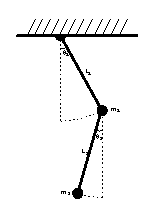
\includegraphics[width=.5\linewidth]{graphics/double_pendulum.eps}
	\caption{Illustration of the simple double pendulum.}
	\label{fig:doublependulum}
\end{figure}

Equations should be developed such that, given an initial state, the position and subsequent movement can be derived from them.
This can be achieved using the Euler-Lagrange differential equations.
These will be found for this system throughout the remainder of this section.
Firstly, the position of the pendulums as a function of the angle must be determined.
The pendulums are placed in the x-y plane with the origin placed at the point of suspension of $p_1$.
When the pendulums are in the stable position, $\theta_1=\theta_2=0$, they are aligned with the y-axis.
The x-axis is positive to the right of the stable position.
The coordinates of $p_1=(x_1,y_1)$ and $p_2=(x_2,y_2)$ are as follows:
\begin{align}
	x_1 &= l_1\sin{\theta_1}\\
	y_1 &= -l_1\cos{\theta_1}\\
	x_2 &= l_1\sin{\theta_1} + l_2\sin{\theta_2}\\
	y_2 &= -l_1\cos{\theta_1} - l_2\cos{\theta_2}
\end{align}
While the derivatives are not used until later, they are presented here for clarity:
\begin{align}
	\dot{x}_1 &= l_1\cos{\theta}_1\dot{\theta}_1\\
	\dot{y}_1 &= l_1\sin{\theta}_1\dot{\theta}_1\\
	\dot{x}_2 &= l_1\cos{\theta}_1\dot{\theta}_1 + l_2\cos{\theta_2}\dot{\theta}_2\\
	\dot{y}_2 &= l_1\sin{\theta}_1\dot{\theta}_1 + l_2\sin{\theta_2}\dot{\theta}_2
\end{align}
In order to calculate the Euler-Lagrange diff. eq. it is necessary to first determine the lagrangian, $\mathcal{l}$:
\begin{equation}
	\mathcal{L}=E_k-E_p
\end{equation}
Where $E_k$ is the kinetic energy of the system and $E_p$, the potential energy.
The derivation of $E_p$:
\begin{align}
	E_p &= m_1 g y_1 + m_2 g y_2\\
		&= -m_1 g l_1 \cos{\theta_1} - m_2 g l_1 \cos{\theta_1} - m_2 g l_2 \cos{\theta_2}\\
		&= -(m_1+m_2)l_1g \cos{\theta_1}-m_2 g l_2 \cos{\theta_2}
		\label{eq:ep}
\end{align}
The derivation of $E_k$:
\begin{equation}
	\label{eq:ek}
	E_k = \frac{1}{2}m_1v_1^2+\frac{1}{2}m_2v_2^2
\end{equation}
As movement is present along both axes, the total velocity of either pendulum can be found as the derivative of the position and Pythagoras:
\begin{align}
	v_1^2 &= \dot{x}_1^2+\dot{y}_1^2\\
		&= l_1^2\dot{\theta}_1^2\cos{\theta}_1^2+l_1^2\dot{\theta}_1^2\sin{\theta_1}^2\\
		&= (\cos{\theta_1}^2+\sin(\theta_1)^2)l_1^2\dot{\theta}_1
\end{align}
Using the Pythagorean identity:
\begin{equation}
	\label{eq:v1}
	v_1^2 = l_1^2\dot{\theta}_1^2
\end{equation}
Similarly:
\begin{align}
	v_2^2 &= \dot{x}_2^2+\dot{y}_2^2\\
	&= (l_1\cos{\theta}_1\dot{\theta}_1 + l_2\cos{\theta_2}\dot{\theta}_2)^2+(l_1\sin{\theta}_1\dot{\theta}_1 + l_2\sin{\theta_2}\dot{\theta}_2)^2\\
	\begin{split}
		&= l_1^2\dot\theta_1^2\cos{\theta_1}^2+l_2^2\dot\theta_2^2\cos{\theta_2}^2+2l_1l_2\dot\theta_1\dot\theta_2\cos{\theta_1}\cos{\theta_2}\\
		&\qquad +l_1^2\dot\theta_1^2\sin{\theta_1}^2+l_2^2\dot\theta_2\sin{\theta_2}+2l_1l_2\dot\theta_1\dot\theta_2\sin{\theta_1}\sin{\theta_2}
	\end{split}
\end{align}
Isolating cosine and sine from the terms pairwise, 1 and 4, 2 and 5, 3 and 6, yields:
\begin{align}
	\begin{split}
		v_2^2&=(\cos{\theta_1}^2+\sin{\theta_1}^2)l_1^2\dot\theta_1^2+(\cos{\theta_2}^2+\sin{\theta_2}^2)l_2^2\dot\theta_2^2\\
	&\qquad+(\cos{\theta_1}\cos{\theta_2}+\sin{\theta_1}\sin{\theta_2})2l_1l_2\dot\theta_1\dot\theta_2
	\end{split}
\end{align}
By applying the trigonimetric identities:
\begin{align}
	1&=\sin{\alpha^2}+\cos{\beta^2}\\
	\cos{(\alpha\pm\beta)}&=\cos\alpha\cos\beta\pm\sin\alpha\sin\beta
\end{align}
The result is found:
\begin{equation}
	\label{eq:v2}
	v_2^2=l_1^2\dot\theta_1^2+l_2^2\dot\theta_2^2+2l_1l_2\dot\theta_1^2\dot\theta_2^2\cos{(\theta_1-\theta_2)}
\end{equation}
Using equations \ref{eq:ep}, \ref{eq:ek}, \ref{eq:v1} and \ref{eq:v2} the lagrangian can be constructed:
\begin{align}
	\begin{split}
		\mathcal{L}&=\frac{1}{2}m_1l_1\dot\theta_1^2+\frac{1}{2}m_2\left(l_1^2\dot\theta_1^2+l_2^2\dot\theta_2^2+2l_1l_2\dot\theta_1^2\dot\theta_2^2\cos{(\theta_1-\theta_2)}\right)\\
		&\qquad+(m_1+m_2)l_1g\cos{\theta_1}+m_2l_2g\cos{\theta_2}
	\end{split}\\
	\begin{split}
		&=\frac{m_1l_1^2\dot\theta_1^2}{2}+\frac{m_2l_1^2\dot\theta_1^2}{2}+\frac{m_2l_2^2\dot\theta_2^2}{2}+l_1l_2\dot\theta_1^2\dot\theta_2^2\cos{(\theta_1-\theta_2)}\\
		&\qquad+(m_1+m_2)l_1g\cos{\theta_1}+m_2l_2g\cos{\theta_2}
	\end{split}
\end{align}
Which simplifies to:
\begin{equation}
	\label{eq:lagrangian}
	\mathcal{L}=\frac{(m_1+m_2)l_1^2\dot\theta_1^2}{2}+\frac{m_2l_2^2\dot\theta_2}{2}+(m_1+m_2)l_1g\cos{\theta_1}+m_2l_2g\cos{\theta_2}\\
\end{equation}
The Euler-Lagrange diff. eq. are defined as:
\begin{equation}
	\frac{d}{dt}\left(\frac{\partial \mathcal{L}}{\partial \dot\theta}\right)-\frac{\partial \mathcal{L}}{\partial \theta} = 0
\end{equation}
The three terms $\frac{\partial \mathcal{L}}{\partial \dot\theta}$,$\frac{d}{dt}\left(\frac{\partial \mathcal{L}}{\partial \dot\theta}\right)$ and $\frac{\partial l}{\partial \theta}$ are calculated next for each of the pendulums. For $p_1$:
\begin{align}
	\frac{\partial \mathcal{L}}{\partial \dot\theta_1}&=(m_1+m_2)l_1^2\dot\theta_1+m_2l_1l_2\dot\theta_2\cos{(\theta_1-\theta_2)}\\
	\begin{split}
		\frac{d}{dt}\left(\frac{\partial \mathcal{L}}{\partial \dot\theta_1}\right)&=(m_1+m_2)l_1^2\ddot\theta_1+m_2l_1l_2\ddot\theta_2\cos{(\theta_1-\theta_2)}\\
		&\qquad-m_2l_1l_2\dot\theta_2\sin{(\theta_1-\theta_2)(\dot\theta_1-\dot\theta_2)}
	\end{split}\\
	\frac{\partial \mathcal{L}}{\partial \theta_1} &= -m_2l_1l_2\dot\theta_1\dot\theta_2\sin(\theta_1-\theta_2)-(m_1+m_2)l_1g\sin{\theta_1}\\
	\begin{split}
		0&=(m_1+m_2)l_1\ddot\theta_1+m_2l_2\ddot\theta_2\cos{(\theta_1-\theta_2)}\\
		&\qquad+m_2l_2\dot\theta_2^2\sin{(\theta_1-\theta_2)}+(m_1+m_2)g\sin{\theta_1}
	\end{split}
\end{align}
And $p_2$:

\begin{align}
	\frac{\partial \mathcal{L}}{\partial \dot\theta_2}&=m_2l_2^2\dot\theta_2+m_2l_1l_2\dot\theta_1\cos{(\theta_1-\theta_2)}\\
	\begin{split}
		\frac{d}{dt}\left(\frac{\partial \mathcal{L}}{\partial \dot\theta_2}\right)&=m_2l_2^2\ddot\theta_2+m_2l_1l_2\ddot\theta_1\cos{(\theta_1-\theta_2)}\\
		&\qquad -m_2l_1l_2\dot\theta_1\sin{(\theta_1-\theta_2)}(\dot\theta_1-\dot\theta_2)
	\end{split}\\
	\frac{\partial \mathcal{L}}{\partial \theta_2} &=m_2l_1l_2\dot\theta_1\dot\theta_2\sin{(\theta_1-\theta_2)}-m_2l_2g\sin{\theta_2}\\
	\label{eq:part}
	\begin{split}
		0&=m_2l_2\ddot\theta_2+m_2l_1\ddot\theta_1\cos{(\theta_1-\theta_2)}\\
		&\qquad-m_2l_1\dot\theta_1^2\sin{(\theta_1-\theta_2)}+m_2g\sin{\theta_2}
	\end{split}
\end{align}
\thomas{eq. \ref{eq:part} has a minus in front of the first term according to our calculations. Determine why.}
% subsection simple_double_pendulum (end)

% section model_development (end)

\newpage
%!TEX root = ../main.tex
\section{The Platform} % (fold)
\label{sec:the_platform}
A new platform was made available to the project which fulfilled many of the requirements set by the application.
It consists of a cart, driven by a timing belt, mounted on an aluminium rail.
An image of the platform can be seen in figure \ref{fig:platform}.
\mikkel{Maybe mention what it was used for before?}
\begin{figure}[H]
 	\centering
 	\missingfigure{Image of the platform}
 	%\includegraphics[width=\linewidth]{graphics/platform}
 	\caption{The platform used in the project.}
 	\label{fig:platform}
 \end{figure} 
% section the_platform (end)
%!TEX root = ../main.tex
\section{Preliminary Testing} % (fold)
\label{sec:preliminary_testing}
In an effort to split the development into smaller, more managable parts, it was decided to initially develop the system such that it fulfills the following requirements:

\begin{itemize}
	\item The cart should be able to move with known position.
	\item Endstops on the platform should stop movement.
	\item Emergency button should stop movement.
\end{itemize}

Clearly, making the cart move is crucial in the development of the system and forms the basis for any later developments.
The latter two requirements are related to the safe operation of the platform.
It is expected that at least during development, an error may occur that causes the cart to move uncontrollably.
In such a situation the programmer should be able to completely shut off power to the motor.
The endstops will ensure that a minimum of mechanical or electrical damage is incurred on the platform in case of a cart crash.
The following paragraphs will explore what is required in order to fulfill the above requirements.
\subsection{Safety Circuitry} % (fold)
\label{sub:safety_circuitry}
Safety first.
A safety system should, whenever possible, be isolated from the remaining system.
That is, it should depend on non of the remaining circuitry or programming.
Usually, if it can at all be avoided, no programming should be involved in determining a safety condition.
With this in mind, the safety system for this platform should be designed in such a way that, when activated, it will cut power to the motors.
In order to more easily identify the cause of the fault, the remaining electronics should remain operational to maintain the current program status.
\\~\\
Creating the endstops can be done in a multitude of ways.
In this project three approaches were considered:
\paragraph{Mechanical Switch:} % (fold)
\label{par:mechanical_switch}
The simplest form of switch is the mechanical switch.
The switch should be mounted in such a way that the cart would move into the switch, therefore activating it.
This approach is not without issues.
Firstly, the simplest mounting solution would require the switch to be mounted in the direct path of the cart.
If the cart is traveling at full speed it is unlikely that the cart would stop before crashing into the switching mechanism, potentially damaging it.
A switch mounted in this fashion would need to be rather robust.
Some other mounting solutions could be thought of that do not suffer from this problem, especially if a flexible microswitch is used.
These types of switches can be fragile and may not be sufficiently durable, considering the usecase.
All mechanical switches have one drawback in common: they are mechanical.
Generally, mechanical items wear out over time and require maintainance or replacement.
% paragraph mechanical_switch (end)
\paragraph{Hall Effect Sensor:} % (fold)
\label{par:hall_effect_sensor}
This type of sensor measures magnetic fields and produces a voltage proportional to the strength of the field.
By placing a small neodymium magnet on the cart and mounting a hall effect sensor on the rail in such a way that the coincide would allow for detecting when the cart is above the sensor.
If the sensor is combined with a schmitt-trigger circuit the output could be a binary result, either the endstop is reached or it is not.
Using this method requires that a magnet is placed on the cart itself and that a sensor is mounted to the rail.
It should be noted that accelerating rather strong magnetic fields back and forth on the platform may not be the least electrically noisy solution one could think of.
Magnetic fields are also wide, meaning that the cart would "sneak up on" the threshold.
This requires some amount of calibration to determine the correct distance between sensor and magnet, which may not be mechanically simple to determine. 
% paragraph hall_effect_sensor (end)
\paragraph{Infrared Transceiver:} % (fold)
\label{par:infrared_transceiver}
This type of device is a combined LED and infrared sensor.
The LED is optimised for emitting infrared light, or radiation (IR), and the sensor for sensing it.
The LED emits IR outward from the device which, when an object is placed in front of it, will bounce off the object and be caught by the sensor.
As with the hall effect sensor, this type of device produces a voltage output proportional to the amount of IR being sensed and as such a schmitt-trigger circuit would also be benficial in this case.
With this sensor type it is important to realise that the LED will not be the only emitter of IR in the vicinity.
Any type of lamp will emit IR, especially glowbulbs (of which there are few left, luckily) but also sunlight contains some amount of IR.
When using this sensor the circuit should be designed in such a way that only the effect of the IR radiated back on the sensor will trigger the circuit.
The sensor should be mounted immediately below the cart so as to maximize the radiated IR and therefore the signal strength.
% paragraph infrared_transceiver (end)
\\~\\
While all of the above have their drawbacks, it was decided to use the infrared transceiver.
This sensor allows the greatest reliability while being reasonably simple to mount on the platform in that it requires no modification to the cart.
\\~\\
In addition to the endstops, also an emergency button, preferably red, should be able to cut power to the motors.
It may be that additional safety features are added later.
In order to minimize the amount of circuitry, all safety features will trip the same circuit.
\thomas{Add circuit showing the safety relay}
On figure \ref{fig:relay_circuit} is shown the safety circuitry.
A relay is mounted in series with the supply rail for the motor.
The default state for this relay should be \texttt{off}.
Then, in order to switch the system to the \texttt{on} state, the relay should be closed.
Should power to the relay coil ever fail i.e. something in the system has broken, power to the motor is cut off.
Since the relay is in series with the motor, it should also be capable of carrying the full design current, 80A.
One relay that fulfills these requirements is the.
\\~\\
The driver circuit for the relay is activated only when all safety conditions are off.
If at any point any of the safety conditions are tripped, the driver circuit shuts down, releasing the relay and turning off power to the motor.
Designing the safety circuit in this manner ensures that the system cannot be started or will shut down if any wires or components in the safety circuit break.

% subsection safety_circuitry (end)
\subsection{Power Board} % (fold)
\label{sub:power_board}
It is necessary to device some form of driving circuitry for the motor driving the timing belt.
On the platform is a Maxon 148867 Brushed DC Motor.
This is a 150W motor with a nominal current of 6A and a stall current of 80A.
Clearly, the system should under normal use not come anywhere close to stalling the motor but considering the use case, experimentation with control from students, it may be beneficial to design the circuitry such that it can withstand being stalled, for at least a short period of time.
In order to reach this goal, it is necessary to size the components for at least some amount above 80A continuous.
The \texttt{IPP045N10N3} MOSFET \cite{mosfet} is a 100V/100A MOSFET.
It is made in the standard TO-220 housing.
This housing allows for easy mounting of a heatsink and due to its wide application, there are many shapes and sizes to choose from.
Table \ref{tab:mosfetparameters} holds a list of the relevant parameters.

\begin{table}[tb]
	\centering
	\begin{tabular}{|r|c|c|c|}
	\hline
		\textbf{Parameter} & \textbf{Min} & \textbf{Typ} & \textbf{Max} \\
	\hline
		$V_{\text{th}}$ [V] & 2 & 2.7 & 3.5 \\
	\hline
		$R_{\text{ds(on)}}$ [m$\Omega$]& - & 3.6 & 4.2 \\
	\hline
		$Q_\text{g}$ [nC] & - & 88 & 117 \\
	\hline
		$I_\text{d}$ [A] & - & 100 & - \\
	\hline
		$V_{\text{ds}}$ [V] & 100 & - & - \\
	\hline
	\end{tabular}
	\caption{Relevant parameters of the IPP045N10N3 MOSFET \cite{mosfet} chosen for the full-bridge.
	Here, \vth is the gate threshold voltage, \ron is the drain-source on resistance, \qg is the total gate charge, \id is the maximum continuous drain current and \vds is the minimum guaranteed drain-source breakdown voltage.}
	\label{tab:mosfetparameters}
\end{table}

It should be noted that even though \vth is maximum 3.5V, this is not enough to fully open the MOSFET.
Rather, this voltage is where the MOSFET will start to conduct.
Figure \ref{fig:mosfettransfercharacteristic} reveals that the MOSFET is not fully conducting until \vgs $>4.5$V.

\begin{figure}[H]
	\centering
	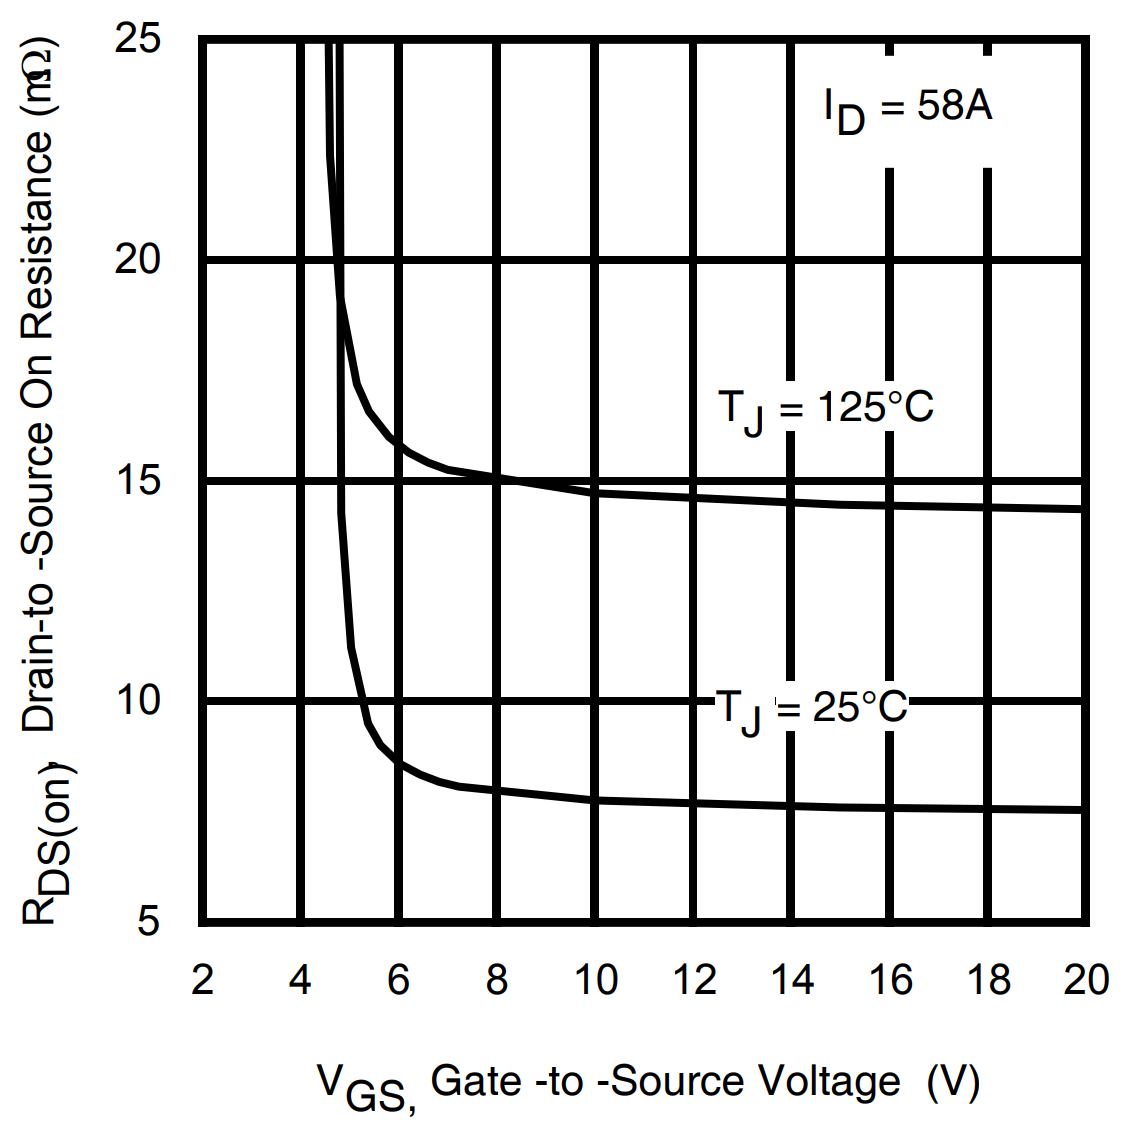
\includegraphics[width=.5\linewidth]{graphics/mosfet_transfer_characteristic}
	\caption{Transfer characteristic of the IPP045N10N3 as per the datasheet.
	Inspecting the graph reveals that the maximum \id of 100A is reached at \vgs$\approx4.5\rightarrow4.75$V.}
	\label{fig:mosfettransfercharacteristic}
\end{figure}

The motor should be able to move in both directions so an h-bridge, or full-bridge is required.
By properly switching the MOSFETs in the circuit on and off the average voltage across the motor can be controlled and therefore also the speed and direction of the motor, see \ref{sec:hbridge} for more details.
\\~\\
\thomas{Insert reference to note on full-bridge drive}
Having chosen a MOSFET for the full-bridge, some form of driver must be designed for the full-bridge.
For this task, ready-made full-bridge drivers exist on the market that incorporate all of the electronics required to generate the driving signals, requiring only a PWM signal from the designer.
In order to choose one, a few parameters must be fulfilled.

\begin{itemize}
	\item \textbf{Output Current:} The amount of current necessary to properly drive the MOSFET.
	This value depends on the switching frequency of the application, the gate-to-source voltage ($V_{gs}$) and the total gate charge of the MOSFET.
	\item \textbf{Driving Voltage:} In order to ensure that the MOSFET is turned on quickly and fully the driver should be able to supply a voltage well above the gate threshold of the MOSFET.
	\item \textbf{High-Side Drive Capabilities:} The high side MOSFET of the full-bridge is referenced not to ground, but to $V_{\text{cc}}$.
	This means that in order to switch on this MOSFET $V_{\text{gs}}$ must be at least $V_{\text{cc}}+V_{\text{th}}$ where $V_{\text{th}}$ is the gate threshold voltage of the MOSFET.
	This is bootstrapping and is explained in more detail in section \ref{sec:bootstrap}.
	\item \textbf{Shoot-Through Protection and Deadtime:} Due to the structure of the full-bridge it is important that two MOSFETs on the same half-bridge are never on at the same time as this would result in a short from $V_{\text{cc}}$ to ground.
	This is resolved with a combination of deadtime (a delay where no MOSFET is on) and a logic table that ensures that an illegal switch combination can never happen.
\end{itemize}

The HIP4081AIBZ \cite{driver} full-bridge driver meets all of the above requirements.
It can supply up to 2.5A on the output pins with a voltage approximately 1V below \vcc, well above the required \vth.
Since the motor should, preferably, be driven outside the audible frequency range, it was chosen to set the switching frequency at 22kHz.
This frequency was chosen over an even higher frequency because increasing the frequency also increases the switching losses.
At this frequency there is $\frac{1}{22000}\approx45\mu$S per cycle. 
Well within this time the gate should be fully opened.
Since:

\begin{equation}
	I = C\frac{\text{dv}}{\text{dt}} \quad\Rightarrow\quad \text{dt} = C\frac{\text{dv}}{I}
\end{equation}
\thomas{Is this the correct way of calculating it?}

Accounting for various voltage drops it is assumed that \vgs is 10V, a rough estimate of the time to open the gate completely can be found as:

\begin{equation}
	\text{dt} = 117\cdot10^{-9}\frac{10}{2.5}\approx0.47\mu\text{S}
\end{equation}

This time is approximately 100 times shorter than the allotted time frame.
The component also has floating drive circuitry, meaning that by referencing the high-side driver to source of the high-side MOSFET, the driver can be made to output a voltage higher than \vcc.
This does require a few external components for the bootstrapping.
The choice of these components and a more in depth explanation of the procedure is given in section \ref{ssub:bootstrap_circuit}.
Finally, the component has a user-programmable dead time and shoot-through protection. 

HIP4081AIBZ - Full-bridge driver - (ISL83202)

IPP045N10N3 - Mosfet

choice of VGS, 8V - show graph of transfer characteristics of mosfet, high due to uncertainty.





\subsubsection{Bootstrap Circuit}
\label{ssub:bootstrap_circuit}
\missingfigure{Put in a bootstrap circuit and make a couple of references to it, when it makes sense.}
The chosen gate driver has floating drive circuitry for the high side MOSFETS, but needs a bootstrap circuit for providing the higher voltage. 
A standard bootstrap circuits consists of a diode, a capacitor and a resistor to limit initial charging current to the capacitor. 
The advantage of using a bootstrap circuit to supply a high voltage for the floating drive is that it is very simple. 
The disadvantage is that it sets a limit for the maximum and minimum duty cycle as the bootstrap capacitor needs to be charged fully in each period.
The bootstrap circuitry for this project will be designed to have a maximum duty cycle for the higher MOSFETS of 95\%, thus meaning that the charging of the bootstrap capacitor should take no longer than 5\% of a period.  

The bootstrap diode needs to have a fast recovery time, preferably below 100 ns \cite{bootstrap_infineon}, to minimize the energy fed back to the supply from the bootstrap capacitor.
\texttt{US1M-E3} was chosen as it has a reverse recovery time of 75 ns and comes in SMD packaging. 
It allows for a maximum average forward current of 1 A and a maximum forward voltage drop of 1.7 V \cite{diode_ds}.
Determining the values for the bootstrap capacitor was done using the calculations shown in \cite{bootstrap_ON}.
The maximum allowed voltage drop across the bootstrap capacitor during \texttt{on} time needs to be determined: 
\begin{equation}
\Delta V_{boot} = V_{DD} - V_{F} - V_{GSMIN}
\end{equation}
Where $\Delta V_{boot}$ is the voltage drop across the bootstrap capacitor during \texttt{on} time, $V_{DD}$ is the supply voltage, $V_F$ is the forward voltage drop across the diode and $V_{GSMIN}$ is the minimum wanted \texttt{gate-source} voltage.
$V_{GSMIN}$ was chosen to 8 V to to ensure a high enough gate voltage to turn on the MOSFETS. 
The chosen MOSFETS have a maximum gate threshold voltage of 3.5 V. 
Inserting the values yields the maximum allowed value of $\Delta V_{boot}$:
\begin{equation}
\Delta V_{boot} = 12 - 1.7 - 8 = 2.3 V	
\end{equation}

The total charge that needs to be supplied from the bootstrap capacitor is the gate charge of the MOSFET and quiescent and leakage currents in the \texttt{on} time:
\begin{equation}
	Q_{total} = Q_{gate} + Q_{ls} + (I_{lkgs} + I_{qbs} + I_{lk} + I_{lkdiode}) \cdot t_{on}
	\label{eq:charge_total}
\end{equation}
Where $I_{lkgs}$ is the gate-source leakage current, $I_{qbs}$ is the gate driver quiescent current, $I_{lk}$ is the gate driver leakage current, $I_{lkdiode}$ is the diode leakage current, $ t_{on}$ is the \texttt{on} time and $Q_{ls}$ is the charge required by the internal level shifter in the gate driver.
\begin{table}[h]
\centering
\begin{tabular}{|l|l|l|l|l|l|l|}
 \hline
 $Q_{gate}$ 	& $Q_{ls}$ 	& $I_{lkgs}$ 	& $I_{qbs}$ 		& $I_{lk}$ 			& $I_{lkdiode}$ 	& $t_{on}$ 		\\ 	\hline
 $117$ [nC]		& $3$ [nC]	& $100$ [nA]	&$-30$ [$\mu$A]		& $1$ [$\mu$A]		& $1$ [nA]			& $43$ [$\mu$S]	\\ 	\hline
\end{tabular}
\caption{Parameter values used in equation \ref{eq:charge_total}. $I_{qbs}$ and $I_{lk}$ are found in the gate driver data sheet. $Q_{ls}$ is set to 3nC for all high voltage gate drivers \cite{bootstrap_ON}. $I_{lkgs}$ and $Q_{gate}$ are MOSFET data sheet values and $I_{lkdiode}$  is a diode data sheet value. $t_{on}$ is calculated using 95\% dutycycle and 22kHz switching.}
\label{tab:bootstrap_parameter}
\end{table}
$t_{on}$ can be calculated knowing that the worst case duty cycle for the high side MOSFET is 95\% and the switching frequency is 22 kHz.
Inserting the values, shown in \ref{tab:bootstrap_parameter}, yields the minimum charge value of the capacitor:
\begin{equation}
	Q_{total} = 119 [nC]
\end{equation}

The minimum value of the bootstrap capacitor can now be calculated:
\begin{equation}
	C_{boot} = \frac{Q_{total}}{\Delta V_{boot}} = \frac{119}{2.3} = 51.6 [nC]
\end{equation}
A ceramic capacitor will be used as it has a negligible leakage current. 
Looking for SMD ceramic capacitors it was found that in the range of the found minimum value is 56, 68, 82 and 100 [nF].
56 [nF] is, in theory, a big enough capacitor for the circuit, but a bigger capacitor is an advantage as $\Delta V_{boot}$ will then decrease.
When increasing the size of the capacitor it should be noted that the initial charge current will become larger.
It was therefore chosen to use a 100 [nF] ceramic capacitor.

The initial charge current to the capacitor needs to be limited in order not to exceed the maximum ratings of the diode.
Therefore a resistor is put in series with the diode.
The resistor value should not be too big as the voltage drop across it is subtracted from the bootstrap capacitor voltage.
A 1 $\Omega$ resistor was chosen. In this setting, the maximum current through this component is 12 A.
This is clearly above the maximum average forward current of the diode, but the diode can withstand a 8.3 ms single half sine-wave of maximum 30 A \cite{diode_ds}.
The charging of a capacitor is approximately finished after 5 time constants
\mikkel{MANGLER KILDE!!! Denne er måske OK \url{http://www.electronics-tutorials.ws/rc/rc_1.html}}
\begin{equation}
T_{charge,init} = 5\cdot \tau = 5\cdot (R \cdot C) = 0.5 \mu S 
\end{equation}
Meaning that the diode can be exposed to a maximum of 12A for $0.5 \mu S $, which is well below the absolute maximum rating.
It should also be noted that bootstrap capacitor needs at least $0.5 \mu S $ for the initial charging.
\mikkel{In the application note they state that they include a 400ns bootstrap}

Lastly it should be calculated what the maximum allowed duty cycle for the high side MOSFETS are in this configuration, using the found components.
The time it takes to charge the capacitor the energy that is used in each period is:
\begin{equation}
	T_{charge,period} = 5\cdot \tau = 5\cdot (R \cdot C_{boot}) = 5\cdot (1 \cdot  51.6 \cdot 10^{-9}) = 258 nS 
\end{equation}
The 258 nS are equivalent to 0.6\% duty cycle and the maximum duty cycle for the high side MOSFETS is thus 99.4\%.

% subsection power_board (end)

\subsubsection{Supply Capacitors}
\label{ssub:sup_caps}
Driving an inductive load, such as a motor, requires capacitors placed close to the MOSFETS in order to minimize the voltage spikes created by the load current and parasitic inductance in the wires from the supply.
This section will determine the size and requirements of the supply capacitors using calculations and simulation in PLECS.

First off, the ripple current across the motor inductor needs to be determined as this is the current the supply capacitors need to supply.
Equations \ref{eq:inductor_gen} shows the general inductor equation and in \ref{eq:inductor_rip} it is re factored to calculate the ripple current.
\begin{equation}
	V(t) = L \cdot \frac{dI(t)}{dt}
	\label{eq:inductor_gen}
\end{equation}

\begin{equation}
	\Delta I = \frac{\Delta V}{L} \Delta t
	\label{eq:inductor_rip}
\end{equation}

The highest ripple current is found when the duty cycle is 50$\%$ and the full voltage of 24V is applied as calculated in equation \ref{eq:inductor_rip_size}.

\begin{equation}
	\Delta I = \frac{24}{82\cdot 10^{-6}} \cdot 0.5 \cdot \frac{1}{22000} = 6.7 [A] 
	\label{eq:inductor_rip_size}
\end{equation}

The peak-to-peak ripple current of $6.7$A is also found when simulating the system using PLECS as shown in figure \ref{fig:sim_currents}.
The load current experienced by the supply is also shown in figure \ref{fig:sim_currents}, where abrupt changes in current are seen. 

\begin{figure}[h]
	\centering
    %% This file was created by matlab2tikz.
%
%The latest updates can be retrieved from
%  http://www.mathworks.com/matlabcentral/fileexchange/22022-matlab2tikz-matlab2tikz
%where you can also make suggestions and rate matlab2tikz.
%
\definecolor{mycolor1}{rgb}{0.00000,0.44700,0.74100}%
%
\begin{tikzpicture}

\begin{axis}[%
width=4.521in,
height=1.493in,
at={(0.758in,2.554in)},
scale only axis,
xmin=0.002,
xmax=0.00225,
ymin=-4,
ymax=4,
ylabel style={font=\color{white!15!black}},
ylabel={Current [A]},
axis background/.style={fill=white},
title style={font=\bfseries},
title={Motor}
]
\addplot [color=mycolor1, forget plot]
  table[row sep=crcr]{%
0	0\\
3.3460025901564e-08	0.00979216834185557\\
6.6920051803128e-08	0.0195831689424556\\
1.00380077704692e-07	0.0293729772080969\\
2.86236444194498e-07	0.0837307082176497\\
4.72092810684304e-07	0.138052159786677\\
6.5794917717411e-07	0.192336888519681\\
8.43805543663915e-07	0.2465847436031\\
1.46206269418065e-06	0.426776921334415\\
2.08031984469738e-06	0.606560789436667\\
2.69857699521411e-06	0.785936710694134\\
3.31683414573084e-06	0.964905205652303\\
3.93509129624758e-06	1.1434666409016\\
5.75197157684523e-06	1.6658548409378\\
7.56885185744287e-06	2.18473747278615\\
9.38573213804052e-06	2.70012165466927\\
1.12026124186382e-05	3.21201571005084\\
1.30194926992358e-05	3.72042845969404\\
1.48363729798335e-05	4.22536872362558\\
1.97586180405918e-05	5.57596587927003\\
2.27272727272725e-05	6.3783171170272\\
2.27272727272727e-05	6.37831711702726\\
2.27410076969546e-05	6.37398638046111\\
2.27547426666364e-05	6.36965375955969\\
2.27684776363182e-05	6.36532285013984\\
2.29058273331366e-05	6.32203472687713\\
2.30431770299549e-05	6.27876729316781\\
2.31805267267732e-05	6.2355202943356\\
2.44483529688856e-05	5.83725566814237\\
2.57161792109979e-05	5.44072022747552\\
2.69840054531102e-05	5.04592126779853\\
2.82518316952226e-05	4.65286095881394\\
3.11224300272083e-05	3.76931165867921\\
3.3993028359194e-05	2.89464378808499\\
3.68636266911797e-05	2.02882734038762\\
3.97342250231655e-05	1.17183245052039\\
4.26048233551512e-05	0.323631784651184\\
4.5454545454545e-05	-0.509728483636083\\
4.54545454545455e-05	-0.509728483636209\\
4.56137030196537e-05	-0.462855930246644\\
4.5772860584762e-05	-0.416009673465522\\
4.59320181498702e-05	-0.369190286586476\\
4.75235938009527e-05	0.096688919165212\\
4.91151694520353e-05	0.559938654993594\\
5.07067451031178e-05	1.02051267646793\\
5.21877413094701e-05	1.44673915057175\\
5.36687375158223e-05	1.87064481037127\\
5.48032708460027e-05	2.19395845751998\\
5.59378041761831e-05	2.51590586535985\\
5.70723375063635e-05	2.83649721774212\\
5.90623960561229e-05	3.39602028595376\\
6.10524546058824e-05	3.95161284857696\\
6.30425131556419e-05	4.50312800819581\\
6.50325717054013e-05	5.05052048240398\\
6.81818181818173e-05	5.9083681446256\\
6.81818181818182e-05	5.90836814462583\\
6.81982265228205e-05	5.90321766823039\\
6.82146348638228e-05	5.8980650799626\\
6.82310432048251e-05	5.8929146034375\\
6.83951266148483e-05	5.8414383259708\\
6.85592100248715e-05	5.78999120622817\\
6.87232934348947e-05	5.73857317088326\\
7.03641275351264e-05	5.22594260544655\\
7.20049616353581e-05	4.71619997502048\\
7.36457957355898e-05	4.20935629332506\\
7.52866298358215e-05	3.70541426066593\\
7.86734614243063e-05	2.67439183644975\\
8.2060293012791e-05	1.65568679003902\\
8.54471246012758e-05	0.649258995332076\\
8.88339561897606e-05	-0.344931641381534\\
9.090909090909e-05	-0.948049426664154\\
9.09090909090909e-05	-0.948049426664405\\
9.10680548465105e-05	-0.900944972184585\\
9.12270187839301e-05	-0.85386684032189\\
9.13859827213497e-05	-0.806815624783133\\
9.28881448030836e-05	-0.364268712879095\\
9.43903068848175e-05	0.075924523168433\\
9.58924689665514e-05	0.513722225414341\\
9.73937786098869e-05	0.948873891503222\\
9.88950882532224e-05	1.38163182114456\\
0.000100396397896558	1.81199872685562\\
0.000102388285618672	2.37990759343637\\
0.000104380173340787	2.94391803819557\\
0.000106372061062901	3.50382863193594\\
0.000108363948785016	4.0595734864279\\
0.000112581062122341	5.22245152431999\\
0.000113636363636363	5.51053783719038\\
0.000113636363636364	5.51053783719062\\
0.000113652875841073	5.50537508343307\\
0.000113669388045783	5.50021036711542\\
0.000113685900250493	5.49504766058541\\
0.000113851022297591	5.44344929732303\\
0.000114016144344688	5.39188054216774\\
0.000114181266391786	5.3403413740717\\
0.000115832486862763	4.82652639019902\\
0.00011748370733374	4.31564953083607\\
0.000119134927804716	3.80772280116105\\
0.000120786148275693	3.3027493167972\\
0.000124260197469801	2.24994846748255\\
0.000127734246663909	1.21017549199153\\
0.000131208295858018	0.183388685607617\\
0.000134682345052126	-0.830455009606617\\
0.000136363636363635	-1.31647681541512\\
0.000136363636363636	-1.31647681541562\\
0.000136457648355821	-1.28848834726951\\
0.000136551660348006	-1.26050912560564\\
0.000136645672340192	-1.2325394005705\\
0.000137585792262042	-0.953660414443846\\
0.000138525912183893	-0.675711762263763\\
0.000139466032105744	-0.398710450483822\\
0.000141080921833001	0.0744903471438776\\
0.000142695811560257	0.544923535047713\\
0.00014397637111121	0.916137663936403\\
0.000145256930662163	1.2855871880448\\
0.000146309638560935	1.58807403635747\\
0.000147362346459708	1.88937169227974\\
0.00014841505435848	2.18948675148099\\
0.000150446951617213	2.76585105914289\\
0.000152478848875945	3.33804096395515\\
0.000154510746134677	3.90591581582167\\
0.000156542643393409	4.4694327063089\\
0.000159090909090907	5.17002081333405\\
0.000159090909090909	5.17002081333453\\
0.000159107950404141	5.16471547697748\\
0.000159124991717373	5.15940825618861\\
0.000159142033030604	5.15410303483625\\
0.000159312446162921	5.10108115055827\\
0.000159482859295238	5.0480908629433\\
0.000159653272427556	4.99513222149086\\
0.000161357403750727	4.46723180551256\\
0.000163061535073897	3.94247263127644\\
0.000164765666397068	3.4208672561975\\
0.000166469797720239	2.90241812883423\\
0.000170111015763006	1.80520238710783\\
0.000173752233805772	0.722332913291956\\
0.000177393451848539	-0.346247160573399\\
0.000181034669891305	-1.40059735141266\\
0.00018181818181818	-1.62561618975527\\
0.000181818181818182	-1.62561618975576\\
0.00018189191245417	-1.60360142523706\\
0.000181965643090158	-1.58159233486036\\
0.000182039373726146	-1.55958910529188\\
0.000182776680086025	-1.34006159444278\\
0.000183513986445904	-1.1211080471627\\
0.000184251292805783	-0.902738959943471\\
0.000186176642929505	-0.336111723359008\\
0.000188101993053228	0.226593340319752\\
0.000189433381211277	0.61367738328916\\
0.000190764769369326	0.998843310781422\\
0.000191862820760937	1.31517016011703\\
0.000192960872152549	1.63020214326219\\
0.000194058923544161	1.94394679035387\\
0.000196139234286316	2.53528966757863\\
0.000198219545028471	3.1222613516525\\
0.000200299855770626	3.70471321364354\\
0.000202380166512781	4.28260111282239\\
0.000204545454545453	4.87927070065436\\
0.000204545454545455	4.87927070065483\\
0.000204563248495638	4.87375397959641\\
0.000204581042445821	4.86823541514357\\
0.000204598836396004	4.86271888414652\\
0.000204776775897834	4.80758616239875\\
0.000204954715399664	4.75248770523977\\
0.000205132654901494	4.69742363897177\\
0.000206912049919797	4.14861455983025\\
0.0002086914449381	3.60321712392594\\
0.000210470839956403	3.06124426527418\\
0.000212250234974706	2.52269735314441\\
0.000215992339235271	1.40127193130843\\
0.000219734443495837	0.294915233950511\\
0.000223476547756402	-0.796443118277702\\
0.000227218652016968	-1.87287598395711\\
0.000227272727272726	-1.88832192980601\\
0.000227272727272727	-1.8883219298065\\
0.000227342297857368	-1.8674965214086\\
0.000227411868442008	-1.8466761249662\\
0.000227481439026648	-1.82586092362373\\
0.000228177144873052	-1.61815622510643\\
0.000228872850719455	-1.41096013261674\\
0.000229568556565858	-1.20428192867981\\
0.000231740906602734	-0.561959842495436\\
0.00023391325663961	0.0754652928433671\\
0.000236085606676486	0.707897523625743\\
0.000238257956713362	1.33531177211176\\
0.000242602494028023	2.57508628531837\\
0.000246947031342683	3.79491169755634\\
0.000249999999999997	4.6402370224219\\
0.00025	4.64023702242285\\
0.000250019628217504	4.63416863641626\\
0.000250039256435008	4.62809832974944\\
0.000250058884652512	4.6220302822174\\
0.000250255166827551	4.56138855762422\\
0.00025045144900259	4.50078810165967\\
0.00025064773117763	4.44022919509232\\
0.000252610552928023	3.83685231936177\\
0.000254573374678417	3.23759512538674\\
0.000256536196428811	2.64247348184285\\
0.000258499018179204	2.05148839219246\\
0.00026230269607791	0.917985886864917\\
0.000266106373976615	-0.200068898448616\\
0.000269910051875321	-1.30274624539011\\
0.000272727272727269	-2.10958190663542\\
0.000272727272727273	-2.10958190663641\\
0.000272768691766965	-2.0971445132162\\
0.000272810110806658	-2.08470883916461\\
0.00027285152984635	-2.0722750015498\\
0.000273265720243275	-1.9480945773949\\
0.000273679910640201	-1.82409380817647\\
0.000274094101037126	-1.7002760300248\\
0.000276474575282944	-0.99201519218526\\
0.000278855049528763	-0.289700777080019\\
0.000281235523774581	0.406610503044831\\
0.0002836159980204	1.09690909829915\\
0.000287927361167765	2.3318709333071\\
0.00029223872431513	3.54723458490537\\
0.000295454545454542	4.44107226812169\\
0.000295454545454545	4.44107226812265\\
0.000295475547795918	4.43458904568205\\
0.00029549655013729	4.42810387748598\\
0.000295517552478663	4.42162112001525\\
0.000295727575892386	4.35683736126698\\
0.00029593759930611	4.29210065463151\\
0.000296147622719834	4.22741141574417\\
0.00029824785685707	3.58304649672565\\
0.000300348090994307	2.94338836213575\\
0.000302448325131544	2.30845678951722\\
0.000304548559268781	1.67825391184348\\
0.00030840178706574	0.534311601515325\\
0.0003122550148627	-0.593790092823967\\
0.00031610824265966	-1.70611431376052\\
0.000318181818181815	-2.29819353211022\\
0.000318181818181818	-2.29819353211121\\
0.000318216910128822	-2.28762391738447\\
0.000318252002075825	-2.27705551476598\\
0.000318287094022829	-2.26648843514806\\
0.000318638013492865	-2.16093137669381\\
0.000318988932962902	-2.05550369377823\\
0.000319339852432938	-1.9502078029123\\
0.000321730696804805	-1.23616395699821\\
0.000324121541176672	-0.528156744987434\\
0.000326512385548539	0.173765399113965\\
0.000328903229920406	0.86959462059652\\
0.00033321923055222	2.11033039144202\\
0.000337535231184035	3.33132093693318\\
0.000340909090909087	4.27209444587003\\
0.000340909090909091	4.27209444587099\\
0.000340929953026185	4.26566360640344\\
0.000340950815143279	4.25923092687039\\
0.000340971677260373	4.25280056340677\\
0.000341180298431315	4.18854027505537\\
0.000341388919602256	4.12432661772937\\
0.000341597540773198	4.06016002069595\\
0.000343683752482612	3.42100022909339\\
0.000345769964192026	2.78650799915323\\
0.00034785617590144	2.15670388491997\\
0.000349942387610854	1.53159074565621\\
0.000353862201477184	0.369717249245569\\
0.000357782015343514	-0.775670764458827\\
0.000361701829209844	-1.90463829879655\\
0.00036363636363636	-2.4557839306292\\
0.000363636363636364	-2.45578393063018\\
0.000363695905167082	-2.43781680581856\\
0.0003637554466978	-2.41985333442861\\
0.000363814988228518	-2.40189369272165\\
0.000364410403535697	-2.22262684696784\\
0.000365005818842876	-2.04373481884366\\
0.000365601234150056	-1.86522453974338\\
0.000367733905497417	-1.22871314865743\\
0.000369866576844778	-0.596973919648128\\
0.00037199924819214	0.0299106828227297\\
0.000374131919539501	0.651918245296275\\
0.000378286707189542	1.84971523249257\\
0.000382441494839584	3.02908508269167\\
0.000386363636363633	4.12559464964425\\
0.000386363636363636	4.12559464964521\\
0.000386384269576468	4.11924763877802\\
0.0003864049027893	4.11289888699914\\
0.000386425536002132	4.10655235313425\\
0.00038663186813045	4.04312954041196\\
0.000386838200258768	3.97975253166327\\
0.000387044532387087	3.9164217548111\\
0.000389107853670269	3.28557577049391\\
0.000391171174953452	2.65931428327555\\
0.000393234496236635	2.03765657969553\\
0.000395297817519818	1.42060435284609\\
0.000399334545479002	0.226675050717639\\
0.000403371273438187	-0.949722711864358\\
0.000407408001397371	-2.10867110538955\\
0.000409090909090906	-2.58670278815743\\
0.000409090909090909	-2.58670278815841\\
0.000409145988200711	-2.57006869975492\\
0.000409201067310513	-2.55343772732207\\
0.000409256146420314	-2.53681004004178\\
0.000409806937518332	-2.37081577150612\\
0.00041035772861635	-2.20514289195094\\
0.000410908519714368	-2.03979732611326\\
0.000413097374837221	-1.38570589615075\\
0.000415286229960075	-0.736662299855921\\
0.000417475085082928	-0.0927420918712096\\
0.000419663940205782	0.546036608826598\\
0.000423968638727064	1.78733142560619\\
0.000428273337248345	3.00885908076593\\
0.000431818181818178	4.00000969233672\\
0.000431818181818182	4.00000969233768\\
0.000431839275076628	3.99353552660101\\
0.000431860368335074	3.98705965072965\\
0.00043188146159352	3.98058601084854\\
0.000432092394177982	3.91589377431785\\
0.000432303326762444	3.85124925285408\\
0.000432514259346906	3.78665292130374\\
0.000434623585191524	3.14325497709778\\
0.000436732911036143	2.50463347912925\\
0.000438842236880761	1.87080710832231\\
0.000440951562725379	1.24177588616619\\
0.000445050033039373	0.033222969508128\\
0.000449148503353368	-1.15734363531676\\
0.000453246973667362	-2.33001970722991\\
0.000454545454545451	-2.69783234439024\\
0.000454545454545455	-2.69783234439122\\
0.0004546010289307	-2.6810357358428\\
0.000454656603315945	-2.66424228174699\\
0.00045471217770119	-2.64745215665824\\
0.000455267921553643	-2.47983724349932\\
0.000455823665406095	-2.31254794770271\\
0.000456379409258548	-2.14559025346581\\
0.00045868446959878	-1.45638550216304\\
0.000460989529939011	-0.772755065198986\\
0.000463294590279243	-0.0947766643127222\\
0.000465599650619475	0.577532800723047\\
0.000469812892476408	1.79178792665153\\
0.00047402613433334	2.98722540848639\\
0.000477272727272724	3.89562762531595\\
0.000477272727272727	3.89562762531692\\
0.000477295402708081	3.88867685276398\\
0.000477318078143435	3.88172431169523\\
0.000477340753578789	3.87477420698354\\
0.00047756750793233	3.80532349876055\\
0.00047779426228587	3.73592750259582\\
0.000478021016639411	3.66658683909998\\
0.000480288560174816	2.97612537432033\\
0.000482556103710221	2.2911466103743\\
0.000484823647245627	1.61167189153912\\
0.000487091190781032	0.937700586480311\\
0.0004911972102979	-0.268747565625874\\
0.000495303229814769	-1.45726632153262\\
0.000499409249331637	-2.62794765330139\\
0.000499999999999993	-2.79491648591443\\
0.0005	-2.79491648591639\\
0.000500056745332312	-2.77773991812249\\
0.000500113490664625	-2.76056662433982\\
0.000500170235996937	-2.7433967858544\\
0.000500737689320059	-2.57199560250605\\
0.000501305142643181	-2.40093240187529\\
0.000501872595966304	-2.23021341017497\\
0.0005042220697522	-1.52677175839865\\
0.000506571543538096	-0.82909706902467\\
0.000508921017323993	-0.13727111682226\\
0.000511270491109889	0.548687186320934\\
0.000515312721773524	1.71516833038822\\
0.000519354952437159	2.86437520456513\\
0.000522727272727266	3.80997447787648\\
0.000522727272727273	3.80997447787841\\
0.000522751306376193	3.80260956304194\\
0.000522775340025112	3.79524284019986\\
0.000522799373674032	3.78787872694102\\
0.00052303971016323	3.71429372360279\\
0.000523280046652429	3.64076999567818\\
0.000523520383141627	3.5673083060386\\
0.000525923748033608	2.83599396327517\\
0.000528327112925589	2.11082782882618\\
0.00053073047781757	1.39183576438828\\
0.000533133842709552	0.679018548237901\\
0.000537260952310566	-0.530676430903125\\
0.000541388061911581	-1.72226439533256\\
0.000545454545454538	-2.87871812611635\\
0.000545454545454545	-2.87871812611831\\
0.000545486180018228	-2.86912514916799\\
0.000545517814581911	-2.8595331259129\\
0.000545549449145593	-2.84994218099589\\
0.00054586579478242	-2.75412535242025\\
0.000546182140419247	-2.6584138746077\\
0.000546498486056073	-2.56280971682326\\
0.000549178672768715	-1.75696300434028\\
0.000551858859481356	-0.958736172524893\\
0.000554539046193997	-0.168173259747465\\
0.000557219232906638	0.614723414826821\\
0.000561655004217416	1.89363760386096\\
0.000566090775528194	3.15168366267871\\
0.000568181818181811	3.73752534370516\\
0.000568181818181818	3.7375253437071\\
0.000568204374702	3.73061523223814\\
0.000568226931222183	3.72370345512032\\
0.000568249487742365	3.71679402093937\\
0.000568475052944188	3.64774953282531\\
0.00056870061814601	3.5787593104649\\
0.000568926183347833	3.50982399161644\\
0.000571181835366059	2.82339433550953\\
0.000573437487384285	2.14240849124595\\
0.000575693139402512	1.46689070606884\\
0.000577948791420738	0.796843322804897\\
0.000582052143327392	-0.408073274081108\\
0.000586155495234045	-1.59497825135928\\
0.000590258847140698	-2.76394951597553\\
0.000590909090909084	-2.94755175578491\\
0.000590909090909091	-2.94755175578686\\
0.000590959516508872	-2.93224744789989\\
0.000591009942108653	-2.91694572218636\\
0.000591060367708434	-2.9016467496346\\
0.000591564623706245	-2.74889373863545\\
0.000592068879704056	-2.59640995633824\\
0.000592573135701867	-2.44420039697188\\
0.000594806470108126	-1.77314317467297\\
0.000597039804514385	-1.10735382280102\\
0.000599273138920644	-0.446903358238594\\
0.000601506473326903	0.208190915834121\\
0.00060562356989688	1.40183446476566\\
0.000609740666466858	2.57736402826412\\
0.000613636363636357	3.67308133027466\\
0.000613636363636364	3.6730813302766\\
0.000613658997831899	3.66615504921932\\
0.000613681632027435	3.659227138088\\
0.000613704266222971	3.65230155337451\\
0.000613930608178328	3.58309606308871\\
0.000614156950133686	3.51394544866726\\
0.000614383292089044	3.44485036449075\\
0.000616646711642621	2.75685598957649\\
0.000618910131196197	2.07436620421114\\
0.000621173550749774	1.39740429101896\\
0.000623436970303351	0.725971107171847\\
0.000627677556364823	-0.517138145095901\\
0.000631918142426295	-1.74095778077408\\
0.000636158728487766	-2.9455859564701\\
0.000636363636363629	-3.00331014568189\\
0.000636363636363636	-3.00331014568384\\
0.000636411774985549	-2.98870023000527\\
0.000636459913607462	-2.97409266156562\\
0.000636508052229375	-2.95948760777894\\
0.000636989438448505	-2.81365322086834\\
0.000637470824667636	-2.66806466279908\\
0.000637952210886766	-2.52272648006007\\
0.000640230433047751	-1.83807381280985\\
0.000642508655208737	-1.15891824123425\\
0.000644786877369722	-0.485326301282013\\
0.000647065099530707	0.182688139322527\\
0.000651328090495629	1.41773140438894\\
0.000655591081460551	2.63336676503023\\
0.000659090909090902	3.61695067654711\\
0.000659090909090909	3.61695067654904\\
0.000659113697178817	3.6099869464973\\
0.000659136485266725	3.60302160918081\\
0.000659159273354632	3.59605859352666\\
0.000659387154233711	3.52647932037585\\
0.000659615035112789	3.45695555136827\\
0.000659842915991867	3.38748795497388\\
0.00066212172478265	2.69580194660462\\
0.000664400533573433	2.00968193233982\\
0.000666679342364216	1.32914969923046\\
0.000668958151154999	0.654204206966739\\
0.000673235101280136	-0.597522967597643\\
0.000677512051405274	-1.82970762167744\\
0.000681789001530411	-3.0424607158537\\
0.000681818181818175	-3.05066848260151\\
0.000681818181818182	-3.05066848260346\\
0.000681867400727158	-3.03573029319104\\
0.000681916619636135	-3.02079454896102\\
0.000681965838545111	-3.00586142163829\\
0.000682458027634877	-2.85675508088465\\
0.000682950216724642	-2.70790454309517\\
0.000683442405814408	-2.5593145250162\\
0.00068584486093225	-1.83752792427101\\
0.000688247316050092	-1.12182718836945\\
0.000690649771167934	-0.412281384830144\\
0.000693052226285776	0.291097022064598\\
0.000697289964889382	1.51681154233223\\
0.000701527703492988	2.72346631983952\\
0.000704545454545448	3.57118536592226\\
0.000704545454545455	3.5711853659242\\
0.000704569606390293	3.56380966426512\\
0.000704593758235132	3.55643230005062\\
0.00070461791007997	3.54905743974744\\
0.000704859428528357	3.47536540280112\\
0.000705100946976743	3.40173529149833\\
0.000705342465425129	3.3281679038408\\
0.000707757649908989	2.59583229088773\\
0.00071017283439285	1.86971022719993\\
0.000712588018876711	1.14982575254601\\
0.000715003203360571	0.43617706654896\\
0.000719259333388766	-0.806311727672883\\
0.00072351546341696	-2.02956844908724\\
0.00072727272727272	-3.09354666523168\\
0.000727272727272727	-3.09354666523363\\
0.000727301820660392	-3.08470881389707\\
0.000727330914048057	-3.07587174739178\\
0.000727360007435721	-3.0670355924061\\
0.000727650941312369	-2.97875231388577\\
0.000727941875189016	-2.89055805839654\\
0.000728232809065664	-2.80245448740684\\
0.000731142147832138	-1.92624410168509\\
0.000734051486598613	-1.05901259923018\\
0.000736960825365087	-0.200795324876609\\
0.000739335092513641	0.492905872608331\\
0.000741709359662195	1.18062059080546\\
0.000744083626810749	1.86236520045248\\
0.000746457893959304	2.5381564815441\\
0.000749999999999993	3.53532238998109\\
0.00075	3.53532238998303\\
0.000750025853381898	3.52742525753135\\
0.000750051706763797	3.51952639194461\\
0.000750077560145695	3.51163027409671\\
0.000750336093964679	3.43273347847176\\
0.000750594627783664	3.35390743438593\\
0.000750853161602648	3.27515312273811\\
0.000753438499792491	2.49142822359744\\
0.000756023837982335	1.71481032298366\\
0.000758609176172178	0.945328859431727\\
0.000761194514362021	0.182983260500955\\
0.000765477800099492	-1.06437882362051\\
0.000769761085836963	-2.29227341390428\\
0.000772727272727266	-3.13123516630411\\
0.000772727272727273	-3.13123516630606\\
0.000772754977390944	-3.1228093715132\\
0.000772782682054615	-3.11438427974988\\
0.000772810386718286	-3.10596001596886\\
0.000773087433354995	-3.02178848617128\\
0.000773364479991704	-2.93769783381988\\
0.000773641526628413	-2.85368957260713\\
0.000776411992995503	-2.01799250891406\\
0.000779182459362593	-1.19045816110366\\
0.000781952925729684	-0.371122885944089\\
0.000784723392096774	0.440015235718401\\
0.000789202030097114	1.73398461291325\\
0.000793680668097454	3.00667141840257\\
0.000795454545454538	3.50489101477496\\
0.000795454545454545	3.5048910147769\\
0.000795478108210399	3.49769234966097\\
0.000795501670966254	3.49049209829456\\
0.000795525233722108	3.48329422818896\\
0.000795760861280649	3.41136954037456\\
0.00079599648883919	3.33950394578322\\
0.000796232116397731	3.26769820325311\\
0.000798588391983141	2.55282762142207\\
0.000800944667568551	1.84389055190394\\
0.000803300943153962	1.14091336619295\\
0.000805657218739372	0.443897937344929\\
0.000809860504460401	-0.784718776574724\\
0.00081406379018143	-1.99446583025146\\
0.000818181818181811	-3.16145818115488\\
0.000818181818181818	-3.16145818115683\\
0.000818208304958443	-3.15339890850446\\
0.000818234791735068	-3.14534027352761\\
0.000818261278511692	-3.13728239956589\\
0.00081852614627794	-3.05676902986694\\
0.000818791014044187	-2.9763300100322\\
0.000819055881810434	-2.89596673234053\\
0.000821704559472908	-2.0963658637716\\
0.000824353237135381	-1.30426982789083\\
0.000827001914797854	-0.519712629203635\\
0.000829650592460327	0.257307038474952\\
0.000834174963370509	1.5671987597602\\
0.000838699334280692	2.85524382005248\\
0.000840909090909084	3.47643510945626\\
0.000840909090909091	3.4764351094582\\
0.000840954677792677	3.46251758155155\\
0.000841000264676263	3.44859777574353\\
0.000841045851559849	3.43468422612319\\
0.000841501720395709	3.2957459094875\\
0.000841957589231569	3.15702840378899\\
0.000842413458067428	3.01853575137297\\
0.000844769996074047	2.30599583304009\\
0.000847126534080666	1.59935691324165\\
0.000849483072087285	0.898683946083332\\
0.000851839610093904	0.203990354457736\\
0.000856020070791418	-1.0137113550552\\
0.000860200531488933	-2.21270182900457\\
0.000863636363636357	-3.18418775971003\\
0.000863636363636364	-3.18418775971198\\
0.000863686098656619	-3.16906109162143\\
0.000863735833676874	-3.15393693052189\\
0.000863785568697129	-3.13881545490905\\
0.00086428291889968	-2.98783151523936\\
0.000864780269102232	-2.83711007901994\\
0.000865277619304783	-2.68665599740934\\
0.000867573450500194	-1.99537988365695\\
0.000869869281695606	-1.30968523939607\\
0.000872165112891018	-0.629641628496178\\
0.000874460944086429	0.0447361555687209\\
0.000878671764599989	1.26693808418357\\
0.000882882585113549	2.47019537232537\\
0.000886363636363629	3.45069098623202\\
0.000886363636363636	3.45069098623396\\
0.000886387277459498	3.44348024511563\\
0.00088641091855536	3.43626794885928\\
0.000886434559651223	3.42905801979278\\
0.000886670970609843	3.35701320477868\\
0.000886907381568464	3.28502804296674\\
0.000887143792527084	3.213103302776\\
0.00088950790211329	2.49707187988307\\
0.000891872011699495	1.78702674859826\\
0.0008942361212857	1.08299130680381\\
0.000896600230871906	0.38496391142884\\
0.000900963332813397	-0.887561551892704\\
0.000905326434754887	-2.13976998015356\\
0.000909090909090902	-3.20393661994027\\
0.000909090909090909	-3.20393661994222\\
0.000909116871259165	-3.19604207791431\\
0.000909142833427421	-3.18814814185111\\
0.000909168795595677	-3.18025493529746\\
0.000909428417278235	-3.10138553390766\\
0.000909688038960794	-3.02258740020495\\
0.000909947660643352	-2.94386186469346\\
0.000912543877468937	-2.1604697147955\\
0.000915140094294522	-1.38426648770981\\
0.000917736311120107	-0.615281077270572\\
0.000920332527945692	0.146491511062605\\
0.000924846675869267	1.45390325676827\\
0.000929360823792843	2.73968364980096\\
0.000931818181818175	3.43057643354851\\
0.000931818181818182	3.43057643355045\\
0.000931842710776115	3.42309763681912\\
0.000931867239734048	3.4156172473726\\
0.000931891768691982	3.40813934462089\\
0.000932137058271314	3.3334184954259\\
0.000932382347850647	3.25876147977272\\
0.000932627637429979	3.18416914939987\\
0.000935080533223305	2.44168848543255\\
0.000937533429016631	1.7056154187625\\
0.000939986324809956	0.975974767006524\\
0.000942439220603282	0.252764397766593\\
0.000946748269809004	-1.00219212747075\\
0.000951057319014726	-2.23744364592525\\
0.000954545454545448	-3.22301209394275\\
0.000954545454545455	-3.2230120939447\\
0.000954572995511052	-3.21463318958813\\
0.000954600536476649	-3.20625497500763\\
0.000954628077442246	-3.19787757792945\\
0.000954903487098218	-3.11417380509729\\
0.000955178896754189	-3.03054987088723\\
0.00095545430641016	-2.94700726629682\\
0.000958208402969875	-2.11590918022893\\
0.00096096249952959	-1.29286509595113\\
0.000963716596089305	-0.477907926216133\\
0.00096647069264902	0.328967225471917\\
0.000970944126355028	1.62239140972611\\
0.000975417560061037	2.89465001840664\\
0.00097727272727272	3.41608465734452\\
0.000977272727272727	3.41608465734646\\
0.000977297803314346	3.40843575252632\\
0.000977322879355965	3.40078523521822\\
0.000977347955397584	3.39313727824803\\
0.000977598715813772	3.31671830064098\\
0.00097784947622996	3.24036588274953\\
0.000978100236646148	3.16408093669584\\
0.00098060784080803	2.40482311574738\\
0.000983115444969912	1.65225089439908\\
0.000985623049131794	0.906392243659821\\
0.000988130653293677	0.16724698672012\\
0.000992393056089425	-1.0737831733092\\
0.000996655458885174	-2.29553391148772\\
0.000999999999999986	-3.24075640879898\\
0.001	-3.24075640880288\\
0.00100002720896364	-3.23247113207122\\
0.00100005441792729	-3.22418652675296\\
0.00100008162689093	-3.21590272045683\\
0.00100035371652737	-3.13313327340286\\
0.0010006258061638	-3.05044186787225\\
0.00100089789580024	-2.96782996448557\\
0.00100361879216461	-2.14594273947627\\
0.00100633968852897	-1.33193214681443\\
0.00100906058489334	-0.525833421321952\\
0.0010117814812577	0.272355077595022\\
0.00101621315350077	1.55552094011157\\
0.00102064482574383	2.81783655563907\\
0.00102272727272726	3.40382900637712\\
0.00102272727272727	3.40382900638101\\
0.00102275160212208	3.39640513809336\\
0.00102277593151689	3.38897970595783\\
0.0010228002609117	3.38155671755024\\
0.00102304355485978	3.30738419709487\\
0.00102328684880786	3.23327460817318\\
0.00102353014275594	3.15922879657761\\
0.00102596308223676	2.42216634701056\\
0.00102839602171758	1.69142575228976\\
0.0010308289611984	0.967034903585026\\
0.00103326190067922	0.24899521109701\\
0.00103753045854515	-0.99548749650909\\
0.00104179901641108	-2.22052934077936\\
0.00104545454545453	-3.25425277717943\\
0.00104545454545455	-3.25425277718333\\
0.00104548010206027	-3.24646828784645\\
0.00104550565866599	-3.23868438262898\\
0.00104553121527171	-3.23090118587556\\
0.00104578678132893	-3.15313008151438\\
0.00104604234738615	-3.0754281994059\\
0.00104629791344337	-2.99779683614005\\
0.00104885357401555	-2.22523723489358\\
0.00105140923458774	-1.45966550121571\\
0.00105396489515992	-0.701113838192321\\
0.0010565205557321	0.0504183358752624\\
0.00106095928762549	1.33906083464481\\
0.00106539801951887	2.60666459033103\\
0.0010681818181818	3.39097000397867\\
0.00106818181818182	3.39097000398256\\
0.00106822900182135	3.37657932847388\\
0.00106827618546088	3.3621864756003\\
0.00106832336910041	3.34780009975716\\
0.0010687952054957	3.20414719488849\\
0.00106926704189099	3.0607306326398\\
0.00106973887828629	2.91755479101945\\
0.00107206983225839	2.21355756793154\\
0.00107440078623049	1.51532543895627\\
0.00107673174020259	0.822925618996803\\
0.00107906269417469	0.136372663204976\\
0.00108322412659342	-1.07482522883251\\
0.00108738555901214	-2.26749029756802\\
0.00109090909090908	-3.26291667191821\\
0.00109090909090909	-3.2629166719221\\
0.00109095814701095	-3.24798241247672\\
0.00109100720311282	-3.23305058639475\\
0.00109105625921468	-3.21812137346994\\
0.00109154682023332	-3.06905381557497\\
0.00109203738125196	-2.92024166009438\\
0.0010925279422706	-2.77168962893539\\
0.0010948427929091	-2.07398945056063\\
0.00109715764354759	-1.38196655429627\\
0.00109947249418608	-0.695689820246046\\
0.00110178734482457	-0.0151736148414262\\
0.0011059878642435	1.20501830577214\\
0.00111018838366244	2.40635646672683\\
0.00111363636363635	3.37845504614033\\
0.00111363636363636	3.37845504614421\\
0.001113660406265	3.37112771569272\\
0.00111368444889363	3.36379885424172\\
0.00111370849152226	3.35647238236766\\
0.0011139489178086	3.28326387701164\\
0.00111418934409493	3.21011702858\\
0.00111442977038127	3.13703265319217\\
0.00111683403324462	2.40951402807868\\
0.00111923829610797	1.68818468399433\\
0.00112164255897132	0.973068841582807\\
0.00112404682183467	0.264164616519023\\
0.00112844720309715	-1.01726582417147\\
0.00113284758435962	-2.27803953009869\\
0.00113636363636362	-3.2706747278057\\
0.00113636363636364	-3.27067472780959\\
0.00113638896494272	-3.26296655490966\\
0.00113641429352181	-3.25525895221779\\
0.0011364396221009	-3.2475520440677\\
0.00113669290789177	-3.17054262934613\\
0.00113694619368264	-3.09360107238206\\
0.00113719947947351	-3.01672864050908\\
0.00113973233738222	-2.25168291424897\\
0.00114226519529093	-1.49348287015184\\
0.00114479805319963	-0.742156619302297\\
0.00114733091110834	0.00229994030066205\\
0.00115179018001365	1.29632964473431\\
0.00115624944891895	2.56923175630747\\
0.0011590909090909	3.36936704027852\\
0.00115909090909091	3.36936704028241\\
0.00115911598503236	3.36172674542042\\
0.00115914106097382	3.354084870546\\
0.00115916613691528	3.34644553161356\\
0.00115941689632983	3.27011282074618\\
0.00115966765574438	3.19384680103171\\
0.00115991841515894	3.11764838735515\\
0.00116242600930449	2.35926223193894\\
0.00116493360345003	1.60757250043571\\
0.00116744119759558	0.862604994151274\\
0.00116994879174113	0.124357086436291\\
0.00117430787352291	-1.14303591934456\\
0.0011786669553047	-2.39026864485704\\
0.00118181818181817	-3.27941624227528\\
0.00118181818181818	-3.27941624227917\\
0.00118184484725755	-3.2712983579425\\
0.00118187151269692	-3.26318111262901\\
0.0011818981781363	-3.25506463400808\\
0.00118216483253001	-3.17396568846721\\
0.00118243148692372	-3.09294162463598\\
0.00118269814131743	-3.01199384145139\\
0.00118536468525453	-2.20657550761693\\
0.00118803122919164	-1.40871190892204\\
0.00119069777312874	-0.618434549278909\\
0.00119336431706585	0.164260476665285\\
0.00119778124538709	1.44410628472988\\
0.00120219817370833	2.70329785769933\\
0.00120454545454544	3.36410232889405\\
0.00120454545454545	3.36410232889794\\
0.0012045711519397	3.35626881996528\\
0.00120459684933395	3.34843370317608\\
0.0012046225467282	3.34060121197456\\
0.00120487952067068	3.26233980291498\\
0.00120513649461316	3.18414826918133\\
0.00120539346855563	3.10602759408847\\
0.00120796320798042	2.32859259791527\\
0.00121053294740521	1.55817806927262\\
0.00121310268683	0.794813081981903\\
0.00121567242625479	0.0384968720582299\\
0.00121998728523188	-1.21562653596584\\
0.00122430214420897	-2.45000111753384\\
0.00122727272727273	-3.28838511032284\\
0.00122727272727274	-3.28838511032673\\
0.00122729917550096	-3.2803272997979\\
0.00122732562372919	-3.27227011685771\\
0.00122735207195741	-3.2642136890005\\
0.00122761655423965	-3.1837142588069\\
0.00122788103652189	-3.10328858378948\\
0.00122814551880412	-3.02293804456812\\
0.0012307903416265	-2.22343216248176\\
0.00123343516444887	-1.43137071287667\\
0.00123607998727125	-0.646787349340918\\
0.00123872481009362	0.130319076610112\\
0.00124310531875556	1.40100555363749\\
0.00124748582741751	2.65131046165642\\
0.00124999999999999	3.35975040401814\\
0.00125	3.35975040402204\\
0.00125002490455183	3.35215521220261\\
0.00125004980910367	3.3445584562503\\
0.0012500747136555	3.33696420634353\\
0.00125032375917385	3.26108167941779\\
0.0012505728046922	3.18526505195523\\
0.00125082185021055	3.10951523315709\\
0.00125331230539402	2.3555739506637\\
0.00125580276057749	1.60825435129067\\
0.00125829321576096	0.867585407221862\\
0.00126078367094443	0.133568109269745\\
0.00126509617924301	-1.12177637718196\\
0.00126940868754159	-2.35729105987475\\
0.00127272727272726	-3.29461017154614\\
0.00127272727272727	-3.29461017155003\\
0.00127275238730564	-3.28695689810557\\
0.00127277750188401	-3.27930418403015\\
0.00127280261646239	-3.27165215398728\\
0.0012730537622461	-3.19519062329106\\
0.00127330490802981	-3.11879593297612\\
0.00127355605381352	-3.0424693351381\\
0.00127606751165062	-2.28282829000503\\
0.00127857896948773	-1.52993491223126\\
0.00128109042732483	-0.783820518577334\\
0.00128360188516194	-0.0444848095622681\\
0.00128799922747368	1.23374716143069\\
0.00129239656978542	2.49132901499933\\
0.00129545454545453	3.3537523097032\\
0.00129545454545455	3.3537523097071\\
0.00129550258654728	3.33910649851531\\
0.00129555062764002	3.32445855744055\\
0.00129559866873276	3.30981722129532\\
0.00129607907966015	3.163622231284\\
0.00129655949058755	3.01767211528232\\
0.00129703990151494	2.87197143505267\\
0.00129936193722951	2.17103423076461\\
0.00130168397294407	1.4758131820226\\
0.00130400600865864	0.786376776034116\\
0.0013063280443732	0.102740147965468\\
0.00131047768349286	-1.10455959140811\\
0.00131462732261252	-2.2934378858806\\
0.0013181818181818	-3.29723213461653\\
0.00131818181818182	-3.29723213462042\\
0.00131823064989669	-3.28235991818772\\
0.00131827948161157	-3.26749011041102\\
0.00131832831332644	-3.25262289182802\\
0.00131881663047519	-3.1041732067624\\
0.00131930494762394	-2.95597656998759\\
0.00131979326477268	-2.8080376609157\\
0.00132211736919213	-2.10724212070106\\
0.00132444147361158	-1.41216986419779\\
0.00132676557803104	-0.72288963557855\\
0.00132908968245049	-0.0394156912894713\\
0.00133328194553345	1.17880436874721\\
0.00133747420861641	2.37824534395982\\
0.00134090909090908	3.34707025223428\\
0.00134090909090909	3.34707025223817\\
0.0013409333323679	3.33968476409578\\
0.00134095757382671	3.33229775484798\\
0.00134098181528552	3.3249131480971\\
0.0013412242298736	3.25112416680336\\
0.00134146664446168	3.1773978460362\\
0.00134170905904976	3.1037350254312\\
0.00134413320493057	2.37048661800505\\
0.00134655735081137	1.64352918758078\\
0.00134898149669218	0.922887416354527\\
0.00135140564257299	0.208559355867951\\
0.00135582145171818	-1.07648388425125\\
0.00136023726086337	-2.34072892426071\\
0.00136363636363635	-3.29980184825612\\
0.00136363636363636	-3.29980184826001\\
0.00136366141626367	-3.29217479053831\\
0.00136368646889097	-3.28454828775818\\
0.00136371152151828	-3.2769224645858\\
0.00136396204779132	-3.20072262027899\\
0.00136421257406437	-3.12458917831154\\
0.00136446310033742	-3.0485233791066\\
0.00136696836306787	-2.29146520323632\\
0.00136947362579833	-1.54110626839854\\
0.00137197888852879	-0.797474396688649\\
0.00137448415125925	-0.0605659111072542\\
0.00137891950764888	1.22763566782556\\
0.00138335486403851	2.494925132897\\
0.00138636363636362	3.34276354759507\\
0.00138636363636364	3.34276354759896\\
0.00138638892759969	3.33505986764283\\
0.00138641421883574	3.32735461517082\\
0.00138643951007179	3.31965191639287\\
0.0013866924224323	3.2426866123945\\
0.00138694533479282	3.16578915042648\\
0.00138719824715333	3.08896047119203\\
0.00138972737075846	2.32433425991317\\
0.00139225649436359	1.56652088163013\\
0.00139478561796872	0.815546564367962\\
0.00139731474157385	0.0714085044147105\\
0.0014016963989339	-1.20166737720125\\
0.00140607805629396	-2.45437242019429\\
0.0014090909090909	-3.30398099056695\\
0.00140909090909091	-3.30398099057084\\
0.00140911717163017	-3.29598345683532\\
0.00140914343416943	-3.28798653946089\\
0.0014091696967087	-3.27999036602793\\
0.00140943232210132	-3.20009252254791\\
0.00140969494749395	-3.12026734261315\\
0.00140995757288658	-3.0405161839468\\
0.00141258382681284	-2.24694395238869\\
0.00141521008073911	-1.46070300857013\\
0.00141783633466537	-0.681824195319373\\
0.00142046258859164	0.0896959882886906\\
0.00142485686077844	1.36420504724189\\
0.00142925113296523	2.61825959436154\\
0.00143181818181817	3.34143384579586\\
0.00143181818181818	3.34143384579975\\
0.00143184412194422	3.3335285912613\\
0.00143187006207027	3.32562173313438\\
0.00143189600219631	3.31771752456376\\
0.00143215540345674	3.23874010393634\\
0.00143241480471717	3.15983388422822\\
0.0014326742059776	3.08099987736369\\
0.00143526821858191	2.29650356170049\\
0.00143786223118622	1.51916154345552\\
0.00144045624379053	0.74900326926419\\
0.00144305025639484	-0.0139723400151543\\
0.00144738967562675	-1.27431137343378\\
0.00145172909485866	-2.51467809881481\\
0.00145454545454544	-3.30905866677096\\
0.00145454545454545	-3.30905866677485\\
0.0014545715766221	-3.3010985735523\\
0.00145459769869874	-3.29313908953117\\
0.00145462382077538	-3.28518034215368\\
0.00145488504154181	-3.20565613638655\\
0.00145514626230823	-3.12620388771571\\
0.00145540748307466	-3.04682494312258\\
0.00145801969073892	-2.25693752799579\\
0.00146063189840318	-1.47431314046071\\
0.00146324410606743	-0.698984688063645\\
0.00146585631373169	0.069048860491496\\
0.00147021698571586	1.33495196336586\\
0.00147457765770004	2.58065395694656\\
0.00147727272727271	3.34049052414461\\
0.00147727272727273	3.34049052414851\\
0.00147729789851029	3.33281599200133\\
0.00147732306974785	3.32513989550761\\
0.0014773482409854	3.3174663343557\\
0.001477599953361	3.2407919225224\\
0.00147785166573659	3.16418480637426\\
0.00147810337811218	3.087645924672\\
0.00148062050186808	2.32588982645232\\
0.00148313762562399	1.57089635291037\\
0.00148565474937989	0.822694914544689\\
0.0014881718731358	0.0812862334569956\\
0.00149250473945644	-1.17907417430924\\
0.00149683760577709	-2.41942538429456\\
0.00149999999999999	-3.31213529257502\\
0.0015	-3.31213529257892\\
0.00150002495325796	-3.30452979992023\\
0.00150004990651593	-3.29692485752693\\
0.00150007485977389	-3.28932059026569\\
0.00150032439235353	-3.21333592472827\\
0.00150057392493317	-3.13741723177599\\
0.0015008234575128	-3.06156574724841\\
0.00150331878330918	-2.30662878319626\\
0.00150581410910555	-1.55835192149756\\
0.00150830943490192	-0.816766118357515\\
0.0015108047606983	-0.0818711415287693\\
0.00151518430544468	1.19181047853633\\
0.00151956385019106	2.44501136138203\\
0.00152272727272726	3.33753971389345\\
0.00152272727272727	3.33753971389734\\
0.00152275151691321	3.33014955956445\\
0.00152277576109916	3.32275789050717\\
0.0015228000052851	3.31536861974474\\
0.00152304244714452	3.241533042655\\
0.00152328488900394	3.16776018094467\\
0.00152352733086337	3.09405088127491\\
0.00152595174945759	2.3603417129768\\
0.00152837616805181	1.63293191722748\\
0.00153080058664603	0.911848121928661\\
0.00153322500524025	0.197090338616416\\
0.0015376088853571	-1.07933367192626\\
0.00154199276547396	-2.33520618414665\\
0.00154545454545453	-3.3124703162128\\
0.00154545454545455	-3.31247031621669\\
0.00154550322049619	-3.29764286368606\\
0.00154555189553784	-3.28281780273271\\
0.00154560057057949	-3.26799531407323\\
0.00154608732099595	-3.11999147026509\\
0.00154657407141242	-2.97223901734649\\
0.00154706082182889	-2.82474260501848\\
0.00154939047551465	-2.12212520196929\\
0.00155172012920042	-1.42525833765898\\
0.00155404978288618	-0.734210661530995\\
0.00155637943657194	-0.0489963822398781\\
0.00156056548650301	1.16761578739009\\
0.00156475153643407	2.3655058793463\\
0.0015681818181818	3.3332391739918\\
0.00156818181818182	3.33323917399569\\
0.00156820616450816	3.32582267677799\\
0.0015682305108345	3.31840466209736\\
0.00156825485716084	3.31098905806175\\
0.00156849832042423	3.236890568408\\
0.00156874178368762	3.16285527152977\\
0.00156898524695102	3.0888840193472\\
0.00157141987958495	2.35258029868804\\
0.00157385451221888	1.6226215293632\\
0.00157628914485281	0.899032688236081\\
0.00157872377748674	0.181811848381097\\
0.00158314538670484	-1.10452322022302\\
0.00158756699592293	-2.3700063908979\\
0.00159090909090909	-3.31276583121617\\
0.0015909090909091	-3.31276583122006\\
0.00159093400992723	-3.3051780418401\\
0.00159095892894535	-3.2975908001447\\
0.00159098384796347	-3.29000423092051\\
0.00159123303814467	-3.21419631502394\\
0.00159148222832588	-3.13845410635612\\
0.00159173141850708	-3.06277883254014\\
0.00159422332031914	-2.30958830708036\\
0.0015967152221312	-1.56302714403823\\
0.00159920712394326	-0.823123074582816\\
0.00160169902575531	-0.0898726715611892\\
0.00160612324679059	1.19563051128687\\
0.00161054746782586	2.46031922847123\\
0.00161363636363635	3.33102415174755\\
0.00161363636363636	3.33102415175144\\
0.00161366171965879	3.32330162860529\\
0.00161368707568121	3.31557753790867\\
0.00161371243170363	3.30785600422479\\
0.00161396599192785	3.23070266221809\\
0.00161421955215207	3.15361752077539\\
0.00161447311237628	3.07660152916181\\
0.00161700871461847	2.31012174072455\\
0.00161954431686066	1.55049115452211\\
0.00162207991910284	0.797736167660213\\
0.00162461552134503	0.0518539481405372\\
0.0016290075668746	-1.2239167700514\\
0.00163339961240417	-2.47921596342673\\
0.00163636363636362	-3.31485924814035\\
0.00163636363636364	-3.31485924814424\\
0.00163638968354327	-3.30692628289264\\
0.00163641573072291	-3.29899392218345\\
0.00163644177790255	-3.29106229346999\\
0.00163670224969891	-3.21180887391766\\
0.00163696272149528	-3.13262695381831\\
0.00163722319329164	-3.05351786925584\\
0.0016398279112553	-2.26630332245296\\
0.00164243262921895	-1.48630277994043\\
0.00164503734718261	-0.713546718727828\\
0.00164764206514626	0.0519681743449024\\
0.00165202733718892	1.32447287270155\\
0.00165641260923157	2.57659865724649\\
0.0016590909090909	3.33135672704911\\
0.00165909090909091	3.331356727053\\
0.00165911692532998	3.3234293671855\\
0.00165914294156906	3.31550040731108\\
0.00165916895780814	3.30757410284631\\
0.0016594291201989	3.22837609568159\\
0.00165968928258966	3.14924971630969\\
0.00165994944498042	3.07019598604791\\
0.00166255106888802	2.28352560844086\\
0.00166515269279561	1.50405257240687\\
0.00166775431670321	0.731806375545704\\
0.00167035594061081	-0.0332142435352175\\
0.0016747075149503	-1.29671279512546\\
0.00167905908928978	-2.5401264970767\\
0.00168181818181817	-3.3181490004453\\
0.00168181818181818	-3.31814900044919\\
0.00168184415373877	-3.31023408625404\\
0.00168187012565936	-3.30231977290266\\
0.00168189609757995	-3.29440618779643\\
0.00168215581678583	-3.21533288508805\\
0.00168241553599171	-3.13633072062467\\
0.00168267525519759	-3.05740102599993\\
0.0016852724472564	-2.27196169055246\\
0.00168786963931521	-1.49370268419449\\
0.00169046683137401	-0.722656505395142\\
0.00169306402343282	0.0411778971871209\\
0.00169741739593339	1.30537439041368\\
0.00170177076843396	2.54943640684878\\
0.00170454545454544	3.33189736614087\\
0.00170454545454545	3.33189736614476\\
0.00170457075724217	3.32418378458303\\
0.00170459605993888	3.31646863809121\\
0.00170462136263559	3.30875604180163\\
0.00170487438960271	3.23169188561983\\
0.00170512741656983	3.15469571507044\\
0.00170538044353695	3.07776848328416\\
0.00170791071320814	2.31216631304794\\
0.00171044098287933	1.55339632175979\\
0.00171297125255053	0.801488079942418\\
0.00171550152222172	0.0564421209914722\\
0.00171984414991149	-1.20630575879756\\
0.00172418677760126	-2.44896028026389\\
0.00172727272727271	-3.31985471749572\\
0.00172727272727273	-3.31985471749962\\
0.00172729763680528	-3.31226203205316\\
0.00172732254633783	-3.30466989421334\\
0.00172734745587039	-3.29707842899858\\
0.00172759655119592	-3.22122156884042\\
0.00172784564652146	-3.14543043647189\\
0.001728094741847	-3.06970626310245\\
0.00173058569510237	-2.31602912132552\\
0.00173307664835773	-1.56898733165585\\
0.0017355676016131	-0.828611714383714\\
0.00173805855486847	-0.0949020255981269\\
0.00174242994426408	1.17662049730241\\
0.00174680133365969	2.42774288240302\\
0.00175	3.33035841550841\\
0.00175000000000001	3.3303584155123\\
0.00175002437594381	3.32292873145838\\
0.0017500487518876	3.31549753064125\\
0.00175007312783139	3.30806874362887\\
0.00175031688726933	3.23383858585564\\
0.00175056064670726	3.15967180351383\\
0.00175080440614519	3.08556925708987\\
0.00175324200052452	2.34796347193055\\
0.00175567959490386	1.61672373378354\\
0.00175811718928319	0.891876935952269\\
0.00176055478366252	0.173423030984744\\
0.00176494255197708	-1.10375914384563\\
0.00176933032029165	-2.3603601474794\\
0.00177272727272726	-3.3191393926181\\
0.00177272727272727	-3.31913939262199\\
0.00177277591393801	-3.30432081398904\\
0.00177282455514874	-3.28950462277022\\
0.00177287319635948	-3.27469099984392\\
0.00177335960846682	-3.12677546771723\\
0.00177384602057416	-2.97911093388466\\
0.0017743324326815	-2.83170204141697\\
0.00177666537334778	-2.12802471276902\\
0.00177899831401406	-1.43011348266308\\
0.00178133125468034	-0.738037061327867\\
0.00178366419534661	-0.0518096901548318\\
0.00178784404622019	1.16309202545006\\
0.00179202389709376	2.35932893642426\\
0.00179545454545455	3.32727632416924\\
0.00179545454545456	3.32727632417313\\
0.00179547895670873	3.31984032816352\\
0.00179550336796289	3.31240281531021\\
0.00179552777921706	3.30496771949212\\
0.00179577189175873	3.23067460133798\\
0.0017960160043004	3.15644500573846\\
0.00179626011684207	3.08227979201482\\
0.00179870124225879	2.34405442747573\\
0.0018011423676755	1.6122074768167\\
0.00180358349309222	0.88676413457142\\
0.00180602461850893	0.167722527639756\\
0.00181044771461608	-1.11886004301015\\
0.00181487081072322	-2.38457684758641\\
0.0018181818181818	-3.31847483145345\\
0.00181818181818182	-3.31847483145734\\
0.00181820666971768	-3.31090683828602\\
0.00181823152125355	-3.30333938920139\\
0.00181825637278942	-3.29577260902268\\
0.00181850488814808	-3.22016227844962\\
0.00181875340350673	-3.14461730805942\\
0.00181900191886539	-3.06913891913469\\
0.00182148707245199	-2.31789848796982\\
0.00182397222603858	-1.57325259132348\\
0.00182645737962517	-0.835228961417162\\
0.00182894253321176	-0.103824342870714\\
0.00183336110212846	1.18031088663953\\
0.00183777967104516	2.44367943993811\\
0.00184090909090909	3.32595559753498\\
0.0018409090909091	3.32595559753887\\
0.00184093444813401	3.31823299881637\\
0.00184095980535892	3.31050883604403\\
0.00184098516258383	3.30278722777107\\
0.00184123873483291	3.22563315454227\\
0.00184149230708199	3.14854730186397\\
0.00184174587933108	3.07153062014977\\
0.0018442816018219	2.30504508047167\\
0.00184681732431272	1.54541091205298\\
0.00184935304680355	0.792654574946159\\
0.00185188876929437	0.0467732780215595\\
0.00185628550269015	-1.23028109103892\\
0.00186068223608594	-2.48681527900879\\
0.00186363636363635	-3.3196033771066\\
0.00186363636363636	-3.31960337711049\\
0.00186366227948192	-3.31170995663143\\
0.00186368819532747	-3.30381713365666\\
0.00186371411117303	-3.29592503549775\\
0.00186397326962856	-3.21706630674904\\
0.0018642324280841	-3.1382783781219\\
0.00186449158653964	-3.05956257270172\\
0.00186708317109501	-2.27624293578096\\
0.00186967475565039	-1.50006684251712\\
0.00187226634020577	-0.731064545136311\\
0.00187485792476115	0.0307671653793012\\
0.00187923998677412	1.30267208890441\\
0.0018836220487871	2.55422142454069\\
0.00188636363636362	3.32693725282118\\
0.00188636363636364	3.32693725282507\\
0.00188638965342949	3.3190101892623\\
0.00188641567049535	3.31108152885257\\
0.00188644168756121	3.30315552155293\\
0.00188670185821978	3.22396049840212\\
0.00188696202887836	3.14483712014888\\
0.00188722219953694	3.06578640876843\\
0.00188982390612269	2.27914713535258\\
0.00189242561270845	1.4997068700715\\
0.0018950273192942	0.727495026911325\\
0.00189762902587996	-0.0374897641829416\\
0.00190198699661167	-1.3027278765445\\
0.00190634496734339	-2.54782023459763\\
0.0019090909090909	-3.32204964361872\\
0.00190909090909091	-3.32204964362262\\
0.00190911680385631	-3.31415812507106\\
0.0019091426986217	-3.30626720313519\\
0.0019091685933871	-3.29837700516907\\
0.00190942754104107	-3.21953720758126\\
0.00190968648869504	-3.14076813142717\\
0.00190994543634902	-3.06207110041389\\
0.00191253491288873	-2.27893576874896\\
0.00191512438942845	-1.50293860321886\\
0.00191771386596817	-0.734111839092326\\
0.00192030334250788	0.0275456437460862\\
0.00192465479875278	1.29136260192965\\
0.00192900625499768	2.53506270841463\\
0.00193181818181817	3.32809333817237\\
0.00193181818181818	3.32809333817626\\
0.00193184355029552	3.32036029358612\\
0.00193186891877287	3.31262568345178\\
0.00193189428725021	3.30489363119814\\
0.00193214797202362	3.22763521828797\\
0.00193240165679704	3.15044513502687\\
0.00193265534157045	3.07332434152355\\
0.00193519218930461	2.30580518618125\\
0.00193772903703877	1.54515280830887\\
0.00194026588477293	0.791396805715472\\
0.00194280273250708	0.0445375651763353\\
0.0019471503724454	-1.21943218523784\\
0.00195149801238372	-2.46326686729404\\
0.00195454545454544	-3.32317295499754\\
0.00195454545454545	-3.32317295500144\\
0.00195457036857077	-3.31557876863999\\
0.00195459528259608	-3.30798512987573\\
0.00195462019662139	-3.30039216384602\\
0.00195486933687451	-3.22452030453117\\
0.00195511847712763	-3.14871418315635\\
0.00195536761738075	-3.07297503105597\\
0.00195785901991195	-2.31914862802791\\
0.00196035042244314	-1.57195852851957\\
0.00196284182497434	-0.831435505664681\\
0.00196533322750554	-0.0975792679529321\\
0.00196970090207983	1.17289906323761\\
0.00197406857665411	2.42301681776356\\
0.0019772727272727	3.3272230213805\\
0.00197727272727273	3.32722302138828\\
0.00197729719045851	3.31976703995355\\
0.0019773216536443	3.31230953936141\\
0.00197734611683008	3.3048544636555\\
0.00197759074868794	3.23036180294014\\
0.00197783538054579	3.1559329522281\\
0.00197808001240364	3.08156878092247\\
0.00198052633098217	2.34137033970031\\
0.0019829726495607	1.60758182115742\\
0.00198541896813923	0.880230293445977\\
0.00198786528671776	0.159315674674323\\
0.00199225360575721	-1.11781101702993\\
0.00199664192479667	-2.37435718143182\\
0.00199999999999997	-3.32207282058002\\
0.002	-3.3220728205878\\
0.00200002433858523	-3.31465718429844\\
0.00200004867717046	-3.30724206749963\\
0.00200007301575569	-3.29982759394287\\
0.00200031640160797	-3.22573813764025\\
0.00200055978746025	-3.15171154930124\\
0.00200080317331253	-3.07774900532318\\
0.00200323703183535	-2.34153258514744\\
0.00200567089035817	-1.61166132383911\\
0.00200810474888099	-0.888163487538954\\
0.0020105386074038	-0.17103754586753\\
0.00201495212282582	1.11318207136842\\
0.00201936563824784	2.37659525230494\\
0.00202272727272724	3.32500997863253\\
0.00202272727272727	3.32500997864031\\
0.00202275168827331	3.31757263354814\\
0.00202277610381935	3.31013377282457\\
0.00202280051936538	3.30269732852143\\
0.00202304467482576	3.22839074010562\\
0.00202328883028613	3.15414769204605\\
0.0020235329857465	3.0799690445394\\
0.00202597454035021	2.34161037645853\\
0.00202841609495392	1.60963209264715\\
0.00203085764955763	0.884059504144592\\
0.00203329920416134	0.164890848487242\\
0.00203771894499588	-1.12072356867759\\
0.00204213868583042	-2.38550294769008\\
0.00204545454545452	-3.32078293647359\\
0.00204545454545455	-3.32078293648137\\
0.00204547937334927	-3.31322169094389\\
0.002045504201244	-3.30566098826977\\
0.00204552902913873	-3.29810095330088\\
0.00204577730808599	-3.22255797213556\\
0.00204602558703326	-3.14708023441573\\
0.00204627386598053	-3.07166895936171\\
0.00204875665545322	-2.32109338590063\\
0.0020512394449259	-1.57710071663821\\
0.00205372223439859	-0.839718749791154\\
0.00205620502387128	-0.108944354384824\\
0.00206062150601977	1.17470838217259\\
0.00206503798816826	2.43760951897647\\
0.00206818181818179	3.32401686313503\\
0.00206818181818182	3.32401686314281\\
0.00206820713829846	3.31630557437345\\
0.00206823245841509	3.30859272475398\\
0.00206825777853173	3.30088242313323\\
0.0020685109796981	3.22384125225526\\
0.00206876418086447	3.14686811822665\\
0.00206901738203084	3.06996396824915\\
0.00207154939369456	2.30459383239214\\
0.00207408140535828	1.5460566691535\\
0.002076613417022	0.79437893687124\\
0.00207914542868571	0.0495579246276722\\
0.00208354385124188	-1.22804177057833\\
0.00208794227379805	-2.48509985371213\\
0.00209090909090906	-3.32146730918509\\
0.00209090909090909	-3.32146730919287\\
0.00209093491450832	-3.31360179674005\\
0.00209096073810755	-3.30573687696797\\
0.00209098656170677	-3.2978726770394\\
0.00209124479769905	-3.21929250504772\\
0.00209150303369132	-3.14078264908353\\
0.00209176126968359	-3.0623444232326\\
0.00209434362960633	-2.28177435813962\\
0.00209692598952907	-1.50829905689466\\
0.00209950834945181	-0.741948609340405\\
0.00210209070937455	0.0172801313055023\\
0.00210647249660612	1.28930727572455\\
0.00211085428383769	2.540975551738\\
0.00211363636363634	3.32516770196425\\
0.00211363636363636	3.32516770197203\\
0.00211366234454264	3.31725195917104\\
0.00211368832544891	3.3093346225462\\
0.00211371430635519	3.30141993266725\\
0.00211397411541793	3.22233791899089\\
0.00211423392448067	3.1433273658473\\
0.00211449373354341	3.0643892915799\\
0.00211709182417081	2.27886636067305\\
0.00211968991479821	1.50052375653159\\
0.00212228800542561	0.72939073973196\\
0.00212488609605301	-0.0345341361335135\\
0.00212924778589538	-1.30085500026208\\
0.00213360947573774	-2.54699329095894\\
0.00213636363636361	-3.32351126347257\\
0.00213636363636364	-3.32351126348035\\
0.00213638948865418	-3.31563279698395\\
0.00213641534094473	-3.30775492482137\\
0.00213644119323527	-3.29987777429759\\
0.00213669971614072	-3.22116825146875\\
0.00213695823904617	-3.14252922282102\\
0.00213721676195162	-3.06396200770705\\
0.00213980199100612	-2.28211247361464\\
0.00214238722006062	-1.50737804936528\\
0.00214497244911512	-0.739790771592785\\
0.00214755767816962	0.0206505757637872\\
0.00215190978249724	1.28471999500574\\
0.00215626188682486	2.52866702442902\\
0.00215909090909088	3.32653312641022\\
0.00215909090909091	3.32653312641801\\
0.00215911631406584	3.31878934544288\\
0.00215914171904077	3.31104399819291\\
0.0021591671240157	3.30330121336222\\
0.00215942117376499	3.22593564092421\\
0.00215967522351428	3.14863858661079\\
0.00215992927326357	3.07141101416713\\
0.00216246977075648	2.30283424813716\\
0.0021650102682494	1.54114313681782\\
0.00216755076574231	0.786367244153832\\
0.00217009126323522	0.0385068281613542\\
0.00217444165587008	-1.22612571264242\\
0.00217879204850493	-2.47060193402473\\
0.00218181818181818	-3.32442614070187\\
0.00218181818181821	-3.32442614070966\\
0.00218184312541178	-3.31682299297332\\
0.00218186806900536	-3.30922039418777\\
0.00218189301259894	-3.30161846959973\\
0.00218214244853469	-3.22565714958159\\
0.00218239188447045	-3.14976170950322\\
0.0021826413204062	-3.07393338328263\\
0.00218513567976376	-2.31922290985826\\
0.00218763003912133	-1.57116298328081\\
0.00219012439847889	-0.829784375750071\\
0.00219261875783645	-0.0950867303320449\\
0.00219698473009097	1.17484586331766\\
0.0022013507023455	2.4244390902011\\
0.00220454545454543	3.32598798966676\\
0.00220454545454545	3.32598798967455\\
0.00220456998564974	3.31851143637854\\
0.00220459451675403	3.31103336126531\\
0.00220461904785831	3.3035577202785\\
0.00220486435890118	3.22885970440422\\
0.00220510966994405	3.15422583458864\\
0.00220535498098692	3.07965698699627\\
0.0022078080914156	2.33743002021991\\
0.00221026120184428	1.60164689214205\\
0.00221271431227295	0.872334808885523\\
0.00221516742270163	0.149493668084118\\
0.00221955461301331	-1.12716138935479\\
0.00222394180332499	-2.38325195085618\\
0.0022272727272727	-3.32325784604362\\
0.00222727272727273	-3.3232578460514\\
0.00222729710127231	-3.31583119368188\\
0.00222732147527189	-3.30840506244093\\
0.00222734584927147	-3.30097957620214\\
0.00222758958926729	-3.22678014342065\\
0.00222783332926311	-3.15264374967431\\
0.00222807706925893	-3.07857157460686\\
0.00223051446921712	-2.34126813735385\\
0.00223295186917531	-1.61032718050423\\
0.0022353892691335	-0.885777095241326\\
0.00223782666909169	-0.167616401359725\\
0.00224223609219767	1.11540039061301\\
0.00224664551530365	2.37765195962182\\
0.00224999999999997	3.3240783884687\\
0.00225	3.32407838847648\\
0.00225002444801386	3.31663101398503\\
0.00225004889602772	3.30918212284223\\
0.00225007334404157	3.30173565238433\\
0.00225031782418015	3.22732894721145\\
0.00225056230431873	3.15298594603247\\
0.00225080678445731	3.07870751259759\\
0.0022532515858431	2.33935991357271\\
0.00225569638722888	1.60640934501967\\
0.00225814118861467	0.879881272944936\\
0.00226058599000046	0.159774013999264\\
0.00226500403337468	-1.12531100081078\\
0.00226942207674889	-2.389576603713\\
0.00227272727272724	-3.32184880064095\\
0.00227272727272727	-3.32184880064873\\
0.00227275207819429	-3.31429405510815\\
0.00227277688366131	-3.30673985129848\\
0.00227280168912833	-3.29918631404519\\
0.00227304974379854	-3.22370821184993\\
0.00227329779846875	-3.14829524149163\\
0.00227354585313896	-3.0729486202192\\
0.00227602639984104	-2.32301357961581\\
0.00227850694654312	-1.57965032416639\\
0.0022809874932452	-0.842886715473723\\
0.00228346803994727	-0.112719741865183\\
0.00228788249016227	1.17044352527537\\
0.00229229694037726	2.43287025412346\\
0.00229545454545452	3.32321547585481\\
0.00229545454545455	3.32321547586259\\
0.00229547982709578	3.31551581287366\\
0.00229550510873702	3.30781459152208\\
0.00229553039037825	3.30011591209442\\
0.0022957832067906	3.22319079258451\\
0.00229603602320296	3.14633351825074\\
0.00229628883961531	3.0695450327928\\
0.00229881700373883	2.30532118870417\\
0.00230134516786234	1.54791110063559\\
0.00230387333198586	0.797341222554941\\
0.00230640149610938	0.0536089272401223\\
0.00231080087740154	-1.22434687516721\\
0.00231520025869371	-2.48174668061512\\
0.00231818181818182	-3.32228823809619\\
0.00231818181818185	-3.32228823810397\\
0.00231820756504291	-3.31444599696702\\
0.00231823331190397	-3.30660434455304\\
0.00231825905876504	-3.29876340787639\\
0.00231851652737567	-3.22041551708378\\
0.0023187739959863	-3.14213754267188\\
0.00231903146459694	-3.06393079130141\\
0.00232160615070327	-2.28565382332141\\
0.00232418083680961	-1.51443135322763\\
0.00232675552291595	-0.750293339422991\\
0.00232933020902229	0.00676331179226733\\
0.00233371244953273	1.27907760786671\\
0.00233809469004318	2.53102340845636\\
0.00234090909090906	3.32436980128753\\
0.00234090909090909	3.32436980129531\\
0.00234093502567578	3.31646831204675\\
0.00234096096044247	3.30856523178047\\
0.00234098689520915	3.30066479095053\\
0.00234124624287604	3.22172505546185\\
0.00234150559054292	3.14285654184042\\
0.0023417649382098	3.06406026363589\\
0.00234435841487861	2.27994231828485\\
0.00234695189154741	1.50298054435645\\
0.00234954536821622	0.73320403992851\\
0.00235213884488503	-0.0293886983792794\\
0.00235650323263249	-1.29653611243236\\
0.00236086762037996	-2.54347330042254\\
0.00236363636363636	-3.32409425104812\\
0.00236363636363639	-3.3240942510559\\
0.00236366218375248	-3.31622575962501\\
0.00236368800386857	-3.30835786083311\\
0.00236371382398466	-3.30049068193043\\
0.00236397202514555	-3.2218807254872\\
0.00236423022630644	-3.14334109268308\\
0.00236448842746733	-3.06487309958215\\
0.00236707043907623	-2.28400650053677\\
0.00236965245068513	-1.51023768220156\\
0.00237223446229403	-0.743598510364149\\
0.00237481647390293	0.0159123265338118\\
0.0023791700045234	1.28042688581781\\
0.00238352353514387	2.52480622186065\\
0.00238636363636361	3.32579471588105\\
0.00238636363636364	3.32579471588884\\
0.0023863890639571	3.31804434354291\\
0.00238641449155056	3.31029240430389\\
0.00238643991914402	3.30254303041081\\
0.00238669419507863	3.22511166938008\\
0.00238694847101323	3.14774894202762\\
0.00238720274694784	3.07045581420716\\
0.00238974550629391	2.30122971392635\\
0.00239228826563999	1.53890078484388\\
0.00239483102498606	0.783498532644642\\
0.00239737378433213	0.0350230985677808\\
0.00240172613632168	-1.23008477313624\\
0.00240607848831122	-2.47502185354183\\
0.00240909090909088	-3.32492921719653\\
0.00240909090909091	-3.32492921720431\\
0.00240911588724571	-3.317315651041\\
0.0024091408654005	-3.30970263547765\\
0.0024091658435553	-3.30209029585723\\
0.00240941562510327	-3.22602497461521\\
0.00240966540665124	-3.15002570287036\\
0.00240991518819922	-3.07409371763768\\
0.00241241300367894	-2.3183558178997\\
0.00241491081915865	-1.56928548528843\\
0.00241740863463837	-0.826913499309844\\
0.00241990645011809	-0.0912394318811507\\
0.00242427159192008	1.17837672643683\\
0.00242863673372207	2.42766637674057\\
0.00243181818181815	3.32543996982836\\
0.00243181818181818	3.32543996983615\\
0.00243184277061658	3.31794591024767\\
0.00243186735941497	3.31045032625206\\
0.00243189194821337	3.30295718449086\\
0.00243213783619732	3.22808441334892\\
0.00243238372418126	3.15327607298985\\
0.00243262961216521	3.07853304524055\\
0.0024350884920047	2.33457972339812\\
0.00243754737184418	1.59709896405636\\
0.00244000625168367	0.866118087096185\\
0.00244246513152315	0.141636970988565\\
0.00244685082254315	-1.13446867130635\\
0.00245123651356315	-2.39002897116294\\
0.00245454545454543	-3.3237993512584\\
0.00245454545454545	-3.32379935126618\\
0.00245456986882266	-3.31636027182284\\
0.00245459428309987	-3.30892171541807\\
0.00245461869737707	-3.30148380603781\\
0.00245486284014913	-3.22716031463971\\
0.00245510698292119	-3.15290005889357\\
0.00245535112569325	-3.07870422215879\\
0.00245779255341386	-2.34017484346304\\
0.00246023398113446	-1.60802783305057\\
0.00246267540885506	-0.882291708895069\\
0.00246511683657567	-0.162965029855308\\
0.0024695229505555	1.11905220737561\\
0.00247392906453534	2.38033818134094\\
0.0024772727272727	3.32372398325475\\
0.00247727272727273	3.32372398326253\\
0.00247729720283699	3.31626804367965\\
0.00247732167840126	3.30881058629132\\
0.00247734615396552	3.3013555534308\\
0.00247759090960817	3.22686334672792\\
0.00247783566525083	3.1524349821615\\
0.00247808042089348	3.07807132645386\\
0.00248052797732	2.33787904378103\\
0.00248297553374652	1.60409785165309\\
0.00248542309017304	0.87675335625789\\
0.00248787064659956	0.155843951778183\\
0.00249228658953433	-1.12861190024847\\
0.00249670253246909	-2.39226790719908\\
0.00249999999999997	-3.32237045966258\\
0.0025	-3.32237045967036\\
0.002500024791616	-3.31481966219135\\
0.00250004958323201	-3.3072694057608\\
0.00250007437484801	-3.29971981518975\\
0.00250032229100805	-3.22428112030527\\
0.00250057020716808	-3.14890748964243\\
0.00250081812332812	-3.07360013929127\\
0.00250329728492848	-2.32405418388324\\
0.00250577644652884	-1.58107332047987\\
0.0025082556081292	-0.844685482692924\\
0.00251073476972956	-0.114887765586402\\
0.00251514762284322	1.16788436494125\\
0.00251956047595688	2.4299314487121\\
0.00252272727272724	3.32290865554318\\
0.00252272727272727	3.32290865555096\\
0.00252275251532367	3.3152207498887\\
0.00252277775792006	3.30753128803587\\
0.00252280300051646	3.29984436221566\\
0.0025230554264804	3.22303660511346\\
0.00252330785244434	3.14629649767886\\
0.00252356027840829	3.06962497997525\\
0.00252608453804773	2.3065602485325\\
0.00252860879768718	1.55028966286002\\
0.00253113305732662	0.800839671333843\\
0.00253365731696606	0.0582077324060623\\
0.00253805712664283	-1.21996090406889\\
0.00254245693631959	-2.47756439167967\\
0.00254545454545454	-3.32265689158349\\
0.00254545454545457	-3.32265689159127\\
0.00254548022596191	-3.31483479212807\\
0.00254550590646924	-3.30701327799803\\
0.00254553158697658	-3.29919247607577\\
0.00254578839204993	-3.22104563089456\\
0.00254604519712328	-3.14296835863516\\
0.00254630200219662	-3.06496195958183\\
0.00254887005293012	-2.28866991233047\\
0.00255143810366361	-1.51939776324831\\
0.0025540061543971	-0.757175361262068\\
0.00255657420513059	-0.00199966131723736\\
0.00256095722662059	1.27067060811273\\
0.0025653402481106	2.52296002587166\\
0.00256818181818179	3.32399881536828\\
0.00256818181818182	3.32399881537606\\
0.0025682077031885	3.31611262669325\\
0.00256823358819517	3.30822484966921\\
0.00256825947320185	3.30033970447347\\
0.00256851832326862	3.22155269589909\\
0.00256877717333539	3.14283665092291\\
0.00256903602340217	3.06419257788673\\
0.00257162452406989	2.28158264775647\\
0.00257421302473762	1.5061027642117\\
0.00257680152540535	0.737781865196066\\
0.00257939002607307	-0.023381596518471\\
0.00258375656939744	-1.29121606504186\\
0.00258812311272181	-2.53881753331995\\
0.00259090909090906	-3.32429891634336\\
0.00259090909090909	-3.32429891635114\\
0.00259093488298033	-3.31643915846855\\
0.00259096067505156	-3.3085799917686\\
0.0025909864671228	-3.30072154344372\\
0.00259124438783516	-3.22219876314083\\
0.00259150230854752	-3.14374615891082\\
0.00259176022925988	-3.06536504396596\\
0.00259433943638349	-2.28535918969936\\
0.00259691864350709	-1.51243611334135\\
0.0025994978506307	-0.746627525786315\\
0.00260207705775431	0.0120679750415351\\
0.00260643231071648	1.27710134093347\\
0.00261078756367866	2.52198373471645\\
0.00261363636363636	3.32541726401303\\
0.00261363636363639	3.32541726402081\\
0.00261366180603427	3.31766263785241\\
0.00261368724843215	3.30990644430648\\
0.00261371269083002	3.30215281807228\\
0.0026139671148088	3.22467899969066\\
0.00261422153878757	3.14727388975703\\
0.00261447596276635	3.06993845539601\\
0.00261702020255409	2.30029329666044\\
0.00261956444234183	1.53755271318057\\
0.00262210868212958	0.781746140709456\\
0.00262465292191732	0.0328736121371991\\
0.00262900687857733	-1.23262954500735\\
0.00263336083523734	-2.47795027605609\\
0.00263636363636361	-3.32510647546711\\
0.00263636363636364	-3.32510647547489\\
0.00263638864933987	-3.31748243839692\\
0.00263641366231609	-3.30985895360483\\
0.00263643867529232	-3.30223614652771\\
0.00263668880505462	-3.22606630212857\\
0.00263693893481691	-3.1499626794139\\
0.0026371890645792	-3.07392651854454\\
0.00263969036220212	-2.3171561685536\\
0.00264219165982504	-1.5670706702719\\
0.00264469295744796	-0.82370081032699\\
0.00264719425507088	-0.0870460874969211\\
0.0026515590177619	1.18237779210776\\
0.00265592378045291	2.43148352686156\\
0.00265909090909088	3.32518932470285\\
0.00265909090909091	3.32518932471064\\
0.00265911554946088	3.31767960675543\\
0.00265914018983086	3.31016836192109\\
0.00265916483020083	3.30265956669503\\
0.00265941123390057	3.22763048655708\\
0.0026596576376003	3.15266609152365\\
0.00265990404130004	3.07776726844244\\
0.00266236807829741	2.3322697868286\\
0.00266483211529478	1.59327051559942\\
0.00266729615229215	0.86079687249969\\
0.00266976018928952	0.134848715721889\\
0.00267414433896946	-1.14071042235583\\
0.00267852848864941	-2.39574348608927\\
0.00268181818181815	-3.32405697816323\\
0.00268181818181818	-3.32405697817101\\
0.00268184263768354	-3.31660511101013\\
0.0026818670935489	-3.30915376887935\\
0.00268189154941426	-3.30170307587062\\
0.00268213610806787	-3.22725192743496\\
0.00268238066672147	-3.1528642186011\\
0.00268262522537507	-3.07854113657454\\
0.00268507081191111	-2.33875037504697\\
0.00268751639844715	-1.60536260109183\\
0.00268996198498319	-0.878406455710635\\
0.00269240757151923	-0.157880529109718\\
0.00269681083617146	1.1232601077616\\
0.00270121410082368	2.38369915756097\\
0.00270454545454543	3.32361675342454\\
0.00270454545454545	3.32361675343232\\
0.002704569955722	3.31615283331618\\
0.00270459445689854	3.3086873941734\\
0.00270461895807509	3.30122438324499\\
0.00270486396984054	3.22665250948393\\
0.00270510898160598	3.15214460584332\\
0.00270535399337143	3.07770154177498\\
0.0027078041110259	2.33672215906187\\
0.00271025422868037	1.60216689115456\\
0.00271270434633483	0.874061474998783\\
0.0027151544639893	0.152404378115846\\
0.00271956818860155	-1.13139368401954\\
0.0027239819132138	-2.39441275621063\\
0.0027272727272727	-3.32265206892907\\
0.00272727272727273	-3.32265206893685\\
0.0027272975102088	-3.31510367753692\\
0.00272732229314488	-3.30755582676838\\
0.00272734707608095	-3.30000864143195\\
0.0027275949054417	-3.22459396243001\\
0.00272784273480244	-3.1492443062502\\
0.00272809056416319	-3.07396088830606\\
0.00273056885777065	-2.3246520510796\\
0.00273304715137811	-1.58190424804733\\
0.00273552544498557	-0.845745488456211\\
0.00273800373859303	-0.116172965184371\\
0.00274241517585072	1.16624486910705\\
0.00274682661310841	2.42794786935721\\
0.00274999999999997	3.32281631704391\\
0.00275	3.32281631705169\\
0.00275002520570761	3.31513949602773\\
0.00275005041141523	3.30746112073069\\
0.00275007561712284	3.29978527600954\\
0.00275032767419896	3.22308816582196\\
0.00275057973127509	3.14645852045599\\
0.00275083178835121	3.06989727652075\\
0.00275335235911247	2.30792529408634\\
0.00275587292987373	1.55272891780549\\
0.00275839350063498	0.804334593556818\\
0.00276091407139624	0.0627398642200053\\
0.00276531403495491	-1.21556203683274\\
0.00276971399851358	-2.4732925257866\\
0.00277272727272727	-3.32283024955876\\
0.0027727272727273	-3.32283024956654\\
0.00277275289378666	-3.31502619912378\\
0.00277277851484601	-3.30722273099588\\
0.00277280413590537	-3.29941997192691\\
0.00277306034649894	-3.22145328594813\\
0.0027733165570925	-3.14355586652298\\
0.00277357276768607	-3.06572900825245\\
0.00277613487362174	-2.29121577702314\\
0.00277869697955742	-1.52369158598038\\
0.00278125908549309	-0.763186190297997\\
0.00278382119142876	-0.00969659209184508\\
0.00278820507947426	1.26333947807151\\
0.00279258896751976	2.51598180422159\\
0.00279545454545452	3.32381722601961\\
0.00279545454545455	3.32381722602739\\
0.00279548038038569	3.31594640137827\\
0.00279550621531683	3.30807399094785\\
0.00279553205024798	3.30020420480117\\
0.00279579039955942	3.22157055596599\\
0.00279604874887087	3.14300761083448\\
0.00279630709818231	3.0645163725075\\
0.00279889059129676	2.28342066782413\\
0.00280147408441121	1.50942873008646\\
0.00280405757752565	0.742569344960969\\
0.0028066410706401	-0.0171590691409417\\
0.00281100947038739	-1.2856007000209\\
0.00281537787013469	-2.53378926119557\\
0.00281818181818179	-3.32434289034897\\
0.00281818181818182	-3.32434289035676\\
0.00281820758358384	-3.31649144471029\\
0.00281823334898587	-3.30864058887325\\
0.00281825911438789	-3.30079044997809\\
0.00281851676840813	-3.22235064128642\\
0.00281877442242836	-3.14398086901795\\
0.0028190320764486	-3.06568244368897\\
0.00282160861665096	-2.28649588099769\\
0.00282418515685333	-1.51437790140536\\
0.00282676169705569	-0.749360071425023\\
0.00282933823725806	0.00855909468344542\\
0.00283369528663335	1.27412972956259\\
0.00283805233600864	2.51953275891849\\
0.00284090909090906	3.32520003694846\\
0.00284090909090909	3.32520003695624\\
0.00284093454319423	3.31744262960857\\
0.00284095999547936	3.30968365453042\\
0.00284098544776449	3.30192724809012\\
0.00284123997061583	3.22442567123099\\
0.00284149449346717	3.14699285214898\\
0.00284174901631852	3.06962975872919\\
0.00284429424483192	2.29971063753921\\
0.00284683947334532	1.53670093379104\\
0.00284938470185873	0.780630007700427\\
0.00285192993037213	0.0314977905756814\\
0.00285628533070246	-1.23436764192143\\
0.00286064073103279	-2.48004012321524\\
0.00286363636363634	-3.32514279289946\\
0.00286363636363636	-3.32514279290725\\
0.00286366140968279	-3.3175088286313\\
0.00286368645572922	-3.30987541825294\\
0.00286371150177565	-3.30224268727869\\
0.00286396196223994	-3.22597374824746\\
0.00286421242270424	-3.14977119504546\\
0.00286446288316853	-3.07363627082949\\
0.00286696748781145	-2.3158871576053\\
0.00286947209245438	-1.56483936951117\\
0.0028719766970973	-0.820523696741472\\
0.00287448130174023	-0.0829395647973768\\
0.00287884594170426	1.18636695748585\\
0.0028832105816683	2.43536099835844\\
0.00288636363636361	3.32506665306679\\
0.00288636363636364	3.32506665307457\\
0.00288638832404475	3.31754257080725\\
0.00288641301172587	3.31001695932411\\
0.00288643769940699	3.30249380427287\\
0.00288668457621816	3.22732133303247\\
0.00288693145302933	3.15221378029954\\
0.0028871783298405	3.07717203750806\\
0.00288964709795222	2.33025801507188\\
0.00289211586606394	1.58986573422368\\
0.00289458463417566	0.856022698666804\\
0.00289705340228738	0.12872874433697\\
0.00290143610279598	-1.146319328775\\
0.00290581880330457	-2.4008594865447\\
0.00290909090909088	-3.32418762875233\\
0.00290909090909091	-3.32418762876011\\
0.00290911540626473	-3.31672308316886\\
0.00290913990343855	-3.30925906459545\\
0.00290916440061237	-3.30179569723293\\
0.00290940937235056	-3.22721798377351\\
0.00290965434408876	-3.15270391302777\\
0.00290989931582696	-3.07825467602606\\
0.00291234903320892	-2.33721338714415\\
0.00291479875059088	-1.60259561351928\\
0.00291724846797285	-0.874430113119193\\
0.00291969818535481	-0.152715501475979\\
0.00292409891248526	1.12763462210207\\
0.0029284996396157	2.38730990422505\\
0.00293181818181815	3.32361322601176\\
0.00293181818181818	3.32361322601954\\
0.00293184270789426	3.31614154830378\\
0.00293186723397034	3.30866835030631\\
0.00293189176004642	3.30119758415858\\
0.00293213702080722	3.22654826849982\\
0.00293238228156802	3.15196304713491\\
0.00293262754232882	3.07744279214406\\
0.0029350801499368	2.33569827349269\\
0.00293753275754478	1.60039050012364\\
0.00293998536515277	0.871545332689237\\
0.00294243797276075	0.149161306909453\\
0.0029468494868747	-1.13398196774909\\
0.00295126100098866	-2.39636721311574\\
0.00295454545454543	-3.32282613573506\\
0.00295454545454545	-3.32282613574284\\
0.00295457023233362	-3.31527909562485\\
0.00295459501012179	-3.30773259589864\\
0.00295461978790995	-3.30018676135921\\
0.00295486756579162	-3.22478556943077\\
0.00295511534367329	-3.14944937662987\\
0.00295536312155496	-3.07417939801794\\
0.00295784090037164	-2.32500370542726\\
0.00296031867918831	-1.58238676737786\\
0.00296279645800499	-0.846356669998494\\
0.00296527423682167	-0.116910696796651\\
0.00296968433351969	1.16516449483696\\
0.00297409443021771	2.42653472674144\\
0.00297727272727273	3.32281638721328\\
0.00297727272727275	3.32281638722106\\
0.00297729789923321	3.31514968942091\\
0.00297732307119366	3.30748143904642\\
0.00297734824315412	3.29981571430466\\
0.00297759996275866	3.22321965399216\\
0.0029778516823632	3.14669088954653\\
0.00297810340196774	3.07023035442083\\
0.00298062059801313	2.30925633179467\\
0.00298313779405853	1.55504097456586\\
0.00298565499010393	0.80761073064717\\
0.00298817218614933	0.0669632247538589\\
0.00299257214376054	-1.21142137678192\\
0.00299697210137175	-2.46923013010161\\
0.00299999999999997	-3.32291995984907\\
0.003	-3.32291995985685\\
0.00300002556689065	-3.31513235198192\\
0.00300005113378129	-3.30734532368334\\
0.00300007670067194	-3.29955900158386\\
0.00300033236957841	-3.22175644071172\\
0.00300058803848487	-3.14402286817399\\
0.00300084370739134	-3.06635957341477\\
0.00300340039645602	-2.29346691158687\\
0.00300595708552069	-1.52753527224293\\
0.00300851377458537	-0.768594329314692\\
0.00301107046365004	-0.0166411316798332\\
0.00301545520128882	1.25674581582227\\
0.0030198399389276	2.50972651952904\\
0.00302272727272727	3.32372131788038\\
0.0030227272727273	3.32372131788816\\
0.00302275305870684	3.31586549307802\\
0.00302277884468639	3.30800808493525\\
0.00302280463066593	3.30015329375204\\
0.00302306249046137	3.22166936930959\\
0.0030233203502568	3.14325589482522\\
0.00302357821005224	3.06491386828959\\
0.00302615680800659	2.28529649664089\\
0.00302873540596095	1.51275724168958\\
0.00303131400391531	0.747324746659943\\
0.00303389260186966	-0.011002596895449\\
0.00303826266682807	-1.2799979368522\\
0.00304263273178647	-2.52872188538694\\
0.00304545454545452	-3.3243207144653\\
0.00304545454545455	-3.32432071447309\\
0.00304548028450933	-3.31647747308883\\
0.00304550602356411	-3.30863482016388\\
0.00304553176261889	-3.30079288276921\\
0.0030457891531667	-3.22243496826165\\
0.00304604654371451	-3.14414695265673\\
0.00304630393426232	-3.06593014382229\\
0.00304887783974041	-2.28755225995259\\
0.00305145174521851	-1.51622898854819\\
0.0030540256506966	-0.751991759947267\\
0.0030565995561747	0.00516098788408464\\
0.00306095838155583	1.27126360364251\\
0.00306531720693695	2.51718197446015\\
0.00306818181818182	3.3250555557196\\
0.00306818181818185	3.32505555572738\\
0.00306820727683873	3.31729642064197\\
0.00306823273549561	3.30953571759677\\
0.0030682581941525	3.3017775840363\\
0.00306851278072133	3.22425876359141\\
0.00306876736729016	3.14680873220715\\
0.003069021953859	3.06942845817533\\
0.00307156781954734	2.29933918195536\\
0.00307411368523568	1.5361623506785\\
0.00307665955092403	0.779927246353257\\
0.00307920541661237	0.0306337047158552\\
0.00308356218042247	-1.23558018554513\\
0.00308791894423257	-2.48159100258145\\
0.00309090909090906	-3.32511877738821\\
0.00309090909090909	-3.325118777396\\
0.00309093416749538	-3.31747565946387\\
0.00309095924408166	-3.30983309692288\\
0.00309098432066795	-3.30219121534907\\
0.0030912350865308	-3.22583090389517\\
0.00309148585239365	-3.14953713016813\\
0.00309173661825651	-3.07331114009281\\
0.00309424427688505	-2.31465957492689\\
0.00309675193551359	-1.56272457372335\\
0.00309925959414213	-0.817536925581829\\
0.00310176725277067	-0.0790959835595263\\
0.00310613193327749	1.19014416056891\\
0.0031104966137843	2.43907565365356\\
0.00311363636363634	3.32499843129444\\
0.00311363636363636	3.32499843130223\\
0.00311366109522915	3.31746102181863\\
0.00311368582682193	3.30992208092261\\
0.00311371055841472	3.30238560281894\\
0.00311395787434256	3.22708009352064\\
0.0031142051902704	3.15183971956566\\
0.00311445250619824	3.0766653766347\\
0.00311692566547666	2.32843710851259\\
0.00311939882475508	1.58675243688476\\
0.00312187198403351	0.851638941549415\\
0.00312434514331193	0.123096434038338\\
0.00312872653562566	-1.1514873867502\\
0.00313310792793938	-2.40557990224642\\
0.00313636363636361	-3.32425990796023\\
0.00313636363636364	-3.32425990796801\\
0.00313638817385004	-3.31678300451263\\
0.00313641271133644	-3.3093066300205\\
0.00313643724882285	-3.30183090878142\\
0.00313668262368689	-3.22712983108871\\
0.00313692799855093	-3.1524925946876\\
0.00313717337341498	-3.07792039434356\\
0.0031396271220554	-2.3356602466416\\
0.00314208087069583	-1.59984367822641\\
0.00314453461933625	-0.870499557107086\\
0.00314698836797668	-0.147626519064378\\
0.00315138679846878	1.13200139233312\\
0.00315578522896089	2.39097892129726\\
0.00315909090909088	3.32365114770686\\
0.00315909090909091	3.32365114771464\\
0.00315911545981447	3.3161717996202\\
0.00315914001053803	3.30869092997334\\
0.00315916456126159	3.3012124957958\\
0.0031594100684972	3.2264866089191\\
0.0031596555757328	3.15182493911753\\
0.00315990108296841	3.07722836105387\\
0.00316235615532447	2.33472730634576\\
0.00316481122768054	1.59867547854768\\
0.0031672663000366	0.869098856021962\\
0.00316972137239266	0.145996037319616\\
0.00317413073912626	-1.13650959157659\\
0.00317854010585986	-2.39827772489974\\
0.00318181818181815	-3.3229504336554\\
0.00318181818181818	-3.32295043366318\\
0.00318184295713368	-3.31540394556606\\
0.00318186773244918	-3.30785799775327\\
0.00318189250776468	-3.30031271501869\\
0.00318214026091969	-3.22491703192849\\
0.0031823880140747	-3.14958633756148\\
0.00318263576722971	-3.07432184686943\\
0.00318511329877978	-2.32520050292299\\
0.00318759083032986	-1.58263696744211\\
0.00319006836187994	-0.846659403475771\\
0.00319254589343002	-0.117265178888481\\
0.00319695468284803	1.16446952624094\\
0.00320136347226604	2.42550916411002\\
0.00320454545454543	3.32285561483084\\
0.00320454545454545	3.32285561483862\\
0.00320457059614687	3.31519800891619\\
0.00320459573774828	3.30753885192364\\
0.0032046208793497	3.29988221614128\\
0.00320487229536384	3.22337691078688\\
0.00320512371137799	3.14693874954049\\
0.00320537512739213	3.07056866302866\\
0.00320788928753358	2.31049092963621\\
0.00321040344767503	1.55715665168394\\
0.00321291760781648	0.810592283876615\\
0.00321543176795793	0.0707955296368698\\
0.00321983161313507	-1.20763511828351\\
0.0032242314583122	-2.46548680521324\\
0.0032272727272727	-3.32297440859444\\
0.00322727272727273	-3.32297440860222\\
0.00322729824444506	-3.31520188583925\\
0.0032273237616174	-3.30742994014723\\
0.00322734927878974	-3.29965869803659\\
0.00322760445051311	-3.22200671318637\\
0.00322785962223647	-3.14442346202604\\
0.00322811479395984	-3.06691022928377\\
0.00323066651119352	-2.29550440005049\\
0.00323321822842719	-1.53103395445999\\
0.00323576994566086	-0.77352849583596\\
0.00323832166289454	-0.0229851196956747\\
0.0032427071910254	1.25072786065491\\
0.00324709271915625	2.50402287077865\\
0.00324999999999997	3.3236656544642\\
0.00325	3.32366565447198\\
0.00325002573877861	3.31582427977865\\
0.00325005147755723	3.30798132409213\\
0.00325007721633584	3.30014097832906\\
0.00325033460412197	3.22180129128972\\
0.00325059199190811	3.14353180995104\\
0.00325084937969424	3.0653335273937\\
0.00325342325755558	2.28714032846002\\
0.00325599713541692	1.51600056167988\\
0.00325857101327826	0.75194273815504\\
0.0032611448911396	-0.00503477115106484\\
0.00326551647944474	-1.2745424555484\\
0.00326988806774988	-2.52376174416031\\
0.00327272727272724	-3.3242733378606\\
0.00327272727272727	-3.32427333786839\\
0.00327275298542038	-3.31643829242873\\
0.00327277869811349	-3.30860383410146\\
0.0032728044108066	-3.30077008989526\\
0.00327306153773767	-3.22249398666386\\
0.00327331866466874	-3.14428764506293\\
0.00327357579159982	-3.06615237032396\\
0.00327614706091055	-2.28858235768226\\
0.00327871833022129	-1.5180530209966\\
0.00328128959953202	-0.754595661641384\\
0.00328386086884276	0.0017913514086362\\
0.0032882214104219	1.26841052374182\\
0.00329258195200105	2.51482918543917\\
0.00329545454545452	3.32494564948037\\
0.00329545454545455	3.32494564948815\\
0.00329548000771277	3.31718561664769\\
0.00329550546997099	3.30942401573173\\
0.00329553093222922	3.30166498475779\\
0.00329578555481145	3.22413720526794\\
0.00329604017739368	3.14667823198071\\
0.00329629479997592	3.06928903332261\\
0.00329884102579826	2.29911139693874\\
0.00330138725162061	1.53584781265653\\
0.00330393347744295	0.77952748315651\\
0.00330647970326529	0.0301501542385748\\
0.0033108377826689	-1.23640563934659\\
0.00331519586207252	-2.48274837229084\\
0.00331818181818179	-3.32506961687016\\
0.00331818181818182	-3.32506961687794\\
0.00331820692253683	-3.31741818864642\\
0.00331823202689183	-3.30976731716675\\
0.00331825713124684	-3.30211712807723\\
0.00331850817479693	-3.22567386306885\\
0.00331875921834702	-3.14929727406824\\
0.0033190102618971	-3.0729886095151\\
0.00332152069739797	-2.3135177685511\\
0.00332403113289883	-1.56077735812466\\
0.00332654156839969	-0.814798161439908\\
0.00332905200390056	-0.0755794605025044\\
0.00333341684029035	1.19363258891973\\
0.00333778167668013	2.44253843900038\\
0.00334090909090906	3.32495286381368\\
0.00334090909090909	3.32495286382147\\
0.00334093386343711	3.31740303717556\\
0.00334095863596514	3.30985167705996\\
0.00334098340849316	3.30230278567862\\
0.0033412311337734	3.22687332323632\\
0.00334147885905365	3.15150919850941\\
0.00334172658433389	3.07621131113155\\
0.00334420383713631	2.32675856815096\\
0.00334668108993873	1.58386981334932\\
0.00334915834274115	0.847572693934812\\
0.00335163559554357	0.117866995013238\\
0.00335601583281177	-1.15630170688884\\
0.00336039607007997	-2.4099940607499\\
0.00336363636363634	-3.32430395693287\\
0.00336363636363636	-3.32430395694066\\
0.00336366094011303	-3.31681511208469\\
0.0033636855165897	-3.30932679807735\\
0.00336371009306637	-3.30183913930112\\
0.00336395585783304	-3.2270188552937\\
0.00336420162259971	-3.15226260492272\\
0.00336444738736638	-3.07757158656765\\
0.00336690503503309	-2.33413369364638\\
0.0033693626826998	-1.59715880957291\\
0.0033718203303665	-0.866675905249424\\
0.00337427797803321	-0.14268363223815\\
0.00337867431567093	1.13628094581194\\
0.00338307065330864	2.39461764766747\\
0.00338636363636361	3.32370362534492\\
0.00338636363636364	3.3237036253527\\
0.00338638821161527	3.31621665526611\\
0.00338641278686691	3.30872816235213\\
0.00338643736211854	3.30124210851695\\
0.00338668311463489	3.22644013355827\\
0.00338692886715124	3.15170249779108\\
0.00338717461966759	3.07703007843282\\
0.00338963214483109	2.33377726656693\\
0.00339208966999459	1.59698608839061\\
0.00339454719515808	0.866682634461795\\
0.00339700472032158	0.142865560872234\\
0.00340141202684777	-1.13902590995292\\
0.00340581933337395	-2.40019974905387\\
0.00340909090909088	-3.32305020134211\\
0.00340909090909091	-3.32305020134989\\
0.00340911568410498	-3.31550361696645\\
0.00340914045911906	-3.30795757286602\\
0.00340916523413313	-3.30041219384553\\
0.00340941298427388	-3.22501554811278\\
0.00340966073441463	-3.14968389141848\\
0.00340990848455538	-3.07441843879963\\
0.00341238598596287	-2.32528752397482\\
0.00341486348737036	-1.5827145462995\\
0.00341734098877785	-0.846727745107272\\
0.00341981849018534	-0.117324566897033\\
0.00342422599105607	1.16406901712632\\
0.00342863349192679	2.42477755111425\\
0.00343181818181815	3.32291073252861\\
0.00343181818181818	3.3229107325364\\
0.00343184329638848	3.31526120785254\\
0.00343186841095879	3.30761013342683\\
0.00343189352552909	3.29996157628737\\
0.0034321446712321	3.22353693771618\\
0.00343239581693512	3.14717930837514\\
0.00343264696263814	3.07088961638992\\
0.00343515841966831	2.31160854575001\\
0.00343766987669849	1.55905741976744\\
0.00344018133372866	0.813262704433518\\
0.00344269279075884	0.0742221785626465\\
0.00344709244372434	-1.20422519696419\\
0.00345149209668984	-2.46209156075597\\
0.00345454545454545	-3.32301445533044\\
0.00345454545454548	-3.32301445533822\\
0.00345457092596784	-3.31525580603543\\
0.00345459639739021	-3.30749773150433\\
0.00345462186881257	-3.29974035815157\\
0.00345487658303619	-3.22222685538721\\
0.00345513129725981	-3.14478185257101\\
0.00345538601148343	-3.06740663010602\\
0.00345793315371964	-2.29736824930731\\
0.00346048029595585	-1.53424172244634\\
0.00346302743819207	-0.778056591606126\\
0.00346557458042828	-0.0288099987980571\\
0.00346996082404355	1.24520069638339\\
0.00347434706765883	2.49878261032292\\
0.00347727272727273	3.32363019206187\\
0.00347727272727275	3.32363019206965\\
0.00347729842086894	3.31580263916558\\
0.00347732411446512	3.30797350749944\\
0.00347734980806131	3.30014697903679\\
0.00347760674402315	3.22194525786652\\
0.00347786367998499	3.14381350901561\\
0.00347812061594684	3.06575272088295\\
0.00348068997556528	2.28892179201439\\
0.00348325933518371	1.51912071576973\\
0.00348582869480215	0.756377881303686\\
0.00348839805442059	0.000691644387554393\\
0.00349277104811479	-1.26929289574455\\
0.00349714404180898	-2.51897315047013\\
0.0035	-3.32421837943923\\
0.00350000000000003	-3.32421837944701\\
0.00350002568627648	-3.31639153325494\\
0.00350005137255293	-3.30856527282831\\
0.00350007705882938	-3.30073972511312\\
0.00350033392159388	-3.22254546615914\\
0.00350059078435838	-3.14442083154196\\
0.00350084764712288	-3.06636712386333\\
0.00350341627476787	-2.28960531370691\\
0.00350598490241287	-1.51987024941851\\
0.00350855353005787	-0.757193110160417\\
0.00351112215770286	-0.00157220290319809\\
0.00351548434010801	1.26554388302195\\
0.00351984652251315	2.51244372918689\\
0.00352272727272725	3.32485361229307\\
0.00352272727272727	3.32485361230086\\
0.00352275273626954	3.31709337533677\\
0.00352277819981181	3.30933157028438\\
0.00352280366335407	3.30157233529967\\
0.00352305829877674	3.22404252034432\\
0.0035233129341994	3.14658151694592\\
0.00352356756962206	3.06919029344215\\
0.00352611392384871	2.2989926575034\\
0.00352866027807535	1.53570949811728\\
0.00353120663230199	0.779369938434537\\
0.00353375298652863	0.0299736397342957\\
0.00353811234535414	-1.23691973315533\\
0.00354247170417965	-2.48359010946772\\
0.00354545454545454	-3.32501070561939\\
0.00354545454545457	-3.32501070562718\\
0.00354547967480077	-3.31735181064071\\
0.00354550480414698	-3.30969347363217\\
0.00354552993349318	-3.30203582029539\\
0.0035457812269552	-3.22551802233386\\
0.00354603252041722	-3.1490670249161\\
0.00354628381387924	-3.07268407874146\\
0.00354879674849943	-2.31247714604351\\
0.00355130968311962	-1.55901312565124\\
0.00355382261773981	-0.81232279033545\\
0.00355633555236001	-0.0724053528002268\\
0.00356070063248698	1.19680930284458\\
0.00356506571261395	2.44571909989208\\
0.00356818181818182	3.32491630602232\\
0.00356818181818185	3.32491630603011\\
0.00356820662890175	3.31735490162635\\
0.00356823143962165	3.3097919618318\\
0.00356825625034155	3.30223149632117\\
0.00356850435754056	3.22668646037956\\
0.00356875246473956	3.15120695119007\\
0.00356900057193857	3.07579387207016\\
0.00357148164392865	2.32519945665383\\
0.00357396271591872	1.58118807237994\\
0.0035764437879088	0.84378742597571\\
0.00357892485989888	0.112997274341189\\
0.00358330409211577	-1.16080399439981\\
0.00358768332433266	-2.414142256222\\
0.00359090909090909	-3.32433315226136\\
0.00359090909090912	-3.32433315226915\\
0.00359093370490353	-3.31683282616667\\
0.00359095831889794	-3.30933303272995\\
0.00359098293289235	-3.30183389643009\\
0.00359122907283647	-3.22689900006807\\
0.00359147521278058	-3.15202832265864\\
0.0035917213527247	-3.07722306605977\\
0.00359418275216586	-2.33265284290947\\
0.00359664415160701	-1.59456434393488\\
0.00359910555104817	-0.862986635845706\\
0.00360156695048932	-0.13791838197433\\
0.0036059613769118	1.1404360098313\\
0.00361035580333427	2.39818327625852\\
0.00361363636363634	3.32375915695899\\
0.00361363636363636	3.32375915696677\\
0.00361366096329258	3.31626461477712\\
0.00361368556294879	3.30876854848891\\
0.00361371016260501	3.30127492487255\\
0.00361395615916715	3.22639736001977\\
0.0036142021557293	3.15158425582791\\
0.00361444815229144	3.07683649204358\\
0.00361690811791289	2.3328368540035\\
0.00361936808353435	1.59531118390397\\
0.0036218280491558	0.864285679222624\\
0.00362428801477725	0.139759048505239\\
0.00362869335828768	-1.14154456608042\\
0.00363309870179811	-2.4021496310182\\
0.00363636363636361	-3.32313651582998\\
0.00363636363636364	-3.32313651583776\\
0.00363638841290828	-3.31558928887245\\
0.00363641318945293	-3.30804260227775\\
0.00363643796599757	-3.30049658085745\\
0.00363668573144402	-3.22509351926536\\
0.00363693349689046	-3.14975545603527\\
0.00363718126233691	-3.0744836064525\\
0.00363965891680137	-2.3252892566735\\
0.00364213657126584	-1.58265387522354\\
0.0036446142257303	-0.846605776664153\\
0.00364709188019477	-0.117142480791895\\
0.00365149810828804	1.16390935026086\\
0.00365590433638131	2.42428627532821\\
0.00365909090909088	3.32297154410607\\
0.00365909090909091	3.32297154411385\\
0.0036591159997772	3.31532914624653\\
0.00365914109046349	3.30768519980519\\
0.00365916618114978	3.30004376719218\\
0.00365941708801267	3.22369026838442\\
0.00365966799487557	3.14740365986414\\
0.00365991890173846	3.07118486756406\\
0.00366242797036741	2.31260637438299\\
0.00366493703899636	1.56074591890326\\
0.00366744610762531	0.815629982454286\\
0.00366995517625426	0.0772564158904349\\
0.00367435457234477	-1.20118282310295\\
0.00367875396843528	-2.45903990608282\\
0.00368181818181815	-3.32304899208654\\
0.00368181818181818	-3.32304899209432\\
0.00368184361113055	-3.3153031045987\\
0.00368186904044292	-3.30755778976335\\
0.00368189446975528	-3.29981317389932\\
0.00368214876287896	-3.22242705730019\\
0.00368240305600263	-3.14510922598697\\
0.0036826573491263	-3.06786095639422\\
0.00368520028036303	-2.29908048429982\\
0.00368774321159976	-1.53719026139521\\
0.0036902861428365	-0.782219776919788\\
0.00369282907407323	-0.0341662190985141\\
0.00369721595370657	1.24011321649419\\
0.00370160283333991	2.49395401252547\\
0.00370454545454543	3.32360595936552\\
0.00370454545454545	3.3236059593733\\
0.00370457110508295	3.31579156976495\\
0.00370459675562044	3.30797560351808\\
0.00370462240615794	3.30016223408096\\
0.00370487891153287	3.22209190614012\\
0.0037051354169078	3.14409132852284\\
0.00370539192228274	3.06616148518396\\
0.00370795697603207	2.29062795033782\\
0.00371052202978141	1.52210184425357\\
0.00371308708353075	0.760611443911454\\
0.00371565213728008	0.00615509460063417\\
0.00372002643121811	-1.26427399546987\\
0.00372440072515614	-2.51438392109565\\
0.0037272727272727	-3.32416330567559\\
0.00372727272727273	-3.32416330568338\\
0.00372729838715231	-3.31634463942851\\
0.00372732404703188	-3.30852655759541\\
0.00372734970691146	-3.30070918706745\\
0.00372760630570724	-3.22259657964412\\
0.00372786290450303	-3.14455345960097\\
0.00372811950329881	-3.06658112692289\\
0.00373068549125663	-2.29062561952617\\
0.00373325147921446	-1.52168296997229\\
0.00373581746717228	-0.759784241713483\\
0.0037383834551301	-0.00492768628984576\\
0.00374274719775592	1.26266404055771\\
0.00374711094038173	2.51002440299872\\
0.00374999999999997	3.32477207993009\\
0.00375	3.32477207993788\\
0.00375002546282829	3.31701223611505\\
0.00375005092565659	3.30925082428336\\
0.00375007638848488	3.30149198235654\\
0.00375033101676781	3.22396609363119\\
0.00375058564505075	3.14650901167545\\
0.00375084027333368	3.06912170454787\\
0.00375338655616302	2.29896293339148\\
0.00375593283899237	1.53571804659512\\
0.00375847912182171	0.77941608819491\\
0.00376102540465105	0.0300566401983879\\
0.00376538600991315	-1.23717016262123\\
0.00376974661517524	-2.48416407742031\\
0.00377272727272724	-3.32494880471445\\
0.00377272727272727	-3.32494880472224\\
0.00377275242438175	-3.31728325675466\\
0.00377277757603622	-3.30961826786027\\
0.00377280272769069	-3.30195396378211\\
0.00377305424423543	-3.22536975620577\\
0.00377330576078016	-3.14885246037694\\
0.0037735572773249	-3.07240332900726\\
0.00377607244277224	-2.31154054680164\\
0.00377858760821959	-1.55743181578083\\
0.00378110277366693	-0.810107894163053\\
0.00378361793911428	-0.0695679273502274\\
0.00378798333294607	1.19967487734029\\
0.00379234872677787	2.44861323301593\\
0.00379545454545452	3.32488299872\\
0.00379545454545455	3.32488299872779\\
0.00379547939177476	3.31731080946653\\
0.00379550423809497	3.30973708302521\\
0.00379552908441518	3.30216583604376\\
0.00379577754761729	3.22651314197945\\
0.0037960260108194	3.15092615108213\\
0.00379627447402151	3.07540577009938\\
0.00379875910604263	2.32374789531846\\
0.00380124373806375	1.57869081844238\\
0.00380372837008487	0.840262298445258\\
0.00380621300210599	0.108462062522698\\
0.00381059137005656	-1.16501654092597\\
0.00381496973800714	-2.41804395460733\\
0.00381818181818179	-3.32435355544309\\
0.00381818181818182	-3.32435355545088\\
0.00381820646815318	-3.31684222766422\\
0.00381823111812455	-3.30933143428826\\
0.00381825576809591	-3.30182129987877\\
0.00381850226780957	-3.22677657879665\\
0.00381874876752323	-3.15179625457898\\
0.00381899526723689	-3.07688153242004\\
0.00382146026437345	-2.33122630297784\\
0.00382392526151002	-1.5920707613575\\
0.00382639025864659	-0.859444063182118\\
0.00382885525578316	-0.133344879923629\\
0.00383324793720783	1.14444839475287\\
0.00383764061863251	2.40165367601614\\
0.00384090909090906	3.32381293591923\\
0.00384090909090909	3.32381293592702\\
0.00384093371478906	3.31631088868484\\
0.00384095833866903	3.30880731608302\\
0.003840982962549	3.30130618971894\\
0.00384122920134868	3.2263537044949\\
0.00384147544014837	3.15146580049268\\
0.00384172167894805	3.07664335995857\\
0.00384418406694491	2.3319035207772\\
0.00384664645494176	1.59364988529534\\
0.00384910884293862	0.861908752773921\\
0.00385157123093547	0.136678879378339\\
0.00385597471217885	-1.14406434248655\\
0.00386037819342222	-2.40412726430434\\
0.00386363636363634	-3.32321429211158\\
0.00386363636363636	-3.32321429211936\\
0.00386366114328623	-3.31566595387765\\
0.00386368592293609	-3.30811815617032\\
0.00386371070258595	-3.30057102381135\\
0.00386395849908459	-3.22515686776289\\
0.00386420629558322	-3.14980772712214\\
0.00386445409208185	-3.07452481756216\\
0.00386693205706817	-2.32522081937934\\
0.00386941002205449	-1.58247759378274\\
0.00387188798704082	-0.846323529211656\\
0.00387436595202714	-0.116756213732157\\
0.00387877092481691	1.16395432606522\\
0.00388317589760669	2.42400019158794\\
0.00388636363636361	3.32303355863156\\
0.00388636363636364	3.32303355863934\\
0.00388638870609114	3.31539740132374\\
0.00388641377581865	3.30775969645529\\
0.00388643884554616	3.30012450238776\\
0.00388668954282124	3.22383329665047\\
0.00388694024009631	3.14760887703749\\
0.00388719093737139	3.07145216757405\\
0.00388969791012216	2.31348888381178\\
0.00389220488287293	1.56223321807435\\
0.0038947118556237	0.81771167059023\\
0.00389721882837447	0.079922160931932\\
0.00390161791293614	-1.19848724532407\\
0.00390601699749782	-2.45631414895349\\
0.00390909090909085	-3.32308171738679\\
0.00390909090909091	-3.32308171740236\\
0.00390911629967582	-3.31534755885719\\
0.00390914169026073	-3.30761397103458\\
0.00390916708084564	-3.29988108015762\\
0.00390942098669474	-3.22261204022461\\
0.00390967489254384	-3.14541108856855\\
0.00390992879839294	-3.06827949798518\\
0.00391246785688394	-2.30065515289224\\
0.00391500691537494	-1.53990123306684\\
0.00391754597386594	-0.786047182490849\\
0.00392008503235694	-0.0390902351572743\\
0.00392447246911421	1.2354295492815\\
0.00392885990587147	2.4895017792649\\
0.00393181818181813	3.32358882132583\\
0.00393181818181818	3.3235888213414\\
0.00393184379144901	3.31578692929501\\
0.00393186940107984	3.30798346262714\\
0.00393189501071067	3.30018258670267\\
0.00393215110701895	3.22223700705669\\
0.00393240720332724	3.14436096722188\\
0.00393266329963552	3.06655544694776\\
0.00393522426271838	2.29225371415785\\
0.00393778522580123	1.52493815110534\\
0.00394034618888408	0.764636931866282\\
0.00394290715196694	0.0113483953791622\\
0.00394728264894045	-1.25949495278828\\
0.00395165814591396	-2.51000520632497\\
0.0039545454545454	-3.32411116902024\\
0.00395454545454545	-3.32411116903581\\
0.00395457108816109	-3.31630062948104\\
0.00395459672177672	-3.30849067301313\\
0.00395462235539236	-3.30068142645322\\
0.0039548786915487	-3.22264993916034\\
0.00395513502770504	-3.14468780319687\\
0.00395539136386138	-3.0667963159539\\
0.00395795472542478	-2.29164186719229\\
0.00396051808698818	-1.52348648715009\\
0.00396308144855158	-0.762361129894896\\
0.00396564481011498	-0.00826399766520951\\
0.00397001003160498	1.259781613756\\
0.00397437525309497	2.50758136642925\\
0.00397727272727267	3.32469775200456\\
0.00397727272727273	3.32469775202013\\
0.00397729818764301	3.31693882180397\\
0.00397732364801329	3.30917832374037\\
0.00397734910838357	3.30142039516608\\
0.00397760371208638	3.22390362778012\\
0.00397785831578919	3.14645565353765\\
0.003978112919492	3.06907744005376\\
0.00398065895652012	2.29900882913737\\
0.00398320499354823	1.53585262511222\\
0.00398575103057634	0.779637793773175\\
0.00398829706760445	0.0303638429512063\\
0.00399265888616056	-1.23719163711367\\
0.00399702070471667	-2.48450440441513\\
0.00399999999999994	-3.32488690304548\\
0.004	-3.32488690306105\\
0.00400002517141669	-3.31721547363056\\
0.00400005034283337	-3.30954460424391\\
0.00400007551425006	-3.30187442068745\\
0.00400032722841692	-3.22523150497229\\
0.00400057894258378	-3.14865559951989\\
0.00400083065675064	-3.07214795881902\\
0.00400334779841923	-2.31070539867651\\
0.00400586494008782	-1.556026750885\\
0.00400838208175641	-0.808142755457397\\
0.00401089922342499	-0.0670524926770097\\
0.00401526498785145	1.20224008121702\\
0.0040196307522779	2.45122782002598\\
0.00402272727272722	3.32485059919942\\
0.00402272727272727	3.32485059921499\\
0.00402275215217416	3.31726838157713\\
0.00402277703162105	3.30968462509692\\
0.00402280191106793	3.30210335289429\\
0.00402305070553681	3.22635055247692\\
0.00402329950000568	3.15066361956276\\
0.00402354829447456	3.07504346408735\\
0.00402603623916331	2.32239674755543\\
0.00402852418385206	1.576367374755\\
0.00403101212854081	0.836983150169953\\
0.00403350007322956	0.10424377007825\\
0.00403787770644958	-1.16895354185673\\
0.00404225533966959	-2.42171006807323\\
0.00404545454545454	-3.32436802802385\\
0.0040454545454546	-3.32436802803942\\
0.00404547922983391	-3.31684618565751\\
0.00404550391421323	-3.30932487935726\\
0.00404552859859254	-3.3018042337752\\
0.00404577544238568	-3.22665455068806\\
0.00404602228617882	-3.15156943480262\\
0.00404626912997196	-3.07655009450443\\
0.00404873756790338	-2.32985792097685\\
0.00405120600583479	-1.58968263046152\\
0.0040536744437662	-0.856053460850532\\
0.00405614288169761	-0.128969088464492\\
0.00406053397206182	1.14830882946523\\
0.00406492506242604	2.40501637572582\\
0.00406818181818176	3.32386306401389\\
0.00406818181818182	3.32386306402946\\
0.00406820646603031	3.31635360091719\\
0.0040682311138788	3.30884261119941\\
0.0040682557617273	3.30133407124637\\
0.00406850224021223	3.226307556111\\
0.00406874871869716	3.15134574149501\\
0.0040689951971821	3.07644951210878\\
0.00407145998203143	2.33097827993193\\
0.00407392476688076	1.59200535332363\\
0.00407638955173009	0.859557128295784\\
0.00407885433657942	0.133632404066648\\
0.00408325605676148	-1.14657823474205\\
0.00408765777694354	-2.40612597007521\\
0.00409090909090903	-3.32328576556495\\
0.00409090909090909	-3.32328576558052\\
0.00409093387502642	-3.3157359115079\\
0.00409095865914375	-3.30818659819914\\
0.00409098344326108	-3.30063795048137\\
0.00409123128443437	-3.22520866163981\\
0.00409147912560767	-3.14984441191958\\
0.00409172696678096	-3.0745464175014\\
0.00409420537851389	-2.32509288173082\\
0.00409668379024683	-1.58220258981428\\
0.00409916220197977	-0.845904002496276\\
0.0041016406137127	-0.116194771353496\\
0.00410604435204229	1.16417638604601\\
0.00411044809037187	2.42389313558549\\
0.00411363636363631	3.32309478167137\\
0.00411363636363636	3.32309478168693\\
0.00411366141510102	3.31546404881223\\
0.00411368646656567	3.30783176927163\\
0.00411371151803033	3.30020199789992\\
0.00411396203267687	3.22396493879705\\
0.00411421254732342	3.14779457524579\\
0.00411446306196997	3.0716918296261\\
0.00411696820843543	2.31426330130898\\
0.00411947335490089	1.56353333870646\\
0.00412197850136636	0.819528464023008\\
0.00412448364783182	0.0822466622872438\\
0.00412888237390455	-1.19611378119597\\
0.00413328109997728	-2.45389208574867\\
0.00413636363636358	-3.32311408487642\\
0.00413636363636364	-3.32311408489198\\
0.00413638899138156	-3.31539069059534\\
0.00413641434639948	-3.30766786524512\\
0.0041364397014174	-3.29994573498371\\
0.00413669325159662	-3.2227841424436\\
0.00413694680177584	-3.14569045760119\\
0.00413720035195506	-3.06866594992009\\
0.00413973585374724	-2.30210266128239\\
0.00414227135553943	-1.54239163114981\\
0.00414480685733161	-0.789562265119973\\
0.00414734235912379	-0.0436118423462891\\
0.00415173027691318	1.23112103107174\\
0.00415611819470257	2.48539834825033\\
0.00415909090909091	3.32357676317658\\
0.00415909090909096	3.32357676319214\\
0.00415911647995649	3.31578670733682\\
0.00415914205082202	3.30799507877196\\
0.00415916762168754	3.30020603520823\\
0.00415942333034281	3.22237860243617\\
0.00415967903899808	3.14462051033958\\
0.00415993474765335	3.06693273469814\\
0.00416249183420605	2.29379763893251\\
0.00416504892075875	1.52762860728119\\
0.00416760600731145	0.768453719653503\\
0.00417016309386415	0.0162713122627856\\
0.00417453970242661	-1.25495750725879\\
0.00417891631098906	-2.50584020724135\\
0.00418181818181813	-3.32406310697485\\
0.00418181818181818	-3.32406310699042\\
0.00418184378942196	-3.31626060528755\\
0.00418186939702573	-3.3084586853513\\
0.0041818950046295	-3.30065747394128\\
0.00418215108066724	-3.22270621991961\\
0.00418240715670498	-3.14482418268583\\
0.00418266323274272	-3.06701265707115\\
0.00418522399312012	-2.29265051294445\\
0.00418778475349752	-1.52527380765589\\
0.00419034551387492	-0.764913392055015\\
0.00419290627425232	-0.0115674247609642\\
0.00419727289444336	1.25691034960326\\
0.0042016395146344	2.50512840791195\\
0.0042045454545454	3.32462909476205\\
0.00420454545454545	3.32462909477762\\
0.00420457091093205	3.31687153255346\\
0.00420459636731864	3.30911240271552\\
0.00420462182370523	3.30135584172999\\
0.00420487638757115	3.22385273119963\\
0.00420513095143707	3.14641839246538\\
0.00420538551530299	3.06905379255664\\
0.00420793115396218	2.2991201245652\\
0.00421047679262138	1.53609661333894\\
0.00421302243128057	0.780012147668692\\
0.00421556806993977	0.0308661661453337\\
0.00421993106734998	-1.23701239863322\\
0.00422429406476019	-2.48463852406604\\
0.00422727272727267	-3.32482633515231\\
0.00422727272727273	-3.32482633516788\\
0.00422729791605863	-3.31714974880199\\
0.00422732310484453	-3.30947372333315\\
0.00422734829363042	-3.30179838458554\\
0.00422760018148942	-3.22510399309594\\
0.00422785206934841	-3.1484766984327\\
0.00422810395720741	-3.07191775664058\\
0.00423062283579735	-2.30996685390039\\
0.0042331417143873	-1.55478852149403\\
0.00423566059297725	-0.806413478044389\\
0.00423817947156719	-0.0648407410387957\\
0.00424254565306412	1.20452000153851\\
0.00424691183456104	2.45357483805387\\
0.00424999999999994	3.32481823651864\\
0.00425	3.32481823653421\\
0.00425002491020442	3.31722671460677\\
0.00425004982040885	3.30963365229658\\
0.00425007473061327	3.30204307873767\\
0.00425032383265752	3.22619740031479\\
0.00425057293470176	3.15041774213095\\
0.00425082203674601	3.07470501707775\\
0.00425331305718848	2.32114087795328\\
0.00425580407763094	1.57420945613206\\
0.00425829509807341	0.833938595361022\\
0.00426078611851587	0.100327960062183\\
0.00426516313496334	-1.17262598672585\\
0.0042695401514108	-2.42514825264374\\
0.00427272727272722	-3.32437802386354\\
0.00427272727272727	-3.32437802387911\\
0.00427275198993861	-3.31684615519509\\
0.00427277670714995	-3.30931482418907\\
0.0042728014243613	-3.30178415557442\\
0.00427304859647471	-3.22653438517277\\
0.00427329576858811	-3.15134934467421\\
0.00427354294070152	-3.07623024550974\\
0.00427601466183562	-2.32854930543215\\
0.00427848638296972	-1.58740166931322\\
0.00428095810410382	-0.852816650945749\\
0.00428342982523791	-0.124792928521806\\
0.00428781946778592	1.15201247096701\\
0.00429220911033393	2.40826370520295\\
0.00429545454545449	3.32390890263624\\
0.00429545454545455	3.3239089026518\\
0.00429547921694028	3.31639213539966\\
0.00429550388842602	3.30887384031577\\
0.00429552855991175	3.30135799847338\\
0.0042957752747691	3.22625856896796\\
0.00429602198962646	3.15122395764811\\
0.00429626870448381	3.07625505164615\\
0.00429873585305734	2.33006345817615\\
0.00430120300163088	1.590382101496\\
0.00430367015020441	0.857237469431823\\
0.00430613729877794	0.130628399956765\\
0.00431053735797464	-1.14907737528574\\
0.00431493741717134	-2.40813678615553\\
0.00431818181818176	-3.32335200715692\\
0.00431818181818182	-3.32335200717248\\
0.00431820660794456	-3.31580028839226\\
0.00431823139770731	-3.30824911066212\\
0.00431825618747005	-3.30069859882489\\
0.00431850408509748	-3.22525069464761\\
0.00431875198272491	-3.14986785906241\\
0.00431899988035234	-3.0745513088608\\
0.00432147885662664	-2.32491383659314\\
0.00432395783290094	-1.58184265485096\\
0.00432643680917524	-0.845366294934322\\
0.00432891578544954	-0.115482467418276\\
0.00433331831390449	1.1645527013982\\
0.00433772084235944	2.42394370850802\\
0.00434090909090904	3.32315431721266\\
0.00434090909090909	3.32315431722822\\
0.00434093412658387	3.31552826076534\\
0.00434095916225866	3.30790065840077\\
0.00434098419793344	3.3002755619349\\
0.00434123455468127	3.22408518260558\\
0.0043414849114291	3.14796142069482\\
0.00434173526817693	3.07190519717689\\
0.00434423883565524	2.31493768042319\\
0.00434674240313354	1.56466092838358\\
0.00434924597061185	0.821101487859629\\
0.00435174953809015	0.0842574061475953\\
0.00435614786527446	-1.19403719918782\\
0.00436054619245876	-2.45175066297946\\
0.00436363636363631	-3.32314658594438\\
0.00436363636363636	-3.32314658595995\\
0.00436366168604579	-3.3154330532651\\
0.00436368700845522	-3.30772008789122\\
0.00436371233086465	-3.30000781590677\\
0.00436396555495896	-3.22294466084468\\
0.00436421877905326	-3.14594924822567\\
0.00436447200314757	-3.06902284446712\\
0.00436700424409061	-2.30343165304104\\
0.00436953648503366	-1.54467609882727\\
0.00437206872597671	-0.792785555269089\\
0.00437460096691976	-0.0477573459258749\\
0.00437898929344668	1.2271627311959\\
0.00438337761997361	2.48162012336206\\
0.00438636363636358	3.32356870733422\\
0.00438636363636364	3.32356870734978\\
0.004386389170573	3.31578983709564\\
0.00438641470478236	3.30800939594069\\
0.00438644023899172	3.30023153436265\\
0.00438669558108534	3.2225157546192\\
0.00438695092317896	3.14486912757505\\
0.00438720626527258	3.06729262527015\\
0.00438975968620876	2.29526006084929\\
0.00439231310714494	1.53017458579848\\
0.00439486652808112	0.772064194064473\\
0.00439741994901729	0.0209272223102569\\
0.00440179758249216	-1.25065956590961\\
0.00440617521596703	-2.50188807896545\\
0.00440909090909085	-3.32401943038571\\
0.00440909090909091	-3.32401943040128\\
0.00440911649104692	-3.31622484431497\\
0.00440914207300293	-3.30843083869527\\
0.00440916765495894	-3.30063754024123\\
0.00440942347451905	-3.22276529937259\\
0.00440967929407916	-3.14496214282642\\
0.00440993511363927	-3.0672293629181\\
0.00441249330924035	-2.29364747883323\\
0.00441505150484143	-1.52703761961068\\
0.00441760970044252	-0.767430538885817\\
0.0044201678960436	-0.0148243569059537\\
0.00442453583680668	1.25406413740842\\
0.00442890377756976	2.50267969306434\\
0.00443181818181813	3.3245653415246\\
0.00443181818181818	3.32456534154017\\
0.00443184363289107	3.31680954248295\\
0.00443186908396395	3.3090521761087\\
0.00443189453503684	3.30129737775712\\
0.00443214904576568	3.22381186857539\\
0.00443240355649453	3.14639510312168\\
0.00443265806722337	3.06904804771703\\
0.00443520317451183	2.29928826953517\\
0.00443774828180029	1.53643572611334\\
0.00444029338908874	0.780519230773937\\
0.0044428384963772	0.0315381576362381\\
0.00444720263668035	-1.23665704659809\\
0.0044515667769835	-2.4845902154974\\
0.0044545454545454	-3.32476770461232\\
0.00445454545454545	-3.32476770462789\\
0.00445457065846511	-3.31708663761323\\
0.00445459586238476	-3.30940613223891\\
0.00445462106630442	-3.30172631436184\\
0.00445487310550096	-3.22498719788206\\
0.0044551251446975	-3.14831525360824\\
0.00445537718389405	-3.07171173893434\\
0.00445789757585948	-2.30931917028805\\
0.00446041796782491	-1.55370670435909\\
0.00446293835979034	-0.804905035644814\\
0.00446545875175577	-0.062913121263604\\
0.00446982538806149	1.20653142416853\\
0.0044741920243672	2.455668402621\\
0.00447727272727267	3.32478566557261\\
0.00447727272727273	3.32478566558818\\
0.0044772976659652	3.31718553254219\\
0.00447732260465767	3.30958385768966\\
0.00447734754335015	3.30198467573214\\
0.00447759693027487	3.22605303898567\\
0.0044778463171996	3.15018756407161\\
0.00447809570412433	3.07438916661536\\
0.00448058957337161	2.31997597163136\\
0.00448308344261889	1.57220974185083\\
0.00448557731186617	0.831118354499632\\
0.00448807118111345	0.0967014414631962\\
0.00449244768755263	-1.17604374132118\\
0.00449682419399181	-2.42836515929019\\
0.00449999999999994	-3.3243843703088\\
0.0045	-3.32438437032437\\
0.00450002474847324	-3.31684296106097\\
0.00450004949694649	-3.30930209099726\\
0.00450007424541973	-3.30176188491964\\
0.00450032173015216	-3.22641687619334\\
0.00450056921488459	-3.15113675243978\\
0.00450081669961703	-3.07592272798988\\
0.00450329154694135	-2.32730094231442\\
0.00450576639426567	-1.58522810807438\\
0.00450824124158999	-0.849733608882491\\
0.00451071608891431	-0.120816122119173\\
0.00451510441711129	1.15555689727304\\
0.00451949274530826	2.41139062976469\\
0.00452272727272722	3.32395035408791\\
0.00452272727272727	3.32395035410347\\
0.00452275196744762	3.31642641553223\\
0.00452277666216797	3.30890094792639\\
0.00452280135688831	3.30137793697813\\
0.00452304830409178	3.22620691917384\\
0.00452329525129525	3.15110083524188\\
0.00452354219849872	3.07606057468811\\
0.00452601167053341	2.32916173114831\\
0.0045284811425681	1.58878485021323\\
0.00453095061460279	0.854956506684722\\
0.00453342008663749	0.127675573256608\\
0.00453781858291104	-1.15155270982559\\
0.00454221707918459	-2.41015031526947\\
0.00454545454545449	-3.32341358284299\\
0.00454545454545455	-3.32341358285856\\
0.00454547934187644	-3.31585970009361\\
0.00454550413829833	-3.30830635871376\\
0.00454552893472023	-3.30075368357969\\
0.00454577689893917	-3.22528417664537\\
0.00454602486315811	-3.14987977272177\\
0.00454627282737705	-3.07454168929944\\
0.00454875246956646	-2.32469077272188\\
0.00455123211175586	-1.58140968736782\\
0.00455371175394527	-0.844727033198752\\
0.00455619139613468	-0.114640575507752\\
0.00456059274286987	1.16506338967804\\
0.00456499408960507	2.42413336702034\\
0.00456818181818176	3.32321175728811\\
0.00456818181818182	3.32321175730367\\
0.0045682068403284	3.3155896936838\\
0.00456823186247498	3.30796608481434\\
0.00456825688462156	3.30034497990379\\
0.00456850710608735	3.22419445691756\\
0.00456875732755314	3.14811048457054\\
0.00456900754901893	3.07209398264948\\
0.00457150976367685	2.3155200870509\\
0.00457401197833476	1.56563029696638\\
0.00457651419299268	0.822451185995158\\
0.0045790164076506	0.0859808605932072\\
0.00458341430146685	-1.19223309519148\\
0.0045878121952831	-2.44986747019812\\
0.00459090909090904	-3.32317930763648\\
0.00459090909090909	-3.32317930765204\\
0.00459093438348004	-3.31547479183703\\
0.00459095967605098	-3.30777084185815\\
0.00459098496862193	-3.30006758371628\\
0.00459123789433137	-3.22309443435936\\
0.00459149082004082	-3.1461888764918\\
0.00459174374575027	-3.06935217375127\\
0.00459427300284476	-2.30464982548934\\
0.00459680225993925	-1.54676793515275\\
0.00459933151703373	-0.795735849672491\\
0.00460186077412822	-0.0515509361313491\\
0.00460624944133307	1.22353193769767\\
0.00461063810853791	2.47814582632044\\
0.00461363636363631	3.32356399758806\\
0.00461363636363636	3.32356399760362\\
0.00461366186325331	3.31579567704944\\
0.00461368736287026	3.30802578730216\\
0.00461371286248721	3.30025847201799\\
0.0046139678586567	3.22264799803941\\
0.00461422285482618	3.14510649966133\\
0.00461447785099567	3.06763494540747\\
0.00461702781269054	2.29664225124101\\
0.00461957777438541	1.53257877354639\\
0.00462212773608028	0.775472427991598\\
0.00462467769777516	0.0253215544588975\\
0.00462905627378058	-1.24659688684735\\
0.00463343484978601	-2.49814573367832\\
0.00463636363636358	-3.32398009747659\\
0.00463636363636364	-3.32398009749216\\
0.00463638919313596	-3.3161932750683\\
0.00463641474990829	-3.30840703183624\\
0.00463644030668061	-3.30062149443569\\
0.00463669587440387	-3.22282674995904\\
0.00463695144212713	-3.14510095991938\\
0.00463720700985039	-3.06744541416927\\
0.004639762687083	-2.29462881642344\\
0.0046423183643156	-1.52877109580198\\
0.0046448740415482	-0.769902914556856\\
0.0046474297187808	-0.0180223593942469\\
0.00465179890437853	1.25125581273844\\
0.00465616808997626	2.5002484513655\\
0.00465909090909085	3.3245060583073\\
0.00465909090909091	3.32450605832287\\
0.00465911635369871	3.31675236356661\\
0.00465914179830652	3.30899710184462\\
0.00465916724291433	3.30124440714886\\
0.00465942168899239	3.22377990438592\\
0.00465967613507045	3.14638411147554\\
0.00465993058114851	3.06905799392556\\
0.00466247504192913	2.29950572614026\\
0.00466501950270974	1.53685719118957\\
0.00466756396349036	0.781141128711015\\
0.00467010842427097	0.0323568529429041\\
0.00467447367012238	-1.23614776670789\\
0.00467883891597379	-2.48438091577711\\
0.00468181818181813	-3.32471128717797\\
0.00468181818181818	-3.32471128719354\\
0.00468184339879275	-3.31702636793201\\
0.00468186861576732	-3.30934201095172\\
0.00468189383274189	-3.30165834213757\\
0.00468214600248757	-3.22488077343486\\
0.00468239817223325	-3.1481704419027\\
0.00468265034197893	-3.07152860609201\\
0.00468517203943573	-2.3087563253109\\
0.00468769373689253	-1.55277063172702\\
0.00469021543434934	-0.80360219339907\\
0.00469273713180614	-0.0612499095790016\\
0.00469710425311709	1.20829164172176\\
0.00470147137442803	2.45752345874436\\
0.0047045454545454	3.32475289986523\\
0.00470454545454545	3.3247528998808\\
0.00470457041955471	3.31714481843712\\
0.00470459538456396	3.30953519387444\\
0.00470462034957322	3.30192806603444\\
0.00470486999966576	3.22591708663571\\
0.0047051196497583	3.14997239997536\\
0.00470536929985084	3.07409492419979\\
0.00470786580077627	2.31889803398871\\
0.00471036230170169	1.57036127747187\\
0.00471285880262712	0.828512560011209\\
0.00471535530355254	0.0933514805129988\\
0.0047197313962138	-1.17921640370718\\
0.00472410748887506	-2.43136735474993\\
0.00472727272727273	-3.32438760866156\\
0.00472727272727278	-3.32438760867713\\
0.00472729750545221	-3.31683713942981\\
0.00472732228363165	-3.30928721082967\\
0.00472734706181108	-3.30173794773234\\
0.00472759484360542	-3.22630249845043\\
0.00472784262539975	-3.15093208162763\\
0.00472809040719408	-3.07562791435049\\
0.00473056822513741	-2.32611269554347\\
0.00473304604308075	-1.58316130741761\\
0.00473552386102408	-0.846803197616515\\
0.00473800167896741	-0.117037040303032\\
0.00474238881712509	1.15894119000466\\
0.00474677595528277	2.41439376591398\\
0.00474999999999994	3.32398754904733\\
0.00475	3.32398754906289\\
0.00475002471748808	3.31645659092481\\
0.00475004943497616	3.30892410257589\\
0.00475007415246424	3.30139407423067\\
0.00475032132734505	3.22615298317333\\
0.00475056850222585	3.15097693938036\\
0.00475081567710666	3.07586683467713\\
0.00475328742591471	2.32827571869418\\
0.00475575917472276	1.58721805425984\\
0.00475823092353081	0.852720498418447\\
0.00476070267233886	0.12478195480648\\
0.00476509970119502	-1.15399569004722\\
0.00476949673005119	-2.41215750302598\\
0.00477272727272727	-3.32347083959505\\
0.00477272727272733	-3.32347083961062\\
0.00477275207667391	-3.31591453832454\\
0.00477277688062049	-3.30835877880019\\
0.00477280168456707	-3.30080368591796\\
0.00477304972403289	-3.22531003542478\\
0.00477329776349871	-3.14988152657982\\
0.00477354580296453	-3.07451937764747\\
0.00477602619762274	-2.32442992098618\\
0.00477850659228094	-1.58091425697298\\
0.00478098698693914	-0.844001052218355\\
0.00478346738159735	-0.113688122673867\\
0.00478786757794992	1.16569067142678\\
0.00479226777430249	2.42444553206971\\
0.00479545454545449	3.32326691558028\\
0.00479545454545455	3.32326691559584\\
0.00479547955613655	3.31564822161656\\
0.00479550456681855	3.30802798293756\\
0.00479552957750056	3.30041024657868\\
0.00479577968432059	3.22429335907462\\
0.00479602979114063	3.14824296577058\\
0.00479627989796067	3.07225998546404\\
0.00479878096616105	2.31601827087209\\
0.00480128203436143	1.56645504220001\\
0.00480378310256182	0.823596901661164\\
0.0048062841707622	0.087442011847614\\
0.00481068160220684	-1.19067840470414\\
0.00481507903365149	-2.44822129886778\\
0.00481818181818176	-3.32321217426055\\
0.00481818181818182	-3.32321217427611\\
0.00481820708350636	-3.31551588528261\\
0.00481823234883091	-3.30782016077156\\
0.00481825761415545	-3.30012512668223\\
0.00481851026740091	-3.22323409685772\\
0.00481876292064636	-3.1464105209102\\
0.00481901557389181	-3.06965565994616\\
0.00482154210634633	-2.30576428536727\\
0.00482406863880085	-1.54867953447819\\
0.00482659517125537	-0.798430732799137\\
0.00482912170370989	-0.0550152899445841\\
0.00483351064794682	1.22020748992038\\
0.00483789959218375	2.47495576608536\\
0.00484090909090904	3.32356217402445\\
0.00484090909090909	3.32356217404002\\
0.00484093455794325	3.31580378455999\\
0.00484096002497741	3.30804382749611\\
0.00484098549201157	3.30028644008314\\
0.00484124016235317	3.22277509700998\\
0.00484149483269478	3.14533256299235\\
0.00484174950303638	3.06795980325381\\
0.0048442962064524	2.29794601800271\\
0.00484684290986843	1.53484464500807\\
0.00484938961328445	0.778683528841081\\
0.00485193631670048	0.0294610150074337\\
0.00485631575690402	-1.2427639076754\\
0.00486069519710756	-2.49460872096924\\
0.00486363636363631	-3.32394492045134\\
0.00486363636363636	-3.32394492046691\\
0.00486366189577569	-3.31616568409085\\
0.00486368742791501	-3.30838702566122\\
0.00486371296005434	-3.30060907175981\\
0.00486396828144759	-3.2228900507774\\
0.00486422360284085	-3.14523985736011\\
0.0048644789242341	-3.06765977895852\\
0.00486703213816663	-2.295590964592\\
0.00486958535209916	-1.53046818913254\\
0.00487213856603169	-0.772322029094693\\
0.00487469177996422	-0.0211505420782221\\
0.0048790621371973	1.24849673430843\\
0.00488343249443037	2.49784650050842\\
0.00488636363636358	3.32445095519143\\
0.00488636363636364	3.324450955207\\
0.00488638907351924	3.31669965623038\\
0.00488641451067485	3.30894679068599\\
0.00488643994783046	3.30119649102876\\
0.00488669431938653	3.22375590410824\\
0.0048869486909426	3.14638398819716\\
0.00488720306249866	3.06908170790157\\
0.00488974677805936	2.29976567707375\\
0.00489229049362005	1.53734938174359\\
0.00489483420918075	0.781861489852678\\
0.00489737792474144	0.0333012601625984\\
0.00490174423767783	-1.23550487517588\\
0.00490611055061422	-2.48403029216577\\
0.00490909090909085	-3.32465720741833\\
0.00490909090909091	-3.3246572074339\\
0.00490911613719465	-3.31696901757111\\
0.00490914136529838	-3.30928139053547\\
0.00490916659340212	-3.30159445223552\\
0.00490941887443948	-3.22478423733062\\
0.00490967115547684	-3.14804131490198\\
0.0049099234365142	-3.07136694447933\\
0.00491244624688779	-2.30827229414686\\
0.00491496905726139	-1.5519697439478\\
0.00491749186763498	-0.802489933581522\\
0.00492001467800858	-0.059831706986486\\
0.00492438230792301	1.20981789193496\\
0.00492874993783745	2.45915515734244\\
0.00493181818181813	3.32472005242976\\
0.00493181818181818	3.32472005244533\\
0.00493184317107091	3.31710465499663\\
0.00493186816032364	3.30948771322244\\
0.00493189314957636	3.30187327169663\\
0.00493214304210365	3.22578926252928\\
0.00493239293463093	3.1497716667769\\
0.00493264282715821	3.07382140490366\\
0.00493514175243103	2.31790318643798\\
0.00493764067770385	1.56865723728156\\
0.00494013960297667	0.826111486011898\\
0.00494263852824949	0.0902654983312622\\
0.00494701429357377	-1.18215362652361\\
0.00495139005889805	-2.43416166298013\\
0.0049545454545454	-3.32438814311559\\
0.00495454545454546	-3.32438814313116\\
0.00495457026089629	-3.31682908743985\\
0.00495459506724712	-3.30927057376978\\
0.00495461987359795	-3.30171272704212\\
0.00495486793710625	-3.22619156450675\\
0.00495511600061455	-3.15073557441592\\
0.00495536406412285	-3.07534597646929\\
0.00495784469920585	-2.32498403856166\\
0.00496032533428886	-1.58120005098307\\
0.00496280596937187	-0.84402351991092\\
0.00496528660445488	-0.113453114146169\\
0.0049696726682335	1.16216549440808\\
0.00497405873201212	2.41727091345301\\
0.00497727272727267	3.32402071019671\\
0.00497727272727273	3.32402071021228\\
0.0049772974670052	3.31648290083621\\
0.00497732220673767	3.30894356010242\\
0.00497734694647014	3.30140668264037\\
0.00497759434379485	3.22609719884103\\
0.00497784174111956	3.15085287312486\\
0.00497808913844427	3.07567459957773\\
0.00498056311169139	2.32740782281811\\
0.0049830370849385	1.58568572191037\\
0.00498551105818562	0.850535031521682\\
0.00498798503143273	0.1219546827007\\
0.00499238068546253	-1.15639854049116\\
0.00499677633949232	-2.41414995250158\\
0.00499999999999995	-3.32352402940432\\
0.005	-3.32352402941988\\
0.0050000248122023	-3.31596509565592\\
0.00500004962440459	-3.30840670406542\\
0.00500007443660688	-3.30084897955003\\
0.00500032255862983	-3.22532904977841\\
0.00500057068065278	-3.1498743038503\\
0.00500081880267572	-3.07448596086664\\
0.00500330002290519	-2.32413687007363\\
0.00500578124313465	-1.58036588763617\\
0.00500826246336411	-0.843201744705239\\
0.00501074368359357	-0.112642304043008\\
0.00501514276362301	1.16641844059597\\
0.00501954184365244	2.42486514494957\\
0.00502272727272722	3.32331971042503\\
0.00502272727272727	3.3233197104406\\
0.0050227522738237	3.31570381914557\\
0.00502277727492012	3.3080863836076\\
0.00502280227601654	3.30047144902476\\
0.00502305228698079	3.22438253758639\\
0.00502330229794503	3.14836007330775\\
0.00502355230890927	3.07240497417676\\
0.00502605241855169	2.31643954483318\\
0.00502855252819411	1.56714792652131\\
0.00503105263783654	0.824556751536295\\
0.00503355274747896	0.088664235669262\\
0.00503794969265539	-1.18935155004681\\
0.00504234663783182	-2.44679230754639\\
0.00504545454545449	-3.3232450516713\\
0.00504545454545454	-3.32324505168687\\
0.00504547978595608	-3.31555625126447\\
0.00504550502645762	-3.30786801409309\\
0.00504553026695915	-3.30018046605597\\
0.0050457826719745	-3.2233641866942\\
0.00504603507698986	-3.14661523603472\\
0.00504628748200521	-3.06993487288442\\
0.00504881153215875	-2.30678170626557\\
0.00505133558231228	-1.55042258285394\\
0.00505385963246582	-0.800886811362342\\
0.00505638368261935	-0.0581718428536236\\
0.00506077284470198	1.21716947209748\\
0.00506516200678461	2.47203149910179\\
0.00506818181818176	3.32356287461256\\
0.00506818181818182	3.32356287462813\\
0.00506820725458255	3.31581381667814\\
0.00506823269098327	3.30806319265789\\
0.005068258127384	3.30031513376835\\
0.00506851249139128	3.22289693717839\\
0.00506876685539855	3.14554739330155\\
0.00506902121940583	3.06826746426948\\
0.00507156485947858	2.29917350463133\\
0.00507410849955134	1.53697618580583\\
0.00507665213962409	0.781703287968618\\
0.00507919577969684	0.0333531643229566\\
0.0050835760096724	-1.23915419139548\\
0.00508795623964796	-2.49127169552541\\
0.00509090909090904	-3.32391365522528\\
0.00509090909090909	-3.32391365524084\\
0.00509093459903949	-3.31614180563918\\
0.00509096010716988	-3.30837053277166\\
0.00509098561530028	-3.30059996316367\\
0.00509124069660423	-3.22295467658462\\
0.00509149577790818	-3.14537809407703\\
0.00509175085921212	-3.06787150075669\\
0.00509430167225161	-2.29653083185199\\
0.0050968524852911	-1.53212370948837\\
0.0050994032983306	-0.774680629893908\\
0.00510195411137009	-0.0241996256224591\\
0.00510632556963017	1.24579669222691\\
0.00511069702789025	2.49548413006166\\
0.00511363636363636	3.3243998050622\\
0.00511363636363642	3.32439980507777\\
0.00511366179250388	3.31665114768996\\
0.00511368722137135	3.30890092417165\\
0.00511371265023881	3.30115326528109\\
0.00511396693891345	3.22373904776591\\
0.00511422122758809	3.14639345822209\\
0.00511447551626273	3.06911746028031\\
0.00511701840300914	2.30006189181165\\
0.00511956128975554	1.53790164383058\\
0.00512210417650194	0.782665314739941\\
0.00512464706324835	0.0343521120361068\\
0.0051290144039792	-1.23474707094013\\
0.00513338174471005	-2.48355649839011\\
0.00513636363636358	-3.32460551632281\\
0.00513636363636364	-3.32460551633838\\
0.00513638887381904	-3.31691459228489\\
0.00513641411127445	-3.30922423151669\\
0.00513643934872985	-3.30153455996196\\
0.00513669172328391	-3.22469705331949\\
0.00513694409783797	-3.14792688553563\\
0.00513719647239204	-3.07122531695465\\
0.00513972021793264	-2.30786117883301\\
0.00514224396347325	-1.5512937564972\\
0.00514476770901385	-0.80155365972834\\
0.00514729145455446	-0.058639679732721\\
0.00515165961086413	1.21112707765603\\
0.00515602776717381	2.46057853706633\\
0.00515909090909091	3.32468726773158\\
0.00515909090909096	3.32468726774715\\
0.00515911592061176	3.31706515642141\\
0.00515914093213255	3.3094414996644\\
0.00515916594365334	3.30182034639353\\
0.00515941605886127	3.2256693181929\\
0.00515966617406919	3.1495848143163\\
0.00515991628927712	3.07356775735197\\
0.00516241744135638	2.31698759061215\\
0.00516491859343563	1.56709084281139\\
0.00516741974551489	0.823905461226567\\
0.00516992089759415	0.087430978328371\\
0.00517429641298531	-1.18486521068721\\
0.00517867192837647	-2.43675525987596\\
0.00518181818181813	-3.32438630605926\\
0.00518181818181818	-3.32438630607483\\
0.00518184301483181	-3.31681912886346\\
0.00518186784784544	-3.30925249497503\\
0.00518189268085907	-3.30168652939263\\
0.00518214101099536	-3.22608429486448\\
0.00518238934113165	-3.15054736537538\\
0.00518263767126793	-3.07507696309794\\
0.00518512097263082	-2.32391416799494\\
0.0051876042739937	-1.57934269468194\\
0.00519008757535659	-0.841392102662939\\
0.00519257087671947	-0.110061053479224\\
0.00519695597357526	1.16523078857244\\
0.00520134107043106	2.4200208130923\\
0.0052045454545454	3.32405009278378\\
0.00520454545454545	3.32405009279935\\
0.00520457021595025	3.31650561475488\\
0.00520459497735504	3.30895960423748\\
0.00520461973875983	3.3014160601748\\
0.00520486735280775	3.22604000629098\\
0.00520511496685566	3.15072921849426\\
0.00520536258090358	3.07548459306782\\
0.00520783872138275	2.32656017079442\\
0.00521031486186191	1.58419135997956\\
0.00521279100234108	0.848404968414953\\
0.00521526714282024	0.119199951269444\\
0.005219661511449	-1.15875433957606\\
0.00522405588007775	-2.4161200341894\\
0.00522727272727267	-3.32357336292599\\
0.00522727272727273	-3.32357336294156\\
0.00522729754833943	-3.31601161961545\\
0.00522732236940614	-3.30845041890376\\
0.00522734719047285	-3.30088988573065\\
0.00522759540113992	-3.22534190903693\\
0.00522784361180699	-3.14985916133914\\
0.00522809182247405	-3.07444286262636\\
0.00523057392914474	-2.32381667979823\\
0.00523305603581543	-1.57977321494461\\
0.00523553814248611	-0.842341261572098\\
0.0052380202491568	-0.111518725609131\\
0.00524241824917599	1.16723202246658\\
0.00524681624919517	2.42537842595615\\
0.00524999999999994	3.32337011257788\\
0.00525	3.32337011259345\\
0.00525002499321814	3.31575650930407\\
0.00525004998643628	3.30814136214399\\
0.00525007497965442	3.30052871482252\\
0.00525032491183582	3.22446264186901\\
0.00525057484401722	3.14846297756153\\
0.00525082477619863	3.07253063924108\\
0.00525332409801265	2.31679075283006\\
0.00525582341982667	1.56772085933744\\
0.00525832274164069	0.825347622292218\\
0.00526082206345471	0.0896693078356121\\
0.00526521850322903	-1.18823243644704\\
0.00526961494300335	-2.44556202433648\\
0.00527272727272722	-3.32327779215024\\
0.00527272727272727	-3.32327779216581\\
0.00527275249066902	-3.31559579122825\\
0.00527277770861077	-3.30791435242418\\
0.00527280292655251	-3.30023360158599\\
0.00527305510596999	-3.22348519433815\\
0.00527330728538746	-3.14680400220297\\
0.00527355946480493	-3.07019128190325\\
0.00527608125897966	-2.30770840126168\\
0.00527860305315439	-1.55200815096899\\
0.00528112484732912	-0.803119827074299\\
0.00528364664150385	-0.0610409209301785\\
0.00528803596667852	1.21439906191838\\
0.00529242529185318	2.46935565925336\\
0.00529545454545454	3.32356579143869\\
0.0052954545454546	3.32356579145426\\
0.00529547995310656	3.31582548586047\\
0.00529550536075853	3.30808361561741\\
0.00529553076841049	3.30034430626667\\
0.00529578484493012	3.22301347504063\\
0.00529603892144975	3.14575115001783\\
0.00529629299796937	3.06855829043816\\
0.00529883376316566	2.30032707842483\\
0.00530137452836194	1.53897773079088\\
0.00530391529355823	0.784537969559225\\
0.00530645605875451	0.0370061574066954\\
0.00531083700788441	-1.23576069458602\\
0.00531521795701431	-2.48812869374497\\
0.00531818181818176	-3.32388604086048\\
0.00531818181818182	-3.32388604087605\\
0.00531820730298829	-3.31612136088061\\
0.00531823278779476	-3.30835725644303\\
0.00531825827260123	-3.30059385403402\\
0.00531851312066592	-3.22302013414376\\
0.00531876796873061	-3.1455149985091\\
0.0053190228167953	-3.06807972998356\\
0.00532157129744223	-2.29744580453817\\
0.00532411977808916	-1.53373330892577\\
0.00532666825873609	-0.776972664335836\\
0.00532921673938302	-0.0271618819846599\\
0.0053335892306635	1.24316395477405\\
0.00533796172194397	2.49317013595834\\
0.00534090909090909	3.32435240833578\\
0.00534090909090915	3.32435240835135\\
0.00534093451079143	3.31660659643189\\
0.00534095993067372	3.30885921885184\\
0.00534098535055601	3.3011144045401\\
0.00534123954937889	3.22372859146342\\
0.00534149374820177	3.14641135983482\\
0.00534174794702466	3.06916367224964\\
0.00534428993525347	2.30038865899963\\
0.00534683192348229	1.53850420492942\\
0.0053493739117111	0.783538841195583\\
0.00535191589993991	0.0354917280437476\\
0.00535628422862855	-1.2338915689772\\
0.00536065255731719	-2.48297630348593\\
0.00536363636363631	-3.32455622641451\\
0.00536363636363636	-3.32455622643008\\
0.0053636616088086	-3.31686306110035\\
0.00536368685398085	-3.30917045943325\\
0.00536371209915309	-3.30147854737291\\
0.0053639645508755	-3.22461866926375\\
0.00536421700259792	-3.14782616818276\\
0.00536446945432034	-3.07110230513777\\
0.00536699397154451	-2.30751727192441\\
0.00536951848876867	-1.55073274457972\\
0.00537204300599284	-0.800779301739197\\
0.00537456752321701	-0.0576556844671587\\
0.00537893621859606	1.21223561451355\\
0.00538330491397511	2.46180834572995\\
0.00538636363636364	3.32465469239968\\
0.00538636363636369	3.32465469241525\\
0.00538638866827478	3.31702643919741\\
0.00538641370018588	3.30939663953794\\
0.00538643873209697	3.30176934632856\\
0.0053866890512079	3.22555700890062\\
0.00538693937031882	3.14941129740268\\
0.00538718968942975	3.07333313636295\\
0.00538969288053902	2.31614742671\\
0.0053921960716483	1.56565534676522\\
0.00539469926275757	0.821884858374624\\
0.00539720245386685	0.084835460927402\\
0.00540157778841626	-1.18736110292898\\
0.00540595312296568	-2.43915566330288\\
0.00540909090909091	-3.32438238738208\\
0.00540909090909096	-3.32438238739765\\
0.00540911576728944	-3.31680754366254\\
0.00540914062548791	-3.30923324448098\\
0.00540916548368638	-3.30165961489442\\
0.00540941406567111	-3.22598085050177\\
0.00540966264765583	-3.15036751648541\\
0.00540991122964055	-3.07482083735346\\
0.00541239704948779	-2.32290206567671\\
0.00541488286933503	-1.57758725284005\\
0.00541736868918226	-0.838906006753295\\
0.0054198545090295	-0.106856980032005\\
0.00542423873863725	1.16813874538082\\
0.005428622968245	2.42264300366897\\
0.00543181818181813	3.32407595866676\\
0.00543181818181818	3.32407595868233\\
0.00543184296428189	3.31652500655172\\
0.00543186774674559	3.30897252086659\\
0.0054318925292093	3.30142250472814\\
0.00543214035384636	3.22598182332154\\
0.00543238817848343	3.15060651298504\\
0.00543263600312049	3.0752974721323\\
0.00543511424949112	2.32573460342133\\
0.00543759249586175	1.58273797259446\\
0.00544007074223238	0.846334456198473\\
0.00544254898860301	0.116523030459747\\
0.0054469421579135	-1.1610570217461\\
0.00545133532722398	-2.41806090890913\\
0.0054545454545454	-3.32361903221461\\
0.00545454545454545	-3.32361903223018\\
0.00545457028497403	-3.31605433575856\\
0.00545459511540261	-3.30849018236618\\
0.00545461994583119	-3.30092669700068\\
0.00545486825011696	-3.22534924016017\\
0.00545511655440273	-3.14983705987894\\
0.0054553648586885	-3.07439137707585\\
0.00545784790154624	-2.32347394794327\\
0.00546033094440397	-1.57914408544541\\
0.0054628139872617	-0.841430643200978\\
0.00546529703011943	-0.110331566856427\\
0.00546969398824471	1.16811801859916\\
0.00547409094636998	2.42597272667953\\
0.00547727272727267	3.32341812196666\\
0.00547727272727273	3.32341812198222\\
0.00547729771416042	3.31580634054581\\
0.00547732270104811	3.30819301553433\\
0.00547734768793579	3.30058218946995\\
0.00547759755681269	3.22453430180776\\
0.00547784742568958	3.14855279199697\\
0.00547809729456648	3.07263857687844\\
0.00548059598333541	2.31707827486665\\
0.00548309467210435	1.56818492304226\\
0.00548559336087328	0.825985217035315\\
0.00548809204964222	0.0904774705774319\\
0.00549248796930565	-1.18730238784166\\
0.00549688388896907	-2.4445132848848\\
0.0055	-3.32331025280951\\
0.00550000000000005	-3.32331025282507\\
0.00550002519749317	-3.31563440893752\\
0.00550005039498629	-3.30795912617187\\
0.00550007559247941	-3.30028453031454\\
0.00550032756741059	-3.22359758247668\\
0.00550057954234177	-3.14697774694213\\
0.00550083151727296	-3.07042627855\\
0.00550335126658478	-2.30855035844775\\
0.00550587101589661	-1.55344674217594\\
0.00550839076520844	-0.805144716839682\\
0.00551091051452026	-0.0636418128615767\\
0.0055152999523944	1.21187844611511\\
0.00551968939026853	2.46691186155445\\
0.00552272727272727	3.32357065128818\\
0.00552272727272733	3.32357065130374\\
0.00552275265344734	3.31583854017319\\
0.00552277803416736	3.30810486572495\\
0.00552280341488738	3.30037374820184\\
0.00552305722208754	3.22312471361593\\
0.0055233110292877	3.14594404817357\\
0.00552356483648786	3.06883270841471\\
0.00552610290848947	2.30140926137318\\
0.00552864098049108	1.54085385831972\\
0.00553117905249269	0.787194168930983\\
0.0055337171244943	0.0404285668644897\\
0.00553809872588988	-1.23257594678411\\
0.00554248032728546	-2.48517331539764\\
0.00554545454545449	-3.32386181656952\\
0.00554545454545455	-3.32386181658509\\
0.00554548000767158	-3.31610407459078\\
0.00554550546988861	-3.30834690701642\\
0.00554553093210564	-3.30059044027984\\
0.00554578555427594	-3.22308597525432\\
0.00554604017644625	-3.14564997858656\\
0.00554629479861656	-3.06828373094443\\
0.00554884102031962	-2.29833372359805\\
0.00555138724202269	-1.53529342886797\\
0.00555393346372575	-0.779193197943708\\
0.00555647968542882	-0.030031024082111\\
0.00556085314431564	1.24060537154086\\
0.00556522660320245	2.49091191669084\\
0.00556818181818182	3.32430857831069\\
0.00556818181818187	3.32430857832625\\
0.0055682072285092	3.31656577737829\\
0.00556823263883653	3.30882141126604\\
0.00556825804916387	3.30107960698139\\
0.00556851215243718	3.22372385031375\\
0.00556876625571049	3.14643662573546\\
0.0055690203589838	3.06921889475905\\
0.00557156139171691	2.30074074724828\\
0.00557410242445002	1.53914811662969\\
0.00557664345718313	0.784469469211511\\
0.00557918448991624	0.0367039218039664\\
0.00558355376643487	-1.23295418444491\\
0.0055879230429535	-2.48230516774685\\
0.00559090909090904	-3.32450932750471\\
0.00559090909090909	-3.32450932752028\\
0.00559093434229998	-3.31681437219774\\
0.00559095959369087	-3.30911998084112\\
0.00559098484508176	-3.3014262794071\\
0.00559123735899067	-3.22454853452961\\
0.00559148987289958	-3.14773819731988\\
0.00559174238680849	-3.07099652931103\\
0.00559426752589756	-2.30723508877821\\
0.00559679266498663	-1.55027718751869\\
0.00559931780407571	-0.80015337209714\\
0.00560184294316478	-0.0568623360177322\\
0.00560621218578024	1.2131593420928\\
0.0056105814283957	2.46285893115031\\
0.00561363636363631	3.32462246374204\\
0.00561363636363636	3.32462246375761\\
0.00561366141415704	3.31698861071473\\
0.00561368646467772	3.30935321031012\\
0.00561371151519839	3.30172031905977\\
0.00561396202040515	3.22545208353366\\
0.00561421252561191	3.1492505667054\\
0.00561446303081866	3.07311669486866\\
0.00561696808288624	2.31537889560063\\
0.00561947313495381	1.56434404510227\\
0.00562197818702138	0.820040116026322\\
0.00562448323908896	0.082466574989026\\
0.00562885845425873	-1.18965135324782\\
0.0056332336694285	-2.44137067978976\\
0.00563636363636358	-3.32437664734275\\
0.00563636363636364	-3.32437664735832\\
0.00563638851830345	-3.31679458104739\\
0.00563641340024327	-3.30921306045103\\
0.00563643828218308	-3.30163221066562\\
0.00563668710158124	-3.22588134821898\\
0.00563693592097941	-3.15019603438278\\
0.00563718474037757	-3.07457749586631\\
0.00563967293435918	-2.32194653661949\\
0.00564216112834079	-1.5759314546784\\
0.0056446493223224	-0.836561901719258\\
0.00564713751630402	-0.103836519983114\\
0.00565152097096479	1.17089163731403\\
0.00565590442562557	2.42513772439038\\
0.00565909090909085	3.32409856541867\\
0.00565909090909091	3.32409856543424\\
0.00565911571196572	3.31654134372648\\
0.00565914051484053	3.30898258741778\\
0.00565916531771533	3.30142630365182\\
0.00565941334646341	3.2259230363651\\
0.00565966137521148	3.15048524193789\\
0.00565990940395955	3.07511382084464\\
0.0056623896914403	2.32493268284056\\
0.00566486997892104	1.58132808284613\\
0.00566735026640178	0.844326961928684\\
0.00566983055388252	0.113928314529558\\
0.00567422260649216	-1.16330134505746\\
0.0056786146591018	-2.41996651109711\\
0.00568181818181813	-3.32366121999548\\
0.00568181818181818	-3.32366122001104\\
0.00568184302200504	-3.31609345721161\\
0.0056818678621919	-3.30852623797517\\
0.00568189270237875	-3.3009596872737\\
0.00568214110424733	-3.22535162053612\\
0.0056823895061159	-3.14980887983608\\
0.00568263790798447	-3.07433268705472\\
0.00568512192667021	-2.32311285526066\\
0.00568760594535594	-1.57848562797751\\
0.00569008996404167	-0.840479916649939\\
0.0056925739827274	-0.109093703383286\\
0.00569696993845937	1.16906419459739\\
0.00570136589419134	2.42663642781531\\
0.0057045454545454	3.32346375682412\\
0.00570454545454545	3.32346375683969\\
0.00570457043650255	3.31585337610954\\
0.00570459541845965	3.30824145203073\\
0.00570462040041674	3.30063202621082\\
0.00570487021998772	3.2245981198996\\
0.00570512003955869	3.14863056761708\\
0.00570536985912966	3.0727302858361\\
0.00570786805483937	2.31730804662545\\
0.00571036625054908	1.5685504149522\\
0.0057128644462588	0.826484119158328\\
0.00571536264196851	0.0911075178960795\\
0.00571975803090124	-1.18654406267249\\
0.00572415341983396	-2.44363014929071\\
0.00572727272727267	-3.32334230268487\\
0.00572727272727273	-3.32334230270043\\
0.0057272979062841	-3.315672017666\\
0.00572732308529547	-3.30800229284041\\
0.00572734826430685	-3.30033325396859\\
0.00572760005442059	-3.2237017943964\\
0.00572785184453433	-3.14713735433895\\
0.00572810363464808	-3.07064118693785\\
0.0057306215357855	-2.30931326100613\\
0.00573313943692292	-1.55474832203004\\
0.00573565733806035	-0.806975651499134\\
0.00573817523919777	-0.0659928176383076\\
0.00574256474363492	1.20959076336085\\
0.00574695424807208	2.46468463600888\\
0.00574999999999995	3.32357720693233\\
0.00575	3.32357720694789\\
0.00575002535553486	3.31585275428235\\
0.00575005071106972	3.30812673954462\\
0.00575007606660458	3.30040327802521\\
0.00575032962195319	3.22323068988185\\
0.0057505831773018	3.14612634288275\\
0.00575083673265041	3.06909119105133\\
0.00575337228613652	2.30242268243168\\
0.00575590783962262	1.54260931376793\\
0.00575844339310872	0.789678707783028\\
0.00576097894659482	0.0436292503798332\\
0.00576536113702386	-1.2295921826946\\
0.00576974332745289	-2.48239885554202\\
0.00577272727272727	-3.3238407287041\\
0.00577272727272733	-3.32384072871967\\
0.00577275271312849	-3.31608968181958\\
0.00577277815352966	-3.30833920824177\\
0.00577280359393083	-3.30058943435306\\
0.00577305799794249	-3.22315179955202\\
0.00577331240195416	-3.14578252131536\\
0.00577356680596582	-3.06848287820512\\
0.00577611084608248	-2.29919284918439\\
0.00577865488619913	-1.53680123349396\\
0.00578119892631578	-0.781338317149182\\
0.00578374296643243	-0.0328020785165965\\
0.00578811733008654	1.23812649650295\\
0.00579249169374065	2.48871559232757\\
0.00579545454545449	3.32426813537398\\
0.00579545454545455	3.32426813538955\\
0.00579547994577327	3.31652847592593\\
0.005795505346092	3.30878725181518\\
0.00579553074641073	3.30104858802702\\
0.005795784749598	3.22372419047602\\
0.00579603875278528	3.14646827341267\\
0.00579629275597255	3.06928179723057\\
0.00579883278784529	2.30111337737111\\
0.00580137281971803	1.53982521067087\\
0.00580391285159076	0.78544570106661\\
0.0058064528834635	0.0379739255489152\\
0.00581082306761829	-1.23194939885202\\
0.00581519325177308	-2.4815572998411\\
0.00581818181818176	-3.32446479425575\\
0.00581818181818182	-3.32446479427132\\
0.00581820707442354	-3.3167684605489\\
0.00581823233066527	-3.309072691028\\
0.00581825758690699	-3.30137761167481\\
0.00581851014932424	-3.22448610852757\\
0.00581876271174149	-3.14766203681093\\
0.00581901527415874	-3.07090665845724\\
0.00582154089833124	-2.30700938497177\\
0.00582406652250374	-1.54991799337302\\
0.00582659214667624	-0.799662997503718\\
0.00582911777084874	-0.0562430458662009\\
0.00583348756490679	1.21391346798936\\
0.00583785735896483	2.46374416831534\\
0.00584090909090904	3.32459070553742\\
0.00584090909090909	3.32459070555299\\
0.00584093415835469	3.31695176517509\\
0.0058409592258003	3.30931127660053\\
0.0058409842932459	3.30167329963854\\
0.00584123496770193	3.22535428187308\\
0.00584148564215796	3.1491020671985\\
0.00584173631661399	3.0729175835088\\
0.00584424306117429	2.31467822978863\\
0.0058467498057346	1.56315029914637\\
0.0058492565502949	0.818361771628295\\
0.0058517632948552	0.0803120815265295\\
0.00585613844511916	-1.19174606004869\\
0.00586051359538312	-2.44340833888748\\
0.00586363636363631	-3.32436932289313\\
0.00586363636363636	-3.32436932290869\\
0.00586366126791175	-3.31678046596452\\
0.00586368617218713	-3.30919215582802\\
0.00586371107646252	-3.30160451764713\\
0.00586396011921636	-3.22578586908894\\
0.0058642091619702	-3.15003288044417\\
0.00586445820472404	-3.07434678049238\\
0.00586694863226248	-2.32104623687652\\
0.00586943905980091	-1.57437278805278\\
0.00587192948733934	-0.834356125100048\\
0.00587441991487777	-0.100994878639077\\
0.0058788026799166	1.17349226023388\\
0.00588318544495543	2.42750583712489\\
0.00588636363636358	3.32411816137394\\
0.00588636363636364	3.32411816138951\\
0.00588638845897376	3.31655488260559\\
0.00588641328158388	3.30899006821073\\
0.005886438104194	3.30142772925476\\
0.0058866863302952	3.22586399749783\\
0.0058869345563964	3.15036583705488\\
0.0058871827824976	3.07493415038906\\
0.0058896650435096	2.32415570748876\\
0.0058921473045216	1.5799637624441\\
0.0058946295655336	0.842385316748934\\
0.0058971118265456	0.111419380427801\\
0.00590150284152645	-1.16548284598314\\
0.0059058938565073	-2.42183151632912\\
0.00590909090909091	-3.32370010356623\\
0.00590909090909096	-3.3237001035818\\
0.00590911575934089	-3.31612918880839\\
0.00590914060959081	-3.30855881809629\\
0.00590916545984073	-3.30098911644234\\
0.00590941396233995	-3.22534958493287\\
0.00590966246483917	-3.14977543040424\\
0.00590991096733839	-3.07426787572418\\
0.0059123959923306	-2.32273720026961\\
0.0059148810173228	-1.57780431124778\\
0.00591736604231501	-0.839498175615111\\
0.00591985106730721	-0.107816808859128\\
0.00592424606114528	1.17005938909337\\
0.00592864105498335	2.42735885872698\\
0.00593181818181813	3.323507048044\\
0.00593181818181818	3.32350704805956\\
0.00593184316010732	3.31589768860131\\
0.00593186813839647	3.30828678595839\\
0.00593189311668561	3.30067838106935\\
0.00593214289957705	3.22465466854584\\
0.00593239268246848	3.14869729250909\\
0.00593264246535992	3.0728071691826\\
0.00593514029427428	2.31748558352577\\
0.00593763812318863	1.56882689319859\\
0.00594013595210299	0.826857859635883\\
0.00594263378101734	0.0915768838311978\\
0.00594702863235623	-1.18594136751285\\
0.00595142348369512	-2.44289781759889\\
0.0059545454545454	-3.3233738254196\\
0.00595454545454545	-3.32337382543516\\
0.0059545706169052	-3.31570854297154\\
0.00595459577926494	-3.30804381989516\\
0.00595462094162469	-3.30037978191365\\
0.00595487256522213	-3.22379825783465\\
0.00595512418881958	-3.14728366978623\\
0.00595537581241702	-3.07083726938519\\
0.00595789204839147	-2.3100025016552\\
0.00596040828436592	-1.55592234131264\\
0.00596292452034037	-0.808626067199338\\
0.00596544075631482	-0.0681112840381379\\
0.00596983028530581	1.20752005797666\\
0.0059742198142968	2.46265937478831\\
0.00597727272727267	3.32358523225395\\
0.00597727272727273	3.32358523226952\\
0.00597729805929783	3.31586792433665\\
0.00597732339132293	3.30814905549441\\
0.00597734872334803	3.30043273641306\\
0.00597760204359906	3.2233314667486\\
0.00597785536385008	3.14629831889622\\
0.0059781086841011	3.06933424453788\\
0.00598064188661134	2.30337004072453\\
0.00598317508912157	1.54424894919356\\
0.00598570829163181	0.791998550714511\\
0.00598824149414204	0.0466172444819252\\
0.00599262421395509	-1.22680144620485\\
0.00599700693376813	-2.47979840641676\\
0.00599999999999994	-3.32382253413319\\
0.006	-3.32382253414876\\
0.00600002541938861	-3.31607793095277\\
0.00600005083877722	-3.30833390002298\\
0.00600007625816583	-3.30059056767715\\
0.00600033045205192	-3.22321725377799\\
0.00600058464593801	-3.14591218889264\\
0.0060008388398241	-3.06867664955947\\
0.00600338077868501	-2.3000218224463\\
0.00600592271754592	-1.53825454091917\\
0.00600846465640683	-0.783405030430092\\
0.00601100659526774	-0.0354712572362432\\
0.0060153818034014	1.23573171277268\\
0.00601975701153507	2.48658612580082\\
0.00602272727272722	3.32423090462178\\
0.00602272727272727	3.32423090463735\\
0.00602275266268931	3.31649448540074\\
0.00602277805265134	3.30875650204984\\
0.00602280344261337	3.30102107746776\\
0.0060230573422337	3.22372902461978\\
0.00602331124185402	3.14650539895271\\
0.00602356514147435	3.06935115971528\\
0.00602610413767761	2.30150219816438\\
0.00602864313388088	1.54052805862196\\
0.00603118213008414	0.786457085185083\\
0.0060337211262874	0.0392883184422065\\
0.00603809217801807	-1.23089042369784\\
0.00604246322974874	-2.48074571267033\\
0.00604545454545449	-3.32442259025741\\
0.00604545454545454	-3.32442259027298\\
0.00604547980530322	-3.31672525203971\\
0.0060455050651519	-3.309028478182\\
0.00604553032500058	-3.30133239467277\\
0.00604578292348734	-3.22443086538758\\
0.00604603552197411	-3.14759678504143\\
0.00604628812046088	-3.07083141585145\\
0.00604881410532855	-2.30683516640399\\
0.00605134009019622	-1.54964651342336\\
0.00605386607506389	-0.799295937626563\\
0.00605639205993157	-0.0557820450356937\\
0.00606076240616715	1.2145125294039\\
0.00606513275240272	2.46447740597793\\
0.00606818181818176	3.32455952679363\\
0.00606818181818182	3.32455952680919\\
0.00606820690096239	3.31691598246174\\
0.00606823198374297	3.30927088916285\\
0.00606825706652354	3.30162830970279\\
0.0060685078943293	3.22526333480697\\
0.00606875872213506	3.14896523947955\\
0.00606900954994082	3.07273495305916\\
0.0060715178279984	2.31404170681901\\
0.00607402610605598	1.56206755974638\\
0.00607653438411357	0.816840496198559\\
0.00607904266217115	0.078359918715437\\
0.00608341779561029	-1.19365531303459\\
0.00608779292904942	-2.44527682436136\\
0.00609090909090903	-3.32436063097139\\
0.00609090909090909	-3.32436063098696\\
0.00609093401615477	-3.31676540253613\\
0.00609095894140046	-3.30917072191996\\
0.00609098386664614	-3.30157671433475\\
0.00609123311910298	-3.22569446364951\\
0.00609148237155983	-3.14987797743689\\
0.00609173162401667	-3.07412848641947\\
0.00609422414858508	-2.32019969607363\\
0.00609671667315349	-1.57290853616699\\
0.00609920919772191	-0.832284733086315\\
0.00610170172229032	-0.0983269047753067\\
0.00610608387644352	1.17594386725703\\
0.00611046603059672	2.42974875854146\\
0.00611363636363631	3.32413498379654\\
0.00611363636363636	3.32413498381211\\
0.00611366120528397	3.31656586666112\\
0.00611368604693158	3.30899521292657\\
0.00611371088857918	3.30142703742401\\
0.00611395930505525	3.22580502456648\\
0.00611420772153132	3.15024867803002\\
0.00611445613800738	3.07475890219262\\
0.00611694030276805	2.32340473012144\\
0.00611942446752872	1.5786466644034\\
0.00612190863228939	0.840511763009602\\
0.00612439279705005	0.108999049117692\\
0.00612878284988605	-1.16759778976455\\
0.00613317290272205	-2.42365130293514\\
0.00613636363636358	-3.32373585587773\\
0.00613636363636364	-3.3237358558933\\
0.00613638849689852	-3.31616172838148\\
0.0061364133574334	-3.30858814543982\\
0.00613643821796828	-3.30101523209044\\
0.00613668682331711	-3.22534362931168\\
0.00613693542866593	-3.14973745551503\\
0.00613718403401476	-3.07419793457168\\
0.00613967008750301	-2.32235042801549\\
0.00614215614099126	-1.57710599299806\\
0.00614464219447951	-0.838493649658596\\
0.00614712824796775	-0.106511443965976\\
0.00615152232106224	1.17109343670651\\
0.00615591639415672	2.42813023190537\\
0.00615909090909085	3.32354803639517\\
0.00615909090909091	3.32354803641073\\
0.00615911588484757	3.31593935742471\\
0.00615914086060423	3.30832913536198\\
0.00615916583636089	3.30072141071268\\
0.00615941559392751	3.22470449007089\\
0.00615966535149413	3.14875389401573\\
0.00615991510906075	3.07287053862749\\
0.00616241268472692	2.31761600631049\\
0.0061649102603931	1.56902322317827\\
0.00616740783605927	0.827118983933682\\
0.00616990541172545	0.0919017294229736\\
0.0061742997220347	-1.18547937177495\\
0.00617869403234395	-2.44230254615158\\
0.00618181818181813	-3.32340471918991\\
0.00618181818181818	-3.32340471920547\\
0.00618184332922688	-3.31574392270419\\
0.00618186847663558	-3.30808368485334\\
0.00618189362404428	-3.30042413132721\\
0.00618214509813129	-3.22388738597782\\
0.00618239657221829	-3.14741750180389\\
0.00618264804630529	-3.07101572905743\\
0.00618516278717533	-2.31062319338818\\
0.00618767752804537	-1.55697775466076\\
0.00619019226891541	-0.810108691704868\\
0.00619270700978545	-0.0700136444105658\\
0.00619709652530142	1.20565124095979\\
0.00620148604081738	2.46082228829358\\
0.0062045454545454	3.32359452020397\\
0.00620454545454545	3.32359452021953\\
0.00620457076466409	3.31588386572464\\
0.00620459607478273	3.30817165140398\\
0.00620462138490137	3.30046198362509\\
0.00620487448608777	3.22342712842708\\
0.00620512758727417	3.14646028398255\\
0.00620538068846058	3.0695623997987\\
0.00620791170032458	2.3042540772737\\
0.00621044271218859	1.54577767571702\\
0.00621297372405259	0.794160738573949\\
0.00621550473591659	0.0494016791809542\\
0.00621988792897217	-1.22419567385467\\
0.00622427112202774	-2.47736493910292\\
0.00622727272727267	-3.32380700128223\\
0.00622727272727273	-3.3238070012978\\
0.00622729812647345	-3.31606858444928\\
0.00622732352567418	-3.3083307388534\\
0.00622734892487491	-3.30059359078087\\
0.00622760291688218	-3.22328202889937\\
0.00622785690888946	-3.14603861281954\\
0.00622811090089673	-3.06886461713974\\
0.00623065082096947	-2.30081962690488\\
0.00623319074104221	-1.53965175537349\\
0.00623573066111495	-0.785391171829935\\
0.00623827058118769	-0.0380358329345393\\
0.00624264657603794	1.23342435454988\\
0.0062470225708882	2.48452744229827\\
0.00625	3.3241967151134\\
0.00625000000000005	3.32419671512897\\
0.00625002537935282	3.31646360614535\\
0.00625005075870558	3.30872893359137\\
0.00625007613805835	3.30099681821763\\
0.00625032993158599	3.22373780901708\\
0.00625058372511363	3.14654717247175\\
0.00625083751864127	3.06942586666883\\
0.00625337545391769	2.30190326376384\\
0.0062559133891941	1.54124993309948\\
0.00625845132447052	0.787494161498641\\
0.00626098925974693	0.0406349563694927\\
0.00626536113929784	-1.22978926175704\\
0.00626973301884876	-2.47988227602128\\
0.00627272727272722	-3.32438267055143\\
0.00627272727272727	-3.324382670567\\
0.00627275253505644	-3.31668466601462\\
0.0062727777973856	-3.3089872259561\\
0.00627280305971476	-3.30129047636856\\
0.00627305568300639	-3.22438229674255\\
0.00627330830629801	-3.14754157790038\\
0.00627356092958964	-3.07076958224053\\
0.0062760871625059	-2.30670769441079\\
0.00627861339542216	-1.54945454914967\\
0.00628113962833842	-0.799040593866606\\
0.00628366586125468	-0.0554643945770203\\
0.00628803675737293	1.21497036935204\\
0.00629240765349118	2.46507143000324\\
0.00629545454545449	3.32452902190121\\
0.00629545454545455	3.32452902191678\\
0.00629547964207313	3.31688132839824\\
0.00629550473869171	3.30923208524882\\
0.00629552983531029	3.30158535794592\\
0.00629578080149611	3.22517896584825\\
0.00629603176768192	3.14883952233435\\
0.00629628273386774	3.07256795804095\\
0.00629879239572589	2.31346566322029\\
0.00630130205758405	1.56108939134393\\
0.0063038117194422	0.815467128309623\\
0.00630632138130036	0.0765982455837446\\
0.00631069654015639	-1.1953891384498\\
0.00631507169901242	-2.44698440873354\\
0.00631818181818176	-3.32435077053804\\
0.00631818181818182	-3.3243507705536\\
0.00631820676307537	-3.31674957623118\\
0.00631823170796893	-3.30914893070626\\
0.00631825665286249	-3.30154895922035\\
0.00631850610179806	-3.2256071556935\\
0.00631875555073362	-3.14973121465512\\
0.00631900499966919	-3.07392236864754\\
0.00632149948902487	-2.31940533720765\\
0.00632399397838055	-1.57153581046161\\
0.00632648846773622	-0.830343546270991\\
0.0063289829570919	-0.0958271490209461\\
0.0063333645728842	1.17825010852833\\
0.0063377461886765	2.43186839809361\\
0.00634090909090904	3.32414925801379\\
0.00634090909090909	3.32414925802935\\
0.00634093395087978	3.31657452579073\\
0.00634095881085046	3.30899825603394\\
0.00634098367082115	3.30142446719685\\
0.00634123227052802	3.225746402219\\
0.0063414808702349	3.15013409503624\\
0.00634172946994177	3.07458845186629\\
0.00634421546701049	2.32268057617455\\
0.00634670146407922	1.5773780556028\\
0.00634918746114794	0.838708000798066\\
0.00635167345821667	0.106669445853547\\
0.00635606262079128	-1.16964311981534\\
0.00636045178336588	-2.42542191074063\\
0.00636363636363631	-3.32376864611701\\
0.00636363636363636	-3.32376864613257\\
0.00636366123460332	-3.31619126753737\\
0.00636368610557028	-3.3086144340281\\
0.00636371097653723	-3.30103827065237\\
0.00636395968620681	-3.22533421390435\\
0.00636420839587638	-3.1496956388303\\
0.00636445710554596	-3.07412377031499\\
0.00636694420224169	-2.32195565592323\\
0.00636943129893742	-1.57639596449431\\
0.00637191839563315	-0.837473767018346\\
0.00637440549232888	-0.105187137214466\\
0.00637879868616676	1.17215709788864\\
0.00638319188000464	2.42894158311347\\
0.00638636363636358	3.32358677015325\\
0.00638636363636364	3.32358677016881\\
0.00638638861060553	3.31597846661185\\
0.00638641358484742	3.30836862003596\\
0.00638643855908931	3.30076127068039\\
0.00638668830150822	3.22474809694163\\
0.00638693804392712	3.14880124094062\\
0.00638718778634603	3.07292161870905\\
0.00638968521053509	2.31770406485987\\
0.00639218263472416	1.56914762062626\\
0.00639468005891323	0.827279113970746\\
0.00639717748310229	0.0920970231944811\\
0.00640157125205328	-1.18514423062429\\
0.00640596502100427	-2.44183157381348\\
0.00640909090909091	-3.3234348966341\\
0.00640909090909096	-3.32343489664966\\
0.00640911604312665	-3.31577810702101\\
0.00640914117716233	-3.30812187538457\\
0.00640916631119801	-3.30046632738486\\
0.00640941765155485	-3.22396957850211\\
0.00640966899191168	-3.14753962393233\\
0.00640992033226852	-3.07117771271095\\
0.00641243373583686	-2.31118018061374\\
0.00641494713940521	-1.55792303990111\\
0.00641746054297356	-0.81143557172044\\
};
\addplot [color=mycolor1, forget plot]
  table[row sep=crcr]{%
0.00641746054297356	-0.81143557172044\\
0.00641997394654191	-0.0717154497809641\\
0.00642436341437141	1.20397005033613\\
0.00642875288220092	2.45916036115872\\
0.00643181818181813	3.32360488072727\\
0.00643181818181818	3.32360488074283\\
0.00643184347156142	3.31590041083014\\
0.00643186876130466	3.30819438209955\\
0.0064318940510479	3.30049089691892\\
0.00643214694848027	3.22351777614153\\
0.00643239984591265	3.14661256294143\\
0.00643265274334503	3.06977620480954\\
0.00643518171766879	2.30507755049606\\
0.00643771069199256	1.54720042246683\\
0.00644023966631633	0.796172331121504\\
0.0064427686406401	0.0519917046126887\\
0.00644715225422332	-1.22176676489302\\
0.00645153586780654	-2.47509137041492\\
0.0064545454545454	-3.32379391074459\\
0.00645454545454545	-3.32379391076016\\
0.00645457083439691	-3.31606141917045\\
0.00645459621424837	-3.30832949786296\\
0.00645462159409982	-3.30059827306332\\
0.00645487539261438	-3.22334585705795\\
0.00645512919112893	-3.14616148803833\\
0.00645538298964349	-3.06904643874729\\
0.00645792097478904	-2.30158555198841\\
0.0064604589599346	-1.54099180344078\\
0.00646299694508015	-0.787295310402724\\
0.00646553493022571	-0.0404940222009282\\
0.00646991165652497	1.23120682143948\\
0.00647428838282424	2.48254254113681\\
0.00647727272727267	3.32416539976046\\
0.00647727272727273	3.32416539977602\\
0.00647729809584968	3.31643564523818\\
0.00647732346442663	3.30870432768083\\
0.00647734883300359	3.30097556569292\\
0.00647760251877312	3.2237500412243\\
0.00647785620454266	3.14659283410338\\
0.00647810989031219	3.06950490124735\\
0.00648064674800755	2.30231301118124\\
0.00648318360570291	1.54198476883354\\
0.00648572046339826	0.788548406333411\\
0.00648825732109362	0.0420029009386349\\
0.0064926299891633	-1.22865677110673\\
0.00649700265723298	-2.47897777384854\\
0.00649999999999994	-3.32434498335112\\
0.0065	-3.32434498336669\\
0.00650002526379406	-3.3166466170002\\
0.00650005052758812	-3.3089488151956\\
0.00650007579138218	-3.30125170393196\\
0.00650032842932279	-3.22433991349826\\
0.0065005810672634	-3.14749559058828\\
0.00650083370520402	-3.07071999768885\\
0.00650336008461013	-2.30662248796517\\
0.00650588646401624	-1.54933435474455\\
0.00650841284342235	-0.798886012145066\\
0.00651093922282846	-0.0552759885913781\\
0.00651531066390073	1.21530012100137\\
0.006519682104973	2.46553843548326\\
0.00652272727272722	3.32449927130788\\
0.00652272727272727	3.32449927132345\\
0.00652275238177785	3.31684785551558\\
0.00652277749082844	3.30919488946793\\
0.00652280259987902	3.30154444106919\\
0.00652305369038483	3.22510089301167\\
0.00652330478089065	3.14872435553654\\
0.00652355587139646	3.0724157604412\\
0.0065260667764546	2.31294650733202\\
0.00652857768151275	1.560209493721\\
0.00653108858657089	0.814232704569593\\
0.00653359949162903	0.0750154810408105\\
0.00653797471281702	-1.19695744918779\\
0.00654234993400501	-2.44853939288573\\
0.00654545454545449	-3.32433992401562\\
0.00654545454545455	-3.32433992403119\\
0.00654547950871831	-3.31673315543088\\
0.00654550447198207	-3.30912693652883\\
0.00654552943524583	-3.30152139260872\\
0.00654577906788342	-3.22552394534027\\
0.00654602870052102	-3.14959245224425\\
0.00654627833315862	-3.07372814756358\\
0.00654877465953459	-2.31866149461161\\
0.00655127098591056	-1.57025158075569\\
0.00655376731228653	-0.828528191752739\\
0.0065562636386625	-0.0934899177099952\\
0.00656064478277156	1.1804149747699\\
0.00656502592688062	2.43386709904581\\
0.00656818181818176	3.32416119721216\\
0.00656818181818182	3.32416119722773\\
0.0065682066957496	3.3165810762529\\
0.00656823157331738	3.30899941686377\\
0.00656825645088516	3.30142024097501\\
0.00656850522656296	3.22568838351127\\
0.00656875400224076	3.1500223717225\\
0.00656900277791856	3.07442311359025\\
0.00657149053469656	2.32198386191583\\
0.00657397829147456	1.57615884848645\\
0.00657646604825256	0.836975232974394\\
0.00657895380503057	0.10443205833422\\
0.00658334214563978	-1.17161640778755\\
0.00658773048624899	-2.42713999905955\\
0.00659090909090909	-3.32379863947516\\
0.00659090909090915	-3.32379863949073\\
0.00659093397238804	-3.31621799160104\\
0.00659095885386694	-3.30863788931674\\
0.00659098373534583	-3.301058457711\\
0.00659123255013479	-3.2253217652754\\
0.00659148136492374	-3.14965060756561\\
0.00659173017971269	-3.07404621048415\\
0.00659421832760223	-2.32155569680955\\
0.00659670647549176	-1.57567899068248\\
0.0065991946233813	-0.836445211620096\\
0.00660168277127084	-0.103852458524146\\
0.0066060751273964	1.17324199630169\\
0.00661046748352196	2.42978471935014\\
0.00661363636363631	3.32362330393235\\
0.00661363636363636	3.32362330394791\\
0.00661366133727223	3.31601510384282\\
0.00661368631090809	3.30840536073187\\
0.00661371128454396	3.30079811477953\\
0.00661396102090261	3.22478597303602\\
0.00661421075726126	3.14884014668714\\
0.00661446049361991	3.07296155180006\\
0.00661695785720642	2.31775416168221\\
0.00661945522079294	1.56920769324944\\
0.00662195258437945	0.827349007552934\\
0.00662444994796596	0.0921766180415272\\
0.00662884317802648	-1.18492311153738\\
0.006633236408087	-2.44147305188494\\
0.00663636363636358	-3.32346428365642\\
0.00663636363636364	-3.32346428367199\\
0.00663638875848848	-3.31581105727184\\
0.00663641388061333	-3.30815838827837\\
0.00663643900273817	-3.30050640230966\\
0.00663669022398663	-3.22404522143921\\
0.00663694144523509	-3.14765077541276\\
0.00663719266648355	-3.07132431218606\\
0.00663970487896813	-2.31167804867436\\
0.00664221709145272	-1.55876621540492\\
0.0066447293039373	-0.812618097891422\\
0.00664724151642189	-0.0732314023049744\\
0.00665163090599675	1.2024630154895\\
0.00665602029557161	2.45766131351029\\
0.00665909090909085	3.32361613992231\\
0.00665909090909091	3.32361613993787\\
0.0066591161799179	3.31591740805143\\
0.00665914145074489	3.30821711828272\\
0.00665916672157188	3.30051936928851\\
0.0066594194298418	3.22360352546663\\
0.00665967213811172	3.14675549354166\\
0.00665992484638163	3.0699762191386\\
0.0066624519290808	2.30584321689152\\
0.00666497901177997	1.54852210363085\\
0.00666750609447914	0.798040360658713\\
0.00667003317717831	0.0543964314604528\\
0.00667441716191615	-1.21950663870604\\
0.00667880114665399	-2.47297061827595\\
0.00668181818181813	-3.3237830550229\\
0.00668181818181818	-3.32378305503847\\
0.00668184354316634	-3.31605622585945\\
0.00668186890451449	-3.30832996603559\\
0.00668189426586265	-3.30060440174948\\
0.0066821478793442	-3.22340850791081\\
0.00668240149282575	-3.14628056666282\\
0.0066826551063073	-3.06922184897747\\
0.00668519124112282	-2.30231915834964\\
0.00668772737593835	-1.54227407403028\\
0.00669026351075387	-0.789116665301594\\
0.00669279964556939	-0.0428448761886007\\
0.00669717705051377	1.22908068546638\\
0.00670155445545816	2.48063360054198\\
0.0067045454545454	3.32413679582874\\
0.00670454545454546	3.32413679584431\\
0.00670457081225716	3.31641041682477\\
0.00670459616996886	3.30868247533979\\
0.00670462152768056	3.3009570878025\\
0.00670487510479758	3.22376525836995\\
0.0067051286819146	3.1466416905868\\
0.00670538225903162	3.06958734019915\\
0.0067079180302018	2.30272823838637\\
0.00671045380137199	1.54272712423217\\
0.00671298957254217	0.78961217775055\\
0.00671552534371235	0.0433823488915654\\
0.00671989876158194	-1.22750272886152\\
0.00672427217945153	-2.47804196138147\\
0.00672727272727267	-3.32430947086688\\
0.00672727272727273	-3.32430947088245\\
0.00672729799162048	-3.31661101551682\\
0.00672732325596823	-3.30891312473603\\
0.00672734852031597	-3.30121592451909\\
0.00672760116379347	-3.22430324647949\\
0.00672785380727096	-3.14745803812527\\
0.00672810645074845	-3.07068156194825\\
0.00673063288552338	-2.30657532266242\\
0.00673315932029831	-1.54927863470777\\
0.00673568575507323	-0.798821879102997\\
0.00673821218984816	-0.0552035490320633\\
0.00674258416866881	1.21551420187588\\
0.00674695614748946	2.46589001030987\\
0.00674999999999994	3.32447034286328\\
0.00675	3.32447034287885\\
0.00675002512016523	3.31681560448032\\
0.00675005024033046	3.30915931529909\\
0.00675007536049568	3.30150554537681\\
0.00675032656214797	3.22502883124129\\
0.00675057776380025	3.14861918310597\\
0.00675082896545253	3.07227753380022\\
0.00675334098197535	2.31248073159149\\
0.00675585299849818	1.55942172231623\\
0.006758365015021	0.813128487798075\\
0.00676087703154382	0.0736003397442591\\
0.00676525234712697	-1.19836999889286\\
0.00676962766271011	-2.44995005045991\\
0.00677272727272722	-3.3243282580541\\
0.00677272727272727	-3.32432825806967\\
0.00677275225312985	-3.31671629231013\\
0.00677277723353243	-3.30910487708967\\
0.00677280221393502	-3.30149413773126\\
0.00677305201796082	-3.22544481130864\\
0.00677330182198662	-3.149461524631\\
0.00677355162601243	-3.07354551352696\\
0.00677604966627045	-2.3179664299849\\
0.00677854770652848	-1.56905270252216\\
0.00678104574678651	-0.826834141456849\\
0.00678354378704454	-0.091309322048021\\
0.00678792452065531	1.18244274614752\\
0.00679230525426608	2.43574758542967\\
0.00679545454545449	3.32417100285094\\
0.00679545454545454	3.32417100286651\\
0.0067954794398864	3.31658572121559\\
0.00679550433431826	3.30899890029288\\
0.00679552922875012	3.3014145653432\\
0.00679577817306869	3.22563119207309\\
0.00679602711738726	3.14991374872512\\
0.00679627606170583	3.07426314496838\\
0.00679876550489156	2.3213150126181\\
0.00680125494807729	1.57498963234558\\
0.00680374439126302	0.835314209349787\\
0.00680623383444874	0.102287793566924\\
0.00681062141783745	-1.17351580434891\\
0.00681500900122616	-2.42880280484217\\
0.00681818181818176	-3.32382599662553\\
0.00681818181818182	-3.3238259966411\\
0.00681820671019226	-3.31624207925785\\
0.0068182316022027	-3.30865870800019\\
0.00681825649421314	-3.30107600796681\\
0.00681850541431754	-3.22530667792516\\
0.00681875433442195	-3.14960293572477\\
0.00681900325452635	-3.0739660082847\\
0.0068214924555704	-2.32115307989161\\
0.00682398165661445	-1.57495934707849\\
0.0068264708576585	-0.835413975583457\\
0.00682896005870255	-0.102515087080633\\
0.00683335161847004	1.17434056101499\\
0.00683774317823754	2.43065217075858\\
0.00684090909090903	3.3236576978191\\
0.00684090909090909	3.32365769783466\\
0.00684093406474694	3.31604935975376\\
0.00684095903858479	3.30843947864037\\
0.00684098401242264	3.3008320947406\\
0.00684123375080114	3.22481857503611\\
0.00684148348917965	3.14887137238539\\
0.00684173322755815	3.07299140296537\\
0.00684423061134319	2.31777037391014\\
0.00684672799512822	1.56921047954878\\
0.00684922537891326	0.827338613706217\\
0.0068517227626983	0.0921533227620286\\
0.00685611545883277	-1.18480412663567\\
0.00686050815496724	-2.44121598018959\\
0.00686363636363631	-3.32349281834496\\
0.00686363636363636	-3.32349281836053\\
0.00686366147520315	-3.31584274499871\\
0.00686368658676995	-3.30819322852516\\
0.00686371169833674	-3.30054439453464\\
0.00686396281400465	-3.22411468715266\\
0.00686421392967255	-3.14775166197542\\
0.00686446504534046	-3.07145656600535\\
0.00686697620201955	-2.31212113344847\\
0.00686948735869863	-1.55951485751189\\
0.00687199851537771	-0.813667029866005\\
0.0068745096720568	-0.0745753877843511\\
0.0068788989562701	1.20111742246261\\
0.0068832882404834	2.45631356419356\\
0.00688636363636358	3.3236281389425\\
0.00688636363636364	3.32362813895806\\
0.00688638888966236	3.31593472058495\\
0.00688641414296109	3.30823974519641\\
0.00688643939625981	3.30054730801249\\
0.00688669192924707	3.22368450370044\\
0.00688694446223433	3.14688942272048\\
0.00688719699522158	3.07016300897415\\
0.00688972232509415	2.30655381444878\\
0.00689224765496673	1.54974759041797\\
0.0068947729848393	0.799771792722911\\
0.00689729831471187	0.0566248805574902\\
0.00690168262448033	-1.21740728183814\\
0.00690606693424879	-2.47099564549895\\
0.00690909090909085	-3.3237742384046\\
0.00690909090909091	-3.32377423842017\\
0.00690911625278332	-3.31605280877438\\
0.00690914159647574	-3.30833194760001\\
0.00690916694016815	-3.30061178103862\\
0.00690942037709229	-3.22346978535933\\
0.00690967381401643	-3.14639565229204\\
0.00690992725094057	-3.0693906511223\\
0.00691246162018198	-2.30302024588737\\
0.00691499598942338	-1.54349836294211\\
0.00691753035866479	-0.79085502731424\\
0.00692006472790619	-0.0450881795450175\\
0.0069244427611209	1.22704678978249\\
0.00692882079433561	2.47880207407676\\
0.00693181818181813	3.3241107450148\\
0.00693181818181818	3.32411074503036\\
0.00693184352864392	3.3163877420233\\
0.00693186887546965	3.30866317710476\\
0.00693189422229539	3.30094116451121\\
0.00693214769055276	3.22378303501088\\
0.00693240115881013	3.14669311141871\\
0.00693265462706749	3.06967234831512\\
0.00693518930964117	2.30314608190157\\
0.00693772399221485	1.54347214241392\\
0.00694025867478852	0.790678660313349\\
0.0069427933573622	0.0447645609030194\\
0.00694716748700702	-1.22633589667748\\
0.00695154161665184	-2.47708362511815\\
0.0069545454545454	-3.32427607067874\\
0.00695454545454545	-3.3242760706943\\
0.00695457071863363	-3.31657776942682\\
0.0069545959827218	-3.30888003272693\\
0.00695462124680998	-3.30118298657174\\
0.00695487388769172	-3.22427184748563\\
0.00695512652857347	-3.14742817616293\\
0.00695537916945521	-3.07065323502641\\
0.00695790557827265	-2.30656222886139\\
0.00696043198709009	-1.54928053957695\\
0.00696295839590752	-0.798838515438984\\
0.00696548480472496	-0.0552346166685252\\
0.00696985731213254	1.21562431283556\\
0.00697422981954012	2.46613712442954\\
0.00697727272727267	3.32444229252632\\
0.00697727272727273	3.32444229254188\\
0.00697729785732136	3.31678460487196\\
0.00697732298736998	3.30912536593797\\
0.00697734811741861	3.30146864769317\\
0.0069775994179049	3.22496249402615\\
0.00697785071839119	3.14852345562113\\
0.00697810201887748	3.07215246621942\\
0.00698061502374036	2.31206492241692\\
0.00698312802860325	1.55872010483804\\
0.00698564103346613	0.812145990224661\\
0.00698815403832901	0.0723418617398804\\
0.00699252947595674	-1.19963634251393\\
0.00699690491358447	-2.45122457892753\\
0.00699999999999994	-3.32431592477323\\
0.007	-3.32431592478879\\
0.00700002499635747	-3.31669912418919\\
0.00700004999271494	-3.30908287491176\\
0.00700007498907242	-3.30146730231599\\
0.00700032495264714	-3.2253697135772\\
0.00700057491622186	-3.14933824427215\\
0.00700082487979658	-3.07337413170463\\
0.00700332451554378	-2.31731834799127\\
0.00700582415129099	-1.5679359430593\\
0.0070083237870382	-0.825256748690127\\
0.0070108234227854	-0.0892793248611478\\
0.00701520380192957	1.18433794214766\\
0.00701958418107374	2.43751290864995\\
0.00702272727272722	3.32417886465804\\
0.00702272727272727	3.32417886467361\\
0.0070227521832873	3.31658865087739\\
0.00702277709384734	3.30899689699054\\
0.00702280200440737	3.30140763144102\\
0.00702305111000769	3.22557502373143\\
0.00702330021560801	3.14980842654048\\
0.00702354932120834	3.0741087511485\\
0.00702604037721156	2.32067427904871\\
0.00702853143321479	1.57387070198066\\
0.00703102248921802	0.833725267324262\\
0.00703351354522125	0.100237030283198\\
0.00703790043263724	-1.17533999267967\\
0.00704228732005323	-2.43040810187121\\
0.00704545454545449	-3.32385087379758\\
0.00704545454545455	-3.32385087381314\\
0.00704547944796237	-3.31626370278108\\
0.0070455043504702	-3.30867707839297\\
0.00704552925297803	-3.30109112577281\\
0.00704577827805632	-3.22528931635892\\
0.00704602730313462	-3.14955314770078\\
0.00704627632821291	-3.07388384772789\\
0.00704876657899581	-2.32075007107714\\
0.00705125682977872	-1.57424085497117\\
0.00705374708056162	-0.83438540908925\\
0.00705623733134453	-0.101181875619226\\
0.00706062813570174	1.175445971937\\
0.00706501894005896	2.43153714544185\\
0.00706818181818176	3.32369001594143\\
0.00706818181818182	3.323690015957\\
0.00706820679293664	3.31608132666652\\
0.00706823176769146	3.30847109428191\\
0.00706825674244627	3.30086335926906\\
0.00706850648999447	3.22484633308524\\
0.00706875623754266	3.14889562915231\\
0.00706900598509085	3.07301216382214\\
0.00707150346057278	2.3177564730077\\
0.0070740009360547	1.56916248408682\\
0.00707649841153663	0.827257123216949\\
0.00707899588701856	0.092038967581202\\
0.00708338805640299	-1.1847762720293\\
0.00708778022578742	-2.44105015114065\\
0.00709090909090909	-3.3235204502521\\
0.00709090909090915	-3.32352045026766\\
0.00709093419316746	-3.31587315129881\\
0.00709095929542577	-3.30822640876176\\
0.00709098439768408	-3.30058034823078\\
0.00709123542026717	-3.22417833468913\\
0.00709148644285027	-3.14784295701251\\
0.00709173746543337	-3.07157546136653\\
0.00709424769126436	-2.3125135314462\\
0.00709675791709535	-1.56017611855109\\
0.00709926814292634	-0.814592522061779\\
0.00710177836875733	-0.0757605089990224\\
0.0071061675237743	1.1999212786681\\
0.00711055667879128	2.45510619362436\\
0.00711363636363631	3.32364073293637\\
0.00711363636363636	3.32364073295194\\
0.00711366160072469	3.31595222526558\\
0.00711368683781302	3.30826216136529\\
0.00711371207490134	3.30057463329473\\
0.0071139644457846	3.22376084750815\\
0.00711421681666787	3.14701470323199\\
0.00711446918755113	3.07033714277903\\
0.00711699289638374	2.30721204844105\\
0.00711951660521635	1.55088168714264\\
0.00712204031404896	0.801373492607557\\
0.00712456402288158	0.0586859399885588\\
0.00712894861470923	-1.21546078891589\\
0.00713333320653688	-2.46915949882647\\
0.00713636363636358	-3.32376727680011\\
0.00713636363636364	-3.32376727681567\\
0.00713638896324441	-3.3160509853067\\
0.00713641429012518	-3.30833526142845\\
0.00713643961700595	-3.30062023128346\\
0.00713669288581365	-3.22352952453503\\
0.00713694615462135	-3.14650659480674\\
0.00713719942342905	-3.06955270978142\\
0.00713973211150606	-2.30368882470831\\
0.00714226479958306	-1.54466482256325\\
0.00714479748766007	-0.792510687676981\\
0.00714733017573708	-0.0472243587271892\\
0.00715170878923804	1.2251053378371\\
0.00715608740273899	2.47704877738839\\
0.00715909090909091	3.32408709369201\\
0.00715909090909096	3.32408709370757\\
0.00715911624507093	3.31636744900001\\
0.0071591415810509	3.30864624293186\\
0.00715916691703087	3.30092758757395\\
0.00715942027683057	3.22380298116247\\
0.00715967363663027	3.14674652518256\\
0.00715992699642997	3.06975917306005\\
0.00716246059442697	2.30356399461174\\
0.00716499419242397	1.54421551249154\\
0.00716752779042097	0.791741810141024\\
0.00717006138841797	0.0461417907016018\\
0.00717443619260131	-1.22516408565983\\
0.00717881099678466	-2.47611064195763\\
0.00718181818181813	-3.32424471654522\\
0.00718181818181818	-3.32424471656079\\
0.00718184344492515	-3.31654678470583\\
0.00718186870803212	-3.30884941736551\\
0.00718189397113909	-3.3011527405135\\
0.00718214660220879	-3.22424528961109\\
0.0071823992332785	-3.14740530092963\\
0.0071826518643482	-3.07063403675733\\
0.00718517817504521	-2.30657948753023\\
0.00718770448574223	-1.54933365809118\\
0.00719023079643925	-0.798926864435265\\
0.00719275710713627	-0.0553575360205183\\
0.00719713013230183	1.21564144379578\\
0.0072015031574674	2.46629012652329\\
0.0072045454545454	3.32441516544801\\
0.00720454545454545	3.32441516546358\\
0.0072045705933296	3.3167548763253\\
0.00720459573211374	3.30909303549884\\
0.00720462087089788	3.30143371662419\\
0.00720487225873929	3.22490159525517\\
0.00720512364658071	3.14843663266656\\
0.00720537503442212	3.07203976339975\\
0.00720788891283626	2.31169576908909\\
0.00721040279125039	1.55809885586377\\
0.00721291666966453	0.811276993680117\\
0.00721543054807867	0.071229438120752\\
0.00721980613139326	-1.20076580227805\\
0.00722418171470786	-2.45237105747041\\
0.00722727272727267	-3.32430306259817\\
0.00722727272727273	-3.32430306261373\\
0.00722729773844944	-3.31668177447098\\
0.00722732274962616	-3.30906103837804\\
0.00722734776080287	-3.30144097972827\\
0.00722759787257003	-3.22529859554011\\
0.00722784798433719	-3.1492224048236\\
0.00722809809610435	-3.07321364625173\\
0.00723059921377592	-2.31671541045921\\
0.00723310033144749	-1.56689800553284\\
0.00723560144911906	-0.823791281846631\\
0.00723810256679063	-0.0873937837876\\
0.0072424826426739	1.18610527574877\\
0.00724686271855718	2.43916639909831\\
0.00724999999999994	3.32418496098576\\
0.00725	3.32418496100133\\
0.00725002492595316	3.31659004294363\\
0.00725004985190632	3.30899358401489\\
0.00725007477785949	3.3013996156796\\
0.00725032403739111	3.22552004842829\\
0.00725057329692274	3.14970656864213\\
0.00725082255645437	3.07396008913676\\
0.00725331515177063	2.32006175365474\\
0.00725580774708689	1.57280208556707\\
0.00725830034240316	0.832208371241816\\
0.00726079293771942	0.0982796695927187\\
0.00726517918698317	-1.17708814320882\\
0.00726956543624692	-2.43195416069415\\
0.00727272727272722	-3.32387342232266\\
0.00727272727272727	-3.32387342233822\\
0.0072727521856506	-3.31628302772064\\
0.00727277709857392	-3.3086931802612\\
0.00727280201149724	-3.30110400510896\\
0.00727305114073046	-3.22527001648794\\
0.00727330026996369	-3.14950172110104\\
0.00727354939919691	-3.07380034787794\\
0.00727604069152915	-2.32034869130848\\
0.00727853198386139	-1.57352691363387\\
0.00728102327619362	-0.833364266228899\\
0.00728351456852586	-0.0998589096820002\\
0.00728790465782545	1.17655210931415\\
0.00729229474712504	2.43243348741702\\
0.00729545454545449	3.32372032598074\\
0.00729545454545455	3.32372032599631\\
0.00729547952175551	3.31611109825163\\
0.00729550449805647	3.30850032732043\\
0.00729552947435743	3.30089205400977\\
0.00729577923736705	3.22486965225779\\
0.00729602900037668	3.14891358106393\\
0.0072962787633863	3.073024757012\\
0.00729877639348251	2.31771594409833\\
0.00730127402357873	1.56906971140602\\
0.00730377165367494	0.827113016873564\\
0.00730626928377116	0.0918444664493443\\
0.00731066093552264	-1.18482937033754\\
0.00731505258727413	-2.44096609693217\\
0.00731818181818176	-3.32354713909045\\
0.00731818181818182	-3.32354713910601\\
0.00731820691228395	-3.31590226559978\\
0.00731823200638608	-3.30825794812591\\
0.00731825710048821	-3.30061431224081\\
0.0073185080415095	-3.22423650950332\\
0.0073187589825308	-3.14792530209252\\
0.0073190099235521	-3.07168193544434\\
0.00732151933376506	-2.31285910889925\\
0.00732402874397803	-1.56075674355174\\
0.007326538154191	-0.815404147829129\\
0.00732904756440396	-0.0767991171539425\\
0.00733343656947067	1.19886328089547\\
0.00733782557453737	2.45402891129724\\
0.00734090909090904	3.32365379047293\\
0.00734090909090909	3.3236537904885\\
0.0073409343130361	3.31596981191208\\
0.00734095953516311	3.30828427786122\\
0.00734098475729012	3.30060127744981\\
0.00734123697856024	3.22383270130924\\
0.00734148919983035	3.14713169123707\\
0.00734174142110047	3.07049918808455\\
0.00734426363380162	2.30782058032141\\
0.00734678584650277	1.55192911233586\\
0.00734930805920392	0.802852198802592\\
0.00735183027190507	0.0605883309720409\\
0.00735621510587075	-1.2136593942894\\
0.00736059993983644	-2.46745533820187\\
0.00736363636363631	-3.32376199715554\\
0.00736363636363636	-3.3237619971711\\
0.00736366167454175	-3.31605058519107\\
0.00736368698544713	-3.30833974004361\\
0.00736371229635251	-3.30062958779422\\
0.00736396540540632	-3.22358758857845\\
0.00736421851446013	-3.14661328512654\\
0.00736447162351394	-3.06970794360108\\
0.00736700271405203	-2.30432508787373\\
0.00736953380459013	-1.54577391497387\\
0.00737206489512823	-0.794084371893622\\
0.00737459598566632	-0.0492543968848794\\
0.00737897513382195	1.22325597721977\\
0.00738335428197757	2.47537397082821\\
0.00738636363636364	3.3240656933125\\
0.00738636363636369	3.32406569332807\\
0.00738638896159172	3.31634937320663\\
0.00738641428681976	3.30863149226989\\
0.00738643961204779	3.30091616044433\\
0.00738669286432813	3.22382474056614\\
0.00738694611660847	3.14680141617769\\
0.00738719936888881	3.06984713956633\\
0.0073897318916922	2.30397972455613\\
0.00739226441449559	1.54495343244607\\
0.00739479693729898	0.792796302151329\\
0.00739732946010237	0.0475072169674208\\
0.00740170490245673	-1.22399422000619\\
0.00740608034481109	-2.47513003853217\\
0.00740909090909091	-3.32421533914612\\
0.00740909090909096	-3.32421533916169\\
0.00740911617058057	-3.31651796613899\\
0.00740914143207017	-3.30882115754659\\
0.00740916669355977	-3.30112503935329\\
0.00740941930845579	-3.22422316738566\\
0.00740967192335182	-3.14738874890819\\
0.00740992453824784	-3.07062304601699\\
0.00741245068720807	-2.30662362487388\\
0.0074149768361683	-1.5494320072919\\
0.00741750298512853	-0.799078477594404\\
0.00742002913408876	-0.0555614365945403\\
0.00742440266477503	1.21557588410105\\
0.0074287761954613	2.46635874626626\\
0.00743181818181813	3.32438899696715\\
0.00743181818181818	3.32438899698272\\
0.00743184332827039	3.31672642957504\\
0.0074318684747226	3.3090623101082\\
0.0074318936211748	3.30140071369996\\
0.00743214508569687	3.22484585084865\\
0.00743239655021895	3.14835818495194\\
0.00743264801474102	3.07193865124758\\
0.00743516265996173	2.31137007116651\\
0.00743767730518244	1.55755238895837\\
0.00744019195040315	0.810513566313101\\
0.00744270659562386	0.0702528322373162\\
0.00744708234463345	-1.20176743741192\\
0.00745145809364304	-2.45339740793024\\
0.0074545454545454	-3.32428979707726\\
0.00745454545454545	-3.32428979709283\\
0.00745457047945457	-3.31666435355091\\
0.00745459550436368	-3.30903946273334\\
0.00745462052927279	-3.30141525006477\\
0.00745487077836391	-3.22523138602044\\
0.00745512102745502	-3.14911378407157\\
0.00745537127654614	-3.07306368415883\\
0.00745787376745731	-2.31615574930254\\
0.00746037625836848	-1.56593555080747\\
0.00746287874927965	-0.822432954987293\\
0.00746538124019082	-0.0856464904432536\\
0.00746976105950541	1.18774961078486\\
0.00747414087882	2.44071162015271\\
0.00747727272727267	3.32418945919257\\
0.00747727272727273	3.32418945920814\\
0.0074772976678882	3.31659006312156\\
0.00747732260850368	3.30898912542164\\
0.00747734754911915	3.30139068046373\\
0.00747759695527391	3.22546641207528\\
0.00747784636142867	3.14960830446609\\
0.00747809576758343	3.07381727191189\\
0.00748058982913102	2.31947738586915\\
0.00748308389067862	1.57178357097264\\
0.00748557795222621	0.830763149538014\\
0.0074880720137738	0.0964151827797503\\
0.00749245767936216	-1.17875987060296\\
0.00749684334495051	-2.43343971022481\\
0.00749999999999994	-3.32389378846667\\
0.0075	-3.32389378848223\\
0.00750002492321477	-3.31630021287036\\
0.00750004984642953	-3.30870718492461\\
0.0075000747696443	-3.30111482981871\\
0.00750032400179196	-3.22524908721041\\
0.00750057323393962	-3.14944908967073\\
0.00750082246608728	-3.07371606711548\\
0.00750331478756388	-2.3199507341115\\
0.00750580710904047	-1.57282053094329\\
0.00750829943051707	-0.832354748476455\\
0.00751079175199367	-0.0985515637267184\\
0.00751518116583036	1.17765350579756\\
0.00751957057966705	2.43333563657653\\
0.00752272727272727	3.32374869830384\\
0.00752272727272733	3.32374869831941\\
0.00752275225112456	3.3161387688002\\
0.00752277722952179	3.30852729597528\\
0.00752280220791902	3.30091832109879\\
0.00752305199189134	3.22488891350768\\
0.00752330177586366	3.14892584749831\\
0.00752355155983598	3.07303003993582\\
0.00752604939955916	2.31765200348764\\
0.00752854723928234	1.56893769709533\\
0.00753104507900553	0.826914109831497\\
0.00753354291872871	0.0915798744595983\\
0.00753793406365006	-1.18495401819694\\
0.00754232520857142	-2.44095504181914\\
0.00754545454545449	-3.32357285402783\\
0.00754545454545455	-3.3235728540434\\
0.00754547963246121	-3.31593008503329\\
0.00754550471946787	-3.30828787170855\\
0.00754552980647453	-3.30064633961015\\
0.00754578067654113	-3.22428954377407\\
0.00754603154660773	-3.14799930805993\\
0.00754628241667434	-3.07177687727241\\
0.00754879111734038	-2.31316151137604\\
0.00755129981800642	-1.56126308743041\\
0.00755380851867247	-0.816110924047592\\
0.00755631721933851	-0.0777028437212097\\
0.00756070605658839	1.19793278298494\\
0.00756509489383828	2.45307202301776\\
0.00756818181818176	3.32366719236189\\
0.00756818181818182	3.32366719237746\\
0.00756820702652938	3.3159873820799\\
0.00756823223487694	3.30830601698872\\
0.0075682574432245	3.30062718352123\\
0.00756850952670011	3.22390021522286\\
0.00756876161017572	3.14724074357703\\
0.00756901369365133	3.07064970809338\\
0.00757153452840741	2.30838201766866\\
0.0075740553631635	1.55289448212864\\
0.00757657619791959	0.804214499908745\\
0.00757909703267567	0.0623405783971832\\
0.00758348207180097	-1.21199549928085\\
0.00758786711092627	-2.46587646189999\\
0.00759090909090904	-3.32375823739965\\
0.00759090909090909	-3.32375823741521\\
0.00759093438666372	-3.31605145026932\\
0.00759095968241835	-3.30834522919971\\
0.00759098497817298	-3.30063970023679\\
0.00759123793571925	-3.223643866211\\
0.00759149089326553	-3.14671565095852\\
0.00759174385081181	-3.06985631920278\\
0.00759427342627459	-2.3049293872981\\
0.00759680300173738	-1.5468263701317\\
0.00759933257720016	-0.795577180521731\\
0.00760186215266295	-0.0511797575641012\\
0.00760624179214892	1.22149787271042\\
0.0076106214316349	2.47377742937121\\
0.00761363636363631	3.3240464003903\\
0.00761363636363636	3.32404640040587\\
0.00761366167825318	3.3163333571988\\
0.00761368699287	3.30861875371381\\
0.00761371230748682	3.30090669776347\\
0.00761396545365503	3.22384798853329\\
0.00761421859982324	3.14685732062126\\
0.00761447174599144	3.06993564519663\\
0.0076170032076735	2.30439129325269\\
0.00761953466935556	1.54568257149835\\
0.00762206613103763	0.793837476766406\\
0.00762459759271969	0.0488548746598543\\
0.00762897363781524	-1.2228324011376\\
0.00763334968291079	-2.4741480509468\\
0.00763636363636358	-3.32418786681833\\
0.00763636363636364	-3.3241878668339\\
0.00763638889567917	-3.31649121800343\\
0.00763641415499471	-3.30879513349143\\
0.00763643941431025	-3.30109973926064\\
0.00763669200746563	-3.22420509681509\\
0.00763694460062101	-3.14737789634247\\
0.00763719719377639	-3.07061939969676\\
0.00763972312533018	-2.3066914060165\\
0.00764224905688398	-1.54957002099052\\
0.00764477498843778	-0.799285497970009\\
0.00764730091999157	-0.0558362111564249\\
0.00765167494278568	1.2154372366138\\
0.00765604896557978	2.4663521010285\\
0.00765909090909085	3.32436381357686\\
0.00765909090909091	3.32436381359243\\
0.00765911606222113	3.31669926746072\\
0.00765914121535134	3.3090331689481\\
0.00765916636848156	3.30136959445632\\
0.00765941789978374	3.22479498022228\\
0.00765966943108592	3.14828759615786\\
0.00765992096238809	3.07184837810107\\
0.00766243627540987	2.31108474447272\\
0.00766495158843165	1.55707532633628\\
0.00766746690145342	0.809848075841288\\
0.0076699822144752	0.069402196453438\\
0.00767435814590008	-1.20265002023529\\
0.00767873407732495	-2.45431136398539\\
0.00768181818181813	-3.32427624164879\\
0.00768181818181818	-3.32427624166435\\
0.00768184321942187	-3.3166469596704\\
0.00768186825702556	-3.30901823102453\\
0.00768189329462925	-3.30139018118027\\
0.00768214367066616	-3.22516800116209\\
0.00768239404670307	-3.14901214668796\\
0.00768264442273998	-3.0729238588694\\
0.00768514818310906	-2.31563747867506\\
0.00768765194347815	-1.56504521798461\\
0.00769015570384724	-0.821176956606511\\
0.00769265946421632	-0.0840312072632959\\
0.00769703906944084	1.18927592226371\\
0.00770141867466536	2.44215232574227\\
0.0077045454545454	3.32419251604984\\
0.00770454545454545	3.32419251606541\\
0.00770457040909967	3.31658886563469\\
0.00770459536365388	3.30898367288594\\
0.0077046203182081	3.30138097492133\\
0.00770486986375024	3.22541423835717\\
0.00770511940929239	3.14951373228676\\
0.00770536895483453	3.07368037237164\\
0.00770786441025599	2.31892099667041\\
0.00771035986567744	1.57081473075784\\
0.00771285532109889	0.829388930007539\\
0.00771535077652035	0.0946426566650654\\
0.00771973590965945	-1.18035519183619\\
0.00772412104279855	-2.43486389911775\\
0.00772727272727273	-3.32391211321172\\
0.00772727272727278	-3.32391211322728\\
0.00772729766061796	-3.31631541017511\\
0.00772732259396314	-3.30871925528904\\
0.00772734752730832	-3.30112377376699\\
0.00772759686076011	-3.22522681182172\\
0.0077278461942119	-3.14939564595326\\
0.00772809552766369	-3.07363150704624\\
0.0077305888621816	-2.31955778187878\\
0.0077330821966995	-1.5721243518368\\
0.0077355755312174	-0.831360545118885\\
0.00773806886573531	-0.0972645533287837\\
0.00774245764280837	1.17874530221317\\
0.00774684641988142	2.43423859215617\\
0.00774999999999994	3.32377520526094\\
0.00775	3.32377520527651\\
0.00775002498097092	3.31616443265376\\
0.00775004996194183	3.30855211658297\\
0.00775007494291275	3.30094229885702\\
0.00775032475262189	3.22490447467848\\
0.00775057456233104	3.14893300545984\\
0.00775082437204019	3.07302880838993\\
0.00775332246913167	2.31756761529608\\
0.00775582056622314	1.56877153719128\\
0.00775831866331462	0.826667593553545\\
0.0077608167604061	0.0912544420981494\\
0.00776520741074768	-1.18514153751355\\
0.00776959806108926	-2.44100885869764\\
0.00777272727272727	-3.32359757275128\\
0.00777272727272733	-3.32359757276685\\
0.00777275235361308	-3.31595661357588\\
0.00777277743449883	-3.3083162097714\\
0.00777280251538458	-3.30067648688116\\
0.00777305332424208	-3.22433775646461\\
0.00777330413309959	-3.14806555585992\\
0.00777355494195709	-3.07186112933074\\
0.00777606303053213	-2.31342417291557\\
0.00777857111910717	-1.56170113151705\\
0.00778107920768221	-0.816721334888943\\
0.00778358729625725	-0.0784826312842688\\
0.00778797595051855	1.19711976534836\\
0.00779236460477985	2.45222640080014\\
0.00779545454545449	3.32368083104391\\
0.00779545454545455	3.32368083105947\\
0.00779547974113904	3.31600484839814\\
0.00779550493682354	3.30832731156853\\
0.00779553013250803	3.30065230451153\\
0.00779578208935298	3.22396354376553\\
0.00779603404619793	3.14734221593948\\
0.00779628600304288	3.07078925931431\\
0.00779880557149239	2.30889890654979\\
0.0078013251399419	1.55378229741312\\
0.00780384470839141	0.805466816668159\\
0.00780636427684092	0.0639509877938236\\
0.00781074948697922	-1.21046169361143\\
0.00781513469711751	-2.4644163264265\\
0.00781818181818171	-3.32375584589477\\
0.00781818181818182	-3.32375584592591\\
0.00781820709959548	-3.31605343379058\\
0.00781823238100915	-3.30835158701626\\
0.00781825766242281	-3.30065043160019\\
0.00781851047655946	-3.22369826904172\\
0.00781876329069611	-3.14681365244624\\
0.00781901610483276	-3.06999784517734\\
0.00782154424619927	-2.30550221134754\\
0.00782407238756577	-1.5478231473603\\
0.00782660052893227	-0.796990534836701\\
0.00782912867029878	-0.053002314832101\\
0.00783350876005203	1.21982977481013\\
0.00783788884980529	2.47225850985723\\
0.00784090909090898	3.32402907676962\\
0.00784090909090909	3.32402907680076\\
0.00784093439509608	3.31631925076415\\
0.00784095969928307	3.30860786497717\\
0.00784098500347006	3.3008990251767\\
0.00784123804533998	3.22387243020754\\
0.00784149108720989	3.14691382335871\\
0.0078417441290798	3.07002415470541\\
0.00784427454777893	2.30479697551438\\
0.00784680496647807	1.54640003485007\\
0.0078493353851772	0.794861289849753\\
0.00785186580387633	0.0501795904218566\\
0.0078562424172778	-1.22168396810671\\
0.00786061903067927	-2.47317018113934\\
0.00786363636363625	-3.32416222621755\\
0.00786363636363636	-3.32416222624869\\
0.00786366162029481	-3.31646644468375\\
0.00786368687695325	-3.30877122730165\\
0.00786371213361169	-3.30107670005802\\
0.00786396470019612	-3.22419071525785\\
0.00786421726678055	-3.1473721584996\\
0.00786446983336497	-3.07062229135191\\
0.00786699549920924	-2.30677982756279\\
0.0078695211650535	-1.5497425363355\\
0.00787204683089777	-0.799540640833791\\
0.00787457249674204	-0.0561724905935424\\
0.00787894699726445	1.21523443587617\\
0.00788332149778686	2.46627870728948\\
0.00788636363636352	3.3243396335877\\
0.00788636363636364	3.32433963361884\\
0.00788638879525605	3.31667338563478\\
0.00788641395414846	3.3090055849935\\
0.00788643911304087	3.30134030920165\\
0.007886690701965	3.22474870734718\\
0.00788694229088912	3.14822436428826\\
0.00788719387981325	3.0717682163745\\
0.00788970976905451	2.31083682562115\\
0.00789222565829576	1.55666250619829\\
0.00789474154753702	0.809273199631717\\
0.00789725743677827	0.0686680849026882\\
0.00790163356436722	-1.20342201523806\\
0.00790600969195617	-2.45512044232734\\
0.0079090909090908	-3.32426249857143\\
0.00790909090909091	-3.32426249860256\\
0.00790911595840037	-3.31662967993994\\
0.00790914100770982	-3.30899741520069\\
0.00790916605701928	-3.30136582986494\\
0.00790941655011384	-3.22510834637649\\
0.0079096670432084	-3.14891724694528\\
0.00790991753630296	-3.07279377376129\\
0.00791242246724857	-2.31515870604468\\
0.00791492739819418	-1.56422364293084\\
0.00791743232913979	-0.820018475476592\\
0.0079199372600854	-0.0825417005248697\\
0.00792431668976966	1.19068925967521\\
0.00792869611945391	2.44349242010052\\
0.00793181818181807	3.32419427796965\\
0.00793181818181818	3.32419427800079\\
0.00793184314959748	3.31658659356667\\
0.00793186811737679	3.3089773661468\\
0.00793189308515609	3.30137063544824\\
0.00793214276294913	3.22536363027967\\
0.00793239244074216	3.14942292176607\\
0.0079326421185352	3.0735494268817\\
0.00793513889646556	2.31839229204154\\
0.00793763567439592	1.56989494538287\\
0.00794013245232629	0.828084772596753\\
0.00794262923025665	0.092960835821496\\
0.00794701387902445	-1.18187448744702\\
0.00795139852779225	-2.43622626037027\\
0.00795454545454534	-3.32392853218373\\
0.00795454545454545	-3.32392853221486\\
0.00795457039782782	-3.31632876479329\\
0.00795459534111018	-3.30872954602823\\
0.00795462028439254	-3.30113100114127\\
0.00795486971721618	-3.22520344950665\\
0.00795511915003981	-3.14934174397179\\
0.00795536858286344	-3.07354711637\\
0.00795786291109978	-2.31917122150991\\
0.00796035723933611	-1.57144068553319\\
0.00796285156757245	-0.830384871865697\\
0.00796534589580878	-0.0960019849882247\\
0.00796973407380614	1.17982320465753\\
0.0079741222518035	2.43513787649536\\
0.00797727272727262	3.32379992073187\\
0.00797727272727273	3.323799920763\\
0.00797729771122796	3.31618818388886\\
0.00797732269518319	3.30857490340453\\
0.00797734767913842	3.30096412172027\\
0.00797759751869074	3.22491667165894\\
0.00797784735824305	3.14893559195812\\
0.00797809719779537	3.07302180016633\\
0.00798059559331854	2.31746550715846\\
0.0079830939888417	1.56857591576645\\
0.00798559238436487	0.826380075075499\\
0.00798809077988804	0.0908766659752041\\
0.00799248094912458	-1.18538392958219\\
0.00799687111836113	-2.44112002791884\\
0.00799999999999989	-3.32362128033117\\
0.008	-3.3236212803623\\
0.00800002507565845	-3.31598186100249\\
0.0080000501513169	-3.30834299677438\\
0.00800007522697535	-3.30070481319454\\
0.00800032598355984	-3.22438145316146\\
0.00800057674014433	-3.14812459711333\\
0.00800082749672882	-3.07193548885536\\
0.00800333506257373	-2.31365032460536\\
0.00800584262841864	-1.56207649925587\\
0.00800835019426356	-0.817243354494212\\
0.00801085776010847	-0.0791487630439156\\
0.00801524621871306	1.19641480601299\\
0.00801963467731766	2.45148345446307\\
0.00802272727272716	3.32369461007843\\
0.00802272727272727	3.32369461010956\\
0.00802275245680149	3.31602213403087\\
0.00802277764087572	3.30834810435691\\
0.00802280282494994	3.30067660275968\\
0.00802305466569215	3.2240228448086\\
0.00802330650643436	3.14743646139646\\
0.00802355834717657	3.07091838968158\\
0.00802607675459869	2.3093737254807\\
0.0080285951620208	1.55459693369835\\
0.00803111356944292	0.806615387767684\\
0.00803363197686503	0.0654276271348163\\
0.0080380173265868	-1.20905077199328\\
0.00804240267630857	-2.46306856157874\\
0.00804545454545443	-3.32375468085366\\
0.00804545454545454	-3.3237546808848\\
0.00804547981331946	-3.31605639961489\\
0.00804550508118438	-3.30835868303078\\
0.0080455303490493	-3.30066165709842\\
0.00804578302769849	-3.22375072896271\\
0.00804603570634768	-3.14690727806125\\
0.00804628838499687	-3.07013256647508\\
0.00804881517148876	-2.30604416435574\\
0.00805134195798065	-1.54876540024845\\
0.00805386874447254	-0.798326127372634\\
0.00805639553096444	-0.0547242897168753\\
0.00806077603213474	1.2182500815642\\
0.00806515653330505	2.47081621114432\\
0.00806818181818171	3.32401358995468\\
0.00806818181818182	3.32401358998581\\
0.00806820711215529	3.31630691103955\\
0.00806823240612876	3.30859867285893\\
0.00806825770010223	3.30089297915012\\
0.00806851063983691	3.2238977988807\\
0.0080687635795716	3.14697055468169\\
0.00806901651930629	3.07011219556141\\
0.00807154591665316	2.30519527995746\\
0.00807407531400003	1.54710332963828\\
0.0080766047113469	0.795864264368705\\
0.00807913410869377	0.0514769202123372\\
0.0080835112570068	-1.22055355612349\\
0.00808788840531982	-2.47220125169277\\
0.00809090909090898	-3.32413834271641\\
0.00809090909090909	-3.32413834274754\\
0.00809093434449549	-3.31644355094082\\
0.00809095959808188	-3.3087493231609\\
0.00809098485166828	-3.30105578535541\\
0.00809123738753223	-3.22417968088983\\
0.00809148992339619	-3.14737098846573\\
0.00809174245926015	-3.07063096932955\\
0.00809426781789971	-2.30688610910333\\
0.00809679317653926	-1.54994477879951\\
0.00809931853517882	-0.799837172250264\\
0.00810184389381838	-0.0565616161836453\\
0.00810621885691075	1.21497576958325\\
0.00811059382000311	2.46614649605826\\
0.00811363636363625	3.32431646835812\\
0.00811363636363636	3.32431646838926\\
0.00811366152744616	3.31664877375213\\
0.00811368669125597	3.30897952622331\\
0.00811371185506577	3.30131280424924\\
0.00811396349316378	3.22470676219541\\
0.0081142151312618	3.14816800332863\\
0.00811446676935982	3.0716974644285\\
0.00811698315034	2.31062347597711\\
0.00811949953132017	1.55630898873128\\
0.00812201591230035	0.808781932685507\\
0.00812453229328053	0.0680414634060319\\
0.00812890862810494	-1.20409156317488\\
0.00813328496292936	-2.45583192096311\\
0.00813636363636352	-3.32424865940435\\
0.00813636363636364	-3.32424865943549\\
0.00813638869643878	-3.31661259082832\\
0.00813641375651392	-3.30897707667372\\
0.00813643881658907	-3.3013422424762\\
0.0081366894173405	-3.22505231768696\\
0.00813694001809194	-3.148828830772\\
0.00813719061884338	-3.07267302491205\\
0.00813969662635774	-2.31471754198728\\
0.0081422026338721	-1.56346747497159\\
0.00814470864138646	-0.818952724112337\\
0.00814721464890082	-0.0811717704542278\\
0.00815159393793671	1.19199471354805\\
0.0081559732269726	2.4447359210892\\
0.0081590909090908	3.32419488176199\\
0.00815909090909091	3.32419488179312\\
0.00815911588939395	3.31658337965156\\
0.00815914086969698	3.30897033389276\\
0.00815916585000002	3.30135978668931\\
0.00815941565303037	3.22531467210277\\
0.00815966545606073	3.14933591683753\\
0.00815991525909109	3.07342443910892\\
0.00816241328939466	2.31789087621155\\
0.00816491131969823	1.56902342570235\\
0.0081674093500018	0.826849500995983\\
0.00816990738030537	0.0913681631084142\\
0.00817429158974004	-1.18331846340883\\
0.00817867579917471	-2.43752667550678\\
0.00818181818181807	-3.32394317549265\\
0.00818181818181818	-3.32394317552379\\
0.00818184313481672	-3.31634041498577\\
0.00818186808781526	-3.30873820358374\\
0.0081818930408138	-3.30113666656237\\
0.00818214257079919	-3.22517923655803\\
0.00818239210078459	-3.14928770155393\\
0.00818264163076999	-3.07346329430947\\
0.00818513693062396	-2.31879225878748\\
0.00818763223047793	-1.57077153067862\\
0.0081901275303319	-0.829430506586739\\
0.00819262283018587	-0.0947674022814584\\
0.00819701044568797	1.18088344465211\\
0.00820139806119007	2.43602950127846\\
0.00820454545454534	3.32382291946097\\
0.00820454545454545	3.3238229194921\\
0.00820457044183442	3.316210115705\\
0.00820459542912338	3.30859576812878\\
0.00820462041641234	3.3009839198578\\
0.00820487028930196	3.22492581915265\\
0.00820512016219158	3.14893410592677\\
0.00820537003508121	3.07300969811852\\
0.00820786876397743	2.31734818465587\\
0.00821036749287365	1.56835513053091\\
0.00821286622176988	0.826057613579976\\
0.0082153649506661	0.0904543361737551\\
0.00821975465329044	-1.18567383308428\\
0.00822414435591478	-2.44128160046029\\
0.00822727272727262	-3.32364396894184\\
0.00822727272727273	-3.32364396897297\\
0.0082272977985215	-3.31600584261822\\
0.00822732286977027	-3.30836827118067\\
0.00822734794101904	-3.30073138016757\\
0.00822759865350676	-3.2244209266842\\
0.00822784936599448	-3.14817695545664\\
0.0082281000784822	-3.072000709907\\
0.00823060720335941	-2.31384300386143\\
0.00823311432823661	-1.56239447255514\\
0.00823562145311382	-0.81768447025077\\
0.00823812857799102	-0.0797108928795645\\
0.008242516830587	1.19580905178225\\
0.00824690508318297	2.45083510399103\\
0.00824999999999989	3.3237084429372\\
0.00825	3.32370844296833\\
0.00825002517345515	3.31603917137446\\
0.0082500503469103	3.30836834670904\\
0.00825007552036544	3.30070004857045\\
0.00825032725491694	3.22407827786873\\
0.00825057898946843	3.14752382835643\\
0.00825083072401993	3.07103763616887\\
0.00825334806953486	2.30980887968166\\
0.0082558654150498	1.55534263204839\\
0.00825838276056473	0.807666257500174\\
0.00826090010607967	0.0667783112600063\\
0.00826528556655459	-1.20775574829726\\
0.00826967102702952	-2.46182698327167\\
0.00827272727272727	-3.32375461037892\\
0.00827272727272738	-3.32375461041005\\
0.00827275252781591	-3.31606022221176\\
0.00827277778290445	-3.30836639806305\\
0.00827280303799298	-3.30067326390038\\
0.0082730555888783	-3.22380119653807\\
0.00827330813976362	-3.14699654165332\\
0.00827356069064895	-3.07026056011977\\
0.00827608619950218	-2.3065559490969\\
0.0082786117083554	-1.54965444610995\\
0.00828113721720863	-0.799585878597163\\
0.00828366272606186	-0.0563481943243374\\
0.00828804360195755	1.21675689182471\\
0.00829242447785323	2.46944922484798\\
0.00829545454545443	3.3239998126222\\
0.00829545454545455	3.32399981265334\\
0.00829547982946046	3.31629620197008\\
0.00829550511346638	3.30859103255555\\
0.0082955303974723	3.30088840613583\\
0.00829578323753148	3.22392385369179\\
0.00829603607759067	3.14702718656338\\
0.00829628891764985	3.07019935272182\\
0.00829881731824169	2.30558492930128\\
0.00830134571883352	1.54779033101526\\
0.00830387411942536	0.79684344251015\\
0.0083064025200172	0.0527430877134403\\
0.00831078017092735	-1.21944515519449\\
0.00831515782183751	-2.47124546162023\\
0.00831818181818171	-3.32411614127892\\
0.00831818181818182	-3.32411614131006\\
0.00831820706834393	-3.31642244281165\\
0.00831823231850604	-3.30872930816671\\
0.00831825756866815	-3.30103686331411\\
0.00831851007028923	-3.22417167278906\\
0.00831876257191031	-3.14737387655269\\
0.00831901507353139	-3.07064473549825\\
0.0083215400897422	-2.30700768523197\\
0.00832406510595302	-1.55017234759235\\
0.00832659012216383	-0.800168887993941\\
0.00832911513837465	-0.0569956121259532\\
0.00833349054826681	1.21466889987906\\
0.00833786595815897	2.4659628281993\\
0.00834090909090898	3.3242943224776\\
0.00834090909090909	3.32429432250873\\
0.00834093425885922	3.31662541575714\\
0.00834095942680934	3.30895495591778\\
0.00834098459475947	3.30128702222518\\
0.00834123627426074	3.22466888115207\\
0.008341487953762	3.14811804376193\\
0.00834173963326327	3.07163544718948\\
0.00834425642827596	2.31044198329443\\
0.00834677322328864	1.55601005872928\\
0.00834929001830132	0.808367591210667\\
0.00835180681331401	0.0675137139648624\\
0.00835618336403755	-1.20466646984687\\
0.0083605599147611	-2.45645282149003\\
0.00836363636363625	-3.32423480607339\\
0.00836363636363636	-3.32423480610453\\
0.00836366143358537	-3.3165957593868\\
0.00836368650353437	-3.30895726760705\\
0.00836371157348338	-3.30131945629211\\
0.00836396227297344	-3.22499980372657\\
0.0083642129724635	-3.14874663839394\\
0.00836446367195356	-3.07256120438243\\
0.00836697066685415	-2.3143121098294\\
0.00836947766175474	-1.56277339277528\\
0.00837198465665533	-0.817974960779127\\
0.00837449165155593	-0.0799152792417761\\
0.00837887083143552	1.19319738436017\\
0.00838325001131511	2.44588692612987\\
0.00838636363636353	3.32419445453462\\
0.00838636363636364	3.32419445456576\\
0.00838638862850341	3.31657934635578\\
0.00838641362064319	3.30896269393249\\
0.00838643861278297	3.30134854179762\\
0.00838668853418074	3.22526743048485\\
0.00838693845557852	3.14925273773379\\
0.00838718837697629	3.07330538293083\\
0.00838968759095404	2.31741626330679\\
0.00839218680493178	1.56819923321352\\
0.00839468601890953	0.825681731339419\\
0.00839718523288727	0.0898628166782908\\
0.00840156904509992	-1.18468811601481\\
0.00840595285731257	-2.43876534128109\\
0.0084090909090908	-3.32395616781726\\
0.00840909090909091	-3.32395616784839\\
0.00840911587156091	-3.31635049239962\\
0.00840914083403091	-3.30874536655421\\
0.00840916579650092	-3.30114091557931\\
0.00840941542120093	-3.22515438792549\\
0.00840966504590095	-3.14923380293276\\
0.00840991467060096	-3.07338039426191\\
0.00841241091760114	-2.3184219324435\\
0.00841490716460131	-1.57011859965881\\
0.00841740341160148	-0.828499823700615\\
0.00841989965860165	-0.0935638301562767\\
0.00842428674700458	1.18192274102627\\
0.0084286738354075	2.43690993538223\\
0.00843181818181807	3.32384427649167\\
0.00843181818181818	3.3238442765228\\
0.00843184317273427	3.31623032006126\\
0.00843186816365036	3.30861481961772\\
0.00843189315456646	3.30100181902633\\
0.00843214306372737	3.22493221161698\\
0.00843239297288828	3.14892901024553\\
0.0084326428820492	3.072993133265\\
0.00843514197365835	2.31721794513333\\
0.00843764106526749	1.56811311718056\\
0.00844014015687664	0.825705755090532\\
0.00844263924848579	0.0899945811045632\\
0.00844702849981961	-1.18600448462933\\
0.00845141775115343	-2.44148716368799\\
0.00845454545454545	-3.32366563684937\\
0.00845454545454556	-3.3236656368805\\
0.00845457052213104	-3.31602857841002\\
0.00845459558971651	-3.30839207467899\\
0.00845462065730199	-3.30075625118702\\
0.00845487133315673	-3.22445645708318\\
0.00845512200901146	-3.14822312724301\\
0.0084553726848662	-3.07205750477422\\
0.00845787944341359	-2.31400506278026\\
0.00846038620196098	-1.56266000695391\\
0.00846289296050838	-0.818051704638801\\
0.00846539971905577	-0.0801780737399425\\
0.00846978775742516	1.19529419149114\\
0.00847417579579455	2.45027375439775\\
0.00847727272727262	3.32372225250243\\
0.00847727272727273	3.32372225253356\\
0.00847729789104051	3.31605590162531\\
0.00847732305480828	3.30838799812293\\
0.00847734821857606	3.30072261973456\\
0.00847759985625383	3.22413000339023\\
0.0084778514939316	3.14760465960912\\
0.00847810313160938	3.07114752359681\\
0.00848061950838708	2.31020669752607\\
0.00848313588516479	1.55602349319715\\
0.0084856522619425	0.808625267569857\\
0.00848816863872021	0.0680105913957043\\
0.00849255418359893	-1.20656986553237\\
0.00849693972847764	-2.4606856030523\\
0.00849999999999989	-3.32375551168186\\
0.0085	-3.32375551171299\\
0.00850002524306277	-3.31606478569506\\
0.00850005048612553	-3.30837462312832\\
0.0085000757291883	-3.30068514992149\\
0.00850032815981598	-3.22384963858098\\
0.00850058059044365	-3.14708147881504\\
0.00850083302107133	-3.07038193036271\\
0.00850335732734807	-2.30703834994602\\
0.00850588163362481	-1.5504917373556\\
0.00850840593990156	-0.800771896700736\\
0.0085109302461783	-0.0578767802498156\\
0.00851531146221201	1.21534805596306\\
0.00851969267824571	2.46815598521789\\
0.00852272727272716	3.32398762324448\\
0.00852272727272727	3.32398762327562\\
0.00852275254703646	3.31628699473455\\
0.00852277782134566	3.30858480795119\\
0.00852280309565485	3.30088516272684\\
0.00852305583874677	3.22395037843147\\
0.0085233085818387	3.14708343011476\\
0.00852356132493062	3.07028526474275\\
0.00852608875584985	2.30596484314648\\
0.00852861618676908	1.54845925182833\\
0.00853114361768832	0.797796342496859\\
0.00853367104860755	0.0539749285183276\\
0.0085380491709096	-1.21836216236057\\
0.00854242729321165	-2.47030643514909\\
0.00854545454545444	-3.32409554647474\\
0.00854545454545455	-3.32409554650587\\
0.00854547979189772	-3.31640302748568\\
0.00854550503834088	-3.30871107213117\\
0.00854553028478405	-3.30101980637186\\
0.00854578274921574	-3.22416638990564\\
0.00854603521364742	-3.14738034851405\\
0.00854628767807911	-3.07066294271152\\
0.00854881232239596	-2.3071421955484\\
0.00855133696671281	-1.55042119832506\\
0.00855386161102966	-0.800530088998971\\
0.00855638625534652	-0.0574671539007076\\
0.00856076209580683	1.21432088990683\\
0.00856513793626715	2.46573451605893\\
0.00856818181818171	3.32427319499266\\
0.00856818181818182	3.32427319502379\\
0.00856820698955965	3.31660329105442\\
0.00856823216093748	3.30893183383639\\
0.00856825733231531	3.30126290325323\\
0.00856850904609363	3.22463480827038\\
0.00856876075987194	3.14807403389368\\
0.00856901247365026	3.07158151754444\\
0.00857152961143341	2.31028976379286\\
0.00857404674921656	1.55576122832732\\
0.00857656388699972	0.808023815987318\\
0.00857908102478287	0.0670766387330117\\
0.00858345779790839	-1.20515419586982\\
0.0085878345710339	-2.45698989280786\\
0.00859090909090898	-3.3242210111917\\
0.00859090909090909	-3.32422101122284\\
0.00859093416988772	-3.31657924356258\\
0.00859095924886634	-3.30893803128424\\
0.00859098432784497	-3.30129749993504\\
0.00859123511763123	-3.22495068671214\\
0.0085914859074175	-3.14867040585741\\
0.00859173669720376	-3.07245790228778\\
0.0085942445950664	-2.31394055314677\\
0.00859675249292904	-1.56213811717791\\
0.00859926039079168	-0.817080507542335\\
0.00860176828865432	-0.0787661742157011\\
0.00860614738771316	1.19430235565262\\
0.008610526486772	2.44694958172078\\
0.00861363636363625	3.32419311456995\\
0.00861363636363636	3.32419311460109\\
0.00861366136694205	3.31657460677682\\
0.00861368637024775	3.30895455417767\\
0.00861371137355344	3.30133700350139\\
0.00861396140661035	3.22522195638942\\
0.00861421143966726	3.14917338373187\\
0.00861446147272417	3.07319220601795\\
0.00861696180329326	2.31696788922935\\
0.00861946213386235	1.56742130009241\\
0.00862196246443144	0.824579900259997\\
0.00862446279500054	0.0884427459116398\\
0.0086288462492936	-1.18598469820853\\
0.00863322970358667	-2.43994273818836\\
0.00863636363636353	-3.32396762815421\\
0.00863636363636364	-3.32396762818534\\
0.00863638860804043	-3.31635912185417\\
0.00863641357971722	-3.30875116558068\\
0.00863643855139401	-3.30114388465382\\
0.00863668826816191	-3.22512909819078\\
0.00863693798492981	-3.14918030071131\\
0.00863718770169772	-3.07329872675115\\
0.00863968486937674	-2.318061126902\\
0.00864218203705576	-1.56948334097325\\
0.00864467920473478	-0.827594826020881\\
0.00864717637241381	-0.0923938160905351\\
0.00865156296786856	1.18293826398536\\
0.00865594956332332	2.43777607398841\\
0.0086590909090908	3.32386406698692\\
0.00865909090909091	3.32386406701805\\
0.00865911590387638	3.31624888753697\\
0.00865914089866186	3.30863216386956\\
0.00865916589344734	3.3010179406356\\
0.0086594158413021	3.22493612435106\\
0.00865966578915686	3.14892073384897\\
0.00865991573701162	3.07297268791697\\
0.00866241521555922	2.31707689092507\\
0.00866491469410683	1.56785347254758\\
0.00866741417265443	0.825329565374296\\
0.00866991365120203	0.0895039099877461\\
0.00867430246722051	-1.186369680725\\
0.00867869128323899	-2.44173080763179\\
0.00868181818181807	-3.32368628754442\\
0.00868181818181818	-3.32368628757555\\
0.00868184324642001	-3.31605009218437\\
0.00868186831102185	-3.30841445138836\\
0.00868189337562368	-3.30077949068099\\
0.00868214402164201	-3.22448831158055\\
0.00868239466766035	-3.14826358215144\\
0.00868264531367868	-3.07210654524931\\
0.00868515177386201	-2.31413917601517\\
0.00868765823404534	-1.5628777459734\\
0.00869016469422867	-0.818351635931218\\
0.00869267115441201	-0.0805587845646938\\
0.00869705897229354	1.1948624306712\\
0.00870144679017508	2.44979227193915\\
0.00870454545454534	3.32373597077405\\
0.00870454545454545	3.32373597080518\\
0.0087045706095002	3.31607227440802\\
0.00870459576445495	3.30840702585067\\
0.0087046209194097	3.30074430112307\\
0.00870487246895719	3.22417818217091\\
0.00870512401850469	3.14767929158291\\
0.00870537556805218	3.07124856372219\\
0.0087078910635271	2.31056942795505\\
0.00871040655900203	1.55664347330329\\
0.00871292205447695	0.809498051201378\\
0.00871543754995188	0.0691317476309847\\
0.00871982315524429	-1.20548660204437\\
0.00872420876053671	-2.45963863303466\\
0.00872727272727261	-3.32375727070127\\
0.00872727272727273	-3.32375727073241\\
0.0087272979590371	-3.31606998334724\\
0.00872732319080147	-3.30838325885147\\
0.00872734842256584	-3.30069722312781\\
0.00872760074020955	-3.22389603635898\\
0.00872785305785326	-3.14716214399011\\
0.00872810537549697	-3.07049680469597\\
0.00873062855193405	-2.30749221804075\\
0.00873315172837114	-1.55127883598859\\
0.00873567490480823	-0.801886441610592\\
0.00873819808124532	-0.0593129922948836\\
0.00874257960487581	1.21402122022479\\
0.0087469611285063	2.46693471163869\\
0.00874999999999989	3.32397690574695\\
0.00875	3.32397690577808\\
0.00875002526490376	3.31627916728783\\
0.00875005052980751	3.30857987102918\\
0.00875007579471127	3.30088311493791\\
0.00875032844374886	3.22397717951723\\
0.00875058109278644	3.14713903225652\\
0.00875083374182402	3.07036961915018\\
0.00875336023219986	2.30633412045719\\
0.00875588672257569	1.54910861243929\\
0.00875841321295153	0.798720915971142\\
0.00876093970332736	0.0551698353059695\\
0.00876531826694712	-1.21730743363069\\
0.00876969683056688	-2.46938727086148\\
0.00877272727272716	-3.3240764831956\\
0.00877272727272727	-3.32407648322673\\
0.00877275251520956	-3.3163852139621\\
0.00877277775769184	-3.30869450816357\\
0.00877280300017412	-3.30100449175077\\
0.00877305542499695	-3.22416355082405\\
0.00877330784981979	-3.14738996456294\\
0.00877356027464262	-3.07068499308228\\
0.00877608452287092	-2.30728747556552\\
0.00877860877109923	-1.55068762667236\\
0.00878113301932754	-0.800915557899615\\
0.00878365726755585	-0.0579695378114324\\
0.00878803352202544	1.21393822936595\\
0.00879240977649503	2.46546784428251\\
0.00879545454545454	3.32425307978916\\
0.00879545454545465	3.32425307982029\\
0.00879547971960872	3.31658237490448\\
0.00879550489376279	3.30891011661125\\
0.00879553006791685	3.30124038534603\\
0.00879578180945749	3.22460429564069\\
0.00879603355099814	3.14803554019851\\
0.00879628529253878	3.07153505666506\\
0.00879880270794522	2.31016436225277\\
0.00880132012335166	1.55555823685833\\
0.0088038375387581	0.807744571978843\\
0.00880635495416453	0.0667224593752104\\
0.00881073195426233	-1.20556185217734\\
0.00881510895436012	-2.45744960165017\\
0.00881818181818171	-3.32420733890294\\
0.00881818181818182	-3.32420733893408\\
0.00881820690539256	-3.31656309310938\\
0.00881823199260331	-3.30891940307133\\
0.00881825707981405	-3.30127639438568\\
0.0088185079519215	-3.22490484397466\\
0.00881875882402895	-3.14859986707516\\
0.0088190096961364	-3.07236270935846\\
0.0088215184172109	-2.3136010434185\\
0.0088240271382854	-1.5615584238352\\
0.0088265358593599	-0.816264767821998\\
0.0088290445804344	-0.0777185102041942\\
0.0088334236240828	1.19531466872517\\
0.00883780266773119	2.44792805528212\\
0.00884090909090898	3.32419097151742\\
0.00884090909090909	3.32419097154856\\
0.00884093410472757	3.31656926492886\\
0.00884095911854604	3.30894601300619\\
0.00884098413236452	3.3013252645449\\
0.00884123427054928	3.22517828630104\\
0.00884148440873405	3.14909783514275\\
0.00884173454691881	3.07308483259577\\
0.00884423592876645	2.31654512207409\\
0.00884673731061409	1.56668844713736\\
0.00884923869246172	0.823542290230801\\
0.00885174007430936	0.0871057040277585\\
0.00885612320729445	-1.18720968740459\\
0.00886050634027954	-2.44105959869248\\
0.00886363636363625	-3.3239776699783\\
0.00886363636363636	-3.32397767000943\\
0.00886366134423875	-3.31636642160952\\
0.00886368632484114	-3.30875572370773\\
0.00886371130544353	-3.3011457016141\\
0.00886396111146742	-3.22510354294655\\
0.00886421091749131	-3.14912741816492\\
0.0088644607235152	-3.07321856265212\\
0.00886695878375411	-2.31771058464425\\
0.00886945684399302	-1.56886696059263\\
0.00887195490423193	-0.826717174956482\\
0.00887445296447084	-0.0912594689865367\\
0.00887883909983714	1.18392760094896\\
0.00888322523520344	2.43862520898881\\
0.00888636363636353	3.32388236569462\\
0.00888636363636364	3.32388236572576\\
0.00888638863521417	3.3162659069088\\
0.0088864136340647	3.30864790369207\\
0.00888643863291523	3.30103240151766\\
0.00888668862142054	3.22493781422494\\
0.00888693860992585	3.14890967341385\\
0.00888718859843116	3.07294889832225\\
0.00888968848348427	2.31692694147785\\
0.00889218836853738	1.56757947604252\\
0.00889468825359048	0.824933660541194\\
0.00889718813864359	0.088988252447433\\
0.00890157653581693	-1.18676374348843\\
0.00890596493299028	-2.44200709582785\\
0.0089090909090908	-3.32370592951552\\
0.00890909090909091	-3.32370592954665\\
0.00890911597132634	-3.31607041142355\\
0.00890914103356178	-3.30843544778167\\
0.00890916609579722	-3.30080116410975\\
0.00890941671815157	-3.22451674523369\\
0.00890966734050593	-3.1482987645214\\
0.00890991796286029	-3.07214846463301\\
0.00891242418640386	-2.31424784941476\\
0.00891493040994743	-1.56305203626506\\
0.008917436633491	-0.818590419726202\\
0.00891994285703457	-0.0808609580759687\\
0.00892433044995318	1.19450646588455\\
0.00892871804287178	2.44938396051565\\
0.00893181818181807	3.32374953754346\\
0.00893181818181818	3.32374953757459\\
0.00893184332877909	3.31608824645224\\
0.00893186847573999	3.30842540356287\\
0.00893189362270089	3.30076508333937\\
0.00893214509230994	3.2242229738898\\
0.00893239656191898	3.1477480527484\\
0.00893264803152802	3.07134125351739\\
0.00893516272761844	2.31089923752095\\
0.00893767742370886	1.55720637976641\\
0.00894019211979928	0.810290027736658\\
0.0089427068158897	0.0701487823025182\\
0.00894709245984493	-1.20449967826752\\
0.00895147810380017	-2.45868049280026\\
0.00895454545454534	-3.32375978198873\\
0.00895454545454545	-3.32375978201987\\
0.00895457067571434	-3.31607571740952\\
0.00895459589688323	-3.30839221516211\\
0.00895462111805212	-3.30070940113596\\
0.00895487332974101	-3.22394038424417\\
0.0089551255414299	-3.14723860817533\\
0.00895537775311879	-3.07060533060778\\
0.00895789987000769	-2.30791845865641\\
0.00896042198689659	-1.55201739175775\\
0.00896294410378549	-0.802931894080982\\
0.0089654662206744	-0.0606599286525081\\
0.00896984802134553	1.2127738650068\\
0.00897422982201666	2.46578344543155\\
0.00897727272727262	3.32396754950509\\
0.00897727272727273	3.32396754953622\\
0.00897729798307883	3.31627260423399\\
0.00897732323888494	3.30857610162137\\
0.00897734849469104	3.30088213783096\\
0.00897760105275211	3.22400408438321\\
0.00897785361081318	3.14719377287513\\
0.00897810616887424	3.07045214836444\\
0.00898063174948489	2.30669202328522\\
0.00898315733009554	1.54973721246199\\
0.00898568291070619	0.799615507960148\\
0.00898820849131685	0.0563257062484393\\
0.00899258746732823	-1.2162833334575\\
0.00899696644333962	-2.46849058912635\\
0.009	-3.32405887699767\\
0.00900000000000011	-3.3240588770288\\
0.00900002523832763	-3.31636891331683\\
0.00900005047665515	-3.30867951286196\\
0.00900007571498267	-3.30099080157355\\
0.00900032809825788	-3.22416289312676\\
0.00900058048153308	-3.14740231798427\\
0.00900083286480829	-3.07071033584506\\
0.00900335669756036	-2.30744154713702\\
0.00900588053031243	-1.55096825148995\\
0.0090084043630645	-0.801320534962699\\
0.00901092819581658	-0.0584966498583734\\
0.00901530484752828	1.21352686093801\\
0.00901968149923999	2.46516859169433\\
0.00902272727272716	3.3242339660335\\
0.00902272727272727	3.32423396606463\\
0.00902275244906397	3.31656263885674\\
0.00902277762540067	3.30888975817184\\
0.00902280280173738	3.30121940482166\\
0.00902305456510438	3.22457710372473\\
0.00902330632847139	3.14800214757235\\
0.0090235580918384	3.0714954741777\\
0.00902607572550848	2.31006345136529\\
0.00902859335917855	1.55539704938644\\
0.00903111099284863	0.807524146052359\\
0.0090336286265187	0.0664438139792225\\
0.0090380058564359	-1.20589619781173\\
0.0090423830863531	-2.45783812525\\
0.00904545454545443	-3.32419384582681\\
0.00904545454545455	-3.32419384585794\\
0.00904547964014565	-3.31654735057736\\
0.00904550473483676	-3.30890141145118\\
0.00904552982952787	-3.30125615406196\\
0.00904578077643895	-3.22486214948202\\
0.00904603172335003	-3.14853475579214\\
0.00904628267026111	-3.07227521934782\\
0.00904879213937189	-2.31329178681193\\
0.00905130160848268	-1.56103115430147\\
0.00905381107759347	-0.815523241682717\\
0.00905632054670425	-0.0767664689540764\\
0.00906069955764469	1.19623929970994\\
0.00906507856858513	2.44882650883196\\
0.00906818181818171	3.32418812651253\\
0.00906818181818182	3.32418812654366\\
0.00906820684187895	3.31656341593327\\
0.00906823186557609	3.30893715952427\\
0.00906825688927322	3.30131340802199\\
0.00906850712624457	3.22513644327261\\
0.00906875736321592	3.14902605507128\\
0.00906900760018728	3.07298316591605\\
0.00907150996990078	2.31614727164983\\
0.00907401233961429	1.56599940022142\\
0.00907651470932779	0.822567052829422\\
0.0090790170790413	0.0858492780421924\\
0.00908339992476023	-1.18836475700876\\
0.00908778277047916	-2.44211688016615\\
0.00909090909090898	-3.32398640155729\\
0.00909090909090909	-3.32398640158843\\
0.00909093408014252	-3.316372503771\\
0.00909095906937595	-3.30875915687761\\
0.00909098405860938	-3.30114648623865\\
0.00909123395094369	-3.2250778802754\\
0.009091483843278	-3.14907535161413\\
0.0090917337356123	-3.07314013645596\\
0.00909423265895536	-2.31737091831975\\
0.00909673158229841	-1.56827044277123\\
0.00909923050564147	-0.8258682198806\\
0.00910172942898452	-0.0901624969514101\\
0.00910611513579896	1.18488872347042\\
0.0091105008426134	2.4394550004416\\
0.00911363636363625	3.32389924634424\\
0.00911363636363636	3.32389924637537\\
0.0091136613667053	3.31628146463787\\
0.00911368636977423	3.30866213828015\\
0.00911371137284317	3.30104531359507\\
0.00911396140353252	3.22493752025129\\
0.00911421143422187	3.14889619483288\\
0.00911446146491122	3.07292225703952\\
0.00911696177180475	2.31676984464955\\
0.00911946207869828	1.56729410972669\\
0.00912196238559181	0.824522235738747\\
0.00912446269248534	0.0884529956774998\\
0.00912885068763463	-1.18718148801771\\
0.00913323868278391	-2.44231103707643\\
0.00913636363636352	-3.32372457561251\\
0.00913636363636364	-3.32372457564364\\
0.0091363886967916	-3.316089566713\\
0.00913641375721957	-3.30845511217709\\
0.00913643881764754	-3.30082133752116\\
0.00913668942192721	-3.22454200112903\\
0.00913694002620688	-3.14832909418401\\
0.00913719063048656	-3.0721838592018\\
0.0091396966732833	-2.31433342778902\\
0.00914220271608004	-1.56318694155906\\
0.00914470875887678	-0.818773808960939\\
0.00914721480167352	-0.0810920067397478\\
0.00915160216677569	1.19421946062021\\
0.00915598953187787	2.44904253937533\\
0.0091590909090908	3.32376290013019\\
0.00915909090909091	3.32376290016132\\
0.00915911604882421	3.31610378132333\\
0.00915914118855751	3.30844311107339\\
0.0091591663282908	3.30078496243794\\
0.00915941772562378	3.22426453676618\\
0.00915966912295676	3.14781126321777\\
0.00915992052028974	3.07142607471003\\
0.00916243449361953	2.31119820932945\\
0.00916494846694933	1.55771586957018\\
0.00916746244027912	0.811006400377265\\
0.00916997641360892	0.0710684171335535\\
0.0091743620765937	-1.20360305889256\\
0.00917874773957849	-2.45780581091106\\
0.00918181818181807	-3.32376294814564\\
0.00918181818181818	-3.32376294817678\\
0.00918184339306914	-3.31608189843155\\
0.0091818686043201	-3.30840141055678\\
0.00918189381557106	-3.30072161038802\\
0.00918214592808064	-3.22398268801556\\
0.00918239804059023	-3.14731095635199\\
0.00918265015309981	-3.07070767214439\\
0.00918517127819566	-2.30831801915058\\
0.00918769240329151	-1.55270912163017\\
0.00919021352838735	-0.803910726838988\\
0.0091927346534832	-0.0619208038707166\\
0.00919711670256109	1.21160334071613\\
0.00920149875163898	2.46470008458503\\
0.00920454545454534	3.32395944928231\\
0.00920454545454545	3.32395944931344\\
0.00920457070157458	3.31626719664923\\
0.00920459594860371	3.30857338711617\\
0.00920462119563284	3.30088211510844\\
0.0092048736659241	3.22403093992681\\
0.00920512613621537	3.14724746212495\\
0.00920537860650663	3.07053262585973\\
0.00920790330941929	2.30703796161005\\
0.00921042801233194	1.55034410448032\\
0.0092129527152446	0.8004788196704\\
0.00921547741815725	0.0574408970803472\\
0.00921985677879068	-1.21529177948627\\
0.00922423613942411	-2.46761857377506\\
0.00922727272727262	-3.32404265429337\\
0.00922727272727273	-3.3240426543245\\
0.00922729796129529	-3.31635403881599\\
0.00922732319531786	-3.30866598634829\\
0.00922734842934043	-3.30097862282024\\
0.0092276007695661	-3.22416417256873\\
0.00922785310979178	-3.1474170335283\\
0.00922810545001745	-3.0707384649698\\
0.00923062885227419	-2.30760260834472\\
0.00923315225453093	-1.5512599971057\\
0.00923567565678767	-0.801740692914157\\
0.00923819905904441	-0.0590429332322152\\
0.00924257609112947	1.21309220892218\\
0.00924695312321454	2.46484205618934\\
0.00924999999999989	3.32421583929721\\
0.00925	3.32421583932834\\
0.00925002517798038	3.31654405186289\\
0.00925005035596075	3.30887071084732\\
0.00925007553394113	3.30119989739474\\
0.00925032731374488	3.22455300233521\\
0.00925057909354863	3.14797346020049\\
0.00925083087335238	3.07146220892009\\
0.00925334867138989	2.30998483137967\\
0.00925586646942741	1.55527385525446\\
0.00925838426746492	0.807357144435999\\
0.00926090206550243	0.0662337534335782\\
0.00926527952655394	-1.20616363839736\\
0.00926965698760546	-2.45816134483147\\
0.00927272727272716	-3.32418058080515\\
0.00927272727272727	-3.32418058083629\\
0.00927275237419162	-3.3165320510953\\
0.00927277747565596	-3.30888407784168\\
0.00927280257712031	-3.30123678667314\\
0.00927305359176376	-3.22482247405234\\
0.00927330460640721	-3.14847480615728\\
0.00927355562105067	-3.07219502996178\\
0.00927606576748519	-2.31301102865371\\
0.00927857591391971	-1.56055322397401\\
0.00928108606035424	-0.814851537183594\\
0.00928359620678876	-0.0759043738189576\\
0.00928797520522206	1.19708114201784\\
0.00929235420365535	2.449649078656\\
0.00929545454545443	3.32418467336249\\
0.00929545454545454	3.32418467339363\\
0.00929547957841628	3.31655714727405\\
0.00929550461137802	3.30892807489162\\
0.00929552964433976	3.30130150877104\\
0.00929577997395713	3.22509643901674\\
0.00929603030357451	3.14895799220282\\
0.00929628063319188	3.07288709173754\\
0.00929878392936564	2.3157735998381\\
0.00930128722553939	1.56535280741197\\
0.00930379052171314	0.821652232501322\\
0.00930629381788689	0.0846709190568142\\
0.00931067640793079	-1.18945174612131\\
0.00931505899797469	-2.44311573457977\\
0.00931818181818171	-3.32399392528517\\
0.00931818181818182	-3.32399392531631\\
0.00931820681574125	-3.31637747370244\\
0.00931823181330068	-3.3087615734235\\
0.00931825681086011	-3.30114634982945\\
0.00931850678645444	-3.22505225112171\\
0.00931875676204876	-3.14902427159383\\
0.00931900673764309	-3.07306364823528\\
0.00932150649358634	-2.31704262060302\\
0.00932400624952959	-1.56769456766684\\
0.00932650600547284	-0.825049023384794\\
0.0093290057614161	-0.0891042400567141\\
0.00933339106987134	1.18581995812825\\
0.00933777637832659	2.44026345098361\\
0.00934090909090898	3.3239147820384\\
0.00934090909090909	3.32391478206953\\
0.00934093409831144	3.31629564534918\\
0.00934095910571378	3.30867496378304\\
0.00934098411311613	3.30105678453578\\
0.00934123418713957	3.22493546511612\\
0.00934148426116302	3.14888063561991\\
0.00934173433518646	3.07289321621662\\
0.00934423507542092	2.31660718863904\\
0.00934673581565539	1.56700007874779\\
0.00934923655588985	0.824099093947104\\
0.00935173729612431	0.087903021449408\\
0.00935612490628998	-1.1876181894483\\
0.00936051251645565	-2.4426380564274\\
0.00936363636363625	-3.32374224201016\\
0.00936363636363636	-3.32374224204129\\
0.00936366142276139	-3.31610759076469\\
0.00936368648188641	-3.30847349382107\\
0.00936371154101143	-3.30084007669338\\
0.00936396213226167	-3.22456431012084\\
0.0093642127235119	-3.14835496679583\\
0.00936446331476214	-3.07221328913556\\
0.00936696922726448	-2.31439810171868\\
0.00936947513976683	-1.56328625524786\\
0.00937198105226918	-0.818907172161087\\
0.00937448696477152	-0.0812588465726819\\
0.00937887410066993	1.19399502429831\\
0.00938326123656833	2.44876212484541\\
0.00938636363636352	3.32377601311025\\
0.00938636363636364	3.32377601314138\\
0.00938638876958484	3.31611884915142\\
0.00938641390280605	3.30846013406902\\
0.00938643903602725	3.30080393965469\\
0.00938669036823931	3.22430302729655\\
0.00938694170045138	3.14786923448817\\
0.00938719303266344	3.0715034935328\\
0.00938970635478406	2.31146834284695\\
0.00939221967690467	1.55817544913596\\
0.00939473299902529	0.811652156072019\\
0.00939724632114591	0.0718970931428447\\
0.00940163198552589	-1.20279095358148\\
0.00940601764990586	-2.45700942624255\\
0.0094090909090908	-3.32376667910833\\
0.00940909090909091	-3.32376667913947\\
0.00940911611107547	-3.31608844447937\\
0.00940914131306003	-3.30841077122991\\
0.00940916651504459	-3.30073378520537\\
0.00940941853489022	-3.22402296314349\\
0.00940967055473585	-3.14737928500196\\
0.00940992257458147	-3.07080400665918\\
0.00941244277303772	-2.30869187811118\\
0.00941496297149398	-1.55335579146563\\
0.00941748316995023	-0.804825478912721\\
0.00942000336840648	-0.0630989159612364\\
0.00942438563911495	1.21050689954654\\
0.00942876790982342	2.46368241446415\\
0.00943181818181807	3.32395250548232\\
0.00943181818181818	3.32395250551345\\
0.00943184342040064	3.3162628422271\\
0.0094318686589831	3.30857162249652\\
0.00943189389756556	3.300882939044\\
0.00943214628339016	3.2240576113692\\
0.00943239866921477	3.14729993822019\\
0.00943265105503937	3.07061086288953\\
0.0094351749132854	2.30737147949711\\
0.00943769877153143	1.55092856982362\\
0.00944022262977747	0.80130987406514\\
0.0094427464880235	0.0585141766627374\\
0.00944712620667027	-1.21433428518745\\
0.00945150592531705	-2.46677301299472\\
0.00945454545454534	-3.32402774262002\\
0.00945454545454545	-3.32402774265115\\
0.00945457068415243	-3.3163405061079\\
0.0094545959137594	-3.3086538323839\\
0.00945462114336638	-3.30096784736723\\
0.00945487343943613	-3.22416716235199\\
0.00945512573550588	-3.14743376592209\\
0.00945537803157563	-3.07076891691157\\
0.00945790099227313	-2.30776902369861\\
0.00946042395297063	-1.55156007609821\\
0.00946294691366813	-0.802172112424862\\
0.00946546987436563	-0.0596033566365013\\
0.00946984726994797	1.21263920699591\\
0.00947422466553032	2.46449307870568\\
0.00947727272727262	3.32419868148037\\
0.00947727272727273	3.3241986815115\\
0.00947729790640926	3.31652658018221\\
0.0094773230855458	3.30885292525358\\
0.00947734826468234	3.30118179804528\\
0.0094776000560477	3.22453177032329\\
0.00947785184741307	3.14794910106381\\
0.00947810363877844	3.07143472826656\\
0.00948062155243211	2.30992642763059\\
0.00948313946608577	1.55518506383552\\
0.00948565737973944	0.807238486718409\\
0.00948817529339311	0.0660857336988318\\
0.00949255298553861	-1.20637022992096\\
0.00949693067768411	-2.45842484556947\\
0.0095	-3.32416758637367\\
0.00950000000000011	-3.3241675864048\\
0.00950002510757396	-3.31651722387727\\
0.00950005021514781	-3.30886741813736\\
0.00950007532272166	-3.30121829479645\\
0.00950032639846019	-3.22478568727991\\
0.00950057747419871	-3.1484197549981\\
0.00950082854993723	-3.07212174548137\\
0.00950333930732247	-2.31275705949597\\
0.00950585006470771	-1.56012163153639\\
0.00950836082209294	-0.814245383132313\\
0.00951087157947818	-0.0751267057583336\\
0.00951525058329654	1.19784498700159\\
0.0095196295871149	2.45039985273832\\
0.00952272727272716	3.32418069807686\\
0.00952272727272727	3.32418069810799\\
0.0095227523143605	3.31655053838802\\
0.00952277735599372	3.30891883197119\\
0.00952280239762695	3.30128963308422\\
0.00952305281395921	3.22505827420956\\
0.00952330323029146	3.14889358170061\\
0.00952355364662372	3.07279647981594\\
0.0095260578099463	2.31542332795451\\
0.00952856197326888	1.56474725210382\\
0.00953106613659146	0.82079578536448\\
0.00953357029991404	0.0835679666363763\\
0.00953795266354423	-1.19047263614373\\
0.00954233502717441	-2.44405748605066\\
0.00954545454545443	-3.3240003385702\\
0.00954545454545454	-3.32400033860134\\
0.00954547955102708	-3.31638143099562\\
0.00954550455659961	-3.30876307512028\\
0.00954552956217214	-3.30114539634409\\
0.00954577961789745	-3.22502678123591\\
0.00954602967362275	-3.14897432560834\\
0.00954627972934806	-3.07298926720876\\
0.00954878028660114	-2.31672607578234\\
0.00955128084385422	-1.56713993082172\\
0.0095537814011073	-0.824260388519816\\
0.00955628195836038	-0.0880857052067617\\
0.00956066689729468	1.18671995515482\\
0.00956505183622898	2.44104887783354\\
0.00956818181818171	3.32392904424573\\
0.00956818181818182	3.32392904427686\\
0.00956820682999796	3.31630853090322\\
0.00956823184181409	3.30868647245483\\
0.00956825685363023	3.30106691698242\\
0.00956850697179158	3.22493185519531\\
0.00956875708995293	3.14886330571229\\
0.00956900720811428	3.07286218917735\\
0.00957150838972781	2.31644041134855\\
0.00957400957134134	1.56669982834802\\
0.00957651075295486	0.823667670502079\\
0.00957901193456839	0.0873427380194561\\
0.00958339917689477	-1.18806955603946\\
0.00958778641922115	-2.44298397309351\\
0.00959090909090909	-3.32375894841319\\
0.0095909090909092	-3.32375894844432\\
0.0095909341491851	-3.31612451868494\\
0.00959095920746101	-3.30849064321908\\
0.00959098426573691	-3.30085744752836\\
0.00959123484849596	-3.22458389185197\\
0.009591485431255	-3.14837675548568\\
0.00959173601401405	-3.07223728078947\\
0.00959424184160449	-2.31444391601699\\
0.00959674766919494	-1.56335351492605\\
0.00959925349678538	-0.818995513946085\\
0.00960175932437583	-0.0813679234999696\\
0.00960614623100088	1.19382718812485\\
0.00961053313762593	2.44853720833516\\
0.00961363636363625	3.32378883712772\\
0.00961363636363636	3.32378883715885\\
0.00961366149101249	3.31613342544312\\
0.00961368661838862	3.30847646292128\\
0.00961371174576475	3.30082202021891\\
0.00961396301952603	3.22433859906759\\
0.00961421429328731	3.14792226825571\\
0.00961446556704859	3.07157395953824\\
0.00961697830466142	2.31171155271957\\
0.00961949104227426	1.55858847313696\\
0.00962200377988709	0.812232064316763\\
0.00962451651749992	0.0726409694197637\\
0.00962890216751982	-1.20205781766992\\
0.00963328781753973	-2.45628638819294\\
0.00963636363636353	-3.323770892345\\
0.00963636363636364	-3.32377089237613\\
0.00963638882970689	-3.3160952812655\\
0.00963641402305014	-3.30842023113697\\
0.0096364392163934	-3.30074586778501\\
0.00963669114982594	-3.22406123411813\\
0.00963694308325847	-3.14744370076962\\
0.00963719501669101	-3.0708945228091\\
0.00963971435101638	-2.30904103675694\\
0.00964223368534175	-1.5539592009307\\
0.00964475301966711	-0.805678734168643\\
0.00964727235399248	-0.064197618669034\\
0.00965165482134663	1.20948172214405\\
0.00965603728870078	2.46272813345699\\
0.0096590909090908	3.32394662350255\\
0.00965909090909091	3.32394662353369\\
0.00965911613956375	3.31625944452953\\
0.00965914137003659	3.30857070948855\\
0.00965916660050943	3.30088450952885\\
0.00965941890523781	3.22408398027979\\
0.0096596712099662	3.14735106443938\\
0.00965992351469458	3.07068670447274\\
0.00966244656197845	2.30769224099552\\
0.00966496960926231	1.55149009455163\\
0.00966749265654617	0.802107982112716\\
0.00967001570383004	0.0595446836709931\\
0.00967439575504165	-1.21341200106311\\
0.00967877580625326	-2.46595533850235\\
0.00968181818181818	-3.32401407111734\\
0.00968181818181829	-3.32401407114847\\
0.0096818434069347	-3.3163282336261\\
0.0096818686320511	-3.3086429586979\\
0.0096818938571675	-3.30095837224104\\
0.00968214610833154	-3.22417165263524\\
0.00968239835949558	-3.147452198636\\
0.00968265061065962	-3.07080126863525\\
0.00968517312230002	-2.30793931481083\\
0.00968769563394042	-1.55186597274497\\
0.00969021814558082	-0.802611258458977\\
0.00969274065722122	-0.0601733836622642\\
0.00969711839950059	1.21217232529582\\
0.00970149614177995	2.46412606687862\\
0.00970454545454534	3.32418247149019\\
0.00970454545454545	3.32418247152133\\
0.00970457063439897	3.31651018803856\\
0.00970459581425249	3.30883635092874\\
0.009704620994106	3.30116504163276\\
0.00970487279264116	3.22451319597741\\
0.00970512459117633	3.14792871212285\\
0.00970537638971149	3.07141252809759\\
0.0097078943750631	2.30988628837799\\
0.00971041236041472	1.55512730027277\\
0.00971293034576633	0.807163399518062\\
0.00971544833111795	0.0659936074369508\\
0.00971982625312235	-1.20652168239224\\
0.00972420417512674	-2.45863391569275\\
0.00972727272727262	-3.32415489880098\\
0.00972727272727273	-3.32415489883212\\
0.00972729784033443	-3.3165028922875\\
0.00972732295339613	-3.30885144280018\\
0.00972734806645783	-3.30120067599369\\
0.00972759919707484	-3.22475165790958\\
0.00972785032769185	-3.14836934245247\\
0.00972810145830886	-3.07205497765133\\
0.00973061276447896	-2.31252821854603\\
0.00973312407064906	-1.55973346487917\\
0.00973563537681916	-0.8137006374469\\
0.00973814668298926	-0.0744281140909786\\
0.00974252570795809	1.19853551026512\\
0.00974690473292691	2.45108285422525\\
0.00974999999999989	3.32417627986406\\
0.00975	3.3241762798952\\
0.00975002504973322	3.31654366172014\\
0.00975005009946644	3.30890949644329\\
0.00975007514919965	3.30127783988041\\
0.00975032564653183	3.22502194025041\\
0.00975057614386401	3.14883274755116\\
0.00975082664119619	3.07271118683398\\
0.00975333161451796	2.31509564547294\\
0.00975583658783973	1.56418126743792\\
0.0097583415611615	0.81999559922313\\
0.00976084653448328	0.0825376743177187\\
0.0097652286987489	-1.19142952482377\\
0.00976961086301453	-2.44494360444977\\
0.00977272727272727	-3.32400573340981\\
0.00977272727272738	-3.32400573344094\\
0.00977275228599463	-3.31638446911625\\
0.00977277729926187	-3.30876375690169\\
0.00977280231252912	-3.30114372218408\\
0.00977305244520157	-3.2250015816731\\
0.00977330257787402	-3.14892563933932\\
0.00977355271054647	-3.0729171336571\\
0.00977605403727098	-2.31642156869439\\
0.00977855536399549	-1.56660695900116\\
0.00978105669071999	-0.823502881422747\\
0.0097835580174445	-0.0871075954392049\\
0.00978794261434193	1.18758766267907\\
0.00979232721123936	2.44180989045293\\
0.00979545454545443	3.32394210304281\\
0.00979545454545454	3.32394210307394\\
0.00979547956173369	3.31632020071716\\
0.00979550457801284	3.30869675305477\\
0.00979552959429198	3.30107580903186\\
0.00979577975708343	3.22492688182467\\
0.00979602991987488	3.14884448953014\\
0.00979628008266633	3.07282955326866\\
0.00979878171058085	2.31627081103959\\
0.00980128333849536	1.56639556219783\\
0.00980378496640987	0.823231058975363\\
0.00980628659432438	0.0867761134238756\\
0.00981067348595436	-1.18853169919531\\
0.00981506037758433	-2.44334497367598\\
0.00981818181818171	-3.32377471701234\\
0.00981818181818182	-3.32377471704347\\
0.00981820687601526	-3.31614038698553\\
0.0098182319338487	-3.30850661120157\\
0.00981825699168214	-3.30087351517281\\
0.00981850757001653	-3.2246009544234\\
0.00981875814835093	-3.1483948110719\\
0.00981900872668532	-3.07225632745791\\
0.00982151451002926	-2.31447277590846\\
0.00982402029337321	-1.56339201388711\\
0.00982652607671715	-0.819043491746427\\
0.00982903186006109	-0.0814252351953292\\
0.00983341853851932	1.19371038536159\\
0.00983780521697755	2.44836263865182\\
0.00984090909090898	3.32380133905865\\
0.00984090909090909	3.32380133908978\\
0.00984093421306086	3.31614749125267\\
0.00984095933521262	3.30849209286491\\
0.00984098445736439	3.30083921353898\\
0.00984123567888206	3.22437140301446\\
0.00984148690039974	3.14797065674607\\
0.00984173812191741	3.07163790600159\\
0.00984425033709412	2.31192966988667\\
0.00984676255227084	1.55895814630183\\
0.00984927476744755	0.812750679626888\\
0.00985178698262427	0.07330592624422\\
0.00985617260429241	-1.20139835013422\\
0.00986055822596056	-2.45563195571424\\
0.00986363636363625	-3.3237755118323\\
0.00986363636363636	-3.32377551186344\\
0.00986366154893672	-3.31610234106522\\
0.00986368673423707	-3.30842973085049\\
0.00986371191953743	-3.30075780699533\\
0.00986396377254098	-3.22409753264348\\
0.00986421562554453	-3.14750431805505\\
0.00986446747854808	-3.070979417548\\
0.00986698600858356	-2.30936650998553\\
0.00986950453861905	-1.55452116870037\\
0.00987202306865454	-0.806473100765132\\
0.00987454159869002	-0.0652202952757883\\
0.00987892423942807	1.20852494278894\\
0.00988330688016612	2.46183487718513\\
0.00988636363636352	3.32394171421161\\
0.00988636363636364	3.32394171424275\\
0.00988638885906802	3.3162569133716\\
0.00988641408177241	3.30857055685366\\
0.0098864393044768	3.30088673427124\\
0.00988669153152066	3.22410994385096\\
0.00988694375856452	3.14740072747677\\
0.00988719598560838	3.07076002682344\\
0.009889718256047	2.30800001843664\\
0.00989224052648562	1.5520283487803\\
0.00989476279692423	0.802872713298525\\
0.00989728506736285	0.0605318884514966\\
0.00990166542684438	-1.21252575052123\\
0.0099060457863259	-2.46516665922977\\
0.0099090909090908	-3.32400157018823\\
0.00990909090909091	-3.32400157021937\\
0.00990911612967378	-3.31631714217355\\
0.00990914135025666	-3.30863327649488\\
0.00990916657083953	-3.30095009904957\\
0.00990941877666826	-3.22417744920092\\
0.00990967098249699	-3.14747204178804\\
0.00990992318832572	-3.07083513475838\\
0.00991244524661302	-2.30811214999281\\
0.00991496730490032	-1.55217542520304\\
0.00991748936318763	-0.803054955168028\\
0.00992001142147493	-0.0607489405256826\\
0.00992438949380035	1.21169559952439\\
0.00992876756612577	2.46374502109525\\
0.00993181818181807	3.32416718615826\\
0.00993181818181818	3.3241671861894\\
0.00993184336199478	3.31649483851446\\
0.00993186854217138	3.30882093720397\\
0.00993189372234798	3.30114956374364\\
0.00993214552411396	3.22449707763936\\
0.00993239732587995	3.1479119547025\\
0.00993264912764593	3.07139513295348\\
0.00993516714530577	2.30986258266834\\
0.00993768516296561	1.55509740108093\\
0.00994020318062545	0.80712740985874\\
0.00994272119828529	0.0659516151948473\\
0.00994709934786629	-1.20662336497025\\
0.00995147749744729	-2.45879354804024\\
0.00995454545454534	-3.32414254848334\\
0.00995454545454545	-3.32414254851447\\
0.00995457057251402	-3.31648907425675\\
0.00995459569048258	-3.30883615729733\\
0.00995462080845115	-3.30118392327066\\
0.0099548719881368	-3.22472025451139\\
0.00995512316782245	-3.14832331285792\\
0.0099553743475081	-3.0719943467838\\
0.0099578861443646	-2.31232289689037\\
0.00996039794122111	-1.55938590640146\\
0.00996290973807761	-0.813213294492586\\
0.00996542153493411	-0.073803425825253\\
0.00996980059486361	1.19915725971432\\
0.00997417965479311	2.4517020269389\\
0.00997727272727262	3.32417149132653\\
0.00997727272727273	3.32417149135766\\
0.00997729778455656	3.31653658297175\\
0.00997732284184039	3.30890012710702\\
0.00997734789912422	3.30126618105971\\
0.00997759847196252	3.22498742014673\\
0.00997784904480082	3.14877540397874\\
0.00997809961763912	3.07263105834454\\
0.00998060534602214	2.31478971720599\\
0.00998311107440515	1.56365334862905\\
0.00998561680278817	0.819249510952194\\
0.00998812253117119	0.0815772319610642\\
0.00999250452102538	-1.19232460391124\\
0.00999688651087957	-2.44577568305746\\
0.00999999999999989	-3.32401115049046\\
0.01	-3.3240111505216\\
};
\end{axis}

\begin{axis}[%
width=4.521in,
height=1.493in,
at={(0.758in,0.481in)},
scale only axis,
xmin=0.002,
xmax=0.00225,
xlabel style={font=\color{white!15!black}},
xlabel={Time [S]},
ymin=-4,
ymax=4,
ylabel style={font=\color{white!15!black}},
ylabel={Current [A]},
axis background/.style={fill=white},
title style={font=\bfseries},
title={Total Load}
]
\addplot [color=mycolor1, forget plot]
  table[row sep=crcr]{%
0	0\\
3.3460025901564e-08	0.00979216834185557\\
6.6920051803128e-08	0.0195831689424556\\
1.00380077704692e-07	0.0293729772080969\\
2.86236444194498e-07	0.0837307082176497\\
4.72092810684304e-07	0.138052159786677\\
6.5794917717411e-07	0.192336888519681\\
8.43805543663915e-07	0.2465847436031\\
1.46206269418065e-06	0.426776921334415\\
2.08031984469738e-06	0.606560789436667\\
2.69857699521411e-06	0.785936710694134\\
3.31683414573084e-06	0.964905205652303\\
3.93509129624758e-06	1.1434666409016\\
5.75197157684523e-06	1.6658548409378\\
7.56885185744287e-06	2.18473747278615\\
9.38573213804052e-06	2.70012165466927\\
1.12026124186382e-05	3.21201571005084\\
1.30194926992358e-05	3.72042845969404\\
1.48363729798335e-05	4.22536872362558\\
1.97586180405918e-05	5.57596587927003\\
2.27272727272725e-05	6.3783171170272\\
2.27272727272727e-05	-6.37831711702726\\
2.27410076969546e-05	-6.37398638046111\\
2.27547426666364e-05	-6.36965375955969\\
2.27684776363182e-05	-6.36532285013984\\
2.29058273331366e-05	-6.32203472687713\\
2.30431770299549e-05	-6.27876729316781\\
2.31805267267732e-05	-6.2355202943356\\
2.44483529688856e-05	-5.83725566814237\\
2.57161792109979e-05	-5.44072022747552\\
2.69840054531102e-05	-5.04592126779853\\
2.82518316952226e-05	-4.65286095881394\\
3.11224300272083e-05	-3.76931165867921\\
3.3993028359194e-05	-2.89464378808499\\
3.68636266911797e-05	-2.02882734038762\\
3.97342250231655e-05	-1.17183245052039\\
4.26048233551512e-05	-0.323631784651184\\
4.5454545454545e-05	0.509728483636083\\
4.54545454545455e-05	-0.509728483636209\\
4.56137030196537e-05	-0.462855930246644\\
4.5772860584762e-05	-0.416009673465522\\
4.59320181498702e-05	-0.369190286586476\\
4.75235938009527e-05	0.096688919165212\\
4.91151694520353e-05	0.559938654993594\\
5.07067451031178e-05	1.02051267646793\\
5.21877413094701e-05	1.44673915057175\\
5.36687375158223e-05	1.87064481037127\\
5.48032708460027e-05	2.19395845751998\\
5.59378041761831e-05	2.51590586535985\\
5.70723375063635e-05	2.83649721774212\\
5.90623960561229e-05	3.39602028595376\\
6.10524546058824e-05	3.95161284857696\\
6.30425131556419e-05	4.50312800819581\\
6.50325717054013e-05	5.05052048240398\\
6.81818181818173e-05	5.9083681446256\\
6.81818181818182e-05	-5.90836814462583\\
6.81982265228205e-05	-5.90321766823039\\
6.82146348638228e-05	-5.8980650799626\\
6.82310432048251e-05	-5.8929146034375\\
6.83951266148483e-05	-5.8414383259708\\
6.85592100248715e-05	-5.78999120622817\\
6.87232934348947e-05	-5.73857317088326\\
7.03641275351264e-05	-5.22594260544655\\
7.20049616353581e-05	-4.71619997502048\\
7.36457957355898e-05	-4.20935629332506\\
7.52866298358215e-05	-3.70541426066593\\
7.86734614243063e-05	-2.67439183644975\\
8.2060293012791e-05	-1.65568679003902\\
8.54471246012758e-05	-0.649258995332076\\
8.88339561897606e-05	0.344931641381534\\
9.090909090909e-05	0.948049426664154\\
9.09090909090909e-05	-0.948049426664405\\
9.10680548465105e-05	-0.900944972184585\\
9.12270187839301e-05	-0.85386684032189\\
9.13859827213497e-05	-0.806815624783133\\
9.28881448030836e-05	-0.364268712879095\\
9.43903068848175e-05	0.075924523168433\\
9.58924689665514e-05	0.513722225414341\\
9.73937786098869e-05	0.948873891503222\\
9.88950882532224e-05	1.38163182114456\\
0.000100396397896558	1.81199872685562\\
0.000102388285618672	2.37990759343637\\
0.000104380173340787	2.94391803819557\\
0.000106372061062901	3.50382863193594\\
0.000108363948785016	4.0595734864279\\
0.000112581062122341	5.22245152431999\\
0.000113636363636363	5.51053783719038\\
0.000113636363636364	-5.51053783719062\\
0.000113652875841073	-5.50537508343307\\
0.000113669388045783	-5.50021036711542\\
0.000113685900250493	-5.49504766058541\\
0.000113851022297591	-5.44344929732303\\
0.000114016144344688	-5.39188054216774\\
0.000114181266391786	-5.3403413740717\\
0.000115832486862763	-4.82652639019902\\
0.00011748370733374	-4.31564953083607\\
0.000119134927804716	-3.80772280116105\\
0.000120786148275693	-3.3027493167972\\
0.000124260197469801	-2.24994846748255\\
0.000127734246663909	-1.21017549199153\\
0.000131208295858018	-0.183388685607617\\
0.000134682345052126	0.830455009606617\\
0.000136363636363635	1.31647681541512\\
0.000136363636363636	-1.31647681541562\\
0.000136457648355821	-1.28848834726951\\
0.000136551660348006	-1.26050912560564\\
0.000136645672340192	-1.2325394005705\\
0.000137585792262042	-0.953660414443846\\
0.000138525912183893	-0.675711762263763\\
0.000139466032105744	-0.398710450483822\\
0.000141080921833001	0.0744903471438776\\
0.000142695811560257	0.544923535047713\\
0.00014397637111121	0.916137663936403\\
0.000145256930662163	1.2855871880448\\
0.000146309638560935	1.58807403635747\\
0.000147362346459708	1.88937169227974\\
0.00014841505435848	2.18948675148099\\
0.000150446951617213	2.76585105914289\\
0.000152478848875945	3.33804096395515\\
0.000154510746134677	3.90591581582167\\
0.000156542643393409	4.4694327063089\\
0.000159090909090907	5.17002081333405\\
0.000159090909090909	-5.17002081333453\\
0.000159107950404141	-5.16471547697748\\
0.000159124991717373	-5.15940825618861\\
0.000159142033030604	-5.15410303483625\\
0.000159312446162921	-5.10108115055827\\
0.000159482859295238	-5.0480908629433\\
0.000159653272427556	-4.99513222149086\\
0.000161357403750727	-4.46723180551256\\
0.000163061535073897	-3.94247263127644\\
0.000164765666397068	-3.4208672561975\\
0.000166469797720239	-2.90241812883423\\
0.000170111015763006	-1.80520238710783\\
0.000173752233805772	-0.722332913291956\\
0.000177393451848539	0.346247160573399\\
0.000181034669891305	1.40059735141266\\
0.00018181818181818	1.62561618975527\\
0.000181818181818182	-1.62561618975576\\
0.00018189191245417	-1.60360142523706\\
0.000181965643090158	-1.58159233486036\\
0.000182039373726146	-1.55958910529188\\
0.000182776680086025	-1.34006159444278\\
0.000183513986445904	-1.1211080471627\\
0.000184251292805783	-0.902738959943471\\
0.000186176642929505	-0.336111723359008\\
0.000188101993053228	0.226593340319752\\
0.000189433381211277	0.61367738328916\\
0.000190764769369326	0.998843310781422\\
0.000191862820760937	1.31517016011703\\
0.000192960872152549	1.63020214326219\\
0.000194058923544161	1.94394679035387\\
0.000196139234286316	2.53528966757863\\
0.000198219545028471	3.1222613516525\\
0.000200299855770626	3.70471321364354\\
0.000202380166512781	4.28260111282239\\
0.000204545454545453	4.87927070065436\\
0.000204545454545455	-4.87927070065483\\
0.000204563248495638	-4.87375397959641\\
0.000204581042445821	-4.86823541514357\\
0.000204598836396004	-4.86271888414652\\
0.000204776775897834	-4.80758616239875\\
0.000204954715399664	-4.75248770523977\\
0.000205132654901494	-4.69742363897177\\
0.000206912049919797	-4.14861455983025\\
0.0002086914449381	-3.60321712392594\\
0.000210470839956403	-3.06124426527418\\
0.000212250234974706	-2.52269735314441\\
0.000215992339235271	-1.40127193130843\\
0.000219734443495837	-0.294915233950511\\
0.000223476547756402	0.796443118277702\\
0.000227218652016968	1.87287598395711\\
0.000227272727272726	1.88832192980601\\
0.000227272727272727	-1.8883219298065\\
0.000227342297857368	-1.8674965214086\\
0.000227411868442008	-1.8466761249662\\
0.000227481439026648	-1.82586092362373\\
0.000228177144873052	-1.61815622510643\\
0.000228872850719455	-1.41096013261674\\
0.000229568556565858	-1.20428192867981\\
0.000231740906602734	-0.561959842495436\\
0.00023391325663961	0.0754652928433671\\
0.000236085606676486	0.707897523625743\\
0.000238257956713362	1.33531177211176\\
0.000242602494028023	2.57508628531837\\
0.000246947031342683	3.79491169755634\\
0.000249999999999997	4.6402370224219\\
0.00025	-4.64023702242285\\
0.000250019628217504	-4.63416863641626\\
0.000250039256435008	-4.62809832974944\\
0.000250058884652512	-4.6220302822174\\
0.000250255166827551	-4.56138855762422\\
0.00025045144900259	-4.50078810165967\\
0.00025064773117763	-4.44022919509232\\
0.000252610552928023	-3.83685231936177\\
0.000254573374678417	-3.23759512538674\\
0.000256536196428811	-2.64247348184285\\
0.000258499018179204	-2.05148839219246\\
0.00026230269607791	-0.917985886864917\\
0.000266106373976615	0.200068898448616\\
0.000269910051875321	1.30274624539011\\
0.000272727272727269	2.10958190663542\\
0.000272727272727273	-2.10958190663641\\
0.000272768691766965	-2.0971445132162\\
0.000272810110806658	-2.08470883916461\\
0.00027285152984635	-2.0722750015498\\
0.000273265720243275	-1.9480945773949\\
0.000273679910640201	-1.82409380817647\\
0.000274094101037126	-1.7002760300248\\
0.000276474575282944	-0.99201519218526\\
0.000278855049528763	-0.289700777080019\\
0.000281235523774581	0.406610503044831\\
0.0002836159980204	1.09690909829915\\
0.000287927361167765	2.3318709333071\\
0.00029223872431513	3.54723458490537\\
0.000295454545454542	4.44107226812169\\
0.000295454545454545	-4.44107226812265\\
0.000295475547795918	-4.43458904568205\\
0.00029549655013729	-4.42810387748598\\
0.000295517552478663	-4.42162112001525\\
0.000295727575892386	-4.35683736126698\\
0.00029593759930611	-4.29210065463151\\
0.000296147622719834	-4.22741141574417\\
0.00029824785685707	-3.58304649672565\\
0.000300348090994307	-2.94338836213575\\
0.000302448325131544	-2.30845678951722\\
0.000304548559268781	-1.67825391184348\\
0.00030840178706574	-0.534311601515325\\
0.0003122550148627	0.593790092823967\\
0.00031610824265966	1.70611431376052\\
0.000318181818181815	2.29819353211022\\
0.000318181818181818	-2.29819353211121\\
0.000318216910128822	-2.28762391738447\\
0.000318252002075825	-2.27705551476598\\
0.000318287094022829	-2.26648843514806\\
0.000318638013492865	-2.16093137669381\\
0.000318988932962902	-2.05550369377823\\
0.000319339852432938	-1.9502078029123\\
0.000321730696804805	-1.23616395699821\\
0.000324121541176672	-0.528156744987434\\
0.000326512385548539	0.173765399113965\\
0.000328903229920406	0.86959462059652\\
0.00033321923055222	2.11033039144202\\
0.000337535231184035	3.33132093693318\\
0.000340909090909087	4.27209444587003\\
0.000340909090909091	-4.27209444587099\\
0.000340929953026185	-4.26566360640344\\
0.000340950815143279	-4.25923092687039\\
0.000340971677260373	-4.25280056340677\\
0.000341180298431315	-4.18854027505537\\
0.000341388919602256	-4.12432661772937\\
0.000341597540773198	-4.06016002069595\\
0.000343683752482612	-3.42100022909339\\
0.000345769964192026	-2.78650799915323\\
0.00034785617590144	-2.15670388491997\\
0.000349942387610854	-1.53159074565621\\
0.000353862201477184	-0.369717249245569\\
0.000357782015343514	0.775670764458827\\
0.000361701829209844	1.90463829879655\\
0.00036363636363636	2.4557839306292\\
0.000363636363636364	-2.45578393063018\\
0.000363695905167082	-2.43781680581856\\
0.0003637554466978	-2.41985333442861\\
0.000363814988228518	-2.40189369272165\\
0.000364410403535697	-2.22262684696784\\
0.000365005818842876	-2.04373481884366\\
0.000365601234150056	-1.86522453974338\\
0.000367733905497417	-1.22871314865743\\
0.000369866576844778	-0.596973919648128\\
0.00037199924819214	0.0299106828227297\\
0.000374131919539501	0.651918245296275\\
0.000378286707189542	1.84971523249257\\
0.000382441494839584	3.02908508269167\\
0.000386363636363633	4.12559464964425\\
0.000386363636363636	-4.12559464964521\\
0.000386384269576468	-4.11924763877802\\
0.0003864049027893	-4.11289888699914\\
0.000386425536002132	-4.10655235313425\\
0.00038663186813045	-4.04312954041196\\
0.000386838200258768	-3.97975253166327\\
0.000387044532387087	-3.9164217548111\\
0.000389107853670269	-3.28557577049391\\
0.000391171174953452	-2.65931428327555\\
0.000393234496236635	-2.03765657969553\\
0.000395297817519818	-1.42060435284609\\
0.000399334545479002	-0.226675050717639\\
0.000403371273438187	0.949722711864358\\
0.000407408001397371	2.10867110538955\\
0.000409090909090906	2.58670278815743\\
0.000409090909090909	-2.58670278815841\\
0.000409145988200711	-2.57006869975492\\
0.000409201067310513	-2.55343772732207\\
0.000409256146420314	-2.53681004004178\\
0.000409806937518332	-2.37081577150612\\
0.00041035772861635	-2.20514289195094\\
0.000410908519714368	-2.03979732611326\\
0.000413097374837221	-1.38570589615075\\
0.000415286229960075	-0.736662299855921\\
0.000417475085082928	-0.0927420918712096\\
0.000419663940205782	0.546036608826598\\
0.000423968638727064	1.78733142560619\\
0.000428273337248345	3.00885908076593\\
0.000431818181818178	4.00000969233672\\
0.000431818181818182	-4.00000969233768\\
0.000431839275076628	-3.99353552660101\\
0.000431860368335074	-3.98705965072965\\
0.00043188146159352	-3.98058601084854\\
0.000432092394177982	-3.91589377431785\\
0.000432303326762444	-3.85124925285408\\
0.000432514259346906	-3.78665292130374\\
0.000434623585191524	-3.14325497709778\\
0.000436732911036143	-2.50463347912925\\
0.000438842236880761	-1.87080710832231\\
0.000440951562725379	-1.24177588616619\\
0.000445050033039373	-0.033222969508128\\
0.000449148503353368	1.15734363531676\\
0.000453246973667362	2.33001970722991\\
0.000454545454545451	2.69783234439024\\
0.000454545454545455	-2.69783234439122\\
0.0004546010289307	-2.6810357358428\\
0.000454656603315945	-2.66424228174699\\
0.00045471217770119	-2.64745215665824\\
0.000455267921553643	-2.47983724349932\\
0.000455823665406095	-2.31254794770271\\
0.000456379409258548	-2.14559025346581\\
0.00045868446959878	-1.45638550216304\\
0.000460989529939011	-0.772755065198986\\
0.000463294590279243	-0.0947766643127222\\
0.000465599650619475	0.577532800723047\\
0.000469812892476408	1.79178792665153\\
0.00047402613433334	2.98722540848639\\
0.000477272727272724	3.89562762531595\\
0.000477272727272727	-3.89562762531692\\
0.000477295402708081	-3.88867685276398\\
0.000477318078143435	-3.88172431169523\\
0.000477340753578789	-3.87477420698354\\
0.00047756750793233	-3.80532349876055\\
0.00047779426228587	-3.73592750259582\\
0.000478021016639411	-3.66658683909998\\
0.000480288560174816	-2.97612537432033\\
0.000482556103710221	-2.2911466103743\\
0.000484823647245627	-1.61167189153912\\
0.000487091190781032	-0.937700586480311\\
0.0004911972102979	0.268747565625874\\
0.000495303229814769	1.45726632153262\\
0.000499409249331637	2.62794765330139\\
0.000499999999999993	2.79491648591443\\
0.0005	-2.79491648591639\\
0.000500056745332312	-2.77773991812249\\
0.000500113490664625	-2.76056662433982\\
0.000500170235996937	-2.7433967858544\\
0.000500737689320059	-2.57199560250605\\
0.000501305142643181	-2.40093240187529\\
0.000501872595966304	-2.23021341017497\\
0.0005042220697522	-1.52677175839865\\
0.000506571543538096	-0.82909706902467\\
0.000508921017323993	-0.13727111682226\\
0.000511270491109889	0.548687186320934\\
0.000515312721773524	1.71516833038822\\
0.000519354952437159	2.86437520456513\\
0.000522727272727266	3.80997447787648\\
0.000522727272727273	-3.80997447787841\\
0.000522751306376193	-3.80260956304194\\
0.000522775340025112	-3.79524284019986\\
0.000522799373674032	-3.78787872694102\\
0.00052303971016323	-3.71429372360279\\
0.000523280046652429	-3.64076999567818\\
0.000523520383141627	-3.5673083060386\\
0.000525923748033608	-2.83599396327517\\
0.000528327112925589	-2.11082782882618\\
0.00053073047781757	-1.39183576438828\\
0.000533133842709552	-0.679018548237901\\
0.000537260952310566	0.530676430903125\\
0.000541388061911581	1.72226439533256\\
0.000545454545454538	2.87871812611635\\
0.000545454545454545	-2.87871812611831\\
0.000545486180018228	-2.86912514916799\\
0.000545517814581911	-2.8595331259129\\
0.000545549449145593	-2.84994218099589\\
0.00054586579478242	-2.75412535242025\\
0.000546182140419247	-2.6584138746077\\
0.000546498486056073	-2.56280971682326\\
0.000549178672768715	-1.75696300434028\\
0.000551858859481356	-0.958736172524893\\
0.000554539046193997	-0.168173259747465\\
0.000557219232906638	0.614723414826821\\
0.000561655004217416	1.89363760386096\\
0.000566090775528194	3.15168366267871\\
0.000568181818181811	3.73752534370516\\
0.000568181818181818	-3.7375253437071\\
0.000568204374702	-3.73061523223814\\
0.000568226931222183	-3.72370345512032\\
0.000568249487742365	-3.71679402093937\\
0.000568475052944188	-3.64774953282531\\
0.00056870061814601	-3.5787593104649\\
0.000568926183347833	-3.50982399161644\\
0.000571181835366059	-2.82339433550953\\
0.000573437487384285	-2.14240849124595\\
0.000575693139402512	-1.46689070606884\\
0.000577948791420738	-0.796843322804897\\
0.000582052143327392	0.408073274081108\\
0.000586155495234045	1.59497825135928\\
0.000590258847140698	2.76394951597553\\
0.000590909090909084	2.94755175578491\\
0.000590909090909091	-2.94755175578686\\
0.000590959516508872	-2.93224744789989\\
0.000591009942108653	-2.91694572218636\\
0.000591060367708434	-2.9016467496346\\
0.000591564623706245	-2.74889373863545\\
0.000592068879704056	-2.59640995633824\\
0.000592573135701867	-2.44420039697188\\
0.000594806470108126	-1.77314317467297\\
0.000597039804514385	-1.10735382280102\\
0.000599273138920644	-0.446903358238594\\
0.000601506473326903	0.208190915834121\\
0.00060562356989688	1.40183446476566\\
0.000609740666466858	2.57736402826412\\
0.000613636363636357	3.67308133027466\\
0.000613636363636364	-3.6730813302766\\
0.000613658997831899	-3.66615504921932\\
0.000613681632027435	-3.659227138088\\
0.000613704266222971	-3.65230155337451\\
0.000613930608178328	-3.58309606308871\\
0.000614156950133686	-3.51394544866726\\
0.000614383292089044	-3.44485036449075\\
0.000616646711642621	-2.75685598957649\\
0.000618910131196197	-2.07436620421114\\
0.000621173550749774	-1.39740429101896\\
0.000623436970303351	-0.725971107171847\\
0.000627677556364823	0.517138145095901\\
0.000631918142426295	1.74095778077408\\
0.000636158728487766	2.9455859564701\\
0.000636363636363629	3.00331014568189\\
0.000636363636363636	-3.00331014568384\\
0.000636411774985549	-2.98870023000527\\
0.000636459913607462	-2.97409266156562\\
0.000636508052229375	-2.95948760777894\\
0.000636989438448505	-2.81365322086834\\
0.000637470824667636	-2.66806466279908\\
0.000637952210886766	-2.52272648006007\\
0.000640230433047751	-1.83807381280985\\
0.000642508655208737	-1.15891824123425\\
0.000644786877369722	-0.485326301282013\\
0.000647065099530707	0.182688139322527\\
0.000651328090495629	1.41773140438894\\
0.000655591081460551	2.63336676503023\\
0.000659090909090902	3.61695067654711\\
0.000659090909090909	-3.61695067654904\\
0.000659113697178817	-3.6099869464973\\
0.000659136485266725	-3.60302160918081\\
0.000659159273354632	-3.59605859352666\\
0.000659387154233711	-3.52647932037585\\
0.000659615035112789	-3.45695555136827\\
0.000659842915991867	-3.38748795497388\\
0.00066212172478265	-2.69580194660462\\
0.000664400533573433	-2.00968193233982\\
0.000666679342364216	-1.32914969923046\\
0.000668958151154999	-0.654204206966739\\
0.000673235101280136	0.597522967597643\\
0.000677512051405274	1.82970762167744\\
0.000681789001530411	3.0424607158537\\
0.000681818181818175	3.05066848260151\\
0.000681818181818182	-3.05066848260346\\
0.000681867400727158	-3.03573029319104\\
0.000681916619636135	-3.02079454896102\\
0.000681965838545111	-3.00586142163829\\
0.000682458027634877	-2.85675508088465\\
0.000682950216724642	-2.70790454309517\\
0.000683442405814408	-2.5593145250162\\
0.00068584486093225	-1.83752792427101\\
0.000688247316050092	-1.12182718836945\\
0.000690649771167934	-0.412281384830144\\
0.000693052226285776	0.291097022064598\\
0.000697289964889382	1.51681154233223\\
0.000701527703492988	2.72346631983952\\
0.000704545454545448	3.57118536592226\\
0.000704545454545455	-3.5711853659242\\
0.000704569606390293	-3.56380966426512\\
0.000704593758235132	-3.55643230005062\\
0.00070461791007997	-3.54905743974744\\
0.000704859428528357	-3.47536540280112\\
0.000705100946976743	-3.40173529149833\\
0.000705342465425129	-3.3281679038408\\
0.000707757649908989	-2.59583229088773\\
0.00071017283439285	-1.86971022719993\\
0.000712588018876711	-1.14982575254601\\
0.000715003203360571	-0.43617706654896\\
0.000719259333388766	0.806311727672883\\
0.00072351546341696	2.02956844908724\\
0.00072727272727272	3.09354666523168\\
0.000727272727272727	-3.09354666523363\\
0.000727301820660392	-3.08470881389707\\
0.000727330914048057	-3.07587174739178\\
0.000727360007435721	-3.0670355924061\\
0.000727650941312369	-2.97875231388577\\
0.000727941875189016	-2.89055805839654\\
0.000728232809065664	-2.80245448740684\\
0.000731142147832138	-1.92624410168509\\
0.000734051486598613	-1.05901259923018\\
0.000736960825365087	-0.200795324876609\\
0.000739335092513641	0.492905872608331\\
0.000741709359662195	1.18062059080546\\
0.000744083626810749	1.86236520045248\\
0.000746457893959304	2.5381564815441\\
0.000749999999999993	3.53532238998109\\
0.00075	-3.53532238998303\\
0.000750025853381898	-3.52742525753135\\
0.000750051706763797	-3.51952639194461\\
0.000750077560145695	-3.51163027409671\\
0.000750336093964679	-3.43273347847176\\
0.000750594627783664	-3.35390743438593\\
0.000750853161602648	-3.27515312273811\\
0.000753438499792491	-2.49142822359744\\
0.000756023837982335	-1.71481032298366\\
0.000758609176172178	-0.945328859431727\\
0.000761194514362021	-0.182983260500955\\
0.000765477800099492	1.06437882362051\\
0.000769761085836963	2.29227341390428\\
0.000772727272727266	3.13123516630411\\
0.000772727272727273	-3.13123516630606\\
0.000772754977390944	-3.1228093715132\\
0.000772782682054615	-3.11438427974988\\
0.000772810386718286	-3.10596001596886\\
0.000773087433354995	-3.02178848617128\\
0.000773364479991704	-2.93769783381988\\
0.000773641526628413	-2.85368957260713\\
0.000776411992995503	-2.01799250891406\\
0.000779182459362593	-1.19045816110366\\
0.000781952925729684	-0.371122885944089\\
0.000784723392096774	0.440015235718401\\
0.000789202030097114	1.73398461291325\\
0.000793680668097454	3.00667141840257\\
0.000795454545454538	3.50489101477496\\
0.000795454545454545	-3.5048910147769\\
0.000795478108210399	-3.49769234966097\\
0.000795501670966254	-3.49049209829456\\
0.000795525233722108	-3.48329422818896\\
0.000795760861280649	-3.41136954037456\\
0.00079599648883919	-3.33950394578322\\
0.000796232116397731	-3.26769820325311\\
0.000798588391983141	-2.55282762142207\\
0.000800944667568551	-1.84389055190394\\
0.000803300943153962	-1.14091336619295\\
0.000805657218739372	-0.443897937344929\\
0.000809860504460401	0.784718776574724\\
0.00081406379018143	1.99446583025146\\
0.000818181818181811	3.16145818115488\\
0.000818181818181818	-3.16145818115683\\
0.000818208304958443	-3.15339890850446\\
0.000818234791735068	-3.14534027352761\\
0.000818261278511692	-3.13728239956589\\
0.00081852614627794	-3.05676902986694\\
0.000818791014044187	-2.9763300100322\\
0.000819055881810434	-2.89596673234053\\
0.000821704559472908	-2.0963658637716\\
0.000824353237135381	-1.30426982789083\\
0.000827001914797854	-0.519712629203635\\
0.000829650592460327	0.257307038474952\\
0.000834174963370509	1.5671987597602\\
0.000838699334280692	2.85524382005248\\
0.000840909090909084	3.47643510945626\\
0.000840909090909091	-3.4764351094582\\
0.000840954677792677	-3.46251758155155\\
0.000841000264676263	-3.44859777574353\\
0.000841045851559849	-3.43468422612319\\
0.000841501720395709	-3.2957459094875\\
0.000841957589231569	-3.15702840378899\\
0.000842413458067428	-3.01853575137297\\
0.000844769996074047	-2.30599583304009\\
0.000847126534080666	-1.59935691324165\\
0.000849483072087285	-0.898683946083332\\
0.000851839610093904	-0.203990354457736\\
0.000856020070791418	1.0137113550552\\
0.000860200531488933	2.21270182900457\\
0.000863636363636357	3.18418775971003\\
0.000863636363636364	-3.18418775971198\\
0.000863686098656619	-3.16906109162143\\
0.000863735833676874	-3.15393693052189\\
0.000863785568697129	-3.13881545490905\\
0.00086428291889968	-2.98783151523936\\
0.000864780269102232	-2.83711007901994\\
0.000865277619304783	-2.68665599740934\\
0.000867573450500194	-1.99537988365695\\
0.000869869281695606	-1.30968523939607\\
0.000872165112891018	-0.629641628496178\\
0.000874460944086429	0.0447361555687209\\
0.000878671764599989	1.26693808418357\\
0.000882882585113549	2.47019537232537\\
0.000886363636363629	3.45069098623202\\
0.000886363636363636	-3.45069098623396\\
0.000886387277459498	-3.44348024511563\\
0.00088641091855536	-3.43626794885928\\
0.000886434559651223	-3.42905801979278\\
0.000886670970609843	-3.35701320477868\\
0.000886907381568464	-3.28502804296674\\
0.000887143792527084	-3.213103302776\\
0.00088950790211329	-2.49707187988307\\
0.000891872011699495	-1.78702674859826\\
0.0008942361212857	-1.08299130680381\\
0.000896600230871906	-0.38496391142884\\
0.000900963332813397	0.887561551892704\\
0.000905326434754887	2.13976998015356\\
0.000909090909090902	3.20393661994027\\
0.000909090909090909	-3.20393661994222\\
0.000909116871259165	-3.19604207791431\\
0.000909142833427421	-3.18814814185111\\
0.000909168795595677	-3.18025493529746\\
0.000909428417278235	-3.10138553390766\\
0.000909688038960794	-3.02258740020495\\
0.000909947660643352	-2.94386186469346\\
0.000912543877468937	-2.1604697147955\\
0.000915140094294522	-1.38426648770981\\
0.000917736311120107	-0.615281077270572\\
0.000920332527945692	0.146491511062605\\
0.000924846675869267	1.45390325676827\\
0.000929360823792843	2.73968364980096\\
0.000931818181818175	3.43057643354851\\
0.000931818181818182	-3.43057643355045\\
0.000931842710776115	-3.42309763681912\\
0.000931867239734048	-3.4156172473726\\
0.000931891768691982	-3.40813934462089\\
0.000932137058271314	-3.3334184954259\\
0.000932382347850647	-3.25876147977272\\
0.000932627637429979	-3.18416914939987\\
0.000935080533223305	-2.44168848543255\\
0.000937533429016631	-1.7056154187625\\
0.000939986324809956	-0.975974767006524\\
0.000942439220603282	-0.252764397766593\\
0.000946748269809004	1.00219212747075\\
0.000951057319014726	2.23744364592525\\
0.000954545454545448	3.22301209394275\\
0.000954545454545455	-3.2230120939447\\
0.000954572995511052	-3.21463318958813\\
0.000954600536476649	-3.20625497500763\\
0.000954628077442246	-3.19787757792945\\
0.000954903487098218	-3.11417380509729\\
0.000955178896754189	-3.03054987088723\\
0.00095545430641016	-2.94700726629682\\
0.000958208402969875	-2.11590918022893\\
0.00096096249952959	-1.29286509595113\\
0.000963716596089305	-0.477907926216133\\
0.00096647069264902	0.328967225471917\\
0.000970944126355028	1.62239140972611\\
0.000975417560061037	2.89465001840664\\
0.00097727272727272	3.41608465734452\\
0.000977272727272727	-3.41608465734646\\
0.000977297803314346	-3.40843575252632\\
0.000977322879355965	-3.40078523521822\\
0.000977347955397584	-3.39313727824803\\
0.000977598715813772	-3.31671830064098\\
0.00097784947622996	-3.24036588274953\\
0.000978100236646148	-3.16408093669584\\
0.00098060784080803	-2.40482311574738\\
0.000983115444969912	-1.65225089439908\\
0.000985623049131794	-0.906392243659821\\
0.000988130653293677	-0.16724698672012\\
0.000992393056089425	1.0737831733092\\
0.000996655458885174	2.29553391148772\\
0.000999999999999986	3.24075640879898\\
0.001	-3.24075640880288\\
0.00100002720896364	-3.23247113207122\\
0.00100005441792729	-3.22418652675296\\
0.00100008162689093	-3.21590272045683\\
0.00100035371652737	-3.13313327340286\\
0.0010006258061638	-3.05044186787225\\
0.00100089789580024	-2.96782996448557\\
0.00100361879216461	-2.14594273947627\\
0.00100633968852897	-1.33193214681443\\
0.00100906058489334	-0.525833421321952\\
0.0010117814812577	0.272355077595022\\
0.00101621315350077	1.55552094011157\\
0.00102064482574383	2.81783655563907\\
0.00102272727272726	3.40382900637712\\
0.00102272727272727	-3.40382900638101\\
0.00102275160212208	-3.39640513809336\\
0.00102277593151689	-3.38897970595783\\
0.0010228002609117	-3.38155671755024\\
0.00102304355485978	-3.30738419709487\\
0.00102328684880786	-3.23327460817318\\
0.00102353014275594	-3.15922879657761\\
0.00102596308223676	-2.42216634701056\\
0.00102839602171758	-1.69142575228976\\
0.0010308289611984	-0.967034903585026\\
0.00103326190067922	-0.24899521109701\\
0.00103753045854515	0.99548749650909\\
0.00104179901641108	2.22052934077936\\
0.00104545454545453	3.25425277717943\\
0.00104545454545455	-3.25425277718333\\
0.00104548010206027	-3.24646828784645\\
0.00104550565866599	-3.23868438262898\\
0.00104553121527171	-3.23090118587556\\
0.00104578678132893	-3.15313008151438\\
0.00104604234738615	-3.0754281994059\\
0.00104629791344337	-2.99779683614005\\
0.00104885357401555	-2.22523723489358\\
0.00105140923458774	-1.45966550121571\\
0.00105396489515992	-0.701113838192321\\
0.0010565205557321	0.0504183358752624\\
0.00106095928762549	1.33906083464481\\
0.00106539801951887	2.60666459033103\\
0.0010681818181818	3.39097000397867\\
0.00106818181818182	-3.39097000398256\\
0.00106822900182135	-3.37657932847388\\
0.00106827618546088	-3.3621864756003\\
0.00106832336910041	-3.34780009975716\\
0.0010687952054957	-3.20414719488849\\
0.00106926704189099	-3.0607306326398\\
0.00106973887828629	-2.91755479101945\\
0.00107206983225839	-2.21355756793154\\
0.00107440078623049	-1.51532543895627\\
0.00107673174020259	-0.822925618996803\\
0.00107906269417469	-0.136372663204976\\
0.00108322412659342	1.07482522883251\\
0.00108738555901214	2.26749029756802\\
0.00109090909090908	3.26291667191821\\
0.00109090909090909	-3.2629166719221\\
0.00109095814701095	-3.24798241247672\\
0.00109100720311282	-3.23305058639475\\
0.00109105625921468	-3.21812137346994\\
0.00109154682023332	-3.06905381557497\\
0.00109203738125196	-2.92024166009438\\
0.0010925279422706	-2.77168962893539\\
0.0010948427929091	-2.07398945056063\\
0.00109715764354759	-1.38196655429627\\
0.00109947249418608	-0.695689820246046\\
0.00110178734482457	-0.0151736148414262\\
0.0011059878642435	1.20501830577214\\
0.00111018838366244	2.40635646672683\\
0.00111363636363635	3.37845504614033\\
0.00111363636363636	-3.37845504614421\\
0.001113660406265	-3.37112771569272\\
0.00111368444889363	-3.36379885424172\\
0.00111370849152226	-3.35647238236766\\
0.0011139489178086	-3.28326387701164\\
0.00111418934409493	-3.21011702858\\
0.00111442977038127	-3.13703265319217\\
0.00111683403324462	-2.40951402807868\\
0.00111923829610797	-1.68818468399433\\
0.00112164255897132	-0.973068841582807\\
0.00112404682183467	-0.264164616519023\\
0.00112844720309715	1.01726582417147\\
0.00113284758435962	2.27803953009869\\
0.00113636363636362	3.2706747278057\\
0.00113636363636364	-3.27067472780959\\
0.00113638896494272	-3.26296655490966\\
0.00113641429352181	-3.25525895221779\\
0.0011364396221009	-3.2475520440677\\
0.00113669290789177	-3.17054262934613\\
0.00113694619368264	-3.09360107238206\\
0.00113719947947351	-3.01672864050908\\
0.00113973233738222	-2.25168291424897\\
0.00114226519529093	-1.49348287015184\\
0.00114479805319963	-0.742156619302297\\
0.00114733091110834	0.00229994030066205\\
0.00115179018001365	1.29632964473431\\
0.00115624944891895	2.56923175630747\\
0.0011590909090909	3.36936704027852\\
0.00115909090909091	-3.36936704028241\\
0.00115911598503236	-3.36172674542042\\
0.00115914106097382	-3.354084870546\\
0.00115916613691528	-3.34644553161356\\
0.00115941689632983	-3.27011282074618\\
0.00115966765574438	-3.19384680103171\\
0.00115991841515894	-3.11764838735515\\
0.00116242600930449	-2.35926223193894\\
0.00116493360345003	-1.60757250043571\\
0.00116744119759558	-0.862604994151274\\
0.00116994879174113	-0.124357086436291\\
0.00117430787352291	1.14303591934456\\
0.0011786669553047	2.39026864485704\\
0.00118181818181817	3.27941624227528\\
0.00118181818181818	-3.27941624227917\\
0.00118184484725755	-3.2712983579425\\
0.00118187151269692	-3.26318111262901\\
0.0011818981781363	-3.25506463400808\\
0.00118216483253001	-3.17396568846721\\
0.00118243148692372	-3.09294162463598\\
0.00118269814131743	-3.01199384145139\\
0.00118536468525453	-2.20657550761693\\
0.00118803122919164	-1.40871190892204\\
0.00119069777312874	-0.618434549278909\\
0.00119336431706585	0.164260476665285\\
0.00119778124538709	1.44410628472988\\
0.00120219817370833	2.70329785769933\\
0.00120454545454544	3.36410232889405\\
0.00120454545454545	-3.36410232889794\\
0.0012045711519397	-3.35626881996528\\
0.00120459684933395	-3.34843370317608\\
0.0012046225467282	-3.34060121197456\\
0.00120487952067068	-3.26233980291498\\
0.00120513649461316	-3.18414826918133\\
0.00120539346855563	-3.10602759408847\\
0.00120796320798042	-2.32859259791527\\
0.00121053294740521	-1.55817806927262\\
0.00121310268683	-0.794813081981903\\
0.00121567242625479	-0.0384968720582299\\
0.00121998728523188	1.21562653596584\\
0.00122430214420897	2.45000111753384\\
0.00122727272727273	3.28838511032284\\
0.00122727272727274	-3.28838511032673\\
0.00122729917550096	-3.2803272997979\\
0.00122732562372919	-3.27227011685771\\
0.00122735207195741	-3.2642136890005\\
0.00122761655423965	-3.1837142588069\\
0.00122788103652189	-3.10328858378948\\
0.00122814551880412	-3.02293804456812\\
0.0012307903416265	-2.22343216248176\\
0.00123343516444887	-1.43137071287667\\
0.00123607998727125	-0.646787349340918\\
0.00123872481009362	0.130319076610112\\
0.00124310531875556	1.40100555363749\\
0.00124748582741751	2.65131046165642\\
0.00124999999999999	3.35975040401814\\
0.00125	-3.35975040402204\\
0.00125002490455183	-3.35215521220261\\
0.00125004980910367	-3.3445584562503\\
0.0012500747136555	-3.33696420634353\\
0.00125032375917385	-3.26108167941779\\
0.0012505728046922	-3.18526505195523\\
0.00125082185021055	-3.10951523315709\\
0.00125331230539402	-2.3555739506637\\
0.00125580276057749	-1.60825435129067\\
0.00125829321576096	-0.867585407221862\\
0.00126078367094443	-0.133568109269745\\
0.00126509617924301	1.12177637718196\\
0.00126940868754159	2.35729105987475\\
0.00127272727272726	3.29461017154614\\
0.00127272727272727	-3.29461017155003\\
0.00127275238730564	-3.28695689810557\\
0.00127277750188401	-3.27930418403015\\
0.00127280261646239	-3.27165215398728\\
0.0012730537622461	-3.19519062329106\\
0.00127330490802981	-3.11879593297612\\
0.00127355605381352	-3.0424693351381\\
0.00127606751165062	-2.28282829000503\\
0.00127857896948773	-1.52993491223126\\
0.00128109042732483	-0.783820518577334\\
0.00128360188516194	-0.0444848095622681\\
0.00128799922747368	1.23374716143069\\
0.00129239656978542	2.49132901499933\\
0.00129545454545453	3.3537523097032\\
0.00129545454545455	-3.3537523097071\\
0.00129550258654728	-3.33910649851531\\
0.00129555062764002	-3.32445855744055\\
0.00129559866873276	-3.30981722129532\\
0.00129607907966015	-3.163622231284\\
0.00129655949058755	-3.01767211528232\\
0.00129703990151494	-2.87197143505267\\
0.00129936193722951	-2.17103423076461\\
0.00130168397294407	-1.4758131820226\\
0.00130400600865864	-0.786376776034116\\
0.0013063280443732	-0.102740147965468\\
0.00131047768349286	1.10455959140811\\
0.00131462732261252	2.2934378858806\\
0.0013181818181818	3.29723213461653\\
0.00131818181818182	-3.29723213462042\\
0.00131823064989669	-3.28235991818772\\
0.00131827948161157	-3.26749011041102\\
0.00131832831332644	-3.25262289182802\\
0.00131881663047519	-3.1041732067624\\
0.00131930494762394	-2.95597656998759\\
0.00131979326477268	-2.8080376609157\\
0.00132211736919213	-2.10724212070106\\
0.00132444147361158	-1.41216986419779\\
0.00132676557803104	-0.72288963557855\\
0.00132908968245049	-0.0394156912894713\\
0.00133328194553345	1.17880436874721\\
0.00133747420861641	2.37824534395982\\
0.00134090909090908	3.34707025223428\\
0.00134090909090909	-3.34707025223817\\
0.0013409333323679	-3.33968476409578\\
0.00134095757382671	-3.33229775484798\\
0.00134098181528552	-3.3249131480971\\
0.0013412242298736	-3.25112416680336\\
0.00134146664446168	-3.1773978460362\\
0.00134170905904976	-3.1037350254312\\
0.00134413320493057	-2.37048661800505\\
0.00134655735081137	-1.64352918758078\\
0.00134898149669218	-0.922887416354527\\
0.00135140564257299	-0.208559355867951\\
0.00135582145171818	1.07648388425125\\
0.00136023726086337	2.34072892426071\\
0.00136363636363635	3.29980184825612\\
0.00136363636363636	-3.29980184826001\\
0.00136366141626367	-3.29217479053831\\
0.00136368646889097	-3.28454828775818\\
0.00136371152151828	-3.2769224645858\\
0.00136396204779132	-3.20072262027899\\
0.00136421257406437	-3.12458917831154\\
0.00136446310033742	-3.0485233791066\\
0.00136696836306787	-2.29146520323632\\
0.00136947362579833	-1.54110626839854\\
0.00137197888852879	-0.797474396688649\\
0.00137448415125925	-0.0605659111072542\\
0.00137891950764888	1.22763566782556\\
0.00138335486403851	2.494925132897\\
0.00138636363636362	3.34276354759507\\
0.00138636363636364	-3.34276354759896\\
0.00138638892759969	-3.33505986764283\\
0.00138641421883574	-3.32735461517082\\
0.00138643951007179	-3.31965191639287\\
0.0013866924224323	-3.2426866123945\\
0.00138694533479282	-3.16578915042648\\
0.00138719824715333	-3.08896047119203\\
0.00138972737075846	-2.32433425991317\\
0.00139225649436359	-1.56652088163013\\
0.00139478561796872	-0.815546564367962\\
0.00139731474157385	-0.0714085044147105\\
0.0014016963989339	1.20166737720125\\
0.00140607805629396	2.45437242019429\\
0.0014090909090909	3.30398099056695\\
0.00140909090909091	-3.30398099057084\\
0.00140911717163017	-3.29598345683532\\
0.00140914343416943	-3.28798653946089\\
0.0014091696967087	-3.27999036602793\\
0.00140943232210132	-3.20009252254791\\
0.00140969494749395	-3.12026734261315\\
0.00140995757288658	-3.0405161839468\\
0.00141258382681284	-2.24694395238869\\
0.00141521008073911	-1.46070300857013\\
0.00141783633466537	-0.681824195319373\\
0.00142046258859164	0.0896959882886906\\
0.00142485686077844	1.36420504724189\\
0.00142925113296523	2.61825959436154\\
0.00143181818181817	3.34143384579586\\
0.00143181818181818	-3.34143384579975\\
0.00143184412194422	-3.3335285912613\\
0.00143187006207027	-3.32562173313438\\
0.00143189600219631	-3.31771752456376\\
0.00143215540345674	-3.23874010393634\\
0.00143241480471717	-3.15983388422822\\
0.0014326742059776	-3.08099987736369\\
0.00143526821858191	-2.29650356170049\\
0.00143786223118622	-1.51916154345552\\
0.00144045624379053	-0.74900326926419\\
0.00144305025639484	0.0139723400151543\\
0.00144738967562675	1.27431137343378\\
0.00145172909485866	2.51467809881481\\
0.00145454545454544	3.30905866677096\\
0.00145454545454545	-3.30905866677485\\
0.0014545715766221	-3.3010985735523\\
0.00145459769869874	-3.29313908953117\\
0.00145462382077538	-3.28518034215368\\
0.00145488504154181	-3.20565613638655\\
0.00145514626230823	-3.12620388771571\\
0.00145540748307466	-3.04682494312258\\
0.00145801969073892	-2.25693752799579\\
0.00146063189840318	-1.47431314046071\\
0.00146324410606743	-0.698984688063645\\
0.00146585631373169	0.069048860491496\\
0.00147021698571586	1.33495196336586\\
0.00147457765770004	2.58065395694656\\
0.00147727272727271	3.34049052414461\\
0.00147727272727273	-3.34049052414851\\
0.00147729789851029	-3.33281599200133\\
0.00147732306974785	-3.32513989550761\\
0.0014773482409854	-3.3174663343557\\
0.001477599953361	-3.2407919225224\\
0.00147785166573659	-3.16418480637426\\
0.00147810337811218	-3.087645924672\\
0.00148062050186808	-2.32588982645232\\
0.00148313762562399	-1.57089635291037\\
0.00148565474937989	-0.822694914544689\\
0.0014881718731358	-0.0812862334569956\\
0.00149250473945644	1.17907417430924\\
0.00149683760577709	2.41942538429456\\
0.00149999999999999	3.31213529257502\\
0.0015	-3.31213529257892\\
0.00150002495325796	-3.30452979992023\\
0.00150004990651593	-3.29692485752693\\
0.00150007485977389	-3.28932059026569\\
0.00150032439235353	-3.21333592472827\\
0.00150057392493317	-3.13741723177599\\
0.0015008234575128	-3.06156574724841\\
0.00150331878330918	-2.30662878319626\\
0.00150581410910555	-1.55835192149756\\
0.00150830943490192	-0.816766118357515\\
0.0015108047606983	-0.0818711415287693\\
0.00151518430544468	1.19181047853633\\
0.00151956385019106	2.44501136138203\\
0.00152272727272726	3.33753971389345\\
0.00152272727272727	-3.33753971389734\\
0.00152275151691321	-3.33014955956445\\
0.00152277576109916	-3.32275789050717\\
0.0015228000052851	-3.31536861974474\\
0.00152304244714452	-3.241533042655\\
0.00152328488900394	-3.16776018094467\\
0.00152352733086337	-3.09405088127491\\
0.00152595174945759	-2.3603417129768\\
0.00152837616805181	-1.63293191722748\\
0.00153080058664603	-0.911848121928661\\
0.00153322500524025	-0.197090338616416\\
0.0015376088853571	1.07933367192626\\
0.00154199276547396	2.33520618414665\\
0.00154545454545453	3.3124703162128\\
0.00154545454545455	-3.31247031621669\\
0.00154550322049619	-3.29764286368606\\
0.00154555189553784	-3.28281780273271\\
0.00154560057057949	-3.26799531407323\\
0.00154608732099595	-3.11999147026509\\
0.00154657407141242	-2.97223901734649\\
0.00154706082182889	-2.82474260501848\\
0.00154939047551465	-2.12212520196929\\
0.00155172012920042	-1.42525833765898\\
0.00155404978288618	-0.734210661530995\\
0.00155637943657194	-0.0489963822398781\\
0.00156056548650301	1.16761578739009\\
0.00156475153643407	2.3655058793463\\
0.0015681818181818	3.3332391739918\\
0.00156818181818182	-3.33323917399569\\
0.00156820616450816	-3.32582267677799\\
0.0015682305108345	-3.31840466209736\\
0.00156825485716084	-3.31098905806175\\
0.00156849832042423	-3.236890568408\\
0.00156874178368762	-3.16285527152977\\
0.00156898524695102	-3.0888840193472\\
0.00157141987958495	-2.35258029868804\\
0.00157385451221888	-1.6226215293632\\
0.00157628914485281	-0.899032688236081\\
0.00157872377748674	-0.181811848381097\\
0.00158314538670484	1.10452322022302\\
0.00158756699592293	2.3700063908979\\
0.00159090909090909	3.31276583121617\\
0.0015909090909091	-3.31276583122006\\
0.00159093400992723	-3.3051780418401\\
0.00159095892894535	-3.2975908001447\\
0.00159098384796347	-3.29000423092051\\
0.00159123303814467	-3.21419631502394\\
0.00159148222832588	-3.13845410635612\\
0.00159173141850708	-3.06277883254014\\
0.00159422332031914	-2.30958830708036\\
0.0015967152221312	-1.56302714403823\\
0.00159920712394326	-0.823123074582816\\
0.00160169902575531	-0.0898726715611892\\
0.00160612324679059	1.19563051128687\\
0.00161054746782586	2.46031922847123\\
0.00161363636363635	3.33102415174755\\
0.00161363636363636	-3.33102415175144\\
0.00161366171965879	-3.32330162860529\\
0.00161368707568121	-3.31557753790867\\
0.00161371243170363	-3.30785600422479\\
0.00161396599192785	-3.23070266221809\\
0.00161421955215207	-3.15361752077539\\
0.00161447311237628	-3.07660152916181\\
0.00161700871461847	-2.31012174072455\\
0.00161954431686066	-1.55049115452211\\
0.00162207991910284	-0.797736167660213\\
0.00162461552134503	-0.0518539481405372\\
0.0016290075668746	1.2239167700514\\
0.00163339961240417	2.47921596342673\\
0.00163636363636362	3.31485924814035\\
0.00163636363636364	-3.31485924814424\\
0.00163638968354327	-3.30692628289264\\
0.00163641573072291	-3.29899392218345\\
0.00163644177790255	-3.29106229346999\\
0.00163670224969891	-3.21180887391766\\
0.00163696272149528	-3.13262695381831\\
0.00163722319329164	-3.05351786925584\\
0.0016398279112553	-2.26630332245296\\
0.00164243262921895	-1.48630277994043\\
0.00164503734718261	-0.713546718727828\\
0.00164764206514626	0.0519681743449024\\
0.00165202733718892	1.32447287270155\\
0.00165641260923157	2.57659865724649\\
0.0016590909090909	3.33135672704911\\
0.00165909090909091	-3.331356727053\\
0.00165911692532998	-3.3234293671855\\
0.00165914294156906	-3.31550040731108\\
0.00165916895780814	-3.30757410284631\\
0.0016594291201989	-3.22837609568159\\
0.00165968928258966	-3.14924971630969\\
0.00165994944498042	-3.07019598604791\\
0.00166255106888802	-2.28352560844086\\
0.00166515269279561	-1.50405257240687\\
0.00166775431670321	-0.731806375545704\\
0.00167035594061081	0.0332142435352175\\
0.0016747075149503	1.29671279512546\\
0.00167905908928978	2.5401264970767\\
0.00168181818181817	3.3181490004453\\
0.00168181818181818	-3.31814900044919\\
0.00168184415373877	-3.31023408625404\\
0.00168187012565936	-3.30231977290266\\
0.00168189609757995	-3.29440618779643\\
0.00168215581678583	-3.21533288508805\\
0.00168241553599171	-3.13633072062467\\
0.00168267525519759	-3.05740102599993\\
0.0016852724472564	-2.27196169055246\\
0.00168786963931521	-1.49370268419449\\
0.00169046683137401	-0.722656505395142\\
0.00169306402343282	0.0411778971871209\\
0.00169741739593339	1.30537439041368\\
0.00170177076843396	2.54943640684878\\
0.00170454545454544	3.33189736614087\\
0.00170454545454545	-3.33189736614476\\
0.00170457075724217	-3.32418378458303\\
0.00170459605993888	-3.31646863809121\\
0.00170462136263559	-3.30875604180163\\
0.00170487438960271	-3.23169188561983\\
0.00170512741656983	-3.15469571507044\\
0.00170538044353695	-3.07776848328416\\
0.00170791071320814	-2.31216631304794\\
0.00171044098287933	-1.55339632175979\\
0.00171297125255053	-0.801488079942418\\
0.00171550152222172	-0.0564421209914722\\
0.00171984414991149	1.20630575879756\\
0.00172418677760126	2.44896028026389\\
0.00172727272727271	3.31985471749572\\
0.00172727272727273	-3.31985471749962\\
0.00172729763680528	-3.31226203205316\\
0.00172732254633783	-3.30466989421334\\
0.00172734745587039	-3.29707842899858\\
0.00172759655119592	-3.22122156884042\\
0.00172784564652146	-3.14543043647189\\
0.001728094741847	-3.06970626310245\\
0.00173058569510237	-2.31602912132552\\
0.00173307664835773	-1.56898733165585\\
0.0017355676016131	-0.828611714383714\\
0.00173805855486847	-0.0949020255981269\\
0.00174242994426408	1.17662049730241\\
0.00174680133365969	2.42774288240302\\
0.00175	3.33035841550841\\
0.00175000000000001	-3.3303584155123\\
0.00175002437594381	-3.32292873145838\\
0.0017500487518876	-3.31549753064125\\
0.00175007312783139	-3.30806874362887\\
0.00175031688726933	-3.23383858585564\\
0.00175056064670726	-3.15967180351383\\
0.00175080440614519	-3.08556925708987\\
0.00175324200052452	-2.34796347193055\\
0.00175567959490386	-1.61672373378354\\
0.00175811718928319	-0.891876935952269\\
0.00176055478366252	-0.173423030984744\\
0.00176494255197708	1.10375914384563\\
0.00176933032029165	2.3603601474794\\
0.00177272727272726	3.3191393926181\\
0.00177272727272727	-3.31913939262199\\
0.00177277591393801	-3.30432081398904\\
0.00177282455514874	-3.28950462277022\\
0.00177287319635948	-3.27469099984392\\
0.00177335960846682	-3.12677546771723\\
0.00177384602057416	-2.97911093388466\\
0.0017743324326815	-2.83170204141697\\
0.00177666537334778	-2.12802471276902\\
0.00177899831401406	-1.43011348266308\\
0.00178133125468034	-0.738037061327867\\
0.00178366419534661	-0.0518096901548318\\
0.00178784404622019	1.16309202545006\\
0.00179202389709376	2.35932893642426\\
0.00179545454545455	3.32727632416924\\
0.00179545454545456	-3.32727632417313\\
0.00179547895670873	-3.31984032816352\\
0.00179550336796289	-3.31240281531021\\
0.00179552777921706	-3.30496771949212\\
0.00179577189175873	-3.23067460133798\\
0.0017960160043004	-3.15644500573846\\
0.00179626011684207	-3.08227979201482\\
0.00179870124225879	-2.34405442747573\\
0.0018011423676755	-1.6122074768167\\
0.00180358349309222	-0.88676413457142\\
0.00180602461850893	-0.167722527639756\\
0.00181044771461608	1.11886004301015\\
0.00181487081072322	2.38457684758641\\
0.0018181818181818	3.31847483145345\\
0.00181818181818182	-3.31847483145734\\
0.00181820666971768	-3.31090683828602\\
0.00181823152125355	-3.30333938920139\\
0.00181825637278942	-3.29577260902268\\
0.00181850488814808	-3.22016227844962\\
0.00181875340350673	-3.14461730805942\\
0.00181900191886539	-3.06913891913469\\
0.00182148707245199	-2.31789848796982\\
0.00182397222603858	-1.57325259132348\\
0.00182645737962517	-0.835228961417162\\
0.00182894253321176	-0.103824342870714\\
0.00183336110212846	1.18031088663953\\
0.00183777967104516	2.44367943993811\\
0.00184090909090909	3.32595559753498\\
0.0018409090909091	-3.32595559753887\\
0.00184093444813401	-3.31823299881637\\
0.00184095980535892	-3.31050883604403\\
0.00184098516258383	-3.30278722777107\\
0.00184123873483291	-3.22563315454227\\
0.00184149230708199	-3.14854730186397\\
0.00184174587933108	-3.07153062014977\\
0.0018442816018219	-2.30504508047167\\
0.00184681732431272	-1.54541091205298\\
0.00184935304680355	-0.792654574946159\\
0.00185188876929437	-0.0467732780215595\\
0.00185628550269015	1.23028109103892\\
0.00186068223608594	2.48681527900879\\
0.00186363636363635	3.3196033771066\\
0.00186363636363636	-3.31960337711049\\
0.00186366227948192	-3.31170995663143\\
0.00186368819532747	-3.30381713365666\\
0.00186371411117303	-3.29592503549775\\
0.00186397326962856	-3.21706630674904\\
0.0018642324280841	-3.1382783781219\\
0.00186449158653964	-3.05956257270172\\
0.00186708317109501	-2.27624293578096\\
0.00186967475565039	-1.50006684251712\\
0.00187226634020577	-0.731064545136311\\
0.00187485792476115	0.0307671653793012\\
0.00187923998677412	1.30267208890441\\
0.0018836220487871	2.55422142454069\\
0.00188636363636362	3.32693725282118\\
0.00188636363636364	-3.32693725282507\\
0.00188638965342949	-3.3190101892623\\
0.00188641567049535	-3.31108152885257\\
0.00188644168756121	-3.30315552155293\\
0.00188670185821978	-3.22396049840212\\
0.00188696202887836	-3.14483712014888\\
0.00188722219953694	-3.06578640876843\\
0.00188982390612269	-2.27914713535258\\
0.00189242561270845	-1.4997068700715\\
0.0018950273192942	-0.727495026911325\\
0.00189762902587996	0.0374897641829416\\
0.00190198699661167	1.3027278765445\\
0.00190634496734339	2.54782023459763\\
0.0019090909090909	3.32204964361872\\
0.00190909090909091	-3.32204964362262\\
0.00190911680385631	-3.31415812507106\\
0.0019091426986217	-3.30626720313519\\
0.0019091685933871	-3.29837700516907\\
0.00190942754104107	-3.21953720758126\\
0.00190968648869504	-3.14076813142717\\
0.00190994543634902	-3.06207110041389\\
0.00191253491288873	-2.27893576874896\\
0.00191512438942845	-1.50293860321886\\
0.00191771386596817	-0.734111839092326\\
0.00192030334250788	0.0275456437460862\\
0.00192465479875278	1.29136260192965\\
0.00192900625499768	2.53506270841463\\
0.00193181818181817	3.32809333817237\\
0.00193181818181818	-3.32809333817626\\
0.00193184355029552	-3.32036029358612\\
0.00193186891877287	-3.31262568345178\\
0.00193189428725021	-3.30489363119814\\
0.00193214797202362	-3.22763521828797\\
0.00193240165679704	-3.15044513502687\\
0.00193265534157045	-3.07332434152355\\
0.00193519218930461	-2.30580518618125\\
0.00193772903703877	-1.54515280830887\\
0.00194026588477293	-0.791396805715472\\
0.00194280273250708	-0.0445375651763353\\
0.0019471503724454	1.21943218523784\\
0.00195149801238372	2.46326686729404\\
0.00195454545454544	3.32317295499754\\
0.00195454545454545	-3.32317295500144\\
0.00195457036857077	-3.31557876863999\\
0.00195459528259608	-3.30798512987573\\
0.00195462019662139	-3.30039216384602\\
0.00195486933687451	-3.22452030453117\\
0.00195511847712763	-3.14871418315635\\
0.00195536761738075	-3.07297503105597\\
0.00195785901991195	-2.31914862802791\\
0.00196035042244314	-1.57195852851957\\
0.00196284182497434	-0.831435505664681\\
0.00196533322750554	-0.0975792679529321\\
0.00196970090207983	1.17289906323761\\
0.00197406857665411	2.42301681776356\\
0.0019772727272727	3.3272230213805\\
0.00197727272727273	-3.32722302138828\\
0.00197729719045851	-3.31976703995355\\
0.0019773216536443	-3.31230953936141\\
0.00197734611683008	-3.3048544636555\\
0.00197759074868794	-3.23036180294014\\
0.00197783538054579	-3.1559329522281\\
0.00197808001240364	-3.08156878092247\\
0.00198052633098217	-2.34137033970031\\
0.0019829726495607	-1.60758182115742\\
0.00198541896813923	-0.880230293445977\\
0.00198786528671776	-0.159315674674323\\
0.00199225360575721	1.11781101702993\\
0.00199664192479667	2.37435718143182\\
0.00199999999999997	3.32207282058002\\
0.002	-3.3220728205878\\
0.00200002433858523	-3.31465718429844\\
0.00200004867717046	-3.30724206749963\\
0.00200007301575569	-3.29982759394287\\
0.00200031640160797	-3.22573813764025\\
0.00200055978746025	-3.15171154930124\\
0.00200080317331253	-3.07774900532318\\
0.00200323703183535	-2.34153258514744\\
0.00200567089035817	-1.61166132383911\\
0.00200810474888099	-0.888163487538954\\
0.0020105386074038	-0.17103754586753\\
0.00201495212282582	1.11318207136842\\
0.00201936563824784	2.37659525230494\\
0.00202272727272724	3.32500997863253\\
0.00202272727272727	-3.32500997864031\\
0.00202275168827331	-3.31757263354814\\
0.00202277610381935	-3.31013377282457\\
0.00202280051936538	-3.30269732852143\\
0.00202304467482576	-3.22839074010562\\
0.00202328883028613	-3.15414769204605\\
0.0020235329857465	-3.0799690445394\\
0.00202597454035021	-2.34161037645853\\
0.00202841609495392	-1.60963209264715\\
0.00203085764955763	-0.884059504144592\\
0.00203329920416134	-0.164890848487242\\
0.00203771894499588	1.12072356867759\\
0.00204213868583042	2.38550294769008\\
0.00204545454545452	3.32078293647359\\
0.00204545454545455	-3.32078293648137\\
0.00204547937334927	-3.31322169094389\\
0.002045504201244	-3.30566098826977\\
0.00204552902913873	-3.29810095330088\\
0.00204577730808599	-3.22255797213556\\
0.00204602558703326	-3.14708023441573\\
0.00204627386598053	-3.07166895936171\\
0.00204875665545322	-2.32109338590063\\
0.0020512394449259	-1.57710071663821\\
0.00205372223439859	-0.839718749791154\\
0.00205620502387128	-0.108944354384824\\
0.00206062150601977	1.17470838217259\\
0.00206503798816826	2.43760951897647\\
0.00206818181818179	3.32401686313503\\
0.00206818181818182	-3.32401686314281\\
0.00206820713829846	-3.31630557437345\\
0.00206823245841509	-3.30859272475398\\
0.00206825777853173	-3.30088242313323\\
0.0020685109796981	-3.22384125225526\\
0.00206876418086447	-3.14686811822665\\
0.00206901738203084	-3.06996396824915\\
0.00207154939369456	-2.30459383239214\\
0.00207408140535828	-1.5460566691535\\
0.002076613417022	-0.79437893687124\\
0.00207914542868571	-0.0495579246276722\\
0.00208354385124188	1.22804177057833\\
0.00208794227379805	2.48509985371213\\
0.00209090909090906	3.32146730918509\\
0.00209090909090909	-3.32146730919287\\
0.00209093491450832	-3.31360179674005\\
0.00209096073810755	-3.30573687696797\\
0.00209098656170677	-3.2978726770394\\
0.00209124479769905	-3.21929250504772\\
0.00209150303369132	-3.14078264908353\\
0.00209176126968359	-3.0623444232326\\
0.00209434362960633	-2.28177435813962\\
0.00209692598952907	-1.50829905689466\\
0.00209950834945181	-0.741948609340405\\
0.00210209070937455	0.0172801313055023\\
0.00210647249660612	1.28930727572455\\
0.00211085428383769	2.540975551738\\
0.00211363636363634	3.32516770196425\\
0.00211363636363636	-3.32516770197203\\
0.00211366234454264	-3.31725195917104\\
0.00211368832544891	-3.3093346225462\\
0.00211371430635519	-3.30141993266725\\
0.00211397411541793	-3.22233791899089\\
0.00211423392448067	-3.1433273658473\\
0.00211449373354341	-3.0643892915799\\
0.00211709182417081	-2.27886636067305\\
0.00211968991479821	-1.50052375653159\\
0.00212228800542561	-0.72939073973196\\
0.00212488609605301	0.0345341361335135\\
0.00212924778589538	1.30085500026208\\
0.00213360947573774	2.54699329095894\\
0.00213636363636361	3.32351126347257\\
0.00213636363636364	-3.32351126348035\\
0.00213638948865418	-3.31563279698395\\
0.00213641534094473	-3.30775492482137\\
0.00213644119323527	-3.29987777429759\\
0.00213669971614072	-3.22116825146875\\
0.00213695823904617	-3.14252922282102\\
0.00213721676195162	-3.06396200770705\\
0.00213980199100612	-2.28211247361464\\
0.00214238722006062	-1.50737804936528\\
0.00214497244911512	-0.739790771592785\\
0.00214755767816962	0.0206505757637872\\
0.00215190978249724	1.28471999500574\\
0.00215626188682486	2.52866702442902\\
0.00215909090909088	3.32653312641022\\
0.00215909090909091	-3.32653312641801\\
0.00215911631406584	-3.31878934544288\\
0.00215914171904077	-3.31104399819291\\
0.0021591671240157	-3.30330121336222\\
0.00215942117376499	-3.22593564092421\\
0.00215967522351428	-3.14863858661079\\
0.00215992927326357	-3.07141101416713\\
0.00216246977075648	-2.30283424813716\\
0.0021650102682494	-1.54114313681782\\
0.00216755076574231	-0.786367244153832\\
0.00217009126323522	-0.0385068281613542\\
0.00217444165587008	1.22612571264242\\
0.00217879204850493	2.47060193402473\\
0.00218181818181818	3.32442614070187\\
0.00218181818181821	-3.32442614070966\\
0.00218184312541178	-3.31682299297332\\
0.00218186806900536	-3.30922039418777\\
0.00218189301259894	-3.30161846959973\\
0.00218214244853469	-3.22565714958159\\
0.00218239188447045	-3.14976170950322\\
0.0021826413204062	-3.07393338328263\\
0.00218513567976376	-2.31922290985826\\
0.00218763003912133	-1.57116298328081\\
0.00219012439847889	-0.829784375750071\\
0.00219261875783645	-0.0950867303320449\\
0.00219698473009097	1.17484586331766\\
0.0022013507023455	2.4244390902011\\
0.00220454545454543	3.32598798966676\\
0.00220454545454545	-3.32598798967455\\
0.00220456998564974	-3.31851143637854\\
0.00220459451675403	-3.31103336126531\\
0.00220461904785831	-3.3035577202785\\
0.00220486435890118	-3.22885970440422\\
0.00220510966994405	-3.15422583458864\\
0.00220535498098692	-3.07965698699627\\
0.0022078080914156	-2.33743002021991\\
0.00221026120184428	-1.60164689214205\\
0.00221271431227295	-0.872334808885523\\
0.00221516742270163	-0.149493668084118\\
0.00221955461301331	1.12716138935479\\
0.00222394180332499	2.38325195085618\\
0.0022272727272727	3.32325784604362\\
0.00222727272727273	-3.3232578460514\\
0.00222729710127231	-3.31583119368188\\
0.00222732147527189	-3.30840506244093\\
0.00222734584927147	-3.30097957620214\\
0.00222758958926729	-3.22678014342065\\
0.00222783332926311	-3.15264374967431\\
0.00222807706925893	-3.07857157460686\\
0.00223051446921712	-2.34126813735385\\
0.00223295186917531	-1.61032718050423\\
0.0022353892691335	-0.885777095241326\\
0.00223782666909169	-0.167616401359725\\
0.00224223609219767	1.11540039061301\\
0.00224664551530365	2.37765195962182\\
0.00224999999999997	3.3240783884687\\
0.00225	-3.32407838847648\\
0.00225002444801386	-3.31663101398503\\
0.00225004889602772	-3.30918212284223\\
0.00225007334404157	-3.30173565238433\\
0.00225031782418015	-3.22732894721145\\
0.00225056230431873	-3.15298594603247\\
0.00225080678445731	-3.07870751259759\\
0.0022532515858431	-2.33935991357271\\
0.00225569638722888	-1.60640934501967\\
0.00225814118861467	-0.879881272944936\\
0.00226058599000046	-0.159774013999264\\
0.00226500403337468	1.12531100081078\\
0.00226942207674889	2.389576603713\\
0.00227272727272724	3.32184880064095\\
0.00227272727272727	-3.32184880064873\\
0.00227275207819429	-3.31429405510815\\
0.00227277688366131	-3.30673985129848\\
0.00227280168912833	-3.29918631404519\\
0.00227304974379854	-3.22370821184993\\
0.00227329779846875	-3.14829524149163\\
0.00227354585313896	-3.0729486202192\\
0.00227602639984104	-2.32301357961581\\
0.00227850694654312	-1.57965032416639\\
0.0022809874932452	-0.842886715473723\\
0.00228346803994727	-0.112719741865183\\
0.00228788249016227	1.17044352527537\\
0.00229229694037726	2.43287025412346\\
0.00229545454545452	3.32321547585481\\
0.00229545454545455	-3.32321547586259\\
0.00229547982709578	-3.31551581287366\\
0.00229550510873702	-3.30781459152208\\
0.00229553039037825	-3.30011591209442\\
0.0022957832067906	-3.22319079258451\\
0.00229603602320296	-3.14633351825074\\
0.00229628883961531	-3.0695450327928\\
0.00229881700373883	-2.30532118870417\\
0.00230134516786234	-1.54791110063559\\
0.00230387333198586	-0.797341222554941\\
0.00230640149610938	-0.0536089272401223\\
0.00231080087740154	1.22434687516721\\
0.00231520025869371	2.48174668061512\\
0.00231818181818182	3.32228823809619\\
0.00231818181818185	-3.32228823810397\\
0.00231820756504291	-3.31444599696702\\
0.00231823331190397	-3.30660434455304\\
0.00231825905876504	-3.29876340787639\\
0.00231851652737567	-3.22041551708378\\
0.0023187739959863	-3.14213754267188\\
0.00231903146459694	-3.06393079130141\\
0.00232160615070327	-2.28565382332141\\
0.00232418083680961	-1.51443135322763\\
0.00232675552291595	-0.750293339422991\\
0.00232933020902229	0.00676331179226733\\
0.00233371244953273	1.27907760786671\\
0.00233809469004318	2.53102340845636\\
0.00234090909090906	3.32436980128753\\
0.00234090909090909	-3.32436980129531\\
0.00234093502567578	-3.31646831204675\\
0.00234096096044247	-3.30856523178047\\
0.00234098689520915	-3.30066479095053\\
0.00234124624287604	-3.22172505546185\\
0.00234150559054292	-3.14285654184042\\
0.0023417649382098	-3.06406026363589\\
0.00234435841487861	-2.27994231828485\\
0.00234695189154741	-1.50298054435645\\
0.00234954536821622	-0.73320403992851\\
0.00235213884488503	0.0293886983792794\\
0.00235650323263249	1.29653611243236\\
0.00236086762037996	2.54347330042254\\
0.00236363636363636	3.32409425104812\\
0.00236363636363639	-3.3240942510559\\
0.00236366218375248	-3.31622575962501\\
0.00236368800386857	-3.30835786083311\\
0.00236371382398466	-3.30049068193043\\
0.00236397202514555	-3.2218807254872\\
0.00236423022630644	-3.14334109268308\\
0.00236448842746733	-3.06487309958215\\
0.00236707043907623	-2.28400650053677\\
0.00236965245068513	-1.51023768220156\\
0.00237223446229403	-0.743598510364149\\
0.00237481647390293	0.0159123265338118\\
0.0023791700045234	1.28042688581781\\
0.00238352353514387	2.52480622186065\\
0.00238636363636361	3.32579471588105\\
0.00238636363636364	-3.32579471588884\\
0.0023863890639571	-3.31804434354291\\
0.00238641449155056	-3.31029240430389\\
0.00238643991914402	-3.30254303041081\\
0.00238669419507863	-3.22511166938008\\
0.00238694847101323	-3.14774894202762\\
0.00238720274694784	-3.07045581420716\\
0.00238974550629391	-2.30122971392635\\
0.00239228826563999	-1.53890078484388\\
0.00239483102498606	-0.783498532644642\\
0.00239737378433213	-0.0350230985677808\\
0.00240172613632168	1.23008477313624\\
0.00240607848831122	2.47502185354183\\
0.00240909090909088	3.32492921719653\\
0.00240909090909091	-3.32492921720431\\
0.00240911588724571	-3.317315651041\\
0.0024091408654005	-3.30970263547765\\
0.0024091658435553	-3.30209029585723\\
0.00240941562510327	-3.22602497461521\\
0.00240966540665124	-3.15002570287036\\
0.00240991518819922	-3.07409371763768\\
0.00241241300367894	-2.3183558178997\\
0.00241491081915865	-1.56928548528843\\
0.00241740863463837	-0.826913499309844\\
0.00241990645011809	-0.0912394318811507\\
0.00242427159192008	1.17837672643683\\
0.00242863673372207	2.42766637674057\\
0.00243181818181815	3.32543996982836\\
0.00243181818181818	-3.32543996983615\\
0.00243184277061658	-3.31794591024767\\
0.00243186735941497	-3.31045032625206\\
0.00243189194821337	-3.30295718449086\\
0.00243213783619732	-3.22808441334892\\
0.00243238372418126	-3.15327607298985\\
0.00243262961216521	-3.07853304524055\\
0.0024350884920047	-2.33457972339812\\
0.00243754737184418	-1.59709896405636\\
0.00244000625168367	-0.866118087096185\\
0.00244246513152315	-0.141636970988565\\
0.00244685082254315	1.13446867130635\\
0.00245123651356315	2.39002897116294\\
0.00245454545454543	3.3237993512584\\
0.00245454545454545	-3.32379935126618\\
0.00245456986882266	-3.31636027182284\\
0.00245459428309987	-3.30892171541807\\
0.00245461869737707	-3.30148380603781\\
0.00245486284014913	-3.22716031463971\\
0.00245510698292119	-3.15290005889357\\
0.00245535112569325	-3.07870422215879\\
0.00245779255341386	-2.34017484346304\\
0.00246023398113446	-1.60802783305057\\
0.00246267540885506	-0.882291708895069\\
0.00246511683657567	-0.162965029855308\\
0.0024695229505555	1.11905220737561\\
0.00247392906453534	2.38033818134094\\
0.0024772727272727	3.32372398325475\\
0.00247727272727273	-3.32372398326253\\
0.00247729720283699	-3.31626804367965\\
0.00247732167840126	-3.30881058629132\\
0.00247734615396552	-3.3013555534308\\
0.00247759090960817	-3.22686334672792\\
0.00247783566525083	-3.1524349821615\\
0.00247808042089348	-3.07807132645386\\
0.00248052797732	-2.33787904378103\\
0.00248297553374652	-1.60409785165309\\
0.00248542309017304	-0.87675335625789\\
0.00248787064659956	-0.155843951778183\\
0.00249228658953433	1.12861190024847\\
0.00249670253246909	2.39226790719908\\
0.00249999999999997	3.32237045966258\\
0.0025	-3.32237045967036\\
0.002500024791616	-3.31481966219135\\
0.00250004958323201	-3.3072694057608\\
0.00250007437484801	-3.29971981518975\\
0.00250032229100805	-3.22428112030527\\
0.00250057020716808	-3.14890748964243\\
0.00250081812332812	-3.07360013929127\\
0.00250329728492848	-2.32405418388324\\
0.00250577644652884	-1.58107332047987\\
0.0025082556081292	-0.844685482692924\\
0.00251073476972956	-0.114887765586402\\
0.00251514762284322	1.16788436494125\\
0.00251956047595688	2.4299314487121\\
0.00252272727272724	3.32290865554318\\
0.00252272727272727	-3.32290865555096\\
0.00252275251532367	-3.3152207498887\\
0.00252277775792006	-3.30753128803587\\
0.00252280300051646	-3.29984436221566\\
0.0025230554264804	-3.22303660511346\\
0.00252330785244434	-3.14629649767886\\
0.00252356027840829	-3.06962497997525\\
0.00252608453804773	-2.3065602485325\\
0.00252860879768718	-1.55028966286002\\
0.00253113305732662	-0.800839671333843\\
0.00253365731696606	-0.0582077324060623\\
0.00253805712664283	1.21996090406889\\
0.00254245693631959	2.47756439167967\\
0.00254545454545454	3.32265689158349\\
0.00254545454545457	-3.32265689159127\\
0.00254548022596191	-3.31483479212807\\
0.00254550590646924	-3.30701327799803\\
0.00254553158697658	-3.29919247607577\\
0.00254578839204993	-3.22104563089456\\
0.00254604519712328	-3.14296835863516\\
0.00254630200219662	-3.06496195958183\\
0.00254887005293012	-2.28866991233047\\
0.00255143810366361	-1.51939776324831\\
0.0025540061543971	-0.757175361262068\\
0.00255657420513059	-0.00199966131723736\\
0.00256095722662059	1.27067060811273\\
0.0025653402481106	2.52296002587166\\
0.00256818181818179	3.32399881536828\\
0.00256818181818182	-3.32399881537606\\
0.0025682077031885	-3.31611262669325\\
0.00256823358819517	-3.30822484966921\\
0.00256825947320185	-3.30033970447347\\
0.00256851832326862	-3.22155269589909\\
0.00256877717333539	-3.14283665092291\\
0.00256903602340217	-3.06419257788673\\
0.00257162452406989	-2.28158264775647\\
0.00257421302473762	-1.5061027642117\\
0.00257680152540535	-0.737781865196066\\
0.00257939002607307	0.023381596518471\\
0.00258375656939744	1.29121606504186\\
0.00258812311272181	2.53881753331995\\
0.00259090909090906	3.32429891634336\\
0.00259090909090909	-3.32429891635114\\
0.00259093488298033	-3.31643915846855\\
0.00259096067505156	-3.3085799917686\\
0.0025909864671228	-3.30072154344372\\
0.00259124438783516	-3.22219876314083\\
0.00259150230854752	-3.14374615891082\\
0.00259176022925988	-3.06536504396596\\
0.00259433943638349	-2.28535918969936\\
0.00259691864350709	-1.51243611334135\\
0.0025994978506307	-0.746627525786315\\
0.00260207705775431	0.0120679750415351\\
0.00260643231071648	1.27710134093347\\
0.00261078756367866	2.52198373471645\\
0.00261363636363636	3.32541726401303\\
0.00261363636363639	-3.32541726402081\\
0.00261366180603427	-3.31766263785241\\
0.00261368724843215	-3.30990644430648\\
0.00261371269083002	-3.30215281807228\\
0.0026139671148088	-3.22467899969066\\
0.00261422153878757	-3.14727388975703\\
0.00261447596276635	-3.06993845539601\\
0.00261702020255409	-2.30029329666044\\
0.00261956444234183	-1.53755271318057\\
0.00262210868212958	-0.781746140709456\\
0.00262465292191732	-0.0328736121371991\\
0.00262900687857733	1.23262954500735\\
0.00263336083523734	2.47795027605609\\
0.00263636363636361	3.32510647546711\\
0.00263636363636364	-3.32510647547489\\
0.00263638864933987	-3.31748243839692\\
0.00263641366231609	-3.30985895360483\\
0.00263643867529232	-3.30223614652771\\
0.00263668880505462	-3.22606630212857\\
0.00263693893481691	-3.1499626794139\\
0.0026371890645792	-3.07392651854454\\
0.00263969036220212	-2.3171561685536\\
0.00264219165982504	-1.5670706702719\\
0.00264469295744796	-0.82370081032699\\
0.00264719425507088	-0.0870460874969211\\
0.0026515590177619	1.18237779210776\\
0.00265592378045291	2.43148352686156\\
0.00265909090909088	3.32518932470285\\
0.00265909090909091	-3.32518932471064\\
0.00265911554946088	-3.31767960675543\\
0.00265914018983086	-3.31016836192109\\
0.00265916483020083	-3.30265956669503\\
0.00265941123390057	-3.22763048655708\\
0.0026596576376003	-3.15266609152365\\
0.00265990404130004	-3.07776726844244\\
0.00266236807829741	-2.3322697868286\\
0.00266483211529478	-1.59327051559942\\
0.00266729615229215	-0.86079687249969\\
0.00266976018928952	-0.134848715721889\\
0.00267414433896946	1.14071042235583\\
0.00267852848864941	2.39574348608927\\
0.00268181818181815	3.32405697816323\\
0.00268181818181818	-3.32405697817101\\
0.00268184263768354	-3.31660511101013\\
0.0026818670935489	-3.30915376887935\\
0.00268189154941426	-3.30170307587062\\
0.00268213610806787	-3.22725192743496\\
0.00268238066672147	-3.1528642186011\\
0.00268262522537507	-3.07854113657454\\
0.00268507081191111	-2.33875037504697\\
0.00268751639844715	-1.60536260109183\\
0.00268996198498319	-0.878406455710635\\
0.00269240757151923	-0.157880529109718\\
0.00269681083617146	1.1232601077616\\
0.00270121410082368	2.38369915756097\\
0.00270454545454543	3.32361675342454\\
0.00270454545454545	-3.32361675343232\\
0.002704569955722	-3.31615283331618\\
0.00270459445689854	-3.3086873941734\\
0.00270461895807509	-3.30122438324499\\
0.00270486396984054	-3.22665250948393\\
0.00270510898160598	-3.15214460584332\\
0.00270535399337143	-3.07770154177498\\
0.0027078041110259	-2.33672215906187\\
0.00271025422868037	-1.60216689115456\\
0.00271270434633483	-0.874061474998783\\
0.0027151544639893	-0.152404378115846\\
0.00271956818860155	1.13139368401954\\
0.0027239819132138	2.39441275621063\\
0.0027272727272727	3.32265206892907\\
0.00272727272727273	-3.32265206893685\\
0.0027272975102088	-3.31510367753692\\
0.00272732229314488	-3.30755582676838\\
0.00272734707608095	-3.30000864143195\\
0.0027275949054417	-3.22459396243001\\
0.00272784273480244	-3.1492443062502\\
0.00272809056416319	-3.07396088830606\\
0.00273056885777065	-2.3246520510796\\
0.00273304715137811	-1.58190424804733\\
0.00273552544498557	-0.845745488456211\\
0.00273800373859303	-0.116172965184371\\
0.00274241517585072	1.16624486910705\\
0.00274682661310841	2.42794786935721\\
0.00274999999999997	3.32281631704391\\
0.00275	-3.32281631705169\\
0.00275002520570761	-3.31513949602773\\
0.00275005041141523	-3.30746112073069\\
0.00275007561712284	-3.29978527600954\\
0.00275032767419896	-3.22308816582196\\
0.00275057973127509	-3.14645852045599\\
0.00275083178835121	-3.06989727652075\\
0.00275335235911247	-2.30792529408634\\
0.00275587292987373	-1.55272891780549\\
0.00275839350063498	-0.804334593556818\\
0.00276091407139624	-0.0627398642200053\\
0.00276531403495491	1.21556203683274\\
0.00276971399851358	2.4732925257866\\
0.00277272727272727	3.32283024955876\\
0.0027727272727273	-3.32283024956654\\
0.00277275289378666	-3.31502619912378\\
0.00277277851484601	-3.30722273099588\\
0.00277280413590537	-3.29941997192691\\
0.00277306034649894	-3.22145328594813\\
0.0027733165570925	-3.14355586652298\\
0.00277357276768607	-3.06572900825245\\
0.00277613487362174	-2.29121577702314\\
0.00277869697955742	-1.52369158598038\\
0.00278125908549309	-0.763186190297997\\
0.00278382119142876	-0.00969659209184508\\
0.00278820507947426	1.26333947807151\\
0.00279258896751976	2.51598180422159\\
0.00279545454545452	3.32381722601961\\
0.00279545454545455	-3.32381722602739\\
0.00279548038038569	-3.31594640137827\\
0.00279550621531683	-3.30807399094785\\
0.00279553205024798	-3.30020420480117\\
0.00279579039955942	-3.22157055596599\\
0.00279604874887087	-3.14300761083448\\
0.00279630709818231	-3.0645163725075\\
0.00279889059129676	-2.28342066782413\\
0.00280147408441121	-1.50942873008646\\
0.00280405757752565	-0.742569344960969\\
0.0028066410706401	0.0171590691409417\\
0.00281100947038739	1.2856007000209\\
0.00281537787013469	2.53378926119557\\
0.00281818181818179	3.32434289034897\\
0.00281818181818182	-3.32434289035676\\
0.00281820758358384	-3.31649144471029\\
0.00281823334898587	-3.30864058887325\\
0.00281825911438789	-3.30079044997809\\
0.00281851676840813	-3.22235064128642\\
0.00281877442242836	-3.14398086901795\\
0.0028190320764486	-3.06568244368897\\
0.00282160861665096	-2.28649588099769\\
0.00282418515685333	-1.51437790140536\\
0.00282676169705569	-0.749360071425023\\
0.00282933823725806	0.00855909468344542\\
0.00283369528663335	1.27412972956259\\
0.00283805233600864	2.51953275891849\\
0.00284090909090906	3.32520003694846\\
0.00284090909090909	-3.32520003695624\\
0.00284093454319423	-3.31744262960857\\
0.00284095999547936	-3.30968365453042\\
0.00284098544776449	-3.30192724809012\\
0.00284123997061583	-3.22442567123099\\
0.00284149449346717	-3.14699285214898\\
0.00284174901631852	-3.06962975872919\\
0.00284429424483192	-2.29971063753921\\
0.00284683947334532	-1.53670093379104\\
0.00284938470185873	-0.780630007700427\\
0.00285192993037213	-0.0314977905756814\\
0.00285628533070246	1.23436764192143\\
0.00286064073103279	2.48004012321524\\
0.00286363636363634	3.32514279289946\\
0.00286363636363636	-3.32514279290725\\
0.00286366140968279	-3.3175088286313\\
0.00286368645572922	-3.30987541825294\\
0.00286371150177565	-3.30224268727869\\
0.00286396196223994	-3.22597374824746\\
0.00286421242270424	-3.14977119504546\\
0.00286446288316853	-3.07363627082949\\
0.00286696748781145	-2.3158871576053\\
0.00286947209245438	-1.56483936951117\\
0.0028719766970973	-0.820523696741472\\
0.00287448130174023	-0.0829395647973768\\
0.00287884594170426	1.18636695748585\\
0.0028832105816683	2.43536099835844\\
0.00288636363636361	3.32506665306679\\
0.00288636363636364	-3.32506665307457\\
0.00288638832404475	-3.31754257080725\\
0.00288641301172587	-3.31001695932411\\
0.00288643769940699	-3.30249380427287\\
0.00288668457621816	-3.22732133303247\\
0.00288693145302933	-3.15221378029954\\
0.0028871783298405	-3.07717203750806\\
0.00288964709795222	-2.33025801507188\\
0.00289211586606394	-1.58986573422368\\
0.00289458463417566	-0.856022698666804\\
0.00289705340228738	-0.12872874433697\\
0.00290143610279598	1.146319328775\\
0.00290581880330457	2.4008594865447\\
0.00290909090909088	3.32418762875233\\
0.00290909090909091	-3.32418762876011\\
0.00290911540626473	-3.31672308316886\\
0.00290913990343855	-3.30925906459545\\
0.00290916440061237	-3.30179569723293\\
0.00290940937235056	-3.22721798377351\\
0.00290965434408876	-3.15270391302777\\
0.00290989931582696	-3.07825467602606\\
0.00291234903320892	-2.33721338714415\\
0.00291479875059088	-1.60259561351928\\
0.00291724846797285	-0.874430113119193\\
0.00291969818535481	-0.152715501475979\\
0.00292409891248526	1.12763462210207\\
0.0029284996396157	2.38730990422505\\
0.00293181818181815	3.32361322601176\\
0.00293181818181818	-3.32361322601954\\
0.00293184270789426	-3.31614154830378\\
0.00293186723397034	-3.30866835030631\\
0.00293189176004642	-3.30119758415858\\
0.00293213702080722	-3.22654826849982\\
0.00293238228156802	-3.15196304713491\\
0.00293262754232882	-3.07744279214406\\
0.0029350801499368	-2.33569827349269\\
0.00293753275754478	-1.60039050012364\\
0.00293998536515277	-0.871545332689237\\
0.00294243797276075	-0.149161306909453\\
0.0029468494868747	1.13398196774909\\
0.00295126100098866	2.39636721311574\\
0.00295454545454543	3.32282613573506\\
0.00295454545454545	-3.32282613574284\\
0.00295457023233362	-3.31527909562485\\
0.00295459501012179	-3.30773259589864\\
0.00295461978790995	-3.30018676135921\\
0.00295486756579162	-3.22478556943077\\
0.00295511534367329	-3.14944937662987\\
0.00295536312155496	-3.07417939801794\\
0.00295784090037164	-2.32500370542726\\
0.00296031867918831	-1.58238676737786\\
0.00296279645800499	-0.846356669998494\\
0.00296527423682167	-0.116910696796651\\
0.00296968433351969	1.16516449483696\\
0.00297409443021771	2.42653472674144\\
0.00297727272727273	3.32281638721328\\
0.00297727272727275	-3.32281638722106\\
0.00297729789923321	-3.31514968942091\\
0.00297732307119366	-3.30748143904642\\
0.00297734824315412	-3.29981571430466\\
0.00297759996275866	-3.22321965399216\\
0.0029778516823632	-3.14669088954653\\
0.00297810340196774	-3.07023035442083\\
0.00298062059801313	-2.30925633179467\\
0.00298313779405853	-1.55504097456586\\
0.00298565499010393	-0.80761073064717\\
0.00298817218614933	-0.0669632247538589\\
0.00299257214376054	1.21142137678192\\
0.00299697210137175	2.46923013010161\\
0.00299999999999997	3.32291995984907\\
0.003	-3.32291995985685\\
0.00300002556689065	-3.31513235198192\\
0.00300005113378129	-3.30734532368334\\
0.00300007670067194	-3.29955900158386\\
0.00300033236957841	-3.22175644071172\\
0.00300058803848487	-3.14402286817399\\
0.00300084370739134	-3.06635957341477\\
0.00300340039645602	-2.29346691158687\\
0.00300595708552069	-1.52753527224293\\
0.00300851377458537	-0.768594329314692\\
0.00301107046365004	-0.0166411316798332\\
0.00301545520128882	1.25674581582227\\
0.0030198399389276	2.50972651952904\\
0.00302272727272727	3.32372131788038\\
0.0030227272727273	-3.32372131788816\\
0.00302275305870684	-3.31586549307802\\
0.00302277884468639	-3.30800808493525\\
0.00302280463066593	-3.30015329375204\\
0.00302306249046137	-3.22166936930959\\
0.0030233203502568	-3.14325589482522\\
0.00302357821005224	-3.06491386828959\\
0.00302615680800659	-2.28529649664089\\
0.00302873540596095	-1.51275724168958\\
0.00303131400391531	-0.747324746659943\\
0.00303389260186966	0.011002596895449\\
0.00303826266682807	1.2799979368522\\
0.00304263273178647	2.52872188538694\\
0.00304545454545452	3.3243207144653\\
0.00304545454545455	-3.32432071447309\\
0.00304548028450933	-3.31647747308883\\
0.00304550602356411	-3.30863482016388\\
0.00304553176261889	-3.30079288276921\\
0.0030457891531667	-3.22243496826165\\
0.00304604654371451	-3.14414695265673\\
0.00304630393426232	-3.06593014382229\\
0.00304887783974041	-2.28755225995259\\
0.00305145174521851	-1.51622898854819\\
0.0030540256506966	-0.751991759947267\\
0.0030565995561747	0.00516098788408464\\
0.00306095838155583	1.27126360364251\\
0.00306531720693695	2.51718197446015\\
0.00306818181818182	3.3250555557196\\
0.00306818181818185	-3.32505555572738\\
0.00306820727683873	-3.31729642064197\\
0.00306823273549561	-3.30953571759677\\
0.0030682581941525	-3.3017775840363\\
0.00306851278072133	-3.22425876359141\\
0.00306876736729016	-3.14680873220715\\
0.003069021953859	-3.06942845817533\\
0.00307156781954734	-2.29933918195536\\
0.00307411368523568	-1.5361623506785\\
0.00307665955092403	-0.779927246353257\\
0.00307920541661237	-0.0306337047158552\\
0.00308356218042247	1.23558018554513\\
0.00308791894423257	2.48159100258145\\
0.00309090909090906	3.32511877738821\\
0.00309090909090909	-3.325118777396\\
0.00309093416749538	-3.31747565946387\\
0.00309095924408166	-3.30983309692288\\
0.00309098432066795	-3.30219121534907\\
0.0030912350865308	-3.22583090389517\\
0.00309148585239365	-3.14953713016813\\
0.00309173661825651	-3.07331114009281\\
0.00309424427688505	-2.31465957492689\\
0.00309675193551359	-1.56272457372335\\
0.00309925959414213	-0.817536925581829\\
0.00310176725277067	-0.0790959835595263\\
0.00310613193327749	1.19014416056891\\
0.0031104966137843	2.43907565365356\\
0.00311363636363634	3.32499843129444\\
0.00311363636363636	-3.32499843130223\\
0.00311366109522915	-3.31746102181863\\
0.00311368582682193	-3.30992208092261\\
0.00311371055841472	-3.30238560281894\\
0.00311395787434256	-3.22708009352064\\
0.0031142051902704	-3.15183971956566\\
0.00311445250619824	-3.0766653766347\\
0.00311692566547666	-2.32843710851259\\
0.00311939882475508	-1.58675243688476\\
0.00312187198403351	-0.851638941549415\\
0.00312434514331193	-0.123096434038338\\
0.00312872653562566	1.1514873867502\\
0.00313310792793938	2.40557990224642\\
0.00313636363636361	3.32425990796023\\
0.00313636363636364	-3.32425990796801\\
0.00313638817385004	-3.31678300451263\\
0.00313641271133644	-3.3093066300205\\
0.00313643724882285	-3.30183090878142\\
0.00313668262368689	-3.22712983108871\\
0.00313692799855093	-3.1524925946876\\
0.00313717337341498	-3.07792039434356\\
0.0031396271220554	-2.3356602466416\\
0.00314208087069583	-1.59984367822641\\
0.00314453461933625	-0.870499557107086\\
0.00314698836797668	-0.147626519064378\\
0.00315138679846878	1.13200139233312\\
0.00315578522896089	2.39097892129726\\
0.00315909090909088	3.32365114770686\\
0.00315909090909091	-3.32365114771464\\
0.00315911545981447	-3.3161717996202\\
0.00315914001053803	-3.30869092997334\\
0.00315916456126159	-3.3012124957958\\
0.0031594100684972	-3.2264866089191\\
0.0031596555757328	-3.15182493911753\\
0.00315990108296841	-3.07722836105387\\
0.00316235615532447	-2.33472730634576\\
0.00316481122768054	-1.59867547854768\\
0.0031672663000366	-0.869098856021962\\
0.00316972137239266	-0.145996037319616\\
0.00317413073912626	1.13650959157659\\
0.00317854010585986	2.39827772489974\\
0.00318181818181815	3.3229504336554\\
0.00318181818181818	-3.32295043366318\\
0.00318184295713368	-3.31540394556606\\
0.00318186773244918	-3.30785799775327\\
0.00318189250776468	-3.30031271501869\\
0.00318214026091969	-3.22491703192849\\
0.0031823880140747	-3.14958633756148\\
0.00318263576722971	-3.07432184686943\\
0.00318511329877978	-2.32520050292299\\
0.00318759083032986	-1.58263696744211\\
0.00319006836187994	-0.846659403475771\\
0.00319254589343002	-0.117265178888481\\
0.00319695468284803	1.16446952624094\\
0.00320136347226604	2.42550916411002\\
0.00320454545454543	3.32285561483084\\
0.00320454545454545	-3.32285561483862\\
0.00320457059614687	-3.31519800891619\\
0.00320459573774828	-3.30753885192364\\
0.0032046208793497	-3.29988221614128\\
0.00320487229536384	-3.22337691078688\\
0.00320512371137799	-3.14693874954049\\
0.00320537512739213	-3.07056866302866\\
0.00320788928753358	-2.31049092963621\\
0.00321040344767503	-1.55715665168394\\
0.00321291760781648	-0.810592283876615\\
0.00321543176795793	-0.0707955296368698\\
0.00321983161313507	1.20763511828351\\
0.0032242314583122	2.46548680521324\\
0.0032272727272727	3.32297440859444\\
0.00322727272727273	-3.32297440860222\\
0.00322729824444506	-3.31520188583925\\
0.0032273237616174	-3.30742994014723\\
0.00322734927878974	-3.29965869803659\\
0.00322760445051311	-3.22200671318637\\
0.00322785962223647	-3.14442346202604\\
0.00322811479395984	-3.06691022928377\\
0.00323066651119352	-2.29550440005049\\
0.00323321822842719	-1.53103395445999\\
0.00323576994566086	-0.77352849583596\\
0.00323832166289454	-0.0229851196956747\\
0.0032427071910254	1.25072786065491\\
0.00324709271915625	2.50402287077865\\
0.00324999999999997	3.3236656544642\\
0.00325	-3.32366565447198\\
0.00325002573877861	-3.31582427977865\\
0.00325005147755723	-3.30798132409213\\
0.00325007721633584	-3.30014097832906\\
0.00325033460412197	-3.22180129128972\\
0.00325059199190811	-3.14353180995104\\
0.00325084937969424	-3.0653335273937\\
0.00325342325755558	-2.28714032846002\\
0.00325599713541692	-1.51600056167988\\
0.00325857101327826	-0.75194273815504\\
0.0032611448911396	0.00503477115106484\\
0.00326551647944474	1.2745424555484\\
0.00326988806774988	2.52376174416031\\
0.00327272727272724	3.3242733378606\\
0.00327272727272727	-3.32427333786839\\
0.00327275298542038	-3.31643829242873\\
0.00327277869811349	-3.30860383410146\\
0.0032728044108066	-3.30077008989526\\
0.00327306153773767	-3.22249398666386\\
0.00327331866466874	-3.14428764506293\\
0.00327357579159982	-3.06615237032396\\
0.00327614706091055	-2.28858235768226\\
0.00327871833022129	-1.5180530209966\\
0.00328128959953202	-0.754595661641384\\
0.00328386086884276	0.0017913514086362\\
0.0032882214104219	1.26841052374182\\
0.00329258195200105	2.51482918543917\\
0.00329545454545452	3.32494564948037\\
0.00329545454545455	-3.32494564948815\\
0.00329548000771277	-3.31718561664769\\
0.00329550546997099	-3.30942401573173\\
0.00329553093222922	-3.30166498475779\\
0.00329578555481145	-3.22413720526794\\
0.00329604017739368	-3.14667823198071\\
0.00329629479997592	-3.06928903332261\\
0.00329884102579826	-2.29911139693874\\
0.00330138725162061	-1.53584781265653\\
0.00330393347744295	-0.77952748315651\\
0.00330647970326529	-0.0301501542385748\\
0.0033108377826689	1.23640563934659\\
0.00331519586207252	2.48274837229084\\
0.00331818181818179	3.32506961687016\\
0.00331818181818182	-3.32506961687794\\
0.00331820692253683	-3.31741818864642\\
0.00331823202689183	-3.30976731716675\\
0.00331825713124684	-3.30211712807723\\
0.00331850817479693	-3.22567386306885\\
0.00331875921834702	-3.14929727406824\\
0.0033190102618971	-3.0729886095151\\
0.00332152069739797	-2.3135177685511\\
0.00332403113289883	-1.56077735812466\\
0.00332654156839969	-0.814798161439908\\
0.00332905200390056	-0.0755794605025044\\
0.00333341684029035	1.19363258891973\\
0.00333778167668013	2.44253843900038\\
0.00334090909090906	3.32495286381368\\
0.00334090909090909	-3.32495286382147\\
0.00334093386343711	-3.31740303717556\\
0.00334095863596514	-3.30985167705996\\
0.00334098340849316	-3.30230278567862\\
0.0033412311337734	-3.22687332323632\\
0.00334147885905365	-3.15150919850941\\
0.00334172658433389	-3.07621131113155\\
0.00334420383713631	-2.32675856815096\\
0.00334668108993873	-1.58386981334932\\
0.00334915834274115	-0.847572693934812\\
0.00335163559554357	-0.117866995013238\\
0.00335601583281177	1.15630170688884\\
0.00336039607007997	2.4099940607499\\
0.00336363636363634	3.32430395693287\\
0.00336363636363636	-3.32430395694066\\
0.00336366094011303	-3.31681511208469\\
0.0033636855165897	-3.30932679807735\\
0.00336371009306637	-3.30183913930112\\
0.00336395585783304	-3.2270188552937\\
0.00336420162259971	-3.15226260492272\\
0.00336444738736638	-3.07757158656765\\
0.00336690503503309	-2.33413369364638\\
0.0033693626826998	-1.59715880957291\\
0.0033718203303665	-0.866675905249424\\
0.00337427797803321	-0.14268363223815\\
0.00337867431567093	1.13628094581194\\
0.00338307065330864	2.39461764766747\\
0.00338636363636361	3.32370362534492\\
0.00338636363636364	-3.3237036253527\\
0.00338638821161527	-3.31621665526611\\
0.00338641278686691	-3.30872816235213\\
0.00338643736211854	-3.30124210851695\\
0.00338668311463489	-3.22644013355827\\
0.00338692886715124	-3.15170249779108\\
0.00338717461966759	-3.07703007843282\\
0.00338963214483109	-2.33377726656693\\
0.00339208966999459	-1.59698608839061\\
0.00339454719515808	-0.866682634461795\\
0.00339700472032158	-0.142865560872234\\
0.00340141202684777	1.13902590995292\\
0.00340581933337395	2.40019974905387\\
0.00340909090909088	3.32305020134211\\
0.00340909090909091	-3.32305020134989\\
0.00340911568410498	-3.31550361696645\\
0.00340914045911906	-3.30795757286602\\
0.00340916523413313	-3.30041219384553\\
0.00340941298427388	-3.22501554811278\\
0.00340966073441463	-3.14968389141848\\
0.00340990848455538	-3.07441843879963\\
0.00341238598596287	-2.32528752397482\\
0.00341486348737036	-1.5827145462995\\
0.00341734098877785	-0.846727745107272\\
0.00341981849018534	-0.117324566897033\\
0.00342422599105607	1.16406901712632\\
0.00342863349192679	2.42477755111425\\
0.00343181818181815	3.32291073252861\\
0.00343181818181818	-3.3229107325364\\
0.00343184329638848	-3.31526120785254\\
0.00343186841095879	-3.30761013342683\\
0.00343189352552909	-3.29996157628737\\
0.0034321446712321	-3.22353693771618\\
0.00343239581693512	-3.14717930837514\\
0.00343264696263814	-3.07088961638992\\
0.00343515841966831	-2.31160854575001\\
0.00343766987669849	-1.55905741976744\\
0.00344018133372866	-0.813262704433518\\
0.00344269279075884	-0.0742221785626465\\
0.00344709244372434	1.20422519696419\\
0.00345149209668984	2.46209156075597\\
0.00345454545454545	3.32301445533044\\
0.00345454545454548	-3.32301445533822\\
0.00345457092596784	-3.31525580603543\\
0.00345459639739021	-3.30749773150433\\
0.00345462186881257	-3.29974035815157\\
0.00345487658303619	-3.22222685538721\\
0.00345513129725981	-3.14478185257101\\
0.00345538601148343	-3.06740663010602\\
0.00345793315371964	-2.29736824930731\\
0.00346048029595585	-1.53424172244634\\
0.00346302743819207	-0.778056591606126\\
0.00346557458042828	-0.0288099987980571\\
0.00346996082404355	1.24520069638339\\
0.00347434706765883	2.49878261032292\\
0.00347727272727273	3.32363019206187\\
0.00347727272727275	-3.32363019206965\\
0.00347729842086894	-3.31580263916558\\
0.00347732411446512	-3.30797350749944\\
0.00347734980806131	-3.30014697903679\\
0.00347760674402315	-3.22194525786652\\
0.00347786367998499	-3.14381350901561\\
0.00347812061594684	-3.06575272088295\\
0.00348068997556528	-2.28892179201439\\
0.00348325933518371	-1.51912071576973\\
0.00348582869480215	-0.756377881303686\\
0.00348839805442059	-0.000691644387554393\\
0.00349277104811479	1.26929289574455\\
0.00349714404180898	2.51897315047013\\
0.0035	3.32421837943923\\
0.00350000000000003	-3.32421837944701\\
0.00350002568627648	-3.31639153325494\\
0.00350005137255293	-3.30856527282831\\
0.00350007705882938	-3.30073972511312\\
0.00350033392159388	-3.22254546615914\\
0.00350059078435838	-3.14442083154196\\
0.00350084764712288	-3.06636712386333\\
0.00350341627476787	-2.28960531370691\\
0.00350598490241287	-1.51987024941851\\
0.00350855353005787	-0.757193110160417\\
0.00351112215770286	-0.00157220290319809\\
0.00351548434010801	1.26554388302195\\
0.00351984652251315	2.51244372918689\\
0.00352272727272725	3.32485361229307\\
0.00352272727272727	-3.32485361230086\\
0.00352275273626954	-3.31709337533677\\
0.00352277819981181	-3.30933157028438\\
0.00352280366335407	-3.30157233529967\\
0.00352305829877674	-3.22404252034432\\
0.0035233129341994	-3.14658151694592\\
0.00352356756962206	-3.06919029344215\\
0.00352611392384871	-2.2989926575034\\
0.00352866027807535	-1.53570949811728\\
0.00353120663230199	-0.779369938434537\\
0.00353375298652863	-0.0299736397342957\\
0.00353811234535414	1.23691973315533\\
0.00354247170417965	2.48359010946772\\
0.00354545454545454	3.32501070561939\\
0.00354545454545457	-3.32501070562718\\
0.00354547967480077	-3.31735181064071\\
0.00354550480414698	-3.30969347363217\\
0.00354552993349318	-3.30203582029539\\
0.0035457812269552	-3.22551802233386\\
0.00354603252041722	-3.1490670249161\\
0.00354628381387924	-3.07268407874146\\
0.00354879674849943	-2.31247714604351\\
0.00355130968311962	-1.55901312565124\\
0.00355382261773981	-0.81232279033545\\
0.00355633555236001	-0.0724053528002268\\
0.00356070063248698	1.19680930284458\\
0.00356506571261395	2.44571909989208\\
0.00356818181818182	3.32491630602232\\
0.00356818181818185	-3.32491630603011\\
0.00356820662890175	-3.31735490162635\\
0.00356823143962165	-3.3097919618318\\
0.00356825625034155	-3.30223149632117\\
0.00356850435754056	-3.22668646037956\\
0.00356875246473956	-3.15120695119007\\
0.00356900057193857	-3.07579387207016\\
0.00357148164392865	-2.32519945665383\\
0.00357396271591872	-1.58118807237994\\
0.0035764437879088	-0.84378742597571\\
0.00357892485989888	-0.112997274341189\\
0.00358330409211577	1.16080399439981\\
0.00358768332433266	2.414142256222\\
0.00359090909090909	3.32433315226136\\
0.00359090909090912	-3.32433315226915\\
0.00359093370490353	-3.31683282616667\\
0.00359095831889794	-3.30933303272995\\
0.00359098293289235	-3.30183389643009\\
0.00359122907283647	-3.22689900006807\\
0.00359147521278058	-3.15202832265864\\
0.0035917213527247	-3.07722306605977\\
0.00359418275216586	-2.33265284290947\\
0.00359664415160701	-1.59456434393488\\
0.00359910555104817	-0.862986635845706\\
0.00360156695048932	-0.13791838197433\\
0.0036059613769118	1.1404360098313\\
0.00361035580333427	2.39818327625852\\
0.00361363636363634	3.32375915695899\\
0.00361363636363636	-3.32375915696677\\
0.00361366096329258	-3.31626461477712\\
0.00361368556294879	-3.30876854848891\\
0.00361371016260501	-3.30127492487255\\
0.00361395615916715	-3.22639736001977\\
0.0036142021557293	-3.15158425582791\\
0.00361444815229144	-3.07683649204358\\
0.00361690811791289	-2.3328368540035\\
0.00361936808353435	-1.59531118390397\\
0.0036218280491558	-0.864285679222624\\
0.00362428801477725	-0.139759048505239\\
0.00362869335828768	1.14154456608042\\
0.00363309870179811	2.4021496310182\\
0.00363636363636361	3.32313651582998\\
0.00363636363636364	-3.32313651583776\\
0.00363638841290828	-3.31558928887245\\
0.00363641318945293	-3.30804260227775\\
0.00363643796599757	-3.30049658085745\\
0.00363668573144402	-3.22509351926536\\
0.00363693349689046	-3.14975545603527\\
0.00363718126233691	-3.0744836064525\\
0.00363965891680137	-2.3252892566735\\
0.00364213657126584	-1.58265387522354\\
0.0036446142257303	-0.846605776664153\\
0.00364709188019477	-0.117142480791895\\
0.00365149810828804	1.16390935026086\\
0.00365590433638131	2.42428627532821\\
0.00365909090909088	3.32297154410607\\
0.00365909090909091	-3.32297154411385\\
0.0036591159997772	-3.31532914624653\\
0.00365914109046349	-3.30768519980519\\
0.00365916618114978	-3.30004376719218\\
0.00365941708801267	-3.22369026838442\\
0.00365966799487557	-3.14740365986414\\
0.00365991890173846	-3.07118486756406\\
0.00366242797036741	-2.31260637438299\\
0.00366493703899636	-1.56074591890326\\
0.00366744610762531	-0.815629982454286\\
0.00366995517625426	-0.0772564158904349\\
0.00367435457234477	1.20118282310295\\
0.00367875396843528	2.45903990608282\\
0.00368181818181815	3.32304899208654\\
0.00368181818181818	-3.32304899209432\\
0.00368184361113055	-3.3153031045987\\
0.00368186904044292	-3.30755778976335\\
0.00368189446975528	-3.29981317389932\\
0.00368214876287896	-3.22242705730019\\
0.00368240305600263	-3.14510922598697\\
0.0036826573491263	-3.06786095639422\\
0.00368520028036303	-2.29908048429982\\
0.00368774321159976	-1.53719026139521\\
0.0036902861428365	-0.782219776919788\\
0.00369282907407323	-0.0341662190985141\\
0.00369721595370657	1.24011321649419\\
0.00370160283333991	2.49395401252547\\
0.00370454545454543	3.32360595936552\\
0.00370454545454545	-3.3236059593733\\
0.00370457110508295	-3.31579156976495\\
0.00370459675562044	-3.30797560351808\\
0.00370462240615794	-3.30016223408096\\
0.00370487891153287	-3.22209190614012\\
0.0037051354169078	-3.14409132852284\\
0.00370539192228274	-3.06616148518396\\
0.00370795697603207	-2.29062795033782\\
0.00371052202978141	-1.52210184425357\\
0.00371308708353075	-0.760611443911454\\
0.00371565213728008	-0.00615509460063417\\
0.00372002643121811	1.26427399546987\\
0.00372440072515614	2.51438392109565\\
0.0037272727272727	3.32416330567559\\
0.00372727272727273	-3.32416330568338\\
0.00372729838715231	-3.31634463942851\\
0.00372732404703188	-3.30852655759541\\
0.00372734970691146	-3.30070918706745\\
0.00372760630570724	-3.22259657964412\\
0.00372786290450303	-3.14455345960097\\
0.00372811950329881	-3.06658112692289\\
0.00373068549125663	-2.29062561952617\\
0.00373325147921446	-1.52168296997229\\
0.00373581746717228	-0.759784241713483\\
0.0037383834551301	-0.00492768628984576\\
0.00374274719775592	1.26266404055771\\
0.00374711094038173	2.51002440299872\\
0.00374999999999997	3.32477207993009\\
0.00375	-3.32477207993788\\
0.00375002546282829	-3.31701223611505\\
0.00375005092565659	-3.30925082428336\\
0.00375007638848488	-3.30149198235654\\
0.00375033101676781	-3.22396609363119\\
0.00375058564505075	-3.14650901167545\\
0.00375084027333368	-3.06912170454787\\
0.00375338655616302	-2.29896293339148\\
0.00375593283899237	-1.53571804659512\\
0.00375847912182171	-0.77941608819491\\
0.00376102540465105	-0.0300566401983879\\
0.00376538600991315	1.23717016262123\\
0.00376974661517524	2.48416407742031\\
0.00377272727272724	3.32494880471445\\
0.00377272727272727	-3.32494880472224\\
0.00377275242438175	-3.31728325675466\\
0.00377277757603622	-3.30961826786027\\
0.00377280272769069	-3.30195396378211\\
0.00377305424423543	-3.22536975620577\\
0.00377330576078016	-3.14885246037694\\
0.0037735572773249	-3.07240332900726\\
0.00377607244277224	-2.31154054680164\\
0.00377858760821959	-1.55743181578083\\
0.00378110277366693	-0.810107894163053\\
0.00378361793911428	-0.0695679273502274\\
0.00378798333294607	1.19967487734029\\
0.00379234872677787	2.44861323301593\\
0.00379545454545452	3.32488299872\\
0.00379545454545455	-3.32488299872779\\
0.00379547939177476	-3.31731080946653\\
0.00379550423809497	-3.30973708302521\\
0.00379552908441518	-3.30216583604376\\
0.00379577754761729	-3.22651314197945\\
0.0037960260108194	-3.15092615108213\\
0.00379627447402151	-3.07540577009938\\
0.00379875910604263	-2.32374789531846\\
0.00380124373806375	-1.57869081844238\\
0.00380372837008487	-0.840262298445258\\
0.00380621300210599	-0.108462062522698\\
0.00381059137005656	1.16501654092597\\
0.00381496973800714	2.41804395460733\\
0.00381818181818179	3.32435355544309\\
0.00381818181818182	-3.32435355545088\\
0.00381820646815318	-3.31684222766422\\
0.00381823111812455	-3.30933143428826\\
0.00381825576809591	-3.30182129987877\\
0.00381850226780957	-3.22677657879665\\
0.00381874876752323	-3.15179625457898\\
0.00381899526723689	-3.07688153242004\\
0.00382146026437345	-2.33122630297784\\
0.00382392526151002	-1.5920707613575\\
0.00382639025864659	-0.859444063182118\\
0.00382885525578316	-0.133344879923629\\
0.00383324793720783	1.14444839475287\\
0.00383764061863251	2.40165367601614\\
0.00384090909090906	3.32381293591923\\
0.00384090909090909	-3.32381293592702\\
0.00384093371478906	-3.31631088868484\\
0.00384095833866903	-3.30880731608302\\
0.003840982962549	-3.30130618971894\\
0.00384122920134868	-3.2263537044949\\
0.00384147544014837	-3.15146580049268\\
0.00384172167894805	-3.07664335995857\\
0.00384418406694491	-2.3319035207772\\
0.00384664645494176	-1.59364988529534\\
0.00384910884293862	-0.861908752773921\\
0.00385157123093547	-0.136678879378339\\
0.00385597471217885	1.14406434248655\\
0.00386037819342222	2.40412726430434\\
0.00386363636363634	3.32321429211158\\
0.00386363636363636	-3.32321429211936\\
0.00386366114328623	-3.31566595387765\\
0.00386368592293609	-3.30811815617032\\
0.00386371070258595	-3.30057102381135\\
0.00386395849908459	-3.22515686776289\\
0.00386420629558322	-3.14980772712214\\
0.00386445409208185	-3.07452481756216\\
0.00386693205706817	-2.32522081937934\\
0.00386941002205449	-1.58247759378274\\
0.00387188798704082	-0.846323529211656\\
0.00387436595202714	-0.116756213732157\\
0.00387877092481691	1.16395432606522\\
0.00388317589760669	2.42400019158794\\
0.00388636363636361	3.32303355863156\\
0.00388636363636364	-3.32303355863934\\
0.00388638870609114	-3.31539740132374\\
0.00388641377581865	-3.30775969645529\\
0.00388643884554616	-3.30012450238776\\
0.00388668954282124	-3.22383329665047\\
0.00388694024009631	-3.14760887703749\\
0.00388719093737139	-3.07145216757405\\
0.00388969791012216	-2.31348888381178\\
0.00389220488287293	-1.56223321807435\\
0.0038947118556237	-0.81771167059023\\
0.00389721882837447	-0.079922160931932\\
0.00390161791293614	1.19848724532407\\
0.00390601699749782	2.45631414895349\\
0.00390909090909085	3.32308171738679\\
0.00390909090909091	-3.32308171740236\\
0.00390911629967582	-3.31534755885719\\
0.00390914169026073	-3.30761397103458\\
0.00390916708084564	-3.29988108015762\\
0.00390942098669474	-3.22261204022461\\
0.00390967489254384	-3.14541108856855\\
0.00390992879839294	-3.06827949798518\\
0.00391246785688394	-2.30065515289224\\
0.00391500691537494	-1.53990123306684\\
0.00391754597386594	-0.786047182490849\\
0.00392008503235694	-0.0390902351572743\\
0.00392447246911421	1.2354295492815\\
0.00392885990587147	2.4895017792649\\
0.00393181818181813	3.32358882132583\\
0.00393181818181818	-3.3235888213414\\
0.00393184379144901	-3.31578692929501\\
0.00393186940107984	-3.30798346262714\\
0.00393189501071067	-3.30018258670267\\
0.00393215110701895	-3.22223700705669\\
0.00393240720332724	-3.14436096722188\\
0.00393266329963552	-3.06655544694776\\
0.00393522426271838	-2.29225371415785\\
0.00393778522580123	-1.52493815110534\\
0.00394034618888408	-0.764636931866282\\
0.00394290715196694	-0.0113483953791622\\
0.00394728264894045	1.25949495278828\\
0.00395165814591396	2.51000520632497\\
0.0039545454545454	3.32411116902024\\
0.00395454545454545	-3.32411116903581\\
0.00395457108816109	-3.31630062948104\\
0.00395459672177672	-3.30849067301313\\
0.00395462235539236	-3.30068142645322\\
0.0039548786915487	-3.22264993916034\\
0.00395513502770504	-3.14468780319687\\
0.00395539136386138	-3.0667963159539\\
0.00395795472542478	-2.29164186719229\\
0.00396051808698818	-1.52348648715009\\
0.00396308144855158	-0.762361129894896\\
0.00396564481011498	-0.00826399766520951\\
0.00397001003160498	1.259781613756\\
0.00397437525309497	2.50758136642925\\
0.00397727272727267	3.32469775200456\\
0.00397727272727273	-3.32469775202013\\
0.00397729818764301	-3.31693882180397\\
0.00397732364801329	-3.30917832374037\\
0.00397734910838357	-3.30142039516608\\
0.00397760371208638	-3.22390362778012\\
0.00397785831578919	-3.14645565353765\\
0.003978112919492	-3.06907744005376\\
0.00398065895652012	-2.29900882913737\\
0.00398320499354823	-1.53585262511222\\
0.00398575103057634	-0.779637793773175\\
0.00398829706760445	-0.0303638429512063\\
0.00399265888616056	1.23719163711367\\
0.00399702070471667	2.48450440441513\\
0.00399999999999994	3.32488690304548\\
0.004	-3.32488690306105\\
0.00400002517141669	-3.31721547363056\\
0.00400005034283337	-3.30954460424391\\
0.00400007551425006	-3.30187442068745\\
0.00400032722841692	-3.22523150497229\\
0.00400057894258378	-3.14865559951989\\
0.00400083065675064	-3.07214795881902\\
0.00400334779841923	-2.31070539867651\\
0.00400586494008782	-1.556026750885\\
0.00400838208175641	-0.808142755457397\\
0.00401089922342499	-0.0670524926770097\\
0.00401526498785145	1.20224008121702\\
0.0040196307522779	2.45122782002598\\
0.00402272727272722	3.32485059919942\\
0.00402272727272727	-3.32485059921499\\
0.00402275215217416	-3.31726838157713\\
0.00402277703162105	-3.30968462509692\\
0.00402280191106793	-3.30210335289429\\
0.00402305070553681	-3.22635055247692\\
0.00402329950000568	-3.15066361956276\\
0.00402354829447456	-3.07504346408735\\
0.00402603623916331	-2.32239674755543\\
0.00402852418385206	-1.576367374755\\
0.00403101212854081	-0.836983150169953\\
0.00403350007322956	-0.10424377007825\\
0.00403787770644958	1.16895354185673\\
0.00404225533966959	2.42171006807323\\
0.00404545454545454	3.32436802802385\\
0.0040454545454546	-3.32436802803942\\
0.00404547922983391	-3.31684618565751\\
0.00404550391421323	-3.30932487935726\\
0.00404552859859254	-3.3018042337752\\
0.00404577544238568	-3.22665455068806\\
0.00404602228617882	-3.15156943480262\\
0.00404626912997196	-3.07655009450443\\
0.00404873756790338	-2.32985792097685\\
0.00405120600583479	-1.58968263046152\\
0.0040536744437662	-0.856053460850532\\
0.00405614288169761	-0.128969088464492\\
0.00406053397206182	1.14830882946523\\
0.00406492506242604	2.40501637572582\\
0.00406818181818176	3.32386306401389\\
0.00406818181818182	-3.32386306402946\\
0.00406820646603031	-3.31635360091719\\
0.0040682311138788	-3.30884261119941\\
0.0040682557617273	-3.30133407124637\\
0.00406850224021223	-3.226307556111\\
0.00406874871869716	-3.15134574149501\\
0.0040689951971821	-3.07644951210878\\
0.00407145998203143	-2.33097827993193\\
0.00407392476688076	-1.59200535332363\\
0.00407638955173009	-0.859557128295784\\
0.00407885433657942	-0.133632404066648\\
0.00408325605676148	1.14657823474205\\
0.00408765777694354	2.40612597007521\\
0.00409090909090903	3.32328576556495\\
0.00409090909090909	-3.32328576558052\\
0.00409093387502642	-3.3157359115079\\
0.00409095865914375	-3.30818659819914\\
0.00409098344326108	-3.30063795048137\\
0.00409123128443437	-3.22520866163981\\
0.00409147912560767	-3.14984441191958\\
0.00409172696678096	-3.0745464175014\\
0.00409420537851389	-2.32509288173082\\
0.00409668379024683	-1.58220258981428\\
0.00409916220197977	-0.845904002496276\\
0.0041016406137127	-0.116194771353496\\
0.00410604435204229	1.16417638604601\\
0.00411044809037187	2.42389313558549\\
0.00411363636363631	3.32309478167137\\
0.00411363636363636	-3.32309478168693\\
0.00411366141510102	-3.31546404881223\\
0.00411368646656567	-3.30783176927163\\
0.00411371151803033	-3.30020199789992\\
0.00411396203267687	-3.22396493879705\\
0.00411421254732342	-3.14779457524579\\
0.00411446306196997	-3.0716918296261\\
0.00411696820843543	-2.31426330130898\\
0.00411947335490089	-1.56353333870646\\
0.00412197850136636	-0.819528464023008\\
0.00412448364783182	-0.0822466622872438\\
0.00412888237390455	1.19611378119597\\
0.00413328109997728	2.45389208574867\\
0.00413636363636358	3.32311408487642\\
0.00413636363636364	-3.32311408489198\\
0.00413638899138156	-3.31539069059534\\
0.00413641434639948	-3.30766786524512\\
0.0041364397014174	-3.29994573498371\\
0.00413669325159662	-3.2227841424436\\
0.00413694680177584	-3.14569045760119\\
0.00413720035195506	-3.06866594992009\\
0.00413973585374724	-2.30210266128239\\
0.00414227135553943	-1.54239163114981\\
0.00414480685733161	-0.789562265119973\\
0.00414734235912379	-0.0436118423462891\\
0.00415173027691318	1.23112103107174\\
0.00415611819470257	2.48539834825033\\
0.00415909090909091	3.32357676317658\\
0.00415909090909096	-3.32357676319214\\
0.00415911647995649	-3.31578670733682\\
0.00415914205082202	-3.30799507877196\\
0.00415916762168754	-3.30020603520823\\
0.00415942333034281	-3.22237860243617\\
0.00415967903899808	-3.14462051033958\\
0.00415993474765335	-3.06693273469814\\
0.00416249183420605	-2.29379763893251\\
0.00416504892075875	-1.52762860728119\\
0.00416760600731145	-0.768453719653503\\
0.00417016309386415	-0.0162713122627856\\
0.00417453970242661	1.25495750725879\\
0.00417891631098906	2.50584020724135\\
0.00418181818181813	3.32406310697485\\
0.00418181818181818	-3.32406310699042\\
0.00418184378942196	-3.31626060528755\\
0.00418186939702573	-3.3084586853513\\
0.0041818950046295	-3.30065747394128\\
0.00418215108066724	-3.22270621991961\\
0.00418240715670498	-3.14482418268583\\
0.00418266323274272	-3.06701265707115\\
0.00418522399312012	-2.29265051294445\\
0.00418778475349752	-1.52527380765589\\
0.00419034551387492	-0.764913392055015\\
0.00419290627425232	-0.0115674247609642\\
0.00419727289444336	1.25691034960326\\
0.0042016395146344	2.50512840791195\\
0.0042045454545454	3.32462909476205\\
0.00420454545454545	-3.32462909477762\\
0.00420457091093205	-3.31687153255346\\
0.00420459636731864	-3.30911240271552\\
0.00420462182370523	-3.30135584172999\\
0.00420487638757115	-3.22385273119963\\
0.00420513095143707	-3.14641839246538\\
0.00420538551530299	-3.06905379255664\\
0.00420793115396218	-2.2991201245652\\
0.00421047679262138	-1.53609661333894\\
0.00421302243128057	-0.780012147668692\\
0.00421556806993977	-0.0308661661453337\\
0.00421993106734998	1.23701239863322\\
0.00422429406476019	2.48463852406604\\
0.00422727272727267	3.32482633515231\\
0.00422727272727273	-3.32482633516788\\
0.00422729791605863	-3.31714974880199\\
0.00422732310484453	-3.30947372333315\\
0.00422734829363042	-3.30179838458554\\
0.00422760018148942	-3.22510399309594\\
0.00422785206934841	-3.1484766984327\\
0.00422810395720741	-3.07191775664058\\
0.00423062283579735	-2.30996685390039\\
0.0042331417143873	-1.55478852149403\\
0.00423566059297725	-0.806413478044389\\
0.00423817947156719	-0.0648407410387957\\
0.00424254565306412	1.20452000153851\\
0.00424691183456104	2.45357483805387\\
0.00424999999999994	3.32481823651864\\
0.00425	-3.32481823653421\\
0.00425002491020442	-3.31722671460677\\
0.00425004982040885	-3.30963365229658\\
0.00425007473061327	-3.30204307873767\\
0.00425032383265752	-3.22619740031479\\
0.00425057293470176	-3.15041774213095\\
0.00425082203674601	-3.07470501707775\\
0.00425331305718848	-2.32114087795328\\
0.00425580407763094	-1.57420945613206\\
0.00425829509807341	-0.833938595361022\\
0.00426078611851587	-0.100327960062183\\
0.00426516313496334	1.17262598672585\\
0.0042695401514108	2.42514825264374\\
0.00427272727272722	3.32437802386354\\
0.00427272727272727	-3.32437802387911\\
0.00427275198993861	-3.31684615519509\\
0.00427277670714995	-3.30931482418907\\
0.0042728014243613	-3.30178415557442\\
0.00427304859647471	-3.22653438517277\\
0.00427329576858811	-3.15134934467421\\
0.00427354294070152	-3.07623024550974\\
0.00427601466183562	-2.32854930543215\\
0.00427848638296972	-1.58740166931322\\
0.00428095810410382	-0.852816650945749\\
0.00428342982523791	-0.124792928521806\\
0.00428781946778592	1.15201247096701\\
0.00429220911033393	2.40826370520295\\
0.00429545454545449	3.32390890263624\\
0.00429545454545455	-3.3239089026518\\
0.00429547921694028	-3.31639213539966\\
0.00429550388842602	-3.30887384031577\\
0.00429552855991175	-3.30135799847338\\
0.0042957752747691	-3.22625856896796\\
0.00429602198962646	-3.15122395764811\\
0.00429626870448381	-3.07625505164615\\
0.00429873585305734	-2.33006345817615\\
0.00430120300163088	-1.590382101496\\
0.00430367015020441	-0.857237469431823\\
0.00430613729877794	-0.130628399956765\\
0.00431053735797464	1.14907737528574\\
0.00431493741717134	2.40813678615553\\
0.00431818181818176	3.32335200715692\\
0.00431818181818182	-3.32335200717248\\
0.00431820660794456	-3.31580028839226\\
0.00431823139770731	-3.30824911066212\\
0.00431825618747005	-3.30069859882489\\
0.00431850408509748	-3.22525069464761\\
0.00431875198272491	-3.14986785906241\\
0.00431899988035234	-3.0745513088608\\
0.00432147885662664	-2.32491383659314\\
0.00432395783290094	-1.58184265485096\\
0.00432643680917524	-0.845366294934322\\
0.00432891578544954	-0.115482467418276\\
0.00433331831390449	1.1645527013982\\
0.00433772084235944	2.42394370850802\\
0.00434090909090904	3.32315431721266\\
0.00434090909090909	-3.32315431722822\\
0.00434093412658387	-3.31552826076534\\
0.00434095916225866	-3.30790065840077\\
0.00434098419793344	-3.3002755619349\\
0.00434123455468127	-3.22408518260558\\
0.0043414849114291	-3.14796142069482\\
0.00434173526817693	-3.07190519717689\\
0.00434423883565524	-2.31493768042319\\
0.00434674240313354	-1.56466092838358\\
0.00434924597061185	-0.821101487859629\\
0.00435174953809015	-0.0842574061475953\\
0.00435614786527446	1.19403719918782\\
0.00436054619245876	2.45175066297946\\
0.00436363636363631	3.32314658594438\\
0.00436363636363636	-3.32314658595995\\
0.00436366168604579	-3.3154330532651\\
0.00436368700845522	-3.30772008789122\\
0.00436371233086465	-3.30000781590677\\
0.00436396555495896	-3.22294466084468\\
0.00436421877905326	-3.14594924822567\\
0.00436447200314757	-3.06902284446712\\
0.00436700424409061	-2.30343165304104\\
0.00436953648503366	-1.54467609882727\\
0.00437206872597671	-0.792785555269089\\
0.00437460096691976	-0.0477573459258749\\
0.00437898929344668	1.2271627311959\\
0.00438337761997361	2.48162012336206\\
0.00438636363636358	3.32356870733422\\
0.00438636363636364	-3.32356870734978\\
0.004386389170573	-3.31578983709564\\
0.00438641470478236	-3.30800939594069\\
0.00438644023899172	-3.30023153436265\\
0.00438669558108534	-3.2225157546192\\
0.00438695092317896	-3.14486912757505\\
0.00438720626527258	-3.06729262527015\\
0.00438975968620876	-2.29526006084929\\
0.00439231310714494	-1.53017458579848\\
0.00439486652808112	-0.772064194064473\\
0.00439741994901729	-0.0209272223102569\\
0.00440179758249216	1.25065956590961\\
0.00440617521596703	2.50188807896545\\
0.00440909090909085	3.32401943038571\\
0.00440909090909091	-3.32401943040128\\
0.00440911649104692	-3.31622484431497\\
0.00440914207300293	-3.30843083869527\\
0.00440916765495894	-3.30063754024123\\
0.00440942347451905	-3.22276529937259\\
0.00440967929407916	-3.14496214282642\\
0.00440993511363927	-3.0672293629181\\
0.00441249330924035	-2.29364747883323\\
0.00441505150484143	-1.52703761961068\\
0.00441760970044252	-0.767430538885817\\
0.0044201678960436	-0.0148243569059537\\
0.00442453583680668	1.25406413740842\\
0.00442890377756976	2.50267969306434\\
0.00443181818181813	3.3245653415246\\
0.00443181818181818	-3.32456534154017\\
0.00443184363289107	-3.31680954248295\\
0.00443186908396395	-3.3090521761087\\
0.00443189453503684	-3.30129737775712\\
0.00443214904576568	-3.22381186857539\\
0.00443240355649453	-3.14639510312168\\
0.00443265806722337	-3.06904804771703\\
0.00443520317451183	-2.29928826953517\\
0.00443774828180029	-1.53643572611334\\
0.00444029338908874	-0.780519230773937\\
0.0044428384963772	-0.0315381576362381\\
0.00444720263668035	1.23665704659809\\
0.0044515667769835	2.4845902154974\\
0.0044545454545454	3.32476770461232\\
0.00445454545454545	-3.32476770462789\\
0.00445457065846511	-3.31708663761323\\
0.00445459586238476	-3.30940613223891\\
0.00445462106630442	-3.30172631436184\\
0.00445487310550096	-3.22498719788206\\
0.0044551251446975	-3.14831525360824\\
0.00445537718389405	-3.07171173893434\\
0.00445789757585948	-2.30931917028805\\
0.00446041796782491	-1.55370670435909\\
0.00446293835979034	-0.804905035644814\\
0.00446545875175577	-0.062913121263604\\
0.00446982538806149	1.20653142416853\\
0.0044741920243672	2.455668402621\\
0.00447727272727267	3.32478566557261\\
0.00447727272727273	-3.32478566558818\\
0.0044772976659652	-3.31718553254219\\
0.00447732260465767	-3.30958385768966\\
0.00447734754335015	-3.30198467573214\\
0.00447759693027487	-3.22605303898567\\
0.0044778463171996	-3.15018756407161\\
0.00447809570412433	-3.07438916661536\\
0.00448058957337161	-2.31997597163136\\
0.00448308344261889	-1.57220974185083\\
0.00448557731186617	-0.831118354499632\\
0.00448807118111345	-0.0967014414631962\\
0.00449244768755263	1.17604374132118\\
0.00449682419399181	2.42836515929019\\
0.00449999999999994	3.3243843703088\\
0.0045	-3.32438437032437\\
0.00450002474847324	-3.31684296106097\\
0.00450004949694649	-3.30930209099726\\
0.00450007424541973	-3.30176188491964\\
0.00450032173015216	-3.22641687619334\\
0.00450056921488459	-3.15113675243978\\
0.00450081669961703	-3.07592272798988\\
0.00450329154694135	-2.32730094231442\\
0.00450576639426567	-1.58522810807438\\
0.00450824124158999	-0.849733608882491\\
0.00451071608891431	-0.120816122119173\\
0.00451510441711129	1.15555689727304\\
0.00451949274530826	2.41139062976469\\
0.00452272727272722	3.32395035408791\\
0.00452272727272727	-3.32395035410347\\
0.00452275196744762	-3.31642641553223\\
0.00452277666216797	-3.30890094792639\\
0.00452280135688831	-3.30137793697813\\
0.00452304830409178	-3.22620691917384\\
0.00452329525129525	-3.15110083524188\\
0.00452354219849872	-3.07606057468811\\
0.00452601167053341	-2.32916173114831\\
0.0045284811425681	-1.58878485021323\\
0.00453095061460279	-0.854956506684722\\
0.00453342008663749	-0.127675573256608\\
0.00453781858291104	1.15155270982559\\
0.00454221707918459	2.41015031526947\\
0.00454545454545449	3.32341358284299\\
0.00454545454545455	-3.32341358285856\\
0.00454547934187644	-3.31585970009361\\
0.00454550413829833	-3.30830635871376\\
0.00454552893472023	-3.30075368357969\\
0.00454577689893917	-3.22528417664537\\
0.00454602486315811	-3.14987977272177\\
0.00454627282737705	-3.07454168929944\\
0.00454875246956646	-2.32469077272188\\
0.00455123211175586	-1.58140968736782\\
0.00455371175394527	-0.844727033198752\\
0.00455619139613468	-0.114640575507752\\
0.00456059274286987	1.16506338967804\\
0.00456499408960507	2.42413336702034\\
0.00456818181818176	3.32321175728811\\
0.00456818181818182	-3.32321175730367\\
0.0045682068403284	-3.3155896936838\\
0.00456823186247498	-3.30796608481434\\
0.00456825688462156	-3.30034497990379\\
0.00456850710608735	-3.22419445691756\\
0.00456875732755314	-3.14811048457054\\
0.00456900754901893	-3.07209398264948\\
0.00457150976367685	-2.3155200870509\\
0.00457401197833476	-1.56563029696638\\
0.00457651419299268	-0.822451185995158\\
0.0045790164076506	-0.0859808605932072\\
0.00458341430146685	1.19223309519148\\
0.0045878121952831	2.44986747019812\\
0.00459090909090904	3.32317930763648\\
0.00459090909090909	-3.32317930765204\\
0.00459093438348004	-3.31547479183703\\
0.00459095967605098	-3.30777084185815\\
0.00459098496862193	-3.30006758371628\\
0.00459123789433137	-3.22309443435936\\
0.00459149082004082	-3.1461888764918\\
0.00459174374575027	-3.06935217375127\\
0.00459427300284476	-2.30464982548934\\
0.00459680225993925	-1.54676793515275\\
0.00459933151703373	-0.795735849672491\\
0.00460186077412822	-0.0515509361313491\\
0.00460624944133307	1.22353193769767\\
0.00461063810853791	2.47814582632044\\
0.00461363636363631	3.32356399758806\\
0.00461363636363636	-3.32356399760362\\
0.00461366186325331	-3.31579567704944\\
0.00461368736287026	-3.30802578730216\\
0.00461371286248721	-3.30025847201799\\
0.0046139678586567	-3.22264799803941\\
0.00461422285482618	-3.14510649966133\\
0.00461447785099567	-3.06763494540747\\
0.00461702781269054	-2.29664225124101\\
0.00461957777438541	-1.53257877354639\\
0.00462212773608028	-0.775472427991598\\
0.00462467769777516	-0.0253215544588975\\
0.00462905627378058	1.24659688684735\\
0.00463343484978601	2.49814573367832\\
0.00463636363636358	3.32398009747659\\
0.00463636363636364	-3.32398009749216\\
0.00463638919313596	-3.3161932750683\\
0.00463641474990829	-3.30840703183624\\
0.00463644030668061	-3.30062149443569\\
0.00463669587440387	-3.22282674995904\\
0.00463695144212713	-3.14510095991938\\
0.00463720700985039	-3.06744541416927\\
0.004639762687083	-2.29462881642344\\
0.0046423183643156	-1.52877109580198\\
0.0046448740415482	-0.769902914556856\\
0.0046474297187808	-0.0180223593942469\\
0.00465179890437853	1.25125581273844\\
0.00465616808997626	2.5002484513655\\
0.00465909090909085	3.3245060583073\\
0.00465909090909091	-3.32450605832287\\
0.00465911635369871	-3.31675236356661\\
0.00465914179830652	-3.30899710184462\\
0.00465916724291433	-3.30124440714886\\
0.00465942168899239	-3.22377990438592\\
0.00465967613507045	-3.14638411147554\\
0.00465993058114851	-3.06905799392556\\
0.00466247504192913	-2.29950572614026\\
0.00466501950270974	-1.53685719118957\\
0.00466756396349036	-0.781141128711015\\
0.00467010842427097	-0.0323568529429041\\
0.00467447367012238	1.23614776670789\\
0.00467883891597379	2.48438091577711\\
0.00468181818181813	3.32471128717797\\
0.00468181818181818	-3.32471128719354\\
0.00468184339879275	-3.31702636793201\\
0.00468186861576732	-3.30934201095172\\
0.00468189383274189	-3.30165834213757\\
0.00468214600248757	-3.22488077343486\\
0.00468239817223325	-3.1481704419027\\
0.00468265034197893	-3.07152860609201\\
0.00468517203943573	-2.3087563253109\\
0.00468769373689253	-1.55277063172702\\
0.00469021543434934	-0.80360219339907\\
0.00469273713180614	-0.0612499095790016\\
0.00469710425311709	1.20829164172176\\
0.00470147137442803	2.45752345874436\\
0.0047045454545454	3.32475289986523\\
0.00470454545454545	-3.3247528998808\\
0.00470457041955471	-3.31714481843712\\
0.00470459538456396	-3.30953519387444\\
0.00470462034957322	-3.30192806603444\\
0.00470486999966576	-3.22591708663571\\
0.0047051196497583	-3.14997239997536\\
0.00470536929985084	-3.07409492419979\\
0.00470786580077627	-2.31889803398871\\
0.00471036230170169	-1.57036127747187\\
0.00471285880262712	-0.828512560011209\\
0.00471535530355254	-0.0933514805129988\\
0.0047197313962138	1.17921640370718\\
0.00472410748887506	2.43136735474993\\
0.00472727272727273	3.32438760866156\\
0.00472727272727278	-3.32438760867713\\
0.00472729750545221	-3.31683713942981\\
0.00472732228363165	-3.30928721082967\\
0.00472734706181108	-3.30173794773234\\
0.00472759484360542	-3.22630249845043\\
0.00472784262539975	-3.15093208162763\\
0.00472809040719408	-3.07562791435049\\
0.00473056822513741	-2.32611269554347\\
0.00473304604308075	-1.58316130741761\\
0.00473552386102408	-0.846803197616515\\
0.00473800167896741	-0.117037040303032\\
0.00474238881712509	1.15894119000466\\
0.00474677595528277	2.41439376591398\\
0.00474999999999994	3.32398754904733\\
0.00475	-3.32398754906289\\
0.00475002471748808	-3.31645659092481\\
0.00475004943497616	-3.30892410257589\\
0.00475007415246424	-3.30139407423067\\
0.00475032132734505	-3.22615298317333\\
0.00475056850222585	-3.15097693938036\\
0.00475081567710666	-3.07586683467713\\
0.00475328742591471	-2.32827571869418\\
0.00475575917472276	-1.58721805425984\\
0.00475823092353081	-0.852720498418447\\
0.00476070267233886	-0.12478195480648\\
0.00476509970119502	1.15399569004722\\
0.00476949673005119	2.41215750302598\\
0.00477272727272727	3.32347083959505\\
0.00477272727272733	-3.32347083961062\\
0.00477275207667391	-3.31591453832454\\
0.00477277688062049	-3.30835877880019\\
0.00477280168456707	-3.30080368591796\\
0.00477304972403289	-3.22531003542478\\
0.00477329776349871	-3.14988152657982\\
0.00477354580296453	-3.07451937764747\\
0.00477602619762274	-2.32442992098618\\
0.00477850659228094	-1.58091425697298\\
0.00478098698693914	-0.844001052218355\\
0.00478346738159735	-0.113688122673867\\
0.00478786757794992	1.16569067142678\\
0.00479226777430249	2.42444553206971\\
0.00479545454545449	3.32326691558028\\
0.00479545454545455	-3.32326691559584\\
0.00479547955613655	-3.31564822161656\\
0.00479550456681855	-3.30802798293756\\
0.00479552957750056	-3.30041024657868\\
0.00479577968432059	-3.22429335907462\\
0.00479602979114063	-3.14824296577058\\
0.00479627989796067	-3.07225998546404\\
0.00479878096616105	-2.31601827087209\\
0.00480128203436143	-1.56645504220001\\
0.00480378310256182	-0.823596901661164\\
0.0048062841707622	-0.087442011847614\\
0.00481068160220684	1.19067840470414\\
0.00481507903365149	2.44822129886778\\
0.00481818181818176	3.32321217426055\\
0.00481818181818182	-3.32321217427611\\
0.00481820708350636	-3.31551588528261\\
0.00481823234883091	-3.30782016077156\\
0.00481825761415545	-3.30012512668223\\
0.00481851026740091	-3.22323409685772\\
0.00481876292064636	-3.1464105209102\\
0.00481901557389181	-3.06965565994616\\
0.00482154210634633	-2.30576428536727\\
0.00482406863880085	-1.54867953447819\\
0.00482659517125537	-0.798430732799137\\
0.00482912170370989	-0.0550152899445841\\
0.00483351064794682	1.22020748992038\\
0.00483789959218375	2.47495576608536\\
0.00484090909090904	3.32356217402445\\
0.00484090909090909	-3.32356217404002\\
0.00484093455794325	-3.31580378455999\\
0.00484096002497741	-3.30804382749611\\
0.00484098549201157	-3.30028644008314\\
0.00484124016235317	-3.22277509700998\\
0.00484149483269478	-3.14533256299235\\
0.00484174950303638	-3.06795980325381\\
0.0048442962064524	-2.29794601800271\\
0.00484684290986843	-1.53484464500807\\
0.00484938961328445	-0.778683528841081\\
0.00485193631670048	-0.0294610150074337\\
0.00485631575690402	1.2427639076754\\
0.00486069519710756	2.49460872096924\\
0.00486363636363631	3.32394492045134\\
0.00486363636363636	-3.32394492046691\\
0.00486366189577569	-3.31616568409085\\
0.00486368742791501	-3.30838702566122\\
0.00486371296005434	-3.30060907175981\\
0.00486396828144759	-3.2228900507774\\
0.00486422360284085	-3.14523985736011\\
0.0048644789242341	-3.06765977895852\\
0.00486703213816663	-2.295590964592\\
0.00486958535209916	-1.53046818913254\\
0.00487213856603169	-0.772322029094693\\
0.00487469177996422	-0.0211505420782221\\
0.0048790621371973	1.24849673430843\\
0.00488343249443037	2.49784650050842\\
0.00488636363636358	3.32445095519143\\
0.00488636363636364	-3.324450955207\\
0.00488638907351924	-3.31669965623038\\
0.00488641451067485	-3.30894679068599\\
0.00488643994783046	-3.30119649102876\\
0.00488669431938653	-3.22375590410824\\
0.0048869486909426	-3.14638398819716\\
0.00488720306249866	-3.06908170790157\\
0.00488974677805936	-2.29976567707375\\
0.00489229049362005	-1.53734938174359\\
0.00489483420918075	-0.781861489852678\\
0.00489737792474144	-0.0333012601625984\\
0.00490174423767783	1.23550487517588\\
0.00490611055061422	2.48403029216577\\
0.00490909090909085	3.32465720741833\\
0.00490909090909091	-3.3246572074339\\
0.00490911613719465	-3.31696901757111\\
0.00490914136529838	-3.30928139053547\\
0.00490916659340212	-3.30159445223552\\
0.00490941887443948	-3.22478423733062\\
0.00490967115547684	-3.14804131490198\\
0.0049099234365142	-3.07136694447933\\
0.00491244624688779	-2.30827229414686\\
0.00491496905726139	-1.5519697439478\\
0.00491749186763498	-0.802489933581522\\
0.00492001467800858	-0.059831706986486\\
0.00492438230792301	1.20981789193496\\
0.00492874993783745	2.45915515734244\\
0.00493181818181813	3.32472005242976\\
0.00493181818181818	-3.32472005244533\\
0.00493184317107091	-3.31710465499663\\
0.00493186816032364	-3.30948771322244\\
0.00493189314957636	-3.30187327169663\\
0.00493214304210365	-3.22578926252928\\
0.00493239293463093	-3.1497716667769\\
0.00493264282715821	-3.07382140490366\\
0.00493514175243103	-2.31790318643798\\
0.00493764067770385	-1.56865723728156\\
0.00494013960297667	-0.826111486011898\\
0.00494263852824949	-0.0902654983312622\\
0.00494701429357377	1.18215362652361\\
0.00495139005889805	2.43416166298013\\
0.0049545454545454	3.32438814311559\\
0.00495454545454546	-3.32438814313116\\
0.00495457026089629	-3.31682908743985\\
0.00495459506724712	-3.30927057376978\\
0.00495461987359795	-3.30171272704212\\
0.00495486793710625	-3.22619156450675\\
0.00495511600061455	-3.15073557441592\\
0.00495536406412285	-3.07534597646929\\
0.00495784469920585	-2.32498403856166\\
0.00496032533428886	-1.58120005098307\\
0.00496280596937187	-0.84402351991092\\
0.00496528660445488	-0.113453114146169\\
0.0049696726682335	1.16216549440808\\
0.00497405873201212	2.41727091345301\\
0.00497727272727267	3.32402071019671\\
0.00497727272727273	-3.32402071021228\\
0.0049772974670052	-3.31648290083621\\
0.00497732220673767	-3.30894356010242\\
0.00497734694647014	-3.30140668264037\\
0.00497759434379485	-3.22609719884103\\
0.00497784174111956	-3.15085287312486\\
0.00497808913844427	-3.07567459957773\\
0.00498056311169139	-2.32740782281811\\
0.0049830370849385	-1.58568572191037\\
0.00498551105818562	-0.850535031521682\\
0.00498798503143273	-0.1219546827007\\
0.00499238068546253	1.15639854049116\\
0.00499677633949232	2.41414995250158\\
0.00499999999999995	3.32352402940432\\
0.005	-3.32352402941988\\
0.0050000248122023	-3.31596509565592\\
0.00500004962440459	-3.30840670406542\\
0.00500007443660688	-3.30084897955003\\
0.00500032255862983	-3.22532904977841\\
0.00500057068065278	-3.1498743038503\\
0.00500081880267572	-3.07448596086664\\
0.00500330002290519	-2.32413687007363\\
0.00500578124313465	-1.58036588763617\\
0.00500826246336411	-0.843201744705239\\
0.00501074368359357	-0.112642304043008\\
0.00501514276362301	1.16641844059597\\
0.00501954184365244	2.42486514494957\\
0.00502272727272722	3.32331971042503\\
0.00502272727272727	-3.3233197104406\\
0.0050227522738237	-3.31570381914557\\
0.00502277727492012	-3.3080863836076\\
0.00502280227601654	-3.30047144902476\\
0.00502305228698079	-3.22438253758639\\
0.00502330229794503	-3.14836007330775\\
0.00502355230890927	-3.07240497417676\\
0.00502605241855169	-2.31643954483318\\
0.00502855252819411	-1.56714792652131\\
0.00503105263783654	-0.824556751536295\\
0.00503355274747896	-0.088664235669262\\
0.00503794969265539	1.18935155004681\\
0.00504234663783182	2.44679230754639\\
0.00504545454545449	3.3232450516713\\
0.00504545454545454	-3.32324505168687\\
0.00504547978595608	-3.31555625126447\\
0.00504550502645762	-3.30786801409309\\
0.00504553026695915	-3.30018046605597\\
0.0050457826719745	-3.2233641866942\\
0.00504603507698986	-3.14661523603472\\
0.00504628748200521	-3.06993487288442\\
0.00504881153215875	-2.30678170626557\\
0.00505133558231228	-1.55042258285394\\
0.00505385963246582	-0.800886811362342\\
0.00505638368261935	-0.0581718428536236\\
0.00506077284470198	1.21716947209748\\
0.00506516200678461	2.47203149910179\\
0.00506818181818176	3.32356287461256\\
0.00506818181818182	-3.32356287462813\\
0.00506820725458255	-3.31581381667814\\
0.00506823269098327	-3.30806319265789\\
0.005068258127384	-3.30031513376835\\
0.00506851249139128	-3.22289693717839\\
0.00506876685539855	-3.14554739330155\\
0.00506902121940583	-3.06826746426948\\
0.00507156485947858	-2.29917350463133\\
0.00507410849955134	-1.53697618580583\\
0.00507665213962409	-0.781703287968618\\
0.00507919577969684	-0.0333531643229566\\
0.0050835760096724	1.23915419139548\\
0.00508795623964796	2.49127169552541\\
0.00509090909090904	3.32391365522528\\
0.00509090909090909	-3.32391365524084\\
0.00509093459903949	-3.31614180563918\\
0.00509096010716988	-3.30837053277166\\
0.00509098561530028	-3.30059996316367\\
0.00509124069660423	-3.22295467658462\\
0.00509149577790818	-3.14537809407703\\
0.00509175085921212	-3.06787150075669\\
0.00509430167225161	-2.29653083185199\\
0.0050968524852911	-1.53212370948837\\
0.0050994032983306	-0.774680629893908\\
0.00510195411137009	-0.0241996256224591\\
0.00510632556963017	1.24579669222691\\
0.00511069702789025	2.49548413006166\\
0.00511363636363636	3.3243998050622\\
0.00511363636363642	-3.32439980507777\\
0.00511366179250388	-3.31665114768996\\
0.00511368722137135	-3.30890092417165\\
0.00511371265023881	-3.30115326528109\\
0.00511396693891345	-3.22373904776591\\
0.00511422122758809	-3.14639345822209\\
0.00511447551626273	-3.06911746028031\\
0.00511701840300914	-2.30006189181165\\
0.00511956128975554	-1.53790164383058\\
0.00512210417650194	-0.782665314739941\\
0.00512464706324835	-0.0343521120361068\\
0.0051290144039792	1.23474707094013\\
0.00513338174471005	2.48355649839011\\
0.00513636363636358	3.32460551632281\\
0.00513636363636364	-3.32460551633838\\
0.00513638887381904	-3.31691459228489\\
0.00513641411127445	-3.30922423151669\\
0.00513643934872985	-3.30153455996196\\
0.00513669172328391	-3.22469705331949\\
0.00513694409783797	-3.14792688553563\\
0.00513719647239204	-3.07122531695465\\
0.00513972021793264	-2.30786117883301\\
0.00514224396347325	-1.5512937564972\\
0.00514476770901385	-0.80155365972834\\
0.00514729145455446	-0.058639679732721\\
0.00515165961086413	1.21112707765603\\
0.00515602776717381	2.46057853706633\\
0.00515909090909091	3.32468726773158\\
0.00515909090909096	-3.32468726774715\\
0.00515911592061176	-3.31706515642141\\
0.00515914093213255	-3.3094414996644\\
0.00515916594365334	-3.30182034639353\\
0.00515941605886127	-3.2256693181929\\
0.00515966617406919	-3.1495848143163\\
0.00515991628927712	-3.07356775735197\\
0.00516241744135638	-2.31698759061215\\
0.00516491859343563	-1.56709084281139\\
0.00516741974551489	-0.823905461226567\\
0.00516992089759415	-0.087430978328371\\
0.00517429641298531	1.18486521068721\\
0.00517867192837647	2.43675525987596\\
0.00518181818181813	3.32438630605926\\
0.00518181818181818	-3.32438630607483\\
0.00518184301483181	-3.31681912886346\\
0.00518186784784544	-3.30925249497503\\
0.00518189268085907	-3.30168652939263\\
0.00518214101099536	-3.22608429486448\\
0.00518238934113165	-3.15054736537538\\
0.00518263767126793	-3.07507696309794\\
0.00518512097263082	-2.32391416799494\\
0.0051876042739937	-1.57934269468194\\
0.00519008757535659	-0.841392102662939\\
0.00519257087671947	-0.110061053479224\\
0.00519695597357526	1.16523078857244\\
0.00520134107043106	2.4200208130923\\
0.0052045454545454	3.32405009278378\\
0.00520454545454545	-3.32405009279935\\
0.00520457021595025	-3.31650561475488\\
0.00520459497735504	-3.30895960423748\\
0.00520461973875983	-3.3014160601748\\
0.00520486735280775	-3.22604000629098\\
0.00520511496685566	-3.15072921849426\\
0.00520536258090358	-3.07548459306782\\
0.00520783872138275	-2.32656017079442\\
0.00521031486186191	-1.58419135997956\\
0.00521279100234108	-0.848404968414953\\
0.00521526714282024	-0.119199951269444\\
0.005219661511449	1.15875433957606\\
0.00522405588007775	2.4161200341894\\
0.00522727272727267	3.32357336292599\\
0.00522727272727273	-3.32357336294156\\
0.00522729754833943	-3.31601161961545\\
0.00522732236940614	-3.30845041890376\\
0.00522734719047285	-3.30088988573065\\
0.00522759540113992	-3.22534190903693\\
0.00522784361180699	-3.14985916133914\\
0.00522809182247405	-3.07444286262636\\
0.00523057392914474	-2.32381667979823\\
0.00523305603581543	-1.57977321494461\\
0.00523553814248611	-0.842341261572098\\
0.0052380202491568	-0.111518725609131\\
0.00524241824917599	1.16723202246658\\
0.00524681624919517	2.42537842595615\\
0.00524999999999994	3.32337011257788\\
0.00525	-3.32337011259345\\
0.00525002499321814	-3.31575650930407\\
0.00525004998643628	-3.30814136214399\\
0.00525007497965442	-3.30052871482252\\
0.00525032491183582	-3.22446264186901\\
0.00525057484401722	-3.14846297756153\\
0.00525082477619863	-3.07253063924108\\
0.00525332409801265	-2.31679075283006\\
0.00525582341982667	-1.56772085933744\\
0.00525832274164069	-0.825347622292218\\
0.00526082206345471	-0.0896693078356121\\
0.00526521850322903	1.18823243644704\\
0.00526961494300335	2.44556202433648\\
0.00527272727272722	3.32327779215024\\
0.00527272727272727	-3.32327779216581\\
0.00527275249066902	-3.31559579122825\\
0.00527277770861077	-3.30791435242418\\
0.00527280292655251	-3.30023360158599\\
0.00527305510596999	-3.22348519433815\\
0.00527330728538746	-3.14680400220297\\
0.00527355946480493	-3.07019128190325\\
0.00527608125897966	-2.30770840126168\\
0.00527860305315439	-1.55200815096899\\
0.00528112484732912	-0.803119827074299\\
0.00528364664150385	-0.0610409209301785\\
0.00528803596667852	1.21439906191838\\
0.00529242529185318	2.46935565925336\\
0.00529545454545454	3.32356579143869\\
0.0052954545454546	-3.32356579145426\\
0.00529547995310656	-3.31582548586047\\
0.00529550536075853	-3.30808361561741\\
0.00529553076841049	-3.30034430626667\\
0.00529578484493012	-3.22301347504063\\
0.00529603892144975	-3.14575115001783\\
0.00529629299796937	-3.06855829043816\\
0.00529883376316566	-2.30032707842483\\
0.00530137452836194	-1.53897773079088\\
0.00530391529355823	-0.784537969559225\\
0.00530645605875451	-0.0370061574066954\\
0.00531083700788441	1.23576069458602\\
0.00531521795701431	2.48812869374497\\
0.00531818181818176	3.32388604086048\\
0.00531818181818182	-3.32388604087605\\
0.00531820730298829	-3.31612136088061\\
0.00531823278779476	-3.30835725644303\\
0.00531825827260123	-3.30059385403402\\
0.00531851312066592	-3.22302013414376\\
0.00531876796873061	-3.1455149985091\\
0.0053190228167953	-3.06807972998356\\
0.00532157129744223	-2.29744580453817\\
0.00532411977808916	-1.53373330892577\\
0.00532666825873609	-0.776972664335836\\
0.00532921673938302	-0.0271618819846599\\
0.0053335892306635	1.24316395477405\\
0.00533796172194397	2.49317013595834\\
0.00534090909090909	3.32435240833578\\
0.00534090909090915	-3.32435240835135\\
0.00534093451079143	-3.31660659643189\\
0.00534095993067372	-3.30885921885184\\
0.00534098535055601	-3.3011144045401\\
0.00534123954937889	-3.22372859146342\\
0.00534149374820177	-3.14641135983482\\
0.00534174794702466	-3.06916367224964\\
0.00534428993525347	-2.30038865899963\\
0.00534683192348229	-1.53850420492942\\
0.0053493739117111	-0.783538841195583\\
0.00535191589993991	-0.0354917280437476\\
0.00535628422862855	1.2338915689772\\
0.00536065255731719	2.48297630348593\\
0.00536363636363631	3.32455622641451\\
0.00536363636363636	-3.32455622643008\\
0.0053636616088086	-3.31686306110035\\
0.00536368685398085	-3.30917045943325\\
0.00536371209915309	-3.30147854737291\\
0.0053639645508755	-3.22461866926375\\
0.00536421700259792	-3.14782616818276\\
0.00536446945432034	-3.07110230513777\\
0.00536699397154451	-2.30751727192441\\
0.00536951848876867	-1.55073274457972\\
0.00537204300599284	-0.800779301739197\\
0.00537456752321701	-0.0576556844671587\\
0.00537893621859606	1.21223561451355\\
0.00538330491397511	2.46180834572995\\
0.00538636363636364	3.32465469239968\\
0.00538636363636369	-3.32465469241525\\
0.00538638866827478	-3.31702643919741\\
0.00538641370018588	-3.30939663953794\\
0.00538643873209697	-3.30176934632856\\
0.0053866890512079	-3.22555700890062\\
0.00538693937031882	-3.14941129740268\\
0.00538718968942975	-3.07333313636295\\
0.00538969288053902	-2.31614742671\\
0.0053921960716483	-1.56565534676522\\
0.00539469926275757	-0.821884858374624\\
0.00539720245386685	-0.084835460927402\\
0.00540157778841626	1.18736110292898\\
0.00540595312296568	2.43915566330288\\
0.00540909090909091	3.32438238738208\\
0.00540909090909096	-3.32438238739765\\
0.00540911576728944	-3.31680754366254\\
0.00540914062548791	-3.30923324448098\\
0.00540916548368638	-3.30165961489442\\
0.00540941406567111	-3.22598085050177\\
0.00540966264765583	-3.15036751648541\\
0.00540991122964055	-3.07482083735346\\
0.00541239704948779	-2.32290206567671\\
0.00541488286933503	-1.57758725284005\\
0.00541736868918226	-0.838906006753295\\
0.0054198545090295	-0.106856980032005\\
0.00542423873863725	1.16813874538082\\
0.005428622968245	2.42264300366897\\
0.00543181818181813	3.32407595866676\\
0.00543181818181818	-3.32407595868233\\
0.00543184296428189	-3.31652500655172\\
0.00543186774674559	-3.30897252086659\\
0.0054318925292093	-3.30142250472814\\
0.00543214035384636	-3.22598182332154\\
0.00543238817848343	-3.15060651298504\\
0.00543263600312049	-3.0752974721323\\
0.00543511424949112	-2.32573460342133\\
0.00543759249586175	-1.58273797259446\\
0.00544007074223238	-0.846334456198473\\
0.00544254898860301	-0.116523030459747\\
0.0054469421579135	1.1610570217461\\
0.00545133532722398	2.41806090890913\\
0.0054545454545454	3.32361903221461\\
0.00545454545454545	-3.32361903223018\\
0.00545457028497403	-3.31605433575856\\
0.00545459511540261	-3.30849018236618\\
0.00545461994583119	-3.30092669700068\\
0.00545486825011696	-3.22534924016017\\
0.00545511655440273	-3.14983705987894\\
0.0054553648586885	-3.07439137707585\\
0.00545784790154624	-2.32347394794327\\
0.00546033094440397	-1.57914408544541\\
0.0054628139872617	-0.841430643200978\\
0.00546529703011943	-0.110331566856427\\
0.00546969398824471	1.16811801859916\\
0.00547409094636998	2.42597272667953\\
0.00547727272727267	3.32341812196666\\
0.00547727272727273	-3.32341812198222\\
0.00547729771416042	-3.31580634054581\\
0.00547732270104811	-3.30819301553433\\
0.00547734768793579	-3.30058218946995\\
0.00547759755681269	-3.22453430180776\\
0.00547784742568958	-3.14855279199697\\
0.00547809729456648	-3.07263857687844\\
0.00548059598333541	-2.31707827486665\\
0.00548309467210435	-1.56818492304226\\
0.00548559336087328	-0.825985217035315\\
0.00548809204964222	-0.0904774705774319\\
0.00549248796930565	1.18730238784166\\
0.00549688388896907	2.4445132848848\\
0.0055	3.32331025280951\\
0.00550000000000005	-3.32331025282507\\
0.00550002519749317	-3.31563440893752\\
0.00550005039498629	-3.30795912617187\\
0.00550007559247941	-3.30028453031454\\
0.00550032756741059	-3.22359758247668\\
0.00550057954234177	-3.14697774694213\\
0.00550083151727296	-3.07042627855\\
0.00550335126658478	-2.30855035844775\\
0.00550587101589661	-1.55344674217594\\
0.00550839076520844	-0.805144716839682\\
0.00551091051452026	-0.0636418128615767\\
0.0055152999523944	1.21187844611511\\
0.00551968939026853	2.46691186155445\\
0.00552272727272727	3.32357065128818\\
0.00552272727272733	-3.32357065130374\\
0.00552275265344734	-3.31583854017319\\
0.00552277803416736	-3.30810486572495\\
0.00552280341488738	-3.30037374820184\\
0.00552305722208754	-3.22312471361593\\
0.0055233110292877	-3.14594404817357\\
0.00552356483648786	-3.06883270841471\\
0.00552610290848947	-2.30140926137318\\
0.00552864098049108	-1.54085385831972\\
0.00553117905249269	-0.787194168930983\\
0.0055337171244943	-0.0404285668644897\\
0.00553809872588988	1.23257594678411\\
0.00554248032728546	2.48517331539764\\
0.00554545454545449	3.32386181656952\\
0.00554545454545455	-3.32386181658509\\
0.00554548000767158	-3.31610407459078\\
0.00554550546988861	-3.30834690701642\\
0.00554553093210564	-3.30059044027984\\
0.00554578555427594	-3.22308597525432\\
0.00554604017644625	-3.14564997858656\\
0.00554629479861656	-3.06828373094443\\
0.00554884102031962	-2.29833372359805\\
0.00555138724202269	-1.53529342886797\\
0.00555393346372575	-0.779193197943708\\
0.00555647968542882	-0.030031024082111\\
0.00556085314431564	1.24060537154086\\
0.00556522660320245	2.49091191669084\\
0.00556818181818182	3.32430857831069\\
0.00556818181818187	-3.32430857832625\\
0.0055682072285092	-3.31656577737829\\
0.00556823263883653	-3.30882141126604\\
0.00556825804916387	-3.30107960698139\\
0.00556851215243718	-3.22372385031375\\
0.00556876625571049	-3.14643662573546\\
0.0055690203589838	-3.06921889475905\\
0.00557156139171691	-2.30074074724828\\
0.00557410242445002	-1.53914811662969\\
0.00557664345718313	-0.784469469211511\\
0.00557918448991624	-0.0367039218039664\\
0.00558355376643487	1.23295418444491\\
0.0055879230429535	2.48230516774685\\
0.00559090909090904	3.32450932750471\\
0.00559090909090909	-3.32450932752028\\
0.00559093434229998	-3.31681437219774\\
0.00559095959369087	-3.30911998084112\\
0.00559098484508176	-3.3014262794071\\
0.00559123735899067	-3.22454853452961\\
0.00559148987289958	-3.14773819731988\\
0.00559174238680849	-3.07099652931103\\
0.00559426752589756	-2.30723508877821\\
0.00559679266498663	-1.55027718751869\\
0.00559931780407571	-0.80015337209714\\
0.00560184294316478	-0.0568623360177322\\
0.00560621218578024	1.2131593420928\\
0.0056105814283957	2.46285893115031\\
0.00561363636363631	3.32462246374204\\
0.00561363636363636	-3.32462246375761\\
0.00561366141415704	-3.31698861071473\\
0.00561368646467772	-3.30935321031012\\
0.00561371151519839	-3.30172031905977\\
0.00561396202040515	-3.22545208353366\\
0.00561421252561191	-3.1492505667054\\
0.00561446303081866	-3.07311669486866\\
0.00561696808288624	-2.31537889560063\\
0.00561947313495381	-1.56434404510227\\
0.00562197818702138	-0.820040116026322\\
0.00562448323908896	-0.082466574989026\\
0.00562885845425873	1.18965135324782\\
0.0056332336694285	2.44137067978976\\
0.00563636363636358	3.32437664734275\\
0.00563636363636364	-3.32437664735832\\
0.00563638851830345	-3.31679458104739\\
0.00563641340024327	-3.30921306045103\\
0.00563643828218308	-3.30163221066562\\
0.00563668710158124	-3.22588134821898\\
0.00563693592097941	-3.15019603438278\\
0.00563718474037757	-3.07457749586631\\
0.00563967293435918	-2.32194653661949\\
0.00564216112834079	-1.5759314546784\\
0.0056446493223224	-0.836561901719258\\
0.00564713751630402	-0.103836519983114\\
0.00565152097096479	1.17089163731403\\
0.00565590442562557	2.42513772439038\\
0.00565909090909085	3.32409856541867\\
0.00565909090909091	-3.32409856543424\\
0.00565911571196572	-3.31654134372648\\
0.00565914051484053	-3.30898258741778\\
0.00565916531771533	-3.30142630365182\\
0.00565941334646341	-3.2259230363651\\
0.00565966137521148	-3.15048524193789\\
0.00565990940395955	-3.07511382084464\\
0.0056623896914403	-2.32493268284056\\
0.00566486997892104	-1.58132808284613\\
0.00566735026640178	-0.844326961928684\\
0.00566983055388252	-0.113928314529558\\
0.00567422260649216	1.16330134505746\\
0.0056786146591018	2.41996651109711\\
0.00568181818181813	3.32366121999548\\
0.00568181818181818	-3.32366122001104\\
0.00568184302200504	-3.31609345721161\\
0.0056818678621919	-3.30852623797517\\
0.00568189270237875	-3.3009596872737\\
0.00568214110424733	-3.22535162053612\\
0.0056823895061159	-3.14980887983608\\
0.00568263790798447	-3.07433268705472\\
0.00568512192667021	-2.32311285526066\\
0.00568760594535594	-1.57848562797751\\
0.00569008996404167	-0.840479916649939\\
0.0056925739827274	-0.109093703383286\\
0.00569696993845937	1.16906419459739\\
0.00570136589419134	2.42663642781531\\
0.0057045454545454	3.32346375682412\\
0.00570454545454545	-3.32346375683969\\
0.00570457043650255	-3.31585337610954\\
0.00570459541845965	-3.30824145203073\\
0.00570462040041674	-3.30063202621082\\
0.00570487021998772	-3.2245981198996\\
0.00570512003955869	-3.14863056761708\\
0.00570536985912966	-3.0727302858361\\
0.00570786805483937	-2.31730804662545\\
0.00571036625054908	-1.5685504149522\\
0.0057128644462588	-0.826484119158328\\
0.00571536264196851	-0.0911075178960795\\
0.00571975803090124	1.18654406267249\\
0.00572415341983396	2.44363014929071\\
0.00572727272727267	3.32334230268487\\
0.00572727272727273	-3.32334230270043\\
0.0057272979062841	-3.315672017666\\
0.00572732308529547	-3.30800229284041\\
0.00572734826430685	-3.30033325396859\\
0.00572760005442059	-3.2237017943964\\
0.00572785184453433	-3.14713735433895\\
0.00572810363464808	-3.07064118693785\\
0.0057306215357855	-2.30931326100613\\
0.00573313943692292	-1.55474832203004\\
0.00573565733806035	-0.806975651499134\\
0.00573817523919777	-0.0659928176383076\\
0.00574256474363492	1.20959076336085\\
0.00574695424807208	2.46468463600888\\
0.00574999999999995	3.32357720693233\\
0.00575	-3.32357720694789\\
0.00575002535553486	-3.31585275428235\\
0.00575005071106972	-3.30812673954462\\
0.00575007606660458	-3.30040327802521\\
0.00575032962195319	-3.22323068988185\\
0.0057505831773018	-3.14612634288275\\
0.00575083673265041	-3.06909119105133\\
0.00575337228613652	-2.30242268243168\\
0.00575590783962262	-1.54260931376793\\
0.00575844339310872	-0.789678707783028\\
0.00576097894659482	-0.0436292503798332\\
0.00576536113702386	1.2295921826946\\
0.00576974332745289	2.48239885554202\\
0.00577272727272727	3.3238407287041\\
0.00577272727272733	-3.32384072871967\\
0.00577275271312849	-3.31608968181958\\
0.00577277815352966	-3.30833920824177\\
0.00577280359393083	-3.30058943435306\\
0.00577305799794249	-3.22315179955202\\
0.00577331240195416	-3.14578252131536\\
0.00577356680596582	-3.06848287820512\\
0.00577611084608248	-2.29919284918439\\
0.00577865488619913	-1.53680123349396\\
0.00578119892631578	-0.781338317149182\\
0.00578374296643243	-0.0328020785165965\\
0.00578811733008654	1.23812649650295\\
0.00579249169374065	2.48871559232757\\
0.00579545454545449	3.32426813537398\\
0.00579545454545455	-3.32426813538955\\
0.00579547994577327	-3.31652847592593\\
0.005795505346092	-3.30878725181518\\
0.00579553074641073	-3.30104858802702\\
0.005795784749598	-3.22372419047602\\
0.00579603875278528	-3.14646827341267\\
0.00579629275597255	-3.06928179723057\\
0.00579883278784529	-2.30111337737111\\
0.00580137281971803	-1.53982521067087\\
0.00580391285159076	-0.78544570106661\\
0.0058064528834635	-0.0379739255489152\\
0.00581082306761829	1.23194939885202\\
0.00581519325177308	2.4815572998411\\
0.00581818181818176	3.32446479425575\\
0.00581818181818182	-3.32446479427132\\
0.00581820707442354	-3.3167684605489\\
0.00581823233066527	-3.309072691028\\
0.00581825758690699	-3.30137761167481\\
0.00581851014932424	-3.22448610852757\\
0.00581876271174149	-3.14766203681093\\
0.00581901527415874	-3.07090665845724\\
0.00582154089833124	-2.30700938497177\\
0.00582406652250374	-1.54991799337302\\
0.00582659214667624	-0.799662997503718\\
0.00582911777084874	-0.0562430458662009\\
0.00583348756490679	1.21391346798936\\
0.00583785735896483	2.46374416831534\\
0.00584090909090904	3.32459070553742\\
0.00584090909090909	-3.32459070555299\\
0.00584093415835469	-3.31695176517509\\
0.0058409592258003	-3.30931127660053\\
0.0058409842932459	-3.30167329963854\\
0.00584123496770193	-3.22535428187308\\
0.00584148564215796	-3.1491020671985\\
0.00584173631661399	-3.0729175835088\\
0.00584424306117429	-2.31467822978863\\
0.0058467498057346	-1.56315029914637\\
0.0058492565502949	-0.818361771628295\\
0.0058517632948552	-0.0803120815265295\\
0.00585613844511916	1.19174606004869\\
0.00586051359538312	2.44340833888748\\
0.00586363636363631	3.32436932289313\\
0.00586363636363636	-3.32436932290869\\
0.00586366126791175	-3.31678046596452\\
0.00586368617218713	-3.30919215582802\\
0.00586371107646252	-3.30160451764713\\
0.00586396011921636	-3.22578586908894\\
0.0058642091619702	-3.15003288044417\\
0.00586445820472404	-3.07434678049238\\
0.00586694863226248	-2.32104623687652\\
0.00586943905980091	-1.57437278805278\\
0.00587192948733934	-0.834356125100048\\
0.00587441991487777	-0.100994878639077\\
0.0058788026799166	1.17349226023388\\
0.00588318544495543	2.42750583712489\\
0.00588636363636358	3.32411816137394\\
0.00588636363636364	-3.32411816138951\\
0.00588638845897376	-3.31655488260559\\
0.00588641328158388	-3.30899006821073\\
0.005886438104194	-3.30142772925476\\
0.0058866863302952	-3.22586399749783\\
0.0058869345563964	-3.15036583705488\\
0.0058871827824976	-3.07493415038906\\
0.0058896650435096	-2.32415570748876\\
0.0058921473045216	-1.5799637624441\\
0.0058946295655336	-0.842385316748934\\
0.0058971118265456	-0.111419380427801\\
0.00590150284152645	1.16548284598314\\
0.0059058938565073	2.42183151632912\\
0.00590909090909091	3.32370010356623\\
0.00590909090909096	-3.3237001035818\\
0.00590911575934089	-3.31612918880839\\
0.00590914060959081	-3.30855881809629\\
0.00590916545984073	-3.30098911644234\\
0.00590941396233995	-3.22534958493287\\
0.00590966246483917	-3.14977543040424\\
0.00590991096733839	-3.07426787572418\\
0.0059123959923306	-2.32273720026961\\
0.0059148810173228	-1.57780431124778\\
0.00591736604231501	-0.839498175615111\\
0.00591985106730721	-0.107816808859128\\
0.00592424606114528	1.17005938909337\\
0.00592864105498335	2.42735885872698\\
0.00593181818181813	3.323507048044\\
0.00593181818181818	-3.32350704805956\\
0.00593184316010732	-3.31589768860131\\
0.00593186813839647	-3.30828678595839\\
0.00593189311668561	-3.30067838106935\\
0.00593214289957705	-3.22465466854584\\
0.00593239268246848	-3.14869729250909\\
0.00593264246535992	-3.0728071691826\\
0.00593514029427428	-2.31748558352577\\
0.00593763812318863	-1.56882689319859\\
0.00594013595210299	-0.826857859635883\\
0.00594263378101734	-0.0915768838311978\\
0.00594702863235623	1.18594136751285\\
0.00595142348369512	2.44289781759889\\
0.0059545454545454	3.3233738254196\\
0.00595454545454545	-3.32337382543516\\
0.0059545706169052	-3.31570854297154\\
0.00595459577926494	-3.30804381989516\\
0.00595462094162469	-3.30037978191365\\
0.00595487256522213	-3.22379825783465\\
0.00595512418881958	-3.14728366978623\\
0.00595537581241702	-3.07083726938519\\
0.00595789204839147	-2.3100025016552\\
0.00596040828436592	-1.55592234131264\\
0.00596292452034037	-0.808626067199338\\
0.00596544075631482	-0.0681112840381379\\
0.00596983028530581	1.20752005797666\\
0.0059742198142968	2.46265937478831\\
0.00597727272727267	3.32358523225395\\
0.00597727272727273	-3.32358523226952\\
0.00597729805929783	-3.31586792433665\\
0.00597732339132293	-3.30814905549441\\
0.00597734872334803	-3.30043273641306\\
0.00597760204359906	-3.2233314667486\\
0.00597785536385008	-3.14629831889622\\
0.0059781086841011	-3.06933424453788\\
0.00598064188661134	-2.30337004072453\\
0.00598317508912157	-1.54424894919356\\
0.00598570829163181	-0.791998550714511\\
0.00598824149414204	-0.0466172444819252\\
0.00599262421395509	1.22680144620485\\
0.00599700693376813	2.47979840641676\\
0.00599999999999994	3.32382253413319\\
0.006	-3.32382253414876\\
0.00600002541938861	-3.31607793095277\\
0.00600005083877722	-3.30833390002298\\
0.00600007625816583	-3.30059056767715\\
0.00600033045205192	-3.22321725377799\\
0.00600058464593801	-3.14591218889264\\
0.0060008388398241	-3.06867664955947\\
0.00600338077868501	-2.3000218224463\\
0.00600592271754592	-1.53825454091917\\
0.00600846465640683	-0.783405030430092\\
0.00601100659526774	-0.0354712572362432\\
0.0060153818034014	1.23573171277268\\
0.00601975701153507	2.48658612580082\\
0.00602272727272722	3.32423090462178\\
0.00602272727272727	-3.32423090463735\\
0.00602275266268931	-3.31649448540074\\
0.00602277805265134	-3.30875650204984\\
0.00602280344261337	-3.30102107746776\\
0.0060230573422337	-3.22372902461978\\
0.00602331124185402	-3.14650539895271\\
0.00602356514147435	-3.06935115971528\\
0.00602610413767761	-2.30150219816438\\
0.00602864313388088	-1.54052805862196\\
0.00603118213008414	-0.786457085185083\\
0.0060337211262874	-0.0392883184422065\\
0.00603809217801807	1.23089042369784\\
0.00604246322974874	2.48074571267033\\
0.00604545454545449	3.32442259025741\\
0.00604545454545454	-3.32442259027298\\
0.00604547980530322	-3.31672525203971\\
0.0060455050651519	-3.309028478182\\
0.00604553032500058	-3.30133239467277\\
0.00604578292348734	-3.22443086538758\\
0.00604603552197411	-3.14759678504143\\
0.00604628812046088	-3.07083141585145\\
0.00604881410532855	-2.30683516640399\\
0.00605134009019622	-1.54964651342336\\
0.00605386607506389	-0.799295937626563\\
0.00605639205993157	-0.0557820450356937\\
0.00606076240616715	1.2145125294039\\
0.00606513275240272	2.46447740597793\\
0.00606818181818176	3.32455952679363\\
0.00606818181818182	-3.32455952680919\\
0.00606820690096239	-3.31691598246174\\
0.00606823198374297	-3.30927088916285\\
0.00606825706652354	-3.30162830970279\\
0.0060685078943293	-3.22526333480697\\
0.00606875872213506	-3.14896523947955\\
0.00606900954994082	-3.07273495305916\\
0.0060715178279984	-2.31404170681901\\
0.00607402610605598	-1.56206755974638\\
0.00607653438411357	-0.816840496198559\\
0.00607904266217115	-0.078359918715437\\
0.00608341779561029	1.19365531303459\\
0.00608779292904942	2.44527682436136\\
0.00609090909090903	3.32436063097139\\
0.00609090909090909	-3.32436063098696\\
0.00609093401615477	-3.31676540253613\\
0.00609095894140046	-3.30917072191996\\
0.00609098386664614	-3.30157671433475\\
0.00609123311910298	-3.22569446364951\\
0.00609148237155983	-3.14987797743689\\
0.00609173162401667	-3.07412848641947\\
0.00609422414858508	-2.32019969607363\\
0.00609671667315349	-1.57290853616699\\
0.00609920919772191	-0.832284733086315\\
0.00610170172229032	-0.0983269047753067\\
0.00610608387644352	1.17594386725703\\
0.00611046603059672	2.42974875854146\\
0.00611363636363631	3.32413498379654\\
0.00611363636363636	-3.32413498381211\\
0.00611366120528397	-3.31656586666112\\
0.00611368604693158	-3.30899521292657\\
0.00611371088857918	-3.30142703742401\\
0.00611395930505525	-3.22580502456648\\
0.00611420772153132	-3.15024867803002\\
0.00611445613800738	-3.07475890219262\\
0.00611694030276805	-2.32340473012144\\
0.00611942446752872	-1.5786466644034\\
0.00612190863228939	-0.840511763009602\\
0.00612439279705005	-0.108999049117692\\
0.00612878284988605	1.16759778976455\\
0.00613317290272205	2.42365130293514\\
0.00613636363636358	3.32373585587773\\
0.00613636363636364	-3.3237358558933\\
0.00613638849689852	-3.31616172838148\\
0.0061364133574334	-3.30858814543982\\
0.00613643821796828	-3.30101523209044\\
0.00613668682331711	-3.22534362931168\\
0.00613693542866593	-3.14973745551503\\
0.00613718403401476	-3.07419793457168\\
0.00613967008750301	-2.32235042801549\\
0.00614215614099126	-1.57710599299806\\
0.00614464219447951	-0.838493649658596\\
0.00614712824796775	-0.106511443965976\\
0.00615152232106224	1.17109343670651\\
0.00615591639415672	2.42813023190537\\
0.00615909090909085	3.32354803639517\\
0.00615909090909091	-3.32354803641073\\
0.00615911588484757	-3.31593935742471\\
0.00615914086060423	-3.30832913536198\\
0.00615916583636089	-3.30072141071268\\
0.00615941559392751	-3.22470449007089\\
0.00615966535149413	-3.14875389401573\\
0.00615991510906075	-3.07287053862749\\
0.00616241268472692	-2.31761600631049\\
0.0061649102603931	-1.56902322317827\\
0.00616740783605927	-0.827118983933682\\
0.00616990541172545	-0.0919017294229736\\
0.0061742997220347	1.18547937177495\\
0.00617869403234395	2.44230254615158\\
0.00618181818181813	3.32340471918991\\
0.00618181818181818	-3.32340471920547\\
0.00618184332922688	-3.31574392270419\\
0.00618186847663558	-3.30808368485334\\
0.00618189362404428	-3.30042413132721\\
0.00618214509813129	-3.22388738597782\\
0.00618239657221829	-3.14741750180389\\
0.00618264804630529	-3.07101572905743\\
0.00618516278717533	-2.31062319338818\\
0.00618767752804537	-1.55697775466076\\
0.00619019226891541	-0.810108691704868\\
0.00619270700978545	-0.0700136444105658\\
0.00619709652530142	1.20565124095979\\
0.00620148604081738	2.46082228829358\\
0.0062045454545454	3.32359452020397\\
0.00620454545454545	-3.32359452021953\\
0.00620457076466409	-3.31588386572464\\
0.00620459607478273	-3.30817165140398\\
0.00620462138490137	-3.30046198362509\\
0.00620487448608777	-3.22342712842708\\
0.00620512758727417	-3.14646028398255\\
0.00620538068846058	-3.0695623997987\\
0.00620791170032458	-2.3042540772737\\
0.00621044271218859	-1.54577767571702\\
0.00621297372405259	-0.794160738573949\\
0.00621550473591659	-0.0494016791809542\\
0.00621988792897217	1.22419567385467\\
0.00622427112202774	2.47736493910292\\
0.00622727272727267	3.32380700128223\\
0.00622727272727273	-3.3238070012978\\
0.00622729812647345	-3.31606858444928\\
0.00622732352567418	-3.3083307388534\\
0.00622734892487491	-3.30059359078087\\
0.00622760291688218	-3.22328202889937\\
0.00622785690888946	-3.14603861281954\\
0.00622811090089673	-3.06886461713974\\
0.00623065082096947	-2.30081962690488\\
0.00623319074104221	-1.53965175537349\\
0.00623573066111495	-0.785391171829935\\
0.00623827058118769	-0.0380358329345393\\
0.00624264657603794	1.23342435454988\\
0.0062470225708882	2.48452744229827\\
0.00625	3.3241967151134\\
0.00625000000000005	-3.32419671512897\\
0.00625002537935282	-3.31646360614535\\
0.00625005075870558	-3.30872893359137\\
0.00625007613805835	-3.30099681821763\\
0.00625032993158599	-3.22373780901708\\
0.00625058372511363	-3.14654717247175\\
0.00625083751864127	-3.06942586666883\\
0.00625337545391769	-2.30190326376384\\
0.0062559133891941	-1.54124993309948\\
0.00625845132447052	-0.787494161498641\\
0.00626098925974693	-0.0406349563694927\\
0.00626536113929784	1.22978926175704\\
0.00626973301884876	2.47988227602128\\
0.00627272727272722	3.32438267055143\\
0.00627272727272727	-3.324382670567\\
0.00627275253505644	-3.31668466601462\\
0.0062727777973856	-3.3089872259561\\
0.00627280305971476	-3.30129047636856\\
0.00627305568300639	-3.22438229674255\\
0.00627330830629801	-3.14754157790038\\
0.00627356092958964	-3.07076958224053\\
0.0062760871625059	-2.30670769441079\\
0.00627861339542216	-1.54945454914967\\
0.00628113962833842	-0.799040593866606\\
0.00628366586125468	-0.0554643945770203\\
0.00628803675737293	1.21497036935204\\
0.00629240765349118	2.46507143000324\\
0.00629545454545449	3.32452902190121\\
0.00629545454545455	-3.32452902191678\\
0.00629547964207313	-3.31688132839824\\
0.00629550473869171	-3.30923208524882\\
0.00629552983531029	-3.30158535794592\\
0.00629578080149611	-3.22517896584825\\
0.00629603176768192	-3.14883952233435\\
0.00629628273386774	-3.07256795804095\\
0.00629879239572589	-2.31346566322029\\
0.00630130205758405	-1.56108939134393\\
0.0063038117194422	-0.815467128309623\\
0.00630632138130036	-0.0765982455837446\\
0.00631069654015639	1.1953891384498\\
0.00631507169901242	2.44698440873354\\
0.00631818181818176	3.32435077053804\\
0.00631818181818182	-3.3243507705536\\
0.00631820676307537	-3.31674957623118\\
0.00631823170796893	-3.30914893070626\\
0.00631825665286249	-3.30154895922035\\
0.00631850610179806	-3.2256071556935\\
0.00631875555073362	-3.14973121465512\\
0.00631900499966919	-3.07392236864754\\
0.00632149948902487	-2.31940533720765\\
0.00632399397838055	-1.57153581046161\\
0.00632648846773622	-0.830343546270991\\
0.0063289829570919	-0.0958271490209461\\
0.0063333645728842	1.17825010852833\\
0.0063377461886765	2.43186839809361\\
0.00634090909090904	3.32414925801379\\
0.00634090909090909	-3.32414925802935\\
0.00634093395087978	-3.31657452579073\\
0.00634095881085046	-3.30899825603394\\
0.00634098367082115	-3.30142446719685\\
0.00634123227052802	-3.225746402219\\
0.0063414808702349	-3.15013409503624\\
0.00634172946994177	-3.07458845186629\\
0.00634421546701049	-2.32268057617455\\
0.00634670146407922	-1.5773780556028\\
0.00634918746114794	-0.838708000798066\\
0.00635167345821667	-0.106669445853547\\
0.00635606262079128	1.16964311981534\\
0.00636045178336588	2.42542191074063\\
0.00636363636363631	3.32376864611701\\
0.00636363636363636	-3.32376864613257\\
0.00636366123460332	-3.31619126753737\\
0.00636368610557028	-3.3086144340281\\
0.00636371097653723	-3.30103827065237\\
0.00636395968620681	-3.22533421390435\\
0.00636420839587638	-3.1496956388303\\
0.00636445710554596	-3.07412377031499\\
0.00636694420224169	-2.32195565592323\\
0.00636943129893742	-1.57639596449431\\
0.00637191839563315	-0.837473767018346\\
0.00637440549232888	-0.105187137214466\\
0.00637879868616676	1.17215709788864\\
0.00638319188000464	2.42894158311347\\
0.00638636363636358	3.32358677015325\\
0.00638636363636364	-3.32358677016881\\
0.00638638861060553	-3.31597846661185\\
0.00638641358484742	-3.30836862003596\\
0.00638643855908931	-3.30076127068039\\
0.00638668830150822	-3.22474809694163\\
0.00638693804392712	-3.14880124094062\\
0.00638718778634603	-3.07292161870905\\
0.00638968521053509	-2.31770406485987\\
0.00639218263472416	-1.56914762062626\\
0.00639468005891323	-0.827279113970746\\
0.00639717748310229	-0.0920970231944811\\
0.00640157125205328	1.18514423062429\\
0.00640596502100427	2.44183157381348\\
0.00640909090909091	3.3234348966341\\
0.00640909090909096	-3.32343489664966\\
0.00640911604312665	-3.31577810702101\\
0.00640914117716233	-3.30812187538457\\
0.00640916631119801	-3.30046632738486\\
0.00640941765155485	-3.22396957850211\\
0.00640966899191168	-3.14753962393233\\
0.00640992033226852	-3.07117771271095\\
0.00641243373583686	-2.31118018061374\\
0.00641494713940521	-1.55792303990111\\
0.00641746054297356	-0.81143557172044\\
};
\addplot [color=mycolor1, forget plot]
  table[row sep=crcr]{%
0.00641746054297356	-0.81143557172044\\
0.00641997394654191	-0.0717154497809641\\
0.00642436341437141	1.20397005033613\\
0.00642875288220092	2.45916036115872\\
0.00643181818181813	3.32360488072727\\
0.00643181818181818	-3.32360488074283\\
0.00643184347156142	-3.31590041083014\\
0.00643186876130466	-3.30819438209955\\
0.0064318940510479	-3.30049089691892\\
0.00643214694848027	-3.22351777614153\\
0.00643239984591265	-3.14661256294143\\
0.00643265274334503	-3.06977620480954\\
0.00643518171766879	-2.30507755049606\\
0.00643771069199256	-1.54720042246683\\
0.00644023966631633	-0.796172331121504\\
0.0064427686406401	-0.0519917046126887\\
0.00644715225422332	1.22176676489302\\
0.00645153586780654	2.47509137041492\\
0.0064545454545454	3.32379391074459\\
0.00645454545454545	-3.32379391076016\\
0.00645457083439691	-3.31606141917045\\
0.00645459621424837	-3.30832949786296\\
0.00645462159409982	-3.30059827306332\\
0.00645487539261438	-3.22334585705795\\
0.00645512919112893	-3.14616148803833\\
0.00645538298964349	-3.06904643874729\\
0.00645792097478904	-2.30158555198841\\
0.0064604589599346	-1.54099180344078\\
0.00646299694508015	-0.787295310402724\\
0.00646553493022571	-0.0404940222009282\\
0.00646991165652497	1.23120682143948\\
0.00647428838282424	2.48254254113681\\
0.00647727272727267	3.32416539976046\\
0.00647727272727273	-3.32416539977602\\
0.00647729809584968	-3.31643564523818\\
0.00647732346442663	-3.30870432768083\\
0.00647734883300359	-3.30097556569292\\
0.00647760251877312	-3.2237500412243\\
0.00647785620454266	-3.14659283410338\\
0.00647810989031219	-3.06950490124735\\
0.00648064674800755	-2.30231301118124\\
0.00648318360570291	-1.54198476883354\\
0.00648572046339826	-0.788548406333411\\
0.00648825732109362	-0.0420029009386349\\
0.0064926299891633	1.22865677110673\\
0.00649700265723298	2.47897777384854\\
0.00649999999999994	3.32434498335112\\
0.0065	-3.32434498336669\\
0.00650002526379406	-3.3166466170002\\
0.00650005052758812	-3.3089488151956\\
0.00650007579138218	-3.30125170393196\\
0.00650032842932279	-3.22433991349826\\
0.0065005810672634	-3.14749559058828\\
0.00650083370520402	-3.07071999768885\\
0.00650336008461013	-2.30662248796517\\
0.00650588646401624	-1.54933435474455\\
0.00650841284342235	-0.798886012145066\\
0.00651093922282846	-0.0552759885913781\\
0.00651531066390073	1.21530012100137\\
0.006519682104973	2.46553843548326\\
0.00652272727272722	3.32449927130788\\
0.00652272727272727	-3.32449927132345\\
0.00652275238177785	-3.31684785551558\\
0.00652277749082844	-3.30919488946793\\
0.00652280259987902	-3.30154444106919\\
0.00652305369038483	-3.22510089301167\\
0.00652330478089065	-3.14872435553654\\
0.00652355587139646	-3.0724157604412\\
0.0065260667764546	-2.31294650733202\\
0.00652857768151275	-1.560209493721\\
0.00653108858657089	-0.814232704569593\\
0.00653359949162903	-0.0750154810408105\\
0.00653797471281702	1.19695744918779\\
0.00654234993400501	2.44853939288573\\
0.00654545454545449	3.32433992401562\\
0.00654545454545455	-3.32433992403119\\
0.00654547950871831	-3.31673315543088\\
0.00654550447198207	-3.30912693652883\\
0.00654552943524583	-3.30152139260872\\
0.00654577906788342	-3.22552394534027\\
0.00654602870052102	-3.14959245224425\\
0.00654627833315862	-3.07372814756358\\
0.00654877465953459	-2.31866149461161\\
0.00655127098591056	-1.57025158075569\\
0.00655376731228653	-0.828528191752739\\
0.0065562636386625	-0.0934899177099952\\
0.00656064478277156	1.1804149747699\\
0.00656502592688062	2.43386709904581\\
0.00656818181818176	3.32416119721216\\
0.00656818181818182	-3.32416119722773\\
0.0065682066957496	-3.3165810762529\\
0.00656823157331738	-3.30899941686377\\
0.00656825645088516	-3.30142024097501\\
0.00656850522656296	-3.22568838351127\\
0.00656875400224076	-3.1500223717225\\
0.00656900277791856	-3.07442311359025\\
0.00657149053469656	-2.32198386191583\\
0.00657397829147456	-1.57615884848645\\
0.00657646604825256	-0.836975232974394\\
0.00657895380503057	-0.10443205833422\\
0.00658334214563978	1.17161640778755\\
0.00658773048624899	2.42713999905955\\
0.00659090909090909	3.32379863947516\\
0.00659090909090915	-3.32379863949073\\
0.00659093397238804	-3.31621799160104\\
0.00659095885386694	-3.30863788931674\\
0.00659098373534583	-3.301058457711\\
0.00659123255013479	-3.2253217652754\\
0.00659148136492374	-3.14965060756561\\
0.00659173017971269	-3.07404621048415\\
0.00659421832760223	-2.32155569680955\\
0.00659670647549176	-1.57567899068248\\
0.0065991946233813	-0.836445211620096\\
0.00660168277127084	-0.103852458524146\\
0.0066060751273964	1.17324199630169\\
0.00661046748352196	2.42978471935014\\
0.00661363636363631	3.32362330393235\\
0.00661363636363636	-3.32362330394791\\
0.00661366133727223	-3.31601510384282\\
0.00661368631090809	-3.30840536073187\\
0.00661371128454396	-3.30079811477953\\
0.00661396102090261	-3.22478597303602\\
0.00661421075726126	-3.14884014668714\\
0.00661446049361991	-3.07296155180006\\
0.00661695785720642	-2.31775416168221\\
0.00661945522079294	-1.56920769324944\\
0.00662195258437945	-0.827349007552934\\
0.00662444994796596	-0.0921766180415272\\
0.00662884317802648	1.18492311153738\\
0.006633236408087	2.44147305188494\\
0.00663636363636358	3.32346428365642\\
0.00663636363636364	-3.32346428367199\\
0.00663638875848848	-3.31581105727184\\
0.00663641388061333	-3.30815838827837\\
0.00663643900273817	-3.30050640230966\\
0.00663669022398663	-3.22404522143921\\
0.00663694144523509	-3.14765077541276\\
0.00663719266648355	-3.07132431218606\\
0.00663970487896813	-2.31167804867436\\
0.00664221709145272	-1.55876621540492\\
0.0066447293039373	-0.812618097891422\\
0.00664724151642189	-0.0732314023049744\\
0.00665163090599675	1.2024630154895\\
0.00665602029557161	2.45766131351029\\
0.00665909090909085	3.32361613992231\\
0.00665909090909091	-3.32361613993787\\
0.0066591161799179	-3.31591740805143\\
0.00665914145074489	-3.30821711828272\\
0.00665916672157188	-3.30051936928851\\
0.0066594194298418	-3.22360352546663\\
0.00665967213811172	-3.14675549354166\\
0.00665992484638163	-3.0699762191386\\
0.0066624519290808	-2.30584321689152\\
0.00666497901177997	-1.54852210363085\\
0.00666750609447914	-0.798040360658713\\
0.00667003317717831	-0.0543964314604528\\
0.00667441716191615	1.21950663870604\\
0.00667880114665399	2.47297061827595\\
0.00668181818181813	3.3237830550229\\
0.00668181818181818	-3.32378305503847\\
0.00668184354316634	-3.31605622585945\\
0.00668186890451449	-3.30832996603559\\
0.00668189426586265	-3.30060440174948\\
0.0066821478793442	-3.22340850791081\\
0.00668240149282575	-3.14628056666282\\
0.0066826551063073	-3.06922184897747\\
0.00668519124112282	-2.30231915834964\\
0.00668772737593835	-1.54227407403028\\
0.00669026351075387	-0.789116665301594\\
0.00669279964556939	-0.0428448761886007\\
0.00669717705051377	1.22908068546638\\
0.00670155445545816	2.48063360054198\\
0.0067045454545454	3.32413679582874\\
0.00670454545454546	-3.32413679584431\\
0.00670457081225716	-3.31641041682477\\
0.00670459616996886	-3.30868247533979\\
0.00670462152768056	-3.3009570878025\\
0.00670487510479758	-3.22376525836995\\
0.0067051286819146	-3.1466416905868\\
0.00670538225903162	-3.06958734019915\\
0.0067079180302018	-2.30272823838637\\
0.00671045380137199	-1.54272712423217\\
0.00671298957254217	-0.78961217775055\\
0.00671552534371235	-0.0433823488915654\\
0.00671989876158194	1.22750272886152\\
0.00672427217945153	2.47804196138147\\
0.00672727272727267	3.32430947086688\\
0.00672727272727273	-3.32430947088245\\
0.00672729799162048	-3.31661101551682\\
0.00672732325596823	-3.30891312473603\\
0.00672734852031597	-3.30121592451909\\
0.00672760116379347	-3.22430324647949\\
0.00672785380727096	-3.14745803812527\\
0.00672810645074845	-3.07068156194825\\
0.00673063288552338	-2.30657532266242\\
0.00673315932029831	-1.54927863470777\\
0.00673568575507323	-0.798821879102997\\
0.00673821218984816	-0.0552035490320633\\
0.00674258416866881	1.21551420187588\\
0.00674695614748946	2.46589001030987\\
0.00674999999999994	3.32447034286328\\
0.00675	-3.32447034287885\\
0.00675002512016523	-3.31681560448032\\
0.00675005024033046	-3.30915931529909\\
0.00675007536049568	-3.30150554537681\\
0.00675032656214797	-3.22502883124129\\
0.00675057776380025	-3.14861918310597\\
0.00675082896545253	-3.07227753380022\\
0.00675334098197535	-2.31248073159149\\
0.00675585299849818	-1.55942172231623\\
0.006758365015021	-0.813128487798075\\
0.00676087703154382	-0.0736003397442591\\
0.00676525234712697	1.19836999889286\\
0.00676962766271011	2.44995005045991\\
0.00677272727272722	3.3243282580541\\
0.00677272727272727	-3.32432825806967\\
0.00677275225312985	-3.31671629231013\\
0.00677277723353243	-3.30910487708967\\
0.00677280221393502	-3.30149413773126\\
0.00677305201796082	-3.22544481130864\\
0.00677330182198662	-3.149461524631\\
0.00677355162601243	-3.07354551352696\\
0.00677604966627045	-2.3179664299849\\
0.00677854770652848	-1.56905270252216\\
0.00678104574678651	-0.826834141456849\\
0.00678354378704454	-0.091309322048021\\
0.00678792452065531	1.18244274614752\\
0.00679230525426608	2.43574758542967\\
0.00679545454545449	3.32417100285094\\
0.00679545454545454	-3.32417100286651\\
0.0067954794398864	-3.31658572121559\\
0.00679550433431826	-3.30899890029288\\
0.00679552922875012	-3.3014145653432\\
0.00679577817306869	-3.22563119207309\\
0.00679602711738726	-3.14991374872512\\
0.00679627606170583	-3.07426314496838\\
0.00679876550489156	-2.3213150126181\\
0.00680125494807729	-1.57498963234558\\
0.00680374439126302	-0.835314209349787\\
0.00680623383444874	-0.102287793566924\\
0.00681062141783745	1.17351580434891\\
0.00681500900122616	2.42880280484217\\
0.00681818181818176	3.32382599662553\\
0.00681818181818182	-3.3238259966411\\
0.00681820671019226	-3.31624207925785\\
0.0068182316022027	-3.30865870800019\\
0.00681825649421314	-3.30107600796681\\
0.00681850541431754	-3.22530667792516\\
0.00681875433442195	-3.14960293572477\\
0.00681900325452635	-3.0739660082847\\
0.0068214924555704	-2.32115307989161\\
0.00682398165661445	-1.57495934707849\\
0.0068264708576585	-0.835413975583457\\
0.00682896005870255	-0.102515087080633\\
0.00683335161847004	1.17434056101499\\
0.00683774317823754	2.43065217075858\\
0.00684090909090903	3.3236576978191\\
0.00684090909090909	-3.32365769783466\\
0.00684093406474694	-3.31604935975376\\
0.00684095903858479	-3.30843947864037\\
0.00684098401242264	-3.3008320947406\\
0.00684123375080114	-3.22481857503611\\
0.00684148348917965	-3.14887137238539\\
0.00684173322755815	-3.07299140296537\\
0.00684423061134319	-2.31777037391014\\
0.00684672799512822	-1.56921047954878\\
0.00684922537891326	-0.827338613706217\\
0.0068517227626983	-0.0921533227620286\\
0.00685611545883277	1.18480412663567\\
0.00686050815496724	2.44121598018959\\
0.00686363636363631	3.32349281834496\\
0.00686363636363636	-3.32349281836053\\
0.00686366147520315	-3.31584274499871\\
0.00686368658676995	-3.30819322852516\\
0.00686371169833674	-3.30054439453464\\
0.00686396281400465	-3.22411468715266\\
0.00686421392967255	-3.14775166197542\\
0.00686446504534046	-3.07145656600535\\
0.00686697620201955	-2.31212113344847\\
0.00686948735869863	-1.55951485751189\\
0.00687199851537771	-0.813667029866005\\
0.0068745096720568	-0.0745753877843511\\
0.0068788989562701	1.20111742246261\\
0.0068832882404834	2.45631356419356\\
0.00688636363636358	3.3236281389425\\
0.00688636363636364	-3.32362813895806\\
0.00688638888966236	-3.31593472058495\\
0.00688641414296109	-3.30823974519641\\
0.00688643939625981	-3.30054730801249\\
0.00688669192924707	-3.22368450370044\\
0.00688694446223433	-3.14688942272048\\
0.00688719699522158	-3.07016300897415\\
0.00688972232509415	-2.30655381444878\\
0.00689224765496673	-1.54974759041797\\
0.0068947729848393	-0.799771792722911\\
0.00689729831471187	-0.0566248805574902\\
0.00690168262448033	1.21740728183814\\
0.00690606693424879	2.47099564549895\\
0.00690909090909085	3.3237742384046\\
0.00690909090909091	-3.32377423842017\\
0.00690911625278332	-3.31605280877438\\
0.00690914159647574	-3.30833194760001\\
0.00690916694016815	-3.30061178103862\\
0.00690942037709229	-3.22346978535933\\
0.00690967381401643	-3.14639565229204\\
0.00690992725094057	-3.0693906511223\\
0.00691246162018198	-2.30302024588737\\
0.00691499598942338	-1.54349836294211\\
0.00691753035866479	-0.79085502731424\\
0.00692006472790619	-0.0450881795450175\\
0.0069244427611209	1.22704678978249\\
0.00692882079433561	2.47880207407676\\
0.00693181818181813	3.3241107450148\\
0.00693181818181818	-3.32411074503036\\
0.00693184352864392	-3.3163877420233\\
0.00693186887546965	-3.30866317710476\\
0.00693189422229539	-3.30094116451121\\
0.00693214769055276	-3.22378303501088\\
0.00693240115881013	-3.14669311141871\\
0.00693265462706749	-3.06967234831512\\
0.00693518930964117	-2.30314608190157\\
0.00693772399221485	-1.54347214241392\\
0.00694025867478852	-0.790678660313349\\
0.0069427933573622	-0.0447645609030194\\
0.00694716748700702	1.22633589667748\\
0.00695154161665184	2.47708362511815\\
0.0069545454545454	3.32427607067874\\
0.00695454545454545	-3.3242760706943\\
0.00695457071863363	-3.31657776942682\\
0.0069545959827218	-3.30888003272693\\
0.00695462124680998	-3.30118298657174\\
0.00695487388769172	-3.22427184748563\\
0.00695512652857347	-3.14742817616293\\
0.00695537916945521	-3.07065323502641\\
0.00695790557827265	-2.30656222886139\\
0.00696043198709009	-1.54928053957695\\
0.00696295839590752	-0.798838515438984\\
0.00696548480472496	-0.0552346166685252\\
0.00696985731213254	1.21562431283556\\
0.00697422981954012	2.46613712442954\\
0.00697727272727267	3.32444229252632\\
0.00697727272727273	-3.32444229254188\\
0.00697729785732136	-3.31678460487196\\
0.00697732298736998	-3.30912536593797\\
0.00697734811741861	-3.30146864769317\\
0.0069775994179049	-3.22496249402615\\
0.00697785071839119	-3.14852345562113\\
0.00697810201887748	-3.07215246621942\\
0.00698061502374036	-2.31206492241692\\
0.00698312802860325	-1.55872010483804\\
0.00698564103346613	-0.812145990224661\\
0.00698815403832901	-0.0723418617398804\\
0.00699252947595674	1.19963634251393\\
0.00699690491358447	2.45122457892753\\
0.00699999999999994	3.32431592477323\\
0.007	-3.32431592478879\\
0.00700002499635747	-3.31669912418919\\
0.00700004999271494	-3.30908287491176\\
0.00700007498907242	-3.30146730231599\\
0.00700032495264714	-3.2253697135772\\
0.00700057491622186	-3.14933824427215\\
0.00700082487979658	-3.07337413170463\\
0.00700332451554378	-2.31731834799127\\
0.00700582415129099	-1.5679359430593\\
0.0070083237870382	-0.825256748690127\\
0.0070108234227854	-0.0892793248611478\\
0.00701520380192957	1.18433794214766\\
0.00701958418107374	2.43751290864995\\
0.00702272727272722	3.32417886465804\\
0.00702272727272727	-3.32417886467361\\
0.0070227521832873	-3.31658865087739\\
0.00702277709384734	-3.30899689699054\\
0.00702280200440737	-3.30140763144102\\
0.00702305111000769	-3.22557502373143\\
0.00702330021560801	-3.14980842654048\\
0.00702354932120834	-3.0741087511485\\
0.00702604037721156	-2.32067427904871\\
0.00702853143321479	-1.57387070198066\\
0.00703102248921802	-0.833725267324262\\
0.00703351354522125	-0.100237030283198\\
0.00703790043263724	1.17533999267967\\
0.00704228732005323	2.43040810187121\\
0.00704545454545449	3.32385087379758\\
0.00704545454545455	-3.32385087381314\\
0.00704547944796237	-3.31626370278108\\
0.0070455043504702	-3.30867707839297\\
0.00704552925297803	-3.30109112577281\\
0.00704577827805632	-3.22528931635892\\
0.00704602730313462	-3.14955314770078\\
0.00704627632821291	-3.07388384772789\\
0.00704876657899581	-2.32075007107714\\
0.00705125682977872	-1.57424085497117\\
0.00705374708056162	-0.83438540908925\\
0.00705623733134453	-0.101181875619226\\
0.00706062813570174	1.175445971937\\
0.00706501894005896	2.43153714544185\\
0.00706818181818176	3.32369001594143\\
0.00706818181818182	-3.323690015957\\
0.00706820679293664	-3.31608132666652\\
0.00706823176769146	-3.30847109428191\\
0.00706825674244627	-3.30086335926906\\
0.00706850648999447	-3.22484633308524\\
0.00706875623754266	-3.14889562915231\\
0.00706900598509085	-3.07301216382214\\
0.00707150346057278	-2.3177564730077\\
0.0070740009360547	-1.56916248408682\\
0.00707649841153663	-0.827257123216949\\
0.00707899588701856	-0.092038967581202\\
0.00708338805640299	1.1847762720293\\
0.00708778022578742	2.44105015114065\\
0.00709090909090909	3.3235204502521\\
0.00709090909090915	-3.32352045026766\\
0.00709093419316746	-3.31587315129881\\
0.00709095929542577	-3.30822640876176\\
0.00709098439768408	-3.30058034823078\\
0.00709123542026717	-3.22417833468913\\
0.00709148644285027	-3.14784295701251\\
0.00709173746543337	-3.07157546136653\\
0.00709424769126436	-2.3125135314462\\
0.00709675791709535	-1.56017611855109\\
0.00709926814292634	-0.814592522061779\\
0.00710177836875733	-0.0757605089990224\\
0.0071061675237743	1.1999212786681\\
0.00711055667879128	2.45510619362436\\
0.00711363636363631	3.32364073293637\\
0.00711363636363636	-3.32364073295194\\
0.00711366160072469	-3.31595222526558\\
0.00711368683781302	-3.30826216136529\\
0.00711371207490134	-3.30057463329473\\
0.0071139644457846	-3.22376084750815\\
0.00711421681666787	-3.14701470323199\\
0.00711446918755113	-3.07033714277903\\
0.00711699289638374	-2.30721204844105\\
0.00711951660521635	-1.55088168714264\\
0.00712204031404896	-0.801373492607557\\
0.00712456402288158	-0.0586859399885588\\
0.00712894861470923	1.21546078891589\\
0.00713333320653688	2.46915949882647\\
0.00713636363636358	3.32376727680011\\
0.00713636363636364	-3.32376727681567\\
0.00713638896324441	-3.3160509853067\\
0.00713641429012518	-3.30833526142845\\
0.00713643961700595	-3.30062023128346\\
0.00713669288581365	-3.22352952453503\\
0.00713694615462135	-3.14650659480674\\
0.00713719942342905	-3.06955270978142\\
0.00713973211150606	-2.30368882470831\\
0.00714226479958306	-1.54466482256325\\
0.00714479748766007	-0.792510687676981\\
0.00714733017573708	-0.0472243587271892\\
0.00715170878923804	1.2251053378371\\
0.00715608740273899	2.47704877738839\\
0.00715909090909091	3.32408709369201\\
0.00715909090909096	-3.32408709370757\\
0.00715911624507093	-3.31636744900001\\
0.0071591415810509	-3.30864624293186\\
0.00715916691703087	-3.30092758757395\\
0.00715942027683057	-3.22380298116247\\
0.00715967363663027	-3.14674652518256\\
0.00715992699642997	-3.06975917306005\\
0.00716246059442697	-2.30356399461174\\
0.00716499419242397	-1.54421551249154\\
0.00716752779042097	-0.791741810141024\\
0.00717006138841797	-0.0461417907016018\\
0.00717443619260131	1.22516408565983\\
0.00717881099678466	2.47611064195763\\
0.00718181818181813	3.32424471654522\\
0.00718181818181818	-3.32424471656079\\
0.00718184344492515	-3.31654678470583\\
0.00718186870803212	-3.30884941736551\\
0.00718189397113909	-3.3011527405135\\
0.00718214660220879	-3.22424528961109\\
0.0071823992332785	-3.14740530092963\\
0.0071826518643482	-3.07063403675733\\
0.00718517817504521	-2.30657948753023\\
0.00718770448574223	-1.54933365809118\\
0.00719023079643925	-0.798926864435265\\
0.00719275710713627	-0.0553575360205183\\
0.00719713013230183	1.21564144379578\\
0.0072015031574674	2.46629012652329\\
0.0072045454545454	3.32441516544801\\
0.00720454545454545	-3.32441516546358\\
0.0072045705933296	-3.3167548763253\\
0.00720459573211374	-3.30909303549884\\
0.00720462087089788	-3.30143371662419\\
0.00720487225873929	-3.22490159525517\\
0.00720512364658071	-3.14843663266656\\
0.00720537503442212	-3.07203976339975\\
0.00720788891283626	-2.31169576908909\\
0.00721040279125039	-1.55809885586377\\
0.00721291666966453	-0.811276993680117\\
0.00721543054807867	-0.071229438120752\\
0.00721980613139326	1.20076580227805\\
0.00722418171470786	2.45237105747041\\
0.00722727272727267	3.32430306259817\\
0.00722727272727273	-3.32430306261373\\
0.00722729773844944	-3.31668177447098\\
0.00722732274962616	-3.30906103837804\\
0.00722734776080287	-3.30144097972827\\
0.00722759787257003	-3.22529859554011\\
0.00722784798433719	-3.1492224048236\\
0.00722809809610435	-3.07321364625173\\
0.00723059921377592	-2.31671541045921\\
0.00723310033144749	-1.56689800553284\\
0.00723560144911906	-0.823791281846631\\
0.00723810256679063	-0.0873937837876\\
0.0072424826426739	1.18610527574877\\
0.00724686271855718	2.43916639909831\\
0.00724999999999994	3.32418496098576\\
0.00725	-3.32418496100133\\
0.00725002492595316	-3.31659004294363\\
0.00725004985190632	-3.30899358401489\\
0.00725007477785949	-3.3013996156796\\
0.00725032403739111	-3.22552004842829\\
0.00725057329692274	-3.14970656864213\\
0.00725082255645437	-3.07396008913676\\
0.00725331515177063	-2.32006175365474\\
0.00725580774708689	-1.57280208556707\\
0.00725830034240316	-0.832208371241816\\
0.00726079293771942	-0.0982796695927187\\
0.00726517918698317	1.17708814320882\\
0.00726956543624692	2.43195416069415\\
0.00727272727272722	3.32387342232266\\
0.00727272727272727	-3.32387342233822\\
0.0072727521856506	-3.31628302772064\\
0.00727277709857392	-3.3086931802612\\
0.00727280201149724	-3.30110400510896\\
0.00727305114073046	-3.22527001648794\\
0.00727330026996369	-3.14950172110104\\
0.00727354939919691	-3.07380034787794\\
0.00727604069152915	-2.32034869130848\\
0.00727853198386139	-1.57352691363387\\
0.00728102327619362	-0.833364266228899\\
0.00728351456852586	-0.0998589096820002\\
0.00728790465782545	1.17655210931415\\
0.00729229474712504	2.43243348741702\\
0.00729545454545449	3.32372032598074\\
0.00729545454545455	-3.32372032599631\\
0.00729547952175551	-3.31611109825163\\
0.00729550449805647	-3.30850032732043\\
0.00729552947435743	-3.30089205400977\\
0.00729577923736705	-3.22486965225779\\
0.00729602900037668	-3.14891358106393\\
0.0072962787633863	-3.073024757012\\
0.00729877639348251	-2.31771594409833\\
0.00730127402357873	-1.56906971140602\\
0.00730377165367494	-0.827113016873564\\
0.00730626928377116	-0.0918444664493443\\
0.00731066093552264	1.18482937033754\\
0.00731505258727413	2.44096609693217\\
0.00731818181818176	3.32354713909045\\
0.00731818181818182	-3.32354713910601\\
0.00731820691228395	-3.31590226559978\\
0.00731823200638608	-3.30825794812591\\
0.00731825710048821	-3.30061431224081\\
0.0073185080415095	-3.22423650950332\\
0.0073187589825308	-3.14792530209252\\
0.0073190099235521	-3.07168193544434\\
0.00732151933376506	-2.31285910889925\\
0.00732402874397803	-1.56075674355174\\
0.007326538154191	-0.815404147829129\\
0.00732904756440396	-0.0767991171539425\\
0.00733343656947067	1.19886328089547\\
0.00733782557453737	2.45402891129724\\
0.00734090909090904	3.32365379047293\\
0.00734090909090909	-3.3236537904885\\
0.0073409343130361	-3.31596981191208\\
0.00734095953516311	-3.30828427786122\\
0.00734098475729012	-3.30060127744981\\
0.00734123697856024	-3.22383270130924\\
0.00734148919983035	-3.14713169123707\\
0.00734174142110047	-3.07049918808455\\
0.00734426363380162	-2.30782058032141\\
0.00734678584650277	-1.55192911233586\\
0.00734930805920392	-0.802852198802592\\
0.00735183027190507	-0.0605883309720409\\
0.00735621510587075	1.2136593942894\\
0.00736059993983644	2.46745533820187\\
0.00736363636363631	3.32376199715554\\
0.00736363636363636	-3.3237619971711\\
0.00736366167454175	-3.31605058519107\\
0.00736368698544713	-3.30833974004361\\
0.00736371229635251	-3.30062958779422\\
0.00736396540540632	-3.22358758857845\\
0.00736421851446013	-3.14661328512654\\
0.00736447162351394	-3.06970794360108\\
0.00736700271405203	-2.30432508787373\\
0.00736953380459013	-1.54577391497387\\
0.00737206489512823	-0.794084371893622\\
0.00737459598566632	-0.0492543968848794\\
0.00737897513382195	1.22325597721977\\
0.00738335428197757	2.47537397082821\\
0.00738636363636364	3.3240656933125\\
0.00738636363636369	-3.32406569332807\\
0.00738638896159172	-3.31634937320663\\
0.00738641428681976	-3.30863149226989\\
0.00738643961204779	-3.30091616044433\\
0.00738669286432813	-3.22382474056614\\
0.00738694611660847	-3.14680141617769\\
0.00738719936888881	-3.06984713956633\\
0.0073897318916922	-2.30397972455613\\
0.00739226441449559	-1.54495343244607\\
0.00739479693729898	-0.792796302151329\\
0.00739732946010237	-0.0475072169674208\\
0.00740170490245673	1.22399422000619\\
0.00740608034481109	2.47513003853217\\
0.00740909090909091	3.32421533914612\\
0.00740909090909096	-3.32421533916169\\
0.00740911617058057	-3.31651796613899\\
0.00740914143207017	-3.30882115754659\\
0.00740916669355977	-3.30112503935329\\
0.00740941930845579	-3.22422316738566\\
0.00740967192335182	-3.14738874890819\\
0.00740992453824784	-3.07062304601699\\
0.00741245068720807	-2.30662362487388\\
0.0074149768361683	-1.5494320072919\\
0.00741750298512853	-0.799078477594404\\
0.00742002913408876	-0.0555614365945403\\
0.00742440266477503	1.21557588410105\\
0.0074287761954613	2.46635874626626\\
0.00743181818181813	3.32438899696715\\
0.00743181818181818	-3.32438899698272\\
0.00743184332827039	-3.31672642957504\\
0.0074318684747226	-3.3090623101082\\
0.0074318936211748	-3.30140071369996\\
0.00743214508569687	-3.22484585084865\\
0.00743239655021895	-3.14835818495194\\
0.00743264801474102	-3.07193865124758\\
0.00743516265996173	-2.31137007116651\\
0.00743767730518244	-1.55755238895837\\
0.00744019195040315	-0.810513566313101\\
0.00744270659562386	-0.0702528322373162\\
0.00744708234463345	1.20176743741192\\
0.00745145809364304	2.45339740793024\\
0.0074545454545454	3.32428979707726\\
0.00745454545454545	-3.32428979709283\\
0.00745457047945457	-3.31666435355091\\
0.00745459550436368	-3.30903946273334\\
0.00745462052927279	-3.30141525006477\\
0.00745487077836391	-3.22523138602044\\
0.00745512102745502	-3.14911378407157\\
0.00745537127654614	-3.07306368415883\\
0.00745787376745731	-2.31615574930254\\
0.00746037625836848	-1.56593555080747\\
0.00746287874927965	-0.822432954987293\\
0.00746538124019082	-0.0856464904432536\\
0.00746976105950541	1.18774961078486\\
0.00747414087882	2.44071162015271\\
0.00747727272727267	3.32418945919257\\
0.00747727272727273	-3.32418945920814\\
0.0074772976678882	-3.31659006312156\\
0.00747732260850368	-3.30898912542164\\
0.00747734754911915	-3.30139068046373\\
0.00747759695527391	-3.22546641207528\\
0.00747784636142867	-3.14960830446609\\
0.00747809576758343	-3.07381727191189\\
0.00748058982913102	-2.31947738586915\\
0.00748308389067862	-1.57178357097264\\
0.00748557795222621	-0.830763149538014\\
0.0074880720137738	-0.0964151827797503\\
0.00749245767936216	1.17875987060296\\
0.00749684334495051	2.43343971022481\\
0.00749999999999994	3.32389378846667\\
0.0075	-3.32389378848223\\
0.00750002492321477	-3.31630021287036\\
0.00750004984642953	-3.30870718492461\\
0.0075000747696443	-3.30111482981871\\
0.00750032400179196	-3.22524908721041\\
0.00750057323393962	-3.14944908967073\\
0.00750082246608728	-3.07371606711548\\
0.00750331478756388	-2.3199507341115\\
0.00750580710904047	-1.57282053094329\\
0.00750829943051707	-0.832354748476455\\
0.00751079175199367	-0.0985515637267184\\
0.00751518116583036	1.17765350579756\\
0.00751957057966705	2.43333563657653\\
0.00752272727272727	3.32374869830384\\
0.00752272727272733	-3.32374869831941\\
0.00752275225112456	-3.3161387688002\\
0.00752277722952179	-3.30852729597528\\
0.00752280220791902	-3.30091832109879\\
0.00752305199189134	-3.22488891350768\\
0.00752330177586366	-3.14892584749831\\
0.00752355155983598	-3.07303003993582\\
0.00752604939955916	-2.31765200348764\\
0.00752854723928234	-1.56893769709533\\
0.00753104507900553	-0.826914109831497\\
0.00753354291872871	-0.0915798744595983\\
0.00753793406365006	1.18495401819694\\
0.00754232520857142	2.44095504181914\\
0.00754545454545449	3.32357285402783\\
0.00754545454545455	-3.3235728540434\\
0.00754547963246121	-3.31593008503329\\
0.00754550471946787	-3.30828787170855\\
0.00754552980647453	-3.30064633961015\\
0.00754578067654113	-3.22428954377407\\
0.00754603154660773	-3.14799930805993\\
0.00754628241667434	-3.07177687727241\\
0.00754879111734038	-2.31316151137604\\
0.00755129981800642	-1.56126308743041\\
0.00755380851867247	-0.816110924047592\\
0.00755631721933851	-0.0777028437212097\\
0.00756070605658839	1.19793278298494\\
0.00756509489383828	2.45307202301776\\
0.00756818181818176	3.32366719236189\\
0.00756818181818182	-3.32366719237746\\
0.00756820702652938	-3.3159873820799\\
0.00756823223487694	-3.30830601698872\\
0.0075682574432245	-3.30062718352123\\
0.00756850952670011	-3.22390021522286\\
0.00756876161017572	-3.14724074357703\\
0.00756901369365133	-3.07064970809338\\
0.00757153452840741	-2.30838201766866\\
0.0075740553631635	-1.55289448212864\\
0.00757657619791959	-0.804214499908745\\
0.00757909703267567	-0.0623405783971832\\
0.00758348207180097	1.21199549928085\\
0.00758786711092627	2.46587646189999\\
0.00759090909090904	3.32375823739965\\
0.00759090909090909	-3.32375823741521\\
0.00759093438666372	-3.31605145026932\\
0.00759095968241835	-3.30834522919971\\
0.00759098497817298	-3.30063970023679\\
0.00759123793571925	-3.223643866211\\
0.00759149089326553	-3.14671565095852\\
0.00759174385081181	-3.06985631920278\\
0.00759427342627459	-2.3049293872981\\
0.00759680300173738	-1.5468263701317\\
0.00759933257720016	-0.795577180521731\\
0.00760186215266295	-0.0511797575641012\\
0.00760624179214892	1.22149787271042\\
0.0076106214316349	2.47377742937121\\
0.00761363636363631	3.3240464003903\\
0.00761363636363636	-3.32404640040587\\
0.00761366167825318	-3.3163333571988\\
0.00761368699287	-3.30861875371381\\
0.00761371230748682	-3.30090669776347\\
0.00761396545365503	-3.22384798853329\\
0.00761421859982324	-3.14685732062126\\
0.00761447174599144	-3.06993564519663\\
0.0076170032076735	-2.30439129325269\\
0.00761953466935556	-1.54568257149835\\
0.00762206613103763	-0.793837476766406\\
0.00762459759271969	-0.0488548746598543\\
0.00762897363781524	1.2228324011376\\
0.00763334968291079	2.4741480509468\\
0.00763636363636358	3.32418786681833\\
0.00763636363636364	-3.3241878668339\\
0.00763638889567917	-3.31649121800343\\
0.00763641415499471	-3.30879513349143\\
0.00763643941431025	-3.30109973926064\\
0.00763669200746563	-3.22420509681509\\
0.00763694460062101	-3.14737789634247\\
0.00763719719377639	-3.07061939969676\\
0.00763972312533018	-2.3066914060165\\
0.00764224905688398	-1.54957002099052\\
0.00764477498843778	-0.799285497970009\\
0.00764730091999157	-0.0558362111564249\\
0.00765167494278568	1.2154372366138\\
0.00765604896557978	2.4663521010285\\
0.00765909090909085	3.32436381357686\\
0.00765909090909091	-3.32436381359243\\
0.00765911606222113	-3.31669926746072\\
0.00765914121535134	-3.3090331689481\\
0.00765916636848156	-3.30136959445632\\
0.00765941789978374	-3.22479498022228\\
0.00765966943108592	-3.14828759615786\\
0.00765992096238809	-3.07184837810107\\
0.00766243627540987	-2.31108474447272\\
0.00766495158843165	-1.55707532633628\\
0.00766746690145342	-0.809848075841288\\
0.0076699822144752	-0.069402196453438\\
0.00767435814590008	1.20265002023529\\
0.00767873407732495	2.45431136398539\\
0.00768181818181813	3.32427624164879\\
0.00768181818181818	-3.32427624166435\\
0.00768184321942187	-3.3166469596704\\
0.00768186825702556	-3.30901823102453\\
0.00768189329462925	-3.30139018118027\\
0.00768214367066616	-3.22516800116209\\
0.00768239404670307	-3.14901214668796\\
0.00768264442273998	-3.0729238588694\\
0.00768514818310906	-2.31563747867506\\
0.00768765194347815	-1.56504521798461\\
0.00769015570384724	-0.821176956606511\\
0.00769265946421632	-0.0840312072632959\\
0.00769703906944084	1.18927592226371\\
0.00770141867466536	2.44215232574227\\
0.0077045454545454	3.32419251604984\\
0.00770454545454545	-3.32419251606541\\
0.00770457040909967	-3.31658886563469\\
0.00770459536365388	-3.30898367288594\\
0.0077046203182081	-3.30138097492133\\
0.00770486986375024	-3.22541423835717\\
0.00770511940929239	-3.14951373228676\\
0.00770536895483453	-3.07368037237164\\
0.00770786441025599	-2.31892099667041\\
0.00771035986567744	-1.57081473075784\\
0.00771285532109889	-0.829388930007539\\
0.00771535077652035	-0.0946426566650654\\
0.00771973590965945	1.18035519183619\\
0.00772412104279855	2.43486389911775\\
0.00772727272727273	3.32391211321172\\
0.00772727272727278	-3.32391211322728\\
0.00772729766061796	-3.31631541017511\\
0.00772732259396314	-3.30871925528904\\
0.00772734752730832	-3.30112377376699\\
0.00772759686076011	-3.22522681182172\\
0.0077278461942119	-3.14939564595326\\
0.00772809552766369	-3.07363150704624\\
0.0077305888621816	-2.31955778187878\\
0.0077330821966995	-1.5721243518368\\
0.0077355755312174	-0.831360545118885\\
0.00773806886573531	-0.0972645533287837\\
0.00774245764280837	1.17874530221317\\
0.00774684641988142	2.43423859215617\\
0.00774999999999994	3.32377520526094\\
0.00775	-3.32377520527651\\
0.00775002498097092	-3.31616443265376\\
0.00775004996194183	-3.30855211658297\\
0.00775007494291275	-3.30094229885702\\
0.00775032475262189	-3.22490447467848\\
0.00775057456233104	-3.14893300545984\\
0.00775082437204019	-3.07302880838993\\
0.00775332246913167	-2.31756761529608\\
0.00775582056622314	-1.56877153719128\\
0.00775831866331462	-0.826667593553545\\
0.0077608167604061	-0.0912544420981494\\
0.00776520741074768	1.18514153751355\\
0.00776959806108926	2.44100885869764\\
0.00777272727272727	3.32359757275128\\
0.00777272727272733	-3.32359757276685\\
0.00777275235361308	-3.31595661357588\\
0.00777277743449883	-3.3083162097714\\
0.00777280251538458	-3.30067648688116\\
0.00777305332424208	-3.22433775646461\\
0.00777330413309959	-3.14806555585992\\
0.00777355494195709	-3.07186112933074\\
0.00777606303053213	-2.31342417291557\\
0.00777857111910717	-1.56170113151705\\
0.00778107920768221	-0.816721334888943\\
0.00778358729625725	-0.0784826312842688\\
0.00778797595051855	1.19711976534836\\
0.00779236460477985	2.45222640080014\\
0.00779545454545449	3.32368083104391\\
0.00779545454545455	-3.32368083105947\\
0.00779547974113904	-3.31600484839814\\
0.00779550493682354	-3.30832731156853\\
0.00779553013250803	-3.30065230451153\\
0.00779578208935298	-3.22396354376553\\
0.00779603404619793	-3.14734221593948\\
0.00779628600304288	-3.07078925931431\\
0.00779880557149239	-2.30889890654979\\
0.0078013251399419	-1.55378229741312\\
0.00780384470839141	-0.805466816668159\\
0.00780636427684092	-0.0639509877938236\\
0.00781074948697922	1.21046169361143\\
0.00781513469711751	2.4644163264265\\
0.00781818181818171	3.32375584589477\\
0.00781818181818182	-3.32375584592591\\
0.00781820709959548	-3.31605343379058\\
0.00781823238100915	-3.30835158701626\\
0.00781825766242281	-3.30065043160019\\
0.00781851047655946	-3.22369826904172\\
0.00781876329069611	-3.14681365244624\\
0.00781901610483276	-3.06999784517734\\
0.00782154424619927	-2.30550221134754\\
0.00782407238756577	-1.5478231473603\\
0.00782660052893227	-0.796990534836701\\
0.00782912867029878	-0.053002314832101\\
0.00783350876005203	1.21982977481013\\
0.00783788884980529	2.47225850985723\\
0.00784090909090898	3.32402907676962\\
0.00784090909090909	-3.32402907680076\\
0.00784093439509608	-3.31631925076415\\
0.00784095969928307	-3.30860786497717\\
0.00784098500347006	-3.3008990251767\\
0.00784123804533998	-3.22387243020754\\
0.00784149108720989	-3.14691382335871\\
0.0078417441290798	-3.07002415470541\\
0.00784427454777893	-2.30479697551438\\
0.00784680496647807	-1.54640003485007\\
0.0078493353851772	-0.794861289849753\\
0.00785186580387633	-0.0501795904218566\\
0.0078562424172778	1.22168396810671\\
0.00786061903067927	2.47317018113934\\
0.00786363636363625	3.32416222621755\\
0.00786363636363636	-3.32416222624869\\
0.00786366162029481	-3.31646644468375\\
0.00786368687695325	-3.30877122730165\\
0.00786371213361169	-3.30107670005802\\
0.00786396470019612	-3.22419071525785\\
0.00786421726678055	-3.1473721584996\\
0.00786446983336497	-3.07062229135191\\
0.00786699549920924	-2.30677982756279\\
0.0078695211650535	-1.5497425363355\\
0.00787204683089777	-0.799540640833791\\
0.00787457249674204	-0.0561724905935424\\
0.00787894699726445	1.21523443587617\\
0.00788332149778686	2.46627870728948\\
0.00788636363636352	3.3243396335877\\
0.00788636363636364	-3.32433963361884\\
0.00788638879525605	-3.31667338563478\\
0.00788641395414846	-3.3090055849935\\
0.00788643911304087	-3.30134030920165\\
0.007886690701965	-3.22474870734718\\
0.00788694229088912	-3.14822436428826\\
0.00788719387981325	-3.0717682163745\\
0.00788970976905451	-2.31083682562115\\
0.00789222565829576	-1.55666250619829\\
0.00789474154753702	-0.809273199631717\\
0.00789725743677827	-0.0686680849026882\\
0.00790163356436722	1.20342201523806\\
0.00790600969195617	2.45512044232734\\
0.0079090909090908	3.32426249857143\\
0.00790909090909091	-3.32426249860256\\
0.00790911595840037	-3.31662967993994\\
0.00790914100770982	-3.30899741520069\\
0.00790916605701928	-3.30136582986494\\
0.00790941655011384	-3.22510834637649\\
0.0079096670432084	-3.14891724694528\\
0.00790991753630296	-3.07279377376129\\
0.00791242246724857	-2.31515870604468\\
0.00791492739819418	-1.56422364293084\\
0.00791743232913979	-0.820018475476592\\
0.0079199372600854	-0.0825417005248697\\
0.00792431668976966	1.19068925967521\\
0.00792869611945391	2.44349242010052\\
0.00793181818181807	3.32419427796965\\
0.00793181818181818	-3.32419427800079\\
0.00793184314959748	-3.31658659356667\\
0.00793186811737679	-3.3089773661468\\
0.00793189308515609	-3.30137063544824\\
0.00793214276294913	-3.22536363027967\\
0.00793239244074216	-3.14942292176607\\
0.0079326421185352	-3.0735494268817\\
0.00793513889646556	-2.31839229204154\\
0.00793763567439592	-1.56989494538287\\
0.00794013245232629	-0.828084772596753\\
0.00794262923025665	-0.092960835821496\\
0.00794701387902445	1.18187448744702\\
0.00795139852779225	2.43622626037027\\
0.00795454545454534	3.32392853218373\\
0.00795454545454545	-3.32392853221486\\
0.00795457039782782	-3.31632876479329\\
0.00795459534111018	-3.30872954602823\\
0.00795462028439254	-3.30113100114127\\
0.00795486971721618	-3.22520344950665\\
0.00795511915003981	-3.14934174397179\\
0.00795536858286344	-3.07354711637\\
0.00795786291109978	-2.31917122150991\\
0.00796035723933611	-1.57144068553319\\
0.00796285156757245	-0.830384871865697\\
0.00796534589580878	-0.0960019849882247\\
0.00796973407380614	1.17982320465753\\
0.0079741222518035	2.43513787649536\\
0.00797727272727262	3.32379992073187\\
0.00797727272727273	-3.323799920763\\
0.00797729771122796	-3.31618818388886\\
0.00797732269518319	-3.30857490340453\\
0.00797734767913842	-3.30096412172027\\
0.00797759751869074	-3.22491667165894\\
0.00797784735824305	-3.14893559195812\\
0.00797809719779537	-3.07302180016633\\
0.00798059559331854	-2.31746550715846\\
0.0079830939888417	-1.56857591576645\\
0.00798559238436487	-0.826380075075499\\
0.00798809077988804	-0.0908766659752041\\
0.00799248094912458	1.18538392958219\\
0.00799687111836113	2.44112002791884\\
0.00799999999999989	3.32362128033117\\
0.008	-3.3236212803623\\
0.00800002507565845	-3.31598186100249\\
0.0080000501513169	-3.30834299677438\\
0.00800007522697535	-3.30070481319454\\
0.00800032598355984	-3.22438145316146\\
0.00800057674014433	-3.14812459711333\\
0.00800082749672882	-3.07193548885536\\
0.00800333506257373	-2.31365032460536\\
0.00800584262841864	-1.56207649925587\\
0.00800835019426356	-0.817243354494212\\
0.00801085776010847	-0.0791487630439156\\
0.00801524621871306	1.19641480601299\\
0.00801963467731766	2.45148345446307\\
0.00802272727272716	3.32369461007843\\
0.00802272727272727	-3.32369461010956\\
0.00802275245680149	-3.31602213403087\\
0.00802277764087572	-3.30834810435691\\
0.00802280282494994	-3.30067660275968\\
0.00802305466569215	-3.2240228448086\\
0.00802330650643436	-3.14743646139646\\
0.00802355834717657	-3.07091838968158\\
0.00802607675459869	-2.3093737254807\\
0.0080285951620208	-1.55459693369835\\
0.00803111356944292	-0.806615387767684\\
0.00803363197686503	-0.0654276271348163\\
0.0080380173265868	1.20905077199328\\
0.00804240267630857	2.46306856157874\\
0.00804545454545443	3.32375468085366\\
0.00804545454545454	-3.3237546808848\\
0.00804547981331946	-3.31605639961489\\
0.00804550508118438	-3.30835868303078\\
0.0080455303490493	-3.30066165709842\\
0.00804578302769849	-3.22375072896271\\
0.00804603570634768	-3.14690727806125\\
0.00804628838499687	-3.07013256647508\\
0.00804881517148876	-2.30604416435574\\
0.00805134195798065	-1.54876540024845\\
0.00805386874447254	-0.798326127372634\\
0.00805639553096444	-0.0547242897168753\\
0.00806077603213474	1.2182500815642\\
0.00806515653330505	2.47081621114432\\
0.00806818181818171	3.32401358995468\\
0.00806818181818182	-3.32401358998581\\
0.00806820711215529	-3.31630691103955\\
0.00806823240612876	-3.30859867285893\\
0.00806825770010223	-3.30089297915012\\
0.00806851063983691	-3.2238977988807\\
0.0080687635795716	-3.14697055468169\\
0.00806901651930629	-3.07011219556141\\
0.00807154591665316	-2.30519527995746\\
0.00807407531400003	-1.54710332963828\\
0.0080766047113469	-0.795864264368705\\
0.00807913410869377	-0.0514769202123372\\
0.0080835112570068	1.22055355612349\\
0.00808788840531982	2.47220125169277\\
0.00809090909090898	3.32413834271641\\
0.00809090909090909	-3.32413834274754\\
0.00809093434449549	-3.31644355094082\\
0.00809095959808188	-3.3087493231609\\
0.00809098485166828	-3.30105578535541\\
0.00809123738753223	-3.22417968088983\\
0.00809148992339619	-3.14737098846573\\
0.00809174245926015	-3.07063096932955\\
0.00809426781789971	-2.30688610910333\\
0.00809679317653926	-1.54994477879951\\
0.00809931853517882	-0.799837172250264\\
0.00810184389381838	-0.0565616161836453\\
0.00810621885691075	1.21497576958325\\
0.00811059382000311	2.46614649605826\\
0.00811363636363625	3.32431646835812\\
0.00811363636363636	-3.32431646838926\\
0.00811366152744616	-3.31664877375213\\
0.00811368669125597	-3.30897952622331\\
0.00811371185506577	-3.30131280424924\\
0.00811396349316378	-3.22470676219541\\
0.0081142151312618	-3.14816800332863\\
0.00811446676935982	-3.0716974644285\\
0.00811698315034	-2.31062347597711\\
0.00811949953132017	-1.55630898873128\\
0.00812201591230035	-0.808781932685507\\
0.00812453229328053	-0.0680414634060319\\
0.00812890862810494	1.20409156317488\\
0.00813328496292936	2.45583192096311\\
0.00813636363636352	3.32424865940435\\
0.00813636363636364	-3.32424865943549\\
0.00813638869643878	-3.31661259082832\\
0.00813641375651392	-3.30897707667372\\
0.00813643881658907	-3.3013422424762\\
0.0081366894173405	-3.22505231768696\\
0.00813694001809194	-3.148828830772\\
0.00813719061884338	-3.07267302491205\\
0.00813969662635774	-2.31471754198728\\
0.0081422026338721	-1.56346747497159\\
0.00814470864138646	-0.818952724112337\\
0.00814721464890082	-0.0811717704542278\\
0.00815159393793671	1.19199471354805\\
0.0081559732269726	2.4447359210892\\
0.0081590909090908	3.32419488176199\\
0.00815909090909091	-3.32419488179312\\
0.00815911588939395	-3.31658337965156\\
0.00815914086969698	-3.30897033389276\\
0.00815916585000002	-3.30135978668931\\
0.00815941565303037	-3.22531467210277\\
0.00815966545606073	-3.14933591683753\\
0.00815991525909109	-3.07342443910892\\
0.00816241328939466	-2.31789087621155\\
0.00816491131969823	-1.56902342570235\\
0.0081674093500018	-0.826849500995983\\
0.00816990738030537	-0.0913681631084142\\
0.00817429158974004	1.18331846340883\\
0.00817867579917471	2.43752667550678\\
0.00818181818181807	3.32394317549265\\
0.00818181818181818	-3.32394317552379\\
0.00818184313481672	-3.31634041498577\\
0.00818186808781526	-3.30873820358374\\
0.0081818930408138	-3.30113666656237\\
0.00818214257079919	-3.22517923655803\\
0.00818239210078459	-3.14928770155393\\
0.00818264163076999	-3.07346329430947\\
0.00818513693062396	-2.31879225878748\\
0.00818763223047793	-1.57077153067862\\
0.0081901275303319	-0.829430506586739\\
0.00819262283018587	-0.0947674022814584\\
0.00819701044568797	1.18088344465211\\
0.00820139806119007	2.43602950127846\\
0.00820454545454534	3.32382291946097\\
0.00820454545454545	-3.3238229194921\\
0.00820457044183442	-3.316210115705\\
0.00820459542912338	-3.30859576812878\\
0.00820462041641234	-3.3009839198578\\
0.00820487028930196	-3.22492581915265\\
0.00820512016219158	-3.14893410592677\\
0.00820537003508121	-3.07300969811852\\
0.00820786876397743	-2.31734818465587\\
0.00821036749287365	-1.56835513053091\\
0.00821286622176988	-0.826057613579976\\
0.0082153649506661	-0.0904543361737551\\
0.00821975465329044	1.18567383308428\\
0.00822414435591478	2.44128160046029\\
0.00822727272727262	3.32364396894184\\
0.00822727272727273	-3.32364396897297\\
0.0082272977985215	-3.31600584261822\\
0.00822732286977027	-3.30836827118067\\
0.00822734794101904	-3.30073138016757\\
0.00822759865350676	-3.2244209266842\\
0.00822784936599448	-3.14817695545664\\
0.0082281000784822	-3.072000709907\\
0.00823060720335941	-2.31384300386143\\
0.00823311432823661	-1.56239447255514\\
0.00823562145311382	-0.81768447025077\\
0.00823812857799102	-0.0797108928795645\\
0.008242516830587	1.19580905178225\\
0.00824690508318297	2.45083510399103\\
0.00824999999999989	3.3237084429372\\
0.00825	-3.32370844296833\\
0.00825002517345515	-3.31603917137446\\
0.0082500503469103	-3.30836834670904\\
0.00825007552036544	-3.30070004857045\\
0.00825032725491694	-3.22407827786873\\
0.00825057898946843	-3.14752382835643\\
0.00825083072401993	-3.07103763616887\\
0.00825334806953486	-2.30980887968166\\
0.0082558654150498	-1.55534263204839\\
0.00825838276056473	-0.807666257500174\\
0.00826090010607967	-0.0667783112600063\\
0.00826528556655459	1.20775574829726\\
0.00826967102702952	2.46182698327167\\
0.00827272727272727	3.32375461037892\\
0.00827272727272738	-3.32375461041005\\
0.00827275252781591	-3.31606022221176\\
0.00827277778290445	-3.30836639806305\\
0.00827280303799298	-3.30067326390038\\
0.0082730555888783	-3.22380119653807\\
0.00827330813976362	-3.14699654165332\\
0.00827356069064895	-3.07026056011977\\
0.00827608619950218	-2.3065559490969\\
0.0082786117083554	-1.54965444610995\\
0.00828113721720863	-0.799585878597163\\
0.00828366272606186	-0.0563481943243374\\
0.00828804360195755	1.21675689182471\\
0.00829242447785323	2.46944922484798\\
0.00829545454545443	3.3239998126222\\
0.00829545454545455	-3.32399981265334\\
0.00829547982946046	-3.31629620197008\\
0.00829550511346638	-3.30859103255555\\
0.0082955303974723	-3.30088840613583\\
0.00829578323753148	-3.22392385369179\\
0.00829603607759067	-3.14702718656338\\
0.00829628891764985	-3.07019935272182\\
0.00829881731824169	-2.30558492930128\\
0.00830134571883352	-1.54779033101526\\
0.00830387411942536	-0.79684344251015\\
0.0083064025200172	-0.0527430877134403\\
0.00831078017092735	1.21944515519449\\
0.00831515782183751	2.47124546162023\\
0.00831818181818171	3.32411614127892\\
0.00831818181818182	-3.32411614131006\\
0.00831820706834393	-3.31642244281165\\
0.00831823231850604	-3.30872930816671\\
0.00831825756866815	-3.30103686331411\\
0.00831851007028923	-3.22417167278906\\
0.00831876257191031	-3.14737387655269\\
0.00831901507353139	-3.07064473549825\\
0.0083215400897422	-2.30700768523197\\
0.00832406510595302	-1.55017234759235\\
0.00832659012216383	-0.800168887993941\\
0.00832911513837465	-0.0569956121259532\\
0.00833349054826681	1.21466889987906\\
0.00833786595815897	2.4659628281993\\
0.00834090909090898	3.3242943224776\\
0.00834090909090909	-3.32429432250873\\
0.00834093425885922	-3.31662541575714\\
0.00834095942680934	-3.30895495591778\\
0.00834098459475947	-3.30128702222518\\
0.00834123627426074	-3.22466888115207\\
0.008341487953762	-3.14811804376193\\
0.00834173963326327	-3.07163544718948\\
0.00834425642827596	-2.31044198329443\\
0.00834677322328864	-1.55601005872928\\
0.00834929001830132	-0.808367591210667\\
0.00835180681331401	-0.0675137139648624\\
0.00835618336403755	1.20466646984687\\
0.0083605599147611	2.45645282149003\\
0.00836363636363625	3.32423480607339\\
0.00836363636363636	-3.32423480610453\\
0.00836366143358537	-3.3165957593868\\
0.00836368650353437	-3.30895726760705\\
0.00836371157348338	-3.30131945629211\\
0.00836396227297344	-3.22499980372657\\
0.0083642129724635	-3.14874663839394\\
0.00836446367195356	-3.07256120438243\\
0.00836697066685415	-2.3143121098294\\
0.00836947766175474	-1.56277339277528\\
0.00837198465665533	-0.817974960779127\\
0.00837449165155593	-0.0799152792417761\\
0.00837887083143552	1.19319738436017\\
0.00838325001131511	2.44588692612987\\
0.00838636363636353	3.32419445453462\\
0.00838636363636364	-3.32419445456576\\
0.00838638862850341	-3.31657934635578\\
0.00838641362064319	-3.30896269393249\\
0.00838643861278297	-3.30134854179762\\
0.00838668853418074	-3.22526743048485\\
0.00838693845557852	-3.14925273773379\\
0.00838718837697629	-3.07330538293083\\
0.00838968759095404	-2.31741626330679\\
0.00839218680493178	-1.56819923321352\\
0.00839468601890953	-0.825681731339419\\
0.00839718523288727	-0.0898628166782908\\
0.00840156904509992	1.18468811601481\\
0.00840595285731257	2.43876534128109\\
0.0084090909090908	3.32395616781726\\
0.00840909090909091	-3.32395616784839\\
0.00840911587156091	-3.31635049239962\\
0.00840914083403091	-3.30874536655421\\
0.00840916579650092	-3.30114091557931\\
0.00840941542120093	-3.22515438792549\\
0.00840966504590095	-3.14923380293276\\
0.00840991467060096	-3.07338039426191\\
0.00841241091760114	-2.3184219324435\\
0.00841490716460131	-1.57011859965881\\
0.00841740341160148	-0.828499823700615\\
0.00841989965860165	-0.0935638301562767\\
0.00842428674700458	1.18192274102627\\
0.0084286738354075	2.43690993538223\\
0.00843181818181807	3.32384427649167\\
0.00843181818181818	-3.3238442765228\\
0.00843184317273427	-3.31623032006126\\
0.00843186816365036	-3.30861481961772\\
0.00843189315456646	-3.30100181902633\\
0.00843214306372737	-3.22493221161698\\
0.00843239297288828	-3.14892901024553\\
0.0084326428820492	-3.072993133265\\
0.00843514197365835	-2.31721794513333\\
0.00843764106526749	-1.56811311718056\\
0.00844014015687664	-0.825705755090532\\
0.00844263924848579	-0.0899945811045632\\
0.00844702849981961	1.18600448462933\\
0.00845141775115343	2.44148716368799\\
0.00845454545454545	3.32366563684937\\
0.00845454545454556	-3.3236656368805\\
0.00845457052213104	-3.31602857841002\\
0.00845459558971651	-3.30839207467899\\
0.00845462065730199	-3.30075625118702\\
0.00845487133315673	-3.22445645708318\\
0.00845512200901146	-3.14822312724301\\
0.0084553726848662	-3.07205750477422\\
0.00845787944341359	-2.31400506278026\\
0.00846038620196098	-1.56266000695391\\
0.00846289296050838	-0.818051704638801\\
0.00846539971905577	-0.0801780737399425\\
0.00846978775742516	1.19529419149114\\
0.00847417579579455	2.45027375439775\\
0.00847727272727262	3.32372225250243\\
0.00847727272727273	-3.32372225253356\\
0.00847729789104051	-3.31605590162531\\
0.00847732305480828	-3.30838799812293\\
0.00847734821857606	-3.30072261973456\\
0.00847759985625383	-3.22413000339023\\
0.0084778514939316	-3.14760465960912\\
0.00847810313160938	-3.07114752359681\\
0.00848061950838708	-2.31020669752607\\
0.00848313588516479	-1.55602349319715\\
0.0084856522619425	-0.808625267569857\\
0.00848816863872021	-0.0680105913957043\\
0.00849255418359893	1.20656986553237\\
0.00849693972847764	2.4606856030523\\
0.00849999999999989	3.32375551168186\\
0.0085	-3.32375551171299\\
0.00850002524306277	-3.31606478569506\\
0.00850005048612553	-3.30837462312832\\
0.0085000757291883	-3.30068514992149\\
0.00850032815981598	-3.22384963858098\\
0.00850058059044365	-3.14708147881504\\
0.00850083302107133	-3.07038193036271\\
0.00850335732734807	-2.30703834994602\\
0.00850588163362481	-1.5504917373556\\
0.00850840593990156	-0.800771896700736\\
0.0085109302461783	-0.0578767802498156\\
0.00851531146221201	1.21534805596306\\
0.00851969267824571	2.46815598521789\\
0.00852272727272716	3.32398762324448\\
0.00852272727272727	-3.32398762327562\\
0.00852275254703646	-3.31628699473455\\
0.00852277782134566	-3.30858480795119\\
0.00852280309565485	-3.30088516272684\\
0.00852305583874677	-3.22395037843147\\
0.0085233085818387	-3.14708343011476\\
0.00852356132493062	-3.07028526474275\\
0.00852608875584985	-2.30596484314648\\
0.00852861618676908	-1.54845925182833\\
0.00853114361768832	-0.797796342496859\\
0.00853367104860755	-0.0539749285183276\\
0.0085380491709096	1.21836216236057\\
0.00854242729321165	2.47030643514909\\
0.00854545454545444	3.32409554647474\\
0.00854545454545455	-3.32409554650587\\
0.00854547979189772	-3.31640302748568\\
0.00854550503834088	-3.30871107213117\\
0.00854553028478405	-3.30101980637186\\
0.00854578274921574	-3.22416638990564\\
0.00854603521364742	-3.14738034851405\\
0.00854628767807911	-3.07066294271152\\
0.00854881232239596	-2.3071421955484\\
0.00855133696671281	-1.55042119832506\\
0.00855386161102966	-0.800530088998971\\
0.00855638625534652	-0.0574671539007076\\
0.00856076209580683	1.21432088990683\\
0.00856513793626715	2.46573451605893\\
0.00856818181818171	3.32427319499266\\
0.00856818181818182	-3.32427319502379\\
0.00856820698955965	-3.31660329105442\\
0.00856823216093748	-3.30893183383639\\
0.00856825733231531	-3.30126290325323\\
0.00856850904609363	-3.22463480827038\\
0.00856876075987194	-3.14807403389368\\
0.00856901247365026	-3.07158151754444\\
0.00857152961143341	-2.31028976379286\\
0.00857404674921656	-1.55576122832732\\
0.00857656388699972	-0.808023815987318\\
0.00857908102478287	-0.0670766387330117\\
0.00858345779790839	1.20515419586982\\
0.0085878345710339	2.45698989280786\\
0.00859090909090898	3.3242210111917\\
0.00859090909090909	-3.32422101122284\\
0.00859093416988772	-3.31657924356258\\
0.00859095924886634	-3.30893803128424\\
0.00859098432784497	-3.30129749993504\\
0.00859123511763123	-3.22495068671214\\
0.0085914859074175	-3.14867040585741\\
0.00859173669720376	-3.07245790228778\\
0.0085942445950664	-2.31394055314677\\
0.00859675249292904	-1.56213811717791\\
0.00859926039079168	-0.817080507542335\\
0.00860176828865432	-0.0787661742157011\\
0.00860614738771316	1.19430235565262\\
0.008610526486772	2.44694958172078\\
0.00861363636363625	3.32419311456995\\
0.00861363636363636	-3.32419311460109\\
0.00861366136694205	-3.31657460677682\\
0.00861368637024775	-3.30895455417767\\
0.00861371137355344	-3.30133700350139\\
0.00861396140661035	-3.22522195638942\\
0.00861421143966726	-3.14917338373187\\
0.00861446147272417	-3.07319220601795\\
0.00861696180329326	-2.31696788922935\\
0.00861946213386235	-1.56742130009241\\
0.00862196246443144	-0.824579900259997\\
0.00862446279500054	-0.0884427459116398\\
0.0086288462492936	1.18598469820853\\
0.00863322970358667	2.43994273818836\\
0.00863636363636353	3.32396762815421\\
0.00863636363636364	-3.32396762818534\\
0.00863638860804043	-3.31635912185417\\
0.00863641357971722	-3.30875116558068\\
0.00863643855139401	-3.30114388465382\\
0.00863668826816191	-3.22512909819078\\
0.00863693798492981	-3.14918030071131\\
0.00863718770169772	-3.07329872675115\\
0.00863968486937674	-2.318061126902\\
0.00864218203705576	-1.56948334097325\\
0.00864467920473478	-0.827594826020881\\
0.00864717637241381	-0.0923938160905351\\
0.00865156296786856	1.18293826398536\\
0.00865594956332332	2.43777607398841\\
0.0086590909090908	3.32386406698692\\
0.00865909090909091	-3.32386406701805\\
0.00865911590387638	-3.31624888753697\\
0.00865914089866186	-3.30863216386956\\
0.00865916589344734	-3.3010179406356\\
0.0086594158413021	-3.22493612435106\\
0.00865966578915686	-3.14892073384897\\
0.00865991573701162	-3.07297268791697\\
0.00866241521555922	-2.31707689092507\\
0.00866491469410683	-1.56785347254758\\
0.00866741417265443	-0.825329565374296\\
0.00866991365120203	-0.0895039099877461\\
0.00867430246722051	1.186369680725\\
0.00867869128323899	2.44173080763179\\
0.00868181818181807	3.32368628754442\\
0.00868181818181818	-3.32368628757555\\
0.00868184324642001	-3.31605009218437\\
0.00868186831102185	-3.30841445138836\\
0.00868189337562368	-3.30077949068099\\
0.00868214402164201	-3.22448831158055\\
0.00868239466766035	-3.14826358215144\\
0.00868264531367868	-3.07210654524931\\
0.00868515177386201	-2.31413917601517\\
0.00868765823404534	-1.5628777459734\\
0.00869016469422867	-0.818351635931218\\
0.00869267115441201	-0.0805587845646938\\
0.00869705897229354	1.1948624306712\\
0.00870144679017508	2.44979227193915\\
0.00870454545454534	3.32373597077405\\
0.00870454545454545	-3.32373597080518\\
0.0087045706095002	-3.31607227440802\\
0.00870459576445495	-3.30840702585067\\
0.0087046209194097	-3.30074430112307\\
0.00870487246895719	-3.22417818217091\\
0.00870512401850469	-3.14767929158291\\
0.00870537556805218	-3.07124856372219\\
0.0087078910635271	-2.31056942795505\\
0.00871040655900203	-1.55664347330329\\
0.00871292205447695	-0.809498051201378\\
0.00871543754995188	-0.0691317476309847\\
0.00871982315524429	1.20548660204437\\
0.00872420876053671	2.45963863303466\\
0.00872727272727261	3.32375727070127\\
0.00872727272727273	-3.32375727073241\\
0.0087272979590371	-3.31606998334724\\
0.00872732319080147	-3.30838325885147\\
0.00872734842256584	-3.30069722312781\\
0.00872760074020955	-3.22389603635898\\
0.00872785305785326	-3.14716214399011\\
0.00872810537549697	-3.07049680469597\\
0.00873062855193405	-2.30749221804075\\
0.00873315172837114	-1.55127883598859\\
0.00873567490480823	-0.801886441610592\\
0.00873819808124532	-0.0593129922948836\\
0.00874257960487581	1.21402122022479\\
0.0087469611285063	2.46693471163869\\
0.00874999999999989	3.32397690574695\\
0.00875	-3.32397690577808\\
0.00875002526490376	-3.31627916728783\\
0.00875005052980751	-3.30857987102918\\
0.00875007579471127	-3.30088311493791\\
0.00875032844374886	-3.22397717951723\\
0.00875058109278644	-3.14713903225652\\
0.00875083374182402	-3.07036961915018\\
0.00875336023219986	-2.30633412045719\\
0.00875588672257569	-1.54910861243929\\
0.00875841321295153	-0.798720915971142\\
0.00876093970332736	-0.0551698353059695\\
0.00876531826694712	1.21730743363069\\
0.00876969683056688	2.46938727086148\\
0.00877272727272716	3.3240764831956\\
0.00877272727272727	-3.32407648322673\\
0.00877275251520956	-3.3163852139621\\
0.00877277775769184	-3.30869450816357\\
0.00877280300017412	-3.30100449175077\\
0.00877305542499695	-3.22416355082405\\
0.00877330784981979	-3.14738996456294\\
0.00877356027464262	-3.07068499308228\\
0.00877608452287092	-2.30728747556552\\
0.00877860877109923	-1.55068762667236\\
0.00878113301932754	-0.800915557899615\\
0.00878365726755585	-0.0579695378114324\\
0.00878803352202544	1.21393822936595\\
0.00879240977649503	2.46546784428251\\
0.00879545454545454	3.32425307978916\\
0.00879545454545465	-3.32425307982029\\
0.00879547971960872	-3.31658237490448\\
0.00879550489376279	-3.30891011661125\\
0.00879553006791685	-3.30124038534603\\
0.00879578180945749	-3.22460429564069\\
0.00879603355099814	-3.14803554019851\\
0.00879628529253878	-3.07153505666506\\
0.00879880270794522	-2.31016436225277\\
0.00880132012335166	-1.55555823685833\\
0.0088038375387581	-0.807744571978843\\
0.00880635495416453	-0.0667224593752104\\
0.00881073195426233	1.20556185217734\\
0.00881510895436012	2.45744960165017\\
0.00881818181818171	3.32420733890294\\
0.00881818181818182	-3.32420733893408\\
0.00881820690539256	-3.31656309310938\\
0.00881823199260331	-3.30891940307133\\
0.00881825707981405	-3.30127639438568\\
0.0088185079519215	-3.22490484397466\\
0.00881875882402895	-3.14859986707516\\
0.0088190096961364	-3.07236270935846\\
0.0088215184172109	-2.3136010434185\\
0.0088240271382854	-1.5615584238352\\
0.0088265358593599	-0.816264767821998\\
0.0088290445804344	-0.0777185102041942\\
0.0088334236240828	1.19531466872517\\
0.00883780266773119	2.44792805528212\\
0.00884090909090898	3.32419097151742\\
0.00884090909090909	-3.32419097154856\\
0.00884093410472757	-3.31656926492886\\
0.00884095911854604	-3.30894601300619\\
0.00884098413236452	-3.3013252645449\\
0.00884123427054928	-3.22517828630104\\
0.00884148440873405	-3.14909783514275\\
0.00884173454691881	-3.07308483259577\\
0.00884423592876645	-2.31654512207409\\
0.00884673731061409	-1.56668844713736\\
0.00884923869246172	-0.823542290230801\\
0.00885174007430936	-0.0871057040277585\\
0.00885612320729445	1.18720968740459\\
0.00886050634027954	2.44105959869248\\
0.00886363636363625	3.3239776699783\\
0.00886363636363636	-3.32397767000943\\
0.00886366134423875	-3.31636642160952\\
0.00886368632484114	-3.30875572370773\\
0.00886371130544353	-3.3011457016141\\
0.00886396111146742	-3.22510354294655\\
0.00886421091749131	-3.14912741816492\\
0.0088644607235152	-3.07321856265212\\
0.00886695878375411	-2.31771058464425\\
0.00886945684399302	-1.56886696059263\\
0.00887195490423193	-0.826717174956482\\
0.00887445296447084	-0.0912594689865367\\
0.00887883909983714	1.18392760094896\\
0.00888322523520344	2.43862520898881\\
0.00888636363636353	3.32388236569462\\
0.00888636363636364	-3.32388236572576\\
0.00888638863521417	-3.3162659069088\\
0.0088864136340647	-3.30864790369207\\
0.00888643863291523	-3.30103240151766\\
0.00888668862142054	-3.22493781422494\\
0.00888693860992585	-3.14890967341385\\
0.00888718859843116	-3.07294889832225\\
0.00888968848348427	-2.31692694147785\\
0.00889218836853738	-1.56757947604252\\
0.00889468825359048	-0.824933660541194\\
0.00889718813864359	-0.088988252447433\\
0.00890157653581693	1.18676374348843\\
0.00890596493299028	2.44200709582785\\
0.0089090909090908	3.32370592951552\\
0.00890909090909091	-3.32370592954665\\
0.00890911597132634	-3.31607041142355\\
0.00890914103356178	-3.30843544778167\\
0.00890916609579722	-3.30080116410975\\
0.00890941671815157	-3.22451674523369\\
0.00890966734050593	-3.1482987645214\\
0.00890991796286029	-3.07214846463301\\
0.00891242418640386	-2.31424784941476\\
0.00891493040994743	-1.56305203626506\\
0.008917436633491	-0.818590419726202\\
0.00891994285703457	-0.0808609580759687\\
0.00892433044995318	1.19450646588455\\
0.00892871804287178	2.44938396051565\\
0.00893181818181807	3.32374953754346\\
0.00893181818181818	-3.32374953757459\\
0.00893184332877909	-3.31608824645224\\
0.00893186847573999	-3.30842540356287\\
0.00893189362270089	-3.30076508333937\\
0.00893214509230994	-3.2242229738898\\
0.00893239656191898	-3.1477480527484\\
0.00893264803152802	-3.07134125351739\\
0.00893516272761844	-2.31089923752095\\
0.00893767742370886	-1.55720637976641\\
0.00894019211979928	-0.810290027736658\\
0.0089427068158897	-0.0701487823025182\\
0.00894709245984493	1.20449967826752\\
0.00895147810380017	2.45868049280026\\
0.00895454545454534	3.32375978198873\\
0.00895454545454545	-3.32375978201987\\
0.00895457067571434	-3.31607571740952\\
0.00895459589688323	-3.30839221516211\\
0.00895462111805212	-3.30070940113596\\
0.00895487332974101	-3.22394038424417\\
0.0089551255414299	-3.14723860817533\\
0.00895537775311879	-3.07060533060778\\
0.00895789987000769	-2.30791845865641\\
0.00896042198689659	-1.55201739175775\\
0.00896294410378549	-0.802931894080982\\
0.0089654662206744	-0.0606599286525081\\
0.00896984802134553	1.2127738650068\\
0.00897422982201666	2.46578344543155\\
0.00897727272727262	3.32396754950509\\
0.00897727272727273	-3.32396754953622\\
0.00897729798307883	-3.31627260423399\\
0.00897732323888494	-3.30857610162137\\
0.00897734849469104	-3.30088213783096\\
0.00897760105275211	-3.22400408438321\\
0.00897785361081318	-3.14719377287513\\
0.00897810616887424	-3.07045214836444\\
0.00898063174948489	-2.30669202328522\\
0.00898315733009554	-1.54973721246199\\
0.00898568291070619	-0.799615507960148\\
0.00898820849131685	-0.0563257062484393\\
0.00899258746732823	1.2162833334575\\
0.00899696644333962	2.46849058912635\\
0.009	3.32405887699767\\
0.00900000000000011	-3.3240588770288\\
0.00900002523832763	-3.31636891331683\\
0.00900005047665515	-3.30867951286196\\
0.00900007571498267	-3.30099080157355\\
0.00900032809825788	-3.22416289312676\\
0.00900058048153308	-3.14740231798427\\
0.00900083286480829	-3.07071033584506\\
0.00900335669756036	-2.30744154713702\\
0.00900588053031243	-1.55096825148995\\
0.0090084043630645	-0.801320534962699\\
0.00901092819581658	-0.0584966498583734\\
0.00901530484752828	1.21352686093801\\
0.00901968149923999	2.46516859169433\\
0.00902272727272716	3.3242339660335\\
0.00902272727272727	-3.32423396606463\\
0.00902275244906397	-3.31656263885674\\
0.00902277762540067	-3.30888975817184\\
0.00902280280173738	-3.30121940482166\\
0.00902305456510438	-3.22457710372473\\
0.00902330632847139	-3.14800214757235\\
0.0090235580918384	-3.0714954741777\\
0.00902607572550848	-2.31006345136529\\
0.00902859335917855	-1.55539704938644\\
0.00903111099284863	-0.807524146052359\\
0.0090336286265187	-0.0664438139792225\\
0.0090380058564359	1.20589619781173\\
0.0090423830863531	2.45783812525\\
0.00904545454545443	3.32419384582681\\
0.00904545454545455	-3.32419384585794\\
0.00904547964014565	-3.31654735057736\\
0.00904550473483676	-3.30890141145118\\
0.00904552982952787	-3.30125615406196\\
0.00904578077643895	-3.22486214948202\\
0.00904603172335003	-3.14853475579214\\
0.00904628267026111	-3.07227521934782\\
0.00904879213937189	-2.31329178681193\\
0.00905130160848268	-1.56103115430147\\
0.00905381107759347	-0.815523241682717\\
0.00905632054670425	-0.0767664689540764\\
0.00906069955764469	1.19623929970994\\
0.00906507856858513	2.44882650883196\\
0.00906818181818171	3.32418812651253\\
0.00906818181818182	-3.32418812654366\\
0.00906820684187895	-3.31656341593327\\
0.00906823186557609	-3.30893715952427\\
0.00906825688927322	-3.30131340802199\\
0.00906850712624457	-3.22513644327261\\
0.00906875736321592	-3.14902605507128\\
0.00906900760018728	-3.07298316591605\\
0.00907150996990078	-2.31614727164983\\
0.00907401233961429	-1.56599940022142\\
0.00907651470932779	-0.822567052829422\\
0.0090790170790413	-0.0858492780421924\\
0.00908339992476023	1.18836475700876\\
0.00908778277047916	2.44211688016615\\
0.00909090909090898	3.32398640155729\\
0.00909090909090909	-3.32398640158843\\
0.00909093408014252	-3.316372503771\\
0.00909095906937595	-3.30875915687761\\
0.00909098405860938	-3.30114648623865\\
0.00909123395094369	-3.2250778802754\\
0.009091483843278	-3.14907535161413\\
0.0090917337356123	-3.07314013645596\\
0.00909423265895536	-2.31737091831975\\
0.00909673158229841	-1.56827044277123\\
0.00909923050564147	-0.8258682198806\\
0.00910172942898452	-0.0901624969514101\\
0.00910611513579896	1.18488872347042\\
0.0091105008426134	2.4394550004416\\
0.00911363636363625	3.32389924634424\\
0.00911363636363636	-3.32389924637537\\
0.0091136613667053	-3.31628146463787\\
0.00911368636977423	-3.30866213828015\\
0.00911371137284317	-3.30104531359507\\
0.00911396140353252	-3.22493752025129\\
0.00911421143422187	-3.14889619483288\\
0.00911446146491122	-3.07292225703952\\
0.00911696177180475	-2.31676984464955\\
0.00911946207869828	-1.56729410972669\\
0.00912196238559181	-0.824522235738747\\
0.00912446269248534	-0.0884529956774998\\
0.00912885068763463	1.18718148801771\\
0.00913323868278391	2.44231103707643\\
0.00913636363636352	3.32372457561251\\
0.00913636363636364	-3.32372457564364\\
0.0091363886967916	-3.316089566713\\
0.00913641375721957	-3.30845511217709\\
0.00913643881764754	-3.30082133752116\\
0.00913668942192721	-3.22454200112903\\
0.00913694002620688	-3.14832909418401\\
0.00913719063048656	-3.0721838592018\\
0.0091396966732833	-2.31433342778902\\
0.00914220271608004	-1.56318694155906\\
0.00914470875887678	-0.818773808960939\\
0.00914721480167352	-0.0810920067397478\\
0.00915160216677569	1.19421946062021\\
0.00915598953187787	2.44904253937533\\
0.0091590909090908	3.32376290013019\\
0.00915909090909091	-3.32376290016132\\
0.00915911604882421	-3.31610378132333\\
0.00915914118855751	-3.30844311107339\\
0.0091591663282908	-3.30078496243794\\
0.00915941772562378	-3.22426453676618\\
0.00915966912295676	-3.14781126321777\\
0.00915992052028974	-3.07142607471003\\
0.00916243449361953	-2.31119820932945\\
0.00916494846694933	-1.55771586957018\\
0.00916746244027912	-0.811006400377265\\
0.00916997641360892	-0.0710684171335535\\
0.0091743620765937	1.20360305889256\\
0.00917874773957849	2.45780581091106\\
0.00918181818181807	3.32376294814564\\
0.00918181818181818	-3.32376294817678\\
0.00918184339306914	-3.31608189843155\\
0.0091818686043201	-3.30840141055678\\
0.00918189381557106	-3.30072161038802\\
0.00918214592808064	-3.22398268801556\\
0.00918239804059023	-3.14731095635199\\
0.00918265015309981	-3.07070767214439\\
0.00918517127819566	-2.30831801915058\\
0.00918769240329151	-1.55270912163017\\
0.00919021352838735	-0.803910726838988\\
0.0091927346534832	-0.0619208038707166\\
0.00919711670256109	1.21160334071613\\
0.00920149875163898	2.46470008458503\\
0.00920454545454534	3.32395944928231\\
0.00920454545454545	-3.32395944931344\\
0.00920457070157458	-3.31626719664923\\
0.00920459594860371	-3.30857338711617\\
0.00920462119563284	-3.30088211510844\\
0.0092048736659241	-3.22403093992681\\
0.00920512613621537	-3.14724746212495\\
0.00920537860650663	-3.07053262585973\\
0.00920790330941929	-2.30703796161005\\
0.00921042801233194	-1.55034410448032\\
0.0092129527152446	-0.8004788196704\\
0.00921547741815725	-0.0574408970803472\\
0.00921985677879068	1.21529177948627\\
0.00922423613942411	2.46761857377506\\
0.00922727272727262	3.32404265429337\\
0.00922727272727273	-3.3240426543245\\
0.00922729796129529	-3.31635403881599\\
0.00922732319531786	-3.30866598634829\\
0.00922734842934043	-3.30097862282024\\
0.0092276007695661	-3.22416417256873\\
0.00922785310979178	-3.1474170335283\\
0.00922810545001745	-3.0707384649698\\
0.00923062885227419	-2.30760260834472\\
0.00923315225453093	-1.5512599971057\\
0.00923567565678767	-0.801740692914157\\
0.00923819905904441	-0.0590429332322152\\
0.00924257609112947	1.21309220892218\\
0.00924695312321454	2.46484205618934\\
0.00924999999999989	3.32421583929721\\
0.00925	-3.32421583932834\\
0.00925002517798038	-3.31654405186289\\
0.00925005035596075	-3.30887071084732\\
0.00925007553394113	-3.30119989739474\\
0.00925032731374488	-3.22455300233521\\
0.00925057909354863	-3.14797346020049\\
0.00925083087335238	-3.07146220892009\\
0.00925334867138989	-2.30998483137967\\
0.00925586646942741	-1.55527385525446\\
0.00925838426746492	-0.807357144435999\\
0.00926090206550243	-0.0662337534335782\\
0.00926527952655394	1.20616363839736\\
0.00926965698760546	2.45816134483147\\
0.00927272727272716	3.32418058080515\\
0.00927272727272727	-3.32418058083629\\
0.00927275237419162	-3.3165320510953\\
0.00927277747565596	-3.30888407784168\\
0.00927280257712031	-3.30123678667314\\
0.00927305359176376	-3.22482247405234\\
0.00927330460640721	-3.14847480615728\\
0.00927355562105067	-3.07219502996178\\
0.00927606576748519	-2.31301102865371\\
0.00927857591391971	-1.56055322397401\\
0.00928108606035424	-0.814851537183594\\
0.00928359620678876	-0.0759043738189576\\
0.00928797520522206	1.19708114201784\\
0.00929235420365535	2.449649078656\\
0.00929545454545443	3.32418467336249\\
0.00929545454545454	-3.32418467339363\\
0.00929547957841628	-3.31655714727405\\
0.00929550461137802	-3.30892807489162\\
0.00929552964433976	-3.30130150877104\\
0.00929577997395713	-3.22509643901674\\
0.00929603030357451	-3.14895799220282\\
0.00929628063319188	-3.07288709173754\\
0.00929878392936564	-2.3157735998381\\
0.00930128722553939	-1.56535280741197\\
0.00930379052171314	-0.821652232501322\\
0.00930629381788689	-0.0846709190568142\\
0.00931067640793079	1.18945174612131\\
0.00931505899797469	2.44311573457977\\
0.00931818181818171	3.32399392528517\\
0.00931818181818182	-3.32399392531631\\
0.00931820681574125	-3.31637747370244\\
0.00931823181330068	-3.3087615734235\\
0.00931825681086011	-3.30114634982945\\
0.00931850678645444	-3.22505225112171\\
0.00931875676204876	-3.14902427159383\\
0.00931900673764309	-3.07306364823528\\
0.00932150649358634	-2.31704262060302\\
0.00932400624952959	-1.56769456766684\\
0.00932650600547284	-0.825049023384794\\
0.0093290057614161	-0.0891042400567141\\
0.00933339106987134	1.18581995812825\\
0.00933777637832659	2.44026345098361\\
0.00934090909090898	3.3239147820384\\
0.00934090909090909	-3.32391478206953\\
0.00934093409831144	-3.31629564534918\\
0.00934095910571378	-3.30867496378304\\
0.00934098411311613	-3.30105678453578\\
0.00934123418713957	-3.22493546511612\\
0.00934148426116302	-3.14888063561991\\
0.00934173433518646	-3.07289321621662\\
0.00934423507542092	-2.31660718863904\\
0.00934673581565539	-1.56700007874779\\
0.00934923655588985	-0.824099093947104\\
0.00935173729612431	-0.087903021449408\\
0.00935612490628998	1.1876181894483\\
0.00936051251645565	2.4426380564274\\
0.00936363636363625	3.32374224201016\\
0.00936363636363636	-3.32374224204129\\
0.00936366142276139	-3.31610759076469\\
0.00936368648188641	-3.30847349382107\\
0.00936371154101143	-3.30084007669338\\
0.00936396213226167	-3.22456431012084\\
0.0093642127235119	-3.14835496679583\\
0.00936446331476214	-3.07221328913556\\
0.00936696922726448	-2.31439810171868\\
0.00936947513976683	-1.56328625524786\\
0.00937198105226918	-0.818907172161087\\
0.00937448696477152	-0.0812588465726819\\
0.00937887410066993	1.19399502429831\\
0.00938326123656833	2.44876212484541\\
0.00938636363636352	3.32377601311025\\
0.00938636363636364	-3.32377601314138\\
0.00938638876958484	-3.31611884915142\\
0.00938641390280605	-3.30846013406902\\
0.00938643903602725	-3.30080393965469\\
0.00938669036823931	-3.22430302729655\\
0.00938694170045138	-3.14786923448817\\
0.00938719303266344	-3.0715034935328\\
0.00938970635478406	-2.31146834284695\\
0.00939221967690467	-1.55817544913596\\
0.00939473299902529	-0.811652156072019\\
0.00939724632114591	-0.0718970931428447\\
0.00940163198552589	1.20279095358148\\
0.00940601764990586	2.45700942624255\\
0.0094090909090908	3.32376667910833\\
0.00940909090909091	-3.32376667913947\\
0.00940911611107547	-3.31608844447937\\
0.00940914131306003	-3.30841077122991\\
0.00940916651504459	-3.30073378520537\\
0.00940941853489022	-3.22402296314349\\
0.00940967055473585	-3.14737928500196\\
0.00940992257458147	-3.07080400665918\\
0.00941244277303772	-2.30869187811118\\
0.00941496297149398	-1.55335579146563\\
0.00941748316995023	-0.804825478912721\\
0.00942000336840648	-0.0630989159612364\\
0.00942438563911495	1.21050689954654\\
0.00942876790982342	2.46368241446415\\
0.00943181818181807	3.32395250548232\\
0.00943181818181818	-3.32395250551345\\
0.00943184342040064	-3.3162628422271\\
0.0094318686589831	-3.30857162249652\\
0.00943189389756556	-3.300882939044\\
0.00943214628339016	-3.2240576113692\\
0.00943239866921477	-3.14729993822019\\
0.00943265105503937	-3.07061086288953\\
0.0094351749132854	-2.30737147949711\\
0.00943769877153143	-1.55092856982362\\
0.00944022262977747	-0.80130987406514\\
0.0094427464880235	-0.0585141766627374\\
0.00944712620667027	1.21433428518745\\
0.00945150592531705	2.46677301299472\\
0.00945454545454534	3.32402774262002\\
0.00945454545454545	-3.32402774265115\\
0.00945457068415243	-3.3163405061079\\
0.0094545959137594	-3.3086538323839\\
0.00945462114336638	-3.30096784736723\\
0.00945487343943613	-3.22416716235199\\
0.00945512573550588	-3.14743376592209\\
0.00945537803157563	-3.07076891691157\\
0.00945790099227313	-2.30776902369861\\
0.00946042395297063	-1.55156007609821\\
0.00946294691366813	-0.802172112424862\\
0.00946546987436563	-0.0596033566365013\\
0.00946984726994797	1.21263920699591\\
0.00947422466553032	2.46449307870568\\
0.00947727272727262	3.32419868148037\\
0.00947727272727273	-3.3241986815115\\
0.00947729790640926	-3.31652658018221\\
0.0094773230855458	-3.30885292525358\\
0.00947734826468234	-3.30118179804528\\
0.0094776000560477	-3.22453177032329\\
0.00947785184741307	-3.14794910106381\\
0.00947810363877844	-3.07143472826656\\
0.00948062155243211	-2.30992642763059\\
0.00948313946608577	-1.55518506383552\\
0.00948565737973944	-0.807238486718409\\
0.00948817529339311	-0.0660857336988318\\
0.00949255298553861	1.20637022992096\\
0.00949693067768411	2.45842484556947\\
0.0095	3.32416758637367\\
0.00950000000000011	-3.3241675864048\\
0.00950002510757396	-3.31651722387727\\
0.00950005021514781	-3.30886741813736\\
0.00950007532272166	-3.30121829479645\\
0.00950032639846019	-3.22478568727991\\
0.00950057747419871	-3.1484197549981\\
0.00950082854993723	-3.07212174548137\\
0.00950333930732247	-2.31275705949597\\
0.00950585006470771	-1.56012163153639\\
0.00950836082209294	-0.814245383132313\\
0.00951087157947818	-0.0751267057583336\\
0.00951525058329654	1.19784498700159\\
0.0095196295871149	2.45039985273832\\
0.00952272727272716	3.32418069807686\\
0.00952272727272727	-3.32418069810799\\
0.0095227523143605	-3.31655053838802\\
0.00952277735599372	-3.30891883197119\\
0.00952280239762695	-3.30128963308422\\
0.00952305281395921	-3.22505827420956\\
0.00952330323029146	-3.14889358170061\\
0.00952355364662372	-3.07279647981594\\
0.0095260578099463	-2.31542332795451\\
0.00952856197326888	-1.56474725210382\\
0.00953106613659146	-0.82079578536448\\
0.00953357029991404	-0.0835679666363763\\
0.00953795266354423	1.19047263614373\\
0.00954233502717441	2.44405748605066\\
0.00954545454545443	3.3240003385702\\
0.00954545454545454	-3.32400033860134\\
0.00954547955102708	-3.31638143099562\\
0.00954550455659961	-3.30876307512028\\
0.00954552956217214	-3.30114539634409\\
0.00954577961789745	-3.22502678123591\\
0.00954602967362275	-3.14897432560834\\
0.00954627972934806	-3.07298926720876\\
0.00954878028660114	-2.31672607578234\\
0.00955128084385422	-1.56713993082172\\
0.0095537814011073	-0.824260388519816\\
0.00955628195836038	-0.0880857052067617\\
0.00956066689729468	1.18671995515482\\
0.00956505183622898	2.44104887783354\\
0.00956818181818171	3.32392904424573\\
0.00956818181818182	-3.32392904427686\\
0.00956820682999796	-3.31630853090322\\
0.00956823184181409	-3.30868647245483\\
0.00956825685363023	-3.30106691698242\\
0.00956850697179158	-3.22493185519531\\
0.00956875708995293	-3.14886330571229\\
0.00956900720811428	-3.07286218917735\\
0.00957150838972781	-2.31644041134855\\
0.00957400957134134	-1.56669982834802\\
0.00957651075295486	-0.823667670502079\\
0.00957901193456839	-0.0873427380194561\\
0.00958339917689477	1.18806955603946\\
0.00958778641922115	2.44298397309351\\
0.00959090909090909	3.32375894841319\\
0.0095909090909092	-3.32375894844432\\
0.0095909341491851	-3.31612451868494\\
0.00959095920746101	-3.30849064321908\\
0.00959098426573691	-3.30085744752836\\
0.00959123484849596	-3.22458389185197\\
0.009591485431255	-3.14837675548568\\
0.00959173601401405	-3.07223728078947\\
0.00959424184160449	-2.31444391601699\\
0.00959674766919494	-1.56335351492605\\
0.00959925349678538	-0.818995513946085\\
0.00960175932437583	-0.0813679234999696\\
0.00960614623100088	1.19382718812485\\
0.00961053313762593	2.44853720833516\\
0.00961363636363625	3.32378883712772\\
0.00961363636363636	-3.32378883715885\\
0.00961366149101249	-3.31613342544312\\
0.00961368661838862	-3.30847646292128\\
0.00961371174576475	-3.30082202021891\\
0.00961396301952603	-3.22433859906759\\
0.00961421429328731	-3.14792226825571\\
0.00961446556704859	-3.07157395953824\\
0.00961697830466142	-2.31171155271957\\
0.00961949104227426	-1.55858847313696\\
0.00962200377988709	-0.812232064316763\\
0.00962451651749992	-0.0726409694197637\\
0.00962890216751982	1.20205781766992\\
0.00963328781753973	2.45628638819294\\
0.00963636363636353	3.323770892345\\
0.00963636363636364	-3.32377089237613\\
0.00963638882970689	-3.3160952812655\\
0.00963641402305014	-3.30842023113697\\
0.0096364392163934	-3.30074586778501\\
0.00963669114982594	-3.22406123411813\\
0.00963694308325847	-3.14744370076962\\
0.00963719501669101	-3.0708945228091\\
0.00963971435101638	-2.30904103675694\\
0.00964223368534175	-1.5539592009307\\
0.00964475301966711	-0.805678734168643\\
0.00964727235399248	-0.064197618669034\\
0.00965165482134663	1.20948172214405\\
0.00965603728870078	2.46272813345699\\
0.0096590909090908	3.32394662350255\\
0.00965909090909091	-3.32394662353369\\
0.00965911613956375	-3.31625944452953\\
0.00965914137003659	-3.30857070948855\\
0.00965916660050943	-3.30088450952885\\
0.00965941890523781	-3.22408398027979\\
0.0096596712099662	-3.14735106443938\\
0.00965992351469458	-3.07068670447274\\
0.00966244656197845	-2.30769224099552\\
0.00966496960926231	-1.55149009455163\\
0.00966749265654617	-0.802107982112716\\
0.00967001570383004	-0.0595446836709931\\
0.00967439575504165	1.21341200106311\\
0.00967877580625326	2.46595533850235\\
0.00968181818181818	3.32401407111734\\
0.00968181818181829	-3.32401407114847\\
0.0096818434069347	-3.3163282336261\\
0.0096818686320511	-3.3086429586979\\
0.0096818938571675	-3.30095837224104\\
0.00968214610833154	-3.22417165263524\\
0.00968239835949558	-3.147452198636\\
0.00968265061065962	-3.07080126863525\\
0.00968517312230002	-2.30793931481083\\
0.00968769563394042	-1.55186597274497\\
0.00969021814558082	-0.802611258458977\\
0.00969274065722122	-0.0601733836622642\\
0.00969711839950059	1.21217232529582\\
0.00970149614177995	2.46412606687862\\
0.00970454545454534	3.32418247149019\\
0.00970454545454545	-3.32418247152133\\
0.00970457063439897	-3.31651018803856\\
0.00970459581425249	-3.30883635092874\\
0.009704620994106	-3.30116504163276\\
0.00970487279264116	-3.22451319597741\\
0.00970512459117633	-3.14792871212285\\
0.00970537638971149	-3.07141252809759\\
0.0097078943750631	-2.30988628837799\\
0.00971041236041472	-1.55512730027277\\
0.00971293034576633	-0.807163399518062\\
0.00971544833111795	-0.0659936074369508\\
0.00971982625312235	1.20652168239224\\
0.00972420417512674	2.45863391569275\\
0.00972727272727262	3.32415489880098\\
0.00972727272727273	-3.32415489883212\\
0.00972729784033443	-3.3165028922875\\
0.00972732295339613	-3.30885144280018\\
0.00972734806645783	-3.30120067599369\\
0.00972759919707484	-3.22475165790958\\
0.00972785032769185	-3.14836934245247\\
0.00972810145830886	-3.07205497765133\\
0.00973061276447896	-2.31252821854603\\
0.00973312407064906	-1.55973346487917\\
0.00973563537681916	-0.8137006374469\\
0.00973814668298926	-0.0744281140909786\\
0.00974252570795809	1.19853551026512\\
0.00974690473292691	2.45108285422525\\
0.00974999999999989	3.32417627986406\\
0.00975	-3.3241762798952\\
0.00975002504973322	-3.31654366172014\\
0.00975005009946644	-3.30890949644329\\
0.00975007514919965	-3.30127783988041\\
0.00975032564653183	-3.22502194025041\\
0.00975057614386401	-3.14883274755116\\
0.00975082664119619	-3.07271118683398\\
0.00975333161451796	-2.31509564547294\\
0.00975583658783973	-1.56418126743792\\
0.0097583415611615	-0.81999559922313\\
0.00976084653448328	-0.0825376743177187\\
0.0097652286987489	1.19142952482377\\
0.00976961086301453	2.44494360444977\\
0.00977272727272727	3.32400573340981\\
0.00977272727272738	-3.32400573344094\\
0.00977275228599463	-3.31638446911625\\
0.00977277729926187	-3.30876375690169\\
0.00977280231252912	-3.30114372218408\\
0.00977305244520157	-3.2250015816731\\
0.00977330257787402	-3.14892563933932\\
0.00977355271054647	-3.0729171336571\\
0.00977605403727098	-2.31642156869439\\
0.00977855536399549	-1.56660695900116\\
0.00978105669071999	-0.823502881422747\\
0.0097835580174445	-0.0871075954392049\\
0.00978794261434193	1.18758766267907\\
0.00979232721123936	2.44180989045293\\
0.00979545454545443	3.32394210304281\\
0.00979545454545454	-3.32394210307394\\
0.00979547956173369	-3.31632020071716\\
0.00979550457801284	-3.30869675305477\\
0.00979552959429198	-3.30107580903186\\
0.00979577975708343	-3.22492688182467\\
0.00979602991987488	-3.14884448953014\\
0.00979628008266633	-3.07282955326866\\
0.00979878171058085	-2.31627081103959\\
0.00980128333849536	-1.56639556219783\\
0.00980378496640987	-0.823231058975363\\
0.00980628659432438	-0.0867761134238756\\
0.00981067348595436	1.18853169919531\\
0.00981506037758433	2.44334497367598\\
0.00981818181818171	3.32377471701234\\
0.00981818181818182	-3.32377471704347\\
0.00981820687601526	-3.31614038698553\\
0.0098182319338487	-3.30850661120157\\
0.00981825699168214	-3.30087351517281\\
0.00981850757001653	-3.2246009544234\\
0.00981875814835093	-3.1483948110719\\
0.00981900872668532	-3.07225632745791\\
0.00982151451002926	-2.31447277590846\\
0.00982402029337321	-1.56339201388711\\
0.00982652607671715	-0.819043491746427\\
0.00982903186006109	-0.0814252351953292\\
0.00983341853851932	1.19371038536159\\
0.00983780521697755	2.44836263865182\\
0.00984090909090898	3.32380133905865\\
0.00984090909090909	-3.32380133908978\\
0.00984093421306086	-3.31614749125267\\
0.00984095933521262	-3.30849209286491\\
0.00984098445736439	-3.30083921353898\\
0.00984123567888206	-3.22437140301446\\
0.00984148690039974	-3.14797065674607\\
0.00984173812191741	-3.07163790600159\\
0.00984425033709412	-2.31192966988667\\
0.00984676255227084	-1.55895814630183\\
0.00984927476744755	-0.812750679626888\\
0.00985178698262427	-0.07330592624422\\
0.00985617260429241	1.20139835013422\\
0.00986055822596056	2.45563195571424\\
0.00986363636363625	3.3237755118323\\
0.00986363636363636	-3.32377551186344\\
0.00986366154893672	-3.31610234106522\\
0.00986368673423707	-3.30842973085049\\
0.00986371191953743	-3.30075780699533\\
0.00986396377254098	-3.22409753264348\\
0.00986421562554453	-3.14750431805505\\
0.00986446747854808	-3.070979417548\\
0.00986698600858356	-2.30936650998553\\
0.00986950453861905	-1.55452116870037\\
0.00987202306865454	-0.806473100765132\\
0.00987454159869002	-0.0652202952757883\\
0.00987892423942807	1.20852494278894\\
0.00988330688016612	2.46183487718513\\
0.00988636363636352	3.32394171421161\\
0.00988636363636364	-3.32394171424275\\
0.00988638885906802	-3.3162569133716\\
0.00988641408177241	-3.30857055685366\\
0.0098864393044768	-3.30088673427124\\
0.00988669153152066	-3.22410994385096\\
0.00988694375856452	-3.14740072747677\\
0.00988719598560838	-3.07076002682344\\
0.009889718256047	-2.30800001843664\\
0.00989224052648562	-1.5520283487803\\
0.00989476279692423	-0.802872713298525\\
0.00989728506736285	-0.0605318884514966\\
0.00990166542684438	1.21252575052123\\
0.0099060457863259	2.46516665922977\\
0.0099090909090908	3.32400157018823\\
0.00990909090909091	-3.32400157021937\\
0.00990911612967378	-3.31631714217355\\
0.00990914135025666	-3.30863327649488\\
0.00990916657083953	-3.30095009904957\\
0.00990941877666826	-3.22417744920092\\
0.00990967098249699	-3.14747204178804\\
0.00990992318832572	-3.07083513475838\\
0.00991244524661302	-2.30811214999281\\
0.00991496730490032	-1.55217542520304\\
0.00991748936318763	-0.803054955168028\\
0.00992001142147493	-0.0607489405256826\\
0.00992438949380035	1.21169559952439\\
0.00992876756612577	2.46374502109525\\
0.00993181818181807	3.32416718615826\\
0.00993181818181818	-3.3241671861894\\
0.00993184336199478	-3.31649483851446\\
0.00993186854217138	-3.30882093720397\\
0.00993189372234798	-3.30114956374364\\
0.00993214552411396	-3.22449707763936\\
0.00993239732587995	-3.1479119547025\\
0.00993264912764593	-3.07139513295348\\
0.00993516714530577	-2.30986258266834\\
0.00993768516296561	-1.55509740108093\\
0.00994020318062545	-0.80712740985874\\
0.00994272119828529	-0.0659516151948473\\
0.00994709934786629	1.20662336497025\\
0.00995147749744729	2.45879354804024\\
0.00995454545454534	3.32414254848334\\
0.00995454545454545	-3.32414254851447\\
0.00995457057251402	-3.31648907425675\\
0.00995459569048258	-3.30883615729733\\
0.00995462080845115	-3.30118392327066\\
0.0099548719881368	-3.22472025451139\\
0.00995512316782245	-3.14832331285792\\
0.0099553743475081	-3.0719943467838\\
0.0099578861443646	-2.31232289689037\\
0.00996039794122111	-1.55938590640146\\
0.00996290973807761	-0.813213294492586\\
0.00996542153493411	-0.073803425825253\\
0.00996980059486361	1.19915725971432\\
0.00997417965479311	2.4517020269389\\
0.00997727272727262	3.32417149132653\\
0.00997727272727273	-3.32417149135766\\
0.00997729778455656	-3.31653658297175\\
0.00997732284184039	-3.30890012710702\\
0.00997734789912422	-3.30126618105971\\
0.00997759847196252	-3.22498742014673\\
0.00997784904480082	-3.14877540397874\\
0.00997809961763912	-3.07263105834454\\
0.00998060534602214	-2.31478971720599\\
0.00998311107440515	-1.56365334862905\\
0.00998561680278817	-0.819249510952194\\
0.00998812253117119	-0.0815772319610642\\
0.00999250452102538	1.19232460391124\\
0.00999688651087957	2.44577568305746\\
0.00999999999999989	3.32401115049046\\
0.01	-3.3240111505216\\
};
\end{axis}
\end{tikzpicture}%
    \missingfigure{text}
	\caption{Current in the motor and the total load when when simulating a full bridge in PLECS.}
	\label{fig:sim_currents}
\end{figure}

This is clearly problematic and even if the supply wires have just a few nH in parasitic inductance it would correspond to a huge voltage ripple which is unwanted. 
Therefore supply capacitors needs to be added to the circuit as close to the switching MOSFET as possibly.
The minimum capacitance can be calculated by refactoring the general capacitor equation shown in \ref{eq:cap_gen} into equation \ref{eq:cap_min}.
\begin{equation} 
	I(t) = C \cdot \frac{dV(t)}{dt}
	\label{eq:cap_gen}
\end{equation}

\begin{equation} 
	C = \Delta I \cdot \frac{\Delta t}{\Delta V}
	\label{eq:cap_min}
\end{equation}
There is no specified requirements for the maximum allowable voltage ripple on such a board, but it is generally undesired.
It was decided to design the board to have a voltage ripple of less than 1V.
Using the found ripple current and a maximum voltage ripple of 1 V, the minimum value can be found as in equation \ref{eq:cap_min_size}.

\begin{equation} 
	C = 6.7 \cdot \frac{0.5 \cdot \frac{1}{22000}}{1 } = 151 [\mu F]
	\label{eq:cap_min_size}
\end{equation}

It can now be decided which capacitors should be used.
It was chosen to use electrolytic capacitors as they generally are cheaper, when in this range of capacitance. 
Another reason to choose electrolytic capacitors is their equivalent series resistance, ESR, that will dampen the oscillations introduces by the LC circuit of the capacitors and the parasitic inductance of the wires.
When inspecting capacitor data sheets the ripple current is given in RMS values. 
The RMS value of the load current is calculated to be 1.9A.
It was chosen to use the \texttt{MAL215099911E3} capacitors and let them be connected in parallel. 
The relevant parameters of this capacitor is shown in table \ref{tab:cap_parameters}.
Connecting two of these capacitors in parallel would yield a total allowed RMS ripple current of 2.6A, which would be enough.
To allow for some headroom it was chosen to use four, which yields a combined maximum RMS ripple current of 5.3A. 
Clearly the total capacitance of 1320$\mu$F is far above the minimum needed of 151$\mu$F, but this will just decrease the voltage ripple.

\begin{table}[tb]
	\centering
	\begin{tabular}{|r|c|}
	\hline
		\textbf{Parameter} & \textbf{Value} \\
	\hline
		$U_r$ & 100 [V]  \\ \hline
		$C_r$ & 330 [$\mu$F]  \\ \hline
		$I_r$ RMS @ 100[kHz] & 1.4 [A]  \\ \hline
		$I_r$ RMS @ 10[kHz] & 1.3 [A]  \\ \hline
		
	\end{tabular}
	\caption{Relevant parameters of the \texttt{MAL215099911E3} capacitor \cite{sup_cap}.
	Here $U_r$ is the rated voltage, $C_r$ is the rated capacitance and $I_r$ is the ripple current.}
	\label{tab:cap_parameters}
\end{table}

The disadvantage of the electrolytic capacitors is that they are not usable for high frequency content.
Therefore it was chosen to add ceramic capacitors as they perform much better at high frequencies. 
Calculating the needed size of these is very complicated as the high frequency content is determined by the switching speed of the MOSFETS, parasitics and the circuit board layout in general. 
Based on previous experience it was decided, to use four 1$\mu$F ceramic capacitors in the \texttt{0805} housing as they can easily be changed if it turns out that more capacitance is needed.

In order to be able to simulate the system, an estimate of the inductance of the supply wires is needed.
According to \cite{partial_induc} the inductance of the wire can be estimated using equations \ref{eq:wire_induc1} to \ref{eq:wire_induc3}.

\begin{equation}
	L_p = \frac{\mu_0}{2 \pi} \cdot L \cdot \big(ln(\frac{2L}{r}-1)\big)
	\label{eq:wire_induc1}
\end{equation}
\begin{equation}
	L_i = \frac{\mu_0}{8 \pi} \cdot L
\end{equation}
\begin{equation}
	L_w = L_p + L_i
	\label{eq:wire_induc3}
\end{equation}
Where $\mu_0$ is permeability of free air, L is the length of the wire, r is the radius of the wire copper, $L_p$ is the external self partial inductance, $L_i$ is the internal partial inductance of the wire and $L_w$ is the total self partial inductance.
The wire length and radius is not known at this point, but it assumed that it will be approximately 0.5m long and with a radius of 2mm. 
Inserting the appropriate values yields a wire inductance of 575nH.

The system was built in PLECS in order to simulate the currents and voltages and verify the designed system.
The PLECS model is shown in figure \ref{fig:plecs_schem}.

\begin{figure}[h]
	\centering
	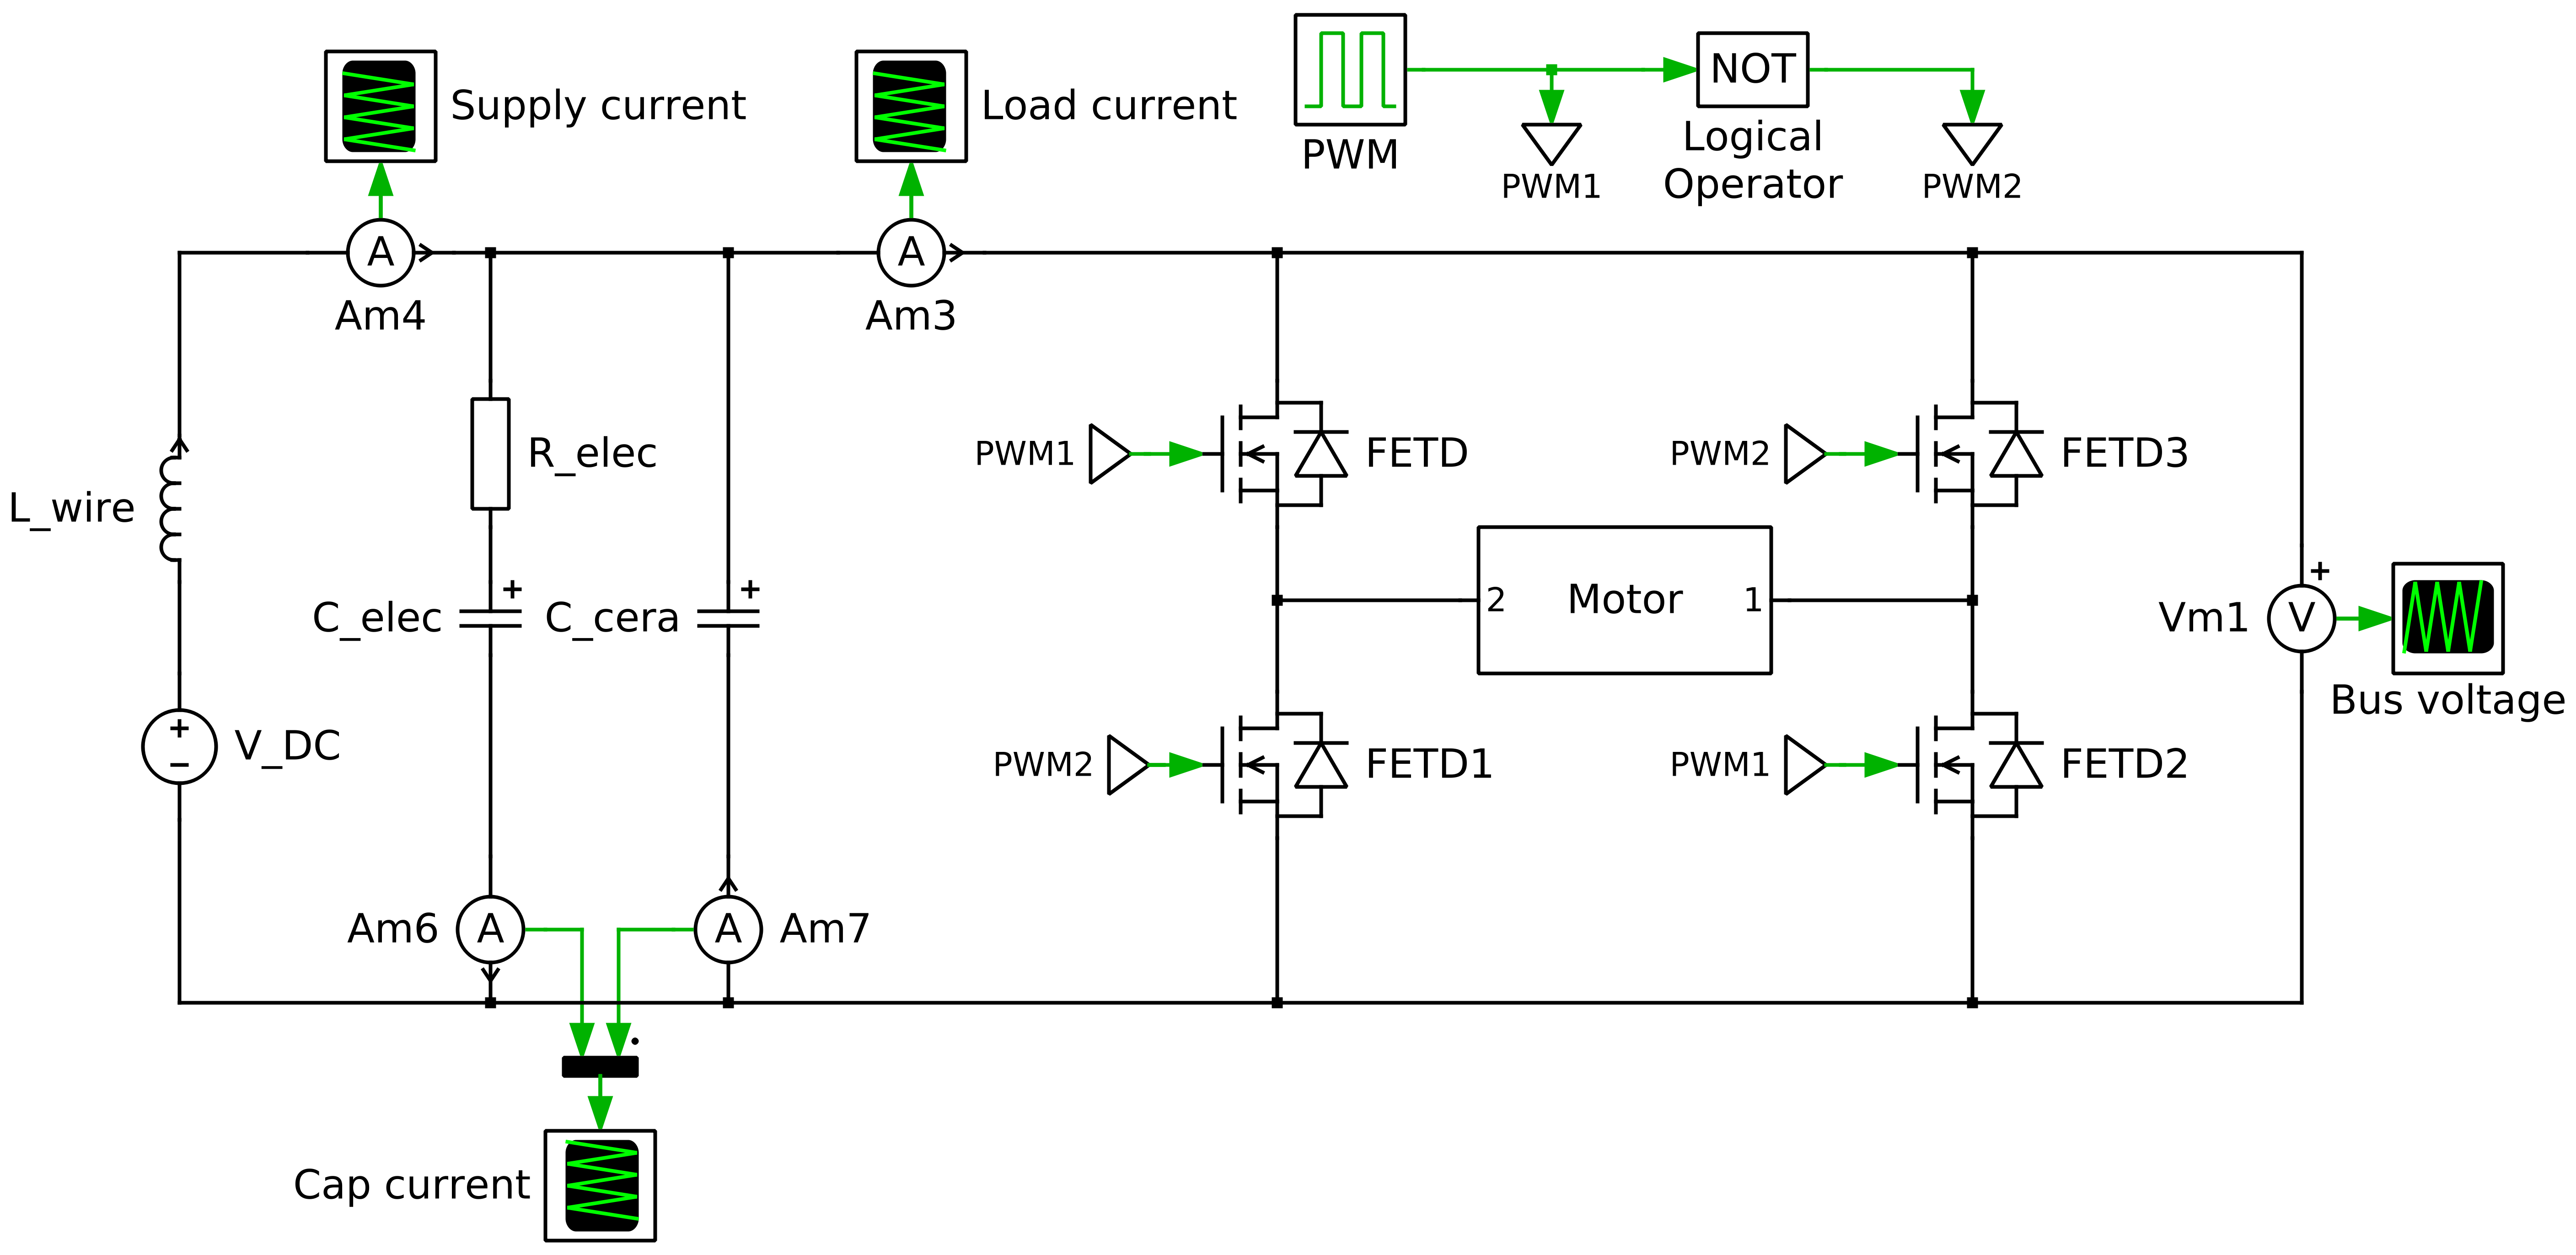
\includegraphics[width=1\linewidth]{graphics/plecs_schem.png}
	\caption{Full bridge circuit with supply capacitors and wire inductance modelled using PLECS. The Motor box consists of an inductor and a resistor in series. All components apart from the MOSFETS have the same values as the chosen components.}
	\label{fig:plecs_schem}
\end{figure}	

Simulating the system at 50\% duty cycle yields a voltage ripple of approximately 24mV, which is definitely acceptable. 

It can also be noted that an effect of the inductance in the supply wires and the supply capacitors is that the supply current is low pass filtered and is thereby protected against the ripple current and only needs to supply the DC component of the load current.

The current drawn from the capacitors is shown in figure \ref{fig:cap_currents}.
Here it can be seen that the electrolytic capacitors supply the majority of the current, while the ceramic capacitors supply a small spike with high frequency content.
It should be noted that in the simulations there are no difference between the two types of capacitors other than the ESR put in series with the electrolytic capacitors. 

\begin{figure}[h]
	\centering
    %% This file was created by matlab2tikz.
%
%The latest updates can be retrieved from
%  http://www.mathworks.com/matlabcentral/fileexchange/22022-matlab2tikz-matlab2tikz
%where you can also make suggestions and rate matlab2tikz.
%
\definecolor{mycolor1}{rgb}{0.00000,0.44700,0.74100}%
\definecolor{mycolor2}{rgb}{0.85000,0.32500,0.09800}%


\begin{tikzpicture}




% \begin{axis}[%
% width=0.9\textwidth,
% height=1.2in,
% at={(0.758in,0.481in)},
% scale only axis,
% xmin=0.004999,
% xmax=0.005025,
% ymin=-5,
% ymax=5,
% ylabel style={font=\color{white!15!black}},
% ylabel={Current [A]},
% axis background/.style={fill=white},
% title style={font=\bfseries},
% title={Capacitors}
% legend style={legend cell align=left, align=left, draw=white!15!black}
% ]
% \addplot [color=mycolor1, forget plot]
%   table[row sep=crcr]{%




\begin{axis}[%
width=0.9\textwidth,
height=1.666in,
at={(0.758in,0.481in)},
scale only axis,
xmin=0.004999,
xmax=0.005025,
xlabel style={font=\color{white!15!black}},
xlabel={Time [S]},
ymin=-8,
ymax=6,
ylabel style={font=\color{white!15!black}},
ylabel={Current [A]},
axis background/.style={fill=white},
title style={font=\bfseries},
title={Capacitors},
legend style={legend cell align=left,font=\scriptsize , align=left, draw=white!15!black},
xtick={0.005,0.00501,0.00502}
]
\addplot [color=mycolor1]
  table[row sep=crcr]{%
0.0049010553385478	0.00342081159357233\\
0.00490489969343557	0.00683073660071676\\
0.00490874404832335	0.00991586664893029\\
0.00490909090909091	0.0101813275882865\\
0.00490909090909096	-6.63767713218716\\
0.00490913588166394	0.788632374646575\\
0.00490918085423691	0.0968134753000998\\
0.00490922582680989	-0.00983381196978428\\
0.00490967555253963	-0.0103095252998444\\
0.00491012527826937	-0.00895793028321945\\
0.00491057500399912	-0.00854569634641233\\
0.00491289980626855	-0.00643281216252056\\
0.00491522460853797	-0.00430374385953325\\
0.0049175494108074	-0.00216099641818635\\
0.00491987421307683	-2.65978258807836e-05\\
0.00492369979428432	0.00343331586571138\\
0.00492752537549182	0.00677023045901803\\
0.00493135095669931	0.00991965839131126\\
0.00493181818181813	0.0102885418851053\\
0.00493181818181818	-6.63795684124184\\
0.00493186309122796	0.788140209141018\\
0.00493190800063774	0.0970706595422914\\
0.00493195291004752	-0.00968459620855366\\
0.00493240200414533	-0.010151400317405\\
0.00493285109824314	-0.00922767791311507\\
0.00493330019234094	-0.00882378071900325\\
0.0049356105215896	-0.00627608882527975\\
0.00493792085083825	-0.00434505362802873\\
0.0049402311800869	-0.00213437587624032\\
0.00494254150933555	9.53670359069014e-05\\
0.00494636627166787	0.00360061858537619\\
0.00495019103400018	0.00703901460715084\\
0.00495401579633249	0.010148792099768\\
0.0049545454545454	0.0105586699059725\\
0.00495454545454545	-6.63771853889246\\
0.00495459015032096	0.786557805328613\\
0.00495463484609647	0.0976643538023345\\
0.00495467954187197	-0.00940476091145603\\
0.00495512649962704	-0.00993978708059062\\
0.0049555734573821	-0.00857857317189525\\
0.00495602041513717	-0.00816591337095129\\
0.0049583151501913	-0.00606782639068015\\
0.00496060988524543	-0.00395664904486392\\
0.00496290462029956	-0.00183438425385551\\
0.0049651993553537	0.00027740842506091\\
0.00496903087325131	0.00374628813147904\\
0.00497286239114892	0.00708566190254611\\
0.00497669390904653	0.0102308430991807\\
0.00497727272727267	0.010685341679721\\
0.00497727272727273	-6.63729580218999\\
0.00497731727074615	0.785182739111092\\
0.00497736181421957	0.0980802659485565\\
0.00497740635769299	-0.00922134889014892\\
0.0049778517924272	-0.00977371834118745\\
0.00497829722716142	-0.00883738412134694\\
0.00497874266189563	-0.00843919794694292\\
0.00498104199845287	-0.0059238355507687\\
0.0049833413350101	-0.0040186307720349\\
0.00498564067156733	-0.00183902675090497\\
0.00498794000812456	0.00035710955229637\\
0.00499179190075393	0.00384424013741791\\
0.00499564379338329	0.00726181015807148\\
0.00499949568601265	0.0103403911775377\\
0.00499999999999995	0.0107233299318876\\
0.005	-6.63678775329545\\
0.00500004447673189	0.784627777892562\\
0.00500008895346378	0.0981859652113108\\
0.00500013343019567	-0.0092018609164648\\
0.00500057819751456	-0.00979321463432026\\
0.00500102296483345	-0.00843310502509143\\
0.00500146773215235	-0.0080287074120009\\
0.00500377677864032	-0.00595109945391359\\
0.00500608582512829	-0.00386106136327458\\
0.00500839487161626	-0.00176029297984437\\
0.00501070391810423	0.000329411198857071\\
0.00501456587568511	0.00376585486603842\\
0.005018427833266	0.00707056768878767\\
0.00502228979084688	0.0101785379664605\\
0.00502272727272722	0.0105155195053972\\
0.00502272727272727	-6.63669528791197\\
0.0050227718773715	0.785481592291763\\
0.00502281648201573	0.0977955867894744\\
0.00502286108665995	-0.00940190195881785\\
0.00502330713310222	-0.00994616280641969\\
0.0050237531795445	-0.0090183414585101\\
0.00502419922598677	-0.00862558037378225\\
0.00502652935434658	-0.00611138202407391\\
0.00502885948270639	-0.00420805247858547\\
0.00503118961106621	-0.00202587201529669\\
0.00503351973942602	0.000174128206785015\\
0.00503738617751066	0.00363343469538768\\
0.0050412526155953	0.00702605089997999\\
0.00504511905367994	0.0100849998671229\\
0.00504545454545449	0.0103377257538093\\
0.00504545454545455	-6.63688438661501\\
0.0050454993184082	0.786909187571736\\
0.00504554409136186	0.0972936761155228\\
0.00504558886431551	-0.00964315408372496\\
0.00504603659385206	-0.0101688457131655\\
0.00504648432338861	-0.00881788004933393\\
0.00504693205292516	-0.00841271897506735\\
0.00504926853902644	-0.00631767727470978\\
0.00505160502512771	-0.00420712214877206\\
0.00505394151122899	-0.00208328771191457\\
0.00505627799733027	3.16047505261319e-05\\
0.00506012977709005	0.00346430797427311\\
0.00506398155684983	0.00677190482403178\\
0.00506783333660961	0.00988961814531208\\
0.00506818181818182	0.0101602465480153\\
0.00506818181818187	-6.63741638603617\\
0.00506822676429271	0.788263580426767\\
0.00506827171040355	0.0968710712364902\\
0.00506831665651439	-0.00981902461640649\\
0.00506876611762276	-0.010282819291199\\
0.00506921557873114	-0.00936583982423489\\
0.00506966503983952	-0.00896684900611833\\
0.00507200148913105	-0.0064211155171674\\
0.00507433793842259	-0.00449234590706937\\
0.00507667438771412	-0.00228026062001985\\
0.00507901083700566	-4.80677227454873e-05\\
0.00508284935926558	0.00343339431982481\\
0.0050866878815255	0.00685027548203943\\
0.00509052640378541	0.00994250061265101\\
0.00509090909090903	0.0102364341410595\\
0.00509090909090909	-6.63776191682534\\
0.00509095403119463	0.788414109103359\\
0.00509099897148016	0.0969253130139869\\
0.0050910439117657	-0.00977244042416769\\
0.00509149331462106	-0.0102542947538771\\
0.00509194271747643	-0.00890084705757577\\
0.00509239212033179	-0.00848784329587371\\
0.00509471010980675	-0.00637605440348255\\
0.00509702809928171	-0.00424860473551991\\
0.00509934608875667	-0.00210792975909035\\
};
\addlegendentry{Ceramic Capacitors}

\addplot [color=mycolor2]
  table[row sep=crcr]{%
0.0049010553385478	-0.915441839395498\\
0.00490489969343557	-2.02008944546105\\
0.00490874404832335	-3.06653627370542\\
0.00490909090909091	-3.15739364309411\\
0.00490909090909096	-3.15739364310866\\
0.00490913588166394	4.25578284216317\\
0.00490918085423691	3.55080766909668\\
0.00490922582680989	3.43099895230262\\
0.00490967555253963	3.29838689831377\\
0.00491012527826937	3.16703515437985\\
0.00491057500399912	3.03420023729996\\
0.00491289980626855	2.34110017146304\\
0.00491522460853797	1.63927639574104\\
0.0049175494108074	0.933249601497664\\
0.00491987421307683	0.227906177082332\\
0.00492369979428432	-0.918846892447618\\
0.00492752537549182	-2.02908008624217\\
0.00493135095669931	-3.08132645441947\\
0.00493181818181813	-3.20489120793354\\
0.00493181818181818	-3.20489120795537\\
0.00493186309122796	4.20799214847648\\
0.00493190800063774	3.50368169709691\\
0.00493195291004752	3.38368428511603\\
0.00493240200414533	3.25028965549427\\
0.00493285109824314	3.11773356924823\\
0.00493330019234094	2.98412907695456\\
0.0049356105215896	2.29115388523496\\
0.00493792085083825	1.58928909779206\\
0.0049402311800869	0.883900081273168\\
0.00494254150933555	0.179570804524701\\
0.00494636627166787	-0.971891453904391\\
0.00495019103400018	-2.08573965222604\\
0.00495401579633249	-3.14064893346222\\
0.0049545454545454	-3.28094792045158\\
0.00495454545454545	-3.28094792046613\\
0.00495459015032096	4.13016844417143\\
0.00495463484609647	3.428092171358\\
0.00495467954187197	3.30783548072941\\
0.00495512649962704	3.17493758595083\\
0.0049555734573821	3.04340834878531\\
0.00495602041513717	2.91042651790485\\
0.0049583151501913	2.22189270484523\\
0.00496060988524543	1.52567994879792\\
0.00496290462029956	0.826164624122612\\
0.0049651993553537	0.128065020835493\\
0.00496903087325131	-1.02202936300455\\
0.00497286239114892	-2.13347001265356\\
0.00497669390904653	-3.18471575261356\\
0.00497727272727267	-3.33703611806413\\
0.00497727272727273	-3.33703611808596\\
0.00497731727074615	4.07241109502502\\
0.00497736181421957	3.37225057452451\\
0.00497740635769299	3.25189005607535\\
0.0049778517924272	3.12027986907924\\
0.00497829722716142	2.98964814872306\\
0.00497874266189563	2.85799117581337\\
0.00498104199845287	2.17324157982512\\
0.0049833413350101	1.48047983761353\\
0.00498564067156733	0.784966991952388\\
0.00498794000812456	0.0911780343958526\\
0.00499179190075393	-1.05497919144545\\
0.00499564379338329	-2.16139660487534\\
0.00499949568601265	-3.2066133479675\\
0.00499999999999995	-3.33785721532331\\
0.005	-3.33785721535969\\
0.00500004447673189	4.07066818338353\\
0.00500008895346378	3.37131360285275\\
0.00500013343019567	3.2510084467649\\
0.00500057819751456	3.12077301707905\\
0.00500102296483345	2.99197915805416\\
0.00500146773215235	2.86174255228252\\
0.00500377677864032	2.17991762101883\\
0.00500608582512829	1.4905762026101\\
0.00500839487161626	0.798109154726262\\
0.00501070391810423	0.107245801111276\\
0.00501456587568511	-1.03223003423773\\
0.005018427833266	-2.13230920494243\\
0.00502228979084688	-3.17133878411551\\
0.00502272727272722	-3.28429267257161\\
0.00502272727272727	-3.28429267257161\\
0.0050227718773715	4.12503893459507\\
0.00502281648201573	3.42448077159497\\
0.00502286108665995	3.30441011337098\\
0.00502330713310222	3.17465105328301\\
0.0050237531795445	3.04583722598909\\
0.00502419922598677	2.91598394387256\\
0.00502652935434658	2.23211154308228\\
0.00502885948270639	1.53958590082766\\
0.00503118961106621	0.843786765552068\\
0.00503351973942602	0.149314537120517\\
0.00503738617751066	-0.987793491374759\\
0.0050412526155953	-2.08624917075213\\
0.00504511905367994	-3.1245759032754\\
0.00504545454545449	-3.21116772740061\\
0.00504545454545455	-3.21116772741516\\
0.0050454993184082	4.19972304494149\\
0.00504554409136186	3.49718167772517\\
0.00504558886431551	3.37731402221107\\
0.00504603659385206	3.24697386535991\\
0.00504648432338861	3.11796059356857\\
0.00504693205292516	2.98747435640689\\
0.00504926853902644	2.30020861748926\\
0.00505160502512771	1.60439322426828\\
0.00505394151122899	0.904558726528194\\
0.00505627799733027	0.205597670232237\\
0.00506012977709005	-0.932263559894636\\
0.00506398155684983	-2.03290280140209\\
0.00506783333660961	-3.07475351853645\\
0.00506818181818182	-3.16541938849696\\
0.00506818181818187	-3.16541938851151\\
0.00506822676429271	4.24721468395001\\
0.00506827171040355	3.54274894992705\\
0.00506831665651439	3.42298425603076\\
0.00506876611762276	3.29125734094123\\
0.00506921557873114	3.1603465270382\\
0.00506966503983952	3.02837585099041\\
0.00507200148913105	2.33636816850048\\
0.00507433793842259	1.63493908630335\\
0.00507667438771412	0.929554722511966\\
0.00507901083700566	0.224905788723845\\
0.00508284935926558	-0.918844584048202\\
0.0050866878815255	-2.02579574252013\\
0.00509052640378541	-3.07459532834037\\
0.00509090909090903	-3.17518959014706\\
0.00509090909090909	-3.17518959015433\\
0.00509095403119463	4.23782588414906\\
0.00509099897148016	3.5331533421122\\
0.0050910439117657	3.41326674421725\\
0.00509149331462106	3.28037942616356\\
0.00509194271747643	3.14876614561945\\
0.00509239212033179	3.0156744667911\\
0.00509471010980675	2.32288135642739\\
0.00509702809928171	1.62154641278175\\
0.00509934608875667	0.916161728986481\\
};
\addlegendentry{Electrolytic Capacitors}

\end{axis}
\end{tikzpicture}%
	\missingfigure{text}
	\caption{Current drawn from the electrolytic and ceramic capacitors, when simulating in PLECS. }
	\label{fig:cap_currents}
\end{figure}

Generally the designed features of the circuit was verified using the PLECS model.

\subsubsection{Inrush Current}
\label{ssub:inrush_current}
When the system is initially turned on, the capacitors will begin to charge and they will draw a huge amount of current as there is only the ESR to limit the current. 
A resistor should be added to limit this inrush current. 
Adding the resistor to the main current path would introduce considerable losses, which is why another current path is added to the circuit.
It is done by adding the resistor and a relay in series with the main relay. 
This relay should be switched \texttt{on} to charge the capacitors before switching \texttt{on} the main relay.
% section preliminary_testing (end)


\subsection{Testing the Power Board}
It was decided to test the power board before ordering it from a professional PCB manufacturer.
In order to test it a home-made PCB was made at the University's PCB lab.

Three main functionalities should be verified on the board:

\begin{itemize}
	\item Schmitt-trigger circuitry and \texttt{AND} gate circuit
	\item PWM logic level shifting and phase shifting
	\item Motor driver circuit
\end{itemize}

The remaining functionalities has either been tested beforehand or deemed too simple to test. 

\subsubsection{Schmitt-trigger Circuitry and \texttt{AND} Gate Circuit}
The circuit can bee seen in.... \mikkel{Make a figure somewhere}.
The Schmitt-triggers were tested by varying the input voltage and verifying the switching threshold along with the the hysteresis levels. 
Testing the \texttt{AND} gate was done by applying different logic levels and verifying the results.
The complete circuit was found to work as intended.

\subsubsection{PWM Logic Level Shifting and Phase Shifting}
The circuit can bee seen in.... \mikkel{Make a figure somewhere}.
The functionality of the logic level shifter \texttt{74LVC2G17} was verified by measuring input and output on an oscilloscope. 
The output of the \texttt{NOT} gate was not as expected as it was noise with a DC offset. 
The reason behind the problem was not found, but most probably it was a production error as the schematic showed no problems.
While investigating the schematic it was found that the gate is not needed as the high side signals to the motor driver can be replaced by \texttt{high} signals, because the driver has a shoot-through protection scheme.
Therefore the \texttt{NOT} will be omitted in the next version of the board.

\subsubsection{Motor Driver Circuit}
The motor driver receives signals from the not functioning \texttt{NOT} gate and could therefore not easily be tested on the produces board.
Therefore it was decided to develop a small test PCB with the only purpose of testing the motor driver circuit.
The circuit can bee seen in.... \mikkel{Make a figure somewhere}.
The board was connected to four MOSFETs, a resistor as a load and PWM signals on the inputs. 
Measuring the gate signals showed strange behaviour and after a thorough inspection of the board and the schematic it was found that the bootstrap diode was facing the wrong direction. 
The reason behind was an error in the footprint. 
After correcting the error the functions of the driver and the bootstrap circuit was verified. 
The measured signals are shown in figure \ref{fig:test_hip_signals}.
\mikkel{More elaboration is needed}
\mikkel{FIGURE HERE!}
%\begin{figure}[h]
%	\centering
%    % This file was created by matlab2tikz.
%
%The latest updates can be retrieved from
%  http://www.mathworks.com/matlabcentral/fileexchange/22022-matlab2tikz-matlab2tikz
%where you can also make suggestions and rate matlab2tikz.
%
\definecolor{mycolor1}{rgb}{0.00000,0.44700,0.74100}%
\definecolor{mycolor2}{rgb}{0.85000,0.32500,0.09800}%
\definecolor{mycolor3}{rgb}{0.92900,0.69400,0.12500}%
%
\begin{tikzpicture}

\begin{axis}[%
width=4.521in,
height=3.566in,
at={(0.758in,0.481in)},
scale only axis,
xmin=0.0011,
xmax=0.0028,
xlabel style={font=\color{white!15!black}},
xlabel={Time [S]},
ymin=-2,
ymax=35,
ylabel style={font=\color{white!15!black}},
ylabel={Voltage [V]},
axis background/.style={fill=white},
title style={font=\bfseries},
title={Motor Driver Signals},
legend style={legend cell align=left, align=left, draw=white!15!black}
]
\addplot [color=mycolor1, forget plot]
  table[row sep=crcr]{%
0.00109999985000009	3.33333\\
0.00110005985000017	3.36667\\
0.00110009984999992	3.33333\\
0.00110019985000021	3.36667\\
0.00110023984999996	3.33333\\
0.00110029985000004	3.36667\\
0.00110035985000012	3.33333\\
0.00110043985000008	3.36667\\
0.00110049985000016	3.33333\\
0.00110055984999979	3.36667\\
0.00110061984999987	3.33333\\
0.00110065985000007	3.36667\\
0.00110073985000003	3.33333\\
0.00110081984999999	3.36667\\
0.00110085985000019	3.33333\\
0.00110091984999983	3.36667\\
0.00110097984999991	3.33333\\
0.00110107985000019	3.36667\\
0.00110111984999994	3.33333\\
0.00110117985000002	3.36667\\
0.00110121984999978	3.33333\\
0.00110129985000018	3.36667\\
0.00110135984999982	3.33333\\
0.00110143985000022	3.36667\\
0.00110147984999998	3.33333\\
0.00110153985000006	3.36667\\
0.00110159985000013	3.33333\\
0.00110167985000009	3.36667\\
0.00110175985000005	3.33333\\
0.00110179984999981	3.36667\\
0.00110183985000001	3.33333\\
0.00110191984999997	3.36667\\
0.00110197985000005	3.33333\\
0.00110205985	3.36667\\
0.0011020998500002	3.33333\\
0.00110215984999984	3.36667\\
0.00110219985000004	3.3\\
0.00110229984999988	3.36667\\
0.00110235984999996	3.33333\\
0.00110243984999991	3.36667\\
0.00110247985000012	3.33333\\
0.00110253985000019	3.36667\\
0.00110261985000015	3.33333\\
0.00110267984999979	3.36667\\
0.00110271984999999	3.33333\\
0.00110277985000007	3.36667\\
0.00110285985000003	3.33333\\
0.00110291985000011	3.36667\\
0.00110299985000006	3.33333\\
0.00110305985000014	3.36667\\
0.00110307985000002	3.33333\\
0.00110315984999998	3.36667\\
0.00110321985000006	3.33333\\
0.0011033198499999	3.36667\\
0.0011033598500001	3.33333\\
0.00110339984999985	3.36667\\
0.00110345984999993	3.33333\\
0.00110353984999989	3.36667\\
0.00110361984999985	3.33333\\
0.00110365985000005	3.36667\\
0.00110371985000013	3.33333\\
0.00110377985000021	3.36667\\
0.00110385985000017	3.33333\\
0.00110393985000012	3.36667\\
0.00110395985	3.3\\
0.00110401985000008	3.36667\\
0.00110407985000016	3.33333\\
0.00110417985	3.36667\\
0.0011042198500002	3.33333\\
0.00110429985000016	3.36667\\
0.00110433984999991	3.33333\\
0.00110439984999999	3.36667\\
0.00110443985000019	3.33333\\
0.00110445985000007	3.36667\\
0.00110447984999995	3.33333\\
0.00110453985000003	3.36667\\
0.00110457984999979	3.3\\
0.00110463984999987	3.36667\\
0.00110469984999995	3.33333\\
0.00110479984999978	3.36667\\
0.00110485984999986	3.33333\\
0.00110491984999994	3.36667\\
0.00110495985000014	3.33333\\
0.00110501985000022	3.36667\\
0.0011050398500001	3.33333\\
0.00110505984999998	3.36667\\
0.00110507984999986	3.3\\
0.00110515984999981	3.36667\\
0.00110519985000002	3.33333\\
0.00110527984999997	3.36667\\
0.00110533985000005	3.33333\\
0.00110541985000001	3.36667\\
0.00110545985000021	3.33333\\
0.00110551984999985	3.4\\
0.00110555985000005	3.33333\\
0.00110567985000021	3.36667\\
0.00110571984999996	3.33333\\
0.00110577985000004	3.36667\\
0.0011058198499998	3.3\\
0.00110587984999988	3.36667\\
0.00110593984999996	3.33333\\
0.0011060398499998	3.36667\\
0.00110607985	3.3\\
0.00110613985000008	3.4\\
0.00110619985000016	3.33333\\
0.00110625984999979	3.36667\\
0.00110633985000019	3.33333\\
0.00110639984999983	3.36667\\
0.00110645984999991	3.33333\\
0.00110651984999999	3.36667\\
0.00110657985000007	3.33333\\
0.00110665985000002	3.36667\\
0.0011067198500001	3.33333\\
0.00110677985000018	3.36667\\
0.00110679985000006	3.33333\\
0.0011068998499999	3.36667\\
0.0011069398500001	3.3\\
0.00110701985000006	3.36667\\
0.00110705984999981	3.3\\
0.00110713985000022	3.36667\\
0.00110719984999985	3.33333\\
0.00110727984999981	3.36667\\
0.00110733984999989	3.33333\\
0.00110739984999997	3.36667\\
0.00110741984999985	3.33333\\
0.0011074998499998	3.36667\\
0.00110751985000013	3.33333\\
0.00110753985000001	3.36667\\
0.00110755984999988	3.3\\
0.00110763984999984	3.36667\\
0.00110769984999992	3.3\\
0.00110775985	3.36667\\
0.00110783984999996	3.33333\\
0.00110789985000004	3.36667\\
0.00110795985000012	3.33333\\
0.00110799984999987	3.4\\
0.00110805984999995	3.33333\\
0.00110813984999991	3.36667\\
0.00110817985000011	3.3\\
0.00110827984999995	3.36667\\
0.00110829984999983	3.3\\
0.00110835984999991	3.36667\\
0.00110843984999986	3.33333\\
0.00110851984999982	3.36667\\
0.00110859984999978	3.33333\\
0.0011086198500001	3.4\\
0.00110867985000018	3.33333\\
0.00110875985000014	3.36667\\
0.0011087998499999	3.3\\
0.00110889985000018	3.36667\\
0.00110893984999993	3.3\\
0.00110899985000001	3.36667\\
0.00110907984999997	3.33333\\
0.00110915984999993	3.36667\\
0.00110919985000013	3.33333\\
0.00110927985000009	3.36667\\
0.00110929984999997	3.33333\\
0.00110935985000005	3.36667\\
0.00110941985000013	3.3\\
0.00110951984999996	3.36667\\
0.00110955985000016	3.3\\
0.0011096198499998	3.36667\\
0.00110967984999988	3.33333\\
0.00110975984999984	3.36667\\
0.00110981984999992	3.33333\\
0.00110985985000012	3.4\\
0.0011099198500002	3.3\\
0.00110999985000015	3.36667\\
0.00111005984999979	3.33333\\
0.00111013985000019	3.36667\\
0.00111017984999995	3.3\\
0.00111023985000003	3.36667\\
0.00111029985000011	3.33333\\
0.00111037985000007	3.36667\\
0.00111045985000002	3.33333\\
0.0011105198500001	3.36667\\
0.00111055984999986	3.33333\\
0.00111059985000006	3.36667\\
0.00111065985000014	3.3\\
0.00111075984999998	3.36667\\
0.00111077984999985	3.3\\
0.00111085984999981	3.36667\\
0.00111093985000021	3.33333\\
0.00111099984999985	3.36667\\
0.00111107984999981	3.33333\\
0.00111113984999989	3.36667\\
0.00111117985000009	3.33333\\
0.00111121984999984	3.36667\\
0.00111127984999992	3.3\\
0.00111135984999988	3.36667\\
0.00111141984999996	3.3\\
0.00111145985000016	3.36667\\
0.00111153985000012	3.33333\\
0.00111161985000008	3.36667\\
0.00111169985000004	3.33333\\
0.00111173984999979	3.4\\
0.00111179984999987	3.33333\\
0.00111187984999983	3.36667\\
0.00111189985000015	3.3\\
0.00111199984999999	3.36667\\
0.00111201984999987	3.3\\
0.00111209984999983	3.36667\\
0.00111213985000003	3.3\\
0.00111225985000019	3.36667\\
0.00111231984999982	3.33333\\
0.00111233985000014	3.4\\
0.00111239984999978	3.33333\\
0.00111249985000006	3.36667\\
0.00111255985000014	3.33333\\
0.00111261985000022	3.36667\\
0.00111265984999998	3.3\\
0.00111271985000005	3.36667\\
0.00111277985000013	3.33333\\
0.00111287984999997	3.36667\\
0.00111291985000017	3.33333\\
0.00111299985000013	3.36667\\
0.00111303984999989	3.33333\\
0.00111307985000009	3.36667\\
0.00111315985000005	3.3\\
0.00111323985	3.36667\\
0.0011132798500002	3.3\\
0.00111333984999984	3.36667\\
0.00111337985000004	3.3\\
0.0011134998500002	3.36667\\
0.00111353984999996	3.33333\\
0.00111361984999991	3.36667\\
0.00111365985000011	3.33333\\
0.00111369984999987	3.36667\\
0.00111375984999995	3.3\\
0.00111385984999979	3.36667\\
0.00111389984999999	3.3\\
0.00111395985000007	3.36667\\
0.00111401985000015	3.3\\
0.00111411984999998	3.36667\\
0.00111417985000006	3.33333\\
0.00111423985000014	3.36667\\
0.0011142798499999	3.33333\\
0.00111433984999998	3.36667\\
0.00111437985000018	3.3\\
0.00111447985000002	3.36667\\
0.00111451985000022	3.3\\
0.00111459985000018	3.36667\\
0.00111465984999981	3.33333\\
0.00111473985000021	3.36667\\
0.00111477984999997	3.33333\\
0.00111485984999993	3.36667\\
0.00111489985000013	3.33333\\
0.00111497985000009	3.36667\\
0.00111503985000017	3.33333\\
0.0011150998499998	3.36667\\
0.00111513985	3.3\\
0.00111521984999996	3.36667\\
0.00111527985000004	3.33333\\
0.00111535985	3.36667\\
0.00111541985000008	3.33333\\
0.00111547985000016	3.36667\\
0.00111551984999991	3.33333\\
0.00111559984999987	3.36667\\
0.00111565984999995	3.33333\\
0.00111571985000003	3.36667\\
0.00111573984999991	3.3\\
0.00111583985000019	3.36667\\
0.00111589984999982	3.33333\\
0.00111597984999978	3.36667\\
0.00111603984999986	3.33333\\
0.00111609984999994	3.36667\\
0.00111615985000002	3.33333\\
0.00111619985000022	3.36667\\
0.00111627985000018	3.33333\\
0.00111633984999981	3.36667\\
0.00111637985000002	3.3\\
0.00111643985000009	3.36667\\
0.00111651985000005	3.33333\\
0.00111661984999989	3.36667\\
0.00111663985000021	3.33333\\
0.00111671985000017	3.36667\\
0.00111675984999993	3.33333\\
0.00111681985000001	3.36667\\
0.00111689984999996	3.33333\\
0.00111695985000004	3.36667\\
0.00111701985000012	3.33333\\
0.0011170798500002	3.36667\\
0.00111713984999984	3.33333\\
0.0011172198499998	3.36667\\
0.00111727984999987	3.33333\\
0.00111733984999995	3.36667\\
0.00111737985000016	3.33333\\
0.00111741984999991	3.36667\\
0.00111743984999979	3.33333\\
0.00111745985000011	3.36667\\
0.00111753985000007	3.33333\\
0.00111757984999983	3.36667\\
0.00111763984999991	3.33333\\
0.00111769984999999	3.36667\\
0.00111775985000007	3.33333\\
0.00111783985000002	3.36667\\
0.0011178998500001	3.33333\\
0.00111795985000018	3.36667\\
0.00111801984999982	3.33333\\
0.0011180798499999	3.36667\\
0.00111815984999986	3.33333\\
0.00111819985000006	3.36667\\
0.00111825985000014	3.33333\\
0.00111829984999989	3.36667\\
0.00111837984999985	3.33333\\
0.00111847985000013	3.36667\\
0.00111849985000001	3.33333\\
0.00111857984999997	3.36667\\
0.00111863985000005	3.33333\\
0.00111869985000013	3.36667\\
0.00111875985000021	3.33333\\
0.00111883985000016	3.36667\\
0.00111887984999992	3.33333\\
0.00111895984999988	3.36667\\
0.00111899985000008	3.33333\\
0.00111907985000004	3.36667\\
0.00111913985000012	3.33333\\
0.0011191998500002	3.36667\\
0.00111923984999995	3.33333\\
0.00111933984999979	3.36667\\
0.00111939984999987	3.33333\\
0.00111943985000007	3.36667\\
0.00111949985000015	3.33333\\
0.00111955984999978	3.36667\\
0.00111961984999986	3.33333\\
0.00111969984999982	3.36667\\
0.00111971985000014	3.33333\\
0.0011197998500001	3.4\\
0.00111987985000006	3.33333\\
0.00111995985000002	3.36667\\
0.00112003984999998	3.33333\\
0.00112005984999985	3.36667\\
0.00112011984999993	3.33333\\
0.00112021985000021	3.36667\\
0.00112023985000009	3.33333\\
0.00112033984999993	3.36667\\
0.00112035984999981	3.33333\\
0.00112043985000021	3.36667\\
0.00112049984999985	3.33333\\
0.0011205798499998	3.36667\\
0.00112063984999988	3.33333\\
0.00112067985000008	3.36667\\
0.00112075985000004	3.33333\\
0.00112081985000012	3.36667\\
0.00112085984999988	3.33333\\
0.00112095985000016	3.36667\\
0.00112099984999992	3.33333\\
0.00112107984999987	3.36667\\
0.00112111985000007	3.33333\\
0.00112119985000003	3.36667\\
0.00112123984999979	3.33333\\
0.00112129984999987	3.36667\\
0.00112135984999995	3.33333\\
0.00112143984999991	3.36667\\
0.00112147985000011	3.33333\\
0.00112155985000006	3.36667\\
0.00112161985000014	3.3\\
0.00112167984999978	3.36667\\
0.00112173984999986	3.33333\\
0.00112181984999982	3.36667\\
0.0011218798499999	3.33333\\
0.00112193984999998	3.36667\\
0.00112197985000018	3.33333\\
0.00112203984999981	3.36667\\
0.00112211985000021	3.33333\\
0.00112219985000017	3.36667\\
0.00112223984999993	3.33333\\
0.00112229985000001	3.36667\\
0.00112235985000009	3.33333\\
0.00112243985000005	3.36667\\
0.00112249985000012	3.33333\\
0.0011225598500002	3.36667\\
0.00112259984999996	3.33333\\
0.00112267984999992	3.36667\\
0.00112275984999988	3.33333\\
0.00112281984999996	3.36667\\
0.00112285985000016	3.33333\\
0.00112291984999979	3.36667\\
0.00112297984999987	3.33333\\
0.00112307985000015	3.36667\\
0.00112311984999991	3.33333\\
0.00112317984999999	3.36667\\
0.00112321985000019	3.33333\\
0.00112329985000015	3.36667\\
0.00112331985000003	3.33333\\
0.00112343985000019	3.36667\\
0.00112347984999994	3.33333\\
0.00112353985000002	3.36667\\
0.00112361984999998	3.33333\\
0.00112367985000006	3.36667\\
0.00112373985000014	3.33333\\
0.0011238198500001	3.36667\\
0.00112385984999985	3.33333\\
0.00112389985000005	3.36667\\
0.00112399984999989	3.33333\\
0.00112405984999997	3.36667\\
0.00112411985000005	3.33333\\
0.00112415984999981	3.36667\\
0.00112421984999989	3.33333\\
0.00112429984999984	3.36667\\
0.00112435984999992	3.33333\\
0.00112443984999988	3.36667\\
0.00112447985000008	3.33333\\
0.00112453985000016	3.36667\\
0.00112455985000004	3.33333\\
0.00112457984999992	3.36667\\
0.00112461985000012	3.33333\\
0.0011246798500002	3.36667\\
0.00112473984999983	3.33333\\
0.00112479984999991	3.36667\\
0.00112483985000011	3.33333\\
0.00112491985000007	3.36667\\
0.00112495984999983	3.3\\
0.00112503984999979	3.36667\\
0.00112511985000019	3.33333\\
0.00112515984999995	3.36667\\
0.00112521985000003	3.33333\\
0.00112529984999998	3.36667\\
0.00112533985000018	3.3\\
0.00112539984999982	3.36667\\
0.0011254598499999	3.33333\\
0.00112553984999986	3.36667\\
0.00112559984999994	3.33333\\
0.00112567984999989	3.36667\\
0.0011257198500001	3.33333\\
0.00112577985000017	3.36667\\
0.00112585985000013	3.33333\\
0.00112591985000021	3.36667\\
0.00112595984999997	3.3\\
0.00112603984999993	3.36667\\
0.00112607985000013	3.3\\
0.00112615985000009	3.36667\\
0.00112623985000004	3.33333\\
0.00112629985000012	3.36667\\
0.00112633984999988	3.33333\\
0.00112639984999996	3.36667\\
0.00112647984999992	3.33333\\
0.00112653985	3.36667\\
0.0011265798500002	3.3\\
0.00112663984999983	3.36667\\
0.00112669984999991	3.3\\
0.00112677984999987	3.4\\
0.00112685984999983	3.33333\\
0.00112691984999991	3.36667\\
0.00112693984999979	3.33333\\
0.00112701985000019	3.36667\\
0.00112707984999982	3.33333\\
0.0011271798500001	3.36667\\
0.00112719984999998	3.3\\
0.00112725985000006	3.36667\\
0.00112731985000014	3.33333\\
0.0011273998500001	3.36667\\
0.00112741984999998	3.33333\\
0.00112743984999986	3.36667\\
0.00112747985000006	3.33333\\
0.00112753985000014	3.36667\\
0.00112755985000002	3.33333\\
0.00112765984999985	3.36667\\
0.00112771984999993	3.33333\\
0.00112779984999989	3.36667\\
0.00112781985000021	3.3\\
0.00112789985000017	3.36667\\
0.0011279598499998	3.33333\\
0.00112801984999988	3.36667\\
0.00112809984999984	3.33333\\
0.00112813985000004	3.4\\
0.00112819985000012	3.33333\\
0.00112827985000008	3.36667\\
0.00112833985000016	3.33333\\
0.00112839984999979	3.36667\\
0.00112843985	3.3\\
0.00112849985000008	3.36667\\
0.00112857985000003	3.33333\\
0.00112865984999999	3.36667\\
0.00112869985000019	3.33333\\
0.00112877985000015	3.36667\\
0.00112879985000003	3.33333\\
0.00112889984999986	3.36667\\
0.00112895984999994	3.33333\\
0.0011290398499999	3.36667\\
0.00112905984999978	3.3\\
0.00112911984999986	3.36667\\
0.00112917984999994	3.33333\\
0.00112927985000022	3.36667\\
0.00112933984999986	3.3\\
0.00112939984999993	3.36667\\
0.00112943985000014	3.33333\\
0.00112951985000009	3.36667\\
0.00112957985000017	3.33333\\
0.00112965985000013	3.36667\\
0.00112967985000001	3.3\\
0.00112973985000009	3.36667\\
0.00112981985000005	3.33333\\
0.00112989985	3.36667\\
0.00112995985000008	3.33333\\
0.00112999984999984	3.4\\
0.00113003985000004	3.33333\\
0.00113013984999988	3.36667\\
0.00113019984999996	3.33333\\
0.00113025985000004	3.36667\\
0.00113031985000012	3.33333\\
0.0011303798500002	3.36667\\
0.00113043984999983	3.33333\\
0.00113051984999979	3.36667\\
0.00113055984999999	3.33333\\
0.00113061985000007	3.4\\
0.00113065984999983	3.33333\\
0.00113073984999978	3.36667\\
0.00113075985000011	3.33333\\
0.00113077984999999	3.36667\\
0.00113079984999986	3.3\\
0.00113089985000014	3.36667\\
0.00113091985000002	3.3\\
0.00113099984999998	3.36667\\
0.00113105985000006	3.33333\\
0.00113113985000002	3.36667\\
0.0011311998500001	3.33333\\
0.00113125985000018	3.36667\\
0.00113129984999993	3.33333\\
0.00113135985000001	3.36667\\
0.00113141985000009	3.3\\
0.00113149985000005	3.36667\\
0.00113153984999981	3.3\\
0.00113163985000009	3.36667\\
0.00113167984999984	3.33333\\
0.0011317598499998	3.36667\\
0.00113179985	3.33333\\
0.00113181984999988	3.36667\\
0.0011318398500002	3.33333\\
0.00113187984999996	3.36667\\
0.00113191985000016	3.33333\\
0.00113201985	3.36667\\
0.0011320598500002	3.33333\\
0.00113213985000016	3.36667\\
0.00113217984999991	3.3\\
0.00113223984999999	3.36667\\
0.00113229985000007	3.33333\\
0.00113239984999991	3.36667\\
0.00113245984999999	3.33333\\
0.00113249985000019	3.36667\\
0.00113253984999995	3.33333\\
0.00113261984999991	3.36667\\
0.00113265985000011	3.3\\
0.00113275984999994	3.36667\\
0.00113279985000014	3.3\\
0.00113285984999978	3.36667\\
0.00113293985000018	3.33333\\
0.00113301985000014	3.36667\\
0.0011330598499999	3.33333\\
0.00113313984999985	3.36667\\
0.00113315985000018	3.33333\\
0.00113323985000013	3.36667\\
0.00113327984999989	3.3\\
0.00113337985000017	3.36667\\
0.00113339985000005	3.3\\
0.00113347985000001	3.36667\\
0.00113351985000021	3.3\\
0.00113363984999992	3.36667\\
0.00113367985000012	3.33333\\
0.00113375985000008	3.36667\\
0.00113379984999984	3.33333\\
0.00113385984999992	3.36667\\
0.00113389985000012	3.3\\
0.00113399984999996	3.36667\\
0.00113401984999983	3.3\\
0.00113409984999979	3.36667\\
0.00113415984999987	3.33333\\
0.00113425985000015	3.36667\\
0.00113427985000003	3.33333\\
0.00113429984999991	3.36667\\
0.00113431984999979	3.33333\\
0.00113433985000011	3.4\\
0.00113439985000019	3.33333\\
0.00113449985000003	3.36667\\
0.0011345198499999	3.3\\
0.00113461985000018	3.36667\\
0.00113465984999994	3.3\\
0.00113471985000002	3.36667\\
0.0011347798500001	3.33333\\
0.00113487984999994	3.36667\\
0.00113493985000002	3.33333\\
0.00113497985000022	3.36667\\
0.00113501984999997	3.33333\\
0.00113511984999981	3.36667\\
0.00113513985000013	3.3\\
0.00113523984999997	3.36667\\
0.00113529985000005	3.33333\\
0.00113533984999981	3.36667\\
0.00113539984999989	3.33333\\
0.00113549985000017	3.36667\\
0.0011355598499998	3.33333\\
0.00113561984999988	3.36667\\
0.0011356398500002	3.33333\\
0.00113571985000016	3.36667\\
0.00113575984999992	3.3\\
0.0011358598500002	3.36667\\
0.00113589984999996	3.3\\
0.00113595985000003	3.36667\\
0.00113603984999999	3.33333\\
0.00113611984999995	3.36667\\
0.00113617985000003	3.33333\\
0.00113621984999979	3.4\\
0.00113629985000019	3.33333\\
0.00113633984999995	3.36667\\
0.0011364198499999	3.33333\\
0.00113647984999998	3.36667\\
0.00113651985000018	3.3\\
0.00113657984999982	3.36667\\
0.00113659985000014	3.33333\\
0.00113673985000018	3.36667\\
0.00113679984999981	3.33333\\
0.00113683985000002	3.4\\
0.00113689985000009	3.33333\\
0.00113697985000005	3.36667\\
0.00113699984999993	3.3\\
0.00113709985000021	3.36667\\
0.00113711985000009	3.3\\
0.00113719985000005	3.36667\\
0.00113725985000013	3.3\\
0.00113735984999996	3.36667\\
0.00113741985000004	3.33333\\
0.0011374598499998	3.4\\
0.00113751984999988	3.33333\\
0.00113757984999996	3.36667\\
0.0011376798499998	3.33333\\
0.00113771985	3.36667\\
0.00113779984999995	3.33333\\
0.00113781984999983	3.36667\\
0.00113789984999979	3.33333\\
0.00113797985000019	3.36667\\
0.00113803984999983	3.33333\\
0.00113807985000003	3.4\\
0.00113815984999999	3.33333\\
0.00113821985000007	3.36667\\
0.00113827985000015	3.33333\\
0.00113833984999978	3.36667\\
0.00113841985000018	3.33333\\
0.00113843985000006	3.36667\\
0.00113851985000002	3.33333\\
0.00113859984999998	3.36667\\
0.00113865985000006	3.33333\\
0.00113871985000014	3.36667\\
0.00113875984999989	3.33333\\
0.00113881984999997	3.36667\\
0.00113889984999993	3.33333\\
0.00113895985000001	3.36667\\
0.00113901985000009	3.33333\\
0.00113905984999985	3.36667\\
0.00113907985000017	3.33333\\
0.00113909985000005	3.36667\\
0.0011391398499998	3.33333\\
0.00113921985000021	3.36667\\
0.00113927984999984	3.33333\\
0.00113931985000004	3.36667\\
0.00113937985000012	3.33333\\
0.0011394398500002	3.36667\\
0.00113953985000004	3.33333\\
0.00113957984999979	3.36667\\
0.0011396598500002	3.33333\\
0.00113969984999995	3.36667\\
0.00113973985000015	3.33333\\
0.00113983984999999	3.36667\\
0.00113989985000007	3.33333\\
0.00113995985000015	3.36667\\
0.00114001984999978	3.33333\\
0.00114007984999986	3.36667\\
0.00114015984999982	3.33333\\
0.00114019985000002	3.36667\\
0.0011402598500001	3.33333\\
0.00114031985000018	3.36667\\
0.00114039985000014	3.33333\\
0.00114045985000022	3.36667\\
0.00114051984999985	3.33333\\
0.00114057984999993	3.36667\\
0.00114063985000001	3.33333\\
0.00114067985000021	3.36667\\
0.00114069985000009	3.33333\\
0.00114073984999985	3.36667\\
0.00114077985000005	3.33333\\
0.00114081984999981	3.36667\\
0.00114089985000021	3.33333\\
0.00114093984999997	3.36667\\
0.00114097985000017	3.33333\\
0.00114107985	3.36667\\
0.00114113985000008	3.33333\\
0.00114119985000016	3.36667\\
0.0011412598499998	3.33333\\
0.0011413398500002	3.36667\\
0.00114137984999996	3.33333\\
0.00114143985000004	3.36667\\
0.00114151984999999	3.33333\\
0.0011415598500002	3.36667\\
0.00114161984999983	3.33333\\
0.00114171985000011	3.36667\\
0.00114173984999999	3.33333\\
0.00114181984999995	3.36667\\
0.00114187985000003	3.33333\\
0.00114195984999999	3.36667\\
0.00114201985000006	3.33333\\
0.00114205984999982	3.36667\\
0.00114213984999978	3.33333\\
0.00114219984999986	3.36667\\
0.00114223985000006	3.33333\\
0.0011423398499999	3.36667\\
0.00114235985000022	3.33333\\
0.00114243985000018	3.36667\\
0.00114249984999981	3.33333\\
0.00114255984999989	3.36667\\
0.00114261984999997	3.33333\\
0.00114267985000005	3.36667\\
0.00114273985000013	3.33333\\
0.00114281985000009	3.36667\\
0.00114285984999984	3.33333\\
0.00114295985000012	3.36667\\
0.00114299984999988	3.33333\\
0.00114305984999996	3.36667\\
0.00114309985000016	3.3\\
0.00114319985	3.36667\\
0.00114325985000008	3.33333\\
0.00114331985000016	3.36667\\
0.00114335984999991	3.33333\\
0.00114343984999987	3.36667\\
0.00114351984999983	3.33333\\
0.00114355985000003	3.36667\\
0.00114361985000011	3.33333\\
0.00114367985000019	3.36667\\
0.00114373984999983	3.33333\\
0.00114381984999978	3.36667\\
0.00114389985000019	3.33333\\
0.00114393984999994	3.36667\\
0.00114399985000002	3.33333\\
0.00114403984999978	3.36667\\
0.00114411985000018	3.33333\\
0.00114419985000014	3.36667\\
0.00114425985000022	3.33333\\
0.00114429984999997	3.36667\\
0.00114433985000018	3.3\\
0.00114443985000001	3.36667\\
0.00114449985000009	3.33333\\
0.00114455985000017	3.36667\\
0.00114461984999981	3.33333\\
0.00114467984999989	3.36667\\
0.00114473984999997	3.33333\\
0.00114481984999992	3.36667\\
0.00114485985000012	3.33333\\
0.0011449198500002	3.36667\\
0.00114497984999984	3.33333\\
0.00114507985000012	3.36667\\
0.00114511984999988	3.33333\\
0.00114519984999983	3.36667\\
0.00114521985000016	3.33333\\
0.00114531984999999	3.36667\\
0.00114535985000019	3.33333\\
0.00114543985000015	3.36667\\
0.00114549984999979	3.33333\\
0.00114553984999999	3.36667\\
0.00114561984999995	3.33333\\
0.00114563984999982	3.36667\\
0.00114565985000015	3.33333\\
0.00114567985000003	3.36667\\
0.0011457398500001	3.33333\\
0.00114579985000018	3.36667\\
0.00114585984999982	3.33333\\
0.0011459198499999	3.36667\\
0.00114593985000022	3.33333\\
0.00114605984999994	3.36667\\
0.00114609985000014	3.33333\\
0.0011461798500001	3.36667\\
0.00114623985000017	3.33333\\
0.00114631985000013	3.36667\\
0.00114635984999989	3.33333\\
0.00114643984999985	3.36667\\
0.00114647985000005	3.33333\\
0.00114653985000013	3.36667\\
0.00114657984999988	3.33333\\
0.00114667985000017	3.36667\\
0.00114671984999992	3.3\\
0.00114679984999988	3.36667\\
0.00114685984999996	3.33333\\
0.00114693984999992	3.36667\\
0.00114699985	3.33333\\
0.0011470398500002	3.4\\
0.00114709984999983	3.33333\\
0.00114715984999991	3.36667\\
0.00114723984999987	3.33333\\
0.00114731984999983	3.36667\\
0.00114735985000003	3.33333\\
0.00114739984999979	3.36667\\
0.00114747985000019	3.33333\\
0.00114755985000015	3.36667\\
0.0011475998499999	3.33333\\
0.00114765984999998	3.4\\
0.00114769985000018	3.33333\\
0.00114777985000014	3.36667\\
0.0011478598500001	3.33333\\
0.00114791985000018	3.36667\\
0.00114797984999981	3.3\\
0.00114801985000001	3.36667\\
0.00114807985000009	3.3\\
0.00114817984999993	3.36667\\
0.00114823985000001	3.33333\\
0.00114827985000021	3.36667\\
0.00114829985000009	3.33333\\
0.00114839984999993	3.36667\\
0.00114847984999988	3.33333\\
0.00114853984999996	3.36667\\
0.00114857985000016	3.3\\
0.0011486398499998	3.36667\\
0.0011487198500002	3.33333\\
0.00114877984999984	3.36667\\
0.00114879985000016	3.33333\\
0.00114881985000004	3.36667\\
0.00114883984999992	3.33333\\
0.00114889985	3.4\\
0.0011489398500002	3.33333\\
0.00114903985000003	3.36667\\
0.00114905984999991	3.3\\
0.00114915985000019	3.36667\\
0.00114919984999995	3.3\\
0.00114927984999991	3.36667\\
0.00114931985000011	3.33333\\
0.00114941984999994	3.36667\\
0.00114947985000002	3.33333\\
0.00114951984999978	3.4\\
0.00114957984999986	3.33333\\
0.00114963984999994	3.36667\\
0.0011497198499999	3.33333\\
0.00114979984999986	3.36667\\
0.00114981985000018	3.3\\
0.00114987984999981	3.36667\\
0.00114993984999989	3.33333\\
0.00115003985000017	3.36667\\
0.00115009984999981	3.33333\\
0.00115015984999989	3.36667\\
0.00115019985000009	3.33333\\
0.00115025985000017	3.36667\\
0.0011503198499998	3.3\\
0.00115039985000021	3.36667\\
0.00115045984999984	3.3\\
0.00115049985000004	3.36667\\
0.00115057985	3.33333\\
0.00115065984999996	3.36667\\
0.00115069985000016	3.33333\\
0.00115075984999979	3.4\\
0.00115081984999987	3.33333\\
0.00115089984999983	3.36667\\
0.00115093985000003	3.3\\
0.00115103984999987	3.36667\\
0.00115107985000007	3.3\\
0.00115113985000015	3.36667\\
0.00115119984999978	3.33333\\
0.00115127985000019	3.36667\\
0.00115133984999982	3.33333\\
0.0011513998499999	3.36667\\
0.0011514398500001	3.33333\\
0.00115149985000018	3.36667\\
0.00115155984999982	3.3\\
0.0011516598500001	3.36667\\
0.00115169984999985	3.3\\
0.00115173985000006	3.36667\\
0.00115181985000001	3.33333\\
0.00115189984999997	3.36667\\
0.00115197984999993	3.33333\\
0.00115201985000013	3.36667\\
0.00115205984999989	3.33333\\
0.00115213984999984	3.36667\\
0.00115217985000005	3.3\\
0.00115225985	3.36667\\
0.0011522998500002	3.3\\
0.00115237985000016	3.36667\\
0.00115245985000012	3.33333\\
0.0011525198500002	3.36667\\
0.00115257984999984	3.33333\\
0.00115263984999991	3.36667\\
0.00115267985000012	3.33333\\
0.0011527398500002	3.36667\\
0.00115279984999983	3.3\\
0.00115287984999979	3.36667\\
0.00115293984999987	3.3\\
0.00115299984999995	3.36667\\
0.00115303985000015	3.3\\
0.00115313984999998	3.36667\\
0.00115319985000006	3.33333\\
0.00115325985000014	3.36667\\
0.0011532998499999	3.33333\\
0.00115331984999978	3.36667\\
0.0011533398500001	3.33333\\
0.00115337984999986	3.36667\\
0.00115343984999994	3.3\\
0.0011535198499999	3.36667\\
0.00115353985000022	3.3\\
0.00115361985000018	3.36667\\
0.00115367984999981	3.33333\\
0.00115375985000021	3.36667\\
0.00115381984999985	3.33333\\
0.00115385985000005	3.4\\
0.00115403984999984	3.3\\
0.00115413985000012	3.36667\\
0.00115417984999988	3.3\\
0.00115423984999996	3.36667\\
0.00115429985000004	3.33333\\
0.00115437985	3.36667\\
0.00115445984999996	3.33333\\
0.00115447984999983	3.4\\
0.00115453984999991	3.33333\\
0.00115461984999987	3.36667\\
0.00115465985000007	3.3\\
0.00115475984999991	3.36667\\
0.00115477984999979	3.3\\
0.00115485985000019	3.36667\\
0.00115493985000015	3.33333\\
0.00115499984999978	3.36667\\
0.00115507985000018	3.33333\\
0.00115511984999994	3.4\\
0.00115515985000014	3.33333\\
0.0011552398500001	3.36667\\
0.00115527984999986	3.3\\
0.00115537985000014	3.36667\\
0.00115543985000022	3.33333\\
0.00115547984999997	3.36667\\
0.00115553985000005	3.33333\\
0.00115561985000001	3.36667\\
0.00115569984999997	3.33333\\
0.00115575985000005	3.36667\\
0.00115577984999993	3.33333\\
0.00115585984999989	3.36667\\
0.00115589985000009	3.3\\
0.00115599984999992	3.36667\\
0.00115603985000012	3.3\\
0.0011560998500002	3.36667\\
0.00115617985000016	3.33333\\
0.00115625985000012	3.36667\\
0.0011563198500002	3.33333\\
0.00115635984999996	3.36667\\
0.00115637984999983	3.33333\\
0.00115647985000011	3.36667\\
0.00115651984999987	3.3\\
0.00115661985000015	3.36667\\
0.00115663985000003	3.3\\
0.00115671984999999	3.36667\\
0.00115677985000007	3.33333\\
0.0011568798499999	3.36667\\
0.00115693984999998	3.33333\\
0.00115699985000006	3.36667\\
0.00115701984999994	3.3\\
0.0011570998499999	3.36667\\
0.0011571398500001	3.3\\
0.00115723984999994	3.36667\\
0.00115725984999981	3.3\\
0.00115733985000022	3.36667\\
0.00115739984999985	3.33333\\
0.00115749985000013	3.36667\\
0.00115755985000021	3.33333\\
0.00115761984999985	3.36667\\
0.00115765985000005	3.33333\\
0.00115773985000001	3.36667\\
0.00115779985000009	3.33333\\
0.00115785985000016	3.36667\\
0.00115789984999992	3.3\\
0.00115795985	3.36667\\
0.00115803984999996	3.33333\\
0.00115809985000004	3.36667\\
0.00115817985	3.33333\\
0.0011582198500002	3.36667\\
0.00115827984999983	3.33333\\
0.00115835984999979	3.36667\\
0.00115843985000019	3.33333\\
0.00115847984999995	3.36667\\
0.00115851985000015	3.3\\
0.00115857984999979	3.36667\\
0.00115865985000019	3.33333\\
0.00115873985000015	3.36667\\
0.00115879984999978	3.33333\\
0.00115885984999986	3.36667\\
0.00115889985000006	3.33333\\
0.00115895985000014	3.36667\\
0.00115905984999998	3.33333\\
0.00115909985000018	3.36667\\
0.00115913984999994	3.3\\
0.00115919985000001	3.36667\\
0.00115925985000009	3.3\\
0.00115937984999981	3.36667\\
0.00115941985000001	3.33333\\
0.00115947985000009	3.36667\\
0.00115953985000017	3.33333\\
0.0011595998499998	3.36667\\
0.00115965984999988	3.33333\\
0.00115971984999996	3.36667\\
0.00115975985000016	3.3\\
0.0011598198499998	3.36667\\
0.0011598998500002	3.33333\\
0.00115999985000004	3.36667\\
0.00116001984999992	3.33333\\
0.00116009984999987	3.36667\\
0.00116013985000007	3.33333\\
0.00116021985000003	3.36667\\
0.00116027985000011	3.33333\\
0.00116033985000019	3.36667\\
0.00116039984999983	3.33333\\
0.00116045984999991	3.36667\\
0.00116051984999999	3.33333\\
0.00116059984999994	3.36667\\
0.00116065985000002	3.33333\\
0.00116069984999978	3.4\\
0.00116077985000018	3.33333\\
0.00116081984999994	3.36667\\
0.0011608998499999	3.33333\\
0.00116095984999998	3.36667\\
0.00116101985000006	3.33333\\
0.00116107985000014	3.36667\\
0.00116113985000021	3.33333\\
0.00116121985000017	3.36667\\
0.00116127984999981	3.33333\\
0.00116133984999989	3.36667\\
0.00116137985000009	3.33333\\
0.0011614998499998	3.36667\\
0.00116153985	3.33333\\
0.00116157985000021	3.36667\\
0.00116163984999984	3.33333\\
0.00116169984999992	3.36667\\
0.00116175985	3.33333\\
0.00116183984999996	3.36667\\
0.00116189985000004	3.33333\\
0.00116195985000012	3.36667\\
0.0011620198500002	3.33333\\
0.00116207984999983	3.36667\\
0.00116213984999991	3.3\\
0.00116219984999999	3.36667\\
0.00116227984999995	3.33333\\
0.00116231985000015	3.36667\\
0.00116237984999978	3.33333\\
0.00116245985000019	3.36667\\
0.00116249984999994	3.33333\\
0.0011625798499999	3.36667\\
0.00116263984999998	3.33333\\
0.00116271984999994	3.36667\\
0.00116275985000014	3.33333\\
0.0011628398500001	3.36667\\
0.00116287984999985	3.33333\\
0.00116293984999993	3.36667\\
0.00116299985000001	3.33333\\
0.00116309984999985	3.36667\\
0.00116313985000005	3.33333\\
0.00116319985000013	3.36667\\
0.00116325985000021	3.33333\\
0.00116333985000017	3.36667\\
0.00116337984999992	3.33333\\
0.00116341985000012	3.36667\\
0.00116349985000008	3.33333\\
0.00116357985000004	3.36667\\
0.00116363985000012	3.33333\\
0.0011636998500002	3.36667\\
0.00116373984999996	3.33333\\
0.00116383984999979	3.36667\\
0.00116385985000012	3.33333\\
0.00116393985000007	3.36667\\
0.00116401985000003	3.33333\\
0.00116405984999979	3.36667\\
0.00116411984999987	3.33333\\
0.00116419984999983	3.36667\\
0.0011642598499999	3.33333\\
0.00116431984999998	3.36667\\
0.00116435985000019	3.33333\\
0.00116443985000014	3.36667\\
0.00116449984999978	3.33333\\
0.00116457985000018	3.36667\\
0.00116461984999994	3.33333\\
0.0011646998499999	3.36667\\
0.0011647398500001	3.33333\\
0.00116481985000005	3.36667\\
0.00116487985000013	3.33333\\
0.00116493985000021	3.36667\\
0.00116499984999985	3.33333\\
0.00116503985000005	3.4\\
0.00116509985000013	3.33333\\
0.00116519984999996	3.36667\\
0.00116521984999984	3.33333\\
0.0011652998499998	3.36667\\
0.00116535984999988	3.33333\\
0.00116543984999984	3.36667\\
0.00116549984999992	3.33333\\
0.00116557984999988	3.36667\\
0.00116561985000008	3.33333\\
0.00116567985000016	3.36667\\
0.00116571984999991	3.3\\
0.00116581985000019	3.36667\\
0.00116585984999995	3.33333\\
0.00116593984999991	3.36667\\
0.00116597985000011	3.33333\\
0.00116605985000007	3.36667\\
0.00116611985000015	3.33333\\
0.0011661998500001	3.36667\\
0.00116623984999986	3.33333\\
0.00116629984999994	3.36667\\
0.00116635985000002	3.33333\\
0.00116643984999998	3.36667\\
0.00116649985000006	3.33333\\
0.00116655985000014	3.36667\\
0.00116661985000022	3.33333\\
0.00116667984999985	3.36667\\
0.00116675984999981	3.33333\\
0.00116681984999989	3.36667\\
0.00116685985000009	3.33333\\
0.00116691985000017	3.36667\\
0.00116697984999981	3.3\\
0.00116705985000021	3.36667\\
0.00116709984999996	3.3\\
0.00116717984999992	3.36667\\
0.00116721985000012	3.33333\\
0.0011672798500002	3.36667\\
0.00116735985000016	3.33333\\
0.00116743985000012	3.36667\\
0.00116747984999988	3.3\\
0.00116753984999995	3.36667\\
0.00116759985000003	3.33333\\
0.00116767984999999	3.36667\\
0.00116773985000007	3.33333\\
0.00116779985000015	3.36667\\
0.00116785984999979	3.33333\\
0.00116791984999987	3.36667\\
0.00116795985000007	3.33333\\
0.00116807984999978	3.36667\\
0.0011680998500001	3.3\\
0.00116815985000018	3.36667\\
0.00116821984999982	3.33333\\
0.0011683198500001	3.36667\\
0.00116835984999986	3.33333\\
0.00116843984999981	3.36667\\
0.00116845985000014	3.33333\\
0.00116853985000009	3.36667\\
0.00116859985000017	3.33333\\
0.00116867985000013	3.36667\\
0.00116871984999989	3.3\\
0.00116877984999997	3.36667\\
0.00116881985000017	3.33333\\
0.00116883985000005	3.36667\\
0.00116885984999993	3.33333\\
0.00116891985000001	3.36667\\
0.00116897985000008	3.33333\\
0.00116903985000016	3.4\\
0.0011690998499998	3.33333\\
0.00116915984999988	3.36667\\
0.00116919985000008	3.33333\\
0.00116921984999996	3.36667\\
0.00116923984999984	3.33333\\
0.00116931984999979	3.36667\\
0.00116933985000012	3.3\\
0.00116941985000008	3.36667\\
0.00116947985000015	3.33333\\
0.00116955985000011	3.36667\\
0.00116961985000019	3.33333\\
0.00116967984999983	3.36667\\
0.00116969985000015	3.33333\\
0.00116977985000011	3.36667\\
0.00116985985000007	3.33333\\
0.00116991985000015	3.36667\\
0.00116997984999978	3.33333\\
0.00117001984999998	3.36667\\
0.00117009984999994	3.33333\\
0.00117015985000002	3.4\\
0.00117023984999998	3.33333\\
0.00117027985000018	3.4\\
0.00117047984999985	3.33333\\
0.00117055984999981	3.36667\\
0.00117057985000013	3.3\\
0.00117065985000009	3.36667\\
0.00117071985000017	3.33333\\
0.0011707798499998	3.4\\
0.00117083984999988	3.33333\\
0.00117085985000021	3.36667\\
0.00117087985000008	3.33333\\
0.00117089984999996	3.4\\
0.00117093985000016	3.33333\\
0.00117105984999988	3.36667\\
0.00117109985000008	3.33333\\
0.00117117985000004	3.36667\\
0.00117119984999992	3.3\\
0.00117127984999987	3.36667\\
0.00117133984999995	3.33333\\
0.00117141984999991	3.36667\\
0.00117147984999999	3.33333\\
0.00117151985000019	3.4\\
0.00117155984999995	3.33333\\
0.00117165984999978	3.36667\\
0.00117171984999986	3.33333\\
0.00117179984999982	3.36667\\
0.00117181985000014	3.3\\
0.00117187984999978	3.36667\\
0.00117195985000018	3.33333\\
0.00117203985000014	3.36667\\
0.0011720798499999	3.33333\\
0.00117215984999985	3.36667\\
0.00117219985000006	3.33333\\
0.00117227985000001	3.36667\\
0.00117233985000009	3.33333\\
0.00117241985000005	3.36667\\
0.00117243984999993	3.3\\
0.00117251984999989	3.36667\\
0.00117257984999997	3.33333\\
0.00117265984999992	3.36667\\
0.00117271985	3.33333\\
0.0011727598500002	3.4\\
0.00117293985	3.3\\
0.00117303984999984	3.36667\\
0.00117307985000004	3.3\\
0.00117311984999979	3.36667\\
0.00117319985000019	3.33333\\
0.00117327985000015	3.36667\\
0.00117333984999979	3.33333\\
0.00117337984999999	3.4\\
0.00117343985000007	3.33333\\
0.00117349985000015	3.36667\\
0.00117357985000011	3.33333\\
0.00117365985000006	3.36667\\
0.00117367984999994	3.3\\
0.0011737598499999	3.36667\\
0.00117383984999986	3.33333\\
0.00117389984999994	3.36667\\
0.00117395985000002	3.33333\\
0.00117399985000022	3.4\\
0.00117403984999997	3.33333\\
0.00117413984999981	3.36667\\
0.00117417985000001	3.3\\
0.00117427984999985	3.36667\\
0.00117431985000005	3.3\\
0.00117437985000013	3.36667\\
0.00117443985000021	3.33333\\
0.00117451985000017	3.36667\\
0.0011745798499998	3.33333\\
0.00117461985	3.4\\
0.00117469984999996	3.33333\\
0.00117475985000004	3.36667\\
0.0011747998499998	3.3\\
0.00117489985000008	3.36667\\
0.00117493984999983	3.3\\
0.00117501984999979	3.36667\\
0.00117505984999999	3.33333\\
0.00117513984999995	3.36667\\
0.00117519985000003	3.33333\\
0.00117523984999979	3.4\\
0.00117529984999987	3.33333\\
0.00117537984999982	3.36667\\
0.0011754398499999	3.3\\
0.00117551984999986	3.36667\\
0.00117555985000006	3.3\\
0.00117563985000002	3.36667\\
0.00117567985000022	3.33333\\
0.00117575985000018	3.36667\\
0.00117581984999982	3.33333\\
0.00117587984999989	3.4\\
0.0011759198500001	3.33333\\
0.00117599985000005	3.36667\\
0.00117605985000013	3.33333\\
0.00117613985000009	3.36667\\
0.00117615984999997	3.3\\
0.00117623984999993	3.36667\\
0.00117631984999989	3.33333\\
0.00117639984999984	3.36667\\
0.00117643985000004	3.33333\\
0.00117649985000012	3.36667\\
0.00117653984999988	3.33333\\
0.00117661984999984	3.36667\\
0.00117665985000004	3.3\\
0.00117675984999988	3.36667\\
0.00117679985000008	3.3\\
0.00117685985000016	3.36667\\
0.00117691984999979	3.33333\\
0.00117701985000007	3.36667\\
0.00117705984999983	3.33333\\
0.00117713984999979	3.36667\\
0.00117717984999999	3.33333\\
0.00117725984999995	3.36667\\
0.00117731985000002	3.33333\\
0.0011773798500001	3.36667\\
0.00117741984999986	3.3\\
0.00117747984999994	3.36667\\
0.00117753985000002	3.33333\\
0.00117765985000018	3.36667\\
0.00117767985000006	3.33333\\
0.00117771984999981	3.4\\
0.00117777984999989	3.33333\\
0.00117785984999985	3.36667\\
0.00117793984999981	3.33333\\
0.00117799984999989	3.36667\\
0.00117805984999997	3.33333\\
0.00117809985000017	3.36667\\
0.0011781598499998	3.33333\\
0.00117825985000009	3.36667\\
0.00117827984999996	3.33333\\
0.00117849984999996	3.36667\\
0.00117851984999984	3.3\\
0.00117861985000012	3.36667\\
0.00117865984999987	3.3\\
0.00117873984999983	3.36667\\
0.00117877985000003	3.33333\\
0.00117887984999987	3.36667\\
0.00117889985000019	3.3\\
0.00117899985000003	3.36667\\
0.00117903984999979	3.33333\\
0.00117911985000019	3.36667\\
0.00117917984999982	3.33333\\
0.0011792398499999	3.36667\\
0.0011792798500001	3.33333\\
0.00117933985000018	3.36667\\
0.00117941985000014	3.33333\\
0.0011794998500001	3.36667\\
0.00117955985000018	3.33333\\
0.00117961984999981	3.36667\\
0.00117965985000001	3.33333\\
0.00117973984999997	3.36667\\
0.00117979985000005	3.33333\\
0.00117985985000013	3.36667\\
0.00117991985000021	3.33333\\
0.00117997984999985	3.36667\\
0.00118003984999993	3.33333\\
0.00118011984999988	3.36667\\
0.00118015985000008	3.33333\\
0.00118021985000016	3.4\\
0.0011802798499998	3.33333\\
0.0011803598500002	3.36667\\
0.00118037985000008	3.3\\
0.00118047984999992	3.36667\\
0.00118053985	3.33333\\
0.00118059985000007	3.36667\\
0.00118065985000015	3.33333\\
0.00118073985000011	3.36667\\
0.00118079985000019	3.33333\\
0.00118085984999983	3.36667\\
0.00118087985000015	3.33333\\
0.00118089985000003	3.36667\\
0.00118091984999991	3.33333\\
0.00118097984999999	3.36667\\
0.00118103985000007	3.33333\\
0.00118109985000014	3.36667\\
0.00118115984999978	3.33333\\
0.00118121984999986	3.36667\\
0.00118127984999994	3.33333\\
0.0011813598499999	3.36667\\
0.0011813998500001	3.33333\\
0.00118147985000006	3.36667\\
0.00118149984999993	3.33333\\
0.00118159985000021	3.36667\\
0.00118165984999985	3.33333\\
0.00118171984999993	3.36667\\
0.00118177985000001	3.33333\\
0.00118183985000009	3.36667\\
0.00118189985000017	3.33333\\
0.00118199985	3.36667\\
0.00118201984999988	3.33333\\
0.00118207984999996	3.4\\
0.00118215984999992	3.33333\\
0.0011822598500002	3.36667\\
0.00118229984999996	3.33333\\
0.00118233985000016	3.36667\\
0.00118239984999979	3.33333\\
0.00118245984999987	3.36667\\
0.00118253984999983	3.33333\\
0.00118261984999979	3.36667\\
0.00118265984999999	3.33333\\
0.00118271985000007	3.36667\\
0.00118277985000015	3.33333\\
0.00118281984999991	3.36667\\
0.00118289984999986	3.33333\\
0.00118295984999994	3.36667\\
0.00118301985000002	3.33333\\
0.00118309984999998	3.36667\\
0.00118313985000018	3.33333\\
0.00118323985000002	3.36667\\
0.0011832598499999	3.33333\\
0.00118335985000018	3.36667\\
0.00118337985000005	3.3\\
0.00118345985000001	3.36667\\
0.00118351985000009	3.33333\\
0.00118359985000005	3.36667\\
0.00118363984999981	3.33333\\
0.00118369984999989	3.36667\\
0.00118375984999997	3.33333\\
0.0011838598499998	3.36667\\
0.00118389985	3.33333\\
0.00118395985000008	3.36667\\
0.00118401985000016	3.33333\\
0.00118411985	3.36667\\
0.0011841598500002	3.33333\\
0.00118421984999983	3.36667\\
0.00118425985000004	3.33333\\
0.00118433984999999	3.36667\\
0.00118437985000019	3.33333\\
0.00118447985000003	3.36667\\
0.00118451984999979	3.33333\\
0.00118457984999987	3.36667\\
0.00118461985000007	3.33333\\
0.0011847198499999	3.36667\\
0.00118475985000011	3.33333\\
0.00118483985000006	3.36667\\
0.00118489985000014	3.33333\\
0.00118495984999978	3.36667\\
0.00118499984999998	3.33333\\
0.00118509984999982	3.36667\\
0.00118511985000014	3.33333\\
0.0011851998500001	3.36667\\
0.00118523984999985	3.33333\\
0.00118533985000013	3.36667\\
0.00118539985000021	3.33333\\
0.00118545984999985	3.36667\\
0.00118549985000005	3.33333\\
0.00118557985000001	3.36667\\
0.00118561985000021	3.33333\\
0.00118569985000017	3.36667\\
0.0011857598499998	3.33333\\
0.0011858398500002	3.36667\\
0.00118587984999996	3.33333\\
0.00118595984999992	3.36667\\
0.00118601985	3.33333\\
0.0011860598500002	3.36667\\
0.00118613985000016	3.33333\\
0.00118619984999979	3.36667\\
0.00118625984999987	3.33333\\
0.00118633984999983	3.36667\\
0.00118637985000003	3.33333\\
0.00118643985000011	3.36667\\
0.00118647984999987	3.33333\\
0.00118657985000015	3.36667\\
0.00118663984999978	3.33333\\
0.00118669984999986	3.36667\\
0.00118675984999994	3.33333\\
0.00118681985000002	3.36667\\
0.00118685985000022	3.33333\\
0.00118695985000006	3.36667\\
0.00118699984999981	3.33333\\
0.00118707985000022	3.36667\\
0.00118711984999997	3.33333\\
0.00118719984999993	3.36667\\
0.00118725985000001	3.33333\\
0.00118731985000009	3.36667\\
0.00118737985000017	3.33333\\
0.00118743984999981	3.36667\\
0.00118749984999988	3.33333\\
0.00118759985000016	3.36667\\
0.00118761985000004	3.33333\\
0.00118767985000012	3.36667\\
0.0011877398500002	3.33333\\
0.00118783985000004	3.36667\\
0.0011878798499998	3.33333\\
0.00118793984999988	3.36667\\
0.00118797985000008	3.33333\\
0.00118807984999991	3.36667\\
0.00118813984999999	3.33333\\
0.00118819985000007	3.36667\\
0.00118823984999983	3.33333\\
0.00118831984999979	3.36667\\
0.00118837984999987	3.33333\\
0.00118843984999994	3.36667\\
0.00118849985000002	3.33333\\
0.0011885598500001	3.36667\\
0.00118861985000018	3.33333\\
0.00118867984999982	3.36667\\
0.00118871985000002	3.33333\\
0.00118881984999986	3.36667\\
0.00118885985000006	3.33333\\
0.00118891985000014	3.36667\\
0.00118897985000022	3.33333\\
0.00118905985000017	3.36667\\
0.00118911984999981	3.33333\\
0.00118919985000021	3.36667\\
0.00118921985000009	3.33333\\
0.00118929985000005	3.36667\\
0.00118937985000001	3.33333\\
0.00118943985000008	3.36667\\
0.00118947984999984	3.33333\\
0.00118953984999992	3.36667\\
0.00118961984999988	3.33333\\
0.00118969984999984	3.36667\\
0.00118973985000004	3.33333\\
0.00118981985	3.36667\\
0.00118983984999987	3.33333\\
0.00118991984999983	3.36667\\
0.00118995985000003	3.33333\\
0.00118997984999991	3.36667\\
0.00118999984999979	3.33333\\
0.00119007985000019	3.36667\\
0.00119009985000007	3.3\\
0.00119017985000003	3.36667\\
0.00119021984999979	3.33333\\
0.00119031985000007	3.36667\\
0.00119035984999982	3.3\\
0.00119043984999978	3.36667\\
0.00119047984999998	3.33333\\
0.00119053985000006	3.36667\\
0.00119059985000014	3.33333\\
0.00119069984999998	3.36667\\
0.00119073985000018	3.33333\\
0.00119079984999981	3.36667\\
0.00119083985000001	3.33333\\
0.00119093984999985	3.36667\\
0.00119097985000005	3.33333\\
0.00119103985000013	3.4\\
0.00119109985000021	3.33333\\
0.00119117985000017	3.36667\\
0.0011912398499998	3.33333\\
0.00119131985000021	3.36667\\
0.00119133985000008	3.3\\
0.00119141985000004	3.36667\\
0.0011914598499998	3.33333\\
0.00119155985000008	3.36667\\
0.00119161985000016	3.33333\\
0.00119165984999992	3.4\\
0.00119171984999999	3.33333\\
0.00119177985000007	3.36667\\
0.00119183985000015	3.3\\
0.00119191985000011	3.36667\\
0.00119197985000019	3.3\\
0.00119201984999995	3.36667\\
0.00119209984999991	3.33333\\
0.00119217984999986	3.36667\\
0.00119223984999994	3.33333\\
0.00119227985000014	3.4\\
0.0011923198499999	3.33333\\
0.00119239984999986	3.36667\\
0.00119247984999982	3.33333\\
0.00119255985000022	3.36667\\
0.0011925798500001	3.3\\
0.00119263985000018	3.36667\\
0.00119273985000001	3.33333\\
0.00119279985000009	3.36667\\
0.00119285985000017	3.33333\\
0.00119289984999993	3.4\\
0.00119295985000001	3.33333\\
0.00119301985000009	3.36667\\
0.00119309985000005	3.33333\\
0.00119315985000013	3.36667\\
0.00119319984999988	3.3\\
0.00119327984999984	3.36667\\
0.00119333984999992	3.33333\\
0.00119341984999988	3.36667\\
0.00119349984999984	3.33333\\
0.00119353985000004	3.36667\\
0.00119355984999991	3.33333\\
0.00119357984999979	3.36667\\
0.00119359985000012	3.33333\\
0.00119365985000019	3.36667\\
0.00119369984999995	3.3\\
0.00119379984999979	3.36667\\
0.00119383984999999	3.3\\
0.00119387985000019	3.36667\\
0.00119393984999983	3.33333\\
0.00119403985000011	3.36667\\
0.00119407984999986	3.3\\
0.00119409985000019	3.36667\\
0.00119411985000006	3.33333\\
0.00119413984999994	3.4\\
0.00119419985000002	3.33333\\
0.00119427984999998	3.36667\\
0.00119431985000018	3.3\\
0.00119441985000002	3.36667\\
0.00119445985000022	3.3\\
0.00119449984999997	3.36667\\
0.00119457984999993	3.33333\\
0.00119465984999989	3.36667\\
0.00119471984999997	3.33333\\
0.00119479984999993	3.36667\\
0.00119481984999981	3.33333\\
0.00119487984999989	3.36667\\
0.00119493984999997	3.3\\
0.0011950398499998	3.36667\\
0.00119507985	3.3\\
0.00119513985000008	3.36667\\
0.00119519985000016	3.33333\\
0.00119527985000012	3.36667\\
0.0011953398500002	3.33333\\
0.00119537984999996	3.4\\
0.00119557985000007	3.3\\
0.00119565985000003	3.36667\\
0.00119569984999979	3.3\\
0.00119573984999999	3.36667\\
0.00119579985000007	3.3\\
0.0011958998499999	3.36667\\
0.00119595984999998	3.33333\\
0.00119599985000018	3.4\\
0.00119617984999998	3.3\\
0.00119627984999982	3.36667\\
0.00119631985000002	3.3\\
0.0011963798500001	3.36667\\
0.00119643985000017	3.33333\\
0.00119653985000001	3.36667\\
0.00119659985000009	3.33333\\
0.00119665985000017	3.36667\\
0.00119667985000005	3.33333\\
0.00119677984999988	3.36667\\
0.00119681985000009	3.3\\
0.00119689985000004	3.36667\\
0.00119691984999992	3.3\\
0.00119699984999988	3.36667\\
0.00119705984999996	3.3\\
0.00119717985000012	3.36667\\
0.00119721984999988	3.33333\\
0.00119727984999995	3.36667\\
0.00119731985000016	3.33333\\
0.00119737984999979	3.36667\\
0.00119745985000019	3.33333\\
0.00119751984999983	3.36667\\
0.00119755985000003	3.3\\
0.00119761985000011	3.36667\\
0.00119769985000007	3.33333\\
0.00119777985000002	3.36667\\
0.0011977998499999	3.33333\\
0.00119785984999998	3.4\\
0.00119791985000006	3.33333\\
0.0011980198499999	3.36667\\
0.0011980598500001	3.3\\
0.00119813985000006	3.36667\\
0.00119815984999994	3.3\\
0.00119823984999989	3.36667\\
0.00119829984999997	3.33333\\
0.00119839984999981	3.36667\\
0.00119845984999989	3.3\\
0.00119849985000009	3.36667\\
0.00119853984999985	3.33333\\
0.00119863985000013	3.36667\\
0.00119869985000021	3.33333\\
0.00119875984999984	3.36667\\
0.00119881984999992	3.33333\\
0.00119887985	3.36667\\
0.00119893985000008	3.33333\\
0.00119899985000016	3.36667\\
0.0011990598499998	3.33333\\
0.0011991398500002	3.36667\\
0.00119917984999995	3.33333\\
0.00119925984999991	3.36667\\
0.00119931984999999	3.33333\\
0.00119937985000007	3.36667\\
0.00119939984999995	3.3\\
0.00119947984999991	3.36667\\
0.00119953984999999	3.33333\\
0.00119963984999982	3.36667\\
0.00119967985000002	3.33333\\
0.0011997398500001	3.4\\
0.00119979985000018	3.33333\\
0.00119987985000014	3.36667\\
0.00119993985000022	3.3\\
0.00119999984999986	3.36667\\
0.00120005984999993	3.33333\\
0.00120011985000001	3.36667\\
0.00120017985000009	3.33333\\
0.00120023985000017	3.36667\\
0.00120029984999981	3.33333\\
0.00120037985000021	3.36667\\
0.00120041984999997	3.33333\\
0.00120049984999993	3.36667\\
0.00120055985	3.33333\\
0.00120061985000008	3.36667\\
0.00120065984999984	3.3\\
0.0012007398499998	3.36667\\
0.00120079984999988	3.33333\\
0.00120087984999984	3.36667\\
0.00120091985000004	3.33333\\
0.00120099985	3.36667\\
0.0012010398500002	3.33333\\
0.00120109984999983	3.36667\\
0.00120119985000011	3.33333\\
0.00120123984999987	3.36667\\
0.00120129984999995	3.33333\\
0.00120135985000003	3.36667\\
0.00120141985000011	3.33333\\
0.00120149985000007	3.36667\\
0.00120151984999994	3.33333\\
0.00120153984999982	3.36667\\
0.00120155985000014	3.33333\\
0.0012016398500001	3.36667\\
0.00120167984999986	3.33333\\
0.00120171985000006	3.36667\\
0.00120179985000002	3.33333\\
0.0012018598500001	3.36667\\
0.00120191985000018	3.33333\\
0.00120197984999981	3.36667\\
0.00120203984999989	3.33333\\
0.00120211984999985	3.36667\\
0.00120217984999993	3.33333\\
0.00120221985000013	3.4\\
0.00120229985000009	3.33333\\
0.00120239984999992	3.36667\\
0.0012024198499998	3.33333\\
0.00120247984999988	3.36667\\
0.00120253984999996	3.33333\\
0.00120261984999992	3.36667\\
0.00120265985000012	3.33333\\
0.00120275984999996	3.36667\\
0.00120277984999984	3.33333\\
0.00120285984999979	3.36667\\
0.00120291984999987	3.33333\\
0.00120297984999995	3.36667\\
0.00120303985000003	3.33333\\
0.00120309985000011	3.36667\\
0.00120315985000019	3.33333\\
0.00120321984999983	3.36667\\
0.00120327984999991	3.33333\\
0.00120337985000019	3.36667\\
0.00120339985000006	3.33333\\
0.0012034998499999	3.36667\\
0.0012035398500001	3.33333\\
0.00120361985000006	3.36667\\
0.00120365984999982	3.33333\\
0.0012037198499999	3.36667\\
0.00120377984999998	3.33333\\
0.00120385984999993	3.36667\\
0.00120389985000013	3.33333\\
0.00120399984999997	3.36667\\
0.00120403985000017	3.33333\\
0.00120407984999993	3.4\\
0.00120413985000001	3.33333\\
0.00120421984999997	3.36667\\
0.00120429984999992	3.33333\\
0.00120435985	3.36667\\
0.0012043998500002	3.33333\\
0.00120447985000016	3.36667\\
0.00120449985000004	3.3\\
0.0012046198500002	3.36667\\
0.00120465984999996	3.33333\\
0.00120471985000004	3.36667\\
0.00120477985000012	3.33333\\
0.00120483985000019	3.36667\\
0.00120485985000007	3.33333\\
0.00120487984999995	3.36667\\
0.00120491985000015	3.33333\\
0.00120495984999991	3.36667\\
0.00120501984999999	3.33333\\
0.00120509984999995	3.36667\\
0.0012051798499999	3.33333\\
0.00120521985000011	3.36667\\
0.00120527985000018	3.33333\\
0.00120533984999982	3.36667\\
0.0012053998499999	3.33333\\
0.00120547984999986	3.36667\\
0.00120553984999994	3.33333\\
0.00120559985000002	3.36667\\
0.0012056598500001	3.33333\\
0.00120571985000018	3.36667\\
0.00120577984999981	3.33333\\
0.00120585985000021	3.36667\\
0.00120589984999997	3.33333\\
0.00120595985000005	3.36667\\
0.00120601985000013	3.33333\\
0.00120609985000009	3.36667\\
0.00120615985000017	3.33333\\
0.0012062198499998	3.36667\\
0.00120627984999988	3.33333\\
0.00120631985000008	3.36667\\
0.00120637985000016	3.33333\\
0.00120647985	3.36667\\
0.0012065198500002	3.33333\\
0.00120659985000016	3.36667\\
0.00120663984999991	3.33333\\
0.00120671984999987	3.36667\\
0.00120675985000007	3.33333\\
0.00120683985000003	3.36667\\
0.00120689985000011	3.33333\\
0.00120695985000019	3.36667\\
0.00120699984999995	3.33333\\
0.0012070798499999	3.36667\\
0.00120713984999998	3.3\\
0.00120721984999994	3.36667\\
0.00120725985000014	3.33333\\
0.0012073398500001	3.36667\\
0.00120741985000006	3.33333\\
0.00120745984999981	3.36667\\
0.00120751984999989	3.33333\\
0.00120757984999997	3.36667\\
0.00120765984999993	3.33333\\
0.00120771985000001	3.36667\\
0.00120775985000021	3.33333\\
0.00120783985000017	3.36667\\
0.00120785985000005	3.3\\
0.00120795984999988	3.36667\\
0.00120801984999996	3.33333\\
0.00120807985000004	3.36667\\
0.0012081198499998	3.33333\\
0.0012081998500002	3.36667\\
0.00120821985000008	3.33333\\
0.00120823984999996	3.36667\\
0.00120825984999984	3.33333\\
0.0012083398499998	3.36667\\
0.00120839984999987	3.33333\\
0.00120843985000008	3.36667\\
0.00120849985000016	3.33333\\
0.00120857985000011	3.36667\\
0.00120863985000019	3.33333\\
0.00120881984999999	3.36667\\
0.00120889984999994	3.33333\\
0.00120895985000002	3.36667\\
0.00120899984999978	3.33333\\
0.00120907985000018	3.36667\\
0.00120913984999982	3.33333\\
0.00120921985000022	3.36667\\
0.00120925984999998	3.33333\\
0.00120941984999989	3.36667\\
0.00120951985000017	3.33333\\
0.00120957984999981	3.36667\\
0.00120961985000001	3.3\\
0.00120967985000009	3.36667\\
0.00120973985000017	3.33333\\
0.00120981985000013	3.36667\\
0.00120987985000021	3.33333\\
0.00120993984999984	3.4\\
0.00121013984999996	3.33333\\
0.00121017985000016	3.36667\\
0.00121023984999979	3.3\\
0.00121029984999987	3.36667\\
0.00121037984999983	3.33333\\
0.00121043984999991	3.36667\\
0.00121049984999999	3.33333\\
0.00121057984999995	3.36667\\
0.00121059984999983	3.33333\\
0.00121069985000011	3.36667\\
0.00121075985000019	3.33333\\
0.00121083985000014	3.36667\\
0.00121085985000002	3.3\\
0.0012109198500001	3.36667\\
0.00121099985000006	3.33333\\
0.00121105985000014	3.4\\
0.00121111985000022	3.33333\\
0.00121117984999985	3.4\\
0.00121121985000006	3.33333\\
0.00121131984999989	3.36667\\
0.00121135985000009	3.33333\\
0.00121143985000005	3.36667\\
0.00121147984999981	3.3\\
0.00121155985000021	3.36667\\
0.00121159984999997	3.33333\\
0.00121167984999992	3.36667\\
0.00121173985	3.33333\\
0.00121179985000008	3.4\\
0.00121183984999984	3.33333\\
0.0012119198499998	3.36667\\
0.00121197984999988	3.3\\
0.00121207985000016	3.36667\\
0.00121209985000004	3.3\\
0.00121215985000012	3.36667\\
0.00121223985000007	3.33333\\
0.00121229985000015	3.36667\\
0.00121237985000011	3.33333\\
0.00121243985000019	3.36667\\
0.00121247984999995	3.33333\\
0.00121253985000003	3.36667\\
0.00121259985000011	3.3\\
0.00121269984999994	3.36667\\
0.00121271984999982	3.3\\
0.00121279984999978	3.36667\\
0.00121285984999986	3.33333\\
0.00121293984999982	3.36667\\
0.0012129998499999	3.33333\\
0.0012130398500001	3.4\\
0.00121307984999985	3.33333\\
0.00121319985000001	3.36667\\
0.00121321984999989	3.3\\
0.00121329984999985	3.36667\\
0.00121333985000005	3.3\\
0.00121341985000001	3.36667\\
0.00121347985000009	3.33333\\
0.00121355985000005	3.36667\\
0.00121361985000012	3.33333\\
0.00121365984999988	3.4\\
0.00121371984999996	3.33333\\
0.00121379984999992	3.36667\\
0.00121383985000012	3.3\\
0.00121393984999996	3.36667\\
0.00121395984999983	3.3\\
0.00121403984999979	3.36667\\
0.00121411985000019	3.33333\\
0.00121417984999983	3.36667\\
0.00121423984999991	3.33333\\
0.00121427985000011	3.4\\
0.0012144598499999	3.3\\
0.00121455985000019	3.36667\\
0.00121457985000006	3.3\\
0.00121463985000014	3.36667\\
0.0012147198500001	3.33333\\
0.00121479985000006	3.36667\\
0.00121485985000014	3.33333\\
0.0012148998499999	3.4\\
0.0012149398500001	3.33333\\
0.00121503984999993	3.36667\\
0.00121507985000013	3.3\\
0.00121515985000009	3.36667\\
0.00121519984999985	3.3\\
0.00121527984999981	3.36667\\
0.00121533984999989	3.33333\\
0.00121541984999984	3.36667\\
0.0012154998499998	3.33333\\
0.00121553985	3.36667\\
0.0012155798500002	3.33333\\
0.00121559985000008	3.36667\\
0.00121561984999996	3.33333\\
0.00121565985000016	3.36667\\
0.00121569984999992	3.3\\
0.0012157998500002	3.36667\\
0.00121583984999996	3.3\\
0.00121591984999991	3.36667\\
0.00121595985000011	3.33333\\
0.00121605984999995	3.36667\\
0.00121609985000015	3.33333\\
0.00121613984999991	3.4\\
0.00121631985000015	3.3\\
0.00121641984999998	3.36667\\
0.00121645985000018	3.3\\
0.00121651984999982	3.36667\\
0.00121659985000022	3.33333\\
0.00121667985000018	3.36667\\
0.00121671984999994	3.33333\\
0.00121675985000014	3.4\\
0.00121681985000022	3.33333\\
0.00121691985000005	3.36667\\
0.00121693984999993	3.3\\
0.00121703985000021	3.36667\\
0.00121707984999997	3.3\\
0.00121713985000005	3.36667\\
0.00121719985000013	3.33333\\
0.00121727985000009	3.36667\\
0.00121733985000017	3.33333\\
0.0012173998499998	3.36667\\
0.00121743985	3.33333\\
0.00121753984999984	3.36667\\
0.00121755985000016	3.3\\
0.00121765985	3.36667\\
0.00121767984999988	3.3\\
0.00121775984999983	3.36667\\
0.00121783984999979	3.33333\\
0.00121791985000019	3.36667\\
0.00121795984999995	3.33333\\
0.00121803984999991	3.36667\\
0.00121805984999979	3.33333\\
0.00121815985000007	3.36667\\
0.00121817984999995	3.3\\
0.00121827984999978	3.36667\\
0.0012182998500001	3.3\\
0.00121841984999982	3.36667\\
0.00121845985000002	3.33333\\
0.00121853984999998	3.36667\\
0.00121857985000018	3.33333\\
0.00121863984999981	3.4\\
0.00121867985000002	3.33333\\
0.00121875984999997	3.36667\\
0.00121883984999993	3.33333\\
0.00121889985000001	3.36667\\
0.00121893985000021	3.3\\
0.00121899984999985	3.36667\\
0.00121901985000017	3.33333\\
0.00121903985000005	3.36667\\
0.00121905984999993	3.33333\\
0.00121915985000021	3.36667\\
0.00121921984999984	3.33333\\
0.00121923985000016	3.4\\
0.0012192998499998	3.33333\\
0.0012193798500002	3.36667\\
0.00121945985000016	3.33333\\
0.0012195198499998	3.36667\\
0.00121957984999987	3.33333\\
0.00121963984999995	3.36667\\
0.00121967985000015	3.33333\\
0.00121977984999999	3.36667\\
0.00121983985000007	3.33333\\
0.00121989985000015	3.36667\\
0.00121993984999991	3.33333\\
0.00121999984999999	3.36667\\
0.00122007984999994	3.33333\\
0.00122013985000002	3.36667\\
0.0012201998500001	3.33333\\
0.00122025985000018	3.36667\\
0.00122029984999994	3.33333\\
0.00122039985000022	3.36667\\
0.00122045984999986	3.33333\\
0.00122049985000006	3.4\\
0.00122055985000014	3.33333\\
0.00122061985000022	3.36667\\
0.00122069985000017	3.33333\\
0.00122075984999981	3.36667\\
0.00122081984999989	3.33333\\
0.00122087984999997	3.36667\\
0.00122093985000005	3.33333\\
0.00122101985	3.36667\\
0.00122105985000021	3.3\\
0.00122111984999984	3.4\\
0.00122131984999996	3.33333\\
0.00122137985000004	3.36667\\
0.00122143985000012	3.33333\\
0.0012214998500002	3.36667\\
0.00122155984999983	3.33333\\
0.00122163984999979	3.36667\\
0.00122169984999987	3.33333\\
0.00122177984999983	3.36667\\
0.00122179985000015	3.33333\\
0.00122187985000011	3.36667\\
0.00122193985000019	3.33333\\
0.00122199984999982	3.36667\\
0.0012220598499999	3.33333\\
0.0012220998500001	3.36667\\
0.00122211984999998	3.33333\\
0.00122213984999986	3.36667\\
0.00122217985000006	3.33333\\
0.00122225985000002	3.36667\\
0.00122229985000022	3.33333\\
0.00122235984999985	3.4\\
0.00122243984999981	3.33333\\
0.00122249984999989	3.36667\\
0.00122255984999997	3.33333\\
0.00122261985000005	3.36667\\
0.00122269985000001	3.33333\\
0.00122273985000021	3.36667\\
0.00122277984999997	3.33333\\
0.0012228798499998	3.36667\\
0.00122291985	3.33333\\
0.00122301984999984	3.36667\\
0.00122305985000004	3.33333\\
0.00122311985000012	3.36667\\
0.0012231798500002	3.33333\\
0.00122323984999984	3.36667\\
0.00122329984999991	3.33333\\
0.00122335984999999	3.36667\\
0.0012233998500002	3.33333\\
0.00122349985000003	3.36667\\
0.00122353984999979	3.33333\\
0.00122359984999987	3.4\\
0.00122365984999995	3.33333\\
0.00122375984999978	3.36667\\
0.00122379984999998	3.33333\\
0.00122387984999994	3.36667\\
0.00122393985000002	3.33333\\
0.00122397984999978	3.36667\\
0.00122401984999998	3.33333\\
0.00122411984999982	3.36667\\
0.00122415985000002	3.33333\\
0.00122425984999985	3.36667\\
0.00122429985000005	3.33333\\
0.00122437985000001	3.36667\\
0.00122441985000021	3.33333\\
0.00122447984999985	3.36667\\
0.00122453984999993	3.33333\\
0.00122459985000001	3.36667\\
0.00122463985000021	3.33333\\
0.00122475984999992	3.36667\\
0.0012247798499998	3.33333\\
0.0012248598500002	3.36667\\
0.00122491984999984	3.33333\\
0.0012249998499998	3.36667\\
0.00122503985	3.33333\\
0.00122511984999996	3.36667\\
0.00122517985000004	3.33333\\
0.00122523985000011	3.36667\\
0.00122527984999987	3.33333\\
0.00122535984999983	3.36667\\
0.00122541984999991	3.33333\\
0.00122547984999999	3.36667\\
0.00122553985000007	3.33333\\
0.00122561985000003	3.36667\\
0.00122567985000011	3.33333\\
0.00122571984999986	3.36667\\
0.00122577984999994	3.33333\\
0.0012258598499999	3.36667\\
0.00122587985000022	3.33333\\
0.00122599984999994	3.36667\\
0.00122603985000014	3.33333\\
0.0012261198500001	3.36667\\
0.00122617985000018	3.33333\\
0.00122623984999981	3.36667\\
0.00122629984999989	3.33333\\
0.00122637984999985	3.36667\\
0.00122639985000017	3.33333\\
0.00122647985000013	3.36667\\
0.00122653985000021	3.33333\\
0.00122661985000017	3.36667\\
0.00122663985000004	3.33333\\
0.00122671985	3.36667\\
0.00122677985000008	3.33333\\
0.00122685985000004	3.36667\\
0.00122691985000012	3.33333\\
0.0012269798500002	3.36667\\
0.00122701984999996	3.33333\\
0.00122709984999991	3.36667\\
0.00122713985000011	3.33333\\
0.00122723984999995	3.36667\\
0.00122727985000015	3.33333\\
0.00122733984999979	3.36667\\
0.00122737984999999	3.33333\\
0.00122747984999982	3.36667\\
0.0012275398499999	3.33333\\
0.00122759984999998	3.36667\\
0.00122763985000018	3.33333\\
0.00122771985000014	3.36667\\
0.00122777985000022	3.33333\\
0.00122785985000018	3.36667\\
0.00122789984999994	3.33333\\
0.00122795985000002	3.36667\\
0.00122801985000009	3.33333\\
0.00122809985000005	3.36667\\
0.00122813984999981	3.33333\\
0.00122821985000021	3.36667\\
0.00122827984999985	3.33333\\
0.00122833984999993	3.36667\\
0.00122837985000013	3.33333\\
0.00122847984999996	3.36667\\
0.00122853985000004	3.33333\\
0.00122859985000012	3.36667\\
0.00122863984999988	3.3\\
0.00122871984999984	3.36667\\
0.00122877984999992	3.33333\\
0.00122885984999987	3.36667\\
0.00122889985000008	3.33333\\
0.00122895985000016	3.36667\\
0.00122903985000011	3.33333\\
0.00122909985000019	3.36667\\
0.00122913984999995	3.33333\\
0.00122921984999991	3.36667\\
0.00122925985000011	3.33333\\
0.00122933985000007	3.36667\\
0.00122939985000015	3.33333\\
0.00122945984999978	3.4\\
0.00122949984999998	3.33333\\
0.00122959984999982	3.36667\\
0.0012296598499999	3.33333\\
0.00122971984999998	3.36667\\
0.00122977985000006	3.33333\\
0.00122981984999981	3.36667\\
0.00122987984999989	3.33333\\
0.00122995984999985	3.4\\
0.00123001984999993	3.33333\\
0.00123007985000001	3.4\\
0.00123013985000009	3.33333\\
0.00123021985000005	3.36667\\
0.0012302598499998	3.33333\\
0.00123033985000021	3.36667\\
0.00123037984999996	3.33333\\
0.00123045984999992	3.36667\\
0.00123049985000012	3.33333\\
0.00123059984999996	3.36667\\
0.00123063985000016	3.33333\\
0.00123069984999979	3.4\\
0.00123073985	3.33333\\
0.00123081984999995	3.36667\\
0.00123087985000003	3.33333\\
0.00123097984999987	3.36667\\
0.00123101985000007	3.33333\\
0.00123105984999983	3.36667\\
0.00123111984999991	3.33333\\
0.00123121985000019	3.36667\\
0.00123127984999982	3.33333\\
0.0012313398499999	3.36667\\
0.00123135984999978	3.33333\\
0.00123143985000018	3.36667\\
0.00123149984999982	3.3\\
0.0012315998500001	3.36667\\
0.00123161984999998	3.3\\
0.00123167985000006	3.36667\\
0.00123173985000014	3.33333\\
0.00123185984999985	3.36667\\
0.00123187985000017	3.3\\
0.00123195985000013	3.36667\\
0.00123197985000001	3.33333\\
0.00123205984999997	3.36667\\
0.00123213984999992	3.33333\\
0.00123221984999988	3.36667\\
0.00123225985000008	3.3\\
0.00123231985000016	3.36667\\
0.0012323798499998	3.33333\\
0.0012324598500002	3.36667\\
0.00123251984999984	3.33333\\
0.00123255985000004	3.4\\
0.00123261985000012	3.33333\\
0.00123269985000007	3.36667\\
0.00123275985000015	3.33333\\
0.00123283985000011	3.36667\\
0.00123285984999999	3.3\\
0.00123291985000007	3.36667\\
0.00123299985000003	3.33333\\
0.00123307984999999	3.36667\\
0.00123311985000019	3.33333\\
0.00123319985000014	3.36667\\
0.00123321985000002	3.33333\\
0.00123331984999986	3.36667\\
0.00123337984999994	3.33333\\
0.00123343985000002	3.36667\\
0.00123347985000022	3.3\\
0.00123355985000018	3.36667\\
0.00123359984999993	3.33333\\
0.00123369985000021	3.36667\\
0.00123375984999985	3.33333\\
0.00123379985000005	3.4\\
0.00123383984999981	3.33333\\
0.00123395984999997	3.36667\\
0.00123397984999984	3.3\\
0.0012340598499998	3.36667\\
0.00123411984999988	3.3\\
0.00123417984999996	3.36667\\
0.00123421985000016	3.33333\\
0.00123431985	3.36667\\
0.0012343598500002	3.33333\\
0.00123441984999983	3.4\\
0.00123461984999995	3.33333\\
0.00123469984999991	3.36667\\
0.00123473985000011	3.3\\
0.00123479985000019	3.36667\\
0.00123485984999983	3.33333\\
0.00123493984999978	3.36667\\
0.00123499984999986	3.33333\\
0.00123503985000006	3.4\\
0.00123509985000014	3.33333\\
0.00123515984999978	3.36667\\
0.0012351798500001	3.33333\\
0.00123519984999998	3.36667\\
0.00123521984999986	3.3\\
0.00123531985000014	3.36667\\
0.00123533985000002	3.3\\
0.00123541984999997	3.36667\\
0.00123547985000005	3.33333\\
0.00123557984999989	3.36667\\
0.00123561985000009	3.33333\\
0.00123565984999985	3.4\\
0.00123583985000009	3.3\\
0.00123593984999992	3.36667\\
0.0012359598499998	3.3\\
0.00123601984999988	3.36667\\
0.00123609984999984	3.33333\\
0.0012361798499998	3.36667\\
0.00123623984999988	3.33333\\
0.00123641985000011	3.36667\\
0.00123645984999987	3.3\\
0.00123655985000015	3.36667\\
0.00123659984999991	3.3\\
0.00123665984999999	3.36667\\
0.00123669985000019	3.3\\
0.0012368198499999	3.36667\\
0.00123687984999998	3.33333\\
0.00123693985000006	3.36667\\
0.00123695984999994	3.33333\\
0.0012370398499999	3.36667\\
0.0012370798500001	3.3\\
0.00123717984999994	3.36667\\
0.00123721985000014	3.3\\
0.00123727985000022	3.36667\\
0.00123733984999985	3.33333\\
0.00123743985000013	3.36667\\
0.00123749985000021	3.33333\\
0.00123755984999985	3.36667\\
0.00123757985000017	3.33333\\
0.00123765985000013	3.36667\\
0.00123769984999988	3.3\\
0.00123779985000017	3.36667\\
0.00123783984999992	3.3\\
0.00123789985	3.36667\\
0.00123797984999996	3.33333\\
0.0012380798499998	3.36667\\
0.00123809985000012	3.33333\\
0.00123813984999988	3.4\\
0.00123819984999995	3.33333\\
0.00123827984999991	3.36667\\
0.00123831985000011	3.3\\
0.00123841984999995	3.36667\\
0.00123843984999983	3.3\\
0.00123851984999979	3.36667\\
0.00123859985000019	3.33333\\
0.00123867985000015	3.36667\\
0.00123873984999978	3.33333\\
0.00123879984999986	3.36667\\
0.00123881985000018	3.33333\\
0.00123891985000002	3.36667\\
0.0012389798500001	3.33333\\
0.00123903985000018	3.36667\\
0.00123909984999981	3.33333\\
0.00123913985000002	3.36667\\
0.00123917985000022	3.33333\\
0.00123919985000009	3.36667\\
0.00123921984999997	3.33333\\
0.00123929984999993	3.36667\\
0.00123933985000013	3.33333\\
0.00123941985000009	3.36667\\
0.00123943984999997	3.33333\\
0.00123951984999993	3.36667\\
0.00123955985000013	3.3\\
0.00123965984999996	3.36667\\
0.00123967984999984	3.3\\
0.0012397598499998	3.36667\\
0.00123981984999988	3.33333\\
0.00123991985000016	3.36667\\
0.00123995984999992	3.33333\\
0.00124001985	3.4\\
0.00124007985000008	3.33333\\
0.00124015985000003	3.36667\\
0.00124019984999979	3.33333\\
0.00124027985000019	3.36667\\
0.00124033984999983	3.33333\\
0.00124039984999991	3.36667\\
0.00124043985000011	3.33333\\
0.00124053984999994	3.36667\\
0.00124057985000015	3.33333\\
0.00124063984999978	3.4\\
0.00124067984999998	3.33333\\
0.00124075984999994	3.36667\\
0.00124079985000014	3.3\\
0.00124089984999998	3.36667\\
0.00124095985000006	3.33333\\
0.00124101985000014	3.36667\\
0.00124107985000022	3.33333\\
0.00124115985000017	3.36667\\
0.00124119984999993	3.33333\\
0.00124125985000001	3.4\\
0.00124131985000009	3.33333\\
0.00124151985000021	3.36667\\
0.00124153985000008	3.3\\
0.0012416598499998	3.36667\\
0.00124169985	3.33333\\
0.00124177984999996	3.36667\\
0.00124183985000004	3.33333\\
0.00124189985000012	3.36667\\
0.00124193984999987	3.33333\\
0.00124201984999983	3.36667\\
0.00124209984999979	3.33333\\
0.00124213984999999	3.36667\\
0.00124219985000007	3.33333\\
0.00124225985000015	3.36667\\
0.00124231984999978	3.33333\\
0.00124239985000019	3.36667\\
0.00124243984999994	3.33333\\
0.0012425198499999	3.36667\\
0.0012425598500001	3.33333\\
0.00124265984999994	3.36667\\
0.00124271985000002	3.33333\\
0.00124275985000022	3.36667\\
0.00124281984999985	3.33333\\
0.00124287984999993	3.36667\\
0.00124293985000001	3.33333\\
0.00124301984999997	3.36667\\
0.00124305985000017	3.33333\\
0.00124311984999981	3.4\\
0.00124317984999989	3.33333\\
0.00124325984999984	3.36667\\
0.00124331984999992	3.33333\\
0.00124337985	3.36667\\
0.00124343985000008	3.33333\\
0.00124351985000004	3.36667\\
0.0012435598499998	3.33333\\
0.00124365985000008	3.36667\\
0.00124369984999984	3.33333\\
0.00124377984999979	3.36667\\
0.00124381984999999	3.33333\\
0.00124387985000007	3.36667\\
0.00124395985000003	3.33333\\
0.00124399984999979	3.36667\\
0.00124405984999987	3.33333\\
0.00124411984999995	3.36667\\
0.00124417985000003	3.33333\\
0.00124425984999998	3.36667\\
0.00124429985000019	3.33333\\
0.00124437985000014	3.36667\\
0.00124443984999978	3.33333\\
0.0012444598500001	3.36667\\
0.00124447984999998	3.33333\\
0.00124451985000018	3.36667\\
0.00124457984999982	3.33333\\
0.00124461985000002	3.36667\\
0.0012446398499999	3.33333\\
0.00124465985000022	3.36667\\
0.0012446798500001	3.33333\\
0.00124473985000018	3.36667\\
0.00124479984999981	3.33333\\
0.00124487985000021	3.36667\\
0.00124493984999985	3.33333\\
0.00124499984999993	3.36667\\
0.00124505985000001	3.33333\\
0.00124513984999997	3.36667\\
0.00124517985000017	3.33333\\
0.0012452398499998	3.36667\\
0.00124529984999988	3.33333\\
0.00124537984999984	3.36667\\
0.0012454598499998	3.33333\\
0.00124549985	3.36667\\
0.0012455398500002	3.33333\\
0.00124561985000016	3.36667\\
0.00124565984999991	3.33333\\
0.00124575985000019	3.36667\\
0.00124581984999983	3.33333\\
0.00124587984999991	3.36667\\
0.00124591985000011	3.33333\\
0.00124599985000007	3.36667\\
0.00124603984999982	3.33333\\
0.00124613985000011	3.36667\\
0.00124617984999986	3.33333\\
0.00124621985000006	3.4\\
0.00124629985000002	3.33333\\
0.00124637984999998	3.36667\\
0.00124643985000006	3.33333\\
0.00124649985000014	3.36667\\
0.00124653984999989	3.33333\\
0.00124659984999997	3.36667\\
0.00124669984999981	3.33333\\
0.00124675984999989	3.36667\\
0.00124679985000009	3.33333\\
0.00124683984999985	3.36667\\
0.00124691984999981	3.33333\\
0.00124701985000009	3.36667\\
0.00124707985000017	3.33333\\
0.00124711984999992	3.36667\\
0.00124715985000012	3.33333\\
0.00124725984999996	3.36667\\
0.00124727984999984	3.33333\\
0.00124729985000016	3.36667\\
0.00124731985000004	3.33333\\
0.00124737985000012	3.36667\\
0.00124741984999988	3.3\\
0.00124747984999996	3.36667\\
0.00124753985000003	3.33333\\
0.00124763984999987	3.36667\\
0.00124767985000007	3.33333\\
0.00124773985000015	3.36667\\
0.00124777984999991	3.33333\\
0.00124785984999987	3.36667\\
0.00124791984999995	3.33333\\
0.0012479998499999	3.36667\\
0.0012480398500001	3.33333\\
0.00124811985000006	3.36667\\
0.00124817985000014	3.33333\\
0.00124823985000022	3.36667\\
0.00124829984999986	3.33333\\
0.00124837984999981	3.36667\\
0.00124841985000002	3.33333\\
0.00124849984999997	3.36667\\
0.00124855985000005	3.33333\\
0.00124861985000013	3.36667\\
0.00124865984999989	3.33333\\
0.00124873984999985	3.36667\\
0.00124877985000005	3.33333\\
0.00124885985000001	3.36667\\
0.00124891985000009	3.33333\\
0.00124899985000004	3.36667\\
0.0012490398499998	3.33333\\
0.00124909984999988	3.36667\\
0.00124917984999984	3.33333\\
0.00124923984999992	3.36667\\
0.00124927985000012	3.3\\
0.0012493398500002	3.36667\\
0.00124937984999995	3.3\\
0.00124949985000011	3.36667\\
0.00124953984999987	3.33333\\
0.00124961984999983	3.36667\\
0.00124963985000015	3.33333\\
0.00124971985000011	3.36667\\
0.00124977985000019	3.33333\\
0.00124985985000015	3.36667\\
0.0012498998499999	3.33333\\
0.00124995984999998	3.36667\\
0.00125001985000006	3.33333\\
0.0012501198499999	3.36667\\
0.0012501598500001	3.33333\\
0.00125023985000006	3.36667\\
0.00125025984999994	3.33333\\
0.00125037985000009	3.36667\\
0.00125039984999997	3.33333\\
0.00125049984999981	3.36667\\
0.00125053985000001	3.33333\\
0.00125059985000009	3.36667\\
0.00125063984999985	3.33333\\
0.00125073985000013	3.36667\\
0.00125079985000021	3.33333\\
0.00125083984999996	3.36667\\
0.00125089985000004	3.33333\\
0.00125097985	3.36667\\
0.0012510198500002	3.3\\
0.00125109985000016	3.36667\\
0.00125113984999992	3.3\\
0.00125119985	3.36667\\
0.00125125985000007	3.33333\\
0.00125135984999991	3.36667\\
0.00125141984999999	3.33333\\
0.00125147985000007	3.36667\\
0.00125151984999983	3.33333\\
0.00125157984999991	3.36667\\
0.00125163984999999	3.3\\
0.00125173984999982	3.36667\\
0.00125177985000002	3.3\\
0.00125181984999978	3.36667\\
0.00125189985000018	3.33333\\
0.00125197985000014	3.36667\\
0.00125203985000022	3.33333\\
0.00125209984999985	3.36667\\
0.00125213985000006	3.33333\\
0.00125219985000014	3.36667\\
0.00125227985000009	3.33333\\
0.00125235985000005	3.36667\\
0.00125239984999981	3.3\\
0.00125247985000021	3.36667\\
0.00125251984999997	3.33333\\
0.00125259984999992	3.36667\\
0.00125263985000013	3.33333\\
0.00125269985000021	3.4\\
0.00125273984999996	3.33333\\
0.00125281984999992	3.36667\\
0.00125289984999988	3.33333\\
0.00125297984999984	3.36667\\
0.00125299985000016	3.3\\
0.00125307985000012	3.36667\\
0.0012531398500002	3.33333\\
0.00125321985000015	3.36667\\
0.00125327984999979	3.3\\
0.00125331984999999	3.4\\
0.00125349984999978	3.3\\
0.00125359985000006	3.36667\\
0.00125363984999982	3.3\\
0.0012536998499999	3.36667\\
0.00125375984999998	3.33333\\
0.00125381985000006	3.4\\
0.00125389985000002	3.33333\\
0.00125397984999998	3.36667\\
0.00125399984999985	3.33333\\
0.00125405984999993	3.36667\\
0.00125413984999989	3.3\\
0.00125421984999985	3.36667\\
0.00125423985000017	3.3\\
0.00125431985000013	3.36667\\
0.00125437985000021	3.33333\\
0.00125445985000017	3.36667\\
0.0012545198499998	3.33333\\
0.00125457984999988	3.36667\\
0.00125461985000008	3.33333\\
0.00125469985000004	3.36667\\
0.0012547398499998	3.3\\
0.00125483985000008	3.36667\\
0.00125485984999996	3.3\\
0.00125493984999991	3.36667\\
0.00125501984999987	3.33333\\
0.00125507984999995	3.36667\\
0.00125513985000003	3.33333\\
0.00125517984999979	3.4\\
0.00125523984999987	3.33333\\
0.00125531984999983	3.36667\\
0.00125535985000003	3.3\\
0.00125545984999986	3.36667\\
0.00125547985000019	3.3\\
0.00125555985000014	3.36667\\
0.0012555998499999	3.33333\\
0.00125569985000018	3.36667\\
0.00125577985000014	3.33333\\
0.0012558198499999	3.36667\\
0.0012558598500001	3.33333\\
0.00125593985000005	3.36667\\
0.00125597984999981	3.3\\
0.00125607985000009	3.36667\\
0.00125611984999985	3.3\\
0.00125617984999993	3.36667\\
0.00125623985000001	3.33333\\
0.00125633984999984	3.36667\\
0.00125637985000004	3.33333\\
0.00125643985000012	3.36667\\
0.00125647984999988	3.33333\\
0.00125655984999984	3.36667\\
0.0012566398499998	3.33333\\
0.00125669984999988	3.36667\\
0.00125673985000008	3.3\\
0.00125679985000016	3.36667\\
0.00125685984999979	3.33333\\
0.00125695985000007	3.36667\\
0.00125701985000015	3.33333\\
0.00125703985000003	3.4\\
0.00125721984999982	3.3\\
0.0012573198500001	3.36667\\
0.00125733984999998	3.3\\
0.00125743984999982	3.36667\\
0.00125747985000002	3.33333\\
0.00125757984999986	3.36667\\
0.00125761985000006	3.33333\\
0.00125767985000014	3.4\\
0.00125771984999989	3.33333\\
0.00125779984999985	3.36667\\
0.00125783985000005	3.3\\
0.00125793984999989	3.36667\\
0.00125797985000009	3.3\\
0.00125803985000017	3.36667\\
0.00125811985000013	3.33333\\
0.00125819985000009	3.36667\\
0.00125823984999984	3.33333\\
0.0012583198499998	3.36667\\
0.00125833985000012	3.33333\\
0.00125843984999996	3.36667\\
0.00125849985000004	3.33333\\
0.00125855985000012	3.36667\\
0.00125859984999988	3.3\\
0.00125865984999995	3.36667\\
0.00125873984999991	3.33333\\
0.00125879984999999	3.36667\\
0.00125887984999995	3.33333\\
0.00125893985000003	3.36667\\
0.00125897984999979	3.33333\\
0.00125905985000019	3.36667\\
0.00125913985000015	3.33333\\
0.0012591798499999	3.36667\\
0.0012592198500001	3.3\\
0.00125927985000018	3.36667\\
0.00125933984999982	3.33333\\
0.0012594398500001	3.36667\\
0.00125949985000018	3.33333\\
0.00125955984999981	3.36667\\
0.00125957985000014	3.33333\\
0.00125965985000009	3.36667\\
0.00125973985000005	3.33333\\
0.00125979985000013	3.36667\\
0.00125985985000021	3.33333\\
0.00125991984999985	3.36667\\
0.00125997984999993	3.33333\\
0.00126007985000021	3.36667\\
0.00126011984999996	3.33333\\
0.00126015985000016	3.4\\
0.0012602198499998	3.33333\\
0.0012602998500002	3.36667\\
0.00126037985000016	3.33333\\
0.00126041984999992	3.36667\\
0.00126047985	3.33333\\
0.0012605198500002	3.36667\\
0.00126059985000015	3.33333\\
0.00126067985000011	3.36667\\
0.00126073985000019	3.33333\\
0.00126077984999995	3.36667\\
0.00126079984999983	3.33333\\
0.00126081985000015	3.36667\\
0.00126083985000003	3.33333\\
0.00126091984999999	3.36667\\
0.00126097985000007	3.33333\\
0.00126103985000015	3.36667\\
0.0012610798499999	3.3\\
0.00126115984999986	3.36667\\
0.00126121984999994	3.33333\\
0.0012612998499999	3.36667\\
0.00126135984999998	3.33333\\
0.00126141985000006	3.36667\\
0.00126145984999981	3.33333\\
0.00126153985000022	3.36667\\
0.00126159984999985	3.33333\\
0.00126165984999993	3.36667\\
0.00126171985000001	3.33333\\
0.00126177985000009	3.36667\\
0.00126183985000017	3.33333\\
0.00126191985000013	3.36667\\
0.00126197985000021	3.33333\\
0.00126201984999996	3.4\\
0.00126207985000004	3.33333\\
0.00126215985	3.36667\\
0.00126223984999996	3.33333\\
0.00126227985000016	3.36667\\
0.00126233984999979	3.33333\\
0.00126237984999999	3.4\\
0.00126239984999987	3.33333\\
0.0012624198500002	3.36667\\
0.00126245984999995	3.33333\\
0.00126253984999991	3.36667\\
0.00126257985000011	3.3\\
0.00126267984999995	3.36667\\
0.00126273985000003	3.33333\\
0.00126277984999978	3.36667\\
0.00126285985000019	3.33333\\
0.00126289984999994	3.36667\\
0.00126295985000002	3.33333\\
0.00126303984999998	3.36667\\
0.00126307985000018	3.33333\\
0.00126315985000014	3.36667\\
0.00126321985000022	3.33333\\
0.00126327984999985	3.36667\\
0.00126333984999993	3.33333\\
0.00126341984999989	3.36667\\
0.00126345985000009	3.33333\\
0.00126351985000017	3.36667\\
0.00126357984999981	3.33333\\
0.00126365985000021	3.36667\\
0.00126369984999997	3.33333\\
0.00126377984999992	3.36667\\
0.00126383985	3.33333\\
0.00126389985000008	3.36667\\
0.00126393984999984	3.33333\\
0.00126403985000012	3.36667\\
0.0012640998500002	3.33333\\
0.00126417985000016	3.36667\\
0.00126419985000004	3.33333\\
0.00126425985000012	3.36667\\
0.0012643198500002	3.33333\\
0.00126441985000003	3.36667\\
0.00126443984999991	3.33333\\
0.00126451984999987	3.36667\\
0.00126457984999995	3.33333\\
0.00126465984999991	3.36667\\
0.00126471984999998	3.33333\\
0.00126477985000006	3.36667\\
0.00126481984999982	3.33333\\
0.00126489984999978	3.36667\\
0.00126493984999998	3.33333\\
0.00126503984999982	3.36667\\
0.00126505985000014	3.33333\\
0.0012651398500001	3.36667\\
0.00126517984999985	3.33333\\
0.00126527985000013	3.36667\\
0.00126533985000021	3.33333\\
0.00126537984999997	3.36667\\
0.00126543985000005	3.33333\\
0.00126551985000001	3.36667\\
0.00126555985000021	3.33333\\
0.00126565985000004	3.36667\\
0.00126567984999992	3.33333\\
0.0012657798500002	3.36667\\
0.00126581984999996	3.33333\\
0.00126589984999992	3.36667\\
0.00126595985	3.33333\\
0.00126601985000008	3.36667\\
0.00126607985000016	3.33333\\
0.00126611984999991	3.36667\\
0.00126619984999987	3.33333\\
0.00126625984999995	3.36667\\
0.00126631985000003	3.33333\\
0.00126637985000011	3.36667\\
0.00126643985000019	3.33333\\
0.00126651985000015	3.36667\\
0.00126657984999978	3.33333\\
0.00126663984999986	3.36667\\
0.00126667985000006	3.33333\\
0.00126675985000002	3.36667\\
0.00126679985000022	3.33333\\
0.00126689985000006	3.36667\\
0.00126691984999994	3.33333\\
0.00126699984999989	3.36667\\
0.00126705984999997	3.33333\\
0.00126713984999993	3.36667\\
0.00126719985000001	3.33333\\
0.00126725985000009	3.36667\\
0.00126729984999985	3.33333\\
0.00126737984999981	3.36667\\
0.00126743984999989	3.33333\\
0.00126751984999984	3.36667\\
0.00126755985000004	3.33333\\
0.00126761985000012	3.36667\\
0.0012676798500002	3.33333\\
0.00126775985000016	3.36667\\
0.0012678198499998	3.33333\\
0.00126787984999988	3.36667\\
0.00126791985000008	3.33333\\
0.00126799985000003	3.36667\\
0.00126805985000011	3.33333\\
0.00126813985000007	3.36667\\
0.00126815984999995	3.33333\\
0.00126817984999983	3.36667\\
0.00126819985000015	3.33333\\
0.00126825984999979	3.36667\\
0.00126829984999999	3.33333\\
0.00126837984999995	3.36667\\
0.00126843985000002	3.33333\\
0.0012684998500001	3.36667\\
0.00126855985000018	3.33333\\
0.00126865985000002	3.36667\\
0.00126869985000022	3.33333\\
0.00126875984999986	3.36667\\
0.00126879985000006	3.33333\\
0.00126885985000014	3.36667\\
0.00126891985000022	3.33333\\
0.00126901985000005	3.36667\\
0.00126905984999981	3.33333\\
0.00126911984999989	3.4\\
0.00126915985000009	3.33333\\
0.00126923985000005	3.36667\\
0.0012692798499998	3.33333\\
0.00126929985000013	3.36667\\
0.00126931985000001	3.33333\\
0.00126937985000009	3.36667\\
0.00126943985000016	3.33333\\
0.0012694998499998	3.36667\\
0.00126953985	3.33333\\
0.00126961984999996	3.36667\\
0.00126969984999992	3.33333\\
0.00126973985000012	3.4\\
0.00126977984999987	3.33333\\
0.00126985984999983	3.36667\\
0.00126987985000016	3.33333\\
0.00126989985000003	3.36667\\
0.00126991984999991	3.33333\\
0.00126999984999987	3.36667\\
0.00127005984999995	3.33333\\
0.00127009985000015	3.36667\\
0.00127015984999979	3.33333\\
0.00127025985000007	3.36667\\
0.00127029984999982	3.33333\\
0.0012703598499999	3.4\\
0.0012703998500001	3.33333\\
0.00127047985000006	3.36667\\
0.00127055985000002	3.33333\\
0.00127063984999998	3.36667\\
0.00127067985000018	3.33333\\
0.00127071984999994	3.36667\\
0.00127077985000001	3.33333\\
0.00127087984999985	3.36667\\
0.00127089985000017	3.33333\\
0.00127101984999989	3.36667\\
0.00127103985000021	3.33333\\
0.00127109984999985	3.36667\\
0.0012711798499998	3.33333\\
0.00127125985000021	3.36667\\
0.00127127985000008	3.3\\
0.00127135985000004	3.36667\\
0.00127141985000012	3.33333\\
0.00127149985000008	3.36667\\
0.00127155985000016	3.33333\\
0.00127159984999992	3.36667\\
0.00127165985	3.33333\\
0.00127171985000007	3.36667\\
0.00127179985000003	3.33333\\
0.00127187984999999	3.36667\\
0.00127189984999987	3.3\\
0.00127197984999983	3.36667\\
0.00127201985000003	3.33333\\
0.00127203984999991	3.36667\\
0.00127205984999978	3.33333\\
0.00127211984999986	3.36667\\
0.00127215985000007	3.33333\\
0.00127221985000014	3.4\\
0.00127227984999978	3.33333\\
0.00127233984999986	3.36667\\
0.00127241984999982	3.3\\
0.00127249985000022	3.36667\\
0.00127253984999998	3.3\\
0.00127257985000018	3.36667\\
0.00127263984999981	3.33333\\
0.00127273985000009	3.36667\\
0.00127277984999985	3.33333\\
0.00127283984999993	3.4\\
0.00127289985000001	3.33333\\
0.00127295985000009	3.36667\\
0.00127301985000017	3.3\\
0.00127311985	3.36667\\
0.00127313984999988	3.3\\
0.00127319984999996	3.36667\\
0.00127327984999992	3.33333\\
0.00127335984999988	3.36667\\
0.00127341984999996	3.33333\\
0.00127347985000004	3.36667\\
0.00127349984999992	3.33333\\
0.00127357984999987	3.36667\\
0.00127363984999995	3.3\\
0.00127373984999979	3.36667\\
0.00127377984999999	3.3\\
0.00127383985000007	3.36667\\
0.00127387984999983	3.33333\\
0.00127399984999998	3.36667\\
0.00127403985000019	3.33333\\
0.00127407984999994	3.4\\
0.00127411985000014	3.33333\\
0.00127421984999998	3.36667\\
0.00127425985000018	3.3\\
0.00127435985000002	3.36667\\
0.00127439985000022	3.33333\\
0.00127443984999998	3.36667\\
0.00127449985000005	3.33333\\
0.00127459984999989	3.36667\\
0.00127465984999997	3.33333\\
0.00127485985000009	3.36667\\
0.00127487984999997	3.3\\
0.0012749798499998	3.36667\\
0.00127501985	3.33333\\
0.00127507985000008	3.36667\\
0.00127513985000016	3.33333\\
0.00127521985000012	3.36667\\
0.0012752798500002	3.33333\\
0.00127531984999996	3.4\\
0.00127535985000016	3.33333\\
0.00127545984999999	3.36667\\
0.00127553984999995	3.33333\\
0.00127559985000003	3.36667\\
0.00127561984999991	3.3\\
0.00127569984999987	3.36667\\
0.00127575984999995	3.33333\\
0.0012758398499999	3.36667\\
0.00127591984999986	3.33333\\
0.00127593985000019	3.4\\
0.00127599984999982	3.33333\\
0.00127607984999978	3.36667\\
0.00127611984999998	3.3\\
0.00127621984999982	3.36667\\
0.00127623985000014	3.3\\
0.0012763198500001	3.36667\\
0.00127637985000018	3.33333\\
0.00127645985000013	3.36667\\
0.00127651985000021	3.33333\\
0.00127659985000017	3.36667\\
0.00127661985000005	3.33333\\
0.00127669985000001	3.36667\\
0.00127673985000021	3.3\\
0.00127683985000004	3.36667\\
0.00127685984999992	3.3\\
0.00127693984999988	3.36667\\
0.00127697985000008	3.33333\\
0.0012770998499998	3.36667\\
0.00127715984999988	3.33333\\
0.00127719985000008	3.36667\\
0.00127723984999983	3.33333\\
0.00127733985000011	3.36667\\
0.00127735984999999	3.3\\
0.00127745984999983	3.36667\\
0.00127747985000015	3.3\\
0.00127757984999999	3.36667\\
0.00127761985000019	3.33333\\
0.00127769985000015	3.36667\\
0.00127775984999978	3.33333\\
0.00127783985000018	3.36667\\
0.00127787984999994	3.33333\\
0.0012779598499999	3.36667\\
0.0012779998500001	3.33333\\
0.00127807985000006	3.36667\\
0.00127811984999981	3.3\\
0.00127817984999989	3.36667\\
0.00127823984999997	3.33333\\
0.00127831984999993	3.36667\\
0.00127837985000001	3.33333\\
0.00127857985000013	3.36667\\
0.00127859985000001	3.3\\
0.00127869984999984	3.36667\\
0.00127875984999992	3.33333\\
0.00127879985000012	3.36667\\
0.00127887985000008	3.33333\\
0.00127895985000004	3.36667\\
0.0012789998499998	3.33333\\
0.0012790798500002	3.36667\\
0.00127909985000008	3.33333\\
0.00127917985000003	3.36667\\
0.00127925984999999	3.33333\\
0.00127931985000007	3.36667\\
0.00127935984999983	3.3\\
0.00127941984999991	3.36667\\
0.00127949984999987	3.33333\\
0.00127957984999982	3.36667\\
0.00127961985000002	3.33333\\
0.0012796798500001	3.4\\
0.00127971984999986	3.33333\\
0.00127973985000018	3.36667\\
0.00127975985000006	3.33333\\
0.00127981985000014	3.36667\\
0.0012798598499999	3.33333\\
0.00127993984999986	3.36667\\
0.00127999984999994	3.33333\\
0.00128003985000014	3.36667\\
0.00128009985000022	3.33333\\
0.00128019985000005	3.36667\\
0.00128023984999981	3.33333\\
0.00128031985000021	3.36667\\
0.00128035984999997	3.33333\\
0.00128043984999993	3.36667\\
0.00128047985000013	3.3\\
0.00128055985000008	3.36667\\
0.00128059984999984	3.3\\
0.00128065984999992	3.36667\\
0.00128073984999988	3.33333\\
0.00128081984999984	3.36667\\
0.00128085985000004	3.33333\\
0.00128093985	3.36667\\
0.0012809798500002	3.33333\\
0.00128105985000015	3.36667\\
0.00128113985000011	3.33333\\
0.00128117984999987	3.36667\\
0.00128123984999995	3.33333\\
0.00128129985000003	3.36667\\
0.00128133984999979	3.33333\\
0.00128145984999994	3.36667\\
0.00128149985000015	3.33333\\
0.0012815398499999	3.4\\
0.00128173985000002	3.33333\\
0.0012817998500001	3.36667\\
0.00128185985000018	3.33333\\
0.00128191984999981	3.36667\\
0.00128197984999989	3.33333\\
0.00128205984999985	3.36667\\
0.00128209985000005	3.3\\
0.00128217985000001	3.36667\\
0.00128221985000021	3.33333\\
0.00128229985000017	3.36667\\
0.00128237985000013	3.33333\\
0.00128241984999988	3.36667\\
0.00128247984999996	3.33333\\
0.00128255984999992	3.36667\\
0.00128259985000012	3.33333\\
0.00128267985000008	3.36667\\
0.00128273985000016	3.33333\\
0.00128279984999979	3.36667\\
0.00128283984999999	3.33333\\
0.00128291984999995	3.36667\\
0.00128299984999991	3.33333\\
0.00128303985000011	3.36667\\
0.00128309985000019	3.33333\\
0.00128317985000015	3.36667\\
0.00128321984999991	3.33333\\
0.00128331985000019	3.36667\\
0.00128335984999994	3.33333\\
0.00128341985000002	3.36667\\
0.00128345984999978	3.33333\\
0.00128351984999986	3.36667\\
0.00128361985000014	3.33333\\
0.0012836598499999	3.36667\\
0.00128371984999998	3.33333\\
0.00128377985000006	3.36667\\
0.00128381984999981	3.33333\\
0.00128393984999997	3.36667\\
0.00128397985000017	3.33333\\
0.00128403984999981	3.36667\\
0.00128409984999989	3.33333\\
0.00128415984999997	3.36667\\
0.00128423984999992	3.33333\\
0.00128429985	3.36667\\
0.00128435985000008	3.33333\\
0.00128439984999984	3.36667\\
0.00128443985000004	3.33333\\
0.0012844798499998	3.36667\\
0.00128449985000012	3.33333\\
0.0012845598500002	3.36667\\
0.00128457985000008	3.33333\\
0.00128465985000004	3.36667\\
0.00128471985000012	3.33333\\
0.00128475984999987	3.36667\\
0.0012847798500002	3.33333\\
0.00128479985000007	3.36667\\
0.00128485985000015	3.33333\\
0.00128489984999991	3.36667\\
0.00128491984999979	3.33333\\
0.00128493985000011	3.36667\\
0.00128495984999999	3.33333\\
0.00128501985000007	3.36667\\
0.00128507985000015	3.33333\\
0.00128517984999998	3.36667\\
0.00128519984999986	3.33333\\
0.00128527984999982	3.36667\\
0.0012853398499999	3.33333\\
0.00128541984999986	3.36667\\
0.00128547984999994	3.33333\\
0.0012855598499999	3.36667\\
0.00128557985000022	3.33333\\
0.00128565985000018	3.36667\\
0.00128571984999981	3.33333\\
0.00128579985000021	3.36667\\
0.00128581985000009	3.33333\\
0.00128591984999993	3.36667\\
0.00128593984999981	3.33333\\
0.00128603985000009	3.36667\\
0.00128609985000017	3.33333\\
0.0012861598499998	3.36667\\
0.00128619985	3.33333\\
0.00128627984999996	3.36667\\
0.00128631985000016	3.33333\\
0.00128633985000004	3.36667\\
0.00128635984999992	3.33333\\
0.00128641985	3.36667\\
0.0012864598500002	3.33333\\
0.00128653985000016	3.36667\\
0.00128657984999991	3.33333\\
0.00128665984999987	3.36667\\
0.00128667985000019	3.33333\\
0.00128669985000007	3.36667\\
0.00128671984999995	3.33333\\
0.00128677985000003	3.36667\\
0.00128681984999979	3.33333\\
0.00128689985000019	3.36667\\
0.00128697985000015	3.33333\\
0.00128705985000011	3.36667\\
0.00128707984999998	3.33333\\
0.00128713985000006	3.36667\\
0.00128719985000014	3.33333\\
0.0012872798500001	3.36667\\
0.00128733985000018	3.33333\\
0.00128739984999982	3.36667\\
0.00128745984999989	3.33333\\
0.00128753984999985	3.36667\\
0.00128755985000018	3.3\\
0.00128757985000005	3.36667\\
0.00128759984999993	3.33333\\
0.00128765985000001	3.36667\\
0.00128769985000021	3.33333\\
0.00128777985000017	3.36667\\
0.00128781984999993	3.33333\\
0.00128783984999981	3.36667\\
0.00128785985000013	3.33333\\
0.00128791985000021	3.36667\\
0.00128795984999996	3.33333\\
0.00128801985000004	3.36667\\
0.0012880598499998	3.33333\\
0.0012881398500002	3.36667\\
0.00128817984999996	3.33333\\
0.0012882798499998	3.36667\\
0.00128833984999988	3.33333\\
0.00128837985000008	3.36667\\
0.00128843985000016	3.33333\\
0.00128851985000011	3.36667\\
0.00128857985000019	3.33333\\
0.00128863984999983	3.36667\\
0.00128865985000015	3.33333\\
0.00128875984999999	3.36667\\
0.00128881985000007	3.33333\\
0.00128889985000002	3.36667\\
0.00128893984999978	3.33333\\
0.00128899984999986	3.36667\\
0.00128905984999994	3.33333\\
0.0012891398499999	3.36667\\
0.00128919984999998	3.33333\\
0.00128925985000006	3.4\\
0.00128931985000014	3.33333\\
0.00128939985000009	3.36667\\
0.00128941984999997	3.33333\\
0.00128951984999981	3.36667\\
0.00128955985000001	3.33333\\
0.00128961985000009	3.36667\\
0.00128967985000017	3.33333\\
0.00128977985000001	3.36667\\
0.00128981985000021	3.33333\\
0.00128989985000016	3.36667\\
0.00128991985000004	3.33333\\
0.00129001984999988	3.36667\\
0.00129007984999996	3.33333\\
0.00129013985000004	3.36667\\
0.0012901798499998	3.3\\
0.00129023984999987	3.36667\\
0.00129029984999995	3.33333\\
0.00129037984999991	3.36667\\
0.00129041985000011	3.3\\
0.00129051984999995	3.36667\\
0.00129053984999983	3.33333\\
0.00129061984999979	3.36667\\
0.00129067984999987	3.3\\
0.00129075984999982	3.36667\\
0.00129079985000002	3.3\\
0.0012908598500001	3.36667\\
0.00129093985000006	3.33333\\
0.00129101985000002	3.36667\\
0.00129105985000022	3.33333\\
0.00129111984999986	3.4\\
0.00129117984999993	3.33333\\
0.00129123985000001	3.36667\\
0.00129129985000009	3.3\\
0.00129139984999993	3.36667\\
0.00129141984999981	3.3\\
0.00129147984999989	3.36667\\
0.00129155984999985	3.33333\\
0.00129165985000013	3.36667\\
0.00129169984999988	3.33333\\
0.00129175984999996	3.36667\\
0.00129179985000016	3.33333\\
0.0012918598499998	3.36667\\
0.0012919398500002	3.33333\\
0.00129201985000016	3.36667\\
0.00129205984999992	3.3\\
0.00129211985	3.36667\\
0.00129217985000007	3.33333\\
0.00129225985000003	3.36667\\
0.00129229984999979	3.33333\\
0.00129249984999991	3.36667\\
0.00129255984999999	3.33333\\
0.00129263984999994	3.36667\\
0.00129265984999982	3.3\\
0.00129273984999978	3.36667\\
0.00129277984999998	3.33333\\
0.00129287984999982	3.36667\\
0.00129291985000002	3.33333\\
0.0012929798500001	3.4\\
0.00129303985000018	3.33333\\
0.00129309984999981	3.36667\\
0.00129317985000021	3.3\\
0.00129325985000017	3.36667\\
0.00129327985000005	3.3\\
0.00129335985000001	3.36667\\
0.00129341985000009	3.33333\\
0.00129349985000005	3.36667\\
0.00129355985000013	3.33333\\
0.00129359984999988	3.4\\
0.00129363985000008	3.33333\\
0.00129373984999992	3.36667\\
0.00129379985	3.33333\\
0.00129387984999996	3.36667\\
0.00129389984999984	3.3\\
0.00129397984999979	3.36667\\
0.00129401984999999	3.33333\\
0.00129411984999983	3.36667\\
0.00129417984999991	3.33333\\
0.00129421985000011	3.4\\
0.00129439984999991	3.3\\
0.00129449985000019	3.36667\\
0.00129451985000006	3.3\\
0.00129459985000002	3.36667\\
0.00129463984999978	3.33333\\
0.00129473985000006	3.36667\\
0.00129475984999994	3.33333\\
0.00129477984999982	3.36667\\
0.00129479985000014	3.33333\\
0.00129485985000022	3.4\\
0.00129489984999998	3.33333\\
0.00129497984999993	3.36667\\
0.00129501985000013	3.3\\
0.00129511984999997	3.36667\\
0.00129513984999985	3.3\\
0.00129521984999981	3.36667\\
0.00129527984999989	3.33333\\
0.00129537985000017	3.36667\\
0.0012954398499998	3.33333\\
0.00129545985000012	3.4\\
0.00129563984999992	3.3\\
0.0012957398500002	3.36667\\
0.00129577984999996	3.3\\
0.00129583985000004	3.36667\\
0.00129589985000012	3.33333\\
0.00129599984999995	3.36667\\
0.00129603985000015	3.33333\\
0.00129607984999991	3.4\\
0.00129613984999999	3.33333\\
0.00129623984999983	3.36667\\
0.00129625985000015	3.3\\
0.00129635984999998	3.36667\\
0.00129637984999986	3.3\\
0.00129645984999982	3.36667\\
0.0012965198499999	3.33333\\
0.00129661985000018	3.36667\\
0.00129665984999994	3.33333\\
0.00129671985000002	3.4\\
0.00129687984999993	3.3\\
0.00129697985000021	3.36667\\
0.00129701984999997	3.3\\
0.00129707985000005	3.36667\\
0.00129711984999981	3.33333\\
0.00129725984999984	3.36667\\
0.00129729985000004	3.33333\\
0.0012973398499998	3.4\\
0.00129737985	3.33333\\
0.00129747984999984	3.36667\\
0.00129749985000016	3.3\\
0.00129759985	3.36667\\
0.00129761984999988	3.3\\
0.00129783984999987	3.36667\\
0.00129789984999995	3.33333\\
0.00129793985000015	3.4\\
0.00129799984999979	3.33333\\
0.00129809985000007	3.36667\\
0.00129811984999995	3.3\\
0.00129821984999978	3.36667\\
0.0012982398500001	3.3\\
0.00129833984999994	3.36667\\
0.00129839985000002	3.33333\\
0.00129847984999998	3.36667\\
0.00129851985000018	3.33333\\
0.00129857984999981	3.4\\
0.00129861985000002	3.33333\\
0.00129869984999997	3.36667\\
0.00129873985000017	3.3\\
0.00129883985000001	3.36667\\
0.00129885984999989	3.3\\
0.00129895985000017	3.36667\\
0.00129899984999993	3.33333\\
0.00129909985000021	3.36667\\
0.00129913984999996	3.33333\\
0.00129933985000008	3.36667\\
0.00129939985000016	3.33333\\
0.0012994598499998	3.36667\\
0.00129947985000012	3.3\\
0.0012995398500002	3.36667\\
0.00129961985000016	3.33333\\
0.00129971984999999	3.36667\\
0.00129975985000019	3.33333\\
0.00129981984999983	3.4\\
0.00129987984999991	3.33333\\
0.00129995984999987	3.36667\\
0.00130003984999982	3.33333\\
0.00130007985000002	3.36667\\
0.0013001398500001	3.33333\\
0.00130019985000018	3.36667\\
0.00130021985000006	3.33333\\
0.00130023984999994	3.36667\\
0.00130025984999982	3.33333\\
0.00130033985000022	3.36667\\
0.00130039984999986	3.33333\\
0.00130043985000006	3.36667\\
0.00130045984999994	3.33333\\
0.00130047984999981	3.36667\\
0.00130049985000014	3.33333\\
0.00130055985000022	3.36667\\
0.00130063985000017	3.33333\\
0.00130069984999981	3.36667\\
0.00130077985000021	3.33333\\
0.00130081984999997	3.36667\\
0.00130087985000005	3.33333\\
0.00130095985000001	3.36667\\
0.00130101985000008	3.33333\\
0.00130105984999984	3.4\\
0.00130111984999992	3.33333\\
0.0013012198500002	3.36667\\
0.00130127984999984	3.33333\\
0.00130131985000004	3.36667\\
0.00130137985000012	3.33333\\
0.0013014398500002	3.36667\\
0.00130149984999983	3.33333\\
0.00130159985000011	3.36667\\
0.00130161984999999	3.33333\\
0.00130169984999995	3.36667\\
0.00130173985000015	3.33333\\
0.00130181985000011	3.36667\\
0.00130187985000019	3.33333\\
0.00130193984999982	3.36667\\
0.0013019998499999	3.33333\\
0.00130205984999998	3.36667\\
0.00130211985000006	3.33333\\
0.00130219985000002	3.36667\\
0.00130223985000022	3.33333\\
0.00130229984999986	3.4\\
0.00130237984999981	3.33333\\
0.00130245985000021	3.36667\\
0.00130251984999985	3.33333\\
0.00130255985000005	3.36667\\
0.00130261985000013	3.33333\\
0.00130267985000021	3.36667\\
0.00130269985000009	3.33333\\
0.00130271984999997	3.36667\\
0.00130273984999985	3.33333\\
0.00130295984999984	3.36667\\
0.00130297985000016	3.33333\\
0.00130307985	3.36667\\
0.0013031198500002	3.33333\\
0.00130317984999984	3.36667\\
0.00130323984999992	3.33333\\
0.00130331984999987	3.36667\\
0.00130335985000007	3.33333\\
0.00130345984999991	3.36667\\
0.00130347984999979	3.33333\\
0.00130355985000019	3.36667\\
0.00130361984999983	3.33333\\
0.00130369984999978	3.36667\\
0.00130375984999986	3.33333\\
0.00130379985000006	3.36667\\
0.00130385985000014	3.33333\\
0.00130391984999978	3.36667\\
0.00130395984999998	3.33333\\
0.00130405984999982	3.36667\\
0.00130409985000002	3.33333\\
0.00130419984999985	3.36667\\
0.00130423985000006	3.33333\\
0.00130433984999989	3.36667\\
0.00130435985000021	3.33333\\
0.00130441984999985	3.36667\\
0.00130447984999993	3.33333\\
0.00130453985000001	3.36667\\
0.00130459985000009	3.33333\\
0.00130469984999992	3.36667\\
0.0013047198499998	3.33333\\
0.00130481985000008	3.36667\\
0.00130483984999996	3.33333\\
0.0013049398499998	3.36667\\
0.00130497985	3.33333\\
0.00130507984999984	3.36667\\
0.00130509985000016	3.33333\\
0.00130517985000012	3.36667\\
0.00130523985000019	3.33333\\
0.00130531985000015	3.36667\\
0.00130533985000003	3.33333\\
0.00130541984999999	3.36667\\
0.00130547985000007	3.33333\\
0.00130555985000003	3.36667\\
0.00130559984999978	3.33333\\
0.00130565984999986	3.36667\\
0.00130571984999994	3.33333\\
0.0013057998499999	3.36667\\
0.00130585984999998	3.33333\\
0.00130593984999994	3.36667\\
0.00130597985000014	3.33333\\
0.0013060198499999	3.4\\
0.00130609984999985	3.33333\\
0.00130619985000013	3.36667\\
0.00130623984999989	3.33333\\
0.00130629984999997	3.36667\\
0.00130631984999985	3.33333\\
0.00130639984999981	3.36667\\
0.00130649985000009	3.33333\\
0.00130657985000004	3.36667\\
0.00130659984999992	3.33333\\
0.00130667984999988	3.36667\\
0.00130671985000008	3.33333\\
0.00130679985000004	3.36667\\
0.00130685985000012	3.33333\\
0.0013069198500002	3.36667\\
0.00130695984999996	3.33333\\
0.00130703984999991	3.36667\\
0.00130709984999999	3.33333\\
0.00130717984999995	3.36667\\
0.00130723985000003	3.33333\\
0.00130727984999979	3.36667\\
0.00130731984999999	3.33333\\
0.00130733984999987	3.36667\\
0.00130735985000019	3.33333\\
0.00130741984999982	3.36667\\
0.00130745985000003	3.33333\\
0.00130753984999998	3.36667\\
0.00130757985000018	3.33333\\
0.00130765985000014	3.36667\\
0.00130767985000002	3.33333\\
0.0013076998499999	3.36667\\
0.00130771985000022	3.33333\\
0.00130781985000006	3.36667\\
0.00130783984999994	3.33333\\
0.00130789985000002	3.36667\\
0.0013079598500001	3.33333\\
0.00130805984999993	3.36667\\
0.00130809985000013	3.33333\\
0.00130815985000021	3.36667\\
0.00130819984999997	3.33333\\
0.00130827984999993	3.36667\\
0.00130833985000001	3.33333\\
0.00130841984999996	3.36667\\
0.00130845985000017	3.3\\
0.0013085198499998	3.36667\\
0.00130857984999988	3.33333\\
0.00130865984999984	3.36667\\
0.00130871984999992	3.33333\\
0.00130877985	3.36667\\
0.0013088198500002	3.33333\\
0.00130883985000008	3.36667\\
0.00130885984999995	3.33333\\
0.00130891985000003	3.36667\\
0.00130895984999979	3.33333\\
0.00130905985000007	3.36667\\
0.00130907984999995	3.3\\
0.00130915984999991	3.36667\\
0.00130919985000011	3.33333\\
0.00130929984999995	3.36667\\
0.00130933985000015	3.33333\\
0.00130939984999978	3.4\\
0.00130943984999998	3.33333\\
0.00130951984999994	3.36667\\
0.00130957985000002	3.3\\
0.00130965984999998	3.36667\\
0.00130971985000006	3.33333\\
0.00130975984999981	3.36667\\
0.00130979985000002	3.33333\\
0.00130991985000017	3.36667\\
0.00130997984999981	3.33333\\
0.00131001985000001	3.4\\
0.00131007985000009	3.33333\\
0.00131013985000017	3.36667\\
0.00131021985000013	3.33333\\
0.00131029985000009	3.36667\\
0.00131031984999996	3.3\\
0.00131037985000004	3.36667\\
0.00131045985	3.33333\\
0.00131051985000008	3.36667\\
0.00131059985000004	3.33333\\
0.0013106398499998	3.36667\\
0.00131067985	3.33333\\
0.00131075984999995	3.36667\\
0.00131081985000003	3.3\\
0.00131089984999999	3.36667\\
0.00131093985000019	3.3\\
0.00131101985000015	3.36667\\
0.00131105984999991	3.33333\\
0.00131113984999986	3.36667\\
0.00131121984999982	3.33333\\
0.00131125985000002	3.4\\
0.00131129984999978	3.33333\\
0.00131139985000006	3.36667\\
0.00131145985000014	3.33333\\
0.0013115398500001	3.36667\\
0.00131155984999998	3.3\\
0.00131163984999993	3.36667\\
0.00131169985000001	3.33333\\
0.00131177984999997	3.36667\\
0.00131181985000017	3.3\\
0.00131187984999981	3.4\\
0.00131193984999989	3.33333\\
0.00131201984999985	3.36667\\
0.00131205985000005	3.3\\
0.00131213985	3.36667\\
0.00131217985000021	3.3\\
0.00131225985000016	3.36667\\
0.0013123198499998	3.33333\\
0.0013123998500002	3.36667\\
0.00131245984999984	3.33333\\
0.00131249985000004	3.4\\
0.00131269985000015	3.33333\\
0.00131277985000011	3.36667\\
0.00131281984999987	3.3\\
0.00131287984999995	3.36667\\
0.00131291985000015	3.33333\\
0.00131301984999999	3.36667\\
0.00131307985000007	3.33333\\
0.00131313985000014	3.36667\\
0.0013131798499999	3.33333\\
0.00131325984999986	3.36667\\
0.00131331984999994	3.33333\\
0.0013133998499999	3.36667\\
0.00131341985000022	3.3\\
0.00131347984999985	3.36667\\
0.00131355984999981	3.33333\\
0.00131363985000021	3.36667\\
0.00131369984999985	3.33333\\
0.00131373985000005	3.4\\
0.00131377984999981	3.33333\\
0.00131387985000009	3.36667\\
0.00131393985000017	3.33333\\
0.00131401985000013	3.36667\\
0.00131403985	3.3\\
0.00131411984999996	3.36667\\
0.00131417985000004	3.33333\\
0.00131427984999988	3.36667\\
0.00131431985000008	3.33333\\
0.00131437985000016	3.36667\\
0.00131439985000004	3.33333\\
0.00131449984999987	3.36667\\
0.00131453985000007	3.3\\
0.00131461985000003	3.36667\\
0.00131467985000011	3.3\\
0.00131475985000007	3.36667\\
0.00131479984999983	3.33333\\
0.00131487984999978	3.36667\\
0.00131491984999998	3.33333\\
0.00131497985000006	3.4\\
0.00131501984999982	3.33333\\
0.0013151198500001	3.36667\\
0.00131515984999986	3.3\\
0.00131525985000014	3.36667\\
0.00131527985000002	3.3\\
0.00131531985000022	3.36667\\
0.0013153398500001	3.33333\\
0.00131537984999985	3.36667\\
0.00131539985000018	3.33333\\
0.00131541985000005	3.36667\\
0.00131543984999993	3.33333\\
0.00131549985000001	3.36667\\
0.00131557984999997	3.33333\\
0.00131561985000017	3.4\\
0.00131565984999993	3.33333\\
0.00131573984999989	3.36667\\
0.00131579984999997	3.33333\\
0.00131587984999992	3.36667\\
0.00131591985000012	3.3\\
0.0013159798500002	3.36667\\
0.00131603984999984	3.33333\\
0.00131613985000012	3.36667\\
0.00131617984999988	3.33333\\
0.00131621985000008	3.4\\
0.00131627985000016	3.33333\\
0.00131637984999999	3.36667\\
0.00131639984999987	3.3\\
0.00131649985000015	3.36667\\
0.00131653984999991	3.3\\
0.00131659984999999	3.36667\\
0.00131665985000007	3.3\\
0.0013167598499999	3.36667\\
0.00131677984999978	3.33333\\
0.00131683984999986	3.4\\
0.00131689984999994	3.33333\\
0.0013169798499999	3.36667\\
0.00131703984999998	3.33333\\
0.00131711984999994	3.36667\\
0.00131713984999982	3.3\\
0.00131721985000022	3.36667\\
0.00131727984999985	3.33333\\
0.00131737985000013	3.36667\\
0.00131741984999989	3.33333\\
0.00131747984999997	3.4\\
0.00131751985000017	3.33333\\
0.00131759985000013	3.36667\\
0.00131767985000009	3.33333\\
0.00131773985000017	3.36667\\
0.00131777984999992	3.3\\
0.00131785984999988	3.36667\\
0.00131789985000008	3.33333\\
0.00131797985000004	3.36667\\
0.00131805985	3.33333\\
0.00131811985000008	3.36667\\
0.00131813984999996	3.33333\\
0.00131823984999979	3.36667\\
0.00131829984999987	3.33333\\
0.00131835984999995	3.36667\\
0.00131837984999983	3.3\\
0.00131847985000011	3.36667\\
0.00131849984999999	3.33333\\
0.00131861985000015	3.36667\\
0.0013186598499999	3.33333\\
0.00131873984999986	3.36667\\
0.00131875985000018	3.33333\\
0.00131885985000002	3.36667\\
0.0013189198500001	3.33333\\
0.00131897985000018	3.36667\\
0.00131899985000006	3.3\\
0.00131907985000002	3.36667\\
0.0013191398500001	3.33333\\
0.00131923984999993	3.36667\\
0.00131925984999981	3.33333\\
0.00131945984999993	3.36667\\
0.00131953984999988	3.33333\\
0.00131959984999996	3.36667\\
0.00131965985000004	3.33333\\
0.0013196998499998	3.36667\\
0.00131975984999988	3.33333\\
0.00131985985000016	3.36667\\
0.0013199198499998	3.33333\\
0.00131997984999987	3.36667\\
0.00132001985000008	3.33333\\
0.00132009985000003	3.36667\\
0.00132015985000011	3.33333\\
0.00132021985000019	3.36667\\
0.00132027984999983	3.33333\\
0.00132037985000011	3.36667\\
0.00132039984999999	3.33333\\
0.00132047984999994	3.36667\\
0.00132053985000002	3.33333\\
0.0013205998500001	3.36667\\
0.00132063984999986	3.33333\\
0.00132071984999982	3.36667\\
0.0013207798499999	3.33333\\
0.00132083984999998	3.36667\\
0.00132087985000018	3.3\\
0.00132095985000014	3.36667\\
0.00132101985000022	3.33333\\
0.00132111985000005	3.36667\\
0.00132113984999993	3.3\\
0.00132121984999989	3.36667\\
0.00132123985000021	3.33333\\
0.00132131985000017	3.36667\\
0.0013213798499998	3.3\\
0.00132147985000008	3.36667\\
0.00132151984999984	3.33333\\
0.00132157984999992	3.36667\\
0.00132163985	3.33333\\
0.00132171984999996	3.36667\\
0.00132177985000004	3.33333\\
0.00132183985000012	3.36667\\
0.00132187984999987	3.33333\\
0.00132195984999983	3.36667\\
0.00132201984999991	3.33333\\
0.00132207984999999	3.36667\\
0.00132213985000007	3.33333\\
0.00132217984999983	3.36667\\
0.00132219985000015	3.33333\\
0.00132221985000003	3.36667\\
0.00132225984999979	3.33333\\
0.00132233985000019	3.36667\\
0.00132237984999994	3.33333\\
0.00132243985000002	3.4\\
0.0013224998500001	3.33333\\
0.00132257985000006	3.36667\\
0.00132265985000002	3.33333\\
0.00132269985000022	3.36667\\
0.00132273984999998	3.33333\\
0.00132283984999981	3.36667\\
0.00132287985000001	3.33333\\
0.00132297984999985	3.36667\\
0.00132299985000017	3.33333\\
0.00132309985000001	3.36667\\
0.00132313985000021	3.33333\\
0.00132321985000017	3.36667\\
0.0013232798499998	3.33333\\
0.00132331985	3.36667\\
0.00132337985000008	3.33333\\
0.00132343985000016	3.36667\\
0.00132345985000004	3.33333\\
0.00132347984999992	3.36667\\
0.0013234998499998	3.33333\\
0.00132359985000008	3.36667\\
0.00132361984999996	3.33333\\
0.00132367985000004	3.4\\
0.00132373985000012	3.33333\\
0.00132385984999983	3.36667\\
0.00132389985000003	3.33333\\
0.00132393984999979	3.36667\\
0.00132395985000011	3.33333\\
0.00132397984999999	3.36667\\
0.00132399984999987	3.33333\\
0.00132405984999995	3.36667\\
0.00132407984999983	3.33333\\
0.00132409985000015	3.36667\\
0.00132411985000003	3.33333\\
0.00132421984999986	3.36667\\
0.00132423985000019	3.33333\\
0.00132431985000014	3.36667\\
0.00132437984999978	3.33333\\
0.00132445985000018	3.36667\\
0.00132449984999994	3.33333\\
0.00132455985000002	3.36667\\
0.0013246198500001	3.33333\\
0.00132469985000006	3.36667\\
0.00132473984999981	3.33333\\
0.00132483985000009	3.36667\\
0.00132485984999997	3.33333\\
0.00132493984999993	3.36667\\
0.00132499985000001	3.33333\\
0.00132509984999984	3.36667\\
0.00132511985000017	3.33333\\
0.00132519985000012	3.36667\\
0.00132523984999988	3.33333\\
0.00132531984999984	3.36667\\
0.00132535985000004	3.33333\\
0.00132545984999988	3.36667\\
0.0013254798500002	3.33333\\
0.00132557985000004	3.36667\\
0.00132561984999979	3.33333\\
0.00132569985000019	3.36667\\
0.00132575984999983	3.33333\\
0.00132581984999991	3.36667\\
0.00132583984999979	3.33333\\
0.00132593985000007	3.36667\\
0.00132595984999995	3.33333\\
0.00132607985000011	3.36667\\
0.00132609984999998	3.33333\\
0.00132617984999994	3.36667\\
0.00132623985000002	3.33333\\
0.00132631984999998	3.36667\\
0.00132633984999986	3.33333\\
0.00132635985000018	3.36667\\
0.00132637985000006	3.33333\\
0.00132641984999982	3.36667\\
0.00132649985000022	3.33333\\
0.00132659985000005	3.36667\\
0.00132663984999981	3.33333\\
0.00132671985000021	3.36667\\
0.00132673985000009	3.33333\\
0.00132679985000017	3.36667\\
0.00132685984999981	3.33333\\
0.00132695985000009	3.36667\\
0.00132699984999984	3.33333\\
0.00132705984999992	3.36667\\
0.00132709985000012	3.33333\\
0.00132719984999996	3.36667\\
0.00132721984999984	3.33333\\
0.00132731985000012	3.36667\\
0.00132735984999988	3.33333\\
0.00132741984999996	3.36667\\
0.00132747985000004	3.33333\\
0.00132755984999999	3.36667\\
0.00132761985000007	3.33333\\
0.00132767985000015	3.36667\\
0.00132771984999991	3.33333\\
0.00132779984999987	3.36667\\
0.00132785984999995	3.33333\\
0.0013279398499999	3.36667\\
0.00132799984999998	3.33333\\
0.00132803985000018	3.36667\\
0.00132807984999994	3.33333\\
0.00132817985000022	3.36667\\
0.00132823984999986	3.33333\\
0.00132829984999994	3.36667\\
0.00132835985000002	3.33333\\
0.00132843984999997	3.36667\\
0.00132845984999985	3.33333\\
0.00132855985000013	3.36667\\
0.00132861985000021	3.33333\\
0.00132867984999985	3.36667\\
0.00132871985000005	3.33333\\
0.00132881984999988	3.36667\\
0.00132885985000009	3.33333\\
0.00132891985000017	3.36667\\
0.0013289798499998	3.33333\\
0.00132899985000012	3.36667\\
0.00132911984999984	3.33333\\
0.0013291998499998	3.36667\\
0.00132921985000012	3.3\\
0.00132929985000008	3.36667\\
0.00132935985000016	3.33333\\
0.00132941984999979	3.36667\\
0.00132949985000019	3.33333\\
0.00132955984999983	3.36667\\
0.00132957985000015	3.33333\\
0.00132965985000011	3.36667\\
0.00132971985000019	3.33333\\
0.00132979985000015	3.36667\\
0.00132985984999978	3.33333\\
0.00132989984999998	3.36667\\
0.00132995985000006	3.33333\\
0.0013300598499999	3.36667\\
0.0013300998500001	3.33333\\
0.00133015985000018	3.4\\
0.00133021984999981	3.33333\\
0.00133029985000022	3.36667\\
0.00133033984999997	3.33333\\
0.00133043984999981	3.36667\\
0.00133047985000001	3.33333\\
0.00133053985000009	3.36667\\
0.00133059985000017	3.33333\\
0.0013306598499998	3.4\\
0.00133073985000021	3.33333\\
0.00133077984999996	3.4\\
0.00133081985000016	3.33333\\
0.00133091985	3.36667\\
0.00133097985000008	3.33333\\
0.00133105985000004	3.36667\\
0.00133107984999992	3.3\\
0.00133113985	3.36667\\
0.00133121984999995	3.33333\\
0.00133129984999991	3.36667\\
0.00133133985000011	3.33333\\
0.00133139985000019	3.4\\
0.00133145984999983	3.33333\\
0.00133151984999991	3.36667\\
0.00133159984999986	3.33333\\
0.00133163985000007	3.4\\
0.00133171985000002	3.33333\\
0.0013317798500001	3.36667\\
0.00133185985000006	3.33333\\
0.00133189984999982	3.4\\
0.0013319598499999	3.33333\\
0.00133201984999998	3.4\\
0.00133205985000018	3.33333\\
0.00133215985000001	3.36667\\
0.00133221985000009	3.33333\\
0.00133229985000005	3.36667\\
0.00133231984999993	3.3\\
0.00133239984999989	3.36667\\
0.00133243985000009	3.33333\\
0.00133251985000005	3.4\\
0.00133259985	3.33333\\
0.00133263985000021	3.4\\
0.00133267984999996	3.33333\\
0.0013327798499998	3.36667\\
0.00133281985	3.3\\
0.00133291984999984	3.36667\\
0.00133293985000016	3.3\\
0.00133303985	3.36667\\
0.0013330798500002	3.33333\\
0.00133315985000015	3.36667\\
0.00133319984999991	3.33333\\
0.00133325984999999	3.4\\
0.00133331985000007	3.33333\\
0.00133341984999991	3.36667\\
0.00133343984999978	3.3\\
0.00133353985000007	3.36667\\
0.00133355984999994	3.3\\
0.0013336398499999	3.36667\\
0.0013336798500001	3.33333\\
0.00133379984999982	3.36667\\
0.00133383985000002	3.33333\\
0.00133401984999981	3.36667\\
0.00133405985000001	3.3\\
0.00133415984999985	3.36667\\
0.00133417985000017	3.3\\
0.00133419985000005	3.36667\\
0.00133421984999993	3.33333\\
0.00133423984999981	3.36667\\
0.00133431985000021	3.33333\\
0.00133437984999984	3.4\\
0.0013344598499998	3.33333\\
0.00133449985	3.4\\
0.00133455985000008	3.33333\\
0.00133463985000004	3.36667\\
0.0013346798499998	3.3\\
0.00133477985000008	3.36667\\
0.00133479984999996	3.3\\
0.00133487984999991	3.36667\\
0.00133493984999999	3.3\\
0.00133503984999983	3.36667\\
0.00133505985000015	3.33333\\
0.00133513985000011	3.4\\
0.00133517984999987	3.33333\\
0.00133525984999983	3.36667\\
0.00133531984999991	3.33333\\
0.00133537984999998	3.36667\\
0.00133541985000019	3.3\\
0.00133549985000014	3.36667\\
0.00133555984999978	3.33333\\
0.00133565985000006	3.36667\\
0.00133569984999982	3.33333\\
0.0013357598499999	3.4\\
0.0013357998500001	3.33333\\
0.00133587985000005	3.36667\\
0.00133595985000001	3.33333\\
0.00133601985000009	3.36667\\
0.00133605984999985	3.3\\
0.00133611984999993	3.36667\\
0.00133617985000001	3.33333\\
0.00133627984999984	3.36667\\
0.00133633984999992	3.33333\\
0.00133649984999984	3.36667\\
0.0013365798499998	3.33333\\
0.00133663984999988	3.36667\\
0.00133669984999996	3.33333\\
0.00133673985000016	3.36667\\
0.00133679984999979	3.33333\\
0.00133689985000007	3.36667\\
0.00133693984999983	3.33333\\
0.00133701984999979	3.36667\\
0.00133703985000011	3.33333\\
0.00133713984999995	3.36667\\
0.00133715984999982	3.3\\
0.00133725985000011	3.36667\\
0.00133727984999998	3.3\\
0.00133735984999994	3.36667\\
0.00133741985000002	3.33333\\
0.0013374798500001	3.4\\
0.00133755985000006	3.33333\\
0.00133761985000014	3.4\\
0.00133765984999989	3.33333\\
0.00133775985000018	3.36667\\
0.00133779984999993	3.33333\\
0.00133787984999989	3.36667\\
0.00133793984999997	3.33333\\
0.00133799985000005	3.36667\\
0.00133803984999981	3.33333\\
0.00133813985000009	3.36667\\
0.00133819985000017	3.33333\\
0.00133821985000004	3.4\\
0.00133829985	3.33333\\
0.00133839984999984	3.36667\\
0.00133841985000016	3.33333\\
0.00133849985000012	3.36667\\
0.0013385598500002	3.33333\\
0.00133861984999983	3.36667\\
0.00133865985000003	3.33333\\
0.00133875984999987	3.36667\\
0.00133879985000007	3.33333\\
0.00133887985000003	3.36667\\
0.00133891984999979	3.33333\\
0.00133897984999987	3.36667\\
0.00133903984999995	3.33333\\
0.0013391198499999	3.36667\\
0.0013391598500001	3.33333\\
0.00133925984999994	3.36667\\
0.00133929985000014	3.33333\\
0.00133935985000022	3.36667\\
0.00133943985000018	3.33333\\
0.00133951985000014	3.36667\\
0.00133953985000002	3.33333\\
0.00133961984999997	3.36667\\
0.00133967985000005	3.33333\\
0.00133973985000013	3.36667\\
0.00133975985000001	3.3\\
0.00133979985000021	3.36667\\
0.00133981985000009	3.33333\\
0.00133983984999997	3.36667\\
0.00133989985000005	3.33333\\
0.00133999984999988	3.36667\\
0.00134005984999996	3.33333\\
0.00134009985000016	3.4\\
0.0013401598499998	3.33333\\
0.0013402398500002	3.36667\\
0.00134029984999984	3.33333\\
0.00134035984999992	3.36667\\
0.00134041985	3.33333\\
0.0013404598500002	3.36667\\
0.00134049984999995	3.33333\\
0.00134051984999983	3.36667\\
0.00134053985000016	3.33333\\
0.00134061985000011	3.36667\\
0.00134065984999987	3.33333\\
0.00134073984999983	3.36667\\
0.00134077985000003	3.33333\\
0.00134085984999999	3.36667\\
0.00134091985000007	3.33333\\
0.00134097985000015	3.36667\\
0.0013410598500001	3.33333\\
0.00134109984999986	3.36667\\
0.00134115984999994	3.33333\\
0.0013412398499999	3.36667\\
0.0013412798500001	3.33333\\
0.00134133985000018	3.4\\
0.00134139984999981	3.33333\\
0.00134147985000022	3.36667\\
0.00134155985000017	3.33333\\
0.00134159984999993	3.36667\\
0.00134165985000001	3.33333\\
0.00134171985000009	3.36667\\
0.00134177985000017	3.33333\\
0.00134185985000013	3.36667\\
0.00134191985000021	3.33333\\
0.00134197984999984	3.36667\\
0.00134203984999992	3.33333\\
0.00134209985	3.36667\\
0.00134217984999996	3.33333\\
0.00134221985000016	3.36667\\
0.00134227984999979	3.33333\\
0.0013423598500002	3.36667\\
0.00134237985000007	3.33333\\
0.00134249984999979	3.36667\\
0.00134251985000011	3.33333\\
0.00134259985000007	3.36667\\
0.00134263984999983	3.33333\\
0.00134271984999978	3.36667\\
0.00134279985000019	3.33333\\
0.00134283984999994	3.4\\
0.0013429198499999	3.33333\\
0.00134297984999998	3.36667\\
0.00134301985000018	3.33333\\
0.00134311985000002	3.36667\\
0.0013431398499999	3.33333\\
0.00134323985000018	3.36667\\
0.00134327984999993	3.33333\\
0.00134335984999989	3.36667\\
0.00134339985000009	3.33333\\
0.00134345985000017	3.36667\\
0.00134351984999981	3.33333\\
0.00134359985000021	3.36667\\
0.00134363984999997	3.33333\\
0.00134371984999992	3.36667\\
0.00134375985000013	3.33333\\
0.00134383985000008	3.36667\\
0.00134387984999984	3.33333\\
0.00134397985000012	3.36667\\
0.0013440398500002	3.33333\\
0.00134409984999984	3.36667\\
0.00134413985000004	3.33333\\
0.00134421984999999	3.36667\\
0.0013442598500002	3.33333\\
0.00134437984999991	3.36667\\
0.00134439984999979	3.33333\\
0.00134447985000019	3.36667\\
0.00134451984999995	3.33333\\
0.00134459984999991	3.36667\\
0.00134463985000011	3.33333\\
0.00134471985000006	3.36667\\
0.00134475984999982	3.33333\\
};
\addplot [color=mycolor1, forget plot]
  table[row sep=crcr]{%
0.00134475984999982	3.33333\\
0.00134483984999978	3.36667\\
0.00134487984999998	3.33333\\
0.00134497984999982	3.36667\\
0.00134499985000014	3.33333\\
0.00134509984999998	3.36667\\
0.00134513985000018	3.33333\\
0.00134521985000013	3.36667\\
0.00134527985000021	3.33333\\
0.00134533984999985	3.36667\\
0.00134537985000005	3.33333\\
0.00134547984999989	3.36667\\
0.00134549985000021	3.33333\\
0.00134559985000005	3.36667\\
0.0013456398499998	3.33333\\
0.00134569984999988	3.36667\\
0.00134575984999996	3.33333\\
0.00134587985000012	3.36667\\
0.00134591984999988	3.33333\\
0.00134595985000008	3.36667\\
0.00134599984999983	3.33333\\
0.00134607984999979	3.36667\\
0.00134613984999987	3.33333\\
0.00134621984999983	3.36667\\
0.00134625985000003	3.33333\\
0.00134633984999999	3.36667\\
0.00134637985000019	3.33333\\
0.00134645985000015	3.36667\\
0.00134651984999978	3.33333\\
0.00134659985000019	3.36667\\
0.00134661985000006	3.33333\\
0.0013467198499999	3.36667\\
0.00134673984999978	3.33333\\
0.00134683985000006	3.36667\\
0.00134687984999982	3.3\\
0.0013469398499999	3.36667\\
0.00134699984999997	3.33333\\
0.00134707984999993	3.36667\\
0.00134711985000013	3.33333\\
0.00134721984999997	3.36667\\
0.00134723984999985	3.33333\\
0.00134733985000013	3.36667\\
0.00134739985000021	3.33333\\
0.00134745984999984	3.36667\\
0.00134749985000004	3.33333\\
0.00134757985	3.36667\\
0.0013476198500002	3.33333\\
0.00134771985000004	3.36667\\
0.0013477598499998	3.33333\\
0.00134795984999991	3.36667\\
0.00134801984999999	3.33333\\
0.00134809984999995	3.36667\\
0.00134811984999983	3.3\\
0.00134817984999991	3.36667\\
0.00134823984999999	3.33333\\
0.00134831984999995	3.36667\\
0.00134837985000003	3.33333\\
0.0013484398500001	3.4\\
0.00134863985000022	3.33333\\
0.00134869984999986	3.36667\\
0.00134875984999994	3.33333\\
0.00134879985000014	3.36667\\
0.00134885985000022	3.33333\\
0.00134895985000005	3.36667\\
0.00134901985000013	3.33333\\
0.00134907985000021	3.36667\\
0.00134909985000009	3.33333\\
0.00134919984999993	3.36667\\
0.00134923985000013	3.33333\\
0.00134933984999996	3.36667\\
0.00134935984999984	3.3\\
0.0013494398499998	3.36667\\
0.00134947985	3.33333\\
0.00134955984999996	3.36667\\
0.00134959985000016	3.33333\\
0.00134961985000004	3.36667\\
0.00134963984999992	3.33333\\
0.00134967985000012	3.4\\
0.00134987984999979	3.33333\\
0.00134995985000019	3.36667\\
0.00134997985000007	3.3\\
0.00135003985000015	3.36667\\
0.00135011985000011	3.33333\\
0.00135019985000007	3.36667\\
0.00135025985000015	3.33333\\
0.0013502998499999	3.4\\
0.0013503398500001	3.33333\\
0.00135041985000006	3.36667\\
0.00135047985000014	3.33333\\
0.00135057984999998	3.36667\\
0.00135059984999986	3.33333\\
0.00135065984999994	3.36667\\
0.00135073984999989	3.33333\\
0.00135081984999985	3.36667\\
0.00135087984999993	3.33333\\
0.00135105985000017	3.36667\\
0.00135109984999993	3.3\\
0.00135119985000021	3.36667\\
0.00135121985000008	3.3\\
0.00135129985000004	3.36667\\
0.0013513398499998	3.33333\\
0.0013514198500002	3.36667\\
0.00135147984999984	3.33333\\
0.00135153984999992	3.4\\
0.00135159985	3.33333\\
0.00135165985000008	3.36667\\
0.00135171985000015	3.3\\
0.00135181984999999	3.36667\\
0.00135185985000019	3.33333\\
0.00135189984999995	3.36667\\
0.00135195985000003	3.33333\\
0.00135197984999991	3.36667\\
0.00135199984999979	3.33333\\
0.00135205984999986	3.36667\\
0.00135211984999994	3.33333\\
0.00135231985000006	3.36667\\
0.00135237985000014	3.33333\\
0.00135243985000022	3.36667\\
0.00135247984999998	3.33333\\
0.00135253985000006	3.36667\\
0.00135259985000014	3.33333\\
0.00135265985000022	3.4\\
0.00135273985000017	3.33333\\
0.00135277984999993	3.4\\
0.00135283985000001	3.33333\\
0.00135291984999997	3.36667\\
0.00135295985000017	3.3\\
0.00135305985	3.36667\\
0.00135309985000021	3.3\\
0.00135315984999984	3.36667\\
0.00135319985000004	3.33333\\
0.0013533198500002	3.36667\\
0.00135333985000008	3.33333\\
0.00135339985000016	3.4\\
0.00135345984999979	3.33333\\
0.0013535398500002	3.36667\\
0.00135359984999983	3.33333\\
0.00135367984999979	3.36667\\
0.00135369985000011	3.3\\
0.00135377985000007	3.36667\\
0.00135383985000015	3.33333\\
0.00135393984999999	3.36667\\
0.00135397985000019	3.33333\\
0.00135401984999994	3.4\\
0.00135407985000002	3.33333\\
0.00135417984999986	3.36667\\
0.00135419985000018	3.3\\
0.00135427985000014	3.4\\
0.0013543198499999	3.3\\
0.00135439984999985	3.36667\\
0.00135445984999993	3.3\\
0.00135455985000021	3.36667\\
0.00135457985000009	3.33333\\
0.00135463985000017	3.4\\
0.00135467984999993	3.33333\\
0.00135477985000021	3.36667\\
0.00135481984999997	3.3\\
0.0013549198499998	3.36667\\
0.00135495985	3.33333\\
0.00135501985000008	3.36667\\
0.00135505984999984	3.33333\\
0.00135515985000012	3.36667\\
0.0013552198500002	3.33333\\
0.00135525984999996	3.4\\
0.00135531985000004	3.33333\\
0.00135539984999999	3.36667\\
0.00135547984999995	3.33333\\
0.00135553985000003	3.36667\\
0.00135559985000011	3.33333\\
0.00135563984999987	3.36667\\
0.00135567985000007	3.33333\\
0.00135579984999978	3.36667\\
0.00135583984999998	3.33333\\
0.00135589985000006	3.4\\
0.00135609985000018	3.33333\\
0.00135615984999982	3.36667\\
0.00135619985000002	3.3\\
0.0013562598500001	3.36667\\
0.00135629984999985	3.33333\\
0.00135631985000018	3.36667\\
0.00135633985000005	3.33333\\
0.00135641985000001	3.36667\\
0.00135643984999989	3.33333\\
0.00135649984999997	3.4\\
0.00135655985000005	3.33333\\
0.00135663985000001	3.36667\\
0.00135667985000021	3.3\\
0.00135677985000004	3.36667\\
0.00135679984999992	3.3\\
0.00135687984999988	3.36667\\
0.00135695984999984	3.33333\\
0.0013570398499998	3.36667\\
0.00135707985	3.33333\\
0.00135713985000008	3.4\\
0.00135725984999979	3.33333\\
0.00135727985000011	3.36667\\
0.00135731984999987	3.3\\
0.00135739984999983	3.36667\\
0.00135743985000003	3.3\\
0.00135749985000011	3.36667\\
0.00135753984999987	3.33333\\
0.00135765985000003	3.36667\\
0.00135769984999978	3.33333\\
0.00135773984999998	3.4\\
0.00135779985000006	3.33333\\
0.0013578998499999	3.36667\\
0.00135795984999998	3.33333\\
0.00135801985000006	3.36667\\
0.00135807985000014	3.33333\\
0.00135811984999989	3.36667\\
0.00135817984999997	3.33333\\
0.00135829985000013	3.36667\\
0.00135831985000001	3.33333\\
0.00135841984999985	3.36667\\
0.00135843985000017	3.33333\\
0.00135849984999981	3.36667\\
0.00135857985000021	3.33333\\
0.00135863984999984	3.36667\\
0.00135867985000004	3.33333\\
0.00135875985	3.36667\\
0.0013587998500002	3.33333\\
0.00135889985000004	3.36667\\
0.0013589398499998	3.33333\\
0.0013590198500002	3.36667\\
0.00135905984999996	3.33333\\
0.00135913984999991	3.36667\\
0.00135917985000011	3.33333\\
0.00135925985000007	3.36667\\
0.00135931985000015	3.33333\\
0.00135937984999979	3.36667\\
0.00135943984999987	3.33333\\
0.00135951984999982	3.36667\\
0.00135955985000002	3.33333\\
0.0013596198500001	3.4\\
0.00135967985000018	3.33333\\
0.00135975985000014	3.36667\\
0.00135981985000022	3.33333\\
0.00135987984999986	3.36667\\
0.00135989985000018	3.3\\
0.00135999985000002	3.36667\\
0.00136005985000009	3.33333\\
0.00136013985000005	3.36667\\
0.00136017984999981	3.33333\\
0.00136025985000021	3.36667\\
0.00136029984999997	3.33333\\
0.00136037984999993	3.36667\\
0.00136045984999988	3.33333\\
0.00136049985000009	3.36667\\
0.00136057985000004	3.33333\\
0.0013606198499998	3.36667\\
0.00136065985	3.33333\\
0.00136075984999984	3.36667\\
0.00136079985000004	3.33333\\
0.00136087985	3.36667\\
0.0013609198500002	3.33333\\
0.00136101985000003	3.36667\\
0.00136105984999979	3.33333\\
0.00136111984999987	3.36667\\
0.00136117984999995	3.3\\
0.00136123985000003	3.36667\\
0.00136129985000011	3.33333\\
0.00136139984999994	3.36667\\
0.00136141984999982	3.33333\\
0.0013615198500001	3.36667\\
0.00136153984999998	3.33333\\
0.00136165985000014	3.36667\\
0.00136167985000002	3.33333\\
0.00136175984999998	3.36667\\
0.00136177984999986	3.33333\\
0.00136187985000014	3.36667\\
0.00136189985000001	3.33333\\
0.00136199984999985	3.36667\\
0.00136203985000005	3.33333\\
0.00136213984999989	3.36667\\
0.00136215985000021	3.3\\
0.00136223985000017	3.36667\\
0.0013622998499998	3.33333\\
0.00136235984999988	3.36667\\
0.00136243984999984	3.33333\\
0.00136247985000004	3.36667\\
0.0013625198499998	3.33333\\
0.00136261985000008	3.36667\\
0.00136265984999984	3.33333\\
0.00136273984999979	3.36667\\
0.00136279984999987	3.33333\\
0.00136287984999983	3.36667\\
0.00136291985000003	3.33333\\
0.00136297985000011	3.36667\\
0.00136303985000019	3.33333\\
0.00136311985000015	3.36667\\
0.00136315984999991	3.33333\\
0.00136323984999986	3.36667\\
0.00136327985000007	3.33333\\
0.00136335985000002	3.36667\\
0.0013634198500001	3.33333\\
0.00136349985000006	3.36667\\
0.00136355985000014	3.33333\\
0.00136361985000022	3.36667\\
0.00136365984999998	3.33333\\
0.00136373984999993	3.36667\\
0.00136377985000014	3.33333\\
0.00136387984999997	3.36667\\
0.00136389984999985	3.33333\\
0.00136395984999993	3.4\\
0.00136403984999989	3.33333\\
0.00136411984999985	3.36667\\
0.00136417984999992	3.33333\\
0.00136423985	3.36667\\
0.00136427985000021	3.33333\\
0.00136435985000016	3.36667\\
0.00136439984999992	3.33333\\
0.00136447984999988	3.36667\\
0.00136451985000008	3.33333\\
0.00136459985000004	3.36667\\
0.00136463984999979	3.33333\\
0.00136473985000007	3.36667\\
0.00136479985000015	3.33333\\
0.00136487985000011	3.36667\\
0.00136489984999999	3.33333\\
0.00136497984999995	3.36667\\
0.00136501985000015	3.33333\\
0.00136511984999999	3.36667\\
0.00136515985000019	3.33333\\
0.00136523985000014	3.36667\\
0.0013652798499999	3.33333\\
0.00136535984999986	3.36667\\
0.00136539985000006	3.33333\\
0.0013654998499999	3.36667\\
0.00136551985000022	3.33333\\
0.00136563984999993	3.36667\\
0.00136565984999981	3.33333\\
0.00136573985000021	3.36667\\
0.00136577984999997	3.33333\\
0.00136585984999993	3.36667\\
0.00136589985000013	3.33333\\
0.00136597985000009	3.4\\
0.00136603985000017	3.33333\\
0.00136611985000012	3.36667\\
0.00136613985	3.33333\\
0.00136623984999984	3.36667\\
0.00136629984999992	3.33333\\
0.00136637984999988	3.36667\\
0.0013663998500002	3.3\\
0.00136647985000016	3.36667\\
0.00136651984999991	3.33333\\
0.00136663985000007	3.36667\\
0.00136665984999995	3.33333\\
0.00136671985000003	3.4\\
0.00136675984999979	3.33333\\
0.00136685985000007	3.36667\\
0.00136687984999995	3.33333\\
0.00136699985000011	3.36667\\
0.00136701984999998	3.33333\\
0.00136709984999994	3.36667\\
0.00136713985000014	3.33333\\
0.0013672198500001	3.36667\\
0.00136727985000018	3.33333\\
0.00136733984999982	3.36667\\
0.00136737985000002	3.33333\\
0.00136745984999997	3.36667\\
0.00136751985000005	3.33333\\
0.00136759985000001	3.36667\\
0.00136763985000021	3.3\\
0.00136771985000017	3.36667\\
0.00136775984999993	3.33333\\
0.00136785985000021	3.36667\\
0.00136789984999997	3.33333\\
0.00136795985000004	3.36667\\
0.0013679998499998	3.33333\\
0.0013680798500002	3.36667\\
0.00136813984999984	3.33333\\
0.0013682198499998	3.36667\\
0.00136827984999988	3.33333\\
0.00136831985000008	3.36667\\
0.00136837985000016	3.33333\\
0.00136847984999999	3.36667\\
0.00136853985000007	3.33333\\
0.00136857984999983	3.36667\\
0.00136861985000003	3.33333\\
0.00136871984999987	3.36667\\
0.00136877984999995	3.33333\\
0.0013688598499999	3.36667\\
0.00136887984999978	3.3\\
0.00136895985000018	3.36667\\
0.00136899984999994	3.33333\\
0.00136901984999982	3.36667\\
0.00136903985000014	3.33333\\
0.0013690798499999	3.36667\\
0.00136915984999986	3.33333\\
0.00136919985000006	3.4\\
0.00136923984999981	3.33333\\
0.00136929984999989	3.36667\\
0.00136937984999985	3.3\\
0.00136945984999981	3.36667\\
0.00136949985000001	3.3\\
0.00136955985000009	3.36667\\
0.00136959984999985	3.3\\
0.00136971985000001	3.36667\\
0.00136977985000009	3.33333\\
0.00136993985	3.36667\\
0.00137001984999996	3.33333\\
0.00137009984999992	3.36667\\
0.0013701198499998	3.3\\
0.00137017984999988	3.36667\\
0.00137023984999995	3.3\\
0.00137033984999979	3.36667\\
0.00137037984999999	3.33333\\
0.00137045984999995	3.36667\\
0.00137047984999983	3.33333\\
0.00137055984999979	3.36667\\
0.00137063985000019	3.33333\\
0.00137069984999982	3.36667\\
0.0013707598499999	3.33333\\
0.00137081984999998	3.36667\\
0.00137085985000018	3.33333\\
0.00137095985000002	3.36667\\
0.0013710198500001	3.33333\\
0.00137105984999986	3.4\\
0.00137109985000006	3.33333\\
0.00137119984999989	3.36667\\
0.00137125984999997	3.33333\\
0.00137131985000005	3.36667\\
0.00137135984999981	3.3\\
0.00137145985000009	3.36667\\
0.00137147984999997	3.3\\
0.0013715798499998	3.36667\\
0.00137163984999988	3.33333\\
0.00137167985000008	3.4\\
0.00137185984999988	3.3\\
0.00137195985000016	3.36667\\
0.00137197985000004	3.3\\
0.00137205985	3.36667\\
0.00137211985000008	3.33333\\
0.00137217985000015	3.4\\
0.00137227984999999	3.33333\\
0.00137229984999987	3.4\\
0.00137249984999999	3.33333\\
0.00137257984999994	3.36667\\
0.00137259984999982	3.3\\
0.00137267984999978	3.36667\\
0.00137273984999986	3.3\\
0.00137279984999994	3.4\\
0.00137289985000022	3.33333\\
0.0013729198500001	3.4\\
0.00137309984999989	3.3\\
0.00137319985000017	3.36667\\
0.00137321985000005	3.3\\
0.00137329985000001	3.36667\\
0.00137339984999985	3.33333\\
0.00137343985000005	3.36667\\
0.00137349985000013	3.33333\\
0.00137367984999992	3.36667\\
0.00137371985000012	3.3\\
0.00137381984999996	3.36667\\
0.00137385985000016	3.3\\
0.00137391984999979	3.36667\\
0.0013739998500002	3.33333\\
0.00137407985000015	3.36667\\
0.00137411984999991	3.33333\\
0.00137429985000015	3.36667\\
0.00137433984999991	3.3\\
0.00137443985000019	3.36667\\
0.00137447984999994	3.3\\
0.0013745598499999	3.36667\\
0.0013745998500001	3.33333\\
0.00137469984999994	3.36667\\
0.00137475985000002	3.33333\\
0.00137493984999981	3.36667\\
0.00137495985000013	3.3\\
0.00137505984999997	3.36667\\
0.00137507984999985	3.3\\
0.00137515984999981	3.36667\\
0.00137521984999989	3.33333\\
0.00137529984999984	3.36667\\
0.00137535984999992	3.33333\\
0.00137539985000013	3.4\\
0.00137547985000008	3.33333\\
0.00137555985000004	3.36667\\
0.0013755998499998	3.33333\\
0.0013756798500002	3.36667\\
0.00137573984999984	3.3\\
0.00137577985000004	3.36667\\
0.00137585984999999	3.33333\\
0.00137593984999995	3.36667\\
0.00137599985000003	3.33333\\
0.00137603984999979	3.4\\
0.00137609984999987	3.33333\\
0.00137615984999995	3.36667\\
0.00137625984999978	3.33333\\
0.00137629984999998	3.36667\\
0.00137635985000006	3.33333\\
0.00137639984999982	3.36667\\
0.00137647984999978	3.33333\\
0.00137655985000018	3.36667\\
0.00137659984999994	3.33333\\
0.00137665985000002	3.4\\
0.00137669985000022	3.33333\\
0.00137677985000018	3.36667\\
0.00137683984999981	3.3\\
0.00137691985000021	3.36667\\
0.00137697984999985	3.33333\\
0.00137703984999993	3.36667\\
0.00137709985000001	3.33333\\
0.00137717984999997	3.36667\\
0.00137721985000017	3.33333\\
0.00137731985	3.36667\\
0.00137733984999988	3.33333\\
0.00137741984999984	3.36667\\
0.0013774998499998	3.33333\\
0.00137753985	3.36667\\
0.00137759985000008	3.33333\\
0.00137765985000016	3.36667\\
0.00137771984999979	3.33333\\
0.00137779985000019	3.36667\\
0.00137783984999995	3.33333\\
0.00137791984999991	3.36667\\
0.00137795985000011	3.33333\\
0.00137803985000007	3.36667\\
0.00137809985000015	3.33333\\
0.00137815984999978	3.36667\\
0.00137817985000011	3.3\\
0.00137827984999994	3.36667\\
0.00137833985000002	3.33333\\
0.00137843984999986	3.36667\\
0.00137847985000006	3.33333\\
0.00137855985000002	3.36667\\
0.00137857984999989	3.33333\\
0.00137867985000018	3.36667\\
0.00137871984999993	3.33333\\
0.00137877985000001	3.36667\\
0.00137881985000021	3.33333\\
0.00137889985000017	3.36667\\
0.00137893984999993	3.33333\\
0.00137903985000021	3.36667\\
0.00137907984999996	3.33333\\
0.00137915984999992	3.36667\\
0.00137921985	3.33333\\
0.00137929984999996	3.36667\\
0.00137935985000004	3.33333\\
0.0013793998499998	3.36667\\
0.00137945984999988	3.33333\\
0.00137949985000008	3.36667\\
0.00137951984999996	3.33333\\
0.00137967984999987	3.36667\\
0.00137971985000007	3.33333\\
0.00137975984999983	3.4\\
0.00137981984999991	3.33333\\
0.00137987984999999	3.36667\\
0.00137997984999982	3.33333\\
0.00138001985000002	3.36667\\
0.0013800798500001	3.33333\\
0.00138013985000018	3.36667\\
0.00138019984999982	3.33333\\
0.00138027985000022	3.36667\\
0.00138031984999998	3.33333\\
0.00138037985000006	3.4\\
0.00138045985000002	3.33333\\
0.00138053984999997	3.36667\\
0.00138057985000017	3.33333\\
0.00138065985000013	3.36667\\
0.00138069984999989	3.33333\\
0.00138077984999985	3.36667\\
0.00138081985000005	3.33333\\
0.00138089985000001	3.36667\\
0.00138095985000009	3.33333\\
0.00138099984999984	3.4\\
0.00138105984999992	3.33333\\
0.0013811598500002	3.36667\\
0.00138121984999984	3.33333\\
0.00138127984999992	3.36667\\
0.00138131985000012	3.33333\\
0.00138139985000008	3.36667\\
0.00138143984999983	3.33333\\
0.00138153985000011	3.36667\\
0.00138157984999987	3.33333\\
0.00138165984999983	3.36667\\
0.00138169985000003	3.33333\\
0.00138179984999987	3.36667\\
0.00138183985000007	3.33333\\
0.00138189985000015	3.36667\\
0.00138195984999978	3.33333\\
0.00138201984999986	3.36667\\
0.00138205985000006	3.33333\\
0.0013821598499999	3.36667\\
0.00138217985000022	3.33333\\
0.00138225985000018	3.36667\\
0.00138231984999981	3.33333\\
0.00138239985000022	3.36667\\
0.00138243984999997	3.33333\\
0.00138251984999993	3.36667\\
0.00138255985000013	3.33333\\
0.00138259984999989	3.4\\
0.00138281984999988	3.33333\\
0.00138287984999996	3.36667\\
0.00138291985000016	3.3\\
0.00138301985	3.36667\\
0.0013830598500002	3.33333\\
0.00138313985000016	3.36667\\
0.00138317984999992	3.33333\\
0.00138325984999987	3.36667\\
0.00138331984999995	3.33333\\
0.00138339984999991	3.36667\\
0.00138343985000011	3.33333\\
0.00138349985000019	3.36667\\
0.00138355984999983	3.33333\\
0.00138365985000011	3.36667\\
0.00138369984999986	3.33333\\
0.00138375984999994	3.36667\\
0.00138381985000002	3.33333\\
0.0013838798500001	3.36667\\
0.00138391984999986	3.33333\\
0.00138401985000014	3.36667\\
0.0013840598499999	3.3\\
0.00138413984999985	3.36667\\
0.00138417985000006	3.33333\\
0.00138425985000001	3.36667\\
0.00138427984999989	3.33333\\
0.00138439985000005	3.36667\\
0.00138441984999993	3.33333\\
0.00138453985000009	3.36667\\
0.00138455984999997	3.33333\\
0.0013846598499998	3.36667\\
0.00138467985000013	3.33333\\
0.00138475985000008	3.36667\\
0.00138479984999984	3.33333\\
0.0013848798499998	3.4\\
0.00138493984999988	3.33333\\
0.00138499984999996	3.36667\\
0.00138505985000004	3.33333\\
0.00138511985000012	3.36667\\
0.0013851798500002	3.33333\\
0.00138525985000015	3.36667\\
0.00138529984999991	3.33333\\
0.00138537984999987	3.36667\\
0.00138541985000007	3.33333\\
0.00138549985000003	3.36667\\
0.00138555985000011	3.33333\\
0.00138563985000006	3.36667\\
0.00138565984999994	3.33333\\
0.00138575984999978	3.36667\\
0.00138581984999986	3.33333\\
0.00138589984999982	3.36667\\
0.00138593985000002	3.33333\\
0.0013859998500001	3.36667\\
0.00138605985000018	3.33333\\
0.00138613985000013	3.36667\\
0.00138619985000021	3.33333\\
0.00138623984999997	3.4\\
0.00138629985000005	3.33333\\
0.00138637985000001	3.36667\\
0.00138643985000009	3.33333\\
0.00138649985000017	3.36667\\
0.0013865598499998	3.33333\\
0.00138661984999988	3.36667\\
0.00138665985000008	3.33333\\
0.00138675984999992	3.36667\\
0.00138679985000012	3.33333\\
0.0013868598500002	3.4\\
0.00138687985000008	3.33333\\
0.00138699984999979	3.36667\\
0.00138705984999987	3.33333\\
0.00138713984999983	3.36667\\
0.00138715985000015	3.3\\
0.00138723985000011	3.36667\\
0.00138727984999987	3.33333\\
0.00138737985000015	3.36667\\
0.0013874198499999	3.33333\\
0.00138747984999998	3.4\\
0.00138753985000006	3.33333\\
0.00138761985000002	3.36667\\
0.00138765984999978	3.3\\
0.00138775985000006	3.36667\\
0.00138777984999994	3.3\\
0.00138783985000002	3.36667\\
0.00138791984999997	3.33333\\
0.00138799984999993	3.36667\\
0.00138805985000001	3.33333\\
0.00138811985000009	3.36667\\
0.00138813984999997	3.33333\\
0.00138821984999993	3.36667\\
0.00138827985000001	3.3\\
0.00138835984999996	3.36667\\
0.00138839985000017	3.3\\
0.0013884598499998	3.36667\\
0.00138855985000008	3.33333\\
0.00138861985000016	3.36667\\
0.0013886798499998	3.33333\\
0.00138871985	3.4\\
0.0013887598500002	3.33333\\
0.00138885985000003	3.36667\\
0.00138889984999979	3.3\\
0.00138899985000007	3.36667\\
0.00138901984999995	3.3\\
0.00138909984999991	3.36667\\
0.00138913985000011	3.33333\\
0.00138923984999995	3.36667\\
0.00138925984999982	3.33333\\
0.00138933984999978	3.4\\
0.00138939984999986	3.33333\\
0.00138947984999982	3.36667\\
0.00138951985000002	3.3\\
0.00138961984999986	3.36667\\
0.00138965985000006	3.3\\
0.00138969984999981	3.36667\\
0.00138971985000014	3.33333\\
0.00138973985000002	3.36667\\
0.00138977985000022	3.33333\\
0.00138985985000017	3.36667\\
0.00138991984999981	3.33333\\
0.00138995985000001	3.4\\
0.00138999985000021	3.33333\\
0.00139009985000005	3.36667\\
0.00139013984999981	3.33333\\
0.00139015985000013	3.36667\\
0.00139017985000001	3.33333\\
0.00139023985000009	3.36667\\
0.00139025984999996	3.3\\
0.00139033984999992	3.36667\\
0.00139037985000012	3.33333\\
0.00139047984999996	3.36667\\
0.00139053985000004	3.33333\\
0.0013905798499998	3.4\\
0.00139063984999988	3.33333\\
0.00139073985000016	3.36667\\
0.00139079984999979	3.33333\\
0.00139085984999987	3.36667\\
0.00139089985000007	3.3\\
0.00139097985000003	3.36667\\
0.00139099984999991	3.33333\\
0.00139113984999994	3.36667\\
0.00139115984999982	3.33333\\
0.00139119985000002	3.4\\
0.00139141985000002	3.33333\\
0.0013914798500001	3.36667\\
0.00139153985000018	3.33333\\
0.00139157984999994	3.36667\\
0.00139163985000001	3.33333\\
0.00139173984999985	3.36667\\
0.00139177985000005	3.33333\\
0.00139183985000013	3.36667\\
0.00139185985000001	3.33333\\
0.00139195984999985	3.36667\\
0.00139201984999993	3.33333\\
0.00139209984999988	3.36667\\
0.00139211985000021	3.3\\
0.00139219985000016	3.36667\\
0.0013922598499998	3.33333\\
0.00139235985000008	3.36667\\
0.00139239984999984	3.33333\\
0.00139243985000004	3.4\\
0.00139265985000003	3.33333\\
0.00139271985000011	3.36667\\
0.00139275984999987	3.3\\
0.00139281984999995	3.36667\\
0.00139287985000003	3.33333\\
0.00139297984999986	3.36667\\
0.00139303984999994	3.33333\\
0.00139307985000015	3.4\\
0.00139313984999978	3.33333\\
0.00139321985000018	3.36667\\
0.00139325984999994	3.33333\\
0.0013933398499999	3.36667\\
0.00139335985000022	3.3\\
0.00139343985000018	3.36667\\
0.00139349984999981	3.33333\\
0.00139359985000009	3.36667\\
0.00139361984999997	3.33333\\
0.00139367985000005	3.4\\
0.00139375985000001	3.33333\\
0.00139381985000009	3.36667\\
0.00139389985000005	3.33333\\
0.00139395985000013	3.36667\\
0.00139397985	3.3\\
0.00139407984999984	3.36667\\
0.00139411985000004	3.33333\\
0.00139421984999988	3.36667\\
0.00139427984999996	3.33333\\
0.0013944598500002	3.36667\\
0.00139451984999983	3.33333\\
0.00139457984999991	3.36667\\
0.00139461985000011	3.3\\
0.00139469985000007	3.36667\\
0.00139473984999983	3.33333\\
0.00139483985000011	3.36667\\
0.00139489985000019	3.33333\\
0.00139493984999994	3.4\\
0.00139499985000002	3.33333\\
0.00139507984999998	3.36667\\
0.00139509984999986	3.33333\\
0.00139519985000014	3.36667\\
0.00139521985000002	3.3\\
0.00139529984999998	3.36667\\
0.00139535985000006	3.33333\\
0.00139545984999989	3.36667\\
0.00139551984999997	3.33333\\
0.00139557985000005	3.36667\\
0.00139561984999981	3.33333\\
0.00139569985000021	3.36667\\
0.00139577985000017	3.33333\\
0.00139581984999992	3.36667\\
0.00139589984999988	3.33333\\
0.00139593985000008	3.36667\\
0.00139597984999984	3.33333\\
0.00139607985000012	3.36667\\
0.00139611984999988	3.33333\\
0.00139619984999984	3.36667\\
0.00139623985000004	3.33333\\
0.00139631984999999	3.36667\\
0.00139637985000007	3.33333\\
0.00139643985000015	3.36667\\
0.00139649984999979	3.33333\\
0.00139655984999987	3.36667\\
0.00139661984999995	3.33333\\
0.00139671984999978	3.36667\\
0.00139673985000011	3.33333\\
0.00139679985000019	3.4\\
0.00139685984999982	3.33333\\
0.00139693984999978	3.36667\\
0.0013969598500001	3.33333\\
0.00139697984999998	3.36667\\
0.00139701985000018	3.33333\\
0.00139705984999994	3.36667\\
0.00139711985000002	3.33333\\
0.00139715985000022	3.36667\\
0.00139723985000018	3.33333\\
0.00139733985000001	3.36667\\
0.00139735984999989	3.33333\\
0.00139743984999985	3.36667\\
0.00139749984999993	3.33333\\
0.00139755985000001	3.36667\\
0.00139757984999989	3.33333\\
0.00139759985000021	3.36667\\
0.00139761985000009	3.33333\\
0.00139769985000004	3.36667\\
0.0013977398499998	3.33333\\
0.0013978198500002	3.36667\\
0.00139785984999996	3.33333\\
0.0013979598499998	3.36667\\
0.00139797985000012	3.33333\\
0.00139805985000008	3.36667\\
0.00139809984999983	3.33333\\
0.00139819985000011	3.36667\\
0.00139823984999987	3.33333\\
0.00139829984999995	3.36667\\
0.00139835985000003	3.33333\\
0.00139841985000011	3.36667\\
0.00139847985000019	3.33333\\
0.00139855985000015	3.36667\\
0.0013985998499999	3.33333\\
0.00139865984999998	3.4\\
0.00139871985000006	3.33333\\
0.00139883985000022	3.36667\\
0.00139887984999998	3.33333\\
0.00139891985000018	3.36667\\
0.00139897984999982	3.33333\\
0.00139905985000022	3.36667\\
0.00139909984999997	3.33333\\
0.00139919984999981	3.36667\\
0.00139923985000001	3.33333\\
0.00139931984999997	3.36667\\
0.00139935985000017	3.33333\\
0.00139945985000001	3.36667\\
0.00139949985000021	3.33333\\
0.00139955984999984	3.36667\\
0.00139959985000004	3.3\\
0.00139967985	3.36667\\
0.00139969984999988	3.33333\\
0.00139981985000004	3.36667\\
0.0013998598499998	3.33333\\
0.0013999398500002	3.36667\\
0.00139995985000008	3.33333\\
0.00140005984999991	3.36667\\
0.00140011984999999	3.33333\\
0.00140019984999995	3.36667\\
0.00140021984999983	3.33333\\
0.00140027984999991	3.36667\\
0.00140035984999987	3.33333\\
0.00140043984999982	3.36667\\
0.00140047985000002	3.33333\\
0.00140055984999998	3.36667\\
0.00140059985000018	3.33333\\
0.00140067985000014	3.36667\\
0.00140073985000022	3.33333\\
0.00140079984999986	3.36667\\
0.00140085984999994	3.33333\\
0.00140093984999989	3.36667\\
0.00140095985000022	3.33333\\
0.00140105985000005	3.36667\\
0.00140109984999981	3.33333\\
0.00140115984999989	3.36667\\
0.00140119985000009	3.33333\\
0.0014013198499998	3.36667\\
0.00140135985000001	3.33333\\
0.00140143984999996	3.36667\\
0.00140145984999984	3.33333\\
0.0014015398499998	3.36667\\
0.00140159984999988	3.33333\\
0.00140169985000016	3.36667\\
0.00140171985000004	3.33333\\
0.00140177985000012	3.36667\\
0.0014018398500002	3.33333\\
0.00140191985000016	3.36667\\
0.00140197984999979	3.33333\\
0.00140203984999987	3.36667\\
0.00140207985000007	3.33333\\
0.00140215985000003	3.36667\\
0.00140221985000011	3.33333\\
0.00140229985000007	3.36667\\
0.00140233984999982	3.33333\\
0.00140241984999978	3.36667\\
0.00140245984999998	3.33333\\
0.00140253984999994	3.36667\\
0.00140259985000002	3.33333\\
0.00140277984999981	3.36667\\
0.00140283984999989	3.33333\\
0.00140291984999985	3.36667\\
0.00140297984999993	3.33333\\
0.00140301985000013	3.36667\\
0.00140307985000021	3.33333\\
0.00140317985000005	3.36667\\
0.0014032198499998	3.33333\\
0.00140327984999988	3.4\\
0.00140331985000008	3.33333\\
0.00140339985000004	3.36667\\
0.00140345985000012	3.33333\\
0.00140355984999996	3.36667\\
0.00140357984999984	3.3\\
0.00140363984999992	3.36667\\
0.00140369985	3.33333\\
0.00140379984999983	3.36667\\
0.00140383985000003	3.33333\\
0.00140389985000011	3.4\\
0.00140395985000019	3.33333\\
0.00140405985000003	3.36667\\
0.00140409984999978	3.33333\\
0.00140417985000019	3.36667\\
0.00140419985000007	3.3\\
0.00140425985000014	3.36667\\
0.00140431984999978	3.33333\\
0.00140441985000006	3.36667\\
0.00140447985000014	3.33333\\
0.00140453985000022	3.36667\\
0.00140457984999998	3.33333\\
0.00140465984999993	3.36667\\
0.00140471985000001	3.33333\\
0.00140479984999997	3.36667\\
0.00140481984999985	3.3\\
0.00140487984999993	3.36667\\
0.00140495984999989	3.33333\\
0.00140503984999985	3.36667\\
0.00140507985000005	3.33333\\
0.00140513985000013	3.4\\
0.0014051998500002	3.33333\\
0.00140527985000016	3.36667\\
0.00140531984999992	3.3\\
0.0014054198500002	3.36667\\
0.00140543985000008	3.3\\
0.00140549985000016	3.36667\\
0.00140553984999991	3.3\\
0.00140565985000007	3.36667\\
0.00140571985000015	3.33333\\
0.00140575984999991	3.4\\
0.00140595985000003	3.33333\\
0.00140603984999998	3.36667\\
0.00140605984999986	3.3\\
0.00140613984999982	3.36667\\
0.0014061998499999	3.33333\\
0.00140627984999986	3.36667\\
0.00140633984999994	3.33333\\
0.00140637985000014	3.4\\
0.0014064198499999	3.33333\\
0.00140651985000018	3.36667\\
0.00140657984999981	3.3\\
0.00140665985000021	3.36667\\
0.00140667985000009	3.3\\
0.00140675985000005	3.36667\\
0.00140679984999981	3.3\\
0.00140689985000009	3.36667\\
0.00140695985000017	3.33333\\
0.00140699984999992	3.4\\
0.00140705985	3.33333\\
0.00140715984999984	3.36667\\
0.00140717985000016	3.3\\
0.00140727985	3.36667\\
0.0014073198500002	3.33333\\
0.00140737984999983	3.36667\\
0.00140743984999991	3.33333\\
0.00140751984999987	3.36667\\
0.00140757984999995	3.33333\\
0.00140763985000003	3.36667\\
0.00140765984999991	3.33333\\
0.00140775985000019	3.36667\\
0.00140781984999983	3.33333\\
0.00140789984999978	3.36667\\
0.00140791985000011	3.3\\
0.00140799985000006	3.36667\\
0.00140805985000014	3.33333\\
0.0014081398500001	3.36667\\
0.00140821985000006	3.33333\\
0.00140823984999994	3.4\\
0.00140829985000002	3.33333\\
0.0014083598500001	3.36667\\
0.00140841985000018	3.3\\
0.00140851985000001	3.36667\\
0.00140853984999989	3.3\\
0.00140861984999985	3.36667\\
0.00140867984999993	3.33333\\
0.00140875984999989	3.36667\\
0.00140879985000009	3.33333\\
0.00140881984999996	3.36667\\
0.00140883984999984	3.33333\\
0.00140885985000017	3.4\\
0.0014089198499998	3.33333\\
0.0014089998500002	3.36667\\
0.00140903984999996	3.3\\
0.0014091398499998	3.36667\\
0.00140917985	3.3\\
0.00140923985000008	3.36667\\
0.00140929985000016	3.33333\\
0.00140939984999999	3.36667\\
0.00140943985000019	3.33333\\
0.00140949984999983	3.36667\\
0.00140953985000003	3.33333\\
0.00140963984999987	3.36667\\
0.00140965985000019	3.3\\
0.00140975985000003	3.36667\\
0.00140979984999978	3.3\\
0.00140985984999986	3.36667\\
0.00140989985000006	3.33333\\
0.00140991984999994	3.36667\\
0.00140993984999982	3.33333\\
0.00141001985000022	3.36667\\
0.0014100398500001	3.33333\\
0.0014102598500001	3.36667\\
0.00141029984999985	3.33333\\
0.00141037984999981	3.36667\\
0.00141041985000001	3.33333\\
0.00141047985000009	3.36667\\
0.00141049984999997	3.33333\\
0.00141051984999985	3.36667\\
0.00141053985000017	3.33333\\
0.00141061985000013	3.36667\\
0.00141067985000021	3.33333\\
0.00141075985000017	3.36667\\
0.00141077985000004	3.33333\\
0.00141087984999988	3.36667\\
0.00141091985000008	3.33333\\
0.00141099985000004	3.36667\\
0.00141101984999992	3.3\\
0.0014111198500002	3.36667\\
0.00141115984999995	3.33333\\
0.00141125984999979	3.36667\\
0.00141129984999999	3.33333\\
0.00141139984999983	3.36667\\
0.00141141985000015	3.33333\\
0.00141149985000011	3.36667\\
0.00141155985000019	3.33333\\
0.00141163985000015	3.36667\\
0.0014116798499999	3.33333\\
0.0014117198500001	3.36667\\
0.00141177985000018	3.33333\\
0.00141187985000002	3.36667\\
0.00141191985000022	3.33333\\
0.00141201985000006	3.36667\\
0.00141203984999994	3.33333\\
0.00141211984999989	3.36667\\
0.00141217984999997	3.33333\\
0.00141223985000005	3.36667\\
0.00141229985000013	3.33333\\
0.00141235985000021	3.36667\\
0.00141241984999985	3.33333\\
0.0014124998499998	3.36667\\
0.00141253985000001	3.33333\\
0.00141259985000008	3.36667\\
0.00141265985000016	3.33333\\
0.00141273985000012	3.36667\\
0.00141275985	3.3\\
0.00141285984999984	3.36667\\
0.00141289985000004	3.3\\
0.00141295985000012	3.36667\\
0.00141303985000008	3.33333\\
0.00141313984999991	3.36667\\
0.00141315984999979	3.33333\\
0.00141325985000007	3.36667\\
0.00141327984999995	3.33333\\
0.00141333985000003	3.36667\\
0.00141341984999999	3.33333\\
0.00141347985000007	3.36667\\
0.00141351984999982	3.33333\\
0.00141359984999978	3.36667\\
0.00141365984999986	3.33333\\
0.00141385984999998	3.36667\\
0.00141389985000018	3.33333\\
0.00141397985000014	3.36667\\
0.00141401984999989	3.33333\\
0.00141409984999985	3.36667\\
0.00141415984999993	3.33333\\
0.00141421985000001	3.36667\\
0.00141425985000021	3.33333\\
0.00141435985000005	3.36667\\
0.00141441985000013	3.33333\\
0.00141447985000021	3.36667\\
0.00141449985000008	3.33333\\
0.00141451984999996	3.36667\\
0.00141453984999984	3.33333\\
0.00141459984999992	3.36667\\
0.00141467984999988	3.33333\\
0.00141471985000008	3.36667\\
0.00141477985000016	3.33333\\
0.00141483984999979	3.36667\\
0.00141487984999999	3.33333\\
0.00141499985000015	3.36667\\
0.00141501985000003	3.33333\\
0.00141507985000011	3.4\\
0.00141511984999987	3.33333\\
0.00141523985000003	3.36667\\
0.00141525984999991	3.33333\\
0.00141533984999986	3.36667\\
0.00141539984999994	3.33333\\
0.00141545985000002	3.36667\\
0.00141549984999978	3.33333\\
0.00141559985000006	3.36667\\
0.00141565985000014	3.33333\\
0.00141571985000022	3.36667\\
0.00141575984999998	3.33333\\
0.00141583984999993	3.36667\\
0.00141591984999989	3.33333\\
0.00141595985000009	3.36667\\
0.00141601985000017	3.33333\\
0.00141609985000013	3.36667\\
0.00141613984999989	3.33333\\
0.00141623985000017	3.36667\\
0.00141625985000005	3.33333\\
0.00141633985	3.36667\\
0.0014163798500002	3.33333\\
0.00141647985000004	3.36667\\
0.00141653985000012	3.33333\\
0.00141657984999988	3.36667\\
0.00141663984999996	3.33333\\
0.00141673984999979	3.36667\\
0.00141675985000012	3.33333\\
0.00141685984999995	3.36667\\
0.00141687984999983	3.33333\\
0.00141697985000011	3.36667\\
0.00141699984999999	3.33333\\
0.00141709984999983	3.36667\\
0.0014171598499999	3.33333\\
0.00141721984999998	3.36667\\
0.00141725985000019	3.33333\\
0.00141733985000014	3.36667\\
0.0014173798499999	3.33333\\
0.00141745984999986	3.36667\\
0.00141751984999994	3.33333\\
0.00141757985000002	3.36667\\
0.0014176398500001	3.33333\\
0.00141771985000005	3.36667\\
0.00141777985000013	3.33333\\
0.00141781984999989	3.36667\\
0.00141783985000021	3.33333\\
0.00141785985000009	3.36667\\
0.00141789984999985	3.33333\\
0.00141793985000005	3.36667\\
0.00141801985000001	3.33333\\
0.00141809984999997	3.36667\\
0.00141813985000017	3.33333\\
0.00141821985000012	3.36667\\
0.00141825984999988	3.33333\\
0.00141835985000016	3.36667\\
0.00141839984999992	3.33333\\
0.00141847984999988	3.36667\\
0.0014184998500002	3.33333\\
0.00141857985000016	3.36667\\
0.00141859985000004	3.33333\\
0.00141871985000019	3.36667\\
0.00141875984999995	3.33333\\
0.00141881985000003	3.36667\\
0.00141887985000011	3.33333\\
0.00141891984999987	3.36667\\
0.00141893985000019	3.33333\\
0.00141895985000007	3.36667\\
0.00141901985000015	3.33333\\
0.00141907984999978	3.36667\\
0.00141911984999998	3.33333\\
0.00141919984999994	3.36667\\
0.00141923985000014	3.33333\\
0.00141933984999998	3.36667\\
0.00141937985000018	3.3\\
0.00141943984999982	3.36667\\
0.00141949984999989	3.33333\\
0.00141959985000017	3.36667\\
0.00141963984999993	3.33333\\
0.00141969985000001	3.36667\\
0.00141973985000021	3.33333\\
0.00141981985000017	3.36667\\
0.00141987984999981	3.33333\\
0.00141997985000009	3.36667\\
0.00141999984999996	3.33333\\
0.00142007984999992	3.36667\\
0.00142011985000012	3.33333\\
0.00142021984999996	3.36667\\
0.00142025985000016	3.33333\\
0.0014203198499998	3.36667\\
0.00142035985	3.33333\\
0.00142043984999995	3.36667\\
0.00142045984999983	3.33333\\
0.00142047985000016	3.36667\\
0.00142049985000003	3.33333\\
0.00142059984999987	3.36667\\
0.00142063985000007	3.33333\\
0.00142067984999983	3.36667\\
0.00142073984999991	3.33333\\
0.00142081984999987	3.36667\\
0.00142087984999995	3.33333\\
0.00142093985000002	3.36667\\
0.00142097984999978	3.33333\\
0.00142107985000006	3.36667\\
0.00142111984999982	3.33333\\
0.0014212198500001	3.36667\\
0.00142123984999998	3.33333\\
0.00142131984999994	3.36667\\
0.00142135985000014	3.33333\\
0.00142145984999997	3.36667\\
0.00142149985000017	3.33333\\
0.00142155984999981	3.36667\\
0.00142159985000001	3.33333\\
0.00142169984999985	3.36667\\
0.00142175984999993	3.33333\\
0.00142183984999988	3.36667\\
0.00142185985000021	3.33333\\
0.00142193985000016	3.36667\\
0.00142197984999992	3.33333\\
0.00142205984999988	3.36667\\
0.00142213984999984	3.33333\\
0.00142217985000004	3.4\\
0.00142223985000012	3.33333\\
0.0014222998500002	3.36667\\
0.00142237985000015	3.33333\\
0.00142243984999979	3.36667\\
0.00142247984999999	3.3\\
0.00142253985000007	3.36667\\
0.00142259985000015	3.33333\\
0.00142269984999999	3.36667\\
0.00142271984999987	3.33333\\
0.00142273985000019	3.36667\\
0.00142275985000007	3.33333\\
0.00142293984999986	3.36667\\
0.00142299984999994	3.33333\\
0.00142305985000002	3.36667\\
0.00142309985000022	3.3\\
0.00142317985000018	3.36667\\
0.00142321984999993	3.33333\\
0.00142329984999989	3.36667\\
0.00142335984999997	3.33333\\
0.00142341985000005	3.4\\
0.00142345984999981	3.33333\\
0.00142355985000009	3.36667\\
0.00142359984999985	3.3\\
0.00142369985000013	3.36667\\
0.00142371985	3.3\\
0.00142379984999996	3.36667\\
0.00142381984999984	3.3\\
0.00142391985000012	3.36667\\
0.00142399985000008	3.33333\\
0.00142405985000016	3.36667\\
0.00142407985000004	3.33333\\
0.00142415985	3.36667\\
0.00142421985000007	3.3\\
0.00142429985000003	3.36667\\
0.00142435985000011	3.3\\
0.00142441985000019	3.36667\\
0.00142449985000015	3.33333\\
0.00142457985000011	3.36667\\
0.00142461984999986	3.33333\\
0.00142465985000007	3.4\\
0.00142471985000014	3.33333\\
0.00142477984999978	3.36667\\
0.00142485985000018	3.33333\\
0.00142491984999982	3.36667\\
0.00142495985000002	3.3\\
0.00142503984999998	3.36667\\
0.00142507985000018	3.33333\\
0.00142517985000001	3.36667\\
0.00142523985000009	3.33333\\
0.00142527984999985	3.4\\
0.00142531985000005	3.33333\\
0.00142539985000001	3.36667\\
0.00142545985000009	3.3\\
0.00142555984999992	3.36667\\
0.0014255798499998	3.3\\
0.0014256598500002	3.36667\\
0.00142571984999984	3.33333\\
0.0014257998499998	3.36667\\
0.00142583985	3.33333\\
0.00142591984999996	3.36667\\
0.00142593984999984	3.33333\\
0.00142603985000012	3.36667\\
0.0014260998500002	3.33333\\
0.00142617985000015	3.36667\\
0.00142619985000003	3.3\\
0.00142627984999999	3.36667\\
0.00142633985000007	3.33333\\
0.00142643984999991	3.36667\\
0.00142647985000011	3.33333\\
0.00142651984999986	3.4\\
0.00142657984999994	3.33333\\
0.0014266598499999	3.36667\\
0.00142671984999998	3.33333\\
0.00142679984999994	3.36667\\
0.00142683985000014	3.3\\
0.0014268798499999	3.36667\\
0.00142697985000018	3.33333\\
0.00142703984999981	3.36667\\
0.00142709984999989	3.33333\\
0.00142713985000009	3.4\\
0.00142719985000017	3.33333\\
0.00142729985000001	3.36667\\
0.00142731984999989	3.3\\
0.00142741985000017	3.36667\\
0.0014274798499998	3.33333\\
0.00142751985	3.36667\\
0.0014275598500002	3.33333\\
0.00142765985000004	3.36667\\
0.00142771985000012	3.33333\\
0.00142775984999988	3.4\\
0.00142795984999999	3.33333\\
0.00142803984999995	3.36667\\
0.00142805984999983	3.3\\
0.00142813984999979	3.36667\\
0.00142821985000019	3.33333\\
0.00142827984999983	3.36667\\
0.0014283398499999	3.33333\\
0.00142837985000011	3.4\\
0.0014285998500001	3.33333\\
0.00142865985000018	3.36667\\
0.00142867985000006	3.3\\
0.00142877984999989	3.36667\\
0.00142879985000022	3.33333\\
0.00142891984999993	3.36667\\
0.00142895985000013	3.33333\\
0.00142915984999981	3.36667\\
0.00142919985000001	3.33333\\
0.00142927984999996	3.36667\\
0.00142929984999984	3.3\\
0.0014293798499998	3.36667\\
0.00142943984999988	3.33333\\
0.00142953985000016	3.36667\\
0.00142957984999992	3.33333\\
0.0014296798500002	3.36667\\
0.00142969985000008	3.33333\\
0.00142977985000003	3.36667\\
0.00142981984999979	3.33333\\
0.00142989985000019	3.36667\\
0.00142991985000007	3.3\\
0.00142999985000003	3.36667\\
0.00143007984999999	3.33333\\
0.00143015984999995	3.36667\\
0.00143021985000003	3.33333\\
0.00143025984999978	3.4\\
0.00143029984999998	3.3\\
0.00143039984999982	3.36667\\
0.0014304598499999	3.33333\\
0.00143051984999998	3.36667\\
0.00143053984999986	3.3\\
0.00143063985000014	3.36667\\
0.00143065985000002	3.33333\\
0.00143067984999989	3.36667\\
0.00143069985000022	3.33333\\
0.00143077985000017	3.36667\\
0.00143083984999981	3.33333\\
0.00143101985000005	3.36667\\
0.00143105984999981	3.33333\\
0.00143113985000021	3.36667\\
0.00143119984999984	3.33333\\
0.00143123985000004	3.36667\\
0.00143125984999992	3.33333\\
0.0014312798499998	3.36667\\
0.00143131985	3.33333\\
0.00143139984999996	3.36667\\
0.00143145985000004	3.33333\\
0.00143163984999983	3.36667\\
0.00143169984999991	3.33333\\
0.00143175984999999	3.36667\\
0.00143177984999987	3.3\\
0.00143185984999983	3.36667\\
0.00143191984999991	3.33333\\
0.00143201985000019	3.36667\\
0.00143207984999982	3.33333\\
0.00143215984999978	3.36667\\
0.0014321798500001	3.33333\\
0.00143225985000006	3.36667\\
0.00143231985000014	3.33333\\
0.00143237985000022	3.36667\\
0.00143243984999986	3.33333\\
0.00143249984999994	3.36667\\
0.00143255985000001	3.33333\\
0.00143263984999997	3.36667\\
0.00143269985000005	3.33333\\
0.00143277985000001	3.36667\\
0.00143279984999989	3.33333\\
0.00143285984999997	3.36667\\
0.00143293984999993	3.33333\\
0.00143299985000001	3.36667\\
0.00143301984999988	3.3\\
0.00143309984999984	3.36667\\
0.0014331798499998	3.33333\\
0.0014332598500002	3.36667\\
0.00143331984999984	3.33333\\
0.00143337984999992	3.36667\\
0.00143341985000012	3.33333\\
0.0014334798500002	3.36667\\
0.00143355985000015	3.33333\\
0.00143361984999979	3.36667\\
0.00143367984999987	3.33333\\
0.00143373984999995	3.36667\\
0.00143379985000003	3.33333\\
0.00143389984999986	3.36667\\
0.00143391985000019	3.33333\\
0.00143399985000014	3.36667\\
0.00143401985000002	3.33333\\
0.00143413985000018	3.36667\\
0.00143415985000006	3.33333\\
0.00143423985000002	3.36667\\
0.0014342998500001	3.33333\\
0.00143437985000006	3.36667\\
0.00143441984999981	3.33333\\
0.00143451985000009	3.36667\\
0.00143455984999985	3.33333\\
0.00143461984999993	3.36667\\
0.00143465985000013	3.33333\\
0.00143475984999997	3.36667\\
0.00143481985000005	3.33333\\
0.0014348598499998	3.36667\\
0.00143491984999988	3.33333\\
0.00143499984999984	3.36667\\
0.00143503985000004	3.33333\\
0.00143513984999988	3.36667\\
0.00143517985000008	3.33333\\
0.00143523985000016	3.36667\\
0.00143527984999992	3.33333\\
0.0014353798500002	3.36667\\
0.00143543984999983	3.33333\\
0.00143549984999991	3.36667\\
0.00143553985000011	3.33333\\
0.00143561985000007	3.36667\\
0.00143565984999983	3.33333\\
0.00143575985000011	3.36667\\
0.00143579984999986	3.33333\\
0.00143583985000006	3.4\\
0.00143603985000018	3.33333\\
0.00143609984999982	3.36667\\
0.00143611985000014	3.33333\\
0.00143613985000002	3.36667\\
0.0014361598499999	3.33333\\
0.00143623984999985	3.36667\\
0.00143627985000006	3.33333\\
0.00143637984999989	3.36667\\
0.00143643984999997	3.33333\\
0.00143647985000017	3.36667\\
0.00143653984999981	3.33333\\
0.00143661985000021	3.36667\\
0.00143667984999984	3.33333\\
0.0014367598499998	3.36667\\
0.00143677985000012	3.33333\\
0.00143685985000008	3.36667\\
0.00143691985000016	3.33333\\
0.00143699985000012	3.36667\\
0.0014370598500002	3.33333\\
0.00143709984999996	3.36667\\
0.00143713985000016	3.33333\\
0.00143723984999999	3.36667\\
0.00143729985000007	3.33333\\
0.00143735985000015	3.36667\\
0.00143739984999991	3.33333\\
0.00143749985000019	3.36667\\
0.00143753984999995	3.33333\\
0.0014376198499999	3.36667\\
0.00143765985000011	3.33333\\
0.00143771985000019	3.36667\\
0.00143777984999982	3.33333\\
0.00143785984999978	3.36667\\
0.00143791984999986	3.33333\\
0.00143799984999982	3.36667\\
0.00143803985000002	3.33333\\
0.0014380998500001	3.36667\\
0.00143815985000018	3.33333\\
0.00143823985000013	3.36667\\
0.00143827984999989	3.33333\\
0.00143833984999997	3.36667\\
0.00143839985000005	3.33333\\
0.00143847985000001	3.36667\\
0.00143855984999997	3.33333\\
0.00143861985000004	3.36667\\
0.00143863984999992	3.33333\\
0.0014387398500002	3.36667\\
0.00143877984999996	3.33333\\
0.00143885984999992	3.36667\\
0.00143891985	3.33333\\
0.00143897985000008	3.36667\\
0.00143901984999983	3.33333\\
0.00143909984999979	3.36667\\
0.00143915984999987	3.33333\\
0.00143921984999995	3.36667\\
0.00143927985000003	3.33333\\
0.00143933985000011	3.36667\\
0.00143939985000019	3.33333\\
0.00143945984999982	3.36667\\
0.0014395198499999	3.3\\
0.00143957984999998	3.36667\\
0.00143963985000006	3.33333\\
0.0014397398499999	3.36667\\
0.0014397798500001	3.33333\\
0.00143985985000006	3.36667\\
0.00143989984999982	3.33333\\
0.00143995984999989	3.36667\\
0.00144003984999985	3.33333\\
0.00144011984999981	3.36667\\
0.00144015985000001	3.33333\\
0.00144021985000009	3.36667\\
0.00144027985000017	3.33333\\
0.00144033984999981	3.36667\\
0.00144041985000021	3.33333\\
0.00144047984999984	3.36667\\
0.00144051985000004	3.33333\\
0.00144057985000012	3.36667\\
0.00144065985000008	3.33333\\
0.00144071985000016	3.36667\\
0.0014407798499998	3.3\\
0.00144081985	3.36667\\
0.00144089984999995	3.33333\\
0.00144095985000003	3.36667\\
0.00144101985000011	3.33333\\
0.00144109985000007	3.36667\\
0.00144113984999983	3.33333\\
0.00144119984999991	3.36667\\
0.00144127984999987	3.33333\\
0.00144135984999982	3.36667\\
0.00144139985000002	3.3\\
0.0014414598500001	3.36667\\
0.00144149984999986	3.33333\\
0.00144159985000014	3.36667\\
0.00144165985000022	3.33333\\
0.00144171984999986	3.4\\
0.00144175985000006	3.33333\\
0.00144181985000014	3.36667\\
0.00144187985000022	3.3\\
0.00144195985000017	3.36667\\
0.00144201984999981	3.33333\\
0.00144205985000001	3.36667\\
0.00144213984999997	3.33333\\
0.00144221984999993	3.36667\\
0.00144225985000013	3.33333\\
0.00144231985000021	3.4\\
0.00144237984999984	3.33333\\
0.00144243984999992	3.36667\\
0.00144251984999988	3.33333\\
0.00144257984999996	3.36667\\
0.00144263985000004	3.3\\
0.0014426798499998	3.36667\\
0.0014427598500002	3.33333\\
0.00144281984999983	3.4\\
0.00144289984999979	3.33333\\
0.00144293984999999	3.4\\
0.00144299985000007	3.33333\\
0.00144307985000003	3.36667\\
0.00144313985000011	3.33333\\
0.00144321985000007	3.36667\\
0.00144323984999994	3.3\\
0.0014433198499999	3.36667\\
0.00144337984999998	3.33333\\
0.00144345984999994	3.36667\\
0.00144351985000002	3.33333\\
0.00144355985000022	3.4\\
0.00144363985000018	3.33333\\
0.00144369984999981	3.36667\\
0.00144375984999989	3.33333\\
0.00144381984999997	3.36667\\
0.00144385985000017	3.3\\
0.00144393985000013	3.36667\\
0.00144397984999989	3.3\\
0.00144407985000017	3.36667\\
0.0014441398499998	3.33333\\
0.00144417985	3.4\\
0.00144423985000008	3.33333\\
0.00144431985000004	3.36667\\
0.0014443598499998	3.3\\
0.00144445985000008	3.36667\\
0.00144447984999996	3.3\\
0.00144455984999992	3.36667\\
0.00144461985	3.33333\\
0.00144469984999995	3.36667\\
0.00144477984999991	3.33333\\
0.00144479984999979	3.4\\
0.00144483984999999	3.33333\\
0.00144495985000015	3.36667\\
0.00144499984999991	3.33333\\
0.00144507984999986	3.36667\\
0.00144509985000019	3.3\\
0.00144517985000014	3.36667\\
0.0014452198499999	3.33333\\
0.00144531985000018	3.36667\\
0.00144537984999982	3.33333\\
0.00144541985000002	3.4\\
0.0014454798500001	3.33333\\
0.00144557984999993	3.36667\\
0.00144563985000001	3.33333\\
0.00144569985000009	3.36667\\
0.00144571984999997	3.3\\
0.00144579984999993	3.36667\\
0.00144583985000013	3.3\\
0.00144595984999984	3.36667\\
0.00144599985000005	3.33333\\
0.0014460398499998	3.4\\
0.00144609984999988	3.33333\\
0.00144619985000016	3.36667\\
0.0014462598499998	3.33333\\
0.00144631984999988	3.36667\\
0.00144635985000008	3.3\\
0.00144641985000016	3.36667\\
0.00144647984999979	3.33333\\
0.0014465598500002	3.36667\\
0.00144663985000015	3.33333\\
0.00144667984999991	3.4\\
0.00144673984999999	3.33333\\
0.00144681984999995	3.36667\\
0.00144685985000015	3.33333\\
0.00144693985000011	3.36667\\
0.00144697984999986	3.3\\
0.00144705984999982	3.36667\\
0.00144709985000002	3.33333\\
0.00144719984999986	3.36667\\
0.00144723985000006	3.33333\\
0.00144731985000002	3.36667\\
0.00144735985000022	3.33333\\
0.00144739984999998	3.36667\\
0.00144741984999985	3.33333\\
0.00144743985000018	3.36667\\
0.00144747984999993	3.33333\\
0.00144755984999989	3.36667\\
0.00144761984999997	3.33333\\
0.00144765985000017	3.36667\\
0.00144771984999981	3.33333\\
0.00144781985000009	3.36667\\
0.00144785984999984	3.3\\
0.00144791984999992	3.4\\
0.00144797985	3.33333\\
0.00144805984999996	3.36667\\
0.00144807984999984	3.3\\
0.00144817985000012	3.36667\\
0.0014482398500002	3.33333\\
0.00144827984999996	3.36667\\
0.00144833985000004	3.33333\\
0.00144843984999987	3.36667\\
0.00144847985000007	3.33333\\
0.00144855985000003	3.36667\\
0.00144857984999991	3.33333\\
0.00144867985000019	3.36667\\
0.00144873984999982	3.33333\\
0.0014487998499999	3.36667\\
0.00144883985000011	3.3\\
0.00144891985000006	3.36667\\
0.00144897985000014	3.33333\\
0.00144903984999978	3.36667\\
0.00144909984999986	3.33333\\
0.00144915984999994	3.4\\
0.00144921985000002	3.33333\\
0.0014492798500001	3.36667\\
0.00144935985000005	3.33333\\
0.00144941985000013	3.36667\\
0.00144943985000001	3.3\\
0.00144953984999985	3.36667\\
0.00144959984999993	3.33333\\
0.00144967984999989	3.36667\\
0.00144973984999996	3.33333\\
0.00144981984999992	3.36667\\
0.0014498398499998	3.33333\\
0.0014499198500002	3.36667\\
0.00144997984999984	3.33333\\
0.00145003984999992	3.36667\\
0.00145009985	3.33333\\
0.00145015985000008	3.36667\\
0.00145021985000016	3.33333\\
0.00145029985000011	3.36667\\
0.00145033984999987	3.33333\\
0.00145041984999983	3.36667\\
0.00145045985000003	3.33333\\
0.00145053984999999	3.36667\\
0.00145059985000007	3.33333\\
0.00145065985000015	3.36667\\
0.00145071984999978	3.33333\\
0.00145077984999986	3.36667\\
0.00145083984999994	3.33333\\
0.0014509198499999	3.36667\\
0.0014509598500001	3.33333\\
0.00145103985000006	3.36667\\
0.00145107984999981	3.33333\\
0.00145115985000022	3.36667\\
0.00145123985000017	3.33333\\
0.00145125985000005	3.36667\\
0.00145133985000001	3.33333\\
0.00145141984999997	3.36667\\
0.00145145985000017	3.33333\\
0.00145153985000013	3.36667\\
0.00145157984999988	3.33333\\
0.00145167985000016	3.36667\\
0.00145169985000004	3.33333\\
0.00145179984999988	3.36667\\
0.00145185984999996	3.33333\\
0.00145189985000016	3.36667\\
0.0014519598499998	3.33333\\
0.00145201984999987	3.36667\\
0.00145207984999995	3.33333\\
0.00145217984999979	3.36667\\
0.00145219985000011	3.33333\\
0.00145227985000007	3.36667\\
0.00145231984999983	3.33333\\
0.00145241985000011	3.36667\\
0.00145247985000019	3.33333\\
0.00145251984999994	3.36667\\
0.00145257985000002	3.33333\\
0.00145265984999998	3.36667\\
0.00145269985000018	3.33333\\
0.00145277985000014	3.36667\\
0.0014528198499999	3.33333\\
0.00145283985000022	3.36667\\
0.0014528598500001	3.33333\\
0.00145289984999986	3.36667\\
0.00145295984999994	3.33333\\
0.00145303984999989	3.36667\\
0.00145309984999997	3.33333\\
0.00145313985000017	3.36667\\
0.00145317984999993	3.33333\\
0.00145325984999989	3.36667\\
0.00145331984999997	3.33333\\
0.00145339984999993	3.36667\\
0.00145345985000001	3.33333\\
0.00145351985000008	3.36667\\
0.00145355984999984	3.33333\\
0.00145365985000012	3.36667\\
0.0014537198500002	3.33333\\
0.00145375984999996	3.36667\\
0.00145381985000004	3.33333\\
0.00145387985000012	3.36667\\
0.0014539398500002	3.33333\\
0.00145405984999991	3.36667\\
0.00145407984999979	3.33333\\
0.00145415985000019	3.36667\\
0.00145419984999995	3.33333\\
0.00145427984999991	3.36667\\
0.00145435984999986	3.33333\\
0.00145439985000007	3.36667\\
0.00145441984999994	3.33333\\
0.00145451984999978	3.36667\\
0.00145457984999986	3.33333\\
0.00145465984999982	3.36667\\
0.00145469985000002	3.33333\\
0.0014547598500001	3.36667\\
0.00145481985000018	3.33333\\
0.00145489985000014	3.36667\\
0.00145495985000021	3.33333\\
0.00145501984999985	3.36667\\
0.00145505985000005	3.33333\\
0.00145513985000001	3.36667\\
0.00145519985000009	3.33333\\
0.00145525985000017	3.36667\\
0.0014553198499998	3.33333\\
0.00145537984999988	3.36667\\
0.00145543984999996	3.33333\\
0.00145551984999992	3.36667\\
0.00145557985	3.33333\\
0.00145565984999996	3.36667\\
0.00145567984999984	3.33333\\
0.00145573984999992	3.36667\\
0.00145579984999999	3.33333\\
0.00145589984999983	3.36667\\
0.00145593985000003	3.33333\\
0.00145599985000011	3.36667\\
0.00145605985000019	3.33333\\
0.00145615985000003	3.36667\\
0.00145621985000011	3.33333\\
0.00145625984999986	3.36667\\
0.00145629985000006	3.33333\\
0.0014563998499999	3.36667\\
0.0014564398500001	3.33333\\
0.00145651985000006	3.36667\\
0.00145657985000014	3.33333\\
0.00145663985000022	3.36667\\
0.00145669984999985	3.33333\\
0.00145677984999981	3.36667\\
0.00145679985000013	3.33333\\
0.00145689984999997	3.36667\\
0.00145691984999985	3.33333\\
0.00145699984999981	3.36667\\
0.00145701985000013	3.33333\\
0.00145713984999984	3.36667\\
0.00145717985000005	3.3\\
0.00145725985	3.36667\\
0.0014572998500002	3.33333\\
0.00145739985000004	3.36667\\
0.0014574398499998	3.33333\\
0.0014575198500002	3.36667\\
0.00145755984999996	3.33333\\
0.00145761985000004	3.36667\\
0.00145767985000012	3.33333\\
0.00145777984999995	3.36667\\
0.00145779984999983	3.3\\
0.00145787984999979	3.36667\\
0.00145791984999999	3.33333\\
0.00145801984999983	3.36667\\
0.0014580798499999	3.33333\\
0.00145813984999998	3.36667\\
0.00145815984999986	3.33333\\
0.00145823984999982	3.36667\\
0.0014582998499999	3.33333\\
0.00145837984999986	3.36667\\
0.00145841985000006	3.33333\\
0.00145847985000014	3.36667\\
0.00145853985000022	3.33333\\
0.00145863985000005	3.36667\\
0.00145867984999981	3.33333\\
0.00145875985000021	3.36667\\
0.00145877985000009	3.33333\\
0.00145885985000005	3.36667\\
0.00145887984999993	3.33333\\
0.00145889984999981	3.36667\\
0.00145891985000013	3.33333\\
0.00145901984999997	3.36667\\
0.00145903984999984	3.3\\
0.0014591198499998	3.36667\\
0.00145915985	3.33333\\
0.00145925984999984	3.36667\\
0.00145929985000004	3.33333\\
0.00145937985	3.36667\\
0.0014594198500002	3.33333\\
0.00145947984999983	3.36667\\
0.00145955984999979	3.33333\\
0.00145963985000019	3.36667\\
0.00145967984999995	3.3\\
0.00145973985000003	3.36667\\
0.00145977984999979	3.33333\\
0.00145987985000007	3.36667\\
0.00145993985000015	3.33333\\
0.0014599798499999	3.4\\
0.00146003984999998	3.33333\\
0.00146009985000006	3.36667\\
0.00146013984999982	3.3\\
0.0014602398500001	3.36667\\
0.00146027984999986	3.3\\
0.00146033984999994	3.36667\\
0.00146041984999989	3.33333\\
0.00146049984999985	3.36667\\
0.00146055984999993	3.33333\\
0.00146059985000013	3.4\\
0.00146063984999989	3.33333\\
0.00146073985000017	3.36667\\
0.00146079984999981	3.33333\\
0.00146087985000021	3.36667\\
0.00146089985000009	3.3\\
0.00146097985000004	3.36667\\
0.00146105985	3.33333\\
0.00146111985000008	3.36667\\
0.00146117985000016	3.33333\\
0.00146121984999992	3.4\\
0.00146129984999988	3.33333\\
0.00146135984999995	3.36667\\
0.00146141985000003	3.33333\\
0.00146149984999999	3.36667\\
0.00146151984999987	3.3\\
0.00146157984999995	3.36667\\
0.00146163985000003	3.33333\\
0.00146175985000019	3.36667\\
0.00146179984999995	3.33333\\
0.00146183985000015	3.4\\
0.00146201984999994	3.3\\
0.00146211985000022	3.36667\\
0.00146215984999998	3.3\\
0.00146221985000006	3.36667\\
0.00146225984999981	3.33333\\
0.00146237984999997	3.36667\\
0.00146239984999985	3.33333\\
0.00146245984999993	3.4\\
0.00146267984999993	3.3\\
0.00146273985000001	3.36667\\
0.00146277985000021	3.3\\
0.00146283984999984	3.36667\\
0.00146289984999992	3.33333\\
0.0014629998500002	3.36667\\
0.00146301985000008	3.33333\\
0.00146307985000016	3.4\\
0.00146325984999995	3.3\\
0.00146335984999979	3.36667\\
0.00146337985000011	3.3\\
0.00146345985000007	3.36667\\
0.00146353985000003	3.33333\\
0.00146359985000011	3.36667\\
0.00146367985000007	3.33333\\
0.00146371984999982	3.4\\
0.00146375985000002	3.33333\\
0.00146385984999986	3.36667\\
0.00146389985000006	3.3\\
0.00146397985000002	3.36667\\
0.0014639998499999	3.3\\
0.00146407984999986	3.36667\\
0.00146413984999993	3.33333\\
0.00146423985000022	3.36667\\
0.00146429984999985	3.33333\\
0.00146431985000017	3.4\\
0.00146437984999981	3.33333\\
0.00146445985000021	3.36667\\
0.00146449984999997	3.3\\
0.0014645998499998	3.36667\\
0.00146463985	3.3\\
0.00146471984999996	3.36667\\
0.00146475985000016	3.33333\\
0.00146485985	3.36667\\
0.0014648998500002	3.33333\\
0.00146495984999984	3.4\\
0.00146499985000004	3.33333\\
0.00146509984999987	3.36667\\
0.0014651198500002	3.3\\
0.00146521985000003	3.36667\\
0.00146527985000011	3.33333\\
0.00146533985000019	3.36667\\
0.00146537984999995	3.33333\\
0.00146547984999978	3.36667\\
0.00146549985000011	3.33333\\
0.0014657198500001	3.36667\\
0.00146577985000018	3.33333\\
0.00146583984999982	3.36667\\
0.00146587985000002	3.3\\
0.00146595984999998	3.36667\\
0.00146599985000018	3.33333\\
0.00146609985000001	3.36667\\
0.00146613985000021	3.33333\\
0.00146621985000017	3.36667\\
0.00146623985000005	3.33333\\
0.00146631985000001	3.36667\\
0.00146639984999997	3.33333\\
0.00146645985000005	3.36667\\
0.00146647984999992	3.3\\
0.00146655984999988	3.36667\\
0.00146661984999996	3.33333\\
0.0014667198499998	3.36667\\
0.00146673985000012	3.33333\\
0.00146681985000008	3.4\\
0.00146697984999999	3.33333\\
0.00146699984999987	3.36667\\
0.0014670198500002	3.33333\\
0.00146707984999983	3.36667\\
0.00146713984999991	3.33333\\
0.00146719984999999	3.36667\\
0.00146723985000019	3.33333\\
0.00146733985000003	3.36667\\
0.00146739985000011	3.33333\\
0.00146743984999986	3.4\\
0.00146747985000006	3.33333\\
0.00146749984999994	3.36667\\
0.00146751984999982	3.33333\\
0.0014675798499999	3.36667\\
0.00146763984999998	3.33333\\
0.00146769985000006	3.36667\\
0.00146775985000014	3.33333\\
0.00146781985000022	3.36667\\
0.00146785984999998	3.33333\\
0.00146797985000013	3.36667\\
0.00146801984999989	3.33333\\
0.00146805985000009	3.4\\
0.00146809984999985	3.33333\\
0.00146819985000013	3.36667\\
0.00146825985000021	3.33333\\
0.00146831984999984	3.36667\\
0.00146837984999992	3.33333\\
0.00146845984999988	3.36667\\
0.0014684798500002	3.33333\\
0.00146859984999992	3.36667\\
0.0014686198499998	3.33333\\
0.00146867984999988	3.4\\
0.00146873984999996	3.33333\\
0.00146881984999991	3.36667\\
0.00146887984999999	3.33333\\
0.00146893985000007	3.36667\\
0.00146899985000015	3.33333\\
0.00146905984999979	3.36667\\
0.00146909984999999	3.33333\\
0.00146921985000015	3.36667\\
0.00146923985000003	3.33333\\
0.00146929985000011	3.4\\
0.00146935985000018	3.33333\\
0.00146943985000014	3.36667\\
0.0014695198500001	3.33333\\
0.00146955984999986	3.36667\\
0.00146961984999994	3.33333\\
0.00146969984999989	3.36667\\
0.00146971985000022	3.33333\\
0.00146983984999993	3.36667\\
0.00146987985000013	3.33333\\
0.00146995985000009	3.36667\\
0.00146999984999985	3.33333\\
0.00147007984999981	3.36667\\
0.00147013984999989	3.33333\\
0.00147019984999996	3.36667\\
0.00147023985000017	3.33333\\
0.0014702998499998	3.36667\\
0.00147035984999988	3.33333\\
0.00147043984999984	3.36667\\
0.00147047985000004	3.33333\\
0.00147055985	3.36667\\
0.0014705998500002	3.33333\\
0.00147067985000016	3.36667\\
0.00147075985000011	3.33333\\
0.00147079984999987	3.36667\\
0.00147085984999995	3.33333\\
0.00147093984999991	3.36667\\
0.00147097985000011	3.33333\\
0.00147107984999995	3.36667\\
0.00147109984999982	3.33333\\
0.00147117984999978	3.36667\\
0.00147123984999986	3.33333\\
0.00147131984999982	3.36667\\
0.00147135985000002	3.33333\\
0.0014714198500001	3.36667\\
0.00147145984999986	3.33333\\
0.00147153984999981	3.36667\\
0.00147159984999989	3.33333\\
0.00147167984999985	3.36667\\
0.00147171985000005	3.33333\\
0.00147181984999989	3.36667\\
0.00147183985000021	3.33333\\
0.00147193985000005	3.36667\\
0.0014719798499998	3.33333\\
0.00147205985000021	3.36667\\
0.00147209984999996	3.33333\\
0.00147217984999992	3.36667\\
0.00147223985	3.33333\\
0.00147231984999996	3.36667\\
0.00147235985000016	3.3\\
0.0014724198499998	3.36667\\
0.0014724998500002	3.33333\\
0.00147255984999983	3.36667\\
0.00147261984999991	3.33333\\
0.00147267984999999	3.36667\\
0.00147271985000019	3.33333\\
0.00147279985000015	3.36667\\
0.00147283984999991	3.33333\\
0.00147291984999987	3.36667\\
0.00147293985000019	3.33333\\
0.00147295985000007	3.36667\\
0.00147297984999994	3.33333\\
0.00147303985000002	3.36667\\
0.0014730998500001	3.33333\\
0.00147319984999994	3.36667\\
0.00147321984999982	3.33333\\
0.0014733198500001	3.36667\\
0.00147333984999998	3.33333\\
0.00147341984999994	3.36667\\
0.00147343984999981	3.33333\\
0.00147345985000014	3.36667\\
0.00147347985000001	3.33333\\
0.00147355984999997	3.36667\\
0.00147359985000017	3.3\\
0.00147365984999981	3.36667\\
0.00147373985000021	3.33333\\
0.00147379984999985	3.36667\\
0.0014738798499998	3.33333\\
0.00147393984999988	3.36667\\
0.00147397985000008	3.33333\\
0.00147405985000004	3.36667\\
0.00147411985000012	3.33333\\
0.0014741798500002	3.36667\\
0.00147423984999984	3.33333\\
0.00147429984999992	3.36667\\
0.00147433985000012	3.33333\\
0.00147441985000007	3.36667\\
0.00147449985000003	3.33333\\
0.00147455985000011	3.36667\\
0.00147457984999999	3.33333\\
0.00147465984999995	3.36667\\
0.00147469985000015	3.33333\\
0.00147479984999999	3.36667\\
0.00147485985000007	3.33333\\
0.00147489984999982	3.36667\\
0.0014749598499999	3.33333\\
0.00147503984999986	3.36667\\
0.00147509984999994	3.33333\\
0.0014751798499999	3.36667\\
0.00147519985000022	3.33333\\
0.00147527985000018	3.36667\\
0.00147533984999981	3.33333\\
0.00147541985000021	3.36667\\
0.00147545984999997	3.3\\
0.00147551985000005	3.36667\\
0.00147557985000013	3.33333\\
0.00147567984999997	3.36667\\
0.00147571985000017	3.33333\\
0.00147579985000013	3.36667\\
0.00147581985	3.33333\\
0.00147591984999984	3.36667\\
0.00147595985000004	3.33333\\
0.00147605984999988	3.36667\\
0.00147609985000008	3.33333\\
0.00147615985000016	3.36667\\
0.00147621984999979	3.33333\\
0.0014762998500002	3.36667\\
0.00147635984999983	3.33333\\
0.00147641984999991	3.36667\\
0.00147643984999979	3.33333\\
0.00147653985000007	3.36667\\
0.00147659985000015	3.33333\\
0.00147665984999978	3.36667\\
0.00147669984999999	3.3\\
0.00147677984999994	3.36667\\
0.00147683985000002	3.33333\\
0.00147691984999998	3.36667\\
0.00147695985000018	3.33333\\
0.00147703985000014	3.36667\\
0.00147705985000002	3.33333\\
0.00147715984999985	3.36667\\
0.00147723984999981	3.33333\\
0.00147727985000001	3.36667\\
0.00147731985000021	3.3\\
0.00147737984999985	3.36667\\
0.00147741985000005	3.33333\\
0.00147743984999993	3.36667\\
0.00147745984999981	3.33333\\
0.00147753985000021	3.36667\\
0.00147757984999997	3.33333\\
0.00147765984999992	3.36667\\
0.00147769985000012	3.33333\\
0.0014777598500002	3.36667\\
0.00147783985000016	3.33333\\
0.0014778998499998	3.36667\\
0.00147793985	3.3\\
0.00147801984999996	3.36667\\
0.00147807985000004	3.33333\\
0.00147815984999999	3.36667\\
0.00147823984999995	3.33333\\
0.00147825984999983	3.4\\
0.00147829985000003	3.33333\\
0.00147839984999987	3.36667\\
0.00147843985000007	3.3\\
0.0014785398499999	3.36667\\
0.00147857985000011	3.3\\
0.00147863985000019	3.36667\\
0.00147869984999982	3.33333\\
0.00147877984999978	3.36667\\
0.00147883984999986	3.33333\\
0.00147887985000006	3.4\\
0.00147893985000014	3.33333\\
0.0014790198500001	3.36667\\
0.00147905984999985	3.3\\
0.00147915985000013	3.36667\\
0.00147919984999989	3.3\\
0.00147925984999997	3.36667\\
0.00147931985000005	3.33333\\
0.00147939985000001	3.36667\\
0.00147945985000009	3.33333\\
0.00147951985000017	3.36667\\
0.00147955984999992	3.33333\\
0.0014796598500002	3.36667\\
0.00147967985000008	3.3\\
0.00147977984999992	3.36667\\
0.00147981985000012	3.3\\
0.0014798798500002	3.36667\\
0.00147993984999983	3.33333\\
0.00148003985000011	3.36667\\
0.00148007984999987	3.33333\\
0.00148013984999995	3.36667\\
0.00148017985000015	3.33333\\
0.00148025985000011	3.36667\\
0.00148029984999987	3.3\\
0.00148037984999982	3.36667\\
0.00148041985000003	3.3\\
0.00148049984999998	3.36667\\
0.00148055985000006	3.33333\\
0.00148063985000002	3.36667\\
0.00148071984999998	3.33333\\
0.00148073984999986	3.4\\
0.00148079984999994	3.33333\\
0.00148087984999989	3.36667\\
0.0014809198500001	3.3\\
0.00148101984999993	3.36667\\
0.00148105985000013	3.3\\
0.00148111985000021	3.36667\\
0.00148117984999985	3.33333\\
0.00148125984999981	3.36667\\
0.00148133985000021	3.33333\\
0.00148139984999984	3.36667\\
0.00148141985000017	3.33333\\
0.00148149985000012	3.36667\\
0.0014815598500002	3.33333\\
0.00148163985000016	3.36667\\
0.00148167984999992	3.3\\
0.00148173985	3.36667\\
0.00148179985000008	3.33333\\
0.00148189984999991	3.36667\\
0.00148193985000011	3.33333\\
0.00148199985000019	3.36667\\
0.00148203984999995	3.33333\\
0.00148211984999991	3.36667\\
0.00148217984999999	3.3\\
0.00148225984999995	3.36667\\
0.00148229985000015	3.3\\
0.00148235984999978	3.36667\\
0.00148241984999986	3.33333\\
0.00148249984999982	3.36667\\
0.00148257985000022	3.33333\\
0.00148261984999998	3.36667\\
0.00148267985000006	3.33333\\
0.00148275985000001	3.36667\\
0.00148277984999989	3.3\\
0.00148287985000017	3.36667\\
0.00148291984999993	3.3\\
0.00148299984999989	3.36667\\
0.00148305984999997	3.33333\\
0.00148313984999993	3.36667\\
0.00148319985000001	3.33333\\
0.00148325985000008	3.36667\\
0.00148329984999984	3.33333\\
0.00148335984999992	3.36667\\
0.00148339985000012	3.3\\
0.00148349984999996	3.36667\\
0.00148353985000016	3.3\\
0.00148359984999979	3.36667\\
0.00148365984999987	3.33333\\
0.00148375985000015	3.36667\\
0.00148381984999979	3.33333\\
0.00148385984999999	3.4\\
0.00148393984999995	3.33333\\
0.00148399985000003	3.36667\\
0.00148405985000011	3.33333\\
0.00148411985000019	3.36667\\
0.00148417984999982	3.33333\\
0.0014842398499999	3.36667\\
0.00148429984999998	3.33333\\
0.00148437984999994	3.36667\\
0.00148441985000014	3.33333\\
0.00148447985000022	3.4\\
0.00148455985000018	3.33333\\
0.00148461984999981	3.36667\\
0.00148467984999989	3.33333\\
0.00148473984999997	3.36667\\
0.00148481984999993	3.33333\\
0.00148485985000013	3.36667\\
0.00148491985000021	3.33333\\
0.00148499985000017	3.36667\\
0.00148503984999993	3.33333\\
0.00148511984999988	3.36667\\
0.00148517984999996	3.33333\\
0.00148521985000016	3.36667\\
0.00148529985000012	3.33333\\
0.0014853598500002	3.36667\\
0.00148541984999984	3.33333\\
0.00148547984999992	3.36667\\
0.00148553984999999	3.33333\\
0.00148563984999983	3.36667\\
0.00148565985000015	3.33333\\
0.00148573985000011	3.36667\\
0.00148577984999987	3.33333\\
0.00148585984999983	3.36667\\
0.00148591984999991	3.33333\\
0.00148597984999999	3.36667\\
0.00148603985000006	3.33333\\
0.00148609985000014	3.36667\\
0.00148615984999978	3.33333\\
0.00148623985000018	3.36667\\
0.00148627984999994	3.33333\\
0.00148637985000022	3.36667\\
0.0014863998500001	3.33333\\
0.00148649984999993	3.36667\\
0.00148653985000013	3.33333\\
0.00148659985000021	3.36667\\
0.00148665984999985	3.33333\\
0.00148669985000005	3.36667\\
0.00148677985000001	3.33333\\
0.00148689985000017	3.36667\\
0.00148691985000005	3.33333\\
0.00148697985000013	3.36667\\
0.0014870398500002	3.33333\\
0.00148709984999984	3.36667\\
0.0014871798499998	3.33333\\
0.00148723984999988	3.36667\\
0.00148727985000008	3.33333\\
0.00148733985000016	3.36667\\
0.00148739984999979	3.33333\\
0.0014874798500002	3.36667\\
0.00148751984999995	3.33333\\
0.00148759984999991	3.36667\\
0.00148763985000011	3.3\\
0.00148775984999983	3.36667\\
0.00148779985000003	3.33333\\
0.00148783984999978	3.36667\\
0.00148789984999986	3.33333\\
0.00148797984999982	3.36667\\
0.00148801985000002	3.3\\
0.00148811984999986	3.36667\\
0.00148815985000006	3.33333\\
0.00148821985000014	3.36667\\
0.00148827985000022	3.33333\\
0.00148835985000018	3.36667\\
0.00148841984999981	3.33333\\
0.00148847984999989	3.36667\\
0.00148851985000009	3.33333\\
0.00148857985000017	3.36667\\
0.00148861984999993	3.33333\\
0.00148873985000009	3.36667\\
0.00148877984999984	3.33333\\
0.00148883984999992	3.36667\\
0.00148889985	3.33333\\
0.00148897984999996	3.36667\\
0.00148903985000004	3.33333\\
0.00148909985000012	3.36667\\
0.0014891598500002	3.33333\\
0.00148921984999983	3.36667\\
0.00148927984999991	3.33333\\
0.00148935984999987	3.36667\\
0.00148939985000007	3.33333\\
0.00148945985000015	3.36667\\
0.00148949984999991	3.33333\\
0.00148959985000019	3.36667\\
0.00148965984999982	3.33333\\
0.0014897198499999	3.36667\\
0.00148975985000011	3.33333\\
0.00148981985000018	3.36667\\
0.00148989985000014	3.33333\\
0.0014899798500001	3.36667\\
0.00149001984999986	3.33333\\
0.00149009984999982	3.36667\\
0.00149013985000002	3.33333\\
0.00149023984999985	3.36667\\
0.00149027985000005	3.3\\
0.00149035985000001	3.36667\\
0.00149039985000021	3.33333\\
0.00149045984999985	3.36667\\
0.00149051984999993	3.33333\\
0.00149057985000001	3.36667\\
0.00149063985000009	3.33333\\
0.00149071985000004	3.36667\\
0.0014907598499998	3.33333\\
0.0014908398500002	3.36667\\
0.00149089984999984	3.33333\\
0.0014909798499998	3.36667\\
0.00149099985000012	3.33333\\
0.00149107985000008	3.36667\\
0.00149115985000003	3.33333\\
0.00149121985000011	3.36667\\
0.00149125984999987	3.33333\\
0.00149131984999995	3.36667\\
0.00149135985000015	3.3\\
0.00149145984999999	3.36667\\
0.00149151985000007	3.33333\\
0.00149157985000015	3.4\\
0.00149163984999978	3.33333\\
0.00149171985000018	3.36667\\
0.00149173985000006	3.33333\\
0.00149175984999994	3.36667\\
0.00149177984999982	3.33333\\
0.0014918398499999	3.36667\\
0.0014918798500001	3.33333\\
0.00149195985000006	3.36667\\
0.00149199984999981	3.33333\\
0.00149209985000009	3.36667\\
0.00149213984999985	3.33333\\
0.00149221984999981	3.36667\\
0.00149223985000013	3.33333\\
0.00149231985000009	3.36667\\
0.00149237985000017	3.33333\\
0.00149245985000013	3.36667\\
0.00149249984999988	3.33333\\
0.00149255984999996	3.36667\\
0.00149263984999992	3.33333\\
0.00149269985	3.36667\\
0.00149275985000008	3.33333\\
0.00149281985000016	3.4\\
0.00149285984999992	3.33333\\
0.00149293984999987	3.36667\\
0.00149301984999983	3.33333\\
0.00149307984999991	3.36667\\
0.00149313984999999	3.3\\
0.00149319985000007	3.36667\\
0.00149321984999995	3.3\\
0.00149333985000011	3.36667\\
0.00149337984999987	3.33333\\
0.00149343984999994	3.4\\
0.00149349985000002	3.33333\\
0.0014935598500001	3.36667\\
0.00149363985000006	3.33333\\
0.00149369985000014	3.36667\\
0.0014937398499999	3.3\\
0.00149375985000022	3.36667\\
0.0014937798500001	3.33333\\
0.00149379984999998	3.36667\\
0.00149385985000006	3.33333\\
0.00149395984999989	3.36667\\
0.00149399985000009	3.33333\\
0.00149405985000017	3.4\\
0.00149411984999981	3.33333\\
0.00149419985000021	3.36667\\
0.00149425984999985	3.33333\\
0.00149431984999993	3.36667\\
0.00149435985000013	3.3\\
0.00149441985000021	3.36667\\
0.00149449985000016	3.33333\\
0.00149457985000012	3.36667\\
0.0014946398500002	3.33333\\
0.00149467984999996	3.4\\
0.00149473985000004	3.33333\\
0.00149481985	3.36667\\
0.0014948598500002	3.3\\
0.00149493985000015	3.36667\\
0.00149497984999991	3.3\\
0.00149505984999987	3.36667\\
0.00149511984999995	3.33333\\
0.00149519984999991	3.36667\\
0.00149525984999999	3.33333\\
0.00149529985000019	3.4\\
0.00149535984999982	3.33333\\
0.00149543984999978	3.36667\\
0.00149547984999998	3.3\\
0.00149557984999982	3.36667\\
0.00149559985000014	3.3\\
0.0014956798500001	3.36667\\
0.00149571984999985	3.33333\\
0.00149581985000014	3.36667\\
0.00149583985000001	3.33333\\
0.00149585984999989	3.36667\\
0.00149587985000021	3.33333\\
0.00149605985000001	3.36667\\
0.00149609985000021	3.3\\
0.00149619985000005	3.36667\\
0.00149621984999992	3.3\\
0.00149629984999988	3.36667\\
0.00149635984999996	3.33333\\
0.00149643984999992	3.36667\\
0.00149647985000012	3.33333\\
0.00149657984999996	3.36667\\
0.00149659984999984	3.33333\\
0.00149669985000012	3.36667\\
0.00149673984999987	3.33333\\
0.00149681984999983	3.36667\\
0.00149685985000003	3.3\\
0.00149691985000011	3.36667\\
0.00149697985000019	3.33333\\
0.00149707985000003	3.36667\\
0.00149709984999991	3.33333\\
0.00149715984999998	3.4\\
0.00149721985000006	3.33333\\
0.00149729985000002	3.36667\\
0.0014973598500001	3.3\\
0.00149743985000006	3.36667\\
0.00149745984999994	3.3\\
0.0014975398499999	3.36667\\
0.00149759984999998	3.33333\\
0.00149767984999993	3.36667\\
0.00149775984999989	3.33333\\
0.00149779985000009	3.36667\\
0.00149781984999997	3.33333\\
0.00149791984999981	3.36667\\
0.00149795985000001	3.3\\
0.00149805984999984	3.36667\\
0.00149807985000017	3.3\\
0.00149815985000012	3.36667\\
0.00149819984999988	3.33333\\
0.0014982198500002	3.36667\\
0.00149823985000008	3.33333\\
0.00149831985000004	3.36667\\
0.00149837985000012	3.33333\\
0.0014984398500002	3.36667\\
0.00149845985000008	3.33333\\
0.00149855984999991	3.36667\\
0.00149861984999999	3.33333\\
0.00149867985000007	3.36667\\
0.00149873985000015	3.33333\\
0.00149875985000003	3.36667\\
0.00149879984999979	3.33333\\
0.00149881985000011	3.36667\\
0.00149883984999999	3.33333\\
0.00149893984999983	3.36667\\
0.0014989998499999	3.33333\\
0.00149903985000011	3.4\\
0.0014992198499999	3.33333\\
0.00149929984999986	3.36667\\
0.00149933985000006	3.3\\
0.00149939985000014	3.36667\\
0.00149945985000022	3.33333\\
0.00149955985000005	3.36667\\
0.00149961985000013	3.33333\\
0.00149967985000021	3.36667\\
0.00149973984999985	3.33333\\
0.00149977985000005	3.36667\\
0.00149981984999981	3.3\\
0.00149991985000009	3.36667\\
0.00149997985000017	3.33333\\
0.00150001984999992	3.36667\\
0.00150009984999988	3.33333\\
0.00150017984999984	3.36667\\
0.00150021985000004	3.33333\\
0.00150027985000012	3.4\\
0.0015003398500002	3.33333\\
0.00150041985000016	3.36667\\
0.00150043985000003	3.3\\
0.00150053984999987	3.36667\\
0.00150055985000019	3.3\\
0.00150065985000003	3.36667\\
0.00150069984999979	3.33333\\
0.00150079985000007	3.36667\\
0.00150085985000015	3.33333\\
0.0015009398500001	3.36667\\
0.00150095984999998	3.33333\\
0.00150103984999994	3.36667\\
0.00150109985000002	3.33333\\
0.0015011598500001	3.36667\\
0.00150121985000018	3.33333\\
0.00150129985000014	3.36667\\
0.00150133984999989	3.33333\\
0.00150141984999985	3.36667\\
0.00150145985000005	3.33333\\
0.00150153985000001	3.36667\\
0.00150157985000021	3.33333\\
0.00150165985000017	3.36667\\
0.00150171984999981	3.33333\\
0.00150175985000001	3.36667\\
0.00150181985000009	0.0666666999999999\\
0.00150187985000017	0.1\\
0.00150195985000012	-0.233333\\
0.00150203985000008	0.133333\\
0.00150209985000016	-0.233333\\
0.00150217985000012	0.133333\\
0.0015022398500002	-0.0666666999999999\\
0.00150229984999983	0.0666666999999999\\
0.00150235984999991	-0.0333332999999998\\
0.00150241984999999	0.0666666999999999\\
0.00150247985000007	0\\
0.00150253985000015	0.0666666999999999\\
0.00150259984999979	0\\
0.00150265984999987	0.0666666999999999\\
0.00150277985000002	0\\
0.00150285984999998	0.0666666999999999\\
0.00150293984999994	0.0333332999999998\\
0.00150297985000014	0.0666666999999999\\
0.00150307984999998	0.0333332999999998\\
0.00150309984999986	0.0666666999999999\\
0.00150315984999994	0.0333332999999998\\
0.00150319985000014	0.0666666999999999\\
0.00150321985000001	0.0333332999999998\\
0.00150323984999989	0.0666666999999999\\
0.00150325985000022	0.0333332999999998\\
0.00150335985000005	0.0666666999999999\\
0.00150337984999993	0\\
0.00150349985000009	0.0666666999999999\\
0.00150355985000017	-0.0333332999999998\\
0.00150363985000013	0.0666666999999999\\
0.00150371985000008	0.0333332999999998\\
0.00150379985000004	0.0666666999999999\\
0.0015038398499998	0.0333332999999998\\
0.00150389984999988	0.0666666999999999\\
0.00150397984999984	0.0333332999999998\\
0.00150403984999992	0.0666666999999999\\
0.00150405984999979	0.0333332999999998\\
0.0015041398500002	0.0666666999999999\\
0.00150419984999983	0.0333332999999998\\
0.00150427984999979	0.0666666999999999\\
0.00150429985000011	0\\
0.00150437985000007	0.0666666999999999\\
0.00150443985000015	0.0333332999999998\\
0.00150455984999986	0.0666666999999999\\
0.00150459985000007	0.0333332999999998\\
0.00150481985000006	0.0666666999999999\\
0.00150485984999982	0.0333332999999998\\
0.0015049598500001	0.0666666999999999\\
0.00150497984999998	0.0333332999999998\\
0.00150525985000005	0.0666666999999999\\
0.00150527984999993	0.0333332999999998\\
0.00150535984999989	0.0666666999999999\\
0.00150537985000021	0.0333332999999998\\
0.00150539985000009	0.0666666999999999\\
0.00150543984999985	0.0333332999999998\\
0.00150549984999993	0.0666666999999999\\
0.0015055198499998	0.0333332999999998\\
0.00150559985000021	0.0666666999999999\\
0.00150565984999984	0.0333332999999998\\
0.00150583985000008	0.0666666999999999\\
0.00150587984999984	0.0333332999999998\\
0.00150607984999995	0.0666666999999999\\
0.00150609984999983	0.0333332999999998\\
0.00150627985000007	0.0666666999999999\\
0.00150629984999995	0.0333332999999998\\
0.00150647985000019	0.0666666999999999\\
0.00150651984999994	0.0333332999999998\\
0.00150661984999978	0.0666666999999999\\
0.0015066398500001	0.0333332999999998\\
0.00150671985000006	0.0666666999999999\\
0.00150673984999994	0.0333332999999998\\
0.0015068598500001	0.0666666999999999\\
0.00150687984999998	0.0333332999999998\\
0.00150695984999993	0.0666666999999999\\
0.00150697984999981	0.0333332999999998\\
0.00150707985000009	0.0666666999999999\\
0.00150713985000017	0.0333332999999998\\
0.00150719984999981	0.0666666999999999\\
0.00150721985000013	0.0333332999999998\\
0.00150729985000009	0.0666666999999999\\
0.00150733984999984	0.0333332999999998\\
0.00150753984999996	0.0666666999999999\\
0.00150755984999984	0.0333332999999998\\
0.00150797984999995	0.0666666999999999\\
0.00150799984999983	0.0333332999999998\\
0.00150817985000007	0.0666666999999999\\
0.00150819984999995	0.0333332999999998\\
0.00150821984999983	0.0666666999999999\\
0.00150823985000015	0.0333332999999998\\
0.00150831985000011	0.0666666999999999\\
0.00150835984999986	0.0333332999999998\\
0.00150841984999994	0.0666666999999999\\
0.00150845985000014	0.0333332999999998\\
0.00150855984999998	0.0666666999999999\\
0.00150859985000018	0.0333332999999998\\
0.00150865984999982	0.0666666999999999\\
0.00150867985000014	0\\
0.0015087598500001	0.0666666999999999\\
0.00150881985000018	0.0333332999999998\\
0.00150899984999997	0.0666666999999999\\
0.00150901984999985	0.0333332999999998\\
0.00150903985000017	0.0666666999999999\\
0.00150905985000005	0.0333332999999998\\
0.00150913985000001	0.0666666999999999\\
0.00150915984999989	0.0333332999999998\\
0.00150919985000009	0.0666666999999999\\
0.00150925985000017	0.0333332999999998\\
0.00150943984999996	0.0666666999999999\\
0.00150949985000004	0.0333332999999998\\
0.00150967984999983	0.0666666999999999\\
0.00150969985000016	0.0333332999999998\\
0.00150977985000011	0.0666666999999999\\
0.00150979984999999	0.0333332999999998\\
0.00150987984999995	0.0666666999999999\\
0.00150993985000003	0.0333332999999998\\
0.00150999985000011	0.0666666999999999\\
0.00151005985000019	0.0333332999999998\\
0.00151011984999982	0.0666666999999999\\
0.00151013985000015	0\\
0.00151021985000011	0.0666666999999999\\
0.00151029985000006	0.0333332999999998\\
0.00151035985000014	0.0666666999999999\\
0.00151037985000002	0.0333332999999998\\
0.00151045984999998	0.0666666999999999\\
0.00151049985000018	0.0333332999999998\\
0.00151067984999997	0.0666666999999999\\
0.00151073985000005	0.0333332999999998\\
0.00151083984999989	0.0666666999999999\\
0.00151085985000021	0.0333332999999998\\
0.00151089984999997	0.0666666999999999\\
0.00151097984999993	0.0333332999999998\\
0.00151113984999984	0.0666666999999999\\
0.00151117985000004	0.0333332999999998\\
0.00151133984999996	0.0666666999999999\\
0.00151135984999984	0.0333332999999998\\
0.00151137985000016	0.0666666999999999\\
0.00151139985000004	0.0333332999999998\\
0.00151147985	0.0666666999999999\\
0.00151149984999988	0.0333332999999998\\
0.00151157984999983	0.0666666999999999\\
0.00151161985000003	0.0333332999999998\\
0.00151169984999999	0.0666666999999999\\
0.00151175985000007	0.0333332999999998\\
0.00151181985000015	0.0666666999999999\\
0.00151183985000003	0\\
0.00151191984999999	0.0666666999999999\\
0.00151199984999995	0.0333332999999998\\
0.00151205985000002	0.0666666999999999\\
0.0015120798499999	0.0333332999999998\\
0.00151215984999986	0.0666666999999999\\
0.00151219985000006	0.0333332999999998\\
0.00151239985000018	0.0666666999999999\\
0.00151243984999994	0.0333332999999998\\
0.00151259984999985	0.0666666999999999\\
0.00151261985000017	0.0333332999999998\\
0.00151275985000021	0.0666666999999999\\
0.00151277985000009	0.0333332999999998\\
0.00151281984999985	0.0666666999999999\\
0.00151287984999993	0.0333332999999998\\
0.00151299985000009	0.0666666999999999\\
0.00151301984999996	0.0333332999999998\\
0.00151303984999984	0.0666666999999999\\
0.00151309984999992	0.0333332999999998\\
0.00151317984999988	0.0666666999999999\\
0.00151321985000008	0.0333332999999998\\
0.00151327985000016	0.0666666999999999\\
0.00151331984999992	0.0333332999999998\\
0.00151337985	0.0666666999999999\\
0.00151339984999987	0.0333332999999998\\
0.0015134198500002	0.0666666999999999\\
0.00151347984999983	0.0333332999999998\\
0.00151351985000003	0.0666666999999999\\
0.00151353984999991	0.0333332999999998\\
0.00151361984999987	0.0666666999999999\\
0.00151367984999995	0.0333332999999998\\
0.00151375984999991	0.0666666999999999\\
0.00151377984999979	0.0333332999999998\\
0.00151383984999987	0.0666666999999999\\
0.00151391984999982	0.0333332999999998\\
0.00151405984999986	0.0666666999999999\\
0.00151413984999982	0.0333332999999998\\
0.00151429985000018	0.0666666999999999\\
0.00151433984999993	0.0333332999999998\\
0.00151445985000009	0.0666666999999999\\
0.00151447984999997	0.0333332999999998\\
0.00151449984999985	0.0666666999999999\\
0.00151457984999981	0.0333332999999998\\
0.00151467985000009	0.0666666999999999\\
0.00151469984999997	0.0333332999999998\\
0.00151473985000017	0.0666666999999999\\
0.0015147998499998	0.0333332999999998\\
0.00151483985	0.0666666999999999\\
0.00151493984999984	0.0333332999999998\\
0.00151497985000004	0.0666666999999999\\
0.00151499984999992	0\\
0.00151507984999988	0.0666666999999999\\
0.00151515984999984	0.0333332999999998\\
0.00151521984999992	0.0666666999999999\\
0.00151523984999979	0.0333332999999998\\
0.00151529984999987	0.0666666999999999\\
0.00151539985000015	0.0333332999999998\\
0.00151545984999979	0.0666666999999999\\
0.00151547985000011	0.0333332999999998\\
0.00151553985000019	0.0666666999999999\\
0.00151559984999983	0.0333332999999998\\
0.00151569985000011	0.0666666999999999\\
0.00151571984999999	0.0333332999999998\\
0.00151575985000019	0.0666666999999999\\
0.00151583985000014	0.0333332999999998\\
0.00151589984999978	0.0666666999999999\\
0.00151595984999986	0.0333332999999998\\
0.00151597985000018	0.0666666999999999\\
0.00151603984999982	0.0333332999999998\\
0.00151605985000014	0.0666666999999999\\
0.00151607985000002	0.0333332999999998\\
0.0015161398500001	0.0666666999999999\\
0.00151617984999985	0.0333332999999998\\
0.00151619985000018	0.0666666999999999\\
0.00151625984999981	0.0333332999999998\\
0.00151633985000021	0.0666666999999999\\
0.00151635985000009	0.0333332999999998\\
0.00151639984999985	0.0666666999999999\\
0.00151641985000017	0.0333332999999998\\
0.00151643985000005	0.0666666999999999\\
0.00151645984999993	0\\
0.00151655985000021	0.0666666999999999\\
0.00151663985000017	0.0333332999999998\\
0.00151667984999992	0.0666666999999999\\
0.0015166998499998	0\\
0.0015167798500002	0.0666666999999999\\
0.00151685985000016	0.0333332999999998\\
0.0015169198499998	0.0666666999999999\\
0.00151693985000012	0.0333332999999998\\
0.0015169998500002	0.0666666999999999\\
0.00151707985000016	0.0333332999999998\\
0.0015172198500002	0.0666666999999999\\
0.00151729985000015	0.0333332999999998\\
0.00151739984999999	0.0666666999999999\\
0.00151741984999987	0.0333332999999998\\
0.00151745985000007	0.0666666999999999\\
0.00151749984999983	0.0333332999999998\\
0.00151755984999991	0.0666666999999999\\
0.00151757984999978	0.0333332999999998\\
0.00151765985000019	0.0666666999999999\\
0.00151773985000014	0.0333332999999998\\
0.00151779984999978	0.0666666999999999\\
0.00151787985000018	0.0333332999999998\\
0.00151789985000006	0.0666666999999999\\
0.00151795985000014	0.0333332999999998\\
0.0015180398500001	0.0666666999999999\\
0.00151807984999985	0.0333332999999998\\
0.00151813984999993	0.0666666999999999\\
0.00151815984999981	0\\
0.00151823985000021	0.0666666999999999\\
0.00151831985000017	0.0333332999999998\\
0.00151837984999981	0.0666666999999999\\
0.00151841985000001	0.0333332999999998\\
0.00151847985000009	0.0666666999999999\\
0.00151855985000005	0.0333332999999998\\
0.0015185998499998	0.0666666999999999\\
0.00151861985000012	0.0333332999999998\\
0.00151869985000008	0.0666666999999999\\
0.00151875985000016	0.0333332999999998\\
0.00151883985000012	0.0666666999999999\\
0.00151885985	0.0333332999999998\\
0.00151891985000008	0.0666666999999999\\
0.00151897985000016	0.0333332999999998\\
0.00151907984999999	0.0666666999999999\\
0.00151911985000019	0.0333332999999998\\
0.00151915984999995	0.0666666999999999\\
0.00151923984999991	0.0333332999999998\\
0.00151925984999979	0.0666666999999999\\
0.00151933985000019	0.0333332999999998\\
0.00151935985000007	0.0666666999999999\\
0.00151941985000015	0\\
0.00151947984999978	0.0666666999999999\\
0.00151951984999998	0.0333332999999998\\
0.00151953984999986	0.0666666999999999\\
0.00151957985000006	0.0333332999999998\\
0.00151959984999994	0.0666666999999999\\
0.00151963985000014	0.0333332999999998\\
0.00151969984999978	0.0666666999999999\\
0.00151979985000006	0.0333332999999998\\
0.00151983984999982	0.0666666999999999\\
0.00151985985000014	0\\
0.0015199398500001	0.0666666999999999\\
0.00152001985000005	0.0333332999999998\\
0.00152007985000013	0.0666666999999999\\
0.00152011984999989	0.0333332999999998\\
0.00152015985000009	0.0666666999999999\\
0.00152027984999981	0.0333332999999998\\
0.00152031985000001	0.0666666999999999\\
0.00152033984999989	0.0333332999999998\\
0.00152037985000009	0.0666666999999999\\
0.00152043985000017	0\\
0.00152053985	0.0666666999999999\\
0.0015205798500002	0.0333332999999998\\
0.00152061984999996	0.0666666999999999\\
0.00152067985000004	0.0333332999999998\\
0.00152073985000012	0.0666666999999999\\
0.00152081985000008	0.0333332999999998\\
0.00152085984999983	0.0666666999999999\\
0.00152087985000016	0.0333332999999998\\
0.00152095985000011	0.0666666999999999\\
0.00152111985000003	0.0333332999999998\\
0.00152115984999979	0.0666666999999999\\
0.00152127984999995	0.0333332999999998\\
0.00152129984999982	0.0666666999999999\\
0.00152131985000015	0\\
0.0015213998500001	0.0666666999999999\\
0.00152147985000006	0.0333332999999998\\
0.00152151984999982	0.0666666999999999\\
0.00152155985000002	0\\
0.00152163984999998	0.0666666999999999\\
0.00152173984999981	0.0333332999999998\\
0.00152175985000014	0.0666666999999999\\
0.00152179984999989	0.0333332999999998\\
0.00152185984999997	0.0666666999999999\\
0.00152191985000005	0.0333332999999998\\
0.00152193984999993	0.0666666999999999\\
0.00152197985000013	0.0333332999999998\\
0.00152199985000001	0.0666666999999999\\
0.00152203985000021	0.0333332999999998\\
0.00152207984999997	0.0666666999999999\\
0.00152215984999993	0.0333332999999998\\
0.00152221985000001	0.0666666999999999\\
0.00152223984999988	0.0333332999999998\\
0.00152225985000021	0.0666666999999999\\
0.00152227985000009	0.0333332999999998\\
0.00152231984999984	0.0666666999999999\\
0.00152237984999992	0.0333332999999998\\
0.00152241985000012	0.0666666999999999\\
0.00152245984999988	0.0333332999999998\\
0.00152249985000008	0.0666666999999999\\
0.00152251984999996	0.0333332999999998\\
0.00152253984999984	0.0666666999999999\\
0.00152257985000004	0\\
0.00152265985	0.0666666999999999\\
0.00152277985000016	0\\
0.00152287984999999	0.0666666999999999\\
0.00152293985000007	0.0333332999999998\\
0.00152299985000015	0.0666666999999999\\
0.00152301985000003	0\\
0.00152309984999999	0.0666666999999999\\
0.00152319984999982	0.0333332999999998\\
0.00152323985000002	0.0666666999999999\\
0.0015232598499999	0\\
0.00152333984999986	0.0666666999999999\\
0.00152341984999982	0.0333332999999998\\
0.00152345985000002	0.0666666999999999\\
0.0015234798499999	0.0333332999999998\\
0.00152355984999986	0.0666666999999999\\
0.00152361984999994	0.0333332999999998\\
0.00152369984999989	0.0666666999999999\\
0.00152371985000022	0.0333332999999998\\
0.00152377984999985	0.0666666999999999\\
0.00152383984999993	0.0333332999999998\\
0.00152391984999989	0.0666666999999999\\
0.00152397984999997	0.0333332999999998\\
0.00152399984999985	0.0666666999999999\\
0.00152405984999993	0.0333332999999998\\
0.00152413984999988	0.0666666999999999\\
0.0015242998499998	0.0333332999999998\\
0.00152435984999988	0.0666666999999999\\
0.00152447985000004	0\\
0.00152455985	0.0666666999999999\\
0.00152461985000008	0\\
0.00152469985000003	0.0666666999999999\\
0.00152471984999991	0\\
0.00152479984999987	0.0666666999999999\\
0.00152487984999983	0.0333332999999998\\
0.00152493984999991	0.0666666999999999\\
0.00152495984999979	0.0333332999999998\\
0.00152501984999986	0.0666666999999999\\
0.00152509984999982	0.0333332999999998\\
0.00152511985000015	0.0666666999999999\\
0.00152513985000002	0.0333332999999998\\
0.0015251598499999	0.0666666999999999\\
0.00152517984999978	0.0333332999999998\\
0.00152525985000018	0.0666666999999999\\
0.00152531984999982	0.0333332999999998\\
0.00152539985000022	0.0666666999999999\\
0.00152543984999998	0.0333332999999998\\
0.00152547985000018	0.0666666999999999\\
0.00152553984999981	0.0333332999999998\\
0.00152559984999989	0.0666666999999999\\
0.00152561985000021	0.0333332999999998\\
0.00152563985000009	0.0666666999999999\\
0.00152567984999985	0.0333332999999998\\
0.00152569985000017	0.0666666999999999\\
0.00152577985000013	0.0333332999999998\\
0.00152581984999989	0.0666666999999999\\
0.00152585985000009	0.0333332999999998\\
0.00152587984999997	0.0666666999999999\\
0.0015259798499998	0.0333332999999998\\
0.00152601985	0.0666666999999999\\
0.00152611984999984	0.0333332999999998\\
0.00152613985000016	0.0666666999999999\\
0.00152617984999992	0\\
0.00152625984999988	0.0666666999999999\\
0.00152631984999996	0\\
0.00152639984999992	0.0666666999999999\\
0.00152641984999979	0\\
0.00152647984999987	0.0666666999999999\\
0.00152653984999995	0\\
0.00152659985000003	0.0666666999999999\\
0.00152665985000011	0.0333332999999998\\
0.00152671985000019	0.0666666999999999\\
0.00152689984999999	0.0333332999999998\\
0.00152693985000019	0.0666666999999999\\
0.00152701985000014	0.0333332999999998\\
0.00152703985000002	0.0666666999999999\\
0.00152713984999986	0.0333332999999998\\
0.00152715985000018	0.0666666999999999\\
0.00152721984999982	0.0333332999999998\\
0.0015272798499999	0.0666666999999999\\
0.00152745985000013	0.0333332999999998\\
0.00152751985000021	0.0666666999999999\\
0.00152763984999993	0\\
0.00152771984999989	0.0666666999999999\\
0.00152779984999984	0\\
0.00152785984999992	0.0666666999999999\\
0.0015278798499998	0\\
0.0015279598500002	0.0666666999999999\\
0.00152801984999984	0\\
0.00152807984999992	0.0666666999999999\\
0.00152811985000012	0\\
0.0015281798500002	0.0666666999999999\\
0.00152823984999984	0\\
0.00152829984999991	0.0666666999999999\\
0.00152835984999999	0.0333332999999998\\
0.00152839985000019	0.0666666999999999\\
0.00152845984999983	0\\
0.00152855985000011	0.0666666999999999\\
0.00152859984999987	0.0333332999999998\\
0.00152863985000007	0.0666666999999999\\
0.00152869985000015	0.0333332999999998\\
0.00152875984999978	0.0666666999999999\\
0.00152883985000019	0.0333332999999998\\
0.00152885985000006	0.0666666999999999\\
0.00152889984999982	0.0333332999999998\\
0.00152897984999978	0.0666666999999999\\
0.00152913985000014	0.0333332999999998\\
0.0015291798499999	0.0666666999999999\\
0.00152933984999981	0\\
0.00152941985000021	0.0666666999999999\\
0.00152957985000013	0\\
0.00152965985000009	0.0666666999999999\\
0.00152975984999992	0.0333332999999998\\
0.00152979985000012	0.0666666999999999\\
0.00152981985	0.0333332999999998\\
0.00152987985000008	0.0666666999999999\\
0.00152991984999984	0\\
0.00153003985	0.0666666999999999\\
0.00153005984999988	0.0333332999999998\\
0.00153009985000008	0.0666666999999999\\
0.00153017985000004	0.0333332999999998\\
0.00153023985000011	0.0666666999999999\\
0.00153029985000019	0.0333332999999998\\
0.00153033984999995	0.0666666999999999\\
0.00153043984999979	0.0333332999999998\\
0.00153047984999999	0.0666666999999999\\
0.00153059985000015	0\\
0.00153067985000011	0.0666666999999999\\
0.00153083985000002	0.0333332999999998\\
0.00153087985000022	0.0666666999999999\\
0.00153093984999986	0\\
0.00153101984999982	0.0333332999999998\\
0.00153103985000014	0\\
0.00153109985000022	0.0666666999999999\\
0.00153119985000005	0\\
0.00153125985000013	0.0666666999999999\\
0.00153127985000001	0\\
0.00153133985000009	0.0666666999999999\\
0.00153137984999985	0\\
0.00153149985000001	0.0666666999999999\\
0.00153151984999988	0.0333332999999998\\
0.00153155985000009	0.0666666999999999\\
0.00153163985000004	0.0333332999999998\\
0.00153165984999992	0.0666666999999999\\
0.0015316798499998	0.0333332999999998\\
0.00153171985	0.0666666999999999\\
0.00153173984999988	0.0333332999999998\\
0.0015317598500002	0.0666666999999999\\
0.00153177985000008	0.0333332999999998\\
0.00153179984999996	0.0666666999999999\\
0.0015318998499998	0.0333332999999998\\
0.00153193985	0.0666666999999999\\
0.00153199985000008	0.0333332999999998\\
0.00153203984999983	0.0666666999999999\\
0.00153209984999991	0.0333332999999998\\
0.00153211984999979	0.0666666999999999\\
0.00153229985000003	0.0333332999999998\\
0.00153237984999999	0.0666666999999999\\
0.00153245984999995	0.0333332999999998\\
0.00153247984999982	0.0666666999999999\\
0.00153249985000015	0\\
0.00153251985000002	0.0333332999999998\\
0.0015325398499999	0\\
0.0015325798500001	0.0666666999999999\\
0.00153273985000002	0\\
0.00153281984999998	0.0666666999999999\\
0.00153285985000018	0\\
0.00153295985000002	0.0333332999999998\\
0.00153297984999989	0\\
0.00153301985000009	0.0666666999999999\\
0.00153317985000001	0.0333332999999998\\
0.00153327984999985	0.0666666999999999\\
0.00153333984999993	0.0333332999999998\\
0.0015333598499998	0.0666666999999999\\
0.00153337985000013	0.0333332999999998\\
0.00153339985000001	0.0666666999999999\\
0.00153345985000009	0.0333332999999998\\
0.00153347984999996	0.0666666999999999\\
0.00153355984999992	0.0333332999999998\\
0.00153363984999988	0.0666666999999999\\
0.00153369984999996	0.0333332999999998\\
0.00153371984999984	0.0666666999999999\\
0.00153377984999992	0.0333332999999998\\
0.00153383985	0.0666666999999999\\
0.00153399984999991	0.0333332999999998\\
0.00153405984999999	0.0666666999999999\\
0.00153413984999995	0.0333332999999998\\
0.00153417985000015	0.0666666999999999\\
0.00153419985000003	0\\
0.00153427984999999	0.0666666999999999\\
0.00153433985000007	0\\
0.00153441985000002	0.0666666999999999\\
0.0015344398499999	0\\
0.00153449984999998	0.0666666999999999\\
0.00153459984999982	0.0333332999999998\\
0.00153461985000014	0.0666666999999999\\
0.00153467985000022	0.0333332999999998\\
0.00153471984999998	0.0666666999999999\\
0.00153479984999993	0\\
0.00153487984999989	0.0666666999999999\\
0.00153489985000022	0.0333332999999998\\
0.00153495984999985	0.0666666999999999\\
0.00153503984999981	0.0333332999999998\\
0.00153505985000013	0.0666666999999999\\
0.00153507985000001	0.0333332999999998\\
0.00153509984999989	0.0666666999999999\\
0.00153515984999997	0.0333332999999998\\
0.00153517984999985	0.0666666999999999\\
0.0015354798499998	0.0333332999999998\\
0.00153551985	0.0666666999999999\\
0.00153559984999996	0.0333332999999998\\
0.00153561984999984	0.0666666999999999\\
0.00153565985000004	0\\
0.00153575984999987	0.0666666999999999\\
0.00153579985000007	0\\
0.00153587985000003	0.0666666999999999\\
0.00153589984999991	0\\
0.00153597984999987	0.0666666999999999\\
0.00153605984999983	0\\
0.00153611984999991	0.0666666999999999\\
0.00153613984999978	0\\
0.00153619984999986	0.0666666999999999\\
0.00153623985000007	0\\
0.00153635984999978	0.0666666999999999\\
0.0015363798500001	0.0333332999999998\\
0.00153641984999986	0.0666666999999999\\
0.00153649984999982	0.0333332999999998\\
0.00153653985000002	0.0666666999999999\\
0.00153661984999998	0.0333332999999998\\
0.00153663984999985	0.0666666999999999\\
0.00153673985000014	0.0333332999999998\\
0.00153675985000001	0.0666666999999999\\
0.00153677984999989	0.0333332999999998\\
0.00153679985000021	0.0666666999999999\\
0.00153685984999985	0.0333332999999998\\
0.00153687985000017	0.0666666999999999\\
0.00153695985000013	0.0333332999999998\\
0.00153697985000001	0.0666666999999999\\
0.0015371598499998	0.0333332999999998\\
0.00153721984999988	0.0666666999999999\\
0.00153739985000012	0.0333332999999998\\
0.00153743984999988	0.0666666999999999\\
0.00153749984999996	0\\
0.00153757984999991	0.0666666999999999\\
0.00153759984999979	0\\
0.0015376798500002	0.0666666999999999\\
0.00153775985000015	0\\
0.00153781984999979	0.0666666999999999\\
0.00153785984999999	0.0333332999999998\\
0.00153789985000019	0.0666666999999999\\
0.00153793984999995	0\\
0.00153801984999991	0.0666666999999999\\
0.00153807984999998	0.0333332999999998\\
0.00153811985000019	0.0666666999999999\\
0.00153821985000002	0.0333332999999998\\
0.0015382398499999	0.0666666999999999\\
0.00153831984999986	0.0333332999999998\\
0.00153835985000006	0.0666666999999999\\
0.00153841985000014	0\\
0.0015384598499999	0.0666666999999999\\
0.00153847985000022	0.0333332999999998\\
0.0015384998500001	0.0666666999999999\\
0.00153865985000001	0.0333332999999998\\
0.00153867984999989	0.0666666999999999\\
0.00153887985000001	0.0333332999999998\\
0.00153889984999989	0.0666666999999999\\
0.00153899985000017	0.0333332999999998\\
0.00153901985000005	0.0666666999999999\\
0.00153907985000012	0\\
0.0015391398500002	0.0666666999999999\\
0.00153921985000016	0\\
0.0015392798499998	0.0333332999999998\\
0.00153929985000012	0\\
0.0015393598500002	0.0666666999999999\\
0.00153941984999983	0\\
0.00153943985000016	0.0333332999999998\\
0.00153945985000004	0\\
0.00153957985000019	0.0666666999999999\\
0.00153967985000003	0.0333332999999998\\
0.00153969984999991	0.0666666999999999\\
0.00153977984999987	0.0333332999999998\\
0.00153981985000007	0.0666666999999999\\
0.00153989985000003	0.0333332999999998\\
0.0015399198499999	0.0666666999999999\\
0.0015401398499999	0.0333332999999998\\
0.00154015984999978	0.0666666999999999\\
0.00154031985000014	0\\
0.00154037985000022	0.0666666999999999\\
0.00154047985000005	0.0333332999999998\\
0.00154049984999993	0.0666666999999999\\
0.00154053985000013	0\\
0.00154059985000021	0.0666666999999999\\
0.00154065984999985	0\\
0.00154073984999981	0.0666666999999999\\
0.00154075985000013	0\\
0.00154083985000009	0.0666666999999999\\
0.00154087984999984	0\\
0.00154089985000017	0.0333332999999998\\
0.00154091985000004	0\\
0.00154097985000012	0.0666666999999999\\
0.00154099985	0\\
0.00154105985000008	0.0666666999999999\\
0.00154111985000016	0\\
0.00154127985000008	0.0666666999999999\\
0.00154133985000016	0\\
0.00154151984999995	0.0666666999999999\\
0.00154161984999979	0.0333332999999998\\
0.00154163985000011	0.0666666999999999\\
0.00154177985000015	0\\
0.0015418598500001	0.0666666999999999\\
0.00154201985000002	0\\
0.00154205985000022	0.0666666999999999\\
0.00154223985000002	0\\
0.0015422998500001	0.0666666999999999\\
0.00154237985000005	0\\
0.00154243985000013	0.0333332999999998\\
0.00154245985000001	-0.0333332999999998\\
0.00154253984999997	0.0666666999999999\\
0.00154257985000017	0\\
0.00154267985000001	0.0666666999999999\\
0.00154269984999988	0\\
0.00154273985000009	0.0666666999999999\\
0.00154281985000004	0\\
0.00154297984999996	0.0666666999999999\\
0.00154305984999992	0.0333332999999998\\
0.00154309985000012	0.0666666999999999\\
0.00154317985000008	0.0333332999999998\\
0.00154319984999995	0.0666666999999999\\
0.00154349984999991	0.0333332999999998\\
0.00154353985000011	0.0666666999999999\\
0.00154367985000015	0\\
0.0015437598500001	0.0666666999999999\\
0.00154381985000018	0\\
0.00154389985000014	0.0333332999999998\\
0.00154391985000002	0\\
0.00154399984999998	0.0666666999999999\\
0.00154405985000006	0\\
0.00154413985000001	0.0666666999999999\\
0.00154415984999989	0\\
0.00154419985000009	0.0666666999999999\\
0.00154433985000013	0.0333332999999998\\
0.00154437984999989	0.0666666999999999\\
0.00154439985000021	0.0333332999999998\\
0.00154445984999985	0.0666666999999999\\
0.00154451984999993	0.0333332999999998\\
0.00154457985000001	0.0666666999999999\\
0.00154465984999996	0.0333332999999998\\
0.00154467984999984	0.0666666999999999\\
0.0015447598499998	0.0333332999999998\\
0.00154481984999988	0.0666666999999999\\
0.00154487984999996	0.0333332999999998\\
0.00154489984999984	0.0666666999999999\\
0.00154495984999992	0.0333332999999998\\
0.00154499985000012	0.0666666999999999\\
0.00154517984999991	0.0333332999999998\\
0.00154521985000011	0.0666666999999999\\
0.00154539984999991	0\\
0.00154545984999999	0.0666666999999999\\
0.00154551985000007	0\\
0.00154559985000002	0.0333332999999998\\
0.0015456198499999	-0.0333332999999998\\
0.00154569984999986	0.0666666999999999\\
0.00154581985000002	0.0333332999999998\\
0.0015458398499999	0.0666666999999999\\
0.0015458798500001	0.0333332999999998\\
0.00154591984999985	0.0666666999999999\\
0.00154595985000006	0\\
0.00154605984999989	0.0666666999999999\\
0.00154609985000009	0.0333332999999998\\
0.00154613984999985	0.0666666999999999\\
0.00154621984999981	0.0333332999999998\\
0.00154627984999989	0.0666666999999999\\
0.00154629985000021	0.0333332999999998\\
0.00154631985000009	0.0666666999999999\\
0.00154633984999997	0.0333332999999998\\
0.00154635984999985	0.0666666999999999\\
0.00154645985000013	0.0333332999999998\\
0.00154649984999988	0.0666666999999999\\
0.0015466598499998	0.0333332999999998\\
0.00154667985000012	0.0666666999999999\\
0.00154683985000004	0\\
0.00154691984999999	0.0666666999999999\\
0.00154707984999991	0\\
0.00154715984999987	0.0666666999999999\\
0.00154721984999995	0\\
0.00154729984999991	0.0666666999999999\\
0.00154731984999978	0\\
0.00154737984999986	0.0666666999999999\\
0.00154745984999982	0\\
0.0015475198499999	0.0666666999999999\\
0.00154757984999998	0.0333332999999998\\
0.00154759984999986	0.0666666999999999\\
0.00154765984999994	0\\
0.00154781984999985	0.0666666999999999\\
0.00154791985000013	0.0333332999999998\\
0.00154793985000001	0.0666666999999999\\
0.00154803984999985	0.0333332999999998\\
0.00154805985000017	0.0666666999999999\\
0.00154811984999981	0.0333332999999998\\
0.00154813985000013	0.0666666999999999\\
0.00154815985000001	0.0333332999999998\\
0.00154817984999989	0.0666666999999999\\
0.00154819985000021	0.0333332999999998\\
0.00154821985000009	0.0666666999999999\\
0.00154835985000012	0.0333332999999998\\
0.00154839984999988	0.0666666999999999\\
0.00154853984999992	0\\
0.00154861984999988	0.0666666999999999\\
0.00154867984999996	0\\
0.00154875984999991	0.0333332999999998\\
0.00154877984999979	0\\
0.00154885985000019	0.0666666999999999\\
0.00154889984999995	0\\
0.00154899984999979	0.0666666999999999\\
0.00154901985000011	0\\
0.00154905984999987	0.0666666999999999\\
0.00154917985000003	0.0333332999999998\\
0.00154921984999978	0.0666666999999999\\
0.00154925984999998	0.0333332999999998\\
0.00154929985000019	0.0666666999999999\\
0.00154935984999982	0\\
0.00154943984999978	0.0666666999999999\\
0.0015494598500001	0.0333332999999998\\
0.00154947984999998	0.0666666999999999\\
0.00154949984999986	0.0333332999999998\\
0.00154951985000018	0.0666666999999999\\
0.00154961985000002	0.0333332999999998\\
0.0015496398499999	0.0666666999999999\\
0.00154981985000013	0.0333332999999998\\
0.00154987985000021	0.0666666999999999\\
0.00154989985000009	0.0333332999999998\\
0.00154991984999997	0.0666666999999999\\
0.00155005985000001	0.0333332999999998\\
0.00155007984999989	0.0666666999999999\\
0.0015502398499998	0\\
0.0015503198500002	0.0666666999999999\\
0.00155047985000012	0\\
0.00155055985000008	0.0666666999999999\\
0.00155065984999991	0.0333332999999998\\
0.00155067984999979	0.0666666999999999\\
0.00155073984999987	0.0333332999999998\\
0.00155077985000007	0.0666666999999999\\
0.00155087984999991	0.0333332999999998\\
0.00155089984999979	0.0666666999999999\\
0.00155097985000019	0.0333332999999998\\
0.00155099985000007	0.0666666999999999\\
0.0015510998499999	0.0333332999999998\\
0.00155113985000011	0.0666666999999999\\
0.00155119985000018	0.0333332999999998\\
0.00155121985000006	0.0666666999999999\\
0.00155129985000002	0.0333332999999998\\
0.00155133985000022	0.0666666999999999\\
0.00155151985000002	0.0333332999999998\\
0.0015515798500001	0.0666666999999999\\
0.00155169984999981	0\\
0.00155179985000009	0.0666666999999999\\
0.00155183984999985	0\\
0.00155191984999981	0.0666666999999999\\
0.00155193985000013	0\\
0.00155201985000009	0.0666666999999999\\
0.00155207985000017	0\\
0.0015521398499998	0.0666666999999999\\
0.00155217985	0\\
0.00155223985000008	0.0666666999999999\\
0.00155229985000016	0\\
0.00155245985000008	0.0666666999999999\\
0.00155251985000016	0\\
0.00155257984999979	0.0666666999999999\\
0.00155259985000011	0.0333332999999998\\
0.00155261984999999	0.0666666999999999\\
0.00155265985000019	0.0333332999999998\\
0.00155269984999995	0.0666666999999999\\
0.00155275985000003	0.0333332999999998\\
0.00155277984999991	0.0666666999999999\\
0.00155281985000011	0.0333332999999998\\
0.00155283984999999	0.0666666999999999\\
0.00155289985000007	0.0333332999999998\\
0.00155291984999995	0.0666666999999999\\
0.00155297985000002	0.0333332999999998\\
0.00155301984999978	0.0666666999999999\\
0.00155305984999998	0.0333332999999998\\
0.00155307984999986	0.0666666999999999\\
0.00155319985000002	0.0333332999999998\\
0.00155323985000022	0.0666666999999999\\
0.00155339985000014	0\\
0.00155347985000009	0.0666666999999999\\
0.00155363985000001	0\\
0.00155371984999997	0.0666666999999999\\
0.00155387984999988	0\\
0.00155393984999996	0.0666666999999999\\
0.00155399985000004	0\\
0.0015540398499998	0.0666666999999999\\
0.00155405985000012	0.0333332999999998\\
0.00155407985	0.0666666999999999\\
0.0015541198500002	0.0333332999999998\\
0.00155415984999996	0.0666666999999999\\
0.0015542598499998	0.0333332999999998\\
0.00155427985000012	0.0666666999999999\\
0.00155437984999995	0.0333332999999998\\
0.00155439984999983	0.0666666999999999\\
0.00155447984999979	0.0333332999999998\\
0.00155449985000011	0.0666666999999999\\
0.00155451984999999	0.0333332999999998\\
0.00155453984999987	0.0666666999999999\\
0.00155469984999979	0.0333332999999998\\
0.00155471985000011	0.0666666999999999\\
0.00155487985000002	0\\
0.0015549398500001	0.0666666999999999\\
0.00155501985000006	0\\
0.00155507985000014	0.0333332999999998\\
0.00155509985000002	0\\
0.00155517984999998	0.0666666999999999\\
0.00155525984999993	0\\
0.00155531985000001	0.0333332999999998\\
0.00155533984999989	-0.0333332999999998\\
0.00155539984999997	0.0666666999999999\\
0.00155545985000005	0\\
0.00155561984999997	0.0666666999999999\\
0.00155583984999996	0.0333332999999998\\
0.00155585984999984	0.0666666999999999\\
0.0015559398499998	0.0333332999999998\\
0.00155595985000012	0.0666666999999999\\
0.00155615984999979	0.0333332999999998\\
0.00155617985000012	0.0666666999999999\\
0.00155637984999979	0.0333332999999998\\
0.00155639985000011	0.0666666999999999\\
0.00155655985000003	0\\
0.00155663984999999	0.0666666999999999\\
0.00155669985000007	0\\
0.00155677985000002	0.0666666999999999\\
0.00155681984999978	0\\
0.00155687984999986	0.0666666999999999\\
0.00155695984999982	0\\
0.0015570198499999	0.0666666999999999\\
0.00155703985000022	0\\
0.00155709984999985	0.0666666999999999\\
0.00155723984999989	0.0333332999999998\\
0.00155725985000021	0.0666666999999999\\
0.00155727985000009	0.0333332999999998\\
0.00155731984999985	0.0666666999999999\\
0.00155737984999993	0\\
0.00155747985000021	0.0666666999999999\\
0.00155751984999997	0.0333332999999998\\
0.00155753984999984	0.0666666999999999\\
0.00155775984999984	0.0333332999999998\\
0.00155777985000016	0.0666666999999999\\
0.00155781984999992	0\\
0.00155785985000012	0.0666666999999999\\
0.00155801985000004	0\\
0.00155811984999987	0.0666666999999999\\
0.00155815985000007	0\\
0.00155823985000003	0.0666666999999999\\
0.00155827984999979	0\\
0.00155833984999987	0.0666666999999999\\
0.00155841984999983	0\\
0.00155845985000003	0.0666666999999999\\
0.00155849984999978	0\\
0.00155857985000019	0.0666666999999999\\
0.00155861984999994	0\\
0.00155871984999978	0.0666666999999999\\
0.0015587398500001	0\\
0.00155877984999986	0.0666666999999999\\
0.00155899984999985	0.0333332999999998\\
0.00155903985000005	0.0666666999999999\\
0.00155907984999981	0\\
0.00155923985000017	0.0666666999999999\\
0.00155933985000001	0.0333332999999998\\
0.00155935984999989	0.0666666999999999\\
0.00155937985000021	0.0333332999999998\\
0.00155939985000009	0.0666666999999999\\
0.0015595198499998	0\\
0.00155957984999988	0.0666666999999999\\
0.00155977985	0.0333332999999998\\
0.00155979984999988	0.0666666999999999\\
0.00155989985000016	0.0333332999999998\\
0.00155993984999991	0.0666666999999999\\
0.00155997985000011	0\\
0.00156003985000019	0.0666666999999999\\
0.00156011985000015	0\\
0.00156017984999979	0.0333332999999998\\
0.00156019985000011	0\\
0.00156025985000019	0.0666666999999999\\
0.00156031984999982	0\\
0.00156049985000006	0.0666666999999999\\
0.00156055985000014	0\\
0.00156083985000022	0.0666666999999999\\
0.0015608598500001	0.0333332999999998\\
0.00156087984999997	0.0666666999999999\\
0.00156123985000001	0.0333332999999998\\
0.00156127985000021	0.0666666999999999\\
0.00156135985000017	0.0333332999999998\\
0.00156137985000004	0.0666666999999999\\
0.0015614198499998	0\\
0.0015614998500002	0.0666666999999999\\
0.00156155984999984	0\\
0.0015616398499998	0.0333332999999998\\
0.00156165985000012	0\\
0.0015617198500002	0.0666666999999999\\
0.00156183984999991	0.0333332999999998\\
0.00156185984999979	0.0666666999999999\\
0.00156189984999999	0\\
0.00156195985000007	0.0666666999999999\\
0.00156203985000003	0.0333332999999998\\
0.00156205984999991	0.0666666999999999\\
0.00156209985000011	0.0333332999999998\\
0.00156211984999999	0.0666666999999999\\
0.00156213984999987	0.0333332999999998\\
0.00156217985000007	0.0666666999999999\\
0.0015622798499999	0.0333332999999998\\
0.00156229984999978	0.0666666999999999\\
0.00156239985000006	0.0333332999999998\\
0.00156241984999994	0.0666666999999999\\
0.0015624998499999	0.0333332999999998\\
0.00156251985000022	0.0666666999999999\\
0.00156267985000014	0\\
0.00156275985000009	0.0666666999999999\\
0.00156291985000001	0.0333332999999998\\
0.00156295985000021	0.0666666999999999\\
0.00156311985000013	0\\
0.00156319985000009	0.0666666999999999\\
0.00156327985000004	0\\
0.00156333985000012	0.0333332999999998\\
0.00156335985	0\\
0.00156343984999996	0.0666666999999999\\
0.00156351984999992	0.0333332999999998\\
0.00156357985	0.0666666999999999\\
0.0015636198500002	0.0333332999999998\\
0.00156365984999995	0.0666666999999999\\
0.00156371985000003	0\\
0.00156373984999991	0.0666666999999999\\
0.00156375984999979	0.0333332999999998\\
0.00156377985000011	0.0666666999999999\\
0.00156383985000019	0.0333332999999998\\
0.00156387984999995	0.0666666999999999\\
0.00156395984999991	0.0333332999999998\\
0.00156397984999979	0.0666666999999999\\
0.00156407985000007	0.0333332999999998\\
0.00156409984999994	0.0666666999999999\\
0.00156419984999978	0.0333332999999998\\
0.0015642198500001	0.0666666999999999\\
0.0015643998499999	0.0333332999999998\\
0.00156441985000022	0.0666666999999999\\
0.0015644398500001	0.0333332999999998\\
0.00156445984999998	0.0666666999999999\\
0.00156459985000001	0\\
0.00156465985000009	0.0666666999999999\\
0.00156473985000005	0\\
0.00156479985000013	0.0666666999999999\\
0.00156481985000001	-0.0333332999999998\\
0.00156487985000009	0.0666666999999999\\
0.00156495985000005	0\\
0.00156503985000001	0.0333332999999998\\
0.00156505984999988	0\\
0.00156511984999996	0.0666666999999999\\
0.00156517985000004	0\\
0.00156525985	0.0666666999999999\\
0.00156531985000008	0.0333332999999998\\
0.00156533984999996	0.0666666999999999\\
0.00156553985000008	0.0333332999999998\\
0.00156557984999983	0.0666666999999999\\
0.00156565984999979	0.0333332999999998\\
0.00156569984999999	0.0666666999999999\\
0.00156577984999995	0.0333332999999998\\
0.00156579984999983	0.0666666999999999\\
0.00156587984999979	0.0333332999999998\\
0.00156591984999999	0.0666666999999999\\
0.00156599984999994	0.0333332999999998\\
0.00156601984999982	0.0666666999999999\\
0.00156609984999978	0.0333332999999998\\
0.00156613984999998	0.0666666999999999\\
0.00156627985000002	0\\
0.00156635984999998	0.0666666999999999\\
0.00156641985000006	0\\
0.00156647985000014	0.0666666999999999\\
0.00156651984999989	0\\
0.00156659984999985	0.0666666999999999\\
0.00156667984999981	0.0333332999999998\\
0.00156673984999989	0.0666666999999999\\
0.00156675985000021	0.0333332999999998\\
0.00156681984999985	0.0666666999999999\\
0.0015668998499998	0.0333332999999998\\
0.00156691985000013	0.0666666999999999\\
0.00156695984999988	0.0333332999999998\\
0.00156703984999984	0.0666666999999999\\
0.00156709984999992	0\\
0.00156715985	0.0666666999999999\\
0.00156723984999996	0.0333332999999998\\
0.00156725984999984	0.0666666999999999\\
0.00156731984999992	0\\
0.00156739984999987	0.0666666999999999\\
0.00156747984999983	0.0333332999999998\\
0.00156749985000015	0.0666666999999999\\
0.00156757985000011	0.0333332999999998\\
0.00156759984999999	0.0666666999999999\\
0.00156777984999978	0\\
0.00156783984999986	0.0666666999999999\\
0.00156787985000006	0\\
0.00156795985000002	0.0333332999999998\\
0.0015679798499999	-0.0333332999999998\\
0.00156803984999998	0.0666666999999999\\
0.00156821985000022	0\\
0.00156827984999985	0.0666666999999999\\
0.00156837985000013	0\\
0.00156849984999985	0.0666666999999999\\
0.00156855984999993	0\\
0.00156859985000013	0.0666666999999999\\
0.00156869984999997	0.0333332999999998\\
0.00156873985000017	0.0666666999999999\\
0.00156883985	0.0333332999999998\\
0.00156885984999988	0.0666666999999999\\
0.00156925985000012	0.0333332999999998\\
0.00156927984999999	0.0666666999999999\\
0.00156937984999983	0\\
0.00156941985000003	0.0333332999999998\\
0.00156945984999979	0\\
0.00156951984999987	0.0666666999999999\\
0.00156957984999995	0\\
0.0015696598499999	0.0333332999999998\\
0.00156967984999978	0\\
0.00156973984999986	0.0666666999999999\\
0.00156981984999982	0\\
0.0015698798499999	0.0666666999999999\\
0.0015699198500001	0\\
0.00156997985000018	0.0666666999999999\\
0.00157003984999982	0\\
0.00157019985000018	0.0666666999999999\\
0.00157025984999981	0\\
0.00157035985000009	0.0666666999999999\\
0.00157039984999985	0.0333332999999998\\
0.00157041985000017	0.0666666999999999\\
0.00157049985000013	0.0333332999999998\\
0.00157055985000021	0.0666666999999999\\
0.00157071985000012	0.0333332999999998\\
0.00157073985	0.0666666999999999\\
0.00157093985000012	0.0333332999999998\\
0.00157097984999988	0.0666666999999999\\
0.00157103984999996	0\\
0.00157111984999991	0.0333332999999998\\
0.00157113984999979	0\\
0.00157121985000019	0.0666666999999999\\
0.00157129985000015	0\\
0.00157135984999979	0.0333332999999998\\
0.00157137985000011	0\\
0.00157143985000019	0.0666666999999999\\
0.00157151985000015	0\\
0.0015715598499999	0.0666666999999999\\
0.00157163984999986	0.0333332999999998\\
0.00157167985000006	0.0666666999999999\\
0.00157185984999986	0.0333332999999998\\
0.00157189985000006	0.0666666999999999\\
0.00157199984999989	0.0333332999999998\\
0.00157201985000022	0.0666666999999999\\
0.00157209985000017	0.0333332999999998\\
0.00157211985000005	0.0666666999999999\\
0.00157219985000001	0.0333332999999998\\
0.00157221984999989	0.0666666999999999\\
0.00157225985000009	0.0333332999999998\\
0.00157227984999997	0.0666666999999999\\
0.00157241985000001	0.0333332999999998\\
0.00157243984999988	0.0666666999999999\\
0.00157245985000021	0.0333332999999998\\
0.00157247985000009	0.0666666999999999\\
0.0015725998499998	0\\
0.0015726798500002	0.0666666999999999\\
0.00157273984999984	0\\
0.00157279984999992	0.0666666999999999\\
0.00157283985000012	0\\
0.0015728998500002	0.0666666999999999\\
0.00157295984999983	0\\
0.00157297985000016	0.0333332999999998\\
0.00157299985000003	0\\
0.00157303984999979	0.0666666999999999\\
0.00157307984999999	0\\
0.00157313985000007	0.0666666999999999\\
0.00157319985000015	0\\
0.00157335985000007	0.0666666999999999\\
0.00157341985000015	0\\
0.00157347984999978	0.0666666999999999\\
0.00157355985000018	0.0333332999999998\\
0.00157359984999994	0.0666666999999999\\
0.0015736798499999	0.0333332999999998\\
0.00157369985000022	0.0666666999999999\\
0.00157385985000014	0\\
0.00157415985000009	0.0666666999999999\\
0.00157429985000013	0\\
0.00157437985000008	0.0666666999999999\\
0.00157445985000004	0\\
0.00157451985000012	0.0333332999999998\\
0.00157453985	0\\
0.00157461984999996	0.0666666999999999\\
0.00157465985000016	0\\
0.00157467985000004	0.0333332999999998\\
0.00157469984999992	0\\
0.00157471984999979	0.0666666999999999\\
0.00157477984999987	0\\
0.00157483984999995	0.0666666999999999\\
0.00157489985000003	0\\
0.00157497984999999	0.0666666999999999\\
0.00157503985000007	0.0333332999999998\\
0.00157505984999995	0.0666666999999999\\
0.00157517985000011	0.0333332999999998\\
0.00157519984999999	0.0666666999999999\\
0.00157525985000007	0.0333332999999998\\
0.00157529984999982	0.0666666999999999\\
0.0015753998500001	0.0333332999999998\\
0.00157541984999998	0.0666666999999999\\
0.00157555985000002	0.0333332999999998\\
0.00157563984999998	0.0666666999999999\\
0.00157567985000018	0\\
0.00157573984999981	0.0333332999999998\\
0.00157575985000014	0\\
0.00157583985000009	0.0666666999999999\\
0.00157595984999981	0.0333332999999998\\
0.00157597985000013	0.0666666999999999\\
0.00157601984999989	0\\
0.00157605985000009	0.0666666999999999\\
0.00157613985000005	0\\
0.00157619985000013	0.0666666999999999\\
0.00157623984999988	0\\
0.00157629984999996	0.0666666999999999\\
0.0015763998499998	0.0333332999999998\\
0.00157641985000012	0.0666666999999999\\
0.0015764798500002	0.0333332999999998\\
0.00157651984999996	0.0666666999999999\\
0.00157671985000007	0.0333332999999998\\
0.00157675984999983	0.0666666999999999\\
0.00157683984999979	0.0333332999999998\\
0.00157685985000011	0.0666666999999999\\
0.00157705984999978	0.0333332999999998\\
0.00157709984999999	0.0666666999999999\\
0.00157727984999978	0.0333332999999998\\
0.00157733984999986	0.0666666999999999\\
0.00157745985000002	0\\
0.00157753984999998	0.0666666999999999\\
0.00157759985000006	0\\
0.00157767985000001	0.0666666999999999\\
0.00157771985000021	0\\
0.00157777984999985	0.0666666999999999\\
0.00157785984999981	0\\
0.00157791984999989	0.0666666999999999\\
0.00157793985000021	0\\
0.00157801985000017	0.0666666999999999\\
0.00157811985	0.0333332999999998\\
0.00157813984999988	0.0666666999999999\\
0.00157817985000008	0.0333332999999998\\
0.00157821984999984	0.0666666999999999\\
0.0015782998499998	0.0333332999999998\\
0.00157833985	0.0666666999999999\\
0.00157841984999996	0.0333332999999998\\
0.00157845985000016	0.0666666999999999\\
0.00157851984999979	0.0333332999999998\\
0.00157855984999999	0.0666666999999999\\
0.00157857984999987	0.0333332999999998\\
0.0015785998500002	0.0666666999999999\\
0.00157865984999983	0.0333332999999998\\
0.00157867985000015	0.0666666999999999\\
0.00157873984999979	0.0333332999999998\\
0.00157877984999999	0.0666666999999999\\
0.00157895984999978	0.0333332999999998\\
0.00157901984999986	0.0666666999999999\\
0.00157911985000014	0.0333332999999998\\
0.00157913985000002	0.0666666999999999\\
0.0015791598499999	0\\
0.00157923984999986	0.0666666999999999\\
0.00157931984999982	0\\
0.00157935985000002	0.0666666999999999\\
0.00157939985000022	-0.0333332999999998\\
0.00157947985000018	0.0666666999999999\\
0.00157963985000009	0.0333332999999998\\
0.00157969985000017	0.0666666999999999\\
0.00157979985000001	0.0333332999999998\\
0.00157983985000021	0.0666666999999999\\
0.00157987984999997	0.0333332999999998\\
0.00157991985000017	0.0666666999999999\\
0.00158001985	0.0333332999999998\\
0.00158003984999988	0.0666666999999999\\
0.00158011984999984	0.0333332999999998\\
0.00158013985000016	0.0666666999999999\\
0.0015802798500002	0.0333332999999998\\
0.00158029985000008	0.0666666999999999\\
0.00158035985000016	0.0333332999999998\\
0.00158037985000004	0.0666666999999999\\
0.00158043985000011	0.0333332999999998\\
0.00158047984999987	0.0666666999999999\\
0.00158061984999991	0\\
0.00158069984999987	0.0666666999999999\\
0.00158075984999995	0\\
0.0015808398499999	0.0333332999999998\\
0.00158085984999978	-0.0333332999999998\\
0.00158093985000018	0.0666666999999999\\
0.0015810998500001	0\\
0.00158117985000006	0.0666666999999999\\
0.00158121984999982	0\\
0.00158127984999989	0.0666666999999999\\
0.00158133984999997	0.0333332999999998\\
0.00158137985000018	0.0666666999999999\\
0.00158147985000001	0.0333332999999998\\
0.00158149984999989	0.0666666999999999\\
0.00158157984999985	0.0333332999999998\\
0.00158161985000005	0.0666666999999999\\
0.00158169985000001	0.0333332999999998\\
0.00158175985000009	0.0666666999999999\\
0.00158181985000017	0.0333332999999998\\
0.00158183985000004	0.0666666999999999\\
0.00158191985	0.0333332999999998\\
0.0015819598500002	0.0666666999999999\\
0.00158197985000008	0.0333332999999998\\
0.00158199984999996	0.0666666999999999\\
0.00158213985	0.0333332999999998\\
0.0015821798500002	0.0666666999999999\\
0.00158231984999979	0\\
0.00158239985000019	0.0666666999999999\\
0.00158249985000003	0.0333332999999998\\
0.00158253984999979	0.0666666999999999\\
0.00158255985000011	0\\
0.00158263985000007	0.0666666999999999\\
0.00158267984999982	0\\
0.0015827798500001	0.0666666999999999\\
0.00158279984999998	0\\
0.00158285985000006	0.0666666999999999\\
0.00158297985000022	0.0333332999999998\\
0.0015829998500001	0.0666666999999999\\
0.00158303984999986	0.0333332999999998\\
0.00158307985000006	0.0666666999999999\\
0.00158315985000002	0.0333332999999998\\
0.00158317984999989	0.0666666999999999\\
0.00158319985000022	0.0333332999999998\\
0.00158321985000009	0.0666666999999999\\
0.00158327985000017	0.0333332999999998\\
0.00158329985000005	0.0666666999999999\\
0.00158341985000021	0.0333332999999998\\
0.00158345984999997	0.0666666999999999\\
0.00158381985	0.0333332999999998\\
0.00158387985000008	0.0666666999999999\\
0.00158403985	0\\
0.00158409985000008	0.0666666999999999\\
0.00158419984999991	0.0333332999999998\\
0.00158423985000011	0.0666666999999999\\
0.00158425984999999	0\\
0.00158431985000007	0.0666666999999999\\
0.00158437985000015	0\\
0.00158445985000011	0.0666666999999999\\
0.00158451985000019	0.0333332999999998\\
0.00158455984999994	0.0666666999999999\\
0.00158459985000015	0\\
0.00158469984999998	0.0666666999999999\\
0.00158473985000018	0.0333332999999998\\
0.00158477984999994	0.0666666999999999\\
0.00158483985000002	0\\
0.00158491984999998	0.0666666999999999\\
0.00158497985000006	0.0333332999999998\\
0.00158501984999981	0.0666666999999999\\
0.00158509985000022	0.0333332999999998\\
0.00158511985000009	0.0666666999999999\\
0.00158529984999989	0.0333332999999998\\
0.00158535984999997	0.0666666999999999\\
0.00158547985000013	0\\
0.00158549985000001	0.0333332999999998\\
0.00158551984999988	0\\
0.00158557984999996	0.0666666999999999\\
0.00158561985000016	0\\
0.00158565984999992	0.0666666999999999\\
0.0015856798499998	0.0333332999999998\\
0.00158569985000012	0.0666666999999999\\
0.00158573984999988	0\\
0.00158579984999996	0.0666666999999999\\
0.00158587984999992	0\\
0.00158593985	0.0666666999999999\\
0.00158595984999987	0\\
0.00158603984999983	0.0666666999999999\\
0.00158607985000003	0\\
0.00158617984999987	0.0666666999999999\\
0.00158619985000019	0.0333332999999998\\
0.00158623984999995	0.0666666999999999\\
0.00158633984999978	0.0333332999999998\\
0.00158637984999999	0.0666666999999999\\
0.00158643985000007	0.0333332999999998\\
0.00158647984999982	0.0666666999999999\\
0.00158655984999978	0.0333332999999998\\
0.0015865798500001	0.0666666999999999\\
0.00158669984999982	0.0333332999999998\\
0.00158671985000014	0.0666666999999999\\
0.00158677985000022	0.0333332999999998\\
0.0015867998500001	0.0666666999999999\\
0.00158683984999985	0.0333332999999998\\
0.00158685985000018	0.0666666999999999\\
0.00158697984999989	0\\
0.00158703984999997	0.0666666999999999\\
0.00158717985000001	0\\
0.00158725984999997	0.0666666999999999\\
0.00158737985000013	0.0333332999999998\\
0.00158739985	0.0666666999999999\\
0.00158741984999988	0\\
0.00158749984999984	0.0666666999999999\\
0.0015875798499998	0.0333332999999998\\
0.00158759985000012	0.0666666999999999\\
0.00158761985	0.0333332999999998\\
0.00158763984999988	0.0666666999999999\\
0.0015876598500002	0\\
0.00158771984999984	0.0666666999999999\\
0.00158781985000012	0.0333332999999998\\
0.0015878798500002	0.0666666999999999\\
0.00158789985000007	0.0333332999999998\\
0.00158795985000015	0.0666666999999999\\
0.00158799984999991	0\\
0.00158807984999987	0.0666666999999999\\
0.00158813984999995	0.0333332999999998\\
0.00158817985000015	0.0666666999999999\\
0.00158823984999978	0.0333332999999998\\
0.00158825985000011	0.0666666999999999\\
0.00158827984999999	0.0333332999999998\\
0.00158829984999986	0.0666666999999999\\
0.00158845984999978	0.0333332999999998\\
0.00158851984999986	0.0666666999999999\\
0.00158867985000022	0.0333332999999998\\
0.00158871984999998	0.0666666999999999\\
0.00158891985000009	0.0333332999999998\\
0.00158895984999985	0.0666666999999999\\
0.00158903984999981	0\\
0.00158909984999989	0.0666666999999999\\
0.00158911985000021	0\\
0.00158919985000017	0.0666666999999999\\
0.00158923984999992	0\\
0.00158931984999988	0.0666666999999999\\
0.00158937984999996	0.0333332999999998\\
0.00158939984999984	0.0666666999999999\\
0.00158941985000016	0.0333332999999998\\
0.00158943985000004	0.0666666999999999\\
0.00158949985000012	0.0333332999999998\\
0.00158951985	0.0666666999999999\\
0.00158953984999988	0.0333332999999998\\
0.0015895598500002	0.0666666999999999\\
0.00158959984999996	0.0333332999999998\\
0.00158963985000016	0.0666666999999999\\
0.00158983984999983	0.0333332999999998\\
0.00158987985000003	0.0666666999999999\\
0.00158995984999999	0.0333332999999998\\
0.00158997984999987	0.0666666999999999\\
0.00159007985000015	0.0333332999999998\\
0.00159009985000003	0.0666666999999999\\
0.00159017984999998	0.0333332999999998\\
0.00159019984999986	0.0666666999999999\\
0.00159027984999982	0.0333332999999998\\
0.00159029985000014	0.0666666999999999\\
0.0015903798500001	0.0333332999999998\\
0.00159041984999986	0.0666666999999999\\
0.00159047984999994	0\\
0.0015905598499999	0.0333332999999998\\
0.0015905998500001	0\\
0.00159065985000018	0.0666666999999999\\
0.00159073985000013	0\\
0.00159079985000021	0.0333332999999998\\
0.00159081985000009	0\\
0.00159089985000005	0.0666666999999999\\
0.00159093984999981	0\\
0.00159101985000021	0.0666666999999999\\
0.00159107984999984	0.0333332999999998\\
0.00159109985000017	0.0666666999999999\\
0.0015911598499998	0\\
0.00159133985000004	0.0666666999999999\\
0.00159141985	0.0333332999999998\\
0.0015914598500002	0.0666666999999999\\
0.00159153985000016	0.0333332999999998\\
0.00159157984999991	0.0666666999999999\\
0.00159165984999987	0.0333332999999998\\
0.00159169985000007	0.0666666999999999\\
0.00159185984999999	0.0333332999999998\\
0.00159189985000019	0.0666666999999999\\
0.00159197985000015	0.0333332999999998\\
0.00159199985000003	0.0666666999999999\\
0.00159203984999978	0\\
0.00159211985000018	0.0666666999999999\\
0.00159217984999982	0\\
0.00159225985000022	0.0333332999999998\\
0.0015922798500001	0\\
0.00159235985000006	0.0666666999999999\\
0.00159253984999985	0.0333332999999998\\
0.00159257985000005	0.0666666999999999\\
0.00159277985000017	0.0333332999999998\\
0.00159279985000005	0.0666666999999999\\
0.00159289984999988	0.0333332999999998\\
0.00159291985000021	0.0666666999999999\\
0.00159299985000017	0.0333332999999998\\
0.00159303984999992	0.0666666999999999\\
0.00159333984999988	0.0333332999999998\\
0.0015933598500002	0.0666666999999999\\
0.00159355984999987	0.0333332999999998\\
0.00159359985000007	0.0666666999999999\\
0.00159373985000011	0\\
0.00159381985000007	0.0666666999999999\\
0.00159397984999998	0\\
0.00159405984999994	0.0666666999999999\\
0.00159423985000018	0.0333332999999998\\
0.00159427984999994	0.0666666999999999\\
0.00159439985000009	0.0333332999999998\\
0.00159441984999997	0.0666666999999999\\
0.00159443984999985	0.0333332999999998\\
0.00159449984999993	0.0666666999999999\\
0.00159457984999989	0.0333332999999998\\
0.00159461985000009	0.0666666999999999\\
0.00159469985000005	0.0333332999999998\\
0.0015947398499998	0.0666666999999999\\
0.00159479984999988	0.0333332999999998\\
0.00159483985000008	0.0666666999999999\\
0.00159505985000008	0.0333332999999998\\
0.00159507984999996	0.0666666999999999\\
0.00159521985	0\\
0.00159527985000008	0.0666666999999999\\
0.00159533985000015	0\\
0.00159541985000011	0.0333332999999998\\
0.00159545984999987	0\\
0.00159551984999995	0.0666666999999999\\
0.00159561984999979	0.0333332999999998\\
0.00159565984999999	0.0666666999999999\\
0.00159567984999986	0\\
0.00159573984999994	0.0666666999999999\\
0.00159579985000002	0\\
0.00159587984999998	0.0666666999999999\\
0.00159593985000006	0.0333332999999998\\
0.00159597984999982	0.0666666999999999\\
0.0015960398499999	0\\
0.00159611984999986	0.0666666999999999\\
0.00159617984999993	0.0333332999999998\\
0.00159619984999981	0.0666666999999999\\
0.00159627985000022	0.0333332999999998\\
0.00159631984999997	0.0666666999999999\\
0.00159639984999993	0.0333332999999998\\
0.00159643985000013	0.0666666999999999\\
0.00159651985000009	0.0333332999999998\\
0.00159653984999997	0.0666666999999999\\
0.00159671985000021	0.0333332999999998\\
0.00159677984999984	0.0666666999999999\\
0.00159689985	0\\
0.00159699984999984	0.0666666999999999\\
0.00159703985000004	0\\
0.00159711985	0.0666666999999999\\
0.00159713984999987	0\\
0.00159721984999983	0.0666666999999999\\
0.00159727984999991	0\\
0.00159735984999987	0.0333332999999998\\
0.00159737985000019	0\\
0.00159743984999983	0.0666666999999999\\
0.00159755984999999	0.0333332999999998\\
0.00159757984999986	0.0666666999999999\\
0.00159759985000019	0.0333332999999998\\
};
\addplot [color=mycolor1, forget plot]
  table[row sep=crcr]{%
0.00159759985000019	0.0333332999999998\\
0.00159767985000014	0.0666666999999999\\
0.0015977198499999	0\\
0.00159781985000018	0.0666666999999999\\
0.00159787984999982	0.0333332999999998\\
0.00159789985000014	0.0666666999999999\\
0.0015979798500001	0.0333332999999998\\
0.00159799984999998	0.0666666999999999\\
0.00159809984999981	0.0333332999999998\\
0.00159811985000013	0.0666666999999999\\
0.00159817985000021	0.0333332999999998\\
0.00159819985000009	0.0666666999999999\\
0.00159841985000009	0.0333332999999998\\
0.00159843984999997	0.0666666999999999\\
0.00159863985000008	0.0333332999999998\\
0.00159867984999984	0.0666666999999999\\
0.0015988398500002	0\\
0.00159891985000016	0.0666666999999999\\
0.00159907985000007	0\\
0.00159915985000003	0.0666666999999999\\
0.00159923984999999	0.0333332999999998\\
0.00159927985000019	0.0666666999999999\\
0.00159931984999995	0.0333332999999998\\
0.00159935985000015	0.0666666999999999\\
0.00159943985000011	0.0333332999999998\\
0.00159947984999986	0.0666666999999999\\
0.00159949985000019	0.0333332999999998\\
0.00159951985000006	0.0666666999999999\\
0.00159955984999982	0.0333332999999998\\
0.00159959985000002	0.0666666999999999\\
0.0015998798500001	0.0333332999999998\\
0.00159989984999998	0.0666666999999999\\
0.00160007985000021	0\\
0.00160013984999985	0.0666666999999999\\
0.00160025985000001	0.0333332999999998\\
0.00160027984999989	0.0666666999999999\\
0.00160031985000009	0\\
0.00160037985000017	0.0666666999999999\\
0.00160045985000012	0\\
0.0016005198500002	0.0666666999999999\\
0.00160053985000008	0\\
0.00160061985000004	0.0666666999999999\\
0.0016006598499998	0\\
0.0016007398500002	0.0666666999999999\\
0.00160079984999983	0.0333332999999998\\
0.00160083985000004	0.0666666999999999\\
0.00160087984999979	0\\
0.00160095985000019	0.0666666999999999\\
0.00160099984999995	0.0333332999999998\\
0.00160101984999983	0.0666666999999999\\
0.00160103985000015	0.0333332999999998\\
0.00160105985000003	0.0666666999999999\\
0.00160111985000011	0.0333332999999998\\
0.00160113984999999	0.0666666999999999\\
0.00160115984999987	0.0333332999999998\\
0.00160117985000019	0.0666666999999999\\
0.00160135984999998	0.0333332999999998\\
0.00160139985000018	0.0666666999999999\\
0.00160157984999998	0.0333332999999998\\
0.00160161985000018	0.0666666999999999\\
0.0016017798500001	0\\
0.00160183985000018	0.0666666999999999\\
0.00160189984999981	0\\
0.00160197985000021	0.0333332999999998\\
0.00160199985000009	0\\
0.00160207985000005	0.0666666999999999\\
0.00160223984999996	0\\
0.00160229985000004	0.0666666999999999\\
0.00160235985000012	0\\
0.00160253984999992	0.0666666999999999\\
0.00160259985	0.0333332999999998\\
0.00160261984999988	0.0666666999999999\\
0.0016026398500002	0.0333332999999998\\
0.00160265985000008	0.0666666999999999\\
0.00160271985000016	0.0333332999999998\\
0.00160275984999991	0.0666666999999999\\
0.00160279985000011	0\\
0.00160287985000007	0.0666666999999999\\
0.00160295985000003	0.0333332999999998\\
0.00160297984999991	0.0666666999999999\\
0.00160305984999987	0.0333332999999998\\
0.00160307985000019	0.0666666999999999\\
0.00160327984999986	0.0333332999999998\\
0.00160331985000006	0.0666666999999999\\
0.00160347984999998	0\\
0.00160353985000006	0.0666666999999999\\
0.00160361985000002	0\\
0.00160367985000009	0.0333332999999998\\
0.00160369984999997	0\\
0.00160377984999993	0.0666666999999999\\
0.00160383985000001	0\\
0.00160389985000009	0.0666666999999999\\
0.00160393984999985	0\\
0.0016040198499998	0.0333332999999998\\
0.00160405985000001	0\\
0.00160421984999992	0.0666666999999999\\
0.00160429984999988	0.0333332999999998\\
0.0016043198500002	0.0666666999999999\\
0.00160433985000008	0.0333332999999998\\
0.00160435984999996	0.0666666999999999\\
0.00160441985000004	0.0333332999999998\\
0.0016044598499998	0.0666666999999999\\
0.00160451984999987	0\\
0.0016045398500002	0.0666666999999999\\
0.00160465984999991	0.0333332999999998\\
0.00160467984999979	0.0666666999999999\\
0.00160473984999987	0.0333332999999998\\
0.00160479984999995	0.0666666999999999\\
0.00160495984999987	0\\
0.00160501984999994	0.0666666999999999\\
0.00160517984999986	0\\
0.00160523984999994	0.0666666999999999\\
0.00160529985000002	0\\
0.00160537984999998	0.0333332999999998\\
0.00160539984999986	-0.0333332999999998\\
0.00160545984999994	0.0666666999999999\\
0.00160555985000022	0\\
0.00160561984999985	0.0666666999999999\\
0.00160565985000005	0.0333332999999998\\
0.00160567984999993	0.0666666999999999\\
0.00160573985000001	0\\
0.00160581984999997	0.0666666999999999\\
0.00160587985000005	0.0333332999999998\\
0.0016059198499998	0.0666666999999999\\
0.00160599985000021	0.0333332999999998\\
0.00160605984999984	0.0666666999999999\\
0.00160611984999992	0.0333332999999998\\
0.00160615985000012	0.0666666999999999\\
0.0016062198500002	0.0333332999999998\\
0.00160623985000008	0.0666666999999999\\
0.00160627984999984	0.0333332999999998\\
0.00160629985000016	0.0666666999999999\\
0.0016064398500002	0.0333332999999998\\
0.00160647984999995	0.0666666999999999\\
0.00160663984999987	0\\
0.00160669984999995	0.0666666999999999\\
0.00160675985000003	0\\
0.00160683984999999	0.0333332999999998\\
0.00160687985000019	0\\
0.00160693984999982	0.0666666999999999\\
0.00160697985000002	0\\
0.00160707984999986	0.0333332999999998\\
0.00160709985000018	0\\
0.00160715984999982	0.0666666999999999\\
0.0016072198499999	0\\
0.00160723985000022	0.0333332999999998\\
0.0016072598500001	0\\
0.00160739985000014	0.0666666999999999\\
0.00160757984999993	0.0333332999999998\\
0.00160761985000013	0.0666666999999999\\
0.00160767985000021	0\\
0.00160771984999997	0.0666666999999999\\
0.0016078198499998	0.0333332999999998\\
0.00160783985000013	0.0666666999999999\\
0.00160793984999996	0.0333332999999998\\
0.00160795984999984	0.0666666999999999\\
0.0016081198500002	0\\
0.00160815984999996	0.0666666999999999\\
0.0016083398500002	0\\
0.00160839984999983	0.0666666999999999\\
0.00160845984999991	0\\
0.00160853984999987	0.0333332999999998\\
0.00160855985000019	0\\
0.00160863985000015	0.0666666999999999\\
0.00160867984999991	0\\
0.00160873984999998	0.0666666999999999\\
0.00160879985000006	-0.0333332999999998\\
0.00160887985000002	0.0666666999999999\\
0.00160891984999978	0\\
0.00160907985000014	0.0666666999999999\\
0.0016091598500001	0\\
0.00160919984999985	0.0666666999999999\\
0.00160921985000018	0.0333332999999998\\
0.00160923985000005	0.0666666999999999\\
0.00160927984999981	0.0333332999999998\\
0.00160931985000001	0.0666666999999999\\
0.00160941984999985	0.0333332999999998\\
0.00160947984999993	0.0666666999999999\\
0.00160951985000013	0.0333332999999998\\
0.00160953985000001	0.0666666999999999\\
0.00160977984999988	0\\
0.00160985984999984	0.0666666999999999\\
0.00160991984999992	0\\
0.00160999984999988	0.0333332999999998\\
0.0016100198500002	0\\
0.00161009985000016	0.0666666999999999\\
0.00161021984999987	0.0333332999999998\\
0.00161023985000019	0.0666666999999999\\
0.00161025985000007	0\\
0.00161033985000003	0.0666666999999999\\
0.00161035984999991	0\\
0.00161045985000019	0.0666666999999999\\
0.00161049984999995	0\\
0.00161055985000003	0.0666666999999999\\
0.00161061985000011	0\\
0.00161077985000002	0.0666666999999999\\
0.00161087984999986	0.0333332999999998\\
0.00161091985000006	0.0666666999999999\\
0.00161097985000014	0.0333332999999998\\
0.00161099985000002	0.0666666999999999\\
0.00161109984999985	0.0333332999999998\\
0.00161111985000018	0.0666666999999999\\
0.00161131984999985	0.0333332999999998\\
0.00161133985000017	0.0666666999999999\\
0.00161151984999997	0\\
0.00161157985000004	0.0666666999999999\\
0.00161173984999996	0\\
0.00161179985000004	0.0666666999999999\\
0.00161187985	0\\
0.00161193985000008	0.0333332999999998\\
0.00161195984999996	-0.0333332999999998\\
0.00161201985000003	0.0666666999999999\\
0.00161209984999999	0\\
0.00161223985000003	0.0666666999999999\\
0.00161237985000007	0.0333332999999998\\
0.00161239984999995	0.0666666999999999\\
0.00161243985000015	0.0333332999999998\\
0.0016124798499999	0.0666666999999999\\
0.00161267985000002	0.0333332999999998\\
0.00161271985000022	0.0666666999999999\\
0.00161277984999986	0.0333332999999998\\
0.00161279985000018	0.0666666999999999\\
0.00161291984999989	0\\
0.0016129598500001	0.0333332999999998\\
0.00161297984999997	0\\
0.00161301985000017	0.0666666999999999\\
0.00161303985000005	0.0333332999999998\\
0.00161305984999993	0.0666666999999999\\
0.00161321984999985	0\\
0.00161325985000005	0.0666666999999999\\
0.00161331985000013	0\\
0.00161339985000009	0.0333332999999998\\
0.00161341984999996	0\\
0.00161347985000004	0.0666666999999999\\
0.00161357984999988	0\\
0.00161361985000008	0.0666666999999999\\
0.00161365984999984	0\\
0.00161371984999992	0.0666666999999999\\
0.00161377985	0\\
0.00161393984999991	0.0666666999999999\\
0.00161399984999999	0\\
0.00161429984999995	0.0666666999999999\\
0.0016143798499999	0.0333332999999998\\
0.00161439984999978	0.0666666999999999\\
0.00161447985000018	0.0333332999999998\\
0.00161449985000006	0.0666666999999999\\
0.00161467984999986	0\\
0.00161471985000006	0.0666666999999999\\
0.00161479985000001	0\\
0.00161485985000009	0.0333332999999998\\
0.00161489984999985	0\\
0.00161495984999993	0.0666666999999999\\
0.00161511984999985	0\\
0.0016151998499998	0.0666666999999999\\
0.00161523985000001	0\\
0.00161533984999984	0.0333332999999998\\
0.00161535985000016	0\\
0.0016154198499998	0.0666666999999999\\
0.00161547984999988	0\\
0.00161563984999979	0.0666666999999999\\
0.00161573985000008	0.0333332999999998\\
0.00161575984999995	0.0666666999999999\\
0.00161583984999991	0.0333332999999998\\
0.00161587985000011	0.0666666999999999\\
0.00161595985000007	0.0333332999999998\\
0.00161599984999983	0.0666666999999999\\
0.00161607984999979	0.0333332999999998\\
0.00161609985000011	0.0666666999999999\\
0.00161615985000019	0.0333332999999998\\
0.00161619984999994	0.0666666999999999\\
0.00161637985000018	0.0333332999999998\\
0.00161641984999994	0.0666666999999999\\
0.00161657984999986	0\\
0.00161665984999981	0.0666666999999999\\
0.00161671984999989	0\\
0.00161679984999985	0.0666666999999999\\
0.00161681985000017	0\\
0.00161689985000013	0.0666666999999999\\
0.00161693984999989	0\\
0.00161695985000021	0.0333332999999998\\
0.00161697985000009	0\\
0.00161701984999985	0.0666666999999999\\
0.00161707984999993	0.0333332999999998\\
0.00161711985000013	0.0666666999999999\\
0.00161715984999988	0\\
0.00161725985000016	0.0666666999999999\\
0.00161729984999992	0.0333332999999998\\
0.00161733985000012	0.0666666999999999\\
0.0016173998500002	0\\
0.00161747985000016	0.0666666999999999\\
0.00161763985000007	0\\
0.00161767984999983	0.0666666999999999\\
0.00161785985000007	0.0333332999999998\\
0.00161787984999995	0.0666666999999999\\
0.00161789984999983	0.0333332999999998\\
0.00161791985000015	0.0666666999999999\\
0.00161805985000019	0\\
0.00161813985000014	0.0666666999999999\\
0.0016181798499999	0\\
0.00161825984999986	0.0666666999999999\\
0.00161827985000018	0\\
0.00161835985000014	0.0666666999999999\\
0.00161845984999998	0.0333332999999998\\
0.00161847984999985	0.0666666999999999\\
0.00161851985000006	0\\
0.00161859985000001	0.0666666999999999\\
0.00161861984999989	0\\
0.00161879985000013	0.0666666999999999\\
0.00161885985000021	0\\
0.00161895985000005	0.0666666999999999\\
0.00161897984999992	0.0333332999999998\\
0.0016189998499998	0.0666666999999999\\
0.00161913984999984	0.0333332999999998\\
0.00161915985000016	0.0666666999999999\\
0.00161923985000012	0.0333332999999998\\
0.00161925985	0.0666666999999999\\
0.00161933984999996	0.0333332999999998\\
0.00161937985000016	0.0666666999999999\\
0.00161955984999995	0.0333332999999998\\
0.00161959985000015	0.0666666999999999\\
0.00161977984999995	0\\
0.00161981985000015	0.0666666999999999\\
0.00161997985000006	-0.0333332999999998\\
0.00162005985000002	0.0666666999999999\\
0.0016201198500001	0\\
0.00162019985000006	0.0333332999999998\\
0.00162021984999994	0\\
0.00162027985000002	0.0666666999999999\\
0.00162039985000018	0.0333332999999998\\
0.00162041985000005	0.0666666999999999\\
0.00162047985000013	0.0333332999999998\\
0.00162051984999989	0.0666666999999999\\
0.00162055985000009	0\\
0.00162061985000017	0.0666666999999999\\
0.00162069985000013	0.0333332999999998\\
0.00162073984999989	0.0666666999999999\\
0.00162081984999984	0.0333332999999998\\
0.00162085985000004	0.0666666999999999\\
0.00162105985000016	0.0333332999999998\\
0.00162107985000004	0.0666666999999999\\
0.00162125984999983	0.0333332999999998\\
0.00162129985000004	0.0666666999999999\\
0.00162143985000007	0\\
0.00162151985000003	0.0666666999999999\\
0.00162159984999999	0\\
0.00162165985000007	0.0333332999999998\\
0.00162167984999995	0\\
0.0016217598499999	0.0666666999999999\\
0.00162179985000011	0\\
0.00162181984999998	0.0333332999999998\\
0.00162183984999986	0\\
0.00162199985000022	0.0666666999999999\\
0.00162207985000018	0.0333332999999998\\
0.00162211984999994	0.0666666999999999\\
0.00162217985000002	0.0333332999999998\\
0.00162219984999989	0.0666666999999999\\
0.00162239985000001	0.0333332999999998\\
0.00162241984999989	0.0666666999999999\\
0.00162275985000004	0.0333332999999998\\
0.00162277984999992	0.0666666999999999\\
0.00162295985000016	0.0333332999999998\\
0.00162297985000004	0.0666666999999999\\
0.00162313984999995	0\\
0.00162321984999991	0.0666666999999999\\
0.00162325985000011	0\\
0.00162335984999995	0.0333332999999998\\
0.00162337984999983	0\\
0.00162343984999991	0.0666666999999999\\
0.00162349984999999	0\\
0.00162367984999978	0.0666666999999999\\
0.00162373984999986	0\\
0.00162389985000022	0.0666666999999999\\
0.00162395984999986	0\\
0.00162403984999981	0.0666666999999999\\
0.00162409984999989	0.0333332999999998\\
0.00162411985000022	0.0666666999999999\\
0.00162433985000021	0\\
0.00162445984999993	0.0666666999999999\\
0.00162459984999996	0\\
0.00162467984999992	0.0666666999999999\\
0.00162483984999984	0\\
0.00162493985000012	0.0666666999999999\\
0.00162495985	0\\
0.00162497984999987	0.0333332999999998\\
0.0016249998500002	0\\
0.00162505984999983	0.0333332999999998\\
0.00162507985000016	0\\
0.00162513984999979	0.0666666999999999\\
0.00162517984999999	0\\
0.00162527984999983	0.0666666999999999\\
0.00162533984999991	0.0333332999999998\\
0.00162535984999979	0.0666666999999999\\
0.0016255598499999	0.0333332999999998\\
0.0016255998500001	0.0666666999999999\\
0.00162589985000006	0.0333332999999998\\
0.00162591984999993	0.0666666999999999\\
0.00162611985000005	0.0333332999999998\\
0.00162613984999993	0.0666666999999999\\
0.00162619985000001	0\\
0.00162627984999997	0.0333332999999998\\
0.00162629984999985	0\\
0.00162631985000017	0.0333332999999998\\
0.00162633985000005	0\\
0.0016263798499998	0.0666666999999999\\
0.00162645985000021	0\\
0.00162651984999984	0.0333332999999998\\
0.00162653985000016	0\\
0.0016265998499998	0.0666666999999999\\
0.0016266798500002	0\\
0.00162675985000016	0.0333332999999998\\
0.00162677985000004	0\\
0.00162683985000012	0.0666666999999999\\
0.00162695984999983	0.0333332999999998\\
0.00162697985000015	0.0666666999999999\\
0.00162701984999991	0.0333332999999998\\
0.00162705985000011	0.0666666999999999\\
0.00162715984999995	0.0333332999999998\\
0.00162717984999983	0.0666666999999999\\
0.00162725984999978	0.0333332999999998\\
0.00162729984999999	0.0666666999999999\\
0.00162737984999994	0.0333332999999998\\
0.00162743985000002	0.0666666999999999\\
0.0016274998500001	0.0333332999999998\\
0.00162751984999998	0.0666666999999999\\
0.00162757985000006	0.0333332999999998\\
0.00162761984999982	0.0666666999999999\\
0.00162779985000006	0\\
0.00162783984999981	0.0666666999999999\\
0.00162801985000005	0\\
0.00162807985000013	0.0666666999999999\\
0.00162813985000021	0\\
0.00162821985000017	0.0666666999999999\\
0.00162823985000005	-0.0333332999999998\\
0.00162831985	0.0666666999999999\\
0.00162835985000021	0\\
0.00162841984999984	0.0666666999999999\\
0.00162847984999992	0\\
0.00162853985	0.0666666999999999\\
0.00162859985000008	0\\
0.00162875984999999	0.0666666999999999\\
0.00162905984999995	0.0333332999999998\\
0.00162911985000003	0.0666666999999999\\
0.00162925985000006	0\\
0.00162929984999982	0.0666666999999999\\
0.00162931985000014	0.0333332999999998\\
0.00162933985000002	0.0666666999999999\\
0.00162945985000018	0\\
0.00162955985000002	0.0666666999999999\\
0.00162959985000022	0\\
0.00162967985000018	0.0333332999999998\\
0.00162969985000005	0\\
0.00162977985000001	0.0666666999999999\\
0.00162985984999997	0\\
0.00162991985000005	0.0666666999999999\\
0.00162993984999993	-0.0333332999999998\\
0.00162999985000001	0.0666666999999999\\
0.00163009984999984	0.0333332999999998\\
0.00163013985000005	0.0666666999999999\\
0.00163019985000012	0.0333332999999998\\
0.00163023984999988	0.0666666999999999\\
0.00163027985000008	0\\
0.00163045984999988	0.0666666999999999\\
0.00163051984999996	0\\
0.00163055985000016	0.0666666999999999\\
0.00163065984999999	0.0333332999999998\\
0.00163069985000019	0.0666666999999999\\
0.00163077985000015	0.0333332999999998\\
0.00163079985000003	0.0666666999999999\\
0.00163097984999983	0.0333332999999998\\
0.00163101985000003	0.0666666999999999\\
0.00163115985000006	0\\
0.00163123985000002	0.0666666999999999\\
0.0016312998500001	0\\
0.00163137985000006	0.0333332999999998\\
0.00163139984999994	0\\
0.0016314798499999	0.0666666999999999\\
0.00163155984999985	0\\
0.00163161984999993	0.0333332999999998\\
0.00163163984999981	0\\
0.00163171985000021	0.0666666999999999\\
0.00163177984999985	0\\
0.00163191984999989	0.0666666999999999\\
0.00163197984999996	0\\
0.00163227984999992	0.0666666999999999\\
0.00163247985000003	0.0333332999999998\\
0.00163249984999991	0.0666666999999999\\
0.00163267985000015	0.0333332999999998\\
0.00163269985000003	0.0666666999999999\\
0.00163275985000011	0\\
0.00163283985000007	0.0333332999999998\\
0.00163285984999995	0\\
0.0016329398499999	0.0666666999999999\\
0.00163299984999998	0\\
0.00163307984999994	0.0333332999999998\\
0.00163309984999982	0\\
0.0016331598499999	0.0666666999999999\\
0.00163325985000018	0\\
0.00163329984999994	0.0666666999999999\\
0.00163335985000002	0.0333332999999998\\
0.00163339985000022	0.0666666999999999\\
0.00163345984999985	0\\
0.00163359984999989	0.0666666999999999\\
0.00163367984999985	0\\
0.00163383985000021	0.0666666999999999\\
0.00163391985000017	0\\
0.00163395984999992	0.0666666999999999\\
0.0016340598500002	0.0333332999999998\\
0.00163407985000008	0.0666666999999999\\
0.00163411984999984	0\\
0.00163417984999992	0.0666666999999999\\
0.00163431984999995	0\\
0.00163441984999979	0.0666666999999999\\
0.00163445984999999	0\\
0.00163453984999995	0.0333332999999998\\
0.00163457985000015	0\\
0.00163463984999979	0.0666666999999999\\
0.00163471985000019	0\\
0.00163477984999982	0.0333332999999998\\
0.00163479985000015	-0.0333332999999998\\
0.00163485984999978	0.0666666999999999\\
0.00163491984999986	0\\
0.00163493985000018	0.0333332999999998\\
0.00163495985000006	0\\
0.0016350998500001	0.0666666999999999\\
0.00163515985000018	0\\
0.00163523985000014	0.0666666999999999\\
0.00163527984999989	0.0333332999999998\\
0.00163531985000009	0.0666666999999999\\
0.00163541984999993	0.0333332999999998\\
0.00163545985000013	0.0666666999999999\\
0.00163551985000021	0.0333332999999998\\
0.00163553985000009	0.0666666999999999\\
0.00163561985000005	0.0333332999999998\\
0.0016356598499998	0.0666666999999999\\
0.00163583985000004	0.0333332999999998\\
0.0016358798499998	0.0666666999999999\\
0.00163601984999984	0\\
0.00163609984999979	0.0666666999999999\\
0.00163625985000015	0\\
0.00163633985000011	0.0666666999999999\\
0.00163639985000019	0\\
0.00163647985000015	0.0333332999999998\\
0.00163649985000003	0\\
0.00163655985000011	0.0666666999999999\\
0.00163665984999994	0.0333332999999998\\
0.00163669985000015	0.0666666999999999\\
0.00163675984999978	0.0333332999999998\\
0.0016367798500001	0.0666666999999999\\
0.00163685985000006	0\\
0.00163701984999998	0.0666666999999999\\
0.00163711984999981	0.0333332999999998\\
0.00163713985000014	0.0666666999999999\\
0.00163729985000005	0.0333332999999998\\
0.00163731984999993	0.0666666999999999\\
0.00163751985000005	0\\
0.0016375598499998	0.0666666999999999\\
0.00163761984999988	0.0333332999999998\\
0.00163763985000021	0.0666666999999999\\
0.00163771985000016	0\\
0.00163779985000012	0.0666666999999999\\
0.00163795985000004	0\\
0.00163803984999999	0.0666666999999999\\
0.00163819984999991	0\\
0.00163825984999999	0.0666666999999999\\
0.00163829985000019	0\\
0.00163831985000007	0.0333332999999998\\
0.00163833984999995	0\\
0.00163841984999991	0.0666666999999999\\
0.00163843984999978	0.0333332999999998\\
0.00163847984999999	0.0666666999999999\\
0.00163857984999982	0.0333332999999998\\
0.00163859985000014	0.0666666999999999\\
0.0016386798500001	0.0333332999999998\\
0.00163869984999998	0.0666666999999999\\
0.00163881985000014	0.0333332999999998\\
0.00163883985000002	0.0666666999999999\\
0.00163897985000006	0\\
0.00163903985000013	0.0666666999999999\\
0.00163919985000005	0\\
0.00163929984999989	0.0333332999999998\\
0.00163931985000021	0\\
0.00163939985000017	0.0333332999999998\\
0.00163941985000005	0\\
0.00163949985	0.0666666999999999\\
0.00163955985000008	0\\
0.00163963985000004	0.0333332999999998\\
0.00163965984999992	0\\
0.00163971985	0.0666666999999999\\
0.00163979984999996	0\\
0.00163985985000004	0.0666666999999999\\
0.00163989984999979	0\\
0.00163993984999999	0.0666666999999999\\
0.00163999985000007	0\\
0.00164017984999987	0.0666666999999999\\
0.00164025984999983	0\\
0.00164041985000019	0.0666666999999999\\
0.00164049985000014	0.0333332999999998\\
0.00164051985000002	0.0666666999999999\\
0.00164069984999982	0.0333332999999998\\
0.00164073985000002	0.0666666999999999\\
0.00164091984999981	0\\
0.00164097984999989	0.0666666999999999\\
0.00164111984999993	0\\
0.00164119984999989	0.0666666999999999\\
0.00164127984999984	0\\
0.00164129985000017	0.0666666999999999\\
0.00164131985000004	0.0333332999999998\\
0.00164133984999992	0.0666666999999999\\
0.0016413598499998	-0.0333332999999998\\
0.0016414398500002	0.0666666999999999\\
0.00164161985	0.0333332999999998\\
0.0016416598500002	0.0666666999999999\\
0.00164173985000016	0.0333332999999998\\
0.00164175985000004	0.0666666999999999\\
0.00164183984999999	0.0333332999999998\\
0.00164187985000019	0.0666666999999999\\
0.00164207984999987	0.0333332999999998\\
0.00164209985000019	0.0666666999999999\\
0.00164217985000015	0.0333332999999998\\
0.0016422198499999	0.0666666999999999\\
0.00164237984999982	0\\
0.00164241985000002	0.0666666999999999\\
0.00164257984999994	0\\
0.00164259984999982	0.0333332999999998\\
0.00164261985000014	0\\
0.00164265984999989	0.0666666999999999\\
0.00164271984999997	0\\
0.00164279984999993	0.0333332999999998\\
0.00164281984999981	-0.0333332999999998\\
0.00164289985000021	0.0666666999999999\\
0.00164293984999997	0\\
0.00164303984999981	0.0666666999999999\\
0.00164305985000013	0\\
0.00164311985000021	0.0666666999999999\\
0.00164323984999992	0.0333332999999998\\
0.0016432598499998	0.0666666999999999\\
0.00164329985	0.0333332999999998\\
0.00164335985000008	0.0666666999999999\\
0.00164351985	0.0333332999999998\\
0.00164357985000008	0.0666666999999999\\
0.00164365985000003	0.0333332999999998\\
0.00164373984999999	0.0666666999999999\\
0.00164377985000019	0.0333332999999998\\
0.00164379985000007	0.0666666999999999\\
0.00164383984999983	0\\
0.00164389984999991	0.0666666999999999\\
0.00164407985000015	0\\
0.0016441198499999	0.0666666999999999\\
0.00164427984999982	0\\
0.00164435985000022	0.0666666999999999\\
0.00164443985000018	0\\
0.00164449984999981	0.0666666999999999\\
0.00164451985000014	-0.0333332999999998\\
0.00164459985000009	0.0666666999999999\\
0.00164463984999985	0\\
0.00164469984999993	0.0666666999999999\\
0.00164475985000001	0\\
0.00164479985000021	0.0666666999999999\\
0.00164481985000009	0.0333332999999998\\
0.00164483984999997	0.0666666999999999\\
0.00164485984999985	0\\
0.00164495985000013	0.0666666999999999\\
0.00164499984999988	0.0333332999999998\\
0.00164503985000009	0.0666666999999999\\
0.00164509985000016	0\\
0.0016451598499998	0.0666666999999999\\
0.0016452398500002	0.0333332999999998\\
0.00164525985000008	0.0666666999999999\\
0.00164535984999992	0.0333332999999998\\
0.0016453798499998	0.0666666999999999\\
0.00164575985000015	0\\
0.00164581984999979	0.0666666999999999\\
0.00164587984999987	0\\
0.00164595984999982	0.0333332999999998\\
0.00164597985000015	-0.0333332999999998\\
0.0016460598500001	0.0666666999999999\\
0.00164613985000006	0\\
0.00164619985000014	0.0333332999999998\\
0.00164621985000002	-0.0333332999999998\\
0.00164629984999998	0.0666666999999999\\
0.00164637984999993	0\\
0.00164649985000009	0.0666666999999999\\
0.00164657985000005	0\\
0.00164673984999997	0.0666666999999999\\
0.0016468398499998	0.0333332999999998\\
0.00164685985000013	0.0666666999999999\\
0.00164693985000008	0.0333332999999998\\
0.00164695984999996	0.0666666999999999\\
0.00164703984999992	0.0333332999999998\\
0.0016470598499998	0.0666666999999999\\
0.00164707985000012	0.0333332999999998\\
0.00164709985	0.0666666999999999\\
0.00164725984999992	0.0333332999999998\\
0.00164729985000012	0.0666666999999999\\
0.00164743985000015	0\\
0.00164751985000011	0.0666666999999999\\
0.00164757985000019	0\\
0.00164765985000015	0.0666666999999999\\
0.00164767985000003	0\\
0.00164775984999999	0.0666666999999999\\
0.00164781985000007	0\\
0.00164789985000002	0.0666666999999999\\
0.0016479198499999	-0.0333332999999998\\
0.00164797984999998	0.0666666999999999\\
0.00164809985000014	0.0333332999999998\\
0.00164811985000002	0.0666666999999999\\
0.0016481798500001	0.0333332999999998\\
0.00164821984999985	0.0666666999999999\\
0.00164825985000006	0\\
0.00164835984999989	0.0666666999999999\\
0.00164839985000009	0.0333332999999998\\
0.00164843984999985	0.0666666999999999\\
0.00164853985000013	0.0333332999999998\\
0.00164855985000001	0.0666666999999999\\
0.00164863984999997	0.0333332999999998\\
0.00164865984999985	0.0666666999999999\\
0.00164869985000005	0\\
0.00164877985	0.0666666999999999\\
0.0016489598499998	0.0333332999999998\\
0.00164899985	0.0666666999999999\\
0.00164917984999979	0.0333332999999998\\
0.00164921984999999	0.0666666999999999\\
0.00164927985000007	0\\
0.00164933985000015	0.0666666999999999\\
0.00164937984999991	0\\
0.00164945984999987	0.0666666999999999\\
0.00164951984999995	0\\
0.00164959984999991	0.0333332999999998\\
0.00164961984999978	0\\
0.00164967984999986	0.0666666999999999\\
0.00164973984999994	0\\
0.00164991985000018	0.0666666999999999\\
0.00164999985000014	0.0333332999999998\\
0.00165001985000002	0.0666666999999999\\
0.00165009984999998	0.0333332999999998\\
0.00165013985000018	0.0666666999999999\\
0.00165021985000013	0.0333332999999998\\
0.00165025984999989	0.0666666999999999\\
0.00165041984999981	0\\
0.00165061984999992	0.0666666999999999\\
0.0016506398499998	0.0333332999999998\\
0.00165069984999988	0.0666666999999999\\
0.00165083984999992	0\\
0.00165091984999988	0.0666666999999999\\
0.00165095985000008	0\\
0.00165105984999991	0.0333332999999998\\
0.00165107984999979	0\\
0.00165115985000019	0.0666666999999999\\
0.00165119984999995	0\\
0.00165121984999983	0.0333332999999998\\
0.00165123985000015	0\\
0.00165129984999979	0.0333332999999998\\
0.00165131985000011	-0.0333332999999998\\
0.00165137985000019	0.0666666999999999\\
0.00165143984999983	0\\
0.00165159985000018	0.0666666999999999\\
0.00165179984999986	0.0333332999999998\\
0.00165181985000018	0.0666666999999999\\
0.00165191985000002	0.0333332999999998\\
0.00165193984999989	0.0666666999999999\\
0.00165211985000013	0.0333332999999998\\
0.00165215984999989	0.0666666999999999\\
0.00165231984999981	0\\
0.00165239985000021	0.0666666999999999\\
0.0016525398499998	0\\
0.0016526198500002	0.0666666999999999\\
0.00165269985000016	0\\
0.0016527598499998	0.0333332999999998\\
0.00165277985000012	-0.0333332999999998\\
0.0016528398500002	0.0666666999999999\\
0.00165291985000016	0\\
0.00165299985000011	0.0666666999999999\\
0.00165303984999987	0.0333332999999998\\
0.00165307985000007	0.0666666999999999\\
0.00165313985000015	0\\
0.00165321985000011	0.0666666999999999\\
0.00165325984999987	0.0333332999999998\\
0.00165329985000007	0.0666666999999999\\
0.0016533998499999	0.0333332999999998\\
0.00165341984999978	0.0666666999999999\\
0.0016534398500001	0.0333332999999998\\
0.00165345984999998	0.0666666999999999\\
0.00165349985000018	0.0333332999999998\\
0.00165351985000006	0.0666666999999999\\
0.00165399984999981	0\\
0.00165409985000009	0.0666666999999999\\
0.00165423985000013	0\\
0.00165431985000009	0.0666666999999999\\
0.00165437985000016	0\\
0.0016544398499998	0.0666666999999999\\
0.00165447985	0\\
0.00165453985000008	0.0666666999999999\\
0.0016547398500002	0.0333332999999998\\
0.00165475985000008	0.0666666999999999\\
0.00165481985000016	0\\
0.00165499984999995	0.0666666999999999\\
0.00165507984999991	0.0333332999999998\\
0.00165511985000011	0.0666666999999999\\
0.0016552998499999	0.0333332999999998\\
0.00165531984999978	0.0666666999999999\\
0.00165549985000002	0.0333332999999998\\
0.00165553985000022	0.0666666999999999\\
0.00165569985000014	0\\
0.00165577985000009	0.0666666999999999\\
0.00165589984999981	0.0333332999999998\\
0.00165591985000013	0.0666666999999999\\
0.00165593985000001	-0.0333332999999998\\
0.00165601984999997	0.0666666999999999\\
0.00165617984999988	0\\
0.00165623984999996	0.0666666999999999\\
0.00165629985000004	0\\
0.00165645984999996	0.0666666999999999\\
0.00165651985000004	0\\
0.00165659985	0.0666666999999999\\
0.00165665985000008	0.0333332999999998\\
0.00165669984999983	0.0666666999999999\\
0.00165675984999991	0\\
0.00165691984999983	0.0666666999999999\\
0.00165699984999979	0.0333332999999998\\
0.00165703984999999	0.0666666999999999\\
0.00165717985000002	0\\
0.00165725984999998	0.0666666999999999\\
0.00165733984999994	0.0333332999999998\\
0.00165735984999982	0.0666666999999999\\
0.00165739985000002	0\\
0.00165747984999998	0.0666666999999999\\
0.00165753985000006	0\\
0.00165761985000001	0.0666666999999999\\
0.00165763984999989	0\\
0.00165771984999985	0.0666666999999999\\
0.00165775985000005	0\\
0.00165795985000017	0.0666666999999999\\
0.00165797985000005	0\\
0.00165805985	0.0666666999999999\\
0.00165811985000008	0.0333332999999998\\
0.00165815984999984	0.0666666999999999\\
0.00165821984999992	0\\
0.00165827985	0.0666666999999999\\
0.00165835984999996	0.0333332999999998\\
0.00165839985000016	0.0666666999999999\\
0.00165849984999999	0.0333332999999998\\
0.0016585398500002	0.0666666999999999\\
0.00165867984999979	0.0333332999999998\\
0.00165871984999999	0.0666666999999999\\
0.00165885985000003	0\\
0.00165895984999986	0.0666666999999999\\
0.00165905985000014	0.0333332999999998\\
0.00165907985000002	0.0666666999999999\\
0.0016590998499999	0\\
0.00165917984999986	0.0666666999999999\\
0.00165923984999994	0\\
0.0016593198499999	0.0666666999999999\\
0.0016593598500001	0\\
0.00165939984999985	0.0666666999999999\\
0.00165947984999981	0\\
0.00165955985000021	0.0333332999999998\\
0.00165957985000009	0\\
0.00165963985000017	0.0666666999999999\\
0.00165969984999981	0\\
0.00165977985000021	0.0666666999999999\\
0.00165981984999997	0.0333332999999998\\
0.00165985985000017	0.0666666999999999\\
0.0016599198499998	0\\
0.00166001985000008	0.0666666999999999\\
0.00166005984999984	0.0333332999999998\\
0.00166009985000004	0.0666666999999999\\
0.00166015985000012	0.0333332999999998\\
0.00166017985	0.0666666999999999\\
0.00166029985000016	0.0333332999999998\\
0.00166031985000004	0.0666666999999999\\
0.00166037985000012	0.0333332999999998\\
0.00166039984999999	0.0666666999999999\\
0.00166041984999987	0.0333332999999998\\
0.00166043985000019	0.0666666999999999\\
0.00166057984999979	0\\
0.00166065985000019	0.0666666999999999\\
0.00166079984999978	0\\
0.00166087985000019	0.0666666999999999\\
0.00166091984999994	0\\
0.00166093984999982	0.0333332999999998\\
0.00166095985000014	0\\
0.00166101984999978	0.0666666999999999\\
0.0016610398500001	0\\
0.00166109985000018	0.0666666999999999\\
0.00166113984999994	0\\
0.00166123985000022	0.0666666999999999\\
0.00166129984999985	0.0333332999999998\\
0.00166131985000018	0.0666666999999999\\
0.00166137984999981	0\\
0.00166143984999989	0.0666666999999999\\
0.00166151984999985	0.0333332999999998\\
0.00166155985000005	0.0666666999999999\\
0.00166165984999989	0.0333332999999998\\
0.00166167985000021	0.0666666999999999\\
0.00166175985000017	0.0333332999999998\\
0.00166177985000004	0.0666666999999999\\
0.00166185985	0.0333332999999998\\
0.0016618998500002	0.0666666999999999\\
0.00166207985	0.0333332999999998\\
0.0016621198500002	0.0666666999999999\\
0.00166227985000011	0\\
0.00166233985000019	0.0666666999999999\\
0.00166239984999983	0\\
0.00166247984999979	0.0666666999999999\\
0.00166249985000011	0\\
0.00166255985000019	0.0666666999999999\\
0.00166265985000003	0\\
0.00166271985000011	0.0666666999999999\\
0.00166275984999986	0.0333332999999998\\
0.00166279985000006	0.0666666999999999\\
0.00166291985000022	0.0333332999999998\\
0.0016629398500001	0.0666666999999999\\
0.00166297984999986	0.0333332999999998\\
0.00166301985000006	0.0666666999999999\\
0.00166307985000014	0\\
0.0016631598500001	0.0666666999999999\\
0.00166323985000005	0.0333332999999998\\
0.00166325984999993	0.0666666999999999\\
0.00166333984999989	0.0333332999999998\\
0.00166337985000009	0.0666666999999999\\
0.00166375985	0\\
0.00166381985000008	0.0666666999999999\\
0.00166387985000016	0\\
0.0016639398499998	0.0333332999999998\\
0.00166397985	0\\
0.00166403985000008	0.0666666999999999\\
0.00166409985000016	0\\
0.00166417985000011	0.0333332999999998\\
0.00166419984999999	-0.0333332999999998\\
0.00166427984999995	0.0666666999999999\\
0.00166431985000015	0\\
0.00166433985000003	0.0333332999999998\\
0.00166435984999991	0\\
0.00166439985000011	0.0666666999999999\\
0.00166445985000019	0.0333332999999998\\
0.00166449984999995	0.0666666999999999\\
0.00166455985000002	0\\
0.00166471984999994	0.0666666999999999\\
0.00166481985000022	0.0333332999999998\\
0.0016648398500001	0.0666666999999999\\
0.00166491985000006	0.0333332999999998\\
0.00166495984999981	0.0666666999999999\\
0.00166499985000002	0\\
0.00166505985000009	0.0666666999999999\\
0.00166515984999993	0.0333332999999998\\
0.00166517984999981	0.0666666999999999\\
0.00166521985000001	0\\
0.0016653998499998	0.0333332999999998\\
0.00166541985000013	0\\
0.00166549985000009	0.0666666999999999\\
0.0016656198499998	0.0333332999999998\\
0.00166563985000012	0.0666666999999999\\
0.00166567984999988	0\\
0.00166573984999996	0.0666666999999999\\
0.00166581984999992	0\\
0.00166587985	0.0333332999999998\\
0.00166589984999987	0\\
0.00166595984999995	0.0666666999999999\\
0.00166605984999979	0\\
0.00166609984999999	0.0666666999999999\\
0.00166613985000019	0.0333332999999998\\
0.00166617984999995	0.0666666999999999\\
0.00166623985000003	0\\
0.00166641984999982	0.0666666999999999\\
0.00166661984999994	0.0333332999999998\\
0.00166663984999982	0.0666666999999999\\
0.00166667985000002	0\\
0.00166675984999998	0.0666666999999999\\
0.00166691984999989	0\\
0.00166695985000009	0.0666666999999999\\
0.00166701985000017	0\\
0.00166709985000013	0.0333332999999998\\
0.00166713984999989	0\\
0.00166721984999985	0.0666666999999999\\
0.00166725985000005	0\\
0.00166733985	0.0333332999999998\\
0.00166737985000021	0\\
0.00166743984999984	0.0666666999999999\\
0.00166747985000004	0\\
0.00166749984999992	0.0333332999999998\\
0.0016675198499998	0\\
0.00166757984999988	0.0666666999999999\\
0.0016675998500002	0\\
0.00166765984999984	0.0666666999999999\\
0.00166771984999992	0\\
0.00166779984999987	0.0666666999999999\\
0.00166785984999995	0.0333332999999998\\
0.00166787984999983	0.0666666999999999\\
0.00166793984999991	0\\
0.00166811985000015	0.0666666999999999\\
0.00166819985000011	0.0333332999999998\\
0.00166823984999986	0.0666666999999999\\
0.0016683798499999	0\\
0.00166845984999986	0.0666666999999999\\
0.0016686398500001	0.0333332999999998\\
0.00166865984999998	0.0666666999999999\\
0.00166883985000021	0\\
0.00166891985000017	0.0666666999999999\\
0.00166895984999993	0\\
0.00166903984999989	0.0333332999999998\\
0.00166905985000021	0\\
0.00166911984999984	0.0666666999999999\\
0.00166917984999992	0\\
0.0016691998499998	0.0333332999999998\\
0.00166921985000013	0\\
0.0016692798500002	0.0333332999999998\\
0.00166929985000008	0\\
0.00166935985000016	0.0666666999999999\\
0.00166939984999992	0\\
0.0016694998500002	0.0666666999999999\\
0.00166955984999984	0.0333332999999998\\
0.00166957985000016	0.0666666999999999\\
0.00166967984999999	0.0333332999999998\\
0.00166969984999987	0.0666666999999999\\
0.00166977984999983	0.0333332999999998\\
0.00166981985000003	0.0666666999999999\\
0.00166985984999979	0\\
0.00167005984999991	0.0333332999999998\\
0.00167007984999978	0\\
0.00167015985000019	0.0666666999999999\\
0.0016702798499999	0\\
0.00167035984999986	0.0666666999999999\\
0.00167051985000022	0\\
0.00167059985000018	0.0666666999999999\\
0.00167065984999981	0\\
0.00167073985000021	0.0333332999999998\\
0.00167077984999997	0\\
0.00167083985000005	0.0666666999999999\\
0.00167091985000001	0\\
0.00167103985000017	0.0666666999999999\\
0.00167111985000012	0\\
0.00167149985000004	0.0666666999999999\\
0.00167161985000019	0.0333332999999998\\
0.00167163985000007	0.0666666999999999\\
0.00167179984999999	0\\
0.00167181984999987	0.0666666999999999\\
0.00167199985000011	0\\
0.00167205985000018	0.0666666999999999\\
0.00167211984999982	0\\
0.00167219984999978	0.0333332999999998\\
0.0016722198500001	-0.0333332999999998\\
0.00167229985000006	0.0666666999999999\\
0.00167237985000002	0\\
0.0016724398500001	0.0333332999999998\\
0.00167245984999997	-0.0333332999999998\\
0.00167249985000018	0.0666666999999999\\
0.00167259985000001	0\\
0.00167273985000005	0.0666666999999999\\
0.00167281985000001	0\\
0.00167285985000021	0.0666666999999999\\
0.00167293985000017	0.0333332999999998\\
0.00167297984999992	0.0666666999999999\\
0.00167305984999988	0.0333332999999998\\
0.00167309985000008	0.0666666999999999\\
0.00167317985000004	0.0333332999999998\\
0.00167319984999992	0.0666666999999999\\
0.00167325985	0.0333332999999998\\
0.00167327984999988	0.0666666999999999\\
0.0016732998500002	0.0333332999999998\\
0.00167331985000008	0.0666666999999999\\
0.00167347984999999	0\\
0.00167353985000007	0.0666666999999999\\
0.00167357984999983	0\\
0.00167365984999979	0.0333332999999998\\
0.00167367985000011	0\\
0.00167375985000007	0.0666666999999999\\
0.00167381985000015	0\\
0.0016738998500001	0.0666666999999999\\
0.00167391984999998	0\\
0.00167399984999994	0.0666666999999999\\
0.00167403985000014	0\\
0.00167405985000002	0.0333332999999998\\
0.0016740798499999	0\\
0.00167413984999998	0.0333332999999998\\
0.00167415984999986	0\\
0.00167421984999994	0.0666666999999999\\
0.00167439985000017	0.0333332999999998\\
0.00167443984999993	0.0666666999999999\\
0.00167449985000001	0\\
0.00167459984999985	0.0666666999999999\\
0.00167463985000005	0.0333332999999998\\
0.00167467984999981	0.0666666999999999\\
0.00167475985000021	0.0333332999999998\\
0.00167477985000009	0.0666666999999999\\
0.00167481984999984	0.0333332999999998\\
0.00167483985000016	0.0666666999999999\\
0.0016749798500002	0.0333332999999998\\
0.00167499985000008	0.0666666999999999\\
0.00167515985	0\\
0.00167523984999995	0.0666666999999999\\
0.00167527985000016	0\\
0.00167535985000011	0.0333332999999998\\
0.00167537984999999	0\\
0.00167545984999995	0.0666666999999999\\
0.00167551985000003	0\\
0.00167559984999999	0.0666666999999999\\
0.00167561984999987	0\\
0.00167567984999994	0.0666666999999999\\
0.00167577984999978	0\\
0.00167583984999986	0.0333332999999998\\
0.00167585985000018	0\\
0.00167589984999994	0.0666666999999999\\
0.00167607985000018	0.0333332999999998\\
0.00167609985000006	0.0666666999999999\\
0.00167611984999994	0.0333332999999998\\
0.00167613984999981	0.0666666999999999\\
0.00167619984999989	0\\
0.00167625984999997	0.0666666999999999\\
0.00167633984999993	0.0333332999999998\\
0.00167635984999981	0.0666666999999999\\
0.00167645985000009	0.0333332999999998\\
0.00167649984999985	0.0666666999999999\\
0.0016765798499998	0.0333332999999998\\
0.00167659985000013	0.0666666999999999\\
0.00167665985000021	0.0333332999999998\\
0.00167667985000008	0.0666666999999999\\
0.00167689985000008	0.0333332999999998\\
0.00167693984999984	0.0666666999999999\\
0.00167697985000004	0\\
0.00167705985	0.0333332999999998\\
0.00167707984999987	0\\
0.00167715984999983	0.0666666999999999\\
0.00167721984999991	0\\
0.00167729984999987	0.0666666999999999\\
0.00167731985000019	0\\
0.00167739985000015	0.0666666999999999\\
0.00167743984999991	0\\
0.00167749984999999	0.0666666999999999\\
0.00167755985000007	0.0333332999999998\\
0.00167761985000014	0.0666666999999999\\
0.0016776598499999	0\\
0.00167783985000014	0.0666666999999999\\
0.00167795984999985	0.0333332999999998\\
0.00167797985000018	0.0666666999999999\\
0.00167803984999981	0.0333332999999998\\
0.00167805985000014	0.0666666999999999\\
0.00167833985000021	0\\
0.00167837984999997	0.0666666999999999\\
0.00167855985000021	0\\
0.00167861984999984	0.0666666999999999\\
0.00167867984999992	0\\
0.00167875984999988	0.0333332999999998\\
0.00167879985000008	0\\
0.00167885985000016	0.0666666999999999\\
0.00167893985000012	0\\
0.0016789998500002	0.0333332999999998\\
0.00167901985000007	0\\
0.00167907985000015	0.0666666999999999\\
0.00167913984999979	0\\
0.00167919984999987	0.0666666999999999\\
0.00167925984999995	0.0333332999999998\\
0.00167929985000015	0.0666666999999999\\
0.00167937985000011	0\\
0.00167941984999986	0.0666666999999999\\
0.00167949984999982	0.0333332999999998\\
0.00167953985000002	0.0666666999999999\\
0.00167961984999998	0.0333332999999998\\
0.00167965985000018	0.0666666999999999\\
0.00167973985000014	0.0333332999999998\\
0.00167975985000002	0.0666666999999999\\
0.0016798198500001	0.0333332999999998\\
0.00167983984999998	0.0666666999999999\\
0.00168023985000021	0\\
0.00168031985000017	0.0666666999999999\\
0.00168039985000012	0\\
0.0016804598500002	0.0333332999999998\\
0.00168047985000008	-0.0333332999999998\\
0.00168053985000016	0.0666666999999999\\
0.0016805998499998	0\\
0.0016806798500002	0.0666666999999999\\
0.00168071984999996	0\\
0.00168075985000016	0.0666666999999999\\
0.00168081984999979	0\\
0.00168099985000003	0.0666666999999999\\
0.00168105985000011	0\\
0.00168113985000007	0.0666666999999999\\
0.00168119985000015	0.0333332999999998\\
0.00168121985000003	0.0666666999999999\\
0.00168131984999986	0.0333332999999998\\
0.00168135985000006	0.0666666999999999\\
0.00168151984999998	0.0333332999999998\\
0.00168155985000018	0.0666666999999999\\
0.00168173984999997	0.0333332999999998\\
0.00168179985000005	0.0666666999999999\\
0.00168183984999981	0\\
0.00168191985000021	0.0333332999999998\\
0.00168193985000009	0\\
0.00168201985000005	0.0666666999999999\\
0.00168207985000013	0\\
0.00168215985000009	0.0333332999999998\\
0.00168217984999997	-0.0333332999999998\\
0.00168225984999992	0.0666666999999999\\
0.0016823598500002	0.0333332999999998\\
0.00168237985000008	0.0666666999999999\\
0.00168241984999984	0.0333332999999998\\
0.00168247984999992	0.0666666999999999\\
0.00168253985	0\\
0.00168273985000011	0.0333332999999998\\
0.00168275984999999	0\\
0.00168291984999991	0.0666666999999999\\
0.00168299984999987	0.0333332999999998\\
0.00168303985000007	0.0666666999999999\\
0.0016831398499999	0.0333332999999998\\
0.00168315984999978	0.0666666999999999\\
0.00168321984999986	0.0333332999999998\\
0.00168323985000018	0.0666666999999999\\
0.00168341984999998	0\\
0.00168345985000018	0.0666666999999999\\
0.00168353985000014	0\\
0.0016836198500001	0.0333332999999998\\
0.00168363984999997	0\\
0.00168371984999993	0.0666666999999999\\
0.00168377985000001	0\\
0.00168385984999997	0.0333332999999998\\
0.00168387984999985	-0.0333332999999998\\
0.00168393984999993	0.0666666999999999\\
0.00168413985000004	0.0333332999999998\\
0.00168415984999992	0.0666666999999999\\
0.00168421985	0\\
0.00168429984999996	0.0666666999999999\\
0.00168435985000004	0.0333332999999998\\
0.0016843998499998	0.0666666999999999\\
0.0016844798500002	0.0333332999999998\\
0.00168451984999995	0.0666666999999999\\
0.00168459984999991	0.0333332999999998\\
0.00168461984999979	0.0666666999999999\\
0.00168473984999995	0.0333332999999998\\
0.00168475984999983	0.0666666999999999\\
0.00168489984999987	0\\
0.00168493985000007	0.0666666999999999\\
0.00168511984999986	0\\
0.00168517984999994	0.0666666999999999\\
0.00168523985000002	0\\
0.00168531984999998	0.0333332999999998\\
0.00168533984999986	0\\
0.00168541984999981	0.0666666999999999\\
0.00168547984999989	0\\
0.00168555984999985	0.0666666999999999\\
0.00168557985000017	0\\
0.00168563984999981	0.0666666999999999\\
0.00168569984999989	0\\
0.00168577984999985	0.0666666999999999\\
0.00168581985000005	0.0333332999999998\\
0.0016858598499998	0.0666666999999999\\
0.00168605984999992	0.0333332999999998\\
0.0016860798499998	0.0666666999999999\\
0.00168617985000008	0.0333332999999998\\
0.00168621984999984	0.0666666999999999\\
0.00168629984999979	0.0333332999999998\\
0.00168631985000012	0.0666666999999999\\
0.00168635984999987	0\\
0.00168643984999983	0.0666666999999999\\
0.00168645985000015	0.0333332999999998\\
0.00168647985000003	0.0666666999999999\\
0.00168661985000007	0.0333332999999998\\
0.00168665984999983	0.0666666999999999\\
0.00168679984999986	0\\
0.00168687984999982	0.0666666999999999\\
0.00168695984999978	0\\
0.00168701984999986	0.0333332999999998\\
0.00168703985000018	-0.0333332999999998\\
0.00168711985000014	0.0666666999999999\\
0.0016871598499999	0\\
0.00168717985000022	0.0333332999999998\\
0.0016871998500001	0\\
0.00168725985000018	0.0333332999999998\\
0.00168727985000006	0\\
0.00168731984999981	0.0666666999999999\\
0.00168733985000014	0.0333332999999998\\
0.00168735985000001	0.0666666999999999\\
0.00168739985000022	0\\
0.00168755985000013	0.0666666999999999\\
0.00168761985000021	0\\
0.00168777985000013	0.0666666999999999\\
0.00168789984999984	0.0333332999999998\\
0.00168791985000016	0.0666666999999999\\
0.0016880598500002	0\\
0.00168813985000016	0.0666666999999999\\
0.00168825984999987	0\\
0.00168833984999983	0.0666666999999999\\
0.00168839984999991	0\\
0.00168847984999987	0.0333332999999998\\
0.00168849985000019	0\\
0.00168857985000015	0.0666666999999999\\
0.00168867984999999	0.0333332999999998\\
0.00168869984999986	0.0666666999999999\\
0.00168873985000006	0\\
0.00168881985000002	0.0666666999999999\\
0.0016888798500001	0\\
0.00168893985000018	0.0666666999999999\\
0.00168899984999982	0.0333332999999998\\
0.00168901985000014	0.0666666999999999\\
0.00168913984999985	0.0333332999999998\\
0.00168915985000018	0.0666666999999999\\
0.00168921984999981	0.0333332999999998\\
0.00168925985000001	0.0666666999999999\\
0.00168931985000009	0\\
0.00168947985000001	0.0666666999999999\\
0.00168953985000009	0\\
0.00168971984999988	0.0666666999999999\\
0.00168997985000008	0\\
0.00169003985000016	0.0666666999999999\\
0.00169009984999979	0\\
0.0016901798500002	0.0333332999999998\\
0.00169019985000007	-0.0333332999999998\\
0.00169027985000003	0.0666666999999999\\
0.00169031984999979	0\\
0.00169033985000011	0.0333332999999998\\
0.00169035984999999	0\\
0.00169041985000007	0.0666666999999999\\
0.00169043984999995	0\\
0.00169047985000015	0.0666666999999999\\
0.00169049985000003	0.0333332999999998\\
0.00169051984999991	0.0666666999999999\\
0.00169057984999998	0\\
0.0016907398499999	0.0666666999999999\\
0.00169079984999998	0\\
0.00169085985000006	0.0666666999999999\\
0.00169091985000014	0.0333332999999998\\
0.0016909598499999	0.0666666999999999\\
0.00169103984999985	0.0333332999999998\\
0.00169107985000005	0.0666666999999999\\
0.00169115985000001	0.0333332999999998\\
0.00169117984999989	0.0666666999999999\\
0.00169123984999997	0.0333332999999998\\
0.00169127985000017	0.0666666999999999\\
0.00169147984999984	0.0333332999999998\\
0.00169149985000017	0.0666666999999999\\
0.00169165985000008	0\\
0.00169173985000004	0.0666666999999999\\
0.00169179985000012	0\\
0.00169187985000008	0.0333332999999998\\
0.00169191984999983	0\\
0.00169197984999991	0.0666666999999999\\
0.00169203984999999	0\\
0.00169211984999995	0.0666666999999999\\
0.00169213984999983	0\\
0.00169219984999991	0.0666666999999999\\
0.00169225984999999	0\\
0.0016924198499999	0.0666666999999999\\
0.00169249984999986	0\\
0.00169259985000014	0.0333332999999998\\
0.00169261985000002	0\\
0.00169269984999998	0.0333332999999998\\
0.00169271984999986	0\\
0.00169275985000006	0.0666666999999999\\
0.00169293984999985	0\\
0.00169299984999993	0.0666666999999999\\
0.00169311985000009	0\\
0.00169321984999993	0.0666666999999999\\
0.00169335984999996	0\\
0.00169337984999984	0.0333332999999998\\
0.00169339985000017	0\\
0.00169343984999992	0.0666666999999999\\
0.00169351984999988	0\\
0.00169357984999996	0.0666666999999999\\
0.00169359984999984	0\\
0.0016936798499998	0.0666666999999999\\
0.00169371985	0\\
0.00169379984999996	0.0666666999999999\\
0.00169383985000016	0\\
0.00169389984999979	0.0666666999999999\\
0.00169409984999991	0.0333332999999998\\
0.00169411984999979	0.0666666999999999\\
0.00169417984999987	0\\
0.00169423984999995	0.0666666999999999\\
0.0016943198499999	0.0333332999999998\\
0.0016943598500001	0.0666666999999999\\
0.00169441985000018	0.0333332999999998\\
0.00169443985000006	0.0666666999999999\\
0.00169455985000022	0.0333332999999998\\
0.0016945798500001	0.0666666999999999\\
0.00169461984999986	0\\
0.00169481984999997	0.0333332999999998\\
0.00169483984999985	0\\
0.00169489984999993	0.0666666999999999\\
0.00169495985000001	0\\
0.00169503984999997	0.0333332999999998\\
0.00169505984999985	0\\
0.0016951398499998	0.0666666999999999\\
0.00169517985000001	0\\
0.00169519984999988	0.0333332999999998\\
0.00169521985000021	0\\
0.00169527984999984	0.0333332999999998\\
0.00169529985000016	0\\
0.0016953598499998	0.0666666999999999\\
0.00169541984999988	0\\
0.0016955798499998	0.0666666999999999\\
0.00169569984999995	0.0333332999999998\\
0.00169573985000016	0.0666666999999999\\
0.00169577984999991	0.0333332999999998\\
0.00169581985000011	0.0666666999999999\\
0.00169591984999995	0.0333332999999998\\
0.00169593984999983	0.0666666999999999\\
0.00169601984999979	0.0333332999999998\\
0.00169603985000011	0.0666666999999999\\
0.00169607984999987	0\\
0.00169615984999982	0.0666666999999999\\
0.00169631985000018	0\\
0.00169639985000014	0.0666666999999999\\
0.0016964798500001	0.0333332999999998\\
0.00169649984999998	0.0666666999999999\\
0.00169651984999986	0\\
0.00169659984999981	0.0666666999999999\\
0.00169665984999989	0\\
0.00169673984999985	0.0333332999999998\\
0.00169677985000005	0\\
0.00169683985000013	0.0666666999999999\\
0.00169699985000005	0\\
0.00169705985000013	0.0666666999999999\\
0.00169711985000021	0\\
0.00169717984999984	0.0666666999999999\\
0.00169723984999992	0.0333332999999998\\
0.00169729985	0.0666666999999999\\
0.0016973398500002	0\\
0.00169751985	0.0666666999999999\\
0.00169757985000007	0\\
0.00169773984999999	0.0666666999999999\\
0.00169777985000019	0\\
0.00169781984999995	0.0666666999999999\\
0.00169799985000019	0\\
0.00169805984999982	0.0666666999999999\\
0.00169823985000006	0\\
0.00169829985000014	0.0666666999999999\\
0.0016983798500001	0\\
0.00169841984999985	0.0666666999999999\\
0.00169845985000006	0\\
0.00169853985000001	0.0666666999999999\\
0.00169859985000009	0\\
0.00169865985000017	0.0666666999999999\\
0.00169869984999993	0\\
0.00169873985000013	0.0666666999999999\\
0.00169881985000009	0\\
0.00169889985000005	0.0666666999999999\\
0.00169895985000013	0.0333332999999998\\
0.00169897985	0.0666666999999999\\
0.00169903985000008	0\\
0.00169909985000016	0.0666666999999999\\
0.00169911985000004	0.0333332999999998\\
0.00169913984999992	0.0666666999999999\\
0.00169917985000012	0.0333332999999998\\
0.00169919985	0.0666666999999999\\
0.00169951984999983	0.0333332999999998\\
0.00169953985000015	0.0666666999999999\\
0.00169967985000019	0\\
0.00169969985000007	0.0333332999999998\\
0.00169971984999995	0\\
0.00169977985000003	0.0666666999999999\\
0.00169981984999978	0\\
0.00169989985000019	0.0333332999999998\\
0.00169993984999994	0\\
0.00169999985000002	0.0666666999999999\\
0.00170007984999998	0\\
0.00170013985000006	0.0333332999999998\\
0.00170015984999994	0\\
0.0017002398499999	0.0666666999999999\\
0.00170029984999998	0\\
0.00170045984999989	0.0666666999999999\\
0.00170049985000009	0\\
0.00170067984999989	0.0666666999999999\\
0.00170073984999997	0\\
0.00170079985000005	0.0666666999999999\\
0.00170081984999992	0.0333332999999998\\
0.0017008398499998	0.0666666999999999\\
0.00170095984999996	0\\
0.00170123985000004	0.0666666999999999\\
0.00170141984999983	0\\
0.00170147984999991	0.0666666999999999\\
0.00170151985000011	0\\
0.00170159985000007	0.0333332999999998\\
0.00170163984999983	0\\
0.0017016998499999	0.0666666999999999\\
0.00170175984999998	0\\
0.00170183984999994	0.0333332999999998\\
0.00170185984999982	0\\
0.0017019198499999	0.0666666999999999\\
0.00170199984999986	0\\
0.0017021398499999	0.0666666999999999\\
0.00170219984999997	0\\
0.00170229984999981	0.0666666999999999\\
0.00170235984999989	0.0333332999999998\\
0.00170237985000021	0.0666666999999999\\
0.00170257984999989	0.0333332999999998\\
0.00170259985000021	0.0666666999999999\\
0.00170267985000017	0.0333332999999998\\
0.00170269985000004	0.0666666999999999\\
0.00170285984999996	0\\
0.00170293984999992	0.0666666999999999\\
0.00170309984999983	0\\
0.00170315984999991	0.0666666999999999\\
0.00170321984999999	0\\
0.00170329984999995	0.0333332999999998\\
0.00170331984999983	0\\
0.00170339984999979	0.0666666999999999\\
0.00170343984999999	0\\
0.00170345984999987	0.0333332999999998\\
0.00170347985000019	0\\
0.00170353984999982	0.0333332999999998\\
0.00170355985000015	0\\
0.0017035998499999	0.0666666999999999\\
0.00170367984999986	0\\
0.00170375984999982	0.0666666999999999\\
0.00170379985000002	0.0333332999999998\\
0.00170383985000022	0.0666666999999999\\
0.00170391985000018	0\\
0.00170409984999997	0.0333332999999998\\
0.00170411984999985	0\\
0.00170421985000013	0.0666666999999999\\
0.00170427985000021	0.0333332999999998\\
0.00170429985000009	0.0666666999999999\\
0.00170433984999985	0\\
0.00170441984999981	0.0666666999999999\\
0.00170457985000017	0\\
0.00170461984999992	0.0666666999999999\\
0.00170477984999984	0\\
0.0017048598499998	0.0666666999999999\\
0.0017049398500002	0\\
0.00170499984999983	0.0333332999999998\\
0.00170501985000016	-0.0333332999999998\\
0.00170507984999979	0.0666666999999999\\
0.00170515985000019	0\\
0.00170523985000015	0.0333332999999998\\
0.00170525985000003	0\\
0.00170529984999979	0.0666666999999999\\
0.00170535984999987	0\\
0.0017055398500001	0.0666666999999999\\
0.00170559985000018	0\\
0.00170577984999998	0.0666666999999999\\
0.00170579984999986	0\\
0.00170587984999981	0.0666666999999999\\
0.00170603985000017	0\\
0.00170609984999981	0.0666666999999999\\
0.00170627985000005	0.0333332999999998\\
0.0017063198499998	0.0666666999999999\\
0.00170637984999988	0\\
0.00170645984999984	0.0666666999999999\\
0.00170647985000016	0\\
0.00170655985000012	0.0666666999999999\\
0.00170663985000008	0\\
0.00170669985000016	0.0333332999999998\\
0.00170671985000004	0\\
0.00170677985000012	0.0666666999999999\\
0.00170685985000008	0\\
0.00170693985000003	0.0666666999999999\\
0.00170695984999991	0\\
0.00170701984999999	0.0666666999999999\\
0.00170707985000007	0\\
0.00170727985000019	0.0333332999999998\\
0.00170729985000007	0\\
0.00170745984999998	0.0666666999999999\\
0.00170775984999993	0.0333332999999998\\
0.00170777984999981	0.0666666999999999\\
0.00170779985000014	0.0333332999999998\\
0.00170781985000001	0.0666666999999999\\
0.00170787985000009	0.0333332999999998\\
0.00170789984999997	0.0666666999999999\\
0.00170795985000005	0\\
0.00170801985000013	0.0666666999999999\\
0.00170807985000021	0\\
0.00170815985000017	0.0333332999999998\\
0.00170817985000005	-0.0333332999999998\\
0.00170825985	0.0666666999999999\\
0.00170833984999996	0\\
0.00170839985000004	0.0333332999999998\\
0.00170841984999992	0\\
0.00170847985	0.0666666999999999\\
0.00170855984999996	0\\
0.00170871984999987	0.0666666999999999\\
0.00170875985000007	0\\
0.00170897985000007	0.0333332999999998\\
0.00170899984999995	0\\
0.00170915984999986	0.0666666999999999\\
0.00170919985000006	0\\
0.00170947985000014	0.0666666999999999\\
0.00170969985000013	0.0333332999999998\\
0.00170971985000001	0.0666666999999999\\
0.00170977985000009	0\\
0.00170983985000017	0.0666666999999999\\
0.00170987984999993	-0.0333332999999998\\
0.00170995984999989	0.0666666999999999\\
0.00171003984999984	0\\
0.00171009984999992	0.0333332999999998\\
0.0017101198499998	0\\
0.00171015985	0.0666666999999999\\
0.00171023984999996	0\\
0.00171039984999988	0.0666666999999999\\
0.00171045984999996	0\\
0.0017106398500002	0.0666666999999999\\
0.00171069984999983	0\\
0.00171081984999999	0.0333332999999998\\
0.00171083984999987	0\\
0.00171085985000019	0.0666666999999999\\
0.00171115985000014	0.0333332999999998\\
0.00171117985000002	0.0666666999999999\\
0.00171135984999982	0\\
0.0017114198499999	0.0666666999999999\\
0.00171149984999985	0\\
0.00171155984999993	0.0333332999999998\\
0.00171157984999981	0\\
0.00171163984999989	0.0666666999999999\\
0.00171169984999997	0\\
0.00171179984999981	0.0333332999999998\\
0.00171181985000013	0\\
0.00171185984999989	0.0666666999999999\\
0.00171191984999997	0\\
0.0017120998500002	0.0666666999999999\\
0.00171217985000016	0\\
0.00171219985000004	0.0666666999999999\\
0.00171229984999988	0.0333332999999998\\
0.0017123198500002	0.0666666999999999\\
0.00171235984999996	0\\
0.00171243984999991	0.0666666999999999\\
0.00171259984999983	0\\
0.00171263985000003	0.0666666999999999\\
0.00171279984999995	0\\
0.00171289984999978	0.0666666999999999\\
0.00171293984999998	0\\
0.00171301984999994	0.0333332999999998\\
0.00171303984999982	0\\
0.00171311985000022	0.0666666999999999\\
0.00171319985000018	0\\
0.00171325984999982	0.0333332999999998\\
0.00171327985000014	-0.0333332999999998\\
0.00171333985000022	0.0666666999999999\\
0.00171341985000018	0\\
0.00171355985000021	0.0666666999999999\\
0.00171363985000017	0\\
0.00171375984999989	0.0666666999999999\\
0.00171377985000021	0.0333332999999998\\
0.00171379985000009	0.0666666999999999\\
0.00171387985000004	0.0333332999999998\\
0.00171389984999992	0.0666666999999999\\
0.0017139998500002	0.0333332999999998\\
0.00171401985000008	0.0666666999999999\\
0.00171405984999984	0\\
0.00171411984999992	0.0666666999999999\\
0.00171429985000016	0\\
0.00171435984999979	0.0666666999999999\\
0.00171451985000015	0\\
0.00171461984999999	0.0333332999999998\\
0.00171463984999987	0\\
0.00171471984999982	0.0333332999999998\\
0.00171473985000015	-0.0333332999999998\\
0.0017148198500001	0.0666666999999999\\
0.00171487985000018	0\\
0.00171495985000014	0.0333332999999998\\
0.00171497985000002	0\\
0.0017150398500001	0.0666666999999999\\
0.00171509985000018	0\\
0.00171517985000014	0.0666666999999999\\
0.00171523985000022	0.0333332999999998\\
0.00171525985000009	0.0666666999999999\\
0.00171531985000017	0\\
0.00171537984999981	0.0666666999999999\\
0.00171547985000009	0.0333332999999998\\
0.00171549984999997	0.0666666999999999\\
0.00171557984999993	0.0333332999999998\\
0.00171561985000013	0.0666666999999999\\
0.00171601984999992	0.0333332999999998\\
0.00171605985000012	0.0666666999999999\\
0.00171609984999987	0\\
0.00171617984999983	0.0333332999999998\\
0.00171623984999991	0\\
0.00171627985000011	0.0666666999999999\\
0.00171633985000019	0\\
0.00171641985000015	0.0333332999999998\\
0.00171643985000003	-0.0333332999999998\\
0.00171649985000011	0.0666666999999999\\
0.00171659984999994	0\\
0.00171665985000002	0.0333332999999998\\
0.0017166798499999	0\\
0.00171673984999998	0.0666666999999999\\
0.00171677985000018	0\\
0.00171695984999998	0.0666666999999999\\
0.00171701985000006	0\\
0.00171719984999985	0.0333332999999998\\
0.00171721985000017	0\\
0.00171763984999984	0.0333332999999998\\
0.00171769984999992	0\\
0.00171773985000012	0.0666666999999999\\
0.0017177998500002	0\\
0.00171787985000016	0.0333332999999998\\
0.00171789985000004	0\\
0.00171797985	0.0666666999999999\\
0.00171803985000007	0\\
0.00171811985000003	0.0333332999999998\\
0.00171815984999979	0\\
0.00171819984999999	0.0666666999999999\\
0.00171829984999983	0\\
0.00171835984999991	0.0333332999999998\\
0.00171837984999978	0\\
0.00171841984999999	0.0666666999999999\\
0.00171847985000007	0\\
0.00171865984999986	0.0666666999999999\\
0.00171871984999994	0\\
0.00171897985000014	0.0666666999999999\\
0.00171915984999993	0\\
0.00171923984999989	0.0666666999999999\\
0.00171941985000013	0.0333332999999998\\
0.00171943985	0.0666666999999999\\
0.0017196198499998	0\\
0.00171967984999988	0.0666666999999999\\
0.00171975984999984	0\\
0.00171981984999992	0.0333332999999998\\
0.00171983984999979	0\\
0.0017199198500002	0.0666666999999999\\
0.00171997984999983	0\\
0.00172011984999987	0.0666666999999999\\
0.00172019984999983	0\\
0.00172035985000019	0.0666666999999999\\
0.00172041984999982	0\\
0.0017204798499999	0.0666666999999999\\
0.00172055984999986	0\\
0.00172059985000006	0.0666666999999999\\
0.00172063984999982	0\\
0.0017207398500001	0.0666666999999999\\
0.00172089985000001	0.0333332999999998\\
0.00172091984999989	0.0666666999999999\\
0.00172109985000013	0\\
0.00172113984999989	0.0666666999999999\\
0.00172119984999997	0\\
0.00172127984999992	0.0333332999999998\\
0.00172131985000012	0\\
0.0017213798500002	0.0666666999999999\\
0.00172141984999996	0\\
0.0017215198499998	0.0666666999999999\\
0.00172153985000012	0\\
0.00172157984999988	0.0666666999999999\\
0.00172165984999983	0\\
0.00172167985000016	0.0333332999999998\\
0.00172169985000004	0\\
0.00172181985000019	0.0666666999999999\\
0.00172187984999983	0\\
0.00172193984999991	0.0666666999999999\\
0.00172201984999987	0.0333332999999998\\
0.00172203985000019	0.0666666999999999\\
0.00172209984999983	0\\
0.0017221598499999	0.0666666999999999\\
0.00172225985000019	0.0333332999999998\\
0.00172227985000006	0.0666666999999999\\
0.00172233985000014	0.0333332999999998\\
0.00172235985000002	0.0666666999999999\\
0.00172257985000002	0.0333332999999998\\
0.0017225998499999	0.0666666999999999\\
0.00172265984999997	0\\
0.00172273984999993	0.0333332999999998\\
0.00172279985000001	0\\
0.00172283985000021	0.0666666999999999\\
0.00172289984999985	0\\
0.00172297984999981	0.0333332999999998\\
0.00172301985000001	0\\
0.00172305985000021	0.0666666999999999\\
0.00172315985000004	0\\
0.00172321985000012	0.0333332999999998\\
0.00172323985	0\\
0.00172329985000008	0.0666666999999999\\
0.00172333984999984	0\\
0.00172335985000016	0.0333332999999998\\
0.00172337985000004	0\\
0.00172351985000008	0.0666666999999999\\
0.00172357985000016	0\\
0.00172387985000011	0.0666666999999999\\
0.00172395985000007	0.0333332999999998\\
0.00172397984999995	0.0666666999999999\\
0.00172425985000002	0\\
0.0017243198500001	0.0666666999999999\\
0.00172435984999986	0\\
0.00172443984999981	0.0333332999999998\\
0.00172445985000014	0\\
0.0017245398500001	0.0666666999999999\\
0.00172459985000017	0\\
0.00172467985000013	0.0333332999999998\\
0.00172469985000001	0\\
0.00172475985000009	0.0666666999999999\\
0.00172481985000017	0\\
0.00172489985000013	0.0666666999999999\\
0.00172493984999988	0\\
0.00172497985000009	0.0666666999999999\\
0.00172503985000017	0\\
0.00172513985	0.0666666999999999\\
0.0017251798500002	0.0333332999999998\\
0.00172521984999996	0.0666666999999999\\
0.00172529984999992	0.0333332999999998\\
0.0017253198499998	0.0666666999999999\\
0.00172541985000008	0.0333332999999998\\
0.00172545984999983	0.0666666999999999\\
0.00172549985000003	0\\
0.00172577985000011	0.0666666999999999\\
0.0017259598499999	0.0333332999999998\\
0.0017259998500001	0.0666666999999999\\
0.00172615985000002	0\\
0.0017262198500001	0.0666666999999999\\
0.00172629985000006	0\\
0.00172637985000001	0.0333332999999998\\
0.00172639984999989	0\\
0.00172645984999997	0.0666666999999999\\
0.00172653984999993	0\\
0.00172667984999997	0.0666666999999999\\
0.00172675984999993	0\\
0.00172681985000001	0.0666666999999999\\
0.00172701985000012	0.0333332999999998\\
0.00172703985	0.0666666999999999\\
0.00172711984999996	0.0333332999999998\\
0.00172715985000016	0.0666666999999999\\
0.00172717985000004	0\\
0.00172725985	0.0666666999999999\\
0.00172743984999979	0.0333332999999998\\
0.00172745985000011	0.0666666999999999\\
0.00172747984999999	0.0333332999999998\\
0.00172749984999987	0.0666666999999999\\
0.00172761985000003	0\\
0.00172769984999999	0.0666666999999999\\
0.00172775985000007	0\\
0.00172783985000002	0.0333332999999998\\
0.0017278598499999	0\\
0.00172793984999986	0.0666666999999999\\
0.00172809985000022	0\\
0.00172813984999998	0.0666666999999999\\
0.00172821984999993	0\\
0.00172831985000022	0.0666666999999999\\
0.00172833985000009	0.0333332999999998\\
0.00172839985000017	0.0666666999999999\\
0.00172843984999993	0\\
0.00172849985000001	0.0666666999999999\\
0.00172881984999984	0.0333332999999998\\
0.00172883985000016	0.0666666999999999\\
0.00172887984999992	0\\
0.00172915984999999	0.0666666999999999\\
0.00172933984999979	0\\
0.00172939984999987	0.0666666999999999\\
0.00172945984999995	0\\
0.00172953984999991	0.0333332999999998\\
0.00172955984999978	0\\
0.00172963985000019	0.0666666999999999\\
0.00172971985000014	0\\
0.00172977984999978	0.0333332999999998\\
0.0017297998500001	0\\
0.00172983984999986	0.0666666999999999\\
0.00172991984999982	0\\
0.00173007985000018	0.0666666999999999\\
0.00173013984999981	0\\
0.00173021985000021	0.0666666999999999\\
0.00173029985000017	0.0333332999999998\\
0.00173031985000005	0.0666666999999999\\
0.00173033984999993	0\\
0.00173041984999989	0.0666666999999999\\
0.00173061985	0.0333332999999998\\
0.0017306598500002	0.0666666999999999\\
0.0017307998499998	0\\
0.00173085984999988	0.0666666999999999\\
0.00173091984999996	0\\
0.00173099984999991	0.0333332999999998\\
0.00173101984999979	0\\
0.00173103985000012	0.0333332999999998\\
0.00173105984999999	0\\
0.0017310998500002	0.0666666999999999\\
0.00173115984999983	0\\
0.00173123984999979	0.0333332999999998\\
0.00173125985000011	0\\
0.00173133985000007	0.0666666999999999\\
0.00173139985000015	0\\
0.00173155985000006	0.0666666999999999\\
0.00173161985000014	0\\
0.00173177985000006	0.0666666999999999\\
0.00173183985000014	0\\
0.00173199985000005	0.0666666999999999\\
0.00173227985000013	0\\
0.00173233985000021	0.0666666999999999\\
0.00173249985000012	0\\
0.0017325598500002	0.0666666999999999\\
0.00173261984999984	0\\
0.0017326998499998	0.0333332999999998\\
0.00173271985000012	0\\
0.00173279985000008	0.0666666999999999\\
0.00173283984999983	0\\
0.00173285985000016	0.0333332999999998\\
0.00173287985000004	0\\
0.00173293985000011	0.0333332999999998\\
0.00173295984999999	-0.0333332999999998\\
0.00173303984999995	0.0666666999999999\\
0.00173307985000015	0\\
0.00173317984999999	0.0666666999999999\\
0.00173319984999987	0.0333332999999998\\
0.00173325984999995	0.0666666999999999\\
0.00173331985000003	0\\
0.00173347984999994	0.0666666999999999\\
0.00173353985000002	0\\
0.00173363984999986	0.0666666999999999\\
0.00173367985000006	0\\
0.00173369984999994	0.0666666999999999\\
0.00173379985000022	0.0333332999999998\\
0.0017338198500001	0.0666666999999999\\
0.00173391984999993	0.0333332999999998\\
0.00173393984999981	0.0666666999999999\\
0.00173397985000001	0\\
0.00173415984999981	0.0333332999999998\\
0.00173419985000001	0\\
0.00173427984999996	0.0666666999999999\\
0.00173431985000017	0\\
0.00173439985000012	0.0333332999999998\\
0.00173443984999988	0\\
0.00173449984999996	0.0666666999999999\\
0.00173457984999992	0\\
0.00173463985	0.0666666999999999\\
0.00173465984999988	0\\
0.00173471984999995	0.0666666999999999\\
0.00173477985000003	0\\
0.00173493984999995	0.0666666999999999\\
0.00173499985000003	0\\
0.00173517984999982	0.0666666999999999\\
0.00173537984999994	0.0333332999999998\\
0.00173539984999982	0.0666666999999999\\
0.00173543985000002	0\\
0.00173571985000009	0.0666666999999999\\
0.00173577985000017	0\\
0.00173595984999997	0.0666666999999999\\
0.00173611984999988	0\\
0.00173617984999996	0.0666666999999999\\
0.0017362798499998	0\\
0.00173633984999988	0.0666666999999999\\
0.00173637985000008	0.0333332999999998\\
0.00173641984999984	0.0666666999999999\\
0.00173647984999992	0\\
0.00173663984999983	0.0666666999999999\\
0.00173671984999979	0.0333332999999998\\
0.00173677984999987	0.0666666999999999\\
0.00173683984999995	0.0333332999999998\\
0.00173685984999983	0.0666666999999999\\
0.00173695985000011	0.0333332999999998\\
0.00173697984999999	0.0666666999999999\\
0.00173707984999982	0.0333332999999998\\
0.00173709985000015	0.0666666999999999\\
0.0017371798500001	0.0333332999999998\\
0.00173719984999998	0.0666666999999999\\
0.00173747985000006	0\\
0.00173755985000001	0.0333332999999998\\
0.00173759985000022	0\\
0.00173765984999985	0.0666666999999999\\
0.00173771984999993	0\\
0.00173779984999989	0.0333332999999998\\
0.00173781985000021	-0.0333332999999998\\
0.00173787984999985	0.0666666999999999\\
0.00173793984999993	0\\
0.00173801984999988	0.0666666999999999\\
0.00173807984999996	0.0333332999999998\\
0.00173811985000016	0.0666666999999999\\
0.0017381798499998	0\\
0.00173833985000016	0.0666666999999999\\
0.00173855985000015	0.0333332999999998\\
0.00173857985000003	0.0666666999999999\\
0.00173863985000011	0.0333332999999998\\
0.00173867984999987	0.0666666999999999\\
0.00173885985000011	0.0333332999999998\\
0.00173887984999999	0.0666666999999999\\
0.0017390398499999	0\\
0.00173913985000018	0.0666666999999999\\
0.00173917984999994	0\\
0.00173923985000002	0.0666666999999999\\
0.0017392998500001	0\\
0.00173935985000018	0.0666666999999999\\
0.00173941984999981	0\\
0.00173949985000021	0.0333332999999998\\
0.00173951985000009	0\\
0.00173957985000017	0.0666666999999999\\
0.00173977984999985	0.0333332999999998\\
0.00173981985000005	0.0666666999999999\\
0.00173997984999996	0.0333332999999998\\
0.00173999984999984	0.0666666999999999\\
0.00174001985000016	0.0333332999999998\\
0.00174003985000004	0.0666666999999999\\
0.00174011985	0\\
0.00174025985000004	0.0666666999999999\\
0.00174035984999987	0.0333332999999998\\
0.0017403798500002	0.0666666999999999\\
0.00174053985000011	0\\
0.00174057984999987	0.0666666999999999\\
0.00174075985000011	0\\
0.00174081985000019	0.0666666999999999\\
0.00174099984999998	0\\
0.00174103985000018	0.0666666999999999\\
0.00174109984999982	0\\
0.00174111985000014	0.0333332999999998\\
0.00174113985000002	0\\
0.00174117985000022	0.0666666999999999\\
0.00174121984999998	0\\
0.00174125985000018	0.0666666999999999\\
0.00174133985000013	0\\
0.00174149985000005	0.0666666999999999\\
0.00174155985000013	0\\
0.00174173984999992	0.0666666999999999\\
0.00174181984999988	0.0333332999999998\\
0.00174185985000008	0.0666666999999999\\
0.00174193985000004	0.0333332999999998\\
0.00174195984999992	0.0666666999999999\\
0.00174223984999999	0\\
0.00174229985000007	0.0666666999999999\\
0.00174243985000011	0\\
0.00174251985000007	0.0666666999999999\\
0.00174257985000015	0\\
0.00174265985000011	0.0333332999999998\\
0.00174267984999998	0\\
0.00174275984999994	0.0666666999999999\\
0.00174293985000018	0.0333332999999998\\
0.00174295985000006	0.0666666999999999\\
0.00174303985000002	0\\
0.00174321984999981	0.0666666999999999\\
0.00174325985000001	0\\
0.00174331985000009	0.0666666999999999\\
0.00174341984999993	0.0333332999999998\\
0.00174343984999981	0.0666666999999999\\
0.00174353985000009	0.0333332999999998\\
0.00174355984999996	0.0666666999999999\\
0.00174369985	0\\
0.00174377984999996	0.0666666999999999\\
0.00174389985000012	0\\
0.00174391985	0.0333332999999998\\
0.00174393984999988	0\\
0.00174397985000008	0.0666666999999999\\
0.00174407984999991	0.0333332999999998\\
0.00174409984999979	0.0666666999999999\\
0.00174415984999987	0\\
0.00174421984999995	0.0666666999999999\\
0.00174425985000015	0\\
0.00174427985000003	0.0333332999999998\\
0.00174429984999991	0\\
0.00174435984999999	0.0666666999999999\\
0.00174437984999987	0\\
0.00174445984999982	0.0666666999999999\\
0.00174449985000003	0\\
0.00174457984999998	0.0666666999999999\\
0.00174461985000018	0\\
0.00174467984999982	0.0666666999999999\\
0.00174471985000002	0\\
0.0017447798500001	0.0666666999999999\\
0.00174485985000006	0.0333332999999998\\
0.00174489984999981	0.0666666999999999\\
0.00174495984999989	0\\
0.0017449998500001	0.0666666999999999\\
0.00174509984999993	0.0333332999999998\\
0.00174511984999981	0.0666666999999999\\
0.00174521985000009	0.0333332999999998\\
0.00174523984999997	0.0666666999999999\\
0.00174541985000021	0.0333332999999998\\
0.00174543985000009	0.0666666999999999\\
0.0017456398500002	0.0333332999999998\\
0.00174567984999996	0.0666666999999999\\
0.00174573985000004	0\\
0.00174581985	0.0333332999999998\\
0.00174583984999988	0\\
0.00174591984999983	0.0666666999999999\\
0.00174599984999979	0\\
0.00174605984999987	0.0666666999999999\\
0.00174607985000019	0\\
0.00174611984999995	0.0666666999999999\\
0.00174621984999979	0\\
0.00174637985000015	0.0666666999999999\\
0.00174669984999998	0.0333332999999998\\
0.00174671984999986	0.0666666999999999\\
0.00174687985000022	0\\
0.00174707984999989	0.0333332999999998\\
0.00174709985000021	0\\
0.00174715984999985	0.0666666999999999\\
0.00174731985000021	0\\
0.00174737984999984	0.0666666999999999\\
0.00174743984999992	0\\
0.00174751984999988	0.0333332999999998\\
0.0017475398500002	0\\
0.00174761985000016	0.0666666999999999\\
0.00174769985000012	0\\
0.00174773984999987	0.0666666999999999\\
0.00174777985000008	0\\
0.00174781984999983	0.0666666999999999\\
0.00174787984999991	0\\
0.00174805985000015	0.0666666999999999\\
0.00174811984999979	0\\
0.00174817984999986	0.0666666999999999\\
0.00174819985000019	0.0333332999999998\\
0.00174821985000007	0.0666666999999999\\
0.00174849985000014	0.0333332999999998\\
0.00174851985000002	0.0666666999999999\\
0.00174881984999997	0.0333332999999998\\
0.00174883984999985	0.0666666999999999\\
0.00174899985000021	0\\
0.00174907985000017	0.0666666999999999\\
0.00174919984999988	0.0333332999999998\\
0.00174921985000021	0.0666666999999999\\
0.00174925984999996	0\\
0.00174927984999984	0.0666666999999999\\
0.00174929985000016	0.0333332999999998\\
0.00174931985000004	0.0666666999999999\\
0.00174939985	0\\
0.00174945985000008	0.0666666999999999\\
0.00174949984999984	0.0333332999999998\\
0.00174953985000004	0.0666666999999999\\
0.00174957984999979	0\\
0.00174967985000007	0.0666666999999999\\
0.00174971984999983	0.0333332999999998\\
0.00174973985000015	0.0666666999999999\\
0.00174981985000011	0\\
0.00174989985000007	0.0666666999999999\\
0.00174995985000015	0.0333332999999998\\
0.00174997985000003	0.0666666999999999\\
0.00175009985000019	0.0333332999999998\\
0.00175011985000006	0.0666666999999999\\
0.00175027984999998	0.0333332999999998\\
0.00175029984999986	0.0666666999999999\\
0.0017504798500001	0\\
0.00175055985000006	0.0666666999999999\\
0.00175069985000009	0\\
0.00175077985000005	0.0666666999999999\\
0.00175081984999981	0\\
0.00175089985000021	0.0666666999999999\\
0.00175093984999997	0\\
0.00175101984999992	0.0666666999999999\\
0.00175105985000013	0\\
0.00175121985000004	0.0666666999999999\\
0.00175129985	0\\
0.00175135985000008	0.0666666999999999\\
0.00175143985000004	0.0333332999999998\\
0.00175145984999991	0.0666666999999999\\
0.00175155985000019	0.0333332999999998\\
0.00175157985000007	0.0666666999999999\\
0.00175165985000003	0\\
0.00175167984999991	0.0666666999999999\\
0.00175197984999986	0.0333332999999998\\
0.00175199985000019	0.0666666999999999\\
0.0017521598500001	0\\
0.00175217984999998	0.0333332999999998\\
0.00175219984999986	0\\
0.00175223985000006	0.0666666999999999\\
0.00175229985000014	0\\
0.0017523798500001	0.0333332999999998\\
0.00175239984999997	0\\
0.00175247984999993	0.0666666999999999\\
0.00175253985000001	0\\
0.00175261984999997	0.0333332999999998\\
0.00175263984999985	0\\
0.00175271984999981	0.0666666999999999\\
0.00175273985000013	0\\
0.00175291984999992	0.0666666999999999\\
0.00175313984999992	0.0333332999999998\\
0.0017531598499998	0.0666666999999999\\
0.00175325985000008	0.0333332999999998\\
0.00175327984999996	0.0666666999999999\\
0.00175335984999991	0.0333332999999998\\
0.00175337984999979	0.0666666999999999\\
0.00175345985000019	0.0333332999999998\\
0.00175349984999995	0.0666666999999999\\
0.00175367985000019	0.0333332999999998\\
0.00175371984999995	0.0666666999999999\\
0.00175375985000015	0\\
0.00175383985000011	0.0333332999999998\\
0.00175385984999998	0\\
0.00175395984999982	0.0333332999999998\\
0.00175399985000002	0\\
0.00175407984999998	0.0333332999999998\\
0.00175409984999986	0\\
0.00175419985000014	0.0333332999999998\\
0.00175425985000022	0\\
0.00175431984999985	0.0333332999999998\\
0.00175433985000018	0\\
0.00175439984999981	0.0666666999999999\\
0.00175443985000001	0\\
0.00175461984999981	0.0666666999999999\\
0.00175467984999989	0\\
0.00175477985000017	0.0666666999999999\\
0.00175481984999992	0.0333332999999998\\
0.00175485985000012	0.0666666999999999\\
0.00175493985000008	0.0333332999999998\\
0.00175497984999984	0.0666666999999999\\
0.0017550598499998	0.0333332999999998\\
0.00175507985000012	0.0666666999999999\\
0.00175511984999988	0\\
0.00175519984999983	0.0666666999999999\\
0.00175535985000019	0\\
0.00175539984999995	0.0666666999999999\\
0.00175555984999987	0\\
0.00175565985000015	0.0666666999999999\\
0.0017556998499999	0\\
0.00175577984999986	0.0333332999999998\\
0.00175579985000018	0\\
0.00175587985000014	0.0666666999999999\\
0.0017559198499999	0\\
0.00175601985000018	0.0666666999999999\\
0.00175605984999994	0.0333332999999998\\
0.00175607984999981	0.0666666999999999\\
0.00175615985000022	0\\
0.00175631985000013	0.0666666999999999\\
0.00175637985000021	0\\
0.00175641984999997	0.0666666999999999\\
0.0017565198499998	0.0333332999999998\\
0.00175653985000013	0.0666666999999999\\
0.00175661985000009	0\\
0.00175667985000016	0.0666666999999999\\
0.0017568198500002	0\\
0.00175687984999984	0.0666666999999999\\
0.00175705985000008	0\\
0.00175711985000016	0.0666666999999999\\
0.00175715984999991	0\\
0.00175723984999987	0.0333332999999998\\
0.00175725985000019	0\\
0.00175733985000015	0.0666666999999999\\
0.00175739984999979	0\\
0.00175747985000019	0.0333332999999998\\
0.00175749985000007	0\\
0.00175755985000015	0.0666666999999999\\
0.00175765984999998	0\\
0.00175779985000002	0.0666666999999999\\
0.0017578598500001	0\\
0.00175797984999981	0.0666666999999999\\
0.00175809984999997	0.0333332999999998\\
0.00175811984999985	0.0666666999999999\\
0.00175831984999997	0.0333332999999998\\
0.00175835985000017	0.0666666999999999\\
0.00175845985	0.0333332999999998\\
0.00175847984999988	0.0666666999999999\\
0.00175851985000008	0\\
0.00175855984999984	0.0666666999999999\\
0.0017587198500002	0\\
0.00175873985000008	0.0333332999999998\\
0.00175875984999996	0\\
0.00175879985000016	0.0666666999999999\\
0.00175895985000007	0\\
0.00175903985000003	0.0666666999999999\\
0.00175909985000011	0\\
0.00175917985000007	0.0333332999999998\\
0.00175921984999983	0\\
0.00175925985000003	0.0666666999999999\\
0.00175929984999978	0\\
0.00175939985000007	0.0666666999999999\\
0.00175943984999982	0.0333332999999998\\
0.0017594998499999	0.0666666999999999\\
0.00175955984999998	0\\
0.0017597198499999	0.0666666999999999\\
0.00176003985000017	0.0333332999999998\\
0.00176005985000005	0.0666666999999999\\
0.00176023984999985	0.0333332999999998\\
0.00176025985000017	0.0666666999999999\\
0.00176045984999984	0.0333332999999998\\
0.00176051984999992	0.0666666999999999\\
0.00176055985000012	0\\
0.00176063985000008	0.0333332999999998\\
0.00176065984999996	-0.0333332999999998\\
0.00176071985000004	0.0666666999999999\\
0.00176079984999999	0\\
0.00176087984999995	0.0333332999999998\\
0.00176089984999983	0\\
0.00176095984999991	0.0666666999999999\\
0.00176099985000011	0\\
0.00176119984999978	0.0666666999999999\\
0.00176123984999998	0\\
0.00176141984999978	0.0666666999999999\\
0.00176149985000018	0.0333332999999998\\
0.00176153984999994	0.0666666999999999\\
0.00176173985000005	0.0333332999999998\\
0.00176175984999993	0.0666666999999999\\
0.00176193985000017	0.0333332999999998\\
0.00176195985000005	0.0666666999999999\\
0.00176211984999997	0\\
0.00176219984999992	0.0666666999999999\\
0.00176225985	0\\
0.00176233984999996	0.0333332999999998\\
0.00176235984999984	-0.0333332999999998\\
0.00176241984999992	0.0666666999999999\\
0.00176259985000016	0\\
0.00176267985000012	0.0666666999999999\\
0.00176271984999987	0\\
0.00176287984999979	0.0666666999999999\\
0.00176293984999987	0\\
0.00176301984999983	0.0666666999999999\\
0.0017630798499999	0.0333332999999998\\
0.00176311985000011	0.0666666999999999\\
0.00176317985000018	0.0333332999999998\\
0.00176319985000006	0.0666666999999999\\
0.00176347985000014	0\\
0.00176365984999993	0.0666666999999999\\
0.00176383985000017	0\\
0.00176389984999981	0.0666666999999999\\
0.00176395984999989	0\\
0.00176403984999984	0.0333332999999998\\
0.00176405985000017	-0.0333332999999998\\
0.00176413985000012	0.0666666999999999\\
0.00176417984999988	0\\
0.00176425984999984	0.0666666999999999\\
0.00176429985000004	0\\
0.0017643398499998	0.0666666999999999\\
0.00176439984999988	0\\
0.00176451985000003	0.0666666999999999\\
0.00176455984999979	0.0333332999999998\\
0.00176457985000011	0.0666666999999999\\
0.00176463985000019	0\\
0.00176475984999991	0.0333332999999998\\
0.00176477984999979	0\\
0.00176481984999999	0.0666666999999999\\
0.00176485985000019	0\\
0.00176511984999994	0.0666666999999999\\
0.00176521985000022	0\\
0.00176525984999998	0.0333332999999998\\
0.00176529985000018	0\\
0.00176535984999981	0.0666666999999999\\
0.00176541984999989	0\\
0.00176549984999985	0.0333332999999998\\
0.00176551985000017	0\\
0.00176559985000013	0.0666666999999999\\
0.00176567985000009	0\\
0.00176573985000017	0.0666666999999999\\
0.00176575985000005	0\\
0.00176581985000013	0.0666666999999999\\
0.00176587985000021	0\\
0.00176603985000012	0.0666666999999999\\
0.0017660998500002	0\\
0.00176627985	0.0666666999999999\\
0.00176635984999995	0.0333332999999998\\
0.00176637984999983	0.0666666999999999\\
0.00176659984999983	0.0333332999999998\\
0.00176661985000015	0.0666666999999999\\
0.00176679984999994	0.0333332999999998\\
0.00176681984999982	0.0666666999999999\\
0.00176697985000018	0\\
0.00176705985000014	0.0666666999999999\\
0.00176711985000022	0\\
0.00176719985000018	0.0333332999999998\\
0.00176723984999994	0\\
0.00176729985000001	0.0666666999999999\\
0.00176737984999997	0\\
0.00176743985000005	0.0666666999999999\\
0.00176745984999993	-0.0333332999999998\\
0.00176751985000001	0.0666666999999999\\
0.00176757985000009	0\\
0.00176775984999988	0.0666666999999999\\
0.00176779985000008	0\\
0.00176807985000016	0.0666666999999999\\
0.00176825984999995	0.0333332999999998\\
0.00176831985000003	0.0666666999999999\\
0.00176849984999983	0.0333332999999998\\
0.00176851985000015	0.0666666999999999\\
0.00176867985000007	0\\
0.00176869984999994	0.0333332999999998\\
0.00176871984999982	0\\
0.00176875985000002	0.0666666999999999\\
0.00176891984999994	-0.0333332999999998\\
0.00176897985000002	0.0666666999999999\\
0.00176905984999998	0\\
0.00176913984999993	0.0333332999999998\\
0.00176915984999981	0\\
0.00176919985000001	0.0666666999999999\\
0.00176925985000009	0\\
0.00176927984999997	0.0333332999999998\\
0.00176929984999985	0\\
0.00176943984999989	0.0666666999999999\\
0.00176949984999997	0\\
0.00176953985000017	0.0666666999999999\\
0.00176971984999996	0\\
0.0017698198499998	0.0666666999999999\\
0.00176997985000016	0.0333332999999998\\
0.00177001984999992	0.0666666999999999\\
0.00177017984999983	0\\
0.00177021985000003	0.0666666999999999\\
0.00177037984999995	0\\
0.00177045984999991	0.0666666999999999\\
0.00177049985000011	0\\
0.00177051984999999	0.0333332999999998\\
0.00177053984999986	0\\
0.00177059984999994	0.0333332999999998\\
0.00177061984999982	0\\
0.0017706798499999	0.0666666999999999\\
0.00177077985000018	0\\
0.00177083984999982	0.0333332999999998\\
0.00177085985000014	0\\
0.0017709398500001	0.0666666999999999\\
0.00177095984999998	0\\
0.00177113985000021	0.0666666999999999\\
0.00177121985000017	0.0333332999999998\\
0.00177123985000005	0.0666666999999999\\
0.00177133984999989	0.0333332999999998\\
0.00177137985000009	0.0666666999999999\\
0.00177141984999984	0\\
0.00177145985000005	0.0666666999999999\\
0.00177167985000004	0.0333332999999998\\
0.00177169984999992	0.0666666999999999\\
0.00177187985000016	0\\
0.00177191984999991	0.0666666999999999\\
0.00177197984999999	0\\
0.00177199984999987	0.0333332999999998\\
0.00177201985000019	0\\
0.00177205984999995	0.0333332999999998\\
0.00177209985000015	0\\
0.00177213984999991	0.0666666999999999\\
0.00177223985000019	0\\
0.00177229984999983	0.0333332999999998\\
0.00177231985000015	0\\
0.00177239985000011	0.0666666999999999\\
0.00177245985000019	0\\
0.00177259984999978	0.0666666999999999\\
0.00177265984999986	0\\
0.00177305985000009	0.0666666999999999\\
0.00177315984999993	0.0333332999999998\\
0.00177317984999981	0.0666666999999999\\
0.00177335985000004	0.0333332999999998\\
0.00177337984999992	0.0666666999999999\\
0.00177353984999984	0\\
0.00177355985000016	0.0333332999999998\\
0.00177357985000004	0\\
0.0017736198499998	0.0666666999999999\\
0.00177377985000016	0\\
0.00177385985000011	0.0666666999999999\\
0.00177393985000007	0\\
0.00177399985000015	0.0333332999999998\\
0.00177401985000003	-0.0333332999999998\\
0.00177409984999999	0.0666666999999999\\
0.00177415985000007	0\\
0.00177431984999998	0.0666666999999999\\
0.00177435985000018	0\\
0.00177441984999982	0.0666666999999999\\
0.0017745198500001	0.0333332999999998\\
0.00177453984999998	0.0666666999999999\\
0.00177459985000006	0\\
0.00177467985000002	0.0666666999999999\\
0.0017747398500001	0.0333332999999998\\
0.00177475984999997	0.0666666999999999\\
0.00177479985000017	0\\
0.00177499984999985	0.0333332999999998\\
0.00177501985000017	0\\
0.00177507984999981	0.0666666999999999\\
0.00177523985000017	0\\
0.00177533985	0.0333332999999998\\
0.00177539985000008	0\\
0.00177545985000016	0.0333332999999998\\
0.00177547985000004	0\\
0.00177553985000012	0.0666666999999999\\
0.00177563984999995	0\\
0.00177569985000003	0.0333332999999998\\
0.00177571984999991	0\\
0.00177575985000011	0.0666666999999999\\
0.00177583985000007	0\\
0.00177599984999999	0.0666666999999999\\
0.00177605985000007	0\\
0.00177623984999986	0.0666666999999999\\
0.00177627985000006	0\\
0.00177645984999986	0.0666666999999999\\
0.00177653984999981	0.0333332999999998\\
0.00177655985000014	0.0666666999999999\\
0.00177671985000005	0\\
0.00177677985000013	0.0666666999999999\\
0.00177683985000021	0\\
0.00177691985000017	0.0333332999999998\\
0.00177693985000005	0\\
0.00177701985000001	0.0666666999999999\\
0.00177709984999996	0\\
0.00177715985000004	0.0333332999999998\\
0.00177717984999992	-0.0333332999999998\\
0.00177723985	0.0666666999999999\\
0.00177729985000008	0\\
0.00177739984999992	0.0333332999999998\\
0.0017774198499998	0\\
0.00177745985	0.0666666999999999\\
0.00177755984999983	0\\
0.00177771985000019	0.0666666999999999\\
0.00177775984999995	0\\
0.00177793985000019	0.0666666999999999\\
0.00177795985000007	0\\
0.00177815985000018	0.0666666999999999\\
0.00177819984999994	0\\
0.00177825985000002	0.0666666999999999\\
0.00177841984999993	0\\
0.00177847985000001	0.0666666999999999\\
0.00177865984999981	0\\
0.00177871984999989	0.0666666999999999\\
0.00177877984999997	0\\
0.00177883985000005	0.0666666999999999\\
0.0017788798499998	-0.0333332999999998\\
0.00177893984999988	0.0666666999999999\\
0.00177903985000016	0\\
0.0017791798500002	0.0666666999999999\\
0.00177923984999984	0\\
0.0017793998500002	0.0666666999999999\\
0.00177947985000015	0.0333332999999998\\
0.00177949985000003	0.0666666999999999\\
0.00177951984999991	0.0333332999999998\\
0.00177953984999979	0.0666666999999999\\
0.00177965984999995	0\\
0.00177973984999991	0.0666666999999999\\
0.00177991985000014	0.0333332999999998\\
0.0017799598499999	0.0666666999999999\\
0.00178009984999994	0\\
0.0017801798499999	0.0666666999999999\\
0.00178025984999985	0\\
0.00178031984999993	0.0666666999999999\\
0.00178033984999981	0\\
0.00178041985000021	0.0666666999999999\\
0.00178047984999985	0\\
0.00178055984999981	0.0333332999999998\\
0.00178057985000013	0\\
0.00178063985000021	0.0666666999999999\\
0.00178071985000017	0\\
0.00178087985000008	0.0666666999999999\\
0.00178093985000016	0\\
0.00178097984999992	0.0666666999999999\\
0.00178105984999988	0.0333332999999998\\
0.00178109985000008	0.0666666999999999\\
0.00178115985000016	0\\
0.00178119984999991	0.0666666999999999\\
0.00178121984999979	0.0333332999999998\\
0.00178123985000012	0.0666666999999999\\
0.0017812998500002	0.0333332999999998\\
0.00178131985000007	0.0666666999999999\\
0.00178135984999983	0\\
0.00178163984999991	0.0666666999999999\\
0.00178179984999982	0\\
0.00178187984999978	0.0666666999999999\\
0.00178195985000018	0\\
0.00178201984999982	0.0333332999999998\\
0.00178203985000014	0\\
0.00178209985000022	0.0666666999999999\\
0.00178215984999985	0\\
0.00178225985000013	0.0333332999999998\\
0.00178227985000001	0\\
0.00178233985000009	0.0666666999999999\\
0.00178241985000005	0\\
0.00178247985000013	0.0666666999999999\\
0.00178251984999989	0.0333332999999998\\
0.00178255985000009	0.0666666999999999\\
0.00178263985000005	0\\
0.00178269985000012	0.0666666999999999\\
0.0017827598500002	0.0333332999999998\\
0.00178277985000008	0.0666666999999999\\
0.0017828998499998	0.0333332999999998\\
0.00178291985000012	0.0666666999999999\\
0.00178299985000008	0.0333332999999998\\
0.00178301984999996	0.0666666999999999\\
0.00178329985000003	0\\
0.00178333984999979	0.0666666999999999\\
0.00178343985000007	0\\
0.00178347984999983	0.0333332999999998\\
0.00178349985000015	0\\
0.00178355984999978	0.0666666999999999\\
0.00178363985000018	0\\
0.00178371985000014	0.0333332999999998\\
0.00178373985000002	0\\
0.0017837998500001	0.0666666999999999\\
0.00178389984999994	0\\
0.00178395985000002	0.0333332999999998\\
0.00178397984999989	0\\
0.00178403984999997	0.0666666999999999\\
0.00178409985000005	0\\
0.00178425984999997	0.0666666999999999\\
0.00178431985000005	0\\
0.00178449984999984	0.0666666999999999\\
0.0017845798499998	0.0333332999999998\\
0.00178461985	0.0666666999999999\\
0.00178469984999996	0.0333332999999998\\
0.00178471984999984	0.0666666999999999\\
0.00178475985000004	0\\
0.00178481985000012	0.0666666999999999\\
0.00178499984999991	0.0333332999999998\\
0.00178505984999999	0.0666666999999999\\
0.00178509985000019	0\\
0.00178517985000015	0.0333332999999998\\
0.00178521984999991	0\\
0.00178527984999999	0.0666666999999999\\
0.00178533985000007	0\\
0.00178541985000003	0.0666666999999999\\
0.0017854398499999	-0.0333332999999998\\
0.00178551984999986	0.0666666999999999\\
0.00178555985000006	0\\
0.00178573984999986	0.0666666999999999\\
0.00178577985000006	0\\
0.00178595984999985	0.0666666999999999\\
0.00178605985000013	0.0333332999999998\\
0.00178607985000001	0.0666666999999999\\
0.00178615984999997	0.0333332999999998\\
0.00178617984999985	0.0666666999999999\\
0.00178645984999992	0\\
0.00178651985	0.0666666999999999\\
0.00178671985000012	0.0333332999999998\\
0.00178673985	0.0666666999999999\\
0.00178679985000008	0\\
0.00178687985000003	0.0333332999999998\\
0.00178691984999979	0\\
0.00178697984999987	0.0666666999999999\\
0.00178701985000007	0\\
0.00178703984999995	0.0333332999999998\\
0.00178705984999983	0\\
0.00178711984999991	0.0333332999999998\\
0.00178713984999979	-0.0333332999999998\\
0.00178719984999987	0.0666666999999999\\
0.00178725984999994	0\\
0.00178735984999978	0.0666666999999999\\
0.0017873798500001	0.0333332999999998\\
0.00178743985000018	0.0666666999999999\\
0.00178747984999994	0\\
0.0017875598499999	0.0666666999999999\\
0.00178763984999986	0.0333332999999998\\
0.00178765985000018	0.0666666999999999\\
0.00178773985000014	0.0333332999999998\\
0.00178779985000022	0.0666666999999999\\
0.00178785984999985	0.0333332999999998\\
0.00178787985000017	0.0666666999999999\\
0.00178791984999993	0\\
0.00178799984999989	0.0666666999999999\\
0.00178835984999992	0\\
0.00178843984999988	0.0666666999999999\\
0.00178849984999996	0\\
0.00178855985000004	0.0666666999999999\\
0.00178859984999979	0\\
0.0017886798500002	0.0666666999999999\\
0.00178883985000011	0\\
0.00178889985000019	0.0666666999999999\\
0.00178895984999983	0\\
0.00178911985000019	0.0666666999999999\\
0.00178931984999986	0.0333332999999998\\
0.00178935985000006	0.0666666999999999\\
0.00178955985000018	0.0333332999999998\\
0.00178957985000006	0.0666666999999999\\
0.00178961984999981	0\\
0.00178991985000021	0.0666666999999999\\
0.0017900598499998	0\\
0.00179013985000021	0.0666666999999999\\
0.00179023985000004	0.0333332999999998\\
0.00179025984999992	0.0666666999999999\\
0.00179029985000012	0\\
0.0017903598500002	0.0666666999999999\\
0.00179039984999996	0\\
0.00179043985000016	0.0333332999999998\\
0.00179045985000004	0\\
0.00179051985000012	0.0333332999999998\\
0.00179053984999999	0\\
0.0017905798500002	0.0666666999999999\\
0.00179063984999983	0\\
0.00179075984999999	0.0666666999999999\\
0.00179077984999987	0.0333332999999998\\
0.00179081985000007	0.0666666999999999\\
0.00179089985000003	0.0333332999999998\\
0.00179093984999978	0.0666666999999999\\
0.00179101985000019	0.0333332999999998\\
0.00179103985000006	0.0666666999999999\\
0.00179111985000002	0\\
0.00179115984999978	0.0666666999999999\\
0.00179119984999998	0.0333332999999998\\
0.00179121984999986	0.0666666999999999\\
0.00179133985000002	0.0333332999999998\\
0.0017913598499999	0.0666666999999999\\
0.00179157984999989	0.0333332999999998\\
0.00179159985000021	0.0666666999999999\\
0.00179165984999985	0\\
0.00179173984999981	0.0333332999999998\\
0.00179177985000001	0\\
0.00179183985000009	0.0666666999999999\\
0.00179189985000017	0\\
0.00179197985000012	0.0333332999999998\\
0.00179199985	-0.0333332999999998\\
0.00179205985000008	0.0666666999999999\\
0.00179213985000004	0\\
0.00179227985000008	0.0666666999999999\\
0.00179235985000004	0\\
0.00179251984999995	0.0666666999999999\\
0.00179257985000003	0\\
0.00179273984999995	0.0666666999999999\\
0.0017928198499999	0\\
0.00179285985000011	0.0666666999999999\\
0.0017930398499999	0.0333332999999998\\
0.0017930798500001	0.0666666999999999\\
0.00179323985000002	0\\
0.0017932998500001	0.0666666999999999\\
0.00179347984999989	0\\
0.00179353984999997	0.0666666999999999\\
0.00179361984999993	0\\
0.00179367985000001	0.0666666999999999\\
0.00179369984999989	0\\
0.00179377984999984	0.0666666999999999\\
0.00179381985000004	0\\
0.00179399984999984	0.0666666999999999\\
0.00179427984999991	0\\
0.00179443984999983	0.0666666999999999\\
0.00179449984999991	0\\
0.00179489985000014	0.0333332999999998\\
0.00179491985000002	0\\
0.00179499984999998	0.0666666999999999\\
0.00179505985000006	0\\
0.00179513985000002	0.0333332999999998\\
0.00179517985000022	0\\
0.00179523984999985	0.0666666999999999\\
0.00179527985000005	0\\
0.00179529984999993	0.0333332999999998\\
0.00179531984999981	0\\
0.00179547985000017	0.0666666999999999\\
0.00179551984999993	0\\
0.00179567984999984	0.0666666999999999\\
0.00179573984999992	0\\
0.00179591985000016	0.0666666999999999\\
0.00179601985	0.0333332999999998\\
0.00179603984999988	0.0666666999999999\\
0.00179619984999979	0.0333332999999998\\
0.00179621985000011	0.0666666999999999\\
0.00179623984999999	0.0333332999999998\\
0.00179625984999987	0.0666666999999999\\
0.00179641984999979	0\\
0.00179645984999999	0.0666666999999999\\
0.00179653984999995	0\\
0.00179659985000002	0.0333332999999998\\
0.0017966198499999	0\\
0.00179669984999986	0.0666666999999999\\
0.00179675984999994	0\\
0.0017968398499999	0.0333332999999998\\
0.0017968798500001	0\\
0.00179691984999986	0.0666666999999999\\
0.00179705984999989	0.0333332999999998\\
0.00179707985000022	0.0666666999999999\\
0.00179709985000009	0\\
0.00179715985000017	0.0666666999999999\\
0.00179719984999993	0\\
0.00179727984999989	0.0666666999999999\\
0.00179735984999985	0.0333332999999998\\
0.00179737985000017	0.0666666999999999\\
0.00179745985000013	0\\
0.00179759985000016	0.0666666999999999\\
0.00179781985000016	0.0333332999999998\\
0.00179783985000004	0.0666666999999999\\
0.00179787984999979	0\\
0.00179809984999979	0.0333332999999998\\
0.00179811985000011	0\\
0.00179817985000019	0.0666666999999999\\
0.00179831984999979	0\\
0.00179839985000019	0.0666666999999999\\
0.00179845984999982	0\\
0.00179853984999978	0.0333332999999998\\
0.0017985598500001	0\\
0.00179861985000018	0.0666666999999999\\
0.00179865984999994	0\\
0.00179867984999982	0.0333332999999998\\
0.00179869985000014	0\\
0.00179883985000018	0.0666666999999999\\
0.00179891985000014	0\\
0.00179907985000005	0.0666666999999999\\
0.00179913985000013	0\\
0.00179917984999989	0.0666666999999999\\
0.00179927985000017	0.0333332999999998\\
0.00179931984999993	0.0666666999999999\\
0.00179959985	0.0333332999999998\\
0.0017996398500002	0.0666666999999999\\
0.00179983984999987	0.0333332999999998\\
0.0017998598500002	0.0666666999999999\\
0.00179991984999983	0\\
0.00179999984999979	0.0333332999999998\\
0.00180001985000011	-0.0333332999999998\\
0.00180009985000007	0.0666666999999999\\
0.00180017985000003	0\\
0.00180023985000011	0.0333332999999998\\
0.00180025984999999	0\\
0.00180031985000007	0.0666666999999999\\
0.00180037985000014	0\\
0.00180039985000002	0.0333332999999998\\
0.0018004198499999	0\\
0.00180053985000006	0.0666666999999999\\
0.0018006798500001	0.0333332999999998\\
0.00180069984999998	0.0666666999999999\\
0.00180073985000018	0.0333332999999998\\
0.00180077984999993	0.0666666999999999\\
0.00180085984999989	0.0333332999999998\\
0.00180091984999997	0.0666666999999999\\
0.00180097985000005	0.0333332999999998\\
0.00180099984999993	0.0666666999999999\\
0.00180105985000001	0\\
0.00180111985000009	0.0666666999999999\\
0.00180127985	0\\
0.00180133985000008	0.0666666999999999\\
0.00180143984999992	0.0333332999999998\\
0.0018014598499998	0.0666666999999999\\
0.00180149985	0\\
0.00180155985000008	0.0666666999999999\\
0.00180161985000016	0\\
0.00180169985000012	0.0333332999999998\\
0.00180171984999999	0\\
0.00180179984999995	0.0666666999999999\\
0.00180187984999991	0\\
0.00180191985000011	0.0666666999999999\\
0.00180195984999987	0\\
0.00180201984999995	0.0666666999999999\\
0.00180207985000003	0\\
0.00180223984999994	0.0666666999999999\\
0.00180229985000002	0\\
0.00180247984999982	0.0666666999999999\\
0.00180255985000022	0.0333332999999998\\
0.0018025798500001	0.0666666999999999\\
0.00180267984999993	0.0333332999999998\\
0.00180269984999981	0.0666666999999999\\
0.00180299985000021	0.0333332999999998\\
0.00180301985000009	0.0666666999999999\\
0.0018032198500002	0.0333332999999998\\
0.00180325984999996	0.0666666999999999\\
0.00180341984999988	0\\
0.00180349984999983	0.0666666999999999\\
0.00180359985000011	0.0333332999999998\\
0.00180361984999999	0.0666666999999999\\
0.00180365985000019	0\\
0.00180371984999983	0.0666666999999999\\
0.00180375985000003	0\\
0.00180393984999982	0.0666666999999999\\
0.0018039998499999	0\\
0.00180405984999998	0.0666666999999999\\
0.00180413984999994	0.0333332999999998\\
0.00180415984999982	0.0666666999999999\\
0.0018042598500001	0.0333332999999998\\
0.00180427984999998	0.0666666999999999\\
0.00180437984999982	0.0333332999999998\\
0.00180441985000002	0.0666666999999999\\
0.0018044798500001	0.0333332999999998\\
0.00180451984999985	0.0666666999999999\\
0.00180477985000005	0\\
0.00180485985000001	0.0333332999999998\\
0.00180487984999989	0\\
0.00180495984999984	0.0666666999999999\\
0.0018051198500002	-0.0333332999999998\\
0.00180519985000016	0.0666666999999999\\
0.00180523984999992	0\\
0.0018053398500002	0.0666666999999999\\
0.00180537984999996	0.0333332999999998\\
0.00180543985000003	0.0666666999999999\\
0.00180545984999991	0\\
0.00180563985000015	0.0666666999999999\\
0.00180583984999982	0\\
0.00180597984999986	0.0666666999999999\\
0.00180617984999998	0.0333332999999998\\
0.00180619984999986	0.0666666999999999\\
0.00180637985000009	0.0333332999999998\\
0.00180641984999985	0.0666666999999999\\
0.00180647984999993	0\\
0.00180655984999989	0.0333332999999998\\
0.00180657985000021	0\\
0.00180665985000017	0.0666666999999999\\
0.0018067198499998	0\\
0.00180679985000021	0.0333332999999998\\
0.00180681985000009	0\\
0.00180687985000016	0.0666666999999999\\
0.00180691984999992	0\\
0.00180695985000012	0.0333332999999998\\
0.00180697985	0\\
0.00180711985000004	0.0666666999999999\\
0.0018071598499998	0\\
0.00180733985000003	0.0666666999999999\\
0.00180737984999979	0\\
0.00180755985000003	0.0666666999999999\\
0.00180763984999999	0.0333332999999998\\
0.00180767985000019	0.0666666999999999\\
0.00180785984999998	0.0333332999999998\\
0.00180789985000018	0.0666666999999999\\
0.0018080598500001	0\\
0.00180811985000018	0.0666666999999999\\
0.00180817984999981	0\\
0.00180825985000022	0.0666666999999999\\
0.00180827985000009	-0.0333332999999998\\
0.00180835985000005	0.0666666999999999\\
0.00180843985000001	0\\
0.00180849985000009	0.0333332999999998\\
0.00180851984999997	-0.0333332999999998\\
0.00180857985000005	0.0666666999999999\\
0.00180863985000013	0\\
0.00180879985000004	0.0666666999999999\\
0.00180885985000012	0\\
0.00180903984999992	0.0666666999999999\\
0.0018091398500002	0.0333332999999998\\
0.00180915985000007	0.0666666999999999\\
0.00180935985000019	0.0333332999999998\\
0.00180937985000007	0.0666666999999999\\
0.00180955984999986	0.0333332999999998\\
0.00180957985000019	0.0666666999999999\\
0.0018097398500001	0\\
0.00180983984999994	0.0666666999999999\\
0.00180989985000002	0\\
0.0018099598500001	0.0333332999999998\\
0.00180997984999998	0\\
0.00181005984999993	0.0666666999999999\\
0.00181011985000001	0\\
0.00181019984999997	0.0666666999999999\\
0.00181021984999985	0\\
0.00181029984999981	0.0666666999999999\\
0.00181031985000013	0\\
0.00181041984999997	0.0666666999999999\\
0.00181047985000005	0.0333332999999998\\
0.00181049984999992	0.0666666999999999\\
0.00181061985000008	0.0333332999999998\\
0.00181063984999996	0.0666666999999999\\
0.00181071984999992	0.0333332999999998\\
0.0018107398499998	0.0666666999999999\\
0.00181079984999988	0.0333332999999998\\
0.00181083985000008	0.0666666999999999\\
0.00181099984999999	0\\
0.00181105985000007	0.0666666999999999\\
0.00181121984999999	0\\
0.00181127985000007	0.0666666999999999\\
0.00181133985000015	0\\
0.00181141985000011	0.0333332999999998\\
0.00181143984999999	-0.0333332999999998\\
0.00181151984999994	0.0666666999999999\\
0.00181157985000002	0\\
0.00181165984999998	0.0666666999999999\\
0.00181167984999986	-0.0333332999999998\\
0.00181173984999994	0.0666666999999999\\
0.0018118198499999	0\\
0.00181195984999993	0.0666666999999999\\
0.00181201985000001	0\\
0.00181219984999981	0.0666666999999999\\
0.00181229985000009	0.0333332999999998\\
0.00181231984999997	0.0666666999999999\\
0.00181239984999992	0.0333332999999998\\
0.00181243985000012	0.0666666999999999\\
0.00181253984999996	0.0333332999999998\\
0.00181255984999984	0.0666666999999999\\
0.0018126398499998	0.0333332999999998\\
0.00181265985000012	0.0666666999999999\\
0.00181269984999988	0\\
0.00181287985000012	0.0333332999999998\\
0.00181291984999987	0\\
0.00181297984999995	0.0666666999999999\\
0.00181303985000003	0\\
0.00181311984999999	0.0333332999999998\\
0.00181313984999987	-0.0333332999999998\\
0.00181321984999983	0.0666666999999999\\
0.00181329984999978	0\\
0.00181335984999986	0.0333332999999998\\
0.00181337985000019	-0.0333332999999998\\
0.00181343984999982	0.0666666999999999\\
0.00181351984999978	0\\
0.00181365984999982	0.0666666999999999\\
0.00181373985000022	0\\
0.00181389985000013	0.0666666999999999\\
0.00181395985000021	0\\
0.00181399984999997	0.0666666999999999\\
0.00181401984999985	0.0333332999999998\\
0.00181403985000017	0.0666666999999999\\
0.00181415984999989	0\\
0.00181445984999984	0.0666666999999999\\
0.00181465984999996	0.0333332999999998\\
0.00181467984999983	0.0666666999999999\\
0.00181473984999991	0\\
0.00181481984999987	0.0333332999999998\\
0.00181483985000019	0\\
0.00181489984999983	0.0666666999999999\\
0.00181497984999979	0\\
0.00181505985000019	0.0666666999999999\\
0.00181507985000007	-0.0333332999999998\\
0.00181513985000015	0.0666666999999999\\
0.00181519984999978	0\\
0.0018152198500001	0.0333332999999998\\
0.00181523984999998	0\\
0.00181535985000014	0.0666666999999999\\
0.0018154398500001	0\\
0.00181559985000002	0.0666666999999999\\
0.0018156598500001	0\\
0.00181577984999981	0.0333332999999998\\
0.00181579985000013	0\\
0.00181581985000001	0.0666666999999999\\
0.00181585985000021	0\\
0.00181605984999988	0.0333332999999998\\
0.00181609985000009	0\\
0.00181615985000017	0.0666666999999999\\
0.00181619984999992	0\\
0.00181627984999988	0.0333332999999998\\
0.0018162998500002	0\\
0.00181637985000016	0.0666666999999999\\
0.0018164398499998	0\\
0.0018165198500002	0.0333332999999998\\
0.00181653985000008	-0.0333332999999998\\
0.00181661985000003	0.0666666999999999\\
0.00181669984999999	0\\
0.00181671984999987	0.0666666999999999\\
0.00181677984999995	0\\
0.00181683985000003	0.0666666999999999\\
0.00181689985000011	0\\
0.00181705985000002	0.0666666999999999\\
0.0018171198500001	0\\
0.00181727985000002	0.0666666999999999\\
0.0018173398500001	0\\
0.00181741985000006	0.0666666999999999\\
0.00181749985000002	0.0333332999999998\\
0.00181751984999989	0.0666666999999999\\
0.00181755985000009	0\\
0.00181761985000017	0.0666666999999999\\
0.00181775985000021	0\\
0.00181777985000009	0.0333332999999998\\
0.00181779984999997	0\\
0.00181783985000017	0.0666666999999999\\
0.00181799985000008	0\\
0.00181807985000004	0.0666666999999999\\
0.0018181198499998	0\\
0.00181821985000008	0.0333332999999998\\
0.00181823984999996	0\\
0.00181831984999992	0.0666666999999999\\
0.00181839984999987	0\\
0.00181845984999995	0.0666666999999999\\
0.00181847984999983	0\\
0.00181853984999991	0.0666666999999999\\
0.00181857985000011	0\\
0.00181867984999995	0.0666666999999999\\
0.00181873985000003	0.0333332999999998\\
0.00181875984999991	0.0666666999999999\\
0.00181881984999999	0\\
0.00181921985000022	0.0666666999999999\\
0.00181931985000006	0.0333332999999998\\
0.00181933984999993	0.0666666999999999\\
0.00181949984999985	0.0333332999999998\\
0.00181953985000005	0.0666666999999999\\
0.00181955984999993	0.0333332999999998\\
0.00181957984999981	0.0666666999999999\\
0.00181959985000013	0\\
0.00181967985000009	0.0333332999999998\\
0.00181971984999985	0\\
0.00181977984999993	0.0666666999999999\\
0.00181985984999988	0\\
0.00181991984999996	0.0333332999999998\\
0.00181995985000016	0\\
0.00181999984999992	0.0666666999999999\\
0.0018200998500002	0\\
0.00182015984999984	0.0666666999999999\\
0.00182019985000004	0.0333332999999998\\
0.00182021984999992	0.0666666999999999\\
0.00182027985	0\\
0.00182045984999979	0.0666666999999999\\
0.00182051984999987	0\\
0.00182061985000015	0.0666666999999999\\
0.00182065984999991	0.0333332999999998\\
0.00182069985000011	0.0666666999999999\\
0.00182077985000006	0.0333332999999998\\
0.00182079984999994	0.0666666999999999\\
0.00182095984999986	0\\
0.00182101984999994	0.0666666999999999\\
0.00182119985000018	0\\
0.00182123984999993	0.0666666999999999\\
0.00182129985000001	0\\
0.00182137984999997	0.0333332999999998\\
0.00182141985000017	0\\
0.00182147984999981	0.0666666999999999\\
0.00182153984999989	0\\
0.00182161984999984	0.0333332999999998\\
0.00182163985000017	0\\
0.00182171985000013	0.0666666999999999\\
0.00182173985	0\\
0.00182193985000012	0.0666666999999999\\
0.0018219998500002	0\\
0.00182205984999984	0.0666666999999999\\
0.00182213984999979	0.0333332999999998\\
0.00182215985000012	0.0666666999999999\\
0.00182241984999987	0\\
0.00182249984999983	0.0666666999999999\\
0.00182265985000019	0.0333332999999998\\
0.00182269984999994	0.0666666999999999\\
0.00182289985000006	0.0333332999999998\\
0.00182293984999982	0.0666666999999999\\
0.0018229998499999	0\\
0.00182307984999985	0.0333332999999998\\
0.00182309985000018	0\\
0.00182315984999981	0.0666666999999999\\
0.00182325985000009	0\\
0.00182331985000017	0.0666666999999999\\
0.00182333985000005	0\\
0.00182341985000001	0.0666666999999999\\
0.00182345985000021	0\\
0.00182363985	0.0666666999999999\\
0.0018236798500002	0\\
0.00182373984999984	0.0666666999999999\\
0.0018238198499998	0.0333332999999998\\
0.00182385985	0.0666666999999999\\
0.00182399985000004	0.0333332999999998\\
0.00182401984999991	0.0666666999999999\\
0.00182405985000011	0.0333332999999998\\
0.00182409984999987	0.0666666999999999\\
0.00182415984999995	0.0333332999999998\\
0.00182417984999983	0.0666666999999999\\
0.00182437984999995	0.0333332999999998\\
0.00182441985000015	0.0666666999999999\\
0.00182451984999998	0.0333332999999998\\
0.00182453984999986	0.0666666999999999\\
0.00182455985000018	0\\
0.00182463985000014	0.0666666999999999\\
0.00182469985000022	0\\
0.00182477985000018	0.0333332999999998\\
0.00182479985000006	0\\
0.00182487985000002	0.0666666999999999\\
0.00182495984999997	0\\
0.00182501985000005	0.0666666999999999\\
0.00182503984999993	0\\
0.00182509985000001	0.0666666999999999\\
0.00182515985000009	0\\
0.00182523985000005	0.0666666999999999\\
0.00182527984999981	0.0333332999999998\\
0.00182531985000001	0.0666666999999999\\
0.00182551985000012	0.0333332999999998\\
0.00182553985	0.0666666999999999\\
0.0018255798500002	0\\
0.00182565985000016	0.0666666999999999\\
0.00182583984999996	0.0333332999999998\\
0.00182585984999983	0.0666666999999999\\
0.00182589985000003	0.0333332999999998\\
0.00182591984999991	0.0666666999999999\\
0.00182607984999983	0.0333332999999998\\
0.00182609985000015	0.0666666999999999\\
0.00182621984999987	0.0333332999999998\\
0.00182623985000019	0.0666666999999999\\
0.00182625985000007	0\\
0.00182633985000002	0.0666666999999999\\
0.00182637984999978	0\\
0.0018263998500001	0.0333332999999998\\
0.00182641984999998	0\\
0.00182647985000006	0.0666666999999999\\
0.00182649984999994	-0.0333332999999998\\
0.00182655985000002	0.0666666999999999\\
0.00182665984999986	0\\
0.00182669985000006	0.0666666999999999\\
0.00182675985000014	0.0333332999999998\\
0.00182679984999989	0.0666666999999999\\
0.00182685984999997	0\\
0.00182701984999989	0.0666666999999999\\
0.00182707984999997	0\\
0.00182715984999993	0.0666666999999999\\
0.00182721985000001	0.0333332999999998\\
0.00182723984999988	0.0666666999999999\\
0.00182745984999988	0.0333332999999998\\
0.0018274798500002	0.0666666999999999\\
0.00182751984999996	0\\
0.00182755985000016	0.0666666999999999\\
0.00182773984999995	0\\
0.00182779985000003	0.0666666999999999\\
0.00182797984999983	-0.0333332999999998\\
0.00182803984999991	0.0666666999999999\\
0.00182805984999979	0\\
0.00182807985000011	0.0333332999999998\\
0.00182809984999999	0\\
0.00182817984999994	0.0333332999999998\\
0.00182819984999982	0\\
0.00182827984999978	0.0666666999999999\\
0.00182835985000018	0\\
0.0018284798499999	0.0666666999999999\\
0.00182853984999998	0\\
0.00182871985000022	0.0666666999999999\\
0.00182877984999985	0\\
0.00182883984999993	0.0666666999999999\\
0.00182903985000005	0.0333332999999998\\
0.00182905984999993	0.0666666999999999\\
0.00182921984999984	0\\
0.00182939985000008	0.0333332999999998\\
0.00182943984999984	0\\
0.00182951984999979	0.0666666999999999\\
0.00182955985	0\\
0.00182963984999995	0.0333332999999998\\
0.00182967985000015	0\\
0.00182973984999979	0.0666666999999999\\
0.00182979984999987	0\\
0.00182987984999983	0.0333332999999998\\
0.00182989985000015	0\\
0.00182995984999978	0.0666666999999999\\
0.00183001984999986	0\\
0.00183017984999978	0.0666666999999999\\
0.00183023984999986	0\\
0.0018304198500001	0.0666666999999999\\
0.00183047985000018	0\\
0.00183053984999981	0.0666666999999999\\
0.00183061985000021	0.0333332999999998\\
0.00183063985000009	0.0666666999999999\\
0.00183073984999993	0.0333332999999998\\
0.00183075984999981	0.0666666999999999\\
0.00183101985	0\\
0.00183109984999996	0.0333332999999998\\
0.00183113985000016	0\\
0.00183121985000012	0.0666666999999999\\
0.00183125984999988	0\\
0.00183133984999984	0.0333332999999998\\
0.00183135985000016	0\\
0.00183143985000012	0.0666666999999999\\
0.0018314998500002	0\\
0.00183157985000015	0.0333332999999998\\
0.00183159985000003	-0.0333332999999998\\
0.00183165985000011	0.0666666999999999\\
0.00183171985000019	0\\
0.00183181985000003	0.0666666999999999\\
0.00183185984999978	0.0333332999999998\\
0.00183187985000011	0.0666666999999999\\
0.00183193985000019	0\\
0.00183211984999998	0.0666666999999999\\
0.0018323198500001	0.0333332999999998\\
0.00183233984999998	0.0666666999999999\\
0.00183241984999993	0.0333332999999998\\
0.00183243984999981	0.0666666999999999\\
0.00183261985000005	0.0333332999999998\\
0.00183267985000013	0.0666666999999999\\
0.00183271984999989	0\\
0.00183279984999984	0.0333332999999998\\
0.00183281985000017	0\\
0.00183289985000012	0.0666666999999999\\
0.00183297985000008	0\\
0.00183303985000016	0.0333332999999998\\
0.00183305985000004	0\\
0.00183311985000012	0.0666666999999999\\
0.0018331798500002	0\\
0.00183319985000008	0.0333332999999998\\
0.00183321984999996	0\\
0.00183327985000004	0.0666666999999999\\
0.00183331984999979	0.0333332999999998\\
0.00183335984999999	0.0666666999999999\\
0.00183339985000019	0\\
0.00183353984999979	0.0666666999999999\\
0.00183355985000011	0.0333332999999998\\
0.00183357984999999	0.0666666999999999\\
0.00183363985000007	0\\
0.00183379984999998	0.0666666999999999\\
0.00183409984999994	0.0333332999999998\\
0.00183411984999982	0.0666666999999999\\
0.00183413985000014	0.0333332999999998\\
0.00183415985000002	0.0666666999999999\\
0.00183431984999993	0\\
0.00183435985000013	0.0666666999999999\\
0.00183453984999993	0\\
0.00183459985000001	0.0666666999999999\\
0.00183475984999992	0\\
0.00183481985	0.0666666999999999\\
0.00183487985000008	0\\
0.00183497984999992	0.0666666999999999\\
0.00183501985000012	0.0333332999999998\\
0.00183503985	0.0666666999999999\\
0.00183511984999996	0\\
0.00183527984999987	0.0666666999999999\\
0.00183539985000003	0.0333332999999998\\
0.00183541984999991	0.0666666999999999\\
0.00183547984999999	0.0333332999999998\\
0.00183549984999987	0.0666666999999999\\
0.00183559985000015	0.0333332999999998\\
0.00183561985000003	0.0666666999999999\\
0.00183577984999994	0\\
0.00183583985000002	0.0666666999999999\\
0.00183599984999994	0\\
0.00183605985000002	0.0666666999999999\\
0.0018361198500001	0\\
0.00183619985000005	0.0333332999999998\\
0.00183621984999993	0\\
0.00183629984999989	0.0666666999999999\\
0.00183635984999997	0\\
0.00183643984999993	0.0333332999999998\\
0.00183645984999981	-0.0333332999999998\\
0.00183651984999988	0.0666666999999999\\
0.00183661985000017	0\\
0.0018366798499998	0.0666666999999999\\
0.00183671985	0.0333332999999998\\
0.0018367598500002	0.0666666999999999\\
0.00183679984999996	0\\
0.00183685985000004	0.0666666999999999\\
0.00183693985	0.0333332999999998\\
0.0018369798500002	0.0666666999999999\\
0.00183705985000016	0.0333332999999998\\
0.00183709984999991	0.0666666999999999\\
0.00183717984999987	0.0333332999999998\\
0.00183719985000019	0.0666666999999999\\
0.00183729985000003	0.0333332999999998\\
0.00183731984999991	0.0666666999999999\\
0.00183749985000015	0.0333332999999998\\
0.00183751985000002	0.0666666999999999\\
0.0018375798500001	0\\
0.00183759984999998	0.0333332999999998\\
0.00183761984999986	0\\
0.00183765985000006	0.0333332999999998\\
0.00183769984999982	0\\
0.0018377598499999	0.0666666999999999\\
0.00183783984999986	0\\
0.00183789984999994	0.0333332999999998\\
0.00183791984999981	0\\
0.00183799985000022	0.0666666999999999\\
0.00183805984999985	0\\
0.00183813984999981	0.0333332999999998\\
0.00183815985000013	-0.0333332999999998\\
0.00183819984999989	0.0666666999999999\\
0.00183825984999997	0\\
0.00183843985000021	0.0666666999999999\\
0.00183849984999984	0\\
0.00183867985000008	0.0666666999999999\\
0.00183873985000016	0\\
0.00183879984999979	0.0666666999999999\\
0.0018388798500002	0.0333332999999998\\
0.00183889985000008	0.0666666999999999\\
0.00183895985000015	0.0333332999999998\\
0.00183897985000003	0.0666666999999999\\
0.00183917985000015	0\\
0.00183921984999991	0.0666666999999999\\
0.00183939985000015	0\\
0.00183945984999978	0.0666666999999999\\
0.00183953985000018	0\\
0.00183959984999982	0.0333332999999998\\
0.00183961985000014	0\\
0.0018396998500001	0.0666666999999999\\
0.00183973984999986	0\\
0.00183983985000014	0.0333332999999998\\
0.00183985985000001	0\\
0.00183991985000009	0.0666666999999999\\
0.00184007985000001	0.0333332999999998\\
0.00184015984999997	0.0666666999999999\\
0.00184033985000021	0.0333332999999998\\
0.00184037984999996	0.0666666999999999\\
0.00184045984999992	0.0333332999999998\\
0.00184049985000012	0.0666666999999999\\
0.00184057985000008	0.0333332999999998\\
0.00184059984999996	0.0666666999999999\\
0.00184063985000016	0\\
0.00184069984999979	0.0666666999999999\\
0.00184089984999991	0.0333332999999998\\
0.00184093985000011	0.0666666999999999\\
0.00184097984999987	0\\
0.00184105984999983	0.0333332999999998\\
0.00184107985000015	0\\
0.00184115985000011	0.0666666999999999\\
0.00184123985000006	0\\
0.00184129985000014	0.0333332999999998\\
0.00184131985000002	0\\
0.00184135984999978	0.0666666999999999\\
0.0018413798500001	0.0333332999999998\\
0.00184139984999998	0.0666666999999999\\
0.00184147984999994	0\\
0.00184153985000002	0.0333332999999998\\
0.0018415598499999	0\\
0.00184161984999998	0.0666666999999999\\
0.00184165985000018	0\\
0.00184183984999997	0.0666666999999999\\
0.00184189985000005	0\\
0.00184197985000001	0.0666666999999999\\
0.0018421598499998	0.0333332999999998\\
0.00184217985000013	0.0666666999999999\\
0.00184233985000004	0\\
0.00184239985000012	0.0666666999999999\\
0.00184255985000004	0\\
0.00184263984999999	0.0666666999999999\\
0.00184277985000003	0\\
0.00184285984999999	0.0666666999999999\\
0.00184293984999995	0\\
0.00184299985000003	0.0333332999999998\\
0.00184301984999991	-0.0333332999999998\\
0.00184307984999998	0.0666666999999999\\
0.00184313985000006	0\\
0.00184329984999998	0.0666666999999999\\
0.0018434998500001	0.0333332999999998\\
0.00184353984999985	0.0666666999999999\\
0.00184359984999993	0\\
0.00184367984999989	0.0666666999999999\\
0.00184373984999997	0.0333332999999998\\
0.00184375984999985	0.0666666999999999\\
0.00184379985000005	0\\
0.00184387985000001	0.0666666999999999\\
0.00184403984999992	0\\
0.00184409985	0.0666666999999999\\
0.00184423985000004	0\\
0.00184431985	0.0666666999999999\\
0.00184437985000008	0\\
0.00184445985000004	0.0333332999999998\\
0.00184449984999979	0\\
0.00184455984999987	0.0666666999999999\\
0.00184461984999995	0\\
0.00184469984999991	0.0333332999999998\\
0.00184471984999979	0\\
0.00184477984999987	0.0666666999999999\\
0.00184495985000011	0.0333332999999998\\
0.00184501985000018	0.0666666999999999\\
0.00184505984999994	0\\
0.00184515985000022	0.0666666999999999\\
0.00184519984999998	0.0333332999999998\\
0.00184521984999986	0.0666666999999999\\
0.00184573984999981	0\\
0.00184579984999989	0.0666666999999999\\
0.0018459598499998	0\\
0.00184601984999988	0.0666666999999999\\
0.00184609984999984	0\\
0.00184615984999992	0.0666666999999999\\
0.0018461798499998	-0.0333332999999998\\
0.0018462598500002	0.0666666999999999\\
0.00184633985000016	0\\
0.00184639984999979	0.0333332999999998\\
0.00184641985000011	0\\
0.00184647985000019	0.0666666999999999\\
0.00184651984999995	0\\
0.00184655985000015	0.0333332999999998\\
0.00184657985000003	0\\
0.00184661984999979	0.0666666999999999\\
0.00184665984999999	0.0333332999999998\\
0.00184669985000019	0.0666666999999999\\
0.00184675984999982	0\\
0.00184679985000002	0.0666666999999999\\
0.00184689984999986	0.0333332999999998\\
0.00184693985000006	0.0666666999999999\\
0.00184701985000002	0.0333332999999998\\
0.0018470398499999	0.0666666999999999\\
0.00184713985000018	0.0333332999999998\\
0.00184715985000006	0.0666666999999999\\
0.00184719984999981	0\\
0.00184727985000022	0.0666666999999999\\
0.00184743985000013	0\\
0.00184747984999989	0.0666666999999999\\
0.00184765985000013	0\\
0.00184771985000021	0.0666666999999999\\
0.00184787985000012	-0.0333332999999998\\
0.0018479398500002	0.0666666999999999\\
0.00184803985000004	0\\
0.00184809985000012	0.0333332999999998\\
0.00184811985	0\\
0.0018481598500002	0.0666666999999999\\
0.00184823985000016	0\\
0.00184839985000007	0.0666666999999999\\
0.00184849984999991	0.0333332999999998\\
0.00184853985000011	0.0666666999999999\\
0.00184869985000002	0.0333332999999998\\
0.0018487198499999	0.0666666999999999\\
0.00184883985000006	0.0333332999999998\\
0.00184885984999994	0.0666666999999999\\
0.00184915984999989	0.0333332999999998\\
0.00184917985000022	0.0666666999999999\\
0.00184923984999985	0\\
0.00184931984999981	0.0333332999999998\\
0.00184933985000013	0\\
0.00184941985000009	0.0666666999999999\\
0.00184945984999985	0\\
0.00184955985000013	0.0666666999999999\\
0.00184957985	-0.0333332999999998\\
0.00184963985000008	0.0666666999999999\\
0.00184973984999992	0\\
0.00184987984999996	0.0666666999999999\\
0.00184993985000004	0\\
0.00185007985000007	0.0666666999999999\\
0.00185019984999979	0.0333332999999998\\
0.00185021985000011	0.0666666999999999\\
0.00185029985000007	0.0333332999999998\\
0.00185031984999995	0.0666666999999999\\
0.00185035985000015	0\\
0.00185047984999986	0.0666666999999999\\
0.00185059985000002	0\\
0.00185077984999982	0.0333332999999998\\
0.00185081985000002	0\\
0.0018508798500001	0.0666666999999999\\
0.00185093985000018	0\\
0.00185101985000014	0.0333332999999998\\
0.00185103985000001	0\\
0.00185111984999997	0.0666666999999999\\
0.00185115985000017	0\\
0.00185125985000001	0.0333332999999998\\
0.00185127984999989	0\\
0.00185133984999997	0.0666666999999999\\
0.00185141984999992	0\\
0.00185147985	0.0666666999999999\\
0.00185153985000008	0.0333332999999998\\
0.00185155984999996	0.0666666999999999\\
0.00185161985000004	0\\
0.00185167985000012	0.0666666999999999\\
0.00185175985000008	0.0333332999999998\\
0.00185179984999984	0.0666666999999999\\
0.00185185984999992	0\\
0.00185191984999999	0.0666666999999999\\
0.00185199984999995	0.0333332999999998\\
0.00185203985000015	0.0666666999999999\\
0.00185213984999999	0.0333332999999998\\
0.00185215984999987	0.0666666999999999\\
0.00185223984999983	0.0333332999999998\\
0.00185225985000015	0.0666666999999999\\
0.00185231984999978	0.0333332999999998\\
0.00185233985000011	0.0666666999999999\\
0.00185249985000002	0\\
0.00185257984999998	0.0666666999999999\\
0.00185263985000006	0\\
0.00185271985000002	0.0333332999999998\\
0.0018527398499999	0\\
0.00185281984999985	0.0666666999999999\\
0.00185289984999981	0\\
0.00185295984999989	0.0333332999999998\\
0.00185297985000021	0\\
0.00185305985000017	0.0666666999999999\\
0.00185315985000001	0.0333332999999998\\
0.00185317984999989	0.0666666999999999\\
0.00185323984999997	0.0333332999999998\\
0.00185325984999984	0.0666666999999999\\
0.0018533398499998	0\\
0.0018534198500002	0.0666666999999999\\
0.00185345984999996	0.0333332999999998\\
0.00185347984999984	0.0666666999999999\\
0.00185357985000012	0.0333332999999998\\
0.00185359985	0.0666666999999999\\
0.00185369984999983	0.0333332999999998\\
0.00185371985000016	0.0666666999999999\\
0.00185399984999979	0\\
0.00185403984999999	0.0666666999999999\\
0.00185409985000007	0\\
0.00185417985000003	0.0333332999999998\\
0.0018541998499999	0\\
0.00185427984999986	0.0666666999999999\\
0.00185433984999994	0\\
0.0018544198499999	0.0333332999999998\\
0.00185443984999978	-0.0333332999999998\\
0.00185451985000018	0.0666666999999999\\
0.00185459985000014	0\\
0.00185465985000022	0.0333332999999998\\
0.0018546798500001	0\\
0.00185473985000018	0.0666666999999999\\
0.00185481985000013	0\\
0.00185495985000017	0.0666666999999999\\
0.00185501984999981	0\\
0.00185519985000004	0.0666666999999999\\
0.0018552398499998	0\\
0.00185529984999988	0.0666666999999999\\
0.00185549985	0.0333332999999998\\
0.00185551984999988	0.0666666999999999\\
0.00185565984999991	0\\
0.00185573984999987	0.0666666999999999\\
0.00185589984999979	0\\
0.00185595984999987	0.0666666999999999\\
0.00185597985000019	0.0333332999999998\\
0.00185599985000007	0.0666666999999999\\
0.00185605985000015	0\\
0.00185611984999978	0.0333332999999998\\
0.0018561398500001	-0.0333332999999998\\
0.00185619985000018	0.0666666999999999\\
0.00185629985000002	0\\
0.0018563598500001	0.0333332999999998\\
0.00185637984999998	0\\
0.00185641985000018	0.0666666999999999\\
0.00185649985000014	0\\
0.0018565798500001	0.0666666999999999\\
0.00185663985000017	0.0333332999999998\\
0.00185665985000005	0.0666666999999999\\
0.00185671985000013	0\\
0.00185681984999997	0.0666666999999999\\
0.00185715985000012	0\\
0.00185723985000008	0.0666666999999999\\
0.00185737985000012	0\\
0.0018574398500002	0.0666666999999999\\
0.00185749984999983	0\\
0.00185757984999979	0.0666666999999999\\
0.00185759985000011	0\\
0.00185767985000007	0.0666666999999999\\
0.00185775985000003	0\\
0.00185781985000011	0.0333332999999998\\
0.00185783984999999	0\\
0.00185789985000007	0.0666666999999999\\
0.00185795985000015	0\\
0.00185813984999994	0.0666666999999999\\
0.00185817985000014	0\\
0.00185835984999994	0.0666666999999999\\
0.00185855985000005	0.0333332999999998\\
0.00185857984999993	0.0666666999999999\\
0.00185861985000013	0\\
0.00185867985000021	0.0666666999999999\\
0.00185887984999988	0.0333332999999998\\
0.00185889985000021	0.0666666999999999\\
0.00185891985000008	0.0333332999999998\\
0.00185893984999996	0.0666666999999999\\
0.00185909984999988	0\\
0.00185913985000008	0.0666666999999999\\
0.00185919985000016	0\\
0.00185927985000012	0.0333332999999998\\
0.00185929985	0\\
0.00185937984999995	0.0666666999999999\\
0.00185945984999991	0\\
0.00185951984999999	0.0333332999999998\\
0.00185953984999987	-0.0333332999999998\\
0.00185959984999995	0.0666666999999999\\
0.00185963985000015	0\\
0.00185983984999982	0.0666666999999999\\
0.00186001985000006	0.0333332999999998\\
0.00186005984999982	0.0666666999999999\\
0.0018601198499999	0\\
0.00186027984999981	0.0666666999999999\\
0.00186035985000021	0.0333332999999998\\
0.00186039984999997	0.0666666999999999\\
0.00186053985000001	0\\
0.00186073985000013	0.0333332999999998\\
0.00186077984999988	0\\
0.00186083984999996	0.0666666999999999\\
0.00186099984999988	-0.0333332999999998\\
0.00186107984999984	0.0666666999999999\\
0.00186117985000012	0.0333332999999998\\
0.00186119984999999	0.0666666999999999\\
0.0018612398500002	0\\
0.00186131985000015	0.0666666999999999\\
0.00186135984999991	0\\
0.00186153985000015	0.0666666999999999\\
0.00186157984999991	0\\
0.00186163984999999	0.0666666999999999\\
0.00186173984999982	0.0333332999999998\\
0.00186175985000014	0.0666666999999999\\
0.00186185984999998	0.0333332999999998\\
0.00186189985000018	0.0666666999999999\\
0.00186195984999982	0.0333332999999998\\
0.00186197985000014	0.0666666999999999\\
0.00186225985000021	0.0333332999999998\\
0.00186229984999997	0.0666666999999999\\
0.00186235985000005	0\\
0.00186243985000001	0.0333332999999998\\
0.00186245984999989	0\\
0.00186253984999984	0.0666666999999999\\
0.00186259984999992	0\\
0.00186267984999988	0.0666666999999999\\
0.00186271985000008	0\\
0.00186277985000016	0.0666666999999999\\
0.00186281984999992	0\\
0.0018629198500002	0.0666666999999999\\
0.00186293985000008	0\\
0.00186297984999984	0.0666666999999999\\
0.00186307985000012	0\\
0.00186321985000015	0.0666666999999999\\
0.00186329985000011	0\\
0.00186333984999987	0.0666666999999999\\
0.00186341984999983	0.0333332999999998\\
0.00186345985000003	0.0666666999999999\\
0.00186353984999998	0.0333332999999998\\
0.00186355984999986	0.0666666999999999\\
0.00186375984999998	0.0333332999999998\\
0.00186377984999986	0.0666666999999999\\
0.00186393985000022	0\\
0.00186399984999985	0.0666666999999999\\
0.00186405984999993	0\\
0.00186413984999989	0.0666666999999999\\
0.00186417985000009	0\\
0.00186423985000017	0.0666666999999999\\
0.00186431985000013	0\\
0.00186437985000021	0.0333332999999998\\
0.00186439985000009	-0.0333332999999998\\
0.00186445985000017	0.0666666999999999\\
0.00186449984999992	0\\
0.00186467985000016	0.0666666999999999\\
0.00186487984999983	0.0333332999999998\\
0.00186489985000016	0.0666666999999999\\
0.00186501984999987	0.0333332999999998\\
0.00186503985000019	0.0666666999999999\\
0.00186505985000007	0.0333332999999998\\
0.00186507984999995	0.0666666999999999\\
0.00186511985000015	0.0333332999999998\\
0.00186513985000003	0.0666666999999999\\
0.00186521984999999	0.0333332999999998\\
0.00186525985000019	0.0666666999999999\\
0.00186541985000011	0\\
0.00186547985000018	0.0666666999999999\\
0.00186567984999986	0.0333332999999998\\
0.00186569985000018	0.0666666999999999\\
0.00186581984999989	0.0333332999999998\\
0.00186583985000022	0.0666666999999999\\
0.0018658598500001	0\\
0.00186593985000005	0.0666666999999999\\
0.00186609984999997	-0.0333332999999998\\
0.00186615985000005	0.0666666999999999\\
0.00186621985000013	0\\
0.00186629985000009	0.0666666999999999\\
0.00186635985000017	0.0333332999999998\\
0.00186637985000004	0.0666666999999999\\
0.00186643985000012	0\\
0.00186659985000004	0.0666666999999999\\
0.00186669984999988	0.0333332999999998\\
0.0018667198500002	0.0666666999999999\\
0.00186681985000003	0.0333332999999998\\
0.00186683984999991	0.0666666999999999\\
0.00186693985000019	0.0333332999999998\\
0.00186697984999995	0.0666666999999999\\
0.00186711984999999	0\\
0.00186717985000007	0.0666666999999999\\
0.00186721984999982	0\\
0.00186729984999978	0.0333332999999998\\
0.0018673198500001	0\\
0.00186739985000006	0.0666666999999999\\
0.00186745985000014	0\\
0.0018675398500001	0.0333332999999998\\
0.00186757984999986	0\\
0.00186761985000006	0.0666666999999999\\
0.00186769985000002	0\\
0.00186775985000009	0.0666666999999999\\
0.00186779984999985	0\\
0.00186785984999993	0.0666666999999999\\
0.00186791985000001	0\\
0.0018680998499998	0.0666666999999999\\
0.00186821984999996	0.0333332999999998\\
0.00186823984999984	0.0666666999999999\\
0.00186827985000004	0.0333332999999998\\
0.00186829984999992	0.0666666999999999\\
0.0018683998500002	0.0333332999999998\\
0.00186843984999996	0.0666666999999999\\
0.00186851984999992	0.0333332999999998\\
0.0018685398499998	0.0666666999999999\\
0.0018686198500002	0.0333332999999998\\
0.00186865984999995	0.0666666999999999\\
0.00186883985000019	0.0333332999999998\\
0.00186885985000007	0.0666666999999999\\
0.00186903984999987	0\\
0.00186909984999994	0.0666666999999999\\
0.00186915985000002	0\\
0.00186923984999998	0.0333332999999998\\
0.00186925984999986	-0.0333332999999998\\
0.00186933984999982	0.0666666999999999\\
0.00186937985000002	0\\
0.0018694398500001	0.0666666999999999\\
0.00186949985000018	0\\
0.00186953984999993	0.0666666999999999\\
0.00186955984999981	0.0333332999999998\\
0.00186957985000014	0.0666666999999999\\
0.00186961984999989	0\\
0.00186971985000017	0.0666666999999999\\
0.00186973985000005	0.0333332999999998\\
0.00186979985000013	0.0666666999999999\\
0.00186991984999985	0.0333332999999998\\
0.00186995985000005	0.0666666999999999\\
0.00186997984999993	0.0333332999999998\\
0.00187001985000013	0.0666666999999999\\
0.00187009985000008	0.0333332999999998\\
0.00187013984999984	0.0666666999999999\\
0.0018702198499998	0.0333332999999998\\
0.00187025985	0.0666666999999999\\
0.00187027984999988	0\\
0.00187033984999996	0.0666666999999999\\
0.00187053985000007	0.0333332999999998\\
0.00187057984999983	0.0666666999999999\\
0.00187071984999987	0\\
0.00187079984999983	0.0666666999999999\\
0.00187087984999978	0\\
0.00187093984999986	0.0333332999999998\\
0.00187095985000019	0\\
0.00187101984999982	0.0666666999999999\\
0.0018711198500001	0\\
0.00187113984999998	0.0666666999999999\\
0.00187121984999994	0.0333332999999998\\
0.00187125985000014	0.0666666999999999\\
0.00187131985000022	0\\
0.00187137984999985	0.0666666999999999\\
0.00187143984999993	0.0333332999999998\\
0.00187147985000014	0.0666666999999999\\
0.00187153985000021	0\\
0.00187163985000005	0.0666666999999999\\
0.00187167984999981	0.0333332999999998\\
0.00187171985000001	0.0666666999999999\\
0.00187173984999989	0\\
0.00187181984999985	0.0666666999999999\\
0.0018719798500002	0\\
0.00187201984999996	0.0666666999999999\\
0.00187221985000008	0\\
0.00187225984999984	0.0666666999999999\\
0.0018724198500002	-0.0333332999999998\\
0.00187249985000015	0.0666666999999999\\
0.00187255984999979	0\\
0.00187263985000019	0.0333332999999998\\
0.00187265985000007	0\\
0.00187271985000015	0.0666666999999999\\
0.00187277984999978	0\\
0.00187295985000002	0.0666666999999999\\
0.00187299984999978	0\\
0.00187317985000002	0.0666666999999999\\
0.00187367985000009	0\\
0.00187373985000017	0.0666666999999999\\
0.00187389985000008	0\\
0.00187395985000016	0.0666666999999999\\
0.0018740198499998	0\\
0.0018740998500002	0.0333332999999998\\
0.00187411985000008	0\\
0.00187417985000016	0.0666666999999999\\
0.00187423984999979	0\\
0.00187425985000012	0.0333332999999998\\
0.00187427984999999	0\\
0.00187433985000007	0.0666666999999999\\
0.00187435984999995	0\\
0.00187443984999991	0.0666666999999999\\
0.00187447985000011	0\\
0.00187455985000007	0.0666666999999999\\
0.00187459984999983	0.0333332999999998\\
0.00187463985000003	0.0666666999999999\\
0.00187485985000002	0.0333332999999998\\
0.0018748798499999	0.0666666999999999\\
0.00187493984999998	0\\
0.00187497985000018	0.0666666999999999\\
0.00187507985000002	0.0333332999999998\\
0.00187509984999989	0.0666666999999999\\
0.00187519985000018	0.0333332999999998\\
0.00187521985000005	0.0666666999999999\\
0.00187537984999997	0.0333332999999998\\
0.00187545984999993	0.0666666999999999\\
0.00187561984999984	0.0333332999999998\\
0.00187565985000004	0.0666666999999999\\
0.00187571985000012	0\\
0.00187579985000008	0.0666666999999999\\
0.00187581984999996	0\\
0.00187589984999992	0.0666666999999999\\
0.00187595985	0\\
0.00187603984999996	0.0333332999999998\\
0.00187605984999983	0\\
0.00187613984999979	0.0666666999999999\\
0.00187619984999987	0\\
0.00187627984999983	0.0666666999999999\\
0.00187631985000003	0.0333332999999998\\
0.00187633984999991	0.0666666999999999\\
0.00187641984999987	0\\
0.00187657984999978	0.0666666999999999\\
0.0018767798499999	0.0333332999999998\\
0.00187679985000022	0.0666666999999999\\
0.00187707984999985	0\\
0.00187713984999993	0.0666666999999999\\
0.00187729984999985	0\\
0.00187737984999981	0.0666666999999999\\
0.00187747985000009	0.0333332999999998\\
0.00187749984999996	0.0666666999999999\\
0.00187751984999984	0\\
0.0018775998499998	0.0666666999999999\\
0.00187763985	0\\
0.00187773984999984	0.0666666999999999\\
0.00187775985000016	0\\
0.0018778198499998	0.0666666999999999\\
0.00187785985	0\\
0.00187797985000016	0.0666666999999999\\
0.00187799985000003	0.0333332999999998\\
0.00187803984999979	0.0666666999999999\\
0.00187817984999983	0.0333332999999998\\
0.00187819985000015	0.0666666999999999\\
0.00187823984999991	0.0333332999999998\\
0.00187827985000011	0.0666666999999999\\
0.00187835985000007	0.0333332999999998\\
0.00187839984999982	0.0666666999999999\\
0.00187855985000018	0.0333332999999998\\
0.00187857985000006	0.0666666999999999\\
0.00187859984999994	0.0333332999999998\\
0.00187861984999982	0.0666666999999999\\
0.00187873984999998	0\\
0.00187883984999981	0.0666666999999999\\
0.00187899985000017	0\\
0.00187905984999981	0.0666666999999999\\
0.00187921985000017	-0.0333332999999998\\
0.0018792798499998	0.0666666999999999\\
0.00187933984999988	0\\
0.00187935985000021	0.0333332999999998\\
0.00187937985000008	0\\
0.00187941984999984	0.0666666999999999\\
0.00187947984999992	0.0333332999999998\\
0.00187951985000012	0.0666666999999999\\
0.00187955984999988	0\\
0.0018795798500002	0.0333332999999998\\
0.00187959985000008	0\\
0.00187973985000012	0.0666666999999999\\
0.00187983984999995	0.0333332999999998\\
0.00187985984999983	0.0666666999999999\\
0.00187993984999979	0.0333332999999998\\
0.00187997984999999	0.0666666999999999\\
0.00187999984999987	0\\
0.00188007984999983	0.0666666999999999\\
0.00188023985000019	0\\
0.00188029984999982	0.0666666999999999\\
0.00188047985000006	0\\
0.00188051984999982	0.0666666999999999\\
0.0018805798499999	0\\
0.00188065984999986	0.0333332999999998\\
0.00188067985000018	0\\
0.00188075985000014	0.0666666999999999\\
0.00188079984999989	0\\
0.00188089985000017	0.0666666999999999\\
0.00188091985000005	0\\
0.00188097985000013	0.0666666999999999\\
0.00188101984999989	0\\
0.00188113985000005	0.0666666999999999\\
0.0018811798499998	0.0333332999999998\\
0.00188121985	0.0666666999999999\\
0.00188127985000008	0\\
0.00188135985000004	0.0666666999999999\\
0.0018813998499998	0.0333332999999998\\
0.00188143985	0.0666666999999999\\
0.00188149985000008	0\\
0.00188165984999999	0.0666666999999999\\
0.0018816998500002	0\\
0.00188177985000015	0.0666666999999999\\
0.00188215985000006	0\\
0.00188221985000014	0.0666666999999999\\
0.00188227984999978	0\\
0.00188235985000018	0.0333332999999998\\
0.00188237985000006	0\\
0.00188245985000002	0.0666666999999999\\
0.00188249985000022	0\\
0.00188259985000006	0.0333332999999998\\
0.00188261984999993	0\\
0.00188267985000001	0.0666666999999999\\
0.00188275984999997	0\\
0.00188281985000005	0.0666666999999999\\
0.00188287985000013	0.0333332999999998\\
0.00188289985000001	0.0666666999999999\\
0.00188295985000009	0\\
0.00188313984999988	0.0666666999999999\\
0.00188319984999996	0\\
0.00188325985000004	0.0666666999999999\\
0.00188333985	0.0333332999999998\\
0.00188335984999988	0.0666666999999999\\
0.00188341984999996	0\\
0.00188347985000004	0.0666666999999999\\
0.00188365984999983	0.0333332999999998\\
0.00188367985000015	0.0666666999999999\\
0.00188383985000007	0\\
0.0018839398499999	0.0666666999999999\\
0.00188407984999994	0\\
0.0018841598499999	0.0666666999999999\\
0.00188421984999998	0\\
0.00188429984999994	0.0333332999999998\\
0.00188431984999982	0\\
0.0018843798499999	0.0666666999999999\\
0.00188443984999997	0\\
0.00188459984999989	0.0666666999999999\\
0.00188465984999997	0\\
0.00188469985000017	0.0666666999999999\\
0.00188479985000001	0.0333332999999998\\
0.00188481984999989	0.0666666999999999\\
0.00188503984999988	0.0333332999999998\\
0.0018850598500002	0.0666666999999999\\
0.00188511984999984	0.0333332999999998\\
0.00188513985000016	0.0666666999999999\\
0.00188515985000004	0.0333332999999998\\
0.00188517984999992	0.0666666999999999\\
0.00188555984999983	0\\
0.00188563984999979	0.0666666999999999\\
0.00188571985000019	0\\
0.00188575984999995	0.0333332999999998\\
0.00188577984999982	-0.0333332999999998\\
0.00188585984999978	0.0666666999999999\\
0.00188589984999998	0\\
0.00188591984999986	0.0333332999999998\\
0.00188593985000018	0\\
0.00188599984999982	0.0333332999999998\\
0.00188601985000014	0\\
0.0018860598499999	0.0666666999999999\\
0.00188625985000002	0.0333332999999998\\
0.00188629985000022	0.0666666999999999\\
0.00188639985000005	0.0333332999999998\\
0.00188641984999993	0.0666666999999999\\
0.00188665984999981	0.0333332999999998\\
0.00188667985000013	0.0666666999999999\\
0.00188683985000004	0.0333332999999998\\
0.0018868798499998	0.0666666999999999\\
0.00188703985000016	0.0333332999999998\\
0.00188707984999992	0.0666666999999999\\
0.00188713985	0\\
0.00188721984999995	0.0333332999999998\\
0.00188725985000016	0\\
0.00188731984999979	0.0666666999999999\\
0.00188739985000019	0\\
0.00188745984999983	0.0333332999999998\\
0.00188747985000015	-0.0333332999999998\\
0.00188753984999979	0.0666666999999999\\
0.00188763985000007	0\\
0.00188767984999982	0.0666666999999999\\
0.00188771985000002	0\\
0.0018877798500001	0.0666666999999999\\
0.00188783985000018	0\\
0.0018879998500001	0.0666666999999999\\
0.00188805985000018	0\\
0.00188835985000013	0.0666666999999999\\
0.00188843985000009	0.0333332999999998\\
0.00188845984999997	0.0666666999999999\\
0.00188849985000017	0\\
0.00188853984999993	0.0666666999999999\\
0.00188871985000016	0\\
0.0018887798499998	0.0666666999999999\\
0.0018888598500002	0\\
0.00188891984999984	0.0333332999999998\\
0.00188893985000016	0\\
0.00188901985000012	0.0666666999999999\\
0.00188905984999987	0\\
0.0018890798500002	0.0333332999999998\\
0.00188909985000008	0\\
0.00188915985000015	0.0333332999999998\\
0.00188919984999991	0\\
0.00188921984999979	0.0666666999999999\\
0.00188929985000019	0\\
0.00188939985000003	0.0333332999999998\\
0.00188941984999991	0\\
0.00188945985000011	0.0666666999999999\\
0.00188953985000007	0\\
0.00188957984999982	0.0666666999999999\\
0.00188959985000015	0.0333332999999998\\
0.00188961985000002	0.0666666999999999\\
0.00188965984999978	0.0333332999999998\\
0.00188969984999998	0.0666666999999999\\
0.00188975985000006	0\\
0.00188991984999998	0.0666666999999999\\
0.00189001984999981	0.0333332999999998\\
0.00189005985000001	0.0666666999999999\\
0.00189021984999993	0.0333332999999998\\
0.00189027985000001	0.0666666999999999\\
0.00189039985000017	0\\
0.00189047985000013	0.0666666999999999\\
0.00189065984999992	0\\
0.00189071985	0.0666666999999999\\
0.00189077985000008	0\\
0.00189085985000004	0.0333332999999998\\
0.00189087984999992	0\\
0.00189095984999987	0.0666666999999999\\
0.00189099985000007	0\\
0.00189115984999999	0.0666666999999999\\
0.00189121985000007	0\\
0.00189127985000015	0.0666666999999999\\
0.00189129985000003	0.0333332999999998\\
0.00189131984999991	0.0666666999999999\\
0.00189137984999999	0.0333332999999998\\
0.00189139984999986	0.0666666999999999\\
0.00189147984999982	0.0333332999999998\\
0.00189151985000002	0.0666666999999999\\
0.00189159984999998	0.0333332999999998\\
0.00189161984999986	0.0666666999999999\\
0.00189171985000014	0.0333332999999998\\
0.00189173985000002	0.0666666999999999\\
0.00189191984999981	0.0333332999999998\\
0.00189195985000001	0.0666666999999999\\
0.00189209985000005	0\\
0.00189217985000001	0.0666666999999999\\
0.00189223985000009	0\\
0.00189231985000005	0.0333332999999998\\
0.00189233984999992	-0.0333332999999998\\
};
\addplot [color=mycolor1, forget plot]
  table[row sep=crcr]{%
0.00189233984999992	-0.0333332999999998\\
0.00189241984999988	0.0666666999999999\\
0.00189249984999984	0\\
0.00189255984999992	0.0333332999999998\\
0.0018925798499998	0\\
0.00189263984999988	0.0666666999999999\\
0.00189267985000008	0\\
0.00189285984999987	0.0666666999999999\\
0.00189291984999995	0\\
0.00189297985000003	0.0666666999999999\\
0.00189305984999999	0.0333332999999998\\
0.00189309985000019	0.0666666999999999\\
0.00189317985000015	0.0333332999999998\\
0.00189319985000003	0.0666666999999999\\
0.00189337984999982	0.0333332999999998\\
0.0018934398499999	0.0666666999999999\\
0.00189359984999982	0\\
0.00189367985000022	0.0666666999999999\\
0.0018936998500001	0\\
0.00189377985000005	0.0333332999999998\\
0.00189381984999981	0\\
0.00189387984999989	0.0666666999999999\\
0.00189393984999997	0\\
0.00189401984999993	0.0333332999999998\\
0.00189403984999981	0\\
0.00189411985000021	0.0666666999999999\\
0.00189415984999997	0\\
0.0018942598499998	0.0666666999999999\\
0.00189429985	0.0333332999999998\\
0.00189431984999988	0.0666666999999999\\
0.00189443985000004	0.0333332999999998\\
0.00189449985000012	0.0666666999999999\\
0.00189451985	0.0333332999999998\\
0.00189457985000008	0.0666666999999999\\
0.00189461984999983	0\\
0.00189477985000019	0.0666666999999999\\
0.00189487985000003	0.0333332999999998\\
0.00189493985000011	0.0666666999999999\\
0.00189507985000015	0.0333332999999998\\
0.00189513984999978	0.0666666999999999\\
0.00189529985000014	0\\
0.00189535984999978	0.0666666999999999\\
0.00189539984999998	0\\
0.00189547984999994	0.0666666999999999\\
0.00189549984999982	0\\
0.00189557985000022	0.0666666999999999\\
0.00189565985000018	0\\
0.00189569984999993	0.0666666999999999\\
0.00189573985000013	-0.0333332999999998\\
0.00189579985000021	0.0666666999999999\\
0.00189587985000017	0\\
0.00189593984999981	0.0666666999999999\\
0.00189599984999989	0.0333332999999998\\
0.00189603985000009	0.0666666999999999\\
0.00189609985000017	0\\
0.0018961598499998	0.0666666999999999\\
0.00189621984999988	0.0333332999999998\\
0.00189625985000008	0.0666666999999999\\
0.00189633985000004	0.0333332999999998\\
0.0018963798499998	0.0666666999999999\\
0.0018964598500002	0.0333332999999998\\
0.00189647985000008	0.0666666999999999\\
0.00189655985000003	0.0333332999999998\\
0.00189659984999979	0.0666666999999999\\
0.00189677985000003	0.0333332999999998\\
0.00189683985000011	0.0666666999999999\\
0.00189697985000015	0\\
0.0018970598500001	0.0666666999999999\\
0.00189719985000014	0\\
0.0018972798500001	0.0666666999999999\\
0.00189733985000018	0\\
0.00189741985000014	0.0333332999999998\\
0.00189743985000002	0\\
0.0018974998500001	0.0666666999999999\\
0.00189759984999993	0\\
0.00189765985000001	0.0666666999999999\\
0.00189769985000021	0.0333332999999998\\
0.00189771985000009	0.0666666999999999\\
0.00189777985000017	0\\
0.00189795984999996	0.0666666999999999\\
0.00189801985000004	0\\
0.0018980598499998	0.0666666999999999\\
0.00189809985	0.0333332999999998\\
0.00189811984999988	0.0666666999999999\\
0.00189815985000008	0.0333332999999998\\
0.00189817984999996	0.0666666999999999\\
0.00189825984999992	0.0333332999999998\\
0.00189831985	0.0666666999999999\\
0.00189845985000003	0\\
0.00189849984999979	0.0666666999999999\\
0.00189867985000003	0\\
0.00189873985000011	0.0666666999999999\\
0.00189879985000019	0\\
0.00189887985000015	0.0333332999999998\\
0.00189889985000002	-0.0333332999999998\\
0.00189897984999998	0.0666666999999999\\
0.00189903985000006	0\\
0.00189909985000014	0.0666666999999999\\
0.0018991398499999	0\\
0.00189919984999998	0.0666666999999999\\
0.00189925985000006	0\\
0.00189931985000014	0.0666666999999999\\
0.00189933985000001	0.0333332999999998\\
0.00189935984999989	0.0666666999999999\\
0.00189937985000022	0.0333332999999998\\
0.00189941984999997	0.0666666999999999\\
0.00189947985000005	0\\
0.00189953985000013	0.0666666999999999\\
0.00189961985000009	0.0333332999999998\\
0.00189965984999985	0.0666666999999999\\
0.0018997398499998	0.0333332999999998\\
0.00189979984999988	0.0666666999999999\\
0.00189985984999996	0.0333332999999998\\
0.00189987984999984	0.0666666999999999\\
0.00189991985000004	0\\
0.00189999985	0.0666666999999999\\
0.00190017984999979	0.0333332999999998\\
0.00190019985000012	0.0666666999999999\\
0.00190037984999991	0\\
0.00190043984999999	0.0666666999999999\\
0.00190049985000007	0\\
0.00190057985000003	0.0333332999999998\\
0.00190059984999991	0\\
0.00190067984999986	0.0666666999999999\\
0.00190075984999982	0\\
0.0019008198499999	0.0666666999999999\\
0.00190083984999978	0\\
0.00190087984999998	0.0666666999999999\\
0.00190093985000006	0\\
0.00190105985000022	0.0666666999999999\\
0.0019010798500001	0.0333332999999998\\
0.00190111984999985	0.0666666999999999\\
0.00190117984999993	0\\
0.00190133984999985	0.0666666999999999\\
0.00190145985000001	0.0333332999999998\\
0.00190147984999989	0.0666666999999999\\
0.00190165985000013	0.0333332999999998\\
0.00190167985	0.0666666999999999\\
0.00190183984999992	0\\
0.00190189985	0.0666666999999999\\
0.00190191984999988	0.0333332999999998\\
0.0019019398500002	0.0666666999999999\\
0.00190205984999992	0\\
0.00190213984999987	0.0666666999999999\\
0.00190221984999983	0\\
0.00190225985000003	0.0666666999999999\\
0.00190229984999979	-0.0333332999999998\\
0.00190235984999987	0.0666666999999999\\
0.00190241984999995	0\\
0.00190243984999983	0.0333332999999998\\
0.00190245985000015	0\\
0.00190249984999991	0.0666666999999999\\
0.00190253985000011	0\\
0.00190259985000019	0.0666666999999999\\
0.00190263984999994	0\\
0.00190273984999978	0.0666666999999999\\
0.00190277984999998	0.0333332999999998\\
0.00190281985000018	0.0666666999999999\\
0.00190287984999982	0\\
0.0019029398499999	0.0666666999999999\\
0.00190295985000022	0.0333332999999998\\
0.0019029798500001	0.0666666999999999\\
0.00190301984999985	0.0333332999999998\\
0.00190303985000018	0.0666666999999999\\
0.00190333985000013	0.0333332999999998\\
0.00190337984999989	0.0666666999999999\\
0.0019035398499998	0\\
0.0019036198500002	0.0666666999999999\\
0.00190365984999996	0\\
0.00190373984999992	0.0333332999999998\\
0.00190377985000012	0\\
0.00190381984999988	0.0666666999999999\\
0.00190389984999983	0\\
0.00190397984999979	0.0333332999999998\\
0.00190401984999999	0\\
0.00190407985000007	0.0666666999999999\\
0.00190411984999983	0\\
0.00190417984999991	0.0666666999999999\\
0.00190423984999999	0\\
0.00190427985000019	0.0666666999999999\\
0.00190429985000007	0.0333332999999998\\
0.00190431984999995	0.0666666999999999\\
0.00190433984999983	0\\
0.00190443985000011	0.0666666999999999\\
0.00190447984999986	0.0333332999999998\\
0.00190451985000006	0.0666666999999999\\
0.00190471985000018	0.0333332999999998\\
0.00190473985000006	0.0666666999999999\\
0.00190477984999982	0\\
0.00190499984999981	0.0333332999999998\\
0.00190501985000013	0\\
0.00190505984999989	0.0666666999999999\\
0.00190523985000013	0\\
0.00190529985000021	0.0666666999999999\\
0.00190535984999984	0\\
0.00190541984999992	0.0666666999999999\\
0.00190545985000012	-0.0333332999999998\\
0.00190553985000008	0.0666666999999999\\
0.0019056598499998	0.0333332999999998\\
0.00190567985000012	0.0666666999999999\\
0.00190569985	0\\
0.00190575985000008	0.0666666999999999\\
0.00190581985000016	0\\
0.00190597985000007	0.0666666999999999\\
0.00190603985000015	0\\
0.00190621984999995	0.0666666999999999\\
0.0019062998499999	0.0333332999999998\\
0.00190631984999978	0.0666666999999999\\
0.0019063398500001	0.0333332999999998\\
0.00190635984999998	0.0666666999999999\\
0.00190641985000006	0.0333332999999998\\
0.00190645984999982	0.0666666999999999\\
0.00190653985000022	0.0333332999999998\\
0.0019065598500001	0.0666666999999999\\
0.00190661985000018	0.0333332999999998\\
0.00190663985000006	0.0666666999999999\\
0.00190671985000002	0\\
0.0019067798500001	0.0666666999999999\\
0.00190691985000013	0\\
0.00190699985000009	0.0666666999999999\\
0.00190705985000017	0\\
0.00190713985000013	0.0333332999999998\\
0.00190715985000001	0\\
0.00190723984999996	0.0666666999999999\\
0.00190731984999992	0\\
0.00190737985	0.0333332999999998\\
0.00190739984999988	0\\
0.00190743985000008	0.0666666999999999\\
0.00190751985000004	0\\
0.00190767984999995	0.0666666999999999\\
0.00190773985000003	0\\
0.00190777984999979	0.0666666999999999\\
0.00190787985000007	0.0333332999999998\\
0.00190791984999983	0.0666666999999999\\
0.00190799984999979	0.0333332999999998\\
0.00190803984999999	0.0666666999999999\\
0.00190817985000002	0\\
0.00190825984999998	0.0666666999999999\\
0.00190843985000022	0.0333332999999998\\
0.00190847984999998	0.0666666999999999\\
0.00190861985000002	0\\
0.00190869984999997	0.0666666999999999\\
0.00190875985000005	0\\
0.00190883985000001	0.0333332999999998\\
0.00190885984999989	0\\
0.00190893984999985	0.0666666999999999\\
0.00190897985000005	0\\
0.00190899984999993	0.0333332999999998\\
0.0019090198499998	0\\
0.00190907984999988	0.0333332999999998\\
0.00190909985000021	0\\
0.00190915984999984	0.0666666999999999\\
0.00190919985000004	0\\
0.00190929984999988	0.0666666999999999\\
0.00190933985000008	0.0333332999999998\\
0.00190939985000016	0.0666666999999999\\
0.00190949985	0.0333332999999998\\
0.0019095398500002	0.0666666999999999\\
0.00190957984999995	0.0333332999999998\\
0.00190959984999983	0.0666666999999999\\
0.00190969985000011	0.0333332999999998\\
0.00190973984999987	0.0666666999999999\\
0.00190981984999983	0.0333332999999998\\
0.00190983985000015	0.0666666999999999\\
0.00190989984999979	0.0333332999999998\\
0.00190995984999986	0.0666666999999999\\
0.0019101398500001	0.0333332999999998\\
0.00191015984999998	0.0666666999999999\\
0.00191033985000022	0\\
0.00191039984999986	0.0666666999999999\\
0.00191045984999993	0\\
0.00191053984999989	0.0333332999999998\\
0.00191055985000022	-0.0333332999999998\\
0.00191063985000017	0.0666666999999999\\
0.00191071985000013	0\\
0.00191075984999989	0.0666666999999999\\
0.00191079985000009	0\\
0.00191083984999985	0.0666666999999999\\
0.0019109198499998	0\\
0.00191097984999988	0.0666666999999999\\
0.00191101985000008	0.0333332999999998\\
0.00191103984999996	0.0666666999999999\\
0.00191105984999984	0.0333332999999998\\
0.00191107985000016	0.0666666999999999\\
0.0019111398499998	0\\
0.0019112198500002	0.0666666999999999\\
0.00191127984999984	0.0333332999999998\\
0.00191129985000016	0.0666666999999999\\
0.00191133984999992	0\\
0.00191155984999991	0.0333332999999998\\
0.00191157984999979	0\\
0.00191163984999987	0.0666666999999999\\
0.00191179984999978	0\\
0.00191185984999986	0.0666666999999999\\
0.0019120398500001	0\\
0.00191209985000018	0.0666666999999999\\
0.0019122598500001	0\\
0.00191231985000018	0.0666666999999999\\
0.00191241985000001	0\\
0.00191253985000017	0.0666666999999999\\
0.00191275985000017	0.0333332999999998\\
0.00191277985000005	0.0666666999999999\\
0.00191287984999988	0.0333332999999998\\
0.0019128998500002	0.0666666999999999\\
0.00191307985	0\\
0.0019131198500002	0.0666666999999999\\
0.00191313985000008	0.0333332999999998\\
0.00191315984999996	0.0666666999999999\\
0.00191329984999999	0.0333332999999998\\
0.0019133398500002	0.0666666999999999\\
0.00191347984999979	0\\
0.00191355985000019	0.0666666999999999\\
0.00191371985000011	0\\
0.00191377985000019	0.0666666999999999\\
0.00191387985000002	0\\
0.00191391984999978	0.0666666999999999\\
0.00191395984999998	-0.0333332999999998\\
0.00191403984999994	0.0666666999999999\\
0.00191405984999982	0\\
0.00191425984999993	0.0666666999999999\\
0.00191431985000001	0\\
0.00191437985000009	0.0666666999999999\\
0.00191443985000017	0.0333332999999998\\
0.00191447984999993	0.0666666999999999\\
0.00191453985000001	0\\
0.00191459985000009	0.0666666999999999\\
0.00191467985000005	0.0333332999999998\\
0.0019147198499998	0.0666666999999999\\
0.00191477984999988	0.0333332999999998\\
0.00191481985000008	0.0666666999999999\\
0.00191499984999988	0.0333332999999998\\
0.0019150198500002	0.0666666999999999\\
0.00191519984999999	0\\
0.00191525985000007	0.0666666999999999\\
0.00191531985000015	0\\
0.00191539985000011	0.0333332999999998\\
0.00191541984999999	0\\
0.00191545985000019	0.0666666999999999\\
0.00191553985000015	0\\
0.00191563984999998	0.0666666999999999\\
0.00191565984999986	0\\
0.00191571984999994	0.0666666999999999\\
0.00191575985000014	0\\
0.00191593984999994	0.0666666999999999\\
0.00191599985000002	0\\
0.00191617984999981	0.0666666999999999\\
0.00191625985000021	0.0333332999999998\\
0.00191627985000009	0.0666666999999999\\
0.00191647985000021	0.0333332999999998\\
0.00191651984999996	0.0666666999999999\\
0.00191667984999988	0\\
0.00191673984999996	0.0666666999999999\\
0.00191687985	0\\
0.00191695984999996	0.0666666999999999\\
0.00191701985000003	0\\
0.00191709984999999	0.0333332999999998\\
0.00191711984999987	0\\
0.00191719984999983	0.0666666999999999\\
0.00191725984999991	0\\
0.00191731984999999	0.0666666999999999\\
0.00191735985000019	0.0333332999999998\\
0.00191741984999982	0.0666666999999999\\
0.0019174798499999	0\\
0.00191755984999986	0.0666666999999999\\
0.00191761984999994	0.0333332999999998\\
0.00191763984999982	0.0666666999999999\\
0.0019176998499999	0\\
0.00191777984999986	0.0666666999999999\\
0.00191783984999994	0.0333332999999998\\
0.00191785984999981	0.0666666999999999\\
0.00191797984999997	0.0333332999999998\\
0.00191799984999985	0.0666666999999999\\
0.00191807984999981	0.0333332999999998\\
0.00191809985000013	0.0666666999999999\\
0.00191817985000009	0.0333332999999998\\
0.00191819984999997	0.0666666999999999\\
0.00191839985000009	0.0333332999999998\\
0.00191843984999984	0.0666666999999999\\
0.00191847985000004	0\\
0.00191855985	0.0333332999999998\\
0.00191857984999988	0\\
0.00191865984999984	0.0666666999999999\\
0.00191871984999992	0\\
0.00191879984999987	0.0333332999999998\\
0.0019188198500002	-0.0333332999999998\\
0.00191887984999983	0.0666666999999999\\
0.00191899984999999	0.0333332999999998\\
0.00191901984999987	0.0666666999999999\\
0.00191907984999995	0.0333332999999998\\
0.00191911985000015	0.0666666999999999\\
0.00191915984999991	0\\
0.00191921984999999	0.0666666999999999\\
0.00191929984999994	0.0333332999999998\\
0.00191931984999982	0.0666666999999999\\
0.00191943984999998	0.0333332999999998\\
0.00191945984999986	0.0666666999999999\\
0.00191953984999982	0.0333332999999998\\
0.00191957985000002	0.0666666999999999\\
0.0019196398500001	0.0333332999999998\\
0.00191969985000018	0.0666666999999999\\
0.00191985985000009	0.0333332999999998\\
0.00191991985000017	0.0666666999999999\\
0.00192007985000009	0\\
0.00192011984999985	0.0666666999999999\\
0.00192017984999993	0\\
0.00192025984999988	0.0333332999999998\\
0.00192029985000008	0\\
0.00192033984999984	0.0666666999999999\\
0.00192043985000012	0\\
0.0019204998500002	0.0333332999999998\\
0.00192051985000008	0\\
0.00192057985000016	0.0666666999999999\\
0.00192067985	0\\
0.00192079985000015	0.0666666999999999\\
0.00192085984999979	0\\
0.00192093985000019	0.0666666999999999\\
0.00192099984999983	0.0333332999999998\\
0.00192103985000003	0.0666666999999999\\
0.00192109985000011	0\\
0.00192113984999986	0.0666666999999999\\
0.00192123985000014	0.0333332999999998\\
0.00192125985000002	0.0666666999999999\\
0.00192133984999998	0.0333332999999998\\
0.00192135984999986	0.0666666999999999\\
0.00192139985000006	0.0333332999999998\\
0.00192141984999994	0.0666666999999999\\
0.0019215398500001	0\\
0.00192161985000006	0.0666666999999999\\
0.00192175985000009	0\\
0.00192181985000017	0.0666666999999999\\
0.00192187984999981	0\\
0.00192195985000021	0.0333332999999998\\
0.00192197985000009	-0.0333332999999998\\
0.00192205985000005	0.0666666999999999\\
0.00192211985000013	0\\
0.00192219985000008	0.0333332999999998\\
0.00192221984999996	0\\
0.00192227985000004	0.0666666999999999\\
0.00192235985	0\\
0.00192241985000008	0.0666666999999999\\
0.00192245984999984	0.0333332999999998\\
0.00192249985000004	0.0666666999999999\\
0.00192255985000012	0\\
0.0019226198500002	0.0666666999999999\\
0.00192263985000007	0.0333332999999998\\
0.00192265984999995	0.0666666999999999\\
0.00192267984999983	0.0333332999999998\\
0.00192273984999991	0.0666666999999999\\
0.00192279984999999	0\\
0.00192291985000015	0.0333332999999998\\
0.00192293985000003	0\\
0.00192295984999991	0.0666666999999999\\
0.00192303984999986	0.0333332999999998\\
0.00192305985000019	0.0666666999999999\\
0.00192325984999986	0.0333332999999998\\
0.00192329985000006	0.0666666999999999\\
0.00192345984999998	0\\
0.00192351985000005	0.0666666999999999\\
0.00192357985000013	0\\
0.00192365985000009	0.0333332999999998\\
0.00192367984999997	-0.0333332999999998\\
0.00192375984999993	0.0666666999999999\\
0.00192383984999989	0\\
0.00192389984999997	0.0333332999999998\\
0.00192391984999984	-0.0333332999999998\\
0.00192397984999992	0.0666666999999999\\
0.00192403985	0\\
0.00192419984999992	0.0666666999999999\\
0.00192425985	0\\
0.00192437985000016	0.0666666999999999\\
0.00192439985000004	0.0333332999999998\\
0.00192443984999979	0.0666666999999999\\
0.00192451985000019	0.0333332999999998\\
0.00192455984999995	0.0666666999999999\\
0.00192463984999991	0.0333332999999998\\
0.00192465984999979	0.0666666999999999\\
0.00192493984999986	0.0333332999999998\\
0.00192497985000006	0.0666666999999999\\
0.00192517985000018	0.0333332999999998\\
0.00192521984999994	0.0666666999999999\\
0.00192527985000002	0\\
0.00192535984999997	0.0333332999999998\\
0.00192537984999985	0\\
0.00192545984999981	0.0666666999999999\\
0.00192549985000001	0\\
0.00192559984999985	0.0333332999999998\\
0.00192561985000017	0\\
0.00192567984999981	0.0666666999999999\\
0.00192573984999989	0\\
0.00192581984999984	0.0666666999999999\\
0.00192585985000004	0.0333332999999998\\
0.00192587984999992	0.0666666999999999\\
0.00192593985	0\\
0.00192595984999988	0.0333332999999998\\
0.0019259798500002	0\\
0.00192603984999984	0.0666666999999999\\
0.00192609984999992	0.0333332999999998\\
0.0019261198499998	0.0666666999999999\\
0.00192617984999988	0\\
0.00192645984999995	0.0666666999999999\\
0.00192663985000019	0\\
0.00192667984999995	0.0666666999999999\\
0.00192673985000003	0\\
0.00192681984999998	0.0333332999999998\\
0.00192685985000018	0\\
0.00192691984999982	0.0666666999999999\\
0.00192707985000018	-0.0333332999999998\\
0.00192713984999981	0.0666666999999999\\
0.00192721985000022	0\\
0.00192737985000013	0.0666666999999999\\
0.00192743985000021	0\\
0.00192759985000013	0.0666666999999999\\
0.00192767985000009	0\\
0.00192783985	0.0666666999999999\\
0.0019280998500002	0\\
0.00192817985000016	0.0666666999999999\\
0.00192831985000019	0\\
0.00192837984999983	0.0666666999999999\\
0.00192843984999991	0\\
0.00192851984999987	0.0333332999999998\\
0.00192855985000007	0\\
0.00192861985000015	0.0666666999999999\\
0.00192867984999978	0\\
0.00192873984999986	0.0666666999999999\\
0.00192877985000006	-0.0333332999999998\\
0.00192883985000014	0.0666666999999999\\
0.0019289198500001	0\\
0.00192897985000018	0.0666666999999999\\
0.00192903984999981	0.0333332999999998\\
0.00192907985000002	0.0666666999999999\\
0.00192911985000022	0\\
0.00192919985000017	0.0666666999999999\\
0.00192927985000013	0.0333332999999998\\
0.00192929985000001	0.0666666999999999\\
0.00192939984999985	0.0333332999999998\\
0.00192941985000017	0.0666666999999999\\
0.00192951985000001	0.0333332999999998\\
0.00192953984999988	0.0666666999999999\\
0.00192965985000004	0.0333332999999998\\
0.00192967984999992	0.0666666999999999\\
0.00192973985	0.0333332999999998\\
0.00192975984999988	0.0666666999999999\\
0.00192981984999996	0.0333332999999998\\
0.00192985985000016	0.0666666999999999\\
0.00193003984999995	0.0333332999999998\\
0.00193005984999983	0.0666666999999999\\
0.00193023985000007	0\\
0.00193031985000003	0.0666666999999999\\
0.00193047984999994	0\\
0.00193053985000002	0.0666666999999999\\
0.0019305998500001	0\\
0.00193061984999998	0.0333332999999998\\
0.00193063984999986	0\\
0.0019307798499999	0.0666666999999999\\
0.0019308198500001	0\\
0.00193087985000018	0.0666666999999999\\
0.00193095985000014	0.0333332999999998\\
0.00193099984999989	0.0666666999999999\\
0.00193111985000005	0.0333332999999998\\
0.00193113984999993	0.0666666999999999\\
0.00193131985000017	0.0333332999999998\\
0.00193133985000005	0.0666666999999999\\
0.00193149984999996	0\\
0.00193155985000004	0.0666666999999999\\
0.00193169985000008	0\\
0.00193177985000004	0.0666666999999999\\
0.00193183985000012	0\\
0.00193191985000007	0.0333332999999998\\
0.00193193984999995	0\\
0.00193201984999991	0.0666666999999999\\
0.00193209984999987	0\\
0.00193215984999995	0.0333332999999998\\
0.00193217984999983	0\\
0.00193223984999991	0.0666666999999999\\
0.00193229984999999	0\\
0.00193239984999982	0.0666666999999999\\
0.00193241985000014	0.0333332999999998\\
0.0019324598499999	0.0666666999999999\\
0.00193251984999998	0\\
0.00193269985000022	0.0666666999999999\\
0.0019327198500001	0\\
0.00193291985000021	0.0666666999999999\\
0.00193295984999997	0\\
0.00193325984999992	0.0666666999999999\\
0.00193341984999984	0\\
0.00193347984999992	0.0666666999999999\\
0.00193353985	0\\
0.00193361984999996	0.0333332999999998\\
0.00193363984999984	0\\
0.00193371984999979	0.0666666999999999\\
0.00193375984999999	0\\
0.00193377984999987	0.0333332999999998\\
0.0019337998500002	0\\
0.00193385984999983	0.0666666999999999\\
0.00193387985000015	0\\
0.00193391984999991	0.0666666999999999\\
0.00193401985000019	0\\
0.00193415984999978	0.0666666999999999\\
0.00193423985000019	0.0333332999999998\\
0.00193427984999994	0.0666666999999999\\
0.00193429984999982	0.0333332999999998\\
0.00193431985000014	0.0666666999999999\\
0.00193441984999998	0\\
0.00193469985000005	0.0666666999999999\\
0.00193491985000005	0.0333332999999998\\
0.00193493984999993	0.0666666999999999\\
0.00193499985000001	0\\
0.00193507984999997	0.0333332999999998\\
0.00193509984999984	0\\
0.0019351798499998	0.0666666999999999\\
0.00193523984999988	0\\
0.00193529984999996	0.0666666999999999\\
0.00193533985000016	-0.0333332999999998\\
0.00193537984999992	0.0666666999999999\\
0.00193545984999988	0\\
0.0019354798500002	0.0333332999999998\\
0.00193549985000008	0\\
0.00193561984999979	0.0666666999999999\\
0.00193567984999987	0\\
0.00193585985000011	0.0666666999999999\\
0.00193591985000019	0\\
0.00193597984999982	0.0666666999999999\\
0.00193605984999978	0.0333332999999998\\
0.00193607985000011	0.0666666999999999\\
0.00193611984999986	0\\
0.00193619984999982	0.0666666999999999\\
0.00193635985000018	0\\
0.00193655984999985	0.0333332999999998\\
0.00193657985000018	0\\
0.00193663984999981	0.0666666999999999\\
0.00193669984999989	0\\
0.00193677984999985	0.0333332999999998\\
0.00193681985000005	0\\
0.00193687985000013	0.0666666999999999\\
0.00193693985000021	0\\
0.00193701985000017	0.0333332999999998\\
0.00193703985000004	0\\
0.00193709985000012	0.0666666999999999\\
0.0019371598500002	0\\
0.00193733985	0.0666666999999999\\
0.0019373798500002	0\\
0.00193747985000003	0.0666666999999999\\
0.00193751984999979	0.0333332999999998\\
0.00193755984999999	0.0666666999999999\\
0.00193761985000007	0\\
0.00193767985000015	0.0666666999999999\\
0.00193775985000011	0.0333332999999998\\
0.00193777984999999	0.0666666999999999\\
0.00193805985000006	0\\
0.00193811985000014	0.0666666999999999\\
0.00193831984999981	0.0333332999999998\\
0.00193833985000014	0.0666666999999999\\
0.00193841985000009	0\\
0.00193847985000017	0.0333332999999998\\
0.00193851984999993	0\\
0.00193857985000001	0.0666666999999999\\
0.00193865984999997	0\\
0.00193871985000005	0.0333332999999998\\
0.00193873984999993	0\\
0.00193879985000001	0.0666666999999999\\
0.00193885985000009	0\\
0.00193891985000016	0.0666666999999999\\
0.0019389798499998	0.0333332999999998\\
0.00193901985	0.0666666999999999\\
0.00193909984999996	0\\
0.00193925984999987	0.0666666999999999\\
0.00193945984999999	0.0333332999999998\\
0.00193949985000019	0.0666666999999999\\
0.00193955984999983	0.0333332999999998\\
0.00193957985000015	0.0666666999999999\\
0.00193973985000007	0\\
0.00193979985000015	0.0666666999999999\\
0.00193995985000006	0\\
0.00194003985000002	0.0666666999999999\\
0.0019400998500001	0\\
0.00194015985000018	0.0666666999999999\\
0.00194019984999994	-0.0333332999999998\\
0.00194027984999989	0.0666666999999999\\
0.00194033984999997	0\\
0.00194039985000005	0.0666666999999999\\
0.00194043984999981	0\\
0.00194049984999989	0.0666666999999999\\
0.00194055984999997	0\\
0.00194071984999988	0.0666666999999999\\
0.00194077984999996	0\\
0.0019408798499998	0.0666666999999999\\
0.00194091985	0.0333332999999998\\
0.00194093984999988	0.0666666999999999\\
0.00194107984999992	0.0333332999999998\\
0.00194109984999979	0.0666666999999999\\
0.00194145984999983	0\\
0.00194149985000003	0.0666666999999999\\
0.00194165984999994	0\\
0.0019417398499999	0.0666666999999999\\
0.00194189984999982	-0.0333332999999998\\
0.00194197985000022	0.0666666999999999\\
0.00194201984999998	0\\
0.00194211984999981	0.0333332999999998\\
0.00194213985000014	0\\
0.00194219985000021	0.0666666999999999\\
0.00194227985000017	0\\
0.00194231984999993	0.0666666999999999\\
0.00194237985000001	0.0333332999999998\\
0.00194241985000021	0.0666666999999999\\
0.00194247984999985	0\\
0.0019425598499998	0.0666666999999999\\
0.00194261984999988	0.0333332999999998\\
0.00194263985000021	0.0666666999999999\\
0.00194273985000004	0.0333332999999998\\
0.0019427798499998	0.0666666999999999\\
0.00194297984999992	0.0333332999999998\\
0.00194299984999979	0.0666666999999999\\
0.00194317985000003	0.0333332999999998\\
0.00194319984999991	0.0666666999999999\\
0.00194337985000015	0\\
0.00194343984999978	0.0666666999999999\\
0.00194351985000019	0\\
0.00194357984999982	0.0333332999999998\\
0.00194361985000002	0\\
0.00194365984999978	0.0666666999999999\\
0.00194371984999986	0\\
0.00194373985000018	0.0333332999999998\\
0.00194375985000006	0\\
0.00194381985000014	0.0333332999999998\\
0.00194383985000002	0\\
0.0019438998500001	0.0666666999999999\\
0.00194395985000018	0\\
0.00194405985000001	0.0666666999999999\\
0.00194407984999989	0.0333332999999998\\
0.00194411985000009	0.0666666999999999\\
0.00194421984999993	0.0333332999999998\\
0.00194423984999981	0.0666666999999999\\
0.00194431985000021	0.0333332999999998\\
0.00194433985000009	0.0666666999999999\\
0.00194437984999984	0\\
0.00194459984999984	0.0333332999999998\\
0.00194461985000016	0\\
0.0019446798499998	0.0666666999999999\\
0.00194481984999983	0\\
0.00194489984999979	0.0666666999999999\\
0.00194501984999995	0.0333332999999998\\
0.00194503984999983	0.0666666999999999\\
0.00194505985000015	0\\
0.00194513985000011	0.0666666999999999\\
0.00194521985000007	0\\
0.00194525984999983	0.0666666999999999\\
0.00194529985000003	0\\
0.00194537984999998	0.0666666999999999\\
0.00194545984999994	0\\
0.0019455798500001	0.0666666999999999\\
0.00194607985000017	0.0333332999999998\\
0.00194615985000013	0.0666666999999999\\
0.00194631985000004	0\\
0.00194659985000012	0.0666666999999999\\
0.00194675985000003	0\\
0.00194683984999999	0.0666666999999999\\
0.00194689985000007	0\\
0.00194697985000003	0.0333332999999998\\
0.00194699984999991	-0.0333332999999998\\
0.00194705984999999	0.0666666999999999\\
0.00194717985000015	0.0333332999999998\\
0.00194719985000003	0.0666666999999999\\
0.00194723984999978	0.0333332999999998\\
0.00194727984999998	0.0666666999999999\\
0.00194733985000006	0\\
0.00194745985000022	0.0666666999999999\\
0.0019474798500001	0.0333332999999998\\
0.00194751984999986	0.0666666999999999\\
0.00194755985000006	0\\
0.00194783985000013	0.0666666999999999\\
0.00194785985000001	0.0333332999999998\\
0.00194789985000021	0.0666666999999999\\
0.00194803984999981	0.0333332999999998\\
0.00194805985000013	0.0666666999999999\\
0.00194807985000001	0.0333332999999998\\
0.00194809984999988	0.0666666999999999\\
0.00194821985000004	0\\
0.00194831984999988	0.0666666999999999\\
0.00194835985000008	0\\
0.00194841985000016	0.0666666999999999\\
0.00194845984999992	0\\
0.00194853984999988	0.0666666999999999\\
0.00194857985000008	0\\
0.00194865985000003	0.0666666999999999\\
0.00194869984999979	0\\
0.00194873984999999	0.0666666999999999\\
0.00194875984999987	0.0333332999999998\\
0.00194877985000019	0.0666666999999999\\
0.00194883984999983	0\\
0.00194889984999991	0.0666666999999999\\
0.00194893985000011	0.0333332999999998\\
0.00194897984999987	0.0666666999999999\\
0.00194905984999982	0\\
0.00194909985000002	0.0666666999999999\\
0.00194917984999998	0.0333332999999998\\
0.00194919984999986	0.0666666999999999\\
0.00194927984999982	0\\
0.00194943985000018	0.0666666999999999\\
0.00194949984999981	0.0333332999999998\\
0.00194951985000014	0.0666666999999999\\
0.00194955984999989	0.0333332999999998\\
0.00194957985000022	0.0666666999999999\\
0.00194973985000013	0.0333332999999998\\
0.00194975985000001	0.0666666999999999\\
0.00194991984999993	0\\
0.00195001985000021	0.0666666999999999\\
0.00195007984999984	0\\
0.00195011985000004	0.0666666999999999\\
0.0019501598499998	0\\
0.0019502398500002	0.0666666999999999\\
0.00195027984999996	0\\
0.00195029984999984	0.0333332999999998\\
0.00195031985000016	0\\
0.00195043984999987	0.0666666999999999\\
0.00195051984999983	0\\
0.00195055985000003	0.0666666999999999\\
0.00195057984999991	0.0333332999999998\\
0.00195059984999979	0.0666666999999999\\
0.00195063984999999	0.0333332999999998\\
0.00195067985000019	0.0666666999999999\\
0.00195075985000015	0\\
0.00195081984999979	0.0666666999999999\\
0.00195087984999986	0.0333332999999998\\
0.00195091985000007	0.0666666999999999\\
0.00195099985000002	0.0333332999999998\\
0.0019510198499999	0.0666666999999999\\
0.00195119985000014	0.0333332999999998\\
0.00195121985000002	0.0666666999999999\\
0.00195141985000014	0.0333332999999998\\
0.00195145984999989	0.0666666999999999\\
0.00195151984999997	0\\
0.00195159984999993	0.0666666999999999\\
0.00195161984999981	0\\
0.00195169985000021	0.0666666999999999\\
0.00195177985000017	0\\
0.0019518398499998	0.0333332999999998\\
0.00195185985000013	-0.0333332999999998\\
0.00195191985000021	0.0666666999999999\\
0.00195197984999984	0\\
0.00195199985000016	0.0333332999999998\\
0.00195201985000004	0\\
0.00195207985000012	0.0333332999999998\\
0.00195209985	0\\
0.0019521398500002	0.0666666999999999\\
0.00195219984999984	0\\
0.00195237985000007	0.0666666999999999\\
0.00195245985000003	0.0333332999999998\\
0.00195247984999991	0.0666666999999999\\
0.00195259985000007	0.0333332999999998\\
0.00195261984999995	0.0666666999999999\\
0.00195265985000015	0\\
0.00195293984999978	0.0666666999999999\\
0.00195303985000006	0.0333332999999998\\
0.00195305984999994	0.0666666999999999\\
0.00195309985000014	0\\
0.00195315985000022	0.0666666999999999\\
0.00195321984999985	0\\
0.00195329984999981	0.0333332999999998\\
0.00195333985000001	0\\
0.00195337985000021	0.0666666999999999\\
0.00195347985000005	0\\
0.00195353985000013	0.0666666999999999\\
0.00195355985000001	0\\
0.00195363984999997	0.0666666999999999\\
0.00195367985000017	0\\
0.00195385984999996	0.0666666999999999\\
0.00195397985000012	0.0333332999999998\\
0.00195399985	0.0666666999999999\\
0.0019540398500002	0.0333332999999998\\
0.00195407984999996	0.0666666999999999\\
0.00195415984999991	0.0333332999999998\\
0.00195421984999999	0.0666666999999999\\
0.00195427985000007	0.0333332999999998\\
0.00195429984999995	0.0666666999999999\\
0.00195437984999991	0.0333332999999998\\
0.00195441985000011	0.0666666999999999\\
0.00195457985000003	0\\
0.00195461984999978	0.0666666999999999\\
0.00195463985000011	0.0333332999999998\\
0.00195465984999998	0.0666666999999999\\
0.00195473984999994	0.0333332999999998\\
0.00195475984999982	0.0666666999999999\\
0.00195477985000014	0\\
0.0019548598500001	0.0666666999999999\\
0.00195491985000018	0\\
0.00195499985000014	0.0333332999999998\\
0.00195501985000002	0\\
0.00195509984999997	0.0666666999999999\\
0.00195515985000005	0\\
0.00195521985000013	0.0666666999999999\\
0.00195525984999989	0\\
0.00195531984999997	0.0666666999999999\\
0.00195537985000005	0\\
0.00195547984999989	0.0666666999999999\\
0.00195549985000021	0.0333332999999998\\
0.00195555984999984	0.0666666999999999\\
0.00195569984999988	0.0333332999999998\\
0.0019557198500002	0.0666666999999999\\
0.00195573985000008	0.0333332999999998\\
0.00195577984999984	0.0666666999999999\\
0.0019558598499998	0.0333332999999998\\
0.00195587985000012	0.0666666999999999\\
0.00195609985000011	0.0333332999999998\\
0.00195611984999999	0.0666666999999999\\
0.00195613984999987	0.0333332999999998\\
0.00195615985000019	0.0666666999999999\\
0.00195629984999979	0.0333332999999998\\
0.00195633984999999	0.0666666999999999\\
0.00195647985000003	0\\
0.0019564998499999	0.0333332999999998\\
0.00195651984999978	0\\
0.00195655984999998	0.0666666999999999\\
0.00195661985000006	0\\
0.00195669985000002	0.0333332999999998\\
0.0019567198499999	0\\
0.00195679984999986	0.0666666999999999\\
0.00195683985000006	0\\
0.00195693984999989	0.0333332999999998\\
0.00195695985000022	0\\
0.00195703985000018	0.0666666999999999\\
0.00195707984999993	0\\
0.00195719985000009	0.0666666999999999\\
0.00195721984999997	0.0333332999999998\\
0.00195723984999985	0.0666666999999999\\
0.00195729984999993	0\\
0.00195759984999988	0.0666666999999999\\
0.00195767984999984	0.0333332999999998\\
0.00195769985000016	0.0666666999999999\\
0.00195777985000012	0.0333332999999998\\
0.00195781984999988	0.0666666999999999\\
0.00195797984999979	0\\
0.00195803984999987	0.0666666999999999\\
0.00195817984999991	0\\
0.00195825984999987	0.0666666999999999\\
0.00195831984999995	0\\
0.00195837985000002	0.0666666999999999\\
0.00195841984999978	0\\
0.00195847984999986	0.0666666999999999\\
0.00195853984999994	0\\
0.0019586198499999	0.0666666999999999\\
0.0019586598500001	0.0333332999999998\\
0.00195869984999986	0.0666666999999999\\
0.00195875984999994	0\\
0.00195885985000022	0.0666666999999999\\
0.00195889984999997	0.0333332999999998\\
0.00195893985000017	0.0666666999999999\\
0.00195899984999981	0\\
0.00195905984999989	0.0666666999999999\\
0.00195925985000001	0.0333332999999998\\
0.00195929985000021	0.0666666999999999\\
0.0019594398499998	0\\
0.00195949984999988	0.0666666999999999\\
0.00195969985	0.0333332999999998\\
0.00195971984999987	0.0666666999999999\\
0.00195991984999999	0.0333332999999998\\
0.00195995985000019	0.0666666999999999\\
0.00196003985000015	0\\
0.00196009984999979	0.0333332999999998\\
0.00196011985000011	0\\
0.00196015984999987	0.0666666999999999\\
0.00196027985000002	0\\
0.0019603398500001	0.0666666999999999\\
0.00196035984999998	0\\
0.00196041985000006	0.0666666999999999\\
0.00196053985000022	0.0333332999999998\\
0.0019605598500001	0.0666666999999999\\
0.00196059984999986	0.0333332999999998\\
0.00196063985000006	0.0666666999999999\\
0.00196071985000001	0\\
0.00196075985000022	0.0666666999999999\\
0.00196083985000017	0.0333332999999998\\
0.00196085985000005	0.0666666999999999\\
0.00196095984999989	0.0333332999999998\\
0.00196097985000021	0.0666666999999999\\
0.00196113985000013	0\\
0.00196119985000021	0.0666666999999999\\
0.0019613398499998	0\\
0.0019614198500002	0.0666666999999999\\
0.00196147984999984	0\\
0.00196155984999979	0.0333332999999998\\
0.00196157985000012	0\\
0.00196165985000007	0.0666666999999999\\
0.00196181984999999	-0.0333332999999998\\
0.00196187985000007	0.0666666999999999\\
0.00196193985000015	0\\
0.00196199984999978	0.0666666999999999\\
0.00196201985000011	0.0333332999999998\\
0.00196203984999999	0.0666666999999999\\
0.00196205984999986	0.0333332999999998\\
0.00196211984999994	0.0666666999999999\\
0.00196215985000014	0\\
0.00196221984999978	0.0666666999999999\\
0.0019622398500001	0.0333332999999998\\
0.00196225984999998	0.0666666999999999\\
0.00196227984999986	0.0333332999999998\\
0.00196233984999994	0.0666666999999999\\
0.0019624198499999	0.0333332999999998\\
0.0019624598500001	0.0666666999999999\\
0.00196253985000006	0.0333332999999998\\
0.00196257984999981	0.0666666999999999\\
0.00196265985000021	0.0333332999999998\\
0.00196267985000009	0.0666666999999999\\
0.00196287985000021	0.0333332999999998\\
0.00196289985000009	0.0666666999999999\\
0.00196309985000021	0.0333332999999998\\
0.00196311985000008	0.0666666999999999\\
0.00196317985000016	0\\
0.00196325985000012	0.0666666999999999\\
0.00196327985	0\\
0.00196335984999996	0.0666666999999999\\
0.00196339985000016	0\\
0.00196341985000004	0.0333332999999998\\
0.00196343984999992	0\\
0.00196347985000012	0.0666666999999999\\
0.00196351984999987	0\\
0.00196357984999995	0.0666666999999999\\
0.00196369985000011	0.0333332999999998\\
0.00196371984999999	0.0666666999999999\\
0.00196377985000007	0.0333332999999998\\
0.00196381984999983	0.0666666999999999\\
0.00196389984999978	0.0333332999999998\\
0.00196391985000011	0.0666666999999999\\
0.00196399985000006	0.0333332999999998\\
0.00196403984999982	0.0666666999999999\\
0.00196411984999978	0.0333332999999998\\
0.00196417984999986	0.0666666999999999\\
0.00196423984999994	0.0333332999999998\\
0.00196425984999982	0.0666666999999999\\
0.0019643198499999	0.0333332999999998\\
0.00196437984999998	0.0666666999999999\\
0.00196453984999989	0\\
0.00196457985000009	0.0666666999999999\\
0.00196473985000001	0\\
0.00196481984999997	0.0666666999999999\\
0.0019649998500002	0\\
0.00196505984999984	0.0666666999999999\\
0.0019652198500002	0\\
0.00196527984999983	0.0666666999999999\\
0.00196531985000004	0\\
0.00196543985000019	0.0666666999999999\\
0.00196545985000007	0.0333332999999998\\
0.00196549984999983	0.0666666999999999\\
0.00196555984999991	0\\
0.00196565985000019	0.0666666999999999\\
0.00196569984999995	0.0333332999999998\\
0.00196573985000015	0.0666666999999999\\
0.00196593984999982	0.0333332999999998\\
0.00196595985000014	0.0666666999999999\\
0.00196601984999978	0.0333332999999998\\
0.00196605984999998	0.0666666999999999\\
0.00196609985000018	0.0333332999999998\\
0.00196611985000006	0.0666666999999999\\
0.00196623985000022	0\\
0.00196629984999985	0.0666666999999999\\
0.00196643984999989	0\\
0.00196651984999985	0.0666666999999999\\
0.00196657984999993	0\\
0.00196665984999989	0.0666666999999999\\
0.00196667985000021	0\\
0.00196675985000017	0.0666666999999999\\
0.00196679984999992	0\\
0.0019668998500002	0.0666666999999999\\
0.00196693984999996	0.0333332999999998\\
0.00196695984999984	0.0666666999999999\\
0.00196701984999992	0\\
0.00196713985000008	0.0666666999999999\\
0.00196727985000011	0\\
0.00196731984999987	0.0666666999999999\\
0.00196739984999983	0.0333332999999998\\
0.00196743985000003	0.0666666999999999\\
0.00196755985000019	0.0333332999999998\\
0.00196757985000007	0.0666666999999999\\
0.00196765985000003	0.0333332999999998\\
0.0019676798499999	0.0666666999999999\\
0.00196773984999998	0.0333332999999998\\
0.00196775984999986	0.0666666999999999\\
0.0019679398500001	0\\
0.00196797984999986	0.0666666999999999\\
0.0019681598500001	0\\
0.00196821985000017	0.0666666999999999\\
0.00196827984999981	0\\
0.00196835985000021	0.0333332999999998\\
0.00196837985000009	0\\
0.00196845985000005	0.0666666999999999\\
0.00196849984999981	0\\
0.00196855984999988	0.0666666999999999\\
0.00196857985000021	0.0333332999999998\\
0.00196859985000009	0.0666666999999999\\
0.00196863984999984	0.0333332999999998\\
0.00196869984999992	0.0666666999999999\\
0.00196873985000012	0\\
0.00196881985000008	0.0666666999999999\\
0.00196883984999996	0.0333332999999998\\
0.00196889985000004	0.0666666999999999\\
0.00196897985	0.0333332999999998\\
0.00196905984999995	0.0666666999999999\\
0.00196909985000016	0.0333332999999998\\
0.00196911985000003	0.0666666999999999\\
0.00196919984999999	0.0333332999999998\\
0.00196923985000019	0.0666666999999999\\
0.00196927984999995	0.0333332999999998\\
0.00196929984999983	0.0666666999999999\\
0.00196933985000003	0.0333332999999998\\
0.00196935984999991	0.0666666999999999\\
0.00196941984999999	0.0333332999999998\\
0.00196943984999987	0.0666666999999999\\
0.00196945985000019	0.0333332999999998\\
0.00196947985000007	0.0666666999999999\\
0.00196963984999998	0.0333332999999998\\
0.00196971984999994	0.0666666999999999\\
0.0019698398500001	0\\
0.00196991985000006	0.0666666999999999\\
0.00197007984999997	-0.0333332999999998\\
0.00197013985000005	0.0666666999999999\\
0.00197021985000001	0\\
0.00197029984999997	0.0666666999999999\\
0.00197033985000017	0.0333332999999998\\
0.00197037984999993	0.0666666999999999\\
0.00197043985000001	0\\
0.00197059984999992	0.0666666999999999\\
0.00197065985	0\\
0.00197071985000008	0.0666666999999999\\
0.00197073984999996	0.0333332999999998\\
0.00197075984999984	0.0666666999999999\\
0.00197079985000004	0.0333332999999998\\
0.00197081984999992	0.0666666999999999\\
0.0019709198500002	0.0333332999999998\\
0.00197093985000008	0.0666666999999999\\
0.00197095984999995	0.0333332999999998\\
0.00197097984999983	0.0666666999999999\\
0.00197111984999987	0.0333332999999998\\
0.00197115985000007	0.0666666999999999\\
0.00197119984999983	0.0333332999999998\\
0.00197121985000015	0.0666666999999999\\
0.00197125984999991	0.0333332999999998\\
0.00197127984999979	0.0666666999999999\\
0.00197133984999986	0.0333332999999998\\
0.00197137985000007	0.0666666999999999\\
0.00197143985000015	0\\
0.0019715198500001	0.0333332999999998\\
0.00197155984999986	0\\
0.00197161984999994	0.0666666999999999\\
0.00197167985000002	0\\
0.0019717398500001	0.0666666999999999\\
0.00197177984999986	0\\
0.00197183984999993	0.0666666999999999\\
0.00197201985000017	0.0333332999999998\\
0.00197205984999993	0.0666666999999999\\
0.00197211985000001	0\\
0.00197219984999997	0.0666666999999999\\
0.00197221984999985	0.0333332999999998\\
0.00197223985000017	0.0666666999999999\\
0.00197225985000005	0.0333332999999998\\
0.0019722998499998	0.0666666999999999\\
0.00197237985000021	0.0333332999999998\\
0.00197241984999996	0.0666666999999999\\
0.0019725198499998	0.0333332999999998\\
0.00197253985000012	0.0666666999999999\\
0.00197257984999988	0.0333332999999998\\
0.0019725998500002	0.0666666999999999\\
0.00197261985000008	0.0333332999999998\\
0.00197263984999996	0.0666666999999999\\
0.00197279984999987	0\\
0.00197285984999995	0.0666666999999999\\
0.00197299984999999	0\\
0.00197307984999995	0.0666666999999999\\
0.00197313985000003	0\\
0.00197321984999999	0.0333332999999998\\
0.00197323984999986	0\\
0.00197329984999994	0.0666666999999999\\
0.00197339984999978	0\\
0.00197345984999986	0.0333332999999998\\
0.00197347985000018	-0.0333332999999998\\
0.00197353984999982	0.0666666999999999\\
0.0019735998499999	0\\
0.00197377985000013	0.0666666999999999\\
0.00197385985000009	0.0333332999999998\\
0.00197389984999985	0.0666666999999999\\
0.00197395984999993	0.0333332999999998\\
0.00197399985000013	0.0666666999999999\\
0.00197403984999989	0\\
0.00197411984999984	0.0666666999999999\\
0.0019741998499998	0.0333332999999998\\
0.00197421985000013	0.0666666999999999\\
0.00197425984999988	0\\
0.00197433984999984	0.0666666999999999\\
0.00197447984999988	0\\
0.00197467984999999	0.0333332999999998\\
0.00197469984999987	0\\
0.00197477984999983	0.0666666999999999\\
0.00197483984999991	0\\
0.00197491984999987	0.0333332999999998\\
0.00197493985000019	-0.0333332999999998\\
0.00197499984999983	0.0666666999999999\\
0.00197505984999991	0\\
0.00197515985000019	0.0666666999999999\\
0.00197517985000006	0\\
0.00197521984999982	0.0666666999999999\\
0.00197529984999978	0\\
0.00197545985000014	0.0666666999999999\\
0.00197551985000022	0\\
0.00197583985000005	0.0666666999999999\\
0.00197589985000013	0.0333332999999998\\
0.00197591985000001	0.0666666999999999\\
0.00197597985000009	0.0333332999999998\\
0.00197599984999997	0.0666666999999999\\
0.00197601984999984	0.0333332999999998\\
0.00197603985000017	0.0666666999999999\\
0.0019760998499998	0\\
0.00197613985	0.0333332999999998\\
0.0019761798500002	0\\
0.00197625985000016	0.0666666999999999\\
0.00197629984999992	0\\
0.00197637984999988	0.0333332999999998\\
0.0019763998500002	0\\
0.00197647985000016	0.0666666999999999\\
0.00197655985000011	0\\
0.00197661985000019	0.0666666999999999\\
0.00197663985000007	0\\
0.00197669985000015	0.0666666999999999\\
0.00197675984999979	0\\
0.00197685985000007	0.0666666999999999\\
0.00197687984999995	0\\
0.00197691985000015	0.0666666999999999\\
0.00197697984999978	0\\
0.00197705985000018	0.0666666999999999\\
0.00197707985000006	0.0333332999999998\\
0.00197709984999994	0.0666666999999999\\
0.00197711984999982	0.0333332999999998\\
0.00197715985000002	0.0666666999999999\\
0.0019772198500001	0\\
0.00197737985000002	0.0666666999999999\\
0.00197745984999997	0.0333332999999998\\
0.00197747984999985	0.0666666999999999\\
0.00197749985000018	0.0333332999999998\\
0.00197751985000005	0.0666666999999999\\
0.00197753984999993	0.0333332999999998\\
0.00197755984999981	0.0666666999999999\\
0.00197765985000009	0\\
0.00197769984999985	0.0666666999999999\\
0.00197789984999996	0.0333332999999998\\
0.00197795985000004	0.0666666999999999\\
0.00197805984999988	0.0333332999999998\\
0.0019780798500002	0.0666666999999999\\
0.00197809985000008	0\\
0.00197817985000004	0.0666666999999999\\
0.00197825985	0\\
0.00197831985000008	0.0666666999999999\\
0.00197833984999995	0\\
0.00197841984999991	0.0666666999999999\\
0.00197843984999979	0\\
0.00197853985000007	0.0666666999999999\\
0.00197859985000015	0.0333332999999998\\
0.00197861985000003	0.0666666999999999\\
0.00197867985000011	0\\
0.00197877984999995	0.0666666999999999\\
0.00197883985000002	0.0333332999999998\\
0.0019788598499999	0.0666666999999999\\
0.00197891984999998	0\\
0.00197899984999994	0.0666666999999999\\
0.00197905985000002	0.0333332999999998\\
0.0019790798499999	0.0666666999999999\\
0.00197917985000018	0.0333332999999998\\
0.00197919985000006	0.0666666999999999\\
0.00197937984999985	0.0333332999999998\\
0.00197941985000005	0.0666666999999999\\
0.00197957984999997	0\\
0.00197963985000005	0.0666666999999999\\
0.00197969985000013	0\\
0.00197975985000021	0.0666666999999999\\
0.00197981984999984	0\\
0.00197987984999992	0.0666666999999999\\
0.00197995984999988	0\\
0.00198001984999996	0.0333332999999998\\
0.00198003984999984	0\\
0.00198009984999992	0.0666666999999999\\
0.00198015985	0\\
0.00198031984999991	0.0666666999999999\\
0.00198053984999991	0.0333332999999998\\
0.00198055984999979	0.0666666999999999\\
0.00198059984999999	0\\
0.00198065985000007	0.0666666999999999\\
0.0019807598499999	0.0333332999999998\\
0.00198077984999978	0.0666666999999999\\
0.00198083984999986	0.0333332999999998\\
0.00198087985000006	0.0666666999999999\\
0.00198089984999994	0.0333332999999998\\
0.00198091984999982	0.0666666999999999\\
0.00198107985000018	0.0333332999999998\\
0.00198111984999993	0.0666666999999999\\
0.00198127984999985	0\\
0.00198133984999993	0.0666666999999999\\
0.00198139985000001	0\\
0.00198147984999997	0.0333332999999998\\
0.00198149984999985	0\\
0.0019815798499998	0.0666666999999999\\
0.00198165985000021	0\\
0.00198169984999996	0.0666666999999999\\
0.00198173985000016	-0.0333332999999998\\
0.0019817998499998	0.0666666999999999\\
0.00198183985	0\\
0.00198193984999984	0.0666666999999999\\
0.00198195985000016	0.0333332999999998\\
0.00198197985000004	0.0666666999999999\\
0.00198199984999992	0.0333332999999998\\
0.00198203985000012	0.0666666999999999\\
0.00198211985000007	0.0333332999999998\\
0.00198215984999983	0.0666666999999999\\
0.00198221984999991	0.0333332999999998\\
0.00198225985000011	0.0666666999999999\\
0.00198229984999987	0\\
0.00198259984999982	0.0666666999999999\\
0.00198277985000006	0.0333332999999998\\
0.00198279984999994	0.0666666999999999\\
0.00198295984999985	0\\
0.00198303984999981	0.0666666999999999\\
0.00198319985000017	0\\
0.00198325984999981	0.0666666999999999\\
0.00198331984999989	0\\
0.00198341985000017	0.0666666999999999\\
0.00198343985000005	0\\
0.00198351985	0.0666666999999999\\
0.0019835598500002	0\\
0.00198365985000004	0.0666666999999999\\
0.00198367984999992	0.0333332999999998\\
0.00198373985	0.0666666999999999\\
0.00198379985000008	0.0333332999999998\\
0.00198383984999984	0.0666666999999999\\
0.00198391984999979	0.0333332999999998\\
0.00198393985000012	0.0666666999999999\\
0.00198405984999983	0.0333332999999998\\
0.00198407985000015	0.0666666999999999\\
0.00198415985000011	0.0333332999999998\\
0.00198417984999999	0.0666666999999999\\
0.00198421985000019	0\\
0.00198429985000015	0.0666666999999999\\
0.00198445985000006	0\\
0.00198451985000014	0.0666666999999999\\
0.00198467985000006	0\\
0.00198473985000014	0.0666666999999999\\
0.00198479985000022	0\\
0.00198487985000018	0.0333332999999998\\
0.00198489985000005	-0.0333332999999998\\
0.00198497985000001	0.0666666999999999\\
0.00198507984999985	0.0333332999999998\\
0.00198511985000005	0.0666666999999999\\
0.00198515984999981	0.0333332999999998\\
0.00198519985000001	0.0666666999999999\\
0.00198523985000021	0\\
0.00198529984999984	0.0666666999999999\\
0.00198531985000017	0.0333332999999998\\
0.00198533985000005	0.0666666999999999\\
0.0019853798499998	0.0333332999999998\\
0.00198541985	0.0666666999999999\\
0.00198547985000008	0\\
0.00198563985	0.0666666999999999\\
0.00198573984999983	0.0333332999999998\\
0.00198575985000016	0.0666666999999999\\
0.00198585984999999	0\\
0.00198595984999983	0.0666666999999999\\
0.00198597985000015	0.0333332999999998\\
0.00198599985000003	0.0666666999999999\\
0.00198611985000019	0\\
0.00198613985000007	0.0333332999999998\\
0.00198615984999995	0\\
0.00198619985000015	0.0666666999999999\\
0.00198625984999978	0\\
0.00198633985000018	0.0333332999999998\\
0.00198637984999994	0\\
0.00198643985000002	0.0666666999999999\\
0.00198659984999994	-0.0333332999999998\\
0.00198665985000002	0.0666666999999999\\
0.0019867198500001	0\\
0.00198673984999997	0.0333332999999998\\
0.00198675984999985	0\\
0.00198687985000001	0.0666666999999999\\
0.00198695984999997	0\\
0.00198711984999989	0.0666666999999999\\
0.00198731985	0.0333332999999998\\
0.0019873598500002	0.0666666999999999\\
0.00198737985000008	0\\
0.00198745985000004	0.0666666999999999\\
0.00198781985000007	0\\
0.00198789985000003	0.0666666999999999\\
0.00198795985000011	0\\
0.00198803985000007	0.0333332999999998\\
0.00198805984999995	0\\
0.0019881398499999	0.0666666999999999\\
0.0019881798500001	0\\
0.00198819984999998	0.0333332999999998\\
0.00198821984999986	0\\
0.00198827984999994	0.0333332999999998\\
0.00198829984999982	-0.0333332999999998\\
0.0019883598499999	0.0666666999999999\\
0.00198841984999998	0\\
0.00198857984999989	0.0666666999999999\\
0.00198865984999985	0\\
0.00198869985000005	0.0666666999999999\\
0.00198873984999981	0.0333332999999998\\
0.00198875985000013	0.0666666999999999\\
0.00198877985000001	0.0333332999999998\\
0.00198881985000021	0.0666666999999999\\
0.00198889985000017	0.0333332999999998\\
0.00198891985000005	0.0666666999999999\\
0.00198901984999988	0.0333332999999998\\
0.00198903985000021	0.0666666999999999\\
0.00198913985000004	0.0333332999999998\\
0.00198915984999992	0.0666666999999999\\
0.00198931984999984	0\\
0.00198935985000004	0.0666666999999999\\
0.00198955985000016	0.0333332999999998\\
0.00198959984999991	0.0666666999999999\\
0.00198965984999999	0\\
0.00198973984999995	0.0333332999999998\\
0.00198975984999983	0\\
0.00198983984999979	0.0666666999999999\\
0.00198987984999999	0\\
0.00198989984999987	0.0333332999999998\\
0.00198991985000019	0\\
0.00198997984999982	0.0333332999999998\\
0.00198999985000015	0\\
0.0019900398499999	0.0666666999999999\\
0.00199011984999986	0\\
0.0019902998500001	0.0666666999999999\\
0.00199033984999986	0\\
0.00199043985000014	0.0666666999999999\\
0.00199047984999989	0.0333332999999998\\
0.00199051985000009	0.0666666999999999\\
0.00199059985000005	0.0333332999999998\\
0.00199065985000013	0.0666666999999999\\
0.00199071985000021	0.0333332999999998\\
0.00199073985000009	0.0666666999999999\\
0.00199081985000005	0.0333332999999998\\
0.00199083984999993	0.0666666999999999\\
0.00199101985000016	0\\
0.00199105984999992	0.0666666999999999\\
0.00199121984999984	0\\
0.00199129984999979	0.0666666999999999\\
0.00199145985000015	0\\
0.00199153985000011	0.0666666999999999\\
0.00199161985000007	0\\
0.00199167985000015	0.0333332999999998\\
0.00199169985000003	-0.0333332999999998\\
0.00199175985000011	0.0666666999999999\\
0.00199181985000019	0\\
0.0019919798500001	0.0666666999999999\\
0.00199207984999994	0.0333332999999998\\
0.00199209984999982	0.0666666999999999\\
0.0019921998500001	0.0333332999999998\\
0.00199221984999998	0.0666666999999999\\
0.00199225985000018	0\\
0.00199235985000001	0.0666666999999999\\
0.00199241985000009	0.0333332999999998\\
0.00199243984999997	0.0666666999999999\\
0.00199249985000005	0.0333332999999998\\
0.00199253984999981	0.0666666999999999\\
0.00199269985000017	0\\
0.0019927598499998	0.0666666999999999\\
0.00199281984999988	0\\
0.00199289984999984	0.0333332999999998\\
0.00199291985000016	-0.0333332999999998\\
0.00199299985000012	0.0666666999999999\\
0.0019930598500002	0\\
0.00199313985000016	0.0333332999999998\\
0.00199315985000004	-0.0333332999999998\\
0.00199321985000012	0.0666666999999999\\
0.0019932798500002	0\\
0.00199337985000003	0.0333332999999998\\
0.00199339984999991	0\\
0.00199343985000011	0.0666666999999999\\
0.00199357985000015	0.0333332999999998\\
0.00199359985000003	0.0666666999999999\\
0.00199365985000011	0.0333332999999998\\
0.00199367984999999	0.0666666999999999\\
0.00199375984999994	0\\
0.00199381985000002	0.0666666999999999\\
0.00199397984999994	0.0333332999999998\\
0.00199399984999982	0.0666666999999999\\
0.00199417985000006	0\\
0.00199425985000001	0.0666666999999999\\
0.00199443984999981	0.0333332999999998\\
0.00199445985000013	0.0666666999999999\\
0.00199451985000021	0\\
0.00199459985000017	0.0333332999999998\\
0.00199463984999992	0\\
0.00199469985	0.0666666999999999\\
0.00199475985000008	0\\
0.00199483985000004	0.0333332999999998\\
0.00199485984999992	0\\
0.00199491985	0.0666666999999999\\
0.00199503985000016	0.0333332999999998\\
0.00199505985000004	0.0666666999999999\\
0.00199509984999979	0\\
0.00199515984999987	0.0666666999999999\\
0.00199519985000007	0\\
0.00199525985000015	0.0666666999999999\\
0.00199527985000003	0.0333332999999998\\
0.00199529984999991	0.0666666999999999\\
0.00199533985000011	0.0333332999999998\\
0.00199537984999987	0.0666666999999999\\
0.00199543984999995	0\\
0.00199549985000003	0.0666666999999999\\
0.00199557984999998	0.0333332999999998\\
0.00199559984999986	0.0666666999999999\\
0.00199563985000006	0\\
0.00199591985000014	0.0666666999999999\\
0.00199611984999981	0\\
0.00199615985000001	0.0666666999999999\\
0.00199621985000009	0\\
0.00199629985000005	0.0333332999999998\\
0.00199631984999993	0\\
0.00199639984999989	0.0666666999999999\\
0.0019965598499998	0\\
0.00199661984999988	0.0666666999999999\\
0.00199669984999984	0\\
0.0019968598500002	0.0666666999999999\\
0.00199689984999996	0\\
0.00199707985000019	0.0666666999999999\\
0.00199713984999983	0\\
0.00199723985000011	0.0666666999999999\\
0.00199735984999982	0\\
0.0019974198499999	0.0666666999999999\\
0.00199759985000014	0.0333332999999998\\
0.0019976398499999	0.0666666999999999\\
0.00199779984999982	0\\
0.00199785984999989	0.0666666999999999\\
0.00199791984999997	0\\
0.00199799984999993	0.0333332999999998\\
0.00199803985000013	0\\
0.00199809985000021	0.0666666999999999\\
0.00199815984999985	0\\
0.00199821984999993	0.0666666999999999\\
0.00199825985000013	0\\
0.00199831985000021	0.0666666999999999\\
0.00199837984999984	0\\
0.0019985398500002	0.0666666999999999\\
0.00199873984999988	0.0333332999999998\\
0.00199877985000008	0.0666666999999999\\
0.00199885985000003	0.0333332999999998\\
0.00199887984999991	0.0666666999999999\\
0.00199909984999991	0.0333332999999998\\
0.00199911984999979	0.0666666999999999\\
0.00199927985000015	0\\
0.00199933984999978	0.0666666999999999\\
0.00199947984999982	0\\
0.00199955985000022	0.0666666999999999\\
0.00199961984999986	0\\
0.00199969984999981	0.0333332999999998\\
0.00199971985000014	-0.0333332999999998\\
0.00199977985000022	0.0666666999999999\\
0.00199983984999985	0\\
0.00199993985000013	0.0333332999999998\\
0.00199995985000001	0\\
0.00200001985000009	0.0666666999999999\\
0.00200007985000017	0\\
0.00200025984999996	0.0666666999999999\\
0.00200045985000008	0.0333332999999998\\
0.00200047984999996	0.0666666999999999\\
0.00200055984999992	0.0333332999999998\\
0.00200059985000012	0.0666666999999999\\
0.00200081985000011	0.0333332999999998\\
0.00200083984999999	0.0666666999999999\\
0.00200097985000003	0\\
0.00200101984999979	0.0666666999999999\\
0.00200117985000015	0\\
0.0020012598500001	0.0666666999999999\\
0.00200131985000018	0\\
0.00200139985000014	0.0333332999999998\\
0.00200141985000002	0\\
0.00200145985000022	0.0666666999999999\\
0.0020014798500001	0.0333332999999998\\
0.00200149984999998	0.0666666999999999\\
0.00200155985000006	0\\
0.00200163985000001	0.0333332999999998\\
0.00200165984999989	0\\
0.00200169985000009	0.0666666999999999\\
0.00200171984999997	0.0333332999999998\\
0.00200173984999985	0.0666666999999999\\
0.00200175985000017	0\\
0.00200189985000021	3.56667\\
0.00200195984999985	3.2\\
0.00200201984999993	3.6\\
0.00200209984999988	3.23333\\
0.00200215984999996	3.5\\
0.0020022598499998	3.2\\
0.0020023398500002	3.46667\\
0.00200237984999996	3.26667\\
0.00200245984999992	3.4\\
0.00200253984999987	3.3\\
0.00200257985000007	3.4\\
0.00200263985000015	3.3\\
0.00200271985000011	3.36667\\
0.00200279985000007	3.33333\\
0.00200283984999983	3.36667\\
0.00200293985000011	3.3\\
0.00200299985000019	3.36667\\
0.00200309985000002	3.3\\
0.00200325984999994	3.36667\\
0.00200331985000002	3.3\\
0.0020033398499999	3.33333\\
0.00200335985000022	3.3\\
0.00200339984999998	3.36667\\
0.00200351985000013	3.33333\\
0.00200353985000001	3.36667\\
0.00200371984999981	3.3\\
0.00200373985000013	3.33333\\
0.00200375985000001	3.3\\
0.00200383984999997	3.36667\\
0.00200387985000017	3.3\\
0.0020039398499998	3.36667\\
0.0020040198500002	3.3\\
0.00200409985000016	3.33333\\
0.0020041598499998	3.3\\
0.0020042398500002	3.33333\\
0.00200429984999984	3.3\\
0.00200435984999991	3.36667\\
0.00200443984999987	3.3\\
0.00200447985000007	3.36667\\
0.00200455985000003	3.3\\
0.00200463984999999	3.33333\\
0.00200469985000007	3.3\\
0.00200475985000015	3.33333\\
0.00200479984999991	3.3\\
0.00200485984999998	3.33333\\
0.00200493984999994	3.3\\
0.0020050198499999	3.33333\\
0.00200503984999978	3.3\\
0.00200509984999986	3.36667\\
0.00200517984999982	3.3\\
0.00200525985000022	3.33333\\
0.00200533985000018	3.3\\
0.00200535985000005	3.33333\\
0.00200541985000013	3.3\\
0.00200547985000021	3.33333\\
0.00200553984999985	3.3\\
0.00200561984999981	3.33333\\
0.00200569985000021	3.3\\
0.00200573984999997	3.33333\\
0.00200579985000005	3.3\\
0.00200587985	3.33333\\
0.00200595984999996	3.3\\
0.00200597984999984	3.33333\\
0.0020060598499998	3.3\\
0.00200611984999988	3.33333\\
0.00200617984999996	3.3\\
0.00200623985000004	3.33333\\
0.00200629985000012	3.3\\
0.00200635985000019	3.33333\\
0.00200641984999983	3.3\\
0.00200645985000003	3.33333\\
0.00200647984999991	3.3\\
0.00200649984999979	3.33333\\
0.00200655984999987	3.3\\
0.00200661984999995	3.33333\\
0.00200665985000015	3.3\\
0.00200671984999978	3.33333\\
0.00200681985000006	3.3\\
0.00200685984999982	3.33333\\
0.00200693985000022	3.3\\
0.0020069598500001	3.36667\\
0.00200703985000006	3.3\\
0.00200705984999994	3.33333\\
0.00200707984999982	3.3\\
0.00200711985000002	3.33333\\
0.0020071798500001	3.3\\
0.00200723985000018	3.33333\\
0.00200729984999981	3.3\\
0.00200735984999989	3.33333\\
0.00200743984999985	3.3\\
0.00200749984999993	3.33333\\
0.00200755985000001	3.3\\
0.00200761985000009	3.33333\\
0.00200765984999984	3.3\\
0.0020077398499998	3.33333\\
0.0020078198500002	3.3\\
0.00200785984999996	3.33333\\
0.00200791985000004	3.3\\
0.00200797985000012	3.33333\\
0.00200801984999988	3.3\\
0.00200811985000016	3.33333\\
0.00200817984999979	3.3\\
0.00200821984999999	3.33333\\
0.00200829984999995	3.3\\
0.00200835985000003	3.33333\\
0.00200843984999999	3.3\\
0.00200847985000019	3.33333\\
0.00200853984999982	3.3\\
0.0020085998499999	3.33333\\
0.00200867984999986	3.3\\
0.00200871985000006	3.33333\\
0.00200877985000014	3.3\\
0.0020088198499999	3.36667\\
0.00200889984999986	3.3\\
0.00200897984999981	3.33333\\
0.00200905985000022	3.3\\
0.0020090798500001	3.33333\\
0.00200915985000005	3.3\\
0.00200921985000013	3.33333\\
0.00200927985000021	3.3\\
0.00200935985000017	3.33333\\
0.00200941984999981	3.3\\
0.00200945985000001	3.33333\\
0.00200951985000009	3.3\\
0.00200959985000004	3.36667\\
0.00200965985000012	3.3\\
0.0020097198500002	3.33333\\
0.00200975984999996	3.3\\
0.00200979985000016	3.36667\\
0.00200981985000004	3.33333\\
0.00200983984999992	3.36667\\
0.00200989985	3.3\\
0.00200997984999995	3.33333\\
0.00201001985000016	3.3\\
0.00201005984999991	3.36667\\
0.00201013984999987	3.3\\
0.00201021984999983	3.33333\\
0.00201027984999991	3.3\\
0.00201033984999999	3.33333\\
0.00201037985000019	3.3\\
0.00201045985000015	3.33333\\
0.00201047985000002	3.3\\
0.00201055984999998	3.36667\\
0.00201063984999994	3.3\\
0.00201073985000022	3.33333\\
0.0020107598500001	3.3\\
0.00201083985000006	3.36667\\
0.00201089985000014	3.3\\
0.00201097985000009	3.33333\\
0.00201099984999997	3.3\\
0.00201103985000017	3.36667\\
0.00201115984999989	3.3\\
0.00201119985000009	3.36667\\
0.00201125985000017	3.3\\
0.00201135985000001	3.33333\\
0.00201137984999988	3.3\\
0.00201145984999984	3.36667\\
0.00201151984999992	3.3\\
0.00201157985	3.36667\\
0.0020116198500002	3.3\\
0.00201165984999996	3.36667\\
0.00201177985000012	3.3\\
0.00201181984999987	3.36667\\
0.00201189984999983	3.3\\
0.00201195984999991	3.33333\\
0.00201201984999999	3.3\\
0.00201207985000007	3.33333\\
0.00201211984999983	3.3\\
0.00201219984999979	3.36667\\
0.00201223984999999	3.3\\
0.00201227985000019	3.36667\\
0.00201237985000002	3.3\\
0.00201247984999986	3.33333\\
0.00201249985000018	3.3\\
0.00201257985000014	3.33333\\
0.0020126198499999	3.3\\
0.00201269984999985	3.36667\\
0.00201275984999993	3.3\\
0.00201281985000001	3.36667\\
0.00201285985000021	3.3\\
0.00201293985000017	3.33333\\
0.00201301985000013	3.3\\
0.00201307985000021	3.33333\\
0.00201313984999985	3.3\\
0.00201319984999992	3.33333\\
0.0020132198499998	3.3\\
0.00201331985000008	3.36667\\
0.00201337985000016	3.3\\
0.0020134398499998	3.36667\\
0.00201349984999988	3.3\\
0.0020135198500002	3.36667\\
0.00201353985000008	3.33333\\
0.00201355984999996	3.36667\\
0.00201361985000004	3.3\\
0.00201369984999999	3.33333\\
0.0020137398500002	3.3\\
0.00201383985000003	3.33333\\
0.00201385984999991	3.3\\
0.00201393984999987	3.36667\\
0.00201399984999995	3.3\\
0.00201405985000003	3.36667\\
0.00201411985000011	3.33333\\
0.00201417985000019	3.36667\\
0.00201423984999982	3.3\\
0.00201427985000002	3.36667\\
0.00201437984999986	3.3\\
0.00201439985000018	3.36667\\
0.00201447985000014	3.3\\
0.00201457984999998	3.33333\\
0.00201461985000018	3.3\\
0.00201467984999981	3.36667\\
0.00201473984999989	3.3\\
0.00201479984999997	3.33333\\
0.00201481984999985	3.3\\
0.00201483985000017	3.33333\\
0.00201485985000005	3.3\\
0.00201491985000013	3.36667\\
0.00201499985000009	3.3\\
0.00201505985000017	3.33333\\
0.00201509984999992	3.3\\
0.00201517984999988	3.36667\\
0.00201523984999996	3.3\\
0.00201529985000004	3.36667\\
0.00201535985000012	3.33333\\
0.0020154198500002	3.36667\\
0.00201549985000016	3.3\\
0.00201553984999991	3.36667\\
0.00201561984999987	3.3\\
0.00201565985000007	3.36667\\
0.00201575984999991	3.33333\\
0.00201579985000011	3.36667\\
0.00201587985000007	3.3\\
0.00201591984999983	3.36667\\
0.00201611984999994	3.3\\
0.0020161998499999	3.36667\\
0.00201621984999978	3.3\\
0.00201631985000006	3.33333\\
0.00201633984999994	3.3\\
0.0020164198499999	3.36667\\
0.00201651985000018	3.33333\\
0.00201655984999993	3.36667\\
0.00201661985000001	3.33333\\
0.00201663984999989	3.36667\\
0.00201673985000017	3.3\\
0.00201681985000013	3.33333\\
0.00201685984999989	3.3\\
0.00201689985000009	3.36667\\
0.00201695985000017	3.3\\
0.00201703985000012	3.36667\\
0.0020170998500002	3.3\\
0.00201717985000016	3.36667\\
0.0020172398499998	3.33333\\
0.00201727985	3.36667\\
0.00201733985000008	3.3\\
0.00201743984999991	3.36667\\
0.00201747985000011	3.3\\
0.00201751984999987	3.36667\\
0.00201757984999995	3.3\\
0.00201765984999991	3.36667\\
0.00201775985000019	3.33333\\
0.00201779984999995	3.36667\\
0.0020178798499999	3.33333\\
0.00201789984999978	3.36667\\
0.00201797985000018	3.3\\
0.00201803984999982	3.36667\\
0.0020180998499999	3.3\\
0.0020181398500001	3.36667\\
0.00201819985000018	3.3\\
0.00201829985000002	3.36667\\
0.0020183598500001	3.3\\
0.00201841985000017	3.36667\\
0.00201847984999981	3.33333\\
0.00201849985000013	3.36667\\
0.00201859984999997	3.3\\
0.00201865985000005	3.36667\\
0.00201873985000001	3.3\\
0.00201877985000021	3.33333\\
0.00201881984999996	3.3\\
0.00201889984999992	3.36667\\
0.00201895985	3.3\\
0.00201903984999996	3.36667\\
0.00201909985000004	3.33333\\
0.0020191398499998	3.36667\\
0.0020192198500002	3.3\\
0.00201929985000016	3.36667\\
0.00201935984999979	3.3\\
0.00201943985000019	3.33333\\
0.00201947984999995	3.3\\
0.00201951985000015	3.36667\\
0.00201959985000011	3.3\\
0.00201965985000019	3.36667\\
0.00201969984999995	3.33333\\
0.00201975985000002	3.36667\\
0.00201983984999998	3.3\\
0.00201991984999994	3.36667\\
0.00201997985000002	3.3\\
0.0020199998499999	3.36667\\
0.00202005984999998	3.3\\
0.00202015984999981	3.36667\\
0.00202019985000002	3.3\\
0.00202027984999997	3.36667\\
0.00202033985000005	3.33333\\
0.00202039985000013	3.36667\\
0.00202045985000021	3.3\\
0.00202053985000017	3.36667\\
0.00202057984999993	3.3\\
0.00202063985000001	3.36667\\
0.00202069985000009	3.3\\
0.00202071984999996	3.36667\\
0.00202073984999984	3.33333\\
0.00202077985000004	3.36667\\
0.00202085985	3.33333\\
0.0020208998500002	3.36667\\
0.00202095984999984	3.33333\\
0.00202101984999992	3.36667\\
0.00202105985000012	3.3\\
0.00202115984999995	3.36667\\
0.00202119985000015	3.3\\
0.00202123984999991	3.36667\\
0.00202133985000019	3.33333\\
0.00202139984999983	3.36667\\
0.00202147984999979	3.33333\\
0.00202151984999999	3.36667\\
0.00202155985000019	3.33333\\
0.00202157985000007	3.36667\\
0.00202159984999994	3.33333\\
0.00202163985000015	3.36667\\
0.0020216798499999	3.3\\
0.00202177985000018	3.36667\\
0.00202183984999982	3.3\\
0.00202187985000002	3.36667\\
0.00202195984999998	3.33333\\
0.00202201985000006	3.36667\\
0.00202209985000001	3.33333\\
0.00202213985000022	3.4\\
0.00202219984999985	3.33333\\
0.00202223985000005	3.36667\\
0.00202231985000001	3.3\\
0.00202239984999997	3.36667\\
0.00202243985000017	3.3\\
0.0020224998499998	3.36667\\
0.00202257985000021	3.33333\\
0.00202263984999984	3.36667\\
0.0020227198499998	3.33333\\
0.00202275985	3.36667\\
0.00202281985000008	3.33333\\
0.00202287985000016	3.36667\\
0.00202291984999992	3.3\\
0.00202293984999979	3.33333\\
0.00202295985000012	3.3\\
0.0020230198500002	3.36667\\
0.00202305984999995	3.3\\
0.00202309985000015	3.36667\\
0.00202319984999999	3.3\\
0.00202327984999995	3.36667\\
0.00202331985000015	3.3\\
0.00202337984999978	3.36667\\
0.00202345985000019	3.33333\\
0.00202349984999994	3.36667\\
0.0020235798499999	3.3\\
0.00202363984999998	3.36667\\
0.00202367985000018	3.3\\
0.00202373984999982	3.36667\\
0.00202381985000022	3.33333\\
0.00202387984999985	3.36667\\
0.00202393984999993	3.3\\
0.00202399985000001	3.4\\
0.00202405985000009	3.33333\\
0.00202409984999985	3.36667\\
0.00202421985000001	3.33333\\
0.00202425985000021	3.36667\\
0.00202429984999997	3.3\\
0.00202435985000005	3.36667\\
0.00202443985	3.33333\\
0.00202451984999996	3.36667\\
0.00202457985000004	3.33333\\
0.00202463985000012	3.36667\\
0.0020246998500002	3.33333\\
0.00202471985000008	3.36667\\
0.00202473984999996	3.33333\\
0.00202475984999984	3.36667\\
0.00202483984999979	3.33333\\
0.00202487984999999	3.36667\\
0.0020249198500002	3.3\\
0.00202497984999983	3.36667\\
0.00202505984999979	3.33333\\
0.00202513985000019	3.36667\\
0.00202519984999983	3.33333\\
0.00202523985000003	3.36667\\
0.00202527984999978	3.3\\
0.00202535985000019	3.36667\\
0.00202539984999994	3.3\\
0.00202541984999982	3.33333\\
0.00202543985000014	3.3\\
0.00202549984999978	3.36667\\
0.00202553984999998	3.3\\
0.00202559985000006	3.36667\\
0.00202567985000002	3.33333\\
0.00202575984999998	3.36667\\
0.00202581985000005	3.33333\\
0.00202587985000013	3.36667\\
0.00202593985000021	3.33333\\
0.00202599984999985	3.36667\\
0.00202603985000005	3.3\\
0.00202611985000001	3.36667\\
0.00202613984999989	3.3\\
0.00202615985000021	3.33333\\
0.00202617985000009	3.3\\
0.00202623985000017	3.36667\\
0.0020262998499998	3.33333\\
0.0020263798500002	3.36667\\
0.00202643984999984	3.33333\\
0.00202649984999992	3.36667\\
0.00202653985000012	3.33333\\
0.00202661985000008	3.36667\\
0.00202667985000016	3.33333\\
0.00202673984999979	3.36667\\
0.00202679984999987	3.3\\
0.00202683985000007	3.36667\\
0.00202691985000003	3.33333\\
0.00202699984999999	3.36667\\
0.00202701984999987	3.3\\
0.00202711985000015	3.36667\\
0.00202719985000011	3.33333\\
0.00202723984999986	3.36667\\
0.00202733985000014	3.33333\\
0.00202735985000002	3.36667\\
0.0020274198500001	3.3\\
0.00202745984999986	3.36667\\
0.00202751984999994	3.3\\
0.00202761985000022	3.36667\\
0.00202765984999997	3.3\\
0.00202773984999993	3.36667\\
0.00202777985000013	3.3\\
0.00202783985000021	3.36667\\
0.00202791985000017	3.33333\\
0.00202793985000005	3.36667\\
0.00202795984999993	3.33333\\
0.00202797984999981	3.36667\\
0.00202799985000013	3.3\\
0.00202809984999996	3.36667\\
0.00202813985000017	3.3\\
0.00202823985	3.36667\\
0.00202829985000008	3.33333\\
0.00202835985000016	3.36667\\
0.0020284198499998	3.33333\\
0.00202845985	3.36667\\
0.00202853984999996	3.3\\
0.00202859985000003	3.36667\\
0.00202867984999999	3.33333\\
0.00202871985000019	3.36667\\
0.00202879985000015	3.33333\\
0.00202885984999979	3.36667\\
0.00202893985000019	3.33333\\
0.00202897984999995	3.36667\\
0.00202903985000003	3.33333\\
0.0020290598499999	3.36667\\
0.00202917985000006	3.33333\\
0.00202921984999982	3.36667\\
0.0020292798499999	3.3\\
0.0020293198500001	3.36667\\
0.00202941984999994	3.33333\\
0.00202947985000002	3.36667\\
0.00202953985000009	3.33333\\
0.00202957984999985	3.36667\\
0.00202963984999993	3.3\\
0.00202973985000021	3.36667\\
0.00202977984999997	3.3\\
0.00202983985000005	3.36667\\
0.00202999984999996	3.3\\
0.00203013985	3.36667\\
0.00203015984999988	3.33333\\
0.00203021984999996	3.36667\\
0.00203027985000004	3.3\\
0.0020303198499998	3.36667\\
0.00203043984999995	3.33333\\
0.00203045984999983	3.36667\\
0.00203053984999979	3.33333\\
0.00203057984999999	3.36667\\
0.00203063985000007	3.33333\\
0.00203071985000003	3.36667\\
0.00203077985000011	3.33333\\
0.00203081984999987	3.36667\\
0.00203087984999994	3.3\\
0.00203093985000002	3.36667\\
0.0020309598499999	3.33333\\
0.00203097984999978	3.36667\\
0.00203103984999986	3.3\\
0.00203107985000006	3.36667\\
0.00203113985000014	3.3\\
0.00203119985000022	3.36667\\
0.00203129985000006	3.33333\\
0.00203135985000014	3.36667\\
0.00203139984999989	3.33333\\
0.00203145984999997	3.36667\\
0.00203153984999993	3.33333\\
0.00203159985000001	3.36667\\
0.00203167984999997	3.33333\\
0.00203171985000017	3.36667\\
0.00203175984999993	3.3\\
0.00203181985000001	3.36667\\
0.00203191984999984	3.33333\\
0.00203195985000004	3.36667\\
0.00203203985	3.33333\\
0.0020320798500002	3.36667\\
0.00203213984999984	3.3\\
0.00203221984999979	3.36667\\
0.00203227984999987	3.33333\\
0.00203231985000007	3.36667\\
0.00203239985000003	3.33333\\
0.00203243984999979	3.36667\\
0.00203251985000019	3.33333\\
0.00203259985000015	3.36667\\
0.00203265984999978	3.33333\\
0.00203269984999999	3.36667\\
0.00203275985000007	3.33333\\
0.00203283985000002	3.36667\\
0.0020328998500001	3.33333\\
0.00203295985000018	3.36667\\
0.00203301984999982	3.33333\\
0.00203305985000002	3.36667\\
0.0020331198500001	3.33333\\
0.00203313984999998	3.36667\\
0.00203315984999985	3.33333\\
0.00203321984999993	3.36667\\
0.00203325985000014	3.33333\\
0.00203331985000021	3.36667\\
0.00203337984999985	3.33333\\
0.00203345984999981	3.36667\\
0.00203351984999989	3.33333\\
0.00203357984999997	3.36667\\
0.00203361985000017	3.33333\\
0.00203369985000013	3.36667\\
0.00203375985000021	3.33333\\
0.00203383985000016	3.36667\\
0.00203387984999992	3.3\\
0.00203393985	3.36667\\
0.00203401984999996	3.33333\\
0.00203407985000004	3.36667\\
0.00203415984999999	3.33333\\
0.0020341998500002	3.36667\\
0.00203425984999983	3.33333\\
0.00203431984999991	3.36667\\
0.00203437984999999	3.33333\\
0.00203445984999995	3.36667\\
0.00203449985000015	3.33333\\
0.00203455984999978	3.36667\\
0.00203463985000019	3.33333\\
0.00203469984999982	3.36667\\
0.00203477984999978	3.33333\\
0.00203481984999998	3.36667\\
0.00203487985000006	3.33333\\
0.00203493985000014	3.36667\\
0.00203499985000022	3.33333\\
0.00203507985000018	3.36667\\
0.00203513984999981	3.33333\\
0.00203517985000001	3.36667\\
0.00203525984999997	3.33333\\
0.00203531985000005	3.36667\\
0.00203539985000001	3.33333\\
0.00203543985000021	3.36667\\
0.00203549984999984	3.33333\\
0.00203555984999992	3.36667\\
0.00203561985	3.3\\
0.00203571984999984	3.36667\\
0.00203575985000004	3.33333\\
0.0020357998499998	3.36667\\
0.0020358798500002	3.33333\\
0.00203593984999983	3.36667\\
0.00203597985000004	3.3\\
0.00203605984999999	3.36667\\
0.00203611985000007	3.33333\\
0.00203617985000015	3.36667\\
0.00203625985000011	3.33333\\
0.00203629984999987	3.36667\\
0.00203635984999995	3.3\\
0.00203641985000003	3.36667\\
0.00203647985000011	3.33333\\
0.00203657984999994	3.36667\\
0.00203661985000014	3.3\\
0.0020366998500001	3.36667\\
0.00203673984999986	3.33333\\
0.00203679984999994	3.36667\\
0.00203681984999982	3.33333\\
0.00203683985000014	3.36667\\
0.0020368798499999	3.33333\\
0.0020369198500001	3.36667\\
0.00203697985000018	3.3\\
0.00203705985000013	3.36667\\
0.00203711985000021	3.33333\\
0.00203719985000017	3.36667\\
0.00203727985000013	3.33333\\
0.00203729985000001	3.36667\\
0.00203735985000009	3.33333\\
0.00203741985000017	3.36667\\
0.00203749985000012	3.33333\\
0.0020375598500002	3.36667\\
0.00203761984999984	3.3\\
0.00203767984999992	3.36667\\
0.00203771985000012	3.3\\
0.00203781984999996	3.36667\\
0.00203787985000004	3.33333\\
0.00203793985000011	3.36667\\
0.00203797984999987	3.33333\\
0.00203805984999983	3.36667\\
0.00203815985000011	3.33333\\
0.00203817984999999	3.36667\\
0.00203823985000007	3.3\\
0.00203829985000015	3.36667\\
0.00203831985000003	3.3\\
0.00203841984999986	3.36667\\
0.00203851985000014	3.33333\\
0.0020385598499999	3.36667\\
0.0020385998500001	3.33333\\
0.00203863984999986	3.36667\\
0.00203871984999981	3.3\\
0.00203879985000022	3.36667\\
0.00203883984999997	3.3\\
0.00203889985000005	3.36667\\
0.00203897985000001	3.33333\\
0.00203905984999997	3.36667\\
0.00203911985000005	3.33333\\
0.00203917985000013	3.36667\\
0.00203923985000021	3.33333\\
0.00203927984999996	3.36667\\
0.00203935984999992	3.33333\\
0.00203941985	3.36667\\
0.00203947985000008	3.3\\
0.00203951984999984	3.36667\\
0.00203957984999992	3.3\\
0.0020396798500002	3.36667\\
0.00203973984999983	3.33333\\
0.00203979984999991	3.36667\\
0.00203983985000011	3.33333\\
0.00203991985000007	3.36667\\
0.00203995984999983	3.3\\
0.00204005985000011	3.36667\\
0.00204007984999999	3.3\\
0.00204013985000007	3.36667\\
0.00204021985000002	3.33333\\
0.00204029984999998	3.36667\\
0.00204035985000006	3.33333\\
0.00204039984999982	3.4\\
0.0020404598499999	3.33333\\
0.00204053984999986	3.36667\\
0.00204057985000006	3.3\\
0.00204065985000002	3.36667\\
0.00204071985000009	3.3\\
0.00204077985000017	3.36667\\
0.00204083984999981	3.33333\\
0.00204085985000013	3.36667\\
0.00204087985000001	3.33333\\
0.00204091985000021	3.36667\\
0.00204097984999985	3.33333\\
0.00204103984999993	3.36667\\
0.00204109985000001	3.33333\\
0.00204113985000021	3.36667\\
0.00204121985000016	3.3\\
0.00204129985000012	3.36667\\
0.00204133984999988	3.3\\
0.00204137985000008	3.36667\\
0.00204149984999979	3.33333\\
0.00204153985	3.36667\\
0.0020415798500002	3.3\\
0.00204165985000015	3.36667\\
0.00204169984999991	3.33333\\
0.00204175984999999	3.36667\\
0.00204181985000007	3.3\\
0.00204191984999991	3.36667\\
0.00204195985000011	3.3\\
0.00204199984999986	3.36667\\
0.00204205984999994	3.3\\
0.00204215984999978	3.36667\\
0.00204223985000018	3.33333\\
0.00204227984999994	3.36667\\
0.00204231985000014	3.33333\\
0.0020423998500001	3.36667\\
0.00204245985000018	3.3\\
0.00204253985000014	3.36667\\
0.00204257984999989	3.3\\
0.00204263984999997	3.36667\\
0.00204269985000005	3.3\\
0.00204277985000001	3.36667\\
0.00204283985000009	3.3\\
0.00204289985000017	3.36667\\
0.0020429598499998	3.33333\\
0.00204301984999988	3.36667\\
0.00204305985000008	3.3\\
0.00204309984999984	3.36667\\
0.00204311985000016	3.33333\\
0.00204313985000004	3.36667\\
0.00204319985000012	3.3\\
0.0020432598500002	3.36667\\
0.00204333985000016	3.33333\\
0.00204339984999979	3.36667\\
0.0020434798500002	3.33333\\
0.00204351984999995	3.36667\\
0.00204355985000015	3.33333\\
0.00204363985000011	3.36667\\
0.00204369985000019	3.3\\
0.00204375984999983	3.36667\\
0.00204381984999991	3.3\\
0.00204383984999978	3.36667\\
0.00204385985000011	3.33333\\
0.00204387984999999	3.36667\\
0.00204393985000006	3.3\\
0.00204401985000002	3.36667\\
0.00204405984999978	3.3\\
0.00204413985000018	3.36667\\
0.00204417984999994	3.33333\\
0.0020442598499999	3.36667\\
0.00204431984999998	3.3\\
0.00204439984999993	3.36667\\
0.00204443985000013	3.3\\
0.00204449985000021	3.36667\\
0.00204457985000017	3.33333\\
0.00204465985000013	3.36667\\
0.00204471985000021	3.33333\\
0.00204477984999984	3.36667\\
0.00204481985000005	3.33333\\
0.00204487985000013	3.36667\\
0.00204491984999988	3.3\\
0.00204501985000016	3.36667\\
0.00204505984999992	3.3\\
0.00204511985	3.36667\\
0.00204519984999996	3.33333\\
0.00204525985000004	3.36667\\
0.00204533984999999	3.33333\\
0.0020453798500002	3.36667\\
0.00204539985000007	3.33333\\
0.00204541984999995	3.36667\\
0.00204543984999983	3.33333\\
0.00204549984999991	3.36667\\
0.00204553985000011	3.3\\
0.00204563984999995	3.36667\\
0.00204567985000015	3.3\\
0.00204573984999978	3.36667\\
0.00204581985000019	3.33333\\
0.00204587984999982	3.36667\\
0.00204595984999978	3.33333\\
0.00204601984999986	3.36667\\
0.00204603985000018	3.33333\\
0.00204609984999982	3.36667\\
0.0020461598499999	3.3\\
0.00204625985000018	3.36667\\
0.00204629984999993	3.3\\
0.00204635985000001	3.36667\\
0.00204641985000009	3.33333\\
0.00204649985000005	3.36667\\
0.00204655985000013	3.33333\\
0.00204661985000021	3.36667\\
0.00204667984999984	3.33333\\
0.0020467598499998	3.36667\\
0.00204677985000012	3.3\\
0.00204687984999996	3.36667\\
0.00204691985000016	3.3\\
0.0020469798499998	3.36667\\
0.0020470598500002	3.33333\\
0.00204713985000016	3.36667\\
0.00204719984999979	3.33333\\
0.00204725984999987	3.36667\\
0.00204729985000007	3.33333\\
0.00204735985000015	3.36667\\
0.00204743985000011	3.33333\\
0.00204745984999999	3.36667\\
0.00204747984999987	3.33333\\
0.00204749985000019	3.36667\\
0.00204751985000007	3.3\\
0.0020476198499999	3.36667\\
0.00204765985000011	3.33333\\
0.00204775984999994	3.36667\\
0.00204781985000002	3.33333\\
0.0020478798500001	3.36667\\
0.00204789984999998	3.33333\\
0.00204799984999982	3.36667\\
0.00204801985000014	3.3\\
0.00204811984999997	3.36667\\
0.00204815985000018	3.3\\
0.00204821984999981	3.36667\\
0.00204829985000021	3.33333\\
0.00204835984999985	3.36667\\
0.00204843984999981	3.33333\\
0.00204849984999989	3.36667\\
0.00204853985000009	3.33333\\
0.00204859985000017	3.36667\\
0.0020486598499998	3.3\\
0.0020487398500002	3.36667\\
0.00204889985000012	3.3\\
0.00204901984999983	3.36667\\
0.00204905985000003	3.33333\\
0.00204911985000011	3.36667\\
0.00204917985000019	3.33333\\
0.00204921984999995	3.36667\\
0.00204931984999979	3.33333\\
0.00204935984999999	3.36667\\
0.00204941985000007	3.3\\
0.00204959984999986	3.36667\\
0.00204967984999982	3.33333\\
0.0020497398499999	3.36667\\
0.00204979984999998	3.33333\\
0.00204985985000006	3.36667\\
0.00204989984999981	3.33333\\
0.00204997985000022	3.36667\\
0.00205005985000017	3.33333\\
0.00205007985000005	3.36667\\
0.00205015985000001	3.33333\\
0.00205023984999997	3.36667\\
0.00205029985000005	3.33333\\
0.00205035985000013	3.36667\\
0.00205041985000021	3.33333\\
0.00205045984999996	3.36667\\
0.0020505598499998	3.33333\\
0.00205059985	3.36667\\
0.00205065985000008	3.3\\
0.00205069984999984	3.36667\\
0.0020507798499998	3.33333\\
0.0020508598500002	3.36667\\
0.00205089984999995	3.3\\
0.00205097984999991	3.36667\\
0.00205103984999999	3.33333\\
0.00205109985000007	3.36667\\
0.00205117985000003	3.33333\\
0.00205121984999979	3.36667\\
0.00205123985000011	3.3\\
0.00205133984999994	3.36667\\
0.00205137985000015	3.3\\
0.00205147984999998	3.36667\\
0.00205153985000006	3.33333\\
0.00205157984999982	3.36667\\
0.0020516798500001	3.33333\\
0.00205171984999986	3.36667\\
0.00205177984999994	3.33333\\
0.00205183985000001	3.36667\\
0.00205189985000009	3.33333\\
0.00205195985000017	3.36667\\
0.00205201984999981	3.33333\\
0.00205207984999989	3.36667\\
0.00205215984999985	3.33333\\
0.00205219985000005	3.36667\\
0.00205229984999988	3.33333\\
0.00205231985000021	3.36667\\
0.00205241985000004	3.33333\\
0.0020524598499998	3.36667\\
0.00205251984999988	3.33333\\
0.00205255985000008	3.36667\\
0.00205257984999996	3.33333\\
0.00205259984999984	3.36667\\
0.00205263985000004	3.33333\\
0.00205271985	3.36667\\
0.0020527598500002	3.3\\
0.00205283985000015	3.36667\\
0.00205289984999979	3.33333\\
0.00205295984999987	3.36667\\
0.00205303984999983	3.33333\\
0.00205307985000003	3.36667\\
0.00205313985000011	3.33333\\
0.00205317984999986	3.36667\\
0.00205325984999982	3.33333\\
0.00205333984999978	3.36667\\
0.00205341985000018	3.33333\\
0.00205343985000006	3.36667\\
0.0020535398499999	3.33333\\
0.0020535798500001	3.36667\\
0.00205363985000018	3.3\\
0.00205365985000006	3.36667\\
0.00205367984999993	3.33333\\
0.00205369984999981	3.36667\\
0.00205375984999989	3.33333\\
0.00205381984999997	3.36667\\
0.00205389984999993	3.33333\\
0.00205397984999989	3.36667\\
0.00205399985000021	3.3\\
0.00205407985000017	3.36667\\
0.00205411984999992	3.3\\
0.00205421985000021	3.36667\\
0.00205425984999996	3.33333\\
0.00205427984999984	3.36667\\
0.00205429985000016	3.33333\\
0.00205431985000004	3.36667\\
0.00205437985000012	3.33333\\
0.00205445985000008	3.36667\\
0.00205449984999984	3.33333\\
0.00205459985000012	3.36667\\
0.00205463984999987	3.33333\\
0.00205469984999995	3.36667\\
0.00205477984999991	3.33333\\
0.00205479984999979	3.36667\\
0.00205491984999995	3.33333\\
0.00205495985000015	3.36667\\
0.00205499984999991	3.3\\
0.00205507984999986	3.36667\\
0.00205513984999994	3.33333\\
0.00205519985000002	3.36667\\
0.0020552598500001	3.33333\\
0.00205529984999986	3.36667\\
0.00205535984999994	3.3\\
0.00205541985000002	3.36667\\
0.0020554398499999	3.33333\\
0.00205545985000022	3.36667\\
0.00205551984999985	3.33333\\
0.00205557984999993	3.36667\\
0.00205563985000001	3.33333\\
0.00205567985000021	3.36667\\
0.00205575985000017	3.33333\\
0.00205581984999981	3.36667\\
0.00205587984999989	3.33333\\
0.00205593984999997	3.36667\\
0.00205601984999992	3.33333\\
0.00205607985	3.36667\\
0.00205613985000008	3.33333\\
0.00205617984999984	3.36667\\
0.0020562598499998	3.33333\\
0.00205629985	3.36667\\
0.00205637984999996	3.33333\\
0.00205645984999991	3.36667\\
0.00205651984999999	3.33333\\
0.00205655985000019	3.36667\\
0.00205661984999983	3.33333\\
0.00205669984999979	3.36667\\
0.00205677985000019	3.33333\\
0.00205681984999995	3.36667\\
0.00205687985000003	3.33333\\
0.00205693985000011	3.36667\\
0.00205699985000019	3.33333\\
0.00205707985000014	3.36667\\
0.0020571198499999	3.33333\\
0.00205717984999998	3.36667\\
0.00205725984999994	3.33333\\
0.00205731985000002	3.36667\\
0.0020573798500001	3.33333\\
0.00205741984999985	3.36667\\
0.00205749984999981	3.33333\\
0.00205753985000001	3.36667\\
0.00205759985000009	3.3\\
0.00205769984999993	3.36667\\
0.00205775985000001	3.33333\\
0.00205779985000021	3.36667\\
0.00205785984999984	3.33333\\
0.0020579398499998	3.36667\\
0.00205799984999988	3.33333\\
0.00205805984999996	3.36667\\
0.00205811985000004	3.33333\\
0.0020581598499998	3.36667\\
0.00205825985000008	3.33333\\
0.00205829984999983	3.36667\\
0.00205831985000016	3.33333\\
0.00205833985000003	3.36667\\
0.00205835984999991	3.33333\\
0.00205839985000011	3.36667\\
0.00205845985000019	3.3\\
0.00205855985000003	3.36667\\
0.00205863984999999	3.33333\\
0.00205867985000019	3.36667\\
0.00205873984999982	3.33333\\
0.00205877985000003	3.36667\\
0.00205885984999998	3.33333\\
0.00205893984999994	3.36667\\
0.00205899985000002	3.33333\\
0.00205903985000022	3.36667\\
0.00205909984999986	3.3\\
0.00205917984999981	3.36667\\
0.00205925985000022	3.33333\\
0.00205931984999985	3.36667\\
0.00205933985000017	3.33333\\
0.00205941985000013	3.36667\\
0.00205949985000009	3.33333\\
0.00205955985000017	3.36667\\
0.00205959984999993	3.3\\
0.00205965985000001	3.36667\\
0.00205969985000021	3.3\\
0.00205979985000004	3.36667\\
0.00205987985	3.33333\\
0.0020599198500002	3.36667\\
0.00205997984999984	3.33333\\
0.00206003984999992	3.36667\\
0.00206009985	3.3\\
0.00206015985000008	3.36667\\
0.00206021985000016	3.3\\
0.00206027984999979	3.36667\\
0.00206031984999999	3.3\\
0.00206041984999983	3.36667\\
0.00206047984999991	3.3\\
0.00206053984999999	3.36667\\
0.00206059985000007	3.33333\\
0.00206065985000015	3.36667\\
0.0020607398500001	3.33333\\
0.00206079985000018	3.36667\\
0.00206085984999982	3.3\\
0.00206087985000014	3.36667\\
0.0020609598500001	3.3\\
0.00206105984999994	3.36667\\
0.00206113984999989	3.33333\\
0.00206117985000009	3.36667\\
0.00206121984999985	3.33333\\
0.00206127984999993	3.36667\\
0.00206135984999989	3.33333\\
0.00206141984999997	3.36667\\
0.00206145985000017	3.3\\
0.00206149984999993	3.36667\\
0.0020615198499998	3.33333\\
0.00206153985000013	3.36667\\
0.00206159985000021	3.33333\\
0.00206167985000016	3.36667\\
0.0020617398499998	3.33333\\
0.0020618198500002	3.36667\\
0.00206183985000008	3.33333\\
0.00206189985000016	3.36667\\
0.00206197985000012	3.33333\\
0.0020620398500002	3.36667\\
0.00206209984999983	3.3\\
0.00206215984999991	3.36667\\
0.00206221984999999	3.3\\
0.00206229984999995	3.36667\\
0.00206235985000003	3.33333\\
0.00206239984999979	3.36667\\
0.00206245984999986	3.33333\\
0.00206251984999994	3.36667\\
0.0020625998499999	3.33333\\
0.00206265984999998	3.36667\\
0.00206269985000018	3.3\\
0.00206277985000014	3.36667\\
0.0020628598500001	3.33333\\
0.00206289984999986	3.36667\\
0.00206297984999981	3.33333\\
0.00206303984999989	3.36667\\
0.00206307985000009	3.33333\\
0.00206313985000017	3.36667\\
0.00206319984999981	3.3\\
0.00206329985000009	3.36667\\
0.00206333984999985	3.3\\
0.00206337985000005	3.36667\\
0.00206343985000013	3.3\\
0.00206347984999988	3.36667\\
0.00206349985000021	3.33333\\
0.00206351985000008	3.36667\\
0.00206361984999992	3.33333\\
0.0020636398499998	3.36667\\
0.0020637198500002	3.33333\\
0.00206377984999984	3.36667\\
0.00206381985000004	3.3\\
0.00206389984999999	3.36667\\
0.00206395985000007	3.3\\
0.00206401985000015	3.36667\\
0.00206407984999979	3.33333\\
0.00206417985000007	3.36667\\
0.00206423985000015	3.33333\\
0.00206427984999991	3.36667\\
0.00206431985000011	3.33333\\
0.00206439985000006	3.36667\\
0.00206443984999982	3.3\\
0.00206451984999978	3.36667\\
0.00206457984999986	3.3\\
0.00206461985000006	3.36667\\
0.0020647198499999	3.33333\\
0.00206477984999998	3.36667\\
0.00206485984999993	3.33333\\
0.00206489985000013	3.36667\\
0.00206493984999989	3.33333\\
0.00206499984999997	3.36667\\
0.00206507984999993	3.3\\
0.00206513985000001	3.36667\\
0.00206519985000009	3.3\\
0.00206523984999984	3.36667\\
0.0020653198499998	3.33333\\
0.0020653998500002	3.36667\\
0.00206547985000016	3.33333\\
0.0020655398499998	3.36667\\
0.00206555985000012	3.33333\\
0.0020656198500002	3.36667\\
0.00206567984999984	3.3\\
0.00206577985000012	3.36667\\
0.00206579984999999	3.3\\
0.00206585985000007	3.36667\\
0.00206593985000003	3.33333\\
0.00206601984999999	3.36667\\
0.00206607985000007	3.33333\\
0.00206619984999978	3.36667\\
0.00206621985000011	3.33333\\
0.00206623984999998	3.36667\\
0.00206629985000006	3.3\\
0.00206637985000002	3.36667\\
0.0020664398500001	3.3\\
0.00206649985000018	3.36667\\
0.00206653984999994	3.3\\
0.0020666598500001	3.36667\\
0.00206671985000018	3.33333\\
0.00206677984999981	3.36667\\
0.00206683984999989	3.33333\\
0.00206687985000009	3.36667\\
0.00206691984999985	3.3\\
0.00206701985000013	3.36667\\
0.00206705984999989	3.3\\
0.00206709985000009	3.36667\\
0.00206717985000004	3.33333\\
0.00206725985	3.36667\\
0.00206731985000008	3.33333\\
0.00206735984999984	3.4\\
0.00206739985000004	3.33333\\
0.00206749984999988	3.36667\\
0.00206753985000008	3.3\\
0.00206763984999991	3.36667\\
0.00206765984999979	3.3\\
0.00206773985000019	3.36667\\
0.00206779984999983	3.33333\\
0.00206787984999979	3.36667\\
0.00206795985000019	3.33333\\
0.00206801984999982	3.36667\\
0.00206805985000003	3.33333\\
0.00206809984999978	3.36667\\
0.00206815984999986	3.3\\
0.00206825985000014	3.36667\\
0.0020682998499999	3.3\\
0.00206835984999998	3.36667\\
0.00206841985000006	3.33333\\
0.00206849985000002	3.36667\\
0.00206857984999997	3.33333\\
0.00206861985000018	3.36667\\
0.00206865984999993	3.33333\\
0.00206867984999981	3.36667\\
0.00206869985000013	3.33333\\
0.00206873984999989	3.36667\\
0.00206877985000009	3.3\\
0.00206887984999993	3.36667\\
0.00206891985000013	3.3\\
0.00206899985000009	3.36667\\
0.00206903984999984	3.33333\\
0.0020691198499998	3.36667\\
0.00206917984999988	3.33333\\
0.00206923984999996	3.36667\\
0.00206929985000004	3.33333\\
0.00206935985000012	3.36667\\
0.00206939984999988	3.3\\
0.00206947984999983	3.36667\\
0.00206953984999991	3.3\\
0.00206959984999999	3.36667\\
0.00206965985000007	3.33333\\
0.00206973985000003	3.36667\\
0.00206981984999999	3.33333\\
0.00206987985000007	3.36667\\
0.00206989984999995	3.33333\\
0.0020699798499999	3.36667\\
0.0020700198500001	3.3\\
0.00207011984999994	3.36667\\
0.00207013984999982	3.3\\
0.00207021985000022	3.36667\\
0.00207029985000018	3.33333\\
0.00207037985000014	3.36667\\
0.00207041984999989	3.3\\
0.00207047984999997	3.36667\\
0.00207053985000005	3.33333\\
0.00207061985000001	3.36667\\
0.00207063984999989	3.3\\
0.00207073985000017	3.36667\\
0.00207077984999993	3.3\\
0.00207083985000001	3.36667\\
0.00207091984999996	3.33333\\
0.00207099984999992	3.36667\\
0.00207105985	3.33333\\
0.0020710998500002	3.36667\\
0.00207115984999984	3.33333\\
0.00207121984999992	3.36667\\
0.00207129984999987	3.3\\
0.00207135984999995	3.36667\\
0.00207143984999991	3.33333\\
0.00207145984999979	3.36667\\
0.00207153985000019	3.33333\\
0.00207159984999983	3.36667\\
0.00207167984999979	3.33333\\
0.00207175985000019	3.36667\\
0.00207177985000007	3.33333\\
0.00207183985000015	3.36667\\
0.0020719198500001	3.33333\\
0.00207197985000018	3.36667\\
0.00207205985000014	3.33333\\
0.00207207985000002	3.36667\\
0.00207215984999998	3.33333\\
0.00207221985000006	3.36667\\
0.00207227985000014	3.33333\\
0.00207235985000009	3.36667\\
0.00207239984999985	3.3\\
0.00207247984999981	3.36667\\
0.00207253984999989	3.33333\\
0.00207259984999997	3.36667\\
0.00207263985000017	3.3\\
0.00207271985000013	3.36667\\
0.00207275984999988	3.33333\\
0.00207285985000016	3.36667\\
0.0020729198499998	3.33333\\
0.0020729998500002	3.36667\\
0.00207301985000008	3.33333\\
0.00207309985000004	3.36667\\
0.00207315985000012	3.33333\\
0.0020732198500002	3.36667\\
0.00207327984999983	3.33333\\
0.00207331985000003	3.36667\\
0.00207339984999999	3.33333\\
0.00207347984999995	3.36667\\
0.00207353985000003	3.33333\\
0.00207357984999978	3.36667\\
0.00207365985000019	3.33333\\
0.00207371984999982	3.36667\\
0.00207379984999978	3.33333\\
0.00207383984999998	3.36667\\
0.00207389985000006	3.33333\\
0.00207395985000014	3.36667\\
0.00207401985000022	3.33333\\
0.00207409985000018	3.36667\\
0.00207413984999993	3.33333\\
0.00207421984999989	3.36667\\
0.00207427984999997	3.33333\\
0.00207431985000017	3.36667\\
0.00207439985000013	3.3\\
0.00207445985000021	3.36667\\
0.00207447985000009	3.3\\
0.00207457984999992	3.36667\\
0.00207463985	3.33333\\
0.00207465984999988	3.36667\\
0.00207467985000021	3.33333\\
0.00207473984999984	3.36667\\
0.00207475985000016	3.3\\
0.00207485985	3.36667\\
0.00207487984999988	3.33333\\
0.00207493984999996	3.36667\\
0.00207501984999992	3.3\\
0.00207507984999999	3.36667\\
0.00207515984999995	3.33333\\
0.00207519985000015	3.36667\\
0.00207525984999979	3.33333\\
0.00207533985000019	3.36667\\
0.00207537984999995	3.33333\\
0.00207545984999991	3.36667\\
0.00207551984999998	3.33333\\
0.00207557985000006	3.36667\\
0.00207563985000014	3.33333\\
0.00207569984999978	3.36667\\
0.00207575984999986	3.33333\\
0.00207581984999994	3.36667\\
0.00207585985000014	3.33333\\
0.00207597984999985	3.36667\\
0.00207599985000018	3.33333\\
0.00207607985000013	3.36667\\
0.00207613985000021	3.33333\\
0.00207617984999997	3.36667\\
0.00207619984999985	3.33333\\
0.00207621985000017	3.36667\\
0.00207625984999993	3.33333\\
0.00207631985000001	3.36667\\
0.00207639984999997	3.33333\\
0.00207643985000017	3.36667\\
0.0020764998499998	3.33333\\
0.0020765798500002	3.36667\\
0.00207663984999984	3.33333\\
0.00207667985000004	3.36667\\
0.00207675985	3.33333\\
0.00207677984999988	3.36667\\
0.0020767998500002	3.33333\\
0.00207683984999996	3.36667\\
0.00207689985000004	3.33333\\
0.00207695985000012	3.36667\\
0.00207701985000019	3.33333\\
0.00207705984999995	3.36667\\
0.00207711985000003	3.33333\\
0.00207719984999999	3.36667\\
0.00207727984999995	3.33333\\
0.00207731985000015	3.36667\\
0.00207737984999978	3.3\\
0.00207745985000019	3.36667\\
0.00207749984999994	3.3\\
0.00207755985000002	3.36667\\
0.00207759984999978	3.3\\
0.00207767985000018	3.36667\\
0.00207773984999982	3.33333\\
0.00207775985000014	3.36667\\
0.00207777985000002	3.33333\\
0.00207781985000022	3.36667\\
0.00207789985000018	3.33333\\
0.00207793984999993	3.36667\\
0.00207799985000001	3.3\\
0.00207807984999997	3.36667\\
0.00207813985000005	3.33333\\
0.00207817984999981	3.36667\\
0.00207825985000021	3.33333\\
0.00207829984999996	3.36667\\
0.00207837984999992	3.33333\\
0.00207845984999988	3.36667\\
0.00207849985000008	3.33333\\
0.00207855985000016	3.36667\\
0.00207859984999992	3.3\\
0.0020786998500002	3.36667\\
0.00207873984999996	3.3\\
0.00207877985000016	3.36667\\
0.00207879985000003	3.33333\\
0.00207881984999991	3.36667\\
0.00207887984999999	3.33333\\
0.00207889984999987	3.36667\\
0.00207891985000019	3.33333\\
0.00207893985000007	3.36667\\
0.00207899985000015	3.33333\\
0.00207907985000011	3.36667\\
0.00207909984999999	3.3\\
0.00207919984999982	3.36667\\
0.0020792598499999	3.33333\\
0.00207931984999998	3.36667\\
0.00207937985000006	3.33333\\
0.00207943985000014	3.36667\\
0.00207949985000022	3.33333\\
0.00207955984999986	3.36667\\
0.00207961984999994	3.33333\\
0.00207967985000002	3.36667\\
0.00207975984999997	3.33333\\
0.00207979985000017	3.36667\\
0.00207985984999981	3.3\\
0.00207993985000021	3.36667\\
0.00207999984999985	3.33333\\
0.00208005984999993	3.36667\\
0.00208011985000001	3.33333\\
0.00208017985000009	3.36667\\
0.00208023985000017	3.33333\\
0.0020802998499998	3.36667\\
0.00208035984999988	3.33333\\
0.00208041984999996	3.36667\\
0.00208045985000016	3.3\\
0.00208057984999988	3.36667\\
0.00208063984999995	3.33333\\
0.00208067985000016	3.36667\\
0.00208071984999991	3.33333\\
0.00208079984999987	3.36667\\
0.00208085984999995	3.33333\\
0.00208093984999991	3.36667\\
0.00208097985000011	3.33333\\
0.00208105985000007	3.36667\\
0.00208109984999982	3.33333\\
0.00208117984999978	3.36667\\
0.00208121984999998	3.3\\
0.00208129984999994	3.36667\\
0.00208135985000002	3.33333\\
0.0020814198500001	3.36667\\
0.00208145984999986	3.33333\\
0.00208153984999981	3.36667\\
0.00208159984999989	3.3\\
0.00208165984999997	3.36667\\
0.00208169985000017	3.3\\
0.00208181984999989	3.36667\\
0.00208185985000009	3.33333\\
0.00208193985000005	3.36667\\
0.00208195984999993	3.33333\\
0.00208203984999988	3.36667\\
0.00208211984999984	3.33333\\
0.00208217984999992	3.36667\\
0.00208221985000012	3.3\\
0.0020822798500002	3.36667\\
0.00208233984999984	3.3\\
0.00208241984999979	3.36667\\
0.0020824998500002	3.33333\\
0.00208255984999983	3.36667\\
0.00208257985000015	3.33333\\
0.00208265985000011	3.36667\\
0.00208273985000007	3.33333\\
0.00208277984999983	3.36667\\
0.00208283984999991	3.3\\
0.00208289984999999	3.36667\\
0.00208295985000007	3.33333\\
0.00208303985000002	3.36667\\
0.0020830998500001	3.33333\\
0.00208315985000018	3.36667\\
0.00208321984999982	3.33333\\
0.00208325985000002	3.36667\\
0.00208335984999986	3.33333\\
0.00208337985000018	3.36667\\
0.00208339985000006	3.33333\\
0.00208341984999993	3.36667\\
0.00208345985000014	3.3\\
0.00208353985000009	3.36667\\
0.00208357984999985	3.33333\\
0.00208365984999981	3.36667\\
0.00208373985000021	3.33333\\
0.00208379984999985	3.36667\\
0.00208381985000017	3.33333\\
0.00208389985000013	3.36667\\
0.00208397985000008	3.33333\\
0.00208403985000016	3.36667\\
0.00208407984999992	3.3\\
0.00208413985	3.36667\\
0.00208421984999996	3.33333\\
0.00208423984999984	3.36667\\
0.00208425985000016	3.33333\\
0.00208429984999992	3.36667\\
0.00208435984999999	3.33333\\
0.00208441985000007	3.36667\\
0.00208445984999983	3.33333\\
0.00208453984999979	3.36667\\
0.00208459984999987	3.33333\\
0.00208465984999995	3.36667\\
0.00208469985000015	3.3\\
0.00208475984999978	3.36667\\
0.00208483985000019	3.33333\\
0.00208489984999982	3.36667\\
0.00208497984999978	3.33333\\
0.00208501984999998	3.4\\
0.00208505985000018	3.33333\\
0.00208515985000002	3.36667\\
0.0020852198500001	3.3\\
0.00208529985000006	3.36667\\
0.00208531984999993	3.3\\
0.00208539984999989	3.36667\\
0.00208543985000009	3.33333\\
0.00208551985000005	3.36667\\
0.00208559985000001	3.33333\\
0.00208563985000021	3.4\\
0.00208567984999997	3.33333\\
0.0020857798499998	3.36667\\
0.00208581985	3.3\\
0.00208591984999984	3.36667\\
0.00208595985000004	3.3\\
0.00208601985000012	3.36667\\
0.0020860798500002	3.33333\\
0.00208615985000016	3.36667\\
0.00208623985000012	3.33333\\
0.00208625984999999	3.4\\
0.0020862998500002	3.33333\\
0.00208639985000003	3.36667\\
0.00208645985000011	3.3\\
0.00208653985000007	3.36667\\
0.00208655984999995	3.3\\
0.00208661985000003	3.36667\\
0.00208667985000011	3.33333\\
0.00208669984999998	3.36667\\
0.00208671984999986	3.33333\\
0.00208675985000006	3.36667\\
0.00208683985000002	3.33333\\
0.00208687984999978	3.4\\
0.00208693984999986	3.33333\\
0.00208699984999994	3.36667\\
0.00208705985000002	3.3\\
0.00208713984999997	3.36667\\
0.00208717985000018	3.3\\
0.00208725985000013	3.36667\\
0.00208731985000021	3.33333\\
0.00208739985000017	3.36667\\
0.00208745984999981	3.33333\\
0.00208751984999989	3.36667\\
0.00208755985000009	3.33333\\
0.00208761985000017	3.36667\\
0.0020876798499998	3.3\\
0.0020877598500002	3.36667\\
0.00208781984999984	3.3\\
0.00208787984999992	3.36667\\
0.00208793985	3.33333\\
0.00208801984999996	3.36667\\
0.00208809984999991	3.33333\\
0.00208825984999983	3.36667\\
0.00208829985000003	3.3\\
0.00208839984999987	3.36667\\
0.00208841985000019	3.3\\
0.00208849985000015	3.36667\\
0.00208855984999978	3.33333\\
0.00208863985000018	3.36667\\
0.00208867984999994	3.33333\\
0.0020887598499999	3.36667\\
0.0020887998500001	3.33333\\
0.00208889984999994	3.36667\\
0.00208891984999982	3.3\\
0.0020890198500001	3.36667\\
0.00208903984999997	3.3\\
0.00208911984999993	3.36667\\
0.00208919984999989	3.33333\\
0.00208927984999985	3.36667\\
0.00208931985000005	3.33333\\
0.00208939985000001	3.36667\\
0.00208941984999989	3.33333\\
0.00208951985000017	3.36667\\
0.00208953985000004	3.3\\
0.00208963984999988	3.36667\\
0.0020896598500002	3.3\\
0.00208973985000016	3.36667\\
0.0020897998499998	3.33333\\
0.0020898798500002	3.36667\\
0.00208993984999983	3.33333\\
0.00208999984999991	3.36667\\
0.00209003985000011	3.33333\\
0.00209013984999995	3.36667\\
0.00209015984999983	3.3\\
0.00209025985000011	3.36667\\
0.00209029984999987	3.3\\
0.00209035984999995	3.36667\\
0.00209041985000002	3.3\\
0.00209051984999986	3.36667\\
0.00209055985000006	3.33333\\
0.00209061985000014	3.4\\
0.00209077985000006	3.3\\
0.00209087984999989	3.36667\\
0.00209089985000022	3.3\\
0.00209097985000017	3.36667\\
0.00209103984999981	3.33333\\
0.00209113985000009	3.36667\\
0.00209119985000017	3.33333\\
0.0020912598499998	3.36667\\
0.00209127985000013	3.33333\\
0.00209137984999996	3.36667\\
0.00209139984999984	3.3\\
0.00209149985000012	3.36667\\
0.00209153984999988	3.3\\
0.00209159984999996	3.36667\\
0.00209165985000004	3.33333\\
0.00209173985	3.36667\\
0.00209181984999995	3.33333\\
0.00209187985000003	3.36667\\
0.00209193985000011	3.33333\\
0.00209197984999987	3.36667\\
0.00209205984999983	3.33333\\
0.00209211984999991	3.36667\\
0.00209213984999979	3.3\\
0.00209221985000019	3.36667\\
0.00209229985000015	3.33333\\
0.0020923798500001	3.36667\\
0.00209243985000018	3.33333\\
0.00209249984999982	3.36667\\
0.00209251985000014	3.33333\\
0.00209261984999998	3.36667\\
0.00209263984999986	3.3\\
0.00209273985000014	3.36667\\
0.00209277984999989	3.3\\
0.00209283984999997	3.36667\\
0.00209289985000005	3.33333\\
0.00209297985000001	3.36667\\
0.00209305984999997	3.33333\\
0.00209309985000017	3.4\\
0.0020931598499998	3.33333\\
0.00209321984999988	3.36667\\
0.00209325985000008	3.3\\
0.00209335984999992	3.36667\\
0.00209339985000012	3.3\\
0.0020934598500002	3.36667\\
0.00209353985000016	3.33333\\
0.00209359984999979	3.36667\\
0.0020936798500002	3.33333\\
0.00209373984999983	3.36667\\
0.00209377985000003	3.33333\\
0.00209385984999999	3.36667\\
0.00209391985000007	3.33333\\
0.00209397985000015	3.36667\\
0.00209403984999978	3.33333\\
0.00209407984999999	3.36667\\
0.00209415984999994	3.33333\\
0.0020942398499999	3.36667\\
0.00209429984999998	3.33333\\
0.00209435985000006	3.36667\\
0.00209437984999994	3.33333\\
0.00209447985000022	3.36667\\
0.00209453984999985	3.33333\\
0.00209459984999993	3.36667\\
0.00209463985000014	3.33333\\
0.00209469985000021	3.36667\\
0.00209475984999985	3.33333\\
0.00209485985000013	3.36667\\
0.00209489984999989	3.33333\\
0.00209497984999985	3.36667\\
0.00209501985000005	3.33333\\
0.00209507985000013	3.36667\\
0.00209515985000008	3.33333\\
0.00209521985000016	3.36667\\
0.0020952798499998	3.33333\\
0.0020953598500002	3.36667\\
0.00209539984999996	3.33333\\
0.00209547984999991	3.36667\\
0.00209551985000012	3.33333\\
0.00209559985000007	3.36667\\
0.00209563984999983	3.33333\\
0.00209571984999979	3.36667\\
0.00209577984999987	3.33333\\
0.00209583984999995	3.36667\\
0.00209589985000003	3.33333\\
0.00209593984999978	3.36667\\
0.00209595985000011	3.33333\\
0.00209597984999998	3.36667\\
0.00209601985000019	3.33333\\
0.00209609985000014	3.36667\\
0.00209615984999978	3.33333\\
0.00209621984999986	3.36667\\
0.00209625985000006	3.33333\\
0.00209633985000002	3.36667\\
0.00209641984999998	3.33333\\
0.00209645985000018	3.36667\\
0.00209653985000013	3.33333\\
0.00209657984999989	3.36667\\
0.00209663984999997	3.33333\\
0.00209671984999993	3.36667\\
0.00209675985000013	3.33333\\
0.00209683985000009	3.36667\\
0.00209687984999984	3.33333\\
0.00209693984999992	3.36667\\
0.0020970398500002	3.33333\\
0.00209707984999996	3.36667\\
0.00209713985000004	3.33333\\
0.00209721985	3.36667\\
0.0020972598500002	3.33333\\
0.00209733985000016	3.36667\\
0.00209739984999979	3.33333\\
0.00209745984999987	3.36667\\
0.00209749985000007	3.33333\\
0.00209759984999991	3.36667\\
0.00209765984999999	3.33333\\
0.00209769985000019	3.36667\\
0.00209777985000015	3.33333\\
0.0020978198499999	3.36667\\
0.00209785985000011	3.33333\\
0.00209795984999994	3.36667\\
0.00209799985000014	3.33333\\
0.0020980798500001	3.36667\\
0.00209811984999986	3.33333\\
0.00209817984999994	3.36667\\
0.00209827985000022	3.33333\\
0.00209831984999997	3.36667\\
0.00209839984999993	3.33333\\
0.00209845985000001	3.36667\\
0.00209849985000021	3.33333\\
0.00209859985000005	3.36667\\
0.00209863984999981	3.33333\\
0.00209867985000001	3.36667\\
0.00209875984999996	3.33333\\
0.00209883984999992	3.36667\\
0.00209889985	3.33333\\
0.0020989398500002	3.36667\\
0.00209899984999984	3.33333\\
0.00209905984999992	3.36667\\
0.00209911985	3.33333\\
0.00209921984999983	3.36667\\
0.00209925985000003	3.33333\\
0.00209931985000011	3.36667\\
0.00209937985000019	3.33333\\
0.00209945985000015	3.36667\\
0.00209951984999979	3.33333\\
0.00209955984999999	3.36667\\
0.00209963984999995	3.33333\\
0.00209967985000015	3.36667\\
0.0020997598500001	3.33333\\
0.00209983985000006	3.36667\\
0.00209987984999982	3.33333\\
0.00209995985000022	3.36667\\
0.00209999984999998	3.33333\\
0.00210003985000018	3.36667\\
0.00210005985000006	3.33333\\
0.00210007984999994	3.36667\\
0.00210011985000014	3.3\\
0.00210017985000022	3.36667\\
0.00210025985000017	3.33333\\
0.00210029984999993	3.36667\\
0.00210035985000001	3.33333\\
0.00210045984999985	3.36667\\
0.00210049985000005	3.33333\\
0.00210055985000013	3.36667\\
0.00210059984999988	3.33333\\
0.00210069985000017	3.36667\\
0.0021007598499998	3.33333\\
0.00210079985	3.36667\\
0.00210085985000008	3.33333\\
0.00210093985000004	3.36667\\
0.0021009798499998	3.33333\\
0.00210107985000008	3.36667\\
0.00210111984999983	3.33333\\
0.00210115985000003	3.4\\
0.00210123984999999	3.33333\\
0.00210127985000019	3.36667\\
0.00210129985000007	3.33333\\
0.00210131984999995	3.36667\\
0.00210135985000015	3.3\\
0.00210141984999979	3.36667\\
0.00210147984999987	3.33333\\
0.00210155984999982	3.36667\\
0.0021016198499999	3.33333\\
0.00210169984999986	3.36667\\
0.00210173985000006	3.3\\
0.00210179985000014	3.36667\\
0.00210185985000022	3.33333\\
0.00210195985000006	3.36667\\
0.00210199984999981	3.33333\\
0.00210205984999989	3.36667\\
0.00210211984999997	3.33333\\
0.00210217985000005	3.36667\\
0.00210223985000013	3.33333\\
0.00210229985000021	3.36667\\
0.00210235984999985	3.33333\\
0.00210241984999993	3.36667\\
0.00210247985000001	3.33333\\
0.00210255984999996	3.36667\\
0.00210261985000004	3.33333\\
0.00210267985000012	3.36667\\
0.0021027398500002	3.33333\\
0.00210279984999984	3.36667\\
0.00210283985000004	3.33333\\
0.00210285984999992	3.36667\\
0.00210287984999979	3.33333\\
0.00210291985	3.36667\\
0.00210297985000008	3.3\\
0.00210303985000015	3.36667\\
0.00210309984999979	3.33333\\
0.00210317985000019	3.36667\\
0.00210323984999983	3.33333\\
0.00210331984999979	3.36667\\
0.00210335984999999	3.33333\\
0.00210341985000007	3.36667\\
0.00210347985000015	3.33333\\
0.00210353984999978	3.36667\\
0.00210361985000018	3.33333\\
0.00210365984999994	3.36667\\
0.0021037398499999	3.33333\\
0.00210379984999998	3.36667\\
0.00210385985000006	3.33333\\
0.00210391985000014	3.36667\\
0.00210397985000021	3.33333\\
0.00210403984999985	3.36667\\
0.00210411984999981	3.33333\\
0.00210417984999989	3.36667\\
0.00210421985000009	3.33333\\
0.00210427985000017	3.36667\\
0.0021043398499998	3.33333\\
0.00210441985000021	3.36667\\
0.00210449985000016	3.33333\\
0.00210453984999992	3.36667\\
0.00210459985	3.33333\\
0.00210465985000008	3.36667\\
0.00210473985000004	3.33333\\
0.00210479985000012	3.36667\\
0.0021048598500002	3.33333\\
0.00210489984999995	3.36667\\
0.00210495985000003	3.33333\\
0.00210503984999999	3.36667\\
0.00210511984999995	3.33333\\
0.00210517985000003	3.36667\\
0.00210519984999991	3.33333\\
0.00210527984999986	3.36667\\
0.00210535984999982	3.33333\\
0.0021054198499999	3.36667\\
0.0021054598500001	3.3\\
0.00210551985000018	3.36667\\
0.00210557984999982	3.33333\\
0.0021056798500001	3.36667\\
0.00210573985000018	3.33333\\
0.00210577984999993	3.4\\
0.00210581985000013	3.33333\\
0.00210589985000009	3.36667\\
0.00210597985000005	3.33333\\
0.00210603985000013	3.36667\\
0.00210607984999989	3.3\\
0.00210615984999984	3.36667\\
0.00210619985000005	3.33333\\
0.00210629984999988	3.36667\\
0.00210635984999996	3.33333\\
0.00210641985000004	3.36667\\
0.00210643984999992	3.33333\\
0.00210651984999988	3.36667\\
0.00210659984999984	3.33333\\
0.00210667984999979	3.36667\\
0.00210669985000012	3.3\\
0.00210675985000019	3.36667\\
0.00210681984999983	3.33333\\
0.00210691985000011	3.36667\\
0.00210697985000019	3.33333\\
0.00210703984999983	3.36667\\
0.00210707985000003	3.33333\\
0.00210715984999998	3.36667\\
0.00210721985000006	3.33333\\
0.00210727985000014	3.36667\\
0.0021073198499999	3.3\\
0.00210737984999998	3.36667\\
0.00210745984999994	3.33333\\
0.0021075398499999	3.36667\\
0.0021075798500001	3.33333\\
0.00210767984999993	3.36667\\
0.00210769984999981	3.33333\\
0.00210775984999989	3.36667\\
0.00210785985000017	3.33333\\
0.00210789984999993	3.36667\\
0.00210793985000013	3.3\\
0.00210799985000021	3.36667\\
0.00210805984999984	3.3\\
0.00210815985000012	3.36667\\
0.0021082198500002	3.33333\\
0.00210825984999996	3.36667\\
0.00210831985000004	3.33333\\
0.00210837985000012	3.36667\\
0.00210845985000008	3.33333\\
0.00210853985000004	3.36667\\
0.00210855984999991	3.3\\
0.00210863984999987	3.36667\\
0.00210867985000007	3.33333\\
0.00210877984999991	3.36667\\
0.00210883984999999	3.33333\\
0.00210887985000019	3.4\\
0.00210893984999982	3.33333\\
0.00210901984999978	3.36667\\
0.00210909985000018	3.33333\\
0.00210915984999982	3.36667\\
0.00210919985000002	3.3\\
0.00210923985000022	3.36667\\
0.00210933985000006	3.33333\\
0.00210941985000002	3.36667\\
0.00210945985000022	3.33333\\
0.00210949984999997	3.4\\
0.00210953985000017	3.33333\\
0.00210963985000001	3.36667\\
0.00210967985000021	3.3\\
0.00210975985000017	3.36667\\
0.00210981984999981	3.3\\
0.00210985985000001	3.36667\\
0.00210995984999984	3.33333\\
0.00211001984999992	3.36667\\
0.00211005985000012	3.3\\
0.0021101198500002	3.4\\
0.00211017984999984	3.33333\\
0.00211023984999992	3.36667\\
0.00211029985	3.3\\
0.00211037984999995	3.36667\\
0.00211041985000016	3.3\\
0.00211049985000011	3.36667\\
0.00211055985000019	3.33333\\
0.00211063985000015	3.36667\\
0.00211069984999979	3.33333\\
0.00211075984999987	3.36667\\
0.00211077985000019	3.33333\\
0.00211087985000002	3.36667\\
0.00211091984999978	3.3\\
0.00211101985000006	3.36667\\
0.00211105984999982	3.3\\
0.0021111198499999	3.36667\\
0.00211119984999986	3.33333\\
0.00211125984999994	3.36667\\
0.00211133984999989	3.33333\\
0.00211137985000009	3.36667\\
0.00211141984999985	3.33333\\
0.00211149984999981	3.36667\\
0.00211153985000001	3.3\\
0.00211161984999997	3.36667\\
0.00211165985000017	3.3\\
0.0021117198499998	3.36667\\
0.00211177984999988	3.3\\
0.00211189985000004	3.36667\\
0.0021119398499998	3.33333\\
0.00211197985	3.4\\
0.00211203985000008	3.33333\\
0.00211211985000004	3.36667\\
0.0021121598499998	3.3\\
0.00211225985000008	3.36667\\
0.00211229984999983	3.3\\
0.00211235984999991	3.36667\\
0.00211243984999987	3.33333\\
0.00211251984999983	3.36667\\
0.00211255985000003	3.33333\\
0.00211261985000011	3.36667\\
0.00211265984999987	3.33333\\
0.00211275985000015	3.36667\\
0.0021127998499999	3.33333\\
0.00211285984999998	3.36667\\
0.00211291985000006	3.3\\
0.00211297985000014	3.36667\\
0.00211303985000022	3.33333\\
0.00211311985000018	3.36667\\
0.00211317984999981	3.33333\\
0.00211323984999989	3.36667\\
0.00211327985000009	3.33333\\
0.00211335985000005	3.36667\\
0.00211339984999981	3.3\\
0.00211349985000009	3.36667\\
0.00211351984999997	3.3\\
0.00211353984999985	3.33333\\
0.00211355985000017	3.3\\
0.00211359984999993	3.36667\\
0.00211367984999988	3.33333\\
0.00211373984999996	3.36667\\
0.00211379985000004	3.33333\\
0.00211385985000012	3.4\\
0.00211389984999988	3.33333\\
0.00211397984999984	3.36667\\
0.00211401985000004	3.3\\
0.00211411984999987	3.36667\\
0.00211415985000007	3.3\\
0.00211421985000015	3.36667\\
0.00211429985000011	3.33333\\
0.00211435985000019	3.36667\\
0.00211441984999983	3.33333\\
0.00211445985000003	3.4\\
0.00211451985000011	3.33333\\
0.00211461984999994	3.36667\\
0.00211463984999982	3.3\\
0.0021147398500001	3.36667\\
0.00211479985000018	3.33333\\
0.00211483984999994	3.36667\\
0.00211489985000002	3.33333\\
0.00211499984999985	3.36667\\
0.00211505984999993	3.33333\\
0.00211513984999989	3.36667\\
0.00211515985000021	3.33333\\
0.00211521984999985	3.36667\\
0.00211525985000005	3.3\\
0.00211535984999989	3.36667\\
0.00211539985000009	3.3\\
0.00211545985000017	3.36667\\
0.0021155198499998	3.33333\\
0.00211561985000008	3.36667\\
0.00211567985000016	3.33333\\
0.00211571984999992	3.36667\\
0.00211575985000012	3.33333\\
0.00211585984999996	3.36667\\
0.00211587984999984	3.3\\
0.00211597985000012	3.36667\\
0.00211601984999987	3.3\\
0.00211607984999995	3.36667\\
0.00211615984999991	3.33333\\
0.00211621984999999	3.36667\\
0.00211627985000007	3.3\\
0.00211633985000015	3.36667\\
0.00211639984999978	3.33333\\
0.00211645984999986	3.36667\\
0.00211655985000014	3.33333\\
0.0021165998499999	3.36667\\
0.00211661984999978	3.3\\
0.00211671985000006	3.36667\\
0.00211677985000014	3.33333\\
0.0021168598500001	3.36667\\
0.00211691985000018	3.33333\\
0.00211695984999993	3.36667\\
0.00211697984999981	3.33333\\
0.00211707985000009	3.36667\\
0.00211711984999985	3.3\\
0.00211721985000013	3.36667\\
0.00211723985000001	3.3\\
0.00211731984999997	3.36667\\
0.00211739984999992	3.33333\\
0.00211745985	3.36667\\
0.00211751985000008	3.33333\\
0.00211759985000004	3.36667\\
0.0021176398499998	3.33333\\
0.0021177198500002	3.36667\\
0.00211773985000008	3.3\\
0.00211781985000004	3.36667\\
0.00211789984999999	3.33333\\
0.00211793985000019	3.36667\\
0.00211801985000015	3.33333\\
0.00211809985000011	3.36667\\
0.00211815985000019	3.33333\\
0.00211819984999995	3.36667\\
0.00211825985000003	3.33333\\
0.00211831985000011	3.36667\\
0.00211841984999994	3.33333\\
0.00211845985000014	3.36667\\
0.0021184998499999	3.3\\
0.00211857984999986	3.36667\\
0.00211865984999982	3.33333\\
0.00211871984999989	3.36667\\
0.00211877984999997	3.33333\\
0.00211881985000018	3.36667\\
0.00211887984999981	3.33333\\
0.00211893984999989	3.36667\\
0.00211903985000017	3.33333\\
0.00211907984999993	3.36667\\
0.00211913985000001	3.33333\\
0.00211917985000021	3.36667\\
0.00211925985000017	3.33333\\
0.00211933985000012	3.36667\\
0.00211937984999988	3.33333\\
0.0021193998500002	3.36667\\
0.00211941985000008	3.33333\\
0.00211945984999984	3.36667\\
0.00211949985000004	3.33333\\
0.00211955985000012	3.36667\\
0.00211965984999996	3.33333\\
0.00211969985000016	3.36667\\
0.00211977985000011	3.33333\\
0.00211979984999999	3.36667\\
0.00211985985000007	3.3\\
0.00211995984999991	3.36667\\
0.00212001984999999	3.33333\\
0.00212007985000007	3.36667\\
0.00212013985000015	3.33333\\
0.00212019984999978	3.36667\\
0.00212027985000018	3.33333\\
0.00212031984999994	3.36667\\
0.00212035985000014	3.3\\
0.00212041985000022	3.36667\\
0.0021204398500001	3.33333\\
0.00212045984999998	3.36667\\
0.00212049985000018	3.33333\\
0.00212057985000014	3.36667\\
0.00212063985000022	3.33333\\
0.00212067984999997	3.36667\\
0.00212073985000005	3.33333\\
0.00212081985000001	3.36667\\
0.00212087985000009	3.3\\
0.00212093985000017	3.36667\\
0.00212099984999981	3.33333\\
0.00212105984999988	3.36667\\
0.00212111984999996	3.33333\\
0.00212119984999992	3.36667\\
0.00212125985	3.33333\\
0.00212131985000008	3.36667\\
0.00212135984999984	3.33333\\
0.0021214398499998	3.36667\\
0.00212149984999987	3.3\\
0.00212155984999995	3.36667\\
0.00212161985000003	3.33333\\
0.00212167985000011	3.36667\\
0.00212173985000019	3.33333\\
0.00212181985000015	3.36667\\
0.00212187984999979	3.33333\\
0.00212193984999987	3.36667\\
0.00212197985000007	3.33333\\
0.00212203985000015	3.36667\\
0.0021221198500001	3.33333\\
0.00212217985000018	3.36667\\
0.00212225985000014	3.33333\\
0.0021222998499999	3.36667\\
0.00212237984999986	3.33333\\
0.00212243984999994	3.36667\\
0.00212247985000014	3.33333\\
0.00212255985000009	3.36667\\
0.00212261985000017	3.33333\\
0.00212265984999993	3.36667\\
0.00212267984999981	3.33333\\
0.00212269985000013	3.36667\\
0.00212275985000021	3.33333\\
0.00212279984999997	3.36667\\
0.00212285985000005	3.33333\\
0.00212293985000001	3.36667\\
0.00212297985000021	3.33333\\
0.00212307985000004	3.36667\\
0.0021231198499998	3.33333\\
0.00212317984999988	3.36667\\
0.00212323984999996	3.33333\\
0.00212331984999992	3.36667\\
0.00212337985	3.33333\\
0.0021234198500002	3.36667\\
0.00212347984999983	3.33333\\
0.00212353984999991	3.36667\\
0.00212359984999999	3.33333\\
0.00212361984999987	3.36667\\
0.00212363985000019	3.33333\\
0.00212367984999995	3.36667\\
0.00212373985000003	3.33333\\
0.00212379985000011	3.36667\\
0.00212383984999986	3.33333\\
0.00212393985000014	3.36667\\
0.00212399984999978	3.33333\\
0.00212405984999986	3.36667\\
0.00212409985000006	3.33333\\
0.00212415985000014	3.36667\\
0.00212421985000022	3.33333\\
0.0021242398500001	3.36667\\
0.00212425984999998	3.33333\\
0.00212431985000006	3.36667\\
0.00212435984999981	3.33333\\
0.00212443985000021	3.36667\\
0.00212447984999997	3.33333\\
0.00212455984999993	3.36667\\
0.00212461985000001	3.33333\\
0.00212465985000021	3.36667\\
0.00212471984999985	3.33333\\
0.00212477984999992	3.36667\\
0.00212483985	3.33333\\
0.00212493984999984	3.36667\\
0.00212499984999992	3.33333\\
0.00212505985	3.36667\\
0.0021250998500002	3.33333\\
0.00212517985000016	3.36667\\
0.00212523984999979	3.33333\\
0.00212529984999987	3.36667\\
0.00212535984999995	3.33333\\
0.00212539985000015	3.36667\\
0.00212547985000011	3.33333\\
0.00212553985000019	3.36667\\
0.00212561985000015	3.33333\\
0.00212565984999991	3.36667\\
0.00212571984999999	3.33333\\
0.00212575985000019	3.36667\\
0.00212577985000006	3.33333\\
0.00212581984999982	3.36667\\
0.00212585985000002	3.33333\\
0.00212593984999998	3.36667\\
0.00212595984999986	3.33333\\
0.00212605985000014	3.36667\\
0.0021260998499999	3.33333\\
0.00212617984999985	3.36667\\
0.00212623984999993	3.33333\\
0.00212627985000013	3.36667\\
0.00212633985000021	3.33333\\
0.00212641985000017	3.36667\\
0.00212647984999981	3.33333\\
0.00212653984999989	3.36667\\
0.00212659984999997	3.33333\\
0.00212665985000005	3.36667\\
0.00212673985	3.33333\\
0.00212679985000008	3.36667\\
0.00212683984999984	3.33333\\
0.00212689984999992	3.36667\\
0.00212695985	3.33333\\
0.00212705984999983	3.36667\\
0.00212709985000004	3.33333\\
0.00212715985000012	3.36667\\
0.00212719984999987	3.33333\\
0.00212727984999983	3.36667\\
0.00212731985000003	3.33333\\
0.00212737985000011	3.36667\\
0.00212739984999999	3.33333\\
0.00212741984999987	3.36667\\
0.00212747984999995	3.33333\\
0.00212751985000015	3.36667\\
0.00212757984999978	3.3\\
0.00212767985000006	3.36667\\
0.00212771984999982	3.33333\\
0.00212779984999978	3.36667\\
0.0021278198500001	3.33333\\
0.00212789985000006	3.36667\\
0.00212797985000002	3.33333\\
0.00212805984999997	3.36667\\
0.00212807984999985	3.3\\
0.00212815984999981	3.36667\\
0.00212819985000001	3.33333\\
0.00212827984999997	3.36667\\
0.00212833985000005	3.33333\\
0.00212839985000013	3.36667\\
0.00212843984999989	3.33333\\
0.00212851984999984	3.36667\\
0.0021285998499998	3.33333\\
0.00212865984999988	3.36667\\
0.00212871984999996	3.33333\\
0.00212875985000016	3.36667\\
0.0021288198499998	3.33333\\
0.0021288998500002	3.36667\\
0.00212895984999983	3.33333\\
0.00212901984999991	3.36667\\
0.00212909984999987	3.33333\\
0.00212913985000007	3.36667\\
0.00212921985000003	3.33333\\
0.00212927985000011	3.36667\\
0.00212933985000019	3.33333\\
0.00212937984999995	3.36667\\
0.00212943985000003	3.33333\\
0.00212947984999978	3.36667\\
0.0021294998500001	3.33333\\
0.00212951984999998	3.36667\\
0.00212959984999994	3.33333\\
0.00212963985000014	3.36667\\
0.0021296798499999	3.33333\\
0.00212975984999986	3.36667\\
0.00212981984999994	3.3\\
0.00212989984999989	3.36667\\
0.00212995984999997	3.3\\
0.00212999985000017	3.36667\\
0.00213007985000013	3.33333\\
0.00213013985000021	3.36667\\
0.00213021985000017	3.33333\\
0.00213025984999993	3.36667\\
0.00213027984999981	3.33333\\
0.00213037985000009	3.36667\\
0.00213043985000017	3.3\\
0.00213051985000012	3.36667\\
0.0021305798500002	3.33333\\
0.00213061984999996	3.36667\\
0.00213067985000004	3.3\\
0.00213077984999988	3.36667\\
0.00213083984999995	3.33333\\
0.00213087985000016	3.4\\
0.00213093984999979	3.33333\\
0.00213099984999987	3.36667\\
0.00213109985000015	3.33333\\
0.00213113984999991	3.36667\\
0.00213117985000011	3.3\\
0.00213123985000019	3.36667\\
0.00213129984999982	3.33333\\
0.00213137984999978	3.36667\\
0.00213147985000006	3.33333\\
0.00213151984999982	3.36667\\
0.00213153985000014	3.33333\\
0.0021316198500001	3.36667\\
0.00213169985000006	3.33333\\
0.00213177985000002	3.36667\\
0.00213179984999989	3.3\\
0.00213187984999985	3.36667\\
0.00213191985000005	3.3\\
0.00213199985000001	3.36667\\
0.00213207984999997	3.33333\\
0.00213211985000017	3.36667\\
0.00213219985000013	3.33333\\
0.00213225985000021	3.36667\\
0.00213229984999996	3.3\\
0.00213237984999992	3.36667\\
0.00213243985	3.3\\
0.0021324798500002	3.36667\\
0.00213255985000016	3.33333\\
0.00213263985000012	3.36667\\
0.00213267984999987	3.33333\\
0.0021326998500002	3.36667\\
0.00213271985000008	3.33333\\
0.00213275984999983	3.36667\\
0.00213277985000015	3.33333\\
0.00213287984999999	3.36667\\
0.00213293985000007	3.33333\\
0.00213301985000003	3.36667\\
0.00213305984999979	3.3\\
0.00213309984999999	3.36667\\
0.00213311984999986	3.33333\\
0.00213313985000019	3.36667\\
0.00213317984999994	3.33333\\
0.00213327984999978	3.36667\\
0.0021332998500001	3.3\\
0.00213335985000018	3.36667\\
0.00213341984999982	3.33333\\
0.00213349985000022	3.36667\\
0.00213353984999998	3.3\\
0.00213363984999981	3.36667\\
0.00213365985000014	3.3\\
0.00213373985000009	3.36667\\
0.00213377984999985	3.3\\
0.00213379985000017	3.36667\\
0.00213381985000005	3.33333\\
0.00213387985000013	3.36667\\
0.00213393985000021	3.33333\\
0.00213399984999985	3.36667\\
0.00213403985000005	3.33333\\
0.00213409985000013	3.36667\\
0.00213415985000021	3.3\\
0.00213425985000004	3.36667\\
0.0021342998499998	3.3\\
0.00213435984999988	3.36667\\
0.00213441984999996	3.33333\\
0.00213447985000004	3.36667\\
0.00213455985	3.33333\\
0.0021345998500002	3.4\\
0.00213463984999995	3.33333\\
0.00213473984999979	3.36667\\
0.00213477984999999	3.3\\
0.00213487984999983	3.36667\\
0.00213491985000003	3.3\\
0.00213495984999978	3.36667\\
0.00213503985000019	3.33333\\
0.00213513985000002	3.36667\\
0.00213517984999978	3.33333\\
0.00213525985000018	3.36667\\
0.00213529984999994	3.33333\\
0.00213535985000002	3.36667\\
0.00213539985000022	3.3\\
0.00213549985000006	3.36667\\
0.00213553984999981	3.3\\
0.00213559984999989	3.36667\\
0.00213565984999997	3.33333\\
0.00213575984999981	3.36667\\
0.00213579985000001	3.33333\\
0.00213583985000021	3.4\\
0.00213589984999984	3.33333\\
0.00213595984999992	3.36667\\
0.0021359798499998	3.33333\\
0.00213599985000013	3.36667\\
0.00213601985	3.3\\
0.00213611984999984	3.36667\\
0.00213615985000004	3.3\\
0.0021361998499998	3.36667\\
0.0021362798500002	3.33333\\
0.00213635985000016	3.36667\\
0.00213643985000012	3.33333\\
0.00213647984999987	3.36667\\
0.00213651985000007	3.33333\\
0.00213657985000015	3.36667\\
0.00213665985000011	3.3\\
0.00213673985000007	3.36667\\
0.00213677984999983	3.3\\
0.00213685984999978	3.33333\\
0.00213687985000011	3.3\\
0.00213699984999982	3.36667\\
0.0021370598499999	3.33333\\
0.0021370998500001	3.36667\\
0.00213717985000006	3.33333\\
0.00213721984999982	3.36667\\
0.0021372798499999	3.3\\
0.00213735984999985	3.36667\\
0.00213739985000005	3.3\\
0.00213745985000013	3.36667\\
0.00213751985000021	3.33333\\
0.00213759985000017	3.36667\\
0.00213767985000013	3.33333\\
0.00213771984999989	3.36667\\
0.00213775985000009	3.33333\\
0.00213783985000005	3.36667\\
0.0021378798499998	3.3\\
0.00213797985000008	3.36667\\
0.00213805985000004	3.33333\\
0.00213807984999992	3.36667\\
0.00213815984999988	3.33333\\
0.00213823984999983	3.36667\\
0.00213827985000004	3.3\\
0.00213833985000011	3.36667\\
0.00213839985000019	3.33333\\
0.00213845984999983	3.36667\\
0.00213849985000003	3.3\\
0.00213859984999987	3.36667\\
0.00213863985000007	3.3\\
0.00213869985000015	3.36667\\
0.00213877985000011	3.33333\\
0.00213885985000006	3.36667\\
0.00213889984999982	3.33333\\
0.00213893985000002	3.4\\
0.00213897985000022	3.33333\\
0.00213907985000006	3.36667\\
0.00213913985000014	3.33333\\
0.0021392198500001	3.36667\\
0.00213927985000018	3.33333\\
0.00213931984999993	3.36667\\
0.00213939984999989	3.33333\\
0.00213947984999985	3.36667\\
0.00213953984999993	3.33333\\
0.00213961984999989	3.36667\\
0.00213963985000021	3.33333\\
0.00213971985000017	3.36667\\
0.00213973985000004	3.3\\
0.00213983984999988	3.36667\\
0.00213989984999996	3.33333\\
0.00213993985000016	3.36667\\
0.00214001985000012	3.33333\\
0.00214009985000008	3.36667\\
0.00214013984999983	3.33333\\
0.00214021984999979	3.36667\\
0.00214025984999999	3.33333\\
0.00214033984999995	3.36667\\
0.00214039985000003	3.33333\\
0.00214045985000011	3.36667\\
0.00214051985000019	3.33333\\
0.00214055984999995	3.36667\\
0.0021406398499999	3.33333\\
0.00214071984999986	3.36667\\
0.00214077984999994	3.33333\\
0.00214083985000002	3.36667\\
0.0021408598499999	3.33333\\
0.00214087985000022	3.36667\\
0.0021408998500001	3.33333\\
0.00214093984999986	3.36667\\
0.00214097985000006	3.3\\
0.00214107984999989	3.36667\\
0.00214113984999997	3.33333\\
0.00214117985000017	3.36667\\
0.00214125985000013	3.33333\\
0.00214133985000009	3.36667\\
0.00214137984999985	3.33333\\
0.00214143984999993	3.4\\
0.00214149985000001	3.33333\\
0.00214155985000009	3.36667\\
0.00214163985000004	3.33333\\
0.00214169985000012	3.36667\\
0.0021417598500002	3.33333\\
0.00214181984999984	3.36667\\
0.00214187984999992	3.33333\\
0.00214195984999987	3.36667\\
0.00214201984999995	3.33333\\
0.00214207985000003	3.36667\\
0.00214213985000011	3.33333\\
0.00214217984999987	3.36667\\
0.00214225984999983	3.33333\\
0.00214231984999991	3.36667\\
0.00214235985000011	3.3\\
0.00214243985000007	3.36667\\
0.00214249985000015	3.33333\\
0.00214255984999978	3.36667\\
0.00214263985000018	3.33333\\
0.00214269984999982	3.36667\\
0.00214273985000002	3.33333\\
0.00214283984999986	3.36667\\
0.00214287985000006	3.33333\\
0.00214293985000014	3.36667\\
0.00214297984999989	3.3\\
0.00214307985000017	3.36667\\
0.00214311984999993	3.33333\\
0.00214319984999989	3.36667\\
0.00214323985000009	3.3\\
0.00214331985000005	3.36667\\
0.00214337985000013	3.33333\\
0.00214341984999988	3.36667\\
0.00214349984999984	3.3\\
0.00214355984999992	3.36667\\
0.0021435798499998	3.3\\
0.00214359985000012	3.33333\\
0.00214361985	3.3\\
0.00214367985000008	3.36667\\
0.00214373985000016	3.33333\\
0.00214381985000012	3.36667\\
0.0021438798500002	3.33333\\
0.00214391984999995	3.36667\\
0.00214395985000015	3.33333\\
0.00214397985000003	3.36667\\
0.00214399984999991	3.33333\\
0.00214405984999999	3.36667\\
0.00214413984999995	3.33333\\
0.00214417985000015	3.36667\\
0.00214423984999979	3.33333\\
0.00214429984999986	3.36667\\
0.00214433985000007	3.33333\\
0.00214445984999978	3.36667\\
0.0021444798500001	3.33333\\
0.00214455985000006	3.36667\\
0.00214459984999982	3.33333\\
0.00214467985000022	3.36667\\
0.00214475985000018	3.33333\\
0.00214479984999993	3.36667\\
0.00214485985000001	3.33333\\
0.00214491985000009	3.36667\\
0.00214497985000017	3.33333\\
0.00214507985000001	3.36667\\
0.00214509984999989	3.33333\\
0.00214517984999985	3.36667\\
0.00214521985000005	3.33333\\
0.00214527985000013	3.36667\\
0.00214535985000008	3.33333\\
0.00214541985000016	3.36667\\
0.0021454798499998	3.33333\\
0.00214557985000008	3.36667\\
0.00214559984999996	3.33333\\
0.00214569984999979	3.36667\\
0.00214571985000012	3.33333\\
0.00214581984999995	3.36667\\
0.00214585985000015	3.33333\\
0.00214591984999979	3.36667\\
0.00214599985000019	3.33333\\
0.00214603984999995	3.36667\\
0.00214609985000003	3.33333\\
0.00214613984999978	3.36667\\
0.00214621985000019	3.33333\\
};
\addplot [color=mycolor1, forget plot]
  table[row sep=crcr]{%
0.00214621985000019	3.33333\\
0.00214629985000014	3.36667\\
0.0021463398499999	3.33333\\
0.00214641984999986	3.36667\\
0.00214647984999994	3.33333\\
0.0021465598499999	3.36667\\
0.00214661984999998	3.33333\\
0.00214665985000018	3.36667\\
0.00214671984999981	3.33333\\
0.00214679985000021	3.36667\\
0.00214683984999997	3.33333\\
0.00214693984999981	3.36667\\
0.00214697985000001	3.33333\\
0.00214703985000009	3.36667\\
0.00214707984999984	3.33333\\
0.00214717985000012	3.36667\\
0.0021472398500002	3.33333\\
0.00214727984999996	3.36667\\
0.00214735984999992	3.33333\\
0.00214739985000012	3.36667\\
0.0021474598500002	3.33333\\
0.00214755985000004	3.36667\\
0.00214759984999979	3.33333\\
0.00214765984999987	3.36667\\
0.00214773984999983	3.33333\\
0.00214779984999991	3.36667\\
0.00214785984999999	3.33333\\
0.00214791985000007	3.36667\\
0.00214797985000015	3.33333\\
0.00214803984999978	3.36667\\
0.00214807984999998	3.33333\\
0.00214817984999982	3.36667\\
0.00214821985000002	3.33333\\
0.0021482798500001	3.36667\\
0.00214833985000018	3.33333\\
0.00214843985000002	3.36667\\
0.0021484998500001	3.33333\\
0.00214853984999985	3.36667\\
0.00214859984999993	3.33333\\
0.00214863985000013	3.36667\\
0.00214871985000009	3.33333\\
0.00214879985000005	3.36667\\
0.00214883984999981	3.33333\\
0.00214889984999989	3.36667\\
0.00214895984999997	3.33333\\
0.00214903984999992	3.36667\\
0.00214909985	3.33333\\
0.00214915985000008	3.36667\\
0.00214919984999984	3.33333\\
0.0021492798499998	3.36667\\
0.00214933984999988	3.33333\\
0.00214941984999983	3.36667\\
0.00214945985000004	3.3\\
0.00214949984999979	3.36667\\
0.00214959985000007	3.33333\\
0.00214961984999995	3.36667\\
0.00214963984999983	3.33333\\
0.00214965985000015	3.36667\\
0.00214971984999979	3.33333\\
0.00214979985000019	3.36667\\
0.00214983984999995	3.33333\\
0.00214989985000003	3.36667\\
0.00214997984999998	3.33333\\
0.00215003985000006	3.36667\\
0.00215009985000014	3.33333\\
0.0021501398499999	3.36667\\
0.00215021984999986	3.33333\\
0.00215029984999981	3.36667\\
0.00215035984999989	3.33333\\
0.0021503998500001	3.36667\\
0.00215045985000017	3.33333\\
0.00215049984999993	3.36667\\
0.00215059985000021	3.33333\\
0.00215063984999997	3.36667\\
0.00215069985000005	3.3\\
0.00215075985000013	3.36667\\
0.00215081985000021	3.33333\\
0.00215089985000017	3.4\\
0.0021509598499998	3.33333\\
0.00215101984999988	3.36667\\
0.00215105985000008	3.33333\\
0.00215113985000004	3.36667\\
0.0021511798499998	3.33333\\
0.00215129984999995	3.36667\\
0.00215131984999983	3.3\\
0.00215139984999979	3.36667\\
0.00215143984999999	3.33333\\
0.00215145984999987	3.36667\\
0.00215147985000019	3.33333\\
0.00215151984999995	3.36667\\
0.00215157985000003	3.3\\
0.00215165984999999	3.36667\\
0.00215169985000019	3.33333\\
0.00215175984999982	3.36667\\
0.00215183984999978	3.33333\\
0.00215189984999986	3.36667\\
0.00215193985000006	3.3\\
0.00215195984999994	3.36667\\
0.00215197984999982	3.33333\\
0.00215199985000014	3.36667\\
0.0021520398499999	3.3\\
0.00215215985000006	3.36667\\
0.00215219984999981	3.3\\
0.00215225984999989	3.36667\\
0.00215231984999997	3.33333\\
0.00215237985000005	3.36667\\
0.00215241984999981	3.3\\
0.00215251985000009	3.36667\\
0.00215255984999985	3.3\\
0.0021526398499998	3.36667\\
0.00215269984999988	3.33333\\
0.00215275984999996	3.36667\\
0.00215283984999992	3.33333\\
0.00215287985000012	3.4\\
0.0021529398500002	3.33333\\
0.00215297984999996	3.36667\\
0.00215307984999979	3.33333\\
0.0021531598500002	3.36667\\
0.00215317985000008	3.3\\
0.00215323985000015	3.36667\\
0.00215329984999979	3.33333\\
0.00215337985000019	3.36667\\
0.00215343984999983	3.33333\\
0.00215349984999991	3.36667\\
0.00215355984999999	3.33333\\
0.00215361985000007	3.36667\\
0.00215369985000002	3.33333\\
0.0021537598500001	3.36667\\
0.00215381985000018	3.3\\
0.00215385984999994	3.36667\\
0.00215395985000022	3.33333\\
0.00215401984999986	3.36667\\
0.00215407984999993	3.33333\\
0.00215413985000001	3.36667\\
0.00215415984999989	3.33333\\
0.00215423984999985	3.36667\\
0.00215431984999981	3.3\\
0.00215439985000021	3.36667\\
0.00215441985000009	3.3\\
0.00215449985000005	3.36667\\
0.00215455985000013	3.33333\\
0.00215463985000008	3.36667\\
0.00215469985000016	3.33333\\
0.00215473984999992	3.4\\
0.00215479985	3.33333\\
0.00215485985000008	3.36667\\
0.00215491985000016	3.3\\
0.00215501985	3.36667\\
0.0021550598500002	3.3\\
0.00215509984999995	3.36667\\
0.00215517984999991	3.33333\\
0.00215523984999999	3.36667\\
0.00215529985000007	3.33333\\
0.00215531984999995	3.36667\\
0.00215533984999983	3.33333\\
0.00215537985000003	3.36667\\
0.00215541984999978	3.33333\\
0.00215547984999986	3.36667\\
0.00215555984999982	3.33333\\
0.00215563984999978	3.36667\\
0.0021556598500001	3.3\\
0.00215571985000018	3.36667\\
0.00215577984999982	3.3\\
0.0021558798500001	3.36667\\
0.00215593985000018	3.33333\\
0.00215599984999981	3.36667\\
0.00215603985000001	3.33333\\
0.00215609985000009	3.36667\\
0.00215611984999997	3.33333\\
0.00215613984999985	3.36667\\
0.00215617985000005	3.33333\\
0.00215625985000001	3.36667\\
0.00215627984999989	3.3\\
0.00215637985000017	3.36667\\
0.0021564398499998	3.33333\\
0.00215649984999988	3.36667\\
0.00215655984999996	3.33333\\
0.00215659985000016	3.4\\
0.00215667985000012	3.33333\\
0.0021567398500002	3.36667\\
0.00215677984999996	3.3\\
0.00215687984999979	3.36667\\
0.00215691984999999	3.3\\
0.00215697985000007	3.36667\\
0.00215701984999983	3.3\\
0.00215711985000011	3.36667\\
0.00215717985000019	3.33333\\
0.00215725985000015	3.36667\\
0.00215727985000003	3.33333\\
0.00215735984999998	3.36667\\
0.00215739985000019	3.3\\
0.00215749985000002	3.36667\\
0.00215753984999978	3.3\\
0.00215759984999986	3.36667\\
0.00215765984999994	3.33333\\
0.0021577398499999	3.36667\\
0.00215779984999998	3.33333\\
0.00215785985000005	3.36667\\
0.00215789984999981	3.33333\\
0.00215797985000021	3.36667\\
0.00215801984999997	3.3\\
0.00215811984999981	3.36667\\
0.00215813985000013	3.3\\
0.00215821985000009	3.36667\\
0.00215829985000004	3.33333\\
0.00215835985000012	3.36667\\
0.00215843985000008	3.33333\\
0.00215847984999984	3.36667\\
0.00215849985000016	3.33333\\
0.00215859985	3.36667\\
0.00215867984999996	3.33333\\
0.00215871985000016	3.36667\\
0.00215877984999979	3.3\\
0.00215881984999999	3.36667\\
0.00215889984999995	3.3\\
0.00215897984999991	3.36667\\
0.00215903984999999	3.33333\\
0.00215909985000007	3.36667\\
0.00215913984999982	3.33333\\
0.00215923985000011	3.36667\\
0.00215925984999998	3.3\\
0.00215935984999982	3.36667\\
0.00215939985000002	3.3\\
0.0021594598500001	3.36667\\
0.00215951985000018	3.33333\\
0.00215959985000014	3.36667\\
0.00215965985000022	3.33333\\
0.00215973985000018	3.36667\\
0.00215977984999993	3.33333\\
0.00215983985000001	3.36667\\
0.00215987985000021	3.3\\
0.00215997985000005	3.36667\\
0.00216001984999981	3.3\\
0.00216007984999989	3.36667\\
0.00216015984999984	3.33333\\
0.00216021984999992	3.36667\\
0.00216027985	3.33333\\
0.00216033985000008	3.4\\
0.00216039985000016	3.33333\\
0.00216047985000012	3.36667\\
0.00216051984999988	3.3\\
0.00216059984999983	3.36667\\
0.00216063985000003	3.3\\
0.00216071984999999	3.36667\\
0.00216075985000019	3.33333\\
0.00216085985000003	3.36667\\
0.00216091985000011	3.33333\\
0.00216097985000019	3.36667\\
0.00216101984999995	3.33333\\
0.00216107985000003	3.36667\\
0.00216111984999978	3.3\\
0.00216121985000006	3.36667\\
0.00216123984999994	3.3\\
0.0021613198499999	3.36667\\
0.00216137984999998	3.3\\
0.00216145984999994	3.36667\\
0.00216153984999989	3.33333\\
0.00216159984999997	3.36667\\
0.00216163985000017	3.33333\\
0.00216169984999981	3.36667\\
0.00216173985000001	3.3\\
0.00216183984999985	3.36667\\
0.00216187985000005	3.3\\
0.00216195985000001	3.36667\\
0.00216201985000009	3.33333\\
0.00216209985000004	3.36667\\
0.00216215985000012	3.33333\\
0.0021622198500002	3.36667\\
0.00216223985000008	3.33333\\
0.00216231985000004	3.36667\\
0.00216241984999987	3.33333\\
0.00216245985000008	3.36667\\
0.00216251985000016	3.3\\
0.00216255984999991	3.36667\\
0.00216263984999987	3.33333\\
0.00216271984999983	3.36667\\
0.00216277984999991	3.33333\\
0.00216281985000011	3.36667\\
0.00216289985000007	3.33333\\
0.00216293984999982	3.36667\\
0.00216301984999978	3.33333\\
0.00216307984999986	3.36667\\
0.00216311985000006	3.3\\
0.00216317985000014	3.36667\\
0.0021632598500001	3.33333\\
0.00216331985000018	3.36667\\
0.00216339985000014	3.33333\\
0.00216345985000022	3.36667\\
0.00216347985000009	3.3\\
0.00216355985000005	3.36667\\
0.00216359984999981	3.3\\
0.00216369985000009	3.36667\\
0.00216375985000017	3.33333\\
0.00216379984999993	3.36667\\
0.00216387984999988	3.33333\\
0.00216395984999984	3.36667\\
0.00216401984999992	3.33333\\
0.00216407985	3.36667\\
0.0021641198500002	3.33333\\
0.00216417984999984	3.36667\\
0.00216427985000012	3.33333\\
0.00216431984999987	3.36667\\
0.00216437984999995	3.33333\\
0.00216443985000003	3.36667\\
0.00216449985000011	3.33333\\
0.00216457985000007	3.36667\\
0.00216463985000015	3.33333\\
0.00216467984999991	3.36667\\
0.00216473984999999	3.33333\\
0.00216477985000019	3.36667\\
0.0021648998499999	3.33333\\
0.0021649398500001	3.36667\\
0.00216499985000018	3.33333\\
0.00216503984999994	3.36667\\
0.0021651198499999	3.33333\\
0.00216519984999985	3.36667\\
0.00216525984999993	3.33333\\
0.00216529985000014	3.36667\\
0.00216535985000021	3.33333\\
0.00216541984999985	3.36667\\
0.00216551985000013	3.33333\\
0.00216555984999989	3.36667\\
0.00216561984999997	3.33333\\
0.00216567985000005	3.36667\\
0.00216573985000013	3.33333\\
0.00216579985000021	3.36667\\
0.00216581985000008	3.33333\\
0.00216583984999996	3.36667\\
0.00216585984999984	3.33333\\
0.00216587985000016	3.36667\\
0.00216589985000004	3.33333\\
0.0021659398499998	3.36667\\
0.0021660198500002	3.33333\\
0.00216603985000008	3.36667\\
0.00216611985000004	3.33333\\
0.00216617985000012	3.36667\\
0.00216621984999987	3.3\\
0.00216629984999983	3.36667\\
0.00216635984999991	3.33333\\
0.00216643984999987	3.36667\\
0.00216647985000007	3.33333\\
0.00216655985000003	3.36667\\
0.00216663984999999	3.33333\\
0.00216665984999986	3.36667\\
0.00216675985000014	3.33333\\
0.0021667998499999	3.36667\\
0.00216685984999998	3.33333\\
0.00216691985000006	3.36667\\
0.00216697985000014	3.33333\\
0.0021670598500001	3.36667\\
0.00216711985000018	3.33333\\
0.00216717984999981	3.36667\\
0.00216721985000001	3.33333\\
0.00216731984999985	3.36667\\
0.00216735985000005	3.3\\
0.00216741985000013	3.36667\\
0.00216749985000009	3.33333\\
0.00216753984999984	3.36667\\
0.0021676198499998	3.33333\\
0.00216767984999988	3.36667\\
0.00216773984999996	3.33333\\
0.00216779985000004	3.36667\\
0.0021678398499998	3.3\\
0.00216793985000008	3.36667\\
0.00216799985000016	3.33333\\
0.00216803984999991	3.36667\\
0.00216811984999987	3.33333\\
0.00216813985000019	3.36667\\
0.00216825984999991	3.33333\\
0.00216831984999999	3.36667\\
0.00216835985000019	3.33333\\
0.00216841984999983	3.36667\\
0.0021684798499999	3.33333\\
0.00216855984999986	3.36667\\
0.00216861984999994	3.33333\\
0.00216865985000014	3.36667\\
0.00216871984999978	3.33333\\
0.00216881985000006	3.36667\\
0.00216885984999982	3.33333\\
0.00216893985000022	3.36667\\
0.00216897984999997	3.33333\\
0.00216901985000018	3.36667\\
0.00216909985000013	3.33333\\
0.00216917985000009	3.36667\\
0.00216923985000017	3.33333\\
0.00216929984999981	3.36667\\
0.00216935984999989	3.33333\\
0.00216941984999997	3.36667\\
0.00216947985000004	3.33333\\
0.00216955985	3.36667\\
0.00216961985000008	3.33333\\
0.00216965984999984	3.36667\\
0.00216971984999992	3.33333\\
0.00216979984999988	3.36667\\
0.00216985984999996	3.33333\\
0.00216991985000003	3.36667\\
0.00216995984999979	3.33333\\
0.00217003985000019	3.36667\\
0.00217007984999995	3.33333\\
0.00217009984999983	3.36667\\
0.00217011985000015	3.33333\\
0.00217019985000011	3.36667\\
0.00217021984999999	3.33333\\
0.00217027985000007	3.36667\\
0.00217033985000015	3.33333\\
0.0021704198500001	3.36667\\
0.00217047985000018	3.33333\\
0.00217053984999982	3.36667\\
0.00217057985000002	3.33333\\
0.00217065984999998	3.36667\\
0.00217071985000006	3.33333\\
0.00217079985000002	3.36667\\
0.00217083985000022	3.33333\\
0.00217089984999985	3.36667\\
0.00217097984999981	3.33333\\
0.00217103984999989	3.36667\\
0.00217107985000009	3.3\\
0.00217115985000005	3.36667\\
0.00217119984999981	3.33333\\
0.00217127985000021	3.36667\\
0.00217133984999984	3.33333\\
0.0021714198499998	3.36667\\
0.00217147984999988	3.33333\\
0.00217151985000008	3.36667\\
0.00217157985000016	3.33333\\
0.00217165985000012	3.36667\\
0.0021717198500002	3.33333\\
0.00217177984999983	3.36667\\
0.00217183984999991	3.33333\\
0.00217189984999999	3.36667\\
0.00217197984999995	3.33333\\
0.00217203985000003	3.36667\\
0.00217207984999979	3.3\\
0.00217213984999987	3.36667\\
0.00217221984999982	3.33333\\
0.0021722798499999	3.36667\\
0.00217233984999998	3.33333\\
0.00217239985000006	3.36667\\
0.00217245985000014	3.33333\\
0.0021725398500001	3.36667\\
0.00217257984999986	3.3\\
0.00217265984999981	3.36667\\
0.00217269985000001	3.3\\
0.00217275985000009	3.36667\\
0.00217283985000005	3.33333\\
0.00217285984999993	3.36667\\
0.00217287984999981	3.33333\\
0.00217291985000001	3.36667\\
0.00217293984999989	3.3\\
0.00217301984999985	3.36667\\
0.00217307984999993	3.33333\\
0.00217311985000013	3.36667\\
0.00217321984999996	3.33333\\
0.00217327985000004	3.36667\\
0.0021733198499998	3.3\\
0.00217337984999988	3.36667\\
0.00217343984999996	3.33333\\
0.00217351984999992	3.36667\\
0.00217359984999987	3.33333\\
0.00217365984999995	3.36667\\
0.00217371985000003	3.33333\\
0.00217377985000011	3.36667\\
0.00217383985000019	3.33333\\
0.00217391985000015	3.36667\\
0.00217393985000003	3.3\\
0.00217399985000011	3.36667\\
0.00217407985000007	3.33333\\
0.00217415985000002	3.36667\\
0.0021742198500001	3.33333\\
0.00217425984999986	3.36667\\
0.00217431984999994	3.33333\\
0.0021743998499999	3.36667\\
0.00217445984999998	3.33333\\
0.00217453984999993	3.36667\\
0.00217455984999981	3.3\\
0.00217461984999989	3.36667\\
0.00217469984999985	3.33333\\
0.00217477984999981	3.36667\\
0.00217485985000021	3.33333\\
0.00217489984999997	3.36667\\
0.00217493985000017	3.33333\\
0.0021749998499998	3.36667\\
0.00217505984999988	3.3\\
0.00217515985000016	3.36667\\
0.00217517985000004	3.3\\
0.00217523985000012	3.36667\\
0.00217531985000008	3.33333\\
0.00217539985000004	3.36667\\
0.00217545985000012	3.33333\\
0.00217549984999987	3.36667\\
0.00217555984999995	3.33333\\
0.00217561985000003	3.36667\\
0.00217567985000011	3.3\\
0.00217575985000007	3.36667\\
0.00217579984999983	3.3\\
0.00217583985000003	3.36667\\
0.00217595985000019	3.33333\\
0.00217601984999982	3.36667\\
0.0021760798499999	3.33333\\
0.00217613984999998	3.36667\\
0.00217617985000018	3.33333\\
0.00217623984999982	3.36667\\
0.0021762998499999	3.3\\
0.00217637984999985	3.36667\\
0.00217643984999993	3.3\\
0.00217649985000001	3.36667\\
0.00217653985000021	3.33333\\
0.00217655985000009	3.36667\\
0.00217659984999985	3.33333\\
0.00217663985000005	3.36667\\
0.00217671985000001	3.33333\\
0.00217673984999989	3.4\\
0.00217681984999984	3.33333\\
0.00217685985000005	3.36667\\
0.00217691985000013	3.3\\
0.00217701984999996	3.36667\\
0.00217705985000016	3.3\\
0.00217709984999992	3.36667\\
0.0021771998500002	3.33333\\
0.00217725984999984	3.36667\\
0.00217733984999979	3.33333\\
0.00217737984999999	3.36667\\
0.0021774198500002	3.33333\\
0.00217747984999983	3.36667\\
0.00217753984999991	3.3\\
0.00217763985000019	3.36667\\
0.00217767984999995	3.3\\
0.00217769984999983	3.36667\\
0.00217779985000011	3.33333\\
0.00217787985000006	3.36667\\
0.00217793985000014	3.33333\\
0.00217811984999994	3.36667\\
0.00217817985000002	3.3\\
0.00217825984999998	3.36667\\
0.00217829985000018	3.3\\
0.00217835984999981	3.36667\\
0.00217843985000021	3.33333\\
0.00217849984999985	3.36667\\
0.00217857984999981	3.33333\\
0.00217861985000001	3.36667\\
0.00217865985000021	3.33333\\
0.00217875985000004	3.36667\\
0.0021787998499998	3.3\\
0.00217885984999988	3.36667\\
0.00217889985000008	3.3\\
0.00217897985000004	3.36667\\
0.00217903985000012	3.3\\
0.00217913984999996	3.36667\\
0.00217917985000016	3.33333\\
0.00217925985000011	3.36667\\
0.00217927984999999	3.33333\\
0.00217935984999995	3.36667\\
0.00217939985000015	3.3\\
0.00217949984999999	3.36667\\
0.00217953985000019	3.3\\
0.00217959984999982	3.36667\\
0.00217967984999978	3.33333\\
0.00217975985000018	3.36667\\
0.00217979984999994	3.3\\
0.00217985985000002	3.36667\\
0.0021799198500001	3.33333\\
0.00217995984999986	3.36667\\
0.00218001984999994	3.3\\
0.00218011985000022	3.36667\\
0.00218015984999997	3.3\\
0.00218021985000005	3.36667\\
0.00218029985000001	3.33333\\
0.00218035985000009	3.36667\\
0.00218041985000017	3.33333\\
0.00218049985000013	3.36667\\
0.00218051985000001	3.3\\
0.00218057985000009	3.36667\\
0.00218063985000017	3.3\\
0.00218073985	3.36667\\
0.0021807798500002	3.3\\
0.00218083984999984	3.36667\\
0.00218089984999992	3.33333\\
0.0021809998500002	3.36667\\
0.00218105984999983	3.33333\\
0.00218111984999991	3.36667\\
0.00218115985000011	3.33333\\
0.00218123985000007	3.36667\\
0.00218129985000015	3.33333\\
0.00218135984999979	3.36667\\
0.00218139984999999	3.3\\
0.00218145985000007	3.36667\\
0.00218151985000015	3.33333\\
0.0021815998500001	3.36667\\
0.00218165985000018	3.33333\\
0.00218171984999982	3.36667\\
0.00218179985000022	3.33333\\
0.00218183984999998	3.36667\\
0.00218187985000018	3.3\\
0.00218197985000002	3.36667\\
0.00218199984999989	3.3\\
0.00218209985000017	3.36667\\
0.00218213984999993	3.33333\\
0.00218223985000021	3.36667\\
0.00218229984999985	3.33333\\
0.00218235984999993	3.36667\\
0.00218239985000013	3.33333\\
0.00218245985000021	3.36667\\
0.00218249984999996	3.3\\
0.0021825998499998	3.36667\\
0.00218261985000012	3.3\\
0.00218269985000008	3.36667\\
0.00218277985000004	3.33333\\
0.00218285985	3.36667\\
0.00218291985000008	3.33333\\
0.00218295984999983	3.36667\\
0.00218301984999991	3.33333\\
0.00218307984999999	3.36667\\
0.00218315984999995	3.33333\\
0.00218321985000003	3.36667\\
0.00218327985000011	3.33333\\
0.00218333985000019	3.36667\\
0.00218339984999982	3.33333\\
0.00218347984999978	3.36667\\
0.00218353984999986	3.33333\\
0.00218357985000006	3.4\\
0.00218363985000014	3.33333\\
0.0021837198500001	3.36667\\
0.00218377985000018	3.33333\\
0.00218383984999981	3.36667\\
0.00218389984999989	3.33333\\
0.00218397984999985	3.36667\\
0.00218399985000017	3.3\\
0.00218409985000001	3.36667\\
0.00218415985000009	3.33333\\
0.00218419984999985	3.36667\\
0.00218425984999993	3.33333\\
0.00218433984999988	3.36667\\
0.00218441984999984	3.33333\\
0.00218445985000004	3.36667\\
0.00218451985000012	3.33333\\
0.00218459985000008	3.36667\\
0.00218461984999996	3.33333\\
0.00218473985000012	3.36667\\
0.00218477984999987	3.33333\\
0.00218483984999995	3.36667\\
0.00218487985000015	3.33333\\
0.00218495985000011	3.36667\\
0.00218501985000019	3.33333\\
0.00218507984999983	3.36667\\
0.00218513984999991	3.33333\\
0.00218519984999999	3.36667\\
0.00218523985000019	3.33333\\
0.0021853598499999	3.36667\\
0.0021853998500001	3.33333\\
0.00218545985000018	3.36667\\
0.00218549984999994	3.33333\\
0.00218559985000022	3.36667\\
0.00218565984999985	3.33333\\
0.00218569985000006	3.36667\\
0.00218575985000014	3.33333\\
0.00218579984999989	3.36667\\
0.00218587984999985	3.33333\\
0.00218597985000013	3.36667\\
0.00218601984999989	3.33333\\
0.00218609984999985	3.36667\\
0.00218613985000005	3.33333\\
0.00218621985	3.36667\\
0.00218627985000008	3.33333\\
0.00218633985000016	3.36667\\
0.00218637984999992	3.33333\\
0.00218645984999988	3.36667\\
0.00218649985000008	3.33333\\
0.00218657985000004	3.36667\\
0.00218661984999979	3.33333\\
0.00218667984999987	3.4\\
0.00218675984999983	3.33333\\
0.00218681984999991	3.36667\\
0.00218689984999987	3.33333\\
0.00218693985000007	3.36667\\
0.00218701985000003	3.33333\\
0.00218707985000011	3.36667\\
0.00218713985000019	3.33333\\
0.00218721985000014	3.36667\\
0.00218723985000002	3.33333\\
0.00218731984999998	3.36667\\
0.00218737985000006	3.33333\\
0.00218745985000002	3.36667\\
0.0021875198500001	3.33333\\
0.00218755984999985	3.36667\\
0.00218761984999993	3.33333\\
0.00218769984999989	3.36667\\
0.00218773985000009	3.33333\\
0.00218783984999993	3.36667\\
0.00218787985000013	3.33333\\
0.00218793985000021	3.36667\\
0.00218799984999984	3.33333\\
0.0021880798499998	3.36667\\
0.00218813984999988	3.33333\\
0.00218817985000008	3.36667\\
0.00218825985000004	3.33333\\
0.0021882998499998	3.36667\\
0.00218835984999988	3.33333\\
0.00218845985000016	3.36667\\
0.00218849984999991	3.33333\\
0.00218859985000019	3.36667\\
0.00218861985000007	3.33333\\
0.00218869985000003	3.36667\\
0.00218873984999979	3.33333\\
0.00218879984999987	3.36667\\
0.00218885984999995	3.33333\\
0.0021889398499999	3.36667\\
0.00218897985000011	3.33333\\
0.00218899984999998	3.36667\\
0.00218901984999986	3.33333\\
0.00218907984999994	3.36667\\
0.00218911985000014	3.3\\
0.00218917984999978	3.36667\\
0.00218923984999986	3.33333\\
0.00218931984999982	3.36667\\
0.0021893798499999	3.33333\\
0.00218943984999997	3.36667\\
0.00218949985000005	3.33333\\
0.00218955985000013	3.36667\\
0.00218957985000001	3.33333\\
0.00218969985000017	3.36667\\
0.00218973984999993	3.33333\\
0.00218979985000001	3.36667\\
0.00218985985000009	3.33333\\
0.00218993985000004	3.36667\\
0.00218999985000012	3.33333\\
0.00219003984999988	3.36667\\
0.00219009984999996	3.33333\\
0.00219017984999992	3.36667\\
0.00219023985	3.33333\\
0.00219033984999983	3.36667\\
0.00219037985000003	3.33333\\
0.00219043985000011	3.36667\\
0.00219047984999987	3.3\\
0.00219055984999983	3.36667\\
0.00219063984999979	3.33333\\
0.00219069984999987	3.36667\\
0.00219071985000019	3.33333\\
0.00219079985000015	3.36667\\
0.0021908798500001	3.33333\\
0.00219093985000018	3.36667\\
0.00219099984999982	3.33333\\
0.00219103985000002	3.36667\\
0.00219111984999998	3.33333\\
0.00219117985000006	3.36667\\
0.00219123985000014	3.33333\\
0.0021913198500001	3.36667\\
0.00219133984999997	3.33333\\
0.00219141984999993	3.36667\\
0.00219149984999989	3.33333\\
0.00219153985000009	3.36667\\
0.00219159985000017	3.33333\\
0.00219165984999981	3.36667\\
0.00219171984999988	3.33333\\
0.00219179984999984	3.36667\\
0.0021918798499998	3.33333\\
0.00219193984999988	3.36667\\
0.0021919598500002	3.33333\\
0.00219203985000016	3.36667\\
0.0021920998499998	3.33333\\
0.00219219985000008	3.36667\\
0.00219223984999983	3.33333\\
0.00219227985000003	3.36667\\
0.00219235984999999	3.33333\\
0.00219243984999995	3.36667\\
0.00219247985000015	3.33333\\
0.00219255985000011	3.36667\\
0.00219259984999987	3.33333\\
0.00219269985000015	3.36667\\
0.0021927398499999	3.33333\\
0.00219279984999998	3.36667\\
0.00219287984999994	3.33333\\
0.00219289984999982	3.36667\\
0.00219297985000022	3.33333\\
0.00219303984999986	3.36667\\
0.00219311984999981	3.33333\\
0.00219317984999989	3.36667\\
0.00219321985000009	3.33333\\
0.00219327985000017	3.36667\\
0.00219335985000013	3.33333\\
0.00219341985000021	3.36667\\
0.00219345984999997	3.3\\
0.00219353984999993	3.36667\\
0.00219357985000013	3.3\\
0.00219367984999996	3.36667\\
0.00219373985000004	3.33333\\
0.00219379985000012	3.36667\\
0.00219383984999988	3.33333\\
0.00219389984999996	3.36667\\
0.00219397984999992	3.33333\\
0.00219403985	3.36667\\
0.0021940798500002	3.3\\
0.00219415985000015	3.36667\\
0.00219421984999979	3.33333\\
0.00219427984999987	3.36667\\
0.00219431985000007	3.33333\\
0.00219433984999995	3.36667\\
0.00219435984999983	3.33333\\
0.00219439985000003	3.4\\
0.00219445985000011	3.33333\\
0.00219453985000007	3.36667\\
0.00219457984999982	3.33333\\
0.00219465984999978	3.36667\\
0.00219469984999998	3.3\\
0.00219475985000006	3.36667\\
0.00219483985000002	3.33333\\
0.00219491984999998	3.36667\\
0.00219495985000018	3.33333\\
0.00219501984999981	3.36667\\
0.00219507984999989	3.33333\\
0.00219513984999997	3.36667\\
0.00219521984999993	3.33333\\
0.00219529984999989	3.36667\\
0.00219533985000009	3.3\\
0.00219537984999985	3.36667\\
0.00219543984999993	3.33333\\
0.00219553985000021	3.36667\\
0.00219559984999984	3.33333\\
0.0021956798499998	3.36667\\
0.00219571985	3.33333\\
0.00219577985000008	3.36667\\
0.00219585985000004	3.33333\\
0.00219589984999979	3.36667\\
0.00219595984999987	3.3\\
0.00219599985000007	3.36667\\
0.00219607985000003	3.33333\\
0.00219615984999999	3.36667\\
0.00219621985000007	3.33333\\
0.00219625984999983	3.4\\
0.00219643985000006	3.3\\
0.00219651985000002	3.36667\\
0.0021965798500001	3.3\\
0.00219663985000018	3.36667\\
0.00219669984999982	3.33333\\
0.00219677985000022	3.36667\\
0.00219683984999985	3.33333\\
0.00219689984999993	3.36667\\
0.00219693985000013	3.33333\\
0.00219699985000021	3.36667\\
0.00219701985000009	3.33333\\
0.00219703984999997	3.36667\\
0.00219705984999985	3.3\\
0.00219713984999981	3.36667\\
0.00219717985000001	3.3\\
0.00219725984999997	3.36667\\
0.00219729985000017	3.33333\\
0.00219731985000005	3.36667\\
0.00219733984999992	3.33333\\
0.00219737985000013	3.36667\\
0.00219747984999996	3.33333\\
0.00219751985000016	3.36667\\
0.00219755984999992	3.33333\\
0.00219763984999988	3.36667\\
0.00219767985000008	3.3\\
0.00219775985000004	3.36667\\
0.00219781985000012	3.3\\
0.00219785984999987	3.36667\\
0.00219793984999983	3.33333\\
0.00219801984999979	3.36667\\
0.00219807984999987	3.33333\\
0.00219811985000007	3.4\\
0.00219817985000015	3.33333\\
0.00219825985000011	3.36667\\
0.00219829984999986	3.3\\
0.00219835984999994	3.36667\\
0.00219837984999982	3.33333\\
0.00219839985000014	3.36667\\
0.00219841985000002	3.3\\
0.00219849984999998	3.36667\\
0.00219855985000006	3.33333\\
0.00219863985000002	3.36667\\
0.0021986998500001	3.33333\\
0.00219875985000018	3.36667\\
0.00219879984999993	3.33333\\
0.00219889985000021	3.36667\\
0.00219895984999985	3.33333\\
0.00219901984999993	3.36667\\
0.00219905985000013	3.3\\
0.00219911985000021	3.36667\\
0.00219915984999997	3.33333\\
0.00219927985000012	3.36667\\
0.00219931984999988	3.33333\\
0.00219935985000008	3.4\\
0.00219943985000004	3.33333\\
0.00219951985	3.36667\\
0.00219957985000008	3.33333\\
0.00219963985000016	3.36667\\
0.00219967984999991	3.3\\
0.00219973984999999	3.36667\\
0.00219979985000007	3.33333\\
0.00219989984999991	3.36667\\
0.00219995984999999	3.33333\\
0.00219999985000019	3.36667\\
0.00220003984999995	3.33333\\
0.00220013984999978	3.36667\\
0.00220019984999986	3.33333\\
0.00220023985000006	3.36667\\
0.00220027984999982	3.3\\
0.00220035985000022	3.36667\\
0.00220043985000018	3.33333\\
0.00220051985000014	3.36667\\
0.00220055984999989	3.33333\\
0.00220065985000018	3.36667\\
0.00220067985000005	3.33333\\
0.00220073985000013	3.36667\\
0.00220079985000021	3.3\\
0.00220087985000017	3.36667\\
0.00220093984999981	3.3\\
0.00220097985000001	3.36667\\
0.00220103985000009	3.33333\\
0.00220113984999992	3.36667\\
0.00220119985	3.33333\\
0.00220125985000008	3.36667\\
0.00220129984999984	3.33333\\
0.0022013798499998	3.36667\\
0.00220143984999988	3.33333\\
0.00220149984999995	3.36667\\
0.00220155985000003	3.33333\\
0.00220159984999979	3.36667\\
0.00220165984999987	3.33333\\
0.00220175985000015	3.36667\\
0.00220179984999991	3.33333\\
0.00220185984999999	3.36667\\
0.00220187984999987	3.33333\\
0.00220199985000002	3.36667\\
0.0022020598500001	3.33333\\
0.00220211985000018	3.36667\\
0.00220217984999982	3.33333\\
0.00220221985000002	3.36667\\
0.0022022798500001	3.33333\\
0.00220237984999994	3.36667\\
0.00220243985000002	3.33333\\
0.00220249985000009	3.36667\\
0.00220253984999985	3.33333\\
0.00220261984999981	3.36667\\
0.00220269985000021	3.33333\\
0.00220273984999997	3.36667\\
0.00220275984999985	3.3\\
0.00220285985000013	3.36667\\
0.00220289984999988	3.33333\\
0.00220299985000016	3.36667\\
0.00220303984999992	3.33333\\
0.00220309985	3.36667\\
0.00220311984999988	3.33333\\
0.0022031398500002	3.36667\\
0.00220315985000008	3.33333\\
0.00220323985000004	3.36667\\
0.00220325984999992	3.3\\
0.0022033598500002	3.36667\\
0.00220337985000008	3.3\\
0.00220345985000003	3.36667\\
0.00220353984999999	3.33333\\
0.00220361984999995	3.36667\\
0.00220365985000015	3.33333\\
0.00220373985000011	3.36667\\
0.00220375984999999	3.33333\\
0.00220385984999982	3.36667\\
0.0022039198499999	3.33333\\
0.00220397984999998	3.36667\\
0.00220401985000018	3.33333\\
0.00220409985000014	3.36667\\
0.0022041398499999	3.33333\\
0.00220423985000018	3.36667\\
0.00220427984999993	3.33333\\
0.00220433985000001	3.4\\
0.00220439985000009	3.33333\\
0.00220447985000005	3.36667\\
0.00220453985000013	3.33333\\
0.00220459985000021	3.36667\\
0.00220465984999985	3.33333\\
0.0022047398499998	3.36667\\
0.00220475985000013	3.33333\\
0.00220487984999984	3.36667\\
0.00220489985000016	3.33333\\
0.00220497985000012	3.36667\\
0.0022050398500002	3.33333\\
0.00220507984999996	3.36667\\
0.00220517984999979	3.33333\\
0.00220521985	3.36667\\
0.00220527985000007	3.3\\
0.00220531984999983	3.36667\\
0.00220533985000015	3.33333\\
0.00220535985000003	3.36667\\
0.00220539984999979	3.33333\\
0.00220547985000019	3.36667\\
0.00220551984999995	3.33333\\
0.00220559984999991	3.36667\\
0.00220561984999978	3.33333\\
0.00220563985000011	3.36667\\
0.00220565984999999	3.33333\\
0.00220571985000007	3.36667\\
0.00220579985000002	3.33333\\
0.00220583984999978	3.36667\\
0.00220589984999986	3.33333\\
0.00220593985000006	3.36667\\
0.00220601985000002	3.33333\\
0.00220609984999998	3.36667\\
0.00220613985000018	3.33333\\
0.00220621985000014	3.36667\\
0.00220625984999989	3.33333\\
0.00220635985000017	3.36667\\
0.00220641984999981	3.33333\\
0.00220645985000001	3.36667\\
0.00220651985000009	3.33333\\
0.00220657985000017	3.36667\\
0.0022066398499998	3.33333\\
0.0022067198500002	3.36667\\
0.00220675984999996	3.33333\\
0.00220677984999984	3.36667\\
0.00220679985000016	3.33333\\
0.00220683984999992	3.36667\\
0.00220689985	3.33333\\
0.0022069398500002	3.36667\\
0.00220703985000004	3.33333\\
0.00220707984999979	3.36667\\
0.00220713984999987	3.33333\\
0.00220719984999995	3.36667\\
0.00220725985000003	3.33333\\
0.00220727984999991	3.36667\\
0.00220729984999979	3.33333\\
0.00220733984999999	3.36667\\
0.00220737985000019	3.33333\\
0.00220745985000015	3.36667\\
0.00220751984999978	3.33333\\
0.00220759985000019	3.36667\\
0.00220765984999982	3.33333\\
0.00220769985000002	3.36667\\
0.0022077598500001	3.33333\\
0.00220783985000006	3.36667\\
0.00220789985000014	3.33333\\
0.00220795985000022	3.36667\\
0.00220799984999998	3.33333\\
0.00220807984999993	3.36667\\
0.00220811985000013	3.33333\\
0.00220817985000021	3.36667\\
0.00220819985000009	3.33333\\
0.00220821984999997	3.36667\\
0.00220827985000005	3.33333\\
0.00220833985000013	3.36667\\
0.00220839985000021	3.33333\\
0.00220843984999997	3.36667\\
0.00220849985000005	3.33333\\
0.00220857985	3.36667\\
0.00220863985000008	3.33333\\
0.00220869985000016	3.36667\\
0.0022087598499998	3.33333\\
0.0022088398500002	3.36667\\
0.00220891985000016	3.33333\\
0.00220893985000004	3.36667\\
0.00220899985000012	3.33333\\
0.00220907985000007	3.36667\\
0.00220915985000003	3.33333\\
0.00220923984999999	3.36667\\
0.00220925984999987	3.33333\\
0.00220931984999995	3.36667\\
0.00220937985000003	3.33333\\
0.00220945984999998	3.36667\\
0.00220951985000006	3.33333\\
0.00220957985000014	3.36667\\
0.0022096198499999	3.33333\\
0.00220971985000018	3.36667\\
0.00220973985000006	3.33333\\
0.00220981985000002	3.36667\\
0.0022098798500001	3.33333\\
0.00220993985000018	3.36667\\
0.00220999984999981	3.33333\\
0.00221007985000021	3.36667\\
0.00221013984999985	3.33333\\
0.00221019984999993	3.36667\\
0.00221023985000013	3.33333\\
0.00221029985000021	3.36667\\
0.00221035984999984	3.33333\\
0.00221045985000012	3.36667\\
0.00221049984999988	3.33333\\
0.00221055984999996	3.36667\\
0.00221061985000004	3.33333\\
0.00221069985	3.36667\\
0.00221075985000008	3.33333\\
0.00221081985000016	3.36667\\
0.00221087984999979	3.33333\\
0.00221093984999987	3.36667\\
0.00221099984999995	3.33333\\
0.00221107984999991	3.36667\\
0.00221113984999999	3.33333\\
0.00221119985000007	3.36667\\
0.00221125985000015	3.33333\\
0.00221131984999978	3.4\\
0.00221135984999998	3.3\\
0.00221143984999994	3.36667\\
0.00221147985000014	3.33333\\
0.0022115598500001	3.36667\\
0.00221161985000018	3.33333\\
0.00221169985000014	3.36667\\
0.00221175985000022	3.33333\\
0.00221181984999985	3.36667\\
0.00221185985000005	3.33333\\
0.00221195984999989	3.36667\\
0.00221199985000009	3.33333\\
0.00221205985000017	3.36667\\
0.00221209984999993	3.33333\\
0.00221217984999988	3.36667\\
0.00221225984999984	3.33333\\
0.0022123398499998	3.36667\\
0.00221235985000012	3.3\\
0.0022124198500002	3.36667\\
0.00221247984999984	3.33333\\
0.00221257985000012	3.36667\\
0.00221261984999988	3.33333\\
0.00221269984999983	3.36667\\
0.00221271985000016	3.33333\\
0.00221279985000011	3.36667\\
0.00221287985000007	3.33333\\
0.00221293985000015	3.36667\\
0.00221299984999979	3.33333\\
0.00221305984999987	3.36667\\
0.00221309985000007	3.33333\\
0.00221317985000002	3.36667\\
0.00221327984999986	3.33333\\
0.00221331985000006	3.36667\\
0.00221335984999982	3.33333\\
0.00221343985000022	3.36667\\
0.00221349984999986	3.33333\\
0.00221355984999994	3.36667\\
0.00221359985000014	3.3\\
0.00221367985000009	3.36667\\
0.00221373985000017	3.33333\\
0.00221379984999981	3.36667\\
0.00221387985000021	3.33333\\
0.00221393984999985	3.36667\\
0.00221397985000005	3.33333\\
0.00221403985000013	3.36667\\
0.00221411985000008	3.33333\\
0.00221417985000016	3.36667\\
0.00221421984999992	3.3\\
0.00221429984999988	3.36667\\
0.00221433985000008	3.3\\
0.00221443984999992	3.36667\\
0.00221447985000012	3.33333\\
0.0022145398500002	3.4\\
0.00221459984999983	3.33333\\
0.00221467984999979	3.36667\\
0.00221473984999987	3.33333\\
0.00221481984999983	3.36667\\
0.00221483985000015	3.3\\
0.00221489984999979	3.36667\\
0.00221497985000019	3.33333\\
0.00221505985000015	3.36667\\
0.0022150998499999	3.33333\\
0.00221515984999998	3.4\\
0.0022153598500001	3.33333\\
0.00221541985000018	3.36667\\
0.00221547984999981	3.3\\
0.00221553984999989	3.36667\\
0.00221559984999997	3.33333\\
0.00221567984999993	3.36667\\
0.00221569984999981	3.33333\\
0.00221571985000013	3.36667\\
0.00221573985000001	3.33333\\
0.00221577985000021	3.4\\
0.00221583984999985	3.33333\\
0.0022159198499998	3.36667\\
0.00221597984999988	3.33333\\
0.00221605984999984	3.36667\\
0.00221607985000016	3.3\\
0.0022161398499998	3.36667\\
0.0022162198500002	3.33333\\
0.00221631985000004	3.36667\\
0.00221633984999992	3.3\\
0.00221639984999999	3.4\\
0.00221645985000007	3.33333\\
0.00221653985000003	3.36667\\
0.00221659985000011	3.33333\\
0.00221665985000019	3.36667\\
0.00221671984999983	3.3\\
0.00221677984999991	3.36667\\
0.00221685984999986	3.33333\\
0.00221691984999994	3.36667\\
0.0022169998499999	3.33333\\
0.0022170398500001	3.36667\\
0.00221707984999986	3.33333\\
0.00221715984999982	3.36667\\
0.00221719985000002	3.3\\
0.00221729984999985	3.36667\\
0.00221733985000006	3.3\\
0.00221739985000013	3.36667\\
0.00221743984999989	3.3\\
0.00221753985000017	3.36667\\
0.00221759984999981	3.33333\\
0.00221767985000021	3.36667\\
0.00221769985000009	3.33333\\
0.00221777985000005	3.36667\\
0.0022178198499998	3.3\\
0.00221791985000008	3.36667\\
0.00221795984999984	3.3\\
0.00221801984999992	3.36667\\
0.00221807985	3.33333\\
0.00221815984999996	3.36667\\
0.00221823984999991	3.33333\\
0.00221827985000012	3.36667\\
0.00221829984999999	3.33333\\
0.00221839984999983	3.36667\\
0.00221843985000003	3.3\\
0.00221853984999987	3.36667\\
0.00221857985000007	3.3\\
0.00221863985000015	3.36667\\
0.00221869984999978	3.33333\\
0.00221877985000019	3.36667\\
0.00221885985000014	3.33333\\
0.0022189398500001	3.36667\\
0.00221895984999998	3.33333\\
0.00221899985000018	3.36667\\
0.00221905984999982	3.3\\
0.0022191598500001	3.36667\\
0.00221919984999985	3.3\\
0.00221925984999993	3.36667\\
0.00221933984999989	3.33333\\
0.00221939984999997	3.36667\\
0.00221947984999993	3.33333\\
0.00221963984999984	3.36667\\
0.00221969984999992	3.3\\
0.00221977984999988	3.36667\\
0.00221981985000008	3.3\\
0.00221987985000016	3.36667\\
0.0022199398499998	3.33333\\
0.00222003985000008	3.36667\\
0.00222007984999983	3.33333\\
0.00222013984999991	3.36667\\
0.00222017985000011	3.33333\\
0.00222027984999995	3.36667\\
0.00222031985000015	3.3\\
0.00222039985000011	3.36667\\
0.00222043984999987	3.3\\
0.00222049984999995	3.36667\\
0.00222055985000003	3.33333\\
0.00222065984999986	3.36667\\
0.00222069985000006	3.33333\\
0.00222073984999982	3.4\\
0.0022207998499999	3.33333\\
0.00222089985000018	3.36667\\
0.00222095984999982	3.33333\\
0.00222101984999989	3.36667\\
0.00222107984999997	3.33333\\
0.00222111985000017	3.36667\\
0.00222117984999981	3.33333\\
0.00222129984999997	3.36667\\
0.00222131984999985	3.33333\\
0.00222139984999981	3.36667\\
0.00222141985000013	3.33333\\
0.00222149985000009	3.36667\\
0.00222157985000004	3.33333\\
0.00222163985000012	3.36667\\
0.00222167984999988	3.3\\
0.00222175984999984	3.36667\\
0.00222181984999992	3.33333\\
0.00222187985	3.36667\\
0.00222193985000008	3.33333\\
0.00222201985000003	3.36667\\
0.00222205984999979	3.33333\\
0.00222211984999987	3.36667\\
0.00222215985000007	3.3\\
0.00222225984999991	3.36667\\
0.00222227984999979	3.3\\
0.00222237985000007	3.36667\\
0.00222243985000015	3.33333\\
0.0022225198500001	3.36667\\
0.00222255984999986	3.33333\\
0.00222263984999982	3.36667\\
0.00222267985000002	3.33333\\
0.00222271985000022	3.36667\\
0.00222283984999994	3.33333\\
0.00222287985000014	3.36667\\
0.00222291984999989	3.3\\
0.00222299984999985	3.36667\\
0.00222305984999993	3.33333\\
0.00222313984999989	3.36667\\
0.00222319984999997	3.33333\\
0.00222323985000017	3.4\\
0.0022232998499998	3.33333\\
0.00222337985000021	3.36667\\
0.00222341984999996	3.33333\\
0.00222343984999984	3.36667\\
0.00222345985000016	3.33333\\
0.00222349984999992	3.36667\\
0.00222355985	3.33333\\
0.00222361985000008	3.36667\\
0.00222365984999984	3.33333\\
0.00222375985000012	3.36667\\
0.0022238198500002	3.33333\\
0.00222387984999983	3.36667\\
0.00222391985000003	3.33333\\
0.00222397985000011	3.36667\\
0.00222405985000007	3.33333\\
0.00222411985000015	3.36667\\
0.00222417984999979	3.33333\\
0.00222421984999999	3.36667\\
0.00222427985000007	3.33333\\
0.00222431984999982	3.36667\\
0.00222433985000015	3.33333\\
0.0022243798499999	3.36667\\
0.0022244198500001	3.33333\\
0.00222451984999994	3.36667\\
0.00222453984999982	3.33333\\
0.0022246398500001	3.36667\\
0.00222467984999986	3.33333\\
0.00222473984999993	3.36667\\
0.00222479985000001	3.33333\\
0.00222483985000022	3.36667\\
0.00222491985000017	3.33333\\
0.00222499985000013	3.36667\\
0.00222505985000021	3.33333\\
0.00222511984999985	3.36667\\
0.00222517984999993	3.33333\\
0.00222523985	3.36667\\
0.00222531984999996	3.33333\\
0.00222535985000016	3.36667\\
0.0022254198499998	3.33333\\
0.00222547984999988	3.36667\\
0.00222553984999996	3.33333\\
0.00222563984999979	3.36667\\
0.00222565985000012	3.33333\\
0.00222575984999995	3.36667\\
0.00222577984999983	3.33333\\
0.00222587985000011	3.36667\\
0.00222593985000019	3.33333\\
0.00222597984999995	3.36667\\
0.00222603985000003	3.33333\\
0.00222611984999999	3.36667\\
0.00222615985000019	3.33333\\
0.00222623985000014	3.36667\\
0.0022262798499999	3.33333\\
0.00222635984999986	3.36667\\
0.00222639985000006	3.33333\\
0.0022264998499999	3.36667\\
0.00222655984999998	3.33333\\
0.00222661985000006	3.36667\\
0.00222665984999981	3.33333\\
0.00222673985000021	3.36667\\
0.00222677984999997	3.33333\\
0.00222685984999993	3.36667\\
0.00222691985000001	3.33333\\
0.00222695985000021	3.4\\
0.00222703985000017	3.33333\\
0.00222711985000013	3.36667\\
0.0022271798500002	3.33333\\
0.00222723984999984	3.36667\\
0.00222727985000004	3.33333\\
0.00222735985	3.36667\\
0.00222741985000008	3.33333\\
0.00222749985000004	3.36667\\
0.00222753984999979	3.33333\\
0.00222759984999987	3.36667\\
0.00222765984999995	3.33333\\
0.00222769985000015	3.36667\\
0.00222771985000003	3.33333\\
0.00222773984999991	3.36667\\
0.00222779984999999	3.33333\\
0.00222785985000007	3.36667\\
0.00222789984999983	3.33333\\
0.00222799985000011	3.36667\\
0.00222801984999998	3.33333\\
0.00222811984999982	3.36667\\
0.00222815985000002	3.33333\\
0.0022282198500001	3.36667\\
0.00222827985000018	3.33333\\
0.00222835985000014	3.36667\\
0.00222841985000022	3.33333\\
0.00222847984999985	3.36667\\
0.00222853984999993	3.33333\\
0.00222857985000013	3.36667\\
0.00222863985000021	3.33333\\
0.00222873985000005	3.36667\\
0.00222879985000013	3.33333\\
0.00222885985000021	3.36667\\
0.00222891984999984	3.33333\\
0.00222897984999992	3.36667\\
0.00222901985000012	3.33333\\
0.00222909985000008	3.36667\\
0.00222913984999984	3.33333\\
0.0022292198499998	3.36667\\
0.00222925985	3.33333\\
0.00222935984999983	3.36667\\
0.00222939985000004	3.3\\
0.00222947984999999	3.36667\\
0.00222951985000019	3.33333\\
0.00222959985000015	3.36667\\
0.00222965984999979	3.33333\\
0.00222971984999987	3.36667\\
0.00222975985000007	3.33333\\
0.00222981985000015	3.36667\\
0.00222987984999978	3.33333\\
0.00222997985000006	3.36667\\
0.00223003985000014	3.33333\\
0.0022300798499999	3.36667\\
0.00223013984999998	3.33333\\
0.00223023984999982	3.36667\\
0.00223027985000002	3.33333\\
0.0022303398500001	3.36667\\
0.00223039985000018	3.33333\\
0.00223045984999981	3.36667\\
0.00223053985000021	3.33333\\
0.00223059984999985	3.36667\\
0.00223063985000005	3.33333\\
0.00223069985000013	3.36667\\
0.00223075985000021	3.33333\\
0.00223085985000004	3.36667\\
0.00223091985000012	3.33333\\
0.00223095984999988	3.36667\\
0.00223099985000008	3.33333\\
0.00223107985000004	3.36667\\
0.00223115985	3.33333\\
0.00223121985000008	3.36667\\
0.00223125984999983	3.33333\\
0.00223131984999991	3.36667\\
0.00223135985000011	3.3\\
0.00223145984999995	3.36667\\
0.00223149985000015	3.3\\
0.00223159984999999	3.36667\\
0.00223163985000019	3.33333\\
0.00223171985000015	3.36667\\
0.00223177984999978	3.33333\\
0.00223185985000018	3.36667\\
0.00223187985000006	3.3\\
0.00223193985000014	3.36667\\
0.0022320198500001	3.33333\\
0.00223209985000006	3.36667\\
0.00223213984999981	3.33333\\
0.00223219984999989	3.4\\
0.0022322398500001	3.33333\\
0.00223233984999993	3.36667\\
0.00223239985000001	3.33333\\
0.00223245985000009	3.36667\\
0.00223249984999985	3.3\\
0.00223255984999993	3.36667\\
0.00223263984999988	3.33333\\
0.00223269984999996	3.36667\\
0.00223275985000004	3.33333\\
0.00223283985	3.36667\\
0.00223285984999988	3.33333\\
0.00223293984999984	3.36667\\
0.00223299984999992	3.3\\
0.00223307984999987	3.36667\\
0.00223313984999995	3.33333\\
0.00223319985000003	3.36667\\
0.00223323984999979	3.33333\\
0.00223333985000007	3.36667\\
0.00223337984999983	3.33333\\
0.00223343984999991	3.4\\
0.00223345984999979	3.33333\\
0.00223347985000011	3.36667\\
0.00223349984999999	3.33333\\
0.00223357984999994	3.36667\\
0.00223361985000015	3.3\\
0.00223371984999998	3.36667\\
0.00223375985000018	3.3\\
0.00223381984999982	3.36667\\
0.0022338798499999	3.33333\\
0.00223395984999986	3.36667\\
0.00223401984999994	3.33333\\
0.00223407985000001	3.36667\\
0.00223411985000022	3.33333\\
0.00223419985000017	3.36667\\
0.00223427985000013	3.33333\\
0.00223433985000021	3.36667\\
0.00223435985000009	3.3\\
0.00223441985000017	3.36667\\
0.00223449985000013	3.33333\\
0.00223457985000008	3.36667\\
0.00223463985000016	3.33333\\
0.00223467984999992	3.4\\
0.00223473985	3.33333\\
0.00223481984999996	3.36667\\
0.00223485985000016	3.3\\
0.00223495985	3.36667\\
0.0022349998500002	3.3\\
0.00223505984999983	3.36667\\
0.00223511984999991	3.33333\\
0.00223519984999987	3.36667\\
0.00223523985000007	3.33333\\
0.00223531985000003	3.36667\\
0.00223533984999991	3.33333\\
0.00223543985000019	3.36667\\
0.00223547984999994	3.3\\
0.0022355598499999	3.36667\\
0.00223561984999998	3.3\\
0.00223565985000018	3.36667\\
0.00223573985000014	3.33333\\
0.00223583984999998	3.36667\\
0.00223587985000018	3.33333\\
0.00223591984999993	3.4\\
0.00223597985000001	3.33333\\
0.00223605984999997	3.36667\\
0.00223609985000017	3.3\\
0.00223617985000013	3.36667\\
0.00223621984999989	3.3\\
0.00223629984999985	3.36667\\
0.00223635984999992	3.33333\\
0.00223643984999988	3.36667\\
0.00223649984999996	3.33333\\
0.00223653985000016	3.4\\
0.0022365998499998	3.33333\\
0.0022366798500002	3.36667\\
0.00223673984999984	3.3\\
0.00223681984999979	3.36667\\
0.00223683985000012	3.3\\
0.00223691985000007	3.36667\\
0.00223697985000015	3.33333\\
0.00223707984999999	3.36667\\
0.00223711985000019	3.33333\\
0.00223719985000015	3.36667\\
0.00223721985000003	3.33333\\
0.00223729984999999	3.36667\\
0.00223733985000019	3.3\\
0.00223741985000014	3.36667\\
0.00223747984999978	3.3\\
0.00223753984999986	3.36667\\
0.00223759984999994	3.33333\\
0.00223769985000022	3.36667\\
0.00223775984999985	3.33333\\
0.00223781984999993	3.36667\\
0.00223785985000013	3.33333\\
0.00223793985000009	3.36667\\
0.00223795984999997	3.3\\
0.00223805984999981	3.36667\\
0.00223809985000001	3.33333\\
0.00223817984999997	3.36667\\
0.00223821985000017	3.33333\\
0.00223829985000012	3.36667\\
0.00223831985	3.33333\\
0.00223833984999988	3.36667\\
0.00223837985000008	3.33333\\
0.00223841984999984	3.4\\
0.00223845985000004	3.33333\\
0.00223855984999988	3.36667\\
0.00223861984999996	3.33333\\
0.00223867985000004	3.36667\\
0.00223871984999979	3.3\\
0.00223877984999987	3.36667\\
0.00223881985000007	3.33333\\
0.00223883984999995	3.36667\\
0.00223887985000015	3.33333\\
0.00223893984999979	3.36667\\
0.00223899984999987	3.33333\\
0.00223901985000019	3.4\\
0.00223909985000015	3.33333\\
0.00223915984999978	3.36667\\
0.00223923985000019	3.33333\\
0.00223929984999982	3.36667\\
0.0022393598499999	3.33333\\
0.0022393998500001	3.36667\\
0.00223947985000006	3.33333\\
0.00223955985000002	3.36667\\
0.00223959985000022	3.3\\
0.00223967985000018	3.36667\\
0.00223969985000005	3.33333\\
0.00223979984999989	3.36667\\
0.00223981985000021	3.3\\
0.00223991985000005	3.36667\\
0.00223995984999981	3.3\\
0.00224003985000021	3.36667\\
0.00224005985000009	3.33333\\
0.0022401798499998	3.36667\\
0.00224023984999988	3.33333\\
0.00224031984999984	3.36667\\
0.00224033985000016	3.33333\\
0.0022403998499998	3.36667\\
0.0022404798500002	3.33333\\
0.00224053984999983	3.36667\\
0.00224059984999991	3.33333\\
0.00224063985000011	3.36667\\
0.00224069985000019	3.33333\\
0.00224079985000003	3.36667\\
0.00224085985000011	3.33333\\
0.00224089984999987	3.36667\\
0.00224097984999982	3.33333\\
0.0022410398499999	3.36667\\
0.00224107985000011	3.3\\
0.00224115985000006	3.36667\\
0.00224119984999982	3.3\\
0.00224127985000022	3.36667\\
0.00224131984999998	3.33333\\
0.00224141984999982	3.36667\\
0.00224145985000002	3.33333\\
0.00224155984999985	3.36667\\
0.00224157985000017	3.3\\
0.00224165985000013	3.36667\\
0.00224169984999989	3.33333\\
0.00224177984999985	3.36667\\
0.00224183984999993	3.33333\\
0.00224189985000001	3.36667\\
0.00224195985000009	3.33333\\
0.00224203985000004	3.36667\\
0.0022420798499998	3.33333\\
0.0022421598500002	3.36667\\
0.00224219984999996	3.33333\\
0.00224227984999992	3.36667\\
0.0022422998499998	3.33333\\
0.00224231985000012	3.36667\\
0.00224233985	3.33333\\
0.00224239985000008	3.36667\\
0.00224245985000016	3.33333\\
0.00224251984999979	3.36667\\
0.00224253985000011	3.33333\\
0.00224255984999999	3.36667\\
0.00224257984999987	3.33333\\
0.00224265984999983	3.36667\\
0.00224269985000003	3.33333\\
0.00224279984999987	3.36667\\
0.00224281985000019	3.33333\\
0.00224289985000015	3.36667\\
0.00224295984999978	3.33333\\
0.00224301984999986	3.36667\\
0.00224307984999994	3.33333\\
0.00224313985000002	3.36667\\
0.0022431998500001	3.33333\\
0.00224329984999994	3.36667\\
0.00224333985000014	3.33333\\
0.00224339985000022	3.36667\\
0.00224343984999997	3.33333\\
0.00224351984999993	3.36667\\
0.00224359984999989	3.33333\\
0.00224363985000009	3.36667\\
0.00224369985000017	3.33333\\
0.00224377985000013	3.36667\\
0.00224381984999988	3.33333\\
0.00224391985000016	3.36667\\
0.00224393985000004	3.33333\\
0.00224399985000012	3.4\\
0.00224407985000008	3.33333\\
0.00224411984999984	3.36667\\
0.00224421985000012	3.33333\\
0.00224425984999987	3.36667\\
0.00224431984999995	3.33333\\
0.00224439984999991	3.36667\\
0.00224443985000011	3.33333\\
0.00224453984999995	3.36667\\
0.00224457985000015	3.33333\\
0.00224463984999979	3.36667\\
0.00224467984999999	3.33333\\
0.00224477984999982	3.36667\\
0.00224481985000002	3.33333\\
0.00224489984999998	3.36667\\
0.00224491984999986	3.33333\\
0.00224501985000014	3.36667\\
0.0022450598499999	3.33333\\
0.00224515985000018	3.36667\\
0.00224517985000006	3.33333\\
0.00224525985000001	3.36667\\
0.00224531985000009	3.33333\\
0.00224539985000005	3.36667\\
0.00224545985000013	3.33333\\
0.00224551985000021	3.36667\\
0.00224555984999997	3.33333\\
0.00224563984999993	3.36667\\
0.00224569985	3.33333\\
0.0022458798499998	3.36667\\
0.00224591985	3.33333\\
0.00224601984999984	3.36667\\
0.00224607984999992	3.33333\\
0.00224615984999987	3.36667\\
0.00224619985000007	3.33333\\
0.00224627985000003	3.36667\\
0.00224631984999979	3.33333\\
0.00224637984999987	3.36667\\
0.00224643984999995	3.33333\\
0.00224649985000003	3.36667\\
0.00224655985000011	3.33333\\
0.00224665984999994	3.36667\\
0.00224669985000014	3.33333\\
0.0022467798500001	3.36667\\
0.00224679984999998	3.33333\\
0.00224687984999994	3.36667\\
0.00224691985000014	3.33333\\
0.00224701984999998	3.36667\\
0.00224705985000018	3.33333\\
0.00224713985000013	3.36667\\
0.00224715985000001	3.33333\\
0.00224727985000017	3.36667\\
0.00224729985000005	3.33333\\
0.00224749985000017	3.36667\\
0.00224753984999992	3.33333\\
0.0022476398500002	3.36667\\
0.00224767984999996	3.33333\\
0.00224773985000004	3.36667\\
0.00224779985000012	3.33333\\
0.00224787985000008	3.36667\\
0.00224795985000004	3.33333\\
0.00224801985000012	3.36667\\
0.00224803984999999	3.33333\\
0.00224813984999983	3.36667\\
0.00224819984999991	3.33333\\
0.00224825984999999	3.36667\\
0.00224829985000019	3.33333\\
0.00224837985000015	3.36667\\
0.00224841984999991	3.33333\\
0.00224851985000019	3.36667\\
0.00224855984999994	3.33333\\
0.0022486398499999	3.36667\\
0.00224865984999978	3.33333\\
0.00224875985000006	3.36667\\
0.00224877984999994	3.33333\\
0.00224879984999982	3.36667\\
0.00224881985000014	3.33333\\
0.00224887985000022	3.36667\\
0.00224891984999998	3.33333\\
0.00224897985000005	3.36667\\
0.00224903985000013	3.33333\\
0.00224913984999997	3.36667\\
0.00224917985000017	3.33333\\
0.00224925985000013	3.36667\\
0.00224927985000001	3.33333\\
0.00224935984999997	3.36667\\
0.00224943984999992	3.33333\\
0.00224951984999988	3.36667\\
0.0022495398500002	3.3\\
0.00224961985000016	3.36667\\
0.0022496798499998	3.33333\\
0.0022497598500002	3.36667\\
0.00224979984999996	3.33333\\
0.00224985985000004	3.4\\
0.00224989984999979	3.33333\\
0.00224997985000019	3.36667\\
0.00225005985000015	3.33333\\
0.00225013985000011	3.36667\\
0.00225017984999987	3.33333\\
0.00225021985000007	3.36667\\
0.00225027985000015	3.33333\\
0.00225037984999998	3.36667\\
0.00225041985000018	3.33333\\
0.00225047984999982	3.4\\
0.0022505398499999	3.33333\\
0.00225061984999986	3.36667\\
0.00225069984999982	3.33333\\
0.00225073985000002	3.36667\\
0.00225077985000022	3.3\\
0.00225085985000018	3.36667\\
0.00225091984999981	3.33333\\
0.00225099985000021	3.36667\\
0.00225105984999985	3.33333\\
0.00225111984999993	3.36667\\
0.00225115985000013	3.33333\\
0.00225123985000009	3.36667\\
0.00225127984999984	3.3\\
0.0022513598499998	3.36667\\
0.00225139985	3.3\\
0.00225145985000008	3.36667\\
0.00225153985000004	3.33333\\
0.00225161985	3.36667\\
0.00225167985000008	3.33333\\
0.00225171984999983	3.4\\
0.00225177984999991	3.33333\\
0.00225185984999987	3.36667\\
0.00225191984999995	3.33333\\
0.00225199984999991	3.36667\\
0.00225201984999979	3.3\\
0.00225207984999987	3.36667\\
0.00225215984999982	3.33333\\
0.00225223984999978	3.36667\\
0.00225229984999986	3.33333\\
0.00225235984999994	3.36667\\
0.00225239985000014	3.33333\\
0.00225245985000022	3.36667\\
0.00225251984999986	3.3\\
0.00225261985000014	3.36667\\
0.00225263985000002	3.3\\
0.00225271984999997	3.36667\\
0.00225277985000005	3.33333\\
0.00225285985000001	3.36667\\
0.00225289985000021	3.33333\\
0.00225291985000009	3.36667\\
0.00225293984999997	3.33333\\
0.00225297985000017	3.36667\\
0.0022530398499998	3.33333\\
0.00225309984999988	3.36667\\
0.00225313985000009	3.3\\
0.00225321985000004	3.36667\\
0.00225327985000012	3.3\\
0.0022533398500002	3.36667\\
0.00225337984999996	3.3\\
0.0022534798499998	3.36667\\
0.00225353984999987	3.33333\\
0.00225359984999995	3.4\\
0.00225375984999987	3.3\\
0.00225385985000015	3.36667\\
0.00225389984999991	3.3\\
0.00225395984999999	3.36667\\
0.00225401985000007	3.33333\\
0.0022541198499999	3.36667\\
0.0022541598500001	3.33333\\
0.00225419984999986	3.4\\
0.00225423985000006	3.33333\\
0.0022543398499999	3.36667\\
0.0022543798500001	3.3\\
0.00225447984999994	3.36667\\
0.00225449984999981	3.3\\
0.00225457985000022	3.36667\\
0.00225463984999985	3.33333\\
0.00225473985000013	3.36667\\
0.00225479985000021	3.33333\\
0.00225481985000009	3.4\\
0.00225487985000017	3.33333\\
0.00225495985000013	3.36667\\
0.00225501985000021	3.33333\\
0.00225509985000016	3.36667\\
0.00225511985000004	3.3\\
0.00225521984999988	3.36667\\
0.00225525985000008	3.33333\\
0.00225535984999992	3.36667\\
0.00225541985	3.33333\\
0.0022554598500002	3.36667\\
0.00225547985000008	3.33333\\
0.00225557984999991	3.36667\\
0.00225563984999999	3.33333\\
0.00225571984999995	3.36667\\
0.00225573984999983	3.3\\
0.00225583985000011	3.36667\\
0.00225587984999986	3.33333\\
0.00225597985000014	3.36667\\
0.00225603984999978	3.33333\\
0.00225611985000018	3.36667\\
0.00225613985000006	3.33333\\
0.00225621985000002	3.36667\\
0.0022562798500001	3.33333\\
0.00225633985000018	3.36667\\
0.00225635985000006	3.3\\
0.00225643985000001	3.36667\\
0.00225651984999997	3.33333\\
0.00225659984999993	3.36667\\
0.00225663985000013	3.33333\\
0.00225681984999992	3.36667\\
0.00225685985000013	3.3\\
0.00225695984999996	3.36667\\
0.00225697984999984	3.3\\
0.0022570598499998	3.36667\\
0.00225711984999988	3.33333\\
0.00225721985000016	3.36667\\
0.00225727984999979	3.33333\\
0.00225731984999999	3.4\\
0.00225739984999995	3.33333\\
0.00225743985000015	3.36667\\
0.00225751985000011	3.33333\\
0.00225757985000019	3.36667\\
0.00225763984999983	3.33333\\
0.00225771984999978	3.36667\\
0.00225775984999999	3.33333\\
0.00225785984999982	3.36667\\
0.00225787985000014	3.3\\
0.00225793984999978	3.36667\\
0.00225799984999986	3.33333\\
0.00225807984999982	3.36667\\
0.0022581398499999	3.33333\\
0.00225819984999998	3.36667\\
0.00225825985000006	3.33333\\
0.00225829984999981	3.36667\\
0.00225837985000021	3.33333\\
0.00225847985000005	3.36667\\
0.00225849984999993	3.33333\\
0.00225869985000005	3.36667\\
0.00225875985000012	3.33333\\
0.0022588198500002	3.36667\\
0.00225887984999984	3.33333\\
0.00225891985000004	3.36667\\
0.00225897985000012	3.33333\\
0.00225909984999983	3.36667\\
0.00225913985000004	3.33333\\
0.00225919985000012	3.36667\\
0.00225923984999987	3.33333\\
0.00225931984999983	3.36667\\
0.00225935985000003	3.33333\\
0.00225943984999999	3.36667\\
0.00225949985000007	3.33333\\
0.00225955985000015	3.36667\\
0.0022595998499999	3.33333\\
0.00225969985000019	3.36667\\
0.00225975984999982	3.33333\\
0.00225979985000002	3.4\\
0.0022598598500001	3.33333\\
0.00225993985000006	3.36667\\
0.00225999985000014	3.33333\\
0.00226005985000022	3.36667\\
0.00226009984999997	3.33333\\
0.00226017984999993	3.36667\\
0.00226023985000001	3.33333\\
0.00226031984999997	3.36667\\
0.00226035985000017	3.33333\\
0.00226043985000013	3.36667\\
0.00226049985000021	3.33333\\
0.00226053984999997	3.36667\\
0.0022606398499998	3.33333\\
0.00226067985	3.36667\\
0.00226073985000008	3.33333\\
0.00226079985000016	3.36667\\
0.0022608598499998	3.33333\\
0.0022609398500002	3.36667\\
0.00226099984999983	3.33333\\
0.00226105984999991	3.36667\\
0.00226111984999999	3.33333\\
0.00226117985000007	3.36667\\
0.00226123985000015	3.33333\\
0.00226129984999979	3.36667\\
0.00226135984999987	3.33333\\
0.00226143984999982	3.36667\\
0.00226147985000003	3.33333\\
0.00226157984999986	3.36667\\
0.00226161985000006	3.33333\\
0.00226167985000014	3.36667\\
0.0022617198499999	3.3\\
0.00226177984999998	3.36667\\
0.00226179984999986	3.33333\\
0.00226181985000018	3.36667\\
0.00226185984999994	3.33333\\
0.00226193984999989	3.36667\\
0.0022619798500001	3.33333\\
0.00226203985000017	3.36667\\
0.00226209984999981	3.33333\\
0.00226219985000009	3.36667\\
0.00226223984999985	3.33333\\
0.00226229984999993	3.36667\\
0.00226235985000001	3.33333\\
0.00226243984999996	3.36667\\
0.00226247985000017	3.3\\
0.00226255985000012	3.36667\\
0.00226259984999988	3.33333\\
0.00226263985000008	3.36667\\
0.00226265984999996	3.33333\\
0.00226267984999984	3.36667\\
0.00226271985000004	3.33333\\
0.00226279985	3.36667\\
0.00226285985000008	3.33333\\
0.00226291985000016	3.36667\\
0.00226297984999979	3.33333\\
0.00226305985000019	3.36667\\
0.00226311984999983	3.3\\
0.00226317984999991	3.36667\\
0.00226321985000011	3.33333\\
0.00226329985000007	3.36667\\
0.00226333984999982	3.33333\\
0.0022634398500001	3.36667\\
0.00226345984999998	3.33333\\
0.00226353984999994	3.36667\\
0.00226359985000002	3.33333\\
0.00226367984999998	3.36667\\
0.00226371985000018	3.3\\
0.00226379985000014	3.36667\\
0.00226383984999989	3.33333\\
0.00226389984999997	3.36667\\
0.00226395985000005	3.33333\\
0.00226397984999993	3.36667\\
0.00226399984999981	3.33333\\
0.00226405984999989	3.36667\\
0.00226411984999997	3.33333\\
0.00226417985000005	3.36667\\
0.0022642198499998	3.33333\\
0.00226429985000021	3.36667\\
0.00226437985000016	3.33333\\
0.00226441984999992	3.36667\\
0.00226445985000012	3.33333\\
0.0022645198500002	3.36667\\
0.00226459985000016	3.33333\\
0.00226467985000012	3.36667\\
0.00226471984999987	3.33333\\
0.00226479984999983	3.36667\\
0.00226483985000003	3.33333\\
0.00226491984999999	3.36667\\
0.00226495985000019	3.33333\\
0.00226503985000015	3.36667\\
0.00226507984999991	3.33333\\
0.00226511985000011	3.36667\\
0.00226513984999999	3.33333\\
0.00226515984999986	3.36667\\
0.00226521984999994	3.33333\\
0.0022652998499999	3.36667\\
0.0022653398500001	3.33333\\
0.00226539985000018	3.36667\\
0.00226545984999982	3.33333\\
0.00226553985000022	3.36667\\
0.00226557984999998	3.33333\\
0.00226559984999986	3.36667\\
0.00226561985000018	3.33333\\
0.00226565984999993	3.36667\\
0.00226567984999981	3.33333\\
0.00226569985000014	3.36667\\
0.00226571985000001	3.33333\\
0.00226577985000009	3.36667\\
0.00226583985000017	3.33333\\
0.00226591985000013	3.36667\\
0.00226595984999989	3.3\\
0.00226601984999997	3.36667\\
0.00226609984999993	3.33333\\
0.00226615985	3.36667\\
0.00226623984999996	3.33333\\
0.00226629985000004	3.36667\\
0.0022663398499998	3.33333\\
0.0022664198500002	3.36667\\
0.00226647984999984	3.33333\\
0.00226653984999992	3.36667\\
0.00226659985	3.33333\\
0.0022666398500002	3.36667\\
0.00226671985000015	3.33333\\
0.00226679985000011	3.36667\\
0.00226685985000019	3.33333\\
0.00226691984999983	3.36667\\
0.00226693985000015	3.33333\\
0.00226701985000011	3.36667\\
0.00226709985000006	3.33333\\
0.00226715985000014	3.36667\\
0.0022671998499999	3.3\\
0.00226725984999998	3.36667\\
0.00226733984999994	3.33333\\
0.0022674198499999	3.36667\\
0.0022674598500001	3.33333\\
0.00226751985000018	3.4\\
0.00226755984999993	3.33333\\
0.00226765985000021	3.36667\\
0.00226771984999985	3.33333\\
0.00226779984999981	3.36667\\
0.00226783985000001	3.33333\\
0.00226787985000021	3.36667\\
0.00226793984999984	3.33333\\
0.00226803985000013	3.36667\\
0.0022680998500002	3.33333\\
0.00226813984999996	3.4\\
0.00226833985000008	3.33333\\
0.00226839985000016	3.36667\\
0.00226843984999991	3.3\\
0.00226851984999987	3.36667\\
0.00226857984999995	3.33333\\
0.00226865984999991	3.36667\\
0.00226869985000011	3.33333\\
0.00226875985000019	3.4\\
0.00226879984999995	3.33333\\
0.00226887984999991	3.36667\\
0.00226895984999986	3.33333\\
0.00226901984999994	3.36667\\
0.00226905985000014	3.3\\
0.0022691398500001	3.36667\\
0.00226919985000018	3.33333\\
0.00226927985000014	3.36667\\
0.00226933985000022	3.33333\\
0.00226937984999998	3.4\\
0.00226943985000005	3.33333\\
0.00226949985000013	3.36667\\
0.00226957985000009	3.33333\\
0.00226963985000017	3.36667\\
0.00226969984999981	3.3\\
0.00226975984999989	3.36667\\
0.00226981984999997	3.33333\\
0.00226989984999992	3.36667\\
0.00226995985	3.33333\\
0.00227011984999992	3.36667\\
0.00227017985	3.3\\
0.00227025984999996	3.36667\\
0.00227029985000016	3.3\\
0.00227033984999991	3.36667\\
0.00227041984999987	3.33333\\
0.00227043985000019	3.36667\\
0.00227045985000007	3.33333\\
0.00227053985000003	3.36667\\
0.00227055984999991	3.33333\\
0.00227063984999987	3.36667\\
0.00227067985000007	3.33333\\
0.00227075985000003	3.36667\\
0.00227081985000011	3.3\\
0.00227083984999998	3.36667\\
0.00227085984999986	3.33333\\
0.00227087985000018	3.36667\\
0.00227093984999982	3.3\\
0.0022709998499999	3.36667\\
0.00227107984999986	3.33333\\
0.00227113984999994	3.36667\\
0.00227119985000002	3.33333\\
0.00227127984999997	3.36667\\
0.00227129984999985	3.33333\\
0.00227137984999981	3.36667\\
0.00227141985000001	3.3\\
0.00227151984999985	3.36667\\
0.00227155985000005	3.33333\\
0.00227163985000001	3.36667\\
0.00227165984999989	3.33333\\
0.00227175985000017	3.36667\\
0.00227183985000012	3.33333\\
0.00227185985	3.4\\
0.00227193984999996	3.33333\\
0.00227199985000004	3.36667\\
0.00227207985	3.33333\\
0.00227213985000008	3.36667\\
0.00227217984999983	3.3\\
0.00227223984999991	3.36667\\
0.00227231984999987	3.33333\\
0.00227237984999995	3.36667\\
0.00227245984999991	3.33333\\
0.00227249985000011	3.36667\\
0.00227255985000019	3.33333\\
0.00227261984999982	3.36667\\
0.00227265985000003	3.3\\
0.00227275984999986	3.36667\\
0.00227279985000006	3.3\\
0.00227283984999982	3.36667\\
0.0022729398500001	3.33333\\
0.00227301985000006	3.36667\\
0.00227307985000014	3.33333\\
0.00227313985000022	3.36667\\
0.00227315985000009	3.33333\\
0.00227321985000017	3.36667\\
0.00227327984999981	3.3\\
0.00227337985000009	3.36667\\
0.00227341984999985	3.3\\
0.00227347984999993	3.36667\\
0.00227353985000001	3.33333\\
0.00227363984999984	3.36667\\
0.00227369984999992	3.33333\\
0.00227373985000012	3.4\\
0.0022737998500002	3.33333\\
0.00227385984999984	3.36667\\
0.00227389985000004	3.3\\
0.00227399984999987	3.36667\\
0.00227403985000008	3.3\\
0.00227409985000016	3.36667\\
0.00227417985000011	3.33333\\
0.00227425985000007	3.36667\\
0.00227431985000015	3.33333\\
0.00227437984999979	3.36667\\
0.00227441984999999	3.33333\\
0.00227449984999994	3.36667\\
0.00227455985000002	3.33333\\
0.00227459984999978	3.36667\\
0.00227463984999998	3.3\\
0.00227465984999986	3.33333\\
0.00227467985000018	3.3\\
0.00227473984999982	3.36667\\
0.00227475985000014	3.3\\
0.00227485984999998	3.36667\\
0.00227493984999994	3.33333\\
0.00227499985000001	3.36667\\
0.00227503985000022	3.33333\\
0.00227509984999985	3.36667\\
0.00227517984999981	3.33333\\
0.00227523984999989	3.36667\\
0.00227527985000009	3.3\\
0.00227533985000017	3.36667\\
0.0022753998499998	3.3\\
0.00227551984999996	3.36667\\
0.00227553984999984	3.33333\\
0.0022756198499998	3.36667\\
0.00227563985000012	3.33333\\
0.00227571985000008	3.36667\\
0.00227579985000004	3.33333\\
0.00227585985000012	3.36667\\
0.00227589984999987	3.3\\
0.00227595984999995	3.36667\\
0.00227603984999991	3.33333\\
0.00227611984999987	3.36667\\
0.00227617984999995	3.33333\\
0.00227623985000003	3.36667\\
0.00227627984999978	3.33333\\
0.00227633984999986	3.36667\\
0.00227637985000007	3.3\\
0.0022764798499999	3.36667\\
0.00227653984999998	3.33333\\
0.00227657985000018	3.36667\\
0.00227663984999982	3.3\\
0.0022767398500001	3.36667\\
0.00227677984999985	3.3\\
0.00227685984999981	3.36667\\
0.00227691984999989	3.33333\\
0.00227697984999997	3.36667\\
0.00227699984999985	3.3\\
0.00227709985000013	3.36667\\
0.00227715985000021	3.33333\\
0.00227719984999997	3.36667\\
0.00227727984999992	3.33333\\
0.00227735984999988	3.36667\\
0.00227741984999996	3.33333\\
0.00227747985000004	3.36667\\
0.0022775198499998	3.33333\\
0.00227753985000012	3.36667\\
0.00227755985	3.33333\\
0.0022775998500002	3.36667\\
0.00227765984999984	3.33333\\
0.00227771984999992	3.36667\\
0.00227775985000012	3.3\\
0.0022778198500002	3.36667\\
0.00227783985000007	3.33333\\
0.00227785984999995	3.36667\\
0.00227789985000015	3.33333\\
0.00227797985000011	3.36667\\
0.00227803985000019	3.33333\\
0.00227809984999983	3.36667\\
0.00227815984999991	3.33333\\
0.00227819985000011	3.36667\\
0.00227829984999994	3.33333\\
0.00227833985000014	3.36667\\
0.00227839984999978	3.33333\\
0.00227845984999986	3.36667\\
0.00227851984999994	3.3\\
0.0022785998499999	3.36667\\
0.00227865984999998	3.33333\\
0.00227871985000005	3.36667\\
0.00227875984999981	3.33333\\
0.00227883985000021	3.36667\\
0.00227891985000017	3.33333\\
0.00227895984999993	3.36667\\
0.00227903984999989	3.33333\\
0.00227909984999997	3.36667\\
0.00227913985000017	3.33333\\
0.00227921985000012	3.36667\\
0.0022792798500002	3.33333\\
0.00227933984999984	3.36667\\
0.00227937985000004	3.33333\\
0.00227947984999988	3.36667\\
0.00227953984999996	3.33333\\
0.00227957985000016	3.36667\\
0.00227961984999991	3.33333\\
0.00227967984999999	3.36667\\
0.00227975984999995	3.33333\\
0.00227985984999979	3.36667\\
0.00227987985000011	3.33333\\
0.00227995985000007	3.36667\\
0.00227999984999983	3.33333\\
0.00228007984999978	3.36667\\
0.00228015985000019	3.33333\\
0.00228021984999982	3.36667\\
0.00228025985000002	3.33333\\
0.00228033984999998	3.36667\\
0.00228037985000018	3.33333\\
0.00228045985000014	3.36667\\
0.00228051985000022	3.33333\\
0.00228055984999997	3.36667\\
0.00228057984999985	3.33333\\
0.00228059985000018	3.36667\\
0.00228063984999993	3.33333\\
0.00228071984999989	3.36667\\
0.00228075985000009	3.33333\\
0.00228081985000017	3.36667\\
0.00228087984999981	3.33333\\
0.00228095985000021	3.36667\\
0.00228099984999997	3.33333\\
0.0022810998499998	3.36667\\
0.00228113985	3.3\\
0.0022811798500002	3.36667\\
0.00228125985000016	3.33333\\
0.00228135985	3.36667\\
0.0022813998500002	3.33333\\
0.00228145984999983	3.36667\\
0.00228149985000003	3.33333\\
0.00228155985000011	3.36667\\
0.00228161985000019	3.33333\\
0.00228171985000003	3.36667\\
0.00228175984999979	3.33333\\
0.00228181984999987	3.36667\\
0.00228185985000007	3.33333\\
0.0022819598499999	3.36667\\
0.00228201984999998	3.33333\\
0.00228207985000006	3.36667\\
0.00228211984999982	3.33333\\
0.00228223984999998	3.36667\\
0.00228225984999986	3.33333\\
0.00228233984999981	3.36667\\
0.00228237985000002	3.33333\\
0.0022824398500001	3.36667\\
0.00228249985000017	3.33333\\
0.00228259985000001	3.36667\\
0.00228263985000021	3.33333\\
0.00228269984999985	3.36667\\
0.00228273985000005	3.33333\\
0.00228283984999988	3.36667\\
0.00228287985000009	3.33333\\
0.00228295985000004	3.36667\\
0.0022829998499998	3.33333\\
0.00228305984999988	3.36667\\
0.00228311984999996	3.33333\\
0.00228319984999992	3.36667\\
0.00228325985	3.33333\\
0.00228331985000008	3.36667\\
0.00228335984999983	3.33333\\
0.00228343984999979	3.36667\\
0.00228351985000019	3.33333\\
0.00228357984999983	3.36667\\
0.00228361985000003	3.3\\
0.00228367985000011	3.36667\\
0.00228373985000019	3.33333\\
0.00228383985000002	3.36667\\
0.00228387984999978	3.33333\\
0.00228393984999986	3.36667\\
0.00228399984999994	3.33333\\
0.00228405985000002	3.36667\\
0.00228409985000022	3.33333\\
0.0022841198500001	3.36667\\
0.00228413984999998	3.33333\\
0.00228419985000006	3.36667\\
0.00228423984999981	3.3\\
0.00228429984999989	3.36667\\
0.00228435984999997	3.33333\\
0.00228443984999993	3.36667\\
0.00228449985000001	3.33333\\
0.00228457984999997	3.36667\\
0.00228459984999985	3.33333\\
0.0022846798499998	3.36667\\
0.00228475985000021	3.33333\\
0.00228481984999984	3.36667\\
0.00228487984999992	3.33333\\
0.00228493985	3.36667\\
0.0022849798500002	3.3\\
0.00228505985000016	3.36667\\
0.00228513985000012	3.33333\\
0.00228517984999987	3.4\\
0.00228523984999995	3.33333\\
0.00228529985000003	3.36667\\
0.00228537984999999	3.33333\\
0.00228543985000007	3.36667\\
0.00228547984999983	3.3\\
0.00228553984999991	3.36667\\
0.00228559984999999	3.3\\
0.00228569984999982	3.36667\\
0.0022857598499999	3.33333\\
0.00228581984999998	3.36667\\
0.00228585985000018	3.33333\\
0.00228591984999982	3.36667\\
0.00228595985000002	3.3\\
0.00228605984999986	3.36667\\
0.00228609985000006	3.3\\
0.00228615985000014	3.36667\\
0.00228623985000009	3.33333\\
0.00228631985000005	3.36667\\
0.00228637985000013	3.33333\\
0.00228655984999993	3.36667\\
0.00228661985	3.33333\\
0.00228667985000008	3.36667\\
0.00228671984999984	3.3\\
0.00228677984999992	3.36667\\
0.00228685984999988	3.33333\\
0.00228693984999984	3.36667\\
0.00228697985000004	3.3\\
0.00228705985	3.36667\\
0.0022870998500002	3.33333\\
0.00228717985000015	3.36667\\
0.00228721984999991	3.3\\
0.00228731985000019	3.36667\\
0.00228733985000007	3.3\\
0.00228739985000015	3.36667\\
0.00228747985000011	3.33333\\
0.00228755985000006	3.36667\\
0.00228761985000014	3.33333\\
0.00228767984999978	3.36667\\
0.00228771984999998	3.33333\\
0.00228779984999994	3.36667\\
0.00228785985000002	3.33333\\
0.0022879198500001	3.36667\\
0.00228795984999985	3.3\\
0.00228803984999981	3.36667\\
0.00228809984999989	3.33333\\
0.00228815984999997	3.4\\
0.00228821985000005	3.33333\\
0.00228829985000001	3.36667\\
0.00228833985000021	3.33333\\
0.00228841985000017	3.36667\\
0.0022884798499998	3.33333\\
0.0022885598500002	3.36667\\
0.00228859984999996	3.3\\
0.00228865985000004	3.36667\\
0.00228871985000012	3.33333\\
0.00228881984999996	3.36667\\
0.00228885985000016	3.3\\
0.00228889984999991	3.4\\
0.00228895984999999	3.33333\\
0.00228905984999983	3.36667\\
0.00228907985000015	3.3\\
0.00228917984999999	3.36667\\
0.00228919984999987	3.3\\
0.00228927984999983	3.36667\\
0.00228933984999991	3.33333\\
0.00228945985000006	3.36667\\
0.00228947984999994	3.33333\\
0.00228951985000014	3.4\\
0.00228957984999978	3.33333\\
0.00228965985000018	3.36667\\
0.00228969984999994	3.3\\
0.00228979985000022	3.36667\\
0.00228983984999998	3.3\\
0.00228989985000005	3.36667\\
0.00228995985000013	3.33333\\
0.00229003985000009	3.36667\\
0.00229011985000005	3.33333\\
0.00229015984999981	3.36667\\
0.00229019985000001	3.33333\\
0.00229029984999984	3.36667\\
0.00229031985000017	3.3\\
0.00229041985	3.36667\\
0.00229047985000008	3.33333\\
0.00229051984999984	3.36667\\
0.0022905998499998	3.33333\\
0.00229065984999988	3.36667\\
0.00229073984999983	3.33333\\
0.00229079984999991	3.36667\\
0.00229083985000011	3.33333\\
0.00229091985000007	3.36667\\
0.00229093984999995	3.3\\
0.00229103984999979	3.36667\\
0.00229105985000011	3.3\\
0.00229115984999995	3.36667\\
0.00229121985000003	3.33333\\
0.00229129984999998	3.36667\\
0.00229135985000006	3.33333\\
0.00229141985000014	3.36667\\
0.0022914598499999	3.33333\\
0.00229151984999998	3.36667\\
0.00229155985000018	3.3\\
0.00229165985000002	3.36667\\
0.0022917198500001	3.33333\\
0.00229175984999985	3.36667\\
0.00229183984999981	3.33333\\
0.00229191985000021	3.36667\\
0.00229197984999985	3.33333\\
0.00229201985000005	3.4\\
0.00229203984999993	3.33333\\
0.00229205984999981	3.36667\\
0.00229207985000013	3.33333\\
0.00229213985000021	3.36667\\
0.00229221985000017	3.33333\\
0.0022922798499998	3.36667\\
0.00229229985000012	3.3\\
0.00229237985000008	3.36667\\
0.00229243985000016	3.33333\\
0.00229253985	3.36667\\
0.00229259985000008	3.33333\\
0.00229265985000016	3.36667\\
0.00229267985000003	3.33333\\
0.00229275984999999	3.36667\\
0.00229279985000019	3.3\\
0.00229289985000003	3.36667\\
0.00229295985000011	3.3\\
0.00229299984999987	3.36667\\
0.00229307984999982	3.33333\\
0.00229315984999978	3.36667\\
0.00229319984999998	3.33333\\
0.00229327984999994	3.36667\\
0.00229331985000014	3.33333\\
0.0022933998500001	3.36667\\
0.00229345985000018	3.33333\\
0.00229351984999981	3.36667\\
0.00229357984999989	3.33333\\
0.00229363984999997	3.36667\\
0.00229369985000005	3.33333\\
0.00229375985000013	3.36667\\
0.00229381985000021	3.33333\\
0.00229389985000017	3.36667\\
0.00229393984999993	3.33333\\
0.00229401984999988	3.36667\\
0.00229407984999996	3.33333\\
0.00229413985000004	3.36667\\
0.0022941798499998	3.3\\
0.00229423984999988	3.36667\\
0.00229431984999984	3.33333\\
0.0022943998499998	3.36667\\
0.00229445984999987	3.33333\\
0.00229451984999995	3.36667\\
0.00229455985000016	3.33333\\
0.00229461984999979	3.36667\\
0.00229471985000007	3.33333\\
0.00229475984999983	3.36667\\
0.00229479985000003	3.3\\
0.00229485985000011	3.36667\\
0.00229493985000007	3.33333\\
0.00229501985000002	3.36667\\
0.00229505984999978	3.33333\\
0.00229511984999986	3.4\\
0.00229519984999982	3.33333\\
0.00229523985000002	3.36667\\
0.00229531984999998	3.33333\\
0.00229537985000006	3.36667\\
0.00229539984999994	3.3\\
0.00229549985000022	3.36667\\
0.00229555984999985	3.33333\\
0.00229563984999981	3.36667\\
0.00229569984999989	3.33333\\
0.00229575984999997	3.36667\\
0.00229581985000005	3.33333\\
0.00229589985	3.36667\\
0.00229593985000021	3.33333\\
0.00229599984999984	3.36667\\
0.00229605984999992	3.33333\\
0.00229611985	3.36667\\
0.00229617985000008	3.33333\\
0.00229625985000004	3.36667\\
0.00229629984999979	3.33333\\
0.0022963798500002	3.36667\\
0.00229641984999995	3.3\\
0.00229649984999991	3.36667\\
0.00229657984999987	3.33333\\
0.00229661985000007	3.36667\\
0.00229667985000015	3.33333\\
0.00229673984999978	3.36667\\
0.00229679984999986	3.33333\\
0.00229687984999982	3.36667\\
0.00229691985000002	3.33333\\
0.00229701984999986	3.36667\\
0.00229705985000006	3.33333\\
0.00229709984999982	3.36667\\
0.00229711985000014	3.33333\\
0.00229713985000002	3.36667\\
0.00229717985000022	3.33333\\
0.00229723984999985	3.36667\\
0.00229731984999981	3.33333\\
0.00229737984999989	3.36667\\
0.00229741985000009	3.33333\\
0.00229749985000005	3.36667\\
0.00229755985000013	3.33333\\
0.00229761985000021	3.36667\\
0.00229767984999985	3.33333\\
0.0022977598499998	3.36667\\
0.00229779985	3.33333\\
0.00229785985000008	3.36667\\
0.00229791985000016	3.33333\\
0.0022979798499998	3.36667\\
0.00229803984999988	3.33333\\
0.00229813985000016	3.36667\\
0.00229819984999979	3.33333\\
0.00229825984999987	3.36667\\
0.00229829985000007	3.33333\\
0.00229837985000003	3.36667\\
0.00229841984999979	3.3\\
0.00229849985000019	3.36667\\
0.00229853984999995	3.33333\\
0.00229861984999991	3.36667\\
0.00229865985000011	3.33333\\
0.00229873985000006	3.36667\\
0.00229879985000014	3.33333\\
0.0022988798500001	3.36667\\
0.00229889984999998	3.33333\\
0.00229899984999982	3.36667\\
0.00229907985000022	3.33333\\
0.00229911984999998	3.36667\\
0.00229915985000018	3.33333\\
0.00229923985000013	3.36667\\
0.00229927984999989	3.33333\\
0.00229937985000017	3.36667\\
0.00229941984999993	3.33333\\
0.00229949984999989	3.36667\\
0.00229953985000009	3.33333\\
0.00229961985000005	3.36667\\
0.00229967985000012	3.33333\\
0.0022997398500002	3.36667\\
0.00229977984999996	3.33333\\
0.0022998798499998	3.36667\\
0.00229993984999988	3.33333\\
0.00229997985000008	3.36667\\
0.00230003985000016	3.33333\\
0.00230009984999979	3.36667\\
0.00230015984999987	3.33333\\
0.00230023984999983	3.36667\\
0.00230029984999991	3.33333\\
0.00230035984999999	3.36667\\
0.00230039985000019	3.33333\\
0.00230045984999983	3.36667\\
0.00230055985000011	3.33333\\
0.00230059984999986	3.36667\\
0.00230065984999994	3.33333\\
0.00230071985000002	3.36667\\
0.00230075984999978	3.3\\
0.00230085985000006	3.36667\\
0.00230091985000014	3.33333\\
0.0023009998500001	3.36667\\
0.00230101984999997	3.33333\\
0.00230109984999993	3.36667\\
0.00230119985000021	3.33333\\
0.00230123984999997	3.36667\\
0.00230127985000017	3.33333\\
0.00230133984999981	3.36667\\
0.00230137985000001	3.33333\\
0.00230147984999984	3.36667\\
0.00230153984999992	3.33333\\
0.00230159985	3.36667\\
0.00230165985000008	3.33333\\
0.00230169984999984	3.36667\\
0.00230175984999992	3.33333\\
0.0023018598500002	3.36667\\
0.00230189984999996	3.3\\
0.00230195985000003	3.36667\\
0.00230201985000011	3.3\\
0.00230211984999995	3.36667\\
0.00230215985000015	3.33333\\
0.00230223985000011	3.36667\\
0.00230227984999987	3.33333\\
0.00230235984999982	3.36667\\
0.0023024198499999	3.33333\\
0.00230247984999998	3.36667\\
0.00230253985000006	3.33333\\
0.00230257984999982	3.36667\\
0.00230265985000022	3.33333\\
0.00230273985000018	3.36667\\
0.00230277984999994	3.33333\\
0.00230285984999989	3.36667\\
0.00230287985000022	3.33333\\
0.00230295985000017	3.36667\\
0.00230303985000013	3.33333\\
0.00230309985000021	3.36667\\
0.00230313984999997	3.3\\
0.00230319985000005	3.36667\\
0.00230327985000001	3.33333\\
0.00230335984999996	3.36667\\
0.00230339985000017	3.33333\\
0.0023034598499998	3.4\\
0.00230351984999988	3.33333\\
0.00230359984999984	3.36667\\
0.00230365984999992	3.33333\\
0.00230371985	3.36667\\
0.0023037598500002	3.3\\
0.00230383985000016	3.36667\\
0.00230389984999979	3.33333\\
0.00230395984999987	3.36667\\
0.00230403984999983	3.33333\\
0.00230409984999991	3.36667\\
0.00230411984999979	3.33333\\
0.00230419985000019	3.36667\\
0.00230427985000015	3.33333\\
0.0023043598500001	3.36667\\
0.00230437984999998	3.3\\
0.00230445984999994	3.36667\\
0.00230451985000002	3.33333\\
0.0023045798500001	3.36667\\
0.00230465985000006	3.33333\\
0.00230469984999981	3.4\\
0.00230475984999989	3.33333\\
0.00230483984999985	3.36667\\
0.00230489984999993	3.33333\\
0.00230495985000001	3.36667\\
0.00230499985000021	3.3\\
0.00230505984999985	3.36667\\
0.0023051398499998	3.33333\\
0.00230521985000021	3.36667\\
0.00230527984999984	3.33333\\
0.00230531985000004	3.4\\
0.00230537985000012	3.33333\\
0.00230545985000008	3.36667\\
0.00230549984999984	3.3\\
0.00230559985000012	3.36667\\
0.00230561985	3.3\\
0.00230569984999995	3.36667\\
0.00230575985000003	3.33333\\
0.00230581985000011	3.36667\\
0.00230589985000007	3.33333\\
0.00230595985000015	3.36667\\
0.00230599984999991	3.33333\\
0.00230609985000019	3.36667\\
0.00230613984999994	3.33333\\
0.00230619985000002	3.36667\\
0.0023062598500001	3.3\\
0.00230631985000018	3.36667\\
0.00230637984999982	3.33333\\
0.00230645985000022	3.36667\\
0.00230653985000018	3.33333\\
0.00230657984999993	3.36667\\
0.00230661985000014	3.33333\\
0.00230669985000009	3.36667\\
0.00230675985000017	3.3\\
0.00230683985000013	3.36667\\
0.00230685985000001	3.3\\
0.00230693984999997	3.36667\\
0.00230697985000017	3.3\\
0.00230707985	3.36667\\
0.00230715984999996	3.33333\\
0.00230719985000016	3.36667\\
0.00230723984999992	3.33333\\
0.00230729985	3.36667\\
0.00230731984999988	3.33333\\
0.0023073398500002	3.36667\\
0.00230735985000008	3.3\\
0.00230745984999992	3.36667\\
0.00230749985000012	3.3\\
0.0023075598500002	3.36667\\
0.00230761984999983	3.33333\\
0.00230769984999979	3.36667\\
0.00230775984999987	3.33333\\
0.00230779985000007	3.4\\
0.00230783984999983	3.33333\\
0.00230793985000011	3.36667\\
0.00230797984999986	3.3\\
0.00230807985000014	3.36667\\
0.00230809985000002	3.3\\
0.0023081598500001	3.36667\\
0.00230823985000006	3.3\\
0.00230831985000002	3.36667\\
0.00230839984999998	3.33333\\
0.00230845985000006	3.36667\\
0.00230849984999981	3.33333\\
0.00230855984999989	3.36667\\
0.00230859985000009	3.3\\
0.00230861984999997	3.36667\\
0.00230863984999985	3.33333\\
0.00230869984999993	3.36667\\
0.00230873985000013	3.3\\
0.00230879985000021	3.36667\\
0.00230885984999984	3.33333\\
0.00230895985000013	3.36667\\
0.0023090198500002	3.33333\\
0.00230905984999996	3.36667\\
0.00230909985000016	3.33333\\
0.00230919985	3.36667\\
0.00230921984999988	3.3\\
0.00230931985000016	3.36667\\
0.00230933985000004	3.3\\
0.00230941984999999	3.36667\\
0.00230947985000007	3.33333\\
0.00230957984999991	3.36667\\
0.00230961985000011	3.33333\\
0.00230967985000019	3.4\\
0.00230971984999995	3.33333\\
0.00230973984999983	3.36667\\
0.00230975985000015	3.33333\\
0.00230979984999991	3.36667\\
0.00230983985000011	3.3\\
0.00230993984999994	3.36667\\
0.00230997985000014	3.3\\
0.00231003984999978	3.36667\\
0.00231011985000018	3.33333\\
0.00231019985000014	3.36667\\
0.0023102398499999	3.33333\\
0.00231029984999997	3.36667\\
0.00231037984999993	3.33333\\
0.00231043985000001	3.36667\\
0.00231049985000009	3.33333\\
0.00231055985000017	3.36667\\
0.00231061984999981	3.3\\
0.00231067984999989	3.36667\\
0.00231073984999997	3.33333\\
0.00231081984999992	3.36667\\
0.00231087985	3.33333\\
0.0023109198500002	3.36667\\
0.00231099985000016	3.33333\\
0.00231103984999992	3.36667\\
0.0023111398500002	3.33333\\
0.00231117984999996	3.36667\\
0.00231123985000004	3.33333\\
0.00231127984999979	3.36667\\
0.00231133984999987	3.33333\\
0.00231143985000015	3.36667\\
0.00231149984999979	3.33333\\
0.00231155984999987	3.36667\\
0.00231161984999995	3.33333\\
0.00231165985000015	3.36667\\
0.00231173985000011	3.33333\\
0.00231179985000018	3.36667\\
0.00231185984999982	3.33333\\
0.0023119198499999	3.36667\\
0.00231197984999998	3.33333\\
0.00231199984999986	3.36667\\
0.00231201985000018	3.33333\\
0.00231205984999994	3.36667\\
0.00231209985000014	3.33333\\
0.0023121798500001	3.36667\\
0.00231221984999985	3.33333\\
0.00231227984999993	3.36667\\
0.00231231985000013	3.3\\
0.00231241984999997	3.36667\\
0.00231245985000017	3.3\\
0.00231253985000013	3.36667\\
0.00231259985000021	3.33333\\
0.00231267985000017	3.36667\\
0.00231271984999992	3.33333\\
0.00231277985	3.4\\
0.00231285984999996	3.33333\\
0.00231291985000004	3.36667\\
0.00231297985000012	3.33333\\
0.0023130398500002	3.36667\\
0.00231307984999995	3.3\\
0.00231313985000003	3.36667\\
0.00231321984999999	3.33333\\
0.00231329984999995	3.36667\\
0.00231335985000003	3.33333\\
0.00231341985000011	3.36667\\
0.00231347985000019	3.33333\\
0.00231353984999982	3.36667\\
0.00231361984999978	3.33333\\
0.00231367984999986	3.36667\\
0.00231371985000006	3.33333\\
0.00231377985000014	3.36667\\
0.00231383985000022	3.33333\\
0.00231391985000018	3.36667\\
0.00231395984999994	3.33333\\
0.00231405985000022	3.36667\\
0.00231407985000009	3.33333\\
0.00231415985000005	3.36667\\
0.00231417984999993	3.33333\\
0.00231419984999981	3.36667\\
0.00231423985000001	3.33333\\
0.00231427985000021	3.36667\\
0.00231433984999985	3.33333\\
0.00231439984999993	3.36667\\
0.00231445985000001	3.33333\\
0.00231455984999984	3.36667\\
0.00231457985000016	3.33333\\
0.00231465985000012	3.36667\\
0.0023147198500002	3.33333\\
0.00231477984999984	3.36667\\
0.00231483984999992	3.33333\\
0.00231491984999987	3.36667\\
0.0023149398500002	3.3\\
0.00231501985000016	3.36667\\
0.00231507984999979	3.33333\\
0.00231517985000007	3.36667\\
0.00231521984999983	3.33333\\
0.00231525985000003	3.4\\
0.00231533984999999	3.33333\\
0.00231541984999994	3.36667\\
0.00231547985000002	3.33333\\
0.00231551984999978	3.36667\\
0.00231559985000018	3.33333\\
0.00231563984999994	3.36667\\
0.00231569985000002	3.33333\\
0.00231579984999986	3.36667\\
0.00231581985000018	3.33333\\
0.00231589985000014	3.36667\\
0.00231595985000022	3.33333\\
0.00231605985000005	3.36667\\
0.00231609984999981	3.33333\\
0.00231615984999989	3.36667\\
0.00231619985000009	3.33333\\
0.00231627985000005	3.36667\\
0.00231633985000013	3.33333\\
0.00231641985000008	3.36667\\
0.00231645984999984	3.33333\\
0.00231651984999992	3.36667\\
0.00231655985000012	3.3\\
0.0023166198500002	3.36667\\
0.00231663985000008	3.33333\\
0.00231665984999996	3.36667\\
0.00231671985000004	3.33333\\
0.00231679985	3.36667\\
0.00231681984999987	3.33333\\
0.00231687984999995	3.36667\\
0.00231695984999991	3.33333\\
0.00231705985000019	3.36667\\
0.00231707985000007	3.33333\\
0.00231713985000015	3.36667\\
0.00231719984999978	3.33333\\
0.00231729985000007	3.36667\\
0.00231733984999982	3.33333\\
0.0023173998499999	3.36667\\
0.00231745984999998	3.33333\\
0.00231751985000006	3.36667\\
0.00231757985000014	3.33333\\
0.0023176598500001	3.36667\\
0.00231769984999985	3.33333\\
0.00231775984999993	3.36667\\
0.00231781985000001	3.33333\\
0.00231789984999997	3.36667\\
0.00231795985000005	3.33333\\
0.00231801985000013	3.36667\\
0.00231805984999989	3.33333\\
0.00231813984999985	3.36667\\
0.0023182198499998	3.33333\\
0.00231827984999988	3.36667\\
0.0023182998500002	3.33333\\
0.00231837985000016	3.36667\\
0.00231841984999992	3.33333\\
0.0023184398499998	3.36667\\
0.00231845985000012	3.33333\\
0.0023185198500002	3.36667\\
0.00231857984999984	3.33333\\
0.00231863984999992	3.36667\\
0.00231867985000012	3.33333\\
0.00231877984999995	3.36667\\
0.00231883985000003	3.33333\\
0.00231889985000011	3.36667\\
0.00231893984999987	3.33333\\
0.00231899984999995	3.36667\\
0.00231907984999991	3.33333\\
0.00231915984999986	3.36667\\
0.00231917985000019	3.33333\\
0.00231919985000006	3.36667\\
0.00231921984999994	3.33333\\
0.00231927985000002	3.36667\\
0.00231931984999978	3.33333\\
0.00231937984999986	3.36667\\
0.00231943984999994	3.3\\
0.0023195198499999	3.36667\\
0.0023195598500001	3.3\\
0.00231961985000018	3.36667\\
0.00231967984999981	3.33333\\
0.00231977985000009	3.36667\\
0.00231983985000017	3.33333\\
0.00231987984999993	3.36667\\
0.00231993985000001	3.33333\\
0.00231999985000009	3.36667\\
0.00232007985000005	3.33333\\
0.00232013985000012	3.36667\\
0.0023201998500002	3.33333\\
0.00232023984999996	3.36667\\
0.00232029985000004	3.33333\\
0.00232037985	3.36667\\
0.00232045984999996	3.33333\\
0.00232049985000016	3.36667\\
0.00232053984999991	3.33333\\
0.00232061984999987	3.36667\\
0.00232069984999983	3.33333\\
0.00232075984999991	3.36667\\
0.00232081984999999	3.3\\
0.00232085985000019	3.36667\\
0.00232091984999983	3.33333\\
0.00232101985000011	3.36667\\
0.00232107985000019	3.33333\\
0.00232125984999998	3.36667\\
0.00232131985000006	3.33333\\
0.00232137985000014	3.36667\\
0.0023214198499999	3.3\\
0.00232149984999985	3.36667\\
0.00232155984999993	3.33333\\
0.00232163984999989	3.36667\\
0.00232169984999997	3.33333\\
0.00232175985000005	3.36667\\
0.00232179984999981	3.33333\\
0.00232185984999989	3.36667\\
0.00232193984999984	3.33333\\
0.0023220198499998	3.36667\\
0.00232203985000012	3.3\\
0.0023220998500002	3.36667\\
0.00232217985000016	3.33333\\
0.00232225985000012	3.36667\\
0.0023223198500002	3.33333\\
0.00232235984999996	3.4\\
0.00232239985000016	3.33333\\
0.00232249984999999	3.36667\\
0.00232255985000007	3.33333\\
0.00232263985000003	3.36667\\
0.00232265984999991	3.3\\
0.00232271984999999	3.36667\\
0.00232279984999995	3.33333\\
0.0023228798499999	3.36667\\
0.00232293984999998	3.33333\\
0.00232299985000006	3.36667\\
0.00232301984999994	3.33333\\
0.00232311985000022	3.36667\\
0.00232317984999986	3.33333\\
0.00232323984999994	3.36667\\
0.00232327985000014	3.3\\
0.0023233598500001	3.36667\\
0.00232341985000017	3.33333\\
0.00232349985000013	3.36667\\
0.00232355985000021	3.33333\\
0.00232359984999997	3.4\\
0.00232367984999993	3.33333\\
0.00232373985000001	3.36667\\
0.00232377985000021	3.3\\
0.00232387985000004	3.36667\\
0.00232389984999992	3.3\\
0.00232397984999988	3.36667\\
0.00232403984999996	3.33333\\
0.00232411984999992	3.36667\\
0.00232417985	3.33333\\
0.0023242198500002	3.4\\
0.00232427984999983	3.33333\\
0.00232433984999991	3.36667\\
0.00232435984999979	3.33333\\
0.00232437985000011	3.36667\\
0.00232439984999999	3.3\\
0.00232449984999983	3.36667\\
0.00232451985000015	3.3\\
0.00232459985000011	3.36667\\
0.00232465985000019	3.3\\
0.00232473985000015	3.36667\\
0.00232479984999978	3.33333\\
0.00232483984999998	3.4\\
0.00232489985000006	3.33333\\
0.00232497985000002	3.36667\\
0.00232501985000022	3.3\\
0.00232511985000006	3.36667\\
0.00232513984999994	3.3\\
0.00232521984999989	3.36667\\
0.00232527984999997	3.33333\\
0.00232535984999993	3.36667\\
0.00232543984999989	3.33333\\
0.00232547985000009	3.36667\\
0.00232551984999985	3.33333\\
0.0023255998499998	3.36667\\
0.00232563985000001	3.3\\
0.00232573984999984	3.36667\\
0.00232575985000016	3.3\\
0.00232583985000012	3.36667\\
0.0023258998500002	3.33333\\
0.00232599985000004	3.36667\\
0.00232603984999979	3.33333\\
0.0023261198500002	3.36667\\
0.00232613985000008	3.33333\\
0.00232623984999991	3.36667\\
0.00232629984999999	3.33333\\
0.00232635985000007	3.36667\\
0.00232641985000015	3.33333\\
0.00232645984999991	3.36667\\
0.00232653984999986	3.33333\\
0.00232659984999994	3.36667\\
0.0023266798499999	3.33333\\
0.00232669984999978	3.4\\
0.00232675984999986	3.33333\\
0.00232681984999994	3.36667\\
0.0023268998499999	3.3\\
0.00232697984999986	3.36667\\
0.00232699985000018	3.3\\
0.00232707985000014	3.36667\\
0.00232713985000021	3.33333\\
0.00232721985000017	3.36667\\
0.00232727984999981	3.33333\\
0.00232747984999992	3.36667\\
0.0023274998499998	3.3\\
0.00232759985000008	3.36667\\
0.00232765985000016	3.33333\\
0.00232769984999992	3.36667\\
0.00232777984999988	3.33333\\
0.00232783984999996	3.36667\\
0.00232789985000004	3.33333\\
0.00232795985000012	3.4\\
0.0023280198500002	3.33333\\
0.00232807984999983	3.36667\\
0.00232811985000003	3.3\\
0.00232821984999987	3.36667\\
0.00232823985000019	3.3\\
0.00232833985000003	3.36667\\
0.00232839985000011	3.33333\\
0.00232847985000006	3.36667\\
0.00232853985000014	3.33333\\
0.00232859984999978	3.36667\\
0.00232863984999998	3.33333\\
0.00232869985000006	3.36667\\
0.0023287998499999	3.33333\\
0.0023288398500001	3.36667\\
0.00232891985000006	3.33333\\
0.00232893984999993	3.36667\\
0.00232901984999989	3.33333\\
0.00232907984999997	3.36667\\
0.00232913985000005	3.33333\\
0.00232921985000001	3.36667\\
0.00232923984999989	3.33333\\
0.00232933985000017	3.36667\\
0.0023293998499998	3.33333\\
0.00232945984999988	3.36667\\
0.00232951984999996	3.33333\\
0.00232957985000004	3.36667\\
0.0023296198499998	3.33333\\
0.00232971985000008	3.36667\\
0.00232977985000016	3.33333\\
0.00232983984999979	3.36667\\
0.00232989984999987	3.33333\\
0.00232995984999995	3.36667\\
0.00233001985000003	3.33333\\
0.00233007985000011	3.36667\\
0.00233013985000019	3.33333\\
0.00233017984999995	3.36667\\
0.0023302598499999	3.33333\\
0.00233033984999986	3.36667\\
0.00233039984999994	3.33333\\
0.00233045985000002	3.36667\\
0.0023305198500001	3.33333\\
0.00233057985000018	3.36667\\
0.00233063984999982	3.33333\\
0.0023306998499999	3.36667\\
0.00233077984999985	3.33333\\
0.00233081985000005	3.36667\\
0.00233087985000013	3.33333\\
0.00233095985000009	3.36667\\
0.00233099984999985	3.3\\
0.00233109985000013	3.36667\\
0.00233111985000001	3.33333\\
0.00233119984999997	3.36667\\
0.00233125985000004	3.33333\\
0.00233131985000012	3.36667\\
0.0023313798500002	3.33333\\
0.00233145985000016	3.36667\\
0.00233147985000004	3.33333\\
0.00233157984999988	3.36667\\
0.00233161985000008	3.33333\\
0.00233169985000004	3.36667\\
0.00233175985000011	3.33333\\
0.00233183985000007	3.36667\\
0.00233189985000015	3.33333\\
0.00233193984999991	3.36667\\
0.00233199984999999	3.33333\\
0.00233207984999995	3.36667\\
0.00233209984999982	3.3\\
0.00233221984999998	3.36667\\
0.00233225985000018	3.33333\\
0.00233231984999982	3.36667\\
0.00233235985000002	3.3\\
0.00233245984999986	3.36667\\
0.00233251984999994	3.33333\\
0.00233257985000002	3.36667\\
0.00233261985000022	3.33333\\
0.00233267984999985	3.36667\\
0.00233273984999993	3.33333\\
0.00233293985000005	3.36667\\
0.00233299985000013	3.33333\\
0.00233309984999996	3.36667\\
0.00233313985000017	3.33333\\
0.00233321985000012	3.36667\\
0.00233325984999988	3.33333\\
0.00233329985000008	3.36667\\
0.00233335985000016	3.33333\\
0.00233345985	3.36667\\
0.0023334998500002	3.33333\\
0.00233355984999983	3.36667\\
0.00233361984999991	3.33333\\
0.00233369984999987	3.36667\\
0.00233375984999995	3.33333\\
0.00233381985000003	3.36667\\
0.00233385984999979	3.33333\\
0.00233391984999987	3.36667\\
0.00233399984999982	3.33333\\
0.0023340598499999	3.36667\\
0.00233413984999986	3.33333\\
0.00233415985000018	3.36667\\
0.00233423985000014	3.33333\\
0.0023343198500001	3.36667\\
0.00233439985000006	3.33333\\
0.00233443984999981	3.36667\\
0.00233449984999989	3.33333\\
0.00233455984999997	3.36667\\
0.00233461985000005	3.33333\\
0.00233469985000001	3.36667\\
0.00233473985000021	3.33333\\
0.00233479984999985	3.36667\\
0.00233483985000005	3.33333\\
0.00233493984999988	3.36667\\
0.00233501984999984	3.33333\\
0.00233505985000004	3.36667\\
0.00233511985000012	3.33333\\
0.00233519985000008	3.36667\\
0.00233523984999984	3.33333\\
0.0023353198499998	3.36667\\
0.00233535985	3.33333\\
0.00233541985000008	3.36667\\
0.00233543984999995	3.33333\\
0.00233545984999983	3.36667\\
0.00233547985000016	3.33333\\
0.00233555985000011	3.36667\\
0.00233563985000007	3.33333\\
0.00233567984999983	3.36667\\
0.00233571985000003	3.33333\\
0.00233579984999999	3.36667\\
0.00233587984999994	3.33333\\
0.00233593985000002	3.36667\\
0.00233597984999978	3.3\\
0.00233605985000018	3.36667\\
0.00233609984999994	3.33333\\
0.0023361798499999	3.36667\\
0.00233623984999998	3.33333\\
0.00233629985000006	3.4\\
0.00233635985000014	3.33333\\
0.00233641985000022	3.36667\\
0.00233647984999985	3.3\\
0.00233655984999981	3.36667\\
0.00233659985000001	3.33333\\
0.00233665985000009	3.36667\\
0.00233673985000005	3.33333\\
0.00233681985	3.36667\\
0.00233685985000021	3.3\\
0.00233693985000016	3.36667\\
0.00233695985000004	3.33333\\
0.00233703985	3.36667\\
0.00233711984999996	3.33333\\
0.00233719984999992	3.36667\\
0.00233721984999979	3.3\\
0.00233727984999987	3.36667\\
0.00233733984999995	3.33333\\
0.00233741984999991	3.36667\\
0.00233749984999987	3.33333\\
0.00233753985000007	3.4\\
0.00233759985000015	3.33333\\
0.00233767985000011	3.36667\\
0.00233773985000019	3.33333\\
0.00233781985000014	3.36667\\
0.00233783985000002	3.3\\
0.0023378998500001	3.36667\\
0.00233797985000006	3.33333\\
0.00233805985000002	3.36667\\
0.0023381198500001	3.33333\\
0.00233817985000018	3.36667\\
0.00233821984999993	3.33333\\
0.00233827985000001	3.36667\\
0.00233833985000009	3.3\\
0.00233843984999993	3.36667\\
0.00233845984999981	3.3\\
0.00233853985000021	3.36667\\
0.00233859984999985	3.33333\\
0.0023386798499998	3.36667\\
0.00233873984999988	3.33333\\
0.00233879984999996	3.36667\\
0.00233881984999984	3.33333\\
0.0023388998499998	3.36667\\
0.0023389798500002	3.33333\\
0.00233903984999984	3.36667\\
0.00233907985000004	3.3\\
0.00233913985000012	3.36667\\
0.00233921985000007	3.33333\\
0.00233929985000003	3.36667\\
0.00233935985000011	3.33333\\
0.00233941985000019	3.36667\\
0.00233945984999995	3.33333\\
0.00233951985000003	3.36667\\
0.00233957985000011	3.3\\
0.00233967984999994	3.36667\\
0.00233969984999982	3.3\\
0.00233977984999978	3.36667\\
0.00233983984999986	3.33333\\
0.00233991984999982	3.36667\\
0.0023399798499999	3.33333\\
0.0023400198500001	3.4\\
0.00234007985000018	3.33333\\
0.00234013984999981	3.36667\\
0.00234019984999989	3.3\\
0.00234029985000017	3.36667\\
0.00234033984999993	3.3\\
0.00234039985000001	3.36667\\
0.00234045985000009	3.33333\\
0.00234053985000005	3.36667\\
0.00234061985	3.33333\\
0.00234063984999988	3.4\\
0.00234069984999996	3.33333\\
0.00234077984999992	3.36667\\
0.00234085984999988	3.33333\\
0.00234091984999996	3.36667\\
0.00234095985000016	3.3\\
0.00234101984999979	3.36667\\
0.00234107984999987	3.33333\\
0.00234115984999983	3.36667\\
0.00234123984999979	3.33333\\
0.00234127984999999	3.36667\\
0.00234131985000019	3.33333\\
0.00234139985000015	3.36667\\
0.0023414398499999	3.3\\
0.00234153985000018	3.36667\\
0.00234155985000006	3.3\\
0.00234163985000002	3.36667\\
0.0023416998500001	3.33333\\
0.00234179984999994	3.36667\\
0.00234183985000014	3.33333\\
0.0023419198500001	3.36667\\
0.00234193984999997	3.33333\\
0.00234201984999993	3.36667\\
0.00234205985000013	3.3\\
0.00234215984999997	3.36667\\
0.00234217984999985	3.3\\
0.00234225984999981	3.36667\\
0.00234231984999989	3.33333\\
0.00234241985000017	3.36667\\
0.00234245984999992	3.33333\\
0.00234249985000012	3.4\\
0.0023425598500002	3.33333\\
0.00234263985000016	3.36667\\
0.00234267984999992	3.3\\
0.0023427798500002	3.36667\\
0.00234279985000008	3.3\\
0.00234287985000003	3.36667\\
0.00234293985000011	3.33333\\
0.00234303984999995	3.36667\\
0.00234309985000003	3.33333\\
0.00234325984999995	3.36667\\
0.00234329985000015	3.3\\
0.0023433398499999	3.36667\\
0.00234335984999978	3.33333\\
0.00234339984999998	3.36667\\
0.00234343985000018	3.3\\
0.00234349984999982	3.36667\\
0.00234357985000022	3.33333\\
0.00234365985000018	3.36667\\
0.00234371984999981	3.33333\\
0.00234377984999989	3.36667\\
0.0023438198500001	3.33333\\
0.00234387985000017	3.36667\\
0.00234395985000013	3.33333\\
0.00234401985000021	3.36667\\
0.00234405984999997	3.3\\
0.00234411985000005	3.36667\\
0.00234419985000001	3.33333\\
0.00234425985000009	3.36667\\
0.00234427984999996	3.33333\\
0.00234429984999984	3.36667\\
0.00234431985000016	3.33333\\
0.0023443798499998	3.36667\\
0.00234443984999988	3.33333\\
0.00234449984999996	3.36667\\
0.00234453985000016	3.3\\
0.00234463985	3.36667\\
0.0023446798500002	3.3\\
0.00234473984999983	3.36667\\
0.00234481984999979	3.33333\\
0.00234489985000019	3.36667\\
0.00234495984999983	3.33333\\
0.00234501984999991	3.36667\\
0.00234503984999979	3.33333\\
0.00234505985000011	3.36667\\
0.00234507984999999	3.33333\\
0.00234513985000007	3.36667\\
0.00234519985000015	3.33333\\
0.00234525984999978	3.36667\\
0.00234529984999998	3.3\\
0.00234537984999994	3.36667\\
0.00234543985000002	3.33333\\
0.00234551984999998	3.36667\\
0.00234557985000006	3.33333\\
0.00234563985000014	3.36667\\
0.00234569985000022	3.33333\\
0.00234573984999997	3.36667\\
0.00234583984999981	3.33333\\
0.00234587985000001	3.36667\\
0.00234593985000009	3.33333\\
0.00234597984999985	3.36667\\
0.0023460598499998	3.33333\\
0.00234613985000021	3.36667\\
0.00234619984999984	3.33333\\
0.00234623985000004	3.36667\\
0.00234625984999992	3.33333\\
0.0023462798499998	3.36667\\
0.00234629985000012	3.33333\\
0.0023463598500002	3.36667\\
0.00234645985000004	3.33333\\
0.00234649984999979	3.36667\\
0.0023465798500002	3.33333\\
0.00234661984999995	3.36667\\
0.00234667985000003	3.33333\\
0.00234675984999999	3.36667\\
0.00234679985000019	3.33333\\
0.00234687985000015	3.36667\\
0.00234691984999991	3.33333\\
0.00234699984999986	3.36667\\
0.00234705984999994	3.33333\\
0.00234711985000002	3.36667\\
0.0023471798500001	3.33333\\
0.00234723985000018	3.36667\\
0.00234729984999982	3.3\\
0.0023473598499999	3.36667\\
0.00234743984999985	3.33333\\
0.00234749984999993	3.36667\\
0.00234751984999981	3.33333\\
0.00234753985000014	3.36667\\
0.00234755985000001	3.33333\\
0.00234761985000009	3.36667\\
0.00234767985000017	3.33333\\
0.00234773984999981	3.36667\\
0.00234779984999989	3.33333\\
0.00234785984999997	3.36667\\
0.00234791985000005	3.33333\\
0.00234799985	3.36667\\
0.00234805985000008	3.33333\\
0.00234811985000016	3.36667\\
0.00234815984999992	3.33333\\
0.00234823984999988	3.36667\\
0.00234829984999996	3.33333\\
0.00234835985000004	3.36667\\
0.00234841985000012	3.33333\\
0.00234849985000007	3.36667\\
0.00234853984999983	3.33333\\
0.00234861984999979	3.36667\\
0.00234865984999999	3.33333\\
0.00234871985000007	3.4\\
0.00234875984999983	3.33333\\
0.00234877985000015	3.36667\\
0.00234879985000003	3.33333\\
0.00234889984999986	3.36667\\
0.00234893985000006	3.33333\\
0.00234897984999982	3.36667\\
0.00234905984999978	3.33333\\
0.00234911984999986	3.36667\\
0.00234913985000018	3.33333\\
0.0023492598499999	3.36667\\
0.00234927985000022	3.33333\\
0.0023492998500001	3.36667\\
0.00234931984999998	3.33333\\
0.00234935985000018	3.36667\\
0.00234941984999981	3.33333\\
0.00234947984999989	3.36667\\
0.00234955984999985	3.33333\\
0.00234961984999993	3.36667\\
0.00234965985000013	3.33333\\
0.00234971985000021	3.36667\\
0.00234977984999984	3.33333\\
0.0023498598499998	3.36667\\
0.00234989985	3.33333\\
0.00234997984999996	3.36667\\
0.00235003985000004	3.33333\\
0.00235011985	3.36667\\
0.0023501598500002	3.33333\\
0.00235021984999984	3.36667\\
0.00235027984999991	3.33333\\
0.00235035984999987	3.36667\\
0.00235039985000007	3.33333\\
0.00235047985000003	3.36667\\
0.00235053985000011	3.33333\\
0.00235059985000019	3.36667\\
0.00235065984999983	3.33333\\
0.00235073984999978	3.36667\\
0.00235079984999986	3.33333\\
0.00235085984999994	3.36667\\
0.00235089985000014	3.33333\\
0.00235095984999978	3.36667\\
0.00235101984999986	3.33333\\
0.00235111985000014	3.36667\\
0.0023511598499999	3.33333\\
0.00235121984999997	3.36667\\
0.00235127985000005	3.33333\\
0.00235135985000001	3.36667\\
0.00235143984999997	3.33333\\
0.00235145984999985	3.36667\\
0.00235151984999993	3.33333\\
0.00235161985000021	3.36667\\
0.00235167984999984	3.33333\\
0.00235173984999992	3.36667\\
0.00235177985000012	3.33333\\
0.0023518398500002	3.36667\\
0.00235189984999984	3.33333\\
0.0023519798499998	3.36667\\
0.00235203984999988	3.33333\\
0.00235209984999996	3.36667\\
0.00235215985000004	3.33333\\
0.00235219984999979	3.36667\\
0.00235229985000007	3.33333\\
0.00235235985000015	3.36667\\
0.00235241984999979	3.33333\\
0.00235245984999999	3.36667\\
0.00235253984999995	3.33333\\
0.00235259985000003	3.36667\\
0.0023526198499999	3.33333\\
0.00235263984999978	3.36667\\
0.00235267984999998	3.33333\\
0.00235271985000018	3.36667\\
0.00235273985000006	3.33333\\
0.00235285985000022	3.36667\\
0.0023528798500001	3.33333\\
0.00235297984999994	3.36667\\
0.00235303985000002	3.33333\\
0.0023530998500001	3.36667\\
0.00235313984999985	3.33333\\
0.00235321984999981	3.36667\\
0.00235327984999989	3.33333\\
0.00235333984999997	3.36667\\
0.00235337985000017	3.33333\\
0.00235345985000013	3.36667\\
0.00235351985000021	3.33333\\
0.00235359985000017	3.36667\\
0.00235363984999992	3.3\\
0.00235369985	3.36667\\
0.00235375985000008	3.33333\\
0.00235383985000004	3.36667\\
0.00235391985	3.33333\\
0.00235397985000008	3.36667\\
0.00235401984999983	3.33333\\
0.00235407984999991	3.36667\\
0.00235413984999999	3.33333\\
0.00235419985000007	3.36667\\
0.00235425985000015	3.3\\
0.00235431984999979	3.36667\\
0.00235439985000019	3.33333\\
0.00235445984999982	3.36667\\
0.0023545198499999	3.33333\\
0.00235457984999998	3.4\\
0.00235461985000018	3.33333\\
0.00235469985000014	3.36667\\
0.00235475985000022	3.33333\\
0.00235481984999986	3.36667\\
0.00235487984999994	3.3\\
0.00235495984999989	3.36667\\
0.00235501984999997	3.33333\\
0.00235507985000005	3.36667\\
0.00235513985000013	3.33333\\
0.00235519985000021	3.36667\\
0.00235523984999997	3.33333\\
0.00235531984999993	3.36667\\
0.00235539984999988	3.33333\\
0.00235545984999996	3.36667\\
0.00235551985000004	3.33333\\
0.0023555598499998	3.36667\\
0.0023556398500002	3.33333\\
0.00235565985000008	3.36667\\
0.00235567984999996	3.33333\\
0.00235571985000016	3.36667\\
0.00235579985000012	3.33333\\
0.00235581985	3.4\\
0.0023558598500002	3.33333\\
0.00235593985000015	3.36667\\
0.00235601985000011	3.33333\\
0.00235607985000019	3.36667\\
0.00235611984999995	3.3\\
0.00235617985000003	3.36667\\
0.00235625984999999	3.33333\\
0.00235633984999994	3.36667\\
0.00235639985000002	3.33333\\
0.00235643984999978	3.4\\
0.00235649984999986	3.33333\\
0.00235657984999982	3.36667\\
0.00235661985000002	3.3\\
0.00235671984999986	3.36667\\
0.00235673985000018	3.3\\
0.00235679984999981	3.36667\\
0.00235687985000022	3.33333\\
0.00235695985000017	3.36667\\
0.00235701984999981	3.33333\\
0.00235705985000001	3.4\\
0.00235711985000009	3.33333\\
0.00235719985000005	3.36667\\
0.0023572398499998	3.3\\
0.00235733985000008	3.36667\\
0.00235735984999996	3.3\\
0.00235741985000004	3.36667\\
0.00235747985000012	3.3\\
0.00235757984999996	3.36667\\
0.00235765984999992	3.33333\\
0.00235769985000012	3.36667\\
0.00235773984999987	3.33333\\
0.00235779984999995	3.36667\\
0.00235787984999991	3.33333\\
0.00235789984999979	3.36667\\
0.00235791985000011	3.33333\\
0.00235793984999999	3.36667\\
0.00235799985000007	3.3\\
0.00235805985000015	3.36667\\
0.00235809984999991	3.33333\\
0.00235819985000019	3.36667\\
0.00235827985000014	3.33333\\
0.00235829985000002	3.4\\
0.0023583598500001	3.33333\\
0.00235841985000018	3.36667\\
0.00235847984999982	3.3\\
0.0023585798500001	3.36667\\
0.00235861984999985	3.3\\
0.00235867984999993	3.36667\\
0.00235873985000001	3.33333\\
0.00235883984999985	3.36667\\
0.00235889984999993	3.33333\\
0.00235891984999981	3.4\\
0.00235899985000021	3.33333\\
0.00235905984999984	3.36667\\
0.00235909985000005	3.3\\
0.00235919984999988	3.36667\\
0.0023592198500002	3.3\\
0.00235929985000016	3.36667\\
0.0023593598499998	3.33333\\
0.00235945985000008	3.36667\\
0.00235951985000016	3.33333\\
0.00235953985000004	3.4\\
0.00235961984999999	3.33333\\
0.00235967985000007	3.36667\\
0.00235971984999983	3.3\\
0.00235981985000011	3.36667\\
0.00235983984999999	3.3\\
0.00235993984999983	3.36667\\
0.00235995985000015	3.33333\\
0.00236005984999998	3.36667\\
0.00236011985000006	3.33333\\
0.00236015984999982	3.4\\
0.00236023984999978	3.33333\\
0.00236027984999998	3.36667\\
0.00236033985000006	3.3\\
0.0023604398499999	3.36667\\
0.0023604798500001	3.3\\
0.00236053985000018	3.36667\\
0.00236061985000013	3.33333\\
0.00236067985000021	3.36667\\
0.00236073984999985	3.3\\
0.00236081984999981	3.36667\\
0.00236085985000001	3.33333\\
0.00236091985000009	3.36667\\
0.00236099985000005	3.33333\\
0.00236105985000012	3.36667\\
0.0023611198500002	3.3\\
0.00236117984999984	3.36667\\
0.00236121985000004	3.33333\\
0.00236129985	3.36667\\
0.00236131984999988	3.33333\\
0.0023613398500002	3.36667\\
0.00236137984999996	3.33333\\
0.00236143985000004	3.36667\\
0.00236147984999979	3.33333\\
0.00236155985000019	3.36667\\
0.00236161984999983	3.33333\\
0.00236167984999991	3.36667\\
0.00236173984999999	3.33333\\
0.00236177985000019	3.36667\\
0.00236185985000015	3.33333\\
0.00236191984999978	3.36667\\
0.00236199985000018	3.33333\\
0.00236205984999982	3.36667\\
0.00236207985000014	3.33333\\
0.00236217984999998	3.36667\\
0.00236223985000006	3.33333\\
0.00236229985000014	3.36667\\
0.00236233984999989	3.3\\
0.00236239984999997	3.36667\\
0.00236247984999993	3.33333\\
0.00236257985000021	3.36667\\
0.00236261984999997	3.33333\\
0.00236267985000005	3.36667\\
0.00236269984999993	3.33333\\
0.00236277984999989	3.36667\\
0.00236279985000021	3.33333\\
0.00236281985000009	3.36667\\
0.00236285984999984	3.33333\\
0.00236291984999992	3.36667\\
0.00236297985	3.33333\\
0.0023630198500002	3.36667\\
0.00236303985000008	3.33333\\
0.00236305984999996	3.36667\\
0.00236309985000016	3.33333\\
0.00236317985000012	3.36667\\
0.0023632398500002	3.33333\\
0.00236329984999983	3.36667\\
0.00236333985000003	3.33333\\
0.00236339985000011	3.36667\\
0.00236349984999995	3.33333\\
0.00236353985000015	3.36667\\
0.00236359984999979	3.33333\\
0.00236365984999987	3.36667\\
0.00236369985000007	3.33333\\
0.0023637998499999	3.36667\\
0.0023638398500001	3.33333\\
0.00236389985000018	3.4\\
0.00236395984999982	3.33333\\
0.00236403985000022	3.36667\\
0.00236411985000018	3.33333\\
0.00236415984999994	3.36667\\
0.00236421985000002	3.33333\\
0.00236427985000009	3.36667\\
0.00236433985000017	3.33333\\
0.00236441985000013	3.36667\\
0.00236445984999989	3.33333\\
0.00236453984999985	3.36667\\
0.00236457985000005	3.33333\\
0.00236465985000001	3.36667\\
0.00236471985000009	3.33333\\
0.00236477985000016	3.36667\\
0.0023648398499998	3.33333\\
0.00236489984999988	3.36667\\
0.00236495984999996	3.33333\\
0.00236497984999984	3.36667\\
0.00236499985000016	3.33333\\
0.00236503984999992	3.36667\\
0.00236509985	3.33333\\
0.00236515985000008	3.36667\\
0.00236519984999983	3.33333\\
0.00236527984999979	3.36667\\
0.00236535985000019	3.33333\\
0.00236539984999995	3.36667\\
0.00236547984999991	3.33333\\
0.00236551985000011	3.36667\\
0.00236557985000019	3.33333\\
0.00236565985000015	3.36667\\
0.0023656998499999	3.3\\
0.00236577984999986	3.36667\\
0.00236581985000006	3.33333\\
0.00236583984999994	3.36667\\
0.00236585984999982	3.33333\\
0.00236593985000022	3.36667\\
0.00236597984999998	3.33333\\
0.00236601985000018	3.36667\\
0.00236607984999981	3.33333\\
0.00236613984999989	3.36667\\
0.00236619984999997	3.33333\\
0.00236627984999993	3.36667\\
0.00236631985000013	3.33333\\
0.00236639985000009	3.36667\\
0.00236645985000017	3.33333\\
0.00236653985000013	3.36667\\
0.00236659985000021	3.33333\\
0.00236663984999996	3.36667\\
0.00236671984999992	3.33333\\
0.00236675985000012	3.36667\\
0.0023668198500002	3.33333\\
0.00236691985000004	3.36667\\
0.00236693984999992	3.33333\\
0.0023670398500002	3.36667\\
0.00236709984999983	3.33333\\
0.00236713985000003	3.36667\\
0.00236721984999999	3.33333\\
0.00236727985000007	3.36667\\
0.00236731984999983	3.33333\\
0.00236739984999979	3.36667\\
0.00236743984999999	3.33333\\
0.00236751984999994	3.36667\\
0.00236757985000002	3.33333\\
0.0023676398500001	3.36667\\
0.00236769985000018	3.33333\\
0.00236777985000014	3.36667\\
0.00236783985000022	3.33333\\
0.00236787984999998	3.36667\\
0.00236795984999993	3.33333\\
0.00236801985000001	3.36667\\
0.00236805985000021	3.33333\\
0.00236813985000017	3.36667\\
0.00236819984999981	3.33333\\
0.00236825984999989	3.36667\\
0.00236831984999997	3.33333\\
0.00236839984999992	3.36667\\
0.00236845985	3.33333\\
0.00236851985000008	3.36667\\
0.00236855984999984	3.33333\\
0.0023686398499998	3.36667\\
0.00236869984999988	3.33333\\
0.00236877984999984	3.36667\\
0.00236881985000004	3.33333\\
0.00236887985000012	3.36667\\
0.0023689398500002	3.33333\\
0.00236901985000015	3.36667\\
0.00236907984999979	3.33333\\
0.00236913984999987	3.36667\\
0.00236917985000007	3.33333\\
0.00236925985000003	3.36667\\
0.00236931985000011	3.33333\\
0.00236941984999994	3.36667\\
0.00236943984999982	3.33333\\
0.0023694998499999	3.36667\\
0.00236955984999998	3.33333\\
0.00236963984999994	3.36667\\
0.00236969985000002	3.33333\\
0.00236977984999998	3.36667\\
0.00236979984999985	3.33333\\
0.00236987984999981	3.36667\\
0.00236993984999989	3.33333\\
0.00237001984999985	3.36667\\
0.00237005985000005	3.33333\\
0.00237011985000013	3.36667\\
0.00237019985000009	3.33333\\
0.00237025985000017	3.36667\\
0.0023703198499998	3.33333\\
0.0023703998500002	3.36667\\
0.00237041985000008	3.33333\\
0.00237049985000004	3.36667\\
0.00237057985	3.33333\\
0.00237063985000008	3.36667\\
0.00237067984999983	3.3\\
0.00237073984999991	3.36667\\
0.00237079984999999	3.33333\\
0.00237081984999987	3.36667\\
0.00237083985000019	3.33333\\
0.00237087984999995	3.36667\\
0.00237091985000015	3.33333\\
0.00237099985000011	3.36667\\
0.00237103984999987	3.33333\\
0.00237115985000003	3.36667\\
0.00237119984999978	3.33333\\
0.00237127985000019	3.36667\\
0.00237129985000006	3.3\\
0.00237135985000014	3.36667\\
0.00237141984999978	3.33333\\
0.00237151985000006	3.36667\\
0.00237157985000014	3.33333\\
0.00237163985000022	3.36667\\
0.00237167984999997	3.33333\\
0.00237173985000005	3.36667\\
0.00237181985000001	3.33333\\
0.00237187985000009	3.36667\\
0.00237191984999985	3.3\\
0.00237195985000005	3.36667\\
0.00237203985000001	3.33333\\
0.00237215985000017	3.36667\\
0.00237219984999992	3.33333\\
0.00237225985	3.36667\\
0.00237227984999988	3.33333\\
0.00237235984999984	3.36667\\
0.00237237985000016	3.33333\\
0.00237239985000004	3.36667\\
0.0023724398499998	3.33333\\
0.00237249984999988	3.36667\\
0.00237253985000008	3.3\\
0.00237261985000004	3.36667\\
0.00237265984999979	3.33333\\
0.00237275985000007	3.36667\\
0.00237279984999983	3.33333\\
0.00237287984999979	3.36667\\
0.00237291984999999	3.33333\\
0.00237297985000007	3.36667\\
0.00237305985000003	3.33333\\
0.00237313984999998	3.36667\\
0.00237315984999986	3.3\\
0.00237323984999982	3.36667\\
0.00237325985000014	3.33333\\
0.00237327985000002	3.36667\\
0.0023732998499999	3.33333\\
0.00237337984999986	3.36667\\
0.00237341985000006	3.33333\\
0.00237347985000014	3.4\\
0.00237353985000022	3.33333\\
0.00237359984999985	3.36667\\
0.00237367984999981	3.33333\\
0.00237375985000021	3.36667\\
0.00237379984999997	3.3\\
0.00237383985000017	3.36667\\
0.00237391985000013	3.33333\\
0.00237399985000009	3.36667\\
0.00237405985000017	3.33333\\
0.00237409984999992	3.4\\
0.00237413985000012	3.33333\\
0.00237425984999984	3.36667\\
0.00237429985000004	3.3\\
0.00237435985000012	3.36667\\
0.00237439984999988	3.3\\
0.00237445984999995	3.36667\\
0.00237453984999991	3.33333\\
0.00237459984999999	3.4\\
0.00237467984999995	3.33333\\
0.00237471985000015	3.4\\
0.00237477984999979	3.33333\\
0.00237485985000019	3.36667\\
0.00237493985000015	3.33333\\
0.00237499984999978	3.36667\\
0.00237503984999998	3.3\\
0.00237509985000006	3.36667\\
0.00237513984999982	3.33333\\
0.0023752398500001	3.36667\\
0.00237529985000018	3.33333\\
0.00237533984999994	3.4\\
0.00237539985000002	3.33333\\
0.00237547984999997	3.36667\\
0.00237551985000017	3.3\\
0.00237561985000001	3.36667\\
0.00237565985000021	3.3\\
0.00237571984999985	3.36667\\
0.0023757998499998	3.33333\\
0.00237585984999988	3.36667\\
0.00237593984999984	3.33333\\
0.00237595985000016	3.4\\
0.00237603985000012	3.33333\\
0.0023760998500002	3.36667\\
0.00237613984999996	3.3\\
0.00237623984999979	3.36667\\
0.00237627985	3.3\\
0.00237633985000008	3.36667\\
0.00237641985000003	3.33333\\
0.00237647985000011	3.36667\\
0.00237653985000019	3.33333\\
0.00237661985000015	3.36667\\
0.00237663985000003	3.33333\\
0.00237671984999999	3.36667\\
0.00237675985000019	3.3\\
0.00237685985000002	3.36667\\
0.00237689984999978	3.3\\
0.00237695984999986	3.36667\\
0.00237703984999982	3.33333\\
0.0023770998499999	3.36667\\
0.00237717984999986	3.33333\\
0.00237719985000018	3.4\\
0.00237727985000014	3.33333\\
0.00237735985000009	3.36667\\
0.00237737984999997	3.3\\
0.00237747984999981	3.36667\\
0.00237749985000013	3.3\\
0.00237757985000009	3.36667\\
0.00237763985000017	3.33333\\
0.00237773985	3.36667\\
0.00237779985000008	3.33333\\
0.00237785985000016	3.36667\\
0.00237787985000004	3.33333\\
0.00237793985000012	3.36667\\
0.00237795985	3.33333\\
0.00237797984999988	3.36667\\
0.0023779998500002	3.3\\
0.00237809985000004	3.36667\\
0.00237813984999979	3.3\\
0.00237819984999987	3.36667\\
0.00237825984999995	3.33333\\
0.00237835984999979	3.36667\\
0.00237841984999987	3.33333\\
0.00237845985000007	3.4\\
0.00237861984999999	3.3\\
0.00237871984999982	3.36667\\
0.00237879984999978	3.33333\\
0.0023788198500001	3.36667\\
0.00237889985000006	3.33333\\
0.00237897985000002	3.36667\\
0.0023790398500001	3.33333\\
0.00237907984999985	3.4\\
0.00237913984999993	3.33333\\
0.00237921984999989	3.36667\\
0.00237927984999997	3.33333\\
0.00237933985000005	3.36667\\
0.00237935984999993	3.3\\
0.00237961985000013	3.36667\\
0.00237963985	3.33333\\
0.00237973984999984	3.36667\\
0.00237975985000016	3.33333\\
0.00237983985000012	3.36667\\
0.0023798998500002	3.33333\\
0.00237995984999984	3.36667\\
0.00237999985000004	3.3\\
0.00238007984999999	3.36667\\
0.0023801198500002	3.33333\\
0.00238021985000003	3.36667\\
0.00238025984999979	3.3\\
0.00238033985000019	3.36667\\
0.00238039984999983	3.33333\\
0.00238045984999991	3.36667\\
0.00238051984999998	3.33333\\
0.00238057985000006	3.36667\\
0.00238063985000014	3.33333\\
0.0023807198500001	3.36667\\
0.00238073984999998	3.33333\\
0.00238085985000014	3.36667\\
0.0023808998499999	3.33333\\
0.0023809398500001	3.4\\
0.00238099985000018	3.33333\\
0.00238109985000001	3.36667\\
0.00238113985000021	3.33333\\
0.00238119984999985	3.36667\\
0.00238125984999993	3.33333\\
0.00238131985000001	3.36667\\
0.00238135985000021	3.33333\\
0.00238143985000017	3.4\\
0.0023814998499998	3.33333\\
0.00238155984999988	3.4\\
0.00238163984999984	3.33333\\
0.00238169984999992	3.36667\\
0.0023817198499998	3.33333\\
0.00238173985000012	3.36667\\
0.00238175985	3.33333\\
0.00238181985000008	3.36667\\
0.00238185984999983	3.33333\\
0.00238191984999991	3.36667\\
0.00238199984999987	3.33333\\
0.00238209985000015	3.36667\\
0.00238211985000003	3.33333\\
0.00238219984999999	3.36667\\
0.00238223985000019	3.33333\\
0.0023823598499999	3.36667\\
0.00238237984999978	3.33333\\
0.00238243984999986	3.36667\\
0.00238249984999994	3.33333\\
0.0023825798499999	3.36667\\
0.0023826198500001	3.33333\\
0.00238271984999994	3.36667\\
0.00238273984999982	3.33333\\
0.0023828398500001	3.36667\\
0.00238287984999985	3.33333\\
0.00238295984999981	3.36667\\
0.00238301984999989	3.33333\\
0.00238305985000009	3.36667\\
0.00238307984999997	3.33333\\
0.00238309984999985	3.36667\\
0.00238311985000017	3.33333\\
0.00238317984999981	3.36667\\
0.00238327985000009	3.33333\\
0.00238333985000017	3.36667\\
0.00238337984999992	3.33333\\
0.00238345984999988	3.36667\\
0.00238349985000008	3.33333\\
0.00238357985000004	3.36667\\
0.00238363985000012	3.33333\\
0.00238367984999988	3.36667\\
0.00238373984999996	3.33333\\
0.00238381984999991	3.36667\\
0.00238387984999999	3.33333\\
0.00238393985000007	3.36667\\
0.00238397984999983	3.33333\\
0.00238405984999979	3.36667\\
0.00238413985000019	3.33333\\
0.00238419984999982	3.36667\\
0.0023842598499999	3.33333\\
0.00238431984999998	3.36667\\
0.00238435985000018	3.33333\\
0.00238441984999982	3.36667\\
0.00238445985000002	3.33333\\
0.00238449985000022	3.36667\\
0.0023845198500001	3.33333\\
0.00238455984999986	3.36667\\
0.00238461984999994	3.33333\\
0.00238467985000002	3.36667\\
0.00238473985000009	3.33333\\
0.00238481985000005	3.36667\\
0.00238487985000013	3.33333\\
0.00238493985000021	3.36667\\
0.00238497984999997	3.33333\\
0.00238505984999993	3.36667\\
0.00238511985000001	3.33333\\
0.00238519984999996	3.36667\\
0.00238523985000016	3.33333\\
0.0023852998499998	3.36667\\
0.0023853798500002	3.33333\\
0.00238543984999984	3.36667\\
0.00238549984999992	3.33333\\
0.00238555985	3.36667\\
0.0023855998500002	3.33333\\
0.00238567985000016	3.36667\\
0.00238575985000011	3.33333\\
0.00238583985000007	3.36667\\
0.00238585984999995	3.33333\\
0.00238591985000003	3.36667\\
0.00238595984999979	3.33333\\
0.00238607984999994	3.36667\\
0.00238611985000015	3.33333\\
0.00238617984999978	3.36667\\
0.00238621984999998	3.33333\\
0.00238629984999994	3.36667\\
0.00238635985000002	3.33333\\
0.00238643984999998	3.36667\\
0.00238649985000006	3.33333\\
0.00238651984999994	3.36667\\
0.00238659984999989	3.33333\\
0.00238667984999985	3.36667\\
0.00238673984999993	3.33333\\
0.00238679985000001	3.36667\\
0.00238685985000009	3.33333\\
0.00238693985000005	3.36667\\
0.0023869798499998	3.33333\\
0.00238707985000008	3.36667\\
0.00238709984999996	3.33333\\
0.00238717984999992	3.36667\\
0.00238721985000012	3.33333\\
0.00238731984999996	3.36667\\
0.00238735985000016	3.33333\\
};
\addplot [color=mycolor1, forget plot]
  table[row sep=crcr]{%
0.00238735985000016	3.33333\\
0.00238741984999979	3.4\\
0.00238761984999991	3.33333\\
0.00238767984999999	3.36667\\
0.00238771985000019	3.3\\
0.00238777984999983	3.36667\\
0.00238783984999991	3.33333\\
0.00238793985000019	3.36667\\
0.00238799984999982	3.33333\\
0.0023880598499999	3.36667\\
0.0023880998500001	3.33333\\
0.00238817985000006	3.36667\\
0.00238823985000014	3.33333\\
0.00238829985000022	3.36667\\
0.00238833984999998	3.3\\
0.00238841984999993	3.36667\\
0.00238845985000014	3.33333\\
0.00238853985000009	3.4\\
0.00238861985000005	3.33333\\
0.00238867985000013	3.36667\\
0.00238871984999989	3.33333\\
0.00238879984999985	3.36667\\
0.00238885984999992	3.33333\\
0.00238893984999988	3.36667\\
0.00238895985000021	3.3\\
0.00238903985000016	3.36667\\
0.0023890998499998	3.33333\\
0.0023891798500002	3.36667\\
0.00238921984999996	3.33333\\
0.00238927985000004	3.4\\
0.00238931984999979	3.33333\\
0.00238943984999995	3.36667\\
0.00238947985000015	3.33333\\
0.00238955985000011	3.36667\\
0.00238959984999987	3.3\\
0.00238967984999983	3.36667\\
0.00238969985000015	3.33333\\
0.00238979984999999	3.36667\\
0.00238983985000019	3.33333\\
0.00238985985000006	3.36667\\
0.00238987984999994	3.33333\\
0.00238989984999982	3.4\\
0.0023899598499999	3.33333\\
0.00239003984999986	3.36667\\
0.00239009984999994	3.33333\\
0.0023901798499999	3.36667\\
0.00239019985000022	3.3\\
0.00239027985000018	3.36667\\
0.00239031984999993	3.33333\\
0.00239041985000021	3.36667\\
0.00239047984999985	3.33333\\
0.00239051985000005	3.4\\
0.00239055984999981	3.33333\\
0.00239057985000013	3.36667\\
0.00239059985000001	3.33333\\
0.00239065985000009	3.36667\\
0.00239069984999984	3.3\\
0.0023907798499998	3.36667\\
0.00239083984999988	3.3\\
0.00239089984999996	3.36667\\
0.00239095985000004	3.33333\\
0.00239103985	3.36667\\
0.00239109985000008	3.33333\\
0.00239113984999983	3.4\\
0.00239119984999991	3.33333\\
0.00239127984999987	3.36667\\
0.00239131985000007	3.3\\
0.00239139985000003	3.36667\\
0.00239143984999979	3.3\\
0.00239151985000019	3.36667\\
0.00239157984999983	3.33333\\
0.00239165984999978	3.36667\\
0.00239171984999986	3.33333\\
0.00239177984999994	3.4\\
0.00239179984999982	3.33333\\
0.0023918998500001	3.36667\\
0.00239193984999986	3.3\\
0.00239203985000014	3.36667\\
0.00239205985000002	3.3\\
0.00239213984999997	3.36667\\
0.00239217985000018	3.3\\
0.00239225985000013	3.4\\
0.00239233985000009	3.33333\\
0.00239237984999985	3.4\\
0.00239243984999993	3.33333\\
0.00239253985000021	3.36667\\
0.00239257984999997	3.33333\\
0.00239265984999992	3.36667\\
0.00239269985000012	3.3\\
0.0023927598500002	3.36667\\
0.00239281984999984	3.3\\
0.00239291985000012	3.36667\\
0.00239295984999988	3.33333\\
0.00239299985000008	3.4\\
0.00239305985000016	3.33333\\
0.00239315984999999	3.36667\\
0.00239317984999987	3.3\\
0.00239327985000015	3.36667\\
0.00239331984999991	3.3\\
0.00239337984999999	3.36667\\
0.00239345984999995	3.33333\\
0.0023935398499999	3.36667\\
0.0023935798500001	3.33333\\
0.00239365985000006	3.36667\\
0.00239367984999994	3.33333\\
0.0023937598499999	3.36667\\
0.00239381984999998	3.33333\\
0.00239389984999994	3.36667\\
0.00239405984999985	3.33333\\
0.00239415985000013	3.36667\\
0.00239419984999989	3.33333\\
0.00239427984999985	3.36667\\
0.00239431985000005	3.33333\\
0.00239439985000001	3.36667\\
0.00239445985000009	3.33333\\
0.00239451985000017	3.36667\\
0.0023945798499998	3.33333\\
0.00239461985	3.36667\\
0.00239467985000008	3.33333\\
0.0023947998499998	3.36667\\
0.00239481985000012	3.33333\\
0.00239489985000008	3.36667\\
0.00239491984999995	3.33333\\
0.00239499984999991	3.36667\\
0.00239507984999987	3.33333\\
0.00239513984999995	3.36667\\
0.00239519985000003	3.33333\\
0.00239525985000011	3.36667\\
0.00239531985000019	3.33333\\
0.00239541985000002	3.36667\\
0.0023954398499999	3.33333\\
0.00239551984999986	3.36667\\
0.00239553985000018	3.33333\\
0.00239563985000002	3.36667\\
0.0023956998500001	3.33333\\
0.00239575985000018	3.36667\\
0.00239581984999981	3.33333\\
0.00239603984999981	3.36667\\
0.00239605985000013	3.33333\\
0.00239609984999989	3.4\\
0.00239615984999997	3.33333\\
0.00239617984999985	3.36667\\
0.00239619985000017	3.33333\\
0.0023962598499998	3.36667\\
0.00239633985000021	3.33333\\
0.00239637984999996	3.36667\\
0.00239643985000004	3.33333\\
0.00239649985000012	3.36667\\
0.0023965598500002	3.33333\\
0.00239663985000016	3.36667\\
0.00239669984999979	3.33333\\
0.00239673985	3.4\\
0.00239679985000008	3.33333\\
0.00239687985000003	3.36667\\
0.00239693985000011	3.33333\\
0.00239699985000019	3.36667\\
0.00239705984999983	3.33333\\
0.00239713984999979	3.36667\\
0.00239717984999999	3.33333\\
0.00239725984999994	3.36667\\
0.00239729985000015	3.33333\\
0.00239741984999986	3.36667\\
0.00239743985000018	3.33333\\
0.00239753985000002	3.36667\\
0.0023975598499999	3.33333\\
0.00239761984999998	3.36667\\
0.00239767985000006	3.33333\\
0.00239773985000014	3.36667\\
0.00239779985000022	3.33333\\
0.00239801985000021	3.36667\\
0.00239805984999997	3.33333\\
0.00239813984999993	3.36667\\
0.00239817985000013	3.33333\\
0.00239823985000021	3.36667\\
0.00239829984999984	3.33333\\
0.00239835984999992	3.36667\\
0.00239841985	3.33333\\
0.00239849984999996	3.36667\\
0.00239853985000016	3.33333\\
0.00239861985000012	3.36667\\
0.0023986798500002	3.33333\\
0.00239873984999983	3.36667\\
0.00239881984999979	3.33333\\
0.00239885984999999	3.36667\\
0.00239891985000007	3.33333\\
0.00239897985000015	3.36667\\
0.00239905985000011	3.33333\\
0.00239913985000006	3.36667\\
0.00239917984999982	3.33333\\
0.0023992398499999	3.36667\\
0.00239929984999998	3.33333\\
0.00239935985000006	3.36667\\
0.00239943985000002	3.33333\\
0.0023994998500001	3.36667\\
0.00239955985000018	3.33333\\
0.00239961984999981	3.36667\\
0.00239965985000001	3.33333\\
0.00239975984999985	3.36667\\
0.00239979985000005	3.33333\\
0.00239985985000013	3.36667\\
0.00239989984999989	3.3\\
0.00239999985000017	3.36667\\
0.00240007985000013	3.33333\\
0.00240011984999988	3.36667\\
0.00240015985000008	3.33333\\
0.00240021985000016	3.36667\\
0.00240023985000004	3.33333\\
0.00240025984999992	3.36667\\
0.00240029985000012	3.33333\\
0.00240037985000008	3.36667\\
0.00240041984999984	3.33333\\
0.00240047984999991	3.36667\\
0.00240051985000012	3.33333\\
0.00240061984999995	3.36667\\
0.00240067985000003	3.3\\
0.00240073985000011	3.36667\\
0.00240077984999987	3.33333\\
0.00240087985000015	3.36667\\
0.00240091984999991	3.33333\\
0.00240099984999986	3.36667\\
0.00240103985000006	3.3\\
0.00240109985000014	3.36667\\
0.00240115984999978	3.33333\\
0.00240123985000018	3.36667\\
0.00240129984999982	3.33333\\
0.0024013598499999	3.36667\\
0.0024013998500001	3.33333\\
0.00240147985000005	3.36667\\
0.00240153985000013	3.33333\\
0.00240161985000009	3.36667\\
0.00240167985000017	3.33333\\
0.00240173984999981	3.36667\\
0.00240175985000013	3.3\\
0.00240187984999984	3.36667\\
0.00240191985000004	3.33333\\
0.00240199985	3.36667\\
0.00240201984999988	3.33333\\
0.00240209984999984	3.36667\\
0.00240215984999992	3.33333\\
0.00240223984999988	3.36667\\
0.00240227985000008	3.33333\\
0.00240233985000016	3.36667\\
0.00240237984999991	3.3\\
0.00240249985000007	3.36667\\
0.00240253984999983	3.33333\\
0.00240261984999979	3.36667\\
0.00240263985000011	3.33333\\
0.00240271985000007	3.36667\\
0.00240273984999995	3.33333\\
0.00240275984999982	3.36667\\
0.00240279985000003	3.33333\\
0.00240287984999998	3.36667\\
0.00240291985000018	3.33333\\
0.00240297984999982	3.36667\\
0.00240301985000002	3.33333\\
0.00240309984999998	3.36667\\
0.00240311984999986	3.33333\\
0.00240321985000014	3.4\\
0.00240325984999989	3.33333\\
0.00240335985000018	3.36667\\
0.00240341984999981	3.33333\\
0.00240349985000021	3.36667\\
0.00240351985000009	3.3\\
0.00240357985000017	3.36667\\
0.00240361984999993	3.33333\\
0.00240373985000009	3.36667\\
0.00240379985000017	3.33333\\
0.00240383984999992	3.4\\
0.00240387985000012	3.33333\\
0.00240397984999996	3.36667\\
0.00240401985000016	3.33333\\
0.00240409985000012	3.36667\\
0.00240413984999988	3.3\\
0.00240421984999983	3.36667\\
0.00240425985000003	3.33333\\
0.00240435984999987	3.36667\\
0.00240441984999995	3.33333\\
0.00240445985000015	3.4\\
0.00240449984999991	3.33333\\
0.00240461985000007	3.36667\\
0.00240465984999982	3.33333\\
0.00240473984999978	3.36667\\
0.00240477984999998	3.3\\
0.00240483985000006	3.36667\\
0.00240487984999982	3.33333\\
0.0024049798500001	3.36667\\
0.00240501984999986	3.33333\\
0.00240507984999994	3.4\\
0.00240511985000014	3.33333\\
0.00240521984999997	3.36667\\
0.00240527985000005	3.33333\\
0.00240533985000013	3.36667\\
0.00240537984999989	3.3\\
0.00240543984999997	3.36667\\
0.00240551984999993	3.33333\\
0.00240557985000001	3.36667\\
0.00240565984999996	3.33333\\
0.00240569985000016	3.4\\
0.00240573984999992	3.33333\\
0.00240581984999988	3.36667\\
0.00240585985000008	3.33333\\
0.00240587984999996	3.36667\\
0.00240589984999984	3.33333\\
0.0024059798499998	3.36667\\
0.00240601985	3.33333\\
0.0024060598500002	3.36667\\
0.00240613985000016	3.33333\\
0.00240621985000011	3.36667\\
0.00240627985000019	3.33333\\
0.00240631984999995	3.4\\
0.00240635985000015	3.33333\\
0.00240645984999999	3.36667\\
0.00240649985000019	3.3\\
0.00240659985000002	3.36667\\
0.0024066198499999	3.3\\
0.00240669984999986	3.36667\\
0.00240673985000006	3.33333\\
0.00240685985000022	3.36667\\
0.00240691984999986	3.33333\\
0.00240695985000006	3.36667\\
0.00240699984999981	3.33333\\
0.00240707985000022	3.36667\\
0.00240711984999997	3.3\\
0.00240719984999993	3.36667\\
0.00240723985000013	3.3\\
0.00240731985000009	3.36667\\
0.00240737985000017	3.33333\\
0.00240745985000013	3.36667\\
0.00240753985000008	3.33333\\
0.00240757984999984	3.36667\\
0.00240761985000004	3.33333\\
0.00240769985	3.36667\\
0.0024077398500002	3.3\\
0.00240783985000004	3.36667\\
0.00240789985000012	3.33333\\
0.00240793984999987	3.36667\\
0.00240799984999995	3.33333\\
0.00240809984999979	3.36667\\
0.00240815984999987	3.33333\\
0.00240817985000019	3.4\\
0.00240823984999983	3.33333\\
0.00240831984999978	3.36667\\
0.00240835984999999	3.3\\
0.00240845984999982	3.36667\\
0.00240849985000002	3.3\\
0.0024085598500001	3.36667\\
0.00240863985000006	3.33333\\
0.00240869985000014	3.36667\\
0.00240875985000022	3.33333\\
0.00240883985000018	3.36667\\
0.00240885985000006	3.33333\\
0.00240895984999989	3.36667\\
0.00240897985000021	3.3\\
0.00240907985000005	3.36667\\
0.00240911984999981	3.3\\
0.00240915985000001	3.36667\\
0.00240925984999985	3.33333\\
0.00240931984999992	3.36667\\
0.00240935985000013	3.3\\
0.00240945984999996	3.36667\\
0.00240947984999984	3.33333\\
0.00240957985000012	3.36667\\
0.0024096398500002	3.33333\\
0.00240969984999984	3.36667\\
0.00240973985000004	3.3\\
0.00240979985000012	3.36667\\
0.00240987985000007	3.33333\\
0.00240995985000003	3.36667\\
0.00241001985000011	3.33333\\
0.00241007985000019	3.36667\\
0.00241009985000007	3.33333\\
0.00241017985000003	3.36667\\
0.00241025984999998	3.33333\\
0.00241031985000006	3.36667\\
0.00241033984999994	3.3\\
0.00241043984999978	3.36667\\
0.00241049984999986	3.33333\\
0.00241057984999982	3.36667\\
0.0024106398499999	3.33333\\
0.0024106798500001	3.36667\\
0.00241071984999985	3.33333\\
0.00241079984999981	3.36667\\
0.00241087985000021	3.33333\\
0.00241093984999985	3.36667\\
0.00241099984999993	3.33333\\
0.00241103985000013	3.36667\\
0.00241109985000021	3.33333\\
0.00241121984999992	3.36667\\
0.0024112398499998	3.33333\\
0.00241143984999992	3.36667\\
0.0024114598499998	3.3\\
0.00241155985000008	3.36667\\
0.00241157984999996	3.3\\
0.00241165984999991	3.36667\\
0.00241169985000012	3.33333\\
0.00241171984999999	3.36667\\
0.00241173984999987	3.33333\\
0.00241181984999983	3.36667\\
0.00241187984999991	3.33333\\
0.00241195984999987	3.36667\\
0.00241197985000019	3.33333\\
0.00241205985000015	3.36667\\
0.00241211984999978	3.33333\\
0.00241217984999986	3.36667\\
0.00241223984999994	3.33333\\
0.00241227985000014	3.36667\\
0.0024123598500001	3.33333\\
0.00241243985000006	3.36667\\
0.00241249985000014	3.33333\\
0.00241255985000022	3.36667\\
0.00241259984999997	3.33333\\
0.00241267984999993	3.36667\\
0.00241269984999981	3.33333\\
0.00241271985000013	3.36667\\
0.00241273985000001	3.33333\\
0.00241279985000009	3.36667\\
0.00241285985000017	3.33333\\
0.00241293985000013	3.36667\\
0.00241297984999989	3.33333\\
0.00241305984999984	3.36667\\
0.00241309985000004	3.33333\\
0.00241317985	3.36667\\
0.00241323985000008	3.33333\\
0.00241329985000016	3.36667\\
0.00241333984999992	3.33333\\
0.00241341984999988	3.36667\\
0.00241347984999996	3.33333\\
0.00241353985000003	3.36667\\
0.00241359985000011	3.33333\\
0.00241369984999995	3.36667\\
0.00241371984999983	3.33333\\
0.00241379984999979	3.36667\\
0.00241387985000019	3.33333\\
0.00241393984999982	3.36667\\
0.0024139998499999	3.33333\\
0.0024140398500001	3.36667\\
0.00241409985000018	3.33333\\
0.00241417985000014	3.36667\\
0.0024142198499999	3.33333\\
0.00241431985000018	3.36667\\
0.00241433985000006	3.33333\\
0.00241441985000002	3.36667\\
0.0024144798500001	3.33333\\
0.00241455985000005	3.36667\\
0.00241461985000013	3.33333\\
0.00241465984999989	3.36667\\
0.00241473984999985	3.33333\\
0.00241477985000005	3.36667\\
0.00241483985000013	3.33333\\
0.00241493984999996	3.36667\\
0.00241497985000017	3.33333\\
0.0024150398499998	3.36667\\
0.00241507985	3.33333\\
0.00241517984999984	3.36667\\
0.00241521985000004	3.33333\\
0.00241527985000012	3.36667\\
0.00241535985000008	3.33333\\
0.00241541985000016	3.36667\\
0.00241543985000003	3.3\\
0.00241555985000019	3.36667\\
0.00241557985000007	3.33333\\
0.00241565985000003	3.36667\\
0.00241571985000011	3.33333\\
0.00241579985000007	3.36667\\
0.00241585985000015	3.33333\\
0.0024159398500001	3.36667\\
0.00241595984999998	3.33333\\
0.00241603984999994	3.36667\\
0.00241607985000014	3.33333\\
0.0024161598500001	3.36667\\
0.00241617984999998	3.33333\\
0.00241627984999981	3.36667\\
0.00241633984999989	3.33333\\
0.00241639984999997	3.36667\\
0.00241649984999981	3.33333\\
0.00241653985000001	3.36667\\
0.00241657985000021	3.33333\\
0.00241665985000017	3.36667\\
0.00241669984999993	3.33333\\
0.0024167198499998	3.36667\\
0.00241673985000013	3.33333\\
0.00241679985000021	3.36667\\
0.00241683984999996	3.33333\\
0.00241691984999992	3.36667\\
0.00241695985000012	3.33333\\
0.00241703985000008	3.36667\\
0.00241709985000016	3.33333\\
0.00241715984999979	3.36667\\
0.00241719985	3.33333\\
0.00241727984999995	3.36667\\
0.00241733985000003	3.3\\
0.00241743984999987	3.36667\\
0.00241745985000019	3.33333\\
0.00241753985000015	3.36667\\
0.00241757984999991	3.33333\\
0.00241765984999986	3.36667\\
0.00241769985000007	3.33333\\
0.0024177998499999	3.36667\\
0.00241781984999978	3.33333\\
0.00241791985000006	3.36667\\
0.00241793984999994	3.33333\\
0.00241795984999982	3.36667\\
0.00241797985000014	3.33333\\
0.00241803985000022	3.36667\\
0.00241809984999986	3.33333\\
0.00241813985000006	3.36667\\
0.00241819985000014	3.33333\\
0.00241827985000009	3.36667\\
0.00241833985000017	3.33333\\
0.00241839984999981	3.36667\\
0.00241843985000001	3.33333\\
0.00241851984999997	3.36667\\
0.00241857985000005	3.33333\\
0.00241867984999988	3.36667\\
0.00241869985000021	3.33333\\
0.00241877985000016	3.36667\\
0.0024188398499998	3.33333\\
0.0024189198500002	3.36667\\
0.00241895984999996	3.33333\\
0.00241903984999992	3.36667\\
0.00241905984999979	3.33333\\
0.0024191398500002	3.36667\\
0.00241919984999983	3.33333\\
0.00241927984999979	3.36667\\
0.00241931984999999	3.3\\
0.00241939984999995	3.36667\\
0.00241943985000015	3.33333\\
0.00241953984999999	3.36667\\
0.00241959985000006	3.33333\\
0.00241965985000014	3.36667\\
0.00241967985000002	3.33333\\
0.00241977984999986	3.36667\\
0.00241983984999994	3.33333\\
0.00241989985000002	3.36667\\
0.00241993985000022	3.3\\
0.00242001985000018	3.36667\\
0.00242005984999993	3.3\\
0.00242017985000009	3.36667\\
0.00242021984999985	3.33333\\
0.00242029984999981	3.36667\\
0.00242031985000013	3.33333\\
0.00242037985000021	3.36667\\
0.00242045985000017	3.33333\\
0.00242053985000013	3.36667\\
0.00242055985	3.3\\
0.00242061985000008	3.36667\\
0.00242067985000016	3.3\\
0.00242077985	3.36667\\
0.0024208198500002	3.33333\\
0.00242089985000016	3.36667\\
0.00242093984999991	3.33333\\
0.00242099984999999	3.36667\\
0.00242107984999995	3.33333\\
0.00242113985000003	3.36667\\
0.00242117984999979	3.3\\
0.00242125985000019	3.36667\\
0.00242131984999983	3.33333\\
0.00242139984999978	3.36667\\
0.00242147985000019	3.33333\\
0.00242149985000006	3.4\\
0.00242153984999982	3.33333\\
0.0024216398500001	3.36667\\
0.00242169985000018	3.33333\\
0.00242177985000014	3.36667\\
0.00242179985000002	3.3\\
0.00242187984999997	3.36667\\
0.00242191985000018	3.33333\\
0.00242199985000013	3.4\\
0.00242205985000021	3.33333\\
0.00242211984999985	3.4\\
0.00242215985000005	3.33333\\
0.00242227985000021	3.36667\\
0.00242233984999984	3.33333\\
0.00242239984999992	3.36667\\
0.0024224198499998	3.3\\
0.0024224998500002	3.36667\\
0.00242255984999984	3.33333\\
0.00242265985000012	3.36667\\
0.0024227198500002	3.33333\\
0.00242273985000008	3.4\\
0.00242279985000016	3.33333\\
0.00242287985000011	3.36667\\
0.00242293985000019	3.33333\\
0.00242301985000015	3.36667\\
0.00242303985000003	3.3\\
0.00242313984999987	3.36667\\
0.00242317985000007	3.33333\\
0.00242325985000003	3.36667\\
0.00242333984999998	3.33333\\
0.00242335984999986	3.4\\
0.00242339985000006	3.33333\\
0.0024234998499999	3.36667\\
0.0024235398500001	3.3\\
0.00242363984999994	3.36667\\
0.00242365984999982	3.3\\
0.0024237598500001	3.36667\\
0.00242379984999985	3.33333\\
0.00242387984999981	3.36667\\
0.00242395985000021	3.33333\\
0.00242413985000001	3.36667\\
0.00242417985000021	3.33333\\
0.00242425985000017	3.36667\\
0.00242429984999992	3.3\\
0.00242433985000012	3.36667\\
0.00242443984999996	3.33333\\
0.00242449985000004	3.36667\\
0.00242455985000012	3.33333\\
0.0024246198500002	3.4\\
0.00242467984999983	3.33333\\
0.00242473984999991	3.36667\\
0.00242477985000011	3.3\\
0.00242487984999995	3.36667\\
0.00242491985000015	3.3\\
0.00242497984999979	3.36667\\
0.00242503984999987	3.33333\\
0.00242513985000015	3.36667\\
0.00242515985000002	3.33333\\
0.0024251798499999	3.36667\\
0.00242519984999978	3.33333\\
0.00242523984999998	3.36667\\
0.00242529985000006	3.33333\\
0.00242537985000002	3.36667\\
0.00242541985000022	3.33333\\
0.00242549985000018	3.36667\\
0.00242551985000006	3.3\\
0.00242559985000002	3.36667\\
0.00242565985000009	3.33333\\
0.00242573985000005	3.4\\
0.00242579985000013	3.33333\\
0.0024259998499998	3.36667\\
0.00242605984999988	3.33333\\
0.00242611984999996	3.36667\\
0.00242617985000004	3.33333\\
0.00242623985000012	3.36667\\
0.0024262998500002	3.33333\\
0.00242635984999984	3.36667\\
0.00242641984999992	3.33333\\
0.00242659985000016	3.36667\\
0.00242667985000011	3.33333\\
0.00242673985000019	3.36667\\
0.00242677984999995	3.3\\
0.00242683985000003	3.36667\\
0.00242689985000011	3.33333\\
0.00242699984999994	3.36667\\
0.00242705985000002	3.33333\\
0.0024271198500001	3.36667\\
0.00242713984999998	3.33333\\
0.00242723984999982	3.36667\\
0.0024272998499999	3.33333\\
0.00242735984999998	3.36667\\
0.00242739985000018	3.3\\
0.00242747985000014	3.36667\\
0.00242753985000022	3.33333\\
0.00242761985000017	3.36667\\
0.00242767984999981	3.33333\\
0.00242771985000001	3.36667\\
0.00242777985000009	3.33333\\
0.00242785985000005	3.36667\\
0.00242791985000013	3.33333\\
0.00242797985000021	3.36667\\
0.00242803984999984	3.33333\\
0.00242809984999992	3.36667\\
0.00242815985	3.33333\\
0.00242825984999984	3.36667\\
0.00242829985000004	3.33333\\
0.00242833984999979	3.4\\
0.00242839984999987	3.33333\\
0.00242847984999983	3.36667\\
0.00242851985000003	3.33333\\
0.00242859984999999	3.36667\\
0.00242865985000007	3.33333\\
0.00242871985000015	3.36667\\
0.00242877984999978	3.33333\\
0.00242885985000019	3.36667\\
0.00242889984999994	3.33333\\
0.0024289798499999	3.36667\\
0.0024290198500001	3.33333\\
0.00242911984999994	3.36667\\
0.00242917985000002	3.33333\\
0.00242921985000022	3.36667\\
0.00242927984999985	3.33333\\
0.00242931985000006	3.36667\\
0.00242939985000001	3.33333\\
0.00242949984999985	3.36667\\
0.00242953985000005	3.33333\\
0.00242959985000013	3.36667\\
0.00242963984999989	3.33333\\
0.00242973985000017	3.36667\\
0.00242977984999992	3.33333\\
0.00242983985	3.36667\\
0.00242989985000008	3.33333\\
0.00242997985000004	3.36667\\
0.0024300198499998	3.33333\\
0.0024300998500002	3.36667\\
0.00243011985000008	3.33333\\
0.00243019985000004	3.4\\
0.00243027984999999	3.33333\\
0.00243035984999995	3.36667\\
0.00243041985000003	3.33333\\
0.00243045984999979	3.36667\\
0.00243051984999987	3.33333\\
0.00243059984999983	3.36667\\
0.00243063985000003	3.33333\\
0.00243071984999998	3.36667\\
0.00243079984999994	3.33333\\
0.00243083985000014	3.36667\\
0.00243089984999978	3.33333\\
0.00243097985000018	3.36667\\
0.00243103984999982	3.33333\\
0.00243107985000002	3.36667\\
0.0024311398500001	3.33333\\
0.00243117984999985	3.36667\\
0.00243119985000018	3.33333\\
0.00243121985000005	3.36667\\
0.00243125984999981	3.33333\\
0.00243133985000021	3.36667\\
0.00243137984999997	3.33333\\
0.00243145984999993	3.36667\\
0.00243149985000013	3.33333\\
0.00243159984999997	3.36667\\
0.00243165985000005	3.33333\\
0.00243171985000012	3.36667\\
0.00243175984999988	3.33333\\
0.00243183984999984	3.36667\\
0.00243189984999992	3.33333\\
0.0024319998500002	3.36667\\
0.00243201985000008	3.33333\\
0.00243207985000016	3.36667\\
0.00243211984999991	3.3\\
0.00243221985000019	3.36667\\
0.00243227984999983	3.33333\\
0.00243231985000003	3.36667\\
0.00243237985000011	3.33333\\
0.00243245985000007	3.36667\\
0.00243251985000015	3.33333\\
0.00243259985000011	3.36667\\
0.00243265985000019	3.33333\\
0.00243269984999994	3.36667\\
0.00243275985000002	3.33333\\
0.00243283984999998	3.36667\\
0.00243289985000006	3.33333\\
0.00243295985000014	3.36667\\
0.00243301985000022	3.33333\\
0.00243307984999985	3.36667\\
0.00243315984999981	3.33333\\
0.00243321984999989	3.36667\\
0.00243327984999997	3.33333\\
0.00243331985000017	3.36667\\
0.00243335984999993	3.3\\
0.00243345985000021	3.36667\\
0.00243353985000017	3.33333\\
0.00243357984999992	3.36667\\
0.00243361985000012	3.33333\\
0.00243369985000008	3.36667\\
0.00243371984999996	3.33333\\
0.00243373984999984	3.36667\\
0.00243377985000004	3.33333\\
0.00243383985000012	3.36667\\
0.0024338998500002	3.3\\
0.00243393984999996	3.36667\\
0.00243401984999991	3.33333\\
0.00243407984999999	3.36667\\
0.00243413985000007	3.33333\\
0.00243419985000015	3.36667\\
0.00243423984999991	3.33333\\
0.00243429984999999	3.36667\\
0.00243439984999982	3.33333\\
0.00243443985000003	3.36667\\
0.0024344998500001	3.3\\
0.00243457985000006	3.36667\\
0.00243463985000014	3.33333\\
0.0024347198500001	3.36667\\
0.00243477985000018	3.33333\\
0.00243481984999994	3.36667\\
0.00243487985000002	3.33333\\
0.0024349398500001	3.36667\\
0.00243501985000005	3.33333\\
0.00243507985000013	3.36667\\
0.00243511984999989	3.3\\
0.00243517984999997	3.36667\\
0.00243523985000005	3.33333\\
0.00243531985000001	3.4\\
0.00243539984999996	3.33333\\
0.00243543985000017	3.4\\
0.00243547984999992	3.33333\\
0.00243555984999988	3.36667\\
0.00243563984999984	3.33333\\
0.0024357198499998	3.36667\\
0.00243573985000012	3.33333\\
0.0024357998500002	3.36667\\
0.00243585984999983	3.3\\
0.00243595985000011	3.36667\\
0.00243601985000019	3.33333\\
0.00243605984999995	3.4\\
0.00243609985000015	3.33333\\
0.00243619984999999	3.36667\\
0.00243623985000019	3.33333\\
0.00243629984999982	3.4\\
0.00243637984999978	3.3\\
0.00243641984999998	3.36667\\
0.00243647985000006	3.33333\\
0.00243649984999994	3.36667\\
0.00243651984999982	3.33333\\
0.0024365798499999	3.36667\\
0.0024366198500001	3.3\\
0.00243669985000006	3.36667\\
0.00243673984999981	3.33333\\
0.00243681985000022	3.36667\\
0.00243685984999997	3.3\\
0.00243693984999993	3.36667\\
0.00243699985000001	3.33333\\
0.00243703985000021	3.36667\\
0.00243711985000017	3.33333\\
0.00243719985000013	3.36667\\
0.00243725985000021	3.33333\\
0.00243729984999996	3.4\\
0.00243733985000016	3.33333\\
0.00243743985	3.36667\\
0.00243749985000008	3.33333\\
0.00243757985000004	3.36667\\
0.00243761984999979	3.3\\
0.00243765985	3.36667\\
0.00243773984999995	3.33333\\
0.00243779985000003	3.36667\\
0.00243787984999999	3.33333\\
0.00243793985000007	3.36667\\
0.00243797984999983	3.33333\\
0.00243805984999979	3.36667\\
0.00243809984999999	3.3\\
0.00243819984999982	3.36667\\
0.00243823985000002	3.3\\
0.0024382998500001	3.36667\\
0.00243837985000006	3.33333\\
0.00243843985000014	3.36667\\
0.00243849985000022	3.33333\\
0.00243855984999986	3.36667\\
0.00243861984999993	3.33333\\
0.00243867985000001	3.36667\\
0.00243873985000009	3.3\\
0.00243879985000017	3.36667\\
0.00243883984999993	3.3\\
0.00243891984999989	3.36667\\
0.00243897984999997	3.33333\\
0.00243899984999985	3.36667\\
0.00243901985000017	3.33333\\
0.00243905984999992	3.36667\\
0.00243913984999988	3.33333\\
0.0024392998499998	3.36667\\
0.00243933985	3.3\\
0.00243943984999984	3.36667\\
0.00243945985000016	3.3\\
0.00243953985000012	3.36667\\
0.00243955984999999	3.33333\\
0.00243957984999987	3.36667\\
0.0024395998500002	3.33333\\
0.00243967985000015	3.36667\\
0.00243975985000011	3.33333\\
0.00243977984999999	3.4\\
0.00243985984999995	3.33333\\
0.00243991985000003	3.36667\\
0.00243995984999978	3.3\\
0.00244005985000006	3.36667\\
0.00244007984999994	3.3\\
0.00244017984999978	3.36667\\
0.00244021984999998	3.33333\\
0.00244031984999982	3.36667\\
0.0024403798499999	3.33333\\
0.0024404198500001	3.36667\\
0.00244045984999985	3.33333\\
0.00244055985000013	3.36667\\
0.00244057985000001	3.3\\
0.00244067984999985	3.36667\\
0.00244069985000017	3.3\\
0.00244075984999981	3.36667\\
0.00244085985000009	3.33333\\
0.00244091985000017	3.36667\\
0.0024409798499998	3.33333\\
0.0024410598500002	3.36667\\
0.00244107985000008	3.33333\\
0.00244115985000004	3.36667\\
0.00244125984999988	3.33333\\
0.00244129985000008	3.36667\\
0.00244133984999984	3.3\\
0.00244139984999991	3.36667\\
0.00244147984999987	3.33333\\
0.00244155984999983	3.36667\\
0.00244161984999991	3.33333\\
0.00244167984999999	3.36667\\
0.00244169984999987	3.33333\\
0.00244177984999983	3.36667\\
0.00244185984999978	3.33333\\
0.00244191984999986	3.36667\\
0.00244195985000006	3.3\\
0.00244201985000014	3.36667\\
0.0024420998500001	3.33333\\
0.00244217985000006	3.36667\\
0.00244223985000014	3.33333\\
0.00244229985000022	3.36667\\
0.0024423198500001	3.33333\\
0.00244239985000005	3.36667\\
0.00244249984999989	3.33333\\
0.00244253985000009	3.36667\\
0.00244259985000017	3.33333\\
0.00244267985000013	3.36667\\
0.00244271984999989	3.33333\\
0.00244279984999984	3.36667\\
0.00244283985000004	3.33333\\
0.00244291985	3.36667\\
0.0024429598500002	3.33333\\
0.00244303985000016	3.36667\\
0.00244311985000012	3.33333\\
0.00244315984999988	3.36667\\
0.00244321984999996	3.33333\\
0.00244327985000004	3.36667\\
0.00244333985000011	3.33333\\
0.00244343984999995	3.36667\\
0.00244345984999983	3.33333\\
0.00244353984999979	3.36667\\
0.00244357984999999	3.33333\\
0.00244365984999995	3.36667\\
0.00244371985000003	3.33333\\
0.00244377985000011	3.36667\\
0.00244383985000018	3.33333\\
0.00244389984999982	3.36667\\
0.0024439598499999	3.33333\\
0.00244405985000018	3.36667\\
0.00244409984999994	3.33333\\
0.00244415985000002	3.36667\\
0.00244419985000022	3.33333\\
0.00244429985000005	3.36667\\
0.00244435985000013	3.3\\
0.00244439984999989	3.36667\\
0.00244445984999997	3.33333\\
0.00244453984999993	3.36667\\
0.00244457985000013	3.33333\\
0.00244467984999996	3.36667\\
0.00244471985000017	3.33333\\
0.0024447798499998	3.36667\\
0.00244481985	3.33333\\
0.00244489984999996	3.36667\\
0.00244497984999992	3.33333\\
0.00244501985000012	3.36667\\
0.0024450798500002	3.33333\\
0.00244513984999983	3.36667\\
0.00244519984999991	3.33333\\
0.00244529985000019	3.36667\\
0.00244533984999995	3.33333\\
0.00244541984999991	3.36667\\
0.00244543984999979	3.33333\\
0.00244553985000007	3.36667\\
0.00244559985000015	3.33333\\
0.00244565984999978	3.36667\\
0.00244569984999998	3.33333\\
0.00244575985000006	3.36667\\
0.00244581985000014	3.33333\\
0.0024458998500001	3.36667\\
0.00244595985000018	3.33333\\
0.00244601984999981	3.36667\\
0.00244607984999989	3.33333\\
0.00244617985000017	3.36667\\
0.00244621984999993	3.33333\\
0.00244627985000001	3.36667\\
0.00244631985000021	3.33333\\
0.00244639985000017	3.36667\\
0.00244641985000005	3.33333\\
0.00244653985000021	3.36667\\
0.00244657984999996	3.33333\\
0.00244663985000004	3.36667\\
0.00244669985000012	3.33333\\
0.00244677985000008	3.36667\\
0.00244683985000016	3.33333\\
0.00244691985000012	3.36667\\
0.00244693985	3.33333\\
0.00244715984999999	3.36667\\
0.00244719985000019	3.33333\\
0.00244727985000015	3.36667\\
0.00244729985000003	3.33333\\
0.00244741985000019	3.36667\\
0.00244745984999994	3.33333\\
0.00244749985000015	3.36667\\
0.00244751985000002	3.33333\\
0.0024475398499999	3.36667\\
0.0024475798500001	3.33333\\
0.00244763985000018	3.36667\\
0.00244771985000014	3.33333\\
0.00244777985000022	3.36667\\
0.00244781984999998	3.33333\\
0.00244787985000006	3.36667\\
0.00244793985000014	3.33333\\
0.00244801985000009	3.36667\\
0.00244807985000017	3.33333\\
0.00244813984999981	3.36667\\
0.00244817985000001	3.33333\\
0.00244825984999997	3.36667\\
0.00244829985000017	3.33333\\
0.00244831985000005	3.36667\\
0.00244833984999993	3.33333\\
0.00244841984999988	3.36667\\
0.00244845985000008	3.33333\\
0.00244849984999984	3.36667\\
0.0024485798499998	3.33333\\
0.00244863984999988	3.36667\\
0.00244869984999996	3.33333\\
0.00244875985000004	3.36667\\
0.00244877984999992	3.33333\\
0.0024488798500002	3.36667\\
0.00244895985000015	3.33333\\
0.00244903985000011	3.36667\\
0.00244905984999999	3.3\\
0.00244911985000007	3.36667\\
0.00244915984999983	3.3\\
0.00244925985000011	3.36667\\
0.00244931985000019	3.33333\\
0.00244937984999982	3.36667\\
0.0024494398499999	3.33333\\
0.00244951984999986	3.36667\\
0.00244957984999994	3.33333\\
0.0024496598499999	3.36667\\
0.0024496998500001	3.33333\\
0.00244975985000018	3.36667\\
0.00244979984999993	3.33333\\
0.00244989985000021	3.36667\\
0.00244995984999985	3.33333\\
0.00244999985000005	3.4\\
0.00245017984999985	3.3\\
0.00245023984999992	3.36667\\
0.0024502598499998	3.33333\\
0.00245027985000013	3.36667\\
0.00245029985	3.3\\
0.00245037984999996	3.36667\\
0.00245041985000016	3.33333\\
0.00245051985	3.36667\\
0.0024505598500002	3.33333\\
0.00245061984999984	3.4\\
0.00245067984999991	3.33333\\
0.00245075984999987	3.36667\\
0.00245081984999995	3.33333\\
0.00245089984999991	3.36667\\
0.00245091984999979	3.3\\
0.00245099985000019	3.36667\\
0.00245103984999995	3.33333\\
0.00245111984999991	3.36667\\
0.00245119984999986	3.33333\\
0.00245125984999994	3.36667\\
0.00245127984999982	3.33333\\
0.00245139984999998	3.36667\\
0.00245143985000018	3.33333\\
0.00245149984999982	3.36667\\
0.00245153985000002	3.3\\
0.00245161984999998	3.36667\\
0.00245167985000005	3.33333\\
0.00245175985000001	3.36667\\
0.00245181985000009	3.33333\\
0.00245185984999985	3.4\\
0.00245191984999993	3.33333\\
0.00245199984999989	3.36667\\
0.00245203985000009	3.3\\
0.00245213984999992	3.36667\\
0.00245217985000012	3.3\\
0.00245221984999988	3.36667\\
0.00245227984999996	3.33333\\
0.0024523798499998	3.36667\\
0.00245239985000012	3.33333\\
0.00245241985	3.36667\\
0.00245243984999988	3.33333\\
0.00245247985000008	3.4\\
0.00245253985000016	3.33333\\
0.00245263984999999	3.36667\\
0.00245267985000019	3.33333\\
0.00245275985000015	3.36667\\
0.00245279984999991	3.3\\
0.00245285984999999	3.36667\\
0.00245291985000007	3.33333\\
0.00245299985000003	3.36667\\
0.00245305985000011	3.33333\\
0.00245309984999986	3.4\\
0.00245315984999994	3.33333\\
0.00245321985000002	3.36667\\
0.0024532798500001	3.33333\\
0.00245337984999994	3.36667\\
0.00245339984999982	3.3\\
0.00245347985000022	3.36667\\
0.0024534998500001	3.3\\
0.00245361984999981	3.36667\\
0.00245367984999989	3.33333\\
0.00245371985000009	3.4\\
0.00245377985000017	3.33333\\
0.00245385985000013	3.36667\\
0.00245389984999989	3.3\\
0.00245399985000017	3.36667\\
0.00245401985000004	3.3\\
0.00245409985	3.36667\\
0.00245415985000008	3.33333\\
0.00245423985000004	3.36667\\
0.0024542798499998	3.33333\\
0.00245433984999988	3.4\\
0.00245441984999983	3.33333\\
0.00245447984999991	3.36667\\
0.00245451985000011	3.3\\
0.00245461984999995	3.36667\\
0.00245463984999983	3.3\\
0.00245471984999979	3.36667\\
0.00245475984999999	3.33333\\
0.00245477984999987	3.36667\\
0.00245479985000019	3.33333\\
0.00245487985000015	3.36667\\
0.00245493984999978	3.33333\\
0.00245497984999998	3.4\\
0.00245501985000018	3.33333\\
0.00245509985000014	3.36667\\
0.0024551398499999	3.3\\
0.00245523985000018	3.36667\\
0.00245525985000006	3.3\\
0.00245533985000002	3.36667\\
0.00245541984999997	3.33333\\
0.00245549984999993	3.36667\\
0.00245555985000001	3.33333\\
0.00245559985000021	3.4\\
0.00245561985000009	3.33333\\
0.00245571984999993	3.36667\\
0.00245577985000001	3.3\\
0.00245585984999996	3.36667\\
0.00245589985000016	3.3\\
0.0024559598499998	3.36667\\
0.00245601984999988	3.3\\
0.00245611985000016	3.36667\\
0.00245615984999992	3.33333\\
0.00245623984999987	3.36667\\
0.0024562598500002	3.33333\\
0.00245633985000016	3.36667\\
0.00245639984999979	3.33333\\
0.00245647985000019	3.36667\\
0.00245651984999995	3.3\\
0.00245657985000003	3.36667\\
0.00245665984999999	3.33333\\
0.00245673984999994	3.36667\\
0.00245679985000002	3.33333\\
0.00245687984999998	3.36667\\
0.00245689984999986	3.33333\\
0.00245697984999982	3.36667\\
0.00245699985000014	3.33333\\
0.00245701985000002	3.36667\\
0.0024570398499999	3.33333\\
0.00245709984999998	3.36667\\
0.00245715985000006	3.33333\\
0.00245723985000001	3.36667\\
0.00245725984999989	3.33333\\
0.00245735985000017	3.36667\\
0.00245741984999981	3.33333\\
0.00245745985000001	3.4\\
0.00245765985000013	3.33333\\
0.00245771985000021	3.36667\\
0.00245777984999984	3.33333\\
0.00245783984999992	3.36667\\
0.00245789985	3.33333\\
0.00245799984999984	3.36667\\
0.00245801985000016	3.33333\\
0.00245809985000012	3.36667\\
0.00245811985	3.33333\\
0.00245821984999983	3.36667\\
0.00245827984999991	3.33333\\
0.00245833984999999	3.36667\\
0.00245839985000007	3.33333\\
0.00245843984999983	3.36667\\
0.00245845985000015	3.33333\\
0.00245847985000003	3.36667\\
0.00245851984999979	3.33333\\
0.00245859985000019	3.36667\\
0.00245863984999994	3.3\\
0.00245873984999978	3.36667\\
0.0024587598500001	3.33333\\
0.00245881985000018	3.36667\\
0.00245891985000002	3.33333\\
0.00245895985000022	3.36667\\
0.00245901984999986	3.33333\\
0.00245907984999993	3.36667\\
0.00245911985000014	3.33333\\
0.00245921984999997	3.36667\\
0.00245925985000017	3.3\\
0.00245933985000013	3.36667\\
0.00245939985000021	3.33333\\
0.00245945984999985	3.36667\\
0.00245951984999992	3.33333\\
0.00245957985	3.36667\\
0.00245963985000008	3.33333\\
0.00245969985000016	3.36667\\
0.00245973984999992	3.33333\\
0.00245985985000008	3.36667\\
0.00245987984999996	3.33333\\
0.00245995984999992	3.36667\\
0.00246001984999999	3.33333\\
0.00246009984999995	3.36667\\
0.00246011984999983	3.33333\\
0.00246019984999979	3.36667\\
0.00246025984999987	3.33333\\
0.00246033984999983	3.36667\\
0.00246037985000003	3.33333\\
0.00246045984999999	3.36667\\
0.00246049985000019	3.33333\\
0.00246055984999982	3.4\\
0.00246063984999978	3.33333\\
0.00246069984999986	3.36667\\
0.00246077984999982	3.33333\\
0.0024608398499999	3.36667\\
0.00246089984999998	3.33333\\
0.00246093985000018	3.36667\\
0.00246099984999981	3.33333\\
0.00246109985000009	3.36667\\
0.00246113984999985	3.33333\\
0.00246119984999993	3.36667\\
0.00246127984999989	3.33333\\
0.00246133984999997	3.36667\\
0.00246139985000005	3.33333\\
0.00246145985000013	3.36667\\
0.00246149984999988	3.33333\\
0.00246159985000016	3.36667\\
0.00246161985000004	3.33333\\
0.00246163984999992	3.36667\\
0.0024616598499998	3.33333\\
0.00246169985	3.36667\\
0.00246175985000008	3.33333\\
0.00246181985000016	3.36667\\
0.00246189985000012	3.33333\\
0.00246195985000019	3.4\\
0.00246201984999983	3.33333\\
0.00246207984999991	3.36667\\
0.00246211985000011	3.33333\\
0.00246219985000007	3.36667\\
0.00246225985000015	3.33333\\
0.00246233985000011	3.36667\\
0.00246237984999986	3.33333\\
0.00246243984999994	3.36667\\
0.00246249985000002	3.33333\\
0.00246257984999998	3.36667\\
0.00246265984999994	3.33333\\
0.00246269985000014	3.36667\\
0.0024627398499999	3.33333\\
0.00246281984999985	3.36667\\
0.00246287984999993	3.33333\\
0.00246293985000001	3.36667\\
0.00246299985000009	3.33333\\
0.00246305985000017	3.36667\\
0.00246311984999981	3.33333\\
0.00246319985000021	3.36667\\
0.00246323984999997	3.33333\\
0.00246331984999992	3.36667\\
0.00246337985	3.33333\\
0.00246343985000008	3.36667\\
0.00246351985000004	3.33333\\
0.00246359985	3.36667\\
0.00246361984999988	3.3\\
0.00246367984999996	3.36667\\
0.00246371985000016	3.33333\\
0.00246381984999999	3.36667\\
0.00246389984999995	3.33333\\
0.00246393985000015	3.36667\\
0.00246399984999979	3.33333\\
0.00246407985000019	3.36667\\
0.00246413984999982	3.33333\\
0.00246421984999978	3.36667\\
0.00246423985000011	3.33333\\
0.00246429985000018	3.36667\\
0.00246437985000014	3.33333\\
0.0024644598500001	3.36667\\
0.00246449984999986	3.33333\\
0.00246455984999994	3.4\\
0.00246459985000014	3.33333\\
0.0024646798500001	3.36667\\
0.00246469984999997	3.33333\\
0.00246471984999985	3.36667\\
0.00246475985000005	3.33333\\
0.00246481985000013	3.36667\\
0.00246485984999989	3.33333\\
0.00246491984999997	3.36667\\
0.00246499984999993	3.33333\\
0.00246505985000001	3.36667\\
0.00246513984999996	3.33333\\
0.00246521984999992	3.36667\\
0.0024652398499998	3.33333\\
0.0024653198500002	3.36667\\
0.00246537984999984	3.33333\\
0.0024654598499998	3.36667\\
0.00246547985000012	3.3\\
0.0024655398500002	3.36667\\
0.00246559984999983	3.33333\\
0.00246569985000011	3.36667\\
0.00246573984999987	3.33333\\
0.00246581984999983	3.36667\\
0.00246585985000003	3.33333\\
0.00246591985000011	3.36667\\
0.00246597985000019	3.3\\
0.00246605985000015	3.36667\\
0.0024660998499999	3.3\\
0.00246617984999986	3.36667\\
0.00246623984999994	3.33333\\
0.00246633985000022	3.36667\\
0.0024663598500001	3.33333\\
0.00246637984999998	3.36667\\
0.00246639984999986	3.33333\\
0.00246643985000006	3.36667\\
0.00246645984999994	3.33333\\
0.00246655985000022	3.36667\\
0.00246661984999985	3.33333\\
0.00246669984999981	3.36667\\
0.00246671985000013	3.3\\
0.00246679985000009	3.36667\\
0.00246687985000005	3.33333\\
0.0024669198499998	3.36667\\
0.00246697984999988	3.33333\\
0.00246703984999996	3.4\\
0.00246707985000016	3.33333\\
0.00246717985	3.36667\\
0.0024672198500002	3.3\\
0.00246731985000004	3.36667\\
0.0024673598499998	3.3\\
0.00246741984999987	3.36667\\
0.00246749984999983	3.33333\\
0.00246755984999991	3.36667\\
0.00246761984999999	3.33333\\
0.00246765985000019	3.4\\
0.00246769984999995	3.33333\\
0.00246779984999979	3.36667\\
0.00246783984999999	3.3\\
0.00246791984999994	3.36667\\
0.00246797985000002	3.3\\
0.0024679998499999	3.36667\\
0.00246801984999978	3.33333\\
0.0024680398500001	3.36667\\
0.00246809985000018	3.33333\\
0.00246817985000014	3.36667\\
0.00246823985000022	3.33333\\
0.00246827984999998	3.4\\
0.00246833985000006	3.33333\\
0.00246839985000014	3.36667\\
0.00246845985000022	3.3\\
0.00246855985000005	3.36667\\
0.00246859984999981	3.3\\
0.00246863985000001	3.36667\\
0.00246873984999985	3.33333\\
0.00246879984999993	3.36667\\
0.00246887984999988	3.33333\\
0.00246891985000008	3.36667\\
0.00246893984999996	3.33333\\
0.0024690398499998	3.36667\\
0.00246907985	3.3\\
0.00246917984999984	3.36667\\
0.00246919985000016	3.3\\
0.00246927985000012	3.36667\\
0.00246935985000007	3.33333\\
0.00246943985000003	3.36667\\
0.00246947984999979	3.33333\\
0.00246955985000019	3.36667\\
0.00246957985000007	3.33333\\
0.00246965985000003	3.36667\\
0.00246969984999978	3.3\\
0.00246979985000007	3.36667\\
0.00246983984999982	3.3\\
0.0024698998499999	3.36667\\
0.00246997984999986	3.33333\\
0.00247003984999994	3.36667\\
0.00247009985000002	3.33333\\
0.0024701598500001	3.36667\\
0.00247021985000018	3.33333\\
0.00247027984999981	3.36667\\
0.00247033984999989	3.3\\
0.00247041984999985	3.36667\\
0.00247043985000017	3.3\\
0.00247051985000013	3.36667\\
0.00247059985000009	3.33333\\
0.00247065985000017	3.36667\\
0.00247073985000013	3.33333\\
0.00247077984999988	3.4\\
0.00247083984999996	3.33333\\
0.00247091984999992	3.36667\\
0.0024709398499998	3.3\\
0.00247103985000008	3.36667\\
0.00247105984999996	3.3\\
0.00247113984999991	3.36667\\
0.00247119984999999	3.33333\\
0.00247129984999983	3.36667\\
0.00247133985000003	3.33333\\
0.00247141984999999	3.36667\\
0.00247145985000019	3.33333\\
0.00247149984999995	3.36667\\
0.00247151984999983	3.33333\\
0.00247153985000015	3.36667\\
0.00247159984999978	3.33333\\
0.00247165984999986	3.36667\\
0.00247167985000019	3.3\\
0.00247177985000002	3.36667\\
0.00247181984999978	3.33333\\
0.00247191985000006	3.36667\\
0.00247197985000014	3.33333\\
0.00247203985000022	3.36667\\
0.00247207984999998	3.33333\\
0.00247215984999993	3.36667\\
0.00247221985000001	3.33333\\
0.00247227985000009	3.36667\\
0.00247233985000017	3.33333\\
0.00247237984999993	3.36667\\
0.00247245984999989	3.33333\\
0.00247253984999984	3.36667\\
0.00247259984999992	3.33333\\
0.00247263985000012	3.4\\
0.00247271985000008	3.33333\\
0.00247277985000016	3.36667\\
0.00247285985000012	3.33333\\
0.00247289984999988	3.36667\\
0.0024729198500002	3.3\\
0.00247299985000016	3.36667\\
0.00247307985000011	3.33333\\
0.00247315985000007	3.36667\\
0.00247321985000015	3.33333\\
0.00247325984999991	3.36667\\
0.00247329985000011	3.33333\\
0.00247339984999995	3.36667\\
0.00247345985000003	3.33333\\
0.00247351985000011	3.36667\\
0.00247357985000018	3.33333\\
0.00247361984999994	3.36667\\
0.0024736998499999	3.33333\\
0.00247377984999986	3.36667\\
0.00247383984999994	3.33333\\
0.00247387985000014	3.36667\\
0.0024739598500001	3.33333\\
0.00247401985000018	3.36667\\
0.00247407984999981	3.3\\
0.00247413984999989	3.36667\\
0.00247417985000009	3.3\\
0.00247425985000005	3.36667\\
0.00247431985000013	3.33333\\
0.00247441984999996	3.36667\\
0.00247445985000017	3.33333\\
0.0024745198499998	3.36667\\
0.00247457984999988	3.33333\\
0.00247465984999984	3.36667\\
0.00247469985000004	3.33333\\
0.00247475985000012	3.36667\\
0.0024748198500002	3.33333\\
0.00247487984999983	3.36667\\
0.00247493984999991	3.33333\\
0.00247501984999987	3.36667\\
0.00247505985000007	3.33333\\
0.00247511985000015	3.4\\
0.00247519985000011	3.33333\\
0.00247527985000007	3.36667\\
0.00247531984999982	3.33333\\
0.0024753798499999	3.36667\\
0.00247545984999986	3.33333\\
0.00247549985000006	3.36667\\
0.00247555985000014	3.33333\\
0.00247565984999998	3.36667\\
0.00247567984999986	3.33333\\
0.00247575984999981	3.36667\\
0.00247581984999989	3.33333\\
0.00247589984999985	3.36667\\
0.00247593985000005	3.33333\\
0.00247601985000001	3.36667\\
0.00247605985000021	3.33333\\
0.00247611984999985	3.36667\\
0.00247617984999993	3.33333\\
0.00247625984999988	3.36667\\
0.00247629985000009	3.33333\\
0.00247639984999992	3.36667\\
0.00247643985000012	3.33333\\
0.00247651985000008	3.36667\\
0.00247657985000016	3.33333\\
0.0024766398499998	3.36667\\
0.00247667985	3.33333\\
0.00247675984999995	3.36667\\
0.00247679985000016	3.33333\\
0.00247687985000011	3.36667\\
0.00247693985000019	3.33333\\
0.00247699984999983	3.36667\\
0.00247705984999991	3.33333\\
0.00247713984999987	3.36667\\
0.00247717985000007	3.33333\\
0.00247725985000002	3.36667\\
0.00247729984999978	3.33333\\
0.00247737985000018	3.36667\\
0.00247741984999994	3.33333\\
0.0024774998499999	3.36667\\
0.00247757984999986	3.33333\\
0.00247763984999994	3.36667\\
0.00247767985000014	3.33333\\
0.00247775985000009	3.36667\\
0.00247781985000017	3.33333\\
0.00247787984999981	3.36667\\
0.00247791985000001	3.33333\\
0.00247799984999997	3.36667\\
0.00247803985000017	3.3\\
0.00247813985000001	3.36667\\
0.00247817985000021	3.3\\
0.00247823984999984	3.36667\\
0.00247829984999992	3.33333\\
0.00247837984999988	3.36667\\
0.00247845984999984	3.33333\\
0.00247849985000004	3.36667\\
0.00247853984999979	3.33333\\
0.00247863985000008	3.36667\\
0.00247869985000015	3.33333\\
0.00247877985000011	3.36667\\
0.00247881984999987	3.33333\\
0.00247885985000007	3.36667\\
0.00247891985000015	3.33333\\
0.00247895984999991	3.36667\\
0.00247897984999979	3.33333\\
0.00247899985000011	3.36667\\
0.00247905985000019	3.33333\\
0.00247911984999982	3.36667\\
0.00247915985000002	3.33333\\
0.00247925984999986	3.36667\\
0.00247927985000018	3.33333\\
0.0024793998499999	3.36667\\
0.0024794398500001	3.33333\\
0.00247949985000018	3.36667\\
0.00247951985000006	3.33333\\
0.00247961984999989	3.36667\\
0.00247967984999997	3.33333\\
0.00247975984999993	3.36667\\
0.00247979985000013	3.33333\\
0.00247987985000009	3.36667\\
0.00247993985000017	3.33333\\
0.0024799998499998	3.36667\\
0.00248005984999988	3.33333\\
0.00248009985000008	3.36667\\
0.00248015985000016	3.33333\\
0.00248025985	3.36667\\
0.0024802998500002	3.33333\\
0.00248035984999984	3.4\\
0.00248039985000004	3.33333\\
0.00248049984999987	3.36667\\
0.00248053985000007	3.33333\\
0.00248063984999991	3.36667\\
0.00248065984999979	3.3\\
0.00248073985000019	3.36667\\
0.00248079984999983	3.33333\\
0.00248087984999978	3.36667\\
0.00248091984999999	3.33333\\
0.00248099984999994	3.36667\\
0.00248101984999982	3.33333\\
0.0024811198500001	3.36667\\
0.00248117985000018	3.33333\\
0.00248123984999982	3.36667\\
0.00248127985000002	3.3\\
0.00248131985000022	3.36667\\
0.00248141985000006	3.33333\\
0.00248149985000001	3.36667\\
0.00248155985000009	3.33333\\
0.00248159984999985	3.36667\\
0.00248163985000005	3.33333\\
0.00248171985000001	3.36667\\
0.00248179984999997	3.33333\\
0.00248185985000005	3.36667\\
0.0024818998499998	3.3\\
0.0024819798500002	3.36667\\
0.00248205985000016	3.33333\\
0.0024821198499998	3.36667\\
0.00248217984999988	3.33333\\
0.00248223984999996	3.36667\\
0.00248227985000016	3.33333\\
0.00248233984999979	3.36667\\
0.00248241985000019	3.33333\\
0.00248249985000015	3.36667\\
0.00248253984999991	3.3\\
0.00248257985000011	3.36667\\
0.00248263985000019	3.33333\\
0.00248265985000007	3.36667\\
0.00248267984999995	3.33333\\
0.00248273985000003	3.36667\\
0.00248281984999998	3.33333\\
0.00248283984999986	3.4\\
0.00248287985000006	3.33333\\
0.00248289984999994	3.36667\\
0.00248291984999982	3.33333\\
0.0024829798499999	3.36667\\
0.00248303984999998	3.33333\\
0.00248311984999994	3.36667\\
0.00248313984999982	3.3\\
0.0024832398500001	3.36667\\
0.00248327984999985	3.33333\\
0.00248335984999981	3.36667\\
0.00248343985000021	3.33333\\
0.00248347984999997	3.36667\\
0.00248351985000017	3.33333\\
0.00248359985000013	3.36667\\
0.00248367985000009	3.33333\\
0.00248373985000017	3.36667\\
0.00248375985000004	3.3\\
0.00248383985	3.36667\\
0.00248389985000008	3.33333\\
0.00248395985000016	3.36667\\
0.00248403985000012	3.33333\\
0.00248407984999988	3.4\\
0.00248413984999996	3.33333\\
0.00248421984999991	3.36667\\
0.00248427984999999	3.33333\\
0.00248435984999995	3.36667\\
0.00248439985000015	3.3\\
0.00248445984999979	3.36667\\
0.00248451984999987	3.33333\\
0.00248459984999982	3.36667\\
0.00248467984999978	3.33333\\
0.00248473984999986	3.36667\\
0.00248475985000018	3.33333\\
0.00248483985000014	3.36667\\
0.0024848798499999	3.3\\
0.00248497985000018	3.36667\\
0.00248499985000006	3.3\\
0.00248507985000002	3.36667\\
0.00248515984999997	3.33333\\
0.00248521985000005	3.36667\\
0.00248529985000001	3.33333\\
0.00248533985000021	3.36667\\
0.00248537984999997	3.33333\\
0.00248547984999981	3.36667\\
0.00248549985000013	3.3\\
0.00248559984999996	3.36667\\
0.00248563985000017	3.3\\
0.00248567984999992	3.36667\\
0.0024857798500002	3.33333\\
0.00248583984999984	3.36667\\
0.00248589984999992	3.33333\\
0.00248593985000012	3.4\\
0.00248615985000011	3.33333\\
0.00248621985000019	3.36667\\
0.00248625984999995	3.3\\
0.00248631985000003	3.36667\\
0.00248635984999979	3.33333\\
0.00248637985000011	3.36667\\
0.00248639984999999	3.33333\\
0.00248645985000007	3.36667\\
0.00248647984999995	3.33333\\
0.00248649984999982	3.36667\\
0.00248653985000002	3.33333\\
0.0024865998500001	3.36667\\
0.00248663984999986	3.33333\\
0.00248669984999994	3.36667\\
0.0024867798499999	3.33333\\
0.00248683984999998	3.36667\\
0.00248685984999986	3.3\\
0.00248693984999981	3.36667\\
0.00248695985000014	3.33333\\
0.00248697985000002	3.36667\\
0.00248699984999989	3.33333\\
0.00248709985000017	3.36667\\
0.00248713984999993	3.33333\\
0.00248723985000021	3.36667\\
0.00248725985000009	3.33333\\
0.00248733985000005	3.36667\\
0.00248739985000013	3.33333\\
0.00248745985000021	3.36667\\
0.00248751984999984	3.33333\\
0.00248755985000004	3.36667\\
0.00248763985	3.33333\\
0.00248773984999984	3.36667\\
0.00248775985000016	3.33333\\
0.00248783985000012	3.36667\\
0.00248787984999987	3.33333\\
0.00248793984999995	3.36667\\
0.00248801984999991	3.33333\\
0.00248807984999999	3.36667\\
0.00248811985000019	3.3\\
0.00248819985000015	3.36667\\
0.00248825984999979	3.33333\\
0.00248833985000019	3.36667\\
0.00248837984999994	3.33333\\
0.00248843985000002	3.36667\\
0.00248851984999998	3.33333\\
0.00248855985000018	3.36667\\
0.00248863985000014	3.3\\
0.00248869985000022	3.36667\\
0.00248875984999986	3.33333\\
0.00248881984999993	3.36667\\
0.00248887985000001	3.33333\\
0.00248895984999997	3.36667\\
0.00248899985000017	3.33333\\
0.00248907985000013	3.36667\\
0.00248911984999989	3.33333\\
0.00248919984999985	3.36667\\
0.00248925984999993	3.33333\\
0.00248931985	3.36667\\
0.00248937985000008	3.33333\\
0.00248945985000004	3.36667\\
0.0024894998499998	3.33333\\
0.0024895798500002	3.36667\\
0.00248963984999984	3.33333\\
0.00248969984999992	3.36667\\
0.00248975985	3.33333\\
0.00248983984999995	3.36667\\
0.00248987985000015	3.33333\\
0.00248993984999979	3.36667\\
0.00248997984999999	3.33333\\
0.00249007984999983	3.36667\\
0.00249009985000015	3.33333\\
0.00249021984999986	3.36667\\
0.00249023985000019	3.33333\\
0.00249025985000007	3.36667\\
0.00249027984999994	3.33333\\
0.00249031985000014	3.36667\\
0.0024903598499999	3.33333\\
0.00249045985000018	3.36667\\
0.00249051984999982	3.33333\\
0.0024905798499999	3.36667\\
0.00249059985000022	3.33333\\
0.00249067985000018	3.36667\\
0.00249073984999981	3.33333\\
0.00249081985000021	3.36667\\
0.00249087984999985	3.33333\\
0.00249093984999993	3.36667\\
0.00249099985000001	3.33333\\
0.00249109984999984	3.36667\\
0.00249111985000017	3.33333\\
0.0024911798499998	3.36667\\
0.00249123984999988	3.33333\\
0.00249133985000016	3.36667\\
0.00249135985000004	3.33333\\
0.00249145984999988	3.36667\\
0.0024914798500002	3.33333\\
0.00249155985000016	3.36667\\
0.00249161984999979	3.33333\\
0.00249167984999987	3.36667\\
0.00249175984999983	3.33333\\
0.00249181984999991	3.36667\\
0.00249185985000011	3.33333\\
0.00249193985000007	3.36667\\
0.00249199985000015	3.33333\\
0.00249205984999978	3.36667\\
0.00249209984999998	3.33333\\
0.00249217984999994	3.36667\\
0.00249221985000014	3.33333\\
0.00249231984999998	3.36667\\
0.00249237985000006	3.33333\\
0.00249243985000014	3.36667\\
0.0024924798499999	3.33333\\
0.00249269984999989	3.36667\\
0.00249273985000009	3.33333\\
0.00249279985000017	3.36667\\
0.00249283984999993	3.33333\\
0.00249293985000021	3.36667\\
0.00249299984999984	3.33333\\
0.0024930798499998	3.36667\\
0.00249309985000012	3.33333\\
0.00249321984999984	3.36667\\
0.00249323985000016	3.33333\\
0.00249331985000012	3.36667\\
0.00249335984999988	3.33333\\
0.00249343984999983	3.36667\\
0.00249347985000004	3.33333\\
0.00249357984999987	3.36667\\
0.00249361985000007	3.33333\\
0.00249369985000003	3.36667\\
0.00249371984999991	3.33333\\
0.00249381985000019	3.36667\\
0.00249387984999982	3.33333\\
0.0024939398499999	3.36667\\
0.00249397985000011	3.3\\
0.00249401984999986	3.4\\
0.00249409984999982	3.3\\
0.00249413985000002	3.36667\\
0.0024941598499999	3.33333\\
0.00249417985000022	3.36667\\
0.00249423984999986	3.33333\\
0.00249429984999994	3.36667\\
0.00249435985000002	3.33333\\
0.0024944198500001	3.36667\\
0.00249449985000005	3.33333\\
0.00249455985000013	3.36667\\
0.00249461985000021	3.33333\\
0.00249465984999997	3.36667\\
0.00249469985000017	3.3\\
0.00249481984999989	3.36667\\
0.00249487984999996	3.33333\\
0.00249491985000017	3.36667\\
0.00249495984999992	3.33333\\
0.00249507985000008	3.36667\\
0.00249509984999996	3.33333\\
0.0024951998499998	3.36667\\
0.00249523985	3.33333\\
0.0024952798500002	3.36667\\
0.00249535985000016	3.33333\\
0.00249541984999979	3.36667\\
0.00249547984999987	3.33333\\
0.00249549985000019	3.36667\\
0.00249551985000007	3.33333\\
0.00249553984999995	3.36667\\
0.00249559985000003	3.33333\\
0.00249565985000011	3.36667\\
0.00249567984999999	3.33333\\
0.00249569984999987	3.36667\\
0.00249573985000007	3.33333\\
0.00249579985000015	3.36667\\
0.0024958398499999	3.3\\
0.00249591984999986	3.36667\\
0.00249597984999994	3.33333\\
0.00249599984999982	3.36667\\
0.00249601985000014	3.33333\\
0.0024960598499999	3.36667\\
0.0024960998500001	3.33333\\
0.00249615985000018	3.36667\\
0.00249621984999981	3.33333\\
0.00249629985000022	3.36667\\
0.00249635984999985	3.33333\\
0.00249643984999981	3.36667\\
0.00249645985000013	3.3\\
0.00249653985000009	3.36667\\
0.00249659985000017	3.33333\\
0.00249661985000005	3.36667\\
0.00249663984999993	3.33333\\
0.00249667985000013	3.36667\\
0.00249671984999988	3.3\\
0.00249679984999984	3.36667\\
0.00249683985000004	3.33333\\
0.00249689985000012	3.36667\\
0.0024969598500002	3.3\\
0.00249705985000004	3.36667\\
0.0024970998499998	3.3\\
0.00249715984999987	3.36667\\
0.00249721984999995	3.33333\\
0.00249729984999991	3.36667\\
0.00249735984999999	3.33333\\
0.00249741985000007	3.36667\\
0.00249745984999983	3.33333\\
0.00249753984999979	3.36667\\
0.00249757984999999	3.3\\
0.00249765984999994	3.36667\\
0.00249771985000002	3.3\\
0.0024977798500001	3.36667\\
0.00249781984999986	3.3\\
0.00249791985000014	3.36667\\
0.00249797985000022	3.3\\
0.00249803984999986	3.36667\\
0.00249805985000018	3.33333\\
0.00249815985000001	3.36667\\
0.00249819985000022	3.3\\
0.00249829985000005	3.36667\\
0.00249831984999993	3.3\\
0.00249839984999989	3.36667\\
0.00249847984999985	3.33333\\
0.0024985598499998	3.36667\\
0.00249859985000001	3.33333\\
0.00249865985000008	3.36667\\
0.00249867984999996	3.33333\\
0.00249869984999984	3.36667\\
0.00249871985000016	3.33333\\
0.0024987798499998	3.36667\\
0.00249883984999988	3.3\\
0.00249891984999984	3.36667\\
0.00249895985000004	3.3\\
0.00249901985000012	3.36667\\
0.00249909985000007	3.33333\\
0.00249915985000015	3.36667\\
0.00249919984999991	3.33333\\
0.00249921984999979	3.36667\\
0.00249923985000011	3.33333\\
0.00249925984999999	3.4\\
0.00249931985000007	3.33333\\
0.00249941984999991	3.36667\\
0.00249943984999978	3.3\\
0.00249953985000007	3.36667\\
0.00249957984999982	3.3\\
0.0024996398499999	3.36667\\
0.00249969984999998	3.33333\\
0.00249977984999994	3.36667\\
0.0024998598499999	3.33333\\
0.0024998998500001	3.36667\\
0.00249991984999998	3.33333\\
0.00249993984999985	3.36667\\
0.00249995985000018	3.33333\\
0.00250001984999981	3.36667\\
0.00250005985000001	3.3\\
0.00250015984999985	3.36667\\
0.00250019985000005	3.3\\
0.00250025985000013	3.36667\\
0.00250031985000021	3.33333\\
0.00250041985000005	3.36667\\
0.00250047985000013	3.33333\\
0.00250053985000021	3.36667\\
0.00250055985000008	3.33333\\
0.00250063985000004	3.36667\\
0.00250069985000012	3.33333\\
0.00250077985000008	3.36667\\
0.00250081984999984	3.3\\
0.00250087984999992	3.36667\\
0.00250093984999999	3.33333\\
0.00250103984999983	3.36667\\
0.00250107985000003	3.33333\\
0.00250115984999999	3.36667\\
0.00250117984999987	3.33333\\
0.00250127985000015	3.36667\\
0.00250133984999978	3.33333\\
0.00250139984999986	3.36667\\
0.00250141985000019	3.3\\
0.00250149985000014	3.36667\\
0.00250155984999978	3.33333\\
0.00250163985000018	3.36667\\
0.00250169984999982	3.33333\\
0.0025017598499999	3.36667\\
0.00250193985000013	-0.0333332999999998\\
0.00250199985000021	0.233333\\
0.00250207985000017	-0.133333\\
0.00250213984999981	0.266667\\
0.00250215985000013	-0.0666666999999999\\
0.00250217985000001	0.0333332999999998\\
0.00250219984999989	-0.133333\\
0.00250227984999984	0.0666666999999999\\
0.00250231985000005	-0.0666666999999999\\
0.00250241984999988	0.0666666999999999\\
0.00250247984999996	-0.0666666999999999\\
0.00250255984999992	0.0666666999999999\\
0.00250261985	0\\
0.00250269984999996	0.0666666999999999\\
0.00250271984999983	0\\
0.00250281985000012	0.0666666999999999\\
0.00250285984999987	0\\
0.00250293984999983	0.0666666999999999\\
0.00250297985000003	0\\
0.00250305984999999	0.0666666999999999\\
0.00250311985000007	-0.0333332999999998\\
0.00250319985000003	0.0666666999999999\\
0.00250325985000011	0.0333332999999998\\
0.00250329984999986	0.0666666999999999\\
0.00250337984999982	0\\
0.00250345984999978	0.0666666999999999\\
0.00250351984999986	0.0333332999999998\\
0.00250361985000014	0.0666666999999999\\
0.00250367985000022	0.0333332999999998\\
0.00250375985000018	0.0666666999999999\\
0.00250379984999993	0.0333332999999998\\
0.00250381984999981	0.0666666999999999\\
0.00250383985000013	0.0333332999999998\\
0.00250387984999989	0.0666666999999999\\
0.00250391985000009	0.0333332999999998\\
0.00250411985000021	0.0666666999999999\\
0.00250417984999984	0.0333332999999998\\
0.00250435985000008	0.0666666999999999\\
0.00250441985000016	0.0333332999999998\\
0.0025045598500002	0.0666666999999999\\
0.00250457985000008	0\\
0.00250465985000003	0.0666666999999999\\
0.00250469984999979	0.0333332999999998\\
0.00250479985000007	0.0666666999999999\\
0.00250481984999995	0\\
0.00250491984999979	0.0666666999999999\\
0.00250497984999987	0.0333332999999998\\
0.00250503984999995	0.0666666999999999\\
0.00250505984999982	0.0333332999999998\\
0.00250513984999978	0.0666666999999999\\
0.00250517984999998	0.0333332999999998\\
0.00250535985000022	0.0666666999999999\\
0.0025053798500001	0.0333332999999998\\
0.00250557985000022	0.0666666999999999\\
0.00250563984999985	0.0333332999999998\\
0.00250579985000021	0.0666666999999999\\
0.00250581985000009	0.0333332999999998\\
0.00250601985000021	0.0666666999999999\\
0.00250605984999996	0.0333332999999998\\
0.0025061598499998	0.0666666999999999\\
0.00250619985	0.0333332999999998\\
0.00250625985000008	0.0666666999999999\\
0.00250627984999996	0.0333332999999998\\
0.0025063798499998	0.0666666999999999\\
0.00250641985	0.0333332999999998\\
0.00250649984999995	0.0666666999999999\\
0.00250651984999983	0.0333332999999998\\
0.00250659984999979	0.0666666999999999\\
0.00250663984999999	0.0333332999999998\\
0.00250681984999979	0.0666666999999999\\
0.00250687984999987	0.0333332999999998\\
0.00250737984999994	0.0666666999999999\\
0.00250749985000009	0.0333332999999998\\
0.00250761984999981	0.0666666999999999\\
0.00250763985000013	0.0333332999999998\\
0.00250771985000009	0.0666666999999999\\
0.00250775984999985	0.0333332999999998\\
0.00250785985000013	0.0666666999999999\\
0.00250789984999988	0.0333332999999998\\
0.00250795984999996	0.0666666999999999\\
0.00250797984999984	0.0333332999999998\\
0.0025080598499998	0.0666666999999999\\
0.00250811984999988	0.0333332999999998\\
0.00250819984999984	0.0666666999999999\\
0.00250821985000016	0.0333332999999998\\
0.00250829985000012	0.0666666999999999\\
0.00250833984999987	0.0333332999999998\\
0.00250853984999999	0.0666666999999999\\
0.00250855984999987	0.0333332999999998\\
0.00250873985000011	0.0666666999999999\\
0.00250875984999999	0.0333332999999998\\
0.00250877984999986	0.0666666999999999\\
0.00250879985000019	0.0333332999999998\\
0.0025089598500001	0.0666666999999999\\
0.00250899984999986	0.0333332999999998\\
0.00250907984999982	0.0666666999999999\\
0.00250909985000014	0.0333332999999998\\
0.0025091798500001	0.0666666999999999\\
0.00250923985000018	0.0333332999999998\\
0.00250931985000014	0.0666666999999999\\
0.00250935984999989	0.0333332999999998\\
0.00250941984999997	0.0666666999999999\\
0.00250945985000017	0.0333332999999998\\
0.00250955985000001	0.0666666999999999\\
0.00250959985000021	0.0333332999999998\\
0.00250965984999985	0.0666666999999999\\
0.00250967985000017	0.0333332999999998\\
0.00250975985000013	0.0666666999999999\\
0.00250979984999988	0.0333332999999998\\
0.00251023984999987	0.0666666999999999\\
0.0025102598500002	0.0333332999999998\\
0.00251043984999999	0.0666666999999999\\
0.00251045984999987	0.0333332999999998\\
0.00251067984999986	0.0666666999999999\\
0.00251069985000019	0.0333332999999998\\
0.00251079985000002	0.0666666999999999\\
0.0025108198499999	0.0333332999999998\\
0.00251087984999998	0.0666666999999999\\
0.00251091985000018	0.0333332999999998\\
0.00251099985000014	0.0666666999999999\\
0.0025110398499999	0.0333332999999998\\
0.00251111984999985	0.0666666999999999\\
0.00251113985000018	0.0333332999999998\\
0.00251123985000001	0.0666666999999999\\
0.00251125984999989	0.0333332999999998\\
0.00251127985000021	0.0666666999999999\\
0.00251129985000009	0.0333332999999998\\
0.00251135985000017	0.0666666999999999\\
0.00251137985000005	0.0333332999999998\\
0.00251145985000001	0.0666666999999999\\
0.00251147984999989	0.0333332999999998\\
0.00251149985000021	0.0666666999999999\\
0.00251151985000009	0.0333332999999998\\
0.00251169984999988	0.0666666999999999\\
0.00251173985000008	0.0333332999999998\\
0.00251183984999992	0.0666666999999999\\
0.0025118598499998	0.0333332999999998\\
0.00251189985	0.0666666999999999\\
0.00251191984999988	0.0333332999999998\\
0.00251213984999987	0.0666666999999999\\
0.0025121598500002	0.0333332999999998\\
0.00251233984999999	0.0666666999999999\\
0.00251239985000007	0.0333332999999998\\
0.00251247985000003	0.0666666999999999\\
0.00251253985000011	0.0333332999999998\\
0.00251257984999986	0.0666666999999999\\
0.00251261985000006	0.0333332999999998\\
0.00251269985000002	0.0666666999999999\\
0.0025127598500001	0.0333332999999998\\
0.00251281985000018	0.0666666999999999\\
0.00251283985000006	0\\
0.00251291985000002	0.0666666999999999\\
0.0025129798500001	0.0333332999999998\\
0.00251305985000005	0.0666666999999999\\
0.00251307984999993	0.0333332999999998\\
0.00251315984999989	0.0666666999999999\\
0.00251319985000009	0.0333332999999998\\
0.00251335985000001	0.0666666999999999\\
0.00251339985000021	0.0333332999999998\\
0.00251351984999992	0.0666666999999999\\
0.00251355985000012	0.0333332999999998\\
0.00251359984999988	0.0666666999999999\\
0.00251363985000008	0.0333332999999998\\
0.00251381984999988	0.0666666999999999\\
0.00251385985000008	0.0333332999999998\\
0.00251393985000004	0.0666666999999999\\
0.00251395984999991	0.0333332999999998\\
0.00251397984999979	0.0666666999999999\\
0.00251399985000011	0.0333332999999998\\
0.00251403984999987	0.0666666999999999\\
0.00251405985000019	0\\
0.00251415985000003	0.0666666999999999\\
0.00251423984999999	0.0333332999999998\\
0.00251427985000019	0.0666666999999999\\
0.00251429985000007	0\\
0.00251437985000003	0.0666666999999999\\
0.00251445984999998	0.0333332999999998\\
0.00251451985000006	0.0666666999999999\\
0.00251453984999994	0.0333332999999998\\
0.0025146198499999	0.0666666999999999\\
0.0025146598500001	0.0333332999999998\\
0.00251485985000022	0.0666666999999999\\
0.0025148798500001	0.0333332999999998\\
0.00251497984999993	0.0666666999999999\\
0.00251499984999981	0.0333332999999998\\
0.00251505984999989	0.0666666999999999\\
0.00251507985000021	0.0333332999999998\\
0.00251509985000009	0.0666666999999999\\
0.00251511984999997	0.0333332999999998\\
0.00251521984999981	0.0666666999999999\\
0.00251523985000013	0.0333332999999998\\
0.00251529985000021	0.0666666999999999\\
0.00251531985000009	0.0333332999999998\\
0.00251541984999992	0.0666666999999999\\
0.0025154398499998	0.0333332999999998\\
0.00251547985	0.0666666999999999\\
0.00251553985000008	0.0333332999999998\\
0.00251561985000004	0.0666666999999999\\
0.00251567985000012	0.0333332999999998\\
0.00251569985	0.0666666999999999\\
0.00251571984999988	0.0333332999999998\\
0.0025157398500002	0.0666666999999999\\
0.00251575985000008	0\\
0.00251585984999991	0.0666666999999999\\
0.00251591984999999	0.0333332999999998\\
0.00251597985000007	0.0666666999999999\\
0.00251599984999995	0\\
0.00251607984999991	0.0666666999999999\\
0.00251615984999987	0.0333332999999998\\
0.00251617985000019	0.0666666999999999\\
0.00251619985000007	0.0333332999999998\\
0.00251621984999995	0.0666666999999999\\
0.00251623984999982	0.0333332999999998\\
0.0025162998499999	0.0666666999999999\\
0.00251635984999998	0.0333332999999998\\
0.00251639985000018	0.0666666999999999\\
0.00251641985000006	0.0333332999999998\\
0.00251645984999982	0.0666666999999999\\
0.00251647985000014	0.0333332999999998\\
0.0025165198499999	0.0666666999999999\\
0.00251653985000022	0.0333332999999998\\
0.0025165598500001	0.0666666999999999\\
0.00251659984999986	0.0333332999999998\\
0.00251667984999981	0.0666666999999999\\
0.00251671985000002	0.0333332999999998\\
0.00251675985000022	0.0666666999999999\\
0.00251677985000009	0.0333332999999998\\
0.00251679984999997	0.0666666999999999\\
0.00251681984999985	0.0333332999999998\\
0.00251689984999981	0.0666666999999999\\
0.00251693985000001	0.0333332999999998\\
0.00251695984999989	0.0666666999999999\\
0.00251701984999997	0.0333332999999998\\
0.00251709984999993	0.0666666999999999\\
0.0025171198499998	0.0333332999999998\\
0.00251713985000013	0.0666666999999999\\
0.00251715985000001	0.0333332999999998\\
0.00251719985000021	0.0666666999999999\\
0.00251723984999996	0.0333332999999998\\
0.00251731984999992	0.0666666999999999\\
0.00251737985	0.0333332999999998\\
0.00251739984999988	0.0666666999999999\\
0.0025174198500002	0.0333332999999998\\
0.00251743985000008	0.0666666999999999\\
0.00251747984999984	0.0333332999999998\\
0.00251753984999992	0.0666666999999999\\
0.00251761984999987	0.0333332999999998\\
0.00251767984999995	0.0666666999999999\\
0.00251771985000016	0.0333332999999998\\
0.00251777984999979	0.0666666999999999\\
0.00251783984999987	0.0333332999999998\\
0.00251789984999995	0.0666666999999999\\
0.00251791984999983	0.0333332999999998\\
0.00251799984999979	0.0666666999999999\\
0.00251803984999999	0\\
0.00251813984999982	0.0666666999999999\\
0.00251817985000002	0.0333332999999998\\
0.00251821984999978	0.0666666999999999\\
0.00251827984999986	0.0333332999999998\\
0.00251835984999982	0.0666666999999999\\
0.00251837985000014	0.0333332999999998\\
0.00251839985000002	0.0666666999999999\\
0.00251843985000022	0.0333332999999998\\
0.0025184598500001	0.0666666999999999\\
0.00251849984999986	0.0333332999999998\\
0.00251855984999994	0.0666666999999999\\
0.00251857984999981	0.0333332999999998\\
0.00251859985000014	0.0666666999999999\\
0.00251861985000001	0.0333332999999998\\
0.00251865985000022	0.0666666999999999\\
0.00251873985000017	0.0333332999999998\\
0.00251877984999993	0.0666666999999999\\
0.00251885984999989	0.0333332999999998\\
0.00251887985000021	0.0666666999999999\\
0.00251891984999997	0\\
0.00251899984999993	0.0666666999999999\\
0.00251909985000021	0.0333332999999998\\
0.00251913984999996	0.0666666999999999\\
0.00251915984999984	0\\
0.0025192398499998	0.0666666999999999\\
0.0025193198500002	0.0333332999999998\\
0.00251937984999984	0.0666666999999999\\
0.00251939985000016	0.0333332999999998\\
0.00251947985000012	0.0666666999999999\\
0.00251955985000007	0.0333332999999998\\
0.00251967984999979	0.0666666999999999\\
0.00251973984999987	0\\
0.00251981984999983	0.0666666999999999\\
0.00251983985000015	0.0333332999999998\\
0.00251985985000003	0.0666666999999999\\
0.00251987984999991	0.0333332999999998\\
0.00251991985000011	0.0666666999999999\\
0.00251995984999986	0.0333332999999998\\
0.00252005985000014	0.0666666999999999\\
0.00252017984999986	0.0333332999999998\\
0.00252025984999982	0.0666666999999999\\
0.00252041985000018	0.0333332999999998\\
0.00252047984999981	0.0666666999999999\\
0.00252055985000021	0.0333332999999998\\
0.00252059984999997	0.0666666999999999\\
0.00252061984999985	0\\
0.00252069984999981	0.0666666999999999\\
0.00252079985000009	0.0333332999999998\\
0.00252083984999985	0.0666666999999999\\
0.00252085985000017	0\\
0.00252093985000013	0.0666666999999999\\
0.00252099985000021	0.0333332999999998\\
0.00252107985000016	0.0666666999999999\\
0.00252109985000004	0.0333332999999998\\
0.0025211398499998	0.0666666999999999\\
0.0025212198500002	0.0333332999999998\\
0.00252137985000012	0.0666666999999999\\
0.00252147984999995	0.0333332999999998\\
0.00252149984999983	0.0666666999999999\\
0.00252157984999979	0.0333332999999998\\
0.00252159985000011	0.0666666999999999\\
0.00252165985000019	0.0333332999999998\\
0.00252171984999983	0.0666666999999999\\
0.00252189985000006	0.0333332999999998\\
0.00252195985000014	0.0666666999999999\\
0.0025220398500001	0.0333332999999998\\
0.00252205984999998	0.0666666999999999\\
0.00252207984999986	0\\
0.00252217985000014	0.0666666999999999\\
0.0025222598500001	0.0333332999999998\\
0.00252227984999998	0.0666666999999999\\
0.00252231985000018	-0.0333332999999998\\
0.00252239985000013	0.0666666999999999\\
0.00252247985000009	0.0333332999999998\\
0.00252253985000017	0.0666666999999999\\
0.00252257984999993	0.0333332999999998\\
0.00252261985000013	0.0666666999999999\\
0.00252271984999997	0.0333332999999998\\
0.00252275985000017	0.0666666999999999\\
0.00252279984999992	0.0333332999999998\\
0.00252285985	0.0666666999999999\\
0.00252291985000008	0.0333332999999998\\
0.00252301984999992	0.0666666999999999\\
0.0025230398499998	0.0333332999999998\\
0.00252307985	0.0666666999999999\\
0.00252313985000008	0.0333332999999998\\
0.00252321985000004	0.0666666999999999\\
0.00252327985000012	0.0333332999999998\\
0.00252329984999999	0.0666666999999999\\
0.00252333985000019	0.0333332999999998\\
0.00252337984999995	0.0666666999999999\\
0.00252339984999983	0.0333332999999998\\
0.00252341985000015	0.0666666999999999\\
0.00252359984999995	0.0333332999999998\\
0.00252361984999983	0.0666666999999999\\
0.00252377985000019	0\\
0.00252385985000014	0.0666666999999999\\
0.00252395984999998	0.0333332999999998\\
0.00252399985000018	0.0666666999999999\\
0.00252401985000006	0\\
0.00252409985000002	0.0666666999999999\\
0.00252413985000022	0\\
0.00252433984999989	0.0666666999999999\\
0.00252437985000009	0.0333332999999998\\
0.00252447984999993	0.0666666999999999\\
0.00252449984999981	0.0333332999999998\\
0.00252453985000001	0.0666666999999999\\
0.00252461984999997	0.0333332999999998\\
0.00252467985000004	0.0666666999999999\\
0.00252473985000012	0.0333332999999998\\
0.00252475985	0.0666666999999999\\
0.00252481985000008	0.0333332999999998\\
0.00252487985000016	0.0666666999999999\\
0.00252495985000012	0.0333332999999998\\
0.00252499984999988	0.0666666999999999\\
0.00252503985000008	0.0333332999999998\\
0.00252509985000016	0.0666666999999999\\
0.00252523985000019	0\\
0.00252533985000003	0.0666666999999999\\
0.00252541984999999	0.0333332999999998\\
0.00252543984999987	0.0666666999999999\\
0.00252547985000007	0\\
0.00252555985000003	0.0666666999999999\\
0.00252565984999986	0.0333332999999998\\
0.00252569985000006	0.0666666999999999\\
0.00252573984999982	0.0333332999999998\\
0.0025257998499999	0.0666666999999999\\
0.00252587984999986	0.0333332999999998\\
0.00252599985000002	0.0666666999999999\\
0.00252607984999997	0.0333332999999998\\
0.00252615984999993	0.0666666999999999\\
0.00252619985000013	0.0333332999999998\\
0.00252623984999989	0.0666666999999999\\
0.00252631984999985	0.0333332999999998\\
0.00252633985000017	0.0666666999999999\\
0.00252643985000001	0.0333332999999998\\
0.00252645984999988	0.0666666999999999\\
0.00252649985000009	0.0333332999999998\\
0.00252657985000004	0.0666666999999999\\
0.00252673984999996	0.0333332999999998\\
0.00252681984999992	0.0666666999999999\\
0.00252687985	0.0333332999999998\\
0.00252689984999988	0.0666666999999999\\
0.00252693985000008	0\\
0.00252701985000003	0.0666666999999999\\
0.00252711984999987	0.0333332999999998\\
0.00252715985000007	0.0666666999999999\\
0.00252717984999995	0\\
0.00252723985000003	0.0666666999999999\\
0.00252735985000019	0.0333332999999998\\
0.00252737985000007	0.0666666999999999\\
0.00252741984999982	0.0333332999999998\\
0.00252749984999978	0.0666666999999999\\
0.00252757985000018	0.0333332999999998\\
0.00252761984999994	0.0666666999999999\\
0.00252765985000014	0.0333332999999998\\
0.0025276998499999	0.0666666999999999\\
0.00252779985000018	0.0333332999999998\\
0.00252783984999994	0.0666666999999999\\
0.00252789985000001	0.0333332999999998\\
0.00252793985000022	0.0666666999999999\\
0.00252797984999997	0.0333332999999998\\
0.00252807984999981	0.0666666999999999\\
0.00252821984999985	0.0333332999999998\\
0.00252827984999993	0.0666666999999999\\
0.00252835984999988	0.0333332999999998\\
0.00252837985000021	0.0666666999999999\\
0.00252839985000008	0\\
0.00252847985000004	0.0666666999999999\\
0.00252863984999996	0\\
0.00252871984999992	0.0666666999999999\\
0.00252879984999987	0\\
0.00252885984999995	0.0666666999999999\\
0.00252887984999983	0\\
0.00252895984999979	0.0666666999999999\\
0.00252899984999999	0\\
0.00252909984999983	0.0666666999999999\\
0.00252911985000015	0.0333332999999998\\
0.00252917984999979	0.0666666999999999\\
0.00252923984999986	0.0333332999999998\\
0.00252927985000007	0.0666666999999999\\
0.00252929984999994	0.0333332999999998\\
0.00252933985000015	0.0666666999999999\\
0.00252935985000002	0.0333332999999998\\
0.00252939984999978	0.0666666999999999\\
0.00252949985000006	0.0333332999999998\\
0.00252953984999982	0.0666666999999999\\
0.00252969985000018	0.0333332999999998\\
0.00252971985000006	0.0666666999999999\\
0.00252989984999985	0.0333332999999998\\
0.00252995984999993	0.0666666999999999\\
0.00253009984999997	0\\
0.0025301998499998	0.0666666999999999\\
0.00253023985	0\\
0.00253031984999996	0.0666666999999999\\
0.00253033984999984	0\\
0.0025304198499998	0.0666666999999999\\
0.0025304998500002	0.0333332999999998\\
0.00253051985000008	0.0666666999999999\\
0.00253053984999996	0.0333332999999998\\
0.00253055984999984	0.0666666999999999\\
0.00253057985000016	0\\
0.00253065985000012	0.0666666999999999\\
0.00253073985000007	0.0333332999999998\\
0.00253077984999983	0.0666666999999999\\
0.00253081985000003	0.0333332999999998\\
0.00253085984999979	0.0666666999999999\\
0.00253093985000019	0.0333332999999998\\
0.00253099984999983	0.0666666999999999\\
0.00253105984999991	0.0333332999999998\\
0.00253109985000011	0.0666666999999999\\
0.00253115985000019	0.0333332999999998\\
0.00253119984999994	0.0666666999999999\\
0.00253129984999978	0.0333332999999998\\
0.0025313198500001	0.0666666999999999\\
0.00253137985000018	0.0333332999999998\\
0.00253141984999994	0.0666666999999999\\
0.00253161985000006	0.0333332999999998\\
0.00253163984999993	0.0666666999999999\\
0.00253171984999989	0\\
0.00253177984999997	0.0666666999999999\\
0.00253179984999985	0\\
0.00253187984999981	0.0666666999999999\\
0.00253195985000021	0.0333332999999998\\
0.00253201984999984	0.0666666999999999\\
0.00253203985000017	0\\
0.00253211985000013	0.0666666999999999\\
0.00253219985000008	0.0333332999999998\\
0.00253223984999984	0.0666666999999999\\
0.00253227985000004	0.0333332999999998\\
0.0025323198499998	0.0666666999999999\\
0.00253237984999988	0\\
0.00253243984999996	0.0666666999999999\\
0.00253251984999991	0.0333332999999998\\
0.00253255985000012	0.0666666999999999\\
0.00253263985000007	0.0333332999999998\\
0.00253267984999983	0.0666666999999999\\
0.00253275984999979	0.0333332999999998\\
0.00253277985000011	0.0666666999999999\\
0.00253285985000007	0.0333332999999998\\
0.00253289984999983	0.0666666999999999\\
0.00253295984999991	0.0333332999999998\\
0.00253299985000011	0.0666666999999999\\
0.00253305985000019	0.0333332999999998\\
0.00253313985000014	0.0666666999999999\\
0.00253319984999978	0.0333332999999998\\
0.00253323984999998	0.0666666999999999\\
0.00253325984999986	0\\
0.00253335985000014	0.0666666999999999\\
0.0025333998499999	0\\
0.00253347984999985	0.0666666999999999\\
0.00253349985000018	0\\
0.00253357985000013	0.0666666999999999\\
0.00253365985000009	0\\
0.00253371985000017	0.0666666999999999\\
0.00253373985000005	0\\
0.00253379985000013	0.0666666999999999\\
0.00253389984999997	0.0333332999999998\\
0.00253393985000017	0.0666666999999999\\
0.00253397984999992	0.0333332999999998\\
0.00253401985000012	0.0666666999999999\\
0.00253409985000008	0.0333332999999998\\
0.00253411984999996	0.0666666999999999\\
0.00253413984999984	0.0333332999999998\\
0.00253417985000004	0.0666666999999999\\
0.0025342198499998	0.0333332999999998\\
0.00253425985	0.0666666999999999\\
0.00253431985000008	0.0333332999999998\\
0.00253437985000016	0.0666666999999999\\
0.00253453985000007	0.0333332999999998\\
0.00253459985000015	0.0666666999999999\\
0.00253475985000007	0.0333332999999998\\
0.00253481985000015	0.0666666999999999\\
0.00253495985000018	0\\
0.00253503985000014	0.0666666999999999\\
0.0025350798499999	0\\
0.00253517985000018	0.0666666999999999\\
0.00253519985000006	-0.0333332999999998\\
0.00253525985000014	0.0666666999999999\\
0.00253531985000022	0\\
0.0025353398500001	0.0333332999999998\\
0.00253535984999997	0\\
0.00253549985000001	0.0666666999999999\\
0.00253557984999997	0.0333332999999998\\
0.00253561985000017	0.0666666999999999\\
0.00253567984999981	0.0333332999999998\\
0.00253571985000001	0.0666666999999999\\
0.00253579984999996	0.0333332999999998\\
0.00253583985000017	0.0666666999999999\\
0.00253591985000012	0.0333332999999998\\
0.00253593985	0.0666666999999999\\
0.00253601984999996	0.0333332999999998\\
0.00253603984999984	0.0666666999999999\\
0.00253623984999995	0.0333332999999998\\
0.00253627985000016	0.0666666999999999\\
0.00253637984999999	0.0333332999999998\\
0.00253639984999987	0.0666666999999999\\
0.00253641985000019	0\\
0.00253649985000015	0.0666666999999999\\
0.00253655984999979	0\\
0.00253661984999987	0.0666666999999999\\
0.00253665985000007	0\\
0.00253673985000002	0.0666666999999999\\
0.00253689984999994	0\\
0.00253695985000002	0.0666666999999999\\
0.0025370198500001	0\\
0.00253709985000006	0.0666666999999999\\
0.00253713984999981	0.0333332999999998\\
0.00253717985000002	0.0666666999999999\\
0.00253723985000009	0\\
0.00253733984999993	0.0666666999999999\\
0.00253737985000013	0.0333332999999998\\
0.00253741984999989	0.0666666999999999\\
0.00253749984999985	0.0333332999999998\\
0.00253753985000005	0.0666666999999999\\
0.00253761985000001	0.0333332999999998\\
0.00253765985000021	0.0666666999999999\\
0.00253767985000009	0\\
0.00253775985000004	0.0666666999999999\\
0.00253791984999996	0\\
0.00253797985000004	0.0666666999999999\\
0.00253807984999987	0.0333332999999998\\
0.0025380998500002	0.0666666999999999\\
0.00253811985000008	0\\
0.00253819985000003	0.0666666999999999\\
0.00253825985000011	0\\
0.00253833985000007	0.0666666999999999\\
0.00253835984999995	0\\
0.00253843984999991	0.0666666999999999\\
0.00253855985000007	0.0333332999999998\\
0.00253857984999994	0.0666666999999999\\
0.00253861985000015	0.0333332999999998\\
0.0025386598499999	0.0666666999999999\\
0.00253875985000018	0.0333332999999998\\
0.00253879984999994	0.0666666999999999\\
0.00253881984999982	0.0333332999999998\\
0.00253889985000022	0.0666666999999999\\
0.00253895984999986	0.0333332999999998\\
0.00253899985000006	0.0666666999999999\\
0.00253901984999994	0.0333332999999998\\
0.00253903984999981	0.0666666999999999\\
0.00253907985000001	0.0333332999999998\\
0.00253911985000022	0.0666666999999999\\
0.00253917984999985	0.0333332999999998\\
0.00253921985000005	0.0666666999999999\\
0.00253927985000013	0.0333332999999998\\
0.00253929985000001	0.0666666999999999\\
0.00253939984999985	0.0333332999999998\\
0.00253943985000005	0.0666666999999999\\
0.00253961984999984	0.0333332999999998\\
0.00253967984999992	0.0666666999999999\\
0.00253971985000012	0\\
0.00253979985000008	0.0666666999999999\\
0.00253981984999996	0\\
0.00253989984999992	0.0666666999999999\\
0.0025399998500002	0.0333332999999998\\
0.00254001985000007	0.0666666999999999\\
0.00254005984999983	0\\
0.00254013984999979	0.0666666999999999\\
0.00254023985000007	0.0333332999999998\\
0.00254025984999995	0.0666666999999999\\
0.00254029985000015	0.0333332999999998\\
0.00254035984999978	0.0666666999999999\\
0.00254039984999999	0\\
0.00254049984999982	0.0666666999999999\\
0.00254053985000002	0.0333332999999998\\
0.0025405998500001	0.0666666999999999\\
0.00254065985000018	0.0333332999999998\\
0.00254069984999994	0.0666666999999999\\
0.00254085984999985	0.0333332999999998\\
0.00254089985000006	0.0666666999999999\\
0.00254109985000017	0.0333332999999998\\
0.00254113984999993	0.0666666999999999\\
0.00254123985000021	0.0333332999999998\\
0.00254125985000009	0.0666666999999999\\
0.00254127984999997	0\\
0.0025413798499998	0.0666666999999999\\
0.00254145985000021	0.0333332999999998\\
0.00254149984999996	0.0666666999999999\\
0.00254151984999984	0\\
0.0025415998499998	0.0666666999999999\\
0.00254163985	0\\
0.00254165984999988	0.0333332999999998\\
0.0025416798500002	0\\
0.00254173984999984	0.0666666999999999\\
0.00254175985000016	0\\
0.00254183985000012	0.0666666999999999\\
0.00254193984999995	0.0333332999999998\\
0.00254195984999983	0.0666666999999999\\
0.00254199985000003	0.0333332999999998\\
0.00254203984999979	0.0666666999999999\\
0.00254209984999987	0\\
0.00254227985000011	0.0666666999999999\\
0.00254255985000018	0.0333332999999998\\
0.00254261984999982	0.0666666999999999\\
0.00254279985000005	0.0333332999999998\\
0.00254281984999993	0.0666666999999999\\
0.00254291985000021	0.0333332999999998\\
0.00254295984999997	0.0666666999999999\\
0.00254297984999985	0\\
0.00254305984999981	0.0666666999999999\\
0.00254317984999997	0.0333332999999998\\
0.00254319984999984	0.0666666999999999\\
0.00254321985000017	0\\
0.00254329985000012	0.0666666999999999\\
0.00254337985000008	0.0333332999999998\\
0.00254339984999996	0.0666666999999999\\
0.00254341984999984	0.0333332999999998\\
0.00254343985000016	0.0666666999999999\\
0.00254345985000004	0.0333332999999998\\
0.00254351985000012	0.0666666999999999\\
0.00254361984999996	0.0333332999999998\\
0.00254365985000016	0.0666666999999999\\
0.00254369984999991	0.0333332999999998\\
0.00254373985000012	0.0666666999999999\\
0.00254381985000007	0.0333332999999998\\
0.00254387985000015	0.0666666999999999\\
0.00254393984999979	0\\
0.00254397984999999	0.0666666999999999\\
0.00254403985000007	0.0333332999999998\\
0.00254407984999983	0.0666666999999999\\
0.00254423985000019	0\\
0.00254431985000014	0.0666666999999999\\
0.00254437984999978	0.0333332999999998\\
0.0025443998500001	0.0666666999999999\\
0.00254443984999986	0\\
0.00254451984999982	0.0666666999999999\\
0.0025445798499999	0\\
0.00254465984999985	0.0333332999999998\\
0.00254467985000018	-0.0333332999999998\\
0.00254475985000013	0.0666666999999999\\
0.00254479984999989	0\\
0.00254481985000021	0.0333332999999998\\
0.00254483985000009	0\\
0.00254489985000017	0.0333332999999998\\
0.00254491985000005	0\\
0.00254497985000013	0.0666666999999999\\
0.00254509984999984	0.0333332999999998\\
0.00254511985000017	0.0666666999999999\\
0.00254515984999992	0.0333332999999998\\
0.00254521985	0.0666666999999999\\
0.00254527985000008	0.0333332999999998\\
0.00254531984999984	0.0666666999999999\\
0.00254533985000016	0.0333332999999998\\
0.00254535985000004	0.0666666999999999\\
0.0025453998499998	0.0333332999999998\\
0.00254543985	0.0666666999999999\\
0.00254551984999996	0.0333332999999998\\
0.00254555985000016	0.0666666999999999\\
0.00254571985000007	0.0333332999999998\\
0.00254577985000015	0.0666666999999999\\
0.00254595984999995	0.0333332999999998\\
0.00254597984999982	0.0666666999999999\\
0.00254609984999998	0.0333332999999998\\
0.00254611984999986	0.0666666999999999\\
0.00254613985000018	0\\
0.00254621985000014	0.0666666999999999\\
0.00254627985000022	0\\
0.00254633984999986	0.0666666999999999\\
0.00254637985000006	0\\
0.00254645985000002	0.0666666999999999\\
0.00254647984999989	0\\
0.00254655984999985	0.0666666999999999\\
0.00254663984999981	0.0333332999999998\\
0.00254667985000001	0.0666666999999999\\
0.00254681985000005	0.0333332999999998\\
0.00254683984999993	0.0666666999999999\\
0.00254685984999981	0.0333332999999998\\
0.00254689985000001	0.0666666999999999\\
0.00254699984999984	0.0333332999999998\\
0.00254703985000004	0.0666666999999999\\
0.00254709985000012	0.0333332999999998\\
0.00254711985	0.0666666999999999\\
0.00254721984999984	0.0333332999999998\\
0.00254727984999992	0.0666666999999999\\
0.00254739985000008	0.0333332999999998\\
0.00254745985000016	0.0666666999999999\\
0.00254755984999999	0.0333332999999998\\
0.00254757984999987	0.0666666999999999\\
0.00254759985000019	0\\
0.00254769985000003	0.0666666999999999\\
0.00254783985000007	-0.0333332999999998\\
0.00254791985000002	0.0666666999999999\\
0.00254807984999994	0\\
0.00254813985000002	0.0666666999999999\\
0.00254817985000022	0\\
0.00254827985000006	0.0666666999999999\\
0.00254833985000014	0.0333332999999998\\
0.00254837984999989	0.0666666999999999\\
0.00254841985000009	0\\
0.00254849985000005	0.0666666999999999\\
0.00254855985000013	0.0333332999999998\\
0.00254859984999989	0.0666666999999999\\
0.00254863985000009	0\\
0.00254873984999993	0.0666666999999999\\
0.00254887984999996	0.0333332999999998\\
0.00254893985000004	0.0666666999999999\\
0.00254909984999996	0.0333332999999998\\
0.00254913985000016	0.0666666999999999\\
0.00254923985	0.0333332999999998\\
0.00254925984999987	0.0666666999999999\\
0.00254929985000008	0\\
0.00254937985000003	0.0666666999999999\\
0.00254953984999995	0\\
0.00254961984999991	0.0666666999999999\\
0.00254979985000015	0.0333332999999998\\
0.0025498398499999	0.0666666999999999\\
0.00254989984999998	0\\
0.00254995985000006	0.0666666999999999\\
0.00254999984999982	0.0333332999999998\\
0.00255001985000014	0.0666666999999999\\
0.00255003985000002	0.0333332999999998\\
0.0025500598499999	0.0666666999999999\\
0.00255011984999998	0\\
0.00255027984999989	0.0666666999999999\\
0.00255035984999985	0\\
0.00255041984999993	0.0666666999999999\\
0.00255043984999981	0.0333332999999998\\
0.00255045985000013	0.0666666999999999\\
0.00255049984999989	0.0333332999999998\\
0.00255051985000021	0.0666666999999999\\
0.00255055984999997	0\\
0.00255061985000005	0.0666666999999999\\
0.00255075985000008	0\\
0.00255083985000004	0.0666666999999999\\
0.00255099984999996	-0.0333332999999998\\
0.00255107984999992	0.0666666999999999\\
0.00255113984999999	0\\
0.00255121984999995	0.0666666999999999\\
0.00255123984999983	0\\
0.00255129984999991	0.0666666999999999\\
0.00255135984999999	0\\
0.00255143984999995	0.0666666999999999\\
0.00255149985000003	0.0333332999999998\\
0.00255151984999991	0.0666666999999999\\
0.00255157984999999	0\\
0.00255169985000014	0.0666666999999999\\
0.0025517398499999	0.0333332999999998\\
0.00255175984999978	0.0666666999999999\\
0.0025519598499999	0.0333332999999998\\
0.0025519998500001	0.0666666999999999\\
0.00255205985000018	0.0333332999999998\\
0.00255207985000006	0.0666666999999999\\
0.00255209984999993	0.0333332999999998\\
0.00255211984999981	0.0666666999999999\\
0.00255225984999985	0.0333332999999998\\
0.00255229985000005	0.0666666999999999\\
0.00255245984999997	0\\
0.0025525598499998	0.0666666999999999\\
0.0025526398500002	0.0333332999999998\\
0.00255265985000008	0.0666666999999999\\
0.00255269984999984	0\\
0.0025527798499998	0.0666666999999999\\
0.00255287985000008	0.0333332999999998\\
0.00255289984999996	0.0666666999999999\\
0.00255293985000016	0\\
0.00255299984999979	0.0666666999999999\\
0.00255307985000019	0.0333332999999998\\
0.00255311984999995	0.0666666999999999\\
0.00255317985000003	0.0333332999999998\\
0.00255321984999979	0.0666666999999999\\
0.00255327984999987	0\\
0.00255335984999983	0.0666666999999999\\
0.00255341984999991	0.0333332999999998\\
0.00255343984999978	0.0666666999999999\\
0.00255353985000006	0.0333332999999998\\
0.00255357984999982	0.0666666999999999\\
0.00255365984999978	0.0333332999999998\\
0.0025536798500001	0.0666666999999999\\
0.00255375985000006	0.0333332999999998\\
0.00255377984999994	0.0666666999999999\\
0.00255395985000018	0.0333332999999998\\
0.00255401984999981	0.0666666999999999\\
0.00255415984999985	0\\
0.00255423984999981	0.0666666999999999\\
0.00255429984999989	0\\
0.00255437984999984	0.0666666999999999\\
0.00255439985000017	-0.0333332999999998\\
0.00255447985000012	0.0666666999999999\\
0.00255457984999996	0.0333332999999998\\
0.00255459984999984	0.0666666999999999\\
0.00255463985000004	0.0333332999999998\\
0.00255469985000012	0.0666666999999999\\
0.0025547598500002	0\\
0.00255483985000016	0.0666666999999999\\
0.00255487984999991	0.0333332999999998\\
0.00255491985000011	0.0666666999999999\\
0.00255499985000007	0.0333332999999998\\
0.00255505985000015	0.0666666999999999\\
0.00255511984999979	0.0333332999999998\\
0.00255515984999999	0.0666666999999999\\
0.00255523984999995	0.0333332999999998\\
0.00255525984999982	0.0666666999999999\\
0.00255541985000018	0\\
0.00255547984999982	0.0666666999999999\\
0.00255561984999986	0\\
0.00255571985000014	0.0666666999999999\\
0.00255585985000018	0\\
0.00255593985000013	0.0666666999999999\\
0.00255597984999989	0\\
0.00255599985000021	0.0333332999999998\\
0.00255601985000009	0\\
0.00255605984999985	0.0666666999999999\\
0.00255609985000005	0\\
0.00255615985000013	0.0666666999999999\\
0.0025563598499998	0.0333332999999998\\
0.00255637985000012	0.0666666999999999\\
0.0025564398500002	0\\
0.00255649984999984	0.0666666999999999\\
0.00255651985000016	0.0333332999999998\\
0.00255653985000004	0.0666666999999999\\
0.0025565798499998	0.0333332999999998\\
0.00255661985	0.0666666999999999\\
0.00255667985000008	0.0333332999999998\\
0.00255669984999995	0.0666666999999999\\
0.00255671984999983	0.0333332999999998\\
0.00255675985000003	0.0666666999999999\\
0.00255681985000011	0.0333332999999998\\
0.00255685984999987	0.0666666999999999\\
0.00255691984999995	0.0333332999999998\\
0.00255693984999983	0.0666666999999999\\
0.00255697985000003	0.0333332999999998\\
0.00255699984999991	0.0666666999999999\\
0.00255711985000007	0.0333332999999998\\
0.00255715984999982	0.0666666999999999\\
0.00255731985000018	0\\
0.00255739985000014	0.0666666999999999\\
0.00255749984999998	0.0333332999999998\\
0.00255753985000018	0.0666666999999999\\
0.00255755985000006	0\\
0.00255763985000002	0.0666666999999999\\
0.00255773984999985	0.0333332999999998\\
0.00255777985000005	0.0666666999999999\\
0.00255781984999981	0.0333332999999998\\
0.00255785985000001	0.0666666999999999\\
0.00255795984999985	0.0333332999999998\\
0.0025580398499998	0.0666666999999999\\
0.00255805985000013	0.0333332999999998\\
0.00255807985000001	0.0666666999999999\\
0.00255815984999996	0.0333332999999998\\
0.00255819985000016	0.0666666999999999\\
0.00255829985	0.0333332999999998\\
0.00255831984999988	0.0666666999999999\\
0.00255837984999996	0.0333332999999998\\
0.00255843985000004	0.0666666999999999\\
0.00255851985	0.0333332999999998\\
0.00255853984999987	0.0666666999999999\\
0.00255857985000008	0\\
0.00255863985000016	0.0666666999999999\\
0.00255881984999995	0.0333332999999998\\
0.00255887985000003	0.0666666999999999\\
0.00255895984999999	0.0333332999999998\\
0.00255899985000019	0.0666666999999999\\
0.00255901985000007	0\\
0.00255909985000002	0.0666666999999999\\
0.00255921985000018	0.0333332999999998\\
0.00255923985000006	0.0666666999999999\\
0.00255925984999994	0\\
0.0025593398499999	0.0666666999999999\\
0.00255943985000018	0.0333332999999998\\
0.00255955984999989	0.0666666999999999\\
0.00255961984999997	0.0333332999999998\\
0.00255963984999985	0.0666666999999999\\
0.00255965985000017	0.0333332999999998\\
0.00255967985000005	0.0666666999999999\\
0.00255973985000013	0.0333332999999998\\
0.00255977984999989	0.0666666999999999\\
0.00255985984999985	0.0333332999999998\\
0.00255991984999993	0.0666666999999999\\
0.00255997985	0.0333332999999998\\
0.00256001985000021	0.0666666999999999\\
0.00256007984999984	0.0333332999999998\\
0.00256009985000016	0.0666666999999999\\
0.00256013984999992	0.0333332999999998\\
0.0025601598499998	0.0666666999999999\\
0.00256029984999984	0.0333332999999998\\
0.00256033985000004	0.0666666999999999\\
0.00256047985000007	0\\
0.00256057984999991	0.0666666999999999\\
0.00256067985000019	0.0333332999999998\\
0.00256069985000007	0.0666666999999999\\
0.00256071984999995	0\\
0.00256079984999991	0.0666666999999999\\
0.00256083985000011	0\\
0.00256089985000019	0.0666666999999999\\
0.00256091985000007	0.0333332999999998\\
0.00256093984999994	0.0666666999999999\\
0.00256097985000014	0.0333332999999998\\
0.0025610198499999	0.0666666999999999\\
0.00256111985000018	0.0333332999999998\\
0.00256117984999982	0.0666666999999999\\
0.00256119985000014	0.0333332999999998\\
0.00256125985000022	0.0666666999999999\\
0.00256135985000006	0.0333332999999998\\
0.00256139984999981	0.0666666999999999\\
0.00256143985000001	0.0333332999999998\\
0.00256147985000021	0.0666666999999999\\
0.00256155985000017	0.0333332999999998\\
0.00256159984999993	0.0666666999999999\\
0.00256167984999989	0.0333332999999998\\
0.00256169985000021	0.0666666999999999\\
0.00256199985000016	0.0333332999999998\\
0.00256203984999992	0.0666666999999999\\
0.0025621398500002	0.0333332999999998\\
0.00256215985000008	0.0666666999999999\\
0.00256217984999996	0\\
0.00256225984999991	0.0666666999999999\\
0.00256231984999999	0\\
0.00256239984999995	0.0666666999999999\\
0.00256241984999983	0\\
0.00256249984999979	0.0666666999999999\\
0.00256257985000019	0.0333332999999998\\
0.00256263984999983	0.0666666999999999\\
0.00256267985000003	0.0333332999999998\\
0.00256271984999978	0.0666666999999999\\
0.00256279985000019	0.0333332999999998\\
0.00256285984999982	0.0666666999999999\\
0.00256289985000002	0.0333332999999998\\
0.00256293984999978	0.0666666999999999\\
0.00256301985000018	0.0333332999999998\\
0.00256311985000002	0.0666666999999999\\
0.0025631398499999	0.0333332999999998\\
0.00256315985000022	0.0666666999999999\\
0.00256323985000018	0.0333332999999998\\
0.00256327984999993	0.0666666999999999\\
0.00256343984999985	0.0333332999999998\\
0.00256347985000005	0.0666666999999999\\
0.00256353985000013	0.0333332999999998\\
0.00256355985000001	0.0666666999999999\\
0.00256367985000017	0.0333332999999998\\
0.0025637398499998	0.0666666999999999\\
0.00256383985000008	0.0333332999999998\\
0.00256385984999996	0.0666666999999999\\
0.00256387984999984	0\\
0.0025639598499998	0.0666666999999999\\
0.00256411985000016	0\\
0.00256417984999979	0.0666666999999999\\
0.00256421984999999	0\\
0.00256439984999979	0.0666666999999999\\
0.00256461984999978	0.0333332999999998\\
0.00256463985000011	0.0666666999999999\\
0.00256465984999998	0\\
0.00256471985000006	0.0666666999999999\\
0.00256483984999978	0.0333332999999998\\
0.0025648598500001	0.0666666999999999\\
0.00256491985000018	0.0333332999999998\\
0.00256493985000006	0.0666666999999999\\
0.00256497984999982	0.0333332999999998\\
0.00256499985000014	0.0666666999999999\\
0.00256513985000018	0\\
0.00256517984999993	0.0666666999999999\\
0.00256533984999985	0\\
0.00256541984999981	0.0666666999999999\\
0.00256549985000021	0\\
0.00256555984999984	0.0666666999999999\\
0.00256557985000017	0\\
0.00256565985000012	0.0666666999999999\\
0.0025657198500002	0\\
0.00256579985000016	0.0666666999999999\\
0.00256583984999992	0.0333332999999998\\
0.00256587985000012	0.0666666999999999\\
0.00256595985000008	0.0333332999999998\\
0.00256599984999983	0.0666666999999999\\
0.00256603985000003	0.0333332999999998\\
0.00256609985000011	0.0666666999999999\\
0.00256615985000019	0\\
0.00256621984999983	0.0666666999999999\\
0.00256623985000015	0.0333332999999998\\
0.00256625985000003	0.0666666999999999\\
0.00256629984999979	0.0333332999999998\\
0.00256631985000011	0.0666666999999999\\
0.00256641984999995	0.0333332999999998\\
0.00256643984999982	0.0666666999999999\\
0.00256661985000006	0.0333332999999998\\
0.00256665984999982	0.0666666999999999\\
0.00256683985000006	0\\
0.00256689985000014	0.0666666999999999\\
0.0025669798500001	0.0333332999999998\\
0.00256699984999997	0.0666666999999999\\
0.00256703985000017	0\\
0.00256711985000013	0.0666666999999999\\
0.00256719985000009	0\\
0.00256723984999985	0.0666666999999999\\
0.00256727985000005	0\\
0.00256731984999981	0.0666666999999999\\
0.0025675398499998	0.0333332999999998\\
0.00256755985000012	0.0666666999999999\\
0.00256765984999996	0.0333332999999998\\
0.00256767984999984	0.0666666999999999\\
0.0025677598499998	0.0333332999999998\\
0.00256779985	0.0666666999999999\\
0.00256789984999983	0.0333332999999998\\
0.00256791985000016	0.0666666999999999\\
0.00256799985000011	0.0333332999999998\\
0.00256801984999999	0.0666666999999999\\
0.00256807985000007	0.0333332999999998\\
0.00256813985000015	0.0666666999999999\\
0.00256831984999994	0.0333332999999998\\
0.00256837985000002	0.0666666999999999\\
0.00256849985000018	0\\
0.00256857985000014	0.0666666999999999\\
0.00256863985000022	0\\
0.00256869984999986	0.0666666999999999\\
0.00256873985000006	0\\
0.00256881985000001	0.0666666999999999\\
0.00256885985000022	0\\
0.00256891984999985	0.0666666999999999\\
0.00256897984999993	0\\
0.00256903985000001	0.0666666999999999\\
0.00256911984999997	0\\
0.00256917985000005	0.0666666999999999\\
0.00256919984999993	0.0333332999999998\\
0.00256925985000001	0.0666666999999999\\
0.00256931985000008	0.0333332999999998\\
0.00256937985000016	0.0666666999999999\\
0.00256945985000012	0.0333332999999998\\
0.00256949984999988	0.0666666999999999\\
0.00256955984999996	0.0333332999999998\\
0.00256959985000016	0.0666666999999999\\
0.00256961985000004	0.0333332999999998\\
0.00256963984999992	0.0666666999999999\\
0.00256975985000008	0\\
0.00256979984999983	0.0666666999999999\\
0.00256999984999995	0.0333332999999998\\
0.00257005985000003	0.0666666999999999\\
0.00257019985000007	0\\
0.00257027985000002	0.0666666999999999\\
0.00257037984999986	0.0333332999999998\\
0.00257039985000018	0.0666666999999999\\
0.00257043984999994	0\\
0.00257049985000002	0.0666666999999999\\
0.0025705598500001	0\\
0.00257065984999993	0.0666666999999999\\
0.00257069985000014	0.0333332999999998\\
0.00257073984999989	0.0666666999999999\\
0.00257091985000013	0.0333332999999998\\
0.00257095984999989	0.0666666999999999\\
0.00257103984999985	0.0333332999999998\\
0.00257107985000005	0.0666666999999999\\
0.00257115985	0.0333332999999998\\
0.00257119985000021	0.0666666999999999\\
0.00257125984999984	0.0333332999999998\\
0.00257127985000016	0.0666666999999999\\
0.00257147984999984	0.0333332999999998\\
0.00257151985000004	0.0666666999999999\\
0.00257165985000007	0\\
0.00257175984999991	0.0666666999999999\\
0.00257181984999999	0\\
0.00257187985000007	0.0333332999999998\\
0.00257189984999995	-0.0333332999999998\\
0.00257197984999991	0.0666666999999999\\
0.00257205984999986	0\\
0.00257209985000006	0.0666666999999999\\
0.00257213984999982	0\\
0.0025721998499999	0.0666666999999999\\
0.0025722398500001	0\\
0.00257231985000006	0.0666666999999999\\
0.00257237985000014	0.0333332999999998\\
0.0025724198499999	0.0666666999999999\\
0.00257251985000018	0.0333332999999998\\
0.00257255984999993	0.0666666999999999\\
0.00257261985000001	0.0333332999999998\\
0.00257267985000009	0.0666666999999999\\
0.00257271984999985	0.0333332999999998\\
0.00257273985000017	0.0666666999999999\\
0.00257277984999993	0.0333332999999998\\
0.00257279984999981	0.0666666999999999\\
0.00257285984999989	0.0333332999999998\\
0.00257289985000009	0.0666666999999999\\
0.00257291984999997	0\\
0.00257297985000005	0.0666666999999999\\
0.00257311985000008	0\\
0.00257319985000004	0.0666666999999999\\
0.0025733198500002	0.0333332999999998\\
0.00257333985000008	0.0666666999999999\\
0.00257335984999996	0\\
0.00257343984999991	0.0666666999999999\\
0.00257351984999987	0\\
0.00257357984999995	0.0666666999999999\\
0.00257359984999983	0\\
0.00257367984999979	0.0666666999999999\\
0.00257373984999987	0\\
0.00257379984999995	0.0666666999999999\\
0.00257383985000015	0.0333332999999998\\
0.00257389984999978	0.0666666999999999\\
0.00257399985000006	0.0333332999999998\\
0.00257401984999994	0.0666666999999999\\
0.00257405985000014	0.0333332999999998\\
0.00257411984999978	0.0666666999999999\\
0.00257421985000006	0.0333332999999998\\
0.00257425984999982	0.0666666999999999\\
0.0025743198499999	0.0333332999999998\\
0.00257433985000022	0.0666666999999999\\
0.00257441985000018	0.0333332999999998\\
0.00257445984999993	0.0666666999999999\\
0.00257467984999993	0.0333332999999998\\
0.00257469984999981	0.0666666999999999\\
0.00257485985000017	0.0333332999999998\\
0.00257489984999992	0.0666666999999999\\
0.00257505984999984	0\\
0.0025751398499998	0.0666666999999999\\
0.00257523985000008	0.0333332999999998\\
0.00257527984999983	0.0666666999999999\\
0.00257529985000016	-0.0333332999999998\\
0.00257535984999979	0.0666666999999999\\
0.00257541984999987	0\\
0.00257547984999995	0.0666666999999999\\
0.00257553985000003	0.0333332999999998\\
0.00257559985000011	0.0666666999999999\\
0.00257563984999987	0\\
0.00257569984999995	0.0666666999999999\\
0.0025757798499999	0.0333332999999998\\
0.00257581985000011	0.0666666999999999\\
0.00257589985000006	0.0333332999999998\\
0.00257593984999982	0.0666666999999999\\
0.00257601985000022	0.0333332999999998\\
0.0025760398500001	0.0666666999999999\\
0.00257611985000006	0.0333332999999998\\
0.00257615984999982	0.0666666999999999\\
0.00257631985000017	0.0333332999999998\\
0.00257639985000013	0.0666666999999999\\
0.00257641985000001	0.0333332999999998\\
0.00257643984999989	0.0666666999999999\\
0.00257651984999985	0\\
0.00257659984999981	0.0666666999999999\\
0.00257669985000009	0.0333332999999998\\
0.00257673984999984	0.0666666999999999\\
0.00257675985000017	0\\
0.00257683985000012	0.0666666999999999\\
0.00257691985000008	0\\
0.00257695984999984	0.0666666999999999\\
0.00257699985000004	0\\
0.00257707985	0.0666666999999999\\
0.00257713985000008	0.0333332999999998\\
0.00257717984999983	0.0666666999999999\\
0.00257723984999991	0.0333332999999998\\
0.00257727985000011	0.0666666999999999\\
0.00257739984999983	0.0333332999999998\\
0.00257745984999991	0.0666666999999999\\
0.00257747984999979	0.0333332999999998\\
0.00257749985000011	0.0666666999999999\\
0.00257753984999987	0\\
0.00257763985000015	0.0666666999999999\\
0.00257773984999998	0.0333332999999998\\
0.00257775984999986	0.0666666999999999\\
0.00257779985000006	0.0333332999999998\\
0.00257781984999994	0.0666666999999999\\
0.00257783984999982	0.0333332999999998\\
0.00257785985000014	0.0666666999999999\\
0.00257801985000006	0.0333332999999998\\
0.00257805984999981	0.0666666999999999\\
0.00257821985000017	0\\
0.00257829985000013	0.0666666999999999\\
0.00257837985000009	0\\
0.00257843985000017	0.0333332999999998\\
0.00257845985000005	0\\
0.00257851985000013	0.0666666999999999\\
0.0025787198499998	0.0333332999999998\\
0.00257875985	0.0666666999999999\\
0.00257883984999996	0.0333332999999998\\
0.00257889985000004	0.0666666999999999\\
0.0025789398499998	0.0333332999999998\\
0.00257897985	0.0666666999999999\\
0.00257905984999995	0.0333332999999998\\
0.00257909985000015	0.0666666999999999\\
0.00257927984999995	0.0333332999999998\\
0.00257929984999983	0.0666666999999999\\
0.00257949984999994	0.0333332999999998\\
0.00257951984999982	0.0666666999999999\\
0.00257971984999994	0.0333332999999998\\
0.00257975985000014	0.0666666999999999\\
0.00257987984999986	0.0333332999999998\\
0.00257989985000018	0.0666666999999999\\
0.00257991985000006	0\\
0.00257999985000001	0.0666666999999999\\
0.00258005985000009	0\\
0.00258011985000017	0.0666666999999999\\
0.00258017984999981	0.0333332999999998\\
0.00258021985000001	0.0666666999999999\\
0.00258033985000017	0.0333332999999998\\
0.00258035985000005	0.0666666999999999\\
0.00258037984999993	0.0333332999999998\\
0.00258043985	0.0666666999999999\\
0.00258049985000008	0\\
0.00258055985000016	0.0666666999999999\\
0.00258057985000004	0.0333332999999998\\
0.00258059984999992	0.0666666999999999\\
0.00258063985000012	0.0333332999999998\\
0.00258067984999988	0.0666666999999999\\
0.00258075984999984	0.0333332999999998\\
0.00258081984999992	0.0666666999999999\\
0.00258087985	0.0333332999999998\\
0.00258089984999987	0.0666666999999999\\
0.00258095984999995	0.0333332999999998\\
0.00258097984999983	0.0666666999999999\\
0.00258099985000015	0.0333332999999998\\
0.00258101985000003	0.0666666999999999\\
0.00258117984999995	0.0333332999999998\\
0.00258121985000015	0.0666666999999999\\
0.00258137985000007	0\\
0.00258145985000002	0.0666666999999999\\
0.00258157985000018	0.0333332999999998\\
0.00258159985000006	0.0666666999999999\\
0.00258161984999994	-0.0333332999999998\\
0.0025816998499999	0.0666666999999999\\
0.0025817398500001	0\\
0.00258181985000006	0.0666666999999999\\
0.00258185984999981	0.0333332999999998\\
0.00258191984999989	0.0666666999999999\\
0.00258197984999997	0\\
0.00258205984999993	0.0666666999999999\\
0.00258209985000013	0.0333332999999998\\
0.00258213984999989	0.0666666999999999\\
0.00258221984999984	0.0333332999999998\\
0.00258225985000005	0.0666666999999999\\
0.00258227984999992	0.0333332999999998\\
0.0025822998499998	0.0666666999999999\\
0.00258233985	0.0333332999999998\\
0.0025823798500002	0.0666666999999999\\
0.00258243984999984	0.0333332999999998\\
0.00258249984999992	0.0666666999999999\\
0.00258257984999988	0.0333332999999998\\
0.0025825998500002	0.0666666999999999\\
0.00258267985000016	0.0333332999999998\\
0.00258269985000004	0.0666666999999999\\
0.00258287984999983	0\\
0.00258291985000003	0.0666666999999999\\
0.00258297985000011	0\\
0.00258303985000019	0.0666666999999999\\
0.00258307984999995	-0.0333332999999998\\
0.00258313985000003	0.0666666999999999\\
0.00258331984999982	-0.0333332999999998\\
0.00258339984999978	0.0666666999999999\\
0.00258343984999998	0\\
0.00258351984999994	0.0666666999999999\\
0.00258355985000014	0.0333332999999998\\
0.00258361985000022	0.0666666999999999\\
0.00258365984999998	0\\
0.00258373984999993	0.0666666999999999\\
0.00258379985000001	0.0333332999999998\\
0.00258383985000021	0.0666666999999999\\
0.00258389984999985	0\\
0.00258405985000021	0.0666666999999999\\
0.00258413985000017	0.0333332999999998\\
0.00258415985000005	0.0666666999999999\\
0.00258433984999984	0.0333332999999998\\
0.00258439984999992	0.0666666999999999\\
0.00258453984999996	0\\
0.00258461984999991	0.0666666999999999\\
0.00258469984999987	0\\
0.00258473985000007	0.0666666999999999\\
0.00258477984999983	-0.0333332999999998\\
0.00258485984999979	0.0666666999999999\\
0.00258489984999999	0\\
0.00258497984999995	0.0666666999999999\\
0.00258501985000015	0\\
0.0025850598499999	0.0666666999999999\\
0.00258513984999986	0\\
0.00258529985000022	0.0666666999999999\\
0.00258535984999986	0\\
0.00258551985000022	0.0666666999999999\\
0.00258563984999993	0.0333332999999998\\
0.00258567985000013	0.0666666999999999\\
0.00258581985000017	0.0333332999999998\\
0.00258583985000005	0.0666666999999999\\
0.00258585984999993	0.0333332999999998\\
0.00258587984999981	0.0666666999999999\\
0.00258605985000004	0.0333332999999998\\
0.00258607984999992	0.0666666999999999\\
0.00258623984999984	0\\
0.0025863198499998	0.0666666999999999\\
0.0025863998500002	0\\
0.00258645984999983	0.0333332999999998\\
0.00258647985000016	0\\
0.00258653984999979	0.0666666999999999\\
0.00258665984999995	0.0333332999999998\\
0.00258667984999983	0.0666666999999999\\
0.00258673984999991	0.0333332999999998\\
0.00258677985000011	0.0666666999999999\\
0.0025869598499999	0.0333332999999998\\
0.0025869998500001	0.0666666999999999\\
0.00258705985000018	0\\
0.00258713985000014	0.0666666999999999\\
0.00258719985000022	0.0333332999999998\\
0.00258723984999998	0.0666666999999999\\
0.00258751985000005	0.0333332999999998\\
0.00258753984999993	0.0666666999999999\\
0.00258773985000005	0.0333332999999998\\
0.00258779985000013	0.0666666999999999\\
0.00258793985000016	0\\
0.00258801985000012	0.0666666999999999\\
0.00258809985000008	0\\
0.00258815985000016	0.0333332999999998\\
0.00258817985000004	0\\
0.00258823985000012	0.0666666999999999\\
0.00258833984999995	0.0333332999999998\\
0.00258837985000016	0.0666666999999999\\
0.00258841984999991	0.0333332999999998\\
0.00258847984999999	0.0666666999999999\\
0.00258853985000007	0.0333332999999998\\
0.00258855984999995	0.0666666999999999\\
0.00258857984999983	0.0333332999999998\\
0.00258861985000003	0.0666666999999999\\
0.00258865984999979	0.0333332999999998\\
0.00258869984999999	0.0666666999999999\\
0.00258881985000015	0.0333332999999998\\
0.00258883985000002	0.0666666999999999\\
0.0025888998500001	0.0333332999999998\\
0.00258891984999998	0.0666666999999999\\
0.00258901984999982	0.0333332999999998\\
0.00258903985000014	0.0666666999999999\\
0.00258919985000006	0\\
0.00258927985000001	0.0666666999999999\\
0.00258929984999989	0\\
0.00258947985000013	0.0666666999999999\\
0.00258953985000021	0\\
0.00258961985000017	0.0666666999999999\\
0.00258963985000005	0\\
0.00258971985000001	0.0666666999999999\\
0.00258983985000016	0.0333332999999998\\
0.00258985985000004	0.0666666999999999\\
0.00258987984999992	0\\
0.00258993985	0.0666666999999999\\
0.0025899798500002	0\\
0.00259007985000004	0.0666666999999999\\
0.00259011984999979	0.0333332999999998\\
0.00259015985	0.0666666999999999\\
0.00259029985000003	0.0333332999999998\\
0.00259031984999991	0.0666666999999999\\
0.00259035985000011	0.0333332999999998\\
0.00259039984999987	0.0666666999999999\\
0.00259047984999983	0.0333332999999998\\
0.00259053984999991	0.0666666999999999\\
0.00259059984999999	0.0333332999999998\\
0.00259063985000019	0.0666666999999999\\
0.00259071985000014	0.0333332999999998\\
0.00259073985000002	0.0666666999999999\\
0.00259089984999994	0.0333332999999998\\
0.00259093985000014	0.0666666999999999\\
0.00259099985000022	0\\
0.00259107985000018	0.0666666999999999\\
0.00259109985000006	0\\
0.00259117985000001	0.0666666999999999\\
0.00259127984999985	0.0333332999999998\\
0.00259129985000017	0.0666666999999999\\
0.00259133984999993	0\\
0.00259141984999989	0.0666666999999999\\
0.00259153985000005	0.0333332999999998\\
0.00259155984999992	0.0666666999999999\\
0.00259159985000013	0.0333332999999998\\
0.00259163984999988	0.0666666999999999\\
0.00259181985000012	0.0333332999999998\\
0.00259185984999988	0.0666666999999999\\
0.00259193984999984	0.0333332999999998\\
0.00259197985000004	0.0666666999999999\\
0.00259205984999999	0.0333332999999998\\
0.0025920998500002	0.0666666999999999\\
0.00259221984999991	0.0333332999999998\\
0.00259223984999979	0.0666666999999999\\
0.00259235984999995	0\\
0.00259243984999991	0.0666666999999999\\
0.00259257984999994	0\\
0.0025926598499999	0.0666666999999999\\
0.0025926998500001	0\\
0.00259277985000006	0.0333332999999998\\
0.00259279984999994	0\\
0.0025928798499999	0.0666666999999999\\
0.00259295984999985	0\\
0.00259301984999993	0.0666666999999999\\
0.00259303984999981	0\\
0.00259309984999989	0.0666666999999999\\
0.00259315984999997	0\\
0.00259321985000005	0.0666666999999999\\
0.00259323984999993	0.0333332999999998\\
0.00259325984999981	0.0666666999999999\\
0.00259327985000013	0.0333332999999998\\
0.00259331984999989	0.0666666999999999\\
0.00259337984999997	0\\
0.0025935598500002	0.0666666999999999\\
0.00259363985000016	0.0333332999999998\\
0.00259367984999992	0.0666666999999999\\
0.00259375984999988	0.0333332999999998\\
0.0025937798500002	0.0666666999999999\\
0.00259383984999983	0.0333332999999998\\
0.00259385985000016	0.0666666999999999\\
0.00259389984999991	0.0333332999999998\\
0.00259391984999979	0.0666666999999999\\
0.00259407985000015	0.0333332999999998\\
0.00259409985000003	0.0666666999999999\\
0.00259419984999987	0.0333332999999998\\
0.00259421985000019	0.0666666999999999\\
0.00259425984999995	0\\
0.0025943398499999	0.0666666999999999\\
0.00259439984999998	0\\
0.00259447984999994	0.0666666999999999\\
0.00259449984999982	0\\
0.00259457984999978	0.0666666999999999\\
0.00259463984999986	0\\
0.00259471984999982	0.0666666999999999\\
0.00259473985000014	0\\
0.0025948198500001	0.0666666999999999\\
0.00259491984999993	0.0333332999999998\\
0.00259493984999981	0.0666666999999999\\
0.00259495985000013	0.0333332999999998\\
0.00259503985000009	0.0666666999999999\\
0.00259507984999985	0\\
0.00259525985000009	0.0666666999999999\\
0.00259531985000017	0.0333332999999998\\
0.00259533985000004	0.0666666999999999\\
0.00259535984999992	0.0333332999999998\\
0.0025953798499998	0.0666666999999999\\
0.00259555985000004	0.0333332999999998\\
0.00259557984999992	0.0666666999999999\\
0.00259577985000004	0.0333332999999998\\
0.00259579984999991	0.0666666999999999\\
0.00259595984999983	0\\
0.00259603984999979	0.0666666999999999\\
0.00259613985000007	0.0333332999999998\\
0.00259617984999982	0.0666666999999999\\
0.00259619985000015	0\\
0.0025962798500001	0.0666666999999999\\
0.00259631984999986	0\\
0.00259633985000018	0.0333332999999998\\
0.00259635985000006	0\\
0.00259641985000014	0.0333332999999998\\
0.00259643985000002	0\\
0.00259647985000022	0.0666666999999999\\
0.00259659984999994	0.0333332999999998\\
0.00259661984999981	0.0666666999999999\\
0.00259665985000002	0.0333332999999998\\
0.0025967198500001	0.0666666999999999\\
0.00259677985000017	0\\
0.00259685985000013	0.0666666999999999\\
0.00259691985000021	0.0333332999999998\\
0.00259695984999997	0.0666666999999999\\
0.00259701985000005	0.0333332999999998\\
0.00259703984999993	0.0666666999999999\\
0.00259721985000017	0\\
0.00259751985000012	0.0666666999999999\\
0.00259759985000008	0.0333332999999998\\
0.00259763984999983	0.0666666999999999\\
0.00259765985000016	0\\
0.00259773985000011	0.0666666999999999\\
0.00259781985000007	0\\
0.00259785984999983	0.0666666999999999\\
0.00259789985000003	0\\
0.00259795985000011	0.0666666999999999\\
0.00259805984999995	0.0333332999999998\\
0.00259807984999982	0.0666666999999999\\
0.0025981398499999	0.0333332999999998\\
0.0025981798500001	0.0666666999999999\\
0.00259825985000006	0\\
0.0025983598499999	0.0666666999999999\\
0.00259837985000022	0.0333332999999998\\
0.00259841984999998	0.0666666999999999\\
0.00259843984999986	0\\
0.00259853985000014	0.0666666999999999\\
0.00259861985000009	0.0333332999999998\\
0.00259865984999985	0.0666666999999999\\
0.00259873984999981	0.0333332999999998\\
0.00259875985000013	0.0666666999999999\\
0.00259893984999993	0.0333332999999998\\
0.00259897985000013	0.0666666999999999\\
0.00259911985000016	0\\
0.00259919985000012	0.0666666999999999\\
0.0025992598500002	0\\
0.00259933985000016	0.0666666999999999\\
0.00259935985000004	-0.0333332999999998\\
0.00259943985	0.0666666999999999\\
0.00259953984999983	0.0333332999999998\\
0.00259957985000003	0.0666666999999999\\
0.00259959984999991	0\\
0.00259965984999999	0.0666666999999999\\
0.00259977985000015	0.0333332999999998\\
0.00259979985000003	0.0666666999999999\\
0.00259983984999979	0.0333332999999998\\
0.00259989984999986	0.0666666999999999\\
0.00259999985000015	0.0333332999999998\\
0.00260001985000002	0.0666666999999999\\
0.0026000798500001	0.0333332999999998\\
0.00260011984999986	0.0666666999999999\\
0.00260019984999982	0.0333332999999998\\
0.00260023985000002	0.0666666999999999\\
0.0026002598499999	0.0333332999999998\\
0.00260027985000022	0.0666666999999999\\
0.00260031984999998	0.0333332999999998\\
0.00260033984999986	0.0666666999999999\\
0.00260037985000006	0\\
0.00260043985000014	0.0666666999999999\\
0.00260047984999989	0.0333332999999998\\
0.00260049985000022	0.0666666999999999\\
0.00260061984999993	0.0333332999999998\\
0.00260067985000001	0.0666666999999999\\
0.00260081985000005	0\\
0.00260089985	0.0666666999999999\\
0.00260097984999996	0\\
0.00260103985000004	0.0666666999999999\\
0.00260105984999992	0\\
0.00260113984999988	0.0666666999999999\\
0.00260117985000008	0\\
0.00260127984999992	0.0666666999999999\\
0.00260131985000012	0.0333332999999998\\
0.00260135984999987	0.0666666999999999\\
0.00260149984999991	0.0333332999999998\\
0.00260151984999979	0.0666666999999999\\
0.00260153985000011	0.0333332999999998\\
0.00260157984999987	0.0666666999999999\\
0.00260165984999983	0.0333332999999998\\
0.00260169985000003	0.0666666999999999\\
0.00260177984999999	0.0333332999999998\\
0.00260179984999986	0.0666666999999999\\
0.00260187984999982	0.0333332999999998\\
0.00260191985000002	0.0666666999999999\\
0.00260207984999994	0\\
0.0026021598499999	0.0666666999999999\\
0.00260227985000006	0\\
0.00260237984999989	0.0666666999999999\\
0.00260253984999981	0\\
0.00260259984999989	0.0666666999999999\\
0.00260267984999984	0\\
0.00260271985000005	0.0666666999999999\\
0.0026027598499998	0\\
0.0026028398500002	0.0666666999999999\\
0.00260293985000004	0.0333332999999998\\
0.00260295984999992	0.0666666999999999\\
0.00260299985000012	0\\
0.00260303984999988	0.0666666999999999\\
0.00260323984999999	0.0333332999999998\\
0.0026032798500002	0.0666666999999999\\
0.00260335985000015	0.0333332999999998\\
0.00260339984999991	0.0666666999999999\\
0.00260353984999995	0\\
0.00260363984999978	0.0666666999999999\\
0.00260377984999982	0\\
0.0026038398499999	0.0666666999999999\\
0.00260397984999994	0\\
0.00260407985000022	0.0666666999999999\\
0.00260421984999981	0\\
0.00260429985000021	0.0666666999999999\\
0.00260445985000013	0\\
0.00260451985000021	0.0666666999999999\\
0.00260457984999984	0\\
0.0026046598499998	0.0666666999999999\\
0.00260469985	0.0333332999999998\\
0.00260475985000008	0.0666666999999999\\
0.00260481985000016	0.0333332999999998\\
0.00260483985000004	0.0666666999999999\\
0.00260485984999992	0.0333332999999998\\
0.0026048798499998	0.0666666999999999\\
0.00260493984999988	0.0333332999999998\\
0.00260497985000008	0.0666666999999999\\
0.00260505985000004	0.0333332999999998\\
0.00260509984999979	0.0666666999999999\\
0.00260517985000019	0.0333332999999998\\
0.00260519985000007	0.0666666999999999\\
0.00260527985000003	0.0333332999999998\\
0.00260531984999979	0.0666666999999999\\
0.00260547985000015	0.0333332999999998\\
0.00260555985000011	0.0666666999999999\\
0.00260557984999998	0\\
0.00260565984999994	0.0666666999999999\\
0.00260567984999982	0\\
0.00260575985000022	0.0666666999999999\\
0.00260587984999994	0.0333332999999998\\
0.00260589984999982	0.0666666999999999\\
0.00260591985000014	0\\
0.00260597985000022	0.0666666999999999\\
0.00260607985000005	0\\
0.00260611984999981	0.0666666999999999\\
0.00260615985000001	0\\
0.00260621985000009	0.0666666999999999\\
0.00260625984999985	0\\
0.00260633984999981	0.0666666999999999\\
0.00260641985000021	0.0333332999999998\\
0.00260643985000009	0.0666666999999999\\
0.00260649985000017	0\\
0.0026065598499998	0.0666666999999999\\
0.0026066398500002	0.0333332999999998\\
0.00260667984999996	0.0666666999999999\\
0.00260669984999984	0\\
0.0026067798499998	0.0666666999999999\\
0.00260687985000008	0.0333332999999998\\
0.00260689984999996	0.0666666999999999\\
0.00260693985000016	0\\
0.00260699984999979	0.0666666999999999\\
0.00260717985000003	0.0333332999999998\\
0.00260723985000011	0.0666666999999999\\
0.00260727984999987	0\\
0.00260735984999982	0.0333332999999998\\
0.00260739985000003	0\\
0.0026074598500001	0.0666666999999999\\
0.00260755984999994	0.0333332999999998\\
0.00260757984999982	0.0666666999999999\\
0.00260761985000002	0\\
0.0026076798500001	0.0666666999999999\\
0.00260773985000018	0\\
0.00260781985000014	0.0666666999999999\\
0.00260785984999989	0.0333332999999998\\
0.00260789985000009	0.0666666999999999\\
0.00260797985000005	0\\
0.00260805985000001	0.0666666999999999\\
0.00260807984999989	0.0333332999999998\\
0.00260813984999997	0.0666666999999999\\
0.00260833985000009	0.0333332999999998\\
0.00260835984999996	0.0666666999999999\\
0.0026084598499998	0.0333332999999998\\
0.00260847985000012	0.0666666999999999\\
0.00260865984999992	0.0333332999999998\\
0.00260869985000012	0.0666666999999999\\
0.00260883985000016	0\\
0.00260893984999999	0.0666666999999999\\
0.00260907985000003	-0.0333332999999998\\
0.00260913985000011	0.0666666999999999\\
0.00260921985000007	0\\
0.00260927985000015	0.0666666999999999\\
0.0026093198499999	0\\
0.00260937984999998	0.0666666999999999\\
0.00260941985000018	0\\
0.00260961984999986	0.0666666999999999\\
0.00260967984999994	0.0333332999999998\\
0.00260971985000014	0.0666666999999999\\
0.00260979985000009	0.0333332999999998\\
0.00260981984999997	0.0666666999999999\\
0.00260991984999981	0.0333332999999998\\
0.00260993985000013	0.0666666999999999\\
0.00261017985000001	0.0333332999999998\\
0.00261019984999988	0.0666666999999999\\
0.0026103598499998	0.0333332999999998\\
0.00261039985	0.0666666999999999\\
0.0026104398500002	0\\
0.00261051985000016	0.0333332999999998\\
0.00261053985000004	0\\
0.00261061985	0.0666666999999999\\
0.00261067985000007	0\\
0.00261075985000003	0.0666666999999999\\
0.00261077984999991	0\\
0.00261085984999987	0.0666666999999999\\
0.00261091984999995	0\\
0.00261099984999991	0.0333332999999998\\
0.00261101984999978	0\\
0.00261107984999986	0.0666666999999999\\
0.00261113984999994	0\\
0.0026112198499999	0.0666666999999999\\
0.00261127984999998	0.0333332999999998\\
0.00261129984999986	0.0666666999999999\\
0.00261135984999994	0\\
0.00261139985000014	0.0666666999999999\\
0.00261141985000002	0.0333332999999998\\
0.0026114398499999	0.0666666999999999\\
0.00261149984999998	0.0333332999999998\\
0.00261153985000018	0.0666666999999999\\
0.00261161985000014	0.0333332999999998\\
0.00261167985000021	0.0666666999999999\\
0.00261173984999985	0.0333332999999998\\
0.00261175985000017	0.0666666999999999\\
0.00261179984999993	0\\
0.00261187984999989	0.0666666999999999\\
0.0026120398499998	0\\
0.00261209984999988	0.0666666999999999\\
0.00261223984999992	0\\
0.00261231984999988	0.0666666999999999\\
0.00261235985000008	0\\
0.00261237984999996	0.0333332999999998\\
0.00261239984999984	0\\
0.00261245984999992	0.0333332999999998\\
0.00261247984999979	0\\
0.0026125598500002	0.0666666999999999\\
0.00261259984999995	0\\
0.00261267984999991	0.0666666999999999\\
0.00261271985000011	0\\
0.00261277985000019	0.0666666999999999\\
0.00261283984999983	0\\
0.00261287985000003	0.0666666999999999\\
0.00261295984999999	0.0333332999999998\\
0.00261299985000019	0.0666666999999999\\
0.00261305984999982	0\\
0.00261321985000018	0.0666666999999999\\
0.00261351985000013	0.0333332999999998\\
0.00261353985000001	0.0666666999999999\\
0.00261373985000013	0\\
0.00261377984999989	0.0666666999999999\\
0.0026139398499998	0\\
0.0026140198500002	0.0666666999999999\\
0.00261417985000012	0\\
0.0026142398500002	0.0666666999999999\\
0.00261429984999983	0\\
0.00261445985000019	0.0666666999999999\\
0.00261451984999983	0\\
0.00261469985000007	0.0666666999999999\\
0.00261477985000003	0.0333332999999998\\
0.0026147998499999	0.0666666999999999\\
0.00261495984999982	0\\
0.00261503984999978	0.0666666999999999\\
0.00261521985000002	0.0333332999999998\\
0.0026152398499999	0.0666666999999999\\
0.00261529984999997	0\\
0.00261537984999993	0.0333332999999998\\
0.00261539984999981	0\\
0.00261547985000021	0.0666666999999999\\
0.00261553984999985	0\\
0.00261561984999981	0.0333332999999998\\
0.00261563985000013	-0.0333332999999998\\
0.00261569985000021	0.0666666999999999\\
0.00261575984999984	0\\
0.00261577985000017	0.0333332999999998\\
0.00261579985000004	0\\
0.00261585985000012	0.0333332999999998\\
0.00261587985	0\\
0.00261593985000008	0.0666666999999999\\
0.00261599985000016	0\\
0.00261615985000008	0.0666666999999999\\
0.00261621985000016	0\\
0.00261627984999979	0.0666666999999999\\
0.00261629985000011	0.0333332999999998\\
0.00261631984999999	0.0666666999999999\\
0.00261637985000007	0.0333332999999998\\
0.00261639984999995	0.0666666999999999\\
0.00261647984999991	0.0333332999999998\\
0.00261649984999979	0.0666666999999999\\
0.0026169198499999	0.0333332999999998\\
0.00261693985000022	0.0666666999999999\\
0.00261701985000018	0\\
0.00261707984999981	0.0333332999999998\\
0.00261709985000014	0\\
0.0026171798500001	0.0666666999999999\\
0.00261725985000005	0\\
0.00261731985000013	0.0333332999999998\\
0.00261733985000001	0\\
0.00261739985000009	0.0666666999999999\\
0.00261745985000017	0\\
0.00261747985000005	0.0333332999999998\\
0.00261749984999993	0\\
0.00261753985000013	0.0666666999999999\\
0.00261759985000021	0.0333332999999998\\
0.00261761985000009	0.0666666999999999\\
0.00261769985000004	0\\
0.00261785984999996	0.0666666999999999\\
0.0026179598499998	0.0333332999999998\\
0.00261797985000012	0.0666666999999999\\
0.00261817984999979	0.0333332999999998\\
0.00261819985000011	0.0666666999999999\\
0.00261835985000003	0\\
0.00261843984999999	0.0666666999999999\\
0.00261857985000002	0\\
0.00261865984999998	0.0666666999999999\\
0.00261869985000018	0\\
0.00261877985000014	0.0333332999999998\\
0.0026188198499999	0\\
0.00261887984999998	0.0666666999999999\\
0.00261893985000006	0\\
0.00261901985000002	0.0666666999999999\\
0.00261903984999989	0\\
0.00261909984999997	0.0666666999999999\\
0.00261917984999993	0\\
0.00261931984999997	0.0666666999999999\\
0.00261937985000005	0\\
0.00261947984999988	0.0666666999999999\\
0.00261951985000008	0.0333332999999998\\
0.00261955984999984	0.0666666999999999\\
0.00261961984999992	0\\
0.00261967985	0.0666666999999999\\
0.00261975984999996	0.0333332999999998\\
0.00261977984999984	0.0666666999999999\\
0.00261981985000004	0\\
0.00261989985	0.0666666999999999\\
0.00261991984999987	0.0333332999999998\\
0.0026199398500002	0.0666666999999999\\
0.00262005984999991	0.0333332999999998\\
0.00262007984999979	0.0666666999999999\\
0.00262009985000011	0.0333332999999998\\
0.00262011984999999	0.0666666999999999\\
0.00262015985000019	0\\
0.00262023985000015	0.0333332999999998\\
0.00262025985000003	0\\
0.00262033984999999	0.0666666999999999\\
0.00262039985000007	0\\
0.00262047985000002	0.0333332999999998\\
0.0026204998499999	-0.0333332999999998\\
0.00262057984999986	0.0666666999999999\\
0.00262065984999982	0\\
0.0026207198499999	0.0333332999999998\\
0.00262073985000022	0\\
0.00262079984999986	0.0666666999999999\\
0.00262085984999993	0\\
0.00262101984999985	0.0666666999999999\\
0.00262111985000013	0.0333332999999998\\
0.00262113985000001	0.0666666999999999\\
0.00262123984999985	0.0333332999999998\\
0.00262125985000017	0.0666666999999999\\
0.00262151984999992	0\\
0.00262173984999992	0.0333332999999998\\
0.00262175984999979	0\\
0.00262181984999987	0.0666666999999999\\
0.00262195984999991	0\\
0.00262203984999987	0.0666666999999999\\
0.00262209984999995	0\\
0.00262217984999991	0.0666666999999999\\
0.00262219984999978	0\\
0.00262225984999986	0.0666666999999999\\
0.00262231984999994	0\\
0.00262241984999978	0.0333332999999998\\
0.0026224398500001	0\\
0.00262247984999986	0.0666666999999999\\
0.00262255984999982	0\\
0.0026226198499999	0.0666666999999999\\
0.00262267984999998	0.0333332999999998\\
0.00262271985000018	0.0666666999999999\\
0.00262301985000013	0.0333332999999998\\
0.00262303985000001	0.0666666999999999\\
0.0026232198499998	0\\
0.00262327984999988	0.0666666999999999\\
0.00262341984999992	0\\
0.00262349984999988	0.0666666999999999\\
0.00262355984999996	0\\
0.00262363984999991	0.0333332999999998\\
0.00262365984999979	0\\
0.0026237398500002	0.0666666999999999\\
0.00262389985000011	0\\
0.00262397985000007	0.0666666999999999\\
0.00262401984999983	0\\
0.00262409984999978	0.0666666999999999\\
0.00262415984999986	0.0333332999999998\\
0.00262419985000006	0.0666666999999999\\
0.00262423984999982	0\\
0.00262427985000002	0.0666666999999999\\
0.0026243398500001	0.0333332999999998\\
0.00262435984999998	0.0666666999999999\\
0.00262437984999986	0.0333332999999998\\
0.00262439985000018	0.0666666999999999\\
0.00262447985000014	0\\
0.0026245598500001	0.0666666999999999\\
0.00262461985000018	0.0333332999999998\\
0.00262463985000005	0.0666666999999999\\
0.00262467984999981	0\\
0.00262477985000009	0.0666666999999999\\
0.00262491985000013	0\\
0.00262497985000021	0.0666666999999999\\
0.00262513985000012	0\\
0.00262521985000008	0.0666666999999999\\
0.00262525984999984	0\\
0.0026253398499998	0.0333332999999998\\
0.00262535985000012	-0.0333332999999998\\
0.00262543985000008	0.0666666999999999\\
0.00262547984999983	0\\
0.00262555984999979	0.0666666999999999\\
0.00262559984999999	0\\
0.00262565985000007	0.0666666999999999\\
0.00262571985000015	0\\
0.00262579985000011	0.0666666999999999\\
0.00262581984999999	0.0333332999999998\\
0.00262583984999987	0.0666666999999999\\
0.00262585985000019	0.0333332999999998\\
0.00262589984999995	0.0666666999999999\\
0.00262595985000003	0.0333332999999998\\
0.0026259798499999	0.0666666999999999\\
0.00262599984999978	0.0333332999999998\\
0.00262601985000011	0.0666666999999999\\
0.00262607985000018	0.0333332999999998\\
0.00262611984999994	0.0666666999999999\\
0.0026261998499999	0.0333332999999998\\
0.0026262398500001	0.0666666999999999\\
0.00262631985000006	0.0333332999999998\\
0.00262633984999994	0.0666666999999999\\
0.00262639985000002	0.0333332999999998\\
0.00262643985000022	0.0666666999999999\\
0.00262661985000001	0\\
0.00262667985000009	0.0666666999999999\\
0.00262683985000001	0\\
0.00262689985000009	0.0666666999999999\\
0.00262695985000017	0\\
0.00262703985000012	0.0333332999999998\\
0.00262705985	0\\
0.00262713984999996	0.0666666999999999\\
0.00262717985000016	0\\
0.00262719985000004	0.0333332999999998\\
0.00262721984999992	0\\
0.00262727985	0.0333332999999998\\
0.00262729984999988	0\\
0.00262735984999996	0.0666666999999999\\
0.00262741985000003	0\\
0.00262749984999999	0.0666666999999999\\
0.00262753985000019	0.0333332999999998\\
0.00262757984999995	0.0666666999999999\\
0.00262767984999979	0.0333332999999998\\
0.00262769985000011	0.0666666999999999\\
0.00262777985000007	0.0333332999999998\\
0.00262781984999982	0.0666666999999999\\
0.00262789984999978	0.0333332999999998\\
0.00262793984999998	0.0666666999999999\\
0.00262807985000002	0\\
0.00262815984999998	0.0666666999999999\\
0.00262827985000014	0\\
0.00262837984999997	0.0666666999999999\\
0.00262841985000017	0\\
0.00262849985000013	0.0333332999999998\\
0.00262851985000001	0\\
0.00262859984999997	0.0666666999999999\\
0.00262865985000005	0\\
0.00262873985000001	0.0333332999999998\\
0.00262875984999988	-0.0333332999999998\\
0.00262883984999984	0.0666666999999999\\
0.00262901985000008	0.0333332999999998\\
0.00262905984999984	0.0666666999999999\\
0.00262911984999992	0\\
0.00262919984999987	0.0666666999999999\\
0.00262923985000008	0.0333332999999998\\
0.00262927984999983	0.0666666999999999\\
0.00262931985000003	0\\
0.00262951985000015	0.0666666999999999\\
0.00262959985000011	0.0333332999999998\\
0.00262961984999999	0.0666666999999999\\
0.00262979984999978	0.0333332999999998\\
0.00262983984999998	0.0666666999999999\\
0.00262997985000002	0\\
0.00263005984999998	0.0666666999999999\\
0.00263011985000006	0\\
0.00263019985000001	0.0333332999999998\\
0.00263021984999989	0\\
0.00263029984999985	0.0666666999999999\\
0.00263037984999981	0\\
0.00263041985000001	0.0666666999999999\\
0.00263045985000021	0\\
0.00263049984999997	0.0666666999999999\\
0.00263057984999993	0\\
0.00263075985000016	0.0666666999999999\\
0.00263079984999992	0\\
0.0026308998500002	0.0666666999999999\\
0.00263093984999996	0.0333332999999998\\
0.00263097985000016	0.0666666999999999\\
0.00263105985000012	0.0333332999999998\\
0.00263107985	0.0666666999999999\\
0.00263117984999983	0.0333332999999998\\
0.00263121985000003	0.0666666999999999\\
0.00263125984999979	0.0333332999999998\\
0.00263131984999987	0.0666666999999999\\
0.00263149985000011	0.0333332999999998\\
0.00263153984999986	0.0666666999999999\\
0.0026316798499999	0\\
0.00263175984999986	0.0666666999999999\\
0.00263185985000014	0.0333332999999998\\
0.00263187985000002	0.0666666999999999\\
0.00263191985000022	0\\
0.00263199985000018	0.0666666999999999\\
0.00263205984999981	0\\
0.00263213985000021	0.0333332999999998\\
0.00263215985000009	0\\
0.00263221985000017	0.0666666999999999\\
0.00263227984999981	0\\
0.00263243985000017	0.0666666999999999\\
0.00263263984999984	0.0333332999999998\\
0.00263267985000004	0.0666666999999999\\
0.00263273985000012	0.0333332999999998\\
0.00263277984999988	0.0666666999999999\\
0.00263287985000016	0.0333332999999998\\
0.00263289985000004	0.0666666999999999\\
0.00263295985000012	0.0333332999999998\\
0.00263297984999999	0.0666666999999999\\
0.00263299984999987	0.0333332999999998\\
0.0026330198500002	0.0666666999999999\\
0.00263305984999995	0.0333332999999998\\
0.00263307984999983	0.0666666999999999\\
0.00263317985000011	0\\
0.00263323985000019	0.0666666999999999\\
0.00263337984999978	0\\
0.00263345985000019	0.0666666999999999\\
0.0026335798499999	0.0333332999999998\\
0.00263359984999978	0.0666666999999999\\
0.0026336198500001	0\\
0.00263369985000006	0.0666666999999999\\
0.00263373984999982	0\\
0.00263381985000022	0.0666666999999999\\
0.00263387984999985	0.0333332999999998\\
0.00263393984999993	0.0666666999999999\\
0.00263409984999985	0.0333332999999998\\
0.00263413985000005	0.0666666999999999\\
0.00263419985000013	0\\
0.00263423984999989	0.0666666999999999\\
0.00263435985000005	0.0333332999999998\\
0.00263437984999992	0.0666666999999999\\
0.00263445984999988	0.0333332999999998\\
0.00263449985000008	0.0666666999999999\\
0.00263465985	0.0333332999999998\\
0.00263471985000008	0.0666666999999999\\
0.00263489984999987	0.0333332999999998\\
0.00263493985000007	0.0666666999999999\\
0.00263497984999983	0\\
0.00263505984999979	0.0333332999999998\\
0.00263507985000011	0\\
0.00263515985000007	0.0666666999999999\\
0.00263523985000003	0\\
0.00263527984999978	0.0666666999999999\\
0.00263531984999998	0\\
0.00263537985000006	0.0666666999999999\\
0.00263543985000014	0\\
0.00263549984999978	0.0666666999999999\\
0.00263557985000018	0.0333332999999998\\
0.00263561984999994	0.0666666999999999\\
0.00263567985000002	0\\
0.00263575984999997	0.0666666999999999\\
0.00263579985000018	0.0333332999999998\\
0.00263583984999993	0.0666666999999999\\
0.00263591984999989	0.0333332999999998\\
0.00263595985000009	0.0666666999999999\\
0.00263603985000005	0.0333332999999998\\
0.00263607984999981	0.0666666999999999\\
0.00263611985000001	0\\
0.00263617985000009	0.0666666999999999\\
0.0026363798500002	0.0333332999999998\\
0.00263641984999996	0.0666666999999999\\
0.00263655985	0\\
0.00263661985000008	0.0666666999999999\\
0.00263667985000016	0\\
0.00263675985000011	0.0333332999999998\\
0.00263677984999999	-0.0333332999999998\\
0.00263685984999995	0.0666666999999999\\
0.00263691985000003	0\\
0.00263699984999999	0.0333332999999998\\
0.00263701984999987	0\\
0.00263707984999995	0.0666666999999999\\
0.00263711985000015	0\\
0.00263713985000003	0.0333332999999998\\
0.0026371598499999	0\\
0.00263721984999998	0.0666666999999999\\
0.00263725985000018	0.0333332999999998\\
0.00263731984999982	0.0666666999999999\\
0.00263735985000002	0\\
0.00263743984999998	0.0666666999999999\\
0.00263749985000006	0.0333332999999998\\
0.00263753984999981	0.0666666999999999\\
0.00263759984999989	0\\
0.00263765984999997	0.0666666999999999\\
0.00263773984999993	0.0333332999999998\\
0.00263775984999981	0.0666666999999999\\
0.00263785985000009	0.0333332999999998\\
0.00263787984999997	0.0666666999999999\\
0.00263807985000009	0.0333332999999998\\
0.00263809984999996	0.0666666999999999\\
0.00263813985000017	0\\
0.00263821985000012	0.0333332999999998\\
0.00263823985	0\\
0.00263831984999996	0.0666666999999999\\
0.00263837985000004	0\\
0.00263845985	0.0666666999999999\\
0.00263847984999988	0\\
0.00263853984999995	0.0666666999999999\\
0.00263871985000019	0\\
0.00263877984999983	0.0666666999999999\\
0.00263889984999999	0.0333332999999998\\
};
\addplot [color=mycolor1]
  table[row sep=crcr]{%
0.00263889984999999	0.0333332999999998\\
0.00263891984999987	0.0666666999999999\\
0.00263895985000007	0.0333332999999998\\
0.00263899984999982	0.0666666999999999\\
0.0026390598499999	0\\
0.00263921984999982	0.0666666999999999\\
0.00263925985000002	0\\
0.00263935984999986	0.0666666999999999\\
0.00263965984999981	0.0333332999999998\\
0.00263967985000013	0.0666666999999999\\
0.00263975985000009	0.0333332999999998\\
0.00263979984999985	0.0666666999999999\\
0.00263983985000005	0\\
0.00263989985000013	0.0666666999999999\\
0.00263993984999988	0\\
0.00264001984999984	0.0666666999999999\\
0.00264007984999992	0\\
0.00264015984999988	0.0666666999999999\\
0.0026401798500002	-0.0333332999999998\\
0.00264023984999984	0.0666666999999999\\
0.00264035985	0.0333332999999998\\
0.00264037984999987	0.0666666999999999\\
0.00264043984999995	0.0333332999999998\\
0.00264045984999983	0.0666666999999999\\
0.00264047985000015	0.0333332999999998\\
0.00264049985000003	0.0666666999999999\\
0.00264057984999999	0.0333332999999998\\
0.00264061985000019	0.0666666999999999\\
0.00264065984999995	0.0333332999999998\\
0.00264069985000015	0.0666666999999999\\
0.00264077985000011	0.0333332999999998\\
0.00264081984999986	0.0666666999999999\\
0.00264089984999982	0.0333332999999998\\
0.00264091985000015	0.0666666999999999\\
0.0026409598499999	0\\
0.00264103984999986	0.0666666999999999\\
0.00264105985000018	0.0333332999999998\\
0.00264107985000006	0.0666666999999999\\
0.00264113985000014	0.0333332999999998\\
0.00264115985000002	0.0666666999999999\\
0.0026412198500001	0.0333332999999998\\
0.00264125984999986	0.0666666999999999\\
0.00264139984999989	0\\
0.00264147984999985	0.0666666999999999\\
0.00264153984999993	0\\
0.00264161984999989	0.0333332999999998\\
0.00264163985000021	0\\
0.00264171985000017	0.0666666999999999\\
0.00264179985000013	0\\
0.00264183984999988	0.0666666999999999\\
0.00264187985000008	0\\
0.00264193985000016	0.0666666999999999\\
0.0026419998499998	0\\
0.00264215985000016	0.0666666999999999\\
0.00264225984999999	0.0333332999999998\\
0.00264227984999987	0.0666666999999999\\
0.0026422998500002	0.0333332999999998\\
0.00264231985000007	0.0666666999999999\\
0.00264235984999983	0.0333332999999998\\
0.00264239985000003	0.0666666999999999\\
0.00264247984999999	0.0333332999999998\\
0.00264251985000019	0.0666666999999999\\
0.00264265984999978	0\\
0.00264271984999986	0.0666666999999999\\
0.00264291984999998	0.0333332999999998\\
0.00264293984999986	0.0666666999999999\\
0.0026431198500001	0\\
0.00264319985000006	0.0666666999999999\\
0.00264323984999981	0\\
0.00264331985000021	0.0333332999999998\\
0.00264333985000009	-0.0333332999999998\\
0.00264339985000017	0.0666666999999999\\
0.00264345984999981	0\\
0.00264347985000013	0.0333332999999998\\
0.00264349985000001	0\\
0.00264355985000009	0.0333332999999998\\
0.00264357984999997	0\\
0.00264363985000005	0.0666666999999999\\
0.00264369985000013	0\\
0.00264385985000004	0.0666666999999999\\
0.00264393985	0.0333332999999998\\
0.00264395984999988	0.0666666999999999\\
0.00264405985000016	0.0333332999999998\\
0.00264407985000004	0.0666666999999999\\
0.00264417984999987	0.0333332999999998\\
0.0026441998500002	0.0666666999999999\\
0.00264421985000007	0.0333332999999998\\
0.00264423984999995	0.0666666999999999\\
0.00264437984999999	0.0333332999999998\\
0.00264441985000019	0.0666666999999999\\
0.00264461984999986	0.0333332999999998\\
0.00264465985000006	0.0666666999999999\\
0.00264469984999982	0\\
0.00264477984999978	0.0333332999999998\\
0.0026447998500001	0\\
0.00264487985000006	0.0666666999999999\\
0.00264493985000014	0\\
0.0026450198500001	0.0333332999999998\\
0.00264505984999985	0\\
0.00264509985000005	0.0666666999999999\\
0.00264515985000013	0\\
0.00264531985000005	0.0666666999999999\\
0.00264539985000001	0\\
0.00264545985000009	0.0666666999999999\\
0.00264553985000004	0.0333332999999998\\
0.00264555984999992	0.0666666999999999\\
0.00264561985	0\\
0.00264567985000008	0.0666666999999999\\
0.00264575985000004	0.0333332999999998\\
0.0026457998499998	0.0666666999999999\\
0.00264585984999988	0.0333332999999998\\
0.00264589985000008	0.0666666999999999\\
0.00264607984999987	0.0333332999999998\\
0.00264611985000007	0.0666666999999999\\
0.00264629984999987	0.0333332999999998\\
0.00264633985000007	0.0666666999999999\\
0.00264639985000015	0\\
0.00264647985000011	0.0333332999999998\\
0.00264649984999998	0\\
0.00264655985000006	0.0666666999999999\\
0.00264673984999986	0\\
0.00264679984999994	0.0666666999999999\\
0.00264685985000002	0\\
0.00264703984999981	0.0666666999999999\\
0.00264707985000001	0\\
0.00264715984999997	0.0666666999999999\\
0.00264723984999993	0.0333332999999998\\
0.00264725984999981	0.0666666999999999\\
0.00264733985000021	0.0333332999999998\\
0.00264735985000009	0.0666666999999999\\
0.00264745984999992	0.0333332999999998\\
0.0026474798499998	0.0666666999999999\\
0.0026477798500002	0.0333332999999998\\
0.00264779985000008	0.0666666999999999\\
0.00264797984999987	0\\
0.00264803984999995	0.0666666999999999\\
0.00264809985000003	0\\
0.00264817984999999	0.0333332999999998\\
0.00264819984999987	0\\
0.00264827984999982	0.0666666999999999\\
0.00264831985000002	0\\
0.0026483398499999	0.0333332999999998\\
0.00264835984999978	0\\
0.00264839984999998	0.0666666999999999\\
0.00264843985000018	0\\
0.00264847984999994	0.0666666999999999\\
0.0026485598499999	0\\
0.00264871984999981	0.0666666999999999\\
0.00264883984999997	0.0333332999999998\\
0.00264885984999985	0.0666666999999999\\
0.00264893984999981	0.0333332999999998\\
0.00264895985000013	0.0666666999999999\\
0.00264903985000009	0.0333332999999998\\
0.00264905984999997	0.0666666999999999\\
0.00264921984999988	0\\
0.00264929984999984	0.0666666999999999\\
0.00264947985000008	0.0333332999999998\\
0.00264949984999996	0.0666666999999999\\
0.0026496798500002	0\\
0.00264973984999983	0.0666666999999999\\
0.00264981984999979	0\\
0.00264987984999987	0.0333332999999998\\
0.00264989985000019	0\\
0.00264995984999983	0.0666666999999999\\
0.00265001984999991	0\\
0.00265017984999982	0.0666666999999999\\
0.00265025984999978	0\\
0.00265033985000018	0.0666666999999999\\
0.00265037984999994	0.0333332999999998\\
0.00265041985000014	0.0666666999999999\\
0.00265047985000022	0\\
0.00265063985000014	0.0666666999999999\\
0.00265073984999997	0.0333332999999998\\
0.00265075984999985	0.0666666999999999\\
0.00265091985000021	0.0333332999999998\\
0.00265095984999997	0.0666666999999999\\
0.00265111984999988	0\\
0.00265113985000021	0.0333332999999998\\
0.00265115985000008	0\\
0.00265119984999984	0.0666666999999999\\
0.0026513598500002	0\\
0.00265143985000016	0.0666666999999999\\
0.00265149984999979	0\\
0.0026515798500002	0.0333332999999998\\
0.00265159985000007	0\\
0.00265165985000015	0.0666666999999999\\
0.00265171984999979	0\\
0.00265181985000007	0.0666666999999999\\
0.00265185984999983	0.0333332999999998\\
0.00265189985000003	0.0666666999999999\\
0.00265197984999999	0.0333332999999998\\
0.00265199984999986	0.0666666999999999\\
0.00265201985000019	0.0333332999999998\\
0.00265203985000007	0.0666666999999999\\
0.00265207984999982	0.0333332999999998\\
0.00265211985000002	0.0666666999999999\\
0.0026521798500001	0\\
0.00265223985000018	0.0666666999999999\\
0.00265243984999985	0.0333332999999998\\
0.00265245985000018	0.0666666999999999\\
0.00265263984999997	0.0333332999999998\\
0.00265267985000017	0.0666666999999999\\
0.00265277985000001	0.0333332999999998\\
0.00265279984999989	0.0666666999999999\\
0.00265281985000021	0\\
0.00265291985000005	0.0666666999999999\\
0.00265301984999988	0.0333332999999998\\
0.00265303985000021	0.0666666999999999\\
0.00265305985000008	0\\
0.00265313985000004	0.0666666999999999\\
0.0026532598500002	0.0333332999999998\\
0.00265327985000008	0.0666666999999999\\
0.00265329984999996	0\\
0.00265335985000004	0.0666666999999999\\
0.00265339984999979	0\\
0.00265359984999991	0.0666666999999999\\
0.00265365984999999	0.0333332999999998\\
0.00265367984999987	0.0666666999999999\\
0.00265371985000007	0.0333332999999998\\
0.00265375984999983	0.0666666999999999\\
0.00265377985000015	0.0333332999999998\\
0.00265381984999991	0.0666666999999999\\
0.00265387984999998	0.0333332999999998\\
0.00265391985000019	0.0666666999999999\\
0.00265395984999994	0.0333332999999998\\
0.00265397984999982	0.0666666999999999\\
0.00265401985000002	0.0333332999999998\\
0.0026540398499999	0.0666666999999999\\
0.00265409984999998	0.0333332999999998\\
0.00265413985000018	0.0666666999999999\\
0.00265431984999998	0\\
0.00265437985000005	0.0666666999999999\\
0.00265453984999997	0\\
0.00265459985000005	0.0666666999999999\\
0.00265471985000021	0.0333332999999998\\
0.00265473985000009	0.0666666999999999\\
0.00265475984999997	-0.0333332999999998\\
0.00265483984999992	0.0666666999999999\\
0.00265499984999984	0.0333332999999998\\
0.00265505984999992	0.0666666999999999\\
0.00265509985000012	0\\
0.00265527984999991	0.0666666999999999\\
0.00265535984999987	0.0333332999999998\\
0.00265541984999995	0.0666666999999999\\
0.00265547985000003	0.0333332999999998\\
0.00265551984999979	0.0666666999999999\\
0.00265559985000019	0.0333332999999998\\
0.00265561985000007	0.0666666999999999\\
0.00265577984999998	0\\
0.00265585984999994	0.0666666999999999\\
0.0026559798500001	0\\
0.00265607984999994	0.0666666999999999\\
0.00265621984999997	0\\
0.00265629984999993	0.0666666999999999\\
0.00265637984999989	0\\
0.00265643984999997	0.0333332999999998\\
0.00265645984999985	0\\
0.00265649985000005	0.0666666999999999\\
0.00265651984999993	0.0333332999999998\\
0.00265653984999981	0.0666666999999999\\
0.00265657985000001	0\\
0.00265665984999996	0.0666666999999999\\
0.00265671985000004	0.0333332999999998\\
0.00265673984999992	0.0666666999999999\\
0.00265693985000004	0.0333332999999998\\
0.0026569798499998	0.0666666999999999\\
0.00265703984999988	0\\
0.00265721985000011	0.0666666999999999\\
0.00265729985000007	0.0333332999999998\\
0.00265731984999995	0.0666666999999999\\
0.00265749985000019	0.0333332999999998\\
0.00265753984999995	0.0666666999999999\\
0.00265767984999998	0\\
0.00265775984999994	0.0666666999999999\\
0.00265781985000002	0\\
0.00265789984999998	0.0666666999999999\\
0.00265793985000018	0\\
0.00265799984999981	0.0666666999999999\\
0.00265805984999989	0\\
0.00265813984999985	0.0333332999999998\\
0.00265815985000017	0\\
0.00265821984999981	0.0666666999999999\\
0.00265831985000009	0.0333332999999998\\
0.00265833984999997	0.0666666999999999\\
0.00265841984999993	0.0333332999999998\\
0.00265843984999981	0.0666666999999999\\
0.00265849984999988	0\\
0.00265855984999996	0.0666666999999999\\
0.00265863984999992	0.0333332999999998\\
0.00265867985000012	0.0666666999999999\\
0.0026588798499998	0.0333332999999998\\
0.00265889985000012	0.0666666999999999\\
0.0026589598500002	0.0333332999999998\\
0.00265901984999983	0.0666666999999999\\
0.00265917985000019	0\\
0.00265921984999995	0.0666666999999999\\
0.00265927985000003	0\\
0.00265935984999999	0.0333332999999998\\
0.00265937984999987	0\\
0.00265945984999982	0.0666666999999999\\
0.00265957984999998	0.0333332999999998\\
0.00265959984999986	0.0666666999999999\\
0.00265961985000018	0\\
0.00265969985000014	0.0666666999999999\\
0.0026597798500001	0.0333332999999998\\
0.00265983985000018	0.0666666999999999\\
0.00265985985000006	0\\
0.00265991985000014	0.0666666999999999\\
0.00265997985000022	0\\
0.00266005985000017	0.0666666999999999\\
0.00266007985000005	0.0333332999999998\\
0.00266013985000013	0.0666666999999999\\
0.00266023984999997	0.0333332999999998\\
0.00266025984999985	0.0666666999999999\\
0.00266027985000017	0.0333332999999998\\
0.00266029985000005	0.0666666999999999\\
0.0026603398499998	0.0333332999999998\\
0.00266035985000013	0.0666666999999999\\
0.00266043985000008	0.0333332999999998\\
0.00266047984999984	0.0666666999999999\\
0.00266067984999996	0.0333332999999998\\
0.00266069984999984	0.0666666999999999\\
0.00266089984999995	0.0333332999999998\\
0.00266091984999983	0.0666666999999999\\
0.00266097984999991	0\\
0.00266105984999987	0.0333332999999998\\
0.00266107985000019	0\\
0.00266115985000015	0.0666666999999999\\
0.00266121984999979	0\\
0.00266129985000019	0.0333332999999998\\
0.00266131985000007	0\\
0.00266139985000002	0.0666666999999999\\
0.00266143984999978	0\\
0.00266161985000002	0.0666666999999999\\
0.0026616798500001	0\\
0.00266183985000001	0.0666666999999999\\
0.00266193984999985	0.0333332999999998\\
0.00266195985000017	0.0666666999999999\\
0.00266205985000001	0.0333332999999998\\
0.00266207984999989	0.0666666999999999\\
0.00266213984999997	0.0333332999999998\\
0.00266217985000017	0.0666666999999999\\
0.00266227985	0.0333332999999998\\
0.00266229984999988	0.0666666999999999\\
0.00266235984999996	0.0333332999999998\\
0.00266237984999984	0.0666666999999999\\
0.0026625398500002	0\\
0.00266261985000016	0.0666666999999999\\
0.00266267984999979	0\\
0.0026627598500002	0.0333332999999998\\
0.00266277985000007	0\\
0.00266285985000003	0.0666666999999999\\
0.00266293984999999	0\\
0.00266299985000007	0.0333332999999998\\
0.00266301984999995	0\\
0.00266307985000003	0.0666666999999999\\
0.00266311984999978	0\\
0.00266329985000002	0.0666666999999999\\
0.00266337984999998	0\\
0.00266355985000022	0.0666666999999999\\
0.00266361984999985	0.0333332999999998\\
0.00266365985000006	0.0666666999999999\\
0.00266373985000001	0.0333332999999998\\
0.00266375984999989	0.0666666999999999\\
0.00266385985000017	0.0333332999999998\\
0.00266387985000005	0.0666666999999999\\
0.00266403984999997	0\\
0.00266407985000017	0.0666666999999999\\
0.00266423985000008	0\\
0.00266431985000004	0.0666666999999999\\
0.00266437985000012	0\\
0.00266445985000008	0.0666666999999999\\
0.00266447984999996	0\\
0.00266455984999991	0.0666666999999999\\
0.00266463984999987	0\\
0.0026646598500002	0.0666666999999999\\
0.00266471984999983	0\\
0.00266477984999991	0.0666666999999999\\
0.00266481985000011	0\\
0.00266489985000007	0.0666666999999999\\
0.00266495985000015	0.0333332999999998\\
0.00266499984999991	0.0666666999999999\\
0.00266519985000002	0.0333332999999998\\
0.00266523984999978	0.0666666999999999\\
0.00266531985000018	0.0333332999999998\\
0.00266533985000006	0.0666666999999999\\
0.00266535984999994	0.0333332999999998\\
0.00266537984999982	0.0666666999999999\\
0.00266553985000018	0.0333332999999998\\
0.00266555985000005	0.0666666999999999\\
0.00266575985000017	0.0333332999999998\\
0.00266579984999993	0.0666666999999999\\
0.00266583985000013	0\\
0.00266591985000009	0.0333332999999998\\
0.00266593984999997	0\\
0.00266601984999992	0.0666666999999999\\
0.00266607985	0\\
0.00266615984999996	0.0333332999999998\\
0.00266617984999984	-0.0333332999999998\\
0.0026662598499998	0.0666666999999999\\
0.00266629985	0\\
0.00266639984999983	0.0333332999999998\\
0.00266641985000016	0\\
0.00266647984999979	0.0666666999999999\\
0.00266651984999999	0\\
0.00266661984999983	0.0666666999999999\\
0.00266665985000003	0.0333332999999998\\
0.00266669984999979	0.0666666999999999\\
0.00266679985000007	0.0333332999999998\\
0.00266683984999982	0.0666666999999999\\
0.00266685985000015	0.0333332999999998\\
0.00266687985000003	0.0666666999999999\\
0.0026668998499999	0.0333332999999998\\
0.00266691984999978	0.0666666999999999\\
0.00266701985000006	0.0333332999999998\\
0.00266703984999994	0.0666666999999999\\
0.00266719984999986	0\\
0.00266727984999982	0.0666666999999999\\
0.00266743985000018	0\\
0.00266747984999993	0.0666666999999999\\
0.00266763984999985	0\\
0.00266771984999981	0.0666666999999999\\
0.00266787985000017	0\\
0.0026679398499998	0.0666666999999999\\
0.00266799984999988	0\\
0.00266809985000016	0.0666666999999999\\
0.00266811985000004	0.0333332999999998\\
0.00266817985000012	0.0666666999999999\\
0.00266821984999988	0\\
0.00266839985000011	0.0666666999999999\\
0.00266847985000007	0.0333332999999998\\
0.00266851984999983	0.0666666999999999\\
0.00266859984999979	0.0333332999999998\\
0.00266863984999999	0.0666666999999999\\
0.00266869985000007	0.0333332999999998\\
0.00266871984999995	0.0666666999999999\\
0.00266873984999982	0.0333332999999998\\
0.00266875985000015	0.0666666999999999\\
0.0026688398500001	0.0333332999999998\\
0.00266885984999998	0.0666666999999999\\
0.00266891985000006	0.0333332999999998\\
0.00266895984999982	0.0666666999999999\\
0.00266911985000018	0\\
0.00266917984999981	0.0666666999999999\\
0.00266923984999989	0\\
0.00266931984999985	0.0666666999999999\\
0.00266933985000017	-0.0333332999999998\\
0.00266939984999981	0.0666666999999999\\
0.00266949985000009	0\\
0.00266955985000017	0.0666666999999999\\
0.00266957985000005	0\\
0.00266963985000013	0.0666666999999999\\
0.00266969985000021	0\\
0.00266985985000012	0.0666666999999999\\
0.0026699198500002	0\\
0.00266995984999996	0.0666666999999999\\
0.00267001985000004	0.0333332999999998\\
0.00267003984999992	0.0666666999999999\\
0.0026700598499998	0.0333332999999998\\
0.00267007985000012	0.0666666999999999\\
0.0026701398500002	0\\
0.00267023985000003	0.0666666999999999\\
0.00267029985000011	0.0333332999999998\\
0.00267031984999999	0.0666666999999999\\
0.00267061984999994	0.0333332999999998\\
0.00267063984999982	0.0666666999999999\\
0.00267081985000006	0\\
0.00267087985000014	0.0666666999999999\\
0.00267093985000022	0\\
0.00267099984999986	0.0666666999999999\\
0.00267103985000006	0\\
0.00267111985000001	0.0666666999999999\\
0.00267115985000022	0\\
0.00267117985000009	0.0333332999999998\\
0.00267119984999997	0\\
0.00267125985000005	0.0666666999999999\\
0.00267127984999993	0\\
0.00267133985000001	0.0666666999999999\\
0.00267137985000021	0\\
0.00267155985	0.0666666999999999\\
0.00267163984999996	0.0333332999999998\\
0.00267165984999984	0.0666666999999999\\
0.00267187984999984	0.0333332999999998\\
0.00267189985000016	0.0666666999999999\\
0.00267199985	0.0333332999999998\\
0.00267201984999987	0.0666666999999999\\
0.00267205985000007	0\\
0.00267211985000015	0.0666666999999999\\
0.00267231984999983	0.0333332999999998\\
0.00267233985000015	0.0666666999999999\\
0.00267239984999978	0\\
0.00267247985000019	0.0333332999999998\\
0.00267251984999994	0\\
0.00267257985000002	0.0666666999999999\\
0.00267265984999998	0\\
0.00267271985000006	0.0333332999999998\\
0.00267273984999994	0\\
0.0026728198499999	0.0666666999999999\\
0.0026728598500001	0\\
0.00267287984999998	0.0333332999999998\\
0.00267289984999985	0\\
0.00267293985000006	0.0666666999999999\\
0.00267297984999981	0.0333332999999998\\
0.00267301985000001	0.0666666999999999\\
0.00267309984999997	0\\
0.00267317984999993	0.0666666999999999\\
0.00267321985000013	0.0333332999999998\\
0.00267325984999989	0.0666666999999999\\
0.00267331984999997	0\\
0.00267337985000005	0.0666666999999999\\
0.00267351985000008	0\\
0.0026737198500002	0.0666666999999999\\
0.00267377984999984	0.0333332999999998\\
0.00267381985000004	0.0666666999999999\\
0.00267399984999983	0.0333332999999998\\
0.00267403985000003	0.0666666999999999\\
0.00267419984999995	0\\
0.00267427984999991	0.0666666999999999\\
0.00267437985000019	0.0333332999999998\\
0.00267439985000006	0.0666666999999999\\
0.00267443984999982	0\\
0.0026744998499999	0.0666666999999999\\
0.0026745398500001	0\\
0.00267463984999994	0.0666666999999999\\
0.00267469985000002	0.0333332999999998\\
0.00267473985000022	0.0666666999999999\\
0.00267477984999998	0\\
0.00267483985000005	0.0666666999999999\\
0.00267491985000001	0.0333332999999998\\
0.00267495985000021	0.0666666999999999\\
0.00267497985000009	0\\
0.00267499984999997	0.0333332999999998\\
0.00267501984999985	0\\
0.00267507984999993	0.0666666999999999\\
0.00267509984999981	0.0333332999999998\\
0.00267511985000013	0.0666666999999999\\
0.00267515984999989	0.0333332999999998\\
0.00267517985000021	0.0666666999999999\\
0.00267525985000017	0.0333332999999998\\
0.00267527985000005	0.0666666999999999\\
0.00267547985000016	0.0333332999999998\\
0.00267551984999992	0.0666666999999999\\
0.00267565984999996	0\\
0.00267573984999991	0.0666666999999999\\
0.00267579984999999	0\\
0.00267587984999995	0.0333332999999998\\
0.00267589984999983	-0.0333332999999998\\
0.00267597984999979	0.0666666999999999\\
0.00267603984999987	0\\
0.00267619984999978	0.0666666999999999\\
0.00267623984999998	0\\
0.00267641984999978	0.0666666999999999\\
0.00267647984999986	0\\
0.00267653984999994	0.0666666999999999\\
0.00267661984999989	0.0333332999999998\\
0.0026766598500001	0.0666666999999999\\
0.00267675984999993	0.0333332999999998\\
0.00267677984999981	0.0666666999999999\\
0.00267695985000005	0.0333332999999998\\
0.00267697984999993	0.0666666999999999\\
0.00267711984999996	0\\
0.00267719984999992	0.0666666999999999\\
0.00267737985000016	0\\
0.0026774398499998	0.0666666999999999\\
0.00267749984999988	0\\
0.00267757984999983	0.0333332999999998\\
0.00267759985000016	0\\
0.00267767985000011	0.0666666999999999\\
0.00267771984999987	0\\
0.00267781985000015	0.0666666999999999\\
0.00267783985000003	0\\
0.00267787984999979	0.0666666999999999\\
0.0026780798499999	0.0333332999999998\\
0.0026781198500001	0.0666666999999999\\
0.00267817985000018	0\\
0.00267823984999982	0.0666666999999999\\
0.00267831985000022	0.0333332999999998\\
0.0026783398500001	0.0666666999999999\\
0.00267841985000006	0.0333332999999998\\
0.00267847985000014	0.0666666999999999\\
0.00267861985000017	0\\
0.00267867984999981	0.0666666999999999\\
0.00267877985000009	0.0333332999999998\\
0.00267879984999997	0.0666666999999999\\
0.00267883985000017	0\\
0.00267891985000013	0.0666666999999999\\
0.00267905985000016	0\\
0.00267913985000012	0.0666666999999999\\
0.0026791998500002	0\\
0.00267925984999984	0.0666666999999999\\
0.00267929985000004	-0.0333332999999998\\
0.00267937985	0.0666666999999999\\
0.00267939984999988	0\\
0.00267959984999999	0.0666666999999999\\
0.00267969984999983	0.0333332999999998\\
0.00267971985000015	0.0666666999999999\\
0.00267977984999979	0.0333332999999998\\
0.00267981984999999	0.0666666999999999\\
0.00267989984999994	0.0333332999999998\\
0.00267991984999982	0.0666666999999999\\
0.0026800198500001	0.0333332999999998\\
0.00268003984999998	0.0666666999999999\\
0.00268011984999994	0.0333332999999998\\
0.00268017985000002	0.0666666999999999\\
0.00268031985000006	0\\
0.00268037985000014	0.0666666999999999\\
0.00268055984999993	0.0333332999999998\\
0.00268059985000013	0.0666666999999999\\
0.00268075985000005	0\\
0.00268083985000001	0.0666666999999999\\
0.00268091984999996	0\\
0.00268097985000004	0.0666666999999999\\
0.00268099984999992	0\\
0.00268105985	0.0666666999999999\\
0.00268111985000008	0\\
0.00268119985000004	0.0666666999999999\\
0.00268123984999979	0.0333332999999998\\
0.00268127985	0.0666666999999999\\
0.00268133985000008	0\\
0.00268139985000015	0.0666666999999999\\
0.00268141985000003	0.0333332999999998\\
0.00268143984999991	0.0666666999999999\\
0.00268147985000011	0.0333332999999998\\
0.00268151984999987	0.0666666999999999\\
0.00268201984999994	0\\
0.00268205985000014	0.0666666999999999\\
0.00268221985000006	0\\
0.00268229985000001	0.0666666999999999\\
0.00268235985000009	0\\
0.00268243985000005	0.0333332999999998\\
0.00268245984999993	-0.0333332999999998\\
0.00268251985000001	0.0666666999999999\\
0.00268259984999997	0\\
0.00268267984999992	0.0666666999999999\\
0.0026826998499998	0\\
0.00268275984999988	0.0666666999999999\\
0.00268281984999996	0\\
0.00268297984999988	0.0666666999999999\\
0.00268303984999996	0\\
0.00268309985000004	0.0666666999999999\\
0.00268317984999999	0.0333332999999998\\
0.0026832198500002	0.0666666999999999\\
0.00268331985000003	0.0333332999999998\\
0.00268333984999991	0.0666666999999999\\
0.00268341984999987	0.0333332999999998\\
0.00268343985000019	0.0666666999999999\\
0.00268347984999995	0\\
0.00268365985000019	0.0333332999999998\\
0.00268367985000006	0\\
0.00268375985000002	0.0666666999999999\\
0.0026838198500001	0\\
0.00268389985000006	0.0333332999999998\\
0.00268391984999994	0\\
0.0026839998499999	0.0666666999999999\\
0.0026840398500001	0\\
0.00268413984999993	0.0333332999999998\\
0.00268415984999981	-0.0333332999999998\\
0.00268421984999989	0.0666666999999999\\
0.00268431985000017	0\\
0.00268437984999981	0.0666666999999999\\
0.00268439985000013	0\\
0.00268445985000021	0.0666666999999999\\
0.00268451984999984	0\\
0.0026846798500002	0.0666666999999999\\
0.00268475985000016	0.0333332999999998\\
0.00268479984999992	0.0666666999999999\\
0.00268487984999988	0.0333332999999998\\
0.0026848998500002	0.0666666999999999\\
0.00268493984999996	0\\
0.00268515984999995	0.0333332999999998\\
0.00268517984999983	0\\
0.00268523984999991	0.0666666999999999\\
0.00268539984999983	0\\
0.0026854598499999	0.0666666999999999\\
0.00268551984999998	0\\
0.00268559984999994	0.0333332999999998\\
0.00268561984999982	-0.0333332999999998\\
0.00268569984999978	0.0666666999999999\\
0.00268577985000018	0\\
0.00268583984999982	0.0666666999999999\\
0.00268585985000014	0\\
0.00268591985000022	0.0666666999999999\\
0.00268599985000018	0\\
0.00268605984999981	0.0666666999999999\\
0.00268611984999989	0.0333332999999998\\
0.00268613985000021	0.0666666999999999\\
0.00268621985000017	0\\
0.00268625984999993	0.0666666999999999\\
0.00268633984999989	0.0333332999999998\\
0.00268637985000009	0.0666666999999999\\
0.00268645985000004	0.0333332999999998\\
0.00268647984999992	0.0666666999999999\\
0.00268667985000004	0.0333332999999998\\
0.00268669984999992	0.0666666999999999\\
0.00268687985000016	0\\
0.00268691984999991	0.0666666999999999\\
0.00268697984999999	0\\
0.00268705984999995	0.0333332999999998\\
0.00268707984999983	0\\
0.00268715984999979	0.0666666999999999\\
0.00268721984999987	0\\
0.00268729984999982	0.0333332999999998\\
0.00268731985000015	0\\
0.00268739985000011	0.0666666999999999\\
0.00268747985000006	0\\
0.00268753985000014	0.0333332999999998\\
0.00268755985000002	0\\
0.00268759985000022	0.0666666999999999\\
0.00268767985000018	0\\
0.0026878398500001	0.0666666999999999\\
0.00268789985000017	0\\
0.00268807984999997	0.0666666999999999\\
0.00268811985000017	0\\
0.00268815984999993	0.0666666999999999\\
0.00268817984999981	0.0333332999999998\\
0.00268819985000013	0.0666666999999999\\
0.00268837984999992	0.0333332999999998\\
0.0026883998499998	0.0666666999999999\\
0.00268857985000004	0\\
0.00268863985000012	0.0666666999999999\\
0.00268867984999988	0\\
0.00268875984999983	0.0333332999999998\\
0.00268877985000016	-0.0333332999999998\\
0.00268885985000011	0.0666666999999999\\
0.00268893985000007	0\\
0.00268899985000015	0.0666666999999999\\
0.00268903984999991	0\\
0.00268909984999999	0.0666666999999999\\
0.00268915985000007	0\\
0.00268921985000015	0.0666666999999999\\
0.0026892598499999	0\\
0.00268931984999998	0.0666666999999999\\
0.00268937985000006	0\\
0.00268953984999998	0.0666666999999999\\
0.00268985984999981	0.0333332999999998\\
0.00268987985000013	0.0666666999999999\\
0.00269005984999993	0.0333332999999998\\
0.00269009985000013	0.0666666999999999\\
0.00269023985000016	0\\
0.00269025985000004	0.0333332999999998\\
0.00269027984999992	0\\
0.00269031985000012	0.0666666999999999\\
0.0026903798500002	0\\
0.00269045985000016	0.0666666999999999\\
0.00269047985000004	0\\
0.00269055985	0.0666666999999999\\
0.00269061985000008	0\\
0.00269063984999995	0.0333332999999998\\
0.00269065984999983	0\\
0.00269069985000003	0.0333332999999998\\
0.00269071984999991	-0.0333332999999998\\
0.00269079984999987	0.0666666999999999\\
0.00269097985000011	0.0333332999999998\\
0.00269099984999999	0.0666666999999999\\
0.00269105985000007	0\\
0.00269113985000002	0.0666666999999999\\
0.0026911998500001	0.0333332999999998\\
0.00269121984999998	0.0666666999999999\\
0.00269171985000005	0.0333332999999998\\
0.00269177985000013	0.0666666999999999\\
0.00269183985000021	0\\
0.00269191985000017	0.0333332999999998\\
0.00269195984999993	0\\
0.00269201985	0.0666666999999999\\
0.00269217984999992	-0.0333332999999998\\
0.00269225984999988	0.0666666999999999\\
0.00269233984999984	0\\
0.00269239984999992	0.0333332999999998\\
0.00269243985000012	0\\
0.00269247984999987	0.0666666999999999\\
0.00269253984999995	0\\
0.00269269984999987	0.0666666999999999\\
0.00269275984999995	0\\
0.00269291984999986	0.0666666999999999\\
0.00269303985000002	0.0333332999999998\\
0.0026930598499999	0.0666666999999999\\
0.00269321984999982	0\\
0.00269339985000006	0.0333332999999998\\
0.00269341984999993	0\\
0.00269361985000005	0.0333332999999998\\
0.00269365984999981	0\\
0.00269371984999989	0.0666666999999999\\
0.00269379984999985	0\\
0.00269385984999992	0.0666666999999999\\
0.00269389985000013	0\\
0.0026939598500002	0.0666666999999999\\
0.00269399984999996	0\\
0.00269401984999984	0.0333332999999998\\
0.00269403985000016	0\\
0.0026940998499998	0.0333332999999998\\
0.00269411985000012	0\\
0.0026941798500002	0.0666666999999999\\
0.00269421984999996	0\\
0.00269433985000012	0.0666666999999999\\
0.00269435984999999	0.0333332999999998\\
0.0026943998500002	0.0666666999999999\\
0.00269445984999983	0\\
0.00269475984999978	0.0666666999999999\\
0.00269483985000019	0.0333332999999998\\
0.00269485985000006	0.0666666999999999\\
0.00269489984999982	0\\
0.0026951798499999	0.0666666999999999\\
0.00269533984999981	0\\
0.00269541985000021	0.0666666999999999\\
0.00269549985000017	0\\
0.00269555984999981	0.0333332999999998\\
0.00269557985000013	0\\
0.00269563985000021	0.0666666999999999\\
0.00269569984999984	0\\
0.0026957798499998	0.0666666999999999\\
0.00269583984999988	0.0333332999999998\\
0.00269587985000008	0.0666666999999999\\
0.00269593985000016	0\\
0.00269601985000012	0.0666666999999999\\
0.00269605984999988	0.0333332999999998\\
0.0026960798500002	0.0666666999999999\\
0.00269615985000016	0\\
0.00269621984999979	0.0666666999999999\\
0.00269631985000007	0.0333332999999998\\
0.00269633984999995	0.0666666999999999\\
0.00269639985000003	0\\
0.00269643984999979	0.0666666999999999\\
0.00269661985000003	0.0333332999999998\\
0.0026966398499999	0.0666666999999999\\
0.00269681985000014	0\\
0.00269687985000022	0.0666666999999999\\
0.00269693984999986	0\\
0.00269701984999982	0.0333332999999998\\
0.00269703985000014	0\\
0.0026971198500001	0.0666666999999999\\
0.00269729984999989	0\\
0.00269735984999997	0.0333332999999998\\
0.00269739985000017	0\\
0.00269759984999984	0.0333332999999998\\
0.00269761985000017	0\\
0.00269779984999996	0.0666666999999999\\
0.00269799985000008	0.0333332999999998\\
0.00269801984999996	0.0666666999999999\\
0.00269811984999979	0.0333332999999998\\
0.00269813985000011	0.0666666999999999\\
0.00269831984999991	0.0333332999999998\\
0.00269833984999979	0.0666666999999999\\
0.00269851985000003	0\\
0.0026985798500001	0.0666666999999999\\
0.00269873985000002	-0.0333332999999998\\
0.0026987998500001	0.0666666999999999\\
0.00269887985000006	0\\
0.00269895985000002	0.0333332999999998\\
0.00269897984999989	0\\
0.00269903984999997	0.0666666999999999\\
0.00269909985000005	0\\
0.00269927984999985	0.0666666999999999\\
0.00269931985000005	0\\
0.00269949984999984	0.0666666999999999\\
0.00269969984999996	0.0333332999999998\\
0.00269971984999984	0.0666666999999999\\
0.0026997998499998	0.0333332999999998\\
0.00269983985	0.0666666999999999\\
0.00270001984999979	0.0333332999999998\\
0.00270003985000011	0.0666666999999999\\
0.00270021984999991	0\\
0.00270027984999999	0.0666666999999999\\
0.00270033985000007	0\\
0.00270041985000002	0.0666666999999999\\
0.0027004398499999	0\\
0.00270049984999998	0.0666666999999999\\
0.00270055985000006	0\\
0.00270063985000002	0.0666666999999999\\
0.00270067985000022	0.0333332999999998\\
0.00270073984999986	0.0666666999999999\\
0.00270079984999994	0\\
0.00270087984999989	0.0666666999999999\\
0.00270091985000009	0.0333332999999998\\
0.00270095984999985	0.0666666999999999\\
0.00270115984999997	0.0333332999999998\\
0.00270119985000017	0.0666666999999999\\
0.00270127985000013	0.0333332999999998\\
0.00270129985000001	0.0666666999999999\\
0.00270145984999992	0\\
0.00270163985000016	0.0333332999999998\\
0.00270165985000004	0\\
0.00270171985000012	0.0666666999999999\\
0.00270191984999979	0\\
0.00270197984999987	0.0666666999999999\\
0.00270203984999995	0\\
0.00270211984999991	0.0333332999999998\\
0.00270213984999979	-0.0333332999999998\\
0.00270219984999986	0.0666666999999999\\
0.00270229985000014	0\\
0.00270241984999986	0.0666666999999999\\
0.00270249984999982	0\\
0.0027025598499999	0.0666666999999999\\
0.00270261984999998	0.0333332999999998\\
0.00270265985000018	0.0666666999999999\\
0.00270271984999981	0\\
0.00270279985000021	0.0666666999999999\\
0.00270285984999985	0.0333332999999998\\
0.00270287985000017	0.0666666999999999\\
0.00270293984999981	0\\
0.00270297985000001	0.0666666999999999\\
0.00270317985000013	0.0333332999999998\\
0.00270319985	0.0666666999999999\\
0.0027033798499998	0\\
0.00270343984999988	0.0666666999999999\\
0.00270349984999996	0\\
0.00270357984999992	0.0666666999999999\\
0.00270361985000012	0\\
0.0027036798500002	0.0666666999999999\\
0.00270373984999983	0\\
0.00270381984999979	0.0333332999999998\\
0.00270383985000011	0\\
0.00270387984999987	0.0666666999999999\\
0.00270409984999986	0.0333332999999998\\
0.00270413985000006	0.0666666999999999\\
0.00270417984999982	0\\
0.00270425984999978	0.0666666999999999\\
0.00270431984999986	0.0333332999999998\\
0.00270433985000018	0.0666666999999999\\
0.0027044598499999	0.0333332999999998\\
0.0027044998500001	0.0666666999999999\\
0.00270455985000018	0.0333332999999998\\
0.00270457985000006	0.0666666999999999\\
0.00270461984999981	0\\
0.00270465985000001	0.0666666999999999\\
0.00270485985000013	0\\
0.00270489984999989	0.0666666999999999\\
0.0027050598499998	0\\
0.0027051398500002	0.0666666999999999\\
0.00270519984999984	0\\
0.0027052798499998	0.0333332999999998\\
0.00270529985000012	-0.0333332999999998\\
0.00270537985000008	0.0666666999999999\\
0.00270541984999983	0\\
0.00270551985000012	0.0666666999999999\\
0.00270553984999999	0\\
0.00270559985000007	0.0666666999999999\\
0.00270565985000015	0\\
0.00270581985000007	0.0666666999999999\\
0.00270587985000015	0\\
0.00270605984999994	0.0666666999999999\\
0.00270609985000014	0\\
0.00270637985000022	0.0666666999999999\\
0.00270651984999981	0\\
0.00270659985000021	0.0666666999999999\\
0.00270665984999985	0\\
0.00270673984999981	0.0333332999999998\\
0.00270675985000013	0\\
0.00270683985000009	0.0666666999999999\\
0.00270689985000017	0\\
0.00270697985000012	0.0333332999999998\\
0.00270699985	-0.0333332999999998\\
0.00270705985000008	0.0666666999999999\\
0.00270711985000016	0\\
0.00270729984999996	0.0666666999999999\\
0.00270737984999991	0.0333332999999998\\
0.00270739984999979	0.0666666999999999\\
0.00270749985000007	0.0333332999999998\\
0.00270751984999995	0.0666666999999999\\
0.00270801985000002	0\\
0.00270805985000022	0.0666666999999999\\
0.00270823985000002	0\\
0.0027082998500001	0.0666666999999999\\
0.00270837985000005	0\\
0.00270843985000013	0.0333332999999998\\
0.00270847984999989	0\\
0.00270853984999997	0.0666666999999999\\
0.00270861984999993	0\\
0.00270865985000013	0.0666666999999999\\
0.00270869984999988	0\\
0.00270877984999984	0.0666666999999999\\
0.00270881985000004	0\\
0.00270889985	0.0666666999999999\\
0.0027089398500002	0.0333332999999998\\
0.00270897984999996	0.0666666999999999\\
0.00270903985000004	0\\
0.00270909985000012	0.0666666999999999\\
0.00270911985	0.0333332999999998\\
0.00270913984999988	0.0666666999999999\\
0.00270917985000008	0.0333332999999998\\
0.00270921984999983	0.0666666999999999\\
0.00270929984999979	0.0333332999999998\\
0.00270931985000011	0.0666666999999999\\
0.00270941984999995	0.0333332999999998\\
0.00270943984999983	0.0666666999999999\\
0.00270951984999979	0.0333332999999998\\
0.00270955984999999	0.0666666999999999\\
0.00270973984999978	0.0333332999999998\\
0.0027097598500001	0.0666666999999999\\
0.00270981985000018	0\\
0.00270989985000014	0.0333332999999998\\
0.00270995985000022	0\\
0.00270999984999998	0.0666666999999999\\
0.00271007984999994	0\\
0.00271013985000002	0.0333332999999998\\
0.00271015984999989	-0.0333332999999998\\
0.00271021984999997	0.0666666999999999\\
0.00271029984999993	0\\
0.00271037984999989	0.0333332999999998\\
0.00271039985000021	0\\
0.00271045984999985	0.0666666999999999\\
0.00271049985000005	0\\
0.00271067984999984	0.0666666999999999\\
0.0027107598499998	0\\
0.00271089984999984	0.0666666999999999\\
0.0027109798499998	0\\
0.00271109984999995	0.0333332999999998\\
0.00271111984999983	0\\
0.00271135985000015	0.0333332999999998\\
0.00271137985000003	0\\
0.00271147984999986	0.0666666999999999\\
0.0027116198499999	0\\
0.00271169984999986	0.0666666999999999\\
0.00271177984999982	0\\
0.0027118398499999	0.0333332999999998\\
0.00271185985000022	0\\
0.00271193985000018	0.0666666999999999\\
0.00271199984999981	0\\
0.00271207985000022	0.0333332999999998\\
0.00271209985000009	0\\
0.00271213984999985	0.0666666999999999\\
0.00271221984999981	0\\
0.00271237985000017	0.0666666999999999\\
0.0027124398499998	0\\
0.00271247985	0.0666666999999999\\
0.00271257984999984	0.0333332999999998\\
0.00271259985000016	0.0666666999999999\\
0.00271263984999992	0\\
0.00271271984999988	0.0666666999999999\\
0.00271289985000012	0.0333332999999998\\
0.00271291985	0.0666666999999999\\
0.00271313984999999	0.0333332999999998\\
0.00271315984999987	0.0666666999999999\\
0.00271331984999978	0\\
0.00271339985000019	0.0666666999999999\\
0.00271345984999982	0\\
0.00271353984999978	0.0333332999999998\\
0.0027135598500001	-0.0333332999999998\\
0.00271361985000018	0.0666666999999999\\
0.00271371985000002	0\\
0.00271385985000006	0.0666666999999999\\
0.00271391985000013	0\\
0.00271407985000005	0.0666666999999999\\
0.00271413985000013	0\\
0.00271419985000021	0.0666666999999999\\
0.00271439984999988	0.0333332999999998\\
0.0027144198500002	0.0666666999999999\\
0.00271457985000012	0\\
0.00271465985000008	0.0666666999999999\\
0.00271467984999996	0.0333332999999998\\
0.00271469984999984	0.0666666999999999\\
0.00271477984999979	0\\
0.00271487985000007	0.0666666999999999\\
0.00271501985000011	0\\
0.00271509985000007	0.0666666999999999\\
0.00271515985000015	0\\
0.00271521984999978	0.0666666999999999\\
0.00271525984999998	-0.0333332999999998\\
0.00271531985000006	0.0666666999999999\\
0.00271535984999982	0\\
0.0027154598500001	0.0666666999999999\\
0.00271549984999986	0.0333332999999998\\
0.00271553985000006	0.0666666999999999\\
0.00271559985000014	0\\
0.00271565985000022	0.0666666999999999\\
0.00271573985000018	0.0333332999999998\\
0.00271575985000005	0.0666666999999999\\
0.00271583985000001	0.0333332999999998\\
0.00271585984999989	0.0666666999999999\\
0.00271587985000021	0.0333332999999998\\
0.00271589985000009	0.0666666999999999\\
0.00271609985000021	0.0333332999999998\\
0.00271611985000009	0.0666666999999999\\
0.00271625985000012	0\\
0.0027163198500002	0.0666666999999999\\
0.00271643984999992	0.0333332999999998\\
0.0027164598499998	0.0666666999999999\\
0.00271647985000012	0\\
0.00271655985000008	0.0666666999999999\\
0.00271663985000004	0\\
0.00271669985000011	0.0666666999999999\\
0.00271671984999999	-0.0333332999999998\\
0.00271677985000007	0.0666666999999999\\
0.00271687984999991	0\\
0.00271691985000011	0.0666666999999999\\
0.00271695984999987	0\\
0.00271701984999995	0.0666666999999999\\
0.00271707985000003	0\\
0.00271715984999998	0.0666666999999999\\
0.00271719985000018	0.0333332999999998\\
0.00271725984999982	0.0666666999999999\\
0.0027173198499999	0.0333332999999998\\
0.00271733985000022	0.0666666999999999\\
0.0027173598500001	0.0333332999999998\\
0.00271737984999998	0.0666666999999999\\
0.00271743985000006	0.0333332999999998\\
0.00271745984999994	0.0666666999999999\\
0.00271753984999989	0\\
0.00271765985000005	0.0333332999999998\\
0.00271767984999993	0\\
0.00271771985000013	0.0333332999999998\\
0.00271773985000001	0\\
0.00271801985000009	0.0666666999999999\\
0.00271807985000017	0\\
0.00271815985000012	0.0333332999999998\\
0.00271817985	0\\
0.00271825984999996	0.0666666999999999\\
0.00271831985000004	0\\
0.00271839985	0.0333332999999998\\
0.00271841984999988	-0.0333332999999998\\
0.00271849984999983	0.0666666999999999\\
0.00271853985000003	0\\
0.00271855984999991	0.0333332999999998\\
0.00271857984999979	0\\
0.00271863984999987	0.0333332999999998\\
0.00271865985000019	0\\
0.00271871984999983	0.0666666999999999\\
0.00271877984999991	0\\
0.00271881985000011	0.0666666999999999\\
0.00271887985000019	0.0333332999999998\\
0.00271889985000007	0.0666666999999999\\
0.00271891984999995	0.0333332999999998\\
0.00271893984999982	0.0666666999999999\\
0.00271913984999994	0.0333332999999998\\
0.00271915984999982	0.0666666999999999\\
0.0027192198499999	0\\
0.00271941985000002	0.0333332999999998\\
0.00271943984999989	0\\
0.00271949984999997	0.0666666999999999\\
0.00271963985000001	0\\
0.00271971984999997	0.0666666999999999\\
0.00271977985000005	0\\
0.00271985985000001	0.0333332999999998\\
0.00271989985000021	0\\
0.00271995984999984	0.0666666999999999\\
0.0027200398499998	0\\
0.00272009984999988	0.0333332999999998\\
0.0027201198500002	0\\
0.00272019985000016	0.0666666999999999\\
0.00272021985000004	0\\
0.00272023984999992	0.0333332999999998\\
0.0027202598499998	0\\
0.00272041985000016	0.0666666999999999\\
0.00272047984999979	0\\
0.00272063985000015	0.0666666999999999\\
0.00272069984999979	0\\
0.00272073984999999	0.0666666999999999\\
0.00272083984999982	0.0333332999999998\\
0.00272085985000015	0.0666666999999999\\
0.00272091984999978	0\\
0.00272097984999986	0.0666666999999999\\
0.0027211598500001	0.0333332999999998\\
0.00272119984999986	0.0666666999999999\\
0.00272133984999989	0\\
0.00272141984999985	0.0666666999999999\\
0.00272157985000021	-0.0333332999999998\\
0.00272165985000017	0.0666666999999999\\
0.00272173985000013	0\\
0.00272177984999988	0.0666666999999999\\
0.00272181985000008	0\\
0.00272187985000016	0.0666666999999999\\
0.0027219398499998	0\\
0.00272209985000016	0.0666666999999999\\
0.00272215984999979	0\\
0.00272233985000003	0.0666666999999999\\
0.00272241984999999	0.0333332999999998\\
0.00272243984999987	0.0666666999999999\\
0.00272245985000019	0.0333332999999998\\
0.00272249984999995	0.0666666999999999\\
0.00272253985000015	0.0333332999999998\\
0.00272255985000003	0.0666666999999999\\
0.00272263984999999	0.0333332999999998\\
0.00272265984999986	0.0666666999999999\\
0.00272285984999998	0.0333332999999998\\
0.00272289985000018	0.0666666999999999\\
0.00272303985000022	0\\
0.00272311985000018	0.0666666999999999\\
0.00272327985000009	0\\
0.00272333985000017	0.0666666999999999\\
0.00272339984999981	0\\
0.00272347985000021	0.0666666999999999\\
0.00272351984999997	0\\
0.00272357985000005	0.0666666999999999\\
0.00272363985000013	0\\
0.00272371985000008	0.0666666999999999\\
0.00272375984999984	0.0333332999999998\\
0.00272379985000004	0.0666666999999999\\
0.00272389984999988	0.0333332999999998\\
0.00272393985000008	0.0666666999999999\\
0.00272399985000016	0.0333332999999998\\
0.00272401985000004	0.0666666999999999\\
0.00272411984999987	0.0333332999999998\\
0.0027241398500002	0.0666666999999999\\
0.00272423985000003	0.0333332999999998\\
0.00272425984999991	0.0666666999999999\\
0.00272431984999999	0.0333332999999998\\
0.00272433984999987	0.0666666999999999\\
0.00272435985000019	0.0333332999999998\\
0.00272437985000007	0.0666666999999999\\
0.00272451985000011	0\\
0.00272459985000006	0.0666666999999999\\
0.00272463984999982	0\\
0.00272471984999978	0.0333332999999998\\
0.0027247398500001	0\\
0.00272479985000018	0.0666666999999999\\
0.00272487985000014	0\\
0.0027249598500001	0.0333332999999998\\
0.00272497984999998	-0.0333332999999998\\
0.00272503985000005	0.0666666999999999\\
0.00272509985000013	0\\
0.00272523985000017	0.0666666999999999\\
0.00272531985000013	0\\
0.00272549984999992	0.0666666999999999\\
0.00272569985000004	0.0333332999999998\\
0.00272571984999992	0.0666666999999999\\
0.00272579984999988	0.0333332999999998\\
0.0027258198500002	0.0666666999999999\\
0.00272609984999983	0\\
0.00272617984999979	0.0333332999999998\\
0.00272621984999999	0\\
0.00272627985000007	0.0666666999999999\\
0.00272633985000015	0\\
0.00272641985000011	0.0333332999999998\\
0.00272643984999998	-0.0333332999999998\\
0.00272649985000006	0.0666666999999999\\
0.0027266398500001	0.0333332999999998\\
0.00272665984999998	0.0666666999999999\\
0.00272667984999986	0\\
0.00272673984999994	0.0666666999999999\\
0.00272677985000014	0\\
0.00272695984999993	0.0666666999999999\\
0.00272701985000001	0\\
0.00272717984999993	0.0666666999999999\\
0.00272725984999989	0\\
0.00272731984999997	0.0666666999999999\\
0.00272751985000008	0.0333332999999998\\
0.00272753984999996	0.0666666999999999\\
0.00272773985000008	0.0333332999999998\\
0.00272775984999996	0.0666666999999999\\
0.00272779985000016	0\\
0.00272787985000011	0.0333332999999998\\
0.00272789984999999	0\\
0.00272797984999995	0.0666666999999999\\
0.00272803985000003	0\\
0.00272811984999999	0.0333332999999998\\
0.00272815985000019	0\\
0.00272821984999982	0.0666666999999999\\
0.00272829984999978	0\\
0.00272835984999986	0.0333332999999998\\
0.00272837985000018	0\\
0.00272845985000014	0.0666666999999999\\
0.0027284998499999	0\\
0.00272857984999986	0.0666666999999999\\
0.00272859985000018	0.0333332999999998\\
0.00272861985000006	0.0666666999999999\\
0.00272863984999994	0.0333332999999998\\
0.00272865984999981	0.0666666999999999\\
0.00272873985000022	0.0333332999999998\\
0.00272879984999985	0.0666666999999999\\
0.00272895985000021	0.0333332999999998\\
0.00272901984999985	0.0666666999999999\\
0.00272911985000013	0.0333332999999998\\
0.00272913985000001	0.0666666999999999\\
0.00272915984999988	0\\
0.00272921984999996	0.0666666999999999\\
0.00272935985	0\\
0.00272937984999988	0.0333332999999998\\
0.0027293998500002	0\\
0.00272943984999996	0.0666666999999999\\
0.00272949985000004	0\\
0.0027295398499998	0.0666666999999999\\
0.0027296198500002	0\\
0.00272967984999983	0.0666666999999999\\
0.00272975984999979	0\\
0.00272981984999987	0.0666666999999999\\
0.00272983985000019	-0.0333332999999998\\
0.00272989984999983	0.0666666999999999\\
0.00272995984999991	0\\
0.00272997984999979	0.0333332999999998\\
0.00272999985000011	0\\
0.00273001984999999	0.0666666999999999\\
0.00273003984999987	0.0333332999999998\\
0.00273005985000019	0.0666666999999999\\
0.00273007985000007	0\\
0.00273013985000015	0.0666666999999999\\
0.0027301798499999	0\\
0.00273035985000014	0.0666666999999999\\
0.00273041985000022	0\\
0.00273081985000001	0.0666666999999999\\
0.00273111984999996	0.0333332999999998\\
0.00273113984999984	0.0666666999999999\\
0.00273125985	0.0333332999999998\\
0.00273127984999988	0.0666666999999999\\
0.00273131985000008	0\\
0.00273137985000016	0.0666666999999999\\
0.00273143984999979	0\\
0.0027315198500002	0.0666666999999999\\
0.00273153985000008	0\\
0.00273161985000003	0.0666666999999999\\
0.00273165984999979	0\\
0.00273183985000003	0.0666666999999999\\
0.00273187984999979	0\\
0.00273195985000019	0.0666666999999999\\
0.00273201984999982	0.0333332999999998\\
0.00273205985000002	0.0666666999999999\\
0.00273213984999998	0.0333332999999998\\
0.00273217985000018	0.0666666999999999\\
0.00273225985000014	0.0333332999999998\\
0.00273227985000002	0.0666666999999999\\
0.00273255985000009	0\\
0.00273259984999985	0.0666666999999999\\
0.00273277985000009	0\\
0.00273283985000017	0.0666666999999999\\
0.00273299985000008	0\\
0.00273307985000004	0.0666666999999999\\
0.00273313985000012	0\\
0.00273321985000008	0.0333332999999998\\
0.00273323984999996	-0.0333332999999998\\
0.00273329985000004	0.0666666999999999\\
0.00273335985000012	0\\
0.00273351985000003	0.0666666999999999\\
0.00273359984999999	0\\
0.00273387985000006	0.0666666999999999\\
0.00273407985000018	0.0333332999999998\\
0.00273409985000006	0.0666666999999999\\
0.00273427984999985	0.0333332999999998\\
0.00273431985000006	0.0666666999999999\\
0.00273439985000001	0.0333332999999998\\
0.00273441984999989	0.0666666999999999\\
0.00273445985000009	0\\
0.00273453985000005	0.0666666999999999\\
0.00273459985000013	0\\
0.00273467985000009	0.0333332999999998\\
0.00273469984999997	0\\
0.00273477984999992	0.0666666999999999\\
0.00273485984999988	0\\
0.00273491984999996	0.0333332999999998\\
0.00273493984999984	0\\
0.00273499984999992	0.0666666999999999\\
0.00273505985	0\\
0.00273513984999996	0.0666666999999999\\
0.00273519985000004	0.0333332999999998\\
0.00273523984999979	0.0666666999999999\\
0.0027353198500002	0.0333332999999998\\
0.00273533985000007	0.0666666999999999\\
0.00273547985000011	0\\
0.00273557984999995	0.0666666999999999\\
0.00273571984999998	0\\
0.00273589984999978	0.0333332999999998\\
0.00273593984999998	0\\
0.00273599985000006	0.0666666999999999\\
0.00273615984999998	0\\
0.00273623984999993	0.0666666999999999\\
0.00273629985000001	0\\
0.00273637984999997	0.0333332999999998\\
0.00273639984999985	-0.0333332999999998\\
0.00273645984999993	0.0666666999999999\\
0.00273655985000021	0.0333332999999998\\
0.00273657985000009	0.0666666999999999\\
0.00273665985000004	0.0333332999999998\\
0.00273667984999992	0.0666666999999999\\
0.00273679985000008	0.0333332999999998\\
0.00273683984999984	0.0666666999999999\\
0.00273687985000004	0.0333332999999998\\
0.0027369198499998	0.0666666999999999\\
0.00273711984999991	0.0333332999999998\\
0.00273713984999979	0.0666666999999999\\
0.00273719984999987	0\\
0.00273725984999995	0.0666666999999999\\
0.00273743985000019	0.0333332999999998\\
0.00273745985000007	0.0666666999999999\\
0.00273747984999995	0.0333332999999998\\
0.00273749984999982	0.0666666999999999\\
0.00273765985000018	0.0333332999999998\\
0.00273771984999982	0.0666666999999999\\
0.00273775985000002	0\\
0.00273783984999998	0.0333332999999998\\
0.00273785984999986	0\\
0.00273793984999982	0.0666666999999999\\
0.00273805984999997	0.0333332999999998\\
0.00273807984999985	0.0666666999999999\\
0.00273811985000005	0\\
0.00273815984999981	0.0666666999999999\\
0.00273821984999989	0\\
0.00273837984999981	0.0666666999999999\\
0.00273843984999989	0\\
0.00273861985000012	0.0666666999999999\\
0.0027386798500002	0\\
0.00273871984999996	0.0666666999999999\\
0.0027388198499998	0.0333332999999998\\
0.00273883985000012	0.0666666999999999\\
0.00273891985000008	0.0333332999999998\\
0.00273893984999996	0.0666666999999999\\
0.00273911985000019	0\\
0.00273917984999983	0.0666666999999999\\
0.00273933985000019	0\\
0.00273939984999982	0.0666666999999999\\
0.00273955985000018	0\\
0.00273963985000014	0.0666666999999999\\
0.0027397198500001	0\\
0.00273977985000018	0.0333332999999998\\
0.00273979985000006	0\\
0.00273985985000014	0.0666666999999999\\
0.00273991985000022	0\\
0.00274007985000013	0.0666666999999999\\
0.00274029985000013	0.0333332999999998\\
0.00274031985000001	0.0666666999999999\\
0.00274039984999996	0.0333332999999998\\
0.00274043985000016	0.0666666999999999\\
0.0027405798500002	0\\
0.00274065985000016	0.0666666999999999\\
0.00274081985000008	0\\
0.00274085984999983	0.0666666999999999\\
0.00274101985000019	0\\
0.00274109985000015	0.0666666999999999\\
0.00274115984999979	0\\
0.00274123985000019	0.0333332999999998\\
0.00274125985000007	-0.0333332999999998\\
0.00274133985000002	0.0666666999999999\\
0.00274137984999978	0\\
0.0027413998500001	0.0333332999999998\\
0.00274141984999998	0\\
0.00274147985000006	0.0666666999999999\\
0.00274149984999994	0\\
0.00274153985000014	0.0666666999999999\\
0.0027416198500001	0\\
0.00274177985000001	0.0666666999999999\\
0.00274187984999985	0.0333332999999998\\
0.00274191985000005	0.0666666999999999\\
0.00274197985000013	0.0333332999999998\\
0.00274199985000001	0.0666666999999999\\
0.00274211985000017	0.0333332999999998\\
0.00274213985000005	0.0666666999999999\\
0.00274253984999984	0.0333332999999998\\
0.00274255985000016	0.0666666999999999\\
0.00274271985000007	0\\
0.00274279985000003	0.0666666999999999\\
0.00274285985000011	0\\
0.00274291985000019	0.0666666999999999\\
0.00274295984999995	0\\
0.00274303984999991	0.0666666999999999\\
0.00274307985000011	0\\
0.0027432598499999	0.0666666999999999\\
0.00274331984999998	0\\
0.00274339984999994	0.0666666999999999\\
0.00274345985000002	0.0333332999999998\\
0.0027434798499999	0.0666666999999999\\
0.00274353984999998	0\\
0.00274369984999989	0.0666666999999999\\
0.00274373985000009	0\\
0.00274381985000005	0.0666666999999999\\
0.00274399984999985	0.0333332999999998\\
0.00274403985000005	0.0666666999999999\\
0.00274417985000008	0\\
0.00274419984999996	0.0333332999999998\\
0.00274421984999984	0\\
0.00274425985000004	0.0666666999999999\\
0.0027443798500002	0.0333332999999998\\
0.00274439985000008	0.0666666999999999\\
0.00274441984999996	0\\
0.00274449984999992	0.0666666999999999\\
0.00274457984999987	0\\
0.00274463984999995	0.0333332999999998\\
0.00274465984999983	-0.0333332999999998\\
0.00274471984999991	0.0666666999999999\\
0.00274481985000019	0\\
0.00274483985000007	0.0666666999999999\\
0.00274491985000003	0.0333332999999998\\
0.00274495984999978	0.0666666999999999\\
0.00274499984999999	0\\
0.00274517984999978	0.0666666999999999\\
0.00274523984999986	0\\
0.00274547985000018	0.0666666999999999\\
0.00274549985000005	0.0333332999999998\\
0.00274551984999993	0.0666666999999999\\
0.00274569985000017	0.0333332999999998\\
0.00274571985000005	0.0666666999999999\\
0.00274573984999993	0.0333332999999998\\
0.00274575984999981	0.0666666999999999\\
0.00274587984999997	0\\
0.00274595984999992	0.0666666999999999\\
0.00274601985	0\\
0.00274609984999996	0.0333332999999998\\
0.00274611984999984	0\\
0.00274617984999992	0.0666666999999999\\
0.0027462798500002	0\\
0.00274633984999983	0.0333332999999998\\
0.00274635985000016	0\\
0.00274639984999991	0.0666666999999999\\
0.00274661984999991	0.0333332999999998\\
0.00274665985000011	0.0666666999999999\\
0.00274669984999987	0\\
0.00274675984999995	0.0666666999999999\\
0.00274677984999983	0.0333332999999998\\
0.00274679985000015	0.0666666999999999\\
0.0027468398499999	0.0333332999999998\\
0.00274687985000011	0.0666666999999999\\
0.00274699984999982	0.0333332999999998\\
0.00274701985000014	0.0666666999999999\\
0.00274707984999978	0.0333332999999998\\
0.0027470998500001	0.0666666999999999\\
0.00274715985000018	0.0333332999999998\\
0.00274717985000006	0.0666666999999999\\
0.00274737985000018	0.0333332999999998\\
0.00274739985000005	0.0666666999999999\\
0.00274747985000001	0\\
0.00274755984999997	0.0333332999999998\\
0.00274757984999985	0\\
0.00274765984999981	0.0666666999999999\\
0.00274771984999989	0\\
0.00274779984999984	0.0333332999999998\\
0.00274781985000017	0\\
0.00274791985	0.0333332999999998\\
0.0027479598500002	0\\
0.00274801984999984	0.0666666999999999\\
0.00274805985000004	0\\
0.00274811985000012	0.0666666999999999\\
0.00274815984999988	0\\
0.00274835984999999	0.0666666999999999\\
0.00274843984999995	0.0333332999999998\\
0.00274845984999983	0.0666666999999999\\
0.00274853984999979	0.0333332999999998\\
0.00274855985000011	0.0666666999999999\\
0.00274863985000007	0.0333332999999998\\
0.00274869985000015	0.0666666999999999\\
0.0027487798500001	0.0333332999999998\\
0.00274879984999998	0.0666666999999999\\
0.00274883985000018	0\\
0.00274889984999982	0.0666666999999999\\
0.00274909984999994	0.0333332999999998\\
0.00274915985000002	0.0666666999999999\\
0.00274927985000017	0\\
0.00274935985000013	0.0666666999999999\\
0.00274941985000021	0\\
0.00274949985000017	0.0333332999999998\\
0.00274953984999993	0\\
0.00274957985000013	0.0666666999999999\\
0.00274961984999988	0\\
0.00274969984999984	0.0666666999999999\\
0.00274971985000017	0.0333332999999998\\
0.00274973985000004	0.0666666999999999\\
0.00274975984999992	0.0333332999999998\\
0.00274981985	0.0666666999999999\\
0.0027498598500002	0\\
0.00275003985	0.0666666999999999\\
0.00275009985000008	0\\
0.00275015985000016	0.0666666999999999\\
0.00275023985000011	0.0333332999999998\\
0.00275025984999999	0.0666666999999999\\
0.00275053985000007	0\\
0.00275073985000018	0.0333332999999998\\
0.00275077984999994	0\\
0.00275081985000014	0.0666666999999999\\
0.00275087985000022	0\\
0.00275095985000018	0.0333332999999998\\
0.00275097985000006	0\\
0.00275105985000001	0.0666666999999999\\
0.00275111985000009	0\\
0.00275119985000005	0.0333332999999998\\
0.00275121984999993	0\\
0.00275127985000001	0.0666666999999999\\
0.00275133985000009	0\\
0.00275135984999997	0.0333332999999998\\
0.00275137984999985	0\\
0.00275143984999993	0.0666666999999999\\
0.0027514598499998	0.0333332999999998\\
0.00275151984999988	0.0666666999999999\\
0.00275171985	0.0333332999999998\\
0.00275173984999988	0.0666666999999999\\
0.00275181984999984	0.0333332999999998\\
0.00275183985000016	0.0666666999999999\\
0.00275187984999992	0.0333332999999998\\
0.00275189984999979	0.0666666999999999\\
0.00275193985	0.0333332999999998\\
0.00275195984999987	0.0666666999999999\\
0.00275203984999983	0.0333332999999998\\
0.00275205985000015	0.0666666999999999\\
0.00275225984999983	0.0333332999999998\\
0.00275227985000015	0.0666666999999999\\
0.00275243985000007	0\\
0.00275251985000002	0.0666666999999999\\
0.0027525798500001	0\\
0.00275265985000006	0.0333332999999998\\
0.00275269984999982	0\\
0.0027527598499999	0.0666666999999999\\
0.00275281984999998	0\\
0.00275289984999993	0.0333332999999998\\
0.00275291984999981	0\\
0.00275297984999989	0.0666666999999999\\
0.00275301985000009	0\\
0.00275319984999989	0.0666666999999999\\
0.00275327984999985	0\\
0.00275341984999988	0.0666666999999999\\
0.00275351985000016	0.0333332999999998\\
0.00275353985000004	0.0666666999999999\\
0.00275363984999988	0.0333332999999998\\
0.0027536598500002	0.0666666999999999\\
0.00275369984999996	0\\
0.00275375985000004	0.0666666999999999\\
0.00275391984999995	0\\
0.00275399984999991	0.0666666999999999\\
0.00275415984999983	0\\
0.00275421984999991	0.0666666999999999\\
0.00275429984999986	0\\
0.00275435984999994	0.0333332999999998\\
0.00275437984999982	0\\
0.0027544398499999	0.0666666999999999\\
0.00275449984999998	0\\
0.00275459984999982	0.0333332999999998\\
0.00275461985000014	0\\
0.0027546598499999	0.0666666999999999\\
0.00275473984999985	0\\
0.00275477985000006	0.0666666999999999\\
0.00275487984999989	0.0333332999999998\\
0.00275489985000021	0.0666666999999999\\
0.00275509984999989	0.0333332999999998\\
0.00275511985000021	0.0666666999999999\\
0.00275519985000017	0.0333332999999998\\
0.00275523984999992	0.0666666999999999\\
0.0027553398500002	0.0333332999999998\\
0.00275535985000008	0.0666666999999999\\
0.00275543985000004	0.0333332999999998\\
0.00275545984999992	0.0666666999999999\\
0.00275561984999984	0\\
0.00275571985000012	0.0666666999999999\\
0.00275573984999999	0\\
0.00275581984999995	0.0333332999999998\\
0.00275583984999983	0\\
0.00275591984999979	0.0666666999999999\\
0.00275597984999987	0\\
0.00275605984999983	0.0333332999999998\\
0.00275609985000003	0\\
0.00275615985000011	0.0666666999999999\\
0.00275617984999998	0\\
0.00275635984999978	0.0666666999999999\\
0.00275643985000018	0\\
0.00275663984999985	0.0333332999999998\\
0.00275667985000005	0\\
0.00275671984999981	0.0666666999999999\\
0.00275679985000021	0.0333332999999998\\
0.00275681985000009	0.0666666999999999\\
0.00275703985000009	0.0333332999999998\\
0.00275705984999997	0.0666666999999999\\
0.00275711985000004	0.0333332999999998\\
0.0027571598499998	0.0666666999999999\\
0.00275731985000016	0\\
0.00275739985000012	0.0666666999999999\\
0.00275743984999988	0\\
0.00275751984999983	0.0333332999999998\\
0.00275753985000016	-0.0333332999999998\\
0.00275761985000011	0.0666666999999999\\
0.00275769985000007	0\\
0.00275775985000015	0.0666666999999999\\
0.00275777985000003	0\\
0.00275783985000011	0.0666666999999999\\
0.00275789985000019	0\\
0.00275797985000015	0.0666666999999999\\
0.0027580198499999	0.0333332999999998\\
0.00275805985000011	0.0666666999999999\\
0.00275819985000014	0.0333332999999998\\
0.00275821985000002	0.0666666999999999\\
0.00275825985000022	0.0333332999999998\\
0.0027582798500001	0.0666666999999999\\
0.00275855985000018	0\\
0.00275863985000013	0.0666666999999999\\
0.00275881984999993	0.0333332999999998\\
0.00275883984999981	0.0666666999999999\\
0.00275901985000004	0\\
0.00275907985000012	0.0666666999999999\\
0.0027591398500002	0\\
0.00275921985000016	0.0333332999999998\\
0.00275923985000004	-0.0333332999999998\\
0.00275931985	0.0666666999999999\\
0.00275939984999996	0\\
0.00275945985000003	0.0333332999999998\\
0.00275947984999991	0\\
0.00275955984999987	0.0666666999999999\\
0.00275959985000007	0\\
0.00275969984999991	0.0666666999999999\\
0.00275973985000011	0.0333332999999998\\
0.00275975984999999	0.0666666999999999\\
0.00275983984999995	0.0333332999999998\\
0.00275985984999982	0.0666666999999999\\
0.00275997984999998	0.0333332999999998\\
0.00275999984999986	0.0666666999999999\\
0.00276007984999982	0.0333332999999998\\
0.00276009985000014	0.0666666999999999\\
0.00276019984999998	0\\
0.00276047985000005	0.0333332999999998\\
0.00276049984999993	0\\
0.00276055985000001	0.0666666999999999\\
0.00276069985000005	0\\
0.00276077985000001	0.0666666999999999\\
0.00276085984999996	0\\
0.00276089985000016	0.0666666999999999\\
0.00276093984999992	-0.0333332999999998\\
0.00276099985	0.0666666999999999\\
0.00276105985000008	0\\
0.00276115984999992	0.0333332999999998\\
0.0027611798499998	0\\
0.00276123984999987	0.0666666999999999\\
0.00276127985000008	0\\
0.00276135985000003	0.0666666999999999\\
0.00276139984999979	0.0333332999999998\\
0.00276145984999987	0.0666666999999999\\
0.00276151984999995	0\\
0.00276161984999979	0.0666666999999999\\
0.00276167984999987	0.0333332999999998\\
0.00276169985000019	0.0666666999999999\\
0.00276175984999982	0.0333332999999998\\
0.00276177985000015	0.0666666999999999\\
0.00276189984999986	0.0333332999999998\\
0.00276191985000018	0.0666666999999999\\
0.00276195984999994	0\\
0.0027620398499999	0.0666666999999999\\
0.00276219984999981	0.0333332999999998\\
0.00276223985000001	0.0666666999999999\\
0.00276235985000017	0.0333332999999998\\
0.00276237985000005	0.0666666999999999\\
0.00276239984999993	0\\
0.00276247984999989	0.0666666999999999\\
0.00276253984999997	0\\
0.00276261984999993	0.0666666999999999\\
0.0027626398499998	-0.0333332999999998\\
0.00276271985000021	0.0666666999999999\\
0.00276281985000004	0.0333332999999998\\
0.00276283984999992	0.0666666999999999\\
0.00276287985000012	0.0333332999999998\\
0.00276291984999988	0.0666666999999999\\
0.00276297984999996	0\\
0.00276303985000004	0.0666666999999999\\
0.00276311985	0.0333332999999998\\
0.0027631598500002	0.0666666999999999\\
0.00276329984999979	0.0333332999999998\\
0.00276331985000011	0.0666666999999999\\
0.00276343984999983	0\\
0.00276347985000003	0.0666666999999999\\
0.00276365984999982	0\\
0.0027637198499999	0.0666666999999999\\
0.00276387984999982	0\\
0.00276395985000022	0.0666666999999999\\
0.00276409984999981	0\\
0.00276417985000021	0.0666666999999999\\
0.00276423984999985	0\\
0.00276429984999993	0.0666666999999999\\
0.00276433985000013	0\\
0.00276439985000021	0.0666666999999999\\
0.00276445984999985	0\\
0.00276461985000021	0.0666666999999999\\
0.00276467984999984	0\\
0.0027647598499998	0.0666666999999999\\
0.0027648398500002	0.0333332999999998\\
0.00276485985000008	0.0666666999999999\\
0.00276491985000016	0\\
0.00276497984999979	0.0666666999999999\\
0.00276539984999991	0.0333332999999998\\
0.00276541984999978	0.0666666999999999\\
0.00276555984999982	0\\
0.00276563984999978	0.0666666999999999\\
0.00276571985000018	0.0333332999999998\\
0.00276573985000006	0.0666666999999999\\
0.00276579985000014	0\\
0.0027658798500001	0.0666666999999999\\
0.00276593985000018	0\\
0.00276601985000013	0.0666666999999999\\
0.00276603985000001	0\\
0.00276609985000009	0.0666666999999999\\
0.00276613984999985	0\\
0.00276631985000009	0.0666666999999999\\
0.0027665198500002	0.0333332999999998\\
0.00276655984999996	0.0666666999999999\\
0.00276663984999992	0.0333332999999998\\
0.0027666598499998	0.0666666999999999\\
0.00276675985000008	0.0333332999999998\\
0.00276677984999996	0.0666666999999999\\
0.00276705985000003	0.0333332999999998\\
0.00276711985000011	0.0666666999999999\\
0.0027672998499999	0.0333332999999998\\
0.00276733985000011	0.0666666999999999\\
0.00276739985000019	0\\
0.00276747985000014	0.0333332999999998\\
0.00276749985000002	-0.0333332999999998\\
0.0027675598500001	0.0666666999999999\\
0.00276767984999982	0.0333332999999998\\
0.00276769985000014	0.0666666999999999\\
0.0027677398499999	0\\
0.00276779984999997	0.0666666999999999\\
0.00276785985000005	0\\
0.00276793985000001	0.0666666999999999\\
0.00276795984999989	0.0333332999999998\\
0.00276801984999997	0.0666666999999999\\
0.00276807985000005	0\\
0.00276813985000013	0.0666666999999999\\
0.00276821985000009	0.0333332999999998\\
0.00276825984999984	0.0666666999999999\\
0.00276831984999992	0.0333332999999998\\
0.00276837985	0.0666666999999999\\
0.0027685598499998	0.0333332999999998\\
0.00276859985	0.0666666999999999\\
0.00276875984999991	0.0333332999999998\\
0.00276879985000011	0.0666666999999999\\
0.00276895985000003	0\\
0.00276903984999999	0.0666666999999999\\
0.00276911984999995	0\\
0.00276915985000015	0.0666666999999999\\
0.0027691998499999	0\\
0.00276925984999998	0.0666666999999999\\
0.00276931985000006	0\\
0.0027694198499999	0.0666666999999999\\
0.0027694598500001	0.0333332999999998\\
0.00276949984999986	0.0666666999999999\\
0.00276953985000006	0\\
0.00276963984999989	0.0666666999999999\\
0.0027696798500001	0.0333332999999998\\
0.00276971984999985	0.0666666999999999\\
0.00277001984999981	0.0333332999999998\\
0.00277005985000001	0.0666666999999999\\
0.0027702398499998	0.0333332999999998\\
0.00277027985	0.0666666999999999\\
0.00277043984999992	0\\
0.00277051984999988	0.0666666999999999\\
0.00277065984999991	0\\
0.00277073984999987	0.0666666999999999\\
0.00277077985000007	0\\
0.00277079984999995	0.0333332999999998\\
0.00277081984999983	0\\
0.00277083985000015	0.0666666999999999\\
0.00277089984999979	0\\
0.00277095984999987	0.0666666999999999\\
0.00277107985000002	0.0333332999999998\\
0.0027710998499999	0.0666666999999999\\
0.0027711398500001	0.0333332999999998\\
0.00277117984999986	0.0666666999999999\\
0.00277123984999994	0\\
0.00277129985000002	0.0666666999999999\\
0.00277137984999998	0.0333332999999998\\
0.00277141985000018	0.0666666999999999\\
0.00277145984999994	0\\
0.00277151985000001	0.0666666999999999\\
0.00277161984999985	0.0333332999999998\\
0.00277163985000017	0.0666666999999999\\
0.00277169984999981	0.0333332999999998\\
0.00277171985000013	0.0666666999999999\\
0.0027719198499998	0.0333332999999998\\
0.00277197984999988	0.0666666999999999\\
0.00277211984999992	0\\
0.00277219984999988	0.0666666999999999\\
0.00277225984999996	0\\
0.00277233984999992	0.0333332999999998\\
0.00277235984999979	-0.0333332999999998\\
0.0027724398500002	0.0666666999999999\\
0.00277249984999983	0\\
0.00277255984999991	0.0666666999999999\\
0.00277259985000011	0\\
0.00277265985000019	0.0666666999999999\\
0.00277271984999983	0\\
0.00277287985000019	0.0666666999999999\\
0.00277297985000002	0.0333332999999998\\
0.0027729998499999	0.0666666999999999\\
0.00277307984999986	0.0333332999999998\\
0.00277309985000018	0.0666666999999999\\
0.00277319985000002	0.0333332999999998\\
0.0027732198499999	0.0666666999999999\\
0.00277331985000018	0.0333332999999998\\
0.00277333985000006	0.0666666999999999\\
0.00277337984999981	0\\
0.00277345985000021	0.0666666999999999\\
0.00277361985000013	0\\
0.00277365984999989	0.0666666999999999\\
0.0027738198499998	0\\
0.00277389985000021	0.0666666999999999\\
0.00277397985000016	0\\
0.0027740398499998	0.0333332999999998\\
0.00277405985000012	-0.0333332999999998\\
0.00277413985000008	0.0666666999999999\\
0.00277419985000016	0\\
0.00277427985000012	0.0666666999999999\\
0.00277431984999987	0.0333332999999998\\
0.00277435985000007	0.0666666999999999\\
0.00277439984999983	0\\
0.00277457985000007	0.0666666999999999\\
0.00277463985000015	0\\
0.00277469984999978	0.0666666999999999\\
0.00277477985000019	0.0333332999999998\\
0.00277481984999994	0.0666666999999999\\
0.0027748998499999	0.0333332999999998\\
0.00277491984999978	0.0666666999999999\\
0.0027749398500001	0.0333332999999998\\
0.00277495984999998	0.0666666999999999\\
0.00277505984999982	0\\
0.0027751198499999	0.0666666999999999\\
0.00277527984999981	0\\
0.00277529985000013	0.0333332999999998\\
0.00277531985000001	0\\
0.00277535985000021	0.0666666999999999\\
0.00277541984999985	0\\
0.00277549984999981	0.0333332999999998\\
0.00277553985000001	0\\
0.00277557985000021	0.0666666999999999\\
0.00277563984999984	0\\
0.00277565985000017	0.0333332999999998\\
0.00277567985000005	0\\
0.00277573985000013	0.0333332999999998\\
0.00277575985	0\\
0.00277581985000008	0.0666666999999999\\
0.00277587985000016	0\\
0.00277603985000008	0.0666666999999999\\
0.00277609985000016	0\\
0.00277621984999987	0.0666666999999999\\
0.0027762398500002	0.0333332999999998\\
0.00277625985000007	0.0666666999999999\\
0.00277637984999979	0.0333332999999998\\
0.00277639985000011	0.0666666999999999\\
0.00277653985000015	0\\
0.00277681984999978	0.0666666999999999\\
0.00277687984999986	0\\
0.00277695984999982	0.0333332999999998\\
0.00277697985000014	0\\
0.0027770598500001	0.0666666999999999\\
0.00277711985000018	0\\
0.00277719985000013	0.0333332999999998\\
0.00277721985000001	0\\
0.00277729984999997	0.0666666999999999\\
0.00277735985000005	0\\
0.00277743985000001	0.0333332999999998\\
0.00277745984999989	0\\
0.00277751984999997	0.0666666999999999\\
0.00277755985000017	0\\
0.00277773984999996	0.0666666999999999\\
0.00277779985000004	0\\
0.00277797984999983	0.0666666999999999\\
0.00277807985000011	0.0333332999999998\\
0.00277809984999999	0.0666666999999999\\
0.00277817984999995	0.0333332999999998\\
0.00277819984999983	0.0666666999999999\\
0.00277825984999991	0.0333332999999998\\
0.00277829985000011	0.0666666999999999\\
0.0027784798499999	0\\
0.00277851985000011	0.0666666999999999\\
0.0027786998499999	0\\
0.00277875984999998	0.0666666999999999\\
0.00277883984999994	0\\
0.00277889985000002	0.0333332999999998\\
0.00277891984999989	0\\
0.00277897984999997	0.0666666999999999\\
0.00277903985000005	0\\
0.00277905984999993	0.0333332999999998\\
0.00277907984999981	0\\
0.00277913984999989	0.0333332999999998\\
0.00277915985000021	0\\
0.00277921984999985	0.0666666999999999\\
0.00277927984999993	0\\
0.00277943984999984	0.0666666999999999\\
0.00277949984999992	0\\
0.00277967985000016	0.0666666999999999\\
0.00278013985000003	0\\
0.00278015984999991	0.0333332999999998\\
0.00278017984999979	0\\
0.00278021984999999	0.0666666999999999\\
0.00278027985000007	0\\
0.00278035985000002	0.0333332999999998\\
0.00278039984999978	0\\
0.00278045984999986	0.0666666999999999\\
0.00278051984999994	0\\
0.0027805998499999	0.0333332999999998\\
0.00278061985000022	0\\
0.00278067984999986	0.0666666999999999\\
0.00278075984999981	0\\
0.00278083985000022	0.0666666999999999\\
0.00278085985000009	0\\
0.00278089984999985	0.0666666999999999\\
0.00278095984999993	0\\
0.00278105985000021	0.0666666999999999\\
0.00278109984999997	0.0333332999999998\\
0.00278113985000017	0.0666666999999999\\
0.00278121985000013	0.0333332999999998\\
0.00278127985000021	0.0666666999999999\\
0.00278133984999984	0.0333332999999998\\
0.00278135985000016	0.0666666999999999\\
0.00278143985000012	0.0333332999999998\\
0.00278147984999988	0.0666666999999999\\
0.0027816398499998	0\\
0.0027817198500002	0.0666666999999999\\
0.00278183984999991	0\\
0.00278185984999979	0.0333332999999998\\
0.00278187985000011	0\\
0.00278191984999987	0.0666666999999999\\
0.00278207984999979	-0.0333332999999998\\
0.00278215985000019	0.0666666999999999\\
0.0027823198500001	-0.0333332999999998\\
0.00278237985000018	0.0666666999999999\\
0.00278243984999982	0\\
0.0027825398500001	0.0666666999999999\\
0.00278255984999998	0.0333332999999998\\
0.00278259985000018	0.0666666999999999\\
0.00278269985000001	0.0333332999999998\\
0.00278271984999989	0.0666666999999999\\
0.00278279984999985	0.0333332999999998\\
0.00278283985000005	0.0666666999999999\\
0.00278289985000013	0\\
0.00278295985000021	0.0666666999999999\\
0.00278303985000017	0.0333332999999998\\
0.00278305985000005	0.0666666999999999\\
0.00278313985	0.0333332999999998\\
0.00278315984999988	0.0666666999999999\\
0.00278335985	0.0333332999999998\\
0.0027833998500002	0.0666666999999999\\
0.00278353984999979	0\\
0.00278355985000012	0.0333332999999998\\
0.00278357985	0\\
0.00278363985000007	0.0666666999999999\\
0.00278371985000003	0.0333332999999998\\
0.00278375984999979	0.0666666999999999\\
0.00278379984999999	0\\
0.00278385985000007	0.0666666999999999\\
0.00278393985000003	0\\
0.00278397984999978	0.0666666999999999\\
0.00278401984999999	0\\
0.00278407985000007	0.0666666999999999\\
0.00278413985000014	0\\
0.00278429985000006	0.0666666999999999\\
0.00278435985000014	0\\
0.00278453984999993	0.0666666999999999\\
0.00278459985000001	0.0333332999999998\\
0.00278463985000021	0.0666666999999999\\
0.00278473985000005	0.0333332999999998\\
0.00278475984999993	0.0666666999999999\\
0.00278485985000021	0.0333332999999998\\
0.00278487985000009	0.0666666999999999\\
0.00278505984999988	0.0333332999999998\\
0.00278509985000008	0.0666666999999999\\
0.00278525985	0\\
0.00278531985000008	0.0666666999999999\\
0.00278539985000004	0\\
0.00278545985000012	0.0333332999999998\\
0.00278547984999999	-0.0333332999999998\\
0.00278553985000007	0.0666666999999999\\
0.00278561985000003	0\\
0.00278569984999999	0.0333332999999998\\
0.00278571984999987	0\\
0.00278577984999995	0.0666666999999999\\
0.00278585984999991	0\\
0.00278599984999994	0.0666666999999999\\
0.00278605985000002	0\\
0.00278623984999982	0.0666666999999999\\
0.00278631985000022	0.0333332999999998\\
0.00278637984999985	0.0666666999999999\\
0.00278653985000021	0.0333332999999998\\
0.00278655985000009	0.0666666999999999\\
0.00278673984999989	0\\
0.00278677985000009	0.0666666999999999\\
0.00278683985000017	0\\
0.00278691985000012	0.0333332999999998\\
0.00278693985	0\\
0.00278701984999996	0.0666666999999999\\
0.00278707985000004	0\\
0.00278713985000012	0.0666666999999999\\
0.00278717984999988	0\\
0.00278725984999983	0.0666666999999999\\
0.00278729985000004	0\\
0.00278747984999983	0.0666666999999999\\
0.00278753984999991	0\\
0.00278757985000011	0.0666666999999999\\
0.00278759984999999	0.0333332999999998\\
0.00278761984999987	0.0666666999999999\\
0.00278767984999995	0.0333332999999998\\
0.00278769984999983	0.0666666999999999\\
0.00278791984999982	0.0333332999999998\\
0.00278793985000014	0.0666666999999999\\
0.00278799984999978	0.0333332999999998\\
0.00278805984999986	0.0666666999999999\\
0.0027881998499999	0\\
0.00278825984999997	0.0666666999999999\\
0.00278841984999989	0\\
0.00278847984999997	0.0666666999999999\\
0.00278859985000013	0.0333332999999998\\
0.00278861985000001	0.0666666999999999\\
0.00278865985000021	0\\
0.00278871984999984	0.0666666999999999\\
0.00278877984999992	0\\
0.00278885984999988	0.0333332999999998\\
0.0027888798500002	0\\
0.00278893984999984	0.0666666999999999\\
0.00278913984999996	0.0333332999999998\\
0.00278915984999983	0.0666666999999999\\
0.00278923984999979	0\\
0.00278939985000015	0.0666666999999999\\
0.00278945984999979	0.0333332999999998\\
0.00278949984999999	0.0666666999999999\\
0.00278961985000015	0.0333332999999998\\
0.00278963985000003	0.0666666999999999\\
0.00278971984999998	0.0333332999999998\\
0.00278973984999986	0.0666666999999999\\
0.00278989985000022	0\\
0.00278995984999986	0.0666666999999999\\
0.00279009984999989	0\\
0.00279017984999985	0.0666666999999999\\
0.00279023984999993	0\\
0.00279031984999989	0.0666666999999999\\
0.00279035985000009	0\\
0.00279039984999985	0.0666666999999999\\
0.00279047984999981	0\\
0.00279055985000021	0.0666666999999999\\
0.00279057985000009	0\\
0.00279063985000017	0.0666666999999999\\
0.00279071985000012	0\\
0.00279079985000008	0.0666666999999999\\
0.00279081984999996	0.0333332999999998\\
0.00279085985000016	0.0666666999999999\\
0.0027909198499998	0\\
0.00279109985000003	0.0666666999999999\\
0.00279117984999999	0.0333332999999998\\
0.00279119984999987	0.0666666999999999\\
0.00279121985000019	0.0333332999999998\\
0.00279123985000007	0.0666666999999999\\
0.00279129985000015	0.0333332999999998\\
0.00279131985000003	0.0666666999999999\\
0.00279139984999999	0.0333332999999998\\
0.00279143985000019	0.0666666999999999\\
0.00279161984999998	0.0333332999999998\\
0.00279163984999986	0.0666666999999999\\
0.00279165985000018	0.0333332999999998\\
0.00279167985000006	0.0666666999999999\\
0.00279179985000022	0\\
0.00279187985000018	0.0666666999999999\\
0.00279193984999981	0\\
0.00279201985000022	0.0333332999999998\\
0.00279203985000009	0\\
0.00279209985000017	0.0666666999999999\\
0.00279227984999997	0\\
0.00279235984999993	0.0666666999999999\\
0.00279239985000013	0\\
0.00279255985000004	0.0666666999999999\\
0.00279265984999988	0.0333332999999998\\
0.00279271984999996	0.0666666999999999\\
0.00279275985000016	0.0333332999999998\\
0.00279279984999992	0.0666666999999999\\
0.00279287984999987	0.0333332999999998\\
0.00279291985000008	0.0666666999999999\\
0.00279311985000019	0.0333332999999998\\
0.00279313985000007	0.0666666999999999\\
0.00279329984999999	0.0333332999999998\\
0.00279335985000007	0.0666666999999999\\
0.0027934998500001	0\\
0.00279357985000006	0.0666666999999999\\
0.00279363985000014	0\\
0.0027937198500001	0.0333332999999998\\
0.00279373984999998	0\\
0.00279381984999993	0.0666666999999999\\
0.00279389984999989	0.0333332999999998\\
0.00279391985000021	0.0666666999999999\\
0.00279397984999985	0\\
0.00279401985000005	0.0666666999999999\\
0.00279407985000013	0\\
0.00279417984999997	0.0666666999999999\\
0.00279423985000005	0.0333332999999998\\
0.0027942798499998	0.0666666999999999\\
0.00279433984999988	0.0333332999999998\\
0.00279435985000021	0.0666666999999999\\
0.00279461984999996	0.0333332999999998\\
0.00279463984999984	0.0666666999999999\\
0.00279477984999987	0.0333332999999998\\
0.00279483984999995	0.0666666999999999\\
0.00279495985000011	0\\
0.00279497984999999	0.0333332999999998\\
0.00279499984999987	0\\
0.00279503985000007	0.0666666999999999\\
0.00279509985000015	0\\
0.00279517985000011	0.0333332999999998\\
0.00279519984999999	0\\
0.00279525985000006	0.0666666999999999\\
0.00279533985000002	0\\
0.00279541984999998	0.0333332999999998\\
0.00279543984999986	0\\
0.00279549984999994	0.0666666999999999\\
0.00279555985000002	0\\
0.00279573984999981	0.0666666999999999\\
0.00279579984999989	0\\
0.00279583985000009	0.0666666999999999\\
0.00279593984999993	0.0333332999999998\\
0.00279595984999981	0.0666666999999999\\
0.00279603985000021	0.0333332999999998\\
0.00279605985000009	0.0666666999999999\\
0.00279629984999996	0.0333332999999998\\
0.00279631984999984	0.0666666999999999\\
0.0027964798500002	0.0333332999999998\\
0.00279651984999996	0.0666666999999999\\
0.00279665984999999	0\\
0.00279673984999995	0.0666666999999999\\
0.00279689984999987	0\\
0.00279697984999983	0.0666666999999999\\
0.0027970398499999	0\\
0.00279711984999986	0.0666666999999999\\
0.00279713985000019	0\\
0.00279719984999982	0.0666666999999999\\
0.00279723985000002	0\\
0.00279741984999982	0.0666666999999999\\
0.0027974798499999	0\\
0.00279769984999989	0.0333332999999998\\
0.00279771985000021	0\\
0.00279777984999985	0.0666666999999999\\
0.00279785984999981	0.0333332999999998\\
0.00279787985000013	0.0666666999999999\\
0.00279793985000021	0.0333332999999998\\
0.00279795985000009	0.0666666999999999\\
0.00279797984999997	0.0333332999999998\\
0.00279799984999984	0.0666666999999999\\
0.00279817985000008	0.0333332999999998\\
0.00279819984999996	0.0666666999999999\\
0.00279839985000008	0.0333332999999998\\
0.00279843984999983	0.0666666999999999\\
0.00279849984999991	0\\
0.00279857984999987	0.0333332999999998\\
0.00279859985000019	0\\
0.00279865984999983	0.0666666999999999\\
0.00279879984999987	0.0333332999999998\\
0.00279881985000019	0.0666666999999999\\
0.00279883985000007	0.0333332999999998\\
0.00279889985000015	0.0666666999999999\\
0.0027989398499999	0\\
0.00279911985000014	0.0666666999999999\\
0.00279921984999998	0.0333332999999998\\
0.00279925985000018	0.0666666999999999\\
0.00279931984999982	0.0333332999999998\\
0.00279935985000002	0.0666666999999999\\
0.00279943984999997	0.0333332999999998\\
0.00279945984999985	0.0666666999999999\\
0.00279961985000021	0\\
0.00279969985000017	0.0666666999999999\\
0.00279987984999996	0.0333332999999998\\
0.00279989984999984	0.0666666999999999\\
0.00279995984999992	0\\
0.00280001985	0.0333332999999998\\
};
\addlegendentry{LOW-side input signal}

\addplot [color=mycolor2, forget plot]
  table[row sep=crcr]{%
0.00109999984999831	0.666666999999997\\
0.00110003985000162	-0.333333000000003\\
0.00110005985000328	0.333333000000003\\
0.00110011985000114	-0.666666999999997\\
0.00110019985000065	0.333333000000003\\
0.00110025984999851	-0.666666999999997\\
0.00110027985000016	1\\
0.00110033984999802	-0.666666999999997\\
0.00110039985000299	0\\
0.00110043984999919	-0.333333000000003\\
0.00110049984999705	0.333333000000003\\
0.00110055985000201	-1\\
0.00110059984999822	1\\
0.00110065985000318	-0.333333000000003\\
0.00110067984999773	0.333333000000003\\
0.0011007398500027	-0.666666999999997\\
0.00110083984999676	0\\
0.00110087985000007	-0.666666999999997\\
0.00110089985000172	1.33333\\
0.00110095984999958	-0.333333000000003\\
0.0011010398499991	0\\
0.00110105985000075	-0.333333000000003\\
0.00110111984999861	0.333333000000003\\
0.00110117984999647	-1\\
0.00110121984999978	1\\
0.00110135984999715	-0.666666999999997\\
0.00110143984999667	0.333333000000003\\
0.00110149985000163	-0.666666999999997\\
0.00110151985000329	1.33333\\
0.00110157985000114	-0.333333000000003\\
0.0011015998500028	0.333333000000003\\
0.00110167985000231	-0.333333000000003\\
0.00110173985000017	0.333333000000003\\
0.00110179984999803	-1\\
0.00110183985000134	1\\
0.00110187984999754	-0.333333000000003\\
0.00110195984999706	0\\
0.00110197984999871	-0.666666999999997\\
0.00110203984999657	0.333333000000003\\
0.00110211985000319	-0.666666999999997\\
0.00110213984999774	1\\
0.00110219985000271	-0.333333000000003\\
0.00110227985000222	0\\
0.00110229984999677	-0.333333000000003\\
0.00110235985000173	0.333333000000003\\
0.00110241984999959	-0.666666999999997\\
0.0011024598500029	1\\
0.00110251985000076	0\\
0.00110253985000242	0.333333000000003\\
0.00110259985000027	-0.666666999999997\\
0.00110265984999813	0.333333000000003\\
0.00110273984999765	-0.666666999999997\\
0.0011027598499993	1.33333\\
0.00110281984999716	-0.333333000000003\\
0.00110283984999882	0.333333000000003\\
0.00110291984999833	-0.333333000000003\\
0.00110299984999784	0\\
0.00110303985000115	-0.666666999999997\\
0.00110307984999736	1\\
0.00110313985000232	0\\
0.00110315984999687	0.333333000000003\\
0.00110321985000184	-0.666666999999997\\
0.00110327984999969	0.333333000000003\\
0.00110335984999921	-0.666666999999997\\
0.00110337985000086	1.33333\\
0.00110343984999872	-0.333333000000003\\
0.0011036198499994	0.333333000000003\\
0.00110365985000271	-0.666666999999997\\
0.00110369984999892	1\\
0.0011038398500034	-0.666666999999997\\
0.00110391985000291	0.333333000000003\\
0.00110397985000077	-0.666666999999997\\
0.00110399985000242	1.33333\\
0.00110405985000028	-0.333333000000003\\
0.00110411984999814	0\\
0.00110415985000145	-0.333333000000003\\
0.00110423985000097	0\\
0.00110427984999717	-0.666666999999997\\
0.00110431985000048	0.666666999999997\\
0.00110435984999668	-0.333333000000003\\
0.00110439984999999	0.333333000000003\\
0.00110445984999785	-0.666666999999997\\
0.00110453984999737	0\\
0.00110457985000068	-1\\
0.00110461984999688	1.33333\\
0.00110467985000184	-0.333333000000003\\
0.00110475985000136	0\\
0.00110477985000301	-0.333333000000003\\
0.00110485985000253	0\\
0.00110489984999873	-1\\
0.00110493985000204	0.666666999999997\\
0.00110507984999941	-0.666666999999997\\
0.00110515984999893	0\\
0.00110519985000224	-1\\
0.00110523984999844	1.33333\\
0.00110529985000341	-0.333333000000003\\
0.00110535985000126	0\\
0.00110539984999747	-0.333333000000003\\
0.00110545985000243	0.333333000000003\\
0.00110551985000029	-0.666666999999997\\
0.0011055598499965	0.666666999999997\\
0.00110559984999981	-0.333333000000003\\
0.00110563985000312	0.333333000000003\\
0.00110569985000097	-0.333333000000003\\
0.00110577985000049	0.333333000000003\\
0.00110583984999835	-0.666666999999997\\
0.00110585985	1.33333\\
0.00110591984999786	-0.333333000000003\\
0.00110597985000283	0\\
0.00110601984999903	-0.333333000000003\\
0.00110609984999854	0\\
0.00110613985000185	-1\\
0.00110619984999971	0.666666999999997\\
0.00110621985000137	-0.333333000000003\\
0.00110629985000088	0\\
0.00110631985000254	-0.666666999999997\\
0.00110637985000039	0.333333000000003\\
0.00110643984999825	-1\\
0.00110647985000156	1.33333\\
0.00110653984999942	-0.333333000000003\\
0.00110661984999894	0\\
0.00110663985000059	-0.333333000000003\\
0.00110669984999845	0.333333000000003\\
0.00110675985000341	-1\\
0.00110679984999962	0.666666999999997\\
0.00110683985000293	-0.333333000000003\\
0.00110691985000244	0\\
0.00110693984999699	-0.666666999999997\\
0.00110699985000196	0.333333000000003\\
0.00110707985000147	-0.666666999999997\\
0.00110709985000312	1.33333\\
0.00110715985000098	-0.333333000000003\\
0.00110717985000264	0.333333000000003\\
0.00110725985000215	-0.333333000000003\\
0.00110731985000001	0.333333000000003\\
0.00110737984999787	-0.666666999999997\\
0.00110741985000118	0.666666999999997\\
0.00110745984999738	-0.333333000000003\\
0.00110749985000069	0.333333000000003\\
0.00110755984999855	-0.666666999999997\\
0.00110763984999807	0.333333000000003\\
0.00110767985000138	-1\\
0.00110771984999758	1.33333\\
0.00110777985000254	-0.333333000000003\\
0.0011078398500004	0\\
0.00110787984999661	-0.333333000000003\\
0.00110793985000157	0.333333000000003\\
0.00110799984999943	-0.666666999999997\\
0.00110803985000274	0.666666999999997\\
0.00110817985000011	-0.666666999999997\\
0.00110823984999797	0.333333000000003\\
0.00110831984999749	-0.666666999999997\\
0.00110833984999914	1.33333\\
0.001108399849997	-0.333333000000003\\
0.00110845985000196	0\\
0.00110849984999817	-0.333333000000003\\
0.00110855985000313	0.333333000000003\\
0.00110861985000099	-0.666666999999997\\
0.0011086598499972	0.666666999999997\\
0.00110871985000216	0\\
0.00110873984999671	0.333333000000003\\
0.00110879985000167	-0.333333000000003\\
0.00110887985000119	0.333333000000003\\
0.00110891984999739	-0.666666999999997\\
0.0011089598500007	1.33333\\
0.00110901984999856	-0.333333000000003\\
0.00110909984999807	0\\
0.00110911984999973	-0.333333000000003\\
0.00110917984999759	0.333333000000003\\
0.00110923985000255	-0.666666999999997\\
0.00110927984999876	0.666666999999997\\
0.00110931985000207	-0.333333000000003\\
0.00110935984999827	0.333333000000003\\
0.00110941985000323	-0.666666999999997\\
0.00110947985000109	0.333333000000003\\
0.00110953984999895	-1\\
0.00110957985000226	1.33333\\
0.00110963985000012	-0.333333000000003\\
0.00110969984999798	0\\
0.00110971984999964	-0.333333000000003\\
0.00110979984999915	0.333333000000003\\
0.00110985984999701	-0.666666999999997\\
0.00110989985000032	0.666666999999997\\
0.00111003984999769	-0.333333000000003\\
0.00111009985000265	0.333333000000003\\
0.00111015985000051	-1\\
0.00111019984999672	1.33333\\
0.00111025985000168	-0.333333000000003\\
0.00111027985000334	0.333333000000003\\
0.0011103398500012	-0.333333000000003\\
0.00111039984999906	0.333333000000003\\
0.00111047984999857	-0.666666999999997\\
0.00111051985000188	0.666666999999997\\
0.00111057984999974	0\\
0.00111059985000139	0.333333000000003\\
0.00111065984999925	-0.666666999999997\\
0.00111071984999711	0.333333000000003\\
0.00111077985000207	-0.666666999999997\\
0.00111081984999828	1.33333\\
0.00111087985000324	-0.333333000000003\\
0.00111089984999779	0.333333000000003\\
0.00111097984999731	-0.333333000000003\\
0.00111103985000227	0.333333000000003\\
0.00111109985000013	-0.666666999999997\\
0.00111113985000344	0.666666999999997\\
0.00111117984999964	-0.333333000000003\\
0.0011112398499975	0\\
0.00111127985000081	-0.333333000000003\\
0.00111133984999867	0.333333000000003\\
0.00111139984999653	-1\\
0.00111143984999984	1.33333\\
0.0011114998499977	-0.333333000000003\\
0.00111155985000266	0\\
0.00111159984999887	-0.333333000000003\\
0.00111163985000218	0.333333000000003\\
0.00111171985000169	-0.666666999999997\\
0.0011117598499979	0.666666999999997\\
0.00111189985000237	-0.666666999999997\\
0.00111195985000023	0.333333000000003\\
0.00111201984999809	-1\\
0.0011120598500014	1.33333\\
0.00111209984999761	-0.333333000000003\\
0.00111213985000091	0.333333000000003\\
0.00111221985000043	-0.333333000000003\\
0.00111227984999829	0.333333000000003\\
0.00111233985000325	-0.666666999999997\\
0.0011123598499978	0.666666999999997\\
0.00111241985000277	-0.333333000000003\\
0.00111249985000228	0\\
0.00111251984999683	-0.666666999999997\\
0.00111257985000179	0.333333000000003\\
0.00111263984999965	-0.666666999999997\\
0.00111267985000296	1.33333\\
0.00111273985000082	-0.333333000000003\\
0.00111275985000248	0.333333000000003\\
0.00111281985000034	-0.333333000000003\\
0.00111289984999985	0.333333000000003\\
0.00111295984999771	-0.666666999999997\\
0.00111299985000102	0.666666999999997\\
0.00111303984999722	-0.333333000000003\\
0.00111307985000053	0.333333000000003\\
0.00111313984999839	-0.666666999999997\\
0.00111319985000335	0.333333000000003\\
0.00111325985000121	-1\\
0.00111329984999742	1.33333\\
0.00111335985000238	-0.333333000000003\\
0.00111337984999693	0.333333000000003\\
0.00111345985000355	-0.333333000000003\\
0.00111351985000141	0.333333000000003\\
0.00111357984999927	-0.666666999999997\\
0.00111361985000258	0.666666999999997\\
0.00111365984999878	-0.333333000000003\\
0.00111371984999664	0\\
0.00111375984999995	-0.333333000000003\\
0.00111383984999947	0.333333000000003\\
0.00111387985000277	-1\\
0.00111391984999898	1.33333\\
0.00111397984999684	-0.333333000000003\\
0.00111399984999849	0.333333000000003\\
0.00111407984999801	-0.333333000000003\\
0.00111411985000132	0.333333000000003\\
0.00111419985000083	-0.666666999999997\\
0.00111421985000248	0.666666999999997\\
0.00111427985000034	-0.333333000000003\\
0.00111435984999986	0\\
0.00111437985000151	-0.666666999999997\\
0.00111443984999937	0.333333000000003\\
0.00111449984999723	-1\\
0.00111453985000054	1.33333\\
0.0011145998499984	-0.333333000000003\\
0.00111461985000005	0.333333000000003\\
0.00111469984999957	-0.333333000000003\\
0.00111475984999743	0.333333000000003\\
0.00111481985000239	-0.666666999999997\\
0.00111483984999694	0.666666999999997\\
0.0011148998500019	-0.333333000000003\\
0.00111493984999811	0.333333000000003\\
0.00111499985000307	-0.666666999999997\\
0.00111505985000093	0.333333000000003\\
0.00111511984999879	-0.666666999999997\\
0.0011151598500021	1.33333\\
0.00111521984999996	0\\
0.00111523985000161	0.333333000000003\\
0.00111529984999947	-0.333333000000003\\
0.00111537984999899	0.333333000000003\\
0.00111543984999685	-0.666666999999997\\
0.0011154598499985	0.666666999999997\\
0.00111561984999753	-0.333333000000003\\
0.00111567985000249	0.333333000000003\\
0.00111573985000035	-1\\
0.00111577984999656	1.33333\\
0.00111593985000269	-0.333333000000003\\
0.00111599985000055	0\\
0.00111605984999841	-1\\
0.00111607985000006	0.666666999999997\\
0.00111613984999792	-0.333333000000003\\
0.00111621984999744	0\\
0.00111623984999909	-0.333333000000003\\
0.00111629984999695	0.333333000000003\\
0.00111635985000191	-1\\
0.00111639984999812	1\\
0.00111645985000308	-0.333333000000003\\
0.00111647984999763	0.333333000000003\\
0.0011165398500026	-0.333333000000003\\
0.00111659985000045	0.333333000000003\\
0.00111667984999997	-0.666666999999997\\
0.00111669985000162	0.666666999999997\\
0.00111675984999948	-0.333333000000003\\
0.001116839849999	0\\
0.00111685985000065	-0.333333000000003\\
0.00111691984999851	0.333333000000003\\
0.00111697985000347	-1\\
0.00111701984999968	1.33333\\
0.00111707984999754	0\\
0.00111709984999919	0.333333000000003\\
0.00111715984999705	-0.333333000000003\\
0.00111725984999822	0\\
0.00111729985000153	-0.666666999999997\\
0.00111731985000318	0.666666999999997\\
0.00111737985000104	-0.333333000000003\\
0.00111745985000056	0\\
0.00111747985000221	-0.333333000000003\\
0.00111753985000007	0.333333000000003\\
0.00111759984999793	-1\\
0.00111763985000124	1.33333\\
0.0011176998499991	-0.333333000000003\\
0.00111771985000075	0.333333000000003\\
0.00111779985000027	-0.333333000000003\\
0.00111783984999647	0.333333000000003\\
0.00111791985000309	-0.666666999999997\\
0.00111793984999764	1\\
0.0011179998500026	-0.333333000000003\\
0.00111803984999881	0.333333000000003\\
0.00111809984999667	-0.333333000000003\\
0.00111819984999784	0\\
0.00111821984999949	-1\\
0.0011182598500028	1\\
0.00111831985000066	0\\
0.00111833985000231	0.333333000000003\\
0.00111839985000017	-0.666666999999997\\
0.00111847984999969	0.333333000000003\\
0.00111853984999755	-0.666666999999997\\
0.0011185598499992	1\\
0.00111861984999706	-0.333333000000003\\
0.00111865985000037	0.333333000000003\\
0.00111871984999823	-0.333333000000003\\
0.00111877985000319	0.333333000000003\\
0.00111883985000105	-1\\
0.00111887984999726	1.33333\\
0.00111893985000222	-0.333333000000003\\
0.00111895984999677	0.333333000000003\\
0.00111901985000173	-0.666666999999997\\
0.00111909985000125	0.333333000000003\\
0.00111915984999911	-0.666666999999997\\
0.00111917985000076	0.666666999999997\\
0.00111923984999862	-0.333333000000003\\
0.00111931984999813	0\\
0.00111933984999979	-0.333333000000003\\
0.00111943985000096	0\\
0.00111945985000261	-0.666666999999997\\
0.00111949984999882	1.33333\\
0.00111955984999668	-0.333333000000003\\
0.00111957984999833	0.333333000000003\\
0.00111965984999784	-0.333333000000003\\
0.00111971985000281	0.333333000000003\\
0.00111977985000067	-0.666666999999997\\
0.00111979985000232	1.33333\\
0.00111985985000018	-0.333333000000003\\
0.0011199398499997	0\\
0.00111995985000135	-0.333333000000003\\
0.00112001984999921	0.333333000000003\\
0.00112007984999707	-0.666666999999997\\
0.00112011985000038	1\\
0.00112017984999824	0\\
0.00112019984999989	0.333333000000003\\
0.00112025984999775	-0.666666999999997\\
0.00112033984999726	0.333333000000003\\
0.00112039985000223	-0.666666999999997\\
0.00112041984999678	1\\
0.00112047985000174	-0.333333000000003\\
0.0011204998500034	0.333333000000003\\
0.00112057985000291	-0.333333000000003\\
0.00112063985000077	0.333333000000003\\
0.00112069984999863	-0.666666999999997\\
0.00112073985000194	1\\
0.0011207998499998	0\\
0.00112081985000145	0.333333000000003\\
0.00112087984999931	-0.666666999999997\\
0.00112095984999883	0.333333000000003\\
0.00112101984999669	-0.666666999999997\\
0.00112103984999834	1\\
0.0011210998500033	-0.333333000000003\\
0.00112117985000282	0\\
0.00112119984999737	-0.333333000000003\\
0.00112125985000233	0.333333000000003\\
0.00112131985000019	-0.666666999999997\\
0.0011213598500035	1\\
0.00112141985000136	0\\
0.00112143985000301	0.333333000000003\\
0.00112149985000087	-0.333333000000003\\
0.00112155984999873	0.333333000000003\\
0.00112163984999825	-0.666666999999997\\
0.0011216598499999	1.33333\\
0.00112171984999776	-0.333333000000003\\
0.00112179984999727	0\\
0.00112181984999893	-0.333333000000003\\
0.00112187984999679	0.333333000000003\\
0.00112193985000175	-1\\
0.00112197984999796	1\\
0.00112203985000292	0\\
0.00112205984999747	0.333333000000003\\
0.00112211985000243	-0.333333000000003\\
0.00112217985000029	0.333333000000003\\
0.00112225984999981	-0.666666999999997\\
0.00112227985000146	1.33333\\
0.00112243985000049	-0.333333000000003\\
0.00112249984999835	0.333333000000003\\
0.00112255985000331	-0.666666999999997\\
0.00112259984999952	1\\
0.00112265984999738	0\\
0.00112267984999903	0.333333000000003\\
0.00112273984999689	-0.666666999999997\\
0.00112281985000351	0.333333000000003\\
0.00112287985000137	-0.666666999999997\\
0.00112289985000302	1\\
0.00112295985000088	-0.333333000000003\\
0.0011230398500004	0\\
0.00112305985000205	-0.333333000000003\\
0.00112311984999991	0.333333000000003\\
0.00112317984999777	-0.666666999999997\\
0.00112321985000108	1\\
0.00112327984999894	0\\
0.00112329985000059	0.333333000000003\\
0.00112335984999845	-0.666666999999997\\
0.00112343984999796	0.333333000000003\\
0.00112349985000293	-0.666666999999997\\
0.00112351984999748	1.33333\\
0.00112357985000244	-0.333333000000003\\
0.00112365985000196	0\\
0.00112367984999651	-0.333333000000003\\
0.00112373985000147	0.333333000000003\\
0.00112379984999933	-0.666666999999997\\
0.00112383985000264	1\\
0.00112387984999884	-0.333333000000003\\
0.00112395984999836	0\\
0.00112397985000001	-0.333333000000003\\
0.00112405984999953	0.333333000000003\\
0.00112411984999738	-0.666666999999997\\
0.00112413984999904	1.33333\\
0.0011241998499969	-0.333333000000003\\
0.00112427985000352	0\\
0.00112429984999807	-0.333333000000003\\
0.00112437984999758	0\\
0.00112441985000089	-1\\
0.00112445984999709	1\\
0.00112451985000206	0\\
0.00112453984999661	0.333333000000003\\
0.00112459985000157	-0.666666999999997\\
0.00112467985000109	0.333333000000003\\
0.00112473984999895	-0.666666999999997\\
0.0011247598500006	1.33333\\
0.00112481984999846	-0.333333000000003\\
0.00112483985000011	0.333333000000003\\
0.00112491984999963	-0.333333000000003\\
0.00112497984999749	0.333333000000003\\
0.00112503985000245	-0.666666999999997\\
0.00112507984999866	1\\
0.00112523984999768	-0.333333000000003\\
0.00112529985000265	0.333333000000003\\
0.00112535985000051	-0.666666999999997\\
0.00112537985000216	1.33333\\
0.00112543985000002	-0.333333000000003\\
0.00112551984999953	0\\
0.00112553985000119	-0.333333000000003\\
0.00112559984999905	0.333333000000003\\
0.00112565984999691	-0.666666999999997\\
0.00112569985000022	0.666666999999997\\
0.00112575984999808	0\\
0.00112577984999973	0.333333000000003\\
0.00112583984999759	-0.666666999999997\\
0.0011259198499971	0.333333000000003\\
0.00112597985000207	-0.666666999999997\\
0.00112599984999662	1.33333\\
0.00112605985000158	-0.333333000000003\\
0.00112621985000061	0.333333000000003\\
0.00112627984999847	-1\\
0.00112631985000178	1\\
0.00112635984999798	-0.333333000000003\\
0.0011264398499975	0\\
0.00112645984999915	-0.333333000000003\\
0.00112651984999701	0.333333000000003\\
0.00112659984999652	-0.666666999999997\\
0.00112661984999818	1.66667\\
0.00112667985000314	-0.333333000000003\\
0.00112671984999935	0.333333000000003\\
0.00112679984999886	0\\
0.00112683985000217	0.333333000000003\\
0.00112689985000003	-1\\
0.00112693985000334	1\\
0.00112697984999954	-0.333333000000003\\
0.00112701985000285	0.333333000000003\\
0.00112707985000071	-0.666666999999997\\
0.00112715985000023	0.333333000000003\\
0.00112721984999808	-0.666666999999997\\
0.00112723984999974	1.33333\\
0.0011272998499976	-0.333333000000003\\
0.00112731984999925	0.333333000000003\\
0.00112739984999877	-0.333333000000003\\
0.00112745984999663	0.333333000000003\\
0.00112751985000159	-0.666666999999997\\
0.00112755984999779	1\\
0.00112761985000276	0\\
0.00112763984999731	0.333333000000003\\
0.00112769985000227	-0.333333000000003\\
0.00112775985000013	0.333333000000003\\
0.00112781984999799	-0.666666999999997\\
0.0011278598500013	1.33333\\
0.00112791984999916	-0.333333000000003\\
0.00112799984999867	0\\
0.00112801985000033	-0.333333000000003\\
0.00112807984999819	0.333333000000003\\
0.00112813985000315	-0.666666999999997\\
0.00112817984999936	0.666666999999997\\
0.00112823984999721	0\\
0.00112825984999887	0.333333000000003\\
0.00112831984999673	-0.666666999999997\\
0.00112837985000169	0.333333000000003\\
0.00112845985000121	-0.666666999999997\\
0.00112847985000286	1.33333\\
0.00112853985000072	-0.333333000000003\\
0.00112857984999692	0.333333000000003\\
0.00112863985000189	-0.333333000000003\\
0.00112869984999975	0.333333000000003\\
0.00112875984999761	-0.666666999999997\\
0.00112881985000257	0.666666999999997\\
0.00112885984999878	0\\
0.00112887985000043	0.333333000000003\\
0.00112893984999829	-0.333333000000003\\
0.00112899985000325	0.333333000000003\\
0.00112907985000277	-0.666666999999997\\
0.00112909984999732	1.33333\\
0.00112915985000228	-0.333333000000003\\
0.00112917984999683	0.333333000000003\\
0.00112925985000345	-0.333333000000003\\
0.00112931985000131	0.333333000000003\\
0.00112937984999917	-0.666666999999997\\
0.00112941985000248	0.666666999999997\\
0.00112955984999985	-0.666666999999997\\
0.00112961984999771	0.333333000000003\\
0.00112967985000267	-0.666666999999997\\
0.00112971984999888	1.33333\\
0.00112977984999674	-0.333333000000003\\
0.00112979984999839	0.333333000000003\\
0.00112987984999791	-0.333333000000003\\
0.00112993985000287	0.333333000000003\\
0.00112999985000073	-0.666666999999997\\
0.00113003984999693	0.666666999999997\\
0.00113019985000307	-0.333333000000003\\
0.00113023984999927	0.333333000000003\\
0.00113029984999713	-0.666666999999997\\
0.00113033985000044	1.33333\\
0.0011303998499983	-0.333333000000003\\
0.00113045985000326	0\\
0.00113049984999947	-0.333333000000003\\
0.00113055984999733	0.333333000000003\\
0.00113061985000229	-0.666666999999997\\
0.00113065984999849	0.666666999999997\\
0.00113071985000346	0\\
0.00113073984999801	0.333333000000003\\
0.00113079985000297	-0.333333000000003\\
0.00113087985000249	0.333333000000003\\
0.00113091984999869	-0.666666999999997\\
0.001130959850002	1.33333\\
0.00113101984999986	-0.333333000000003\\
0.00113103985000151	0.333333000000003\\
0.00113111985000103	-0.333333000000003\\
0.00113117984999889	0.333333000000003\\
0.00113123984999675	-0.666666999999997\\
0.00113127985000006	0.666666999999997\\
0.00113133984999791	0\\
0.00113135984999957	0.333333000000003\\
0.00113141984999743	-0.333333000000003\\
0.00113149984999694	0.333333000000003\\
0.00113153985000025	-0.666666999999997\\
0.00113157984999646	1.33333\\
0.00113163985000142	-0.333333000000003\\
0.00113165985000308	0.333333000000003\\
0.00113173985000259	-0.333333000000003\\
0.00113179985000045	0.333333000000003\\
0.00113185984999831	-1\\
0.00113189985000162	0.666666999999997\\
0.00113195984999948	0\\
0.00113197985000113	0.333333000000003\\
0.00113203984999899	-0.666666999999997\\
0.00113209984999685	0.333333000000003\\
0.00113215985000181	-0.666666999999997\\
0.00113219984999802	1.33333\\
0.00113225985000298	-0.333333000000003\\
0.00113227984999753	0.333333000000003\\
0.00113235984999704	-0.333333000000003\\
0.00113241985000201	0.333333000000003\\
0.00113247984999987	-0.666666999999997\\
0.00113251985000318	0.666666999999997\\
0.00113265985000055	-0.666666999999997\\
0.00113273985000006	0.333333000000003\\
0.00113277985000337	-1\\
0.00113281984999958	1.33333\\
0.00113287984999744	-0.333333000000003\\
0.00113289984999909	0.333333000000003\\
0.00113297984999861	-0.333333000000003\\
0.00113303984999646	0.333333000000003\\
0.00113309985000143	-0.666666999999997\\
0.00113313984999763	0.666666999999997\\
0.00113317985000094	-0.333333000000003\\
0.00113321984999715	0.333333000000003\\
0.00113329984999666	-0.333333000000003\\
0.00113335985000163	0.333333000000003\\
0.00113339984999783	-1\\
0.00113343985000114	1.33333\\
0.001133499849999	-0.333333000000003\\
0.00113365984999803	0.333333000000003\\
0.00113371985000299	-1\\
0.00113375984999919	0.666666999999997\\
0.0011337998500025	0\\
0.00113383984999871	0.333333000000003\\
0.00113389984999657	-0.666666999999997\\
0.00113395985000153	0.333333000000003\\
0.00113401984999939	-0.666666999999997\\
0.0011340598500027	1.33333\\
0.00113411985000056	-0.333333000000003\\
0.00113417984999842	0\\
0.00113421985000173	-0.333333000000003\\
0.00113427984999959	0.333333000000003\\
0.00113433984999745	-0.666666999999997\\
0.00113437985000076	0.666666999999997\\
0.00113441984999696	-0.333333000000003\\
0.00113445985000027	0.333333000000003\\
0.00113451984999813	-0.666666999999997\\
0.00113457985000309	0.333333000000003\\
0.00113463985000095	-0.666666999999997\\
0.00113467984999716	1.33333\\
0.00113473985000212	0\\
0.00113475984999667	0.333333000000003\\
0.00113483985000329	-0.333333000000003\\
0.00113489985000115	0.333333000000003\\
0.00113495984999901	-0.666666999999997\\
0.00113499985000232	0.666666999999997\\
0.00113503984999852	-0.333333000000003\\
0.00113507985000183	0.333333000000003\\
0.00113513984999969	-0.333333000000003\\
0.00113519984999755	0.333333000000003\\
0.00113525985000251	-0.666666999999997\\
0.00113529984999872	1.33333\\
0.00113535984999658	-0.333333000000003\\
0.00113537984999823	0.333333000000003\\
0.00113545984999774	-0.333333000000003\\
0.00113551985000271	0.333333000000003\\
0.00113557985000057	-0.666666999999997\\
0.00113561984999677	0.666666999999997\\
0.00113567985000174	0\\
0.00113569985000339	0.333333000000003\\
0.00113575985000125	-0.666666999999997\\
0.00113583985000076	0.333333000000003\\
0.00113587984999697	-1\\
0.00113591985000028	1.33333\\
0.00113597984999814	-0.333333000000003\\
0.00113599984999979	0.333333000000003\\
0.00113605984999765	-0.333333000000003\\
0.00113613984999716	0.333333000000003\\
0.00113619985000213	-0.666666999999997\\
0.00113623984999833	0.666666999999997\\
0.0011362998500033	0\\
0.00113631984999785	0.333333000000003\\
0.00113637985000281	-0.666666999999997\\
0.00113643985000067	0.333333000000003\\
0.00113649984999853	-1\\
0.00113653985000184	1.33333\\
0.0011365998499997	-0.333333000000003\\
0.00113661985000135	0.333333000000003\\
0.00113667984999921	-0.333333000000003\\
0.00113675984999873	0.333333000000003\\
0.00113681984999658	-0.666666999999997\\
0.00113685984999989	0.666666999999997\\
0.0011368998500032	-0.333333000000003\\
0.00113697985000272	0\\
0.00113699984999727	-0.333333000000003\\
0.00113707984999678	0.333333000000003\\
0.00113711985000009	-1\\
0.0011371598500034	1.33333\\
0.00113721985000126	-0.333333000000003\\
0.00113723985000291	0.333333000000003\\
0.00113729985000077	-0.333333000000003\\
0.00113735984999863	0.333333000000003\\
0.00113743984999815	-0.666666999999997\\
0.0011374598499998	0.666666999999997\\
0.00113753984999931	0\\
0.00113755985000097	0.333333000000003\\
0.00113761984999883	-0.666666999999997\\
0.00113767984999669	0.333333000000003\\
0.00113773985000165	-0.666666999999997\\
0.00113777984999786	1.33333\\
0.00113783985000282	0\\
0.00113785984999737	0.333333000000003\\
0.00113793984999688	-0.333333000000003\\
0.00113799985000185	0.333333000000003\\
0.00113805984999971	-0.666666999999997\\
0.00113809985000302	0.666666999999997\\
0.00113815985000087	0\\
0.00113817985000253	0.333333000000003\\
0.00113823985000039	-0.333333000000003\\
0.0011383198499999	0.333333000000003\\
0.00113835985000321	-1\\
0.00113839984999942	1.33333\\
0.00113845984999728	-0.333333000000003\\
0.00113847984999893	0.333333000000003\\
0.00113853984999679	-0.333333000000003\\
0.00113861985000341	0.333333000000003\\
0.00113867985000127	-0.666666999999997\\
0.00113871984999747	0.666666999999997\\
0.00113875985000078	-0.333333000000003\\
0.00113883985000029	0\\
0.00113885985000195	-0.333333000000003\\
0.00113891984999981	0.333333000000003\\
0.00113897984999767	-0.666666999999997\\
0.00113901985000098	1.33333\\
0.00113907984999884	-0.333333000000003\\
0.0011391398499967	0\\
0.00113915984999835	-0.333333000000003\\
0.00113921985000331	0.333333000000003\\
0.00113929985000283	-0.666666999999997\\
0.00113933984999903	0.666666999999997\\
0.00113947985000351	-0.333333000000003\\
0.00113953985000137	0.333333000000003\\
0.00113959984999923	-0.666666999999997\\
0.00113963985000254	1.33333\\
0.0011396998500004	0\\
0.00113971985000205	0.333333000000003\\
0.00113979985000157	-0.333333000000003\\
0.00113985984999943	0.333333000000003\\
0.00113991984999728	-0.666666999999997\\
0.00113993984999894	0.666666999999997\\
0.0011399998499968	-0.333333000000003\\
0.00114007985000342	0\\
0.00114009984999797	-0.333333000000003\\
0.00114017984999748	0.333333000000003\\
0.00114021985000079	-1\\
0.00114025984999699	1.33333\\
0.00114031985000196	0\\
0.00114033984999651	0.333333000000003\\
0.00114039985000147	-0.666666999999997\\
0.00114047985000099	0.333333000000003\\
0.00114053984999885	-0.666666999999997\\
0.0011405598500005	1\\
0.00114061984999836	-0.333333000000003\\
0.00114065985000167	0.333333000000003\\
0.00114071984999953	-0.333333000000003\\
0.00114077984999739	0.333333000000003\\
0.00114083985000235	-0.666666999999997\\
0.00114087984999856	1\\
0.00114093985000352	0\\
0.00114095984999807	0.333333000000003\\
0.00114103984999758	-0.333333000000003\\
0.00114109985000255	0.333333000000003\\
0.00114115985000041	-0.666666999999997\\
0.00114117985000206	1\\
0.00114123984999992	-0.333333000000003\\
0.00114127985000323	0.333333000000003\\
0.00114133985000109	-0.333333000000003\\
0.00114139984999895	0.333333000000003\\
0.00114145984999681	-0.666666999999997\\
0.00114149985000012	1\\
0.00114163984999749	-0.666666999999997\\
0.001141719849997	0.333333000000003\\
0.00114177985000197	-0.666666999999997\\
0.00114179984999652	1\\
0.00114185985000148	-0.333333000000003\\
0.00114193985000099	0\\
0.0011419798499972	-0.333333000000003\\
0.00114201985000051	0.333333000000003\\
0.00114207984999837	-1\\
0.00114211985000168	1\\
0.00114217984999954	0\\
0.00114219985000119	0.333333000000003\\
0.00114225984999905	-0.333333000000003\\
0.00114233984999856	0.333333000000003\\
0.00114239985000353	-0.666666999999997\\
0.00114241984999808	1\\
0.00114247985000304	-0.333333000000003\\
0.00114255985000256	0\\
0.00114257984999711	-0.333333000000003\\
0.00114263985000207	0.333333000000003\\
0.00114269984999993	-0.666666999999997\\
0.00114273985000324	1.33333\\
0.0011427998500011	0\\
0.00114281985000275	0.333333000000003\\
0.00114287985000061	-0.666666999999997\\
0.00114293984999847	0.333333000000003\\
0.00114301984999798	-0.666666999999997\\
0.00114303984999964	1\\
0.0011430998499975	-0.333333000000003\\
0.00114317984999701	0\\
0.00114319984999867	-0.333333000000003\\
0.00114325984999653	0.333333000000003\\
0.00114331985000149	-1\\
0.00114335984999769	1\\
0.00114341985000266	0\\
0.00114343984999721	0.333333000000003\\
0.00114351984999672	-0.333333000000003\\
0.00114355985000003	0.333333000000003\\
0.00114363984999954	-0.666666999999997\\
0.0011436598500012	1\\
0.00114371984999906	0\\
0.00114373985000071	0.333333000000003\\
0.00114381985000023	-0.333333000000003\\
0.00114389984999974	0.333333000000003\\
0.00114393985000305	-0.666666999999997\\
0.00114397984999925	1\\
0.00114403984999711	0\\
0.00114405984999877	0.333333000000003\\
0.00114411984999663	-0.666666999999997\\
0.00114419985000325	0.333333000000003\\
0.00114425985000111	-0.666666999999997\\
0.00114427985000276	1.33333\\
0.00114433985000062	-0.333333000000003\\
0.00114439984999848	0\\
0.00114443985000179	-0.333333000000003\\
0.00114449984999965	0.333333000000003\\
0.00114455984999751	-0.666666999999997\\
0.00114459985000082	1\\
0.00114465984999867	0\\
0.00114467985000033	0.333333000000003\\
0.00114473984999819	-0.666666999999997\\
0.0011448198499977	0.333333000000003\\
0.00114487985000267	-0.666666999999997\\
0.00114489984999722	1.33333\\
0.00114495985000218	-0.333333000000003\\
0.00114503985000169	0\\
0.00114505985000335	-0.333333000000003\\
0.00114511985000121	0.333333000000003\\
0.00114517984999907	-0.666666999999997\\
0.00114521985000238	1\\
0.00114535984999975	-0.666666999999997\\
0.00114541984999761	0.333333000000003\\
0.00114549984999712	-0.666666999999997\\
0.00114551984999878	1.33333\\
0.00114557984999664	-0.333333000000003\\
0.00114565985000326	0\\
0.0011456798499978	-0.333333000000003\\
0.00114575984999732	0.333333000000003\\
0.00114579985000063	-1\\
0.00114583984999683	1\\
0.0011458998500018	0\\
0.00114591985000345	0.333333000000003\\
0.00114597985000131	-0.666666999999997\\
0.00114603984999917	0.333333000000003\\
0.00114611984999868	-0.666666999999997\\
0.00114613985000034	1.33333\\
0.00114617984999654	-0.333333000000003\\
0.00114635984999722	0.333333000000003\\
0.00114641985000219	-0.666666999999997\\
0.00114645984999839	1\\
0.00114651985000336	0\\
0.00114653984999791	0.333333000000003\\
0.00114659985000287	-0.333333000000003\\
0.00114667985000239	0.333333000000003\\
0.00114673985000024	-0.666666999999997\\
0.0011467598500019	1.33333\\
0.00114681984999976	-0.333333000000003\\
0.00114685985000307	0.333333000000003\\
0.00114693985000258	0\\
0.00114697984999879	0.333333000000003\\
0.00114703984999664	-1\\
0.00114707984999995	1\\
0.00114713984999781	0\\
0.00114715984999947	0.333333000000003\\
0.00114721984999733	-0.666666999999997\\
0.00114729984999684	0.333333000000003\\
0.00114735985000181	-0.666666999999997\\
0.00114737985000346	1.33333\\
0.00114743985000132	-0.333333000000003\\
0.00114759985000035	0.333333000000003\\
0.00114765984999821	-0.666666999999997\\
0.00114769985000152	1\\
0.00114773984999772	-0.333333000000003\\
0.00114781984999723	0\\
0.00114783984999889	-0.666666999999997\\
0.0011479198499984	0.333333000000003\\
0.00114797985000337	-0.666666999999997\\
0.00114799984999792	1.33333\\
0.00114805985000288	-0.333333000000003\\
0.00114813985000239	0\\
0.00114815984999694	-0.333333000000003\\
0.00114823984999646	0.333333000000003\\
0.00114827984999977	-0.666666999999997\\
0.00114831985000308	1\\
0.00114837985000094	0\\
0.00114839985000259	0.333333000000003\\
0.00114845985000045	-0.333333000000003\\
0.00114853984999996	0.333333000000003\\
0.00114859984999782	-0.666666999999997\\
0.00114861984999948	1.33333\\
0.00114867984999734	-0.333333000000003\\
0.00114883985000347	0.333333000000003\\
0.00114889985000133	-0.666666999999997\\
0.00114895984999919	0.666666999999997\\
0.0011489998500025	0\\
0.00114901984999705	0.333333000000003\\
0.00114907985000201	-0.333333000000003\\
0.00114915985000152	0.333333000000003\\
0.00114921984999938	-0.666666999999997\\
0.00114923985000104	1.66667\\
0.0011492998499989	-0.333333000000003\\
0.00114931985000055	0.333333000000003\\
0.00114939985000007	-0.333333000000003\\
0.00114945984999792	0.333333000000003\\
0.00114951985000289	-1\\
0.00114955984999909	0.666666999999997\\
0.0011495998500024	-0.333333000000003\\
0.00114963984999861	0.333333000000003\\
0.00114969984999647	-0.666666999999997\\
0.00114977985000309	0.333333000000003\\
0.00114983985000094	-0.666666999999997\\
0.0011498598500026	1.33333\\
0.00114991985000046	-0.333333000000003\\
0.00114995984999666	0.333333000000003\\
0.00115001985000163	-0.333333000000003\\
0.00115007984999949	0.333333000000003\\
0.00115013984999734	-0.666666999999997\\
0.00115019985000231	0.666666999999997\\
0.00115031984999803	-0.666666999999997\\
0.00115039984999754	0.333333000000003\\
0.00115045985000251	-0.666666999999997\\
0.00115047984999705	1.33333\\
0.00115053985000202	-0.333333000000003\\
0.00115055984999657	0.333333000000003\\
0.00115065984999774	0\\
0.0011507198500027	0.333333000000003\\
0.00115075984999891	-0.666666999999997\\
0.00115079985000222	0.666666999999997\\
0.00115085985000007	0\\
0.00115087985000173	0.333333000000003\\
0.00115093984999959	-0.666666999999997\\
0.00115099984999745	0.333333000000003\\
0.00115105985000241	-0.666666999999997\\
0.00115109984999862	1.33333\\
0.00115115984999647	-0.333333000000003\\
0.00115131985000261	0.333333000000003\\
0.00115137985000047	-0.666666999999997\\
0.00115141984999667	1\\
0.00115145984999998	-0.333333000000003\\
0.00115149985000329	0.333333000000003\\
0.00115155985000115	-0.666666999999997\\
0.00115161984999901	0.333333000000003\\
0.00115167984999687	-1\\
0.00115171985000018	1.33333\\
0.00115177984999804	0\\
0.00115179984999969	0.333333000000003\\
0.00115189985000086	0\\
0.00115193984999706	0.333333000000003\\
0.00115199985000203	-0.666666999999997\\
0.00115203984999823	0.666666999999997\\
0.0011520998500032	0\\
0.00115211984999775	0.333333000000003\\
0.00115217985000271	-0.333333000000003\\
0.00115225985000222	0.333333000000003\\
0.00115229984999843	-0.666666999999997\\
0.00115233985000174	1.33333\\
0.0011523998499996	-0.333333000000003\\
0.00115243985000291	0.333333000000003\\
0.00115249985000077	-0.333333000000003\\
0.00115255984999862	0.333333000000003\\
0.00115261984999648	-0.666666999999997\\
0.00115265984999979	0.666666999999997\\
0.00115271984999765	0\\
0.00115273984999931	0.333333000000003\\
0.00115279984999717	-0.333333000000003\\
0.00115285985000213	0.333333000000003\\
0.00115291984999999	-0.666666999999997\\
0.0011529598500033	1.33333\\
0.00115301985000116	-0.333333000000003\\
0.00115307984999902	0\\
0.00115309985000067	-0.333333000000003\\
0.00115317985000019	0.333333000000003\\
0.00115323984999804	-0.666666999999997\\
0.00115327985000135	0.666666999999997\\
0.00115333984999921	0\\
0.00115335985000087	0.333333000000003\\
0.00115341984999873	-0.333333000000003\\
0.00115347984999659	0.333333000000003\\
0.00115353985000155	-1\\
0.00115357984999775	1.33333\\
0.00115363985000272	-0.333333000000003\\
0.00115371985000223	0\\
0.00115373984999678	-0.333333000000003\\
0.00115377985000009	0.333333000000003\\
0.00115385984999961	-0.666666999999997\\
0.00115389985000292	0.666666999999997\\
0.00115403985000029	-0.333333000000003\\
0.0011541198499998	0.333333000000003\\
0.00115415985000311	-1\\
0.00115419984999932	1.33333\\
0.00115425984999717	-0.333333000000003\\
0.00115427984999883	0.333333000000003\\
0.00115435984999834	-0.333333000000003\\
0.00115441985000331	0.333333000000003\\
0.00115447985000117	-0.666666999999997\\
0.00115451984999737	0.666666999999997\\
0.00115457985000234	0\\
0.00115459984999688	0.333333000000003\\
0.00115465985000185	-0.333333000000003\\
0.00115473985000136	0.333333000000003\\
0.00115477984999757	-1\\
0.00115481985000088	1.33333\\
0.00115487984999874	-0.333333000000003\\
0.00115491985000205	0.333333000000003\\
0.0011549798499999	-0.333333000000003\\
0.00115501985000321	0.333333000000003\\
0.00115509985000273	-1\\
0.00115513984999893	0.666666999999997\\
0.00115519984999679	0\\
0.00115521984999845	0.333333000000003\\
0.00115527985000341	-0.666666999999997\\
0.00115535985000292	0.333333000000003\\
0.00115539984999913	-1\\
0.00115543985000244	1.33333\\
0.0011554998500003	-0.333333000000003\\
0.00115551985000195	0.333333000000003\\
0.00115559985000147	-0.333333000000003\\
0.00115565984999932	0.333333000000003\\
0.00115571984999718	-0.666666999999997\\
0.00115575985000049	0.666666999999997\\
0.00115581984999835	0\\
0.00115583985000001	0.333333000000003\\
0.00115589984999787	-0.333333000000003\\
0.00115595985000283	0.333333000000003\\
0.00115601985000069	-0.666666999999997\\
0.00115605984999689	1.33333\\
0.00115611985000186	-0.333333000000003\\
0.00115615984999806	0.333333000000003\\
0.00115619985000137	-0.333333000000003\\
0.00115627985000089	0.333333000000003\\
0.00115633984999874	-0.666666999999997\\
0.00115637985000205	0.666666999999997\\
0.00115643984999991	0\\
0.00115647985000322	0.333333000000003\\
0.00115651984999943	-0.333333000000003\\
0.00115659984999894	0.333333000000003\\
0.00115663985000225	-0.666666999999997\\
0.00115667984999845	1.33333\\
0.00115673985000342	0\\
0.00115675984999797	0.333333000000003\\
0.00115681985000293	-0.333333000000003\\
0.00115689985000245	0.333333000000003\\
0.00115695985000031	-0.666666999999997\\
0.00115699984999651	0.666666999999997\\
0.00115705985000147	0\\
0.00115707985000313	0.333333000000003\\
0.00115713985000099	-0.333333000000003\\
0.0011572198500005	0.333333000000003\\
0.00115725984999671	-0.666666999999997\\
0.00115729985000002	1.33333\\
0.00115735984999787	-0.333333000000003\\
0.00115737984999953	0.333333000000003\\
0.00115745984999904	-0.333333000000003\\
0.0011575198499969	0.333333000000003\\
0.00115757985000187	-0.666666999999997\\
0.00115761984999807	0.666666999999997\\
0.00115767985000303	0\\
0.00115769984999758	0.333333000000003\\
0.00115775985000255	-0.333333000000003\\
0.00115783985000206	0.333333000000003\\
0.00115787984999827	-0.666666999999997\\
0.00115791985000158	1.33333\\
0.00115797984999944	-0.333333000000003\\
0.00115799985000109	0.333333000000003\\
0.00115805984999895	-0.333333000000003\\
0.00115811984999681	0.333333000000003\\
0.00115819985000343	-0.666666999999997\\
0.00115823984999963	0.666666999999997\\
0.00115827985000294	-0.333333000000003\\
0.0011583398500008	0.333333000000003\\
0.001158379849997	-0.333333000000003\\
0.00115845984999652	0.333333000000003\\
0.00115849984999983	-0.666666999999997\\
0.00115853985000314	1.33333\\
0.001158599850001	0\\
0.00115861985000265	0.333333000000003\\
0.00115869985000217	-0.333333000000003\\
0.00115875985000002	0.333333000000003\\
0.00115881984999788	-0.666666999999997\\
0.00115883984999954	0.666666999999997\\
0.0011588998499974	-0.333333000000003\\
0.00115897984999691	0\\
0.00115899984999857	-0.333333000000003\\
0.00115905985000353	0.333333000000003\\
0.00115911985000139	-0.666666999999997\\
0.00115915984999759	1.33333\\
0.00115921985000256	0\\
0.00115923984999711	0.333333000000003\\
0.00115929985000207	-0.333333000000003\\
0.00115937985000159	0.333333000000003\\
0.00115943984999944	-0.666666999999997\\
0.00115947985000275	0.666666999999997\\
0.00115951984999896	0\\
0.00115957984999682	0.333333000000003\\
0.00115961985000013	-0.333333000000003\\
0.00115967984999799	0.333333000000003\\
0.00115973985000295	-0.666666999999997\\
0.00115977984999915	1.33333\\
0.00115983984999701	-0.333333000000003\\
0.00115987985000032	0.333333000000003\\
0.00115991984999653	-0.333333000000003\\
0.00115999985000315	0.333333000000003\\
0.00116005985000101	-0.666666999999997\\
0.00116009984999721	0.666666999999997\\
0.00116015985000217	0\\
0.00116017984999672	0.333333000000003\\
0.00116023985000169	-0.333333000000003\\
0.0011603198500012	0.333333000000003\\
0.00116035984999741	-0.666666999999997\\
0.00116039985000072	1.33333\\
0.00116045984999857	0\\
0.00116047985000023	0.333333000000003\\
0.00116053984999809	-0.333333000000003\\
0.0011606198499976	0.333333000000003\\
0.00116067985000257	-0.666666999999997\\
0.00116069984999712	0.666666999999997\\
0.00116075985000208	-0.333333000000003\\
0.00116079984999828	0.333333000000003\\
0.00116085985000325	-0.666666999999997\\
0.00116093985000276	0.333333000000003\\
0.00116097984999897	-1\\
0.00116101985000228	1.33333\\
0.00116107985000014	-0.333333000000003\\
0.00116109985000179	0.333333000000003\\
0.00116115984999965	-0.333333000000003\\
0.00116123984999916	0.333333000000003\\
0.00116129984999702	-0.666666999999997\\
0.00116133985000033	0.666666999999997\\
0.00116137984999654	-0.333333000000003\\
0.00116145985000315	0\\
0.0011614798499977	-0.333333000000003\\
0.00116155984999722	0.333333000000003\\
0.00116159985000053	-0.666666999999997\\
0.00116163984999673	1.33333\\
0.0011616998500017	-0.333333000000003\\
0.00116175984999956	0\\
0.00116177985000121	-0.333333000000003\\
0.00116183984999907	0.333333000000003\\
0.00116191984999858	-0.666666999999997\\
0.00116193985000024	1\\
0.0011619998499981	-0.333333000000003\\
0.00116207984999761	0\\
0.00116209984999927	-0.333333000000003\\
0.00116217984999878	0.333333000000003\\
0.00116221985000209	-0.666666999999997\\
0.00116225984999829	1.33333\\
0.00116231985000326	0\\
0.00116233984999781	0.333333000000003\\
0.00116239985000277	-0.333333000000003\\
0.00116245985000063	0.333333000000003\\
0.00116253985000014	-0.666666999999997\\
0.0011625598500018	1\\
0.00116261984999966	-0.333333000000003\\
0.00116265985000297	0.333333000000003\\
0.00116271985000083	-0.333333000000003\\
0.00116279985000034	0.333333000000003\\
0.00116283984999654	-1\\
0.00116287984999985	1\\
0.00116293984999771	0\\
0.00116295984999937	0.333333000000003\\
0.00116301984999723	-0.666666999999997\\
0.00116309984999674	0.333333000000003\\
0.0011631598500017	-0.666666999999997\\
0.00116317985000336	1\\
0.00116323985000122	-0.333333000000003\\
0.00116327984999742	0.333333000000003\\
0.00116333985000239	-0.333333000000003\\
0.0011634198500019	0.333333000000003\\
0.00116345984999811	-0.666666999999997\\
0.00116349985000141	1\\
0.00116355984999927	-0.333333000000003\\
0.00116357985000093	0.333333000000003\\
0.00116363984999879	-0.666666999999997\\
0.0011637198499983	0.333333000000003\\
0.00116377985000327	-0.666666999999997\\
0.00116379984999782	1\\
0.00116385985000278	-0.333333000000003\\
0.00116387984999733	0.333333000000003\\
0.00116395984999684	-0.333333000000003\\
0.00116401985000181	0.333333000000003\\
0.00116407984999967	-0.666666999999997\\
0.00116411985000298	1\\
0.00116417985000083	0\\
0.00116419985000249	0.333333000000003\\
0.00116425985000035	-0.666666999999997\\
0.00116433984999986	0.333333000000003\\
0.00116439984999772	-0.666666999999997\\
0.00116441984999938	1.33333\\
0.00116447984999724	-0.333333000000003\\
0.00116455984999675	0\\
0.0011645798499984	-0.333333000000003\\
0.00116463985000337	0.333333000000003\\
0.00116469985000123	-1\\
0.00116473984999743	1\\
0.0011647998500024	-0.333333000000003\\
0.00116481984999695	0.333333000000003\\
0.00116487985000191	-0.666666999999997\\
0.00116495985000142	0.333333000000003\\
0.00116501984999928	-0.666666999999997\\
0.00116503985000094	1.33333\\
0.0011650998499988	-0.333333000000003\\
0.00116515984999666	0\\
0.00116519984999996	-0.333333000000003\\
0.00116527984999948	0.333333000000003\\
0.00116531985000279	-0.666666999999997\\
0.00116535984999899	1\\
0.00116541984999685	0\\
0.00116543984999851	0.333333000000003\\
0.00116549985000347	-0.666666999999997\\
0.00116557985000298	0.333333000000003\\
0.00116563985000084	-0.666666999999997\\
0.0011656598500025	1\\
0.00116571985000036	-0.333333000000003\\
0.00116579984999987	0\\
0.00116581985000153	-0.333333000000003\\
0.00116587984999938	0.333333000000003\\
0.00116593984999724	-0.666666999999997\\
0.00116597985000055	1\\
0.00116603984999841	0\\
0.00116605985000007	0.333333000000003\\
0.00116611984999793	-0.666666999999997\\
0.00116619984999744	0.333333000000003\\
0.0011662598500024	-0.666666999999997\\
0.00116627984999695	1.33333\\
0.00116633985000192	-0.333333000000003\\
0.00116641985000143	0\\
0.00116643985000309	-0.333333000000003\\
0.00116649985000095	0.333333000000003\\
0.00116655984999881	-0.666666999999997\\
0.00116659985000211	1\\
0.00116665984999997	0\\
0.00116667985000163	0.333333000000003\\
0.00116673984999949	-0.666666999999997\\
0.001166819849999	0.333333000000003\\
0.00116687984999686	-0.666666999999997\\
0.00116689984999852	1.33333\\
0.00116695985000348	-0.333333000000003\\
0.00116703985000299	0\\
0.00116705984999754	-0.333333000000003\\
0.00116711985000251	0.333333000000003\\
0.00116717985000037	-0.666666999999997\\
0.00116721984999657	1\\
0.00116727985000153	0\\
0.00116729985000319	0.333333000000003\\
0.00116735985000105	-0.333333000000003\\
0.00116743985000056	0.333333000000003\\
0.00116749984999842	-0.666666999999997\\
0.00116751985000008	1.33333\\
0.00116757984999794	-0.333333000000003\\
0.00116759984999959	0.333333000000003\\
0.0011676798499991	-0.333333000000003\\
0.00116773984999696	0.333333000000003\\
0.00116779985000193	-0.666666999999997\\
0.00116783984999813	1\\
0.0011678998500031	0\\
0.0011679398499993	0.333333000000003\\
0.00116797985000261	-0.333333000000003\\
0.00116803985000047	0.333333000000003\\
0.00116811984999998	-0.666666999999997\\
0.00116813985000164	1.33333\\
0.0011681998499995	-0.333333000000003\\
0.00116835984999852	0.333333000000003\\
0.00116841985000349	-0.666666999999997\\
0.00116845984999969	1\\
0.00116851984999755	0\\
0.00116853984999921	0.333333000000003\\
0.00116859984999707	-0.666666999999997\\
0.00116867984999658	0.333333000000003\\
0.00116873985000154	-0.666666999999997\\
0.0011687598500032	1.33333\\
0.00116881985000106	-0.333333000000003\\
0.00116883985000271	0.333333000000003\\
0.00116891985000223	-0.333333000000003\\
0.00116897985000008	0.333333000000003\\
0.00116903984999794	-0.666666999999997\\
0.00116909985000291	0.666666999999997\\
0.00116913984999911	0\\
0.00116915985000077	0.333333000000003\\
0.00116921984999863	-0.666666999999997\\
0.00116929984999814	0.333333000000003\\
0.0011693598500031	-0.666666999999997\\
0.00116937984999765	1.33333\\
0.00116943985000262	-0.333333000000003\\
0.00116959985000165	0.333333000000003\\
0.0011696598499995	-1\\
0.00116969985000281	1\\
0.00116973984999902	-0.333333000000003\\
0.00116977985000233	0.333333000000003\\
0.00116983985000019	-0.333333000000003\\
0.0011699198499997	0.333333000000003\\
0.00116995985000301	-0.666666999999997\\
0.00116999984999921	1.66667\\
0.00117005984999707	-0.333333000000003\\
0.00117009985000038	0.333333000000003\\
0.0011701798499999	0\\
0.00117021985000321	0.333333000000003\\
0.00117027985000107	-0.666666999999997\\
0.00117033984999892	0.666666999999997\\
0.00117037985000223	0\\
0.00117039984999678	0.333333000000003\\
0.00117045985000175	-0.333333000000003\\
0.00117053985000126	0.333333000000003\\
0.00117057984999747	-0.666666999999997\\
0.00117061985000078	1.33333\\
0.00117067984999863	-0.333333000000003\\
0.00117069985000029	0.333333000000003\\
0.0011707798499998	-0.333333000000003\\
0.00117085984999932	0.333333000000003\\
0.00117089985000263	-0.666666999999997\\
0.00117093984999883	0.666666999999997\\
0.00117099984999669	0\\
0.00117101984999834	0.333333000000003\\
0.00117107985000331	-0.333333000000003\\
0.00117115985000282	0.333333000000003\\
0.00117121985000068	-0.666666999999997\\
0.00117123985000234	1.33333\\
0.0011712998500002	-0.333333000000003\\
0.00117137984999971	0\\
0.00117139985000136	-0.333333000000003\\
0.00117145984999922	0.333333000000003\\
0.00117151984999708	-0.666666999999997\\
0.00117155985000039	0.666666999999997\\
0.00117161984999825	0\\
0.00117163984999991	0.333333000000003\\
0.00117169984999776	-0.333333000000003\\
0.00117175985000273	0.333333000000003\\
0.00117183985000224	-0.666666999999997\\
0.00117185984999679	1.33333\\
0.00117191985000176	-0.333333000000003\\
0.00117193985000341	0.333333000000003\\
0.00117195984999796	0\\
0.00117197984999962	0.333333000000003\\
0.00117203984999747	0\\
0.00117209985000244	0.333333000000003\\
0.00117213984999864	-0.666666999999997\\
0.0011721998499965	0.666666999999997\\
0.00117223984999981	0\\
0.00117225985000147	0.333333000000003\\
0.00117231984999933	-0.333333000000003\\
0.00117239984999884	0.333333000000003\\
0.00117243985000215	-0.666666999999997\\
0.00117247984999835	1.66667\\
0.00117253985000332	-0.333333000000003\\
0.00117261985000283	0\\
0.00117263984999738	-0.333333000000003\\
0.00117269985000235	0.333333000000003\\
0.0011727598500002	-0.666666999999997\\
0.00117279985000351	0.666666999999997\\
0.00117285985000137	0\\
0.00117287985000303	0.333333000000003\\
0.00117293985000089	-0.333333000000003\\
0.0011730198500004	0.333333000000003\\
0.0011730598499966	-0.666666999999997\\
0.00117309984999991	1.33333\\
0.00117315984999777	-0.333333000000003\\
0.00117317984999943	0.333333000000003\\
0.00117325984999894	-0.333333000000003\\
0.0011733198499968	0.333333000000003\\
0.00117337985000177	-0.666666999999997\\
0.00117341984999797	0.666666999999997\\
0.00117347985000293	0\\
0.00117349984999748	0.333333000000003\\
0.00117355985000245	-0.333333000000003\\
0.00117363985000196	0.333333000000003\\
0.00117367984999817	-0.666666999999997\\
0.00117371985000148	1.66667\\
0.00117377984999933	0\\
0.00117379985000099	0.333333000000003\\
0.00117385984999885	-0.333333000000003\\
0.00117393984999836	0.333333000000003\\
0.00117399985000333	-0.666666999999997\\
0.00117403984999953	0.666666999999997\\
0.00117409984999739	0\\
0.00117411984999904	0.333333000000003\\
0.0011741798499969	-0.666666999999997\\
0.00117425985000352	0.333333000000003\\
0.00117429984999973	-0.666666999999997\\
0.00117433985000304	1.33333\\
0.0011743998500009	-0.333333000000003\\
0.00117441985000255	0.333333000000003\\
0.00117449985000206	-0.333333000000003\\
0.00117455984999992	0.333333000000003\\
0.00117461984999778	-0.666666999999997\\
0.00117465985000109	0.666666999999997\\
0.0011746998499973	0\\
0.00117473985000061	0.333333000000003\\
0.00117479984999846	-0.333333000000003\\
0.00117487984999798	0.333333000000003\\
0.00117491985000129	-0.666666999999997\\
0.00117495984999749	1.33333\\
0.00117501985000246	-0.333333000000003\\
0.00117505984999866	0.333333000000003\\
0.00117513984999817	0\\
0.00117519985000314	0.333333000000003\\
0.00117523984999934	-0.666666999999997\\
0.00117527985000265	0.666666999999997\\
0.00117533985000051	0\\
0.00117535985000217	0.333333000000003\\
0.00117541985000003	-0.333333000000003\\
0.00117549984999954	0.333333000000003\\
0.00117553985000285	-0.666666999999997\\
0.00117557984999905	1.33333\\
0.00117563984999691	-0.333333000000003\\
0.00117565984999857	0.333333000000003\\
0.00117571985000353	-0.333333000000003\\
0.00117581984999759	0.333333000000003\\
0.0011758598500009	-0.666666999999997\\
0.00117589984999711	0.666666999999997\\
0.00117593985000042	-0.333333000000003\\
0.00117601984999993	0\\
0.00117603985000159	-0.666666999999997\\
0.0011761198500011	0.333333000000003\\
0.0011761598499973	-0.666666999999997\\
0.00117619985000061	1.33333\\
0.00117625984999847	-0.333333000000003\\
0.00117631985000344	0\\
0.00117633984999799	-0.333333000000003\\
0.0011764198499975	0.333333000000003\\
0.00117647985000247	-0.666666999999997\\
0.00117651984999867	0.666666999999997\\
0.00117657984999653	0\\
0.00117659984999818	0.333333000000003\\
0.00117665985000315	-0.666666999999997\\
0.00117673985000266	0.333333000000003\\
0.00117677984999887	-0.666666999999997\\
0.00117681985000218	1.33333\\
0.00117687985000003	-0.333333000000003\\
0.00117689985000169	0.333333000000003\\
0.00117695984999955	-0.333333000000003\\
0.00117705985000072	0.333333000000003\\
0.00117709984999692	-0.666666999999997\\
0.00117711984999858	0.666666999999997\\
0.00117719984999809	0\\
0.00117721984999974	0.333333000000003\\
0.0011772798499976	-0.333333000000003\\
0.00117735984999712	0.333333000000003\\
0.00117739985000043	-0.666666999999997\\
0.00117743984999663	1.33333\\
0.0011774998500016	0\\
0.00117751985000325	0.333333000000003\\
0.0011775398499978	0\\
0.00117755984999945	0.333333000000003\\
0.00117757985000111	-0.333333000000003\\
0.00117765985000062	0.333333000000003\\
0.00117771984999848	-0.666666999999997\\
0.00117773985000014	0.666666999999997\\
0.001177799849998	-0.333333000000003\\
0.00117787984999751	0\\
0.00117789984999916	-0.333333000000003\\
0.00117797984999868	0.333333000000003\\
0.00117801985000199	-0.666666999999997\\
0.00117805984999819	1.33333\\
0.00117811985000316	-0.333333000000003\\
0.00117813984999771	0.333333000000003\\
0.00117815984999936	0\\
0.00117817985000102	0.333333000000003\\
0.00117819985000267	-0.333333000000003\\
0.00117827985000218	0.333333000000003\\
0.00117833985000004	-0.666666999999997\\
0.00117837985000335	0.666666999999997\\
0.00117841984999956	-0.333333000000003\\
0.00117845985000287	0.333333000000003\\
0.00117851985000073	-0.333333000000003\\
0.00117857984999858	0.333333000000003\\
0.00117863985000355	-0.666666999999997\\
0.00117867984999975	1.33333\\
0.00117873984999761	0\\
0.00117875984999927	0.666666999999997\\
0.00117881984999713	-0.333333000000003\\
0.00117889984999664	0.333333000000003\\
0.0011789598500016	-0.666666999999997\\
0.00117899984999781	0.666666999999997\\
0.00117903985000112	-0.333333000000003\\
0.00117907984999732	0.333333000000003\\
0.00117913985000229	-0.333333000000003\\
0.00117919985000015	0.333333000000003\\
0.001179259849998	-0.666666999999997\\
0.00117929985000131	1.33333\\
0.00117935984999917	0\\
0.00117937985000083	0.333333000000003\\
0.00117943984999869	-0.666666999999997\\
0.0011795198499982	0.333333000000003\\
0.00117957985000317	-0.666666999999997\\
0.00117961984999937	0.666666999999997\\
0.00117967984999723	0\\
0.00117969984999888	0.333333000000003\\
0.00117975984999674	-0.333333000000003\\
0.00117983985000336	0.333333000000003\\
0.00117987984999957	-1\\
0.00117991985000288	1.33333\\
0.00117997985000073	-0.333333000000003\\
0.00118001984999694	0.333333000000003\\
0.00118005985000025	-0.333333000000003\\
0.00118013984999976	0.333333000000003\\
0.00118019984999762	-0.666666999999997\\
0.00118023985000093	0.666666999999997\\
0.00118027984999713	0\\
0.00118031985000044	0.333333000000003\\
0.0011803798499983	-0.333333000000003\\
0.00118043985000327	0.333333000000003\\
0.00118049985000113	-0.666666999999997\\
0.00118053984999733	1.33333\\
0.0011805998500023	0\\
0.00118061984999684	0.333333000000003\\
0.00118069985000346	-0.333333000000003\\
0.00118073984999967	0.666666999999997\\
0.00118081984999918	-0.666666999999997\\
0.00118083985000084	1\\
0.0011808998499987	-0.333333000000003\\
0.00118093985000201	0.333333000000003\\
0.00118099984999986	-0.333333000000003\\
0.00118105984999772	0.333333000000003\\
0.00118111985000269	-1\\
0.00118115984999889	1.33333\\
0.00118121984999675	0\\
0.00118125985000006	0.333333000000003\\
0.00118131984999792	-0.333333000000003\\
0.00118137985000288	0.333333000000003\\
0.00118143985000074	-0.666666999999997\\
0.0011814598500024	1\\
0.00118151985000026	-0.333333000000003\\
0.00118155984999646	0.333333000000003\\
0.00118161985000143	-0.333333000000003\\
0.00118169985000094	0.333333000000003\\
0.00118173984999714	-1\\
0.00118177985000045	1.33333\\
0.00118183984999831	0\\
0.00118187985000162	0.333333000000003\\
0.00118191984999783	-0.666666999999997\\
0.00118199984999734	0.333333000000003\\
0.0011820598500023	-0.666666999999997\\
0.00118207984999685	1\\
0.00118213985000182	-0.333333000000003\\
0.00118217984999802	0.333333000000003\\
0.00118223985000299	-0.333333000000003\\
0.0011823198500025	0.333333000000003\\
0.0011823598499987	-0.666666999999997\\
0.00118239985000201	1.33333\\
0.00118245984999987	0\\
0.00118247985000153	0.333333000000003\\
0.00118253984999939	-0.333333000000003\\
0.00118259984999725	0.333333000000003\\
0.00118267984999676	-0.666666999999997\\
0.00118269984999841	0.666666999999997\\
0.00118275985000338	-0.333333000000003\\
0.00118279984999958	0.333333000000003\\
0.00118285984999744	-0.333333000000003\\
0.00118293984999696	0.333333000000003\\
0.00118297985000027	-0.666666999999997\\
0.00118301984999647	1.33333\\
0.00118307985000143	0\\
0.00118311984999764	0.333333000000003\\
0.00118315985000095	-0.666666999999997\\
0.00118321984999881	0.333333000000003\\
0.00118329984999832	-0.666666999999997\\
0.00118331984999998	1\\
0.00118337984999783	0\\
0.00118341985000114	0.333333000000003\\
0.001183479849999	-0.333333000000003\\
0.00118355984999852	0.333333000000003\\
0.00118359985000183	-1\\
0.00118363984999803	1.33333\\
0.00118369985000299	0\\
0.0011837398499992	0.333333000000003\\
0.00118377985000251	-0.333333000000003\\
0.00118385985000202	0.333333000000003\\
0.00118391984999988	-0.666666999999997\\
0.00118393985000154	1.33333\\
0.0011839998499994	-0.333333000000003\\
0.0011840398500027	0.333333000000003\\
0.00118409985000056	-0.333333000000003\\
0.00118415984999842	0.333333000000003\\
0.00118421985000339	-1\\
0.00118425984999959	1\\
0.00118431984999745	0\\
0.00118433984999911	0.333333000000003\\
0.00118439984999696	-0.666666999999997\\
0.00118447984999648	0.333333000000003\\
0.00118453985000144	-0.666666999999997\\
0.0011845598500031	1\\
0.00118461985000096	-0.333333000000003\\
0.00118467984999882	0.333333000000003\\
0.00118471985000212	-0.333333000000003\\
0.00118479985000164	0.333333000000003\\
0.00118483984999784	-1\\
0.00118487985000115	1\\
0.00118493984999901	0\\
0.00118495985000067	0.333333000000003\\
0.00118501984999853	-0.333333000000003\\
0.00118509984999804	0.333333000000003\\
0.001185159850003	-0.666666999999997\\
0.00118517984999755	1\\
0.00118533984999658	-0.333333000000003\\
0.00118539985000155	0.333333000000003\\
0.0011854598499994	-1\\
0.00118549985000271	1\\
0.00118555985000057	0\\
0.00118557985000223	0.333333000000003\\
0.00118565985000174	-0.333333000000003\\
0.0011857198499996	0.333333000000003\\
0.00118577984999746	-0.666666999999997\\
0.00118579984999911	1\\
0.00118585984999697	-0.333333000000003\\
0.00118593984999649	0\\
0.00118595984999814	-0.333333000000003\\
0.00118601985000311	0.333333000000003\\
0.00118607985000097	-0.666666999999997\\
0.00118611984999717	1\\
0.00118617985000213	0\\
0.00118619984999668	0.333333000000003\\
0.00118625985000165	-0.333333000000003\\
0.00118633985000116	0.333333000000003\\
0.00118639984999902	-0.666666999999997\\
0.00118641985000068	1\\
0.00118647984999853	-0.333333000000003\\
0.00118651985000184	0.333333000000003\\
0.0011865798499997	-0.333333000000003\\
0.00118665984999922	0.333333000000003\\
0.00118669985000253	-0.666666999999997\\
0.00118673984999873	1\\
0.00118679984999659	0\\
0.00118681984999824	0.333333000000003\\
0.00118687985000321	-0.333333000000003\\
0.00118695985000272	0.333333000000003\\
0.00118701985000058	-0.666666999999997\\
0.00118703985000224	1.33333\\
0.0011870998500001	0\\
0.0011871398500034	0.333333000000003\\
0.00118721985000292	0\\
0.00118727985000078	0.333333000000003\\
0.00118731984999698	-0.666666999999997\\
0.00118735985000029	1\\
0.00118741984999815	0\\
0.00118743984999981	0.333333000000003\\
0.00118749984999766	-0.666666999999997\\
0.00118757984999718	0.333333000000003\\
0.00118763985000214	-0.666666999999997\\
0.00118765984999669	1.33333\\
0.00118771985000166	0\\
0.00118773985000331	0.333333000000003\\
0.00118775984999786	0\\
0.00118777984999952	0.333333000000003\\
0.00118781985000282	-0.333333000000003\\
0.00118787985000068	0.333333000000003\\
0.00118793984999854	-0.666666999999997\\
0.00118797985000185	1\\
0.00118803984999971	0\\
0.00118805985000137	0.333333000000003\\
0.00118813985000088	-0.333333000000003\\
0.00118819984999874	0.333333000000003\\
0.0011882598499966	-0.666666999999997\\
0.00118827984999825	1.33333\\
0.00118833985000322	-0.333333000000003\\
0.00118837984999942	0.333333000000003\\
0.00118845984999894	0\\
0.00118849985000224	0.333333000000003\\
0.0011885598500001	-0.666666999999997\\
0.00118861984999796	0.666666999999997\\
0.00118863984999962	-0.333333000000003\\
0.00118867985000293	0.333333000000003\\
0.00118873985000079	-0.333333000000003\\
0.0011888198500003	0.333333000000003\\
0.00118887984999816	-0.666666999999997\\
0.00118889984999981	1.33333\\
0.00118895984999767	-0.333333000000003\\
0.00118899985000098	0.333333000000003\\
0.00118905984999884	-0.333333000000003\\
0.0011891198499967	0.333333000000003\\
0.00118917985000166	-0.666666999999997\\
0.00118923984999952	0.666666999999997\\
0.00118927985000283	0\\
0.00118929984999738	0.333333000000003\\
0.00118935985000235	-0.333333000000003\\
0.00118943985000186	0.333333000000003\\
0.00118949984999972	-0.666666999999997\\
0.00118951985000137	1.33333\\
0.00118957984999923	-0.333333000000003\\
0.00118965984999875	0\\
0.0011896798500004	-0.333333000000003\\
0.00118975984999992	0.333333000000003\\
0.00118979985000323	-0.666666999999997\\
0.00118983984999943	1\\
0.00118989984999729	0\\
0.00118991984999894	0.333333000000003\\
0.0011899798499968	-0.333333000000003\\
0.00119003985000177	0.333333000000003\\
0.00119011985000128	-0.666666999999997\\
0.00119013985000294	1.33333\\
0.00119019985000079	-0.333333000000003\\
0.001190239849997	0.333333000000003\\
0.00119029985000196	-0.333333000000003\\
0.00119037985000148	0.333333000000003\\
0.00119041984999768	-0.666666999999997\\
0.00119045985000099	1\\
0.00119051984999885	0\\
0.0011905398500005	0.333333000000003\\
0.00119059984999836	-0.333333000000003\\
0.00119067984999788	0.333333000000003\\
0.00119073985000284	-0.666666999999997\\
0.00119075984999739	1.33333\\
0.00119081985000236	-0.333333000000003\\
0.00119085984999856	0.333333000000003\\
0.00119091985000352	-0.333333000000003\\
0.00119097985000138	0.333333000000003\\
0.00119103984999924	-0.666666999999997\\
0.00119107985000255	1\\
0.00119113985000041	0\\
0.00119115985000207	0.333333000000003\\
0.00119121984999992	-0.333333000000003\\
0.00119129984999944	0.333333000000003\\
0.0011913598499973	-0.666666999999997\\
0.00119137984999895	1.33333\\
0.00119143984999681	-0.333333000000003\\
0.00119147985000012	0.333333000000003\\
0.00119153984999798	-0.333333000000003\\
0.00119159985000294	0.333333000000003\\
0.0011916598500008	-0.666666999999997\\
0.00119169984999701	0.666666999999997\\
0.00119175985000197	0\\
0.00119179984999818	0.333333000000003\\
0.00119183985000149	-0.333333000000003\\
0.001191919850001	0.333333000000003\\
0.00119197984999886	-0.666666999999997\\
0.00119199985000051	1.33333\\
0.00119205984999837	-0.333333000000003\\
0.00119209985000168	0.333333000000003\\
0.00119215984999954	-0.333333000000003\\
0.0011922198499974	0.333333000000003\\
0.00119227985000236	-0.666666999999997\\
0.00119231984999857	0.666666999999997\\
0.00119237985000353	0\\
0.00119239984999808	0.333333000000003\\
0.00119245985000305	-0.333333000000003\\
0.00119253985000256	0.333333000000003\\
0.00119257984999876	-0.666666999999997\\
0.00119261985000207	1.66667\\
0.00119267984999993	-0.333333000000003\\
0.00119269985000159	0.333333000000003\\
0.00119279985000276	0\\
0.00119283984999896	0.333333000000003\\
0.00119289984999682	-0.666666999999997\\
0.00119293985000013	0.666666999999997\\
0.00119299984999799	0\\
0.00119301984999964	0.333333000000003\\
0.0011930798499975	-0.333333000000003\\
0.00119315984999702	0.333333000000003\\
0.00119319985000033	-0.666666999999997\\
0.00119323984999653	1.66667\\
0.00119329985000149	-0.333333000000003\\
0.00119345985000052	0.333333000000003\\
0.00119351984999838	-0.666666999999997\\
0.00119355985000169	0.666666999999997\\
0.0011935998499979	-0.333333000000003\\
0.0011936398500012	0.333333000000003\\
0.00119369984999906	-0.666666999999997\\
0.00119377984999858	0.333333000000003\\
0.00119381985000189	-0.666666999999997\\
0.00119385984999809	1.66667\\
0.00119391985000306	-0.333333000000003\\
0.00119395984999926	0.333333000000003\\
0.00119403984999877	0\\
0.00119407985000208	0.333333000000003\\
0.00119413984999994	-0.666666999999997\\
0.00119417985000325	0.666666999999997\\
0.00119423985000111	0\\
0.00119425985000277	0.333333000000003\\
0.00119431985000062	-0.666666999999997\\
0.00119439985000014	0.333333000000003\\
0.00119443985000345	-1\\
0.00119447984999965	1.33333\\
0.00119453984999751	-0.333333000000003\\
0.00119455984999917	0.333333000000003\\
0.00119465985000033	0\\
0.00119471984999819	0.333333000000003\\
0.0011947598500015	-0.666666999999997\\
0.00119479984999771	0.666666999999997\\
0.00119493985000219	-0.666666999999997\\
0.0011950198500017	0.333333000000003\\
0.0011950598499979	-1\\
0.00119509985000121	1.33333\\
0.00119515984999907	0\\
0.00119517985000073	0.333333000000003\\
0.00119525985000024	-0.333333000000003\\
0.0011953198499981	0.333333000000003\\
0.00119537985000306	-0.666666999999997\\
0.00119541984999927	0.666666999999997\\
0.00119547984999713	0\\
0.00119549984999878	0.333333000000003\\
0.00119555984999664	-0.333333000000003\\
0.00119561985000161	0.333333000000003\\
0.00119567984999946	-0.666666999999997\\
0.00119571985000277	1.33333\\
0.00119577985000063	0\\
0.00119581984999684	0.333333000000003\\
0.0011958798500018	0\\
0.00119593984999966	0.333333000000003\\
0.00119599984999752	-0.666666999999997\\
0.00119603985000083	0.666666999999997\\
0.0011961798499982	-0.333333000000003\\
0.00119625984999772	0.333333000000003\\
0.00119629985000103	-1\\
0.00119633984999723	1.66667\\
0.00119639985000219	-0.333333000000003\\
0.0011964398499984	0.333333000000003\\
0.00119651984999791	0\\
0.00119657985000288	0.333333000000003\\
0.00119661984999908	-0.666666999999997\\
0.00119665985000239	0.666666999999997\\
0.00119671985000025	0\\
0.00119675984999645	0.333333000000003\\
0.00119679984999976	-0.333333000000003\\
0.00119687984999928	0.333333000000003\\
0.00119691985000259	-0.666666999999997\\
0.00119695984999879	1.33333\\
0.00119701984999665	-0.333333000000003\\
0.00119705984999996	0.333333000000003\\
0.00119713984999947	0\\
0.00119715985000113	0.666666999999997\\
0.00119723985000064	-0.666666999999997\\
0.00119727984999685	0.666666999999997\\
0.00119731985000016	-0.333333000000003\\
0.00119735985000347	0.333333000000003\\
0.00119741985000132	-0.333333000000003\\
0.00119749985000084	0.333333000000003\\
0.00119753984999704	-0.666666999999997\\
0.00119757985000035	1.33333\\
0.00119763984999821	0\\
0.00119765984999987	0.333333000000003\\
0.00119771984999772	-0.333333000000003\\
0.00119779984999724	0.333333000000003\\
0.0011978598500022	-0.666666999999997\\
0.00119789984999841	0.666666999999997\\
0.00119795985000337	0\\
0.00119797984999792	0.333333000000003\\
0.00119803985000289	-0.333333000000003\\
0.0011981198500024	0.333333000000003\\
0.0011981598499986	-1\\
0.00119819985000191	1.33333\\
0.00119825984999977	-0.333333000000003\\
0.00119831984999763	0.333333000000003\\
0.00119833984999929	-0.333333000000003\\
0.0011984198499988	0.333333000000003\\
0.00119847984999666	-0.666666999999997\\
0.00119851984999997	0.666666999999997\\
0.00119857984999783	0\\
0.00119859984999948	0.333333000000003\\
0.00119865984999734	-0.333333000000003\\
0.00119873984999685	0.333333000000003\\
0.00119877985000016	-0.666666999999997\\
0.00119881985000347	1.33333\\
0.00119887985000133	0\\
0.00119891984999754	0.333333000000003\\
0.00119895985000085	-0.333333000000003\\
0.00119903985000036	0.333333000000003\\
0.00119909984999822	-0.666666999999997\\
0.00119911984999987	1\\
0.00119919984999939	0\\
0.00119921985000104	0.333333000000003\\
0.0011992798499989	-0.333333000000003\\
0.00119935984999842	0.333333000000003\\
0.00119939985000173	-1\\
0.00119943984999793	1.33333\\
0.00119949985000289	-0.333333000000003\\
0.00119951984999744	0.333333000000003\\
0.00119957985000241	-0.333333000000003\\
0.00119965985000192	0.333333000000003\\
0.00119971984999978	-0.666666999999997\\
0.00119973985000144	0.666666999999997\\
0.00119979984999929	-0.333333000000003\\
0.0011998398500026	0.333333000000003\\
0.00119989985000046	-0.333333000000003\\
0.00119997984999998	0.333333000000003\\
0.00120001985000329	-1\\
0.00120005984999949	1.33333\\
0.00120011984999735	-0.333333000000003\\
0.00120015985000066	0.333333000000003\\
0.00120019984999686	-0.333333000000003\\
0.00120027985000348	0.333333000000003\\
0.00120033985000134	-0.666666999999997\\
0.00120037984999755	0.666666999999997\\
0.00120041985000086	-0.333333000000003\\
0.00120049985000037	0\\
0.00120051985000202	-0.333333000000003\\
0.00120059985000154	0.333333000000003\\
0.00120063984999774	-0.666666999999997\\
0.00120067985000105	1.33333\\
0.00120073984999891	0\\
0.00120077985000222	0.333333000000003\\
0.00120081984999842	-0.333333000000003\\
0.00120089984999794	0.333333000000003\\
0.0012009598500029	-0.666666999999997\\
0.00120097984999745	1\\
0.00120103985000242	-0.333333000000003\\
0.00120107984999862	0.333333000000003\\
0.00120113984999648	-0.333333000000003\\
0.0012012198500031	0.333333000000003\\
0.0012012598499993	-0.666666999999997\\
0.00120129985000261	1.33333\\
0.00120135985000047	0\\
0.00120137985000213	0.333333000000003\\
0.00120143984999999	-0.333333000000003\\
0.0012015198499995	0.333333000000003\\
0.00120157984999736	-0.666666999999997\\
0.00120161985000067	0.666666999999997\\
0.00120165984999687	-0.333333000000003\\
0.00120169985000018	0.333333000000003\\
0.00120175984999804	-0.333333000000003\\
0.00120181985000301	0.333333000000003\\
0.00120187985000086	-1\\
0.00120191984999707	1.33333\\
0.00120197985000203	0\\
0.00120199984999658	0.333333000000003\\
0.00120205985000155	-0.333333000000003\\
0.00120213985000106	0.333333000000003\\
0.00120219984999892	-0.666666999999997\\
0.00120221985000057	1\\
0.00120227984999843	-0.333333000000003\\
0.00120231985000174	0.333333000000003\\
0.0012023798499996	-0.333333000000003\\
0.00120245984999912	0.333333000000003\\
0.00120249985000243	-1\\
0.00120253984999863	1.33333\\
0.00120259984999649	0\\
0.0012026398499998	0.333333000000003\\
0.00120267985000311	-0.333333000000003\\
0.00120275985000262	0.333333000000003\\
0.00120281985000048	-0.666666999999997\\
0.00120283985000214	1.33333\\
0.00120289984999999	-0.333333000000003\\
0.0012029398500033	0.333333000000003\\
0.00120299985000116	-0.333333000000003\\
0.00120305984999902	0.333333000000003\\
0.00120311984999688	-0.666666999999997\\
0.00120315985000019	1.33333\\
0.00120321984999805	0\\
0.0012032398499997	0.333333000000003\\
0.00120329984999756	-0.333333000000003\\
0.00120337984999708	0.333333000000003\\
0.00120343985000204	-0.666666999999997\\
0.00120345984999659	1\\
0.00120351985000156	-0.333333000000003\\
0.00120355984999776	0.333333000000003\\
0.00120361985000272	-0.333333000000003\\
0.00120369985000224	0.333333000000003\\
0.00120373984999844	-1\\
0.00120377985000175	1.33333\\
0.00120383984999961	0\\
0.00120385985000127	0.333333000000003\\
0.00120391984999912	-0.333333000000003\\
0.00120397984999698	0.333333000000003\\
0.0012040598499965	-0.666666999999997\\
0.00120407984999815	1\\
0.00120423984999718	-0.333333000000003\\
0.00120431984999669	0.333333000000003\\
0.00120435985	-0.666666999999997\\
0.00120439985000331	1.33333\\
0.00120445985000117	0\\
0.00120447985000283	0.333333000000003\\
0.00120453985000069	-0.666666999999997\\
0.0012046198500002	0.333333000000003\\
0.00120467984999806	-0.666666999999997\\
0.00120469984999971	1.33333\\
0.00120475984999757	-0.333333000000003\\
0.00120479985000088	0.333333000000003\\
0.00120485984999874	-0.333333000000003\\
0.00120493984999825	0.333333000000003\\
0.00120497985000156	-0.666666999999997\\
0.00120501984999777	1.33333\\
0.00120507985000273	0\\
0.00120511984999894	0.333333000000003\\
0.00120515985000225	-0.333333000000003\\
0.00120523985000176	0.333333000000003\\
0.00120529984999962	-0.666666999999997\\
0.00120531985000127	1\\
0.00120537984999913	0\\
0.00120541985000244	0.333333000000003\\
0.00120549985000196	0\\
0.00120555984999982	0.333333000000003\\
0.00120559985000313	-0.666666999999997\\
0.00120563984999933	1\\
0.00120569984999719	0\\
0.00120575985000215	0.333333000000003\\
0.0012057798499967	-0.333333000000003\\
0.00120583985000167	0.666666999999997\\
0.00120591985000118	-0.666666999999997\\
0.00120593985000284	1.33333\\
0.00120599985000069	-0.333333000000003\\
0.0012060398499969	0.333333000000003\\
0.00120609985000186	-0.333333000000003\\
0.00120615984999972	0.333333000000003\\
0.00120621984999758	-1\\
0.00120625985000089	1\\
0.00120631984999875	0\\
0.0012063398500004	0.333333000000003\\
0.00120641984999992	-0.333333000000003\\
0.00120647984999778	0.333333000000003\\
0.00120653985000274	-0.666666999999997\\
0.00120655984999729	1.33333\\
0.00120661985000226	-0.333333000000003\\
0.00120665984999846	0.333333000000003\\
0.00120671985000342	-0.333333000000003\\
0.00120679985000294	0.333333000000003\\
0.00120683984999914	-0.666666999999997\\
0.00120687985000245	1\\
0.00120693985000031	0\\
0.00120695985000197	0.333333000000003\\
0.00120701984999982	-0.666666999999997\\
0.00120709984999934	0.333333000000003\\
0.0012071598499972	-0.666666999999997\\
0.00120717984999885	1.33333\\
0.00120723984999671	-0.333333000000003\\
0.00120727985000002	0.333333000000003\\
0.00120733984999788	-0.333333000000003\\
0.00120741984999739	0.333333000000003\\
0.0012074598500007	-0.666666999999997\\
0.00120749984999691	1\\
0.00120755985000187	0\\
0.00120757985000353	0.333333000000003\\
0.00120759984999808	0\\
0.00120761984999973	0.333333000000003\\
0.00120763985000139	-0.333333000000003\\
0.0012077198500009	0.333333000000003\\
0.00120777984999876	-0.666666999999997\\
0.00120779985000041	1.33333\\
0.00120785984999827	0\\
0.00120789985000158	0.333333000000003\\
0.00120795984999944	-0.333333000000003\\
0.00120803984999895	0.333333000000003\\
0.00120807985000226	-0.666666999999997\\
0.00120811984999847	1\\
0.00120817985000343	0\\
0.00120821984999964	0.333333000000003\\
0.00120825985000295	-0.333333000000003\\
0.00120831985000081	0.333333000000003\\
0.00120839985000032	-0.666666999999997\\
0.00120841985000197	1.66667\\
0.00120847984999983	-0.333333000000003\\
0.00120851985000314	0.333333000000003\\
0.001208579850001	-0.333333000000003\\
0.00120863984999886	0.333333000000003\\
0.00120869984999672	-0.666666999999997\\
0.00120873985000003	1\\
0.00120877985000334	0\\
0.00120881984999954	0.333333000000003\\
0.0012088798499974	-0.333333000000003\\
0.00120893985000237	0.333333000000003\\
0.00120899985000023	-0.666666999999997\\
0.00120903985000353	1.33333\\
0.00120909985000139	-0.333333000000003\\
0.00120911985000305	0.333333000000003\\
0.00120919985000256	-0.333333000000003\\
0.00120925985000042	0.333333000000003\\
0.00120931984999828	-0.666666999999997\\
0.00120937985000324	0.666666999999997\\
0.00120941984999945	0\\
0.0012094398500011	0.333333000000003\\
0.00120949984999896	-0.333333000000003\\
0.00120957984999848	0.333333000000003\\
0.00120963985000344	-0.666666999999997\\
0.00120965984999799	1.33333\\
0.00120971985000295	-0.333333000000003\\
0.00120975984999916	0.333333000000003\\
0.00120983984999867	0\\
0.00120987985000198	0.333333000000003\\
0.00120993984999984	-0.666666999999997\\
0.00120997985000315	1\\
0.00121003985000101	0\\
0.00121005985000266	0.333333000000003\\
0.00121011985000052	-0.333333000000003\\
0.00121019985000004	0.333333000000003\\
0.0012102598499979	-0.666666999999997\\
0.00121027984999955	1.33333\\
0.00121033984999741	-0.333333000000003\\
0.00121049985000354	0.333333000000003\\
0.0012105598500014	-0.666666999999997\\
0.00121059984999761	0.666666999999997\\
0.00121065985000257	0\\
0.00121067984999712	0.333333000000003\\
0.00121073985000208	-0.333333000000003\\
0.0012108198500016	0.333333000000003\\
0.0012108598499978	-0.666666999999997\\
0.00121089985000111	1.33333\\
0.00121095984999897	-0.333333000000003\\
0.00121101984999683	0\\
0.00121103984999849	-0.333333000000003\\
0.00121113984999965	0.333333000000003\\
0.00121117985000296	-0.666666999999997\\
0.00121123985000082	0.666666999999997\\
0.00121127984999703	0\\
0.00121129984999868	0.333333000000003\\
0.00121135984999654	-0.666666999999997\\
0.00121143985000316	0.333333000000003\\
0.00121149985000102	-0.666666999999997\\
0.00121151985000267	1.33333\\
0.00121157985000053	-0.333333000000003\\
0.00121159985000219	0.333333000000003\\
0.00121169985000336	0\\
0.00121173984999956	0.333333000000003\\
0.00121179984999742	-0.666666999999997\\
0.00121185985000238	0.666666999999997\\
0.00121189984999859	0\\
0.00121191985000024	0.333333000000003\\
0.0012119798499981	-0.333333000000003\\
0.00121205984999762	0.333333000000003\\
0.00121209985000093	-0.666666999999997\\
0.00121213984999713	1.33333\\
0.00121219985000209	-0.333333000000003\\
0.00121221984999664	0.333333000000003\\
0.00121227985000161	-0.333333000000003\\
0.00121237985000278	0.333333000000003\\
0.00121241984999898	-0.666666999999997\\
0.00121245985000229	0.666666999999997\\
0.00121249984999849	0\\
0.0012125398500018	0.333333000000003\\
0.00121259984999966	-0.333333000000003\\
0.00121267984999918	0.333333000000003\\
0.00121271985000249	-0.666666999999997\\
0.00121275984999869	1.33333\\
0.00121281984999655	-0.333333000000003\\
0.00121285984999986	0.333333000000003\\
0.00121293984999937	0\\
0.00121297985000268	0.333333000000003\\
0.00121303985000054	-0.666666999999997\\
0.0012130998499984	0.666666999999997\\
0.00121313985000171	0\\
0.00121315985000336	0.333333000000003\\
0.00121321985000122	-0.333333000000003\\
0.00121327984999908	0.333333000000003\\
0.00121333984999694	-0.666666999999997\\
0.00121337985000025	1.33333\\
0.00121343984999811	-0.333333000000003\\
0.00121347985000142	0.333333000000003\\
0.00121353984999928	-0.333333000000003\\
0.00121359984999714	0.333333000000003\\
0.0012136598500021	-0.666666999999997\\
0.00121369984999831	0.666666999999997\\
0.00121375985000327	0\\
0.00121377984999782	0.333333000000003\\
0.00121383985000278	-0.333333000000003\\
0.00121389985000064	0.333333000000003\\
0.0012139598499985	-0.666666999999997\\
0.00121399985000181	1.33333\\
0.00121405984999967	-0.333333000000003\\
0.00121409985000298	0.333333000000003\\
0.00121415985000084	-0.333333000000003\\
0.0012142198499987	0.333333000000003\\
0.00121427984999656	-0.666666999999997\\
0.00121431984999987	0.666666999999997\\
0.00121437984999773	0\\
0.00121441985000104	0.333333000000003\\
0.00121445984999724	-0.333333000000003\\
0.0012145198500022	0.333333000000003\\
0.00121457985000006	-0.666666999999997\\
0.00121461985000337	1.33333\\
0.00121467985000123	-0.333333000000003\\
0.00121469985000289	0.333333000000003\\
0.00121479984999695	0\\
0.00121483985000026	0.333333000000003\\
0.00121489984999812	-0.666666999999997\\
0.00121493985000143	0.666666999999997\\
0.00121499984999929	0\\
0.00121501985000094	0.333333000000003\\
0.0012150798499988	-0.666666999999997\\
0.00121515984999832	0.333333000000003\\
0.00121521985000328	-0.666666999999997\\
0.00121523984999783	1.33333\\
0.00121529985000279	-0.333333000000003\\
0.00121535985000065	0.333333000000003\\
0.00121541984999851	0\\
0.00121545985000182	0.333333000000003\\
0.00121551984999968	-0.666666999999997\\
0.00121555985000299	0.666666999999997\\
0.00121561985000085	0\\
0.0012156398500025	0.333333000000003\\
0.00121569985000036	-0.333333000000003\\
0.00121577984999988	0.333333000000003\\
0.00121581985000319	-0.666666999999997\\
0.00121585984999939	1.33333\\
0.00121591984999725	0\\
0.00121595985000056	0.333333000000003\\
0.00121599984999676	-0.333333000000003\\
0.00121607985000338	0.333333000000003\\
0.00121613985000124	-0.666666999999997\\
0.00121617984999745	0.666666999999997\\
0.00121623985000241	0\\
0.00121625984999696	0.333333000000003\\
0.00121631985000192	-0.333333000000003\\
0.00121639985000144	0.333333000000003\\
0.00121643984999764	-0.666666999999997\\
0.00121647985000095	1.66667\\
0.00121653984999881	-0.333333000000003\\
0.00121655985000046	0.333333000000003\\
0.00121663984999998	-0.333333000000003\\
0.00121669984999784	0.333333000000003\\
0.0012167598500028	-0.666666999999997\\
0.00121679984999901	0.666666999999997\\
0.00121683985000232	0\\
0.00121687984999852	0.333333000000003\\
0.00121693985000348	-0.333333000000003\\
0.001217019850003	0.333333000000003\\
0.0012170598499992	-1\\
0.00121709985000251	1.33333\\
0.00121715985000037	0\\
0.00121717985000203	0.333333000000003\\
0.00121719984999658	0\\
0.00121721984999823	0.333333000000003\\
0.00121727985000319	0\\
0.0012173198499994	0.333333000000003\\
0.00121737984999726	-0.666666999999997\\
0.00121741985000057	0.666666999999997\\
0.00121747984999843	0\\
0.00121749985000008	0.333333000000003\\
0.00121755984999794	-0.333333000000003\\
0.00121763984999745	0.333333000000003\\
0.00121767985000076	-0.666666999999997\\
0.00121771984999697	1.66667\\
0.00121777985000193	-0.333333000000003\\
0.00121779984999648	0.333333000000003\\
0.00121789984999765	0\\
0.0012179198499993	0.333333000000003\\
0.00121793985000096	0\\
0.00121795985000261	0.333333000000003\\
0.00121799984999882	-0.666666999999997\\
0.00121803985000213	0.666666999999997\\
0.00121809984999999	0\\
0.00121811985000164	0.333333000000003\\
0.0012181798499995	-0.333333000000003\\
0.00121825984999901	0.333333000000003\\
0.00121829985000232	-0.666666999999997\\
0.00121833984999853	1.33333\\
0.00121839985000349	0\\
0.0012184398499997	0.333333000000003\\
0.00121849984999756	0\\
0.00121855985000252	0.333333000000003\\
0.00121861985000038	-0.666666999999997\\
0.00121865984999658	0.666666999999997\\
0.00121869984999989	0\\
0.0012187398500032	0.333333000000003\\
0.00121879985000106	-0.333333000000003\\
0.00121887985000058	0.333333000000003\\
0.00121891984999678	-0.666666999999997\\
0.00121895985000009	1.33333\\
0.00121901984999795	0\\
0.00121905985000126	0.333333000000003\\
0.00121909984999746	-0.333333000000003\\
0.00121917984999698	0.333333000000003\\
0.00121923985000194	-0.666666999999997\\
0.00121927984999814	0.666666999999997\\
0.00121931985000145	-0.333333000000003\\
0.00121935984999766	0.333333000000003\\
0.00121941985000262	-0.333333000000003\\
0.00121949985000214	0.333333000000003\\
0.00121953984999834	-0.666666999999997\\
0.00121957985000165	1.33333\\
0.00121963984999951	-0.333333000000003\\
0.00121965985000116	0.333333000000003\\
0.00121971984999902	-0.333333000000003\\
0.00121981985000019	0.333333000000003\\
0.0012198598500035	-0.666666999999997\\
0.00121987984999805	0.666666999999997\\
0.00121993985000302	0\\
0.00121997984999922	0.333333000000003\\
0.00122003984999708	-0.333333000000003\\
0.00122011984999659	0.333333000000003\\
0.0012201598499999	-0.666666999999997\\
0.00122019985000321	1.66667\\
0.00122025985000107	0\\
0.00122027985000273	0.333333000000003\\
0.00122033985000058	-0.333333000000003\\
0.0012204198500001	0.333333000000003\\
0.00122047984999796	-0.666666999999997\\
0.00122051985000127	0.666666999999997\\
0.00122055984999747	-0.333333000000003\\
0.00122059985000078	0.333333000000003\\
0.00122065984999864	-0.666666999999997\\
0.00122073984999815	0.333333000000003\\
0.00122077985000146	-1\\
0.00122081984999767	1.33333\\
0.00122087985000263	0\\
0.00122089984999718	0.333333000000003\\
0.0012209798499967	-0.333333000000003\\
0.00122101985	0.333333000000003\\
0.00122109984999952	-0.666666999999997\\
0.00122113985000283	0.666666999999997\\
0.00122117984999903	-0.333333000000003\\
0.00122121985000234	0.333333000000003\\
0.0012212798500002	-0.333333000000003\\
0.00122135984999971	0.333333000000003\\
0.00122139985000302	-0.666666999999997\\
0.00122143984999923	1.33333\\
0.00122149984999709	-0.333333000000003\\
0.0012215398500004	0.333333000000003\\
0.0012215798499966	-0.333333000000003\\
0.00122165985000322	0.333333000000003\\
0.00122171985000108	-0.666666999999997\\
0.00122173985000273	1\\
0.00122179985000059	-0.333333000000003\\
0.0012218398499968	0.333333000000003\\
0.00122189985000176	-0.333333000000003\\
0.00122197985000128	0.333333000000003\\
0.00122201984999748	-0.666666999999997\\
0.00122205985000079	1.33333\\
0.00122211984999865	0\\
0.00122215985000196	0.333333000000003\\
0.00122221984999982	-0.333333000000003\\
0.00122227984999768	0.333333000000003\\
0.00122233985000264	-0.666666999999997\\
0.00122237984999884	0.666666999999997\\
0.00122241985000215	-0.333333000000003\\
0.00122245984999836	0.333333000000003\\
0.00122251985000332	-0.333333000000003\\
0.00122259985000284	0.333333000000003\\
0.00122263984999904	-1\\
0.00122267985000235	1.33333\\
0.00122273985000021	0\\
0.00122277985000352	0.333333000000003\\
0.00122281984999972	-0.333333000000003\\
0.00122289984999924	0.333333000000003\\
0.0012229598499971	-0.666666999999997\\
0.00122297984999875	1\\
0.00122303984999661	-0.333333000000003\\
0.00122307984999992	0.333333000000003\\
0.00122313984999778	-0.333333000000003\\
0.00122321984999729	0.333333000000003\\
0.0012232598500006	-0.666666999999997\\
0.00122329984999681	1.33333\\
0.00122335985000177	0\\
0.00122339984999797	0.333333000000003\\
0.00122343985000128	-0.333333000000003\\
0.0012235198500008	0.333333000000003\\
0.00122357984999866	-0.666666999999997\\
0.00122359985000031	1\\
0.00122365984999817	-0.333333000000003\\
0.00122373984999768	0\\
0.00122375984999934	-0.333333000000003\\
0.0012238198499972	0.333333000000003\\
0.00122387985000216	-0.666666999999997\\
0.00122391984999837	1.33333\\
0.00122397985000333	-0.333333000000003\\
0.00122401984999954	0.333333000000003\\
0.00122405985000285	-0.333333000000003\\
0.00122413985000236	0.333333000000003\\
0.00122419985000022	-0.666666999999997\\
0.00122421985000187	1\\
0.00122427984999973	-0.333333000000003\\
0.00122431985000304	0.333333000000003\\
0.0012243798500009	-0.333333000000003\\
0.00122443984999876	0.333333000000003\\
0.00122449984999662	-1\\
0.00122453984999993	1\\
0.00122459984999779	0\\
0.00122461984999944	0.333333000000003\\
0.0012246798499973	-0.333333000000003\\
0.00122475984999681	0.333333000000003\\
0.00122481985000178	-0.666666999999997\\
0.00122483985000343	1\\
0.00122489985000129	-0.333333000000003\\
0.0012249398499975	0.333333000000003\\
0.00122499985000246	-0.333333000000003\\
0.00122507985000198	0.333333000000003\\
0.00122511984999818	-1\\
0.00122515985000149	1.33333\\
0.00122521984999935	0\\
0.001225239850001	0.333333000000003\\
0.00122529984999886	-0.333333000000003\\
0.00122537984999838	0.333333000000003\\
0.00122543985000334	-0.666666999999997\\
0.00122545984999789	1.33333\\
0.00122551985000285	-0.333333000000003\\
0.00122557985000071	0.333333000000003\\
0.00122561984999692	-0.333333000000003\\
0.00122569985000354	0.333333000000003\\
0.00122573984999974	-0.666666999999997\\
0.00122577985000305	1.33333\\
0.00122583985000091	0\\
0.00122589984999877	0.333333000000003\\
0.00122591985000042	-0.666666999999997\\
0.00122599984999994	0.333333000000003\\
0.0012260598499978	-0.666666999999997\\
0.00122607984999945	1.33333\\
0.00122613984999731	-0.333333000000003\\
0.00122617985000062	0.333333000000003\\
0.00122623984999848	-0.333333000000003\\
0.00122631984999799	0.333333000000003\\
0.0012263598500013	-0.666666999999997\\
0.00122639984999751	1.33333\\
0.00122645985000247	0\\
0.00122649984999867	0.333333000000003\\
0.00122653985000198	-0.333333000000003\\
0.0012266198500015	0.333333000000003\\
0.00122667984999936	-0.666666999999997\\
0.00122669985000101	1\\
0.00122675984999887	-0.333333000000003\\
0.00122677985000053	0.333333000000003\\
0.00122679985000218	0\\
0.00122681984999673	0.333333000000003\\
0.00122685985000004	-0.333333000000003\\
0.00122693984999955	0.333333000000003\\
0.00122697985000286	-0.666666999999997\\
0.00122701984999907	1\\
0.00122707984999693	0\\
0.00122711985000024	0.333333000000003\\
0.00122715985000355	-0.666666999999997\\
0.0012272198500014	0.333333000000003\\
0.00122727984999926	-0.666666999999997\\
0.00122731985000257	1.33333\\
0.00122737985000043	0\\
0.00122741984999664	0.333333000000003\\
0.0012274798500016	-0.333333000000003\\
0.00122755985000111	0.333333000000003\\
0.00122759984999732	-0.666666999999997\\
0.00122763985000063	1.33333\\
0.00122769984999849	0\\
0.00122771985000014	0.333333000000003\\
0.001227779849998	-0.666666999999997\\
0.00122785984999751	0.333333000000003\\
0.00122791985000248	-0.666666999999997\\
0.00122793984999703	1.33333\\
0.00122799985000199	-0.333333000000003\\
0.00122801984999654	0.333333000000003\\
0.00122809985000316	-0.333333000000003\\
0.00122817985000268	0.333333000000003\\
0.00122821984999888	-0.666666999999997\\
0.00122825985000219	1\\
0.00122831985000005	0\\
0.00122835985000336	0.333333000000003\\
0.00122839984999956	-0.333333000000003\\
0.00122847984999908	0.333333000000003\\
0.00122853984999693	-0.666666999999997\\
0.00122855984999859	1.33333\\
0.00122861984999645	-0.333333000000003\\
0.00122865984999976	0.333333000000003\\
0.00122871984999762	-0.333333000000003\\
0.00122877985000258	0.333333000000003\\
0.00122883985000044	-0.666666999999997\\
0.00122887984999664	1\\
0.00122893985000161	0\\
0.00122895985000326	0.333333000000003\\
0.00122901985000112	-0.333333000000003\\
0.00122909985000064	0.333333000000003\\
0.00122913984999684	-0.666666999999997\\
0.00122917985000015	1.33333\\
0.00122923984999801	0\\
0.00122925984999966	0.333333000000003\\
0.00122933984999918	-0.333333000000003\\
0.00122941984999869	0.333333000000003\\
0.001229459850002	-0.666666999999997\\
0.00122949984999821	1\\
0.00122955985000317	0\\
0.00122957984999772	0.333333000000003\\
0.00122963985000268	-0.666666999999997\\
0.0012297198500022	0.333333000000003\\
0.0012297598499984	-0.666666999999997\\
0.00122979985000171	1.33333\\
0.00122985984999957	-0.333333000000003\\
0.00122991984999743	0.333333000000003\\
0.00122997985000239	0\\
0.0012300198499986	0.333333000000003\\
0.00123007984999646	-0.666666999999997\\
0.00123013985000142	0.666666999999997\\
0.00123017984999763	0\\
0.00123019984999928	0.333333000000003\\
0.00123025984999714	-0.666666999999997\\
0.00123033984999665	0.333333000000003\\
0.00123039985000162	-0.666666999999997\\
0.00123041985000327	1.33333\\
0.00123047985000113	0\\
0.00123051984999734	0.333333000000003\\
0.00123059984999685	0\\
0.00123065985000181	0.333333000000003\\
0.00123069984999802	-0.666666999999997\\
0.00123073985000133	1\\
0.00123079984999919	0\\
0.00123081985000084	0.333333000000003\\
0.0012308798499987	-0.333333000000003\\
0.00123095984999821	0.333333000000003\\
0.00123101985000318	-0.666666999999997\\
0.00123103984999773	1.66667\\
0.00123109985000269	0\\
0.0012311398499989	0.333333000000003\\
0.00123121984999841	0\\
0.00123125985000172	0.333333000000003\\
0.00123131984999958	-0.666666999999997\\
0.00123137984999744	0.666666999999997\\
0.00123141985000075	0\\
0.0012314398500024	0.333333000000003\\
0.00123149985000026	-0.666666999999997\\
0.00123157984999978	0.333333000000003\\
0.00123161985000309	-0.666666999999997\\
0.00123165984999929	1.33333\\
0.00123171984999715	-0.333333000000003\\
0.0012317398499988	0.333333000000003\\
0.00123181984999832	-0.333333000000003\\
0.00123187985000328	0.333333000000003\\
0.00123193985000114	-0.666666999999997\\
0.00123197984999734	0.666666999999997\\
0.00123203985000231	0\\
0.00123205984999686	0.333333000000003\\
0.00123211985000182	-0.666666999999997\\
0.00123219985000134	0.333333000000003\\
0.0012322598499992	-0.666666999999997\\
0.00123227985000085	1.33333\\
0.00123233984999871	-0.333333000000003\\
0.00123239984999657	0.333333000000003\\
0.00123243984999988	0\\
0.00123251984999939	0.333333000000003\\
0.0012325598500027	-0.666666999999997\\
0.00123261985000056	0.666666999999997\\
0.00123265984999676	0\\
0.00123269985000007	0.333333000000003\\
0.00123273985000338	-0.333333000000003\\
0.0012328198500029	0.333333000000003\\
0.0012328598499991	-0.666666999999997\\
0.00123289985000241	1.33333\\
0.00123295985000027	-0.333333000000003\\
0.00123297985000193	0.333333000000003\\
0.00123305985000144	-0.333333000000003\\
0.0012331198499993	0.333333000000003\\
0.00123317984999716	-0.666666999999997\\
0.00123321985000047	1\\
0.00123327984999833	0\\
0.00123331985000164	0.333333000000003\\
0.00123335984999784	-0.333333000000003\\
0.00123343984999735	0.333333000000003\\
0.00123347985000066	-0.666666999999997\\
0.00123351984999687	1.33333\\
0.00123357985000183	-0.333333000000003\\
0.00123363984999969	0.333333000000003\\
0.001233679850003	0\\
0.00123375985000251	0.333333000000003\\
0.00123379984999872	-0.666666999999997\\
0.00123383985000203	0.666666999999997\\
0.00123389984999989	0\\
0.0012339398500032	0.333333000000003\\
0.0012339798499994	-0.666666999999997\\
0.00123405984999891	0.333333000000003\\
0.00123409985000222	-0.666666999999997\\
0.00123413984999843	1.33333\\
0.00123419985000339	-0.333333000000003\\
0.0012342398499996	0.333333000000003\\
0.00123431984999911	0\\
0.00123437984999697	0.333333000000003\\
0.00123441985000028	-0.666666999999997\\
0.00123445984999648	0.666666999999997\\
0.00123451985000145	0\\
0.0012345398500031	0.333333000000003\\
0.00123459985000096	-0.333333000000003\\
0.00123465984999882	0.666666999999997\\
0.00123471984999668	-0.666666999999997\\
0.00123475984999999	1.66667\\
0.00123481984999785	-0.333333000000003\\
0.00123485985000116	0.333333000000003\\
0.00123491984999902	0\\
0.00123497984999688	0.333333000000003\\
0.00123503985000184	-0.666666999999997\\
0.00123507984999804	0.666666999999997\\
0.00123513985000301	0\\
0.00123517984999921	0.333333000000003\\
0.00123521985000252	-0.666666999999997\\
0.00123529985000204	0.333333000000003\\
0.00123533984999824	-1\\
0.00123537985000155	1.33333\\
0.00123543984999941	-0.333333000000003\\
0.00123549984999727	0.333333000000003\\
0.00123551984999892	-0.333333000000003\\
0.00123559984999844	0.333333000000003\\
0.0012356598500034	-0.666666999999997\\
0.00123569984999961	0.666666999999997\\
0.00123573985000291	0\\
0.00123577984999912	0.333333000000003\\
0.00123583984999698	-0.333333000000003\\
0.00123591984999649	0.333333000000003\\
0.0012359598499998	-0.666666999999997\\
0.00123599985000311	1.33333\\
0.00123605985000097	-0.333333000000003\\
0.00123609984999717	0.333333000000003\\
0.00123613985000048	-0.333333000000003\\
0.00123621985	0.333333000000003\\
0.00123627984999786	-0.666666999999997\\
0.00123631985000117	0.666666999999997\\
0.00123637984999903	0\\
0.00123641985000233	0.333333000000003\\
0.00123645984999854	-0.333333000000003\\
0.00123653984999805	0.333333000000003\\
0.00123657985000136	-1\\
0.00123661984999757	1.33333\\
0.00123667985000253	0\\
0.00123669984999708	0.333333000000003\\
0.00123677984999659	-0.333333000000003\\
0.00123685985000321	0.333333000000003\\
0.00123689984999942	-0.666666999999997\\
0.00123693985000273	0.666666999999997\\
0.00123699985000059	0\\
0.00123703984999679	0.333333000000003\\
0.0012370798500001	-0.333333000000003\\
0.00123715984999961	0.333333000000003\\
0.00123719985000292	-1\\
0.00123723984999913	1.33333\\
0.00123729984999699	0\\
0.0012373398500003	0.333333000000003\\
0.00123741984999981	0\\
0.00123743985000146	0.333333000000003\\
0.00123751985000098	-0.666666999999997\\
0.00123755984999718	0.666666999999997\\
0.00123761985000215	0\\
0.00123765984999835	0.333333000000003\\
0.00123769985000166	-0.333333000000003\\
0.00123777985000117	0.333333000000003\\
0.00123781984999738	-0.666666999999997\\
0.00123785985000069	1.66667\\
0.00123791984999855	0\\
0.00123795985000186	0.333333000000003\\
0.00123799984999806	-0.333333000000003\\
0.00123807984999758	0.333333000000003\\
0.00123813985000254	-0.666666999999997\\
0.00123817984999874	0.666666999999997\\
0.00123821985000205	0\\
0.00123825984999826	0.333333000000003\\
0.00123831985000322	-0.333333000000003\\
0.00123839985000274	0.333333000000003\\
0.00123843984999894	-0.666666999999997\\
0.00123847985000225	1.33333\\
0.00123853985000011	-0.333333000000003\\
0.00123855985000176	0.333333000000003\\
0.00123861984999962	-0.333333000000003\\
0.00123869984999914	0.333333000000003\\
0.001238759849997	-0.666666999999997\\
0.00123879985000031	0.666666999999997\\
0.00123883984999651	0\\
0.00123887984999982	0.333333000000003\\
0.00123893984999768	-0.333333000000003\\
0.00123901984999719	0.333333000000003\\
0.0012390598500005	-1\\
0.00123909984999671	1.33333\\
0.00123915985000167	0\\
0.00123917985000332	0.333333000000003\\
0.00123923985000118	-0.333333000000003\\
0.0012393198500007	0.333333000000003\\
0.00123937984999856	-0.666666999999997\\
0.00123941985000187	0.666666999999997\\
0.00123947984999973	0\\
0.00123949985000138	0.333333000000003\\
0.00123955984999924	-0.333333000000003\\
0.0012396198499971	0.333333000000003\\
0.00123967985000206	-1\\
0.00123971984999827	1.33333\\
0.00123977985000323	0\\
0.00123981984999944	0.333333000000003\\
0.00123985985000274	-0.333333000000003\\
0.00123993985000226	0.333333000000003\\
0.00123999985000012	-0.666666999999997\\
0.00124003985000343	0.666666999999997\\
0.00124009985000129	0\\
0.00124011985000294	0.333333000000003\\
0.0012401798500008	-0.333333000000003\\
0.00124025985000031	0.333333000000003\\
0.00124029984999652	-1\\
0.00124033984999983	1.33333\\
0.00124039984999769	0\\
0.00124041984999934	0.333333000000003\\
0.00124049984999886	-0.333333000000003\\
0.00124057984999837	0.333333000000003\\
0.00124061985000168	-0.666666999999997\\
0.00124065984999788	0.666666999999997\\
0.00124071985000285	0\\
0.0012407398499974	0.333333000000003\\
0.00124079985000236	-0.333333000000003\\
0.00124087985000187	0.333333000000003\\
0.00124091984999808	-1\\
0.00124095985000139	1.33333\\
0.00124101984999925	0\\
0.00124105985000256	0.333333000000003\\
0.00124109984999876	-0.333333000000003\\
0.00124117984999828	0.333333000000003\\
0.00124123985000324	-0.666666999999997\\
0.00124127984999944	0.666666999999997\\
0.0012413398499973	0\\
0.00124135984999896	0.333333000000003\\
0.00124141984999682	-0.333333000000003\\
0.00124149985000344	0.333333000000003\\
0.00124153984999964	-0.666666999999997\\
0.00124157985000295	1.33333\\
0.00124163985000081	0\\
0.00124165985000246	0.333333000000003\\
0.00124171985000032	-0.333333000000003\\
0.00124179984999984	0.333333000000003\\
0.0012418598499977	-0.666666999999997\\
0.001241899850001	0.666666999999997\\
0.00124193984999721	0\\
0.00124197985000052	0.333333000000003\\
0.00124203984999838	-0.333333000000003\\
0.00124209985000334	0.333333000000003\\
0.0012421598500012	-1\\
0.00124219984999741	1.33333\\
0.00124225985000237	0\\
0.00124229984999857	0.333333000000003\\
0.00124233985000188	-0.333333000000003\\
0.0012424198500014	0.333333000000003\\
0.00124247984999926	-0.666666999999997\\
0.00124249985000091	1\\
0.00124255984999877	-0.333333000000003\\
0.00124259985000208	0.333333000000003\\
0.00124265984999994	-0.333333000000003\\
0.00124273984999945	0.333333000000003\\
0.00124277985000276	-0.666666999999997\\
0.00124281984999897	1.33333\\
0.00124287984999683	0\\
0.00124291985000013	0.333333000000003\\
0.00124295985000344	-0.333333000000003\\
0.00124303985000296	0.333333000000003\\
0.00124309985000082	-0.666666999999997\\
0.00124311985000247	1\\
0.00124317985000033	-0.333333000000003\\
0.00124321984999654	0.333333000000003\\
0.0012432798500015	-0.333333000000003\\
0.00124335985000101	0.333333000000003\\
0.00124339984999722	-1\\
0.00124343985000053	1.33333\\
0.00124349984999839	0\\
0.00124351985000004	0.333333000000003\\
0.0012435798499979	-0.333333000000003\\
0.00124365984999741	0.333333000000003\\
0.00124371985000238	-0.666666999999997\\
0.00124373984999693	1\\
0.00124381985000355	0\\
0.0012438398499981	0.333333000000003\\
0.00124389985000306	-0.333333000000003\\
0.00124397985000257	0.333333000000003\\
0.00124401984999878	-0.666666999999997\\
0.00124405985000209	1.33333\\
0.00124411984999995	0\\
0.0012441398500016	0.333333000000003\\
0.00124419984999946	-0.333333000000003\\
0.00124427984999897	0.333333000000003\\
0.00124433984999683	-0.666666999999997\\
0.00124435984999849	1.33333\\
0.00124441985000345	-0.333333000000003\\
0.00124445984999966	0.333333000000003\\
0.00124451984999752	-0.333333000000003\\
0.00124459984999703	0.333333000000003\\
0.00124463985000034	-0.666666999999997\\
0.00124467984999654	1.33333\\
0.00124473985000151	0\\
0.00124477984999771	0.333333000000003\\
0.00124481985000102	-0.666666999999997\\
0.00124491985000219	0.333333000000003\\
0.00124495984999839	-0.666666999999997\\
0.00124497985000005	1.33333\\
0.00124503984999791	0\\
0.00124507985000122	0.333333000000003\\
0.00124513984999908	-0.333333000000003\\
0.00124521984999859	0.333333000000003\\
0.0012452598500019	-1\\
0.0012452998499981	1.33333\\
0.00124535985000307	0\\
0.00124541985000093	0.333333000000003\\
0.00124543985000258	-0.333333000000003\\
0.0012455198500021	0.333333000000003\\
0.00124557984999996	-0.666666999999997\\
0.00124559985000161	1.33333\\
0.00124565984999947	-0.333333000000003\\
0.00124569985000278	0.333333000000003\\
0.00124575985000064	-0.333333000000003\\
0.0012458198499985	0.333333000000003\\
0.00124587985000346	-0.666666999999997\\
0.00124591984999967	1\\
0.00124597984999752	0\\
0.00124601985000083	0.333333000000003\\
0.00124605984999704	-0.333333000000003\\
0.00124613984999655	0.333333000000003\\
0.00124619985000152	-0.666666999999997\\
0.00124621985000317	1.33333\\
0.00124627985000103	0\\
0.00124629985000269	0.333333000000003\\
0.0012463798500022	-0.333333000000003\\
0.00124643985000006	0.333333000000003\\
0.00124649984999792	-0.666666999999997\\
0.00124653985000123	1.33333\\
0.00124659984999909	0\\
0.00124661985000074	0.333333000000003\\
0.0012466798499986	-0.666666999999997\\
0.00124673984999646	0.333333000000003\\
0.00124681985000308	-0.666666999999997\\
0.00124683984999763	1.33333\\
0.00124689985000259	-0.333333000000003\\
0.0012469398499988	0.333333000000003\\
0.00124701984999831	0\\
0.00124707985000327	0.333333000000003\\
0.00124711984999948	-0.666666999999997\\
0.00124715985000279	1\\
0.00124721985000065	0\\
0.0012472398500023	0.333333000000003\\
0.00124729985000016	-0.333333000000003\\
0.00124737984999967	0.333333000000003\\
0.00124743984999753	-0.666666999999997\\
0.00124745984999919	1.33333\\
0.00124763984999987	0\\
0.00124767985000318	0.333333000000003\\
0.00124773985000104	-0.666666999999997\\
0.00124777984999724	1\\
0.00124783985000221	0\\
0.00124785984999676	0.333333000000003\\
0.00124791985000172	-0.666666999999997\\
0.00124799985000124	0.333333000000003\\
0.00124803984999744	-0.666666999999997\\
0.00124807985000075	1.33333\\
0.00124813984999861	0\\
0.00124819984999647	0.333333000000003\\
0.00124823984999978	-0.333333000000003\\
0.00124831984999929	0.333333000000003\\
0.0012483598500026	-0.666666999999997\\
0.0012483998499988	1\\
0.00124845984999666	0\\
0.00124847984999832	0.333333000000003\\
0.00124849984999997	0\\
0.00124851985000163	0.333333000000003\\
0.00124853985000328	-0.333333000000003\\
0.0012486198500028	0.333333000000003\\
0.00124867985000066	-0.666666999999997\\
0.00124869985000231	1.33333\\
0.00124875985000017	0\\
0.00124879985000348	0.333333000000003\\
0.00124887985000299	0\\
0.00124893985000085	0.333333000000003\\
0.00124897984999706	-1\\
0.00124901985000037	1\\
0.00124907984999822	0\\
0.00124909984999988	0.333333000000003\\
0.00124915984999774	-0.333333000000003\\
0.00124923984999725	0.333333000000003\\
0.00124927985000056	-0.666666999999997\\
0.00124931984999677	1.33333\\
0.00124937985000173	-0.333333000000003\\
0.00124939985000339	0.333333000000003\\
0.00124949984999745	0\\
0.00124955985000241	0.333333000000003\\
0.00124959984999862	-0.666666999999997\\
0.00124963985000193	1\\
0.00124967984999813	0\\
0.00124971985000144	0.333333000000003\\
0.0012497798499993	-0.333333000000003\\
0.00124983984999716	0.333333000000003\\
0.00124989985000212	-0.666666999999997\\
0.00124993984999833	1.66667\\
0.00124999985000329	-0.333333000000003\\
0.0012500398499995	0.333333000000003\\
0.00125009984999735	-0.333333000000003\\
0.00125017984999687	0.333333000000003\\
0.00125021985000018	-0.666666999999997\\
0.00125025985000349	1\\
0.00125031985000135	0\\
0.001250339850003	0.333333000000003\\
0.00125039985000086	-0.333333000000003\\
0.00125047985000037	0.333333000000003\\
0.00125053984999823	-0.666666999999997\\
0.00125055984999989	1.33333\\
0.00125061984999775	-0.333333000000003\\
0.00125065985000106	0.333333000000003\\
0.00125071984999892	0\\
0.00125077984999677	0.333333000000003\\
0.00125083985000174	-0.666666999999997\\
0.0012508998499996	0.666666999999997\\
0.00125093985000291	0\\
0.00125095984999746	0.333333000000003\\
0.00125101985000242	-0.333333000000003\\
0.00125109985000194	0.333333000000003\\
0.00125113984999814	-0.666666999999997\\
0.00125117985000145	1.33333\\
0.00125123984999931	-0.333333000000003\\
0.00125125985000096	0.333333000000003\\
0.00125127985000262	0\\
0.00125129984999717	0.333333000000003\\
0.00125135985000213	0\\
0.00125141984999999	0.333333000000003\\
0.0012514598500033	-0.666666999999997\\
0.0012514998499995	1\\
0.00125153985000281	0\\
0.00125157984999902	0.333333000000003\\
0.00125163984999688	-0.333333000000003\\
0.0012517198500035	0.333333000000003\\
0.00125177985000136	-0.666666999999997\\
0.00125179985000301	1.66667\\
0.00125185985000087	0\\
0.00125189984999707	0.333333000000003\\
0.00125197984999659	0\\
0.0012520198499999	0.333333000000003\\
0.00125207984999776	-0.666666999999997\\
0.00125213985000272	0.666666999999997\\
0.00125217984999892	0\\
0.00125219985000058	0.333333000000003\\
0.00125225984999844	-0.333333000000003\\
0.00125233984999795	0.333333000000003\\
0.00125239985000292	-0.666666999999997\\
0.00125241984999747	1.66667\\
0.00125247985000243	-0.333333000000003\\
0.00125251984999863	0.333333000000003\\
0.00125257984999649	0\\
0.00125265985000311	0.333333000000003\\
0.00125269984999932	-0.666666999999997\\
0.00125275984999718	0.666666999999997\\
0.00125279985000049	0\\
0.00125283984999669	0.333333000000003\\
0.00125287985	-0.333333000000003\\
0.00125295984999951	0.333333000000003\\
0.00125299985000282	-1\\
0.00125303984999903	1.33333\\
0.00125309984999689	0\\
0.0012531398500002	0.333333000000003\\
0.00125319984999805	-0.333333000000003\\
0.00125325985000302	0.333333000000003\\
0.00125331985000088	-0.666666999999997\\
0.00125335984999708	0.666666999999997\\
0.00125341985000205	0\\
0.0012534398499966	0.333333000000003\\
0.00125349985000156	-0.666666999999997\\
0.00125357985000107	0.333333000000003\\
0.00125361984999728	-1\\
0.00125365985000059	1.33333\\
0.00125371984999845	-0.333333000000003\\
0.00125375985000176	0.333333000000003\\
0.00125383985000127	0\\
0.00125387984999747	0.333333000000003\\
0.00125393985000244	-0.666666999999997\\
0.00125397984999864	0.666666999999997\\
0.0012540398499965	0\\
0.00125405984999816	0.333333000000003\\
0.00125411985000312	-0.333333000000003\\
0.00125419985000264	0.333333000000003\\
0.00125423984999884	-0.666666999999997\\
0.00125427985000215	1.66667\\
0.00125433985000001	0\\
0.00125437985000332	0.333333000000003\\
0.00125443985000118	-0.333333000000003\\
0.00125449984999904	0.333333000000003\\
0.00125455984999689	-0.666666999999997\\
0.0012545998500002	0.666666999999997\\
0.00125465984999806	0\\
0.00125467984999972	0.333333000000003\\
0.00125473984999758	-0.333333000000003\\
0.00125481984999709	0.333333000000003\\
0.0012548598500004	-0.666666999999997\\
0.0012548998499966	1.66667\\
0.00125495985000157	-0.333333000000003\\
0.00125499984999777	0.333333000000003\\
0.00125507984999729	0\\
0.0012551198500006	0.333333000000003\\
0.00125517984999846	-0.666666999999997\\
0.00125521985000177	0.666666999999997\\
0.00125527984999962	0\\
0.00125531985000293	0.333333000000003\\
0.00125535984999914	-0.333333000000003\\
0.00125543984999865	0.333333000000003\\
0.00125547985000196	-0.666666999999997\\
0.00125551984999817	1.33333\\
0.00125557985000313	0\\
0.00125561984999933	0.333333000000003\\
0.00125569984999885	0\\
0.00125573985000216	0.333333000000003\\
0.00125579985000002	-0.666666999999997\\
0.00125583985000333	0.666666999999997\\
0.00125589985000119	0\\
0.00125591985000284	0.333333000000003\\
0.0012559798500007	-0.333333000000003\\
0.00125605985000021	0.333333000000003\\
0.00125609985000352	-0.666666999999997\\
0.00125613984999973	1.33333\\
0.00125619984999759	0\\
0.00125625985000255	0.333333000000003\\
0.00125631985000041	0\\
0.00125635984999661	0.333333000000003\\
0.00125641985000158	-0.666666999999997\\
0.00125645984999778	0.666666999999997\\
0.00125649985000109	0\\
0.00125655984999895	0.333333000000003\\
0.00125659985000226	-0.333333000000003\\
0.00125665985000012	0.666666999999997\\
0.00125671984999798	-0.666666999999997\\
0.00125675985000129	1.33333\\
0.00125681984999915	-0.333333000000003\\
0.0012568398500008	0.333333000000003\\
0.00125691985000032	-0.333333000000003\\
0.00125697984999817	0.333333000000003\\
0.00125703985000314	-0.666666999999997\\
0.00125707984999934	0.666666999999997\\
0.0012571398499972	0\\
0.00125715984999886	0.333333000000003\\
0.00125721984999672	-0.666666999999997\\
0.00125729985000333	0.333333000000003\\
0.00125733984999954	-0.666666999999997\\
0.00125737985000285	1.66667\\
0.00125743985000071	-0.333333000000003\\
0.00125747984999691	0.333333000000003\\
0.00125751985000022	-0.333333000000003\\
0.00125761985000139	0.333333000000003\\
0.00125765984999759	-0.666666999999997\\
0.0012576998500009	0.666666999999997\\
0.00125773984999711	0\\
0.00125777985000042	0.333333000000003\\
0.00125783984999828	-0.333333000000003\\
0.00125791984999779	0.333333000000003\\
0.0012579598500011	-0.666666999999997\\
0.0012579998499973	1.66667\\
0.00125805985000227	0\\
0.00125807984999682	0.333333000000003\\
0.00125809984999847	0\\
0.00125811985000013	0.333333000000003\\
0.00125817984999799	0\\
0.00125823985000295	0.333333000000003\\
0.00125827984999916	-0.666666999999997\\
0.00125831985000247	0.666666999999997\\
0.00125835984999867	0\\
0.00125839985000198	0.333333000000003\\
0.00125845984999984	-0.333333000000003\\
0.00125853984999935	0.333333000000003\\
0.00125857985000266	-0.666666999999997\\
0.00125861984999887	1.33333\\
0.00125867984999672	0\\
0.00125871985000003	0.333333000000003\\
0.00125877984999789	-0.333333000000003\\
0.00125883985000286	0.333333000000003\\
0.00125889985000072	-0.666666999999997\\
0.00125893984999692	0.666666999999997\\
0.00125897985000023	0\\
0.00125903984999809	0.333333000000003\\
0.0012590798500014	-0.333333000000003\\
0.00125915985000091	0.333333000000003\\
0.00125919984999712	-0.666666999999997\\
0.00125923985000043	1.33333\\
0.00125929984999829	-0.333333000000003\\
0.0012593398500016	0.333333000000003\\
0.0012593798499978	-0.333333000000003\\
0.00125945984999731	0.333333000000003\\
0.00125951985000228	-0.666666999999997\\
0.00125953984999683	0.666666999999997\\
0.00125961985000345	0\\
0.001259639849998	0.333333000000003\\
0.00125969985000296	-0.333333000000003\\
0.00125977985000247	0.333333000000003\\
0.00125981984999868	-0.666666999999997\\
0.00125985985000199	1.33333\\
0.00125991984999985	0\\
0.0012599398500015	0.333333000000003\\
0.00125999984999936	-0.333333000000003\\
0.00126007984999887	0.333333000000003\\
0.00126013984999673	-0.666666999999997\\
0.00126015984999839	1\\
0.00126021985000335	0\\
0.00126027985000121	0.333333000000003\\
0.00126031984999742	-0.333333000000003\\
0.00126037985000238	0.333333000000003\\
0.00126043985000024	-0.666666999999997\\
0.00126047985000355	1.33333\\
0.00126053985000141	0\\
0.00126057984999761	0.333333000000003\\
0.00126063985000258	-0.333333000000003\\
0.00126069985000044	0.333333000000003\\
0.00126075984999829	-0.666666999999997\\
0.0012607998500016	0.666666999999997\\
0.00126093984999898	-0.333333000000003\\
0.00126101984999849	0.333333000000003\\
0.0012610598500018	-0.666666999999997\\
0.001261099849998	1.33333\\
0.00126123985000248	-0.333333000000003\\
0.001261319850002	0.333333000000003\\
0.00126137984999986	-0.666666999999997\\
0.00126139985000151	1\\
0.00126145984999937	-0.333333000000003\\
0.00126149985000268	0.333333000000003\\
0.00126155985000054	-0.333333000000003\\
0.00126163985000005	0.333333000000003\\
0.00126167985000336	-0.666666999999997\\
0.00126171984999957	1.33333\\
0.00126177984999742	0\\
0.00126181985000073	0.333333000000003\\
0.00126185984999694	-0.333333000000003\\
0.00126193984999645	0.333333000000003\\
0.00126199985000142	-0.666666999999997\\
0.00126201985000307	1\\
0.00126211984999713	0\\
0.00126213984999879	0.333333000000003\\
0.0012621798500021	-0.333333000000003\\
0.00126225985000161	0.333333000000003\\
0.00126229984999782	-1\\
0.00126233985000113	1.33333\\
0.00126239984999899	0\\
0.00126243985000229	0.333333000000003\\
0.0012624798499985	-0.333333000000003\\
0.00126255984999801	0.333333000000003\\
0.00126261985000298	-0.666666999999997\\
0.00126263984999753	1\\
0.00126269985000249	-0.333333000000003\\
0.0012627398499987	0.333333000000003\\
0.00126279984999655	-0.333333000000003\\
0.00126285985000152	0.333333000000003\\
0.00126291984999938	-0.666666999999997\\
0.00126295985000269	1.33333\\
0.00126301985000055	0\\
0.00126305984999675	0.333333000000003\\
0.00126309985000006	-0.333333000000003\\
0.00126317984999957	0.333333000000003\\
0.00126323984999743	-0.666666999999997\\
0.00126325984999909	1\\
0.00126331984999695	-0.333333000000003\\
0.0012633398499986	0.333333000000003\\
0.00126341984999812	-0.333333000000003\\
0.00126349984999763	0.333333000000003\\
0.00126353985000094	-0.666666999999997\\
0.00126357984999714	1.33333\\
0.00126363985000211	0\\
0.00126365984999666	0.333333000000003\\
0.00126371985000162	-0.666666999999997\\
0.00126379985000113	0.333333000000003\\
0.00126385984999899	-0.666666999999997\\
0.00126387985000065	1\\
0.00126395985000016	0\\
0.00126397985000182	0.333333000000003\\
0.00126403984999968	-0.333333000000003\\
0.00126411984999919	0.333333000000003\\
0.0012641598500025	-0.666666999999997\\
0.0012641998499987	1.33333\\
0.00126425984999656	0\\
0.00126429984999987	0.333333000000003\\
0.00126433985000318	-0.333333000000003\\
0.00126439985000104	0.333333000000003\\
0.00126447985000055	-0.666666999999997\\
0.00126449985000221	1\\
0.00126455985000007	0\\
0.00126459985000338	0.333333000000003\\
0.00126465985000124	-0.333333000000003\\
0.00126473985000075	0.333333000000003\\
0.00126477984999696	-0.666666999999997\\
0.00126481985000026	1\\
0.00126487984999812	0\\
0.00126489984999978	0.333333000000003\\
0.00126495984999764	-0.666666999999997\\
0.00126503984999715	0.333333000000003\\
0.00126509985000212	-0.666666999999997\\
0.00126511984999667	1.33333\\
0.0012652798500028	-0.333333000000003\\
0.00126535985000231	0.333333000000003\\
0.00126539984999852	-0.666666999999997\\
0.00126543985000183	1\\
0.00126549984999969	0\\
0.00126551985000134	0.333333000000003\\
0.0012655798499992	-0.333333000000003\\
0.00126565984999871	0.333333000000003\\
0.00126571984999657	-0.666666999999997\\
0.00126573984999823	1\\
0.00126579985000319	-0.333333000000003\\
0.0012658398499994	0.333333000000003\\
0.00126589984999725	-0.333333000000003\\
0.00126597984999677	0.333333000000003\\
0.00126601985000008	-0.666666999999997\\
0.00126605985000339	1.33333\\
0.00126611985000125	0\\
0.0012661398500029	0.333333000000003\\
0.00126619985000076	-0.666666999999997\\
0.00126627985000027	0.333333000000003\\
0.00126633984999813	-0.666666999999997\\
0.00126635984999979	1.33333\\
0.00126641984999765	-0.333333000000003\\
0.00126645985000096	0.333333000000003\\
0.00126651984999882	-0.333333000000003\\
0.00126659984999833	0.333333000000003\\
0.00126663985000164	-0.666666999999997\\
0.00126667984999784	1\\
0.00126673985000281	0\\
0.00126675984999736	0.333333000000003\\
0.00126681985000232	-0.333333000000003\\
0.00126689985000183	0.333333000000003\\
0.00126695984999969	-0.666666999999997\\
0.00126697985000135	1.33333\\
0.00126703984999921	-0.333333000000003\\
0.00126707985000252	0.333333000000003\\
0.00126715985000203	0\\
0.00126719984999824	0.333333000000003\\
0.0012672598500032	-0.666666999999997\\
0.0012672998499994	1\\
0.00126735984999726	0\\
0.00126737984999892	0.333333000000003\\
0.00126743984999678	-0.666666999999997\\
0.0012675198500034	0.333333000000003\\
0.00126757985000125	-0.666666999999997\\
0.00126759985000291	1.33333\\
0.00126765985000077	-0.333333000000003\\
0.0012678198499998	0.333333000000003\\
0.00126787984999766	-0.666666999999997\\
0.00126791985000096	1.33333\\
0.00126797984999882	0\\
0.00126799985000048	0.333333000000003\\
0.00126805984999834	-0.333333000000003\\
0.00126813984999785	0.333333000000003\\
0.00126819985000282	-0.666666999999997\\
0.00126821984999737	1.33333\\
0.00126827985000233	-0.333333000000003\\
0.00126831984999853	0.333333000000003\\
0.0012683798500035	-0.333333000000003\\
0.00126843985000136	0.333333000000003\\
0.00126849984999922	-0.666666999999997\\
0.00126853985000253	1\\
0.00126859985000038	0\\
0.00126861985000204	0.333333000000003\\
0.0012686798499999	-0.333333000000003\\
0.00126875984999941	0.333333000000003\\
0.00126881984999727	-0.666666999999997\\
0.00126883984999893	1.33333\\
0.00126889984999679	-0.333333000000003\\
0.00126893985000009	0.333333000000003\\
0.00126901984999961	0\\
0.00126903985000126	0.333333000000003\\
0.00126911985000078	-0.666666999999997\\
0.00126915984999698	1\\
0.00126921985000195	0\\
0.0012692398499965	0.333333000000003\\
0.00126929985000146	-0.666666999999997\\
0.00126937985000097	0.333333000000003\\
0.00126941984999718	-0.666666999999997\\
0.00126945985000049	1.33333\\
0.00126951984999835	-0.333333000000003\\
0.00126953985	0.333333000000003\\
0.00126963985000117	0\\
0.00126969984999903	0.333333000000003\\
0.00126973985000234	-0.666666999999997\\
0.00126977984999854	1\\
0.00126983985000351	0\\
0.00126985984999806	0.333333000000003\\
0.00126991985000302	-0.333333000000003\\
0.00126999985000253	0.333333000000003\\
0.00127003984999874	-0.666666999999997\\
0.00127007985000205	1.33333\\
0.00127013984999991	-0.333333000000003\\
0.00127017985000322	0.333333000000003\\
0.00127025985000273	0\\
0.00127029984999893	0.333333000000003\\
0.00127035984999679	-0.666666999999997\\
0.0012703998500001	1\\
0.00127045984999796	0\\
0.00127047984999962	0.333333000000003\\
0.00127053984999748	-0.333333000000003\\
0.00127061984999699	0.333333000000003\\
0.0012706598500003	-0.666666999999997\\
0.0012706998499965	1.33333\\
0.00127075985000147	-0.333333000000003\\
0.00127077985000312	0.333333000000003\\
0.00127087984999719	0\\
0.0012709198500005	0.333333000000003\\
0.00127097984999835	-1\\
0.00127103985000332	0.666666999999997\\
0.00127107984999952	0\\
0.00127109985000118	0.333333000000003\\
0.00127115984999904	-0.333333000000003\\
0.00127123984999855	0.333333000000003\\
0.00127129985000352	-0.666666999999997\\
0.00127131984999806	1.33333\\
0.00127137985000303	-0.333333000000003\\
0.00127141984999923	0.333333000000003\\
0.00127147984999709	-0.333333000000003\\
0.00127153985000206	0.333333000000003\\
0.00127159984999992	-0.666666999999997\\
0.00127165984999777	0.666666999999997\\
0.00127169985000108	0\\
0.00127171985000274	0.333333000000003\\
0.0012717798500006	-0.333333000000003\\
0.00127187985000177	0.333333000000003\\
0.00127189985000342	-0.666666999999997\\
0.00127193984999963	1.33333\\
0.00127199984999748	-0.333333000000003\\
0.00127201984999914	0.333333000000003\\
0.00127203985000079	0\\
0.00127205985000245	0.333333000000003\\
0.00127209984999865	-0.333333000000003\\
0.00127215984999651	0.333333000000003\\
0.00127221985000148	-0.666666999999997\\
0.00127225984999768	1\\
0.00127231985000265	0\\
0.00127233984999719	0.333333000000003\\
0.00127239985000216	-0.333333000000003\\
0.00127247985000167	0.333333000000003\\
0.00127253984999953	-0.666666999999997\\
0.00127255985000119	1.33333\\
0.00127261984999905	-0.333333000000003\\
0.00127265985000236	0.333333000000003\\
0.00127273985000187	0\\
0.00127279984999973	0.333333000000003\\
0.00127283985000304	-0.666666999999997\\
0.00127287984999924	0.666666999999997\\
0.0012729398499971	0\\
0.00127295984999876	0.333333000000003\\
0.00127301984999661	-0.333333000000003\\
0.00127309985000323	0.333333000000003\\
0.00127313984999944	-0.666666999999997\\
0.00127317985000275	1.66667\\
0.00127323985000061	0\\
0.00127329984999847	0.333333000000003\\
0.00127335985000343	0\\
0.00127341985000129	0.333333000000003\\
0.00127345984999749	-0.666666999999997\\
0.0012734998500008	0.666666999999997\\
0.00127355984999866	0\\
0.00127357985000032	0.333333000000003\\
0.00127363984999818	-0.333333000000003\\
0.00127371984999769	0.333333000000003\\
0.001273759850001	-0.666666999999997\\
0.0012737998499972	1.33333\\
0.00127385985000217	-0.333333000000003\\
0.00127389984999837	0.333333000000003\\
0.00127397984999789	0\\
0.00127403985000285	0.333333000000003\\
0.00127407984999905	-0.666666999999997\\
0.00127411985000236	0.666666999999997\\
0.00127415984999857	0\\
0.00127419985000188	0.333333000000003\\
0.00127421985000353	0\\
0.00127423984999808	0.333333000000003\\
0.00127425984999974	-0.333333000000003\\
0.00127433984999925	0.333333000000003\\
0.00127437985000256	-0.666666999999997\\
0.00127441984999876	1.66667\\
0.00127447984999662	-0.333333000000003\\
0.00127453985000159	0.333333000000003\\
0.00127457984999779	0\\
0.00127465984999731	0.333333000000003\\
0.00127469985000062	-0.666666999999997\\
0.00127473984999682	0.666666999999997\\
0.00127477985000013	0\\
0.00127481985000344	0.333333000000003\\
0.0012748798500013	-0.333333000000003\\
0.00127495985000081	0.333333000000003\\
0.00127499984999702	-0.666666999999997\\
0.00127503985000033	1.66667\\
0.00127509984999818	-0.333333000000003\\
0.00127513985000149	0.333333000000003\\
0.0012751798499977	-0.333333000000003\\
0.00127523985000266	0.333333000000003\\
0.00127525984999721	0\\
0.00127527984999887	0.333333000000003\\
0.00127531985000218	-0.666666999999997\\
0.00127535984999838	0.666666999999997\\
0.00127539985000169	0\\
0.00127543984999789	0.333333000000003\\
0.00127549985000286	-0.333333000000003\\
0.00127557985000237	0.333333000000003\\
0.00127561984999858	-0.666666999999997\\
0.00127565985000189	1.33333\\
0.00127571984999975	-0.333333000000003\\
0.00127575985000306	0.333333000000003\\
0.00127583985000257	0\\
0.00127587984999877	0.333333000000003\\
0.00127593984999663	-0.666666999999997\\
0.00127597984999994	0.666666999999997\\
0.00127601985000325	0\\
0.00127605984999946	0.333333000000003\\
0.00127611984999731	-0.666666999999997\\
0.00127619984999683	0.333333000000003\\
0.00127623985000014	-0.666666999999997\\
0.00127627985000345	1.33333\\
0.00127633985000131	0\\
0.00127637984999751	0.333333000000003\\
0.00127645984999702	0\\
0.00127649985000033	0.333333000000003\\
0.00127655984999819	-0.666666999999997\\
0.0012765998500015	0.666666999999997\\
0.00127663984999771	0\\
0.00127667985000102	0.333333000000003\\
0.00127673984999888	-0.333333000000003\\
0.00127681984999839	0.333333000000003\\
0.0012768598500017	-0.666666999999997\\
0.0012768998499979	1.33333\\
0.00127695985000287	-0.333333000000003\\
0.00127697984999742	0.333333000000003\\
0.00127705984999693	-0.333333000000003\\
0.00127713985000355	0.333333000000003\\
0.00127717984999975	-0.666666999999997\\
0.00127721985000306	0.666666999999997\\
0.00127727985000092	0\\
0.00127729985000258	0.333333000000003\\
0.00127735985000044	-0.333333000000003\\
0.00127743984999995	0.333333000000003\\
0.00127747985000326	-0.666666999999997\\
0.00127751984999946	1.33333\\
0.00127757984999732	0\\
0.00127761985000063	0.333333000000003\\
0.00127769985000015	0\\
0.00127773985000346	0.333333000000003\\
0.00127779985000132	-0.666666999999997\\
0.00127783984999752	0.666666999999997\\
0.00127789985000248	0\\
0.00127791984999703	0.333333000000003\\
0.001277979850002	-0.333333000000003\\
0.00127805985000151	0.333333000000003\\
0.00127809984999772	-0.666666999999997\\
0.00127813985000103	1.33333\\
0.00127819984999888	-0.333333000000003\\
0.00127823985000219	0.333333000000003\\
0.0012782798499984	-0.333333000000003\\
0.00127835984999791	0.333333000000003\\
0.00127841985000288	-0.666666999999997\\
0.00127845984999908	0.666666999999997\\
0.00127849985000239	0\\
0.00127853984999859	0.333333000000003\\
0.00127859984999645	-0.333333000000003\\
0.00127867985000307	0.333333000000003\\
0.00127871984999928	-0.666666999999997\\
0.00127875985000259	1.33333\\
0.00127881985000045	-0.333333000000003\\
0.0012788398500021	0.333333000000003\\
0.00127889984999996	-0.333333000000003\\
0.00127897984999947	0.333333000000003\\
0.00127903984999733	-0.666666999999997\\
0.00127907985000064	0.666666999999997\\
0.00127911984999685	0\\
0.00127915985000016	0.333333000000003\\
0.00127921984999801	-0.333333000000003\\
0.00127929984999753	0.333333000000003\\
0.00127933985000084	-0.666666999999997\\
0.00127937984999704	1.33333\\
0.00127943985000201	-0.333333000000003\\
0.00127949984999987	0\\
0.00127951985000152	-0.333333000000003\\
0.00127961985000269	0.333333000000003\\
0.00127965984999889	-0.666666999999997\\
0.0012796998500022	0.666666999999997\\
0.00127975985000006	0\\
0.00127977985000172	0.333333000000003\\
0.00127983984999958	-0.666666999999997\\
0.00127991984999909	0.333333000000003\\
0.0012799598500024	-0.666666999999997\\
0.0012799998499986	1.33333\\
0.00128005984999646	-0.333333000000003\\
0.00128009984999977	0.333333000000003\\
0.00128013985000308	-0.333333000000003\\
0.0012802198500026	0.333333000000003\\
0.00128027985000045	-0.666666999999997\\
0.00128029985000211	1\\
0.00128037985000162	0\\
0.00128039985000328	0.333333000000003\\
0.00128045985000114	-0.333333000000003\\
0.001280519849999	0.333333000000003\\
0.00128057984999685	-0.666666999999997\\
0.00128061985000016	1.33333\\
0.00128067984999802	0\\
0.00128073985000299	0.333333000000003\\
0.00128075984999754	-0.333333000000003\\
0.00128083984999705	0.333333000000003\\
0.00128089985000202	-0.666666999999997\\
0.00128093984999822	0.666666999999997\\
0.00128099985000318	0\\
0.00128101984999773	0.333333000000003\\
0.0012810798500027	-0.333333000000003\\
0.00128115985000221	0.333333000000003\\
0.00128119984999842	-0.666666999999997\\
0.00128123985000173	1.33333\\
0.00128129984999958	0\\
0.00128135984999744	0.333333000000003\\
0.0012813798499991	-0.333333000000003\\
0.00128145984999861	0.333333000000003\\
0.00128151984999647	-0.666666999999997\\
0.00128153984999813	1\\
0.00128159985000309	-0.333333000000003\\
0.00128163984999929	0.333333000000003\\
0.00128169984999715	-0.333333000000003\\
0.00128177984999667	0.333333000000003\\
0.00128181984999998	-0.666666999999997\\
0.00128185985000329	1.33333\\
0.00128191985000115	0\\
0.00128195984999735	0.333333000000003\\
0.00128199985000066	-0.333333000000003\\
0.00128207985000017	0.333333000000003\\
0.00128213984999803	-0.666666999999997\\
0.00128215984999969	1\\
0.00128221984999755	0\\
0.00128227985000251	0.333333000000003\\
0.00128231984999871	-0.333333000000003\\
0.00128239984999823	0.333333000000003\\
0.00128243985000154	-0.666666999999997\\
0.00128247984999774	1.33333\\
0.00128253985000271	0\\
0.00128255984999726	0.333333000000003\\
0.00128261985000222	-0.333333000000003\\
0.00128271985000339	0.333333000000003\\
0.00128275984999959	-0.666666999999997\\
0.00128277985000125	1\\
0.00128283984999911	-0.333333000000003\\
0.00128289984999697	0.333333000000003\\
0.00128293985000028	-0.333333000000003\\
0.00128301984999979	0.333333000000003\\
0.0012830598500031	-0.666666999999997\\
0.0012830998499993	1.33333\\
0.00128319985000047	0\\
0.00128321985000213	0.333333000000003\\
0.00128323984999668	-0.333333000000003\\
0.00128333984999784	0.333333000000003\\
0.00128337985000115	-0.666666999999997\\
0.00128339985000281	1\\
0.00128345985000067	0\\
0.00128349984999687	0.333333000000003\\
0.00128355985000184	-0.333333000000003\\
0.00128363985000135	0.333333000000003\\
0.00128367984999755	-0.666666999999997\\
0.00128371985000086	1.33333\\
0.00128377984999872	0\\
0.00128379985000038	0.333333000000003\\
0.00128385984999824	-0.333333000000003\\
0.00128393984999775	0.333333000000003\\
0.00128399985000271	-0.666666999999997\\
0.00128401984999726	1.33333\\
0.00128409984999678	0\\
0.00128411984999843	0.333333000000003\\
0.0012841798500034	-0.333333000000003\\
0.00128425985000291	0.333333000000003\\
0.00128429984999912	-0.666666999999997\\
0.00128433985000243	1.33333\\
0.00128439985000028	0\\
0.00128441985000194	0.333333000000003\\
0.00128449985000145	-0.333333000000003\\
0.00128455984999931	0.333333000000003\\
0.00128459985000262	-0.666666999999997\\
0.00128463984999883	1.33333\\
0.00128469984999668	-0.333333000000003\\
0.00128473984999999	0.333333000000003\\
0.00128479984999785	-0.333333000000003\\
0.00128487984999737	0.333333000000003\\
0.00128491985000068	-0.666666999999997\\
0.00128495984999688	1.33333\\
0.00128501985000185	0\\
0.00128505984999805	0.333333000000003\\
0.00128509985000136	-0.333333000000003\\
0.00128519985000253	0.333333000000003\\
0.00128523984999873	-0.666666999999997\\
0.00128525985000039	1\\
0.00128531984999825	-0.333333000000003\\
0.00128535985000156	0.333333000000003\\
0.00128543985000107	0\\
0.00128547984999727	0.666666999999997\\
0.00128553985000224	-0.666666999999997\\
0.00128557984999844	1.33333\\
0.00128563985000341	0\\
0.00128567984999961	0.333333000000003\\
0.00128571985000292	-0.333333000000003\\
0.00128579985000243	0.333333000000003\\
0.00128585985000029	-0.666666999999997\\
0.00128587985000195	1.33333\\
0.00128593984999981	-0.333333000000003\\
0.00128595985000146	0.333333000000003\\
0.00128605985000263	0\\
0.00128609984999883	0.666666999999997\\
0.00128615984999669	-0.666666999999997\\
0.00128619985	1\\
0.00128625984999786	0\\
0.00128627984999952	0.333333000000003\\
0.00128629985000117	0\\
0.00128631985000283	0.333333000000003\\
0.00128633984999738	-0.333333000000003\\
0.00128641984999689	0.333333000000003\\
0.00128647985000185	-0.666666999999997\\
0.00128649985000351	1.33333\\
0.00128655985000137	-0.333333000000003\\
0.00128661984999923	0.333333000000003\\
0.00128665985000254	-0.333333000000003\\
0.00128673985000205	0.333333000000003\\
0.00128677984999825	-0.666666999999997\\
0.00128681985000156	1\\
0.00128687984999942	0\\
0.00128689985000108	0.333333000000003\\
0.00128691985000273	0\\
0.00128693984999728	0.333333000000003\\
0.00128695984999894	-0.333333000000003\\
0.00128703984999845	0.333333000000003\\
0.00128709985000341	-0.666666999999997\\
0.00128711984999796	1.33333\\
0.00128717985000293	-0.333333000000003\\
0.00128721984999913	0.333333000000003\\
0.00128727984999699	-0.333333000000003\\
0.00128735984999651	0.333333000000003\\
0.00128739984999982	-0.666666999999997\\
0.00128743985000312	1.33333\\
0.00128749985000098	0\\
0.00128751985000264	0.333333000000003\\
0.0012875798500005	-0.666666999999997\\
0.00128765985000001	0.333333000000003\\
0.00128771984999787	-0.666666999999997\\
0.00128773984999953	1.33333\\
0.00128779984999738	0\\
0.00128783985000069	0.333333000000003\\
0.00128789984999855	-0.333333000000003\\
0.00128797984999807	0.333333000000003\\
0.00128801985000138	-0.666666999999997\\
0.00128805984999758	1\\
0.00128811985000254	0\\
0.00128815984999875	0.333333000000003\\
0.00128819985000206	-0.333333000000003\\
0.00128827985000157	0.333333000000003\\
0.00128833984999943	-0.666666999999997\\
0.00128835985000109	1.33333\\
0.00128841984999895	0\\
0.00128845985000225	0.333333000000003\\
0.00128851985000011	-0.333333000000003\\
0.00128859984999963	0.333333000000003\\
0.00128863985000294	-0.666666999999997\\
0.00128867984999914	1\\
0.001288739849997	0\\
0.00128877985000031	0.333333000000003\\
0.00128881984999651	-0.666666999999997\\
0.00128889985000313	0.333333000000003\\
0.00128895985000099	-0.666666999999997\\
0.00128897985000265	1.33333\\
0.00128903985000051	-0.333333000000003\\
0.00128907984999671	0.333333000000003\\
0.00128915985000333	0\\
0.00128919984999953	0.333333000000003\\
0.00128925984999739	-0.666666999999997\\
0.00128931985000236	0.666666999999997\\
0.00128935984999856	0\\
0.00128937985000022	0.333333000000003\\
0.00128943984999808	-0.666666999999997\\
0.00128951984999759	0.333333000000003\\
0.00128957985000255	-0.666666999999997\\
0.0012895998499971	1.33333\\
0.00128965985000207	-0.333333000000003\\
0.00128969984999827	0.333333000000003\\
0.00128977984999779	0\\
0.00128981985000109	0.333333000000003\\
0.00128987984999895	-0.666666999999997\\
0.00128991985000226	1\\
0.00128997985000012	0\\
0.00128999985000178	0.333333000000003\\
0.00129005984999964	-0.666666999999997\\
0.00129013984999915	0.333333000000003\\
0.00129017985000246	-0.666666999999997\\
0.00129021984999866	1.33333\\
0.00129027984999652	-0.333333000000003\\
0.00129043985000266	0.333333000000003\\
0.00129049985000051	-0.666666999999997\\
0.00129053984999672	1\\
0.00129059985000168	0\\
0.00129063984999789	0.333333000000003\\
0.0012906798500012	-0.333333000000003\\
0.00129075985000071	0.333333000000003\\
0.00129079984999692	-0.666666999999997\\
0.00129083985000022	1.66667\\
0.00129089984999808	-0.333333000000003\\
0.00129091984999974	0.333333000000003\\
0.00129101985000091	0\\
0.00129105984999711	0.333333000000003\\
0.00129111985000208	-0.666666999999997\\
0.00129117984999993	0.666666999999997\\
0.00129121985000324	0\\
0.00129123984999779	0.333333000000003\\
0.00129129985000276	-0.333333000000003\\
0.00129137985000227	0.333333000000003\\
0.00129141984999848	-0.666666999999997\\
0.00129145985000179	1.33333\\
0.00129151984999964	-0.333333000000003\\
0.0012915798499975	0.333333000000003\\
0.00129163985000247	0\\
0.00129169985000033	0.333333000000003\\
0.00129173984999653	-0.666666999999997\\
0.0012917998500015	0.666666999999997\\
0.0012918398499977	0\\
0.00129187985000101	0.333333000000003\\
0.00129191984999721	-0.333333000000003\\
0.00129199984999673	0.333333000000003\\
0.00129203985000004	-0.666666999999997\\
0.00129207985000335	1.33333\\
0.00129213985000121	0\\
0.00129217984999741	0.333333000000003\\
0.00129223985000237	0\\
0.00129229985000023	0.333333000000003\\
0.00129235984999809	-0.666666999999997\\
0.00129241985000306	0.666666999999997\\
0.00129245984999926	0\\
0.00129247985000092	0.333333000000003\\
0.00129253984999878	-0.333333000000003\\
0.00129259984999663	0.333333000000003\\
0.0012926598500016	-0.666666999999997\\
0.0012926998499978	1.33333\\
0.00129275985000277	0\\
0.00129279984999897	0.333333000000003\\
0.00129285984999683	0\\
0.00129291985000179	0.333333000000003\\
0.00129297984999965	-0.666666999999997\\
0.00129301985000296	0.666666999999997\\
0.00129307985000082	0\\
0.00129309985000248	0.333333000000003\\
0.00129315985000034	-0.333333000000003\\
0.00129323984999985	0.333333000000003\\
0.00129327985000316	-0.666666999999997\\
0.00129331984999936	1.66667\\
0.00129337984999722	-0.333333000000003\\
0.00129339984999888	0.333333000000003\\
0.00129349985000005	0\\
0.00129353985000336	0.333333000000003\\
0.00129359985000121	-0.666666999999997\\
0.00129363984999742	0.666666999999997\\
0.00129367985000073	0\\
0.00129371984999693	0.333333000000003\\
0.00129373984999859	0\\
0.00129375985000024	0.333333000000003\\
0.0012937798500019	-0.333333000000003\\
0.00129385985000141	0.333333000000003\\
0.00129389984999762	-0.666666999999997\\
0.00129393985000092	1.66667\\
0.00129399984999878	-0.333333000000003\\
0.00129401985000044	0.333333000000003\\
0.0012940798499983	-0.333333000000003\\
0.00129415984999781	0.333333000000003\\
0.00129421985000278	-0.666666999999997\\
0.00129427985000063	0.666666999999997\\
0.00129431984999684	0\\
0.00129435985000015	0.333333000000003\\
0.00129439985000346	-0.333333000000003\\
0.00129445985000132	0.333333000000003\\
0.00129451984999918	-0.666666999999997\\
0.00129455985000249	1.66667\\
0.00129461985000034	-0.333333000000003\\
0.001294639850002	0.333333000000003\\
0.00129473985000317	0\\
0.00129479985000103	0.333333000000003\\
0.00129483984999723	-0.666666999999997\\
0.00129487985000054	0.666666999999997\\
0.00129491984999675	0\\
0.00129495985000005	0.333333000000003\\
0.00129501984999791	-0.333333000000003\\
0.00129507985000288	0.333333000000003\\
0.00129513985000074	-0.666666999999997\\
0.00129517984999694	1.66667\\
0.00129523985000191	0\\
0.00129525984999646	0.666666999999997\\
0.00129535984999762	0\\
0.00129541985000259	0.333333000000003\\
0.00129545984999879	-0.666666999999997\\
0.00129551984999665	0.666666999999997\\
0.00129553984999831	0\\
0.00129557985000162	0.333333000000003\\
0.00129563984999947	-0.333333000000003\\
0.00129571984999899	0.333333000000003\\
0.0012957598500023	-0.666666999999997\\
0.0012957998499985	1.33333\\
0.00129585985000347	-0.333333000000003\\
0.00129589984999967	0.333333000000003\\
0.00129593985000298	-0.333333000000003\\
0.00129601985000249	0.333333000000003\\
0.00129607985000035	-0.666666999999997\\
0.00129611984999656	0.666666999999997\\
0.00129617985000152	0\\
0.00129619985000318	0.333333000000003\\
0.00129625985000104	-0.333333000000003\\
0.00129633985000055	0.333333000000003\\
0.00129637984999675	-0.666666999999997\\
0.00129641985000006	1.33333\\
0.00129647984999792	-0.333333000000003\\
0.00129653985000289	0.333333000000003\\
0.00129659985000075	0\\
0.00129663984999695	0.333333000000003\\
0.00129669985000191	-0.666666999999997\\
0.00129673984999812	0.666666999999997\\
0.00129679985000308	0\\
0.00129683984999929	0.333333000000003\\
0.0012968798500026	-0.333333000000003\\
0.00129695985000211	0.333333000000003\\
0.00129699984999831	-0.666666999999997\\
0.00129703985000162	1.33333\\
0.00129709984999948	0\\
0.00129711985000114	0.333333000000003\\
0.00129719985000065	0\\
0.00129727985000017	0.333333000000003\\
0.00129731985000348	-0.666666999999997\\
0.00129735984999968	0.666666999999997\\
0.00129739985000299	0\\
0.00129745985000085	0.333333000000003\\
0.00129749984999705	-0.333333000000003\\
0.00129757984999657	0.333333000000003\\
0.00129761984999988	-0.666666999999997\\
0.00129765985000319	1.33333\\
0.00129771985000104	0\\
0.00129775984999725	0.333333000000003\\
0.00129779985000056	-0.333333000000003\\
0.00129787985000007	0.333333000000003\\
0.00129793984999793	-0.666666999999997\\
0.00129797985000124	0.666666999999997\\
0.0012980398499991	0\\
0.00129807985000241	0.333333000000003\\
0.00129811984999861	-0.333333000000003\\
0.00129819984999813	0.333333000000003\\
0.00129823985000144	-0.666666999999997\\
0.00129827984999764	1.66667\\
0.00129833985000261	-0.333333000000003\\
0.00129837984999881	0.333333000000003\\
0.00129841985000212	-0.333333000000003\\
0.00129849985000163	0.333333000000003\\
0.00129855984999949	-0.666666999999997\\
0.0012985998500028	0.666666999999997\\
0.00129873985000017	-0.333333000000003\\
0.00129881984999969	0.333333000000003\\
0.001298859850003	-0.666666999999997\\
0.0012988998499992	1.33333\\
0.00129895984999706	0\\
0.00129899985000037	0.333333000000003\\
0.00129905984999823	0\\
0.00129913984999774	0.333333000000003\\
0.00129917985000105	-0.666666999999997\\
0.00129921984999726	0.666666999999997\\
0.00129925985000057	0\\
0.00129929984999677	0.333333000000003\\
0.00129935985000174	-0.333333000000003\\
0.00129943985000125	0.333333000000003\\
0.00129947984999745	-1\\
0.00129951985000076	1.66667\\
0.00129957984999862	0\\
0.00129961985000193	0.333333000000003\\
0.00129965984999814	-0.333333000000003\\
0.0012997598499993	0.333333000000003\\
0.00129979985000261	-0.666666999999997\\
0.00129983984999882	0.666666999999997\\
0.00129987985000213	-0.333333000000003\\
0.00129991984999833	0.333333000000003\\
0.0012999798500033	-0.333333000000003\\
0.00130005985000281	0.333333000000003\\
0.00130009984999901	-0.666666999999997\\
0.00130013985000232	1.33333\\
0.00130019985000018	-0.333333000000003\\
0.00130023985000349	0.333333000000003\\
0.00130029985000135	-0.333333000000003\\
0.00130035984999921	0.333333000000003\\
0.00130041984999707	-0.666666999999997\\
0.00130043984999872	1\\
0.00130049984999658	-0.333333000000003\\
0.00130051984999824	0.333333000000003\\
0.00130059984999775	-0.333333000000003\\
0.00130067984999727	0.333333000000003\\
0.00130071985000058	-0.666666999999997\\
0.00130075984999678	1.33333\\
0.00130081985000174	0\\
0.0013008398500034	0.333333000000003\\
0.00130089985000126	-0.666666999999997\\
0.00130097985000077	0.333333000000003\\
0.00130103984999863	-0.666666999999997\\
0.00130105985000029	1\\
0.00130111984999814	0\\
0.00130115985000145	0.333333000000003\\
0.00130121984999931	-0.333333000000003\\
0.00130129984999883	0.333333000000003\\
0.00130133985000214	-0.666666999999997\\
0.00130137984999834	1.33333\\
0.00130143985000331	0\\
0.00130147984999951	0.333333000000003\\
0.00130151985000282	-0.333333000000003\\
0.00130159985000233	0.333333000000003\\
0.00130165985000019	-0.666666999999997\\
0.00130167985000185	1\\
0.00130173984999971	-0.333333000000003\\
0.00130179984999756	0.333333000000003\\
0.00130183985000087	-0.333333000000003\\
0.00130191985000039	0.333333000000003\\
0.00130195984999659	-0.666666999999997\\
0.0013019998499999	1.33333\\
0.00130205984999776	0\\
0.00130209985000107	0.333333000000003\\
0.00130213984999727	-0.333333000000003\\
0.00130223984999844	0.333333000000003\\
0.00130227985000175	-0.666666999999997\\
0.00130229985000341	1\\
0.00130235985000127	-0.333333000000003\\
0.00130237985000292	0.333333000000003\\
0.00130245985000244	-0.333333000000003\\
0.00130253985000195	0.333333000000003\\
0.00130257984999815	-1\\
0.00130261985000146	1.33333\\
0.00130267984999932	0\\
0.00130271985000263	0.333333000000003\\
0.00130275984999884	-0.333333000000003\\
0.00130283984999835	0.333333000000003\\
0.00130289985000331	-0.666666999999997\\
0.00130291984999786	1\\
0.00130299984999738	0\\
0.00130301984999903	0.333333000000003\\
0.00130307984999689	-0.333333000000003\\
0.00130313985000186	0.333333000000003\\
0.00130319984999971	-1\\
0.00130323985000302	1\\
0.00130329985000088	0\\
0.00130333984999709	0.333333000000003\\
0.0013033798500004	-0.333333000000003\\
0.00130347985000157	0.333333000000003\\
0.00130351984999777	-0.666666999999997\\
0.00130353984999942	1\\
0.00130359984999728	-0.333333000000003\\
0.0013036798499968	0\\
0.00130369984999845	-0.333333000000003\\
0.00130377984999797	0.333333000000003\\
0.00130381985000128	-1\\
0.00130385984999748	1.33333\\
0.00130391985000244	0\\
0.00130395984999865	0.333333000000003\\
0.00130399985000196	-0.333333000000003\\
0.00130407985000147	0.333333000000003\\
0.00130413984999933	-0.666666999999997\\
0.00130415985000099	1.33333\\
0.00130421984999884	-0.333333000000003\\
0.0013042798499967	0.333333000000003\\
0.00130431985000001	-0.333333000000003\\
0.00130437984999787	0.333333000000003\\
0.00130443985000284	-0.666666999999997\\
0.00130447984999904	1.33333\\
0.0013045398499969	0\\
0.00130457985000021	0.333333000000003\\
0.00130461985000352	-0.333333000000003\\
0.00130469985000303	0.333333000000003\\
0.00130475985000089	-0.666666999999997\\
0.00130477985000255	1.33333\\
0.00130483985000041	0\\
0.00130487984999661	0.333333000000003\\
0.00130495985000323	0\\
0.00130499984999943	0.666666999999997\\
0.00130505984999729	-0.666666999999997\\
0.0013050998500006	1\\
0.00130515984999846	0\\
0.00130519985000177	0.333333000000003\\
0.00130523984999797	-0.333333000000003\\
0.00130533984999914	0.333333000000003\\
0.00130537985000245	-0.666666999999997\\
0.001305399849997	1.33333\\
0.00130545985000197	-0.333333000000003\\
0.00130551984999983	0.333333000000003\\
0.00130555985000314	-0.333333000000003\\
0.00130563985000265	0.333333000000003\\
0.00130567984999885	-0.666666999999997\\
0.00130571985000216	1\\
0.00130577985000002	0\\
0.00130579985000168	0.333333000000003\\
0.00130585984999954	-0.333333000000003\\
0.00130593984999905	0.333333000000003\\
0.00130599984999691	-0.666666999999997\\
0.00130601984999856	1.33333\\
0.00130607985000353	-0.333333000000003\\
0.00130611984999973	0.333333000000003\\
0.00130617984999759	-0.333333000000003\\
0.00130623985000256	0.333333000000003\\
0.00130629985000041	-0.666666999999997\\
0.00130633984999662	1.33333\\
0.00130639985000158	0\\
0.00130643984999779	0.333333000000003\\
0.0013064798500011	-0.333333000000003\\
0.00130655985000061	0.333333000000003\\
0.00130661984999847	-0.666666999999997\\
0.00130663985000012	1.33333\\
0.00130671984999964	0\\
0.00130673985000129	0.333333000000003\\
0.00130679984999915	-0.333333000000003\\
0.00130687984999867	0.333333000000003\\
0.00130691985000198	-1\\
0.00130695984999818	1.33333\\
0.00130701985000314	0\\
0.00130703984999769	0.333333000000003\\
0.00130709985000266	-0.333333000000003\\
0.00130717985000217	0.333333000000003\\
0.00130723985000003	-0.666666999999997\\
0.00130725985000169	1.33333\\
0.00130731984999954	0\\
0.0013073798499974	0.333333000000003\\
0.00130745984999692	0\\
0.00130747984999857	0.333333000000003\\
0.00130753985000354	-0.666666999999997\\
0.00130757984999974	1\\
0.0013076398499976	0\\
0.00130767985000091	0.333333000000003\\
0.00130771984999711	-0.333333000000003\\
0.00130779984999663	0.333333000000003\\
0.00130785985000159	-0.666666999999997\\
0.00130787985000325	1.33333\\
0.00130793985000111	0\\
0.00130797984999731	0.333333000000003\\
0.00130803985000227	-0.333333000000003\\
0.00130809985000013	0.333333000000003\\
0.00130815984999799	-0.666666999999997\\
0.0013081998500013	1\\
0.00130825984999916	0\\
0.00130829985000247	0.333333000000003\\
0.00130833984999867	-0.333333000000003\\
0.00130841984999819	0.333333000000003\\
0.00130847985000315	-0.666666999999997\\
0.0013084998499977	1.33333\\
0.00130855985000267	-0.333333000000003\\
0.00130857984999722	0.333333000000003\\
0.00130867984999838	0\\
0.00130873985000335	0.333333000000003\\
0.00130877984999955	-0.666666999999997\\
0.00130881985000286	1\\
0.00130887985000072	0\\
0.00130889985000238	0.333333000000003\\
};
\addplot [color=mycolor2, forget plot]
  table[row sep=crcr]{%
0.00130889985000238	0.333333000000003\\
0.00130895985000024	-0.333333000000003\\
0.00130903984999975	0.333333000000003\\
0.00130909984999761	-0.666666999999997\\
0.00130911984999926	1.33333\\
0.00130917984999712	0\\
0.00130921985000043	0.333333000000003\\
0.00130929984999995	0\\
0.0013093598499978	0.333333000000003\\
0.00130939985000111	-0.666666999999997\\
0.00130943984999732	1\\
0.00130949985000228	0\\
0.00130951984999683	0.333333000000003\\
0.0013095798500018	-0.333333000000003\\
0.00130965985000131	0.333333000000003\\
0.00130971984999917	-0.666666999999997\\
0.00130973985000082	1.33333\\
0.00130979984999868	-0.333333000000003\\
0.00130983985000199	0.333333000000003\\
0.00130989984999985	-0.333333000000003\\
0.00130997984999937	0.333333000000003\\
0.00131001985000267	-0.666666999999997\\
0.00131005984999888	1\\
0.00131011984999674	0\\
0.00131013984999839	0.333333000000003\\
0.00131019985000336	-0.333333000000003\\
0.00131027985000287	0.333333000000003\\
0.00131031984999908	-0.666666999999997\\
0.00131035985000238	1.33333\\
0.0013104398500019	0\\
0.00131045984999645	0.333333000000003\\
0.00131051985000141	0\\
0.00131059985000093	0.333333000000003\\
0.00131063984999713	-0.666666999999997\\
0.00131069985000209	0.666666999999997\\
0.0013107398499983	0\\
0.00131075984999995	0.333333000000003\\
0.00131077985000161	0\\
0.00131079985000326	0.333333000000003\\
0.00131081984999781	-0.666666999999997\\
0.00131089984999733	0.333333000000003\\
0.00131093985000064	-0.666666999999997\\
0.00131097984999684	1.33333\\
0.00131105985000346	0\\
0.00131107984999801	0.333333000000003\\
0.00131113985000297	0\\
0.00131121985000249	0.333333000000003\\
0.00131125984999869	-0.666666999999997\\
0.00131131984999655	0.666666999999997\\
0.00131133984999821	0\\
0.00131137985000152	0.333333000000003\\
0.00131143984999937	-0.333333000000003\\
0.00131151984999889	0.333333000000003\\
0.0013115598500022	-0.666666999999997\\
0.0013115998499984	1.33333\\
0.00131165985000337	-0.333333000000003\\
0.00131167984999792	0.333333000000003\\
0.00131177984999908	0\\
0.00131181985000239	0.333333000000003\\
0.00131187985000025	-0.666666999999997\\
0.00131193984999811	0.666666999999997\\
0.00131197985000142	0\\
0.00131201984999763	0.333333000000003\\
0.00131205985000094	-0.333333000000003\\
0.00131213985000045	0.333333000000003\\
0.00131217984999665	-0.666666999999997\\
0.00131221984999996	1.33333\\
0.00131227984999782	-0.333333000000003\\
0.00131229984999948	0.333333000000003\\
0.00131239985000065	0\\
0.0013124598499985	0.333333000000003\\
0.00131249985000181	-0.666666999999997\\
0.00131253984999802	1\\
0.00131257985000133	0\\
0.00131261984999753	0.333333000000003\\
0.0013126798500025	-0.333333000000003\\
0.00131275985000201	0.333333000000003\\
0.00131279984999821	-0.666666999999997\\
0.00131283985000152	1.66667\\
0.00131289984999938	-0.333333000000003\\
0.00131291985000104	0.333333000000003\\
0.0013129798499989	-0.333333000000003\\
0.00131305984999841	0.333333000000003\\
0.00131311985000337	-0.666666999999997\\
0.00131317985000123	0.666666999999997\\
0.00131321984999744	0\\
0.00131323984999909	0.333333000000003\\
0.00131329984999695	-0.333333000000003\\
0.00131337984999647	0.333333000000003\\
0.00131343985000143	-0.666666999999997\\
0.00131345985000308	1.33333\\
0.00131351985000094	-0.333333000000003\\
0.00131355984999715	0.333333000000003\\
0.00131361985000211	0\\
0.00131367984999997	0.333333000000003\\
0.00131373984999783	-0.666666999999997\\
0.00131377985000114	0.666666999999997\\
0.001313839849999	0\\
0.00131387985000231	0.333333000000003\\
0.00131391984999851	-0.333333000000003\\
0.00131397985000348	0.666666999999997\\
0.00131403985000134	-1\\
0.00131407984999754	1.33333\\
0.0013141398500025	0\\
0.00131417984999871	0.333333000000003\\
0.00131425984999822	0\\
0.00131429985000153	0.333333000000003\\
0.00131435984999939	-0.666666999999997\\
0.0013143998500027	0.666666999999997\\
0.00131449984999676	0\\
0.00131451984999842	0.333333000000003\\
0.00131453985000007	-0.333333000000003\\
0.00131461984999959	0.333333000000003\\
0.0013146598500029	-0.666666999999997\\
0.0013146998499991	1.66667\\
0.00131475984999696	-0.333333000000003\\
0.00131477984999862	0.333333000000003\\
0.00131487984999978	0\\
0.00131493984999764	0.333333000000003\\
0.00131497985000095	-0.666666999999997\\
0.00131501984999716	0.666666999999997\\
0.00131507985000212	0\\
0.00131509984999667	0.333333000000003\\
0.00131515985000163	-0.333333000000003\\
0.00131523985000115	0.333333000000003\\
0.00131527984999735	-0.666666999999997\\
0.00131531985000066	1.66667\\
0.00131537984999852	-0.333333000000003\\
0.00131541985000183	0.333333000000003\\
0.00131545984999804	-0.333333000000003\\
0.00131553984999755	0.333333000000003\\
0.00131559985000251	-0.666666999999997\\
0.00131563984999872	0.666666999999997\\
0.00131569984999658	0\\
0.00131571984999823	0.333333000000003\\
0.0013157798500032	-0.333333000000003\\
0.00131585985000271	0.333333000000003\\
0.00131589984999891	-0.666666999999997\\
0.00131593985000222	1.66667\\
0.00131599985000008	0\\
0.00131603985000339	0.333333000000003\\
0.00131609985000125	0\\
0.00131615984999911	0.333333000000003\\
0.00131621984999697	-0.666666999999997\\
0.00131625985000028	0.666666999999997\\
0.00131629984999648	0\\
0.00131633984999979	0.333333000000003\\
0.00131639984999765	-0.333333000000003\\
0.00131647984999717	0.333333000000003\\
0.00131651985000047	-0.666666999999997\\
0.00131655984999668	1.33333\\
0.00131661985000164	-0.333333000000003\\
0.0013166398500033	0.333333000000003\\
0.00131669985000116	-0.333333000000003\\
0.00131677985000067	0.333333000000003\\
0.00131683984999853	-0.666666999999997\\
0.00131687985000184	0.666666999999997\\
0.00131691984999804	0\\
0.00131695985000135	0.333333000000003\\
0.00131697985000301	0\\
0.00131699984999756	0.333333000000003\\
0.00131701984999921	-0.333333000000003\\
0.00131709984999873	0.333333000000003\\
0.00131713985000204	-0.666666999999997\\
0.00131717984999824	1.66667\\
0.0013172398500032	0\\
0.00131729985000106	0.333333000000003\\
0.00131735984999892	0\\
0.00131739985000223	0.333333000000003\\
0.00131745985000009	-0.666666999999997\\
0.00131747985000175	0.666666999999997\\
0.0013175398499996	0\\
0.00131759984999746	0.333333000000003\\
0.00131763985000077	-0.333333000000003\\
0.00131771985000029	0.333333000000003\\
0.00131775984999649	-0.666666999999997\\
0.0013177998499998	1.66667\\
0.00131785984999766	0\\
0.00131791985000262	0.333333000000003\\
0.00131795984999883	0\\
0.00131801984999669	0.333333000000003\\
0.00131807985000165	-0.666666999999997\\
0.00131811984999786	0.666666999999997\\
0.00131817985000282	0\\
0.00131819984999737	0.333333000000003\\
0.00131825985000233	-0.333333000000003\\
0.00131833985000185	0.333333000000003\\
0.00131837984999805	-0.666666999999997\\
0.00131841985000136	1.66667\\
0.00131847984999922	0\\
0.00131849985000088	0.333333000000003\\
0.00131855984999873	-0.333333000000003\\
0.00131863984999825	0.333333000000003\\
0.00131869985000321	-0.666666999999997\\
0.00131873984999942	0.666666999999997\\
0.00131877985000273	0\\
0.00131883985000059	0.333333000000003\\
0.00131887984999679	-0.666666999999997\\
0.00131895985000341	0.333333000000003\\
0.00131899984999961	-0.666666999999997\\
0.00131903985000292	1.33333\\
0.00131909985000078	0\\
0.00131913984999699	0.333333000000003\\
0.0013191798500003	-0.333333000000003\\
0.00131925984999981	0.333333000000003\\
0.00131931984999767	-0.666666999999997\\
0.00131935985000098	0.666666999999997\\
0.00131939984999718	-0.333333000000003\\
0.00131945985000215	0.333333000000003\\
0.00131949984999835	-0.333333000000003\\
0.00131957984999787	0.333333000000003\\
0.00131961985000117	-0.666666999999997\\
0.00131965984999738	1.33333\\
0.00131971985000234	0\\
0.00131975984999855	0.333333000000003\\
0.00131979985000186	-0.333333000000003\\
0.00131987985000137	0.333333000000003\\
0.00131993984999923	-0.666666999999997\\
0.00131995985000088	1\\
0.00132001984999874	0\\
0.0013200798499966	0.333333000000003\\
0.00132011984999991	-0.333333000000003\\
0.00132019984999943	0.333333000000003\\
0.00132023985000274	-0.666666999999997\\
0.00132027984999894	1.33333\\
0.0013203398499968	-0.333333000000003\\
0.00132035984999845	0.333333000000003\\
0.00132037985000011	0\\
0.00132039985000176	0.333333000000003\\
0.00132041985000342	-0.333333000000003\\
0.00132049985000293	0.333333000000003\\
0.00132055985000079	-0.666666999999997\\
0.00132057985000245	1\\
0.00132065985000196	0\\
0.00132069984999816	0.333333000000003\\
0.00132073985000147	-0.333333000000003\\
0.00132081985000099	0.333333000000003\\
0.00132085984999719	-0.666666999999997\\
0.0013208998500005	1.33333\\
0.00132095984999836	0\\
0.00132101985000332	0.333333000000003\\
0.00132103984999787	-0.333333000000003\\
0.00132111984999739	0.333333000000003\\
0.00132117985000235	-0.666666999999997\\
0.00132121984999856	0.666666999999997\\
0.00132125985000187	-0.333333000000003\\
0.00132131984999972	0.333333000000003\\
0.00132135985000303	-0.333333000000003\\
0.00132143985000255	0.333333000000003\\
0.00132147984999875	-0.666666999999997\\
0.00132151985000206	1.33333\\
0.00132157984999992	0\\
0.00132159985000158	0.333333000000003\\
0.00132165984999943	-0.333333000000003\\
0.00132173984999895	0.333333000000003\\
0.00132179984999681	-0.666666999999997\\
0.00132183985000012	0.666666999999997\\
0.00132187985000343	0\\
0.00132191984999963	0.333333000000003\\
0.00132197984999749	-0.333333000000003\\
0.001322059849997	0.333333000000003\\
0.00132209985000031	-0.666666999999997\\
0.00132213984999652	1.33333\\
0.00132219985000148	0\\
0.00132223984999769	0.333333000000003\\
0.001322279850001	-0.333333000000003\\
0.00132235985000051	0.333333000000003\\
0.00132241984999837	-0.666666999999997\\
0.00132243985000002	1\\
0.00132251984999954	0\\
0.00132253985000119	0.333333000000003\\
0.00132259984999905	-0.333333000000003\\
0.00132267984999856	0.333333000000003\\
0.00132271985000187	-0.666666999999997\\
0.00132275984999808	1.33333\\
0.00132281985000304	-0.333333000000003\\
0.00132285984999925	0.333333000000003\\
0.00132289985000256	-0.333333000000003\\
0.00132297985000207	0.333333000000003\\
0.00132303984999993	-0.666666999999997\\
0.00132305985000158	1\\
0.00132311984999944	0\\
0.00132315985000275	0.333333000000003\\
0.00132321985000061	-0.333333000000003\\
0.00132327984999847	0.666666999999997\\
0.00132333985000344	-0.666666999999997\\
0.00132337984999964	1\\
0.0013234398499975	0\\
0.00132349985000246	0.333333000000003\\
0.00132351984999701	-0.333333000000003\\
0.00132359984999653	0.333333000000003\\
0.00132365985000149	-0.666666999999997\\
0.00132367985000315	1\\
0.001323739850001	-0.333333000000003\\
0.00132377984999721	0.333333000000003\\
0.00132383985000217	-0.333333000000003\\
0.00132391985000169	0.333333000000003\\
0.00132395984999789	-0.666666999999997\\
0.0013239998500012	1.33333\\
0.00132405984999906	0\\
0.00132409985000237	0.333333000000003\\
0.00132413984999857	-0.333333000000003\\
0.00132421984999809	0.333333000000003\\
0.00132427985000305	-0.666666999999997\\
0.0013242998499976	1.33333\\
0.00132435985000257	0\\
0.00132439984999877	0.333333000000003\\
0.00132445984999663	-0.333333000000003\\
0.00132453985000325	0.333333000000003\\
0.00132457984999945	-0.666666999999997\\
0.00132461985000276	1.33333\\
0.00132467985000062	0\\
0.00132469985000228	0.333333000000003\\
0.00132475985000013	-0.333333000000003\\
0.0013248598500013	0.333333000000003\\
0.00132489984999751	-0.666666999999997\\
0.00132491984999916	1.33333\\
0.00132497984999702	0\\
0.00132503985000199	0.333333000000003\\
0.00132509984999984	0\\
0.0013251598499977	0.333333000000003\\
0.00132519985000101	-0.666666999999997\\
0.00132523984999722	1.33333\\
0.00132529985000218	0\\
0.00132535985000004	0.333333000000003\\
0.0013253798500017	-0.333333000000003\\
0.00132545985000121	0.333333000000003\\
0.00132551984999907	-0.666666999999997\\
0.00132553985000072	1.33333\\
0.00132559984999858	0\\
0.00132563985000189	0.333333000000003\\
0.00132569984999975	-0.333333000000003\\
0.00132577984999926	0.333333000000003\\
0.00132581985000257	-0.666666999999997\\
0.00132585984999878	1.33333\\
0.00132591984999664	0\\
0.00132593984999829	0.333333000000003\\
0.00132599985000326	-0.333333000000003\\
0.00132607985000277	0.333333000000003\\
0.00132613985000063	-0.666666999999997\\
0.00132615985000228	1.33333\\
0.00132621985000014	0\\
0.00132625985000345	0.333333000000003\\
0.00132631985000131	-0.333333000000003\\
0.00132639985000083	0.333333000000003\\
0.00132643984999703	-0.666666999999997\\
0.00132647985000034	1.33333\\
0.0013265398499982	0\\
0.00132655984999985	0.333333000000003\\
0.00132657985000151	0\\
0.00132659985000316	0.333333000000003\\
0.00132661984999771	-0.333333000000003\\
0.00132669984999723	0.333333000000003\\
0.00132673985000054	-0.666666999999997\\
0.00132677984999674	1.66667\\
0.0013268398500017	0\\
0.00132687984999791	0.333333000000003\\
0.00132693985000287	0\\
0.00132701985000239	0.333333000000003\\
0.00132705984999859	-0.666666999999997\\
0.0013270998500019	1\\
0.00132715984999976	0\\
0.00132717985000141	0.333333000000003\\
0.00132719985000307	0\\
0.00132721984999762	0.333333000000003\\
0.00132723984999927	-0.666666999999997\\
0.00132733985000044	0.333333000000003\\
0.00132737984999665	-0.666666999999997\\
0.0013273998499983	1.33333\\
0.00132745985000327	-0.333333000000003\\
0.00132749984999947	0.333333000000003\\
0.00132755984999733	-0.333333000000003\\
0.00132761985000229	0.333333000000003\\
0.00132767985000015	-0.666666999999997\\
0.00132771985000346	1\\
0.00132777985000132	0\\
0.00132783984999918	0.333333000000003\\
0.00132785985000083	-0.333333000000003\\
0.00132793985000035	0.333333000000003\\
0.00132799984999821	-0.666666999999997\\
0.00132801984999986	1.33333\\
0.00132807984999772	0\\
0.00132811985000103	0.333333000000003\\
0.00132819985000054	0\\
0.0013282598499984	0.333333000000003\\
0.00132829985000171	-0.666666999999997\\
0.00132833984999792	1\\
0.00132839985000288	0\\
0.00132841984999743	0.333333000000003\\
0.0013284798500024	-0.333333000000003\\
0.00132855985000191	0.333333000000003\\
0.00132861984999977	-0.666666999999997\\
0.00132863985000142	1.33333\\
0.00132869984999928	0\\
0.00132871985000094	0.333333000000003\\
0.00132881985000211	0\\
0.00132887984999996	0.333333000000003\\
0.00132891985000327	-0.666666999999997\\
0.00132895984999948	1\\
0.00132901984999734	0\\
0.00132903984999899	0.333333000000003\\
0.00132905985000065	0\\
0.0013290798500023	0.333333000000003\\
0.00132909984999685	-0.333333000000003\\
0.00132919984999802	0.333333000000003\\
0.00132921984999967	-0.666666999999997\\
0.00132925985000298	1.33333\\
0.00132931985000084	-0.333333000000003\\
0.00132935984999705	0.333333000000003\\
0.00132943984999656	0\\
0.00132949985000153	0.333333000000003\\
0.00132953984999773	-0.666666999999997\\
0.00132957985000104	1\\
0.0013296398499989	0\\
0.00132965985000055	0.333333000000003\\
0.00132971984999841	-0.333333000000003\\
0.00132979984999793	0.333333000000003\\
0.00132985985000289	-0.666666999999997\\
0.00132987984999744	1.33333\\
0.0013299398500024	-0.333333000000003\\
0.00132999985000026	0.333333000000003\\
0.00133003984999647	0\\
0.00133009985000143	0.333333000000003\\
0.00133015984999929	-0.666666999999997\\
0.0013301998500026	1\\
0.00133025985000046	0\\
0.00133029984999666	0.333333000000003\\
0.00133033984999997	-0.333333000000003\\
0.00133041984999949	0.333333000000003\\
0.0013304598500028	-0.666666999999997\\
0.001330499849999	1.33333\\
0.00133055984999686	-0.333333000000003\\
0.00133059985000017	0.333333000000003\\
0.00133067984999968	0\\
0.00133073984999754	0.333333000000003\\
0.00133077985000085	-0.666666999999997\\
0.00133083984999871	0.666666999999997\\
0.00133087985000202	0\\
0.00133089984999657	0.333333000000003\\
0.00133095985000153	-0.333333000000003\\
0.00133103985000105	0.333333000000003\\
0.00133107984999725	-0.666666999999997\\
0.00133111985000056	1.33333\\
0.00133117984999842	0\\
0.00133123985000339	0.333333000000003\\
0.00133127984999959	0\\
0.0013313598499991	0.333333000000003\\
0.00133139985000241	-0.666666999999997\\
0.00133145985000027	0.666666999999997\\
0.00133149984999648	0\\
0.00133151984999813	0.333333000000003\\
0.0013315798500031	-0.333333000000003\\
0.00133167984999716	0.333333000000003\\
0.00133171985000047	-0.666666999999997\\
0.00133173985000212	1.66667\\
0.00133179984999998	0\\
0.00133185984999784	0.333333000000003\\
0.00133191985000281	0\\
0.00133197985000066	0.333333000000003\\
0.00133201984999687	-0.666666999999997\\
0.00133205985000018	1\\
0.00133209985000349	0\\
0.00133213984999969	0.333333000000003\\
0.00133219984999755	-0.333333000000003\\
0.00133227984999706	0.333333000000003\\
0.00133231985000037	-0.666666999999997\\
0.00133235984999658	1.33333\\
0.00133241985000154	0\\
0.00133245984999775	0.333333000000003\\
0.00133253984999726	0\\
0.00133259985000223	0.333333000000003\\
0.00133263984999843	-0.666666999999997\\
0.00133267985000174	0.666666999999997\\
0.0013327398499996	0\\
0.00133275985000125	0.333333000000003\\
0.00133281984999911	-0.333333000000003\\
0.00133289984999863	0.333333000000003\\
0.00133293985000194	-0.666666999999997\\
0.00133297984999814	1.33333\\
0.0013330398500031	-0.333333000000003\\
0.00133305984999765	0.333333000000003\\
0.00133313984999717	0\\
0.00133321984999668	0.333333000000003\\
0.00133325984999999	-0.666666999999997\\
0.00133331984999785	0.666666999999997\\
0.0013333398499995	0\\
0.00133337985000281	0.333333000000003\\
0.00133339984999736	0\\
0.00133341984999902	0.333333000000003\\
0.00133343985000067	-0.333333000000003\\
0.00133351985000019	0.333333000000003\\
0.0013335598500035	-0.666666999999997\\
0.0013335998499997	1.33333\\
0.00133365984999756	0\\
0.00133367984999921	0.333333000000003\\
0.00133377985000038	0\\
0.00133383984999824	0.333333000000003\\
0.00133387985000155	-0.666666999999997\\
0.00133391984999776	1\\
0.00133397985000272	0\\
0.00133399984999727	0.333333000000003\\
0.00133401984999892	0\\
0.00133403985000058	0.333333000000003\\
0.00133405985000223	-0.333333000000003\\
0.00133413985000175	0.333333000000003\\
0.00133417984999795	-0.666666999999997\\
0.00133421985000126	1.66667\\
0.00133427984999912	0\\
0.00133431985000243	0.333333000000003\\
0.00133439985000194	0\\
0.0013344598499998	0.333333000000003\\
0.00133449985000311	-0.666666999999997\\
0.00133453984999932	0.666666999999997\\
0.00133457985000263	0\\
0.00133463985000049	0.333333000000003\\
0.00133467984999669	-0.333333000000003\\
0.00133475985000331	0.333333000000003\\
0.00133479984999951	-1\\
0.00133483985000282	1.66667\\
0.00133489985000068	-0.333333000000003\\
0.00133491985000234	0.333333000000003\\
0.00133493984999689	0\\
0.00133495984999854	0.333333000000003\\
0.0013350198500035	0\\
0.00133505984999971	0.333333000000003\\
0.00133511984999757	-0.666666999999997\\
0.00133515985000088	0.666666999999997\\
0.00133519984999708	0\\
0.00133521984999874	0.333333000000003\\
0.00133529984999825	-0.333333000000003\\
0.00133535985000321	0.333333000000003\\
0.00133541985000107	-0.666666999999997\\
0.00133545984999728	1.33333\\
0.00133551985000224	-0.333333000000003\\
0.00133555984999845	0.333333000000003\\
0.00133563984999796	0\\
0.00133567985000127	0.333333000000003\\
0.00133573984999913	-0.666666999999997\\
0.00133577985000244	0.666666999999997\\
0.00133581984999864	0\\
0.00133585985000195	0.333333000000003\\
0.00133591984999981	-0.333333000000003\\
0.00133599984999933	0.333333000000003\\
0.00133603985000263	-0.666666999999997\\
0.00133607984999884	1.66667\\
0.0013361398499967	0\\
0.00133615984999835	0.333333000000003\\
0.00133617985000001	0\\
0.00133619985000166	0.333333000000003\\
0.00133621985000332	-0.333333000000003\\
0.00133631984999738	0.333333000000003\\
0.00133635985000069	-0.666666999999997\\
0.00133639984999689	0.666666999999997\\
0.00133645985000186	0\\
0.00133647985000351	0.333333000000003\\
0.00133653985000137	-0.333333000000003\\
0.00133661985000089	0.333333000000003\\
0.00133665984999709	-0.666666999999997\\
0.0013366998500004	1.33333\\
0.00133675984999826	0\\
0.00133679985000157	0.333333000000003\\
0.00133687985000108	0\\
0.00133689985000274	0.666666999999997\\
0.00133697985000225	-0.666666999999997\\
0.00133701984999846	0.666666999999997\\
0.00133707985000342	0\\
0.00133711984999962	0.333333000000003\\
0.00133715985000293	-0.333333000000003\\
0.00133723985000245	0.333333000000003\\
0.00133727984999865	-0.666666999999997\\
0.00133731985000196	1.66667\\
0.00133737984999982	-0.333333000000003\\
0.00133741985000313	0.333333000000003\\
0.00133747985000099	0\\
0.00133753984999885	0.333333000000003\\
0.00133759984999671	-0.666666999999997\\
0.00133763985000002	0.666666999999997\\
0.00133769984999788	0\\
0.00133771984999953	0.333333000000003\\
0.00133777984999739	-0.333333000000003\\
0.0013378598499969	0.333333000000003\\
0.00133789985000021	-0.666666999999997\\
0.00133793985000352	1.33333\\
0.00133799985000138	0\\
0.00133803984999759	0.333333000000003\\
0.0013380798500009	-0.333333000000003\\
0.00133817985000206	0.333333000000003\\
0.00133821984999827	-0.666666999999997\\
0.00133825985000158	0.666666999999997\\
0.00133829984999778	0\\
0.00133835985000275	0.333333000000003\\
0.00133839984999895	-0.333333000000003\\
0.00133847984999846	0.333333000000003\\
0.00133851985000177	-0.666666999999997\\
0.00133855984999798	1.33333\\
0.00133861985000294	0\\
0.00133865984999915	0.333333000000003\\
0.00133873984999866	0\\
0.00133875985000032	0.333333000000003\\
0.00133883984999983	-0.666666999999997\\
0.00133887985000314	0.666666999999997\\
0.00133891984999934	0\\
0.001338939850001	0.333333000000003\\
0.00133901985000051	-0.333333000000003\\
0.00133907984999837	0.333333000000003\\
0.00133913985000333	-0.666666999999997\\
0.00133917984999954	1.66667\\
0.0013392398499974	0\\
0.00133927985000071	0.333333000000003\\
0.00133933984999857	0\\
0.00133939985000353	0.333333000000003\\
0.00133945985000139	-0.666666999999997\\
0.00133949984999759	0.666666999999997\\
0.0013395398500009	-0.333333000000003\\
0.00133957984999711	0.333333000000003\\
0.00133965984999662	0\\
0.00133971985000159	0.333333000000003\\
0.00133975984999779	-0.666666999999997\\
0.0013397998500011	1.33333\\
0.00133985984999896	0\\
0.00133991984999682	0.333333000000003\\
0.00133993984999847	-0.333333000000003\\
0.00134003984999964	0.333333000000003\\
0.00134007985000295	-0.666666999999997\\
0.0013400998499975	1\\
0.00134015985000246	0\\
0.00134021985000032	0.333333000000003\\
0.00134025984999653	-0.333333000000003\\
0.00134033985000315	0.333333000000003\\
0.00134037984999935	-0.666666999999997\\
0.00134041985000266	1.33333\\
0.00134047985000052	0\\
0.00134049985000217	0.666666999999997\\
0.00134057985000169	-0.333333000000003\\
0.00134063984999955	0.333333000000003\\
0.00134069984999741	-0.666666999999997\\
0.00134071984999906	1\\
0.00134077984999692	0\\
0.00134081985000023	0.333333000000003\\
0.00134083985000188	0\\
0.00134085985000354	0.333333000000003\\
0.00134087984999809	-0.333333000000003\\
0.0013409598499976	0.333333000000003\\
0.00134099985000091	-0.666666999999997\\
0.00134103984999712	1.33333\\
0.00134109985000208	0\\
0.00134113984999829	0.333333000000003\\
0.00134117985000159	-0.333333000000003\\
0.00134125985000111	0.333333000000003\\
0.00134131984999897	-0.666666999999997\\
0.00134133985000062	1\\
0.00134139984999848	0\\
0.00134143985000179	0.333333000000003\\
0.00134149984999965	-0.333333000000003\\
0.00134157984999916	0.333333000000003\\
0.00134161985000247	-1\\
0.00134165984999868	1.33333\\
0.00134171984999654	-0.333333000000003\\
0.00134175984999985	0.333333000000003\\
0.00134179985000316	-0.333333000000003\\
0.00134187985000267	0.333333000000003\\
0.00134193985000053	-0.666666999999997\\
0.00134195985000218	1\\
0.0013420398500017	0\\
0.00134205985000335	0.333333000000003\\
0.00134211985000121	-0.333333000000003\\
0.00134219985000072	0.333333000000003\\
0.00134223984999693	-0.666666999999997\\
0.00134227985000024	1.33333\\
0.0013423398499981	0\\
0.00134237985000141	0.333333000000003\\
0.00134241984999761	-0.333333000000003\\
0.00134249984999713	0.333333000000003\\
0.00134255985000209	-0.666666999999997\\
0.00134257984999664	1\\
0.0013426398500016	-0.333333000000003\\
0.00134267984999781	0.333333000000003\\
0.00134273985000277	-0.333333000000003\\
0.00134279985000063	0.666666999999997\\
0.00134285984999849	-1\\
0.0013428998500018	1\\
0.00134295984999966	0\\
0.00134299985000297	0.333333000000003\\
0.00134303984999917	-0.333333000000003\\
0.00134311984999869	0.333333000000003\\
0.00134317984999655	-0.666666999999997\\
0.0013431998499982	1\\
0.00134325985000316	0\\
0.00134329984999937	0.333333000000003\\
0.00134335984999723	-0.333333000000003\\
0.00134341985000219	0.333333000000003\\
0.00134347985000005	-0.666666999999997\\
0.00134351985000336	1.33333\\
0.00134357985000122	0\\
0.00134361984999742	0.333333000000003\\
0.00134365985000073	-0.333333000000003\\
0.00134373985000025	0.333333000000003\\
0.00134379984999811	-0.666666999999997\\
0.00134381984999976	1\\
0.00134387984999762	-0.333333000000003\\
0.00134393985000258	0.333333000000003\\
0.00134397984999879	-0.333333000000003\\
0.0013440598499983	0.333333000000003\\
0.00134409985000161	-0.666666999999997\\
0.00134413984999782	1.33333\\
0.00134419985000278	0\\
0.00134421984999733	0.333333000000003\\
0.00134427985000229	-0.333333000000003\\
0.00134435985000181	0.333333000000003\\
0.00134441984999967	-0.666666999999997\\
0.00134443985000132	1\\
0.00134449984999918	-0.333333000000003\\
0.00134453985000249	0.333333000000003\\
0.00134459985000035	-0.333333000000003\\
0.00134465984999821	0.333333000000003\\
0.00134471985000317	-0.666666999999997\\
0.00134475984999938	1\\
0.00134481984999724	0\\
0.00134483984999889	0.333333000000003\\
0.00134489984999675	-0.333333000000003\\
0.00134497985000337	0.333333000000003\\
0.00134503985000123	-0.666666999999997\\
0.00134505985000288	1.33333\\
0.00134511985000074	0\\
0.0013451798499986	0.333333000000003\\
0.00134523984999646	0\\
0.00134529985000142	0.333333000000003\\
0.00134533984999763	-0.666666999999997\\
0.00134537985000094	1\\
0.0013454398499988	0\\
0.00134549984999666	0.333333000000003\\
0.00134551984999831	-0.333333000000003\\
0.00134559984999783	0.333333000000003\\
0.00134565985000279	-0.666666999999997\\
0.00134567984999734	1.33333\\
0.0013457398500023	-0.333333000000003\\
0.00134577984999851	0.333333000000003\\
0.00134583985000347	-0.333333000000003\\
0.00134591985000299	0.333333000000003\\
0.00134595984999919	-0.666666999999997\\
0.0013459998500025	1\\
0.00134605985000036	0\\
0.00134609984999656	0.333333000000003\\
0.00134613984999987	-0.333333000000003\\
0.00134623985000104	0.333333000000003\\
0.0013462598500027	-0.666666999999997\\
0.0013462998499989	1.33333\\
0.00134635984999676	-0.333333000000003\\
0.00134637984999841	0.333333000000003\\
0.00134645984999793	-0.333333000000003\\
0.00134653984999744	0.333333000000003\\
0.00134657985000075	-0.666666999999997\\
0.00134661984999696	1\\
0.00134667985000192	0\\
0.00134671984999812	0.333333000000003\\
0.00134675985000143	-0.333333000000003\\
0.00134683985000095	0.333333000000003\\
0.00134689984999881	-0.666666999999997\\
0.00134691985000046	1.33333\\
0.00134697984999832	-0.333333000000003\\
0.00134699984999997	0.333333000000003\\
0.00134707984999949	-0.333333000000003\\
0.00134713984999735	0.666666999999997\\
0.00134719985000231	-0.666666999999997\\
0.00134723984999852	1\\
0.00134729985000348	0\\
0.00134731984999803	0.333333000000003\\
0.00134737985000299	-0.333333000000003\\
0.00134745985000251	0.333333000000003\\
0.00134751985000037	-0.666666999999997\\
0.00134753985000202	1.33333\\
0.00134759984999988	-0.333333000000003\\
0.00134761985000154	0.333333000000003\\
0.0013477198500027	0\\
0.00134775984999891	0.333333000000003\\
0.00134781984999677	-0.666666999999997\\
0.00134785985000008	1\\
0.00134791984999794	0\\
0.0013479798500029	0.333333000000003\\
0.00134799984999745	-0.333333000000003\\
0.00134807984999696	0.333333000000003\\
0.00134811985000027	-0.666666999999997\\
0.00134815984999648	1.66667\\
0.00134821985000144	-0.333333000000003\\
0.00134825984999765	0.333333000000003\\
0.00134833984999716	0\\
0.00134839985000212	0.333333000000003\\
0.00134843984999833	-0.666666999999997\\
0.00134849985000329	0.666666999999997\\
0.00134851984999784	0\\
0.00134855985000115	0.333333000000003\\
0.00134861984999901	-0.333333000000003\\
0.00134869984999852	0.333333000000003\\
0.00134873985000183	-0.666666999999997\\
0.00134877984999804	1.33333\\
0.001348839850003	-0.333333000000003\\
0.00134887984999921	0.333333000000003\\
0.00134895984999872	0\\
0.00134901984999658	0.333333000000003\\
0.00134905984999989	-0.666666999999997\\
0.0013490998500032	1\\
0.00134915985000106	0\\
0.00134919984999726	0.333333000000003\\
0.00134923985000057	-0.333333000000003\\
0.00134931985000009	0.333333000000003\\
0.0013493598500034	-0.666666999999997\\
0.0013493998499996	1.33333\\
0.00134945984999746	-0.333333000000003\\
0.00134949985000077	0.333333000000003\\
0.00134955984999863	-0.333333000000003\\
0.00134963984999814	0.333333000000003\\
0.00134967985000145	-0.666666999999997\\
0.00134971984999765	1\\
0.00134975985000096	0\\
0.00134979984999717	0.333333000000003\\
0.00134985985000213	-0.333333000000003\\
0.00134991984999999	0.666666999999997\\
0.00134997984999785	-0.666666999999997\\
0.00135001985000116	1.33333\\
0.00135007984999902	-0.333333000000003\\
0.00135011985000233	0.333333000000003\\
0.00135019985000184	0\\
0.00135023984999805	0.333333000000003\\
0.00135029985000301	-0.666666999999997\\
0.00135033984999922	1\\
0.00135039984999707	0\\
0.00135041984999873	0.333333000000003\\
0.00135047984999659	-0.666666999999997\\
0.00135055985000321	0.333333000000003\\
0.00135059984999941	-0.666666999999997\\
0.00135063985000272	1.33333\\
0.00135069985000058	-0.333333000000003\\
0.00135071985000224	0.333333000000003\\
0.00135083984999795	0\\
0.00135085984999961	0.333333000000003\\
0.00135091984999747	-0.666666999999997\\
0.00135097985000243	0.666666999999997\\
0.00135101984999864	0\\
0.00135105985000195	0.333333000000003\\
0.00135109984999815	-0.333333000000003\\
0.00135117984999766	0.333333000000003\\
0.00135121985000097	-0.666666999999997\\
0.00135125984999718	1.66667\\
0.00135131985000214	0\\
0.00135135984999835	0.333333000000003\\
0.00135141985000331	0\\
0.00135147985000117	0.333333000000003\\
0.00135153984999903	-0.666666999999997\\
0.00135157985000234	1\\
0.0013516398500002	0\\
0.00135165985000185	0.333333000000003\\
0.00135171984999971	-0.333333000000003\\
0.00135177984999757	0.666666999999997\\
0.00135185984999708	-0.666666999999997\\
0.00135187984999874	1.66667\\
0.0013519398499966	-0.333333000000003\\
0.00135197984999991	0.333333000000003\\
0.00135203984999777	0\\
0.00135209985000273	0.333333000000003\\
0.00135215985000059	-0.666666999999997\\
0.00135221984999845	0.666666999999997\\
0.00135225985000176	0\\
0.00135227985000341	0.333333000000003\\
0.00135233985000127	-0.333333000000003\\
0.00135241985000079	0.333333000000003\\
0.00135245984999699	-0.666666999999997\\
0.0013524998500003	1.33333\\
0.00135255984999816	-0.333333000000003\\
0.00135257984999981	0.333333000000003\\
0.00135259985000147	0\\
0.00135261985000312	0.333333000000003\\
0.00135267985000098	0\\
0.00135271984999719	0.333333000000003\\
0.00135277985000215	-0.666666999999997\\
0.00135281984999835	0.666666999999997\\
0.00135285985000166	0\\
0.00135293985000118	0.333333000000003\\
0.00135295985000283	-0.333333000000003\\
0.00135303985000235	0.333333000000003\\
0.00135307984999855	-0.666666999999997\\
0.00135311985000186	1.66667\\
0.00135317984999972	-0.333333000000003\\
0.00135321985000303	0.333333000000003\\
0.00135329985000254	0\\
0.00135333984999875	0.333333000000003\\
0.00135339984999661	-0.666666999999997\\
0.00135343984999992	0.666666999999997\\
0.00135349984999777	0\\
0.00135351984999943	0.333333000000003\\
0.00135357984999729	-0.333333000000003\\
0.0013536598499968	0.333333000000003\\
0.00135369985000011	-0.666666999999997\\
0.00135373985000342	1.66667\\
0.00135379985000128	0\\
0.00135385984999914	0.333333000000003\\
0.00135389985000245	-0.333333000000003\\
0.00135397985000196	0.333333000000003\\
0.00135401984999817	-0.666666999999997\\
0.00135405985000148	0.666666999999997\\
0.00135411984999934	0\\
0.00135413985000099	0.333333000000003\\
0.00135419984999885	-0.333333000000003\\
0.00135427984999836	0.333333000000003\\
0.00135431985000167	-0.666666999999997\\
0.00135435984999788	1.33333\\
0.00135441985000284	0\\
0.00135445984999905	0.333333000000003\\
0.0013545198499969	0\\
0.00135459985000352	0.333333000000003\\
0.00135463984999973	-0.666666999999997\\
0.00135467985000304	0.666666999999997\\
0.0013547398500009	0\\
0.0013547798499971	0.333333000000003\\
0.00135481985000041	-0.333333000000003\\
0.00135489984999992	0.333333000000003\\
0.00135493985000323	-0.666666999999997\\
0.00135497984999944	1.33333\\
0.0013550398499973	0\\
0.00135509985000226	0.333333000000003\\
0.00135511984999681	-0.333333000000003\\
0.00135521984999798	0.333333000000003\\
0.00135525985000129	-0.666666999999997\\
0.00135531984999915	0.666666999999997\\
0.0013553398500008	0\\
0.00135539984999866	0.333333000000003\\
0.00135543985000197	-0.333333000000003\\
0.00135551985000149	0.333333000000003\\
0.00135555984999769	-0.666666999999997\\
0.001355599850001	1.66667\\
0.00135565984999886	0\\
0.00135569985000217	0.333333000000003\\
0.00135577985000168	0\\
0.00135583984999954	0.333333000000003\\
0.00135587985000285	-0.666666999999997\\
0.00135591984999905	0.666666999999997\\
0.00135595985000236	0\\
0.00135599984999857	0.333333000000003\\
0.00135605985000353	-0.333333000000003\\
0.00135613985000305	0.333333000000003\\
0.00135617984999925	-0.666666999999997\\
0.00135621985000256	1.66667\\
0.00135627985000042	-0.333333000000003\\
0.00135631984999662	0.333333000000003\\
0.00135639985000324	0\\
0.00135641984999779	0.666666999999997\\
0.00135649984999731	-0.666666999999997\\
0.00135653985000062	0.666666999999997\\
0.00135657984999682	0\\
0.00135661985000013	0.333333000000003\\
0.00135667984999799	-0.333333000000003\\
0.0013567598499975	0.333333000000003\\
0.00135679985000081	-0.666666999999997\\
0.00135683984999702	1.33333\\
0.00135689985000198	-0.333333000000003\\
0.00135693984999818	0.333333000000003\\
0.00135697985000149	-0.333333000000003\\
0.00135705985000101	0.333333000000003\\
0.00135711984999887	-0.666666999999997\\
0.00135715985000218	0.666666999999997\\
0.00135719984999838	-0.333333000000003\\
0.00135723985000169	0.333333000000003\\
0.00135729984999955	-0.333333000000003\\
0.00135737984999906	0.333333000000003\\
0.00135741985000237	-0.666666999999997\\
0.00135745984999858	1.33333\\
0.00135751985000354	0\\
0.00135753984999809	0.333333000000003\\
0.00135755984999975	0\\
0.0013575798500014	0.333333000000003\\
0.00135759985000306	-0.333333000000003\\
0.00135769984999712	0.333333000000003\\
0.00135773985000043	-0.666666999999997\\
0.00135775985000208	1\\
0.00135781984999994	-0.333333000000003\\
0.00135785985000325	0.333333000000003\\
0.0013578798499978	0\\
0.00135789984999946	0.333333000000003\\
0.00135791985000111	-0.333333000000003\\
0.00135799985000062	0.333333000000003\\
0.00135803984999683	-0.666666999999997\\
0.00135807985000014	1.33333\\
0.001358139849998	-0.333333000000003\\
0.00135817985000131	0.333333000000003\\
0.00135821984999751	-0.333333000000003\\
0.00135829984999702	0.333333000000003\\
0.00135835985000199	-0.666666999999997\\
0.00135837984999654	1\\
0.00135847984999771	0\\
0.00135849984999936	0.333333000000003\\
0.00135853985000267	-0.333333000000003\\
0.00135861985000219	0.333333000000003\\
0.00135865984999839	-1\\
0.0013586998500017	1.33333\\
0.00135875984999956	0\\
0.00135881984999742	0.333333000000003\\
0.00135883984999907	-0.333333000000003\\
0.00135891984999859	0.333333000000003\\
0.00135897985000355	-0.666666999999997\\
0.00135901984999975	0.666666999999997\\
0.00135905985000306	0\\
0.00135909984999927	0.333333000000003\\
0.00135915984999713	-0.333333000000003\\
0.00135921985000209	0.666666999999997\\
0.00135927984999995	-1\\
0.00135931985000326	1.33333\\
0.00135937985000112	0\\
0.00135943984999898	0.333333000000003\\
0.00135947985000229	0\\
0.00135953985000015	0.333333000000003\\
0.00135959984999801	-0.666666999999997\\
0.00135961984999966	1\\
0.00135969984999917	0\\
0.00135971985000083	0.333333000000003\\
0.00135977984999869	-0.333333000000003\\
0.00135983984999655	0.333333000000003\\
0.00135989985000151	-0.666666999999997\\
0.00135993984999772	1.33333\\
0.00135999985000268	0\\
0.00136003984999888	0.333333000000003\\
0.00136007985000219	-0.333333000000003\\
0.00136015985000171	0.333333000000003\\
0.00136021984999957	-0.666666999999997\\
0.00136023985000122	1\\
0.00136029984999908	-0.333333000000003\\
0.00136033985000239	0.333333000000003\\
0.00136039985000025	-0.333333000000003\\
0.00136047984999976	0.333333000000003\\
0.00136051985000307	-0.666666999999997\\
0.00136055984999928	1.33333\\
0.00136061984999714	0\\
0.00136065985000045	0.333333000000003\\
0.00136069984999665	-0.333333000000003\\
0.00136077985000327	0.333333000000003\\
0.00136083985000113	-0.666666999999997\\
0.00136085985000278	1\\
0.00136091985000064	0\\
0.0013609798499985	0.333333000000003\\
0.00136101985000181	-0.333333000000003\\
0.00136109985000132	0.333333000000003\\
0.00136113984999753	-0.666666999999997\\
0.00136117985000084	1.33333\\
0.0013612398499987	0\\
0.00136127985000201	0.333333000000003\\
0.00136131984999821	-0.333333000000003\\
0.00136141984999938	0.333333000000003\\
0.00136145985000269	-0.666666999999997\\
0.00136147984999724	1\\
0.0013615398500022	0\\
0.00136157984999841	0.333333000000003\\
0.00136165984999792	0\\
0.00136171985000288	0.333333000000003\\
0.00136175984999909	-0.666666999999997\\
0.0013617998500024	1.33333\\
0.00136185985000026	0\\
0.00136189984999646	0.333333000000003\\
0.00136193984999977	-0.333333000000003\\
0.00136201984999929	0.666666999999997\\
0.00136207984999714	-0.666666999999997\\
0.0013620998499988	1\\
0.00136215984999666	0\\
0.00136219984999997	0.333333000000003\\
0.00136221985000162	0\\
0.00136223985000328	0.333333000000003\\
0.00136225984999783	-0.333333000000003\\
0.00136231985000279	0.666666999999997\\
0.00136237985000065	-0.666666999999997\\
0.00136241984999685	1.33333\\
0.00136247985000182	0\\
0.00136253984999968	0.333333000000003\\
0.00136255985000133	-0.333333000000003\\
0.00136263985000085	0.333333000000003\\
0.00136269984999871	-0.666666999999997\\
0.00136271985000036	1.33333\\
0.00136277984999822	0\\
0.00136281985000153	0.333333000000003\\
0.00136287984999939	-0.333333000000003\\
0.0013629598499989	0.333333000000003\\
0.00136299985000221	-0.666666999999997\\
0.00136303984999842	1.33333\\
0.00136309985000338	0\\
0.00136311984999793	0.333333000000003\\
0.00136313984999958	0\\
0.00136315985000124	0.333333000000003\\
0.00136317985000289	-0.333333000000003\\
0.00136325985000241	0.333333000000003\\
0.00136329984999861	-0.666666999999997\\
0.00136333985000192	1.33333\\
0.00136341985000143	0\\
0.00136343985000309	0.333333000000003\\
0.00136349985000095	-0.333333000000003\\
0.00136357985000046	0.333333000000003\\
0.00136361984999667	-0.666666999999997\\
0.00136365984999998	1.33333\\
0.00136371984999784	0\\
0.00136375985000114	0.333333000000003\\
0.00136379984999735	-0.333333000000003\\
0.00136387984999686	0.333333000000003\\
0.00136393985000183	-0.666666999999997\\
0.00136395985000348	1.33333\\
0.00136401985000134	0\\
0.00136405984999755	0.333333000000003\\
0.00136413984999706	0\\
0.00136419985000202	0.333333000000003\\
0.00136423984999823	-0.666666999999997\\
0.00136427985000154	1\\
0.0013643398499994	0\\
0.00136435985000105	0.666666999999997\\
0.00136441984999891	-0.333333000000003\\
0.00136449984999842	0.333333000000003\\
0.00136455985000339	-0.666666999999997\\
0.00136457984999794	1.33333\\
0.0013646398500029	0\\
0.00136469985000076	0.333333000000003\\
0.00136475984999862	0\\
0.00136479985000193	0.666666999999997\\
0.00136485984999979	-0.666666999999997\\
0.0013648998500031	1.33333\\
0.00136495985000096	0\\
0.00136497985000261	0.333333000000003\\
0.00136503985000047	-0.666666999999997\\
0.00136513985000164	0.333333000000003\\
0.00136517984999784	-0.666666999999997\\
0.0013651998499995	1.33333\\
0.00136525984999736	0\\
0.00136527984999901	0.333333000000003\\
0.00136535984999853	0\\
0.00136543984999804	0.333333000000003\\
0.00136547985000135	-0.666666999999997\\
0.00136551984999755	1.33333\\
0.00136555985000086	0\\
0.00136559984999707	0.333333000000003\\
0.00136565985000203	-0.666666999999997\\
0.00136573985000155	0.333333000000003\\
0.00136577984999775	-0.666666999999997\\
0.00136581985000106	1.33333\\
0.00136587984999892	0\\
0.00136593984999678	0.333333000000003\\
0.00136599985000174	0\\
0.00136603984999795	0.333333000000003\\
0.00136609985000291	-0.666666999999997\\
0.00136613984999912	1\\
0.00136619984999697	0\\
0.00136621984999863	0.333333000000003\\
0.00136627984999649	-0.333333000000003\\
0.00136635985000311	0.333333000000003\\
0.00136641985000097	-0.666666999999997\\
0.00136643985000262	1.33333\\
0.00136649985000048	0\\
0.00136653984999668	0.333333000000003\\
0.0013666198500033	0\\
0.00136665984999951	0.333333000000003\\
0.00136671984999737	-0.666666999999997\\
0.00136675985000068	1\\
0.00136681984999854	0\\
0.00136685985000184	0.333333000000003\\
0.00136689984999805	-0.333333000000003\\
0.00136697984999756	0.333333000000003\\
0.00136701985000087	-0.666666999999997\\
0.00136705984999708	1.33333\\
0.00136711985000204	0\\
0.00136713984999659	0.333333000000003\\
0.00136723984999776	0\\
0.00136727985000107	0.333333000000003\\
0.00136733984999893	-0.666666999999997\\
0.00136737985000224	1\\
0.0013674398500001	0\\
0.00136745985000175	0.333333000000003\\
0.00136751984999961	-0.333333000000003\\
0.00136759984999912	0.333333000000003\\
0.00136765984999698	-0.666666999999997\\
0.00136767984999864	1.33333\\
0.0013677398499965	-0.333333000000003\\
0.00136777984999981	0.333333000000003\\
0.00136783984999767	-0.333333000000003\\
0.00136789985000263	0.333333000000003\\
0.00136795985000049	-0.666666999999997\\
0.00136799984999669	1\\
0.00136805985000166	0\\
0.00136807985000331	0.333333000000003\\
0.00136813985000117	-0.333333000000003\\
0.00136821985000068	0.333333000000003\\
0.00136827984999854	-0.666666999999997\\
0.0013682998500002	1.33333\\
0.00136835984999806	-0.333333000000003\\
0.00136839985000137	0.333333000000003\\
0.00136845984999923	-0.333333000000003\\
0.00136851984999709	0.333333000000003\\
0.00136857985000205	-0.666666999999997\\
0.00136863984999991	0.666666999999997\\
0.00136867985000322	0\\
0.00136869984999777	0.333333000000003\\
0.00136871984999942	0\\
0.00136873985000108	0.333333000000003\\
0.00136875985000273	-0.333333000000003\\
0.00136883985000225	0.333333000000003\\
0.00136887984999845	-0.666666999999997\\
0.00136891985000176	1.33333\\
0.00136897984999962	0\\
0.00136899985000127	0.333333000000003\\
0.00136907985000079	-0.333333000000003\\
0.00136913984999865	0.333333000000003\\
0.00136919984999651	-0.666666999999997\\
0.00136925985000147	0.666666999999997\\
0.00136929984999767	0\\
0.00136933985000098	0.333333000000003\\
0.00136937984999719	-0.333333000000003\\
0.0013694598499967	0.333333000000003\\
0.00136949985000001	-0.666666999999997\\
0.00136953985000332	1.33333\\
0.00136959985000118	-0.333333000000003\\
0.00136965984999904	0.333333000000003\\
0.0013697198499969	0\\
0.00136975985000021	0.666666999999997\\
0.00136981984999807	-0.666666999999997\\
0.00136985985000138	1\\
0.00136991984999923	0\\
0.00136993985000089	0.333333000000003\\
0.00136999984999875	-0.666666999999997\\
0.00137007984999826	0.333333000000003\\
0.00137013985000323	-0.666666999999997\\
0.00137015984999778	1.33333\\
0.00137021985000274	-0.333333000000003\\
0.0013702798500006	0.333333000000003\\
0.00137033984999846	0\\
0.00137039985000342	0.333333000000003\\
0.00137043984999963	-0.666666999999997\\
0.00137049984999749	0.666666999999997\\
0.0013705398500008	0\\
0.00137055985000245	0.333333000000003\\
0.00137061985000031	-0.333333000000003\\
0.00137069984999982	0.333333000000003\\
0.00137073985000313	-0.666666999999997\\
0.00137077984999934	1.33333\\
0.0013708398499972	0\\
0.00137087985000051	0.333333000000003\\
0.00137095985000002	0\\
0.00137099985000333	0.333333000000003\\
0.00137105985000119	-0.666666999999997\\
0.00137111984999905	0.666666999999997\\
0.00137115985000236	0\\
0.00137119984999856	0.333333000000003\\
0.00137123985000187	-0.333333000000003\\
0.00137131985000138	0.333333000000003\\
0.00137135984999759	-0.666666999999997\\
0.0013713998500009	1.33333\\
0.00137145984999876	0\\
0.00137149985000207	0.333333000000003\\
0.00137155984999993	0\\
0.00137161984999778	0.333333000000003\\
0.00137167985000275	-0.666666999999997\\
0.00137171984999895	0.666666999999997\\
0.00137175985000226	0\\
0.00137181985000012	0.333333000000003\\
0.00137185985000343	-0.333333000000003\\
0.00137193985000295	0.333333000000003\\
0.00137197984999915	-0.666666999999997\\
0.00137201985000246	1.33333\\
0.00137207985000032	-0.333333000000003\\
0.00137211984999652	0.333333000000003\\
0.00137217985000149	0\\
0.001372259850001	0.333333000000003\\
0.00137229984999721	-0.666666999999997\\
0.00137235985000217	0.666666999999997\\
0.00137239984999837	0\\
0.00137241985000003	0.333333000000003\\
0.00137247984999789	-0.333333000000003\\
0.0013725598499974	0.333333000000003\\
0.00137259985000071	-0.666666999999997\\
0.00137263984999692	1.66667\\
0.00137269985000188	-0.333333000000003\\
0.00137273984999808	0.333333000000003\\
0.00137277985000139	-0.333333000000003\\
0.00137287985000256	0.333333000000003\\
0.00137291984999877	-0.666666999999997\\
0.00137295985000208	0.666666999999997\\
0.00137301984999993	0\\
0.00137303985000159	0.333333000000003\\
0.00137309984999945	-0.333333000000003\\
0.00137317984999896	0.333333000000003\\
0.00137321985000227	-0.666666999999997\\
0.00137325984999848	1.33333\\
0.00137331985000344	0\\
0.0013733798500013	0.333333000000003\\
0.00137339985000295	-0.333333000000003\\
0.00137349984999702	0.333333000000003\\
0.00137353985000033	-0.666666999999997\\
0.00137357984999653	0.666666999999997\\
0.0013736398500015	0\\
0.00137365985000315	0.333333000000003\\
0.00137371985000101	-0.333333000000003\\
0.00137379985000052	0.333333000000003\\
0.00137383984999673	-1\\
0.00137387985000004	1.33333\\
0.0013739398499979	-0.333333000000003\\
0.00137399985000286	0.333333000000003\\
0.00137403984999906	0\\
0.00137409984999692	0.333333000000003\\
0.00137415985000189	-0.666666999999997\\
0.00137419984999809	0.666666999999997\\
0.00137425985000306	0\\
0.00137429984999926	0.333333000000003\\
0.00137433985000257	-0.333333000000003\\
0.00137441985000208	0.333333000000003\\
0.00137445984999829	-0.666666999999997\\
0.0013744998500016	1.33333\\
0.00137455984999946	0\\
0.00137459985000277	0.333333000000003\\
0.00137465985000063	0\\
0.00137473985000014	0.333333000000003\\
0.00137477985000345	-0.666666999999997\\
0.00137481984999965	0.666666999999997\\
0.00137485985000296	0\\
0.00137489984999917	0.333333000000003\\
0.00137495984999703	-0.333333000000003\\
0.00137503984999654	0.333333000000003\\
0.00137507984999985	-1\\
0.00137511985000316	1.33333\\
0.00137517985000102	0\\
0.00137521984999722	0.333333000000003\\
0.00137527985000219	0\\
0.00137533985000005	0.333333000000003\\
0.0013753998499979	-0.666666999999997\\
0.00137543985000121	0.666666999999997\\
0.00137547984999742	0\\
0.00137553985000238	0.333333000000003\\
0.00137557984999859	-0.333333000000003\\
0.0013756598499981	0.333333000000003\\
0.00137569985000141	-0.666666999999997\\
0.00137573984999761	1.33333\\
0.00137579985000258	0\\
0.00137581984999713	0.333333000000003\\
0.00137587985000209	-0.333333000000003\\
0.00137595985000161	0.333333000000003\\
0.00137601984999947	-0.666666999999997\\
0.00137603985000112	1\\
0.00137609984999898	0\\
0.00137615984999684	0.333333000000003\\
0.00137619985000015	-0.333333000000003\\
0.00137627984999966	0.333333000000003\\
0.00137631985000297	-0.666666999999997\\
0.00137635984999918	1.33333\\
0.00137641984999703	0\\
0.001376479850002	0.333333000000003\\
0.00137653984999986	0\\
0.00137659984999772	0.333333000000003\\
0.00137663985000103	-0.666666999999997\\
0.00137667984999723	0.666666999999997\\
0.00137671985000054	0\\
0.0013767798499984	0.333333000000003\\
0.00137681985000171	-0.333333000000003\\
0.00137689985000122	0.333333000000003\\
0.00137693984999743	-0.666666999999997\\
0.00137697985000074	1.33333\\
0.0013770398499986	0\\
0.00137707985000191	0.333333000000003\\
0.00137711984999811	-0.333333000000003\\
0.00137719984999762	0.333333000000003\\
0.00137725985000259	-0.666666999999997\\
0.00137729984999879	0.666666999999997\\
0.0013773398500021	-0.333333000000003\\
0.00137737984999831	0.333333000000003\\
0.00137743985000327	-0.333333000000003\\
0.00137749985000113	0.666666999999997\\
0.00137755984999899	-0.666666999999997\\
0.0013775998500023	1.66667\\
0.00137765985000016	0\\
0.00137771984999802	0.333333000000003\\
0.00137773984999967	-0.333333000000003\\
0.00137781984999918	0.333333000000003\\
0.00137787984999704	-0.666666999999997\\
0.0013778998499987	1\\
0.00137795984999656	-0.333333000000003\\
0.00137799984999987	0.333333000000003\\
0.00137805984999773	-0.333333000000003\\
0.00137813984999724	0.333333000000003\\
0.00137817985000055	-0.666666999999997\\
0.00137821984999675	1.33333\\
0.00137827985000172	0\\
0.00137831984999792	0.333333000000003\\
0.00137835985000123	-0.333333000000003\\
0.00137843985000075	0.333333000000003\\
0.0013784998499986	-0.666666999999997\\
0.00137851985000026	1\\
0.00137857984999812	0\\
0.00137861985000143	0.333333000000003\\
0.00137867984999929	-0.333333000000003\\
0.0013787598499988	0.333333000000003\\
0.00137879985000211	-0.666666999999997\\
0.00137883984999831	1.33333\\
0.00137887985000162	0\\
0.00137893984999948	0.333333000000003\\
0.00137897985000279	-0.333333000000003\\
0.00137905985000231	0.333333000000003\\
0.00137911985000017	-0.666666999999997\\
0.00137913985000182	1\\
0.00137919984999968	0\\
0.00137923985000299	0.333333000000003\\
0.00137929985000085	-0.333333000000003\\
0.00137937985000036	0.333333000000003\\
0.00137941984999657	-0.666666999999997\\
0.00137945984999988	1.33333\\
0.00137951984999773	0\\
0.00137955985000104	0.333333000000003\\
0.00137959984999725	-0.333333000000003\\
0.00137967984999676	0.333333000000003\\
0.00137973985000173	-0.666666999999997\\
0.00137975985000338	1\\
0.00137981985000124	0\\
0.00137989985000075	0.333333000000003\\
0.00137991985000241	-0.333333000000003\\
0.00137999985000192	0.333333000000003\\
0.00138003984999813	-0.666666999999997\\
0.00138007985000144	1.33333\\
0.0013801398499993	0\\
0.00138017985000261	0.333333000000003\\
0.00138021984999881	-0.666666999999997\\
0.00138029984999832	0.333333000000003\\
0.00138035985000329	-0.666666999999997\\
0.00138037984999784	1.33333\\
0.0013804398500028	-0.333333000000003\\
0.00138049985000066	0.333333000000003\\
0.00138053984999686	-0.333333000000003\\
0.00138061985000348	0.333333000000003\\
0.00138065984999969	-0.666666999999997\\
0.001380699850003	1\\
0.00138075985000086	0\\
0.00138079984999706	0.333333000000003\\
0.00138083985000037	-0.333333000000003\\
0.00138091984999988	0.333333000000003\\
0.00138097984999774	-0.666666999999997\\
0.0013809998499994	1.33333\\
0.00138105984999726	-0.333333000000003\\
0.00138109985000057	0.333333000000003\\
0.00138115984999843	0\\
0.00138123984999794	0.333333000000003\\
0.00138127985000125	-0.666666999999997\\
0.00138131984999745	1.33333\\
0.00138137985000242	0\\
0.00138141984999862	0.333333000000003\\
0.00138145985000193	-0.666666999999997\\
0.00138153985000145	0.333333000000003\\
0.00138157984999765	-0.666666999999997\\
0.00138161985000096	1.33333\\
0.00138167984999882	0\\
0.00138171985000213	0.333333000000003\\
0.00138177984999999	-0.333333000000003\\
0.0013818598499995	0.333333000000003\\
0.00138189985000281	-0.666666999999997\\
0.00138193984999901	1\\
0.00138199984999687	0\\
0.00138201984999853	0.666666999999997\\
0.00138207985000349	-0.333333000000003\\
0.00138215985000301	0.333333000000003\\
0.00138221985000087	-0.666666999999997\\
0.00138223985000252	1.33333\\
0.00138229985000038	0\\
0.00138235984999824	0.333333000000003\\
0.00138239985000155	-0.333333000000003\\
0.00138245984999941	0.333333000000003\\
0.00138251984999727	-0.666666999999997\\
0.00138255985000058	1\\
0.00138261984999843	0\\
0.00138265985000174	0.333333000000003\\
0.00138269984999795	-0.333333000000003\\
0.00138277984999746	0.333333000000003\\
0.00138283985000243	-0.666666999999997\\
0.00138285984999698	1.33333\\
0.00138293984999649	0\\
0.00138295984999814	0.333333000000003\\
0.00138303984999766	0\\
0.00138307985000097	0.333333000000003\\
0.00138313984999883	-0.666666999999997\\
0.00138317985000214	1.33333\\
0.00138323985	0\\
0.00138327985000331	0.333333000000003\\
0.00138331984999951	-0.333333000000003\\
0.00138339984999902	0.333333000000003\\
0.00138345984999688	-0.666666999999997\\
0.00138347984999854	1.33333\\
0.0013835398500035	0\\
0.00138357984999971	0.333333000000003\\
0.00138365984999922	0\\
0.00138371984999708	0.333333000000003\\
0.00138375985000039	-0.666666999999997\\
0.00138379984999659	1\\
0.00138385985000156	0\\
0.00138387985000321	0.333333000000003\\
0.00138395985000273	-0.333333000000003\\
0.00138401985000058	0.333333000000003\\
0.00138405984999679	-0.666666999999997\\
0.0013840998500001	1.33333\\
0.00138415984999796	-0.333333000000003\\
0.00138417984999961	0.333333000000003\\
0.00138427985000078	0\\
0.00138433984999864	0.333333000000003\\
0.00138437985000195	-0.666666999999997\\
0.00138441984999815	1\\
0.00138447985000312	0\\
0.00138451984999932	0.333333000000003\\
0.00138455985000263	-0.333333000000003\\
0.00138463985000215	0.333333000000003\\
0.00138467984999835	-0.666666999999997\\
0.00138471985000166	1.33333\\
0.00138477984999952	0\\
0.00138481985000283	0.333333000000003\\
0.00138489985000234	0\\
0.0013849598500002	0.333333000000003\\
0.00138499985000351	-0.666666999999997\\
0.00138503984999971	1\\
0.00138509984999757	0\\
0.00138511984999923	0.333333000000003\\
0.00138517984999709	-0.666666999999997\\
0.00138523985000205	0.333333000000003\\
0.00138531985000157	-0.666666999999997\\
0.00138533985000322	1.33333\\
0.00138539985000108	-0.333333000000003\\
0.00138543984999728	0.333333000000003\\
0.0013855198499968	0\\
0.00138557985000176	0.333333000000003\\
0.00138561984999797	-0.666666999999997\\
0.00138565985000128	1\\
0.00138569984999748	0\\
0.00138575985000244	0.333333000000003\\
0.00138579984999865	-0.333333000000003\\
0.00138587984999816	0.333333000000003\\
0.00138591985000147	-0.666666999999997\\
0.00138595984999768	1.33333\\
0.00138601985000264	-0.333333000000003\\
0.00138605984999884	0.333333000000003\\
0.0013861198499967	-0.333333000000003\\
0.00138619985000332	0.333333000000003\\
0.00138623984999953	-0.666666999999997\\
0.00138627985000284	1\\
0.0013863398500007	0\\
0.00138635985000235	0.333333000000003\\
0.0013863798499969	0\\
0.00138639984999855	0.333333000000003\\
0.00138641985000021	-0.333333000000003\\
0.00138649984999972	0.333333000000003\\
0.00138653985000303	-0.666666999999997\\
0.00138657984999924	1.66667\\
0.0013866398499971	0\\
0.00138667985000041	0.333333000000003\\
0.00138675984999992	0\\
0.00138681984999778	0.333333000000003\\
0.00138685985000109	-0.666666999999997\\
0.00138689984999729	1\\
0.00138695985000226	0\\
0.00138697984999681	0.333333000000003\\
0.00138703985000177	-0.666666999999997\\
0.00138711985000128	0.333333000000003\\
0.00138715984999749	-0.666666999999997\\
0.0013871998500008	1.33333\\
0.00138725984999866	-0.333333000000003\\
0.00138729985000197	0.333333000000003\\
0.00138737985000148	0\\
0.00138741984999768	0.333333000000003\\
0.00138747985000265	-0.666666999999997\\
0.00138751984999885	1\\
0.00138757984999671	0\\
0.00138759984999837	0.333333000000003\\
0.00138765985000333	-0.333333000000003\\
0.00138775984999739	0.333333000000003\\
0.00138777984999905	-0.666666999999997\\
0.00138781985000236	1.33333\\
0.00138787985000022	-0.333333000000003\\
0.00138791985000353	0.333333000000003\\
0.00138799985000304	0\\
0.00138803984999925	0.333333000000003\\
0.0013880998499971	-0.666666999999997\\
0.00138815985000207	0.666666999999997\\
0.00138819984999827	0\\
0.00138821984999993	0.333333000000003\\
0.00138827984999779	-0.333333000000003\\
0.0013883598499973	0.333333000000003\\
0.00138839985000061	-0.666666999999997\\
0.00138843984999681	1.33333\\
0.00138849985000178	-0.333333000000003\\
0.00138853984999798	0.333333000000003\\
0.00138859985000295	-0.333333000000003\\
0.00138865985000081	0.333333000000003\\
0.00138871984999867	-0.666666999999997\\
0.00138877984999652	0.666666999999997\\
0.00138879984999818	0\\
0.00138885985000314	0.333333000000003\\
0.00138889984999935	-0.333333000000003\\
0.00138897984999886	0.333333000000003\\
0.00138901985000217	-0.666666999999997\\
0.00138905984999838	1.66667\\
0.00138911985000334	-0.333333000000003\\
0.0013891798500012	0.333333000000003\\
0.00138923984999906	0\\
0.00138927985000237	0.333333000000003\\
0.00138933985000023	-0.666666999999997\\
0.00138937985000354	0.666666999999997\\
0.00138941984999974	0\\
0.00138945985000305	0.333333000000003\\
0.0013894798499976	0\\
0.00138949984999925	0.333333000000003\\
0.00138951985000091	-0.333333000000003\\
0.00138959985000042	0.333333000000003\\
0.00138963984999663	-0.666666999999997\\
0.00138967984999994	1.66667\\
0.0013897398499978	-0.333333000000003\\
0.00138979985000276	0.333333000000003\\
0.00138985985000062	0\\
0.00138989984999682	0.333333000000003\\
0.00138995985000179	-0.666666999999997\\
0.00138999984999799	0.666666999999997\\
0.00139005985000296	0\\
0.00139007984999751	0.333333000000003\\
0.00139013985000247	-0.333333000000003\\
0.00139021985000198	0.333333000000003\\
0.00139025984999819	-0.666666999999997\\
0.0013902998500015	1.33333\\
0.00139035984999936	-0.333333000000003\\
0.00139041984999722	0.333333000000003\\
0.00139047985000218	0\\
0.00139053985000004	0.333333000000003\\
0.00139057985000335	-0.666666999999997\\
0.00139061984999955	0.666666999999997\\
0.00139067984999741	0\\
0.00139071985000072	0.333333000000003\\
0.00139075984999693	-0.333333000000003\\
0.00139083985000354	0.333333000000003\\
0.00139087984999975	-0.666666999999997\\
0.00139091985000306	1.33333\\
0.00139097985000092	0\\
0.00139101984999712	0.333333000000003\\
0.00139107985000209	-0.333333000000003\\
0.00139113984999994	0.333333000000003\\
0.0013911998499978	-0.666666999999997\\
0.00139123985000111	0.666666999999997\\
0.00139129984999897	0\\
0.00139131985000063	0.333333000000003\\
0.00139137984999849	-0.333333000000003\\
0.001391459849998	0.333333000000003\\
0.00139149985000131	-0.666666999999997\\
0.00139153984999751	1.66667\\
0.00139159985000248	0\\
0.00139163984999868	0.333333000000003\\
0.0013917198499982	0\\
0.00139175985000151	0.333333000000003\\
0.00139181984999937	-0.666666999999997\\
0.00139185985000267	0.666666999999997\\
0.00139191985000053	0\\
0.00139193985000219	0.333333000000003\\
0.00139199985000005	-0.333333000000003\\
0.00139205984999791	0.333333000000003\\
0.00139211985000287	-0.666666999999997\\
0.00139215984999908	1.33333\\
0.00139221984999693	0\\
0.0013922798500019	0.333333000000003\\
0.00139233984999976	0\\
0.00139237985000307	0.333333000000003\\
0.00139243985000093	-0.666666999999997\\
0.00139247984999713	0.666666999999997\\
0.00139251985000044	0\\
0.00139255984999664	0.333333000000003\\
0.00139261985000161	-0.333333000000003\\
0.00139269985000112	0.333333000000003\\
0.00139273984999733	-0.666666999999997\\
0.00139277985000064	1.33333\\
0.0013928398499985	0\\
0.00139285985000015	0.333333000000003\\
0.00139291984999801	-0.333333000000003\\
0.00139301984999918	0.333333000000003\\
0.00139305985000249	-0.666666999999997\\
0.00139309984999869	0.666666999999997\\
0.00139315984999655	0\\
0.00139317984999821	0.333333000000003\\
0.00139323985000317	-0.333333000000003\\
0.00139331985000268	0.333333000000003\\
0.00139335984999889	-0.666666999999997\\
0.0013933998500022	1.33333\\
0.00139345985000006	-0.333333000000003\\
0.00139347985000171	0.333333000000003\\
0.00139353984999957	-0.333333000000003\\
0.00139361984999908	0.333333000000003\\
0.00139367984999694	-0.666666999999997\\
0.00139371985000025	0.666666999999997\\
0.00139377984999811	0\\
0.00139379984999977	0.333333000000003\\
0.00139385984999763	-0.333333000000003\\
0.00139393984999714	0.333333000000003\\
0.00139397985000045	-0.666666999999997\\
0.00139401984999665	1.33333\\
0.00139407985000162	0\\
0.00139411984999782	0.333333000000003\\
0.00139415985000113	-0.333333000000003\\
0.00139423985000064	0.333333000000003\\
0.0013942998499985	-0.666666999999997\\
0.00139433985000181	0.666666999999997\\
0.00139439984999967	0\\
0.00139441985000133	0.333333000000003\\
0.00139447984999919	-0.666666999999997\\
0.0013945598499987	0.333333000000003\\
0.00139459985000201	-0.666666999999997\\
0.00139463984999821	1.33333\\
0.00139469985000318	-0.333333000000003\\
0.00139473984999938	0.333333000000003\\
0.00139477985000269	-0.333333000000003\\
0.00139485985000221	0.666666999999997\\
0.00139491985000006	-0.666666999999997\\
0.00139493985000172	1\\
0.00139499984999958	0\\
0.00139503985000289	0.333333000000003\\
0.00139509985000075	-0.333333000000003\\
0.00139517985000026	0.333333000000003\\
0.00139521984999647	-0.666666999999997\\
0.00139525984999977	1.33333\\
0.00139531984999763	0\\
0.00139535985000094	0.333333000000003\\
0.00139539984999715	-0.333333000000003\\
0.00139547984999666	0.333333000000003\\
0.00139553985000163	-0.666666999999997\\
0.00139557984999783	0.666666999999997\\
0.00139561985000114	0\\
0.00139565984999734	0.333333000000003\\
0.001395679849999	0\\
0.00139569985000065	0.333333000000003\\
0.00139571985000231	-0.333333000000003\\
0.00139579985000182	0.333333000000003\\
0.00139583984999803	-1\\
0.00139587985000134	1.33333\\
0.00139593984999919	0\\
0.00139595985000085	0.333333000000003\\
0.00139601984999871	-0.333333000000003\\
0.00139609984999822	0.333333000000003\\
0.00139615985000319	-0.666666999999997\\
0.00139619984999939	0.666666999999997\\
0.0013962398500027	0\\
0.0013962798499989	0.333333000000003\\
0.00139633984999676	-0.333333000000003\\
0.00139639985000173	0.333333000000003\\
0.00139645984999959	-0.666666999999997\\
0.0013964998500029	1.33333\\
0.00139655985000076	0\\
0.00139657985000241	0.333333000000003\\
0.00139663985000027	-0.333333000000003\\
0.00139671984999978	0.333333000000003\\
0.00139677984999764	-0.666666999999997\\
0.0013967998499993	1\\
0.00139685984999716	0\\
0.00139689985000047	0.333333000000003\\
0.00139695984999832	-0.333333000000003\\
0.00139701985000329	0.333333000000003\\
0.00139707985000115	-0.666666999999997\\
0.00139711984999735	1.33333\\
0.00139717985000232	0\\
0.00139719984999687	0.666666999999997\\
0.00139725985000183	-0.666666999999997\\
0.001397359850003	0.333333000000003\\
0.0013973998499992	-0.666666999999997\\
0.00139741985000086	1\\
0.00139747984999872	0\\
0.00139753984999658	0.333333000000003\\
0.00139757984999989	-0.333333000000003\\
0.00139763984999774	0.333333000000003\\
0.00139769985000271	-0.666666999999997\\
0.00139773984999891	1.33333\\
0.00139779984999677	0\\
0.00139785985000174	0.333333000000003\\
0.00139787985000339	-0.333333000000003\\
0.00139795985000291	0.333333000000003\\
0.00139801985000076	-0.666666999999997\\
0.00139803985000242	1.33333\\
0.00139809985000028	0\\
0.00139811985000193	0.333333000000003\\
0.00139819985000145	-0.333333000000003\\
0.00139827985000096	0.333333000000003\\
0.00139831984999716	-0.666666999999997\\
0.00139835985000047	1.33333\\
0.00139841984999833	0\\
0.0013984798500033	0.333333000000003\\
0.00139849984999785	-0.333333000000003\\
0.00139857984999736	0.333333000000003\\
0.00139863985000233	-0.666666999999997\\
0.00139865984999687	1.33333\\
0.00139871985000184	0\\
0.00139875984999804	0.333333000000003\\
0.00139883984999756	0\\
0.00139889985000252	0.333333000000003\\
0.00139893984999873	-0.666666999999997\\
0.00139897985000204	1.33333\\
0.00139903984999989	0\\
0.0013990798500032	0.333333000000003\\
0.00139911984999941	-0.333333000000003\\
0.00139919984999892	0.333333000000003\\
0.00139925984999678	-0.666666999999997\\
0.00139927984999844	1.33333\\
0.0013993398500034	0\\
0.00139939985000126	0.333333000000003\\
0.00139943984999746	-0.333333000000003\\
0.00139949985000243	0.333333000000003\\
0.00139955985000029	-0.666666999999997\\
0.00139959984999649	1\\
0.00139965985000146	0\\
0.00139971984999931	0.333333000000003\\
0.00139973985000097	-0.666666999999997\\
0.00139979984999883	0.666666999999997\\
0.00139985984999669	-0.666666999999997\\
0.00139989985	1.33333\\
0.00139995984999786	0\\
0.00139999985000117	0.333333000000003\\
0.00140005984999902	-0.333333000000003\\
0.00140013984999854	0.333333000000003\\
0.00140017985000185	-0.666666999999997\\
0.00140021984999805	1\\
0.00140027985000302	0\\
0.00140031984999922	0.333333000000003\\
0.00140035985000253	-0.333333000000003\\
0.00140043985000204	0.333333000000003\\
0.0014004998499999	-0.666666999999997\\
0.00140051985000156	1.33333\\
0.00140057984999942	0\\
0.00140059985000107	0.333333000000003\\
0.00140067985000059	0\\
0.0014007598500001	0.333333000000003\\
0.00140079985000341	-0.666666999999997\\
0.00140083984999961	1.33333\\
0.00140089984999747	0\\
0.00140091984999913	0.333333000000003\\
0.00140097984999699	-0.333333000000003\\
0.0014010598499965	0.333333000000003\\
0.00140111985000146	-0.666666999999997\\
0.00140113985000312	1.33333\\
0.00140119985000098	-0.333333000000003\\
0.00140123984999718	0.333333000000003\\
0.00140129985000215	0\\
0.00140137985000166	0.333333000000003\\
0.00140141984999786	-0.666666999999997\\
0.00140145985000117	1\\
0.00140151984999903	0\\
0.00140153985000069	0.333333000000003\\
0.00140159984999855	-0.333333000000003\\
0.00140167984999806	0.333333000000003\\
0.00140173985000303	-0.666666999999997\\
0.00140175984999757	1.33333\\
0.00140181985000254	-0.333333000000003\\
0.00140197985000157	0.333333000000003\\
0.00140203984999943	-0.666666999999997\\
0.00140207985000274	1\\
0.00140213985000059	0\\
0.00140215985000225	0.333333000000003\\
0.00140221985000011	-0.666666999999997\\
0.00140229984999962	0.333333000000003\\
0.00140235984999748	-0.666666999999997\\
0.00140237984999914	1.33333\\
0.00140243984999699	-0.333333000000003\\
0.0014024798500003	0.333333000000003\\
0.00140253984999816	-0.333333000000003\\
0.00140259985000313	0.333333000000003\\
0.00140265985000099	-0.666666999999997\\
0.00140269984999719	1\\
0.00140275985000216	0\\
0.0014027798499967	0.333333000000003\\
0.00140283985000167	-0.333333000000003\\
0.00140291985000118	0.333333000000003\\
0.00140297984999904	-0.666666999999997\\
0.0014029998500007	1.33333\\
0.00140305984999856	-0.333333000000003\\
0.00140309985000187	0.333333000000003\\
0.00140317985000138	0\\
0.00140323984999924	0.333333000000003\\
0.00140327985000255	-0.666666999999997\\
0.00140333985000041	0.666666999999997\\
0.00140337984999661	0\\
0.00140339984999827	0.333333000000003\\
0.00140345985000323	-0.333333000000003\\
0.00140353985000274	0.333333000000003\\
0.0014035998500006	-0.666666999999997\\
0.00140361985000226	1.33333\\
0.00140367985000012	-0.333333000000003\\
0.00140373984999798	0.333333000000003\\
0.00140377985000129	-0.333333000000003\\
0.0014038598500008	0.333333000000003\\
0.001403899849997	-0.666666999999997\\
0.00140393985000031	1\\
0.00140399984999817	0\\
0.00140403985000148	0.333333000000003\\
0.00140407984999769	-0.333333000000003\\
0.0014041598499972	0.333333000000003\\
0.00140421985000216	-0.666666999999997\\
0.00140423984999671	1.66667\\
0.00140429985000168	-0.333333000000003\\
0.00140433984999788	0.333333000000003\\
0.0014044198499974	0\\
0.00140445985000071	0.333333000000003\\
0.00140451984999856	-0.666666999999997\\
0.00140455985000187	1\\
0.00140469984999925	-0.333333000000003\\
0.00140477984999876	0.333333000000003\\
0.00140481985000207	-0.666666999999997\\
0.00140485984999827	1.33333\\
0.00140491985000324	0\\
0.00140495984999944	0.333333000000003\\
0.00140503984999896	0\\
0.00140507985000227	0.333333000000003\\
0.00140513985000013	-0.666666999999997\\
0.00140519984999798	0.666666999999997\\
0.00140523985000129	0\\
0.00140525985000295	0.333333000000003\\
0.00140531985000081	-0.333333000000003\\
0.00140539985000032	0.333333000000003\\
0.00140545984999818	-0.666666999999997\\
0.00140547984999984	1.33333\\
0.00140553984999769	-0.333333000000003\\
0.001405579850001	0.333333000000003\\
0.00140565985000052	0\\
0.00140569984999672	0.333333000000003\\
0.00140575985000169	-0.666666999999997\\
0.00140579984999789	1\\
0.00140593985000237	-0.333333000000003\\
0.00140601985000188	0.333333000000003\\
0.00140605984999809	-0.666666999999997\\
0.0014060998500014	1.33333\\
0.00140615984999926	0\\
0.00140619985000257	0.333333000000003\\
0.00140627985000208	0\\
0.00140631984999828	0.333333000000003\\
0.00140637985000325	-0.666666999999997\\
0.00140641984999945	0.666666999999997\\
0.00140645985000276	0\\
0.00140651985000062	0.333333000000003\\
0.00140655984999682	-0.333333000000003\\
0.00140663985000344	0.333333000000003\\
0.00140667984999965	-0.666666999999997\\
0.00140671985000296	1.66667\\
0.00140677985000082	-0.333333000000003\\
0.00140679985000247	0.333333000000003\\
0.00140689984999653	0\\
0.0014069598500015	0.333333000000003\\
0.0014069998499977	-0.666666999999997\\
0.00140703985000101	0.666666999999997\\
0.00140709984999887	0\\
0.00140711985000053	0.333333000000003\\
0.00140717984999839	-0.333333000000003\\
0.0014072598499979	0.333333000000003\\
0.00140729985000121	-0.666666999999997\\
0.00140733984999741	1.33333\\
0.00140739985000238	-0.333333000000003\\
0.00140741984999693	0.333333000000003\\
0.0014075198499981	0\\
0.00140757985000306	0.333333000000003\\
0.00140761984999926	-0.666666999999997\\
0.00140765985000257	0.666666999999997\\
0.00140769984999878	0\\
0.00140777984999829	0.333333000000003\\
0.00140779984999995	-0.333333000000003\\
0.00140785984999781	0.666666999999997\\
0.00140791985000277	-0.666666999999997\\
0.00140795984999897	1.66667\\
0.00140801984999683	-0.333333000000003\\
0.00140805985000014	0.333333000000003\\
0.00140813984999966	0\\
0.00140819984999752	0.333333000000003\\
0.00140823985000083	-0.666666999999997\\
0.00140829984999868	0.666666999999997\\
0.00140833985000199	0\\
0.00140835984999654	0.333333000000003\\
0.0014083798499982	0\\
0.00140839984999985	0.333333000000003\\
0.00140841985000151	-0.333333000000003\\
0.00140847984999937	0.666666999999997\\
0.00140853984999723	-0.666666999999997\\
0.00140857985000054	1.66667\\
0.00140863984999839	0\\
0.0014086798500017	0.333333000000003\\
0.00140875985000122	0\\
0.00140879984999742	0.333333000000003\\
0.00140885985000239	-0.666666999999997\\
0.00140889984999859	0.666666999999997\\
0.00140895984999645	0\\
0.00140899984999976	0.333333000000003\\
0.00140903985000307	-0.333333000000003\\
0.00140911985000258	0.333333000000003\\
0.00140915984999879	-0.666666999999997\\
0.0014091998500021	1.33333\\
0.00140925984999996	-0.333333000000003\\
0.00140927985000161	0.333333000000003\\
0.00140935985000112	-0.333333000000003\\
0.00140941984999898	0.333333000000003\\
0.00140947984999684	-0.666666999999997\\
0.00140951985000015	0.666666999999997\\
0.00140955985000346	0\\
0.00140963985000297	0.333333000000003\\
0.00140965984999752	-0.333333000000003\\
0.00140973984999704	0.333333000000003\\
0.00140977985000035	-0.666666999999997\\
0.00140981984999655	1.66667\\
0.00140987985000152	-0.333333000000003\\
0.00140989985000317	0.333333000000003\\
0.00140999984999723	0\\
0.0014100598500022	0.333333000000003\\
0.0014100998499984	-0.666666999999997\\
0.00141013985000171	0.666666999999997\\
0.00141017984999792	0\\
0.00141025984999743	0.333333000000003\\
0.00141027984999909	-0.333333000000003\\
0.00141033984999694	0.666666999999997\\
0.00141039985000191	-0.666666999999997\\
0.00141043984999811	1.66667\\
0.00141049985000308	0\\
0.00141053984999928	0.333333000000003\\
0.00141057985000259	-0.333333000000003\\
0.00141065985000211	0.333333000000003\\
0.00141071984999996	-0.666666999999997\\
0.00141075985000327	0.666666999999997\\
0.00141081985000113	0\\
0.00141083985000279	0.333333000000003\\
0.00141089985000065	-0.333333000000003\\
0.00141097985000016	0.333333000000003\\
0.00141101985000347	-1\\
0.00141105984999967	1.33333\\
0.00141111984999753	0\\
0.00141115985000084	0.333333000000003\\
0.00141119984999705	-0.333333000000003\\
0.00141129984999822	0.333333000000003\\
0.00141133985000153	-0.666666999999997\\
0.00141137984999773	0.666666999999997\\
0.00141141985000104	0\\
0.0014114798499989	0.333333000000003\\
0.00141151985000221	-0.333333000000003\\
0.00141159985000172	0.333333000000003\\
0.00141163984999793	-0.666666999999997\\
0.00141167985000124	1.33333\\
0.00141173984999909	-0.333333000000003\\
0.0014117798500024	0.333333000000003\\
0.00141181984999861	-0.333333000000003\\
0.00141189984999812	0.333333000000003\\
0.00141195985000309	-0.666666999999997\\
0.00141199984999929	0.666666999999997\\
0.0014120398500026	0\\
0.0014120798499988	0.333333000000003\\
0.00141213984999666	-0.333333000000003\\
0.00141221985000328	0.333333000000003\\
0.00141225984999949	-0.666666999999997\\
0.0014122998500028	1.66667\\
0.00141235985000066	-0.333333000000003\\
0.00141239984999686	0.333333000000003\\
0.00141243985000017	-0.333333000000003\\
0.00141253985000134	0.333333000000003\\
0.00141257984999754	-0.666666999999997\\
0.00141261985000085	0.666666999999997\\
0.00141265984999706	0\\
0.00141271985000202	0.333333000000003\\
0.00141275984999822	-0.333333000000003\\
0.00141283984999774	0.333333000000003\\
0.00141287985000105	-0.666666999999997\\
0.00141291984999725	1.33333\\
0.00141297985000222	0\\
0.00141301984999842	0.333333000000003\\
0.00141305985000173	-0.333333000000003\\
0.00141313985000124	0.333333000000003\\
0.0014131998499991	-0.666666999999997\\
0.00141323985000241	0.666666999999997\\
0.00141329985000027	0\\
0.00141331985000193	0.333333000000003\\
0.00141337984999979	-0.333333000000003\\
0.0014134598499993	0.333333000000003\\
0.00141349985000261	-0.666666999999997\\
0.00141353984999881	1.33333\\
0.00141359984999667	0\\
0.00141363984999998	0.333333000000003\\
0.00141367985000329	-0.333333000000003\\
0.0014137598500028	0.333333000000003\\
0.00141381985000066	-0.666666999999997\\
0.00141385984999687	0.666666999999997\\
0.00141391985000183	0\\
0.00141393985000349	0.333333000000003\\
0.00141399985000135	-0.333333000000003\\
0.00141407985000086	0.333333000000003\\
0.00141411984999706	-0.666666999999997\\
0.00141415985000037	1.33333\\
0.00141421984999823	0\\
0.00141425985000154	0.333333000000003\\
0.00141429984999775	-0.333333000000003\\
0.00141437984999726	0.333333000000003\\
0.00141443985000222	-0.666666999999997\\
0.00141445984999677	1\\
0.00141453985000339	0\\
0.00141455984999794	0.333333000000003\\
0.00141461985000291	-0.333333000000003\\
0.00141469985000242	0.333333000000003\\
0.00141473984999863	-0.666666999999997\\
0.00141477985000193	1.33333\\
0.00141483984999979	0\\
0.00141485985000145	0.333333000000003\\
0.00141491984999931	-0.333333000000003\\
0.00141499984999882	0.333333000000003\\
0.00141505984999668	-0.666666999999997\\
0.00141507984999834	1\\
0.0014151398500033	-0.333333000000003\\
0.00141515984999785	0.333333000000003\\
0.0014151798499995	0\\
0.00141519985000116	0.333333000000003\\
0.00141523984999736	-0.333333000000003\\
0.00141531984999688	0.333333000000003\\
0.00141535985000019	-0.666666999999997\\
0.0014153998500035	1.33333\\
0.00141545985000135	0\\
0.00141547985000301	0.333333000000003\\
0.00141553985000087	-0.333333000000003\\
0.00141561985000038	0.333333000000003\\
0.00141567984999824	-0.666666999999997\\
0.0014156998499999	1\\
0.00141575984999776	-0.333333000000003\\
0.00141579985000106	0.333333000000003\\
0.00141585984999892	-0.333333000000003\\
0.00141593984999844	0.333333000000003\\
0.00141597985000175	-0.666666999999997\\
0.00141601984999795	1\\
0.00141607985000292	0\\
0.00141609984999747	0.333333000000003\\
0.00141615985000243	-0.333333000000003\\
0.00141623985000194	0.333333000000003\\
0.0014162998499998	-0.666666999999997\\
0.00141631985000146	1\\
0.00141637984999932	-0.333333000000003\\
0.00141653984999834	0.333333000000003\\
0.00141659985000331	-0.666666999999997\\
0.00141663984999951	1.33333\\
0.00141669984999737	-0.333333000000003\\
0.00141671984999903	0.333333000000003\\
0.00141677984999689	-0.666666999999997\\
0.0014168598500035	0.333333000000003\\
0.00141691985000136	-0.666666999999997\\
0.00141693985000302	1\\
0.00141699985000088	-0.333333000000003\\
0.00141703984999708	0.333333000000003\\
0.00141709985000205	-0.333333000000003\\
0.00141717985000156	0.333333000000003\\
0.00141721984999776	-0.666666999999997\\
0.00141725985000107	1.33333\\
0.00141731984999893	0\\
0.00141733985000059	0.333333000000003\\
0.00141739984999845	-0.666666999999997\\
0.00141747984999796	0.333333000000003\\
0.00141753985000292	-0.666666999999997\\
0.00141755984999747	1.33333\\
0.00141761985000244	0\\
0.00141765984999864	0.333333000000003\\
0.0014177198499965	-0.333333000000003\\
0.00141779985000312	0.333333000000003\\
0.00141783984999932	-0.666666999999997\\
0.00141787985000263	1\\
0.00141793985000049	0\\
0.0014179798499967	0.333333000000003\\
0.00141801985000001	-0.666666999999997\\
0.00141809984999952	0.333333000000003\\
0.00141815984999738	-0.666666999999997\\
0.00141817984999904	1.33333\\
0.00141823984999689	-0.333333000000003\\
0.0014182798500002	0.333333000000003\\
0.00141833984999806	-0.333333000000003\\
0.00141839985000303	0.333333000000003\\
0.00141845985000089	-0.666666999999997\\
0.00141849984999709	1\\
0.00141855985000205	0\\
0.0014185798499966	0.333333000000003\\
0.00141863985000157	-0.333333000000003\\
0.00141871985000108	0.333333000000003\\
0.00141877984999894	-0.666666999999997\\
0.0014187998500006	1.33333\\
0.00141885984999846	-0.333333000000003\\
0.00141889985000176	0.333333000000003\\
0.00141897985000128	0\\
0.00141901984999748	0.333333000000003\\
0.00141907985000245	-0.666666999999997\\
0.00141911984999865	1.33333\\
0.00141917984999651	0\\
0.00141919984999817	0.333333000000003\\
0.00141925985000313	-0.666666999999997\\
0.00141933985000264	0.333333000000003\\
0.0014193998500005	-0.666666999999997\\
0.00141941985000216	1.33333\\
0.00141947985000002	-0.333333000000003\\
0.00141951985000333	0.333333000000003\\
0.00141959985000284	0\\
0.00141963984999904	0.333333000000003\\
0.0014196998499969	-0.666666999999997\\
0.00141973985000021	1\\
0.00141979984999807	0\\
0.00141981984999973	0.333333000000003\\
0.00141983985000138	0\\
0.00141985985000304	0.333333000000003\\
0.00141987984999759	-0.333333000000003\\
0.00141997984999875	0.333333000000003\\
0.00142001985000206	-0.666666999999997\\
0.00142003984999661	1.33333\\
0.00142009985000158	-0.333333000000003\\
0.00142013984999778	0.333333000000003\\
0.00142019985000275	-0.333333000000003\\
0.0014202598500006	0.333333000000003\\
0.00142031984999846	-0.666666999999997\\
0.00142035985000177	1\\
0.00142041984999963	0\\
0.00142043985000129	0.333333000000003\\
0.00142049984999915	-0.333333000000003\\
0.00142057984999866	0.333333000000003\\
0.00142061985000197	-0.666666999999997\\
0.00142065984999817	1.33333\\
0.00142071985000314	-0.333333000000003\\
0.00142075984999934	0.333333000000003\\
0.00142083984999886	0\\
0.00142087985000217	0.666666999999997\\
0.00142093985000002	-0.666666999999997\\
0.00142097985000333	1\\
0.00142103985000119	0\\
0.00142105985000285	0.333333000000003\\
0.00142111985000071	-0.333333000000003\\
0.00142119985000022	0.333333000000003\\
0.00142125984999808	-0.666666999999997\\
0.00142127984999973	1.33333\\
0.00142133984999759	0\\
0.0014213798500009	0.333333000000003\\
0.00142143984999876	-0.333333000000003\\
0.00142151984999828	0.333333000000003\\
0.00142155985000159	-0.666666999999997\\
0.00142159984999779	1\\
0.00142165985000275	0\\
0.0014216798499973	0.333333000000003\\
0.00142173985000227	-0.333333000000003\\
0.00142181985000178	0.333333000000003\\
0.00142187984999964	-0.666666999999997\\
0.0014218998500013	1.33333\\
0.00142195984999915	0\\
0.00142197985000081	0.333333000000003\\
0.00142207985000198	0\\
0.00142213984999984	0.333333000000003\\
0.00142217985000315	-0.666666999999997\\
0.00142221984999935	1\\
0.00142227984999721	0\\
0.00142231985000052	0.333333000000003\\
0.00142235984999672	-0.333333000000003\\
0.00142243985000334	0.333333000000003\\
0.00142247984999955	-0.666666999999997\\
0.00142251985000286	1.33333\\
0.00142257985000072	-0.333333000000003\\
0.00142259985000237	0.333333000000003\\
0.00142261984999692	0\\
0.00142263984999857	0.333333000000003\\
0.00142269985000354	0\\
0.0014227598500014	0.333333000000003\\
0.0014227998499976	-0.666666999999997\\
0.00142285985000257	0.666666999999997\\
0.00142287984999712	0\\
0.00142293985000208	0.333333000000003\\
0.00142297984999828	-0.333333000000003\\
0.0014230598499978	0.333333000000003\\
0.00142309985000111	-0.666666999999997\\
0.00142313984999731	1.66667\\
0.00142319985000228	-0.333333000000003\\
0.00142325985000014	0.333333000000003\\
0.00142331984999799	0\\
0.0014233598500013	0.333333000000003\\
0.00142341984999916	-0.666666999999997\\
0.00142345985000247	1\\
0.00142351985000033	0\\
0.00142353985000199	0.333333000000003\\
0.00142359984999985	-0.333333000000003\\
0.0014236598499977	0.333333000000003\\
0.00142371985000267	-0.666666999999997\\
0.00142375984999887	1.33333\\
0.00142381984999673	0\\
0.00142383984999839	0.333333000000003\\
0.00142385985000004	0\\
0.0014238798500017	0.333333000000003\\
0.00142393984999956	0\\
0.00142397985000287	0.333333000000003\\
0.00142403985000072	-0.666666999999997\\
0.00142409984999858	0.666666999999997\\
0.00142413985000189	0\\
0.00142415985000355	0.333333000000003\\
0.00142421985000141	-0.666666999999997\\
0.00142429985000092	0.333333000000003\\
0.00142433984999712	-0.666666999999997\\
0.00142437985000043	1.33333\\
0.00142443984999829	-0.333333000000003\\
0.0014244798500016	0.333333000000003\\
0.00142453984999946	0\\
0.00142461984999898	0.333333000000003\\
0.00142465985000229	-0.666666999999997\\
0.00142469984999849	0.666666999999997\\
0.00142475985000345	0\\
0.00142479984999966	0.333333000000003\\
0.00142483985000297	-0.333333000000003\\
0.00142491985000248	0.333333000000003\\
0.00142495984999869	-0.666666999999997\\
0.001424999850002	1.33333\\
0.00142505984999985	0\\
0.00142511984999771	0.333333000000003\\
0.00142515985000102	0\\
0.00142523985000054	0.333333000000003\\
0.00142527984999674	-0.666666999999997\\
0.00142533985000171	0.666666999999997\\
0.00142535985000336	0\\
0.00142539984999956	0.333333000000003\\
0.00142545984999742	-0.333333000000003\\
0.00142553984999694	0.333333000000003\\
0.00142557985000025	-0.666666999999997\\
0.00142561984999645	1.66667\\
0.00142567985000142	0\\
0.00142571984999762	0.333333000000003\\
0.00142579984999713	0\\
0.0014258598500021	0.333333000000003\\
0.0014258998499983	-0.666666999999997\\
0.00142593985000161	0.666666999999997\\
0.00142599984999947	0\\
0.00142601985000113	0.333333000000003\\
0.00142607984999898	-0.333333000000003\\
0.0014261598499985	0.333333000000003\\
0.00142619985000181	-0.666666999999997\\
0.00142623984999801	1.33333\\
0.00142629985000298	0\\
0.00142635985000084	0.333333000000003\\
0.00142641984999869	0\\
0.001426459850002	0.333333000000003\\
0.00142651984999986	-0.666666999999997\\
0.00142655985000317	0.666666999999997\\
0.00142661985000103	0\\
0.00142663985000269	0.333333000000003\\
0.00142669985000055	-0.666666999999997\\
0.00142677985000006	0.333333000000003\\
0.00142681985000337	-1\\
0.00142685984999957	1.66667\\
0.00142691984999743	0\\
0.0014269798500024	0.333333000000003\\
0.0014270198499986	0\\
0.00142707984999646	0.333333000000003\\
0.00142713985000142	-0.666666999999997\\
0.00142717984999763	0.666666999999997\\
0.00142723985000259	0\\
0.00142725984999714	0.333333000000003\\
0.00142731985000211	-0.333333000000003\\
0.00142739985000162	0.333333000000003\\
0.00142743984999782	-0.666666999999997\\
0.00142747985000113	1.66667\\
0.00142753984999899	-0.333333000000003\\
0.00142759984999685	0.333333000000003\\
0.00142763985000016	-0.333333000000003\\
0.00142769984999802	0.333333000000003\\
0.00142775985000299	-0.666666999999997\\
0.00142779984999919	0.666666999999997\\
0.00142785984999705	0\\
0.0014278798499987	0.333333000000003\\
0.00142793984999656	-0.333333000000003\\
0.00142801985000318	0.333333000000003\\
0.00142805984999939	-0.666666999999997\\
0.0014280998500027	1.33333\\
0.00142815985000055	-0.333333000000003\\
0.00142819984999676	0.333333000000003\\
0.00142827985000338	0\\
0.00142831984999958	0.333333000000003\\
0.00142837984999744	-0.666666999999997\\
0.00142841985000075	0.666666999999997\\
0.00142845984999695	0\\
0.00142849985000026	0.333333000000003\\
0.00142855984999812	-0.333333000000003\\
0.00142863984999764	0.333333000000003\\
0.00142867985000095	-0.666666999999997\\
0.00142871984999715	1.33333\\
0.00142877985000212	0\\
0.00142879984999666	0.666666999999997\\
0.00142885985000163	-0.333333000000003\\
0.00142893985000114	0.333333000000003\\
0.001428999849999	-0.666666999999997\\
0.00142903985000231	0.666666999999997\\
0.00142909985000017	0\\
0.00142913985000348	0.333333000000003\\
0.00142917984999968	-0.333333000000003\\
0.0014292598499992	0.333333000000003\\
0.00142929985000251	-0.666666999999997\\
0.00142933984999871	1.66667\\
0.00142939984999657	0\\
0.00142945985000154	0.333333000000003\\
0.00142947985000319	-0.333333000000003\\
0.0014295598500027	0.333333000000003\\
0.00142961985000056	-0.666666999999997\\
0.00142965984999677	0.666666999999997\\
0.00142969985000008	0\\
0.00142975984999794	0.333333000000003\\
0.00142979985000125	-0.333333000000003\\
0.0014298598499991	0.333333000000003\\
0.00142991984999696	-1\\
0.00142995985000027	1.33333\\
0.00143001984999813	0\\
0.00143005985000144	0.333333000000003\\
0.0014301198499993	-0.333333000000003\\
0.00143015985000261	0.666666999999997\\
0.00143023985000212	-0.666666999999997\\
0.00143027984999833	0.666666999999997\\
0.00143031985000164	-0.333333000000003\\
0.00143035984999784	0.333333000000003\\
0.00143041985000281	-0.333333000000003\\
0.00143049985000232	0.333333000000003\\
0.00143053984999852	-1\\
0.00143057985000183	1.33333\\
0.00143063984999969	0\\
0.001430679850003	0.333333000000003\\
0.00143071984999921	-0.333333000000003\\
0.00143077984999707	0.666666999999997\\
0.00143085984999658	-0.666666999999997\\
0.00143087984999823	1\\
0.0014309398500032	-0.333333000000003\\
0.0014309798499994	0.333333000000003\\
0.00143103984999726	-0.333333000000003\\
0.00143111984999678	0.333333000000003\\
0.00143115985000009	-1\\
0.0014311998500034	1.33333\\
0.00143125985000125	-0.333333000000003\\
0.00143127985000291	0.333333000000003\\
0.00143129984999746	0\\
0.00143131984999911	0.333333000000003\\
0.00143133985000077	-0.333333000000003\\
0.00143141985000028	0.333333000000003\\
0.00143147984999814	-0.666666999999997\\
0.0014314998499998	0.666666999999997\\
0.00143155984999765	-0.333333000000003\\
0.00143159985000096	0.333333000000003\\
0.00143165984999882	-0.333333000000003\\
0.00143173984999834	0.333333000000003\\
0.00143177985000165	-0.666666999999997\\
0.00143181984999785	1.33333\\
0.00143187985000282	0\\
0.00143193985000067	0.333333000000003\\
0.00143195985000233	-0.666666999999997\\
0.0014320598500035	0.333333000000003\\
0.0014320998499997	-0.666666999999997\\
0.00143213985000301	0.666666999999997\\
0.00143217984999922	0\\
0.00143221985000253	0.333333000000003\\
0.00143227985000038	-0.333333000000003\\
0.0014323598499999	0.333333000000003\\
0.00143239985000321	-0.666666999999997\\
0.00143243984999941	1.33333\\
0.00143249984999727	-0.333333000000003\\
0.00143253985000058	0.333333000000003\\
0.00143257984999678	-0.333333000000003\\
0.0014326598500034	0.333333000000003\\
0.00143271985000126	-0.666666999999997\\
0.00143273985000292	1\\
0.00143279985000078	0\\
0.00143285984999864	0.333333000000003\\
0.00143291984999649	0\\
0.00143297985000146	0.333333000000003\\
0.00143301984999766	-0.666666999999997\\
0.00143305985000097	1.33333\\
0.00143311984999883	0\\
0.00143313985000049	0.333333000000003\\
0.00143319984999835	-0.333333000000003\\
0.00143327984999786	0.333333000000003\\
0.00143333985000282	-0.666666999999997\\
0.00143335984999737	1\\
0.00143341985000234	-0.333333000000003\\
0.0014334798500002	0.333333000000003\\
0.00143351985000351	-0.333333000000003\\
0.00143359985000302	0.333333000000003\\
0.00143363984999922	-0.666666999999997\\
0.00143367985000253	1.33333\\
0.00143373985000039	0\\
0.0014337798499966	0.333333000000003\\
0.00143381984999991	-0.666666999999997\\
0.00143389984999942	0.333333000000003\\
0.00143395984999728	-0.666666999999997\\
0.00143397984999893	1\\
0.00143403984999679	0\\
0.00143409985000176	0.333333000000003\\
0.00143413984999796	-0.333333000000003\\
0.00143421984999748	0.333333000000003\\
0.00143425985000079	-0.666666999999997\\
0.00143429984999699	1.33333\\
0.00143435985000195	0\\
0.00143441984999981	0.333333000000003\\
0.00143443985000147	-0.333333000000003\\
0.00143451985000098	0.333333000000003\\
0.00143457984999884	-0.666666999999997\\
0.0014345998500005	1.33333\\
0.00143465984999835	-0.333333000000003\\
0.00143469985000166	0.333333000000003\\
0.00143475984999952	-0.333333000000003\\
0.00143481984999738	0.666666999999997\\
0.00143487985000235	-0.666666999999997\\
0.00143491984999855	1.33333\\
0.00143497985000351	0\\
0.00143501984999972	0.333333000000003\\
0.00143505985000303	-0.333333000000003\\
0.00143513985000254	0.333333000000003\\
0.0014351998500004	-0.666666999999997\\
0.00143521985000206	1.33333\\
0.00143527984999992	-0.333333000000003\\
0.00143533984999777	0.333333000000003\\
0.00143537985000108	-0.333333000000003\\
0.0014354598500006	0.333333000000003\\
0.0014354998499968	-0.666666999999997\\
0.00143553985000011	1.33333\\
0.00143559984999797	0\\
0.00143563985000128	0.333333000000003\\
0.00143567984999748	-0.333333000000003\\
0.001435759849997	0.333333000000003\\
0.00143581985000196	-0.666666999999997\\
0.00143583984999651	1.33333\\
0.00143589985000148	0\\
0.00143593984999768	0.333333000000003\\
0.00143599985000264	-0.333333000000003\\
0.00143607985000216	0.333333000000003\\
0.00143611984999836	-0.666666999999997\\
0.00143615985000167	1\\
0.00143621984999953	0\\
0.00143623985000119	0.333333000000003\\
0.00143629984999905	-0.666666999999997\\
0.00143637984999856	0.333333000000003\\
0.00143643985000352	-0.666666999999997\\
0.00143645984999807	1\\
0.00143651985000304	-0.333333000000003\\
0.00143655984999924	0.333333000000003\\
0.0014366198499971	-0.333333000000003\\
0.00143669984999661	0.333333000000003\\
0.00143673984999992	-0.666666999999997\\
0.00143677985000323	1\\
0.00143683985000109	0\\
0.00143685985000275	0.333333000000003\\
0.00143693985000226	-0.333333000000003\\
0.00143699985000012	0.333333000000003\\
0.00143705984999798	-0.666666999999997\\
0.00143707984999963	1.33333\\
0.00143713984999749	0\\
0.0014371798500008	0.333333000000003\\
0.00143725985000032	0\\
0.00143731984999818	0.333333000000003\\
0.00143735985000149	-0.666666999999997\\
0.00143739984999769	1.33333\\
0.00143745985000265	0\\
0.00143749984999886	0.333333000000003\\
0.00143753985000217	-0.333333000000003\\
0.00143761985000168	0.333333000000003\\
0.00143767984999954	-0.666666999999997\\
0.0014376998500012	1.33333\\
0.00143775984999905	-0.333333000000003\\
0.00143777985000071	0.333333000000003\\
0.00143779985000236	0\\
0.00143781984999691	0.333333000000003\\
0.00143785985000022	-0.333333000000003\\
0.00143793984999974	0.333333000000003\\
0.00143797985000305	-0.666666999999997\\
0.00143801984999925	1\\
0.00143807984999711	0\\
0.00143811985000042	0.333333000000003\\
0.00143817984999828	-0.333333000000003\\
0.00143821985000159	0.333333000000003\\
0.0014382998500011	-0.666666999999997\\
0.00143831985000276	1.33333\\
0.00143837985000062	-0.333333000000003\\
0.00143841984999682	0.333333000000003\\
0.00143847985000178	-0.333333000000003\\
0.00143853984999964	0.333333000000003\\
0.0014385998499975	-0.666666999999997\\
0.00143863985000081	1\\
0.00143869984999867	0\\
0.00143871985000033	0.333333000000003\\
0.00143877984999818	-0.333333000000003\\
0.0014388598499977	0.333333000000003\\
0.00143889985000101	-0.666666999999997\\
0.00143893984999721	1.66667\\
0.00143899985000218	0\\
0.00143903984999838	0.333333000000003\\
0.00143911984999789	0\\
0.00143917985000286	0.333333000000003\\
0.00143921984999906	-0.666666999999997\\
0.00143925985000237	1\\
0.00143931985000023	0\\
0.00143933985000189	0.333333000000003\\
0.00143935985000354	0\\
0.00143937984999809	0.333333000000003\\
0.00143939984999975	-0.333333000000003\\
0.0014394598499976	0.333333000000003\\
0.00143951985000257	-0.666666999999997\\
0.00143955984999877	1.33333\\
0.00143961984999663	-0.333333000000003\\
0.00143965984999994	0.333333000000003\\
0.00143973984999946	0\\
0.00143979984999731	0.333333000000003\\
0.00143983985000062	-0.666666999999997\\
0.00143987984999683	1\\
0.00143993985000179	0\\
0.001439979849998	0.333333000000003\\
0.00144001985000131	-0.333333000000003\\
0.00144009985000082	0.333333000000003\\
0.00144015984999868	-0.666666999999997\\
0.00144017985000033	1.33333\\
0.00144023984999819	-0.333333000000003\\
0.00144025984999985	0.333333000000003\\
0.00144033984999936	0\\
0.00144039984999722	0.333333000000003\\
0.00144045985000218	-0.666666999999997\\
0.00144049984999839	1\\
0.00144055985000335	0\\
0.00144059984999956	0.333333000000003\\
0.00144063985000287	-0.333333000000003\\
0.00144071985000238	0.333333000000003\\
0.00144075984999859	-0.666666999999997\\
0.00144079985000189	1.33333\\
0.00144085984999975	0\\
0.00144087985000141	0.333333000000003\\
0.00144097985000258	0\\
0.00144103985000044	0.333333000000003\\
0.00144107984999664	-0.666666999999997\\
0.00144111984999995	1\\
0.00144117984999781	0\\
0.00144119984999946	0.333333000000003\\
0.00144125984999732	-0.333333000000003\\
0.00144133984999684	0.333333000000003\\
0.00144137985000015	-0.666666999999997\\
0.00144141985000346	1.66667\\
0.00144147985000131	0\\
0.00144151984999752	0.333333000000003\\
0.00144157985000248	-0.333333000000003\\
0.001441659850002	0.333333000000003\\
0.0014416998499982	-0.666666999999997\\
0.00144173985000151	1\\
0.00144179984999937	0\\
0.00144181985000102	0.333333000000003\\
0.00144187984999888	-0.333333000000003\\
0.0014419598499984	0.333333000000003\\
0.00144199985000171	-0.666666999999997\\
0.00144203984999791	1.33333\\
0.00144209985000288	0\\
0.00144213984999908	0.333333000000003\\
0.00144219984999694	0\\
0.0014422598500019	0.333333000000003\\
0.00144231984999976	-0.666666999999997\\
0.00144235985000307	0.666666999999997\\
0.00144241985000093	0\\
0.00144247984999879	0.333333000000003\\
0.00144249985000044	-0.666666999999997\\
0.00144257984999996	0.333333000000003\\
0.00144261985000327	-0.666666999999997\\
0.00144265984999947	1.66667\\
0.00144271984999733	-0.333333000000003\\
0.00144275985000064	0.333333000000003\\
0.00144283985000015	0\\
0.00144287985000346	0.333333000000003\\
0.00144293985000132	-0.666666999999997\\
0.00144297984999753	0.666666999999997\\
0.00144303985000249	0\\
0.00144305984999704	0.333333000000003\\
0.00144311985000201	-0.333333000000003\\
0.00144319985000152	0.333333000000003\\
0.00144323984999772	-0.666666999999997\\
0.00144327985000103	1.33333\\
0.00144333984999889	0\\
0.00144339984999675	0.333333000000003\\
0.00144345985000172	0\\
0.00144349984999792	0.333333000000003\\
0.00144355985000288	-0.666666999999997\\
0.00144361985000074	0.666666999999997\\
0.00144365984999695	0\\
0.0014436798499986	0.333333000000003\\
0.00144373984999646	-0.333333000000003\\
0.00144379985000143	0.333333000000003\\
0.00144385984999928	-0.666666999999997\\
0.00144389985000259	1.66667\\
0.00144395985000045	-0.333333000000003\\
0.00144399984999666	0.333333000000003\\
0.00144407985000328	0\\
0.00144411984999948	0.333333000000003\\
0.00144417984999734	-0.666666999999997\\
0.00144421985000065	0.666666999999997\\
0.00144427984999851	0\\
0.00144429985000016	0.333333000000003\\
0.00144435984999802	-0.333333000000003\\
0.00144443984999754	0.333333000000003\\
0.00144447985000085	-0.666666999999997\\
0.00144451984999705	1.33333\\
0.00144457985000201	0\\
0.00144459984999656	0.333333000000003\\
0.00144467985000318	0\\
0.00144473985000104	0.333333000000003\\
0.0014447998499989	-0.666666999999997\\
0.00144483985000221	0.666666999999997\\
0.00144489985000007	0\\
0.00144491985000172	0.333333000000003\\
0.00144497984999958	-0.333333000000003\\
0.0014450598499991	0.333333000000003\\
0.00144509985000241	-0.666666999999997\\
0.00144513984999861	1.33333\\
0.00144519984999647	-0.333333000000003\\
0.00144521984999813	0.333333000000003\\
0.00144527985000309	-0.333333000000003\\
0.0014453598500026	0.333333000000003\\
0.00144541985000046	-0.666666999999997\\
0.00144545984999667	0.666666999999997\\
0.00144549984999998	0\\
0.00144553985000329	0.333333000000003\\
0.00144559985000114	-0.333333000000003\\
0.00144567985000066	0.333333000000003\\
0.00144571984999686	-0.666666999999997\\
0.00144575985000017	1.66667\\
0.00144581984999803	0\\
0.00144583984999969	0.333333000000003\\
0.00144593985000085	0\\
0.00144597984999706	0.333333000000003\\
0.00144603985000202	-0.666666999999997\\
0.00144607984999823	0.666666999999997\\
0.00144613985000319	0\\
0.00144615984999774	0.333333000000003\\
0.0014461798499994	0\\
0.00144619985000105	0.333333000000003\\
0.00144621985000271	-0.333333000000003\\
0.00144629985000222	0.333333000000003\\
0.00144633984999842	-0.666666999999997\\
0.00144637985000173	1.66667\\
0.00144643984999959	0\\
0.00144645985000125	0.333333000000003\\
0.00144651984999911	-0.333333000000003\\
0.00144659984999862	0.333333000000003\\
0.00144665984999648	-0.666666999999997\\
0.00144669984999979	0.666666999999997\\
0.0014467398500031	0\\
0.0014467798499993	0.333333000000003\\
0.00144683984999716	-0.333333000000003\\
0.00144691984999668	0.333333000000003\\
0.00144695984999998	-0.666666999999997\\
0.00144699985000329	1.66667\\
0.00144705985000115	0\\
0.00144709984999736	0.333333000000003\\
0.00144713985000067	-0.333333000000003\\
0.00144723985000184	0.333333000000003\\
0.00144727984999804	-0.666666999999997\\
0.00144731985000135	0.666666999999997\\
0.00144737984999921	0\\
0.00144739985000086	0.333333000000003\\
0.00144745984999872	-0.333333000000003\\
0.00144753984999824	0.333333000000003\\
0.00144757985000155	-0.666666999999997\\
0.00144761984999775	1.66667\\
0.00144767985000271	-0.333333000000003\\
0.00144769984999726	0.333333000000003\\
0.00144775985000223	-0.333333000000003\\
0.00144783985000174	0.333333000000003\\
0.0014478998499996	-0.666666999999997\\
0.00144791985000126	0.666666999999997\\
0.00144799985000077	0\\
0.00144803984999697	0.333333000000003\\
0.00144807985000028	-0.333333000000003\\
0.0014481598499998	0.333333000000003\\
0.00144819985000311	-0.666666999999997\\
0.00144823984999931	1.33333\\
0.00144829984999717	-0.333333000000003\\
0.00144831984999882	0.333333000000003\\
0.00144833985000048	0\\
0.00144835985000213	0.333333000000003\\
0.00144837984999668	-0.333333000000003\\
0.00144847984999785	0.333333000000003\\
0.00144851985000116	-0.666666999999997\\
0.00144853985000282	0.666666999999997\\
0.00144861985000233	0\\
0.00144863984999688	0.333333000000003\\
0.00144869985000184	-0.333333000000003\\
0.00144877985000136	0.333333000000003\\
0.00144881984999756	-0.666666999999997\\
0.00144885985000087	1.66667\\
0.00144891984999873	0\\
0.00144897984999659	0.333333000000003\\
0.00144899984999824	-0.333333000000003\\
0.00144907984999776	0.333333000000003\\
0.00144913985000272	-0.666666999999997\\
0.00144917984999893	0.666666999999997\\
0.00144921985000224	0\\
0.00144925984999844	0.333333000000003\\
0.00144931985000341	-0.333333000000003\\
0.00144939985000292	0.333333000000003\\
0.00144943984999912	-1\\
0.00144947985000243	1.33333\\
0.00144953985000029	0\\
0.0014495798499965	0.333333000000003\\
0.00144961984999981	-0.333333000000003\\
0.00144971985000097	0.333333000000003\\
0.00144975984999718	-0.666666999999997\\
0.00144977984999883	0.666666999999997\\
0.00144985984999835	0\\
0.00144987985	0.333333000000003\\
0.00144993984999786	-0.333333000000003\\
0.00145001984999737	0.333333000000003\\
0.00145005985000068	-0.666666999999997\\
0.00145009984999689	1.33333\\
0.00145015985000185	0\\
0.00145017985000351	0.333333000000003\\
0.00145023985000137	-0.333333000000003\\
0.00145031985000088	0.333333000000003\\
0.00145037984999874	-0.666666999999997\\
0.00145041985000205	0.666666999999997\\
0.00145047984999991	0\\
0.00145049985000156	0.333333000000003\\
0.00145055984999942	-0.333333000000003\\
0.00145063984999894	0.333333000000003\\
0.00145067985000225	-0.666666999999997\\
0.00145071984999845	1.33333\\
0.00145077985000341	0\\
0.00145079984999796	0.333333000000003\\
0.00145085985000293	-0.333333000000003\\
0.00145093985000244	0.333333000000003\\
0.0014509998500003	-0.666666999999997\\
0.00145101985000196	1\\
0.00145107984999981	-0.333333000000003\\
0.00145109985000147	0.333333000000003\\
0.00145111985000312	0\\
0.00145113984999767	0.333333000000003\\
0.00145117985000098	-0.333333000000003\\
0.0014512598500005	0.333333000000003\\
0.0014512998499967	-0.666666999999997\\
0.00145133985000001	1.33333\\
0.00145139984999787	0\\
0.00145143985000118	0.333333000000003\\
0.00145149984999904	-0.333333000000003\\
0.0014515598499969	0.333333000000003\\
0.00145161985000186	-0.666666999999997\\
0.00145163985000352	1\\
0.00145171985000303	0\\
0.00145173984999758	0.333333000000003\\
0.00145179985000254	-0.333333000000003\\
0.0014518598500004	0.333333000000003\\
0.00145191984999826	-1\\
0.00145195985000157	1.33333\\
0.00145201984999943	0\\
0.00145205985000274	0.333333000000003\\
0.00145209984999894	-0.333333000000003\\
0.00145217984999846	0.333333000000003\\
0.00145223985000342	-0.666666999999997\\
0.00145225984999797	1.33333\\
0.00145231985000294	0\\
0.00145235984999914	0.333333000000003\\
0.001452419849997	-0.333333000000003\\
0.00145249984999651	0.333333000000003\\
0.00145253984999982	-0.666666999999997\\
0.00145257985000313	1.33333\\
0.00145263985000099	0\\
0.00145265985000265	0.333333000000003\\
0.00145271985000051	-0.333333000000003\\
0.00145279985000002	0.333333000000003\\
0.00145285984999788	-0.666666999999997\\
0.00145287984999953	1.33333\\
0.00145293984999739	0\\
0.00145295984999905	0.333333000000003\\
0.00145303984999856	-0.333333000000003\\
0.00145311984999807	0.333333000000003\\
0.00145315985000138	-0.666666999999997\\
0.00145319984999759	1.33333\\
0.00145325985000255	0\\
0.00145331985000041	0.333333000000003\\
0.00145333985000207	-0.666666999999997\\
0.00145341985000158	0.333333000000003\\
0.00145347984999944	-0.666666999999997\\
0.00145349985000109	1\\
0.00145359985000226	0\\
0.00145361984999681	0.333333000000003\\
0.00145365985000012	-0.333333000000003\\
0.00145373984999964	0.333333000000003\\
0.00145377985000295	-0.666666999999997\\
0.00145381984999915	1.33333\\
0.00145387984999701	0\\
0.00145391985000032	0.333333000000003\\
0.00145395984999652	-0.333333000000003\\
0.00145403985000314	0.333333000000003\\
0.001454099850001	-0.666666999999997\\
0.00145411985000266	1.33333\\
0.00145417985000051	-0.333333000000003\\
0.00145423984999837	0.333333000000003\\
0.00145427985000168	-0.333333000000003\\
0.0014543598500012	0.333333000000003\\
0.0014543998499974	-0.666666999999997\\
0.00145443985000071	1\\
0.00145449984999857	0\\
0.00145451985000022	0.333333000000003\\
0.00145457984999808	-0.333333000000003\\
0.0014546598499976	0.333333000000003\\
0.00145471985000256	-0.666666999999997\\
0.00145473984999711	1.33333\\
0.00145479985000208	-0.333333000000003\\
0.00145481984999662	0.333333000000003\\
0.00145491984999779	0\\
0.00145497985000276	0.333333000000003\\
0.00145501984999896	-0.666666999999997\\
0.00145505985000227	1\\
0.00145511985000013	0\\
0.00145515985000344	0.333333000000003\\
0.00145519984999964	-0.333333000000003\\
0.00145527984999916	0.333333000000003\\
0.00145533984999702	-0.666666999999997\\
0.00145535984999867	1.33333\\
0.00145541984999653	0\\
0.00145543984999819	0.333333000000003\\
0.00145553984999935	0\\
0.00145557985000266	0.333333000000003\\
0.00145563985000052	-0.666666999999997\\
0.00145567984999673	1\\
0.00145573985000169	0\\
0.0014557798499979	0.333333000000003\\
0.00145581985000121	-0.333333000000003\\
0.00145587984999906	0.333333000000003\\
0.00145595984999858	-0.666666999999997\\
0.00145597985000023	1.33333\\
0.00145603984999809	-0.333333000000003\\
0.0014560798500014	0.333333000000003\\
0.00145613984999926	-0.333333000000003\\
0.00145621984999877	0.333333000000003\\
0.00145625985000208	-0.666666999999997\\
0.00145629984999829	1\\
0.00145635985000325	0\\
0.0014563798499978	0.333333000000003\\
0.00145643985000277	-0.666666999999997\\
0.00145651985000228	0.333333000000003\\
0.00145657985000014	-0.666666999999997\\
0.00145659985000179	1.33333\\
0.00145665984999965	-0.333333000000003\\
0.00145669985000296	0.333333000000003\\
0.00145677985000248	0\\
0.00145683985000034	0.333333000000003\\
0.00145687984999654	-0.666666999999997\\
0.00145691984999985	1\\
0.00145697984999771	0\\
0.00145699984999936	0.333333000000003\\
0.00145705984999722	-0.666666999999997\\
0.00145713984999674	0.333333000000003\\
0.00145717985000005	-0.666666999999997\\
0.00145721985000336	1.33333\\
0.00145727985000121	0\\
0.00145731984999742	0.333333000000003\\
0.00145737985000238	-0.333333000000003\\
0.0014574598500019	0.333333000000003\\
0.0014574998499981	-0.666666999999997\\
0.00145755985000307	0.666666999999997\\
0.00145759984999927	0\\
0.00145763985000258	0.333333000000003\\
0.00145767984999878	-0.333333000000003\\
0.0014577598499983	0.333333000000003\\
0.00145779985000161	-0.666666999999997\\
0.00145783984999781	1.33333\\
0.00145789985000278	-0.333333000000003\\
0.00145791984999732	0.333333000000003\\
0.00145803985000015	0\\
0.00145807985000346	0.333333000000003\\
0.00145811984999966	-0.666666999999997\\
0.00145815985000297	1\\
0.00145821985000083	0\\
0.00145825984999703	0.333333000000003\\
0.00145829985000034	-0.333333000000003\\
0.00145837984999986	0.333333000000003\\
0.00145841985000317	-0.666666999999997\\
0.00145845984999937	1.33333\\
0.00145851984999723	-0.333333000000003\\
0.00145855985000054	0.333333000000003\\
0.00145863985000005	0\\
0.00145869984999791	0.333333000000003\\
0.00145873985000122	-0.666666999999997\\
0.00145877984999743	1\\
0.00145883985000239	0\\
0.00145885984999694	0.333333000000003\\
0.00145891985000191	-0.333333000000003\\
0.00145897984999976	0.333333000000003\\
0.00145903984999762	-0.666666999999997\\
0.00145907985000093	1.33333\\
0.00145913984999879	-0.333333000000003\\
0.0014591798500021	0.333333000000003\\
0.00145925985000162	0\\
0.00145929984999782	0.333333000000003\\
0.00145935985000278	-0.666666999999997\\
0.00145939984999899	1\\
0.00145945984999685	0\\
0.00145949985000016	0.333333000000003\\
0.00145953985000347	-0.333333000000003\\
0.00145961985000298	0.333333000000003\\
0.00145965984999918	-0.666666999999997\\
0.00145969985000249	1.66667\\
0.00145975985000035	-0.333333000000003\\
0.00145979984999656	0.333333000000003\\
0.00145987985000318	0\\
0.00145993985000104	0.333333000000003\\
0.00145997984999724	-0.666666999999997\\
0.0014600398500022	0.666666999999997\\
0.00146007984999841	0\\
0.00146009985000006	0.333333000000003\\
0.00146015984999792	-0.333333000000003\\
0.00146023984999744	0.333333000000003\\
0.00146027985000075	-0.666666999999997\\
0.00146031984999695	1.33333\\
0.00146037985000191	0\\
0.00146041984999812	0.333333000000003\\
0.00146047985000308	0\\
0.0014605598500026	0.333333000000003\\
0.0014605998499988	-0.666666999999997\\
0.00146065984999666	0.666666999999997\\
0.00146069984999997	0\\
0.00146071985000162	0.333333000000003\\
0.00146073985000328	0\\
0.00146075984999783	0.333333000000003\\
0.00146077984999948	-0.333333000000003\\
0.001460859849999	0.333333000000003\\
0.00146089985000231	-0.666666999999997\\
0.00146093984999851	1.33333\\
0.00146099985000347	-0.333333000000003\\
0.00146103984999968	0.333333000000003\\
0.00146109984999754	-0.333333000000003\\
0.00146117984999705	0.333333000000003\\
0.00146121985000036	-0.666666999999997\\
0.00146127984999822	0.666666999999997\\
0.00146131985000153	0\\
0.00146137984999939	0.333333000000003\\
0.00146139985000104	-0.333333000000003\\
0.0014614598499989	0.333333000000003\\
0.00146153984999842	-0.666666999999997\\
0.00146155985000007	1.33333\\
0.00146161984999793	0\\
0.00146163984999959	0.333333000000003\\
0.00146173985000075	0\\
0.00146177984999696	0.333333000000003\\
0.00146183985000192	-0.666666999999997\\
0.00146187984999813	0.666666999999997\\
0.00146193985000309	0\\
0.00146195984999764	0.333333000000003\\
0.0014620198500026	-0.333333000000003\\
0.00146209985000212	0.333333000000003\\
0.00146213984999832	-0.666666999999997\\
0.00146217985000163	1.66667\\
0.00146223984999949	-0.333333000000003\\
0.0014622798500028	0.333333000000003\\
0.00146235985000231	0\\
0.00146239984999852	0.333333000000003\\
0.00146245985000348	-0.666666999999997\\
0.00146249984999969	0.666666999999997\\
0.00146255984999755	0\\
0.0014625798499992	0.333333000000003\\
0.00146263984999706	-0.666666999999997\\
0.00146269985000202	0.333333000000003\\
0.00146275984999988	-0.666666999999997\\
0.00146279985000319	1.33333\\
0.00146285985000105	0\\
0.00146289984999726	0.333333000000003\\
0.00146297984999677	0\\
0.00146301985000008	0.333333000000003\\
0.00146307984999794	-0.666666999999997\\
0.00146311985000125	0.666666999999997\\
0.00146315984999745	0\\
0.00146319985000076	0.333333000000003\\
0.00146325984999862	-0.333333000000003\\
0.00146333984999814	0.333333000000003\\
0.00146337985000144	-0.666666999999997\\
0.00146341984999765	1.66667\\
0.00146347985000261	0\\
0.00146353985000047	0.333333000000003\\
0.00146359984999833	0\\
0.00146363985000164	0.333333000000003\\
0.0014636998499995	-0.666666999999997\\
0.00146373985000281	0.666666999999997\\
0.00146379985000067	0\\
0.00146381985000232	0.333333000000003\\
0.00146387985000018	-0.333333000000003\\
0.0014639598499997	0.333333000000003\\
0.00146399985000301	-0.666666999999997\\
0.00146403984999921	1.33333\\
0.00146409984999707	-0.333333000000003\\
0.00146411984999872	0.333333000000003\\
0.00146419984999824	-0.333333000000003\\
0.0014642598500032	0.333333000000003\\
0.00146431985000106	-0.666666999999997\\
0.00146435984999727	0.666666999999997\\
0.00146441985000223	0\\
0.00146443984999678	0.333333000000003\\
0.00146449985000174	-0.333333000000003\\
0.00146457985000126	0.333333000000003\\
0.00146461984999746	-1\\
0.00146465985000077	1.33333\\
0.00146471984999863	0\\
0.00146475985000194	0.333333000000003\\
0.00146479984999814	-0.333333000000003\\
0.00146487984999766	0.333333000000003\\
0.00146493985000262	-0.666666999999997\\
0.00146497984999883	0.666666999999997\\
0.00146503984999669	0\\
0.00146505984999834	0.333333000000003\\
0.0014651198500033	-0.333333000000003\\
0.00146519985000282	0.333333000000003\\
0.00146523984999902	-0.666666999999997\\
0.00146527985000233	1.33333\\
0.00146533985000019	0\\
0.0014653798500035	0.333333000000003\\
0.00146545985000301	0\\
0.00146549984999922	0.333333000000003\\
0.00146555984999708	-0.666666999999997\\
0.00146559985000039	0.666666999999997\\
0.00146565984999825	0\\
0.0014656798499999	0.333333000000003\\
0.00146573984999776	-0.333333000000003\\
0.00146579985000272	0.333333000000003\\
0.00146585985000058	-1\\
0.00146589984999679	1.33333\\
0.00146595985000175	-0.333333000000003\\
0.00146599984999796	0.333333000000003\\
0.00146603985000127	-0.333333000000003\\
0.00146611985000078	0.333333000000003\\
0.00146617984999864	-0.666666999999997\\
0.00146621985000195	0.666666999999997\\
0.00146629985000146	0\\
0.00146631985000312	0.333333000000003\\
0.00146635984999932	-0.333333000000003\\
0.00146641984999718	0.333333000000003\\
0.00146647985000214	-1\\
0.00146651984999835	1.33333\\
0.00146657985000331	0\\
0.00146661984999952	0.333333000000003\\
0.00146665985000283	-0.333333000000003\\
0.00146675984999689	0.333333000000003\\
0.0014667998500002	-0.666666999999997\\
0.00146683985000351	0.666666999999997\\
0.00146687984999971	-0.333333000000003\\
0.00146691985000302	0.333333000000003\\
0.00146697985000088	-0.333333000000003\\
0.0014670598500004	0.333333000000003\\
0.0014670998499966	-0.666666999999997\\
0.00146713984999991	1.33333\\
0.00146719984999777	-0.333333000000003\\
0.00146723985000108	0.333333000000003\\
0.00146727984999728	-0.333333000000003\\
0.00146733985000225	0.333333000000003\\
0.00146741985000176	-0.666666999999997\\
0.00146745984999797	0.666666999999997\\
0.00146751985000293	0\\
0.00146753984999748	0.333333000000003\\
0.00146759985000244	-0.333333000000003\\
0.00146767985000196	0.333333000000003\\
0.00146771984999816	-0.666666999999997\\
0.00146775985000147	1.33333\\
0.00146781984999933	0\\
0.00146787984999719	0.333333000000003\\
0.00146789984999884	-0.333333000000003\\
0.00146797984999836	0.333333000000003\\
0.00146803985000332	-0.666666999999997\\
0.00146805984999787	1\\
0.00146811985000284	-0.333333000000003\\
0.00146815984999904	0.333333000000003\\
0.0014682198499969	-0.333333000000003\\
0.00146829985000352	0.333333000000003\\
0.00146833984999972	-1\\
0.00146837985000303	1.33333\\
0.00146843985000089	0\\
0.00146845985000255	0.333333000000003\\
0.00146853985000206	-0.333333000000003\\
0.00146859984999992	0.333333000000003\\
0.00146865984999778	-0.666666999999997\\
0.00146867984999943	0.666666999999997\\
0.00146873984999729	0\\
0.0014687798500006	0.333333000000003\\
0.00146883984999846	-0.333333000000003\\
0.00146891984999797	0.333333000000003\\
0.00146895985000128	-0.666666999999997\\
0.00146899984999749	1.33333\\
0.00146905985000245	0\\
0.00146909984999866	0.333333000000003\\
0.00146913985000197	-0.333333000000003\\
0.00146921985000148	0.333333000000003\\
0.00146927984999934	-0.666666999999997\\
0.00146929985000099	1\\
0.00146935984999885	0\\
0.00146939985000216	0.333333000000003\\
0.00146945985000002	-0.333333000000003\\
0.00146951984999788	0.333333000000003\\
0.00146957985000284	-0.666666999999997\\
0.00146961984999905	1.33333\\
0.00146967984999691	0\\
0.00146969984999856	0.333333000000003\\
0.00146975985000353	-0.333333000000003\\
0.00146983985000304	0.333333000000003\\
0.0014698998500009	-0.666666999999997\\
0.00146991985000255	1\\
0.00146997985000041	-0.333333000000003\\
0.00147001984999662	0.333333000000003\\
0.00147007985000158	-0.333333000000003\\
0.00147013984999944	0.333333000000003\\
0.0014701998499973	-1\\
0.00147023985000061	1.33333\\
0.00147029984999847	0\\
0.00147031985000012	0.333333000000003\\
0.00147039984999964	-0.333333000000003\\
0.0014704598499975	0.333333000000003\\
0.00147051985000246	-0.666666999999997\\
0.00147053984999701	1\\
0.00147059985000197	0\\
0.00147063984999818	0.333333000000003\\
0.00147069985000314	-0.333333000000003\\
0.00147077985000266	0.333333000000003\\
0.00147081984999886	-0.666666999999997\\
0.00147085985000217	1\\
0.00147091985000003	0\\
0.00147093985000168	0.333333000000003\\
0.00147099984999954	-0.333333000000003\\
0.00147107984999906	0.333333000000003\\
0.00147113984999692	-0.666666999999997\\
0.00147115984999857	1.33333\\
0.00147121985000354	-0.333333000000003\\
0.00147127985000139	0.333333000000003\\
0.0014713198499976	-0.333333000000003\\
0.00147139984999711	0.333333000000003\\
0.00147143985000042	-0.666666999999997\\
0.00147147984999663	1.33333\\
0.00147153985000159	0\\
0.00147155985000325	0.333333000000003\\
0.0014716198500011	-0.666666999999997\\
0.00147169985000062	0.333333000000003\\
0.00147175984999848	-0.666666999999997\\
0.00147177985000013	1.33333\\
0.00147183984999799	-0.333333000000003\\
0.0014718798500013	0.333333000000003\\
0.00147193984999916	-0.333333000000003\\
0.00147199984999702	0.333333000000003\\
0.00147205985000198	-0.666666999999997\\
0.00147209984999819	1.33333\\
0.00147215985000315	0\\
0.0014721798499977	0.333333000000003\\
0.00147223985000267	-0.666666999999997\\
0.00147231985000218	0.333333000000003\\
0.00147237985000004	-0.666666999999997\\
0.00147239985000169	1.33333\\
0.00147245984999955	-0.333333000000003\\
0.00147249985000286	0.333333000000003\\
0.00147255985000072	-0.333333000000003\\
0.00147263985000023	0.333333000000003\\
0.00147267985000354	-0.666666999999997\\
0.00147271984999975	1.33333\\
0.00147277984999761	0\\
0.00147279984999926	0.333333000000003\\
0.00147285984999712	-0.333333000000003\\
0.00147293984999664	0.333333000000003\\
0.00147297984999994	-0.666666999999997\\
0.00147301985000325	1.33333\\
0.00147307985000111	-0.333333000000003\\
0.00147309985000277	0.333333000000003\\
0.00147319984999683	0\\
0.0014732598500018	0.333333000000003\\
0.001473299849998	-0.666666999999997\\
0.00147333985000131	1\\
0.00147339984999917	0\\
0.00147341985000082	0.333333000000003\\
0.00147347984999868	-0.333333000000003\\
0.0014735598499982	0.333333000000003\\
0.00147361985000316	-0.666666999999997\\
0.00147363984999771	1.33333\\
0.00147369985000267	-0.333333000000003\\
0.00147373984999888	0.333333000000003\\
0.00147381984999839	0\\
0.00147387985000336	0.333333000000003\\
0.00147391984999956	-0.666666999999997\\
0.00147395985000287	1\\
0.00147401985000073	0\\
0.00147403985000238	0.333333000000003\\
0.00147409985000024	-0.333333000000003\\
0.00147417984999976	0.333333000000003\\
0.00147423984999762	-0.666666999999997\\
0.00147425984999927	1.33333\\
0.00147431984999713	-0.333333000000003\\
0.00147435985000044	0.333333000000003\\
0.0014744198499983	-0.333333000000003\\
0.00147449984999781	0.333333000000003\\
0.00147453985000112	-0.666666999999997\\
0.00147457984999733	1\\
0.00147463985000229	0\\
0.00147465984999684	0.333333000000003\\
0.0014747198500018	-0.333333000000003\\
0.00147479985000132	0.333333000000003\\
0.00147485984999918	-0.666666999999997\\
0.00147487985000083	1.33333\\
0.00147493984999869	-0.333333000000003\\
0.001474979850002	0.333333000000003\\
0.00147505985000151	0\\
0.00147509984999772	0.333333000000003\\
0.00147515985000268	-0.666666999999997\\
0.00147519984999889	1\\
0.00147525984999675	0\\
0.0014752798499984	0.333333000000003\\
0.00147533985000337	-0.666666999999997\\
0.00147541985000288	0.333333000000003\\
0.00147547985000074	-0.666666999999997\\
0.00147549985000239	1.33333\\
0.00147555985000025	-0.333333000000003\\
0.00147559984999646	0.333333000000003\\
0.00147567985000308	0\\
0.00147571984999928	0.333333000000003\\
0.00147577984999714	-0.666666999999997\\
0.0014758398500021	0.666666999999997\\
0.00147587984999831	0\\
0.00147589984999996	0.333333000000003\\
0.00147595984999782	-0.333333000000003\\
0.00147603984999733	0.333333000000003\\
0.00147607985000064	-0.666666999999997\\
0.00147611984999685	1.33333\\
0.00147617985000181	-0.333333000000003\\
0.00147619985000347	0.333333000000003\\
0.00147629984999753	0\\
0.0014763598500025	0.333333000000003\\
0.0014763998499987	-0.666666999999997\\
0.00147643985000201	1\\
0.00147649984999987	0\\
0.00147655984999773	0.333333000000003\\
0.00147657984999938	-0.333333000000003\\
0.0014766598499989	0.333333000000003\\
0.00147669985000221	-0.666666999999997\\
0.00147673984999841	1.66667\\
0.00147679985000337	-0.333333000000003\\
0.00147681984999792	0.333333000000003\\
0.00147691984999909	0\\
0.0014769598500024	0.333333000000003\\
0.00147701985000026	-0.666666999999997\\
0.00147707984999812	0.666666999999997\\
0.00147711985000143	0\\
0.00147713985000308	0.333333000000003\\
0.00147719985000094	-0.333333000000003\\
0.00147727985000046	0.333333000000003\\
0.00147731984999666	-0.666666999999997\\
0.00147735984999997	1.33333\\
0.00147741984999783	-0.333333000000003\\
0.00147745985000114	0.333333000000003\\
0.00147753985000065	0\\
0.00147759984999851	0.333333000000003\\
0.00147763985000182	-0.666666999999997\\
0.00147767984999803	1\\
0.00147771985000134	0\\
0.00147777984999919	0.333333000000003\\
0.0014778198500025	-0.333333000000003\\
0.00147789985000202	0.333333000000003\\
0.00147793984999822	-0.666666999999997\\
0.00147797985000153	1.66667\\
0.00147803984999939	-0.333333000000003\\
0.00147809984999725	0.333333000000003\\
0.00147815985000221	0\\
0.00147821985000007	0.333333000000003\\
0.00147825985000338	-0.666666999999997\\
0.00147829984999959	0.666666999999997\\
0.00147835984999745	0\\
0.0014783798499991	0.333333000000003\\
0.00147843984999696	-0.666666999999997\\
0.00147851984999647	0.333333000000003\\
0.00147855984999978	-0.666666999999997\\
0.00147859985000309	1.33333\\
0.00147865985000095	0\\
0.00147869984999716	0.333333000000003\\
0.00147877984999667	0\\
0.00147883985000163	0.333333000000003\\
0.00147887984999784	-0.666666999999997\\
0.00147891985000115	0.666666999999997\\
0.00147897984999901	0\\
0.00147899985000066	0.333333000000003\\
0.00147905984999852	-0.333333000000003\\
0.00147913984999803	0.333333000000003\\
0.00147917985000134	-0.666666999999997\\
0.00147921984999755	1.33333\\
0.00147927985000251	-0.333333000000003\\
0.00147929984999706	0.333333000000003\\
0.00147939984999823	0\\
0.00147943985000154	0.333333000000003\\
0.0014794998499994	-0.666666999999997\\
0.00147953985000271	0.666666999999997\\
0.00147959985000057	0\\
0.00147963984999677	0.333333000000003\\
0.00147967985000008	-0.333333000000003\\
0.0014797598499996	0.333333000000003\\
0.00147979985000291	-0.666666999999997\\
0.00147983984999911	1.66667\\
0.00147989984999697	-0.333333000000003\\
0.00147993985000028	0.333333000000003\\
0.00148001984999979	0\\
0.0014800598500031	0.333333000000003\\
0.00148011985000096	-0.666666999999997\\
0.00148015984999716	0.666666999999997\\
0.00148019985000047	0\\
0.00148025984999833	0.333333000000003\\
0.00148029985000164	-0.333333000000003\\
0.00148037985000116	0.333333000000003\\
0.00148041984999736	-0.666666999999997\\
0.00148045985000067	1.66667\\
0.00148051984999853	0\\
0.00148057985000349	0.333333000000003\\
0.00148063985000135	0\\
0.00148065985000301	0.666666999999997\\
0.00148073985000252	-0.666666999999997\\
0.00148077984999873	0.666666999999997\\
0.00148081985000204	0\\
0.00148087984999989	0.333333000000003\\
0.0014809198500032	-0.333333000000003\\
0.00148099985000272	0.333333000000003\\
0.00148103984999892	-0.666666999999997\\
0.00148107985000223	1.66667\\
0.00148113985000009	0\\
0.0014811798500034	0.333333000000003\\
0.00148125985000291	0\\
0.00148131985000077	0.333333000000003\\
0.00148135984999698	-0.666666999999997\\
0.00148139985000029	0.666666999999997\\
0.00148143984999649	0\\
0.0014814798499998	0.333333000000003\\
0.00148153984999766	-0.333333000000003\\
0.00148161984999717	0.333333000000003\\
0.00148165985000048	-1\\
0.00148169984999669	1.33333\\
0.00148175985000165	0\\
0.00148177985000331	0.333333000000003\\
0.00148187984999737	0\\
0.00148191985000068	0.333333000000003\\
0.00148197984999854	-0.666666999999997\\
0.00148201985000185	0.666666999999997\\
0.00148205984999805	0\\
0.00148209985000136	0.333333000000003\\
0.00148215984999922	-0.333333000000003\\
0.00148223984999873	0.333333000000003\\
0.00148227985000204	-0.666666999999997\\
0.00148231984999825	1.33333\\
0.00148237985000321	0\\
0.00148243985000107	0.333333000000003\\
0.00148245985000273	-0.333333000000003\\
0.00148253985000224	0.333333000000003\\
0.0014825998500001	-0.666666999999997\\
0.00148261985000175	0.666666999999997\\
0.00148267984999961	0\\
0.00148271985000292	0.333333000000003\\
0.00148277985000078	-0.333333000000003\\
0.00148283984999864	0.333333000000003\\
0.0014828998499965	-0.666666999999997\\
0.00148293984999981	1.33333\\
0.00148299984999767	0\\
0.00148305985000263	0.333333000000003\\
0.00148307984999718	-0.333333000000003\\
0.0014831598499967	0.333333000000003\\
0.00148321985000166	-0.666666999999997\\
0.00148325984999786	0.666666999999997\\
0.00148329985000117	0\\
0.00148333984999738	0.333333000000003\\
0.00148339985000234	-0.666666999999997\\
0.00148347985000186	0.333333000000003\\
0.00148351984999806	-0.666666999999997\\
0.00148355985000137	1.33333\\
0.00148361984999923	0\\
0.00148363985000088	0.333333000000003\\
0.00148369984999874	-0.333333000000003\\
0.00148377984999826	0.333333000000003\\
0.00148383985000322	-0.666666999999997\\
0.00148387984999943	0.666666999999997\\
0.00148391985000274	-0.333333000000003\\
0.00148393984999728	0.333333000000003\\
0.0014840198499968	-0.333333000000003\\
0.00148409985000342	0.333333000000003\\
0.00148413984999962	-1\\
0.00148417985000293	1.33333\\
0.00148423985000079	0\\
0.00148427984999699	0.333333000000003\\
0.0014843198500003	-0.333333000000003\\
0.00148439984999982	0.333333000000003\\
0.00148445984999768	-0.666666999999997\\
0.00148449985000099	0.666666999999997\\
0.00148453984999719	0\\
0.0014845798500005	0.333333000000003\\
0.00148463984999836	-0.333333000000003\\
0.00148471984999787	0.333333000000003\\
0.00148475985000118	-0.666666999999997\\
0.00148479984999739	1.33333\\
0.00148485985000235	0\\
0.00148491985000021	0.333333000000003\\
0.00148493985000187	-0.333333000000003\\
0.00148501985000138	0.333333000000003\\
0.00148507984999924	-0.666666999999997\\
0.00148511985000255	0.666666999999997\\
0.00148517985000041	0\\
0.00148519985000206	0.333333000000003\\
0.00148525984999992	-0.333333000000003\\
0.00148533984999943	0.333333000000003\\
0.00148537985000274	-0.666666999999997\\
0.00148541984999895	1.33333\\
0.00148547984999681	0\\
0.00148549984999846	0.333333000000003\\
0.00148551985000012	0\\
0.00148553985000177	0.333333000000003\\
0.00148555985000343	-0.333333000000003\\
0.00148563985000294	0.333333000000003\\
0.0014856998500008	-0.666666999999997\\
0.00148571985000245	1\\
0.00148577985000031	0\\
0.00148581984999652	0.333333000000003\\
0.00148587985000148	-0.333333000000003\\
0.001485959850001	0.333333000000003\\
0.0014859998499972	-0.666666999999997\\
0.00148603985000051	1.33333\\
0.00148609984999837	0\\
0.00148613985000168	0.333333000000003\\
0.00148617984999788	-0.333333000000003\\
0.0014862598499974	0.333333000000003\\
0.00148631985000236	-0.666666999999997\\
0.00148633984999691	1.33333\\
0.00148639985000187	0\\
0.00148643984999808	0.333333000000003\\
0.00148651984999759	-0.333333000000003\\
0.00148657985000256	0.333333000000003\\
0.00148661984999876	-0.666666999999997\\
0.00148665985000207	1.33333\\
0.00148671984999993	0\\
0.00148675985000324	0.333333000000003\\
0.00148679984999944	-0.333333000000003\\
0.00148689985000061	0.333333000000003\\
0.00148693984999682	-0.666666999999997\\
0.00148695984999847	1.33333\\
0.00148701985000343	0\\
0.00148705984999964	0.333333000000003\\
0.0014871198499975	-0.333333000000003\\
0.00148719984999701	0.333333000000003\\
0.00148723985000032	-0.666666999999997\\
0.00148727984999653	1.33333\\
0.00148733985000149	0\\
0.00148739984999935	0.333333000000003\\
0.001487419850001	-0.333333000000003\\
0.00148749985000052	0.333333000000003\\
0.00148755984999838	-0.666666999999997\\
0.00148757985000003	1.33333\\
0.00148763984999789	-0.333333000000003\\
0.00148769985000285	0.333333000000003\\
0.00148773984999906	-0.333333000000003\\
0.00148779984999692	0.666666999999997\\
0.00148785985000188	-0.666666999999997\\
0.00148789984999809	1.33333\\
0.00148795985000305	0\\
0.0014879798499976	0.333333000000003\\
0.00148803985000256	-0.333333000000003\\
0.00148811985000208	0.333333000000003\\
0.00148817984999994	-0.666666999999997\\
0.00148819985000159	1.33333\\
0.00148827985000111	0\\
0.00148829985000276	0.333333000000003\\
0.00148835985000062	-0.333333000000003\\
0.00148843985000013	0.333333000000003\\
0.00148847985000344	-0.666666999999997\\
0.00148851984999965	1\\
0.00148857984999751	0\\
0.00148859984999916	0.333333000000003\\
0.00148865984999702	-0.333333000000003\\
0.00148873984999653	0.333333000000003\\
0.0014887998500015	-0.666666999999997\\
0.00148881985000315	1\\
0.00148887985000101	0\\
0.00148893984999887	0.333333000000003\\
0.00148897985000218	-0.333333000000003\\
0.00148905985000169	0.333333000000003\\
0.0014890998499979	-0.666666999999997\\
0.00148913985000121	1\\
0.00148919984999907	0\\
0.00148923985000238	0.333333000000003\\
0.00148927984999858	-0.666666999999997\\
0.0014893598499981	0.333333000000003\\
0.00148941985000306	-0.666666999999997\\
0.00148943984999761	1.33333\\
0.00148949985000257	-0.333333000000003\\
0.00148953984999878	0.333333000000003\\
0.00148961984999829	0\\
0.00148967985000326	0.333333000000003\\
0.00148971984999946	-0.666666999999997\\
0.00148975985000277	1\\
0.00148981985000063	0\\
0.00148985984999683	0.333333000000003\\
0.00148989985000014	-0.333333000000003\\
0.00148997984999966	0.333333000000003\\
0.00149003984999752	-0.666666999999997\\
0.00149005984999917	1.33333\\
0.00149011984999703	0\\
0.00149015985000034	0.333333000000003\\
0.00149017985000199	0\\
0.00149019984999654	0.333333000000003\\
0.0014902198499982	-0.333333000000003\\
0.00149027985000316	0.333333000000003\\
0.00149033985000102	-0.666666999999997\\
0.00149037984999723	1\\
0.00149043985000219	0\\
0.00149045984999674	0.333333000000003\\
0.00149047984999839	0\\
0.00149049985000005	0.333333000000003\\
0.0014905198500017	-0.333333000000003\\
0.00149061985000287	0.333333000000003\\
0.00149065984999908	-0.666666999999997\\
0.00149067985000073	1.33333\\
0.00149073984999859	0\\
0.00149079984999645	0.333333000000003\\
0.00149085985000141	0\\
0.00149091984999927	0.333333000000003\\
0.00149095985000258	-0.666666999999997\\
0.00149099984999879	1\\
0.00149105984999665	0\\
0.00149109984999996	0.333333000000003\\
0.00149113985000326	-0.333333000000003\\
0.00149121985000278	0.333333000000003\\
0.00149127985000064	-0.666666999999997\\
0.00149129985000229	1.33333\\
0.00149135985000015	-0.333333000000003\\
0.00149137985000181	0.333333000000003\\
0.00149139985000346	0\\
0.00149141984999801	0.333333000000003\\
0.00149147985000297	0\\
0.00149151984999918	0.333333000000003\\
0.00149157984999704	-0.666666999999997\\
0.00149161985000035	1\\
0.00149167984999821	0\\
0.00149169984999986	0.333333000000003\\
0.00149175984999772	-0.333333000000003\\
0.00149183984999723	0.333333000000003\\
0.0014918998500022	-0.666666999999997\\
0.00149191984999675	1.33333\\
0.00149197985000171	-0.333333000000003\\
0.00149201984999792	0.333333000000003\\
0.00149207985000288	-0.333333000000003\\
0.00149215985000239	0.333333000000003\\
0.0014921998499986	-0.666666999999997\\
0.00149223985000191	1\\
0.00149229984999977	0\\
0.00149233985000308	0.333333000000003\\
0.00149237984999928	-0.666666999999997\\
0.0014924598499988	0.333333000000003\\
0.0014924998500021	-0.666666999999997\\
0.00149253984999831	1.33333\\
0.00149259985000327	0\\
0.00149263984999948	0.333333000000003\\
0.00149271984999899	0\\
0.00149277984999685	0.333333000000003\\
0.00149281985000016	-0.666666999999997\\
0.00149285985000347	1\\
0.00149291985000133	0\\
0.00149293985000298	0.333333000000003\\
0.00149299985000084	-0.333333000000003\\
0.00149307985000036	0.333333000000003\\
0.00149311984999656	-0.666666999999997\\
0.00149315984999987	1.33333\\
0.00149321984999773	-0.333333000000003\\
0.00149325985000104	0.333333000000003\\
0.00149333985000055	0\\
0.00149337984999676	0.333333000000003\\
0.00149343985000172	-0.666666999999997\\
0.00149349984999958	0.666666999999997\\
0.00149353985000289	0\\
0.00149355984999744	0.333333000000003\\
0.0014936198500024	-0.666666999999997\\
0.00149369985000192	0.333333000000003\\
0.00149375984999978	-0.666666999999997\\
0.00149377985000143	1.33333\\
0.00149383984999929	-0.333333000000003\\
0.00149385985000094	0.333333000000003\\
0.00149395985000211	0\\
0.00149401984999997	0.333333000000003\\
0.00149405985000328	-0.666666999999997\\
0.00149409984999949	1\\
0.00149423984999686	-0.333333000000003\\
0.00149431985000348	0.333333000000003\\
0.00149435984999968	-0.666666999999997\\
0.00149439985000299	1.33333\\
0.00149445985000085	-0.333333000000003\\
0.00149447985000251	0.333333000000003\\
0.00149457984999657	0\\
0.00149463985000153	0.333333000000003\\
0.00149467984999774	-0.666666999999997\\
0.00149471985000105	0.666666999999997\\
0.00149477984999891	0\\
0.00149479985000056	0.333333000000003\\
0.00149485984999842	-0.333333000000003\\
0.00149493984999793	0.333333000000003\\
0.00149497985000124	-0.666666999999997\\
0.00149501984999745	1.33333\\
0.00149507985000241	0\\
0.00149509984999696	0.333333000000003\\
0.00149519984999813	0\\
0.00149523985000144	0.333333000000003\\
0.0014952998499993	-0.666666999999997\\
0.00149533985000261	0.666666999999997\\
0.00149537984999881	0\\
0.00149541985000212	0.333333000000003\\
0.00149547984999998	-0.333333000000003\\
0.00149555984999949	0.333333000000003\\
0.0014955998500028	-0.666666999999997\\
0.00149563984999901	1.33333\\
0.00149569984999687	0\\
0.00149573985000018	0.333333000000003\\
0.00149577985000349	-0.333333000000003\\
0.001495859850003	0.333333000000003\\
0.00149591985000086	-0.666666999999997\\
0.00149597984999872	0.666666999999997\\
0.00149601985000203	0\\
0.00149603984999658	0.333333000000003\\
0.00149609985000154	-0.333333000000003\\
0.00149617985000106	0.333333000000003\\
0.00149621984999726	-0.666666999999997\\
0.00149625985000057	1.33333\\
0.00149631984999843	0\\
0.00149633985000008	0.333333000000003\\
0.00149643985000125	0\\
0.00149647984999746	0.333333000000003\\
0.00149653985000242	-0.666666999999997\\
0.00149657984999862	0.666666999999997\\
0.00149663984999648	0\\
0.00149665984999814	0.333333000000003\\
0.0014967198500031	-0.333333000000003\\
0.00149677985000096	0.333333000000003\\
0.00149683984999882	-0.666666999999997\\
0.00149687985000213	1.33333\\
0.00149693984999999	0\\
0.00149695985000164	0.333333000000003\\
0.0014969798500033	0\\
0.00149699984999785	0.333333000000003\\
0.00149703985000116	-0.333333000000003\\
0.00149711985000067	0.333333000000003\\
0.00149715984999688	-0.666666999999997\\
0.00149719985000019	0.666666999999997\\
0.0014972398500035	0\\
0.0014972798499997	0.333333000000003\\
0.00149733984999756	-0.333333000000003\\
0.00149741984999707	0.333333000000003\\
0.00149745985000038	-1\\
0.00149749984999659	1.66667\\
0.00149755985000155	0\\
0.00149759984999775	0.333333000000003\\
0.00149763985000106	-0.333333000000003\\
0.00149771985000058	0.333333000000003\\
0.00149777984999844	-0.666666999999997\\
0.00149781985000175	0.666666999999997\\
0.00149787984999961	0\\
0.00149789985000126	0.333333000000003\\
0.00149795984999912	-0.333333000000003\\
0.00149803984999863	0.333333000000003\\
0.00149807985000194	-1\\
0.00149811984999815	1.33333\\
0.00149825985000263	-0.333333000000003\\
0.00149833985000214	0.333333000000003\\
0.00149839985	-0.666666999999997\\
0.00149841985000165	0.666666999999997\\
0.00149849985000117	0\\
0.00149851985000282	0.333333000000003\\
0.00149857985000068	-0.333333000000003\\
0.00149865985000019	0.333333000000003\\
0.0014986998500035	-0.666666999999997\\
0.00149873984999971	1.33333\\
0.00149879984999757	-0.333333000000003\\
0.00149881984999922	0.333333000000003\\
0.00149887984999708	-0.333333000000003\\
0.0014989598499966	0.333333000000003\\
0.00149901985000156	-0.666666999999997\\
0.00149905984999776	0.666666999999997\\
0.00149909985000107	-0.333333000000003\\
0.00149913984999728	0.333333000000003\\
0.00149919985000224	-0.333333000000003\\
0.00149927985000176	0.333333000000003\\
0.00149931984999796	-0.666666999999997\\
0.00149935985000127	1.33333\\
0.00149941984999913	-0.333333000000003\\
0.00149945985000244	0.333333000000003\\
0.00149953985000195	0\\
0.00149957984999816	0.333333000000003\\
0.00149963985000312	-0.666666999999997\\
0.00149967984999932	0.666666999999997\\
0.00149971985000263	0\\
0.00149975984999884	0.333333000000003\\
0.0014998198499967	-0.333333000000003\\
0.00149989985000332	0.333333000000003\\
0.00149993984999952	-1\\
0.00149997985000283	1.33333\\
0.00150003985000069	-0.333333000000003\\
0.00150005985000234	0.333333000000003\\
0.0015001198500002	-0.333333000000003\\
0.00150021985000137	0.333333000000003\\
0.00150025984999758	-0.666666999999997\\
0.00150029985000089	0.666666999999997\\
0.00150035984999874	0\\
0.0015003798500004	0.333333000000003\\
0.00150043984999826	-0.333333000000003\\
0.00150049985000322	0.333333000000003\\
0.00150055985000108	-1\\
0.00150059984999729	1.33333\\
0.00150065985000225	-0.333333000000003\\
0.00150069984999845	0.333333000000003\\
0.00150073985000176	-0.333333000000003\\
0.00150081985000128	0.333333000000003\\
0.00150087984999914	-0.666666999999997\\
0.00150091985000245	0.666666999999997\\
0.00150095984999865	0\\
0.00150099985000196	0.333333000000003\\
0.00150105984999982	-0.333333000000003\\
0.00150113984999933	0.333333000000003\\
0.00150117985000264	-1\\
0.00150121984999885	1.33333\\
0.00150127984999671	-0.333333000000003\\
0.00150131985000002	0.333333000000003\\
0.00150135985000333	-0.333333000000003\\
0.00150143985000284	0.333333000000003\\
0.0015014998500007	-0.666666999999997\\
0.0015015398499969	0.666666999999997\\
0.00150157985000021	-0.333333000000003\\
0.00150161985000352	0.333333000000003\\
0.00150167985000138	-0.333333000000003\\
0.00150175985000089	0.333333000000003\\
0.0015017998499971	-0.666666999999997\\
0.00150181984999875	-0.333333000000003\\
0.00150185985000206	-1\\
0.00150195985000323	13.3333\\
0.00150199984999944	26\\
0.00150201985000109	20.6667\\
0.00150205984999729	27\\
0.00150207984999895	34\\
0.00150213984999681	23.6667\\
0.00150215984999846	28.3333\\
0.00150221985000343	19.6667\\
0.00150225984999963	22.6667\\
0.00150231984999749	21\\
0.00150237985000246	25\\
0.001502399849997	24.6667\\
0.00150245985000197	28\\
0.00150249984999817	26.3333\\
0.00150251984999983	27\\
0.00150259984999934	24\\
0.00150263985000265	24.6667\\
0.00150267984999886	22.6667\\
0.00150275984999837	24\\
0.00150277985000002	23.3333\\
0.00150283984999788	26.6667\\
0.00150285984999954	26\\
0.00150289985000285	26.3333\\
0.00150295985000071	24.6667\\
0.00150297985000236	25\\
0.00150305985000188	22.6667\\
0.00150329985000042	25.6667\\
0.00150335984999828	23.3333\\
0.00150339985000159	23.6667\\
0.00150341985000324	23.3333\\
0.00150353984999896	25.3333\\
0.00150355985000061	24.3333\\
0.00150361984999847	25.3333\\
0.00150371984999964	24\\
0.00150375985000295	24.6667\\
0.00150381985000081	23.3333\\
0.00150401985000315	25.3333\\
0.00150405984999935	23.6667\\
0.00150407985000101	24.3333\\
0.00150409985000266	24\\
0.00150411984999721	24.6667\\
0.00150421984999838	23.6667\\
0.00150427985000334	25\\
0.00150429984999789	23.6667\\
0.00150435985000286	25\\
0.00150445984999692	24\\
0.00150449985000023	24.6667\\
0.00150457984999974	23.6667\\
0.00150461985000305	25\\
0.0015046398499976	24.3333\\
0.00150465984999926	24.6667\\
0.00150469985000257	24.3333\\
0.00150475985000043	25\\
0.00150481984999828	23.6667\\
0.00150485985000159	24.6667\\
0.00150493985000111	24\\
0.00150499984999897	24.6667\\
0.00150505984999683	23.6667\\
0.00150509985000014	25\\
0.00150517984999965	24\\
0.00150523984999751	24.6667\\
0.00150527985000082	23.3333\\
0.00150533984999868	24.6667\\
0.00150541984999819	24\\
0.0015054998499977	24.6667\\
0.00150551984999936	23.3333\\
0.00150557984999722	24.6667\\
0.00150561985000053	24\\
0.00150563985000218	24.3333\\
0.00150567984999839	24\\
0.00150573985000335	24.6667\\
0.0015057598499979	23.6667\\
0.00150577984999956	24\\
0.00150579985000121	23.6667\\
0.00150583984999741	24.6667\\
0.00150585984999907	24\\
0.00150587985000072	24.3333\\
0.00150591984999693	24\\
0.00150597985000189	24.6667\\
0.00150599985000355	23.6667\\
0.0015060198499981	24\\
0.00150603984999975	23.6667\\
0.00150607985000306	24.6667\\
0.00150615985000258	24\\
0.00150621985000043	24.6667\\
0.00150627984999829	23.6667\\
0.0015063198500016	24.6667\\
0.00150639985000112	24\\
0.00150645984999898	24.6667\\
0.00150651984999683	23.6667\\
0.00150655985000014	24.6667\\
0.00150663984999966	24\\
0.00150669984999752	24.6667\\
0.00150675985000248	23.6667\\
0.00150679984999869	24.6667\\
0.0015068798499982	24\\
0.00150693985000316	24.6667\\
0.00150697984999937	23.3333\\
0.00150703984999723	24.6667\\
0.00150711984999674	24\\
0.00150719985000336	24.6667\\
0.00150721984999791	23.3333\\
0.00150723984999956	24\\
0.00150725985000122	23.6667\\
0.00150727985000287	24.6667\\
0.00150731984999908	24\\
0.00150733985000073	24.3333\\
0.00150737984999694	24\\
0.0015074398500019	24.6667\\
0.00150745984999645	23.3333\\
0.00150747984999811	24\\
0.00150749984999976	23.6667\\
0.00150751985000142	24.6667\\
0.00150755984999762	24\\
0.00150757984999927	24.3333\\
0.00150761985000258	24\\
0.00150767985000044	24.6667\\
0.0015077398499983	23.6667\\
0.00150777985000161	24.6667\\
0.00150779985000327	24\\
0.00150781984999782	24.3333\\
0.00150785985000113	24\\
0.00150791984999898	24.6667\\
0.00150797984999684	23.6667\\
0.00150801985000015	24.6667\\
0.00150809984999967	24\\
0.00150815984999753	24.6667\\
0.00150821985000249	23.6667\\
0.00150825984999869	24.6667\\
0.00150833984999821	24\\
0.00150839985000317	24.6667\\
0.00150843984999938	23.3333\\
0.00150849984999724	24.6667\\
0.0015085998499984	24\\
0.00150865985000337	24.6667\\
0.00150867984999792	23.3333\\
0.00150869984999957	24\\
0.00150871985000123	23.6667\\
0.00150873985000288	24.6667\\
0.00150883984999695	24\\
0.00150889985000191	24.6667\\
0.00150891984999646	23.3333\\
0.00150899985000308	24.6667\\
0.00150901984999763	24\\
0.00150903984999928	24.3333\\
0.00150907985000259	24\\
0.00150913985000045	24.6667\\
0.00150915985000211	23.6667\\
0.00150917984999666	24\\
0.00150919984999831	23.6667\\
0.00150923985000162	24.6667\\
0.00150925985000328	24\\
0.00150927984999782	24.3333\\
0.00150931985000113	24\\
0.00150937984999899	24.6667\\
0.00150943984999685	23.6667\\
0.00150947985000016	24.6667\\
0.00150953984999802	23.6667\\
0.00150961984999753	24.6667\\
0.0015096798500025	23.6667\\
0.0015097198499987	24.6667\\
0.00150977984999656	23.6667\\
0.00150985985000318	24.6667\\
0.00150991985000104	23.6667\\
0.00150995984999724	24.6667\\
0.00151005984999841	24\\
0.00151009985000172	24.6667\\
0.00151013984999793	23.3333\\
0.00151019985000289	24.6667\\
0.00151029984999695	24\\
0.00151033985000026	24.6667\\
0.00151037984999647	23.3333\\
0.00151039984999812	24\\
0.00151041984999978	23.6667\\
0.00151043985000143	24.6667\\
0.0015105398500026	24\\
0.00151059985000046	24.6667\\
0.00151061985000212	23.6667\\
0.00151063984999666	24\\
0.00151065984999832	23.6667\\
0.00151069985000163	24.3333\\
0.00151071985000328	24\\
0.00151073984999783	24.3333\\
0.00151077985000114	24\\
0.001510839849999	24.6667\\
0.00151089984999686	23.6667\\
0.00151093985000017	24.6667\\
0.00151095985000183	24\\
0.00151097985000348	24.3333\\
0.00151101984999968	24\\
0.00151107984999754	24.6667\\
0.00151113985000251	23.6667\\
0.00151117984999871	24.6667\\
0.00151125984999823	24\\
0.00151131985000319	24.6667\\
0.00151137985000105	23.6667\\
0.00151141984999725	24.6667\\
0.00151149984999677	24\\
0.00151155985000173	24.6667\\
0.00151161984999959	23.6667\\
0.0015116598500029	24.6667\\
};
\addplot [color=mycolor2, forget plot]
  table[row sep=crcr]{%
0.0015116598500029	24.6667\\
0.00151173985000241	24\\
0.00151179985000027	25\\
0.00151183984999648	23.3333\\
0.00151189985000144	24.6667\\
0.00151199985000261	24\\
0.00151205985000047	24.6667\\
0.00151207985000212	23.3333\\
0.00151209984999667	24\\
0.00151211984999833	23.6667\\
0.00151215985000164	24.6667\\
0.00151223985000115	24\\
0.00151229984999901	24.6667\\
0.00151231985000067	23.6667\\
0.00151233985000232	24\\
0.00151235984999687	23.6667\\
0.00151239985000018	24.6667\\
0.00151241985000183	24\\
0.00151243985000349	24.3333\\
0.00151245984999804	24\\
0.00151253984999755	24.6667\\
0.00151259985000252	23.6667\\
0.00151263984999872	24.6667\\
0.00151265985000038	24\\
0.00151267985000203	24.3333\\
0.00151271984999823	24\\
0.0015127798500032	24.6667\\
0.00151283985000106	23.6667\\
0.00151287984999726	24.6667\\
0.00151293985000223	24\\
0.00151301985000174	24.6667\\
0.0015130798499996	23.6667\\
0.00151311985000291	24.6667\\
0.00151319985000242	24\\
0.00151325985000028	24.6667\\
0.00151329984999649	23.6667\\
0.00151335985000145	24.6667\\
0.00151345985000262	24\\
0.00151351985000048	24.6667\\
0.00151353985000213	23.3333\\
0.00151359984999999	24.6667\\
0.0015136398500033	24\\
0.00151365984999785	24.3333\\
0.00151367984999951	24\\
0.00151375984999902	24.6667\\
0.00151377985000067	23.6667\\
0.00151379985000233	24.3333\\
0.00151381984999688	23.6667\\
0.00151385985000019	24.6667\\
0.00151387985000184	24\\
0.0015138998500035	24.3333\\
0.0015139398499997	24\\
0.00151399984999756	24.6667\\
0.00151401984999922	23.6667\\
0.00151409984999873	24.6667\\
0.00151417984999824	24\\
0.00151423985000321	24.6667\\
0.00151429985000107	24\\
0.00151433984999727	24.6667\\
0.00151441984999678	24\\
0.00151447985000175	24.6667\\
0.00151453984999961	23.6667\\
0.00151457985000292	24.6667\\
0.00151463985000078	24\\
0.00151471985000029	24.6667\\
0.00151477984999815	23.6667\\
0.00151481985000146	24.6667\\
0.00151487984999932	24\\
0.00151497985000049	24.6667\\
0.00151499985000214	23.3333\\
0.00151507985000165	24.6667\\
0.00151515985000117	24\\
0.00151521984999903	24.6667\\
0.00151523985000068	23.3333\\
0.00151529984999854	24.6667\\
0.00151537984999806	24\\
0.00151545984999757	24.6667\\
0.00151547984999922	23.3333\\
0.00151555984999874	24.6667\\
0.00151563984999825	24\\
0.00151569985000322	24.6667\\
0.00151575985000107	23.6667\\
0.00151579984999728	24.6667\\
0.00151585985000224	24\\
0.00151593985000176	24.6667\\
0.00151599984999962	23.6667\\
0.00151603985000293	24.6667\\
0.00151611985000244	24\\
0.0015161798500003	24.6667\\
0.0015162198499965	23.6667\\
0.00151627985000147	24.6667\\
0.00151635985000098	24\\
0.00151641984999884	24.6667\\
0.00151645985000215	23.3333\\
0.00151651985000001	24.6667\\
0.00151661985000118	24\\
0.00151667984999904	24.6667\\
0.00151669985000069	23.3333\\
0.00151675984999855	24.6667\\
0.00151679985000186	24\\
0.00151681985000351	24.3333\\
0.00151685984999972	24\\
0.00151691984999758	24.6667\\
0.00151693984999923	23.6667\\
0.00151699984999709	24.6667\\
0.0015170398500004	24\\
0.00151705985000206	24.3333\\
0.00151709984999826	24\\
0.00151715985000322	24.6667\\
0.00151717984999777	23.6667\\
0.00151719984999943	24.3333\\
0.00151721985000108	23.6667\\
0.00151725984999729	24.6667\\
0.00151727984999894	24\\
0.0015172998500006	24.3333\\
0.0015173398499968	24\\
0.00151739985000177	24.6667\\
0.00151745984999963	23.6667\\
0.00151749985000293	24.6667\\
0.00151751984999748	24\\
0.00151753984999914	24.3333\\
0.00151757985000245	24\\
0.00151763985000031	24.6667\\
0.00151769984999817	23.6667\\
0.00151773985000148	24.6667\\
0.00151781985000099	24\\
0.00151787984999885	25\\
0.00151793984999671	23.6667\\
0.00151797985000002	24.6667\\
0.00151809985000284	24.3333\\
0.00151811984999739	24.6667\\
0.0015181598500007	23.6667\\
0.00151821984999856	24.6667\\
0.00151831984999973	24\\
0.00151837984999759	24.6667\\
0.00151839984999924	23.3333\\
0.0015184598499971	24.6667\\
0.00151849985000041	24\\
0.00151851985000206	24.3333\\
0.00151855984999827	24\\
0.00151861985000323	24.6667\\
0.00151863984999778	23.6667\\
0.00151865984999944	24\\
0.00151867985000109	23.6667\\
0.0015187198499973	24.6667\\
0.00151873984999895	24\\
0.00151875985000061	24.3333\\
0.00151879984999681	24\\
0.00151885985000177	24.6667\\
0.00151887985000343	23.6667\\
0.00151889984999798	24\\
0.00151891984999963	23.6667\\
0.00151895985000294	24.6667\\
0.00151903985000246	24\\
0.00151909985000032	24.6667\\
0.00151915984999818	23.6667\\
0.00151919985000148	24.6667\\
0.00151929985000265	24.3333\\
0.00151933984999886	24.6667\\
0.00151939984999672	23.6667\\
0.00151943985000003	24.6667\\
0.00151951984999954	24\\
0.0015195798499974	24.6667\\
0.00151963985000236	23.6667\\
0.00151967984999857	24.6667\\
0.00151977984999974	24\\
0.00151981985000305	24.6667\\
0.00151985984999925	23.3333\\
0.00151993984999876	24.6667\\
0.00151999984999662	24\\
0.00152007985000324	24.6667\\
0.00152009984999779	23.3333\\
0.00152015985000276	24.6667\\
0.00152025984999682	24\\
0.00152031985000178	24.6667\\
0.00152033985000344	23.6667\\
0.00152035984999799	24\\
0.00152037984999964	23.6667\\
0.00152041985000295	24.6667\\
0.0015204398499975	24\\
0.00152045984999916	24.3333\\
0.00152049985000247	24\\
0.00152055985000032	24.6667\\
0.00152061984999818	23.6667\\
0.00152065985000149	24.6667\\
0.00152067985000315	24\\
0.0015206998499977	24.3333\\
0.00152073985000101	24\\
0.00152079984999887	24.6667\\
0.00152085984999673	23.6667\\
0.00152089985000003	24.6667\\
0.00152091985000169	24\\
0.00152093985000334	24.3333\\
0.00152097984999955	24\\
0.00152103984999741	24.6667\\
0.00152109985000237	23.6667\\
0.00152113984999858	24.6667\\
0.00152119985000354	24\\
0.00152127985000305	25\\
0.00152133985000091	23.6667\\
0.00152137984999712	24.6667\\
0.00152147984999829	24\\
0.00152153985000325	24.6667\\
0.0015215598499978	23.3333\\
0.00152163984999731	24.6667\\
0.00152165984999897	24\\
0.00152167985000062	24.3333\\
0.00152171984999683	24\\
0.00152175985000014	24.6667\\
0.00152179985000345	23.6667\\
0.001521819849998	24.3333\\
0.00152183984999965	24\\
0.00152185985000131	24.6667\\
0.00152189984999751	24\\
0.00152191984999916	24.3333\\
0.00152195985000247	24\\
0.00152201985000033	24.6667\\
0.00152203985000199	23.6667\\
0.00152205984999654	24.3333\\
0.00152207984999819	23.6667\\
0.0015221198500015	24.6667\\
0.00152219985000102	24\\
0.00152225984999887	24.6667\\
0.00152231984999673	23.6667\\
0.00152235985000004	24.6667\\
0.0015223798500017	24\\
0.00152239985000335	24.3333\\
0.0015224198499979	24\\
0.00152249984999742	24.6667\\
0.00152255985000238	23.6667\\
0.00152259984999858	24.6667\\
0.00152265985000355	24\\
0.00152273985000306	24.6667\\
0.00152277984999927	23.6667\\
0.00152283984999713	24.6667\\
0.00152295984999995	24.3333\\
0.00152299985000326	24.6667\\
0.00152301984999781	23.6667\\
0.00152309984999732	24.6667\\
0.00152319984999849	24.3333\\
0.0015232398500018	24.6667\\
0.00152325985000346	23.3333\\
0.00152331985000131	24.6667\\
0.00152341985000248	24\\
0.00152347985000034	24.6667\\
0.001523499850002	23.6667\\
0.00152351984999655	24.3333\\
0.0015235398499982	23.6667\\
0.00152357985000151	24.6667\\
0.00152359985000317	24\\
0.00152361984999771	24.3333\\
0.00152363984999937	24\\
0.00152365985000102	24.3333\\
0.00152367985000268	24\\
0.00152371984999888	24.6667\\
0.00152377984999674	24\\
0.00152381985000005	24.6667\\
0.00152387984999791	24\\
0.00152395984999742	24.6667\\
0.00152401985000239	23.6667\\
0.00152405984999859	24.6667\\
0.00152411984999645	24\\
0.00152419985000307	24.6667\\
0.00152425985000093	23.6667\\
0.00152429984999713	24.6667\\
0.00152437984999665	24\\
0.00152443985000161	24.6667\\
0.00152447984999782	23.3333\\
0.00152453985000278	24.6667\\
0.0015246198500023	24\\
0.00152467985000015	24.6667\\
0.00152471985000346	23.3333\\
0.00152477985000132	24.6667\\
0.00152487985000249	24\\
0.00152493985000035	24.6667\\
0.00152495985000201	23.3333\\
0.00152503985000152	24.6667\\
0.00152505985000317	24\\
0.00152507984999772	24.3333\\
0.00152509984999938	24\\
0.00152517984999889	24.6667\\
0.00152519985000055	23.6667\\
0.00152527985000006	24.6667\\
0.00152529985000172	24\\
0.00152531985000337	24.3333\\
0.00152535984999957	24\\
0.00152541984999743	24.6667\\
0.0015254798500024	23.6667\\
0.0015255198499986	24.6667\\
0.00152559984999812	24\\
0.00152565985000308	24.6667\\
0.00152571985000094	23.6667\\
0.00152575984999714	24.6667\\
0.00152583984999666	24\\
0.00152591985000328	24.6667\\
0.00152595984999948	23.6667\\
0.00152599985000279	24.6667\\
0.0015260798500023	24\\
0.00152615985000182	24.6667\\
0.00152617985000347	23.3333\\
0.00152623985000133	24.6667\\
0.00152631985000085	24\\
0.00152639985000036	24.6667\\
0.00152641985000201	23.3333\\
0.00152647984999987	24.6667\\
0.00152651985000318	24\\
0.00152653984999773	24.3333\\
0.00152657985000104	24\\
0.0015266398499989	24.6667\\
0.00152665985000056	23.6667\\
0.00152673985000007	24.6667\\
0.00152679984999793	24\\
0.00152687984999744	24.6667\\
0.0015268998499991	23.6667\\
0.00152697984999861	24.6667\\
0.00152705984999812	24\\
0.00152711985000309	24.6667\\
0.00152717985000095	23.6667\\
0.00152721984999715	24.6667\\
0.00152723984999881	24.3333\\
0.00152725985000046	24.6667\\
0.00152727985000212	24\\
0.00152735985000163	24.6667\\
0.00152743985000114	24\\
0.0015274598500028	24.6667\\
0.00152751985000066	24\\
0.00152759985000017	24.6667\\
0.00152765984999803	23.6667\\
0.00152769985000134	24.6667\\
0.00152777985000085	24\\
0.00152785985000037	24.6667\\
0.00152787985000202	23.3333\\
0.00152793984999988	24.6667\\
0.0015280198499994	24\\
0.00152809984999891	24.6667\\
0.00152811985000056	23.3333\\
0.00152819985000008	24.6667\\
0.00152827984999959	24\\
0.00152833984999745	24.6667\\
0.00152835984999911	23.6667\\
0.00152837985000076	24.3333\\
0.00152839985000242	23.6667\\
0.00152843984999862	24.6667\\
0.00152845985000027	24\\
0.00152847985000193	24.3333\\
0.00152851984999813	24\\
0.0015285798500031	24.6667\\
0.00152863985000096	24\\
0.00152867984999716	24.6667\\
0.00152873985000213	24\\
0.00152881985000164	24.6667\\
0.0015288798499995	23.6667\\
0.00152891985000281	24.6667\\
0.00152897985000067	24\\
0.00152905985000018	24.6667\\
0.00152911984999804	23.6667\\
0.00152915985000135	24.6667\\
0.00152923985000086	24\\
0.00152929984999872	24.6667\\
0.00152933985000203	23.3333\\
0.00152939984999989	24.6667\\
0.0015294798499994	24\\
0.00152953984999726	25\\
0.00152957985000057	23.3333\\
0.00152963984999843	24.6667\\
0.0015297398499996	24\\
0.00152979984999746	24.6667\\
0.00152981984999911	23.3333\\
0.00152987984999697	24.6667\\
0.00152991985000028	24\\
0.00152993985000194	24.3333\\
0.00152997984999814	24\\
0.00153003985000311	24.6667\\
0.00153005984999766	23.6667\\
0.00153007984999931	24\\
0.00153009985000097	23.6667\\
0.00153013984999717	24.6667\\
0.00153015984999882	24\\
0.00153017985000048	24.3333\\
0.00153021984999668	24\\
0.00153027985000165	24.6667\\
0.00153033984999951	23.6667\\
0.00153037985000282	24.6667\\
0.00153047984999688	24.3333\\
0.00153051985000019	24.6667\\
0.00153057984999805	23.6667\\
0.00153061985000136	24.6667\\
0.00153069985000087	24\\
0.00153075984999873	24.6667\\
0.00153079985000204	23.6667\\
0.0015308598499999	24.6667\\
0.00153095985000107	24.3333\\
0.00153099984999727	24.6667\\
0.00153103985000058	23.3333\\
0.00153109984999844	24.6667\\
0.00153117984999795	24\\
0.00153125984999747	24.6667\\
0.00153127984999912	23.3333\\
0.00153133984999698	24.6667\\
0.00153143984999815	24\\
0.00153149985000312	24.6667\\
0.00153151984999766	23.6667\\
0.00153153984999932	24\\
0.00153155985000097	23.6667\\
0.00153159984999718	24.6667\\
0.00153161984999883	24\\
0.00153163985000049	24.3333\\
0.00153167984999669	24\\
0.00153173985000166	24.6667\\
0.00153179984999952	23.6667\\
0.00153183985000283	24.6667\\
0.00153191985000234	24\\
0.0015319798500002	24.6667\\
0.00153203984999806	23.6667\\
0.00153207985000137	24.6667\\
0.00153213984999923	24\\
0.00153221984999874	24.6667\\
0.0015322798499966	23.6667\\
0.00153231984999991	24.6667\\
0.00153239984999942	24\\
0.00153247984999894	24.6667\\
0.00153251985000225	23.6667\\
0.00153255984999845	24.6667\\
0.00153263984999796	24\\
0.00153269985000293	24.6667\\
0.00153273984999913	23.3333\\
0.00153279984999699	24.6667\\
0.0015328798499965	24\\
0.00153295985000312	24.6667\\
0.00153297984999767	23.6667\\
0.00153299984999933	24\\
0.00153301985000098	23.6667\\
0.00153303985000264	24.6667\\
0.00153307984999884	24\\
0.0015330998500005	24.3333\\
0.0015331398499967	24\\
0.00153319985000167	24.6667\\
0.00153321985000332	23.6667\\
0.00153329985000283	24.6667\\
0.00153331984999738	24\\
0.00153333984999904	24.3333\\
0.00153337985000235	24\\
0.00153343985000021	24.6667\\
0.00153349984999807	24\\
0.00153353985000138	24.6667\\
0.00153361985000089	24\\
0.00153367984999875	24.6667\\
0.00153373984999661	23.6667\\
0.00153377984999992	24.6667\\
0.00153383984999778	24\\
0.00153391984999729	24.6667\\
0.00153397985000225	23.6667\\
0.00153401984999846	25\\
0.00153411984999963	24\\
0.00153415985000294	24.6667\\
0.00153419984999914	23.3333\\
0.001534259849997	24.6667\\
0.00153433984999651	24\\
0.00153441985000313	24.6667\\
0.00153443984999768	23.3333\\
0.00153449985000265	24.6667\\
0.00153459984999671	24\\
0.00153465985000167	24.6667\\
0.00153467985000333	23.6667\\
0.00153475985000284	24.6667\\
0.00153483985000236	24\\
0.00153489985000022	24.6667\\
0.00153491985000187	23.6667\\
0.00153493985000352	24\\
0.00153495984999807	23.6667\\
0.00153499985000138	24.6667\\
0.0015350798500009	24\\
0.00153513984999876	24.6667\\
0.00153519984999662	23.6667\\
0.00153523984999993	24.6667\\
0.00153525985000158	24\\
0.00153527985000323	24.6667\\
0.00153531984999944	24\\
0.0015353798499973	24.6667\\
0.00153543985000226	23.6667\\
0.00153547984999847	24.6667\\
0.00153557984999964	24.3333\\
0.00153561985000294	24.6667\\
0.0015356798500008	23.6667\\
0.00153571984999701	24.6667\\
0.00153579984999652	24\\
0.00153585985000149	25\\
0.00153589984999769	23.3333\\
0.0015359798499972	24.6667\\
0.00153605984999672	24\\
0.00153611985000168	24.6667\\
0.00153613985000334	23.3333\\
0.00153621985000285	24.6667\\
0.00153627985000071	24\\
0.00153635985000022	24.6667\\
0.00153637985000188	23.6667\\
0.00153639985000353	24\\
0.00153641984999808	23.6667\\
0.00153645985000139	24.6667\\
0.00153653985000091	24\\
0.00153659984999877	24.6667\\
0.00153665984999662	23.6667\\
0.00153669984999993	24.6667\\
0.00153677984999945	24\\
0.00153683984999731	24.6667\\
0.00153689985000227	23.6667\\
0.00153693984999848	24.6667\\
0.00153699985000344	24\\
0.00153707985000295	24.6667\\
0.00153713985000081	23.6667\\
0.00153717984999702	24.6667\\
0.00153729984999984	24.3333\\
0.0015373198500015	24.6667\\
0.0015373598499977	23.3333\\
0.00153741985000266	24.6667\\
0.00153749985000218	24\\
0.00153757985000169	24.6667\\
0.00153759985000335	23.3333\\
0.00153765985000121	24.6667\\
0.00153773985000072	23.6667\\
0.00153781985000023	24.6667\\
0.00153783985000189	23.6667\\
0.0015379198500014	24.6667\\
0.00153793985000306	24\\
0.00153795984999761	24.3333\\
0.00153799985000092	24\\
0.00153805984999877	24.6667\\
0.00153807985000043	23.6667\\
0.00153809985000208	24\\
0.00153811984999663	23.6667\\
0.00153815984999994	24.6667\\
0.00153823984999946	24\\
0.00153829984999732	24.6667\\
0.00153835985000228	23.6667\\
0.00153839984999848	24.6667\\
0.00153845985000345	24\\
0.00153853985000296	24.6667\\
0.00153859985000082	23.6667\\
0.00153863984999703	24.6667\\
0.00153871984999654	24\\
0.0015387798500015	24.6667\\
0.00153883984999936	23.6667\\
0.00153887985000267	24.6667\\
0.00153895985000219	24\\
0.0015390398500017	24.6667\\
0.00153905985000335	23.3333\\
0.00153911985000121	24.6667\\
0.00153919985000073	24\\
0.00153925984999859	24.6667\\
0.0015392998500019	23.3333\\
0.00153937985000141	24.6667\\
0.00153939985000306	24\\
0.00153941984999761	24.3333\\
0.00153945985000092	24\\
0.00153951984999878	24.6667\\
0.00153953985000044	23.6667\\
0.00153955985000209	24\\
0.00153957984999664	23.6667\\
0.0015395998499983	24.6667\\
0.00153969984999947	24\\
0.00153975984999732	24.6667\\
0.00153977984999898	23.6667\\
0.00153979985000063	24\\
0.00153981985000229	23.6667\\
0.00153985984999849	24.6667\\
0.00153993984999801	24\\
0.00153999985000297	24.6667\\
0.00154005985000083	23.6667\\
0.00154009984999703	24.6667\\
0.001540159850002	24\\
0.00154023985000151	24.6667\\
0.00154029984999937	23.6667\\
0.00154033985000268	24.6667\\
0.00154041985000219	24\\
0.00154047985000005	24.6667\\
0.00154053984999791	23.6667\\
0.00154057985000122	24.6667\\
0.00154065985000074	24\\
0.00154073985000025	24.6667\\
0.0015407598500019	23.3333\\
0.00154077984999645	24\\
0.00154079984999811	23.6667\\
0.00154081984999976	24.6667\\
0.00154089984999928	24\\
0.00154097984999879	24.6667\\
0.00154099985000045	23.3333\\
0.00154107984999996	24.6667\\
0.00154115984999947	24\\
0.00154121984999733	24.6667\\
0.00154123984999899	23.6667\\
0.0015413198499985	24.6667\\
0.00154139984999802	24\\
0.00154145985000298	24.6667\\
0.00154147984999753	23.6667\\
0.00154149984999918	24\\
0.00154151985000084	23.6667\\
0.00154155984999704	24.6667\\
0.0015415798499987	24\\
0.00154159985000035	24.3333\\
0.00154161985000201	24\\
0.00154169985000152	24.6667\\
0.00154175984999938	23.6667\\
0.00154179985000269	24.6667\\
0.00154185985000055	24\\
0.0015418798500022	24.3333\\
0.00154189984999675	24\\
0.00154193985000006	24.6667\\
0.00154199984999792	23.6667\\
0.00154203985000123	24.6667\\
0.00154211985000074	24\\
0.0015421798499986	24.6667\\
0.00154223984999646	23.6667\\
0.00154227984999977	24.6667\\
0.00154237985000094	24\\
0.0015424398499988	24.6667\\
0.00154245985000045	23.3333\\
0.00154251984999831	24.6667\\
0.00154261984999948	24\\
0.00154267984999734	24.6667\\
0.001542699849999	23.6667\\
0.00154277984999851	24.6667\\
0.00154285984999802	24\\
0.00154291985000299	24.6667\\
0.00154293984999754	23.6667\\
0.00154295984999919	24\\
0.00154297985000085	23.6667\\
0.00154301984999705	24.6667\\
0.00154303984999871	24\\
0.00154305985000036	24.3333\\
0.00154309984999657	24\\
0.00154315985000153	24.6667\\
0.00154321984999939	23.6667\\
0.0015432598500027	24.6667\\
0.00154331985000056	23.6667\\
0.00154339985000007	24.6667\\
0.00154345984999793	23.6667\\
0.00154349985000124	24.6667\\
0.0015435598499991	24\\
0.00154363984999861	24.6667\\
0.00154369984999647	23.6667\\
0.00154373984999978	24.6667\\
0.00154383985000095	24\\
0.00154387984999715	24.6667\\
0.00154391985000046	23.3333\\
0.00154397984999832	24.6667\\
0.00154401985000163	24\\
0.00154403985000329	24.3333\\
0.00154407984999949	24\\
0.00154413984999735	24.6667\\
0.00154415984999901	23.3333\\
0.00154423984999852	24.6667\\
0.00154425985000017	24\\
0.00154427985000183	24.3333\\
0.00154431984999803	24\\
0.001544379850003	24.6667\\
0.00154439984999755	23.6667\\
0.0015444198499992	24\\
0.00154443985000086	23.6667\\
0.00154447984999706	24.6667\\
0.00154455984999657	24\\
0.00154461985000154	24.6667\\
0.0015446798499994	23.6667\\
0.00154471985000271	24.6667\\
0.00154473984999726	24\\
0.00154475984999891	24.3333\\
0.00154479985000222	24\\
0.00154485985000008	24.6667\\
0.00154491984999794	23.6667\\
0.00154495985000125	24.6667\\
0.0015449798500029	24\\
0.00154499984999745	24.3333\\
0.00154503985000076	24\\
0.00154509984999862	24.6667\\
0.00154515984999648	23.6667\\
0.00154519984999979	24.6667\\
0.00154529985000096	24\\
0.00154533984999716	24.6667\\
0.00154537985000047	23.3333\\
0.00154543984999833	24.6667\\
0.0015454998500033	24\\
0.00154559984999736	24.6667\\
0.00154561984999901	23.3333\\
0.00154563985000067	24\\
0.00154565985000232	23.6667\\
0.00154567984999687	24.6667\\
0.00154571985000018	24\\
0.00154573985000184	24.3333\\
0.0015457998499997	24\\
0.00154583985000301	24.6667\\
0.00154585984999756	23.3333\\
0.00154587984999921	24\\
0.00154589985000086	23.6667\\
0.00154591985000252	24.6667\\
0.00154595984999872	24\\
0.00154597985000038	24.3333\\
0.00154599985000203	23.6667\\
0.00154607985000155	24.6667\\
0.0015460998500032	23.6667\\
0.00154611984999775	24\\
0.00154613984999941	23.6667\\
0.00154617985000272	24.6667\\
0.00154619984999727	24\\
0.00154621984999892	24.3333\\
0.00154625985000223	24\\
0.00154631985000009	24.6667\\
0.00154637984999795	23.6667\\
0.00154641985000126	24.6667\\
0.00154643985000291	24\\
0.00154645984999746	24.3333\\
0.00154649985000077	24\\
0.00154655984999863	24.6667\\
0.00154661984999649	23.6667\\
0.0015466598499998	24.6667\\
0.00154673984999931	24\\
0.00154679984999717	24.6667\\
0.00154685985000214	23.6667\\
0.00154689984999834	24.6667\\
0.00154697984999785	24\\
0.00154703985000282	24.6667\\
0.00154707984999902	23.3333\\
0.00154713984999688	24.6667\\
0.0015472198500035	24\\
0.00154727985000136	24.6667\\
0.00154731984999756	23.3333\\
0.00154737985000253	24.6667\\
0.00154747984999659	24\\
0.00154753985000156	24.6667\\
0.00154755985000321	23.6667\\
0.00154757984999776	24\\
0.00154759984999941	23.6667\\
0.00154763985000272	24.6667\\
0.00154773984999679	24\\
0.0015477798500001	24.6667\\
0.00154779985000175	23.6667\\
0.00154781985000341	24\\
0.00154783984999796	23.6667\\
0.00154787985000127	24.6667\\
0.00154789985000292	24\\
0.00154791984999747	24.3333\\
0.00154797985000243	24\\
0.00154801984999864	24.6667\\
0.0015480798499965	23.6667\\
0.00154811984999981	24.6667\\
0.00154813985000146	24\\
0.00154815985000312	24.3333\\
0.00154817984999767	23.6667\\
0.00154825984999718	24.6667\\
0.00154831985000214	23.6667\\
0.00154835984999835	24.6667\\
0.00154843984999786	24\\
0.00154849985000283	24.6667\\
0.00154855985000069	23.6667\\
0.00154859984999689	24.6667\\
0.0015486398500002	24\\
0.00154865985000185	24.3333\\
0.00154867985000351	24\\
0.00154875985000302	24.6667\\
0.00154877984999757	23.3333\\
0.00154883985000254	24.6667\\
0.0015489398499966	24\\
0.00154897984999991	24.6667\\
0.00154901985000322	23.3333\\
0.00154909985000273	24.6667\\
0.00154911984999728	24\\
0.00154913984999894	24.3333\\
0.00154917985000225	24\\
0.00154923985000011	24.6667\\
0.00154925985000176	23.6667\\
0.00154927985000342	24\\
0.00154929984999796	23.6667\\
0.00154933985000127	24.6667\\
0.00154935985000293	24\\
0.00154937984999748	24.3333\\
0.00154939984999913	23.6667\\
0.00154947984999865	24.6667\\
0.00154953984999651	23.6667\\
0.00154957984999982	24.6667\\
0.00154965984999933	24\\
0.00154971984999719	24.6667\\
0.00154977985000215	23.6667\\
0.00154981984999836	24.6667\\
0.00154989984999787	24\\
0.00154995985000284	24.6667\\
0.00155001985000069	23.6667\\
0.0015500598499969	24.6667\\
0.00155013985000352	24\\
0.00155019985000138	24.6667\\
0.00155023984999758	23.6667\\
0.00155025984999924	24\\
0.00155027985000089	23.6667\\
0.00155029985000255	24.6667\\
0.00155039984999661	24\\
0.00155043984999992	24.6667\\
0.00155047985000323	23.3333\\
0.00155055985000274	24.6667\\
0.00155063985000226	24\\
0.00155069985000011	24.6667\\
0.00155071985000177	23.3333\\
0.00155077984999963	24.6667\\
0.0015508798500008	24\\
0.00155093984999866	24.6667\\
0.00155095985000031	23.6667\\
0.00155097985000197	24\\
0.00155099984999651	23.6667\\
0.00155103984999982	24.6667\\
0.00155113985000099	24\\
0.0015511798499972	24.6667\\
0.00155123985000216	23.6667\\
0.00155127984999837	24.6667\\
0.00155129985000002	24\\
0.00155131985000168	24.3333\\
0.00155135984999788	24\\
0.00155141985000284	24.6667\\
0.0015514798500007	23.6667\\
0.00155151984999691	24.6667\\
0.00155159985000353	24\\
0.00155165985000139	24.6667\\
0.00155171984999924	23.6667\\
0.00155175985000255	24.6667\\
0.00155185984999662	24\\
0.00155189984999993	24.6667\\
0.00155193985000324	23.3333\\
0.0015519998500011	24.6667\\
0.00155209985000226	24\\
0.00155215985000012	24.6667\\
0.00155217985000178	23.3333\\
0.00155223984999964	24.6667\\
0.00155227985000295	24\\
0.0015522998499975	24.3333\\
0.00155233985000081	24\\
0.00155239984999866	24.6667\\
0.00155241985000032	23.6667\\
0.00155243985000197	24\\
0.00155245984999652	23.6667\\
0.00155249984999983	24.6667\\
0.00155251985000149	24\\
0.00155253985000314	24.3333\\
0.00155257984999935	24\\
0.00155263984999721	24.6667\\
0.00155265984999886	23.6667\\
0.00155267985000052	24\\
0.00155269985000217	23.6667\\
0.00155273984999837	24.6667\\
0.00155281984999789	24\\
0.00155287985000285	24.6667\\
0.00155293985000071	23.6667\\
0.00155297984999692	24.6667\\
0.00155303985000188	24\\
0.00155305985000354	24.3333\\
0.00155307984999808	24\\
0.00155311985000139	24.6667\\
0.00155317984999925	23.6667\\
0.00155321985000256	24.6667\\
0.00155329985000208	24\\
0.00155335984999994	24.6667\\
0.00155339985000325	23.3333\\
0.0015534598500011	24.6667\\
0.00155353985000062	24\\
0.00155359984999848	24.6667\\
0.00155363985000179	23.3333\\
0.00155369984999965	24.6667\\
0.00155379985000081	24\\
0.00155385984999867	24.6667\\
0.00155387985000033	23.3333\\
0.00155393984999819	24.6667\\
0.0015539798500015	24\\
0.00155399985000315	24.3333\\
0.00155403984999936	24\\
0.00155409984999721	24.6667\\
0.00155411984999887	23.6667\\
0.00155413985000052	24\\
0.00155415985000218	23.6667\\
0.00155419984999838	24.6667\\
0.00155425985000335	23.6667\\
0.00155433985000286	24.6667\\
0.00155439985000072	23.6667\\
0.00155443984999692	24.6667\\
0.00155445984999858	24\\
0.00155447985000023	24.3333\\
0.00155451985000354	24\\
0.0015545798500014	24.6667\\
0.00155463984999926	23.6667\\
0.00155467985000257	24.6667\\
0.00155475985000209	24\\
0.00155481984999994	24.6667\\
0.0015548798499978	23.6667\\
0.00155491985000111	24.6667\\
0.00155497984999897	24\\
0.00155499985000063	24.3333\\
0.00155501985000228	24\\
0.00155505984999849	24.6667\\
0.0015550998500018	23.3333\\
0.00155515984999965	24.6667\\
0.00155525985000082	24\\
0.00155529984999703	24.6667\\
0.00155533985000034	23.3333\\
0.0015553998499982	24.6667\\
0.00155549984999936	24\\
0.00155555984999722	24.6667\\
0.00155557984999888	23.3333\\
0.00155559985000053	24\\
0.00155561985000219	23.6667\\
0.00155565984999839	24.6667\\
0.00155567985000005	24\\
0.0015556998500017	24.3333\\
0.00155575984999956	24\\
0.00155579985000287	24.6667\\
0.00155581984999742	23.6667\\
0.00155583984999907	24\\
0.00155585985000073	23.6667\\
0.00155589984999693	24.6667\\
0.0015559598500019	23.6667\\
0.00155603985000141	24.6667\\
0.00155609984999927	23.6667\\
0.00155613985000258	24.6667\\
0.00155619985000044	24\\
0.00155627984999995	24.6667\\
0.00155633984999781	23.6667\\
0.00155637985000112	24.6667\\
0.00155645985000064	24\\
0.00155651984999849	24.6667\\
0.00155657985000346	23.6667\\
0.00155661984999966	24.6667\\
0.00155665985000297	24\\
0.00155667984999752	24.3333\\
0.00155669984999918	24\\
0.00155675984999704	24.6667\\
0.00155679985000035	23.3333\\
0.0015568598499982	24.6667\\
0.00155695984999937	24\\
0.00155699985000268	24.6667\\
0.00155703984999889	23.6667\\
0.00155705985000054	24\\
0.0015570798500022	23.6667\\
0.00155709984999675	24.6667\\
0.00155713985000006	24\\
0.00155715985000171	24.3333\\
0.00155719984999791	24\\
0.00155725985000288	24.6667\\
0.00155727984999743	23.6667\\
0.00155729984999908	24\\
0.00155731985000074	23.6667\\
0.00155735984999694	24.6667\\
0.0015573798499986	24\\
0.00155739985000025	24.3333\\
0.00155743984999646	24\\
0.00155749985000142	24.6667\\
0.00155751985000308	23.6667\\
0.00155753984999762	24\\
0.00155755984999928	23.6667\\
0.00155759985000259	24.6667\\
0.0015576798500021	24\\
0.00155773984999996	24.6667\\
0.00155779984999782	23.6667\\
0.00155783985000113	24.6667\\
0.00155791985000064	24\\
0.0015579798499985	24.6667\\
0.00155803985000347	23.6667\\
0.00155807984999967	24.6667\\
0.00155815984999919	24\\
0.00155821984999704	24.6667\\
0.00155825985000035	23.3333\\
0.00155831984999821	24.6667\\
0.00155841984999938	24\\
0.00155845985000269	24.6667\\
0.0015584998499989	23.3333\\
0.00155855984999675	24.6667\\
0.00155867984999958	24\\
0.00155871985000289	24.6667\\
0.00155873984999744	23.6667\\
0.00155875984999909	24\\
0.00155877985000075	23.6667\\
0.0015587998500024	24.6667\\
0.00155889984999646	24\\
0.00155895985000143	24.6667\\
0.00155897985000308	23.6667\\
0.00155899984999763	24\\
0.00155901984999929	23.6667\\
0.0015590598500026	24.6667\\
0.00155913985000211	24\\
0.00155919984999997	24.6667\\
0.00155925984999783	23.6667\\
0.00155929985000114	24.6667\\
0.00155937985000065	24\\
0.00155943984999851	24.6667\\
0.00155949985000348	23.6667\\
0.00155953984999968	24.6667\\
0.00155963985000085	24\\
0.00155967984999705	24.6667\\
0.00155973985000202	23.6667\\
0.00155977984999822	24.6667\\
0.00155987984999939	24\\
0.0015599198500027	24.6667\\
0.0015599598499989	23.3333\\
0.00156001984999676	24.6667\\
0.00156005985000007	24\\
0.00156007985000173	24.3333\\
0.00156009985000338	24\\
0.0015601798500029	24.6667\\
0.00156019984999745	23.3333\\
0.0015602198499991	24\\
0.00156023985000076	23.6667\\
0.00156025985000241	24.6667\\
0.00156029984999861	24\\
0.00156031985000027	24.3333\\
0.00156035984999647	24\\
0.00156041985000144	24.6667\\
0.00156043985000309	23.6667\\
0.00156045984999764	24\\
0.0015604798499993	23.6667\\
0.00156051985000261	24.6667\\
0.00156053984999716	24\\
0.00156055984999881	24.3333\\
0.00156059985000212	24\\
0.00156065984999998	24.6667\\
0.00156067985000163	23.6667\\
0.00156069985000329	24\\
0.00156071984999784	23.6667\\
0.00156079984999735	24.3333\\
0.00156083985000066	24\\
0.00156089984999852	24.6667\\
0.00156095985000348	23.6667\\
0.00156099984999969	24.6667\\
0.0015610798499992	24\\
0.00156113984999706	24.6667\\
0.00156119985000203	23.6667\\
0.00156123984999823	24.6667\\
0.00156131984999774	24\\
0.00156137985000271	24.6667\\
0.00156141984999891	23.3333\\
0.00156147984999677	24.6667\\
0.00156157984999794	24\\
0.00156161985000125	24.6667\\
0.00156165984999745	23.3333\\
0.00156167984999911	24\\
0.00156169985000076	23.6667\\
0.00156171985000242	24.6667\\
0.00156175984999862	24\\
0.00156177985000028	24.3333\\
0.00156181984999648	24\\
0.00156187985000145	24.6667\\
0.0015618998500031	23.3333\\
0.00156191984999765	24\\
0.00156193984999931	23.6667\\
0.00156197985000261	24.3333\\
0.00156207984999668	24\\
0.00156211984999999	24.6667\\
0.00156213985000164	23.6667\\
0.0015621598500033	24\\
0.00156217984999785	23.6667\\
0.00156221985000116	24.6667\\
0.00156223985000281	24\\
0.00156225984999736	24.3333\\
0.00156229985000067	24\\
0.00156235984999853	24.6667\\
0.00156241985000349	23.6667\\
0.0015624598499997	24.6667\\
0.00156247985000135	24\\
0.00156249985000301	24.3333\\
0.00156253984999921	24\\
0.00156259984999707	24.6667\\
0.00156265985000204	23.6667\\
0.00156269984999824	24.6667\\
0.00156279984999941	24\\
0.00156283985000272	24.6667\\
0.00156289985000058	23.6667\\
0.00156293984999678	24.6667\\
0.00156295984999844	24\\
0.00156297985000009	24.3333\\
0.00156303984999795	24\\
0.00156309985000291	24.6667\\
0.00156311984999746	23.3333\\
0.00156317985000243	24.6667\\
0.00156325985000194	24\\
0.0015633198499998	24.6667\\
0.00156335985000311	23.3333\\
0.00156341985000097	24.6667\\
0.00156345984999717	24\\
0.00156347984999883	24.3333\\
0.00156351985000214	24\\
0.00156357985	24.6667\\
0.00156359985000165	23.3333\\
0.00156361985000331	24\\
0.00156363984999786	23.6667\\
0.00156367985000117	24.6667\\
0.00156369985000282	24\\
0.00156371984999737	24.3333\\
0.00156375985000068	24\\
0.00156381984999854	24.6667\\
0.00156383985000019	23.6667\\
0.00156385985000185	24\\
0.0015638798500035	23.6667\\
0.00156391984999971	24.6667\\
0.00156393985000136	24\\
0.00156395985000302	24.3333\\
0.00156399984999922	24\\
0.00156405984999708	24.6667\\
0.00156411985000204	23.6667\\
0.00156415984999825	24.6667\\
0.0015641798499999	24\\
0.00156419985000156	24.3333\\
0.00156423984999776	24\\
0.00156429985000273	24.6667\\
0.00156435985000059	23.6667\\
0.00156439984999679	24.6667\\
0.00156447985000341	24\\
0.00156453985000127	24.6667\\
0.00156459984999913	23.6667\\
0.00156463985000244	24.6667\\
0.0015646998500003	24\\
0.00156471985000195	24.3333\\
0.0015647398499965	24\\
0.00156477984999981	24.6667\\
0.00156481985000312	23.3333\\
0.00156487985000098	24.6667\\
0.00156497985000215	24\\
0.00156501984999835	24.6667\\
0.00156505985000166	23.3333\\
0.00156507985000331	24\\
0.00156509984999786	23.6667\\
0.00156511984999952	24.6667\\
0.00156515985000283	24\\
0.00156517984999738	24.3333\\
0.00156521985000069	24\\
0.00156525984999689	24.6667\\
0.0015652998500002	23.6667\\
0.00156531985000186	24\\
0.00156533985000351	23.6667\\
0.00156537984999972	24.6667\\
0.00156539985000137	24\\
0.00156541985000302	24.3333\\
0.00156545984999923	24\\
0.00156551984999709	24.6667\\
0.00156553984999874	23.6667\\
0.0015655598500004	24\\
0.00156557985000205	23.6667\\
0.00156561984999826	24.6667\\
0.00156569984999777	24\\
0.00156575985000273	24.6667\\
0.00156581985000059	23.6667\\
0.0015658598499968	24.6667\\
0.00156593985000342	24\\
0.00156599985000128	24.6667\\
0.00156605984999914	23.6667\\
0.00156609985000244	24.6667\\
0.00156613984999865	24\\
0.0015661598500003	24.3333\\
0.00156617985000196	24\\
0.00156625985000147	24.6667\\
0.00156627985000313	23.3333\\
0.00156633985000099	24.6667\\
0.00156643985000215	24\\
0.00156647984999836	24.6667\\
0.00156651985000167	23.3333\\
0.00156657984999953	24.6667\\
0.00156661985000284	24\\
0.00156663984999739	24.3333\\
0.0015666798500007	24\\
0.00156673984999856	24.6667\\
0.00156675985000021	23.3333\\
0.00156677985000186	24\\
0.00156679985000352	23.6667\\
0.00156683984999972	24.6667\\
0.00156689984999758	23.6667\\
0.0015669798499971	24.6667\\
0.00156699984999875	23.6667\\
0.00156701985000041	24.3333\\
0.00156703985000206	23.6667\\
0.00156707984999827	24.6667\\
0.00156709984999992	24\\
0.00156711985000157	24.3333\\
0.00156715984999778	24\\
0.00156721985000274	24.6667\\
0.0015672798500006	23.6667\\
0.00156731984999681	24.6667\\
0.00156739985000343	24\\
0.00156745985000128	24.6667\\
0.00156751984999914	23.6667\\
0.00156755985000245	24.6667\\
0.00156763985000197	24\\
0.00156769984999983	24.6667\\
0.00156775984999769	23.6667\\
0.00156779985000099	24.6667\\
0.00156787985000051	24\\
0.00156793984999837	24.6667\\
0.00156797985000168	23.3333\\
0.00156803984999954	24.6667\\
0.00156815985000236	24\\
0.00156817984999691	24.6667\\
0.00156821985000022	23.3333\\
0.00156823985000187	24\\
0.00156825985000353	23.6667\\
0.00156827984999808	24.6667\\
0.00156831985000139	24\\
0.00156833985000304	24.3333\\
0.00156835984999759	23.6667\\
0.00156843984999711	24.6667\\
0.00156845984999876	23.3333\\
0.00156847985000041	24\\
0.00156849985000207	23.6667\\
0.00156853984999827	24.3333\\
0.00156855984999993	24\\
0.00156857985000158	24.3333\\
0.00156863984999944	24\\
0.00156867985000275	24.6667\\
0.0015686998499973	23.6667\\
0.00156871984999896	24\\
0.00156873985000061	23.6667\\
0.00156877984999682	24.6667\\
0.00156879984999847	24\\
0.00156881985000012	24.3333\\
0.00156885985000343	24\\
0.00156891985000129	24.6667\\
0.00156897984999915	23.6667\\
0.00156901985000246	24.6667\\
0.00156909985000198	24\\
0.00156915984999983	24.6667\\
0.00156921984999769	23.6667\\
0.001569259850001	24.6667\\
0.00156933985000052	24\\
0.00156939984999838	24.6667\\
0.00156943985000169	23.3333\\
0.00156949984999954	24.6667\\
0.00156959985000071	24\\
0.00156963984999692	24.6667\\
0.00156967985000023	23.3333\\
0.00156973984999809	24.6667\\
0.00156983984999925	24\\
0.00156989984999711	24.6667\\
0.00156991984999877	23.3333\\
0.00156993985000042	24\\
0.00156995985000208	23.6667\\
0.00156997984999663	24.6667\\
0.00157001984999994	24\\
0.00157003985000159	24.3333\\
0.0015700798499978	24\\
0.00157013985000276	24.6667\\
0.00157015984999731	23.6667\\
0.00157017984999896	24\\
0.00157019985000062	23.6667\\
0.00157023984999682	24.6667\\
0.00157031985000344	24\\
0.0015703798500013	24.6667\\
0.00157039985000296	23.6667\\
0.00157041984999751	24\\
0.00157043984999916	23.6667\\
0.00157047985000247	24.6667\\
0.00157049984999702	24\\
0.00157051984999867	24.3333\\
0.00157055985000198	24\\
0.00157061984999984	24.6667\\
0.0015706798499977	23.6667\\
0.00157071985000101	24.6667\\
0.00157079985000053	24\\
0.00157085984999839	24.6667\\
0.00157091985000335	23.6667\\
0.00157095984999955	24.6667\\
0.00157103984999907	24\\
0.00157109984999693	24.6667\\
0.00157113985000024	23.3333\\
0.00157115985000189	24\\
0.00157117985000355	23.6667\\
0.0015711998499981	24.6667\\
0.00157129984999926	24\\
0.00157133985000257	24.6667\\
0.00157137984999878	23.3333\\
0.00157143984999664	24.6667\\
0.00157147984999995	24\\
0.0015714998500016	24.3333\\
0.00157153984999781	24\\
0.00157159985000277	24.6667\\
0.00157161984999732	23.3333\\
0.00157163984999897	24\\
0.00157165985000063	23.6667\\
0.00157169984999683	24.6667\\
0.00157171984999849	24\\
0.00157173985000014	24.3333\\
0.00157177985000345	24\\
0.00157181984999966	24.6667\\
0.00157185985000297	23.6667\\
0.00157187984999752	24\\
0.00157189984999917	23.6667\\
0.00157193985000248	24.3333\\
0.00157195984999703	24\\
0.00157197984999868	24.3333\\
0.00157201985000199	24\\
0.00157207984999985	24.6667\\
0.00157213984999771	23.6667\\
0.00157217985000102	24.6667\\
0.00157227985000219	24\\
0.00157231984999839	24.6667\\
0.00157237985000336	23.6667\\
0.00157241984999956	24.6667\\
0.00157249984999908	24\\
0.00157255984999694	24.6667\\
0.00157259985000024	23.3333\\
0.0015726598499981	24.6667\\
0.00157269985000141	24\\
0.00157271985000307	24.3333\\
0.00157275984999927	24\\
0.00157279985000258	24.6667\\
0.00157283984999879	23.3333\\
0.00157289984999665	24.6667\\
0.00157299984999781	24\\
0.00157303985000112	24.6667\\
0.00157307984999733	23.3333\\
0.00157309984999898	24\\
0.00157311985000064	23.6667\\
0.00157313985000229	24.6667\\
0.00157323985000346	24\\
0.00157329985000132	24.6667\\
0.00157331985000297	23.6667\\
0.00157333984999752	24\\
0.00157335984999918	23.6667\\
0.00157339985000249	24.6667\\
0.00157341984999704	24\\
0.00157343984999869	24.3333\\
0.001573479850002	24\\
0.00157353984999986	24.6667\\
0.00157355985000152	23.6667\\
0.00157357985000317	24\\
0.00157359984999772	23.6667\\
0.00157363985000103	24.6667\\
0.00157369984999889	24\\
0.0015737798499984	24.6667\\
0.00157383985000337	23.6667\\
0.00157387984999957	24.6667\\
0.00157397985000074	24\\
0.00157401984999694	24.6667\\
0.00157407985000191	23.6667\\
0.00157411984999811	24.6667\\
0.00157421984999928	24\\
0.00157425985000259	24.6667\\
0.0015743398500021	23.6667\\
0.00157435984999665	24.6667\\
0.00157445984999782	24\\
0.00157449985000113	24.6667\\
0.00157453984999734	23\\
0.0015745998500023	24.6667\\
0.00157469985000347	24\\
0.00157473984999967	24.6667\\
0.00157477985000298	23.3333\\
0.00157479984999753	24\\
0.00157481984999919	23.6667\\
0.00157483985000084	24.6667\\
0.00157487984999705	24\\
0.0015748998499987	24.3333\\
0.00157493985000201	23.6667\\
0.00157499984999987	24.6667\\
0.00157501985000152	23.3333\\
0.00157503985000318	24\\
0.00157505984999773	23.6667\\
0.00157509985000104	24.6667\\
0.00157519985000221	24\\
0.00157523984999841	24.6667\\
0.00157525985000007	23.6667\\
0.00157527985000172	24\\
0.00157529985000338	23.6667\\
0.00157533984999958	24.6667\\
0.00157541984999909	24\\
0.00157547984999695	24.6667\\
0.00157553985000192	23.6667\\
0.00157557984999812	24.6667\\
0.00157565984999763	24\\
0.0015757198500026	24.6667\\
0.00157577985000046	23.6667\\
0.00157581984999666	24.6667\\
0.00157589985000328	24\\
0.00157595985000114	24.6667\\
0.00157599984999734	23.3333\\
0.00157605985000231	24.6667\\
0.00157617984999803	24\\
0.00157621985000134	24.6667\\
0.00157623985000299	23.3333\\
0.00157625984999754	24\\
0.0015762798499992	23.6667\\
0.00157629985000085	24.6667\\
0.00157639985000202	24\\
0.00157645984999988	24.6667\\
0.00157647985000153	23.3333\\
0.00157649985000319	24\\
0.00157651984999774	23.6667\\
0.00157653984999939	24.6667\\
0.00157661984999891	23.6667\\
0.00157669984999842	24.6667\\
0.00157671985000007	23.6667\\
0.00157673985000173	24\\
0.00157675985000338	23.6667\\
0.00157679984999959	24.6667\\
0.00157689985000076	24\\
0.00157693984999696	24.6667\\
0.00157699985000193	23.6667\\
0.00157703984999813	24.6667\\
0.00157711984999764	24\\
0.00157717985000261	24.6667\\
0.00157723985000047	23.6667\\
0.00157727984999667	24.6667\\
0.00157733985000164	24\\
0.00157735985000329	24.3333\\
0.00157737984999784	24\\
0.00157741985000115	24.6667\\
0.00157747984999901	23.6667\\
0.00157751985000232	24.6667\\
0.00157761985000349	24\\
0.00157765984999969	24.6667\\
0.001577699850003	23.3333\\
0.00157775985000086	24.6667\\
0.00157785985000203	24\\
0.00157789984999823	24.6667\\
0.00157793985000154	23.3333\\
0.0015779998499994	24.6667\\
0.00157809985000057	24\\
0.00157815984999843	24.6667\\
0.00157817985000008	23.3333\\
0.00157819985000174	24\\
0.00157821985000339	23.6667\\
0.0015782598499996	24.6667\\
0.00157833984999911	24\\
0.00157839984999697	24.6667\\
0.00157841984999862	23.6667\\
0.00157843985000028	24\\
0.00157845985000193	23.6667\\
0.00157849984999814	24.6667\\
0.00157851984999979	24\\
0.00157853985000145	24.3333\\
0.00157857984999765	24\\
0.00157863985000262	24.6667\\
0.00157869985000048	23.3333\\
0.00157873984999668	24.6667\\
0.0015788198500033	24\\
0.00157887985000116	24.6667\\
0.00157893984999902	23.6667\\
0.00157897985000233	24.6667\\
0.00157905985000184	24\\
0.0015791198499997	24.6667\\
0.00157915985000301	23.3333\\
0.00157921985000087	24.6667\\
0.00157925984999707	24\\
0.00157927984999873	24.3333\\
0.00157929985000038	24\\
0.00157935984999824	24.6667\\
0.00157939985000155	23.3333\\
0.00157945984999941	24.6667\\
0.00157955985000058	24\\
0.00157961984999844	24.6667\\
0.00157963985000009	23.6667\\
0.00157965985000175	24\\
0.0015796798500034	23.6667\\
0.00157969984999795	24.6667\\
0.00157981985000077	24\\
0.00157985984999698	24.6667\\
0.00157987984999863	23.3333\\
0.00157989985000029	24\\
0.00157991985000194	23.6667\\
0.00157995984999815	24.6667\\
0.00158005984999932	24\\
0.00158009985000263	24.6667\\
0.00158015985000048	23.6667\\
0.00158019984999669	24.6667\\
0.00158027985000331	24\\
0.00158033985000117	24.6667\\
0.00158039984999903	23.6667\\
0.00158043985000234	24.6667\\
0.0015805398500035	24\\
0.00158057984999971	24.6667\\
0.00158065984999922	23.6667\\
0.00158067985000088	24.6667\\
0.00158077985000205	24\\
0.00158081984999825	24.6667\\
0.00158085985000156	23.3333\\
0.00158091984999942	24.6667\\
0.00158101985000059	24\\
0.00158107984999845	24.6667\\
0.0015810998500001	23.3333\\
0.00158115984999796	24.6667\\
0.00158119985000127	24\\
0.00158121985000292	24.3333\\
0.00158125984999913	24\\
0.00158131984999699	24.6667\\
0.00158133984999864	23.3333\\
0.0015813598500003	24\\
0.00158137985000195	23.6667\\
0.0015813998499965	24.6667\\
0.00158149984999767	24\\
0.00158155985000263	24.6667\\
0.00158157984999718	23.6667\\
0.00158159984999884	24\\
0.00158161985000049	23.6667\\
0.0015816598499967	24.6667\\
0.00158167984999835	24\\
0.00158169985000001	24.3333\\
0.00158173985000332	24\\
0.00158179985000118	24.6667\\
0.00158185984999903	23.6667\\
0.00158189985000234	24.6667\\
0.00158191984999689	24\\
0.00158193984999855	24.3333\\
0.00158197985000186	24\\
0.00158203984999972	24.6667\\
0.00158209984999758	23.6667\\
0.00158213985000089	24.6667\\
0.00158219984999874	24\\
0.0015822198500004	24.3333\\
0.00158223985000205	24\\
0.00158227984999826	24.6667\\
0.00158233985000322	23.6667\\
0.00158237984999943	24.6667\\
0.0015824798500006	24\\
0.0015825198499968	24.6667\\
0.00158255985000011	23.3333\\
0.00158257985000176	24\\
0.00158259985000342	23.6667\\
0.00158261984999797	24.6667\\
0.00158271984999914	24\\
0.001582779849997	24.6667\\
0.00158279984999865	23.3333\\
0.00158285984999651	24.6667\\
0.00158297984999933	24\\
0.00158301985000264	24.6667\\
0.00158303984999719	23.6667\\
0.00158305984999885	24\\
0.0015830798500005	23.6667\\
0.00158311984999671	24.6667\\
0.00158313984999836	24\\
0.00158315985000002	24.3333\\
0.00158317985000167	23.6667\\
0.00158325985000118	24.6667\\
0.00158327985000284	23.6667\\
0.00158329984999739	24\\
0.00158331984999904	23.6667\\
0.00158335985000235	24.6667\\
0.0015833798499969	24\\
0.00158339984999856	24.3333\\
0.00158341985000021	23.6667\\
0.00158349984999973	24.6667\\
0.00158355984999758	23.6667\\
0.00158359985000089	24.6667\\
0.00158361985000255	24\\
0.0015836398499971	24.3333\\
0.00158367985000041	24\\
0.00158373984999827	24.6667\\
0.00158379985000323	23.6667\\
0.00158383984999944	24.6667\\
0.00158391984999895	24\\
0.00158397984999681	24.6667\\
0.00158401985000012	23.3333\\
0.00158407984999798	24.6667\\
0.00158415984999749	23.6667\\
0.00158421985000246	24.6667\\
0.00158425984999866	23.3333\\
0.00158427985000031	24\\
0.00158429985000197	23.6667\\
0.00158431984999652	24.6667\\
0.00158441984999769	24\\
0.00158447985000265	24.6667\\
0.0015844998499972	23.3333\\
0.00158455985000217	24.6667\\
0.00158465985000333	24\\
0.00158471985000119	24.6667\\
0.00158473985000285	23.6667\\
0.0015847598499974	24\\
0.00158477984999905	23.6667\\
0.00158481985000236	24.6667\\
0.00158483984999691	24\\
0.00158485984999857	24.3333\\
0.00158491985000353	24\\
0.00158495984999973	24.6667\\
0.00158501984999759	23.6667\\
0.0015850598500009	24.6667\\
0.00158507985000256	24\\
0.00158509984999711	24.3333\\
0.00158513985000042	24\\
0.00158519984999828	24.6667\\
0.00158525985000324	23.6667\\
0.00158529984999944	24.6667\\
0.0015853198500011	24\\
0.00158533985000275	24.3333\\
0.0015853598499973	23.6667\\
0.00158543984999682	24.6667\\
0.00158549985000178	23.6667\\
0.00158553984999799	24.6667\\
0.00158563984999915	24\\
0.00158567985000246	24.6667\\
0.00158571984999867	23.3333\\
0.00158577984999653	24.6667\\
0.00158585985000315	24\\
0.00158591985000101	24.6667\\
0.00158595984999721	23.3333\\
0.00158601985000217	24.6667\\
0.00158605984999838	24\\
0.00158607985000003	24.3333\\
0.00158611985000334	24\\
0.0015861798500012	24.6667\\
0.00158619985000286	23.6667\\
0.00158627985000237	24.3333\\
0.00158629984999692	24\\
0.00158631984999857	24.3333\\
0.00158635985000188	24\\
0.00158641984999974	24.6667\\
0.0015864398500014	23.6667\\
0.00158645985000305	24\\
0.0015864798499976	23.6667\\
0.00158651985000091	24.6667\\
0.00158657984999877	23.6667\\
0.00158665984999828	24.6667\\
0.00158671985000325	23.6667\\
0.00158675984999945	24.6667\\
0.00158677985000111	24\\
0.00158679985000276	24.3333\\
0.00158683984999897	24\\
0.00158689984999683	24.6667\\
0.00158695985000179	23.6667\\
0.00158699984999799	24.6667\\
0.00158707984999751	24\\
0.00158713985000247	24.6667\\
0.00158717984999868	23.3333\\
0.00158723984999654	24.6667\\
0.00158731985000315	24\\
0.00158737985000101	24.6667\\
0.00158741984999722	23.3333\\
0.00158747985000218	24.6667\\
0.00158757985000335	24\\
0.00158763985000121	24.6667\\
0.00158765985000286	23.3333\\
0.00158767984999741	24\\
0.00158769984999907	23.6667\\
0.00158773985000238	24.3333\\
0.00158781985000189	24\\
0.00158787984999975	24.6667\\
0.00158789985000141	23.6667\\
0.00158791985000306	24\\
0.00158793984999761	23.6667\\
0.00158797985000092	24.3333\\
0.00158807985000209	24\\
0.00158811984999829	24.6667\\
0.00158817985000326	23.3333\\
0.00158821984999946	24.6667\\
0.00158823985000112	24\\
0.00158825985000277	24.3333\\
0.00158829984999898	24\\
0.00158835984999683	24.6667\\
0.0015884198500018	23.6667\\
0.001588459849998	24.6667\\
0.00158847984999966	24\\
0.00158849985000131	24.3333\\
0.00158853984999752	24\\
0.00158859985000248	24.6667\\
0.00158865985000034	23.6667\\
0.00158869984999654	24.6667\\
0.00158879984999771	24\\
0.00158883985000102	24.6667\\
0.00158887984999723	23.3333\\
0.00158893985000219	24.6667\\
0.0015890198500017	24\\
0.00158909985000122	24.6667\\
0.00158911985000287	23.3333\\
0.00158913984999742	24\\
0.00158915984999908	23.6667\\
0.00158917985000073	24.6667\\
0.0015892798500019	24\\
0.00158933984999976	24.6667\\
0.00158935985000141	23.3333\\
0.00158937985000307	24\\
0.00158939984999762	23.6667\\
0.00158941984999927	24.6667\\
0.00158945985000258	24\\
0.00158947984999713	24.3333\\
0.0015895398500021	24\\
0.0015895798499983	24.6667\\
0.00158959984999996	23.6667\\
0.00158961985000161	24\\
0.00158963985000327	23.6667\\
0.00158967984999947	24.3333\\
0.00158969985000113	24\\
0.00158971985000278	24.3333\\
0.00158975984999898	24\\
0.00158981984999684	24.6667\\
0.00158987985000181	23.6667\\
0.00158991984999801	24.6667\\
0.00158993984999967	24\\
0.00158995985000132	24.3333\\
0.00159001984999918	24\\
0.00159005985000249	24.6667\\
0.00159011985000035	23.6667\\
0.00159015984999655	24.6667\\
0.00159023985000317	24\\
0.00159029985000103	24.6667\\
0.00159035984999889	23.6667\\
0.0015903998500022	24.6667\\
0.00159049985000337	24\\
0.00159053984999957	24.6667\\
0.00159057985000288	23.3333\\
0.00159063985000074	24.6667\\
0.00159073985000191	24\\
0.00159077984999811	24.6667\\
0.00159081985000142	23.3333\\
0.00159083985000308	24\\
0.00159085984999763	23.6667\\
0.00159087984999928	24.6667\\
0.00159097985000045	24\\
0.00159101984999666	24.6667\\
0.00159105984999997	23.3333\\
0.00159107985000162	24\\
0.00159109985000327	23.6667\\
0.00159113984999948	24.3333\\
0.00159115985000113	24\\
0.00159117985000279	24.3333\\
0.00159119984999734	23.6667\\
0.00159127984999685	24.6667\\
0.00159129984999851	23.6667\\
0.00159131985000016	24\\
0.00159133985000182	23.6667\\
0.00159137984999802	24.6667\\
0.00159145984999753	24\\
0.0015915198500025	24.6667\\
0.00159157985000036	23.6667\\
0.00159161984999656	24.6667\\
0.00159169985000318	24\\
0.00159175985000104	24.6667\\
0.0015918198499989	23.6667\\
0.00159185985000221	24.6667\\
0.00159187984999676	24\\
0.00159189984999841	24.3333\\
0.00159193985000172	24\\
0.00159199984999958	24.6667\\
0.00159205984999744	23.6667\\
0.00159209985000075	24.6667\\
0.00159217985000026	24\\
0.00159223984999812	24.6667\\
0.00159227985000143	23.3333\\
0.00159229985000309	24\\
0.00159231984999764	23.6667\\
0.00159233984999929	24.6667\\
0.00159243985000046	24\\
0.00159249984999832	24.6667\\
0.00159251984999997	23.3333\\
0.00159253985000163	24\\
0.00159255985000328	23.6667\\
0.00159257984999783	24.6667\\
0.00159261985000114	24\\
0.0015926398500028	24.3333\\
0.001592679849999	24\\
0.00159273984999686	24.6667\\
0.00159275984999852	23.3333\\
0.00159277985000017	24\\
0.00159279985000182	23.6667\\
0.00159281985000348	24.6667\\
0.00159285984999968	24\\
0.00159287985000134	24.3333\\
0.00159291984999754	24\\
0.00159297985000251	24.6667\\
0.00159303985000037	23.6667\\
0.00159307984999657	24.6667\\
0.00159315985000319	24\\
0.00159321985000105	24.6667\\
0.00159327984999891	23.6667\\
0.00159331985000222	24.6667\\
0.00159339985000173	24\\
0.00159345984999959	24.6667\\
0.00159351984999745	23.6667\\
0.00159355985000076	24.6667\\
0.00159365985000193	24\\
0.00159369984999813	24.6667\\
0.00159377984999765	23.6667\\
0.0015937998499993	24.6667\\
0.00159387984999881	24\\
0.00159393984999667	24.6667\\
0.00159397984999998	23.3333\\
0.00159403984999784	24.6667\\
0.00159407985000115	24\\
0.00159409985000281	24.3333\\
0.00159413984999901	24\\
0.00159417985000232	24.6667\\
0.00159421984999852	23.6667\\
0.00159423985000018	24\\
0.00159425985000183	23.6667\\
0.00159427985000349	24.6667\\
0.00159431984999969	24\\
0.00159433985000135	24.3333\\
0.00159437984999755	24\\
0.00159443985000252	24.6667\\
0.00159445984999707	23.6667\\
0.00159447984999872	24\\
0.00159449985000037	23.6667\\
0.00159453984999658	24.6667\\
0.0015946198500032	24\\
0.00159467985000106	24.6667\\
0.00159469985000271	23.6667\\
0.00159471984999726	24\\
0.00159473984999892	23.6667\\
0.00159477985000223	24.6667\\
0.00159479984999678	24\\
0.00159481984999843	24.3333\\
0.00159485985000174	24\\
0.0015949198499996	24.6667\\
0.00159497984999746	23.6667\\
0.00159501985000077	24.6667\\
0.00159511985000194	24\\
0.00159515984999814	24.6667\\
0.0015952198500031	23.6667\\
0.00159525984999931	24.6667\\
0.00159535985000048	24\\
0.00159539984999668	24.6667\\
0.00159543984999999	23.3333\\
0.00159549984999785	24.6667\\
0.00159559984999902	24\\
0.00159563985000233	24.6667\\
0.00159567984999853	23.3333\\
0.00159569985000019	24\\
0.00159571985000184	23.6667\\
0.0015957398500035	24.6667\\
0.00159583984999756	24\\
0.00159589985000252	24.6667\\
0.00159591984999707	23.6667\\
0.00159593984999873	24\\
0.00159595985000038	23.6667\\
0.00159599984999659	24.3333\\
0.00159601984999824	24\\
0.0015960398499999	24.3333\\
0.00159607985000321	24\\
0.00159613985000107	24.6667\\
0.00159615985000272	23.6667\\
0.00159617984999727	24\\
0.00159619984999892	23.6667\\
0.00159623985000223	24.3333\\
0.00159625984999678	24\\
0.00159627984999844	24.3333\\
0.00159631985000175	24\\
0.00159637984999961	24.6667\\
0.00159643984999747	23.6667\\
0.00159647985000078	24.6667\\
0.00159649985000243	24\\
0.00159651984999698	24.3333\\
0.00159653984999863	24\\
0.00159661984999815	24.6667\\
0.00159667985000311	23.6667\\
0.00159671984999932	24.6667\\
0.00159679984999883	24\\
0.00159685984999669	24.6667\\
0.00159691985000165	23.6667\\
0.00159695984999786	24.6667\\
0.00159705984999903	24\\
0.00159709985000234	24.6667\\
0.00159713984999854	23.3333\\
0.00159719985000351	24.6667\\
0.00159729984999757	24\\
0.00159733985000088	24.6667\\
0.00159737984999708	23.3333\\
0.0015974598499966	24.3333\\
0.00159753985000322	24\\
0.00159759985000107	24.6667\\
0.00159761985000273	23.6667\\
0.00159763984999728	24\\
0.00159765984999893	23.6667\\
0.00159769985000224	24.6667\\
0.0015977598500001	23.6667\\
0.00159783984999962	24.6667\\
0.00159785985000127	23.6667\\
0.00159787985000293	24\\
0.00159789984999748	23.6667\\
0.00159793985000078	24.6667\\
0.00159795985000244	24\\
0.00159797984999699	24.3333\\
0.0015980198500003	23.6667\\
0.00159807984999816	24.6667\\
0.00159813985000312	23.6667\\
0.00159817984999933	24.6667\\
0.00159819985000098	24\\
0.00159821985000264	24.3333\\
0.00159825984999884	24\\
0.0015983198499967	24.6667\\
0.00159837985000166	23.6667\\
0.00159841984999787	24.6667\\
0.00159849984999738	24\\
0.00159855985000235	24.6667\\
0.00159859984999855	23.3333\\
0.00159865985000351	24.6667\\
0.00159875984999758	24\\
0.00159879985000089	24.6667\\
0.00159883984999709	23.3333\\
0.00159889985000206	24.6667\\
0.00159899985000322	24\\
0.00159903984999943	24.6667\\
0.00159907985000274	23.6667\\
0.00159909984999729	24\\
0.00159911984999894	23.6667\\
0.0015991398500006	24.6667\\
0.00159923985000177	24\\
0.00159927984999797	24.6667\\
0.00159931985000128	23.6667\\
0.00159933985000293	24\\
0.00159935984999748	23.6667\\
0.00159939985000079	24.6667\\
0.00159941985000245	24\\
0.001599439849997	24.3333\\
0.00159945984999865	23.6667\\
0.00159953984999817	24.6667\\
0.00159959985000313	23.6667\\
0.00159963984999933	24.6667\\
0.00159965985000099	24\\
0.00159967985000264	24.3333\\
0.0015997398500005	24\\
0.00159977984999671	24.6667\\
0.00159983985000167	23.6667\\
0.00159987984999788	24.6667\\
0.00159989984999953	24\\
0.00159991985000119	24.3333\\
0.00159995984999739	24\\
0.00160001985000235	24.6667\\
0.00160007985000021	23.6667\\
0.00160011985000352	24.6667\\
0.00160021984999759	24\\
0.0016002598500009	24.6667\\
0.0016002998499971	23.3333\\
0.00160035985000206	24.6667\\
0.00160045985000323	24\\
0.00160049984999944	24.6667\\
0.00160053985000275	23.3333\\
0.00160059985000061	24.6667\\
0.00160069985000177	24\\
0.00160075984999963	24.6667\\
0.00160077985000129	23.3333\\
0.00160079985000294	24\\
0.00160081984999749	23.6667\\
0.0016008598500008	24.6667\\
0.00160093985000032	24\\
0.00160099984999817	24.6667\\
0.00160101984999983	23.6667\\
0.00160103985000148	24\\
0.00160105985000314	23.6667\\
0.00160109984999934	24.6667\\
0.00160117984999886	24\\
0.00160123984999672	24.6667\\
0.00160129985000168	23.3333\\
0.00160133984999788	24.6667\\
0.00160135984999954	24\\
0.00160137985000119	24.3333\\
0.0016014198499974	24\\
0.00160147985000236	24.6667\\
0.00160153985000022	23.6667\\
0.00160157985000353	24.6667\\
0.00160165985000305	24\\
0.0016017198500009	24.6667\\
0.00160177984999876	23.6667\\
0.00160181985000207	24.6667\\
0.00160185984999828	24\\
0.00160187984999993	24.3333\\
0.00160191985000324	24\\
0.00160195984999945	24.6667\\
0.00160199985000276	23.3333\\
0.00160205985000061	24.6667\\
0.00160215985000178	24\\
0.00160219984999799	24.6667\\
0.0016022398500013	23.3333\\
0.00160225985000295	24\\
0.0016022798499975	23.6667\\
0.00160231985000081	24.6667\\
0.00160239985000032	24\\
0.00160245984999818	24.6667\\
0.00160247984999984	23.3333\\
0.00160249985000149	24\\
0.00160251985000315	23.6667\\
0.0016025398499977	24.6667\\
0.00160257985000101	24\\
0.00160259985000266	24.3333\\
0.00160265985000052	24\\
0.00160269984999672	24.6667\\
0.00160271984999838	23.6667\\
0.00160273985000003	24\\
0.00160275985000169	23.6667\\
0.00160279984999789	24.3333\\
0.00160281984999955	24\\
0.0016028398500012	24.3333\\
0.00160287984999741	24\\
0.00160293985000237	24.6667\\
0.00160299985000023	23.6667\\
0.00160303985000354	24.6667\\
0.00160311985000305	24\\
0.00160317985000091	24.6667\\
0.00160323984999877	23.6667\\
0.00160327985000208	24.6667\\
0.00160329984999663	24\\
0.00160331984999829	24.3333\\
0.0016033598500016	24\\
0.00160341984999945	24.6667\\
0.00160345985000276	23.3333\\
0.00160351985000062	24.6667\\
0.00160353985000228	24\\
0.00160355984999683	24.3333\\
0.00160361985000179	24\\
0.001603659849998	24.6667\\
0.00160369985000131	23.3333\\
0.00160375984999916	24.6667\\
0.00160385985000033	24\\
0.00160389984999654	24.6667\\
0.00160393984999985	23.3333\\
0.0016039598500015	24\\
0.00160397985000316	23.6667\\
0.00160401984999936	24.6667\\
0.00160403985000102	24\\
0.00160405985000267	24.3333\\
0.00160409984999887	24\\
0.00160415984999673	24.6667\\
0.00160417984999839	23.6667\\
0.00160419985000004	24\\
0.0016042198500017	23.6667\\
0.0016042598499979	24.3333\\
0.00160427984999956	24\\
0.00160429985000121	24.3333\\
0.00160433984999742	24\\
0.00160439985000238	24.6667\\
0.00160441984999693	23.6667\\
0.00160443984999858	24\\
0.00160445985000024	23.6667\\
0.00160449985000355	24.6667\\
0.00160457985000306	24\\
0.00160463985000092	24.6667\\
0.00160469984999878	23.6667\\
0.00160473985000209	24.6667\\
0.00160479984999995	24\\
0.00160487984999946	24.6667\\
0.00160493984999732	23.6667\\
0.00160497985000063	24.6667\\
0.00160503984999849	24\\
0.00160505985000015	24.3333\\
0.0016050798500018	24\\
0.001605119849998	24.6667\\
0.00160515985000131	23.3333\\
0.00160521984999917	24.6667\\
0.00160525985000248	24\\
0.00160527984999703	24.3333\\
0.00160531985000034	24\\
0.00160535984999655	24.6667\\
0.00160539984999986	23.3333\\
0.00160545984999771	24.6667\\
0.00160549985000102	24\\
0.00160551985000268	24.3333\\
0.00160555984999888	24\\
0.00160561984999674	24.6667\\
0.0016056398499984	23.3333\\
0.00160565985000005	24\\
0.00160567985000171	23.6667\\
0.00160569985000336	24.6667\\
0.00160573984999957	24\\
0.00160575985000122	24.3333\\
0.00160581984999908	24\\
0.00160585985000239	24.6667\\
0.00160587984999694	23.6667\\
0.00160589984999859	24\\
0.00160591985000025	23.6667\\
0.00160595984999645	24.6667\\
0.00160597984999811	24\\
0.00160599984999976	24.3333\\
0.00160603985000307	24\\
0.00160609985000093	24.6667\\
0.00160615984999879	23.6667\\
0.0016061998500021	24.6667\\
0.00160627985000161	24\\
0.00160633984999947	24.6667\\
0.00160639984999733	23.6667\\
0.00160643985000064	24.6667\\
0.00160651985000015	24\\
0.00160657984999801	24.6667\\
0.00160663985000298	23.6667\\
0.00160667984999918	24.6667\\
0.0016067598499987	24\\
0.00160681984999655	24.6667\\
0.00160685984999986	23.3333\\
0.00160691984999772	24.6667\\
0.00160699984999724	24\\
0.0016070598500022	24.6667\\
0.00160709984999841	23.3333\\
0.00160717984999792	24.6667\\
0.00160725984999743	24\\
0.0016073198500024	24.6667\\
0.00160733984999695	23.6667\\
0.0016073598499986	24\\
0.00160737985000026	23.6667\\
0.00160739985000191	24.6667\\
0.00160743984999812	24\\
0.00160745984999977	24.3333\\
0.00160751984999763	24\\
0.00160755985000094	24.6667\\
0.00160757985000259	23.6667\\
0.00160759984999714	24\\
0.0016076198499988	23.6667\\
0.00160765985000211	24.6667\\
0.00160767984999666	24\\
0.00160769984999831	24.3333\\
0.00160773985000162	24\\
0.00160779984999948	24.6667\\
0.00160785984999734	23.6667\\
0.00160789985000065	24.6667\\
0.0016079198500023	24\\
0.00160793984999685	24.3333\\
0.00160797985000016	24\\
0.00160803984999802	24.6667\\
0.00160809985000299	23.6667\\
0.00160813984999919	24.6667\\
0.00160823985000036	24\\
0.00160827984999656	24.6667\\
0.00160833985000153	23.6667\\
0.00160837984999773	24.6667\\
0.00160845984999725	24\\
0.00160851985000221	24.6667\\
0.00160855984999841	23.3333\\
0.00160861985000338	24.6667\\
0.00160871984999744	24\\
0.00160877985000241	24.6667\\
0.00160879984999696	23.3333\\
0.00160887984999647	24.3333\\
0.00160895985000309	24\\
0.00160901985000095	24.6667\\
0.0016090398500026	23.3333\\
0.00160905984999715	24\\
0.00160907984999881	23.6667\\
0.00160911985000212	24.6667\\
0.00160913984999667	24\\
0.00160915984999832	24.3333\\
0.00160921985000329	24\\
0.00160925984999949	24.6667\\
0.00160927985000114	23.6667\\
0.0016092998500028	24\\
0.00160931984999735	23.6667\\
0.00160935985000066	24.3333\\
0.00160937985000231	24\\
0.00160939984999686	24.3333\\
0.00160941984999852	23.6667\\
0.00160949984999803	24.6667\\
0.001609559850003	23.6667\\
0.0016095998499992	24.6667\\
0.00160967984999871	24\\
0.00160973984999657	24.6667\\
0.00160979985000154	23.6667\\
0.00160983984999774	24.6667\\
0.00160991984999725	24\\
0.00160997985000222	24.6667\\
0.00161001984999842	23.3333\\
0.00161007985000339	24.6667\\
0.0016101598500029	24\\
0.00161021985000076	24.6667\\
0.00161025984999696	23.3333\\
0.00161031985000193	24.6667\\
0.00161035984999813	24\\
0.00161037984999979	24.3333\\
0.00161043984999765	24\\
0.00161047985000096	24.6667\\
0.00161049985000261	23.3333\\
0.00161051984999716	24\\
0.00161053984999882	23.6667\\
0.00161055985000047	24.6667\\
0.00161063984999998	23.6667\\
0.0016107198499995	24.6667\\
0.00161073985000115	23.6667\\
0.00161075985000281	24.3333\\
0.00161077984999736	23.6667\\
0.00161081985000067	24.6667\\
0.00161089985000018	24\\
0.00161095984999804	24.6667\\
0.001611019850003	23.6667\\
0.00161105984999921	24.6667\\
0.00161107985000086	24\\
0.00161109985000252	24.3333\\
0.00161113984999872	24\\
0.00161119984999658	24.6667\\
0.00161125985000155	23.6667\\
0.00161129984999775	24.6667\\
0.0016113198499994	24\\
0.00161133985000106	24.3333\\
0.00161137984999726	24\\
0.00161143985000223	24.6667\\
0.00161147984999843	23.3333\\
0.0016115398500034	24.6667\\
0.00161161985000291	24\\
0.00161167985000077	24.6667\\
0.00161171984999697	23.3333\\
0.00161177985000194	24.6667\\
0.00161187985000311	24\\
0.00161191984999931	24.6667\\
0.00161195985000262	23.3333\\
0.00161197984999717	24\\
0.00161199984999882	23.6667\\
0.00161201985000048	24.6667\\
0.00161209984999999	23.6667\\
0.00161217984999951	24.6667\\
0.00161219985000116	23.3333\\
0.00161221985000282	24\\
0.00161223984999737	23.6667\\
0.00161225984999902	24.6667\\
0.00161235985000019	24\\
0.00161241984999805	24.6667\\
0.0016124398499997	23.6667\\
0.00161245985000136	24\\
0.00161247985000301	23.6667\\
0.00161251984999922	24.6667\\
0.00161253985000087	24\\
0.00161255985000253	24.3333\\
0.00161259984999873	24\\
0.00161265984999659	24.6667\\
0.00161271985000155	23.6667\\
0.00161275984999776	24.6667\\
0.00161277984999941	24\\
0.00161279985000107	24.3333\\
0.00161285984999893	24\\
0.00161289985000224	24.6667\\
0.0016129598500001	23.6667\\
0.0016129998500034	24.6667\\
0.00161307985000292	24\\
0.00161313985000078	24.6667\\
0.00161319984999864	23.6667\\
0.00161323985000195	24.6667\\
0.00161331985000146	24\\
0.00161337984999932	24.6667\\
0.00161341985000263	23.3333\\
0.00161347985000049	24.6667\\
0.00161357985000166	24\\
0.00161361984999786	24.6667\\
0.00161365985000117	23.3333\\
0.00161367985000282	24\\
0.00161369984999737	23.6667\\
0.00161371984999903	24.6667\\
0.0016138198500002	24\\
0.00161385985000351	24.6667\\
0.00161389984999971	23.3333\\
0.00161391985000137	24\\
0.00161393985000302	23.6667\\
0.00161395984999757	24.6667\\
0.00161403984999708	23.6667\\
0.0016141198499966	24.6667\\
0.00161417985000156	23.6667\\
0.00161421984999777	24.6667\\
0.00161427985000273	24\\
0.00161435985000224	24.6667\\
0.0016144198500001	23.6667\\
0.00161445985000341	24.6667\\
0.00161447984999796	24\\
0.00161449984999962	24.3333\\
0.00161453985000293	24\\
0.00161459985000079	24.6667\\
0.00161465984999865	23.6667\\
0.00161469985000195	24.6667\\
0.00161479985000312	24\\
0.00161483984999933	24.6667\\
0.00161487985000264	23.3333\\
0.0016149398500005	24.6667\\
0.00161503985000166	24\\
0.00161507984999787	24.6667\\
0.00161511985000118	23.3333\\
0.00161517984999904	24.6667\\
0.00161525984999855	23.6667\\
0.00161531985000352	24.6667\\
0.00161535984999972	23.3333\\
0.00161541984999758	24.6667\\
0.00161545985000089	24\\
0.00161547985000254	24.3333\\
0.0016155398500004	24\\
0.00161557984999661	24.6667\\
0.00161559984999826	23.6667\\
0.00161561984999992	24\\
0.00161563985000157	23.6667\\
0.00161567984999778	24.6667\\
0.00161569984999943	24\\
0.00161571985000108	24.3333\\
0.00161575984999729	24\\
0.00161581985000225	24.6667\\
0.0016158398499968	23.6667\\
0.00161585984999846	24\\
0.00161587985000011	23.6667\\
0.00161591985000342	24.6667\\
0.00161593984999797	24\\
0.00161595984999963	24.3333\\
0.00161597985000128	23.6667\\
0.00161605985000079	24.6667\\
0.00161611984999865	23.6667\\
0.00161615985000196	24.6667\\
0.00161617984999651	24\\
0.00161619984999817	24.3333\\
0.00161623985000148	24\\
0.00161629984999934	24.6667\\
0.0016163598499972	23.6667\\
0.00161639985000051	24.6667\\
0.00161647985000002	24\\
0.00161653984999788	24.6667\\
0.00161657985000119	23.3333\\
0.00161663984999905	24.6667\\
0.00161673985000022	24\\
0.00161677985000352	24.6667\\
0.00161681984999973	23.3333\\
0.00161687984999759	24.6667\\
0.0016169198500009	24\\
0.00161693985000255	24.3333\\
0.00161697984999876	24\\
0.00161703984999662	24.6667\\
0.00161705984999827	23.3333\\
0.00161707984999993	24\\
0.00161709985000158	23.6667\\
0.00161713984999778	24.6667\\
0.0016172198499973	24\\
0.00161727985000226	24.6667\\
0.00161729984999681	23.6667\\
0.00161737985000343	24.6667\\
0.00161739984999798	24\\
0.00161741984999964	24.3333\\
0.00161745985000294	24\\
0.0016175198500008	24.6667\\
0.00161757984999866	23.6667\\
0.00161761985000197	24.6667\\
0.00161763984999652	24\\
0.00161765984999818	24.3333\\
0.00161769985000149	24\\
0.00161775984999935	24.6667\\
0.0016178198499972	23.6667\\
0.00161785985000051	24.6667\\
0.00161791984999837	23.6667\\
0.00161799984999789	24.6667\\
0.00161805985000285	23.6667\\
0.00161809984999906	24.6667\\
0.00161817984999857	24\\
0.00161823985000353	24.6667\\
0.00161827984999974	23.3333\\
0.0016183398499976	24.6667\\
0.00161843984999877	24\\
0.00161847985000207	24.6667\\
0.00161851984999828	23.3333\\
0.00161853984999993	24\\
0.00161855985000159	23.6667\\
0.00161857985000324	24.6667\\
0.00161867984999731	24\\
0.00161873985000227	24.6667\\
0.00161875984999682	23.3333\\
0.00161877984999848	24\\
0.00161879985000013	23.6667\\
0.00161881985000178	24.6667\\
0.00161891985000295	24\\
0.00161895984999916	24.6667\\
0.00161899985000247	23.6667\\
0.00161901984999702	24\\
0.00161903984999867	23.6667\\
0.00161907985000198	24.6667\\
0.00161909984999653	24\\
0.00161911984999819	24.3333\\
0.00161913984999984	23.6667\\
0.00161921984999935	24.6667\\
0.00161927984999721	23.6667\\
0.00161931985000052	24.6667\\
0.00161933985000218	24\\
0.00161935984999673	24.3333\\
0.00161939985000004	24\\
0.0016194598499979	24.6667\\
0.00161951985000286	23.6667\\
0.00161955984999906	24.6667\\
0.00161963984999858	24\\
0.00161969985000354	24.6667\\
0.0016197598500014	23.6667\\
0.00161979984999761	24.6667\\
0.00161989984999877	24\\
0.00161993985000208	24.6667\\
0.00161997984999829	23.3333\\
0.00162003985000325	24.6667\\
0.00162013984999732	24\\
0.00162019985000228	24.6667\\
0.00162021984999683	23.3333\\
0.00162023984999848	24\\
0.00162025985000014	23.6667\\
0.00162027985000179	24.6667\\
0.001620319849998	24\\
0.00162033984999965	24.3333\\
0.00162035985000131	23.6667\\
0.00162041984999917	24.6667\\
0.00162045985000248	23.6667\\
0.00162047984999703	24\\
0.00162049984999868	23.6667\\
0.00162053985000199	24.3333\\
0.00162063985000316	24\\
0.00162067984999936	24.6667\\
0.00162069985000102	23.6667\\
0.00162071985000267	24\\
0.00162073984999722	23.6667\\
0.00162077985000053	24.6667\\
0.00162079985000219	24\\
0.00162081984999674	24.3333\\
0.00162083984999839	23.6667\\
0.0016209198499979	24.6667\\
0.00162097985000287	23.6667\\
0.00162101984999907	24.6667\\
0.00162103985000073	24\\
0.00162105985000238	24.3333\\
0.00162109984999859	24\\
0.00162115985000355	24.6667\\
0.00162121985000141	23.6667\\
0.00162125984999761	24.6667\\
0.00162133984999713	24\\
0.00162139985000209	24.6667\\
0.00162145984999995	23.6667\\
0.00162149985000326	24.6667\\
0.00162153984999946	24\\
0.00162159984999732	24.3333\\
0.00162161984999898	24\\
0.00162163985000063	24.6667\\
0.00162167984999684	23.3333\\
0.0016217398500018	24.6667\\
0.00162177984999801	24\\
0.00162179984999966	24.3333\\
0.00162185984999752	24\\
0.00162189985000083	24.6667\\
0.00162191985000248	23.3333\\
0.00162193984999703	24\\
0.00162195984999869	23.6667\\
0.00162197985000034	24.6667\\
0.00162201984999655	24\\
0.0016220398499982	24.3333\\
0.00162207985000151	24\\
0.00162213984999937	24.6667\\
0.00162215985000103	23.6667\\
0.00162217985000268	24\\
0.00162219984999723	23.6667\\
0.00162223985000054	24.6667\\
0.00162225985000219	24\\
0.00162227984999674	24.3333\\
0.00162231985000005	24\\
0.00162237984999791	24.6667\\
0.00162239984999957	23.6667\\
0.00162241985000122	24\\
0.00162243985000288	23.6667\\
0.00162247984999908	24.6667\\
0.00162253984999694	23.6667\\
0.00162261984999645	24.6667\\
0.00162267985000142	23.6667\\
0.00162271984999762	24.6667\\
0.00162277985000259	24\\
0.00162279984999714	24.3333\\
0.00162281984999879	24\\
0.0016228598500021	24.6667\\
0.00162291984999996	23.6667\\
0.00162295985000327	24.6667\\
0.00162303985000278	24\\
0.00162309985000064	24.6667\\
0.00162313984999685	23.3333\\
0.00162319985000181	24.6667\\
0.00162329985000298	24\\
0.00162333984999918	24.6667\\
0.00162337985000249	23.3333\\
0.00162339984999704	24\\
0.0016234198499987	23.6667\\
0.00162343985000035	24.6667\\
0.00162355985000318	24\\
0.00162359984999938	24.6667\\
0.00162361985000103	23.3333\\
0.00162363985000269	24\\
0.00162365984999724	23.6667\\
0.00162369985000055	24.3333\\
0.0016237198500022	24\\
0.00162373984999675	24.3333\\
0.00162377985000006	24\\
0.00162383984999792	24.6667\\
0.00162385984999958	23.6667\\
0.00162387985000123	24\\
0.00162389985000289	23.6667\\
0.00162393984999909	24.6667\\
0.00162395985000074	24\\
0.0016239798500024	24.3333\\
0.00162399984999695	23.6667\\
0.00162407984999646	24.6667\\
0.00162413985000143	23.6667\\
0.00162417984999763	24.6667\\
0.00162425984999715	24\\
0.00162431985000211	24.6667\\
0.00162437984999997	23.6667\\
0.00162441985000328	24.6667\\
0.00162443984999783	24\\
0.00162445984999948	24.3333\\
0.00162449985000279	24\\
0.00162455985000065	24.6667\\
0.00162463985000016	23.6667\\
0.00162465985000182	24.6667\\
0.00162467985000347	24\\
0.00162469984999802	24.3333\\
0.00162473985000133	24\\
0.00162479984999919	24.6667\\
0.0016248398500025	23.3333\\
0.00162489985000036	24.6667\\
0.00162501985000318	24\\
0.00162505984999939	24.6667\\
0.00162507985000104	23.3333\\
0.0016250998500027	24\\
0.00162511984999725	23.6667\\
0.0016251398499989	24.6667\\
0.00162525985000173	24\\
0.00162529984999793	24.6667\\
0.00162531984999958	23.6667\\
0.00162533985000124	24\\
0.00162535985000289	23.6667\\
0.00162537984999744	24.6667\\
0.00162541985000075	24\\
0.00162543985000241	24.3333\\
0.00162549985000027	24\\
0.00162553984999647	24.6667\\
0.00162555984999813	23.6667\\
0.00162557984999978	24\\
0.00162559985000144	23.6667\\
0.00162563984999764	24.6667\\
0.00162565984999929	24\\
0.00162567985000095	24.3333\\
0.00162571984999715	24\\
0.00162577985000212	24.6667\\
0.00162583984999998	23.6667\\
0.00162587985000329	24.6667\\
0.0016259598500028	24\\
0.00162601985000066	24.6667\\
0.00162609985000017	23.6667\\
0.00162611985000183	24.6667\\
0.00162619985000134	24\\
0.0016262598499992	24.6667\\
0.00162631984999706	23.6667\\
0.00162635985000037	24.6667\\
0.00162643984999988	24\\
0.00162649984999774	24.6667\\
0.00162653985000105	23.3333\\
0.00162659984999891	24.6667\\
0.00162663985000222	24\\
0.00162665984999677	24.3333\\
0.00162671985000173	24\\
0.00162675984999794	24.6667\\
0.00162677984999959	23.3333\\
0.00162679985000125	24\\
0.0016268198500029	23.6667\\
0.00162685984999911	24.6667\\
0.00162691984999697	23.6667\\
0.00162699984999648	24.6667\\
0.00162701984999813	23.3333\\
0.00162703984999979	24\\
0.00162705985000144	23.6667\\
0.00162709984999765	24.3333\\
0.0016271198499993	24\\
0.00162713985000096	24.3333\\
0.00162717984999716	24\\
0.00162723985000213	24.6667\\
0.00162725984999668	23.6667\\
0.00162727984999833	24\\
0.00162729984999999	23.6667\\
0.0016273398500033	24.6667\\
0.00162735984999784	24\\
0.0016273798499995	24.3333\\
0.00162741985000281	24\\
0.00162747985000067	24.6667\\
0.00162753984999853	23.6667\\
0.00162757985000184	24.6667\\
0.00162765985000135	24\\
0.00162771984999921	24.6667\\
0.00162777984999707	23.6667\\
0.00162781985000038	24.6667\\
0.00162789984999989	24\\
0.00162795984999775	24.6667\\
0.00162799985000106	23.3333\\
0.00162805984999892	24.6667\\
0.00162815985000009	24\\
0.0016281998500034	24.6667\\
0.0016282398499996	23.3333\\
0.00162829984999746	24.6667\\
0.00162841985000028	24\\
0.00162843985000194	24.6667\\
0.00162847984999814	23.3333\\
0.0016284998499998	24\\
0.00162851985000145	23.6667\\
0.00162853985000311	24.6667\\
0.00162857984999931	24\\
0.00162859985000097	24.3333\\
0.00162861985000262	23.6667\\
0.00162869985000214	24.6667\\
0.00162871984999668	23.6667\\
0.00162873984999834	24\\
0.00162875984999999	23.6667\\
0.0016287998500033	24.3333\\
0.00162887985000282	24\\
0.00162893985000068	24.6667\\
0.00162899984999854	23.6667\\
0.00162903985000185	24.6667\\
0.0016290598500035	24\\
0.00162907984999805	24.3333\\
0.00162911985000136	24\\
0.00162917984999922	24.6667\\
0.00162923984999708	23.6667\\
0.00162927985000039	24.6667\\
0.00162929985000204	24\\
0.00162931984999659	24.3333\\
0.0016293598499999	24\\
0.00162941984999776	24.6667\\
0.00162947985000272	23.6667\\
0.00162951984999893	24.6667\\
0.0016296198500001	24\\
0.00162965985000341	24.6667\\
0.00162969984999961	23.3333\\
0.00162975984999747	24.6667\\
0.00162979985000078	24\\
0.00162981985000243	24.3333\\
0.00162987985000029	24\\
0.00162989985000195	24.6667\\
0.00162993984999815	23.3333\\
0.00162999985000312	24.6667\\
0.00163003984999932	24\\
0.00163005985000098	24.3333\\
0.00163009984999718	24\\
0.00163015985000214	24.6667\\
0.00163017984999669	23.3333\\
0.00163019984999835	24\\
0.00163021985	23.6667\\
0.00163025985000331	24.3333\\
0.00163027984999786	24\\
0.00163029984999952	24.3333\\
0.00163035984999738	24\\
0.00163039985000069	24.6667\\
0.00163041985000234	23.6667\\
0.00163043984999689	24\\
0.00163045984999854	23.6667\\
0.00163049985000185	24.6667\\
0.00163059985000302	24\\
0.00163063984999923	24.6667\\
0.00163069984999709	23.6667\\
0.0016307398500004	24.6667\\
0.00163075985000205	24\\
0.0016307798499966	24.3333\\
0.00163081984999991	24\\
0.00163087984999777	24.6667\\
0.00163093985000273	23.6667\\
0.00163097984999894	24.6667\\
0.00163099985000059	24\\
0.00163101985000225	24.3333\\
0.00163105984999845	24\\
0.00163111985000342	24.6667\\
0.00163117985000127	23.6667\\
0.00163121984999748	24.6667\\
0.00163129984999699	24\\
0.00163135985000196	24.6667\\
0.00163139984999816	23.3333\\
0.00163145985000313	24.6667\\
0.00163155984999719	24\\
0.0016315998500005	24.6667\\
0.0016316398499967	23.3333\\
0.00163165984999836	24\\
0.00163167985000001	23.6667\\
0.00163169985000167	24.6667\\
0.00163173984999787	24\\
0.00163175984999953	24.3333\\
0.00163179985000284	24\\
0.00163185985000069	24.6667\\
0.00163187985000235	23.3333\\
0.0016318998499969	24\\
0.00163191984999855	23.6667\\
0.00163195985000186	24.6667\\
0.00163197985000352	24\\
0.00163199984999807	24.3333\\
0.00163203985000138	24\\
0.00163209984999924	24.6667\\
0.00163211985000089	23.6667\\
0.00163213985000255	24\\
0.00163215984999709	23.6667\\
0.0016321998500004	24.6667\\
0.00163221985000206	24\\
0.00163223984999661	24.3333\\
0.00163227984999992	24\\
0.00163233984999778	24.6667\\
0.00163239985000274	23.6667\\
0.00163243984999895	24.6667\\
0.00163251984999846	24\\
0.00163257985000342	24.6667\\
0.00163263985000128	23.6667\\
0.00163267984999749	24.6667\\
0.00163269984999914	24\\
0.0016327198500008	24.3333\\
0.001632759849997	24\\
0.00163281985000197	24.6667\\
0.00163285984999817	23.3333\\
0.00163291985000313	24.6667\\
0.00163299985000265	24\\
0.0016330198499972	24.3333\\
0.00163303984999885	24\\
0.00163305985000051	24.6667\\
0.00163309984999671	23.3333\\
0.00163315985000168	24.6667\\
0.00163327984999739	24\\
0.0016333198500007	24.6667\\
0.00163333985000236	23.3333\\
0.00163339985000022	24.6667\\
0.00163343985000353	24\\
0.00163345984999808	24.3333\\
0.00163351985000304	24\\
0.00163355984999924	24.6667\\
0.0016335798500009	23.6667\\
0.00163359985000255	24\\
0.0016336198499971	23.6667\\
0.00163365985000041	24.6667\\
0.00163375985000158	24\\
0.00163379984999779	24.6667\\
0.00163385985000275	23.6667\\
0.00163389984999895	24.6667\\
0.00163391985000061	24\\
0.00163393985000226	24.3333\\
0.00163397984999847	24\\
0.00163403985000343	24.6667\\
0.00163409985000129	23.6667\\
0.0016341398499975	24.6667\\
0.00163415984999915	24\\
0.00163417985000081	24.3333\\
0.00163421984999701	24\\
0.00163427985000197	24.6667\\
0.00163433984999983	23.6667\\
0.00163437985000314	24.6667\\
0.001634439850001	24\\
0.00163451985000052	24.6667\\
0.00163455984999672	23.3333\\
0.00163461985000168	24.6667\\
0.00163471985000285	24\\
0.00163475984999906	24.6667\\
0.00163479985000237	23.3333\\
0.00163485985000023	24.6667\\
0.00163497985000305	24\\
0.00163501984999925	24.6667\\
0.00163503985000091	23.3333\\
0.00163509984999877	24.6667\\
0.00163513985000208	24\\
0.00163515984999663	24.3333\\
0.00163517984999828	23.6667\\
0.00163523985000325	24.6667\\
0.00163527984999945	23.6667\\
0.0016352998500011	24\\
0.00163531985000276	23.6667\\
0.00163535984999896	24.3333\\
0.00163537985000062	24\\
0.00163539985000227	24.3333\\
0.00163543984999848	24\\
0.00163549985000344	24.6667\\
0.0016355598500013	23.6667\\
0.0016355998499975	24.6667\\
0.00163561984999916	24\\
0.00163563985000081	24.3333\\
0.00163567984999702	24\\
0.00163573985000198	24.6667\\
0.00163579984999984	23.6667\\
0.00163583985000315	24.6667\\
0.0016358598499977	24\\
0.00163587984999936	24.3333\\
0.00163589985000101	23.6667\\
0.00163597985000052	24.6667\\
0.00163603984999838	23.6667\\
0.00163607985000169	24.6667\\
0.00163615985000121	24\\
0.00163621984999907	24.6667\\
0.00163625985000238	23.3333\\
0.00163631985000023	24.6667\\
0.00163643985000306	24\\
0.00163645984999761	24.6667\\
0.00163649985000092	23.3333\\
0.00163657985000043	24.3333\\
0.0016366798500016	24\\
0.00163669985000325	24.6667\\
0.00163673984999946	23.3333\\
0.00163681984999897	24.3333\\
0.00163683985000063	24\\
0.00163685985000228	24.3333\\
0.00163687984999683	23.6667\\
0.0016369398500018	24.6667\\
0.001636979849998	23.6667\\
0.00163699984999965	24\\
0.00163701985000131	23.6667\\
0.00163705984999751	24.6667\\
0.00163713984999703	23.6667\\
0.00163719985000199	24.6667\\
0.00163725984999985	23.6667\\
0.00163729985000316	24.6667\\
0.00163737985000267	24\\
0.00163743985000053	24.6667\\
0.00163749984999839	23.3333\\
0.0016375398500017	24.6667\\
0.00163761985000122	24\\
0.00163767984999907	24.6667\\
0.00163773984999693	23.6667\\
0.00163777985000024	24.6667\\
0.00163787985000141	24\\
0.00163791984999762	24.6667\\
0.00163795985000093	23.3333\\
0.00163801984999878	24.6667\\
0.00163811984999995	24\\
0.00163817984999781	24.6667\\
0.00163819984999947	23.3333\\
0.00163821985000112	24\\
0.00163823985000278	23.6667\\
0.00163825984999733	24.6667\\
0.00163833984999684	23.6667\\
0.00163841985000346	24.6667\\
0.00163843984999801	23.6667\\
0.00163845984999966	24\\
0.00163847985000132	23.6667\\
0.00163851984999752	24.6667\\
0.00163859984999704	24\\
0.001638659850002	24.6667\\
0.00163867984999655	23.6667\\
0.0016386998499982	24\\
0.00163871984999986	23.6667\\
0.00163875985000317	24.6667\\
0.00163883985000268	24\\
0.00163889985000054	24.6667\\
0.0016389598499984	23.6667\\
0.00163899985000171	24.6667\\
0.00163909985000288	24\\
0.00163913984999908	24.6667\\
0.00163919984999694	23.3333\\
0.00163923985000025	24.6667\\
0.00163933985000142	24\\
0.00163937984999762	24.6667\\
0.00163943985000259	23.6667\\
0.00163947984999879	24.6667\\
0.00163957984999996	24\\
0.00163961985000327	24.6667\\
0.00163965984999948	23.3333\\
0.00163971984999733	24.6667\\
0.00163979984999685	23.6667\\
0.00163985985000181	24.6667\\
0.00163989984999802	23.3333\\
0.00163991984999967	24\\
0.00163993985000133	23.6667\\
0.00163995985000298	24.6667\\
0.00163999984999919	24\\
0.00164001985000084	24.3333\\
0.0016400798499987	24\\
0.00164011985000201	24.6667\\
0.00164013984999656	23.6667\\
0.00164015984999821	24\\
0.00164017984999987	23.6667\\
0.00164021985000318	24.6667\\
0.00164029985000269	24\\
0.00164035985000055	24.6667\\
0.00164041984999841	23.6667\\
0.00164045985000172	24.6667\\
0.00164053985000123	24\\
0.00164059984999909	24.6667\\
0.00164065984999695	23.6667\\
0.00164069985000026	24.6667\\
0.00164077984999977	24\\
0.00164083984999763	24.6667\\
0.00164091984999715	23.6667\\
0.0016409398499988	24.6667\\
0.00164099984999666	24\\
0.00164107985000328	24.6667\\
0.00164111984999948	23.3333\\
0.00164117984999734	24.6667\\
0.00164127984999851	24\\
0.00164131985000182	24.6667\\
0.00164135984999803	23.3333\\
0.00164137984999968	24\\
0.00164139985000133	23.6667\\
0.00164141985000299	24.6667\\
0.00164151984999705	24\\
0.00164157985000202	24.6667\\
0.00164159984999657	23.3333\\
0.00164161984999822	24\\
0.00164163984999988	23.6667\\
0.00164165985000153	24.6667\\
0.00164169984999774	24\\
0.00164171984999939	24.3333\\
0.0016417598500027	24\\
0.00164181985000056	24.6667\\
0.00164183985000221	23.6667\\
0.00164185984999676	24\\
0.00164187984999842	23.6667\\
0.00164191985000173	24.3333\\
0.00164197984999959	23.6667\\
0.0016420598499991	24.6667\\
0.00164211984999696	23.6667\\
0.00164215985000027	24.6667\\
0.00164217985000192	24\\
0.00164219984999647	24.3333\\
0.00164223984999978	24\\
0.00164229984999764	24.6667\\
0.00164235985000261	23.6667\\
0.00164239984999881	24.6667\\
0.00164247984999832	24\\
0.00164253985000329	24.6667\\
0.00164259985000115	23.6667\\
0.00164263984999735	24.6667\\
0.00164271984999687	24\\
0.00164277985000183	24.6667\\
0.00164281984999803	23.3333\\
0.001642879850003	24.6667\\
0.00164295985000251	24\\
0.00164297984999706	24.3333\\
0.00164299984999872	24\\
0.00164301985000037	24.6667\\
0.00164305984999658	23.3333\\
0.00164307984999823	24\\
0.00164309984999989	23.6667\\
0.00164311985000154	24.6667\\
0.00164323984999726	24\\
0.00164327985000057	24.6667\\
0.00164329985000222	23.6667\\
0.00164331984999677	24\\
0.00164333984999843	23.6667\\
0.00164335985000008	24.6667\\
0.00164339985000339	24\\
0.00164341984999794	24.3333\\
0.0016434798500029	24\\
0.00164351984999911	24.6667\\
0.00164353985000076	23.6667\\
0.00164355985000242	24\\
0.00164357984999697	23.6667\\
0.00164361985000028	24.6667\\
0.00164363985000193	24\\
0.00164365984999648	24.3333\\
0.00164369984999979	24\\
0.00164375984999765	24.6667\\
0.00164381985000261	23.6667\\
0.00164385984999882	24.6667\\
0.00164393984999833	24\\
0.00164401984999785	24.3333\\
0.00164405985000116	23.6667\\
0.00164409984999736	24.6667\\
0.00164411984999902	24\\
0.00164413985000067	24.3333\\
0.00164415985000232	24\\
0.00164417984999687	24.3333\\
0.00164419984999853	24\\
0.00164423985000184	24.6667\\
0.00164427984999804	23.3333\\
0.00164433985000301	24.6667\\
0.00164443984999707	24\\
0.00164447985000038	24.6667\\
0.00164451984999658	23.3333\\
0.00164457985000155	24.6667\\
0.00164469984999727	24\\
0.00164471984999892	24.6667\\
0.00164475985000223	23.3333\\
0.00164481985000009	24.6667\\
0.0016448998499996	23.6667\\
0.00164497984999912	24.6667\\
0.00164499985000077	23.3333\\
0.00164501985000243	24\\
0.00164503984999698	23.6667\\
0.00164507985000029	24.3333\\
0.00164509985000194	24\\
0.00164511984999649	24.3333\\
0.0016451598499998	24\\
0.00164521984999766	24.6667\\
0.00164527985000262	23.3333\\
0.00164531984999883	24.6667\\
0.00164541985	24\\
0.00164543985000165	24.6667\\
0.00164551985000116	23.3333\\
0.00164555984999737	24.6667\\
0.00164565984999854	24\\
0.00164569985000185	24.6667\\
0.00164575984999971	23.6667\\
0.00164579985000302	24.6667\\
0.00164581984999757	24\\
0.00164583984999922	24.3333\\
0.00164587985000253	24\\
0.00164593985000039	24.6667\\
0.00164597984999659	23.3333\\
0.00164603985000156	24.6667\\
0.00164613985000273	24\\
0.00164617984999893	24.6667\\
0.00164621985000224	23.3333\\
0.0016462798500001	24.6667\\
0.00164637985000127	24\\
0.00164641984999747	24.6667\\
0.00164645985000078	23.3333\\
0.00164647985000244	24\\
0.00164649984999699	23.6667\\
0.00164653985000029	24.6667\\
0.00164663985000146	24\\
0.00164667984999767	24.6667\\
0.00164669984999932	23.6667\\
0.00164671985000098	24\\
0.00164673985000263	23.6667\\
0.00164677984999884	24.3333\\
0.00164687985	24\\
0.00164691985000331	24.6667\\
0.00164697985000117	23.6667\\
0.00164701984999738	24.6667\\
0.00164709984999689	24\\
0.00164715985000186	24.6667\\
0.00164721984999971	23.6667\\
0.00164725985000302	24.6667\\
0.00164733985000254	24\\
0.0016473998500004	24.6667\\
0.00164745984999826	23.6667\\
0.00164749985000157	24.6667\\
0.00164757985000108	24\\
0.00164763984999894	24.6667\\
0.00164767985000225	23.3333\\
0.00164773985000011	24.6667\\
0.00164781984999962	24\\
0.00164787984999748	24.6667\\
0.00164791985000079	23.3333\\
0.00164797984999865	24.6667\\
0.00164807984999982	24\\
0.00164813984999768	24.6667\\
0.00164815984999933	23.3333\\
0.00164817985000099	24\\
0.00164819985000264	23.6667\\
0.00164823984999884	24.3333\\
0.00164833985000001	24\\
0.00164837985000332	24.6667\\
0.00164839984999787	23.6667\\
0.00164841984999953	24\\
0.00164843985000118	23.6667\\
0.00164847984999739	24.6667\\
0.00164853985000235	23.6667\\
0.00164861985000186	24.6667\\
0.00164867984999972	23.6667\\
0.00164871985000303	24.6667\\
0.00164873984999758	24\\
0.00164875984999924	24.3333\\
0.00164879985000255	24\\
0.00164885985000041	24.6667\\
0.00164891984999826	23.6667\\
0.00164895985000157	24.6667\\
0.00164903985000109	24\\
0.00164909984999895	24.6667\\
0.00164915984999681	23.6667\\
0.00164919985000012	24.6667\\
0.00164929985000128	24\\
0.00164933984999749	24.6667\\
0.0016493798500008	23.3333\\
0.00164943984999866	24.6667\\
0.00164953984999983	24\\
0.00164957985000314	24.6667\\
0.00164961984999934	23.3333\\
0.00164963985000099	24\\
0.00164965985000265	23.6667\\
0.0016496798499972	24.6667\\
0.00164975984999671	23.6667\\
0.00164981985000168	24.6667\\
0.00164985984999788	23.3333\\
0.00164987984999954	24\\
0.00164989985000119	23.6667\\
0.00164993984999739	24.6667\\
0.00165003984999856	24\\
0.00165007985000187	24.6667\\
0.00165013984999973	23.6667\\
0.00165017985000304	24.6667\\
0.00165025985000256	24\\
0.00165031985000041	24.6667\\
0.00165037984999827	23.6667\\
0.00165041985000158	24.6667\\
0.00165043985000324	24\\
0.00165045984999779	24.3333\\
0.0016504998500011	24\\
0.00165055984999896	24.6667\\
0.00165061984999681	23.6667\\
0.00165065985000012	24.6667\\
0.00165075985000129	24\\
0.0016507998499975	24.6667\\
0.00165083985000081	23.3333\\
0.00165089984999867	24.6667\\
0.00165097984999818	23.6667\\
0.00165103985000314	24.6667\\
0.00165107984999935	23.3333\\
0.001651099850001	24\\
0.00165111985000266	23.6667\\
0.00165113984999721	24.6667\\
0.00165123984999838	24\\
0.00165127985000169	24.6667\\
0.00165131984999789	23.3333\\
0.00165133984999954	24\\
0.0016513598500012	23.6667\\
0.0016513998499974	24.6667\\
0.00165147984999692	24\\
0.00165151985000023	24.6667\\
0.00165155985000354	23.6667\\
0.00165163985000305	24.6667\\
0.0016516598499976	24\\
0.00165167984999925	24.3333\\
0.00165171985000256	24\\
0.00165177985000042	24.6667\\
0.00165183984999828	23.6667\\
0.00165187985000159	24.6667\\
0.00165195985000111	24\\
0.00165201984999896	24.6667\\
0.00165207984999682	23.6667\\
0.00165211985000013	24.6667\\
0.00165219984999965	24\\
0.00165225984999751	24.6667\\
0.00165231985000247	23.6667\\
0.00165235984999867	24.6667\\
0.00165243984999819	24\\
0.00165249985000315	24.6667\\
0.00165257985000267	23.6667\\
0.00165259984999722	24.6667\\
0.00165269984999838	24\\
0.00165273985000169	24.6667\\
0.0016527798499979	23.3333\\
0.00165279984999955	24\\
0.00165281985000121	23.6667\\
0.00165283985000286	24.6667\\
0.00165293984999693	24\\
0.00165299985000189	24.6667\\
0.00165301985000355	23.6667\\
0.00165303984999809	24\\
0.00165305984999975	23.6667\\
0.00165309985000306	24.3333\\
0.00165311984999761	24\\
0.00165313984999926	24.3333\\
0.00165315985000092	23.6667\\
0.00165323985000043	24.6667\\
0.00165325985000209	23.3333\\
0.00165327984999664	24\\
0.00165329984999829	23.6667\\
0.0016533398500016	24.6667\\
0.00165341985000111	24\\
0.00165347984999897	24.6667\\
0.00165353984999683	23.6667\\
0.00165357985000014	24.6667\\
0.00165365984999966	24\\
0.00165371984999751	24.6667\\
0.00165377985000248	23.6667\\
0.00165381984999868	24.6667\\
0.0016538998499982	24\\
0.00165395985000316	24.6667\\
0.00165401985000102	23.6667\\
0.00165405984999722	24.6667\\
0.00165415984999839	24\\
0.0016541998500017	24.6667\\
0.00165423984999791	23.3333\\
0.00165429985000287	24.6667\\
0.00165439984999693	24\\
0.0016544598500019	24.6667\\
0.00165447984999645	23.3333\\
0.00165453985000141	24.6667\\
0.00165457984999762	24\\
0.00165459984999927	24.3333\\
0.00165461985000093	23.6667\\
0.00165467984999879	24.6667\\
0.0016547198500021	23.3333\\
0.00165473984999664	24\\
0.0016547598499983	23.6667\\
0.00165479985000161	24.6667\\
0.00165489985000278	24\\
0.00165493984999898	24.6667\\
0.00165499984999684	23.6667\\
0.00165503985000015	24.6667\\
0.00165505985000181	23.6667\\
0.00165509984999801	24\\
0.00165511984999966	23.6667\\
0.00165517984999752	24.6667\\
0.00165523985000249	23.6667\\
0.00165527984999869	24.6667\\
0.00165529985000035	24\\
0.001655319850002	24.3333\\
0.00165535984999821	24\\
0.00165541985000317	24.6667\\
0.00165547985000103	23.6667\\
0.00165551984999723	24.6667\\
0.00165559984999675	24\\
0.00165565985000171	24.6667\\
0.00165571984999957	23.6667\\
0.00165575985000288	24.6667\\
0.00165577984999743	24\\
0.00165579984999908	24.3333\\
0.00165581985000074	23.6667\\
0.00165589985000025	24.6667\\
0.00165593984999646	23.3333\\
0.00165599985000142	24.6667\\
0.00165609985000259	24\\
0.00165613984999879	24.6667\\
0.0016561798500021	23.3333\\
0.00165619984999665	24\\
0.00165621984999831	23.6667\\
0.00165623984999996	24.6667\\
0.00165627985000327	24\\
0.00165629984999782	24.3333\\
0.00165635985000279	24\\
0.00165639984999899	24.6667\\
0.00165641985000065	23.3333\\
0.0016564398500023	24\\
0.00165645984999685	23.6667\\
0.00165649985000016	24.6667\\
0.00165651985000181	24\\
0.00165653985000347	24.3333\\
0.00165657984999967	24\\
0.00165663984999753	24.6667\\
0.00165665984999919	23.6667\\
0.00165667985000084	24\\
0.0016566998500025	23.6667\\
0.0016567398499987	24.6667\\
0.00165675985000036	24\\
0.00165677985000201	24.3333\\
0.00165681984999821	24\\
0.00165687985000318	24.6667\\
0.00165693985000104	23.6667\\
0.00165697984999724	24.6667\\
0.00165705984999676	24\\
0.00165711985000172	24.6667\\
0.00165717984999958	23.3333\\
0.00165721985000289	24.6667\\
0.00165731984999695	24\\
0.00165735985000026	24.6667\\
0.00165739984999647	23.3333\\
0.00165745985000143	24.6667\\
0.0016575598500026	24\\
0.0016575998499988	24.6667\\
0.00165763985000211	23.3333\\
0.00165769984999997	24.6667\\
0.00165773985000328	24\\
0.00165775984999783	24.3333\\
0.00165779985000114	24\\
0.00165783984999734	24.6667\\
0.00165787985000065	23.6667\\
0.00165795985000017	24.3333\\
0.00165801984999803	23.6667\\
0.00165809984999754	24.6667\\
0.0016581198499992	23.6667\\
0.00165819984999871	24.3333\\
0.00165821985000036	24\\
0.00165823985000202	24.3333\\
0.00165827984999822	24\\
0.00165833985000319	24.6667\\
0.00165839985000105	23.6667\\
0.00165843984999725	24.6667\\
0.00165845984999891	24\\
0.00165847985000056	24.3333\\
0.00165851984999676	24\\
0.00165857985000173	24.6667\\
0.00165863984999959	23.6667\\
0.0016586798500029	24.6667\\
0.00165873985000076	24\\
0.00165881985000027	24.6667\\
0.00165887984999813	23.6667\\
0.00165891985000144	24.6667\\
0.00165901985000261	24\\
0.00165905984999881	24.6667\\
0.00165909985000212	23.3333\\
0.00165915984999998	24.6667\\
0.00165925985000115	24\\
0.00165931984999901	24.6667\\
0.00165933985000066	23.3333\\
0.00165935985000232	24\\
0.00165937984999687	23.6667\\
0.00165939984999852	24.6667\\
0.00165943985000183	24\\
0.00165945985000349	24.3333\\
0.00165949984999969	24\\
0.00165955984999755	24.6667\\
0.0016595798499992	23.3333\\
0.00165959985000086	24\\
0.00165961985000251	23.6667\\
0.00165965984999872	24.3333\\
0.00165967985000037	24\\
0.00165969985000203	24.3333\\
0.00165971984999658	23.6667\\
0.0016597998500032	24.6667\\
0.00165981984999775	23.6667\\
0.0016598398499994	24\\
0.00165985985000106	23.6667\\
0.00165989984999726	24.6667\\
0.00165991984999891	24\\
0.00165993985000057	24.3333\\
0.00165997984999677	24\\
0.00166003985000174	24.6667\\
0.0016600998499996	23.6667\\
0.00166013985000291	24.6667\\
0.00166015984999746	24\\
0.00166017984999911	24.3333\\
0.00166019985000077	23.6667\\
0.00166027985000028	24.6667\\
0.00166033984999814	23.6667\\
0.00166037985000145	24.6667\\
0.00166047985000262	24\\
0.00166051984999882	24.6667\\
0.00166057984999668	23.6667\\
0.00166061984999999	24.6667\\
0.0016606998499995	24\\
0.00166075984999736	24.6667\\
0.00166079985000067	23.3333\\
0.00166085984999853	24.6667\\
0.0016609598499997	24\\
0.00166101984999756	24.6667\\
0.00166103984999921	23.3333\\
0.00166105985000087	24\\
0.00166107985000252	23.6667\\
0.00166109984999707	24.6667\\
0.00166113985000038	24\\
0.00166115985000204	24.3333\\
0.00166119984999824	24\\
0.0016612598500032	24.6667\\
0.00166127984999775	23.3333\\
0.00166129984999941	24\\
0.00166131985000106	23.6667\\
0.00166135984999727	24.6667\\
0.00166145984999844	24\\
0.00166149985000175	24.6667\\
0.0016615198500034	23.6667\\
0.00166153984999795	24\\
0.00166155984999961	23.3333\\
0.00166159985000291	24.3333\\
0.00166161984999746	24\\
0.00166163984999912	24.3333\\
0.00166165985000077	23.6667\\
0.00166173985000029	24.6667\\
0.00166179984999815	23.6667\\
0.00166183985000146	24.6667\\
0.00166193985000263	24\\
0.00166197984999883	24.6667\\
0.00166203984999669	23.6667\\
0.00166207985	24.6667\\
0.00166217985000117	24\\
0.00166221984999737	24.6667\\
0.00166227985000234	23.6667\\
0.00166231984999854	24.6667\\
0.00166241984999971	24\\
0.00166245985000302	24.6667\\
0.00166249984999922	23.3333\\
0.00166255984999708	24.6667\\
0.00166265984999825	24\\
0.00166271985000321	24.6667\\
0.00166273984999776	23.3333\\
0.00166281984999728	24.3333\\
0.00166289984999679	23.6667\\
0.00166295985000176	24.6667\\
0.00166297985000341	23.3333\\
0.00166299984999796	24\\
0.00166301984999961	23.6667\\
0.00166305985000292	24.3333\\
0.00166315984999699	24\\
0.0016631998500003	24.6667\\
0.00166325984999816	23.6667\\
0.00166329985000147	24.6667\\
0.00166331985000312	24\\
0.00166333984999767	24.3333\\
0.00166335984999932	23.6667\\
0.00166343984999884	24.6667\\
0.0016634998499967	23.6667\\
0.00166353985000001	24.6667\\
0.00166355985000166	24\\
0.00166357985000332	24.3333\\
0.00166363985000118	24\\
0.00166367984999738	24.6667\\
0.00166373985000234	23.6667\\
0.00166377984999855	24.6667\\
0.00166387984999972	24\\
0.00166391985000303	24.6667\\
0.00166395984999923	23.3333\\
0.00166401984999709	24.6667\\
0.00166411984999826	24\\
0.00166415985000157	24.6667\\
0.00166419984999777	23.3333\\
0.00166421984999943	24\\
0.00166423985000108	23.6667\\
0.00166425985000274	24.6667\\
0.0016643598499968	24\\
0.00166441985000176	24.6667\\
0.00166443985000342	23.3333\\
0.00166445984999797	24\\
0.00166447984999962	23.6667\\
0.00166449985000128	24.6667\\
0.00166453984999748	24\\
0.00166455984999914	24.3333\\
0.001664619849997	24\\
0.00166465985000031	24.6667\\
0.00166467985000196	23.6667\\
0.00166469984999651	24\\
0.00166471984999816	23.6667\\
0.00166475985000147	24.6667\\
0.00166477985000313	24\\
0.00166479984999768	24.3333\\
0.00166485985000264	24\\
0.00166489984999885	24.6667\\
0.00166495984999671	23.6667\\
0.00166499985000002	24.6667\\
0.00166501985000167	24\\
0.00166503985000332	24.3333\\
0.00166505984999787	23.6667\\
0.00166513984999739	24.6667\\
0.00166519985000235	23.6667\\
0.00166523984999856	24.6667\\
0.00166531984999807	24\\
0.00166537985000303	24.6667\\
0.00166543985000089	23.6667\\
0.0016654798499971	24.6667\\
0.00166555984999661	24\\
0.00166561985000158	24.6667\\
0.00166565984999778	23.3333\\
0.00166571985000274	24.6667\\
0.00166581984999681	24\\
0.00166585985000012	24.6667\\
0.00166589985000343	23.3333\\
0.00166591984999798	24\\
0.00166593984999963	23.6667\\
0.00166595985000129	24.6667\\
0.001666079849997	24\\
0.00166609984999866	24.6667\\
0.00166613985000197	23.3333\\
0.00166615984999652	24\\
0.00166617984999817	23.6667\\
0.00166619984999983	24.6667\\
0.001666299850001	24\\
0.00166635984999886	24.6667\\
0.00166637985000051	23.6667\\
0.00166639985000216	24\\
0.00166641984999671	23.6667\\
0.00166645985000002	24.6667\\
0.00166653984999954	24\\
0.0016665998499974	24.6667\\
0.00166665985000236	23.6667\\
0.00166669984999857	24.6667\\
0.00166671985000022	24\\
0.00166673985000187	24.3333\\
0.00166679984999973	24\\
0.00166683985000304	24.6667\\
0.0016668998500009	23.6667\\
0.00166693984999711	24.6667\\
0.00166701984999662	24\\
0.00166707985000158	24.6667\\
0.00166713984999944	23.6667\\
0.00166717985000275	24.6667\\
0.00166725985000227	24\\
0.00166731985000013	24.6667\\
0.00166735985000344	23.3333\\
0.00166741985000129	24.6667\\
0.00166751985000246	24\\
0.00166755984999867	24.6667\\
0.00166759985000198	23.3333\\
0.00166761984999653	24\\
0.00166763984999818	23.6667\\
0.00166765984999984	24.6667\\
0.00166769985000315	24\\
0.0016677198499977	24.3333\\
0.00166777985000266	24\\
0.00166779984999721	24.6667\\
0.00166783985000052	23.3333\\
0.00166785985000217	24\\
0.00166787984999672	23.6667\\
0.00166791985000003	24.3333\\
0.00166797984999789	23.6667\\
0.00166805984999741	24.6667\\
0.00166807984999906	23.6667\\
0.00166809985000071	24\\
0.00166811985000237	23.6667\\
0.00166815984999857	24.6667\\
0.00166817985000023	24\\
0.00166819985000188	24.3333\\
0.00166823984999809	24\\
0.00166829985000305	24.6667\\
0.00166835985000091	23.6667\\
0.00166839984999712	24.6667\\
0.00166841984999877	24\\
0.00166843985000042	24.3333\\
0.00166849984999828	24\\
0.00166853985000159	24.6667\\
0.00166859984999945	23.6667\\
0.00166863985000276	24.6667\\
0.00166873984999683	24\\
0.00166877985000013	24.6667\\
0.00166881985000344	23.3333\\
0.0016688798500013	24.6667\\
0.00166889985000296	24\\
0.00166891984999751	24.3333\\
0.00166897985000247	24\\
0.00166903985000033	24.6667\\
0.00166905985000199	23.3333\\
0.00166907984999654	24\\
0.00166909984999819	23.6667\\
0.00166911984999984	24.6667\\
0.00166923985000267	24\\
0.00166925984999722	24.6667\\
0.00166929985000053	23.3333\\
0.00166931985000218	24\\
0.00166933984999673	23.6667\\
0.00166935984999839	24.6667\\
0.0016693998500017	24\\
0.00166941985000335	24.3333\\
0.0016694398499979	23.6667\\
0.00166949985000286	24.6667\\
0.00166953984999907	23.6667\\
0.00166955985000072	24\\
0.00166957985000238	23.6667\\
0.00166961984999858	24.6667\\
0.00166967985000355	23.6667\\
0.00166975985000306	24.6667\\
0.00166981985000092	23.6667\\
0.00166985984999712	24.3333\\
0.00166991985000209	23.6667\\
0.0016699998500016	24.6667\\
0.00167005984999946	23.6667\\
0.00167009985000277	24.6667\\
0.00167011984999732	24\\
0.00167013984999898	24.3333\\
0.00167017985000228	24\\
0.00167023985000014	24.6667\\
0.001670299849998	23.6667\\
0.00167033985000131	24.6667\\
0.00167035985000297	24\\
0.00167037984999752	24.3333\\
0.00167043985000248	24\\
0.00167047984999869	24.6667\\
0.00167051985000199	23.3333\\
0.00167057984999985	24.6667\\
0.00167065984999937	24\\
0.00167071984999723	24.6667\\
0.00167075985000054	23.3333\\
0.0016708198499984	24.6667\\
0.00167093985000122	24\\
0.00167095985000287	24.6667\\
0.00167099984999908	23.3333\\
0.00167101985000073	24\\
0.00167103985000239	23.6667\\
0.00167107984999859	24.3333\\
0.00167109985000025	24\\
0.0016711198500019	24.3333\\
0.00167113984999645	23.6667\\
0.00167121985000307	24.6667\\
0.00167123984999762	23.6667\\
0.00167125984999927	24\\
0.00167127985000093	23.6667\\
0.00167131984999713	24.6667\\
0.00167133984999879	24\\
0.00167135985000044	24.3333\\
0.00167139984999665	24\\
0.00167145985000161	24.6667\\
0.00167151984999947	23.6667\\
0.00167155985000278	24.6667\\
0.00167157984999733	24\\
0.00167159984999898	24.3333\\
0.00167163985000229	24\\
0.00167169985000015	24.6667\\
0.00167175984999801	23.6667\\
0.00167179985000132	24.6667\\
0.00167187985000083	24\\
0.00167193984999869	24.6667\\
0.00167199984999655	23.6667\\
0.00167203984999986	24.6667\\
0.00167213985000103	24\\
0.00167217984999724	24.6667\\
0.00167221985000054	23.3333\\
0.0016722798499984	24.6667\\
0.00167237984999957	24\\
0.00167241985000288	24.6667\\
0.00167245984999909	23.3333\\
0.00167251984999695	24.6667\\
0.00167259984999646	23.6667\\
0.00167267985000308	24.6667\\
0.00167269984999763	23.6667\\
0.00167271984999928	24\\
0.00167273985000094	23.6667\\
0.00167277984999714	24.6667\\
0.00167285984999666	24\\
0.00167291985000162	24.6667\\
0.00167293985000327	23.6667\\
0.00167295984999782	24.3333\\
0.00167297984999948	23.6667\\
0.00167301985000279	24.6667\\
0.00167303984999734	24\\
0.00167305984999899	24.3333\\
0.00167311984999685	24\\
0.00167315985000016	24.6667\\
0.00167321984999802	23.6667\\
0.00167325985000133	24.6667\\
0.0016733598500025	24\\
0.0016733998499987	24.6667\\
0.00167345984999656	23.3333\\
0.00167349984999987	24.6667\\
0.00167357984999938	24\\
0.00167363984999724	24.6667\\
0.00167367985000055	23.3333\\
0.00167373984999841	24.6667\\
0.00167383984999958	24\\
0.00167387985000289	24.6667\\
0.00167391984999909	23.3333\\
0.00167397984999695	24.6667\\
0.00167407984999812	24\\
0.00167411985000143	24.6667\\
0.00167415984999764	23.3333\\
0.00167417984999929	24\\
0.00167419985000095	23.6667\\
0.00167423984999715	24.3333\\
0.0016742598499988	24\\
0.00167427985000046	24.3333\\
0.00167433984999832	24\\
0.00167437985000163	24.6667\\
0.00167439985000328	23.3333\\
0.00167441984999783	24\\
0.00167443984999949	23.6667\\
0.0016744798500028	24.6667\\
0.00167455985000231	24\\
0.00167461985000017	24.6667\\
0.00167463985000182	23.6667\\
0.00167465985000348	24\\
0.00167467984999803	23.6667\\
0.00167471985000134	24.6667\\
0.00167473985000299	24\\
0.00167475984999754	24.3333\\
0.00167481985000251	24\\
0.00167485984999871	24.6667\\
0.00167491984999657	23.6667\\
0.00167495984999988	24.6667\\
0.00167497985000153	24\\
0.00167499985000319	24.3333\\
0.00167501984999774	24\\
0.00167509984999725	24.6667\\
0.00167515985000222	23.6667\\
0.00167519984999842	24.6667\\
0.00167527984999793	24\\
0.0016753398500029	24.6667\\
0.0016753798499991	23.3333\\
0.00167543984999696	24.6667\\
0.00167551984999648	24\\
0.00167557985000144	24.6667\\
0.00167561984999764	23.3333\\
0.0016756398499993	24\\
0.00167565985000095	23.6667\\
0.00167567985000261	24.6667\\
0.00167577984999667	24\\
0.00167581984999998	24.6667\\
0.00167585985000329	23.3333\\
0.00167587984999784	24\\
0.0016758998499995	23.6667\\
0.00167593985000281	24.6667\\
0.00167595984999735	24\\
0.00167597984999901	24.3333\\
0.00167601985000232	24\\
0.00167607985000018	24.6667\\
0.00167609985000183	23.3333\\
0.00167611985000349	24\\
0.00167613984999804	23.6667\\
0.00167617985000135	24.6667\\
0.001676199850003	24\\
0.00167621984999755	24.3333\\
0.00167625985000086	23.6667\\
0.00167631984999872	24.6667\\
0.00167637984999658	23.3333\\
0.00167641984999989	24.6667\\
0.00167643985000154	24\\
0.0016764598500032	24.3333\\
0.00167651985000106	24\\
0.00167655984999726	24.6667\\
0.00167661985000223	23.6667\\
0.00167665984999843	24.6667\\
0.00167667985000008	24\\
0.00167669985000174	24.3333\\
0.00167673984999794	24\\
0.00167679985000291	24.6667\\
0.00167683984999911	23.3333\\
0.00167689984999697	24.6667\\
0.00167697984999648	24\\
0.00167703985000145	24.6667\\
0.00167707984999765	23.3333\\
0.00167713985000262	24.6667\\
0.00167723984999668	24\\
0.00167729985000165	24.6667\\
0.0016773198500033	23.3333\\
0.00167737985000116	24.6667\\
0.00167747985000233	24\\
0.00167751984999853	24.6667\\
0.00167755985000184	23.3333\\
0.0016775798500035	24\\
0.00167759984999805	23.6667\\
0.00167763985000136	24.6667\\
0.00167771985000087	24\\
0.00167777984999873	24.6667\\
0.00167779985000038	23.6667\\
0.00167781985000204	24\\
0.00167783984999659	23.3333\\
0.0016778798499999	24.6667\\
0.00167789985000155	24\\
0.00167791985000321	24.3333\\
0.00167795984999941	24\\
0.00167801984999727	24.6667\\
0.00167807985000223	23.6667\\
0.00167811984999844	24.6667\\
0.00167819984999795	24\\
0.00167825985000292	24.6667\\
0.00167831985000078	23.6667\\
0.00167835984999698	24.6667\\
0.00167841985000194	24\\
0.00167849985000146	24.6667\\
0.00167855984999932	23.6667\\
0.00167859985000263	24.6667\\
0.00167869984999669	24\\
0.00167873985	24.6667\\
0.00167877985000331	23.3333\\
0.00167879984999786	24\\
0.00167881984999951	23.6667\\
0.00167883985000117	24.6667\\
0.00167887984999737	24\\
0.00167889984999903	24.3333\\
0.00167893985000234	24\\
0.0016789998500002	24.6667\\
0.00167901985000185	23.3333\\
0.00167903985000351	24\\
0.00167905984999805	23.6667\\
0.00167907984999971	24.6667\\
0.00167915984999922	24\\
0.00167923984999874	24.6667\\
0.00167925985000039	23.6667\\
0.00167927985000205	24\\
0.0016792998499966	23.6667\\
0.00167933984999991	24.6667\\
0.00167935985000156	23.6667\\
0.00167945985000273	24.6667\\
0.00167949984999893	23.6667\\
0.00167951985000059	24\\
0.00167953985000224	23.6667\\
0.00167957984999845	24.3333\\
0.0016795998500001	24\\
0.00167961985000176	24.3333\\
0.00167963985000341	23.6667\\
0.00167971985000293	24.6667\\
0.00167977985000078	23.6667\\
0.00167981984999699	24.6667\\
0.0016798998499965	24\\
0.00167995985000147	24.6667\\
0.00167999984999767	23.6667\\
0.00168001984999933	24\\
0.00168003985000098	23.6667\\
0.00168005985000264	24.6667\\
0.00168013985000215	24\\
0.00168019985000001	24.6667\\
0.00168023985000332	23.3333\\
0.00168029985000118	24.6667\\
0.00168037985000069	23.6667\\
0.00168043984999855	24.6667\\
0.00168047985000186	23.3333\\
0.00168053984999972	24.6667\\
0.00168063985000089	24\\
0.00168067984999709	24.6667\\
0.0016807198500004	23.3333\\
0.00168073985000206	24\\
0.0016807598499966	23.6667\\
0.00168077984999826	24.6667\\
0.00168087984999943	24\\
0.00168093984999729	24.6667\\
0.00168095984999894	23.3333\\
0.0016809798500006	24\\
0.00168099985000225	23.6667\\
0.00168103984999846	24.6667\\
0.00168111984999797	24\\
0.00168117985000293	24.6667\\
0.00168119984999748	23.6667\\
0.00168121984999914	24\\
0.00168123985000079	23.6667\\
0.001681279849997	24.6667\\
0.00168135984999651	24\\
0.00168141985000148	24.6667\\
0.00168147984999933	23.6667\\
0.00168151985000264	24.6667\\
0.00168153984999719	24\\
0.00168155984999885	24.3333\\
0.0016815798500005	24\\
0.00168165985000002	24.6667\\
0.00168171984999788	23.6667\\
0.00168175985000119	24.6667\\
0.0016818398500007	24\\
0.00168189984999856	24.6667\\
0.00168193985000187	23.3333\\
0.00168199984999973	24.6667\\
0.0016820998500009	24\\
0.0016821398499971	24.6667\\
0.00168217985000041	23.3333\\
0.00168223984999827	24.6667\\
0.00168235985000109	24\\
0.0016823998499973	24.6667\\
0.00168241984999895	23.3333\\
0.00168243985000061	24\\
0.00168245985000226	23.6667\\
0.00168247984999681	24.6667\\
0.00168251985000012	24\\
0.00168253985000177	24.3333\\
0.00168257984999798	24\\
0.00168263985000294	24.6667\\
0.00168265984999749	23.6667\\
0.00168267984999915	24\\
0.0016826998500008	23.6667\\
0.00168273984999701	24.6667\\
0.00168275984999866	24\\
0.00168277985000032	24.3333\\
0.00168281984999652	24\\
0.00168287985000148	24.6667\\
0.00168293984999934	23.6667\\
0.00168297985000265	24.6667\\
0.00168305985000217	24\\
0.00168311985000003	24.6667\\
0.00168317984999788	23.6667\\
0.00168321985000119	24.6667\\
0.00168327984999905	24\\
0.00168335984999857	24.6667\\
0.00168339985000188	23.3333\\
0.00168345984999974	24.6667\\
0.0016835598500009	24\\
0.00168359984999711	24.6667\\
0.00168363985000042	23.3333\\
0.00168369984999828	24.6667\\
0.00168373985000159	24\\
0.00168375985000324	24.3333\\
0.00168379984999945	24\\
0.0016838598499973	24.6667\\
0.00168387984999896	23.3333\\
0.00168389985000061	24\\
0.00168391985000227	23.6667\\
0.00168395984999847	24.6667\\
0.00168405984999964	24\\
0.0016840798500013	24.6667\\
0.0016841198499975	23.3333\\
0.00168413984999916	24\\
0.00168415985000081	23.6667\\
0.00168419984999701	24.6667\\
0.00168421984999867	24\\
0.00168423985000032	24.3333\\
0.00168427984999653	24\\
0.00168433985000149	24.6667\\
0.00168435985000315	23.6667\\
0.0016843798499977	24\\
0.00168439984999935	23.6667\\
0.00168443985000266	24.6667\\
0.00168445984999721	24\\
0.00168447984999887	24.3333\\
0.00168451985000218	24\\
0.00168457985000003	24.6667\\
0.00168463984999789	23.3333\\
0.0016846798500012	24.6667\\
0.00168469985000286	24\\
0.00168471984999741	24.3333\\
0.00168473984999906	23.6667\\
0.00168481984999858	24.6667\\
0.00168487985000354	23.6667\\
0.00168491984999974	24.6667\\
0.00168499984999926	24\\
0.00168505984999712	24.6667\\
0.00168509985000043	23.3333\\
0.00168515984999829	24.6667\\
0.0016852398499978	24\\
0.00168529985000276	24.6667\\
0.00168533984999897	23.3333\\
0.00168539984999683	24.6667\\
0.001685499849998	24\\
0.00168555985000296	24.6667\\
0.00168557984999751	23.3333\\
0.00168563985000247	24.6667\\
0.00168567984999868	24\\
0.00168569985000033	24.3333\\
0.00168573984999654	24\\
0.00168577984999985	24.6667\\
0.00168581985000316	23.3333\\
0.00168583984999771	24\\
0.00168585984999936	23.6667\\
0.00168589985000267	24.6667\\
0.00168591984999722	24\\
0.00168593984999887	24.3333\\
0.00168597985000218	24\\
0.00168603985000004	24.6667\\
0.0016860598500017	23.6667\\
0.00168607985000335	24\\
0.0016860998499979	23.6667\\
0.00168613985000121	24.6667\\
0.00168615985000287	24\\
0.00168617984999742	24.3333\\
0.00168623985000238	24\\
0.00168627984999858	24.6667\\
0.00168633985000355	23.6667\\
0.00168637984999975	24.6667\\
0.00168647985000092	24\\
0.00168651984999713	24.6667\\
0.00168657985000209	23.6667\\
0.00168661984999829	24.6667\\
0.00168669984999781	24\\
0.00168675985000277	24.6667\\
0.00168679984999898	23.3333\\
0.00168685984999684	24.6667\\
0.001686959849998	24\\
0.00168701985000297	24.6667\\
0.00168703984999752	23.3333\\
0.00168705984999917	24\\
0.00168707985000083	23.6667\\
0.00168709985000248	24.6667\\
0.00168713984999869	24\\
0.00168715985000034	24.3333\\
0.00168719984999655	24\\
0.00168723984999986	24.6667\\
0.00168727985000316	23.3333\\
0.00168729984999771	24\\
0.00168731984999937	23.6667\\
0.00168733985000102	24.6667\\
0.00168737984999723	24\\
0.00168739984999888	24.3333\\
0.00168743985000219	24\\
0.00168749985000005	24.6667\\
0.00168751985000171	23.6667\\
0.00168753985000336	24\\
0.00168755984999791	23.6667\\
0.00168759985000122	24.6667\\
0.00168769985000239	24\\
0.00168773984999859	24.6667\\
0.00168779984999645	23.6667\\
0.00168783984999976	24.6667\\
0.00168785985000142	24\\
0.00168787985000307	24.3333\\
0.00168791984999928	24\\
0.00168797984999713	24.6667\\
0.0016880398500021	23.6667\\
0.0016880798499983	24.6667\\
0.00168815984999782	24\\
0.00168821985000278	24.6667\\
0.00168827985000064	23.6667\\
0.00168831984999684	24.6667\\
0.00168837985000181	24\\
0.00168847985000298	24.6667\\
0.00168849984999753	23.3333\\
0.00168855985000249	24.6667\\
0.0016885998499987	24\\
0.00168861985000035	24.3333\\
0.00168865984999655	24\\
0.00168869984999986	24.6667\\
0.00168873985000317	23.3333\\
0.00168879985000103	24.6667\\
0.00168883984999724	24\\
0.00168885984999889	24.3333\\
0.0016888998500022	24\\
0.00168895985000006	24.6667\\
0.00168897985000172	23.3333\\
0.00168899985000337	24\\
0.00168901984999792	23.6667\\
0.00168905985000123	24.6667\\
0.00168907985000288	24\\
0.00168909984999743	24.3333\\
0.0016891598500024	24\\
0.0016891998499986	24.6667\\
0.00168921985000026	23.6667\\
0.00168923985000191	24\\
0.00168925984999646	23.6667\\
0.00168929984999977	24.6667\\
0.00168931985000143	24\\
0.00168933985000308	24.3333\\
0.00168937984999928	24\\
0.00168943984999714	24.6667\\
0.00168949985000211	23.3333\\
0.00168953984999831	24.6667\\
0.00168961984999783	24\\
0.00168967985000279	24.6667\\
0.00168973985000065	23.6667\\
0.00168977984999685	24.6667\\
0.00168985985000347	24\\
0.00168991985000133	24.6667\\
0.00168995984999754	23.3333\\
0.0016900198500025	24.6667\\
0.00169009985000201	24\\
0.00169015984999987	24.6667\\
0.00169019985000318	23.3333\\
0.00169025985000104	24.6667\\
0.00169035985000221	24\\
0.00169039984999841	24.6667\\
0.00169043985000172	23.3333\\
0.00169045985000338	24\\
0.00169047984999793	23.6667\\
0.00169049984999958	24.6667\\
0.00169053985000289	24\\
0.00169055984999744	24.3333\\
0.00169059985000075	24\\
0.00169065984999861	24.6667\\
0.00169067985000027	23.3333\\
0.00169069985000192	24\\
0.00169071984999647	23.6667\\
0.00169075984999978	24.6667\\
0.00169077985000143	24\\
0.00169079985000309	24.3333\\
0.00169085985000095	24\\
0.00169089984999715	24.6667\\
0.00169091984999881	23.6667\\
0.00169093985000046	24\\
0.00169095985000212	23.6667\\
0.00169099984999832	24.6667\\
0.00169107984999783	24\\
0.0016911398500028	24.6667\\
0.00169119985000066	23.6667\\
0.00169123984999686	24.6667\\
0.00169125984999852	24\\
0.00169127985000017	24.3333\\
0.00169131985000348	24\\
0.00169137985000134	24.6667\\
0.0016914398499992	23.6667\\
0.00169147985000251	24.6667\\
0.00169153985000037	24\\
0.00169161984999988	24.6667\\
0.0016916998499994	23.6667\\
0.00169171985000105	24.6667\\
0.00169175984999725	24\\
0.00169177984999891	24.3333\\
0.00169179985000056	24\\
0.00169185984999842	24.6667\\
0.00169189985000173	23.3333\\
0.00169195984999959	24.6667\\
0.0016919998500029	24\\
0.00169201984999745	24.3333\\
0.00169205985000076	24\\
0.00169209984999696	24.6667\\
0.00169213985000027	23.3333\\
0.00169215985000193	24\\
0.00169217984999648	23.6667\\
0.00169221984999979	24.3333\\
0.00169223985000144	24\\
0.0016922598500031	24.3333\\
0.00169231985000096	24\\
0.00169235984999716	24.6667\\
0.00169237984999882	23.6667\\
0.00169239985000047	24\\
};
\addplot [color=mycolor2, forget plot]
  table[row sep=crcr]{%
0.00169239985000047	24\\
0.00169241985000212	23.6667\\
0.00169245984999833	24.6667\\
0.00169251985000329	23.6667\\
0.00169259985000281	24.6667\\
0.00169265985000067	23.6667\\
0.00169269984999687	24.6667\\
0.00169277985000349	24\\
0.00169283985000135	24.6667\\
0.00169289984999921	23.6667\\
0.00169293985000252	24.6667\\
0.00169301985000203	24\\
0.00169307984999989	24.6667\\
0.00169313984999775	23.6667\\
0.00169317985000106	24.6667\\
0.00169325985000057	24\\
0.00169331984999843	24.6667\\
0.00169335985000174	23.3333\\
0.0016934198499996	24.6667\\
0.00169351985000077	24\\
0.00169357984999863	24.6667\\
0.00169359985000028	23.3333\\
0.00169365984999814	24.6667\\
0.00169375984999931	24\\
0.00169379985000262	24.6667\\
0.00169383984999882	23.3333\\
0.00169391984999834	24.6667\\
0.00169393984999999	24\\
0.00169395985000165	24.3333\\
0.00169399984999785	24\\
0.00169405985000282	24.6667\\
0.00169407984999737	23.6667\\
0.00169409984999902	24\\
0.00169411985000067	23.6667\\
0.00169415984999688	24.6667\\
0.00169425984999805	24\\
0.00169429985000136	24.6667\\
0.00169431985000301	23.6667\\
0.00169433984999756	24\\
0.00169435984999922	23.6667\\
0.00169439985000253	24.6667\\
0.00169441984999708	24\\
0.00169443984999873	24.3333\\
0.00169445985000038	23.6667\\
0.0016945398499999	24.6667\\
0.00169459984999776	23.6667\\
0.00169463985000107	24.3333\\
0.00169471985000058	24\\
0.00169477984999844	24.6667\\
0.0016948398500034	23.6667\\
0.00169487984999961	24.6667\\
0.00169495984999912	24\\
0.00169501984999698	24.6667\\
0.00169505985000029	23.3333\\
0.00169511984999815	24.6667\\
0.00169521984999932	24\\
0.00169525985000263	24.6667\\
0.00169529984999883	23.3333\\
0.00169531985000049	24\\
0.00169533985000214	23.6667\\
0.00169535984999669	24.6667\\
0.00169539985	24\\
0.00169541985000166	24.3333\\
0.00169545984999786	24\\
0.00169549985000117	24.6667\\
0.00169553984999737	23.3333\\
0.00169555984999903	24\\
0.00169557985000068	23.6667\\
0.0016956598500002	24.3333\\
0.00169571984999806	24\\
0.00169575985000137	24.6667\\
0.00169577985000302	23.6667\\
0.00169579984999757	24\\
0.00169581984999922	23.6667\\
0.00169585985000253	24.6667\\
0.00169587984999708	24\\
0.00169589984999874	24.3333\\
0.00169593985000205	24\\
0.00169599984999991	24.6667\\
0.00169605984999777	23.6667\\
0.00169609985000108	24.6667\\
0.00169611985000273	24\\
0.00169613984999728	24.3333\\
0.00169617985000059	24\\
0.00169623984999845	24.6667\\
0.00169629985000341	23.3333\\
0.00169633984999962	24.6667\\
0.00169641984999913	24\\
0.00169647984999699	24.6667\\
0.00169653985000195	23.3333\\
0.00169657984999816	24.6667\\
0.00169665984999767	24\\
0.00169671985000264	24.6667\\
0.00169675984999884	23.3333\\
0.0016968198499967	24.6667\\
0.00169689985000332	24\\
0.00169697985000283	24.6667\\
0.00169699984999738	23.3333\\
0.00169701984999904	24\\
0.00169703985000069	23.6667\\
0.00169705985000235	24.6667\\
0.00169709984999855	24\\
0.00169711985000021	24.3333\\
0.00169715985000352	24\\
0.00169721985000137	24.6667\\
0.00169723985000303	23.3333\\
0.00169725984999758	24\\
0.00169727984999923	23.6667\\
0.00169731985000254	24.6667\\
0.00169741984999661	24\\
0.00169745984999992	24.6667\\
0.00169747985000157	23.6667\\
0.00169749985000323	24\\
0.00169751984999778	23.6667\\
0.00169755985000108	24.6667\\
0.00169765985000225	24\\
0.00169769984999846	24.6667\\
0.00169775985000342	23.6667\\
0.00169779984999963	24.6667\\
0.00169787984999914	24\\
0.001697939849997	24.6667\\
0.00169799985000196	23.6667\\
0.00169803984999817	24.6667\\
0.00169811984999768	24\\
0.00169817985000265	24.6667\\
0.00169821984999885	23.6667\\
0.00169827984999671	24.6667\\
0.00169837984999788	24\\
0.00169841985000119	24.6667\\
0.00169845984999739	23.3333\\
0.00169847984999905	24\\
0.0016984998500007	23.6667\\
0.00169851985000236	24.6667\\
0.00169859985000187	23.6667\\
0.00169867985000138	24.6667\\
0.00169869985000304	23.3333\\
0.00169871984999759	24\\
0.00169873984999924	23.6667\\
0.00169877985000255	24.6667\\
0.0016987998499971	24\\
0.00169881984999876	24.3333\\
0.00169885985000207	24\\
0.00169891984999992	24.6667\\
0.00169893985000158	23.3333\\
0.00169895985000323	24\\
0.00169897984999778	23.6667\\
0.00169899984999944	24.6667\\
0.00169903985000275	24\\
0.0016990598499973	24.3333\\
0.00169909985000061	24\\
0.00169915984999847	24.6667\\
0.00169921985000343	23.6667\\
0.00169925984999963	24.6667\\
0.00169927985000129	24\\
0.00169929985000294	24.3333\\
0.00169931984999749	24\\
0.00169939984999701	24.6667\\
0.00169945985000197	23.6667\\
0.00169949984999818	24.6667\\
0.00169959984999934	24\\
0.00169963985000265	24.6667\\
0.00169969985000051	23.3333\\
0.00169973984999672	24.6667\\
0.00169981985000334	24\\
0.0016998798500012	24.6667\\
0.00169993984999905	23.6667\\
0.00169997985000236	24.6667\\
0.00170005985000188	24\\
0.00170013985000139	24.6667\\
0.00170015985000305	23.3333\\
0.00170023985000256	24.6667\\
0.00170031985000207	24\\
0.00170037984999993	24.6667\\
0.00170039985000159	23.6667\\
0.00170041985000324	24\\
0.00170043984999779	23.6667\\
0.00170045984999945	24.6667\\
0.00170049985000276	24\\
0.00170051984999731	24.3333\\
0.00170053984999896	24\\
0.00170061984999847	24.6667\\
0.00170063985000013	23.3333\\
0.00170065985000178	24\\
0.00170067985000344	23.6667\\
0.00170071984999964	24.6667\\
0.0017007398500013	24\\
0.00170075985000295	24.3333\\
0.00170079984999916	23.6667\\
0.00170085984999702	24.6667\\
0.00170087984999867	23.6667\\
0.00170089985000033	24\\
0.00170091985000198	23.6667\\
0.00170095984999818	24.6667\\
0.00170105984999935	24\\
0.00170109985000266	24.6667\\
0.00170115985000052	23.6667\\
0.00170119984999673	24.6667\\
0.00170121984999838	24\\
0.00170123985000004	24.3333\\
0.00170127985000335	24\\
0.0017013398500012	24.6667\\
0.00170139984999906	23.6667\\
0.00170143985000237	24.6667\\
0.00170153985000354	24\\
0.00170157984999975	24.6667\\
0.00170161985000306	23.3333\\
0.00170167985000091	24.6667\\
0.00170171984999712	24\\
0.00170173984999877	24.3333\\
0.00170177985000208	24\\
0.00170181984999829	24.6667\\
0.0017018598500016	23.3333\\
0.00170187985000325	24\\
0.0017018998499978	23.6667\\
0.00170191984999946	24.6667\\
0.00170195985000277	24\\
0.00170197984999731	24.3333\\
0.00170201985000062	24\\
0.00170207984999848	24.6667\\
0.00170209985000014	23.3333\\
0.00170211985000179	24\\
0.00170213985000345	23.6667\\
0.001702159849998	24.6667\\
0.00170219985000131	24\\
0.00170221985000296	24.3333\\
0.00170223984999751	23.6667\\
0.00170231984999702	24.6667\\
0.00170233984999868	23.6667\\
0.00170235985000033	24\\
0.00170237985000199	23.6667\\
0.00170241984999819	24.6667\\
0.00170243984999985	24\\
0.0017024598500015	24.3333\\
0.00170249984999771	24\\
0.00170255985000267	24.6667\\
0.00170261985000053	23.6667\\
0.00170265984999673	24.6667\\
0.00170273985000335	24\\
0.00170279985000121	24.6667\\
0.00170285984999907	23.6667\\
0.00170289985000238	24.6667\\
0.0017029798500019	24\\
0.00170303984999975	24.6667\\
0.00170307985000306	23.3333\\
0.00170313985000092	24.6667\\
0.00170321985000044	24\\
0.0017032798499983	24.6667\\
0.00170331985000161	23.3333\\
0.00170337984999946	24.6667\\
0.00170347985000063	24\\
0.00170353984999849	24.6667\\
0.00170355985000015	23.3333\\
0.00170361984999801	24.6667\\
0.00170371984999917	24\\
0.00170377984999703	24.6667\\
0.00170379984999869	23.6667\\
0.00170381985000034	24\\
0.001703839850002	23.6667\\
0.0017038798499982	24.6667\\
0.00170389984999986	24\\
0.00170391985000151	24.3333\\
0.00170395984999772	24\\
0.00170401985000268	24.6667\\
0.00170407985000054	23.6667\\
0.00170411984999674	24.6667\\
0.0017041398499984	24\\
0.00170415985000005	24.3333\\
0.00170419985000336	24\\
0.00170425985000122	24.6667\\
0.00170431984999908	23.6667\\
0.00170435985000239	24.6667\\
0.00170437984999694	24\\
0.00170439984999859	24.3333\\
0.0017044398500019	24\\
0.00170449984999976	24.6667\\
0.00170455984999762	23.6667\\
0.00170459985000093	24.6667\\
0.00170467985000045	24\\
0.0017047398499983	24.6667\\
0.00170479985000327	23.6667\\
0.00170483984999947	24.6667\\
0.00170491984999899	24\\
0.00170497984999685	24.6667\\
0.00170501985000016	23.3333\\
0.00170507984999801	24.6667\\
0.00170517984999918	24\\
0.00170521985000249	24.6667\\
0.0017052598499987	23.3333\\
0.00170527985000035	24\\
0.00170529985000201	23.6667\\
0.00170533984999821	24.6667\\
0.00170541984999772	24\\
0.00170547985000269	24.6667\\
0.00170549984999724	23.6667\\
0.00170551984999889	24.3333\\
0.00170553985000055	24\\
0.00170557984999675	24.6667\\
0.00170565985000337	24\\
0.00170571985000123	24.6667\\
0.00170577984999909	23.6667\\
0.0017058198500024	24.6667\\
0.00170587985000026	23.6667\\
0.00170595984999977	24.6667\\
0.00170601984999763	23.6667\\
0.00170605985000094	24.6667\\
0.00170613985000045	24\\
0.00170619984999831	24.6667\\
0.00170625985000328	23.6667\\
0.00170629984999948	24.6667\\
0.001706379849999	24\\
0.00170643984999685	24.6667\\
0.00170647985000016	23.3333\\
0.00170653984999802	24.6667\\
0.00170663984999919	24\\
0.0017066798500025	24.6667\\
0.00170671984999871	23.3333\\
0.00170677984999656	24.6667\\
0.00170687984999773	24\\
0.0017069398500027	24.6667\\
0.00170695984999725	23.3333\\
0.0017069798499989	24.3333\\
0.00170699985000056	23.6667\\
0.00170701985000221	24.6667\\
0.00170705984999842	24\\
0.00170707985000007	24.3333\\
0.00170711985000338	24\\
0.00170717985000124	24.6667\\
0.00170719985000289	23.6667\\
0.00170721984999744	24\\
0.0017072398499991	23.6667\\
0.00170727985000241	24.6667\\
0.00170729984999696	24\\
0.00170731984999861	24.3333\\
0.00170735985000192	24\\
0.00170741984999978	24.6667\\
0.00170747984999764	23.6667\\
0.00170751985000095	24.6667\\
0.0017075398500026	24\\
0.00170755984999715	24.3333\\
0.00170759985000046	24\\
0.00170765984999832	24.6667\\
0.00170771985000329	23.6667\\
0.00170775984999949	24.6667\\
0.00170777985000115	24\\
0.0017077998500028	24.3333\\
0.001707839849999	24\\
0.00170791984999852	24.6667\\
0.00170795985000183	23.6667\\
0.00170799984999803	24.6667\\
0.0017080998499992	24\\
0.00170813985000251	24.6667\\
0.00170817984999871	23.3333\\
0.00170823984999657	24.6667\\
0.0017083598499994	24\\
0.00170837985000105	24.6667\\
0.00170841984999726	23.3333\\
0.00170843984999891	24\\
0.00170845985000057	23.6667\\
0.00170847985000222	24.6667\\
0.00170851984999842	24\\
0.00170853985000008	24.3333\\
0.00170857985000339	24\\
0.00170861984999959	24.6667\\
0.0017086598500029	23.6667\\
0.00170867984999745	24\\
0.00170869984999911	23.6667\\
0.00170873985000242	24.6667\\
0.00170879985000028	23.6667\\
0.00170887984999979	24.6667\\
0.00170889985000144	23.6667\\
0.0017089198500031	24\\
0.00170893984999765	23.6667\\
0.00170897985000096	24.6667\\
0.00170903984999882	23.6667\\
0.00170911984999833	24.6667\\
0.0017091798500033	23.6667\\
0.0017092198499995	24.6667\\
0.00170923985000115	24\\
0.00170925985000281	24.3333\\
0.00170927984999736	23.6667\\
0.00170935984999687	24.6667\\
0.00170941985000184	23.6667\\
0.00170945984999804	24.6667\\
0.00170953984999755	24\\
0.00170959985000252	24.6667\\
0.00170963984999872	23.3333\\
0.00170969984999658	24.6667\\
0.0017097798500032	24\\
0.00170983985000106	24.6667\\
0.00170987984999726	23.3333\\
0.00170993985000223	24.6667\\
0.00171005984999795	24\\
0.0017100798499996	24.6667\\
0.00171011985000291	23.3333\\
0.00171013984999746	24\\
0.00171015984999912	23.6667\\
0.00171017985000077	24.6667\\
0.00171027985000194	24\\
0.0017103398499998	24.6667\\
0.00171035985000145	23.3333\\
0.00171037985000311	24\\
0.00171039984999766	23.6667\\
0.00171041984999931	24.6667\\
0.00171045985000262	24\\
0.00171047984999717	24.3333\\
0.00171053985000214	24\\
0.00171057984999834	24.6667\\
0.00171059984999999	23.6667\\
0.00171061985000165	24\\
0.0017106398500033	23.6667\\
0.00171067984999951	24.6667\\
0.00171075984999902	24\\
0.00171081984999688	24.6667\\
0.00171087985000185	23.6667\\
0.00171091984999805	24.6667\\
0.00171099984999756	24\\
0.00171105985000253	24.6667\\
0.00171111985000039	23.6667\\
0.00171115984999659	24.6667\\
0.00171125984999776	24\\
0.00171129985000107	24.6667\\
0.00171133984999727	23.3333\\
0.00171139985000224	24.6667\\
0.00171147985000175	24\\
0.00171149985000341	24.3333\\
0.00171151984999796	24\\
0.00171153984999961	24.6667\\
0.00171157985000292	23.3333\\
0.00171163985000078	24.6667\\
0.00171173985000195	24\\
0.00171179984999981	24.6667\\
0.00171181985000146	23.3333\\
0.00171183985000312	24\\
0.00171185984999767	23.6667\\
0.00171187984999932	24.6667\\
0.00171195984999883	23.6667\\
0.00171203984999835	24.6667\\
0.00171205985	23.6667\\
0.00171207985000166	24\\
0.00171209985000331	23.6667\\
0.00171213984999952	24.3333\\
0.00171219984999738	23.6667\\
0.00171227984999689	24.6667\\
0.00171229984999854	23.6667\\
0.0017123198500002	24\\
0.00171233985000185	23.6667\\
0.00171237984999806	24.6667\\
0.00171239984999971	24\\
0.00171241985000137	24.3333\\
0.00171245984999757	24\\
0.00171251985000254	24.6667\\
0.0017125798500004	23.6667\\
0.0017126198499966	24.6667\\
0.00171267985000156	24\\
0.00171269985000322	24.3333\\
0.00171271984999777	24\\
0.00171275985000108	24.6667\\
0.00171281984999894	23.6667\\
0.00171285985000225	24.6667\\
0.00171293985000176	24\\
0.00171299984999962	24.6667\\
0.00171303985000293	23.3333\\
0.00171309985000079	24.6667\\
0.0017131798500003	24\\
0.00171319985000196	24.3333\\
0.00171321984999651	24\\
0.00171323984999816	24.6667\\
0.00171327985000147	23.3333\\
0.00171333984999933	24.6667\\
0.0017134398500005	24\\
0.00171349984999836	24.6667\\
0.00171351985000001	23.3333\\
0.00171353985000167	24\\
0.00171355985000332	23.6667\\
0.00171359984999953	24.3333\\
0.00171361985000118	24\\
0.00171363985000283	24.3333\\
0.00171369985000069	24\\
0.0017137398499969	24.6667\\
0.00171375984999855	23.6667\\
0.00171377985000021	24\\
0.00171379985000186	23.6667\\
0.00171383984999807	24.3333\\
0.00171385984999972	24\\
0.00171387985000138	24.3333\\
0.00171389985000303	23.6667\\
0.00171397985000254	24.6667\\
0.0017140398500004	23.6667\\
0.00171407984999661	24.6667\\
0.00171409984999826	24\\
0.00171411984999992	24.3333\\
0.00171415985000323	24\\
0.00171421985000109	24.6667\\
0.00171427984999895	23.6667\\
0.00171431985000225	24.6667\\
0.0017143398499968	24\\
0.00171435984999846	24.3333\\
0.00171439985000177	24\\
0.00171445984999963	24.6667\\
0.00171451984999749	23.6667\\
0.0017145598500008	24.6667\\
0.00171465985000196	24\\
0.00171469984999817	24.6667\\
0.00171473985000148	23.3333\\
0.00171479984999934	24.6667\\
0.00171487984999885	24\\
0.00171495984999837	24.6667\\
0.00171497985000002	23.3333\\
0.00171503984999788	24.6667\\
0.00171511984999739	23.6667\\
0.00171519984999691	24.6667\\
0.00171521984999856	23.6667\\
0.00171523985000022	24\\
0.00171525985000187	23.6667\\
0.00171529984999808	24.6667\\
0.00171531984999973	24\\
0.00171533985000139	24.3333\\
0.00171537984999759	24\\
0.00171543985000255	24.6667\\
0.0017154598499971	23.6667\\
0.00171547984999876	24\\
0.00171549985000041	23.6667\\
0.00171553984999662	24.6667\\
0.00171561985000324	24\\
0.0017156798500011	24.6667\\
0.00171573984999895	23.6667\\
0.00171577985000226	24.6667\\
0.00171583985000012	24\\
0.00171591984999964	24.6667\\
0.0017159798499975	23.6667\\
0.00171601985000081	24.6667\\
0.00171607984999866	24\\
0.00171615984999818	24.6667\\
0.00171619985000149	23.3333\\
0.00171625984999935	24.6667\\
0.00171633984999886	24\\
0.00171639984999672	24.6667\\
0.00171643985000003	23.3333\\
0.00171645985000168	24\\
0.00171647985000334	23.6667\\
0.00171649984999789	24.6667\\
0.0017165398500012	24\\
0.00171655985000285	24.3333\\
0.0017165798499974	23.6667\\
0.00171663985000237	24.6667\\
0.00171667984999857	23.3333\\
0.00171669985000023	24\\
0.00171671985000188	23.6667\\
0.00171673985000353	24.6667\\
0.00171677984999974	24\\
0.00171679985000139	24.3333\\
0.0017168398499976	24\\
0.00171689985000256	24.6667\\
0.00171691984999711	23.6667\\
0.00171693984999877	24\\
0.00171695985000042	23.6667\\
0.00171699984999663	24.3333\\
0.00171701984999828	24\\
0.00171703984999994	24.3333\\
0.00171709984999779	24\\
0.0017171398500011	24.6667\\
0.00171719984999896	23.6667\\
0.00171723985000227	24.3333\\
0.00171731985000179	24\\
0.00171737984999965	24.6667\\
0.0017174398499975	23.6667\\
0.00171747985000081	24.6667\\
0.00171755985000033	24\\
0.00171761984999819	24.6667\\
0.00171767985000315	23.6667\\
0.00171771984999936	24.6667\\
0.00171777984999721	23.6667\\
0.00171785984999673	24.6667\\
0.00171789985000004	23.3333\\
0.0017179598499979	24.6667\\
0.00171805984999907	24\\
0.00171811984999692	24.6667\\
0.00171813984999858	23.3333\\
0.00171819985000354	24.6667\\
0.00171829984999761	24\\
0.00171835985000257	24.6667\\
0.00171837984999712	23.3333\\
0.00171843985000208	24.6667\\
0.00171847984999829	24\\
0.00171849984999994	24.3333\\
0.0017185598499978	24\\
0.00171859985000111	24.6667\\
0.00171861985000277	23.3333\\
0.00171863984999732	24\\
0.00171865984999897	23.6667\\
0.00171869985000228	24.6667\\
0.00171877985000179	24\\
0.00171883984999965	24.6667\\
0.00171885985000131	23.6667\\
0.00171887985000296	24\\
0.00171889984999751	23.6667\\
0.00171893985000082	24.6667\\
0.00171901985000034	24\\
0.0017190798499982	24.6667\\
0.00171913985000316	23.6667\\
0.00171917984999936	24.6667\\
0.00171919985000102	24\\
0.00171921985000267	24.3333\\
0.00171925984999888	24\\
0.00171931984999674	24.6667\\
0.0017193798500017	23.6667\\
0.00171941984999791	24.6667\\
0.00171945985000121	24\\
0.00171947985000287	24.3333\\
0.00171949984999742	24\\
0.00171955985000238	24.6667\\
0.00171959984999859	23.3333\\
0.00171965985000355	24.6667\\
0.00171975984999762	24\\
0.00171979985000092	24.6667\\
0.00171983984999713	23.3333\\
0.00171991984999664	24.3333\\
0.00171999985000326	24\\
0.00172005985000112	24.6667\\
0.00172007985000278	23.3333\\
0.00172009984999733	24\\
0.00172011984999898	23.6667\\
0.00172013985000063	24.6667\\
0.0017202398500018	24\\
0.00172029984999966	24.6667\\
0.00172031985000132	23.6667\\
0.00172033985000297	24\\
0.00172035984999752	23.6667\\
0.00172039985000083	24.6667\\
0.00172041985000249	24\\
0.00172043984999704	24.3333\\
0.00172047985000034	24\\
0.0017205398499982	24.6667\\
0.00172059985000317	23.6667\\
0.00172063984999937	24.6667\\
0.00172071984999889	24\\
0.00172077984999675	24.6667\\
0.00172083985000171	23.6667\\
0.00172087984999791	24.6667\\
0.00172095984999743	24\\
0.00172101985000239	24.6667\\
0.00172107985000025	23.6667\\
0.00172111984999646	24.6667\\
0.00172121984999762	24\\
0.00172125985000093	24.6667\\
0.00172129984999714	23.3333\\
0.00172131984999879	24\\
0.00172133985000045	23.6667\\
0.0017213598500021	24.6667\\
0.00172139984999831	24\\
0.00172141984999996	24.3333\\
0.00172145985000327	24\\
0.00172151985000113	24.6667\\
0.00172153985000278	23.3333\\
0.00172155984999733	24\\
0.00172157984999899	23.6667\\
0.00172159985000064	24.6667\\
0.00172163984999685	24\\
0.0017216598499985	24.3333\\
0.00172167985000016	23.6667\\
0.00172175984999967	24.6667\\
0.00172177985000133	23.3333\\
0.00172179985000298	24\\
0.00172181984999753	23.6667\\
0.00172185985000084	24.6667\\
0.00172187985000249	24\\
0.00172189984999704	24.3333\\
0.0017219198499987	23.6667\\
0.00172199984999821	24.6667\\
0.00172201984999987	23.6667\\
0.00172203985000152	24\\
0.00172205985000318	23.6667\\
0.00172209984999938	24.6667\\
0.00172211985000104	24\\
0.00172213985000269	24.3333\\
0.00172219985000055	24\\
0.00172223984999675	24.6667\\
0.00172229985000172	23.6667\\
0.00172233984999792	24.6667\\
0.00172241984999744	24\\
0.0017224798500024	24.6667\\
0.00172253985000026	23.6667\\
0.00172257984999646	24.6667\\
0.00172267984999763	24\\
0.00172271985000094	24.6667\\
0.00172279985000046	23.6667\\
0.00172281985000211	24.6667\\
0.00172289985000162	24\\
0.00172295984999948	24.6667\\
0.00172299985000279	23.3333\\
0.00172305985000065	24.6667\\
0.00172315985000182	24\\
0.00172319984999803	24.6667\\
0.00172323985000133	23.3333\\
0.00172325985000299	24\\
0.00172327984999754	23.6667\\
0.00172329984999919	24.6667\\
0.0017233398500025	24\\
0.00172335984999705	24.3333\\
0.00172339985000036	24\\
0.00172345984999822	24.6667\\
0.00172347984999988	23.3333\\
0.00172349985000153	24\\
0.00172351985000319	23.6667\\
0.00172355984999939	24.3333\\
0.00172357985000104	24\\
0.0017235998500027	24.3333\\
0.0017236398499989	23.6667\\
0.00172369984999676	24.6667\\
0.00172371984999842	23.6667\\
0.00172373985000007	24\\
0.00172375985000173	23.6667\\
0.00172379984999793	24.6667\\
0.00172381984999959	24\\
0.00172383985000124	24.3333\\
0.00172387984999745	24\\
0.00172393985000241	24.6667\\
0.00172399985000027	23.3333\\
0.00172403984999647	24.6667\\
0.00172409985000144	24\\
0.00172417985000095	24.6667\\
0.00172423984999881	23.6667\\
0.00172427985000212	24.6667\\
0.00172435985000163	24\\
0.00172441984999949	24.6667\\
0.0017244598500028	23.3333\\
0.00172451985000066	24.6667\\
0.00172461985000183	24\\
0.00172465984999803	24.6667\\
0.00172469985000134	23.3333\\
0.001724719850003	24\\
0.00172473984999755	23.6667\\
0.0017247598499992	24.6667\\
0.00172487985000203	24\\
0.00172491984999823	24.6667\\
0.00172493984999988	23.3333\\
0.00172499984999774	24.6667\\
0.00172507984999726	23.6667\\
0.00172515984999677	24.6667\\
0.00172517984999843	23.6667\\
0.00172519985000008	24\\
0.00172521985000174	23.6667\\
0.00172525984999794	24.3333\\
0.00172527984999959	24\\
0.00172529985000125	24.3333\\
0.00172533984999745	24\\
0.00172539985000242	24.6667\\
0.00172545985000028	23.6667\\
0.00172549984999648	24.6667\\
0.00172551984999814	24\\
0.00172553984999979	24.3333\\
0.00172559984999765	24\\
0.00172563985000096	24.6667\\
0.00172569984999882	23.6667\\
0.00172573985000213	24.6667\\
0.0017258398500033	24\\
0.0017258798499995	24.6667\\
0.00172593984999736	23.6667\\
0.00172597985000067	24.6667\\
0.00172605985000018	24\\
0.00172611984999804	24.6667\\
0.00172615985000135	23.3333\\
0.00172621984999921	24.6667\\
0.00172631985000038	24\\
0.00172635984999658	24.6667\\
0.00172639984999989	23.3333\\
0.00172641985000155	24\\
0.0017264398500032	23.6667\\
0.00172645984999775	24.6667\\
0.00172657985000058	24\\
0.00172659985000223	24.6667\\
0.00172663984999843	23.3333\\
0.00172665985000009	24\\
0.00172667985000174	23.6667\\
0.0017266998500034	24.6667\\
0.00172677985000291	23.6667\\
0.00172685985000243	24.6667\\
0.00172687984999698	23.3333\\
0.00172689984999863	24\\
0.00172691985000029	23.6667\\
0.00172695984999649	24.3333\\
0.00172703985000311	24\\
0.00172709985000097	24.6667\\
0.00172715984999883	23.6667\\
0.00172719985000214	24.6667\\
0.00172727985000165	24\\
0.00172733984999951	24.6667\\
0.00172739984999737	23.6667\\
0.00172743985000068	24.6667\\
0.00172751985000019	24\\
0.00172757984999805	24.6667\\
0.00172763985000302	23.6667\\
0.00172767984999922	24.6667\\
0.00172777985000039	24\\
0.00172781984999659	24.6667\\
0.0017278598499999	23.3333\\
0.00172791984999776	24.6667\\
0.00172795985000107	24\\
0.00172797985000273	24.3333\\
0.00172801984999893	24\\
0.00172805985000224	24.6667\\
0.00172809984999844	23.3333\\
0.0017281198500001	24\\
0.00172813985000175	23.6667\\
0.00172817984999796	24.3333\\
0.00172825984999747	24\\
0.00172831985000244	24.6667\\
0.00172833984999698	23.3333\\
0.00172835984999864	24\\
0.00172837985000029	23.6667\\
0.0017284198499965	24.3333\\
0.00172849985000312	24\\
0.00172855985000098	24.6667\\
0.00172857985000263	23.6667\\
0.00172859984999718	24\\
0.00172861984999884	23.6667\\
0.00172865985000215	24.6667\\
0.00172867984999669	24\\
0.00172869984999835	24.3333\\
0.00172875985000331	24\\
0.00172879984999952	24.6667\\
0.00172885984999738	23.6667\\
0.00172889985000069	24.6667\\
0.0017289798500002	24\\
0.00172903984999806	24.6667\\
0.00172909985000302	23.6667\\
0.00172913984999923	24.6667\\
0.00172921984999874	24\\
0.0017292798499966	24.6667\\
0.00172933985000157	23.6667\\
0.00172937984999777	24.6667\\
0.00172947984999894	24\\
0.00172951985000225	24.6667\\
0.00172955984999845	23.3333\\
0.00172961985000342	24.6667\\
0.00172965984999962	24\\
0.00172967985000128	24.3333\\
0.00172973984999913	24\\
0.00172975985000079	24.6667\\
0.00172979984999699	23.3333\\
0.00172981984999865	24\\
0.0017298398500003	23.6667\\
0.00172987984999651	24.3333\\
0.00172995985000313	24\\
0.00172999984999933	24.6667\\
0.00173003985000264	23.6667\\
0.00173005984999719	24\\
0.00173007984999884	23.6667\\
0.00173011985000215	24.6667\\
0.0017301398499967	24\\
0.00173015984999836	24.3333\\
0.00173019985000167	24\\
0.00173025984999953	24.6667\\
0.00173031984999739	23.6667\\
0.0017303598500007	24.6667\\
0.00173037985000235	24\\
0.0017303998499969	24.3333\\
0.00173043985000021	24\\
0.00173047985000352	24.6667\\
0.00173055985000303	23.6667\\
0.00173059984999924	24.6667\\
0.00173067984999875	24\\
0.00173073984999661	24.6667\\
0.00173079985000157	23.6667\\
0.00173083984999778	24.6667\\
0.00173091984999729	24\\
0.00173097985000226	24.6667\\
0.00173101984999846	23.3333\\
0.00173107985000343	24.6667\\
0.00173115985000294	24\\
0.0017312198500008	24.6667\\
0.001731259849997	23.3333\\
0.00173127984999866	24\\
0.00173129985000031	23.6667\\
0.00173131985000197	24.6667\\
0.00173141985000314	24\\
0.00173147985000099	24.6667\\
0.00173149985000265	23.3333\\
0.0017315198499972	24\\
0.00173153984999885	23.6667\\
0.00173157985000216	24.6667\\
0.00173159984999671	24\\
0.00173161984999837	24.3333\\
0.00173165985000168	24\\
0.00173171984999954	24.6667\\
0.00173173985000119	23.3333\\
0.00173175985000285	24\\
0.00173177984999739	23.6667\\
0.0017318198500007	24.6667\\
0.00173187984999856	23.6667\\
0.00173195984999808	24.6667\\
0.00173201985000304	23.6667\\
0.00173205984999925	24.6667\\
0.00173213984999876	24\\
0.00173217985000207	24.6667\\
0.00173225985000158	23.6667\\
0.00173229984999779	24.6667\\
0.0017323798499973	24\\
0.00173243985000227	24.6667\\
0.00173251985000178	23.6667\\
0.00173253985000343	24.6667\\
0.00173261985000295	24\\
0.00173267985000081	24.6667\\
0.00173273984999867	23.6667\\
0.00173277985000198	24.6667\\
0.00173287985000314	24\\
0.00173291984999935	24.6667\\
0.00173295985000266	23.3333\\
0.00173301985000052	24.6667\\
0.00173311985000169	24\\
0.00173317984999954	24.6667\\
0.0017331998500012	23.6667\\
0.00173321985000285	24\\
0.0017332398499974	23.6667\\
0.00173325984999906	24.6667\\
0.00173329985000237	24\\
0.00173331984999692	24.3333\\
0.00173335985000023	24\\
0.00173341984999809	24.6667\\
0.00173343984999974	23.6667\\
0.0017334598500014	24\\
0.00173347985000305	23.6667\\
0.00173351984999925	24.6667\\
0.00173353985000091	24\\
0.00173355985000256	24.3333\\
0.00173361985000042	24\\
0.00173365984999663	24.6667\\
0.00173371985000159	23.3333\\
0.0017337598499978	24.6667\\
0.00173377984999945	24\\
0.00173379985000111	24.3333\\
0.00173383984999731	24\\
0.00173389985000227	24.6667\\
0.00173395985000013	23.6667\\
0.00173399985000344	24.6667\\
0.0017340598500013	24\\
0.00173413985000082	24.6667\\
0.00173419984999867	23.6667\\
0.00173423985000198	24.6667\\
0.00173433985000315	24\\
0.00173437984999936	24.6667\\
0.00173441985000267	23.3333\\
0.00173447985000053	24.6667\\
0.00173459985000335	24\\
0.00173463984999955	24.6667\\
0.00173465985000121	23.3333\\
0.00173467985000286	24\\
0.00173469984999741	23.6667\\
0.00173471984999907	24.6667\\
0.00173481985000024	24\\
0.00173487984999809	24.6667\\
0.00173489984999975	23.3333\\
0.0017349198500014	24\\
0.00173493985000306	23.6667\\
0.00173497984999926	24.3333\\
0.00173499985000092	24\\
0.00173501985000257	24.3333\\
0.00173503984999712	23.6667\\
0.00173511984999664	24.6667\\
0.00173513984999829	23.6667\\
0.00173515984999995	24\\
0.0017351798500016	23.6667\\
0.0017352198499978	24.6667\\
0.00173529984999732	23.6667\\
0.00173535985000228	24.6667\\
0.00173541985000014	23.6667\\
0.00173545985000345	24.6667\\
0.00173553985000297	24\\
0.00173559985000082	24.6667\\
0.00173565984999868	23.6667\\
0.00173569985000199	24.6667\\
0.00173571984999654	24\\
0.0017357398499982	24.3333\\
0.00173577985000151	24\\
0.00173583984999937	24.6667\\
0.00173589984999722	23.6667\\
0.00173593985000053	24.6667\\
0.00173601985000005	24\\
0.00173607984999791	24.6667\\
0.00173611985000122	23.3333\\
0.00173613985000287	24\\
0.00173615984999742	23.6667\\
0.00173617984999908	24.6667\\
0.00173627985000024	24\\
0.00173631984999645	24.6667\\
0.00173635984999976	23.3333\\
0.00173637985000141	24\\
0.00173639985000307	23.6667\\
0.00173641984999762	24.6667\\
0.00173651984999879	24\\
0.00173657984999664	24.6667\\
0.0017365998499983	23.3333\\
0.00173661984999995	24\\
0.00173663985000161	23.6667\\
0.00173667984999781	24.6667\\
0.00173669984999947	24\\
0.00173671985000112	24.3333\\
0.00173673985000278	23.6667\\
0.00173681985000229	24.6667\\
0.00173683984999684	23.6667\\
0.0017368598499985	24\\
0.00173687985000015	23.3333\\
0.00173691985000346	24.6667\\
0.00173699985000297	23.6667\\
0.00173705985000083	24.6667\\
0.00173711984999869	23.6667\\
0.001737159850002	24.6667\\
0.00173725985000317	24\\
0.00173729984999937	24.6667\\
0.00173735984999723	23.6667\\
0.00173739985000054	24.6667\\
0.00173749985000171	24\\
0.00173753984999792	24.6667\\
0.00173757985000123	23.3333\\
0.00173763984999908	24.6667\\
0.00173773985000025	24\\
0.00173777984999646	24.6667\\
0.00173781984999977	23.3333\\
0.00173787984999763	24.6667\\
0.00173797984999879	24\\
0.00173803984999665	24.6667\\
0.00173805984999831	23.3333\\
0.00173807984999996	24\\
0.00173809985000162	23.6667\\
0.00173811985000327	24.6667\\
0.00173815984999948	24\\
0.00173817985000113	24.3333\\
0.00173819985000279	23.6667\\
0.0017382798500023	24.6667\\
0.00173829984999685	23.6667\\
0.0017383198499985	24\\
0.00173833985000016	23.6667\\
0.00173837985000347	24.3333\\
0.00173839984999802	24\\
0.00173841984999967	24.3333\\
0.00173845985000298	24\\
0.00173851985000084	24.6667\\
0.0017385798499987	23.6667\\
0.00173861985000201	24.6667\\
0.00173863984999656	24\\
0.00173865984999821	24.3333\\
0.00173869985000152	24\\
0.00173875984999938	24.6667\\
0.00173881984999724	23.3333\\
0.00173885985000055	24.6667\\
0.00173895985000172	24\\
0.00173899984999792	24.6667\\
0.00173905985000289	23.3333\\
0.00173909984999909	24.6667\\
0.00173917984999861	24\\
0.00173919985000026	24.3333\\
0.00173921985000192	24\\
0.00173923984999647	24.6667\\
0.00173927984999978	23.3333\\
0.00173933984999763	24.6667\\
0.00173945985000046	24\\
0.00173947985000211	24.6667\\
0.00173951984999832	23.3333\\
0.00173957985000328	24.6667\\
0.00173961984999949	24\\
0.00173963985000114	24.3333\\
0.001739699849999	24\\
0.00173971985000065	24.6667\\
0.00173975984999686	23.3333\\
0.00173977984999851	24\\
0.00173979985000017	23.6667\\
0.00173983985000348	24.6667\\
0.00173989985000134	23.6667\\
0.00173997985000085	24.6667\\
0.0017399998500025	23.6667\\
0.00174001984999705	24\\
0.00174003984999871	23.6667\\
0.00174007985000202	24.3333\\
0.00174009984999657	24\\
0.00174011984999822	24.3333\\
0.00174015985000153	24\\
0.00174021984999939	24.6667\\
0.00174027984999725	23.6667\\
0.00174031985000056	24.6667\\
0.00174033985000221	24\\
0.00174035984999676	24.3333\\
0.00174041985000173	24\\
0.00174045984999793	24.6667\\
0.0017405198500029	23.6667\\
0.0017405598499991	24.6667\\
0.00174061984999696	24\\
0.00174069984999647	24.6667\\
0.00174075985000144	23.6667\\
0.00174079984999764	24.6667\\
0.00174087984999716	24\\
0.00174093985000212	24.6667\\
0.00174097984999833	23.3333\\
0.00174099984999998	24\\
0.00174101985000163	23.6667\\
0.00174103985000329	24.6667\\
0.00174113984999735	24\\
0.00174117985000066	24.6667\\
0.00174121984999687	23.3333\\
0.00174127985000183	24.6667\\
0.001741379850003	24\\
0.00174143985000086	24.6667\\
0.00174145985000251	23.3333\\
0.00174147984999706	24\\
0.00174149984999872	23.6667\\
0.00174153985000203	24.3333\\
0.00174155984999658	24\\
0.00174157984999823	24.3333\\
0.00174161985000154	24\\
0.0017416798499994	24.6667\\
0.00174169985000105	23.6667\\
0.00174171985000271	24\\
0.00174173984999726	23.6667\\
0.00174177985000057	24.6667\\
0.00174185985000008	24\\
0.00174191984999794	24.6667\\
0.00174197985000291	23.6667\\
0.00174201984999911	24.6667\\
0.00174211985000028	24\\
0.00174215984999648	24.6667\\
0.00174221985000145	23.6667\\
0.00174225984999765	24.6667\\
0.00174235984999882	24\\
0.00174239985000213	24.6667\\
0.00174247985000164	23.6667\\
0.0017424998500033	24.6667\\
0.00174257985000281	24\\
0.00174263985000067	24.6667\\
0.00174267984999688	23.3333\\
0.00174273985000184	24.6667\\
0.00174285984999756	24\\
0.00174287984999921	24.6667\\
0.00174291985000252	23.3333\\
0.00174293984999707	24\\
0.00174295984999873	23.6667\\
0.00174299985000204	24.3333\\
0.00174307985000155	24\\
0.00174313984999941	24.6667\\
0.00174315985000106	23.3333\\
0.00174317985000272	24\\
0.00174319984999727	23.6667\\
0.00174323985000058	24.6667\\
0.00174325985000223	24\\
0.00174327984999678	24.3333\\
0.00174329984999844	23.6667\\
0.0017433598500034	24.6667\\
0.00174339984999961	23.6667\\
0.00174341985000126	24\\
0.00174343985000291	23.6667\\
0.00174347984999912	24.6667\\
0.00174349985000077	24\\
0.00174351985000243	24.3333\\
0.00174355984999863	24\\
0.00174361984999649	24.6667\\
0.00174367985000146	23.6667\\
0.00174371984999766	24.6667\\
0.00174373984999932	24\\
0.00174375985000097	24.3333\\
0.00174379984999717	24\\
0.00174385985000214	24.6667\\
0.00174391985	23.6667\\
0.00174395985000331	24.6667\\
0.00174401985000117	24\\
0.00174409985000068	24.6667\\
0.00174413984999688	23.3333\\
0.00174419985000185	24.6667\\
0.00174423984999805	24\\
0.00174425984999971	24.3333\\
0.00174429985000302	24\\
0.00174433984999922	24.6667\\
0.00174437985000253	23.3333\\
0.00174439984999708	24\\
0.00174441984999874	23.6667\\
0.00174443985000039	24.6667\\
0.00174447984999659	24\\
0.00174449984999825	24.3333\\
0.00174453985000156	24\\
0.00174457984999776	24.6667\\
0.00174461985000107	23.3333\\
0.00174469985000059	24.6667\\
0.00174471985000224	24\\
0.00174473984999679	24.3333\\
0.0017447798500001	24\\
0.00174483984999796	24.6667\\
0.00174485984999961	23.6667\\
0.00174487985000127	24\\
0.00174489985000292	23.6667\\
0.00174493984999913	24.6667\\
0.00174501984999864	24\\
0.0017450798499965	24.6667\\
0.00174513985000146	23.6667\\
0.00174517984999767	24.6667\\
0.00174523985000263	24\\
0.00174531985000215	24.6667\\
0.00174537985000001	23.6667\\
0.00174541985000332	24.6667\\
0.00174551984999738	24\\
0.00174555985000069	24.6667\\
0.00174561984999855	23.6667\\
0.00174565985000186	24.6667\\
0.00174573985000137	24\\
0.00174579984999923	24.6667\\
0.00174583985000254	23.3333\\
0.0017458998500004	24.6667\\
0.00174599985000157	24\\
0.00174605984999943	24.6667\\
0.00174607985000108	23.3333\\
0.00174609985000274	24\\
0.00174611984999729	23.6667\\
0.00174613984999894	24.6667\\
0.00174617985000225	24\\
0.0017461998499968	24.3333\\
0.00174623985000011	24\\
0.00174627985000342	24.6667\\
0.00174631984999962	23.6667\\
0.00174633985000128	24\\
0.00174635985000293	23.6667\\
0.00174639984999914	24.3333\\
0.00174647984999865	24\\
0.00174653984999651	24.6667\\
0.00174655984999816	23.6667\\
0.00174657984999982	24\\
0.00174659985000147	23.6667\\
0.00174663984999768	24.6667\\
0.00174673984999885	24\\
0.00174677985000216	24.6667\\
0.00174683985000001	23.6667\\
0.00174687985000332	24.6667\\
0.00174689984999787	24\\
0.00174691984999953	24.3333\\
0.00174695985000284	24\\
0.0017470198500007	24.6667\\
0.00174707984999856	23.6667\\
0.00174711985000187	24.6667\\
0.00174713985000352	24\\
0.00174715984999807	24.3333\\
0.00174719985000138	24\\
0.00174725984999924	24.6667\\
0.00174729985000255	23.3333\\
0.00174735985000041	24.6667\\
0.00174745985000158	24\\
0.00174749984999778	24.6667\\
0.00174753985000109	23.3333\\
0.00174759984999895	24.6667\\
0.00174769985000012	24\\
0.00174775984999798	24.6667\\
0.00174777984999963	23.3333\\
0.00174779985000129	24\\
0.00174781985000294	23.6667\\
0.00174783984999749	24.6667\\
0.00174795985000031	24\\
0.00174799984999652	24.6667\\
0.00174801984999817	23.6667\\
0.00174803984999983	24\\
0.00174805985000148	23.6667\\
0.00174809984999769	24.3333\\
0.0017481798499972	24\\
0.00174823985000216	24.6667\\
0.00174825984999671	23.6667\\
0.00174827984999837	24\\
0.00174829985000002	23.6667\\
0.00174833985000333	24.6667\\
0.00174841985000285	24\\
0.00174847985000071	24.6667\\
0.00174853984999856	23.3333\\
0.00174857985000187	24.6667\\
0.00174865985000139	24\\
0.00174871984999925	24.6667\\
0.00174877984999711	23.6667\\
0.00174881985000042	24.6667\\
0.00174889984999993	24\\
0.00174895984999779	24.6667\\
0.0017489998500011	23.3333\\
0.00174905984999896	24.6667\\
0.00174915985000013	24\\
0.00174921984999798	24.6667\\
0.00174923984999964	23.3333\\
0.00174925985000129	24\\
0.00174927985000295	23.6667\\
0.00174931984999915	24.6667\\
0.00174939984999867	24\\
0.00174945984999653	24.6667\\
0.00174947984999818	23.3333\\
0.00174949984999984	24\\
0.00174951985000149	23.6667\\
0.00174953985000315	24.6667\\
0.00174963984999721	24\\
0.00174969985000217	24.6667\\
0.00174971984999672	23.6667\\
0.00174973984999838	24\\
0.00174975985000003	23.6667\\
0.00174979985000334	24.3333\\
0.00174981984999789	24\\
0.00174983984999955	24.3333\\
0.0017498598500012	23.6667\\
0.00174993985000071	24.6667\\
0.00174995985000237	23.6667\\
0.00174997984999692	24\\
0.00174999984999857	23.6667\\
0.00175003985000188	24.6667\\
0.00175005985000354	24\\
0.00175007984999809	24.3333\\
0.0017501198500014	24\\
0.00175017984999926	24.6667\\
0.00175023984999712	23.6667\\
0.00175027985000042	24.6667\\
0.00175029985000208	24\\
0.00175031984999663	24.3333\\
0.00175037985000159	24\\
0.0017504198499978	24.6667\\
0.00175047985000276	23.6667\\
0.00175051984999897	24.6667\\
0.00175059984999848	24\\
0.00175065985000344	24.6667\\
0.00175069984999965	23.3333\\
0.00175075984999751	24.6667\\
0.00175079985000082	24\\
0.00175081985000247	24.3333\\
0.00175085984999868	24\\
0.00175089985000199	24.6667\\
0.00175093984999819	23.3333\\
0.00175095984999984	24\\
0.0017509798500015	23.6667\\
0.00175099985000315	24.6667\\
0.00175109984999722	24\\
0.00175115985000218	24.6667\\
0.00175117984999673	23.3333\\
0.0017512398500017	24.6667\\
0.0017512798499979	24\\
0.00175129984999955	24.3333\\
0.00175133985000286	24\\
0.00175137984999907	24.6667\\
0.00175141985000238	23.6667\\
0.00175143984999693	24\\
0.00175145984999858	23.6667\\
0.00175149985000189	24.6667\\
0.00175151985000355	24\\
0.0017515398499981	24.3333\\
0.00175157985000141	24\\
0.00175163984999926	24.6667\\
0.00175169984999712	23.6667\\
0.00175173985000043	24.6667\\
0.00175175985000209	24\\
0.00175177984999664	24.3333\\
0.00175181984999995	24\\
0.00175187984999781	24.6667\\
0.00175193985000277	23.6667\\
0.00175197984999897	24.6667\\
0.00175199985000063	24\\
0.00175201985000228	24.3333\\
0.00175205984999849	24\\
0.00175211985000345	24.6667\\
0.00175217985000131	23.6667\\
0.00175221984999752	24.6667\\
0.00175229984999703	24\\
0.00175235985000199	24.6667\\
0.0017523998499982	23.3333\\
0.00175245985000316	24.6667\\
0.00175255984999723	24\\
0.00175259985000054	24.6667\\
0.00175263984999674	23.3333\\
0.0017526998500017	24.6667\\
0.00175273984999791	24\\
0.00175275984999956	24.3333\\
0.00175279985000287	24\\
0.00175283984999908	24.6667\\
0.00175287985000239	23.3333\\
0.00175289984999694	24\\
0.00175291984999859	23.6667\\
0.0017529598500019	24.6667\\
0.00175303985000141	24\\
0.00175309984999927	24.6667\\
0.00175311985000093	23.6667\\
0.00175313985000258	24\\
0.00175315984999713	23.6667\\
0.00175319985000044	24.6667\\
0.0017532198500021	24\\
0.00175323984999665	24.3333\\
0.00175327984999996	24\\
0.00175333984999781	24.6667\\
0.00175339985000278	23.6667\\
0.00175343984999898	24.6667\\
0.0017535198499985	24\\
0.00175357985000346	24.6667\\
0.00175363985000132	23.6667\\
0.00175367984999752	24.6667\\
0.00175369984999918	24\\
0.00175371985000083	24.3333\\
0.00175375984999704	24\\
0.001753819850002	24.6667\\
0.00175385984999821	23.3333\\
0.00175391985000317	24.6667\\
0.00175401984999723	24\\
0.00175405985000054	24.6667\\
0.00175409984999675	23.3333\\
0.0017541198499984	24\\
0.00175413985000006	23.6667\\
0.00175415985000171	24.6667\\
0.00175425985000288	24\\
0.00175429984999909	24.6667\\
0.0017543398500024	23.3333\\
0.00175435984999694	24\\
0.0017543798499986	23.6667\\
0.00175439985000025	24.6667\\
0.00175449985000142	24\\
0.00175455984999928	24.6667\\
0.00175457985000094	23.6667\\
0.00175465985000045	24.6667\\
0.00175467985000211	24\\
0.00175469984999665	24.3333\\
0.00175473984999996	24\\
0.00175479984999782	24.6667\\
0.00175481984999948	23.6667\\
0.00175483985000113	24\\
0.00175485985000279	23.6667\\
0.00175489984999899	24.6667\\
0.00175497984999851	24\\
0.00175503985000347	24.6667\\
0.00175509985000133	23.6667\\
0.00175513984999753	24.6667\\
0.0017551998500025	24\\
0.00175527985000201	24.6667\\
0.00175533984999987	23.6667\\
0.00175537985000318	24.6667\\
0.00175545985000269	24\\
0.00175551985000055	24.6667\\
0.00175557984999841	23.6667\\
0.00175561985000172	24.6667\\
0.00175571985000289	24\\
0.00175575984999909	24.6667\\
0.0017557998500024	23.3333\\
0.00175585985000026	24.6667\\
0.00175595985000143	24\\
0.00175601984999929	24.6667\\
0.00175603985000095	23.3333\\
0.0017560598500026	24\\
0.00175607984999715	23.6667\\
0.0017560998499988	24.6667\\
0.00175619984999997	24\\
0.00175625984999783	24.6667\\
0.00175627984999949	23.3333\\
0.00175629985000114	24\\
0.0017563198500028	23.6667\\
0.001756359849999	24.3333\\
0.00175637985000066	24\\
0.00175639985000231	24.3333\\
0.00175643984999851	24\\
0.00175649985000348	24.6667\\
0.00175655985000134	23.6667\\
0.00175659984999754	24.6667\\
0.0017566198499992	24\\
0.00175663985000085	24.3333\\
0.00175667984999706	24\\
0.00175673985000202	24.6667\\
0.00175679984999988	23.6667\\
0.00175683985000319	24.6667\\
0.0017569198500027	24\\
0.00175697985000056	24.6667\\
0.00175703984999842	23.6667\\
0.00175707985000173	24.6667\\
0.00175715985000124	24\\
0.0017572198499991	24.6667\\
0.00175725985000241	23.3333\\
0.00175731985000027	24.6667\\
0.00175735984999648	24\\
0.00175737984999813	24.3333\\
0.00175741985000144	24\\
0.00175745984999764	24.6667\\
0.00175749985000095	23.3333\\
0.00175755984999881	24.6667\\
0.00175765984999998	24\\
0.00175771984999784	24.6667\\
0.0017577398499995	23.3333\\
0.00175775985000115	24.3333\\
0.00175777985000281	23.6667\\
0.00175779984999735	24.6667\\
0.00175789984999852	24\\
0.00175795985000349	24.6667\\
0.00175797984999804	23.6667\\
0.00175799984999969	24\\
0.00175801985000135	23.6667\\
0.00175805984999755	24.6667\\
0.00175811985000252	24\\
0.00175819985000203	24.6667\\
0.00175825984999989	23.6667\\
0.0017582998500032	24.6667\\
0.00175831984999775	24\\
0.0017583398499994	24.3333\\
0.00175837985000271	24\\
0.00175843985000057	24.6667\\
0.00175849984999843	23.6667\\
0.00175853985000174	24.6667\\
0.00175855985000339	24\\
0.00175857984999794	24.3333\\
0.00175861985000125	24\\
0.00175867984999911	24.6667\\
0.00175873984999697	23.6667\\
0.00175877985000028	24.6667\\
0.00175885984999979	24\\
0.00175891984999765	24.6667\\
0.00175895985000096	23.3333\\
0.00175901984999882	24.6667\\
0.00175911984999999	24\\
0.0017591598500033	24.6667\\
0.0017591998499995	23.3333\\
0.00175921985000116	24\\
0.00175923985000281	23.6667\\
0.00175927984999902	24.6667\\
0.00175929985000067	24\\
0.00175931985000233	24.3333\\
0.00175933984999688	24\\
0.0017594198500035	24.6667\\
0.00175943984999805	23.6667\\
0.0017594598499997	24\\
0.00175947985000136	23.6667\\
0.00175949985000301	24.6667\\
0.00175959984999707	24\\
0.00175965985000204	24.6667\\
0.00175967984999659	23.6667\\
0.00175969984999824	24\\
0.0017597198499999	23.6667\\
0.00175975985000321	24.6667\\
0.00175977984999776	24\\
0.00175979984999941	24.3333\\
0.00175983985000272	24\\
0.00175989985000058	24.6667\\
0.00175995984999844	23.3333\\
0.00175999985000175	24.6667\\
0.0017600198500034	24\\
0.00176003984999795	24.3333\\
0.00176007985000126	24\\
0.00176013984999912	24.6667\\
0.00176019984999698	23.6667\\
0.00176023985000029	24.6667\\
0.0017603198499998	24\\
0.00176037984999766	24.6667\\
0.00176043985000263	23.6667\\
0.00176047984999883	24.6667\\
0.00176055984999834	24\\
0.00176061985000331	24.6667\\
0.00176065984999951	23.3333\\
0.00176071984999737	24.6667\\
0.00176075985000068	24\\
0.00176077985000234	24.3333\\
0.00176081984999854	24\\
0.0017608798500035	24.6667\\
0.00176089984999805	23.3333\\
0.00176091984999971	24\\
0.00176093985000136	23.6667\\
0.00176095985000302	24.6667\\
0.00176099984999922	24\\
0.00176101985000088	24.3333\\
0.00176105984999708	24\\
0.00176111985000205	24.6667\\
0.0017611398499966	23.6667\\
0.00176121985000322	24.6667\\
0.00176123984999776	24\\
0.00176125984999942	24.3333\\
0.00176129985000273	24\\
0.00176135985000059	24.6667\\
0.00176137985000224	23.6667\\
0.00176139984999679	24\\
0.00176141984999845	23.6667\\
0.00176145985000176	24.6667\\
0.00176153985000127	24\\
0.00176159984999913	24.6667\\
0.00176165984999699	23.6667\\
0.0017616998500003	24.6667\\
0.00176171985000195	24\\
0.0017617398499965	24.3333\\
0.00176177984999981	24\\
0.00176183984999767	24.6667\\
0.00176189985000264	23.6667\\
0.00176193984999884	24.6667\\
0.0017619998499967	24\\
0.00176207985000332	24.6667\\
0.00176213985000118	23.6667\\
0.00176217984999738	24.6667\\
0.00176225984999689	24\\
0.00176231985000186	24.6667\\
0.00176235984999806	23.3333\\
0.00176241985000303	24.6667\\
0.00176243984999758	24\\
0.00176247985000089	24.3333\\
0.00176251984999709	24\\
0.00176257985000206	24.6667\\
0.0017625998499966	23.6667\\
0.00176261984999826	24\\
0.00176263984999991	23.6667\\
0.00176267985000322	24.6667\\
0.00176269984999777	24\\
0.00176271984999943	24.3333\\
0.00176275985000274	24\\
0.0017628198500006	24.6667\\
0.00176283985000225	23.6667\\
0.0017628598499968	24\\
0.00176287984999846	23.6667\\
0.00176291985000177	24.6667\\
0.00176293985000342	24\\
0.00176295984999797	24.3333\\
0.00176299985000128	24\\
0.00176305984999914	24.6667\\
0.001763119849997	23.6667\\
0.00176315985000031	24.6667\\
0.00176321984999817	23.6667\\
0.00176329984999768	24.6667\\
0.00176335985000264	23.6667\\
0.00176339984999885	24.6667\\
0.00176347984999836	24\\
0.00176353985000333	24.6667\\
0.00176359985000119	23.3333\\
0.00176363984999739	24.6667\\
0.0017637198499969	24\\
0.00176377985000187	24.6667\\
0.00176381984999807	23.3333\\
0.00176387985000304	24.6667\\
0.0017639798499971	24\\
0.00176401985000041	24.6667\\
0.00176405984999661	23.3333\\
0.00176411985000158	24.6667\\
0.00176419985000109	24\\
0.00176427985000061	24.6667\\
0.00176429985000226	23.3333\\
0.00176431984999681	24\\
0.00176433984999846	23.6667\\
0.00176437985000177	24.6667\\
0.00176445985000129	24\\
0.00176451984999915	24.6667\\
0.0017645398500008	23.6667\\
0.00176455985000246	24\\
0.00176457984999701	23.6667\\
0.00176461985000032	24.3333\\
0.00176463985000197	24\\
0.00176465984999652	24.3333\\
0.00176471985000148	24\\
0.00176475984999769	24.6667\\
0.00176477984999934	23.6667\\
0.001764799850001	24\\
0.00176481985000265	23.6667\\
0.00176485984999886	24.6667\\
0.00176493984999837	24\\
0.00176499985000333	24.6667\\
0.00176505985000119	23.6667\\
0.0017650998499974	24.6667\\
0.00176517984999691	24\\
0.00176523985000188	24.6667\\
0.00176527984999808	23.3333\\
0.00176533985000304	24.6667\\
0.00176541985000256	24\\
0.00176547985000042	24.6667\\
0.00176551984999662	23.3333\\
0.00176557985000159	24.6667\\
0.00176567985000275	24\\
0.00176573985000061	24.6667\\
0.00176575985000227	23.3333\\
0.00176577984999682	24\\
0.00176579984999847	23.6667\\
0.00176581985000013	24.6667\\
0.00176585985000344	24\\
0.00176587984999799	24.3333\\
0.0017659198500013	24\\
0.00176597984999916	24.6667\\
0.00176599985000081	23.3333\\
0.00176601985000246	24\\
0.00176603984999701	23.6667\\
0.00176605984999867	24.6667\\
0.00176617985000149	24\\
0.0017662198499977	24.6667\\
0.00176623984999935	23.6667\\
0.00176625985000101	24\\
0.00176627985000266	23.6667\\
0.00176631984999887	24.6667\\
0.00176633985000052	24\\
0.00176635985000217	24.3333\\
0.00176639984999838	24\\
0.00176645985000334	24.6667\\
0.0017665198500012	23.6667\\
0.00176655984999741	24.6667\\
0.00176663984999692	24\\
0.00176669985000188	24.6667\\
0.00176675984999974	23.6667\\
0.00176679985000305	24.6667\\
0.00176685985000091	24\\
0.00176687985000257	24.3333\\
0.00176689984999712	24\\
0.00176693985000043	24.6667\\
0.00176699984999829	23.6667\\
0.00176703985000159	24.6667\\
0.00176711985000111	24\\
0.00176717984999897	24.6667\\
0.00176721985000228	23.3333\\
0.00176727985000014	24.6667\\
0.0017673798500013	24\\
0.00176741984999751	24.6667\\
0.00176745985000082	23.3333\\
0.00176747985000247	24\\
0.00176749984999702	23.6667\\
0.00176751984999868	24.6667\\
0.00176761984999985	24\\
0.00176767984999771	24.6667\\
0.00176769984999936	23.3333\\
0.00176771985000101	24\\
0.00176773985000267	23.6667\\
0.00176777984999887	24.6667\\
0.00176779985000053	24\\
0.00176781985000218	24.3333\\
0.00176785984999839	24\\
0.00176791985000335	24.6667\\
0.0017679398499979	23.6667\\
0.00176795984999956	24\\
0.00176797985000121	23.6667\\
0.00176801984999742	24.6667\\
0.00176803984999907	24\\
0.00176805985000072	24.3333\\
0.00176809984999693	24\\
0.00176815985000189	24.6667\\
0.00176821984999975	23.6667\\
0.00176825985000306	24.6667\\
0.00176827984999761	24\\
0.00176829984999927	24.3333\\
0.00176833985000258	24\\
0.00176839985000043	24.6667\\
0.00176845984999829	23.6667\\
0.0017684998500016	24.6667\\
0.00176857985000112	24\\
0.00176863984999898	24.6667\\
0.00176869984999684	23.6667\\
0.00176873985000014	24.6667\\
0.00176883985000131	24\\
0.00176887984999752	24.6667\\
0.00176891985000083	23.3333\\
0.00176897984999869	25\\
0.0017690598499982	24\\
0.00176913984999771	24.6667\\
0.00176915984999937	23.3333\\
0.00176921984999723	24.6667\\
0.00176925985000054	24\\
0.00176927985000219	24.3333\\
0.0017693198499984	24\\
0.00176937985000336	24.6667\\
0.00176939984999791	23.3333\\
0.00176941984999957	24\\
0.00176943985000122	23.6667\\
0.00176947984999742	24.3333\\
0.00176949984999908	24\\
0.00176951985000073	24.3333\\
0.00176955984999694	24\\
0.0017696198500019	24.6667\\
0.00176963984999645	23.6667\\
0.00176965984999811	24\\
0.00176967984999976	23.6667\\
0.00176971985000307	24.6667\\
0.00176973984999762	24\\
0.00176975984999928	24.3333\\
0.00176979985000258	24\\
0.00176985985000044	24.6667\\
0.0017699198499983	23.6667\\
0.00176995985000161	24.6667\\
0.00176997985000327	24\\
0.00176999984999782	24.3333\\
0.00177003985000113	24\\
0.00177009984999899	24.6667\\
0.00177015984999684	23.6667\\
0.00177019985000015	24.6667\\
0.00177027984999967	24\\
0.00177033984999753	24.6667\\
0.00177037985000084	23.3333\\
0.0017704398499987	24.6667\\
0.00177053984999986	24\\
0.00177057985000317	24.6667\\
0.00177061984999938	23.3333\\
0.00177067984999724	24.6667\\
0.00177071985000055	24\\
0.0017707398500022	24.3333\\
0.00177077984999841	24\\
0.00177083985000337	24.6667\\
0.00177085984999792	23.3333\\
0.00177087984999957	24\\
0.00177089985000123	23.6667\\
0.00177093984999743	24.6667\\
0.0017710398499986	24\\
0.00177107985000191	24.6667\\
0.00177109984999646	23.6667\\
0.00177111984999812	24\\
0.00177113984999977	23.6667\\
0.00177121984999928	24.3333\\
0.00177125985000259	24\\
0.00177131985000045	24.6667\\
0.00177137984999831	23.6667\\
0.00177141985000162	24.6667\\
0.00177143985000328	24\\
0.00177145984999783	24.3333\\
0.00177151985000279	24\\
0.00177155984999899	24.6667\\
0.00177161984999685	23.6667\\
0.00177165985000016	24.6667\\
0.00177171984999802	24\\
0.00177179984999754	24.6667\\
0.0017718598500025	23.6667\\
0.0017718998499987	24.6667\\
0.00177197984999822	24\\
0.00177203985000318	24.6667\\
0.00177207984999939	23.3333\\
0.00177213984999725	24.6667\\
0.00177223984999841	24\\
0.00177227985000172	24.6667\\
0.00177231984999793	23.3333\\
0.00177237985000289	24.6667\\
0.0017724198499991	24\\
0.00177243985000075	24.3333\\
0.00177247984999696	24\\
0.00177253985000192	24.6667\\
0.00177255984999647	23.3333\\
0.00177257984999812	24\\
0.00177259984999978	23.6667\\
0.00177261985000143	24.6667\\
0.00177265984999764	24\\
0.00177267984999929	24.3333\\
0.0017727198500026	24\\
0.00177277985000046	24.6667\\
0.00177279985000212	23.6667\\
0.00177281984999667	24\\
0.00177283984999832	23.6667\\
0.00177287985000163	24.6667\\
0.00177295985000114	24\\
0.001773019849999	24.6667\\
0.00177307984999686	23.6667\\
0.00177311985000017	24.6667\\
0.00177319984999968	24\\
0.00177325984999754	24.6667\\
0.00177331985000251	23.6667\\
0.00177335984999871	24.6667\\
0.00177337985000037	24\\
0.00177339985000202	24.3333\\
0.00177343984999823	24\\
0.00177349985000319	24.6667\\
0.00177355985000105	23.6667\\
0.00177359984999725	24.6667\\
0.00177367984999677	24\\
0.00177373985000173	24.6667\\
0.00177377984999794	23.3333\\
0.0017738398500029	24.6667\\
0.00177391985000241	24\\
0.00177399985000193	24.6667\\
0.00177401984999648	23.3333\\
0.00177407985000144	24.6667\\
0.00177411984999765	24\\
0.0017741398499993	24.3333\\
0.00177417985000261	24\\
0.00177423985000047	24.6667\\
0.00177425985000212	23.6667\\
0.00177427984999667	24\\
0.00177429984999833	23.6667\\
0.00177433985000164	24.6667\\
0.00177441985000115	24\\
0.00177447984999901	24.6667\\
0.00177449985000067	23.6667\\
0.00177451985000232	24\\
0.00177453984999687	23.6667\\
0.00177457985000018	24.6667\\
0.00177465984999969	24\\
0.00177471984999755	24.6667\\
0.00177477985000252	23.6667\\
0.00177481984999872	24.6667\\
0.00177483985000038	24\\
0.00177485985000203	24.3333\\
0.00177489984999823	24\\
0.0017749598500032	24.6667\\
0.00177501985000106	23.6667\\
0.00177505984999726	24.6667\\
0.00177513984999678	24\\
0.00177519985000174	24.6667\\
0.00177523984999794	23.3333\\
0.00177529985000291	24.6667\\
0.00177537985000242	24\\
0.00177545985000194	24.6667\\
0.00177547984999649	23.3333\\
0.00177553985000145	24.6667\\
0.00177563985000262	24\\
0.00177567984999882	24.6667\\
0.00177571985000213	23.3333\\
0.00177573984999668	24\\
0.00177575984999834	23.6667\\
0.00177579985000165	24.3333\\
0.0017758198500033	24\\
0.00177583984999785	24.3333\\
0.00177587985000116	24\\
0.00177593984999902	24.6667\\
0.00177595985000067	23.6667\\
0.00177597985000233	24.3333\\
0.00177599984999688	23.6667\\
0.00177603985000019	24.3333\\
0.00177605985000184	24\\
0.0017760798500035	24.3333\\
0.00177609984999805	23.6667\\
0.00177617984999756	24.6667\\
0.00177619984999922	23.6667\\
0.00177621985000087	24\\
0.00177623985000253	23.6667\\
0.00177627984999873	24.6667\\
0.00177633984999659	24\\
0.00177641985000321	24.6667\\
0.00177647985000107	23.6667\\
0.00177651984999727	24.6667\\
0.00177657985000224	24\\
0.00177665985000175	24.6667\\
0.00177671984999961	23.6667\\
0.00177675985000292	24.6667\\
0.00177679984999912	24\\
0.00177681985000078	24.3333\\
0.00177683985000243	24\\
0.00177689985000029	24.6667\\
0.0017769398499965	23.3333\\
0.00177699985000146	24.6667\\
0.00177707985000097	24\\
0.00177713984999883	24.6667\\
0.00177717985000214	23.3333\\
0.00177723985	24.6667\\
0.00177733985000117	24\\
0.00177739984999903	24.6667\\
0.00177741985000068	23.3333\\
0.00177747984999854	24.6667\\
0.00177751985000185	24\\
0.00177753985000351	24.3333\\
0.00177757984999971	24\\
0.00177763984999757	24.6667\\
0.00177765984999922	23.6667\\
0.00177767985000088	24\\
0.00177769985000253	23.6667\\
0.00177773984999874	24.6667\\
0.00177775985000039	24\\
0.00177777985000205	24.3333\\
0.00177781984999825	24\\
0.00177787985000322	24.6667\\
0.00177793985000108	23.6667\\
0.00177797984999728	24.6667\\
0.00177805984999679	24\\
0.00177811985000176	24.6667\\
0.00177817984999962	23.6667\\
0.00177821985000293	24.6667\\
0.00177829985000244	24\\
0.0017783598500003	24.6667\\
0.00177841984999816	23.6667\\
0.00177845985000147	24.6667\\
0.00177853985000098	24\\
0.00177859984999884	24.6667\\
0.00177863985000215	23.3333\\
0.00177869985000001	24.6667\\
0.00177879985000118	24\\
0.00177883984999738	24.6667\\
0.00177887985000069	23.3333\\
0.00177893984999855	24.6667\\
0.00177903984999972	24\\
0.00177909984999758	24.6667\\
0.00177911984999923	23.6667\\
0.00177913985000089	24\\
0.00177915985000254	23.6667\\
0.00177919984999875	24.6667\\
0.00177927984999826	24\\
0.00177933985000323	24.6667\\
0.00177935984999777	23.6667\\
0.00177937984999943	24\\
0.00177939985000108	23.6667\\
0.00177943984999729	24.6667\\
0.00177945984999894	24\\
0.0017794798500006	24.3333\\
0.0017795198499968	23.6667\\
0.00177957985000177	24.6667\\
0.00177963984999963	23.6667\\
0.00177967985000294	24.6667\\
0.00177975985000245	24\\
0.00177981985000031	24.6667\\
0.00177987984999817	23.6667\\
0.00177991985000148	24.6667\\
0.00177999985000099	24\\
0.00178005984999885	24.6667\\
0.00178011984999671	23.6667\\
0.00178015985000002	24.6667\\
0.00178023984999953	24\\
0.00178029984999739	24.6667\\
0.0017803398500007	23.3333\\
0.00178039984999856	24.6667\\
0.00178045985000352	24\\
0.00178047984999807	24.3333\\
0.00178051985000138	24\\
0.00178053985000304	24.6667\\
0.00178057984999924	23.3333\\
0.0017806398499971	24.6667\\
0.00178073984999827	24\\
0.00178077985000158	24.6667\\
0.00178081984999778	23.6667\\
0.00178087985000275	24.6667\\
0.00178091984999895	24\\
0.00178093985000061	24.3333\\
0.00178099984999847	24\\
0.00178103985000178	24.6667\\
0.00178105985000343	23.6667\\
0.00178107984999798	24\\
0.00178109984999963	23.6667\\
0.00178113985000294	24.6667\\
0.00178123984999701	24\\
0.00178127985000032	24.6667\\
0.00178133984999818	23.6667\\
0.00178137985000149	24.6667\\
0.00178139985000314	24\\
0.00178141984999769	24.3333\\
0.001781459850001	24\\
0.00178151984999886	24.6667\\
0.00178157984999672	23.6667\\
0.00178161985000003	24.6667\\
0.00178163985000168	24\\
0.00178165985000334	24.3333\\
0.0017817198500012	24\\
0.0017817598499974	24.6667\\
0.00178181985000236	23.6667\\
0.00178185984999857	24.6667\\
0.00178193984999808	24\\
0.00178199985000305	24.6667\\
0.00178203984999925	23.3333\\
0.00178209984999711	24.6667\\
0.00178219984999828	24\\
0.00178223985000159	24.6667\\
0.00178227984999779	23.3333\\
0.00178229984999945	24\\
0.0017823198500011	23.6667\\
0.00178233985000276	24.6667\\
0.00178243984999682	24\\
0.00178249985000178	24.6667\\
0.00178251985000344	23.6667\\
0.00178253984999799	24\\
0.00178255984999964	23.6667\\
0.00178259985000295	24.6667\\
0.0017826198499975	24\\
0.00178263984999916	24.3333\\
0.00178265985000081	23.6667\\
0.00178273985000033	24.6667\\
0.00178279984999818	23.6667\\
0.00178283985000149	24.6667\\
0.00178285985000315	24\\
0.0017828798499977	24.3333\\
0.00178291985000101	24\\
0.00178297984999887	24.6667\\
0.00178303984999673	23.6667\\
0.00178307985000004	24.6667\\
0.00178309985000169	24\\
0.00178311985000335	24.3333\\
0.00178315984999955	24\\
0.00178321984999741	24.6667\\
0.00178327985000237	23.6667\\
0.00178331984999858	24.6667\\
0.00178341984999975	24\\
0.00178345985000306	24.6667\\
0.00178351985000091	23.6667\\
0.00178355984999712	24.6667\\
0.00178357984999877	24\\
0.00178359985000043	24.3333\\
0.00178363984999663	24\\
0.00178371985000325	24.6667\\
0.0017837398499978	23.3333\\
0.00178375984999946	24\\
0.00178377985000111	23.6667\\
0.00178379985000277	24.6667\\
0.00178389984999683	24\\
0.00178395985000179	24.6667\\
0.00178397985000345	23.3333\\
0.00178403985000131	24.6667\\
0.00178413985000248	24\\
0.00178419985000033	24.6667\\
0.00178421985000199	23.3333\\
0.00178423984999654	24\\
0.00178425984999819	23.6667\\
0.0017842998500015	24.6667\\
0.00178431985000316	24\\
0.00178433984999771	24.3333\\
0.00178437985000102	24\\
0.00178443984999888	24.6667\\
0.00178445985000053	23.6667\\
0.00178447985000219	24\\
0.00178449984999673	23.6667\\
0.00178453985000004	24.6667\\
0.0017845598500017	24\\
0.00178457985000335	24.3333\\
0.00178463985000121	24\\
0.00178467984999742	24.6667\\
0.00178473985000238	23.6667\\
0.00178477984999859	24.6667\\
0.0017848598499981	24\\
0.00178491985000306	24.6667\\
0.00178497985000092	23.6667\\
0.00178501984999713	24.6667\\
0.00178509984999664	24\\
0.00178515985000161	24.6667\\
0.00178519984999781	23.3333\\
0.00178525985000277	24.6667\\
0.00178535984999684	24\\
0.00178539985000015	24.6667\\
0.00178543985000346	23.3333\\
0.00178549985000132	24.6667\\
0.00178561984999703	24\\
0.00178563984999869	24.6667\\
0.001785679850002	23.3333\\
0.00178569984999655	24\\
0.0017857198499982	23.6667\\
0.00178573984999986	24.6667\\
0.00178577985000317	24\\
0.00178579984999772	24.3333\\
0.00178585985000268	24\\
0.00178589984999888	24.6667\\
0.00178591985000054	23.6667\\
0.00178593985000219	24\\
0.00178595984999674	23.6667\\
0.00178599985000005	24.6667\\
0.00178601985000171	24\\
0.00178603985000336	24.3333\\
0.00178607984999957	24\\
0.00178613984999743	24.6667\\
0.00178619985000239	23.6667\\
0.00178623984999859	24.6667\\
0.00178625985000025	24\\
0.0017862798500019	24.3333\\
0.00178633984999976	24\\
0.00178637985000307	24.6667\\
0.00178643985000093	23.6667\\
0.00178647984999714	24.6667\\
0.0017865398500021	24\\
0.00178661985000161	24.6667\\
0.00178667984999947	23.6667\\
0.00178671985000278	24.6667\\
0.0017867998500023	24\\
0.00178681984999685	24.3333\\
0.0017868398499985	24\\
0.00178685985000016	24.6667\\
0.00178689985000346	23.3333\\
0.00178695985000132	24.6667\\
0.00178703985000084	23.6667\\
0.00178711985000035	24.6667\\
0.00178713985000201	23.3333\\
0.00178715984999656	24\\
0.00178717984999821	23.6667\\
0.00178719984999987	24.6667\\
0.00178723985000317	24\\
0.00178725984999772	24.3333\\
0.00178729985000103	24\\
0.00178735984999889	24.6667\\
0.00178737985000055	23.6667\\
0.0017873998500022	24\\
0.00178741984999675	23.6667\\
0.00178745985000006	24.6667\\
0.00178755985000123	24\\
0.00178759984999743	24.6667\\
0.00178761984999909	23.6667\\
0.00178763985000074	24\\
0.0017876598500024	23.6667\\
0.0017876998499986	24.6667\\
0.00178771985000026	24\\
0.00178773985000191	24.3333\\
0.00178777984999812	24\\
0.00178783985000308	24.6667\\
0.00178789985000094	23.6667\\
0.00178793984999714	24.6667\\
0.00178799985000211	24\\
0.00178807985000162	24.6667\\
0.00178813984999948	23.6667\\
0.00178817985000279	24.6667\\
0.00178825985000231	24\\
0.00178831985000016	24.6667\\
0.00178837984999802	23.6667\\
0.00178841985000133	24.6667\\
0.00178845984999754	24\\
0.00178847984999919	24.3333\\
0.00178849985000085	24\\
0.00178855984999871	24.6667\\
0.00178859985000202	23.3333\\
0.00178865984999987	24.6667\\
0.00178869985000318	24\\
0.00178871984999773	24.3333\\
0.00178875985000104	24\\
0.0017888198499989	24.6667\\
0.00178883985000056	23.3333\\
0.00178885985000221	24\\
0.00178887984999676	23.6667\\
0.00178889984999842	24.6667\\
0.00178893985000173	24\\
0.00178895985000338	24.3333\\
0.00178899984999958	24\\
0.00178905984999744	24.6667\\
0.0017890798499991	23.6667\\
0.00178909985000075	24\\
0.00178911985000241	23.6667\\
0.00178915984999861	24.6667\\
0.00178917985000027	24\\
0.00178919985000192	24.3333\\
0.00178923984999813	24\\
0.00178929985000309	24.6667\\
0.00178931984999764	23.6667\\
0.00178933984999929	24\\
0.00178935985000095	23.6667\\
0.00178939984999715	24.6667\\
0.00178947984999667	24\\
0.00178953985000163	24.6667\\
0.00178959984999949	23.6667\\
0.0017896398500028	24.6667\\
0.00178965984999735	24\\
0.001789679849999	24.3333\\
0.00178971985000231	24\\
0.00178977985000017	24.6667\\
0.00178983984999803	23.6667\\
0.00178987985000134	24.6667\\
0.00178995985000086	24\\
0.00179001984999871	24.6667\\
0.00179005985000202	23.3333\\
0.00179011984999988	24.6667\\
0.0017901998499994	24\\
0.00179025984999726	24.6667\\
0.00179029985000057	23.3333\\
0.00179031985000222	24\\
0.00179033984999677	23.6667\\
0.00179035984999842	24.6667\\
0.00179045984999959	24\\
0.00179051984999745	24.6667\\
0.00179053984999911	23.3333\\
0.00179055985000076	24\\
0.00179057985000242	23.6667\\
0.00179059984999697	24.6667\\
0.00179063985000028	24\\
0.00179065985000193	24.3333\\
0.00179069984999813	24\\
0.0017907598500031	24.6667\\
0.00179077984999765	23.6667\\
0.0017907998499993	24\\
0.00179081985000096	23.6667\\
0.00179085984999716	24.6667\\
0.00179087984999882	24\\
0.00179089985000047	24.3333\\
0.00179091985000213	23.6667\\
0.00179099985000164	24.6667\\
0.00179101985000329	23.6667\\
0.00179103984999784	24\\
0.0017910598499995	23.6667\\
0.00179109985000281	24.6667\\
0.00179111984999736	24\\
0.00179113984999901	24.3333\\
0.00179117985000232	24\\
0.00179123985000018	24.6667\\
0.00179129984999804	23.6667\\
0.00179133985000135	24.6667\\
0.00179141985000086	24\\
0.00179147984999872	24.6667\\
0.00179153984999658	23.6667\\
0.00179157984999989	24.6667\\
0.00179165984999941	24\\
0.00179171984999726	24.6667\\
0.00179175985000057	23.3333\\
0.00179181984999843	24.6667\\
0.00179189984999795	24\\
0.00179195985000291	24.6667\\
0.00179199984999912	23.3333\\
0.00179205984999697	24.6667\\
0.00179215984999814	24\\
0.00179221985000311	24.6667\\
0.00179223984999766	23.3333\\
0.00179225984999931	24\\
0.00179227985000097	23.6667\\
0.00179229985000262	24.6667\\
0.00179233984999883	24\\
0.00179235985000048	24.3333\\
0.00179239984999668	24\\
0.00179245985000165	24.6667\\
0.0017924798500033	23.6667\\
0.00179249984999785	24\\
0.00179251984999951	23.6667\\
0.00179255985000282	24.6667\\
0.00179257984999737	24\\
0.00179259984999902	24.3333\\
0.00179265984999688	24\\
0.00179269985000019	24.6667\\
0.00179275984999805	23.6667\\
0.00179279985000136	24.6667\\
0.00179287985000087	24\\
0.00179293984999873	24.6667\\
0.00179299984999659	23.6667\\
0.0017930398499999	24.6667\\
0.00179305985000155	24\\
0.00179307985000321	24.3333\\
0.00179311984999941	24\\
0.00179317984999727	24.6667\\
0.00179323985000224	23.6667\\
0.00179327984999844	24.6667\\
0.00179335984999796	24\\
0.00179341985000292	24.6667\\
0.00179345984999912	23.3333\\
0.00179351984999698	24.6667\\
0.00179361984999815	24\\
0.00179367985000312	24.6667\\
0.00179369984999767	23.3333\\
0.00179371984999932	24\\
0.00179373985000097	23.6667\\
0.00179375985000263	24.6667\\
0.00179379984999883	24\\
0.00179381985000049	24.3333\\
0.00179385984999669	24\\
0.00179389985	24.6667\\
0.00179393985000331	23.6667\\
0.00179399985000117	24.6667\\
0.00179403984999738	24\\
0.00179405984999903	24.3333\\
0.00179411984999689	24\\
0.0017941598500002	24.6667\\
0.00179421984999806	23.6667\\
0.00179425985000137	24.6667\\
0.00179427985000302	24\\
0.00179429984999757	24.3333\\
0.00179433985000088	24\\
0.00179439984999874	24.6667\\
0.0017944598499966	23.6667\\
0.00179449984999991	24.6667\\
0.00179451985000156	24\\
0.00179453985000322	24.3333\\
0.00179457984999942	24\\
0.00179463984999728	24.6667\\
0.00179469985000225	23.6667\\
0.00179473984999845	24.6667\\
0.0017947598500001	24\\
0.00179477985000176	24.3333\\
0.00179481984999796	24\\
0.00179487985000293	24.6667\\
0.00179493985000079	23.6667\\
0.00179497984999699	24.6667\\
0.00179507984999816	24\\
0.00179511985000147	24.6667\\
0.00179515984999767	23.3333\\
0.00179521985000264	24.6667\\
0.0017953198499967	24\\
0.00179537985000167	24.6667\\
0.00179539985000332	23.3333\\
0.00179545985000118	24.6667\\
0.00179549984999738	24\\
0.00179551984999904	24.3333\\
0.00179555985000235	24\\
0.00179561985000021	24.6667\\
0.00179563985000186	23.6667\\
0.00179565985000352	24\\
0.00179567984999807	23.6667\\
0.00179571985000138	24.6667\\
0.00179573985000303	24\\
0.00179575984999758	24.3333\\
0.00179579985000089	24\\
0.00179585984999875	24.6667\\
0.0017958798500004	23.6667\\
0.00179589985000206	24\\
0.00179591984999661	23.6667\\
0.00179595984999992	24.6667\\
0.00179597985000157	24\\
0.00179599985000323	24.3333\\
0.00179605985000109	24\\
0.00179609984999729	24.6667\\
0.00179615985000225	23.6667\\
0.00179619984999846	24.6667\\
0.00179621985000011	24\\
0.00179623985000177	24.3333\\
0.00179627984999797	24\\
0.00179633985000294	24.6667\\
0.0017963998500008	23.6667\\
0.001796439849997	24.6667\\
0.00179651984999651	24\\
0.00179657985000148	24.6667\\
0.00179661984999768	23.3333\\
0.00179667985000265	24.6667\\
0.00179675985000216	24\\
0.00179681985000002	24.6667\\
0.00179685985000333	23.3333\\
0.00179691985000119	24.6667\\
0.0017969998500007	24\\
0.00179707985000022	24.6667\\
0.00179709985000187	23.3333\\
0.00179715984999973	24.6667\\
0.00179719985000304	24\\
0.00179721984999759	24.3333\\
0.00179727985000255	24\\
0.0017972998499971	24.6667\\
0.00179733985000041	23.6667\\
0.00179735985000207	24\\
0.00179737984999662	23.6667\\
0.00179741984999993	24.6667\\
0.00179743985000158	24\\
0.00179745985000324	24.3333\\
0.00179749984999944	24\\
0.0017975598499973	24.6667\\
0.00179757984999895	23.6667\\
0.00179759985000061	24.3333\\
0.00179761985000226	23.6667\\
0.00179765984999847	24.6667\\
0.00179767985000012	24\\
0.00179769985000178	24.3333\\
0.00179773984999798	24\\
0.00179779985000295	24.6667\\
0.0017978598500008	23.6667\\
0.00179789984999701	24.6667\\
0.00179791984999866	24\\
0.00179793985000032	24.3333\\
0.00179797984999652	24\\
0.00179803985000149	24.6667\\
0.00179809984999935	23.6667\\
0.00179813985000266	24.6667\\
0.00179821985000217	24\\
0.00179827985000003	24.6667\\
0.00179831985000334	23.3333\\
0.0017983798500012	24.6667\\
0.00179847985000237	24\\
0.00179851984999857	24.6667\\
0.00179855985000188	23.3333\\
0.00179861984999974	24.6667\\
0.00179871985000091	24\\
0.00179875984999711	24.6667\\
0.00179879985000042	23.3333\\
0.00179881985000208	24\\
0.00179883984999663	23.6667\\
0.00179885984999828	24.6667\\
0.0017989798500011	24\\
0.00179901984999731	24.6667\\
0.00179903984999896	23.3333\\
0.00179905985000062	24.3333\\
0.00179907985000227	23.6667\\
0.00179911984999848	24.6667\\
0.00179913985000013	24\\
0.00179915985000179	24.3333\\
0.00179919984999799	24\\
0.00179925985000295	24.6667\\
0.00179931985000081	23.6667\\
0.00179935984999702	24.6667\\
0.00179937984999867	24\\
0.00179939985000033	24.3333\\
0.00179943984999653	24\\
0.0017994998500015	24.6667\\
0.00179955984999935	23.6667\\
0.00179959985000266	24.6667\\
0.00179967985000218	24\\
0.00179973985000004	24.6667\\
0.0017997998499979	23.6667\\
0.00179983985000121	24.6667\\
0.00179991985000072	24\\
0.00179997984999858	24.6667\\
0.00180001985000189	23.3333\\
0.00180007984999975	24.6667\\
0.00180017985000092	24\\
0.00180021984999712	24.6667\\
0.00180025985000043	23.3333\\
0.00180031984999829	24.6667\\
0.00180041984999946	24\\
0.00180047984999732	24.6667\\
0.00180049984999897	23.3333\\
0.00180051985000063	24\\
0.00180053985000228	23.6667\\
0.00180057984999848	24.6667\\
0.00180059985000014	24\\
0.00180061985000179	24.3333\\
0.001800659849998	24\\
0.00180071985000296	24.6667\\
0.00180073984999751	23.3333\\
0.00180075984999917	24\\
0.00180077985000082	23.6667\\
0.00180081984999703	24.6667\\
0.00180089984999654	24\\
0.0018009598500015	24.6667\\
0.00180101984999936	23.6667\\
0.00180105985000267	24.6667\\
0.00180113985000219	24\\
0.00180119985000005	24.6667\\
0.0018012598499979	23.6667\\
0.00180129985000121	24.6667\\
0.00180137985000073	24\\
0.00180143984999859	24.6667\\
0.0018014798500019	23.3333\\
0.00180153984999976	24.6667\\
0.00180161984999927	24\\
0.00180167984999713	24.6667\\
0.00180171985000044	23.3333\\
0.0018017798499983	24.6667\\
0.00180187984999947	24\\
0.00180193984999732	24.6667\\
0.00180195984999898	23.3333\\
0.00180203984999849	24.6667\\
0.00180211984999801	24\\
0.00180215985000132	24.6667\\
0.00180219984999752	23.6667\\
0.00180221984999918	24\\
0.00180223985000083	23.6667\\
0.00180227984999703	24.3333\\
0.00180229984999869	24\\
0.00180231985000034	24.3333\\
0.00180235984999655	24\\
0.00180241985000151	24.6667\\
0.00180243985000317	23.6667\\
0.00180245984999772	24\\
0.00180247984999937	23.6667\\
0.00180251985000268	24.6667\\
0.00180253984999723	24\\
0.00180255984999889	24.3333\\
0.0018025998500022	24\\
0.00180265985000005	24.6667\\
0.00180271984999791	23.6667\\
0.00180275985000122	24.6667\\
0.00180283985000074	24\\
0.0018028998499986	24.6667\\
0.00180295984999645	23.6667\\
0.00180299984999976	24.6667\\
0.00180307984999928	24\\
0.00180313984999714	24.6667\\
0.0018031998500021	23.6667\\
0.00180323984999831	24.6667\\
0.00180333984999947	24\\
0.00180337985000278	24.6667\\
0.00180341984999899	23.3333\\
0.00180347984999685	24.6667\\
0.00180357984999802	24\\
0.00180363985000298	24.6667\\
0.00180365984999753	23.3333\\
0.00180367984999918	24\\
0.00180369985000084	23.6667\\
0.00180371985000249	24.6667\\
0.00180381984999656	24\\
0.00180387985000152	24.6667\\
0.00180389985000318	23.3333\\
0.00180391984999773	24\\
0.00180393984999938	23.6667\\
0.00180397985000269	24.6667\\
0.00180399984999724	24\\
0.00180401984999889	24.3333\\
0.0018040598500022	24\\
0.00180411985000006	24.6667\\
0.00180417984999792	23.6667\\
0.00180421985000123	24.6667\\
0.00180423985000289	24\\
0.00180425984999744	24.3333\\
0.00180429985000075	24\\
0.0018043598499986	24.6667\\
0.00180441984999646	23.6667\\
0.00180445984999977	24.6667\\
0.00180447985000143	24\\
0.00180449985000308	24.3333\\
0.00180453984999929	24\\
0.00180459984999715	24.6667\\
0.00180465985000211	23.6667\\
0.00180469984999831	24.6667\\
0.00180475985000328	24\\
0.00180483985000279	24.6667\\
0.00180489985000065	23.6667\\
0.00180493984999686	24.6667\\
0.00180503984999802	24\\
0.00180509985000299	24.6667\\
0.00180511984999754	23.3333\\
0.00180519984999705	24.6667\\
0.00180527984999657	24\\
0.00180533985000153	24.6667\\
0.00180535985000319	23.3333\\
0.00180537984999773	24\\
0.00180539984999939	23.6667\\
0.0018054398500027	24.6667\\
0.00180551985000221	24\\
0.00180557985000007	24.6667\\
0.00180559985000173	23.6667\\
0.00180561985000338	24\\
0.00180563984999793	23.6667\\
0.00180567985000124	24.6667\\
0.0018056998500029	24\\
0.00180571984999744	24.3333\\
0.00180575985000075	24\\
0.00180581984999861	24.6667\\
0.00180583985000027	24\\
0.00180585985000192	24.3333\\
0.00180587984999647	23.6667\\
0.00180591984999978	24.6667\\
0.00180597984999764	24\\
0.00180605984999715	24.6667\\
0.00180611985000212	23.6667\\
0.00180615984999832	24.6667\\
0.00180621985000329	24\\
0.0018062998500028	24.6667\\
0.00180635985000066	23.6667\\
0.00180639984999686	24.6667\\
0.00180647985000348	24\\
0.00180653985000134	24.6667\\
0.00180657984999755	23.3333\\
0.00180663985000251	24.6667\\
0.00180673984999657	24\\
0.00180677984999988	24.6667\\
0.00180681985000319	23.3333\\
0.00180687985000105	24.6667\\
0.00180697985000222	24\\
0.00180703985000008	24.6667\\
0.00180705985000174	23.3333\\
0.00180707985000339	24\\
0.00180709984999794	23.6667\\
0.00180713985000125	24.3333\\
0.0018071598500029	24\\
0.00180717984999745	24.3333\\
0.00180721985000076	24\\
0.00180727984999862	24.6667\\
0.00180729985000028	23.6667\\
0.00180731985000193	24\\
0.00180733984999648	23.6667\\
0.00180737984999979	24.3333\\
0.00180739985000145	24\\
0.0018074198500031	24.3333\\
0.0018074598499993	24\\
0.00180751984999716	24.6667\\
0.00180757985000213	23.6667\\
0.00180761984999833	24.6667\\
0.00180763984999999	24\\
0.00180765985000164	24.3333\\
0.0018076798500033	24\\
0.00180775985000281	24.6667\\
0.00180783985000232	23.6667\\
0.00180785984999687	24.6667\\
0.00180793985000349	24\\
0.00180799985000135	24.6667\\
0.00180805984999921	23.6667\\
0.00180809985000252	24.6667\\
0.00180817985000203	24\\
0.00180823984999989	24.6667\\
0.0018082798500032	23.3333\\
0.00180833985000106	24.6667\\
0.00180837984999727	24\\
0.00180839984999892	24.3333\\
0.00180843985000223	24\\
0.00180847984999843	25\\
0.00180851985000174	23.3333\\
0.00180859985000126	24.6667\\
0.00180861985000291	24\\
0.00180863984999746	24.3333\\
0.00180869985000243	24\\
0.00180873984999863	24.6667\\
0.00180875985000029	23.3333\\
0.00180881984999814	24.6667\\
0.00180885985000145	24\\
0.00180887985000311	24.3333\\
0.00180891984999931	24\\
0.00180897984999717	24.6667\\
0.00180899984999883	23.6667\\
0.00180901985000048	24\\
0.00180903985000214	23.6667\\
0.00180907984999834	24.6667\\
0.00180917984999951	24\\
0.00180921985000282	24.6667\\
0.00180927985000068	23.6667\\
0.00180931984999688	24.6667\\
0.00180933984999854	24\\
0.00180935985000019	24.3333\\
0.00180937985000185	23.6667\\
0.00180945985000136	24.6667\\
0.00180951984999922	23.6667\\
0.00180955985000253	24.6667\\
0.00180961985000039	24\\
0.0018096998499999	24.6667\\
0.00180975984999776	23.6667\\
0.00180979985000107	24.6667\\
0.00180987985000058	24\\
0.00180993984999844	24.6667\\
0.00180997985000175	23.3333\\
0.00181003984999961	24.6667\\
0.00181011984999913	24\\
0.00181019984999864	24.6667\\
0.00181021985000029	23.3333\\
0.00181023985000195	24\\
0.0018102598499965	23.6667\\
0.00181027984999815	24.6667\\
0.00181031985000146	24\\
0.00181033985000312	24.3333\\
0.00181035984999767	24\\
0.00181043984999718	24.6667\\
0.00181045984999884	23.3333\\
0.00181047985000049	24.3333\\
0.00181049985000215	23.6667\\
0.00181053984999835	24.6667\\
0.00181055985	24\\
0.00181057985000166	24.3333\\
0.00181061984999786	24\\
0.00181065985000117	25\\
0.00181073985000069	23.6667\\
0.00181077984999689	24.6667\\
0.00181085985000351	24\\
0.00181091985000137	24.6667\\
0.00181097984999923	23.3333\\
0.00181101985000254	24.6667\\
0.00181103984999709	24\\
0.00181105984999874	24.3333\\
0.00181109985000205	24\\
0.00181115984999991	24.6667\\
0.00181121984999777	23.6667\\
0.00181125985000108	24.6667\\
0.00181133985000059	24\\
0.00181139984999845	24.6667\\
0.00181143985000176	23.3333\\
0.00181149984999962	24.6667\\
0.00181159985000079	24\\
0.00181165984999865	24.6667\\
0.0018116798500003	23.3333\\
0.00181173984999816	24.6667\\
0.00181183984999933	24\\
0.00181189984999719	24.6667\\
0.00181191984999884	23.6667\\
0.0018119398500005	24.3333\\
0.00181195985000215	24\\
0.0018119798499967	24.6667\\
0.00181201985000001	24\\
0.00181203985000167	24.3333\\
0.00181205985000332	24\\
0.00181213985000284	24.6667\\
0.00181215984999739	23.6667\\
0.00181217984999904	24\\
0.0018121998500007	23.6667\\
0.0018122398499969	24.6667\\
0.00181225984999855	24\\
0.00181227985000021	24.3333\\
0.00181233984999807	24\\
0.00181237985000138	24.6667\\
0.00181243984999924	23.6667\\
0.00181247985000255	24.6667\\
0.0018124998499971	24\\
0.00181251984999875	24.3333\\
0.00181255985000206	24\\
0.00181261984999992	24.6667\\
0.00181267984999778	23.6667\\
0.00181271985000109	24.6667\\
0.0018127998500006	24\\
0.00181285984999846	24.6667\\
0.00181291985000342	23.6667\\
0.00181295984999963	24.6667\\
0.00181303984999914	24\\
0.001813099849997	24.6667\\
0.00181313985000031	23.3333\\
0.00181319984999817	24.6667\\
0.00181327984999768	24\\
0.0018133598499972	24.6667\\
0.00181337984999885	23.3333\\
0.00181343984999671	24.6667\\
0.00181353984999788	24\\
0.00181359985000284	24.6667\\
0.00181361984999739	23.6667\\
0.00181369984999691	24.6667\\
0.00181377985000353	24\\
0.00181383985000139	24.6667\\
0.00181385985000304	23.6667\\
0.00181387984999759	24.3333\\
0.00181389984999925	23.6667\\
0.00181393985000255	24.6667\\
0.00181401985000207	24\\
0.00181407984999993	24.6667\\
0.00181413984999779	24\\
0.0018141798500011	24.6667\\
0.00181425985000061	24\\
0.00181431984999847	24.6667\\
0.00181437985000343	23.6667\\
0.00181441984999964	24.6667\\
0.0018144798499975	24\\
0.00181455984999701	24.6667\\
0.00181461985000198	23.6667\\
0.00181465984999818	24.6667\\
0.00181473984999769	24\\
0.00181481984999721	24.6667\\
0.00181483984999886	23.3333\\
0.00181489984999672	24.6667\\
0.00181493985000003	24\\
0.00181495985000169	24.3333\\
0.00181497985000334	24\\
0.00181505985000285	24.6667\\
0.0018150798499974	23.3333\\
0.00181509984999906	24\\
0.00181511985000071	23.6667\\
0.00181515984999692	24.6667\\
0.00181523985000354	24\\
0.0018152998500014	24.6667\\
0.00181531985000305	23.6667\\
0.00181539985000256	24.3333\\
0.00181547985000208	24\\
0.00181553984999994	24.6667\\
0.00181555985000159	23.6667\\
0.00181557985000325	24\\
0.0018155998499978	23.6667\\
0.00181563985000111	24.6667\\
0.00181565985000276	24\\
0.00181567984999731	24.3333\\
0.00181571985000062	24\\
0.00181577984999848	24.6667\\
0.00181583985000344	23.6667\\
0.00181587984999965	24.6667\\
0.00181595984999916	24\\
0.00181601984999702	24.6667\\
0.00181607985000198	23.6667\\
0.00181611984999819	24.6667\\
0.0018161998499977	24\\
0.00181625985000267	24.6667\\
0.00181631985000053	23.6667\\
0.00181635984999673	24.6667\\
0.0018164598499979	24\\
0.00181651985000286	24.6667\\
0.00181653984999741	23.3333\\
0.00181659985000238	24.6667\\
0.00181663984999858	24\\
0.00181665985000024	24.3333\\
0.00181669985000354	24\\
0.0018167598500014	24.6667\\
0.00181677985000306	23.3333\\
0.00181683985000092	24.6667\\
0.00181693985000209	24\\
0.00181699984999995	24.6667\\
0.0018170198500016	23.6667\\
0.00181703985000325	24\\
0.0018170598499978	23.6667\\
0.00181709985000111	24.6667\\
0.00181711985000277	24\\
0.00181713984999732	24.3333\\
0.00181717985000063	24\\
0.00181723984999849	24.6667\\
0.00181729985000345	23.6667\\
0.00181733984999966	24.6667\\
0.00181735985000131	24\\
0.00181737985000296	24.3333\\
0.00181741984999917	24\\
0.00181747984999703	24.6667\\
0.00181753985000199	23.6667\\
0.0018175798499982	24.6667\\
0.00181765984999771	24\\
0.00181771985000267	24.6667\\
0.00181775984999888	23.6667\\
0.00181781984999674	24.6667\\
0.00181789985000336	24\\
0.00181795985000122	24.6667\\
0.00181803985000073	23.6667\\
0.00181805985000238	24.6667\\
0.00181809984999859	24\\
0.00181811985000024	24.3333\\
0.0018181398500019	24\\
0.00181819984999976	24.6667\\
0.00181823985000307	23.3333\\
0.00181829985000093	24.6667\\
0.00181837985000044	24\\
0.00181845984999995	24.6667\\
0.00181847985000161	23.3333\\
0.00181849985000326	24\\
0.00181851984999781	23.6667\\
0.00181855985000112	24.6667\\
0.00181863985000064	24\\
0.0018186998499985	24.6667\\
0.00181871985000015	23.3333\\
0.0018187398500018	24\\
0.00181875985000346	23.6667\\
0.00181879984999966	24.6667\\
0.00181881985000132	24\\
0.00181883985000297	24.3333\\
0.00181887984999918	24\\
0.00181893984999704	24.6667\\
0.001818999850002	23.6667\\
0.00181903984999821	24.6667\\
0.00181911984999772	24\\
0.00181917985000268	24.6667\\
0.00181923985000054	23.6667\\
0.00181927984999675	24.6667\\
0.00181933985000171	24\\
0.00181941985000122	24.6667\\
0.00181947984999908	23.6667\\
0.00181951985000239	24.6667\\
0.00181959985000191	24\\
0.00181965984999977	24.6667\\
0.00181971984999763	23.6667\\
0.00181975985000093	24.6667\\
0.00181983985000045	24\\
0.00181991984999996	24.6667\\
0.00181993985000162	23.3333\\
0.00181999984999948	24.6667\\
0.00182009985000064	24\\
0.0018201598499985	24.6667\\
0.00182017985000016	23.3333\\
0.00182019985000181	24\\
0.00182021985000347	23.6667\\
0.00182025984999967	24.6667\\
0.00182027985000133	24\\
0.00182029985000298	24.3333\\
0.00182033984999919	24\\
0.00182039984999705	24.6667\\
0.0018204198499987	23.6667\\
0.00182053985000152	24.3333\\
0.00182055985000318	23.6667\\
0.00182063985000269	24.6667\\
0.00182069985000055	23.6667\\
0.00182073984999676	24.6667\\
0.00182081985000337	24\\
0.00182087985000123	24.6667\\
0.00182093984999909	23.6667\\
0.0018209798500024	24.6667\\
0.00182099984999695	24\\
0.00182101984999861	24.3333\\
0.00182105985000192	24\\
0.00182111984999977	24.6667\\
0.00182117984999763	23.6667\\
0.00182121985000094	24.6667\\
0.00182131985000211	24\\
0.00182135984999832	24.6667\\
0.00182139985000163	23.3333\\
0.00182145984999948	24.6667\\
0.001821539849999	24\\
0.00182159984999686	24.6667\\
0.00182163985000017	23.3333\\
0.00182165985000182	24\\
0.00182167985000348	23.6667\\
0.00182169984999803	24.6667\\
0.00182173985000134	24\\
0.00182175985000299	24.3333\\
0.00182179984999919	24\\
0.0018218398500025	25\\
0.00182187984999871	23.3333\\
0.00182195984999822	24.6667\\
0.00182197984999988	24\\
0.00182199985000153	24.3333\\
0.00182203984999774	24\\
0.0018220998500027	24.6667\\
0.00182211984999725	23.6667\\
0.0018221398499989	24.3333\\
0.00182215985000056	23.6667\\
0.00182219984999676	24.6667\\
0.00182221984999842	24\\
0.00182223985000007	24.3333\\
0.00182229984999793	24\\
0.00182233985000124	24.6667\\
0.0018223998499991	23.6667\\
0.00182243985000241	24.6667\\
0.00182253984999647	24\\
0.00182257984999978	24.6667\\
0.00182263984999764	23.6667\\
0.00182267985000095	24.6667\\
0.00182277985000212	24\\
0.00182281984999833	24.6667\\
0.00182287985000329	23.6667\\
0.00182291984999949	24.6667\\
0.00182299984999901	24\\
0.00182305984999687	24.6667\\
0.00182309985000018	23.3333\\
0.00182317984999969	24.6667\\
0.00182319985000134	24\\
0.001823219850003	24.3333\\
0.0018232598499992	24\\
0.00182329985000251	24.6667\\
0.00182333984999872	23.3333\\
0.00182335985000037	24\\
0.00182337985000203	23.6667\\
0.00182339984999658	24.6667\\
0.00182349984999775	24\\
0.00182355985000271	24.6667\\
0.00182357984999726	23.3333\\
0.00182359984999891	24\\
0.00182361985000057	23.6667\\
0.00182365984999677	24.6667\\
0.00182367984999843	24\\
0.00182369985000008	24.3333\\
0.00182373985000339	24\\
0.00182379985000125	24.6667\\
0.00182381985000291	23.6667\\
0.00182383984999746	24\\
0.00182385984999911	23.6667\\
0.00182389985000242	24.6667\\
0.00182397985000193	24\\
0.00182403984999979	24.6667\\
0.00182409984999765	23.6667\\
0.00182413985000096	24.6667\\
0.00182415985000262	24\\
0.00182417984999717	24.6667\\
0.00182421985000047	24\\
0.00182427984999833	24.6667\\
0.0018243398500033	23.6667\\
0.0018243798499995	24.6667\\
0.00182439985000116	24\\
0.00182441985000281	24.3333\\
0.00182445984999902	24\\
0.00182451984999688	24.6667\\
0.00182455985000018	23.6667\\
0.00182461984999804	24.6667\\
0.00182469984999756	24\\
0.00182477984999707	24.6667\\
0.00182479984999873	23.3333\\
0.00182485984999659	24.6667\\
0.0018249398500032	24\\
0.00182499985000106	24.6667\\
0.00182503984999727	23.3333\\
0.00182509985000223	24.6667\\
0.00182513984999844	24\\
0.00182515985000009	24.3333\\
0.0018251998500034	24\\
0.00182525985000126	24.6667\\
0.00182527985000291	23.6667\\
0.00182535985000243	24.6667\\
0.00182543985000194	24\\
0.0018254998499998	24.6667\\
0.00182551985000146	23.6667\\
0.00182553985000311	24\\
0.00182555984999766	23.6667\\
0.00182559985000097	24.6667\\
0.00182561985000262	24\\
0.00182563984999717	24.3333\\
0.00182567985000048	24\\
0.00182573984999834	24.6667\\
0.00182579985000331	23.6667\\
0.00182583984999951	24.6667\\
0.00182591984999902	24\\
0.00182597984999688	24.6667\\
0.00182603985000185	23.6667\\
0.00182607984999805	24.6667\\
0.00182613985000302	24\\
0.00182621985000253	24.6667\\
0.00182625984999873	23.3333\\
0.00182631984999659	24.6667\\
0.00182641984999776	24\\
0.00182647985000273	24.6667\\
0.00182649984999728	23.3333\\
0.00182655985000224	24.6667\\
0.00182659984999844	24\\
0.0018266198500001	24.3333\\
0.00182665985000341	24\\
0.00182671985000127	24.6667\\
0.00182673985000292	23.3333\\
0.00182675984999747	24\\
0.00182677984999913	23.6667\\
0.00182679985000078	24.6667\\
0.00182689985000195	24\\
0.00182695984999981	24.6667\\
0.00182697985000146	23.3333\\
0.00182699985000312	24\\
0.00182701984999767	23.6667\\
0.00182703984999932	24.6667\\
0.00182707985000263	24\\
0.00182709984999718	24.3333\\
0.00182713985000049	24\\
0.00182719984999835	24.6667\\
0.00182725985000332	23.6667\\
0.00182729984999952	24.6667\\
0.00182731985000117	24\\
0.00182733985000283	24.3333\\
0.00182737984999903	24\\
0.00182743984999689	24.6667\\
0.00182749985000186	23.6667\\
0.00182753984999806	24.6667\\
0.00182755984999972	24\\
0.00182757985000137	24.3333\\
0.00182761984999757	24\\
0.00182767985000254	24.6667\\
0.0018277398500004	23.6667\\
0.0018277798499966	24.6667\\
0.00182785985000322	24\\
0.00182791985000108	24.6667\\
0.00182797984999894	23.6667\\
0.00182801985000225	24.6667\\
0.00182809985000176	24\\
0.00182815984999962	24.6667\\
0.00182819985000293	23.3333\\
0.00182825985000079	25\\
0.00182829984999699	24\\
0.00182831984999865	24.3333\\
0.00182835985000196	24\\
0.00182841984999982	24.6667\\
0.00182843985000147	23.3333\\
0.00182851985000099	24.6667\\
0.00182853985000264	24\\
0.00182855984999719	24.3333\\
0.0018285998500005	24\\
0.00182865984999836	24.6667\\
0.00182867985000001	23.6667\\
0.00182869985000167	24\\
0.00182871985000332	23.6667\\
0.00182875984999953	24.6667\\
0.00182877985000118	24\\
0.00182879985000284	24.3333\\
0.00182881984999739	23.6667\\
0.0018288998499969	24.6667\\
0.00182895985000187	23.6667\\
0.00182899984999807	24.6667\\
0.00182905985000303	24\\
0.00182913985000255	24.6667\\
0.00182919985000041	23.6667\\
0.00182923984999661	24.6667\\
0.00182925984999827	24\\
0.00182927984999992	24.3333\\
0.00182931985000323	24\\
0.00182937985000109	24.6667\\
0.00182943984999895	23.6667\\
0.00182947985000226	24.6667\\
0.00182955985000177	24\\
0.00182961984999963	24.6667\\
0.00182965985000294	23.3333\\
0.0018297198500008	24.6667\\
0.00182981985000197	24\\
0.00182987984999983	24.6667\\
0.00182989985000148	23.3333\\
0.00182995984999934	24.6667\\
0.00183005985000051	24\\
0.00183011984999837	24.6667\\
0.00183013985000002	23.6667\\
0.00183015985000168	24\\
0.00183017985000333	23.6667\\
0.00183021984999954	24.3333\\
0.00183023985000119	24\\
0.00183025985000285	24.3333\\
0.00183029984999905	24\\
0.00183035984999691	24.6667\\
0.00183037984999856	23.6667\\
0.00183039985000022	24\\
0.00183041985000187	23.6667\\
0.00183045984999808	24.6667\\
0.00183051985000304	23.6667\\
0.00183059985000256	24.6667\\
0.00183065985000042	23.6667\\
0.00183069984999662	24.6667\\
0.00183077985000324	24\\
0.0018308398500011	24.6667\\
0.00183089984999896	23.6667\\
0.00183093985000227	24.6667\\
0.00183101985000178	24\\
0.00183107984999964	24.6667\\
0.00183115984999915	23.6667\\
0.00183117985000081	24.6667\\
0.00183125985000032	24\\
0.00183131984999818	24.6667\\
0.00183135985000149	23.3333\\
0.00183141984999935	24.6667\\
0.00183151985000052	24\\
0.00183157984999838	24.6667\\
0.00183159985000003	23.6667\\
0.00183165984999789	24.6667\\
0.00183175984999906	24\\
0.00183181984999692	24.6667\\
0.00183183984999857	23.6667\\
0.00183185985000023	24\\
0.00183187985000188	23.6667\\
0.00183191984999809	24.6667\\
0.00183193984999974	24\\
0.0018319598500014	24.3333\\
0.0018319998499976	24\\
0.00183205985000257	24.6667\\
0.00183211985000042	23.6667\\
0.00183215984999663	24.6667\\
0.00183221985000159	23.6667\\
0.00183229985000111	24.6667\\
0.00183235984999897	23.6667\\
0.00183239985000228	24.6667\\
0.00183247985000179	24\\
0.00183253984999965	24.6667\\
0.00183259984999751	23.6667\\
0.00183263985000082	24.6667\\
0.00183271985000033	24\\
0.00183277984999819	24.6667\\
0.0018328198500015	23.3333\\
0.00183287984999936	24.6667\\
0.00183291985000267	24\\
0.00183293984999722	24.3333\\
0.00183295984999887	24\\
0.00183301984999673	24.6667\\
0.00183305985000004	23.3333\\
0.0018330798500017	24\\
0.00183309985000335	23.6667\\
0.0018331198499979	24.6667\\
0.00183321984999907	24\\
0.00183325985000238	24.6667\\
0.00183329984999858	23.3333\\
0.00183331985000024	24.3333\\
0.00183333985000189	23.6667\\
0.00183335985000355	24.6667\\
0.00183339984999975	24\\
0.00183341985000141	24.3333\\
0.00183345984999761	24\\
0.00183351985000257	24.6667\\
0.00183353984999712	23.6667\\
0.00183355984999878	24.3333\\
0.00183357985000043	23.6667\\
0.00183361984999664	24.6667\\
0.00183363984999829	24\\
0.00183365984999995	24.3333\\
0.00183369985000326	24\\
0.00183375985000112	24.6667\\
0.00183377985000277	23.6667\\
0.00183379984999732	24\\
0.00183381984999897	23.6667\\
0.00183385985000228	24.6667\\
0.0018339398500018	24\\
0.00183399984999966	24.6667\\
0.00183405984999752	23.6667\\
0.00183409985000083	24.6667\\
0.00183417985000034	24\\
0.0018342398499982	24.6667\\
0.00183429985000316	23.6667\\
0.00183433984999937	24.6667\\
0.00183435985000102	24\\
0.00183437985000268	24.3333\\
0.00183441984999888	24\\
0.00183449984999839	24.6667\\
0.00183451985000005	23.6667\\
0.00183457984999791	24.6667\\
0.00183467984999908	24\\
0.00183473984999694	24.6667\\
0.00183475984999859	23.3333\\
0.0018348398499981	24.6667\\
0.00183491984999762	24\\
0.00183497985000258	24.6667\\
0.00183499984999713	23.6667\\
0.00183507984999665	24.6667\\
0.0018350998499983	24\\
0.00183511984999996	24.3333\\
0.00183515985000327	24\\
0.00183521985000112	24.6667\\
0.00183523985000278	23.3333\\
0.00183525984999733	24\\
0.00183527984999898	23.6667\\
0.00183531985000229	24.6667\\
0.00183533984999684	24\\
0.0018353598499985	24.3333\\
0.00183539985000181	24\\
0.00183545984999967	24.6667\\
0.00183551984999752	23.6667\\
0.00183555985000083	24.6667\\
0.00183563985000035	24\\
0.00183569984999821	24.6667\\
0.00183575985000317	23.6667\\
0.00183579984999938	24.6667\\
0.00183585984999723	24\\
0.00183593984999675	24.6667\\
0.00183599985000171	23.6667\\
0.00183603984999792	24.6667\\
0.00183611984999743	24\\
0.0018361798500024	24.6667\\
0.0018362198499986	23.3333\\
0.00183627984999646	24.6667\\
0.00183637984999763	24\\
0.00183643985000259	24.6667\\
0.00183645984999714	23.3333\\
0.00183653984999665	24.6667\\
0.00183661985000327	24\\
0.00183667985000113	24.6667\\
0.00183669985000279	23.6667\\
0.00183671984999734	24\\
0.00183673984999899	23.6667\\
0.0018367798500023	24.6667\\
0.00183679984999685	24\\
0.00183681984999851	24.3333\\
0.00183685985000182	24\\
0.00183691984999967	24.6667\\
0.00183693985000133	23.6667\\
0.00183695985000298	24\\
0.00183697984999753	23.6667\\
0.00183701985000084	24.6667\\
0.0018370398500025	24\\
0.00183705984999705	24.3333\\
0.00183709985000036	24\\
0.00183715984999822	24.6667\\
0.00183721985000318	23.6667\\
0.00183725984999938	24.6667\\
0.0018373398499989	24\\
0.00183739984999676	24.6667\\
0.00183745985000172	23.6667\\
0.00183749984999793	24.6667\\
0.00183757984999744	24\\
0.0018376398500024	24.6667\\
0.00183769985000026	23.6667\\
0.00183773984999647	24.6667\\
0.00183781985000309	24\\
0.00183787985000095	24.6667\\
0.00183791984999715	23.3333\\
0.00183797985000211	24.6667\\
0.00183807985000328	24\\
0.00183813985000114	24.6667\\
0.0018381598500028	23.3333\\
0.00183817984999735	24\\
0.001838199849999	23.6667\\
0.00183821985000066	24.6667\\
0.00183831985000182	24\\
0.00183837984999968	24.6667\\
0.00183839985000134	23.6667\\
0.00183847985000085	24.6667\\
0.00183849985000251	24\\
0.00183851984999706	24.3333\\
0.00183855985000037	24\\
0.00183861984999822	24.6667\\
0.00183863984999988	23.6667\\
0.00183865985000153	24\\
0.00183867985000319	23.6667\\
0.00183871984999939	24.6667\\
0.00183877984999725	24\\
0.00183885984999677	24.6667\\
0.00183891985000173	23.6667\\
0.00183895984999793	24.6667\\
0.00183897984999959	24\\
0.00183899985000124	24.3333\\
0.00183903984999745	24\\
0.00183909985000241	24.6667\\
0.00183915985000027	23.6667\\
0.00183919984999648	24.6667\\
0.00183925985000144	24\\
0.00183933985000095	24.6667\\
0.00183939984999881	23.6667\\
0.00183943985000212	24.6667\\
0.00183951985000164	24\\
0.0018395798499995	24.6667\\
0.0018396198500028	23.3333\\
0.00183967985000066	24.6667\\
0.00183971984999687	24\\
0.00183973984999852	24.3333\\
0.00183977985000183	24\\
0.00183983984999969	24.6667\\
0.00183985985000135	23.3333\\
0.00183993985000086	24.6667\\
0.00184001985000037	24\\
0.00184007984999823	24.6667\\
0.00184009984999989	23.6667\\
0.00184015984999775	24.6667\\
0.00184019985000106	24\\
0.00184021985000271	24.3333\\
0.00184025984999892	24\\
0.00184031984999677	24.6667\\
0.00184037985000174	23.6667\\
0.00184041984999794	24.6667\\
0.00184047985000291	24\\
0.00184055985000242	24.6667\\
0.00184061985000028	23.6667\\
0.00184065984999648	24.6667\\
0.00184067984999814	24\\
0.00184069984999979	24.3333\\
0.00184071985000145	24\\
0.00184079985000096	24.6667\\
0.00184085984999882	23.6667\\
0.00184089985000213	24.6667\\
0.00184101984999785	24.3333\\
0.0018410398499995	24.6667\\
0.00184107985000281	23.3333\\
0.00184113985000067	24.6667\\
0.00184121985000019	24\\
0.00184127984999805	24.6667\\
0.00184131985000136	23.3333\\
0.00184137984999921	24.6667\\
0.00184141985000252	24\\
0.00184143984999707	24.3333\\
0.00184147985000038	24\\
0.00184153984999824	24.6667\\
0.0018415598499999	23.3333\\
0.00184157985000155	24\\
0.00184159985000321	23.6667\\
0.00184161984999776	24.6667\\
0.00184171984999892	24\\
0.00184177984999678	24.6667\\
0.00184179984999844	23.6667\\
0.00184181985000009	24\\
0.00184183985000175	23.6667\\
0.00184187984999795	24.3333\\
0.00184189984999961	24\\
0.00184191985000126	24.3333\\
0.00184195984999747	24\\
0.00184201985000243	24.6667\\
0.00184203984999698	23.6667\\
0.00184205984999863	24\\
0.00184207985000029	23.6667\\
0.00184211984999649	24.6667\\
0.00184213984999815	24\\
0.0018421598499998	24.3333\\
0.00184219985000311	24\\
0.00184225985000097	24.6667\\
0.00184231984999883	23.6667\\
0.00184235985000214	24.6667\\
0.00184243985000165	24\\
0.00184249984999951	24.6667\\
0.00184255984999737	23.6667\\
0.00184259985000068	24.6667\\
0.0018426798500002	24\\
0.00184273984999805	24.6667\\
0.00184279985000302	23.6667\\
0.00184283984999922	24.6667\\
0.00184293985000039	24\\
0.00184299984999825	24.6667\\
0.00184301984999991	23.3333\\
0.00184307984999776	24.6667\\
0.00184311985000107	24\\
0.00184313985000273	24.3333\\
0.00184317984999893	24\\
0.00184323984999679	24.6667\\
0.00184325984999845	23.6667\\
0.0018432798500001	24\\
0.00184329985000176	23.6667\\
0.00184333984999796	24.6667\\
0.00184335984999962	24\\
0.00184337985000127	24.3333\\
0.00184341984999747	24\\
0.00184347985000244	24.6667\\
0.00184349984999699	23.6667\\
0.00184351984999864	24\\
0.0018435398500003	23.6667\\
0.00184361984999981	24.3333\\
0.00184365985000312	24\\
0.00184371985000098	24.6667\\
0.00184377984999884	23.6667\\
0.00184381985000215	24.6667\\
0.0018438398499967	24\\
0.00184385984999835	24.3333\\
0.00184387985000001	24\\
0.00184395984999952	24.6667\\
0.00184401984999738	23.6667\\
0.00184405985000069	24.6667\\
0.00184411984999855	24\\
0.00184419984999806	24.6667\\
0.00184425985000303	23.6667\\
0.00184429984999923	25\\
0.00184437984999875	24\\
0.0018444398499966	24.6667\\
0.00184447984999991	23.3333\\
0.00184453984999777	24.6667\\
0.00184463984999894	24\\
0.0018446998499968	24.6667\\
0.00184471984999846	23.3333\\
0.00184477985000342	24.6667\\
0.00184487984999748	24\\
0.00184493985000245	24.6667\\
0.001844959849997	23.6667\\
0.00184503984999651	24.6667\\
0.00184505984999817	24\\
0.00184507984999982	24.3333\\
0.00184513984999768	24\\
0.00184517985000099	24.6667\\
0.00184519985000264	23.6667\\
0.00184521984999719	24\\
0.00184523984999885	23.6667\\
0.00184527985000216	24.6667\\
0.00184535985000167	24\\
0.00184541984999953	24.6667\\
0.00184547984999739	23.6667\\
0.0018455198500007	24.6667\\
0.00184553985000235	24\\
0.0018455598499969	24.3333\\
0.00184559985000021	24\\
0.00184565984999807	24.6667\\
0.00184571985000304	23.6667\\
0.00184575984999924	24.6667\\
0.00184583984999875	24\\
0.00184589984999661	24.6667\\
0.00184595985000158	23.6667\\
0.00184599984999778	24.6667\\
0.00184609984999895	24\\
0.00184613985000226	24.6667\\
0.00184617984999846	23.3333\\
0.00184623985000343	24.6667\\
0.00184633984999749	24\\
0.0018463798500008	25\\
0.00184641984999701	23.3333\\
0.00184647985000197	24.6667\\
0.00184651984999817	24\\
0.00184653984999983	24.3333\\
0.00184657985000314	24\\
0.001846639850001	24.6667\\
0.00184665985000265	23.6667\\
0.00184673985000217	24.6667\\
0.00184675984999672	24\\
0.00184677984999837	24.3333\\
0.00184681985000168	24\\
0.00184687984999954	24.6667\\
0.00184689985000119	23.6667\\
0.00184691985000285	24\\
0.0018469398499974	23.6667\\
0.00184697985000071	24.6667\\
0.00184699985000236	24\\
0.00184701984999691	24.3333\\
0.00184705985000022	24\\
0.00184711984999808	24.6667\\
0.00184717985000304	23.6667\\
0.00184721984999925	24.6667\\
0.00184729984999876	24\\
0.00184735984999662	24.6667\\
0.00184741985000159	23.6667\\
0.00184745984999779	24.6667\\
0.0018475398499973	24\\
0.00184759985000227	24.6667\\
0.00184763984999847	23.3333\\
0.00184769985000344	24.6667\\
0.0018477998499975	24\\
0.00184785985000246	24.6667\\
0.00184787984999701	23.3333\\
0.00184793985000198	24.6667\\
0.00184803985000315	24\\
0.00184809985000101	24.6667\\
0.00184811985000266	23.3333\\
0.00184819985000217	24.6667\\
0.00184821984999672	24\\
0.00184823984999838	24.3333\\
0.00184827985000169	24\\
0.00184833984999955	24.6667\\
0.0018483598500012	23.6667\\
0.00184843985000072	24.6667\\
0.00184845985000237	24\\
0.00184847984999692	24.3333\\
0.00184851985000023	24\\
0.00184857984999809	24.6667\\
0.00184859984999974	23.6667\\
0.0018486198500014	24\\
0.00184863985000305	23.6667\\
0.00184867984999926	24.6667\\
0.00184875984999877	24\\
0.00184881984999663	24.6667\\
0.00184887985000159	23.6667\\
0.0018489198499978	24.6667\\
0.00184899984999731	24\\
0.00184905985000228	24.6667\\
0.00184911985000014	23.6667\\
0.00184915985000345	24.6667\\
0.00184923985000296	24\\
0.00184929985000082	24.6667\\
0.00184933984999702	23.3333\\
0.00184939985000199	24.6667\\
0.00184943984999819	24\\
0.00184945984999985	24.3333\\
0.00184949985000316	24\\
0.00184953984999936	24.6667\\
0.00184957985000267	23.3333\\
0.00184963985000053	24.6667\\
0.00184971985000004	24\\
0.00184979984999956	24.6667\\
0.00184981985000121	23.3333\\
0.00184989985000072	24.6667\\
0.00184991985000238	24\\
0.00184993984999693	24.3333\\
0.00184997985000024	24\\
0.0018500398499981	24.6667\\
0.00185005984999975	23.6667\\
0.00185007985000141	24\\
0.00185009985000306	23.6667\\
0.00185013984999927	24.6667\\
0.00185021984999878	24\\
0.00185027984999664	24.6667\\
0.0018503398500016	23.6667\\
0.00185037984999781	24.6667\\
0.00185039984999946	24\\
0.00185041985000112	24.3333\\
0.00185043985000277	23.6667\\
0.00185051985000229	24.6667\\
0.00185057985000014	23.6667\\
0.00185061985000345	24.6667\\
0.001850639849998	24\\
0.00185065984999966	24.3333\\
0.00185069985000297	24\\
0.00185075985000083	24.6667\\
0.00185081984999869	23.6667\\
0.001850859850002	24.6667\\
0.00185093985000151	24\\
0.00185099984999937	24.6667\\
0.00185103985000268	23.3333\\
0.00185109985000054	24.6667\\
0.00185117985000005	24\\
0.00185125984999956	24.6667\\
0.00185127985000122	23.3333\\
0.00185135985000073	24.6667\\
0.00185137985000239	24\\
0.00185139984999694	24.3333\\
0.00185143985000025	24\\
0.00185149984999811	24.6667\\
0.00185151984999976	23.6667\\
0.00185159984999927	24.6667\\
0.00185161985000093	24\\
0.00185163985000258	24.3333\\
0.00185167984999879	24\\
0.00185173984999665	24.6667\\
0.0018517598499983	23.6667\\
0.00185177984999996	24\\
0.00185179985000161	23.6667\\
0.00185183984999782	24.6667\\
0.00185185984999947	24\\
0.00185187985000113	24.3333\\
0.00185191984999733	24\\
0.00185197985000229	24.6667\\
0.00185203985000015	23.6667\\
0.00185207985000346	24.6667\\
0.00185213985000132	24\\
0.00185221985000084	24.6667\\
0.00185227984999869	23.6667\\
0.001852319850002	24.6667\\
0.00185239985000152	24\\
0.00185245984999938	24.6667\\
0.00185251984999724	23.6667\\
0.00185255985000055	24.6667\\
0.00185265985000171	24\\
0.00185271984999957	24.6667\\
0.00185273985000123	23.3333\\
0.00185279984999909	24.6667\\
0.0018528798499986	24\\
0.00185295984999811	24.6667\\
0.00185297984999977	23.3333\\
0.00185299985000142	24\\
0.00185301985000308	23.6667\\
0.00185305984999928	24.6667\\
0.0018531398499988	24\\
0.00185319984999666	24.6667\\
0.00185321984999831	23.3333\\
0.00185323984999997	24.3333\\
0.00185325985000162	23.6667\\
0.00185329984999782	24.6667\\
0.00185337984999734	24\\
0.0018534398500023	24.6667\\
0.00185345984999685	23.6667\\
0.00185347984999851	24\\
0.00185349985000016	23.6667\\
0.00185353985000347	24.6667\\
0.00185355984999802	24\\
0.00185357984999968	24.3333\\
0.00185361985000299	24\\
0.00185367985000084	24.6667\\
0.0018537398499987	23.6667\\
0.00185377985000201	24.6667\\
0.00185379984999656	24\\
0.00185381984999822	24.3333\\
0.00185385985000153	24\\
0.00185391984999939	24.6667\\
0.00185397984999724	23.6667\\
0.00185401985000055	24.6667\\
0.00185407984999841	24\\
0.00185415984999793	24.6667\\
0.00185419985000124	23.6667\\
0.0018542598499991	24.6667\\
0.00185435985000026	24\\
0.00185439984999647	24.6667\\
0.00185443984999978	23.3333\\
0.00185451984999929	24.6667\\
0.00185453985000095	24\\
0.0018545598500026	24.3333\\
0.00185459984999881	24\\
0.00185463985000212	24.6667\\
0.00185467984999832	23.3333\\
0.00185469984999997	24\\
0.00185471985000163	23.6667\\
0.00185473985000328	24.6667\\
0.00185477984999949	24\\
0.00185479985000114	24.3333\\
0.00185483984999735	24\\
0.00185489985000231	24.6667\\
0.00185491984999686	23.6667\\
0.00185499985000348	24.6667\\
0.00185501984999803	24\\
0.00185503984999968	24.3333\\
0.00185507985000299	24\\
0.00185513985000085	24.6667\\
0.00185519984999871	23.6667\\
0.00185523985000202	24.6667\\
0.00185531985000154	24\\
0.00185537984999939	24.6667\\
0.00185543984999725	23.6667\\
0.00185547985000056	24.6667\\
0.00185555985000008	24\\
0.00185561984999794	24.6667\\
0.0018556798500029	23.6667\\
0.0018557198499991	24.6667\\
0.00185579984999862	24\\
0.00185585984999648	24.6667\\
0.00185589984999979	23.3333\\
0.00185595984999765	24.6667\\
0.00185603984999716	24\\
0.00185609985000212	24.6667\\
0.00185613984999833	23.3333\\
0.00185619985000329	24.6667\\
0.0018562398499995	24\\
0.00185625985000115	24.3333\\
0.00185629984999736	24\\
0.00185635985000232	24.6667\\
0.00185637984999687	23.3333\\
0.00185639984999852	24\\
0.00185641985000018	23.6667\\
0.00185643985000183	24.6667\\
0.00185647984999804	24\\
0.00185649984999969	24.3333\\
0.001856539850003	24\\
0.00185659985000086	24.6667\\
0.00185661985000252	23.6667\\
0.00185663984999707	24\\
0.00185665984999872	23.6667\\
0.00185669985000203	24.6667\\
0.00185677985000154	24\\
0.0018568398499994	24.6667\\
0.00185689984999726	23.6667\\
0.00185693985000057	24.6667\\
0.00185701985000009	24\\
0.00185707984999794	24.6667\\
0.00185713985000291	23.6667\\
0.00185717984999911	24.6667\\
0.00185719985000077	24\\
0.00185721985000242	24.3333\\
0.00185723984999697	24\\
0.00185731984999649	24.6667\\
0.00185737985000145	23.6667\\
0.00185741984999765	24.6667\\
0.00185743984999931	24\\
0.00185745985000096	24.3333\\
0.00185749984999717	24\\
0.00185755985000213	24.6667\\
0.00185759984999834	23.3333\\
0.0018576598500033	24.6667\\
0.00185775984999736	24\\
0.00185779985000067	24.6667\\
0.00185783984999688	23.3333\\
0.00185785984999853	24\\
0.00185787985000019	23.6667\\
0.00185789985000184	24.6667\\
0.00185793984999805	24\\
0.0018579598499997	24.3333\\
0.00185799985000301	24\\
0.00185805985000087	24.6667\\
0.00185807985000253	23.6667\\
0.00185809984999707	24.3333\\
0.00185811984999873	24\\
0.00185815985000204	24.6667\\
0.00185823985000155	24\\
0.00185829984999941	24.6667\\
0.00185831985000107	23.6667\\
0.00185833985000272	24\\
0.00185835984999727	23.6667\\
0.00185839985000058	24.6667\\
0.00185841985000224	24\\
0.00185843984999678	24.3333\\
0.00185847985000009	24\\
0.00185853984999795	24.6667\\
0.00185859985000292	23.6667\\
0.00185863984999912	24.6667\\
0.00185869984999698	24\\
0.00185877984999649	24.6667\\
0.00185883985000146	23.6667\\
0.00185887984999766	24.6667\\
0.00185899985000049	24.3333\\
0.00185901985000214	24.6667\\
0.00185907985	23.6667\\
0.00185911985000331	24.6667\\
0.00185921984999737	24.3333\\
0.00185925985000068	24.6667\\
0.00185929984999689	23.3333\\
0.00185935985000185	24.6667\\
0.00185943985000137	24\\
0.00185951985000088	24.6667\\
0.00185953985000253	23.3333\\
0.00185961985000205	24.6667\\
0.00185969985000156	24\\
0.00185975984999942	24.6667\\
0.00185977985000108	23.6667\\
0.00185985985000059	24.6667\\
0.00185987985000224	24\\
0.00185989984999679	24.3333\\
0.0018599398500001	24\\
0.00185999984999796	24.6667\\
0.00186005985000293	23.6667\\
0.00186009984999913	24.6667\\
0.00186011985000079	24\\
0.00186013985000244	24.3333\\
0.00186017984999864	24\\
0.0018602398499965	24.6667\\
0.00186029985000147	23.6667\\
0.00186033984999767	24.6667\\
0.00186039985000264	24\\
0.00186047985000215	24.6667\\
0.00186053985000001	23.6667\\
0.00186057985000332	24.6667\\
0.00186065985000283	24\\
0.00186071985000069	24.6667\\
0.0018607598499969	23.3333\\
0.00186081985000186	24.6667\\
0.00186089985000137	24\\
0.00186095984999923	25\\
0.00186099985000254	23.3333\\
0.0018610598500004	24.6667\\
0.00186115985000157	24\\
0.00186121984999943	24.6667\\
0.00186123985000108	23.3333\\
0.00186125985000274	24.3333\\
0.00186127984999729	24\\
0.0018613198500006	24.6667\\
0.00186133985000225	24\\
0.0018613598499968	24.3333\\
0.00186139985000011	24\\
0.00186145984999797	24.6667\\
0.00186147984999963	23.6667\\
0.00186149985000128	24.3333\\
0.00186151985000294	24\\
0.00186155984999914	24.6667\\
0.00186157985000079	24\\
0.00186159985000245	24.3333\\
0.00186163984999865	24\\
0.00186169984999651	24.6667\\
0.00186171984999817	23.6667\\
0.00186173984999982	24\\
0.00186175985000148	23.6667\\
0.00186179984999768	24.6667\\
0.00186187984999719	24\\
0.00186193985000216	24.6667\\
0.00186199985000002	23.6667\\
0.00186203985000333	24.6667\\
0.00186209985000119	24\\
0.0018621798500007	24.6667\\
0.00186223984999856	23.6667\\
0.00186227985000187	24.6667\\
0.00186235985000138	24\\
0.00186241984999924	24.6667\\
0.00186245985000255	23.6667\\
0.00186253985000207	24.6667\\
0.00186259984999992	24\\
0.00186265984999778	24.6667\\
0.00186269985000109	23.3333\\
0.00186275984999895	24.6667\\
0.00186285985000012	24\\
0.00186291984999798	24.6667\\
0.00186293984999963	23.3333\\
0.00186299984999749	24.6667\\
0.0018630398500008	24\\
0.00186305985000246	24.3333\\
0.00186307984999701	24\\
0.00186315984999652	24.6667\\
0.00186317984999818	23.3333\\
0.00186319984999983	24\\
0.00186321985000149	23.6667\\
0.00186325984999769	24.6667\\
0.00186327984999934	24\\
0.001863299850001	24.3333\\
0.0018633398499972	24\\
0.00186339985000217	24.6667\\
0.00186341984999672	23.6667\\
0.00186343984999837	24\\
0.00186345985000003	23.6667\\
0.00186349985000334	24.6667\\
0.00186357985000285	24\\
0.00186363985000071	24.6667\\
0.00186369984999857	23.6667\\
0.00186373985000188	25\\
0.00186379984999974	24\\
0.00186387984999925	24.6667\\
0.00186393984999711	23.6667\\
0.00186397985000042	24.6667\\
0.00186403984999828	24\\
0.00186411984999779	24.6667\\
0.0018641598500011	23.3333\\
0.00186421984999896	24.6667\\
0.00186429984999847	24\\
0.00186435985000344	24.6667\\
0.00186439984999964	23.3333\\
0.0018644598499975	24.6667\\
0.00186449985000081	24\\
0.00186451985000247	24.3333\\
0.00186455984999867	24\\
0.00186461984999653	24.6667\\
0.00186463984999818	23.3333\\
0.00186465984999984	24\\
0.00186467985000149	23.6667\\
0.0018647198499977	24.6667\\
0.00186479984999721	24\\
0.00186485985000218	24.6667\\
0.00186487984999673	23.6667\\
0.00186489984999838	24\\
0.00186491985000004	23.6667\\
0.00186495985000334	24.6667\\
0.00186503985000286	24\\
0.00186509985000072	24.6667\\
0.00186515984999858	23.6667\\
0.00186519985000189	24.6667\\
0.00186521985000354	24\\
0.00186523984999809	24.3333\\
0.0018652798500014	24\\
0.00186533984999926	24.6667\\
0.00186539984999712	23.6667\\
0.00186543985000043	24.6667\\
0.00186551984999994	24\\
0.0018655798499978	24.6667\\
0.00186563985000276	23.6667\\
0.00186567984999897	24.6667\\
0.00186575984999848	24\\
0.00186581985000345	24.6667\\
0.00186585984999965	23.3333\\
0.00186591984999751	24.6667\\
0.00186595985000082	24\\
0.00186597985000247	24.3333\\
0.00186601984999868	24\\
0.00186607984999654	24.6667\\
0.00186609984999819	23.3333\\
0.00186617984999771	24.6667\\
0.00186625984999722	24\\
0.00186631985000218	24.6667\\
0.00186633984999673	23.3333\\
0.00186635984999839	24\\
0.00186637985000004	23.6667\\
0.0018663998500017	24.6667\\
0.0018664398499979	24\\
0.00186645984999956	24.3333\\
0.00186649985000287	24\\
0.00186655985000073	24.6667\\
0.00186657985000238	23.6667\\
0.00186659984999693	24\\
0.00186661984999859	23.6667\\
0.00186665985000189	24.6667\\
0.00186673985000141	24\\
0.00186679984999927	24.6667\\
0.00186685984999713	23.6667\\
0.00186689985000044	24.6667\\
0.0018669598499983	24\\
0.00186703984999781	24.6667\\
0.00186709985000277	23.6667\\
0.00186713984999898	24.6667\\
0.00186721984999849	24\\
0.00186727985000346	24.6667\\
0.00186733985000131	23.6667\\
0.00186739984999917	24.6667\\
0.00186745984999703	24\\
0.001867519850002	24.6667\\
0.0018675598499982	23.3333\\
0.00186761985000317	24.6667\\
0.00186771984999723	24\\
0.00186775985000054	24.6667\\
0.00186779984999674	23.3333\\
0.0018678198499984	24\\
0.00186783985000005	23.6667\\
0.00186787985000336	24.6667\\
0.00186795985000288	24\\
0.00186801985000074	24.6667\\
0.00186803985000239	23.6667\\
0.0018681198500019	24.6667\\
0.00186813984999645	24\\
0.00186815984999811	24.3333\\
0.00186819985000142	24\\
0.00186825984999928	24.6667\\
0.00186827985000093	23.6667\\
0.00186829985000259	24\\
0.00186831984999714	23.6667\\
0.00186835985000045	24.6667\\
0.0018683798500021	24\\
0.00186839984999665	24.3333\\
0.00186843984999996	24\\
0.00186849984999782	24.6667\\
0.00186855985000278	23.6667\\
0.00186859984999899	24.6667\\
0.0018686798499985	24\\
0.00186873985000346	24.6667\\
0.00186879985000132	23.6667\\
0.00186883984999753	24.6667\\
0.00186891984999704	24\\
0.00186899984999656	24.6667\\
0.00186903984999987	23.6667\\
0.00186907985000317	24.6667\\
0.00186915985000269	24\\
0.00186921985000055	24.6667\\
0.00186925984999675	23.3333\\
0.00186931985000172	24.6667\\
0.00186941985000288	24\\
0.00186947985000074	24.6667\\
0.0018694998500024	23.3333\\
0.00186957985000191	24.6667\\
0.00186965985000143	24\\
0.00186971984999929	24.6667\\
0.00186973985000094	23.3333\\
0.00186975985000259	24\\
0.00186977984999714	23.6667\\
0.00186981985000045	24.6667\\
0.00186989984999997	24\\
0.00186995984999783	24.6667\\
0.00187001985000279	23.6667\\
0.001870059849999	24.6667\\
0.00187013984999851	24\\
0.00187019985000347	24.6667\\
0.00187025985000133	23.6667\\
0.00187029984999754	24.6667\\
0.00187031984999919	24\\
0.00187033985000085	24.3333\\
0.00187037984999705	24\\
0.00187043985000201	24.6667\\
0.00187049984999987	23.6667\\
0.00187053985000318	24.6667\\
0.00187059985000104	24\\
0.00187067985000056	24.6667\\
0.00187073984999842	23.6667\\
0.00187079985000338	24.6667\\
0.00187085985000124	24\\
0.00187093985000075	24.6667\\
0.00187095985000241	23.3333\\
0.00187103985000192	24.6667\\
0.00187111985000143	24\\
0.00187115984999764	24.6667\\
0.00187119985000095	23.3333\\
0.0018712198500026	24\\
0.00187123984999715	23.6667\\
0.00187127985000046	24.6667\\
0.00187129985000212	24\\
0.00187131984999667	24.3333\\
0.00187135984999998	24\\
0.00187141984999784	24.6667\\
0.00187143984999949	23.6667\\
0.00187145985000114	24.3333\\
0.0018714798500028	24\\
0.001871519849999	24.6667\\
0.00187153985000066	24\\
0.00187155985000231	24.3333\\
0.00187159984999852	24\\
0.00187165985000348	24.6667\\
0.00187171985000134	23.6667\\
0.00187175984999755	24.6667\\
0.0018717798499992	24\\
0.00187179985000085	24.3333\\
0.00187183984999706	24\\
0.00187189985000202	24.6667\\
0.00187195984999988	23.6667\\
0.00187199985000319	24.6667\\
0.00187207985000271	24\\
0.00187213985000056	24.6667\\
0.00187219984999842	23.6667\\
0.00187223985000173	24.6667\\
};
\addplot [color=mycolor2, forget plot]
  table[row sep=crcr]{%
0.00187223985000173	24.6667\\
0.00187231985000125	24\\
0.00187237984999911	24.6667\\
0.00187241985000242	23.3333\\
0.00187247985000027	24.6667\\
0.00187255984999979	24\\
0.0018726398499993	24.6667\\
0.00187265985000096	23.3333\\
0.00187273985000047	24.6667\\
0.00187279984999833	24\\
0.00187287984999784	24.6667\\
0.0018728998499995	23.3333\\
0.00187295984999736	24.6667\\
0.00187299985000067	24\\
0.00187301985000232	24.3333\\
0.00187305984999853	24\\
0.00187311985000349	24.6667\\
0.00187313984999804	23.6667\\
0.00187315984999969	24\\
0.00187317985000135	23.6667\\
0.00187321984999755	24.6667\\
0.00187323984999921	24\\
0.00187325985000086	24.3333\\
0.00187329984999707	24\\
0.00187335985000203	24.6667\\
0.00187341984999989	23.6667\\
0.0018734598500032	24.6667\\
0.00187351985000106	24\\
0.00187359985000057	24.6667\\
0.00187365984999843	23.6667\\
0.00187369985000174	24.6667\\
0.0018737598499996	24\\
0.00187383984999911	24.6667\\
0.00187387985000242	23.6667\\
0.00187393985000028	24.6667\\
0.00187399984999814	24\\
0.00187409984999931	24.6667\\
0.00187411985000097	23.3333\\
0.00187417984999882	24.6667\\
0.00187427984999999	24\\
0.00187433984999785	24.6667\\
0.00187435984999951	23.3333\\
0.00187437985000116	24\\
0.00187439985000282	23.6667\\
0.00187443984999902	24.6667\\
0.00187451984999853	24\\
0.0018745798500035	24.6667\\
0.00187459984999805	23.6667\\
0.00187467984999756	24.6667\\
0.00187469984999922	24\\
0.00187471985000087	24.3333\\
0.00187475984999708	24\\
0.00187481985000204	24.6667\\
0.00187483984999659	23.6667\\
0.00187485984999824	24\\
0.0018748798499999	23.6667\\
0.00187491985000321	24.6667\\
0.00187493984999776	24\\
0.00187497985000107	24.3333\\
0.00187499985000272	24\\
0.00187505985000058	24.6667\\
0.00187511984999844	23.6667\\
0.00187515985000175	24.6667\\
0.00187523985000126	24\\
0.00187529984999912	24.6667\\
0.00187535984999698	23.6667\\
0.00187539985000029	24.6667\\
0.00187545984999815	24\\
0.00187553984999766	24.6667\\
0.00187559985000263	23.6667\\
0.00187563984999883	24.6667\\
0.00187575985000166	24.3333\\
0.00187579984999786	24.6667\\
0.00187581984999952	23.6667\\
0.00187587984999738	24.6667\\
0.00187595984999689	24\\
0.00187601985000185	24.6667\\
0.00187605984999806	23.3333\\
0.00187613984999757	24.6667\\
0.00187621984999709	24\\
0.00187627985000205	24.6667\\
0.0018762998499966	23.6667\\
0.00187635985000156	24.6667\\
0.00187645985000273	24\\
0.00187651985000059	24.6667\\
0.00187657984999845	23.6667\\
0.00187661985000176	24.6667\\
0.00187663985000341	24\\
0.00187665984999796	24.3333\\
0.00187667984999962	24\\
0.00187675984999913	24.6667\\
0.00187681984999699	23.6667\\
0.0018768598500003	24.6667\\
0.00187691984999816	24\\
0.00187699984999767	24.6667\\
0.00187705985000264	23.6667\\
0.00187709984999884	24.6667\\
0.0018771598499967	24\\
0.00187725984999787	24.6667\\
0.00187729985000118	23.6667\\
0.00187735984999904	24.6667\\
0.0018774198499969	24\\
0.00187747985000186	24.6667\\
0.00187751984999807	23.3333\\
0.00187757985000303	24.6667\\
0.00187767984999709	24\\
0.00187773985000206	24.6667\\
0.00187775984999661	23.3333\\
0.00187783985000323	24.6667\\
0.00187785984999778	24\\
0.00187787984999943	24.3333\\
0.00187791985000274	24\\
0.0018779798500006	24.6667\\
0.00187799985000225	23.6667\\
0.00187807985000177	24.6667\\
0.00187809985000342	24\\
0.00187811984999797	24.3333\\
0.00187815985000128	24\\
0.00187821984999914	24.6667\\
0.001878279849997	24\\
0.00187831985000031	24.6667\\
0.00187833985000196	24\\
0.00187835984999651	24.3333\\
0.00187837984999817	24\\
0.00187845984999768	24.6667\\
0.00187851985000265	23.6667\\
0.00187855984999885	24.6667\\
0.00187861984999671	24\\
0.00187869985000333	24.6667\\
0.00187875985000119	23.6667\\
0.00187879984999739	24.6667\\
0.00187887984999691	24\\
0.00187893985000187	24.6667\\
0.00187897984999807	23.3333\\
0.00187903985000304	24.6667\\
0.00187911985000255	24\\
0.00187917985000041	24.6667\\
0.00187921984999662	23.3333\\
0.00187927985000158	24.6667\\
0.00187933984999944	24\\
0.00187935985000109	24.3333\\
0.00187937985000275	24\\
0.00187943985000061	24.6667\\
0.00187945985000226	23.3333\\
0.00187947984999681	24\\
0.00187949984999847	23.6667\\
0.00187951985000012	24.6667\\
0.00187961985000129	24\\
0.00187967984999915	24.6667\\
0.0018796998500008	23.6667\\
0.00187971985000246	24\\
0.00187973984999701	23.6667\\
0.00187977985000032	24.6667\\
0.00187979985000197	24\\
0.00187981984999652	24.3333\\
0.00187985984999983	24\\
0.00187991984999769	24.6667\\
0.00187997985000266	23.6667\\
0.00188001984999886	24.6667\\
0.00188003985000051	24\\
0.00188005985000217	24.3333\\
0.00188009984999837	24\\
0.00188015985000334	24.6667\\
0.0018802198500012	23.6667\\
0.0018802598499974	24.6667\\
0.00188031985000237	24\\
0.00188039985000188	24.6667\\
0.00188045984999974	23.6667\\
0.00188049985000305	24.6667\\
0.00188057985000256	24\\
0.00188063985000042	24.6667\\
0.00188067984999662	23.3333\\
0.00188073985000159	24.6667\\
0.00188077984999779	24\\
0.00188089985000062	24.6667\\
0.00188091985000227	23.3333\\
0.00188097985000013	24.6667\\
0.0018810798500013	24\\
0.00188113984999916	24.6667\\
0.00188115985000081	23.6667\\
0.00188117985000247	24\\
0.00188119984999702	23.6667\\
0.00188121984999867	24.6667\\
0.00188131984999984	24\\
0.0018813798499977	24.6667\\
0.00188139984999935	23.6667\\
0.00188141985000101	24\\
0.00188143985000266	23.6667\\
0.00188147984999887	24.6667\\
0.00188155984999838	24\\
0.00188161985000335	24.6667\\
0.00188167985000121	23.6667\\
0.00188171984999741	24.6667\\
0.00188177985000237	24\\
0.00188185985000189	24.6667\\
0.00188191984999975	23.6667\\
0.00188195985000306	24.6667\\
0.00188205984999712	24.3333\\
0.00188209985000043	24.6667\\
0.00188215984999829	23.6667\\
0.0018821998500016	24.6667\\
0.00188227985000111	24\\
0.00188233984999897	24.6667\\
0.00188237985000228	23.6667\\
0.00188243985000014	24.6667\\
0.00188253985000131	24\\
0.00188259984999917	24.6667\\
0.00188261985000082	23.3333\\
0.00188267984999868	24.6667\\
0.00188271985000199	24\\
0.00188273984999654	24.3333\\
0.00188277984999985	24\\
0.00188283984999771	24.6667\\
0.00188285984999936	23.6667\\
0.00188287985000102	24.3333\\
0.00188289985000267	24\\
0.00188293984999888	24.6667\\
0.00188295985000053	24\\
0.00188297985000219	24.3333\\
0.00188299984999674	24\\
0.00188307985000336	24.6667\\
0.0018830998499979	23.6667\\
0.00188311984999956	24.3333\\
0.00188313985000121	24\\
0.00188317984999742	24.6667\\
0.00188323985000238	24\\
0.0018833198500019	24.6667\\
0.00188337984999976	23.6667\\
0.00188341985000307	24.6667\\
0.00188351984999713	24.3333\\
0.00188355985000044	25\\
0.0018836198499983	23.6667\\
0.00188365985000161	24.6667\\
0.00188371984999947	24\\
0.00188381985000063	24.6667\\
0.00188385984999684	23.6667\\
0.00188389985000015	24.6667\\
0.00188397984999966	24\\
0.00188403984999752	24.6667\\
0.00188407985000083	23.3333\\
0.00188413984999869	24.6667\\
0.0018842198499982	24\\
0.00188429984999772	24.6667\\
0.00188431984999937	23.3333\\
0.00188437984999723	24.6667\\
0.00188441985000054	24\\
0.0018844398500022	24.3333\\
0.0018844798499984	24\\
0.00188453985000336	24.6667\\
0.00188455984999791	23.6667\\
0.00188457984999957	24.3333\\
0.00188459985000122	24\\
0.00188463984999743	24.6667\\
0.00188471984999694	24\\
0.00188477985000191	24.6667\\
0.00188483984999976	23.6667\\
0.00188487985000307	24.6667\\
0.00188495985000259	24\\
0.00188501985000045	24.6667\\
0.00188507984999831	23.6667\\
0.00188511985000162	24.6667\\
0.00188517984999947	24\\
0.00188525984999899	24.6667\\
0.00188531984999685	23.6667\\
0.00188535985000016	24.6667\\
0.00188541984999802	24\\
0.00188549984999753	24.6667\\
0.00188555985000249	23.6667\\
0.0018855998499987	24.6667\\
0.00188567984999821	24\\
0.00188573985000318	24.6667\\
0.00188577984999938	23.3333\\
0.00188585984999889	24.6667\\
0.00188591984999675	24\\
0.00188599985000337	24.6667\\
0.00188601984999792	23.3333\\
0.00188607985000289	24.6667\\
0.00188617984999695	24\\
0.00188623985000191	24.6667\\
0.00188625984999646	24\\
0.00188627984999812	24.3333\\
0.00188629984999977	24\\
0.00188633985000308	24.6667\\
0.00188635984999763	24\\
0.00188637984999929	24.3333\\
0.0018864198500026	24\\
0.00188647985000046	24.6667\\
0.00188653984999831	23.6667\\
0.00188657985000162	24.6667\\
0.00188659985000328	24\\
0.00188661984999783	24.3333\\
0.00188665985000114	24\\
0.001886719849999	24.6667\\
0.00188677984999686	23.6667\\
0.00188681985000017	24.6667\\
0.00188687984999802	24\\
0.00188695984999754	24.6667\\
0.0018870198500025	23.6667\\
0.00188705984999871	25\\
0.00188713984999822	24\\
0.00188719985000319	24.6667\\
0.00188723984999939	23.6667\\
0.00188729984999725	24.6667\\
0.00188737984999676	24\\
0.00188745985000338	24.6667\\
0.00188747984999793	23.3333\\
0.0018875398500029	24.6667\\
0.00188761985000241	24\\
0.00188769985000192	24.6667\\
0.00188771984999647	23.3333\\
0.00188777985000144	24.6667\\
0.00188787985000261	24\\
0.00188793985000046	24.6667\\
0.00188795985000212	23.6667\\
0.00188797984999667	24\\
0.00188799984999832	23.6667\\
0.00188803985000163	24.6667\\
0.00188811985000115	24\\
0.00188817984999901	24.6667\\
0.00188823984999686	23.6667\\
0.00188827985000017	24.6667\\
0.00188835984999969	24\\
0.00188841984999755	24.6667\\
0.00188847985000251	23.6667\\
0.00188851984999872	24.6667\\
0.00188857984999657	24\\
0.00188865985000319	24.6667\\
0.00188871985000105	23.6667\\
0.00188875984999726	24.6667\\
0.00188881985000222	24\\
0.00188889985000174	24.6667\\
0.00188893984999794	23.3333\\
0.0018889998500029	24.6667\\
0.00188909984999697	24\\
0.00188913985000028	25\\
0.00188917984999648	23.3333\\
0.0018892598500031	24.6667\\
0.00188933985000261	24\\
0.00188939985000047	24.6667\\
0.00188941985000213	23.6667\\
0.00188947984999999	24.6667\\
0.00188957985000116	24\\
0.00188963984999901	24.6667\\
0.00188965985000067	23.6667\\
0.00188967985000232	24\\
0.00188969984999687	23.6667\\
0.00188973985000018	24.6667\\
0.0018898198499997	24\\
0.00188987984999756	24.6667\\
0.00188993985000252	23.6667\\
0.00188997984999872	24.6667\\
0.00188999985000038	24.3333\\
0.00189001985000203	24.6667\\
0.00189005984999824	24\\
0.0018901198500032	24.6667\\
0.00189017985000106	23.6667\\
0.00189021984999727	24.6667\\
0.00189027985000223	24\\
0.00189035985000174	24.6667\\
0.0018904198499996	23.6667\\
0.00189045985000291	24.6667\\
0.00189053985000243	24\\
0.00189059985000029	24.6667\\
0.00189063984999649	23.3333\\
0.00189069985000145	24.6667\\
0.00189079985000262	24\\
0.00189085985000048	24.6667\\
0.00189087985000214	23.3333\\
0.00189093985	24.6667\\
0.00189103985000116	24\\
0.00189109984999902	24.6667\\
0.00189111985000068	23.3333\\
0.00189119985000019	24.6667\\
0.00189121985000185	24\\
0.0018912398500035	24.3333\\
0.00189127984999971	24\\
0.00189133984999756	24.6667\\
0.00189139985000253	23.6667\\
0.00189143984999873	24.6667\\
0.00189145985000039	24\\
0.00189147985000204	24.3333\\
0.00189151984999825	24\\
0.00189157985000321	24.6667\\
0.00189163985000107	23.6667\\
0.00189167984999727	24.6667\\
0.00189173985000224	24\\
0.00189181985000175	24.6667\\
0.00189187984999961	23.6667\\
0.00189191985000292	24.6667\\
0.00189203984999864	24.3333\\
0.00189205985000029	24.6667\\
0.00189211984999815	23.6667\\
0.00189215985000146	24.6667\\
0.00189225985000263	24\\
0.00189229984999884	24.6667\\
0.00189233985000214	23.3333\\
0.00189239985	24.6667\\
0.00189249985000117	24\\
0.00189255984999903	24.6667\\
0.00189257985000069	23.3333\\
0.0018926598500002	24.6667\\
0.00189273984999971	24\\
0.00189279984999757	24.6667\\
0.00189281984999923	23.6667\\
0.00189289984999874	24.6667\\
0.0018929198500004	24\\
0.00189293985000205	24.3333\\
0.0018929598499966	24\\
0.00189303985000322	24.6667\\
0.00189309985000108	23.6667\\
0.00189313984999728	24.6667\\
0.00189319985000225	24\\
0.00189327985000176	24.6667\\
0.00189333984999962	23.6667\\
0.00189337985000293	24.6667\\
0.00189343985000079	24\\
0.0018935198500003	24.6667\\
0.00189357984999816	23.6667\\
0.00189361985000147	24.6667\\
0.00189367984999933	24\\
0.00189375984999884	24.6667\\
0.00189379985000215	23.6667\\
0.00189385985000001	24.6667\\
0.00189397985000284	24.3333\\
0.00189401984999904	24.6667\\
0.00189403985000069	23.3333\\
0.00189411985000021	24.6667\\
0.00189417984999807	24\\
0.00189425984999758	24.6667\\
0.00189427984999924	23.3333\\
0.00189435984999875	24.6667\\
0.00189443984999826	24\\
0.00189449985000323	24.6667\\
0.00189451984999778	23.6667\\
0.00189453984999943	24\\
0.00189455985000109	23.6667\\
0.00189459984999729	24.6667\\
0.00189461984999895	24\\
0.0018946398500006	24.3333\\
0.00189467984999681	24\\
0.00189473985000177	24.6667\\
0.00189479984999963	23.6667\\
0.00189483985000294	24.6667\\
0.00189491985000245	24\\
0.00189497985000031	24.6667\\
0.00189503984999817	23.6667\\
0.00189507985000148	24.6667\\
0.00189513984999934	24\\
0.00189521984999885	24.6667\\
0.00189527984999671	23.6667\\
0.00189531985000002	24.6667\\
0.00189539984999954	24\\
0.00189545984999739	24.6667\\
0.0018954998500007	23.3333\\
0.00189555984999856	24.6667\\
0.00189563984999808	24\\
0.00189569985000304	24.6667\\
0.00189573984999925	23.3333\\
0.0018957998499971	24.6667\\
0.00189589984999827	24\\
0.00189595985000324	24.6667\\
0.00189597984999779	23.3333\\
0.0018960598499973	24.6667\\
0.00189613984999681	24\\
0.00189619985000178	24.6667\\
0.00189621985000343	23.6667\\
0.00189623984999798	24\\
0.00189625984999964	23.6667\\
0.00189629985000295	24.6667\\
0.00189637985000246	24\\
0.00189643985000032	24.6667\\
0.00189649984999818	23.6667\\
0.00189653985000149	24.6667\\
0.001896619850001	24\\
0.00189667984999886	25\\
0.00189673984999672	23.6667\\
0.00189677985000003	24.6667\\
0.00189683984999789	24\\
0.0018969198499974	24.6667\\
0.00189697985000237	23.6667\\
0.00189701984999857	24.6667\\
0.00189707985000354	24\\
0.00189715985000305	24.6667\\
0.00189719984999925	23.3333\\
0.00189725984999711	24.6667\\
0.00189735984999828	24\\
0.00189741985000325	24.6667\\
0.0018974398499978	23.3333\\
0.00189751984999731	24.6667\\
0.00189759984999682	24\\
0.00189765985000179	24.6667\\
0.00189767985000344	23.3333\\
0.00189769984999799	24\\
0.00189771984999965	23.6667\\
0.00189775985000296	24.6667\\
0.00189777984999751	24\\
0.00189779984999916	24.3333\\
0.00189783985000247	24\\
0.00189789985000033	24.6667\\
0.00189791985000198	23.6667\\
0.00189793984999653	24\\
0.00189795984999819	23.6667\\
0.0018979998500015	24.6667\\
0.00189805984999936	24\\
0.00189813984999887	24.6667\\
0.00189819984999673	23.6667\\
0.00189823985000004	24.6667\\
0.00189831984999955	24\\
0.00189837984999741	24.6667\\
0.00189843985000238	23.6667\\
0.00189847984999858	24.6667\\
0.00189853985000354	24\\
0.00189861985000306	24.6667\\
0.00189867985000092	23.6667\\
0.00189871984999712	24.6667\\
0.00189879984999664	24\\
0.0018988598500016	24.6667\\
0.0018988998499978	23.3333\\
0.00189895985000277	24.6667\\
0.00189903985000228	24\\
0.00189909985000014	24.6667\\
0.00189913985000345	23.3333\\
0.001899159849998	24.3333\\
0.00189917984999965	24\\
0.00189921985000296	24.6667\\
0.00189929985000248	24\\
0.00189935985000034	24.6667\\
0.00189937985000199	23.6667\\
0.00189939984999654	24.3333\\
0.0018994198499982	24\\
0.00189945985000151	24.6667\\
0.00189953985000102	24\\
0.00189959984999888	24.6667\\
0.00189961985000053	23.6667\\
0.00189963985000219	24.3333\\
0.00189965984999674	23.6667\\
0.00189969985000005	24.6667\\
0.0018997198500017	24\\
0.00189973985000336	24.3333\\
0.00189977984999956	24\\
0.00189983984999742	24.6667\\
0.00189989985000238	23.6667\\
0.00189993984999859	24.6667\\
0.00189999984999645	24\\
0.00190007985000307	24.6667\\
0.00190013985000093	23.6667\\
0.00190017984999713	24.6667\\
0.00190025984999664	24\\
0.00190031985000161	24.6667\\
0.00190037984999947	23.6667\\
0.00190041985000278	24.6667\\
0.00190049985000229	24\\
0.0019005798500018	24.6667\\
0.00190059985000346	23.3333\\
0.00190065985000132	24.6667\\
0.00190073985000083	24\\
0.00190081985000035	24.6667\\
0.001900839850002	23.6667\\
0.00190091985000151	24.6667\\
0.00190097984999937	24\\
0.00190105984999889	24.6667\\
0.00190107985000054	23.6667\\
0.00190115985000006	24.6667\\
0.00190123984999957	24\\
0.00190129984999743	24.6667\\
0.00190135985000239	24\\
0.0019013998499986	24.6667\\
0.00190147984999811	24\\
0.00190153985000308	24.6667\\
0.00190159985000093	23.6667\\
0.00190163984999714	24.6667\\
0.00190171984999665	24\\
0.00190177985000162	24.6667\\
0.00190183984999948	23.6667\\
0.00190187985000279	24.6667\\
0.00190193985000064	24\\
0.0019019598500023	24.3333\\
0.00190197984999685	24\\
0.00190201985000016	24.6667\\
0.00190205985000347	23.3333\\
0.00190211985000133	25\\
0.00190219985000084	24\\
0.00190227985000035	24.6667\\
0.00190229985000201	23.3333\\
0.00190237985000152	24.6667\\
0.00190243984999938	24\\
0.0019025198499989	24.6667\\
0.00190253985000055	23.3333\\
0.00190255985000221	24.3333\\
0.00190257984999676	24\\
0.00190259984999841	24.6667\\
0.00190269984999958	24\\
0.00190275984999744	24.6667\\
0.00190277984999909	23.6667\\
0.00190285984999861	24.6667\\
0.00190293984999812	24\\
0.00190299985000308	24.6667\\
0.00190305985000094	23.6667\\
0.00190309984999715	24.6667\\
0.00190315985000211	24\\
0.00190323985000163	24.6667\\
0.00190329984999948	23.6667\\
0.00190333985000279	25\\
0.00190341985000231	24\\
0.00190347985000017	24.6667\\
0.00190355984999968	24\\
0.00190357985000134	24.6667\\
0.00190365985000085	24\\
0.00190371984999871	24.6667\\
0.00190375985000202	23.3333\\
0.00190381984999988	24.6667\\
0.00190389984999939	24\\
0.00190395984999725	25\\
0.00190399985000056	23.3333\\
0.00190405984999842	24.6667\\
0.00190417985000124	24.3333\\
0.00190421984999745	24.6667\\
0.0019042398499991	23.3333\\
0.00190431984999861	24.6667\\
0.00190439984999813	24\\
0.00190445985000309	24.6667\\
0.00190447984999764	23.6667\\
0.00190455984999716	24.6667\\
0.00190463984999667	24\\
0.00190469985000163	24.6667\\
0.00190475984999949	23.6667\\
0.0019047998500028	24.6667\\
0.00190487985000232	24\\
0.00190493985000018	24.6667\\
0.00190499984999803	23.6667\\
0.00190503985000134	24.6667\\
0.00190511985000086	24\\
0.00190517984999872	24.6667\\
0.00190523984999658	23.6667\\
0.00190527984999989	24.6667\\
0.0019053598499994	24\\
0.00190541984999726	24.6667\\
0.00190545985000057	23.3333\\
0.00190551984999843	24.6667\\
0.00190559984999794	24\\
0.00190567984999745	24.6667\\
0.00190569984999911	23.3333\\
0.00190577984999862	24.6667\\
0.00190579985000028	24\\
0.00190581985000193	24.3333\\
0.00190585984999814	24\\
0.0019059198500031	24.6667\\
0.00190593984999765	23.6667\\
0.00190601984999716	24.6667\\
0.00190609984999668	24\\
0.00190615985000164	24.6667\\
0.0019061798500033	23.6667\\
0.00190625985000281	24.6667\\
0.00190627984999736	24\\
0.00190629984999902	24.3333\\
0.00190633985000233	24\\
0.00190639985000018	24.6667\\
0.00190645984999804	23.6667\\
0.00190649985000135	24.6667\\
0.00190657985000087	24\\
0.00190663984999873	24.6667\\
0.00190669984999658	23.6667\\
0.00190673984999989	25\\
0.00190681984999941	24\\
0.00190687984999727	24.6667\\
0.00190691985000058	23.6667\\
0.00190697984999844	24.6667\\
0.00190705984999795	24\\
0.00190713984999746	24.6667\\
0.00190715984999912	23.3333\\
0.00190721984999698	24.6667\\
0.00190731984999815	24\\
0.00190735985000146	24.6667\\
0.00190739984999766	23.3333\\
0.00190745985000262	24.6667\\
0.00190755984999669	24\\
0.00190761985000165	24.6667\\
0.00190763985000331	23.6667\\
0.00190765984999786	24\\
0.00190767984999951	23.6667\\
0.00190771985000282	24.6667\\
0.00190773984999737	24\\
0.00190775984999902	24.3333\\
0.00190779985000233	24\\
0.00190785985000019	24.6667\\
0.00190787985000185	24\\
0.0019078998500035	24.3333\\
0.00190791984999805	23.6667\\
0.00190795985000136	24.6667\\
0.00190803985000088	24\\
0.00190809984999873	24.6667\\
0.00190815984999659	23.6667\\
0.0019081998499999	24.6667\\
0.00190827984999942	24\\
0.00190833984999728	24.6667\\
0.00190839985000224	23.6667\\
0.00190843984999844	24.6667\\
0.00190855985000127	24.3333\\
0.00190857985000292	24.6667\\
0.00190863985000078	23.6667\\
0.00190867984999699	24.6667\\
0.00190879984999981	24.3333\\
0.00190883985000312	24.6667\\
0.00190885984999767	23.3333\\
0.00190893984999718	24.6667\\
0.0019090198499967	24\\
0.00190907985000166	24.6667\\
0.00190909985000332	23.6667\\
0.00190917985000283	24.6667\\
0.00190919984999738	24\\
0.00190921984999903	24.3333\\
0.00190925985000234	24\\
0.0019093198500002	24.6667\\
0.00190933985000186	23.6667\\
0.00190941985000137	24.6667\\
0.00190949985000088	24\\
0.00190955984999874	24.6667\\
0.0019096198499966	24\\
0.00190965984999991	24.6667\\
0.00190971984999777	24\\
0.00190979984999728	24.6667\\
0.00190985985000225	23.6667\\
0.00190989984999845	24.6667\\
0.00190995985000342	24\\
0.00191003985000293	24.6667\\
0.00191009985000079	23.6667\\
0.00191013984999699	25\\
0.00191021984999651	24\\
0.00191027985000147	24.6667\\
0.00191033984999933	23.6667\\
0.00191037985000264	24.6667\\
0.00191045985000216	24\\
0.00191053985000167	24.6667\\
0.00191055985000332	23.3333\\
0.00191061985000118	24.6667\\
0.00191071985000235	24\\
0.00191077985000021	24.6667\\
0.00191079985000187	23.6667\\
0.00191081985000352	24\\
0.00191083984999807	23.6667\\
0.00191087985000138	24.6667\\
0.00191093984999924	24\\
0.00191101984999875	24.6667\\
0.00191103985000041	23.6667\\
0.00191105985000206	24\\
0.00191107984999661	23.6667\\
0.00191111984999992	24.6667\\
0.00191113985000158	24\\
0.00191115985000323	24.3333\\
0.00191117984999778	24\\
0.00191125984999729	24.6667\\
0.00191131985000226	23.6667\\
0.00191135984999846	24.6667\\
0.00191141985000343	24\\
0.00191149985000294	24.6667\\
0.0019115598500008	24\\
0.001911599849997	24.6667\\
0.00191167984999652	24\\
0.00191173985000148	24.6667\\
0.00191179984999934	23.6667\\
0.00191183985000265	25\\
0.00191189985000051	24\\
0.00191197985000002	24.6667\\
0.00191203984999788	23.6667\\
0.00191207985000119	24.6667\\
0.00191215985000071	24\\
0.00191223985000022	24.6667\\
0.00191225985000187	23.6667\\
0.00191231984999973	24.6667\\
0.00191243985000256	24.3333\\
0.00191247984999876	24.6667\\
0.00191249985000042	23.3333\\
0.00191257984999993	24.6667\\
0.00191259985000158	24\\
0.00191261985000324	24.3333\\
0.00191265984999944	24\\
0.0019127198499973	24.6667\\
0.00191273984999896	23.6667\\
0.00191275985000061	24.3333\\
0.00191277985000227	24\\
0.00191281984999847	24.6667\\
0.00191289984999798	24\\
0.00191295985000295	24.6667\\
0.00191301985000081	23.6667\\
0.00191305984999701	24.6667\\
0.00191315984999818	24.3333\\
0.00191319985000149	25\\
0.00191325984999935	23.6667\\
0.00191329985000266	24.6667\\
0.00191335985000052	24\\
0.00191343985000003	24.6667\\
0.00191349984999789	23.6667\\
0.0019135398500012	24.6667\\
0.00191359984999906	24\\
0.00191369985000023	24.6667\\
0.00191373985000354	23.6667\\
0.00191377984999974	24.6667\\
0.00191387985000091	24\\
0.00191391984999711	24.6667\\
0.00191395985000042	23.3333\\
0.00191401984999828	24.6667\\
0.00191411984999945	24\\
0.00191417984999731	24.6667\\
0.00191419984999897	23.6667\\
0.00191421985000062	24\\
0.00191423985000228	23.6667\\
0.00191427984999848	24.6667\\
0.00191435984999799	24\\
0.00191441985000296	24.6667\\
0.00191443984999751	23.6667\\
0.00191445984999916	24\\
0.00191447985000082	23.6667\\
0.00191451984999702	24.6667\\
0.00191459984999653	24\\
0.0019146598500015	24.6667\\
0.00191471984999936	23.6667\\
0.00191475985000267	24.6667\\
0.00191477984999722	24\\
0.00191479984999887	24.3333\\
0.00191481985000053	24\\
0.00191489985000004	24.6667\\
0.0019149598499979	23.6667\\
0.00191499985000121	25\\
0.00191509985000238	24.3333\\
0.00191513984999858	24.6667\\
0.00191519985000355	23.6667\\
0.00191523984999975	24.6667\\
0.00191531984999926	24\\
0.00191537984999712	24.6667\\
0.00191541985000043	23.3333\\
0.00191549984999995	24.6667\\
0.00191555984999781	24\\
0.00191563984999732	24.6667\\
0.00191565984999897	23.3333\\
0.00191567985000063	24\\
0.00191569985000228	23.6667\\
0.00191571984999683	24.6667\\
0.001915819849998	24\\
0.00191587985000297	24.6667\\
0.00191589984999752	23.6667\\
0.00191597984999703	24.6667\\
0.00191599984999868	24\\
0.00191601985000034	24.3333\\
0.00191605984999654	24\\
0.00191611985000151	24.6667\\
0.00191617984999937	23.6667\\
0.00191621985000268	24.6667\\
0.00191623984999723	24\\
0.00191625984999888	24.3333\\
0.00191629985000219	24\\
0.00191635985000005	24.6667\\
0.00191641984999791	23.6667\\
0.00191645985000122	24.6667\\
0.00191653985000073	24\\
0.00191659984999859	24.6667\\
0.00191665984999645	23.6667\\
0.00191669984999976	24.6667\\
0.00191677984999927	24\\
0.00191683984999713	24.6667\\
0.00191687985000044	23.6667\\
0.0019169398499983	24.6667\\
0.00191701984999781	24\\
0.00191707985000278	24.6667\\
0.00191711984999898	23.3333\\
0.0019171998499985	24.6667\\
0.00191727984999801	24\\
0.00191733985000297	24.6667\\
0.00191735984999752	23.3333\\
0.00191741985000249	24.6667\\
0.00191751984999655	24\\
0.00191757985000152	24.6667\\
0.00191759985000317	23.6667\\
0.00191761984999772	24\\
0.00191763984999938	23.6667\\
0.00191767985000268	24.6667\\
0.00191769984999723	24\\
0.00191773985000054	24.3333\\
0.0019177598500022	24\\
0.00191781985000006	24.6667\\
0.00191787984999792	23.6667\\
0.00191791985000123	24.6667\\
0.00191797984999909	24\\
0.0019180598499986	24.6667\\
0.00191811984999646	23.6667\\
0.00191815984999977	24.6667\\
0.00191821984999763	24\\
0.00191829984999714	24.6667\\
0.0019183598500021	23.6667\\
0.00191839984999831	24.6667\\
0.00191849984999948	24.3333\\
0.00191855984999734	24.6667\\
0.00191857984999899	23.6667\\
0.00191863984999685	24.6667\\
0.00191871985000347	24\\
0.00191877985000133	24.6667\\
0.00191881984999753	23.3333\\
0.0019188798500025	24.6667\\
0.0019189198499987	24\\
0.00191893985000036	24.3333\\
0.00191897984999656	24\\
0.00191903985000152	24.6667\\
0.00191905985000318	23.3333\\
0.00191907984999773	24.3333\\
0.00191909984999938	24\\
0.00191913985000269	24.6667\\
0.00191919985000055	24\\
0.00191927985000007	24.6667\\
0.00191929985000172	23.6667\\
0.00191931985000338	24.3333\\
0.00191933984999793	23.6667\\
0.00191941984999744	24.3333\\
0.00191945985000075	24\\
0.00191951984999861	24.6667\\
0.00191957984999647	23.6667\\
0.00191961984999978	24.6667\\
0.00191967984999764	24\\
0.00191975984999715	24.6667\\
0.00191981985000211	23.6667\\
0.00191985984999832	24.6667\\
0.00191991985000328	24\\
0.0019199998500028	24.6667\\
0.00192005985000065	23.6667\\
0.00192009984999686	24.6667\\
0.00192015985000182	24\\
0.00192025985000299	24.6667\\
0.00192027984999754	23.3333\\
0.00192033985000251	24.6667\\
0.00192043984999657	24\\
0.00192049985000153	24.6667\\
0.00192051985000319	23.3333\\
0.0019205998500027	24.6667\\
0.00192065985000056	24\\
0.00192073985000007	24.6667\\
0.00192075985000173	23.6667\\
0.00192077985000338	24.3333\\
0.00192079984999793	24\\
0.00192083985000124	24.6667\\
0.0019208598500029	24\\
0.00192087984999745	24.3333\\
0.00192091985000076	24\\
0.00192097984999862	24.6667\\
0.00192099985000027	24\\
0.00192101985000193	24.3333\\
0.00192103984999648	24\\
0.00192107984999978	24.6667\\
0.00192109985000144	24\\
0.00192111985000309	24.3333\\
0.0019211598499993	24\\
0.00192121984999716	24.6667\\
0.00192127985000212	23.6667\\
0.00192131984999833	24.6667\\
0.00192137985000329	24\\
0.0019214598500028	24.6667\\
0.00192151985000066	23.6667\\
0.00192155984999687	24.6667\\
0.00192161985000183	24\\
0.00192169985000135	24.6667\\
0.00192175984999921	23.6667\\
0.00192179985000251	24.6667\\
0.00192187985000203	24\\
0.00192195985000154	24.6667\\
0.0019219798500032	23.3333\\
0.00192203985000106	24.6667\\
0.00192211985000057	24\\
0.00192219985000008	24.6667\\
0.00192221985000174	23.3333\\
0.00192223985000339	24\\
0.00192225984999794	23.6667\\
0.00192229985000125	24.6667\\
0.00192231985000291	24\\
0.00192233984999746	24.3333\\
0.00192237985000077	24\\
0.00192243984999863	24.6667\\
0.00192245985000028	23.6667\\
0.00192253984999979	24.3333\\
0.00192255985000145	24\\
0.0019225798500031	24.3333\\
0.00192261984999931	24\\
0.00192267984999717	24.6667\\
0.00192269984999882	23.6667\\
0.00192277984999834	24.6667\\
0.0019228398500033	24\\
0.00192291985000281	24.6667\\
0.00192297985000067	23.6667\\
0.00192301984999688	24.6667\\
0.0019230998500035	24\\
0.00192315985000135	24.6667\\
0.00192321984999921	23.6667\\
0.00192325985000252	24.6667\\
0.00192331985000038	24\\
0.00192341985000155	24.6667\\
0.00192345984999776	23.6667\\
0.00192349985000106	24.6667\\
0.00192357985000058	24\\
0.00192365985000009	24.6667\\
0.00192367985000175	23.3333\\
0.00192373984999961	24.6667\\
0.00192381984999912	23.6667\\
0.00192389984999863	24.6667\\
0.00192391985000029	23.3333\\
0.00192397984999815	24.6667\\
0.00192405984999766	24\\
0.00192413984999718	24.6667\\
0.00192415984999883	23.6667\\
0.00192417985000048	24\\
0.00192419985000214	23.6667\\
0.00192423984999834	24.6667\\
0.00192431984999786	24\\
0.00192437985000282	24.6667\\
0.00192439984999737	23.6667\\
0.00192441984999903	24\\
0.00192443985000068	23.6667\\
0.00192447984999689	24.6667\\
0.0019245598500035	24\\
0.00192461985000136	24.6667\\
0.00192467984999922	23.6667\\
0.00192471985000253	24.6667\\
0.00192479985000205	24\\
0.0019248598499999	24.6667\\
0.00192491984999776	23.6667\\
0.00192495985000107	24.6667\\
0.00192503985000059	24\\
0.00192509984999845	24.6667\\
0.00192513985000176	23.6667\\
0.00192519984999961	24.6667\\
0.00192527984999913	24\\
0.00192533984999699	24.6667\\
0.0019253798500003	23.3333\\
0.00192543984999816	24.6667\\
0.00192553984999932	24\\
0.00192559984999718	24.6667\\
0.00192561984999884	23.6667\\
0.00192569984999835	24.6667\\
0.00192577984999787	24\\
0.00192583985000283	24.6667\\
0.00192585984999738	23.6667\\
0.00192587984999903	24.3333\\
0.00192589985000069	24\\
0.00192593984999689	24.6667\\
0.00192595984999855	24\\
0.0019259798500002	24.3333\\
0.00192599985000186	24\\
0.00192607985000137	24.6667\\
0.00192609985000303	24\\
0.00192611984999758	24.3333\\
0.00192613984999923	23.6667\\
0.00192617985000254	24.6667\\
0.0019262398500004	24\\
0.00192631984999991	24.6667\\
0.00192637984999777	23.6667\\
0.00192641985000108	24.6667\\
0.0019264998500006	24\\
0.00192655984999845	25\\
0.00192659985000176	23.6667\\
0.00192665984999962	24.6667\\
0.00192671984999748	24\\
0.001926799849997	24.6667\\
0.00192683985000031	23.6667\\
0.00192689984999816	24.6667\\
0.00192701985000099	24.3333\\
0.00192705984999719	24.6667\\
0.00192707984999885	23.3333\\
0.0019270998500005	24\\
0.00192711985000216	23.6667\\
0.00192713984999671	24.6667\\
0.00192721985000333	24\\
0.00192729985000284	24.6667\\
0.00192731984999739	23.3333\\
0.00192733984999904	24.3333\\
0.0019273598500007	24\\
0.0019273998499969	24.6667\\
0.00192747985000352	24\\
0.00192753985000138	24.6667\\
0.00192755985000304	23.6667\\
0.00192757984999758	24\\
0.00192759984999924	23.6667\\
0.00192767984999875	24.3333\\
0.00192773984999661	24\\
0.00192777984999992	24.6667\\
0.00192783984999778	23.6667\\
0.00192787985000109	24.6667\\
0.0019279598500006	24\\
0.00192801984999846	24.6667\\
0.00192807985000343	23.6667\\
0.00192811984999963	24.6667\\
0.00192817984999749	24\\
0.001928259849997	24.6667\\
0.00192831985000197	23.6667\\
0.00192835984999817	24.6667\\
0.00192837984999983	24.3333\\
0.00192839985000148	24.6667\\
0.00192845984999934	24.3333\\
0.0019285198499972	24.6667\\
0.00192853984999886	23.6667\\
0.00192859984999671	25\\
0.00192867985000333	24\\
0.00192873985000119	24.6667\\
0.0019287798499974	23.3333\\
0.00192885984999691	24.6667\\
0.00192893985000353	24\\
0.00192899985000139	24.6667\\
0.00192901985000304	23.6667\\
0.00192909985000256	24.6667\\
0.00192911984999711	24\\
0.00192913984999876	24.3333\\
0.00192917985000207	24\\
0.00192923984999993	24.6667\\
0.00192925985000159	23.6667\\
0.00192927985000324	24\\
0.00192929984999779	23.6667\\
0.0019293398500011	24.6667\\
0.00192943985000227	24\\
0.00192947984999847	24.6667\\
0.00192953985000344	23.6667\\
0.00192957984999964	24.6667\\
0.0019295998500013	24\\
0.00192961985000295	24.3333\\
0.0019296398499975	24\\
0.00192971984999701	24.6667\\
0.00192977985000198	23.6667\\
0.00192981984999818	24.6667\\
0.00192987985000315	24\\
0.00192995985000266	24.6667\\
0.00193001985000052	23.6667\\
0.00193005984999672	24.6667\\
0.00193013985000334	24\\
0.0019301998500012	24.6667\\
0.00193023984999741	23.6667\\
0.00193029985000237	25\\
0.00193037985000188	24\\
0.00193039985000354	24.6667\\
0.00193041984999809	24.3333\\
0.0019304598500014	24.6667\\
0.00193047985000305	23.3333\\
0.00193053985000091	24.6667\\
0.00193063985000208	24\\
0.00193069984999994	24.6667\\
0.00193071985000159	23.3333\\
0.00193073985000325	24.3333\\
0.0019307598499978	24\\
0.00193077984999945	24.6667\\
0.00193087985000062	24\\
0.00193093984999848	24.6667\\
0.00193095985000014	23.6667\\
0.00193097985000179	24.3333\\
0.00193099985000345	24\\
0.00193103984999965	24.6667\\
0.00193111984999916	24\\
0.00193117984999702	24.6667\\
0.00193123985000199	23.6667\\
0.00193127984999819	24.6667\\
0.00193137984999936	24.3333\\
0.00193141985000267	24.6667\\
0.00193147985000053	23.6667\\
0.00193151984999673	24.6667\\
0.0019316198499979	24.3333\\
0.00193165985000121	24.6667\\
0.00193169984999741	23.6667\\
0.00193175985000238	25\\
0.0019318798499981	24.3333\\
0.00193191985000141	24.6667\\
0.00193193985000306	23.3333\\
0.00193201985000258	24.6667\\
0.00193207985000043	24\\
0.00193213984999829	25\\
0.0019321798500016	23.3333\\
0.00193223984999946	24.6667\\
0.00193233985000063	24\\
0.00193239984999849	24.6667\\
0.00193241985000014	23.6667\\
0.0019324398500018	24\\
0.00193245985000345	23.6667\\
0.00193249984999966	24.6667\\
0.00193251985000131	24\\
0.00193253985000297	24.3333\\
0.00193257984999917	24\\
0.00193263984999703	24.6667\\
0.001932699850002	23.6667\\
0.0019327398499982	24.6667\\
0.00193275984999985	24\\
0.00193277985000151	24.3333\\
0.00193279985000316	24\\
0.00193287985000268	24.6667\\
0.00193293985000054	23.6667\\
0.00193297984999674	24.6667\\
0.0019329998499984	24\\
0.00193301985000005	24.3333\\
0.00193305985000336	24\\
0.00193311985000122	24.6667\\
0.00193319985000073	24\\
0.00193321985000239	24.6667\\
0.00193331984999645	24.3333\\
0.00193335984999976	24.6667\\
0.00193339985000307	23.6667\\
0.00193345985000093	24.6667\\
0.00193353985000044	24\\
0.00193361984999996	24.6667\\
0.00193363985000161	23.6667\\
0.00193369984999947	25\\
0.00193379985000064	24\\
0.00193383984999684	25\\
0.00193387985000015	23.3333\\
0.00193389985000181	24.3333\\
0.00193391985000346	24\\
0.00193395984999967	24.6667\\
0.00193403984999918	24\\
0.00193409984999704	24.6667\\
0.00193411984999869	23.6667\\
0.00193413985000035	24\\
0.001934159850002	23.6667\\
0.00193419984999821	24.6667\\
0.00193421984999986	24\\
0.00193423985000152	24.3333\\
0.00193427984999772	24\\
0.00193433985000269	24.6667\\
0.00193435984999724	23.6667\\
0.00193437984999889	24\\
0.00193439985000055	23.6667\\
0.00193443984999675	24.6667\\
0.00193449985000171	24\\
0.00193457985000123	24.6667\\
0.00193463984999909	23.6667\\
0.0019346798500024	24.6667\\
0.00193473985000026	24\\
0.00193481984999977	25\\
0.00193489984999928	24\\
0.00193491985000094	24.6667\\
0.00193499985000045	24\\
0.00193507984999997	24.6667\\
0.00193509985000162	23.3333\\
0.00193517985000113	24.6667\\
0.00193523984999899	24\\
0.00193529984999685	24.6667\\
0.00193533985000016	23.3333\\
0.00193541984999968	24.6667\\
0.00193547984999753	24\\
0.00193555984999705	24.6667\\
0.0019355798499987	23.3333\\
0.00193565984999822	24.6667\\
0.00193571985000318	24\\
0.0019357998500027	24.6667\\
0.00193581984999724	24\\
0.0019358398499989	24.3333\\
0.00193585985000055	24\\
0.00193587985000221	24.6667\\
0.00193597985000338	24\\
0.00193603985000124	24.6667\\
0.0019360998499991	23.6667\\
0.00193613985000241	24.6667\\
0.00193615984999695	24\\
0.00193617984999861	24.3333\\
0.00193619985000026	24\\
0.00193627984999978	24.6667\\
0.00193633984999764	23.6667\\
0.00193637985000095	24.6667\\
0.00193645985000046	24\\
0.00193653984999997	24.6667\\
0.00193657985000328	23.6667\\
0.00193661984999949	24.6667\\
0.00193673985000231	24.3333\\
0.00193675984999686	24.6667\\
0.00193679985000017	23.3333\\
0.00193687984999968	24.6667\\
0.00193693984999754	24\\
0.00193699985000251	24.6667\\
0.00193703984999871	23.3333\\
0.00193711984999823	24.6667\\
0.00193717985000319	24\\
0.0019372598500027	24.6667\\
0.00193727984999725	23.6667\\
0.00193729984999891	24.3333\\
0.00193731985000056	24\\
0.00193735984999677	24.6667\\
0.00193743985000339	24\\
0.00193749985000125	24.6667\\
0.0019375198500029	23.6667\\
0.00193753984999745	24.3333\\
0.0019375598499991	23.6667\\
0.00193759985000241	24.6667\\
0.00193765985000027	24\\
0.00193773984999979	24.6667\\
0.00193779984999765	23.6667\\
0.00193783985000096	24.6667\\
0.00193791985000047	24\\
0.00193797984999833	24.6667\\
0.00193803985000329	23.6667\\
0.0019380798499995	24.6667\\
0.00193819985000232	24.3333\\
0.00193823984999852	24.6667\\
0.00193827985000183	23.6667\\
0.00193831984999804	24.6667\\
0.00193839984999755	24\\
0.00193847984999707	24.6667\\
0.00193849984999872	23.3333\\
0.00193857984999823	24.6667\\
0.0019386398500032	24\\
0.00193871985000271	24.6667\\
0.00193873984999726	23.3333\\
0.00193881984999678	24.6667\\
0.00193887985000174	24\\
0.00193895985000125	24.6667\\
0.00193897985000291	23.6667\\
0.00193899984999746	24.3333\\
0.00193901984999911	24\\
0.00193905985000242	24.6667\\
0.00193913985000194	24\\
0.0019391998499998	24.6667\\
0.00193925984999765	24\\
0.00193929985000096	24.6667\\
0.00193935984999882	24\\
0.00193943984999834	24.6667\\
0.0019394998500033	23.6667\\
0.00193953984999951	24.6667\\
0.00193961984999902	24\\
0.00193967984999688	24.6667\\
0.00193973985000184	23.6667\\
0.00193977984999805	24.6667\\
0.0019397998499997	24.3333\\
0.00193981985000136	24.6667\\
0.00193987984999922	24.3333\\
0.00193991985000252	24.6667\\
0.00193995984999873	23.6667\\
0.00194001984999659	24.6667\\
0.00194009985000321	24\\
0.00194017985000272	24.6667\\
0.00194019984999727	23.3333\\
0.00194025985000223	24.6667\\
0.00194031985000009	24\\
0.00194041985000126	24.6667\\
0.00194043985000292	23.6667\\
0.00194051985000243	24.6667\\
0.00194059985000195	24\\
0.0019406598499998	24.6667\\
0.00194067985000146	23.6667\\
0.00194075985000097	24.6667\\
0.00194081984999883	24\\
0.00194089984999835	24.6667\\
0.00194091985	24\\
0.00194093985000166	24.3333\\
0.00194095985000331	23.6667\\
0.00194099984999951	24.6667\\
0.00194105984999737	24\\
0.00194113984999689	25\\
0.00194119985000185	24\\
0.00194123984999806	24.6667\\
0.00194133984999922	24.3333\\
0.00194137985000253	24.6667\\
0.00194143985000039	23.6667\\
0.0019414798499966	25\\
0.00194157984999777	24.3333\\
0.00194161985000108	25\\
0.00194167984999893	23.6667\\
0.00194171985000224	24.6667\\
0.00194179985000176	24.3333\\
0.00194181985000341	24.6667\\
0.00194183984999796	24.3333\\
0.00194187985000127	24.6667\\
0.00194189985000293	23.3333\\
0.00194197985000244	24.6667\\
0.0019420398500003	24\\
0.00194209984999816	25\\
0.00194213985000147	23.6667\\
0.00194221985000098	24.6667\\
0.0019422998500005	24\\
0.00194235984999835	24.6667\\
0.00194237985000001	23.6667\\
0.00194239985000166	24.3333\\
0.00194241985000332	24\\
0.00194245984999952	24.6667\\
0.00194253984999904	24\\
0.0019425998499969	24.6667\\
0.00194265985000186	24\\
0.00194269984999806	24.6667\\
0.00194275985000303	24\\
0.00194283985000254	24.6667\\
0.0019428998500004	24\\
0.00194293984999661	25\\
0.00194301985000322	24\\
0.00194307985000108	25\\
0.00194313984999894	23.6667\\
0.00194317985000225	24.6667\\
0.00194325985000177	24\\
0.00194331984999963	24.6667\\
0.00194335985000293	23.6667\\
0.00194341985000079	24.6667\\
0.00194349985000031	24\\
0.00194357984999982	24.6667\\
0.00194359985000148	23.6667\\
0.00194367985000099	24.6667\\
0.00194373984999885	24\\
0.00194381984999836	24.6667\\
0.00194383985000002	23.6667\\
0.00194385985000167	24.3333\\
0.00194387985000333	24\\
0.00194391984999953	24.6667\\
0.00194397984999739	24\\
0.0019440598499969	24.6667\\
0.00194407984999856	23.6667\\
0.00194415984999807	24.6667\\
0.00194421985000304	24\\
0.00194429985000255	24.6667\\
0.00194435985000041	24\\
0.00194439984999661	24.6667\\
0.00194445985000158	24\\
0.00194453985000109	24.6667\\
0.00194459984999895	23.6667\\
0.00194463985000226	24.6667\\
0.00194469985000012	24\\
0.00194477984999963	24.6667\\
0.00194481985000294	23.6667\\
0.0019448798500008	25\\
0.00194495985000032	24\\
0.00194503984999983	24.6667\\
0.00194505985000148	23.6667\\
0.00194511984999934	24.6667\\
0.00194523985000217	24.3333\\
0.00194527984999837	24.6667\\
0.00194529985000003	23.3333\\
0.00194531985000168	24.3333\\
0.00194533985000334	24\\
0.00194537984999954	24.6667\\
0.00194545984999905	24\\
0.00194551984999691	24.6667\\
0.00194553984999857	23.6667\\
0.00194555985000022	24\\
0.00194557985000188	23.6667\\
0.00194559985000353	24.6667\\
0.0019456998499976	24\\
0.00194575985000256	24.6667\\
0.00194577984999711	23.6667\\
0.00194579984999876	24\\
0.00194581985000042	23.6667\\
0.00194585984999662	24.6667\\
0.00194591985000159	24\\
0.0019459998500011	24.6667\\
0.00194605984999896	23.6667\\
0.00194609985000227	24.6667\\
0.00194615985000013	24\\
0.00194623984999964	25\\
0.0019462998499975	24\\
0.00194633985000081	24.6667\\
0.00194639984999867	24\\
0.00194647984999818	24.6667\\
0.00194651985000149	23.6667\\
0.00194659985000101	24.6667\\
0.00194667985000052	24.3333\\
0.00194673984999838	24.6667\\
0.00194675985000003	23.6667\\
0.00194683984999955	24.6667\\
0.00194689984999741	24\\
0.00194697984999692	24.6667\\
0.00194699984999858	23.3333\\
0.00194707984999809	24.6667\\
0.0019471598499976	24\\
0.00194721985000257	24.6667\\
0.00194723984999712	23.6667\\
0.00194731984999663	24.6667\\
0.0019473798500016	24\\
0.00194745985000111	24.6667\\
0.00194747985000276	23.6667\\
0.00194749984999731	24.3333\\
0.00194751984999897	24\\
0.00194755985000228	24.6667\\
0.00194761985000014	24\\
0.00194769984999965	24.6667\\
0.00194775984999751	23.6667\\
0.00194779985000082	24.6667\\
0.00194781985000247	24.3333\\
0.00194783984999702	24.6667\\
0.00194785984999868	24\\
0.00194793984999819	24.6667\\
0.00194799985000316	23.6667\\
0.00194803984999936	24.6667\\
0.00194813985000053	24.3333\\
0.00194817984999673	24.6667\\
0.00194821985000004	23.6667\\
0.0019482798499979	24.6667\\
0.00194835984999742	24\\
0.00194841985000238	25\\
0.00194845984999859	23.3333\\
0.0019485398499981	24.6667\\
0.00194863984999927	24.3333\\
0.00194865985000092	25\\
0.00194869984999713	23.6667\\
0.00194877984999664	24.6667\\
0.00194885985000326	24\\
0.00194891985000112	24.6667\\
0.00194893985000277	23.6667\\
0.00194901985000229	24.6667\\
0.0019490998500018	24\\
0.00194915984999966	24.6667\\
0.00194917985000131	23.6667\\
0.00194919985000297	24\\
0.00194921984999752	23.6667\\
0.00194925985000083	24.6667\\
0.00194927985000248	24\\
0.00194929984999703	24.3333\\
0.00194933985000034	24\\
0.0019493998499982	24.6667\\
0.00194945985000317	23.6667\\
0.00194949984999937	24.6667\\
0.00194955984999723	24\\
0.00194963984999674	24.6667\\
0.00194969985000171	23.6667\\
0.00194973984999791	25\\
0.00194979985000288	24\\
0.00194987985000239	25\\
0.00194993985000025	23.6667\\
0.00194997984999645	24.6667\\
0.00195005985000307	24\\
0.00195011985000093	25\\
0.00195015984999714	23.3333\\
0.00195023984999665	24.6667\\
0.00195029985000161	24\\
0.00195037985000113	24.6667\\
0.00195039985000278	23.3333\\
0.00195041984999733	24.3333\\
0.00195043984999899	23.6667\\
0.0019504798500023	24.6667\\
0.00195055985000181	24\\
0.00195061984999967	24.6667\\
0.00195063985000132	23.6667\\
0.00195065985000298	24\\
0.00195067984999753	23.6667\\
0.00195071985000084	24.6667\\
0.00195073985000249	24\\
0.00195075984999704	24.3333\\
0.00195079985000035	24\\
0.00195085984999821	24.6667\\
0.00195091985000317	23.6667\\
0.00195095984999938	24.6667\\
0.00195097985000103	24\\
0.00195099985000269	24.3333\\
0.00195101984999724	24\\
0.00195109984999675	24.6667\\
0.00195115985000172	23.6667\\
0.00195119984999792	24.6667\\
0.00195125985000288	24\\
0.0019513398500024	24.6667\\
0.00195139985000026	23.6667\\
0.00195143984999646	24.6667\\
0.00195151985000308	24\\
0.00195159985000259	24.6667\\
0.00195161984999714	23.6667\\
0.00195167985000211	24.6667\\
0.00195175985000162	24\\
0.00195183985000114	24.6667\\
0.00195185985000279	23.3333\\
0.0019519398500023	24.6667\\
0.00195199985000016	24\\
0.00195207984999968	24.6667\\
0.00195209985000133	23.6667\\
0.00195211985000299	24.3333\\
0.00195213984999754	24\\
0.00195217985000085	24.6667\\
0.00195225985000036	24\\
0.00195231984999822	24.6667\\
0.00195233984999987	23.6667\\
0.00195241984999939	24.6667\\
0.0019524998499989	24\\
0.00195255984999676	24.6667\\
0.00195261985000172	23.6667\\
0.00195265984999793	24.6667\\
0.00195271985000289	24\\
0.00195279985000241	24.6667\\
0.00195285985000027	23.6667\\
0.00195289984999647	24.6667\\
0.00195299984999764	24.3333\\
0.0019530598500026	24.6667\\
0.00195309984999881	23.6667\\
0.00195313985000212	24.6667\\
0.00195321985000163	24\\
0.00195327984999949	24.6667\\
0.0019533198500028	23.3333\\
0.00195337985000066	24.6667\\
0.00195349985000348	24.3333\\
0.00195351984999803	24.6667\\
0.00195355985000134	23.3333\\
0.00195363985000085	24.6667\\
0.00195371985000037	24\\
0.00195377984999823	24.6667\\
0.00195379984999988	23.6667\\
0.0019538798499994	24.6667\\
0.00195395984999891	24\\
0.00195401984999677	24.6667\\
0.00195403984999842	24\\
0.00195405985000008	24.3333\\
0.00195407985000173	23.6667\\
0.00195411984999794	24.6667\\
0.00195419984999745	24\\
0.00195425985000242	24.6667\\
0.00195431985000027	23.6667\\
0.00195435984999648	24.6667\\
0.00195441985000144	24\\
0.00195449985000096	24.6667\\
0.00195455984999882	23.6667\\
0.00195459985000213	24.6667\\
0.00195465984999998	24\\
0.0019547398499995	24.6667\\
0.00195481984999901	24\\
0.00195483985000067	24.6667\\
0.00195493985000184	24.3333\\
0.00195499984999969	24.6667\\
0.00195501985000135	23.3333\\
0.00195507984999921	24.6667\\
0.00195515984999872	24\\
0.00195521984999658	25\\
0.00195525984999989	23.3333\\
0.0019553398499994	24.6667\\
0.00195541984999892	24\\
0.00195547984999678	24.6667\\
0.00195549984999843	23.6667\\
0.00195551985000009	24.3333\\
0.00195553985000174	24\\
0.00195557984999795	24.6667\\
0.00195565984999746	24\\
0.00195571985000242	24.6667\\
0.00195573984999697	24\\
0.00195575984999863	24.3333\\
0.00195577985000028	23.6667\\
0.00195581984999649	24.6667\\
0.00195589985000311	24\\
0.00195595985000097	24.6667\\
0.00195601984999882	23.6667\\
0.00195605985000213	24.6667\\
0.00195613985000165	24\\
0.00195619984999951	25\\
0.00195627984999902	24\\
0.00195629985000068	24.6667\\
0.00195631985000233	24.3333\\
0.00195633984999688	24.6667\\
0.0019564198500035	24.3333\\
0.00195643984999805	24.6667\\
0.00195649985000301	23.6667\\
0.00195653984999922	24.6667\\
0.00195661984999873	24\\
0.00195669984999824	24.6667\\
0.0019567198499999	23.3333\\
0.00195677984999776	24.6667\\
0.00195685984999727	24\\
0.00195693984999679	24.6667\\
0.00195695984999844	23.3333\\
0.00195701985000341	24.6667\\
0.00195711984999747	24\\
0.00195717985000243	24.6667\\
0.00195719984999698	23.6667\\
0.00195721984999864	24.3333\\
0.00195723985000029	24\\
0.0019572798499965	24.6667\\
0.00195735985000312	24\\
0.00195741985000097	24.6667\\
0.00195747984999883	23.6667\\
0.00195751985000214	24.6667\\
0.00195759985000166	24\\
0.00195765984999952	24.6667\\
0.00195771984999737	23.6667\\
0.00195775985000068	24.6667\\
0.00195777985000234	24\\
0.00195779984999689	24.3333\\
0.00195781984999854	24\\
0.00195791984999971	24.6667\\
0.00195795985000302	23.6667\\
0.00195799984999923	25\\
0.00195811985000205	24.3333\\
0.0019581398499966	24.6667\\
0.00195817984999991	23.6667\\
0.00195823984999777	24.6667\\
0.00195831984999728	24\\
0.00195839984999679	24.6667\\
0.00195841984999845	23.6667\\
0.00195849984999796	24.6667\\
0.00195855985000293	24\\
0.00195863985000244	24.6667\\
0.00195865984999699	23.6667\\
0.00195871985000196	24.6667\\
0.00195879985000147	24\\
0.00195887985000098	24.6667\\
0.00195889985000264	23.6667\\
0.00195891984999719	24.3333\\
0.00195893984999884	23.6667\\
0.00195897985000215	24.6667\\
0.00195905985000167	24\\
0.00195911984999952	24.6667\\
0.00195917984999738	23.6667\\
0.00195921985000069	24.6667\\
0.00195929985000021	24\\
0.00195935984999807	24.6667\\
0.00195941985000303	24\\
0.00195945984999923	24.6667\\
0.00195951984999709	24\\
0.00195959984999661	24.6667\\
0.00195965985000157	23.6667\\
0.00195969984999778	25\\
0.00195977984999729	24\\
0.00195983985000225	24.6667\\
0.00195989985000011	23.6667\\
0.00195993985000342	24.6667\\
0.00196001985000294	24\\
0.00196009985000245	24.6667\\
0.001960119849997	23.3333\\
0.00196019984999651	24.6667\\
0.00196025985000148	24\\
0.00196033985000099	24.6667\\
0.00196035985000265	23.3333\\
0.0019603798499972	24.3333\\
0.00196039984999885	23.6667\\
0.00196043985000216	24.6667\\
0.00196051985000167	24\\
0.00196057984999953	24.6667\\
0.00196063984999739	24\\
0.0019606798500007	24.6667\\
0.00196073984999856	24\\
0.00196081984999807	24.6667\\
0.00196087985000304	24\\
0.00196091984999924	24.6667\\
0.0019609398500009	24.3333\\
0.00196095985000255	24.6667\\
0.0019609798499971	24\\
0.00196105984999662	24.6667\\
0.00196111985000158	23.6667\\
0.00196115984999778	25\\
0.00196125984999895	24.3333\\
0.00196129985000226	24.6667\\
0.00196135985000012	23.6667\\
0.00196139985000343	24.6667\\
0.00196145985000129	24\\
0.00196155985000246	24.6667\\
0.00196159984999866	23.6667\\
0.00196163985000197	24.6667\\
0.00196175984999769	24.3333\\
0.001961799850001	24.6667\\
0.00196181985000266	23.3333\\
0.00196189985000217	24.6667\\
0.00196197985000168	24\\
0.00196203984999954	24.6667\\
0.0019620598500012	23.6667\\
0.00196207985000285	24\\
0.0019620998499974	23.6667\\
0.00196213985000071	24.6667\\
0.00196221985000022	24\\
0.00196227984999808	24.6667\\
0.00196229984999974	23.6667\\
0.00196231985000139	24.3333\\
0.00196233985000305	23.6667\\
0.00196237984999925	24.6667\\
0.00196245984999877	24\\
0.00196251984999662	24.6667\\
0.00196257985000159	23.6667\\
0.00196261984999779	24.6667\\
0.00196267985000276	24\\
0.00196275985000227	24.6667\\
0.00196281985000013	23.6667\\
0.00196285985000344	24.6667\\
0.00196293985000295	24\\
0.00196299985000081	25\\
0.00196307985000033	24\\
0.00196309985000198	24.6667\\
0.00196315984999984	24\\
0.00196325985000101	24.6667\\
0.00196329984999721	23.6667\\
0.00196335985000218	24.6667\\
0.00196341985000004	24\\
0.00196349984999955	24.6667\\
0.00196351985000121	23.3333\\
0.00196357984999906	24.6667\\
0.00196365984999858	24\\
0.00196373984999809	24.6667\\
0.00196375984999975	23.6667\\
0.0019637798500014	24.3333\\
0.00196379985000306	24\\
0.00196383984999926	24.6667\\
0.00196385985000092	24\\
0.00196387985000257	24.3333\\
0.00196391984999877	24\\
0.00196397984999663	24.6667\\
0.00196399984999829	23.6667\\
0.00196401984999994	24\\
0.0019640398500016	23.6667\\
0.0019640798499978	24.6667\\
0.00196415984999732	24\\
0.00196421985000228	24.6667\\
0.00196427985000014	23.6667\\
0.00196431985000345	24.6667\\
0.00196439985000296	24\\
0.00196445985000082	25\\
0.00196451984999868	23.6667\\
0.00196455985000199	25\\
0.00196465985000316	24.3333\\
0.00196469984999936	24.6667\\
0.00196475984999722	23.6667\\
0.00196479985000053	24.6667\\
0.00196487985000005	24\\
0.0019649398499979	24.6667\\
0.00196497985000121	23.3333\\
0.00196503984999907	24.6667\\
0.00196511984999859	24\\
0.0019651998499981	24.6667\\
0.00196521984999976	23.6667\\
0.00196529984999927	24.6667\\
0.00196537984999878	24\\
0.00196543984999664	24.6667\\
0.0019654598499983	23.6667\\
0.00196547984999995	24\\
0.00196549985000161	23.6667\\
0.00196553984999781	24.6667\\
0.00196559985000277	24\\
0.00196567985000229	24.6667\\
0.00196573985000015	23.6667\\
0.00196577985000346	24.6667\\
0.00196585985000297	24\\
0.00196591985000083	24.6667\\
0.00196597984999869	23.6667\\
0.001966019850002	24.6667\\
0.00196603984999655	24.3333\\
0.0019660598499982	24.6667\\
0.00196607984999986	24\\
0.00196617985000103	24.6667\\
0.00196623984999889	24\\
0.00196625985000054	25\\
0.00196635985000171	24.3333\\
0.00196639984999791	25\\
0.00196643985000122	23.6667\\
0.00196651985000074	24.6667\\
0.0019665798499986	24\\
0.00196665984999811	24.6667\\
0.00196667984999976	23.6667\\
0.00196673984999762	25\\
0.00196681984999714	24\\
0.00196689984999665	24.6667\\
0.00196691984999831	23.6667\\
0.00196693984999996	24.3333\\
0.00196695985000161	24\\
0.00196699984999782	24.6667\\
0.00196705985000278	24\\
0.0019671398500023	24.6667\\
0.00196715984999685	23.6667\\
0.0019671798499985	24.3333\\
0.00196719985000016	24\\
0.00196723985000347	24.6667\\
0.00196731985000298	24\\
0.00196737985000084	24.6667\\
0.00196739985000249	24\\
0.00196741984999704	24.3333\\
0.0019674398499987	24\\
0.00196747985000201	24.6667\\
0.00196755985000152	24\\
0.00196761984999938	24.6667\\
0.00196767984999724	23.6667\\
0.00196771985000055	24.6667\\
0.00196779985000006	24\\
0.00196785984999792	24.6667\\
0.00196791985000289	23.6667\\
0.00196795984999909	25\\
0.0019680398499986	24\\
0.00196811984999812	24.6667\\
0.00196813984999977	23.6667\\
0.00196819984999763	24.6667\\
0.0019682998499988	24\\
0.00196835984999666	24.6667\\
0.00196837984999831	23.3333\\
0.00196845984999783	24.6667\\
0.00196847984999948	24\\
0.00196849985000114	24.3333\\
0.00196853984999734	24\\
0.00196859985000231	24.6667\\
0.00196861984999686	23.6667\\
0.00196869985000347	24.6667\\
0.00196871984999802	24\\
0.00196873984999968	24.3333\\
0.00196877985000299	24\\
0.00196883985000085	24.6667\\
0.0019688598500025	23.6667\\
0.00196887984999705	24.3333\\
0.00196889984999871	24\\
0.00196893985000202	24.6667\\
0.00196901985000153	24\\
0.00196907984999939	24.6667\\
0.00196913984999725	24\\
0.00196917985000056	24.6667\\
0.00196923984999842	24\\
0.00196931984999793	24.6667\\
0.00196937985000289	23.6667\\
0.0019694198499991	24.6667\\
0.00196949984999861	24\\
0.00196955984999647	24.6667\\
0.00196961985000144	23.6667\\
0.0019696798499993	24.6667\\
0.00196975984999881	24.3333\\
0.00196981984999667	24.6667\\
0.00196983984999832	23.6667\\
0.00196989985000329	24.6667\\
0.0019699798500028	24\\
0.00197003985000066	25\\
0.00197007984999686	23.3333\\
0.00197013985000183	24.6667\\
0.001970239850003	24\\
0.00197029985000086	24.6667\\
0.00197031985000251	23.6667\\
0.00197037985000037	24.6667\\
0.00197047985000154	24\\
0.0019705398499994	24.6667\\
0.00197055985000105	23.6667\\
0.00197057985000271	24\\
0.00197059984999726	23.6667\\
0.00197063985000057	24.6667\\
0.00197071985000008	24\\
0.00197077984999794	24.6667\\
0.0019708398500029	23.6667\\
0.00197087984999911	24.6667\\
0.00197095984999862	24\\
0.00197101984999648	24.6667\\
0.00197107985000144	23.6667\\
0.00197111984999765	24.6667\\
0.00197123985000047	24.3333\\
0.00197125985000213	24.6667\\
0.00197131984999999	23.6667\\
0.0019713598500033	24.6667\\
0.00197143985000281	24\\
0.00197149985000067	25\\
0.00197153984999687	23.3333\\
0.00197159985000184	24.6667\\
0.00197167985000135	24\\
0.00197173984999921	25\\
0.00197177985000252	23.3333\\
0.00197185985000203	24.6667\\
0.00197191984999989	24\\
0.00197199984999941	24.6667\\
0.00197201985000106	23.6667\\
0.00197203985000272	24.3333\\
0.00197205984999727	24\\
0.00197209985000057	24.6667\\
0.00197215984999843	24\\
0.00197223984999795	24.6667\\
0.0019722598499996	24\\
0.00197227985000126	24.3333\\
0.00197229985000291	24\\
0.00197233984999912	24.6667\\
0.00197239984999698	24\\
0.00197247984999649	24.6667\\
0.00197253985000145	23.6667\\
0.00197257984999766	24.6667\\
0.00197263985000262	24\\
0.00197271985000214	24.6667\\
0.00197277984999999	23.6667\\
0.0019728198500033	24.6667\\
0.00197289985000282	24\\
0.00197295985000068	24.6667\\
0.00197301984999854	23.6667\\
0.00197305985000185	24.6667\\
0.00197317984999756	24.3333\\
0.00197321985000087	24.6667\\
0.00197323985000253	23.3333\\
0.00197329985000039	25\\
0.0019733798499999	24\\
0.00197343984999776	25\\
0.00197347985000107	23.6667\\
0.00197349985000272	24.3333\\
0.00197351984999727	24\\
0.00197353984999893	24.6667\\
0.0019736398500001	24\\
0.00197369984999796	24.6667\\
0.00197371984999961	23.6667\\
0.00197379984999912	24.6667\\
0.00197387984999864	24\\
0.0019739398499965	24.6667\\
0.00197395984999815	23.6667\\
0.00197397984999981	24\\
0.00197399985000146	23.6667\\
0.00197403984999767	24.6667\\
0.00197411984999718	24\\
0.00197417985000214	24.6667\\
0.00197423985	23.6667\\
0.00197427985000331	24.6667\\
0.00197437984999738	24.3333\\
0.00197441985000069	24.6667\\
0.00197447984999854	23.6667\\
0.00197451985000185	24.6667\\
0.00197457984999971	24\\
0.00197467985000088	24.6667\\
0.00197469985000254	23.6667\\
0.00197477985000205	24.6667\\
0.00197481984999825	24\\
0.00197489984999777	25\\
0.00197493985000108	23.6667\\
0.00197499984999894	24.6667\\
0.00197509985000011	24\\
0.00197515984999797	24.6667\\
0.00197517984999962	23.6667\\
0.00197525984999913	24.6667\\
0.00197533984999865	24\\
0.00197537985000196	25\\
0.00197541984999816	23.6667\\
0.00197543984999982	24\\
0.00197545985000147	23.6667\\
0.00197549984999768	24.6667\\
0.00197557984999719	24\\
0.00197563985000215	24.6667\\
0.0019756598499967	24\\
0.00197567984999836	24.3333\\
0.00197569985000001	23.6667\\
0.00197573985000332	24.6667\\
0.00197579985000118	24\\
0.00197587985000069	24.6667\\
0.00197593984999855	23.6667\\
0.00197597985000186	25\\
0.00197603984999972	24\\
0.00197611984999924	24.6667\\
0.0019761798499971	23.6667\\
0.0019762198500004	25\\
0.00197631985000157	24.3333\\
0.00197635984999778	25\\
0.00197641985000274	23.6667\\
0.00197645984999895	25\\
0.00197653984999846	24\\
0.00197661984999797	24.6667\\
0.00197663984999963	23.3333\\
0.00197671984999914	24.6667\\
0.00197679984999866	24\\
0.00197685984999652	24.6667\\
0.00197687984999817	23.6667\\
0.00197695984999768	24.6667\\
0.00197697984999934	24\\
0.00197699985000099	24.3333\\
0.0019770398499972	24\\
0.00197709985000216	24.6667\\
0.00197711984999671	23.6667\\
0.00197713984999837	24.3333\\
0.00197715985000002	24\\
0.00197719985000333	24.6667\\
0.00197727985000284	24\\
0.0019773398500007	24.6667\\
0.00197739984999856	23.6667\\
0.00197743985000187	24.6667\\
0.00197749984999973	24\\
0.00197757984999924	24.6667\\
0.0019776398499971	23.6667\\
0.00197767985000041	25\\
0.00197775984999993	24.3333\\
0.00197781984999779	25\\
0.00197787985000275	23.6667\\
0.00197791984999895	25\\
0.00197803985000178	24.3333\\
0.00197807984999798	24.6667\\
0.00197809984999964	23.6667\\
0.0019781598499975	25\\
0.00197823984999701	24\\
0.00197829985000197	25\\
0.00197833984999818	23.3333\\
0.00197841984999769	24.6667\\
0.00197847985000266	24\\
0.00197853985000052	25\\
0.00197857984999672	23.6667\\
0.00197859984999837	24.3333\\
0.00197861985000003	24\\
0.00197863985000168	24.6667\\
0.00197873985000285	24\\
0.00197879985000071	24.6667\\
0.00197885984999857	23.6667\\
0.00197889985000188	24.6667\\
0.00197891985000354	24\\
0.00197893984999808	24.3333\\
0.00197897985000139	24\\
0.00197903984999925	24.6667\\
0.00197909984999711	23.6667\\
0.00197913985000042	24.6667\\
0.00197919984999828	24\\
0.00197927984999779	24.6667\\
0.00197933985000276	23.6667\\
0.00197937984999896	24.6667\\
0.00197943984999682	24\\
0.00197951985000344	24.6667\\
0.00197955984999965	23.6667\\
0.0019796198499975	24.6667\\
0.00197971984999867	24.3333\\
0.00197977984999653	24.6667\\
0.00197979984999819	23.3333\\
0.00197985985000315	25\\
0.00197993985000267	24\\
0.00197999985000052	24.6667\\
0.00198003984999673	23.3333\\
0.00198011985000335	24.6667\\
0.00198017985000121	24\\
0.00198025985000072	24.6667\\
0.00198027985000238	23.6667\\
0.00198029984999692	24.3333\\
0.00198031984999858	24\\
0.00198035985000189	24.6667\\
0.0019804398500014	24\\
0.00198047984999761	25\\
0.00198051985000092	24\\
0.00198053985000257	24.3333\\
0.00198055984999712	24\\
0.00198059985000043	24.6667\\
0.00198067984999994	24\\
0.0019807398499978	24.6667\\
0.00198079985000277	23.6667\\
0.00198083984999897	24.6667\\
0.00198089984999683	24\\
0.001980999849998	24.6667\\
0.00198103985000131	24\\
0.00198107984999751	24.6667\\
0.00198113985000248	24\\
0.00198121985000199	24.6667\\
0.00198127984999985	23.6667\\
0.00198131985000316	24.6667\\
0.00198143984999888	24.3333\\
0.00198147985000219	24.6667\\
0.00198151984999839	23.6667\\
0.0019815598500017	24.6667\\
0.00198163985000122	24\\
0.00198169984999907	25\\
0.00198173985000238	23.3333\\
0.00198175984999693	24.3333\\
0.00198177984999859	24\\
0.0019818198500019	24.6667\\
0.00198187984999976	24\\
0.00198195984999927	24.6667\\
0.00198197985000093	23.6667\\
0.00198199985000258	24.3333\\
0.00198201984999713	24\\
0.00198205985000044	24.6667\\
0.00198213984999995	24\\
0.00198219984999781	24.6667\\
0.00198221984999947	24\\
0.00198223985000112	24.3333\\
0.00198225985000278	24\\
0.00198229984999898	24.6667\\
0.00198235984999684	24\\
0.00198243985000346	24.6667\\
0.00198249985000132	23.6667\\
0.00198253984999752	24.6667\\
0.00198259985000249	24\\
0.001982679850002	24.6667\\
0.00198273984999986	23.6667\\
0.00198277985000317	25\\
0.00198285985000268	24\\
0.0019829398500022	24.6667\\
0.0019829798499984	23.6667\\
0.00198301985000171	24.6667\\
0.00198313984999743	24.3333\\
0.00198315984999908	25\\
0.00198319985000239	23.3333\\
0.00198327985000191	24.6667\\
0.00198333984999977	24\\
0.00198339984999762	25\\
0.00198343985000093	23.3333\\
0.00198345985000259	24.3333\\
0.00198347984999714	24\\
0.00198351985000045	24.6667\\
0.00198359984999996	24\\
0.00198365984999782	24.6667\\
0.00198367984999948	23.6667\\
0.00198375984999899	24.6667\\
0.00198381984999685	24\\
0.00198389985000347	24.6667\\
0.00198391984999802	23.6667\\
0.00198399984999753	24.6667\\
0.00198401984999919	24.3333\\
0.00198403985000084	24.6667\\
0.0019840998499987	24.3333\\
0.00198413985000201	24.6667\\
0.00198419984999987	23.6667\\
0.00198423985000318	25\\
0.00198429985000104	24\\
0.00198437985000055	24.6667\\
0.00198443984999841	23.6667\\
0.00198447985000172	24.6667\\
0.00198457985000289	24.3333\\
0.00198461984999909	25\\
0.0019846598500024	23.6667\\
0.00198473985000192	24.6667\\
0.00198483985000308	24.3333\\
0.00198485984999763	25\\
0.00198489985000094	23.3333\\
0.00198497985000046	24.6667\\
0.00198503984999832	24\\
0.00198511984999783	24.6667\\
0.00198513984999948	23.6667\\
0.00198515985000114	24.3333\\
0.00198517985000279	24\\
0.001985219849999	24.6667\\
0.00198529984999851	24\\
0.00198535985000348	24.6667\\
0.00198537984999803	23.6667\\
0.00198539984999968	24.3333\\
0.00198541985000134	24\\
0.00198545984999754	24.6667\\
0.00198553984999705	24\\
0.00198559985000202	24.6667\\
0.00198565984999988	23.6667\\
0.00198569985000319	24.6667\\
0.00198575985000105	24\\
0.00198583985000056	24.6667\\
0.00198589984999842	24\\
0.00198593985000173	24.6667\\
0.0019860398500029	24.3333\\
0.0019860798499991	25\\
0.00198611985000241	23.6667\\
0.00198617985000027	24.6667\\
0.00198627985000144	24.3333\\
0.00198631984999764	25\\
0.00198635985000095	23.6667\\
0.00198641984999881	25\\
0.00198649984999832	24\\
0.00198657984999784	24.6667\\
0.00198659984999949	23.3333\\
0.00198667984999901	24.6667\\
0.00198675984999852	24\\
0.00198681985000349	24.6667\\
0.00198683984999803	23.6667\\
0.00198685984999969	24.3333\\
0.00198687985000134	24\\
0.00198691984999755	24.6667\\
0.00198697985000251	24\\
0.00198705985000203	24.6667\\
0.00198711984999989	24\\
0.0019871598500032	24.6667\\
0.00198723985000271	24\\
0.00198729985000057	24.6667\\
0.00198735984999843	23.6667\\
0.00198739985000174	24.6667\\
0.00198749985000291	24.3333\\
0.00198753984999911	24.6667\\
0.00198759984999697	24\\
0.00198763985000028	25\\
0.00198769984999814	24\\
0.00198777984999765	24.6667\\
0.00198781985000096	23.6667\\
0.00198787984999882	25\\
0.00198795984999833	24.3333\\
0.0019880198500033	25\\
0.0019880598499995	23.3333\\
0.00198811984999736	25\\
0.00198819984999687	24\\
0.00198827985000349	24.6667\\
0.00198829984999804	23.3333\\
0.0019883198499997	24.3333\\
0.00198833985000135	24\\
0.00198837984999756	24.6667\\
0.00198847984999873	24.3333\\
0.00198851985000204	24.6667\\
0.00198853984999658	23.6667\\
0.00198855984999824	24.3333\\
0.00198857984999989	24\\
0.0019886198500032	24.6667\\
0.00198867985000106	24\\
0.00198875985000058	24.6667\\
0.00198881984999844	24\\
0.00198885985000175	24.6667\\
0.00198893985000126	24\\
0.00198899984999912	24.6667\\
0.00198905984999698	23.6667\\
0.00198909985000029	24.6667\\
0.00198919985000146	24.3333\\
0.00198923984999766	25\\
0.00198929985000262	24\\
0.00198933984999883	24.6667\\
0.00198943985	24.3333\\
0.00198947985000331	24.6667\\
0.00198951984999951	23.6667\\
0.00198957984999737	24.6667\\
0.00198965984999688	24\\
0.00198971985000185	24.6667\\
0.00198975984999805	23.3333\\
0.00198981985000302	24.6667\\
0.00198989985000253	24\\
0.00198997985000204	24.6667\\
0.00198999984999659	23.3333\\
0.00199001984999825	24.3333\\
0.0019900398499999	24\\
0.00199007985000321	24.6667\\
0.00199013985000107	24\\
0.00199021985000059	24.6667\\
0.00199023985000224	23.6667\\
0.00199031985000175	24.6667\\
0.00199039985000127	24\\
0.00199045984999913	24.6667\\
0.00199047985000078	24\\
0.00199049985000244	24.3333\\
0.00199051984999699	24\\
0.0019905598500003	24.6667\\
0.00199061984999815	24\\
0.00199069984999767	25\\
0.00199075985000263	23.6667\\
0.00199079984999884	25\\
0.00199081985000049	24.3333\\
0.00199083985000215	24.6667\\
0.00199089985000001	24.3333\\
0.00199093985000331	24.6667\\
0.00199099985000117	23.6667\\
0.00199103984999738	25\\
0.00199113984999855	24.3333\\
0.00199119985000351	24.6667\\
0.00199123984999972	23.6667\\
0.00199127985000302	25\\
0.00199135985000254	24\\
0.00199143985000205	24.6667\\
0.0019914598499966	23.3333\\
0.00199151985000157	24.6667\\
0.00199159985000108	24\\
0.00199165984999894	25\\
0.00199169985000225	23.6667\\
0.0019917198499968	24.3333\\
0.00199173984999845	24\\
0.00199177985000176	24.6667\\
0.00199183984999962	24\\
0.00199189984999748	25\\
0.00199193985000079	23.6667\\
0.00199195985000244	24.3333\\
0.00199197984999699	24\\
0.0019920198500003	24.6667\\
0.00199209984999982	24\\
0.00199215984999768	24.6667\\
0.00199221985000264	23.6667\\
0.00199225984999885	24.6667\\
0.0019923198499967	24\\
0.00199239985000332	24.6667\\
0.00199245985000118	23.6667\\
0.00199249984999739	24.6667\\
0.00199259984999856	24.3333\\
0.00199263985000186	25\\
0.00199269984999972	23.6667\\
0.00199273985000303	25\\
0.00199281985000255	24\\
0.00199287985000041	25\\
0.00199293984999827	23.6667\\
0.00199297985000157	24.6667\\
0.00199305985000109	24\\
0.0019931398500006	24.6667\\
0.00199315985000226	23.6667\\
0.00199321985000012	24.6667\\
0.00199329984999963	24\\
0.00199337984999914	24.6667\\
0.0019933998500008	23.6667\\
0.00199347985000031	24.6667\\
0.00199355984999983	24\\
0.00199361984999769	24.6667\\
0.00199363984999934	23.6667\\
0.00199365985000099	24.3333\\
0.00199367985000265	23.6667\\
0.00199371984999885	24.6667\\
0.00199379984999837	24\\
0.00199385985000333	24.6667\\
0.00199391985000119	23.6667\\
0.0019939598499974	24.6667\\
0.00199401985000236	24\\
0.00199409985000187	24.6667\\
0.00199415984999973	24\\
0.00199419985000304	25\\
0.0019942598500009	24\\
0.00199433985000042	25\\
0.00199439984999827	23.6667\\
0.00199443985000158	24.6667\\
0.0019945198500011	24\\
0.00199457984999896	24.6667\\
0.00199461985000227	23.3333\\
0.00199467985000013	25\\
0.00199475984999964	24\\
0.00199483984999915	24.6667\\
0.00199485985000081	23.3333\\
0.00199493985000032	24.6667\\
0.00199501984999984	24\\
0.00199507984999769	24.6667\\
0.00199509984999935	23.6667\\
0.001995119850001	24.3333\\
0.00199513985000266	24\\
0.00199517984999886	24.6667\\
0.00199523984999672	24\\
0.00199531985000334	24.6667\\
0.00199533984999789	23.6667\\
0.0019954198499974	24.6667\\
0.00199549984999692	24\\
0.00199555985000188	24.6667\\
0.00199561984999974	24\\
0.00199565985000305	24.6667\\
0.00199573985000256	24\\
0.00199579985000042	24.6667\\
0.00199585984999828	23.6667\\
0.00199589985000159	24.6667\\
0.00199599985000276	24.3333\\
0.00199603984999897	24.6667\\
0.00199607985000227	23.6667\\
0.00199613985000013	24.6667\\
0.00199621984999965	24\\
0.00199629984999916	24.6667\\
0.00199631985000082	23.6667\\
0.00199639985000033	24.6667\\
0.00199645984999819	24\\
0.0019965398499977	24.6667\\
0.00199655984999936	23.3333\\
0.00199663984999887	24.6667\\
0.00199669984999673	24\\
0.00199677985000335	24.6667\\
0.0019967998499979	23.6667\\
0.00199681984999955	24.3333\\
0.00199683985000121	24\\
0.00199687984999741	24.6667\\
0.00199693985000238	24\\
0.00199701985000189	24.6667\\
0.00199703985000355	24\\
0.0019970598499981	24.3333\\
0.00199707984999975	24\\
0.00199711985000306	24.6667\\
0.00199717985000092	24\\
0.00199725985000043	24.6667\\
0.00199727985000209	24\\
0.00199729984999664	24.3333\\
0.00199731984999829	24\\
0.0019973598500016	24.6667\\
0.00199741984999946	24\\
0.00199749984999897	24.6667\\
0.00199755984999683	23.6667\\
0.00199759985000014	25\\
0.0019976198500018	24.3333\\
0.00199763985000345	24.6667\\
0.001997659849998	24\\
0.00199775984999917	24.6667\\
0.00199779985000248	23.6667\\
0.00199785985000034	24.6667\\
0.00199795985000151	24.3333\\
0.00199797985000316	24.6667\\
0.00199801984999937	23.3333\\
0.00199807984999723	24.6667\\
0.00199815984999674	24\\
0.0019982198500017	25\\
0.00199825984999791	23.3333\\
0.00199827984999956	24.3333\\
0.00199829985000122	24\\
0.00199833984999742	24.6667\\
0.00199839985000239	24\\
0.0019984798500019	24.6667\\
0.00199849984999645	23.6667\\
0.0019985198499981	24.3333\\
0.00199853984999976	24\\
0.00199857985000307	24.6667\\
0.00199863985000093	24\\
0.00199871985000044	24.6667\\
0.0019987798499983	24\\
0.00199881985000161	24.6667\\
0.00199883985000326	24\\
0.00199885984999781	24.3333\\
0.00199889985000112	24\\
0.00199895984999898	24.6667\\
0.00199901984999684	23.6667\\
0.00199905985000015	24.6667\\
0.00199915985000132	24.3333\\
0.00199919984999752	24.6667\\
0.00199925985000249	23.6667\\
0.00199929984999869	24.6667\\
0.00199937984999821	24\\
0.00199943985000317	25\\
0.00199949985000103	23.6667\\
0.00199955984999889	24.6667\\
0.00199961984999675	24\\
0.00199967985000171	25\\
0.00199971984999792	23.3333\\
0.00199979984999743	24.6667\\
0.00199985985000239	24\\
0.00199993985000191	24.6667\\
0.00199995984999646	23.3333\\
0.00200003985000308	24.6667\\
0.00200009985000094	24\\
0.00200017985000045	24.6667\\
0.0020001998500021	23.6667\\
0.00200027985000162	24.6667\\
0.00200035985000113	24\\
0.00200041984999899	24.6667\\
0.00200043985000065	24\\
0.0020004598500023	24.3333\\
0.00200047984999685	24\\
0.00200051985000016	24.6667\\
0.00200057984999802	24\\
0.00200065984999753	24.6667\\
0.0020007198500025	24\\
0.0020007598499987	25\\
0.00200085984999987	24.3333\\
0.00200089985000318	25\\
0.00200095985000104	23.6667\\
0.0020010198499989	24.6667\\
0.00200109984999841	24.3333\\
0.00200113985000172	25\\
0.00200117984999792	23.6667\\
0.00200123985000289	25\\
0.00200125984999744	24.3333\\
0.00200127984999909	24.6667\\
0.00200135984999861	24.3333\\
0.00200137985000026	25\\
0.00200141984999647	23.3333\\
0.00200147985000143	24.6667\\
0.0020015798500026	24\\
0.0020016198499988	25\\
0.00200165985000211	23.6667\\
0.00200173985000163	24.6667\\
0.00200175985000328	24\\
0.00200177984999783	24.3333\\
0.00200181985000114	24\\
0.0020018398500028	24.3333\\
0.00200185984999735	20\\
0.00200189985000065	23.6667\\
0.00200193984999686	7\\
0.00200195984999851	12.3333\\
0.00200205984999968	-2.66667\\
0.00200209985000299	1.66667\\
0.0020021398499992	-5\\
0.00200217985000251	-0.666666999999997\\
0.00200221984999871	-1.33333\\
0.00200223985000036	-0.333333000000003\\
0.00200225985000202	-1.33333\\
0.00200229984999822	1\\
0.00200233985000153	-1.33333\\
0.00200235985000319	-0.333333000000003\\
0.00200241985000105	-2\\
0.0020024398500027	-1.33333\\
0.00200247984999891	-1.66667\\
0.00200253984999677	0\\
0.00200257985000007	-2\\
0.00200261985000338	0.666666999999997\\
0.00200267985000124	-1.66667\\
0.00200271984999745	-1\\
0.0020027398499991	-1.33333\\
0.00200281984999862	0.666666999999997\\
0.00200289984999813	-1.33333\\
0.00200293985000144	0.666666999999997\\
0.0020029998499993	-1\\
0.00200307984999881	0.333333000000003\\
0.00200309985000047	-0.333333000000003\\
0.00200311985000212	0.333333000000003\\
0.00200321985000329	-1.66667\\
0.00200327985000115	0.333333000000003\\
0.00200331984999735	-0.666666999999997\\
0.00200337985000232	0\\
0.00200341984999852	-0.333333000000003\\
0.00200343985000018	0\\
0.00200347985000349	-0.666666999999997\\
0.00200349984999804	-0.333333000000003\\
0.00200353985000135	-1.33333\\
0.0020035998499992	0.333333000000003\\
0.00200361985000086	-0.333333000000003\\
0.00200367984999872	0\\
0.00200371985000203	-0.666666999999997\\
0.00200379985000154	-0.333333000000003\\
0.00200383984999775	-1\\
0.00200387985000106	0.666666999999997\\
0.00200391984999726	-0.333333000000003\\
0.00200399984999677	0\\
0.00200401984999843	-0.666666999999997\\
0.00200407985000339	0\\
0.00200413985000125	-1\\
0.00200417984999746	1.33333\\
0.00200423985000242	-0.333333000000003\\
0.00200425984999697	0\\
0.00200427984999862	-0.333333000000003\\
0.00200429985000028	0\\
0.00200431985000193	-0.666666999999997\\
0.00200439985000145	0\\
0.00200443984999765	-1\\
0.00200447985000096	1.33333\\
0.00200453984999882	-0.333333000000003\\
0.00200455985000048	0\\
0.00200457985000213	-0.333333000000003\\
0.00200459984999668	0\\
0.00200463984999999	-0.666666999999997\\
0.00200469984999785	0\\
0.00200475985000281	-1\\
0.00200479984999902	1\\
0.00200485984999688	-0.333333000000003\\
0.00200491985000184	0\\
0.0020049398500035	-0.666666999999997\\
0.00200499985000135	0.333333000000003\\
0.00200507985000087	-0.666666999999997\\
0.00200509985000252	1\\
0.00200515985000038	-0.333333000000003\\
0.00200519984999659	0\\
0.00200525985000155	-0.666666999999997\\
0.00200533985000106	0\\
0.00200537984999727	-1\\
0.00200541985000058	1\\
0.00200547984999844	-0.333333000000003\\
0.0020055398500034	0\\
0.00200555984999795	-0.666666999999997\\
0.00200561985000292	0.333333000000003\\
0.00200569985000243	-0.666666999999997\\
0.00200571984999698	1\\
0.00200577985000194	-0.333333000000003\\
0.00200585985000146	0\\
0.00200587985000311	-0.333333000000003\\
0.00200595985000263	0\\
0.00200599984999883	-1\\
0.00200603985000214	1\\
0.00200617984999951	-0.666666999999997\\
0.00200625984999903	0\\
0.00200631984999688	-0.666666999999997\\
0.00200633984999854	1\\
0.0020063998500035	-0.333333000000003\\
0.00200647985000302	0\\
0.00200651984999922	-0.333333000000003\\
0.00200657984999708	0\\
0.00200661985000039	-1\\
0.00200665984999659	1\\
0.00200671985000156	-0.333333000000003\\
0.00200675984999776	0\\
0.00200679985000107	-0.666666999999997\\
0.00200689985000224	0\\
0.00200693984999845	-0.666666999999997\\
0.0020069598500001	1.33333\\
0.00200701984999796	-0.333333000000003\\
0.00200709984999747	0\\
0.00200711984999913	-0.333333000000003\\
0.00200717984999699	0.333333000000003\\
0.00200723985000195	-1\\
0.00200727984999816	1\\
0.00200731985000147	-0.333333000000003\\
0.00200739985000098	0\\
0.00200741985000263	-0.666666999999997\\
0.0020075198499967	0\\
0.00200755985000001	-0.666666999999997\\
0.00200757985000166	1\\
0.00200763984999952	-0.333333000000003\\
0.00200769984999738	0\\
0.00200773985000069	-0.333333000000003\\
0.0020078198500002	0\\
0.00200785985000351	-1\\
0.00200789984999972	1\\
0.00200795984999758	-0.333333000000003\\
0.00200801985000254	0\\
0.00200803984999709	-0.666666999999997\\
0.00200813984999826	0\\
0.00200815984999991	-1\\
0.00200819985000322	1\\
0.00200825985000108	-0.333333000000003\\
0.00200831984999894	0\\
0.00200835985000225	-0.666666999999997\\
0.00200841985000011	0.333333000000003\\
0.00200847984999797	-0.666666999999997\\
0.00200851985000128	1\\
0.00200857984999914	-0.333333000000003\\
0.002008639849997	0\\
0.00200865984999865	-0.666666999999997\\
0.00200871984999651	0.333333000000003\\
0.00200879985000313	-0.666666999999997\\
0.00200881984999768	1\\
0.00200887985000264	-0.333333000000003\\
0.0020089398500005	0\\
0.00200897984999671	-0.333333000000003\\
0.00200901985000002	0.333333000000003\\
0.00200909984999953	-1\\
0.00200913985000284	1\\
0.0020091998500007	0\\
0.00200921985000235	0.333333000000003\\
0.00200927985000021	-0.666666999999997\\
0.00200933984999807	0.333333000000003\\
0.00200941984999758	-0.666666999999997\\
0.00200943984999924	1.33333\\
0.0020094998499971	-0.333333000000003\\
0.00200955985000206	0\\
0.00200959984999827	-0.333333000000003\\
0.00200965985000323	0.333333000000003\\
0.00200971985000109	-1\\
0.00200975984999729	0.666666999999997\\
0.00200989985000177	-0.666666999999997\\
0.00200997985000129	0\\
0.00201003984999915	-0.666666999999997\\
0.0020100598500008	1\\
0.00201011984999866	-0.333333000000003\\
0.00201015985000197	0\\
0.00201023985000148	-0.333333000000003\\
0.00201027984999769	0.333333000000003\\
0.00201033985000265	-1\\
0.00201037984999886	1\\
0.00201041985000217	-0.333333000000003\\
0.00201049985000168	0\\
0.00201051985000333	-0.666666999999997\\
0.00201059985000285	0\\
0.00201065985000071	-0.666666999999997\\
0.00201067985000236	1.33333\\
0.00201073985000022	-0.333333000000003\\
0.00201079984999808	0\\
0.00201085985000304	-0.333333000000003\\
0.0020109198500009	0\\
0.00201095984999711	-1\\
0.00201099985000042	1\\
0.00201105984999828	-0.333333000000003\\
0.00201111985000324	0\\
0.00201113984999779	-0.666666999999997\\
0.0020112198499973	0\\
0.00201127985000227	-0.666666999999997\\
0.00201129984999682	1.33333\\
0.00201135985000178	-0.333333000000003\\
0.00201141984999964	0\\
0.00201145985000295	-0.333333000000003\\
0.00201153985000246	0\\
0.00201157984999867	-1\\
0.00201161985000198	0.666666999999997\\
0.00201175984999935	-0.666666999999997\\
0.00201185985000052	0\\
0.00201187985000217	-1\\
0.00201191984999838	1.33333\\
0.00201197985000334	-0.333333000000003\\
0.0020120398500012	0\\
0.00201207984999741	-0.333333000000003\\
0.00201215984999692	0\\
0.00201219985000023	-1\\
0.00201225984999809	0.666666999999997\\
0.0020122998500014	-0.333333000000003\\
0.0020123398499976	0\\
0.00201237985000091	-0.666666999999997\\
0.00201245985000043	0\\
0.00201249984999663	-1\\
0.00201253984999994	1\\
0.0020125998499978	-0.666666999999997\\
0.00201263985000111	0\\
0.00201271985000062	-0.333333000000003\\
0.00201277984999848	0\\
0.00201281985000179	-1\\
0.00201285984999799	0.666666999999997\\
0.00201291985000296	-0.333333000000003\\
0.00201297985000082	0\\
0.00201299985000247	-0.666666999999997\\
0.00201307985000199	0\\
0.00201313984999985	-0.666666999999997\\
0.0020131598500015	1\\
0.00201321984999936	-0.333333000000003\\
0.00201327984999722	0\\
0.00201333985000218	-0.333333000000003\\
0.00201339985000004	0\\
0.00201343985000335	-1\\
0.00201347984999956	0.666666999999997\\
0.00201353984999741	-0.333333000000003\\
0.00201355984999907	0.333333000000003\\
0.00201361984999693	-0.666666999999997\\
0.00201369985000355	0\\
0.00201373984999975	-1\\
0.00201377985000306	1.33333\\
0.00201383985000092	-0.666666999999997\\
0.00201387984999712	0\\
0.00201395984999664	-0.333333000000003\\
0.0020140198500016	0\\
0.00201405984999781	-1\\
0.00201409985000112	0.666666999999997\\
0.00201415984999898	-0.333333000000003\\
0.00201417985000063	0\\
0.00201423984999849	-0.666666999999997\\
0.002014319849998	0\\
0.00201437985000297	-0.666666999999997\\
0.00201439984999752	1\\
0.00201445985000248	-0.666666999999997\\
0.00201451985000034	0\\
0.00201455984999654	-0.333333000000003\\
0.00201461985000151	0\\
0.00201467984999937	-1\\
0.00201473984999723	0.333333000000003\\
0.00201477985000054	-0.333333000000003\\
0.00201479985000219	0\\
0.00201485985000005	-0.666666999999997\\
0.00201493984999956	0\\
0.00201497985000287	-1\\
0.00201501984999908	1.33333\\
0.00201507984999694	-0.666666999999997\\
0.00201511985000025	0\\
0.00201519984999976	-0.333333000000003\\
0.00201525984999762	0\\
0.00201529985000093	-1\\
0.00201533984999713	0.666666999999997\\
0.0020153998500021	-0.333333000000003\\
0.00201541984999665	0\\
0.00201547985000161	-0.666666999999997\\
0.00201555985000113	0\\
0.00201559984999733	-1\\
0.00201563985000064	1\\
0.0020156998499985	-0.666666999999997\\
0.00201575985000346	0\\
0.00201581985000132	-0.333333000000003\\
0.00201587984999918	0\\
0.00201591985000249	-1\\
0.00201595984999869	0.666666999999997\\
0.00201603984999821	-0.333333000000003\\
0.00201605984999986	0\\
0.00201609985000317	-0.666666999999997\\
0.00201617985000269	0\\
0.00201621984999889	-1\\
0.0020162598500022	1.33333\\
0.00201631985000006	-0.333333000000003\\
0.00201635985000337	0\\
0.00201641985000123	-0.333333000000003\\
0.00201649985000074	0\\
0.00201653984999695	-1\\
0.00201657985000026	0.666666999999997\\
0.00201663984999811	-0.333333000000003\\
0.00201665984999977	0\\
0.00201671984999763	-0.666666999999997\\
0.00201679984999714	0\\
0.00201683985000045	-1\\
0.00201687984999666	1.33333\\
0.00201693985000162	-0.333333000000003\\
0.00201695985000327	0\\
0.00201697984999782	-0.333333000000003\\
0.00201699984999948	0\\
0.00201703985000279	-0.333333000000003\\
0.00201709985000065	0\\
0.00201715984999851	-1\\
0.00201719985000182	0.666666999999997\\
0.00201725984999968	-0.333333000000003\\
0.00201731984999753	0\\
0.00201733984999919	-0.666666999999997\\
0.0020174198499987	0\\
0.00201745985000201	-1\\
0.00201749984999822	1.33333\\
0.00201755985000318	-0.333333000000003\\
0.00201759984999939	0\\
0.0020176798499989	-0.333333000000003\\
0.00201773984999676	0\\
0.00201777985000007	-1\\
0.00201781985000338	0.666666999999997\\
0.00201785984999958	-0.333333000000003\\
0.00201789985000289	0\\
0.00201795985000075	-0.666666999999997\\
0.00201803985000026	0\\
0.00201807984999647	-1\\
0.00201811984999978	1.33333\\
0.00201817984999764	-0.333333000000003\\
0.00201819984999929	0\\
0.00201821985000095	-0.333333000000003\\
0.0020182398500026	0\\
0.00201827984999881	-0.333333000000003\\
0.00201833984999666	0\\
0.00201839985000163	-1\\
0.00201845984999949	0.333333000000003\\
0.0020184998500028	-0.333333000000003\\
0.002018539849999	0\\
0.00201857985000231	-0.666666999999997\\
0.00201865985000182	0\\
0.00201869984999803	-1.33333\\
0.00201873985000134	1.33333\\
0.0020187998499992	-0.666666999999997\\
0.00201885984999706	0\\
0.00201891985000202	-0.333333000000003\\
0.00201897984999988	0\\
0.00201901985000319	-1\\
0.00201905984999939	0.666666999999997\\
0.0020190998500027	-0.333333000000003\\
0.00201913984999891	0\\
0.00201919984999677	-0.666666999999997\\
0.00201925985000173	0\\
0.00201931984999959	-1\\
0.0020193598500029	1.33333\\
0.00201941985000076	-0.333333000000003\\
0.00201945984999696	0\\
0.00201951985000193	-0.333333000000003\\
0.00201959985000144	0\\
0.00201963984999765	-1\\
0.00201967985000095	0.333333000000003\\
0.00201971984999716	-0.333333000000003\\
0.00201975985000047	0\\
0.00201981984999833	-0.666666999999997\\
0.00201989984999784	0\\
0.00201993985000115	-1\\
0.00201997984999736	1\\
0.00202003985000232	-0.333333000000003\\
0.00202007984999852	0\\
0.00202013985000349	-0.333333000000003\\
0.002020219850003	0\\
0.00202025984999921	-1\\
0.00202027985000086	0.666666999999997\\
0.00202035985000037	-0.333333000000003\\
0.00202041984999823	0\\
0.00202043984999989	-0.666666999999997\\
0.0020205198499994	0\\
0.00202055985000271	-1\\
0.00202059984999892	1.33333\\
0.00202065984999678	-0.333333000000003\\
0.00202069985000009	0\\
0.00202075984999794	-0.333333000000003\\
0.00202081985000291	0\\
0.00202087985000077	-1\\
0.00202091984999697	0.333333000000003\\
0.00202095985000028	-0.333333000000003\\
0.00202101984999814	0\\
0.00202105985000145	-0.666666999999997\\
0.00202113985000096	0\\
0.00202117984999717	-1\\
0.00202121985000048	1.33333\\
0.00202127984999834	-0.333333000000003\\
0.0020213398500033	0\\
0.00202135984999785	-0.666666999999997\\
0.00202143984999736	0\\
0.00202149985000233	-1\\
0.00202153984999853	0.333333000000003\\
0.0020215998500035	-0.333333000000003\\
0.00202161984999805	0\\
0.00202167985000301	-0.666666999999997\\
0.00202175985000252	0\\
0.00202179984999873	-1.33333\\
0.00202183985000204	1.33333\\
0.0020218998499999	-0.333333000000003\\
0.00202193985000321	0\\
0.00202197984999941	-0.666666999999997\\
0.00202207985000058	0\\
0.00202211984999678	-1\\
0.00202215985000009	0.333333000000003\\
0.0020221998500034	-0.333333000000003\\
0.00202223984999961	0\\
0.00202229984999747	-0.666666999999997\\
0.00202237984999698	0\\
0.00202241985000029	-1\\
0.00202245984999649	1.33333\\
0.00202251985000146	-0.666666999999997\\
0.00202253985000311	0.333333000000003\\
0.00202261985000263	-0.333333000000003\\
0.00202267985000049	0\\
0.00202273984999835	-1\\
0.00202277985000165	0.333333000000003\\
0.00202281984999786	-0.333333000000003\\
0.00202287985000282	0\\
0.00202291984999903	-0.666666999999997\\
0.00202299984999854	0\\
0.00202303985000185	-1.33333\\
0.00202307984999806	1\\
0.00202313985000302	-0.666666999999997\\
0.00202317984999922	0\\
0.00202321985000253	-0.666666999999997\\
0.00202329985000205	0\\
0.00202335984999991	-0.666666999999997\\
0.00202339985000322	0.333333000000003\\
0.00202343984999942	-0.333333000000003\\
0.00202345985000107	0\\
0.00202353985000059	-0.666666999999997\\
0.0020236198500001	0\\
0.00202365985000341	-1\\
0.00202369984999962	1\\
0.00202375984999748	-0.333333000000003\\
0.00202379985000078	0\\
0.0020238798500003	-0.333333000000003\\
0.0020239198499965	0\\
0.00202397985000147	-1\\
0.00202401984999767	0.333333000000003\\
0.00202407985000264	-0.333333000000003\\
0.00202409984999719	0\\
0.00202415985000215	-0.666666999999997\\
0.00202423985000166	0\\
0.00202427984999787	-1\\
0.00202431985000118	1\\
0.00202437984999904	-0.333333000000003\\
0.00202439985000069	0\\
0.00202445984999855	-0.666666999999997\\
0.00202455984999972	0\\
0.00202459985000303	-0.666666999999997\\
0.00202461984999758	0.333333000000003\\
0.00202469984999709	-0.333333000000003\\
0.0020247398500004	0\\
0.00202477984999661	-0.666666999999997\\
0.00202485985000322	0\\
0.00202489984999943	-1\\
0.00202493985000274	1\\
0.0020249998500006	-0.333333000000003\\
0.0020250398499968	0\\
0.00202507985000011	-0.666666999999997\\
0.00202513984999797	0.333333000000003\\
0.00202521984999748	-1\\
0.00202523984999914	0.666666999999997\\
0.00202531984999865	-0.333333000000003\\
0.00202533985000031	0\\
0.00202539984999817	-0.666666999999997\\
0.00202543985000148	0.333333000000003\\
0.00202551985000099	-1\\
0.00202555984999719	1\\
0.00202561985000216	-0.333333000000003\\
0.00202567985000002	0\\
0.00202569985000167	-0.666666999999997\\
0.00202579985000284	0\\
0.00202583984999904	-1\\
0.0020258598500007	0.666666999999997\\
0.00202591984999856	-0.333333000000003\\
0.00202595985000187	0\\
0.00202597985000352	-0.333333000000003\\
0.00202599984999807	0\\
0.00202601984999973	-0.666666999999997\\
0.00202609984999924	0\\
0.00202613985000255	-1\\
0.00202617984999875	1\\
0.00202623984999661	-0.333333000000003\\
0.00202627984999992	0\\
0.00202631985000323	-0.666666999999997\\
0.00202639985000275	0\\
0.00202645985000061	-1\\
0.00202647985000226	0.666666999999997\\
0.00202655985000177	-0.333333000000003\\
0.00202657985000343	0\\
0.00202663985000129	-0.666666999999997\\
0.0020267198500008	0\\
0.00202675984999701	-1\\
0.00202679985000032	1\\
0.00202685984999817	-0.333333000000003\\
0.00202691985000314	0\\
0.00202693984999769	-0.666666999999997\\
0.0020270198499972	0\\
0.00202707985000217	-1\\
0.00202709984999672	0.666666999999997\\
0.00202715985000168	-0.333333000000003\\
0.00202719984999788	0\\
0.00202725985000285	-0.666666999999997\\
0.00202733985000236	0\\
0.00202737984999857	-1\\
0.00202741985000188	1\\
0.00202747984999974	-0.333333000000003\\
0.00202751985000305	0\\
0.00202755984999925	-0.666666999999997\\
0.00202763984999876	0\\
0.00202769984999662	-1\\
0.00202771984999828	0.666666999999997\\
0.00202777985000324	-0.333333000000003\\
0.0020278398500011	0\\
0.0020278798499973	-0.666666999999997\\
0.00202795984999682	0\\
0.00202799985000013	-1\\
0.00202803985000344	1\\
0.0020280998500013	-0.333333000000003\\
0.00202811985000295	0\\
0.0020281398499975	-0.333333000000003\\
0.00202815984999916	0\\
0.00202817985000081	-0.666666999999997\\
0.00202825985000032	0\\
0.00202831984999818	-0.666666999999997\\
0.00202833984999984	0.666666999999997\\
0.0020283998499977	-0.333333000000003\\
0.00202843985000101	0\\
0.00202849984999887	-0.666666999999997\\
0.00202857984999838	0\\
0.00202861985000169	-1\\
0.00202865984999789	1\\
0.00202871985000286	-0.333333000000003\\
0.00202875984999906	0\\
0.00202879985000237	-0.666666999999997\\
0.00202887985000189	0\\
0.00202893984999974	-0.666666999999997\\
0.0020289598500014	0.666666999999997\\
0.00202901984999926	-0.333333000000003\\
0.00202907984999712	0\\
0.00202911985000043	-0.666666999999997\\
0.00202917984999829	0.333333000000003\\
0.00202923985000325	-1\\
0.00202927984999945	1\\
0.00202933984999731	-0.333333000000003\\
0.00202937985000062	0\\
0.00202941984999683	-0.666666999999997\\
0.00202949985000345	0\\
0.00202955985000131	-0.666666999999997\\
0.00202957985000296	1\\
0.00202963985000082	-0.333333000000003\\
0.00202967984999702	0\\
0.00202973985000199	-0.666666999999997\\
0.0020298198500015	0\\
0.00202985984999771	-1\\
0.00202989985000102	0.666666999999997\\
0.00202995984999887	-0.333333000000003\\
0.00203001984999673	0\\
0.00203003984999839	-0.666666999999997\\
0.0020301198499979	0\\
0.00203017985000287	-0.666666999999997\\
0.00203019984999742	1.33333\\
0.00203025985000238	-0.333333000000003\\
0.00203027984999693	0\\
0.00203029984999858	-0.333333000000003\\
0.00203031985000024	0\\
0.00203035985000355	-0.666666999999997\\
0.00203041985000141	0\\
0.00203047984999927	-1\\
0.00203051985000258	0.666666999999997\\
0.00203057985000044	-0.333333000000003\\
0.00203063984999829	0\\
0.00203065984999995	-0.666666999999997\\
0.00203073984999946	0\\
0.00203079984999732	-1\\
0.00203081984999898	0.666666999999997\\
0.00203087984999684	-0.333333000000003\\
0.00203091985000015	0\\
0.00203099984999966	-0.333333000000003\\
0.00203105984999752	0\\
0.00203109985000083	-1\\
0.00203113984999703	0.666666999999997\\
0.002031199850002	-0.333333000000003\\
0.00203125984999986	0\\
0.00203127985000151	-0.666666999999997\\
0.00203135985000102	0\\
0.00203141984999888	-1\\
0.00203143985000054	1\\
0.0020314998499984	-0.333333000000003\\
0.00203155985000336	0\\
0.00203159984999957	-0.666666999999997\\
0.00203167984999908	0\\
0.00203171985000239	-1\\
0.00203175984999859	1\\
0.00203181984999645	-0.333333000000003\\
0.00203185984999976	0\\
0.00203189985000307	-0.666666999999997\\
0.00203197985000259	0\\
0.00203203985000044	-1\\
0.0020320598500021	1\\
0.00203211984999996	-0.333333000000003\\
0.00203215985000327	0\\
0.00203223985000278	-0.333333000000003\\
0.00203229985000064	0\\
0.00203233984999684	-1\\
0.00203237985000015	0.666666999999997\\
0.00203243984999801	-0.333333000000003\\
0.00203249985000298	0\\
0.00203251984999753	-0.666666999999997\\
0.00203259984999704	0\\
0.00203263985000035	-1\\
0.00203267984999655	1\\
0.00203273985000152	-0.333333000000003\\
0.00203277984999772	0\\
0.00203285984999724	-0.333333000000003\\
0.0020329198500022	0\\
0.00203295984999841	-1\\
0.00203299985000172	0.666666999999997\\
0.00203305984999957	-0.333333000000003\\
0.00203307985000123	0\\
0.00203309985000288	-0.333333000000003\\
0.00203311984999743	0\\
0.00203313984999909	-0.666666999999997\\
0.0020332198499986	0\\
0.00203325985000191	-1\\
0.00203329984999812	1\\
0.00203335985000308	-0.666666999999997\\
0.00203337984999763	0\\
0.0020334798499988	-0.333333000000003\\
0.00203353984999666	0\\
0.00203357984999997	-1.33333\\
0.00203361985000328	0.666666999999997\\
0.00203367985000114	-0.333333000000003\\
0.00203369985000279	0\\
0.00203371984999734	-0.333333000000003\\
0.00203373984999899	0\\
0.00203375985000065	-0.666666999999997\\
0.00203383985000016	0\\
0.00203387985000347	-1\\
0.00203391984999968	1\\
0.00203397984999754	-0.333333000000003\\
0.0020340398500025	0\\
0.0020340798499987	-0.666666999999997\\
0.00203415984999822	0\\
0.00203419985000153	-1\\
0.00203423984999773	0.666666999999997\\
0.0020342998500027	-0.333333000000003\\
0.00203435985000056	0\\
0.00203437985000221	-0.666666999999997\\
0.00203445985000172	0\\
0.00203449984999793	-1\\
0.00203453985000124	1.33333\\
0.0020345998499991	-0.333333000000003\\
0.00203465984999696	0\\
0.00203469985000027	-0.333333000000003\\
0.00203477984999978	0\\
0.00203481985000309	-1\\
0.00203485984999929	0.666666999999997\\
0.0020348998500026	-0.333333000000003\\
0.00203493984999881	0\\
0.00203495985000046	-0.333333000000003\\
0.00203497985000212	0\\
0.00203499984999667	-0.666666999999997\\
0.00203507985000329	0\\
0.00203511984999949	-1\\
0.0020351598500028	1.33333\\
0.00203521985000066	-0.333333000000003\\
0.00203525984999686	0\\
0.00203533985000348	-0.333333000000003\\
0.00203539985000134	0\\
0.00203543984999754	-1\\
0.00203547985000085	0.666666999999997\\
0.00203553984999871	-0.333333000000003\\
0.00203559984999657	0\\
0.00203561984999823	-0.666666999999997\\
0.00203569984999774	0\\
0.00203573985000105	-1\\
0.00203577984999725	1.33333\\
0.00203583985000222	-0.333333000000003\\
0.00203589985000008	0\\
0.00203593985000339	-0.333333000000003\\
0.0020360198500029	0\\
0.00203605984999911	-1\\
0.00203609985000242	0.666666999999997\\
0.00203615985000027	-0.333333000000003\\
0.00203617985000193	0\\
0.00203623984999979	-0.666666999999997\\
0.0020363198499993	0\\
0.00203635985000261	-1\\
0.00203639984999882	1\\
0.00203645984999667	-0.333333000000003\\
0.00203649984999998	0\\
0.0020365798499995	-0.333333000000003\\
0.00203661985000281	0\\
0.00203667985000067	-0.666666999999997\\
0.00203671984999687	0.666666999999997\\
0.00203677985000184	-0.333333000000003\\
0.00203683984999969	0\\
0.00203685985000135	-0.666666999999997\\
0.00203693985000086	0\\
0.00203699984999872	-0.666666999999997\\
0.00203701985000038	1\\
0.00203707984999824	-0.333333000000003\\
0.00203711985000155	0\\
0.00203719985000106	-0.333333000000003\\
0.00203723984999726	0\\
0.00203729985000223	-1\\
0.00203733984999843	0.666666999999997\\
0.0020373998500034	-0.333333000000003\\
0.0020374398499996	0\\
0.00203747985000291	-0.666666999999997\\
0.00203755985000242	0\\
0.00203759984999863	-1\\
0.00203763985000194	1.33333\\
0.0020376998499998	-0.666666999999997\\
0.00203775984999766	0\\
0.00203781985000262	-0.333333000000003\\
0.00203787985000048	0\\
0.00203791984999668	-1\\
0.00203795984999999	0.666666999999997\\
0.00203801984999785	-0.333333000000003\\
0.00203807985000282	0\\
0.00203809984999737	-0.666666999999997\\
0.00203817984999688	0\\
0.00203821985000019	-1\\
0.0020382598500035	1\\
0.00203831985000136	-0.333333000000003\\
0.00203835984999756	0\\
0.00203841985000253	-0.333333000000003\\
0.00203849985000204	0\\
0.00203853984999824	-1\\
0.00203857985000155	0.666666999999997\\
0.00203871984999893	-0.666666999999997\\
0.00203879984999844	0\\
0.00203883985000175	-1\\
0.00203887984999795	1\\
0.00203893985000292	-0.333333000000003\\
0.00203897984999912	0\\
0.00203905984999864	-0.333333000000003\\
0.0020391198499965	0\\
0.00203915984999981	-1\\
0.00203919985000311	0.666666999999997\\
0.00203923984999932	-0.333333000000003\\
0.00203927985000263	0\\
0.00203929984999718	-0.333333000000003\\
0.00203931984999883	0\\
0.00203933985000049	-0.666666999999997\\
0.00203941985	0\\
0.00203945985000331	-1\\
0.00203949984999952	1.33333\\
0.00203955984999737	-0.333333000000003\\
0.00203961985000234	0\\
0.00203965984999854	-0.333333000000003\\
0.00203973984999806	0\\
0.00203977985000137	-1\\
0.00203981984999757	0.666666999999997\\
0.00203987985000254	-0.333333000000003\\
0.00203993985000039	0\\
0.00203995985000205	-0.666666999999997\\
0.00204005985000322	0\\
0.00204007984999777	-1\\
0.00204011985000108	1.33333\\
0.00204017984999894	-0.333333000000003\\
0.00204023984999679	0\\
0.0020402798500001	-0.333333000000003\\
0.00204035984999962	0\\
0.00204039985000293	-1\\
0.00204045985000079	0.333333000000003\\
0.0020405398500003	-0.333333000000003\\
0.00204055985000196	0\\
0.0020405798499965	-0.666666999999997\\
0.00204065985000312	0\\
0.00204069984999933	-1\\
0.00204073985000264	1.33333\\
0.0020407998500005	-0.333333000000003\\
0.0020408398499967	0\\
0.00204089985000167	-0.333333000000003\\
0.00204097985000118	0\\
0.00204101984999738	-0.666666999999997\\
0.00204107985000235	0.333333000000003\\
0.0020410998499969	-0.333333000000003\\
0.00204115985000186	0\\
0.00204119984999807	-0.666666999999997\\
0.00204127984999758	0\\
0.00204131985000089	-1\\
0.00204135984999709	1.33333\\
0.00204141985000206	-0.333333000000003\\
0.00204147984999992	0\\
0.00204151985000323	-0.333333000000003\\
0.00204157985000109	0\\
0.00204163984999894	-1\\
0.00204167985000225	0.666666999999997\\
0.00204171984999846	-0.333333000000003\\
0.00204175985000177	0\\
0.00204177985000342	-0.333333000000003\\
0.00204179984999797	0\\
0.00204181984999963	-0.666666999999997\\
0.00204189984999914	0\\
0.00204193985000245	-1\\
0.00204197984999865	1.33333\\
0.00204203984999651	-0.333333000000003\\
0.00204209985000148	0\\
0.00204215984999934	-0.333333000000003\\
0.0020422198499972	0\\
0.00204225985000051	-0.666666999999997\\
0.00204229984999671	0.666666999999997\\
0.00204233985000002	-0.333333000000003\\
0.00204237985000333	0\\
0.00204239984999788	-0.333333000000003\\
0.00204241984999953	0\\
0.00204243985000119	-0.666666999999997\\
0.00204249984999905	0\\
0.00204255984999691	-1\\
0.00204259985000022	1.33333\\
0.00204265984999807	-0.333333000000003\\
0.00204271985000304	0\\
0.00204275984999924	-0.333333000000003\\
0.00204283984999876	0\\
0.00204287985000207	-1\\
0.00204293984999993	0.333333000000003\\
0.00204295985000158	-0.333333000000003\\
0.00204303985000109	0\\
0.00204305985000275	-0.666666999999997\\
0.00204311985000061	0.333333000000003\\
0.00204317984999847	-1\\
0.00204321985000178	1.33333\\
0.00204327984999964	-0.333333000000003\\
0.00204333984999749	0\\
0.0020433798500008	-0.333333000000003\\
0.00204343984999866	0.333333000000003\\
0.00204349984999652	-0.666666999999997\\
0.00204353984999983	0.666666999999997\\
0.00204357985000314	-0.333333000000003\\
0.00204361984999935	0\\
0.0020436798499972	-0.666666999999997\\
0.00204375984999672	0\\
0.00204379985000003	-1\\
0.00204383985000334	1.33333\\
0.0020438998500012	-0.666666999999997\\
0.00204395984999906	0\\
0.00204399985000236	-0.333333000000003\\
0.00204405985000022	0\\
0.00204411984999808	-0.666666999999997\\
0.00204415985000139	0.333333000000003\\
0.0020441998499976	-0.333333000000003\\
0.00204425985000256	0\\
0.00204429984999877	-0.666666999999997\\
0.00204437984999828	0\\
0.00204441985000159	-1\\
0.00204445984999779	1.33333\\
0.00204451985000276	-0.333333000000003\\
0.00204457985000062	0\\
0.00204461984999682	-0.333333000000003\\
0.00204467985000178	0\\
0.00204473984999964	-1\\
0.00204477985000295	0.666666999999997\\
0.00204481984999916	-0.333333000000003\\
0.00204487984999702	0\\
0.00204491985000033	-0.666666999999997\\
0.00204497984999819	0.333333000000003\\
0.00204503985000315	-1\\
0.00204507984999935	1.33333\\
0.00204513984999721	-0.333333000000003\\
0.00204519985000218	0\\
0.00204523984999838	-0.333333000000003\\
0.00204529985000335	0.333333000000003\\
0.0020453598500012	-0.666666999999997\\
0.00204539984999741	0.333333000000003\\
0.00204543985000072	-0.333333000000003\\
0.00204547984999692	0\\
0.00204553985000189	-0.666666999999997\\
0.0020456198500014	0\\
0.00204565984999761	-1\\
0.00204569985000091	1.33333\\
0.00204575984999877	-0.333333000000003\\
0.00204581984999663	0\\
0.00204583984999829	-0.666666999999997\\
0.0020459198499978	0.333333000000003\\
0.00204597985000277	-0.666666999999997\\
0.00204601984999897	0.333333000000003\\
0.00204605985000228	-0.333333000000003\\
0.00204609984999848	0\\
0.00204615985000345	-0.666666999999997\\
0.00204619984999965	0.333333000000003\\
0.00204627984999917	-1\\
0.00204631985000248	1\\
0.00204637985000033	-0.333333000000003\\
0.00204641984999654	0\\
0.0020464798500015	-0.333333000000003\\
0.00204655985000102	0\\
0.00204659984999722	-1\\
0.00204661984999888	0.666666999999997\\
0.00204667984999674	-0.333333000000003\\
0.0020467398500017	0\\
0.0020467798499979	-0.666666999999997\\
0.00204685984999742	0\\
0.00204689985000073	-1\\
0.00204693984999693	1.33333\\
0.0020469998500019	-0.333333000000003\\
0.00204705984999975	0\\
0.00204709985000306	-0.333333000000003\\
0.00204717985000258	0\\
0.00204721984999878	-0.666666999999997\\
0.00204723985000044	0.666666999999997\\
0.0020472998499983	-0.333333000000003\\
0.00204733985000161	0\\
0.00204739984999947	-0.666666999999997\\
0.00204747984999898	0\\
0.00204751985000229	-1\\
0.00204755984999849	1\\
0.00204761985000346	-0.333333000000003\\
0.00204763984999801	0\\
0.00204765984999966	-0.333333000000003\\
0.00204767985000132	0\\
0.00204769985000297	-0.666666999999997\\
0.00204777985000248	0\\
0.00204783985000034	-0.666666999999997\\
0.002047859850002	0.666666999999997\\
0.00204791984999986	-0.333333000000003\\
0.00204797984999772	0\\
0.00204801985000103	-0.666666999999997\\
0.00204811985000219	0\\
0.00204813984999674	-1\\
0.00204817985000005	1.33333\\
0.00204823984999791	-0.333333000000003\\
0.00204829985000288	0\\
0.00204831984999743	-0.666666999999997\\
0.0020484198499986	0\\
0.0020484598500019	-0.666666999999997\\
0.00204847984999645	0.666666999999997\\
0.00204853985000142	-0.333333000000003\\
0.00204859984999928	0\\
0.00204863985000259	-0.666666999999997\\
0.0020487198500021	0\\
0.00204875984999831	-1\\
0.00204879985000161	1\\
0.00204885984999947	-0.333333000000003\\
0.00204891984999733	0\\
0.00204893984999899	-0.666666999999997\\
0.00204903985000016	0\\
0.00204907985000347	-1\\
0.00204909984999802	0.666666999999997\\
0.00204915985000298	-0.333333000000003\\
0.00204923985000249	0\\
0.0020492798499987	-0.333333000000003\\
0.00204933984999656	0\\
0.00204937984999987	-1\\
0.00204941985000318	1.33333\\
0.00204947985000103	-0.333333000000003\\
0.00204951984999724	0\\
0.0020495798500022	-0.333333000000003\\
0.00204965985000172	0\\
0.00204969984999792	-1\\
0.00204971984999958	0.666666999999997\\
0.00204977984999744	-0.333333000000003\\
0.00204985984999695	0\\
0.0020498798499986	-0.666666999999997\\
0.00204995984999812	0\\
0.00204999985000143	-1\\
0.00205003984999763	1\\
0.0020500998500026	-0.333333000000003\\
0.00205015985000045	0\\
0.00205017985000211	-0.666666999999997\\
0.00205027985000328	0\\
0.00205031984999948	-1\\
0.00205033985000114	0.666666999999997\\
0.002050399849999	-0.333333000000003\\
0.00205043985000231	0\\
0.00205049985000016	-0.666666999999997\\
0.00205057984999968	0\\
0.00205061985000299	-1\\
0.00205065984999919	1\\
0.00205071984999705	-0.333333000000003\\
0.00205073984999871	0\\
0.00205075985000036	-0.333333000000003\\
0.00205077985000202	0\\
0.00205079984999657	-0.666666999999997\\
0.00205087985000318	0.333333000000003\\
0.00205093985000104	-0.666666999999997\\
0.0020509598500027	0.666666999999997\\
0.00205101985000056	-0.333333000000003\\
0.00205107984999842	0\\
0.00205111985000173	-0.666666999999997\\
0.00205121985000289	0\\
0.00205123984999744	-1\\
0.00205127985000075	1\\
0.00205133984999861	-0.333333000000003\\
0.00205135985000027	0.333333000000003\\
0.00205141984999813	-0.666666999999997\\
0.00205147985000309	0.333333000000003\\
0.0020515598500026	-0.666666999999997\\
0.00205157984999715	0.666666999999997\\
0.00205163985000212	-0.333333000000003\\
0.00205169984999998	0\\
0.00205173985000329	-0.666666999999997\\
0.00205179985000115	0.333333000000003\\
0.002051859849999	-1\\
0.00205189985000231	1\\
0.00205195985000017	-0.333333000000003\\
0.00205201984999803	0\\
0.00205203984999969	-0.666666999999997\\
0.0020521198499992	0\\
0.00205217984999706	-0.666666999999997\\
0.00205219984999871	1\\
0.00205225984999657	-0.333333000000003\\
0.00205231985000154	0\\
0.0020523798499994	-0.333333000000003\\
0.00205241985000271	0.333333000000003\\
0.00205247985000057	-1\\
0.00205251984999677	1\\
0.00205257985000173	-0.333333000000003\\
0.00205263984999959	0\\
0.00205265985000125	-0.666666999999997\\
0.00205275985000242	0\\
0.00205279984999862	-0.666666999999997\\
0.00205281985000028	0.666666999999997\\
0.00205289984999979	-0.333333000000003\\
0.0020529398500031	0\\
0.0020529798499993	-0.333333000000003\\
0.00205305984999882	0\\
0.00205309985000213	-1\\
0.00205313984999833	1\\
0.0020531998500033	-0.333333000000003\\
0.00205325985000115	0\\
0.00205327985000281	-0.666666999999997\\
0.00205337984999687	0\\
0.00205341985000018	-0.666666999999997\\
0.00205343985000184	0.666666999999997\\
0.0020534998499997	-0.333333000000003\\
0.00205355984999755	0\\
0.00205359985000086	-0.666666999999997\\
0.00205367985000038	0\\
0.00205371984999658	-1\\
0.00205375984999989	1\\
0.00205381984999775	-0.333333000000003\\
0.00205383984999941	0.333333000000003\\
0.00205389984999726	-0.666666999999997\\
0.00205399984999843	0\\
0.00205403985000174	-0.666666999999997\\
0.0020540598500034	1\\
0.00205411985000126	-0.333333000000003\\
0.00205417984999912	0\\
0.00205423984999697	-0.333333000000003\\
0.00205427985000028	0.333333000000003\\
0.00205433984999814	-1\\
0.00205437985000145	1\\
0.00205443984999931	-0.333333000000003\\
0.00205445985000097	0.333333000000003\\
0.00205451984999883	-0.666666999999997\\
0.00205461984999999	0\\
0.0020546598500033	-0.666666999999997\\
0.00205467984999785	1\\
0.00205473985000282	-0.333333000000003\\
0.00205479985000068	0\\
0.00205483984999688	-0.666666999999997\\
0.0020549198500035	0\\
0.0020549598499997	-1\\
0.00205499985000301	0.666666999999997\\
0.00205505985000087	-0.333333000000003\\
0.00205511984999873	0\\
0.00205513985000039	-0.666666999999997\\
0.0020552198499999	0\\
0.00205527984999776	-1\\
0.00205529984999941	1\\
0.00205535984999727	-0.333333000000003\\
0.00205541985000224	0\\
0.00205545984999844	-0.666666999999997\\
0.00205551985000341	0.333333000000003\\
0.00205557985000127	-1\\
0.00205561984999747	1\\
0.00205567985000243	-0.333333000000003\\
0.00205573985000029	0\\
0.00205575985000195	-0.666666999999997\\
0.00205581984999981	0.333333000000003\\
0.00205589984999932	-0.666666999999997\\
0.00205591985000098	1\\
0.00205597984999883	-0.333333000000003\\
0.00205603984999669	0\\
0.00205607985	-0.666666999999997\\
0.00205615984999952	0\\
0.00205619985000283	-1\\
0.00205625985000069	0.666666999999997\\
0.00205627985000234	-0.333333000000003\\
0.00205631984999854	0.333333000000003\\
0.00205637985000351	-0.666666999999997\\
0.00205643985000137	0.333333000000003\\
0.00205651985000088	-0.666666999999997\\
0.00205653985000254	1.33333\\
0.0020565998500004	-0.333333000000003\\
0.00205667984999991	0\\
0.00205669985000156	-0.333333000000003\\
0.00205675984999942	0.333333000000003\\
0.00205681984999728	-1\\
0.00205685985000059	1\\
0.00205691984999845	-0.333333000000003\\
0.00205697985000342	0\\
0.00205699984999796	-0.666666999999997\\
0.00205705985000293	0.333333000000003\\
0.00205713985000244	-0.666666999999997\\
0.00205715984999699	1\\
0.00205721985000196	-0.333333000000003\\
0.00205727984999982	0\\
0.00205733984999767	-0.333333000000003\\
0.00205741984999719	0\\
0.00205743984999884	-1\\
0.00205747985000215	1\\
0.00205753985000001	-0.333333000000003\\
0.00205757985000332	0\\
0.00205761984999953	-0.666666999999997\\
0.00205771985000069	0\\
0.0020577598499969	-0.666666999999997\\
0.00205777984999855	1\\
0.00205783985000352	-0.333333000000003\\
0.00205785984999807	0.333333000000003\\
0.00205795984999924	-0.333333000000003\\
0.00205797985000089	0.333333000000003\\
0.0020580598500004	-1\\
0.00205809984999661	1\\
0.00205813984999992	-0.333333000000003\\
0.00205821984999943	0\\
0.00205823985000109	-0.666666999999997\\
0.00205829984999895	0.333333000000003\\
0.00205837984999846	-0.666666999999997\\
0.00205839985000011	1.33333\\
0.00205845984999797	-0.333333000000003\\
0.00205849985000128	0\\
0.00205855984999914	-0.333333000000003\\
0.002058619849997	0.333333000000003\\
0.00205867985000197	-1\\
0.00205873984999982	0.666666999999997\\
0.00205877985000313	0\\
0.00205879984999768	0.333333000000003\\
0.00205885985000265	-0.666666999999997\\
0.00205895984999671	0\\
0.00205897984999837	-1\\
0.00205901985000168	1.33333\\
0.00205907984999953	-0.333333000000003\\
0.00205915984999905	0\\
0.0020591798500007	-0.333333000000003\\
0.00205927985000187	0\\
0.00205929985000353	-1\\
0.00205933984999973	0.666666999999997\\
0.00205939984999759	-0.333333000000003\\
0.00205945985000255	0\\
0.0020594798499971	-0.666666999999997\\
0.00205953985000207	0.333333000000003\\
0.00205961985000158	-0.666666999999997\\
0.00205963985000324	1.33333\\
0.0020596998500011	-0.333333000000003\\
0.00205977985000061	0\\
0.00205979985000226	-0.333333000000003\\
0.00205985985000012	0.333333000000003\\
0.00205991984999798	-1\\
0.00205997985000295	0.666666999999997\\
0.00206009984999866	-0.666666999999997\\
0.00206015984999652	0.333333000000003\\
0.00206021985000149	-0.666666999999997\\
0.00206025984999769	1.33333\\
0.00206031985000266	-0.333333000000003\\
0.00206037985000052	0\\
0.00206041984999672	-0.333333000000003\\
0.00206049985000334	0\\
0.00206053984999954	-0.666666999999997\\
0.00206057985000285	0.666666999999997\\
0.00206063985000071	-0.333333000000003\\
0.00206069984999857	0\\
0.00206071985000023	-0.666666999999997\\
0.00206075985000354	0.333333000000003\\
0.0020608598499976	-0.666666999999997\\
0.00206087984999925	1.33333\\
0.00206093984999711	-0.333333000000003\\
0.00206101984999663	0\\
0.00206105984999994	-0.333333000000003\\
0.00206109985000325	0.333333000000003\\
0.0020611598500011	-1\\
0.00206119984999731	0.666666999999997\\
0.00206123985000062	-0.333333000000003\\
0.00206127984999682	0.333333000000003\\
0.00206133985000179	-0.666666999999997\\
0.00206143985000296	0\\
0.0020614598499975	-1\\
0.00206149985000081	1.33333\\
0.00206155984999867	-0.333333000000003\\
0.00206161984999653	0\\
0.00206165984999984	-0.333333000000003\\
0.00206173984999936	0\\
0.00206177985000267	-1\\
0.00206181984999887	0.666666999999997\\
0.00206185985000218	-0.333333000000003\\
0.00206193985000169	0\\
0.00206195985000335	-0.666666999999997\\
0.00206205984999741	0\\
0.00206209985000072	-0.666666999999997\\
0.00206211985000238	1.33333\\
0.00206217985000023	-0.333333000000003\\
0.00206223984999809	0\\
0.0020622798500014	-0.333333000000003\\
0.00206235985000092	0\\
0.00206239984999712	-0.666666999999997\\
0.00206243985000043	0.666666999999997\\
0.0020625798499978	-0.666666999999997\\
0.00206261985000111	0.333333000000003\\
0.00206271985000228	-0.666666999999997\\
0.00206273984999683	1.33333\\
0.0020627998500018	-0.333333000000003\\
0.00206285984999965	0\\
0.00206289985000296	-0.333333000000003\\
0.00206295985000082	0.333333000000003\\
0.00206301984999868	-0.666666999999997\\
0.00206305985000199	0.666666999999997\\
0.00206319984999936	-0.666666999999997\\
0.00206325984999722	0.333333000000003\\
0.00206333984999674	-0.666666999999997\\
0.00206335984999839	1.33333\\
0.00206341985000336	-0.333333000000003\\
0.00206349985000287	0\\
0.00206351984999742	-0.333333000000003\\
0.00206357985000238	0.333333000000003\\
0.00206363985000024	-0.666666999999997\\
0.00206367985000355	0.666666999999997\\
0.00206371984999976	-0.333333000000003\\
0.00206379984999927	0\\
0.00206381985000093	-0.666666999999997\\
0.00206387984999878	0.333333000000003\\
0.00206393984999664	-1\\
0.00206397984999995	1.33333\\
0.00206403984999781	-0.333333000000003\\
0.00206405984999947	0.333333000000003\\
0.00206413984999898	-0.333333000000003\\
0.00206417985000229	0.333333000000003\\
0.0020642598500018	-0.666666999999997\\
0.00206429984999801	0.666666999999997\\
0.00206433985000132	-0.333333000000003\\
0.00206441985000083	0\\
0.00206443985000249	-0.666666999999997\\
0.00206449985000035	0.333333000000003\\
0.0020645598499982	-1\\
0.00206459985000151	1.33333\\
0.00206465984999937	-0.333333000000003\\
0.00206473984999889	0\\
0.00206475985000054	-0.333333000000003\\
0.00206479984999675	0.333333000000003\\
0.00206487985000336	-1\\
0.00206491984999957	0.666666999999997\\
0.00206505984999694	-0.666666999999997\\
0.00206511985000191	0.333333000000003\\
0.00206517984999977	-1\\
0.00206521985000307	1.33333\\
0.00206527985000093	-0.333333000000003\\
0.00206533984999879	0\\
0.00206539984999665	-0.333333000000003\\
0.00206543984999996	0.333333000000003\\
0.00206549984999782	-0.666666999999997\\
0.00206553985000113	0.666666999999997\\
0.00206557984999733	-0.333333000000003\\
0.00206559984999899	0\\
0.00206561985000064	-0.333333000000003\\
0.0020656398500023	0\\
0.0020656798499985	-0.666666999999997\\
0.00206573985000347	0.333333000000003\\
0.00206579985000133	-1\\
0.00206583984999753	1.33333\\
0.00206589985000249	-0.333333000000003\\
0.00206595985000035	0\\
0.00206599984999656	-0.333333000000003\\
0.00206605985000152	0.333333000000003\\
0.00206611984999938	-0.666666999999997\\
0.00206615985000269	0.666666999999997\\
0.0020661998499989	-0.333333000000003\\
0.00206627984999841	0\\
0.00206629985000006	-0.666666999999997\\
0.00206639985000123	0\\
0.00206641985000289	-1\\
0.00206645984999909	1.33333\\
0.00206651984999695	-0.333333000000003\\
0.00206657985000192	0\\
0.00206661984999812	-0.333333000000003\\
0.00206669984999763	0\\
0.00206673985000094	-0.666666999999997\\
0.00206677984999715	0.666666999999997\\
0.00206691985000163	-0.333333000000003\\
0.00206699985000114	0\\
0.00206703984999734	-1\\
0.00206707985000065	1.33333\\
0.00206713984999851	-0.333333000000003\\
0.00206719985000348	0\\
0.00206723984999968	-0.333333000000003\\
0.00206731984999919	0\\
0.0020673598500025	-0.666666999999997\\
0.00206739984999871	0.666666999999997\\
0.00206743985000202	-0.333333000000003\\
0.00206749984999988	0\\
0.00206753985000319	-0.666666999999997\\
0.0020676198500027	0.333333000000003\\
0.0020676598499989	-1.33333\\
0.00206769985000221	1.33333\\
0.00206775985000007	-0.333333000000003\\
0.00206777985000173	0.333333000000003\\
0.00206785985000124	-0.333333000000003\\
0.0020679198499991	0.333333000000003\\
0.00206797984999696	-0.666666999999997\\
0.00206801985000027	0.666666999999997\\
0.00206805984999647	-0.333333000000003\\
0.00206813985000309	0\\
0.00206815984999764	-0.666666999999997\\
0.00206823984999716	0.333333000000003\\
0.00206827985000047	-1\\
0.00206831984999667	1.33333\\
0.00206837985000163	-0.333333000000003\\
0.00206843984999949	0\\
0.0020684798500028	-0.333333000000003\\
0.00206851984999901	0.333333000000003\\
0.00206859984999852	-1\\
0.00206863985000183	0.666666999999997\\
0.00206867984999803	-0.333333000000003\\
0.00206875984999755	0\\
0.0020687798499992	-0.666666999999997\\
0.00206887985000037	0\\
0.00206889985000203	-1\\
0.00206893984999823	1.33333\\
0.00206899985000319	-0.333333000000003\\
0.00206905985000105	0\\
0.00206909984999726	-0.333333000000003\\
0.00206915985000222	0.333333000000003\\
0.00206921985000008	-0.666666999999997\\
0.00206925985000339	0.666666999999997\\
0.0020692998499996	-0.333333000000003\\
0.00206937984999911	0\\
0.00206939985000076	-0.666666999999997\\
0.00206945984999862	0.333333000000003\\
0.00206951984999648	-1\\
0.00206955984999979	1.33333\\
0.00206961984999765	-0.333333000000003\\
0.00206965985000096	0\\
0.00206971984999882	-0.333333000000003\\
0.00206979984999833	0\\
0.00206983985000164	-0.666666999999997\\
0.00206987984999785	0.666666999999997\\
0.00206991985000116	-0.333333000000003\\
0.00206999985000067	0\\
0.00207001985000232	-0.666666999999997\\
0.00207009985000184	0\\
0.00207013984999804	-1\\
0.00207017985000135	1.33333\\
0.00207023984999921	-0.333333000000003\\
0.00207025985000087	0.333333000000003\\
0.00207033985000038	-0.333333000000003\\
0.00207037984999658	0.333333000000003\\
0.0020704598500032	-0.666666999999997\\
0.00207049984999941	0.666666999999997\\
0.00207053985000272	-0.333333000000003\\
0.00207057984999892	0\\
0.00207059985000058	-0.333333000000003\\
0.00207061985000223	0\\
0.00207063984999678	-0.666666999999997\\
0.00207069985000174	0.333333000000003\\
0.0020707598499996	-1\\
0.00207079985000291	1.33333\\
0.00207093985000029	-0.666666999999997\\
0.00207099984999815	0.333333000000003\\
0.00207107984999766	-0.666666999999997\\
0.00207109984999931	0.666666999999997\\
0.00207115984999717	-0.333333000000003\\
0.00207123984999669	0\\
0.00207125984999834	-0.666666999999997\\
0.00207129985000165	0.333333000000003\\
0.00207131985000331	0\\
0.00207133984999786	0.333333000000003\\
0.00207137985000116	-1\\
0.00207141984999737	1\\
0.00207147985000233	-0.333333000000003\\
0.00207153985000019	0\\
0.0020715798500035	-0.333333000000003\\
0.00207161984999971	0.333333000000003\\
0.00207169984999922	-0.666666999999997\\
0.00207171985000087	0.666666999999997\\
0.00207177984999873	-0.333333000000003\\
0.00207185984999825	0\\
0.0020718798499999	-0.666666999999997\\
0.00207193984999776	0.333333000000003\\
0.00207199985000273	-1\\
0.00207203984999893	1.33333\\
0.00207209984999679	-0.333333000000003\\
0.00207211984999844	0.333333000000003\\
0.00207219984999796	-0.333333000000003\\
0.00207227984999747	0\\
0.00207231985000078	-0.666666999999997\\
0.00207233985000244	0.666666999999997\\
0.00207239985000029	-0.333333000000003\\
0.00207245984999815	0\\
0.00207249985000146	-0.666666999999997\\
0.00207255984999932	0.333333000000003\\
0.00207261984999718	-1\\
0.00207265985000049	1\\
0.00207271984999835	-0.333333000000003\\
0.00207277985000331	0\\
0.00207281984999952	-0.333333000000003\\
0.00207287984999738	0.333333000000003\\
0.00207293985000234	-0.666666999999997\\
0.00207295984999689	0.666666999999997\\
0.00207301985000186	-0.333333000000003\\
0.00207309985000137	0\\
0.00207311985000302	-0.333333000000003\\
0.00207317985000088	0.333333000000003\\
0.00207323984999874	-1\\
0.00207327985000205	1.33333\\
0.00207333984999991	-0.333333000000003\\
0.00207335985000157	0.333333000000003\\
0.00207343985000108	-0.333333000000003\\
0.00207351985000059	0\\
0.0020735598499968	-0.666666999999997\\
0.00207357984999845	1\\
0.00207363985000342	-0.333333000000003\\
0.00207369985000128	0\\
0.00207373984999748	-0.333333000000003\\
0.00207379985000244	0.333333000000003\\
0.0020738598500003	-1\\
0.00207389984999651	1\\
0.00207393984999982	-0.333333000000003\\
0.00207401984999933	0\\
0.00207403985000099	-0.666666999999997\\
0.00207409984999885	0.333333000000003\\
0.00207417984999836	-0.666666999999997\\
0.00207419985000001	0.666666999999997\\
0.00207425984999787	-0.333333000000003\\
0.00207433984999739	0\\
0.00207435984999904	-0.333333000000003\\
0.00207443984999856	0\\
0.00207447985000186	-1\\
0.00207451984999807	1.33333\\
0.00207457985000303	-0.333333000000003\\
0.00207459984999758	0\\
0.00207461984999924	-0.333333000000003\\
0.00207463985000089	0\\
0.0020746798499971	-0.333333000000003\\
0.00207473985000206	0.333333000000003\\
0.00207479984999992	-0.666666999999997\\
0.00207481985000157	0.666666999999997\\
0.00207487984999943	-0.333333000000003\\
0.00207495984999895	0\\
0.0020749798500006	-0.333333000000003\\
0.00207503984999846	0.333333000000003\\
0.00207509985000343	-1\\
0.00207513984999963	1\\
0.00207519984999749	-0.333333000000003\\
0.00207525985000245	0\\
0.002075279849997	-0.666666999999997\\
0.00207533985000197	0.333333000000003\\
0.00207541985000148	-0.666666999999997\\
0.00207543985000314	1\\
0.00207549985000099	-0.333333000000003\\
0.0020755398499972	0\\
0.00207555984999885	-0.333333000000003\\
0.00207557985000051	0\\
0.00207559985000216	-0.333333000000003\\
0.00207563984999837	0.333333000000003\\
0.00207571984999788	-1\\
0.00207575985000119	1\\
0.00207581984999905	0\\
0.0020758398500007	0.333333000000003\\
0.00207589984999856	-0.666666999999997\\
0.00207597984999808	0.333333000000003\\
0.00207603985000304	-0.666666999999997\\
0.00207605984999759	0.666666999999997\\
0.00207611985000256	-0.333333000000003\\
0.00207619985000207	0\\
0.00207623984999827	-0.333333000000003\\
0.00207625984999993	0.333333000000003\\
0.00207633984999944	-1\\
0.00207637985000275	1\\
0.00207643985000061	-0.333333000000003\\
0.00207649984999847	0\\
0.00207651985000012	-0.666666999999997\\
0.00207659984999964	0.333333000000003\\
0.0020766598499975	-0.666666999999997\\
0.00207667984999915	1\\
0.00207673984999701	-0.333333000000003\\
0.00207679985000198	0\\
0.00207685984999983	-0.333333000000003\\
0.00207689985000314	0.333333000000003\\
0.002076959850001	-1\\
0.00207699984999721	1\\
0.00207705985000217	0\\
0.00207707984999672	0.333333000000003\\
0.00207713985000169	-0.666666999999997\\
0.00207719984999954	0.333333000000003\\
0.00207727984999906	-0.666666999999997\\
0.00207729985000071	1\\
0.00207735984999857	-0.333333000000003\\
0.00207743984999809	0\\
0.00207745984999974	-0.333333000000003\\
0.0020775198499976	0.333333000000003\\
0.00207757985000256	-1\\
0.00207761984999877	1\\
0.00207767984999663	0\\
0.00207769984999828	0.333333000000003\\
0.00207775985000325	-0.666666999999997\\
0.00207785984999731	0\\
0.00207789985000062	-0.666666999999997\\
0.00207791985000227	1\\
0.00207797985000013	-0.333333000000003\\
0.00207805984999965	0\\
0.0020780798500013	-0.333333000000003\\
0.00207811984999751	0.333333000000003\\
};
\addplot [color=mycolor2, forget plot]
  table[row sep=crcr]{%
0.00207811984999751	0.333333000000003\\
0.00207819984999702	-1\\
0.00207823985000033	1\\
0.00207829984999819	-0.333333000000003\\
0.00207835985000315	0\\
0.0020783798499977	-0.666666999999997\\
0.00207845984999722	0.333333000000003\\
0.00207851985000218	-0.666666999999997\\
0.00207853984999673	1\\
0.00207859985000169	-0.333333000000003\\
0.00207865984999955	0\\
0.00207869985000286	-0.333333000000003\\
0.00207875985000072	0.333333000000003\\
0.00207881984999858	-1\\
0.00207885985000189	1\\
0.00207891984999975	0\\
0.0020789398500014	0.333333000000003\\
0.00207899984999926	-0.666666999999997\\
0.00207907984999878	0.333333000000003\\
0.00207913984999664	-0.666666999999997\\
0.00207915984999829	1\\
0.00207921985000326	-0.333333000000003\\
0.00207929985000277	0\\
0.00207931984999732	-0.333333000000003\\
0.00207937985000228	0.333333000000003\\
0.00207943985000014	-0.666666999999997\\
0.00207947985000345	1\\
0.00207951984999966	-0.333333000000003\\
0.00207955985000297	0.333333000000003\\
0.00207961985000082	-0.666666999999997\\
0.00207967984999868	0.333333000000003\\
0.0020797598499982	-0.666666999999997\\
0.00207977984999985	1\\
0.00207983984999771	-0.333333000000003\\
0.00207989985000268	0\\
0.00207993984999888	-0.333333000000003\\
0.00207999984999674	0.333333000000003\\
0.0020800598500017	-1\\
0.00208011984999956	0.666666999999997\\
0.00208015985000287	0\\
0.00208017984999742	0.333333000000003\\
0.00208023985000239	-0.666666999999997\\
0.00208029985000024	0.333333000000003\\
0.00208037984999976	-0.666666999999997\\
0.00208039985000141	1.33333\\
0.00208045984999927	-0.333333000000003\\
0.00208053984999879	0\\
0.00208055985000044	-0.333333000000003\\
0.0020806198499983	0.333333000000003\\
0.00208067985000326	-0.666666999999997\\
0.00208071984999947	0.666666999999997\\
0.00208077984999733	-0.333333000000003\\
0.00208083985000229	0\\
0.00208085984999684	-0.666666999999997\\
0.00208091985000181	0.333333000000003\\
0.00208099985000132	-0.666666999999997\\
0.00208101985000297	1.33333\\
0.00208107985000083	-0.333333000000003\\
0.00208113984999869	0\\
0.002081179850002	-0.333333000000003\\
0.00208123984999986	0.333333000000003\\
0.00208129984999772	-0.666666999999997\\
0.00208133985000103	1\\
0.00208139984999889	0\\
0.00208141985000054	0.333333000000003\\
0.0020814798499984	-0.666666999999997\\
0.00208155984999792	0.333333000000003\\
0.00208161985000288	-0.666666999999997\\
0.00208163984999743	1.33333\\
0.00208169985000239	-0.333333000000003\\
0.00208177985000191	0\\
0.00208179984999646	-0.333333000000003\\
0.00208187985000308	0\\
0.00208191984999928	-1\\
0.00208195985000259	1\\
0.00208199984999879	-0.333333000000003\\
0.0020820398500021	0.333333000000003\\
0.00208209984999996	-0.333333000000003\\
0.00208215984999782	0.333333000000003\\
0.00208223984999734	-0.666666999999997\\
0.00208225984999899	1.33333\\
0.00208231984999685	-0.333333000000003\\
0.00208239985000347	0\\
0.00208241984999802	-0.333333000000003\\
0.00208247985000298	0.333333000000003\\
0.00208253985000084	-0.666666999999997\\
0.0020825998499987	0.666666999999997\\
0.00208263985000201	0\\
0.00208265984999656	0.333333000000003\\
0.00208271985000152	-0.666666999999997\\
0.00208277984999938	0.333333000000003\\
0.0020828598499989	-0.666666999999997\\
0.00208287985000055	1.33333\\
0.00208293984999841	-0.333333000000003\\
0.00208301984999792	0\\
0.00208303984999958	-0.333333000000003\\
0.00208309984999744	0.333333000000003\\
0.0020831598500024	-1\\
0.00208321985000026	0.666666999999997\\
0.00208333985000309	-0.666666999999997\\
0.0020834198500026	0\\
0.0020834598499988	-1\\
0.00208349985000211	1.33333\\
0.00208355984999997	-0.333333000000003\\
0.00208361984999783	0\\
0.00208365985000114	-0.333333000000003\\
0.002083719849999	0.333333000000003\\
0.00208377984999686	-0.666666999999997\\
0.00208381985000017	0.666666999999997\\
0.00208385985000348	-0.333333000000003\\
0.00208389984999968	0.333333000000003\\
0.00208395984999754	-0.666666999999997\\
0.00208401985000251	0.333333000000003\\
0.00208409985000202	-0.666666999999997\\
0.00208411984999657	1.33333\\
0.00208417985000153	-0.333333000000003\\
0.00208419985000319	0.333333000000003\\
0.00208425985000105	-0.333333000000003\\
0.00208433985000056	0.333333000000003\\
0.00208439984999842	-0.666666999999997\\
0.00208443985000173	0.666666999999997\\
0.00208447984999793	-0.333333000000003\\
0.00208455984999745	0\\
0.0020845798499991	-0.666666999999997\\
0.00208463984999696	0.333333000000003\\
0.00208471984999647	-0.666666999999997\\
0.00208473984999813	1.33333\\
0.00208479985000309	-0.333333000000003\\
0.00208485985000095	0\\
0.00208489984999716	-0.333333000000003\\
0.00208493985000047	0.333333000000003\\
0.00208501984999998	-1\\
0.00208505985000329	0.666666999999997\\
0.00208519985000066	-0.666666999999997\\
0.00208525984999852	0.333333000000003\\
0.00208531985000349	-1\\
0.00208535984999969	1.33333\\
0.00208541984999755	-0.333333000000003\\
0.0020854398499992	0.333333000000003\\
0.00208551984999872	-0.333333000000003\\
0.00208557984999658	0.333333000000003\\
0.00208563985000154	-0.666666999999997\\
0.00208567984999775	0.666666999999997\\
0.00208571985000106	-0.333333000000003\\
0.00208577984999891	0\\
0.00208581985000222	-0.666666999999997\\
0.00208587985000008	0.333333000000003\\
0.0020859598499996	-0.666666999999997\\
0.00208597985000125	1.33333\\
0.00208603984999911	-0.333333000000003\\
0.00208605985000077	0.333333000000003\\
0.00208613985000028	-0.333333000000003\\
0.00208621984999979	0\\
0.0020862598500031	-0.666666999999997\\
0.00208629984999931	0.666666999999997\\
0.00208633985000262	-0.333333000000003\\
0.00208637984999882	0.333333000000003\\
0.00208643984999668	-0.666666999999997\\
0.00208653984999785	0\\
0.0020865598499995	-0.666666999999997\\
0.00208659985000281	1.33333\\
0.00208665985000067	-0.333333000000003\\
0.00208669984999688	0.333333000000003\\
0.00208675985000184	-0.333333000000003\\
0.00208679984999804	0.333333000000003\\
0.00208687984999756	-0.666666999999997\\
0.00208691985000087	0.666666999999997\\
0.00208695984999707	-0.333333000000003\\
0.00208699985000038	0.333333000000003\\
0.00208705984999824	-0.666666999999997\\
0.00208711985000321	0.333333000000003\\
0.00208717985000106	-1\\
0.00208721984999727	1.33333\\
0.00208727985000223	-0.333333000000003\\
0.00208735985000175	0\\
0.0020873798500034	-0.333333000000003\\
0.00208741984999961	0.333333000000003\\
0.00208749984999912	-1\\
0.00208755984999698	0.333333000000003\\
0.0020876798499998	-0.666666999999997\\
0.00208773984999766	0.333333000000003\\
0.00208779985000263	-1\\
0.00208783984999883	1.33333\\
0.00208789984999669	-0.333333000000003\\
0.00208791984999834	0.333333000000003\\
0.00208799984999786	-0.333333000000003\\
0.00208805985000282	0.333333000000003\\
0.00208811985000068	-0.666666999999997\\
0.00208815984999688	0.666666999999997\\
0.00208819985000019	-0.333333000000003\\
0.00208827984999971	0\\
0.00208829985000136	-0.666666999999997\\
0.00208835984999922	0.333333000000003\\
0.00208841984999708	-1\\
0.00208845985000039	1.33333\\
0.00208851984999825	-0.333333000000003\\
0.00208859984999776	0\\
0.00208861984999942	-0.333333000000003\\
0.00208869984999893	0\\
0.00208873985000224	-0.666666999999997\\
0.00208877984999845	0.666666999999997\\
0.00208881985000176	-0.333333000000003\\
0.00208889985000127	0\\
0.00208891985000292	-0.333333000000003\\
0.00208897985000078	0.333333000000003\\
0.00208903984999864	-0.666666999999997\\
0.00208907985000195	1.33333\\
0.00208913984999981	-0.333333000000003\\
0.00208919984999767	0\\
0.00208923985000098	-0.333333000000003\\
0.00208929984999884	0.333333000000003\\
0.0020893598499967	-0.666666999999997\\
0.00208941985000166	0.333333000000003\\
0.00208943985000332	-0.333333000000003\\
0.00208951985000283	0\\
0.00208953984999738	-0.666666999999997\\
0.00208959985000234	0.333333000000003\\
0.0020896598500002	-1\\
0.00208969985000351	1.33333\\
0.00208975985000137	-0.333333000000003\\
0.00208981984999923	0\\
0.00208985985000254	-0.333333000000003\\
0.0020899198500004	0.333333000000003\\
0.00208997984999826	-0.666666999999997\\
0.00209001985000157	0.666666999999997\\
0.00209007984999943	0\\
0.00209009985000108	0.333333000000003\\
0.00209015984999894	-0.666666999999997\\
0.0020902198499968	0.333333000000003\\
0.00209027985000176	-1\\
0.00209031984999797	1.33333\\
0.00209037985000293	-0.333333000000003\\
0.00209043985000079	0\\
0.002090479849997	-0.333333000000003\\
0.00209055984999651	0\\
0.00209059984999982	-0.666666999999997\\
0.00209065984999768	0.333333000000003\\
0.00209067984999933	-0.333333000000003\\
0.00209075984999885	0\\
0.00209079985000216	-0.333333000000003\\
0.00209083984999836	0.333333000000003\\
0.00209089985000332	-0.666666999999997\\
0.00209093984999953	1.33333\\
0.00209099984999739	-0.333333000000003\\
0.00209101984999904	0.333333000000003\\
0.00209109984999856	-0.333333000000003\\
0.00209115985000352	0.333333000000003\\
0.00209121985000138	-0.666666999999997\\
0.00209125984999758	0.666666999999997\\
0.00209129985000089	-0.333333000000003\\
0.00209137985000041	0\\
0.00209139985000206	-0.666666999999997\\
0.00209145984999992	0.333333000000003\\
0.00209151984999778	-1\\
0.00209155985000109	1.33333\\
0.00209161984999895	-0.333333000000003\\
0.0020916398500006	0.333333000000003\\
0.00209171985000012	-0.333333000000003\\
0.00209177984999798	0.333333000000003\\
0.00209183985000294	-0.666666999999997\\
0.00209187984999915	0.666666999999997\\
0.00209191985000245	-0.333333000000003\\
0.00209199985000197	0\\
0.00209201984999652	-0.666666999999997\\
0.00209207985000148	0.333333000000003\\
0.00209213984999934	-1\\
0.00209217985000265	1.33333\\
0.00209223985000051	-0.333333000000003\\
0.00209225985000216	0.333333000000003\\
0.00209233985000168	-0.333333000000003\\
0.00209241985000119	0\\
0.0020924598499974	-1\\
0.00209249985000071	0.666666999999997\\
0.00209253984999691	-0.333333000000003\\
0.00209261985000353	0\\
0.00209263984999808	-0.666666999999997\\
0.00209271984999759	0\\
0.0020927598500009	-1\\
0.00209279984999711	1.33333\\
0.00209285985000207	-0.333333000000003\\
0.00209287984999662	0.333333000000003\\
0.00209295985000324	-0.333333000000003\\
0.0020930198500011	0.333333000000003\\
0.00209307984999896	-0.666666999999997\\
0.00209311985000227	0.666666999999997\\
0.00209325984999964	-0.666666999999997\\
0.0020933198499975	0.333333000000003\\
0.00209337985000246	-1\\
0.00209341984999867	1.33333\\
0.00209347984999653	-0.333333000000003\\
0.00209349984999818	0.333333000000003\\
0.0020935798499977	-0.333333000000003\\
0.00209361985000101	0.333333000000003\\
0.00209369985000052	-0.666666999999997\\
0.00209373984999672	0.666666999999997\\
0.00209377985000003	-0.333333000000003\\
0.00209385984999955	0\\
0.0020938798500012	-0.666666999999997\\
0.00209393984999906	0.333333000000003\\
0.00209399984999692	-1\\
0.00209403985000023	1.33333\\
0.00209409984999809	0\\
0.00209411984999974	0.333333000000003\\
0.00209419984999926	-0.333333000000003\\
0.00209423985000257	0.333333000000003\\
0.00209431985000208	-0.666666999999997\\
0.00209433984999663	0.666666999999997\\
0.00209439985000159	-0.333333000000003\\
0.0020944398499978	0.333333000000003\\
0.00209449985000276	-0.666666999999997\\
0.00209455985000062	0.333333000000003\\
0.00209461984999848	-1\\
0.00209465985000179	1.33333\\
0.00209471984999965	0\\
0.0020947398500013	0.333333000000003\\
0.00209479984999916	-0.666666999999997\\
0.00209485984999702	0.333333000000003\\
0.00209493984999654	-0.666666999999997\\
0.00209497984999985	0.666666999999997\\
0.00209501985000315	-0.333333000000003\\
0.00209509985000267	0\\
0.00209511984999722	-0.666666999999997\\
0.00209519984999673	0\\
0.00209523985000004	-1\\
0.00209527985000335	1.33333\\
0.00209533985000121	-0.333333000000003\\
0.00209535985000286	0.333333000000003\\
0.00209543985000238	-0.333333000000003\\
0.00209549985000024	0.333333000000003\\
0.0020955598499981	-0.666666999999997\\
0.00209559985000141	0.666666999999997\\
0.00209563984999761	-0.333333000000003\\
0.00209571984999712	0\\
0.00209573984999878	-0.333333000000003\\
0.00209579984999664	0.333333000000003\\
0.0020958598500016	-1\\
0.00209589984999781	1.33333\\
0.00209595985000277	-0.333333000000003\\
0.00209597984999732	0.333333000000003\\
0.00209605984999683	-0.333333000000003\\
0.0020961198500018	0.333333000000003\\
0.00209617984999966	-0.666666999999997\\
0.00209619985000131	0.666666999999997\\
0.00209625984999917	-0.333333000000003\\
0.00209633984999869	0\\
0.00209635985000034	-0.666666999999997\\
0.0020964198499982	0.333333000000003\\
0.00209647985000316	-1\\
0.00209651984999937	1.33333\\
0.00209655985000268	-0.333333000000003\\
0.00209659984999888	0.333333000000003\\
0.0020966798499984	-0.333333000000003\\
0.00209673985000336	0.333333000000003\\
0.00209679985000122	-0.666666999999997\\
0.00209681985000287	1\\
0.00209687985000073	-0.333333000000003\\
0.00209695985000025	0\\
0.0020969798500019	-0.333333000000003\\
0.00209703984999976	0.333333000000003\\
0.00209709984999762	-1\\
0.00209713985000093	1\\
0.00209729984999996	-0.333333000000003\\
0.00209735984999782	0.333333000000003\\
0.00209741985000278	-0.666666999999997\\
0.00209743984999733	0.666666999999997\\
0.00209749985000229	-0.333333000000003\\
0.00209757985000181	0\\
0.00209759985000346	-0.333333000000003\\
0.00209763984999967	0.333333000000003\\
0.00209771984999918	-0.666666999999997\\
0.00209775985000249	1.33333\\
0.00209791985000152	-0.333333000000003\\
0.00209797984999938	0.333333000000003\\
0.00209803984999724	-0.666666999999997\\
0.00209805984999889	1\\
0.00209811984999675	-0.333333000000003\\
0.00209819985000337	0\\
0.00209821984999792	-0.333333000000003\\
0.00209827985000288	0.333333000000003\\
0.00209833985000074	-0.666666999999997\\
0.00209837984999695	1.33333\\
0.00209843985000191	0\\
0.00209845984999646	0.333333000000003\\
0.00209851985000142	-0.666666999999997\\
0.00209859985000094	0.333333000000003\\
0.0020986598499988	-0.666666999999997\\
0.00209867985000045	1\\
0.00209873984999831	-0.333333000000003\\
0.00209879985000327	0\\
0.00209883984999948	-0.333333000000003\\
0.00209889984999734	0.333333000000003\\
0.0020989598500023	-1\\
0.00209899984999851	1\\
0.00209903985000182	-0.333333000000003\\
0.00209907984999802	0.333333000000003\\
0.00209913985000298	-0.666666999999997\\
0.00209919985000084	0.333333000000003\\
0.00209927985000036	-0.666666999999997\\
0.00209929985000201	1\\
0.00209935984999987	-0.333333000000003\\
0.00209943984999938	0\\
0.00209945985000104	-0.666666999999997\\
0.0020995198499989	0.333333000000003\\
0.00209957984999676	-1\\
0.00209961985000007	1\\
0.00209967984999793	-0.333333000000003\\
0.00209969984999958	0.333333000000003\\
0.00209975984999744	-0.333333000000003\\
0.0020998198500024	0.333333000000003\\
0.00209989985000192	-0.666666999999997\\
0.00209991984999647	1.33333\\
0.0021000798500026	-0.333333000000003\\
0.00210013985000046	0.333333000000003\\
0.00210019984999832	-0.666666999999997\\
0.00210023985000163	1\\
0.00210029984999949	-0.333333000000003\\
0.00210031985000114	0.333333000000003\\
0.00210039985000066	-0.333333000000003\\
0.00210043984999686	0.333333000000003\\
0.00210051985000348	-0.666666999999997\\
0.00210053984999803	1.33333\\
0.00210059985000299	-0.333333000000003\\
0.00210067985000251	0\\
0.00210069984999706	-0.333333000000003\\
0.00210075985000202	0.333333000000003\\
0.00210081984999988	-1\\
0.00210085985000319	1\\
0.00210091985000105	-0.333333000000003\\
0.0021009398500027	0.333333000000003\\
0.00210099985000056	-0.666666999999997\\
0.00210109985000173	0\\
0.00210111985000339	-1\\
0.00210115984999959	1.33333\\
0.00210121984999745	-0.333333000000003\\
0.00210127985000241	0\\
0.00210131984999862	-0.333333000000003\\
0.00210137984999648	0.333333000000003\\
0.00210143985000144	-1\\
0.00210147984999765	1\\
0.00210153985000261	0\\
0.00210155984999716	0.333333000000003\\
0.00210161985000212	-0.666666999999997\\
0.00210167984999998	0.333333000000003\\
0.0021017598499995	-0.666666999999997\\
0.00210177985000115	1\\
0.00210183984999901	-0.333333000000003\\
0.00210185985000066	0.333333000000003\\
0.00210193985000018	-0.333333000000003\\
0.00210199984999804	0.333333000000003\\
0.002102059850003	-0.666666999999997\\
0.00210209984999921	1\\
0.00210215984999707	-0.333333000000003\\
0.00210217984999872	0.333333000000003\\
0.00210225984999823	-0.333333000000003\\
0.0021023198500032	0.333333000000003\\
0.00210237985000106	-0.666666999999997\\
0.00210239985000271	1.33333\\
0.00210245985000057	-0.333333000000003\\
0.00210253985000008	0\\
0.00210255985000174	-0.333333000000003\\
0.0021026198499996	0.333333000000003\\
0.00210267984999746	-0.666666999999997\\
0.00210271985000077	1\\
0.00210277984999863	0\\
0.00210279985000028	0.333333000000003\\
0.00210285984999814	-0.666666999999997\\
0.00210293984999765	0.333333000000003\\
0.00210299985000262	-0.666666999999997\\
0.00210301984999717	1.33333\\
0.00210307985000213	-0.333333000000003\\
0.00210315985000165	0\\
0.00210319984999785	-0.333333000000003\\
0.00210323985000116	0.333333000000003\\
0.00210329984999902	-0.666666999999997\\
0.00210335984999688	0.666666999999997\\
0.00210339985000019	0\\
0.00210341985000184	0.333333000000003\\
0.0021034798499997	-0.666666999999997\\
0.00210353984999756	0.333333000000003\\
0.00210361984999707	-0.666666999999997\\
0.00210363984999873	1.33333\\
0.00210369984999659	-0.333333000000003\\
0.00210371984999824	0.333333000000003\\
0.00210379984999776	-0.333333000000003\\
0.00210385985000272	0.333333000000003\\
0.00210391985000058	-0.666666999999997\\
0.00210395984999678	0.666666999999997\\
0.00210401985000175	0\\
0.0021040398500034	0.333333000000003\\
0.00210409985000126	-0.666666999999997\\
0.00210415984999912	0.333333000000003\\
0.00210423984999863	-0.666666999999997\\
0.00210425985000029	1.33333\\
0.00210431984999815	-0.333333000000003\\
0.00210445985000263	0.333333000000003\\
0.00210453985000214	-0.666666999999997\\
0.00210457984999834	1\\
0.00210463985000331	0\\
0.00210465984999786	0.333333000000003\\
0.00210471985000282	-0.666666999999997\\
0.00210477985000068	0.333333000000003\\
0.00210483984999854	-0.666666999999997\\
0.00210487985000185	1.33333\\
0.00210493984999971	-0.333333000000003\\
0.00210499984999757	0\\
0.00210503985000088	-0.333333000000003\\
0.00210507984999708	0.333333000000003\\
0.0021051598499966	-1\\
0.00210519984999991	1\\
0.00210525984999776	0\\
0.00210527984999942	0.333333000000003\\
0.00210533984999728	-0.666666999999997\\
0.00210541984999679	0.333333000000003\\
0.00210547985000176	-0.666666999999997\\
0.00210549985000341	1.33333\\
0.00210555985000127	0\\
0.00210557985000293	0.333333000000003\\
0.00210565985000244	-0.333333000000003\\
0.0021057198500003	0.333333000000003\\
0.00210577984999816	-0.666666999999997\\
0.00210583985000312	0.666666999999997\\
0.00210587984999933	0\\
0.00210589985000098	0.333333000000003\\
0.00210597985000049	-0.333333000000003\\
0.0021060198499967	0.333333000000003\\
0.00210609985000332	-0.666666999999997\\
0.00210611984999787	1.33333\\
0.00210617985000283	-0.333333000000003\\
0.00210623985000069	0\\
0.00210627984999689	-0.333333000000003\\
0.00210633985000186	0.333333000000003\\
0.00210639984999972	-1\\
0.00210643985000303	0.666666999999997\\
0.00210649985000089	0\\
0.00210651985000254	0.333333000000003\\
0.0021065798500004	-0.666666999999997\\
0.00210665984999991	0.333333000000003\\
0.00210671984999777	-0.666666999999997\\
0.00210673984999943	1.33333\\
0.00210679984999729	-0.333333000000003\\
0.0021068798499968	0\\
0.00210689984999846	-0.333333000000003\\
0.00210695985000342	0.333333000000003\\
0.00210701985000128	-0.666666999999997\\
0.00210705984999748	0.666666999999997\\
0.00210709985000079	-0.333333000000003\\
0.00210717985000031	0\\
0.00210719985000196	-0.666666999999997\\
0.00210725984999982	0.333333000000003\\
0.00210733984999933	-0.666666999999997\\
0.00210735985000099	1.33333\\
0.00210741984999885	-0.333333000000003\\
0.00210749984999836	0\\
0.00210751985000002	-0.333333000000003\\
0.00210757984999788	0.333333000000003\\
0.00210763985000284	-0.666666999999997\\
0.00210767984999904	0.666666999999997\\
0.0021077398499969	0\\
0.00210775984999856	0.333333000000003\\
0.00210781985000352	-0.666666999999997\\
0.00210787985000138	0.333333000000003\\
0.00210793984999924	-1\\
0.00210797985000255	1.33333\\
0.00210803985000041	-0.333333000000003\\
0.00210817984999778	0.333333000000003\\
0.0021082598499973	-0.666666999999997\\
0.00210829985000061	0.666666999999997\\
0.00210833984999681	-0.333333000000003\\
0.00210841985000343	0\\
0.00210843984999798	-0.333333000000003\\
0.00210849985000294	0.333333000000003\\
0.00210857985000246	-0.666666999999997\\
0.00210859984999701	1.33333\\
0.00210865985000197	-0.333333000000003\\
0.00210867984999652	0.333333000000003\\
0.00210873985000148	-0.333333000000003\\
0.0021088598499972	0\\
0.00210887984999886	-0.666666999999997\\
0.00210891985000217	0.666666999999997\\
0.00210905984999954	-0.666666999999997\\
0.0021091198499974	0.333333000000003\\
0.00210917985000236	-1\\
0.00210921984999857	1.33333\\
0.00210927985000353	-0.333333000000003\\
0.00210933985000139	0\\
0.00210937984999759	-0.333333000000003\\
0.00210943985000256	0.333333000000003\\
0.00210949985000042	-0.666666999999997\\
0.00210953984999662	0.666666999999997\\
0.00210957984999993	-0.333333000000003\\
0.00210961985000324	0.333333000000003\\
0.0021096798500011	-0.666666999999997\\
0.00210975985000061	0.333333000000003\\
0.00210979984999682	-1\\
0.00210983985000013	1.33333\\
0.00210989984999799	-0.333333000000003\\
0.00210995985000295	0\\
0.0021099798499975	-0.333333000000003\\
0.00211005984999701	0.333333000000003\\
0.00211011985000198	-0.666666999999997\\
0.00211015984999818	0.666666999999997\\
0.00211029985000266	-0.333333000000003\\
0.00211035985000052	0.333333000000003\\
0.00211041984999838	-0.666666999999997\\
0.00211045985000169	1.33333\\
0.00211051984999955	-0.333333000000003\\
0.0021105398500012	0.333333000000003\\
0.00211061985000072	-0.333333000000003\\
0.00211067984999858	0.333333000000003\\
0.00211073985000354	-0.666666999999997\\
0.00211077984999974	0.666666999999997\\
0.0021108398499976	0\\
0.00211085984999926	0.333333000000003\\
0.00211091984999712	-0.666666999999997\\
0.00211097985000208	0.333333000000003\\
0.00211103984999994	-0.666666999999997\\
0.00211107985000325	1.33333\\
0.00211113985000111	-0.333333000000003\\
0.00211119984999897	0\\
0.00211123985000228	-0.333333000000003\\
0.00211127984999848	0.333333000000003\\
0.002111359849998	-0.666666999999997\\
0.00211139985000131	0.666666999999997\\
0.00211143984999751	-0.333333000000003\\
0.00211147985000082	0.333333000000003\\
0.00211153984999868	-0.666666999999997\\
0.00211159984999654	0.333333000000003\\
0.0021116598500015	-1\\
0.00211169984999771	1.33333\\
0.00211175985000267	-0.333333000000003\\
0.00211177984999722	0.333333000000003\\
0.00211187984999839	0\\
0.00211189985000004	0.333333000000003\\
0.00211197984999956	-0.666666999999997\\
0.00211201985000287	0.666666999999997\\
0.00211205984999907	-0.333333000000003\\
0.00211209985000238	0.333333000000003\\
0.00211215985000024	-0.666666999999997\\
0.0021122198499981	0.333333000000003\\
0.00211227985000306	-1\\
0.00211231984999927	1.33333\\
0.00211237984999713	-0.333333000000003\\
0.00211243985000209	0\\
0.00211247984999829	-0.333333000000003\\
0.00211253985000326	0.333333000000003\\
0.00211259985000112	-0.666666999999997\\
0.00211263984999732	0.666666999999997\\
0.00211279985000346	-0.333333000000003\\
0.00211283984999966	0.333333000000003\\
0.00211289984999752	-1\\
0.00211293985000083	1.33333\\
0.00211299984999869	-0.333333000000003\\
0.00211301985000034	0.333333000000003\\
0.0021130798499982	-0.333333000000003\\
0.00211315984999771	0.333333000000003\\
0.00211321985000268	-0.666666999999997\\
0.00211325984999888	0.666666999999997\\
0.00211339985000336	-0.333333000000003\\
0.00211347985000288	0.333333000000003\\
0.00211351984999908	-0.666666999999997\\
0.00211355985000239	1.33333\\
0.00211361985000025	-0.333333000000003\\
0.0021136398500019	0.333333000000003\\
0.00211369984999976	-0.333333000000003\\
0.00211377984999928	0.333333000000003\\
0.00211383984999713	-0.666666999999997\\
0.00211387985000044	0.666666999999997\\
0.0021139398499983	0\\
0.00211395984999996	0.333333000000003\\
0.00211401984999782	-0.666666999999997\\
0.00211407985000278	0.333333000000003\\
0.00211413985000064	-1\\
0.00211417984999684	1.33333\\
0.00211423985000181	-0.333333000000003\\
0.00211425985000346	0.333333000000003\\
0.00211433985000298	-0.333333000000003\\
0.00211439985000084	0.333333000000003\\
0.0021144598499987	-0.666666999999997\\
0.00211449985000201	0.666666999999997\\
0.00211453984999821	-0.333333000000003\\
0.00211461984999772	0\\
0.00211463984999938	-0.666666999999997\\
0.00211469984999724	0.333333000000003\\
0.0021147598500022	-1\\
0.00211479984999841	1.33333\\
0.00211485985000337	-0.333333000000003\\
0.00211487984999792	0.333333000000003\\
0.00211493985000288	-0.333333000000003\\
0.0021150198500024	0.333333000000003\\
0.00211507985000026	-0.666666999999997\\
0.00211511984999646	0.666666999999997\\
0.00211517985000143	0\\
0.00211519985000308	0.333333000000003\\
0.00211525985000094	-0.666666999999997\\
0.00211533985000045	0.333333000000003\\
0.00211537984999666	-1\\
0.00211541984999997	1.33333\\
0.00211547984999783	-0.333333000000003\\
0.00211551985000114	0.333333000000003\\
0.00211557984999899	-0.333333000000003\\
0.0021156198500023	0.333333000000003\\
0.00211569985000182	-0.666666999999997\\
0.00211573984999802	0.666666999999997\\
0.00211577985000133	-0.333333000000003\\
0.00211585985000085	0\\
0.0021158798500025	-0.333333000000003\\
0.00211595985000201	0.333333000000003\\
0.00211599984999822	-1\\
0.00211603985000153	1.33333\\
0.00211609984999939	-0.333333000000003\\
0.00211611985000104	0.333333000000003\\
0.00211619985000056	-0.333333000000003\\
0.00211625984999841	0.333333000000003\\
0.00211631985000338	-0.666666999999997\\
0.00211635984999958	0.666666999999997\\
0.00211639985000289	-0.333333000000003\\
0.00211647985000241	0\\
0.00211649984999696	-0.666666999999997\\
0.00211655985000192	0.333333000000003\\
0.00211661984999978	-1\\
0.00211665985000309	1.33333\\
0.00211671985000095	-0.333333000000003\\
0.0021167398500026	0.333333000000003\\
0.00211681985000212	-0.333333000000003\\
0.00211687984999998	0.333333000000003\\
0.00211693984999783	-0.666666999999997\\
0.00211697985000114	0.666666999999997\\
0.00211701984999735	-0.333333000000003\\
0.00211709984999686	0\\
0.00211711984999852	-0.333333000000003\\
0.00211717985000348	0.333333000000003\\
0.00211723985000134	-0.666666999999997\\
0.00211727984999754	1.33333\\
0.00211733985000251	-0.333333000000003\\
0.00211735984999706	0.333333000000003\\
0.00211743984999657	-0.333333000000003\\
0.00211749985000154	0.333333000000003\\
0.0021175598499994	-0.666666999999997\\
0.0021175998500027	0.666666999999997\\
0.00211763984999891	-0.333333000000003\\
0.00211771984999842	0\\
0.00211773985000008	-0.666666999999997\\
0.00211779984999794	0.333333000000003\\
0.0021178598500029	-1\\
0.00211789984999911	1.33333\\
0.00211795984999696	-0.333333000000003\\
0.00211797984999862	0.333333000000003\\
0.00211803984999648	-0.333333000000003\\
0.00211809985000144	0.333333000000003\\
0.00211817985000096	-0.666666999999997\\
0.00211821984999716	0.666666999999997\\
0.00211825985000047	-0.333333000000003\\
0.00211829984999667	0.333333000000003\\
0.00211835985000164	-0.333333000000003\\
0.0021184198499995	0.333333000000003\\
0.00211847984999736	-1\\
0.00211851985000067	1.33333\\
0.00211857984999853	-0.333333000000003\\
0.00211859985000018	0.333333000000003\\
0.00211867984999969	-0.333333000000003\\
0.00211873984999755	0.333333000000003\\
0.00211879985000252	-0.666666999999997\\
0.00211881984999707	0.666666999999997\\
0.00211887985000203	-0.333333000000003\\
0.00211891984999824	0.333333000000003\\
0.0021189798500032	-0.333333000000003\\
0.00211903985000106	0.333333000000003\\
0.00211909984999892	-1\\
0.00211913985000223	1.33333\\
0.00211917984999843	-0.333333000000003\\
0.00211921985000174	0.333333000000003\\
0.00211929985000125	-0.333333000000003\\
0.00211933984999746	0.333333000000003\\
0.00211941984999697	-0.666666999999997\\
0.00211943984999863	0.666666999999997\\
0.00211949984999649	-0.333333000000003\\
0.00211957985000311	0\\
0.00211959984999766	-0.333333000000003\\
0.00211969984999882	0\\
0.00211971985000048	-1\\
0.00211975984999668	1.33333\\
0.00211981985000165	0\\
0.0021198398500033	0.333333000000003\\
0.00211989985000116	-0.333333000000003\\
0.00211997985000068	0.333333000000003\\
0.00212003984999853	-0.666666999999997\\
0.00212005985000019	0.666666999999997\\
0.00212011984999805	-0.333333000000003\\
0.00212019984999756	0\\
0.00212021984999922	-0.666666999999997\\
0.00212029984999873	0.333333000000003\\
0.00212033985000204	-1\\
0.00212037984999824	1.33333\\
0.00212043985000321	-0.333333000000003\\
0.00212045984999776	0.333333000000003\\
0.00212053984999727	-0.333333000000003\\
0.00212059985000224	0.333333000000003\\
0.0021206598500001	-0.666666999999997\\
0.00212067985000175	1\\
0.00212075985000126	0\\
0.00212077985000292	0.333333000000003\\
0.00212083985000078	-0.666666999999997\\
0.00212089984999864	0.333333000000003\\
0.0021209598499965	-1\\
0.00212099984999981	1.33333\\
0.00212105984999766	-0.333333000000003\\
0.00212107984999932	0.333333000000003\\
0.00212115984999883	-0.333333000000003\\
0.00212119985000214	0.333333000000003\\
0.00212127985000166	-0.666666999999997\\
0.00212129985000331	0.666666999999997\\
0.00212145985000234	-0.333333000000003\\
0.0021215198500002	0.333333000000003\\
0.00212157984999806	-0.666666999999997\\
0.00212161985000137	1.33333\\
0.00212167984999923	0\\
0.00212169985000088	0.333333000000003\\
0.00212175984999874	-0.333333000000003\\
0.0021218198499966	0.333333000000003\\
0.00212189985000322	-0.666666999999997\\
0.00212191984999777	1\\
0.00212197985000273	-0.333333000000003\\
0.00212201984999894	0.333333000000003\\
0.00212209984999845	-0.333333000000003\\
0.00212213985000176	0.333333000000003\\
0.00212219984999962	-0.666666999999997\\
0.00212223985000293	1.33333\\
0.00212229985000079	0\\
0.00212231985000244	0.333333000000003\\
0.0021223798500003	-0.666666999999997\\
0.00212245984999981	0.333333000000003\\
0.00212251984999767	-0.666666999999997\\
0.00212253984999933	1\\
0.00212259984999719	-0.333333000000003\\
0.0021226398500005	0.333333000000003\\
0.00212269984999836	-0.333333000000003\\
0.00212273985000166	0.333333000000003\\
0.00212275985000332	0\\
0.00212277984999787	0.333333000000003\\
0.00212281985000118	-0.666666999999997\\
0.00212285984999738	1\\
0.00212291985000235	0\\
0.0021229398499969	0.333333000000003\\
0.00212301985000352	-0.333333000000003\\
0.00212307985000137	0.333333000000003\\
0.00212313984999923	-0.666666999999997\\
0.00212315985000089	1\\
0.00212321984999875	-0.333333000000003\\
0.0021232398500004	0.333333000000003\\
0.00212331984999992	-0.333333000000003\\
0.00212337984999778	0.333333000000003\\
0.00212343985000274	-1\\
0.00212347984999894	1\\
0.0021235398499968	0\\
0.00212355984999846	0.333333000000003\\
0.00212363984999797	-0.333333000000003\\
0.00212367985000128	0.333333000000003\\
0.00212375985000079	-0.666666999999997\\
0.00212377985000245	1\\
0.00212383985000031	-0.333333000000003\\
0.00212391984999982	0\\
0.00212393985000148	-0.333333000000003\\
0.00212399984999934	0.333333000000003\\
0.0021240598499972	-0.666666999999997\\
0.0021240998500005	1\\
0.00212415984999836	-0.333333000000003\\
0.00212417985000002	0.333333000000003\\
0.00212423984999788	-0.666666999999997\\
0.00212429985000284	0.333333000000003\\
0.00212437985000236	-0.666666999999997\\
0.00212439984999691	1\\
0.00212443985000021	-0.333333000000003\\
0.00212453985000138	0\\
0.00212455985000304	-0.333333000000003\\
0.00212463985000255	0.333333000000003\\
0.00212467984999876	-0.666666999999997\\
0.00212471985000207	1\\
0.00212477984999992	0\\
0.00212479985000158	0.333333000000003\\
0.00212485984999944	-0.666666999999997\\
0.00212493984999895	0.333333000000003\\
0.00212499984999681	-0.666666999999997\\
0.00212501984999847	1.33333\\
0.00212507985000343	-0.333333000000003\\
0.00212515985000294	0\\
0.00212517984999749	-0.333333000000003\\
0.00212523985000246	0.333333000000003\\
0.00212529985000032	-1\\
0.00212533984999652	1\\
0.00212539985000149	0\\
0.00212541985000314	0.333333000000003\\
0.002125479850001	-0.666666999999997\\
0.00212555985000051	0.333333000000003\\
0.00212561984999837	-0.666666999999997\\
0.00212563985000003	1.33333\\
0.00212569984999789	-0.333333000000003\\
0.0021257398500012	0.333333000000003\\
0.00212579984999905	-0.333333000000003\\
0.00212587984999857	0.333333000000003\\
0.00212591985000188	-1\\
0.00212595984999808	1\\
0.00212601985000305	-0.333333000000003\\
0.0021260398499976	0.333333000000003\\
0.00212609985000256	-0.666666999999997\\
0.00212617985000207	0.333333000000003\\
0.00212623984999993	-0.666666999999997\\
0.00212625985000159	1.33333\\
0.00212631984999945	-0.333333000000003\\
0.00212635985000276	0.333333000000003\\
0.00212641985000062	-0.333333000000003\\
0.00212647984999847	0.333333000000003\\
0.00212653985000344	-1\\
0.00212657984999964	1\\
0.0021266398499975	0\\
0.00212665984999916	0.333333000000003\\
0.00212671984999702	-0.666666999999997\\
0.00212679984999653	0.333333000000003\\
0.00212685985000149	-0.666666999999997\\
0.00212687985000315	1.33333\\
0.00212703985000218	-0.333333000000003\\
0.00212709985000004	0.333333000000003\\
0.00212715984999789	-0.666666999999997\\
0.0021271998500012	1\\
0.00212725984999906	0\\
0.00212727985000072	0.333333000000003\\
0.00212733984999858	-0.333333000000003\\
0.00212741984999809	0.333333000000003\\
0.00212747985000306	-0.666666999999997\\
0.0021274998499976	1.33333\\
0.00212755985000257	-0.333333000000003\\
0.0021277198500016	0.333333000000003\\
0.00212777984999946	-1\\
0.00212781985000277	1\\
0.00212787985000062	0\\
0.00212789985000228	0.333333000000003\\
0.00212795985000014	-0.333333000000003\\
0.00212803984999965	0.333333000000003\\
0.00212809984999751	-0.666666999999997\\
0.00212811984999917	1.33333\\
0.00212817984999703	-0.333333000000003\\
0.00212819984999868	0.333333000000003\\
0.0021283198500015	0\\
0.00212833985000316	0.333333000000003\\
0.00212839985000102	-0.666666999999997\\
0.00212843984999722	1\\
0.00212849985000219	0\\
0.00212851984999674	0.333333000000003\\
0.0021285798500017	-0.666666999999997\\
0.00212863984999956	0.333333000000003\\
0.00212871984999907	-0.666666999999997\\
0.00212873985000073	1.33333\\
0.00212879984999859	-0.333333000000003\\
0.00212881985000024	0.333333000000003\\
0.00212889984999975	-0.333333000000003\\
0.00212895984999761	0.333333000000003\\
0.00212901985000258	-0.666666999999997\\
0.00212905984999878	1\\
0.00212921984999781	-0.333333000000003\\
0.00212925985000112	0.333333000000003\\
0.00212933985000063	-0.666666999999997\\
0.00212935985000229	1.33333\\
0.00212941985000015	-0.333333000000003\\
0.00212949984999966	0\\
0.00212951985000132	-0.333333000000003\\
0.00212957984999917	0.333333000000003\\
0.00212963984999703	-0.666666999999997\\
0.002129699850002	0.666666999999997\\
0.00212981984999772	-0.666666999999997\\
0.00212987985000268	0.333333000000003\\
0.00212995985000219	-0.666666999999997\\
0.00212997984999674	1.33333\\
0.00213003985000171	-0.333333000000003\\
0.00213007984999791	0.333333000000003\\
0.00213015984999743	0\\
0.00213019985000074	0.333333000000003\\
0.00213025984999859	-0.666666999999997\\
0.0021302998500019	0.666666999999997\\
0.00213035984999976	0\\
0.00213037985000142	0.333333000000003\\
0.00213043984999928	-0.666666999999997\\
0.00213051984999879	0.333333000000003\\
0.0021305598500021	-1\\
0.0021305998499983	1.33333\\
0.00213065985000327	-0.333333000000003\\
0.00213067984999782	0.333333000000003\\
0.00213077984999899	0\\
0.0021308198500023	0.333333000000003\\
0.00213087985000016	-1\\
0.00213093984999801	0.666666999999997\\
0.00213097985000132	0\\
0.00213099985000298	0.333333000000003\\
0.00213105985000084	-0.666666999999997\\
0.00213113985000035	0.333333000000003\\
0.00213119984999821	-0.666666999999997\\
0.00213121984999987	1.33333\\
0.00213127984999772	-0.333333000000003\\
0.00213129984999938	0.333333000000003\\
0.00213137984999889	-0.333333000000003\\
0.00213143984999675	0.333333000000003\\
0.00213149985000172	-0.666666999999997\\
0.00213153984999792	1\\
0.0021316798500024	-0.666666999999997\\
0.00213175985000191	0.333333000000003\\
0.00213179984999812	-0.666666999999997\\
0.00213183985000143	1.33333\\
0.00213189984999929	-0.333333000000003\\
0.0021319798499988	0\\
0.00213199985000045	-0.333333000000003\\
0.00213205984999831	0.333333000000003\\
0.00213211985000328	-0.666666999999997\\
0.00213215984999948	0.666666999999997\\
0.00213221984999734	0\\
0.002132239849999	0.333333000000003\\
0.00213229984999685	-0.333333000000003\\
0.00213237985000347	0.333333000000003\\
0.00213241984999968	-1\\
0.00213245985000299	1.33333\\
0.00213251985000085	-0.333333000000003\\
0.0021325398500025	0.333333000000003\\
0.00213261985000202	-0.333333000000003\\
0.00213269985000153	0.333333000000003\\
0.00213273984999773	-0.666666999999997\\
0.00213277985000104	0.666666999999997\\
0.00213291984999842	-0.333333000000003\\
0.00213297985000338	0.333333000000003\\
0.00213303985000124	-0.666666999999997\\
0.00213307984999744	1.33333\\
0.00213313985000241	-0.333333000000003\\
0.00213315984999696	0.333333000000003\\
0.00213323984999647	-0.333333000000003\\
0.00213329985000144	0.333333000000003\\
0.00213335984999929	-0.666666999999997\\
0.00213341984999715	0.666666999999997\\
0.00213345985000046	0\\
0.00213347985000212	0.333333000000003\\
0.00213353984999998	-0.666666999999997\\
0.00213361984999949	0.333333000000003\\
0.0021336598500028	-0.666666999999997\\
0.002133699849999	1.33333\\
0.00213375984999686	-0.333333000000003\\
0.00213377984999852	0.333333000000003\\
0.00213385984999803	-0.333333000000003\\
0.002133919850003	0.333333000000003\\
0.00213397985000086	-1\\
0.00213403984999871	0.666666999999997\\
0.00213415985000154	-0.333333000000003\\
0.00213423985000105	0.333333000000003\\
0.00213427984999726	-0.666666999999997\\
0.00213431985000057	1.33333\\
0.00213437984999842	-0.333333000000003\\
0.00213439985000008	0.333333000000003\\
0.00213445984999794	-0.333333000000003\\
0.00213453984999745	0.333333000000003\\
0.00213459985000242	-0.666666999999997\\
0.00213463984999862	0.666666999999997\\
0.00213467985000193	-0.333333000000003\\
0.00213471984999813	0.333333000000003\\
0.0021347798500031	-0.666666999999997\\
0.00213483985000096	0.333333000000003\\
0.00213489984999882	-1\\
0.00213493985000213	1.33333\\
0.00213499984999999	-0.333333000000003\\
0.0021350398500033	0.333333000000003\\
0.00213509985000115	-0.333333000000003\\
0.00213513984999736	0.333333000000003\\
0.00213521984999687	-1\\
0.00213525985000018	0.666666999999997\\
0.00213529985000349	0\\
0.0021353398499997	0.333333000000003\\
0.00213539984999755	-0.333333000000003\\
0.00213547984999707	0.333333000000003\\
0.00213551985000038	-1\\
0.00213555984999658	1.33333\\
0.00213561985000155	-0.333333000000003\\
0.00213569985000106	0\\
0.00213571985000272	-0.333333000000003\\
0.00213577985000057	0.333333000000003\\
0.00213583984999843	-0.666666999999997\\
0.00213587985000174	0.666666999999997\\
0.0021359398499996	0\\
0.00213595985000126	0.333333000000003\\
0.00213601984999912	-0.666666999999997\\
0.00213609984999863	0.333333000000003\\
0.00213613985000194	-1\\
0.00213617984999814	1.33333\\
0.00213623985000311	-0.333333000000003\\
0.00213627984999931	0.333333000000003\\
0.00213631985000262	-0.333333000000003\\
0.00213639985000214	0.333333000000003\\
0.00213645984999999	-0.666666999999997\\
0.0021364998500033	0.666666999999997\\
0.00213655985000116	0\\
0.00213657985000282	0.333333000000003\\
0.00213663985000068	-0.333333000000003\\
0.00213671985000019	0.333333000000003\\
0.0021367598500035	-0.666666999999997\\
0.0021367998499997	1.33333\\
0.00213685984999756	-0.333333000000003\\
0.00213691985000253	0\\
0.00213695984999873	-0.333333000000003\\
0.00213701984999659	0.333333000000003\\
0.00213707985000156	-0.666666999999997\\
0.00213711984999776	0.666666999999997\\
0.00213715985000107	-0.333333000000003\\
0.00213719984999727	0.333333000000003\\
0.00213725985000224	-0.666666999999997\\
0.00213733985000175	0.333333000000003\\
0.00213737984999796	-0.666666999999997\\
0.00213741985000127	1.33333\\
0.00213747984999912	-0.333333000000003\\
0.00213749985000078	0.333333000000003\\
0.00213755984999864	-0.333333000000003\\
0.00213763984999815	0.333333000000003\\
0.00213769985000312	-0.666666999999997\\
0.00213773984999932	0.666666999999997\\
0.00213777985000263	-0.333333000000003\\
0.00213781984999883	0.333333000000003\\
0.00213787984999669	-0.333333000000003\\
0.00213795985000331	0.333333000000003\\
0.00213799984999952	-0.666666999999997\\
0.00213803985000283	1.33333\\
0.00213809985000069	-0.333333000000003\\
0.00213811985000234	0.333333000000003\\
0.0021381798500002	-0.333333000000003\\
0.00213825984999971	0.333333000000003\\
0.00213831984999757	-0.666666999999997\\
0.00213835985000088	0.666666999999997\\
0.00213841984999874	0\\
0.0021384398500004	0.333333000000003\\
0.00213849984999825	-0.333333000000003\\
0.00213855985000322	0.333333000000003\\
0.00213861985000108	-1\\
0.00213865984999728	1.33333\\
0.00213871985000225	-0.333333000000003\\
0.00213877985000011	0\\
0.00213879985000176	-0.333333000000003\\
0.00213887985000127	0.333333000000003\\
0.00213893984999913	-0.666666999999997\\
0.00213897985000244	0.666666999999997\\
0.00213901984999865	-0.333333000000003\\
0.00213909984999816	0\\
0.00213911984999982	-0.666666999999997\\
0.00213919984999933	0.333333000000003\\
0.00213923985000264	-1\\
0.00213927984999884	1.33333\\
0.0021393398499967	0\\
0.00213935984999836	0.333333000000003\\
0.00213937985000001	0\\
0.00213939985000167	0.333333000000003\\
0.00213941985000332	-0.333333000000003\\
0.00213949985000284	0.333333000000003\\
0.00213955985000069	-0.666666999999997\\
0.0021395998499969	0.666666999999997\\
0.00213965985000186	0\\
0.00213967985000352	0.333333000000003\\
0.00213973985000138	-0.666666999999997\\
0.00213981985000089	0.333333000000003\\
0.00213985984999709	-1\\
0.0021398998500004	1.33333\\
0.00213993984999661	-0.333333000000003\\
0.00214001985000323	0\\
0.00214005984999943	-0.333333000000003\\
0.00214011984999729	0.333333000000003\\
0.00214017985000226	-0.666666999999997\\
0.0021401998499968	0.666666999999997\\
0.00214025985000177	-0.333333000000003\\
0.00214033985000128	0\\
0.00214035985000294	-0.333333000000003\\
0.00214043985000245	0.333333000000003\\
0.00214047984999866	-1\\
0.00214051985000197	1.33333\\
0.00214057984999982	0\\
0.00214061985000313	0.333333000000003\\
0.00214065984999934	-0.333333000000003\\
0.00214073984999885	0.333333000000003\\
0.00214079984999671	-0.666666999999997\\
0.00214083985000002	0.666666999999997\\
0.00214091984999953	0\\
0.00214093985000119	0.333333000000003\\
0.00214097984999739	-0.333333000000003\\
0.00214105984999691	0.333333000000003\\
0.00214109985000022	-1\\
0.00214113985000353	1.33333\\
0.00214119985000139	-0.333333000000003\\
0.00214121985000304	0.333333000000003\\
0.00214129985000255	-0.333333000000003\\
0.00214135985000041	0.333333000000003\\
0.00214141984999827	-0.666666999999997\\
0.00214143984999993	1\\
0.00214151984999944	0\\
0.00214155985000275	0.333333000000003\\
0.00214159984999895	-0.333333000000003\\
0.00214167984999847	0.333333000000003\\
0.00214171985000178	-0.666666999999997\\
0.00214175984999798	1.33333\\
0.00214181985000295	-0.333333000000003\\
0.0021418398499975	0.333333000000003\\
0.00214189985000246	-0.333333000000003\\
0.00214197985000197	0.333333000000003\\
0.00214203984999983	-0.666666999999997\\
0.00214205985000149	1\\
0.002142139850001	0\\
0.00214215985000266	0.333333000000003\\
0.00214221985000052	-0.333333000000003\\
0.00214229985000003	0.333333000000003\\
0.00214233985000334	-1\\
0.00214237984999954	1.33333\\
0.0021424398499974	-0.333333000000003\\
0.00214245984999906	0.333333000000003\\
0.00214251984999692	-0.333333000000003\\
0.00214259985000353	0.333333000000003\\
0.00214265985000139	-0.666666999999997\\
0.00214267985000305	1\\
0.00214275985000256	0\\
0.00214277984999711	0.333333000000003\\
0.00214283985000208	-0.333333000000003\\
0.00214289984999994	0.333333000000003\\
0.00214295984999779	-0.666666999999997\\
0.0021429998500011	1.33333\\
0.00214305984999896	0\\
0.00214307985000062	0.333333000000003\\
0.00214313984999848	-0.333333000000003\\
0.00214321984999799	0.333333000000003\\
0.00214327985000295	-0.666666999999997\\
0.0021432998499975	1\\
0.00214337984999702	0\\
0.00214339984999867	0.333333000000003\\
0.00214345984999653	-0.333333000000003\\
0.0021435198500015	0.333333000000003\\
0.00214357984999936	-0.666666999999997\\
0.00214361985000266	1.33333\\
0.00214367985000052	-0.333333000000003\\
0.00214369985000218	0.333333000000003\\
0.00214377985000169	-0.333333000000003\\
0.00214383984999955	0.333333000000003\\
0.00214389984999741	-0.666666999999997\\
0.00214391984999907	1\\
0.00214397984999692	-0.333333000000003\\
0.00214405985000354	0\\
0.00214407984999809	-0.333333000000003\\
0.00214415984999761	0.333333000000003\\
0.00214419985000092	-1\\
0.00214423984999712	1.33333\\
0.00214429985000208	0\\
0.00214431984999663	0.333333000000003\\
0.0021443798500016	-0.666666999999997\\
0.00214445985000111	0.333333000000003\\
0.00214451984999897	-0.666666999999997\\
0.00214453985000063	1\\
0.00214469984999965	-0.333333000000003\\
0.00214475984999751	0.333333000000003\\
0.00214481985000248	-0.666666999999997\\
0.00214485984999868	1.33333\\
0.00214489985000199	-0.333333000000003\\
0.0021449398499982	0.333333000000003\\
0.00214499985000316	-0.333333000000003\\
0.00214507985000267	0.333333000000003\\
0.00214513985000053	-0.666666999999997\\
0.00214515985000219	1\\
0.00214521985000005	-0.333333000000003\\
0.00214525985000336	0.333333000000003\\
0.00214531985000121	-0.333333000000003\\
0.00214537984999907	0.333333000000003\\
0.00214543984999693	-1\\
0.00214547985000024	1.33333\\
0.0021455398499981	-0.333333000000003\\
0.00214557985000141	0.333333000000003\\
0.00214561984999762	-0.333333000000003\\
0.00214569984999713	0.333333000000003\\
0.00214575985000209	-0.666666999999997\\
0.00214577984999664	1.33333\\
0.00214583985000161	-0.333333000000003\\
0.00214591985000112	0\\
0.00214593985000278	-0.333333000000003\\
0.00214601985000229	0.333333000000003\\
0.00214605984999849	-1\\
0.0021460998500018	1.33333\\
0.00214615984999966	0\\
0.00214617985000132	0.333333000000003\\
0.00214623984999918	-0.666666999999997\\
0.00214629984999704	0.333333000000003\\
0.00214637984999655	-0.666666999999997\\
0.0021463998499982	1.33333\\
0.00214645985000317	-0.333333000000003\\
0.00214647984999772	0.333333000000003\\
0.00214655984999723	-0.333333000000003\\
0.00214663984999675	0.333333000000003\\
0.00214667985000006	-0.666666999999997\\
0.00214671985000336	1\\
0.00214677985000122	0\\
0.00214679985000288	0.333333000000003\\
0.00214685985000074	-0.666666999999997\\
0.00214693985000025	0.333333000000003\\
0.00214699984999811	-0.666666999999997\\
0.00214701984999977	1.33333\\
0.00214707984999762	-0.333333000000003\\
0.00214715984999714	0\\
0.00214717984999879	-0.333333000000003\\
0.00214725984999831	0.333333000000003\\
0.00214729985000162	-1\\
0.00214733984999782	1.33333\\
0.00214739985000278	0\\
0.00214741984999733	0.333333000000003\\
0.0021474798500023	-0.666666999999997\\
0.00214755985000181	0.333333000000003\\
0.00214761984999967	-0.666666999999997\\
0.00214763985000133	1.33333\\
0.00214769984999919	0\\
0.00214773985000249	0.333333000000003\\
0.00214779985000035	-0.333333000000003\\
0.00214785984999821	0.333333000000003\\
0.00214791985000318	-1\\
0.00214795984999938	1\\
0.00214801984999724	0\\
0.0021480398499989	0.333333000000003\\
0.00214811984999841	-0.333333000000003\\
0.00214817985000337	0.333333000000003\\
0.00214823985000123	-0.666666999999997\\
0.00214825985000289	1.33333\\
0.00214831985000075	-0.333333000000003\\
0.00214835984999695	0.333333000000003\\
0.00214841985000191	-0.333333000000003\\
0.00214847984999977	0.333333000000003\\
0.00214853984999763	-0.666666999999997\\
0.00214857985000094	1\\
0.0021486398499988	0\\
0.00214865985000046	0.333333000000003\\
0.00214871984999832	-0.666666999999997\\
0.00214879984999783	0.333333000000003\\
0.00214885985000279	-0.666666999999997\\
0.00214887984999734	1.33333\\
0.00214893985000231	0\\
0.00214895984999686	0.333333000000003\\
0.00214905984999803	0\\
0.00214909985000133	0.333333000000003\\
0.00214915984999919	-0.666666999999997\\
0.0021491998500025	1\\
0.00214925985000036	0\\
0.00214927985000202	0.333333000000003\\
0.00214933984999988	-0.666666999999997\\
0.00214941984999939	0.333333000000003\\
0.00214947984999725	-0.666666999999997\\
0.0021494998499989	1.66667\\
0.00214955984999676	-0.333333000000003\\
0.00214963985000338	0\\
0.00214965984999793	-0.333333000000003\\
0.00214973984999745	0.333333000000003\\
0.00214977985000075	-0.666666999999997\\
0.00214981984999696	1\\
0.00214987985000192	0\\
0.00214989984999647	0.333333000000003\\
0.00214995985000144	-0.666666999999997\\
0.00215003985000095	0.333333000000003\\
0.00215009984999881	-0.666666999999997\\
0.00215011985000046	1.33333\\
0.00215017984999832	-0.333333000000003\\
0.00215019984999998	0.333333000000003\\
0.00215027984999949	-0.333333000000003\\
0.00215035984999901	0.333333000000003\\
0.00215039985000232	-0.666666999999997\\
0.00215045985000017	0.666666999999997\\
0.00215049985000348	0\\
0.00215051984999803	0.333333000000003\\
0.002150579850003	-0.333333000000003\\
0.00215065985000251	0.333333000000003\\
0.00215071985000037	-0.666666999999997\\
0.00215073985000203	1.33333\\
0.00215079984999988	-0.333333000000003\\
0.00215083985000319	0.333333000000003\\
0.00215089985000105	-0.333333000000003\\
0.00215093984999726	0.333333000000003\\
0.00215101984999677	-0.666666999999997\\
0.00215105985000008	1\\
0.00215111984999794	0\\
0.00215113984999959	0.333333000000003\\
0.00215119984999745	-0.333333000000003\\
0.00215127984999697	0.333333000000003\\
0.00215133985000193	-0.666666999999997\\
0.00215135984999648	1.33333\\
0.00215141985000145	-0.333333000000003\\
0.00215145984999765	0.333333000000003\\
0.00215151985000261	-0.333333000000003\\
0.00215157985000047	0.333333000000003\\
0.00215163984999833	-0.666666999999997\\
0.00215167985000164	1\\
0.0021517398499995	0\\
0.00215175985000116	0.333333000000003\\
0.00215181984999901	-0.333333000000003\\
0.00215187984999687	0.333333000000003\\
0.00215193985000184	-0.666666999999997\\
0.00215197984999804	1.33333\\
0.00215203985000301	-0.333333000000003\\
0.00215207984999921	0.333333000000003\\
0.00215213984999707	-0.333333000000003\\
0.00215219985000203	0.333333000000003\\
0.00215225984999989	-0.666666999999997\\
0.0021522998500032	1\\
0.00215235985000106	0\\
0.00215239984999727	0.333333000000003\\
0.00215243985000058	-0.333333000000003\\
0.00215249984999843	0.333333000000003\\
0.00215257984999795	-0.666666999999997\\
0.0021525998499996	1.33333\\
0.00215265984999746	0\\
0.00215267984999912	0.333333000000003\\
0.00215277985000029	0\\
0.00215283984999814	0.333333000000003\\
0.00215287985000145	-0.666666999999997\\
0.00215293984999931	0.666666999999997\\
0.00215297985000262	0\\
0.00215299984999717	0.333333000000003\\
0.00215305985000214	-0.333333000000003\\
0.00215313985000165	0.333333000000003\\
0.00215319984999951	-0.666666999999997\\
0.00215321985000116	1.33333\\
0.00215327984999902	-0.333333000000003\\
0.00215331985000233	0.333333000000003\\
0.00215337985000019	0\\
0.00215345984999971	0.333333000000003\\
0.00215349985000302	-0.666666999999997\\
0.00215353984999922	1\\
0.00215359984999708	0\\
0.00215361984999873	0.333333000000003\\
0.00215367984999659	-0.666666999999997\\
0.00215375985000321	0.333333000000003\\
0.00215379984999942	-0.666666999999997\\
0.00215383985000273	1.66667\\
0.00215389985000058	-0.333333000000003\\
0.00215391985000224	0.333333000000003\\
0.00215401985000341	0\\
0.00215407985000127	0.333333000000003\\
0.00215411984999747	-0.666666999999997\\
0.00215415985000078	1\\
0.00215421984999864	0\\
0.00215423985000029	0.333333000000003\\
0.00215429984999815	-0.333333000000003\\
0.00215433985000146	0.333333000000003\\
0.00215435985000312	0\\
0.00215437984999767	0.333333000000003\\
0.00215441985000098	-0.666666999999997\\
0.00215445984999718	1.33333\\
0.00215451985000215	-0.333333000000003\\
0.00215467985000117	0.333333000000003\\
0.00215473984999903	-0.666666999999997\\
0.00215477985000234	0.666666999999997\\
0.0021548398500002	0\\
0.00215487985000351	0.333333000000003\\
0.00215491984999971	-0.333333000000003\\
0.00215499984999923	0.333333000000003\\
0.00215505984999709	-0.666666999999997\\
0.00215507984999874	1.33333\\
0.0021551398499966	-0.333333000000003\\
0.00215515984999826	0.333333000000003\\
0.00215525984999942	0\\
0.00215529985000273	0.333333000000003\\
0.00215535985000059	-0.666666999999997\\
0.0021553998499968	0.666666999999997\\
0.00215553985000128	-0.666666999999997\\
0.00215559984999913	0.333333000000003\\
0.00215565984999699	-0.666666999999997\\
0.0021556998500003	1.33333\\
0.00215575984999816	-0.333333000000003\\
0.00215579985000147	0.333333000000003\\
0.00215585984999933	-0.333333000000003\\
0.00215591984999719	0.333333000000003\\
0.00215597985000215	-0.666666999999997\\
0.00215601984999836	0.666666999999997\\
0.00215607985000332	0\\
0.00215609984999787	0.333333000000003\\
0.00215615985000284	-0.333333000000003\\
0.00215623985000235	0.333333000000003\\
0.00215627984999855	-0.666666999999997\\
0.00215631985000186	1.33333\\
0.00215637984999972	0\\
0.00215641985000303	0.333333000000003\\
0.00215647985000089	-0.333333000000003\\
0.00215653984999875	0.333333000000003\\
0.00215659984999661	-0.666666999999997\\
0.00215663984999992	0.666666999999997\\
0.00215667985000323	0\\
0.00215671984999943	0.333333000000003\\
0.00215677984999729	-0.333333000000003\\
0.00215683985000226	0.333333000000003\\
0.00215689985000012	-0.666666999999997\\
0.00215693985000343	1.33333\\
0.00215699985000128	0\\
0.00215701985000294	0.333333000000003\\
0.00215709985000245	-0.333333000000003\\
0.00215717985000197	0.333333000000003\\
0.00215721984999817	-0.666666999999997\\
0.00215725985000148	0.666666999999997\\
0.00215731984999934	0\\
0.00215733985000099	0.333333000000003\\
0.00215739984999885	-0.333333000000003\\
0.00215747984999837	0.333333000000003\\
0.00215751985000168	-0.666666999999997\\
0.00215755984999788	1.33333\\
0.00215761985000285	0\\
0.0021576798500007	0.333333000000003\\
0.00215771984999691	-0.333333000000003\\
0.00215777985000187	0.333333000000003\\
0.00215783984999973	-0.666666999999997\\
0.00215787985000304	0.666666999999997\\
0.00215791984999925	0\\
0.0021579398500009	0.333333000000003\\
0.00215801985000041	-0.333333000000003\\
0.00215809984999993	0.333333000000003\\
0.00215813985000324	-0.666666999999997\\
0.00215817984999944	1.33333\\
0.0021582398499973	0\\
0.00215827985000061	0.333333000000003\\
0.00215833984999847	0\\
0.00215841984999798	0.333333000000003\\
0.00215845985000129	-0.666666999999997\\
0.0021584998499975	0.666666999999997\\
0.00215855985000246	0\\
0.00215857984999701	0.333333000000003\\
0.00215863985000198	-0.666666999999997\\
0.00215871985000149	0.333333000000003\\
0.00215875984999769	-0.666666999999997\\
0.002158799850001	1.66667\\
0.00215885984999886	-0.333333000000003\\
0.00215889985000217	0.333333000000003\\
0.00215897985000169	0\\
0.00215901984999789	0.333333000000003\\
0.00215907985000285	-0.666666999999997\\
0.00215911984999906	0.666666999999997\\
0.00215917984999692	0\\
0.00215919984999857	0.333333000000003\\
0.00215925985000354	-0.333333000000003\\
0.0021593198500014	0.333333000000003\\
0.00215937984999925	-0.666666999999997\\
0.00215941985000256	1.33333\\
0.00215947985000042	0\\
0.00215951984999663	0.333333000000003\\
0.00215957985000159	-0.333333000000003\\
0.00215963984999945	0.333333000000003\\
0.00215969984999731	-0.666666999999997\\
0.00215973985000062	0.666666999999997\\
0.00215979984999848	0\\
0.00215981985000013	0.333333000000003\\
0.00215987984999799	-0.333333000000003\\
0.00215995984999751	0.333333000000003\\
0.00215999985000082	-1\\
0.00216003984999702	1.66667\\
0.00216009985000198	0\\
0.00216013984999819	0.333333000000003\\
0.0021601798500015	-0.333333000000003\\
0.00216025985000101	0.333333000000003\\
0.00216031984999887	-0.666666999999997\\
0.00216033985000053	0.666666999999997\\
0.00216039984999838	0\\
0.00216043985000169	0.333333000000003\\
0.00216049984999955	-0.666666999999997\\
0.00216059985000072	0.333333000000003\\
0.00216061985000238	-1\\
0.00216065984999858	1.33333\\
0.00216071985000355	-0.333333000000003\\
0.00216073984999809	0.333333000000003\\
0.00216079985000306	-0.333333000000003\\
0.00216087985000257	0.333333000000003\\
0.00216093985000043	-0.666666999999997\\
0.00216095985000209	0.666666999999997\\
0.0021610398500016	0\\
0.00216105985000326	0.333333000000003\\
0.00216111985000111	-0.666666999999997\\
0.00216119985000063	0.333333000000003\\
0.00216123984999683	-0.666666999999997\\
0.00216127985000014	1.33333\\
0.002161339849998	-0.333333000000003\\
0.00216135984999966	0.333333000000003\\
0.00216145985000082	0\\
0.00216149984999703	0.333333000000003\\
0.00216155985000199	-0.666666999999997\\
0.0021615998499982	0.666666999999997\\
0.00216163985000151	0\\
0.00216167984999771	0.333333000000003\\
0.00216173985000268	-0.333333000000003\\
0.00216181985000219	0.333333000000003\\
0.00216185984999839	-0.666666999999997\\
0.0021618998500017	1.66667\\
0.00216195984999956	-0.333333000000003\\
0.00216197985000122	0.333333000000003\\
0.00216203984999908	-0.333333000000003\\
0.00216211984999859	0.333333000000003\\
0.00216217984999645	-0.666666999999997\\
0.00216221984999976	0.666666999999997\\
0.00216227984999762	0\\
0.00216229984999927	0.333333000000003\\
0.00216235984999713	-0.333333000000003\\
0.00216243984999664	0.333333000000003\\
0.00216247984999995	-0.666666999999997\\
0.00216251985000326	1.33333\\
0.00216257985000112	0\\
0.00216261984999733	0.333333000000003\\
0.00216265985000064	-0.333333000000003\\
0.00216273985000015	0.333333000000003\\
0.00216279984999801	-0.666666999999997\\
0.00216283985000132	0.666666999999997\\
0.00216287984999752	0\\
0.00216291985000083	0.333333000000003\\
0.00216297984999869	-0.333333000000003\\
0.00216305984999821	0.333333000000003\\
0.00216309985000152	-1\\
0.00216313984999772	1.33333\\
0.00216319985000268	0\\
0.00216325985000054	0.333333000000003\\
0.0021632798500022	-0.333333000000003\\
0.00216335985000171	0.333333000000003\\
0.00216341984999957	-0.666666999999997\\
0.00216343985000123	0.666666999999997\\
0.00216349984999908	-0.333333000000003\\
0.00216353985000239	0.333333000000003\\
0.00216359985000025	-0.333333000000003\\
0.00216367984999977	0.333333000000003\\
0.00216371985000308	-0.666666999999997\\
0.00216375984999928	1.33333\\
0.00216381984999714	0\\
0.00216383984999879	0.333333000000003\\
0.00216391984999831	-0.333333000000003\\
0.00216397985000327	0.333333000000003\\
0.00216403985000113	-0.666666999999997\\
0.00216407984999734	0.666666999999997\\
0.00216411985000065	0\\
0.0021641398500023	0.333333000000003\\
0.00216421985000181	-0.666666999999997\\
0.00216429985000133	0.333333000000003\\
0.00216433984999753	-0.666666999999997\\
0.00216437985000084	1.33333\\
0.0021644398499987	0\\
0.00216449984999656	0.333333000000003\\
0.00216453984999987	-0.333333000000003\\
0.00216459984999773	0.333333000000003\\
0.00216465985000269	-0.666666999999997\\
0.0021646998499989	0.666666999999997\\
0.00216475984999676	0\\
0.00216477984999841	0.333333000000003\\
0.00216483985000337	-0.333333000000003\\
0.00216493984999744	0.333333000000003\\
0.00216495984999909	-0.666666999999997\\
0.0021649998500024	1.33333\\
0.00216505985000026	0\\
0.00216507985000192	0.333333000000003\\
0.00216513984999978	-0.333333000000003\\
0.00216521984999929	0.333333000000003\\
0.00216527984999715	-0.666666999999997\\
0.0021652998499988	1\\
0.00216537984999832	0\\
0.00216539984999997	0.333333000000003\\
0.00216545984999783	-0.333333000000003\\
0.00216553984999734	0.333333000000003\\
0.00216557985000065	-1\\
0.00216561984999686	1.33333\\
0.00216567985000182	0\\
0.00216571984999803	0.333333000000003\\
0.00216575985000134	-0.333333000000003\\
0.00216583985000085	0.333333000000003\\
0.00216589984999871	-0.666666999999997\\
0.00216591985000036	1\\
0.00216597984999822	-0.333333000000003\\
0.00216601985000153	0.333333000000003\\
0.00216607984999939	-0.333333000000003\\
0.00216615984999891	0.333333000000003\\
0.00216619985000222	-1\\
0.00216623984999842	1.33333\\
0.00216629985000338	0\\
0.00216631984999793	0.333333000000003\\
0.0021663798500029	-0.666666999999997\\
0.00216645985000241	0.333333000000003\\
0.00216651985000027	-0.666666999999997\\
0.00216653985000193	1\\
0.00216659984999978	0\\
0.00216663985000309	0.333333000000003\\
0.00216669985000095	-0.333333000000003\\
0.00216675984999881	0.333333000000003\\
0.00216681984999667	-0.666666999999997\\
0.00216685984999998	1\\
0.00216691984999784	0\\
0.00216693984999949	0.333333000000003\\
0.00216701984999901	-0.333333000000003\\
0.00216707984999687	0.333333000000003\\
0.00216713985000183	-0.666666999999997\\
0.00216715985000349	1.33333\\
0.00216721985000135	-0.333333000000003\\
0.00216725984999755	0.333333000000003\\
0.00216731985000251	-0.333333000000003\\
0.00216737985000037	0.333333000000003\\
0.00216743984999823	-0.666666999999997\\
0.00216747985000154	1.33333\\
0.0021675398499994	0\\
0.00216755985000106	0.333333000000003\\
0.00216761984999891	-0.333333000000003\\
0.00216767984999677	0.333333000000003\\
0.00216775985000339	-0.666666999999997\\
0.00216777984999794	1.33333\\
0.00216783985000291	-0.333333000000003\\
0.00216791985000242	0\\
0.00216793984999697	-0.333333000000003\\
0.00216801984999648	0.333333000000003\\
0.00216805984999979	-0.666666999999997\\
0.0021680998500031	1\\
0.00216823985000048	-0.333333000000003\\
0.00216831984999999	0.333333000000003\\
0.00216837984999785	-0.666666999999997\\
0.0021683998499995	1.33333\\
0.00216845984999736	-0.333333000000003\\
0.00216849985000067	0.333333000000003\\
0.00216855984999853	-0.333333000000003\\
0.00216863984999804	0.333333000000003\\
0.00216867985000135	-0.666666999999997\\
0.00216871984999756	1.33333\\
0.00216877985000252	0\\
0.00216879984999707	0.333333000000003\\
0.00216887984999659	-0.333333000000003\\
0.00216893985000155	0.333333000000003\\
0.00216899984999941	-0.666666999999997\\
0.00216901985000106	1.33333\\
0.00216907984999892	-0.333333000000003\\
0.00216911985000223	0.333333000000003\\
0.00216917985000009	-0.333333000000003\\
0.00216925984999961	0.333333000000003\\
0.00216929985000291	-0.666666999999997\\
0.00216933984999912	1\\
0.00216947984999649	-0.333333000000003\\
0.00216955985000311	0.333333000000003\\
0.00216961985000097	-0.666666999999997\\
0.00216963985000262	1.33333\\
0.00216969985000048	-0.333333000000003\\
0.00216971985000214	0.333333000000003\\
0.00216973984999669	0\\
0.00216975984999834	0.333333000000003\\
0.00216981985000331	0\\
0.00216985984999951	0.333333000000003\\
0.00216991984999737	-0.666666999999997\\
0.00216995985000068	1\\
0.00217001984999854	0\\
0.00217005985000185	0.333333000000003\\
0.00217009984999805	-0.666666999999997\\
0.00217017984999757	0.333333000000003\\
0.00217023985000253	-0.666666999999997\\
0.00217025984999708	1.33333\\
0.00217031985000204	-0.333333000000003\\
0.00217035984999825	0.333333000000003\\
0.00217041985000321	-0.333333000000003\\
0.00217049985000273	0.333333000000003\\
0.00217053984999893	-0.666666999999997\\
0.00217057985000224	1\\
0.0021706398500001	0\\
0.00217065985000175	0.333333000000003\\
0.00217071984999961	-0.666666999999997\\
0.00217079984999913	0.333333000000003\\
0.00217085984999699	-0.666666999999997\\
0.00217087984999864	1.33333\\
0.0021709398499965	-0.333333000000003\\
0.00217101985000312	0\\
0.00217103984999767	-0.333333000000003\\
0.00217109985000263	0.333333000000003\\
0.00217115985000049	-0.666666999999997\\
0.0021711998499967	1.33333\\
0.00217125985000166	0\\
0.00217127985000332	0.333333000000003\\
0.00217133985000117	-0.333333000000003\\
0.00217141985000069	0.333333000000003\\
0.00217147984999855	-0.666666999999997\\
0.0021714998500002	1.33333\\
0.00217155984999806	-0.333333000000003\\
0.00217159985000137	0.333333000000003\\
0.00217165984999923	-0.333333000000003\\
0.00217173984999874	0.333333000000003\\
0.00217177985000205	-0.666666999999997\\
0.00217181984999826	1\\
0.00217187985000322	0\\
0.00217189984999777	0.333333000000003\\
0.00217195985000274	-0.333333000000003\\
0.00217203985000225	0.333333000000003\\
0.00217209985000011	-0.666666999999997\\
0.00217211985000176	1.33333\\
0.00217217984999962	-0.333333000000003\\
0.00217219985000128	0.333333000000003\\
0.00217221985000293	0\\
0.00217223984999748	0.333333000000003\\
0.00217227985000079	-0.333333000000003\\
0.00217233984999865	0.333333000000003\\
0.00217239984999651	-0.666666999999997\\
0.00217243984999982	1\\
0.00217249984999768	0\\
0.00217251984999933	0.333333000000003\\
0.00217253985000099	0\\
0.00217255985000264	0.333333000000003\\
0.00217257984999719	-0.333333000000003\\
0.00217265984999671	0.333333000000003\\
0.00217269985000001	-0.666666999999997\\
0.00217273985000332	1.33333\\
0.00217279985000118	-0.333333000000003\\
0.0021728798500007	0\\
0.00217289985000235	-0.333333000000003\\
0.00217297985000187	0.333333000000003\\
0.00217301984999807	-0.666666999999997\\
0.00217307985000303	0.666666999999997\\
0.00217311984999924	0\\
0.00217313985000089	0.333333000000003\\
0.00217319984999875	-0.333333000000003\\
0.00217327984999827	0.333333000000003\\
0.00217333985000323	-0.666666999999997\\
0.00217335984999778	1.33333\\
0.00217341985000274	-0.333333000000003\\
0.00217345984999895	0.333333000000003\\
0.00217351984999681	-0.333333000000003\\
0.00217359985000343	0.333333000000003\\
0.00217363984999963	-0.666666999999997\\
0.00217367985000294	0.666666999999997\\
0.0021737398500008	0\\
0.00217375985000245	0.333333000000003\\
0.002173779849997	0\\
0.00217379984999866	0.333333000000003\\
0.00217381985000031	-0.666666999999997\\
0.00217389984999983	0.333333000000003\\
0.00217393985000314	-0.666666999999997\\
0.00217397984999934	1.33333\\
0.0021740398499972	0\\
0.00217407985000051	0.333333000000003\\
0.00217415985000002	0\\
0.00217419985000333	0.333333000000003\\
0.00217425985000119	-0.666666999999997\\
0.0021742998499974	1\\
0.00217435985000236	0\\
0.00217437984999691	0.333333000000003\\
0.00217443985000187	-0.666666999999997\\
0.00217449984999973	0.333333000000003\\
0.00217457984999925	-0.666666999999997\\
0.0021745998500009	1.33333\\
0.00217465984999876	-0.333333000000003\\
0.00217467985000042	0.333333000000003\\
0.00217473984999828	-0.333333000000003\\
0.00217483984999944	0.333333000000003\\
0.00217487985000275	-0.666666999999997\\
0.00217491984999896	0.666666999999997\\
0.00217497984999682	0\\
0.00217499984999847	0.333333000000003\\
0.00217505985000344	-0.666666999999997\\
0.00217511985000129	0.333333000000003\\
0.00217517984999915	-0.666666999999997\\
0.00217521985000246	1.33333\\
0.00217527985000032	-0.333333000000003\\
0.00217531984999653	0.333333000000003\\
0.00217539985000315	0\\
0.00217543984999935	0.333333000000003\\
0.00217549984999721	-0.666666999999997\\
0.00217553985000052	1\\
0.00217559984999838	0\\
0.00217561985000003	0.333333000000003\\
0.00217567984999789	-0.333333000000003\\
0.00217575984999741	0.333333000000003\\
0.00217579985000071	-1\\
0.00217583984999692	1.33333\\
0.00217589985000188	0\\
0.00217591985000354	0.333333000000003\\
0.00217599985000305	-0.333333000000003\\
0.00217605985000091	0.333333000000003\\
0.00217611984999877	-0.666666999999997\\
0.00217617984999663	0.666666999999997\\
0.00217629984999945	-0.333333000000003\\
0.00217637984999897	0.333333000000003\\
0.00217641985000228	-0.666666999999997\\
0.00217645984999848	1.33333\\
0.00217651985000344	-0.333333000000003\\
0.00217653984999799	0.333333000000003\\
0.00217661984999751	-0.333333000000003\\
0.00217667985000247	0.333333000000003\\
0.00217673985000033	-0.666666999999997\\
0.00217677984999654	0.666666999999997\\
0.0021768398500015	0\\
0.00217685985000315	0.333333000000003\\
0.00217691985000101	-0.333333000000003\\
0.00217699985000053	0.333333000000003\\
0.00217703984999673	-0.666666999999997\\
0.00217707985000004	1.33333\\
0.0021771398499979	0\\
0.00217715984999955	0.333333000000003\\
0.00217725985000072	0\\
0.00217729984999693	0.333333000000003\\
0.00217735985000189	-0.666666999999997\\
0.0021773998499981	0.666666999999997\\
0.00217745985000306	0\\
0.00217747984999761	0.333333000000003\\
0.00217753985000257	-0.333333000000003\\
0.00217761985000209	0.333333000000003\\
0.00217765984999829	-1\\
0.0021776998500016	1.33333\\
0.00217775984999946	-0.333333000000003\\
0.00217779985000277	0.333333000000003\\
0.00217785985000063	-0.333333000000003\\
0.00217791984999849	0.333333000000003\\
0.00217797985000345	-0.666666999999997\\
0.00217801984999966	0.666666999999997\\
0.00217805985000297	0\\
0.00217809984999917	0.333333000000003\\
0.00217815984999703	-0.333333000000003\\
0.00217823984999654	0.333333000000003\\
0.00217827984999985	-0.666666999999997\\
0.00217831985000316	1.33333\\
0.00217837985000102	-0.333333000000003\\
0.00217839985000268	0.333333000000003\\
0.00217841984999723	0\\
0.00217843984999888	0.333333000000003\\
0.00217845985000054	-0.333333000000003\\
0.00217853985000005	0.333333000000003\\
0.00217859984999791	-0.666666999999997\\
0.00217863985000122	0.666666999999997\\
0.00217869984999908	0\\
0.00217871985000073	0.333333000000003\\
0.00217877984999859	-0.333333000000003\\
0.0021788598499981	0.333333000000003\\
0.00217889985000141	-1\\
0.00217893984999762	1.33333\\
0.00217899985000258	0\\
0.00217901984999713	0.333333000000003\\
0.0021791198499983	0\\
0.00217915985000161	0.333333000000003\\
0.00217921984999947	-0.666666999999997\\
0.00217925985000278	0.666666999999997\\
0.00217929984999898	0\\
0.00217935984999684	0.333333000000003\\
0.00217939985000015	-0.333333000000003\\
0.00217947984999967	0.333333000000003\\
0.00217951985000298	-0.666666999999997\\
0.00217955984999918	1.33333\\
0.00217961984999704	0\\
0.00217963984999869	0.333333000000003\\
0.00217965985000035	0\\
0.002179679850002	0.333333000000003\\
0.00217973984999986	0\\
0.00217977985000317	0.333333000000003\\
0.00217983985000103	-0.666666999999997\\
0.00217987984999723	0.666666999999997\\
0.00217991985000054	0\\
0.00217995984999675	0.333333000000003\\
0.00218001985000171	-0.333333000000003\\
0.00218009985000123	0.333333000000003\\
0.00218013984999743	-0.666666999999997\\
0.00218017985000074	1.33333\\
0.0021802398499986	0\\
0.00218025985000025	0.333333000000003\\
0.00218033984999977	0\\
0.00218041984999928	0.333333000000003\\
0.00218045985000259	-0.666666999999997\\
0.0021804998499988	0.666666999999997\\
0.00218055984999665	0\\
0.00218057984999831	0.333333000000003\\
0.00218063985000327	-0.333333000000003\\
0.00218071985000279	0.333333000000003\\
0.00218075984999899	-0.666666999999997\\
0.0021807998500023	1.33333\\
0.00218087985000182	0\\
0.00218089985000347	0.333333000000003\\
0.00218093984999967	-0.333333000000003\\
0.00218101984999919	0.333333000000003\\
0.00218107984999705	-0.666666999999997\\
0.00218111985000036	0.666666999999997\\
0.00218115984999656	-0.333333000000003\\
0.00218119984999987	0.333333000000003\\
0.00218125984999773	-0.333333000000003\\
0.00218131985000269	0.333333000000003\\
0.00218137985000055	-1\\
0.00218141984999676	1.33333\\
0.00218147985000172	0\\
0.00218149985000338	0.333333000000003\\
0.00218155985000124	-0.333333000000003\\
0.00218163985000075	0.333333000000003\\
0.00218169984999861	-0.666666999999997\\
0.00218173985000192	0.666666999999997\\
0.00218179984999978	0\\
0.00218181985000143	0.333333000000003\\
0.00218187984999929	-0.333333000000003\\
0.00218193984999715	0.333333000000003\\
0.00218199985000211	-1\\
0.00218203984999832	1.33333\\
0.00218209985000328	-0.333333000000003\\
0.00218213984999949	0.333333000000003\\
0.0021821798500028	-0.333333000000003\\
0.00218225985000231	0.333333000000003\\
0.00218231985000017	-0.666666999999997\\
0.00218235985000348	0.666666999999997\\
0.00218239984999968	-0.333333000000003\\
0.00218243985000299	0.333333000000003\\
0.00218249985000085	-0.333333000000003\\
0.00218257985000037	0.333333000000003\\
0.00218261984999657	-0.666666999999997\\
0.00218265984999988	1.33333\\
0.00218271984999774	-0.333333000000003\\
0.00218275985000105	0.333333000000003\\
0.00218279984999725	-0.333333000000003\\
0.00218287984999677	0.333333000000003\\
0.00218293985000173	-0.666666999999997\\
0.00218297984999793	0.666666999999997\\
0.0021830398500029	0\\
0.00218305984999745	0.333333000000003\\
0.00218311985000241	-0.333333000000003\\
0.00218317985000027	0.333333000000003\\
0.00218323984999813	-1\\
0.00218327985000144	1.33333\\
0.0021833398499993	0\\
0.00218337985000261	0.333333000000003\\
0.00218341984999881	-0.333333000000003\\
0.00218349984999833	0.333333000000003\\
0.00218355985000329	-0.666666999999997\\
0.0021835998499995	0.666666999999997\\
0.00218363985000281	-0.333333000000003\\
0.00218367984999901	0.333333000000003\\
0.00218373984999687	-0.333333000000003\\
0.00218379985000183	0.333333000000003\\
0.00218385984999969	-1\\
0.002183899850003	1.33333\\
0.00218395985000086	-0.333333000000003\\
0.00218397985000252	0.333333000000003\\
0.00218403985000037	-0.333333000000003\\
0.00218411984999989	0.333333000000003\\
0.00218417984999775	-0.666666999999997\\
0.0021841998499994	0.666666999999997\\
0.00218425984999726	0\\
0.00218429985000057	0.333333000000003\\
0.00218435984999843	-0.333333000000003\\
0.00218441985000339	0.333333000000003\\
0.00218447985000125	-1\\
0.00218451984999746	1.33333\\
0.00218457985000242	0\\
0.00218459984999697	0.333333000000003\\
0.00218465985000194	-0.333333000000003\\
0.00218473985000145	0.333333000000003\\
0.00218479984999931	-0.666666999999997\\
0.00218483985000262	0.666666999999997\\
0.00218487984999882	0\\
0.00218489985000048	0.333333000000003\\
0.00218497984999999	-0.333333000000003\\
0.00218503984999785	0.333333000000003\\
0.00218509985000281	-1\\
0.00218513984999902	1.33333\\
0.00218519984999688	0\\
0.00218521984999853	0.333333000000003\\
0.0021852798500035	-0.666666999999997\\
0.00218535985000301	0.333333000000003\\
0.00218541985000087	-0.666666999999997\\
0.00218543985000252	1\\
0.00218549985000038	0\\
0.00218553984999659	0.333333000000003\\
0.00218559985000155	-0.333333000000003\\
0.00218565984999941	0.333333000000003\\
0.00218571984999727	-0.666666999999997\\
0.00218575985000058	1.33333\\
0.00218581984999844	0\\
0.00218583985000009	0.333333000000003\\
0.00218589984999795	-0.333333000000003\\
0.00218597984999747	0.333333000000003\\
0.00218603985000243	-0.666666999999997\\
0.00218605984999698	1\\
0.00218613984999649	0\\
0.00218615984999815	0.333333000000003\\
0.00218621985000311	-0.333333000000003\\
0.00218627985000097	0.333333000000003\\
0.00218633984999883	-0.666666999999997\\
0.00218637985000214	1.33333\\
0.00218643985	0\\
0.00218645985000165	0.333333000000003\\
0.00218651984999951	-0.333333000000003\\
0.00218659984999903	0.333333000000003\\
0.00218665984999689	-0.666666999999997\\
0.00218667984999854	1.33333\\
0.00218673985000351	0\\
0.00218675984999805	0.333333000000003\\
0.00218683984999757	-0.333333000000003\\
0.00218689985000253	0.666666999999997\\
0.00218695985000039	-0.666666999999997\\
0.0021869998499966	1.33333\\
0.00218705985000156	0\\
0.00218709984999776	0.333333000000003\\
0.00218713985000107	-0.333333000000003\\
0.00218723985000224	0.333333000000003\\
0.00218727984999845	-0.666666999999997\\
0.0021872998500001	1\\
0.00218735984999796	-0.333333000000003\\
0.00218737984999962	0.333333000000003\\
0.00218745984999913	-0.333333000000003\\
0.00218753984999864	0.333333000000003\\
0.00218757985000195	-0.666666999999997\\
0.00218761984999816	1\\
0.00218767985000312	0\\
0.00218769984999767	0.333333000000003\\
0.00218775985000264	-0.333333000000003\\
0.00218783985000215	0.333333000000003\\
0.00218789985000001	-0.666666999999997\\
0.00218791985000166	1\\
0.00218799985000118	0\\
0.00218801985000283	0.333333000000003\\
0.00218807985000069	-0.333333000000003\\
0.0021881598500002	0.333333000000003\\
0.00218819985000351	-0.666666999999997\\
0.00218823984999972	1\\
0.00218829984999758	0\\
0.00218831984999923	0.333333000000003\\
0.00218837984999709	-0.333333000000003\\
0.0021884598499966	0.333333000000003\\
0.00218851985000157	-0.666666999999997\\
0.00218853985000322	1.33333\\
0.00218859985000108	0\\
0.00218865984999894	0.333333000000003\\
0.0021887198499968	0\\
0.00218877985000177	0.333333000000003\\
0.00218881984999797	-0.666666999999997\\
0.00218885985000128	1.33333\\
0.00218891984999914	0\\
0.00218893985000079	0.333333000000003\\
0.00218899984999865	-0.333333000000003\\
0.00218907984999817	0.333333000000003\\
0.00218913985000313	-0.666666999999997\\
0.00218915984999768	1.33333\\
0.00218921985000264	-0.333333000000003\\
0.00218925984999885	0.333333000000003\\
0.00218933984999836	0\\
0.00218939985000333	0.333333000000003\\
0.00218943984999953	-0.666666999999997\\
0.00218947985000284	1.33333\\
0.0021895398500007	0\\
0.0021895798499969	0.333333000000003\\
0.00218961985000021	-0.333333000000003\\
0.00218969984999973	0.333333000000003\\
0.00218975984999759	-0.666666999999997\\
0.00218977984999924	1.33333\\
0.0021898398499971	-0.333333000000003\\
0.00218989985000206	0.333333000000003\\
0.00218995984999992	0\\
0.00219001984999778	0.333333000000003\\
0.00219005985000109	-1\\
0.0021900998499973	1\\
0.00219015985000226	0\\
0.00219017984999681	0.333333000000003\\
0.00219019984999846	0\\
0.00219021985000012	0.333333000000003\\
0.00219025985000343	-0.333333000000003\\
0.00219031985000129	0.333333000000003\\
0.00219035984999749	-1\\
0.0021903998500008	1.33333\\
0.00219045984999866	-0.333333000000003\\
0.00219047985000032	0.333333000000003\\
0.00219055984999983	-0.333333000000003\\
0.00219063984999934	0.333333000000003\\
0.00219067985000265	-0.666666999999997\\
0.00219071984999886	1\\
0.00219077984999672	0\\
0.00219079984999837	0.333333000000003\\
0.00219085985000333	-0.333333000000003\\
0.00219093985000285	0.333333000000003\\
0.00219099985000071	-0.666666999999997\\
0.00219101985000236	1.33333\\
0.00219107985000022	-0.333333000000003\\
0.00219113984999808	0.333333000000003\\
0.00219119985000304	0\\
0.00219123984999925	0.333333000000003\\
0.00219129984999711	-0.666666999999997\\
0.00219133985000042	1\\
0.00219139984999828	0\\
0.00219141984999993	0.333333000000003\\
0.00219147984999779	-0.333333000000003\\
0.0021915598499973	0.333333000000003\\
0.00219161985000227	-0.666666999999997\\
0.00219163984999682	1.33333\\
0.00219169985000178	0\\
0.00219173984999799	0.333333000000003\\
0.0021918198499975	0\\
0.00219185985000081	0.333333000000003\\
0.00219191984999867	-0.666666999999997\\
0.00219195985000198	1\\
0.00219201984999984	0\\
0.00219205985000315	0.333333000000003\\
0.00219209984999935	-0.333333000000003\\
0.00219217984999887	0.333333000000003\\
0.00219223984999672	-0.666666999999997\\
0.00219225984999838	1.33333\\
0.00219231985000334	-0.333333000000003\\
0.00219235984999955	0.333333000000003\\
0.00219243984999906	0\\
0.00219249984999692	0.333333000000003\\
0.00219253985000023	-0.666666999999997\\
0.00219257985000354	1\\
0.0021926398500014	0\\
0.0021926798499976	0.333333000000003\\
0.00219271985000091	-0.333333000000003\\
0.00219277984999877	0.333333000000003\\
0.00219285984999829	-0.666666999999997\\
0.00219287984999994	1.33333\\
0.0021929398499978	-0.333333000000003\\
0.00219297985000111	0.333333000000003\\
0.00219305985000062	0\\
0.00219309984999683	0.333333000000003\\
0.00219315985000179	-0.666666999999997\\
0.00219321984999965	0.666666999999997\\
0.00219325985000296	0\\
0.00219327984999751	0.333333000000003\\
0.00219333985000247	-0.333333000000003\\
0.00219341985000199	0.333333000000003\\
0.00219347984999985	-0.666666999999997\\
0.0021934998500015	1.33333\\
0.00219365985000053	-0.333333000000003\\
0.00219373985000004	0.333333000000003\\
0.00219377985000335	-0.666666999999997\\
0.00219381984999956	1\\
0.00219387984999742	0\\
0.00219389984999907	0.333333000000003\\
0.00219395984999693	-0.333333000000003\\
0.00219403985000355	0.333333000000003\\
0.00219409985000141	-0.666666999999997\\
0.00219411985000306	1.33333\\
0.00219417985000092	0\\
0.00219419985000258	0.333333000000003\\
0.00219429984999664	0\\
0.0021943598500016	0.333333000000003\\
0.00219439984999781	-0.666666999999997\\
0.00219443985000112	0.666666999999997\\
0.00219449984999898	0\\
0.00219451985000063	0.333333000000003\\
0.00219457984999849	-0.333333000000003\\
0.002194659849998	0.333333000000003\\
0.00219471985000297	-0.666666999999997\\
0.00219473984999752	1.33333\\
0.00219479985000248	0\\
0.00219481984999703	0.333333000000003\\
0.00219483984999869	0\\
0.00219485985000034	0.333333000000003\\
0.0021949198499982	0\\
0.00219497985000316	0.333333000000003\\
0.00219501984999937	-0.666666999999997\\
0.00219505985000268	1\\
0.00219511985000054	0\\
0.0021951798499984	0.333333000000003\\
0.00219519985000005	-0.333333000000003\\
0.00219527984999957	0.333333000000003\\
0.00219531985000287	-0.666666999999997\\
0.00219535984999908	1.66667\\
0.00219541984999694	-0.333333000000003\\
0.00219545985000025	0.333333000000003\\
0.00219553984999976	0\\
0.00219557985000307	0.333333000000003\\
0.00219563985000093	-0.666666999999997\\
0.00219569984999879	0.666666999999997\\
0.0021957398500021	0\\
0.0021957798499983	0.333333000000003\\
0.00219581985000161	-0.333333000000003\\
0.00219589985000113	0.333333000000003\\
0.00219593984999733	-0.666666999999997\\
0.00219597985000064	1.33333\\
0.0021960398499985	-0.333333000000003\\
0.00219607985000181	0.333333000000003\\
0.00219615985000132	0\\
0.00219619984999753	0.666666999999997\\
0.00219625985000249	-0.666666999999997\\
0.00219631985000035	0.666666999999997\\
0.00219635984999655	0\\
0.00219637984999821	0.333333000000003\\
0.00219643985000317	-0.333333000000003\\
0.00219651985000269	0.333333000000003\\
0.00219655984999889	-0.666666999999997\\
0.0021965998500022	1.66667\\
0.00219665985000006	-0.333333000000003\\
0.00219669985000337	0.333333000000003\\
0.00219675985000123	-0.333333000000003\\
0.00219681984999909	0.333333000000003\\
0.00219687984999695	-0.666666999999997\\
0.00219691985000026	0.666666999999997\\
0.00219697984999812	0\\
0.00219699984999977	0.333333000000003\\
0.00219705984999763	-0.333333000000003\\
0.00219713984999714	0.333333000000003\\
0.00219717985000045	-0.666666999999997\\
0.00219721984999666	1.33333\\
0.00219727985000162	0\\
0.00219729985000328	0.333333000000003\\
0.00219739984999734	0\\
0.00219743985000065	0.333333000000003\\
0.00219749984999851	-0.666666999999997\\
0.00219753985000182	0.666666999999997\\
0.00219759984999968	0\\
0.00219763985000299	0.333333000000003\\
0.00219767984999919	-0.333333000000003\\
0.0021977598499987	0.333333000000003\\
0.00219779985000201	-0.666666999999997\\
0.00219783984999822	1.66667\\
0.00219789985000318	-0.333333000000003\\
0.00219791984999773	0.333333000000003\\
0.0021980198499989	0\\
0.00219805985000221	0.333333000000003\\
0.00219811985000007	-0.666666999999997\\
0.00219815985000338	0.666666999999997\\
0.00219821985000124	0\\
0.00219823985000289	0.333333000000003\\
0.00219829985000075	-0.333333000000003\\
0.00219837985000026	0.333333000000003\\
0.00219841984999647	-0.666666999999997\\
0.00219845984999978	1.33333\\
0.00219851984999764	0\\
0.00219853984999929	0.333333000000003\\
0.00219861984999881	0\\
0.00219867984999667	0.333333000000003\\
0.00219873985000163	-0.666666999999997\\
0.00219877984999783	0.666666999999997\\
0.0021988398500028	0\\
0.002198879849999	0.333333000000003\\
0.00219891985000231	-0.333333000000003\\
0.00219899985000183	0.333333000000003\\
0.00219903984999803	-0.666666999999997\\
0.00219907985000134	1.66667\\
0.0021991398499992	-0.333333000000003\\
0.00219919984999706	0.333333000000003\\
0.00219923985000037	0\\
0.00219929984999823	0.333333000000003\\
0.00219935985000319	-0.666666999999997\\
0.00219939984999939	0.666666999999997\\
0.00219945984999725	0\\
0.00219949985000056	0.333333000000003\\
0.00219953984999677	-0.333333000000003\\
0.00219961985000339	0.333333000000003\\
0.00219965984999959	-0.666666999999997\\
0.0021996998500029	1.33333\\
0.00219975985000076	-0.333333000000003\\
0.00219977985000241	0.333333000000003\\
0.00219983985000027	-0.333333000000003\\
0.00219993985000144	0.333333000000003\\
0.00219997984999765	-0.666666999999997\\
0.00220001985000096	0.666666999999997\\
0.00220005984999716	0\\
0.00220009985000047	0.333333000000003\\
0.00220015984999833	-0.333333000000003\\
0.00220023984999784	0.333333000000003\\
0.00220027985000115	-0.666666999999997\\
0.00220031984999736	1.33333\\
0.00220037985000232	0\\
0.00220043985000018	0.333333000000003\\
0.00220045985000183	-0.333333000000003\\
0.002200559850003	0.333333000000003\\
0.00220059984999921	-0.666666999999997\\
0.00220063985000252	0.666666999999997\\
0.00220067984999872	0\\
0.00220071985000203	0.333333000000003\\
0.00220077984999989	-0.333333000000003\\
0.00220083984999775	0.666666999999997\\
0.00220089985000271	-0.666666999999997\\
0.00220093984999892	1.66667\\
0.00220099984999678	0\\
0.00220103985000009	0.333333000000003\\
0.00220109984999795	-0.333333000000003\\
0.00220115985000291	0.333333000000003\\
0.00220121985000077	-0.666666999999997\\
0.00220125984999697	0.666666999999997\\
0.00220131985000194	0\\
0.00220133984999649	0.333333000000003\\
0.00220139985000145	-0.333333000000003\\
0.00220147985000096	0.333333000000003\\
0.00220151984999717	-0.666666999999997\\
0.00220155985000048	1.33333\\
0.00220161984999834	-0.333333000000003\\
0.00220165985000165	0.333333000000003\\
0.00220169984999785	-0.333333000000003\\
0.00220179984999902	0.333333000000003\\
0.00220183985000233	-0.666666999999997\\
0.00220187984999853	0.666666999999997\\
0.0022019398500035	0\\
0.00220195984999805	0.333333000000003\\
0.00220201985000301	-0.333333000000003\\
0.00220209985000253	0.333333000000003\\
0.00220213984999873	-0.666666999999997\\
0.00220217985000204	1.33333\\
0.0022022398499999	0\\
0.00220225985000155	0.333333000000003\\
0.00220231984999941	-0.333333000000003\\
0.00220239984999893	0.333333000000003\\
0.00220245984999679	-0.666666999999997\\
0.00220249985000009	0.666666999999997\\
0.0022025398500034	0\\
0.00220257984999961	0.333333000000003\\
0.00220263984999747	-0.333333000000003\\
0.00220269985000243	0.333333000000003\\
0.00220275985000029	-0.666666999999997\\
0.0022027998499965	1.33333\\
0.00220285985000146	0\\
0.00220287985000311	0.333333000000003\\
0.00220293985000097	-0.333333000000003\\
0.00220301985000049	0.333333000000003\\
0.00220307984999835	-0.666666999999997\\
0.00220311985000166	0.666666999999997\\
0.00220325984999903	-0.333333000000003\\
0.00220333984999854	0.333333000000003\\
0.00220337985000185	-0.666666999999997\\
0.00220341984999806	1.33333\\
0.00220347985000302	0\\
0.00220351984999922	0.333333000000003\\
0.00220355985000253	-0.333333000000003\\
0.00220363985000205	0.333333000000003\\
0.00220369984999991	-0.666666999999997\\
0.00220373985000322	0.666666999999997\\
0.00220377984999942	0\\
0.00220381985000273	0.333333000000003\\
0.00220387985000059	-0.333333000000003\\
0.00220393984999845	0.333333000000003\\
0.00220399985000341	-0.666666999999997\\
0.00220403984999962	1.33333\\
0.00220409984999748	0\\
0.00220413985000079	0.333333000000003\\
0.00220417984999699	-0.333333000000003\\
0.0022042598499965	0.333333000000003\\
0.00220431985000147	-0.666666999999997\\
0.00220433985000312	1\\
0.00220441985000264	0\\
0.00220443984999719	0.333333000000003\\
0.00220449985000215	-0.333333000000003\\
0.00220455985000001	0.333333000000003\\
0.00220461984999787	-1\\
0.00220465985000118	1.33333\\
0.00220471984999904	-0.333333000000003\\
0.0022047798499969	0.333333000000003\\
0.00220479984999855	-0.333333000000003\\
0.00220489984999972	0.333333000000003\\
0.00220493985000303	-0.666666999999997\\
0.00220495984999758	1\\
0.00220501985000254	0\\
0.0022050798500004	0.333333000000003\\
0.00220511984999661	-0.333333000000003\\
0.00220517985000157	0.333333000000003\\
0.00220523984999943	-0.666666999999997\\
0.00220527985000274	1.33333\\
0.0022053398500006	0\\
0.0022053798499968	0.333333000000003\\
0.00220541985000011	-0.333333000000003\\
0.00220549984999963	0.333333000000003\\
0.00220555984999748	-0.666666999999997\\
0.00220557984999914	1\\
0.002205639849997	0\\
0.00220565984999865	0.333333000000003\\
0.00220567985000031	0\\
0.00220569985000196	0.333333000000003\\
0.00220573984999817	-0.333333000000003\\
0.00220581984999768	0.333333000000003\\
0.00220585985000099	-0.666666999999997\\
0.00220589984999719	1.33333\\
0.00220595985000216	0\\
0.00220597984999671	0.333333000000003\\
0.00220605985000333	-0.333333000000003\\
0.00220611985000119	0.333333000000003\\
0.00220617984999905	-0.666666999999997\\
0.0022061998500007	1\\
0.00220625984999856	0\\
0.00220629985000187	0.333333000000003\\
0.00220635984999973	-0.333333000000003\\
0.00220643984999924	0.333333000000003\\
0.00220647985000255	-0.666666999999997\\
0.00220651984999876	1.33333\\
0.00220657984999661	0\\
0.00220661984999992	0.333333000000003\\
0.00220665985000323	-0.333333000000003\\
0.00220673985000275	0.333333000000003\\
0.00220679985000061	-0.666666999999997\\
0.00220681985000226	1\\
0.00220689985000178	0\\
0.00220691985000343	0.333333000000003\\
0.00220697985000129	-0.333333000000003\\
0.0022070598500008	0.333333000000003\\
0.00220709984999701	-0.666666999999997\\
0.00220713985000032	1.33333\\
0.00220719984999818	0\\
0.00220721984999983	0.333333000000003\\
0.00220727984999769	-0.333333000000003\\
0.0022073598499972	0.333333000000003\\
0.00220741985000217	-0.666666999999997\\
0.00220743984999672	1\\
0.00220749985000168	0\\
0.00220753984999789	0.333333000000003\\
0.0022076198499974	0\\
0.00220767985000236	0.333333000000003\\
0.00220771984999857	-1\\
0.00220775985000188	1\\
0.00220781984999974	-0.333333000000003\\
0.00220783985000139	0.333333000000003\\
0.00220789984999925	-0.666666999999997\\
0.00220797984999876	0.333333000000003\\
0.00220803984999662	-0.666666999999997\\
0.00220805984999828	1\\
0.00220811985000324	-0.333333000000003\\
0.00220815984999945	0.333333000000003\\
0.00220821984999731	-0.333333000000003\\
0.00220827985000227	0.333333000000003\\
0.00220833985000013	-1\\
0.00220837985000344	1.33333\\
0.0022084398500013	0\\
0.00220845985000295	0.333333000000003\\
0.00220851985000081	-0.333333000000003\\
0.00220859985000033	0.333333000000003\\
0.00220865984999818	-0.666666999999997\\
0.00220867984999984	1\\
0.0022087398499977	-0.333333000000003\\
0.00220877985000101	0.333333000000003\\
0.00220883984999887	-0.333333000000003\\
0.00220889984999673	0.333333000000003\\
0.00220895985000169	-0.666666999999997\\
0.00220899984999789	1\\
0.00220905985000286	0\\
0.00220909984999906	0.333333000000003\\
0.00220913985000237	-0.333333000000003\\
0.00220921985000189	0.333333000000003\\
0.00220927984999975	-0.666666999999997\\
0.0022092998500014	1.33333\\
0.00220935984999926	-0.333333000000003\\
0.00220937985000091	0.333333000000003\\
0.00220945985000043	-0.333333000000003\\
0.00220951984999829	0.333333000000003\\
0.00220957985000325	-0.666666999999997\\
0.00220961984999946	1\\
0.00220967984999731	0\\
0.00220969984999897	0.333333000000003\\
0.00220975984999683	-0.666666999999997\\
0.00220983985000345	0.333333000000003\\
0.00220989985000131	-0.666666999999997\\
0.00220991985000296	1\\
0.00220997985000082	-0.333333000000003\\
0.00221001984999702	0.333333000000003\\
0.00221007985000199	-0.333333000000003\\
0.00221013984999985	0.333333000000003\\
0.00221019984999771	-0.666666999999997\\
0.00221023985000102	1\\
0.00221029984999888	0\\
0.00221033985000219	0.333333000000003\\
0.00221039985000004	-0.333333000000003\\
0.0022104598499979	0.333333000000003\\
0.00221051985000287	-0.666666999999997\\
0.00221053984999742	1.33333\\
0.00221059985000238	-0.333333000000003\\
0.00221063984999859	0.333333000000003\\
0.00221069985000355	-0.333333000000003\\
0.00221075985000141	0.333333000000003\\
0.00221081984999927	-0.666666999999997\\
0.00221085985000258	1\\
0.00221091985000044	0\\
0.00221093985000209	0.333333000000003\\
0.00221099984999995	-0.666666999999997\\
0.00221107984999946	0.333333000000003\\
0.00221113984999732	-0.666666999999997\\
0.00221115984999898	1.33333\\
0.00221121984999684	0\\
0.0022112798500018	0.333333000000003\\
0.00221131984999801	-0.333333000000003\\
0.00221139984999752	0.333333000000003\\
0.00221143985000083	-0.666666999999997\\
0.00221147984999703	1\\
0.002211539850002	0\\
0.0022115798499982	0.333333000000003\\
0.00221161985000151	-0.333333000000003\\
0.00221169985000103	0.333333000000003\\
0.00221175984999888	-0.666666999999997\\
0.00221177985000054	1.33333\\
0.0022118398499984	-0.333333000000003\\
0.00221187985000171	0.333333000000003\\
0.00221193984999957	-0.333333000000003\\
0.00221201984999908	0.333333000000003\\
0.00221205985000239	-0.666666999999997\\
0.00221209984999859	1\\
0.00221215984999645	0\\
0.00221217984999811	0.333333000000003\\
0.00221223985000307	-0.333333000000003\\
0.00221231985000259	0.333333000000003\\
0.00221237985000045	-0.666666999999997\\
0.0022123998500021	1.33333\\
0.00221245984999996	-0.333333000000003\\
0.00221247985000161	0.333333000000003\\
0.00221257985000278	0\\
0.00221261984999899	0.333333000000003\\
0.00221267984999685	-0.666666999999997\\
0.00221273985000181	0.666666999999997\\
0.00221277984999801	0\\
0.00221281985000132	0.333333000000003\\
0.00221285984999753	-0.333333000000003\\
0.00221293984999704	0.333333000000003\\
0.00221299985000201	-0.666666999999997\\
0.00221301984999656	1.33333\\
0.00221307985000152	0\\
0.00221311984999772	0.333333000000003\\
0.00221317985000269	0\\
0.00221323985000055	0.333333000000003\\
0.00221329984999841	-0.666666999999997\\
0.00221333985000172	1\\
0.00221339984999958	0\\
0.00221341985000123	0.333333000000003\\
0.00221349985000074	-0.333333000000003\\
0.0022135598499986	0.333333000000003\\
0.00221359985000191	-0.666666999999997\\
0.00221363984999812	1.33333\\
0.00221369985000308	-0.333333000000003\\
0.00221373984999929	0.333333000000003\\
0.0022138198499988	0\\
0.00221385985000211	0.333333000000003\\
0.00221391984999997	-0.666666999999997\\
0.00221397984999783	0.666666999999997\\
0.00221401985000114	0\\
0.00221403985000279	0.333333000000003\\
0.00221409985000065	-0.333333000000003\\
0.00221417985000016	0.333333000000003\\
0.00221421985000347	-0.666666999999997\\
0.00221425984999968	1.33333\\
0.00221431984999754	-0.333333000000003\\
0.00221435985000085	0.333333000000003\\
0.00221441984999871	0\\
0.00221449984999822	0.333333000000003\\
0.00221453985000153	-0.666666999999997\\
0.00221459984999939	0.666666999999997\\
0.0022146398500027	0\\
0.00221465984999725	0.333333000000003\\
0.00221471985000221	-0.333333000000003\\
0.00221479985000173	0.333333000000003\\
0.00221483984999793	-0.666666999999997\\
0.00221487985000124	1.33333\\
0.0022149398499991	-0.333333000000003\\
0.00221499984999696	0.333333000000003\\
0.00221503985000027	0\\
0.00221511984999978	0.333333000000003\\
0.00221515985000309	-0.666666999999997\\
0.00221521985000095	0.666666999999997\\
0.0022152398500026	0\\
0.00221527984999881	0.333333000000003\\
0.00221533984999667	-0.333333000000003\\
0.00221541985000329	0.333333000000003\\
0.00221545984999949	-0.666666999999997\\
0.0022154998500028	1.33333\\
0.00221555985000066	-0.333333000000003\\
0.00221557985000231	0.333333000000003\\
0.00221567985000348	0\\
0.00221571984999969	0.333333000000003\\
0.00221577984999755	-0.666666999999997\\
0.00221581985000086	1\\
0.00221585984999706	0\\
0.00221589985000037	0.333333000000003\\
0.00221595984999823	-0.333333000000003\\
0.00221603984999774	0.333333000000003\\
0.00221607985000105	-0.666666999999997\\
0.00221611984999726	1.33333\\
0.00221617985000222	0\\
0.00221621984999842	0.333333000000003\\
0.00221629984999794	0\\
0.00221633985000125	0.333333000000003\\
0.00221639984999911	-0.666666999999997\\
0.00221645984999697	0.666666999999997\\
0.00221657984999979	-0.666666999999997\\
0.0022166598499993	0.333333000000003\\
0.00221669985000261	-0.666666999999997\\
0.00221673984999882	1.33333\\
0.00221679984999668	-0.333333000000003\\
0.00221681984999833	0.333333000000003\\
0.0022169198499995	0\\
0.00221697984999736	0.333333000000003\\
0.00221701985000067	-0.666666999999997\\
0.00221705984999687	0.666666999999997\\
0.00221711985000184	0\\
0.00221713985000349	0.333333000000003\\
0.00221719985000135	-0.666666999999997\\
0.00221727985000086	0.333333000000003\\
0.00221731984999707	-0.666666999999997\\
0.00221735985000038	1.33333\\
0.00221741984999824	-0.333333000000003\\
0.00221745985000155	0.333333000000003\\
0.00221753985000106	0\\
0.00221757984999726	0.333333000000003\\
0.00221763985000223	-0.666666999999997\\
0.00221767984999843	0.666666999999997\\
0.0022177398500034	0\\
0.00221779985000126	0.333333000000003\\
0.00221781985000291	-0.333333000000003\\
0.00221789985000242	0.333333000000003\\
0.00221793984999863	-0.666666999999997\\
0.00221797985000194	1.33333\\
0.0022180398499998	0\\
0.00221807985000311	0.333333000000003\\
0.00221815985000262	0\\
0.00221819984999883	0.333333000000003\\
0.00221825984999668	-0.666666999999997\\
0.00221829984999999	0.666666999999997\\
0.00221839985000116	0\\
0.00221841985000282	0.333333000000003\\
0.00221843984999737	-0.333333000000003\\
0.00221851984999688	0.333333000000003\\
0.00221855985000019	-0.666666999999997\\
0.0022185998500035	1.33333\\
0.00221865985000136	-0.333333000000003\\
0.00221867985000301	0.333333000000003\\
0.00221877984999708	0\\
0.00221881985000039	0.333333000000003\\
0.00221887984999825	-0.666666999999997\\
0.00221891985000156	0.666666999999997\\
0.00221897984999941	0\\
0.00221899985000107	0.333333000000003\\
0.00221905984999893	-0.333333000000003\\
0.00221913984999844	0.333333000000003\\
0.00221917985000175	-0.666666999999997\\
0.00221921984999796	1.33333\\
0.00221927985000292	-0.333333000000003\\
0.00221929984999747	0.333333000000003\\
0.00221935985000243	-0.333333000000003\\
0.0022194598499965	0.333333000000003\\
0.00221949984999981	-0.666666999999997\\
0.00221953985000312	0.666666999999997\\
0.00221959985000098	0\\
0.00221961985000263	0.333333000000003\\
0.00221967985000049	-0.333333000000003\\
0.00221975985	0.333333000000003\\
0.00221979985000331	-0.666666999999997\\
0.00221983984999952	1.33333\\
0.00221989984999738	0\\
0.00221991984999903	0.333333000000003\\
0.00221997984999689	-0.333333000000003\\
0.00222005985000351	0.333333000000003\\
0.00222011985000137	-0.666666999999997\\
0.00222015984999757	0.666666999999997\\
0.00222019985000088	-0.333333000000003\\
0.00222023984999709	0.333333000000003\\
0.00222029985000205	-0.333333000000003\\
0.00222037985000156	0.333333000000003\\
0.00222041984999777	-1\\
0.00222045985000108	1.33333\\
0.00222051984999894	-0.333333000000003\\
0.00222053985000059	0.333333000000003\\
0.00222055985000225	0\\
0.0022205798499968	0.333333000000003\\
0.00222059984999845	-0.333333000000003\\
0.00222067984999796	0.333333000000003\\
0.00222073985000293	-0.666666999999997\\
0.00222077984999913	0.666666999999997\\
0.00222083984999699	0\\
0.00222085984999865	0.333333000000003\\
0.00222091984999651	-0.666666999999997\\
0.00222099985000312	0.333333000000003\\
0.00222103984999933	-1\\
0.00222107985000264	1.33333\\
0.0022211398500005	0\\
0.00222115985000215	0.333333000000003\\
0.00222121985000001	-0.333333000000003\\
0.00222129984999953	0.333333000000003\\
0.00222135984999738	-0.666666999999997\\
0.00222139985000069	0.666666999999997\\
0.00222145984999855	0\\
0.00222147985000021	0.333333000000003\\
0.00222153984999807	-0.333333000000003\\
0.00222161984999758	0.333333000000003\\
0.00222165985000089	-0.666666999999997\\
0.00222169984999709	1.33333\\
0.00222175985000206	0\\
0.00222177984999661	0.333333000000003\\
0.00222183985000157	-0.333333000000003\\
0.00222191985000109	0.333333000000003\\
0.00222197984999895	-0.666666999999997\\
0.0022219998500006	0.666666999999997\\
0.00222215984999963	-0.333333000000003\\
0.00222223984999914	0.333333000000003\\
0.00222227985000245	-1\\
0.00222231984999866	1.33333\\
0.00222237984999651	-0.333333000000003\\
0.00222241984999982	0.333333000000003\\
0.00222247984999768	-0.333333000000003\\
0.00222253985000265	0.333333000000003\\
0.00222259985000051	-0.666666999999997\\
0.00222263984999671	0.666666999999997\\
0.00222277985000119	-0.333333000000003\\
0.00222281984999739	0.333333000000003\\
0.00222283984999905	0\\
0.0022228598500007	0.333333000000003\\
0.00222289984999691	-0.666666999999997\\
0.00222293985000022	1.33333\\
0.00222299984999808	0\\
0.00222301984999973	0.333333000000003\\
0.00222307984999759	-0.333333000000003\\
0.0022231598499971	0.333333000000003\\
0.00222321985000207	-0.666666999999997\\
0.00222323984999662	1\\
0.00222329985000158	0\\
0.00222333984999779	0.333333000000003\\
0.00222339985000275	-0.333333000000003\\
0.00222347985000226	0.333333000000003\\
0.00222351984999847	-0.666666999999997\\
0.00222355985000178	1.33333\\
0.00222361984999964	-0.333333000000003\\
0.00222363985000129	0.333333000000003\\
0.00222369984999915	-0.666666999999997\\
0.00222377984999866	0.333333000000003\\
0.00222383984999652	-0.666666999999997\\
0.00222385984999818	0.666666999999997\\
0.00222391985000314	0\\
0.00222395984999935	0.333333000000003\\
0.00222401984999721	-0.333333000000003\\
0.00222409984999672	0.333333000000003\\
0.00222413985000003	-0.666666999999997\\
0.00222417985000334	1.33333\\
0.0022242398500012	0\\
0.00222425985000285	0.333333000000003\\
0.0022242798499974	0\\
0.00222429984999906	0.333333000000003\\
0.00222431985000071	-0.333333000000003\\
0.00222439985000022	0.333333000000003\\
0.00222445984999808	-0.666666999999997\\
0.00222447984999974	1\\
0.00222455984999925	0\\
0.00222457985000091	0.333333000000003\\
0.00222463984999877	-0.333333000000003\\
0.00222471984999828	0.333333000000003\\
0.00222475985000159	-0.666666999999997\\
0.00222479984999779	1.33333\\
0.00222485985000276	0\\
0.00222487984999731	0.333333000000003\\
0.00222495984999682	-0.333333000000003\\
0.00222501985000179	0.333333000000003\\
0.00222507984999964	-0.666666999999997\\
0.0022250998500013	1\\
0.00222517985000081	0\\
0.00222519985000247	0.333333000000003\\
0.00222525985000033	-0.333333000000003\\
0.00222533984999984	0.333333000000003\\
0.00222537985000315	-0.666666999999997\\
0.00222541984999935	1.33333\\
0.00222547984999721	0\\
0.00222551985000052	0.333333000000003\\
0.00222555984999673	-0.333333000000003\\
0.00222563985000335	0.333333000000003\\
0.00222569985000121	-0.666666999999997\\
0.00222571985000286	1\\
0.00222577985000072	0\\
0.00222579985000237	0.333333000000003\\
0.00222587985000189	-0.333333000000003\\
0.00222593984999975	0.333333000000003\\
0.00222599984999761	-0.666666999999997\\
0.00222603985000092	1.33333\\
0.00222609984999877	0\\
0.00222611985000043	0.333333000000003\\
0.00222617984999829	-0.333333000000003\\
0.0022262598499978	0.333333000000003\\
0.00222631985000277	-0.666666999999997\\
0.00222633984999732	1\\
0.00222641984999683	0\\
0.00222645985000014	0.333333000000003\\
0.00222649985000345	-0.333333000000003\\
0.00222657985000296	0.333333000000003\\
0.00222661984999917	-1\\
0.00222665985000248	1.33333\\
0.00222671985000034	0\\
0.00222675984999654	0.333333000000003\\
0.00222679984999985	-0.333333000000003\\
0.00222687984999936	0.333333000000003\\
0.00222693984999722	-0.666666999999997\\
0.00222695984999888	1.33333\\
0.00222701984999674	0\\
0.0022270798500017	0.333333000000003\\
0.00222711984999791	-0.333333000000003\\
0.00222719984999742	0.333333000000003\\
0.00222723985000073	-0.666666999999997\\
0.00222727984999693	1\\
0.0022273398500019	0\\
0.00222735985000355	0.333333000000003\\
0.00222741985000141	-0.333333000000003\\
0.00222749985000092	0.333333000000003\\
0.00222755984999878	-0.666666999999997\\
0.00222757985000044	1.33333\\
0.0022276398499983	-0.333333000000003\\
0.00222767985000161	0.333333000000003\\
0.00222773984999947	-0.333333000000003\\
0.00222781984999898	0.333333000000003\\
0.00222785985000229	-1\\
0.00222789984999849	1.33333\\
0.00222795985000346	0\\
0.00222797984999801	0.333333000000003\\
0.00222805984999752	-0.333333000000003\\
0.00222811985000249	0.333333000000003\\
0.00222817985000034	-0.666666999999997\\
0.002228199850002	1.33333\\
0.00222825984999986	0\\
0.00222829985000317	0.333333000000003\\
0.00222837985000268	0\\
0.00222843985000054	0.333333000000003\\
0.00222847984999675	-0.666666999999997\\
0.00222851985000005	1\\
0.00222857984999791	-0.333333000000003\\
0.00222859984999957	0.333333000000003\\
0.00222865984999743	-0.333333000000003\\
0.00222873984999694	0.333333000000003\\
0.00222879985000191	-0.666666999999997\\
0.00222881984999646	1.33333\\
0.00222887985000142	0\\
0.00222891984999762	0.333333000000003\\
0.00222899984999714	0\\
0.0022290598500021	0.333333000000003\\
0.00222909984999831	-0.666666999999997\\
0.00222913985000162	1\\
0.00222919984999947	0\\
0.00222921985000113	0.333333000000003\\
0.00222927984999899	-0.333333000000003\\
0.0022293598499985	0.333333000000003\\
0.00222939985000181	-0.666666999999997\\
0.00222943984999802	1.66667\\
0.00222949985000298	0\\
0.00222951984999753	0.333333000000003\\
0.0022296198499987	0\\
0.00222965985000201	0.666666999999997\\
0.00222971984999987	-0.666666999999997\\
0.00222975985000318	1\\
0.00222981985000104	0\\
0.00222983985000269	0.333333000000003\\
0.00222989985000055	-0.333333000000003\\
0.00222997985000006	0.333333000000003\\
0.00223003984999792	-0.666666999999997\\
0.00223005984999958	1.33333\\
0.00223011984999744	-0.333333000000003\\
0.0022301798500024	0.333333000000003\\
0.00223023985000026	0\\
0.00223029984999812	0.333333000000003\\
0.00223033985000143	-0.666666999999997\\
0.00223037984999763	1\\
0.0022304398500026	0\\
0.00223045984999715	0.333333000000003\\
0.0022304798499988	0\\
0.00223049985000046	0.333333000000003\\
0.00223053984999666	-0.333333000000003\\
0.00223059985000162	0.333333000000003\\
0.00223063984999783	-0.666666999999997\\
0.00223067985000114	1.66667\\
0.002230739849999	0\\
0.00223075985000065	0.333333000000003\\
0.00223085985000182	0\\
0.00223089984999802	0.333333000000003\\
0.00223095985000299	-0.666666999999997\\
0.00223099984999919	1\\
0.00223113984999657	-0.666666999999997\\
0.00223121985000319	0.333333000000003\\
0.00223125984999939	-0.666666999999997\\
0.0022312998500027	1.33333\\
0.00223135985000056	0\\
0.00223137985000221	0.333333000000003\\
0.00223147985000338	0\\
0.00223153985000124	0.333333000000003\\
0.00223157984999744	-0.666666999999997\\
0.00223161985000075	1\\
0.00223167984999861	0\\
0.00223169985000027	0.333333000000003\\
0.00223175984999813	-0.333333000000003\\
0.00223183984999764	0.333333000000003\\
0.00223187985000095	-0.666666999999997\\
0.00223191984999715	1.33333\\
0.00223197985000212	-0.333333000000003\\
0.00223203984999998	0\\
0.00223205985000163	-0.333333000000003\\
0.00223213985000115	0.333333000000003\\
0.00223219984999901	-0.666666999999997\\
0.00223223985000232	1\\
0.00223229985000017	0\\
0.00223231985000183	0.333333000000003\\
0.00223237984999969	-0.333333000000003\\
0.0022324598499992	0.333333000000003\\
0.00223249985000251	-0.666666999999997\\
0.00223253984999872	1.33333\\
0.00223259984999657	-0.333333000000003\\
0.00223263984999988	0.333333000000003\\
0.00223267985000319	-0.333333000000003\\
0.00223277984999726	0.333333000000003\\
0.00223281985000057	-0.666666999999997\\
0.00223285984999677	0.666666999999997\\
0.00223291985000174	0\\
0.00223293985000339	0.333333000000003\\
0.00223299985000125	-0.333333000000003\\
0.00223307985000076	0.333333000000003\\
0.00223311984999697	-0.666666999999997\\
0.00223315985000028	1.33333\\
0.00223321984999814	-0.333333000000003\\
0.00223323984999979	0.333333000000003\\
0.00223325985000145	0\\
0.0022332798500031	0.333333000000003\\
0.00223333985000096	0\\
0.00223339984999882	0.333333000000003\\
0.00223343985000213	-0.666666999999997\\
0.00223347984999833	0.666666999999997\\
0.0022335398500033	0\\
0.00223355984999785	0.333333000000003\\
0.00223361985000281	-0.333333000000003\\
0.00223369985000232	0.333333000000003\\
0.00223373984999853	-0.666666999999997\\
0.00223377985000184	1.33333\\
0.0022338398499997	0\\
0.00223385985000135	0.333333000000003\\
0.00223395985000252	0\\
0.00223401985000038	0.333333000000003\\
0.00223405984999658	-0.666666999999997\\
0.00223409984999989	0.666666999999997\\
0.00223423984999727	-0.666666999999997\\
0.00223431984999678	0.333333000000003\\
0.00223435985000009	-0.666666999999997\\
0.0022343998500034	1.66667\\
0.00223445985000126	-0.333333000000003\\
0.00223447985000291	0.333333000000003\\
0.00223457984999698	0\\
0.00223461985000029	0.333333000000003\\
0.00223467984999814	-0.666666999999997\\
0.00223471985000145	0.666666999999997\\
0.00223477984999931	0\\
0.00223479985000097	0.333333000000003\\
0.00223485984999883	-0.333333000000003\\
0.00223493984999834	0.333333000000003\\
0.00223497985000165	-0.666666999999997\\
0.00223501984999785	1.33333\\
0.00223507985000282	-0.333333000000003\\
0.00223523985000185	0.333333000000003\\
0.00223529984999971	-0.666666999999997\\
0.00223533985000302	0.666666999999997\\
0.00223539985000087	0\\
0.00223543984999708	0.333333000000003\\
0.00223547985000039	-0.333333000000003\\
0.0022355598499999	0.333333000000003\\
0.00223559985000321	-0.666666999999997\\
0.00223563984999942	1.33333\\
0.00223569984999727	-0.333333000000003\\
0.00223571984999893	0.333333000000003\\
0.00223579984999844	-0.333333000000003\\
0.00223587984999796	0.333333000000003\\
0.00223591985000127	-0.666666999999997\\
0.00223595984999747	0.666666999999997\\
0.00223601985000244	0\\
0.00223605984999864	0.333333000000003\\
0.00223609985000195	-0.333333000000003\\
0.00223617985000146	0.333333000000003\\
0.00223621984999767	-0.666666999999997\\
0.00223625985000098	1.66667\\
0.00223631984999884	0\\
0.00223633985000049	0.666666999999997\\
0.00223639984999835	-0.333333000000003\\
0.00223647984999786	0.333333000000003\\
0.00223653985000283	-0.666666999999997\\
0.00223657984999903	0.666666999999997\\
0.00223661985000234	0\\
0.00223665984999855	0.333333000000003\\
0.00223671985000351	-0.333333000000003\\
0.00223677985000137	0.333333000000003\\
0.00223683984999923	-1\\
0.00223687985000254	1.33333\\
0.0022369398500004	-0.333333000000003\\
0.00223695985000205	0.333333000000003\\
0.0022369798499966	0\\
0.00223699984999826	0.333333000000003\\
0.00223701984999991	-0.333333000000003\\
0.00223711985000108	0.333333000000003\\
0.00223715984999728	-0.666666999999997\\
0.00223719985000059	0.666666999999997\\
0.00223725984999845	0\\
0.00223727985000011	0.333333000000003\\
0.00223733984999797	-0.333333000000003\\
0.00223741984999748	0.333333000000003\\
0.00223745985000079	-1\\
0.00223749984999699	1.33333\\
0.00223755985000196	0\\
0.00223759984999816	0.333333000000003\\
0.00223765985000313	0\\
0.00223773985000264	0.333333000000003\\
0.00223777984999884	-0.666666999999997\\
0.00223781985000215	0.666666999999997\\
0.00223787985000001	0\\
0.00223789985000167	0.333333000000003\\
0.00223795984999953	-0.333333000000003\\
0.00223803984999904	0.333333000000003\\
0.00223807985000235	-0.666666999999997\\
0.00223811984999855	1.66667\\
0.00223817985000352	0\\
0.00223821984999972	0.333333000000003\\
0.00223829984999924	0\\
0.00223833985000255	0.333333000000003\\
0.00223839985000041	-0.666666999999997\\
0.00223843984999661	0.666666999999997\\
0.00223849985000157	0\\
0.00223851985000323	0.333333000000003\\
0.00223857985000109	-0.333333000000003\\
0.0022386598500006	0.333333000000003\\
0.00223869984999681	-1\\
0.00223873985000012	1.33333\\
0.00223879984999797	0\\
0.00223881984999963	0.333333000000003\\
0.00223883985000128	0\\
0.00223885985000294	0.333333000000003\\
0.00223887984999749	-0.333333000000003\\
0.002238959849997	0.333333000000003\\
0.00223901985000197	-0.666666999999997\\
0.00223905984999817	0.666666999999997\\
0.00223909985000148	-0.333333000000003\\
0.00223913984999768	0.333333000000003\\
0.00223919985000265	-0.333333000000003\\
0.00223927985000216	0.333333000000003\\
0.00223931984999837	-0.666666999999997\\
0.00223935985000168	1.33333\\
0.00223941984999954	-0.333333000000003\\
0.00223943985000119	0.333333000000003\\
0.00223953985000236	0\\
0.00223957984999856	0.333333000000003\\
0.00223963985000353	-0.666666999999997\\
0.00223967984999973	0.666666999999997\\
0.00223973984999759	0\\
0.00223975984999925	0.333333000000003\\
0.0022398198499971	-0.333333000000003\\
0.00223989984999662	0.333333000000003\\
0.00223993984999993	-0.666666999999997\\
0.00223997985000324	1.33333\\
0.0022400398500011	0\\
0.00224009984999896	0.333333000000003\\
0.00224013985000227	-0.333333000000003\\
0.00224019985000012	0.333333000000003\\
0.00224025984999798	-0.666666999999997\\
0.00224029985000129	0.666666999999997\\
0.00224035984999915	0\\
0.00224037985000081	0.333333000000003\\
0.00224043984999867	-0.333333000000003\\
0.00224049984999652	0.333333000000003\\
0.00224055985000149	-1\\
0.00224059984999769	1.33333\\
0.00224065985000266	0\\
0.00224069984999886	0.333333000000003\\
0.00224073985000217	-0.333333000000003\\
0.00224081985000169	0.333333000000003\\
0.00224087984999954	-0.666666999999997\\
0.0022408998500012	1\\
0.00224095984999906	0\\
0.00224101984999692	0.333333000000003\\
0.00224105985000023	-0.333333000000003\\
0.00224113984999974	0.333333000000003\\
0.00224117985000305	-0.666666999999997\\
0.00224121984999925	1.33333\\
0.00224127984999711	0\\
0.00224133985000208	0.333333000000003\\
0.00224135984999663	-0.333333000000003\\
0.0022414598499978	0.333333000000003\\
0.00224149985000111	-0.666666999999997\\
0.00224153984999731	0.666666999999997\\
0.00224159985000227	0\\
0.00224161984999682	0.333333000000003\\
0.00224167985000179	-0.333333000000003\\
0.0022417598500013	0.333333000000003\\
0.00224179984999751	-0.666666999999997\\
0.00224183985000082	1.33333\\
0.00224189984999867	0\\
0.00224195984999653	0.333333000000003\\
0.00224197984999819	-0.333333000000003\\
0.00224207984999936	0.333333000000003\\
0.00224211985000267	-0.666666999999997\\
0.00224213984999722	0.666666999999997\\
0.00224219985000218	0\\
0.00224225985000004	0.333333000000003\\
0.00224229985000335	-0.333333000000003\\
0.00224237985000286	0.333333000000003\\
0.00224241984999907	-0.666666999999997\\
0.00224245985000238	1.33333\\
0.00224251985000024	0\\
0.00224253985000189	0.333333000000003\\
0.00224255985000354	0\\
0.00224257984999809	0.333333000000003\\
0.00224259984999975	-0.333333000000003\\
0.00224267984999926	0.333333000000003\\
0.00224273984999712	-0.666666999999997\\
0.00224275984999878	1.33333\\
0.00224283984999829	0\\
0.00224285984999995	0.333333000000003\\
0.0022429198499978	-0.333333000000003\\
0.00224299984999732	0.666666999999997\\
0.00224303985000063	-0.666666999999997\\
0.00224307984999683	1.33333\\
0.0022431398500018	0\\
0.00224319984999966	0.333333000000003\\
0.00224321985000131	-0.333333000000003\\
0.00224331985000248	0.333333000000003\\
0.00224335984999868	-0.666666999999997\\
0.00224339985000199	0.666666999999997\\
0.0022434398499982	0\\
0.00224347985000151	0.333333000000003\\
0.00224353984999937	-0.333333000000003\\
0.00224361984999888	0.333333000000003\\
0.00224365985000219	-0.666666999999997\\
0.00224369984999839	1.33333\\
0.00224375985000336	0\\
0.00224379984999956	0.333333000000003\\
0.00224383985000287	-0.333333000000003\\
0.00224391985000238	0.333333000000003\\
0.00224397985000024	-0.666666999999997\\
0.0022439998500019	1.33333\\
0.00224405984999976	0\\
0.00224409985000307	0.333333000000003\\
0.00224417985000258	0\\
0.00224423985000044	0.333333000000003\\
0.00224427984999664	-0.666666999999997\\
0.00224431984999995	1.33333\\
0.00224437984999781	0\\
0.00224441985000112	0.333333000000003\\
0.00224445984999733	-0.333333000000003\\
0.00224453984999684	0.333333000000003\\
0.0022445998500018	-0.666666999999997\\
0.00224461985000346	1.33333\\
0.00224467985000132	0\\
0.00224471984999752	0.333333000000003\\
0.00224477985000249	-0.333333000000003\\
0.002244859850002	0.333333000000003\\
0.00224489984999821	-0.666666999999997\\
0.00224493985000151	1.33333\\
0.00224499984999937	0\\
0.00224505984999723	0.333333000000003\\
0.00224507984999889	-0.333333000000003\\
0.0022451598499984	0.333333000000003\\
0.00224521985000337	-0.666666999999997\\
0.00224523984999792	1.33333\\
0.00224529985000288	-0.333333000000003\\
0.00224533984999908	0.333333000000003\\
0.0022454198499986	0\\
0.00224547984999646	0.333333000000003\\
0.00224551984999977	-0.666666999999997\\
0.00224555985000308	1.33333\\
0.00224561985000094	0\\
0.00224565984999714	0.333333000000003\\
0.00224569985000045	-0.666666999999997\\
0.00224577984999996	0.333333000000003\\
0.00224581985000327	-0.666666999999997\\
0.00224585984999948	1.33333\\
0.00224593984999899	0\\
0.00224595985000065	0.333333000000003\\
0.0022460198499985	-0.333333000000003\\
0.00224609984999802	0.333333000000003\\
0.00224613985000133	-0.666666999999997\\
0.00224617984999753	1\\
0.0022462398500025	0\\
0.0022462798499987	0.333333000000003\\
0.00224633984999656	-0.333333000000003\\
0.00224639985000152	0.333333000000003\\
0.00224645984999938	-0.666666999999997\\
0.00224647985000104	1.33333\\
0.0022465398499989	-0.333333000000003\\
0.00224657985000221	0.333333000000003\\
0.00224663985000007	-0.333333000000003\\
0.00224669984999792	0.333333000000003\\
0.00224675985000289	-0.666666999999997\\
0.00224679984999909	1\\
0.00224685984999695	0\\
0.00224691985000192	0.333333000000003\\
0.00224693984999647	-0.333333000000003\\
0.00224701985000308	0.333333000000003\\
0.00224707985000094	-0.666666999999997\\
0.0022470998500026	1.33333\\
0.00224715985000046	-0.333333000000003\\
0.00224719984999666	0.333333000000003\\
0.00224725985000163	-0.333333000000003\\
0.00224733985000114	0.333333000000003\\
0.00224737984999734	-0.666666999999997\\
0.00224741985000065	1\\
0.00224747984999851	0\\
0.00224749985000017	0.333333000000003\\
0.00224755984999803	-0.333333000000003\\
0.00224763984999754	0.333333000000003\\
0.0022476998500025	-0.666666999999997\\
0.00224771984999705	1.33333\\
0.00224777985000202	-0.333333000000003\\
0.00224781984999822	0.333333000000003\\
0.00224789984999774	0\\
0.00224793985000105	0.333333000000003\\
0.00224799984999891	-0.666666999999997\\
0.00224803985000221	1\\
0.00224809985000007	0\\
0.00224813985000338	0.333333000000003\\
0.00224817984999959	-0.333333000000003\\
0.0022482598499991	0.333333000000003\\
0.00224831984999696	-0.666666999999997\\
0.00224833984999862	1.33333\\
0.00224839984999647	0\\
0.00224841984999813	0.333333000000003\\
0.0022485198499993	0\\
0.00224857984999716	0.333333000000003\\
0.00224861985000047	-0.666666999999997\\
0.00224865984999667	1\\
0.00224871985000163	0\\
0.00224873985000329	0.333333000000003\\
0.00224879985000115	-0.333333000000003\\
0.00224887985000066	0.333333000000003\\
0.00224893984999852	-0.666666999999997\\
0.00224895985000018	1.33333\\
0.00224901984999804	0\\
0.00224905985000134	0.333333000000003\\
0.00224913985000086	0\\
0.00224919984999872	0.333333000000003\\
0.00224923985000203	-0.666666999999997\\
0.00224927984999823	1\\
0.00224931985000154	0\\
0.0022493798499994	0.333333000000003\\
0.00224941985000271	-0.333333000000003\\
0.00224949985000222	0.333333000000003\\
0.00224953984999843	-0.666666999999997\\
0.00224957985000174	1.33333\\
0.00224961984999794	-0.333333000000003\\
0.00224965985000125	0.333333000000003\\
0.00224967985000291	0\\
0.00224969984999746	0.333333000000003\\
0.00224973985000076	-0.333333000000003\\
0.00224981985000028	0.333333000000003\\
0.00224985984999648	-0.666666999999997\\
0.00224989984999979	1\\
0.00224995984999765	0\\
0.00225001985000262	0.333333000000003\\
0.00225003984999717	-0.333333000000003\\
0.00225013984999833	0.333333000000003\\
0.00225015984999999	-0.666666999999997\\
0.0022501998500033	1.66667\\
0.00225025985000116	0\\
0.00225029984999736	0.333333000000003\\
0.00225037984999688	0\\
0.00225043985000184	0.333333000000003\\
0.00225047984999804	-0.666666999999997\\
0.00225051985000135	1\\
0.00225057984999921	0\\
0.00225061985000252	0.333333000000003\\
0.00225065984999873	-0.333333000000003\\
0.00225073984999824	0.333333000000003\\
0.00225077985000155	-0.666666999999997\\
0.00225081984999775	1.33333\\
0.00225087985000272	-0.333333000000003\\
0.00225091984999892	0.333333000000003\\
0.00225097984999678	0\\
0.00225103985000175	0.333333000000003\\
0.0022510998499996	-0.666666999999997\\
0.00225113985000291	1\\
0.00225119985000077	0\\
0.00225121985000243	0.333333000000003\\
0.00225123984999698	0\\
0.00225125984999863	0.333333000000003\\
0.00225127985000029	-0.333333000000003\\
0.0022513598499998	0.333333000000003\\
0.00225139985000311	-0.666666999999997\\
0.00225143984999931	1.66667\\
0.00225149984999717	-0.333333000000003\\
0.00225155985000214	0.333333000000003\\
0.00225159984999834	0\\
0.00225167984999786	0.333333000000003\\
0.00225171985000117	-0.666666999999997\\
0.00225175984999737	0.666666999999997\\
0.00225181985000233	0\\
0.00225187985000019	0.333333000000003\\
0.00225189985000185	-0.333333000000003\\
0.00225197985000136	0.333333000000003\\
0.00225201984999757	-0.666666999999997\\
0.00225205985000088	1.33333\\
0.00225211984999873	0\\
0.00225217984999659	0.333333000000003\\
0.00225223985000156	0\\
0.00225229984999942	0.333333000000003\\
0.00225233985000273	-0.666666999999997\\
0.00225237984999893	0.666666999999997\\
0.00225243984999679	0\\
0.0022524798500001	0.333333000000003\\
0.00225251985000341	-0.333333000000003\\
0.00225259985000292	0.333333000000003\\
0.00225265985000078	-0.666666999999997\\
0.00225267985000244	1.33333\\
0.0022527398500003	0\\
0.0022527798499965	0.333333000000003\\
0.00225285985000312	0\\
0.00225289984999932	0.333333000000003\\
0.00225295984999718	-0.666666999999997\\
0.00225299985000049	0.666666999999997\\
0.00225305984999835	0\\
0.00225307985000001	0.333333000000003\\
0.00225313984999786	-0.333333000000003\\
0.00225321984999738	0.333333000000003\\
0.00225325985000069	-0.666666999999997\\
0.00225329984999689	1.66667\\
0.00225335985000186	0\\
0.00225341984999972	0.333333000000003\\
0.00225347984999758	0\\
0.00225353985000254	0.333333000000003\\
0.00225357984999874	-0.666666999999997\\
0.00225361985000205	0.666666999999997\\
0.00225367984999991	0\\
0.00225369985000157	0.333333000000003\\
0.00225375984999943	-0.333333000000003\\
0.00225383984999894	0.333333000000003\\
0.00225387985000225	-0.666666999999997\\
0.00225391984999845	1.33333\\
0.00225397985000342	0\\
0.00225403985000128	0.333333000000003\\
0.00225409984999914	0\\
0.00225413985000245	0.333333000000003\\
0.0022541998500003	-0.666666999999997\\
0.00225423984999651	0.666666999999997\\
0.00225429985000147	0\\
0.00225433984999768	0.333333000000003\\
0.00225437985000099	-0.333333000000003\\
0.0022544598500005	0.333333000000003\\
0.00225449984999671	-0.666666999999997\\
0.00225453985000001	1.33333\\
0.00225459984999787	0\\
0.00225463985000118	0.333333000000003\\
0.00225469984999904	-0.333333000000003\\
0.00225477984999856	0.333333000000003\\
0.00225481985000187	-0.666666999999997\\
0.00225485984999807	0.666666999999997\\
0.00225491985000303	0\\
0.00225493984999758	0.333333000000003\\
0.00225499985000255	-0.333333000000003\\
0.00225507985000206	0.333333000000003\\
0.00225511984999827	-0.666666999999997\\
0.00225515985000158	1.33333\\
0.00225521984999943	0\\
0.00225527984999729	0.333333000000003\\
0.00225529984999895	-0.333333000000003\\
0.00225539985000012	0.333333000000003\\
0.00225543985000343	-0.666666999999997\\
0.00225547984999963	0.666666999999997\\
0.00225551985000294	0\\
0.00225555984999914	0.333333000000003\\
0.002255619849997	-0.333333000000003\\
0.00225569984999652	0.333333000000003\\
0.00225573984999983	-0.666666999999997\\
0.00225577985000314	1.33333\\
0.002255839850001	0\\
0.0022558798499972	0.333333000000003\\
0.00225595984999671	0\\
0.00225599985000002	0.333333000000003\\
0.00225605984999788	-0.666666999999997\\
0.00225609985000119	0.666666999999997\\
0.0022561398499974	0\\
0.00225619985000236	0.333333000000003\\
0.00225623984999856	-0.333333000000003\\
0.00225631984999808	0.333333000000003\\
0.00225635985000139	-0.666666999999997\\
0.00225639984999759	1.66667\\
0.00225645985000256	0\\
0.00225651985000042	0.333333000000003\\
0.00225655984999662	0\\
0.00225663985000324	0.333333000000003\\
0.00225667984999944	-0.666666999999997\\
0.0022566998500011	1\\
0.00225675984999896	0\\
0.00225679985000227	0.333333000000003\\
0.00225685985000013	-0.333333000000003\\
0.00225691984999798	0.333333000000003\\
0.00225697985000295	-0.666666999999997\\
0.00225701984999915	1.66667\\
0.00225707984999701	0\\
0.00225711985000032	0.333333000000003\\
0.00225719984999984	0\\
0.00225723985000315	0.333333000000003\\
0.002257299850001	-0.666666999999997\\
0.00225733984999721	0.666666999999997\\
0.00225739985000217	0\\
0.00225743984999838	0.333333000000003\\
0.00225747985000169	-0.333333000000003\\
0.0022575598500012	0.333333000000003\\
0.0022575998499974	-0.666666999999997\\
0.00225763985000071	1.33333\\
0.00225769984999857	0\\
0.00225773985000188	0.333333000000003\\
0.00225777984999809	-0.333333000000003\\
0.00225787984999926	0.333333000000003\\
0.00225791985000257	-0.666666999999997\\
0.00225795984999877	0.666666999999997\\
0.00225801984999663	0\\
0.00225803984999828	0.333333000000003\\
0.00225809985000325	-0.333333000000003\\
0.00225817985000276	0.333333000000003\\
0.00225821984999897	-0.666666999999997\\
0.00225825985000228	1.66667\\
0.00225831985000013	0\\
0.00225835985000344	0.333333000000003\\
0.00225839984999965	-0.333333000000003\\
0.00225847984999916	0.333333000000003\\
0.00225853984999702	-0.666666999999997\\
0.00225855984999868	0.666666999999997\\
0.00225861984999653	0\\
0.0022586798500015	0.333333000000003\\
0.0022587198499977	-0.333333000000003\\
0.00225879984999722	0.333333000000003\\
0.00225883985000053	-0.666666999999997\\
0.00225887984999673	1.33333\\
0.0022589398500017	0\\
0.00225899984999955	0.333333000000003\\
0.00225901985000121	-0.333333000000003\\
0.00225911985000238	0.333333000000003\\
0.00225915984999858	-0.666666999999997\\
0.00225917985000024	1\\
0.0022592398499981	0\\
0.00225929985000306	0.333333000000003\\
0.00225933984999926	-0.333333000000003\\
0.00225939984999712	0.666666999999997\\
0.00225945985000209	-1\\
0.00225949984999829	1.33333\\
0.00225955985000326	0\\
0.00225959984999946	0.333333000000003\\
0.00225963985000277	-0.333333000000003\\
0.00225971985000228	0.333333000000003\\
0.00225977985000014	-0.666666999999997\\
0.0022597998500018	1\\
0.00225985984999966	0\\
0.00225989985000297	0.333333000000003\\
0.00225995985000083	-0.333333000000003\\
0.00226001984999868	0.666666999999997\\
0.00226007984999654	-0.666666999999997\\
0.00226011984999985	1.33333\\
0.00226017984999771	0\\
0.00226021985000102	0.333333000000003\\
0.00226025984999723	-0.333333000000003\\
0.00226033984999674	0.333333000000003\\
0.0022603998500017	-0.666666999999997\\
0.00226041985000336	1\\
0.00226047985000122	0\\
0.00226053984999908	0.333333000000003\\
0.00226057985000239	-0.333333000000003\\
0.00226063985000025	0.666666999999997\\
0.0022606998499981	-1\\
0.00226073985000141	1.33333\\
0.00226079984999927	0\\
0.00226083985000258	0.333333000000003\\
0.00226087984999879	-0.333333000000003\\
0.0022609598499983	0.333333000000003\\
0.00226101985000327	-0.666666999999997\\
0.00226103984999781	1.33333\\
0.00226109985000278	-0.333333000000003\\
0.00226111984999733	0.333333000000003\\
0.00226119984999684	-0.333333000000003\\
0.00226127985000346	0.333333000000003\\
0.00226131984999967	-0.666666999999997\\
0.00226135985000298	1.33333\\
0.00226141985000083	0\\
0.00226143985000249	0.333333000000003\\
0.00226149985000035	-0.333333000000003\\
0.00226157984999986	0.333333000000003\\
0.00226163984999772	-0.666666999999997\\
0.00226165984999938	1\\
0.00226171984999723	0\\
0.00226175985000054	0.333333000000003\\
0.0022618198499984	-0.333333000000003\\
0.00226189984999792	0.333333000000003\\
0.00226193985000123	-0.666666999999997\\
0.00226197984999743	1.33333\\
0.0022620398500024	0\\
0.00226205984999694	0.333333000000003\\
0.0022620798499986	0\\
0.00226209985000025	0.333333000000003\\
0.00226213984999646	-0.333333000000003\\
0.00226219985000142	0.333333000000003\\
0.00226225984999928	-0.666666999999997\\
0.00226227985000094	1.33333\\
0.0022623398499988	0\\
0.00226237985000211	0.333333000000003\\
0.00226243984999996	-0.333333000000003\\
0.00226251984999948	0.333333000000003\\
0.00226255985000279	-0.666666999999997\\
0.00226259984999899	1.33333\\
0.00226265984999685	0\\
0.00226269985000016	0.333333000000003\\
0.00226273985000347	-0.666666999999997\\
0.00226281985000298	0.333333000000003\\
0.00226287985000084	-0.666666999999997\\
0.0022628998500025	1.33333\\
0.00226295985000036	-0.333333000000003\\
0.00226301984999822	0.333333000000003\\
0.00226305985000153	-0.333333000000003\\
0.00226313985000104	0.333333000000003\\
0.00226317984999724	-0.666666999999997\\
0.00226321985000055	1.33333\\
0.00226327984999841	0\\
0.00226331985000172	0.333333000000003\\
0.00226335984999793	-0.333333000000003\\
0.00226343984999744	0.333333000000003\\
0.0022634998500024	-0.666666999999997\\
0.00226351984999695	1.33333\\
0.00226357985000192	0\\
0.00226363984999978	0.333333000000003\\
0.00226369984999764	0\\
0.0022637598500026	0.333333000000003\\
0.0022637998499988	-0.666666999999997\\
0.00226383985000211	1.33333\\
0.00226389984999997	0\\
0.00226393985000328	0.333333000000003\\
0.00226397984999949	-0.666666999999997\\
0.002264059849999	0.333333000000003\\
0.00226411984999686	-0.666666999999997\\
0.00226413984999851	1.33333\\
0.00226421984999803	0\\
0.00226423984999968	0.333333000000003\\
0.00226429984999754	-0.333333000000003\\
0.00226437984999706	0.333333000000003\\
0.00226441985000037	-0.666666999999997\\
0.00226445984999657	1\\
0.00226451985000153	0\\
0.00226453985000319	0.333333000000003\\
0.0022646198500027	-0.333333000000003\\
0.00226467985000056	0.333333000000003\\
0.00226473984999842	-0.666666999999997\\
0.00226475985000008	1.33333\\
0.00226481984999793	0\\
0.00226485985000124	0.333333000000003\\
0.0022649198499991	-0.333333000000003\\
0.00226499984999862	0.333333000000003\\
0.00226503985000193	-0.666666999999997\\
0.00226507984999813	1\\
0.0022651398500031	0\\
0.0022651798499993	0.333333000000003\\
0.00226521985000261	-0.666666999999997\\
0.00226527985000047	0.666666999999997\\
0.00226535984999998	-0.666666999999997\\
0.00226537985000164	1.33333\\
0.0022654398499995	0\\
0.00226547985000281	0.333333000000003\\
0.00226555985000232	0\\
0.00226559984999852	0.333333000000003\\
0.00226565985000349	-0.666666999999997\\
0.00226569984999969	1.33333\\
0.00226575984999755	0\\
0.00226579985000086	0.333333000000003\\
0.00226583984999706	-0.333333000000003\\
0.00226591984999658	0.333333000000003\\
0.00226597985000154	-0.666666999999997\\
0.0022659998500032	1.66667\\
0.00226605985000106	-0.333333000000003\\
0.00226609984999726	0.333333000000003\\
0.00226617984999677	0\\
0.00226621985000008	0.666666999999997\\
0.00226627984999794	-0.666666999999997\\
0.00226631985000125	1\\
0.00226637984999911	0\\
0.00226641985000242	0.333333000000003\\
0.00226645984999863	-0.333333000000003\\
0.00226653984999814	0.333333000000003\\
0.0022665998500031	-0.666666999999997\\
0.00226661984999765	1.33333\\
0.00226667985000262	0\\
0.00226671984999882	0.333333000000003\\
0.00226679984999834	0\\
0.00226683985000165	0.333333000000003\\
0.0022668998499995	-0.666666999999997\\
0.00226693985000281	1\\
0.00226697984999902	0\\
0.00226701985000233	0.333333000000003\\
0.00226707985000019	-0.333333000000003\\
0.0022671598499997	0.333333000000003\\
0.00226719985000301	-0.666666999999997\\
0.00226723984999921	1.66667\\
0.00226729984999707	0\\
0.00226731984999873	0.333333000000003\\
0.00226733985000038	0\\
0.00226735985000204	0.333333000000003\\
0.00226739984999824	-0.333333000000003\\
0.00226745985000321	0.333333000000003\\
0.00226751985000107	-0.666666999999997\\
0.00226755984999727	1\\
0.00226761985000223	0\\
0.00226765984999844	0.333333000000003\\
0.00226769985000175	-0.333333000000003\\
0.00226777985000126	0.333333000000003\\
0.00226783984999912	-0.666666999999997\\
0.00226785985000078	1.66667\\
0.00226791984999863	-0.333333000000003\\
0.00226795985000194	0.333333000000003\\
0.00226803985000146	0\\
0.00226807984999766	0.333333000000003\\
0.00226813985000263	-0.666666999999997\\
0.00226819985000049	0.666666999999997\\
0.00226821985000214	0\\
0.00226825984999834	0.333333000000003\\
0.00226831985000331	-0.333333000000003\\
0.00226839985000282	0.333333000000003\\
0.00226843984999903	-0.666666999999997\\
0.00226847985000234	1.33333\\
0.0022685398500002	0\\
0.0022685798500035	0.333333000000003\\
0.00226865985000302	0\\
0.00226869984999922	0.333333000000003\\
0.00226875984999708	-0.666666999999997\\
0.00226881985000205	0.666666999999997\\
0.00226885984999825	0\\
0.00226887984999991	0.333333000000003\\
0.00226893984999776	-0.333333000000003\\
0.00226901984999728	0.333333000000003\\
0.00226905985000059	-0.666666999999997\\
0.00226909984999679	1.33333\\
0.00226915985000176	0\\
0.00226921984999962	0.333333000000003\\
0.00226927984999747	0\\
0.00226933985000244	0.333333000000003\\
0.00226937984999864	-0.666666999999997\\
0.00226941985000195	0.666666999999997\\
0.00226947984999981	0\\
0.00226951985000312	0.333333000000003\\
0.00226955984999933	-0.333333000000003\\
0.00226963984999884	0.333333000000003\\
0.00226967985000215	-0.666666999999997\\
0.00226971984999835	1.33333\\
0.00226977985000332	-0.333333000000003\\
0.00226981984999952	0.333333000000003\\
0.00226989984999904	0\\
0.00226995984999689	0.333333000000003\\
0.0022699998500002	-0.666666999999997\\
0.00227005984999806	0.666666999999997\\
0.00227009985000137	0\\
0.00227013984999758	0.333333000000003\\
0.00227017985000089	-0.333333000000003\\
0.00227023984999875	0.666666999999997\\
0.0022702998499966	-0.666666999999997\\
0.00227033984999991	1.33333\\
0.00227039984999777	0\\
0.00227041984999943	0.333333000000003\\
0.0022705198500006	0\\
0.0022705598499968	0.333333000000003\\
0.00227061985000176	-0.666666999999997\\
0.00227067984999962	0.666666999999997\\
0.00227071985000293	0\\
0.00227075984999914	0.333333000000003\\
0.00227079985000245	-0.333333000000003\\
0.00227087985000196	0.333333000000003\\
0.00227091984999817	-0.666666999999997\\
0.00227095985000147	1.66667\\
0.00227101984999933	0\\
0.00227105985000264	0.333333000000003\\
0.0022711198500005	-0.333333000000003\\
0.00227119985000002	0.333333000000003\\
0.00227123985000333	-0.666666999999997\\
0.00227127984999953	0.666666999999997\\
0.00227131985000284	0\\
0.00227135984999904	0.333333000000003\\
0.0022714198499969	-0.333333000000003\\
0.00227149985000352	0.333333000000003\\
0.00227153984999973	-0.666666999999997\\
0.00227157985000304	1.33333\\
0.00227163985000089	0\\
0.00227165985000255	0.333333000000003\\
0.0022716798499971	0\\
0.00227169984999875	0.333333000000003\\
0.00227175984999661	0\\
0.00227181985000158	0.333333000000003\\
0.00227185984999778	-0.666666999999997\\
0.00227189985000109	0.666666999999997\\
0.00227195984999895	0\\
0.0022719798500006	0.333333000000003\\
0.00227199985000226	0\\
0.00227201984999681	0.333333000000003\\
0.00227203984999846	-0.333333000000003\\
0.00227211984999798	0.333333000000003\\
0.00227215985000129	-0.666666999999997\\
0.00227219984999749	1.33333\\
0.00227225985000246	0\\
0.00227229984999866	0.333333000000003\\
0.00227235984999652	0\\
0.00227239984999983	0.666666999999997\\
0.00227247984999934	-0.666666999999997\\
0.00227251985000265	0.666666999999997\\
0.00227255984999886	0\\
0.00227261984999672	0.333333000000003\\
0.00227265985000003	-0.333333000000003\\
0.00227271984999788	0.666666999999997\\
0.00227277985000285	-0.666666999999997\\
0.00227281984999905	1.66667\\
0.00227287984999691	0\\
0.00227289984999857	0.333333000000003\\
0.00227291985000022	0\\
0.00227293985000188	0.333333000000003\\
0.00227297984999808	0\\
0.00227303985000304	0.333333000000003\\
0.0022730998500009	-0.666666999999997\\
0.00227313984999711	0.666666999999997\\
0.00227317985000042	0\\
0.00227321984999662	0.333333000000003\\
0.00227327985000159	-0.333333000000003\\
0.0022733598500011	0.333333000000003\\
0.0022733998499973	-0.666666999999997\\
0.00227343985000061	1.66667\\
0.00227349984999847	0\\
0.00227353985000178	0.333333000000003\\
0.00227357984999799	-0.333333000000003\\
0.00227367984999916	0.333333000000003\\
0.00227371985000246	-0.666666999999997\\
0.00227375984999867	0.666666999999997\\
0.00227381984999653	0\\
0.00227383984999818	0.333333000000003\\
0.00227389985000315	-0.333333000000003\\
0.00227395985000101	0.666666999999997\\
0.00227401984999887	-0.666666999999997\\
0.00227405985000217	1.33333\\
0.00227411985000003	-0.333333000000003\\
0.00227417984999789	0.333333000000003\\
0.00227419984999955	-0.333333000000003\\
0.00227427984999906	0.333333000000003\\
0.00227433984999692	-0.666666999999997\\
0.00227437985000023	0.666666999999997\\
0.00227443984999809	0\\
0.0022744798500014	0.333333000000003\\
0.0022745198499976	-0.333333000000003\\
0.00227459984999712	0.333333000000003\\
0.00227463985000043	-0.666666999999997\\
0.00227467984999663	1.33333\\
0.00227473985000159	0\\
0.00227479984999945	0.333333000000003\\
0.00227485984999731	0\\
0.00227489985000062	0.333333000000003\\
0.00227495984999848	-0.666666999999997\\
0.00227499985000179	0.666666999999997\\
0.00227505984999965	0\\
0.00227509985000296	0.333333000000003\\
0.00227513984999916	-0.333333000000003\\
0.00227521984999868	0.333333000000003\\
0.00227525985000199	-0.666666999999997\\
0.00227529984999819	1.33333\\
0.00227535985000316	0\\
0.00227537984999771	0.333333000000003\\
0.00227543985000267	-0.333333000000003\\
0.00227553984999673	0.333333000000003\\
0.00227557985000004	-0.666666999999997\\
0.00227561985000335	0.666666999999997\\
0.00227567985000121	0\\
0.00227571984999742	0.333333000000003\\
0.00227575985000072	-0.333333000000003\\
0.00227583985000024	0.333333000000003\\
0.00227587985000355	-0.666666999999997\\
0.00227591984999975	1.66667\\
0.00227597984999761	0\\
0.00227603985000258	0.333333000000003\\
0.00227605984999713	-0.333333000000003\\
0.00227615984999829	0.333333000000003\\
0.0022761998500016	-0.666666999999997\\
0.00227623984999781	0.666666999999997\\
0.00227629985000277	0\\
0.00227631984999732	0.333333000000003\\
0.00227637985000229	-0.333333000000003\\
0.0022764598500018	0.333333000000003\\
0.002276499849998	-0.666666999999997\\
0.00227653985000131	1.33333\\
0.00227659984999917	0\\
0.00227663985000248	0.333333000000003\\
0.00227667984999869	-0.333333000000003\\
0.0022767598499982	0.333333000000003\\
0.00227681985000316	-0.666666999999997\\
0.00227685984999937	0.666666999999997\\
0.00227689985000268	0\\
0.00227695985000054	0.333333000000003\\
0.00227699984999674	-0.333333000000003\\
0.00227707985000336	0.333333000000003\\
0.00227711984999956	-0.666666999999997\\
0.00227715985000287	1.33333\\
0.00227721985000073	0\\
0.00227723985000239	0.666666999999997\\
0.00227729985000025	-0.333333000000003\\
0.00227737984999976	0.333333000000003\\
0.00227743984999762	-0.666666999999997\\
0.00227747985000093	0.666666999999997\\
0.00227751984999713	0\\
0.00227755985000044	0.333333000000003\\
0.0022776198499983	-0.333333000000003\\
0.00227769984999782	0.333333000000003\\
0.00227773985000113	-1\\
0.00227777984999733	1.33333\\
0.00227783985000229	0\\
0.00227785984999684	0.333333000000003\\
0.00227791985000181	-0.333333000000003\\
0.00227799985000132	0.333333000000003\\
0.00227805984999918	-0.666666999999997\\
0.00227807985000084	1\\
0.00227813984999869	0\\
0.00227819984999655	0.333333000000003\\
0.00227823984999986	-0.333333000000003\\
0.00227831984999938	0.333333000000003\\
0.00227835985000269	-0.666666999999997\\
0.00227839984999889	1.33333\\
0.00227845984999675	0\\
0.00227851985000171	0.333333000000003\\
0.00227853985000337	-0.333333000000003\\
0.00227863984999743	0.333333000000003\\
0.00227867985000074	-0.666666999999997\\
0.0022786998500024	1\\
0.00227875985000026	0\\
0.00227881984999811	0.333333000000003\\
0.00227885985000142	-0.333333000000003\\
0.00227893985000094	0.333333000000003\\
0.00227897984999714	-0.666666999999997\\
0.00227901985000045	1.33333\\
0.00227907984999831	0\\
0.00227909984999997	0.333333000000003\\
0.00227917984999948	-0.333333000000003\\
0.00227923984999734	0.333333000000003\\
0.0022792998500023	-0.666666999999997\\
0.00227931984999685	1\\
0.00227937985000182	-0.333333000000003\\
0.00227939985000347	0.333333000000003\\
0.00227947985000299	-0.333333000000003\\
0.00227953985000084	0.333333000000003\\
0.0022795998499987	-0.666666999999997\\
0.00227963985000201	1.33333\\
0.00227969984999987	0\\
0.00227973985000318	0.333333000000003\\
0.00227977984999939	-0.333333000000003\\
0.0022798598499989	0.333333000000003\\
0.00227991984999676	-0.666666999999997\\
0.00227993984999841	1.33333\\
0.00227999985000338	-0.333333000000003\\
0.00228003984999958	0.333333000000003\\
0.00228009984999744	-0.333333000000003\\
0.00228017984999695	0.333333000000003\\
0.00228021985000026	-0.666666999999997\\
0.00228025984999647	1\\
0.00228031985000143	0\\
0.00228035984999764	0.333333000000003\\
0.00228039985000095	-0.666666999999997\\
0.00228047985000046	0.333333000000003\\
0.00228053984999832	-0.666666999999997\\
0.00228055984999997	1.33333\\
0.00228061984999783	0\\
0.00228065985000114	0.333333000000003\\
0.002280719849999	-0.333333000000003\\
0.00228079984999852	0.333333000000003\\
0.00228083985000183	-0.666666999999997\\
0.00228087984999803	1.33333\\
0.00228093985000299	0\\
0.0022809798499992	0.333333000000003\\
0.00228103984999706	-0.333333000000003\\
0.00228109985000202	0.333333000000003\\
0.00228115984999988	-0.666666999999997\\
0.00228117985000154	1.33333\\
0.00228123984999939	0\\
0.0022812798500027	0.333333000000003\\
0.00228133985000056	-0.333333000000003\\
0.00228141985000008	0.333333000000003\\
0.00228145985000339	-0.666666999999997\\
0.00228149984999959	1.33333\\
0.00228155984999745	0\\
0.0022815798499991	0.333333000000003\\
0.00228163984999696	-0.666666999999997\\
0.00228169985000193	0.333333000000003\\
0.00228177985000144	-0.666666999999997\\
0.0022817998500031	1.33333\\
0.00228185985000096	0\\
0.00228189984999716	0.333333000000003\\
0.00228195985000212	-0.333333000000003\\
0.00228203985000164	0.333333000000003\\
0.00228207984999784	-0.666666999999997\\
0.00228211985000115	1\\
0.00228217984999901	0\\
0.00228223984999687	0.333333000000003\\
0.00228227985000018	-0.333333000000003\\
0.00228233984999804	0.333333000000003\\
0.00228237985000135	-0.666666999999997\\
0.00228241984999755	1.33333\\
0.00228247985000252	-0.333333000000003\\
0.00228249984999707	0.333333000000003\\
0.00228257984999658	-0.333333000000003\\
0.0022826598500032	0.333333000000003\\
0.0022826998499994	-0.666666999999997\\
0.00228273985000271	1\\
0.00228279985000057	0\\
0.00228283984999678	0.333333000000003\\
0.00228287985000009	-0.666666999999997\\
0.0022829598499996	0.333333000000003\\
0.00228301984999746	-0.666666999999997\\
0.00228303984999911	1.66667\\
0.00228309984999697	0\\
0.00228311984999863	0.333333000000003\\
0.00228313985000028	0\\
0.00228315985000194	0.333333000000003\\
0.00228319984999814	-0.333333000000003\\
0.00228325985000311	0.333333000000003\\
0.00228331985000096	-0.666666999999997\\
0.00228335984999717	1\\
0.00228341985000213	0\\
0.00228345984999834	0.333333000000003\\
0.00228349985000165	-0.333333000000003\\
0.00228357985000116	0.333333000000003\\
0.00228363984999902	-0.666666999999997\\
0.00228365985000067	1.33333\\
0.00228371984999853	-0.333333000000003\\
0.0022837798500035	0.333333000000003\\
0.00228383985000136	0\\
0.00228389984999922	0.333333000000003\\
0.00228393985000253	-0.666666999999997\\
0.00228397984999873	1\\
0.00228403984999659	0\\
0.0022840798499999	0.333333000000003\\
0.00228411985000321	-0.333333000000003\\
0.00228419985000272	0.333333000000003\\
0.00228425985000058	-0.666666999999997\\
0.00228427985000224	1.33333\\
0.00228433985000009	-0.333333000000003\\
0.0022843798500034	0.333333000000003\\
0.00228445985000292	0\\
0.00228449984999912	0.333333000000003\\
0.00228455984999698	-0.666666999999997\\
0.00228459985000029	1\\
0.00228465984999815	0\\
0.00228469985000146	0.333333000000003\\
0.00228473984999766	-0.666666999999997\\
0.00228481984999718	0.333333000000003\\
0.00228487985000214	-0.666666999999997\\
0.00228489984999669	1.33333\\
0.00228495985000166	0\\
0.00228499984999786	0.333333000000003\\
0.00228507984999737	0\\
0.00228511985000068	0.333333000000003\\
0.00228517984999854	-0.666666999999997\\
0.00228521985000185	1\\
0.00228527984999971	0\\
0.00228533984999757	0.333333000000003\\
0.00228535984999922	-0.333333000000003\\
0.00228543984999874	0.333333000000003\\
};
\addplot [color=mycolor2, forget plot]
  table[row sep=crcr]{%
0.00228543984999874	0.333333000000003\\
0.00228547985000205	-0.666666999999997\\
0.00228551984999825	1.33333\\
0.00228557985000322	-0.333333000000003\\
0.00228561984999942	0.333333000000003\\
0.00228569984999893	0\\
0.00228573985000224	0.333333000000003\\
0.0022857998500001	-0.666666999999997\\
0.00228585984999796	0.666666999999997\\
0.00228589985000127	0\\
0.00228591985000293	0.333333000000003\\
0.00228597985000079	-0.333333000000003\\
0.0022860598500003	0.333333000000003\\
0.0022860998499965	-0.666666999999997\\
0.00228613984999981	1.33333\\
0.00228619984999767	0\\
0.00228623985000098	0.333333000000003\\
0.00228629984999884	-0.333333000000003\\
0.00228637984999835	0.333333000000003\\
0.00228641985000166	-0.666666999999997\\
0.00228645984999787	1\\
0.00228651985000283	0\\
0.00228653984999738	0.333333000000003\\
0.00228659985000235	-0.333333000000003\\
0.00228667985000186	0.333333000000003\\
0.00228671984999806	-0.666666999999997\\
0.00228675985000137	1.33333\\
0.00228681984999923	0\\
0.00228685985000254	0.333333000000003\\
0.0022869198500004	-0.333333000000003\\
0.00228697984999826	0.333333000000003\\
0.00228703985000323	-0.666666999999997\\
0.00228707984999943	1\\
0.00228713984999729	0\\
0.00228715984999894	0.333333000000003\\
0.0022872198499968	-0.333333000000003\\
0.00228729985000342	0.333333000000003\\
0.00228733984999963	-0.666666999999997\\
0.00228737985000294	1.33333\\
0.00228743985000079	0\\
0.002287479849997	0.333333000000003\\
0.00228755984999651	0\\
0.00228761985000148	0.333333000000003\\
0.00228765984999768	-0.666666999999997\\
0.00228771985000265	0.666666999999997\\
0.00228773984999719	-0.333333000000003\\
0.00228779985000216	0.333333000000003\\
0.00228783984999836	-0.333333000000003\\
0.00228791984999788	0.333333000000003\\
0.00228795985000119	-0.666666999999997\\
0.00228799984999739	1.66667\\
0.00228805985000236	-0.333333000000003\\
0.00228809984999856	0.333333000000003\\
0.00228815985000352	0\\
0.00228821985000138	0.333333000000003\\
0.00228827984999924	-0.666666999999997\\
0.00228831985000255	0.666666999999997\\
0.00228837985000041	0\\
0.00228839985000207	0.333333000000003\\
0.00228845984999992	-0.333333000000003\\
0.00228853984999944	0.333333000000003\\
0.00228857985000275	-0.666666999999997\\
0.00228861984999895	1.66667\\
0.00228867984999681	0\\
0.00228871985000012	0.333333000000003\\
0.00228879984999963	0\\
0.00228883985000294	0.333333000000003\\
0.0022888998500008	-0.666666999999997\\
0.00228893984999701	0.666666999999997\\
0.00228899985000197	0\\
0.00228903984999818	0.333333000000003\\
0.00228907985000149	-0.333333000000003\\
0.002289159850001	0.333333000000003\\
0.0022891998499972	-0.666666999999997\\
0.00228923985000051	1.66667\\
0.00228929984999837	0\\
0.00228931985000003	0.333333000000003\\
0.0022894198500012	0\\
0.0022894598499974	0.333333000000003\\
0.00228951985000236	-0.666666999999997\\
0.00228955984999857	0.666666999999997\\
0.00228961985000353	0\\
0.00228965984999974	0.333333000000003\\
0.00228969985000305	-0.333333000000003\\
0.00228977985000256	0.333333000000003\\
0.00228981984999876	-0.666666999999997\\
0.00228985985000207	1.33333\\
0.00228991984999993	-0.333333000000003\\
0.00228995985000324	0.333333000000003\\
0.0022900198500011	0\\
0.00229009985000062	0.333333000000003\\
0.00229013984999682	-0.666666999999997\\
0.00229017985000013	0.666666999999997\\
0.00229021985000344	0\\
0.0022902798500013	0.333333000000003\\
0.0022903198499975	-0.333333000000003\\
0.00229039984999702	0.333333000000003\\
0.00229043985000033	-0.666666999999997\\
0.00229047984999653	1.66667\\
0.00229053985000149	0\\
0.0022905798499977	0.333333000000003\\
0.00229061985000101	-0.333333000000003\\
0.00229069985000052	0.333333000000003\\
0.00229075984999838	-0.666666999999997\\
0.00229079985000169	0.666666999999997\\
0.00229085984999955	0\\
0.0022908798500012	0.333333000000003\\
0.00229093984999906	-0.333333000000003\\
0.00229099984999692	0.333333000000003\\
0.00229105985000189	-0.666666999999997\\
0.00229109984999809	1.66667\\
0.00229115985000305	0\\
0.00229119984999926	0.333333000000003\\
0.00229127984999877	0\\
0.00229131985000208	0.333333000000003\\
0.00229137984999994	-0.666666999999997\\
0.00229141985000325	0.666666999999997\\
0.00229147985000111	0\\
0.00229153984999897	0.333333000000003\\
0.00229155985000062	-0.333333000000003\\
0.00229161984999848	0.666666999999997\\
0.00229167985000345	-0.666666999999997\\
0.00229171984999965	1.66667\\
0.00229177984999751	0\\
0.00229183985000248	0.333333000000003\\
0.00229189985000033	0\\
0.00229193984999654	0.333333000000003\\
0.0022919998500015	-0.666666999999997\\
0.00229203984999771	0.666666999999997\\
0.00229207985000102	-0.333333000000003\\
0.00229211984999722	0.333333000000003\\
0.00229217985000219	-0.333333000000003\\
0.0022922598500017	0.333333000000003\\
0.0022922998499979	-0.666666999999997\\
0.00229233985000121	1.33333\\
0.00229239984999907	0\\
0.00229241985000073	0.333333000000003\\
0.00229247984999859	-0.333333000000003\\
0.0022925598499981	0.333333000000003\\
0.00229261985000306	-0.666666999999997\\
0.00229265984999927	0.666666999999997\\
0.00229269985000258	0\\
0.00229273984999878	0.333333000000003\\
0.00229279984999664	-0.333333000000003\\
0.00229287985000326	0.333333000000003\\
0.00229291984999946	-1\\
0.00229295985000277	1.33333\\
0.00229301985000063	0\\
0.00229303985000229	0.333333000000003\\
0.00229305984999684	0\\
0.00229307984999849	0.333333000000003\\
0.0022931198500018	-0.333333000000003\\
0.00229317984999966	0.333333000000003\\
0.00229323984999752	-0.666666999999997\\
0.00229327985000083	0.666666999999997\\
0.00229335985000034	0\\
0.002293379850002	0.333333000000003\\
0.0022934198499982	-0.333333000000003\\
0.00229349984999772	0.333333000000003\\
0.00229353985000103	-0.666666999999997\\
0.00229357984999723	1.33333\\
0.00229363985000219	0\\
0.0022936798499984	0.333333000000003\\
0.00229371985000171	-0.333333000000003\\
0.00229379985000122	0.333333000000003\\
0.00229385984999908	-0.666666999999997\\
0.00229387985000074	1\\
0.00229393984999859	0\\
0.00229395985000025	0.333333000000003\\
0.00229403984999976	-0.333333000000003\\
0.00229411984999928	0.333333000000003\\
0.00229415985000259	-1\\
0.00229419984999879	1.33333\\
0.00229425984999665	0\\
0.0022942798499983	0.333333000000003\\
0.00229435984999782	-0.333333000000003\\
0.00229441985000278	0.333333000000003\\
0.00229447985000064	-0.666666999999997\\
0.00229451984999685	0.666666999999997\\
0.00229455985000016	0\\
0.00229459985000346	0.333333000000003\\
0.00229465985000132	-0.333333000000003\\
0.00229473985000084	0.333333000000003\\
0.00229477984999704	-0.666666999999997\\
0.00229481985000035	1.33333\\
0.00229487984999821	0\\
0.00229489984999987	0.333333000000003\\
0.00229495984999772	-0.333333000000003\\
0.00229503984999724	0.333333000000003\\
0.0022950998500022	-0.666666999999997\\
0.00229511984999675	1\\
0.00229517985000172	0\\
0.00229521984999792	0.333333000000003\\
0.00229527985000288	-0.333333000000003\\
0.00229533985000074	0.333333000000003\\
0.0022953998499986	-0.666666999999997\\
0.00229543985000191	1.33333\\
0.00229549984999977	0\\
0.00229553985000308	0.333333000000003\\
0.00229557984999929	-0.333333000000003\\
0.0022956598499988	0.333333000000003\\
0.00229571984999666	-0.666666999999997\\
0.00229573984999831	1\\
0.00229579985000328	-0.333333000000003\\
0.00229583984999948	0.333333000000003\\
0.00229589984999734	-0.333333000000003\\
0.00229597984999685	0.333333000000003\\
0.00229601985000016	-0.666666999999997\\
0.00229605985000347	1.33333\\
0.00229611985000133	0\\
0.00229615984999754	0.333333000000003\\
0.00229619985000085	-0.333333000000003\\
0.00229627985000036	0.333333000000003\\
0.00229633984999822	-0.666666999999997\\
0.00229635984999987	1\\
0.00229641984999773	-0.333333000000003\\
0.00229645985000104	0.333333000000003\\
0.0022965198499989	-0.333333000000003\\
0.00229659984999842	0.333333000000003\\
0.00229663985000172	-0.666666999999997\\
0.00229667984999793	1.33333\\
0.00229673985000289	0\\
0.00229679985000075	0.333333000000003\\
0.00229681985000241	-0.333333000000003\\
0.00229689985000192	0.333333000000003\\
0.00229695984999978	-0.666666999999997\\
0.00229697985000143	1.33333\\
0.00229703984999929	-0.333333000000003\\
0.0022970798500026	0.333333000000003\\
0.00229713985000046	-0.333333000000003\\
0.00229721984999998	0.333333000000003\\
0.00229725985000329	-0.666666999999997\\
0.00229729984999949	1.33333\\
0.00229735984999735	0\\
0.002297379849999	0.333333000000003\\
0.00229739985000066	0\\
0.00229741985000231	0.333333000000003\\
0.00229743984999686	-0.666666999999997\\
0.00229751985000348	0.333333000000003\\
0.00229757985000134	-0.666666999999997\\
0.002297599850003	1.33333\\
0.00229765985000085	-0.333333000000003\\
0.00229767985000251	0.333333000000003\\
0.00229775985000202	-0.333333000000003\\
0.00229783985000154	0.333333000000003\\
0.00229787984999774	-0.666666999999997\\
0.00229791985000105	1.33333\\
0.00229797984999891	0\\
0.00229799985000056	0.333333000000003\\
0.00229805984999842	-0.333333000000003\\
0.00229813984999794	0.333333000000003\\
0.0022981998500029	-0.666666999999997\\
0.00229821984999745	1.33333\\
0.00229827985000242	0\\
0.00229829984999697	0.333333000000003\\
0.00229837984999648	-0.333333000000003\\
0.0022984598500031	0.333333000000003\\
0.0022984998499993	-0.666666999999997\\
0.00229853985000261	1\\
0.00229859985000047	0\\
0.00229865984999833	0.333333000000003\\
0.00229867984999998	-0.333333000000003\\
0.0022987598499995	0.333333000000003\\
0.00229881984999736	-0.666666999999997\\
0.00229883984999901	1.33333\\
0.00229889984999687	0\\
0.00229893985000018	0.333333000000003\\
0.00229901984999969	0\\
0.00229907984999755	0.333333000000003\\
0.00229911985000086	-0.666666999999997\\
0.00229915984999707	1.33333\\
0.00229921985000203	0\\
0.00229923984999658	0.333333000000003\\
0.00229925984999824	0\\
0.00229927984999989	0.333333000000003\\
0.00229929985000155	-0.333333000000003\\
0.00229937985000106	0.333333000000003\\
0.00229941984999726	-0.666666999999997\\
0.00229945985000057	1.33333\\
0.00229951984999843	-0.333333000000003\\
0.0022995798500034	0.333333000000003\\
0.00229963985000126	0\\
0.00229969984999912	0.333333000000003\\
0.00229973985000242	-0.666666999999997\\
0.00229977984999863	1.33333\\
0.00229983984999649	0\\
0.00229989985000145	0.333333000000003\\
0.00229991985000311	-0.333333000000003\\
0.00229999985000262	0.333333000000003\\
0.00230003984999883	-0.666666999999997\\
0.00230007985000213	1.33333\\
0.00230013984999999	0\\
0.00230015985000165	0.333333000000003\\
0.0023001798500033	0\\
0.00230019984999785	0.333333000000003\\
0.00230025985000282	0\\
0.00230031985000068	0.333333000000003\\
0.00230035984999688	-0.666666999999997\\
0.00230039985000019	1\\
0.00230045984999805	0\\
0.0023004798499997	0.333333000000003\\
0.00230049985000136	0\\
0.00230051985000301	0.333333000000003\\
0.00230053984999756	-0.333333000000003\\
0.00230061984999708	0.333333000000003\\
0.00230065985000039	-0.666666999999997\\
0.00230069984999659	1.33333\\
0.00230075985000155	0\\
0.00230081984999941	0.333333000000003\\
0.00230087984999727	0\\
0.00230093985000224	0.333333000000003\\
0.00230097984999844	-0.666666999999997\\
0.00230101985000175	1\\
0.00230107984999961	0\\
0.00230113984999747	0.333333000000003\\
0.00230115984999912	-0.333333000000003\\
0.00230125985000029	0.333333000000003\\
0.0023012998499965	-0.666666999999997\\
0.00230131984999815	1.33333\\
0.00230137985000312	0\\
0.00230141984999932	0.333333000000003\\
0.00230149984999883	0\\
0.00230155984999669	0.333333000000003\\
0.00230159985	-0.666666999999997\\
0.00230163985000331	1\\
0.00230167984999952	0\\
0.00230175984999903	0.333333000000003\\
0.00230177985000068	-0.333333000000003\\
0.0023018598500002	0.333333000000003\\
0.00230191984999806	-0.666666999999997\\
0.00230193984999971	1.33333\\
0.00230199984999757	0\\
0.00230201984999923	0.333333000000003\\
0.00230211985000039	0\\
0.0023021598499966	0.666666999999997\\
0.00230221985000156	-0.666666999999997\\
0.00230227984999942	0.666666999999997\\
0.00230229985000108	0\\
0.00230237985000059	0.333333000000003\\
0.00230239985000225	-0.333333000000003\\
0.00230247985000176	0.333333000000003\\
0.00230253984999962	-0.666666999999997\\
0.00230255985000127	1.66667\\
0.00230261984999913	-0.333333000000003\\
0.00230265985000244	0.333333000000003\\
0.00230273985000196	0\\
0.00230279984999981	0.333333000000003\\
0.00230283985000312	-0.666666999999997\\
0.00230289985000098	0.666666999999997\\
0.00230293984999719	0\\
0.00230299985000215	0.333333000000003\\
0.0023030198499967	-0.333333000000003\\
0.00230309985000332	0.333333000000003\\
0.00230313984999952	-0.666666999999997\\
0.00230317985000283	1.66667\\
0.00230323985000069	-0.333333000000003\\
0.0023032798499969	0.333333000000003\\
0.00230335985000352	0\\
0.00230339984999972	0.333333000000003\\
0.00230345984999758	-0.666666999999997\\
0.00230351985000254	0.666666999999997\\
0.00230355984999875	0\\
0.00230359985000206	0.333333000000003\\
0.00230363984999826	-0.333333000000003\\
0.00230371984999778	0.333333000000003\\
0.00230375985000109	-0.666666999999997\\
0.00230379984999729	1.66667\\
0.00230385985000225	-0.333333000000003\\
0.00230389984999846	0.333333000000003\\
0.00230397984999797	0\\
0.00230403985000294	0.333333000000003\\
0.00230407984999914	-0.666666999999997\\
0.00230411985000245	1\\
0.00230417985000031	0\\
0.00230421984999651	0.333333000000003\\
0.00230425984999982	-0.333333000000003\\
0.00230433984999934	0.333333000000003\\
0.00230437985000265	-0.666666999999997\\
0.00230441984999885	1.33333\\
0.00230447984999671	-0.333333000000003\\
0.00230451985000002	0.333333000000003\\
0.00230459984999953	0\\
0.00230465984999739	0.333333000000003\\
0.0023046998500007	-0.666666999999997\\
0.00230475984999856	0.666666999999997\\
0.00230479985000187	0\\
0.00230483984999807	0.333333000000003\\
0.00230487985000138	-0.666666999999997\\
0.0023049598500009	0.333333000000003\\
0.0023049998499971	-0.666666999999997\\
0.00230503985000041	1.66667\\
0.00230509984999827	-0.333333000000003\\
0.00230511984999993	0.333333000000003\\
0.00230513985000158	0\\
0.00230515985000324	0.333333000000003\\
0.00230521985000109	0\\
0.0023052598499973	0.333333000000003\\
0.00230531985000226	-0.666666999999997\\
0.00230535984999847	0.666666999999997\\
0.00230541985000343	0\\
0.00230545984999964	0.333333000000003\\
0.00230549985000295	-0.333333000000003\\
0.00230557985000246	0.333333000000003\\
0.00230561984999866	-0.666666999999997\\
0.00230565985000197	1.66667\\
0.00230571984999983	0\\
0.00230575985000314	0.333333000000003\\
0.002305819850001	0\\
0.00230583985000266	0.333333000000003\\
0.0023058598499972	0\\
0.00230587984999886	0.333333000000003\\
0.00230593984999672	-0.666666999999997\\
0.00230597985000003	1\\
0.00230603984999789	0\\
0.00230605984999954	0.333333000000003\\
0.0023061198499974	-0.333333000000003\\
0.00230619984999691	0.333333000000003\\
0.00230623985000022	-0.666666999999997\\
0.00230627985000353	1.33333\\
0.00230633985000139	0\\
0.0023063798499976	0.333333000000003\\
0.00230645984999711	0\\
0.00230651985000208	0.333333000000003\\
0.00230655984999828	-0.666666999999997\\
0.00230659985000159	0.666666999999997\\
0.00230665984999945	0\\
0.0023066798500011	0.333333000000003\\
0.00230673984999896	-0.333333000000003\\
0.00230679984999682	0.333333000000003\\
0.00230685985000179	-0.666666999999997\\
0.00230689984999799	1.33333\\
0.00230695985000295	-0.333333000000003\\
0.0023069798499975	0.333333000000003\\
0.00230707984999867	0\\
0.00230713984999653	0.333333000000003\\
0.00230717984999984	-0.666666999999997\\
0.00230721985000315	0.666666999999997\\
0.00230725984999935	0\\
0.00230729985000266	0.333333000000003\\
0.00230735985000052	-0.333333000000003\\
0.00230743985000004	0.333333000000003\\
0.00230747985000335	-1\\
0.00230751984999955	1.33333\\
0.00230757984999741	0\\
0.00230763985000237	0.333333000000003\\
0.00230769985000023	0\\
0.00230775984999809	0.333333000000003\\
0.0023077998500014	-0.666666999999997\\
0.00230783984999761	0.666666999999997\\
0.00230791984999712	0\\
0.00230793984999877	0.333333000000003\\
0.00230797985000208	-0.333333000000003\\
0.0023080598500016	0.333333000000003\\
0.0023080998499978	-0.666666999999997\\
0.00230813985000111	1.33333\\
0.00230819984999897	-0.333333000000003\\
0.00230823985000228	0.333333000000003\\
0.00230829985000014	0\\
0.00230837984999965	0.333333000000003\\
0.00230841985000296	-0.666666999999997\\
0.00230845984999917	0.666666999999997\\
0.00230849985000248	-0.333333000000003\\
0.00230853984999868	0.333333000000003\\
0.00230855985000034	0\\
0.00230857985000199	0.333333000000003\\
0.00230859984999654	-0.333333000000003\\
0.0023086598500015	0.666666999999997\\
0.00230871984999936	-0.666666999999997\\
0.00230875985000267	1.33333\\
0.00230881985000053	0\\
0.00230885984999674	0.333333000000003\\
0.00230893985000336	0\\
0.00230899985000121	0.333333000000003\\
0.00230903984999742	-0.666666999999997\\
0.00230907985000073	0.666666999999997\\
0.00230913984999859	0\\
0.00230915985000024	0.333333000000003\\
0.0023092198499981	-0.333333000000003\\
0.00230929984999761	0.333333000000003\\
0.00230933985000092	-0.666666999999997\\
0.00230937984999713	1.33333\\
0.00230943985000209	0\\
0.00230945984999664	0.333333000000003\\
0.0023094798499983	0\\
0.00230949984999995	0.333333000000003\\
0.00230951985000161	-0.333333000000003\\
0.00230959985000112	0.333333000000003\\
0.00230965984999898	-0.666666999999997\\
0.00230969985000229	0.666666999999997\\
0.00230973984999849	-0.333333000000003\\
0.00230979985000346	0.333333000000003\\
0.00230983984999966	-0.333333000000003\\
0.00230991984999918	0.333333000000003\\
0.00230995985000249	-0.666666999999997\\
0.00230999984999869	1.33333\\
0.00231005984999655	0\\
0.0023100798499982	0.333333000000003\\
0.00231017984999937	0\\
0.00231019985000103	0.666666999999997\\
0.00231027985000054	-0.666666999999997\\
0.00231031984999674	0.666666999999997\\
0.00231037985000171	0\\
0.00231039985000336	0.333333000000003\\
0.00231041984999791	0\\
0.00231043984999957	0.333333000000003\\
0.00231045985000122	-0.333333000000003\\
0.00231053985000074	0.333333000000003\\
0.00231057984999694	-0.666666999999997\\
0.00231061985000025	1.66667\\
0.00231067984999811	0\\
0.00231069984999976	0.333333000000003\\
0.00231075984999762	-0.333333000000003\\
0.00231083984999714	0.333333000000003\\
0.0023108998500021	-0.666666999999997\\
0.00231093984999831	0.666666999999997\\
0.00231097985000162	-0.333333000000003\\
0.00231103984999947	0.333333000000003\\
0.00231107985000278	-0.333333000000003\\
0.0023111598500023	0.333333000000003\\
0.0023111998499985	-1\\
0.00231123985000181	1.33333\\
0.00231129984999967	0\\
0.00231131985000133	0.333333000000003\\
0.00231137984999918	-0.333333000000003\\
0.0023114598499987	0.333333000000003\\
0.00231151984999656	-0.666666999999997\\
0.00231155984999987	0.666666999999997\\
0.00231161984999773	0\\
0.00231163984999938	0.333333000000003\\
0.00231169984999724	-0.333333000000003\\
0.00231177984999675	0.333333000000003\\
0.00231181985000006	-0.666666999999997\\
0.00231185985000337	1.33333\\
0.00231191985000123	0\\
0.00231195984999744	0.333333000000003\\
0.00231199985000075	-0.333333000000003\\
0.00231207985000026	0.333333000000003\\
0.00231213984999812	-0.666666999999997\\
0.00231217985000143	0.666666999999997\\
0.00231221984999763	-0.333333000000003\\
0.0023122798500026	0.333333000000003\\
0.0023123198499988	-0.333333000000003\\
0.00231237984999666	0.333333000000003\\
0.00231243985000162	-0.666666999999997\\
0.00231247984999783	1.33333\\
0.00231253985000279	0\\
0.002312579849999	0.333333000000003\\
0.00231263984999686	-0.333333000000003\\
0.00231269985000182	0.333333000000003\\
0.00231275984999968	-0.666666999999997\\
0.00231277985000133	1\\
0.00231285985000085	0\\
0.00231289984999705	0.333333000000003\\
0.00231293985000036	-0.333333000000003\\
0.00231301984999988	0.333333000000003\\
0.00231305985000319	-0.666666999999997\\
0.00231309984999939	1.33333\\
0.00231315984999725	0\\
0.0023131798499989	0.666666999999997\\
0.00231323984999676	-0.333333000000003\\
0.00231331985000338	0.333333000000003\\
0.00231337985000124	-0.666666999999997\\
0.0023133998500029	1\\
0.00231345985000075	0\\
0.00231349984999696	0.333333000000003\\
0.00231355985000192	-0.333333000000003\\
0.00231363985000144	0.333333000000003\\
0.00231367984999764	-0.666666999999997\\
0.00231371985000095	1.33333\\
0.00231377984999881	0\\
0.00231379985000046	0.333333000000003\\
0.00231381985000212	0\\
0.00231383984999667	0.333333000000003\\
0.00231385984999832	-0.333333000000003\\
0.00231395984999949	0.333333000000003\\
0.0023139998500028	-0.666666999999997\\
0.00231401984999735	1\\
0.00231407985000232	-0.333333000000003\\
0.00231411984999852	0.333333000000003\\
0.00231417985000348	-0.333333000000003\\
0.002314259850003	0.333333000000003\\
0.0023142998499992	-0.666666999999997\\
0.00231433985000251	1\\
0.00231439985000037	0\\
0.00231441985000203	0.666666999999997\\
0.00231449985000154	-0.333333000000003\\
0.0023145598499994	0.333333000000003\\
0.00231461984999726	-0.666666999999997\\
0.00231463984999891	1\\
0.00231469984999677	0\\
0.00231473985000008	0.333333000000003\\
0.00231475985000174	0\\
0.00231477985000339	0.333333000000003\\
0.00231479984999794	-0.333333000000003\\
0.00231487984999745	0.333333000000003\\
0.00231491985000076	-0.666666999999997\\
0.00231495984999697	1.33333\\
0.00231501985000193	0\\
0.00231503984999648	0.333333000000003\\
0.00231509985000145	-0.333333000000003\\
0.00231517985000096	0.333333000000003\\
0.00231523984999882	-0.666666999999997\\
0.00231525985000047	1.33333\\
0.00231531984999833	0\\
0.00231535985000164	0.333333000000003\\
0.0023154198499995	-0.333333000000003\\
0.00231549984999901	0.333333000000003\\
0.00231553985000232	-0.666666999999997\\
0.00231557984999853	1\\
0.00231563985000349	0\\
0.0023156798499997	0.333333000000003\\
0.00231571985000301	-0.333333000000003\\
0.00231579985000252	0.333333000000003\\
0.00231585985000038	-0.666666999999997\\
0.00231587985000203	1.33333\\
0.00231593984999989	-0.333333000000003\\
0.00231595985000155	0.333333000000003\\
0.00231603985000106	-0.333333000000003\\
0.00231609984999892	0.666666999999997\\
0.00231615984999678	-0.666666999999997\\
0.00231619985000009	1.33333\\
0.00231625984999795	0\\
0.00231629985000126	0.333333000000003\\
0.00231633984999746	-0.333333000000003\\
0.00231641984999698	0.333333000000003\\
0.00231647985000194	-0.666666999999997\\
0.00231649984999649	1.33333\\
0.00231655985000145	-0.333333000000003\\
0.00231659984999766	0.333333000000003\\
0.00231667984999717	0\\
0.00231673985000214	0.333333000000003\\
0.00231677984999834	-0.666666999999997\\
0.00231681985000165	1\\
0.00231687984999951	0\\
0.00231691985000282	0.333333000000003\\
0.00231695984999902	-0.333333000000003\\
0.00231701984999688	0.666666999999997\\
0.0023170998500035	-0.666666999999997\\
0.00231711984999805	1.33333\\
0.00231717985000301	0\\
0.00231721984999922	0.333333000000003\\
0.00231729984999873	0\\
0.00231735984999659	0.333333000000003\\
0.0023173998499999	-0.666666999999997\\
0.00231743985000321	1\\
0.00231749985000107	0\\
0.00231753984999727	0.333333000000003\\
0.00231757985000058	-0.333333000000003\\
0.0023176598500001	0.333333000000003\\
0.00231771984999796	-0.666666999999997\\
0.00231773984999961	1.33333\\
0.00231779984999747	0\\
0.00231785985000243	0.333333000000003\\
0.00231791985000029	0\\
0.00231797984999815	0.333333000000003\\
0.00231801985000146	-0.666666999999997\\
0.00231805984999767	1.33333\\
0.00231811985000263	0\\
0.00231817985000049	0.333333000000003\\
0.00231819985000215	-0.333333000000003\\
0.00231829985000331	0.333333000000003\\
0.00231833984999952	-0.666666999999997\\
0.00231835985000117	1.66667\\
0.00231841984999903	-0.333333000000003\\
0.00231847984999689	0.333333000000003\\
0.00231853985000186	0\\
0.00231859984999971	0.333333000000003\\
0.00231863985000302	-0.666666999999997\\
0.00231867984999923	1\\
0.00231873984999709	0\\
0.00231879985000205	0.333333000000003\\
0.0023188198499966	-0.333333000000003\\
0.00231889985000322	0.333333000000003\\
0.00231893984999942	-0.666666999999997\\
0.00231897985000273	1.66667\\
0.00231903985000059	0\\
0.00231905985000225	0.333333000000003\\
0.00231915985000342	0\\
0.00231921985000128	0.333333000000003\\
0.00231925984999748	-0.666666999999997\\
0.00231929985000079	1\\
0.00231935984999865	0\\
0.00231941984999651	0.333333000000003\\
0.00231943984999816	-0.333333000000003\\
0.00231951984999768	0.333333000000003\\
0.00231957985000264	-0.666666999999997\\
0.00231959984999719	1.33333\\
0.00231965985000215	0\\
0.00231969984999836	0.333333000000003\\
0.00231977984999787	0\\
0.00231983985000284	0.333333000000003\\
0.00231987984999904	-0.666666999999997\\
0.00231991985000235	1\\
0.00231997985000021	0\\
0.00231999985000186	0.333333000000003\\
0.00232005984999972	-0.333333000000003\\
0.00232013984999924	0.333333000000003\\
0.00232017985000255	-0.666666999999997\\
0.00232021984999875	1.33333\\
0.00232027984999661	-0.333333000000003\\
0.00232029984999826	0.333333000000003\\
0.00232039984999943	0\\
0.00232043985000274	0.333333000000003\\
0.0023204998500006	-0.666666999999997\\
0.00232053984999681	1\\
0.00232059985000177	0\\
0.00232061985000342	0.333333000000003\\
0.00232067985000128	-0.333333000000003\\
0.0023207598500008	0.333333000000003\\
0.002320799849997	-0.666666999999997\\
0.00232083985000031	1.66667\\
0.00232089984999817	0\\
0.00232093985000148	0.333333000000003\\
0.00232101985000099	0\\
0.00232107984999885	0.333333000000003\\
0.00232111985000216	-0.666666999999997\\
0.00232115984999837	1\\
0.00232121985000333	0\\
0.00232125984999954	0.333333000000003\\
0.00232129985000284	-0.333333000000003\\
0.0023213598500007	0.333333000000003\\
0.00232141984999856	-0.666666999999997\\
0.00232145985000187	1.66667\\
0.00232151984999973	0\\
0.00232155985000304	0.333333000000003\\
0.00232163985000255	0\\
0.00232167984999876	0.333333000000003\\
0.00232173984999662	-0.666666999999997\\
0.00232177984999993	0.666666999999997\\
0.00232183984999779	0\\
0.0023218798500011	0.333333000000003\\
0.0023219198499973	-0.333333000000003\\
0.00232199984999681	0.333333000000003\\
0.00232203985000012	-0.666666999999997\\
0.00232207985000343	1.66667\\
0.00232213985000129	-0.333333000000003\\
0.00232215985000295	0.333333000000003\\
0.00232225984999701	0\\
0.00232229985000032	0.333333000000003\\
0.00232235984999818	-0.666666999999997\\
0.00232241985000314	0.666666999999997\\
0.00232243984999769	0\\
0.00232249985000266	0.333333000000003\\
0.00232253984999886	-0.333333000000003\\
0.00232261984999838	0.333333000000003\\
0.00232267985000334	-0.666666999999997\\
0.00232269984999789	1.33333\\
0.00232275985000285	-0.333333000000003\\
0.00232279984999906	0.333333000000003\\
0.00232283985000237	-0.333333000000003\\
0.00232293985000354	0.333333000000003\\
0.00232297984999974	-0.666666999999997\\
0.00232301985000305	0.666666999999997\\
0.00232307985000091	0\\
0.00232309985000256	0.333333000000003\\
0.00232315985000042	-0.333333000000003\\
0.00232323984999994	0.333333000000003\\
0.00232327985000325	-0.666666999999997\\
0.00232331984999945	1.66667\\
0.00232337984999731	0\\
0.00232343985000227	0.333333000000003\\
0.00232349985000013	0\\
0.00232355984999799	0.333333000000003\\
0.0023235998500013	-0.666666999999997\\
0.00232365984999916	0.666666999999997\\
0.00232367985000081	0\\
0.00232371984999702	0.333333000000003\\
0.00232377985000198	-0.333333000000003\\
0.0023238598500015	0.333333000000003\\
0.0023238998499977	-0.666666999999997\\
0.00232393985000101	1.66667\\
0.00232399984999887	0\\
0.00232403985000218	0.333333000000003\\
0.00232411985000169	0\\
0.00232417984999955	0.333333000000003\\
0.00232421985000286	-0.666666999999997\\
0.00232427985000072	0.666666999999997\\
0.00232439985000354	-0.333333000000003\\
0.00232447985000306	0.333333000000003\\
0.00232451984999926	-0.666666999999997\\
0.00232455985000257	1.66667\\
0.00232461985000043	-0.333333000000003\\
0.00232465984999664	0.333333000000003\\
0.0023247198500016	0\\
0.00232477984999946	0.333333000000003\\
0.00232483984999732	-0.666666999999997\\
0.00232487985000063	0.666666999999997\\
0.00232491984999683	0\\
0.00232495985000014	0.333333000000003\\
0.002325019849998	-0.333333000000003\\
0.00232507985000296	0.666666999999997\\
0.00232513985000082	-0.666666999999997\\
0.00232517984999703	1.33333\\
0.00232523985000199	0\\
0.0023252798499982	0.333333000000003\\
0.00232531985000151	-0.333333000000003\\
0.00232539985000102	0.333333000000003\\
0.00232545984999888	-0.666666999999997\\
0.00232549985000219	0.666666999999997\\
0.00232555985000005	0\\
0.0023255798500017	0.333333000000003\\
0.00232563984999956	-0.333333000000003\\
0.00232571984999907	0.333333000000003\\
0.00232575985000238	-0.666666999999997\\
0.00232579984999859	1.66667\\
0.00232585984999645	-0.333333000000003\\
0.00232589984999976	0.333333000000003\\
0.00232597984999927	0\\
0.00232603984999713	0.333333000000003\\
0.00232607985000044	-0.666666999999997\\
0.00232611984999664	0.666666999999997\\
0.00232617985000161	0\\
0.00232619985000326	0.333333000000003\\
0.00232625985000112	-0.333333000000003\\
0.00232633985000064	0.333333000000003\\
0.00232637984999684	-0.666666999999997\\
0.00232641985000015	1.33333\\
0.00232647984999801	-0.333333000000003\\
0.00232649984999966	0.333333000000003\\
0.00232651985000132	0\\
0.00232653985000297	0.333333000000003\\
0.00232659985000083	0\\
0.00232663984999704	0.333333000000003\\
0.002326699850002	-0.666666999999997\\
0.00232673984999821	0.666666999999997\\
0.00232677985000151	0\\
0.00232681984999772	0.333333000000003\\
0.00232687985000268	-0.333333000000003\\
0.0023269598500022	0.333333000000003\\
0.0023269998499984	-0.666666999999997\\
0.00232703985000171	1.66667\\
0.00232709984999957	-0.333333000000003\\
0.00232715984999743	0.333333000000003\\
0.00232721985000239	0\\
0.00232727985000025	0.333333000000003\\
0.00232731984999646	-0.666666999999997\\
0.00232735984999977	0.666666999999997\\
0.00232739985000308	0\\
0.00232743984999928	0.333333000000003\\
0.00232749984999714	-0.333333000000003\\
0.00232757984999665	0.333333000000003\\
0.00232761984999996	-0.666666999999997\\
0.00232765985000327	1.66667\\
0.00232771985000113	0\\
0.00232775984999734	0.333333000000003\\
0.0023278198500023	0\\
0.00232787985000016	0.333333000000003\\
0.00232793984999802	-0.666666999999997\\
0.00232797985000133	0.666666999999997\\
0.00232801984999753	0\\
0.0023280798500025	0.333333000000003\\
0.0023281198499987	-0.333333000000003\\
0.00232819984999821	0.333333000000003\\
0.00232823985000152	-0.666666999999997\\
0.00232827984999773	1.66667\\
0.00232833985000269	0\\
0.00232835984999724	0.666666999999997\\
0.00232845984999841	0\\
0.00232851985000337	0.333333000000003\\
0.00232855984999958	-0.666666999999997\\
0.00232859985000289	0.666666999999997\\
0.00232865985000075	0\\
0.00232869984999695	0.333333000000003\\
0.00232873985000026	-0.333333000000003\\
0.00232881984999977	0.333333000000003\\
0.00232885985000308	-1\\
0.00232889984999929	1.33333\\
0.00232895984999715	-0.333333000000003\\
0.0023289798499988	0.333333000000003\\
0.00232905984999832	-0.333333000000003\\
0.00232911985000328	0.333333000000003\\
0.00232917985000114	-0.666666999999997\\
0.00232919985000279	1\\
0.00232935985000182	-0.333333000000003\\
0.00232941984999968	0.333333000000003\\
0.00232947984999754	-0.666666999999997\\
0.00232951985000085	1.33333\\
0.00232957984999871	0\\
0.00232961985000202	0.333333000000003\\
0.00232965984999822	-0.333333000000003\\
0.00232973984999774	0.333333000000003\\
0.0023297998500027	-0.666666999999997\\
0.0023298398499989	0.666666999999997\\
0.00232989984999676	0\\
0.00232991984999842	0.333333000000003\\
0.00232997985000338	-0.333333000000003\\
0.0023300598500029	0.333333000000003\\
0.0023300998499991	-0.666666999999997\\
0.00233013985000241	1.33333\\
0.00233019985000027	0\\
0.00233021985000192	0.333333000000003\\
0.00233027984999978	-0.333333000000003\\
0.0023303598499993	0.333333000000003\\
0.00233041984999716	-0.666666999999997\\
0.00233045985000047	0.666666999999997\\
0.00233049984999667	-0.333333000000003\\
0.00233053984999998	0.333333000000003\\
0.00233059984999784	-0.333333000000003\\
0.00233067984999735	0.333333000000003\\
0.00233071985000066	-0.666666999999997\\
0.00233075984999687	1.33333\\
0.00233081985000183	0\\
0.00233085984999803	0.333333000000003\\
0.00233089985000134	-0.333333000000003\\
0.00233097985000086	0.333333000000003\\
0.00233103984999872	-0.666666999999997\\
0.00233105985000037	1\\
0.00233113984999989	0\\
0.00233115985000154	0.333333000000003\\
0.0023312198499994	-0.333333000000003\\
0.00233129984999891	0.333333000000003\\
0.00233133985000222	-0.666666999999997\\
0.00233137984999843	1.33333\\
0.00233143985000339	0\\
0.00233145984999794	0.333333000000003\\
0.00233151985000291	-0.333333000000003\\
0.00233159985000242	0.333333000000003\\
0.00233165985000028	-0.666666999999997\\
0.00233167985000193	1\\
0.00233173984999979	0\\
0.0023317798500031	0.333333000000003\\
0.00233183985000096	-0.333333000000003\\
0.00233191985000047	0.333333000000003\\
0.00233195984999668	-0.666666999999997\\
0.00233199984999999	1.33333\\
0.00233205984999785	0\\
0.0023320798499995	0.666666999999997\\
0.00233213984999736	-0.333333000000003\\
0.00233221984999687	0.333333000000003\\
0.00233227985000184	-0.666666999999997\\
0.00233229985000349	1.33333\\
0.00233245985000252	-0.333333000000003\\
0.00233253985000204	0.333333000000003\\
0.00233257984999824	-0.666666999999997\\
0.00233261985000155	1.33333\\
0.00233267984999941	0\\
0.00233271985000272	0.333333000000003\\
0.00233277985000058	-0.333333000000003\\
0.00233281984999678	0.666666999999997\\
0.0023328998500034	-0.666666999999997\\
0.00233291984999795	1\\
0.00233297985000291	-0.333333000000003\\
0.00233301984999912	0.333333000000003\\
0.00233307984999698	-0.333333000000003\\
0.00233313985000194	0.333333000000003\\
0.0023331998499998	-0.666666999999997\\
0.00233323985000311	1.33333\\
0.00233329985000097	0\\
0.00233331985000262	0.333333000000003\\
0.00233337985000048	-0.333333000000003\\
0.00233345985	0.333333000000003\\
0.00233351984999786	-0.666666999999997\\
0.00233353984999951	1.33333\\
0.00233359984999737	0\\
0.00233363985000068	0.333333000000003\\
0.00233371985000019	0\\
0.00233377984999805	0.333333000000003\\
0.00233381985000136	-0.666666999999997\\
0.00233385984999757	1.33333\\
0.00233391985000253	0\\
0.00233397985000039	0.333333000000003\\
0.00233399985000204	-0.333333000000003\\
0.00233407985000156	0.333333000000003\\
0.00233413984999942	-0.666666999999997\\
0.00233415985000107	1.33333\\
0.00233421984999893	-0.333333000000003\\
0.00233423985000059	0.666666999999997\\
0.00233433985000175	0\\
0.00233439984999961	0.333333000000003\\
0.00233443985000292	-0.666666999999997\\
0.00233447984999913	1.33333\\
0.00233453984999699	0\\
0.0023345798500003	0.333333000000003\\
0.0023346198499965	-0.333333000000003\\
0.00233469985000312	0.333333000000003\\
0.00233475985000098	-0.666666999999997\\
0.00233477985000263	1.33333\\
0.00233483985000049	0\\
0.00233489984999835	0.333333000000003\\
0.00233493985000166	-0.333333000000003\\
0.00233499984999952	0.333333000000003\\
0.00233505984999738	-0.666666999999997\\
0.00233509985000069	1\\
0.00233515984999855	0\\
0.0023351798500002	0.333333000000003\\
0.00233523984999806	-0.333333000000003\\
0.00233531984999757	0.333333000000003\\
0.00233537985000254	-0.666666999999997\\
0.00233539984999709	1.33333\\
0.00233545985000205	0\\
0.00233549984999826	0.333333000000003\\
0.00233555985000322	-0.333333000000003\\
0.00233563985000274	0.333333000000003\\
0.00233567984999894	-0.666666999999997\\
0.00233571985000225	1\\
0.00233577985000011	0\\
0.00233579985000176	0.333333000000003\\
0.00233585984999962	-0.333333000000003\\
0.00233593984999914	0.333333000000003\\
0.00233599984999699	-0.666666999999997\\
0.00233601984999865	1.33333\\
0.00233607984999651	0\\
0.00233609984999816	0.333333000000003\\
0.00233619984999933	0\\
0.00233623985000264	0.333333000000003\\
0.0023362998500005	-0.666666999999997\\
0.0023363398499967	1\\
0.00233639985000167	0\\
0.00233643984999787	0.333333000000003\\
0.00233647985000118	-0.666666999999997\\
0.0023365598500007	0.333333000000003\\
0.00233661984999856	-0.666666999999997\\
0.00233663985000021	1.33333\\
0.00233669984999807	0\\
0.00233671984999972	0.333333000000003\\
0.00233679984999924	-0.333333000000003\\
0.00233687984999875	0.333333000000003\\
0.00233691985000206	-0.666666999999997\\
0.00233695984999827	1\\
0.00233701985000323	0\\
0.00233705984999943	0.333333000000003\\
0.00233709985000274	-0.333333000000003\\
0.0023371598500006	0.666666999999997\\
0.00233723985000012	-0.666666999999997\\
0.00233725985000177	1.33333\\
0.00233731984999963	0\\
0.00233735985000294	0.333333000000003\\
0.00233743985000245	0\\
0.00233747984999866	0.333333000000003\\
0.00233753984999652	-0.666666999999997\\
0.00233757984999983	1\\
0.00233763984999769	0\\
0.002337679850001	0.333333000000003\\
0.0023377198499972	-0.666666999999997\\
0.00233779984999671	0.333333000000003\\
0.00233785985000168	-0.666666999999997\\
0.00233787985000333	1.33333\\
0.00233793985000119	0\\
0.00233799984999905	0.333333000000003\\
0.00233805984999691	0\\
0.00233811985000187	0.333333000000003\\
0.00233815984999808	-0.666666999999997\\
0.00233821985000304	0.666666999999997\\
0.00233825984999925	0\\
0.0023382798500009	0.333333000000003\\
0.00233833984999876	-0.333333000000003\\
0.00233841984999827	0.333333000000003\\
0.00233845985000158	-0.666666999999997\\
0.00233849984999779	1.66667\\
0.00233855985000275	0\\
0.00233859984999896	0.333333000000003\\
0.00233867984999847	0\\
0.00233873985000344	0.333333000000003\\
0.00233877984999964	-0.666666999999997\\
0.00233881985000295	0.666666999999997\\
0.00233887985000081	0\\
0.00233889985000246	0.333333000000003\\
0.00233895985000032	-0.666666999999997\\
0.00233901984999818	0.666666999999997\\
0.00233907985000315	-0.666666999999997\\
0.00233911984999935	1.66667\\
0.00233917984999721	-0.333333000000003\\
0.00233921985000052	0.333333000000003\\
0.00233929985000003	0\\
0.00233935984999789	0.333333000000003\\
0.0023393998500012	-0.666666999999997\\
0.0023394398499974	1\\
0.00233949985000237	0\\
0.00233953984999857	0.333333000000003\\
0.00233957985000188	-0.333333000000003\\
0.0023396598500014	0.333333000000003\\
0.0023396998499976	-0.666666999999997\\
0.00233973985000091	1.33333\\
0.00233979984999877	0\\
0.00233983985000208	0.333333000000003\\
0.00233991985000159	0\\
0.00233997984999945	0.333333000000003\\
0.00234001985000276	-0.666666999999997\\
0.00234007985000062	0.666666999999997\\
0.00234011984999682	0\\
0.00234015985000013	0.333333000000003\\
0.00234019985000344	-0.333333000000003\\
0.00234027985000296	0.333333000000003\\
0.00234031984999916	-0.666666999999997\\
0.00234035985000247	1.66667\\
0.00234041985000033	0\\
0.00234043985000199	0.333333000000003\\
0.00234053985000315	0\\
0.00234059985000101	0.333333000000003\\
0.00234063984999722	-0.666666999999997\\
0.00234067985000053	0.666666999999997\\
0.00234071984999673	0\\
0.00234075985000004	0.333333000000003\\
0.0023408198499979	-0.333333000000003\\
0.00234089984999741	0.333333000000003\\
0.00234093985000072	-0.666666999999997\\
0.00234097984999693	1.66667\\
0.00234103985000189	0\\
0.00234109984999975	0.333333000000003\\
0.00234115984999761	0\\
0.00234121985000257	0.333333000000003\\
0.00234125984999878	-0.666666999999997\\
0.00234129985000209	0.666666999999997\\
0.00234143984999946	-0.333333000000003\\
0.00234151984999897	0.333333000000003\\
0.00234155985000228	-0.666666999999997\\
0.00234159984999849	1.66667\\
0.00234165985000345	-0.333333000000003\\
0.00234169984999966	0.333333000000003\\
0.00234177984999917	0\\
0.00234181985000248	0.333333000000003\\
0.00234187985000034	-0.666666999999997\\
0.00234191984999654	0.666666999999997\\
0.00234197985000151	0\\
0.00234199985000316	0.333333000000003\\
0.00234205985000102	-0.333333000000003\\
0.00234213985000054	0.333333000000003\\
0.00234217984999674	-0.666666999999997\\
0.00234221985000005	1.66667\\
0.00234227984999791	0\\
0.00234233985000287	0.333333000000003\\
0.00234237984999908	0\\
0.00234245984999859	0.333333000000003\\
0.0023424998500019	-0.666666999999997\\
0.0023425398499981	0.666666999999997\\
0.00234257985000141	0\\
0.00234263984999927	0.333333000000003\\
0.00234267985000258	-0.333333000000003\\
0.0023427598500021	0.333333000000003\\
0.0023427998499983	-0.666666999999997\\
0.00234283985000161	1.33333\\
0.00234289984999947	0\\
0.00234293985000278	0.333333000000003\\
0.00234301985000229	0\\
0.00234307985000015	0.333333000000003\\
0.00234311985000346	-0.666666999999997\\
0.00234315984999967	0.666666999999997\\
0.00234321984999752	0\\
0.00234323984999918	0.333333000000003\\
0.00234329984999704	-0.333333000000003\\
0.00234337984999655	0.333333000000003\\
0.00234341984999986	-0.666666999999997\\
0.00234345985000317	1.33333\\
0.00234351985000103	0\\
0.00234357984999889	0.333333000000003\\
0.00234363984999675	0\\
0.0023436598499984	0.666666999999997\\
0.00234373984999792	-0.666666999999997\\
0.00234377985000123	0.666666999999997\\
0.00234383984999909	0\\
0.00234387985000239	0.333333000000003\\
0.00234393985000025	0\\
0.00234399984999811	0.333333000000003\\
0.00234403985000142	-0.666666999999997\\
0.00234407984999763	1.66667\\
0.00234413985000259	0\\
0.0023441798499988	0.333333000000003\\
0.0023442198500021	-0.333333000000003\\
0.00234431985000327	0.333333000000003\\
0.00234435984999948	-0.666666999999997\\
0.00234439985000279	0.666666999999997\\
0.00234443984999899	0\\
0.0023444798500023	0.333333000000003\\
0.00234453985000016	-0.333333000000003\\
0.00234459984999802	0.666666999999997\\
0.00234465985000298	-0.666666999999997\\
0.00234469984999919	1.66667\\
0.00234475984999705	0\\
0.0023447798499987	0.333333000000003\\
0.00234487984999987	0\\
0.00234493984999773	0.333333000000003\\
0.00234497985000104	-0.666666999999997\\
0.00234501984999724	0.666666999999997\\
0.00234505985000055	0\\
0.00234509984999676	0.333333000000003\\
0.00234515985000172	-0.333333000000003\\
0.00234523985000124	0.333333000000003\\
0.00234527984999744	-0.666666999999997\\
0.00234531985000075	1.33333\\
0.00234537984999861	0\\
0.00234541985000192	0.333333000000003\\
0.00234547984999978	0\\
0.00234553984999764	0.333333000000003\\
0.0023455998500026	-0.666666999999997\\
0.0023456398499988	0.666666999999997\\
0.00234567985000211	0\\
0.00234569984999666	0.333333000000003\\
0.00234571984999832	0\\
0.00234573984999997	0.333333000000003\\
0.00234577985000328	-0.333333000000003\\
0.0023458598500028	0.333333000000003\\
0.002345899849999	-0.666666999999997\\
0.00234593985000231	1.33333\\
0.00234599985000017	0\\
0.00234601985000182	0.666666999999997\\
0.00234603985000348	0\\
0.00234605984999803	0.333333000000003\\
0.00234609985000134	-0.333333000000003\\
0.00234613984999754	0.666666999999997\\
0.00234621984999706	-0.666666999999997\\
0.00234625985000037	0.666666999999997\\
0.00234629984999657	0\\
0.00234635985000153	0.333333000000003\\
0.00234639984999774	-0.333333000000003\\
0.00234647984999725	0.333333000000003\\
0.00234651985000056	-0.666666999999997\\
0.00234655984999677	1.33333\\
0.00234661985000173	0\\
0.00234665984999793	0.333333000000003\\
0.00234669985000124	-0.333333000000003\\
0.00234677985000076	0.333333000000003\\
0.00234683984999862	-0.666666999999997\\
0.00234685985000027	1\\
0.00234691984999813	-0.333333000000003\\
0.00234693984999979	0.333333000000003\\
0.00234695985000144	0\\
0.00234699984999764	0.333333000000003\\
0.0023470198499993	-0.333333000000003\\
0.00234707984999716	0.666666999999997\\
0.00234713985000212	-0.666666999999997\\
0.00234717984999833	1.33333\\
0.00234723985000329	0\\
0.0023472798499995	0.333333000000003\\
0.0023473198500028	-0.333333000000003\\
0.00234739985000232	0.333333000000003\\
0.00234745985000018	-0.666666999999997\\
0.00234747985000183	1\\
0.00234753984999969	0\\
0.002347579850003	0.333333000000003\\
0.00234763985000086	-0.333333000000003\\
0.00234771985000037	0.333333000000003\\
0.00234775984999658	-0.666666999999997\\
0.00234779984999989	1.33333\\
0.00234785984999775	0\\
0.00234789985000106	0.333333000000003\\
0.00234793984999726	-0.333333000000003\\
0.00234801984999677	0.333333000000003\\
0.00234807985000174	-0.666666999999997\\
0.00234809985000339	1\\
0.00234815985000125	0\\
0.00234821984999911	0.333333000000003\\
0.00234825985000242	-0.333333000000003\\
0.00234833985000193	0.333333000000003\\
0.00234837984999814	-0.666666999999997\\
0.00234841985000145	1.33333\\
0.00234847984999931	0\\
0.00234849985000096	0.333333000000003\\
0.00234855984999882	-0.333333000000003\\
0.00234863984999834	0.333333000000003\\
0.0023486998500033	-0.666666999999997\\
0.00234871984999785	1\\
0.00234877985000281	0\\
0.00234881984999902	0.333333000000003\\
0.00234887984999688	-0.333333000000003\\
0.0023489598500035	0.333333000000003\\
0.0023489998499997	-0.666666999999997\\
0.00234903985000301	1.33333\\
0.00234909985000087	0\\
0.00234915984999873	0.333333000000003\\
0.00234917985000038	-0.333333000000003\\
0.00234927985000155	0.333333000000003\\
0.00234931984999776	-0.666666999999997\\
0.00234933984999941	1\\
0.00234939984999727	-0.333333000000003\\
0.00234943985000058	0.333333000000003\\
0.00234949984999844	-0.333333000000003\\
0.00234957984999795	0.333333000000003\\
0.00234961985000126	-0.666666999999997\\
0.00234965984999747	1.33333\\
0.00234971985000243	0\\
0.00234977985000029	0.333333000000003\\
0.00234979985000194	-0.333333000000003\\
0.00234987985000146	0.333333000000003\\
0.00234993984999932	-0.666666999999997\\
0.00234995985000097	1.33333\\
0.00235005985000214	0\\
0.00235007984999669	0.333333000000003\\
0.00235011985	-0.333333000000003\\
0.00235017984999786	0.666666999999997\\
0.00235023985000282	-0.666666999999997\\
0.00235027984999903	1\\
0.00235033984999689	0\\
0.00235035984999854	0.333333000000003\\
0.0023504198500035	-0.333333000000003\\
0.00235049985000302	0.333333000000003\\
0.00235055985000088	-0.666666999999997\\
0.00235057985000253	1.33333\\
0.00235063985000039	0\\
0.0023506798499966	0.333333000000003\\
0.00235073985000156	-0.333333000000003\\
0.00235081985000107	0.333333000000003\\
0.00235085984999728	-0.666666999999997\\
0.00235089985000059	1\\
0.00235095984999845	0\\
0.0023509798500001	0.333333000000003\\
0.00235099985000176	0\\
0.00235101985000341	0.333333000000003\\
0.00235103984999796	-0.333333000000003\\
0.00235111984999747	0.333333000000003\\
0.00235117985000244	-0.666666999999997\\
0.00235119984999699	1.33333\\
0.00235125985000195	-0.333333000000003\\
0.00235129984999816	0.333333000000003\\
0.00235137984999767	0\\
0.00235141985000098	0.333333000000003\\
0.00235147984999884	-0.666666999999997\\
0.00235151985000215	1\\
0.00235157985000001	0\\
0.00235159985000166	0.333333000000003\\
0.00235165984999952	-0.666666999999997\\
0.00235173984999903	0.333333000000003\\
0.00235179984999689	-0.666666999999997\\
0.00235181984999855	1.33333\\
0.00235187985000351	0\\
0.00235193985000137	0.333333000000003\\
0.00235199984999923	0\\
0.00235205984999709	0.333333000000003\\
0.0023520998500004	-0.666666999999997\\
0.0023521398499966	1\\
0.00235219985000157	0\\
0.00235221985000322	0.333333000000003\\
0.00235227985000108	-0.333333000000003\\
0.0023523598500006	0.333333000000003\\
0.00235241984999845	-0.666666999999997\\
0.00235243985000011	1.33333\\
0.00235251984999962	0\\
0.00235253985000128	0.333333000000003\\
0.00235261985000079	0\\
0.002352659849997	0.333333000000003\\
0.00235271985000196	-0.666666999999997\\
0.00235275984999817	1\\
0.00235281985000313	0\\
0.00235283984999768	0.333333000000003\\
0.00235289985000264	-0.333333000000003\\
0.0023529598500005	0.666666999999997\\
0.00235303985000002	-0.666666999999997\\
0.00235305985000167	1.33333\\
0.00235311984999953	-0.333333000000003\\
0.00235315985000284	0.333333000000003\\
0.00235323985000235	0\\
0.00235329985000021	0.333333000000003\\
0.00235333985000352	-0.666666999999997\\
0.00235337984999973	1\\
0.00235343984999759	0\\
0.00235345984999924	0.333333000000003\\
0.0023535198499971	-0.333333000000003\\
0.00235359984999661	0.333333000000003\\
0.00235365985000158	-0.666666999999997\\
0.00235367985000323	1.33333\\
0.00235373985000109	-0.333333000000003\\
0.0023537798499973	0.333333000000003\\
0.00235385984999681	0\\
0.00235391985000177	0.333333000000003\\
0.00235395984999798	-0.666666999999997\\
0.00235399985000129	1\\
0.00235405984999915	0\\
0.00235409985000246	0.333333000000003\\
0.00235413984999866	-0.333333000000003\\
0.00235421984999817	0.333333000000003\\
0.00235425985000148	-0.666666999999997\\
0.00235429984999769	1.33333\\
0.00235435985000265	0\\
0.00235439984999886	0.333333000000003\\
0.00235447984999837	0\\
0.00235451985000168	0.333333000000003\\
0.00235457984999954	-0.666666999999997\\
0.00235461985000285	1\\
0.00235467985000071	0\\
0.00235469985000236	0.333333000000003\\
0.00235475985000022	-0.333333000000003\\
0.00235483984999973	0.333333000000003\\
0.00235489984999759	-0.666666999999997\\
0.00235491984999925	1.33333\\
0.00235497984999711	-0.333333000000003\\
0.00235499984999876	0.333333000000003\\
0.00235507984999828	-0.333333000000003\\
0.00235515984999779	0.333333000000003\\
0.0023551998500011	-0.666666999999997\\
0.00235525984999896	0.666666999999997\\
0.00235529985000227	0\\
0.00235533984999847	0.333333000000003\\
0.00235537985000178	-0.333333000000003\\
0.0023554598500013	0.333333000000003\\
0.0023554998499975	-0.666666999999997\\
0.00235553985000081	1.66667\\
0.00235559984999867	0\\
0.00235565984999653	0.333333000000003\\
0.00235569984999984	0\\
0.00235577984999935	0.333333000000003\\
0.00235581985000266	-0.666666999999997\\
0.00235585984999886	1\\
0.00235591984999672	0\\
0.00235593984999838	0.333333000000003\\
0.00235595985000003	0\\
0.00235597985000169	0.333333000000003\\
0.00235599985000334	-0.333333000000003\\
0.00235607985000286	0.333333000000003\\
0.00235611984999906	-0.666666999999997\\
0.00235615985000237	1.33333\\
0.00235621985000023	-0.333333000000003\\
0.00235625985000354	0.333333000000003\\
0.00235633985000305	0\\
0.00235637984999926	0.333333000000003\\
0.00235643984999712	-0.666666999999997\\
0.00235647985000043	1\\
0.00235653984999828	0\\
0.00235659985000325	0.333333000000003\\
0.0023566198499978	-0.333333000000003\\
0.00235669984999731	0.333333000000003\\
0.00235673985000062	-0.666666999999997\\
0.00235677984999683	1.33333\\
0.00235683985000179	-0.333333000000003\\
0.00235685985000345	0.333333000000003\\
0.00235695984999751	0\\
0.00235699985000082	0.333333000000003\\
0.00235705984999868	-0.666666999999997\\
0.00235709985000199	0.666666999999997\\
0.00235713984999819	0\\
0.0023572198499977	0.333333000000003\\
0.00235723984999936	-0.666666999999997\\
0.00235731984999887	0.333333000000003\\
0.00235735985000218	-0.666666999999997\\
0.00235739984999839	1.33333\\
0.00235745985000335	0\\
0.00235749984999956	0.333333000000003\\
0.00235755984999741	0\\
0.00235763984999693	0.333333000000003\\
0.00235767985000024	-0.666666999999997\\
0.00235771985000355	0.666666999999997\\
0.00235775984999975	0\\
0.00235779985000306	0.333333000000003\\
0.00235785985000092	-0.333333000000003\\
0.00235793985000043	0.333333000000003\\
0.00235797984999664	-0.666666999999997\\
0.00235801984999995	1.66667\\
0.00235807984999781	-0.333333000000003\\
0.00235811985000112	0.333333000000003\\
0.00235817984999898	0\\
0.00235825984999849	0.333333000000003\\
0.0023582998500018	-0.666666999999997\\
0.002358339849998	0.666666999999997\\
0.00235839985000297	0\\
0.00235841984999752	0.333333000000003\\
0.00235847985000248	-0.333333000000003\\
0.002358559850002	0.333333000000003\\
0.0023585998499982	-1\\
0.00235863985000151	1.33333\\
0.00235869984999937	0\\
0.00235871985000102	0.333333000000003\\
0.00235879985000054	-0.333333000000003\\
0.0023588598499984	0.333333000000003\\
0.00235891985000336	-0.666666999999997\\
0.00235895984999956	0.666666999999997\\
0.00235901984999742	0\\
0.00235903984999908	0.333333000000003\\
0.00235909984999694	-0.666666999999997\\
0.00235917984999645	0.333333000000003\\
0.00235921984999976	-0.666666999999997\\
0.00235925985000307	1.66667\\
0.00235931985000093	-0.333333000000003\\
0.00235935984999713	0.333333000000003\\
0.0023594198500021	-0.333333000000003\\
0.00235949985000161	0.333333000000003\\
0.00235953984999782	-0.666666999999997\\
0.00235957985000113	0.666666999999997\\
0.00235961984999733	-0.333333000000003\\
0.00235967985000229	0.333333000000003\\
0.0023597198499985	-0.333333000000003\\
0.00235979984999801	0.333333000000003\\
0.00235983985000132	-0.666666999999997\\
0.00235987984999753	1.33333\\
0.00235993985000249	-0.333333000000003\\
0.00235999985000035	0.333333000000003\\
0.002360019850002	-0.333333000000003\\
0.00236009985000152	0.333333000000003\\
0.00236015984999938	-0.666666999999997\\
0.00236019985000269	0.666666999999997\\
0.00236023984999889	-0.333333000000003\\
0.0023602798500022	0.333333000000003\\
0.00236033985000006	-0.666666999999997\\
0.00236039984999792	0.333333000000003\\
0.00236045985000288	-1\\
0.00236049984999909	1.66667\\
0.00236055984999695	-0.333333000000003\\
0.0023605798499986	0.333333000000003\\
0.00236065984999811	0\\
0.00236073984999763	0.333333000000003\\
0.00236077985000094	-0.666666999999997\\
0.00236081984999714	0.666666999999997\\
0.00236089984999666	0\\
0.00236091984999831	0.333333000000003\\
0.00236095985000162	-0.333333000000003\\
0.00236101984999948	0.666666999999997\\
0.00236107984999734	-1\\
0.00236111985000065	1.33333\\
0.00236117984999851	0\\
0.00236121985000182	0.333333000000003\\
0.00236125984999802	-0.333333000000003\\
0.00236133984999753	0.333333000000003\\
0.0023613998500025	-0.666666999999997\\
0.0023614398499987	0.666666999999997\\
0.00236147985000201	0\\
0.00236153984999987	0.333333000000003\\
0.00236157985000318	-0.333333000000003\\
0.0023616598500027	0.333333000000003\\
0.0023616998499989	-0.666666999999997\\
0.00236173985000221	1.33333\\
0.00236179985000007	0\\
0.00236181985000172	0.333333000000003\\
0.00236187984999958	-0.333333000000003\\
0.0023619598499991	0.333333000000003\\
0.00236201984999695	-0.666666999999997\\
0.00236205985000026	0.666666999999997\\
0.00236209984999647	0\\
0.00236215985000143	0.333333000000003\\
0.00236219984999764	-0.333333000000003\\
0.00236227984999715	0.333333000000003\\
0.00236231985000046	-0.666666999999997\\
0.00236235984999666	1.33333\\
0.00236241985000163	0\\
0.00236245984999783	0.333333000000003\\
0.00236249985000114	-0.333333000000003\\
0.00236257985000066	0.333333000000003\\
0.00236263984999852	-0.666666999999997\\
0.00236265985000017	0.666666999999997\\
0.00236271984999803	0\\
0.00236275985000134	0.333333000000003\\
0.0023628198499992	-0.333333000000003\\
0.00236289984999871	0.333333000000003\\
0.00236293985000202	-0.666666999999997\\
0.00236297984999823	1.33333\\
0.00236303985000319	0\\
0.00236305984999774	0.333333000000003\\
0.0023631198500027	-0.333333000000003\\
0.00236319985000222	0.333333000000003\\
0.00236325985000008	-0.666666999999997\\
0.00236329985000339	0.666666999999997\\
0.00236335985000125	0\\
0.00236339984999745	0.333333000000003\\
0.00236343985000076	-0.333333000000003\\
0.00236351985000027	0.333333000000003\\
0.00236355984999648	-1\\
0.00236359984999979	1.33333\\
0.00236365984999765	0\\
0.0023636798499993	0.333333000000003\\
0.00236373984999716	-0.333333000000003\\
0.00236383984999833	0.333333000000003\\
0.00236387985000164	-0.666666999999997\\
0.00236389985000329	1\\
0.00236399984999736	0\\
0.00236401984999901	0.333333000000003\\
0.00236405985000232	-0.333333000000003\\
0.00236413985000183	0.333333000000003\\
0.00236417984999804	-0.666666999999997\\
0.00236421985000135	1.33333\\
0.00236427984999921	0\\
0.00236429985000086	0.333333000000003\\
0.00236431985000252	0\\
0.00236433984999707	0.333333000000003\\
0.00236435984999872	-0.333333000000003\\
0.00236443984999823	0.333333000000003\\
0.0023644998500032	-0.666666999999997\\
0.00236451984999775	1\\
0.00236457985000271	0\\
0.00236461984999892	0.333333000000003\\
0.00236467984999678	-0.333333000000003\\
0.0023647598500034	0.333333000000003\\
0.0023647998499996	-0.666666999999997\\
0.00236483985000291	1.33333\\
0.00236489985000077	0\\
0.00236495984999863	0.333333000000003\\
0.00236497985000028	-0.333333000000003\\
0.00236507985000145	0.333333000000003\\
0.00236511984999765	-0.666666999999997\\
0.00236513984999931	1\\
0.00236521984999882	0\\
0.00236523985000048	0.333333000000003\\
0.00236529984999834	-0.333333000000003\\
0.00236537984999785	0.333333000000003\\
0.00236541985000116	-1\\
0.00236545984999736	1.33333\\
0.00236551985000233	0\\
0.00236553984999688	0.333333000000003\\
0.00236555984999853	0\\
0.00236557985000019	0.333333000000003\\
0.00236559985000184	-0.333333000000003\\
0.00236567985000136	0.333333000000003\\
0.00236573984999922	-0.666666999999997\\
0.00236575985000087	1\\
0.00236581984999873	-0.333333000000003\\
0.00236585985000204	0.333333000000003\\
0.0023659198499999	-0.333333000000003\\
0.00236599984999941	0.333333000000003\\
0.00236603985000272	-0.666666999999997\\
0.00236607984999893	1.33333\\
0.00236613984999678	0\\
0.00236619985000175	0.333333000000003\\
0.0023662198500034	-0.333333000000003\\
0.00236629985000292	0.333333000000003\\
0.00236635985000078	-0.666666999999997\\
0.00236637985000243	1\\
0.00236647984999649	0\\
0.00236649984999815	0.333333000000003\\
0.00236653985000146	-0.333333000000003\\
0.00236661985000097	0.333333000000003\\
0.00236665984999718	-0.666666999999997\\
0.00236669985000049	1.33333\\
0.00236675984999835	0\\
0.00236679985000166	0.333333000000003\\
0.00236683984999786	-0.333333000000003\\
0.00236691984999737	0.333333000000003\\
0.00236697985000234	-0.666666999999997\\
0.00236699984999689	1.33333\\
0.00236705985000185	0\\
0.00236711984999971	0.333333000000003\\
0.00236717984999757	0\\
0.00236723985000253	0.333333000000003\\
0.00236727984999874	-0.666666999999997\\
0.00236731985000205	1.33333\\
0.00236737984999991	0\\
0.00236743984999777	0.333333000000003\\
0.00236745984999942	-0.333333000000003\\
0.00236751984999728	0.666666999999997\\
0.00236759984999679	-0.666666999999997\\
0.00236761984999845	1.33333\\
0.00236767985000341	0\\
0.00236771984999962	0.333333000000003\\
0.00236779984999913	0\\
0.00236785984999699	0.333333000000003\\
0.0023678998500003	-0.666666999999997\\
0.0023679398499965	1.33333\\
0.00236799985000147	0\\
0.00236805984999933	0.333333000000003\\
0.00236807985000098	-0.333333000000003\\
0.0023681598500005	0.333333000000003\\
0.00236821984999835	-0.666666999999997\\
0.00236823985000001	1.33333\\
0.00236829984999787	0\\
0.00236833985000118	0.333333000000003\\
0.00236841985000069	0\\
0.00236847984999855	0.333333000000003\\
0.00236851985000186	-0.666666999999997\\
0.00236855984999806	1\\
0.00236861985000303	0\\
0.00236867985000089	0.333333000000003\\
0.00236869985000254	-0.333333000000003\\
0.0023687598500004	0.666666999999997\\
0.00236883984999992	-0.666666999999997\\
0.00236885985000157	1.33333\\
0.00236889984999777	-0.333333000000003\\
0.00236895985000274	0.333333000000003\\
0.00236903985000225	0\\
0.00236909985000011	0.333333000000003\\
0.00236913985000342	-0.666666999999997\\
0.00236917984999963	1\\
0.00236923984999748	0\\
0.00236927985000079	0.333333000000003\\
0.002369319849997	-0.333333000000003\\
0.00236939984999651	0.333333000000003\\
0.00236943984999982	-0.666666999999997\\
0.00236947985000313	1.33333\\
0.00236953985000099	-0.333333000000003\\
0.00236957984999719	0.333333000000003\\
0.00236963985000216	-0.333333000000003\\
0.00236971985000167	0.333333000000003\\
0.00236975984999788	-0.666666999999997\\
0.00236979985000119	1\\
0.00236985984999905	0\\
0.00236989985000235	0.333333000000003\\
0.00236993984999856	-0.333333000000003\\
0.00237001984999807	0.333333000000003\\
0.00237007985000304	-0.666666999999997\\
0.00237009984999759	1.66667\\
0.00237015985000255	0\\
0.00237019984999876	0.333333000000003\\
0.00237025984999661	-0.333333000000003\\
0.00237033985000323	0.333333000000003\\
0.00237037984999944	-0.666666999999997\\
0.00237041985000275	1\\
0.00237047985000061	0\\
0.00237049985000226	0.333333000000003\\
0.00237055985000012	-0.666666999999997\\
0.00237063984999963	0.333333000000003\\
0.00237067985000294	-0.666666999999997\\
0.00237071984999915	1.33333\\
0.00237077984999701	0\\
0.00237081985000032	0.333333000000003\\
0.00237087984999818	-0.333333000000003\\
0.00237093985000314	0.333333000000003\\
0.002370999850001	-0.666666999999997\\
0.0023710398499972	1\\
0.00237109985000217	0\\
0.00237115985000003	0.333333000000003\\
0.00237117985000168	-0.333333000000003\\
0.00237125985000119	0.333333000000003\\
0.00237131984999905	-0.666666999999997\\
0.00237133985000071	1.33333\\
0.00237139984999857	-0.333333000000003\\
0.00237145985000353	0.333333000000003\\
0.00237151985000139	0\\
0.0023715598499976	0.333333000000003\\
0.00237161985000256	-0.666666999999997\\
0.00237165984999876	1\\
0.00237171984999662	0\\
0.00237177985000159	0.333333000000003\\
0.00237179985000324	-0.333333000000003\\
0.00237187985000276	0.333333000000003\\
0.00237191984999896	-0.666666999999997\\
0.00237195985000227	1.33333\\
0.00237201985000013	0\\
0.00237205985000344	0.333333000000003\\
0.0023721198500013	0\\
0.00237219985000081	0.333333000000003\\
0.00237223984999702	-0.666666999999997\\
0.00237227985000033	1\\
0.00237233984999818	0\\
0.00237237985000149	0.333333000000003\\
0.0023724198499977	-0.333333000000003\\
0.00237247985000266	0.333333000000003\\
0.00237253985000052	-0.666666999999997\\
0.00237257984999673	1.33333\\
0.00237263985000169	-0.333333000000003\\
0.00237269984999955	0.333333000000003\\
0.00237275984999741	0\\
0.00237281985000237	0.333333000000003\\
0.00237285984999858	-0.666666999999997\\
0.00237289985000189	1\\
0.00237295984999975	0\\
0.00237299985000305	0.333333000000003\\
0.00237303984999926	-0.333333000000003\\
0.00237311984999877	0.333333000000003\\
0.00237317984999663	-0.666666999999997\\
0.00237319984999829	1.66667\\
0.00237325985000325	0\\
0.00237331985000111	0.333333000000003\\
0.00237337984999897	0\\
0.00237343984999683	0.333333000000003\\
0.00237347985000014	-0.666666999999997\\
0.00237351985000345	0.666666999999997\\
0.00237357985000131	0\\
0.00237359985000296	0.333333000000003\\
0.00237365985000082	-0.333333000000003\\
0.00237373985000033	0.333333000000003\\
0.00237377984999654	-0.666666999999997\\
0.00237381984999985	1.33333\\
0.00237387984999771	0\\
0.00237391985000102	0.333333000000003\\
0.00237399985000053	0\\
0.00237403984999673	0.333333000000003\\
0.0023740998500017	-0.666666999999997\\
0.0023741398499979	0.666666999999997\\
0.00237417985000121	0\\
0.00237421984999742	0.333333000000003\\
0.00237423984999907	0\\
0.00237425985000073	0.333333000000003\\
0.00237427985000238	-0.333333000000003\\
0.00237435985000189	0.333333000000003\\
0.0023743998499981	-0.666666999999997\\
0.00237443985000141	1.33333\\
0.00237449984999927	-0.333333000000003\\
0.00237453985000258	0.333333000000003\\
0.00237461985000209	0\\
0.0023746598499983	0.333333000000003\\
0.00237471985000326	-0.666666999999997\\
0.00237475984999946	0.666666999999997\\
0.00237481984999732	0\\
0.00237485985000063	0.333333000000003\\
0.00237489984999684	-0.333333000000003\\
0.00237497985000346	0.333333000000003\\
0.00237501984999966	-0.666666999999997\\
0.00237505985000297	1.66667\\
0.00237511985000083	0\\
0.00237515984999703	0.333333000000003\\
0.002375219850002	0\\
0.00237527984999986	0.333333000000003\\
0.00237533984999772	-0.666666999999997\\
0.00237539985000268	0.666666999999997\\
0.00237541984999723	0\\
0.00237549984999674	0.333333000000003\\
0.0023755198499984	-0.333333000000003\\
0.00237559984999791	0.333333000000003\\
0.00237563985000122	-1\\
0.00237567984999743	1.33333\\
0.00237573985000239	-0.333333000000003\\
0.00237579985000025	0.333333000000003\\
0.00237583984999645	-0.333333000000003\\
0.00237589985000142	0.333333000000003\\
0.00237595984999928	-0.666666999999997\\
0.00237599985000259	0.666666999999997\\
0.00237605985000044	0\\
0.0023760798500021	0.333333000000003\\
0.00237613984999996	-0.333333000000003\\
0.00237621984999947	0.333333000000003\\
0.00237625985000278	-0.666666999999997\\
0.00237629984999899	1.33333\\
0.00237635984999685	0\\
0.00237639985000015	0.333333000000003\\
0.00237645984999801	0\\
0.00237653984999753	0.333333000000003\\
0.00237657985000084	-0.666666999999997\\
0.00237661984999704	0.666666999999997\\
0.00237665985000035	0\\
0.00237669984999656	0.333333000000003\\
0.00237675985000152	-0.333333000000003\\
0.00237683985000103	0.333333000000003\\
0.00237687984999724	-0.666666999999997\\
0.00237691985000055	1.33333\\
0.00237697984999841	0\\
0.00237699985000006	0.333333000000003\\
0.00237701985000172	0\\
0.00237703985000337	0.333333000000003\\
0.00237709985000123	0\\
0.00237713984999743	0.333333000000003\\
0.0023771998500024	-0.666666999999997\\
0.0023772398499986	0.666666999999997\\
0.00237729984999646	0\\
0.00237731984999812	0.333333000000003\\
0.00237737985000308	-0.333333000000003\\
0.00237745985000259	0.333333000000003\\
0.0023774998499988	-0.666666999999997\\
0.00237753985000211	1.33333\\
0.00237759984999997	-0.333333000000003\\
0.00237761985000162	0.333333000000003\\
0.00237769985000114	-0.333333000000003\\
0.00237775984999899	0.333333000000003\\
0.00237781984999685	-0.666666999999997\\
0.00237785985000016	0.666666999999997\\
0.00237789985000347	-0.333333000000003\\
0.00237793984999968	0.333333000000003\\
0.00237799984999754	-0.333333000000003\\
0.00237807984999705	0.333333000000003\\
0.00237811985000036	-0.666666999999997\\
0.00237815984999656	1.66667\\
0.00237821985000153	0\\
0.00237827984999939	0.333333000000003\\
0.00237829985000104	-0.333333000000003\\
0.00237837985000056	0.333333000000003\\
0.00237843984999841	-0.666666999999997\\
0.00237847985000172	0.666666999999997\\
0.00237851984999793	0\\
0.00237855985000124	0.333333000000003\\
0.0023786198499991	-0.333333000000003\\
0.00237867984999696	0.666666999999997\\
0.00237873985000192	-0.666666999999997\\
0.00237877984999812	1.33333\\
0.00237883985000309	0\\
0.00237887984999929	0.333333000000003\\
0.00237893984999715	-0.333333000000003\\
0.00237901984999667	0.333333000000003\\
0.00237905984999998	-0.666666999999997\\
0.00237909985000329	0.666666999999997\\
0.00237913984999949	0\\
0.0023791798500028	0.333333000000003\\
0.00237923985000066	-0.333333000000003\\
0.00237931985000017	0.333333000000003\\
0.00237935985000348	-0.666666999999997\\
0.00237939984999969	1.66667\\
0.00237945984999755	0\\
0.0023794798499992	0.333333000000003\\
0.00237949985000085	0\\
0.00237951985000251	0.333333000000003\\
0.00237953984999706	-0.333333000000003\\
0.00237961984999657	0.333333000000003\\
0.00237967985000154	-0.666666999999997\\
0.00237971984999774	0.666666999999997\\
0.00237977985000271	0\\
0.00237979984999726	0.333333000000003\\
0.00237985985000222	-0.333333000000003\\
0.00237993985000173	0.333333000000003\\
0.00237997984999794	-0.666666999999997\\
0.00238001985000125	1.33333\\
0.00238007984999911	0\\
0.00238009985000076	0.333333000000003\\
0.00238015984999862	-0.333333000000003\\
0.00238023984999813	0.333333000000003\\
0.0023802998500031	-0.666666999999997\\
0.0023803398499993	0.666666999999997\\
0.00238037985000261	0\\
0.00238041984999882	0.333333000000003\\
0.00238047984999668	-0.333333000000003\\
0.00238055985000329	0.333333000000003\\
0.0023805998499995	-0.666666999999997\\
0.00238063985000281	1.33333\\
0.00238069985000067	0\\
0.00238071985000232	0.333333000000003\\
0.00238077985000018	-0.333333000000003\\
0.00238085984999969	0.333333000000003\\
0.00238091984999755	-0.666666999999997\\
0.00238093984999921	1\\
0.00238099984999707	-0.333333000000003\\
0.00238103985000038	0.333333000000003\\
0.00238109984999824	-0.333333000000003\\
0.00238117984999775	0.333333000000003\\
0.00238121985000106	-0.666666999999997\\
0.00238125984999726	1.33333\\
0.00238131985000223	0\\
0.00238133984999678	0.333333000000003\\
0.00238135984999843	0\\
0.00238137985000009	0.333333000000003\\
0.00238139985000174	-0.333333000000003\\
0.00238147985000126	0.333333000000003\\
0.00238153984999911	-0.666666999999997\\
0.00238155985000077	1.33333\\
0.00238161984999863	-0.333333000000003\\
0.00238165985000194	0.333333000000003\\
0.0023817198499998	-0.333333000000003\\
0.00238179984999931	0.333333000000003\\
0.00238183985000262	-0.666666999999997\\
0.00238187984999882	1.33333\\
0.00238193984999668	0\\
0.00238195984999834	0.333333000000003\\
0.0023820198500033	-0.333333000000003\\
0.00238209985000282	0.333333000000003\\
0.00238215985000068	-0.666666999999997\\
0.00238217985000233	1\\
0.00238223985000019	0\\
0.0023822798500035	0.333333000000003\\
0.00238233985000136	-0.333333000000003\\
0.00238241985000087	0.333333000000003\\
0.00238245984999708	-0.666666999999997\\
0.00238249985000039	1.33333\\
0.00238255984999824	0\\
0.00238259985000155	0.333333000000003\\
0.00238263984999776	-0.333333000000003\\
0.00238273984999893	0.333333000000003\\
0.00238277985000224	-0.666666999999997\\
0.00238279984999679	1.33333\\
0.00238285985000175	-0.333333000000003\\
0.00238289984999795	0.333333000000003\\
0.00238295985000292	-0.333333000000003\\
0.00238301985000078	0.333333000000003\\
0.00238307984999864	-0.666666999999997\\
0.00238311985000195	1.33333\\
0.00238317984999981	0\\
0.00238321985000312	0.333333000000003\\
0.00238325984999932	-0.333333000000003\\
0.00238333984999883	0.333333000000003\\
0.00238337985000214	-0.666666999999997\\
0.00238341984999835	1.33333\\
0.00238347985000331	0\\
0.00238351984999952	0.333333000000003\\
0.00238357984999737	-0.333333000000003\\
0.00238365984999689	0.333333000000003\\
0.0023836998500002	-0.666666999999997\\
0.00238373985000351	1\\
0.00238379985000137	0\\
0.00238383984999757	0.333333000000003\\
0.00238387985000088	-0.333333000000003\\
0.00238395985000039	0.333333000000003\\
0.00238401984999825	-0.666666999999997\\
0.00238403984999991	1.33333\\
0.00238409984999777	0\\
0.00238413985000108	0.333333000000003\\
0.00238421985000059	0\\
0.00238427984999845	0.333333000000003\\
0.00238431985000176	-0.666666999999997\\
0.00238435984999796	1\\
0.00238441985000293	0\\
0.00238443984999748	0.333333000000003\\
0.00238445984999913	0\\
0.00238447985000079	0.333333000000003\\
0.00238449985000244	-0.333333000000003\\
0.0023845998499965	0.333333000000003\\
0.00238463984999981	-0.666666999999997\\
0.00238465985000147	1.33333\\
0.00238471984999933	0\\
0.00238473985000098	0.333333000000003\\
0.00238475985000264	0\\
0.00238477984999719	0.333333000000003\\
0.0023848198500005	-0.333333000000003\\
0.00238487984999836	0.333333000000003\\
0.00238493985000332	-0.666666999999997\\
0.00238497984999952	1\\
0.00238503984999738	0\\
0.00238505984999904	0.333333000000003\\
0.0023851198499969	-0.333333000000003\\
0.00238519985000352	0.333333000000003\\
0.00238525985000138	-0.666666999999997\\
0.00238527985000303	1.33333\\
0.00238533985000089	0\\
0.00238539984999875	0.333333000000003\\
0.00238545984999661	0\\
0.00238551985000157	0.333333000000003\\
0.00238555984999778	-0.666666999999997\\
0.00238559985000109	1\\
0.00238565984999894	0\\
0.0023856798500006	0.333333000000003\\
0.00238573984999846	-0.333333000000003\\
0.00238581984999797	0.333333000000003\\
0.00238585985000128	-0.666666999999997\\
0.00238589984999749	1.33333\\
0.00238595985000245	-0.333333000000003\\
0.00238599984999865	0.333333000000003\\
0.00238607984999817	0\\
0.00238613985000313	0.333333000000003\\
0.00238617984999934	-0.666666999999997\\
0.00238621985000265	1.33333\\
0.00238627985000051	0\\
0.00238631984999671	0.333333000000003\\
0.00238635985000002	-0.333333000000003\\
0.00238643984999953	0.333333000000003\\
0.00238647985000284	-0.666666999999997\\
0.00238651984999905	1.66667\\
0.00238657984999691	-0.333333000000003\\
0.00238663985000187	0.333333000000003\\
0.00238669984999973	0\\
0.00238675984999759	0.333333000000003\\
0.0023867998500009	-0.666666999999997\\
0.0023868398499971	1\\
0.00238689985000207	0\\
0.00238691984999662	0.666666999999997\\
0.00238697985000158	-0.333333000000003\\
0.00238703984999944	0.666666999999997\\
0.0023870998499973	-0.666666999999997\\
0.00238713985000061	1.33333\\
0.00238719984999847	0\\
0.00238723985000178	0.333333000000003\\
0.00238729984999964	0\\
0.00238737984999915	0.333333000000003\\
0.00238741985000246	-0.666666999999997\\
0.00238745984999866	1\\
0.00238759985000314	-0.333333000000003\\
0.00238767985000266	0.333333000000003\\
0.00238773985000051	-0.666666999999997\\
0.00238775985000217	1.66667\\
0.00238781985000003	0\\
0.00238787984999789	0.333333000000003\\
0.0023879198500012	0\\
0.0023879598499974	0.666666999999997\\
0.00238803984999691	-0.666666999999997\\
0.00238807985000022	1\\
0.00238811985000353	0\\
0.00238815984999974	0.333333000000003\\
0.0023882198499976	-0.333333000000003\\
0.00238829984999711	0.333333000000003\\
0.00238833985000042	-0.666666999999997\\
0.00238837984999662	1.66667\\
0.00238843985000159	0\\
0.00238847984999779	0.333333000000003\\
0.00238855984999731	0\\
0.00238859985000062	0.333333000000003\\
0.00238865984999848	-0.666666999999997\\
0.00238869985000179	1\\
0.00238875984999964	0\\
0.00238879985000295	0.333333000000003\\
0.00238883984999916	-0.333333000000003\\
0.00238891984999867	0.333333000000003\\
0.00238895985000198	-0.666666999999997\\
0.00238899984999819	1.33333\\
0.00238905985000315	0\\
0.0023890798499977	0.333333000000003\\
0.00238909984999935	0\\
0.00238911985000101	0.333333000000003\\
0.00238915984999721	-0.333333000000003\\
0.00238921985000218	0.333333000000003\\
0.00238927985000004	-0.666666999999997\\
0.0023893398499979	0.666666999999997\\
0.00238937985000121	0\\
0.00238941984999741	0.333333000000003\\
0.00238945985000072	-0.333333000000003\\
0.00238953985000023	0.333333000000003\\
0.00238957985000354	-0.666666999999997\\
0.00238961984999975	1.66667\\
0.00238967984999761	0\\
0.00238971985000092	0.333333000000003\\
0.00238977984999877	0\\
0.00238983984999663	0.333333000000003\\
0.0023898998500016	-0.666666999999997\\
0.0023899398499978	0.666666999999997\\
0.00238999985000277	0\\
0.00239003984999897	0.333333000000003\\
0.00239007985000228	-0.333333000000003\\
0.00239015985000179	0.333333000000003\\
0.002390199849998	-0.666666999999997\\
0.00239023985000131	1.66667\\
0.00239029984999917	-0.333333000000003\\
0.00239035984999703	0.333333000000003\\
0.00239041985000199	0\\
0.00239047984999985	0.333333000000003\\
0.00239051985000316	-0.666666999999997\\
0.00239055984999936	1\\
0.00239061984999722	0\\
0.00239063984999888	0.333333000000003\\
0.00239065985000053	0\\
0.00239067985000219	0.333333000000003\\
0.00239069984999674	-0.333333000000003\\
0.0023907598500017	0.666666999999997\\
0.00239081984999956	-0.666666999999997\\
0.00239085985000287	1.33333\\
0.00239091985000073	0\\
0.00239095984999693	0.333333000000003\\
0.00239103985000355	0\\
0.00239107984999976	0.333333000000003\\
0.00239113984999761	-0.666666999999997\\
0.00239119985000258	0.666666999999997\\
0.00239123984999878	0\\
0.00239125985000044	0.333333000000003\\
0.0023913198499983	-0.333333000000003\\
0.00239139984999781	0.333333000000003\\
0.00239143985000112	-0.666666999999997\\
0.00239147984999732	1.66667\\
0.00239153985000229	0\\
0.00239157984999849	0.333333000000003\\
0.00239163985000346	0\\
0.00239171985000297	0.333333000000003\\
0.00239175984999918	-0.666666999999997\\
0.00239179985000249	0.666666999999997\\
0.00239183984999869	0\\
0.002391879850002	0.333333000000003\\
0.00239193984999986	-0.333333000000003\\
0.00239201984999937	0.333333000000003\\
0.00239205985000268	-0.666666999999997\\
0.00239209984999889	1.33333\\
0.00239215984999674	0\\
0.00239219985000005	0.333333000000003\\
0.00239227984999957	0\\
0.00239231985000288	0.333333000000003\\
0.00239237985000074	-0.666666999999997\\
0.00239241984999694	0.666666999999997\\
0.00239245985000025	0\\
0.00239251984999811	0.333333000000003\\
0.00239255985000142	-0.333333000000003\\
0.00239261984999928	0.666666999999997\\
0.00239267984999714	-0.666666999999997\\
0.00239271985000045	1.33333\\
0.00239277984999831	0\\
0.00239279984999996	0.333333000000003\\
0.00239289985000113	0\\
0.00239293984999733	0.333333000000003\\
0.0023929998500023	-0.666666999999997\\
0.0023930398499985	0.666666999999997\\
0.00239307985000181	0\\
0.00239311984999802	0.333333000000003\\
0.00239317985000298	-0.333333000000003\\
0.00239325985000249	0.333333000000003\\
0.0023932998499987	-0.666666999999997\\
0.00239333985000201	1.33333\\
0.00239339984999987	0\\
0.00239343985000318	0.333333000000003\\
0.00239349985000104	0\\
0.00239355984999889	0.333333000000003\\
0.00239361984999675	-0.666666999999997\\
0.00239365985000006	0.666666999999997\\
0.00239369985000337	0\\
0.00239373984999958	0.333333000000003\\
0.00239379984999744	-0.333333000000003\\
0.00239387984999695	0.333333000000003\\
0.00239391985000026	-0.666666999999997\\
0.00239395984999646	1.33333\\
0.00239401985000143	0\\
0.00239405984999763	0.333333000000003\\
0.00239409985000094	-0.333333000000003\\
0.00239417985000046	0.333333000000003\\
0.00239423984999831	-0.666666999999997\\
0.00239427985000162	0.666666999999997\\
0.00239431984999783	0\\
0.00239435985000114	0.333333000000003\\
0.002394419849999	-0.333333000000003\\
0.00239449984999851	0.333333000000003\\
0.00239453985000182	-1\\
0.00239457984999802	1.33333\\
0.00239463985000299	0\\
0.00239465984999754	0.333333000000003\\
0.00239467984999919	0\\
0.00239469985000085	0.333333000000003\\
0.0023947198500025	-0.333333000000003\\
0.00239479985000202	0.333333000000003\\
0.00239485984999988	-0.666666999999997\\
0.00239489985000318	0.666666999999997\\
0.00239493984999939	0\\
0.00239499984999725	0.333333000000003\\
0.00239503985000056	-0.333333000000003\\
0.00239509984999842	0.333333000000003\\
0.00239515985000338	-0.666666999999997\\
0.00239519984999959	1.33333\\
0.00239525984999744	0\\
0.0023952798499991	0.333333000000003\\
0.00239533984999696	-0.333333000000003\\
0.00239543984999813	0.333333000000003\\
0.00239547985000144	-0.666666999999997\\
0.00239549985000309	1\\
0.0023955798500026	0\\
0.00239559984999715	0.333333000000003\\
0.00239565985000212	-0.333333000000003\\
0.00239573985000163	0.333333000000003\\
0.00239577984999784	-0.666666999999997\\
0.00239581985000115	1.33333\\
0.00239587984999901	0\\
0.00239591985000231	0.333333000000003\\
0.00239595984999852	-0.333333000000003\\
0.00239603984999803	0.333333000000003\\
0.002396099850003	-0.666666999999997\\
0.0023961398499992	0.666666999999997\\
0.00239617985000251	0\\
0.00239621984999872	0.333333000000003\\
0.00239627984999657	-0.333333000000003\\
0.00239635985000319	0.333333000000003\\
0.0023963998499994	-0.666666999999997\\
0.00239643985000271	1.33333\\
0.00239649985000057	-0.333333000000003\\
0.00239655984999843	0.333333000000003\\
0.00239657985000008	-0.333333000000003\\
0.00239665984999959	0.333333000000003\\
0.00239671984999745	-0.666666999999997\\
0.00239673984999911	1\\
0.00239679984999697	0\\
0.00239683985000028	0.333333000000003\\
0.00239689984999814	-0.333333000000003\\
0.00239697984999765	0.333333000000003\\
0.00239701985000096	-0.666666999999997\\
0.00239705984999716	1.33333\\
0.00239711985000213	0\\
0.00239717984999999	0.333333000000003\\
0.00239719985000164	-0.333333000000003\\
0.00239727985000115	0.333333000000003\\
0.00239733984999901	-0.666666999999997\\
0.00239735985000067	1.33333\\
0.00239743985000018	0\\
0.00239747985000349	0.333333000000003\\
0.0023975198499997	-0.333333000000003\\
0.00239759984999921	0.333333000000003\\
0.00239763985000252	-0.666666999999997\\
0.00239767984999872	1.33333\\
0.00239773984999658	0\\
0.00239777984999989	0.333333000000003\\
0.00239783984999775	-0.333333000000003\\
0.00239789985000272	0.333333000000003\\
0.00239795985000057	-0.666666999999997\\
0.00239797985000223	1\\
0.00239803985000009	-0.333333000000003\\
0.0023980798500034	0.333333000000003\\
0.00239813985000126	-0.333333000000003\\
0.00239821985000077	0.333333000000003\\
0.00239825984999698	-0.666666999999997\\
0.00239829985000029	1.33333\\
0.00239835984999814	0\\
0.0023983798499998	0.333333000000003\\
0.00239843984999766	-0.333333000000003\\
0.00239851984999717	0.333333000000003\\
0.00239857985000214	-0.666666999999997\\
0.00239859984999669	1.33333\\
0.00239865985000165	-0.333333000000003\\
0.00239869984999785	0.333333000000003\\
0.00239877984999737	0\\
0.00239883985000233	0.333333000000003\\
0.00239887984999854	-0.666666999999997\\
0.00239891985000185	1.33333\\
0.00239897984999971	0\\
0.00239899985000136	0.333333000000003\\
0.00239901985000301	0\\
0.00239903984999756	0.333333000000003\\
0.00239905984999922	-0.333333000000003\\
0.00239911984999708	0.666666999999997\\
0.00239919984999659	-0.666666999999997\\
0.00239921984999825	1.33333\\
0.00239927985000321	0\\
0.00239929984999776	0.333333000000003\\
0.00239931984999942	0\\
0.00239933985000107	0.333333000000003\\
0.00239937984999727	-0.333333000000003\\
0.00239945984999679	0.333333000000003\\
0.0023994998500001	-0.666666999999997\\
0.00239953985000341	1\\
0.00239959985000127	0\\
0.00239965984999913	0.333333000000003\\
0.00239967985000078	-0.333333000000003\\
0.00239975985000029	0.333333000000003\\
0.00239981984999815	-0.666666999999997\\
0.00239983984999981	1.33333\\
0.00239989984999767	0\\
0.00239993985000098	0.333333000000003\\
0.00239999984999884	-0.333333000000003\\
0.00240007984999835	0.333333000000003\\
0.00240011985000166	-0.666666999999997\\
0.00240015984999786	1\\
0.00240021985000283	0\\
0.00240025984999903	0.333333000000003\\
0.00240029985000234	-0.333333000000003\\
0.00240037985000185	0.333333000000003\\
0.00240043984999971	-0.666666999999997\\
0.00240045985000137	1.33333\\
0.00240051984999923	-0.333333000000003\\
0.00240053985000088	0.333333000000003\\
0.00240055985000254	0\\
0.00240057984999709	0.333333000000003\\
0.0024006198500004	-0.333333000000003\\
0.00240069984999991	0.333333000000003\\
0.00240073985000322	-0.666666999999997\\
0.00240077984999942	1\\
0.00240083984999728	0\\
0.00240087985000059	0.333333000000003\\
0.0024009198499968	-0.333333000000003\\
0.00240099985000342	0.333333000000003\\
0.00240105985000127	-0.666666999999997\\
0.00240107985000293	1.33333\\
0.00240113985000079	0\\
0.00240117984999699	0.333333000000003\\
0.00240123985000196	-0.333333000000003\\
0.00240131985000147	0.333333000000003\\
0.00240135984999768	-0.666666999999997\\
0.00240139985000098	1\\
0.00240145984999884	0\\
0.00240149985000215	0.333333000000003\\
0.00240153984999836	-0.333333000000003\\
0.00240161984999787	0.333333000000003\\
0.00240165985000118	-0.666666999999997\\
0.00240169984999739	1.33333\\
0.00240175985000235	0\\
0.00240179984999855	0.333333000000003\\
0.00240185985000352	-0.333333000000003\\
0.00240193985000303	0.333333000000003\\
0.00240197984999924	-0.666666999999997\\
0.00240201985000255	1\\
0.0024020798500004	0\\
0.00240209985000206	0.333333000000003\\
0.00240215984999992	-0.333333000000003\\
0.00240223984999943	0.333333000000003\\
0.00240227985000274	-0.666666999999997\\
0.00240231984999895	1.33333\\
0.00240237984999681	0\\
0.00240241985000011	0.333333000000003\\
0.00240247984999797	-0.333333000000003\\
0.00240255984999749	0.333333000000003\\
0.0024025998500008	-0.666666999999997\\
0.002402639849997	1\\
0.00240269985000197	0\\
0.00240271984999652	0.333333000000003\\
0.00240273984999817	0\\
0.00240275984999982	0.333333000000003\\
0.00240277985000148	-0.666666999999997\\
0.00240285985000099	0.333333000000003\\
0.00240291984999885	-0.666666999999997\\
0.00240293985000051	1.33333\\
0.00240299984999837	0\\
0.00240303985000168	0.333333000000003\\
0.00240309984999953	-0.333333000000003\\
0.00240317984999905	0.333333000000003\\
0.00240321985000236	-0.666666999999997\\
0.00240325984999856	1\\
0.00240329985000187	0\\
0.00240335984999973	0.333333000000003\\
0.00240339985000304	-0.333333000000003\\
0.00240347985000255	0.333333000000003\\
0.00240351984999876	-0.666666999999997\\
0.00240355985000207	1.66667\\
0.00240361984999993	-0.333333000000003\\
0.00240365985000324	0.333333000000003\\
0.0024037198500011	0\\
0.00240379985000061	0.333333000000003\\
0.00240383984999681	-0.666666999999997\\
0.00240387985000012	1\\
0.00240393984999798	0\\
0.00240395984999964	0.333333000000003\\
0.0024040198499975	-0.333333000000003\\
0.00240409984999701	0.333333000000003\\
0.00240413985000032	-0.666666999999997\\
0.00240417984999652	1.33333\\
0.00240423985000149	-0.333333000000003\\
0.00240429984999935	0.333333000000003\\
0.002404319850001	-0.333333000000003\\
0.00240441985000217	0.333333000000003\\
0.00240445984999837	-0.666666999999997\\
0.00240449985000168	1\\
0.00240455984999954	0\\
0.00240459985000285	0.333333000000003\\
0.00240463984999906	-0.333333000000003\\
0.00240469984999692	0.666666999999997\\
0.00240475985000188	-0.666666999999997\\
0.00240479984999808	1.66667\\
0.00240485985000305	-0.333333000000003\\
0.00240491985000091	0.333333000000003\\
0.00240497984999877	0\\
0.00240503984999663	0.333333000000003\\
0.00240507984999994	-0.666666999999997\\
0.00240513984999779	0.666666999999997\\
0.00240515984999945	0\\
0.00240521984999731	0.333333000000003\\
0.00240525985000062	-0.333333000000003\\
0.00240535985000179	0.333333000000003\\
0.00240539984999799	-0.666666999999997\\
0.00240541984999965	1.33333\\
0.0024054798499975	0\\
0.00240553985000247	0.333333000000003\\
0.00240557984999867	-0.333333000000003\\
0.00240563984999653	0.666666999999997\\
0.0024056998500015	-0.666666999999997\\
0.00240575984999936	0.666666999999997\\
0.00240577985000101	0\\
0.00240581984999721	0.333333000000003\\
0.00240587985000218	-0.333333000000003\\
0.00240595985000169	0.333333000000003\\
0.0024059998499979	-0.666666999999997\\
0.00240603985000121	1.66667\\
0.00240609984999907	0\\
0.00240613985000238	0.333333000000003\\
0.00240619985000023	0\\
0.00240625984999809	0.666666999999997\\
0.00240631985000306	-0.666666999999997\\
0.00240635984999926	0.666666999999997\\
0.00240641984999712	0\\
0.00240645985000043	0.333333000000003\\
0.00240649984999664	-0.333333000000003\\
0.00240657985000325	0.333333000000003\\
0.00240661984999946	-0.666666999999997\\
0.00240665985000277	1.33333\\
0.00240671985000063	0\\
0.00240675984999683	0.333333000000003\\
0.0024068198500018	0\\
0.00240687984999965	0.333333000000003\\
0.00240693984999751	-0.666666999999997\\
0.00240699985000248	0.666666999999997\\
0.00240703984999868	0\\
0.00240707985000199	0.333333000000003\\
0.0024071198499982	-0.333333000000003\\
0.00240719984999771	0.333333000000003\\
0.00240723985000102	-0.666666999999997\\
0.00240727984999722	1.33333\\
0.00240733985000219	0\\
0.00240739985000005	0.333333000000003\\
0.00240743985000336	0\\
0.00240751985000287	0.333333000000003\\
0.00240755984999907	-0.666666999999997\\
0.00240759985000238	0.666666999999997\\
0.00240765985000024	0\\
0.0024076798500019	0.333333000000003\\
0.00240773984999976	-0.333333000000003\\
0.00240781984999927	0.333333000000003\\
0.00240785985000258	-0.666666999999997\\
0.00240789984999878	1.33333\\
0.00240795984999664	-0.333333000000003\\
0.0024079798499983	0.333333000000003\\
0.00240807984999947	0\\
0.00240811985000278	0.333333000000003\\
0.00240817985000064	-0.666666999999997\\
0.00240821984999684	0.666666999999997\\
0.0024082798500018	0\\
0.00240831984999801	0.333333000000003\\
0.00240835985000132	-0.333333000000003\\
0.00240843985000083	0.333333000000003\\
0.00240847984999704	-0.666666999999997\\
0.00240851985000035	1.33333\\
0.0024085798499982	-0.333333000000003\\
0.00240863985000317	0.333333000000003\\
0.00240865984999772	-0.333333000000003\\
0.00240873984999723	0.333333000000003\\
0.0024087998500022	-0.666666999999997\\
0.0024088398499984	0.666666999999997\\
0.00240889985000337	0\\
0.00240893984999957	0.333333000000003\\
0.00240897985000288	-0.333333000000003\\
0.00240903985000074	0.666666999999997\\
0.0024090998499986	-0.666666999999997\\
0.00240913985000191	1.66667\\
0.00240919984999977	0\\
0.00240921985000142	0.666666999999997\\
0.00240929985000093	0\\
0.00240935984999879	0.333333000000003\\
0.00240941984999665	-0.666666999999997\\
0.00240945984999996	0.666666999999997\\
0.00240949985000327	0\\
0.00240953984999948	0.333333000000003\\
0.00240959984999733	-0.333333000000003\\
0.00240967984999685	0.333333000000003\\
0.00240971985000016	-0.666666999999997\\
0.00240975985000347	1.66667\\
0.00240981985000133	0\\
0.00240985984999753	0.333333000000003\\
0.0024099198500025	0\\
0.00240999985000201	0.333333000000003\\
0.00241003984999821	-0.666666999999997\\
0.00241007985000152	0.666666999999997\\
0.00241013984999938	0\\
0.00241017985000269	0.333333000000003\\
0.0024102198499989	-0.333333000000003\\
0.00241029984999841	0.333333000000003\\
0.00241033985000172	-0.666666999999997\\
0.00241037984999792	1.33333\\
0.00241043985000289	0\\
0.00241047984999909	0.333333000000003\\
0.0024105198500024	-0.333333000000003\\
0.00241059985000192	0.333333000000003\\
0.00241065984999977	-0.666666999999997\\
0.00241069985000308	0.666666999999997\\
0.0024107798500026	0\\
0.00241079984999715	0.333333000000003\\
0.00241083985000046	-0.333333000000003\\
0.00241091984999997	0.333333000000003\\
0.00241095985000328	-0.666666999999997\\
0.00241099984999948	1.33333\\
0.00241105984999734	0\\
0.00241109985000065	0.333333000000003\\
0.00241113984999686	-0.333333000000003\\
0.00241121985000348	0.333333000000003\\
0.00241127985000134	-0.666666999999997\\
0.00241131984999754	0.666666999999997\\
0.0024113798500025	0\\
0.00241139984999705	0.333333000000003\\
0.00241145985000202	-0.333333000000003\\
0.00241153985000153	0.333333000000003\\
0.00241157984999774	-0.666666999999997\\
0.00241161985000105	1.66667\\
0.0024116798499989	0\\
0.00241171985000221	0.333333000000003\\
0.00241175984999842	-0.333333000000003\\
0.00241183984999793	0.333333000000003\\
0.0024118998500029	-0.666666999999997\\
0.00241191984999745	1\\
0.00241199984999696	0\\
0.00241201984999861	0.333333000000003\\
0.00241207984999647	-0.333333000000003\\
0.00241215985000309	0.333333000000003\\
0.0024121998499993	-0.666666999999997\\
0.00241223985000261	1.33333\\
0.00241229985000047	0\\
0.00241235984999832	0.333333000000003\\
0.00241237984999998	-0.333333000000003\\
0.00241245984999949	0.333333000000003\\
0.00241251984999735	-0.666666999999997\\
0.00241253984999901	1\\
0.00241259984999687	0\\
0.00241265985000183	0.333333000000003\\
0.00241269984999803	-0.333333000000003\\
0.00241277984999755	0.333333000000003\\
0.00241281985000086	-0.666666999999997\\
0.00241285984999706	1.33333\\
0.00241291985000203	0\\
0.00241295984999823	0.333333000000003\\
0.00241299985000154	-0.333333000000003\\
0.00241309985000271	0.333333000000003\\
0.00241313984999891	-0.333333000000003\\
0.00241315985000057	1\\
0.00241321984999843	0\\
0.00241325985000174	0.333333000000003\\
0.0024133198499996	-0.333333000000003\\
0.00241339984999911	0.333333000000003\\
0.00241343985000242	-1\\
0.00241347984999862	1.33333\\
0.00241353984999648	0\\
0.00241359985000145	0.333333000000003\\
0.0024136198500031	-0.333333000000003\\
0.00241369985000262	0.333333000000003\\
0.00241375985000047	-0.666666999999997\\
0.00241377985000213	1\\
0.00241383984999999	0\\
0.0024138798500033	0.333333000000003\\
0.00241393985000116	-0.333333000000003\\
0.00241401985000067	0.333333000000003\\
0.00241405984999687	-1\\
0.00241409985000018	1.33333\\
0.00241415984999804	0\\
0.00241419985000135	0.333333000000003\\
0.00241423984999756	-0.333333000000003\\
0.00241431984999707	0.333333000000003\\
0.00241437985000204	-0.666666999999997\\
0.00241439984999658	1\\
0.00241445985000155	0\\
0.00241449984999775	0.333333000000003\\
0.00241455985000272	-0.333333000000003\\
0.00241463985000223	0.333333000000003\\
0.00241467984999844	-0.666666999999997\\
0.00241471985000175	1.33333\\
0.0024147798499996	0\\
0.00241483984999746	0.333333000000003\\
0.00241485984999912	-0.333333000000003\\
0.00241493984999863	0.333333000000003\\
0.00241499984999649	-0.666666999999997\\
0.00241501984999815	1\\
0.00241509984999766	0\\
0.00241511984999931	0.333333000000003\\
0.00241517984999717	-0.333333000000003\\
0.00241525984999669	0.333333000000003\\
0.00241529985	-0.666666999999997\\
0.00241533985000331	1.33333\\
0.00241539985000117	0\\
0.00241545984999902	0.333333000000003\\
0.00241547985000068	-0.333333000000003\\
0.00241557985000185	0.333333000000003\\
0.00241561984999805	-0.666666999999997\\
0.00241563984999971	1.33333\\
0.00241569984999757	0\\
0.00241571984999922	0.333333000000003\\
0.00241581985000039	0\\
0.00241587984999825	0.333333000000003\\
0.00241591985000156	-0.666666999999997\\
0.00241595984999776	1\\
0.00241601985000273	0\\
0.00241605984999893	0.333333000000003\\
0.00241609985000224	-0.666666999999997\\
0.00241617985000175	0.333333000000003\\
0.00241623984999961	-0.666666999999997\\
0.00241625985000127	1.33333\\
0.00241631984999913	0\\
0.00241637984999699	0.333333000000003\\
0.0024164198500003	-0.333333000000003\\
0.00241647984999815	0.333333000000003\\
0.00241653985000312	-0.666666999999997\\
0.00241657984999932	1.33333\\
0.00241663984999718	0\\
0.00241665984999884	0.333333000000003\\
0.0024167198499967	-0.333333000000003\\
0.00241679985000331	0.333333000000003\\
0.00241685985000117	-0.666666999999997\\
0.00241687985000283	1.33333\\
0.00241693985000069	0\\
0.00241697984999689	0.333333000000003\\
0.00241705985000351	0\\
0.00241709984999972	0.333333000000003\\
0.00241715984999757	-0.666666999999997\\
0.00241719985000088	1\\
0.00241725984999874	0\\
0.0024173198499966	0.333333000000003\\
0.00241733984999826	-0.333333000000003\\
0.00241741984999777	0.333333000000003\\
0.00241747985000274	-0.666666999999997\\
0.00241749984999728	1.33333\\
0.00241755985000225	-0.333333000000003\\
0.0024175798499968	0.333333000000003\\
0.00241765985000342	-0.333333000000003\\
0.00241773985000293	0.333333000000003\\
0.00241777984999914	-0.666666999999997\\
0.00241781985000245	1\\
0.0024178798500003	0\\
0.00241789985000196	0.333333000000003\\
0.00241795984999982	-0.333333000000003\\
0.00241803984999933	0.333333000000003\\
0.00241809984999719	-0.666666999999997\\
0.00241811984999885	1.33333\\
0.0024181798499967	0\\
0.00241821985000001	0.333333000000003\\
0.00241829984999953	0\\
0.00241835984999739	0.333333000000003\\
0.0024183998500007	-0.666666999999997\\
0.0024184398499969	1\\
0.00241849985000187	0\\
0.00241851985000352	0.333333000000003\\
0.00241857985000138	-0.333333000000003\\
0.00241865985000089	0.333333000000003\\
0.0024186998499971	-0.666666999999997\\
0.00241873985000041	1.33333\\
0.00241879984999827	0\\
0.00241881984999992	0.333333000000003\\
0.00241883985000158	0\\
0.00241885985000323	0.333333000000003\\
0.00241891985000109	0\\
0.00241897984999895	0.333333000000003\\
0.00241901985000226	-0.666666999999997\\
0.00241905984999846	1\\
0.00241911985000343	0\\
0.00241915984999963	0.333333000000003\\
0.00241919985000294	-0.333333000000003\\
0.00241927985000245	0.333333000000003\\
0.00241931984999866	-0.666666999999997\\
0.00241935985000197	1.33333\\
0.00241941984999983	0\\
0.00241947984999769	0.333333000000003\\
0.002419519850001	0\\
0.00241957984999885	0.333333000000003\\
0.00241963984999671	-0.666666999999997\\
0.00241967985000002	1\\
0.00241973984999788	0\\
0.00241977985000119	0.333333000000003\\
0.0024198198499974	-0.333333000000003\\
0.00241989984999691	0.333333000000003\\
0.00241995985000187	-0.666666999999997\\
0.00241997985000353	1.66667\\
0.00242003985000139	0\\
0.00242007984999759	0.333333000000003\\
0.00242015984999711	0\\
0.00242021985000207	0.333333000000003\\
0.00242025984999827	-0.666666999999997\\
0.00242029985000158	1\\
0.00242035984999944	0\\
0.00242039985000275	0.333333000000003\\
0.00242043984999896	-0.333333000000003\\
0.00242051984999847	0.333333000000003\\
0.00242055985000178	-0.666666999999997\\
0.00242059984999798	1.33333\\
0.00242065985000295	-0.333333000000003\\
0.0024206798499975	0.333333000000003\\
0.00242069984999915	0\\
0.00242071985000081	0.333333000000003\\
0.00242077984999867	0\\
0.00242083984999653	0.333333000000003\\
0.00242087984999984	-0.666666999999997\\
0.00242091985000314	1\\
0.002420979850001	0\\
0.00242101984999721	0.333333000000003\\
0.00242105985000052	-0.333333000000003\\
0.00242113985000003	0.333333000000003\\
0.00242117985000334	-0.666666999999997\\
0.00242121984999955	1.33333\\
0.0024212798499974	0\\
0.00242131985000071	0.333333000000003\\
0.00242137984999857	0\\
0.00242145984999809	0.333333000000003\\
0.0024214998500014	-0.666666999999997\\
0.0024215398499976	0.666666999999997\\
0.00242159985000256	0\\
0.00242165985000042	0.333333000000003\\
0.00242167985000208	-0.333333000000003\\
0.00242175985000159	0.333333000000003\\
0.0024217998499978	-0.666666999999997\\
0.00242183985000111	1.66667\\
0.00242189984999897	0\\
0.00242193985000227	0.333333000000003\\
0.00242197984999848	-0.333333000000003\\
0.00242207984999965	0.333333000000003\\
0.00242211985000296	-0.666666999999997\\
0.00242215984999916	0.666666999999997\\
0.00242223984999868	0\\
0.00242225985000033	0.333333000000003\\
0.00242229984999653	-0.333333000000003\\
0.00242237985000315	0.333333000000003\\
0.00242241984999936	-0.666666999999997\\
0.00242245985000267	1.33333\\
0.00242251985000053	0\\
0.00242255984999673	0.333333000000003\\
0.00242263985000335	0\\
0.0024226598499979	0.666666999999997\\
0.00242273984999741	-0.666666999999997\\
0.00242277985000072	0.666666999999997\\
0.00242281984999693	0\\
0.00242285985000024	0.333333000000003\\
0.0024229198499981	-0.333333000000003\\
0.00242299984999761	0.333333000000003\\
0.00242303985000092	-1\\
0.00242307984999712	1.33333\\
0.00242313985000209	0\\
0.00242317984999829	0.333333000000003\\
0.00242325984999781	0\\
0.00242331985000277	0.333333000000003\\
0.00242335984999897	-0.666666999999997\\
0.00242339985000228	0.666666999999997\\
0.00242343984999849	0\\
0.0024234798500018	0.333333000000003\\
0.00242353984999966	-0.333333000000003\\
0.00242361984999917	0.333333000000003\\
0.00242365985000248	-0.666666999999997\\
0.00242369984999868	1.66667\\
0.00242375984999654	-0.333333000000003\\
0.00242381985000151	0.333333000000003\\
0.00242385984999771	0\\
0.00242391985000268	0.333333000000003\\
0.00242397985000053	-0.666666999999997\\
0.00242401984999674	0.666666999999997\\
0.0024240798500017	0\\
0.00242409985000336	0.333333000000003\\
0.00242415985000122	-0.333333000000003\\
0.00242423985000073	0.333333000000003\\
0.00242427984999694	-0.666666999999997\\
0.00242431985000024	1.66667\\
0.0024243798499981	0\\
0.00242439984999976	0.333333000000003\\
0.00242449985000093	0\\
0.00242453984999713	0.333333000000003\\
0.0024245998500021	-0.666666999999997\\
0.0024246398499983	0.666666999999997\\
0.00242469985000326	0\\
0.00242471984999781	0.333333000000003\\
0.00242477985000278	-0.333333000000003\\
0.00242485985000229	0.333333000000003\\
0.0024248998499985	-0.666666999999997\\
0.00242493985000181	1.33333\\
0.00242497984999801	-0.333333000000003\\
0.00242503985000297	0.333333000000003\\
0.00242507984999918	-0.333333000000003\\
0.00242515984999869	0.333333000000003\\
0.00242521984999655	-0.666666999999997\\
0.00242525984999986	0.666666999999997\\
0.00242529985000317	0\\
0.00242535985000103	0.333333000000003\\
0.00242539984999723	-0.333333000000003\\
0.00242547984999675	0.333333000000003\\
0.00242551985000006	-0.666666999999997\\
0.00242555985000337	1.33333\\
0.00242561985000123	-0.333333000000003\\
0.00242565984999743	0.333333000000003\\
0.00242573984999694	0\\
0.00242577985000025	0.333333000000003\\
0.00242583984999811	-0.666666999999997\\
0.00242587985000142	0.666666999999997\\
0.00242593984999928	0\\
0.00242595985000094	0.333333000000003\\
0.0024260198499988	-0.333333000000003\\
0.00242611984999996	0.333333000000003\\
0.00242613985000162	-0.666666999999997\\
0.00242617984999782	1.33333\\
0.00242623985000279	0\\
0.00242625984999734	0.333333000000003\\
0.0024263198500023	-0.333333000000003\\
0.00242641985000347	0.333333000000003\\
0.00242645984999967	-0.666666999999997\\
0.00242649985000298	0.666666999999997\\
0.00242653984999919	0\\
0.00242655985000084	0.333333000000003\\
0.0024265798500025	0\\
0.00242659984999705	0.333333000000003\\
0.00242663985000036	-0.333333000000003\\
0.00242669984999822	0.666666999999997\\
0.00242675985000318	-0.666666999999997\\
0.00242679984999938	1.33333\\
0.00242685984999724	0\\
0.00242689985000055	0.333333000000003\\
0.00242693984999676	-0.333333000000003\\
0.00242699985000172	0.666666999999997\\
0.00242707985000123	-0.666666999999997\\
0.00242711984999744	0.666666999999997\\
0.00242725985000192	-0.333333000000003\\
0.00242733985000143	0.333333000000003\\
0.00242737984999764	-0.666666999999997\\
0.00242741985000094	1.33333\\
0.0024274798499988	0\\
0.00242753984999666	0.333333000000003\\
0.00242755984999832	-0.333333000000003\\
0.00242763984999783	0.333333000000003\\
0.0024276998500028	-0.666666999999997\\
0.00242771984999735	1\\
0.00242777985000231	0\\
0.00242783985000017	0.333333000000003\\
0.00242787985000348	-0.333333000000003\\
0.00242797984999754	0.333333000000003\\
0.0024279998499992	-0.666666999999997\\
0.00242803985000251	1.33333\\
0.00242809985000036	0\\
0.00242813984999657	0.333333000000003\\
0.00242817984999988	-0.333333000000003\\
0.00242825984999939	0.333333000000003\\
0.00242831984999725	-0.666666999999997\\
0.00242833984999891	1\\
0.00242839984999677	0\\
0.00242843985000007	0.333333000000003\\
0.00242849984999793	-0.333333000000003\\
0.00242857984999745	0.333333000000003\\
0.00242861985000076	-0.666666999999997\\
0.00242865984999696	1.33333\\
0.00242871985000193	0\\
0.00242875984999813	0.333333000000003\\
0.00242879985000144	-0.333333000000003\\
0.00242887985000095	0.333333000000003\\
0.00242893984999881	-0.666666999999997\\
0.00242895985000047	1\\
0.00242903984999998	0\\
0.00242905985000164	0.333333000000003\\
0.00242911984999949	-0.333333000000003\\
0.00242917984999735	0.666666999999997\\
0.00242923985000232	-0.666666999999997\\
0.00242927984999852	1.33333\\
0.00242933985000349	0\\
0.00242937984999969	0.333333000000003\\
0.002429419850003	-0.333333000000003\\
0.00242951984999706	0.333333000000003\\
0.00242955985000037	-0.666666999999997\\
0.00242957985000203	1\\
0.00242963984999989	-0.333333000000003\\
0.0024296798500032	0.333333000000003\\
0.00242973985000106	-0.333333000000003\\
0.00242981985000057	0.333333000000003\\
0.00242985984999677	-0.666666999999997\\
0.00242989985000008	1.33333\\
0.00242995984999794	0\\
0.00242999985000125	0.333333000000003\\
0.00243003984999746	-0.333333000000003\\
0.00243011984999697	0.333333000000003\\
0.00243017985000193	-0.666666999999997\\
0.00243019984999648	1\\
0.00243025985000145	0\\
0.00243029984999765	0.333333000000003\\
0.00243035985000262	-0.333333000000003\\
0.00243041985000048	0.333333000000003\\
0.00243047984999833	-0.666666999999997\\
0.00243051985000164	1\\
0.0024305798499995	0\\
0.00243063984999736	0.333333000000003\\
0.00243065984999902	-0.333333000000003\\
0.00243073984999853	0.333333000000003\\
0.0024307998500035	-0.666666999999997\\
0.00243081984999804	1\\
0.00243087985000301	-0.333333000000003\\
0.00243089984999756	0.333333000000003\\
0.00243091984999921	0\\
0.00243093985000087	0.333333000000003\\
0.00243097984999707	0\\
0.00243103985000204	0.333333000000003\\
0.0024310998499999	-0.666666999999997\\
0.00243113985000321	1.33333\\
0.00243119985000106	0\\
0.00243123984999727	0.333333000000003\\
0.00243127985000058	-0.333333000000003\\
0.00243135985000009	0.333333000000003\\
0.00243141984999795	-0.666666999999997\\
0.00243143984999961	1.33333\\
0.00243149984999746	0\\
0.00243155985000243	0.333333000000003\\
0.00243159984999863	-0.333333000000003\\
0.00243167984999815	0.333333000000003\\
0.00243171985000146	-0.666666999999997\\
0.00243175984999766	1\\
0.00243181985000263	0\\
0.00243187985000048	0.333333000000003\\
0.00243189985000214	-0.333333000000003\\
0.00243197985000165	0.333333000000003\\
0.00243203984999951	-0.666666999999997\\
0.00243205985000117	1.33333\\
0.00243211984999903	0\\
0.00243215985000234	0.333333000000003\\
0.00243223985000185	0\\
0.00243229984999971	0.333333000000003\\
0.00243233985000302	-0.666666999999997\\
0.00243237984999922	1.33333\\
0.00243243984999708	0\\
0.00243249985000205	0.333333000000003\\
0.00243251984999659	-0.333333000000003\\
0.00243259985000321	0.333333000000003\\
0.00243263984999942	-0.666666999999997\\
0.00243267985000273	1.33333\\
0.00243273985000059	0\\
0.00243275985000224	0.333333000000003\\
0.00243283985000176	-0.333333000000003\\
0.00243289984999961	0.333333000000003\\
0.00243295984999747	-0.666666999999997\\
0.00243299985000078	1\\
0.00243305984999864	0\\
0.0024330798500003	0.333333000000003\\
0.00243309985000195	0\\
0.0024331198499965	0.333333000000003\\
0.00243313984999816	-0.333333000000003\\
0.00243321984999767	0.333333000000003\\
0.00243325985000098	-0.666666999999997\\
0.00243329984999718	1.33333\\
0.00243335985000215	-0.333333000000003\\
0.00243339984999835	0.333333000000003\\
0.00243345985000332	-0.333333000000003\\
0.00243353985000283	0.333333000000003\\
0.00243357984999903	-0.666666999999997\\
0.00243361985000234	1\\
0.0024336798500002	0\\
0.00243369985000186	0.333333000000003\\
0.00243375984999972	-0.666666999999997\\
0.00243383984999923	0.333333000000003\\
0.00243387985000254	-0.666666999999997\\
0.00243391984999874	1.33333\\
0.0024339798499966	0\\
0.00243401984999991	0.333333000000003\\
0.00243409984999943	0\\
0.00243415984999729	0.333333000000003\\
0.0024341998500006	-0.666666999999997\\
0.00243425984999845	0.666666999999997\\
0.00243427985000011	0\\
0.00243433984999797	0.333333000000003\\
0.00243437985000128	-0.333333000000003\\
0.00243445985000079	0.333333000000003\\
0.00243451984999865	-0.666666999999997\\
0.00243453985000031	1.33333\\
0.00243459984999816	-0.333333000000003\\
0.00243465985000313	0.333333000000003\\
0.00243471985000099	0\\
0.00243475984999719	0.333333000000003\\
0.00243481985000216	-0.666666999999997\\
0.00243485984999836	1\\
0.00243491985000333	0\\
0.00243493984999787	0.333333000000003\\
0.00243499985000284	-0.333333000000003\\
0.00243507985000235	0.333333000000003\\
0.00243511984999856	-0.666666999999997\\
0.00243515985000187	1.66667\\
0.00243521984999973	0\\
0.00243525985000304	0.333333000000003\\
0.00243531985000089	0\\
0.00243539985000041	0.333333000000003\\
0.00243543984999661	-0.666666999999997\\
0.00243547984999992	1\\
0.00243553984999778	0\\
0.00243555984999944	0.333333000000003\\
0.00243561984999729	-0.333333000000003\\
0.00243569984999681	0.333333000000003\\
0.00243573985000012	-0.666666999999997\\
0.00243577985000343	1.33333\\
0.00243583985000129	-0.333333000000003\\
0.00243587984999749	0.333333000000003\\
0.002435959849997	0\\
0.00243601985000197	0.333333000000003\\
0.00243605984999817	-0.666666999999997\\
0.00243609985000148	1\\
0.00243615984999934	0\\
0.00243619985000265	0.333333000000003\\
0.00243623984999886	-0.333333000000003\\
0.00243629984999671	0.666666999999997\\
0.00243635985000168	-0.666666999999997\\
0.00243639984999788	1.66667\\
0.00243645985000285	-0.333333000000003\\
0.00243649984999905	0.333333000000003\\
0.00243657984999857	0\\
0.00243663985000353	0.333333000000003\\
0.00243667984999973	-0.666666999999997\\
0.00243671985000304	1\\
0.0024367798500009	0\\
0.00243683984999876	0.333333000000003\\
0.00243685985000042	-0.333333000000003\\
0.00243693984999993	0.333333000000003\\
0.00243697985000324	-0.666666999999997\\
0.00243701984999944	1.33333\\
0.0024370798499973	0\\
0.00243711985000061	0.333333000000003\\
0.00243719985000013	0\\
0.00243723985000344	0.333333000000003\\
0.0024372998500013	-0.666666999999997\\
0.00243735984999915	0.666666999999997\\
0.00243739985000246	0\\
0.00243743984999867	0.333333000000003\\
0.00243747985000198	-0.333333000000003\\
0.00243755985000149	0.333333000000003\\
0.0024375998499977	-0.666666999999997\\
0.00243763985000101	1.66667\\
0.00243769984999886	0\\
0.00243775984999672	0.333333000000003\\
0.00243781985000169	0\\
0.00243787984999955	0.333333000000003\\
0.00243791985000286	-0.666666999999997\\
0.00243795984999906	0.666666999999997\\
0.00243799985000237	0\\
0.00243803984999857	0.333333000000003\\
0.00243809985000354	-0.333333000000003\\
0.00243817985000305	0.333333000000003\\
0.00243821984999926	-0.666666999999997\\
0.00243825985000257	1.66667\\
0.00243831985000043	-0.333333000000003\\
0.00243837984999828	0.333333000000003\\
0.00243843985000325	0\\
0.00243849985000111	0.333333000000003\\
0.00243853984999731	-0.666666999999997\\
0.00243857985000062	0.666666999999997\\
0.00243861984999683	0\\
0.00243865985000014	0.333333000000003\\
0.00243871984999799	-0.333333000000003\\
0.00243879984999751	0.333333000000003\\
0.00243883985000082	-0.666666999999997\\
0.00243887984999702	1.66667\\
0.00243893985000199	0\\
0.00243897984999819	0.333333000000003\\
0.00243903985000316	0\\
0.00243909985000101	0.333333000000003\\
0.00243915984999887	-0.666666999999997\\
0.00243919985000218	0.666666999999997\\
0.00243923984999839	0\\
0.00243929985000335	0.333333000000003\\
0.00243933984999956	-0.333333000000003\\
0.00243939984999741	0.333333000000003\\
0.00243945985000238	-0.666666999999997\\
0.00243949984999858	1.33333\\
0.00243955985000355	0\\
0.00243961985000141	0.333333000000003\\
0.00243967984999927	0\\
0.00243971985000258	0.333333000000003\\
0.00243977985000043	-0.666666999999997\\
0.00243981984999664	0.666666999999997\\
0.00243985984999995	0\\
0.0024398798500016	0.333333000000003\\
0.00243995985000112	-0.333333000000003\\
0.00244003985000063	0.333333000000003\\
0.00244007984999683	-0.666666999999997\\
0.00244011985000014	1.33333\\
0.002440179849998	0\\
0.00244023985000297	0.333333000000003\\
0.00244029985000083	0\\
0.00244033984999703	0.333333000000003\\
0.002440399850002	-0.666666999999997\\
0.0024404398499982	0.666666999999997\\
0.00244047985000151	0\\
0.00244051984999771	0.333333000000003\\
0.00244057985000268	-0.333333000000003\\
0.00244067984999674	0.333333000000003\\
0.0024406998499984	-0.666666999999997\\
0.00244073985000171	1.33333\\
0.00244079984999956	-0.333333000000003\\
0.00244083985000287	0.333333000000003\\
0.00244089985000073	0\\
0.00244095984999859	0.333333000000003\\
0.00244101984999645	-0.666666999999997\\
0.00244105984999976	0.666666999999997\\
0.00244109985000307	0\\
0.00244113984999927	0.333333000000003\\
0.00244119984999713	-0.333333000000003\\
0.00244127984999665	0.333333000000003\\
0.00244131984999996	-0.666666999999997\\
0.00244135985000327	1.66667\\
0.00244141985000113	0\\
0.00244147984999898	0.333333000000003\\
0.00244149985000064	-0.333333000000003\\
0.00244159985000181	0.333333000000003\\
0.00244163984999801	-0.666666999999997\\
0.00244167985000132	0.666666999999997\\
0.00244171984999753	0\\
0.00244177985000249	0.333333000000003\\
0.00244181984999869	-0.333333000000003\\
0.00244189984999821	0.333333000000003\\
0.00244193985000152	-0.666666999999997\\
0.00244197984999772	1.66667\\
0.00244203985000269	0\\
0.00244209985000055	0.333333000000003\\
0.00244213984999675	0\\
0.00244219985000171	0.333333000000003\\
0.00244225984999957	-0.666666999999997\\
0.00244227985000123	1\\
0.00244235985000074	0\\
0.00244239984999695	0.333333000000003\\
0.00244243985000026	-0.333333000000003\\
0.00244251984999977	0.333333000000003\\
0.00244255985000308	-0.666666999999997\\
0.00244259984999928	1.66667\\
0.00244265984999714	0\\
0.00244269985000045	0.333333000000003\\
0.00244273984999666	-0.333333000000003\\
0.00244281985000327	0.333333000000003\\
0.00244287985000113	-0.666666999999997\\
0.00244289985000279	1\\
0.0024429798500023	0\\
0.00244299984999685	0.333333000000003\\
0.00244301984999851	0\\
0.00244303985000016	0.333333000000003\\
0.00244305985000182	-0.333333000000003\\
0.00244313985000133	0.333333000000003\\
0.00244317984999753	-0.666666999999997\\
0.00244321985000084	1.33333\\
0.0024432798499987	0\\
0.00244333984999656	0.333333000000003\\
0.00244335984999822	-0.333333000000003\\
0.00244345984999939	0.333333000000003\\
0.00244349985000269	-0.666666999999997\\
0.00244351984999724	1\\
0.00244357985000221	0\\
0.00244363985000007	0.333333000000003\\
0.00244367985000338	-0.333333000000003\\
0.00244373985000124	0.666666999999997\\
0.0024437998499991	-0.666666999999997\\
0.00244383985000241	1.33333\\
0.00244389985000026	0\\
0.00244393984999647	0.333333000000003\\
0.00244399985000143	-0.333333000000003\\
0.00244405984999929	0.333333000000003\\
0.00244411984999715	-0.666666999999997\\
0.00244413984999881	1\\
0.00244421984999832	0\\
0.00244425985000163	0.333333000000003\\
0.00244429984999783	-0.333333000000003\\
0.00244437984999735	0.333333000000003\\
0.00244441985000066	-0.666666999999997\\
0.00244445984999686	1.33333\\
0.00244451985000183	0\\
0.00244457984999968	0.333333000000003\\
0.00244459985000134	-0.333333000000003\\
0.00244467985000085	0.333333000000003\\
0.00244471984999706	-0.666666999999997\\
0.00244475985000037	1.33333\\
0.00244483984999988	0\\
0.00244485985000154	0.333333000000003\\
0.00244491984999939	-0.333333000000003\\
0.00244499984999891	0.333333000000003\\
0.00244503985000222	-0.666666999999997\\
0.00244507984999842	1.33333\\
0.00244513985000339	0\\
0.00244517984999959	0.333333000000003\\
0.0024452198500029	-0.333333000000003\\
0.00244529985000241	0.333333000000003\\
0.00244535985000027	-0.666666999999997\\
0.00244537985000193	1.33333\\
0.00244543984999979	0\\
0.0024454798500031	0.333333000000003\\
0.00244553985000096	-0.333333000000003\\
0.00244561985000047	0.333333000000003\\
0.00244565984999667	-0.666666999999997\\
0.00244569984999998	1.33333\\
0.00244575984999784	0\\
0.00244581985000281	0.333333000000003\\
0.00244583984999736	-0.333333000000003\\
0.00244591984999687	0.333333000000003\\
0.00244597985000183	-0.666666999999997\\
0.00244599985000349	1.33333\\
0.00244605985000135	0\\
0.00244609984999755	0.333333000000003\\
0.00244615985000252	0\\
0.00244623985000203	0.333333000000003\\
0.00244627984999823	-0.666666999999997\\
0.00244631985000154	1.33333\\
0.0024463798499994	0\\
0.00244643984999726	0.333333000000003\\
0.00244645984999892	-0.333333000000003\\
0.00244651984999678	0.666666999999997\\
0.00244659985000339	-0.666666999999997\\
0.00244661984999794	1.33333\\
0.00244667985000291	0\\
0.00244671984999911	0.333333000000003\\
0.00244679984999863	0\\
0.00244685984999649	0.333333000000003\\
0.0024468998499998	-0.666666999999997\\
0.0024469398500031	1\\
0.00244699985000096	0\\
0.00244703984999717	0.333333000000003\\
0.00244707985000048	-0.666666999999997\\
0.00244715984999999	0.333333000000003\\
0.00244721984999785	-0.666666999999997\\
0.00244723984999951	1.33333\\
0.00244729984999736	0\\
0.00244735985000233	0.333333000000003\\
0.00244739984999853	-0.333333000000003\\
0.00244747984999805	0.333333000000003\\
0.00244751985000136	-0.666666999999997\\
0.00244755984999756	1\\
0.00244761985000252	0\\
0.00244765984999873	0.333333000000003\\
0.00244769985000204	-0.333333000000003\\
0.00244777985000155	0.333333000000003\\
0.00244781984999776	-0.666666999999997\\
0.00244785985000107	1.33333\\
0.00244791984999893	0\\
0.00244797984999678	0.333333000000003\\
0.00244801985000009	0\\
0.00244809984999961	0.333333000000003\\
0.00244813985000292	-0.666666999999997\\
0.00244817984999912	1\\
0.00244823984999698	0\\
0.00244829985000194	0.333333000000003\\
0.00244831984999649	-0.333333000000003\\
0.00244839985000311	0.333333000000003\\
0.00244843984999932	-0.666666999999997\\
0.00244847985000263	1.33333\\
0.00244853985000049	0\\
0.00244859984999835	0.333333000000003\\
0.00244865985000331	0\\
0.00244871985000117	0.333333000000003\\
0.00244875984999737	-0.666666999999997\\
0.00244879985000068	1\\
0.00244885984999854	0\\
0.00244891985000351	0.333333000000003\\
0.00244893984999806	-0.333333000000003\\
0.00244901984999757	0.333333000000003\\
0.00244907985000253	-0.666666999999997\\
0.00244909984999708	1.66667\\
0.00244915985000205	0\\
0.0024491798499966	0.666666999999997\\
0.00244925985000322	0\\
0.00244933985000273	0.333333000000003\\
0.00244937984999893	-0.666666999999997\\
0.00244941985000224	1\\
0.0024494798500001	0\\
0.00244949985000176	0.333333000000003\\
0.00244951985000341	0\\
0.00244953984999796	0.333333000000003\\
0.00244955984999962	-0.333333000000003\\
0.00244965985000078	0.333333000000003\\
0.00244967985000244	-0.666666999999997\\
0.00244971984999864	1.33333\\
0.0024497798499965	0\\
0.00244981984999981	0.333333000000003\\
0.00244989984999933	0\\
0.00244995984999719	0.333333000000003\\
0.00244999985000049	-0.666666999999997\\
0.0024500398499967	1\\
0.00245007985000001	0\\
0.00245015984999952	0.333333000000003\\
0.00245017985000118	-0.333333000000003\\
0.00245025985000069	0.333333000000003\\
0.0024502998499969	-0.666666999999997\\
0.0024503398500002	1.33333\\
0.00245039984999806	0\\
0.00245045985000303	0.333333000000003\\
0.00245051985000089	0\\
0.00245057984999875	0.333333000000003\\
0.00245061985000206	-0.666666999999997\\
0.00245067984999991	0.666666999999997\\
0.00245071985000322	0\\
0.00245077985000108	0.333333000000003\\
0.00245079985000274	-0.333333000000003\\
0.00245087985000225	0.333333000000003\\
0.00245091984999846	-0.666666999999997\\
0.00245095985000177	1.66667\\
0.00245101984999962	0\\
0.00245107984999748	0.333333000000003\\
0.00245111985000079	0\\
0.00245119985000031	0.333333000000003\\
0.00245123984999651	-0.666666999999997\\
0.00245127984999982	1\\
0.00245133984999768	0\\
0.00245137985000099	0.333333000000003\\
0.00245141984999719	-0.333333000000003\\
0.00245149984999671	0.333333000000003\\
0.00245153985000002	-0.666666999999997\\
0.00245157985000333	1.33333\\
0.00245163985000119	0\\
0.00245169984999905	0.333333000000003\\
0.0024517598499969	0\\
0.00245181985000187	0.333333000000003\\
0.00245185984999807	-0.666666999999997\\
0.00245189985000138	1\\
0.00245193984999759	0\\
0.00245199985000255	0.333333000000003\\
0.00245203984999876	-0.333333000000003\\
0.00245209984999661	0.666666999999997\\
0.00245215985000158	-0.666666999999997\\
0.00245219984999778	1.33333\\
0.00245225985000275	0\\
0.00245231985000061	0.333333000000003\\
0.00245237984999847	0\\
0.00245241985000177	0.333333000000003\\
0.00245247984999963	-0.666666999999997\\
0.00245253984999749	0.666666999999997\\
0.0024525798500008	0\\
0.00245259985000246	0.333333000000003\\
0.00245265985000032	-0.333333000000003\\
0.00245271984999818	0.666666999999997\\
0.00245277985000314	-0.666666999999997\\
0.00245281984999934	1.33333\\
0.0024528798499972	-0.333333000000003\\
0.00245293985000217	0.333333000000003\\
0.00245299985000003	0\\
0.00245303985000334	0.333333000000003\\
0.00245309985000119	-0.666666999999997\\
0.0024531398499974	0.666666999999997\\
0.00245319985000236	0\\
0.00245321984999691	0.333333000000003\\
0.00245327985000188	-0.333333000000003\\
0.00245335985000139	0.333333000000003\\
0.0024533998499976	-0.666666999999997\\
0.0024534398500009	1.33333\\
0.00245349984999876	0\\
0.00245353985000207	0.333333000000003\\
0.00245361985000159	0\\
0.00245367984999945	0.333333000000003\\
0.00245371985000276	-0.666666999999997\\
0.00245377985000061	0.666666999999997\\
0.00245381984999682	0\\
0.00245383984999847	0.333333000000003\\
0.00245389985000344	-0.333333000000003\\
0.00245397985000295	0.333333000000003\\
0.00245401984999916	-0.666666999999997\\
0.00245405985000247	1.33333\\
0.00245411985000032	-0.333333000000003\\
0.00245417984999818	0.333333000000003\\
0.00245421985000149	0\\
0.00245429985000101	0.333333000000003\\
0.00245433984999721	-0.666666999999997\\
0.00245437985000052	0.666666999999997\\
0.00245443984999838	0\\
0.00245447985000169	0.333333000000003\\
0.00245451984999789	-0.333333000000003\\
0.00245459984999741	0.333333000000003\\
0.00245463985000072	-0.666666999999997\\
0.00245467984999692	1.33333\\
0.00245473985000189	-0.333333000000003\\
0.00245479984999974	0.333333000000003\\
0.00245483985000305	0\\
0.00245489985000091	0.333333000000003\\
0.00245495984999877	-0.666666999999997\\
0.00245499985000208	0.666666999999997\\
0.00245503984999829	0\\
0.0024550798500016	0.333333000000003\\
0.00245513984999945	-0.666666999999997\\
0.00245521984999897	0.333333000000003\\
0.00245525985000228	-0.666666999999997\\
0.00245529984999848	1.66667\\
0.00245535985000345	0\\
0.00245541985000131	0.333333000000003\\
0.00245545984999751	0\\
0.00245551985000247	0.333333000000003\\
0.00245557985000033	-0.666666999999997\\
0.00245561984999654	0.666666999999997\\
0.00245565984999985	0\\
0.00245569985000316	0.333333000000003\\
0.00245575985000102	-0.333333000000003\\
0.00245579984999722	0.666666999999997\\
0.00245587984999673	-0.666666999999997\\
0.00245591985000004	1.33333\\
0.0024559798499979	0\\
0.00245599984999956	0.333333000000003\\
0.00245605984999742	-0.333333000000003\\
0.00245613984999693	0.333333000000003\\
0.00245619985000189	-0.666666999999997\\
0.0024562398499981	0.666666999999997\\
0.00245629985000306	0\\
0.00245631984999761	0.333333000000003\\
0.00245637985000258	-0.333333000000003\\
0.00245645985000209	0.333333000000003\\
0.00245649984999829	-0.666666999999997\\
0.0024565398500016	1.66667\\
0.00245659984999946	0\\
0.00245663985000277	0.333333000000003\\
0.00245669985000063	0\\
0.00245673984999684	0.666666999999997\\
0.00245681985000346	-0.666666999999997\\
0.00245685984999966	0.666666999999997\\
0.00245689985000297	0\\
0.00245695985000083	0.333333000000003\\
0.00245699984999703	-0.333333000000003\\
0.00245707984999655	0.333333000000003\\
0.00245711984999986	-0.666666999999997\\
0.00245715985000317	1.33333\\
0.00245721985000102	0\\
0.00245727984999888	0.333333000000003\\
0.00245729985000054	-0.333333000000003\\
0.00245737985000005	0.333333000000003\\
0.00245743984999791	-0.666666999999997\\
0.00245747985000122	0.666666999999997\\
0.00245753984999908	0\\
0.00245757985000239	0.333333000000003\\
0.00245761984999859	-0.333333000000003\\
0.00245769984999811	0.333333000000003\\
0.00245773985000142	-0.666666999999997\\
0.00245777984999762	1.33333\\
0.00245783985000259	0\\
0.00245785984999713	0.666666999999997\\
0.0024579198500021	-0.333333000000003\\
0.00245799985000161	0.333333000000003\\
0.00245805984999947	-0.666666999999997\\
0.00245809985000278	0.666666999999997\\
0.00245813984999899	0\\
0.00245819984999684	0.333333000000003\\
0.00245823985000015	-0.333333000000003\\
0.00245831984999967	0.333333000000003\\
0.00245835985000298	-0.666666999999997\\
0.00245839984999918	1.33333\\
0.00245845984999704	0\\
0.0024584798499987	0.666666999999997\\
0.00245853984999655	-0.333333000000003\\
0.00245861985000317	0.666666999999997\\
0.00245867985000103	-0.666666999999997\\
0.00245869985000269	1\\
0.00245875985000055	0\\
0.00245879984999675	0.333333000000003\\
0.00245885985000172	-0.333333000000003\\
0.00245893985000123	0.333333000000003\\
0.00245897984999743	-0.666666999999997\\
0.00245901985000074	1.33333\\
0.0024590798499986	0\\
0.00245909985000026	0.333333000000003\\
0.00245911985000191	0\\
0.00245913984999646	0.333333000000003\\
0.00245917984999977	-0.333333000000003\\
0.00245923984999763	0.333333000000003\\
0.00245929985000259	-0.666666999999997\\
0.00245931984999714	1\\
0.00245937985000211	0\\
0.00245941984999831	0.333333000000003\\
0.00245947985000328	-0.333333000000003\\
0.00245955985000279	0.333333000000003\\
0.00245959984999899	-0.666666999999997\\
0.0024596398500023	1.33333\\
0.00245969985000016	0\\
0.00245975984999802	0.333333000000003\\
0.00245977984999968	-0.333333000000003\\
0.00245985984999919	0.333333000000003\\
0.00245991984999705	-0.666666999999997\\
0.0024599398499987	1.33333\\
0.00246001984999822	0\\
0.00246005985000153	0.333333000000003\\
0.00246009984999773	-0.333333000000003\\
0.0024601598500027	0.666666999999997\\
0.00246021985000056	-0.666666999999997\\
0.00246025984999676	1.33333\\
0.00246031985000172	0\\
0.00246033985000338	0.333333000000003\\
0.00246039985000124	-0.333333000000003\\
0.00246047985000075	0.333333000000003\\
0.00246053984999861	-0.666666999999997\\
0.00246055985000027	1\\
0.00246061984999812	-0.333333000000003\\
0.00246067985000309	0.333333000000003\\
0.00246071984999929	-0.333333000000003\\
0.00246079984999881	0.333333000000003\\
0.00246083985000212	-0.666666999999997\\
0.00246087984999832	1.33333\\
0.00246093985000329	0\\
0.00246099985000114	0.333333000000003\\
0.0024610198500028	-0.333333000000003\\
0.00246107985000066	0.666666999999997\\
0.00246115985000017	-0.666666999999997\\
0.00246117985000183	1\\
0.00246123984999969	-0.333333000000003\\
0.002461279850003	0.333333000000003\\
0.00246133985000085	-0.333333000000003\\
0.00246139984999871	0.333333000000003\\
0.00246145984999657	-0.666666999999997\\
0.00246149984999988	1\\
0.00246155984999774	0\\
0.00246159985000105	0.333333000000003\\
0.00246163984999725	-0.333333000000003\\
0.00246171984999677	0.333333000000003\\
0.00246177985000173	-0.666666999999997\\
0.00246179985000339	1.33333\\
0.00246185985000125	0\\
0.00246191984999911	0.333333000000003\\
0.00246195985000242	-0.333333000000003\\
0.00246203985000193	0.333333000000003\\
0.00246207984999813	-0.666666999999997\\
0.00246211985000144	1\\
0.0024621798499993	0\\
0.00246223984999716	0.333333000000003\\
0.00246225984999882	-0.333333000000003\\
0.00246233984999833	0.333333000000003\\
0.00246239985000329	-0.666666999999997\\
0.00246241984999784	1.33333\\
0.00246247985000281	0\\
0.00246251984999901	0.333333000000003\\
0.00246257984999687	0\\
0.00246265985000349	0.333333000000003\\
0.00246269984999969	-0.666666999999997\\
0.002462739850003	1.33333\\
0.00246279985000086	0\\
0.00246285984999872	0.333333000000003\\
0.00246287985000038	-0.333333000000003\\
0.00246295984999989	0.333333000000003\\
0.00246301984999775	-0.666666999999997\\
0.0024630398499994	1.33333\\
0.00246309984999726	0\\
0.00246313985000057	0.333333000000003\\
0.00246319984999843	-0.333333000000003\\
0.00246327984999795	0.333333000000003\\
0.00246331985000126	-0.666666999999997\\
0.00246335984999746	1\\
0.00246341985000242	0\\
0.00246345984999863	0.333333000000003\\
0.00246349985000194	-0.333333000000003\\
0.00246357985000145	0.333333000000003\\
0.00246361984999766	-0.666666999999997\\
0.00246365985000097	1.33333\\
0.00246369984999717	-0.333333000000003\\
0.00246375985000213	0.333333000000003\\
0.00246383985000165	0\\
0.00246389984999951	0.333333000000003\\
0.00246393985000282	-0.666666999999997\\
0.00246397984999902	1\\
0.00246403984999688	0\\
0.00246407985000019	0.333333000000003\\
0.0024641198500035	-0.333333000000003\\
0.00246419985000301	0.333333000000003\\
0.00246423984999922	-0.666666999999997\\
0.00246427985000253	1.33333\\
0.00246433985000039	0\\
0.00246439984999824	0.333333000000003\\
0.00246445985000321	0\\
0.00246451985000107	0.333333000000003\\
0.00246455984999727	-0.666666999999997\\
0.00246459985000058	1\\
0.00246465984999844	0\\
0.0024646798500001	0.333333000000003\\
0.00246469985000175	0\\
0.00246471985000341	0.333333000000003\\
0.00246473984999795	-0.333333000000003\\
0.00246481984999747	0.333333000000003\\
0.00246485985000078	-0.666666999999997\\
0.00246489984999698	1.66667\\
0.00246495985000195	0\\
0.00246499984999815	0.333333000000003\\
0.00246507984999766	0\\
0.00246513985000263	0.333333000000003\\
0.00246517984999883	-0.666666999999997\\
0.00246521985000214	1\\
0.00246527985	0\\
0.00246529985000166	0.333333000000003\\
0.00246535984999952	-0.333333000000003\\
0.00246543984999903	0.333333000000003\\
0.00246547985000234	-0.666666999999997\\
0.00246551984999854	1.66667\\
0.00246557985000351	-0.333333000000003\\
0.00246561984999971	0.333333000000003\\
0.00246569984999923	0\\
0.00246575984999708	0.333333000000003\\
0.00246579985000039	-0.666666999999997\\
0.0024658398499966	1\\
0.00246587984999991	0\\
0.00246593984999777	0.333333000000003\\
0.00246597985000108	-0.333333000000003\\
0.00246605985000059	0.333333000000003\\
0.00246609984999679	-0.666666999999997\\
0.0024661398500001	1.66667\\
0.00246619984999796	0\\
0.00246623985000127	0.333333000000003\\
0.00246629984999913	0\\
0.00246637984999865	0.333333000000003\\
0.00246641985000196	-0.666666999999997\\
0.00246647984999981	0.666666999999997\\
0.00246651985000312	0\\
0.00246655984999933	0.333333000000003\\
0.00246659985000264	-0.333333000000003\\
0.0024666998499967	0.333333000000003\\
0.00246671984999836	-0.666666999999997\\
0.00246675985000167	1.66667\\
0.00246681984999952	0\\
0.00246687984999738	0.333333000000003\\
0.00246693985000235	0\\
0.00246699985000021	0.333333000000003\\
0.00246703985000352	-0.666666999999997\\
0.00246707984999972	1\\
0.00246713984999758	0\\
0.00246715984999923	0.333333000000003\\
0.00246721984999709	-0.333333000000003\\
0.00246731984999826	0.333333000000003\\
0.00246733984999992	-0.666666999999997\\
0.00246737985000323	1.66667\\
0.00246743985000109	0\\
0.00246749984999894	0.333333000000003\\
0.0024675598499968	0\\
0.00246761985000177	0.333333000000003\\
0.00246765984999797	-0.666666999999997\\
0.00246771985000294	0.666666999999997\\
0.00246775984999914	0\\
0.0024677798500008	0.666666999999997\\
0.00246783984999865	-0.333333000000003\\
0.00246791984999817	0.333333000000003\\
0.00246795985000148	-0.666666999999997\\
0.00246799984999768	1.66667\\
0.00246805985000265	0\\
0.00246811985000051	0.333333000000003\\
0.00246815984999671	-0.333333000000003\\
0.00246823985000333	0.333333000000003\\
0.00246827984999953	-0.666666999999997\\
0.00246833984999739	0.666666999999997\\
0.00246835984999905	0\\
0.00246841984999691	0.333333000000003\\
0.00246845985000022	-0.333333000000003\\
0.00246853984999973	0.333333000000003\\
0.00246857985000304	-0.666666999999997\\
0.00246861984999924	1.33333\\
0.0024686798499971	0\\
0.00246873985000207	0.333333000000003\\
0.00246877984999827	0\\
0.00246885984999778	0.333333000000003\\
0.00246889985000109	-0.666666999999997\\
0.0024689398499973	0.666666999999997\\
0.00246899985000226	0\\
0.00246903984999847	0.333333000000003\\
0.00246907985000178	-0.333333000000003\\
0.00246915985000129	0.333333000000003\\
0.00246919984999749	-1\\
0.0024692398500008	1.33333\\
0.00246929984999866	0\\
0.00246933985000197	0.333333000000003\\
0.00246941985000149	0\\
0.00246947984999935	0.333333000000003\\
0.00246951985000265	-0.666666999999997\\
0.00246955984999886	0.666666999999997\\
0.00246959985000217	0\\
0.00246963984999837	0.333333000000003\\
0.00246969985000334	-0.333333000000003\\
0.00246977985000285	0.333333000000003\\
0.00246981984999906	-0.666666999999997\\
0.00246985985000236	1.66667\\
0.00246991985000022	0\\
0.00246993985000188	0.333333000000003\\
0.00246995985000353	0\\
0.00246997984999808	0.333333000000003\\
0.00247001985000139	0\\
0.00247009985000091	0.333333000000003\\
0.00247013984999711	-0.666666999999997\\
0.00247017985000042	0.666666999999997\\
0.00247021984999662	0\\
0.00247027985000159	0.333333000000003\\
0.00247031984999779	-0.333333000000003\\
0.00247039984999731	0.333333000000003\\
0.00247043985000062	-0.666666999999997\\
0.00247047984999682	1.66667\\
0.00247053985000178	0\\
0.00247059984999964	0.333333000000003\\
0.00247063985000295	0\\
0.00247069985000081	0.333333000000003\\
0.00247075984999867	-0.666666999999997\\
0.00247079985000198	0.666666999999997\\
0.00247083984999819	0\\
0.0024708798500015	0.333333000000003\\
0.00247093984999935	-0.333333000000003\\
0.00247101984999887	0.333333000000003\\
0.00247105985000218	-0.666666999999997\\
0.00247109984999838	1.66667\\
0.00247115985000335	0\\
0.00247121985000121	0.333333000000003\\
0.00247125984999741	0\\
0.00247133984999692	0.333333000000003\\
0.00247137985000023	-0.666666999999997\\
0.00247141985000354	0.666666999999997\\
0.00247145984999975	0\\
0.00247149985000306	0.333333000000003\\
0.00247155985000092	-0.333333000000003\\
0.00247163985000043	0.333333000000003\\
0.00247167984999663	-0.666666999999997\\
0.00247171984999994	1.33333\\
0.0024717798499978	0\\
0.00247181985000111	0.333333000000003\\
0.00247185984999732	-0.333333000000003\\
0.00247195984999848	0.333333000000003\\
0.00247199985000179	-0.666666999999997\\
0.002472039849998	0.666666999999997\\
0.00247209985000296	0\\
0.00247213984999917	0.333333000000003\\
0.00247217985000248	-0.333333000000003\\
0.00247225985000199	0.333333000000003\\
0.00247229984999819	-0.666666999999997\\
0.0024723398500015	1.33333\\
0.00247239984999936	0\\
0.00247245984999722	0.333333000000003\\
0.00247247984999888	-0.333333000000003\\
0.00247255984999839	0.333333000000003\\
0.00247261985000335	-0.666666999999997\\
0.0024726398499979	1\\
0.00247271984999742	0\\
0.00247273984999907	0.333333000000003\\
0.00247275985000073	0\\
0.00247277985000238	0.333333000000003\\
0.00247279984999693	-0.333333000000003\\
0.00247287985000355	0.333333000000003\\
0.00247291984999976	-0.666666999999997\\
0.00247295985000306	1.33333\\
0.00247301985000092	0\\
0.00247307984999878	0.333333000000003\\
0.00247309985000044	-0.333333000000003\\
0.00247317984999995	0.333333000000003\\
0.00247323984999781	-0.666666999999997\\
0.00247327985000112	0.666666999999997\\
0.00247331984999732	0\\
0.00247335985000063	0.333333000000003\\
0.00247341984999849	-0.333333000000003\\
0.00247347985000346	0.333333000000003\\
0.00247353985000132	-0.666666999999997\\
0.00247357984999752	1.33333\\
0.00247363985000248	0\\
0.00247369985000034	0.333333000000003\\
0.002473719850002	-0.333333000000003\\
0.00247381985000317	0.333333000000003\\
0.00247385984999937	-0.666666999999997\\
0.00247387985000103	1.33333\\
0.00247395985000054	0\\
0.00247397985000219	0.333333000000003\\
0.00247403985000005	-0.333333000000003\\
0.00247413985000122	0.333333000000003\\
0.00247415985000288	-0.666666999999997\\
0.00247419984999908	1.33333\\
0.00247425984999694	0\\
0.0024742798499986	0.666666999999997\\
0.00247433984999645	-0.333333000000003\\
0.00247441985000307	0.333333000000003\\
0.00247447985000093	-0.666666999999997\\
0.00247449985000259	1\\
0.00247455985000045	0\\
0.00247461984999831	0.333333000000003\\
0.00247467985000327	0\\
0.00247471984999947	0.333333000000003\\
0.00247477984999733	-0.666666999999997\\
0.00247481985000064	1.33333\\
0.0024748798499985	0\\
0.00247491985000181	0.333333000000003\\
0.00247495984999802	-0.333333000000003\\
0.00247503984999753	0.333333000000003\\
0.00247509985000249	-0.666666999999997\\
0.00247511984999704	1\\
0.00247517985000201	0\\
0.00247521984999821	0.333333000000003\\
0.00247527985000318	-0.333333000000003\\
0.00247535985000269	0.333333000000003\\
0.00247539984999889	-1\\
0.0024754398500022	1.33333\\
0.00247549985000006	0\\
0.00247555984999792	0.333333000000003\\
0.00247557984999958	-0.666666999999997\\
0.00247565984999909	0.333333000000003\\
0.00247571984999695	-0.666666999999997\\
0.0024757398499986	1.33333\\
0.00247579984999646	0\\
0.00247585985000143	0.333333000000003\\
0.00247589984999763	-0.333333000000003\\
0.00247597984999715	0.333333000000003\\
0.00247601985000045	-0.666666999999997\\
0.00247605984999666	1.33333\\
0.00247609984999997	0\\
0.00247617984999948	0.333333000000003\\
0.00247619985000114	-0.333333000000003\\
0.00247627985000065	0.333333000000003\\
0.00247631984999686	-0.666666999999997\\
0.00247635985000016	1.33333\\
0.00247641984999802	0\\
0.00247645985000133	0.333333000000003\\
0.00247651984999919	-0.333333000000003\\
0.00247657984999705	0.333333000000003\\
0.00247663985000202	-0.666666999999997\\
0.00247667984999822	1.33333\\
0.00247673985000318	0\\
0.00247679985000104	0.333333000000003\\
0.0024768198500027	-0.666666999999997\\
0.00247689985000221	0.333333000000003\\
0.00247695985000007	-0.666666999999997\\
0.00247697985000173	1.33333\\
0.00247703984999958	-0.333333000000003\\
0.00247707985000289	0.333333000000003\\
0.00247713985000075	-0.333333000000003\\
0.00247721985000027	0.333333000000003\\
0.00247725984999647	-0.666666999999997\\
0.00247729984999978	1\\
0.00247735984999764	0\\
0.00247739985000095	0.333333000000003\\
0.00247743984999715	-0.333333000000003\\
0.00247751984999667	0.333333000000003\\
0.00247757985000163	-0.666666999999997\\
0.00247759985000329	1.33333\\
0.00247765985000115	0\\
0.002477719849999	0.333333000000003\\
0.00247777984999686	0\\
0.00247781985000017	0.333333000000003\\
0.00247787984999803	-0.666666999999997\\
0.00247791985000134	1\\
0.0024779798499992	0\\
0.00247799985000086	0.333333000000003\\
0.00247805984999871	-0.333333000000003\\
0.00247813984999823	0.333333000000003\\
0.00247819985000319	-0.666666999999997\\
0.00247821984999774	1.33333\\
0.00247827985000271	-0.333333000000003\\
0.00247831984999891	0.333333000000003\\
0.00247837984999677	-0.333333000000003\\
0.00247843985000173	0.333333000000003\\
0.00247849984999959	-0.666666999999997\\
0.0024785398500029	1.33333\\
0.00247859985000076	0\\
0.00247865984999862	0.333333000000003\\
0.00247867985000028	-0.666666999999997\\
0.00247877985000144	0.333333000000003\\
0.00247881984999765	-0.666666999999997\\
0.0024788398499993	1.33333\\
0.00247889984999716	0\\
0.00247893985000047	0.333333000000003\\
0.00247899984999833	0\\
0.0024790598500033	0.333333000000003\\
0.00247911985000115	-0.666666999999997\\
0.00247915984999736	1\\
0.00247921985000232	0\\
0.00247923984999687	0.333333000000003\\
0.00247929985000184	-0.333333000000003\\
0.00247937985000135	0.333333000000003\\
0.00247943984999921	-0.666666999999997\\
0.00247945985000086	1.33333\\
0.00247951984999872	-0.333333000000003\\
0.00247955985000203	0.333333000000003\\
0.00247961984999989	-0.333333000000003\\
0.00247969984999941	0.333333000000003\\
0.00247973985000272	-0.666666999999997\\
0.00247977984999892	1\\
0.00247983984999678	0\\
0.00247985984999843	0.333333000000003\\
0.0024799198500034	-0.333333000000003\\
0.00247999985000291	0.333333000000003\\
0.00248005985000077	-0.666666999999997\\
0.00248007985000243	1.33333\\
0.00248013985000028	-0.333333000000003\\
0.00248017984999649	0.333333000000003\\
0.00248025985000311	0\\
0.00248029984999931	0.333333000000003\\
0.00248035984999717	-0.666666999999997\\
0.00248041985000214	0.666666999999997\\
0.00248045984999834	0\\
0.00248047984999999	0.333333000000003\\
0.00248053984999785	-0.333333000000003\\
0.00248061984999737	0.333333000000003\\
0.00248065985000068	-0.666666999999997\\
0.00248069984999688	1.66667\\
0.0024807798500035	0\\
0.00248079984999805	0.333333000000003\\
0.00248087984999756	0\\
0.00248091985000087	0.333333000000003\\
0.00248097984999873	-0.666666999999997\\
0.00248101985000204	1\\
0.0024810798499999	0\\
0.00248111985000321	0.333333000000003\\
0.00248115984999941	-0.666666999999997\\
0.00248123984999893	0.333333000000003\\
0.00248127985000224	-0.666666999999997\\
0.00248131984999844	1.33333\\
0.00248135985000175	-0.333333000000003\\
0.00248141984999961	0.333333000000003\\
0.00248149984999912	0\\
0.00248155984999698	0.333333000000003\\
0.00248159985000029	-0.666666999999997\\
0.0024816398499965	1\\
0.00248169985000146	0\\
0.00248173984999767	0.333333000000003\\
0.00248177985000098	-0.333333000000003\\
0.00248185985000049	0.333333000000003\\
0.00248189984999669	-0.666666999999997\\
0.00248193985	1.33333\\
0.00248199984999786	-0.333333000000003\\
0.00248203985000117	0.333333000000003\\
0.00248209984999903	-0.333333000000003\\
0.00248215984999689	0.333333000000003\\
0.00248221985000185	-0.666666999999997\\
0.00248225984999806	0.666666999999997\\
0.00248231985000302	0\\
0.00248233984999757	0.333333000000003\\
0.00248235984999923	0\\
0.00248237985000088	0.333333000000003\\
0.00248239985000254	-0.333333000000003\\
0.00248247985000205	0.333333000000003\\
0.00248251984999825	-0.666666999999997\\
0.00248255985000156	1.33333\\
0.00248261984999942	-0.333333000000003\\
0.00248265985000273	0.333333000000003\\
0.00248273985000225	0\\
0.00248279985000011	0.333333000000003\\
0.00248283985000342	-0.666666999999997\\
0.00248287984999962	0.666666999999997\\
0.00248293984999748	0\\
0.00248295984999913	0.333333000000003\\
0.00248301984999699	-0.333333000000003\\
0.00248311984999816	0.333333000000003\\
0.00248313984999982	-0.666666999999997\\
0.00248317985000313	1.33333\\
0.00248323985000098	0\\
0.00248329984999884	0.333333000000003\\
0.0024833198500005	-0.333333000000003\\
0.00248339985000001	0.333333000000003\\
0.00248345984999787	-0.666666999999997\\
0.00248349985000118	0.666666999999997\\
0.00248355984999904	0\\
0.00248357985000069	0.333333000000003\\
0.00248363984999855	-0.333333000000003\\
0.00248371984999807	0.333333000000003\\
0.00248375985000138	-0.666666999999997\\
0.00248379984999758	1.33333\\
0.00248385985000255	0\\
0.00248387984999709	0.333333000000003\\
0.00248393985000206	-0.333333000000003\\
0.00248401985000157	0.333333000000003\\
0.00248407984999943	-0.666666999999997\\
0.00248411985000274	0.666666999999997\\
0.00248415984999895	0\\
0.00248419985000226	0.333333000000003\\
0.0024842198499968	0\\
0.00248423984999846	0.333333000000003\\
0.00248425985000011	-0.333333000000003\\
0.00248433984999963	0.333333000000003\\
0.00248437985000294	-0.666666999999997\\
0.00248441984999914	1.33333\\
0.002484479849997	0\\
0.00248451985000031	0.333333000000003\\
0.00248457984999817	-0.333333000000003\\
0.00248463985000313	0.333333000000003\\
0.00248469985000099	-0.666666999999997\\
0.0024847398499972	0.666666999999997\\
0.00248477985000051	-0.333333000000003\\
0.00248481984999671	0.333333000000003\\
0.00248487985000168	-0.333333000000003\\
0.00248495985000119	0.333333000000003\\
0.00248499984999739	-0.666666999999997\\
0.0024850398500007	1.33333\\
0.00248509984999856	0\\
0.00248513985000187	0.333333000000003\\
0.00248521985000139	0\\
0.00248525984999759	0.333333000000003\\
0.00248531985000255	-0.666666999999997\\
0.00248535984999876	0.666666999999997\\
0.00248539985000207	-0.333333000000003\\
0.00248543984999827	0.333333000000003\\
0.00248549985000324	-0.333333000000003\\
0.00248557985000275	0.333333000000003\\
0.00248561984999895	-0.666666999999997\\
0.00248565985000226	1.33333\\
0.00248571985000012	0\\
0.00248577984999798	0.333333000000003\\
0.00248579984999964	-0.333333000000003\\
0.00248589985000081	0.333333000000003\\
0.00248593984999701	-0.666666999999997\\
0.00248597985000032	0.666666999999997\\
0.00248601984999652	0\\
0.00248605984999983	0.333333000000003\\
0.00248611984999769	-0.333333000000003\\
0.00248619984999721	0.333333000000003\\
0.00248623985000052	-0.666666999999997\\
0.00248627984999672	1.33333\\
0.00248633985000168	0\\
0.00248635985000334	0.333333000000003\\
0.0024864198500012	-0.333333000000003\\
0.00248651985000237	0.333333000000003\\
0.00248655984999857	-0.666666999999997\\
0.00248659985000188	0.666666999999997\\
0.00248665984999974	0\\
0.00248667985000139	0.333333000000003\\
0.00248673984999925	-0.333333000000003\\
0.00248681984999877	0.333333000000003\\
0.00248685985000208	-0.666666999999997\\
0.00248689984999828	1.33333\\
0.00248695985000325	-0.333333000000003\\
0.0024870198500011	0.333333000000003\\
0.00248703985000276	-0.333333000000003\\
0.00248711985000227	0.333333000000003\\
0.00248717985000013	-0.666666999999997\\
0.00248721985000344	0.666666999999997\\
0.00248725984999965	0\\
0.00248729985000296	0.333333000000003\\
0.00248735985000081	-0.333333000000003\\
0.00248743985000033	0.333333000000003\\
0.00248747984999653	-1\\
0.00248751984999984	1.33333\\
0.0024875798499977	-0.333333000000003\\
0.00248761985000101	0.333333000000003\\
0.00248765984999721	-0.333333000000003\\
0.00248773984999673	0.333333000000003\\
0.00248779985000169	-0.666666999999997\\
0.0024878398499979	0.666666999999997\\
};
\addplot [color=mycolor2, forget plot]
  table[row sep=crcr]{%
0.0024878398499979	0.666666999999997\\
0.00248787985000121	0\\
0.00248791984999741	0.333333000000003\\
0.00248797985000238	-0.333333000000003\\
0.00248805985000189	0.333333000000003\\
0.00248809984999809	-0.666666999999997\\
0.0024881398500014	1.33333\\
0.00248819984999926	0\\
0.00248823985000257	0.333333000000003\\
0.00248827984999878	-0.333333000000003\\
0.00248837984999994	0.333333000000003\\
0.00248841985000325	-0.666666999999997\\
0.00248845984999946	0.666666999999997\\
0.00248849985000277	-0.333333000000003\\
0.00248853984999897	0.333333000000003\\
0.00248859984999683	-0.333333000000003\\
0.00248867985000345	0.333333000000003\\
0.00248871984999965	-0.666666999999997\\
0.00248875985000296	1.33333\\
0.00248881985000082	0\\
0.00248883985000248	0.666666999999997\\
0.00248889985000034	-0.333333000000003\\
0.0024889598499982	0.333333000000003\\
0.00248903984999771	-0.666666999999997\\
0.00248905984999936	1\\
0.00248913984999888	0\\
0.00248915985000053	0.333333000000003\\
0.00248921984999839	-0.333333000000003\\
0.00248929984999791	0.333333000000003\\
0.00248933985000122	-0.666666999999997\\
0.00248937984999742	1.33333\\
0.00248943985000238	0\\
0.00248945984999693	0.333333000000003\\
0.0024895198500019	-0.333333000000003\\
0.00248959985000141	0.333333000000003\\
0.00248965984999927	-0.666666999999997\\
0.00248967985000093	1\\
0.00248973984999878	-0.333333000000003\\
0.0024898198499983	0\\
0.00248983984999995	-0.333333000000003\\
0.00248989984999781	0.666666999999997\\
0.00248995985000278	-0.666666999999997\\
0.00248999984999898	1.33333\\
0.00249005984999684	0\\
0.00249007984999849	0.333333000000003\\
0.00249013985000346	-0.333333000000003\\
0.00249021985000297	0.333333000000003\\
0.00249027985000083	-0.666666999999997\\
0.00249029985000249	1.33333\\
0.00249035985000035	-0.333333000000003\\
0.00249043984999986	0\\
0.00249045985000151	-0.333333000000003\\
0.00249053985000103	0.333333000000003\\
0.00249057984999723	-0.666666999999997\\
0.00249061985000054	1.33333\\
0.0024906798499984	0\\
0.00249073985000337	0.333333000000003\\
0.00249075984999791	-0.333333000000003\\
0.00249083984999743	0.333333000000003\\
0.00249089985000239	-0.666666999999997\\
0.00249091984999694	1.33333\\
0.00249097985000191	0\\
0.00249101984999811	0.333333000000003\\
0.00249107985000308	-0.333333000000003\\
0.00249115985000259	0.333333000000003\\
0.00249119984999879	-0.666666999999997\\
0.0024912398500021	1.33333\\
0.00249129984999996	0\\
0.00249131985000162	0.333333000000003\\
0.00249137984999948	-0.333333000000003\\
0.00249145984999899	0.333333000000003\\
0.0024914998500023	-0.666666999999997\\
0.0024915398499985	1.33333\\
0.00249159985000347	0\\
0.00249165985000133	0.333333000000003\\
0.00249171984999919	0\\
0.0024917598500025	0.333333000000003\\
0.00249181985000035	-0.666666999999997\\
0.00249185984999656	1\\
0.00249191985000152	0\\
0.00249197984999938	0.333333000000003\\
0.00249199985000104	-0.333333000000003\\
0.0024920598499989	0.333333000000003\\
0.00249211984999675	-0.666666999999997\\
0.00249215985000006	1.33333\\
0.00249221984999792	-0.333333000000003\\
0.00249225985000123	0.333333000000003\\
0.00249233985000075	0\\
0.00249237984999695	0.666666999999997\\
0.00249243985000192	-0.666666999999997\\
0.00249247984999812	1\\
0.00249253985000308	0\\
0.00249255984999763	0.333333000000003\\
0.0024926198500026	-0.333333000000003\\
0.00249269985000211	0.333333000000003\\
0.00249275984999997	-0.666666999999997\\
0.00249277985000163	1.33333\\
0.00249283984999948	-0.333333000000003\\
0.00249289984999734	0.333333000000003\\
0.00249295985000231	0\\
0.00249301985000017	0.333333000000003\\
0.00249305985000348	-0.666666999999997\\
0.00249309984999968	1\\
0.00249315984999754	0\\
0.00249319985000085	0.333333000000003\\
0.00249323984999705	-0.333333000000003\\
0.00249331984999657	0.333333000000003\\
0.00249337985000153	-0.666666999999997\\
0.00249339985000319	1.33333\\
0.00249345985000105	-0.333333000000003\\
0.0024935198499989	0.333333000000003\\
0.00249355985000221	-0.333333000000003\\
0.00249363985000173	0.333333000000003\\
0.00249367984999793	-0.666666999999997\\
0.00249371985000124	1\\
0.0024937798499991	0\\
0.00249383984999696	0.333333000000003\\
0.00249385984999861	-0.333333000000003\\
0.00249393984999813	0.333333000000003\\
0.00249399985000309	-0.666666999999997\\
0.00249401984999764	1.33333\\
0.00249407985000261	0\\
0.00249409984999716	0.333333000000003\\
0.00249411984999881	0\\
0.00249413985000047	0.333333000000003\\
0.00249417984999667	0\\
0.00249423985000163	0.333333000000003\\
0.00249429984999949	-0.666666999999997\\
0.0024943398500028	1\\
0.00249439985000066	0\\
0.00249443984999687	0.333333000000003\\
0.00249447985000018	-0.333333000000003\\
0.00249457985000134	0.333333000000003\\
0.00249461984999755	-0.666666999999997\\
0.0024946398499992	1.33333\\
0.00249469984999706	0\\
0.00249473985000037	0.333333000000003\\
0.00249481984999989	0\\
0.00249487984999774	0.333333000000003\\
0.00249491985000105	-0.666666999999997\\
0.00249495984999726	1\\
0.00249501985000222	0\\
0.00249505984999843	0.333333000000003\\
0.00249509985000174	-0.333333000000003\\
0.0024951598499996	0.333333000000003\\
0.00249521984999745	-0.666666999999997\\
0.00249525985000076	1.33333\\
0.00249531984999862	-0.333333000000003\\
0.00249535985000193	0.333333000000003\\
0.00249541984999979	-0.333333000000003\\
0.00249549984999931	0.333333000000003\\
0.00249553985000261	-0.666666999999997\\
0.00249557984999882	1\\
0.00249561985000213	0\\
0.00249565984999833	0.333333000000003\\
0.0024957198500033	-0.333333000000003\\
0.00249579985000281	0.333333000000003\\
0.00249583984999902	-0.666666999999997\\
0.00249587985000232	1.33333\\
0.00249593985000018	0\\
0.00249597985000349	0.333333000000003\\
0.00249603985000135	-0.333333000000003\\
0.00249611985000087	0.333333000000003\\
0.00249615984999707	-0.666666999999997\\
0.00249621985000203	0.666666999999997\\
0.00249625984999824	0\\
0.00249629985000155	0.333333000000003\\
0.00249633984999775	-0.333333000000003\\
0.00249641984999727	0.333333000000003\\
0.00249645985000058	-0.666666999999997\\
0.00249649984999678	1.66667\\
0.00249655985000174	0\\
0.00249659984999795	0.333333000000003\\
0.00249667984999746	0\\
0.00249671985000077	0.333333000000003\\
0.00249677984999863	-0.666666999999997\\
0.00249681985000194	0.666666999999997\\
0.0024968798499998	0\\
0.00249689985000145	0.333333000000003\\
0.00249691985000311	0\\
0.00249693984999766	0.333333000000003\\
0.00249695984999931	-0.333333000000003\\
0.00249703984999883	0.333333000000003\\
0.00249707985000214	-0.666666999999997\\
0.00249711984999834	1.33333\\
0.00249717985000331	-0.333333000000003\\
0.00249721984999951	0.333333000000003\\
0.00249729984999902	0\\
0.00249733985000233	0.333333000000003\\
0.00249739985000019	-0.666666999999997\\
0.0024974398500035	0.666666999999997\\
0.00249747984999971	0\\
0.00249753984999757	0.333333000000003\\
0.00249757985000088	-0.333333000000003\\
0.00249765985000039	0.333333000000003\\
0.00249769984999659	-0.666666999999997\\
0.0024977398499999	1.66667\\
0.00249779984999776	-0.333333000000003\\
0.00249781984999942	0.333333000000003\\
0.00249789984999893	0\\
0.00249795984999679	0.333333000000003\\
0.00249801985000175	-0.666666999999997\\
0.00249805984999796	0.666666999999997\\
0.00249809985000127	0\\
0.00249813984999747	0.333333000000003\\
0.00249819985000244	-0.333333000000003\\
0.00249827985000195	0.333333000000003\\
0.00249831984999815	-0.666666999999997\\
0.00249835985000146	1.66667\\
0.00249841984999932	0\\
0.00249845985000263	0.333333000000003\\
0.00249853985000215	0\\
0.00249857984999835	0.333333000000003\\
0.00249863985000331	-0.666666999999997\\
0.00249869985000117	0.666666999999997\\
0.00249871985000283	0\\
0.00249875984999903	0.333333000000003\\
0.00249881984999689	-0.333333000000003\\
0.00249889985000351	0.333333000000003\\
0.00249893984999972	-1\\
0.00249897985000302	1.33333\\
0.00249903985000088	0\\
0.00249905985000254	0.333333000000003\\
0.00249913985000205	0\\
0.00249919984999991	0.333333000000003\\
0.00249925984999777	-0.666666999999997\\
0.00249929985000108	0.666666999999997\\
0.00249937985000059	0\\
0.00249939985000225	0.333333000000003\\
0.00249943984999845	-0.333333000000003\\
0.00249951984999797	0.333333000000003\\
0.00249955985000128	-0.666666999999997\\
0.00249959984999748	1.66667\\
0.00249965985000244	-0.333333000000003\\
0.00249969984999865	0.333333000000003\\
0.00249977984999816	0\\
0.00249983985000313	0.333333000000003\\
0.00249987984999933	-0.666666999999997\\
0.00249991985000264	0.666666999999997\\
0.0024999798500005	0\\
0.00249999985000215	0.333333000000003\\
0.00250005985000001	-0.333333000000003\\
0.00250013984999953	0.333333000000003\\
0.00250017985000284	-1\\
0.00250021984999904	1.33333\\
0.0025002798499969	0\\
0.00250033985000186	0.333333000000003\\
0.00250039984999972	0\\
0.00250043985000303	0.333333000000003\\
0.00250049985000089	-0.666666999999997\\
0.0025005398499971	0.666666999999997\\
0.00250057985000041	0\\
0.00250063984999827	0.333333000000003\\
0.00250067985000157	-0.333333000000003\\
0.00250077985000274	0.333333000000003\\
0.00250079984999729	-0.666666999999997\\
0.0025008398500006	1.66667\\
0.00250089984999846	0\\
0.00250095985000343	0.333333000000003\\
0.00250101985000128	0\\
0.00250107984999914	0.333333000000003\\
0.00250111985000245	-0.666666999999997\\
0.00250115984999866	0.666666999999997\\
0.00250121984999652	0\\
0.00250123984999817	0.333333000000003\\
0.00250129985000314	-0.333333000000003\\
0.00250137985000265	0.333333000000003\\
0.00250141984999885	-0.666666999999997\\
0.00250145985000216	1.66667\\
0.00250151985000002	0\\
0.00250153985000168	0.333333000000003\\
0.00250155985000333	0\\
0.00250157984999788	0.333333000000003\\
0.00250159984999954	-0.333333000000003\\
0.00250167984999905	0.333333000000003\\
0.00250173984999691	-0.666666999999997\\
0.00250177985000022	0.666666999999997\\
0.00250185984999973	-1.33333\\
0.00250203985000041	25.6667\\
0.00250205985000207	20.6667\\
0.00250211984999993	38\\
0.00250215985000324	24.6667\\
0.00250219984999944	29\\
0.00250223985000275	19.6667\\
0.00250227984999896	23.3333\\
0.00250235984999847	21\\
0.00250239985000178	25\\
0.00250243984999798	24.3333\\
0.00250249985000295	27.3333\\
0.0025025198499975	25.6667\\
0.00250255985000081	27\\
0.00250261984999867	24\\
0.00250267984999653	24.6667\\
0.00250271984999983	22.6667\\
0.00250279984999935	24\\
0.002502819850001	23.3333\\
0.00250287984999886	26.3333\\
0.00250289985000052	25.6667\\
0.00250293984999672	26.3333\\
0.0025031198499974	22.6667\\
0.00250323985000023	26\\
0.0025033798499976	23.3333\\
0.00250341985000091	24.3333\\
0.00250347984999877	23.6667\\
0.00250355984999828	25.3333\\
0.00250357984999994	24.3333\\
0.00250365984999945	25.3333\\
0.00250375985000062	24.3333\\
0.00250377985000227	24.6667\\
0.00250387985000344	23.3333\\
0.00250391984999965	24.6667\\
0.0025039398500013	24.3333\\
0.00250405984999702	25.3333\\
0.00250411985000198	24\\
0.00250415984999819	24.6667\\
0.0025042398499977	23.6667\\
0.00250429985000267	24.6667\\
0.00250431984999722	24.3333\\
0.00250433984999887	24.6667\\
0.00250435985000053	24.3333\\
0.00250439984999673	25\\
0.00250445985000169	24\\
0.00250453985000121	24.3333\\
0.00250457984999741	23.3333\\
0.00250465984999693	24.6667\\
0.00250475984999809	24.3333\\
0.0025047998500014	24.6667\\
0.00250481985000306	23.6667\\
0.00250487985000092	24.6667\\
0.00250495985000043	23.6667\\
0.00250503984999995	24.6667\\
0.0025050598500016	23.3333\\
0.00250507985000326	24.3333\\
0.0025050998499978	24\\
0.00250513985000111	24.6667\\
0.00250521985000063	24\\
0.00250527984999849	24.6667\\
0.00250529985000014	23.6667\\
0.0025053198500018	24\\
0.00250533985000345	23.6667\\
0.00250537984999966	24.6667\\
0.00250539985000131	24\\
0.00250541985000297	24.3333\\
0.00250543984999752	24\\
0.00250551984999703	24.6667\\
0.00250557985000199	23.6667\\
0.0025056198499982	24.6667\\
0.00250563984999985	24\\
0.00250565985000151	24.3333\\
0.00250569984999771	24\\
0.00250575985000268	24.6667\\
0.00250581985000053	23.6667\\
0.00250585984999674	24.6667\\
0.00250593985000336	24\\
0.00250599985000122	24.6667\\
0.00250605984999908	23.6667\\
0.00250609985000239	24.6667\\
0.0025061798500019	24\\
0.00250623984999976	24.6667\\
0.00250627985000307	23.3333\\
0.00250633985000093	24.6667\\
0.0025064398500021	24\\
0.00250649984999995	24.6667\\
0.00250651985000161	23.3333\\
0.00250657984999947	24.6667\\
0.00250667985000064	24\\
0.0025067398499985	24.6667\\
0.00250675985000015	23.6667\\
0.00250683984999966	24.6667\\
0.00250691984999918	24\\
0.00250697984999704	24.6667\\
0.00250699984999869	23.6667\\
0.00250701985000035	24\\
0.002507039850002	23.6667\\
0.00250707984999821	24.6667\\
0.00250709984999986	24\\
0.00250711985000152	24.3333\\
0.00250717984999937	24\\
0.00250721985000268	24.6667\\
0.00250727985000054	23.6667\\
0.00250731984999675	24.6667\\
0.0025073398499984	24\\
0.00250735985000006	24.3333\\
0.00250739985000337	24\\
0.00250745985000123	24.6667\\
0.00250751984999908	23.6667\\
0.00250755985000239	24.6667\\
0.00250765984999646	24\\
0.00250769984999977	24.6667\\
0.00250773985000308	23.3333\\
0.00250779985000094	24.6667\\
0.00250783984999714	24\\
0.00250785984999879	24.3333\\
0.0025078998500021	24\\
0.00250793984999831	24.6667\\
0.00250797985000162	23.3333\\
0.00250799985000327	24\\
0.00250801984999782	23.6667\\
0.00250803984999948	24.6667\\
0.00250811984999899	23.6667\\
0.0025081998499985	24.6667\\
0.00250821985000016	23.3333\\
0.00250823985000181	24\\
0.00250825985000347	23.6667\\
0.00250827984999802	24.6667\\
0.00250835984999753	23.6667\\
0.00250843984999705	24.6667\\
0.0025084598499987	23.6667\\
0.00250847985000036	24\\
0.00250849985000201	23.6667\\
0.00250853984999821	24.3333\\
0.00250855984999987	24\\
0.00250857985000152	24.3333\\
0.00250861984999773	24\\
0.00250867985000269	24.6667\\
0.00250873985000055	23.3333\\
0.00250877984999676	24.6667\\
0.00250887984999792	24\\
0.00250891985000123	24.6667\\
0.00250897984999909	23.6667\\
0.0025090198500024	24.6667\\
0.00250909985000192	24\\
0.00250915984999978	24.6667\\
0.00250923984999929	23.6667\\
0.00250925985000094	24.6667\\
0.00250933985000046	24\\
0.00250939984999832	24.6667\\
0.00250943985000163	23.3333\\
0.00250949984999949	24.6667\\
0.00250959985000065	24\\
0.00250963984999686	24.6667\\
0.00250967985000017	23.3333\\
0.00250969985000182	24\\
0.00250971985000348	23.6667\\
0.00250973984999803	24.6667\\
0.00250977985000134	24\\
0.00250979985000299	24.3333\\
0.0025098398499992	24\\
0.00250989984999705	24.6667\\
0.00250991984999871	23.3333\\
0.00250993985000036	24\\
0.00250995985000202	23.6667\\
0.00250999984999822	24.3333\\
0.00251001984999988	24\\
0.00251003985000153	24.3333\\
0.00251007984999774	24\\
0.0025101398500027	24.6667\\
0.00251015984999725	23.6667\\
0.00251017984999891	24\\
0.00251019985000056	23.6667\\
0.00251023984999676	24.6667\\
0.00251025984999842	24\\
0.00251027985000007	24.3333\\
0.00251033984999793	24\\
0.00251037985000124	24.6667\\
0.0025104398499991	23.3333\\
0.00251047985000241	24.6667\\
0.00251055985000193	24\\
0.00251061984999978	24.6667\\
0.00251067984999764	23.6667\\
0.00251071985000095	24.6667\\
0.00251081985000212	24\\
0.00251085984999833	24.6667\\
0.00251089985000164	23.3333\\
0.00251095984999949	24.6667\\
0.00251103984999901	24\\
0.00251109984999687	24.6667\\
0.00251113985000018	23.3333\\
0.00251119984999804	24.6667\\
0.0025112998499992	24\\
0.00251135984999706	24.6667\\
0.00251137984999872	23.3333\\
0.00251139985000037	24\\
0.00251141985000203	23.6667\\
0.00251145984999823	24.6667\\
0.0025115198500032	23.6667\\
0.00251159985000271	24.6667\\
0.00251161984999726	23.6667\\
0.00251163984999891	24\\
0.00251165985000057	23.6667\\
0.00251169984999677	24.3333\\
0.00251171984999843	24\\
0.00251173985000008	24.3333\\
0.00251175985000174	23.6667\\
0.00251183985000125	24.6667\\
0.00251189984999911	23.6667\\
0.00251193985000242	24.6667\\
0.00251201985000193	24\\
0.00251207984999979	24.6667\\
0.00251213984999765	23.6667\\
0.00251217985000096	24.6667\\
0.00251225985000048	24\\
0.00251231984999833	24.6667\\
0.0025123798500033	23.3333\\
0.0025124198499995	24.6667\\
0.00251249984999902	24\\
0.00251255984999688	24.6667\\
0.00251259985000019	23.3333\\
0.00251261985000184	24\\
0.0025126398500035	23.6667\\
0.00251265984999804	24.6667\\
0.00251269985000135	24\\
0.00251271985000301	24.3333\\
0.00251273984999756	24\\
0.00251279985000252	25\\
0.00251283984999873	23.3333\\
0.00251285985000038	24\\
0.00251287985000204	23.6667\\
0.00251289984999659	24.6667\\
0.00251301984999941	24\\
0.00251303985000106	24.6667\\
0.00251307984999727	23.3333\\
0.00251309984999892	24\\
0.00251311985000058	23.6667\\
0.00251315984999678	24.3333\\
0.00251317984999844	24\\
0.00251319985000009	24.3333\\
0.0025132398500034	24\\
0.00251329985000126	24.6667\\
0.00251335984999912	23.6667\\
0.00251339985000243	24.6667\\
0.00251341984999698	24\\
0.00251343984999863	24.3333\\
0.00251347985000194	24\\
0.0025135398499998	24.6667\\
0.00251359984999766	23.6667\\
0.00251363985000097	24.6667\\
0.00251371985000048	24\\
0.00251377984999834	24.6667\\
0.00251383985000331	23.6667\\
0.00251387984999951	24.6667\\
0.00251393984999737	24\\
0.00251401984999688	24.6667\\
0.00251407985000185	23.6667\\
0.00251411984999805	24.6667\\
0.00251419984999757	24\\
0.00251427984999708	24.6667\\
0.00251429984999874	23.3333\\
0.00251435984999659	24.6667\\
0.00251445984999776	24\\
0.00251451985000273	24.6667\\
0.00251453984999728	23.3333\\
0.00251459985000224	24.6667\\
0.00251467985000176	24\\
0.00251475985000127	24.6667\\
0.00251477985000292	23.6667\\
0.00251479984999747	24\\
0.00251481984999913	23.6667\\
0.00251485985000244	24.6667\\
0.00251487984999699	24\\
0.00251489984999864	24.3333\\
0.00251493985000195	24\\
0.00251499984999981	24.6667\\
0.00251505984999767	23.6667\\
0.00251509985000098	24.6667\\
0.00251517985000049	24\\
0.00251523984999835	24.6667\\
0.00251529985000332	23.6667\\
0.00251533984999952	24.6667\\
0.00251541984999903	24\\
0.00251547984999689	24.6667\\
0.00251553985000186	23.6667\\
0.00251557984999806	24.6667\\
0.00251565984999758	24\\
0.00251571985000254	24.6667\\
0.00251575984999874	23.3333\\
0.0025158198499966	24.6667\\
0.00251589985000322	24\\
0.00251595985000108	25\\
0.00251599984999729	23.3333\\
0.00251605985000225	24.6667\\
0.00251615985000342	24\\
0.00251621985000128	24.6667\\
0.00251623985000293	23.6667\\
0.00251631985000245	24.6667\\
0.00251639985000196	24\\
0.00251645984999982	24.6667\\
0.00251647985000147	23.6667\\
0.00251655985000099	24.6667\\
0.00251657985000264	24\\
0.00251659984999719	24.3333\\
0.00251661984999885	24\\
0.00251669984999836	24.6667\\
0.00251675985000333	23.6667\\
0.00251679984999953	24.6667\\
0.00251685984999739	24\\
0.0025169398499969	24.6667\\
0.00251699985000187	23.6667\\
0.00251703984999807	24.6667\\
0.00251709985000304	24\\
0.00251717985000255	24.6667\\
0.00251723985000041	23.6667\\
0.00251727984999661	24.6667\\
0.00251739984999944	24.3333\\
0.00251741985000109	25\\
0.00251745984999729	23.3333\\
0.00251751985000226	24.6667\\
0.00251761985000343	24\\
0.00251765984999963	24.6667\\
0.00251769985000294	23.3333\\
0.0025177598500008	24.6667\\
0.002517799849997	24\\
0.00251781984999866	24.3333\\
0.00251785985000197	24\\
0.00251791984999983	24.6667\\
0.00251793985000148	23.6667\\
0.00251795985000314	24.3333\\
0.00251797984999769	24\\
0.002518019850001	24.6667\\
0.00251803985000265	24\\
0.0025180598499972	24.3333\\
0.00251809985000051	24\\
0.00251815984999837	24.6667\\
0.00251817985000002	23.6667\\
0.00251819985000168	24\\
0.00251821985000333	23.6667\\
0.00251825984999954	24.6667\\
0.0025183198499974	24\\
0.00251839984999691	24.6667\\
0.00251845985000188	23.6667\\
0.00251849984999808	24.6667\\
0.00251851984999973	24\\
0.00251853985000139	24.3333\\
0.00251855985000304	24\\
0.00251863985000256	24.6667\\
0.00251869985000042	23.6667\\
0.00251873984999662	24.6667\\
0.00251881985000324	24\\
0.0025188798500011	24.6667\\
0.0025189198499973	23.6667\\
0.00251897985000227	24.6667\\
0.00251905985000178	24\\
0.00251911984999964	24.6667\\
0.00251915985000295	23.3333\\
0.00251921985000081	24.6667\\
0.00251929985000032	24\\
0.00251937984999984	24.6667\\
0.00251939985000149	23.6667\\
0.00251947985000101	24.6667\\
0.00251955985000052	24\\
0.00251961984999838	24.6667\\
0.00251963985000003	23.6667\\
0.00251965985000169	24\\
0.00251967985000334	23.6667\\
0.00251971984999955	24.6667\\
0.00251977984999741	23.6667\\
0.00251985984999692	24.6667\\
0.00251991985000188	23.6667\\
0.00251995984999809	24.6667\\
0.0025200398499976	24\\
0.00252009985000257	24.6667\\
0.00252015985000043	23.6667\\
0.00252019984999663	24.6667\\
0.00252025985000159	24\\
0.00252033985000111	24.6667\\
0.00252039984999897	23.6667\\
0.00252043985000228	24.6667\\
0.00252051985000179	24\\
0.0025205998500013	24.6667\\
0.00252063984999751	23.6667\\
0.00252067985000082	24.6667\\
0.00252075985000033	24\\
0.00252083984999985	24.6667\\
0.0025208598500015	23.3333\\
0.00252091984999936	24.6667\\
0.00252101985000053	24\\
0.00252107984999839	24.6667\\
0.00252109985000004	23.6667\\
0.0025211198500017	24\\
0.00252113985000335	23.6667\\
0.00252117984999956	24.6667\\
0.00252119985000121	24\\
0.00252121985000286	24.3333\\
0.00252127985000072	24\\
0.00252131984999693	24.6667\\
0.00252133984999858	24\\
0.00252135985000024	24.3333\\
0.00252137985000189	23.6667\\
0.0025214198499981	24.6667\\
0.00252143984999975	24\\
0.00252145985000141	24.3333\\
0.00252149984999761	24\\
0.00252155985000257	24.6667\\
0.00252161985000043	23.6667\\
0.00252165984999664	24.6667\\
0.00252173985000326	24\\
0.00252179985000112	24.6667\\
0.00252185984999898	23.6667\\
0.00252189985000228	24.6667\\
0.0025219798500018	24\\
0.00252203984999966	24.6667\\
0.00252207985000297	23.3333\\
0.00252213985000083	24.6667\\
0.00252221985000034	24\\
0.0025222798499982	24.6667\\
0.00252231985000151	23.3333\\
0.00252237984999937	24.6667\\
0.00252247985000054	24\\
0.0025225398499984	24.6667\\
0.00252255985000005	23.3333\\
0.0025225798500017	24\\
0.00252259985000336	23.6667\\
0.00252263984999956	24.6667\\
0.00252265985000122	24\\
0.00252267985000287	24.3333\\
0.00252271984999908	24\\
0.00252277984999694	24.6667\\
0.00252279984999859	23.6667\\
0.00252281985000025	24.3333\\
0.0025228398500019	24\\
0.00252287984999811	24.6667\\
0.00252289984999976	24\\
0.00252291985000141	24.3333\\
0.00252293985000307	24\\
0.00252301985000258	24.6667\\
0.00252307985000044	23.6667\\
0.00252311984999665	24.6667\\
0.0025231398499983	24\\
0.00252315984999996	24.3333\\
0.00252319985000327	24\\
0.00252325985000112	24.6667\\
0.00252331984999898	23.6667\\
0.00252335985000229	24.6667\\
0.00252343985000181	24\\
0.00252349984999967	24.6667\\
0.00252355984999753	23.6667\\
0.00252359985000083	24.6667\\
0.00252371984999655	24.3333\\
0.00252373984999821	24.6667\\
0.00252377985000152	23.3333\\
0.00252383984999938	24.6667\\
0.00252385985000103	24\\
0.0025239998499984	24.6667\\
0.00252401985000006	23.3333\\
0.00252403985000171	24\\
0.00252405985000337	23.6667\\
0.00252407984999792	24.6667\\
0.00252417984999909	24\\
0.00252423984999695	24.6667\\
0.0025242598499986	23.6667\\
0.00252433984999811	24.6667\\
0.00252435984999977	24\\
0.00252437985000142	24.3333\\
0.00252441984999763	24\\
0.00252447985000259	24.6667\\
0.00252449984999714	23.6667\\
0.0025245198499988	24.3333\\
0.00252453985000045	23.6667\\
0.00252457984999666	24.6667\\
0.00252465985000327	24\\
0.00252471985000113	24.6667\\
0.00252477984999899	23.6667\\
0.0025248198500023	24.6667\\
0.00252491985000347	24.3333\\
0.00252495984999968	24.6667\\
0.00252501984999753	23.6667\\
0.00252505985000084	24.6667\\
0.00252513985000036	24\\
0.00252519984999822	24.6667\\
0.00252525985000318	23.6667\\
0.00252529984999939	24.6667\\
0.00252539985000055	24\\
0.00252545984999841	24.6667\\
0.00252547985000007	23.3333\\
0.00252553984999793	24.6667\\
0.00252561984999744	24\\
0.00252569984999695	24.6667\\
0.00252571984999861	23.3333\\
0.00252573985000026	24\\
0.00252575985000192	23.6667\\
0.00252577984999647	24.6667\\
0.00252587984999764	24\\
0.0025259398500026	24.6667\\
0.00252595984999715	23.6667\\
0.00252597984999881	24\\
0.00252599985000046	23.6667\\
0.00252603984999666	24.6667\\
0.00252605984999832	24\\
0.00252607984999997	24.3333\\
0.00252611985000328	24\\
0.00252617985000114	24.6667\\
0.002526239849999	23.6667\\
0.00252627985000231	24.6667\\
0.00252635985000182	24\\
0.00252641984999968	24.6667\\
0.00252647984999754	23.6667\\
0.00252651985000085	24.6667\\
0.00252657984999871	24\\
0.00252665984999823	24.6667\\
0.00252671985000319	23.6667\\
0.00252675984999939	25\\
0.00252683984999891	24\\
0.00252689984999677	24.6667\\
0.00252693985000008	23.3333\\
0.00252699984999794	24.6667\\
0.00252707984999745	24\\
0.00252715984999696	24.6667\\
0.00252717984999862	23.3333\\
0.00252723984999648	24.6667\\
0.00252733984999765	24\\
0.00252739985000261	24.6667\\
0.00252741984999716	23.6667\\
0.00252743984999881	24\\
0.00252745985000047	23.6667\\
0.00252749984999667	24.6667\\
0.00252751984999833	24\\
0.00252753984999998	24.3333\\
0.00252757985000329	24\\
0.00252763985000115	24.6667\\
0.00252765985000281	23.6667\\
0.00252767984999736	24\\
0.00252769984999901	23.6667\\
0.00252773985000232	24.6667\\
0.00252781985000183	24\\
0.00252787984999969	24.6667\\
0.00252793984999755	23.6667\\
0.00252797985000086	24.6667\\
0.00252803984999872	24\\
0.00252811984999823	24.6667\\
0.0025281798500032	23.6667\\
0.0025282198499994	24.6667\\
0.00252829984999892	24\\
0.00252835984999678	24.6667\\
0.00252841985000174	23.6667\\
0.00252845984999794	24.6667\\
0.00252853984999746	24\\
0.00252859985000242	24.6667\\
0.00252863984999863	23.3333\\
0.00252869984999649	24.6667\\
0.00252873984999979	24\\
0.00252875985000145	24.3333\\
0.00252879984999765	24\\
0.00252883985000096	24.6667\\
0.00252887984999717	23.3333\\
0.00252893985000213	24.6667\\
0.00252897984999834	24\\
0.00252899984999999	24.3333\\
0.0025290398500033	24\\
0.00252909985000116	24.6667\\
0.00252911985000281	23.6667\\
0.00252919985000233	24.3333\\
0.00252921984999688	24\\
0.00252923984999853	24.3333\\
0.00252927985000184	24\\
0.0025293398499997	24.6667\\
0.00252935985000136	23.6667\\
0.00252937985000301	24\\
0.00252939984999756	23.6667\\
0.00252943985000087	24.6667\\
0.00252945985000252	24\\
0.00252947984999707	24.3333\\
0.00252951985000038	24\\
0.00252957984999824	24.6667\\
0.00252963985000321	23.6667\\
0.00252967984999941	24.6667\\
0.00252969985000107	24\\
0.00252971985000272	24.3333\\
0.00252973984999727	24\\
0.00252981984999678	24.6667\\
0.00252987985000175	23.6667\\
0.00252991984999795	24.6667\\
0.00252999984999747	24\\
0.00253005985000243	24.6667\\
0.00253011985000029	23.6667\\
0.00253015984999649	24.6667\\
0.00253027984999932	24.3333\\
0.00253029985000097	24.6667\\
0.00253033984999718	23.6667\\
0.00253035984999883	24\\
0.00253037985000049	23.6667\\
0.00253039985000214	24.6667\\
0.00253049985000331	24\\
0.00253055985000117	24.6667\\
0.00253057985000282	23.6667\\
0.00253059984999737	24\\
0.00253061984999903	23.6667\\
0.00253065985000234	24.6667\\
0.00253073985000185	24\\
0.00253079984999971	24.6667\\
0.00253081985000136	23.6667\\
0.00253083985000302	24\\
0.00253085984999757	23.6667\\
0.00253089985000088	24.3333\\
0.00253091985000253	24\\
0.00253093984999708	24.3333\\
0.00253097985000039	24\\
0.00253103984999825	24.6667\\
0.00253109985000322	23.6667\\
0.00253113984999942	24.6667\\
0.00253121984999893	24\\
0.00253127984999679	24.6667\\
0.00253133985000176	23.6667\\
0.00253137984999796	24.6667\\
0.00253143985000293	24\\
0.00253151985000244	24.6667\\
0.0025315798500003	23.6667\\
0.0025316198499965	24.6667\\
0.00253173984999933	24.3333\\
0.00253175985000098	24.6667\\
0.00253179984999718	23.3333\\
0.00253185985000215	24.6667\\
0.00253195985000332	24\\
0.00253201985000118	24.6667\\
0.00253203985000283	23.3333\\
0.00253205984999738	24\\
0.00253207984999904	23.6667\\
0.00253211985000235	24.6667\\
0.0025321398499969	24\\
0.00253215984999855	24.3333\\
0.0025321798500002	24\\
0.00253225984999972	24.6667\\
0.00253227985000137	23.6667\\
0.00253229985000303	24\\
0.00253231984999758	23.6667\\
0.00253235985000089	24.6667\\
0.00253237985000254	24\\
0.00253239984999709	24.3333\\
0.0025324398500004	24\\
0.00253249984999826	24.6667\\
0.00253255985000322	23.6667\\
0.00253259984999943	24.6667\\
0.00253261985000108	24\\
0.00253263985000274	24.3333\\
0.00253267984999894	24\\
0.0025327398499968	24.6667\\
0.00253279985000177	23.6667\\
0.00253283984999797	24.6667\\
0.00253291984999748	24\\
0.00253297985000245	24.6667\\
0.00253303985000031	23.6667\\
0.00253307984999651	24.6667\\
0.00253313985000148	24\\
0.00253321985000099	24.6667\\
0.00253327984999885	23.6667\\
0.00253331985000216	24.6667\\
0.00253339985000167	24\\
0.00253347985000119	24.6667\\
0.00253349985000284	23.3333\\
0.00253351984999739	24\\
0.00253353984999904	23.6667\\
0.0025335598500007	24.6667\\
0.0025335998499969	24\\
0.00253363985000021	24.3333\\
0.00253365985000187	24\\
0.00253369984999807	24.6667\\
0.00253373985000138	23.3333\\
0.0025338198500009	24.6667\\
0.00253389985000041	24\\
0.00253393984999661	24.6667\\
0.00253397984999992	23.6667\\
0.00253399985000158	24\\
0.00253401985000323	23.6667\\
0.00253405984999944	24.6667\\
0.00253413984999895	24\\
0.00253419984999681	24.6667\\
0.00253421984999846	23.6667\\
0.00253423985000012	24\\
0.00253425985000177	23.6667\\
0.00253429984999798	24.6667\\
0.00253437984999749	24\\
0.00253443985000246	24.6667\\
0.00253449985000032	23.6667\\
0.00253453984999652	24.6667\\
0.00253459985000148	24\\
0.00253461985000314	24.3333\\
0.00253463984999769	24\\
0.002534679850001	24.6667\\
0.00253473984999886	23.6667\\
0.00253477985000217	24.6667\\
0.00253485985000168	24\\
0.00253491984999954	24.6667\\
0.0025349798499974	23.6667\\
0.00253501985000071	24.6667\\
0.00253507984999857	23.6667\\
0.00253515984999808	24.6667\\
0.00253519985000139	23.3333\\
0.0025352798500009	24.6667\\
0.00253535985000042	24\\
0.00253541984999828	24.6667\\
0.00253543984999993	23.6667\\
0.00253545985000159	24\\
0.00253547985000324	23.6667\\
0.00253551984999945	24.6667\\
0.0025355398500011	24\\
0.00253555985000276	24.3333\\
0.00253559984999896	24\\
0.00253565984999682	24.6667\\
0.00253567984999847	23.6667\\
0.00253569985000013	24\\
0.00253571985000178	23.6667\\
0.00253575984999799	24.6667\\
0.0025358398499975	24\\
0.00253589985000247	24.6667\\
0.00253595985000032	23.6667\\
0.00253599984999653	24.6667\\
0.00253607985000315	24\\
0.00253613985000101	24.6667\\
0.00253619984999887	23.6667\\
0.00253623985000218	24.6667\\
0.00253635984999789	24.3333\\
0.00253637984999955	24.6667\\
0.00253643984999741	23.6667\\
0.00253647985000072	24.6667\\
0.00253655985000023	24\\
0.00253663984999974	24.6667\\
0.0025366598500014	23.3333\\
0.00253671984999926	24.6667\\
0.00253679984999877	24\\
0.00253687984999829	24.6667\\
0.00253689984999994	23.3333\\
0.0025369598499978	24.6667\\
0.00253699985000111	24\\
0.00253701985000276	24.3333\\
0.00253703984999731	23.6667\\
0.00253711984999683	24.6667\\
0.00253713984999848	23.6667\\
0.00253715985000014	24\\
0.00253717985000179	23.6667\\
0.002537219849998	24.6667\\
0.00253723984999965	24\\
0.00253725985000131	24.3333\\
0.00253729984999751	24\\
0.00253735985000247	24.6667\\
0.00253741985000033	23.6667\\
0.00253745984999654	24.6667\\
0.00253753985000316	24\\
0.00253759985000102	24.6667\\
0.00253765984999887	23.6667\\
0.00253769985000218	24.6667\\
0.00253775985000004	24\\
0.00253783984999956	24.6667\\
0.00253789984999742	23.6667\\
0.00253793985000073	24.6667\\
0.00253799984999858	24\\
0.0025380798499981	24.6667\\
0.00253811985000141	23.3333\\
0.00253817984999927	24.6667\\
0.00253825984999878	24\\
0.00253831984999664	24.6667\\
0.00253835984999995	23.3333\\
0.00253841984999781	24.6667\\
0.00253845985000112	24\\
0.00253847985000277	24.3333\\
0.00253851984999898	24\\
0.00253857984999684	24.6667\\
0.00253859984999849	23.3333\\
0.00253865985000346	24.6667\\
0.00253869984999966	24\\
0.00253871985000131	24.3333\\
0.00253875984999752	24\\
0.00253881985000248	24.6667\\
0.00253883984999703	23.6667\\
0.00253885984999869	24\\
0.00253887985000034	23.6667\\
0.00253891984999655	24.6667\\
0.00253899985000317	24\\
0.00253905985000102	24.6667\\
0.00253911984999888	23.6667\\
0.00253915985000219	24.6667\\
0.00253923985000171	24\\
0.00253929984999957	24.6667\\
0.00253935984999742	23.6667\\
0.00253939985000073	24.6667\\
0.00253945984999859	24\\
0.00253953984999811	24.6667\\
0.00253959985000307	23.6667\\
0.00253963984999928	24.6667\\
0.00253971984999879	24\\
0.00253977984999665	24.6667\\
0.00253981984999996	23.3333\\
0.00253987984999782	24.6667\\
0.00253991985000113	24\\
0.00253993985000278	24.3333\\
0.00253997984999899	24\\
0.0025400198500023	24.6667\\
0.0025400598499985	23.3333\\
0.00254007985000015	24\\
0.00254009985000181	23.6667\\
0.00254017985000132	24.3333\\
0.00254021984999753	24\\
0.00254027985000249	24.6667\\
0.00254029984999704	23.3333\\
0.0025403198499987	24\\
0.00254033985000035	23.6667\\
0.00254037984999655	24.6667\\
0.00254039984999821	24\\
0.00254041984999986	24.3333\\
0.00254045985000317	24\\
0.00254051985000103	24.6667\\
0.00254057984999889	23.6667\\
0.0025406198500022	24.6667\\
0.00254063984999675	24\\
0.00254065984999841	24.3333\\
0.00254069985000172	24\\
0.00254075984999957	24.6667\\
0.00254081984999743	23.6667\\
0.00254085985000074	24.6667\\
0.00254093985000026	24\\
0.00254099984999812	24.6667\\
0.00254105985000308	23.6667\\
0.00254109984999928	24.6667\\
0.00254119985000045	24\\
0.00254123984999666	24.6667\\
0.00254127984999997	23.3333\\
0.00254133984999783	24.6667\\
0.00254143984999899	24\\
0.0025414798500023	24.6667\\
0.00254151984999851	23.3333\\
0.00254157985000347	24.6667\\
0.00254161984999968	24\\
0.00254163985000133	24.3333\\
0.00254167984999754	24\\
0.0025417398500025	24.6667\\
0.00254175984999705	23.3333\\
0.0025417798499987	24\\
0.00254179985000036	23.6667\\
0.00254181985000201	24.6667\\
0.00254185984999822	24\\
0.00254187984999987	24.3333\\
0.00254191985000318	24\\
0.00254197985000104	24.6667\\
0.0025419998500027	23.6667\\
0.00254201984999725	24\\
0.0025420398499989	23.6667\\
0.00254207985000221	24.6667\\
0.00254209984999676	24\\
0.00254211984999841	24.3333\\
0.00254215985000172	24\\
0.00254221984999958	24.6667\\
0.00254227984999744	23.6667\\
0.00254231985000075	24.6667\\
0.00254233985000241	24\\
0.00254235984999696	24.3333\\
0.00254239985000027	24\\
0.00254245984999812	24.6667\\
0.00254251985000309	23.6667\\
0.00254255984999929	24.6667\\
0.00254261984999715	24\\
0.00254263984999881	24.3333\\
0.00254265985000046	24\\
0.00254269984999667	24.6667\\
0.00254275985000163	23.6667\\
0.00254279984999783	24.6667\\
0.00254287984999735	24\\
0.00254293985000231	24.6667\\
0.00254297984999852	23.3333\\
0.00254303985000348	24.6667\\
0.00254313984999754	24\\
0.00254317985000085	24.6667\\
0.00254321984999706	23.3333\\
0.00254327985000202	24.6667\\
0.00254331984999823	24\\
0.00254333984999988	24.3333\\
0.00254337985000319	24\\
0.0025434198499994	24.6667\\
0.00254345985000271	23.6667\\
0.00254347984999725	24\\
0.00254349984999891	23.6667\\
0.00254351985000056	24.6667\\
0.00254359985000008	23.6667\\
0.00254367984999959	24.6667\\
0.00254369985000125	23.6667\\
0.0025437198500029	24\\
0.00254373984999745	23.6667\\
0.00254377985000076	24.6667\\
0.00254379985000242	24\\
0.00254381984999696	24.3333\\
0.00254383984999862	24\\
0.00254391984999813	24.6667\\
0.0025439798500031	23.6667\\
0.0025440198499993	24.6667\\
0.00254403985000096	24\\
0.00254405985000261	24.3333\\
0.00254409984999882	24\\
0.00254415984999667	24.6667\\
0.00254421985000164	23.6667\\
0.00254425984999784	24.6667\\
0.00254433984999736	24\\
0.00254439985000232	24.6667\\
0.00254443984999853	23.3333\\
0.00254449985000349	24.6667\\
0.002544579850003	24\\
0.00254463985000086	24.6667\\
0.00254467984999707	23.3333\\
0.00254473985000203	24.6667\\
0.00254477984999824	24\\
0.00254479984999989	24.3333\\
0.0025448398500032	24\\
0.0025448798499994	24.6667\\
0.00254491985000271	23.3333\\
0.00254499985000223	24.6667\\
0.00254507985000174	24\\
0.0025451398499996	24.6667\\
0.00254515985000126	23.6667\\
0.00254523985000077	24.6667\\
0.00254525985000242	24\\
0.00254527984999697	24.3333\\
0.00254531985000028	24\\
0.00254537984999814	24.6667\\
0.0025453998499998	23.6667\\
0.00254541985000145	24\\
0.00254543985000311	23.6667\\
0.00254547984999931	24.6667\\
0.00254555984999882	24\\
0.00254561984999668	24.6667\\
0.00254567985000165	23.6667\\
0.00254571984999785	24.6667\\
0.00254573984999951	24\\
0.00254575985000116	24.3333\\
0.00254577985000282	24\\
0.00254585985000233	24.6667\\
0.00254591985000019	23.6667\\
0.0025459598500035	24.6667\\
0.00254601985000136	24\\
0.00254609985000087	24.6667\\
0.00254613984999708	23.3333\\
0.00254619985000204	24.6667\\
0.00254629985000321	24\\
0.00254633984999941	24.6667\\
0.00254637985000272	23.3333\\
0.00254643985000058	24.6667\\
0.00254653985000175	24\\
0.00254659984999961	24.6667\\
0.00254661985000126	23.3333\\
0.00254663985000292	24\\
0.00254665984999747	23.6667\\
0.00254669985000078	24.3333\\
0.00254671985000243	24\\
0.00254673984999698	24.3333\\
0.00254677985000029	24\\
0.00254683984999815	24.6667\\
0.00254685984999981	23.6667\\
0.00254687985000146	24\\
0.00254689985000311	23.6667\\
0.00254693984999932	24.6667\\
0.00254701984999883	24\\
0.00254707984999669	24.6667\\
0.00254713985000166	23.6667\\
0.00254717984999786	24.6667\\
0.00254719984999952	24\\
0.00254721985000117	24.3333\\
0.00254725984999737	24\\
0.00254731985000234	24.6667\\
0.0025473798500002	23.6667\\
0.00254741985000351	24.6667\\
0.00254749985000302	24\\
0.00254755985000088	24.6667\\
0.00254761984999874	23.6667\\
0.00254765985000205	24.6667\\
0.0025476798499966	24\\
0.00254769984999825	24.3333\\
0.00254773985000156	24\\
0.00254779984999942	24.6667\\
0.00254783985000273	23.3333\\
0.00254789985000059	24.6667\\
0.00254799985000176	24\\
0.00254803984999796	24.6667\\
0.00254807985000127	23.3333\\
0.00254815985000079	24.6667\\
0.0025482398500003	24\\
0.00254829984999816	24.6667\\
0.00254831984999981	23.6667\\
0.00254833985000147	24\\
0.00254835985000312	23.6667\\
0.00254839984999933	24.6667\\
0.00254847984999884	24\\
0.0025485398499967	24.6667\\
0.00254855984999836	23.6667\\
0.00254857985000001	24\\
0.00254859985000166	23.6667\\
0.00254863984999787	24.6667\\
0.00254871984999738	24\\
0.00254877985000235	24.6667\\
0.00254883985000021	23.6667\\
0.00254887985000352	24.6667\\
0.00254895985000303	24\\
0.00254901985000089	24.6667\\
0.00254907984999875	23.6667\\
0.00254911985000206	24.6667\\
0.00254913984999661	24\\
0.00254915984999826	24.3333\\
0.00254919985000157	24\\
0.00254925984999943	24.6667\\
0.00254929985000274	23.3333\\
0.0025493598500006	24.6667\\
0.00254943985000011	24\\
0.00254951984999963	24.6667\\
0.00254953985000128	23.3333\\
0.00254959984999914	24.6667\\
0.00254969985000031	24\\
0.00254973984999651	24.6667\\
0.00254977984999982	23.3333\\
0.00254983984999768	24.6667\\
0.00254993984999885	24\\
0.00254999984999671	24.6667\\
0.00255001984999836	23.3333\\
0.00255003985000002	24\\
0.00255005985000167	23.6667\\
0.00255009984999788	24.6667\\
0.00255017984999739	24\\
0.00255023985000236	24.6667\\
0.00255029985000021	23.6667\\
0.00255033985000352	24.6667\\
0.00255035984999807	24\\
0.00255037984999973	24.3333\\
0.00255039985000138	24\\
0.0025504798500009	24.6667\\
0.00255053984999876	23.3333\\
0.00255057985000207	24.6667\\
0.00255059984999662	24\\
0.00255061984999827	24.3333\\
0.00255065985000158	24\\
0.00255071984999944	24.6667\\
0.0025507798499973	23.3333\\
0.00255081985000061	24.6667\\
0.00255089985000012	24\\
0.00255091985000178	24.3333\\
0.00255093985000343	24\\
0.00255095984999798	24.6667\\
0.00255099985000129	23.3333\\
0.00255105984999915	24.6667\\
0.00255115985000032	24\\
0.00255119984999652	24.6667\\
0.00255123984999983	23.3333\\
0.00255129984999769	24.6667\\
0.002551339850001	24\\
0.00255135985000265	24.3333\\
0.00255139984999886	24\\
0.00255145984999672	24.6667\\
0.00255147984999837	23.3333\\
0.00255149985000003	24\\
0.00255151985000168	23.6667\\
0.00255155984999789	24.6667\\
0.00255157984999954	24\\
0.0025515998500012	24.3333\\
0.0025516398499974	24\\
0.00255169985000236	24.6667\\
0.00255171984999691	23.6667\\
0.00255173984999857	24\\
0.00255175985000022	23.6667\\
0.00255179985000353	24.6667\\
0.00255181984999808	24\\
0.00255183984999974	24.3333\\
0.00255187985000305	24\\
0.00255193985000091	24.6667\\
0.00255199984999877	23.6667\\
0.00255203985000207	24.6667\\
0.00255205984999662	24\\
0.00255207984999828	24.3333\\
0.00255211985000159	24\\
0.00255217984999945	24.6667\\
0.00255223984999731	23.6667\\
0.00255227985000062	24.6667\\
0.00255235985000013	24\\
0.00255241984999799	24.6667\\
0.00255247985000295	23.6667\\
0.00255251984999916	24.6667\\
0.00255259984999867	24\\
0.00255265984999653	24.6667\\
0.00255269984999984	23.3333\\
0.0025527598499977	24.6667\\
0.00255285984999887	24\\
0.00255289985000218	24.6667\\
0.00255293984999838	23.3333\\
0.0025530198499979	24.6667\\
0.00255309984999741	24\\
0.00255313985000072	24.6667\\
0.00255317984999692	23.3333\\
0.00255319984999858	24\\
0.00255321985000023	23.6667\\
0.00255325985000354	24.3333\\
0.00255335984999761	24\\
0.00255339985000091	24.6667\\
0.00255341985000257	23.6667\\
0.00255343984999712	24\\
0.00255345984999877	23.6667\\
0.00255349985000208	24.6667\\
0.00255351984999663	24\\
0.00255353984999829	24.3333\\
0.0025535798500016	24\\
0.00255363984999946	24.6667\\
0.00255369984999732	23.6667\\
0.00255373985000062	24.6667\\
0.00255381985000014	24\\
0.002553879849998	24.6667\\
0.00255393985000296	23.6667\\
0.00255397984999917	24.6667\\
0.00255405984999868	24\\
0.00255411984999654	24.6667\\
0.00255419985000316	23.6667\\
0.00255421984999771	24.6667\\
0.00255431984999888	24\\
0.00255435985000219	24.6667\\
0.00255439984999839	23.3333\\
0.00255445985000335	24.6667\\
0.00255455984999742	24\\
0.00255461985000238	24.6667\\
0.00255463984999693	23.6667\\
0.0025546998500019	24.6667\\
0.00255479985000306	24\\
0.00255485985000092	24.6667\\
0.00255487985000258	23.6667\\
0.00255489984999713	24\\
0.00255491984999878	23.6667\\
0.00255495985000209	24.6667\\
0.00255497984999664	24\\
0.0025549998499983	24.3333\\
0.00255503985000161	24\\
0.00255509984999946	24.6667\\
0.00255515984999732	23.6667\\
0.00255519985000063	24.6667\\
0.00255521985000229	24\\
0.00255523984999684	24.3333\\
0.00255527985000015	24\\
0.00255533984999801	24.6667\\
0.00255539985000297	23.3333\\
0.00255543984999917	24.6667\\
0.00255551984999869	24\\
0.00255557984999655	24.6667\\
0.00255563985000151	23.6667\\
0.00255567984999772	24.6667\\
0.00255575984999723	24\\
0.00255581985000219	24.6667\\
0.0025558598499984	23.3333\\
0.00255587985000005	24\\
0.00255589985000171	23.6667\\
0.00255591985000336	24.6667\\
0.00255603984999908	24\\
0.00255607985000239	24.6667\\
0.00255609984999694	23.3333\\
0.00255611984999859	24\\
0.00255613985000025	23.6667\\
0.0025561598500019	24.6667\\
0.00255619984999811	24\\
0.00255621984999976	24.3333\\
0.00255625985000307	24\\
0.00255631985000093	24.6667\\
0.00255633985000259	23.6667\\
0.00255635984999714	24\\
0.00255637984999879	23.6667\\
0.00255639985000045	24.6667\\
0.00255651985000327	24\\
0.00255655984999947	24.6667\\
0.00255657985000113	23.6667\\
0.00255659985000278	24\\
0.00255661984999733	23.6667\\
0.00255665985000064	24.6667\\
0.0025566798500023	24\\
0.00255669984999685	24.3333\\
0.0025567198499985	23.6667\\
0.00255679984999801	24.6667\\
0.00255685985000298	23.6667\\
0.00255689984999918	24.6667\\
0.00255699985000035	24\\
0.00255703984999656	24.6667\\
0.00255709985000152	23.6667\\
0.00255713984999772	24.6667\\
0.00255721984999724	24\\
0.0025572798500022	24.6667\\
0.00255733985000006	23.6667\\
0.00255737985000337	24.6667\\
0.00255741984999958	24\\
0.00255743985000123	24.3333\\
0.00255747984999743	24\\
0.00255751985000074	24.6667\\
0.00255755984999695	23.3333\\
0.00255761985000191	24.6667\\
0.00255765984999812	24\\
0.00255767984999977	24.3333\\
0.00255769985000143	23.6667\\
0.00255777985000094	24.6667\\
0.0025577998500026	23.3333\\
0.00255781984999714	24\\
0.0025578398499988	23.6667\\
0.00255787985000211	24.3333\\
0.00255789984999666	24\\
0.00255791984999831	24.3333\\
0.00255795985000162	24\\
0.00255801984999948	24.6667\\
0.00255803985000114	23.6667\\
0.00255805985000279	24\\
0.00255807984999734	23.6667\\
0.00255811985000065	24.6667\\
0.00255813985000231	24\\
0.00255815984999685	24.3333\\
0.00255819985000016	24\\
0.00255825984999802	24.6667\\
0.00255827984999968	23.6667\\
0.00255829985000133	24\\
0.00255831985000299	23.6667\\
0.00255835984999919	24.6667\\
0.00255837985000085	24\\
0.0025583998500025	24.3333\\
0.00255843984999871	24\\
0.00255849984999656	24.6667\\
0.00255855985000153	23.6667\\
0.00255859984999773	24.6667\\
0.00255861984999939	24\\
0.00255863985000104	24.3333\\
0.00255867984999725	24\\
0.00255873985000221	24.6667\\
0.00255879985000007	23.6667\\
0.00255883985000338	24.6667\\
0.00255891985000289	24\\
0.00255897985000075	24.6667\\
0.00255901984999696	23.3333\\
0.00255907985000192	24.6667\\
0.00255915985000144	23.6667\\
0.00255921984999929	24.6667\\
0.0025592598500026	23.3333\\
0.00255931985000046	24.6667\\
0.00255939984999998	23.6667\\
0.00255945984999784	24.6667\\
0.00255949985000115	23.6667\\
0.0025595198500028	24\\
0.00255953984999735	23.6667\\
0.002559559849999	24.6667\\
0.00255959985000231	24\\
0.00255961984999686	24.3333\\
0.00255965985000017	24\\
0.00255971984999803	24.6667\\
0.00255973984999969	23.6667\\
0.00255975985000134	24\\
0.002559779850003	23.6667\\
0.0025598198499992	24.3333\\
0.00255983985000086	24\\
0.00255985985000251	24.3333\\
0.00255989984999871	24\\
0.00255995984999657	24.6667\\
0.00256001985000154	23.6667\\
0.00256005984999774	24.6667\\
0.00256013984999726	24\\
0.00256019985000222	24.6667\\
0.00256025985000008	23.6667\\
0.00256029985000339	24.6667\\
0.0025603798500029	24\\
0.00256043985000076	24.6667\\
0.00256047984999697	23.3333\\
0.00256053985000193	24.6667\\
0.0025606398500031	24\\
0.0025606798499993	24.6667\\
0.00256071985000261	23.3333\\
0.00256073984999716	24\\
0.00256075984999882	23.6667\\
0.00256077985000047	24.6667\\
0.00256087985000164	24\\
0.0025609398499995	24.6667\\
0.00256095985000115	23.3333\\
0.00256097985000281	24\\
0.00256099984999736	23.6667\\
0.00256101984999901	24.6667\\
0.00256105985000232	24\\
0.00256107984999687	24.3333\\
0.00256111985000018	24\\
0.00256117984999804	24.6667\\
0.0025611998499997	23.3333\\
0.00256121985000135	24.3333\\
0.00256123985000301	23.6667\\
0.00256127984999921	24.3333\\
0.00256137985000038	24\\
0.00256141984999658	24.6667\\
0.00256143984999824	23.6667\\
0.00256145984999989	24\\
0.00256147985000155	23.6667\\
0.00256151984999775	24.6667\\
0.00256153984999941	24\\
0.00256155985000106	24.3333\\
0.00256161984999892	24\\
0.00256165985000223	24.6667\\
0.00256171985000009	23.6667\\
0.0025617598500034	24.6667\\
0.00256183985000291	24\\
0.00256189985000077	24.6667\\
0.00256195984999863	23.6667\\
0.00256199985000194	24.6667\\
0.00256201984999649	24\\
0.00256203984999814	24.3333\\
0.00256207985000145	24\\
0.00256213984999931	24.6667\\
0.00256217985000262	23.3333\\
0.00256223985000048	24.6667\\
0.00256227984999668	24\\
0.00256229984999834	24.3333\\
0.0025623598500033	24\\
0.00256237984999785	24.6667\\
0.00256241985000116	23.3333\\
0.00256243985000282	24\\
0.00256245984999737	23.6667\\
0.00256247984999902	24.6667\\
0.00256257985000019	24\\
0.0025626198500035	24.6667\\
0.0025626598499997	23.3333\\
0.00256267985000136	24\\
0.00256269985000301	23.6667\\
0.00256271984999756	24.6667\\
0.00256283985000039	24\\
0.00256287984999659	24.6667\\
0.00256289984999825	23.6667\\
0.0025629198499999	24\\
0.00256293985000156	23.6667\\
0.00256297984999776	24.6667\\
0.00256305984999727	24\\
0.00256311985000224	24.6667\\
0.0025631798500001	23.3333\\
0.00256321985000341	24.6667\\
0.00256329985000292	24\\
0.00256335985000078	24.6667\\
0.00256341984999864	23.6667\\
0.00256345985000195	24.6667\\
0.00256355985000312	24\\
0.00256359984999932	24.6667\\
0.00256365984999718	23.6667\\
0.00256369985000049	24.6667\\
0.00256379985000166	24\\
0.00256383984999786	24.6667\\
0.00256387985000117	23.3333\\
0.00256393984999903	24.6667\\
0.0025640398500002	24\\
0.00256407985000351	24.6667\\
0.00256411984999971	23.3333\\
0.00256417984999757	24.6667\\
0.00256425984999709	23.6667\\
0.0025643398499966	24.6667\\
0.00256435984999825	23.3333\\
0.00256437984999991	24\\
0.00256439985000156	23.6667\\
0.00256445984999942	24.3333\\
0.00256451984999728	24\\
0.00256457985000225	24.6667\\
0.0025645998499968	23.6667\\
0.00256467985000342	24.6667\\
0.00256469984999796	24\\
0.00256471984999962	24.3333\\
0.00256475985000293	24\\
0.00256481985000079	24.6667\\
0.00256487984999865	23.6667\\
0.00256491985000196	24.6667\\
0.00256493984999651	24\\
0.00256495984999816	24.3333\\
0.00256499985000147	24\\
0.00256505984999933	24.6667\\
0.00256511984999719	23.6667\\
0.0025651598500005	24.6667\\
0.00256525985000167	24\\
0.00256529984999787	24.6667\\
0.00256533985000118	23.3333\\
0.00256539984999904	24.6667\\
0.00256549985000021	24\\
0.00256555984999807	24.6667\\
0.00256557984999972	23.3333\\
0.00256563984999758	24.6667\\
0.00256573984999875	24\\
0.00256579984999661	24.6667\\
0.00256581984999826	23.3333\\
0.00256583984999992	24\\
0.00256585985000157	23.6667\\
0.00256587985000323	24.6667\\
0.00256597984999729	24\\
0.00256603985000226	24.6667\\
0.0025660598499968	23.6667\\
0.00256607984999846	24\\
0.00256609985000011	23.6667\\
0.00256613985000342	24.6667\\
0.00256615984999797	24\\
0.00256617984999963	24.3333\\
0.00256623984999749	24\\
0.0025662798500008	24.6667\\
0.00256633984999866	23.6667\\
0.00256637985000197	24.6667\\
0.00256639984999651	24\\
0.00256641984999817	24.3333\\
0.00256647985000313	24\\
0.00256651984999934	24.6667\\
0.0025665798499972	23.6667\\
0.00256661985000051	24.6667\\
0.00256671985000168	24\\
0.00256675984999788	24.6667\\
0.00256681985000284	23.6667\\
0.00256685984999905	24.6667\\
0.00256695985000022	24\\
0.00256699985000353	24.6667\\
0.00256703984999973	23.3333\\
0.00256709984999759	24.6667\\
0.00256719984999876	24\\
0.00256723985000207	24.6667\\
0.00256727984999827	23.3333\\
0.00256729984999993	24\\
0.00256731985000158	23.6667\\
0.00256733985000324	24.6667\\
0.0025674398499973	24\\
0.00256749985000226	24.6667\\
0.00256751984999681	23.3333\\
0.00256753984999847	24\\
0.00256755985000012	23.6667\\
0.00256759985000343	24.3333\\
0.00256765985000129	23.6667\\
0.00256773985000081	24.6667\\
0.00256775985000246	23.6667\\
0.00256777984999701	24\\
0.00256779984999866	23.6667\\
0.00256783985000197	24.6667\\
0.00256785984999652	24\\
0.00256787984999818	24.3333\\
0.00256791985000149	24\\
0.00256797984999935	24.6667\\
0.00256803984999721	23.6667\\
0.00256807985000052	24.6667\\
0.00256809985000217	24\\
0.00256811984999672	24.3333\\
0.00256815985000003	24\\
0.00256821984999789	24.6667\\
0.00256827985000285	23.6667\\
0.00256831984999906	24.6667\\
0.00256833985000071	24\\
0.00256835985000237	24.3333\\
0.00256839984999857	24\\
0.00256845985000353	24.6667\\
0.00256851985000139	23.6667\\
0.0025685598499976	24.6667\\
0.00256865984999877	24\\
0.00256869985000208	24.6667\\
0.00256873984999828	23.3333\\
0.00256875984999994	24\\
0.00256877985000159	23.6667\\
0.00256879985000324	24.6667\\
0.00256889984999731	24\\
0.00256895985000227	24.6667\\
0.00256897984999682	23.3333\\
0.00256905985000344	24.3333\\
0.00256907984999799	24\\
0.00256909984999965	24.3333\\
0.0025691598499975	24\\
0.00256919985000081	24.6667\\
0.00256921985000247	23.6667\\
0.00256923984999702	24\\
0.00256925984999867	23.6667\\
0.00256929985000198	24.6667\\
0.00256931984999653	24\\
0.00256933984999819	24.3333\\
0.0025693798500015	24\\
0.00256943984999936	24.6667\\
0.00256945985000101	23.6667\\
0.00256947985000266	24\\
0.00256949984999721	23.6667\\
0.00256953985000052	24.6667\\
0.00256955985000218	24\\
0.00256957984999673	24.3333\\
0.00256961985000004	24\\
0.0025696798499979	24.6667\\
0.00256973985000286	23.6667\\
0.00256977984999907	24.6667\\
0.00256983984999692	23.6667\\
0.00256991985000354	24.6667\\
0.0025699798500014	23.6667\\
0.00257001984999761	24.6667\\
0.00257011984999878	24\\
0.00257015985000209	24.6667\\
0.00257019984999829	23.3333\\
0.00257025985000325	24.6667\\
0.00257035984999732	24\\
0.00257039985000063	24.6667\\
0.00257043984999683	23.3333\\
0.0025704998500018	24.6667\\
0.002570539849998	24\\
0.00257055984999965	24.3333\\
0.00257059985000296	24\\
0.00257063984999917	24.6667\\
0.00257067985000248	23.6667\\
0.00257069984999703	24\\
0.00257071984999868	23.6667\\
0.00257075985000199	24.3333\\
0.00257085985000316	24\\
0.00257089984999936	24.6667\\
0.00257091985000102	23.6667\\
0.00257093985000267	24\\
0.00257095984999722	23.6667\\
0.00257099985000053	24.6667\\
0.00257101985000219	24\\
0.00257103984999674	24.3333\\
0.00257107985000005	24\\
0.00257113984999791	24.6667\\
0.00257119985000287	23.6667\\
0.00257123984999907	24.6667\\
0.00257125985000073	24\\
0.00257127985000238	24.3333\\
0.00257131984999859	24\\
0.00257137985000355	24.6667\\
0.00257143985000141	23.6667\\
0.00257147984999762	24.6667\\
0.00257155984999713	24\\
0.00257161985000209	24.6667\\
0.00257167984999995	23.6667\\
0.00257171985000326	24.6667\\
0.00257179985000278	24\\
0.00257185985000064	24.6667\\
0.00257189984999684	23.3333\\
0.0025719598500018	24.6667\\
0.00257205985000297	24\\
0.00257211985000083	24.6667\\
0.00257213985000249	23.3333\\
0.00257219985000035	24.6667\\
0.00257229985000151	24\\
0.00257235984999937	24.6667\\
0.00257237985000103	23.3333\\
0.00257245985000054	24.3333\\
0.00257255985000171	24\\
0.00257259984999791	24.6667\\
0.00257261984999957	23.6667\\
0.00257263985000122	24\\
0.00257265985000288	23.6667\\
0.00257269984999908	24.6667\\
0.00257271985000074	24\\
0.00257273985000239	24.3333\\
0.00257279985000025	24\\
0.00257283984999646	24.6667\\
0.00257289985000142	23.6667\\
0.00257293984999762	24.6667\\
0.00257301984999714	24\\
0.0025730798500021	24.6667\\
0.00257313984999996	23.6667\\
0.00257317985000327	24.6667\\
0.00257325985000278	24\\
0.00257331985000064	24.6667\\
0.00257335984999685	23.3333\\
0.00257341985000181	24.6667\\
0.00257351985000298	24\\
0.00257357985000084	24.6667\\
0.00257359985000249	23.3333\\
0.00257365985000035	24.6667\\
0.00257369984999656	24\\
0.00257371984999821	24.3333\\
0.00257375985000152	24\\
0.00257379984999773	24.6667\\
0.00257383985000104	23.3333\\
0.00257391985000055	24.3333\\
0.00257399985000006	24\\
0.00257405984999792	24.6667\\
0.00257407984999958	23.6667\\
0.00257409985000123	24\\
0.00257411985000289	23.6667\\
0.00257415984999909	24.3333\\
0.00257417985000075	24\\
0.0025741998500024	24.3333\\
0.00257423984999861	24\\
0.00257429984999646	24.6667\\
0.00257435985000143	23.6667\\
0.00257439984999763	24.6667\\
0.0025744998499988	24\\
0.00257453985000211	24.6667\\
0.00257459984999997	23.6667\\
0.00257463985000328	24.6667\\
0.00257471985000279	24\\
0.00257477985000065	24.6667\\
0.00257481984999686	23.3333\\
0.00257487985000182	24.6667\\
0.00257495985000133	24\\
0.00257501984999919	24.6667\\
0.0025750598500025	23.3333\\
0.00257511985000036	24.6667\\
0.00257521985000153	24\\
0.00257527984999939	24.6667\\
0.00257529985000104	23.3333\\
0.0025753598499989	24.6667\\
0.00257539985000221	24\\
0.00257541984999676	24.3333\\
0.00257545985000007	23.6667\\
0.00257551984999793	24.6667\\
0.00257553984999959	23.3333\\
0.00257555985000124	24\\
0.0025755798500029	23.6667\\
0.0025756198499991	24.3333\\
0.00257563985000075	24\\
0.00257565985000241	24.3333\\
0.00257569984999861	24\\
0.00257575984999647	24.6667\\
0.00257577984999813	23.6667\\
0.00257579984999978	24\\
0.00257581985000144	23.6667\\
0.00257585984999764	24.6667\\
0.0025758798499993	24\\
0.00257589985000095	24.3333\\
0.00257593984999716	24\\
0.00257599985000212	24.6667\\
0.00257605984999998	23.6667\\
0.00257609985000329	24.6667\\
0.00257619984999735	24\\
0.00257623985000066	24.6667\\
0.00257629984999852	23.6667\\
0.00257633985000183	24.6667\\
0.00257641985000134	24\\
0.0025764798499992	24.6667\\
0.00257653984999706	23.6667\\
0.00257657985000037	24.6667\\
0.00257661984999658	24\\
0.00257663984999823	24.3333\\
0.00257667985000154	24\\
0.00257671984999774	24.6667\\
0.00257675985000105	23.3333\\
0.00257681984999891	24.6667\\
0.00257693985000174	24\\
0.00257695985000339	24.6667\\
0.00257699984999959	23.3333\\
0.00257701985000125	24\\
0.0025770398500029	23.6667\\
0.00257707984999911	24.3333\\
0.00257713984999697	23.6667\\
0.00257721984999648	24.6667\\
0.00257723984999814	23.6667\\
0.00257725984999979	24\\
0.00257727985000145	23.6667\\
0.00257731984999765	24.6667\\
0.0025773398499993	24\\
0.00257735985000096	24.3333\\
0.00257737985000261	23.6667\\
0.00257745985000213	24.6667\\
0.00257751984999999	23.6667\\
0.0025775598500033	24.6667\\
0.00257757984999785	24\\
0.0025775998499995	24.3333\\
0.00257763985000281	24\\
0.00257769985000067	24.6667\\
0.00257775984999853	23.6667\\
0.00257779985000184	24.6667\\
0.00257781985000349	24\\
0.00257783984999804	24.3333\\
0.0025778598499997	24\\
0.00257793984999921	24.6667\\
0.00257799984999707	23.6667\\
0.00257803985000038	24.6667\\
0.00257813985000155	24\\
0.00257817984999775	24.6667\\
0.00257823985000272	23.6667\\
0.00257827984999892	24.6667\\
0.00257837985000009	24\\
0.0025784198500034	24.6667\\
0.0025784598499996	23.3333\\
0.00257851984999746	24.6667\\
0.00257861984999863	24\\
0.00257865985000194	24.6667\\
0.00257869984999815	23.3333\\
0.00257877984999766	24.6667\\
0.00257879984999931	24\\
0.00257881985000097	24.3333\\
0.00257885984999717	24\\
0.00257891985000214	24.6667\\
0.00257893984999669	23.6667\\
0.00257895984999834	24\\
0.00257897985	23.6667\\
0.00257901985000331	24.6667\\
0.00257909985000282	24\\
0.00257915985000068	24.6667\\
0.00257921984999854	23.6667\\
0.00257925985000185	24.6667\\
0.0025792798500035	24\\
0.00257929984999805	24.3333\\
0.00257935985000302	24\\
0.00257939984999922	24.6667\\
0.00257945984999708	23.6667\\
0.00257949985000039	24.6667\\
0.00257951985000204	24\\
0.00257953984999659	24.3333\\
0.00257959985000156	24\\
0.00257963984999776	24.6667\\
0.00257969985000273	23.6667\\
0.00257973984999893	24.6667\\
0.0025798398500001	24\\
0.00257987985000341	24.6667\\
0.00257991984999961	23.3333\\
0.00257997984999747	24.6667\\
0.00258007984999864	24\\
0.00258011985000195	24.6667\\
0.00258015984999815	23.3333\\
0.00258017984999981	24\\
0.00258019985000146	23.6667\\
0.00258021985000312	24.6667\\
0.00258025984999932	24\\
0.00258027985000098	24.3333\\
0.00258031984999718	24\\
0.00258037985000215	24.6667\\
0.0025803998499967	23.6667\\
0.00258041984999835	24\\
0.00258043985	23.6667\\
0.00258047985000331	24.3333\\
0.00258049984999786	24\\
0.00258051984999952	24.3333\\
0.00258055985000283	24\\
0.00258061985000069	24.6667\\
0.00258063985000234	23.6667\\
0.00258065984999689	24\\
0.00258067984999855	23.6667\\
0.00258071985000186	24.6667\\
0.00258079985000137	24\\
0.00258085984999923	24.6667\\
0.00258091984999709	23.6667\\
0.0025809598500004	24.6667\\
0.00258105985000157	24\\
0.00258109984999777	24.6667\\
0.00258115985000273	23.6667\\
0.00258119984999894	24.6667\\
0.00258121985000059	24\\
0.00258123985000225	24.3333\\
0.00258127984999845	24\\
0.00258133985000342	24.6667\\
0.00258139985000128	23.6667\\
0.00258143984999748	24.6667\\
0.00258151984999699	24\\
0.00258157985000196	24.6667\\
0.00258161984999816	23.3333\\
0.00258163984999982	24\\
0.00258165985000147	23.6667\\
0.00258167985000313	24.6667\\
0.00258171984999933	24\\
0.00258173985000099	24.3333\\
0.00258179984999884	24\\
0.00258183985000215	24.6667\\
0.0025818598499967	23.3333\\
0.00258187984999836	24\\
0.00258189985000001	23.6667\\
0.00258193985000332	24.6667\\
0.00258195984999787	24\\
0.00258197984999953	24.3333\\
0.00258203984999739	24\\
0.0025820798500007	24.6667\\
0.00258209985000235	23.6667\\
0.0025821198499969	24\\
0.00258213984999855	23.6667\\
0.00258217985000186	24.6667\\
0.00258219985000352	24\\
0.00258221984999807	24.3333\\
0.00258227985000303	24\\
0.00258231984999924	24.6667\\
0.00258233985000089	23.6667\\
0.00258235985000255	24\\
0.0025823798499971	23.6667\\
0.00258241985000041	24.6667\\
0.00258249984999992	24\\
0.00258255984999778	24.6667\\
0.00258261985000274	23.6667\\
0.00258265984999895	24.6667\\
0.00258273984999846	24\\
0.00258279985000343	24.6667\\
0.00258283984999963	23.3333\\
0.00258289984999749	24.6667\\
0.002582979849997	24\\
0.00258303985000197	24.6667\\
0.00258307984999817	23.3333\\
0.00258315984999768	24.6667\\
0.00258317984999934	24\\
0.00258319985000099	24.3333\\
0.00258321985000265	23.6667\\
0.00258329985000216	24.6667\\
0.00258331984999671	23.3333\\
0.00258337985000168	24.6667\\
0.00258349984999739	24\\
0.0025835398500007	24.6667\\
0.00258355985000236	23.6667\\
0.00258357984999691	24\\
0.00258359984999856	23.6667\\
0.00258363985000187	24.3333\\
0.00258369984999973	23.6667\\
0.00258375984999759	24.6667\\
0.0025837998500009	23.6667\\
0.00258381985000256	24\\
0.0025838398499971	23.6667\\
0.00258387985000041	24.3333\\
0.00258389985000207	24\\
0.00258391984999662	24.3333\\
0.00258393984999827	23.6667\\
0.00258401984999779	24.6667\\
0.00258407985000275	23.6667\\
0.00258411984999896	24.6667\\
0.00258417984999681	23.6667\\
0.00258425985000343	24.6667\\
0.00258431985000129	23.6667\\
0.0025843598499975	24.6667\\
0.00258437984999915	24\\
0.00258439985000081	24.3333\\
0.00258441985000246	23.6667\\
0.00258449985000198	24.6667\\
0.00258453984999818	23.3333\\
0.00258459985000314	24.6667\\
0.00258467985000266	24\\
0.00258473985000052	24.6667\\
0.00258477984999672	23.3333\\
0.00258483985000169	24.6667\\
0.0025849198500012	23.6667\\
0.00258497984999906	24.6667\\
0.00258501985000237	23.3333\\
0.00258507985000023	24.6667\\
0.0025851798500014	24\\
0.0025852198499976	24.6667\\
0.00258525985000091	23.6667\\
0.00258527985000256	24\\
0.00258529984999711	23.6667\\
0.00258533985000042	24.6667\\
0.00258535985000208	24\\
0.00258537984999663	24.3333\\
0.00258541984999994	24\\
0.00258545985000325	24.6667\\
0.00258549984999945	23.6667\\
0.00258551985000111	24\\
0.00258553985000276	23.6667\\
0.00258557984999896	24.6667\\
0.00258559985000062	24\\
0.00258561985000227	24.3333\\
0.00258565984999848	24\\
0.00258571985000344	24.6667\\
0.0025857798500013	23.6667\\
0.00258581984999751	24.6667\\
0.00258589984999702	24\\
0.00258595985000198	24.6667\\
0.00258601984999984	23.6667\\
0.00258605985000315	24.6667\\
0.00258613985000267	24\\
0.00258619985000053	24.6667\\
0.00258623984999673	23.3333\\
0.00258629985000169	24.6667\\
0.00258639985000286	24\\
0.00258643984999907	24.6667\\
0.00258647985000238	23.3333\\
0.00258649984999693	24\\
0.00258651984999858	23.6667\\
0.00258653985000024	24.6667\\
0.0025866398500014	24\\
0.00258669984999926	24.6667\\
0.00258671985000092	23.3333\\
0.00258673985000257	24\\
0.00258675984999712	23.6667\\
0.00258677984999878	24.6667\\
0.00258685984999829	23.6667\\
0.00258691985000326	24.6667\\
0.00258695984999946	23.6667\\
0.00258697985000111	24\\
0.00258699985000277	23.6667\\
0.00258703984999897	24.6667\\
0.00258705985000063	24\\
0.00258707985000228	24.3333\\
0.00258713985000014	24\\
0.00258717985000345	24.6667\\
0.00258723985000131	23.6667\\
0.00258727984999751	24.6667\\
0.00258729984999917	24\\
0.00258731985000082	24.3333\\
0.00258735984999703	24\\
0.00258741985000199	24.6667\\
0.00258747984999985	23.6667\\
0.00258751985000316	24.6667\\
0.00258753984999771	24\\
0.00258755984999937	24.3333\\
0.00258759985000268	24\\
0.00258765985000053	24.6667\\
0.00258771984999839	23.6667\\
0.0025877598500017	24.6667\\
0.00258785985000287	24\\
0.00258789984999908	24.6667\\
0.00258793985000239	23.3333\\
0.00258799985000024	24.6667\\
0.00258807984999976	23.6667\\
0.00258813984999762	24.6667\\
0.00258817985000093	23.3333\\
0.00258819985000258	24\\
0.00258821984999713	23.6667\\
0.00258823984999879	24.6667\\
0.0025882798500021	24\\
0.00258829984999664	24.3333\\
0.00258833984999995	24\\
0.00258839984999781	24.6667\\
0.00258841984999947	23.3333\\
0.00258849984999898	24.3333\\
0.00258851985000064	24\\
0.00258853985000229	24.3333\\
0.0025885798499985	23.6667\\
0.00258863985000346	24.6667\\
0.00258865984999801	23.6667\\
0.00258867984999966	24\\
0.00258869985000132	23.6667\\
0.00258873984999752	24.6667\\
0.00258875984999918	24\\
0.00258877985000083	24.3333\\
0.00258881984999704	24\\
0.002588879850002	24.6667\\
0.00258893984999986	23.6667\\
0.00258897985000317	24.6667\\
0.00258907984999723	24\\
0.00258911985000054	24.6667\\
0.0025891798499984	23.6667\\
0.00258921985000171	24.6667\\
0.00258923985000337	24\\
0.00258925984999792	24.3333\\
0.00258929985000123	24\\
0.00258935984999908	24.6667\\
0.00258939985000239	23.3333\\
0.00258945985000025	24.6667\\
0.00258953984999977	24\\
0.00258959984999763	24.6667\\
0.00258963985000094	23.3333\\
0.00258969984999879	24.6667\\
0.00258981985000162	24\\
0.00258983985000327	24.6667\\
0.00258987984999948	23.3333\\
0.00258989985000113	24\\
0.00258991985000279	23.6667\\
0.00258993984999734	24.6667\\
0.0025900398499985	24\\
0.00259009985000347	24.6667\\
0.00259011984999802	23.6667\\
0.00259013984999967	24\\
0.00259015985000133	23.6667\\
0.00259019984999753	24.6667\\
0.00259021984999919	24\\
0.00259023985000084	24.3333\\
0.0025902998499987	24\\
0.00259033985000201	24.6667\\
0.00259039984999987	23.6667\\
0.00259043985000318	24.6667\\
0.00259053984999724	24\\
0.00259057985000055	24.6667\\
0.00259063984999841	23.6667\\
0.00259067985000172	24.6667\\
0.00259069985000338	24\\
0.00259071984999792	24.3333\\
0.00259077985000289	24\\
0.00259081984999909	24.6667\\
0.00259087984999695	23.6667\\
0.00259091985000026	24.6667\\
0.00259101985000143	24\\
0.00259105984999763	24.6667\\
0.00259109985000094	23.3333\\
0.0025911598499988	24.6667\\
0.00259123984999832	24\\
0.00259125984999997	24.3333\\
0.00259127985000163	24\\
0.00259129985000328	24.6667\\
0.00259133984999949	23.3333\\
0.00259135985000114	24\\
0.0025913798500028	23.6667\\
0.00259139984999734	24.6667\\
0.00259151985000017	24\\
0.00259155985000348	24.6667\\
0.00259157984999803	23.3333\\
0.00259159984999968	24\\
0.00259161985000134	23.6667\\
0.00259163985000299	24.6667\\
0.00259173984999705	24\\
0.00259179985000202	24.6667\\
0.00259181984999657	23.6667\\
0.00259183984999822	24\\
0.00259185984999988	23.6667\\
0.00259189985000319	24.6667\\
0.00259191984999774	24\\
0.00259193984999939	24.3333\\
0.00259195985000105	23.6667\\
0.00259203985000056	24.6667\\
0.00259209984999842	23.6667\\
0.00259213985000173	24.6667\\
0.00259215985000338	24\\
0.00259217984999793	24.3333\\
0.00259221985000124	24\\
0.0025922798499991	24.6667\\
0.00259233984999696	23.6667\\
0.00259237985000027	24.6667\\
0.00259239985000193	24\\
0.00259241984999647	24.3333\\
0.00259245984999978	24\\
0.00259251984999764	24.6667\\
0.00259259984999716	23.6667\\
0.00259261984999881	24.6667\\
0.00259269984999833	23.6667\\
0.00259275985000329	24.6667\\
0.00259279984999949	23.3333\\
0.00259285984999735	24.6667\\
0.00259295984999852	24\\
0.00259299985000183	24.6667\\
0.00259303984999804	23.3333\\
0.002593099850003	24.6667\\
0.0025931398499992	24\\
0.00259315985000086	24.3333\\
0.00259321984999872	24\\
0.00259323985000037	24.6667\\
0.00259327984999658	23.3333\\
0.00259329984999823	24\\
0.00259331984999989	23.6667\\
0.0025933598500032	24.6667\\
0.00259341985000106	23.6667\\
0.00259347984999891	24.6667\\
0.00259351985000222	23.6667\\
0.00259353984999677	24\\
0.00259355984999843	23.6667\\
0.00259359985000174	24.6667\\
0.00259369985000291	24\\
0.00259373984999911	24.6667\\
0.00259379984999697	23.3333\\
0.00259383985000028	24.6667\\
0.00259393985000145	24\\
0.00259397984999765	24.6667\\
0.00259403985000262	23.6667\\
0.00259407984999882	24.6667\\
0.00259417984999999	24\\
0.0025942198500033	24.6667\\
0.00259427985000116	23.3333\\
0.00259431984999736	24.6667\\
0.00259439984999688	23.6667\\
0.00259445985000184	24.6667\\
0.00259449984999804	23.3333\\
0.00259455985000301	24.6667\\
0.00259467984999873	24\\
0.00259469985000038	24.6667\\
0.00259473984999659	23.3333\\
0.00259475984999824	24\\
0.0025947798499999	23.6667\\
0.00259479985000155	24.6667\\
0.00259491984999727	24\\
0.00259495985000058	24.6667\\
0.00259497985000223	23.6667\\
0.00259499984999678	24\\
0.00259501984999844	23.3333\\
0.00259505985000175	24.3333\\
0.00259511984999961	23.6667\\
0.00259517984999746	24.6667\\
0.00259521985000077	23.6667\\
0.00259523985000243	24\\
0.00259525984999698	23.6667\\
0.00259529985000029	24.6667\\
0.00259531985000194	24\\
0.00259533984999649	24.3333\\
0.0025953798499998	24\\
0.00259543984999766	24.6667\\
0.00259549985000262	23.6667\\
0.00259553984999883	24.6667\\
0.00259555985000048	24\\
0.00259557985000214	24.3333\\
0.00259561984999834	24\\
0.00259567985000331	24.6667\\
0.00259573985000117	23.6667\\
0.00259577984999737	24.6667\\
0.00259587984999854	24\\
0.00259591985000185	24.6667\\
0.00259595984999805	23.3333\\
0.00259601985000302	24.6667\\
0.00259613984999874	24\\
0.00259615985000039	24.6667\\
0.00259619984999659	23.3333\\
0.00259625985000156	24.6667\\
0.00259637984999728	24\\
0.00259639984999893	24.6667\\
0.00259643985000224	23.3333\\
0.00259645984999679	24\\
0.00259647984999845	23.6667\\
0.0025964998500001	24.6667\\
0.00259653985000341	24\\
0.00259655984999796	24.3333\\
0.00259657984999961	23.6667\\
0.00259665984999913	24.6667\\
0.00259667985000078	23.6667\\
0.00259669985000244	24\\
0.00259671984999699	23.6667\\
0.0025967598500003	24.6667\\
0.00259685985000147	24\\
0.00259689984999767	24.6667\\
0.00259695985000263	23.6667\\
0.00259699984999884	24.3333\\
0.00259707984999835	23.6667\\
0.00259713985000332	24.6667\\
0.00259719985000118	23.6667\\
0.00259723984999738	24.6667\\
0.00259733984999855	24\\
0.00259737985000186	24.6667\\
0.00259743984999972	23.6667\\
0.00259747985000303	24.6667\\
0.00259755985000254	24\\
0.0025976198500004	24.6667\\
0.0025976598499966	23.3333\\
0.00259771985000157	24.6667\\
0.00259779985000108	24\\
0.00259785984999894	24.6667\\
0.00259789985000225	23.3333\\
0.00259795985000011	24.6667\\
0.00259805985000128	24\\
0.00259809984999748	24.6667\\
0.00259813985000079	23.3333\\
0.00259815985000245	24\\
0.002598179849997	23.6667\\
0.00259821985000031	24.6667\\
0.00259823985000196	24\\
0.00259825984999651	24.3333\\
0.00259831985000147	24\\
0.00259835984999768	24.6667\\
0.00259837984999933	23.3333\\
0.00259839985000099	24\\
0.00259841985000264	23.6667\\
0.00259845984999885	24.6667\\
0.0025984798500005	24\\
0.00259849985000216	24.3333\\
0.00259853984999836	24\\
0.00259859985000332	24.6667\\
0.00259865985000118	23.6667\\
0.00259869984999739	24.6667\\
0.00259879984999856	24\\
0.00259883985000187	24.6667\\
0.00259889984999973	23.6667\\
0.00259893985000303	24.6667\\
0.00259901985000255	24\\
0.00259907985000041	24.6667\\
0.00259911984999661	23.3333\\
0.00259917985000158	24.6667\\
0.00259921984999778	24\\
0.00259923984999944	24.3333\\
0.00259927985000274	24\\
0.00259931984999895	24.6667\\
0.00259935985000226	23.3333\\
0.00259941985000012	24.6667\\
0.00259945985000343	24\\
0.00259947984999798	24.3333\\
0.00259951985000129	24\\
0.00259957984999915	24.6667\\
0.0025995998500008	23.3333\\
0.00259961985000245	24\\
0.002599639849997	23.6667\\
0.00259965984999866	24.6667\\
0.00259969985000197	24\\
0.00259971984999652	24.3333\\
0.00259975984999983	24\\
0.00259981984999769	24.6667\\
0.00259983984999934	23.3333\\
0.002599859850001	24\\
0.00259987985000265	23.6667\\
0.00259991984999886	24.6667\\
0.00259993985000051	24\\
0.00259995985000216	24.3333\\
0.00259999984999837	24\\
0.00260005985000333	24.6667\\
0.00260011985000119	23.6667\\
0.0026001598499974	24.6667\\
0.00260017984999905	24\\
0.00260019985000071	24.3333\\
0.00260025984999857	24\\
0.00260029985000187	24.6667\\
0.00260035984999973	23.3333\\
0.00260039985000304	24.6667\\
0.00260041984999759	24\\
0.00260043984999925	24.3333\\
0.00260047985000256	24\\
0.00260053985000042	24.6667\\
0.00260059984999828	23.3333\\
0.00260063985000158	24.6667\\
0.0026007198500011	24\\
0.00260077984999896	24.6667\\
0.00260081985000227	23.3333\\
0.00260087985000013	24.6667\\
0.00260097985000129	24\\
0.00260103984999915	24.6667\\
0.00260105985000081	23.3333\\
0.00260111984999867	24.6667\\
0.00260121984999984	24\\
0.00260125985000315	24.6667\\
0.00260129984999935	23.3333\\
0.00260135984999721	24.6667\\
0.00260145984999838	24\\
0.00260151985000334	24.6667\\
0.00260153984999789	23.3333\\
0.00260155984999955	24\\
0.0026015798500012	23.6667\\
0.00260161984999741	24.3333\\
0.00260167985000237	23.6667\\
0.00260175985000188	24.6667\\
0.00260181984999974	23.6667\\
0.00260185985000305	24.3333\\
0.0026018798499976	24\\
0.00260189984999926	24.3333\\
0.00260193985000257	24\\
0.00260199985000042	24.6667\\
0.00260205984999828	23.6667\\
0.00260209985000159	24.6667\\
0.00260217985000111	24\\
0.00260223984999897	24.6667\\
0.00260229984999683	23.6667\\
0.00260233985000013	24.6667\\
0.00260241984999965	24\\
0.00260247984999751	24.6667\\
0.00260251985000082	23.3333\\
0.00260257984999868	24.6667\\
0.00260267984999984	24\\
0.0026027398499977	24.6667\\
0.00260275984999936	23.3333\\
0.00260277985000101	24\\
0.00260279985000267	23.6667\\
0.00260281984999722	24.6667\\
0.00260291984999839	24\\
0.0026029598500017	24.6667\\
0.0026029998499979	23.3333\\
0.00260301984999955	24\\
0.00260303985000121	23.6667\\
0.00260307984999741	24.3333\\
0.00260313985000238	23.6667\\
0.00260321985000189	24.6667\\
0.00260323985000355	23.6667\\
0.0026032598499981	24\\
0.00260327984999975	23.6667\\
0.00260331985000306	24.6667\\
0.00260339985000257	24\\
0.00260345985000043	24.6667\\
0.00260351984999829	23.6667\\
0.0026035598500016	24.6667\\
0.00260357985000326	24\\
0.00260359984999781	24.3333\\
0.00260361984999946	23.6667\\
0.00260369984999897	24.6667\\
0.00260375984999683	23.6667\\
0.00260379985000014	24.6667\\
0.00260389985000131	24\\
0.00260393984999752	24.6667\\
0.00260399985000248	23.6667\\
0.00260403984999868	24.6667\\
0.0026041198499982	24\\
0.00260417985000316	24.6667\\
0.00260421984999937	23.3333\\
0.00260427984999723	24.6667\\
0.0026043798499984	24\\
0.0026044198500017	24.6667\\
0.00260445984999791	23.3333\\
0.00260447984999956	24\\
0.00260449985000122	23.6667\\
0.00260451985000287	24.6667\\
0.00260455984999908	24\\
0.00260457985000073	24.3333\\
0.00260463984999859	24\\
0.00260465985000025	24.6667\\
0.00260469984999645	23.3333\\
0.00260471984999811	24\\
0.00260473984999976	23.6667\\
0.00260477985000307	24.3333\\
0.00260483985000093	23.6667\\
0.00260491985000044	24.6667\\
0.0026049398500021	23.6667\\
0.00260495984999665	24\\
0.0026049798499983	23.3333\\
0.00260501985000161	24.3333\\
0.00260511985000278	24\\
0.00260515984999898	24.6667\\
0.00260521984999684	23.6667\\
0.00260525985000015	24.6667\\
0.00260527985000181	24\\
0.00260529985000346	24.3333\\
0.00260533984999967	24\\
0.00260539984999753	24.6667\\
0.00260545985000249	23.6667\\
0.00260549984999869	24.6667\\
0.00260559984999986	24\\
0.00260563985000317	24.6667\\
0.00260567984999938	23.3333\\
0.00260573984999724	24.6667\\
0.00260585985000006	24\\
0.00260587985000171	24.6667\\
0.00260591984999792	23.3333\\
0.00260597985000288	24.6667\\
0.0026060598500024	23.6667\\
0.00260613985000191	24.6667\\
0.00260615984999646	23.3333\\
0.00260617984999811	24\\
0.00260619984999977	23.6667\\
0.00260623985000308	24.3333\\
0.00260631985000259	24\\
0.00260637985000045	24.6667\\
0.00260639985000211	23.6667\\
0.00260641984999666	24\\
0.00260643984999831	23.6667\\
0.00260647985000162	24.3333\\
0.00260649985000327	24\\
0.00260651984999782	24.3333\\
0.00260655985000113	23.6667\\
0.00260661984999899	24.6667\\
0.00260663985000065	23.6667\\
0.0026066598500023	24\\
0.00260667984999685	23.3333\\
0.00260675985000347	24.3333\\
0.00260677984999802	23.6667\\
0.00260685984999753	24.6667\\
0.0026069198500025	23.6667\\
0.0026069598499987	24.6667\\
0.00260703984999822	24\\
0.00260709985000318	24.6667\\
0.00260715985000104	23.6667\\
0.00260719984999724	24.6667\\
0.00260727984999676	24\\
0.00260733985000172	24.6667\\
0.00260737984999793	23.3333\\
0.00260743985000289	24.6667\\
0.00260753984999695	24\\
0.00260757985000026	24.6667\\
0.00260761984999647	23.3333\\
0.00260763984999812	24\\
0.00260765984999978	23.6667\\
0.00260767985000143	24.6667\\
0.0026077798500026	24\\
0.0026078198499988	24.6667\\
0.00260785985000211	23.3333\\
0.00260791984999997	24.6667\\
0.0026080398500028	24\\
0.002608079849999	24.6667\\
0.00260809985000066	23.3333\\
0.00260811985000231	24\\
0.00260813984999686	23.6667\\
0.00260817985000017	24.6667\\
0.00260825984999968	24\\
0.00260831984999754	24.6667\\
0.00260837985000251	23.6667\\
0.00260841984999871	24.6667\\
0.00260851984999988	24\\
0.00260855985000319	24.6667\\
0.00260861985000105	23.6667\\
0.00260865984999725	24.6667\\
0.00260873984999677	24\\
0.00260879985000173	24.6667\\
0.00260885984999959	23.6667\\
0.0026088998500029	24.6667\\
0.00260897985000241	24\\
0.00260899984999696	24.3333\\
0.00260901984999862	24\\
0.00260903985000027	24.6667\\
0.00260907984999648	23.3333\\
0.00260909984999813	24\\
0.00260911984999979	23.6667\\
0.00260913985000144	24.6667\\
0.00260923985000261	24\\
0.00260927984999881	24.6667\\
0.00260931985000212	23\\
0.00260933984999667	24\\
0.00260935984999833	23.6667\\
0.00260937984999998	24.6667\\
0.00260949985000281	24\\
0.00260953984999901	24.6667\\
0.00260955985000066	23.6667\\
0.00260957985000232	24\\
0.00260959984999687	23.6667\\
0.00260961984999852	24.6667\\
0.00260965985000183	24\\
0.00260967985000349	24.3333\\
0.00260969984999804	23.6667\\
0.00260977984999755	24.6667\\
0.00260979984999921	23.6667\\
0.00260981985000086	24\\
0.00260983985000252	23.6667\\
0.00260987984999872	24.6667\\
0.00260989985000037	24\\
0.00260991985000203	24.3333\\
0.00260993984999658	23.6667\\
0.0026100198500032	24.6667\\
0.00261007985000106	23.6667\\
0.00261011984999726	24.6667\\
0.00261019984999677	24\\
0.00261025985000174	24.6667\\
0.0026103198499996	23.6667\\
0.00261035985000291	24.6667\\
0.00261043985000242	24\\
0.00261049985000028	24.6667\\
0.00261053984999648	23.3333\\
0.00261059985000145	24.6667\\
0.00261069985000262	24\\
0.00261073984999882	24.6667\\
0.00261077985000213	23.3333\\
0.00261079984999668	24\\
0.00261081984999834	23.6667\\
0.00261083984999999	24.6667\\
0.00261093985000116	24\\
0.00261097984999736	24.6667\\
0.00261101985000067	23.3333\\
0.00261103985000233	24\\
0.00261105984999688	23.6667\\
0.00261107984999853	24.6667\\
0.00261119985000136	24\\
0.00261121985000301	24.6667\\
0.00261125984999921	23.3333\\
0.00261127985000087	24\\
0.00261129985000252	23.6667\\
0.00261133984999873	24.6667\\
0.00261135985000038	24\\
0.00261137985000204	24.3333\\
0.00261141984999824	24\\
0.00261147985000321	24.6667\\
0.00261153985000107	23.6667\\
0.00261157984999727	24.6667\\
0.00261159984999892	24\\
0.00261161985000058	24.3333\\
0.00261165984999678	24\\
0.00261171985000175	24.6667\\
0.00261177984999961	23.6667\\
0.00261181985000292	24.6667\\
0.00261189985000243	24\\
0.00261195985000029	24.6667\\
0.00261201984999815	23.6667\\
0.00261205985000146	24.6667\\
0.00261211984999932	24\\
0.00261219984999883	24.6667\\
0.00261223985000214	23.3333\\
0.00261225984999669	24\\
0.00261227984999834	23.6667\\
0.00261229985	24.6667\\
0.00261237984999951	24\\
0.00261245984999903	24.6667\\
0.00261247985000068	23.3333\\
0.00261249985000234	24\\
0.00261251984999689	23.6667\\
0.00261253984999854	24.6667\\
0.00261263984999971	24\\
0.00261269984999757	24.6667\\
0.00261271984999922	23.3333\\
0.00261273985000088	24\\
0.00261275985000253	23.6667\\
0.00261277984999708	24.6667\\
0.00261289984999991	24\\
0.00261291985000156	24.6667\\
0.00261295984999776	23.6667\\
0.00261297984999942	24\\
0.00261299985000107	23.6667\\
0.00261301985000273	24.6667\\
0.00261305984999893	24\\
0.00261307985000059	24.3333\\
0.00261311984999679	24\\
0.00261317985000176	24.6667\\
0.00261323984999962	23.6667\\
0.00261327985000293	24.6667\\
0.00261329984999747	24\\
0.00261331984999913	24.3333\\
0.00261335985000244	24\\
0.0026134198500003	24.6667\\
0.00261347984999816	23.6667\\
0.00261351985000147	24.6667\\
0.00261353985000312	24\\
0.00261355984999767	24.3333\\
0.00261361985000264	24\\
0.00261365984999884	24.6667\\
0.0026137198499967	23.6667\\
0.00261375985000001	24.6667\\
0.00261385985000118	24\\
0.00261389984999738	24.6667\\
0.00261393985000069	23.3333\\
0.00261399984999855	24.6667\\
0.00261411985000137	24\\
0.00261413985000303	24.6667\\
0.00261417984999923	23.3333\\
0.00261419985000089	24\\
0.00261421985000254	23.6667\\
0.00261425984999875	24.3333\\
0.00261435984999991	24\\
0.00261439985000322	24.6667\\
0.00261441984999777	23.3333\\
0.00261443984999943	24\\
0.00261445985000108	23.6667\\
0.00261449984999729	24.6667\\
0.00261451984999894	24\\
0.0026145398500006	24.3333\\
0.0026145798499968	24\\
0.00261463985000177	24.6667\\
0.00261465985000342	23.6667\\
0.00261467984999797	24\\
0.00261469984999962	23.6667\\
0.00261473985000293	24.6667\\
0.00261475984999748	24\\
0.00261477984999914	24.3333\\
0.00261481985000245	24\\
0.00261487985000031	24.6667\\
0.00261493984999817	23.6667\\
0.00261497985000148	24.6667\\
0.00261505985000099	24\\
0.00261511984999885	24.6667\\
0.00261517984999671	23.6667\\
0.00261521985000002	24.6667\\
0.00261529984999953	24\\
0.00261535984999739	24.6667\\
0.00261541985000235	23.3333\\
0.00261545984999856	24.6667\\
0.00261547985000021	24\\
0.00261549985000187	24.3333\\
0.00261553984999807	24\\
0.00261559985000304	24.6667\\
0.00261563984999924	23.3333\\
0.0026156998499971	24.6667\\
0.00261579984999827	24\\
0.00261585985000323	24.6667\\
0.00261587984999778	23.3333\\
0.00261593985000275	24.6667\\
0.00261597984999895	24\\
0.00261599985000061	24.3333\\
0.00261601985000226	23.6667\\
0.00261609985000177	24.6667\\
0.00261611985000343	23.6667\\
0.00261613984999798	24\\
0.00261615984999963	23.6667\\
0.00261619985000294	24.6667\\
0.00261627985000246	24\\
0.00261633985000032	24.6667\\
0.00261639984999817	23.6667\\
0.00261643985000148	24.6667\\
0.00261645985000314	24\\
0.00261647984999769	24.3333\\
0.00261649984999934	23.6667\\
0.00261657984999886	24.6667\\
0.00261663984999672	23.6667\\
0.00261667985000003	24.6667\\
0.00261675984999954	24\\
0.0026168198499974	24.6667\\
0.00261689984999691	23.6667\\
0.00261691984999857	24.6667\\
0.00261701984999974	24\\
0.00261705985000305	24.6667\\
0.00261709984999925	23.3333\\
0.00261715984999711	24.6667\\
0.00261725984999828	24\\
0.00261729985000159	24.6667\\
0.00261733984999779	23.3333\\
0.00261739985000276	24.6667\\
0.00261749984999682	24\\
0.00261753985000013	24.6667\\
0.00261757985000344	23.3333\\
0.00261759984999799	24\\
0.00261761984999964	23.6667\\
0.0026176398500013	24.6667\\
0.00261771985000081	23.6667\\
0.00261779985000032	24.6667\\
0.00261781985000198	23.6667\\
0.00261783984999653	24\\
0.00261785984999818	23.6667\\
0.00261789985000149	24.6667\\
0.00261791985000315	24\\
0.0026179398499977	24.3333\\
0.00261799985000266	24\\
0.00261803984999887	24.6667\\
0.00261809984999672	23.6667\\
0.00261813985000003	24.6667\\
0.00261815985000169	24\\
0.00261817985000334	24.3333\\
0.00261819984999789	23.6667\\
0.00261827984999741	24.6667\\
0.00261833985000237	23.3333\\
0.00261837984999858	24.6667\\
0.00261839985000023	24\\
0.00261841985000189	24.3333\\
0.00261845984999809	24\\
0.00261851985000305	24.6667\\
0.00261857985000091	23.6667\\
0.00261861984999712	24.6667\\
0.00261871984999829	24\\
0.0026187598500016	24.6667\\
0.0026187998499978	23.3333\\
0.00261885985000276	24.6667\\
0.00261897984999848	24\\
0.00261899985000014	24.6667\\
0.00261903985000345	23.3333\\
0.002619059849998	24\\
0.00261907984999965	23.6667\\
0.00261909985000131	24.6667\\
0.00261919985000247	24\\
0.00261925985000033	24.6667\\
0.00261927985000199	23.3333\\
0.00261929984999654	24\\
0.00261931984999819	23.6667\\
0.0026193598500015	24.3333\\
0.00261943985000102	24\\
0.00261949984999887	24.6667\\
0.00261951985000053	23.6667\\
0.00261953985000218	24\\
0.00261955984999673	23.6667\\
0.00261959985000004	24.6667\\
0.0026196198500017	24\\
0.00261963985000335	24.3333\\
0.0026196598499979	23.6667\\
0.00261973984999742	24.6667\\
0.00261979985000238	23.3333\\
0.00261983984999858	24.6667\\
0.00261989985000355	23.6667\\
0.00261997985000306	24.6667\\
0.00262003985000092	23.6667\\
0.00262007984999713	24.6667\\
0.00262015984999664	24\\
0.0026202198500016	24.6667\\
0.00262025984999781	23.3333\\
0.00262031985000277	24.6667\\
0.00262041984999684	24\\
0.00262045985000015	24.6667\\
0.00262049985000345	23.3333\\
0.00262055985000131	24.6667\\
0.00262067984999703	24\\
0.00262069984999869	24.6667\\
0.002620739850002	23.3333\\
0.00262075984999655	24\\
0.0026207798499982	23.6667\\
0.00262079984999986	24.6667\\
0.00262091985000268	24\\
0.00262093984999723	24.6667\\
0.00262097985000054	23.6667\\
0.00262099985000219	24\\
0.00262101984999674	23.6667\\
0.00262105985000005	24.6667\\
0.00262107985000171	24\\
0.00262109985000336	24.3333\\
0.00262113984999957	24\\
0.00262119984999742	24.6667\\
0.00262121984999908	23.6667\\
0.00262123985000073	24\\
0.00262125985000239	23.6667\\
0.00262129984999859	24.6667\\
0.00262131985000025	24\\
0.0026213398500019	24.3333\\
0.00262139984999976	24\\
0.00262143985000307	24.6667\\
0.00262149985000093	23.6667\\
0.00262153984999713	24.6667\\
0.00262155984999879	24\\
0.00262157985000044	24.3333\\
0.0026216398499983	24\\
0.00262167985000161	24.6667\\
0.00262173984999947	23.6667\\
0.00262177985000278	24.6667\\
0.00262185985000229	24\\
0.00262191985000015	24.6667\\
0.00262195985000346	23.3333\\
0.00262201985000132	24.6667\\
0.00262209985000084	24\\
0.0026221598499987	24.6667\\
0.002622199850002	23.3333\\
0.00262225984999986	24.6667\\
0.00262237985000269	24\\
0.00262239984999724	24.6667\\
0.00262243985000055	23.3333\\
0.0026224598500022	24\\
0.00262247984999675	23.6667\\
0.00262249984999841	24.6667\\
0.00262253985000171	24\\
0.00262255985000337	24.3333\\
0.00262261985000123	24\\
0.00262265984999743	24.6667\\
0.00262267984999909	23.6667\\
0.00262269985000074	24\\
0.0026227198500024	23.6667\\
0.0026227598499986	24.3333\\
0.00262277985000026	24\\
0.00262279985000191	24.3333\\
0.00262285984999977	24\\
0.00262289985000308	24.6667\\
0.00262291984999763	23.6667\\
0.00262293984999928	24\\
0.00262295985000094	23.6667\\
0.00262299984999714	24.6667\\
0.0026230198499988	24\\
0.00262303985000045	24.3333\\
0.00262307984999666	24\\
0.00262311984999997	24.6667\\
0.00262319984999948	23.6667\\
0.00262323985000279	24.6667\\
0.0026233198500023	24\\
0.00262337985000016	24.6667\\
0.00262343984999802	23.6667\\
0.00262347985000133	24.6667\\
0.00262355985000085	24\\
0.0026236198499987	24.6667\\
0.00262365985000201	23.3333\\
0.00262371984999987	24.6667\\
0.00262381985000104	24\\
0.00262385984999725	24.6667\\
0.00262389985000056	23.3333\\
0.00262395984999841	24.6667\\
0.00262403984999793	23.6667\\
0.00262409985000289	24.6667\\
0.0026241398499991	23.3333\\
0.00262415985000075	24\\
0.00262417985000241	23.6667\\
0.00262421984999861	24.3333\\
0.00262423985000027	24\\
0.00262425985000192	24.3333\\
0.00262429984999812	24\\
0.00262433985000143	24.6667\\
0.00262437984999764	23.3333\\
0.00262439984999929	24\\
0.00262441985000095	23.6667\\
0.00262445984999715	24.6667\\
0.00262447984999881	24\\
0.00262449985000046	24.3333\\
0.00262451985000212	23.6667\\
0.00262459985000163	24.6667\\
0.00262465984999949	23.6667\\
0.0026246998500028	24.6667\\
0.00262471984999735	24\\
0.002624739849999	24.3333\\
0.00262477985000231	24\\
0.00262483985000017	24.6667\\
0.00262489984999803	23.6667\\
0.00262493985000134	24.6667\\
0.00262495985000299	24\\
0.00262497984999754	24.3333\\
0.00262501985000085	24\\
0.00262507984999871	24.6667\\
0.00262515984999823	23.6667\\
0.00262517984999988	24.6667\\
0.00262523984999774	24\\
0.0026252598499994	24.3333\\
0.0026252998500027	24\\
0.00262531984999725	24.6667\\
0.00262535985000056	23.3333\\
0.00262541984999842	24.6667\\
0.00262553985000125	24\\
0.0026255598500029	24.6667\\
0.00262559984999911	23.3333\\
0.00262561985000076	24\\
0.00262563985000241	23.6667\\
0.00262565984999696	24.6667\\
0.00262573984999648	23.6667\\
0.00262579985000144	24.6667\\
0.00262583984999765	23.3333\\
0.0026258598499993	24\\
0.00262587985000096	23.6667\\
0.00262591984999716	24.3333\\
0.00262597985000212	23.6667\\
0.00262603984999998	24.6667\\
0.00262607985000329	23.6667\\
0.00262609984999784	24\\
0.0026261198499995	23.6667\\
0.00262615985000281	24.6667\\
0.00262623985000232	23.6667\\
0.00262629985000018	24.6667\\
0.00262635984999804	23.6667\\
0.00262639985000135	24.6667\\
0.00262647985000086	24\\
0.00262653984999872	24.6667\\
0.00262659984999658	23.6667\\
0.00262663984999989	24.6667\\
0.0026267198499994	24\\
0.00262677984999726	24.6667\\
0.00262683985000223	23.6667\\
0.00262687984999843	24.6667\\
0.00262699985000125	24\\
0.00262701985000291	24.6667\\
0.00262705984999911	23.3333\\
0.00262711984999697	24.6667\\
0.0026272398499998	24\\
0.00262725985000145	24.6667\\
0.00262729984999766	23.3333\\
0.00262731984999931	24\\
0.00262733985000096	23.6667\\
0.00262735985000262	24.6667\\
0.00262745984999668	24\\
0.00262751985000165	24.6667\\
0.0026275398500033	23.6667\\
0.00262755984999785	24\\
0.00262757984999951	23.6667\\
0.00262761985000282	24.3333\\
0.00262771984999688	24\\
0.00262775985000019	24.6667\\
0.00262777985000184	23.6667\\
0.0026277998500035	24\\
0.00262781984999805	23.6667\\
0.00262785985000136	24.6667\\
0.00262787985000301	24\\
0.00262789984999756	24.3333\\
0.00262793985000087	23.6667\\
0.00262799984999873	24.6667\\
0.00262805984999659	23.6667\\
0.0026280998499999	24.6667\\
0.00262811985000155	24\\
0.00262813985000321	24.3333\\
0.00262817984999941	24\\
0.00262823984999727	24.6667\\
0.00262829985000224	23.6667\\
0.00262833984999844	24.6667\\
0.00262841984999795	24\\
0.00262847985000292	24.6667\\
0.00262851984999912	23.3333\\
0.00262853985000078	24\\
0.00262855985000243	23.6667\\
0.00262857984999698	24.6667\\
0.00262867984999815	24\\
0.00262871985000146	24.6667\\
0.00262875984999766	23.3333\\
0.00262881985000263	24.6667\\
0.00262893984999835	24\\
0.00262897985000166	24.6667\\
0.00262899985000331	23.3333\\
0.00262901984999786	24\\
0.00262903984999951	23.6667\\
0.00262907985000282	24.3333\\
0.00262913985000068	23.6667\\
0.0026292198500002	24.6667\\
0.00262923985000185	23.6667\\
0.00262925985000351	24\\
0.00262927984999806	23.6667\\
0.00262931985000137	24.3333\\
0.00262941985000253	24\\
0.00262945984999874	24.6667\\
0.0026295198499966	23.6667\\
0.00262955984999991	24.6667\\
0.00262957985000156	24\\
0.00262959985000322	24.3333\\
0.00262963984999942	24\\
0.00262969984999728	24.6667\\
0.00262975985000224	23.6667\\
0.00262979984999845	24.6667\\
0.00262989984999962	24\\
0.00262993985000293	24.6667\\
0.00262999985000079	23.6667\\
0.00263003984999699	24.6667\\
0.00263013984999816	24\\
0.00263017985000147	24.6667\\
0.00263021984999767	23.3333\\
0.00263027985000264	24.6667\\
0.00263039984999835	24\\
0.00263041985000001	24.6667\\
0.00263045985000332	23.3333\\
0.00263047984999787	24\\
0.00263049984999952	23.6667\\
0.00263053985000283	24.3333\\
0.00263061985000235	24\\
0.00263067985000021	24.6667\\
0.00263069985000186	23.3333\\
0.00263071985000352	24\\
0.00263073984999806	23.6667\\
0.00263077985000137	24.6667\\
0.00263087985000254	24\\
0.00263091984999875	24.6667\\
0.0026309398500004	23.6667\\
0.00263095985000206	24\\
0.00263097984999661	23.6667\\
0.00263101984999992	24.3333\\
0.00263107984999777	23.6667\\
0.00263115984999729	24.6667\\
0.00263121985000225	23.6667\\
0.00263125984999846	24.6667\\
0.00263131985000342	23.6667\\
0.00263139985000294	24.6667\\
0.00263145985000079	23.6667\\
0.002631499849997	24.6667\\
0.00263157984999651	24\\
0.00263163985000148	24.6667\\
0.00263169984999934	23.6667\\
0.00263173985000265	24.6667\\
0.00263181985000216	24\\
0.00263189985000167	24.6667\\
0.00263191985000333	23.3333\\
0.00263197985000119	24.6667\\
0.00263207985000236	24\\
0.00263213985000021	24.6667\\
0.00263215985000187	23.3333\\
0.00263217985000352	24\\
0.00263219984999807	23.6667\\
0.00263223985000138	24.3333\\
0.00263225985000304	24\\
0.00263227984999759	24.3333\\
0.00263229984999924	23.6667\\
0.00263237984999876	24.6667\\
0.00263239985000041	23.3333\\
0.00263241985000207	24\\
0.00263243984999662	23.6667\\
0.00263247984999992	24.6667\\
0.00263249985000158	24\\
0.00263251985000323	24.3333\\
0.00263255984999944	23.6667\\
0.00263259985000275	24.6667\\
0.00263267985000226	23.6667\\
0.00263271984999847	24.6667\\
0.00263281984999963	24\\
0.00263285985000294	24.6667\\
0.0026329198500008	23.6667\\
0.00263295984999701	24.6667\\
0.00263297984999866	24\\
0.00263299985000032	24.3333\\
0.00263305984999818	24\\
0.00263309985000149	24.6667\\
0.00263315984999934	23.6667\\
0.00263319985000265	24.6667\\
0.00263327985000217	24\\
0.00263333985000003	24.6667\\
0.00263337985000334	23.3333\\
0.0026334398500012	24.6667\\
0.00263353985000236	24\\
0.00263357984999857	24.6667\\
0.00263361985000188	23.3333\\
0.00263367984999974	24.6667\\
0.00263377985000091	24\\
0.00263383984999876	24.6667\\
0.00263385985000042	23.3333\\
0.00263387985000207	24\\
0.00263389984999662	23.6667\\
0.00263391984999828	24.6667\\
0.00263401984999945	23.6667\\
0.00263407984999731	24.6667\\
0.00263409984999896	23.3333\\
0.00263411985000062	24\\
0.00263413985000227	23.6667\\
0.00263417984999847	24.3333\\
0.00263419985000013	24\\
0.00263421985000178	24.3333\\
0.00263423985000344	23.6667\\
0.00263431985000295	24.6667\\
0.0026343398499975	23.6667\\
0.00263435984999916	24\\
0.00263437985000081	23.6667\\
0.00263441984999702	24.6667\\
0.00263451984999818	24\\
0.00263455985000149	24.6667\\
0.00263461984999935	23.3333\\
0.00263465985000266	24.6667\\
0.00263467984999721	24\\
0.00263469984999887	24.3333\\
0.00263473985000218	24\\
0.00263481985000169	24.3333\\
0.00263485984999789	23.6667\\
0.0026348998500012	24.6667\\
0.00263497985000072	24\\
0.00263503984999858	24.6667\\
0.00263507985000189	23.3333\\
0.00263513984999975	24.6667\\
0.00263523985000091	24\\
0.00263527984999712	24.6667\\
0.00263531985000043	23.3333\\
0.00263537984999829	24.6667\\
0.0026354598499978	23.6667\\
0.00263553984999731	24.6667\\
0.00263555984999897	23.3333\\
0.00263557985000062	24\\
0.00263559985000228	23.6667\\
0.00263563984999848	24.3333\\
0.00263573984999965	24\\
0.00263577985000296	24.6667\\
0.00263579984999751	23.3333\\
0.00263581984999917	24\\
0.00263583985000082	23.6667\\
0.00263587984999702	24.6667\\
0.00263589984999868	24\\
0.00263591985000033	24.3333\\
0.00263597984999819	24\\
0.0026360198500015	24.6667\\
0.00263607984999936	23.3333\\
0.00263611985000267	24.6667\\
0.00263617985000053	23.6667\\
0.00263625985000004	24.6667\\
0.0026363198499979	23.6667\\
0.00263635985000121	24.6667\\
0.00263643985000073	24\\
0.00263649984999859	24.6667\\
0.0026365398500019	23.3333\\
0.00263659984999975	24.6667\\
0.00263671985000258	24\\
0.00263673984999713	24.6667\\
0.00263677985000044	23.3333\\
0.0026368398499983	24.6667\\
0.00263693984999946	24\\
0.00263697985000277	24.6667\\
0.00263701984999898	23.3333\\
0.00263707984999684	24.6667\\
0.00263719984999966	24\\
0.00263723985000297	24.6667\\
0.00263725984999752	23.3333\\
0.00263727984999917	24\\
0.00263729985000083	23.6667\\
0.00263733984999703	24.3333\\
0.0026374398499982	24\\
0.00263747985000151	24.6667\\
0.00263749985000317	23.3333\\
0.00263757985000268	24.6667\\
0.00263759984999723	24\\
0.00263761984999888	24.3333\\
0.00263767984999674	24\\
0.00263771985000005	24.6667\\
0.00263777984999791	23.6667\\
0.00263781985000122	24.6667\\
0.00263783985000288	24\\
0.00263785984999743	24.3333\\
0.00263789985000074	24\\
0.00263795984999859	24.6667\\
0.00263801984999645	23.3333\\
0.00263805984999976	24.6667\\
0.00263813984999928	24\\
0.00263819984999714	24.6667\\
0.00263823985000045	23.3333\\
0.0026382998499983	24.6667\\
0.00263839984999947	24\\
0.00263843985000278	24.6667\\
0.00263847984999899	23.3333\\
0.00263849985000064	24\\
0.0026385198500023	23.6667\\
0.00263853984999685	24.6667\\
0.00263861985000347	23.6667\\
0.00263867985000132	24.6667\\
0.00263871984999753	23.3333\\
0.00263879984999704	24.3333\\
0.00263885985000201	23.6667\\
0.00263893985000152	24.6667\\
0.00263895985000318	23.3333\\
0.00263897984999772	24\\
0.00263899984999938	23.6667\\
0.00263903985000269	24.3333\\
0.00263909985000055	23.6667\\
0.00263917985000006	24.6667\\
0.00263923984999792	23.3333\\
0.00263927985000123	24.6667\\
0.0026393798500024	24\\
0.0026394198499986	24.6667\\
0.00263947984999646	23.6667\\
0.00263951984999977	24.6667\\
0.00263959984999929	24\\
0.00263965984999714	24.6667\\
0.00263969985000045	23.3333\\
0.00263975984999831	24.6667\\
0.00263983984999783	24\\
0.00263989985000279	24.6667\\
0.002639939849999	23.3333\\
0.00263999984999685	24.6667\\
0.00264009984999802	24\\
0.00264015985000299	24.6667\\
0.00264017984999754	23.3333\\
0.00264019984999919	24\\
0.00264021985000085	23.6667\\
0.0026402398500025	24.6667\\
0.00264033984999656	24\\
0.00264039985000153	24.6667\\
0.00264041985000318	23.3333\\
0.00264043984999773	24\\
0.00264045984999939	23.6667\\
0.0026404998500027	24.3333\\
0.00264055985000056	23.6667\\
0.00264063985000007	24.6667\\
0.00264065985000173	23.6667\\
0.00264067985000338	24\\
0.00264069984999793	23.6667\\
0.00264073985000124	24.6667\\
0.00264075985000289	24\\
0.00264077984999744	24.3333\\
0.00264083985000241	24\\
0.00264087984999861	24.6667\\
0.00264093984999647	23.6667\\
0.00264097984999978	24.6667\\
0.00264099985000144	24\\
0.00264101985000309	24.3333\\
0.00264105984999929	24\\
0.00264111984999715	24.6667\\
0.00264117985000212	23.3333\\
0.00264121984999832	24.6667\\
0.00264123984999998	24\\
0.00264125985000163	24.3333\\
0.00264129984999784	24\\
0.0026413598500028	24.6667\\
0.00264143985000231	23.6667\\
0.00264145984999686	24.6667\\
0.00264155984999803	24\\
0.00264159985000134	24.6667\\
0.00264163984999755	23.3333\\
0.00264169985000251	24.6667\\
0.00264181984999823	24\\
0.00264183984999988	24.6667\\
0.00264187985000319	23.3333\\
0.00264193985000105	24.6667\\
0.00264201985000057	23.6667\\
0.00264209985000008	24.6667\\
0.00264211985000173	23.3333\\
0.00264213985000339	24\\
0.00264215984999794	23.6667\\
0.00264219985000125	24.3333\\
0.00264225984999911	23.6667\\
0.00264233984999862	24.6667\\
0.00264235985000028	23.6667\\
0.00264237985000193	24\\
0.00264239984999648	23.3333\\
0.00264243984999979	24.6667\\
0.00264245985000144	24\\
0.0026424798500031	24.3333\\
0.0026425198499993	24\\
0.00264257984999716	24.6667\\
0.00264263985000213	23.6667\\
0.00264267984999833	24.6667\\
0.0026427798499995	24\\
0.00264281985000281	24.6667\\
0.00264287985000067	23.3333\\
0.00264291984999687	24.6667\\
0.00264299985000349	24\\
0.00264305985000135	24.6667\\
0.00264309984999755	23.3333\\
0.00264315985000252	24.6667\\
0.00264325984999658	24\\
0.00264329984999989	24.6667\\
0.0026433398500032	23.3333\\
0.00264339985000106	24.6667\\
0.00264349985000223	24\\
0.00264353984999843	24.6667\\
0.00264357985000174	23.3333\\
0.0026435998500034	24\\
0.00264361984999795	23.6667\\
0.0026436398499996	24.6667\\
0.00264371984999912	23.6667\\
0.00264379984999863	24.6667\\
0.00264381985000028	23.6667\\
0.00264383985000194	24\\
0.00264385984999649	23.6667\\
0.0026438998499998	24.6667\\
0.00264399985000097	24\\
0.00264403984999717	24.6667\\
0.00264405984999883	23.6667\\
0.00264407985000048	24\\
0.00264409985000214	23.6667\\
0.00264413984999834	24.6667\\
0.00264415984999999	24\\
0.00264417985000165	24.3333\\
0.00264421984999785	24\\
0.00264427985000282	24.6667\\
0.00264433985000068	23.6667\\
0.00264437984999688	24.6667\\
0.00264443985000185	23.6667\\
0.00264451985000136	24.6667\\
0.00264457984999922	23.6667\\
0.00264461985000253	24.6667\\
0.00264471984999659	24\\
0.0026447598499999	24.6667\\
0.00264479985000321	23.3333\\
0.00264485985000107	24.6667\\
0.00264497984999679	24\\
0.00264499984999844	24.6667\\
0.00264503985000175	23.3333\\
0.00264511985000127	24.3333\\
0.00264519985000078	23.6667\\
0.00264525984999864	24.6667\\
0.00264527985000029	23.3333\\
0.00264529985000195	24\\
0.0026453198499965	23.6667\\
0.00264535984999981	24.3333\\
0.00264543984999932	23.6667\\
0.00264549984999718	24.6667\\
0.00264551984999883	23.6667\\
0.00264553985000049	24\\
0.00264555985000214	23.6667\\
0.00264559984999835	24.6667\\
0.00264569984999952	24\\
0.00264573985000283	24.6667\\
0.00264579985000069	23.6667\\
0.00264583984999689	24.3333\\
0.00264591985000351	24\\
0.00264597985000137	24.6667\\
0.00264603984999923	23.6667\\
0.00264607985000254	24.6667\\
0.0026461398500004	23.6667\\
0.00264621984999991	24.6667\\
0.00264627984999777	23.6667\\
0.00264631985000108	24.6667\\
0.00264639985000059	24\\
0.00264645984999845	24.6667\\
0.00264649985000176	23.3333\\
0.00264655984999962	24.6667\\
0.00264665985000079	24\\
0.00264669984999699	24.6667\\
0.0026467398500003	23.3333\\
0.00264675985000196	24\\
0.00264677984999651	23.6667\\
0.00264679984999816	24.6667\\
0.00264691985000098	24\\
0.00264695984999719	24.6667\\
0.00264697984999884	23.3333\\
0.0026469998500005	24\\
0.00264701985000215	23.6667\\
0.00264705984999836	24.3333\\
0.00264713984999787	23.6667\\
0.00264719985000283	24.6667\\
0.00264721984999738	23.6667\\
0.00264723984999904	24\\
0.00264725985000069	23.6667\\
0.0026472998499969	24.6667\\
0.00264731984999855	24\\
0.00264733985000021	24.3333\\
0.00264737985000352	24\\
0.00264743985000138	24.6667\\
0.00264749984999924	23.6667\\
0.00264753985000254	24.6667\\
0.00264755984999709	24\\
0.00264757984999875	24.3333\\
0.00264761985000206	24\\
0.00264767984999992	24.6667\\
0.00264773984999778	23.6667\\
0.00264777985000109	24.6667\\
0.00264787985000225	24\\
0.00264791984999846	24.6667\\
0.00264797985000342	23.6667\\
0.00264801984999963	24.6667\\
0.00264809984999914	23.6667\\
0.002648159849997	24.6667\\
0.00264819985000031	23.3333\\
0.00264827984999982	24.3333\\
0.00264833984999768	23.6667\\
0.00264839985000265	24.6667\\
0.00264843984999885	23.3333\\
0.00264849984999671	24.6667\\
0.00264857985000333	23.6667\\
0.00264863985000119	24.6667\\
0.00264867984999739	23.6667\\
0.00264869984999905	24\\
0.0026487198500007	23.6667\\
0.00264875984999691	24.3333\\
0.00264883985000353	24\\
0.00264889985000138	24.6667\\
0.00264895984999924	23.6667\\
0.00264899985000255	24.6667\\
0.0026490198499971	24\\
0.00264903984999876	24.3333\\
0.00264907985000207	24\\
0.00264913984999993	24.6667\\
0.00264919984999779	23.6667\\
0.00264923985000109	24.6667\\
0.00264925985000275	24\\
0.0026492798499973	24.3333\\
0.00264931985000061	24\\
0.00264937984999847	24.6667\\
0.00264943985000343	23.6667\\
0.00264947984999964	24.6667\\
0.0026495798500008	24\\
0.00264961984999701	24.6667\\
0.00264967985000197	23.6667\\
0.00264971984999818	24.6667\\
0.00264979984999769	23.6667\\
0.00264985985000266	24.6667\\
0.00264989984999886	23.3333\\
0.00264995984999672	24.6667\\
0.00265005984999789	24\\
0.00265011985000285	24.6667\\
0.0026501398499974	23.3333\\
0.00265015984999906	24\\
0.00265017985000071	23.6667\\
0.00265019985000237	24.6667\\
0.00265031984999808	24\\
0.00265035985000139	24.6667\\
0.00265037985000305	23.6667\\
0.0026503998499976	24\\
0.00265041984999925	23.6667\\
0.00265045985000256	24.3333\\
0.00265047984999711	24\\
0.00265049984999877	24.3333\\
0.00265051985000042	23.6667\\
0.00265059984999994	24.6667\\
0.00265065984999779	23.6667\\
0.0026506998500011	24.6667\\
0.00265071985000276	24\\
0.00265073984999731	24.3333\\
0.00265077985000062	24\\
0.00265083984999848	24.6667\\
0.00265089985000344	23.3333\\
0.00265093984999965	24.6667\\
0.00265103985000081	24\\
0.00265107984999702	24.6667\\
0.00265115984999653	23.6667\\
0.00265117984999819	24.6667\\
0.00265119984999984	24\\
0.0026512198500015	24.3333\\
0.00265129985000101	24\\
0.00265131985000266	24.6667\\
0.00265135984999887	23.3333\\
0.00265141984999673	24.6667\\
0.00265149985000335	23.6667\\
0.00265155985000121	24.6667\\
0.00265159984999741	23.3333\\
0.00265161984999907	24\\
0.00265163985000072	23.6667\\
0.00265165985000237	24.6667\\
0.00265173985000189	23.6667\\
0.0026518198500014	24.6667\\
0.00265183985000306	23.3333\\
0.00265185984999761	24\\
0.00265187984999926	23.6667\\
0.00265189985000092	24.6667\\
0.00265193984999712	23.6667\\
0.00265195984999878	24\\
0.00265199985000208	23.6667\\
0.00265205984999994	24.6667\\
0.0026520798500016	23.6667\\
0.00265209985000325	24\\
0.0026521198499978	23.6667\\
0.00265215985000111	24.6667\\
0.00265223985000063	23.6667\\
0.00265229984999849	24.6667\\
0.00265235985000345	23.3333\\
0.00265239984999965	24.6667\\
0.00265241985000131	24\\
0.00265243985000296	24.3333\\
0.00265249985000082	24\\
0.00265253984999703	24.6667\\
0.00265259985000199	23.6667\\
0.0026526398499982	24.6667\\
0.00265265984999985	24\\
0.0026526798500015	24.3333\\
0.00265271984999771	24\\
0.00265277985000267	24.6667\\
0.00265281984999888	23.3333\\
0.00265287984999674	24.6667\\
0.00265297984999791	24\\
0.00265301985000121	24.6667\\
0.00265305984999742	23.3333\\
0.00265311985000238	24.6667\\
0.0026531998500019	23.6667\\
0.00265325984999976	24.6667\\
0.00265329985000307	23.3333\\
0.00265331984999762	24\\
0.00265333984999927	23.6667\\
0.00265335985000092	24.6667\\
0.00265347984999664	24\\
0.0026534998499983	24.6667\\
0.00265353985000161	23.3333\\
0.00265355985000326	24\\
0.00265357984999781	23.6667\\
0.00265361985000112	24.6667\\
0.00265363985000278	23.6667\\
0.00265365984999733	24.3333\\
0.00265369985000063	23.6667\\
0.00265375984999849	24.6667\\
0.00265377985000015	23.6667\\
0.0026537998500018	24\\
0.00265381985000346	23.3333\\
0.00265385984999966	24.6667\\
0.00265393984999918	24\\
0.00265399984999704	24.6667\\
0.002654059850002	23.6667\\
0.0026540998499982	24.6667\\
0.00265411984999986	24\\
0.00265413985000151	24.3333\\
0.00265417984999772	24\\
0.00265423985000268	24.6667\\
0.00265429985000054	23.3333\\
0.00265433984999675	24.6667\\
0.00265441985000336	24\\
0.00265447985000122	24.6667\\
0.00265451984999743	23.3333\\
0.00265457985000239	24.6667\\
0.00265469984999811	24\\
0.00265471984999976	24.6667\\
0.00265475985000307	23.3333\\
0.00265481985000093	24.6667\\
0.0026549198500021	24\\
0.00265495984999831	24.6667\\
0.00265499985000162	23.3333\\
0.00265501985000327	24\\
0.00265503984999782	23.6667\\
0.00265507985000113	24.3333\\
0.00265509985000278	24\\
0.00265511984999733	24.3333\\
0.00265513984999899	23.6667\\
0.0026552198499985	24.6667\\
0.00265523985000016	23.6667\\
0.00265525985000181	24\\
0.00265527985000347	23.6667\\
0.00265531984999967	24.3333\\
0.00265533985000133	24\\
0.00265535985000298	24.3333\\
0.00265537984999753	23.6667\\
0.00265545984999704	24.6667\\
0.0026554798499987	23.6667\\
0.00265549985000035	24\\
0.00265551985000201	23.6667\\
0.00265555984999821	24.3333\\
0.00265561985000318	23.6667\\
0.00265569985000269	24.6667\\
0.00265575985000055	23.6667\\
0.00265579984999675	24.6667\\
0.00265589984999792	24\\
0.00265593985000123	24.6667\\
0.00265599984999909	23.6667\\
0.0026560398500024	24.6667\\
0.00265613984999646	24\\
0.00265617984999977	24.6667\\
0.00265621985000308	23.3333\\
0.00265627985000094	24.6667\\
0.00265637985000211	24\\
0.00265641984999831	24.6667\\
0.00265645985000162	23.3333\\
0.00265651984999948	24.6667\\
0.002656599849999	23.6667\\
0.00265665984999686	24.6667\\
0.00265669985000017	23.3333\\
0.00265671985000182	24\\
0.00265673985000348	23.6667\\
0.00265675984999802	24.6667\\
0.00265679985000133	24\\
0.00265681985000299	24.3333\\
0.00265685984999919	24\\
0.0026568998500025	24.6667\\
0.00265693984999871	23.6667\\
0.00265695985000036	24\\
0.00265697985000202	23.6667\\
0.00265701984999822	24.6667\\
0.00265711984999939	24\\
0.0026571598500027	24.6667\\
0.00265721985000056	23.3333\\
0.00265725984999676	24.6667\\
0.00265727984999842	24\\
0.00265729985000007	24.3333\\
0.00265735984999793	24\\
0.00265739985000124	24.6667\\
0.0026574598499991	23.6667\\
0.00265749985000241	24.6667\\
0.00265757985000192	24\\
0.00265763984999978	24.6667\\
0.00265767985000309	23.3333\\
0.00265773985000095	24.6667\\
0.00265783985000212	24\\
0.00265787984999832	24.6667\\
0.00265791985000163	23.3333\\
0.00265797984999949	24.6667\\
0.00265807985000066	24\\
0.00265811984999687	24.6667\\
0.00265815985000017	23.3333\\
0.00265817985000183	24\\
0.00265819985000348	23.6667\\
0.00265821984999803	24.6667\\
0.00265833985000086	24\\
0.00265835985000251	24.6667\\
0.00265839984999872	23.3333\\
0.00265847984999823	24.3333\\
0.0026585798499994	24\\
0.00265861985000271	24.6667\\
0.00265863984999726	23.6667\\
0.00265865984999891	24\\
0.00265867985000057	23.6667\\
0.00265871984999677	24.3333\\
0.00265873984999843	24\\
0.00265875985000008	24.3333\\
0.00265877985000174	23.6667\\
0.00265885985000125	24.6667\\
0.00265891984999911	23.6667\\
0.00265895985000242	24.6667\\
0.00265901985000028	23.6667\\
0.00265909984999979	24.6667\\
0.00265915984999765	23.6667\\
0.00265919985000096	24.6667\\
0.00265927985000047	24\\
0.00265933984999833	24.6667\\
0.00265937985000164	23.3333\\
0.0026594398499995	24.6667\\
0.00265955985000232	24\\
0.00265957984999687	24.6667\\
0.00265961985000018	23.3333\\
0.00265963985000184	24\\
0.00265965985000349	23.6667\\
0.00265967984999804	24.6667\\
0.00265979985000087	24\\
0.00265983984999707	24.6667\\
0.00265985984999872	23.3333\\
0.00265987985000038	24\\
0.00265989985000203	23.6667\\
0.00265993984999824	24.3333\\
0.00266001984999775	23.6667\\
0.00266007985000272	24.6667\\
0.00266009984999727	23.6667\\
0.00266011984999892	24\\
0.00266013985000058	23.6667\\
0.00266017984999678	24.3333\\
0.00266023985000174	23.6667\\
0.00266031985000126	24.6667\\
0.00266037984999912	23.6667\\
0.00266041985000243	24.6667\\
0.00266047985000029	23.6667\\
0.0026605598499998	24.6667\\
0.00266061984999766	23.3333\\
0.00266065985000097	24.6667\\
0.00266073985000048	24\\
0.00266079984999834	24.6667\\
0.00266085985000331	23.6667\\
0.00266089984999951	24.6667\\
0.00266097984999902	24\\
0.00266103984999688	24.6667\\
0.0026611198500035	23.6667\\
0.00266113984999805	24.6667\\
0.00266125985000087	24\\
0.00266127985000253	24.6667\\
0.00266131984999873	23.3333\\
0.00266133985000039	24\\
0.00266135985000204	23.6667\\
0.00266137984999659	24.6667\\
0.00266149984999942	24\\
0.00266153985000273	24.6667\\
0.00266155984999727	23.3333\\
0.00266157984999893	24\\
0.00266159985000058	23.6667\\
0.00266163984999679	24.3333\\
0.00266173984999796	24\\
0.00266177985000127	24.6667\\
0.00266179985000292	23.6667\\
0.00266181984999747	24\\
0.00266183984999913	23.6667\\
0.00266187985000244	24.3333\\
0.00266189984999698	24\\
0.00266191984999864	24.3333\\
0.00266193985000029	23.6667\\
0.00266201984999981	24.6667\\
0.00266207984999767	23.3333\\
0.00266211985000098	24.6667\\
0.00266217984999884	23.6667\\
0.00266225984999835	24.6667\\
0.00266231985000331	23.6667\\
0.00266235984999952	24.6667\\
0.00266241984999738	23.6667\\
0.00266249984999689	24.6667\\
0.0026625398500002	23.3333\\
0.00266259984999806	24.6667\\
0.00266271985000088	24\\
0.00266273985000254	24.6667\\
0.00266277984999874	23.3333\\
0.0026628398499966	24.6667\\
0.00266293984999777	24\\
0.00266297985000108	24.6667\\
0.00266301984999728	23.3333\\
0.00266307985000225	24.3333\\
0.00266319984999797	24\\
0.00266321984999962	24.6667\\
0.00266325985000293	23.3333\\
0.00266327984999748	24\\
0.00266329984999913	23.6667\\
0.00266333985000244	24.3333\\
0.0026633998500003	23.6667\\
0.00266347984999982	24.6667\\
0.00266349985000147	23.6667\\
0.00266351985000313	24\\
0.00266353984999768	23.6667\\
0.00266357985000099	24.3333\\
0.00266359985000264	24\\
0.00266361984999719	24.3333\\
0.0026636598500005	24\\
0.00266371984999836	24.6667\\
0.00266377985000332	23.6667\\
0.00266381984999953	24.6667\\
0.00266387984999739	23.6667\\
0.0026639598499969	24.6667\\
0.00266401985000186	23.6667\\
0.00266405984999807	24.6667\\
0.00266413984999758	24\\
0.00266419985000255	24.6667\\
0.00266423984999875	23.3333\\
0.00266429984999661	24.6667\\
0.00266439984999778	24\\
0.00266443985000109	24.6667\\
0.00266447984999729	23.3333\\
0.00266453985000226	24.6667\\
0.00266465984999797	24\\
0.00266467984999963	24.6667\\
0.00266471985000294	23.3333\\
0.00266473984999749	24\\
0.00266475984999914	23.6667\\
0.00266479985000245	24.3333\\
0.002664819849997	23.6667\\
0.00266491984999817	24.6667\\
0.00266495985000148	23.3333\\
0.00266497985000314	24\\
0.00266499984999768	23.6667\\
0.00266503985000099	24.6667\\
0.00266511985000051	24\\
0.00266517984999837	24.6667\\
0.00266519985000002	23.6667\\
0.00266521985000168	24\\
0.00266523985000333	23.6667\\
0.00266527984999954	24.6667\\
0.0026653798500007	24\\
0.00266541984999691	24.6667\\
0.00266547985000187	23.6667\\
0.00266551984999808	24.6667\\
0.00266557985000304	23.6667\\
0.00266565985000256	24.6667\\
0.00266573985000207	23.6667\\
0.00266575984999662	24.6667\\
0.00266583985000324	24\\
0.0026658998500011	24.6667\\
0.00266595984999896	23.6667\\
0.00266599985000227	24.6667\\
0.00266607985000178	23.6667\\
0.00266613984999964	24.6667\\
0.00266617985000295	23.3333\\
0.00266623985000081	24.6667\\
0.00266633985000198	24\\
0.00266637984999818	24.6667\\
0.00266641985000149	23.3333\\
0.00266643985000314	24\\
0.00266645984999769	23.6667\\
0.002666499850001	24.3333\\
0.00266651985000266	23.6667\\
0.00266663984999838	24.6667\\
0.00266665985000003	23.6667\\
0.00266667985000169	24\\
0.00266669985000334	23.6667\\
0.00266673984999954	24.6667\\
0.0026667998499974	23.6667\\
0.00266687984999692	24.6667\\
0.00266689984999857	23.6667\\
0.00266691985000023	24\\
0.00266693985000188	23.6667\\
0.00266697984999809	24.6667\\
0.00266699984999974	24\\
0.0026670198500014	24.3333\\
0.00266703985000305	23.6667\\
0.00266711985000256	24.6667\\
0.00266717985000042	23.6667\\
0.00266721984999663	24.6667\\
0.00266729985000325	24\\
0.00266735985000111	24.6667\\
0.00266743985000062	23.6667\\
0.00266745985000227	24.6667\\
0.00266755985000344	24\\
0.00266759984999965	24.6667\\
0.00266763985000296	23.3333\\
0.00266769985000082	24.6667\\
0.00266781984999653	24\\
0.00266783984999819	24.6667\\
0.0026678798500015	23.3333\\
0.00266793984999936	24.6667\\
0.00266805985000218	24\\
0.00266807984999673	24.6667\\
0.00266811985000004	23.3333\\
0.00266819984999955	24.3333\\
0.00266821985000121	24\\
0.00266823985000286	24.3333\\
0.00266825984999741	23.6667\\
0.00266833984999693	24.6667\\
0.00266835984999858	23.6667\\
0.00266837985000024	24\\
0.00266839985000189	23.6667\\
0.00266843984999809	24.6667\\
0.00266851984999761	24\\
0.00266857985000257	24.6667\\
0.00266863985000043	23.6667\\
0.00266867984999664	24.6667\\
0.00266869984999829	24\\
0.00266871984999995	24.3333\\
0.00266875985000325	24\\
0.00266881985000111	24.6667\\
0.00266887984999897	23.6667\\
0.00266891985000228	24.6667\\
0.00266901985000345	24\\
0.00266905984999966	24.6667\\
0.00266909985000297	23.3333\\
0.00266915985000082	24.6667\\
0.00266923985000034	24\\
0.0026692998499982	24.6667\\
0.00266933985000151	23.3333\\
0.00266939984999937	24.6667\\
0.00266949985000053	24\\
0.00266953984999674	24.6667\\
0.00266957985000005	23.3333\\
0.0026695998500017	24\\
0.00266961985000336	23.6667\\
0.00266963984999791	24.6667\\
0.00266973984999908	24\\
0.00266979984999693	24.6667\\
0.00266981984999859	23.6667\\
0.00266983985000024	24\\
0.0026698598500019	23.6667\\
0.0026698998499981	24.6667\\
0.00266991984999976	24\\
0.00266993985000141	24.3333\\
0.00266999984999927	24\\
0.00267001985000093	24.6667\\
0.00267005984999713	23.6667\\
0.00267007984999879	24\\
0.00267009985000044	23.6667\\
0.00267013984999664	24.3333\\
0.00267023984999781	24\\
0.00267027985000112	24.6667\\
0.00267033984999898	23.6667\\
0.00267037985000229	24.6667\\
0.00267047985000346	24\\
0.00267051984999966	24.6667\\
0.00267057984999752	23.6667\\
0.00267061985000083	24.6667\\
0.00267063985000249	24\\
0.00267065984999704	24.3333\\
0.00267069985000035	24\\
0.00267075984999821	24.6667\\
0.00267081985000317	23.6667\\
0.00267085984999937	24.6667\\
0.00267095985000054	24\\
0.00267099984999675	24.6667\\
0.00267103985000006	23.3333\\
0.00267105985000171	24\\
0.00267107985000337	23.6667\\
0.00267109984999792	24.6667\\
0.00267121985000074	24\\
0.00267123985000239	24.6667\\
0.0026712798499986	23.3333\\
0.00267135984999811	24.3333\\
0.00267145984999928	24\\
0.00267149985000259	24.6667\\
0.00267151984999714	23.3333\\
0.00267153984999879	24\\
0.00267155985000045	23.6667\\
0.00267159984999665	24.6667\\
0.00267167985000327	23.6667\\
0.00267173985000113	24.6667\\
0.00267179984999899	23.3333\\
0.0026718398500023	24.6667\\
0.00267193985000347	24\\
0.00267197984999967	24.6667\\
0.00267203984999753	23.3333\\
0.00267207985000084	24.6667\\
0.0026721398499987	23.6667\\
0.00267221984999821	24.6667\\
0.00267225985000152	23.3333\\
0.00267231984999938	24.6667\\
0.00267241985000055	24\\
0.00267245984999676	24.6667\\
0.00267249985000007	23.3333\\
0.00267255984999792	24.6667\\
0.00267265984999909	24\\
0.0026726998500024	24.6667\\
0.00267273984999861	23.3333\\
0.00267279984999647	24.6667\\
};
\addplot [color=mycolor2]
  table[row sep=crcr]{%
0.00267279984999647	24.6667\\
0.00267291984999929	24\\
0.00267293985000094	24.6667\\
0.00267297984999715	23.3333\\
0.0026729998499988	24\\
0.00267301985000046	23.6667\\
0.00267303985000211	24.6667\\
0.00267315984999783	24\\
0.00267319985000114	24.6667\\
0.00267321985000279	23.6667\\
0.00267323984999734	24\\
0.002673259849999	23.6667\\
0.00267329985000231	24.6667\\
0.00267331984999686	24\\
0.00267333984999851	24.3333\\
0.00267337985000182	23.6667\\
0.00267343984999968	24.6667\\
0.00267349984999754	23.6667\\
0.00267353985000085	24.6667\\
0.0026735598500025	24\\
0.00267357984999705	24.3333\\
0.00267363985000202	24\\
0.00267367984999822	24.6667\\
0.00267375984999774	23.6667\\
0.00267377984999939	24.6667\\
0.00267385984999891	24\\
0.00267391984999676	24.6667\\
0.00267395985000007	23.3333\\
0.00267401984999793	24.6667\\
0.00267413985000076	24\\
0.00267415985000241	24.6667\\
0.00267419984999862	23.3333\\
0.00267425984999647	24.6667\\
0.00267435984999764	24\\
0.00267439985000095	24.6667\\
0.00267443984999716	23.3333\\
0.00267445984999881	24\\
0.00267447985000047	23.6667\\
0.00267449985000212	24.6667\\
0.00267457985000163	23.6667\\
0.00267465985000115	24.6667\\
0.0026746798500028	23.3333\\
0.00267469984999735	24\\
0.00267471984999901	23.6667\\
0.00267475985000232	24.3333\\
0.00267483985000183	23.6667\\
0.00267489984999969	24.6667\\
0.00267495984999755	23.6667\\
0.00267499985000086	24.6667\\
0.00267501985000251	24\\
0.00267503984999706	24.3333\\
0.00267507985000037	23.6667\\
0.00267513984999823	24.6667\\
0.0026751998500032	23.3333\\
0.0026752398499994	24.6667\\
0.00267533985000057	24\\
0.00267537984999677	24.6667\\
0.00267543985000174	23.6667\\
0.00267547984999794	24.6667\\
0.00267557984999911	24\\
0.00267561985000242	24.6667\\
0.00267565984999862	23.3333\\
0.00267571984999648	24.6667\\
0.00267581984999765	24\\
0.00267585985000096	24.6667\\
0.00267589984999717	23.3333\\
0.00267595985000213	24.6667\\
0.0026760598500033	24\\
0.0026760998499995	24.6667\\
0.00267613985000281	23.3333\\
0.00267615984999736	24\\
0.00267617984999902	23.6667\\
0.00267621985000233	24.3333\\
0.00267623984999688	24\\
0.00267625984999853	24.3333\\
0.00267631985000349	24\\
0.0026763598499997	24.6667\\
0.00267637985000135	23.3333\\
0.00267639985000301	24\\
0.00267641984999756	23.6667\\
0.00267645985000087	24.6667\\
0.00267651984999873	23.6667\\
0.00267659984999824	24.6667\\
0.00267661984999989	23.6667\\
0.00267663985000155	24\\
0.0026766598500032	23.6667\\
0.00267669984999941	24.6667\\
0.00267675984999727	23.6667\\
0.00267683984999678	24.6667\\
0.00267689985000175	23.6667\\
0.00267693984999795	24.6667\\
0.00267701984999746	24\\
0.00267707985000243	24.6667\\
0.00267713985000029	23.6667\\
0.00267717984999649	24.6667\\
0.00267725985000311	24\\
0.00267731985000097	24.6667\\
0.00267735984999717	23.3333\\
0.00267741985000214	24.6667\\
0.00267751985000331	24\\
0.00267755984999951	24.6667\\
0.00267759985000282	23.3333\\
0.00267761984999737	24\\
0.00267763984999903	23.6667\\
0.00267765985000068	24.6667\\
0.0026777798500035	24\\
0.00267781984999971	24.6667\\
0.00267783985000136	23.3333\\
0.00267785985000302	24\\
0.00267787984999757	23.6667\\
0.00267791985000088	24.3333\\
0.00267799985000039	24\\
0.00267803984999659	24.6667\\
0.0026780798499999	23.3333\\
0.00267815984999942	24.3333\\
0.00267825985000059	24\\
0.00267829984999679	24.6667\\
0.00267831984999845	23.6667\\
0.0026783398500001	24\\
0.00267835985000175	23.6667\\
0.00267839984999796	24.6667\\
0.00267841984999961	24\\
0.00267843985000127	24.3333\\
0.00267847984999747	24\\
0.00267853985000244	24.6667\\
0.0026785998500003	23.3333\\
0.0026786398499965	24.6667\\
0.00267873984999767	24\\
0.00267877985000098	24.6667\\
0.00267883984999884	23.6667\\
0.00267887985000215	24.6667\\
0.00267895985000166	24\\
0.00267901984999952	24.6667\\
0.00267905985000283	23.3333\\
0.00267911985000069	24.6667\\
0.0026791998500002	23.6667\\
0.00267925984999806	24.6667\\
0.00267929985000137	23.3333\\
0.00267931985000303	24\\
0.00267933984999758	23.6667\\
0.00267935984999923	24.6667\\
0.00267943984999874	23.6667\\
0.0026794998499966	24.6667\\
0.00267953984999991	23.3333\\
0.00267955985000157	24\\
0.00267957985000322	23.6667\\
0.00267961984999943	24.3333\\
0.00267963985000108	24\\
0.00267965985000274	24.3333\\
0.00267967984999729	23.6667\\
0.0026797598499968	24.6667\\
0.00267977984999845	23.6667\\
0.00267979985000011	24\\
0.00267981985000176	23.3333\\
0.00267985984999797	24.6667\\
0.00267991985000293	23.6667\\
0.00267999985000245	24.6667\\
0.0026800598500003	23.6667\\
0.00268009984999651	24.6667\\
0.00268015985000147	23.6667\\
0.00268023985000099	24.6667\\
0.00268029984999885	23.3333\\
0.00268033985000216	24.6667\\
0.00268043985000332	24\\
0.00268047984999953	24.6667\\
0.00268051985000284	23.3333\\
0.0026805798500007	24.6667\\
0.00268067985000187	24\\
0.00268071984999807	24.6667\\
0.00268075985000138	23.3333\\
0.00268077985000303	24\\
0.00268079984999758	23.6667\\
0.00268083985000089	24.3333\\
0.00268089984999875	23.6667\\
0.00268097984999827	24.6667\\
0.00268099984999992	23.3333\\
0.00268101985000158	24\\
0.00268103985000323	23.6667\\
0.00268105984999778	24.6667\\
0.0026811798500006	24\\
0.00268119985000226	24.6667\\
0.00268123984999846	23.3333\\
0.00268125985000012	24\\
0.00268127985000177	23.6667\\
0.00268131984999798	24.3333\\
0.00268139984999749	23.6667\\
0.0026814398500008	24.6667\\
0.002681479849997	23.6667\\
0.00268149984999866	24\\
0.00268151985000031	23.3333\\
0.00268155984999652	24.6667\\
0.00268165984999769	24\\
0.002681699850001	24.6667\\
0.00268175984999885	23.3333\\
0.00268179985000216	24.6667\\
0.00268189985000333	24\\
0.00268193984999954	24.6667\\
0.0026819998499974	23.6667\\
0.00268203985000071	24.6667\\
0.00268215985000353	24\\
0.00268217984999808	24.6667\\
0.00268221985000139	23.3333\\
0.00268227984999925	24.6667\\
0.00268239985000207	24\\
0.00268241984999662	24.6667\\
0.00268245984999993	23.3333\\
0.00268251984999779	24.6667\\
0.00268261984999896	24\\
0.00268267984999682	24.6667\\
0.00268269984999847	23.3333\\
0.00268271985000013	24\\
0.00268273985000178	23.6667\\
0.00268277984999798	24.3333\\
0.00268287984999915	24\\
0.00268289985000081	24.6667\\
0.00268293984999701	23.6667\\
0.00268295984999867	24\\
0.00268297985000032	23.6667\\
0.00268301984999653	24.3333\\
0.00268311984999769	24\\
0.002683159850001	24.6667\\
0.00268317985000266	23.6667\\
0.00268319984999721	24\\
0.00268321984999886	23.6667\\
0.00268325985000217	24.6667\\
0.00268327984999672	24\\
0.00268329984999838	24.3333\\
0.00268333985000169	24\\
0.00268339984999955	24.6667\\
0.0026834598499974	23.6667\\
0.00268349985000071	24.6667\\
0.00268351985000237	24\\
0.00268353984999692	24.3333\\
0.00268355984999857	23.6667\\
0.00268363984999809	24.6667\\
0.0026837198499976	23.6667\\
0.00268373984999926	24.6667\\
0.00268381984999877	24\\
0.00268387984999663	24.6667\\
0.00268391984999994	23.3333\\
0.0026839798499978	24.6667\\
0.00268407984999897	24\\
0.00268411985000228	24.6667\\
0.00268415984999848	23.3333\\
0.00268417985000013	24\\
0.00268419985000179	23.6667\\
0.00268421985000344	24.6667\\
0.00268431984999751	23.6667\\
0.00268437985000247	24.6667\\
0.00268439984999702	23.3333\\
0.00268441984999868	24\\
0.00268443985000033	23.6667\\
0.00268447984999653	24.3333\\
0.0026845798499977	24\\
0.00268461985000101	24.6667\\
0.00268463985000267	23.6667\\
0.00268465984999722	24\\
0.00268467984999887	23.6667\\
0.00268471985000218	24.6667\\
0.00268473984999673	24\\
0.00268475984999839	24.3333\\
0.0026847998500017	23.6667\\
0.0026848398499979	24.6667\\
0.00268491984999741	23.6667\\
0.00268495985000072	24.6667\\
0.00268505985000189	24\\
0.00268507985000355	24.6667\\
0.00268515985000306	23.6667\\
0.00268519984999926	24.6667\\
0.00268525984999712	23.6667\\
0.00268533984999664	24.6667\\
0.0026853998500016	23.6667\\
0.00268543984999781	24.6667\\
0.00268551984999732	24\\
0.00268557985000228	24.6667\\
0.00268561984999849	23.3333\\
0.00268567985000345	24.6667\\
0.00268577984999752	24\\
0.00268581985000083	24.6667\\
0.00268585984999703	23.3333\\
0.00268587984999868	24\\
0.00268589985000034	23.6667\\
0.00268591985000199	24.6667\\
0.00268599985000151	23.6667\\
0.00268605984999937	24.6667\\
0.00268609985000268	23.3333\\
0.00268611984999723	24\\
0.00268613984999888	23.6667\\
0.00268617985000219	24.3333\\
0.0026862598500017	24\\
0.00268631984999956	24.6667\\
0.00268633985000122	23.6667\\
0.00268635985000287	24\\
0.00268637984999742	23.6667\\
0.00268641985000073	24.6667\\
0.00268643985000239	24\\
0.00268645984999694	24.3333\\
0.00268649985000025	23.6667\\
0.0026865598499981	24.6667\\
0.00268661985000307	23.6667\\
0.00268665984999927	24.6667\\
0.00268675985000044	24\\
0.00268679984999665	24.6667\\
0.00268685985000161	23.6667\\
0.00268689984999781	24.6667\\
0.00268697984999733	24\\
0.00268703985000229	24.6667\\
0.0026870798499985	23.3333\\
0.00268713985000346	24.6667\\
0.00268725984999918	24\\
0.00268727985000083	24.6667\\
0.00268731984999704	23.3333\\
0.002687379850002	24.6667\\
0.00268749984999772	24\\
0.00268751984999938	24.6667\\
0.00268755985000269	23.3333\\
0.00268761985000054	24.6667\\
0.00268769985000006	23.6667\\
0.00268777984999957	24.6667\\
0.00268779985000123	23.3333\\
0.00268781985000288	24\\
0.00268783984999743	23.6667\\
0.00268787985000074	24.3333\\
0.00268795985000025	23.6667\\
0.00268801984999811	24.6667\\
0.00268807985000308	23.6667\\
0.00268811984999928	24.6667\\
0.00268821985000045	24\\
0.00268825984999665	24.6667\\
0.00268831985000162	23.6667\\
0.00268835984999782	24.6667\\
0.00268841985000279	23.6667\\
0.0026884998500023	24.6667\\
0.00268855985000016	23.3333\\
0.00268859985000347	24.6667\\
0.00268861984999802	24\\
0.00268863984999967	24.3333\\
0.00268869984999753	24\\
0.00268873985000084	24.6667\\
0.00268877984999705	23.3333\\
0.00268883985000201	24.6667\\
0.00268885984999656	24\\
0.00268887984999822	24.3333\\
0.00268895984999773	24\\
0.00268897984999938	24.6667\\
0.00268901985000269	23.3333\\
0.00268903984999724	24\\
0.0026890598499989	23.6667\\
0.00268907985000055	24.6667\\
0.00268917985000172	24\\
0.00268921984999793	24.6667\\
0.00268925985000124	23.3333\\
0.00268933985000075	24.3333\\
0.00268941985000026	23.6667\\
0.00268945984999647	24.6667\\
0.00268949984999978	23.6667\\
0.00268951985000143	24\\
0.00268953985000309	23.6667\\
0.00268957984999929	24.3333\\
0.00268963984999715	23.6667\\
0.00268971984999666	24.6667\\
0.00268977985000163	23.6667\\
0.00268981984999783	24.6667\\
0.00268983984999949	24\\
0.00268985985000114	24.3333\\
0.0026898798500028	23.6667\\
0.00268995985000231	24.6667\\
0.00269001985000017	23.6667\\
0.00269005985000348	24.6667\\
0.00269013985000299	24\\
0.00269019985000085	24.6667\\
0.00269023984999706	23.3333\\
0.00269029985000202	24.6667\\
0.00269039985000319	24\\
0.00269043984999939	24.6667\\
0.0026904798500027	23.3333\\
0.00269053985000056	24.6667\\
0.00269065985000339	24\\
0.00269067984999793	24.6667\\
0.00269071985000124	23.3333\\
0.0026907398500029	24\\
0.00269075984999745	23.6667\\
0.0026907798499991	24.6667\\
0.00269085984999862	23.6667\\
0.00269093984999813	24.6667\\
0.00269095984999979	23.3333\\
0.00269097985000144	24\\
0.0026909998500031	23.6667\\
0.0026910398499993	24.3333\\
0.00269113985000047	24\\
0.00269117984999667	24.6667\\
0.00269119984999833	23.6667\\
0.00269127984999784	24.3333\\
0.00269135984999735	23.6667\\
0.00269141985000232	24.6667\\
0.00269147985000018	23.3333\\
0.00269151985000349	24.6667\\
0.00269161984999755	24\\
0.00269165985000086	24.6667\\
0.00269171984999872	23.6667\\
0.00269175985000203	24.6667\\
0.0026918598500032	24\\
0.0026918998499994	24.6667\\
0.00269195984999726	23.6667\\
0.00269199985000057	24.6667\\
0.00269209985000174	24\\
0.00269213984999794	24.6667\\
0.00269217985000125	23.3333\\
0.00269223984999911	24.6667\\
0.00269233985000028	24\\
0.00269237984999648	24.6667\\
0.00269241984999979	23\\
0.00269243985000145	24\\
0.0026924598500031	23.6667\\
0.00269247984999765	24.6667\\
0.00269255984999717	23.6667\\
0.00269263984999668	24.6667\\
0.00269265984999834	23.3333\\
0.00269267984999999	24\\
0.00269269985000165	23.6667\\
0.00269273984999785	24.3333\\
0.00269281984999736	23.6667\\
0.00269287985000233	24.6667\\
0.00269289984999688	23.6667\\
0.00269291984999853	24\\
0.00269293985000019	23.6667\\
0.0026929798500035	24.6667\\
0.00269305985000301	24\\
0.00269311985000087	24.6667\\
0.00269317984999873	23.6667\\
0.00269321985000204	24.6667\\
0.00269329985000155	24\\
0.00269335984999941	24.6667\\
0.00269341984999727	23.6667\\
0.00269345985000058	24.6667\\
0.00269355985000175	24\\
0.00269359984999795	24.6667\\
0.00269363985000126	23.3333\\
0.00269369984999912	24.6667\\
0.00269377984999863	24\\
0.00269383984999649	24.6667\\
0.0026938798499998	23.3333\\
0.00269389985000146	24\\
0.00269391985000311	23.6667\\
0.00269393984999766	24.6667\\
0.00269403984999883	24\\
0.00269407985000214	24.6667\\
0.00269411984999834	23.3333\\
0.00269413985	24\\
0.00269415985000165	23.6667\\
0.00269417985000331	24.6667\\
0.00269425985000282	23.6667\\
0.00269431985000068	24.6667\\
0.0026943998500002	23.6667\\
0.0026944398500035	24.3333\\
0.00269445984999805	24\\
0.00269447984999971	24.3333\\
0.00269453984999757	24\\
0.00269457985000088	24.6667\\
0.00269463984999874	23.6667\\
0.00269467985000205	24.6667\\
0.0026946998499966	24\\
0.00269471984999825	24.3333\\
0.00269473984999991	23.6667\\
0.00269481984999942	24.6667\\
0.00269487984999728	23.6667\\
0.00269491985000059	24.6667\\
0.00269493985000224	24\\
0.00269495984999679	24.3333\\
0.00269501985000176	24\\
0.00269505984999796	24.6667\\
0.00269511985000292	23.6667\\
0.00269515984999913	24.6667\\
0.0026952598500003	24\\
0.0026952998499965	24.6667\\
0.00269533984999981	23.3333\\
0.00269539984999767	24.6667\\
0.00269547984999718	23.6667\\
0.00269553985000215	24.6667\\
0.00269557984999835	23.3333\\
0.00269559985000001	24\\
0.00269561985000166	23.6667\\
0.00269563985000332	24.6667\\
0.00269571985000283	23.6667\\
0.00269579985000235	24.6667\\
0.00269581984999689	23.3333\\
0.00269583984999855	24\\
0.0026958598500002	23.6667\\
0.00269587985000186	24.6667\\
0.00269591984999806	24\\
0.00269593984999972	24.3333\\
0.00269595985000137	23.6667\\
0.00269603985000089	24.6667\\
0.00269605985000254	23.6667\\
0.00269607984999709	24\\
0.00269609984999875	23.6667\\
0.00269613985000206	24.6667\\
0.00269621985000157	24\\
0.00269627984999943	24.6667\\
0.00269633984999729	23.6667\\
0.0026963798500006	24.6667\\
0.00269647985000177	24\\
0.00269651984999797	24.6667\\
0.00269657985000293	23.6667\\
0.00269661984999914	24.6667\\
0.00269671985000031	24\\
0.00269675984999651	24.6667\\
0.00269679984999982	23.3333\\
0.00269685984999768	24.6667\\
0.00269695984999885	24\\
0.00269699985000216	24.6667\\
0.00269703984999836	23.3333\\
0.00269709985000333	24.6667\\
0.00269719984999739	24\\
0.0026972398500007	24.6667\\
0.0026972798499969	23.3333\\
0.00269729984999856	24\\
0.00269731985000021	23.6667\\
0.00269733985000187	24.6667\\
0.00269743985000304	24\\
0.00269747984999924	24.6667\\
0.00269751985000255	23.3333\\
0.0026975398499971	24\\
0.00269755984999875	23.6667\\
0.00269759985000206	24.3333\\
0.00269769985000323	24\\
0.00269773984999944	24.6667\\
0.00269775985000109	23.6667\\
0.00269777985000275	24\\
0.0026977998499973	23.6667\\
0.00269783985000061	24.6667\\
0.00269785985000226	24\\
0.00269787984999681	24.3333\\
0.00269793985000177	24\\
0.00269797984999798	24.6667\\
0.00269803985000294	23.6667\\
0.00269807984999915	24.6667\\
0.0026980998500008	24\\
0.00269811985000246	24.3333\\
0.00269817985000032	24\\
0.00269821984999652	24.6667\\
0.00269827985000148	23.6667\\
0.00269831984999769	24.6667\\
0.0026983998499972	24\\
0.00269845985000217	24.6667\\
0.00269851985000003	23.6667\\
0.00269855985000333	24.6667\\
0.00269867984999905	24\\
0.00269869985000071	24.6667\\
0.00269873984999691	23.3333\\
0.00269879985000188	24.6667\\
0.00269883984999808	24\\
0.00269885984999974	24.3333\\
0.00269891984999759	24\\
0.00269893984999925	24.6667\\
0.00269897985000256	23.3333\\
0.00269899984999711	24\\
0.00269901984999876	23.6667\\
0.00269905985000207	24.3333\\
0.00269907984999662	24\\
0.00269909984999828	24.3333\\
0.00269911984999993	23.6667\\
0.00269919984999945	24.6667\\
0.0026992198500011	23.6667\\
0.00269923985000275	24\\
0.0026992598499973	23.6667\\
0.00269929985000061	24.3333\\
0.00269937985000013	23.6667\\
0.00269943984999799	24.6667\\
0.00269945984999964	23.6667\\
0.0026994798500013	24\\
0.00269949985000295	23.6667\\
0.00269953984999916	24.6667\\
0.00269955985000081	24\\
0.00269957985000246	24.3333\\
0.00269961984999867	24\\
0.00269967984999653	24.6667\\
0.00269973985000149	23.6667\\
0.0026997798499977	24.6667\\
0.00269987984999887	24\\
0.00269991985000217	24.6667\\
0.00269995984999838	23.3333\\
0.00270001985000334	24.6667\\
0.00270011984999741	24\\
0.00270015985000072	24.6667\\
0.00270019984999692	23.3333\\
0.00270025985000188	24.6667\\
0.00270035985000305	24\\
0.00270039984999926	24.6667\\
0.00270043985000257	23.3333\\
0.00270045984999712	24\\
0.00270047984999877	23.6667\\
0.00270049985000043	24.6667\\
0.00270059985000159	24\\
0.0027006398499978	24.6667\\
0.00270067985000111	23.3333\\
0.00270069985000276	24\\
0.00270071984999731	23.6667\\
0.00270073984999897	24.6667\\
0.00270077985000228	24\\
0.00270079984999683	24.3333\\
0.00270085985000179	24\\
0.002700899849998	24.6667\\
0.00270091984999965	23.6667\\
0.0027009398500013	24\\
0.00270095985000296	23.6667\\
0.00270099984999916	24.6667\\
0.00270101985000082	24\\
0.00270103985000247	24.3333\\
0.00270109985000033	24\\
0.00270113984999654	24.6667\\
0.00270115984999819	23.6667\\
0.00270117984999985	24\\
0.0027011998500015	23.6667\\
0.00270123984999771	24.6667\\
0.00270125984999936	24\\
0.00270127985000101	24.3333\\
0.00270131984999722	24\\
0.00270137985000218	24.6667\\
0.00270143985000004	23.6667\\
0.00270147985000335	24.6667\\
0.0027014998499979	24\\
0.00270151984999956	24.3333\\
0.00270157984999742	24\\
0.00270161985000072	24.6667\\
0.00270169985000024	23.6667\\
0.00270171985000189	24.6667\\
0.00270179985000141	24\\
0.00270185984999927	24.6667\\
0.00270189985000258	23.3333\\
0.00270195985000043	24.6667\\
0.00270199984999664	24\\
0.00270201984999829	24.3333\\
0.0027020598500016	24\\
0.00270209984999781	24.6667\\
0.00270213985000112	23.3333\\
0.00270219984999898	24.6667\\
0.00270223985000229	24\\
0.00270225984999684	24.3333\\
0.0027023198500018	24\\
0.002702359849998	24.6667\\
0.00270237984999966	23.6667\\
0.00270239985000131	24\\
0.00270241985000297	23.6667\\
0.00270245984999917	24.3333\\
0.00270253984999869	24\\
0.00270259984999655	24.6667\\
0.0027026198499982	23.6667\\
0.00270263984999985	24\\
0.00270265985000151	23.6667\\
0.00270269984999771	24.3333\\
0.00270275985000268	23.6667\\
0.00270283985000219	24.6667\\
0.00270289985000005	23.6667\\
0.00270293985000336	24.6667\\
0.00270295984999791	24\\
0.00270297984999956	24.3333\\
0.00270299985000122	23.6667\\
0.00270307985000073	24.6667\\
0.00270313984999859	23.6667\\
0.0027031798500019	24.6667\\
0.00270327985000307	24\\
0.00270331984999927	24.6667\\
0.00270335985000258	23.3333\\
0.00270341985000044	24.6667\\
0.00270351985000161	24\\
0.00270355984999782	24.6667\\
0.00270359985000113	23.3333\\
0.00270365984999899	24.6667\\
0.00270375985000015	24\\
0.00270379985000346	24.6667\\
0.00270383984999967	23.3333\\
0.00270389984999753	24.6667\\
0.00270397984999704	23.6667\\
0.002704039850002	24.6667\\
0.00270407984999821	23.3333\\
0.00270409984999986	24\\
0.00270411985000152	23.6667\\
0.00270415984999772	24.3333\\
0.00270421985000269	23.6667\\
0.0027042998500022	24.6667\\
0.00270431984999675	23.6667\\
0.00270433984999841	24\\
0.00270435985000006	23.6667\\
0.00270439985000337	24.6667\\
0.00270447985000288	24\\
0.00270453985000074	24.6667\\
0.0027045998499986	23.6667\\
0.00270463985000191	24.6667\\
0.00270465984999646	24\\
0.00270467984999812	24.3333\\
0.00270471985000142	24\\
0.00270477984999928	24.6667\\
0.00270483984999714	23.6667\\
0.00270487985000045	24.6667\\
0.00270497985000162	24\\
0.00270501984999783	24.6667\\
0.00270505985000113	23.3333\\
0.00270511984999899	24.6667\\
0.00270521985000016	24\\
0.00270525985000347	24.6667\\
0.00270529984999968	23.3333\\
0.00270535984999754	24.6667\\
0.00270543984999705	23.6667\\
0.00270549985000201	24.6667\\
0.00270553984999822	23.3333\\
0.00270555984999987	24\\
0.00270557985000153	23.6667\\
0.00270559985000318	24.6667\\
0.00270569984999725	23.6667\\
0.00270573985000055	24.6667\\
0.00270577984999676	23.6667\\
0.00270579984999841	24\\
0.00270581985000007	23.6667\\
0.00270585985000338	24.3333\\
0.00270593985000289	23.6667\\
0.00270599985000075	24.6667\\
0.00270605984999861	23.3333\\
0.00270609985000192	24.6667\\
0.00270611984999647	24\\
0.00270613984999812	24.3333\\
0.00270615984999978	23.6667\\
0.00270623984999929	24.6667\\
0.00270629984999715	23.6667\\
0.00270633985000046	24.6667\\
0.00270643985000163	24\\
0.00270647984999783	24.6667\\
0.00270655984999735	23.6667\\
0.002706579849999	24.6667\\
0.00270669985000183	24\\
0.00270671985000348	24.6667\\
0.00270675984999968	23.3333\\
0.00270681984999754	24.6667\\
0.00270691984999871	24\\
0.00270695985000202	24.6667\\
0.00270699984999823	23.3333\\
0.00270705985000319	24.6667\\
0.00270717984999891	24\\
0.00270719985000056	24.6667\\
0.00270723984999677	23.3333\\
0.00270725984999842	24\\
0.00270727985000008	23.6667\\
0.00270731985000339	24.3333\\
0.00270741984999745	24\\
0.00270745985000076	24.6667\\
0.00270747985000241	23.6667\\
0.00270749984999696	24\\
0.00270751984999862	23.6667\\
0.00270755985000193	24.3333\\
0.00270761984999979	23.6667\\
0.0027076998499993	24.6667\\
0.00270775984999716	23.6667\\
0.00270779985000047	24.6667\\
0.00270785984999833	23.6667\\
0.00270793984999784	24.6667\\
0.00270799985000281	23.6667\\
0.00270803984999901	24.6667\\
0.00270811984999852	24\\
0.00270817985000349	24.6667\\
0.00270823985000135	23.6667\\
0.00270827984999755	24.6667\\
0.00270837984999872	24\\
0.00270841985000203	24.6667\\
0.00270845984999823	23.3333\\
0.0027085198500032	24.6667\\
0.00270861984999726	24\\
0.00270865985000057	24.6667\\
0.00270869984999678	23.3333\\
0.00270875985000174	24.6667\\
0.00270885985000291	24\\
0.00270889984999911	24.6667\\
0.00270893985000242	23.6667\\
0.00270895984999697	24\\
0.00270897984999863	23.6667\\
0.00270901985000194	24.3333\\
0.00270909985000145	24\\
0.00270915984999931	24.6667\\
0.00270917985000096	23.6667\\
0.00270919985000262	24\\
0.00270921984999717	23.6667\\
0.00270925985000048	24.6667\\
0.00270927985000213	24\\
0.00270929984999668	24.3333\\
0.00270935985000165	24\\
0.00270939984999785	24.6667\\
0.00270945985000282	23.6667\\
0.00270949984999902	24.6667\\
0.00270959985000019	24\\
0.0027096398500035	24.6667\\
0.00270969985000136	23.6667\\
0.00270973984999756	24.6667\\
0.00270983984999873	24\\
0.00270987985000204	24.6667\\
0.00270991984999824	23.3333\\
0.00270997985000321	24.6667\\
0.00271005985000272	24\\
0.00271011985000058	24.6667\\
0.00271015984999678	23.3333\\
0.00271017984999844	24\\
0.00271019985000009	23.6667\\
0.00271021985000175	24.6667\\
0.00271033984999747	24\\
0.00271037985000078	24.6667\\
0.00271039985000243	23.3333\\
0.00271045985000029	24.6667\\
0.0027105398499998	23.6667\\
0.00271061984999932	24.3333\\
0.00271063985000097	23.3333\\
0.00271071985000049	24.3333\\
0.00271077984999835	23.6667\\
0.00271085984999786	24.6667\\
0.00271087984999951	23.6667\\
0.00271089985000117	24\\
0.00271091985000282	23.3333\\
0.00271095984999903	24.3333\\
0.00271101984999689	23.6667\\
0.00271109985000351	24.6667\\
0.00271115985000137	23.6667\\
0.00271119984999757	24.6667\\
0.00271121984999922	24\\
0.00271123985000088	24.3333\\
0.00271127984999708	24\\
0.00271133985000205	24.6667\\
0.00271139984999991	23.3333\\
0.00271143985000322	24.6667\\
0.00271153984999728	24\\
0.00271157985000059	24.6667\\
0.00271163984999845	23.6667\\
0.00271167985000176	24.6667\\
0.00271177985000293	24\\
0.00271181984999913	24.6667\\
0.00271185985000244	23.3333\\
0.0027119198500003	24.6667\\
0.00271203985000312	24\\
0.00271205984999767	24.6667\\
0.00271209985000098	23.3333\\
0.00271211985000264	24\\
0.00271213984999719	23.6667\\
0.0027121798500005	24.3333\\
0.00271225985000001	23.6667\\
0.00271229985000332	24.6667\\
0.00271233984999952	23.3333\\
0.00271235985000118	24\\
0.00271237985000283	23.6667\\
0.00271241984999904	24.3333\\
0.00271243985000069	24\\
0.00271245985000235	24.3333\\
0.0027124798499969	23.6667\\
0.00271255985000352	24.6667\\
0.00271257984999806	23.6667\\
0.00271259984999972	24\\
0.00271261985000137	23.3333\\
0.00271265984999758	24.6667\\
0.00271275984999875	24\\
0.00271279985000206	24.6667\\
0.00271285984999992	23.6667\\
0.00271289985000323	24.6667\\
0.00271299984999729	24\\
0.0027130398500006	24.6667\\
0.00271309984999846	23.3333\\
0.00271313985000177	24.6667\\
0.00271323985000294	24\\
0.00271327984999914	24.6667\\
0.00271331985000245	23.3333\\
0.00271337985000031	24.6667\\
0.00271345984999982	23.6667\\
0.00271351984999768	24.6667\\
0.00271355985000099	23.3333\\
0.00271361984999885	24.6667\\
0.00271373985000167	24\\
0.00271375985000333	24.6667\\
0.00271379984999953	23.3333\\
0.00271381985000119	24\\
0.00271383985000284	23.6667\\
0.00271387984999905	24.3333\\
0.00271397985000021	24\\
0.00271401985000352	24.6667\\
0.00271403984999807	23.6667\\
0.00271405984999973	24\\
0.00271407985000138	23.6667\\
0.00271411984999759	24.6667\\
0.0027141998499971	24\\
0.00271425985000207	24.6667\\
0.00271431984999992	23.6667\\
0.00271435985000323	24.6667\\
0.00271441985000109	23.6667\\
0.00271449985000061	24.6667\\
0.00271455984999847	23.6667\\
0.00271459985000178	24.6667\\
0.00271467985000129	24\\
0.00271473984999915	24.6667\\
0.00271481984999866	23.6667\\
0.00271483985000032	24.6667\\
0.00271493985000149	24\\
0.00271497984999769	24.6667\\
0.002715019850001	23.3333\\
0.00271507984999886	24.6667\\
0.00271517985000003	24\\
0.00271523984999789	24.6667\\
0.00271525984999954	23.3333\\
0.00271533984999905	24.3333\\
0.00271539984999691	23.6667\\
0.00271547985000353	24.6667\\
0.00271549984999808	23.3333\\
0.00271551984999974	24\\
0.00271553985000139	23.6667\\
0.0027155798499976	24.3333\\
0.00271563985000256	23.6667\\
0.00271571985000207	24.6667\\
0.00271573984999662	23.6667\\
0.00271575984999828	24\\
0.00271577984999993	23.6667\\
0.00271581985000324	24.3333\\
0.00271591984999731	24\\
0.00271595985000062	24.6667\\
0.00271601984999847	23.6667\\
0.00271605985000178	24.6667\\
0.00271607985000344	24\\
0.00271609984999799	24.3333\\
0.0027161398500013	24\\
0.00271619984999916	24.6667\\
0.00271625984999702	23.6667\\
0.00271629985000033	24.6667\\
0.00271639985000149	24\\
0.0027164398499977	24.6667\\
0.00271647985000101	23.3333\\
0.00271653984999887	24.6667\\
0.00271663985000004	24\\
0.00271667985000335	24.6667\\
0.00271671984999955	23.3333\\
0.00271677984999741	24.6667\\
0.00271687984999858	24\\
0.00271691985000189	24.6667\\
0.00271695984999809	23.3333\\
0.0027170398499976	24.6667\\
0.00271705984999926	24\\
0.00271707985000091	24.3333\\
0.00271711984999712	24\\
0.00271717985000208	24.6667\\
0.00271719984999663	23.3333\\
0.00271721984999829	24\\
0.00271723984999994	23.6667\\
0.00271727985000325	24.3333\\
0.0027172998499978	24\\
0.00271731984999946	24.3333\\
0.00271737984999731	24\\
0.00271741985000062	24.6667\\
0.00271747984999848	23.6667\\
0.00271751985000179	24.6667\\
0.00271753985000345	24\\
0.002717559849998	24.3333\\
0.00271759985000131	24\\
0.00271765984999917	24.6667\\
0.00271771984999702	23.6667\\
0.00271775985000033	24.6667\\
0.00271777985000199	24\\
0.00271779984999654	24.3333\\
0.0027178598500015	24\\
0.00271789984999771	24.6667\\
0.00271797984999722	23.6667\\
0.00271799984999888	24.6667\\
0.00271809985000004	24\\
0.00271813985000335	24.6667\\
0.00271817984999956	23.3333\\
0.00271823984999742	24.6667\\
0.00271831984999693	24\\
0.0027183798500019	24.6667\\
0.0027184198499981	23.3333\\
0.00271847985000306	24.6667\\
0.00271857984999713	24\\
0.00271863985000209	24.6667\\
0.00271865984999664	23.3333\\
0.0027186798499983	24\\
0.00271869984999995	23.6667\\
0.00271873985000326	24.3333\\
0.00271879985000112	23.6667\\
0.00271885984999898	24.6667\\
0.00271889985000229	23.6667\\
0.00271891984999684	24\\
0.00271893984999849	23.6667\\
0.0027189798500018	24.3333\\
0.00271903984999966	23.6667\\
0.00271909984999752	24.6667\\
0.00271917984999703	23.6667\\
0.00271921985000034	24.3333\\
0.002719239850002	24\\
0.00271925984999655	24.3333\\
0.00271929984999986	24\\
0.00271935984999772	24.6667\\
0.00271941985000268	23.6667\\
0.00271945984999888	24.6667\\
0.0027195398499984	24\\
0.00271959985000336	24.6667\\
0.00271965985000122	23.6667\\
0.00271969984999743	24.6667\\
0.00271979984999859	24\\
0.0027198398500019	24.6667\\
0.00271987984999811	23.3333\\
0.00271993985000307	24.6667\\
0.00272005984999879	24\\
0.00272007985000045	24.6667\\
0.00272011984999665	23.3333\\
0.0027201398499983	24\\
0.00272015984999996	23.6667\\
0.00272017985000161	24.6667\\
0.00272029984999733	24\\
0.00272031984999899	24.6667\\
0.0027203598500023	23.3333\\
0.00272037984999685	24\\
0.0027203998499985	23.6667\\
0.00272043985000181	24.3333\\
0.00272049984999967	23.6667\\
0.00272057984999918	24.6667\\
0.00272059985000084	23.6667\\
0.00272061985000249	24\\
0.00272063984999704	23.6667\\
0.00272067985000035	24.6667\\
0.00272075984999987	24\\
0.00272081984999772	24.6667\\
0.00272089984999724	24\\
0.0027209598500022	24.3333\\
0.00272097984999675	23.6667\\
0.00272105985000337	24.6667\\
0.00272111985000123	23.6667\\
0.00272115984999743	24.6667\\
0.0027212598499986	24\\
0.00272129985000191	24.6667\\
0.00272133984999812	23.3333\\
0.00272139985000308	24.6667\\
0.00272149984999714	24\\
0.00272153985000045	24.6667\\
0.00272157984999666	23.3333\\
0.00272163985000162	24.6667\\
0.00272175984999734	24\\
0.002721779849999	24.6667\\
0.0027218198500023	23.3333\\
0.00272187985000016	24.6667\\
0.00272197985000133	24\\
0.00272203984999919	24.6667\\
0.00272205985000085	23.3333\\
0.0027220798500025	24\\
0.00272209984999705	23.6667\\
0.00272213985000036	24.6667\\
0.00272215985000201	24\\
0.00272217984999656	24.3333\\
0.00272223985000153	24\\
0.00272227984999773	24.6667\\
0.0027223398500027	23.6667\\
0.0027223798499989	24.6667\\
0.00272247985000007	24\\
0.00272251985000338	24.6667\\
0.00272257985000124	23.6667\\
0.00272261984999744	24.6667\\
0.00272269984999696	24\\
0.00272275985000192	24.6667\\
0.00272279984999813	23.3333\\
0.00272285985000309	24.6667\\
0.00272295984999715	24\\
0.00272299985000046	24.6667\\
0.00272303984999667	23.3333\\
0.00272309985000163	24.6667\\
0.0027231998500028	24\\
0.002723239849999	24.6667\\
0.00272327985000231	23.3333\\
0.00272333985000017	24.6667\\
0.00272341984999969	23.6667\\
0.00272347984999755	24.6667\\
0.00272351985000086	23.3333\\
0.00272353985000251	24\\
0.00272355984999706	23.6667\\
0.00272357984999871	24.6667\\
0.00272369985000154	24\\
0.00272373984999774	24.6667\\
0.0027237598499994	23.3333\\
0.00272377985000105	24\\
0.00272379985000271	23.6667\\
0.00272383984999891	24.3333\\
0.00272389984999677	23.6667\\
0.00272397985000339	24.6667\\
0.00272403985000125	23.3333\\
0.00272407984999745	24.6667\\
0.00272413985000242	23.6667\\
0.00272421985000193	24.6667\\
0.00272429985000144	23.6667\\
0.0027243198500031	24.6667\\
0.00272437985000096	23.6667\\
0.00272445985000047	24.6667\\
0.00272451984999833	23.6667\\
0.00272455985000164	24.6667\\
0.00272463985000115	24\\
0.00272469984999901	24.6667\\
0.00272473985000232	23.3333\\
0.00272479985000018	24.6667\\
0.0027248798499997	23.6667\\
0.00272493984999755	24.6667\\
0.00272497985000086	23.3333\\
0.00272503984999872	24.6667\\
0.00272505985000038	24\\
0.00272507985000203	24.3333\\
0.00272511984999824	23.6667\\
0.0027251798500032	24.6667\\
0.00272521984999941	23.3333\\
0.00272523985000106	24\\
0.00272525985000271	23.6667\\
0.00272527984999726	24.6667\\
0.00272539985000009	24\\
0.00272541985000174	24.6667\\
0.00272545984999795	23.6667\\
0.0027254798499996	24\\
0.00272549985000126	23.6667\\
0.00272553984999746	24.3333\\
0.00272555984999912	23.6667\\
0.00272557985000077	24\\
0.00272561984999697	23.6667\\
0.00272567985000194	24.6667\\
0.0027257398499998	23.3333\\
0.00272577985000311	24.6667\\
0.00272579984999766	24\\
0.00272581984999931	24.3333\\
0.00272587984999717	24\\
0.00272591985000048	24.6667\\
0.00272597984999834	23.6667\\
0.00272601985000165	24.6667\\
0.00272611985000282	24\\
0.00272615984999902	24.6667\\
0.00272619985000233	23.3333\\
0.00272625985000019	24.6667\\
0.0027263398499997	24\\
0.00272639984999756	24.6667\\
0.00272643985000087	23.3333\\
0.00272649984999873	24.6667\\
0.00272661985000155	24\\
0.00272663985000321	24.6667\\
0.00272667984999941	23.3333\\
0.00272675984999893	24.3333\\
0.00272677985000058	24\\
0.00272679985000224	24.3333\\
0.00272681984999679	23.6667\\
0.00272689985000341	24.6667\\
0.00272691984999796	23.3333\\
0.00272693984999961	24\\
0.00272695985000126	23.6667\\
0.00272699984999747	24.3333\\
0.00272709984999864	24\\
0.00272713985000195	24.6667\\
0.0027271598499965	23.6667\\
0.00272717984999815	24\\
0.00272719984999981	23.6667\\
0.00272723985000312	24.6667\\
0.00272729985000097	23.6667\\
0.00272737985000049	24.6667\\
0.00272743984999835	23.3333\\
0.00272747985000166	24.6667\\
0.00272755985000117	24\\
0.00272761984999903	24.6667\\
0.00272767984999689	23.3333\\
0.0027277198500002	24.6667\\
0.00272777984999806	23.6667\\
0.00272785984999757	24.6667\\
0.00272789985000088	23.3333\\
0.00272795984999874	24.6667\\
0.00272805984999991	24\\
0.00272809985000322	24.6667\\
0.00272813984999942	23.3333\\
0.00272819984999728	24.6667\\
0.0027283198500001	24\\
0.00272833985000176	24.6667\\
0.00272837984999796	23.3333\\
0.00272839984999962	24\\
0.00272841985000127	23.6667\\
0.00272845984999748	24.3333\\
0.00272855984999865	24\\
0.0027285798500003	24.6667\\
0.00272861984999651	23.3333\\
0.00272863984999816	24\\
0.00272865984999981	23.6667\\
0.00272869985000312	24.3333\\
0.00272875985000098	23.6667\\
0.0027288398500005	24.6667\\
0.00272889984999836	23.3333\\
0.00272893985000167	24.6667\\
0.00272895985000332	24\\
0.00272897984999787	24.3333\\
0.00272899984999952	23.6667\\
0.00272907984999904	24.6667\\
0.0027291398499969	23.6667\\
0.00272917985000021	24.6667\\
0.00272927985000138	24\\
0.00272931984999758	24.6667\\
0.00272935985000089	23.3333\\
0.00272941984999875	24.6667\\
0.00272949984999826	24\\
0.00272955985000323	24.6667\\
0.00272959984999943	23.3333\\
0.00272965984999729	24.6667\\
0.0027297398499968	24\\
0.00272979985000177	24.6667\\
0.00272983984999797	23.3333\\
0.00272985984999963	24\\
0.00272987985000128	23.6667\\
0.00272989985000294	24.6667\\
0.002729999849997	24\\
0.00273003985000031	24.6667\\
0.00273007984999651	23.3333\\
0.00273009984999817	24\\
0.00273011984999982	23.6667\\
0.00273013985000148	24.6667\\
0.00273021985000099	23.6667\\
0.00273027984999885	24.6667\\
0.00273031985000216	23.3333\\
0.00273033984999671	24\\
0.00273035984999837	23.6667\\
0.00273039985000167	24.6667\\
0.00273047985000119	24\\
0.00273053984999905	24.6667\\
0.00273059984999691	23.6667\\
0.00273063985000022	24.6667\\
0.00273065985000187	24\\
0.00273067985000353	24.3333\\
0.00273069984999808	23.6667\\
0.00273077984999759	24.6667\\
0.00273083985000255	23.6667\\
0.00273087984999876	24.6667\\
0.00273095984999827	24\\
0.00273101985000324	24.6667\\
0.00273107985000109	23.6667\\
0.0027311198499973	24.6667\\
0.00273121984999847	24\\
0.00273125985000178	24.6667\\
0.00273129984999798	23.3333\\
0.00273135985000295	24.6667\\
0.00273145984999701	24\\
0.00273149985000032	24.6667\\
0.00273153984999652	23.3333\\
0.00273159985000149	24.6667\\
0.00273163984999769	24\\
0.00273165984999935	24.3333\\
0.00273171984999721	24\\
0.00273173984999886	24.6667\\
0.00273177985000217	23.3333\\
0.00273179984999672	24\\
0.00273181984999837	23.6667\\
0.00273185985000168	24.6667\\
0.00273195985000285	24\\
0.00273199984999906	24.6667\\
0.00273201985000071	23.3333\\
0.00273203985000237	24\\
0.00273205984999692	23.6667\\
0.00273209985000022	24.3333\\
0.00273217984999974	24\\
0.0027322398499976	24.6667\\
0.00273225984999925	23.6667\\
0.00273227985000091	24\\
0.00273229985000256	23.6667\\
0.00273233984999877	24.6667\\
0.00273235985000042	24\\
0.00273237985000208	24.3333\\
0.00273241984999828	24\\
0.00273247985000324	24.6667\\
0.0027325398500011	23.6667\\
0.00273257984999731	24.6667\\
0.00273265984999682	24\\
0.00273271985000179	24.6667\\
0.00273277984999964	23.6667\\
0.00273281985000295	24.6667\\
0.00273291984999702	24\\
0.00273295985000033	24.6667\\
0.00273299984999653	23.3333\\
0.0027330598500015	24.6667\\
0.00273317984999721	24\\
0.00273319984999887	24.6667\\
0.00273323985000218	23.3333\\
0.00273325984999673	24\\
0.00273327984999838	23.6667\\
0.00273329985000004	24.6667\\
0.00273333985000335	24\\
0.0027333598499979	24.3333\\
0.00273337984999955	23.6667\\
0.00273343984999741	24.6667\\
0.00273347985000072	23.3333\\
0.00273349985000237	24\\
0.00273351984999692	23.6667\\
0.00273355985000023	24.3333\\
0.00273363984999975	23.6667\\
0.00273369984999761	24.6667\\
0.00273371984999926	23.6667\\
0.00273373985000092	24\\
0.00273375985000257	23.6667\\
0.00273379984999877	24.6667\\
0.00273381985000043	24\\
0.00273383985000208	24.3333\\
0.00273385984999663	23.6667\\
0.00273393985000325	24.6667\\
0.00273399985000111	23.6667\\
0.00273403984999732	24.6667\\
0.00273405984999897	24\\
0.00273407985000063	24.3333\\
0.00273413984999848	24\\
0.00273417985000179	24.6667\\
0.00273423984999965	23.6667\\
0.00273427985000296	24.6667\\
0.00273437984999703	24\\
0.00273441985000034	24.6667\\
0.00273445984999654	23.3333\\
0.0027345198500015	24.6667\\
0.00273461985000267	24\\
0.00273465984999888	24.6667\\
0.00273469985000219	23.3333\\
0.00273475985000005	24.6667\\
0.00273487985000287	24\\
0.00273489984999742	24.6667\\
0.00273493985000073	23.3333\\
0.00273495985000238	24\\
0.00273497984999693	23.6667\\
0.00273499984999859	24.6667\\
0.0027350398500019	24\\
0.00273505985000355	24.3333\\
0.00273509984999976	23.6667\\
0.00273513985000307	24.6667\\
0.00273517984999927	23.3333\\
0.00273519985000092	24\\
0.00273521985000258	23.6667\\
0.00273525984999878	24.6667\\
0.00273527985000044	24\\
0.00273529985000209	24.3333\\
0.0027353398499983	24\\
0.00273539985000326	24.6667\\
0.00273545985000112	23.6667\\
0.00273549984999732	24.6667\\
0.00273551984999898	24\\
0.00273553985000063	24.3333\\
0.00273557984999684	24\\
0.0027356398500018	24.6667\\
0.00273569984999966	23.6667\\
0.00273573985000297	24.6667\\
0.00273581985000249	24\\
0.00273587985000034	24.6667\\
0.0027359398499982	23.6667\\
0.00273597985000151	24.6667\\
0.00273605985000103	24\\
0.00273611984999889	24.6667\\
0.0027361598500022	23.3333\\
0.00273621985000005	24.6667\\
0.00273631985000122	24\\
0.00273635984999743	24.6667\\
0.00273639985000074	23.3333\\
0.0027364598499986	24.6667\\
0.00273653984999811	23.6667\\
0.00273659985000307	24.6667\\
0.00273663984999928	23.3333\\
0.00273665985000093	24\\
0.00273667985000259	23.6667\\
0.00273669984999714	24.6667\\
0.00273673985000045	24\\
0.0027367598500021	24.3333\\
0.00273679984999831	24\\
0.00273685985000327	24.6667\\
0.00273687984999782	23.6667\\
0.00273689984999947	24\\
0.00273691985000113	23.6667\\
0.00273695984999733	24.6667\\
0.0027370598499985	24\\
0.00273709985000181	24.6667\\
0.00273715984999967	23.6667\\
0.00273719985000298	24.6667\\
0.00273729984999704	24\\
0.00273733985000035	24.6667\\
0.00273739984999821	23.6667\\
0.00273743985000152	24.6667\\
0.00273751985000104	24\\
0.00273757984999889	24.6667\\
0.00273763984999675	23.6667\\
0.00273767985000006	24.6667\\
0.00273775984999958	24\\
0.00273781984999744	24.6667\\
0.00273785985000075	23.3333\\
0.0027379198499986	24.6667\\
0.00273799984999812	23.6667\\
0.00273805985000308	24.6667\\
0.00273809984999929	23.3333\\
0.00273811985000094	24\\
0.0027381398500026	23.6667\\
0.00273815984999715	24.6667\\
0.00273819985000046	24\\
0.00273821985000211	24.3333\\
0.00273823984999666	23.6667\\
0.00273831985000328	24.6667\\
0.00273833984999783	23.3333\\
0.00273835984999948	24\\
0.00273837985000114	23.6667\\
0.00273841984999734	24.3333\\
0.002738439849999	24\\
0.00273845985000065	24.3333\\
0.00273851984999851	24\\
0.00273855985000182	24.6667\\
0.00273857985000348	23.6667\\
0.00273859984999802	24\\
0.00273861984999968	23.6667\\
0.00273865985000299	24.6667\\
0.00273867984999754	24\\
0.00273869984999919	24.3333\\
0.0027387398500025	24\\
0.00273879985000036	24.6667\\
0.00273885984999822	23.6667\\
0.00273889985000153	24.6667\\
0.00273897985000104	24\\
0.0027390398499989	24.6667\\
0.00273909984999676	23.3333\\
0.00273913985000007	24.6667\\
0.00273921984999959	24\\
0.00273927984999744	24.6667\\
0.00273935984999696	23.6667\\
0.00273937984999861	24.6667\\
0.00273945984999813	24\\
0.00273951985000309	24.6667\\
0.0027395598499993	23.3333\\
0.00273961984999715	24.6667\\
0.00273971984999832	24\\
0.00273975985000163	24.6667\\
0.00273979984999784	23.3333\\
0.00273987984999735	24.3333\\
0.00273989984999901	24\\
0.00273991985000066	24.3333\\
0.00273997984999852	24\\
0.00274001985000183	24.6667\\
0.00274003985000348	23.3333\\
0.00274005984999803	24\\
0.00274007984999969	23.6667\\
0.002740119850003	24.6667\\
0.00274013984999755	24\\
0.0027401598499992	24.3333\\
0.00274021984999706	24\\
0.00274025985000037	24.6667\\
0.00274027985000203	23.6667\\
0.00274029984999657	24\\
0.00274031984999823	23.6667\\
0.00274035985000154	24.3333\\
0.0027404198499994	24\\
0.00274049984999891	24.6667\\
0.00274055984999677	23.6667\\
0.00274059985000008	24.6667\\
0.00274061985000174	24\\
0.00274063985000339	24.3333\\
0.00274067984999959	24\\
0.00274073984999745	24.6667\\
0.00274079985000242	23.6667\\
0.00274083984999862	24.6667\\
0.00274093984999979	24\\
0.0027409798500031	24.6667\\
0.0027410198499993	23.3333\\
0.00274107984999716	24.6667\\
0.00274117984999833	24\\
0.00274121985000164	24.6667\\
0.00274125984999785	23.3333\\
0.00274131985000281	24.6667\\
0.00274139985000232	23.6667\\
0.00274145985000018	24.6667\\
0.00274149985000349	23.3333\\
0.00274151984999804	24\\
0.0027415398499997	23.6667\\
0.00274157985000301	24.3333\\
0.00274159984999756	24\\
0.00274161984999921	24.3333\\
0.00274163985000087	23.6667\\
0.00274169984999872	24.6667\\
0.00274173985000203	23.3333\\
0.00274175984999658	24\\
0.00274177984999824	23.6667\\
0.00274181985000155	24.6667\\
0.00274187984999941	23.6667\\
0.00274195984999892	24.6667\\
0.00274197985000058	23.6667\\
0.00274199985000223	24\\
0.00274201984999678	23.6667\\
0.00274205985000009	24.6667\\
0.00274211984999795	23.6667\\
0.00274219984999746	24.6667\\
0.00274225985000243	23.6667\\
0.00274229984999863	24.6667\\
0.00274231985000029	24\\
0.00274233985000194	24.3333\\
0.00274237984999814	24\\
0.00274243985000311	24.6667\\
0.00274251985000262	23.6667\\
0.00274253984999717	24.6667\\
0.00274263984999834	24\\
0.00274267985000165	24.6667\\
0.00274273984999951	23.6667\\
0.00274277985000282	24.6667\\
0.00274287984999688	24\\
0.00274291985000019	24.6667\\
0.0027429598500035	23.3333\\
0.00274297984999805	24\\
0.00274299984999971	23.6667\\
0.00274303985000302	24.3333\\
0.00274313984999708	24\\
0.00274315984999873	24.6667\\
0.00274319985000204	23.3333\\
0.00274321984999659	24\\
0.00274323984999825	23.6667\\
0.00274327985000156	24.3333\\
0.00274337985000273	24\\
0.00274341984999893	24.6667\\
0.00274343985000058	23.6667\\
0.00274345985000224	24\\
0.00274347984999679	23.6667\\
0.0027435198500001	24.3333\\
0.00274357984999796	23.6667\\
0.00274365984999747	24.6667\\
0.00274371985000244	23.6667\\
0.00274375984999864	24.6667\\
0.00274377985000029	24\\
0.00274379985000195	24.3333\\
0.00274383984999815	24\\
0.00274389985000312	24.6667\\
0.00274395985000098	23.6667\\
0.00274399984999718	24.6667\\
0.00274407984999669	24\\
0.00274413985000166	24.6667\\
0.00274419984999952	23.6667\\
0.00274423985000283	24.6667\\
0.00274433984999689	24\\
0.0027443798500002	24.6667\\
0.00274441985000351	23.3333\\
0.00274447985000137	24.6667\\
0.00274457985000254	24\\
0.00274461984999874	24.6667\\
0.00274465985000205	23.3333\\
0.0027446798499966	24\\
0.00274469984999826	23.6667\\
0.00274471984999991	24.6667\\
0.00274475985000322	24\\
0.00274477984999777	24.3333\\
0.00274483985000273	24\\
0.00274487984999894	24.6667\\
0.00274489985000059	23.6667\\
0.00274491985000225	24\\
0.0027449398499968	23.6667\\
0.00274495984999845	24.6667\\
0.00274499985000176	24\\
0.00274501985000342	24.3333\\
0.00274505984999962	24\\
0.00274509985000293	24.6667\\
0.00274513984999913	23.6667\\
0.00274515985000079	24\\
0.00274517985000244	23.6667\\
0.00274521984999865	24.6667\\
0.00274527984999651	23.6667\\
0.00274535985000313	24.6667\\
0.00274541985000099	23.6667\\
0.00274545984999719	24.6667\\
0.00274547984999884	24\\
0.0027454998500005	24.3333\\
0.0027455398499967	24\\
0.00274559985000167	24.6667\\
0.00274567985000118	23.6667\\
0.00274569985000284	24.6667\\
0.0027457998499969	24\\
0.00274583985000021	24.6667\\
0.00274587985000352	23.3333\\
0.00274593985000138	24.6667\\
0.00274603985000255	24\\
0.00274607984999875	24.6667\\
0.00274611985000206	23.3333\\
0.00274617984999992	24.6667\\
0.00274627985000109	24\\
0.00274631984999729	24.6667\\
0.0027463598500006	23.3333\\
0.00274641984999846	24.6667\\
0.00274645985000177	24\\
0.00274647985000342	24.3333\\
0.00274653985000128	24\\
0.00274655985000294	24.6667\\
0.00274659984999914	23.3333\\
0.0027466198500008	24\\
0.00274663985000245	23.6667\\
0.00274667984999866	24.3333\\
0.00274669985000031	24\\
0.00274671985000197	24.3333\\
0.00274675984999817	23.6667\\
0.00274681985000313	24.6667\\
0.00274683984999768	23.6667\\
0.00274685984999934	24\\
0.00274687985000099	23.6667\\
0.0027469198499972	24.6667\\
0.00274693984999885	24\\
0.00274695985000051	24.3333\\
0.00274699984999671	24\\
0.00274705985000168	24.6667\\
0.00274711984999954	23.6667\\
0.00274715985000284	24.6667\\
0.00274717984999739	24\\
0.00274719984999905	24.3333\\
0.00274725984999691	24\\
0.00274729985000022	24.6667\\
0.00274735984999808	23.6667\\
0.00274739985000139	24.6667\\
0.0027474798500009	24\\
0.00274753984999876	24.6667\\
0.00274757985000207	23.3333\\
0.00274763984999993	24.6667\\
0.0027477398500011	24\\
0.0027477798499973	24.6667\\
0.00274781985000061	23.3333\\
0.00274787984999847	24.6667\\
0.00274799985000129	24\\
0.0027480398499975	24.6667\\
0.00274805984999915	23.3333\\
0.00274807985000081	24\\
0.00274809985000246	23.6667\\
0.00274813984999867	24.3333\\
0.00274823984999983	24\\
0.00274827985000314	24.6667\\
0.00274829984999769	23.6667\\
0.00274831984999935	24\\
0.002748339850001	23.6667\\
0.00274837984999721	24.6667\\
0.00274839984999886	24\\
0.00274841985000052	24.3333\\
0.00274845984999672	24\\
0.00274851985000168	24.6667\\
0.00274857984999954	23.3333\\
0.00274861985000285	24.6667\\
0.0027486398499974	24\\
0.00274865984999906	24.3333\\
0.00274869985000237	23.6667\\
0.00274875985000023	24.6667\\
0.00274881984999809	23.6667\\
0.00274885985000139	24.6667\\
0.00274893985000091	24\\
0.00274899984999877	24.6667\\
0.00274905984999663	23.6667\\
0.00274909984999994	24.6667\\
0.00274919985000111	24\\
0.00274923984999731	24.6667\\
0.00274927985000062	23.3333\\
0.00274933984999848	24.6667\\
0.00274943984999965	24\\
0.00274947985000296	24.6667\\
0.00274951984999916	23.3333\\
0.00274957984999702	24.6667\\
0.00274969984999984	24\\
0.00274973985000315	24.6667\\
0.0027497598499977	23.3333\\
0.00274977984999936	24\\
0.00274979985000101	23.6667\\
0.00274981985000267	24.6667\\
0.00274989985000218	23.6667\\
0.00274997985000169	24.6667\\
0.00275003984999955	23.6667\\
0.00275007985000286	24.6667\\
0.00275017984999693	24\\
0.00275021985000024	24.6667\\
0.00275027984999809	23.3333\\
0.0027503198500014	24.6667\\
0.00275033985000306	24\\
0.00275035984999761	24.3333\\
0.00275039985000092	24\\
0.00275045984999878	24.6667\\
0.00275051984999664	23.6667\\
0.00275055984999995	24.6667\\
0.0027505798500016	24\\
0.00275059985000325	24.3333\\
0.0027506198499978	23.6667\\
0.00275069984999732	24.6667\\
0.00275075985000228	23.6667\\
0.00275079984999849	24.6667\\
0.002750879849998	23.6667\\
0.00275093985000296	24.6667\\
0.00275097984999917	23.3333\\
0.00275103984999703	24.6667\\
0.00275115984999985	24\\
0.00275117985000151	24.6667\\
0.00275121984999771	23.3333\\
0.00275123984999937	24\\
0.00275125985000102	23.6667\\
0.00275127985000267	24.6667\\
0.00275139984999839	24\\
0.0027514398500017	24.6667\\
0.00275145985000336	23.3333\\
0.00275147984999791	24\\
0.00275149984999956	23.6667\\
0.00275153985000287	24.3333\\
0.00275163984999693	24\\
0.00275167985000024	24.6667\\
0.0027516998500019	23.6667\\
0.00275171984999645	24\\
0.0027517398499981	23.6667\\
0.00275177985000141	24.6667\\
0.00275183984999927	23.6667\\
0.00275191984999879	24.6667\\
0.00275197984999664	23.6667\\
0.00275201984999995	24.6667\\
0.00275211985000112	24\\
0.00275215984999733	24.6667\\
0.00275221985000229	23.6667\\
0.0027522598499985	24.6667\\
0.00275235984999966	24\\
0.00275239985000297	24.6667\\
0.00275247985000249	23.6667\\
0.00275249984999704	24.6667\\
0.00275259984999821	24\\
0.00275263985000151	24.6667\\
0.00275267984999772	23.3333\\
0.00275269984999937	24\\
0.00275271985000103	23.6667\\
0.00275275984999723	24.3333\\
0.00275283984999675	24\\
0.00275289985000171	24.6667\\
0.00275291985000337	23.3333\\
0.00275297985000122	24.6667\\
0.00275307985000239	23.6667\\
0.00275313985000025	24.6667\\
0.00275315985000191	23.3333\\
0.00275317984999646	24\\
0.00275319984999811	23.6667\\
0.00275323985000142	24.3333\\
0.00275325985000308	24\\
0.00275327984999763	24.3333\\
0.00275333985000259	24\\
0.00275337984999879	24.6667\\
0.00275339985000045	23.6667\\
0.0027534198500021	24\\
0.00275343984999665	23.6667\\
0.00275347984999996	24.6667\\
0.00275349985000162	24\\
0.00275351985000327	24.3333\\
0.00275353984999782	23.6667\\
0.00275361984999734	24.6667\\
0.0027536798500023	23.6667\\
0.0027537198499985	24.6667\\
0.00275373985000016	24\\
0.00275375985000181	24.3333\\
0.00275379984999802	24\\
0.00275385985000298	24.6667\\
0.00275391985000084	23.6667\\
0.00275395984999705	24.6667\\
0.00275405984999821	24\\
0.00275409985000152	24.6667\\
0.00275413984999773	23.3333\\
0.00275419985000269	24.6667\\
0.00275427985000221	24\\
0.00275433985000006	24.6667\\
0.00275437985000337	23.3333\\
0.00275443985000123	24.6667\\
0.0027545398500024	24\\
0.00275457984999861	24.6667\\
0.00275461985000192	23.3333\\
0.00275467984999977	24.6667\\
0.0027547998500026	24\\
0.0027548398499988	24.6667\\
0.00275485985000046	23.6667\\
0.00275487985000211	24\\
0.00275489984999666	23.6667\\
0.00275491984999832	24.6667\\
0.00275495985000163	24\\
0.00275497985000328	24.3333\\
0.00275499984999783	23.6667\\
0.00275507984999734	24.6667\\
0.00275513985000231	23.6667\\
0.00275517984999851	24.6667\\
0.00275519985000017	24\\
0.00275521985000182	24.3333\\
0.00275525984999803	24\\
0.00275531985000299	24.6667\\
0.00275537985000085	23.6667\\
0.00275541984999705	24.6667\\
0.00275551984999822	24\\
0.00275555985000153	24.6667\\
0.00275561984999939	23.6667\\
0.0027556598500027	24.6667\\
0.00275575984999676	24\\
0.00275579985000007	24.6667\\
0.00275583985000338	23.3333\\
0.00275589985000124	24.6667\\
0.00275599985000241	24\\
0.00275603984999861	24.6667\\
0.00275607985000192	23.3333\\
0.00275609984999647	24\\
0.00275611984999813	23.6667\\
0.00275613984999978	24.6667\\
0.00275625985000261	24\\
0.00275629984999881	24.6667\\
0.00275631985000047	23.3333\\
0.00275633985000212	24\\
0.00275635984999667	23.6667\\
0.00275637984999832	24.6667\\
0.00275647984999949	24\\
0.00275653984999735	24.6667\\
0.00275655984999901	23.6667\\
0.00275657985000066	24\\
0.00275659985000232	23.6667\\
0.00275663984999852	24.6667\\
0.00275665985000018	24\\
0.00275667985000183	24.3333\\
0.00275671984999803	24\\
0.002756779850003	24.6667\\
0.00275683985000086	23.6667\\
0.00275687984999706	24.6667\\
0.00275693985000203	23.6667\\
0.00275701985000154	24.6667\\
0.0027570798499994	23.6667\\
0.00275711985000271	24.6667\\
0.00275717985000057	24\\
0.00275725985000008	24.6667\\
0.00275731984999794	23.6667\\
0.00275735985000125	24.6667\\
0.00275745985000242	24\\
0.00275749984999862	24.6667\\
0.00275753985000193	23.3333\\
0.00275759984999979	24.6667\\
0.00275771985000262	24\\
0.00275773984999717	24.6667\\
0.00275777985000047	23.3333\\
0.00275779985000213	24\\
0.00275781984999668	23.6667\\
0.00275783984999833	24.6667\\
0.00275795985000116	24\\
0.00275799984999736	24.6667\\
0.00275801984999902	23.3333\\
0.00275803985000067	24\\
0.00275805985000233	23.6667\\
0.00275809984999853	24.6667\\
0.00275811985000018	24\\
0.00275813985000184	24.3333\\
0.00275815985000349	23.6667\\
0.00275823985000301	24.6667\\
0.00275825984999756	23.3333\\
0.00275827984999921	24\\
0.00275829985000087	23.6667\\
0.00275833984999707	24.6667\\
0.00275835984999873	24\\
0.00275837985000038	24.3333\\
0.00275843984999824	24\\
0.00275847985000155	24.6667\\
0.00275853984999941	23.6667\\
0.00275857985000272	24.6667\\
0.00275867984999678	24\\
0.00275871985000009	24.6667\\
0.00275877984999795	23.6667\\
0.00275881985000126	24.6667\\
0.00275891985000243	24\\
0.00275895984999863	24.6667\\
0.00275899985000194	23.3333\\
0.0027590598499998	24.6667\\
0.00275913984999931	24\\
0.00275919984999717	24.6667\\
0.00275923985000048	23.3333\\
0.00275925985000214	24\\
0.00275927984999669	23.6667\\
0.00275929984999834	24.6667\\
0.00275937984999786	23.6667\\
0.00275945984999737	24.6667\\
0.00275947984999902	23.3333\\
0.00275949985000068	24\\
0.00275951985000233	23.6667\\
0.00275953984999688	24.6667\\
0.00275957985000019	24\\
0.00275959985000185	24.3333\\
0.0027596198500035	23.6667\\
0.00275969985000302	24.6667\\
0.00275971984999757	23.3333\\
0.00275973984999922	24\\
0.00275975985000088	23.6667\\
0.00275979984999708	24.6667\\
0.00275985985000204	23.6667\\
0.00275993985000156	24.6667\\
0.00275995985000321	23.6667\\
0.00275997984999776	24\\
0.00275999984999942	23.6667\\
0.00276003985000273	24.3333\\
0.00276005984999728	24\\
0.00276007984999893	24.3333\\
0.00276009985000059	23.6667\\
0.0027601798500001	24.6667\\
0.00276023984999796	23.6667\\
0.00276027985000127	24.6667\\
0.00276035985000078	24\\
0.00276041984999864	24.6667\\
0.0027604798499965	23.3333\\
0.00276051984999981	24.6667\\
0.00276059984999932	24\\
0.00276065984999718	24.6667\\
0.00276069985000049	23.3333\\
0.00276075984999835	24.6667\\
0.00276085984999952	24\\
0.00276089985000283	24.6667\\
0.00276093984999903	23.3333\\
0.00276099984999689	24.6667\\
0.00276109984999806	24\\
0.00276113985000137	24.6667\\
0.00276117984999757	23.3333\\
0.00276119984999923	24\\
0.00276121985000088	23.6667\\
0.00276123985000254	24.6667\\
0.00276131985000205	23.6667\\
0.00276139985000157	24.6667\\
0.00276141985000322	23.6667\\
0.00276143984999777	24\\
0.00276145984999943	23.6667\\
0.00276149985000274	24.6667\\
0.00276151984999728	24\\
0.00276153984999894	24.3333\\
0.00276157985000225	24\\
0.00276163985000011	24.6667\\
0.00276169984999797	23.6667\\
0.00276173985000128	24.6667\\
0.00276175985000293	24\\
0.00276177984999748	24.3333\\
0.00276181985000079	24\\
0.00276187984999865	24.6667\\
0.00276193984999651	23.3333\\
0.00276197984999982	24.6667\\
0.00276207985000099	24\\
0.00276211984999719	24.6667\\
0.00276217985000216	23.6667\\
0.00276221984999836	24.6667\\
0.00276229984999787	24\\
0.00276235985000284	24.6667\\
0.00276239984999904	23.3333\\
0.0027624598499969	24.6667\\
0.00276255984999807	24\\
0.00276259985000138	24.6667\\
0.00276263984999758	23.3333\\
0.00276269985000255	24.6667\\
0.00276273984999875	24\\
0.00276275985000041	24.3333\\
0.00276279984999661	24\\
0.00276285985000158	24.6667\\
0.00276287985000323	23.3333\\
0.00276289984999778	24\\
0.00276291984999943	23.6667\\
0.00276295985000274	24.3333\\
0.00276305984999681	24\\
0.00276309985000012	24.6667\\
0.00276311985000177	23.6667\\
0.00276313985000343	24\\
0.00276315984999798	23.6667\\
0.00276319985000129	24.3333\\
0.00276321985000294	24\\
0.00276323984999749	24.3333\\
0.00276329985000245	24\\
0.00276333984999866	24.6667\\
0.00276339984999652	23.6667\\
0.00276343984999983	24.6667\\
0.00276351984999934	24\\
0.0027635798499972	24.6667\\
0.00276363985000216	23.6667\\
0.00276367984999837	24.6667\\
0.00276377984999954	24\\
0.00276381985000285	24.6667\\
0.00276385984999905	23.3333\\
0.00276391984999691	24.6667\\
0.00276399985000353	24\\
0.00276405985000139	24.6667\\
0.00276409984999759	23.3333\\
0.00276415985000256	24.6667\\
0.00276425984999662	24\\
0.00276429984999993	24.6667\\
0.00276433985000324	23.3333\\
0.00276435984999779	24\\
0.00276437984999944	23.6667\\
0.00276441985000275	24.3333\\
0.00276449985000227	24\\
0.00276453984999847	24.6667\\
0.00276457985000178	23.3333\\
0.00276459985000344	24\\
0.00276461984999798	23.6667\\
0.00276465985000129	24.6667\\
0.00276467985000295	24\\
0.0027646998499975	24.3333\\
0.00276473985000081	23.6667\\
0.00276479984999867	24.6667\\
0.00276481985000032	23.6667\\
0.00276483985000198	24\\
0.00276485984999653	23.6667\\
0.00276489984999984	24.6667\\
0.00276497984999935	24\\
0.00276503984999721	24.6667\\
0.00276509985000217	23.6667\\
0.00276517985000169	24.3333\\
0.00276523984999955	24\\
0.00276527985000286	24.6667\\
0.00276533985000071	23.6667\\
0.00276537984999692	24.6667\\
0.00276539984999857	24\\
0.00276541985000023	24.3333\\
0.00276545985000354	24\\
0.0027655198500014	24.6667\\
0.0027655598499976	23.3333\\
0.00276561985000257	24.6667\\
0.00276571984999663	24\\
0.00276575984999994	24.6667\\
0.00276579985000325	23.3333\\
0.00276585985000111	24.6667\\
0.00276595985000228	24\\
0.00276599984999848	24.6667\\
0.00276603985000179	23.3333\\
0.00276605985000344	24\\
0.00276607984999799	23.6667\\
0.00276609984999965	24.6667\\
0.00276613985000296	24\\
0.00276615984999751	24.3333\\
0.00276621985000247	24\\
0.00276625984999868	24.6667\\
0.00276627985000033	23.6667\\
0.00276629985000199	24\\
0.00276631984999653	23.6667\\
0.00276635984999984	24.3333\\
0.00276643984999936	24\\
0.00276649984999722	24.6667\\
0.00276651984999887	23.6667\\
0.00276653985000053	24.3333\\
0.00276655985000218	23.6667\\
0.00276659984999839	24.6667\\
0.0027666798499979	24\\
0.00276673985000286	24.6667\\
0.00276679985000072	23.6667\\
0.00276683984999693	24.6667\\
0.00276685984999858	24\\
0.00276687985000024	24.3333\\
0.00276691985000355	24\\
0.00276697985000141	24.6667\\
0.00276703984999926	23.6667\\
0.00276707985000257	24.6667\\
0.00276715985000209	24\\
0.00276721984999995	24.6667\\
0.00276725985000326	23.3333\\
0.00276731985000112	24.6667\\
0.00276741985000228	24\\
0.00276745984999849	24.6667\\
0.0027674998500018	23.3333\\
0.00276755984999966	24.6667\\
0.00276765985000083	24\\
0.00276771984999868	24.6667\\
0.00276773985000034	23.3333\\
0.00276775985000199	24\\
0.00276777984999654	23.6667\\
0.0027677998499982	24.6667\\
0.00276789984999937	23.6667\\
0.00276795984999723	24.6667\\
0.00276797984999888	23.6667\\
0.00276799985000054	24\\
0.00276801985000219	23.6667\\
0.00276805984999839	24.3333\\
0.00276807985000005	24\\
0.0027680998500017	24.3333\\
0.00276813984999791	24\\
0.00276819985000287	24.6667\\
0.00276821984999742	23.6667\\
0.00276823984999908	24\\
0.00276825985000073	23.6667\\
0.00276829984999694	24.6667\\
0.00276831984999859	24\\
0.00276833985000025	24.3333\\
0.00276837984999645	24\\
0.00276843985000141	24.6667\\
0.00276849984999927	23.6667\\
0.00276853985000258	24.6667\\
0.00276855984999713	24\\
0.00276857984999879	24.3333\\
0.0027686198500021	24\\
0.00276867984999996	24.6667\\
0.00276873984999781	23.6667\\
0.00276877985000112	24.6667\\
0.00276887985000229	24\\
0.0027689198499985	24.6667\\
0.00276895985000181	23.3333\\
0.00276901984999967	24.6667\\
0.00276911985000083	24\\
0.00276917984999869	24.6667\\
0.00276919985000035	23.3333\\
0.002769219850002	24\\
0.00276923984999655	23.6667\\
0.00276925984999821	24.6667\\
0.00276929985000152	24\\
0.00276931985000317	24.3333\\
0.00276937985000103	24\\
0.00276941984999723	24.6667\\
0.00276943984999889	23.3333\\
0.00276945985000054	24\\
0.0027694798500022	23.6667\\
0.00276949984999675	24.6667\\
0.00276953985000006	24\\
0.00276955985000171	24.3333\\
0.00276957985000337	23.6667\\
0.00276965985000288	24.6667\\
0.00276967984999743	23.6667\\
0.00276969984999909	24\\
0.00276971985000074	23.3333\\
0.00276975984999694	24.3333\\
0.0027697798499986	24\\
0.00276979985000025	24.3333\\
0.00276983984999646	23.6667\\
0.00276989985000142	24.6667\\
0.00276995984999928	23.6667\\
0.00276999985000259	24.6667\\
0.00277007985000211	24\\
0.00277013984999996	24.6667\\
0.00277019984999782	23.6667\\
0.00277023985000113	24.6667\\
0.0027703398500023	24\\
0.00277037984999851	24.6667\\
0.00277041985000182	23.3333\\
0.00277047984999967	24.6667\\
0.00277057985000084	24\\
0.00277061984999705	24.6667\\
0.00277065985000036	23.3333\\
0.00277071984999822	24.6667\\
0.00277081984999938	24\\
0.00277085985000269	24.6667\\
0.0027708998499989	23.3333\\
0.00277095984999676	24.6667\\
0.00277105984999793	24\\
0.00277111985000289	24.6667\\
0.00277113984999744	23.3333\\
0.00277115984999909	24\\
0.00277117985000075	23.6667\\
0.00277121984999695	24.6667\\
0.00277127985000192	23.6667\\
0.00277135985000143	24.6667\\
0.00277137985000309	23.6667\\
0.00277139984999764	24\\
0.00277141984999929	23.3333\\
0.0027714598500026	24.6667\\
0.00277147984999715	24\\
0.0027714998499988	24.3333\\
0.00277151985000046	23.6667\\
0.00277159984999997	24.6667\\
0.00277165984999783	23.6667\\
0.00277169985000114	24.6667\\
0.002771759849999	23.6667\\
0.00277183984999851	24.6667\\
0.00277189985000348	23.3333\\
0.00277193984999968	24.6667\\
0.00277203985000085	24\\
0.00277207984999706	24.6667\\
0.00277211985000037	23.3333\\
0.00277217984999822	24.6667\\
0.00277229985000105	24\\
0.0027723198500027	24.6667\\
0.00277235984999891	23.3333\\
0.00277237985000056	24\\
0.00277239985000222	23.6667\\
0.00277241984999677	24.6667\\
0.00277251984999793	24\\
0.00277255985000124	24.6667\\
0.00277259984999745	23.3333\\
0.00277265985000241	24.6667\\
0.00277277984999813	24\\
0.00277281985000144	24.6667\\
0.00277283985000309	23.6667\\
0.00277285984999764	24\\
0.0027728798499993	23.6667\\
0.00277291985000261	24.6667\\
0.00277301984999667	24\\
0.00277305984999998	24.6667\\
0.00277311984999784	23.6667\\
0.00277315985000115	24.6667\\
0.00277323985000066	24\\
0.00277329984999852	24.6667\\
0.00277335985000349	23.6667\\
0.00277339984999969	24.6667\\
0.00277349985000086	24\\
0.00277353984999706	24.6667\\
0.00277359985000203	23.6667\\
0.00277363984999823	24.6667\\
0.00277371984999775	24\\
0.00277377985000271	24.6667\\
0.00277381984999892	23.3333\\
0.00277387984999677	24.6667\\
0.00277395985000339	24\\
0.00277397984999794	24.3333\\
0.0027739998499996	24\\
0.00277401985000125	24.6667\\
0.00277405984999746	23.3333\\
0.00277407984999911	24\\
0.00277409985000077	23.6667\\
0.00277411985000242	24.6667\\
0.00277415984999863	24\\
0.00277417985000028	24.3333\\
0.00277421984999648	24\\
0.00277427985000145	24.6667\\
0.0027742998500031	23.3333\\
0.00277431984999765	24\\
0.00277433984999931	23.6667\\
0.00277435985000096	24.6667\\
0.00277443985000048	23.6667\\
0.00277451984999999	24.6667\\
0.00277453985000164	23.6667\\
0.0027745598500033	24\\
0.00277457984999785	23.6667\\
0.00277461985000116	24.6667\\
0.00277463985000281	24\\
0.00277465984999736	24.3333\\
0.00277469985000067	23.6667\\
0.00277475984999853	24.6667\\
0.0027748198500035	23.6667\\
0.0027748598499997	24.6667\\
0.00277487985000135	24\\
0.00277489985000301	24.3333\\
0.00277493984999921	24\\
0.00277499984999707	24.6667\\
0.00277505985000204	23.6667\\
0.00277509984999824	24.6667\\
0.00277517984999776	24\\
0.00277523985000272	24.6667\\
0.00277529985000058	23.6667\\
0.00277533984999678	24.6667\\
0.0027754198500034	24\\
0.00277547985000126	24.6667\\
0.00277551984999747	23.3333\\
0.00277557985000243	24.6667\\
0.00277567984999649	24\\
0.0027757198499998	24.6667\\
0.00277575985000311	23.3333\\
0.00277581985000097	24.6667\\
0.00277591985000214	24\\
0.00277597985	24.6667\\
0.00277599985000165	23.6667\\
0.00277601985000331	24\\
0.00277603984999786	23.6667\\
0.00277607985000117	24.3333\\
0.00277609985000282	24\\
0.00277611984999737	24.3333\\
0.00277613984999903	23.6667\\
0.00277621984999854	24.6667\\
0.0027762398500002	23.6667\\
0.00277625985000185	24\\
0.0027762798500035	23.6667\\
0.00277631984999971	24.6667\\
0.00277633985000136	24\\
0.00277635985000302	24.3333\\
0.00277639984999922	24\\
0.00277645984999708	24.6667\\
0.00277651985000205	23.6667\\
0.00277655984999825	24.6667\\
0.00277657984999991	24\\
0.00277659985000156	24.3333\\
0.00277663984999776	24\\
0.00277669985000273	24.6667\\
0.00277675985000059	23.6667\\
0.00277679984999679	24.6667\\
0.00277687985000341	24\\
0.00277693985000127	24.6667\\
0.00277699984999913	23.6667\\
0.00277703985000244	24.6667\\
0.0027771398499965	24\\
0.00277717984999981	24.6667\\
0.00277721985000312	23.3333\\
0.00277727985000098	24.6667\\
0.00277737985000215	24\\
0.00277741984999835	24.6667\\
0.00277745985000166	23.3333\\
0.00277747985000332	24\\
0.00277749984999787	23.6667\\
0.00277751984999952	24.6667\\
0.00277755985000283	24\\
0.00277757984999738	24.3333\\
0.00277761985000069	24\\
0.00277765984999689	24.6667\\
0.0027776998500002	23.3333\\
0.00277771985000186	24\\
0.00277773985000351	23.6667\\
0.00277781985000303	24.3333\\
0.00277783984999758	23.6667\\
0.00277791984999709	24.6667\\
0.00277793984999875	23.6667\\
0.0027779598500004	24\\
0.00277797985000205	23.6667\\
0.00277801984999826	24.6667\\
0.00277803984999991	24\\
0.00277805985000157	24.3333\\
0.00277811984999943	24\\
0.00277815985000274	24.6667\\
0.0027782198500006	23.6667\\
0.0027782598499968	24.6667\\
0.00277827984999846	24\\
0.00277829985000011	24.3333\\
0.00277835984999797	24\\
0.00277839985000128	24.6667\\
0.00277845984999914	23.3333\\
0.00277849985000245	24.6667\\
0.00277857985000196	24\\
0.00277863984999982	24.6667\\
0.00277871984999933	23.6667\\
0.00277873985000099	24.6667\\
0.00277883985000216	24\\
0.00277887984999836	24.6667\\
0.00277891985000167	23.3333\\
0.00277897984999953	24.6667\\
0.00277905984999904	24\\
0.0027791198499969	25\\
0.00277915985000021	23.3333\\
0.00277917985000187	24\\
0.00277919985000352	23.6667\\
0.00277923984999973	24.3333\\
0.00277925985000138	24\\
0.00277927985000304	24.3333\\
0.00277931984999924	23.6667\\
0.0027793798499971	24.6667\\
0.00277939984999875	23.3333\\
0.00277941985000041	24\\
0.00277943985000206	23.6667\\
0.00277947984999827	24.3333\\
0.00277957984999944	24\\
0.00277961985000275	24.6667\\
0.0027796398499973	23.6667\\
0.00277965984999895	24\\
0.0027796798500006	23.6667\\
0.00277971984999681	24.6667\\
0.00277981984999798	24\\
0.00277985985000129	24.6667\\
0.00277991984999915	23.6667\\
0.00277995985000246	24.6667\\
0.00278001985000031	24\\
0.00278009984999983	24.6667\\
0.00278017984999934	23.6667\\
0.002780199850001	24.6667\\
0.00278027985000051	24\\
0.00278033984999837	24.6667\\
0.00278037985000168	23.3333\\
0.00278043984999954	24.6667\\
0.00278051984999905	23.6667\\
0.00278057984999691	24.6667\\
0.00278061985000022	23.3333\\
0.00278067984999808	24.6667\\
0.00278075984999759	23.6667\\
0.00278081985000256	24.6667\\
0.00278085984999876	23.6667\\
0.00278087985000042	24\\
0.00278089985000207	23.6667\\
0.00278091984999662	24.6667\\
0.00278095984999993	24\\
0.00278097985000159	24.3333\\
0.00278101984999779	24\\
0.00278107985000275	24.6667\\
0.0027810998499973	23.6667\\
0.00278111984999896	24\\
0.00278113985000061	23.6667\\
0.00278117984999682	24.3333\\
0.00278119984999847	24\\
0.00278121985000013	24.3333\\
0.00278127984999799	24\\
0.0027813198500013	24.6667\\
0.00278137984999915	23.6667\\
0.00278141985000246	24.6667\\
0.00278143984999701	24\\
0.00278145984999867	24.3333\\
0.00278151984999653	24\\
0.00278155984999984	24.6667\\
0.0027816198499977	23.6667\\
0.00278165985000101	24.6667\\
0.00278167985000266	24\\
0.00278169984999721	24.3333\\
0.00278173985000052	24\\
0.00278179984999838	24.6667\\
0.00278185985000334	23.3333\\
0.0027819198500012	24.6667\\
0.00278197984999906	24\\
0.00278203984999692	24.6667\\
0.00278207985000023	23.3333\\
0.00278213984999809	24.6667\\
0.00278223984999926	24\\
0.00278227985000257	24.6667\\
0.00278231984999877	23.3333\\
0.00278233985000043	24\\
0.00278235985000208	23.6667\\
0.00278237984999663	24.6667\\
0.00278249984999945	24\\
0.00278251985000111	24.6667\\
0.00278255984999731	23.3333\\
0.00278257984999897	24\\
0.00278259985000062	23.6667\\
0.00278263984999683	24.3333\\
0.00278269985000179	23.6667\\
0.0027827798500013	24.6667\\
0.00278279985000296	23.6667\\
0.00278281984999751	24\\
0.00278283984999916	23.6667\\
0.00278287985000247	24.6667\\
0.00278293985000033	23.6667\\
0.00278301984999985	24.6667\\
0.0027830798499977	23.6667\\
0.00278311985000101	24.6667\\
0.00278313985000267	24\\
0.00278315984999722	24.3333\\
0.00278319985000053	24\\
0.00278325984999839	24.6667\\
0.00278331985000335	23.6667\\
0.00278335984999956	24.6667\\
0.00278345985000072	24\\
0.00278349984999693	24.6667\\
0.00278357985000355	23.6667\\
0.0027835998499981	24.6667\\
0.00278365985000306	24\\
0.00278367984999761	24.3333\\
0.00278369984999927	24\\
0.00278373985000258	24.6667\\
0.00278377984999878	23.3333\\
0.00278379985000043	24\\
0.00278381985000209	23.6667\\
0.00278383984999664	24.6667\\
0.00278395984999946	24\\
0.00278397985000112	24.6667\\
0.00278401984999732	23.3333\\
0.00278403984999898	24\\
0.00278405985000063	23.6667\\
0.00278407985000229	24.6667\\
0.002784199849998	24\\
0.00278423985000131	24.6667\\
0.00278425985000297	23.3333\\
0.00278427984999752	24\\
0.00278429984999917	23.6667\\
0.00278433985000248	24.3333\\
0.00278435984999703	24\\
0.00278437984999869	24.3333\\
0.00278439985000034	23.6667\\
0.00278447984999985	24.6667\\
0.00278449985000151	23.6667\\
0.00278451985000316	24\\
0.00278453984999771	23.6667\\
0.00278457985000102	24.3333\\
0.00278465985000054	24\\
0.0027847198499984	24.6667\\
0.00278477985000336	23.6667\\
0.00278481984999956	24.6667\\
0.00278483985000122	24\\
0.00278485985000287	24.3333\\
0.00278489984999908	24\\
0.00278495984999694	24.6667\\
0.00278503984999645	23.6667\\
0.00278505984999811	24.6667\\
0.00278515984999927	24\\
0.00278519985000258	24.6667\\
0.0027852798500021	23.6667\\
0.00278529984999665	24.6667\\
0.00278541984999947	24\\
0.00278543985000113	24.6667\\
0.00278547984999733	23.3333\\
0.00278553985000229	24.6667\\
0.00278561985000181	23.6667\\
0.00278567984999967	24.6667\\
0.00278571985000298	23.3333\\
0.00278573984999753	24\\
0.00278575984999918	23.6667\\
0.00278577985000084	24.6667\\
0.00278585985000035	23.6667\\
0.00278593984999986	24.6667\\
0.00278595985000152	23.3333\\
0.00278597985000317	24\\
0.00278599984999772	23.6667\\
0.00278603985000103	24.6667\\
0.0027861398500022	24\\
0.0027861798499984	24.6667\\
0.00278623985000337	23.6667\\
0.00278627984999957	24.6667\\
0.00278637985000074	24\\
0.00278641984999695	24.6667\\
0.00278647985000191	23.6667\\
0.00278651984999811	24.6667\\
0.00278653984999977	24\\
0.00278655985000142	24.3333\\
0.00278659984999763	24\\
0.00278665985000259	24.6667\\
0.00278671985000045	23.6667\\
0.00278675984999666	24.6667\\
0.00278685984999782	24\\
0.00278689985000113	24.6667\\
0.00278693984999734	23.3333\\
0.0027869998500023	24.6667\\
0.00278709985000347	24\\
0.00278713984999968	24.6667\\
0.00278717985000299	23\\
0.00278719984999753	24\\
0.00278721984999919	23.6667\\
0.00278723985000084	24.6667\\
0.00278727984999705	24\\
0.0027872998499987	24.3333\\
0.00278733985000201	24\\
0.00278739984999987	24.6667\\
0.00278741985000153	23.3333\\
0.00278743985000318	24\\
0.00278745984999773	23.6667\\
0.00278747984999939	24.6667\\
0.00278759985000221	24\\
0.00278763984999841	24.6667\\
0.00278769985000338	23.6667\\
0.00278773984999958	24.6667\\
0.00278779984999744	23.6667\\
0.00278787984999695	24.6667\\
0.00278793985000192	23.6667\\
0.00278797984999812	24.6667\\
0.00278805984999764	24\\
0.0027881198500026	24.6667\\
0.00278817985000046	23.6667\\
0.00278821984999666	24.6667\\
0.00278829985000328	24\\
0.00278835985000114	24.6667\\
0.002788419849999	23.6667\\
0.00278845985000231	24.6667\\
0.00278855985000348	24\\
0.00278859984999968	24.6667\\
0.00278863985000299	23.3333\\
0.00278869985000085	24.6667\\
0.00278879985000202	24\\
0.00278883984999823	24.6667\\
0.00278887985000154	23.3333\\
0.00278889985000319	24\\
0.00278891984999774	23.6667\\
0.00278893984999939	24.6667\\
0.00278901984999891	23.6667\\
0.00278909984999842	24.6667\\
0.00278911985000008	23.3333\\
0.00278913985000173	24\\
0.00278915985000339	23.6667\\
0.00278919984999959	24.6667\\
0.0027892798499991	24\\
0.00278933984999696	24.6667\\
0.00278935984999862	23.6667\\
0.00278937985000027	24\\
0.00278939985000193	23.6667\\
0.00278943984999813	24.6667\\
0.00278945984999979	24\\
0.00278947985000144	24.3333\\
0.0027894998500031	23.6667\\
0.00278957985000261	24.6667\\
0.00278963985000047	23.6667\\
0.00278967984999667	24.6667\\
0.00278973985000164	23.6667\\
0.00278981985000115	24.6667\\
0.00278987984999901	23.6667\\
0.00278991985000232	24.6667\\
0.00279001985000349	24\\
0.00279005984999969	24.6667\\
0.002790099850003	23.3333\\
0.00279015985000086	24.6667\\
0.00279025985000203	24\\
0.00279029984999823	24.6667\\
0.00279033985000154	23.3333\\
0.0027903998499994	24.6667\\
0.00279049985000057	24\\
0.00279053984999678	24.6667\\
0.00279057985000009	23.3333\\
0.00279059985000174	24\\
0.0027906198500034	23.6667\\
0.00279063984999794	24.6667\\
0.00279067985000125	24\\
0.00279069985000291	24.3333\\
0.00279075985000077	24\\
0.00279077985000242	24.6667\\
0.00279081984999863	23.6667\\
0.00279083985000028	24\\
0.00279085985000194	23.6667\\
0.00279089984999814	24.6667\\
0.00279097984999765	24\\
0.00279103985000262	24.6667\\
0.00279105984999717	23.6667\\
0.00279107984999882	24\\
0.00279109985000048	23.6667\\
0.00279113984999668	24.3333\\
0.00279119985000165	23.6667\\
0.00279127985000116	24.6667\\
0.00279133984999902	23.6667\\
0.00279137985000233	24.6667\\
0.00279143985000019	23.6667\\
0.00279145985000184	24.3333\\
0.0027914798500035	24\\
0.0027915198499997	24.6667\\
0.00279157984999756	23.6667\\
0.00279161985000087	24.6667\\
0.00279169985000038	24\\
0.00279175984999824	24.6667\\
0.00279181985000321	23.6667\\
0.00279185984999941	24.6667\\
0.00279195985000058	24\\
0.00279199984999678	24.6667\\
0.00279203985000009	23.3333\\
0.00279209984999795	24.6667\\
0.00279213985000126	24\\
0.00279215985000292	24.3333\\
0.00279219984999912	24\\
0.00279223985000243	24.6667\\
0.00279227984999864	23.3333\\
0.00279229985000029	24\\
0.00279231985000195	23.6667\\
0.00279233984999649	24.6667\\
0.00279245984999932	24\\
0.00279249985000263	24.6667\\
0.00279251984999718	23.3333\\
0.00279253984999883	24\\
0.00279255985000049	23.6667\\
0.00279259984999669	24.6667\\
0.00279261984999835	24\\
0.00279263985	24.3333\\
0.00279267985000331	24\\
0.00279273985000117	24.6667\\
0.00279279984999903	23.6667\\
0.00279283985000234	24.6667\\
0.00279291985000185	24\\
0.00279297984999971	24.6667\\
0.00279303984999757	23.3333\\
0.00279307985000088	24.6667\\
0.00279315985000039	24\\
0.00279321984999825	24.6667\\
0.00279329984999777	23.6667\\
0.00279331984999942	24.6667\\
0.00279341985000059	24\\
0.00279345984999679	24.6667\\
0.0027934998500001	23.3333\\
0.00279355984999796	24.6667\\
0.00279365984999913	24\\
0.00279371984999699	24.6667\\
0.00279373984999864	23.3333\\
0.0027937598500003	24\\
0.00279377985000195	23.6667\\
0.0027937998499965	24.6667\\
0.00279389984999767	24\\
0.00279393985000098	24.6667\\
0.00279397984999719	23.6667\\
0.00279399984999884	24\\
0.0027940198500005	23.6667\\
0.0027940598499967	24.6667\\
0.00279407984999835	24\\
0.00279409985000001	24.3333\\
0.00279411985000166	23.6667\\
0.00279419985000118	24.6667\\
0.00279421985000283	23.6667\\
0.00279423984999738	24\\
0.00279425984999904	23.6667\\
0.00279429985000235	24.3333\\
0.0027943198499969	24\\
0.00279433984999855	24.3333\\
0.00279437985000186	23.6667\\
0.00279443984999972	24.6667\\
0.00279449984999758	23.6667\\
0.00279453985000089	24.6667\\
0.00279455985000254	24\\
0.00279457984999709	24.3333\\
0.00279463985000206	24\\
0.00279467984999826	24.6667\\
0.00279473985000323	23.6667\\
0.00279477984999943	24.6667\\
0.00279485984999894	24\\
0.0027949198499968	24.6667\\
0.00279497985000177	23.6667\\
0.00279501984999797	24.6667\\
0.00279509984999748	24\\
0.00279515985000245	24.6667\\
0.00279519984999865	23.3333\\
0.00279525984999651	24.6667\\
0.00279537984999934	24\\
0.00279541985000265	24.6667\\
0.00279543984999719	23.3333\\
0.00279545984999885	24\\
0.0027954798500005	23.6667\\
0.00279549985000216	24.6667\\
0.00279559985000333	24\\
0.00279563984999953	24.6667\\
0.00279567985000284	23.3333\\
0.00279575985000236	24.3333\\
0.0027957798499969	24\\
0.00279579984999856	24.3333\\
0.00279583985000187	24\\
0.00279589984999973	24.6667\\
0.00279591985000138	23.6667\\
0.00279593985000304	24\\
0.00279595984999759	23.6667\\
0.0027959998500009	24.3333\\
0.00279601985000255	24\\
0.0027960398499971	24.3333\\
0.00279605984999876	23.6667\\
0.00279613984999827	24.6667\\
0.00279619985000323	23.6667\\
0.00279623984999944	24.6667\\
0.00279625985000109	24\\
0.00279627985000275	24.3333\\
0.00279633985000061	24\\
0.00279637984999681	24.6667\\
0.00279643985000178	23.6667\\
0.00279647984999798	24.6667\\
0.00279649984999963	24\\
0.00279651985000129	24.3333\\
0.00279657984999915	24\\
0.00279661985000246	24.6667\\
0.00279665984999866	23.3333\\
0.00279671984999652	24.6667\\
0.00279673984999818	24\\
0.00279677985000149	24.3333\\
0.00279681984999769	24\\
0.002796859850001	24.6667\\
0.0027968998499972	23.3333\\
0.00279695985000217	24.6667\\
0.00279705985000334	24\\
0.00279709984999954	24.6667\\
0.00279713985000285	23.3333\\
0.0027971598499974	24\\
0.00279717984999905	23.6667\\
0.00279719985000071	24.6667\\
0.00279723984999691	24\\
0.00279725984999857	24.3333\\
0.00279731985000353	24\\
0.00279733984999808	24.6667\\
0.00279737985000139	23.3333\\
0.00279739985000305	24\\
0.0027974198499976	23.6667\\
0.00279745985000091	24.3333\\
0.00279751984999876	23.6667\\
0.00279759984999828	24.6667\\
0.00279761984999993	23.6667\\
0.00279763985000159	24\\
0.00279765985000324	23.6667\\
0.00279769984999945	24.3333\\
0.00279775984999731	23.6667\\
0.00279783984999682	24.6667\\
0.00279789985000178	23.6667\\
0.00279793984999799	24.6667\\
0.00279795984999964	24\\
0.0027979798500013	24.3333\\
0.00279799985000295	24\\
0.00279807985000247	24.6667\\
0.00279813985000033	23.6667\\
0.00279817984999653	24.6667\\
0.00279825985000315	24\\
0.00279831985000101	24.6667\\
0.00279835984999721	23.3333\\
0.00279841985000218	24.6667\\
0.00279851985000334	24\\
0.00279855984999955	24.6667\\
0.00279859985000286	23.3333\\
0.00279865985000072	24.6667\\
0.00279869984999692	24\\
0.00279871984999858	24.3333\\
0.00279875985000189	24\\
0.00279881984999975	24.6667\\
0.0027988398500014	23.3333\\
0.00279885985000305	24\\
0.0027988798499976	23.6667\\
0.00279889984999926	24.6667\\
0.00279901985000208	24\\
0.00279905984999829	24.6667\\
0.00279907984999994	23.3333\\
0.0027990998500016	24\\
0.00279911985000325	23.6667\\
0.0027991398499978	24.6667\\
0.00279917985000111	24\\
0.00279919985000276	24.3333\\
0.00279921984999731	23.6667\\
0.00279929984999683	24.6667\\
0.00279931984999848	23.6667\\
0.00279933985000014	24\\
0.00279935985000179	23.6667\\
0.002799399849998	24.6667\\
0.00279941984999965	24\\
0.00279943985000131	24.3333\\
0.00279949984999917	24\\
0.00279953985000247	24.6667\\
0.00279959985000033	23.6667\\
0.00279963984999654	24.6667\\
0.00279973984999771	24\\
0.00279977985000102	24.6667\\
0.00279983984999888	23.3333\\
0.00279987985000218	24.6667\\
0.00279997985000335	24\\
0.00280001984999956	24.6667\\
};
\addlegendentry{LOW-side gate signal}

\addplot [color=mycolor3, forget plot]
  table[row sep=crcr]{%
0.00109999984999831	11.3333\\
0.00110003985000162	12\\
0.00110005984999972	11.6667\\
0.00110007985000138	12\\
0.00110013984999924	11.3333\\
0.00110021984999875	12\\
0.00110025984999851	11\\
0.00110029984999827	12.3333\\
0.00110031984999992	11\\
0.00110033985000157	12\\
0.00110035984999968	11.6667\\
0.00110037985000133	12.3333\\
0.00110041985000109	11.3333\\
0.00110047984999895	12\\
0.0011004998500006	11.6667\\
0.0011005198499987	12\\
0.00110055984999846	11\\
0.00110059985000177	13.3333\\
0.00110063985000153	11.3333\\
0.00110069984999939	12\\
0.00110071985000104	11.3333\\
0.00110073984999914	11.6667\\
0.0011007598500008	11.3333\\
0.00110079985000056	12\\
0.00110081984999866	11.6667\\
0.00110083985000031	12\\
0.00110087985000007	10.6667\\
0.00110091984999983	12.3333\\
0.00110093985000148	11\\
0.00110095984999958	12\\
0.00110097985000124	11.6667\\
0.00110099984999934	12\\
0.0011010398499991	11.3333\\
0.00110105985000075	11.6667\\
0.00110107984999885	11.3333\\
0.00110115984999837	12\\
0.00110117985000002	11\\
0.00110121984999978	13.3333\\
0.00110123985000143	11.3333\\
0.00110127985000119	12\\
0.00110129984999929	11.6667\\
0.00110131985000095	12\\
0.00110133984999905	11.3333\\
0.0011013598500007	11.6667\\
0.00110137984999881	11.3333\\
0.00110141984999856	12\\
0.00110143985000022	11.6667\\
0.00110145984999832	12\\
0.00110149985000163	11\\
0.00110151984999973	12.3333\\
0.00110155984999949	11\\
0.00110157985000114	12\\
0.00110159984999925	11.6667\\
0.0011016198500009	12\\
0.00110165985000066	11.3333\\
0.00110167984999876	11.6667\\
0.00110169985000041	11.3333\\
0.00110171984999852	12\\
0.00110179985000158	11\\
0.00110183985000134	13\\
0.00110185984999944	11.3333\\
0.0011018998499992	12\\
0.00110191985000085	11.6667\\
0.00110193984999896	12\\
0.00110195985000061	11.3333\\
0.00110197984999871	11.6667\\
0.00110199985000037	11.3333\\
0.00110203985000012	12\\
0.00110205984999823	11.6667\\
0.00110207984999988	12\\
0.00110211984999964	10.6667\\
0.0011021598499994	12.3333\\
0.00110217985000105	11\\
0.00110219984999915	12\\
0.00110221985000081	11.6667\\
0.00110223984999891	12\\
0.00110227984999867	11.3333\\
0.00110233985000008	12\\
0.00110235985000173	11.6667\\
0.00110237984999983	12\\
0.00110241984999959	11\\
0.00110245984999935	13.3333\\
0.00110249984999911	11.3333\\
0.00110251985000076	12\\
0.00110253984999886	11.6667\\
0.00110255985000052	12\\
0.00110257984999862	11.3333\\
0.00110259985000027	11.6667\\
0.00110261984999838	11.3333\\
0.00110265985000169	12\\
0.00110267984999979	11.6667\\
0.00110269985000144	12\\
0.0011027398500012	11\\
0.00110277985000096	12.3333\\
0.00110279984999906	11.3333\\
0.00110281985000071	12.3333\\
0.00110283984999882	11.6667\\
0.00110285985000047	12\\
0.00110289985000023	11.3333\\
0.0011029998500014	12\\
0.00110303985000115	11\\
0.00110307985000091	13\\
0.00110309984999901	11.3333\\
0.00110313984999877	12\\
0.00110315985000042	11.6667\\
0.00110317984999853	12\\
0.00110323984999994	11.3333\\
0.00110327984999969	12\\
0.00110335984999921	10.6667\\
0.00110339984999897	12.3333\\
0.00110341985000062	11\\
0.00110343984999872	12\\
0.00110345985000038	11.6667\\
0.00110347984999848	12\\
0.00110351984999824	11.3333\\
0.00110357984999965	12\\
0.0011035998500013	11.6667\\
0.0011036198499994	12\\
0.00110365984999916	11\\
0.00110369984999892	13.3333\\
0.00110371985000057	11.3333\\
0.00110379985000009	12.3333\\
0.00110381985000174	11.3333\\
0.00110383984999984	11.6667\\
0.0011038598500015	11.3333\\
0.00110391984999936	12\\
0.00110397985000077	11\\
0.00110399984999887	12.6667\\
0.00110403984999863	11\\
0.00110405985000028	12.3333\\
0.00110407984999839	11.6667\\
0.00110409985000004	12\\
0.0011041398499998	11.3333\\
0.00110419985000121	12\\
0.00110421984999931	11.6667\\
0.00110423985000097	12\\
0.00110427985000072	11\\
0.00110431985000048	13\\
0.00110433984999858	11.3333\\
0.00110435985000024	12\\
0.00110439984999999	11.6667\\
0.00110441985000165	12\\
0.00110443984999975	11.3333\\
0.0011044598500014	11.6667\\
0.00110447984999951	11.3333\\
0.00110451984999926	12\\
0.00110453985000092	11.6667\\
0.00110455984999902	12\\
0.00110459984999878	11\\
0.00110461985000043	12.6667\\
0.00110465985000019	11\\
0.00110467984999829	12\\
0.00110469984999995	11.6667\\
0.0011047198500016	12\\
0.00110475985000136	11.3333\\
0.00110485984999897	12\\
0.00110489984999873	11\\
0.00110493984999849	13\\
0.00110495985000014	11.3333\\
0.00110503984999966	12\\
0.00110505985000131	11.3333\\
0.00110507984999941	11.6667\\
0.00110509985000107	11.3333\\
0.00110515984999893	12\\
0.00110521985000034	11\\
0.00110523984999844	12.3333\\
0.00110527985000175	11\\
0.00110529984999985	12\\
0.00110531985000151	11.6667\\
0.00110533984999961	12\\
0.00110537984999937	11.3333\\
0.00110547985000053	12\\
0.00110551985000029	11\\
0.00110555985000005	13.3333\\
0.0011055798500017	11.3333\\
0.00110561985000146	12\\
0.00110563984999956	11.6667\\
0.00110565985000122	12\\
0.00110567984999932	11.3333\\
0.00110569985000097	11.6667\\
0.00110571984999908	11.3333\\
0.00110579984999859	12\\
0.00110583984999835	11\\
0.00110585985	12.3333\\
0.00110589984999976	11.3333\\
0.00110591985000141	12\\
0.00110593984999952	11.6667\\
0.00110595985000117	12\\
0.00110599985000093	11.3333\\
0.00110609984999854	12\\
0.0011061398499983	11\\
0.00110617985000161	13.3333\\
0.00110619984999971	11.3333\\
0.00110623984999947	12\\
0.00110625985000112	11.6667\\
0.00110627984999923	12\\
0.00110629985000088	11.3333\\
0.00110631984999898	11.6667\\
0.00110633985000064	11.3333\\
0.0011063998499985	12\\
0.00110645984999991	11\\
0.00110647985000156	12.6667\\
0.00110651985000132	11\\
0.00110653984999942	12\\
0.00110655985000108	11.6667\\
0.00110657984999918	12\\
0.00110663985000059	11.3333\\
0.00110667985000035	12\\
0.00110669984999845	11.6667\\
0.0011067198500001	12\\
0.00110675984999986	11\\
0.00110679984999962	13.3333\\
0.00110681985000127	11.3333\\
0.00110689985000079	12\\
0.00110691984999889	11.3333\\
0.00110693985000054	11.6667\\
0.00110695984999865	11.3333\\
0.0011069998499984	12\\
0.00110707985000147	11\\
0.00110709984999957	12.3333\\
0.00110713984999933	11\\
0.00110715985000098	12\\
0.00110717984999908	11.6667\\
0.00110719985000074	12\\
0.0011072598499986	11.3333\\
0.00110729984999836	12\\
0.00110737985000142	11\\
0.00110741985000118	13\\
0.00110743984999928	11.3333\\
0.00110751984999879	12\\
0.00110753985000045	11.3333\\
0.00110755984999855	11.6667\\
0.00110757985000021	11.3333\\
0.00110765984999972	12\\
0.00110769984999948	11\\
0.00110771985000113	12.6667\\
0.00110775985000089	11\\
0.00110777984999899	12\\
0.00110779985000065	11.6667\\
0.00110781984999875	12.3333\\
0.0011078598499985	11.3333\\
0.00110791984999992	12\\
0.00110793985000157	11.6667\\
0.00110795984999967	12\\
0.00110799984999943	11\\
0.00110803984999919	13\\
0.00110805985000084	11.3333\\
0.00110813985000036	12\\
0.00110815984999846	11.3333\\
0.00110817985000011	11.6667\\
0.00110819985000177	11.3333\\
0.00110823985000152	12\\
0.00110825984999963	11.6667\\
0.00110827985000128	12\\
0.00110831985000104	11\\
0.00110833984999914	12.6667\\
0.0011083798499989	11.3333\\
0.00110839985000055	12.3333\\
0.00110841984999865	11.6667\\
0.00110843985000031	12\\
0.00110849985000172	11.3333\\
0.00110853985000148	12\\
0.00110855984999958	11.6667\\
0.00110857985000123	12\\
0.00110861985000099	11\\
0.00110865985000075	13.3333\\
0.00110867984999885	11\\
0.00110871984999861	12\\
0.00110873985000026	11.6667\\
0.00110875984999836	12\\
0.00110877985000002	11.3333\\
0.00110879985000167	11.6667\\
0.00110881984999978	11.3333\\
0.00110885984999953	12\\
0.00110893984999905	11\\
0.0011089598500007	12.6667\\
0.00110899985000046	11\\
0.00110901984999856	12\\
0.00110903985000022	11.6667\\
0.00110905984999832	12\\
0.00110911984999973	11.3333\\
0.00110919984999924	12\\
0.001109239849999	11\\
0.00110927984999876	13\\
0.00110929985000041	11\\
0.00110931984999851	12\\
0.00110933985000017	11.6667\\
0.00110935984999827	12\\
0.00110939985000158	11.3333\\
0.00110941984999968	11.6667\\
0.00110943985000134	11.3333\\
0.00110951985000085	12\\
0.00110955985000061	11\\
0.00110957984999871	12.6667\\
0.00110961984999847	11.3333\\
0.00110963985000012	12\\
0.00110965985000178	11.6667\\
0.00110967984999988	12.3333\\
0.00110973985000129	11.3333\\
0.0011098198500008	12\\
0.00110985985000056	11\\
0.00110989985000032	13\\
0.00110991984999842	11.3333\\
0.00110999985000149	12\\
0.00111001984999959	11.3333\\
0.00111003985000124	11.6667\\
0.00111005984999935	11.3333\\
0.00111013984999886	12\\
0.00111017984999862	11\\
0.00111019985000027	12.6667\\
0.00111023985000003	11.3333\\
0.00111025985000168	12\\
0.00111027984999978	11.6667\\
0.00111029985000144	12.3333\\
0.0011103398500012	11.3333\\
0.00111043984999881	12\\
0.00111047984999857	11\\
0.00111051984999833	12.6667\\
0.00111053984999998	11\\
0.00111059985000139	12\\
0.00111063985000115	11.3333\\
0.00111065984999925	11.6667\\
0.00111067985000091	11.3333\\
0.00111071985000066	12\\
0.00111079985000018	11\\
0.00111081984999828	12.6667\\
0.00111085985000159	11\\
0.00111087984999969	12.3333\\
0.00111089985000135	11.6667\\
0.00111091984999945	12.3333\\
0.0011109398500011	11.3333\\
0.0011109598499992	11.6667\\
0.00111097985000086	11.3333\\
0.00111105985000037	12\\
0.00111109985000013	11\\
0.00111113984999989	13.3333\\
0.00111115985000154	11\\
0.0011112198499994	12\\
0.00111125984999916	11.3333\\
0.00111127985000081	11.6667\\
0.00111129984999891	11.3333\\
0.00111135985000033	12\\
0.00111141985000174	11\\
0.00111143984999984	12.6667\\
0.0011114798499996	11.3333\\
0.00111149985000125	12\\
0.00111151984999935	11.6667\\
0.00111153985000101	12.3333\\
0.00111157985000077	11.3333\\
0.00111163984999862	12\\
0.00111165985000028	11.6667\\
0.00111167984999838	12\\
0.00111171985000169	11\\
0.00111175985000145	13\\
0.00111177984999955	11\\
0.00111185984999906	12\\
0.00111187985000072	11.3333\\
0.00111189984999882	11.6667\\
0.00111191985000048	11.3333\\
0.00111195985000023	12\\
0.00111203984999975	11\\
0.0011120598500014	12.6667\\
0.00111209985000116	11.3333\\
0.00111211984999926	12.3333\\
0.00111213985000091	11.6667\\
0.00111215984999902	12\\
0.00111221985000043	11.3333\\
0.00111225985000019	12\\
0.00111227984999829	11.6667\\
0.00111229984999994	12\\
0.0011123398499997	11\\
0.00111237984999946	12.6667\\
0.00111239985000111	11\\
0.00111241984999921	12\\
0.00111249984999873	11.3333\\
0.00111251985000038	11.6667\\
0.00111253984999848	11.3333\\
0.00111257984999824	12\\
0.00111265985000131	11\\
0.00111267984999941	12.6667\\
0.00111271984999917	11.3333\\
0.00111273985000082	12\\
0.00111275984999892	11.6667\\
0.00111277985000058	12.3333\\
0.00111281985000034	11.3333\\
0.00111287985000175	12\\
0.00111295985000126	11\\
0.00111299985000102	12.6667\\
0.00111301984999912	11\\
0.00111307985000053	12\\
0.00111315985000005	11.3333\\
0.0011131998499998	12\\
0.00111327984999932	11\\
0.00111329985000097	12.6667\\
0.00111333985000073	11.3333\\
0.00111335984999883	12.3333\\
0.00111337985000048	11.6667\\
0.00111339984999859	12.3333\\
0.00111341985000024	11.3333\\
0.00111343984999834	11.6667\\
0.00111345985	11.3333\\
0.00111351985000141	12\\
0.00111357984999927	10.6667\\
0.00111361984999903	12.6667\\
0.00111363985000068	11\\
0.00111365984999878	12\\
0.00111367985000044	11.6667\\
0.00111369984999854	12\\
0.0011137398499983	11.3333\\
0.00111375984999995	11.6667\\
0.00111377985000161	11.3333\\
0.00111381985000136	12\\
0.00111389985000088	11\\
0.00111391984999898	12.6667\\
0.00111395984999874	11.3333\\
0.00111397985000039	12\\
0.00111399984999849	11.6667\\
0.00111401985000015	12\\
0.00111407985000156	11.3333\\
0.00111411985000132	12\\
0.00111419985000083	11\\
0.00111423985000059	12.6667\\
0.00111425984999869	11\\
0.00111427985000034	12\\
0.00111429984999845	11.6667\\
0.0011143198500001	12\\
0.00111435984999986	11.3333\\
0.00111437985000151	11.6667\\
0.00111439984999961	11.3333\\
0.00111443984999937	12\\
0.00111451984999889	11\\
0.00111453985000054	12.6667\\
0.0011145798500003	11.3333\\
0.0011145998499984	12.3333\\
0.00111461985000005	11.6667\\
0.00111463985000171	12\\
0.00111467985000147	11.3333\\
0.00111477984999908	12\\
0.00111481984999884	11\\
0.0011148598499986	12.6667\\
0.00111487985000025	11\\
0.00111493985000166	12\\
0.00111497985000142	11.3333\\
0.00111499984999952	11.6667\\
0.00111501985000118	11.3333\\
0.00111503984999928	12\\
0.00111507984999903	11.6667\\
0.00111509985000069	12\\
0.00111511984999879	11\\
0.00111515984999855	13\\
0.00111519984999831	11.3333\\
0.00111521984999996	12\\
0.00111523985000161	11.6667\\
0.00111525984999972	12.3333\\
0.00111531985000113	11.3333\\
0.00111535985000089	12\\
0.00111537984999899	11.6667\\
0.00111539985000064	12\\
0.0011154398500004	11\\
0.00111547985000016	12.6667\\
0.00111549984999826	11\\
0.00111551984999991	12\\
0.00111553985000157	11.6667\\
0.00111557985000132	12\\
0.00111559984999943	11.3333\\
0.00111561985000108	11.6667\\
0.00111563984999918	11.3333\\
0.0011156998500006	12\\
0.00111573985000035	11\\
0.00111577985000011	12.6667\\
0.00111581984999987	11.3333\\
0.00111583985000152	12\\
0.00111585984999962	11.6667\\
0.00111587985000128	12\\
0.00111593984999914	11.3333\\
0.00111597984999889	12\\
0.00111599985000055	11.6667\\
0.00111601984999865	12\\
0.00111605984999841	11\\
0.00111609985000172	12.6667\\
0.00111611984999982	11\\
0.00111613985000147	12\\
0.00111615984999958	11.6667\\
0.00111619984999933	12\\
0.00111621985000099	11.3333\\
0.00111623984999909	11.6667\\
0.00111625985000074	11.3333\\
0.00111627984999885	12\\
0.0011162998500005	11.6667\\
0.0011163198499986	12\\
0.00111635984999836	11\\
0.00111639985000167	13\\
0.00111643985000143	11.3333\\
0.00111645984999953	12.3333\\
0.00111647985000118	11.6667\\
0.00111649984999929	12\\
0.00111651985000094	11.3333\\
0.00111653984999904	11.6667\\
0.0011165598500007	11.3333\\
0.00111659985000045	12\\
0.00111661984999856	11.6667\\
0.00111663985000021	12\\
0.00111667984999997	11\\
0.00111671984999973	12.6667\\
0.00111673985000138	11\\
0.00111675984999948	12\\
0.00111677985000114	11.6667\\
0.00111679984999924	12\\
0.00111687984999875	11.3333\\
0.00111693985000016	12\\
0.00111697984999992	11\\
0.00111701984999968	12.6667\\
0.00111705984999944	11.3333\\
0.00111707985000109	12.3333\\
0.00111709984999919	11.6667\\
0.00111711985000085	12\\
0.00111717984999871	11.3333\\
0.00111721984999846	12\\
0.00111723985000012	11.6667\\
0.00111725985000177	12\\
0.00111729985000153	11\\
0.00111733985000129	12.6667\\
0.00111735984999939	11\\
0.00111737985000104	12\\
0.00111739984999915	11.6667\\
0.0011174198500008	12\\
0.00111745985000056	11.3333\\
0.00111747984999866	11.6667\\
0.00111749985000031	11.3333\\
0.00111753985000007	12\\
0.00111759985000148	11\\
0.00111763985000124	13\\
0.001117679850001	11.3333\\
0.0011176998499991	12.3333\\
0.00111771985000075	11.6667\\
0.00111773984999886	12\\
0.00111779985000027	11.3333\\
0.00111783985000002	12\\
0.00111785985000168	11.6667\\
0.00111787984999978	12\\
0.00111791984999954	11\\
0.00111795984999929	12.6667\\
0.00111797985000095	11\\
0.00111799984999905	12\\
0.00111801985000071	11.6667\\
0.00111803984999881	12\\
0.00111807984999857	11.3333\\
0.00111809985000022	11.6667\\
0.00111811984999832	11.3333\\
0.00111817984999973	12\\
0.00111821984999949	11\\
0.00111825984999925	13\\
0.001118299849999	11.3333\\
0.00111831985000066	12.3333\\
0.00111833984999876	11.6667\\
0.00111835985000042	12.3333\\
0.00111837984999852	11.3333\\
0.00111839985000017	11.6667\\
0.00111841984999828	11.3333\\
0.00111845985000159	12\\
0.00111847984999969	11.6667\\
0.00111849985000134	12\\
0.0011185398500011	11\\
0.00111857985000086	12.6667\\
0.00111859984999896	11\\
0.00111861985000061	12\\
0.00111863984999871	11.6667\\
0.00111865985000037	12\\
0.00111869985000013	11.3333\\
0.00111875985000154	12\\
0.00111877984999964	11.6667\\
0.0011187998500013	12\\
0.00111883985000105	11\\
0.00111887985000081	13\\
0.00111891985000057	11.3333\\
0.00111893984999867	12\\
0.00111895985000032	11.6667\\
0.00111897984999842	12.3333\\
0.00111903984999984	11.3333\\
0.00111911984999935	12\\
0.00111915984999911	11\\
0.00111919984999886	12.6667\\
0.00111921985000052	11\\
0.00111923984999862	12\\
0.00111925985000028	11.3333\\
0.00111927984999838	12\\
0.00111931985000169	11.3333\\
0.00111933984999979	11.6667\\
0.00111935985000144	11.3333\\
0.00111937984999955	12\\
0.0011193998500012	11.6667\\
0.0011194198499993	12\\
0.00111945984999906	11\\
0.00111949984999882	13\\
0.00111953984999857	11.3333\\
0.00111955985000023	12\\
0.00111957984999833	11.6667\\
0.00111959984999999	12\\
0.0011196598500014	11.3333\\
0.00111969985000115	12\\
0.00111971984999926	11.6667\\
0.00111973985000091	12\\
0.00111977985000067	11\\
0.00111981985000043	12.6667\\
0.00111983984999853	11\\
0.00111985985000018	12\\
0.00111987984999828	11.6667\\
0.00111989984999994	12\\
0.0011199398499997	11.3333\\
0.00112003985000086	12\\
0.00112007985000062	11\\
0.00112011985000038	13\\
0.00112015985000014	11.3333\\
0.00112017984999824	12\\
0.00112019984999989	11.6667\\
0.00112021985000155	12\\
0.00112023984999965	11.3333\\
0.0011202598500013	11.6667\\
0.00112027984999941	11.3333\\
0.00112031984999916	12\\
0.00112033985000082	11.6667\\
0.00112035984999892	12\\
0.00112039984999868	11\\
0.00112043984999843	12.6667\\
0.00112045985000009	11\\
0.00112047985000174	12\\
0.00112049984999985	11.6667\\
0.0011205198500015	12\\
0.00112055985000126	11.3333\\
0.00112057984999936	11.6667\\
0.00112059985000101	11.3333\\
0.00112063985000077	12\\
0.00112069984999863	11\\
0.00112073984999839	13\\
0.0011207798500017	11.3333\\
0.0011207998499998	12.3333\\
0.00112081985000145	11.6667\\
0.00112083984999956	12\\
0.00112089985000097	11.3333\\
0.00112093985000072	12\\
0.00112095984999883	11.6667\\
0.00112097985000048	12\\
0.00112101985000024	11\\
0.00112105984999999	12.3333\\
0.00112107985000165	11\\
0.00112109984999975	12\\
0.00112111985000141	11.6667\\
0.00112113984999951	12.3333\\
0.00112117984999927	11.3333\\
0.00112123985000068	12\\
0.00112125984999878	11.6667\\
0.00112127985000043	12\\
0.00112131985000019	11\\
0.00112135984999995	13\\
0.0011213798500016	11.3333\\
0.00112141985000136	12.3333\\
0.00112143984999946	11.6667\\
0.00112145985000112	12\\
0.00112151984999898	11.3333\\
0.00112155984999873	12\\
0.00112157985000039	11.6667\\
0.00112159984999849	12\\
0.00112163984999825	10.6667\\
0.00112167985000156	12.3333\\
0.00112169984999966	11\\
0.00112171985000131	12\\
0.00112173984999941	11.6667\\
0.00112175985000107	12\\
0.00112179985000083	11.3333\\
0.00112181984999893	11.6667\\
0.00112183985000058	11.3333\\
0.00112185984999869	12\\
0.00112187985000034	11.6667\\
0.00112189984999844	12\\
0.00112193985000175	11\\
0.00112197985000151	13\\
0.00112201985000127	11.3333\\
0.00112203984999937	12\\
0.00112205985000102	11.6667\\
0.00112207984999912	12\\
0.00112209985000078	11.3333\\
0.00112211984999888	11.6667\\
0.00112213985000054	11.3333\\
0.00112217985000029	12\\
0.00112225984999981	11\\
0.00112229984999956	12.3333\\
0.00112231985000122	11\\
0.00112233984999932	12.3333\\
0.00112235985000098	11.6667\\
0.00112237984999908	12\\
0.00112241984999883	11.3333\\
0.00112243985000049	11.6667\\
0.00112245984999859	11.3333\\
0.00112251985	12\\
0.00112255984999976	11\\
0.00112259984999952	13\\
0.00112261985000117	11.3333\\
0.00112265985000093	12\\
0.00112267984999903	11.6667\\
0.00112269985000069	12\\
0.00112271984999879	11.3333\\
0.00112273985000044	11.6667\\
0.00112275984999854	11.3333\\
0.0011227998499983	12\\
0.00112287985000137	11\\
0.00112291985000113	12.3333\\
0.00112293984999923	11\\
0.00112295985000088	12\\
0.00112297984999898	11.6667\\
0.00112299985000064	12\\
0.0011230598499985	11.3333\\
0.00112313985000156	12\\
0.00112317985000132	11\\
0.00112321985000108	13\\
0.00112325985000084	11.3333\\
0.00112327984999894	12\\
0.00112329985000059	11.6667\\
0.00112331984999869	12\\
0.00112337985000011	11.3333\\
0.00112345984999962	12\\
0.00112349984999938	11\\
0.00112353984999913	12.3333\\
0.00112355985000079	11\\
0.00112357984999889	12.3333\\
0.00112359985000055	11.6667\\
0.00112361984999865	12\\
0.00112369985000171	11.3333\\
0.00112371984999982	12\\
0.00112379984999933	11\\
0.00112383984999909	13\\
0.00112385985000074	11.3333\\
0.0011238998500005	12\\
0.0011239198499986	11.6667\\
0.00112393985000026	12\\
0.00112395984999836	11.3333\\
0.00112397985000001	11.6667\\
0.00112399985000167	11.3333\\
0.00112407985000118	12\\
0.00112411985000094	11\\
0.00112415985000069	12.3333\\
0.0011241798499988	11\\
0.00112419985000045	12.3333\\
0.00112421984999855	11.6667\\
0.00112423985000021	12\\
0.00112427984999997	11.3333\\
0.00112433985000138	12\\
0.00112441985000089	11\\
0.00112445985000065	13\\
0.00112447984999875	11.3333\\
0.00112451984999851	12\\
0.00112453985000016	11.6667\\
0.00112455984999826	12.3333\\
0.00112457984999992	11.3333\\
0.00112459985000157	11.6667\\
0.00112461984999968	11.3333\\
0.00112469984999919	12\\
0.00112473984999895	11\\
0.0011247598500006	12.3333\\
0.00112479985000036	11\\
0.00112481984999846	12\\
0.00112483985000011	11.6667\\
0.00112485985000177	12\\
0.00112489985000153	11.3333\\
0.00112495984999939	12\\
0.0011250398499989	11\\
0.00112507984999866	13\\
0.00112509985000031	11.3333\\
0.00112513985000007	12\\
0.00112515985000172	11.6667\\
0.00112517984999982	12\\
0.00112519985000148	11.3333\\
0.00112521984999958	11.6667\\
0.00112523985000124	11.3333\\
0.0011252998499991	12\\
0.00112535985000051	11\\
0.00112539985000026	12.3333\\
0.00112541984999837	11\\
0.00112543985000002	12.3333\\
0.00112545985000168	11.6667\\
0.00112547984999978	12\\
0.00112551984999953	11.3333\\
0.0011256198500007	12\\
0.00112565985000046	11\\
0.00112569985000022	13\\
0.00112571984999832	11.3333\\
0.00112575985000163	12\\
0.00112577984999973	11.6667\\
0.00112579985000139	12\\
0.00112581984999949	11.3333\\
0.00112583985000114	11.6667\\
0.00112585984999924	11.3333\\
0.00112593984999876	12\\
0.00112597984999852	11\\
0.00112599985000017	12.3333\\
0.00112603984999993	11\\
0.00112605985000158	12.3333\\
0.00112607984999968	11.6667\\
0.00112609985000134	12\\
0.0011261398500011	11.3333\\
0.00112619984999895	12\\
0.00112621985000061	11.6667\\
0.00112623984999871	12\\
0.00112627984999847	10.6667\\
0.00112631984999823	13.3333\\
0.00112633984999988	11.3333\\
0.00112637984999964	12\\
0.00112639985000129	11.6667\\
0.00112641984999939	12\\
0.00112643985000105	11.3333\\
0.00112645984999915	11.6667\\
0.00112647985000081	11.3333\\
0.00112651985000056	12\\
0.00112659985000008	11\\
0.00112661985000173	12.3333\\
0.00112665985000149	11\\
0.00112667984999959	12.3333\\
0.00112669985000124	11.6667\\
0.00112671984999935	12\\
0.0011267598499991	11.3333\\
0.00112681985000052	12\\
0.00112683984999862	11.6667\\
0.00112687984999837	12\\
0.00112689985000003	11\\
0.00112693984999979	13.3333\\
0.00112695985000144	11.3333\\
0.0011269998500012	12\\
0.0011270198499993	11.6667\\
0.00112703985000095	12\\
0.00112705984999906	11.3333\\
0.00112707985000071	11.6667\\
0.00112709984999881	11.3333\\
0.00112713984999857	12\\
0.00112715985000023	11.6667\\
0.00112717984999833	12\\
0.00112721985000164	11\\
0.00112723984999974	12.3333\\
0.0011272798499995	11.3333\\
0.00112729985000115	12\\
0.00112731984999925	11.6667\\
0.00112733985000091	12.3333\\
0.00112737985000066	11.3333\\
0.00112739984999877	11.6667\\
0.00112741985000042	11.3333\\
0.00112747984999828	12\\
0.00112751985000159	11\\
0.00112755985000135	13\\
0.00112757984999945	11\\
0.00112761984999921	12\\
0.00112763985000086	11.6667\\
0.00112765984999896	12\\
0.00112771985000037	11.3333\\
0.00112779984999989	11.6667\\
0.00112783984999965	11\\
0.0011278598500013	12.6667\\
0.00112789985000106	11\\
0.00112791984999916	12\\
0.00112793985000081	11.6667\\
0.00112795984999892	12.3333\\
0.00112801985000033	11.3333\\
0.00112807985000174	12\\
0.0011281398499996	11\\
0.00112817984999936	13.3333\\
0.00112819985000101	11.3333\\
0.00112827985000052	12\\
0.00112829984999863	11.3333\\
0.00112831985000028	11.6667\\
0.00112833984999838	11.3333\\
0.00112837985000169	12\\
0.00112845985000121	11\\
0.00112847984999931	12.3333\\
0.00112851984999907	11\\
0.00112853985000072	12.3333\\
0.00112855984999882	11.6667\\
0.00112857985000048	12\\
0.00112861985000023	11.3333\\
0.0011287198500014	12\\
0.00112875985000116	10.6667\\
0.00112879985000092	13\\
0.00112881984999902	11\\
0.00112885984999878	12\\
0.00112887985000043	11.6667\\
0.00112889984999853	12\\
0.00112891985000019	11.3333\\
0.00112893984999829	11.6667\\
0.00112895984999994	11.3333\\
0.0011289998499997	12\\
0.00112907984999921	11\\
0.00112909985000087	12.6667\\
0.00112913985000063	11.3333\\
0.00112915984999873	12.3333\\
0.00112917985000038	11.6667\\
0.00112919984999849	12.3333\\
0.00112923984999824	11.3333\\
0.00112929984999965	12\\
0.00112931985000131	11.6667\\
0.00112933984999941	12\\
0.00112937984999917	11\\
0.00112941984999892	13.3333\\
0.00112943985000058	11\\
0.00112951985000009	12\\
0.00112953985000175	11.3333\\
0.00112955984999985	11.6667\\
0.00112957985000151	11.3333\\
0.00112965985000102	12\\
0.00112969985000078	11\\
0.00112971984999888	12.6667\\
0.00112975984999863	11.3333\\
0.00112977985000029	12.3333\\
0.00112979984999839	11.6667\\
0.00112981985000005	12\\
0.00112987985000146	11.3333\\
0.00112991985000122	12\\
0.00112993984999932	11.6667\\
0.00112995985000097	12\\
0.00112999985000073	11\\
0.00113003985000049	13.3333\\
0.00113005984999859	11\\
0.00113009984999835	12\\
0.00113011985	11.6667\\
0.00113013985000165	12\\
0.00113019984999951	11.3333\\
0.00113023984999927	12\\
0.00113031984999878	11\\
0.00113033985000044	12.6667\\
0.0011303798500002	11.3333\\
0.0011303998499983	12\\
0.00113041984999995	11.6667\\
0.00113043985000161	12\\
0.00113045984999971	11.3333\\
0.00113047985000136	11.6667\\
0.00113049984999947	11.3333\\
0.00113057984999898	12\\
0.00113061984999874	11\\
0.00113065984999849	13\\
0.00113067985000015	11\\
0.00113075984999966	12\\
0.00113077985000132	11.3333\\
0.00113079984999942	11.6667\\
0.00113081985000107	11.3333\\
0.00113089985000059	12\\
0.00113093985000035	11\\
0.00113095984999845	12.6667\\
0.00113099985000176	11\\
0.00113101984999986	12\\
0.00113103985000151	11.6667\\
0.00113105984999962	12\\
0.00113111985000103	11.3333\\
0.00113119985000054	12\\
0.0011312398500003	11\\
0.00113127985000006	13.3333\\
0.00113129985000171	11.3333\\
0.00113137985000122	12\\
0.00113139984999933	11.3333\\
0.00113141985000098	11.6667\\
0.00113143984999908	11.3333\\
0.00113145985000074	12\\
0.00113147984999884	11.6667\\
0.0011315198499986	12\\
0.00113155984999835	11\\
0.00113157985000001	12.6667\\
0.00113161984999977	11\\
0.00113163985000142	12.3333\\
0.00113165984999952	11.6667\\
0.00113167985000118	12.3333\\
0.00113173984999904	11.3333\\
0.00113177984999879	12\\
0.00113179985000045	11.6667\\
0.00113181984999855	12\\
0.00113185984999831	11\\
0.00113189985000162	12.6667\\
0.00113191984999972	11\\
0.00113199984999923	12\\
0.00113205985000064	11.3333\\
0.00113207984999875	12\\
0.00113217984999991	11\\
0.00113219985000157	12.6667\\
0.00113223985000133	11.3333\\
0.00113225984999943	12.3333\\
0.00113227985000108	11.6667\\
0.00113229984999919	12.3333\\
0.0011323598500006	11.3333\\
0.00113239985000035	12\\
0.00113241984999846	11.6667\\
0.00113243985000011	12\\
0.00113247984999987	10.6667\\
0.00113251984999962	13\\
0.00113253985000128	11\\
0.00113261985000079	12\\
0.0011326398499989	11.3333\\
0.00113265985000055	11.6667\\
0.00113267984999865	11.3333\\
0.00113271984999841	12\\
0.00113279985000148	11\\
0.00113281984999958	12.6667\\
0.00113285984999933	11.3333\\
0.00113287985000099	12.3333\\
0.00113289984999909	11.6667\\
0.00113291985000075	12\\
0.00113297984999861	11.3333\\
0.00113301984999836	12\\
0.00113303985000002	11.6667\\
0.00113305985000167	12\\
0.00113309985000143	11\\
0.00113313985000119	13\\
0.00113315984999929	11\\
0.0011332198500007	12\\
0.00113325985000046	11.3333\\
0.00113327984999856	11.6667\\
0.00113329985000021	11.3333\\
0.00113333984999997	12\\
0.00113335985000163	11.6667\\
0.00113337984999973	12\\
0.00113341984999948	11\\
0.00113343985000114	12.6667\\
0.0011334798500009	11\\
0.001133499849999	12\\
0.00113351985000065	11.6667\\
0.00113353984999875	12\\
0.00113359985000017	11.3333\\
0.00113363984999992	12\\
0.00113365985000158	11.6667\\
0.00113367984999968	12\\
0.00113371984999944	11\\
0.00113375984999919	12.6667\\
0.00113377985000085	11\\
0.00113379984999895	12\\
0.00113381985000061	11.6667\\
0.00113383984999871	12\\
0.00113387984999846	11.3333\\
0.00113389985000012	11.6667\\
0.00113391985000177	11.3333\\
0.00113397984999963	12\\
0.00113403985000105	11\\
0.00113405984999915	12.6667\\
0.0011340998499989	11.3333\\
0.00113411985000056	12\\
0.00113413984999866	11.6667\\
0.00113415985000032	12\\
0.00113421985000173	11.3333\\
0.00113425985000148	12\\
0.001134339850001	11\\
0.00113437985000076	12.6667\\
0.00113439984999886	11\\
0.00113441985000051	12\\
0.00113443984999861	11.6667\\
0.00113447984999837	12\\
0.00113449985000003	11.3333\\
0.00113451985000168	11.6667\\
0.00113453984999978	11.3333\\
0.00113455985000144	12\\
0.00113465984999905	11\\
0.00113467985000071	12.6667\\
0.00113471985000047	11\\
0.00113473984999857	12.3333\\
0.00113475985000022	11.6667\\
0.00113477984999832	12\\
0.00113483984999974	11.3333\\
0.00113487984999949	12\\
0.00113489985000115	11.6667\\
0.00113491984999925	12\\
0.00113495984999901	10.6667\\
0.00113499984999876	13\\
0.00113501985000042	11\\
0.00113507984999828	12\\
0.00113515985000134	11.3333\\
0.0011351998500011	12\\
0.00113527985000061	11\\
0.00113529984999872	12.6667\\
0.00113533984999847	11.3333\\
0.00113535985000013	12.3333\\
0.00113537984999823	11.6667\\
0.00113539984999989	12.3333\\
0.0011354598500013	11.3333\\
0.00113553985000081	12\\
0.00113557985000057	11\\
0.00113561985000032	12.6667\\
0.00113563984999843	11\\
0.00113565985000008	12\\
0.00113577984999935	11.3333\\
0.00113581984999911	12\\
0.00113589984999862	11\\
0.00113591985000028	12.6667\\
0.00113595985000003	11.3333\\
0.00113597985000169	12\\
0.00113599984999979	11.6667\\
0.00113601985000145	12\\
0.00113607984999931	11.3333\\
0.00113611984999906	12\\
0.00113619984999858	11\\
0.00113623984999833	12.6667\\
0.00113625984999999	11\\
0.00113627985000164	12\\
0.00113629984999974	11.6667\\
0.0011363198500014	12\\
0.00113635985000116	11.3333\\
0.00113637984999926	11.6667\\
0.00113639985000091	11.3333\\
0.00113641984999902	12\\
0.00113643985000067	11.6667\\
0.00113645984999877	12\\
0.00113651985000018	11\\
0.00113653984999829	12.6667\\
0.0011365798500016	11.3333\\
0.0011365998499997	12\\
0.00113661985000135	11.6667\\
0.00113663984999945	12.3333\\
0.00113671984999897	11.3333\\
0.00113673985000062	12\\
0.00113675984999873	11.6667\\
0.00113677985000038	12\\
0.00113681985000014	11\\
0.00113685984999989	12.6667\\
0.00113687985000155	11\\
0.00113689984999965	12\\
0.00113691985000131	11.6667\\
0.00113693984999941	12\\
0.00113697984999916	11.3333\\
0.00113699985000082	11.6667\\
0.00113701984999892	11.3333\\
0.00113703985000058	12\\
0.00113711985000009	11\\
0.00113715984999985	12.6667\\
0.0011371998499996	11.3333\\
0.00113721985000126	12\\
0.00113723984999936	11.6667\\
0.00113725985000102	12\\
0.00113731984999887	11.3333\\
0.00113735984999863	12\\
0.00113737985000029	11.6667\\
0.00113739984999839	12\\
0.0011374398500017	10.6667\\
0.00113747985000145	12.6667\\
0.00113749984999956	11\\
0.00113755985000097	12\\
0.00113759985000073	11.3333\\
0.00113761984999883	11.6667\\
0.00113763985000048	11.3333\\
0.00113765984999858	12\\
0.00113767985000024	11.6667\\
0.00113769984999834	12\\
0.00113775984999975	11\\
0.00113777985000141	12.6667\\
0.00113781985000116	11.3333\\
0.00113783984999927	12\\
0.00113785985000092	11.6667\\
0.00113787984999902	12\\
0.00113793985000044	11.3333\\
0.00113797985000019	12\\
0.00113799984999829	11.6667\\
0.00113801984999995	12\\
0.00113805984999971	11\\
0.00113809984999946	12.6667\\
0.00113811985000112	11\\
0.00113813984999922	12\\
0.00113815985000087	11.6667\\
0.00113817984999898	12\\
0.00113821984999873	11.3333\\
0.00113823985000039	11.6667\\
0.00113825984999849	11.3333\\
0.0011383198499999	12\\
0.00113837985000131	11\\
0.00113839984999942	12.6667\\
0.00113843984999917	11.3333\\
0.00113845985000083	12\\
0.00113847984999893	11.6667\\
0.00113849985000058	12\\
0.00113855984999844	11.3333\\
0.00113859985000175	12\\
0.00113861984999986	11.6667\\
0.00113863985000151	12\\
0.00113867985000127	11\\
0.00113871985000102	12.6667\\
0.00113873984999913	11\\
0.00113875985000078	12\\
0.00113877984999888	11.6667\\
0.00113879985000054	12\\
0.00113887985000005	11.3333\\
0.00113889985000171	12\\
0.00113893985000146	11.6667\\
0.00113895984999957	12\\
0.00113897985000122	11\\
0.00113901985000098	13\\
0.00113905985000073	11.3333\\
0.00113907984999884	12\\
0.00113909985000049	11.6667\\
0.00113911984999859	12.3333\\
0.00113917985	11.3333\\
0.00113921984999976	12\\
0.00113923985000142	11.6667\\
0.00113925984999952	12\\
0.00113929984999928	11\\
0.00113933984999903	12.6667\\
0.00113935985000069	11\\
0.00113937984999879	12\\
0.00113939985000044	11.6667\\
0.00113941984999855	12\\
0.0011394598499983	11.3333\\
0.00113947984999996	11.6667\\
0.00113949985000161	11.3333\\
0.00113951984999972	12\\
0.00113959984999923	11\\
0.00113963984999899	12.6667\\
0.00113967984999874	11.3333\\
0.0011396998500004	12\\
0.0011397198499985	11.6667\\
0.00113973985000015	12\\
0.00113979985000157	11.3333\\
0.00113987985000108	12\\
0.00113991985000084	11\\
0.00113995985000059	12.6667\\
0.0011399798499987	11\\
0.00113999985000035	12\\
0.00114001984999845	11.6667\\
0.00114003985000011	12\\
0.00114011984999962	11.3333\\
0.00114013985000128	12\\
0.00114015984999938	11.6667\\
0.00114017985000103	12\\
0.00114021985000079	11\\
0.00114025985000055	13\\
0.0011402998500003	11.3333\\
0.00114031984999841	12\\
0.00114033985000006	11.6667\\
0.00114035985000172	12\\
0.00114037984999982	11.3333\\
0.00114039985000147	11.6667\\
0.00114041984999957	11.3333\\
0.00114045984999933	12\\
0.00114047985000099	11.6667\\
0.00114049984999909	12\\
0.00114053984999885	10.6667\\
0.0011405798499986	12.3333\\
0.00114059985000026	11\\
0.00114061984999836	12\\
0.00114063985000001	11.6667\\
0.00114065985000167	12\\
0.00114069985000143	11.3333\\
0.00114071984999953	11.6667\\
0.00114073985000118	11.3333\\
0.00114075984999928	12\\
0.00114077985000094	11.6667\\
0.00114079984999904	12\\
0.0011408398499988	11\\
0.00114087984999856	13\\
0.00114091984999831	11.6667\\
0.00114093984999997	12.3333\\
0.00114095985000162	11.6667\\
0.00114097984999972	12\\
0.00114099985000138	11.3333\\
0.00114101984999948	11.6667\\
0.00114103985000114	11.3333\\
0.00114107985000089	12\\
0.00114109984999899	11.6667\\
0.00114111985000065	12\\
0.00114115985000041	10.6667\\
0.00114119985000016	12.3333\\
0.00114121984999827	11\\
0.00114123984999992	12\\
0.00114125985000157	11.6667\\
0.00114127984999968	12\\
0.00114131984999943	11.3333\\
0.0011414198500006	12\\
0.00114145985000036	11\\
0.00114149985000012	13\\
0.00114153984999987	11.3333\\
0.00114155985000153	12\\
0.00114157984999963	11.6667\\
0.00114159985000128	12\\
0.00114165984999914	11.3333\\
0.0011416998499989	12\\
0.00114177984999841	11\\
0.00114181985000172	12.6667\\
0.00114183984999983	11\\
0.00114185985000148	12\\
0.00114187984999958	11.6667\\
0.00114189985000124	12\\
0.00114193985000099	11.3333\\
0.0011419598499991	11.6667\\
0.00114197985000075	11.3333\\
0.00114199984999885	12\\
0.00114207984999837	11\\
0.00114211985000168	12.6667\\
0.00114215985000143	11.3333\\
0.00114217984999954	12\\
0.00114219985000119	11.6667\\
0.00114221984999929	12\\
0.00114223985000095	11.3333\\
0.00114225984999905	11.6667\\
0.0011422798500007	11.3333\\
0.00114231985000046	12\\
0.00114233984999856	11.6667\\
0.00114235985000022	12\\
0.00114239984999998	11\\
0.00114243984999973	12.3333\\
0.00114245985000139	11.3333\\
0.00114247984999949	12\\
0.00114249985000114	11.6667\\
0.00114251984999925	12\\
0.001142559849999	11.3333\\
0.00114257985000066	11.6667\\
0.00114259984999876	11.3333\\
0.00114261985000041	12\\
0.00114263984999852	11.6667\\
0.00114265985000017	12\\
0.00114269984999993	11\\
0.00114273984999969	13\\
0.00114277984999944	11.3333\\
0.0011427998500011	12\\
0.0011428198499992	11.6667\\
0.00114283985000085	12\\
0.00114285984999896	11.3333\\
0.00114287985000061	11.6667\\
0.00114289984999871	11.3333\\
0.00114293984999847	12\\
0.00114295985000012	11.6667\\
0.00114297984999823	12\\
0.00114301985000154	11\\
0.00114305985000129	12.6667\\
0.0011430798499994	11\\
0.00114309985000105	12\\
0.00114311984999915	11.6667\\
0.00114313985000081	12\\
0.00114317985000056	11.3333\\
0.00114323984999842	12\\
0.00114325985000008	11.6667\\
0.00114327985000173	12\\
0.00114331985000149	11\\
0.00114335985000125	13\\
0.001143399850001	11.3333\\
0.00114341984999911	12\\
0.00114343985000076	11.6667\\
0.00114345984999886	12\\
0.00114347985000052	11.3333\\
0.00114349984999862	11.6667\\
0.00114351985000027	11.3333\\
0.00114355985000003	12\\
0.00114363984999954	11\\
0.0011436598500012	12.3333\\
0.00114369985000096	11\\
0.00114371984999906	12.3333\\
0.00114373985000071	11.6667\\
0.00114375984999882	12\\
0.00114381985000023	11.3333\\
0.00114389984999974	12\\
0.0011439398499995	11\\
0.00114397984999925	13\\
0.00114401984999901	11.3333\\
0.00114403985000067	12\\
0.00114405984999877	11.6667\\
0.00114407985000042	12.3333\\
0.00114409984999853	11.3333\\
0.00114411985000018	11.6667\\
0.00114413984999828	11.3333\\
0.00114417985000159	12\\
0.00114419984999969	11.6667\\
0.00114421985000135	12\\
0.00114425985000111	10.6667\\
0.00114429985000086	12.3333\\
0.00114431984999896	11\\
0.00114433985000062	12\\
0.00114435984999872	11.6667\\
0.00114437985000038	12\\
0.00114441985000013	11.3333\\
0.00114443984999824	11.6667\\
0.00114445984999989	11.3333\\
0.00114447985000155	12\\
0.00114449984999965	11.6667\\
0.0011445198500013	12\\
0.00114455985000106	11\\
0.00114459985000082	13\\
0.00114463985000057	11.3333\\
0.00114465984999867	12\\
0.00114467985000033	11.6667\\
0.00114469984999843	12\\
0.00114475984999984	11.3333\\
0.0011447998499996	12\\
0.00114481985000126	11.6667\\
0.00114483984999936	12\\
0.00114487984999911	11\\
0.00114491984999887	12.3333\\
0.00114493985000053	11\\
0.00114495984999863	12\\
0.00114497985000028	11.6667\\
0.00114499984999838	12\\
0.0011450598499998	11.3333\\
0.00114509984999955	12\\
0.00114511985000121	11.6667\\
0.00114513984999931	12\\
0.00114517984999907	11\\
0.00114521984999882	13.3333\\
0.00114523985000048	11.3333\\
0.00114527985000024	12\\
0.00114529984999834	11.6667\\
0.00114531984999999	12\\
0.00114533985000165	11.3333\\
0.00114535984999975	11.6667\\
0.0011453798500014	11.3333\\
0.00114541985000116	12\\
0.00114549985000068	11\\
0.00114551984999878	12.3333\\
0.00114555984999853	11\\
0.00114557985000019	12\\
0.00114559984999829	11.6667\\
0.00114561984999995	12.3333\\
0.00114569984999946	11.3333\\
0.00114571985000111	12\\
0.00114579985000063	11\\
0.00114583985000039	13\\
0.00114587985000014	11.3333\\
0.00114589984999824	12\\
0.0011459198499999	11.6667\\
0.00114593985000155	12\\
0.00114599984999941	11.3333\\
0.00114603984999917	12\\
0.00114611984999868	11\\
0.00114613985000034	12.3333\\
0.0011461798500001	11\\
0.00114619985000175	12\\
0.00114621984999985	11.6667\\
0.00114623985000151	12\\
0.00114631985000102	11.3333\\
0.00114633984999912	12\\
0.00114635985000078	11.6667\\
0.00114637984999888	12\\
0.00114641984999864	11\\
0.00114645984999839	13.3333\\
0.0011464998500017	11.3333\\
0.00114651984999981	12\\
0.00114653985000146	11.6667\\
0.00114655984999956	12\\
0.00114661985000097	11.3333\\
0.00114665985000073	12\\
0.00114673985000024	11\\
0.00114677985	12.3333\\
0.00114679985000166	11\\
0.00114681984999976	12.3333\\
0.00114683985000141	11.6667\\
0.00114685984999952	12\\
0.00114693984999903	11.3333\\
0.00114695985000068	12\\
0.00114697984999879	11.6667\\
0.00114699985000044	12\\
0.0011470398500002	11\\
0.00114707984999995	13\\
0.00114709985000161	11.3333\\
0.00114717985000112	12\\
0.00114723984999898	11.3333\\
0.00114729985000039	12\\
0.00114735984999825	10.6667\\
0.00114737984999991	12.6667\\
0.00114741984999966	11\\
0.00114743985000132	12.3333\\
0.00114745984999942	11.6667\\
0.00114747985000108	12\\
0.00114753984999894	11.3333\\
0.00114757984999869	12\\
0.00114765985000176	10.6667\\
0.00114769985000152	13\\
0.00114771984999962	11.3333\\
0.00114775984999937	12\\
0.00114777985000103	11.6667\\
0.00114779984999913	12\\
0.00114781985000079	11.3333\\
0.00114783984999889	11.6667\\
0.00114785985000054	11.3333\\
0.0011478998500003	12\\
0.00114797984999981	10.6667\\
0.00114801984999957	12.3333\\
0.00114803985000123	11\\
0.00114805984999933	12\\
0.00114807985000098	11.6667\\
0.00114809984999908	12\\
0.00114813984999884	11.3333\\
0.00114819985000025	12\\
0.00114827984999977	11\\
0.00114831984999952	13.3333\\
0.00114833985000118	11.3333\\
0.00114841985000069	12\\
0.00114843984999879	11.3333\\
0.00114845985000045	11.6667\\
0.00114847984999855	11.3333\\
0.00114851984999831	12\\
0.00114859985000137	11\\
0.00114863985000113	12.3333\\
0.00114865984999923	11\\
0.00114867985000089	12\\
0.00114869984999899	11.6667\\
0.00114871985000065	12\\
0.0011487598500004	11.3333\\
0.00114883984999992	12\\
0.00114889985000133	11\\
0.00114893985000109	13\\
0.00114895984999919	11\\
0.00114899984999894	12\\
0.0011490198500006	11.6667\\
0.0011490398499987	12\\
0.00114905985000036	11.3333\\
0.00114907984999846	11.6667\\
0.00114909985000011	11.3333\\
0.00114911985000177	12\\
0.00114921984999938	10.6667\\
0.00114923985000104	12.3333\\
0.0011492798500008	11\\
0.0011492998499989	12\\
0.00114931985000055	11.6667\\
0.00114933984999865	12\\
0.00114939985000007	11.3333\\
0.00114943984999982	12\\
0.00114945985000148	11.6667\\
0.00114947984999958	12\\
0.00114951984999934	10.6667\\
0.00114955984999909	13\\
0.00114957985000075	11\\
0.00114965985000026	12\\
0.00114967984999836	11.3333\\
0.00114969985000002	11.6667\\
0.00114971985000167	11.3333\\
0.00114973984999978	12\\
0.00114983985000094	11\\
0.00114985984999905	12.3333\\
0.0011498998499988	11\\
0.00114991985000046	12\\
0.00114993984999856	11.6667\\
0.00114995985000022	12\\
0.00115001985000163	11.3333\\
0.00115005985000138	12\\
0.00115007984999949	11.6667\\
0.00115009985000114	12\\
0.0011501398500009	10.6667\\
0.00115017985000065	13\\
0.00115019984999876	11\\
0.00115023984999851	12\\
0.00115029984999993	11.3333\\
0.00115031985000158	11.6667\\
0.00115033984999968	11.3333\\
0.00115035985000134	12\\
0.00115037984999944	11.6667\\
0.00115039985000109	12\\
0.00115045984999895	11\\
0.00115047985000061	12.3333\\
0.00115051985000036	11\\
0.00115053984999847	12\\
0.00115055985000012	11.6667\\
0.00115057985000178	12\\
0.00115063984999964	11.3333\\
0.00115067984999939	12\\
0.00115069985000105	11.6667\\
0.00115071984999915	12\\
0.00115075984999891	11\\
0.00115079984999866	13\\
0.00115081985000032	11.3333\\
0.00115085985000007	12\\
0.00115087985000173	11.6667\\
0.00115089984999983	12\\
0.00115095985000124	11.3333\\
0.001150999850001	12\\
0.00115107985000051	10.6667\\
0.00115109984999862	12.6667\\
0.00115113984999837	11\\
0.00115115985000003	12\\
0.00115117985000168	11.6667\\
0.00115119984999978	12\\
0.0011512598500012	11.3333\\
0.00115129985000095	12\\
0.00115137985000047	11\\
0.00115141985000022	13.3333\\
0.00115143984999833	11\\
0.00115149984999974	12\\
0.00115153984999949	11.3333\\
0.00115155985000115	11.6667\\
0.00115157984999925	11.3333\\
0.00115159985000091	12\\
0.00115161984999901	11.6667\\
0.00115165984999877	12\\
0.00115169984999852	11\\
0.00115171985000018	12.6667\\
0.00115175984999993	11\\
0.00115177985000159	12\\
0.00115179984999969	11.6667\\
0.00115181985000135	12\\
0.0011518798499992	11.3333\\
0.00115191984999896	12\\
0.00115193985000062	11.6667\\
0.00115195984999872	12\\
0.00115199984999848	11\\
0.00115203984999823	13\\
0.00115205984999989	11\\
0.0011521398499994	12\\
0.00115219985000081	11.3333\\
0.00115221984999891	12\\
0.00115231985000008	11\\
0.00115233985000174	12.6667\\
0.00115237985000149	11\\
0.0011523998499996	12\\
0.00115241985000125	11.6667\\
0.00115243984999935	12.3333\\
0.00115247984999911	11.3333\\
0.00115253985000052	12\\
0.00115255984999862	11.6667\\
0.00115257985000028	12\\
0.00115261985000004	11\\
0.00115265984999979	13\\
0.00115267985000145	11\\
0.00115275985000096	12\\
0.00115277984999906	11.3333\\
0.00115279985000072	11.6667\\
0.00115281984999882	11.3333\\
0.00115285984999858	12\\
0.00115287985000023	11.6667\\
0.00115289984999833	12\\
0.00115293985000164	11\\
0.00115295984999975	12.6667\\
0.0011529998499995	11.3333\\
0.00115301985000116	12\\
0.00115303984999926	11.6667\\
0.00115305985000091	12\\
0.00115311984999877	11.3333\\
0.00115315984999853	12\\
0.0011532398500016	10.6667\\
0.00115327985000135	13\\
0.00115329984999946	11\\
0.00115333984999921	12\\
0.00115343985000038	11.3333\\
0.00115347985000014	12\\
0.00115355984999965	11\\
0.00115357985000131	12.6667\\
0.00115361985000106	11.3333\\
0.00115363984999917	12\\
0.00115365985000082	11.6667\\
0.00115367984999892	12\\
0.00115373985000033	11.3333\\
0.00115381984999985	12\\
0.00115385984999961	11\\
0.00115389984999936	13\\
0.00115391985000102	11\\
0.00115393984999912	12\\
0.00115395985000077	11.6667\\
0.00115397984999888	12\\
0.00115401984999863	11.3333\\
0.00115403985000029	11.6667\\
0.00115405984999839	11.3333\\
0.0011540998500017	12\\
0.00115417985000121	11\\
0.00115419984999932	12.6667\\
0.00115423984999907	11.3333\\
0.00115425985000073	12\\
0.00115427984999883	11.6667\\
0.00115429985000048	12\\
0.00115435984999834	11.3333\\
0.00115439985000165	12\\
0.00115441984999975	11.6667\\
0.00115443985000141	12\\
0.00115447985000117	11\\
0.00115451985000092	13\\
0.00115453984999903	11\\
0.00115461984999854	12\\
0.00115463985000019	11.3333\\
0.0011546598499983	11.6667\\
0.00115467984999995	11.3333\\
0.00115471984999971	12\\
0.00115479984999922	11\\
0.00115481985000088	12.6667\\
0.00115485985000063	11.3333\\
0.00115487984999874	12\\
0.00115489985000039	11.6667\\
0.00115491984999849	12\\
0.00115495984999825	11.3333\\
0.00115501984999966	12\\
0.00115503985000132	11.6667\\
0.00115505984999942	12\\
0.00115509984999917	11\\
0.00115513984999893	12.6667\\
0.00115515985000059	11\\
0.00115517984999869	12\\
0.00115519985000034	11.6667\\
0.0011552398500001	12\\
0.00115529985000151	11.3333\\
0.00115531984999961	12\\
0.00115541985000078	11\\
0.00115543984999888	12.6667\\
0.00115547984999864	11\\
0.0011554998500003	12\\
0.0011555198499984	11.6667\\
0.00115553985000005	12\\
0.00115559985000147	11.3333\\
0.00115563985000122	12\\
0.00115565984999932	11.6667\\
0.00115567985000098	12\\
0.00115571985000074	11\\
0.00115575985000049	12.6667\\
0.00115577984999859	11\\
0.00115579985000025	12\\
0.00115581984999835	11.6667\\
0.00115583985000001	12\\
0.00115587984999976	11.3333\\
0.00115589985000142	11.6667\\
0.00115591984999952	11.3333\\
0.00115593985000118	12\\
0.00115597985000093	11.6667\\
0.00115599984999903	12\\
0.00115603984999879	11\\
0.00115605985000045	12.6667\\
0.0011560998500002	11.3333\\
0.0011561198499983	12\\
0.00115613984999996	11.6667\\
0.00115615985000161	12\\
0.00115621984999947	11.3333\\
0.00115625984999923	12\\
0.00115627985000089	11.6667\\
0.00115629984999899	12\\
0.00115633984999874	11\\
0.0011563798499985	12.6667\\
0.00115639985000016	11\\
0.00115641984999826	12\\
0.00115645985000157	11.6667\\
0.00115647984999967	12\\
0.00115649985000132	11\\
0.00115651984999943	11.6667\\
0.00115653985000108	11.3333\\
0.00115655984999918	12\\
0.00115657985000084	11.6667\\
0.00115659984999894	12\\
0.00115665985000035	11\\
0.00115667984999845	12.6667\\
0.00115671985000176	11.3333\\
0.00115673984999987	12\\
0.00115675985000152	11.6667\\
0.00115677984999962	12\\
0.00115685984999914	11.3333\\
0.00115691985000055	12\\
0.00115695985000031	10.6667\\
0.00115699985000006	12.6667\\
0.00115701985000172	11\\
0.00115703984999982	12\\
0.00115705985000147	11.6667\\
0.00115707984999958	12\\
0.00115711984999933	11.3333\\
0.00115713985000099	11.6667\\
0.00115715984999909	11.3333\\
0.00115719984999885	12\\
0.00115727984999836	11\\
0.00115729985000002	12.6667\\
0.00115733984999977	11.3333\\
0.00115735985000143	12.3333\\
0.00115737984999953	11.6667\\
0.00115739985000118	12\\
0.00115745984999904	11.3333\\
0.00115753984999856	12\\
0.00115757984999831	11\\
0.00115761985000162	12.6667\\
0.00115763984999973	11\\
0.00115769985000114	12\\
0.00115777985000065	11.3333\\
0.00115783984999851	12\\
0.00115789984999992	11\\
0.00115791985000158	12.6667\\
0.00115795985000133	11.3333\\
0.00115797984999944	12\\
0.00115799985000109	11.6667\\
0.00115801984999919	12\\
0.0011580798500006	11.3333\\
0.00115811985000036	12\\
0.00115813984999846	11.6667\\
0.00115815985000012	12\\
0.00115819984999987	11\\
0.00115823984999963	12.6667\\
0.00115825985000129	11\\
0.00115831984999915	12\\
0.00115839984999866	11.3333\\
0.00115847985000173	12\\
0.00115849984999983	11\\
0.00115853984999958	12.6667\\
0.00115857984999934	11.3333\\
0.001158599850001	12\\
0.0011586198499991	11.6667\\
0.00115863985000075	12.3333\\
0.00115869984999861	11.3333\\
0.00115873984999837	12\\
0.00115875985000002	11.6667\\
0.00115877985000168	12\\
0.00115881985000144	10.6667\\
0.00115885985000119	12.6667\\
0.00115887984999929	11\\
0.00115889985000095	12\\
0.00115891984999905	11.6667\\
0.00115893985000071	12\\
0.00115897985000046	11.3333\\
0.00115899984999857	11.6667\\
0.00115901985000022	11.3333\\
0.00115905984999998	12\\
0.00115913984999949	11\\
0.00115915985000115	12.6667\\
0.0011591998500009	11.3333\\
0.001159219849999	12\\
0.00115923985000066	11.6667\\
0.00115925984999876	12\\
0.00115931985000017	11.3333\\
0.00115939984999969	12\\
0.00115943984999944	11\\
0.0011594798499992	12.6667\\
0.00115949985000086	11\\
0.00115951984999896	12\\
0.00115953985000061	11.6667\\
0.00115955984999871	12\\
0.00115959984999847	11.3333\\
0.00115961985000013	11.6667\\
0.00115963984999823	11.3333\\
0.00115965984999988	12\\
0.00115967985000154	11.6667\\
0.00115969984999964	12\\
0.00115975985000105	11.3333\\
0.00115977984999915	13\\
0.00115981984999891	11.3333\\
0.00115983985000057	12\\
0.00115985984999867	11.6667\\
0.00115987985000032	12\\
0.00115993985000173	11.3333\\
0.00115997985000149	12\\
0.00116005985000101	10.6667\\
0.00116009985000076	12.6667\\
0.00116011984999886	11\\
0.00116013985000052	12\\
0.00116015984999862	11.6667\\
0.00116017985000028	12\\
0.00116021985000003	11.3333\\
0.00116023985000169	11.6667\\
0.00116025984999979	11.3333\\
0.00116029984999955	12\\
0.00116035985000096	11\\
0.00116039985000072	12.6667\\
0.00116043985000047	11.3333\\
0.00116045984999857	12\\
0.00116047985000023	11.6667\\
0.00116049984999833	12\\
0.00116051984999999	11.3333\\
0.00116053985000164	11.6667\\
0.00116055984999974	11.3333\\
0.0011605998499995	12\\
0.00116061985000115	11.6667\\
0.00116063984999926	12\\
0.00116067984999901	10.6667\\
0.00116071984999877	12.6667\\
0.00116073985000043	11\\
0.00116075984999853	12\\
0.00116077985000018	11.6667\\
0.00116079984999828	12\\
0.00116083985000159	11.3333\\
0.0011608598499997	11.6667\\
0.00116087985000135	11.3333\\
0.00116093984999921	12\\
0.00116097984999897	11\\
0.00116101984999872	13\\
0.00116105984999848	11.3333\\
0.00116107985000014	12\\
0.00116109984999824	11.6667\\
0.00116111984999989	12.3333\\
0.0011611798500013	11.3333\\
0.00116121985000106	12\\
0.00116129985000057	10.6667\\
0.00116133985000033	12.6667\\
0.00116135984999843	11\\
0.00116137985000009	12\\
0.00116139985000174	11.6667\\
0.00116141984999985	12\\
0.00116149984999936	11.3333\\
0.00116151985000101	12\\
0.00116153984999912	11.6667\\
0.00116155985000077	12\\
0.00116161984999863	11\\
0.00116163985000028	13\\
0.00116167985000004	11.3333\\
0.0011616998500017	12\\
0.0011617198499998	11.6667\\
0.00116173985000145	12\\
0.00116175984999956	11.3333\\
0.00116177985000121	11.6667\\
0.00116179984999931	11.3333\\
0.00116183984999907	12\\
0.00116191984999858	11\\
0.00116195984999834	12.6667\\
0.00116197984999999	11\\
0.00116199985000165	12\\
0.00116201984999975	11.6667\\
0.00116203985000141	12\\
0.00116207985000116	11.3333\\
0.00116209984999927	11.6667\\
0.00116211985000092	11.3333\\
0.00116217984999878	12\\
0.00116223985000019	11\\
0.00116225984999829	12.6667\\
0.0011622998500016	11.3333\\
0.0011623198499997	12\\
0.00116233985000136	11.6667\\
0.00116235984999946	12\\
0.00116241985000087	11.3333\\
0.00116245985000063	12\\
0.00116253985000014	10.6667\\
0.0011625798499999	12.6667\\
0.00116259985000156	11\\
0.00116261984999966	12\\
0.00116263985000131	11.6667\\
0.00116265984999941	12\\
0.00116273984999893	11.3333\\
0.00116275985000058	12\\
0.0011628398500001	11\\
0.00116287984999985	13\\
0.00116291984999961	11.6667\\
0.00116293985000127	12\\
0.00116295984999937	11.6667\\
0.00116297985000102	12\\
0.00116303984999888	11.3333\\
0.00116307984999864	12\\
0.00116309985000029	11.6667\\
0.0011631198499984	12\\
0.0011631598500017	11\\
0.00116319985000146	12.6667\\
0.00116321984999956	11\\
0.00116323985000122	12\\
0.00116325984999932	11.6667\\
0.00116327985000098	12\\
0.00116331985000073	11.3333\\
0.00116333984999883	11.6667\\
0.00116335985000049	11.3333\\
0.00116337984999859	12\\
0.00116345985000166	11\\
0.00116349985000141	13\\
0.00116353985000117	11.3333\\
0.00116355984999927	12\\
0.00116357985000093	11.6667\\
0.00116359984999903	12\\
0.00116361985000069	11.3333\\
0.00116363984999879	11.6667\\
0.00116365985000044	11.3333\\
0.0011636998500002	12\\
0.00116377984999971	11\\
0.00116381984999947	12.3333\\
0.00116383985000112	11\\
0.00116385984999923	12\\
0.00116387985000088	11.6667\\
0.00116389984999898	12\\
0.0011639798499985	11.3333\\
0.00116399985000015	12\\
0.00116401984999825	11.6667\\
0.00116403984999991	12\\
0.00116407984999967	11\\
0.00116411984999942	13\\
0.00116415984999918	11.3333\\
0.00116417985000083	12.3333\\
0.00116419984999894	11.6667\\
0.00116421985000059	12\\
0.00116427984999845	11.3333\\
0.00116431985000176	12\\
0.00116439985000127	10.6667\\
0.00116443985000103	12.3333\\
0.00116445984999913	11\\
0.00116447985000079	12\\
0.00116449984999889	11.6667\\
0.00116451985000054	12\\
0.0011645798499984	11.3333\\
0.00116465985000147	12\\
0.00116469985000123	11\\
0.00116473985000098	13\\
0.00116477985000074	11.3333\\
0.00116479984999884	12\\
0.0011648198500005	11.6667\\
0.0011648398499986	12\\
0.00116489985000001	11.3333\\
0.00116493984999977	12\\
0.00116495985000142	11.6667\\
0.00116497984999953	12\\
0.00116501984999928	11\\
0.00116505984999904	12.3333\\
0.00116507985000069	11\\
0.0011650998499988	12\\
0.00116511985000045	11.6667\\
0.00116513984999855	12\\
0.00116517984999831	11.3333\\
0.00116523984999972	12\\
0.00116525985000138	11.6667\\
0.00116527984999948	12\\
0.00116531984999924	11\\
0.00116535984999899	13\\
0.00116539984999875	11.3333\\
0.0011654198500004	12\\
0.00116543984999851	11.6667\\
0.00116545985000016	12\\
0.00116547984999826	11.3333\\
0.00116549984999992	11.6667\\
0.00116551985000157	11.3333\\
0.00116555985000133	12\\
0.00116557984999943	11.6667\\
0.00116559985000109	12\\
0.00116563985000084	10.6667\\
0.0011656798500006	12.3333\\
0.0011656998499987	11\\
0.00116571985000036	12\\
0.00116573984999846	11.6667\\
0.00116575985000011	12\\
0.00116579984999987	11.3333\\
0.00116585985000128	12\\
0.00116587984999938	11.6667\\
0.00116589985000104	12\\
0.0011659398500008	11\\
0.00116597985000055	13\\
0.00116601985000031	11.3333\\
0.00116603984999841	12\\
0.00116605985000007	11.6667\\
0.00116607985000172	12\\
0.00116609984999982	11.3333\\
0.00116611985000148	11.6667\\
0.00116613984999958	11.3333\\
0.00116617984999934	12\\
0.00116625984999885	11\\
0.00116627985000051	12.3333\\
0.00116631985000026	11\\
0.00116633984999837	12\\
0.00116635985000002	11.6667\\
0.00116637985000168	12\\
0.00116641985000143	11.3333\\
0.00116647984999929	12\\
0.00116649985000095	11.6667\\
0.00116651984999905	12\\
0.00116655984999881	11\\
0.00116659984999856	13\\
0.00116661985000022	11.3333\\
0.00116669984999973	12\\
0.00116671985000139	11.3333\\
0.00116673984999949	11.6667\\
0.00116675985000114	11.3333\\
0.00116685984999876	11.6667\\
0.00116687985000041	10.6667\\
0.00116691985000017	12.3333\\
0.00116693984999827	11\\
0.00116695984999993	12\\
0.00116697985000158	11.6667\\
0.00116699984999968	12\\
0.0011670798499992	11.3333\\
0.00116709985000085	12\\
0.00116711984999895	11.6667\\
0.00116713985000061	12\\
0.00116717985000037	11\\
0.00116721985000012	13\\
0.00116725984999988	11.3333\\
0.00116727985000153	12\\
0.00116729984999964	11.6667\\
0.00116731985000129	12\\
0.00116733984999939	11.3333\\
0.00116735985000105	11.6667\\
0.00116737984999915	11.3333\\
0.00116741984999891	12\\
0.00116749984999842	11\\
0.00116751985000008	12.3333\\
0.00116755984999983	11\\
0.00116757985000149	12\\
0.00116759984999959	11.6667\\
0.00116761985000124	12\\
0.00116769985000076	11.3333\\
0.00116771984999886	12\\
0.00116779984999837	10.6667\\
0.00116783985000168	13\\
0.00116785984999979	11\\
0.00116789984999954	12\\
0.0011679198500012	11.6667\\
0.0011679398499993	12\\
0.00116795985000095	11.3333\\
0.00116797984999906	11.6667\\
0.00116799985000071	11.3333\\
0.00116805984999857	12\\
0.00116811984999998	10.6667\\
0.00116815984999974	12.3333\\
0.00116817985000139	11\\
0.0011681998499995	12\\
0.00116821985000115	11.6667\\
0.00116823984999925	12\\
0.00116831984999877	11.3333\\
0.00116833985000042	12\\
0.00116841984999994	11\\
0.00116845984999969	13\\
0.00116847985000135	11\\
0.0011685198500011	12\\
0.00116853984999921	11.6667\\
0.00116855985000086	12\\
0.00116857984999896	11.3333\\
0.00116859985000062	11.6667\\
0.00116861984999872	11.3333\\
0.00116865984999848	12\\
0.00116873985000154	11\\
0.00116875984999965	12.3333\\
0.0011687998499994	11\\
0.00116881985000106	12.3333\\
0.00116883984999916	11.6667\\
0.00116885985000081	12\\
0.00116889985000057	11.3333\\
0.00116891984999867	11.6667\\
0.00116893985000033	11.3333\\
0.00116895984999843	12\\
0.00116897985000008	11.6667\\
0.00116899985000174	12\\
0.0011690398500015	11\\
0.00116907985000125	13\\
0.00116909984999936	11.3333\\
0.00116913984999911	12\\
0.00116915985000077	11.6667\\
0.00116917984999887	12\\
0.00116923985000028	11.3333\\
0.00116931984999979	12\\
0.00116935984999955	10.6667\\
0.00116937985000121	12.3333\\
0.00116941985000096	11\\
0.00116943984999907	12\\
0.00116945985000072	11.6667\\
0.00116947984999882	12\\
0.00116951984999858	11.3333\\
0.00116957984999999	12\\
0.0011696598499995	11\\
0.00116969984999926	13.3333\\
0.00116971985000092	11.3333\\
0.00116975985000067	12\\
0.00116977984999878	11.6667\\
0.00116979985000043	12\\
0.00116981984999853	11.3333\\
0.00116983985000019	11.6667\\
0.00116985984999829	11.3333\\
0.00116987984999994	12\\
0.00116997985000111	11\\
0.00116999984999921	12.3333\\
0.00117003984999897	11\\
0.00117005985000063	12\\
0.00117007984999873	11.6667\\
0.00117009985000038	12\\
0.00117015984999824	11.3333\\
0.00117019985000155	12\\
0.00117021984999965	11.6667\\
0.00117023985000131	12\\
0.00117027985000107	10.6667\\
0.00117031985000082	13\\
0.00117033984999892	11\\
0.00117041984999844	12\\
0.00117043985000009	11.3333\\
0.00117045985000175	11.6667\\
0.00117047984999985	11.3333\\
0.00117055984999936	11.6667\\
0.00117059984999912	11\\
0.00117061985000078	12.3333\\
0.00117065985000053	11\\
0.00117067984999863	12\\
0.00117069985000029	11.6667\\
0.00117071984999839	12\\
0.0011707798499998	11.3333\\
0.00117085984999932	12\\
0.00117089984999907	10.6667\\
0.00117093984999883	13\\
0.00117095985000049	11.3333\\
0.00117099985000024	12\\
0.00117101984999834	11.6667\\
0.00117103985	12\\
0.00117105985000165	11.3333\\
0.00117107984999976	11.6667\\
0.00117109985000141	11.3333\\
0.00117113985000117	12\\
0.00117121985000068	11\\
0.00117123984999878	12.6667\\
0.00117127984999854	11\\
0.0011712998500002	12\\
0.0011713198499983	11.6667\\
0.00117133984999995	12\\
0.00117137984999971	11.3333\\
0.00117139985000136	11.6667\\
0.00117141984999947	11.3333\\
0.00117143985000112	12\\
0.00117151985000064	11\\
0.00117155985000039	13\\
0.00117157984999849	11.3333\\
0.00117161984999825	12\\
0.00117163984999991	11.6667\\
0.00117165985000156	12\\
0.00117167984999966	11.3333\\
0.00117169985000132	11.6667\\
0.00117171984999942	11.3333\\
0.00117177985000083	12\\
0.00117183984999869	11\\
0.00117185985000035	12.3333\\
0.0011718998500001	11\\
0.00117191985000176	12.3333\\
0.00117193984999986	11.6667\\
0.00117195985000151	12\\
0.00117201984999937	11.3333\\
0.00117205984999913	12\\
0.00117207985000078	11.6667\\
0.00117209984999889	12\\
0.00117213984999864	11\\
0.0011721798499984	13\\
0.00117219985000006	11.3333\\
0.00117227984999957	12\\
0.00117229985000122	11.3333\\
0.00117231984999933	11.6667\\
0.00117233985000098	11.3333\\
0.00117237985000074	12\\
0.00117245985000025	11\\
0.00117247984999835	12.6667\\
0.00117251985000166	11\\
0.00117253984999977	12\\
0.00117255985000142	11.6667\\
0.00117257984999952	12\\
0.00117261984999928	11.3333\\
0.00117267985000069	12\\
0.00117269984999879	11.6667\\
0.00117271985000045	12\\
0.0011727598500002	10.6667\\
0.00117279984999996	13\\
0.00117281985000162	11.3333\\
0.00117289985000113	12\\
0.00117291984999923	11.3333\\
0.00117293985000089	11.6667\\
0.00117295984999899	11.3333\\
0.00117299984999875	12\\
0.00117307984999826	11\\
0.00117309984999991	12.6667\\
0.00117313984999967	11.3333\\
0.00117315985000133	12\\
0.00117317984999943	11.6667\\
0.00117319985000108	12\\
0.00117321984999919	11.3333\\
0.00117323985000084	11.6667\\
0.00117325984999894	11.3333\\
0.00117333984999846	12\\
0.00117337985000177	11\\
0.00117341985000152	13\\
0.00117343984999962	11\\
0.00117351984999914	12\\
0.00117353985000079	11.3333\\
0.0011735598499989	11.6667\\
0.00117357985000055	11.3333\\
0.00117359984999865	12\\
0.00117369984999982	11\\
0.00117371985000148	12.6667\\
0.00117375985000123	11\\
0.00117377984999933	12.3333\\
0.00117379985000099	11.6667\\
0.00117381984999909	12\\
0.0011738798500005	11.3333\\
0.00117391985000026	12\\
0.00117393984999836	11.6667\\
0.00117395985000002	12\\
0.00117399984999977	11\\
0.00117403984999953	13\\
0.00117405985000119	11\\
0.0011741398500007	12\\
0.0011741598499988	11.3333\\
0.00117417985000046	11.6667\\
0.00117419984999856	11.3333\\
0.00117421985000021	12\\
0.00117425984999997	11.6667\\
0.00117427985000162	12\\
0.00117431985000138	11\\
0.00117433984999948	12.6667\\
0.00117437984999924	11.3333\\
0.0011743998500009	12\\
0.001174419849999	11.6667\\
0.00117443985000065	12.3333\\
0.00117449984999851	11.3333\\
0.00117453984999827	12\\
0.00117455984999992	11.6667\\
0.00117457985000158	12\\
0.00117461985000133	11\\
0.00117465985000109	12.6667\\
0.00117467984999919	11\\
0.00117469985000085	12\\
0.00117473985000061	11.6667\\
0.00117475984999871	12\\
0.00117477985000036	11.3333\\
0.00117479984999846	11.6667\\
0.00117481985000012	11.3333\\
0.00117487985000153	12\\
0.00117493984999939	11\\
0.00117495985000104	12.6667\\
0.0011749998500008	11\\
0.0011750198499989	12\\
0.00117503985000056	11.6667\\
0.00117505984999866	12\\
0.00117509984999842	11.3333\\
0.00117515984999983	12\\
0.00117517985000148	11.6667\\
0.00117519984999959	12\\
0.00117523984999934	11\\
0.0011752798499991	13\\
0.00117529985000075	11\\
0.00117535984999861	12\\
0.00117539984999837	11.3333\\
0.00117541985000003	11.6667\\
0.00117543985000168	11.3333\\
0.00117549984999954	12\\
0.00117555985000095	11\\
0.00117557984999905	12.6667\\
0.00117561984999881	11.3333\\
0.00117563985000047	12.3333\\
0.00117565984999857	11.6667\\
0.00117567985000022	12.3333\\
0.00117573985000163	11.3333\\
0.00117577985000139	12\\
0.0011758598500009	11\\
0.00117589985000066	12.6667\\
0.00117591984999876	11\\
0.00117597985000018	12\\
0.00117601984999993	11\\
0.00117603985000159	11.6667\\
0.00117605984999969	11.3333\\
0.00117607985000134	12\\
0.00117617984999896	11\\
0.00117619985000061	12.6667\\
0.00117623985000037	11\\
0.00117625984999847	12.3333\\
0.00117627985000013	11.6667\\
0.00117629984999823	12\\
0.00117635984999964	11.3333\\
0.0011763998499994	12\\
0.00117641985000105	11.6667\\
0.00117643984999916	12\\
0.00117647984999891	11\\
0.00117651984999867	12.6667\\
0.00117653985000032	11\\
0.00117655984999843	12\\
0.00117659985000174	11.6667\\
0.00117661984999984	12\\
0.00117667985000125	11.3333\\
0.00117673984999911	12\\
0.00117679985000052	11\\
0.00117681984999862	12.6667\\
0.00117685984999838	11\\
0.00117687985000003	12\\
0.00117689985000169	11.6667\\
0.00117691984999979	12\\
0.0011769798500012	11.3333\\
0.00117701985000096	12\\
0.00117709985000047	10.6667\\
0.00117713985000023	12.6667\\
0.00117715984999833	11\\
0.00117721984999974	12\\
0.0011772598499995	11.3333\\
0.00117727985000116	11.6667\\
0.00117729984999926	11.3333\\
0.00117731985000091	12\\
0.00117739985000043	11\\
0.00117743985000018	12.6667\\
0.00117747984999994	11.3333\\
0.0011774998500016	12\\
0.0011775198499997	11.6667\\
0.00117753985000135	12.3333\\
0.00117759984999921	11.3333\\
0.00117763984999897	12\\
0.00117765985000062	11.6667\\
0.00117767984999873	12\\
0.00117771984999848	11\\
0.00117775984999824	12.6667\\
0.00117777984999989	11\\
0.00117779985000155	12\\
0.00117781984999965	11.6667\\
0.00117783985000131	12\\
0.00117787985000106	11.3333\\
0.00117789984999916	11.6667\\
0.00117791985000082	11.3333\\
0.00117793984999892	12\\
0.00117795985000058	11.6667\\
0.00117797984999868	12\\
0.00117803985000009	11\\
0.00117805985000174	12.6667\\
0.0011780998500015	11.3333\\
0.0011781198499996	12\\
0.00117813985000126	11.6667\\
0.00117815984999936	12\\
0.00117821985000077	11.3333\\
0.00117825985000053	12\\
0.00117827984999863	11.6667\\
0.00117829985000029	12\\
0.00117833985000004	10.6667\\
0.0011783798499998	12.6667\\
0.00117839985000145	11\\
0.00117847985000097	12\\
0.00117849984999907	11.3333\\
0.00117851985000073	11.6667\\
0.00117853984999883	11.3333\\
0.00117855985000048	12\\
0.00117857984999858	11.6667\\
0.00117859985000024	12\\
0.00117865985000165	11\\
0.00117867984999975	12.6667\\
0.00117871984999951	11.3333\\
0.00117873985000116	12.3333\\
0.00117875984999927	11.6667\\
0.00117877985000092	12\\
0.00117883984999878	11.3333\\
0.00117887984999854	12\\
0.0011789598500016	11\\
0.00117899985000136	12.6667\\
0.00117901984999946	11\\
0.00117903985000112	12\\
0.00117905984999922	11.6667\\
0.00117907985000087	12\\
0.00117911985000063	11.3333\\
0.00117913984999873	11.6667\\
0.00117915985000039	11.3333\\
0.00117921984999825	12\\
0.00117927984999966	11\\
0.00117929985000131	12.6667\\
0.00117933985000107	11.3333\\
0.00117935984999917	12\\
0.00117937985000083	11.6667\\
0.00117939984999893	12\\
0.00117945985000034	11.3333\\
0.00117953984999986	12\\
0.00117957984999961	10.6667\\
0.00117961984999937	12.6667\\
0.00117963985000102	11\\
0.00117969984999888	12\\
0.00117973984999864	11.3333\\
0.00117975985000029	11.6667\\
0.0011797798499984	11.3333\\
0.00117979985000005	12\\
0.00117981985000171	11.6667\\
0.00117983984999981	12\\
0.00117989985000122	11\\
0.00117991984999932	12.6667\\
0.00117995984999908	11.3333\\
0.00117997985000073	12\\
0.00117999984999884	11.6667\\
0.00118001985000049	12\\
0.00118007984999835	11.3333\\
0.00118011985000166	12\\
0.00118013984999976	11.6667\\
0.00118015985000142	12\\
0.00118019985000117	11\\
0.00118023985000093	12.6667\\
0.00118025984999903	11\\
0.00118027985000069	12\\
0.00118029984999879	11.6667\\
0.00118031985000044	12\\
0.00118039984999996	11.3333\\
0.00118041985000161	12\\
0.00118043984999971	11.6667\\
0.00118045985000137	12\\
0.00118051984999923	11\\
0.00118053985000088	13\\
0.00118057985000064	11.3333\\
0.00118059984999874	12\\
0.0011806198500004	11.6667\\
0.0011806398499985	12\\
0.00118069984999991	11.3333\\
0.00118073984999967	12\\
0.00118081984999918	11\\
0.00118085984999894	12.3333\\
0.00118087985000059	11\\
0.0011808998499987	12\\
0.00118091985000035	11.6667\\
0.00118093984999845	12\\
0.00118097985000176	11.3333\\
0.00118099984999986	11.6667\\
0.00118101985000152	11.3333\\
0.00118103984999962	12\\
0.00118111984999913	11\\
0.00118115984999889	12.6667\\
0.00118119984999865	11.3333\\
0.0011812198500003	12\\
0.00118123984999841	11.6667\\
0.00118125985000006	12\\
0.00118131985000147	11.3333\\
0.00118135985000123	12\\
0.00118137984999933	11.6667\\
0.00118139985000099	12\\
0.00118143985000074	11\\
0.0011814798500005	12.6667\\
0.0011814998499986	11\\
0.00118151985000026	12\\
0.00118153984999836	11.6667\\
0.00118157985000167	12\\
0.00118161985000143	11.3333\\
0.00118167984999928	12\\
0.0011817398500007	11\\
0.00118177985000045	12.6667\\
0.00118181985000021	11.3333\\
0.00118183984999831	12\\
0.00118185984999997	11.6667\\
0.00118187985000162	12\\
0.00118193984999948	11.3333\\
0.00118199985000089	12\\
0.00118205984999875	11\\
0.00118209984999851	12.6667\\
0.00118211985000016	11\\
0.00118213984999826	12\\
0.00118215984999992	11.6667\\
0.00118217985000157	12\\
0.00118221985000133	11.3333\\
0.00118229985000085	12\\
0.0011823598499987	11\\
0.00118239984999846	13\\
0.00118243985000177	11.3333\\
0.00118245984999987	12\\
0.00118247985000153	11.6667\\
0.00118249984999963	12\\
0.00118251985000128	11.3333\\
0.00118253984999939	11.6667\\
0.00118255985000104	11.3333\\
0.00118263985000056	12\\
0.00118267985000031	10.6667\\
0.00118271985000007	12.3333\\
0.00118273985000172	11\\
0.00118275984999983	12\\
0.00118277985000148	11.6667\\
0.00118279984999958	12\\
0.0011828798499991	11.3333\\
0.00118289985000075	12\\
0.00118291984999885	11.6667\\
0.00118293985000051	12\\
0.00118297985000027	11\\
0.00118301985000002	13\\
0.00118305984999978	11.3333\\
0.00118307985000143	12\\
0.00118309984999954	11.6667\\
0.00118311985000119	12\\
0.00118313984999929	11.3333\\
0.00118315985000095	11.6667\\
0.00118317984999905	11.3333\\
0.00118321984999881	12\\
0.00118329984999832	11\\
0.00118333985000163	12.6667\\
0.00118335984999973	11\\
0.00118337985000139	12\\
0.00118339984999949	11.6667\\
0.00118341985000114	12\\
0.00118349985000066	11.3333\\
0.00118351984999876	12\\
0.00118359984999827	11\\
0.00118363985000158	12.6667\\
0.00118367985000134	11.3333\\
0.00118369984999944	12.3333\\
0.0011837198500011	11.6667\\
0.0011837398499992	12\\
0.00118379985000061	11.3333\\
0.00118385984999847	12\\
0.00118391984999988	10.6667\\
0.00118395984999964	12.3333\\
0.00118397985000129	11\\
0.0011839998499994	12\\
0.00118401985000105	11.6667\\
0.00118403984999915	12\\
0.00118409985000056	11.3333\\
0.00118413985000032	12\\
0.00118421984999983	11\\
0.00118425984999959	13\\
0.00118429984999935	11.3333\\
0.001184319850001	12\\
0.00118433984999911	11.6667\\
0.00118435985000076	12\\
0.00118437984999886	11.3333\\
0.00118439985000052	11.6667\\
0.00118441984999862	11.3333\\
0.00118445984999838	12\\
0.00118447985000003	11.6667\\
0.00118449985000169	12\\
0.00118453985000144	11\\
0.0011845798500012	12.3333\\
0.0011845998499993	11\\
0.00118461985000096	12\\
0.00118463984999906	11.6667\\
0.00118465985000071	12\\
0.00118469985000047	11.3333\\
0.00118471984999857	11.6667\\
0.00118473985000023	11.3333\\
0.00118475984999833	12\\
0.00118477984999998	11.6667\\
0.00118479985000164	12\\
0.0011848398500014	11\\
0.00118487985000115	13\\
0.00118491985000091	11.3333\\
0.00118493984999901	12\\
0.00118495985000067	11.6667\\
0.00118497984999877	12\\
0.00118499985000042	11.3333\\
0.00118501984999853	11.6667\\
0.00118503985000018	11.3333\\
0.00118507984999994	12\\
0.00118509985000159	11.6667\\
0.00118511984999969	12\\
0.00118515984999945	11\\
0.00118519984999921	12.3333\\
0.00118521985000086	11\\
0.00118523984999896	12\\
0.00118525985000062	11.6667\\
0.00118527984999872	12\\
0.00118535984999824	11.3333\\
0.00118537984999989	12\\
0.00118539985000155	11.6667\\
0.00118541984999965	12\\
0.0011854598499994	11\\
0.00118549984999916	13\\
0.00118551985000082	11.3333\\
0.00118555985000057	12\\
0.00118557984999867	11.6667\\
0.00118559985000033	12\\
0.00118561984999843	11.3333\\
0.00118563985000009	11.6667\\
0.00118565985000174	11.3333\\
0.0011856998500015	12\\
0.00118577985000101	10.6667\\
0.00118581985000077	12.3333\\
0.00118583984999887	11\\
0.00118585985000053	12\\
0.00118587984999863	11.6667\\
0.00118589985000028	12\\
0.00118593985000004	11.3333\\
0.00118599985000145	12\\
0.00118607985000097	10.6667\\
0.00118611985000072	13\\
0.00118615985000048	11.3333\\
0.00118617984999858	12\\
0.00118619985000024	11.6667\\
0.00118621984999834	12\\
0.00118623984999999	11.3333\\
0.00118625985000165	11.6667\\
0.00118627984999975	11.3333\\
0.00118631984999951	12\\
0.00118639984999902	10.6667\\
0.00118643984999878	12.3333\\
0.00118645985000043	11\\
0.00118647984999853	12\\
0.00118649985000019	11.6667\\
0.00118651984999829	12\\
0.00118659985000136	11.3333\\
0.00118661984999946	12\\
0.00118669984999897	10.6667\\
0.00118673984999873	13\\
0.00118677984999849	11.3333\\
0.00118679985000014	12.3333\\
0.00118681984999824	11.6667\\
0.0011868398499999	12.3333\\
0.00118685985000155	11.3333\\
0.00118687984999966	11.6667\\
0.00118689985000131	11.3333\\
0.00118693985000107	12\\
0.00118695984999917	11.6667\\
0.00118697985000082	12\\
0.00118701985000058	10.6667\\
0.00118705985000034	12.3333\\
0.00118707984999844	11\\
0.0011870998500001	12\\
0.00118711985000175	11.6667\\
0.00118713984999985	12\\
0.00118717984999961	11.3333\\
0.00118727985000078	12\\
0.00118731985000053	11\\
0.00118735985000029	13.3333\\
0.00118737984999839	11.3333\\
0.0011874198500017	12\\
0.00118743984999981	11.6667\\
0.00118745985000146	12\\
0.00118751984999932	11.3333\\
0.00118755984999908	12\\
0.00118757985000073	11.6667\\
0.00118759984999883	12\\
0.00118763984999859	11\\
0.00118767984999835	12.3333\\
0.00118769985	11\\
0.00118771985000166	12.3333\\
0.00118773984999976	11.6667\\
0.00118775985000141	12.3333\\
0.00118779985000117	11.3333\\
0.00118781984999927	11.6667\\
0.00118783985000093	11.3333\\
0.00118785984999903	12\\
0.00118787985000068	11.6667\\
0.00118789984999879	12\\
0.00118793984999854	11\\
0.0011879798499983	13\\
0.00118799984999995	11.3333\\
0.00118803984999971	12\\
0.00118805985000137	11.6667\\
0.00118807984999947	12\\
0.00118809985000112	11.3333\\
0.00118811984999923	11.6667\\
0.00118813985000088	11.3333\\
0.00118817985000064	12\\
0.00118819984999874	11.6667\\
0.00118821985000039	12\\
0.00118825985000015	11\\
0.00118829984999991	12.3333\\
0.00118831985000156	11\\
0.00118833984999966	12\\
0.00118835985000132	11.6667\\
0.00118837984999942	12\\
0.00118841984999918	11.3333\\
0.00118843985000083	11.6667\\
0.00118845984999894	11.3333\\
0.00118851985000035	12\\
0.0011885598500001	11\\
0.00118859984999986	13.3333\\
0.00118861985000152	11.3333\\
0.00118865985000127	12\\
0.00118867984999937	11.6667\\
0.00118869985000103	12\\
0.00118871984999913	11.3333\\
0.00118873985000079	11.6667\\
0.00118875984999889	11.3333\\
0.00118879984999865	12\\
0.00118887985000171	10.6667\\
0.00118891985000147	12.3333\\
0.00118893984999957	11\\
0.00118895985000123	12\\
0.00118897984999933	11.3333\\
0.00118899985000098	12\\
0.0011890798500005	11.3333\\
0.0011890998499986	12\\
0.00118917985000166	11\\
0.00118921985000142	13\\
0.00118923984999952	11.3333\\
0.00118931984999904	12\\
0.00118933985000069	11.3333\\
0.00118935984999879	11.6667\\
0.00118937985000045	11.3333\\
0.00118941985000021	12\\
0.00118943984999831	11.6667\\
0.00118945984999996	12\\
0.00118949984999972	11\\
0.00118951985000137	12.3333\\
0.00118955985000113	11.3333\\
0.00118957984999923	12\\
0.00118959985000089	11.6667\\
0.00118961984999899	12\\
0.00118965984999875	11.3333\\
0.00118971985000016	12\\
0.00118973984999826	11.6667\\
0.00118975984999992	12\\
0.00118979984999967	10.6667\\
0.00118983984999943	13\\
0.00118985985000108	11.3333\\
0.0011899398500006	12\\
0.0011899598499987	11.3333\\
0.00118997985000036	11.6667\\
0.00118999984999846	11.3333\\
0.00119003985000177	12\\
0.00119011985000128	10.6667\\
0.00119013984999938	12.3333\\
0.00119017984999914	11\\
0.00119019985000079	12\\
0.0011902198499989	11.6667\\
0.00119023985000055	12\\
0.00119031985000007	11.3333\\
0.00119033985000172	12\\
0.00119035984999982	11.6667\\
0.00119037985000148	12\\
0.00119041985000123	11\\
0.00119045985000099	13.3333\\
0.00119047984999909	11.3333\\
0.00119051984999885	12\\
0.0011905398500005	11.6667\\
0.00119055984999861	12\\
0.00119057985000026	11.3333\\
0.00119059984999836	11.6667\\
0.00119061985000002	11.3333\\
0.00119067985000143	12\\
0.00119073984999929	11\\
0.00119075985000094	12.3333\\
0.0011907998500007	11\\
0.0011908198499988	12\\
0.00119083985000046	11.6667\\
0.00119085984999856	12\\
0.00119089984999832	11.3333\\
0.00119091984999997	11.6667\\
0.00119093985000163	11.3333\\
0.00119095984999973	12\\
0.00119097985000138	11.6667\\
0.00119099984999949	12\\
0.00119103984999924	11\\
0.001191079849999	13.3333\\
0.00119109985000065	11\\
0.00119117985000017	12\\
0.00119119984999827	11.3333\\
0.00119121984999992	11.6667\\
0.00119123985000158	11.3333\\
0.00119129984999944	12\\
0.00119135985000085	10.6667\\
0.00119137984999895	12.3333\\
0.00119141984999871	11\\
0.00119143985000036	12\\
0.00119145984999847	11.6667\\
0.00119147985000012	12\\
0.00119151984999988	11.3333\\
0.00119153985000153	11.6667\\
0.00119155984999963	11.3333\\
0.00119157985000129	12\\
0.00119159984999939	11.6667\\
0.00119161985000105	12\\
0.0011916598500008	11\\
0.00119169985000056	13\\
0.00119171984999866	11.3333\\
0.00119175984999842	12\\
0.00119177985000007	11.6667\\
0.00119179985000173	12\\
0.00119181984999983	11.3333\\
0.00119183985000149	11.6667\\
0.00119185984999959	11.3333\\
0.001191919850001	12\\
0.00119197984999886	11\\
0.00119199985000051	12.3333\\
0.00119203985000027	11\\
0.00119205984999837	12\\
0.00119207985000003	11.6667\\
0.00119209985000168	12\\
0.00119215984999954	11.3333\\
0.0011921998499993	12\\
0.00119221985000095	11.6667\\
0.00119223984999905	12\\
0.00119227984999881	11\\
0.00119231984999857	13\\
0.00119233985000022	11.3333\\
0.00119237984999998	12\\
0.00119239985000164	11.6667\\
0.00119241984999974	12\\
0.00119243985000139	11.3333\\
0.00119245984999949	11.6667\\
0.00119247985000115	11.3333\\
0.00119253984999901	12\\
0.00119259985000042	11\\
0.00119261984999852	12.3333\\
0.00119265984999828	11\\
0.00119267984999993	12\\
0.00119269985000159	11.6667\\
0.00119271984999969	12\\
0.0011927798500011	11.3333\\
0.00119281985000086	12\\
0.00119283984999896	11.6667\\
0.00119285985000062	12\\
0.00119289985000037	11\\
0.00119293985000013	13.3333\\
0.00119295984999823	11\\
0.00119299985000154	12\\
0.00119301984999964	11.6667\\
0.0011930398500013	12\\
0.00119309984999916	11.3333\\
0.00119315985000057	12\\
0.00119321984999843	11\\
0.00119323985000008	12.6667\\
0.00119327984999984	11\\
0.00119329985000149	12\\
0.0011933198499996	11.6667\\
0.00119333985000125	12\\
0.00119339984999911	11.3333\\
0.00119343984999887	12\\
0.00119345985000052	11.6667\\
0.00119347984999862	12\\
0.00119351984999838	10.6667\\
0.00119355985000169	13\\
0.00119357984999979	11\\
0.00119365984999931	12\\
0.00119367985000096	11.3333\\
0.00119369984999906	11.6667\\
0.00119371985000072	11.3333\\
0.00119377984999858	12\\
0.00119383984999999	11\\
0.00119385985000164	12.3333\\
0.0011938998500014	11.3333\\
0.0011939198499995	12\\
0.00119393985000116	11.3333\\
0.00119395984999926	12\\
0.00119401985000067	11.3333\\
0.00119405985000043	12\\
0.00119407984999853	11.6667\\
0.00119409985000019	12\\
0.00119413984999994	10.6667\\
0.0011941798499997	13\\
0.00119419985000135	11\\
0.00119427985000087	12\\
0.00119433984999873	11.3333\\
0.00119437984999848	12\\
0.00119439985000014	11.6667\\
0.00119441984999824	12\\
0.00119445985000155	11\\
0.00119447984999965	12.6667\\
0.00119451984999941	11\\
0.00119453985000106	12\\
0.00119455984999917	11.6667\\
0.00119457985000082	12\\
0.00119461985000058	11.3333\\
0.00119467984999844	12\\
0.00119469985000009	11.6667\\
0.00119471985000175	12\\
0.0011947598500015	11\\
0.00119479985000126	13.3333\\
0.00119481984999936	11\\
0.00119485984999912	12\\
0.00119487985000077	11.6667\\
0.00119489984999888	12\\
0.00119495985000029	11.3333\\
0.00119497984999839	12\\
0.00119507984999956	11\\
0.00119509985000121	12.6667\\
0.00119513985000097	11\\
0.00119515984999907	12\\
0.00119517985000073	11.6667\\
0.00119519984999883	12\\
0.00119527984999834	11.3333\\
0.00119529985	12\\
0.00119531985000165	11.6667\\
0.00119533984999975	12\\
0.00119537984999951	10.6667\\
0.00119541984999927	13\\
0.00119543985000092	11\\
0.00119545984999903	12\\
0.00119553984999854	11.3333\\
0.00119555985000019	11.6667\\
0.0011955798499983	11.3333\\
0.00119559984999995	12\\
0.00119569985000112	11\\
0.00119571984999922	12.6667\\
0.00119575984999898	11.3333\\
0.00119577985000063	12\\
0.00119579984999874	11.6667\\
0.00119581985000039	12\\
0.0011958998499999	11.3333\\
0.00119591985000156	12\\
0.00119593984999966	11.6667\\
0.00119595985000132	12\\
0.00119599985000107	11\\
0.00119603985000083	13\\
0.00119605984999893	11\\
0.00119607985000059	12\\
0.00119611985000034	11.6667\\
0.00119613984999845	12\\
0.0011961598500001	11.3333\\
0.00119617985000176	11.6667\\
0.00119619984999986	11.3333\\
0.00119621985000151	12\\
0.00119625985000127	11.6667\\
0.00119627984999937	12\\
0.00119631984999913	11\\
0.00119633985000078	12.6667\\
0.00119637985000054	11\\
0.00119639984999864	12\\
0.0011964198500003	11.6667\\
0.0011964398499984	12\\
0.00119649984999981	11.3333\\
0.00119653984999957	12\\
0.00119661984999908	11\\
0.00119665984999884	12.6667\\
0.00119667985000049	11\\
0.00119671985000025	12\\
0.00119673984999835	11.6667\\
0.00119675985000001	12\\
0.00119681985000142	11.3333\\
0.00119683984999952	12\\
0.00119685985000118	11.6667\\
0.00119687984999928	12\\
0.00119693985000069	11\\
0.00119695984999879	12.6667\\
0.00119699984999855	11.3333\\
0.0011970198500002	12\\
0.0011970398499983	11.6667\\
0.00119705984999996	12\\
0.00119709984999972	11.3333\\
0.00119719985000089	12\\
0.00119723985000064	11\\
0.0011972798500004	12.6667\\
0.0011972998499985	11\\
0.00119737985000157	11.6667\\
0.00119739984999967	11.3333\\
0.00119741985000132	11.6667\\
0.00119743984999943	11.3333\\
0.00119745985000108	12\\
0.0011975598499987	11\\
0.00119757985000035	12.6667\\
0.00119761985000011	11.3333\\
0.00119763985000176	12\\
0.00119765984999987	11.6667\\
0.00119767985000152	12\\
0.00119773984999938	11.3333\\
0.00119777984999914	12\\
0.00119785984999865	11\\
0.00119789984999841	12.6667\\
0.00119791985000006	11\\
0.00119799984999958	11.6667\\
0.00119805985000099	11.3333\\
0.00119807984999909	12\\
0.00119817985000026	11\\
0.00119819984999836	12.6667\\
0.00119823985000167	11\\
0.00119825984999977	12\\
0.00119827985000143	11.6667\\
0.00119829984999953	12\\
0.00119835985000094	11.3333\\
0.00119843985000045	12\\
0.00119847985000021	10.6667\\
0.00119851984999997	12.6667\\
0.00119853985000162	11\\
0.00119861985000114	12\\
0.00119863984999924	11.3333\\
0.00119865985000089	11.6667\\
0.001198679849999	11.3333\\
0.00119869985000065	12\\
0.00119879984999827	11\\
0.00119881984999992	12.6667\\
0.00119885984999968	11.3333\\
0.00119887985000133	12\\
0.00119889984999944	11.6667\\
0.00119891985000109	12\\
0.00119897984999895	11.3333\\
0.00119901984999871	12\\
0.00119903985000036	11.6667\\
0.00119905984999846	12\\
0.00119909985000177	11\\
0.00119913985000153	12.6667\\
0.00119915984999963	11\\
0.00119921985000104	12\\
0.0011992598500008	11.3333\\
0.0011992798499989	11.6667\\
0.00119929985000056	11.3333\\
0.00119931984999866	12\\
0.00119933985000031	11.6667\\
0.00119935984999842	12\\
0.00119941984999983	11\\
0.00119943985000148	13\\
0.00119947985000124	11.3333\\
0.00119949984999934	12\\
0.001199519850001	11.6667\\
0.0011995398499991	12\\
0.00119959985000051	11.3333\\
0.00119963985000027	12\\
0.00119965984999837	11.6667\\
0.00119967985000002	12\\
0.00119971984999978	11\\
0.00119975984999954	12.6667\\
0.00119977985000119	11\\
0.00119979984999929	12\\
0.00119981985000095	11.6667\\
0.00119985985000071	12\\
0.00119987984999881	11.3333\\
0.00119989985000046	11.6667\\
0.00119991984999857	11.3333\\
0.00119993985000022	12\\
0.00119995984999832	11.6667\\
0.00119997984999998	12\\
0.00120003985000139	11\\
0.00120005984999949	12.6667\\
0.00120009984999925	11.3333\\
0.0012001198500009	12\\
0.001200139849999	11.6667\\
0.00120015985000066	12.3333\\
0.00120021984999852	11.3333\\
0.00120025984999828	12\\
0.00120027984999993	11.6667\\
0.00120029985000158	12\\
0.00120033985000134	10.6667\\
0.0012003798500011	12.6667\\
0.0012003998499992	11\\
0.00120041985000086	12\\
0.00120043984999896	11.6667\\
0.00120047984999871	12\\
0.00120053985000013	11.3333\\
0.00120055984999823	12\\
0.00120063985000129	11\\
0.00120067985000105	13\\
0.00120071985000081	11.3333\\
0.00120073984999891	12\\
0.00120075985000057	11.6667\\
0.00120077984999867	12\\
0.00120083985000008	11.3333\\
0.00120087984999984	12\\
0.00120095984999935	11\\
0.00120099984999911	12.3333\\
0.00120101985000076	11\\
0.00120103984999886	12\\
0.00120105985000052	11.6667\\
0.00120107984999862	12\\
0.00120111984999838	11.3333\\
0.00120113985000003	11.6667\\
0.00120115985000169	11.3333\\
0.00120117984999979	12\\
0.0012012598499993	11\\
0.00120129984999906	12.6667\\
0.00120133984999882	11.3333\\
0.00120135985000047	12\\
0.00120137984999857	11.6667\\
0.00120139985000023	12\\
0.00120145985000164	11.3333\\
0.0012014998500014	12\\
0.0012015198499995	11.6667\\
0.00120153985000115	12\\
0.00120157985000091	11\\
0.00120161985000067	12.6667\\
0.00120163984999877	11\\
0.00120165985000042	12\\
0.00120167984999853	11.6667\\
0.00120169985000018	12\\
0.00120173984999994	11.3333\\
0.00120175985000159	11.6667\\
0.0012017798499997	11.3333\\
0.00120179985000135	12\\
0.00120187985000086	11\\
0.00120191985000062	13\\
0.00120195985000038	11.3333\\
0.00120197984999848	12\\
0.00120199985000013	11.6667\\
0.00120201984999824	12\\
0.00120203984999989	11.3333\\
0.00120205985000155	11.6667\\
0.00120207984999965	11.3333\\
0.00120211984999941	12\\
0.00120213985000106	11.6667\\
0.00120215984999916	12\\
0.00120219984999892	10.6667\\
0.00120223984999868	12.6667\\
0.00120225985000033	11\\
0.00120227984999843	12\\
0.00120229985000009	11.6667\\
0.00120231985000174	12\\
0.0012023598500015	11.3333\\
0.0012023798499996	11.6667\\
0.00120239985000126	11.3333\\
0.00120241984999936	12\\
0.00120249984999887	11\\
0.00120253984999863	13\\
0.00120257984999839	11.3333\\
0.00120259985000004	12.3333\\
0.0012026198500017	11.6667\\
0.0012026398499998	12\\
0.00120269985000121	11.3333\\
0.00120273985000097	12\\
0.00120281985000048	11\\
0.00120285985000024	12.6667\\
0.00120287984999834	11\\
0.00120289984999999	12\\
0.00120291985000165	11.6667\\
0.00120293984999975	12\\
0.00120297984999951	11.3333\\
0.00120299985000116	11.6667\\
0.00120301984999927	11.3333\\
0.00120303985000092	12\\
0.00120311985000043	11\\
0.00120315985000019	12.6667\\
0.00120319984999995	11.3333\\
0.0012032198500016	12.3333\\
0.0012032398499997	11.6667\\
0.00120325985000136	12\\
0.00120327984999946	11.3333\\
0.00120329985000112	11.6667\\
0.00120331984999922	11.3333\\
0.00120335984999898	12\\
0.00120343984999849	11\\
0.00120347984999825	12.3333\\
0.0012034998499999	11\\
0.00120351985000156	12\\
0.00120353984999966	11.6667\\
0.00120355985000131	12\\
0.00120359985000107	11\\
0.00120365984999893	12\\
0.00120367985000058	11.6667\\
0.00120369984999869	12\\
0.00120373984999844	11\\
0.00120377985000175	12.6667\\
0.00120381985000151	11.3333\\
0.00120383984999961	12\\
0.00120385985000127	11.6667\\
0.00120387984999937	12\\
0.00120393985000078	11.3333\\
0.00120397985000054	12\\
0.00120405985000005	10.6667\\
0.00120409984999981	12.3333\\
0.00120411985000146	11\\
0.00120413984999956	12\\
0.00120415985000122	11.6667\\
0.00120417984999932	12\\
0.00120421984999908	11.3333\\
0.00120423985000073	11.6667\\
0.00120425984999883	11.3333\\
0.00120427985000049	12\\
0.00120435985	11\\
0.00120439984999976	13\\
0.00120443984999952	11.3333\\
0.00120445985000117	12\\
0.00120447984999927	11.6667\\
0.00120449985000093	12\\
0.00120451984999903	11.3333\\
0.00120453985000069	11.6667\\
0.00120455984999879	11.3333\\
0.00120459984999854	12\\
0.00120467985000161	10.6667\\
0.00120471985000137	12\\
0.00120473984999947	11\\
0.00120475985000112	12\\
0.00120477984999923	11.6667\\
0.00120479985000088	12\\
0.0012048798500004	11.3333\\
0.0012048998499985	12\\
0.00120497985000156	11\\
0.00120501985000132	13\\
0.00120505985000108	11.3333\\
0.00120507984999918	12\\
0.00120509985000083	11.6667\\
0.00120511984999894	12\\
0.00120517985000035	11.3333\\
0.00120521985000011	12\\
0.00120523985000176	11.6667\\
0.00120525984999986	12\\
0.00120529984999962	11\\
0.00120533984999938	12.3333\\
0.00120535985000103	11\\
0.00120537984999913	12\\
0.00120539985000079	11.6667\\
0.00120541984999889	12\\
0.00120545984999865	11.3333\\
0.0012054798500003	11.6667\\
0.0012054998499984	11.3333\\
0.00120551985000006	12\\
0.00120553985000171	11.6667\\
0.00120555984999982	12\\
0.00120559984999957	11\\
0.00120563984999933	13\\
0.00120567984999909	11.3333\\
0.00120569985000074	12\\
0.00120571984999884	11.6667\\
0.0012057398500005	12\\
0.00120579984999836	11.3333\\
0.00120583985000167	12\\
0.00120591985000118	11\\
0.00120595985000094	12\\
0.00120597984999904	11\\
0.00120599985000069	12\\
0.0012060198499988	11.6667\\
0.00120603985000045	12\\
0.00120611984999996	11.3333\\
0.00120613985000162	12\\
0.00120615984999972	11.6667\\
0.00120617985000138	12\\
0.00120621985000113	11\\
0.00120625985000089	13.3333\\
0.00120629985000065	11.3333\\
0.00120631984999875	12\\
0.0012063398500004	11.6667\\
0.00120635984999851	12\\
0.00120637985000016	11.3333\\
0.00120639984999826	11.6667\\
0.00120641984999992	11.3333\\
0.00120645984999967	12\\
0.00120653984999919	10.6667\\
0.00120657984999895	12.3333\\
0.0012065998500006	11\\
0.0012066198499987	12\\
0.00120663985000036	11.6667\\
0.00120665984999846	12\\
0.00120673985000153	11.3333\\
0.00120675984999963	12\\
0.00120683984999914	11\\
0.0012068798499989	13.3333\\
0.00120691984999866	11.3333\\
0.00120693985000031	12\\
0.00120695984999841	11.6667\\
0.00120697985000007	12\\
0.00120699985000172	11.3333\\
0.00120701984999982	11.6667\\
0.00120703985000148	11.3333\\
0.00120707985000124	12\\
0.00120715985000075	10.6667\\
0.00120719985000051	12.3333\\
0.00120721984999861	11\\
0.00120723985000026	12\\
0.00120725984999837	11.6667\\
0.00120727985000002	12\\
0.00120735984999953	11.3333\\
0.00120737985000119	12\\
0.0012074598500007	11\\
0.00120749985000046	13\\
0.00120753985000022	11.3333\\
0.00120755984999832	12\\
0.00120757984999997	11.6667\\
0.00120759985000163	12\\
0.00120765984999949	11.3333\\
0.00120769984999924	12\\
0.00120777984999876	10.6667\\
0.00120781984999851	12.3333\\
0.00120783985000017	11\\
0.00120785984999827	12\\
0.00120787984999993	11.6667\\
0.00120789985000158	12\\
0.00120793985000134	11.3333\\
0.00120795984999944	11.6667\\
0.0012079798500011	11.3333\\
0.0012079998499992	12\\
0.00120807984999871	11\\
0.00120811984999847	13\\
0.00120813985000012	11.3333\\
0.00120817984999988	12\\
0.00120819985000153	11.6667\\
0.00120821984999964	12\\
0.00120823985000129	11.3333\\
0.00120825984999939	11.6667\\
0.00120827985000105	11.3333\\
0.00120831985000081	12\\
0.00120839985000032	11\\
0.00120841984999842	12.3333\\
0.00120845985000173	11\\
0.00120847984999983	12\\
0.00120849985000149	11.6667\\
0.00120851984999959	12\\
0.0012085998499991	11.3333\\
0.00120861985000076	12\\
0.00120863984999886	11.6667\\
0.00120865985000052	12\\
0.00120869985000027	11\\
0.00120873985000003	13\\
0.00120877984999979	11.3333\\
0.00120879985000144	12\\
0.00120881984999954	11.6667\\
0.0012088398500012	12\\
0.0012088598499993	11.3333\\
0.00120887985000095	11.6667\\
0.00120889984999906	11.3333\\
0.00120893984999881	12\\
0.00120901984999833	11\\
0.00120905985000164	12\\
0.00120907984999974	11\\
0.00120909985000139	12\\
0.0012091198499995	11.6667\\
0.00120913985000115	12\\
0.00120919984999901	11.3333\\
0.00120923984999877	12\\
0.00120931984999828	11\\
0.00120935985000159	13\\
0.00120937984999969	11\\
0.00120941984999945	12\\
0.0012094398500011	11.6667\\
0.00120945984999921	12\\
0.00120947985000086	11.3333\\
0.00120949984999896	11.6667\\
0.00120951985000062	11.3333\\
0.00120955985000037	12\\
0.00120963984999989	11\\
0.00120965985000154	12.3333\\
0.0012096998500013	11\\
0.0012097198499994	12.3333\\
0.00120973985000106	11.6667\\
0.00120975984999916	12\\
0.00120981985000057	11.3333\\
0.00120985985000033	12\\
0.00120993984999984	11\\
0.0012099798499996	13.3333\\
0.00120999985000125	11.3333\\
0.00121003985000101	12\\
0.00121005984999911	11.6667\\
0.00121007985000077	12\\
0.00121009984999887	11.3333\\
0.00121011985000052	11.6667\\
0.00121013984999863	11.3333\\
0.00121017984999838	12\\
0.00121019985000004	11.6667\\
0.00121021985000169	12\\
0.00121025985000145	10.6667\\
0.00121027984999955	12.3333\\
0.00121031984999931	11\\
0.00121033985000096	12\\
0.00121035984999907	11.6667\\
0.00121037985000072	12\\
0.00121045985000023	11.3333\\
0.00121049984999999	12\\
0.0012105598500014	11\\
0.00121059985000116	13\\
0.00121061984999926	11.3333\\
0.00121069984999878	11.6667\\
0.00121071985000043	11\\
0.0012108398499997	12\\
0.00121087984999946	11\\
0.00121089985000111	12.3333\\
0.00121093985000087	11\\
0.00121095984999897	12\\
0.00121097985000063	11.6667\\
0.00121099984999873	12\\
0.00121105985000014	11.3333\\
0.0012110998499999	12\\
0.00121117984999941	11\\
0.00121121984999917	13\\
0.00121123985000082	11\\
0.00121127985000058	12\\
0.00121129984999868	11.6667\\
0.00121131985000034	12\\
0.00121133984999844	11.3333\\
0.00121135985000009	11.6667\\
0.00121137985000175	11.3333\\
0.0012114198500015	12\\
0.00121143984999961	11.6667\\
0.00121145985000126	12\\
0.00121149985000102	11\\
0.00121151984999912	12.3333\\
0.00121155984999888	11\\
0.00121157985000053	12.3333\\
0.00121159984999863	11.6667\\
0.00121161985000029	12.3333\\
0.0012116798500017	11.3333\\
0.00121171985000146	12\\
0.00121173984999956	11.6667\\
0.00121175985000121	12\\
0.00121179985000097	11\\
0.00121183985000073	13\\
0.00121185984999883	11\\
0.00121189984999859	12\\
0.00121191985000024	11.6667\\
0.00121193984999834	12\\
0.00121199984999976	11.3333\\
0.00121201985000141	12\\
0.00121211984999903	11\\
0.00121213985000068	12.3333\\
0.00121217985000044	11\\
0.00121219984999854	12\\
0.0012122198500002	11.6667\\
0.0012122398499983	12\\
0.00121227985000161	11.3333\\
0.00121233984999947	12\\
0.00121241984999898	10.6667\\
0.00121245984999874	13\\
0.00121247985000039	11\\
0.00121255984999991	12\\
0.00121257985000156	11.3333\\
0.00121259984999966	11.6667\\
0.00121261985000132	11.3333\\
0.00121265985000107	12\\
0.00121273985000059	11\\
0.00121275984999869	12.3333\\
0.00121279984999845	11\\
0.0012128198500001	12\\
0.00121283985000176	11.6667\\
0.00121285984999986	12\\
0.00121289984999962	11.3333\\
0.00121291985000127	11.6667\\
0.00121293984999937	11.3333\\
0.00121295985000103	12\\
0.00121303985000054	11\\
0.0012130798500003	13\\
0.0012130998499984	11\\
0.00121317985000147	12\\
0.00121319984999957	11.3333\\
0.00121321985000122	11.6667\\
0.00121323984999933	11.3333\\
0.00121327984999908	12\\
0.0012133598499986	11\\
0.00121337985000025	12.3333\\
0.00121341985000001	11\\
0.00121343985000166	12\\
0.00121345984999977	11.6667\\
0.00121347985000142	12\\
0.00121351985000118	11.3333\\
0.00121357984999904	12\\
0.00121365984999855	10.6667\\
0.00121369984999831	13.3333\\
0.00121371984999996	11\\
0.00121377985000137	12\\
0.00121381985000113	11\\
0.00121383984999923	11.6667\\
0.00121385985000089	11.3333\\
0.00121389985000064	12\\
0.00121397985000016	11\\
0.00121399984999826	12.3333\\
0.00121403985000157	11\\
0.00121405984999967	12\\
0.00121407985000133	11.6667\\
0.00121409984999943	12\\
0.00121413984999919	11.3333\\
0.00121415985000084	11.6667\\
0.00121417984999894	11.3333\\
0.0012141998500006	12\\
0.0012142198499987	11.6667\\
0.00121423985000035	12\\
0.00121427985000011	11\\
0.00121431984999987	13\\
0.00121433985000152	11\\
0.00121441985000104	12\\
0.0012144798499989	11.3333\\
0.00121449985000055	12\\
0.00121459985000172	11\\
0.00121461984999982	12.3333\\
0.00121465984999958	11.3333\\
0.00121467985000123	12\\
0.00121469984999933	11.6667\\
0.00121471985000099	12\\
0.0012147998500005	11.3333\\
0.00121481984999861	12\\
0.00121489985000167	11\\
0.00121493985000143	13\\
0.00121495984999953	11\\
0.00121503984999904	11.6667\\
0.0012150598500007	11.3333\\
0.0012150798499988	11.6667\\
0.00121509985000046	11.3333\\
0.00121511984999856	12\\
0.00121521984999973	11\\
0.00121523985000138	12.6667\\
0.00121527985000114	11.3333\\
0.00121529984999924	12\\
0.0012153198500009	11.6667\\
0.001215339849999	12\\
0.00121539985000041	11.3333\\
0.00121543985000017	12\\
0.00121551984999968	11\\
0.00121555984999944	13\\
0.00121557985000109	11\\
0.00121565985000061	11.6667\\
0.00121567984999871	11.3333\\
0.00121569985000036	11.6667\\
0.00121571984999846	11.3333\\
0.00121575985000177	12\\
0.00121577984999988	11.6667\\
0.00121579985000153	12\\
0.00121583985000129	11\\
0.00121585984999939	12.3333\\
0.00121589984999915	11\\
0.0012159198500008	12\\
0.0012159398499989	11.6667\\
0.00121595985000056	12\\
0.00121601984999842	11.3333\\
0.00121605985000173	12\\
0.00121613985000124	10.6667\\
0.001216179850001	13\\
0.0012161998499991	11\\
0.00121621985000075	12\\
0.00121625985000051	11.6667\\
0.00121627984999861	12\\
0.00121629985000027	11.3333\\
0.00121631984999837	11.6667\\
0.00121633985000003	11.3333\\
0.00121635985000168	12\\
0.00121639985000144	11.6667\\
0.00121641984999954	12\\
0.0012164598499993	11\\
0.00121647985000095	12.6667\\
0.00121651985000071	11\\
0.00121653984999881	12\\
0.00121655985000046	11.6667\\
0.00121657984999857	12\\
0.00121663984999998	11.3333\\
0.00121667984999974	12\\
0.00121675984999925	11\\
0.00121679984999901	13\\
0.00121681985000066	11\\
0.00121689985000017	11.6667\\
0.00121695985000159	11.3333\\
0.00121701984999945	12\\
0.00121707985000086	11\\
0.00121709984999896	12.6667\\
0.00121713984999872	11\\
0.00121715985000037	12\\
0.00121717984999847	11.6667\\
0.00121719985000013	12\\
0.00121725985000154	11.3333\\
0.0012172998500013	12\\
0.0012173198499994	11.6667\\
0.00121733985000105	12\\
0.00121737985000081	10.6667\\
0.00121741985000057	13\\
0.00121743984999867	11\\
0.00121751985000174	12\\
0.00121757984999959	11.3333\\
0.00121761984999935	12\\
0.00121769984999887	11\\
0.00121771985000052	12.6667\\
0.00121775985000028	11.3333\\
0.00121777984999838	12\\
0.00121779985000003	11.6667\\
0.00121781985000169	12\\
0.00121787984999955	11.3333\\
0.0012179198499993	12\\
0.00121793985000096	11.6667\\
0.00121795984999906	12\\
0.00121799984999882	11\\
0.00121803984999858	12.6667\\
0.00121805985000023	11\\
0.00121807984999833	12\\
0.00121811985000164	11.6667\\
0.00121813984999974	12\\
0.0012181598500014	11.3333\\
0.0012181798499995	11.6667\\
0.00121819985000116	11.3333\\
0.00121821984999926	12\\
0.00121825984999901	11.6667\\
0.00121827985000067	12\\
0.00121831985000043	11\\
0.00121833984999853	12.6667\\
0.00121837984999829	11\\
0.00121839984999994	12\\
0.0012184198500016	11.3333\\
0.0012184398499997	12\\
0.00121849985000111	11.3333\\
0.00121853985000087	12\\
0.00121861985000038	11\\
0.00121865985000014	12.6667\\
0.00121867984999824	11\\
0.00121869984999989	12\\
0.00121871985000155	11.6667\\
0.00121873984999965	12\\
0.00121877984999941	11.3333\\
0.00121879985000106	11.6667\\
0.00121881984999916	11.3333\\
0.00121883985000082	12\\
0.00121893984999843	11\\
0.00121895985000009	12.6667\\
0.00121899984999985	11.3333\\
0.0012190198500015	12\\
0.0012190398499996	11.6667\\
0.00121905985000126	12.3333\\
0.00121911984999912	11.3333\\
0.00121915984999887	12\\
0.00121923984999839	10.6667\\
0.0012192798500017	12.6667\\
0.0012192998499998	11\\
0.00121937984999931	12\\
0.00121939985000097	11.3333\\
0.00121941984999907	11.6667\\
0.00121943985000073	11.3333\\
0.00121945984999883	12\\
0.00121947985000048	11.6667\\
0.00121949984999858	12\\
0.00121955985	11\\
0.00121957985000165	12.6667\\
0.00121961985000141	11\\
0.00121963984999951	12\\
0.00121965985000116	11.6667\\
0.00121967984999927	12\\
0.00121973985000068	11.3333\\
0.00121977985000044	12\\
0.00121985984999995	11\\
0.00121989984999971	12.6667\\
0.00121991985000136	11\\
0.00121997984999922	12\\
0.00122001984999898	11.3333\\
0.00122007985000039	12\\
0.0012201598499999	11\\
0.00122019984999966	12.6667\\
0.00122023984999942	11.3333\\
0.00122025985000107	12\\
0.00122027984999917	11.6667\\
0.00122029985000083	12\\
0.00122035984999869	11.3333\\
0.00122039984999844	12\\
0.00122047985000151	10.6667\\
0.00122051985000127	12.6667\\
0.00122053984999937	11\\
0.00122055985000102	12\\
0.00122063985000054	11.3333\\
0.00122073985000171	12\\
0.00122079984999957	11\\
0.00122081985000122	13\\
0.00122085985000098	11.3333\\
0.00122087984999908	12\\
0.00122089985000073	11.6667\\
0.00122091984999884	12\\
0.00122097985000025	11.3333\\
0.00122101985	12\\
0.00122103985000166	11.6667\\
0.00122105984999976	12\\
0.00122109984999952	11\\
0.00122113984999928	12.6667\\
0.00122115985000093	11\\
0.00122117984999903	12\\
0.00122119985000069	11.6667\\
0.00122121984999879	12\\
0.00122125984999855	11.3333\\
0.0012212798500002	11.6667\\
0.0012212998499983	11.3333\\
0.00122131984999996	12\\
0.00122133985000161	11.6667\\
0.00122135984999971	12\\
0.00122139984999947	11\\
0.00122143984999923	12.6667\\
0.00122147984999899	11.3333\\
0.00122149985000064	12\\
0.00122151984999874	11.6667\\
0.0012215398500004	12\\
0.00122159984999826	11.3333\\
0.00122163985000157	12\\
0.00122165984999967	11.6667\\
0.00122167985000132	12\\
0.00122171985000108	11\\
0.00122175985000084	12.6667\\
0.00122177984999894	11\\
0.00122179985000059	12\\
0.0012218198499987	11.3333\\
0.00122183985000035	12\\
0.00122187985000011	11.3333\\
0.00122189985000176	11.6667\\
0.00122191984999986	11.3333\\
0.00122193985000152	12\\
0.00122195984999962	11.6667\\
0.00122197985000128	12\\
0.00122201985000103	11\\
0.00122205985000079	13\\
0.00122209985000055	11.3333\\
0.00122211984999865	12\\
0.0012221398500003	11.6667\\
0.00122215984999841	12\\
0.00122221984999982	11.3333\\
0.00122229984999933	12\\
0.00122233984999909	10.6667\\
0.00122237984999884	12.6667\\
0.0012223998500005	11\\
0.0012224198499986	12\\
0.00122253985000143	11.3333\\
0.00122255984999953	12\\
0.0012226598500007	11\\
0.0012226798499988	12.6667\\
0.00122271984999855	11.3333\\
0.00122273985000021	12\\
0.00122275984999831	11.6667\\
0.00122277984999997	12\\
0.00122283985000138	11.3333\\
0.00122287985000114	12\\
0.00122295985000065	11\\
0.00122299985000041	12.3333\\
0.00122301984999851	11\\
0.00122307984999992	12\\
0.00122311984999968	11.3333\\
0.00122317985000109	12\\
0.0012232598500006	11\\
0.00122329985000036	13\\
0.00122333985000012	11.3333\\
0.00122335985000177	12\\
0.00122337984999987	11.3333\\
0.00122339985000153	12\\
0.00122345984999939	11.3333\\
0.0012235198500008	12\\
0.00122357984999866	11\\
0.00122361984999841	12.6667\\
0.00122363985000007	11\\
0.00122365985000172	12\\
0.00122367984999983	11.6667\\
0.00122369985000148	12\\
0.00122373985000124	11.3333\\
0.00122375984999934	11.6667\\
0.00122377985000099	11.3333\\
0.0012237998499991	12\\
0.00122387984999861	11\\
0.00122391984999837	13\\
0.00122395985000168	11.3333\\
0.00122397984999978	12\\
0.00122399985000143	11.6667\\
0.00122401984999954	12\\
0.00122403985000119	11.3333\\
0.00122405984999929	11.6667\\
0.00122407985000095	11.3333\\
0.0012241198500007	12\\
0.00122419985000022	10.6667\\
0.00122423984999998	12.3333\\
0.00122425985000163	11\\
0.00122427984999973	12\\
0.00122429985000139	11.6667\\
0.00122431984999949	12\\
0.001224399849999	11.3333\\
0.00122441985000066	12\\
0.00122449985000017	11\\
0.00122453984999993	13\\
0.00122457984999969	11.3333\\
0.00122459985000134	12\\
0.00122461984999944	11.6667\\
0.0012246398500011	12\\
0.00122469984999896	11.3333\\
0.00122473984999871	12\\
0.00122481984999823	10.6667\\
0.00122485985000154	12.3333\\
0.00122487984999964	11\\
0.00122493985000105	12\\
0.00122501985000056	11.3333\\
0.00122503984999867	12\\
0.00122511985000173	11\\
0.00122515985000149	12.6667\\
0.00122519985000125	11.3333\\
0.00122521984999935	12\\
0.001225239850001	11.6667\\
0.00122525984999911	12\\
0.00122531985000052	11.3333\\
0.00122535985000027	12\\
0.00122537984999838	11.6667\\
0.00122539985000003	12\\
0.00122543984999979	10.6667\\
0.00122547984999954	12.3333\\
0.0012254998500012	11\\
0.0012255198499993	12\\
0.00122553985000096	11.6667\\
0.00122555984999906	12\\
0.00122563984999857	11.3333\\
0.00122565985000023	12\\
0.00122573984999974	11\\
0.0012257798499995	13\\
0.00122581984999925	11.3333\\
0.00122583985000091	12\\
0.00122585984999901	11.6667\\
0.00122587985000067	12\\
0.00122593984999853	11.3333\\
0.00122597984999828	12\\
0.00122605985000135	10.6667\\
0.00122609985000111	12.3333\\
0.00122611984999921	11\\
0.00122613985000086	12\\
0.00122615984999896	11.6667\\
0.00122617985000062	12\\
0.00122625985000013	11.3333\\
0.00122627984999824	12\\
0.0012263598500013	11\\
0.00122639985000106	13\\
0.00122643985000082	11.3333\\
0.00122645984999892	12\\
0.00122647985000057	11.6667\\
0.00122649984999867	12\\
0.00122651985000033	11.3333\\
0.00122653984999843	11.6667\\
0.00122655985000009	11.3333\\
0.00122659984999984	12\\
0.00122667984999936	10.6667\\
0.00122671984999911	12\\
0.00122673985000077	11\\
0.00122675984999887	12\\
0.00122677985000053	11.6667\\
0.00122679984999863	12\\
0.00122687985000169	11.3333\\
0.0012268998499998	12\\
0.00122697984999931	11\\
0.00122701984999907	13\\
0.00122703985000072	11.3333\\
0.00122707985000048	12\\
0.00122709984999858	11.6667\\
0.00122711985000024	12\\
0.00122713984999834	11.3333\\
0.00122715984999999	11.6667\\
0.00122717985000165	11.3333\\
0.00122725985000116	12\\
0.00122729985000092	10.6667\\
0.00122733985000067	12.3333\\
0.00122735984999878	11\\
0.00122737985000043	12\\
0.00122739984999853	11.6667\\
0.00122741985000019	12\\
0.0012274998499997	11.3333\\
0.00122751985000136	12\\
0.00122759985000087	11\\
0.00122763985000063	13\\
0.00122767985000038	11.3333\\
0.00122769984999849	12\\
0.00122771985000014	11.6667\\
0.00122773984999824	12\\
0.00122779984999966	11.3333\\
0.00122783984999941	12\\
0.00122791984999893	10.6667\\
0.00122795984999868	12.3333\\
0.00122797985000034	11\\
0.00122799984999844	12\\
0.00122811985000126	11.3333\\
0.00122813984999937	12\\
0.00122821984999888	11\\
0.00122825984999864	13.3333\\
0.00122829984999839	11.3333\\
0.00122831985000005	12\\
0.0012283398500017	11.6667\\
0.0012283598499998	12\\
0.00122841985000122	11.3333\\
0.00122849985000073	11.6667\\
0.00122853985000049	10.6667\\
0.00122855984999859	12.3333\\
0.00122859984999835	11\\
0.00122861985	12\\
0.00122863985000166	11.6667\\
0.00122865984999976	12\\
0.00122869984999951	11.3333\\
0.00122871985000117	11.6667\\
0.00122873984999927	11.3333\\
0.00122875985000093	12\\
0.00122883985000044	11\\
0.0012288798500002	13\\
0.00122891984999995	11.3333\\
0.00122893985000161	12\\
0.00122895984999971	11.6667\\
0.00122897985000137	12\\
0.00122899984999947	11.3333\\
0.00122901985000112	11.6667\\
0.00122903984999922	11.3333\\
0.00122907984999898	12\\
0.00122909985000064	11.6667\\
0.00122911984999874	12\\
0.0012291598499985	10.6667\\
0.00122919984999825	12.3333\\
0.00122921984999991	11\\
0.00122923985000156	12\\
0.00122925984999966	11.6667\\
0.00122927985000132	12\\
0.00122931985000108	11.3333\\
0.00122933984999918	11.6667\\
0.00122935985000083	11.3333\\
0.00122937984999894	12\\
0.00122939985000059	11.6667\\
0.00122941984999869	12\\
0.00122945984999845	11\\
0.00122949985000176	13\\
0.00122951984999986	11\\
0.00122955984999962	12\\
0.00122957985000127	11.6667\\
0.00122959984999937	12\\
0.00122961985000103	11.3333\\
0.00122963984999913	11.6667\\
0.00122965985000079	11.3333\\
0.0012297398500003	11.6667\\
0.00122977985000006	11\\
0.00122981984999981	12.3333\\
0.00122983985000147	11\\
0.00122985984999957	12\\
0.00122987985000123	11.6667\\
0.00122989984999933	12\\
0.00122995985000074	11.3333\\
0.0012299998500005	12\\
0.00123007985000001	11\\
0.00123011984999977	13\\
0.00123013985000142	11\\
0.00123017985000118	12\\
0.00123019984999928	11.6667\\
0.00123021985000094	12\\
0.00123023984999904	11.3333\\
0.00123025985000069	11.6667\\
0.00123027984999879	11.3333\\
0.00123031984999855	12\\
0.00123039985000162	11\\
0.00123043985000137	12.3333\\
0.00123045984999948	11\\
0.00123047985000113	12.3333\\
0.00123049984999923	11.6667\\
0.00123051985000089	12\\
0.00123057984999875	11.3333\\
0.0012306198499985	12\\
0.00123069985000157	11\\
0.00123073985000133	13\\
0.00123075984999943	11.3333\\
0.00123079984999919	12\\
0.00123081985000084	11.6667\\
0.00123083984999894	12\\
0.0012308598500006	11.3333\\
0.0012308798499987	11.6667\\
0.00123089985000036	11.3333\\
0.00123097984999987	11.6667\\
0.00123101984999963	10.6667\\
0.00123103985000128	12.3333\\
0.00123107985000104	11\\
0.00123109984999914	12\\
0.00123111985000079	11.6667\\
0.0012311398499989	12\\
0.00123121984999841	11.3333\\
0.00123123985000007	12\\
0.00123131984999958	10.6667\\
0.00123135984999934	13\\
0.00123137985000099	11\\
0.0012314598500005	12\\
0.00123147984999861	11.3333\\
0.00123149985000026	11.6667\\
0.00123151984999836	11.3333\\
0.00123159985000143	11.6667\\
0.00123163985000119	11\\
0.00123165984999929	12.3333\\
0.00123169984999905	11\\
0.0012317198500007	12\\
0.0012317398499988	11.6667\\
0.00123175985000046	12\\
0.00123181984999832	11.3333\\
0.00123185985000163	12\\
0.00123187984999973	11.6667\\
0.00123189985000138	12\\
0.00123193985000114	11\\
0.0012319798500009	13\\
0.001231999849999	11.3333\\
0.00123203984999876	12\\
0.00123205985000041	11.6667\\
0.00123207984999851	12\\
0.00123209985000017	11\\
0.00123211984999827	11.6667\\
0.00123213984999992	11.3333\\
0.00123217984999968	12\\
0.0012322598499992	11\\
0.00123227985000085	12.3333\\
0.00123231985000061	11\\
0.00123233984999871	12\\
0.00123235985000036	11.6667\\
0.00123237984999847	12\\
0.00123241985000178	11.3333\\
0.00123247984999963	12\\
0.00123249985000129	11.6667\\
0.00123251984999939	12\\
0.00123255984999915	11\\
0.00123259984999891	13\\
0.00123261985000056	11\\
0.00123265985000032	12\\
0.00123275985000149	11.3333\\
0.00123281984999934	12\\
0.00123287985000076	10.6667\\
0.00123289984999886	12.3333\\
0.00123293984999862	11\\
0.00123295985000027	12\\
0.00123297984999837	11.6667\\
0.00123299985000003	12\\
0.00123305985000144	11.3333\\
0.0012330998500012	12\\
0.00123317985000071	11\\
0.00123321985000047	13\\
0.00123323984999857	11\\
0.00123331985000164	12\\
0.00123333984999974	11.3333\\
};
\addplot [color=mycolor3, forget plot]
  table[row sep=crcr]{%
0.00123333984999974	11.3333\\
0.00123335985000139	11.6667\\
0.00123337984999949	11.3333\\
0.00123339985000115	12\\
0.00123343985000091	11.6667\\
0.00123345984999901	12\\
0.00123349984999876	10.6667\\
0.00123351985000042	12.3333\\
0.00123355985000018	11\\
0.00123357984999828	12\\
0.00123359984999993	11.6667\\
0.00123361985000159	12\\
0.0012336998500011	11.3333\\
0.0012337198499992	12\\
0.00123379984999872	10.6667\\
0.00123383984999847	12.6667\\
0.00123385985000013	11\\
0.00123393984999964	11.6667\\
0.00123399985000106	11.3333\\
0.00123401984999916	12\\
0.00123411985000033	11\\
0.00123413984999843	12.3333\\
0.00123417985000174	11\\
0.00123419984999984	12\\
0.00123421985000149	11.6667\\
0.0012342398499996	12\\
0.00123429985000101	11.3333\\
0.00123433985000077	12\\
0.00123441985000028	10.6667\\
0.00123445985000004	13\\
0.00123447985000169	11\\
0.0012345598500012	11.6667\\
0.00123457984999931	11\\
0.00123459985000096	11.6667\\
0.00123461984999906	11.3333\\
0.00123469984999858	12\\
0.00123473984999833	11\\
0.00123475984999999	12.6667\\
0.00123479984999975	11\\
0.0012348198500014	12\\
0.0012348398499995	11.6667\\
0.00123485985000116	12.3333\\
0.00123493985000067	11.3333\\
0.00123495984999877	12\\
0.00123497985000043	11.6667\\
0.00123499984999853	12\\
0.00123503984999829	10.6667\\
0.0012350798500016	13\\
0.0012350998499997	11.3333\\
0.00123513984999946	12\\
0.00123519985000087	11.3333\\
0.00123521984999897	11.6667\\
0.00123523985000062	11.3333\\
0.00123525984999873	12\\
0.0012353598499999	11\\
0.00123537985000155	12.6667\\
0.00123541985000131	11\\
0.00123543984999941	12\\
0.00123545985000106	11.6667\\
0.00123547984999917	12\\
0.00123553985000058	11.3333\\
0.00123557985000033	12\\
0.00123559984999844	11.6667\\
0.00123561985000009	12\\
0.00123565984999985	11\\
0.00123569984999961	13\\
0.00123571985000126	11\\
0.00123577984999912	12\\
0.00123581984999888	11.3333\\
0.00123583985000053	11.6667\\
0.00123585984999863	11.3333\\
0.00123589984999839	12\\
0.00123597985000146	11\\
0.00123599984999956	12.6667\\
0.00123603984999932	11.3333\\
0.00123605985000097	12\\
0.00123607984999907	11.6667\\
0.00123609985000073	12\\
0.00123615984999859	11.3333\\
0.00123619984999834	12\\
0.00123627985000141	11\\
0.00123631985000117	12.6667\\
0.00123633984999927	11\\
0.00123641984999878	11.6667\\
0.00123643985000044	11\\
0.00123645984999854	11.6667\\
0.00123647985000019	11.3333\\
0.0012364998499983	12\\
0.00123651984999995	11.6667\\
0.00123653985000161	12\\
0.00123659984999946	11\\
0.00123661985000112	12.6667\\
0.00123665985000088	11\\
0.00123667984999898	12\\
0.00123669985000063	11.6667\\
0.00123671984999874	12\\
0.00123673985000039	11.3333\\
0.00123675984999849	11.6667\\
0.00123677985000015	11.3333\\
0.0012368198499999	12\\
0.00123683985000156	11.6667\\
0.00123685984999966	12\\
0.00123689984999942	11\\
0.00123693984999917	13\\
0.00123695985000083	11\\
0.00123697984999893	12\\
0.00123699985000059	11.6667\\
0.00123701984999869	12\\
0.00123705984999845	11.3333\\
0.0012370798500001	11.6667\\
0.00123709985000175	11.3333\\
0.00123713985000151	12\\
0.00123721985000103	11\\
0.00123723984999913	12.6667\\
0.00123727984999888	11.3333\\
0.00123729985000054	12\\
0.00123731984999864	11.6667\\
0.0012373398500003	12\\
0.00123739985000171	11.3333\\
0.00123743985000146	12\\
0.00123751985000098	11\\
0.00123755985000074	13\\
0.00123757984999884	11\\
0.00123765984999835	11.6667\\
0.00123767985000001	11.3333\\
0.00123769985000166	11.6667\\
0.00123771984999976	11.3333\\
0.00123775984999952	12\\
0.00123783984999903	11\\
0.00123785985000069	12.6667\\
0.00123789985000045	11.3333\\
0.00123791984999855	12\\
0.0012379398500002	11.6667\\
0.0012379598499983	12\\
0.00123801984999972	11.3333\\
0.00123805984999947	12\\
0.00123807985000113	11.6667\\
0.00123809984999923	12\\
0.00123813984999899	11\\
0.00123817984999874	12.6667\\
0.0012381998500004	11\\
0.00123825984999826	12\\
0.00123833985000132	11.3333\\
0.00123835984999943	12\\
0.00123837985000108	11.6667\\
0.00123839984999918	12\\
0.00123845985000059	11\\
0.0012384798499987	12.6667\\
0.00123851984999845	11\\
0.00123853985000011	12\\
0.00123855985000176	11.6667\\
0.00123857984999987	12\\
0.00123863985000128	11.3333\\
0.00123867985000103	12\\
0.00123875985000055	10.6667\\
0.00123879985000031	12.6667\\
0.00123881984999841	11\\
0.00123883985000006	12\\
0.00123895984999933	11.3333\\
0.00123897985000099	12\\
0.0012390798499986	11\\
0.00123909985000026	12.6667\\
0.00123913985000002	11\\
0.00123915985000167	12\\
0.00123917984999977	11.6667\\
0.00123919985000143	12\\
0.00123925984999929	11.3333\\
0.00123929984999904	12\\
0.00123937984999856	11\\
0.00123941984999831	12.6667\\
0.00123943984999997	11\\
0.00123945985000162	12\\
0.00123947984999973	11.6667\\
0.00123949985000138	12\\
0.00123957985000089	11.3333\\
0.00123961985000065	12\\
0.00123969985000016	11\\
0.00123971984999827	12.6667\\
0.00123975985000158	11\\
0.00123977984999968	12\\
0.00123979985000133	11.6667\\
0.00123981984999944	12\\
0.00123987985000085	11.3333\\
0.0012399198500006	12\\
0.00123999985000012	11\\
0.00124003984999987	12.6667\\
0.00124005985000153	11\\
0.00124007984999963	12\\
0.00124009985000129	11.6667\\
0.00124011984999939	12\\
0.0012401998499989	11.3333\\
0.00124021985000056	12\\
0.00124031985000173	11\\
0.00124033984999983	12.6667\\
0.00124037984999958	11.3333\\
0.00124039985000124	12\\
0.00124041984999934	11.6667\\
0.001240439850001	12\\
0.00124049984999886	11.3333\\
0.00124053984999861	12\\
0.00124061985000168	10.6667\\
0.00124065985000144	12.6667\\
0.00124067984999954	11\\
0.00124069985000119	12\\
0.00124071984999929	11.6667\\
0.00124073985000095	12\\
0.00124077985000071	11.3333\\
0.00124079984999881	11.6667\\
0.00124081985000046	11.3333\\
0.00124083984999857	12\\
0.00124091985000163	11\\
0.00124095985000139	12.6667\\
0.00124099985000115	11.3333\\
0.00124101984999925	12\\
0.0012410398500009	11.6667\\
0.001241059849999	12\\
0.00124111985000042	11.3333\\
0.00124115985000017	12\\
0.00124123984999969	10.6667\\
0.00124127984999944	12.6667\\
0.0012412998500011	11\\
0.00124137985000061	11.6667\\
0.00124143984999847	11.3333\\
0.00124145985000013	12\\
0.00124147984999823	11.6667\\
0.00124149984999988	12\\
0.00124155985000129	11\\
0.0012415798499994	13\\
0.00124161984999915	11.3333\\
0.00124163985000081	12\\
0.00124165984999891	11.6667\\
0.00124167985000057	12\\
0.00124173984999842	11.3333\\
0.00124177985000173	12\\
0.00124185985000125	11\\
0.001241899850001	12.3333\\
0.00124191984999911	11\\
0.00124197985000052	12\\
0.00124205985000003	11.3333\\
0.00124207985000169	12\\
0.0012421798499993	11\\
0.00124219985000096	13\\
0.00124221984999906	11.3333\\
0.00124225984999882	12\\
0.00124227985000047	11.6667\\
0.00124229984999857	12\\
0.00124235984999999	11.3333\\
0.0012424398499995	12\\
0.00124247984999926	11\\
0.00124251984999901	12.3333\\
0.00124253985000067	11\\
0.00124255984999877	12\\
0.00124257985000042	11.6667\\
0.00124259984999853	12\\
0.00124263984999828	11.3333\\
0.00124265984999994	11.6667\\
0.00124267985000159	11.3333\\
0.0012426998499997	12\\
0.00124279985000086	11\\
0.00124281984999897	13\\
0.00124285984999872	11.3333\\
0.00124287985000038	12\\
0.00124289984999848	11.6667\\
0.00124291985000013	12\\
0.00124293984999824	11.3333\\
0.00124295984999989	11.6667\\
0.00124297985000155	11.3333\\
0.0012430198500013	12\\
0.00124309985000082	10.6667\\
0.00124313985000057	12.6667\\
0.00124315984999868	11\\
0.00124317985000033	12\\
0.00124319984999843	11.6667\\
0.00124321985000009	12\\
0.00124325984999984	11.3333\\
0.0012432798500015	11.6667\\
0.0012432998499996	11.3333\\
0.00124331985000126	12\\
0.00124339985000077	11\\
0.00124343985000053	12.6667\\
0.00124347985000028	11.3333\\
0.00124349984999839	12\\
0.00124351985000004	11.6667\\
0.0012435398500017	12\\
0.00124359984999955	11.3333\\
0.00124365985000097	12\\
0.00124371984999883	11\\
0.00124375984999858	12.6667\\
0.00124377985000024	11\\
0.00124379984999834	12\\
0.00124381984999999	11.6667\\
0.00124383985000165	12\\
0.00124391985000116	11.3333\\
0.00124393984999926	12\\
0.00124395985000092	11.6667\\
0.00124397984999902	12\\
0.00124401984999878	11\\
0.00124405984999854	12.6667\\
0.00124409984999829	11.3333\\
0.00124411984999995	12\\
0.0012441398500016	11.6667\\
0.0012441598499997	12\\
0.00124421985000112	11.3333\\
0.00124429985000063	11.6667\\
0.00124433985000039	10.6667\\
0.00124437985000014	12.3333\\
0.00124439984999825	11\\
0.0012444198499999	12\\
0.00124443985000156	11.6667\\
0.00124445984999966	12\\
0.00124451985000107	11.3333\\
0.00124455985000083	12\\
0.00124457984999893	11.6667\\
0.00124459985000058	12\\
0.00124463985000034	11\\
0.0012446798500001	12.6667\\
0.00124471984999985	11.3333\\
0.00124473985000151	12\\
0.00124475984999961	11.6667\\
0.00124477985000127	12\\
0.00124483984999912	11.3333\\
0.00124487984999888	12\\
0.00124495984999839	10.6667\\
0.0012449998500017	12.3333\\
0.00124501984999981	11\\
0.00124503985000146	12\\
0.00124505984999956	11.6667\\
0.00124507985000122	12\\
0.00124515985000073	11.3333\\
0.00124517984999883	12\\
0.00124519985000049	11.6667\\
0.00124521984999859	12\\
0.00124525984999835	11\\
0.00124529985000166	13\\
0.00124533985000141	11.3333\\
0.00124535984999952	12\\
0.00124537985000117	11.6667\\
0.00124539984999927	12\\
0.00124545985000069	11.3333\\
0.00124551984999854	12\\
0.00124557984999996	10.6667\\
0.00124561984999971	12.3333\\
0.00124563985000137	11\\
0.00124565984999947	12\\
0.00124567985000112	11.6667\\
0.00124569984999923	12\\
0.00124573984999898	11\\
0.0012457998500004	12\\
0.0012458198499985	11.6667\\
0.00124583985000015	12\\
0.00124587984999991	11\\
0.00124591984999967	13\\
0.00124595984999942	11.3333\\
0.00124597985000108	12\\
0.00124599984999918	11.6667\\
0.00124601985000083	12\\
0.00124603984999894	11.3333\\
0.00124605985000059	11.6667\\
0.00124607984999869	11.3333\\
0.00124611984999845	12\\
0.00124619985000152	10.6667\\
0.00124623985000127	12.3333\\
0.00124625984999938	11\\
0.00124627985000103	12\\
0.00124629984999913	11.6667\\
0.00124631985000079	12\\
0.0012463998500003	11.3333\\
0.0012464198499984	12\\
0.00124649985000147	10.6667\\
0.00124653985000123	13\\
0.00124657985000098	11.3333\\
0.00124659984999909	12\\
0.00124661985000074	11.6667\\
0.00124663984999884	12\\
0.0012466598500005	11.3333\\
0.0012466798499986	11.6667\\
0.00124669985000025	11.3333\\
0.00124673985000001	12\\
0.00124681984999953	11\\
0.00124685984999928	12.3333\\
0.00124687985000094	11\\
0.00124689984999904	12\\
0.00124691985000069	11.6667\\
0.0012469398499988	12\\
0.00124697984999855	11.3333\\
0.00124703984999996	12\\
0.00124711984999948	11\\
0.00124715984999924	13\\
0.00124717985000089	11.3333\\
0.00124721985000065	12\\
0.00124723984999875	11.6667\\
0.0012472598500004	12\\
0.00124727984999851	11.3333\\
0.00124729985000016	11.6667\\
0.00124731984999826	11.3333\\
0.00124735985000157	12\\
0.00124743985000109	11\\
0.00124747985000084	12\\
0.00124749984999895	11\\
0.0012475198500006	12\\
0.0012475398499987	11.6667\\
0.00124755985000036	12\\
0.00124763984999987	11.3333\\
0.00124765985000153	12\\
0.00124773985000104	11\\
0.0012477798500008	13\\
0.00124781985000055	11.3333\\
0.00124783984999866	12\\
0.00124785985000031	11.6667\\
0.00124787984999841	12\\
0.00124789985000007	11.3333\\
0.00124791985000172	11.6667\\
0.00124793984999982	11.3333\\
0.00124797984999958	12\\
0.00124805984999909	10.6667\\
0.00124809984999885	12.3333\\
0.00124811985000051	11\\
0.00124813984999861	12\\
0.00124815985000026	11.6667\\
0.00124817984999837	12\\
0.00124823984999978	11.3333\\
0.00124827984999953	12\\
0.00124835984999905	11\\
0.0012483998499988	13\\
0.00124843984999856	11.3333\\
0.00124845985000022	12\\
0.00124847984999832	11.6667\\
0.00124849984999997	12\\
0.00124851985000163	11.3333\\
0.00124853984999973	11.6667\\
0.00124855985000139	11.3333\\
0.0012486398500009	11.6667\\
0.00124867985000066	11\\
0.00124871985000041	12.3333\\
0.00124873984999851	11\\
0.00124875985000017	12\\
0.00124877984999827	11.6667\\
0.00124879984999993	12\\
0.00124883984999968	11.3333\\
0.00124885985000134	11.6667\\
0.00124887984999944	11.3333\\
0.0012488998500011	12\\
0.00124897985000061	11\\
0.00124901985000037	13\\
0.00124905985000012	11.3333\\
0.00124907984999822	12\\
0.00124909984999988	11.6667\\
0.00124911985000153	12\\
0.00124917984999939	11.3333\\
0.00124921984999915	12\\
0.00124929984999866	10.6667\\
0.00124931985000032	12.3333\\
0.00124935985000008	11\\
0.00124937985000173	12\\
0.00124939984999983	11.6667\\
0.00124941985000149	12\\
0.001249499850001	11.3333\\
0.0012495198499991	12\\
0.00124953985000076	11.6667\\
0.00124955984999886	12\\
0.00124959984999862	10.6667\\
0.00124963984999837	13\\
0.00124965985000003	11.3333\\
0.00124969984999979	12\\
0.00124971985000144	11.6667\\
0.00124973984999954	12\\
0.0012497598500012	11.3333\\
0.0012497798499993	11.6667\\
0.00124979985000095	11.3333\\
0.00124983985000071	12\\
0.00124991985000023	11\\
0.00124993984999833	12.3333\\
0.00124997985000164	11\\
0.00124999984999974	12\\
0.00125001985000139	11.6667\\
0.0012500398499995	12\\
0.00125009985000091	11.3333\\
0.00125013985000066	12\\
0.00125021985000018	11\\
0.00125025984999994	13.3333\\
0.00125027985000159	11.3333\\
0.00125031985000135	12\\
0.00125033984999945	11.6667\\
0.0012503598500011	12\\
0.00125037984999921	11.3333\\
0.00125039985000086	11.6667\\
0.00125041984999896	11.3333\\
0.00125045984999872	12\\
0.00125053984999823	11\\
0.00125055984999989	12.3333\\
0.00125059984999965	11\\
0.0012506198500013	12\\
0.0012506398499994	11.6667\\
0.00125065985000106	12\\
0.00125071984999892	11.3333\\
0.00125075984999867	12\\
0.00125077985000033	11.6667\\
0.00125079984999843	12\\
0.00125083985000174	11\\
0.0012508798500015	13\\
0.0012508998499996	11\\
0.00125093984999936	12\\
0.00125095985000101	11.6667\\
0.00125097984999911	12\\
0.00125103985000052	11.3333\\
0.00125105984999863	12\\
0.00125107985000028	11.6667\\
0.00125109984999838	12\\
0.00125115984999979	10.6667\\
0.00125117985000145	12.3333\\
0.00125121985000121	11\\
0.00125123984999931	12\\
0.00125125985000096	11.6667\\
0.00125127984999907	12\\
0.00125133985000048	11.3333\\
0.00125137985000023	12\\
0.00125139984999834	11.6667\\
0.00125141984999999	12\\
0.00125145984999975	11\\
0.0012514998499995	13.3333\\
0.00125151985000116	11.3333\\
0.00125159985000067	12\\
0.00125161984999878	11\\
0.00125163985000043	11.6667\\
0.00125165984999853	11.3333\\
0.00125169984999829	12\\
0.00125177985000136	11\\
0.00125179984999946	12.3333\\
0.00125183984999921	11.3333\\
0.00125185985000087	12\\
0.00125187984999897	11.3333\\
0.00125189985000063	12\\
0.00125195984999849	11.3333\\
0.00125199984999824	12\\
0.00125207985000131	11\\
0.00125211985000107	13\\
0.00125213984999917	11\\
0.00125221984999868	11.6667\\
0.00125223985000034	11.3333\\
0.00125225984999844	11.6667\\
0.00125227985000009	11.3333\\
0.00125229985000175	12\\
0.00125239984999936	10.6667\\
0.00125241985000102	12.3333\\
0.00125245985000078	11\\
0.00125247984999888	12\\
0.00125249985000053	11.6667\\
0.00125251984999863	12\\
0.00125257985000005	11.3333\\
0.0012526198499998	12\\
0.00125263985000146	11.6667\\
0.00125265984999956	12\\
0.00125269984999932	11\\
0.00125273984999907	13\\
0.00125275985000073	11\\
0.00125279985000049	12\\
0.00125285984999834	11.3333\\
0.00125287985	11.6667\\
0.00125289985000165	11.3333\\
0.00125291984999976	12\\
0.00125295984999951	11.6667\\
0.00125297985000117	12\\
0.00125301985000092	11\\
0.00125303984999903	12.3333\\
0.00125307984999878	11\\
0.00125309985000044	12\\
0.00125311984999854	11.6667\\
0.0012531398500002	12\\
0.00125317984999995	11.3333\\
0.00125319985000161	11.6667\\
0.00125321984999971	11.3333\\
0.00125323985000136	12\\
0.00125331985000088	11\\
0.00125335985000063	13\\
0.00125337984999874	11\\
0.00125341984999849	12\\
0.00125343985000015	11.6667\\
0.00125345984999825	12\\
0.00125347984999991	11.3333\\
0.00125349985000156	11.6667\\
0.00125351984999966	11.3333\\
0.00125359984999918	11.6667\\
0.00125363984999893	10.6667\\
0.00125365985000059	12.6667\\
0.00125369985000034	11\\
0.00125371984999845	12\\
0.0012537398500001	11.6667\\
0.00125375985000176	12\\
0.00125383985000127	11.3333\\
0.00125385984999937	12\\
0.00125393984999889	11\\
0.00125397984999864	13.3333\\
0.0012539998500003	11\\
0.00125405985000171	12\\
0.00125409985000147	11.3333\\
0.00125411984999957	11.6667\\
0.00125413985000122	11.3333\\
0.00125415984999933	12\\
0.00125425985000049	11\\
0.0012542798499986	12.3333\\
0.00125431984999835	11\\
0.00125433985000001	12.3333\\
0.00125435985000166	11.6667\\
0.00125437984999976	12\\
0.00125443985000118	11.3333\\
0.00125447985000093	12\\
0.00125455985000045	11\\
0.0012545998500002	13\\
0.00125461984999831	11\\
0.00125463984999996	12\\
0.00125471984999947	11.3333\\
0.00125473985000113	11.6667\\
0.00125475984999923	11.3333\\
0.00125477985000089	12\\
0.00125481985000064	11.6667\\
0.00125483984999875	12\\
0.0012548798499985	11\\
0.00125489985000016	12.3333\\
0.00125493984999991	11\\
0.00125495985000157	12\\
0.00125497984999967	11.6667\\
0.00125499985000133	12\\
0.00125505984999918	11.3333\\
0.00125509984999894	12\\
0.0012551198500006	11.6667\\
0.0012551398499987	12\\
0.00125517984999846	11\\
0.00125521985000177	12.6667\\
0.00125523984999987	11\\
0.00125531984999938	12\\
0.00125537985000079	11.3333\\
0.00125539984999889	12\\
0.00125549985000006	11\\
0.00125551985000172	12.6667\\
0.00125555985000148	11\\
0.00125557984999958	12.3333\\
0.00125559985000123	11.6667\\
0.00125561984999933	12\\
0.00125569984999885	11.3333\\
0.0012557198500005	12\\
0.00125579985000002	10.6667\\
0.00125583984999977	12.6667\\
0.00125585985000143	11\\
0.00125593985000094	12\\
0.00125595984999904	11.3333\\
0.0012559798500007	11.6667\\
0.0012559998499988	11.3333\\
0.00125607984999832	11.6667\\
0.00125611985000162	11\\
0.00125613984999973	12.6667\\
0.00125617984999948	11.3333\\
0.00125619985000114	12.3333\\
0.00125621984999924	11.6667\\
0.0012562398500009	12\\
0.00125629984999875	11.3333\\
0.00125633984999851	12\\
0.00125641985000158	10.6667\\
0.00125645985000133	12.6667\\
0.00125647984999944	11\\
0.00125655984999895	11.6667\\
0.00125661985000036	11.3333\\
0.00125663984999846	12\\
0.00125665985000012	11.6667\\
0.00125667985000177	12\\
0.00125673984999963	11\\
0.00125675985000129	12.6667\\
0.00125679985000104	11\\
0.00125681984999915	12.3333\\
0.0012568398500008	11.6667\\
0.0012568598499989	12\\
0.00125687985000056	11.3333\\
0.00125689984999866	11.6667\\
0.00125693984999842	11.3333\\
0.00125695985000007	12\\
0.00125697985000173	11.6667\\
0.00125699984999983	12\\
0.00125703984999959	10.6667\\
0.00125707984999934	12.6667\\
0.001257099850001	11\\
0.0012571198499991	12\\
0.00125713985000075	11.6667\\
0.00125717985000051	12\\
0.00125719984999861	11.3333\\
0.00125721985000027	11.6667\\
0.00125723984999837	11.3333\\
0.00125725985000003	12\\
0.00125735985000119	11\\
0.0012573798499993	12.6667\\
0.00125741984999905	11.3333\\
0.00125743985000071	12.3333\\
0.00125745984999881	11.6667\\
0.00125747985000046	12\\
0.00125753984999832	11.3333\\
0.00125757985000163	12\\
0.00125765985000115	11\\
0.0012576998500009	12.6667\\
0.00125771984999901	11\\
0.00125775984999876	12\\
0.00125781985000017	11.3333\\
0.00125783984999828	11.6667\\
0.00125785984999993	11.3333\\
0.00125787985000159	12\\
0.0012579798499992	11\\
0.00125799985000086	12.6667\\
0.00125803985000061	11.3333\\
0.00125805984999872	12\\
0.00125807985000037	11.6667\\
0.00125809984999847	12\\
0.00125817985000154	11.3333\\
0.00125819984999964	12\\
0.00125827984999916	11\\
0.00125831984999891	12.6667\\
0.00125833985000057	11\\
0.00125841985000008	11.6667\\
0.00125847985000149	11.3333\\
0.00125849984999959	12\\
0.00125859985000076	11\\
0.00125861984999887	12.6667\\
0.00125865984999862	11.3333\\
0.00125867985000028	12\\
0.00125869984999838	11.6667\\
0.00125871985000003	12\\
0.00125873985000169	11.3333\\
0.00125875984999979	11.6667\\
0.00125877985000145	11.3333\\
0.0012588198500012	12\\
0.00125889985000072	11\\
0.00125893985000047	12.6667\\
0.00125895984999858	11\\
0.00125901984999999	12\\
0.00125905984999974	11.3333\\
0.0012590798500014	11.6667\\
0.0012590998499995	11.3333\\
0.00125911985000116	12\\
0.00125921984999877	11\\
0.00125923985000043	12.6667\\
0.00125927985000018	11.3333\\
0.00125929984999829	12\\
0.00125931984999994	11.3333\\
0.0012593398500016	12\\
0.00125939984999945	11.3333\\
0.00125943984999921	12\\
0.00125951984999872	11\\
0.00125955984999848	12.6667\\
0.00125957985000014	11\\
0.00125959984999824	12\\
0.00125971985000106	11.3333\\
0.00125977984999892	12\\
0.00125983985000033	11\\
0.00125985984999843	12.6667\\
0.00125989985000174	11.3333\\
0.00125991984999985	12\\
0.0012599398500015	11.6667\\
0.0012599598499996	12\\
0.00126001985000102	11\\
0.00126005985000077	12\\
0.00126007984999887	11.6667\\
0.00126009985000053	12\\
0.00126013985000029	10.6667\\
0.00126017985000004	12.6667\\
0.0012601998500017	11\\
0.00126027985000121	11.6667\\
0.00126033984999907	11.3333\\
0.00126035985000073	12\\
0.00126037984999883	11.6667\\
0.00126039985000048	12\\
0.00126045984999834	11\\
0.00126047985	13\\
0.00126051984999975	11.3333\\
0.00126053985000141	12\\
0.00126055984999951	11.6667\\
0.00126057985000116	12\\
0.00126063984999902	11.3333\\
0.00126067984999878	12\\
0.00126075984999829	10.6667\\
0.0012607998500016	12.6667\\
0.00126081984999971	11\\
0.00126083985000136	12\\
0.00126085984999946	11.6667\\
0.00126087985000112	12\\
0.00126095985000063	11.3333\\
0.00126099985000039	12\\
0.00126105984999825	11\\
0.00126109985000156	13\\
0.00126113985000131	11.3333\\
0.00126115984999942	12\\
0.00126117985000107	11.6667\\
0.00126119984999917	12\\
0.00126125985000058	11.3333\\
0.00126129985000034	12\\
0.00126131984999844	11.6667\\
0.0012613398500001	12\\
0.00126137984999986	11\\
0.00126141984999961	12.6667\\
0.00126143985000127	11\\
0.00126145984999937	12\\
0.00126147985000102	11.6667\\
0.00126149984999913	12\\
0.00126153984999888	11.3333\\
0.00126155985000054	11.6667\\
0.00126157984999864	11.3333\\
0.0012616198499984	12\\
0.00126169985000146	11\\
0.00126171984999957	13\\
0.00126175984999932	11.3333\\
0.00126177985000098	12\\
0.00126179984999908	11.6667\\
0.00126181985000073	12\\
0.00126187984999859	11.3333\\
0.00126191984999835	12\\
0.00126193985	11.6667\\
0.00126195985000166	12\\
0.00126199985000142	11\\
0.00126203985000117	12.6667\\
0.00126205984999928	11\\
0.00126207985000093	12\\
0.00126209984999903	11.6667\\
0.00126211985000069	12\\
0.0012621998500002	11.3333\\
0.0012622198499983	12\\
0.00126223984999996	11.6667\\
0.00126225985000161	12\\
0.00126231984999947	11\\
0.00126233985000113	13\\
0.00126237985000088	11.3333\\
0.00126239984999899	12\\
0.00126241985000064	11.6667\\
0.00126243984999874	12\\
0.00126249985000015	11.3333\\
0.00126253984999991	12\\
0.00126261984999942	10.6667\\
0.00126265984999918	12.3333\\
0.00126267985000084	11\\
0.00126269984999894	12\\
0.00126271985000059	11.6667\\
0.0012627398499987	12\\
0.00126281985000176	11.3333\\
0.00126287984999962	12\\
0.00126291984999938	11\\
0.00126295984999913	13\\
0.00126299984999889	11.3333\\
0.00126301985000055	12\\
0.00126303984999865	11.6667\\
0.0012630598500003	12\\
0.00126307984999841	11.3333\\
0.00126309985000006	11.6667\\
0.00126311985000171	11.3333\\
0.00126315985000147	12\\
0.00126317984999957	11.6667\\
0.00126319985000123	12\\
0.00126323985000099	11\\
0.00126327985000074	12.6667\\
0.00126329984999884	11\\
0.0012633198500005	12\\
0.0012633398499986	11.6667\\
0.00126335985000026	12\\
0.00126339985000001	11.3333\\
0.00126341985000167	11.6667\\
0.00126343984999977	11.3333\\
0.00126345985000142	12\\
0.00126353985000094	11\\
0.0012635798500007	12.6667\\
0.00126361985000045	11.3333\\
0.00126363984999855	12\\
0.00126365985000021	11.6667\\
0.00126367984999831	12.3333\\
0.00126373984999972	11.3333\\
0.00126381984999924	11.6667\\
0.00126385984999899	11\\
0.00126389984999875	12.6667\\
0.00126391985000041	11\\
0.00126393984999851	12\\
0.00126395985000016	11.6667\\
0.00126397984999826	12\\
0.00126401985000157	11.3333\\
0.00126403984999968	11.6667\\
0.00126405985000133	11.3333\\
0.00126407984999943	12\\
0.00126415984999895	11\\
0.0012641998499987	13.3333\\
0.00126423984999846	11.3333\\
0.00126425985000012	12\\
0.00126427985000177	11.6667\\
0.00126429984999987	12\\
0.00126435985000128	11.3333\\
0.00126439985000104	12\\
0.00126447985000055	11\\
0.00126451985000031	12.3333\\
0.00126453984999841	11\\
0.00126455985000007	12\\
0.00126457985000172	11.6667\\
0.00126459984999983	12\\
0.00126467984999934	11.3333\\
0.00126469985000099	12\\
0.00126477985000051	11\\
0.00126481985000026	13.3333\\
0.00126485985000002	11.3333\\
0.00126487985000168	12\\
0.00126489984999978	11.6667\\
0.00126491985000143	12\\
0.00126497984999929	11.3333\\
0.0012650398500007	12\\
0.00126509984999856	10.6667\\
0.00126513984999832	12.3333\\
0.00126515984999997	11\\
0.00126517985000163	12\\
0.00126519984999973	11.6667\\
0.00126521985000139	12\\
0.00126525985000114	11.3333\\
0.00126527984999925	11.6667\\
0.0012652998500009	11.3333\\
0.00126533985000066	12\\
0.00126539984999852	11\\
0.00126543984999827	13\\
0.00126547985000158	11.3333\\
0.00126549984999969	12\\
0.00126551985000134	11.6667\\
0.00126553984999944	12\\
0.00126559985000085	11.3333\\
0.00126567985000037	11.6667\\
0.00126571985000012	11\\
0.00126575984999988	12.3333\\
0.00126577985000154	11\\
0.00126579984999964	12\\
0.00126581985000129	11.6667\\
0.0012658398499994	12\\
0.00126591984999891	11.3333\\
0.00126597985000032	12\\
0.00126601985000008	11\\
0.00126605984999983	13\\
0.00126609984999959	11.3333\\
0.00126611985000125	12\\
0.00126613984999935	11.6667\\
0.001266159850001	12\\
0.00126617984999911	11\\
0.00126619985000076	11.6667\\
0.00126621984999886	11.3333\\
0.00126629984999838	12\\
0.00126633985000169	11\\
0.00126637985000144	12\\
0.00126639984999954	11\\
0.0012664198500012	12\\
0.0012664398499993	11.6667\\
0.00126645985000096	12\\
0.00126649985000071	11.3333\\
0.00126651984999882	11.6667\\
0.00126653985000047	11.3333\\
0.00126655984999857	12\\
0.00126657985000023	11.6667\\
0.00126659984999833	12\\
0.00126663985000164	11\\
0.0012666798500014	13\\
0.00126671985000115	11.3333\\
0.00126673984999925	12\\
0.00126675985000091	11.6667\\
0.00126677984999901	12\\
0.00126679985000067	11.3333\\
0.00126681984999877	11.6667\\
0.00126683985000042	11.3333\\
0.00126687985000018	12\\
0.00126689984999828	11.6667\\
0.00126691984999994	12\\
0.00126695984999969	11\\
0.00126699984999945	12.3333\\
0.00126701985000111	11\\
0.00126703984999921	12\\
0.00126705985000086	11.6667\\
0.00126707984999896	12\\
0.00126711984999872	11.3333\\
0.00126713985000038	11.6667\\
0.00126715984999848	11.3333\\
0.00126717985000013	12\\
0.00126725984999965	11\\
0.0012672998499994	13\\
0.00126731985000106	11\\
0.00126735985000082	12\\
0.00126737984999892	11.6667\\
0.00126739985000057	12\\
0.00126741984999867	11.3333\\
0.00126743985000033	11.6667\\
0.00126745984999843	11.3333\\
0.00126749985000174	12\\
0.00126757985000125	10.6667\\
0.00126761985000101	12\\
0.00126763984999911	11\\
0.00126765985000077	12\\
0.00126767984999887	11.6667\\
0.00126769985000053	12\\
0.00126777985000004	11.3333\\
0.00126779985000169	12\\
0.00126787985000121	11\\
0.00126791985000096	13\\
0.00126795985000072	11.3333\\
0.00126797984999882	12\\
0.00126799985000048	11.6667\\
0.00126801984999858	12\\
0.00126807984999999	11.3333\\
0.00126811984999975	12\\
0.00126819984999926	10.6667\\
0.00126823984999902	12\\
0.00126825985000067	11\\
0.00126827984999878	12\\
0.00126829985000043	11.6667\\
0.00126831984999853	12\\
0.00126837984999995	11.3333\\
0.00126843985000136	12\\
0.00126849984999922	11\\
0.00126853984999897	13\\
0.00126855985000063	11\\
0.00126859985000038	12\\
0.00126861984999849	11.6667\\
0.00126863985000014	12\\
0.00126865984999824	11.3333\\
0.0012686798499999	11.6667\\
0.00126869985000155	11.3333\\
0.00126873985000131	12\\
0.00126881985000082	10.6667\\
0.00126883984999893	12.3333\\
0.00126887984999868	11\\
0.00126889985000034	12\\
0.00126891984999844	11.6667\\
0.00126893985000009	12\\
0.00126901984999961	11.3333\\
0.00126903985000126	12\\
0.00126911985000078	11\\
0.00126915985000053	13\\
0.00126917984999864	11\\
0.00126921984999839	12\\
0.00126931984999956	11.3333\\
0.00126935984999932	12\\
0.00126943984999883	11\\
0.00126947984999859	12.3333\\
0.00126949985000024	11\\
0.00126951984999835	12\\
0.00126953985	11.6667\\
0.00126955985000166	12\\
0.00126963985000117	11.3333\\
0.00126965984999927	12\\
0.00126967985000093	11.6667\\
0.00126969984999903	12\\
0.00126973984999879	11\\
0.00126977984999854	13\\
0.0012697998500002	11.3333\\
0.00126983984999995	12\\
0.00126985985000161	11.6667\\
0.00126987984999971	12\\
0.00126989985000137	11.3333\\
0.00126991984999947	11.6667\\
0.00126993985000112	11.3333\\
0.00126995984999922	12\\
0.00127005985000039	10.6667\\
0.0012700798499985	12.3333\\
0.00127011984999825	11\\
0.00127013984999991	12\\
0.00127015985000156	11.6667\\
0.00127017984999966	12\\
0.00127021984999942	11.3333\\
0.00127023985000108	11.6667\\
0.00127025984999918	11.3333\\
0.00127027985000083	12\\
0.00127029984999893	11.6667\\
0.00127031985000059	12\\
0.00127035985000035	10.6667\\
0.0012703998500001	13\\
0.00127041985000176	11\\
0.00127045985000152	12\\
0.00127047984999962	11.6667\\
0.00127049985000127	12\\
0.00127051984999937	11.3333\\
0.00127053985000103	11.6667\\
0.00127055984999913	11.3333\\
0.00127059984999889	12\\
0.0012706798499984	10.6667\\
0.00127071985000171	12\\
0.00127073984999981	11\\
0.00127075985000147	12\\
0.00127077984999957	11.6667\\
0.00127079985000123	12\\
0.00127085984999908	11.3333\\
0.00127089984999884	12\\
0.00127097984999835	10.6667\\
0.00127101985000166	13.3333\\
0.00127103984999977	11\\
0.00127107984999952	12\\
0.00127109985000118	11.6667\\
0.00127111984999928	12\\
0.00127117985000069	11.3333\\
0.00127121985000045	12\\
0.00127129984999996	11\\
0.00127131985000162	12.3333\\
0.00127135985000137	11\\
0.00127137984999948	12\\
0.00127139985000113	11.6667\\
0.00127141984999923	12\\
0.00127147985000065	11.3333\\
0.0012715198500004	12\\
0.00127159984999992	11\\
0.00127163984999967	13\\
0.00127165985000133	11\\
0.00127173985000084	12\\
0.00127175984999894	11.3333\\
0.0012717798500006	11.6667\\
0.0012717998499987	11.3333\\
0.00127187985000177	11.6667\\
0.00127191985000152	11\\
0.00127193984999963	12.3333\\
0.00127197984999938	11\\
0.00127199985000104	12\\
0.00127201984999914	11.6667\\
0.00127203985000079	12\\
0.00127211985000031	11.3333\\
0.00127213984999841	12\\
0.00127221985000148	11\\
0.00127225985000123	13.3333\\
0.00127227984999934	11.3333\\
0.00127235984999885	11.6667\\
0.00127241985000026	11.3333\\
0.00127245985000002	12\\
0.00127253984999953	11\\
0.00127255985000119	12.3333\\
0.00127259985000094	11\\
0.00127261984999905	12\\
0.0012726398500007	11.6667\\
0.0012726598499988	12\\
0.00127273984999832	11.3333\\
0.00127275984999997	12\\
0.00127277985000163	11.6667\\
0.00127279984999973	12\\
0.00127283984999949	11\\
0.00127287984999924	13\\
0.0012728998500009	11\\
0.00127293985000065	12\\
0.00127295984999876	11.6667\\
0.00127297985000041	12\\
0.00127299984999851	11.3333\\
0.00127301985000017	11.6667\\
0.00127303984999827	11.3333\\
0.00127311985000134	11.6667\\
0.00127315985000109	11\\
0.0012731798499992	12.6667\\
0.00127321984999895	11\\
0.00127323985000061	12\\
0.00127325984999871	11.6667\\
0.00127327985000036	12\\
0.00127335984999988	11.3333\\
0.00127337985000153	12\\
0.00127339984999963	11.6667\\
0.00127341985000129	12\\
0.00127345985000105	11\\
0.0012734998500008	13\\
0.00127351984999891	11.3333\\
0.00127355984999866	12\\
0.00127361985000007	11\\
0.00127367985000149	12\\
0.0012737798499991	11\\
0.00127379985000076	12.3333\\
0.00127383985000051	11\\
0.00127385984999862	12\\
0.00127387985000027	11.6667\\
0.00127389984999837	12\\
0.00127395984999978	11.3333\\
0.00127399984999954	12\\
0.0012740198500012	11.6667\\
0.0012740398499993	12\\
0.00127407984999905	11\\
0.00127411984999881	13\\
0.00127413985000047	11\\
0.00127421984999998	12\\
0.00127423985000163	11.3333\\
0.00127429984999949	12\\
0.00127439985000066	11\\
0.00127441984999876	12.6667\\
0.00127445984999852	11\\
0.00127447985000018	12.3333\\
0.00127449984999828	11.6667\\
0.00127451984999993	12\\
0.00127455984999969	11.3333\\
0.0012746198500011	12\\
0.0012746398499992	11.6667\\
0.00127465985000086	12\\
0.00127469985000062	11\\
0.00127473985000037	13\\
0.00127475984999847	11\\
0.00127483985000154	12\\
0.0012748998499994	11.3333\\
0.00127497984999891	11.6667\\
0.00127501984999867	11\\
0.00127503985000033	12.6667\\
0.00127507985000008	11\\
0.00127509985000174	12\\
0.00127511984999984	11.6667\\
0.00127513985000149	12\\
0.00127521985000101	11.3333\\
0.00127523984999911	12\\
0.00127525985000077	11.6667\\
0.00127527984999887	12\\
0.00127531984999862	11\\
0.00127535984999838	12.6667\\
0.00127537985000004	11\\
0.00127541984999979	12\\
0.00127551985000096	11.3333\\
0.00127559985000048	11.6667\\
0.00127563985000023	11\\
0.00127565984999833	12.6667\\
0.00127569985000164	11\\
0.00127571984999975	12\\
0.0012757398500014	11.6667\\
0.0012757598499995	12\\
0.00127579984999926	11.3333\\
0.00127585985000067	12\\
0.00127587984999877	11.6667\\
0.00127589985000043	12\\
0.00127593985000019	11\\
0.00127597984999994	13\\
0.0012759998500016	11\\
0.00127603985000135	12\\
0.00127609984999921	11.3333\\
0.00127611985000087	11.6667\\
0.00127613984999897	11.3333\\
0.00127617984999873	12\\
0.00127625984999824	11\\
0.0012762798499999	12.6667\\
0.00127631984999965	11\\
0.00127633985000131	12\\
0.00127635984999941	11.6667\\
0.00127637985000106	12\\
0.00127643984999892	11.3333\\
0.00127647984999868	12\\
0.00127655985000175	11\\
0.0012765998500015	13\\
0.00127661984999961	11\\
0.00127667985000102	12\\
0.00127675985000053	11.3333\\
0.00127679985000029	12\\
0.0012768798499998	11\\
0.00127689985000146	12.6667\\
0.00127693985000121	11.3333\\
0.00127695984999932	12\\
0.00127697985000097	11.6667\\
0.00127699984999907	12\\
0.00127705985000048	11.3333\\
0.00127709985000024	12\\
0.00127711984999834	11.6667\\
0.00127713985	12\\
0.00127717984999975	10.6667\\
0.00127721984999951	13\\
0.00127723985000117	11\\
0.00127731985000068	11.6667\\
0.00127733984999878	11\\
0.0012774198499983	12\\
0.00127749985000136	11\\
0.00127751984999946	12.6667\\
0.00127755984999922	11.3333\\
0.00127757985000088	12\\
0.00127759984999898	11.6667\\
0.00127761985000063	12\\
0.00127767984999849	11.3333\\
0.00127771984999825	12\\
0.00127779985000132	11\\
0.00127783985000107	12.6667\\
0.00127785984999917	11\\
0.00127793984999869	12\\
0.00127795985000034	11.3333\\
0.00127797984999845	11.6667\\
0.0012779998500001	11.3333\\
0.00127803984999986	12\\
0.00127805985000151	11.6667\\
0.00127807984999961	12\\
0.00127811984999937	11\\
0.00127813985000103	12.6667\\
0.00127817985000078	11.3333\\
0.00127819984999888	12\\
0.00127821985000054	11.6667\\
0.00127823984999864	12\\
0.00127829985000005	11.3333\\
0.00127833984999981	12\\
0.00127835985000146	11.6667\\
0.00127837984999957	12\\
0.00127841984999932	11\\
0.00127845984999908	12.6667\\
0.00127847985000074	11\\
0.00127849984999884	12\\
0.00127853984999859	11.6667\\
0.00127855985000025	12\\
0.00127857984999835	11.3333\\
0.00127859985000001	11.6667\\
0.00127861985000166	11.3333\\
0.00127865985000142	12\\
0.00127873985000093	11\\
0.00127875984999903	12.6667\\
0.00127879984999879	11.3333\\
0.00127881985000045	12\\
0.00127883984999855	11.6667\\
0.0012788598500002	12\\
0.00127891985000161	11.3333\\
0.00127895985000137	12\\
0.00127903985000088	11\\
0.00127907985000064	12.6667\\
0.00127909984999874	11\\
0.0012791198500004	12\\
0.00127919984999991	11.3333\\
0.00127921985000157	11.6667\\
0.00127923984999967	11.3333\\
0.00127925985000132	12\\
0.00127935984999894	11\\
0.00127937985000059	12.6667\\
0.00127941985000035	11.3333\\
0.00127943984999845	12\\
0.00127945985000011	11.6667\\
0.00127947985000176	12\\
0.00127953984999962	11.3333\\
0.00127957984999938	12\\
0.00127959985000103	11.6667\\
0.00127961984999914	12\\
0.00127965984999889	10.6667\\
0.00127969984999865	12.6667\\
0.0012797198500003	11.3333\\
0.00127979984999982	11.6667\\
0.00127981985000147	11.3333\\
0.00127983984999958	11.6667\\
0.00127985985000123	11.3333\\
0.00127993985000074	11.6667\\
0.0012799798500005	11\\
0.0012799998499986	12.6667\\
0.00128003984999836	11\\
0.00128005985000001	12\\
0.00128007985000167	11.6667\\
0.00128009984999977	12\\
0.00128015985000118	11.3333\\
0.00128019985000094	12\\
0.00128021984999904	11.6667\\
0.0012802398500007	12\\
0.00128027985000045	10.6667\\
0.00128031985000021	12.6667\\
0.00128033984999831	11\\
0.00128035984999997	12\\
0.00128037985000162	11.6667\\
0.00128039984999972	12\\
0.00128043984999948	11\\
0.00128045985000114	11.6667\\
0.00128047984999924	11.3333\\
0.00128049985000089	12\\
0.00128059984999851	11\\
0.00128061985000016	12.6667\\
0.00128065984999992	11.3333\\
0.00128067985000158	12.3333\\
0.00128069984999968	11.6667\\
0.00128071985000133	12\\
0.00128077984999919	11.3333\\
0.00128081984999895	12\\
0.0012808398500006	11.6667\\
0.00128085984999871	12\\
0.00128089984999846	11\\
0.00128093985000177	12.6667\\
0.00128095984999987	11\\
0.00128097985000153	12\\
0.00128099984999963	11.6667\\
0.00128101985000129	12\\
0.0012810998500008	11.3333\\
0.0012811198499989	12\\
0.00128121985000007	11\\
0.00128123985000173	12.6667\\
0.00128127985000148	11.3333\\
0.00128129984999958	12\\
0.00128131985000124	11.6667\\
0.00128133984999934	12\\
0.00128139985000075	11.3333\\
0.00128143985000051	12\\
0.00128145984999861	11.6667\\
0.00128147985000027	12\\
0.00128151985000002	10.6667\\
0.00128155984999978	12.6667\\
0.00128157985000144	11\\
0.00128159984999954	12\\
0.00128161985000119	11.6667\\
0.00128163984999929	12\\
0.00128167984999905	11.3333\\
0.00128175984999856	12\\
0.00128181984999998	11\\
0.00128185984999973	12.6667\\
0.00128189984999949	11.3333\\
0.00128191985000115	12\\
0.00128193984999925	11.6667\\
0.0012819598500009	12\\
0.00128201984999876	11.3333\\
0.00128205984999852	12\\
0.00128207985000017	11.6667\\
0.00128209984999827	12\\
0.00128213985000158	11\\
0.00128217985000134	12.6667\\
0.00128219984999944	11\\
0.0012822198500011	12\\
0.00128233985000037	11.3333\\
0.00128239984999823	12\\
0.00128243985000154	11\\
0.00128247985000129	13\\
0.00128251985000105	11.3333\\
0.00128253984999915	12\\
0.00128255985000081	11.6667\\
0.00128257984999891	12\\
0.00128259985000057	11.3333\\
0.00128261984999867	11.6667\\
0.00128263985000032	11.3333\\
0.00128267985000008	12\\
0.00128269985000173	11.6667\\
0.00128271984999984	12\\
0.00128275984999959	11\\
0.00128279984999935	12.6667\\
0.001282819850001	11\\
0.00128283984999911	12\\
0.00128291984999862	11.3333\\
0.00128293985000028	11.6667\\
0.00128295984999838	11.3333\\
0.00128297985000003	12\\
0.0012830798500012	11\\
0.0012830998499993	13\\
0.00128313984999906	11.3333\\
0.00128315985000071	12\\
0.00128317984999882	11.6667\\
0.00128319985000047	12\\
0.00128321984999857	11.3333\\
0.00128323985000023	11.6667\\
0.00128325984999833	11.3333\\
0.00128329985000164	12\\
0.00128331984999974	11.6667\\
0.0012833398500014	12\\
0.00128337985000115	10.6667\\
0.00128341985000091	12.3333\\
0.00128343984999901	11\\
0.00128345985000067	12\\
0.00128347984999877	11.6667\\
0.00128349985000042	12\\
0.00128353985000018	11.3333\\
0.00128355984999828	11.6667\\
0.00128357984999994	11.3333\\
0.00128359985000159	12\\
0.0012836198499997	11.6667\\
0.00128363985000135	12\\
0.00128367985000111	11\\
0.00128371985000086	13\\
0.00128375985000062	11.3333\\
0.00128377984999872	12\\
0.00128379985000038	11.6667\\
0.00128381984999848	12\\
0.00128383985000013	11\\
0.00128391984999965	12\\
0.00128399984999916	10.6667\\
0.00128403984999892	12.6667\\
0.00128405985000057	11\\
0.00128407984999868	12\\
0.00128409985000033	11.6667\\
0.00128411984999843	12\\
0.00128415985000174	11.3333\\
0.00128417984999984	11.6667\\
0.0012841998500015	11.3333\\
0.0012842198499996	12\\
0.00128429984999912	11\\
0.00128433984999887	13\\
0.00128437984999863	11.3333\\
0.00128439985000028	12\\
0.00128441984999839	11.6667\\
0.00128443985000004	12\\
0.0012844598500017	11\\
0.0012844798499998	11.6667\\
0.00128449985000145	11.3333\\
0.00128453985000121	12\\
0.00128461985000072	10.6667\\
0.00128465985000048	12.3333\\
0.00128467984999858	11\\
0.00128469985000024	12\\
0.00128471984999834	11.6667\\
0.00128473984999999	12\\
0.00128481984999951	11.3333\\
0.00128483985000116	12\\
0.00128491985000068	11\\
0.00128495985000043	13\\
0.00128499985000019	11.3333\\
0.00128501984999829	12\\
0.00128503984999995	11.6667\\
0.0012850598500016	12\\
0.00128511984999946	11.3333\\
0.00128515984999922	12\\
0.00128523984999873	10.6667\\
0.00128527984999849	12.3333\\
0.00128529985000014	11\\
0.00128531984999825	12\\
0.0012853398499999	11.6667\\
0.00128535985000156	12\\
0.00128543985000107	11.3333\\
0.00128547985000083	12\\
0.00128553984999868	11\\
0.00128557984999844	13\\
0.00128561985000175	11.3333\\
0.00128563984999985	12\\
0.00128565985000151	11.6667\\
0.00128567984999961	12\\
0.00128569985000127	11.3333\\
0.00128571984999937	11.6667\\
0.00128573985000102	11.3333\\
0.00128577985000078	12\\
0.00128585985000029	11\\
0.00128589985000005	12.3333\\
0.0012859198500017	11\\
0.00128593984999981	12\\
0.00128595985000146	11.6667\\
0.00128597984999956	12\\
0.00128605984999908	11.3333\\
0.00128607985000073	12\\
0.00128615985000025	11\\
0.00128619985	13\\
0.00128623984999976	11.3333\\
0.00128625985000141	12\\
0.00128627984999952	11.6667\\
0.00128629985000117	12\\
0.00128631984999927	11.3333\\
0.00128633985000093	11.6667\\
0.00128635984999903	11.3333\\
0.00128639984999879	12\\
0.0012864798499983	10.6667\\
0.00128651985000161	12.3333\\
0.00128653984999971	11\\
0.00128655985000137	12\\
0.00128657984999947	11.6667\\
0.00128659985000112	12\\
0.00128665984999898	11.3333\\
0.00128669984999874	12\\
0.0012867198500004	11.6667\\
0.0012867398499985	12\\
0.00128677984999825	11\\
0.00128681985000156	13\\
0.00128683984999967	11.3333\\
0.00128687984999942	12\\
0.00128689985000108	11.6667\\
0.00128691984999918	12\\
0.00128693985000083	11.3333\\
0.00128695984999894	11.6667\\
0.00128697985000059	11.3333\\
0.00128701985000035	12\\
0.00128703984999845	11.6667\\
0.00128705985000011	12\\
0.00128709984999986	10.6667\\
0.00128713984999962	12.3333\\
0.00128715985000127	11\\
0.00128717984999938	12\\
0.00128719985000103	11.6667\\
0.00128721984999913	12\\
0.00128725984999889	11.3333\\
0.00128727985000054	11.6667\\
0.00128729984999865	11.3333\\
0.0012873198500003	12\\
0.00128739984999982	11\\
0.00128743984999957	13\\
0.00128747984999933	11.3333\\
0.00128749985000098	12\\
0.00128751984999909	11.6667\\
0.00128753985000074	12\\
0.00128755984999884	11.3333\\
0.0012875798500005	11.6667\\
0.0012875998499986	11.3333\\
0.00128763984999836	12\\
0.00128771985000142	10.6667\\
0.00128773984999953	12.3333\\
0.00128777984999928	11\\
0.00128779985000094	12\\
0.00128781984999904	11.6667\\
0.00128783985000069	12\\
0.00128791985000021	11.3333\\
0.00128793984999831	12\\
0.00128797985000162	11.6667\\
0.00128799984999972	12\\
0.00128801985000138	11\\
0.00128805985000113	13\\
0.00128807984999924	11.3333\\
0.00128811984999899	12\\
0.00128813985000065	11.6667\\
0.00128815984999875	12\\
0.0012881798500004	11.3333\\
0.00128819984999851	11.6667\\
0.00128821985000016	11.3333\\
0.00128825984999992	12\\
0.00128833984999943	10.6667\\
0.00128837984999919	12.3333\\
0.00128839985000084	11\\
0.00128841984999895	12\\
0.0012884398500006	11.6667\\
0.0012884598499987	12\\
0.00128853985000177	11.3333\\
0.00128855984999987	12\\
0.00128857985000153	11.6667\\
0.00128859984999963	12\\
0.00128863984999938	11\\
0.00128867984999914	13\\
0.0012886998500008	11.3333\\
0.00128873985000055	12\\
0.00128875984999866	11.6667\\
0.00128877985000031	12\\
0.00128879984999841	11.3333\\
0.00128881985000007	11.6667\\
0.00128883985000172	11.3333\\
0.00128887985000148	12\\
0.00128895985000099	10.6667\\
0.00128899985000075	12.3333\\
0.00128901984999885	11\\
0.00128903985000051	12\\
0.00128905984999861	11.6667\\
0.00128907985000026	12\\
0.00128911985000002	11.3333\\
0.00128917985000143	12\\
0.00128919984999953	11.6667\\
0.00128921985000119	12\\
0.00128925985000095	11\\
0.0012892998500007	13\\
0.0012893198499988	11.3333\\
0.00128939984999832	12\\
0.00128941984999997	11.3333\\
0.00128943985000163	11.6667\\
0.00128945984999973	11.3333\\
0.00128949984999949	12\\
0.001289579849999	10.6667\\
0.00128959985000066	12.3333\\
0.00128963985000041	11\\
0.00128965984999851	12\\
0.00128967985000017	11.6667\\
0.00128969984999827	12\\
0.00128977985000134	11.3333\\
0.00128979984999944	12\\
0.00128981985000109	11.6667\\
0.0012898398499992	12\\
0.00128987984999895	11\\
0.00128991984999871	13\\
0.00128993985000037	11.3333\\
0.00128997985000012	12\\
0.00128999984999822	11.6667\\
0.00129001984999988	12\\
0.00129003985000153	11.3333\\
0.00129005984999964	11.6667\\
0.00129007985000129	11.3333\\
0.00129011985000105	12\\
0.00129019985000056	11\\
0.00129021984999866	12.3333\\
0.00129025984999842	11\\
0.00129027985000008	12\\
0.00129029985000173	11.6667\\
0.00129031984999983	12\\
0.00129037985000124	11.3333\\
0.001290419850001	12\\
0.0012904398499991	11.6667\\
0.00129045985000076	12\\
0.00129049985000051	11\\
0.00129053985000027	13.3333\\
0.00129055984999837	11\\
0.00129063985000144	12\\
0.0012906998499993	11.3333\\
0.00129075985000071	12\\
0.00129081984999857	10.6667\\
0.00129083985000022	12.3333\\
0.00129087984999998	11\\
0.00129089985000164	12\\
0.00129091984999974	11.6667\\
0.00129093985000139	12\\
0.00129101985000091	11.3333\\
0.00129103984999901	12\\
0.00129111984999852	11\\
0.00129115984999828	13\\
0.00129117984999993	11\\
0.00129121984999969	12\\
0.00129123985000135	11.6667\\
0.00129125984999945	12\\
0.0012912798500011	11.3333\\
0.00129129984999921	11.6667\\
0.00129131985000086	11.3333\\
0.00129135985000062	12\\
0.00129143985000013	10.6667\\
0.00129145984999823	12.3333\\
0.00129149985000154	11\\
0.00129151984999964	12\\
0.0012915398500013	11.6667\\
0.0012915598499994	12\\
0.00129159984999916	11.3333\\
0.00129161985000081	11.6667\\
0.00129163984999892	11.3333\\
0.00129165985000057	12\\
0.00129167984999867	11.6667\\
0.00129169985000033	12\\
0.00129173985000008	10.6667\\
0.00129177984999984	13\\
0.0012917998500015	11\\
0.00129183985000125	12\\
0.00129185984999935	11.6667\\
0.00129187985000101	12\\
0.00129189984999911	11.3333\\
0.00129191985000077	11.6667\\
0.00129193984999887	11.3333\\
0.00129201984999838	11.6667\\
0.00129205985000169	10.6667\\
0.00129207984999979	12.3333\\
0.00129211984999955	11\\
0.00129213985000121	12\\
0.00129215984999931	11.3333\\
0.00129217985000096	12\\
0.00129225985000048	11.3333\\
0.00129227984999858	12\\
0.00129235985000165	11\\
0.0012923998500014	13\\
0.0012924198499995	11\\
0.00129245984999926	12\\
0.00129255985000043	11.3333\\
0.00129263984999994	11.6667\\
0.0012926798499997	11\\
0.00129269985000136	12.3333\\
0.00129273985000111	11\\
0.00129275984999921	12\\
0.00129277985000087	11.6667\\
0.00129279984999897	12\\
0.00129285985000038	11.3333\\
0.00129289985000014	12\\
0.00129291984999824	11.6667\\
0.0012929398499999	12\\
0.00129297984999965	10.6667\\
0.00129301984999941	13\\
0.00129303985000107	11\\
0.00129307985000082	12\\
0.00129309984999892	11.6667\\
0.00129311985000058	12\\
0.00129317984999844	11.3333\\
0.00129321985000175	12\\
0.00129323984999985	11.6667\\
0.0012932598500015	12\\
0.00129329985000126	11\\
0.00129331984999936	12.6667\\
0.00129335984999912	11.3333\\
0.00129337985000078	12\\
0.00129339984999888	11.6667\\
0.00129341985000053	12\\
0.00129347984999839	11.3333\\
0.0012935398499998	12\\
0.00129359985000121	11\\
0.00129363985000097	13\\
0.00129365984999907	11\\
0.00129373984999859	12\\
0.00129379985	11.3333\\
0.00129381985000165	12\\
0.00129391984999927	11\\
0.00129393985000092	12.3333\\
0.00129397985000068	11\\
0.00129399984999878	12.3333\\
0.00129401985000044	11.6667\\
0.00129403984999854	12\\
0.00129409984999995	11.3333\\
0.00129413984999971	12\\
0.00129415985000136	11.6667\\
0.00129417984999947	12\\
0.00129421984999922	11\\
0.00129425984999898	13\\
0.00129427985000063	11\\
0.00129431985000039	12\\
0.00129433984999849	11.6667\\
0.00129435985000015	12\\
0.00129437984999825	11.3333\\
0.00129439984999991	11.6667\\
0.00129441985000156	11.3333\\
0.00129449985000107	11.6667\\
0.00129453985000083	11\\
0.00129455984999893	12.6667\\
0.00129459984999869	11.3333\\
0.00129461985000034	12\\
0.00129463984999845	11.6667\\
0.0012946598500001	12\\
0.00129469984999986	11.3333\\
0.00129475985000127	12\\
0.00129477984999937	11.6667\\
0.00129479985000103	12\\
0.00129483985000078	11\\
0.00129487985000054	13\\
0.00129489984999864	11\\
0.00129497985000171	12\\
0.00129499984999981	11\\
0.00129501985000147	11.6667\\
0.00129503984999957	11.3333\\
0.00129505985000122	12\\
0.00129515984999884	11\\
0.00129517985000049	12.6667\\
0.00129521985000025	11\\
0.00129523984999835	12\\
0.00129525985000001	11.6667\\
0.00129527985000166	12\\
0.00129533984999952	11.3333\\
0.00129537984999928	12\\
0.00129539985000093	11.6667\\
0.00129541984999904	12\\
0.00129545984999879	10.6667\\
0.00129549984999855	12.6667\\
0.0012955198500002	11\\
0.00129555984999996	12\\
0.00129557985000162	11.6667\\
0.00129559984999972	12\\
0.00129561985000137	11.3333\\
0.00129563984999947	11.6667\\
0.00129565985000113	11.3333\\
0.00129571984999899	12\\
0.0012957798500004	11\\
0.0012957998499985	12.6667\\
0.00129583984999826	11\\
0.00129585984999991	12\\
0.00129587985000157	11.6667\\
0.00129589984999967	12\\
0.00129595985000108	11.3333\\
0.00129599985000084	12\\
0.00129601984999894	11.6667\\
0.0012960398500006	12\\
0.00129607985000035	11\\
0.00129611985000011	13\\
0.00129613985000177	11\\
0.00129621985000128	12\\
0.00129627984999914	11.3333\\
0.00129631984999889	12\\
0.00129639984999841	11\\
0.00129641985000006	12.6667\\
0.00129645984999982	11\\
0.00129647985000148	12\\
0.00129649984999958	11.6667\\
0.00129651985000123	12\\
0.00129657984999909	11.3333\\
0.00129661984999885	12\\
0.00129669984999836	10.6667\\
0.00129673985000167	13\\
0.00129675984999977	11\\
0.00129677985000143	12\\
0.00129679984999953	11.6667\\
0.00129683984999929	12\\
0.00129685985000094	11.3333\\
0.0012969198499988	12\\
0.00129693985000046	11.6667\\
0.00129695984999856	12\\
0.00129701984999997	11\\
0.00129703985000162	12.6667\\
0.00129707985000138	11\\
0.00129709984999948	12\\
0.00129711985000114	11.6667\\
0.00129713984999924	12\\
0.00129719985000065	11.3333\\
0.00129723985000041	12\\
0.00129725984999851	11.6667\\
0.00129727985000017	12\\
0.00129731984999992	11\\
0.00129735984999968	12.6667\\
0.00129737985000133	11\\
0.00129745985000085	12\\
0.00129747984999895	11.3333\\
0.00129749985000061	11.6667\\
0.00129751984999871	11.3333\\
0.00129759985000177	11.6667\\
0.00129763985000153	11\\
0.00129765984999963	12.6667\\
0.00129769984999939	11.3333\\
0.00129771985000104	12\\
0.00129773984999915	11.6667\\
0.0012977598500008	12\\
0.00129781984999866	11.3333\\
0.00129785984999842	12\\
0.00129793985000148	10.6667\\
0.00129797985000124	12.6667\\
0.00129799984999934	11\\
0.00129805985000075	12\\
0.00129809985000051	11.3333\\
0.00129811984999861	11.6667\\
0.00129813985000027	11.3333\\
0.00129815984999837	12\\
0.00129825984999954	11\\
0.00129827985000119	12.6667\\
0.00129831985000095	11\\
0.00129833984999905	12\\
0.00129835985000071	11.6667\\
0.00129837984999881	12\\
0.00129843985000022	11.3333\\
0.00129847984999998	12\\
0.00129855984999949	11\\
0.00129859984999925	12.6667\\
0.0012986198500009	11\\
0.00129863984999901	12\\
0.00129867984999876	11.6667\\
0.00129869985000042	12\\
0.00129871984999852	11.3333\\
0.00129873985000017	11.6667\\
0.00129875984999828	11.3333\\
0.00129877984999993	12\\
0.0012988798500011	11\\
0.0012988998499992	12.6667\\
0.00129893984999896	11\\
0.00129895985000061	12\\
0.00129897984999872	11.6667\\
0.00129899985000037	12\\
0.00129901984999847	11.3333\\
0.00129903985000013	11.6667\\
0.00129905984999823	11.3333\\
0.00129909985000154	12\\
0.00129917985000105	10.6667\\
0.00129921985000081	12.6667\\
0.00129923984999891	11\\
0.00129925985000057	12\\
0.00129927984999867	11.6667\\
0.00129929985000032	12\\
0.00129937984999984	11.3333\\
0.00129941984999959	12\\
0.00129949984999911	11\\
0.00129951985000076	12.6667\\
0.00129955985000052	11.3333\\
0.00129957984999862	12\\
0.00129959985000028	11.6667\\
0.00129961984999838	12.3333\\
0.00129967984999979	11.3333\\
0.00129971984999955	12\\
0.00129979984999906	10.6667\\
0.00129983984999882	12.6667\\
0.00129985985000047	11\\
0.00129991984999833	12\\
0.0012999998500014	11.3333\\
0.0013000198499995	12\\
0.00130011985000067	11\\
0.00130013984999877	12.6667\\
0.00130017984999853	11.3333\\
0.00130019985000018	12\\
0.00130021984999829	11.6667\\
0.00130023984999994	12\\
0.00130025985000159	11.3333\\
0.0013002798499997	11.6667\\
0.00130029985000135	11.3333\\
0.00130033985000111	12\\
0.00130041985000062	10.6667\\
0.00130045985000038	12.6667\\
0.00130047984999848	11\\
0.00130055985000155	11.6667\\
0.00130061984999941	11.3333\\
0.00130063985000106	12\\
0.00130073984999868	11\\
0.00130075985000033	12.6667\\
0.00130079985000009	11\\
0.00130081985000174	12\\
0.00130083984999985	11.6667\\
0.0013008598500015	12\\
0.00130091984999936	11.3333\\
0.00130095984999912	12\\
0.00130103984999863	10.6667\\
0.00130107984999839	12.3333\\
0.00130109985000004	11\\
0.0013011198500017	12\\
0.00130119985000121	11.3333\\
0.00130121984999931	11.6667\\
0.00130123985000097	11.3333\\
0.00130125984999907	12\\
0.00130133984999858	11\\
0.00130137984999834	12.6667\\
0.00130141985000165	11.3333\\
0.00130143984999975	12\\
0.00130145985000141	11.6667\\
0.00130147984999951	12\\
0.00130153985000092	11.3333\\
0.00130157985000068	12\\
0.00130159984999878	11.6667\\
0.00130161985000044	12\\
0.00130165985000019	10.6667\\
0.00130169984999995	12.6667\\
0.0013017198500016	11\\
0.00130173984999971	12\\
0.00130185984999898	11.3333\\
0.00130187985000063	12\\
0.00130189984999873	11.6667\\
0.00130191985000039	12\\
0.00130197984999825	11\\
0.0013019998499999	12.6667\\
0.00130203984999966	11.3333\\
0.00130209985000107	12\\
0.00130215984999893	11.3333\\
0.00130219984999869	12\\
0.00130227985000175	11\\
0.00130231985000151	12.6667\\
0.00130233984999961	11\\
0.00130235985000127	12\\
0.00130237984999937	11.6667\\
0.00130239985000102	12\\
0.00130243985000078	11.3333\\
0.00130245984999888	11.6667\\
0.00130247985000054	11.3333\\
0.00130249984999864	12\\
0.00130259984999981	11\\
0.00130261985000146	12.6667\\
0.00130265985000122	11.3333\\
0.00130267984999932	12\\
0.00130269985000098	11.6667\\
0.00130271984999908	12\\
0.00130277985000049	11.3333\\
0.00130281985000025	12\\
0.00130289984999976	11\\
0.00130293984999952	12.3333\\
0.00130295985000117	11\\
0.00130297984999928	12\\
0.00130299985000093	11.6667\\
0.00130301984999903	12\\
0.00130305984999879	11.3333\\
0.00130307985000044	11.6667\\
0.00130309984999855	11.3333\\
0.0013031198500002	12\\
0.00130321985000137	11\\
0.00130323984999947	13\\
0.00130327984999923	11.3333\\
0.00130329985000088	12\\
0.00130331984999899	11.6667\\
0.00130333985000064	12.3333\\
0.0013033998499985	11.3333\\
0.00130343984999826	12\\
0.00130351985000132	10.6667\\
0.00130355985000108	12.3333\\
0.00130357984999918	11\\
0.00130359985000084	12\\
0.00130361984999894	11.6667\\
0.00130363985000059	12\\
0.00130367985000035	11.3333\\
0.00130369984999845	11.6667\\
0.00130371985000011	11.3333\\
0.00130373985000176	12\\
0.00130381985000128	10.6667\\
0.00130385985000103	13\\
0.00130389985000079	11.3333\\
0.00130391984999889	12\\
0.00130393985000055	11.6667\\
0.00130395984999865	12\\
0.00130401985000006	11.3333\\
0.00130405984999982	12\\
0.00130413984999933	10.6667\\
0.00130417984999909	12.3333\\
0.00130419985000074	11\\
0.00130421984999884	12\\
0.0013042398500005	11.3333\\
0.00130427985000026	11.6667\\
0.00130433985000167	11.3333\\
0.00130441985000118	11.6667\\
0.00130443984999928	11\\
0.00130447984999904	13\\
0.0013045198499988	11.3333\\
0.00130453985000045	12\\
0.00130455984999855	11.6667\\
0.00130457985000021	12\\
0.00130463985000162	11.3333\\
0.00130471985000113	11.6667\\
0.00130475985000089	10.6667\\
0.00130479985000065	12.3333\\
0.00130481984999875	11\\
0.00130487985000016	12\\
0.00130495984999968	11.3333\\
0.00130501985000109	12\\
0.00130505985000084	11\\
0.0013050998500006	13\\
0.00130513985000036	11.3333\\
0.00130515984999846	12\\
0.00130517985000012	11.6667\\
0.00130519985000177	12\\
0.00130521984999987	11.3333\\
0.00130523985000153	11.6667\\
0.00130525984999963	11.3333\\
0.00130529984999939	12\\
0.0013053798499989	10.6667\\
0.00130541984999866	12.3333\\
0.00130543985000031	11\\
0.00130545984999841	12\\
0.00130547985000007	11.6667\\
0.00130549985000172	12\\
0.00130555984999958	11.3333\\
0.00130559984999934	12\\
0.00130567984999885	11\\
0.00130571984999861	13\\
0.00130575984999837	11.3333\\
0.00130577985000002	12\\
0.00130579985000168	11.6667\\
0.00130581984999978	12\\
0.00130587985000119	11.3333\\
0.00130591985000095	12\\
0.00130599985000046	10.6667\\
0.00130603985000022	12.3333\\
0.00130605984999832	11\\
0.00130607984999997	12\\
0.00130609985000163	11.6667\\
0.00130611984999973	12\\
0.00130619984999925	11.3333\\
0.0013062198500009	12\\
0.00130629985000041	11\\
0.00130633985000017	13.3333\\
0.00130637984999993	11.3333\\
0.00130639985000158	12\\
0.00130641984999968	11.6667\\
0.00130643985000134	12\\
0.00130645984999944	11.3333\\
0.0013064798500011	11.6667\\
0.0013064998499992	11.3333\\
0.00130653984999896	12\\
0.00130661984999847	10.6667\\
0.00130665984999823	12.3333\\
0.00130667984999988	11\\
0.00130669985000154	12\\
0.00130671984999964	11.6667\\
0.00130673985000129	12\\
0.00130677985000105	11.3333\\
0.00130683984999891	12\\
0.00130691984999842	11\\
0.00130695985000173	13\\
0.00130699985000149	11.3333\\
0.00130701984999959	12\\
0.00130703985000125	11.6667\\
0.00130705984999935	12\\
0.001307079850001	11.3333\\
0.0013070998499991	11.6667\\
0.00130711985000076	11.3333\\
0.00130719985000027	11.6667\\
0.00130723985000003	10.6667\\
0.00130725985000169	12.3333\\
0.00130729985000144	11\\
0.00130731984999954	12\\
0.0013073398500012	11.6667\\
0.0013073598499993	12\\
0.00130743984999881	11.3333\\
0.00130745985000047	12\\
0.00130747984999857	11.6667\\
0.00130749985000023	12\\
0.00130753984999998	11\\
0.00130757984999974	13\\
0.0013075998500014	11.3333\\
0.00130763985000115	12\\
0.00130765984999925	11.6667\\
0.00130767985000091	12\\
0.00130769984999901	11.3333\\
0.00130771985000067	11.6667\\
0.00130773984999877	11.3333\\
0.00130777984999852	12\\
0.00130785985000159	11\\
0.00130787984999969	12.3333\\
0.00130791984999945	11\\
0.00130793985000111	12\\
0.00130795984999921	11.6667\\
0.00130797985000086	12\\
0.00130805985000038	11.3333\\
0.00130807984999848	12\\
0.00130815985000154	10.6667\\
0.0013081998500013	13\\
0.00130823985000106	11.3333\\
0.00130829984999892	12\\
0.00130835985000033	11.3333\\
0.00130839985000009	12\\
0.0013084798499996	10.6667\\
0.00130849985000125	12.3333\\
0.00130853985000101	11\\
0.00130855984999911	12\\
0.00130857985000077	11.6667\\
0.00130859984999887	12\\
0.00130867984999838	11.3333\\
0.00130869985000004	12\\
0.00130877984999955	11\\
0.00130881984999931	13\\
0.00130885984999907	11.3333\\
0.00130887985000072	12\\
0.00130889984999882	11.6667\\
0.00130891985000048	12\\
0.00130897984999834	11.3333\\
0.00130901985000165	12\\
0.00130909985000116	10.6667\\
0.00130911984999926	12.3333\\
0.00130915984999902	11\\
0.00130917985000067	12\\
0.00130919984999878	11.6667\\
0.00130921985000043	12\\
0.00130927984999829	11.3333\\
0.0013093198500016	12\\
0.0013093398499997	11.6667\\
0.00130935985000136	12\\
0.00130939985000111	11\\
0.00130943985000087	13\\
0.00130945984999897	11\\
0.00130949984999873	12\\
0.00130951985000038	11.6667\\
0.00130953984999849	12\\
0.0013095998499999	11.3333\\
0.00130963984999966	12\\
0.00130971984999917	10.6667\\
0.00130973985000082	12.3333\\
0.00130977985000058	11\\
0.00130979984999868	12\\
0.00130981985000034	11.6667\\
0.00130983984999844	12\\
0.00130991985000151	11.3333\\
0.00130993984999961	12\\
0.00131001984999912	11\\
0.00131005984999888	13\\
0.00131009984999864	11.3333\\
0.00131011985000029	12\\
0.00131021985000146	11.3333\\
0.00131023984999956	12\\
0.00131033985000073	10.6667\\
0.00131037985000049	12\\
0.00131039984999859	11\\
0.00131041985000024	12\\
0.00131043984999835	11.6667\\
0.00131045985	12\\
0.00131053984999951	11.3333\\
0.00131055985000117	12\\
0.00131057984999927	11.6667\\
0.00131059985000093	12\\
0.00131063985000068	11\\
0.00131067985000044	13\\
0.00131069984999854	11\\
0.00131077985000161	12\\
0.00131079984999971	11.3333\\
0.00131081985000137	11.6667\\
0.00131083984999947	11.3333\\
0.00131087984999922	12\\
0.00131095984999874	10.6667\\
0.00131097985000039	12.3333\\
0.00131101985000015	11\\
0.00131103984999825	12\\
0.00131105984999991	11.6667\\
0.00131107985000156	12\\
0.00131115985000108	11.3333\\
0.00131117984999918	12\\
0.00131119985000083	11.6667\\
0.00131121984999893	12\\
0.00131125984999869	10.6667\\
0.00131129984999845	13\\
0.0013113198500001	11\\
0.00131135984999986	12\\
0.00131137985000152	11.6667\\
0.00131139984999962	12\\
0.00131145985000103	11.3333\\
0.00131149985000079	12\\
0.0013115798500003	11\\
0.0013115998499984	12.3333\\
0.00131163985000171	11\\
0.00131165984999981	12\\
0.00131167985000147	11.6667\\
0.00131169984999957	12\\
0.00131175985000098	11.3333\\
0.00131179985000074	12\\
0.00131181984999884	11.6667\\
0.0013118398500005	12\\
0.00131187985000025	11\\
0.00131191985000001	13\\
0.00131193985000166	11.3333\\
0.00131201985000118	12\\
0.00131207984999904	11.3333\\
0.00131215984999855	11.6667\\
0.00131219984999831	10.6667\\
0.00131221984999996	12.3333\\
0.00131225984999972	11\\
0.00131227985000137	12\\
0.00131229984999948	11.6667\\
0.00131231985000113	12.3333\\
0.00131237984999899	11.3333\\
0.00131241984999875	12\\
0.0013124398500004	11.6667\\
0.0013124598499985	12\\
0.00131249984999826	11\\
0.00131253985000157	13\\
0.00131255984999967	11\\
0.00131259984999943	12\\
0.00131261985000108	11.6667\\
0.00131263984999919	12\\
0.00131265985000084	11\\
0.00131277985000011	11.6667\\
0.00131281984999987	11\\
0.00131283985000152	12.6667\\
0.00131287985000128	11\\
0.00131289984999938	12\\
0.00131291985000104	11.6667\\
0.00131293984999914	12\\
0.00131299985000055	11.3333\\
0.00131303985000031	12\\
0.00131311984999982	10.6667\\
0.00131315984999958	13\\
0.00131317985000123	11\\
0.00131321985000099	12\\
0.00131323984999909	11.6667\\
0.00131325985000075	12\\
0.00131327984999885	11.3333\\
0.0013132998500005	11.6667\\
0.00131331984999861	11.3333\\
0.00131335984999836	12\\
0.00131337985000002	11.6667\\
0.00131339985000167	12\\
0.00131343985000143	11\\
0.00131345984999953	12.6667\\
0.00131349984999929	11.3333\\
0.00131351985000094	12\\
0.00131353984999905	11.3333\\
0.0013135598500007	12\\
0.00131361984999856	11.3333\\
0.00131365984999832	12\\
0.00131373985000138	11\\
0.00131377985000114	13\\
0.00131379984999924	11\\
0.00131387984999876	12\\
0.00131389985000041	11\\
0.00131391984999851	11.6667\\
0.00131393985000017	11.3333\\
0.00131401984999968	11.6667\\
0.00131405984999944	10.6667\\
0.00131407985000109	12.3333\\
0.00131411985000085	11\\
0.00131413984999895	12\\
0.00131415985000061	11.6667\\
0.00131417984999871	12\\
0.00131425985000178	11.3333\\
0.00131427984999988	12\\
0.00131429985000153	11.6667\\
0.00131431984999963	12\\
0.00131435984999939	11\\
0.00131439984999915	13\\
0.0013144198500008	11\\
0.00131445985000056	12\\
0.00131451984999842	11.3333\\
0.00131453985000007	11.6667\\
0.00131455985000173	11.3333\\
0.00131459985000149	12\\
0.001314679850001	11\\
0.0013146998499991	12.6667\\
0.00131473984999886	11.3333\\
0.00131475985000051	12\\
0.00131477984999862	11.6667\\
0.00131479985000027	12\\
0.00131485985000168	11.3333\\
0.00131489985000144	12\\
0.00131497985000095	11\\
0.00131501985000071	13\\
0.00131503984999881	11\\
0.00131511984999833	11.6667\\
0.00131513984999998	11.3333\\
0.00131515985000163	11.6667\\
0.00131517984999974	11.3333\\
0.00131521984999949	12\\
0.00131529984999901	11\\
0.00131531985000066	12.6667\\
0.00131535985000042	11\\
0.00131537984999852	12\\
0.00131539985000018	11.6667\\
0.00131541984999828	12\\
0.00131547984999969	11.3333\\
0.00131551984999945	12\\
0.00131559984999896	11\\
0.00131563984999872	13\\
0.00131565985000037	11\\
0.00131569985000013	12\\
0.00131571984999823	11.6667\\
0.00131573984999989	12\\
0.00131575985000154	11.3333\\
0.00131577984999964	11.6667\\
0.0013157998500013	11.3333\\
0.0013158198499994	12\\
0.00131591985000057	11\\
0.00131593984999867	12.6667\\
0.00131597984999843	11.3333\\
0.00131599985000008	12\\
0.00131601985000174	11.6667\\
0.00131603984999984	12\\
0.00131605985000149	11.3333\\
0.0013160798499996	11.6667\\
0.00131609985000125	11.3333\\
0.00131613985000101	12\\
0.00131615984999911	11.6667\\
0.00131617985000076	12\\
0.00131621985000052	11\\
0.00131625985000028	12.6667\\
0.00131627984999838	11\\
0.00131631985000169	12\\
0.00131633984999979	11.6667\\
0.00131635985000145	12\\
0.00131637984999955	11.3333\\
0.0013163998500012	11.6667\\
0.00131641984999931	11.3333\\
0.00131645984999906	12\\
0.00131653984999858	11\\
0.00131655985000023	12.6667\\
0.00131659984999999	11\\
0.00131661985000164	12\\
0.00131663984999975	11.6667\\
0.0013166598500014	12\\
0.00131671984999926	11.3333\\
0.00131675984999902	12\\
0.00131683984999853	11\\
0.00131687984999829	12.6667\\
0.00131689984999994	11\\
0.0013169398499997	12\\
0.00131695985000135	11.6667\\
0.00131697984999946	12\\
0.00131703985000087	11.3333\\
0.00131707985000062	12\\
0.00131715985000014	11\\
0.00131717984999824	12.6667\\
0.00131721985000155	11\\
0.00131723984999965	12\\
0.00131725985000131	11.6667\\
0.00131727984999941	12\\
0.00131733985000082	11.3333\\
0.00131741985000033	12\\
0.00131745985000009	10.6667\\
0.00131749984999985	12.6667\\
0.0013175198500015	11\\
0.00131757984999936	12\\
0.00131765984999888	11.3333\\
0.00131767985000053	12\\
0.0013177798500017	11\\
0.0013177998499998	12.6667\\
0.00131783984999956	11\\
0.00131785985000121	12\\
0.00131787984999931	11.6667\\
0.00131789985000097	12\\
0.00131797985000048	11.3333\\
0.00131799984999859	12\\
0.00131801985000024	11.6667\\
0.00131803984999834	12\\
0.00131807985000165	10.6667\\
0.00131811985000141	12.6667\\
0.00131813984999951	11\\
0.00131821984999902	12\\
0.00131827985000044	11.3333\\
0.00131829984999854	12\\
0.00131839984999971	11\\
0.00131841985000136	12.6667\\
0.00131845985000112	11.3333\\
0.00131847984999922	12\\
0.00131849985000088	11.6667\\
0.00131851984999898	12\\
0.00131857985000039	11.3333\\
0.0013186598499999	12\\
0.00131869984999966	11\\
0.00131873984999942	12.6667\\
0.00131875985000107	11\\
0.00131877984999917	12\\
0.00131879985000083	11.6667\\
0.00131881984999893	12\\
0.00131889984999845	11.3333\\
0.0013189198500001	12\\
0.00131901985000127	11\\
0.00131903984999937	12.6667\\
0.00131907984999913	11.3333\\
0.00131909985000078	12\\
0.00131911984999888	11.6667\\
0.00131913985000054	12\\
0.0013191998499984	11.3333\\
0.00131923985000171	12\\
0.00131931985000122	10.6667\\
0.00131935985000098	12.6667\\
0.00131937984999908	11\\
0.00131939985000074	12\\
0.00131941984999884	11.6667\\
0.00131943985000049	12\\
0.00131951985000001	11.3333\\
0.00131957985000142	12\\
0.00131963984999928	11\\
0.00131965985000093	12.6667\\
0.00131969985000069	11.3333\\
0.00131971984999879	12\\
0.00131973985000045	11.6667\\
0.00131975984999855	12\\
0.00131981984999996	11.3333\\
0.00131985984999972	12\\
0.00131993984999923	11\\
0.00131997984999899	12.6667\\
0.00131999985000064	11\\
0.0013200598499985	12\\
0.00132013985000157	11.3333\\
0.00132015984999967	12\\
0.00132017985000132	11.6667\\
0.00132019984999943	12\\
0.00132025985000084	11\\
0.00132027984999894	12.6667\\
0.0013203198499987	11.3333\\
0.00132033985000035	12\\
0.00132035984999845	11.6667\\
0.00132037985000011	12\\
0.00132043985000152	11.3333\\
0.00132047985000128	12\\
0.00132049984999938	11.6667\\
0.00132051985000103	12\\
0.00132055985000079	11\\
0.00132059985000055	12.6667\\
0.00132061984999865	11\\
0.0013206398500003	12\\
0.00132065984999841	11.6667\\
0.00132067985000006	12\\
0.00132071984999982	11.3333\\
0.00132073985000147	11.6667\\
0.00132075984999958	11.3333\\
0.00132079984999933	12\\
0.00132087984999885	11\\
0.0013208998500005	13\\
0.00132093985000026	11.3333\\
0.00132095984999836	12\\
0.00132097985000001	11.6667\\
0.00132099985000167	12\\
0.00132105984999953	11.3333\\
0.00132109984999929	12\\
0.0013211798499988	11\\
0.00132121984999856	12.6667\\
0.00132123985000021	11\\
0.00132125984999831	12\\
0.00132133985000138	11.3333\\
0.00132135984999948	11.6667\\
0.00132137985000114	11.3333\\
0.00132139984999924	12\\
0.00132149985000041	11\\
0.00132151984999851	12.6667\\
0.00132155984999827	11.3333\\
0.00132157984999992	12\\
0.00132159985000158	11.6667\\
0.00132161984999968	12\\
0.00132167985000109	11.3333\\
0.00132171985000085	12\\
0.00132179985000036	10.6667\\
0.00132183985000012	12.6667\\
0.00132185985000177	11\\
0.00132191984999963	12\\
0.00132199984999914	11.3333\\
0.0013220198500008	12\\
0.0013220398499989	11.6667\\
0.00132205985000056	12\\
0.00132211984999842	11\\
0.00132213985000007	12.6667\\
0.00132217984999983	11.3333\\
0.00132219985000148	12\\
0.00132221984999958	11.6667\\
0.00132223985000124	12\\
0.00132225984999934	11.3333\\
0.001322279850001	11.6667\\
0.0013222998499991	11.3333\\
0.00132233984999885	12\\
0.00132241984999837	10.6667\\
0.00132245985000168	12.6667\\
0.00132247984999978	11\\
0.00132249985000144	12\\
0.00132257985000095	11.3333\\
0.00132259984999905	11.6667\\
0.00132261985000071	11.3333\\
0.00132263984999881	12\\
0.00132271984999832	11\\
0.00132275985000163	12.6667\\
0.00132279985000139	11.3333\\
0.00132281984999949	12\\
0.00132283985000115	11.6667\\
0.00132285984999925	12\\
0.00132291985000066	11.3333\\
0.00132295985000042	12\\
0.00132303984999993	10.6667\\
0.00132307984999969	12.3333\\
0.00132309985000134	11\\
0.00132311984999944	12\\
0.0013231398500011	11.6667\\
0.0013231598499992	12\\
0.00132319984999896	11.3333\\
0.00132321985000061	11.6667\\
0.00132323984999871	11.3333\\
0.00132325985000037	12\\
0.00132333984999988	11\\
0.00132337984999964	13\\
0.0013234198499994	11.3333\\
0.00132343985000105	12\\
0.00132345984999915	11.6667\\
0.00132347985000081	12\\
0.00132349984999891	11.3333\\
0.00132351985000057	11.6667\\
0.00132353984999867	11.3333\\
0.00132357984999842	12\\
0.00132365985000149	10.6667\\
0.00132369985000125	12.3333\\
0.00132371984999935	11\\
0.001323739850001	12\\
0.00132375984999911	11.6667\\
0.00132377985000076	12\\
0.00132385985000028	11.3333\\
0.00132387984999838	12\\
0.00132389985000003	11.6667\\
0.00132391985000169	12\\
0.00132397984999955	11\\
0.0013239998500012	13.3333\\
0.00132403985000096	11.3333\\
0.00132405984999906	12\\
0.00132407985000071	11.6667\\
0.00132409984999882	12\\
0.00132415985000023	11.3333\\
0.00132419984999999	12\\
0.0013242798499995	10.6667\\
0.00132431984999926	12.3333\\
0.00132433985000091	11\\
0.00132435984999901	12\\
0.00132437985000067	11.6667\\
0.00132439984999877	12\\
0.00132447984999828	11.3333\\
0.00132449984999994	12\\
0.00132457984999945	11\\
0.00132461984999921	13\\
0.00132465984999897	11.3333\\
0.00132467985000062	12\\
0.00132469984999872	11.6667\\
0.00132471985000038	12\\
0.00132477984999824	11.3333\\
0.00132481985000155	12\\
0.00132483984999965	11.6667\\
0.0013248598500013	12\\
0.00132489985000106	11\\
0.00132493985000082	12.3333\\
0.00132495984999892	11\\
0.00132497985000057	12\\
0.00132499984999868	11.6667\\
0.00132501985000033	12\\
0.00132505985000009	11.3333\\
0.00132507985000174	11.6667\\
0.00132509984999984	11.3333\\
0.0013251198500015	12\\
0.00132519985000101	11\\
0.00132523985000077	13\\
0.00132527985000053	11.3333\\
0.00132529984999863	12\\
0.00132531985000028	11.6667\\
0.00132533984999839	12\\
0.0013253998499998	11.3333\\
0.00132543984999955	12\\
0.00132551984999907	10.6667\\
0.00132555984999883	12.3333\\
0.00132557985000048	11\\
0.00132559984999858	12\\
0.00132561985000024	11.6667\\
0.00132563984999834	12\\
0.00132569984999975	11.3333\\
0.00132573984999951	12\\
0.00132581984999902	11\\
0.00132585984999878	13\\
0.00132589984999854	11.3333\\
0.00132591985000019	12\\
0.00132593984999829	11.6667\\
0.00132595984999995	12\\
0.0013259798500016	11.3333\\
0.0013259998499997	11.6667\\
0.00132601985000136	11.3333\\
0.00132605985000112	12\\
0.00132613985000063	10.6667\\
0.00132617985000039	12\\
0.00132619984999849	11\\
0.00132621985000014	12\\
0.00132623984999825	11.6667\\
0.0013262598499999	12\\
0.00132629984999966	11.3333\\
0.00132631985000131	11.6667\\
0.00132633984999941	11.3333\\
0.00132635985000107	12\\
0.00132637984999917	11.6667\\
0.00132639985000083	12\\
0.00132643985000058	11\\
0.00132647985000034	13\\
0.0013265198500001	11.3333\\
0.00132653985000175	12.3333\\
0.00132655984999985	11.6667\\
0.00132657985000151	12\\
0.00132659984999961	11.3333\\
0.00132661985000126	11.6667\\
0.00132663984999937	11.3333\\
0.00132667984999912	12\\
0.00132669985000078	11.6667\\
0.00132671984999888	12\\
0.00132675984999864	10.6667\\
0.00132679984999839	12.3333\\
0.00132681985000005	11\\
0.0013268398500017	12\\
0.00132685984999981	11.6667\\
0.00132687985000146	12\\
0.00132693984999932	11.3333\\
0.00132697984999908	12\\
0.00132705984999859	11\\
0.00132709984999835	13\\
0.00132713985000166	11.3333\\
0.00132715984999976	12\\
0.00132717985000141	11.6667\\
0.00132719984999952	12\\
0.00132721985000117	11\\
0.00132731984999879	12\\
0.0013273798500002	11\\
0.00132741984999996	12.3333\\
0.00132743985000161	11\\
0.00132745984999971	12\\
0.00132747985000137	11.6667\\
0.00132749984999947	12\\
0.00132757984999898	11.3333\\
0.00132759985000064	12\\
0.00132767985000015	11\\
0.00132771984999991	13\\
0.00132775984999967	11.3333\\
0.00132777985000132	12\\
0.00132779984999942	11.6667\\
0.00132781985000108	12\\
0.00132787984999894	11.3333\\
0.00132795984999845	11.6667\\
0.00132799985000176	10.6667\\
0.00132803985000152	12.3333\\
0.00132805984999962	11\\
0.00132807985000127	12\\
0.00132809984999938	11.6667\\
0.00132811985000103	12\\
0.00132819985000054	11.3333\\
0.0013282598499984	12\\
0.00132829985000171	11\\
0.00132833985000147	13\\
0.00132835984999957	11.3333\\
0.00132839984999933	12\\
0.00132841985000098	11.6667\\
0.00132843984999909	12\\
0.0013284998500005	11.3333\\
0.00132853985000025	12\\
0.00132861984999977	10.6667\\
0.00132865984999953	12.3333\\
0.00132867985000118	11\\
0.00132869984999928	12\\
0.00132871985000094	11.6667\\
0.00132873984999904	12\\
0.00132881984999855	11.3333\\
0.00132883985000021	12\\
0.00132891984999972	11\\
0.00132895984999948	13\\
0.00132897985000113	11\\
0.00132901985000089	12\\
0.00132903984999899	11.6667\\
0.00132905985000065	12\\
0.00132907984999875	11.3333\\
0.0013290998500004	11.6667\\
0.00132911984999851	11.3333\\
0.00132915984999826	12\\
0.00132923985000133	11\\
0.00132925984999943	12.3333\\
0.00132929984999919	11\\
0.00132931985000084	12\\
0.00132933984999895	11.6667\\
0.0013293598500006	12.3333\\
0.00132939985000036	11.3333\\
0.00132947984999987	12\\
0.00132953985000128	10.6667\\
0.00132957985000104	13\\
0.00132959984999914	11\\
0.0013296398499989	12\\
0.00132969985000031	11.3333\\
0.00132971984999841	11.6667\\
0.00132973985000007	11.3333\\
0.00132977984999982	12\\
0.00132985984999934	10.6667\\
0.00132987985000099	12.3333\\
0.00132991985000075	11\\
0.00132993984999885	12\\
0.00132995985000051	11.6667\\
0.00132997984999861	12\\
0.00133005985000167	11.3333\\
0.00133007984999978	12\\
0.00133015984999929	11\\
0.00133019984999905	13\\
0.0013302198500007	11.3333\\
0.00133029985000022	11.6667\\
0.00133031984999832	11.3333\\
0.00133033984999997	11.6667\\
0.00133035985000163	11.3333\\
0.00133039985000138	12\\
0.0013304798500009	10.6667\\
0.001330499849999	12.3333\\
0.00133053984999876	11\\
0.00133055985000041	12\\
0.00133057984999851	11.6667\\
0.00133059985000017	12\\
0.00133063984999993	11.3333\\
0.00133065985000158	11.6667\\
0.00133067984999968	11.3333\\
0.00133069985000134	12\\
0.00133077985000085	11\\
0.00133081985000061	13\\
0.00133083984999871	11\\
0.00133087984999847	12\\
0.00133097984999964	11.3333\\
0.00133101984999939	12\\
0.00133109984999891	11\\
0.00133111985000056	12.3333\\
0.00133115985000032	11\\
0.00133117984999842	12\\
0.00133119985000008	11.6667\\
0.00133121985000173	12\\
0.00133129985000124	11.3333\\
0.00133131984999935	12\\
0.00133139984999886	11\\
0.00133143984999862	13\\
0.00133145985000027	11\\
0.00133149985000003	12\\
0.00133151985000168	11.6667\\
0.00133153984999979	12\\
0.00133155985000144	11.3333\\
0.00133157984999954	11.6667\\
0.0013315998500012	11.3333\\
0.00133167985000071	11.6667\\
0.00133171985000047	10.6667\\
0.00133173984999857	12.3333\\
0.00133177984999833	11\\
0.00133179984999998	12\\
0.00133181985000164	11.6667\\
0.00133183984999974	12\\
0.00133189985000115	11.3333\\
0.00133193985000091	12\\
0.00133195984999901	11.6667\\
0.00133197985000066	12\\
0.00133201985000042	11\\
0.00133205985000018	13\\
0.00133207984999828	11\\
0.00133215985000135	11.6667\\
0.00133217984999945	11.3333\\
0.0013321998500011	11.6667\\
0.00133221984999921	11.3333\\
0.00133227985000062	12\\
0.00133233984999848	11\\
0.00133235985000013	12.3333\\
0.00133239984999989	11\\
0.00133241985000154	12\\
0.00133243984999964	11.6667\\
0.0013324598500013	12\\
0.00133253985000081	11.3333\\
0.00133255984999892	12\\
0.00133263984999843	10.6667\\
0.00133267985000174	13\\
0.00133269984999984	11\\
0.00133277984999935	11.6667\\
0.00133279985000101	11.3333\\
0.00133281984999911	11.6667\\
0.00133283985000077	11.3333\\
0.00133285984999887	12\\
0.00133295985000004	11\\
0.00133297985000169	12.6667\\
0.00133301985000145	11\\
0.00133303984999955	12\\
0.00133305985000121	11.6667\\
0.00133307984999931	12\\
0.00133313985000072	11.3333\\
0.00133317985000048	12\\
0.00133325984999999	11\\
0.00133329984999975	13\\
0.0013333198500014	11\\
0.00133335985000116	12\\
0.00133337984999926	11.6667\\
0.00133339985000092	12\\
0.00133341984999902	11.3333\\
0.00133343985000067	11.6667\\
0.00133345984999877	11.3333\\
0.00133353984999829	11.6667\\
0.0013335798500016	11\\
0.0013335998499997	12.6667\\
0.00133363984999946	11\\
0.00133365985000111	12.3333\\
0.00133367984999921	11.6667\\
0.00133369985000087	12\\
0.00133375984999873	11.3333\\
0.00133379984999848	12\\
0.00133381985000014	11.6667\\
0.00133383984999824	12\\
0.00133387985000155	11\\
0.00133391985000131	12.6667\\
0.00133393984999941	11\\
0.00133401984999892	12\\
0.00133407985000034	11.3333\\
0.00133415984999985	11.6667\\
0.00133419984999961	11\\
0.00133421985000126	12.6667\\
0.00133425985000102	11\\
0.00133427984999912	12.3333\\
0.00133429985000078	11.6667\\
0.00133431984999888	12\\
0.00133437985000029	11.3333\\
0.00133441985000005	12\\
0.0013344398500017	11.6667\\
0.0013344598499998	12\\
0.00133449984999956	11\\
0.00133453984999932	13\\
0.00133455985000097	11\\
0.00133463985000049	11.6667\\
0.00133465984999859	11.3333\\
0.00133467985000024	11.6667\\
0.00133469984999834	11.3333\\
0.00133471985	12\\
0.00133481985000117	11\\
0.00133483984999927	12.6667\\
0.00133487984999903	11\\
0.00133489985000068	12\\
0.00133491984999878	11.6667\\
0.00133493985000044	12\\
0.0013349998499983	11.3333\\
0.00133503985000161	12\\
0.00133505984999971	11.6667\\
0.00133507985000136	12\\
0.00133511985000112	11\\
0.00133515985000088	13\\
0.00133517984999898	11\\
0.00133525984999849	12\\
0.00133531984999991	11.3333\\
0.00133539984999942	11.6667\\
0.00133543984999918	11\\
0.00133545985000083	12.3333\\
0.00133549985000059	11\\
0.00133551984999869	12\\
0.00133553985000034	11.3333\\
0.00133555984999845	12\\
0.00133561984999986	11.3333\\
0.00133565984999962	12\\
0.00133573984999913	11\\
0.00133577984999889	12.6667\\
0.00133579985000054	11\\
0.00133581984999864	12\\
0.00133589985000171	11.3333\\
0.00133591984999981	11.6667\\
0.00133593985000147	11.3333\\
0.00133595984999957	12\\
0.00133605985000074	11\\
0.00133607984999884	12.6667\\
0.0013361198499986	11\\
0.00133613985000025	12\\
0.00133615984999835	11.6667\\
0.00133617985000001	12\\
0.00133623985000142	11.3333\\
0.00133627985000118	12\\
0.00133629984999928	11.6667\\
0.00133631985000093	12\\
0.00133635985000069	11\\
0.00133639985000045	12.6667\\
0.00133641984999855	11\\
0.00133649985000162	11.6667\\
0.00133655984999947	11.3333\\
0.00133659984999923	12\\
0.00133667984999875	11\\
0.0013366998500004	12.6667\\
0.00133673985000016	11.3333\\
0.00133675984999826	12\\
0.00133677984999991	11.6667\\
0.00133679985000157	12\\
0.00133687985000108	11.3333\\
0.00133689984999918	12\\
0.0013369798499987	10.6667\\
0.00133701984999846	12.6667\\
0.00133703985000011	11\\
0.00133705985000176	12\\
0.00133713985000128	11.3333\\
0.00133715984999938	11.6667\\
0.00133717985000104	11.3333\\
0.00133719984999914	12\\
0.00133729985000031	11\\
0.00133731984999841	12.6667\\
0.00133735985000172	11.3333\\
0.00133737984999982	12\\
0.00133739985000147	11.6667\\
0.00133741984999958	12\\
0.00133749984999909	11.3333\\
0.00133751985000075	12\\
0.00133759985000026	11\\
0.00133763985000002	12.6667\\
0.00133765985000167	11\\
0.00133767984999977	12\\
0.00133775984999929	11.3333\\
0.00133777985000094	11.6667\\
0.00133779984999904	11.3333\\
0.00133785985000046	12\\
0.00133791984999831	11\\
0.00133793984999997	12.6667\\
0.00133797984999973	11.3333\\
0.00133799985000138	12\\
0.00133801984999948	11.6667\\
0.00133803985000114	12\\
0.001338099849999	11.3333\\
0.00133813984999875	12\\
0.00133821984999827	10.6667\\
0.00133825985000158	12.6667\\
0.00133827984999968	11\\
0.00133829985000133	12\\
0.00133833985000109	11.6667\\
0.00133835984999919	12\\
0.00133837985000085	11.3333\\
0.00133839984999895	11.6667\\
0.00133841985000061	11.3333\\
0.00133847984999846	12\\
0.00133851985000177	11\\
0.00133855985000153	12.6667\\
0.00133859985000129	11.3333\\
0.00133861984999939	12\\
0.00133863985000104	11.6667\\
0.00133865984999915	12\\
0.00133871985000056	11.3333\\
0.00133879985000007	12\\
0.00133883984999983	10.6667\\
0.00133887984999959	12.6667\\
0.00133889985000124	11\\
0.0013389598499991	12\\
0.00133903984999861	11.3333\\
0.00133905985000027	12\\
0.00133915985000144	11\\
0.00133917984999954	12.6667\\
0.0013392198499993	11\\
0.00133923985000095	12\\
0.00133925984999905	11.6667\\
0.00133927985000071	12\\
0.00133935985000022	11.3333\\
0.00133937984999832	12\\
0.00133945985000139	10.6667\\
0.00133949985000115	12.6667\\
0.00133951984999925	11\\
0.0013395398500009	12\\
0.00133955984999901	11.6667\\
0.00133957985000066	12\\
0.00133965985000017	11.3333\\
0.00133967984999828	12\\
0.00133977984999945	11\\
0.0013397998500011	12.6667\\
0.00133983985000086	11.3333\\
0.00133985984999896	12\\
0.00133987985000061	11.6667\\
0.00133989984999872	12\\
0.00133995985000013	11.3333\\
0.00133999984999988	12\\
0.0013400798499994	10.6667\\
0.00134011984999916	12.6667\\
0.00134013985000081	11\\
0.00134015984999891	12\\
0.00134017985000057	11.6667\\
0.00134019984999867	12\\
0.00134023984999843	11.3333\\
0.00134025985000008	11.6667\\
0.00134027985000174	11.3333\\
0.00134029984999984	12\\
0.00134039985000101	11\\
0.00134041984999911	13\\
0.00134045984999887	11.3333\\
0.00134047985000052	12\\
0.00134049984999862	11.6667\\
0.00134051985000028	12\\
0.00134053984999838	11\\
0.00134061985000145	12\\
0.00134069985000096	11\\
0.00134073985000072	12.6667\\
0.00134075984999882	11\\
0.00134077985000047	12\\
0.00134079984999858	11.6667\\
0.00134081985000023	12\\
0.00134089984999974	11.3333\\
0.0013409198500014	12\\
0.00134099985000091	11\\
0.00134103985000067	13\\
0.00134107985000043	11.3333\\
0.00134109984999853	12\\
0.00134111985000018	11.6667\\
0.00134113984999829	12\\
0.0013411998499997	11.3333\\
0.00134123984999945	12\\
0.00134131984999897	10.6667\\
0.00134135984999872	12.6667\\
0.00134137985000038	11\\
0.00134139984999848	12\\
0.00134141985000014	11.6667\\
0.00134143984999824	12\\
0.0013415198500013	11.3333\\
0.00134157984999916	12\\
0.00134161984999892	11\\
0.00134165984999868	12.6667\\
0.00134169984999843	11.3333\\
0.00134171985000009	12\\
0.00134173985000174	11.6667\\
0.00134175984999985	12\\
0.00134181985000126	11.3333\\
0.00134185985000101	12\\
0.00134193985000053	10.6667\\
0.00134197985000029	12.6667\\
0.00134199984999839	11\\
0.00134201985000004	12\\
0.0013420398500017	11.6667\\
0.0013420598499998	12\\
0.00134213984999931	11.3333\\
0.00134215985000097	12\\
0.00134223985000048	11\\
0.00134227985000024	13\\
0.00134231985	11.3333\\
0.00134233985000165	12\\
0.00134235984999975	11.6667\\
0.00134237985000141	12\\
0.00134239984999951	11.3333\\
0.00134241985000116	11.6667\\
0.00134243984999927	11.3333\\
0.00134247984999902	12\\
0.00134255984999854	10.6667\\
0.00134259984999829	12.3333\\
0.00134261984999995	11\\
0.0013426398500016	12.3333\\
0.00134265984999971	11.6667\\
0.00134267985000136	12\\
0.00134271985000112	11.3333\\
0.00134273984999922	11.6667\\
0.00134275985000087	11.3333\\
0.00134277984999898	12\\
0.00134287985000014	11\\
0.00134289984999825	13\\
0.00134293985000156	11.3333\\
0.00134295984999966	12.3333\\
0.00134297985000131	11.6667\\
0.00134299984999942	12\\
0.00134305985000083	11.3333\\
0.00134309985000058	12\\
0.0013431798500001	11\\
0.00134321984999985	12.3333\\
0.00134323985000151	11\\
0.00134325984999961	12\\
0.00134327985000127	11.6667\\
0.00134329984999937	12\\
0.00134337984999888	11.3333\\
0.00134339985000054	12\\
0.00134349985000171	11\\
0.00134351984999981	13\\
0.00134355984999956	11.3333\\
0.00134357985000122	12\\
0.00134359984999932	11.6667\\
0.00134361985000098	12\\
0.00134367984999884	11.3333\\
0.00134371984999859	12\\
0.00134379985000166	10.6667\\
0.00134383985000142	12.3333\\
0.00134385984999952	11\\
0.00134387985000117	12\\
0.00134389984999927	11.6667\\
0.00134391985000093	12\\
0.00134399985000044	11.3333\\
0.00134401984999855	12\\
0.00134409985000161	10.6667\\
0.00134413985000137	12.6667\\
0.00134417985000113	11.3333\\
0.00134419984999923	12\\
0.00134421985000088	11.6667\\
0.00134423984999898	12\\
0.00134425985000064	11\\
0.00134433985000015	12\\
0.00134441984999967	10.6667\\
0.00134445984999942	12\\
0.00134447985000108	11\\
0.00134449984999918	12\\
0.00134451985000084	11.6667\\
0.00134453984999894	12\\
0.00134457984999869	11.3333\\
0.00134463985000011	12\\
0.00134471984999962	11\\
0.00134475984999938	13\\
0.00134479984999913	11.3333\\
0.00134481985000079	12\\
0.00134483984999889	11.6667\\
0.00134485985000055	12\\
0.0013449198499984	11.3333\\
0.00134495985000171	12\\
0.00134503985000123	10.6667\\
0.00134507985000099	12.3333\\
0.00134509984999909	11\\
0.00134511985000074	12\\
0.00134513984999884	11.6667\\
0.0013451598500005	12\\
0.00134521984999836	11.3333\\
0.00134525985000167	12\\
0.00134533985000118	11\\
0.00134537985000094	13\\
0.0013454198500007	11.3333\\
0.0013454398499988	12\\
0.00134545985000045	11.6667\\
0.00134547984999855	12\\
0.00134549985000021	11.3333\\
0.00134551984999831	11.6667\\
0.00134553984999997	11.3333\\
0.00134557984999972	12\\
0.00134565984999924	10.6667\\
0.00134569984999899	12\\
0.00134571985000065	11\\
0.00134573984999875	12\\
0.00134575985000041	11.6667\\
0.00134577984999851	12\\
0.00134581984999826	11.3333\\
0.00134587984999968	12\\
0.00134595984999919	11\\
0.00134599984999895	13\\
0.0013460398499987	11.3333\\
0.00134605985000036	12\\
0.00134607984999846	11.6667\\
0.00134609985000012	12\\
0.00134611985000177	11.3333\\
0.00134613984999987	11.6667\\
0.00134615985000153	11.3333\\
0.00134619985000128	12\\
0.0013462798500008	11\\
0.0013462998499989	12.3333\\
0.00134633984999866	11\\
0.00134635985000031	12\\
0.00134637984999841	11.6667\\
0.00134639985000007	12\\
0.00134643984999983	11.3333\\
0.00134645985000148	11.6667\\
0.00134647984999958	11.3333\\
0.00134649985000124	12\\
0.00134651984999934	11.6667\\
0.00134653985000099	12\\
0.00134657985000075	11\\
0.00134661985000051	13\\
0.00134665985000026	11.3333\\
0.00134667984999837	12\\
0.00134669985000002	11.6667\\
0.00134671985000168	12\\
0.00134673984999978	11.3333\\
0.00134675985000143	11.6667\\
0.00134677984999954	11.3333\\
0.00134681984999929	12\\
0.00134689984999881	10.6667\\
0.00134691985000046	12.3333\\
0.00134695985000022	11\\
0.00134697984999832	12\\
0.00134699984999997	11.6667\\
0.00134701985000163	12\\
0.00134707984999949	11.3333\\
0.00134711984999925	12\\
0.00134719984999876	11\\
0.00134723984999852	13\\
0.00134725985000017	11\\
0.00134729984999993	12\\
0.00134731985000158	11.6667\\
0.00134733984999968	12\\
0.00134735985000134	11.3333\\
0.00134737984999944	11.6667\\
0.0013473998500011	11.3333\\
0.00134743985000085	12\\
0.00134751985000037	10.6667\\
0.00134753984999847	12.3333\\
0.00134757984999823	11\\
0.00134759984999988	12\\
0.00134761985000154	11.6667\\
0.00134763984999964	12\\
0.00134771984999915	11.3333\\
0.00134773985000081	12\\
0.00134781985000032	11\\
0.00134785985000008	13\\
0.00134787985000173	11.3333\\
0.00134795985000125	12\\
0.00134797984999935	11.3333\\
0.001347999850001	11.6667\\
0.0013480198499991	11.3333\\
0.00134805984999886	12\\
0.00134813984999838	10.6667\\
0.00134815985000003	12.3333\\
0.00134819984999979	11\\
0.00134821985000144	12\\
0.00134823984999954	11.6667\\
0.0013482598500012	12\\
0.00134831984999906	11.3333\\
0.00134835984999881	12\\
0.00134843984999833	10.6667\\
0.00134847985000164	13\\
0.00134849984999974	11.3333\\
0.0013485398499995	12\\
0.00134855985000115	11.6667\\
0.00134857984999925	12\\
0.00134859985000091	11.3333\\
0.00134861984999901	11.6667\\
0.00134863985000067	11.3333\\
0.00134871985000018	12\\
0.00134875984999994	11\\
0.00134877985000159	12.3333\\
0.00134881985000135	11\\
0.00134883984999945	12\\
0.00134885985000111	11.3333\\
0.00134887984999921	12\\
0.00134893985000062	11.3333\\
0.00134901985000013	12\\
0.00134905984999989	11\\
0.00134909984999965	13\\
0.0013491198500013	11.3333\\
0.00134915985000106	12\\
0.00134917984999916	11.6667\\
0.00134919985000082	12\\
0.00134925984999867	11.3333\\
0.00134929984999843	12\\
0.00134931985000009	11.6667\\
0.00134933985000174	12\\
0.0013493798500015	11\\
0.0013493998499996	12.3333\\
0.00134943984999936	11\\
0.00134945985000101	12\\
0.00134947984999911	11.6667\\
0.00134949985000077	12\\
0.00134953985000053	11.3333\\
0.00134955984999863	11.6667\\
0.00134957985000028	11.3333\\
0.00134959984999838	12\\
0.00134961985000004	11.6667\\
0.00134963985000169	12\\
0.00134967985000145	10.6667\\
0.00134971985000121	13\\
0.00134973984999931	11.3333\\
0.00134977984999907	12\\
0.00134987985000024	11.3333\\
0.00134991984999999	12\\
0.00134999984999951	11\\
0.00135001985000116	12.3333\\
0.00135005985000092	11\\
0.00135007984999902	12\\
0.00135009985000067	11.6667\\
0.00135011984999878	12\\
0.00135015984999853	11.3333\\
0.00135021984999995	12\\
0.0013502398500016	11.6667\\
0.0013502598499997	12\\
0.00135029984999946	10.6667\\
0.00135033984999922	13\\
0.00135035985000087	11.3333\\
0.00135043985000038	12\\
0.00135049984999824	11.3333\\
0.00135055984999966	12\\
0.00135061985000107	10.6667\\
0.00135063984999917	12.3333\\
0.00135067984999893	11\\
0.00135069985000058	12.3333\\
0.00135071984999868	11.6667\\
0.00135073985000034	12\\
0.00135079985000175	11.3333\\
0.00135083985000151	12\\
0.00135085984999961	11.6667\\
0.00135087985000126	12\\
0.00135091985000102	11\\
0.00135095985000078	13\\
0.00135097984999888	11\\
0.00135105984999839	11.6667\\
0.0013511198499998	11.3333\\
0.00135119984999932	11.6667\\
0.00135123984999908	11\\
0.00135125985000073	12.3333\\
0.00135129985000049	11\\
0.00135131984999859	12.3333\\
0.00135133985000024	11.6667\\
0.00135135984999835	12\\
0.00135143985000141	11.3333\\
0.00135145984999951	12\\
0.00135147985000117	11.6667\\
0.00135149984999927	12\\
0.00135153984999903	11\\
0.00135157984999879	13\\
0.00135159985000044	11\\
0.00135167984999995	12\\
0.00135169985000161	11.3333\\
0.00135171984999971	11.6667\\
0.00135173985000137	11.3333\\
0.00135181985000088	12\\
0.00135185985000064	10.6667\\
0.00135187984999874	12.6667\\
0.0013519198499985	11\\
0.00135193985000015	12\\
0.00135195984999825	11.6667\\
0.00135197984999991	12.3333\\
0.00135205984999942	11.3333\\
0.00135207985000108	12\\
0.00135209984999918	11.6667\\
0.00135211985000083	12\\
0.00135215985000059	11\\
0.00135219985000035	13\\
0.00135221984999845	11\\
0.00135229985000151	11.6667\\
0.00135231984999962	11.3333\\
0.00135233985000127	11.6667\\
0.00135235984999937	11.3333\\
0.00135239984999913	12\\
0.00135247984999864	11\\
0.0013524998500003	12.3333\\
0.00135253985000006	11\\
0.00135255985000171	12\\
0.00135257984999981	11.6667\\
0.00135259985000147	12\\
0.00135267985000098	11.3333\\
0.00135269984999908	12\\
0.0013527798499986	10.6667\\
0.00135281984999835	12.6667\\
0.00135283985000001	11\\
0.00135287984999977	12\\
0.00135289985000142	11.6667\\
0.00135291984999952	12\\
0.00135297985000093	11.3333\\
0.00135299984999904	12\\
0.00135309985000021	10.6667\\
0.00135311984999831	12.3333\\
0.00135315985000162	11\\
0.00135317984999972	12\\
0.00135319985000137	11.6667\\
0.00135321984999948	12\\
0.00135327985000089	11.3333\\
0.00135331985000064	12\\
0.00135339985000016	11\\
0.00135343984999992	13\\
0.00135345985000157	11\\
0.00135353985000108	12\\
0.00135359984999894	11.3333\\
0.00135367984999846	11.6667\\
0.00135371985000177	11\\
0.00135373984999987	12.6667\\
0.00135377984999963	11\\
0.00135379985000128	12\\
0.00135381984999938	11.6667\\
0.00135383985000104	12\\
0.0013538998499989	11.3333\\
0.00135393984999865	12\\
0.00135401985000172	10.6667\\
0.00135405985000148	13\\
0.00135407984999958	11\\
0.00135415984999909	12\\
0.00135417985000075	11.3333\\
0.00135419984999885	11.6667\\
0.0013542198500005	11.3333\\
0.00135427984999836	12\\
0.00135433984999977	11\\
0.00135435985000143	12.6667\\
0.00135439985000119	11.3333\\
0.00135441984999929	12\\
0.00135443985000094	11.6667\\
0.00135445984999905	12\\
0.0013544798500007	11.3333\\
0.0013544998499988	11.6667\\
0.00135451985000046	11.3333\\
0.00135455985000021	12\\
0.00135457984999832	11.6667\\
0.00135459984999997	12\\
0.00135463984999973	11\\
0.00135467984999948	13\\
0.00135469985000114	11\\
0.0013547398500009	12\\
0.00135479984999876	11\\
0.00135489984999992	12\\
0.00135495985000134	11\\
0.00135497984999944	12.6667\\
0.0013550198499992	11.3333\\
0.00135503985000085	12\\
0.00135505984999895	11.6667\\
0.00135507985000061	12\\
0.00135513984999847	11.3333\\
0.00135517985000178	12\\
0.00135525985000129	11\\
0.00135529985000105	13\\
0.00135531984999915	11\\
0.00135537985000056	12\\
0.00135541985000032	11.3333\\
0.00135543984999842	11.6667\\
0.00135545985000007	11.3333\\
0.00135547985000173	12\\
0.00135551985000149	11.6667\\
0.00135553984999959	12\\
0.00135557984999934	11\\
0.001355599850001	12.6667\\
0.00135563985000076	11\\
0.00135565984999886	12\\
0.00135567985000051	11.6667\\
0.00135569984999862	12\\
0.00135575985000003	11.3333\\
0.00135583984999954	11.6667\\
0.0013558798499993	11\\
0.00135591984999905	12.6667\\
0.00135593985000071	11\\
0.00135599984999857	12\\
0.00135603984999833	11\\
0.00135605984999998	11.6667\\
0.00135607985000163	11.3333\\
0.00135609984999974	12\\
0.00135619985000091	11\\
0.00135621984999901	12.6667\\
0.00135625984999876	11\\
0.00135627985000042	12\\
0.00135629984999852	11.6667\\
0.00135631985000018	12\\
0.00135633984999828	11.3333\\
0.00135635984999993	11.6667\\
0.00135637985000159	11.3333\\
0.00135641985000134	12\\
0.00135649985000086	11\\
0.00135653985000062	13\\
0.00135655984999872	11\\
0.00135657985000037	12\\
0.00135659984999847	11.6667\\
0.00135661985000013	12\\
0.00135665984999989	11.3333\\
0.00135667985000154	11.6667\\
0.00135669984999964	11.3333\\
0.0013567198500013	12\\
0.00135681984999891	11\\
0.00135683985000057	12.6667\\
0.00135687985000033	11\\
0.00135689984999843	12\\
0.00135691985000008	11.6667\\
0.00135693985000174	12\\
0.0013569998499996	11.3333\\
0.00135703984999935	12\\
0.00135705985000101	11.6667\\
0.00135707984999911	12\\
0.00135711984999887	11\\
0.00135715984999862	12.6667\\
0.00135717985000028	11\\
0.00135725984999979	11.6667\\
0.0013573198500012	11.3333\\
0.00135739985000072	11.6667\\
0.00135743985000047	11\\
0.00135745984999858	12.6667\\
0.00135749984999833	11\\
0.00135751984999999	12\\
0.00135753985000164	11.6667\\
0.00135755984999975	12\\
0.00135761985000116	11.3333\\
0.00135765985000091	12\\
0.00135767984999902	11.6667\\
0.00135769985000067	12\\
0.00135773985000043	11\\
0.00135777985000018	12.6667\\
0.00135779984999829	11\\
0.00135787985000135	11.6667\\
0.00135793984999921	11.3333\\
0.00135795985000087	12\\
0.00135797984999897	11.6667\\
0.00135799985000062	12\\
0.00135805984999848	11\\
0.00135807985000014	12.6667\\
0.00135811984999989	11.3333\\
0.00135813985000155	12\\
0.00135815984999965	11.6667\\
0.00135817985000131	12\\
0.00135823984999917	11.3333\\
0.00135827984999892	12\\
0.00135835984999844	11\\
0.00135839985000175	12.6667\\
0.00135841984999985	11\\
0.0013584398500015	12\\
0.0013584598499996	11.3333\\
0.00135849984999936	11.6667\\
0.00135851985000102	11.3333\\
0.00135853984999912	11.6667\\
0.00135855985000077	11.3333\\
0.00135859985000053	12\\
0.00135867985000004	11\\
0.0013586998500017	13\\
0.00135873985000146	11.3333\\
0.00135875984999956	12\\
0.00135877985000121	11.6667\\
0.00135879984999931	12\\
0.00135885985000073	11.3333\\
0.00135893985000024	12\\
0.00135897985	10.6667\\
0.00135901984999975	12.6667\\
0.00135903985000141	11\\
0.00135909984999927	12\\
0.00135917984999878	11.3333\\
0.00135919985000044	12\\
0.00135921984999854	11.6667\\
0.00135923985000019	12\\
0.00135929985000161	11\\
0.00135931984999971	12.6667\\
0.00135935984999946	11.3333\\
0.00135937985000112	12\\
0.00135939984999922	11.6667\\
0.00135941985000088	12\\
0.00135943984999898	11.3333\\
0.00135945985000063	11.6667\\
0.00135947984999873	11.3333\\
0.00135951984999849	12\\
0.00135953985000015	11.6667\\
0.00135955984999825	12\\
0.00135959985000156	11\\
0.00135963985000132	12.3333\\
0.00135965984999942	11\\
0.00135967985000107	12\\
0.00135969984999917	11.6667\\
0.00135971985000083	12\\
0.00135975985000059	11.3333\\
0.00135977984999869	11.6667\\
0.00135979985000034	11.3333\\
0.0013598398500001	12\\
0.00135989985000151	11\\
0.00135993985000127	12.6667\\
0.00135997985000103	11.3333\\
0.00135999984999913	12\\
0.00136001985000078	11.6667\\
0.00136003984999888	12\\
0.0013600998500003	11.3333\\
0.00136013985000005	12\\
0.00136021984999957	10.6667\\
0.00136025984999932	12.6667\\
0.00136027985000098	11\\
0.00136029984999908	12\\
0.00136031985000074	11.6667\\
0.00136033984999884	12\\
0.00136041984999835	11.3333\\
0.00136043985000001	12\\
0.00136053985000117	11\\
0.00136055984999928	12.6667\\
0.00136059984999903	11.3333\\
0.00136061985000069	12\\
0.00136063984999879	11.6667\\
0.00136065985000045	12\\
0.0013607198499983	11.3333\\
0.00136075985000161	12\\
0.00136077984999972	11.6667\\
0.00136079985000137	12\\
0.00136083985000113	10.6667\\
0.00136087985000088	12.3333\\
0.00136089984999899	11\\
0.00136091985000064	12\\
0.00136093984999874	11.6667\\
0.0013609598500004	12\\
0.00136099985000016	11.3333\\
0.00136101984999826	11.6667\\
0.00136103984999991	11.3333\\
0.00136105985000157	12\\
0.00136115984999918	11\\
0.00136117985000084	13\\
0.00136121985000059	11.3333\\
0.0013612398499987	12\\
0.00136125985000035	11.6667\\
0.00136127984999845	12\\
0.00136133984999987	11.3333\\
0.00136141984999938	11.6667\\
0.00136145984999914	10.6667\\
0.00136149984999889	12.3333\\
0.00136151985000055	11\\
0.00136153984999865	12\\
0.0013615598500003	11.6667\\
0.00136157984999841	12\\
0.00136165985000147	11.3333\\
0.00136167984999958	12\\
0.00136175984999909	11\\
0.00136179984999885	13\\
0.0013618398499986	11.3333\\
0.00136185985000026	12\\
0.00136187984999836	11.6667\\
0.00136189985000001	12\\
0.00136191985000167	11.3333\\
0.00136193984999977	11.6667\\
0.00136195985000143	11.3333\\
0.00136199985000118	12\\
0.0013620798500007	11\\
0.00136211985000045	12.3333\\
0.00136213984999856	11\\
0.00136215985000021	12\\
0.00136217984999831	11.6667\\
0.00136219984999997	12\\
0.00136223984999972	11.3333\\
0.00136225985000138	11.6667\\
0.00136227984999948	11.3333\\
0.00136229985000114	12\\
0.00136237985000065	11\\
0.00136241985000041	13\\
0.00136245985000016	11.3333\\
0.00136247984999827	12\\
0.00136249984999992	11.6667\\
0.00136251985000158	12\\
0.00136253984999968	11.3333\\
0.00136255985000133	11.6667\\
0.00136257984999943	11.3333\\
0.00136261984999919	12\\
0.00136269984999871	11\\
0.00136273984999846	12.3333\\
0.00136275985000012	11\\
0.00136277985000177	12\\
0.00136279984999987	11.6667\\
0.00136281985000153	12\\
0.00136285985000129	11.3333\\
0.00136287984999939	11.6667\\
0.00136289985000104	11.3333\\
0.00136291984999914	12\\
0.00136299984999866	11\\
0.00136303984999842	12.6667\\
0.00136307985000172	11.3333\\
0.00136309984999983	12\\
0.00136311985000148	11.6667\\
0.00136313984999958	12\\
0.001363199850001	11.3333\\
0.00136323985000075	12\\
0.00136331985000027	10.6667\\
0.00136335985000002	12.3333\\
0.00136337985000168	11\\
0.00136339984999978	12\\
0.00136341985000143	11.6667\\
0.00136343984999954	12\\
0.00136351984999905	11.3333\\
0.00136353985000071	12\\
0.00136361985000022	11\\
0.00136365984999998	13\\
0.00136369984999973	11.3333\\
0.00136371985000139	12\\
0.00136373984999949	11.6667\\
0.00136375985000114	12\\
0.001363819849999	11.3333\\
0.00136385984999876	12\\
0.00136393984999827	11\\
0.00136397985000158	12.3333\\
0.00136399984999969	11\\
0.00136401985000134	12\\
0.00136403984999944	11.6667\\
0.0013640598500011	12\\
0.00136411984999896	11.3333\\
0.00136415984999871	12\\
0.00136423984999823	11\\
0.00136427985000154	13\\
0.00136431985000129	11.3333\\
0.0013643398499994	12\\
0.00136435985000105	11.6667\\
0.00136437984999915	12\\
0.00136439985000081	11.3333\\
0.00136441984999891	11.6667\\
0.00136443985000057	11.3333\\
0.00136447985000032	12\\
0.00136449984999842	11.6667\\
0.00136451985000008	12\\
0.00136455984999984	10.6667\\
0.00136459984999959	12.3333\\
0.00136461985000125	11\\
0.00136463984999935	12\\
0.001364659850001	11.6667\\
0.00136467984999911	12\\
0.00136471984999886	11.3333\\
0.00136473985000052	11.6667\\
0.00136475984999862	11.3333\\
0.00136477985000028	12\\
0.00136485984999979	10.6667\\
0.00136489984999955	13\\
0.0013649398499993	11.3333\\
0.00136495985000096	12\\
0.00136497984999906	11.6667\\
0.00136499985000071	12\\
0.00136501984999882	11.3333\\
0.00136503985000047	11.6667\\
0.00136505984999857	11.3333\\
0.00136509984999833	12\\
0.0013651798500014	10.6667\\
0.00136521985000115	12\\
0.00136523984999926	11\\
0.00136525985000091	12\\
0.00136527984999901	11.6667\\
0.00136529985000067	12\\
0.00136537985000018	11.3333\\
0.00136539984999828	12\\
0.00136547985000135	11\\
0.00136551985000111	13\\
0.00136555985000086	11.3333\\
0.00136557984999897	12\\
0.00136559985000062	11.6667\\
0.00136561984999872	12\\
0.00136563985000038	11.3333\\
0.00136565984999848	11.6667\\
0.00136567985000013	11.3333\\
0.00136571984999989	12\\
0.00136579984999941	11\\
0.00136581985000106	12.3333\\
0.00136585985000082	11\\
0.00136587984999892	12\\
0.00136589985000057	11.6667\\
0.00136591984999868	12\\
0.00136599985000174	11.3333\\
0.00136601984999984	12\\
0.00136609984999936	11\\
0.00136613984999912	13\\
0.00136615985000077	11\\
0.00136619985000053	12\\
0.00136621984999863	11.6667\\
0.00136623985000028	12\\
0.0013662998500017	11.3333\\
0.00136633985000145	12\\
0.00136641985000097	11\\
0.00136645985000072	12\\
0.00136647984999883	11\\
0.00136649985000048	12\\
0.00136651984999858	11.6667\\
0.00136653985000024	12\\
0.00136657984999999	11.3333\\
0.00136659985000165	11.6667\\
0.00136661984999975	11.3333\\
0.00136663985000141	12\\
0.00136671985000092	11\\
0.00136675985000068	13\\
0.00136679985000043	11.3333\\
0.00136681984999854	12\\
0.00136687984999995	11.3333\\
0.0013668998500016	11.6667\\
0.0013669198499997	11.3333\\
0.00136695984999946	12\\
0.00136703984999897	10.6667\\
0.00136705985000063	12.3333\\
0.00136709985000039	11\\
0.00136711984999849	12\\
0.00136713985000014	11.6667\\
0.00136715984999825	12\\
0.00136723985000131	11.3333\\
0.00136725984999941	12\\
0.00136733984999893	11\\
0.00136737984999868	13\\
0.00136741984999844	11.3333\\
0.0013674398500001	12\\
0.00136745985000175	11.6667\\
0.00136747984999985	12\\
0.00136753985000126	11.3333\\
0.00136761985000078	11.6667\\
0.00136765985000054	11\\
0.00136767984999864	12.3333\\
0.00136771984999839	11\\
0.00136773985000005	12\\
0.0013677598500017	11.6667\\
0.00136777984999981	12\\
0.00136785984999932	11.3333\\
0.00136787985000097	12\\
0.00136795985000049	11\\
0.00136799985000025	13.3333\\
0.00136801984999835	11\\
0.00136809985000141	12\\
0.00136811984999952	11.3333\\
0.00136813985000117	11.6667\\
0.00136815984999927	11.3333\\
0.00136819984999903	12\\
0.00136827984999854	10.6667\\
0.0013682998500002	12.3333\\
0.00136833984999996	11\\
0.00136835985000161	12\\
0.00136837984999971	11.6667\\
0.00136839985000137	12\\
0.00136845984999923	11.3333\\
0.00136849984999898	12\\
0.0013685798499985	11\\
0.00136861984999825	13\\
0.00136863984999991	11\\
0.00136867984999967	12\\
0.00136869985000132	11.6667\\
0.00136871984999942	12\\
0.00136877985000083	11.3333\\
0.00136881985000059	12\\
0.0013688998500001	11\\
0.00136891985000176	12.6667\\
0.00136895985000152	11\\
0.00136897984999962	12\\
0.00136899985000127	11.6667\\
0.00136901984999938	12\\
0.00136905984999913	11.3333\\
0.00136907985000079	11.6667\\
0.00136909984999889	11.3333\\
0.00136911985000054	12\\
0.00136913984999865	11.6667\\
0.0013691598500003	12\\
0.00136919985000006	11\\
0.00136923984999981	13.3333\\
0.00136925985000147	11\\
0.00136933985000098	12\\
0.00136935984999909	11.3333\\
0.00136937985000074	11.6667\\
0.00136939984999884	11.3333\\
0.00136947984999836	11.6667\\
0.00136951985000167	11\\
0.00136953984999977	12.3333\\
0.00136957984999952	11\\
0.00136959985000118	12\\
0.00136961984999928	11.6667\\
0.00136963985000094	12\\
0.0013696998499988	11.3333\\
0.00136973984999855	12\\
0.00136975985000021	11.6667\\
0.00136977984999831	12\\
0.00136981985000162	11\\
0.00136985985000138	13\\
0.00136987984999948	11\\
0.00136991984999923	12\\
0.00136993985000089	11.6667\\
0.00136995984999899	12\\
0.00136997985000065	11.3333\\
0.00136999984999875	11.6667\\
0.0013700198500004	11.3333\\
0.00137007984999826	12\\
0.00137013984999967	10.6667\\
0.00137015985000133	12.6667\\
0.00137019985000109	11.3333\\
0.00137021984999919	12\\
0.00137023985000084	11.6667\\
0.00137025984999894	12\\
0.00137033984999846	11.3333\\
0.00137035985000011	12\\
0.00137043984999963	11\\
0.00137047984999938	13.3333\\
0.00137049985000104	11\\
0.0013705398500008	12\\
0.0013705598499989	11.6667\\
0.00137057985000055	12\\
0.00137059984999865	11\\
0.00137065985000007	12\\
0.00137075985000124	11\\
0.00137077984999934	12.6667\\
0.00137081984999909	11\\
0.00137083985000075	12\\
0.00137085984999885	11.6667\\
0.00137087985000051	12\\
0.00137091985000026	11.3333\\
0.00137097985000167	12\\
0.00137105985000119	11\\
0.00137109985000095	13\\
0.00137111984999905	11\\
0.0013711598499988	12\\
0.00137117985000046	11.6667\\
0.00137119984999856	12\\
0.00137121985000022	11.3333\\
0.00137123984999832	11.6667\\
0.00137125984999997	11.3333\\
0.00137129984999973	12\\
0.00137137984999924	11\\
0.0013713998500009	12.3333\\
0.00137143985000066	11.3333\\
0.00137145984999876	12\\
0.00137147985000041	11.6667\\
0.00137149984999851	12\\
0.00137155984999993	11.3333\\
0.00137159984999968	12\\
0.0013716798499992	11\\
0.00137171984999895	13\\
0.00137173985000061	11\\
0.00137181985000012	12\\
0.00137183984999822	11\\
0.00137189984999964	12\\
0.0013719998500008	11\\
0.00137201984999891	12.6667\\
0.00137205984999866	11\\
0.00137207985000032	12.3333\\
0.00137209984999842	11.6667\\
0.00137211985000008	12\\
0.00137219984999959	11.3333\\
0.00137221985000124	12\\
0.00137229985000076	10.6667\\
0.00137233985000051	13\\
0.00137235984999862	11\\
0.00137243985000168	12\\
0.00137245984999979	11\\
0.00137247985000144	11.6667\\
0.00137249984999954	11.3333\\
0.0013725198500012	12\\
0.00137261984999881	11\\
0.00137263985000047	12.6667\\
0.00137267985000022	11\\
0.00137269984999833	12\\
0.00137271984999998	11.6667\\
0.00137273985000164	12\\
0.0013727998499995	11.3333\\
0.00137283984999925	12\\
0.00137291984999877	10.6667\\
0.00137295984999852	13\\
0.00137297985000018	11\\
0.00137305984999969	12\\
0.00137307985000135	11.3333\\
0.00137309984999945	11.6667\\
0.0013731198500011	11.3333\\
0.00137313984999921	12\\
0.00137323985000037	11\\
0.00137325984999848	12.6667\\
0.00137329984999823	11\\
0.00137331984999989	12\\
0.00137333985000154	11.6667\\
0.00137335984999964	12\\
0.00137341985000106	11.3333\\
0.00137345985000081	12\\
0.00137353985000033	11\\
0.00137357985000008	12.6667\\
0.00137359985000174	11\\
0.00137367985000125	12\\
0.00137373984999911	11.3333\\
0.00137375985000077	12\\
0.00137385984999838	11\\
0.00137387985000004	12.6667\\
0.00137391984999979	11.3333\\
0.00137393985000145	12\\
0.00137395984999955	11.6667\\
0.00137397985000121	12\\
0.00137405985000072	11.3333\\
0.00137407984999882	12\\
0.00137415984999834	10.6667\\
0.00137419985000165	12.6667\\
0.00137421984999975	11\\
0.0013742398500014	12\\
0.00137431985000092	11.3333\\
0.00137433984999902	11.6667\\
0.00137435985000067	11.3333\\
0.00137437984999877	12\\
0.00137447984999994	11\\
0.0013744998500016	12.6667\\
0.00137453985000136	11.3333\\
0.00137455984999946	12\\
0.00137457985000111	11.6667\\
0.00137459984999921	12\\
0.00137465985000063	11.3333\\
0.00137469985000038	12\\
0.00137471984999848	11.6667\\
0.00137473985000014	12\\
0.0013747798499999	10.6667\\
0.00137481984999965	12.6667\\
0.00137483985000131	11\\
0.00137489984999917	12\\
0.00137493984999892	11.3333\\
0.00137495985000058	11.6667\\
0.00137497984999868	11.3333\\
0.00137499985000034	12\\
0.0013750998500015	11\\
0.00137511984999961	12.6667\\
0.00137515984999936	11.3333\\
0.00137517985000102	12\\
0.00137519984999912	11.6667\\
};
\addplot [color=mycolor3, forget plot]
  table[row sep=crcr]{%
0.00137519984999912	11.6667\\
0.00137521985000078	12\\
0.00137527984999863	11.3333\\
0.00137531984999839	12\\
0.00137539985000146	10.6667\\
0.00137543985000121	12.6667\\
0.00137545984999932	11\\
0.00137553984999883	11.6667\\
0.00137555985000049	11.3333\\
0.00137557984999859	11.6667\\
0.00137559985000024	11.3333\\
0.00137561984999834	12\\
0.00137571984999951	11\\
0.00137573985000117	12.6667\\
0.00137577985000092	11.3333\\
0.00137579984999903	12\\
0.00137581985000068	11.6667\\
0.00137583984999878	12\\
0.0013758998500002	11.3333\\
0.00137593984999995	12\\
0.00137595985000161	11.6667\\
0.00137597984999971	12\\
0.00137601984999947	10.6667\\
0.00137605984999922	12.6667\\
0.00137607985000088	11\\
0.00137609984999898	12\\
0.00137611985000063	11.6667\\
0.00137613984999874	12\\
0.00137617984999849	11.3333\\
0.00137619985000015	11.6667\\
0.00137621984999825	11.3333\\
0.00137623984999991	12\\
0.00137633985000107	11\\
0.00137635984999918	12.6667\\
0.00137639984999893	11.3333\\
0.00137641985000059	12\\
0.00137643984999869	11.6667\\
0.00137645985000034	12\\
0.00137651985000176	11.3333\\
0.00137655985000151	12\\
0.00137663985000103	11\\
0.00137667985000078	12.6667\\
0.00137669984999889	11\\
0.00137671985000054	12\\
0.00137683984999981	11.3333\\
0.00137687984999957	12\\
0.00137693985000098	11\\
0.00137697985000074	12.6667\\
0.00137701985000049	11.3333\\
0.0013770398499986	12\\
0.00137705985000025	11.3333\\
0.00137707984999835	12\\
0.00137713984999976	11.3333\\
0.00137717984999952	12\\
0.00137725984999904	11\\
0.00137729984999879	12.6667\\
0.00137731985000045	11\\
0.00137733984999855	12\\
0.00137745985000137	11.3333\\
0.00137751984999923	12\\
0.00137757985000064	11\\
0.00137759984999875	12.6667\\
0.0013776398499985	11.3333\\
0.00137765985000016	12\\
0.00137767984999826	11.6667\\
0.00137769984999991	12\\
0.00137775985000133	11.3333\\
0.00137779985000108	12\\
0.0013778798500006	10.6667\\
0.00137791985000035	12.6667\\
0.00137793984999846	11\\
0.00137795985000011	12\\
0.00137797985000176	11.6667\\
0.00137799984999987	12\\
0.00137803984999962	11.3333\\
0.00137805985000128	11.6667\\
0.00137807984999938	11.3333\\
0.00137813985000079	12\\
0.00137817985000055	11\\
0.00137821985000031	12.6667\\
0.00137825985000006	11.3333\\
0.00137827985000172	12\\
0.00137829984999982	11.6667\\
0.00137831985000147	12\\
0.00137839985000099	11.3333\\
0.00137841984999909	12\\
0.0013784998499986	10.6667\\
0.00137853984999836	12.6667\\
0.00137855985000002	11\\
0.00137857985000167	12\\
0.00137859984999977	11.6667\\
0.00137861985000143	12\\
0.00137869985000094	11.3333\\
0.00137871984999904	12\\
0.00137881985000021	11\\
0.00137883984999831	12.6667\\
0.00137887985000162	11.3333\\
0.00137889984999973	12\\
0.00137891985000138	11.6667\\
0.00137893984999948	12\\
0.00137899985000089	11.3333\\
0.00137903985000065	12\\
0.00137911985000017	11\\
0.00137915984999992	12.6667\\
0.00137917985000158	11\\
0.00137919984999968	12\\
0.00137921985000133	11.6667\\
0.00137923984999944	12\\
0.00137931984999895	11.3333\\
0.0013793398500006	12\\
0.00137941985000012	11\\
0.00137945984999988	13\\
0.00137949984999963	11.3333\\
0.00137951985000129	12\\
0.00137953984999939	11.6667\\
0.00137955985000104	12\\
0.0013796198499989	11.3333\\
0.00137969984999842	11.6667\\
0.00137973985000173	11\\
0.00137977985000148	12.6667\\
0.00137979984999959	11\\
0.00137981985000124	12\\
0.00137983984999934	11.6667\\
0.001379859850001	12\\
0.00137989985000075	11.3333\\
0.00137991984999886	11.6667\\
0.00137993985000051	11.3333\\
0.00137995984999861	12\\
0.00137997985000027	11.6667\\
0.00137999984999837	12\\
0.00138003985000168	11\\
0.00138007985000144	12.6667\\
0.00138011985000119	11.3333\\
0.0013801398499993	12\\
0.00138015985000095	11.6667\\
0.00138017984999905	12\\
0.00138019985000071	11.3333\\
0.00138021984999881	11.6667\\
0.00138023985000046	11.3333\\
0.00138027985000022	12\\
0.00138035984999973	11\\
0.00138039984999949	12.6667\\
0.00138041985000115	11\\
0.00138043984999925	12\\
0.0013804598500009	11.6667\\
0.00138047984999901	12\\
0.00138055984999852	11.3333\\
0.00138057985000017	12\\
0.00138059984999828	11.6667\\
0.00138061984999993	12\\
0.00138065984999969	11\\
0.00138069984999944	13\\
0.0013807398499992	11.3333\\
0.00138075985000086	12\\
0.00138077984999896	11.6667\\
0.00138079985000061	12\\
0.00138085984999847	11.3333\\
0.00138089984999823	12\\
0.0013809798500013	11\\
0.00138101985000105	12.3333\\
0.00138103984999915	11\\
0.00138105985000081	12\\
0.00138107984999891	11.6667\\
0.00138109985000057	12\\
0.00138117985000008	11.3333\\
0.00138119985000174	12\\
0.00138127985000125	11\\
0.00138131985000101	13\\
0.00138135985000076	11.3333\\
0.00138137984999886	12\\
0.00138139985000052	11.6667\\
0.00138141984999862	12\\
0.00138147985000003	11.3333\\
0.00138153985000145	12\\
0.0013815998499993	10.6667\\
0.00138161985000096	12.3333\\
0.00138165985000072	11\\
0.00138167984999882	12\\
0.00138169985000047	11.6667\\
0.00138171984999858	12\\
0.00138179985000164	11.3333\\
0.00138181984999974	12\\
0.0013818398500014	11.6667\\
0.0013818598499995	12\\
0.00138189984999926	11\\
0.00138193984999901	13\\
0.00138197984999877	11.3333\\
0.00138199985000043	12\\
0.00138201984999853	11.6667\\
0.00138203985000018	12\\
0.00138209985000159	11.3333\\
0.00138213985000135	12\\
0.00138215984999945	11.6667\\
0.00138217985000111	12\\
0.00138221985000087	10.6667\\
0.00138225985000062	12.3333\\
0.00138227984999872	11\\
0.00138229985000038	12\\
0.00138231984999848	11.6667\\
0.00138233985000014	12\\
0.00138237984999989	11.3333\\
0.00138239985000155	11.6667\\
0.00138241984999965	11.3333\\
0.0013824398500013	12\\
0.00138245984999941	11.6667\\
0.00138247985000106	12\\
0.00138251985000082	11\\
0.00138255985000058	13\\
0.00138259985000033	11.3333\\
0.00138261984999843	12\\
0.00138263985000009	11.6667\\
0.00138265985000174	12\\
0.0013827198499996	11.3333\\
0.00138275984999936	12\\
0.00138283984999887	10.6667\\
0.00138287984999863	12.3333\\
0.00138289985000029	11\\
0.0013829598500017	12\\
0.00138301984999956	11.3333\\
0.00138305984999931	12\\
0.00138313984999883	11\\
0.00138317984999858	13\\
0.00138321984999834	11.3333\\
0.00138323985	12\\
0.00138325985000165	11.6667\\
0.00138327984999975	12\\
0.00138333985000116	11.3333\\
0.00138339984999902	12\\
0.00138345985000043	10.6667\\
0.00138349985000019	12.3333\\
0.00138351984999829	11\\
0.00138353984999995	12\\
0.0013835598500016	11.6667\\
0.00138357984999971	12\\
0.00138365984999922	11.3333\\
0.00138367985000087	12\\
0.00138375985000039	11\\
0.00138379985000014	13\\
0.00138381984999825	11.3333\\
0.00138385985000156	12\\
0.00138387984999966	11.6667\\
0.00138389985000131	12\\
0.00138395984999917	11.3333\\
0.00138403984999869	12\\
0.00138407984999844	10.6667\\
0.00138411985000175	12\\
0.00138413984999985	11\\
0.00138415985000151	12\\
0.00138417984999961	11.3333\\
0.00138419985000127	12\\
0.00138423985000102	11.3333\\
0.00138425984999913	11.6667\\
0.00138427985000078	11.3333\\
0.00138429984999888	12\\
0.0013843798499984	11\\
0.00138441985000171	13\\
0.00138443984999981	11.3333\\
0.00138447984999956	12\\
0.00138449985000122	11.6667\\
0.00138451984999932	12\\
0.00138453985000098	11\\
0.00138461985000049	12\\
0.00138469985	11\\
0.00138471985000166	12.3333\\
0.00138475985000142	11\\
0.00138477984999952	12.3333\\
0.00138479985000117	11.6667\\
0.00138481984999927	12\\
0.00138489984999879	11.3333\\
0.00138491985000044	12\\
0.00138499984999996	11\\
0.00138503984999971	13\\
0.00138505985000137	11.3333\\
0.00138509985000113	12\\
0.00138511984999923	11.6667\\
0.00138513985000088	12\\
0.00138515984999898	11.3333\\
0.00138517985000064	11.6667\\
0.00138519984999874	11.3333\\
0.0013852398499985	12\\
0.00138531985000157	11\\
0.00138533984999967	12.3333\\
0.00138537984999942	11\\
0.00138539985000108	12\\
0.00138541984999918	11.6667\\
0.00138543985000084	12\\
0.00138549984999869	11.3333\\
0.00138553984999845	12\\
0.00138561985000152	11\\
0.00138565985000128	13.3333\\
0.00138567984999938	11.3333\\
0.00138571984999913	12\\
0.00138573985000079	11.6667\\
0.00138575984999889	12\\
0.0013858198500003	11.3333\\
0.00138585985000006	12\\
0.00138593984999957	10.6667\\
0.00138595985000123	12.3333\\
0.00138599985000099	11\\
0.00138601984999909	12\\
0.00138603985000074	11.6667\\
0.00138605984999884	12\\
0.0013860998499986	11.3333\\
0.00138611985000026	11.6667\\
0.00138613984999836	11.3333\\
0.00138615985000001	12\\
0.00138623984999953	11\\
0.00138627984999928	13.3333\\
0.00138629985000094	11.3333\\
0.00138637985000045	12\\
0.00138639984999855	11.3333\\
0.00138641985000021	11.6667\\
0.00138643984999831	11.3333\\
0.00138647985000162	12\\
0.00138655985000113	10.6667\\
0.00138657984999924	12.3333\\
0.00138661984999899	11\\
0.00138663985000065	12\\
0.00138665984999875	11.6667\\
0.00138667985000041	12\\
0.00138675984999992	11.3333\\
0.00138677985000157	12\\
0.00138685985000109	11\\
0.00138689985000084	13\\
0.00138691984999895	11.3333\\
0.00138699984999846	12\\
0.00138701985000012	11\\
0.00138713984999939	11.6667\\
0.00138717984999914	10.6667\\
0.0013871998500008	12.3333\\
0.00138723985000055	11\\
0.00138725984999866	12\\
0.00138727985000031	11.6667\\
0.00138729984999841	12\\
0.00138737985000148	11.3333\\
0.00138739984999958	12\\
0.00138741985000124	11.6667\\
0.00138743984999934	12\\
0.0013874798499991	11\\
0.00138751984999885	13\\
0.00138753985000051	11\\
0.00138761985000002	12\\
0.00138767985000143	11.3333\\
0.00138775985000095	11.6667\\
0.0013877998500007	10.6667\\
0.00138781984999881	12.6667\\
0.00138785984999856	11\\
0.00138787985000022	12\\
0.00138789984999832	11.6667\\
0.00138791984999997	12\\
0.00138797985000139	11.3333\\
0.00138801985000114	12\\
0.00138809985000066	11\\
0.00138813985000041	13\\
0.00138815984999852	11\\
0.00138819984999827	12\\
0.00138821984999993	11.6667\\
0.00138823985000158	12\\
0.00138829984999944	11.3333\\
0.00138837984999896	11.6667\\
0.00138841984999871	11\\
0.00138843985000037	12.3333\\
0.00138847985000012	11\\
0.00138849984999823	12.3333\\
0.00138851984999988	11.6667\\
0.00138853985000154	12\\
0.00138861985000105	11.3333\\
0.00138863984999915	12\\
0.00138871984999867	11\\
0.00138875984999842	13\\
0.00138877985000008	11\\
0.00138881984999983	12\\
0.001388919850001	11.3333\\
0.00138895985000076	12\\
0.00138903985000027	11\\
0.00138905984999838	12.6667\\
0.00138909985000168	11\\
0.00138911984999979	12\\
0.00138913985000144	11.6667\\
0.00138915984999954	12.3333\\
0.00138923984999906	11.3333\\
0.00138925985000071	12\\
0.00138933985000023	11\\
0.00138937984999998	13\\
0.00138939985000164	11\\
0.00138941984999974	12\\
0.0013894598499995	11.6667\\
0.00138947985000115	12\\
0.00138949984999925	11.3333\\
0.00138951985000091	11.6667\\
0.00138953984999901	11.3333\\
0.00138955985000067	12\\
0.00138965984999828	11\\
0.00138967984999994	12.6667\\
0.00138971984999969	11\\
0.00138973985000135	12\\
0.00138975984999945	11.6667\\
0.0013897798500011	12\\
0.00138985985000062	11.3333\\
0.00138987984999872	12\\
0.00138995984999823	11\\
0.00138999985000154	13\\
0.00139001984999965	11\\
0.00139009984999916	12\\
0.00139011985000081	11.3333\\
0.00139013984999892	11.6667\\
0.00139015985000057	11.3333\\
0.00139019985000033	12\\
0.00139027984999984	11\\
0.0013902998500015	12.6667\\
0.00139033985000125	11.3333\\
0.00139035984999936	12\\
0.00139037985000101	11.6667\\
0.00139039984999911	12.3333\\
0.00139045985000052	11.3333\\
0.00139049985000028	12\\
0.0013905798499998	10.6667\\
0.00139061984999955	13\\
0.00139063985000121	11\\
0.00139069984999907	12\\
0.00139073984999882	11.3333\\
0.00139075985000048	11.6667\\
0.00139077984999858	11.3333\\
0.00139079985000023	12\\
0.0013908998500014	11\\
0.00139091984999951	12.6667\\
0.00139095984999926	11.3333\\
0.00139097985000092	12\\
0.00139099984999902	11.6667\\
0.00139101985000067	12\\
0.00139107984999853	11.3333\\
0.00139111984999829	12\\
0.00139119985000136	10.6667\\
0.00139123985000111	13\\
0.00139125984999922	11\\
0.00139133984999873	12\\
0.00139135985000038	11\\
0.00139145985000155	12\\
0.00139151984999941	11\\
0.00139153985000107	12.6667\\
0.00139157985000082	11\\
0.00139159984999893	12\\
0.00139161985000058	11.6667\\
0.00139163984999868	12\\
0.00139169985000009	11.3333\\
0.00139173984999985	12\\
0.00139181984999937	11\\
0.00139185984999912	12.6667\\
0.00139187985000078	11\\
0.00139195985000029	12\\
0.00139197984999839	11.3333\\
0.00139199985000005	11.6667\\
0.0013920198500017	11.3333\\
0.00139205985000146	12\\
0.00139207984999956	11.6667\\
0.00139209985000122	12\\
0.00139213985000097	11\\
0.00139215984999908	12.6667\\
0.00139219984999883	11.3333\\
0.00139221985000049	12\\
0.00139223984999859	11.6667\\
0.00139225985000024	12\\
0.00139231985000166	11.3333\\
0.00139235985000141	12\\
0.00139243985000093	11\\
0.00139247985000068	13\\
0.00139249984999879	11\\
0.00139251985000044	12\\
0.00139253984999854	11.6667\\
0.0013925598500002	12\\
0.00139263984999971	11.3333\\
0.00139265985000137	12\\
0.00139267984999947	11.6667\\
0.00139269985000112	12\\
0.00139275984999898	11\\
0.00139277985000064	12.6667\\
0.00139281985000039	11.3333\\
0.0013928398499985	12\\
0.00139285985000015	11.6667\\
0.00139287984999825	12\\
0.00139293984999966	11.3333\\
0.00139297984999942	12\\
0.00139299985000108	11.6667\\
0.00139301984999918	12\\
0.00139305984999893	11\\
0.00139309984999869	12.6667\\
0.00139311985000035	11\\
0.00139313984999845	12\\
0.0013931598500001	11.6667\\
0.00139317985000176	12\\
0.00139321985000151	11.3333\\
0.00139323984999962	11.6667\\
0.00139325985000127	11.3333\\
0.00139327984999937	12\\
0.00139337985000054	11\\
0.00139339984999864	12.6667\\
0.0013934398499984	11.3333\\
0.00139345985000006	12\\
0.00139347985000171	11.6667\\
0.00139349984999981	12\\
0.00139351985000147	11.3333\\
0.00139353984999957	11.6667\\
0.00139355985000122	11.3333\\
0.00139359985000098	12\\
0.00139361984999908	11.6667\\
0.00139363985000074	12\\
0.0013936798500005	10.6667\\
0.00139371985000025	12.6667\\
0.00139373984999835	11\\
0.00139381985000142	12\\
0.00139387984999928	11.3333\\
0.00139393985000069	12\\
0.00139399984999855	11\\
0.00139401985000021	12.6667\\
0.00139405984999996	11.3333\\
0.00139407985000162	12\\
0.00139409984999972	11.6667\\
0.00139411985000137	12\\
0.00139417984999923	11.3333\\
0.00139421984999899	12\\
0.0013942998499985	11\\
0.00139433984999826	12.6667\\
0.00139435984999992	11\\
0.00139441985000133	12\\
0.00139449985000084	11.3333\\
0.00139451984999894	12\\
0.00139461985000011	11\\
0.00139463985000177	12.6667\\
0.00139467985000152	11.3333\\
0.00139469984999963	12\\
0.00139471985000128	11.6667\\
0.00139473984999938	12\\
0.00139479985000079	11.3333\\
0.00139483985000055	12\\
0.00139491985000006	10.6667\\
0.00139495984999982	12.6667\\
0.00139497985000148	11\\
0.00139499984999958	12\\
0.00139501985000123	11.6667\\
0.00139503984999934	12\\
0.00139507984999909	11.3333\\
0.00139509985000075	11.6667\\
0.00139511984999885	11.3333\\
0.0013951398500005	12\\
0.00139523985000167	11\\
0.00139525984999977	12.6667\\
0.00139529984999953	11.3333\\
0.00139531985000119	12\\
0.00139533984999929	11.6667\\
0.00139535985000094	12\\
0.0013954198499988	11.3333\\
0.00139545984999856	12\\
0.00139553985000163	11\\
0.00139557985000138	12.6667\\
0.00139559984999948	11\\
0.00139561985000114	12\\
0.00139563984999924	11.6667\\
0.0013956598500009	12\\
0.00139569985000065	11.3333\\
0.00139571984999876	11.6667\\
0.00139573985000041	11.3333\\
0.00139581984999992	11.6667\\
0.00139585984999968	11\\
0.00139587985000134	12.6667\\
0.00139591985000109	11.3333\\
0.00139593984999919	12\\
0.00139595985000085	11.6667\\
0.00139597984999895	12\\
0.00139603985000036	11.3333\\
0.00139607985000012	12\\
0.00139609985000178	11.6667\\
0.00139611984999988	12\\
0.00139615984999963	10.6667\\
0.00139619984999939	12.3333\\
0.00139621985000105	11\\
0.00139623984999915	12\\
0.00139635984999842	11.3333\\
0.00139637985000007	12\\
0.00139647985000124	11\\
0.00139649984999934	13\\
0.0013965398499991	11.3333\\
0.00139655985000076	12\\
0.00139657984999886	11.6667\\
0.00139659985000051	12\\
0.00139665984999837	11.3333\\
0.00139669985000168	12\\
0.00139671984999978	11.6667\\
0.00139673985000144	12\\
0.0013967798500012	10.6667\\
0.00139681985000095	12.6667\\
0.00139683984999905	11\\
0.00139685985000071	12\\
0.00139687984999881	11.6667\\
0.00139689985000047	12\\
0.00139697984999998	11.3333\\
0.00139701984999974	12\\
0.00139707985000115	11\\
0.00139711985000091	13\\
0.00139715985000066	11.3333\\
0.00139717984999876	12.3333\\
0.00139719985000042	11.6667\\
0.00139721984999852	12\\
0.00139727984999993	11.3333\\
0.00139731984999969	12\\
0.0013973998499992	10.6667\\
0.00139743984999896	12.3333\\
0.00139745985000062	11\\
0.00139747984999872	12\\
0.00139749985000037	11.6667\\
0.00139751984999847	12\\
0.00139759985000154	11.3333\\
0.00139761984999964	12\\
0.00139771985000081	11\\
0.00139773984999891	12.6667\\
0.00139777984999867	11.3333\\
0.00139779985000033	12\\
0.00139781984999843	11.6667\\
0.00139783985000008	12\\
0.00139789985000149	11.3333\\
0.00139793985000125	12\\
0.00139795984999935	11.6667\\
0.00139797985000101	12\\
0.00139801985000076	11\\
0.00139805985000052	12.3333\\
0.00139807984999862	11\\
0.00139809985000028	12.3333\\
0.00139811984999838	11.6667\\
0.00139813985000004	12\\
0.00139817984999979	11.3333\\
0.00139819985000145	11.6667\\
0.00139821984999955	11.3333\\
0.0013982398500012	12\\
0.00139831985000072	11\\
0.00139835985000047	13\\
0.00139839985000023	11.3333\\
0.00139841984999833	12\\
0.00139843984999999	11.6667\\
0.00139845985000164	12\\
0.00139847984999975	11.3333\\
0.0013984998500014	11.6667\\
0.0013985198499995	11.3333\\
0.00139855984999926	12\\
0.00139863984999877	10.6667\\
0.00139867984999853	12.6667\\
0.00139869985000018	11\\
0.00139871984999829	12\\
0.00139873984999994	11.6667\\
0.0013987598500016	12\\
0.00139883985000111	11.3333\\
0.00139885984999921	12\\
0.00139893984999873	11\\
0.00139897984999848	13\\
0.00139901984999824	11.3333\\
0.00139903984999989	12\\
0.00139905985000155	11.6667\\
0.00139907984999965	12\\
0.00139909985000131	11.3333\\
0.00139911984999941	11.6667\\
0.00139913985000106	11.3333\\
0.00139917985000082	12\\
0.00139925985000033	11\\
0.00139929985000009	12.3333\\
0.00139931985000175	11\\
0.00139933984999985	12\\
0.0013993598500015	11.6667\\
0.0013993798499996	12\\
0.00139945984999912	11.3333\\
0.00139947985000077	12\\
0.00139955985000029	11\\
0.00139959985000004	13\\
0.0013996398499998	11.3333\\
0.00139965985000146	12\\
0.00139967984999956	11.6667\\
0.00139969985000121	12\\
0.00139971984999931	11.3333\\
0.00139973985000097	11.6667\\
0.00139975984999907	11.3333\\
0.00139979984999883	12\\
0.00139981985000048	11.6667\\
0.00139983984999859	12\\
0.00139987984999834	11\\
0.00139991985000165	12\\
0.00139993984999975	11\\
0.00139995985000141	12\\
0.00139997984999951	11.6667\\
0.00139999985000117	12\\
0.00140007985000068	11.3333\\
0.00140009984999878	12\\
0.0014001798499983	11\\
0.0014002198500016	13\\
0.00140025985000136	11.3333\\
0.00140027984999946	12\\
0.00140029985000112	11.6667\\
0.00140031984999922	12\\
0.00140037985000063	11.3333\\
0.00140041985000039	12\\
0.0014004998499999	10.6667\\
0.00140053984999966	12.3333\\
0.00140055985000131	11\\
0.00140057984999942	12\\
0.00140059985000107	11.6667\\
0.00140061984999917	12\\
0.00140069984999869	11.3333\\
0.00140071985000034	12\\
0.00140073984999844	11.6667\\
0.0014007598500001	12\\
0.00140079984999986	11\\
0.00140083984999961	13\\
0.00140085985000127	11\\
0.00140089985000103	12\\
0.00140091984999913	11.6667\\
0.00140093985000078	12\\
0.00140095984999888	11\\
0.0014010398499984	12\\
0.00140111985000146	10.6667\\
0.00140115985000122	12.3333\\
0.00140117984999932	11\\
0.00140119985000098	12\\
0.00140121984999908	11.6667\\
0.00140123985000074	12\\
0.00140131985000025	11.3333\\
0.00140133984999835	12\\
0.00140141985000142	11\\
0.00140145985000117	13\\
0.00140147984999928	11.3333\\
0.00140151984999903	12\\
0.00140153985000069	11.6667\\
0.00140155984999879	12\\
0.0014016198500002	11.3333\\
0.00140165984999996	12\\
0.00140173984999947	11\\
0.00140175985000113	12.6667\\
0.00140179985000088	11\\
0.00140181984999899	12\\
0.00140183985000064	11.6667\\
0.00140185984999874	12\\
0.00140191985000016	11.3333\\
0.00140195984999991	12\\
0.00140203984999943	11\\
0.00140207984999918	13\\
0.00140211984999894	11.3333\\
0.00140213985000059	12\\
0.0014021598499987	11.6667\\
0.00140217985000035	12\\
0.00140219984999845	11.3333\\
0.00140221985000011	11.6667\\
0.00140223985000176	11.3333\\
0.00140229984999962	12\\
0.00140235985000103	10.6667\\
0.00140237984999914	12.3333\\
0.00140241984999889	11\\
0.00140243985000055	12\\
0.00140245984999865	11.6667\\
0.0014024798500003	12\\
0.00140253985000172	11.3333\\
0.00140257985000147	12\\
0.00140265985000099	11\\
0.00140269985000074	13.3333\\
0.0014027398500005	11.3333\\
0.0014027598499986	12\\
0.00140277985000026	11.6667\\
0.00140279984999836	12\\
0.00140281985000001	11.3333\\
0.00140283985000167	11.6667\\
0.00140285984999977	11.3333\\
0.00140289984999953	12\\
0.00140297984999904	10.6667\\
0.0014029998500007	12.3333\\
0.00140303985000045	11\\
0.00140305984999856	12\\
0.00140307985000021	11.6667\\
0.00140309984999831	12\\
0.00140317985000138	11.3333\\
0.00140319984999948	12\\
0.001403279849999	11\\
0.00140331984999875	13\\
0.00140333985000041	11.3333\\
0.00140337985000016	12\\
0.00140339984999827	11.6667\\
0.00140341984999992	12\\
0.00140347985000133	11.3333\\
0.00140351985000109	12\\
0.00140353984999919	11.6667\\
0.00140355985000085	12\\
0.0014035998500006	10.6667\\
0.00140361984999871	12.3333\\
0.00140365984999846	11\\
0.00140367985000012	12\\
0.00140369985000177	11.6667\\
0.00140371984999987	12\\
0.00140377985000129	11.3333\\
0.00140381985000104	12\\
0.00140383984999914	11.6667\\
0.0014038598500008	12\\
0.00140389985000056	11\\
0.00140393985000031	13.3333\\
0.00140395984999842	11\\
0.00140399985000172	12\\
0.00140401984999983	11.6667\\
0.00140403985000148	12\\
0.00140405984999958	11.3333\\
0.00140407985000124	11.6667\\
0.00140409984999934	11.3333\\
0.00140415985000075	12\\
0.00140421984999861	11\\
0.00140423985000027	12.3333\\
0.00140427985000002	11\\
0.00140429985000168	12\\
0.00140431984999978	11.6667\\
0.00140433985000143	12\\
0.00140439984999929	11.3333\\
0.00140443984999905	12\\
0.00140445985000071	11.6667\\
0.00140447984999881	12\\
0.00140451984999856	10.6667\\
0.00140455984999832	13\\
0.00140457984999998	11\\
0.00140465984999949	12\\
0.00140467985000114	11.3333\\
0.00140469984999925	11.6667\\
0.0014047198500009	11.3333\\
0.00140475985000066	12\\
0.00140483985000017	11\\
0.00140485984999827	12.3333\\
0.00140489985000158	11\\
0.00140491984999969	12\\
0.00140493985000134	11.6667\\
0.00140495984999944	12\\
0.00140501985000085	11.3333\\
0.00140505985000061	12\\
0.00140507984999871	11.6667\\
0.00140509985000037	12\\
0.00140513985000013	11\\
0.00140517984999988	13\\
0.00140519985000154	11\\
0.00140523985000129	12\\
0.00140529984999915	11.3333\\
0.00140531985000081	11.6667\\
0.00140533984999891	11.3333\\
0.00140537984999867	12\\
0.00140545985000173	10.6667\\
0.00140547984999984	12.3333\\
0.00140551984999959	11\\
0.00140553985000125	12\\
0.00140555984999935	11.6667\\
0.001405579850001	12\\
0.00140563984999886	11.3333\\
0.00140567984999862	12\\
0.00140575985000169	11\\
0.00140579985000144	13\\
0.00140581984999955	11\\
0.0014058598499993	12\\
0.00140587985000096	11.6667\\
0.00140589984999906	12\\
0.00140595985000047	11.3333\\
0.00140597984999857	12\\
0.00140607984999974	11\\
0.0014060998500014	12.6667\\
0.00140613985000115	11\\
0.00140615984999926	12\\
0.00140617985000091	11.6667\\
0.00140619984999901	12\\
0.00140625985000042	11.3333\\
0.00140629985000018	12\\
0.00140637984999969	10.6667\\
0.00140641984999945	13\\
0.00140643985000111	11\\
0.00140647985000086	12\\
0.00140653984999872	11.3333\\
0.00140655985000038	11.6667\\
0.00140657984999848	11.3333\\
0.00140665985000155	11.6667\\
0.0014066998500013	11\\
0.0014067198499994	12.6667\\
0.00140675984999916	11\\
0.00140677985000082	12\\
0.00140679984999892	11.6667\\
0.00140681985000057	12\\
0.00140687984999843	11.3333\\
0.00140691985000174	12\\
0.00140699985000126	10.6667\\
0.00140703985000101	12.6667\\
0.00140705984999911	11\\
0.00140713984999863	11.6667\\
0.00140715985000028	11.3333\\
0.00140717984999839	11.6667\\
0.00140719985000004	11.3333\\
0.0014072198500017	12\\
0.00140731984999931	11\\
0.00140733985000097	12.3333\\
0.00140737985000072	11.3333\\
0.00140739984999882	12\\
0.00140741985000048	11.6667\\
0.00140743984999858	12\\
0.00140749984999999	11.3333\\
0.00140753984999975	12\\
0.00140761984999926	11\\
0.00140765984999902	12.6667\\
0.00140767985000068	11\\
0.00140775985000019	12\\
0.00140777984999829	11.3333\\
0.00140779984999995	11.6667\\
0.0014078198500016	11.3333\\
0.00140785985000136	12\\
0.00140793985000087	11\\
0.00140795984999897	12.3333\\
0.00140799984999873	11\\
0.00140801985000039	12\\
0.00140803984999849	11.6667\\
0.00140805985000014	12\\
0.0014080998499999	11.3333\\
0.00140811985000155	11.6667\\
0.00140813984999966	11.3333\\
0.00140815985000131	12\\
0.00140823985000083	11\\
0.00140827985000058	13\\
0.00140829984999868	11\\
0.00140837985000175	11.6667\\
0.00140839984999985	11.3333\\
0.00140841985000151	11.6667\\
0.00140843984999961	11.3333\\
0.00140845985000126	12\\
0.00140855984999888	11\\
0.00140857985000054	12.6667\\
0.00140861985000029	11.3333\\
0.00140863984999839	12\\
0.00140865985000005	11.6667\\
0.0014086798500017	12\\
0.00140873984999956	11.3333\\
0.00140877984999932	12\\
0.00140879985000097	11.6667\\
0.00140881984999908	12\\
0.00140885984999883	11\\
0.00140889984999859	13\\
0.00140891985000025	11\\
0.00140893984999835	12\\
0.00140901985000141	11.3333\\
0.00140903984999952	11.6667\\
0.00140905985000117	11.3333\\
0.00140913985000068	12\\
0.00140917985000044	11\\
0.00140919984999854	12.6667\\
0.0014092398499983	11.3333\\
0.00140925984999996	12\\
0.00140927985000161	11.6667\\
0.00140929984999971	12\\
0.00140935985000112	11.3333\\
0.00140939985000088	12\\
0.00140947985000039	11\\
0.00140951985000015	12.6667\\
0.00140953984999825	11\\
0.00140961985000132	11.6667\\
0.00140967984999918	11.3333\\
0.00140971984999894	12\\
0.00140979984999845	11\\
0.0014098198500001	12.6667\\
0.00140985984999986	11.3333\\
0.00140987985000152	12\\
0.00140989984999962	11.6667\\
0.00140991985000127	12\\
0.00140997984999913	11.3333\\
0.00141001984999889	12\\
0.00141003985000054	11.6667\\
0.00141005984999865	12\\
0.0014100998499984	11\\
0.00141013985000171	13\\
0.00141015984999981	11\\
0.00141023984999933	12\\
0.00141025985000098	11.3333\\
0.00141027984999909	11.6667\\
0.00141029985000074	11.3333\\
0.00141037985000025	11.6667\\
0.00141041985000001	11\\
0.00141043985000167	12.6667\\
0.00141047985000142	11.3333\\
0.00141049984999952	12.3333\\
0.00141051985000118	11.6667\\
0.00141053984999928	12\\
0.00141059985000069	11.3333\\
0.00141063985000045	12\\
0.00141071984999996	10.6667\\
0.00141075984999972	12.6667\\
0.00141077985000138	11\\
0.00141079984999948	12\\
0.00141087984999899	11.3333\\
0.00141089985000065	11.6667\\
0.00141091984999875	11.3333\\
0.0014109398500004	12\\
0.00141103985000157	11\\
0.00141105984999967	12.6667\\
0.00141109984999943	11\\
0.00141111985000109	12\\
0.00141113984999919	11.6667\\
0.00141115985000084	12\\
0.0014112198499987	11.3333\\
0.00141125984999846	12\\
0.00141133985000153	10.6667\\
0.00141137985000128	12.6667\\
0.00141139984999938	11\\
0.0014114798499989	12\\
0.00141149985000055	11.3333\\
0.00141151984999865	11.6667\\
0.00141153985000031	11.3333\\
0.00141161984999982	11.6667\\
0.00141165984999958	11\\
0.00141167985000124	12.6667\\
0.00141171985000099	11.3333\\
0.00141173984999909	12.3333\\
0.00141175985000075	11.6667\\
0.00141177984999885	12\\
0.00141185984999836	11.3333\\
0.00141191984999978	11.6667\\
0.00141195984999953	10.6667\\
0.00141199984999929	12.6667\\
0.00141201985000095	11\\
0.0014120798499988	12\\
0.00141211984999856	11\\
0.00141217984999997	12\\
0.00141227985000114	11\\
0.00141229984999924	12.6667\\
0.001412339849999	11.3333\\
0.00141235985000066	12\\
0.00141237984999876	11.3333\\
0.00141239985000041	12\\
0.00141245984999827	11.3333\\
0.00141253985000134	12\\
0.00141257985000109	10.6667\\
0.00141261985000085	12.6667\\
0.00141263984999895	11\\
0.00141265985000061	12\\
0.00141273985000012	11.3333\\
0.00141275984999822	11.6667\\
0.00141277984999988	11.3333\\
0.00141279985000153	12\\
0.00141281984999964	11.6667\\
0.00141283985000129	12\\
0.00141289984999915	11\\
0.0014129198500008	12.6667\\
0.00141295985000056	11.3333\\
0.00141297984999866	12\\
0.00141299985000032	11.6667\\
0.00141301984999842	12\\
0.00141307984999983	11.3333\\
0.00141311984999959	12\\
0.00141313985000124	11.6667\\
0.00141315984999935	12\\
0.0014131998499991	10.6667\\
0.00141323984999886	12.6667\\
0.00141325985000051	11\\
0.00141327984999862	12\\
0.00141329985000027	11.6667\\
0.00141331984999837	12\\
0.00141335985000168	11.3333\\
0.00141337984999979	11.6667\\
0.00141339985000144	11.3333\\
0.00141341984999954	12\\
0.0014134398500012	11.6667\\
0.0014134598499993	12\\
0.00141351985000071	11\\
0.00141353984999881	12.6667\\
0.00141357984999857	11.3333\\
0.00141359985000022	12\\
0.00141361984999833	11.6667\\
0.00141363984999998	12\\
0.00141369985000139	11.3333\\
0.00141373985000115	12\\
0.00141381985000066	10.6667\\
0.00141385985000042	12.6667\\
0.00141387984999852	11\\
0.00141389985000018	12\\
0.00141391984999828	11.6667\\
0.00141393984999993	12\\
0.00141397984999969	11.3333\\
0.00141399985000135	11.6667\\
0.00141401984999945	11.3333\\
0.00141409984999896	11.6667\\
0.00141413984999872	11\\
0.00141415985000037	13\\
0.00141419985000013	11.3333\\
0.00141421984999823	12\\
0.00141423984999989	11.6667\\
0.00141425985000154	12\\
0.0014143198499994	11.3333\\
0.00141435984999916	12\\
0.00141437985000081	11.6667\\
0.00141439984999892	12\\
0.00141443984999867	11\\
0.00141447984999843	12.6667\\
0.00141449985000008	11\\
0.00141451985000174	12\\
0.00141453984999984	11.6667\\
0.0014145598500015	12\\
0.00141459985000125	11.3333\\
0.00141461984999935	11.6667\\
0.00141463985000101	11.3333\\
0.00141465984999911	12\\
0.00141475985000028	11\\
0.00141477984999838	12.6667\\
0.00141481985000169	11.3333\\
0.00141483984999979	12\\
0.00141485985000145	11.6667\\
0.00141487984999955	12\\
0.00141493985000096	11.3333\\
0.00141497985000072	12\\
0.00141505985000023	10.6667\\
0.00141509984999999	12.6667\\
0.00141511985000164	11\\
0.00141513984999975	12\\
0.0014151598500014	11.6667\\
0.0014151798499995	12\\
0.00141521984999926	11.3333\\
0.00141523985000092	11.6667\\
0.00141525984999902	11.3333\\
0.00141527985000067	12\\
0.00141537984999829	11\\
0.00141539984999994	13\\
0.0014154398499997	11.3333\\
0.00141545985000135	12\\
0.00141547984999946	11.6667\\
0.00141549985000111	12\\
0.00141555984999897	11.3333\\
0.00141559984999873	12\\
0.00141567984999824	10.6667\\
0.00141571985000155	12.3333\\
0.00141573984999965	11\\
0.00141575985000131	12\\
0.00141577984999941	11.6667\\
0.00141579985000106	12\\
0.00141583985000082	11.3333\\
0.00141585984999892	11.6667\\
0.00141587985000058	11.3333\\
0.00141589984999868	12\\
0.00141591985000034	11.6667\\
0.00141593984999844	12\\
0.00141599984999985	11\\
0.0014160198500015	13\\
0.00141605985000126	11.3333\\
0.00141607984999936	12\\
0.00141609985000102	11.6667\\
0.00141611984999912	12\\
0.00141613985000077	11.3333\\
0.00141615984999888	11.6667\\
0.00141617985000053	11.3333\\
0.00141621985000029	12\\
0.0014162998499998	10.6667\\
0.00141633984999956	12.3333\\
0.00141635985000121	11\\
0.00141637984999932	12\\
0.00141639985000097	11.6667\\
0.00141641984999907	12\\
0.00141645984999883	11.3333\\
0.00141651985000024	12\\
0.00141659984999976	11\\
0.00141663984999951	13\\
0.00141667984999927	11.3333\\
0.00141669985000092	12\\
0.00141671984999903	11.6667\\
0.00141673985000068	12\\
0.00141675984999878	11.3333\\
0.00141677985000044	11.6667\\
0.00141679984999854	11.3333\\
0.0014168398499983	12\\
0.00141691985000136	11\\
0.00141695985000112	12.3333\\
0.00141697984999922	11\\
0.00141699985000088	12\\
0.00141701984999898	11.3333\\
0.00141703985000063	12\\
0.00141711985000015	11.3333\\
0.00141713984999825	12\\
0.00141721985000132	11\\
0.00141725985000107	12.6667\\
0.00141729985000083	11.3333\\
0.00141731984999893	12\\
0.00141733985000059	11.6667\\
0.00141735984999869	12\\
0.0014174198500001	11.3333\\
0.00141749984999961	11.6667\\
0.00141753984999937	11\\
0.00141757984999913	12.3333\\
0.00141759985000078	11\\
0.00141761984999889	12\\
0.00141763985000054	11.6667\\
0.00141765984999864	12\\
0.00141773985000171	11.3333\\
0.00141775984999981	12\\
0.00141783984999932	11\\
0.00141787984999908	13\\
0.00141789985000074	11\\
0.00141793985000049	12\\
0.0014179598499986	11.3333\\
0.00141797985000025	12\\
0.00141803985000166	11.3333\\
0.00141813984999928	11.6667\\
0.00141815985000093	10.6667\\
0.00141817984999904	12.3333\\
0.00141821984999879	11\\
0.00141823985000045	12\\
0.00141825984999855	11.6667\\
0.0014182798500002	12\\
0.00141831984999996	11.3333\\
0.00141833985000162	11.6667\\
0.00141835984999972	11.3333\\
0.00141837985000137	12\\
0.00141839984999947	11.6667\\
0.00141841985000113	12\\
0.00141845985000089	11\\
0.00141849985000064	13\\
0.0014185398500004	11.3333\\
0.0014185598499985	12\\
0.00141857985000016	11.6667\\
0.00141859984999826	12\\
0.00141865984999967	11.3333\\
0.00141873984999918	11.6667\\
0.00141877984999894	11\\
0.0014187998500006	12.3333\\
0.00141883985000035	11\\
0.00141885984999846	12\\
0.00141887985000011	11.6667\\
0.00141889985000176	12\\
0.00141897985000128	11.3333\\
0.00141899984999938	12\\
0.00141907984999889	11\\
0.00141911984999865	13\\
0.00141915984999841	11.3333\\
0.00141917985000006	12\\
0.00141919985000172	11.6667\\
0.00141921984999982	12\\
0.00141927985000123	11.3333\\
0.00141931985000099	12\\
0.00141933984999909	11.6667\\
0.00141935985000075	12\\
0.0014193998500005	10.6667\\
0.0014194198499986	12.3333\\
0.00141945984999836	11\\
0.00141947985000002	12\\
0.00141949985000167	11.6667\\
0.00141951984999977	12\\
0.00141959984999929	11.3333\\
0.00141961985000094	12\\
0.00141969985000046	11\\
0.00141973985000021	13\\
0.00141977984999997	11.3333\\
0.00141983985000138	12\\
0.00141985984999948	11.3333\\
0.00141987985000114	11.6667\\
0.00141989984999924	11.3333\\
0.001419939849999	12\\
0.00142001984999851	10.6667\\
0.00142003985000017	12.3333\\
0.00142007984999992	11\\
0.00142009985000158	12\\
0.00142011984999968	11.6667\\
0.00142013985000133	12\\
0.00142019984999919	11.3333\\
0.00142023984999895	12\\
0.00142031984999846	11\\
0.00142035985000177	13\\
0.00142037984999988	11.3333\\
0.00142041984999963	12\\
0.00142043985000129	11.6667\\
0.00142045984999939	12\\
0.0014205198500008	11.3333\\
0.00142055985000056	12\\
0.00142063985000007	10.6667\\
0.00142067984999983	12.3333\\
0.00142069985000148	11\\
0.00142071984999959	12\\
0.00142073985000124	11.6667\\
0.00142075984999934	12\\
0.00142083984999886	11.3333\\
0.00142085985000051	12\\
0.00142093985000002	11\\
0.00142097984999978	13\\
0.00142101984999954	11.3333\\
0.00142103985000119	12\\
0.0014210598499993	11.6667\\
0.00142107985000095	12\\
0.00142113984999881	11.3333\\
0.00142117984999857	12\\
0.00142125985000163	11\\
0.00142129985000139	12\\
0.00142131984999949	11\\
0.00142133985000115	12\\
0.00142135984999925	11.6667\\
0.0014213798500009	12\\
0.00142145985000042	11.3333\\
0.00142147984999852	12\\
0.00142149985000017	11.6667\\
0.00142151984999828	12\\
0.00142155985000159	11\\
0.00142159985000134	13\\
0.0014216398500011	11.3333\\
0.0014216598499992	12\\
0.00142167985000086	11.6667\\
0.00142169984999896	12\\
0.00142171985000061	11.3333\\
0.00142173984999872	11.6667\\
0.00142175985000037	11.3333\\
0.00142179985000013	12\\
0.00142187984999964	11\\
0.0014218998500013	12.3333\\
0.00142193985000105	11\\
0.00142195984999915	12\\
0.00142197985000081	11.6667\\
0.00142199984999891	12\\
0.00142205985000032	11.3333\\
0.00142209985000008	12\\
0.00142217984999959	11\\
0.00142221984999935	13\\
0.00142223985000101	11\\
0.00142227985000076	12\\
0.00142229984999886	11.6667\\
0.00142231985000052	12\\
0.00142233984999862	11.3333\\
0.00142235985000028	11.6667\\
0.00142237984999838	11.3333\\
0.00142245985000145	12\\
0.0014224998500012	10.6667\\
0.0014225198499993	12.3333\\
0.00142255984999906	11.3333\\
0.00142257985000072	12\\
0.00142259984999882	11.6667\\
0.00142261985000047	12\\
0.00142269984999999	11.3333\\
0.00142271985000164	12\\
0.00142279985000116	11\\
0.00142283985000091	13\\
0.00142285984999901	11\\
0.00142289984999877	12\\
0.00142291985000043	11.6667\\
0.00142293984999853	12\\
0.00142299984999994	11.3333\\
0.0014230398499997	12\\
0.00142311984999921	11\\
0.00142313985000087	12.3333\\
0.00142317985000062	11\\
0.00142319984999872	12\\
0.00142321985000038	11.6667\\
0.00142323984999848	12\\
0.00142329984999989	11.3333\\
0.00142333984999965	12\\
0.0014233598500013	11.6667\\
0.00142337984999941	12\\
0.00142341984999916	11\\
0.00142345984999892	13\\
0.00142347985000058	11\\
0.00142351985000033	12\\
0.00142353984999843	11.6667\\
0.00142355985000009	12\\
0.0014236198500015	11.3333\\
0.0014236398499996	12\\
0.00142373985000077	11\\
0.00142375984999887	12.6667\\
0.00142379984999863	11\\
0.00142381985000029	12\\
0.00142383984999839	11.6667\\
0.00142385985000004	12\\
0.00142393984999956	11.3333\\
0.00142395985000121	12\\
0.00142397984999931	11.6667\\
0.00142399985000097	12\\
0.00142403985000072	11\\
0.00142407985000048	13\\
0.00142409984999858	11\\
0.00142417985000165	12\\
0.00142423984999951	11.3333\\
0.00142427984999927	12\\
0.00142435984999878	10.6667\\
0.00142437985000043	12.6667\\
0.00142441985000019	11\\
0.00142443984999829	12\\
0.00142445984999995	11.6667\\
0.0014244798500016	12\\
0.00142455985000112	11.3333\\
0.00142457984999922	12\\
0.00142465984999873	11\\
0.00142469984999849	13\\
0.00142471985000014	11\\
0.0014247598499999	12\\
0.00142477985000156	11.6667\\
0.00142479984999966	12\\
0.00142485985000107	11.3333\\
0.00142489985000083	12\\
0.00142497985000034	11\\
0.00142499984999844	12.6667\\
0.00142503985000175	11.3333\\
0.00142505984999985	12\\
0.00142507985000151	11.6667\\
0.00142509984999961	12\\
0.00142517984999913	11.3333\\
0.00142519985000078	12\\
0.00142521984999888	11.6667\\
0.00142523985000054	12\\
0.00142527985000029	11\\
0.00142531985000005	13\\
0.00142533985000171	11\\
0.00142535984999981	12\\
0.00142537985000146	11.6667\\
0.00142541985000122	12\\
0.00142543984999932	11.3333\\
0.00142545985000098	11.6667\\
0.00142547984999908	11.3333\\
0.00142555984999859	11.6667\\
0.00142559984999835	11\\
0.00142561985	12.6667\\
0.00142565984999976	11\\
0.00142567985000142	12\\
0.00142569984999952	11.6667\\
0.00142571985000117	12\\
0.00142577984999903	11.3333\\
0.00142581984999879	12\\
0.00142583985000044	11.6667\\
0.00142585984999855	12\\
0.0014258998499983	10.6667\\
0.00142593985000161	13\\
0.00142595984999971	11\\
0.00142603984999923	12\\
0.00142605985000088	11.3333\\
0.00142607984999898	11.6667\\
0.00142609985000064	11.3333\\
0.00142611984999874	12\\
0.00142621984999991	11\\
0.00142623985000156	12.6667\\
0.00142627985000132	11\\
0.00142629984999942	12\\
0.00142631985000108	11.6667\\
0.00142633984999918	12\\
0.00142639985000059	11.3333\\
0.00142643985000035	12\\
0.00142651984999986	11\\
0.00142655984999962	13\\
0.00142657985000127	11\\
0.00142665985000079	12\\
0.00142667984999889	11.3333\\
0.00142669985000055	11.6667\\
0.00142671984999865	11.3333\\
0.0014267598499984	12\\
0.00142683985000147	11\\
0.00142685984999957	12.6667\\
0.00142689984999933	11\\
0.00142691985000098	12\\
0.00142693984999909	11.6667\\
0.00142695985000074	12\\
0.00142703985000026	11.3333\\
0.00142705984999836	12\\
0.00142707985000001	11.6667\\
0.00142709985000167	12\\
0.00142713985000142	10.6667\\
0.00142717985000118	13\\
0.00142719984999928	11\\
0.00142721985000094	12\\
0.00142725985000069	11.6667\\
0.0014272798499988	12\\
0.00142729985000045	11\\
0.00142731984999855	11.6667\\
0.00142733985000021	11.3333\\
0.00142741984999972	11.6667\\
0.00142745984999948	11\\
0.00142747985000113	12.6667\\
0.00142751985000089	11\\
0.00142753984999899	12\\
0.00142755985000065	11.3333\\
0.00142757984999875	12\\
0.00142763985000016	11.3333\\
0.00142767984999992	12\\
0.00142775984999943	10.6667\\
0.00142779984999919	12.6667\\
0.00142781985000084	11\\
0.00142789985000036	11.6667\\
0.00142795985000177	11.3333\\
0.00142797984999987	12\\
0.00142807985000104	11\\
0.00142809984999914	12.6667\\
0.0014281398499989	11\\
0.00142815985000055	12\\
0.00142817984999866	11.6667\\
0.00142819985000031	12\\
0.00142825985000172	11.3333\\
0.00142829985000148	12\\
0.00142837985000099	11\\
0.00142841985000075	12.6667\\
0.00142843984999885	11\\
0.00142851984999837	12\\
0.00142857984999978	11.3333\\
0.00142865984999929	11.6667\\
0.00142869984999905	11\\
0.0014287198500007	12.6667\\
0.00142875985000046	11\\
0.00142877984999856	12\\
0.00142879985000022	11.6667\\
0.00142881984999832	12\\
0.00142887984999973	11.3333\\
0.00142891984999949	12\\
0.001428999849999	10.6667\\
0.00142903984999876	12.6667\\
0.00142905985000041	11\\
0.00142911984999827	12\\
0.00142917984999968	11.3333\\
0.00142921984999944	12\\
0.00142931985000061	11\\
0.00142933984999871	12.6667\\
0.00142937984999847	11.3333\\
0.00142939985000012	12\\
0.00142941984999823	11.6667\\
0.00142943984999988	12.3333\\
0.00142945985000154	11.3333\\
0.00142947984999964	11.6667\\
0.00142949985000129	11.3333\\
0.00142953985000105	12\\
0.00142961985000056	10.6667\\
0.00142965985000032	12.6667\\
0.00142967984999842	11\\
0.00142975985000149	12\\
0.00142977984999959	11\\
0.0014298598499991	12\\
0.00142993984999862	11\\
0.00142995985000027	12.6667\\
0.00142999985000003	11.3333\\
0.00143001985000168	12\\
0.00143003984999979	11.6667\\
0.00143005985000144	12\\
0.0014301198499993	11.3333\\
0.00143015984999906	12\\
0.00143023984999857	10.6667\\
0.00143027984999833	12.6667\\
0.00143029984999998	11\\
0.0014303798499995	11.6667\\
0.00143043985000091	11.3333\\
0.00143045984999901	12\\
0.00143055985000018	11\\
0.00143057984999828	12.6667\\
0.00143061985000159	11\\
0.00143063984999969	12\\
0.00143065985000135	11.6667\\
0.00143067984999945	12\\
0.00143073985000086	11.3333\\
0.00143077985000062	12\\
0.00143085985000013	11\\
0.00143089984999989	12.6667\\
0.00143091985000154	11\\
0.00143099985000106	12\\
0.00143105984999892	11.3333\\
0.00143107985000057	12\\
0.00143117985000174	11\\
0.00143119984999984	12.6667\\
0.0014312398499996	11\\
0.00143125985000125	12\\
0.00143127984999936	11.6667\\
0.00143129985000101	12\\
0.00143135984999887	11.3333\\
0.00143139984999863	12\\
0.00143141985000028	11.6667\\
0.00143143984999838	12\\
0.00143147985000169	10.6667\\
0.00143151985000145	12.3333\\
0.00143153984999955	11\\
0.00143159985000096	12\\
0.00143167985000048	11.3333\\
0.00143169984999858	12\\
0.00143171985000023	11.6667\\
0.00143173984999834	12\\
0.00143179984999975	11\\
0.0014318198500014	12.6667\\
0.00143185985000116	11.3333\\
0.00143187984999926	12\\
0.00143189985000092	11.6667\\
0.00143191984999902	12\\
0.00143197985000043	11.3333\\
0.00143201985000019	12\\
0.0014320998499997	10.6667\\
0.00143213984999946	12.6667\\
0.00143215985000111	11\\
0.00143217984999922	12\\
0.00143219985000087	11.6667\\
0.00143221984999897	12\\
0.00143229984999849	11.3333\\
0.00143231985000014	12\\
0.00143239984999965	11\\
0.00143243984999941	13\\
0.00143247984999917	11.3333\\
0.00143249985000082	12\\
0.00143251984999893	11.6667\\
0.00143253985000058	12\\
0.00143259984999844	11.3333\\
0.00143267985000151	12\\
0.00143271985000126	10.6667\\
0.00143275985000102	12.6667\\
0.00143277984999912	11\\
0.00143279985000078	12\\
0.00143281984999888	11.6667\\
0.00143283985000053	12\\
0.00143289984999839	11.3333\\
0.0014329398500017	12\\
0.00143303984999932	11\\
0.00143305985000097	12.6667\\
0.00143309985000073	11.3333\\
0.00143311984999883	12\\
0.00143313985000049	11.6667\\
0.00143315984999859	12\\
0.00143321985	11.3333\\
0.00143329984999951	11.6667\\
0.00143333984999927	10.6667\\
0.00143337984999903	12.3333\\
0.00143339985000068	11\\
0.00143341984999878	12\\
0.0014334998499983	11.3333\\
0.00143351984999995	11.6667\\
0.00143353985000161	11.3333\\
0.00143355984999971	12\\
0.00143357985000137	11.6667\\
0.00143359984999947	12\\
0.00143365985000088	11\\
0.00143367984999898	13\\
0.00143371984999874	11.3333\\
0.00143373985000039	12\\
0.00143375984999849	11.6667\\
0.00143377985000015	12\\
0.00143383985000156	11.3333\\
0.00143387985000132	12\\
0.00143395985000083	10.6667\\
0.00143399985000059	12.3333\\
0.00143401984999869	11\\
0.00143403985000035	12\\
0.00143405984999845	11.6667\\
0.0014340798500001	12\\
0.00143415984999962	11.3333\\
0.00143417985000127	12\\
0.00143425985000079	10.6667\\
0.00143429985000054	13\\
0.0014343398500003	11.3333\\
0.0014343598499984	12.3333\\
0.00143437985000006	11.6667\\
0.00143439985000171	12\\
0.00143445984999957	11.3333\\
0.00143449984999933	12\\
0.00143457984999884	10.6667\\
0.0014346198499986	12.6667\\
0.00143463985000025	11\\
0.00143465984999835	12\\
0.00143473985000142	11.3333\\
0.00143475984999952	11.6667\\
0.00143477985000118	11.3333\\
0.00143479984999928	12\\
0.00143487984999879	11\\
0.00143491984999855	13\\
0.00143495984999831	11.3333\\
0.00143497984999996	12.3333\\
0.00143499985000162	11.3333\\
0.00143501984999972	12\\
0.00143507985000113	11.3333\\
0.00143511985000089	12\\
0.0014351998500004	11\\
0.00143523985000016	12.3333\\
0.00143525984999826	11\\
0.00143527984999992	12\\
0.00143529985000157	11.6667\\
0.00143531984999967	12\\
0.00143539984999919	11.3333\\
0.00143543984999894	12\\
0.00143549985000035	11\\
0.00143553985000011	13\\
0.00143557984999987	11.3333\\
0.00143559985000152	12\\
0.00143561984999963	11.6667\\
0.00143563985000128	12\\
0.00143569984999914	11.3333\\
0.0014357398499989	12\\
0.00143575985000055	11.6667\\
0.00143577984999865	12\\
0.00143581984999841	11\\
0.00143583985000006	12.3333\\
0.00143587984999982	11\\
0.00143589985000148	12\\
0.00143591984999958	11.6667\\
0.00143593985000123	12\\
0.00143601985000075	11.3333\\
0.00143609985000026	11.6667\\
0.00143611984999836	11\\
0.00143615985000167	12.6667\\
0.00143619985000143	11.3333\\
0.00143621984999953	12\\
0.00143623985000119	11.6667\\
0.00143625984999929	12\\
0.0014363198500007	11.3333\\
0.00143635985000046	12\\
0.00143643984999997	11\\
0.00143647984999973	12.3333\\
0.00143649985000138	11\\
0.00143651984999948	12\\
0.00143653985000114	11.3333\\
0.00143655984999924	12\\
0.00143663984999876	11.3333\\
0.00143665985000041	12\\
0.00143673984999992	11\\
0.00143677984999968	13\\
0.00143681984999944	11.3333\\
0.00143683985000109	12\\
0.00143685984999919	11.6667\\
0.00143687985000085	12\\
0.00143689984999895	11.3333\\
0.00143691985000061	11.6667\\
0.00143693984999871	11.3333\\
0.00143697984999847	12\\
0.00143705985000153	10.6667\\
0.00143709985000129	12.3333\\
0.00143711984999939	11\\
0.00143713985000105	12\\
0.00143715984999915	11.6667\\
0.0014371798500008	12\\
0.00143723984999866	11.3333\\
0.00143727984999842	12\\
0.00143735985000149	11\\
0.00143739985000124	13\\
0.00143741984999934	11.3333\\
0.0014374598499991	12\\
0.00143747985000076	11.6667\\
0.00143749984999886	12\\
0.00143755985000027	11.3333\\
0.00143763984999978	12\\
0.00143767984999954	10.6667\\
0.0014377198499993	12\\
0.00143773985000095	11\\
0.00143775984999905	12\\
0.00143777985000071	11.6667\\
0.00143779984999881	12\\
0.00143785985000022	11.3333\\
0.00143789984999998	12\\
0.00143791985000163	11.6667\\
0.00143793984999974	12\\
0.00143797984999949	11\\
0.00143801984999925	13\\
0.00143803985000091	11.3333\\
0.00143807985000066	12\\
0.00143809984999876	11.6667\\
0.00143811985000042	12\\
0.00143813984999852	11.3333\\
0.00143815985000018	11.6667\\
0.00143817984999828	11.3333\\
0.00143821985000159	12\\
0.0014382998500011	11\\
0.0014383198499992	12.3333\\
0.00143835984999896	11\\
0.00143837985000062	12\\
0.00143839984999872	11.6667\\
0.00143841985000037	12\\
0.00143847984999823	11.3333\\
0.00143851985000154	12\\
0.00143853984999964	11.6667\\
0.0014385598500013	12\\
0.00143859985000105	11\\
0.00143863985000081	13\\
0.00143867985000057	11.3333\\
0.00143869984999867	12\\
0.00143871985000033	11.6667\\
0.00143873984999843	12\\
0.00143879984999984	11.3333\\
0.0014388398499996	12\\
0.00143891984999911	10.6667\\
0.00143895984999887	12\\
0.00143897985000052	11\\
0.00143903984999838	12\\
0.00143911985000145	11.3333\\
0.00143913984999955	12\\
0.0014391598500012	11.6667\\
0.00143917984999931	12\\
0.00143921984999906	11\\
0.00143925984999882	13\\
0.00143927985000047	11.3333\\
0.00143931985000023	12\\
0.00143933984999833	11.6667\\
0.00143935984999999	12\\
0.0014394198500014	11.3333\\
0.00143945985000116	12\\
0.00143953985000067	11\\
0.00143955984999877	12.3333\\
0.00143959984999853	11\\
0.00143961985000018	12\\
0.00143963984999829	11.6667\\
0.00143965984999994	12\\
0.00143973984999946	11.3333\\
0.00143975985000111	12\\
0.00143983985000062	11\\
0.00143987985000038	13\\
0.00143991985000014	11.3333\\
0.00143993984999824	12\\
0.00143995984999989	11.6667\\
0.00143997985000155	12\\
0.00143999984999965	11.3333\\
0.00144001985000131	11.6667\\
0.00144003984999941	11.3333\\
0.00144011984999892	11.6667\\
0.00144015984999868	10.6667\\
0.00144017985000033	12.3333\\
0.00144021985000009	11\\
0.00144023985000175	12\\
0.00144025984999985	11.6667\\
0.0014402798500015	12\\
0.00144033984999936	11.3333\\
0.00144037984999912	12\\
0.00144045984999863	11\\
0.00144049984999839	13\\
0.00144051985000004	11\\
0.00144059984999956	12\\
0.00144065985000097	11.3333\\
0.00144071984999883	12\\
0.00144077985000024	11\\
0.00144079984999834	12.3333\\
0.00144083985000165	11\\
0.00144085984999975	12\\
0.00144087985000141	11.6667\\
0.00144089984999951	12\\
0.00144097984999902	11.3333\\
0.00144099985000068	12\\
0.00144107985000019	11\\
0.00144111984999995	13\\
0.0014411398500016	11.3333\\
0.00144121985000112	12\\
0.00144123984999922	11.3333\\
0.00144125985000088	11.6667\\
0.00144127984999898	11.3333\\
0.00144131984999873	12\\
0.00144133985000039	11.6667\\
0.00144135984999849	12\\
0.00144139984999825	11\\
0.0014414198499999	12.3333\\
0.00144145984999966	11\\
0.00144147985000131	12\\
0.00144149984999942	11.6667\\
0.00144151985000107	12\\
0.00144159985000059	11.3333\\
0.00144161984999869	12\\
0.00144169985000175	11\\
0.00144173985000151	13.3333\\
0.00144175984999961	11\\
0.00144179984999937	12\\
0.00144181985000102	11.6667\\
0.00144183984999913	12\\
0.00144189985000054	11.3333\\
0.00144191984999864	12\\
0.00144201984999981	10.6667\\
0.00144203985000146	12.3333\\
0.00144207985000122	11\\
0.00144209984999932	12\\
0.00144211985000098	11.6667\\
0.00144213984999908	12\\
0.00144219985000049	11.3333\\
0.00144223985000025	12\\
0.00144225984999835	11.6667\\
0.00144227985000001	12\\
0.00144231984999976	11\\
0.00144235984999952	13.3333\\
0.00144237985000117	11\\
0.00144241985000093	12\\
0.00144243984999903	11.6667\\
0.00144245985000069	12\\
0.00144251984999855	11.3333\\
0.0014425598499983	12\\
0.00144263985000137	10.6667\\
0.00144265984999947	12.3333\\
0.00144269984999923	11\\
0.00144271985000088	12\\
0.00144273984999899	11.6667\\
0.00144275985000064	12\\
0.00144283985000015	11.3333\\
0.00144285984999826	12\\
0.00144287984999991	11.6667\\
0.00144289985000157	12\\
0.00144293985000132	10.6667\\
0.00144297985000108	13\\
0.00144299984999918	11\\
0.0014430798499987	12\\
0.00144309985000035	11\\
0.00144317984999986	12\\
0.00144325984999938	11\\
0.00144327985000103	12.3333\\
0.00144331985000079	11.3333\\
0.00144333984999889	12\\
0.00144335985000055	11.6667\\
0.00144337984999865	12\\
0.00144345985000172	11.3333\\
0.00144347984999982	12\\
0.00144349985000147	11.6667\\
0.00144351984999957	12\\
0.00144355984999933	10.6667\\
0.00144359984999909	13\\
0.00144361985000074	11\\
0.0014436598500005	12\\
0.0014436798499986	11.6667\\
0.00144369985000026	12\\
0.00144375985000167	11.3333\\
0.00144377984999977	12\\
0.00144387985000094	11\\
0.00144389984999904	12.3333\\
0.0014439398499988	11\\
0.00144395985000045	12\\
0.00144397984999856	11.6667\\
0.00144399985000021	12\\
0.00144405985000162	11.3333\\
0.00144409985000138	12\\
0.00144417985000089	11\\
0.00144421985000065	13\\
0.00144423984999875	11\\
0.00144431984999827	11.6667\\
0.00144433984999992	11\\
0.00144435985000158	11.6667\\
0.00144437984999968	11.3333\\
0.00144445984999919	11.6667\\
0.00144449984999895	11\\
0.0014445198500006	12.6667\\
0.00144455985000036	11\\
0.00144457984999846	12\\
0.00144459985000012	11.6667\\
0.00144461985000177	12\\
0.00144469985000129	11.3333\\
0.00144471984999939	12\\
0.0014447998499989	11\\
0.00144483984999866	12.6667\\
0.00144485985000031	11\\
0.00144493984999983	11.6667\\
0.00144495985000148	11\\
0.001445039850001	12\\
0.00144511985000051	11\\
0.00144513984999861	12.6667\\
0.00144517984999837	11\\
0.00144519985000002	12\\
0.00144521985000168	11.6667\\
0.00144523984999978	12\\
0.00144531984999929	11.3333\\
0.00144533985000095	12\\
0.00144541985000046	11\\
0.00144545985000022	13\\
0.00144547984999832	11\\
0.00144555985000139	12\\
0.00144557984999949	11.3333\\
0.0014456398500009	12\\
0.001445659849999	11.6667\\
0.00144569984999876	12\\
0.00144573984999852	11\\
0.00144575985000017	12.6667\\
0.00144579984999993	11\\
0.00144581985000158	12\\
0.00144583984999969	11.6667\\
0.00144585985000134	12\\
0.0014458998500011	11.3333\\
0.00144595984999896	12\\
0.00144597985000061	11.6667\\
0.00144599984999871	12\\
0.00144603984999847	10.6667\\
0.00144607984999823	12.6667\\
0.00144609984999988	11\\
0.00144613984999964	12\\
0.00144615985000129	11.6667\\
0.0014461798499994	12\\
0.00144619985000105	11.3333\\
0.00144621984999915	11.6667\\
0.00144623985000081	11.3333\\
0.00144625984999891	12\\
0.00144635985000008	11\\
0.00144637985000173	12.6667\\
0.00144641985000149	11.3333\\
0.00144643984999959	12\\
0.00144645985000125	11.6667\\
0.00144647984999935	12.3333\\
0.00144653985000076	11.3333\\
0.00144657985000052	12\\
0.00144665985000003	10.6667\\
0.00144669984999979	12.6667\\
0.00144671985000144	11\\
0.00144679985000096	11.6667\\
0.00144685984999882	11.3333\\
0.00144687985000047	12\\
0.00144697985000164	11\\
0.00144699984999974	12.6667\\
0.0014470398499995	11\\
0.00144705985000115	12\\
0.00144707984999926	11.6667\\
0.00144709985000091	12\\
0.00144715984999877	11.3333\\
0.00144723984999828	11.6667\\
0.00144727985000159	10.6667\\
0.00144731985000135	12.6667\\
0.00144733984999945	11\\
0.00144739985000086	12\\
0.00144747985000038	11.3333\\
0.00144753984999824	12\\
0.00144759984999965	11\\
0.0014476198500013	12.6667\\
0.00144765985000106	11.3333\\
0.00144767984999916	12\\
0.00144769985000082	11.6667\\
0.00144771984999892	12\\
0.00144777985000033	11.3333\\
0.00144781985000009	12\\
0.00144783985000174	11.6667\\
0.00144785984999984	12\\
0.0014478998499996	11\\
0.00144793984999936	12.6667\\
0.00144795985000101	11\\
0.00144797984999911	12\\
0.00144805984999863	11.3333\\
0.00144807985000028	11.6667\\
0.00144809984999839	11.3333\\
0.00144811985000004	12\\
0.00144819984999955	11\\
0.00144823984999931	12.6667\\
0.00144827984999907	11\\
0.00144829985000072	12\\
0.00144831984999882	11.6667\\
0.00144833985000048	12\\
0.00144839984999834	11.3333\\
0.00144843985000165	12\\
0.00144851985000116	11\\
0.00144855985000092	12.6667\\
0.00144857984999902	11\\
0.00144859985000068	12\\
0.00144861984999878	11.6667\\
0.00144865984999853	12\\
0.00144867985000019	11.3333\\
0.00144869984999829	11.6667\\
0.00144871984999995	11.3333\\
0.0014487598499997	12\\
0.00144881985000112	11\\
0.00144885985000087	12.6667\\
0.00144889985000063	11.3333\\
0.00144891984999873	12\\
0.00144893985000039	11.6667\\
0.00144895984999849	12.3333\\
0.0014490198499999	11.3333\\
0.00144905984999966	12\\
0.00144913984999917	10.6667\\
0.00144917984999893	12.3333\\
0.00144919985000058	11\\
0.00144921984999868	12\\
0.00144923985000034	11.6667\\
0.00144925984999844	12\\
0.00144929985000175	11.3333\\
0.00144931984999985	11.6667\\
0.00144933985000151	11.3333\\
0.00144935984999961	12\\
0.00144945985000078	11\\
0.00144947984999888	12.6667\\
0.00144951984999864	11.3333\\
0.00144953985000029	12\\
0.00144955984999839	11.6667\\
0.00144957985000005	12\\
0.00144963985000146	11.3333\\
0.00144967985000122	12\\
0.00144975985000073	10.6667\\
0.00144979985000049	12.6667\\
0.00144981984999859	11\\
0.00144983985000025	12\\
0.00144985984999835	11.6667\\
0.00144987985	12\\
0.00144995984999952	11.3333\\
0.00144999984999927	12\\
0.00145007984999879	11\\
0.00145009985000044	12.6667\\
0.0014501398500002	11.3333\\
0.0014501598499983	12\\
0.00145017984999996	11.6667\\
0.00145019985000161	12\\
0.00145021984999971	11.3333\\
0.00145023985000137	11.6667\\
0.00145025984999947	11.3333\\
0.00145029984999923	12\\
0.00145037984999874	11\\
0.0014504198499985	12.6667\\
0.00145043985000015	11\\
0.00145049985000156	12\\
0.00145057985000108	11.3333\\
0.00145059984999918	12\\
0.00145061985000083	11.6667\\
0.00145063984999894	12\\
0.00145069985000035	11\\
0.00145071984999845	12.6667\\
0.00145075985000176	11.3333\\
0.00145077984999986	12\\
0.00145079985000152	11.6667\\
0.00145081984999962	12\\
0.00145087985000103	11.3333\\
0.00145093984999889	12\\
0.0014509998500003	11\\
0.00145103985000006	12.6667\\
0.00145105985000171	11\\
0.00145107984999981	12\\
0.00145109985000147	11.6667\\
0.00145111984999957	12\\
0.00145119984999909	11.3333\\
0.00145121985000074	12\\
0.00145129985000025	11\\
0.00145133985000001	13\\
0.00145137984999977	11.3333\\
0.00145139985000142	12\\
0.00145141984999952	11.6667\\
0.00145143985000118	12.3333\\
0.00145145984999928	11.3333\\
0.00145147985000094	11.6667\\
0.00145149984999904	11.3333\\
0.0014515398499988	12\\
0.00145161984999831	11\\
0.00145165985000162	12.3333\\
0.00145167984999972	11\\
0.00145173985000113	12\\
0.00145181985000065	11.3333\\
0.00145183984999875	12\\
0.00145191984999826	11\\
0.00145195985000157	13\\
0.00145199985000133	11.3333\\
0.00145201984999943	12\\
0.00145203985000109	11.6667\\
0.00145205984999919	12\\
0.0014521198500006	11.3333\\
0.00145215985000036	12\\
0.00145223984999987	10.6667\\
0.00145227984999963	12.6667\\
0.00145229985000128	11\\
0.00145231984999938	12\\
0.00145233985000104	11.6667\\
0.00145235984999914	12\\
0.00145243984999865	11.3333\\
0.00145245985000031	12\\
0.00145253984999982	11\\
0.00145257984999958	13\\
0.00145261984999934	11.3333\\
0.00145263985000099	12\\
0.00145265984999909	11.6667\\
0.00145267985000075	12\\
0.00145273984999861	11.3333\\
0.00145277984999836	12\\
0.00145285985000143	11\\
0.00145289985000119	12.3333\\
0.00145291984999929	11\\
0.00145293985000094	12\\
0.00145295984999905	11.6667\\
0.0014529798500007	12\\
0.00145305985000022	11.3333\\
0.00145307984999832	12\\
0.00145315985000138	11\\
0.00145319985000114	13\\
0.0014532398500009	11.3333\\
0.001453259849999	12\\
0.00145327985000065	11.6667\\
0.00145329984999876	12\\
0.00145335985000017	11.3333\\
0.00145339984999993	12\\
0.00145347984999944	11\\
0.00145349985000109	12.3333\\
0.00145353985000085	11\\
0.00145355984999895	12\\
0.00145357985000061	11.6667\\
0.00145359984999871	12\\
0.00145367984999822	11.3333\\
0.00145369984999988	12\\
0.00145377984999939	11\\
0.00145381984999915	13\\
0.00145385984999891	11.3333\\
0.00145387985000056	12\\
0.00145389984999866	11.6667\\
0.00145391985000032	12\\
0.00145397985000173	11.3333\\
0.00145405985000124	11.6667\\
0.001454099850001	10.6667\\
0.00145413985000076	12.3333\\
0.00145415984999886	11\\
0.00145417985000051	12\\
0.00145419984999862	11.3333\\
0.00145421985000027	12\\
0.00145425985000003	11\\
0.00145431985000144	12\\
0.00145439985000095	10.6667\\
0.00145443985000071	13\\
0.00145447985000047	11.3333\\
0.00145449984999857	12\\
0.00145451985000022	11.6667\\
0.00145453984999833	12\\
0.00145459984999974	11.3333\\
0.0014546398499995	12\\
0.00145471984999901	10.6667\\
0.00145475984999877	12\\
0.00145477985000042	11\\
0.00145479984999852	12\\
0.00145481985000018	11.6667\\
0.00145483984999828	12\\
0.00145491985000135	11.3333\\
0.00145493984999945	12\\
0.00145501984999896	11\\
0.00145505984999872	13\\
0.00145509984999848	11.3333\\
0.00145511985000013	12\\
0.00145513984999823	11.6667\\
0.00145515984999989	12\\
0.0014552198500013	11.3333\\
0.00145525985000106	12\\
0.00145533985000057	10.6667\\
0.00145535984999867	12.3333\\
0.00145539984999843	11\\
0.00145541985000008	12\\
0.00145543985000174	11.6667\\
0.00145545984999984	12\\
0.00145553984999935	11.3333\\
0.00145555985000101	12\\
0.00145563985000052	11\\
0.00145567985000028	13\\
0.00145571985000004	11.3333\\
0.00145573985000169	12\\
0.00145575984999979	11.6667\\
0.00145577985000145	12\\
0.00145579984999955	11.3333\\
0.00145581985000121	11.6667\\
0.00145583984999931	11.3333\\
0.00145587984999906	12\\
0.00145595984999858	10.6667\\
0.00145599984999834	12\\
0.00145601984999999	11\\
0.00145603985000164	12\\
0.00145605984999975	11.6667\\
0.0014560798500014	12\\
0.00145615985000092	11.3333\\
0.00145617984999902	12\\
0.00145625984999853	11\\
0.00145629984999829	13\\
0.0014563398500016	11.3333\\
0.0014563598499997	12\\
0.00145637985000135	11.6667\\
0.00145639984999946	12\\
0.00145641985000111	11.3333\\
0.00145643984999921	11.6667\\
0.00145645985000087	11.3333\\
0.00145653985000038	11.6667\\
0.00145657985000014	10.6667\\
0.0014566198499999	12\\
0.00145663985000155	11\\
0.00145669984999941	12\\
0.00145677984999892	11.3333\\
0.00145679985000058	12\\
0.00145681984999868	11.6667\\
0.00145683985000034	12\\
0.00145687985000009	11\\
0.00145691984999985	13\\
0.0014569398500015	11.3333\\
0.00145697985000126	12\\
0.00145699984999936	11.6667\\
0.00145701985000102	12\\
0.00145703984999912	11.3333\\
0.00145705985000077	11.6667\\
0.00145707984999888	11.3333\\
0.00145711984999863	12\\
0.0014571998500017	10.6667\\
0.00145723985000146	12.3333\\
0.00145725984999956	11\\
0.00145727985000121	12\\
0.00145729984999932	11.6667\\
0.00145731985000097	12\\
0.00145739985000048	11.3333\\
0.00145741984999859	12\\
0.00145749985000165	11\\
0.00145753985000141	13\\
0.00145755984999951	11.3333\\
0.00145759984999927	12\\
0.00145761985000092	11.6667\\
0.00145763984999903	12\\
0.00145769985000044	11.3333\\
0.00145773985000019	12\\
0.00145781984999971	10.6667\\
0.00145783985000136	12.3333\\
0.00145787985000112	11\\
0.00145789984999922	12\\
0.00145791985000088	11.6667\\
0.00145793984999898	12\\
0.00145801984999849	11.3333\\
0.00145803985000015	12\\
0.00145811984999966	10.6667\\
0.00145815984999942	13\\
0.00145817985000107	11.3333\\
0.00145821985000083	12\\
0.00145823984999893	11.6667\\
0.00145825985000059	12\\
0.00145827984999869	11.3333\\
0.00145829985000034	11.6667\\
0.00145831984999845	11.3333\\
0.0014583398500001	12\\
0.00145843985000127	10.6667\\
0.00145845984999937	12.3333\\
0.00145849984999913	11\\
0.00145851985000078	12\\
0.00145853984999889	11.6667\\
0.00145855985000054	12\\
0.00145863985000005	11.3333\\
0.00145865985000171	12\\
0.00145867984999981	11.6667\\
0.00145869985000147	12\\
0.00145873985000122	11\\
0.00145877985000098	13\\
0.00145879984999908	11.3333\\
0.0014588798499986	12\\
0.00145889985000025	11\\
0.00145901984999952	11.6667\\
0.00145905984999928	11\\
0.00145907985000093	12.3333\\
0.00145911985000069	11\\
0.00145913984999879	12\\
0.00145915985000045	11.6667\\
0.00145917984999855	12\\
0.00145925985000162	11.3333\\
0.00145927984999972	12\\
0.00145929985000137	11.6667\\
0.00145931984999947	12\\
0.00145935984999923	11\\
0.00145939984999899	13\\
0.00145941985000064	11\\
0.0014594598500004	12\\
0.0014594798499985	11.6667\\
0.00145949985000016	12\\
0.00145955985000157	11.3333\\
0.00145957984999967	12\\
0.00145959985000133	11.6667\\
0.00145961984999943	12\\
0.00145967985000084	10.6667\\
0.00145969984999894	12.3333\\
0.0014597398499987	11\\
0.00145975985000035	12\\
0.00145977984999845	11.6667\\
0.00145979985000011	12\\
0.00145985985000152	11.3333\\
0.00145989985000128	12\\
0.00145991984999938	11.6667\\
0.00145993985000104	12\\
0.00145997985000079	10.6667\\
0.00146001985000055	13\\
0.00146003984999865	11\\
0.00146007984999841	12\\
0.00146009985000006	11.6667\\
0.00146011985000172	12\\
0.00146013984999982	11.3333\\
0.00146015985000147	11.6667\\
0.00146017984999958	11.3333\\
0.00146025984999909	11.6667\\
0.00146029984999885	11\\
0.0014603198500005	12.3333\\
0.00146035985000026	11\\
0.00146037984999836	12\\
0.00146039985000002	11.6667\\
0.00146041985000167	12\\
0.00146049985000118	11.3333\\
0.00146051984999929	12\\
0.0014605998499988	10.6667\\
0.00146063984999856	13\\
0.00146065985000021	11\\
0.00146073984999973	11.6667\\
0.00146075985000138	11\\
0.00146077984999948	11.6667\\
0.00146079985000114	11.3333\\
0.001460859849999	12\\
0.00146091985000041	11\\
0.00146093984999851	12.6667\\
0.00146097984999827	11\\
0.00146099984999992	12\\
0.00146101985000158	11.6667\\
0.00146103984999968	12\\
0.00146109985000109	11.3333\\
0.00146113985000085	12\\
0.00146121985000036	11\\
0.00146125985000012	13\\
0.00146127985000177	11\\
0.00146135985000129	12\\
0.00146137984999939	11\\
0.00146139985000104	11.6667\\
0.00146141984999915	11.3333\\
0.00146149984999866	11.6667\\
0.00146153984999842	11\\
0.00146155985000007	12.3333\\
0.00146159984999983	11\\
0.00146161985000148	12\\
0.00146163984999959	11.6667\\
0.00146165985000124	12\\
0.00146173985000075	11.3333\\
0.00146175984999886	12\\
0.00146183984999837	11\\
0.00146187985000168	13\\
0.00146189984999978	11\\
0.0014619798499993	11.6667\\
0.00146203985000071	11.3333\\
0.00146207985000046	12\\
0.00146215984999998	11\\
0.00146217985000163	12.6667\\
0.00146221985000139	11\\
0.00146223984999949	12\\
0.00146225985000115	11.3333\\
0.00146227984999925	12\\
0.00146235984999876	11.3333\\
0.00146237985000042	12\\
0.00146245984999993	10.6667\\
0.00146249984999969	12.6667\\
0.00146251985000134	11\\
0.0014625798499992	12\\
0.00146265984999872	11.3333\\
0.00146267985000037	12\\
0.00146277985000154	11\\
0.00146279984999964	12.6667\\
0.0014628398499994	11\\
0.00146285985000105	12\\
0.00146287984999915	11.6667\\
0.00146289985000081	12\\
0.00146295984999867	11.3333\\
0.00146299984999843	12\\
0.00146307985000149	10.6667\\
0.00146311985000125	13\\
0.00146313984999935	11\\
0.00146315985000101	12\\
0.00146323985000052	11.3333\\
0.00146325984999862	11.6667\\
0.00146327985000028	11.3333\\
0.00146329984999838	12\\
0.00146331985000003	11.6667\\
0.00146333985000169	12\\
0.00146339984999955	11\\
0.0014634198500012	12.3333\\
0.00146345985000096	11\\
0.00146347984999906	12\\
0.00146349985000072	11.6667\\
0.00146351984999882	12\\
0.00146359984999833	11.3333\\
0.00146361984999999	12\\
0.00146363985000164	11.6667\\
0.00146365984999974	12\\
0.0014636998499995	11\\
0.00146373984999926	12.6667\\
0.00146375985000091	11\\
0.00146381984999877	12\\
0.00146385984999853	11.3333\\
0.00146387985000018	11.6667\\
0.00146389984999828	11.3333\\
0.00146391984999994	12\\
0.00146401985000111	11\\
0.00146403984999921	12.6667\\
0.00146407984999897	11.3333\\
0.00146409985000062	12\\
0.00146411984999872	11.6667\\
0.00146413985000038	12\\
0.00146421984999989	11.3333\\
0.00146423985000155	12\\
0.00146431985000106	11\\
0.00146435985000082	12.6667\\
0.00146437984999892	11\\
0.00146439985000058	12\\
0.00146441984999868	11.6667\\
0.00146443985000033	12\\
0.00146447985000009	11.3333\\
0.00146449985000174	11.6667\\
0.00146451984999985	11.3333\\
0.00146457985000126	11.6667\\
0.00146463984999912	11\\
0.00146465985000077	12.6667\\
0.00146469985000053	11.3333\\
0.00146471984999863	12\\
0.00146473985000029	11.6667\\
0.00146475984999839	12\\
0.0014648198499998	11.3333\\
0.00146485984999956	12\\
0.00146493984999907	10.6667\\
0.00146497984999883	12.6667\\
0.00146499985000048	11\\
0.00146501984999858	12\\
0.00146513985000141	11.3333\\
0.00146515984999951	12\\
0.00146525985000068	11\\
0.00146527984999878	12.6667\\
0.00146531984999854	11.3333\\
0.00146533985000019	12\\
0.00146535984999829	11.6667\\
0.00146537984999995	12\\
0.00146543985000136	11.3333\\
0.00146547985000112	12\\
0.00146549984999922	11.6667\\
0.00146551985000087	12\\
0.00146555985000063	10.6667\\
0.00146559985000039	12.6667\\
0.00146561984999849	11\\
0.0014656798499999	11.6667\\
0.00146571984999966	11.3333\\
0.00146573985000131	11.6667\\
0.00146575984999942	11.3333\\
0.00146583984999893	11.6667\\
0.00146587984999869	11\\
0.00146589985000034	12.6667\\
0.0014659398500001	11.3333\\
0.00146595985000175	12\\
0.00146597984999985	11.6667\\
0.00146599985000151	12\\
0.00146605984999937	11.3333\\
0.00146615985000054	11.6667\\
0.00146617984999864	10.6667\\
0.0014662198499984	12.6667\\
0.00146623985000005	11\\
0.00146625985000171	12\\
0.00146637985000098	11.3333\\
0.00146639984999908	12\\
0.00146649985000025	11\\
0.00146651984999835	12.6667\\
0.00146655985000166	11.3333\\
0.00146657984999976	12.3333\\
0.00146659985000142	11.6667\\
0.00146661984999952	12\\
0.00146669984999903	11.3333\\
0.00146675985000044	12\\
0.0014667998500002	11\\
0.00146683984999996	12.6667\\
0.00146685985000161	11\\
0.00146691984999947	12\\
0.00146699984999898	11.3333\\
0.00146701985000064	12\\
0.00146703984999874	11.6667\\
0.0014670598500004	12\\
0.00146711984999826	11\\
0.00146713984999991	12.6667\\
0.00146717984999967	11.3333\\
0.00146719985000132	12\\
0.00146721984999942	11.6667\\
0.00146723985000108	12\\
0.00146729984999894	11.3333\\
0.00146733984999869	12\\
0.00146741985000176	10.6667\\
0.00146745985000152	12.6667\\
0.00146747984999962	11\\
0.00146749985000127	12\\
0.00146761985000055	11.3333\\
0.00146763984999865	12\\
0.00146773984999982	11\\
0.00146775985000147	12.6667\\
0.00146779985000123	11.3333\\
0.00146781984999933	12\\
0.00146783985000098	11.6667\\
0.00146785984999909	12\\
0.00146787985000074	11.3333\\
0.00146789984999884	11.6667\\
0.0014679198500005	11.3333\\
0.00146795985000026	12\\
0.00146797984999836	11.6667\\
0.00146799985000001	12\\
0.00146803984999977	10.6667\\
0.00146807984999953	12.6667\\
0.00146809985000118	11\\
0.00146815984999904	12\\
0.0014681998499988	11.3333\\
0.00146821985000045	11.6667\\
0.00146823984999855	11.3333\\
0.00146825985000021	12\\
0.00146833984999972	11\\
0.00146837984999948	12.6667\\
0.00146841984999924	11.3333\\
0.00146843985000089	12\\
0.00146845984999899	11.6667\\
0.00146847985000065	12\\
0.00146853984999851	11.3333\\
0.00146857984999826	12\\
0.00146865985000133	10.6667\\
0.00146869985000109	12.3333\\
0.00146871984999919	11\\
0.0014687798500006	12\\
0.00146885985000011	11.3333\\
0.00146887985000177	12\\
0.00146897984999939	11\\
0.00146899985000104	12.6667\\
0.0014690398500008	11.3333\\
0.0014690598499989	12\\
0.00146907985000055	11.6667\\
0.00146909984999866	12\\
0.00146915985000007	11.3333\\
0.00146919984999982	12\\
0.00146927984999934	10.6667\\
0.0014693198499991	12.3333\\
0.00146933985000075	11\\
0.00146935984999885	12\\
0.00146947985000168	11.3333\\
0.00146949984999978	12\\
0.00146959985000095	11\\
0.00146961984999905	13\\
0.00146965984999881	11.3333\\
0.00146967985000046	12\\
0.00146969984999856	11.6667\\
0.00146971985000022	12\\
0.00146977985000163	11.3333\\
0.00146985985000114	11.6667\\
0.0014698998500009	10.6667\\
0.00146993985000066	12.3333\\
0.00146995984999876	11\\
0.00146997985000041	12\\
0.00147009984999968	11.3333\\
0.00147013984999944	12\\
0.00147019985000085	11\\
0.00147023985000061	13\\
0.00147027985000037	11.3333\\
0.00147029984999847	12\\
0.00147031985000012	11.6667\\
0.00147033984999823	12\\
0.00147035984999988	11.3333\\
0.00147037985000154	11.6667\\
0.00147039984999964	11.3333\\
0.00147043984999939	12\\
0.00147051984999891	10.6667\\
0.00147055984999866	12.3333\\
0.00147057985000032	11\\
0.00147059984999842	12\\
0.00147071985000125	11.3333\\
0.00147073984999935	12\\
0.00147081984999886	11\\
0.00147085984999862	13\\
0.00147089984999837	11.3333\\
0.00147091985000003	12\\
0.00147093985000168	11.6667\\
0.00147095984999979	12\\
0.00147097985000144	11.3333\\
0.00147099984999954	11.6667\\
0.0014710398499993	11.3333\\
0.00147105985000096	12\\
0.00147113985000047	10.6667\\
0.00147117985000023	12.3333\\
0.00147119984999833	11\\
0.00147121984999998	12\\
0.00147123985000164	11.6667\\
0.00147125984999974	12\\
0.00147133984999925	11.3333\\
0.00147135985000091	12\\
0.00147137984999901	11.6667\\
0.00147139985000067	12\\
0.00147143985000042	11\\
0.00147147985000018	13\\
0.00147151984999994	11.3333\\
0.00147153985000159	12\\
0.00147155984999969	11.6667\\
0.00147157985000135	12\\
0.00147163984999921	11.3333\\
0.00147167984999896	12\\
0.00147175984999848	10.6667\\
0.00147179984999823	12\\
0.00147181984999989	11\\
0.00147183985000154	12\\
0.00147185984999965	11.6667\\
0.0014718798500013	12\\
0.00147195985000081	11.3333\\
0.00147197984999892	12\\
0.00147205984999843	11\\
0.00147209985000174	12.6667\\
0.0014721398500015	11.3333\\
0.0014721598499996	12\\
0.00147217985000125	11.6667\\
0.00147219984999936	12\\
0.00147225985000077	11.3333\\
0.00147229985000052	12\\
0.00147237985000004	10.6667\\
0.0014724198499998	12.3333\\
0.00147243985000145	11\\
0.00147245984999955	12\\
0.00147247985000121	11.6667\\
0.00147249984999931	12\\
0.00147257984999882	11.3333\\
0.00147259985000048	12\\
0.00147267984999999	11\\
0.00147271984999975	13\\
0.00147275984999951	11.3333\\
0.00147277985000116	12\\
0.00147279984999926	11.6667\\
0.00147281985000092	12\\
0.00147287984999878	11.3333\\
0.00147291984999853	12\\
0.0014729998500016	10.6667\\
0.0014730198499997	12.3333\\
0.00147305984999946	11\\
0.00147307985000111	12\\
0.00147309984999922	11.3333\\
0.00147311985000087	12\\
0.00147319985000038	11.3333\\
0.00147321984999849	12\\
0.00147329985000155	11\\
0.00147333985000131	12.6667\\
0.00147337985000107	11.3333\\
0.00147339984999917	12\\
0.00147341985000082	11.6667\\
0.00147343984999893	12\\
0.00147349985000034	11.3333\\
0.00147353985000009	12\\
0.00147361984999961	11\\
0.00147365984999936	12.3333\\
0.00147367985000102	11\\
0.00147369984999912	12\\
0.00147371985000078	11.6667\\
0.00147373984999888	12\\
0.00147381984999839	11.3333\\
0.00147383985000005	12\\
0.00147391984999956	11\\
0.00147395984999932	13\\
0.00147397985000097	11.3333\\
0.00147401985000073	12\\
0.00147403984999883	11.6667\\
0.00147405985000049	12\\
0.00147407984999859	11.3333\\
0.00147409985000024	11.6667\\
0.00147411984999835	11.3333\\
0.00147415985000166	12\\
0.00147423985000117	10.6667\\
0.00147425984999927	12.3333\\
0.00147429984999903	11\\
0.00147431985000068	12\\
0.00147433984999878	11.6667\\
0.00147435985000044	12\\
0.0014743998500002	11.3333\\
0.00147445985000161	12\\
0.00147453985000112	11\\
0.00147457985000088	13\\
0.00147459984999898	11.3333\\
0.00147463984999874	12\\
0.00147465985000039	11.6667\\
0.00147467984999849	12\\
0.00147473984999991	11.3333\\
0.00147481984999942	11.6667\\
0.00147485984999918	10.6667\\
0.00147487985000083	12.3333\\
0.00147491985000059	11\\
0.00147493984999869	12\\
0.00147495985000035	11.6667\\
0.00147497984999845	12\\
0.00147505985000151	11.3333\\
0.00147507984999962	12\\
0.00147515984999913	11\\
0.00147519984999889	13\\
0.00147521985000054	11.3333\\
0.0014752598500003	12\\
0.0014752798499984	11.6667\\
0.00147529985000006	12\\
0.00147535985000147	11.3333\\
0.00147537984999957	12\\
0.00147547985000074	10.6667\\
0.00147549984999884	12.3333\\
0.0014755398499986	11\\
0.00147555985000025	12\\
0.00147557984999835	11.6667\\
0.00147559985000001	12\\
0.00147567984999952	11.3333\\
0.00147569985000118	12\\
0.00147577985000069	11\\
0.00147581985000045	13\\
0.00147583984999855	11.3333\\
0.00147587984999831	12\\
0.00147589984999996	11.6667\\
0.00147591985000162	12\\
0.00147593984999972	11\\
0.00147601984999923	12\\
0.00147609984999875	11\\
0.0014761198500004	12\\
0.00147615985000016	11\\
0.00147617984999826	12\\
0.00147619984999992	11.3333\\
0.00147621985000157	12\\
0.00147627984999943	11.3333\\
0.00147631984999919	12\\
0.0014763998499987	11\\
0.00147643984999846	13\\
0.00147645985000011	11\\
0.00147653984999963	12\\
0.00147655985000128	11.3333\\
0.00147657984999938	11.6667\\
0.00147659985000104	11.3333\\
0.00147663985000079	12\\
0.00147671985000031	10.6667\\
0.00147673984999841	12.3333\\
0.00147677985000172	11\\
0.00147679984999982	12\\
0.00147681985000148	11.6667\\
0.00147683984999958	12\\
0.00147691984999909	11.3333\\
0.00147693985000075	12\\
0.00147701985000026	10.6667\\
0.00147705985000002	13\\
0.00147707985000167	11\\
0.00147715985000119	12\\
0.00147721984999905	11.3333\\
0.0014772398500007	12\\
0.00147733984999832	10.6667\\
0.00147735984999997	12.3333\\
0.00147739984999973	11\\
0.00147741985000138	12\\
0.00147743984999948	11.6667\\
0.00147745985000114	12\\
0.001477519849999	11.3333\\
0.00147755984999876	12\\
0.00147763984999827	11\\
0.00147767985000158	13\\
0.00147769984999968	11\\
0.00147773984999944	12\\
0.00147775985000109	11.6667\\
0.00147777984999919	12\\
0.00147779985000085	11.3333\\
0.00147781984999895	11.6667\\
0.00147783985000061	11.3333\\
0.00147785984999871	12\\
0.00147795984999988	11\\
0.00147797985000153	12.6667\\
0.00147801985000129	11\\
0.00147803984999939	12\\
0.00147805985000105	11.6667\\
0.00147807984999915	12\\
0.00147815984999866	11.3333\\
0.00147817985000032	12\\
0.00147819984999842	11.6667\\
0.00147821985000007	12\\
0.00147825984999983	11\\
0.00147829984999959	13\\
0.00147831985000124	11\\
0.001478359850001	12\\
0.00147841984999886	11.3333\\
0.00147843985000051	11.6667\\
0.00147845984999861	11.3333\\
0.00147853985000168	12\\
0.00147857985000144	11\\
0.00147859984999954	12.3333\\
0.0014786398499993	11\\
0.00147865985000095	12\\
0.00147867984999905	11.6667\\
0.00147869985000071	12\\
0.00147877985000022	11.3333\\
0.00147879984999832	12\\
0.00147887985000139	11\\
0.00147891985000115	12.6667\\
0.00147893984999925	11\\
0.00147897984999901	12\\
0.00147899985000066	11.6667\\
0.00147901984999876	12\\
0.00147903985000042	11.3333\\
0.00147905984999852	11.6667\\
0.00147907985000018	11.3333\\
0.00147911984999993	12\\
0.00147919984999945	11\\
0.0014792198500011	12.3333\\
0.00147925985000086	11\\
0.00147927984999896	12\\
0.00147929985000061	11.3333\\
0.00147931984999872	12\\
0.00147937985000013	11.3333\\
0.00147941984999989	12\\
0.0014794998499994	11\\
0.00147953984999916	13\\
0.00147955985000081	11\\
0.00147963985000032	12\\
0.00147965984999843	11.3333\\
0.00147967985000008	11.6667\\
0.00147969985000174	11.3333\\
0.00147973985000149	12\\
0.00147981985000101	11\\
0.00147983984999911	12.6667\\
0.00147987984999887	11\\
0.00147989985000052	12\\
0.00147991984999862	11.6667\\
0.00147993985000028	12\\
0.00147999985000169	11.3333\\
0.0014800798500012	12\\
0.00148011985000096	11\\
0.00148015985000072	12.6667\\
0.00148017984999882	11\\
0.00148023985000023	12\\
0.00148031984999974	11.3333\\
0.00148039984999926	11.6667\\
0.00148043984999902	11\\
0.00148045985000067	12.6667\\
0.00148049985000043	11.3333\\
0.00148051984999853	12\\
0.00148053985000018	11.6667\\
0.00148055984999829	12\\
0.00148063985000135	11.3333\\
0.00148065984999945	12\\
0.00148073984999897	10.6667\\
0.00148077984999873	12.6667\\
0.00148079985000038	11\\
0.00148081984999848	12\\
0.00148089985000155	11.3333\\
0.00148091984999965	11.6667\\
0.00148093985000131	11.3333\\
0.00148097985000106	12\\
0.00148099984999917	11.6667\\
0.00148101985000082	12\\
0.00148105985000058	11\\
0.00148107984999868	12.3333\\
0.00148111984999844	11.3333\\
0.00148113985000009	12\\
0.00148115985000175	11.6667\\
0.00148117984999985	12\\
0.00148125984999936	11.3333\\
0.00148127985000102	12\\
0.00148135985000053	10.6667\\
0.00148139985000029	12.6667\\
0.00148141984999839	11\\
0.00148149985000146	11.6667\\
0.00148151984999956	11\\
0.00148159984999907	12\\
0.00148167984999859	11\\
0.00148169985000024	12.6667\\
0.00148173985	11\\
0.00148175985000165	12\\
0.00148177984999975	11.6667\\
0.00148179985000141	12\\
0.00148187985000092	11.3333\\
0.00148189984999902	12\\
0.00148191985000068	11.6667\\
0.00148193984999878	12\\
0.00148197984999854	11\\
0.0014820198499983	12.6667\\
0.00148203984999995	11\\
0.0014820598500016	11.6667\\
0.00148207984999971	11.3333\\
0.00148209985000136	12\\
0.00148217985000088	11.3333\\
0.00148221985000063	12\\
0.00148229985000015	11\\
0.00148231984999825	12.6667\\
0.00148235985000156	11.3333\\
0.00148237984999966	12\\
0.00148239985000131	11.6667\\
0.00148241984999942	12\\
0.00148247985000083	11.3333\\
0.00148251985000059	12\\
0.00148253984999869	11.6667\\
0.00148255985000034	12\\
0.0014825998500001	10.6667\\
0.00148263984999986	12.6667\\
0.00148265985000151	11\\
0.00148271984999937	12\\
0.00148279984999888	11.3333\\
0.00148281985000054	12\\
0.00148291985000171	11\\
0.00148293984999981	12.6667\\
0.00148297984999957	11.3333\\
0.00148299985000122	12.3333\\
0.00148301984999932	11.6667\\
0.00148303985000098	12\\
0.00148309984999884	11.3333\\
0.00148313984999859	12\\
0.00148321985000166	11\\
0.00148325985000142	12.6667\\
0.00148327984999952	11\\
0.00148329985000117	12\\
0.00148337985000069	11.3333\\
0.00148339984999879	11.6667\\
0.00148341985000044	11.3333\\
0.00148343984999855	12\\
0.0014834598500002	11.6667\\
0.0014834798499983	12\\
0.00148353984999972	11\\
0.00148355985000137	13\\
0.00148359985000113	11.3333\\
0.00148361984999923	12\\
0.00148363985000088	11.6667\\
0.00148365984999899	12\\
0.0014837198500004	11.3333\\
0.00148375985000015	12\\
0.00148383984999967	10.6667\\
0.00148387984999943	12.6667\\
0.00148389985000108	11\\
0.00148391984999918	12\\
0.00148393985000084	11.6667\\
0.00148395984999894	12\\
0.00148403984999845	11.3333\\
0.00148405985000011	12\\
0.00148413984999962	11\\
0.00148417984999938	12.6667\\
0.00148421984999914	11.3333\\
0.00148423985000079	12\\
0.00148425984999889	11.6667\\
0.00148427985000055	12\\
0.00148433984999841	11.3333\\
0.00148437985000172	12\\
0.00148439984999982	11.6667\\
0.00148441985000147	12\\
0.00148445985000123	11\\
0.00148449985000099	12.6667\\
0.00148451984999909	11\\
0.00148453985000074	12\\
0.00148455984999885	11.6667\\
0.0014845798500005	12\\
0.00148461985000026	11.3333\\
0.00148463984999836	11.6667\\
0.00148465985000001	11.3333\\
0.00148467985000167	12\\
0.00148469984999977	11.6667\\
0.00148471985000143	12\\
0.00148475985000118	11\\
0.00148479985000094	12.6667\\
0.0014848398500007	11.3333\\
0.0014848598499988	12.3333\\
0.00148487985000045	11.6667\\
0.00148489984999856	12\\
0.00148495984999997	11.3333\\
0.00148499984999972	12\\
0.00148507984999924	10.6667\\
0.00148511984999899	12.6667\\
0.00148513985000065	11\\
0.00148519984999851	12\\
0.00148527985000158	11.3333\\
0.00148529984999968	12\\
0.00148537984999919	11\\
0.00148541984999895	13\\
0.0014854598499987	11.3333\\
0.00148547985000036	12\\
0.00148549984999846	11.6667\\
0.00148551985000012	12\\
0.00148553985000177	11.3333\\
0.00148555984999987	11.6667\\
0.00148557985000153	11.3333\\
0.00148561985000129	12\\
0.0014856998500008	10.6667\\
0.00148573985000056	12.3333\\
0.00148575984999866	11\\
0.00148577985000031	12\\
0.00148579984999841	11.6667\\
0.00148581985000007	12\\
0.00148585984999983	11.3333\\
0.00148587985000148	11.6667\\
0.00148589984999958	11.3333\\
0.00148591985000124	12\\
0.00148593984999934	11.6667\\
0.001485959850001	12\\
0.00148599985000075	11\\
0.00148603985000051	12.6667\\
0.00148607985000027	11.3333\\
0.00148609984999837	12\\
0.00148611985000002	11.6667\\
0.00148613985000168	12\\
0.00148619984999954	11.3333\\
0.00148623984999929	12\\
0.00148631984999881	10.6667\\
0.00148635984999856	12.3333\\
0.00148637985000022	11\\
0.00148639984999832	12\\
0.00148641984999998	11.6667\\
0.00148643985000163	12\\
0.00148647985000139	11.3333\\
0.00148649984999949	11.6667\\
0.00148651985000114	11.3333\\
0.00148653984999925	12\\
0.00148661984999876	11\\
0.00148665984999852	12.6667\\
0.00148669984999827	11.3333\\
0.00148671984999993	12\\
0.00148673985000158	11.6667\\
0.00148675984999969	12\\
0.0014868198500011	11.3333\\
0.00148691984999871	11.6667\\
0.00148693985000037	11\\
0.00148697985000013	12.6667\\
0.00148699984999823	11\\
0.00148701984999988	12\\
0.00148703985000154	11.3333\\
0.00148705984999964	12\\
0.0014870998499994	11\\
0.00148715985000081	12\\
0.00148723985000032	11\\
0.00148727985000008	12.6667\\
0.00148731984999984	11.3333\\
0.00148733985000149	12\\
0.00148735984999959	11.6667\\
0.00148737985000125	12\\
0.00148743984999911	11.3333\\
0.00148747984999886	12\\
0.00148749985000052	11.6667\\
0.00148751984999862	12\\
0.00148755984999838	11\\
0.00148759985000169	12.3333\\
0.00148761984999979	11\\
0.00148763985000144	12\\
0.00148765984999955	11.6667\\
0.0014876798500012	12\\
0.00148775985000071	11.3333\\
0.00148779985000047	12\\
0.00148785984999833	11\\
0.00148789985000164	12.6667\\
0.0014879398500014	11.3333\\
0.0014879598499995	12\\
0.00148797985000115	11.6667\\
0.00148799984999926	12\\
0.00148801985000091	11.3333\\
0.00148803984999901	11.6667\\
0.00148805985000067	11.3333\\
0.00148809985000042	12\\
0.00148811984999853	11.6667\\
0.00148813985000018	12\\
0.00148817984999994	10.6667\\
0.00148821984999969	12.3333\\
0.00148823985000135	11\\
0.00148825984999945	12\\
0.00148827985000111	11.6667\\
0.00148829984999921	12\\
0.00148835985000062	11.3333\\
0.00148839985000038	12\\
0.00148847984999989	11\\
0.00148851984999965	13\\
0.0014885598499994	11.3333\\
0.00148857985000106	12\\
0.00148859984999916	11.6667\\
0.00148861985000082	12\\
0.00148863984999892	11.3333\\
0.00148865985000057	11.6667\\
0.00148867984999868	11.3333\\
0.00148871984999843	12\\
0.00148873985000009	11.6667\\
0.00148875985000174	12\\
0.0014887998500015	10.6667\\
0.00148883985000126	12.3333\\
0.00148885984999936	11\\
0.00148887985000101	12\\
0.00148889984999911	11.6667\\
0.00148891985000077	12\\
0.00148895985000053	11.3333\\
0.00148897984999863	11.6667\\
0.00148899985000028	11.3333\\
0.00148905985000169	12\\
0.00148909985000145	11\\
0.00148913985000121	13\\
0.00148917985000097	11.3333\\
0.00148919984999907	12\\
0.00148921985000072	11.6667\\
0.00148923984999882	12\\
0.00148925985000048	11.3333\\
0.00148927984999858	11.6667\\
0.00148929985000024	11.3333\\
0.00148933984999999	12\\
0.00148941984999951	11\\
0.00148945984999926	12.3333\\
0.00148947985000092	11\\
0.00148949984999902	12\\
0.00148951985000068	11.6667\\
0.00148953984999878	12\\
0.00148961984999829	11.3333\\
0.00148963984999995	12\\
0.0014896598500016	11.6667\\
0.0014896798499997	12\\
0.00148971984999946	11\\
0.00148975984999922	12.6667\\
0.00148979984999897	11.3333\\
0.00148981985000063	12\\
0.00148983984999873	11.6667\\
0.00148985985000039	12\\
0.00148991984999824	11.3333\\
0.00148997984999966	12\\
0.00149003985000107	10.6667\\
0.00149007985000082	12.3333\\
0.00149009984999893	11\\
0.00149011985000058	12\\
0.00149013984999868	11.6667\\
0.00149015985000034	12\\
0.00149021985000175	11.3333\\
0.00149025985000151	12\\
0.00149027984999961	11.6667\\
0.00149029985000126	12\\
0.00149033985000102	11\\
0.00149037985000078	13\\
0.00149041985000054	11.3333\\
0.00149047984999839	12\\
0.00149049985000005	11.3333\\
0.0014905198500017	11.6667\\
0.00149053984999981	11.3333\\
0.00149057984999956	12\\
0.00149065984999908	10.6667\\
0.00149069984999883	12\\
0.00149071985000049	11\\
0.00149073984999859	12\\
0.00149075985000025	11.6667\\
0.00149077984999835	12\\
0.00149081985000166	11.3333\\
0.00149083984999976	11.6667\\
0.00149085985000141	11.3333\\
0.00149087984999952	12\\
0.00149089985000117	11.6667\\
0.00149091984999927	12\\
0.00149095984999903	11\\
0.00149099984999879	13\\
0.00149101985000044	11\\
0.0014910598500002	12\\
0.0014910798499983	11.6667\\
0.00149109984999996	12\\
0.00149115985000137	11.3333\\
0.00149119985000112	12\\
0.00149127985000064	10.6667\\
0.00149129984999874	12.3333\\
0.0014913398499985	11\\
0.00149135985000015	12\\
0.00149137984999825	11.6667\\
0.00149139984999991	12\\
0.00149145985000132	11.3333\\
0.00149149985000108	12\\
0.00149157985000059	11\\
0.00149161985000035	13\\
0.00149163984999845	11.3333\\
0.00149167985000176	12\\
0.00149169984999986	11.6667\\
0.00149171985000152	12\\
0.00149177984999938	11.3333\\
0.00149181984999913	12\\
0.00149183985000079	11.6667\\
0.00149185984999889	12\\
0.00149189984999865	11\\
0.0014919198500003	12.3333\\
0.00149195985000006	11\\
0.00149197985000171	12.3333\\
0.00149199984999981	11.6667\\
0.00149201985000147	12\\
0.00149207984999933	11.3333\\
0.00149211984999909	12\\
0.0014921998499986	11\\
0.00149223984999836	13\\
0.00149225985000001	11\\
0.00149229984999977	12\\
0.00149231985000142	11.6667\\
0.00149233984999952	12\\
0.00149235985000118	11\\
0.00149237984999928	11.6667\\
0.00149239985000094	11.3333\\
0.00149247985000045	11.6667\\
0.00149251985000021	10.6667\\
0.00149253984999831	12.3333\\
0.00149257985000162	11\\
0.00149259984999972	12\\
0.00149261985000138	11.6667\\
0.00149263984999948	12\\
0.00149267984999923	11.3333\\
0.00149269985000089	11.6667\\
0.00149271984999899	11.3333\\
0.00149273985000065	12\\
0.00149281985000016	11\\
0.00149285984999992	13\\
0.00149287985000157	11\\
0.00149295985000109	12\\
0.00149297984999919	11.3333\\
0.00149299985000084	11.6667\\
0.00149301984999894	11.3333\\
0.0014930598499987	12\\
0.00149313985000177	10.6667\\
0.00149315984999987	12.3333\\
0.00149319984999963	11\\
0.00149321985000128	12\\
0.00149323984999938	11.6667\\
0.00149325985000104	12\\
0.0014932998500008	11.3333\\
0.00149335984999865	12\\
0.00149343985000172	11\\
0.00149347985000148	13\\
0.00149349984999958	11\\
0.00149353984999934	12\\
0.00149355985000099	11.6667\\
0.00149357984999909	12\\
0.00149359985000075	11.3333\\
0.00149361984999885	11.6667\\
0.00149363985000051	11.3333\\
0.00149367985000026	12\\
0.00149375984999978	10.6667\\
0.00149377985000143	12.6667\\
0.00149381985000119	11\\
0.00149383984999929	12.3333\\
0.00149385985000094	11.3333\\
0.00149387984999905	12\\
0.00149393985000046	11.3333\\
0.00149397985000022	12\\
0.00149405984999973	11\\
0.00149409984999949	13\\
0.00149411985000114	11\\
0.00149419985000065	11.6667\\
0.00149421984999876	11.3333\\
0.00149423985000041	11.6667\\
0.00149425984999851	11.3333\\
0.00149427985000017	12\\
0.00149437985000134	10.6667\\
0.00149439984999944	12.6667\\
0.0014944398499992	11.3333\\
0.00149445985000085	12\\
0.00149447984999895	11.6667\\
0.00149449985000061	12\\
0.00149455984999847	11.3333\\
0.00149459984999822	12\\
0.00149467985000129	11\\
0.00149471985000105	13\\
0.00149473984999915	11\\
0.00149477984999891	12\\
0.00149479985000056	11.6667\\
0.00149481984999866	12\\
0.00149483985000032	11\\
0.00149491984999983	12\\
0.00149499984999935	11\\
0.001495019850001	12.6667\\
0.00149505985000076	11\\
0.00149507984999886	12\\
0.00149509985000051	11.6667\\
0.00149511984999862	12\\
0.00149517985000003	11.3333\\
0.00149521984999978	12\\
0.00149523985000144	11.6667\\
0.00149525984999954	12\\
0.0014952998499993	10.6667\\
0.00149533984999906	13\\
0.00149535985000071	11\\
0.00149543985000022	12\\
0.00149545984999833	11.3333\\
0.00149547984999998	11.6667\\
0.00149549985000164	11.3333\\
0.00149551984999974	12\\
0.00149561985000091	11\\
0.00149563984999901	12.6667\\
0.00149567984999877	11\\
0.00149569985000042	12\\
0.00149571984999852	11.6667\\
0.00149573985000018	12\\
0.00149581984999969	11.3333\\
0.00149583985000135	12\\
0.00149585984999945	11.6667\\
0.0014958798500011	12\\
0.00149591985000086	11\\
0.00149595985000062	12.6667\\
0.00149597984999872	11\\
0.00149605984999823	12\\
0.00149611984999964	11.3333\\
0.0014961598499994	12\\
0.00149623984999891	11\\
0.00149625985000057	12.3333\\
0.00149629985000033	11\\
0.00149631984999843	12\\
0.00149633985000008	11.6667\\
0.00149635985000174	12\\
0.0014964198499996	11.3333\\
0.00149645984999935	12\\
0.00149653984999887	11\\
0.00149657984999862	13\\
0.00149659985000028	11\\
0.00149667984999979	11.6667\\
0.00149669985000145	11.3333\\
0.00149671984999955	11.6667\\
0.00149673985000121	11.3333\\
0.00149677985000096	12\\
0.00149685985000048	11\\
0.00149687984999858	12.6667\\
0.00149691984999833	11\\
0.00149693984999999	12\\
0.00149695985000164	11.6667\\
0.00149697984999975	12\\
0.00149703985000116	11.3333\\
0.00149707985000092	12\\
0.00149715985000043	11\\
0.00149719985000019	12.6667\\
0.00149721984999829	11\\
0.00149729985000135	12\\
0.00149731984999946	11.3333\\
0.00149733985000111	11.6667\\
0.00149735984999921	11.3333\\
0.00149737985000087	12\\
0.00149747984999848	11\\
0.00149749985000014	12.6667\\
0.0014975398499999	11\\
0.00149755985000155	12\\
0.00149757984999965	11.6667\\
0.00149759985000131	12\\
0.00149765984999917	11.3333\\
0.00149769984999892	12\\
0.00149777984999844	10.6667\\
0.00149781985000175	12.6667\\
0.00149783984999985	11\\
0.00149787984999961	12\\
0.00149789985000126	11.6667\\
0.00149791984999936	12\\
0.00149797985000077	11.3333\\
0.00149799984999888	12\\
0.00149809985000005	11\\
0.0014981198500017	12.6667\\
0.00149815985000146	11.3333\\
0.00149817984999956	12\\
0.00149819985000121	11.6667\\
0.00149821984999932	12\\
0.00149827985000073	11.3333\\
0.00149831985000048	12\\
0.00149833984999859	11.6667\\
0.00149835985000024	12\\
0.00149839985	11\\
0.00149843984999976	12.6667\\
0.00149845985000141	11\\
0.00149853985000092	11.6667\\
0.00149855984999903	11.3333\\
0.00149857985000068	11.6667\\
0.00149859984999878	11.3333\\
0.0014986798499983	11.6667\\
0.00149871985000161	11\\
0.00149873984999971	12.6667\\
0.00149877984999947	11.3333\\
0.00149879985000112	12\\
0.00149881984999922	11.6667\\
0.00149883985000088	12\\
0.00149889984999874	11.3333\\
0.00149893984999849	12\\
0.00149901985000156	10.6667\\
0.00149905985000132	12.6667\\
0.00149907984999942	11\\
0.00149915984999893	11.6667\\
0.00149921985000034	11.3333\\
0.00149927985000176	12\\
0.00149933984999961	11\\
0.00149935985000127	12.6667\\
0.00149939985000103	11\\
0.00149941984999913	12\\
0.00149943985000078	11.6667\\
0.00149945984999889	12\\
0.0014995198500003	11.3333\\
0.00149955985000005	12\\
0.00149957985000171	11.6667\\
0.00149959984999981	12\\
0.00149963984999957	10.6667\\
0.00149967984999932	12.6667\\
0.00149969985000098	11\\
0.00149977985000049	12\\
0.0014997998499986	11.3333\\
0.00149981985000025	11.6667\\
0.00149983984999835	11.3333\\
0.00149985985000001	12\\
0.00149995985000118	11\\
0.00149997984999928	13\\
0.00150001984999903	11\\
0.00150003985000069	12\\
0.00150005984999879	11.6667\\
0.00150007985000045	12\\
0.00150015984999996	11.3333\\
0.00150017985000162	12\\
0.00150025985000113	10.6667\\
0.00150029985000089	12.6667\\
0.00150031984999899	11\\
0.00150033985000064	12\\
0.00150045984999991	11.3333\\
0.00150047985000157	12\\
0.00150057984999918	11\\
0.00150059985000084	13\\
0.0015006398500006	11.3333\\
0.0015006598499987	12\\
0.00150067985000035	11.6667\\
0.00150069984999845	12\\
0.00150075984999987	11.3333\\
0.00150079984999962	12\\
0.00150081985000128	11.6667\\
0.00150083984999938	12\\
0.00150087984999914	10.6667\\
0.00150091984999889	12.6667\\
0.00150093985000055	11\\
0.00150101985000006	11.6667\\
0.00150103985000172	11.3333\\
0.00150105984999982	11.6667\\
0.00150107985000147	11.3333\\
0.00150113984999933	12\\
0.00150119985000075	11\\
0.00150121984999885	12.6667\\
0.0015012598499986	11.3333\\
0.00150127985000026	12.3333\\
0.00150129984999836	11.6667\\
0.00150131985000002	12\\
0.00150137985000143	11.3333\\
0.00150141985000118	12\\
0.0015014998500007	10.6667\\
0.00150153985000046	12.6667\\
0.00150155984999856	11\\
0.00150163985000162	11.6667\\
0.00150165984999973	11.3333\\
0.00150167985000138	11.6667\\
0.00150169984999948	11.3333\\
0.001501779849999	11.6667\\
0.00150193985000158	-0.666667\\
0.00150197985000133	2\\
0.00150201985000109	-3\\
0.00150205985000085	-1\\
0.00150207984999895	-4\\
0.00150211984999871	-0.333333\\
0.00150213985000036	-3.66667\\
0.00150217985000012	0\\
0.00150221984999988	-0.333333\\
0.00150223985000153	0.333333\\
0.00150225984999963	-2.66667\\
0.00150227985000129	0\\
0.00150229984999939	-0.333333\\
0.00150231985000104	0\\
0.0015023798499989	-1.66667\\
0.00150243985000031	-0.666667\\
0.00150245984999842	-2\\
0.00150251984999983	-0.333333\\
0.00150255984999959	-1.33333\\
0.00150257985000124	0.333333\\
0.00150267984999886	-1\\
0.00150269985000051	-0.666667\\
0.00150271984999861	-1\\
0.00150277985000002	0\\
0.00150279985000168	-1\\
0.00150283985000144	-0.666667\\
0.00150285984999954	-1\\
0.00150287985000119	-0.666667\\
0.0015028998499993	-1.33333\\
0.00150291985000095	-1\\
0.00150293984999905	-1.33333\\
0.00150297984999881	-0.333333\\
0.00150301984999857	-0.666667\\
0.00150303985000022	0\\
0.00150307984999998	-0.666667\\
0.00150309985000163	-0.333333\\
0.00150311984999973	-1.33333\\
0.00150315984999949	-0.333333\\
0.0015032198500009	-1\\
0.00150323984999901	-0.666667\\
0.00150325985000066	-1.66667\\
0.00150329985000042	-0.333333\\
0.00150331984999852	-0.666667\\
0.00150333985000017	-0.333333\\
0.00150335984999828	-0.666667\\
0.00150337984999993	-0.333333\\
0.00150339985000159	-1\\
0.0015034798500011	-0.333333\\
0.00150353984999896	-1\\
0.00150355985000061	-0.666667\\
0.00150357984999872	-1\\
0.00150361984999847	-0.333333\\
0.00150363985000013	-0.666667\\
0.00150365984999823	-0.333333\\
0.00150367984999988	-0.666667\\
0.00150369985000154	-0.333333\\
0.0015037398500013	-1\\
0.00150381985000081	-0.333333\\
0.00150385985000057	-0.666667\\
0.00150387984999867	-0.333333\\
0.00150389985000032	-0.666667\\
0.00150391984999843	-0.333333\\
0.00150393985000008	-0.666667\\
0.00150395985000173	-0.333333\\
0.00150399985000149	-1\\
0.00150405984999935	-0.333333\\
0.00150409984999911	-0.666667\\
0.00150411985000076	-0.333333\\
0.00150413984999886	-0.666667\\
0.00150415985000052	-0.333333\\
0.00150417984999862	-0.666667\\
0.00150419985000028	-0.333333\\
0.00150427984999979	-0.666667\\
0.00150429985000144	-0.333333\\
0.0015043398500012	-0.666667\\
0.0015043598499993	-0.333333\\
0.00150437985000096	-0.666667\\
0.00150439984999906	-0.333333\\
0.00150441985000072	-0.666667\\
0.00150443984999882	-0.333333\\
0.00150447984999857	-1\\
0.00150455985000164	0\\
0.00150457984999974	-1\\
0.0015045998500014	-0.333333\\
0.00150465984999926	-0.666667\\
0.00150469984999901	-0.333333\\
0.00150471985000067	-1\\
0.00150475985000043	-0.333333\\
0.00150477984999853	-1\\
0.00150479985000018	-0.333333\\
0.00150481984999828	-0.666667\\
0.00150483984999994	-0.333333\\
0.00150485985000159	-0.666667\\
0.0015048798499997	-0.333333\\
0.00150489985000135	-0.666667\\
0.00150493985000111	-0.333333\\
0.00150497985000086	-0.666667\\
0.00150499984999897	-0.333333\\
0.00150501985000062	-0.666667\\
0.00150503984999872	-0.333333\\
0.00150505985000038	-0.666667\\
0.00150507984999848	-0.333333\\
0.00150509985000014	-0.666667\\
0.00150511984999824	-0.333333\\
0.00150515985000155	-0.666667\\
0.00150517984999965	-0.333333\\
0.0015051998500013	-1\\
0.00150527985000082	0\\
0.00150535985000033	-0.666667\\
0.00150537984999843	-0.333333\\
0.00150539985000009	-0.666667\\
0.00150541985000174	-0.333333\\
0.00150549985000126	-0.666667\\
0.00150551984999936	-0.333333\\
0.00150553985000101	-0.666667\\
0.00150557985000077	-0.333333\\
0.00150559984999887	-0.666667\\
0.00150561985000053	-0.333333\\
0.00150563984999863	-0.666667\\
0.00150565985000028	-0.333333\\
0.00150569985000004	-1\\
0.00150575985000145	-0.333333\\
0.00150579985000121	-0.666667\\
0.00150581984999931	-0.333333\\
0.00150583985000097	-0.666667\\
0.00150585984999907	-0.333333\\
0.00150587985000072	-0.666667\\
0.00150591985000048	-0.333333\\
0.00150599984999999	-0.666667\\
0.00150601985000165	-0.333333\\
0.00150603984999975	-0.666667\\
0.00150605985000141	-0.333333\\
0.00150607984999951	-0.666667\\
0.00150609985000116	-0.333333\\
0.00150611984999927	-0.666667\\
0.00150613985000092	-0.333333\\
0.00150617985000068	-1\\
0.00150621985000043	-0.333333\\
0.00150623984999854	-0.666667\\
0.00150625985000019	-0.333333\\
0.00150627984999829	-0.666667\\
0.00150629984999995	-0.333333\\
0.0015063198500016	-0.666667\\
0.0015063398499997	-0.333333\\
0.00150635985000136	-0.666667\\
0.00150639985000112	-0.333333\\
0.00150641984999922	-1\\
0.00150649984999873	-0.333333\\
0.00150651985000039	-0.666667\\
0.00150653984999849	-0.333333\\
0.00150655985000014	-0.666667\\
0.00150657984999825	-0.333333\\
0.00150661985000156	-0.666667\\
0.00150663984999966	-0.333333\\
0.00150665985000131	-1\\
0.00150669985000107	-0.333333\\
0.00150671984999917	-0.666667\\
0.00150673985000083	-0.333333\\
0.00150675984999893	-0.666667\\
0.00150677985000058	-0.333333\\
0.00150681985000034	-0.666667\\
0.00150687985000175	-0.333333\\
0.00150695985000127	-0.666667\\
0.00150697984999937	-0.333333\\
0.00150701984999912	-0.666667\\
0.00150703985000078	-0.333333\\
0.00150705984999888	-0.666667\\
0.00150707985000054	-0.333333\\
0.00150709984999864	-0.666667\\
0.00150711985000029	-0.333333\\
0.00150715985000005	-1\\
0.00150721985000146	-0.333333\\
0.00150725985000122	-0.666667\\
0.00150727984999932	-0.333333\\
0.00150729985000098	-0.666667\\
0.00150731984999908	-0.333333\\
0.00150733985000073	-0.666667\\
0.00150735984999883	-0.333333\\
0.00150739984999859	-1\\
0.00150747985000166	-0.333333\\
0.00150749984999976	-0.666667\\
0.00150751985000142	-0.333333\\
0.00150753984999952	-0.666667\\
0.00150755985000117	-0.333333\\
0.00150757984999927	-0.666667\\
0.00150761984999903	-0.333333\\
0.00150763985000069	-1\\
0.00150767985000044	-0.333333\\
0.00150769984999855	-0.666667\\
0.0015077198500002	-0.333333\\
0.0015077398499983	-0.666667\\
0.00150775984999996	0\\
0.00150777985000161	-0.666667\\
0.00150779984999971	-0.333333\\
0.00150781985000137	-0.666667\\
0.00150785985000113	-0.333333\\
0.00150787984999923	-1\\
0.00150791984999898	-0.333333\\
0.00150793985000064	-0.666667\\
0.00150795984999874	-0.333333\\
0.0015079798500004	-0.666667\\
0.0015079998499985	-0.333333\\
0.00150801985000015	-0.666667\\
0.00150803984999826	-0.333333\\
0.00150805984999991	-0.666667\\
0.00150807985000156	-0.333333\\
0.00150811985000132	-1\\
0.00150819985000084	-0.333333\\
0.00150821984999894	-0.666667\\
0.00150823985000059	-0.333333\\
0.00150829984999845	-0.666667\\
0.00150833985000176	-0.333333\\
0.00150841985000127	-0.666667\\
0.00150843984999938	-0.333333\\
0.00150845985000103	-0.666667\\
0.00150849985000079	-0.333333\\
0.00150851984999889	-0.666667\\
0.00150853985000055	-0.333333\\
0.00150855984999865	-0.666667\\
0.0015085798500003	-0.333333\\
0.00150861985000006	-0.666667\\
0.00150863985000171	-0.333333\\
0.00150865984999982	-0.666667\\
0.00150869984999957	-0.333333\\
0.00150871985000123	-0.666667\\
0.00150873984999933	-0.333333\\
0.00150875985000098	-0.666667\\
0.00150877984999909	-0.333333\\
0.00150879985000074	-0.666667\\
0.00150881984999884	-0.333333\\
0.00150889984999836	-0.666667\\
0.00150891985000001	-0.333333\\
0.00150895984999977	-0.666667\\
0.00150897985000142	-0.333333\\
0.00150899984999953	-0.666667\\
0.00150901985000118	-0.333333\\
0.00150903984999928	-0.666667\\
0.00150905985000094	-0.333333\\
0.00150915984999855	-0.666667\\
0.00150917985000021	-0.333333\\
0.00150919984999831	-0.666667\\
0.00150921984999997	-0.333333\\
0.00150923985000162	-0.666667\\
0.00150925984999972	-0.333333\\
0.00150927985000138	-0.666667\\
0.00150931985000113	-0.333333\\
0.00150939985000065	-0.666667\\
0.00150941984999875	-0.333333\\
0.0015094398500004	-0.666667\\
0.00150945984999851	-0.333333\\
0.00150947985000016	-0.666667\\
0.00150949984999826	-0.333333\\
0.00150951984999992	-0.666667\\
0.00150955984999968	-0.333333\\
0.00150957985000133	-1\\
0.00150965985000084	-0.333333\\
0.00150967984999895	-0.666667\\
0.0015096998500006	-0.333333\\
0.0015097198499987	-0.666667\\
0.00150973985000036	-0.333333\\
0.00150975984999846	-0.666667\\
0.00150979985000177	-0.333333\\
0.00150981984999987	-1\\
0.00150985984999963	-0.333333\\
0.00150987985000128	-0.666667\\
0.00150989984999939	-0.333333\\
0.00150991985000104	-0.666667\\
0.00150993984999914	0\\
0.0015099598500008	-0.666667\\
0.00150999985000055	-0.333333\\
0.00151001984999866	-0.666667\\
0.00151003985000031	-0.333333\\
0.00151011984999982	-0.666667\\
0.00151013985000148	-0.333333\\
0.00151015984999958	-0.666667\\
0.00151019984999934	-0.333333\\
0.00151021985000099	-0.666667\\
0.0015102398499991	-0.333333\\
0.00151025985000075	-0.666667\\
0.00151027984999885	-0.333333\\
0.00151035984999837	-0.666667\\
0.00151037985000002	-0.333333\\
0.00151041984999978	-0.666667\\
0.00151043985000143	-0.333333\\
0.00151045984999953	-0.666667\\
0.00151047985000119	-0.333333\\
0.00151049984999929	-0.666667\\
0.00151051985000095	-0.333333\\
0.0015105598500007	-0.666667\\
0.00151057984999881	-0.333333\\
0.00151059985000046	-0.666667\\
0.00151063985000022	-0.333333\\
0.00151065984999832	-0.666667\\
0.00151067984999997	-0.333333\\
0.00151069985000163	-0.666667\\
0.00151071984999973	-0.333333\\
0.00151073985000139	-0.666667\\
0.00151075984999949	-0.333333\\
0.00151079984999924	-1\\
0.001510839849999	-0.333333\\
0.00151085985000066	-0.666667\\
0.00151087984999876	-0.333333\\
0.00151089985000041	-0.666667\\
0.00151091984999852	-0.333333\\
0.00151093985000017	-0.666667\\
0.00151095984999827	-0.333333\\
0.00151097984999993	-0.666667\\
0.00151101984999968	-0.333333\\
0.00151103985000134	-1\\
0.0015110798500011	-0.333333\\
0.0015110998499992	-0.666667\\
0.00151111985000085	-0.333333\\
0.00151113984999895	-0.666667\\
0.00151115985000061	-0.333333\\
0.00151117984999871	-0.666667\\
0.00151119985000037	-0.333333\\
0.00151121984999847	-0.666667\\
0.00151125984999823	-0.333333\\
0.00151127984999988	-1\\
0.00151135984999939	-0.333333\\
0.00151141985000081	-0.666667\\
0.00151143984999891	-0.333333\\
0.00151147984999866	-0.666667\\
0.00151149985000032	-0.333333\\
0.00151151984999842	-1\\
0.00151155985000173	-0.333333\\
0.00151157984999983	-0.666667\\
0.00151159985000149	-0.333333\\
0.00151161984999959	-0.666667\\
0.00151163985000125	-0.333333\\
0.00151165984999935	-0.666667\\
0.0015116998499991	-0.333333\\
0.00151171985000076	-0.666667\\
0.00151173984999886	-0.333333\\
0.00151175985000052	-1\\
0.00151183985000003	0\\
0.00151187984999979	-0.666667\\
0.00151189985000144	-0.333333\\
0.00151191984999954	-0.666667\\
0.0015119398500012	-0.333333\\
0.0015119598499993	-0.666667\\
0.00151197985000096	-0.333333\\
0.00151201985000071	-0.666667\\
0.00151203984999881	-0.333333\\
0.00151205985000047	-0.666667\\
0.00151207984999857	-0.333333\\
0.00151211984999833	-0.666667\\
0.00151213984999998	-0.333333\\
0.00151215985000164	-0.666667\\
0.00151217984999974	-0.333333\\
0.00151219985000139	-0.666667\\
0.0015122198499995	-0.333333\\
0.00151225984999925	-1\\
0.00151233984999877	-0.333333\\
0.00151235985000042	-0.666667\\
0.00151237984999852	-0.333333\\
0.00151239985000018	-0.666667\\
0.00151241984999828	-0.333333\\
0.00151243984999994	-0.666667\\
0.00151247984999969	-0.333333\\
0.00151249985000135	-1\\
0.00151257985000086	-0.333333\\
0.00151259984999896	-0.666667\\
0.00151261985000062	-0.333333\\
0.00151267984999848	-0.666667\\
0.00151269985000013	-0.333333\\
0.0015127998500013	-0.666667\\
0.0015128198499994	-0.333333\\
0.00151283985000106	-0.666667\\
0.00151285984999916	-0.333333\\
0.00151287985000081	-0.666667\\
0.00151289984999892	-0.333333\\
0.00151293984999867	-0.666667\\
0.00151295985000033	-0.333333\\
0.00151299985000009	-0.666667\\
0.00151301985000174	-0.333333\\
0.00151303984999984	-0.666667\\
0.0015130598500015	-0.333333\\
0.0015130798499996	-0.666667\\
0.00151309985000125	-0.333333\\
0.00151317985000077	-0.666667\\
0.00151319984999887	-0.333333\\
0.00151323984999863	-0.666667\\
0.00151325985000028	-0.333333\\
0.00151327984999838	-0.666667\\
0.00151329985000004	0\\
0.0015133398499998	-0.666667\\
0.00151337984999955	-0.333333\\
0.00151341984999931	-0.666667\\
0.00151343985000096	-0.333333\\
0.00151345984999907	-1\\
0.00151353984999858	-0.333333\\
0.00151357984999834	-0.666667\\
0.00151359984999999	-0.333333\\
0.00151361985000165	-0.666667\\
0.00151363984999975	-0.333333\\
0.0015136598500014	-0.666667\\
0.00151367984999951	-0.333333\\
0.00151371984999926	-1\\
0.00151379984999878	-0.333333\\
0.00151381985000043	-0.666667\\
0.00151383984999853	-0.333333\\
0.00151385985000019	-0.666667\\
0.00151387984999829	-0.333333\\
0.00151389984999994	-0.666667\\
0.0015139198500016	-0.333333\\
0.00151395985000136	-1\\
0.00151401984999922	-0.333333\\
0.00151405984999897	-1\\
0.00151407985000063	-0.333333\\
0.00151409984999873	-0.666667\\
0.00151411985000038	-0.333333\\
0.00151413984999849	-0.666667\\
0.00151417984999824	-0.333333\\
0.0015141998499999	-1\\
0.00151423984999965	-0.666667\\
0.00151425985000131	-1\\
0.00151427984999941	-0.333333\\
0.00151429985000107	-0.666667\\
0.00151431984999917	-0.333333\\
0.00151433985000082	-0.666667\\
0.00151435984999893	-0.333333\\
0.00151437985000058	-0.666667\\
0.00151441985000034	-0.333333\\
0.00151443984999844	-1\\
0.00151451985000151	-0.333333\\
0.00151453984999961	-0.666667\\
0.00151455985000126	-0.333333\\
0.00151467985000053	-1\\
0.00151475985000005	-0.333333\\
0.0015147798500017	-0.666667\\
0.00151481985000146	-0.333333\\
0.00151487984999932	-0.666667\\
0.00151489985000097	-0.333333\\
0.00151491984999907	-1\\
0.00151499984999859	-0.333333\\
0.00151503984999835	-0.666667\\
0.00151505985	-0.333333\\
0.00151507985000165	-0.666667\\
0.00151509984999976	-0.333333\\
0.00151511985000141	-0.666667\\
0.00151513984999951	-0.333333\\
0.00151517984999927	-1\\
0.00151523985000068	-0.333333\\
0.00151527985000044	-0.666667\\
0.00151529984999854	-0.333333\\
0.0015153198500002	-0.666667\\
0.0015153398499983	-0.333333\\
0.00151535984999995	-0.666667\\
0.00151537985000161	-0.333333\\
0.00151541985000136	-1\\
0.00151549985000088	-0.333333\\
0.00151551984999898	-0.666667\\
0.00151553985000064	-0.333333\\
0.00151555984999874	-0.666667\\
0.00151557985000039	-0.333333\\
0.00151559984999849	-0.666667\\
0.00151561985000015	-0.333333\\
0.00151565984999991	-1\\
0.00151573984999942	-0.333333\\
0.00151575985000107	-0.666667\\
0.00151577984999918	-0.333333\\
0.00151579985000083	-0.666667\\
0.00151581984999893	-0.333333\\
0.00151583985000059	-0.666667\\
0.00151585984999869	-0.333333\\
0.00151589984999845	-1\\
0.00151593985000176	-0.666667\\
0.00151595984999986	-1\\
0.00151597985000151	-0.333333\\
0.00151599984999962	-0.666667\\
0.00151601985000127	-0.333333\\
0.00151603984999937	-0.666667\\
0.00151605985000103	-0.333333\\
0.00151609985000078	-0.666667\\
0.00151611984999889	-0.333333\\
0.0015161998499984	-1\\
0.00151621985000006	-0.333333\\
0.00151623985000171	-0.666667\\
0.00151625984999981	-0.333333\\
0.00151633984999933	-0.666667\\
0.00151635985000098	-0.333333\\
0.00151637984999908	-1\\
0.0015164598499986	-0.333333\\
0.00151649984999835	-0.666667\\
0.00151651985000001	-0.333333\\
0.00151657985000142	-0.666667\\
0.00151659984999952	-0.333333\\
0.00151663984999928	-0.666667\\
0.00151665985000093	-0.333333\\
0.00151667984999904	-0.666667\\
0.00151669985000069	-0.333333\\
0.00151671984999879	-0.666667\\
0.00151673985000045	-0.333333\\
0.0015167798500002	-0.666667\\
0.00151679984999831	-0.333333\\
0.00151681984999996	-0.666667\\
0.00151683985000162	-0.333333\\
0.00151687985000137	-1\\
0.00151693984999923	-0.333333\\
0.00151697984999899	-0.666667\\
0.00151699985000064	-0.333333\\
0.00151701984999875	-0.666667\\
0.0015170398500004	-0.333333\\
0.0015170598499985	-0.666667\\
0.00151707985000016	-0.333333\\
0.00151713985000157	-0.666667\\
0.00151715984999967	-0.333333\\
0.00151721985000108	-1\\
0.00151723984999919	-0.333333\\
0.00151725985000084	-0.666667\\
0.00151727984999894	-0.333333\\
0.0015172998500006	-0.666667\\
0.0015173198499987	-0.333333\\
0.00151735984999846	-1\\
0.00151743985000152	-0.333333\\
0.00151745984999963	-0.666667\\
0.00151747985000128	-0.333333\\
0.00151749984999938	-0.666667\\
0.00151751985000104	-0.333333\\
0.00151753984999914	-0.666667\\
0.0015175798499989	-0.333333\\
0.00151759985000055	-1\\
0.00151767985000006	-0.333333\\
0.00151769985000172	-0.666667\\
0.00151771984999982	-0.333333\\
0.00151779984999934	-0.666667\\
0.00151781985000099	-0.333333\\
0.00151783984999909	-1\\
0.00151791984999861	-0.333333\\
0.00151793985000026	-0.666667\\
0.00151795984999836	-0.333333\\
0.00151799985000167	-0.666667\\
0.00151801984999977	-0.333333\\
0.00151803985000143	-0.666667\\
0.00151805984999953	-0.333333\\
0.00151809984999929	-0.666667\\
};
\addplot [color=mycolor3, forget plot]
  table[row sep=crcr]{%
0.00151809984999929	-0.666667\\
0.00151811985000094	-0.333333\\
0.00151813984999905	-0.666667\\
0.0015181598500007	-0.333333\\
0.00151819985000046	-0.666667\\
0.00151821984999856	-0.333333\\
0.00151823985000021	-0.666667\\
0.00151825984999832	-0.333333\\
0.00151827984999997	-0.666667\\
0.00151829985000163	-0.333333\\
0.00151837985000114	-0.666667\\
0.00151839984999924	-0.333333\\
0.001518439849999	-0.666667\\
0.00151845985000065	-0.333333\\
0.00151847984999876	-0.666667\\
0.00151849985000041	-0.333333\\
0.00151851984999851	-0.666667\\
0.00151853985000017	-0.333333\\
0.00151857984999992	-0.666667\\
0.00151859985000158	-0.333333\\
0.00151861984999968	-0.666667\\
0.00151863985000134	-0.333333\\
0.00151867985000109	-1\\
0.00151869984999919	-0.333333\\
0.00151871985000085	-1\\
0.00151873984999895	-0.333333\\
0.00151875985000061	-0.666667\\
0.00151877984999871	-0.333333\\
0.00151881984999847	-1\\
0.00151883985000012	-0.333333\\
0.00151891984999963	-0.666667\\
0.00151893985000129	-0.333333\\
0.00151895984999939	-0.666667\\
0.00151897985000105	-0.333333\\
0.00151899984999915	-0.666667\\
0.0015190398499989	-0.333333\\
0.00151905985000056	-1\\
0.00151913985000007	-0.333333\\
0.00151915985000173	-0.666667\\
0.00151917984999983	-0.333333\\
0.00151919985000148	-0.666667\\
0.00151921984999959	-0.333333\\
0.0015192998499991	-1\\
0.00151937984999861	-0.333333\\
0.00151939985000027	-1\\
0.00151941984999837	-0.333333\\
0.00151949985000144	-0.666667\\
0.00151951984999954	-0.333333\\
0.00151953985000119	-1\\
0.00151957985000095	-0.666667\\
0.00151959984999905	-1\\
0.00151961985000071	-0.333333\\
0.00151963984999881	-0.666667\\
0.00151965985000047	-0.333333\\
0.00151971984999832	-0.666667\\
0.00151975985000163	-0.333333\\
0.00151977984999974	-1\\
0.00151981984999949	-0.333333\\
0.00151983985000115	-0.666667\\
0.00151985984999925	-0.333333\\
0.00151993984999876	-0.666667\\
0.00151999985000018	-0.333333\\
0.00152007984999969	-0.666667\\
0.00152009985000134	-0.333333\\
0.0015201398500011	-0.666667\\
0.0015201598499992	-0.333333\\
0.00152021985000061	-0.666667\\
0.00152023984999872	-0.333333\\
0.00152027984999847	-0.666667\\
0.00152029985000013	-0.333333\\
0.00152033984999989	-0.666667\\
0.00152035985000154	-0.333333\\
0.00152037984999964	-0.666667\\
0.0015203998500013	-0.333333\\
0.0015204198499994	-0.666667\\
0.00152043985000105	-0.333333\\
0.00152045984999916	-0.666667\\
0.00152049984999891	-0.333333\\
0.00152051985000057	-1\\
0.00152063984999984	0\\
0.00152065985000149	-0.666667\\
0.0015206798499996	-0.333333\\
0.00152069985000125	-0.666667\\
0.00152073985000101	-0.333333\\
0.00152077985000076	-0.666667\\
0.00152079984999887	-0.333333\\
0.00152081985000052	-0.666667\\
0.00152083984999862	-0.333333\\
0.00152085985000028	-0.666667\\
0.00152087984999838	-0.333333\\
0.00152095985000145	-0.666667\\
0.00152097984999955	-0.333333\\
0.0015209998500012	-1\\
0.00152107985000072	-0.333333\\
0.00152109984999882	-0.666667\\
0.00152111985000047	-0.333333\\
0.00152119984999999	-0.666667\\
0.00152121985000164	-0.333333\\
0.00152123984999974	-1\\
0.00152131984999926	-0.333333\\
0.00152133985000091	-0.666667\\
0.00152135984999902	-0.333333\\
0.00152143984999853	-0.666667\\
0.00152145985000018	-0.333333\\
0.00152147984999829	-1\\
0.0015215198500016	-0.333333\\
0.0015215398499997	-0.666667\\
0.00152155985000135	-0.333333\\
0.00152167985000062	-0.666667\\
0.00152169984999873	-0.333333\\
0.00152173984999848	-0.666667\\
0.00152175985000014	-0.333333\\
0.00152177984999824	-0.666667\\
0.00152179984999989	-0.333333\\
0.00152183984999965	-0.666667\\
0.00152185985000131	-0.333333\\
0.00152187984999941	-0.666667\\
0.00152189985000106	-0.333333\\
0.00152191984999916	-0.666667\\
0.00152193985000082	-0.333333\\
0.00152207985000175	-0.666667\\
0.00152209984999985	-0.333333\\
0.0015221198500015	-0.666667\\
0.0015221398499996	-0.333333\\
0.00152215985000126	-0.666667\\
0.00152219985000102	-0.333333\\
0.00152221984999912	-1\\
0.00152229984999863	-0.333333\\
0.00152231985000029	-0.666667\\
0.00152233984999839	-0.333333\\
0.00152235985000004	-0.666667\\
0.0015223798500017	-0.333333\\
0.0015223998499998	-0.666667\\
0.00152241985000146	-0.333333\\
0.00152251984999907	-1\\
0.00152253985000073	-0.333333\\
0.00152255984999883	-0.666667\\
0.00152257985000048	-0.333333\\
0.00152265985	-0.666667\\
0.00152267985000165	-0.333333\\
0.00152269984999975	-1\\
0.00152277984999927	-0.333333\\
0.00152279985000092	-0.666667\\
0.00152281984999902	-0.333333\\
0.00152289984999854	-0.666667\\
0.00152291985000019	-0.333333\\
0.00152295984999995	-0.666667\\
0.0015229798500016	-0.333333\\
0.00152299984999971	-0.666667\\
0.00152301985000136	-0.333333\\
0.00152303984999946	-0.666667\\
0.00152305985000112	-0.333333\\
0.00152309985000088	-0.666667\\
0.00152311984999898	-0.333333\\
0.00152313985000063	-0.666667\\
0.00152315984999873	-0.333333\\
0.00152317985000039	-1\\
0.00152321985000015	-0.333333\\
0.00152323984999825	-0.666667\\
0.0015232598499999	-0.333333\\
0.00152329984999966	-0.666667\\
0.00152331985000131	-0.333333\\
0.00152333984999942	-0.666667\\
0.00152335985000107	-0.333333\\
0.00152337984999917	-0.666667\\
0.00152339985000083	-0.333333\\
0.00152343985000059	-1\\
0.00152345984999869	-0.333333\\
0.00152347985000034	-0.666667\\
0.00152349984999844	-0.333333\\
0.00152353985000175	-0.666667\\
0.00152355984999986	-0.333333\\
0.00152357985000151	-0.666667\\
0.00152359984999961	-0.333333\\
0.00152361985000127	-0.666667\\
0.00152363984999937	-0.333333\\
0.00152367984999913	-1\\
0.00152375984999864	-0.333333\\
0.0015237798500003	-0.666667\\
0.0015237998499984	-0.333333\\
0.00152381985000005	-0.666667\\
0.00152383985000171	-0.333333\\
0.00152385984999981	-0.666667\\
0.00152387985000146	-0.333333\\
0.00152391985000122	-1\\
0.00152395985000098	-0.333333\\
0.00152397984999908	-1\\
0.00152399985000073	-0.333333\\
0.00152401984999884	-0.666667\\
0.00152403985000049	-0.333333\\
0.00152409984999835	-0.666667\\
0.00152411985000001	-0.333333\\
0.00152415984999976	-1\\
0.00152423984999928	-0.333333\\
0.00152425985000093	-0.666667\\
0.00152427984999903	-0.333333\\
0.00152431984999879	-0.666667\\
0.00152433985000044	-0.333333\\
0.00152435984999855	-0.666667\\
0.0015243798500002	-0.333333\\
0.0015243998499983	-1\\
0.00152447985000137	-0.333333\\
0.00152449984999947	-0.666667\\
0.00152451985000113	-0.333333\\
0.00152455985000088	-0.666667\\
0.00152457984999899	-0.333333\\
0.00152459985000064	-0.666667\\
0.00152461984999874	-0.333333\\
0.0015246398500004	-1.33333\\
0.00152471984999991	-0.333333\\
0.00152473985000157	-0.666667\\
0.00152477985000132	-0.333333\\
0.00152479984999943	-0.666667\\
0.00152485985000084	-0.333333\\
0.00152493985000035	-0.666667\\
0.00152495984999845	-0.333333\\
0.00152499985000176	-0.666667\\
0.00152501984999986	-0.333333\\
0.00152503985000152	-0.666667\\
0.00152505984999962	-0.333333\\
0.00152507985000128	-0.666667\\
0.00152509984999938	-0.333333\\
0.00152513984999914	-1\\
0.00152525984999841	-0.333333\\
0.00152527985000006	-0.666667\\
0.00152529985000172	-0.333333\\
0.00152531984999982	-0.666667\\
0.00152535984999957	-0.333333\\
0.00152537985000123	-1\\
0.00152545985000074	-0.333333\\
0.00152547984999885	-1\\
0.0015254998500005	-0.333333\\
0.0015255198499986	-0.666667\\
0.00152553985000026	-0.333333\\
0.00152555984999836	-0.666667\\
0.00152557985000001	-0.333333\\
0.00152561984999977	-1\\
0.00152569984999928	-0.333333\\
0.00152571985000094	-0.666667\\
0.00152573984999904	-0.333333\\
0.0015257598500007	-1\\
0.0015257798499988	-0.333333\\
0.00152581984999856	-0.666667\\
0.00152583985000021	-0.333333\\
0.00152585984999831	-1\\
0.00152589985000162	-0.333333\\
0.00152591984999972	-0.666667\\
0.00152593985000138	-0.333333\\
0.00152595984999948	-0.666667\\
0.00152597985000114	-0.333333\\
0.00152599984999924	-0.666667\\
0.00152603984999899	-0.333333\\
0.00152605985000065	-0.666667\\
0.00152607984999875	-0.333333\\
0.00152615984999827	-0.666667\\
0.00152617984999992	-0.333333\\
0.00152619985000157	-0.666667\\
0.00152621984999968	-0.333333\\
0.00152625984999943	-0.666667\\
0.00152627985000109	-0.333333\\
0.00152629984999919	-0.666667\\
0.00152631985000085	-0.333333\\
0.0015263598500006	-1\\
0.0015263798499987	-0.333333\\
0.00152639985000036	-0.666667\\
0.00152641984999846	-0.333333\\
0.00152645985000177	-0.666667\\
0.00152647984999987	-0.333333\\
0.00152649985000153	-0.666667\\
0.00152651984999963	-0.333333\\
0.00152653985000129	-0.666667\\
0.00152655984999939	-0.333333\\
0.00152659984999914	-1\\
0.00152665985000056	-0.333333\\
0.00152669985000031	-0.666667\\
0.00152671984999841	-0.333333\\
0.00152673985000007	-0.666667\\
0.00152675985000172	-0.333333\\
0.00152677984999983	-0.666667\\
0.00152679985000148	-0.333333\\
0.0015268998499991	-0.666667\\
0.00152691985000075	-0.333333\\
0.00152693984999885	-0.666667\\
0.00152695985000051	-0.333333\\
0.00152697984999861	-0.666667\\
0.00152699985000027	-0.333333\\
0.00152701984999837	-0.666667\\
0.00152703985000002	-0.333333\\
0.00152707984999978	-1\\
0.00152715984999929	-0.333333\\
0.00152717985000095	-0.666667\\
0.00152719984999905	0\\
0.00152721985000071	-0.666667\\
0.00152723984999881	-0.333333\\
0.00152725985000046	-0.666667\\
0.00152727984999856	-0.333333\\
0.00152731984999832	-1\\
0.00152735985000163	-0.666667\\
0.00152737984999973	-1\\
0.00152739985000139	-0.333333\\
0.00152741984999949	-0.666667\\
0.00152743985000114	-0.333333\\
0.00152751985000066	-0.666667\\
0.00152753984999876	-0.333333\\
0.00152755985000042	-1\\
0.00152763984999993	-0.333333\\
0.00152765985000158	-0.666667\\
0.00152767984999969	-0.333333\\
0.0015277598499992	-0.666667\\
0.00152777985000085	-0.333333\\
0.00152781985000061	-1\\
0.00152787984999847	-0.333333\\
0.00152791984999823	-0.666667\\
0.00152793984999988	-0.333333\\
0.00152795985000154	-0.666667\\
0.00152797984999964	-0.333333\\
0.00152799985000129	-0.666667\\
0.0015280198499994	-0.333333\\
0.00152809984999891	-0.666667\\
0.00152811985000056	-0.333333\\
0.00152815985000032	-0.666667\\
0.00152817984999842	-0.333333\\
0.00152819985000008	-0.666667\\
0.00152821985000173	-0.333333\\
0.00152823984999984	-0.666667\\
0.00152825985000149	-0.333333\\
0.00152829985000125	-1\\
0.00152837985000076	-0.333333\\
0.00152839984999886	-0.666667\\
0.00152841985000052	-0.333333\\
0.00152843984999862	-1\\
0.00152845985000027	-0.333333\\
0.00152847984999838	-0.666667\\
0.00152849985000003	-0.333333\\
0.00152853984999979	-1\\
0.0015286198499993	-0.333333\\
0.00152863985000096	-0.666667\\
0.00152865984999906	-0.333333\\
0.00152867985000071	-0.666667\\
0.00152869984999882	-0.333333\\
0.00152871985000047	-0.666667\\
0.00152875985000023	-0.333333\\
0.00152877984999833	-1\\
0.00152881985000164	-0.666667\\
0.00152883984999974	-1\\
0.0015288598500014	-0.333333\\
0.0015288798499995	-0.666667\\
0.00152889985000115	-0.333333\\
0.00152895984999901	-0.666667\\
0.00152897985000067	-0.333333\\
0.00152901985000042	-1\\
0.00152909984999994	-0.333333\\
0.00152911985000159	-0.666667\\
0.00152913984999969	-0.333333\\
0.00152921984999921	-0.666667\\
0.00152923985000086	-0.333333\\
0.00152925984999897	-1\\
0.00152929984999872	-0.333333\\
0.00152931985000038	-0.666667\\
0.00152933984999848	-0.333333\\
0.0015294598500013	-0.666667\\
0.0015294798499994	-0.333333\\
0.00152949985000106	-1\\
0.00152957985000057	-0.333333\\
0.00152961985000033	-0.666667\\
0.00152963984999843	-0.333333\\
0.00152965985000009	-0.666667\\
0.00152967985000174	-0.333333\\
0.00152969984999984	-0.666667\\
0.0015297198500015	-0.333333\\
0.00152979985000101	-0.666667\\
0.00152981984999911	-0.333333\\
0.00152985984999887	-0.666667\\
0.00152987985000053	-0.333333\\
0.00152993984999839	-0.666667\\
0.00152995985000004	-0.333333\\
0.0015299998499998	-1\\
0.00153011984999907	-0.333333\\
0.00153013985000072	-0.666667\\
0.00153015984999882	-0.333333\\
0.00153017985000048	-0.666667\\
0.00153019984999858	-0.333333\\
0.00153023984999834	-1\\
0.0015303198500014	-0.333333\\
0.00153033984999951	-0.666667\\
0.00153035985000116	-0.333333\\
0.00153037984999926	-0.666667\\
0.00153039985000092	-0.333333\\
0.00153041984999902	-0.666667\\
0.00153045984999878	-0.333333\\
0.00153053984999829	-0.666667\\
0.00153055984999995	-0.333333\\
0.0015305798500016	-1\\
0.0015305998499997	-0.333333\\
0.00153065985000111	-0.666667\\
0.00153067984999922	-0.333333\\
0.00153071984999897	-1\\
0.00153075984999873	-0.333333\\
0.00153077985000039	-0.666667\\
0.00153079984999849	-0.333333\\
0.00153081985000014	-0.666667\\
0.00153083984999824	-0.333333\\
0.00153091985000131	-0.666667\\
0.00153093984999941	-0.333333\\
0.00153095985000107	-1\\
0.00153099985000082	-0.333333\\
0.00153101984999893	-0.666667\\
0.00153103985000058	-0.333333\\
0.00153115984999985	-0.666667\\
0.00153117985000151	-0.333333\\
0.00153119984999961	-1\\
0.00153123984999937	-0.333333\\
0.00153125985000102	-0.666667\\
0.00153127984999912	-0.333333\\
0.00153131984999888	-0.666667\\
0.00153133985000053	-0.333333\\
0.00153135984999864	-0.666667\\
0.00153137985000029	-0.333333\\
0.00153139984999839	-0.666667\\
0.00153141985000005	-0.333333\\
0.00153145984999981	-1\\
0.00153153984999932	-0.666667\\
0.00153155985000097	-1\\
0.00153157984999908	-0.333333\\
0.00153159985000073	-0.666667\\
0.00153161984999883	-0.333333\\
0.00153163985000049	-0.666667\\
0.00153165984999859	-0.333333\\
0.00153169984999835	-1\\
0.00153177985000141	-0.333333\\
0.00153179984999952	-0.666667\\
0.00153181985000117	-0.333333\\
0.00153183984999927	-0.666667\\
0.00153185985000093	-0.333333\\
0.00153187984999903	-0.666667\\
0.00153191984999879	-0.333333\\
0.00153193985000044	-1\\
0.00153201984999995	-0.333333\\
0.00153203985000161	-0.666667\\
0.00153205984999971	-0.333333\\
0.00153211985000112	-0.666667\\
0.00153213984999923	-0.333333\\
0.00153217984999898	-1\\
0.0015322598499985	-0.333333\\
0.00153227985000015	-0.666667\\
0.00153229984999825	-0.333333\\
0.00153235984999966	-0.666667\\
0.00153239984999942	-0.333333\\
0.00153241985000108	-1\\
0.00153249985000059	-0.333333\\
0.00153251984999869	-0.666667\\
0.00153255984999845	-0.333333\\
0.00153261984999986	-0.666667\\
0.00153263985000152	-0.333333\\
0.00153265984999962	-1\\
0.00153269984999937	-0.333333\\
0.00153271985000103	-1\\
0.00153273984999913	-0.333333\\
0.00153277984999889	-0.666667\\
0.00153279985000054	-0.333333\\
0.00153281984999865	-0.666667\\
0.0015328398500003	-0.333333\\
0.0015328598499984	-0.666667\\
0.00153287985000006	-0.333333\\
0.00153295984999957	-0.666667\\
0.00153297985000123	-0.333333\\
0.00153301985000098	-0.666667\\
0.00153303984999908	-0.333333\\
0.00153305985000074	-0.666667\\
0.00153307984999884	-0.333333\\
0.0015330998500005	-0.666667\\
0.0015331198499986	-0.333333\\
0.00153315984999836	-1\\
0.00153317985000001	-0.333333\\
0.00153319985000167	-0.666667\\
0.00153323985000142	-0.333333\\
0.00153325984999952	-0.666667\\
0.00153327985000118	-0.333333\\
0.00153333984999904	-0.666667\\
0.00153335985000069	-0.333333\\
0.00153339985000045	-1\\
0.00153347984999996	-0.333333\\
0.00153349985000162	-0.666667\\
0.00153351984999972	-0.333333\\
0.00153353985000138	-0.666667\\
0.00153355984999948	-0.333333\\
0.00153357985000113	-0.666667\\
0.00153361985000089	-0.333333\\
0.00153363984999899	-1\\
0.0015337198499985	-0.333333\\
0.00153373985000016	-0.666667\\
0.00153375984999826	-0.333333\\
0.00153381984999967	-0.666667\\
0.00153383985000133	-0.333333\\
0.00153387985000109	-1\\
0.0015339598500006	-0.333333\\
0.0015339798499987	-0.666667\\
0.00153399985000036	-0.333333\\
0.00153407984999987	-0.666667\\
0.00153409985000152	-0.333333\\
0.00153411984999963	-1\\
0.00153419984999914	0\\
0.0015342198500008	-0.666667\\
0.00153425985000055	-0.333333\\
0.00153427984999865	-0.666667\\
0.00153429985000031	-0.333333\\
0.00153431984999841	-0.666667\\
0.00153433985000007	-0.333333\\
0.00153441984999958	-0.666667\\
0.00153443985000123	-0.333333\\
0.00153447985000099	-0.666667\\
0.00153449984999909	-0.333333\\
0.00153451985000075	-0.666667\\
0.00153453984999885	-0.333333\\
0.00153455985000051	-0.666667\\
0.00153457984999861	-0.333333\\
0.00153465985000167	-0.666667\\
0.00153469985000143	-0.333333\\
0.00153471984999953	-0.666667\\
0.00153473985000119	-0.333333\\
0.00153475984999929	-0.666667\\
0.00153477985000094	-0.333333\\
0.00153479984999905	-0.666667\\
0.0015348198500007	-0.333333\\
0.00153485985000046	-1\\
0.00153493984999997	-0.333333\\
0.00153495985000163	-0.666667\\
0.00153497984999973	-0.333333\\
0.00153499985000138	-0.666667\\
0.00153501984999949	-0.333333\\
0.00153503985000114	-0.666667\\
0.00153505984999924	-0.333333\\
0.00153511985000065	-0.666667\\
0.00153513984999876	-0.333333\\
0.00153515985000041	-0.666667\\
0.00153517984999851	-0.333333\\
0.00153519985000017	-0.666667\\
0.00153521984999827	-0.333333\\
0.00153527984999968	-0.666667\\
0.00153531984999944	-0.333333\\
0.00153533985000109	-1\\
0.00153541985000061	-0.333333\\
0.00153543984999871	-0.666667\\
0.00153545985000036	-0.333333\\
0.00153547984999847	-0.666667\\
0.00153549985000012	-0.333333\\
0.00153553984999988	-0.666667\\
0.00153555985000153	-0.333333\\
0.00153557984999964	-1\\
0.00153565984999915	-0.333333\\
0.0015356798500008	-0.666667\\
0.00153569984999891	-0.333333\\
0.00153573984999866	-0.666667\\
0.00153575985000032	-0.333333\\
0.00153577984999842	-0.666667\\
0.00153579985000007	-0.333333\\
0.00153583984999983	-0.666667\\
0.00153585985000149	-0.333333\\
0.00153587984999959	-0.666667\\
0.00153589985000124	-0.333333\\
0.00153591984999935	-0.666667\\
0.0015359598499991	-0.333333\\
0.00153601985000051	-0.666667\\
0.00153603984999862	-0.333333\\
0.00153605985000027	-1\\
0.00153613984999978	-0.333333\\
0.00153617984999954	-0.666667\\
0.0015361998500012	-0.333333\\
0.0015362198499993	-0.666667\\
0.00153623985000095	-0.333333\\
0.00153625984999906	-0.666667\\
0.00153627985000071	-0.333333\\
0.00153631985000047	-1\\
0.00153639984999998	-0.333333\\
0.00153641985000164	-0.666667\\
0.00153643984999974	-0.333333\\
0.00153645985000139	-0.666667\\
0.00153647984999949	-0.333333\\
0.00153649985000115	-0.666667\\
0.00153651984999925	-0.333333\\
0.00153655984999901	-1\\
0.00153659984999877	-0.333333\\
0.00153661985000042	-0.666667\\
0.00153663984999852	-0.333333\\
0.00153665985000018	-0.666667\\
0.00153667984999828	-0.333333\\
0.00153669984999993	-0.666667\\
0.00153671985000159	-0.333333\\
0.00153673984999969	-0.666667\\
0.00153677984999945	-0.333333\\
0.0015367998500011	-1\\
0.00153687985000062	-0.333333\\
0.00153689984999872	-0.666667\\
0.00153691985000037	-0.333333\\
0.00153693984999848	-0.666667\\
0.00153695985000013	-0.333333\\
0.00153697984999823	-0.666667\\
0.00153701985000154	-0.333333\\
0.00153703984999964	-1\\
0.00153711984999916	-0.333333\\
0.00153713985000081	-0.666667\\
0.00153715984999891	-0.333333\\
0.00153717985000057	-0.666667\\
0.00153719984999867	-0.333333\\
0.00153721985000033	-0.666667\\
0.00153725985000008	-0.333333\\
0.0015373398499996	-0.666667\\
0.00153735985000125	0\\
0.00153737984999935	-0.666667\\
0.00153739985000101	-0.333333\\
0.00153743985000077	-0.666667\\
0.00153745984999887	-0.333333\\
0.00153747985000052	-0.666667\\
0.00153749984999862	-0.333333\\
0.00153751985000028	-1\\
0.00153755985000004	-0.333333\\
0.00153757985000169	-0.666667\\
0.00153759984999979	-0.333333\\
0.00153761985000145	-0.666667\\
0.00153765985000121	-0.333333\\
0.00153767984999931	-0.666667\\
0.00153769985000096	-0.333333\\
0.00153771984999906	-0.666667\\
0.00153773985000072	-0.333333\\
0.00153775984999882	-1\\
0.00153779984999858	-0.333333\\
0.00153781985000023	-0.666667\\
0.00153783984999833	-0.333333\\
0.00153787985000164	-0.666667\\
0.00153789984999975	-0.333333\\
0.0015379198500014	-0.666667\\
0.0015379398499995	-0.333333\\
0.00153795985000116	-0.666667\\
0.00153797984999926	-0.333333\\
0.00153801984999902	-1\\
0.00153813984999829	-0.333333\\
0.00153815984999994	-0.666667\\
0.0015381798500016	-0.333333\\
0.0015381998499997	-0.666667\\
0.00153821985000135	-0.333333\\
0.00153825985000111	-1\\
0.00153833985000063	-0.333333\\
0.00153835984999873	-0.666667\\
0.00153837985000038	-0.333333\\
0.00153839984999848	-0.666667\\
0.00153841985000014	-0.333333\\
0.00153843984999824	-0.666667\\
0.00153847985000155	-0.333333\\
0.00153849984999965	-1\\
0.00153857984999917	-0.333333\\
0.00153859985000082	-0.666667\\
0.00153861984999892	0\\
0.00153863985000058	-0.666667\\
0.00153871985000009	-0.333333\\
0.00153873985000175	-1\\
0.0015387798500015	-0.333333\\
0.00153879984999961	-0.666667\\
0.00153881985000126	-0.333333\\
0.00153883984999936	-0.666667\\
0.00153885985000102	-0.333333\\
0.00153887984999912	-0.666667\\
0.00153895984999863	-0.333333\\
0.00153897985000029	-1\\
0.0015390598499998	0\\
0.00153909984999956	-0.666667\\
0.00153911985000121	-0.333333\\
0.00153917984999907	-0.666667\\
0.00153919985000073	-0.333333\\
0.00153927985000024	-0.666667\\
0.00153929984999834	-0.333333\\
0.00153933985000165	-0.666667\\
0.00153935984999976	-0.333333\\
0.00153937985000141	-0.666667\\
0.00153939984999951	-0.333333\\
0.00153941985000117	-0.666667\\
0.00153943984999927	-0.333333\\
0.00153947984999903	-1\\
0.00153953985000044	-0.333333\\
0.00153957985000019	-0.666667\\
0.0015395998499983	-0.333333\\
0.00153961984999995	-0.666667\\
0.00153963985000161	-0.333333\\
0.00153965984999971	-0.666667\\
0.00153967985000136	-0.333333\\
0.00153971985000112	-1\\
0.00153979985000063	-0.333333\\
0.00153981984999874	-0.666667\\
0.00153983985000039	-0.333333\\
0.00153985984999849	-0.666667\\
0.00153987985000015	-0.333333\\
0.00153989984999825	-0.666667\\
0.0015399198499999	-0.333333\\
0.00153995984999966	-1\\
0.00154003984999918	-0.333333\\
0.00154005985000083	-0.666667\\
0.00154007984999893	-0.333333\\
0.00154009985000059	-0.666667\\
0.00154011984999869	-0.333333\\
0.00154013985000034	-0.666667\\
0.0015401798500001	-0.333333\\
0.00154019985000176	-1\\
0.00154023985000151	-0.333333\\
0.00154025984999961	-0.666667\\
0.00154027985000127	-0.333333\\
0.00154029984999937	-0.666667\\
0.00154031985000103	-0.333333\\
0.00154033984999913	-0.666667\\
0.00154035985000078	-0.333333\\
0.00154037984999889	-0.666667\\
0.00154041984999864	-0.333333\\
0.0015404598499984	-0.666667\\
0.00154047985000005	-0.333333\\
0.00154049985000171	-0.666667\\
0.00154051984999981	-0.333333\\
0.00154053985000147	-0.666667\\
0.00154059984999932	-0.333333\\
0.00154063984999908	-0.666667\\
0.00154065985000074	-0.333333\\
0.00154067984999884	-1\\
0.00154075984999835	-0.333333\\
0.00154079985000166	-0.666667\\
0.00154081984999976	-0.333333\\
0.00154087985000118	-0.666667\\
0.00154089984999928	-0.333333\\
0.00154093984999903	-1\\
0.00154095985000069	-0.333333\\
0.00154097984999879	-1\\
0.00154099985000045	-0.333333\\
0.0015410398500002	-0.666667\\
0.00154105984999831	-0.333333\\
0.00154107984999996	-0.666667\\
0.00154109985000161	-0.333333\\
0.00154111984999972	-0.666667\\
0.00154113985000137	0\\
0.00154117985000113	-1\\
0.00154123984999899	-0.333333\\
0.00154127984999874	-0.666667\\
0.0015412998500004	-0.333333\\
0.0015413198499985	-0.666667\\
0.00154133985000016	-0.333333\\
0.00154135984999826	-0.666667\\
0.00154137984999991	-0.333333\\
0.00154147985000108	-0.666667\\
0.00154149984999918	-0.333333\\
0.00154151985000084	-0.666667\\
0.00154153984999894	-0.333333\\
0.0015415598500006	-0.666667\\
0.0015415798499987	-0.333333\\
0.00154159985000035	-0.666667\\
0.00154163985000011	-0.333333\\
0.00154165985000176	-1\\
0.00154173985000128	-0.333333\\
0.00154175984999938	-0.666667\\
0.00154177985000103	-0.333333\\
0.00154179984999914	-0.666667\\
0.00154181985000079	-0.333333\\
0.00154183984999889	-0.666667\\
0.00154187984999865	-0.333333\\
0.00154189985000031	-1\\
0.00154193985000006	-0.333333\\
0.00154195985000172	-0.666667\\
0.00154197984999982	-0.333333\\
0.00154199985000147	-0.666667\\
0.00154201984999958	-0.333333\\
0.00154203985000123	-0.666667\\
0.00154205984999933	-0.333333\\
0.00154209984999909	-0.666667\\
0.00154211985000074	-0.333333\\
0.00154213984999885	-1\\
0.0015421798499986	-0.333333\\
0.00154219985000026	-0.666667\\
0.00154221984999836	0\\
0.00154223985000002	-0.666667\\
0.00154225985000167	-0.333333\\
0.00154229985000143	-0.666667\\
0.00154231984999953	-0.333333\\
0.00154233985000118	-0.666667\\
0.00154235984999929	-0.333333\\
0.00154237985000094	-1\\
0.0015424198500007	-0.333333\\
0.0015424398499988	-0.666667\\
0.00154245985000045	-0.333333\\
0.00154249985000021	-0.666667\\
0.00154251984999831	-0.333333\\
0.00154253984999997	-0.666667\\
0.00154255985000162	-0.333333\\
0.00154257984999973	-0.666667\\
0.00154259985000138	-0.333333\\
0.00154267985000089	-0.666667\\
0.001542699849999	-0.333333\\
0.00154273984999875	-0.666667\\
0.00154275985000041	-0.333333\\
0.00154277984999851	-0.666667\\
0.00154279985000016	-0.333333\\
0.00154281984999827	-0.666667\\
0.00154283984999992	-0.333333\\
0.00154287984999968	-1\\
0.00154295984999919	-0.333333\\
0.00154297985000085	-0.666667\\
0.00154299984999895	-0.333333\\
0.00154305985000036	-0.666667\\
0.00154307984999846	-0.333333\\
0.00154311985000177	-1\\
0.00154315985000153	-0.333333\\
0.00154317984999963	-0.666667\\
0.00154319985000129	-0.333333\\
0.00154321984999939	-0.666667\\
0.00154323985000104	-0.333333\\
0.00154325984999915	-0.666667\\
0.0015432798500008	-0.333333\\
0.0015432998499989	-0.666667\\
0.00154333984999866	-0.333333\\
0.00154341985000173	-0.666667\\
0.00154343984999983	-0.333333\\
0.00154345985000148	-0.666667\\
0.00154347984999958	-0.333333\\
0.001543539850001	-0.666667\\
0.0015435598499991	-0.333333\\
0.00154359984999886	-1\\
0.00154367984999837	-0.333333\\
0.00154369985000002	-0.666667\\
0.00154371985000168	-0.333333\\
0.00154379985000119	-0.666667\\
0.0015438198499993	-0.333333\\
0.00154383985000095	-1\\
0.00154391985000046	-0.333333\\
0.00154403984999973	-0.666667\\
0.00154405985000139	-0.333333\\
0.00154407984999949	-1\\
0.00154415984999901	-0.333333\\
0.00154419984999876	-0.666667\\
0.00154421985000042	-0.333333\\
0.00154423984999852	-0.666667\\
0.00154425985000017	-0.333333\\
0.00154427984999828	-0.666667\\
0.00154429984999993	-0.333333\\
0.00154433984999969	-1\\
0.0015443998500011	-0.333333\\
0.00154443985000086	-0.666667\\
0.00154445984999896	0\\
0.00154447985000061	-0.666667\\
0.00154449984999872	-0.333333\\
0.00154451985000037	-0.666667\\
0.00154453984999847	-0.333333\\
0.00154457984999823	-1\\
0.0015446598500013	-0.333333\\
0.0015446798499994	-0.666667\\
0.00154469985000105	-0.333333\\
0.00154475984999891	-0.666667\\
0.00154479984999867	-0.333333\\
0.00154481985000032	-1\\
0.00154489984999984	-0.333333\\
0.00154491985000149	-0.666667\\
0.00154493984999959	-0.333333\\
0.00154499985000101	-0.666667\\
0.00154503985000076	-0.333333\\
0.00154507985000052	-0.666667\\
0.00154509984999862	-0.333333\\
0.00154511985000028	-0.666667\\
0.00154513984999838	-0.333333\\
0.00154515985000003	-0.666667\\
0.00154517985000169	-0.333333\\
0.00154523984999955	-0.666667\\
0.0015452798499993	-0.333333\\
0.00154535984999882	-0.666667\\
0.00154537985000047	-0.333333\\
0.00154539984999857	-0.666667\\
0.00154541985000023	-0.333333\\
0.00154545984999999	-0.666667\\
0.00154547985000164	-0.333333\\
0.00154549984999974	-0.666667\\
0.0015455198500014	-0.333333\\
0.00154555985000115	-0.666667\\
0.00154557984999926	-0.333333\\
0.00154559985000091	-0.666667\\
0.00154561984999901	-0.333333\\
0.00154565984999877	-0.666667\\
0.00154567985000043	-0.333333\\
0.00154569984999853	-0.666667\\
0.00154571985000018	-0.333333\\
0.00154573984999828	-0.666667\\
0.00154575984999994	0\\
0.0015457998499997	-0.666667\\
0.00154581985000135	-0.333333\\
0.00154583984999945	-0.666667\\
0.00154585985000111	-0.333333\\
0.00154589985000086	-0.666667\\
0.00154591984999897	-0.333333\\
0.00154593985000062	-0.666667\\
0.00154595984999872	-0.333333\\
0.00154597985000038	-0.666667\\
0.00154599984999848	-0.333333\\
0.00154603984999824	-0.666667\\
0.00154609984999965	-0.333333\\
0.00154613984999941	-0.666667\\
0.00154615985000106	-0.333333\\
0.00154617984999916	-0.666667\\
0.00154619985000082	-0.333333\\
0.00154621984999892	-0.666667\\
0.00154623985000057	-0.333333\\
0.00154627985000033	-1\\
0.00154635984999985	-0.333333\\
0.0015463798500015	-0.666667\\
0.0015463998499996	-0.333333\\
0.00154641985000126	-0.666667\\
0.00154643984999936	-0.333333\\
0.00154645985000101	-0.666667\\
0.00154649985000077	-0.333333\\
0.00154651984999887	-1\\
0.00154659984999839	-0.333333\\
0.00154661985000004	-0.666667\\
0.0015466398500017	-0.333333\\
0.00154675985000097	-1\\
0.00154679985000072	-0.333333\\
0.00154681984999883	-0.666667\\
0.00154683985000048	-0.333333\\
0.00154685984999858	-0.666667\\
0.00154687985000024	-0.333333\\
0.00154691984999999	-0.666667\\
0.00154693985000165	-0.333333\\
0.00154695984999975	-0.666667\\
0.00154697985000141	-0.333333\\
0.00154701985000116	-0.666667\\
0.00154703984999927	-0.333333\\
0.00154705985000092	-0.666667\\
0.00154707984999902	0\\
0.00154709985000068	-0.666667\\
0.00154713985000043	-0.333333\\
0.00154715984999854	-0.666667\\
0.00154717985000019	-0.333333\\
0.00154719984999829	-0.666667\\
0.00154721984999995	-0.333333\\
0.0015472398500016	-1\\
0.00154727985000136	-0.333333\\
0.00154729984999946	-0.666667\\
0.00154731985000112	-0.333333\\
0.00154733984999922	-0.666667\\
0.00154737984999898	-0.333333\\
0.00154739985000063	-0.666667\\
0.00154741984999873	-0.333333\\
0.00154743985000039	-0.666667\\
0.00154745984999849	-0.333333\\
0.00154753985000156	-0.666667\\
0.00154757985000131	-0.333333\\
0.00154759984999941	-0.666667\\
0.00154761985000107	-0.333333\\
0.00154763984999917	-0.666667\\
0.00154765985000083	-0.333333\\
0.00154767984999893	-0.666667\\
0.00154769985000058	-0.333333\\
0.00154773985000034	-1\\
0.00154781984999985	-0.333333\\
0.00154783985000151	-0.666667\\
0.00154785984999961	-0.333333\\
0.00154787985000127	-0.666667\\
0.00154789984999937	-0.333333\\
0.00154791985000102	-0.666667\\
0.00154795985000078	-0.333333\\
0.00154803985000029	-0.666667\\
0.0015480598499984	-0.333333\\
0.00154807985000005	-0.666667\\
0.00154809985000171	-0.333333\\
0.00154811984999981	-0.666667\\
0.00154813985000146	-0.333333\\
0.00154815984999956	-0.666667\\
0.00154819984999932	-0.333333\\
0.00154821985000098	-1\\
0.00154825985000073	-0.333333\\
0.00154827984999883	-0.666667\\
0.00154829985000049	-0.333333\\
0.00154831984999859	-0.666667\\
0.00154833985000025	-0.333333\\
0.00154835984999835	-0.666667\\
0.00154843985000142	-0.333333\\
0.00154845984999952	-1\\
0.00154849984999927	-0.333333\\
0.00154851985000093	-0.666667\\
0.00154853984999903	-0.333333\\
0.00154855985000069	-0.666667\\
0.00154857984999879	-0.333333\\
0.00154861984999854	-0.666667\\
0.0015486398500002	-0.333333\\
0.0015486598499983	-0.666667\\
0.00154867984999996	-0.333333\\
0.00154875984999947	-0.666667\\
0.00154877985000113	-0.333333\\
0.00154881985000088	-0.666667\\
0.00154883984999898	-0.333333\\
0.0015488998500004	-0.666667\\
0.0015489198499985	-0.333333\\
0.00154895984999825	-0.666667\\
0.00154897984999991	-0.333333\\
0.00154899985000156	-0.666667\\
0.00154901984999967	-0.333333\\
0.00154905984999942	-0.666667\\
0.00154907985000108	-0.333333\\
0.00154909984999918	-0.666667\\
0.00154911985000084	-0.333333\\
0.00154913984999894	-0.666667\\
0.00154915985000059	-0.333333\\
0.00154919985000035	-1\\
0.00154931984999962	-0.333333\\
0.00154933985000127	-0.666667\\
0.00154935984999938	-0.333333\\
0.00154937985000103	-0.666667\\
0.00154939984999913	-0.333333\\
0.0015494998500003	-0.666667\\
0.0015495198499984	-0.333333\\
0.00154953985000006	-1\\
0.00154955985000171	-0.333333\\
0.00154957984999982	-0.666667\\
0.00154959985000147	-0.333333\\
0.00154961984999957	-0.666667\\
0.00154963985000123	-0.333333\\
0.00154967985000098	-1\\
0.0015497598500005	-0.333333\\
0.0015497798499986	-0.666667\\
0.00154979985000026	-0.333333\\
0.00154981984999836	-0.666667\\
0.00154989985000142	-0.333333\\
0.00154991984999953	-1\\
0.00154999984999904	-0.333333\\
0.00155001985000069	-0.666667\\
0.0015500398499988	-0.333333\\
0.00155007984999855	-0.666667\\
0.00155009985000021	-0.333333\\
0.00155011984999831	-0.666667\\
0.00155013984999997	-0.333333\\
0.00155015985000162	-1\\
0.00155019985000138	-0.333333\\
0.00155021984999948	-0.666667\\
0.00155023985000113	-0.333333\\
0.00155025984999924	-0.666667\\
0.00155027985000089	-0.333333\\
0.00155031985000065	-0.666667\\
0.00155033984999875	-0.333333\\
0.0015503598500004	-0.666667\\
0.00155037984999851	-0.333333\\
0.00155041984999826	-0.666667\\
0.00155043984999992	-0.333333\\
0.00155045985000157	-0.666667\\
0.00155047984999968	-0.333333\\
0.00155051984999943	-0.666667\\
0.00155053985000109	-0.333333\\
0.00155055984999919	-0.666667\\
0.00155057985000084	-0.333333\\
0.00155059984999895	-0.666667\\
0.0015506198500006	-0.333333\\
0.00155069985000011	-0.666667\\
0.00155071985000177	-0.333333\\
0.00155075985000153	-0.666667\\
0.00155077984999963	-0.333333\\
0.00155079985000128	-0.666667\\
0.00155081984999939	-0.333333\\
0.00155083985000104	-0.666667\\
0.00155085984999914	-0.333333\\
0.0015508998499989	-1\\
0.00155101985000172	-0.333333\\
0.00155103984999982	-0.666667\\
0.00155105985000148	-0.333333\\
0.00155107984999958	-0.666667\\
0.00155111984999934	-0.333333\\
0.0015511598499991	-0.666667\\
0.00155117985000075	-0.333333\\
0.00155119984999885	-0.666667\\
0.00155121985000051	-0.333333\\
0.00155123984999861	-0.666667\\
0.00155125985000026	-0.333333\\
0.00155127984999837	-0.666667\\
0.00155129985000002	-0.333333\\
0.00155131985000168	-0.666667\\
0.00155133984999978	-0.333333\\
0.00155137984999953	-1\\
0.00155145984999905	-0.333333\\
0.0015514798500007	-0.666667\\
0.00155149984999881	-0.333333\\
0.00155151985000046	-0.666667\\
0.00155153984999856	-0.333333\\
0.00155157984999832	-0.666667\\
0.00155159984999997	-0.333333\\
0.00155161985000163	-1\\
0.00155169985000114	-0.333333\\
0.00155171984999924	-0.666667\\
0.0015517398500009	-0.333333\\
0.001551759849999	-0.666667\\
0.00155177985000066	-0.333333\\
0.00155181985000041	-0.666667\\
0.00155183984999852	-0.333333\\
0.00155191985000158	-0.666667\\
0.00155193984999968	-0.333333\\
0.0015520198499992	-0.666667\\
0.00155203985000085	-0.333333\\
0.00155205984999895	-0.666667\\
0.00155207985000061	-0.333333\\
0.00155211985000037	-1\\
0.00155217984999823	0\\
0.00155221985000153	-0.666667\\
0.00155223984999964	-0.333333\\
0.00155225985000129	-0.666667\\
0.00155227984999939	-0.333333\\
0.00155229985000105	-0.666667\\
0.00155231984999915	-0.333333\\
0.00155239984999866	-0.666667\\
0.00155243984999842	-0.333333\\
0.00155245985000008	-0.666667\\
0.00155247985000173	-0.333333\\
0.00155249984999983	-0.666667\\
0.00155251985000149	-0.333333\\
0.00155253984999959	-0.666667\\
0.00155257984999935	-0.333333\\
0.001552599850001	-1\\
0.00155263985000076	-0.333333\\
0.00155265984999886	-0.666667\\
0.00155267985000052	-0.333333\\
0.00155269984999862	-0.666667\\
0.00155271985000027	-0.333333\\
0.00155273984999837	-0.666667\\
0.00155275985000003	-0.333333\\
0.00155277985000168	-0.666667\\
0.00155279984999979	-0.333333\\
0.00155283984999954	-1\\
0.0015528798499993	-0.333333\\
0.00155289985000095	-0.666667\\
0.00155291984999906	-0.333333\\
0.00155293985000071	-0.666667\\
0.00155295984999881	-0.333333\\
0.00155297985000047	-0.666667\\
0.00155299984999857	-0.333333\\
0.00155301985000023	-0.666667\\
0.00155305984999998	-0.333333\\
0.00155307985000164	-1\\
0.00155315985000115	-0.333333\\
0.00155317984999925	-0.666667\\
0.00155319985000091	-0.333333\\
0.00155321984999901	-0.666667\\
0.00155323985000067	-0.333333\\
0.00155325984999877	-0.666667\\
0.00155329984999852	-0.333333\\
0.00155331985000018	-1\\
0.00155335984999994	-0.333333\\
0.00155337985000159	-0.666667\\
0.00155339984999969	-0.333333\\
0.00155341985000135	-0.666667\\
0.00155343984999945	-0.333333\\
0.00155351984999896	-0.666667\\
0.00155353985000062	-0.333333\\
0.00155357985000038	-0.666667\\
0.00155359984999848	-0.333333\\
0.00155361985000013	-0.666667\\
0.00155363984999823	-0.333333\\
0.00155367985000154	-0.666667\\
0.00155369984999965	-0.333333\\
0.0015537198500013	-0.666667\\
0.0015537398499994	-0.333333\\
0.00155375985000106	-0.666667\\
0.00155377984999916	-0.333333\\
0.00155379985000081	-1\\
0.00155387985000033	-0.333333\\
0.00155391985000009	-0.666667\\
0.00155393985000174	-0.333333\\
0.00155395984999984	-0.666667\\
0.0015539798500015	-0.333333\\
0.0015539998499996	-0.666667\\
0.00155401985000125	-0.333333\\
0.00155411984999887	-0.666667\\
0.00155413985000052	-0.333333\\
0.00155415984999863	-0.666667\\
0.00155417985000028	-0.333333\\
0.00155419984999838	-0.666667\\
0.00155421985000004	-0.333333\\
0.00155423985000169	-0.666667\\
0.00155427985000145	-0.333333\\
0.00155431985000121	-0.666667\\
0.00155433984999931	-0.333333\\
0.00155435985000096	-0.666667\\
0.00155437984999907	-0.333333\\
0.00155439985000072	-0.666667\\
0.00155441984999882	-0.333333\\
0.00155443985000048	-0.666667\\
0.00155445984999858	-0.333333\\
0.00155447985000023	-0.666667\\
0.00155451984999999	-0.333333\\
0.00155453985000165	-1\\
0.0015545798500014	-0.333333\\
0.00155459984999951	-0.666667\\
0.00155461985000116	-0.333333\\
0.00155463984999926	-0.666667\\
0.00155465985000092	-0.333333\\
0.00155467984999902	-0.666667\\
0.00155475984999853	-0.333333\\
0.00155477985000019	-1\\
0.00155481984999994	-0.333333\\
0.0015548398500016	-0.666667\\
0.0015548598499997	0\\
0.00155487985000136	-0.666667\\
0.00155489984999946	-0.333333\\
0.00155493984999922	-0.666667\\
0.00155499985000063	-0.333333\\
0.00155501984999873	-1\\
0.00155505984999849	-0.333333\\
0.00155507985000014	-0.666667\\
0.00155509984999824	0\\
0.0015551198499999	-0.666667\\
0.00155513985000155	-0.333333\\
0.00155515984999965	-0.666667\\
0.00155519984999941	-0.333333\\
0.00155521985000107	-0.666667\\
0.00155523984999917	-0.333333\\
0.00155527984999893	-0.666667\\
0.00155529985000058	-0.333333\\
0.00155531984999868	-0.666667\\
0.00155533985000034	-0.333333\\
0.00155537985000009	-0.666667\\
0.00155539985000175	-0.333333\\
0.00155541984999985	-0.666667\\
0.00155543985000151	-0.333333\\
0.00155545984999961	-0.666667\\
0.00155547985000126	-0.333333\\
0.00155551985000102	-1\\
0.00155553984999912	-0.333333\\
0.00155555985000078	-0.666667\\
0.00155559985000053	-0.333333\\
0.00155561984999864	-0.666667\\
0.00155563985000029	-0.333333\\
0.00155565984999839	-0.666667\\
0.00155567985000005	-0.333333\\
0.0015556998500017	-0.666667\\
0.00155573985000146	-0.333333\\
0.00155575984999956	-0.666667\\
0.00155579984999932	-0.333333\\
0.00155581985000097	-0.666667\\
0.00155583984999907	-0.333333\\
0.00155585985000073	-0.666667\\
0.00155587984999883	-0.333333\\
0.00155589985000049	-0.666667\\
0.00155591984999859	-0.333333\\
0.00155593985000024	-0.666667\\
0.00155597985	-0.333333\\
0.00155601984999976	-0.666667\\
0.00155603985000141	-0.333333\\
0.00155605984999951	-1\\
0.00155607985000117	-0.333333\\
0.00155609984999927	-0.666667\\
0.00155611985000093	0\\
0.00155613984999903	-0.666667\\
0.00155615985000068	-0.333333\\
0.00155617984999878	-0.666667\\
0.00155621984999854	-0.333333\\
0.0015562398500002	-1\\
0.00155627984999995	-0.333333\\
0.00155629985000161	-0.666667\\
0.00155631984999971	-0.333333\\
0.00155633985000136	-0.666667\\
0.00155635984999947	-0.333333\\
0.00155639984999922	-0.666667\\
0.00155645985000064	-0.333333\\
0.00155647984999874	-1\\
0.00155655984999825	-0.333333\\
0.00155657984999991	-0.666667\\
0.00155659985000156	-0.333333\\
0.00155663985000132	-0.666667\\
0.00155665984999942	-0.333333\\
0.00155667985000107	-0.666667\\
0.00155669984999918	-0.333333\\
0.00155671985000083	-1\\
0.00155679985000035	-0.333333\\
0.0015568398500001	-0.666667\\
0.00155685985000176	-0.333333\\
0.00155687984999986	-0.666667\\
0.00155689985000151	-0.333333\\
0.00155691984999962	-0.666667\\
0.00155693985000127	-0.333333\\
0.00155701985000078	-0.666667\\
0.00155703984999889	-0.333333\\
0.00155707984999864	-0.666667\\
0.0015570998500003	0\\
0.0015571198499984	-0.666667\\
0.00155713985000006	-0.333333\\
0.00155715985000171	-0.666667\\
0.00155717984999981	-0.333333\\
0.00155725984999933	-0.666667\\
0.00155729984999908	-0.333333\\
0.00155731985000074	-0.666667\\
0.00155733984999884	-0.333333\\
0.00155735985000049	-0.666667\\
0.0015573798499986	-0.333333\\
0.00155739985000025	-0.666667\\
0.00155741984999835	-0.333333\\
0.00155745985000166	-1\\
0.00155757985000093	-0.333333\\
0.00155759984999904	-0.666667\\
0.00155761985000069	-0.333333\\
0.00155763984999879	-0.666667\\
0.00155767984999855	-0.333333\\
0.0015576998500002	-1\\
0.00155773984999996	-0.333333\\
0.00155775985000162	-0.666667\\
0.00155777984999972	0\\
0.00155779985000137	-0.666667\\
0.00155785984999923	-0.333333\\
0.00155787985000089	-0.666667\\
0.00155791985000064	-0.333333\\
0.00155793984999875	-1\\
0.00155801984999826	0\\
0.00155803984999991	-0.666667\\
0.00155805985000157	-0.333333\\
0.00155809985000133	-0.666667\\
0.00155811984999943	-0.333333\\
0.00155813985000108	-0.666667\\
0.00155815984999919	-0.333333\\
0.00155817985000084	-1\\
0.0015582198500006	-0.333333\\
0.0015582398499987	-0.666667\\
0.00155825985000035	0\\
0.00155827984999846	-0.666667\\
0.00155829985000011	-0.333333\\
0.00155833984999987	-0.666667\\
0.00155835985000152	-0.333333\\
0.00155837984999962	-0.666667\\
0.00155839985000128	-0.333333\\
0.00155841984999938	-1\\
0.00155845984999914	-0.333333\\
0.00155847985000079	-0.666667\\
0.0015584998499989	-0.333333\\
0.00155851985000055	-0.666667\\
0.00155855985000031	-0.333333\\
0.00155857984999841	-0.666667\\
0.00155859985000006	-0.333333\\
0.00155861985000172	-0.666667\\
0.00155863984999982	-0.333333\\
0.00155867984999958	-0.666667\\
0.00155869985000123	-0.333333\\
0.00155871984999933	-0.666667\\
0.00155873985000099	-0.333333\\
0.00155877985000075	-0.666667\\
0.00155879984999885	-0.333333\\
0.0015588198500005	-0.666667\\
0.00155883984999861	-0.333333\\
0.00155885985000026	-0.666667\\
0.00155887984999836	-0.333333\\
0.00155891985000167	-0.666667\\
0.00155893984999977	-0.333333\\
0.00155901984999929	-0.666667\\
0.00155903985000094	-0.333333\\
0.00155905984999904	-0.666667\\
0.0015590798500007	-0.333333\\
0.0015590998499988	-0.666667\\
0.00155911985000046	0\\
0.00155915985000021	-1\\
0.00155919984999997	-0.333333\\
0.00155921985000163	-0.666667\\
0.00155923984999973	-0.333333\\
0.00155925985000138	-0.666667\\
0.00155927984999948	-0.333333\\
0.00155929985000114	-0.666667\\
0.00155931984999924	-0.333333\\
0.0015593398500009	-0.666667\\
0.00155937985000065	-0.333333\\
0.00155939984999875	-1\\
0.00155947984999827	-0.333333\\
0.00155949984999992	-0.666667\\
0.00155951985000158	-0.333333\\
0.00155953984999968	-0.666667\\
0.00155955985000134	-0.333333\\
0.00155957984999944	-0.666667\\
0.00155961984999919	-0.333333\\
0.00155963985000085	-1\\
0.00155971985000036	-0.333333\\
0.00155973984999846	-0.666667\\
0.00155975985000012	-0.333333\\
0.00155979984999988	-0.666667\\
0.00155981985000153	-0.333333\\
0.00155983984999963	-0.666667\\
0.00155985985000129	-0.333333\\
0.0015599398500008	-0.666667\\
0.0015599598499989	-0.333333\\
0.00155997985000056	-0.666667\\
0.00156001985000032	-0.333333\\
0.00156003984999842	-0.666667\\
0.00156005985000007	-0.333333\\
0.00156007985000173	-0.666667\\
0.00156009984999983	-0.333333\\
0.00156011985000148	-1\\
0.00156015985000124	-0.333333\\
0.00156017984999934	-0.666667\\
0.001560199850001	-0.333333\\
0.0015602198499991	-0.666667\\
0.00156025984999886	-0.333333\\
0.00156027985000051	-0.666667\\
0.00156029984999861	-0.333333\\
0.00156031985000027	-0.666667\\
0.00156033984999837	-0.333333\\
0.0015604798499993	-0.666667\\
0.00156049985000095	-0.333333\\
0.00156051984999905	-0.666667\\
0.00156053985000071	-0.333333\\
0.00156055984999881	-0.666667\\
0.00156057985000047	-0.333333\\
0.00156061985000022	-1\\
0.00156065984999998	-0.333333\\
0.00156071985000139	-0.666667\\
0.00156073984999949	-0.333333\\
0.00156075985000115	-0.666667\\
0.00156077984999925	-0.333333\\
0.0015607998500009	-0.666667\\
0.00156081984999901	-0.333333\\
0.00156085984999876	-1\\
0.00156093984999828	-0.333333\\
0.00156095984999993	-0.666667\\
0.00156097985000159	-0.333333\\
0.00156099984999969	-0.666667\\
0.00156101985000134	-0.333333\\
0.00156103984999945	-0.666667\\
0.0015610798499992	-0.333333\\
0.00156109985000086	-1\\
0.00156113985000061	-0.333333\\
0.00156115984999872	-0.666667\\
0.00156117985000037	-0.333333\\
0.00156119984999847	-0.666667\\
0.00156121985000013	-0.333333\\
0.00156125984999989	-0.666667\\
0.00156127985000154	-0.333333\\
0.00156129984999964	-0.666667\\
0.0015613198500013	-0.333333\\
0.0015613398499994	-1\\
0.00156137984999916	-0.333333\\
0.00156139985000081	-0.666667\\
0.00156141984999891	-0.333333\\
0.00156143985000057	-0.666667\\
0.00156145984999867	-0.333333\\
0.00156149984999843	-0.666667\\
0.00156155984999984	-0.333333\\
0.0015615998499996	-0.666667\\
0.00156161985000125	-0.333333\\
0.00156163984999935	-0.666667\\
0.00156165985000101	0\\
0.00156167984999911	-0.666667\\
0.00156171984999887	-0.333333\\
0.00156173985000052	-0.666667\\
0.00156179984999838	-0.333333\\
0.00156181985000003	-1\\
0.0015619198500012	-0.333333\\
0.00156193984999931	-0.666667\\
0.00156195985000096	-0.333333\\
0.00156197984999906	-0.666667\\
0.00156199985000072	-0.333333\\
0.00156201984999882	-0.666667\\
0.00156203985000047	-0.333333\\
0.00156209984999833	-0.666667\\
0.00156213985000164	-0.333333\\
0.0015621798500014	-0.666667\\
0.0015621998499995	0\\
0.00156221985000116	-0.666667\\
0.00156223984999926	-0.333333\\
0.00156225985000091	-0.666667\\
0.00156227984999902	-0.333333\\
0.00156231984999877	-1\\
0.00156239984999829	-0.333333\\
0.00156241984999994	-0.666667\\
0.0015624398500016	-0.333333\\
0.0015624598499997	-0.666667\\
0.00156247985000135	-0.333333\\
0.00156249984999945	-0.666667\\
0.00156251985000111	-0.333333\\
0.00156255985000087	-1\\
0.00156259985000062	-0.333333\\
0.00156261984999873	-0.666667\\
0.00156263985000038	-0.333333\\
0.00156265984999848	-0.666667\\
0.00156267985000014	0\\
0.00156269984999824	-0.666667\\
0.00156271984999989	-0.333333\\
0.00156273985000155	-0.666667\\
0.00156277985000131	-0.333333\\
0.00156279984999941	-1\\
0.00156283984999916	-0.333333\\
0.00156285985000082	-0.666667\\
0.00156287984999892	-0.333333\\
0.00156289985000058	-0.666667\\
0.00156291984999868	-0.333333\\
0.00156293985000033	-0.666667\\
0.00156295984999844	-0.333333\\
0.00156299985000175	-0.666667\\
0.00156301984999985	-0.333333\\
0.0015630398500015	-1\\
0.00156311985000102	-0.333333\\
0.00156313984999912	-0.666667\\
0.00156317984999887	-0.333333\\
0.00156319985000053	-0.666667\\
0.00156321984999863	-0.333333\\
0.00156323985000029	-0.666667\\
0.00156325984999839	-0.333333\\
0.0015632998500017	-1\\
0.00156335984999956	-0.333333\\
0.00156337985000121	-0.666667\\
0.00156341985000097	-0.333333\\
0.00156343984999907	-0.666667\\
0.00156345985000073	-0.333333\\
0.00156347984999883	-0.666667\\
0.00156349985000048	-0.333333\\
0.00156353985000024	-1\\
0.00156359985000165	-0.333333\\
0.00156363985000141	-0.666667\\
0.00156365984999951	-0.333333\\
0.00156367985000117	-0.666667\\
0.00156369984999927	-0.333333\\
0.00156371985000092	-0.666667\\
0.00156375985000068	-0.333333\\
0.00156377984999878	-1\\
0.00156385984999829	-0.333333\\
0.00156387984999995	-0.666667\\
0.0015638998500016	-0.333333\\
0.00156391984999971	-0.666667\\
0.00156393985000136	-0.333333\\
0.00156395984999946	-0.666667\\
0.00156397985000112	0\\
0.00156401985000088	-1\\
0.00156409985000039	-0.333333\\
0.00156411984999849	-0.666667\\
0.00156413985000015	-0.333333\\
0.00156415984999825	-0.666667\\
0.0015641798499999	-0.333333\\
0.00156419985000156	-0.666667\\
0.00156423985000131	-0.333333\\
0.00156425984999942	-1\\
0.00156429984999917	-0.333333\\
0.00156431985000083	-0.666667\\
0.00156433984999893	-0.333333\\
0.00156435985000059	-0.666667\\
0.00156437984999869	-0.333333\\
0.00156439985000034	-0.666667\\
0.0015644398500001	-0.333333\\
0.00156445985000175	-0.666667\\
0.00156447984999986	-0.333333\\
0.00156449985000151	-0.666667\\
0.00156453985000127	-0.333333\\
0.00156455984999937	-0.666667\\
0.00156457985000102	-0.333333\\
0.00156459984999913	-0.666667\\
0.00156461985000078	-0.333333\\
0.00156463984999888	-0.666667\\
0.00156465985000054	-0.333333\\
0.0015646998500003	-0.666667\\
0.0015647198499984	-0.333333\\
0.00156479985000146	-0.666667\\
0.00156481984999957	-0.333333\\
0.00156483985000122	-0.666667\\
0.00156487985000098	-0.333333\\
0.00156489984999908	-0.666667\\
0.00156491985000073	-0.333333\\
0.00156493984999884	-0.666667\\
0.00156495985000049	-0.333333\\
0.00156499985000025	-0.666667\\
0.00156501984999835	-0.333333\\
0.00156503985000001	-0.666667\\
0.00156505985000166	-0.333333\\
0.00156509985000142	-0.666667\\
0.00156511984999952	-0.333333\\
0.00156513985000117	-0.666667\\
0.00156515984999928	-0.333333\\
0.00156517985000093	-0.666667\\
0.00156519984999903	-0.333333\\
0.00156523984999879	-1\\
0.0015652998500002	-0.333333\\
0.00156533984999996	-0.666667\\
0.00156535985000161	-0.333333\\
0.00156537984999972	-0.666667\\
0.00156539985000137	-0.333333\\
0.00156541984999947	-0.666667\\
0.00156543985000113	-0.333333\\
0.00156547985000088	-0.666667\\
0.00156549984999899	-0.333333\\
0.00156553984999874	-0.666667\\
0.0015655598500004	-0.333333\\
0.0015655798499985	-0.666667\\
0.00156559985000015	-0.333333\\
0.00156561984999826	-0.666667\\
0.00156563984999991	-0.333333\\
0.00156565985000157	-0.666667\\
0.00156569985000132	-0.333333\\
0.00156571984999943	-1\\
0.00156575984999918	-0.333333\\
0.00156577985000084	-0.666667\\
0.00156579984999894	-0.333333\\
0.00156581985000059	-0.666667\\
0.0015658398499987	-0.333333\\
0.00156585985000035	-0.666667\\
0.00156587984999845	-0.333333\\
0.00156589985000011	-0.666667\\
0.00156593984999986	-0.333333\\
0.00156595985000152	-1\\
0.00156603985000103	-0.333333\\
0.00156605984999914	-0.666667\\
0.00156607985000079	-0.333333\\
0.00156609984999889	-0.666667\\
0.00156613984999865	-0.333333\\
0.0015661598500003	-0.666667\\
0.00156617984999841	-0.333333\\
0.00156619985000006	-1\\
0.00156623984999982	-0.333333\\
0.00156625985000147	-0.666667\\
0.00156627984999957	-0.333333\\
0.00156629985000123	-0.666667\\
0.00156631984999933	-0.333333\\
0.00156633985000099	-0.666667\\
0.0015664198500005	-0.333333\\
0.0015664398499986	-1\\
0.00156647984999836	-0.333333\\
0.00156649985000001	-0.666667\\
0.00156651985000167	-0.333333\\
0.00156653984999977	-0.666667\\
0.00156657984999953	-0.333333\\
0.00156659985000118	-0.666667\\
0.00156661984999928	-0.333333\\
0.00156663985000094	-0.666667\\
0.00156665984999904	-0.333333\\
0.0015666998499988	-0.666667\\
0.00156671985000045	-0.333333\\
0.00156673984999856	-0.666667\\
0.00156675985000021	-0.333333\\
0.00156679984999997	-0.666667\\
0.00156681985000162	-0.333333\\
0.00156683984999972	-0.666667\\
0.00156685985000138	-0.333333\\
0.00156687984999948	-0.666667\\
0.00156689985000114	-0.333333\\
0.00156693985000089	-1\\
0.00156701985000041	-0.333333\\
0.00156703984999851	-0.666667\\
0.00156705985000016	-0.333333\\
0.00156707984999827	-0.666667\\
0.00156709984999992	-0.333333\\
0.00156711985000157	-0.666667\\
0.00156713984999968	-0.333333\\
0.00156717984999943	-1\\
0.00156725984999895	-0.333333\\
0.0015672798500006	-0.666667\\
0.0015672998499987	-0.333333\\
0.00156731985000036	-0.666667\\
0.00156733984999846	-0.333333\\
0.00156735985000012	-0.666667\\
0.00156739984999987	-0.333333\\
0.00156743984999963	-0.666667\\
0.00156745985000128	-0.333333\\
0.00156747984999939	-0.666667\\
0.00156749985000104	-0.333333\\
0.00156751984999914	-0.666667\\
0.0015675398500008	-0.333333\\
0.0015675598499989	-0.666667\\
0.00156757985000056	-0.333333\\
0.00156759984999866	-0.666667\\
0.00156763984999841	-0.333333\\
0.00156765985000007	-1\\
0.00156769984999983	-0.333333\\
0.00156771985000148	-0.666667\\
0.00156773984999958	-0.333333\\
0.00156775985000124	-0.666667\\
0.00156777984999934	-0.333333\\
0.00156779985000099	-0.666667\\
0.00156783985000075	-0.333333\\
0.00156785984999885	-0.666667\\
0.00156787985000051	-0.333333\\
0.00156791985000027	-0.666667\\
0.00156793984999837	-0.333333\\
0.00156795985000002	-0.666667\\
0.00156797985000168	-0.333333\\
0.00156799984999978	-0.666667\\
0.00156803984999954	-0.333333\\
0.00156809985000095	-0.666667\\
0.00156811984999905	-0.333333\\
0.0015681398500007	-1\\
0.00156817985000046	-0.333333\\
0.00156819984999856	-0.666667\\
0.00156821985000022	0\\
0.00156825984999998	-0.666667\\
0.00156827985000163	-0.333333\\
0.00156829984999973	-0.666667\\
0.00156831985000139	-0.333333\\
0.00156833984999949	-0.666667\\
0.00156835985000114	-0.333333\\
0.00156843985000066	-0.666667\\
0.00156847985000041	-0.333333\\
0.00156849984999852	-0.666667\\
0.00156851985000017	-0.333333\\
0.00156853984999827	-0.666667\\
0.00156855984999993	-0.333333\\
0.00156857985000158	-0.666667\\
0.00156859984999969	-0.333333\\
0.00156863984999944	-1\\
0.0015686598500011	-0.333333\\
0.00156869985000085	-0.666667\\
0.00156871984999896	-0.333333\\
0.00156873985000061	-0.666667\\
0.00156875984999871	0\\
0.00156877985000037	-0.666667\\
0.00156879984999847	-0.333333\\
0.00156881985000012	-0.666667\\
0.00156883984999823	-0.333333\\
0.00156887985000154	-1\\
0.00156891985000129	-0.333333\\
0.0015689398499994	-0.666667\\
0.00156895985000105	0\\
0.00156897984999915	-0.666667\\
0.00156899985000081	-0.333333\\
0.00156901984999891	-0.666667\\
0.00156903985000056	-0.333333\\
0.00156905984999867	-0.666667\\
0.00156909984999842	-0.333333\\
0.00156913985000173	-0.666667\\
0.00156915984999983	-0.333333\\
0.00156917985000149	-0.666667\\
0.00156919984999959	0\\
0.00156921985000125	-1\\
0.00156923984999935	-0.333333\\
0.001569259850001	-0.666667\\
0.00156927984999911	-0.333333\\
0.00156929985000076	-0.666667\\
0.00156933985000052	-0.333333\\
0.00156935984999862	-1\\
0.00156939984999838	-0.333333\\
0.00156941985000003	-0.666667\\
0.00156943985000169	0\\
0.00156945984999979	-0.666667\\
0.00156947985000144	-0.333333\\
0.0015695198500012	-0.666667\\
0.00156957984999906	-0.333333\\
0.00156961984999882	-0.666667\\
0.00156963985000047	-0.333333\\
0.00156965984999857	-0.666667\\
0.00156967985000023	-0.333333\\
0.00156971984999998	-0.666667\\
0.00156973985000164	-0.333333\\
0.00156975984999974	-0.666667\\
0.00156981985000115	-0.333333\\
0.00156985985000091	-0.666667\\
0.00156987984999901	-0.333333\\
0.00156989985000067	-0.666667\\
0.00156991984999877	-0.333333\\
0.00156995984999853	-0.666667\\
0.00156997985000018	-0.333333\\
0.00156999984999828	-0.666667\\
0.00157007985000135	-0.333333\\
0.00157009984999945	-0.666667\\
0.00157011985000111	-0.333333\\
0.00157013984999921	-0.666667\\
0.00157017984999896	-0.333333\\
0.00157019985000062	-0.666667\\
0.00157021984999872	-0.333333\\
0.00157023985000038	-0.666667\\
0.00157025984999848	-0.333333\\
0.00157027985000013	-0.666667\\
0.00157029984999824	-0.333333\\
0.00157035984999965	-0.666667\\
0.0015703798500013	-0.333333\\
0.0015703998499994	-0.666667\\
0.00157041985000106	-0.333333\\
0.00157043984999916	-0.666667\\
0.00157045985000082	-0.333333\\
0.00157047984999892	-0.666667\\
0.00157049985000057	-0.333333\\
0.00157051984999867	-0.666667\\
0.00157055984999843	-0.333333\\
0.00157057985000009	-1\\
0.00157059985000174	-0.333333\\
0.0015706398500015	-0.666667\\
0.0015706598499996	-0.333333\\
0.00157067985000126	-0.666667\\
0.00157073984999911	-0.333333\\
0.00157075985000077	-0.666667\\
0.00157079985000053	-0.333333\\
0.00157087985000004	-0.666667\\
0.00157089985000169	-0.333333\\
0.0015709198499998	-0.666667\\
0.00157093985000145	-0.333333\\
0.00157095984999955	-0.666667\\
0.00157103984999907	-0.333333\\
0.00157107984999882	-0.666667\\
0.00157109985000048	-0.333333\\
0.00157111984999858	-0.666667\\
0.00157113985000024	0\\
0.00157121984999975	-0.666667\\
0.0015712398500014	-0.333333\\
0.00157125984999951	-0.666667\\
0.00157127985000116	0\\
0.00157135985000068	-0.666667\\
0.00157137984999878	-0.333333\\
0.00157139985000043	-0.666667\\
0.00157143985000019	-0.333333\\
0.00157145984999829	-0.666667\\
0.00157147984999995	-0.333333\\
0.0015714998500016	-0.666667\\
0.0015715198499997	-0.333333\\
0.00157155984999946	-0.666667\\
0.00157157985000111	-0.333333\\
0.00157159984999922	-0.666667\\
0.00157163984999897	-0.333333\\
0.00157165985000063	-0.666667\\
0.00157167984999873	-0.333333\\
0.00157169985000039	-0.666667\\
0.00157171984999849	-0.333333\\
0.00157173985000014	-0.666667\\
0.00157175984999824	-0.333333\\
0.00157179985000155	-1\\
0.00157187985000107	-0.333333\\
0.00157189984999917	-0.666667\\
0.00157191985000082	0\\
0.00157193984999893	-0.666667\\
0.00157195985000058	-0.333333\\
0.00157197984999868	-0.666667\\
0.00157201984999844	-0.333333\\
0.0015720398500001	-1\\
0.00157207984999985	-0.333333\\
0.00157209985000151	-0.666667\\
0.00157211984999961	-0.333333\\
0.00157213985000126	-0.666667\\
0.00157215984999937	-0.333333\\
0.00157217985000102	-0.666667\\
0.00157219984999912	-0.333333\\
0.00157221985000078	-0.666667\\
0.00157225985000053	-0.333333\\
0.00157229985000029	-0.666667\\
0.00157231984999839	-0.333333\\
0.00157233985000005	-0.666667\\
0.0015723598500017	-0.333333\\
0.00157237984999981	-0.666667\\
0.00157239985000146	-0.333333\\
0.00157245984999932	-0.666667\\
0.00157249984999908	-0.333333\\
0.00157253984999883	-0.666667\\
0.00157255985000049	-0.333333\\
0.00157257984999859	-0.666667\\
0.00157259985000024	0\\
0.00157261984999835	-0.666667\\
0.00157263985	-0.333333\\
0.00157267984999976	-0.666667\\
0.00157269985000141	-0.333333\\
0.00157271984999952	-0.666667\\
0.00157273985000117	-0.333333\\
0.00157275984999927	-0.666667\\
0.00157279984999903	-0.333333\\
0.00157281985000068	-0.666667\\
0.00157283984999879	-0.333333\\
0.00157285985000044	-0.666667\\
0.0015728998500002	-0.333333\\
0.0015729198499983	-0.666667\\
0.00157293984999995	-0.333333\\
0.00157295985000161	-0.666667\\
0.00157297984999971	-0.333333\\
0.00157301984999947	-0.666667\\
0.00157303985000112	-0.333333\\
0.00157305984999923	-0.666667\\
0.00157307985000088	-0.333333\\
0.00157311985000064	-0.666667\\
0.00157313984999874	-0.333333\\
0.00157315985000039	-0.666667\\
0.0015731798499985	-0.333333\\
0.00157319985000015	-0.666667\\
0.00157321984999825	-0.333333\\
0.00157325985000156	-1\\
0.00157333985000108	-0.333333\\
0.00157335984999918	-0.666667\\
0.00157337985000083	-0.333333\\
0.00157339984999894	-0.666667\\
0.00157341985000059	-0.333333\\
0.00157343984999869	-0.666667\\
0.00157347984999845	-0.333333\\
0.00157353984999986	-0.666667\\
0.00157357984999962	-0.333333\\
0.00157359985000127	-0.666667\\
0.00157361984999937	-0.333333\\
0.00157363985000103	-0.666667\\
0.00157365984999913	-0.333333\\
0.00157367985000079	-0.666667\\
0.00157371985000054	-0.333333\\
0.00157379985000006	-0.666667\\
0.00157381985000171	-0.333333\\
0.00157383984999981	-0.666667\\
0.00157385985000147	-0.333333\\
0.00157387984999957	-0.666667\\
0.00157389985000123	-0.333333\\
0.00157391984999933	-0.666667\\
0.00157395984999908	-0.333333\\
0.00157397985000074	-1\\
0.00157405985000025	-0.333333\\
0.00157407984999836	-0.666667\\
0.00157409985000001	-0.333333\\
0.00157415985000142	-0.666667\\
0.00157419985000118	-0.333333\\
0.00157423985000094	-0.666667\\
0.00157425984999904	-0.333333\\
0.00157427985000069	-0.666667\\
0.00157429984999879	-0.333333\\
0.00157431985000045	-0.666667\\
0.00157435985000021	-0.333333\\
0.00157437984999831	-0.666667\\
0.00157439984999996	-0.333333\\
0.00157441985000162	-0.666667\\
0.00157443984999972	-0.333333\\
0.00157447984999948	-0.666667\\
0.00157449985000113	-0.333333\\
0.00157451984999923	-0.666667\\
0.00157453985000089	-0.333333\\
0.00157457985000065	-0.666667\\
0.00157459984999875	-0.333333\\
0.0015746198500004	-0.666667\\
0.0015746398499985	-0.333333\\
0.00157465985000016	-0.666667\\
0.00157467984999826	-0.333333\\
0.00157475985000133	-0.666667\\
0.00157483985000084	-0.333333\\
0.00157485984999894	-0.666667\\
0.0015748798500006	-0.333333\\
0.0015748998499987	-0.666667\\
0.00157491985000036	-0.333333\\
0.00157501985000152	-0.666667\\
0.00157503984999963	-0.333333\\
0.00157505985000128	-0.666667\\
0.00157507984999938	-0.333333\\
0.00157509985000104	-0.666667\\
0.00157511984999914	-0.333333\\
0.0015751398500008	-0.666667\\
0.0015751598499989	-0.333333\\
0.00157521985000031	-0.666667\\
0.00157523984999841	-0.333333\\
0.00157525985000007	-0.666667\\
0.00157527985000172	-0.333333\\
0.00157529984999982	-0.666667\\
0.00157531985000148	-0.333333\\
0.00157533984999958	-0.666667\\
0.00157535985000123	-0.333333\\
0.00157537984999934	-0.666667\\
0.00157541984999909	-0.333333\\
0.00157543985000075	-1\\
0.00157551985000026	-0.333333\\
0.00157553984999836	-0.666667\\
0.00157555985000002	-0.333333\\
0.00157557985000167	-0.666667\\
0.00157563984999953	-0.333333\\
0.00157569985000094	-0.666667\\
0.00157571984999905	-0.333333\\
0.0015757398500007	-0.666667\\
0.0015757598499988	-0.333333\\
0.00157577985000046	-0.666667\\
0.00157581985000022	-0.333333\\
0.00157583984999832	-0.666667\\
0.00157585984999997	-0.333333\\
0.00157587985000163	-0.666667\\
0.00157589984999973	0\\
0.00157593984999949	-0.666667\\
0.00157595985000114	-0.333333\\
0.00157597984999924	-0.666667\\
0.0015759998500009	-0.333333\\
0.001576019849999	-0.666667\\
0.00157605984999876	-0.333333\\
0.00157607985000041	-0.666667\\
0.00157609984999851	-0.333333\\
0.00157611985000017	-0.666667\\
0.00157613984999827	-0.333333\\
0.00157621985000134	-0.666667\\
0.00157623984999944	-0.333333\\
0.0015762798499992	-0.666667\\
0.00157629985000085	-0.333333\\
0.00157631984999895	-0.666667\\
0.00157633985000061	-0.333333\\
0.00157635984999871	-0.666667\\
0.00157637985000036	-0.333333\\
0.00157645984999988	-0.666667\\
0.00157647985000153	-0.333333\\
0.00157651985000129	-0.666667\\
0.00157653984999939	-0.333333\\
0.00157655985000105	-0.666667\\
0.00157657984999915	-0.333333\\
0.0015765998500008	-0.666667\\
0.00157661984999891	0\\
0.00157667985000032	-0.666667\\
0.00157673985000173	-0.333333\\
0.00157675984999983	-0.666667\\
0.00157677985000149	-0.333333\\
0.00157679984999959	-0.666667\\
0.00157681985000124	-0.333333\\
0.00157683984999935	-0.666667\\
0.001576859850001	-0.333333\\
0.00157695984999862	-0.666667\\
0.00157697985000027	-0.333333\\
0.00157699984999837	-0.666667\\
0.00157701985000003	-0.333333\\
0.00157703985000168	-0.666667\\
0.00157705984999978	-0.333333\\
0.00157707985000144	-0.666667\\
0.0015771198500012	-0.333333\\
0.0015771398499993	-1\\
0.00157721984999881	-0.333333\\
0.00157723985000047	-0.666667\\
0.00157725984999857	-0.333333\\
0.00157727985000022	-0.666667\\
0.00157735984999974	-0.333333\\
0.00157739984999949	-0.666667\\
0.00157741985000115	-0.333333\\
0.00157743984999925	-0.666667\\
0.00157745985000091	-0.333333\\
0.00157747984999901	-0.666667\\
0.00157751984999877	-0.333333\\
0.00157753985000042	-0.666667\\
0.00157755984999852	-0.333333\\
0.00157757985000018	-0.666667\\
0.00157759984999828	-0.333333\\
0.00157763985000159	-0.666667\\
0.00157765984999969	-0.333333\\
0.00157767985000135	-0.666667\\
0.00157769984999945	0\\
0.0015777198500011	-0.666667\\
0.00157775985000086	-0.333333\\
0.00157777984999896	-0.666667\\
0.00157779985000062	-0.333333\\
0.00157781984999872	-0.666667\\
0.00157783985000037	-0.333333\\
0.00157787985000013	-0.666667\\
0.00157789984999823	-0.333333\\
0.00157791984999989	-0.666667\\
0.00157793985000154	-0.333333\\
0.00157795984999964	-0.666667\\
0.0015779998499994	-0.333333\\
0.00157801985000106	-0.666667\\
0.00157803984999916	-0.333333\\
0.00157805985000081	-0.666667\\
0.00157807984999891	-0.333333\\
0.00157815984999843	-0.666667\\
0.00157817985000008	-0.333333\\
0.00157821984999984	-0.666667\\
0.00157823985000149	-0.333333\\
0.0015782598499996	-0.666667\\
0.00157827985000125	-0.333333\\
0.00157829984999935	-0.666667\\
0.00157833984999911	-0.333333\\
0.00157835985000077	-1\\
0.00157839985000052	-0.333333\\
0.00157841984999862	-0.666667\\
0.00157843985000028	-0.333333\\
0.00157845984999838	-0.666667\\
0.00157847985000004	-0.333333\\
0.00157849985000169	-0.666667\\
0.00157851984999979	-0.333333\\
0.00157853985000145	-0.666667\\
0.0015785798500012	-0.333333\\
0.00157859984999931	-1\\
0.00157867984999882	-0.333333\\
0.00157869985000048	-0.666667\\
0.00157871984999858	-0.333333\\
0.00157873985000023	-0.666667\\
0.00157875984999833	-0.333333\\
0.00157877984999999	-0.666667\\
0.00157881984999975	-0.333333\\
0.0015788598499995	-0.666667\\
0.00157887985000116	-0.333333\\
0.00157889984999926	-0.666667\\
0.00157891985000091	-0.333333\\
0.00157893984999902	-1\\
0.00157895985000067	-0.333333\\
0.00157901984999853	-0.666667\\
0.00157905984999829	-0.333333\\
0.00157907984999994	-1\\
0.0015791198499997	-0.333333\\
0.00157913985000135	-0.666667\\
0.00157915984999946	0\\
0.00157917985000111	-0.666667\\
0.00157921985000087	-0.333333\\
0.00157923984999897	-0.666667\\
0.00157929985000038	-0.333333\\
0.00157933985000014	-0.666667\\
0.00157935984999824	-0.333333\\
0.0015793798499999	-0.666667\\
0.00157939985000155	-0.333333\\
0.00157941984999965	-0.666667\\
0.00157945984999941	-0.333333\\
0.00157947985000106	-0.666667\\
0.00157949984999917	-0.333333\\
0.00157951985000082	-0.666667\\
0.00157953984999892	-0.333333\\
0.00157959985000033	-0.666667\\
0.00157963985000009	-0.333333\\
0.00157967984999985	-0.666667\\
0.0015796998500015	-0.333333\\
0.00157971984999961	-0.666667\\
0.00157979984999912	-0.333333\\
0.00157985985000053	-0.666667\\
0.00157989985000029	-0.333333\\
0.00157991984999839	-0.666667\\
0.00157993985000004	-0.333333\\
0.0015799598500017	-0.666667\\
0.0015799798499998	-0.333333\\
0.00157999985000146	-0.666667\\
0.00158003985000121	-0.333333\\
0.00158005984999932	-1\\
0.00158013984999883	-0.333333\\
0.00158015985000048	-0.666667\\
0.00158017984999859	-0.333333\\
0.00158019985000024	-0.666667\\
0.00158021984999834	-0.333333\\
0.00158023985	-0.666667\\
0.00158025985000165	-0.333333\\
0.00158031984999951	-0.666667\\
0.00158033985000117	-0.333333\\
0.00158035984999927	-0.666667\\
0.00158037985000092	-0.333333\\
0.00158039984999903	-0.666667\\
0.00158041985000068	-0.333333\\
0.00158047984999854	-0.666667\\
0.0015805198499983	-0.333333\\
0.00158055985000161	-0.666667\\
0.00158057984999971	-0.333333\\
0.00158059985000136	-0.666667\\
0.00158061984999947	0\\
0.00158063985000112	-0.666667\\
0.00158065984999922	-0.333333\\
0.00158067985000088	-0.666667\\
0.00158069984999898	-0.333333\\
0.00158073984999874	-0.666667\\
0.00158075985000039	-0.333333\\
0.00158079985000015	-0.666667\\
0.00158081984999825	-0.333333\\
0.0015808398499999	-0.666667\\
0.00158085985000156	-0.333333\\
0.00158087984999966	-0.666667\\
0.00158091984999942	-0.333333\\
0.00158093985000107	-0.666667\\
0.00158095984999918	-0.333333\\
0.00158097985000083	-0.666667\\
0.00158099984999893	-0.333333\\
0.00158107984999845	-0.666667\\
0.0015810998500001	-0.333333\\
0.00158111985000176	-0.666667\\
0.00158115985000151	-0.333333\\
0.00158117984999961	-0.666667\\
0.00158119985000127	-0.333333\\
0.00158121984999937	-0.666667\\
0.00158123985000103	-0.333333\\
0.00158131985000054	-0.666667\\
0.00158133984999864	-0.333333\\
0.0015813798499984	-0.666667\\
0.00158139985000005	-0.333333\\
0.00158141985000171	-0.666667\\
0.00158143984999981	-0.333333\\
0.00158145985000147	-0.666667\\
0.00158149985000122	-0.333333\\
0.00158157985000074	-0.666667\\
0.00158159984999884	-0.333333\\
0.00158161985000049	-0.666667\\
0.0015816398499986	-0.333333\\
0.00158165985000025	-0.666667\\
0.00158167984999835	-0.333333\\
0.00158169985000001	-0.666667\\
0.00158173984999976	-0.333333\\
0.00158175985000142	-0.666667\\
0.00158179985000118	-0.333333\\
0.00158181984999928	-0.666667\\
0.00158183985000093	-0.333333\\
0.00158185984999903	-0.666667\\
0.00158187985000069	-0.333333\\
0.00158189984999879	-0.666667\\
0.00158197984999831	-0.333333\\
0.00158205985000137	-0.666667\\
0.00158207984999947	-0.333333\\
0.00158209985000113	-1\\
0.00158211984999923	-0.333333\\
0.00158215984999899	-0.666667\\
0.0015822198500004	-0.333333\\
0.0015822398499985	-1\\
0.00158227984999826	-0.333333\\
0.00158229984999991	-0.666667\\
0.00158231985000157	-0.333333\\
0.00158233984999967	-0.666667\\
0.00158241984999918	-0.333333\\
0.00158243985000084	-0.666667\\
0.00158245984999894	-0.333333\\
0.0015824998499987	-0.666667\\
0.00158251985000035	-0.333333\\
0.00158253984999845	-0.666667\\
0.00158255985000011	-0.333333\\
0.00158257985000176	-0.666667\\
0.00158261985000152	-0.333333\\
0.00158263984999962	-0.666667\\
0.00158265985000128	-0.333333\\
0.00158267984999938	-0.666667\\
0.00158269985000103	-0.333333\\
0.00158273985000079	-0.666667\\
0.00158275984999889	-0.333333\\
0.00158277985000055	-0.666667\\
0.00158281985000031	-0.333333\\
0.00158283984999841	-0.666667\\
0.00158285985000006	-0.333333\\
0.00158287985000172	-0.666667\\
0.00158289984999982	-0.333333\\
0.00158291985000147	-0.666667\\
0.00158295985000123	-0.333333\\
0.00158297984999933	-1\\
0.00158305984999885	-0.333333\\
0.0015830798500005	-0.666667\\
0.0015830998499986	-0.333333\\
0.00158311985000026	-0.666667\\
0.00158313984999836	-0.333333\\
0.00158315985000002	-0.666667\\
0.00158319984999977	-0.333333\\
0.00158321985000143	-1\\
0.00158329985000094	-0.333333\\
0.00158331984999904	-0.666667\\
0.0015833398500007	-0.333333\\
0.0015833598499988	-0.666667\\
0.00158337985000045	-0.333333\\
0.00158339984999856	-0.666667\\
0.00158343984999831	-0.333333\\
0.00158347985000162	-0.666667\\
0.00158349984999973	-0.333333\\
0.00158351985000138	-0.666667\\
0.00158353984999948	-0.333333\\
0.00158355985000114	-0.666667\\
0.00158357984999924	-0.333333\\
0.00158359985000089	-0.666667\\
0.001583619849999	-0.333333\\
0.00158363985000065	-0.666667\\
0.00158365984999875	-0.333333\\
0.00158369984999851	-1\\
0.00158373984999827	-0.333333\\
0.00158375984999992	-0.666667\\
0.00158377985000158	-0.333333\\
0.00158379984999968	-0.666667\\
0.00158391984999895	-0.333333\\
0.00158395984999871	-0.666667\\
0.00158397985000036	-0.333333\\
0.00158399984999846	-0.666667\\
0.00158401985000012	0\\
0.00158403985000177	-0.666667\\
0.00158405984999987	-0.333333\\
0.00158409984999963	-0.666667\\
0.00158415985000104	0\\
0.0015841998500008	-0.666667\\
0.0015842198499989	-0.333333\\
0.00158423985000056	-0.666667\\
0.00158425984999866	0\\
0.00158429984999842	-0.666667\\
0.00158431985000007	-0.333333\\
0.00158437985000148	-0.666667\\
0.00158439984999958	-0.333333\\
0.00158443984999934	-0.666667\\
0.001584459850001	-0.333333\\
0.0015844798499991	-0.666667\\
0.00158449985000075	-0.333333\\
0.00158453985000051	-0.666667\\
0.00158455984999861	-0.333333\\
0.00158457985000027	-0.666667\\
0.00158459984999837	-0.333333\\
0.00158461985000002	-0.666667\\
0.00158463985000168	0\\
0.00158471985000119	-0.666667\\
0.00158475985000095	-0.333333\\
0.00158477984999905	-0.666667\\
0.00158479985000071	-0.333333\\
0.00158481984999881	-0.666667\\
0.00158483985000046	-0.333333\\
0.00158485984999857	-0.666667\\
0.00158489984999832	-0.333333\\
0.00158493985000163	-0.666667\\
0.00158495984999973	-0.333333\\
0.00158497985000139	-0.666667\\
0.00158499984999949	-0.333333\\
0.00158501985000115	-0.666667\\
0.00158503984999925	-0.333333\\
0.0015850598500009	-0.666667\\
0.001585079849999	-0.333333\\
0.00158509985000066	-0.666667\\
0.00158513985000042	-0.333333\\
0.00158517985000017	-0.666667\\
0.00158519984999828	-0.333333\\
0.00158521984999993	-0.666667\\
0.00158523985000159	-0.333333\\
0.00158525984999969	-0.666667\\
0.00158527985000134	-0.333333\\
0.00158529984999944	-0.666667\\
0.0015853198500011	-0.333333\\
0.0015853398499992	-0.666667\\
0.00158537984999896	-0.333333\\
0.00158541984999871	-0.666667\\
0.00158543985000037	-0.333333\\
0.00158545984999847	-0.666667\\
0.00158547985000013	-0.333333\\
0.00158549984999823	-0.666667\\
0.00158551984999988	-0.333333\\
0.00158555984999964	-0.666667\\
0.00158561985000105	-0.333333\\
0.00158565985000081	-0.666667\\
0.00158567984999891	-0.333333\\
0.00158569985000057	-0.666667\\
0.00158577985000008	-0.333333\\
0.00158579985000173	-0.666667\\
0.00158581984999984	-0.333333\\
0.00158583985000149	-0.666667\\
0.00158585984999959	-0.333333\\
0.00158589984999935	-0.666667\\
0.00158591985000101	-0.333333\\
0.00158593984999911	-0.666667\\
0.00158595985000076	-0.333333\\
0.00158599985000052	-0.666667\\
0.00158601984999862	-0.333333\\
0.00158603985000028	-0.666667\\
0.00158605984999838	-0.333333\\
0.00158607985000003	-0.666667\\
0.00158609985000169	-0.333333\\
0.00158613985000144	-0.666667\\
0.00158615984999955	-0.333333\\
0.0015861798500012	-0.666667\\
0.0015861998499993	-0.333333\\
0.00158623984999906	-0.666667\\
0.00158625985000072	0\\
0.00158627984999882	-0.666667\\
0.00158629985000047	-0.333333\\
0.00158631984999857	-0.666667\\
0.00158633985000023	-0.333333\\
0.00158637984999999	-1\\
0.00158641984999974	-0.333333\\
0.0015864398500014	-0.666667\\
0.0015864598499995	-0.333333\\
0.00158647985000115	-0.666667\\
0.00158649984999926	-0.333333\\
0.00158655985000067	-0.666667\\
0.00158659985000043	-0.333333\\
0.00158661984999853	-0.666667\\
0.00158665984999828	-0.333333\\
0.00158667984999994	-0.666667\\
0.00158669985000159	0\\
0.0015867198499997	-0.666667\\
0.00158673985000135	-0.333333\\
0.00158675984999945	-0.666667\\
0.00158677985000111	-0.333333\\
0.00158679984999921	-0.666667\\
0.00158683984999897	-0.333333\\
0.00158691984999848	-0.666667\\
0.00158693985000014	-0.333333\\
0.00158695984999824	-0.666667\\
0.00158697984999989	-0.333333\\
0.0015870398500013	-0.666667\\
0.00158707985000106	-0.333333\\
0.00158711985000082	-0.666667\\
0.00158713984999892	-0.333333\\
0.00158715985000057	-0.666667\\
0.00158717984999868	-0.333333\\
0.00158719985000033	-0.666667\\
0.00158721984999843	0\\
0.00158727984999985	-0.666667\\
0.0015873198499996	-0.333333\\
0.00158735984999936	-0.666667\\
0.00158737985000101	-0.333333\\
0.00158739984999912	-0.666667\\
0.00158741985000077	-0.333333\\
0.00158745985000053	-0.666667\\
0.00158747984999863	-0.333333\\
0.00158749985000028	-0.666667\\
0.00158751984999839	-0.333333\\
0.00158753985000004	-0.666667\\
0.0015875598500017	-0.333333\\
0.00158759985000145	-0.666667\\
0.00158761984999956	-0.333333\\
0.00158763985000121	-0.666667\\
0.00158765984999931	-0.333333\\
0.00158769984999907	-0.666667\\
0.00158771985000072	-0.333333\\
0.00158773984999883	-0.666667\\
0.00158775985000048	-0.333333\\
0.00158777984999858	-0.666667\\
0.00158779985000024	-0.333333\\
0.00158789985000141	-0.666667\\
0.00158791984999951	-0.333333\\
0.00158793985000116	-0.666667\\
0.00158795984999927	-0.333333\\
0.00158797985000092	-0.666667\\
0.00158799984999902	-0.333333\\
0.00158801985000068	-0.666667\\
0.00158803984999878	-0.333333\\
0.00158813984999995	-0.666667\\
0.0015881598500016	-0.333333\\
0.0015881798499997	-0.666667\\
0.00158819985000136	-0.333333\\
0.00158821984999946	-0.666667\\
0.00158823985000112	-0.333333\\
0.00158825984999922	-0.666667\\
0.00158829984999898	-0.333333\\
0.00158833984999873	-0.666667\\
0.00158835985000039	-0.333333\\
0.00158837984999849	-0.666667\\
0.00158839985000014	-0.333333\\
0.00158841984999825	-0.666667\\
0.0015884398499999	-0.333333\\
0.00158845985000156	-0.666667\\
0.00158847984999966	-0.333333\\
0.00158849985000131	-0.666667\\
0.00158853985000107	-0.333333\\
0.00158855984999917	-1\\
0.00158859984999893	-0.333333\\
0.00158861985000058	-0.666667\\
0.00158863984999869	-0.333333\\
0.00158865985000034	-0.666667\\
0.00158867984999844	-0.333333\\
0.0015886998500001	-0.666667\\
0.00158873984999985	-0.333333\\
0.00158875985000151	-0.666667\\
0.00158877984999961	-0.333333\\
0.00158881984999937	-0.666667\\
0.00158883985000102	-0.333333\\
0.00158885984999912	-0.666667\\
0.00158887985000078	-0.333333\\
0.00158889984999888	-0.666667\\
0.00158893984999864	-0.333333\\
0.00158895985000029	-0.666667\\
0.0015890198500017	-0.333333\\
0.00158905985000146	-0.666667\\
0.00158907984999956	-0.333333\\
0.00158909985000122	-0.666667\\
0.00158917985000073	-0.333333\\
0.00158919984999883	-0.666667\\
0.00158921985000049	-0.333333\\
0.00158923984999859	-0.666667\\
0.00158925985000025	-0.333333\\
0.00158933984999976	-0.666667\\
0.00158935985000141	-0.333333\\
0.00158939985000117	-0.666667\\
0.00158941984999927	-0.333333\\
0.00158943985000093	-0.666667\\
0.00158945984999903	-0.333333\\
0.00158947985000069	-0.666667\\
0.00158949984999879	-0.333333\\
0.00158953984999854	-0.666667\\
0.0015895598500002	-0.333333\\
0.0015895798499983	-0.666667\\
0.00158961985000161	-0.333333\\
0.00158963984999971	-0.666667\\
0.00158965985000137	0\\
0.00158967984999947	-0.666667\\
0.00158969985000113	-0.333333\\
0.00158971984999923	-0.666667\\
0.00158975984999898	-0.333333\\
0.0015898398499985	-0.666667\\
0.00158985985000015	-0.333333\\
0.00158987984999825	-0.666667\\
0.00158989984999991	-0.333333\\
0.00158991985000156	-0.666667\\
0.00158993984999967	-0.333333\\
0.00158995985000132	-0.666667\\
0.00158999985000108	-0.333333\\
0.00159001984999918	-1\\
0.00159009984999869	-0.333333\\
0.00159011985000035	-0.666667\\
0.00159013984999845	-0.333333\\
0.00159015985000011	-0.666667\\
0.00159017985000176	-0.333333\\
0.00159019984999986	-0.666667\\
0.00159023984999962	-0.333333\\
0.00159027984999938	-0.666667\\
0.00159029985000103	-0.333333\\
0.00159031984999913	-1\\
0.00159033985000079	-0.333333\\
0.00159035984999889	-0.666667\\
0.00159037985000055	-0.333333\\
0.00159039984999865	-0.666667\\
0.0015904198500003	-0.333333\\
0.00159045985000006	-0.666667\\
0.00159047985000171	-0.333333\\
0.00159049984999982	-1\\
0.00159053984999957	-0.333333\\
0.00159055985000123	-0.666667\\
0.00159057984999933	-0.333333\\
0.00159059985000098	-0.666667\\
0.00159063985000074	-0.333333\\
0.00159065984999884	-0.666667\\
0.0015906798500005	-0.333333\\
0.0015906998499986	-0.666667\\
0.00159071985000026	-0.333333\\
0.00159079984999977	-0.666667\\
0.00159081985000142	0\\
0.00159085985000118	-0.666667\\
0.00159087984999928	-0.333333\\
0.00159089985000094	-0.666667\\
0.00159091984999904	-0.333333\\
0.00159093985000069	-0.666667\\
0.0015909598499988	-0.333333\\
0.00159099984999855	-0.666667\\
0.00159101985000021	-0.333333\\
0.00159103984999831	-0.666667\\
0.00159105984999997	-0.333333\\
0.00159109984999972	-0.666667\\
0.00159111985000138	-0.333333\\
0.00159113984999948	-0.666667\\
0.00159115985000113	-0.333333\\
0.00159117984999924	-0.666667\\
0.00159119985000089	-0.333333\\
0.00159123985000065	-1\\
0.00159131985000016	-0.333333\\
0.00159133984999826	-0.666667\\
0.00159135984999992	-0.333333\\
0.00159137985000157	-0.666667\\
0.00159139984999968	-0.333333\\
0.00159141985000133	-0.666667\\
0.00159145985000109	-0.333333\\
0.00159147984999919	-1\\
0.00159149985000084	-0.333333\\
0.0015915398500006	-0.666667\\
0.0015915598499987	-0.333333\\
0.00159157985000036	-0.666667\\
0.00159159984999846	-0.333333\\
0.00159161985000011	-0.666667\\
0.00159163985000177	-0.333333\\
0.00159165984999987	-0.666667\\
0.00159169984999963	-0.333333\\
0.00159171985000128	-1\\
0.00159175985000104	-0.333333\\
0.00159177984999914	-0.666667\\
0.0015917998500008	-0.333333\\
0.0015918198499989	-0.666667\\
0.00159183985000055	-0.333333\\
0.00159185984999866	-0.666667\\
0.00159187985000031	-0.333333\\
0.00159191985000007	-0.666667\\
0.00159193985000172	-0.333333\\
0.00159201985000124	-0.666667\\
0.00159203984999934	0\\
0.00159205985000099	-0.666667\\
0.0015920798499991	-0.333333\\
0.00159211984999885	-0.666667\\
0.00159217985000026	-0.333333\\
0.00159221985000002	-0.666667\\
0.00159223985000168	-0.333333\\
0.00159225984999978	-0.666667\\
0.00159227985000143	-0.333333\\
0.00159229984999953	-0.666667\\
0.00159233984999929	-0.333333\\
0.00159235985000095	-0.666667\\
0.00159237984999905	-0.333333\\
0.0015923998500007	-0.666667\\
0.00159241984999881	-0.333333\\
0.00159245984999856	-0.666667\\
0.00159247985000022	-0.333333\\
0.00159249984999832	-0.666667\\
0.00159251984999997	-0.333333\\
0.00159255984999973	-0.666667\\
0.00159257985000139	-0.333333\\
0.00159259984999949	-1\\
0.00159261985000114	-0.333333\\
0.00159263984999924	-0.666667\\
0.0015926598500009	0\\
0.00159273985000041	-0.666667\\
0.00159277985000017	-0.333333\\
0.00159279984999827	-0.666667\\
0.00159281984999993	-0.333333\\
0.00159283985000158	-0.666667\\
0.00159285984999968	-0.333333\\
0.00159287985000134	-0.666667\\
0.00159289984999944	-0.333333\\
0.00159299985000061	-0.666667\\
0.00159301984999871	-0.333333\\
0.00159303985000037	-0.666667\\
0.00159305984999847	-0.333333\\
0.00159307985000012	-1\\
0.00159309984999823	-0.333333\\
0.00159311984999988	-0.666667\\
0.00159315984999964	-0.333333\\
0.00159317985000129	-1\\
0.00159321985000105	-0.333333\\
0.00159323984999915	-0.666667\\
0.00159325985000081	-0.333333\\
0.00159327984999891	-0.666667\\
0.00159329985000056	0\\
0.00159331984999866	-0.666667\\
0.00159333985000032	-0.333333\\
0.00159335984999842	-0.666667\\
0.00159339985000173	-0.333333\\
0.00159343985000149	-0.666667\\
0.00159345984999959	-0.333333\\
0.00159347985000124	-0.666667\\
0.00159349984999935	-0.333333\\
0.001593519850001	-0.666667\\
0.0015935398499991	-0.333333\\
0.00159357984999886	-0.666667\\
0.00159359985000052	-0.333333\\
0.00159361984999862	-0.666667\\
0.00159363985000027	-0.333333\\
0.00159365984999837	-1\\
0.00159369985000168	-0.333333\\
0.00159371984999979	-0.666667\\
0.00159373985000144	-0.333333\\
0.00159375984999954	-0.666667\\
0.0015937998499993	-0.333333\\
0.00159381985000095	-0.666667\\
0.00159387984999881	-0.333333\\
0.00159391984999857	-0.666667\\
0.00159397984999998	-0.333333\\
0.00159401984999974	-0.666667\\
0.00159403985000139	-0.333333\\
0.0015940598499995	-0.666667\\
0.00159407985000115	-0.333333\\
0.00159409984999925	-0.666667\\
0.00159411985000091	-0.333333\\
0.00159415985000066	-0.666667\\
0.00159417984999877	-0.333333\\
0.00159419985000042	-0.666667\\
0.00159421984999852	-0.333333\\
0.00159425984999828	-0.666667\\
0.00159427984999994	-0.333333\\
0.00159429985000159	-0.666667\\
0.00159431984999969	-0.333333\\
0.00159433985000135	-0.666667\\
0.00159435984999945	-0.333333\\
0.00159439984999921	-1\\
0.00159447984999872	-0.333333\\
0.00159449985000037	-0.666667\\
0.00159451984999848	-0.333333\\
0.00159453985000013	-0.666667\\
0.00159455984999823	-0.333333\\
0.00159457984999989	-0.666667\\
0.00159459985000154	-0.333333\\
0.00159469984999916	-0.666667\\
0.00159471985000081	-0.333333\\
0.00159473984999892	-0.666667\\
0.00159475985000057	-0.333333\\
0.00159477984999867	-0.666667\\
0.00159479985000033	-0.333333\\
0.00159481984999843	-1\\
0.00159485985000174	-0.333333\\
0.00159493985000125	-0.666667\\
0.00159495984999936	-0.333333\\
0.00159497985000101	-0.666667\\
0.00159499984999911	-0.333333\\
0.00159501985000077	-0.666667\\
0.00159503984999887	-0.333333\\
0.00159505985000052	-0.666667\\
0.00159509985000028	-0.333333\\
0.00159513985000004	-0.666667\\
0.00159515985000169	-0.333333\\
0.00159517984999979	-0.666667\\
0.00159519985000145	-0.333333\\
0.00159521984999955	-0.666667\\
0.00159523985000121	-0.333333\\
0.00159527985000096	-0.666667\\
0.00159529984999907	-0.333333\\
0.00159531985000072	-0.666667\\
0.00159533984999882	-0.333333\\
0.00159535985000048	-1\\
0.00159539985000023	-0.333333\\
0.00159541984999834	-0.666667\\
0.00159543984999999	-0.333333\\
0.00159545985000165	-0.666667\\
0.00159553985000116	-0.333333\\
0.00159555984999926	-0.666667\\
0.00159557985000092	-0.333333\\
0.00159561985000067	-0.666667\\
0.00159563984999878	-0.333333\\
0.00159565985000043	-0.666667\\
0.00159567984999853	-0.333333\\
0.00159569985000019	-0.666667\\
0.00159573984999994	-0.333333\\
0.0015957598500016	-0.666667\\
0.0015957798499997	-0.333333\\
0.00159579985000136	-0.666667\\
0.00159581984999946	-0.333333\\
0.00159585984999921	-0.666667\\
0.00159587985000087	-0.333333\\
0.00159589984999897	-0.666667\\
0.00159593984999873	-0.333333\\
0.00159595985000038	-0.666667\\
0.00159597984999849	-0.333333\\
0.00159599985000014	-0.666667\\
0.00159601984999824	-0.333333\\
0.0015960398499999	-0.666667\\
0.00159605985000155	-0.333333\\
0.00159609985000131	-0.666667\\
0.00159611984999941	-0.333333\\
0.00159615984999917	-0.666667\\
0.00159617985000082	-0.333333\\
0.00159619984999892	-0.666667\\
0.00159625985000034	-0.333333\\
0.00159627984999844	-0.666667\\
0.00159629985000009	-0.333333\\
0.00159639985000126	-0.666667\\
0.00159641984999936	-0.333333\\
0.00159643985000102	-0.666667\\
0.00159645984999912	0\\
0.00159651985000053	-0.666667\\
0.00159655985000029	-0.333333\\
0.00159657984999839	-1\\
0.0015966198500017	-0.333333\\
0.0015966398499998	-0.666667\\
0.00159665985000146	-0.333333\\
0.00159667984999956	-0.666667\\
0.00159669985000122	-0.333333\\
0.00159671984999932	-0.666667\\
0.00159679984999883	-0.333333\\
0.00159683984999859	-0.666667\\
0.00159685985000024	-0.333333\\
0.00159687984999834	-0.666667\\
0.00159689985	-0.333333\\
0.00159691985000165	-0.666667\\
0.00159693984999976	-0.333333\\
0.00159697984999951	-0.666667\\
0.00159699985000117	-0.333333\\
0.00159701984999927	-0.666667\\
0.00159703985000093	-0.333333\\
0.00159705984999903	-1\\
0.00159709984999878	-0.333333\\
0.00159711985000044	-0.666667\\
0.00159713984999854	-0.333333\\
0.0015971598500002	-0.666667\\
0.0015971798499983	-0.333333\\
0.00159721985000161	-0.666667\\
0.00159723984999971	-0.333333\\
0.00159725985000136	-0.666667\\
0.00159727984999947	-0.333333\\
0.00159731984999922	-1\\
0.00159737985000064	-0.333333\\
0.00159741985000039	-0.666667\\
0.00159743984999849	-0.333333\\
0.00159745985000015	-0.666667\\
0.00159747984999825	-0.333333\\
0.00159749984999991	-0.666667\\
0.00159751985000156	-0.333333\\
0.00159755985000132	-1\\
0.00159757984999942	-0.333333\\
0.00159759985000107	-0.666667\\
0.00159763985000083	-0.333333\\
0.00159765984999893	-0.666667\\
0.00159767985000059	-0.333333\\
0.00159769984999869	-0.666667\\
0.00159771985000035	-0.333333\\
0.00159773984999845	-0.666667\\
0.00159777985000176	-0.333333\\
0.00159781985000151	-0.666667\\
0.00159783984999962	-0.333333\\
0.00159785985000127	-0.666667\\
0.00159787984999937	-0.333333\\
0.00159789985000103	-0.666667\\
0.00159791984999913	-0.333333\\
0.00159793985000078	-0.666667\\
0.00159795984999889	-0.333333\\
0.00159797985000054	-0.666667\\
0.00159799984999864	-0.333333\\
0.0015980398499984	-1\\
0.00159807985000171	-0.333333\\
0.00159809984999981	-1\\
0.00159811985000147	-0.333333\\
0.00159813984999957	-0.666667\\
0.00159815985000122	-0.333333\\
0.00159817984999933	-0.666667\\
0.00159819985000098	-0.333333\\
0.00159821984999908	-0.666667\\
0.00159825984999884	-0.333333\\
0.0015982998499986	-0.666667\\
0.00159831985000025	-0.333333\\
0.00159833984999835	-0.666667\\
0.00159835985000001	-0.333333\\
0.00159837985000166	-0.666667\\
0.00159839984999977	-0.333333\\
0.00159845985000118	-0.666667\\
0.00159849985000093	-0.333333\\
0.00159853985000069	-0.666667\\
0.00159855984999879	-0.333333\\
0.00159857985000045	-0.666667\\
0.00159859984999855	0\\
0.0015986198500002	-0.666667\\
0.00159865984999996	-0.333333\\
0.00159867985000162	-0.666667\\
0.00159869984999972	-0.333333\\
0.00159871985000137	-0.666667\\
0.00159873984999948	-0.333333\\
0.00159877984999923	-0.666667\\
0.00159879985000089	-0.333333\\
0.00159881984999899	-0.666667\\
0.00159883985000064	-0.333333\\
0.00159885984999875	-0.666667\\
0.0015988998499985	-0.333333\\
0.00159891985000016	-0.666667\\
0.00159897985000157	-0.333333\\
0.00159901985000133	-0.666667\\
0.00159903984999943	-0.333333\\
0.00159905985000108	-0.666667\\
0.00159909985000084	-0.333333\\
0.00159911984999894	-0.666667\\
0.0015991398500006	-0.333333\\
0.0015991598499987	-0.666667\\
0.00159917985000035	-0.333333\\
0.00159919984999846	-0.666667\\
0.00159921985000011	-0.333333\\
0.00159925984999987	-1\\
0.00159933984999938	-0.333333\\
0.00159935985000104	-0.666667\\
0.00159937984999914	0\\
0.00159939985000079	-0.666667\\
0.0015994198499989	-0.333333\\
0.00159943985000055	-0.666667\\
0.00159945984999865	-0.333333\\
0.00159955984999982	-0.666667\\
0.00159957985000148	-0.333333\\
0.00159959984999958	-0.666667\\
0.00159961985000123	-0.333333\\
0.00159963984999933	-0.666667\\
0.00159965985000099	-0.333333\\
0.00159967984999909	-0.666667\\
0.00159971984999885	-0.333333\\
0.0015997398500005	-1\\
0.00159977985000026	-0.333333\\
0.00159979984999836	-0.666667\\
0.00159981985000002	-0.333333\\
0.00159983985000167	-0.666667\\
0.00159985984999977	-0.333333\\
0.00159987985000143	-0.666667\\
0.00159989984999953	-0.333333\\
0.00159991985000119	-0.666667\\
0.00159995985000094	-0.333333\\
0.0015999998500007	-0.666667\\
0.0016000198499988	-0.333333\\
0.00160003985000046	-0.666667\\
0.00160005984999856	-0.333333\\
0.00160007985000021	-0.666667\\
0.00160011984999997	-0.333333\\
0.00160013985000163	-0.666667\\
0.00160015984999973	-0.333333\\
0.00160017985000138	-0.666667\\
0.00160019984999948	-0.333333\\
0.00160023984999924	-0.666667\\
0.0016002598500009	-0.333333\\
0.001600279849999	-0.666667\\
0.00160029985000065	-0.333333\\
0.00160031984999875	-0.666667\\
0.00160039984999827	-0.333333\\
0.00160041984999992	-0.666667\\
0.00160043985000158	-0.333333\\
0.00160045984999968	-1\\
0.00160049984999944	-0.333333\\
0.00160051985000109	-0.666667\\
0.00160053984999919	-0.333333\\
0.00160055985000085	-0.666667\\
0.00160059985000061	-0.333333\\
0.00160061984999871	-0.666667\\
0.00160063985000036	-0.333333\\
0.00160065984999846	-0.666667\\
0.00160067985000012	-0.333333\\
0.00160071984999988	-0.666667\\
0.00160073985000153	-0.333333\\
0.00160075984999963	-0.666667\\
0.00160077985000129	-0.333333\\
0.00160081985000105	-0.666667\\
0.00160083984999915	-0.333333\\
0.0016008598500008	-0.666667\\
0.0016008798499989	-0.333333\\
0.00160089985000056	-0.666667\\
0.00160093985000032	-0.333333\\
0.00160097985000007	-0.666667\\
0.00160099985000173	-0.333333\\
0.00160101984999983	-0.666667\\
0.00160103985000148	-0.333333\\
0.00160105984999959	-0.666667\\
0.00160107985000124	-0.333333\\
0.00160109984999934	-0.666667\\
0.001601119850001	-0.333333\\
0.0016011398499991	-0.666667\\
0.00160117984999886	-0.333333\\
0.00160119985000051	-0.666667\\
0.00160121984999861	-0.333333\\
0.00160125984999837	-0.666667\\
0.00160127985000003	-0.333333\\
0.00160129985000168	-0.666667\\
0.00160131984999978	-0.333333\\
0.00160133985000144	-0.666667\\
0.00160135984999954	-0.333333\\
0.00160137985000119	-0.666667\\
0.00160141985000095	-0.333333\\
0.00160145985000071	-0.666667\\
0.00160147984999881	-0.333333\\
0.00160149985000047	-0.666667\\
0.00160151984999857	-0.333333\\
0.00160153985000022	-0.666667\\
0.00160155984999832	-0.333333\\
0.00160157984999998	-0.666667\\
0.00160159985000163	-0.333333\\
0.00160161984999974	-0.666667\\
0.00160165984999949	-0.333333\\
0.00160167985000115	-1\\
0.0016017198500009	-0.333333\\
0.00160173984999901	-0.666667\\
0.00160175985000066	-0.333333\\
0.00160177984999876	-0.666667\\
0.00160179985000042	-0.333333\\
0.00160181984999852	-0.666667\\
0.00160189985000159	-0.333333\\
0.00160191984999969	-1\\
0.00160195984999945	-0.333333\\
0.0016019798500011	-0.666667\\
0.0016019998499992	-0.333333\\
0.00160201985000086	-0.666667\\
0.00160203984999896	-0.333333\\
0.00160207984999872	-0.666667\\
0.00160209985000037	-0.333333\\
0.00160211984999847	-0.666667\\
0.00160213985000013	-0.333333\\
0.00160221984999964	-0.666667\\
0.0016022398500013	-0.333333\\
0.00160227985000105	-0.666667\\
0.00160229984999916	-0.333333\\
0.00160231985000081	-0.666667\\
0.00160233984999891	-0.333333\\
0.00160235985000057	-0.666667\\
0.00160237984999867	0\\
0.00160245985000174	-0.666667\\
0.00160247984999984	-0.333333\\
0.0016025198499996	-0.666667\\
0.00160253985000125	-0.333333\\
0.00160255984999935	-0.666667\\
0.00160257985000101	-0.333333\\
0.00160259984999911	-0.666667\\
0.00160263984999887	-0.333333\\
0.00160265985000052	-1\\
0.00160273985000003	-0.333333\\
0.00160275985000169	-0.666667\\
0.00160277984999979	0\\
0.00160279985000145	-0.666667\\
0.00160281984999955	-0.333333\\
0.0016028398500012	-0.666667\\
0.00160287985000096	-0.333333\\
0.00160289984999906	-0.666667\\
0.00160293984999882	-0.333333\\
0.00160295985000047	-0.666667\\
0.00160297984999858	-0.333333\\
0.00160299985000023	-0.666667\\
0.00160301984999833	-0.333333\\
0.00160303984999999	-0.666667\\
0.0016031198499995	-0.333333\\
0.00160313985000116	-1\\
0.00160317985000091	-0.333333\\
0.00160319984999902	-0.666667\\
0.00160321985000067	0\\
0.00160323984999877	-0.666667\\
0.00160325985000043	-0.333333\\
0.00160327984999853	-0.666667\\
0.00160329985000018	-0.333333\\
0.00160333984999994	-0.666667\\
0.0016033598500016	-0.333333\\
0.0016033798499997	-1\\
0.00160345984999921	-0.333333\\
0.00160347985000087	-0.666667\\
0.00160349984999897	-0.333333\\
0.00160353984999873	-0.666667\\
0.00160355985000038	-0.333333\\
0.00160357984999848	-0.666667\\
0.00160359985000014	-0.333333\\
0.00160363984999989	-0.666667\\
0.00160365985000155	-0.333333\\
0.00160367984999965	-0.666667\\
0.00160369985000131	0\\
0.00160373985000106	-0.666667\\
0.00160375984999916	-0.333333\\
0.00160377985000082	-0.666667\\
0.00160383984999868	-0.333333\\
0.00160387984999844	-1\\
0.00160389985000009	-0.333333\\
0.00160391985000174	-0.666667\\
0.00160399985000126	-0.333333\\
0.00160401984999936	-0.666667\\
0.00160403985000102	-0.333333\\
0.00160405984999912	-0.666667\\
0.00160409984999887	-0.333333\\
0.00160411985000053	-0.666667\\
0.00160413984999863	-0.333333\\
0.00160415985000029	-0.666667\\
0.00160419985000004	-0.333333\\
0.0016042198500017	-0.666667\\
0.0016042398499998	-0.333333\\
0.00160425985000145	-0.666667\\
0.00160427984999956	-0.333333\\
0.00160429985000121	-0.666667\\
0.00160431984999931	-0.333333\\
0.00160435984999907	-0.666667\\
0.00160439984999883	-0.333333\\
0.00160441985000048	-0.666667\\
0.00160443984999858	-0.333333\\
0.00160445985000024	-0.666667\\
0.00160447984999834	-0.333333\\
0.00160449985	-0.666667\\
0.00160451985000165	-0.333333\\
0.00160453984999975	-0.666667\\
0.00160455985000141	0\\
0.00160465984999902	-0.666667\\
0.00160467985000068	-0.333333\\
0.00160469984999878	-0.666667\\
0.00160471985000044	0\\
0.00160473984999854	-0.666667\\
0.00160475985000019	-0.333333\\
0.00160477984999829	-0.666667\\
0.0016048198500016	-0.333333\\
0.00160485985000136	-0.666667\\
0.00160487984999946	-0.333333\\
0.00160489985000112	-0.666667\\
0.00160491984999922	0\\
0.00160493985000087	-0.666667\\
0.00160495984999898	-0.333333\\
0.00160497985000063	-0.666667\\
0.00160499984999873	-0.333333\\
0.00160501985000039	-0.666667\\
0.00160505985000015	-0.333333\\
0.00160507984999825	-1\\
0.00160511985000156	-0.333333\\
0.00160513984999966	-0.666667\\
0.00160515985000131	-0.333333\\
0.00160517984999942	-0.666667\\
0.00160519985000107	-0.333333\\
0.00160523985000083	-0.666667\\
0.00160529984999869	-0.333333\\
0.00160533984999844	-0.666667\\
0.0016053598500001	-0.333333\\
0.00160537985000175	-0.666667\\
0.00160539984999986	-0.333333\\
0.00160543984999961	-0.666667\\
0.00160545985000127	-0.333333\\
0.00160547984999937	-0.666667\\
0.00160549985000102	-0.333333\\
0.00160551984999913	-0.666667\\
0.00160553985000078	-0.333333\\
0.00160557985000054	-0.666667\\
0.00160559984999864	-0.333333\\
0.00160561985000029	-0.666667\\
0.0016056398499984	-0.333333\\
0.00160567985000171	-0.666667\\
0.00160569984999981	-0.333333\\
0.00160571985000146	-0.666667\\
0.00160573984999957	-0.333333\\
0.00160575985000122	-0.666667\\
0.00160579985000098	-0.333333\\
0.00160581984999908	-0.666667\\
0.00160589984999859	-0.333333\\
0.00160591985000025	-0.666667\\
0.00160593984999835	0\\
0.00160595985	-0.666667\\
0.00160597985000166	-0.333333\\
0.00160599984999976	-0.666667\\
0.00160603984999952	-0.333333\\
0.00160607984999928	-0.666667\\
0.00160609985000093	-0.333333\\
0.00160611984999903	-0.666667\\
0.00160613985000069	-0.333333\\
0.00160615984999879	-0.666667\\
0.00160617985000044	-0.333333\\
0.00160619984999855	-0.666667\\
0.0016062198500002	-0.333333\\
0.0016062398499983	-0.666667\\
0.00160627985000161	-0.333333\\
0.00160631985000137	-0.666667\\
0.00160633984999947	-0.333333\\
0.00160635985000113	-0.666667\\
0.00160637984999923	-0.333333\\
0.00160639985000088	-0.666667\\
0.00160641984999899	-0.333333\\
0.00160643985000064	-0.666667\\
0.00160645984999874	-0.333333\\
0.0016064798500004	-0.666667\\
0.00160651985000015	-0.333333\\
0.00160655984999991	-0.666667\\
0.00160657985000157	-0.333333\\
0.00160659984999967	-0.666667\\
0.00160661985000132	0\\
0.00160663984999942	-0.666667\\
0.00160667984999918	-0.333333\\
0.00160673985000059	-0.666667\\
0.0016067598499987	-0.333333\\
0.00160677985000035	-1\\
0.00160681985000011	-0.333333\\
0.00160683985000176	-0.666667\\
0.00160685984999986	-0.333333\\
0.00160687985000152	-0.666667\\
0.00160691985000128	-0.333333\\
0.00160693984999938	-0.666667\\
0.00160695985000103	-0.333333\\
0.00160697984999914	-0.666667\\
0.00160699985000079	0\\
0.00160703985000055	-0.666667\\
0.00160705984999865	-0.333333\\
0.0016070798500003	-0.666667\\
0.00160709984999841	-0.333333\\
0.00160713985000172	-0.666667\\
0.00160715984999982	-0.333333\\
0.00160717985000147	-0.666667\\
0.00160719984999957	-0.333333\\
0.00160721985000123	-0.666667\\
0.00160723984999933	0\\
0.00160731984999885	-0.666667\\
0.0016073398500005	-0.333333\\
0.00160737985000026	-0.666667\\
0.00160739984999836	-0.333333\\
0.00160741985000001	-0.666667\\
0.00160743985000167	-0.333333\\
0.00160745984999977	-0.666667\\
0.00160749984999953	-0.333333\\
0.00160751985000118	-1\\
0.0016075998500007	-0.333333\\
0.0016076198499988	-0.666667\\
0.00160763985000045	-0.333333\\
0.00160765984999856	-0.666667\\
0.00160767985000021	-0.333333\\
0.00160769984999831	-0.666667\\
0.00160773985000162	-0.333333\\
0.00160775984999972	-1\\
0.00160779984999948	-0.333333\\
0.00160781985000114	-0.666667\\
0.00160783984999924	-0.333333\\
0.00160785985000089	-0.666667\\
0.00160787984999899	-0.333333\\
0.00160789985000065	-0.666667\\
0.00160791984999875	-0.333333\\
0.00160793985000041	-0.666667\\
0.00160795984999851	-0.333333\\
0.00160805984999968	-0.666667\\
0.00160807985000133	-0.333333\\
0.00160809984999943	-0.666667\\
0.00160811985000109	-0.333333\\
0.00160817984999895	-0.666667\\
0.0016082198499987	-0.333333\\
0.00160825984999846	-0.666667\\
0.00160827985000012	-0.333333\\
0.00160829985000177	-0.666667\\
0.00160831984999987	-0.333333\\
0.00160833985000153	-0.666667\\
0.00160837985000128	-0.333333\\
0.00160839984999939	-0.666667\\
0.0016084598500008	-0.333333\\
0.00160849985000056	-0.666667\\
0.00160851984999866	-0.333333\\
0.00160853985000031	-0.666667\\
0.00160855984999841	0\\
0.00160863985000148	-0.666667\\
0.00160865984999958	-0.333333\\
0.00160867985000124	-0.666667\\
0.00160869984999934	-0.333333\\
0.0016087398499991	-1\\
0.00160875985000075	-0.333333\\
0.00160877984999885	-0.666667\\
0.00160879985000051	-0.333333\\
0.00160883985000027	-0.666667\\
0.00160885984999837	-0.333333\\
0.00160887985000002	-0.666667\\
0.00160889985000168	-0.333333\\
0.00160891984999978	-0.666667\\
0.00160893985000143	-0.333333\\
0.00160901985000095	-0.666667\\
0.0016090598500007	-0.333333\\
0.00160907984999881	-0.666667\\
0.00160909985000046	0\\
0.00160911984999856	-0.666667\\
0.00160913985000022	-0.333333\\
0.00160915984999832	-0.666667\\
0.00160919985000163	-0.333333\\
0.00160927985000114	-0.666667\\
0.00160929984999925	-0.333333\\
0.0016093198500009	-0.666667\\
0.001609339849999	-0.333333\\
0.00160935985000066	-0.666667\\
0.00160937984999876	-0.333333\\
0.00160939985000041	-0.666667\\
0.00160943985000017	-0.333333\\
0.00160947984999993	-0.666667\\
0.00160949985000158	-0.333333\\
0.00160951984999969	-0.666667\\
0.00160953985000134	-0.333333\\
0.00160955984999944	-0.666667\\
0.0016095798500011	-0.333333\\
0.00160963984999896	-0.666667\\
0.00160967984999871	-0.333333\\
0.00160971984999847	-0.666667\\
0.00160973985000012	-0.333333\\
0.00160975984999823	-0.666667\\
0.00160977984999988	0\\
0.00160979985000154	-0.666667\\
0.00160981984999964	-0.333333\\
0.0016098598499994	-0.666667\\
0.00160991985000081	-0.333333\\
0.00160995985000056	-0.666667\\
0.00160997984999867	-0.333333\\
0.00160999985000032	-0.666667\\
0.00161001984999842	-0.333333\\
0.00161003985000008	-0.666667\\
0.00161005985000173	-0.333333\\
0.00161007984999983	-0.666667\\
0.00161011984999959	-0.333333\\
0.00161013985000125	-0.666667\\
0.00161015984999935	-0.333333\\
0.00161019984999911	-0.666667\\
0.00161021985000076	-0.333333\\
0.00161023984999886	-0.666667\\
0.00161025985000052	-0.333333\\
0.00161027984999862	-0.666667\\
0.00161031984999838	-0.333333\\
0.00161033985000003	-0.666667\\
0.00161035985000169	-0.333333\\
0.00161037984999979	-0.666667\\
0.00161039985000144	-0.333333\\
0.00161047985000096	-0.666667\\
0.00161049984999906	-0.333333\\
0.00161053984999882	-0.666667\\
0.00161055985000047	-0.333333\\
0.00161057984999857	-0.666667\\
0.00161059985000023	-0.333333\\
0.00161061984999833	-0.666667\\
0.00161063984999998	-0.333333\\
0.00161067984999974	-0.666667\\
0.0016106998500014	-0.333333\\
0.0016107198499995	-0.666667\\
0.00161073985000115	-0.333333\\
0.00161077985000091	-0.666667\\
0.00161079984999901	-0.333333\\
0.00161081985000067	-0.666667\\
0.00161083984999877	-0.333333\\
0.00161085985000042	-0.666667\\
0.00161089985000018	-0.333333\\
0.00161091984999828	-1\\
0.00161095985000159	-0.333333\\
0.00161097984999969	-0.666667\\
0.00161099985000135	-0.333333\\
0.00161101984999945	-0.666667\\
0.00161103985000111	-0.333333\\
0.00161105984999921	-0.666667\\
0.00161107985000086	-0.333333\\
0.00161109984999896	-0.666667\\
0.00161113984999872	-0.333333\\
0.00161115985000038	-1\\
0.00161119985000013	-0.333333\\
0.00161121984999824	-0.666667\\
0.00161123984999989	-0.333333\\
0.00161125985000155	-0.666667\\
0.00161127984999965	-0.333333\\
0.00161133985000106	-0.666667\\
0.00161137985000082	-0.333333\\
0.00161139984999892	-1\\
0.00161143984999867	-0.333333\\
0.00161145985000033	-0.666667\\
0.00161147984999843	-0.333333\\
0.00161149985000009	-0.666667\\
0.00161151985000174	-0.333333\\
0.0016115598500015	-0.666667\\
0.00161161984999936	-0.333333\\
0.00161165984999911	-0.666667\\
0.00161167985000077	-0.333333\\
0.00161169984999887	-0.666667\\
0.00161171985000053	0\\
0.00161173984999863	-0.666667\\
0.00161177984999838	-0.333333\\
0.00161179985000004	-0.666667\\
0.00161181985000169	-0.333333\\
0.0016118398499998	-0.666667\\
0.00161185985000145	0\\
0.00161189985000121	-0.666667\\
0.00161191984999931	-0.333333\\
0.00161193985000097	-0.666667\\
0.00161195984999907	-0.333333\\
0.00161197985000072	-0.666667\\
0.00161201985000048	-0.333333\\
0.00161203984999858	-0.666667\\
0.00161205985000024	-0.333333\\
0.00161207984999834	-0.666667\\
0.00161209984999999	-0.333333\\
0.00161213984999975	-0.666667\\
0.0016121598500014	-0.333333\\
0.00161217984999951	-0.666667\\
0.00161219985000116	-0.333333\\
0.00161223985000092	-0.666667\\
0.00161225984999902	-0.333333\\
0.00161227985000068	-0.666667\\
0.00161229984999878	-0.333333\\
0.00161231985000043	-0.666667\\
0.00161233984999853	-0.333333\\
0.00161237984999829	-0.666667\\
0.00161239984999995	-0.333333\\
0.00161247984999946	-0.666667\\
0.00161249985000111	-0.333333\\
0.00161251984999922	-0.666667\\
0.00161253985000087	-0.333333\\
0.00161255984999897	-0.666667\\
0.00161259984999873	-0.333333\\
0.00161267984999824	-0.666667\\
0.0016126998499999	-0.333333\\
0.00161271985000155	-0.666667\\
0.00161273984999966	-0.333333\\
0.00161275985000131	-0.666667\\
0.00161277984999941	-0.333333\\
0.00161279985000107	-0.666667\\
0.00161283985000082	-0.333333\\
0.00161285984999893	-1\\
0.00161289984999868	-0.333333\\
0.00161291985000034	-0.666667\\
0.00161293984999844	-0.333333\\
0.0016129598500001	-0.666667\\
0.00161297985000175	0\\
0.00161303984999961	-0.666667\\
0.00161307984999937	-0.333333\\
0.00161309985000102	-1\\
0.00161313985000078	-0.333333\\
0.00161315984999888	-0.666667\\
0.00161317985000053	-0.333333\\
0.00161319984999864	-0.666667\\
0.00161321985000029	-0.333333\\
0.00161329984999981	-0.666667\\
0.00161331985000146	-0.333333\\
0.00161335985000122	-0.666667\\
0.00161337984999932	-0.333333\\
0.00161339985000097	-0.666667\\
0.00161341984999908	-0.333333\\
0.00161343985000073	-0.666667\\
0.00161347985000049	-0.333333\\
0.00161349984999859	-0.666667\\
0.00161351985000024	-0.333333\\
0.00161353984999835	-0.666667\\
0.00161355985	-0.333333\\
0.00161363984999952	-0.666667\\
0.00161365985000117	-0.333333\\
0.00161369985000093	-0.666667\\
0.00161371984999903	-0.333333\\
0.00161373985000068	-0.666667\\
0.00161375984999879	-0.333333\\
0.00161377985000044	-0.666667\\
0.00161379984999854	-0.333333\\
0.0016138398499983	-0.666667\\
0.00161385984999995	-0.333333\\
0.00161387985000161	-0.666667\\
0.00161391985000137	-0.333333\\
0.00161393984999947	-0.666667\\
0.00161395985000112	-0.333333\\
0.00161397984999923	-0.666667\\
0.00161399985000088	-0.333333\\
0.00161401984999898	-0.666667\\
0.00161405984999874	-0.333333\\
0.0016140998499985	-0.666667\\
0.00161415984999991	-0.333333\\
0.00161417985000156	-0.666667\\
0.00161419984999966	-0.333333\\
0.00161421985000132	-0.666667\\
0.00161423984999942	-0.333333\\
0.00161425985000108	-0.666667\\
0.00161427984999918	0\\
0.00161433985000059	-0.666667\\
0.00161435984999869	-0.333333\\
0.00161437985000035	-0.666667\\
0.00161439984999845	-0.333333\\
0.0016144198500001	-0.666667\\
0.00161443985000176	0\\
0.00161445984999986	-0.666667\\
0.00161447985000152	-0.333333\\
0.00161449984999962	-0.666667\\
0.00161453984999937	-0.333333\\
0.00161455985000103	-1\\
0.00161463985000054	-0.333333\\
0.00161465984999865	-0.666667\\
0.00161473985000171	-0.333333\\
0.00161475984999981	-0.666667\\
0.00161477985000147	-0.333333\\
0.00161479984999957	-1\\
0.00161483984999933	-0.333333\\
0.00161485985000098	-0.666667\\
0.00161487984999908	-0.333333\\
0.00161489985000074	-0.666667\\
0.00161491984999884	-0.333333\\
0.0016149398500005	-0.666667\\
0.00161501985000001	-0.333333\\
0.00161503985000166	-1\\
0.00161507985000142	-0.333333\\
0.00161509984999952	-0.666667\\
0.00161511985000118	0\\
0.00161513984999928	-0.666667\\
0.00161515985000094	-0.333333\\
0.00161519985000069	-0.666667\\
0.00161521984999879	-0.333333\\
0.00161523985000045	-0.666667\\
0.00161525984999855	-0.333333\\
0.00161529984999831	-0.666667\\
0.00161531984999996	-0.333333\\
0.00161533985000162	-0.666667\\
0.00161541985000113	-0.333333\\
0.00161543984999923	-0.666667\\
0.00161545985000089	-0.333333\\
0.00161547984999899	-0.666667\\
0.00161549985000065	-0.333333\\
0.0016155398500004	-1\\
0.00161561984999992	-0.333333\\
0.00161563985000157	-0.666667\\
0.00161565984999967	-0.333333\\
0.00161567985000133	-0.666667\\
0.00161569984999943	-0.333333\\
0.00161571985000108	-0.666667\\
0.00161575985000084	-0.333333\\
0.00161577984999894	-1\\
0.0016158198499987	-0.333333\\
0.00161583985000036	-0.666667\\
0.00161585984999846	-0.333333\\
0.00161587985000011	-0.666667\\
0.00161589985000177	-0.333333\\
0.00161591984999987	-0.666667\\
0.00161599984999938	-0.333333\\
0.00161601985000104	-1\\
0.00161605985000079	-0.333333\\
0.0016160798499989	-0.666667\\
0.00161609985000055	-0.333333\\
0.00161611984999865	-0.666667\\
0.00161613985000031	-0.333333\\
0.00161615984999841	-0.666667\\
0.00161617985000007	-0.333333\\
0.00161619985000172	-0.666667\\
0.00161623985000148	-0.333333\\
0.00161627985000123	-0.666667\\
0.00161629984999934	-0.333333\\
0.00161631985000099	-0.666667\\
0.00161633984999909	0\\
0.00161635985000075	-0.666667\\
0.00161637984999885	-0.333333\\
0.00161639985000051	-0.666667\\
0.00161641984999861	-0.333333\\
0.00161643985000026	-0.666667\\
0.00161647985000002	-0.333333\\
0.00161649985000167	-0.666667\\
0.00161653985000143	-0.333333\\
0.00161655984999953	-0.666667\\
0.00161657985000119	-0.333333\\
0.00161659984999929	-0.666667\\
0.0016166598500007	-0.333333\\
0.00161669985000046	-0.666667\\
0.00161671984999856	-0.333333\\
0.00161675984999832	-0.666667\\
0.00161677984999997	-0.333333\\
0.00161679985000163	-0.666667\\
0.00161681984999973	-0.333333\\
0.00161683985000138	-0.666667\\
0.00161687985000114	-0.333333\\
0.00161689984999924	-0.666667\\
0.0016169198500009	-0.333333\\
0.001616939849999	-0.666667\\
0.00161695985000065	0\\
0.00161699985000041	-0.666667\\
0.00161705984999827	-0.333333\\
0.00161709985000158	-0.666667\\
0.00161711984999968	-0.333333\\
0.00161713985000134	-0.666667\\
0.00161715984999944	-0.333333\\
0.00161717985000109	-0.666667\\
0.0016171998499992	-0.333333\\
0.00161725985000061	-0.666667\\
0.00161731984999847	-0.333333\\
0.00161733985000012	-0.666667\\
0.00161735985000178	0\\
0.00161737984999988	-0.666667\\
0.00161739985000153	-0.333333\\
0.00161741984999964	-0.666667\\
0.00161745984999939	-0.333333\\
0.00161747985000105	-0.666667\\
0.00161749984999915	-0.333333\\
0.00161753984999891	-0.666667\\
0.00161755985000056	-0.333333\\
0.00161757984999866	-0.666667\\
0.00161759985000032	0\\
0.00161761984999842	-0.666667\\
0.00161763985000007	-0.333333\\
0.00161765985000173	-0.666667\\
0.00161769985000149	-0.333333\\
0.00161773985000124	-0.666667\\
0.00161775984999935	-0.333333\\
0.001617779850001	-0.666667\\
0.0016177998499991	-0.333333\\
0.00161781985000076	-0.666667\\
0.00161793985000003	-0.333333\\
0.00161797984999978	-0.666667\\
0.00161799985000144	-0.333333\\
0.00161801984999954	-0.666667\\
0.0016180398500012	-0.333333\\
0.0016180598499993	-0.666667\\
0.00161807985000095	-0.333333\\
0.00161809984999906	-0.666667\\
0.00161811985000071	-0.333333\\
0.00161813984999881	-0.666667\\
0.00161817984999857	-0.333333\\
0.00161821984999833	-0.666667\\
0.00161823984999998	-0.333333\\
0.00161825985000164	-0.666667\\
0.00161827984999974	-0.333333\\
0.00161829985000139	-0.666667\\
0.00161833985000115	-0.333333\\
0.00161835984999925	-0.666667\\
0.00161841985000066	-0.333333\\
0.00161845985000042	-0.666667\\
0.00161847984999852	-0.333333\\
0.00161849985000018	-0.666667\\
0.00161851984999828	0\\
0.00161859985000135	-0.666667\\
0.00161861984999945	-0.333333\\
0.0016186398500011	-0.666667\\
0.0016186598499992	-0.333333\\
0.00161869984999896	-0.666667\\
0.00161871985000062	-0.333333\\
0.00161873984999872	-0.666667\\
0.00161875985000037	-0.333333\\
0.00161879985000013	-0.666667\\
0.00161881984999823	0\\
0.00161883984999989	-0.666667\\
0.00161885985000154	-0.333333\\
0.00161887984999964	-0.666667\\
0.0016188998500013	-0.333333\\
0.00161893985000106	-0.666667\\
0.00161901985000057	-0.333333\\
0.00161903984999867	-0.666667\\
0.00161905985000033	0\\
0.00161907984999843	-0.666667\\
0.00161909985000008	-0.333333\\
0.00161911985000174	-0.666667\\
0.00161915985000149	-0.333333\\
0.00161919985000125	-0.666667\\
0.00161921984999935	-0.333333\\
0.00161923985000101	-0.666667\\
0.00161925984999911	-0.333333\\
0.00161927985000077	-0.666667\\
0.00161929984999887	-0.333333\\
0.00161931985000052	-0.666667\\
0.00161933984999862	-0.333333\\
0.00161935985000028	-0.666667\\
0.00161939985000004	-0.333333\\
0.00161943984999979	-0.666667\\
0.00161945985000145	-0.333333\\
0.00161947984999955	-0.666667\\
0.0016194998500012	0\\
0.00161951984999931	-0.666667\\
0.00161953985000096	-0.333333\\
0.00161955984999906	-0.666667\\
0.00161963984999858	-0.333333\\
0.00161967984999833	-0.666667\\
0.00161969984999999	-0.333333\\
0.00161971985000164	-0.666667\\
0.0016197798499995	-0.333333\\
0.00161979985000116	-0.666667\\
0.00161987985000067	-0.333333\\
0.00161989984999877	-0.666667\\
0.00161993984999853	-0.333333\\
0.00161995985000019	-0.666667\\
0.00161997984999829	0\\
0.00161999984999994	-0.666667\\
0.0016200398499997	-0.333333\\
0.00162005985000135	-0.666667\\
0.00162011984999921	0\\
0.00162015984999897	-0.666667\\
0.00162017985000062	-0.333333\\
0.00162019984999873	-0.666667\\
0.00162021985000038	-0.333333\\
0.00162025985000014	-0.666667\\
0.00162027984999824	-0.333333\\
0.0016202998499999	-0.666667\\
0.00162031985000155	-0.333333\\
0.00162033984999965	-0.666667\\
0.00162035985000131	0\\
0.00162039985000106	-0.666667\\
0.00162045984999892	-0.333333\\
0.00162049984999868	-0.666667\\
0.00162051985000033	0\\
0.00162053984999844	-0.666667\\
0.00162055985000009	-0.333333\\
0.00162057985000175	-0.666667\\
0.00162059984999985	0\\
0.00162065985000126	-0.666667\\
0.00162067984999936	-0.333333\\
0.00162069985000102	-0.666667\\
0.00162071984999912	-0.333333\\
0.00162073985000077	-0.666667\\
0.00162075984999888	-0.333333\\
0.00162077985000053	-0.666667\\
0.00162079984999863	-0.333333\\
0.00162081985000029	-0.666667\\
0.00162085985000004	-0.333333\\
0.0016208998499998	-0.666667\\
0.00162091985000146	-0.333333\\
0.00162093984999956	-0.666667\\
0.00162095985000121	-0.333333\\
0.00162097984999932	-0.666667\\
0.00162099985000097	0\\
0.00162101984999907	-0.666667\\
0.00162103985000073	-0.333333\\
0.00162105984999883	-0.666667\\
0.00162107985000048	0\\
0.00162113984999834	-0.666667\\
0.00162115985	-0.333333\\
0.00162117985000165	-0.666667\\
0.00162119984999975	0\\
0.00162121985000141	-0.666667\\
0.00162123984999951	-0.333333\\
0.00162127984999927	-0.666667\\
0.00162133985000068	-0.333333\\
0.00162135984999878	-1\\
0.00162139984999854	-0.333333\\
0.00162141985000019	-0.666667\\
0.0016214398499983	0\\
0.00162145984999995	-0.666667\\
0.00162157984999922	-0.333333\\
0.00162161984999898	-0.666667\\
0.00162163985000063	-0.333333\\
0.00162165984999874	-0.666667\\
0.00162167985000039	-0.333333\\
0.00162169984999849	-0.666667\\
0.00162173984999825	-0.333333\\
0.0016217598499999	-0.666667\\
0.00162177985000156	-0.333333\\
0.00162179984999966	-0.666667\\
0.00162181985000132	0\\
0.00162185985000107	-0.666667\\
0.00162187984999917	-0.333333\\
0.00162189985000083	-0.666667\\
0.00162193985000059	-0.333333\\
0.00162195984999869	-0.666667\\
0.00162197985000034	-0.333333\\
0.00162199984999845	-0.666667\\
0.0016220198500001	-0.333333\\
0.00162203985000176	-0.666667\\
0.00162205984999986	0\\
0.00162209984999961	-0.666667\\
0.00162211985000127	-0.333333\\
0.00162213984999937	-0.666667\\
0.00162217984999913	-0.333333\\
0.00162219985000078	-0.666667\\
0.00162221984999888	0\\
0.00162223985000054	-0.666667\\
0.00162225984999864	-0.333333\\
0.0016222798500003	-0.666667\\
0.00162231985000005	-0.333333\\
0.00162233985000171	-1\\
0.00162237985000147	-0.333333\\
0.00162239984999957	-0.666667\\
0.00162241985000122	-0.333333\\
0.00162243984999932	-0.666667\\
0.00162245985000098	-0.333333\\
0.00162247984999908	-0.666667\\
0.00162249985000074	-0.333333\\
0.00162251984999884	-0.666667\\
0.00162255984999859	-0.333333\\
0.00162257985000025	-1\\
0.00162261985000001	-0.333333\\
0.00162263985000166	-0.666667\\
0.00162265984999976	0\\
0.00162267985000142	-0.666667\\
0.00162269984999952	-0.333333\\
0.00162271985000118	-0.666667\\
0.00162279985000069	-0.333333\\
0.00162283985000045	-0.666667\\
0.00162285984999855	-0.333333\\
0.0016228798500002	-0.666667\\
0.0016228998499983	0\\
0.00162291984999996	-0.666667\\
0.00162293985000161	-0.333333\\
0.00162295984999972	-0.666667\\
0.00162303984999923	0\\
0.00162307984999899	-0.666667\\
0.00162309985000064	-0.333333\\
0.00162311984999874	-0.666667\\
0.0016231398500004	-0.333333\\
0.0016231598499985	-0.666667\\
0.00162319984999826	-0.333333\\
0.00162321984999991	-0.666667\\
0.00162323985000157	-0.333333\\
0.00162325984999967	-0.666667\\
0.00162327985000132	0\\
0.00162331985000108	-0.666667\\
0.00162333984999918	-0.333333\\
0.00162335985000084	-0.666667\\
0.00162337984999894	-0.333333\\
0.0016233998500006	-0.666667\\
0.00162343985000035	-0.333333\\
0.00162345984999845	-0.666667\\
0.00162351984999987	-0.333333\\
0.00162355984999962	-0.666667\\
0.00162357985000128	-0.333333\\
0.00162359984999938	-0.666667\\
0.00162367984999889	-0.333333\\
0.00162369985000055	-0.666667\\
0.00162371984999865	-0.333333\\
0.00162373985000031	-0.666667\\
0.00162377985000006	-0.333333\\
0.00162383985000147	-0.666667\\
0.00162387985000123	-0.333333\\
0.00162389984999933	-0.666667\\
0.00162391985000099	-0.333333\\
0.00162393984999909	-0.666667\\
0.00162395985000074	-0.333333\\
0.00162397984999885	-0.666667\\
0.0016240198499986	-0.333333\\
0.00162403985000026	-1\\
0.00162407985000002	-0.333333\\
0.00162409985000167	-0.666667\\
0.00162411984999977	-0.333333\\
0.00162413985000143	-0.666667\\
0.00162415984999953	0\\
0.00162417985000118	-0.666667\\
0.00162419984999929	-0.333333\\
0.00162421985000094	-0.666667\\
0.0016242598500007	-0.333333\\
0.0016242798499988	-0.666667\\
0.00162431984999856	-0.333333\\
0.00162433985000021	-0.666667\\
0.00162435984999831	0\\
0.00162437984999997	-0.666667\\
0.00162439985000162	-0.333333\\
0.00162441984999973	-0.666667\\
0.00162449984999924	-0.333333\\
0.00162451985000089	-1\\
0.00162455985000065	-0.333333\\
0.00162457984999875	-0.666667\\
0.00162459985000041	-0.333333\\
0.00162461984999851	-0.666667\\
0.00162465984999827	-0.333333\\
0.00162467984999992	-0.666667\\
0.00162473985000133	0\\
0.00162477985000109	-0.666667\\
0.00162479984999919	-0.333333\\
0.00162481985000085	-0.666667\\
0.00162483984999895	-0.333333\\
0.0016248598500006	-0.666667\\
0.00162497984999987	0\\
0.00162501984999963	-0.666667\\
0.00162503985000129	-0.333333\\
0.00162505984999939	-0.666667\\
0.00162507985000104	-0.333333\\
0.0016251198500008	-0.666667\\
0.0016251398499989	-0.333333\\
0.00162515985000056	-0.666667\\
0.00162517984999866	-0.333333\\
0.00162519985000031	-0.666667\\
0.00162521984999842	-0.333333\\
0.00162529985000148	-0.666667\\
0.001625379850001	0\\
0.0016253998499991	-0.666667\\
0.00162541985000075	-0.333333\\
0.00162543984999886	-0.666667\\
0.00162547984999861	-0.333333\\
0.00162549985000027	-0.666667\\
0.00162557984999978	-0.333333\\
0.00162559985000144	-0.666667\\
0.00162561984999954	-0.333333\\
0.00162563985000119	-0.666667\\
0.00162565984999929	-0.333333\\
0.00162567985000095	-0.666667\\
0.00162571985000071	-0.333333\\
0.00162579985000022	-0.666667\\
0.00162581984999832	-0.333333\\
0.00162583984999998	-0.666667\\
0.00162585985000163	0\\
0.00162587984999973	-0.666667\\
0.00162595984999925	-0.333333\\
0.001625999849999	-0.666667\\
0.00162601985000066	-0.333333\\
0.00162603984999876	-0.666667\\
0.00162605985000042	-0.333333\\
0.00162607984999852	-0.666667\\
0.00162609985000017	0\\
0.00162611984999828	-0.666667\\
0.00162619985000134	-0.333333\\
0.0016262398500011	-0.666667\\
0.0016262598499992	-0.333333\\
0.00162627985000086	-0.666667\\
0.00162629984999896	-0.333333\\
0.00162631985000061	-0.666667\\
0.00162633984999871	-0.333333\\
0.00162637984999847	-0.666667\\
0.00162643984999988	-0.333333\\
0.00162645985000154	-1\\
0.0016264998500013	-0.333333\\
0.0016265198499994	-0.666667\\
0.00162653985000105	0\\
0.00162655984999915	-0.666667\\
0.00162659984999891	-0.333333\\
0.00162661985000057	-0.666667\\
0.00162663984999867	-0.333333\\
0.00162665985000032	-0.666667\\
0.00162667984999842	-0.333333\\
0.00162671985000173	-0.666667\\
0.00162673984999984	-0.333333\\
0.00162675985000149	-0.666667\\
0.00162677984999959	0\\
0.00162679985000125	-0.666667\\
0.00162683985000101	-0.333333\\
0.00162685984999911	-0.666667\\
0.00162687985000076	-0.333333\\
0.00162689984999886	-0.666667\\
0.00162691985000052	-0.333333\\
0.00162695985000028	-0.666667\\
0.00162703984999979	-0.333333\\
0.00162705985000144	-0.666667\\
0.00162707984999955	-0.333333\\
0.0016270998500012	-0.666667\\
0.0016271198499993	-0.333333\\
0.00162713985000096	-0.666667\\
0.00162715984999906	-0.333333\\
0.00162725985000023	-0.666667\\
0.00162727984999833	-0.333333\\
0.00162729984999999	-0.666667\\
0.00162731985000164	0\\
0.00162733984999974	-0.666667\\
0.0016273598500014	-0.333333\\
0.0016273798499995	-0.666667\\
0.00162741984999926	-0.333333\\
0.00162743985000091	-0.666667\\
0.00162747985000067	-0.333333\\
0.00162749984999877	-0.666667\\
0.00162751985000043	-0.333333\\
0.00162753984999853	-0.666667\\
0.00162755985000018	-0.333333\\
0.00162757984999828	-0.666667\\
0.00162765985000135	-0.333333\\
0.00162767984999945	-1\\
0.00162771984999921	-0.333333\\
0.00162773985000086	-0.666667\\
0.00162775984999897	-0.333333\\
0.00162777985000062	-0.666667\\
0.00162789984999989	-0.333333\\
0.00162797984999941	-0.666667\\
0.00162809984999868	-0.333333\\
0.00162811985000033	-0.666667\\
0.00162813984999843	-0.333333\\
0.00162817985000174	-0.666667\\
0.00162819984999985	-0.333333\\
0.0016282198500015	-0.666667\\
0.00162829985000101	-0.333333\\
0.00162831984999912	-0.666667\\
0.00162833985000077	-0.333333\\
0.00162835984999887	-0.666667\\
0.00162837985000053	-0.333333\\
0.00162845985000004	-0.666667\\
0.0016284798500017	-0.333333\\
0.00162851985000145	-0.666667\\
0.00162853984999956	-0.333333\\
0.00162855985000121	-0.666667\\
0.00162857984999931	-0.333333\\
0.00162859985000097	-0.666667\\
0.00162861984999907	-0.333333\\
0.00162867985000048	-0.666667\\
0.00162873984999834	-0.333333\\
0.00162875984999999	-0.666667\\
0.00162877985000165	-0.333333\\
0.00162879984999975	-0.666667\\
0.00162881985000141	-0.333333\\
0.00162883984999951	-0.666667\\
0.00162887984999927	-0.333333\\
0.00162889985000092	-1\\
0.00162893985000068	-0.333333\\
0.00162895984999878	-0.666667\\
0.00162897985000043	-0.333333\\
0.00162899984999854	-0.666667\\
0.00162901985000019	-0.333333\\
0.00162903984999829	-0.666667\\
0.00162905984999995	-0.333333\\
0.0016290798500016	-0.666667\\
0.00162911985000136	-0.333333\\
0.00162913984999946	-0.666667\\
0.00162917984999922	-0.333333\\
0.00162919985000087	-0.666667\\
0.00162921984999898	0\\
0.00162923985000063	-0.666667\\
0.00162925984999873	-0.333333\\
0.00162927985000039	-0.666667\\
0.0016293598499999	-0.333333\\
0.00162937985000156	-1\\
0.00162941985000131	-0.333333\\
0.00162943984999941	-0.666667\\
0.00162945985000107	0\\
0.00162947984999917	-0.666667\\
0.00162949985000083	-0.333333\\
0.00162951984999893	-0.666667\\
0.00162955984999869	-0.333333\\
0.00162957985000034	-0.666667\\
0.00162959984999844	-0.333333\\
0.00162963985000175	-0.666667\\
0.00162965984999985	-0.333333\\
0.00162967985000151	-0.666667\\
0.00162969984999961	0\\
0.00162971985000127	-0.666667\\
0.00162975985000102	-0.333333\\
0.00162977984999912	-0.666667\\
0.00162979985000078	-0.333333\\
0.00162981984999888	-0.666667\\
0.00162983985000054	-0.333333\\
0.00162987985000029	-0.666667\\
0.0016298998499984	-0.333333\\
0.00162991985000005	-0.666667\\
0.0016299398500017	-0.333333\\
0.00162997985000146	-0.666667\\
0.00162999984999956	-0.333333\\
0.00163001985000122	-0.666667\\
0.00163003984999932	-0.333333\\
0.00163005985000098	-0.666667\\
0.00163007984999908	-0.333333\\
0.00163011984999883	-1\\
0.00163013985000049	-0.333333\\
0.00163015984999859	-0.666667\\
0.00163019984999835	-0.333333\\
0.00163021985	-0.666667\\
0.00163023985000166	0\\
0.00163025984999976	-0.666667\\
0.00163027985000141	-0.333333\\
0.00163029984999952	-0.666667\\
0.00163031985000117	-0.333333\\
0.00163035985000093	-0.666667\\
0.00163037984999903	-0.333333\\
0.00163041984999879	-0.666667\\
0.00163043985000044	-0.333333\\
0.00163045984999854	-0.666667\\
0.0016304798500002	-0.333333\\
0.0016304998499983	-0.666667\\
0.00163051984999996	-0.333333\\
0.00163053985000161	-0.666667\\
0.00163057985000137	-0.333333\\
0.00163061985000112	-0.666667\\
0.00163063984999923	-0.333333\\
0.00163065985000088	-0.666667\\
0.00163067984999898	-0.333333\\
0.00163069985000064	-0.666667\\
0.00163071984999874	-0.333333\\
0.0016307398500004	-0.666667\\
0.0016307598499985	-0.333333\\
0.00163077985000015	-0.666667\\
0.00163081984999991	-0.333333\\
0.00163085984999967	-0.666667\\
0.00163087985000132	-0.333333\\
0.00163089984999942	-0.666667\\
0.00163091985000108	-0.333333\\
0.00163093984999918	-0.666667\\
0.00163095985000083	-0.333333\\
0.00163097984999894	-0.666667\\
0.00163099985000059	-0.333333\\
0.00163101984999869	-0.666667\\
0.00163105984999845	-0.333333\\
0.00163109985000176	-0.666667\\
0.00163111984999986	-0.333333\\
0.00163113985000152	-0.666667\\
0.00163115984999962	0\\
0.00163117985000127	-0.666667\\
0.00163129985000054	-0.333333\\
0.0016313398500003	-0.666667\\
0.0016313598499984	-0.333333\\
0.00163137985000006	-0.666667\\
0.00163145984999957	-0.333333\\
0.00163147985000123	-0.666667\\
0.00163149984999933	-0.333333\\
0.00163151985000098	-0.666667\\
0.00163153984999909	-0.333333\\
0.00163155985000074	-1\\
0.00163165984999836	-0.333333\\
0.00163167985000001	-0.666667\\
0.00163169985000167	-0.333333\\
0.00163171984999977	-0.666667\\
0.00163173985000142	-0.333333\\
0.00163175984999953	-0.666667\\
0.00163177985000118	0\\
0.00163181985000094	-0.666667\\
0.00163183984999904	-0.333333\\
0.00163185985000069	-0.666667\\
0.00163189985000045	-0.333333\\
0.00163191984999855	-0.666667\\
0.00163193985000021	-0.333333\\
0.00163195984999831	-0.666667\\
0.00163197984999996	-0.333333\\
0.00163199985000162	-0.666667\\
0.00163203985000138	-0.333333\\
0.00163205984999948	-0.666667\\
0.00163207985000113	-0.333333\\
0.00163211985000089	-0.666667\\
0.00163213984999899	-0.333333\\
0.00163215985000065	-0.666667\\
0.00163217984999875	-0.333333\\
0.0016321998500004	-0.666667\\
0.00163221984999851	-0.333333\\
0.00163223985000016	-0.666667\\
0.00163227984999992	-0.333333\\
0.00163229985000157	-0.666667\\
0.00163233985000133	-0.333333\\
0.00163235984999943	-0.666667\\
0.00163237985000109	-0.333333\\
0.00163239984999919	-0.666667\\
0.00163241985000084	-0.333333\\
0.00163243984999895	-0.666667\\
0.00163251984999846	-0.333333\\
0.00163255985000177	-0.666667\\
0.00163257984999987	-0.333333\\
0.00163259985000153	-0.666667\\
0.00163261984999963	-0.333333\\
0.00163263985000128	-0.666667\\
0.00163265984999938	-0.333333\\
0.00163267985000104	-0.666667\\
0.00163275985000055	-0.333333\\
0.00163277984999866	-1\\
0.00163281984999841	-0.333333\\
0.00163283985000007	-0.666667\\
0.00163285985000172	-0.333333\\
0.00163287984999982	-0.666667\\
0.00163289985000148	-0.333333\\
0.00163293985000124	-0.666667\\
0.00163299984999909	-0.333333\\
0.00163303984999885	-0.666667\\
0.00163309985000026	0\\
0.00163317984999978	-0.666667\\
0.00163323985000119	-0.333333\\
0.00163327985000095	-0.666667\\
0.00163329984999905	-0.333333\\
0.0016333198500007	-0.666667\\
};
\addplot [color=mycolor3, forget plot]
  table[row sep=crcr]{%
0.0016333198500007	-0.666667\\
0.00163339985000022	-0.333333\\
0.00163341984999832	-0.666667\\
0.00163347984999973	0\\
0.00163351984999949	-0.666667\\
0.00163353985000114	-0.333333\\
0.00163355984999924	-0.666667\\
0.001633599849999	-0.333333\\
0.00163361985000066	-0.666667\\
0.00163363984999876	-0.333333\\
0.00163365985000041	-0.666667\\
0.00163367984999852	-0.333333\\
0.00163369985000017	-0.666667\\
0.00163373984999993	-0.333333\\
0.00163377984999968	-0.666667\\
0.00163379985000134	-0.333333\\
0.00163381984999944	-0.666667\\
0.0016338398500011	-0.333333\\
0.0016338598499992	-0.666667\\
0.00163387985000085	-0.333333\\
0.00163389984999895	-0.666667\\
0.00163391985000061	-0.333333\\
0.00163393984999871	-0.666667\\
0.00163397984999847	-0.333333\\
0.00163399985000012	-0.666667\\
0.00163403984999988	-0.333333\\
0.00163405985000153	-0.666667\\
0.00163407984999964	0\\
0.00163409985000129	-0.666667\\
0.00163411984999939	0\\
0.00163413985000105	-0.666667\\
0.00163421985000056	-0.333333\\
0.00163423984999866	-0.666667\\
0.00163427984999842	-0.333333\\
0.00163429985000008	-0.666667\\
0.00163431985000173	0\\
0.00163433984999983	-0.666667\\
0.0016344598499991	0\\
0.00163447985000076	-1\\
0.00163451985000052	-0.333333\\
0.00163453984999862	-0.666667\\
0.00163455985000027	0\\
0.00163457984999837	-0.666667\\
0.00163461985000168	-0.333333\\
0.00163463984999979	-0.666667\\
0.0016346998500012	-0.333333\\
0.00163473985000095	-0.666667\\
0.00163475984999906	-0.333333\\
0.00163477985000071	-0.666667\\
0.00163485985000023	-0.333333\\
0.00163487984999833	-0.666667\\
0.00163489984999998	-0.333333\\
0.00163491985000164	-0.666667\\
0.00163493984999974	-0.333333\\
0.0016349798499995	-0.666667\\
0.00163505984999901	-0.333333\\
0.00163507985000066	-0.666667\\
0.00163509984999877	-0.333333\\
0.00163511985000042	-0.666667\\
0.00163513984999852	-0.333333\\
0.00163515985000018	-0.666667\\
0.00163517984999828	0\\
0.00163525985000135	-0.666667\\
0.0016352998500011	-0.333333\\
0.00163531984999921	-0.666667\\
0.00163533985000086	-0.333333\\
0.00163535984999896	-0.666667\\
0.00163543984999848	-0.333333\\
0.00163551985000154	-0.666667\\
0.00163553984999965	-0.333333\\
0.0016355598500013	-0.666667\\
0.0016355798499994	-0.333333\\
0.00163559985000106	-0.666667\\
0.00163561984999916	-0.333333\\
0.00163563985000081	-0.666667\\
0.00163567985000057	-0.333333\\
0.00163569984999867	-0.666667\\
0.00163573984999843	-0.333333\\
0.00163575985000008	-0.666667\\
0.00163577985000174	0\\
0.00163579984999984	-0.666667\\
0.00163591984999911	-0.333333\\
0.00163595984999887	-0.666667\\
0.00163597985000052	-0.333333\\
0.00163599984999863	-0.666667\\
0.00163601985000028	0\\
0.00163603984999838	-0.666667\\
0.00163605985000004	-0.333333\\
0.00163609984999979	-0.666667\\
0.00163615985000121	-0.333333\\
0.00163619985000096	-0.666667\\
0.00163621984999907	-0.333333\\
0.00163623985000072	-0.666667\\
0.00163625984999882	0\\
0.00163627985000048	-0.666667\\
0.00163631985000023	-0.333333\\
0.00163633984999834	-0.666667\\
0.00163635984999999	-0.333333\\
0.00163637985000165	-0.666667\\
0.00163639984999975	-0.333333\\
0.00163645985000116	-0.666667\\
0.00163649985000092	0\\
0.00163653985000067	-0.666667\\
0.00163655984999878	-0.333333\\
0.00163657985000043	-0.666667\\
0.00163659984999853	-0.333333\\
0.00163661985000019	-0.666667\\
0.00163663984999829	-0.333333\\
0.0016366798500016	-1\\
0.00163675985000111	-0.333333\\
0.00163677984999921	-0.666667\\
0.00163679985000087	-0.333333\\
0.00163681984999897	-0.666667\\
0.00163683985000063	-0.333333\\
0.00163685984999873	-0.666667\\
0.00163687985000038	-0.333333\\
0.00163693984999824	-0.666667\\
0.00163699984999965	-0.333333\\
0.00163701985000131	-0.666667\\
0.00163703984999941	-0.333333\\
0.00163705985000107	-0.666667\\
0.00163707984999917	-0.333333\\
0.00163709985000082	-0.666667\\
0.00163713985000058	-0.333333\\
0.00163715984999868	-1\\
0.00163723985000175	-0.333333\\
0.00163725984999985	-0.666667\\
0.00163727985000151	-0.333333\\
0.00163729984999961	-0.666667\\
0.00163731985000126	-0.333333\\
0.00163733984999936	-0.666667\\
0.00163737984999912	-0.333333\\
0.00163739985000078	-1\\
0.00163743985000053	-0.333333\\
0.00163745984999863	-0.666667\\
0.00163747985000029	-0.333333\\
0.00163749984999839	-0.666667\\
0.00163751985000005	-0.333333\\
0.0016375398500017	-0.666667\\
0.0016375598499998	-0.333333\\
0.00163757985000146	-0.666667\\
0.00163761985000122	-0.333333\\
0.00163765985000097	-0.666667\\
0.00163767984999907	-0.333333\\
0.00163769985000073	-0.666667\\
0.00163771984999883	0\\
0.00163773985000049	-0.666667\\
0.00163777985000024	-0.333333\\
0.00163779984999834	-0.666667\\
0.00163785984999976	-0.333333\\
0.00163789984999951	-0.666667\\
0.00163791985000117	-0.333333\\
0.00163793984999927	-0.666667\\
0.00163795985000093	0\\
0.00163797984999903	-0.666667\\
0.00163801984999878	-0.333333\\
0.00163803985000044	-0.666667\\
0.00163805984999854	-0.333333\\
0.0016380798500002	-0.666667\\
0.0016380998499983	0\\
0.00163813985000161	-0.666667\\
0.00163815984999971	-0.333333\\
0.00163817985000136	-0.666667\\
0.00163819984999947	-0.333333\\
0.00163823984999922	-0.666667\\
0.00163825985000088	-0.333333\\
0.00163827984999898	-0.666667\\
0.00163829985000064	-0.333333\\
0.00163831984999874	-0.666667\\
0.00163833985000039	0\\
0.00163837985000015	-0.666667\\
0.00163841984999991	-0.333333\\
0.00163843985000156	-0.666667\\
0.00163845984999966	-0.333333\\
0.00163847985000132	-0.666667\\
0.00163849984999942	0\\
0.00163851985000107	-0.666667\\
0.00163853984999918	-0.333333\\
0.00163855985000083	-0.666667\\
0.00163859985000059	-0.333333\\
0.00163861984999869	-1\\
0.00163865984999845	-0.333333\\
0.0016386798500001	-0.666667\\
0.00163869985000176	-0.333333\\
0.00163871984999986	-0.666667\\
0.00163873985000151	-0.333333\\
0.00163875984999962	-0.666667\\
0.00163877985000127	-0.333333\\
0.00163879984999937	-0.666667\\
0.00163883984999913	-0.333333\\
0.00163887984999889	-0.666667\\
0.00163889985000054	-0.333333\\
0.00163891984999864	-0.666667\\
0.0016389398500003	-0.333333\\
0.0016389598499984	-0.666667\\
0.00163897985000006	-0.333333\\
0.00163899985000171	-0.666667\\
0.00163901984999981	-0.333333\\
0.00163903985000147	-0.666667\\
0.00163907985000122	-0.333333\\
0.00163911985000098	-0.666667\\
0.00163913984999908	-0.333333\\
0.00163915985000074	-0.666667\\
0.00163917984999884	-0.333333\\
0.00163919985000049	-0.666667\\
0.0016392198499986	-0.333333\\
0.00163923985000025	-0.666667\\
0.00163931984999977	-0.333333\\
0.00163933985000142	-1\\
0.00163937985000118	-0.333333\\
0.00163939984999928	-0.666667\\
0.00163941985000093	-0.333333\\
0.00163943984999904	-0.666667\\
0.00163945985000069	-0.333333\\
0.00163949985000045	-0.666667\\
0.00163951984999855	-0.333333\\
0.0016395398500002	-0.666667\\
0.00163955984999831	-0.333333\\
0.00163959985000162	-0.666667\\
0.00163961984999972	-0.333333\\
0.00163963985000137	-0.666667\\
0.00163965984999948	-0.333333\\
0.00163967985000113	-0.666667\\
0.00163971985000089	-0.333333\\
0.00163973984999899	-0.666667\\
0.00163975985000064	-0.333333\\
0.00163977984999875	-0.666667\\
0.0016397998500004	0\\
0.00163983985000016	-0.666667\\
0.00163985984999826	-0.333333\\
0.00163987984999991	-0.666667\\
0.00163991984999967	-0.333333\\
0.00163993985000133	-0.666667\\
0.00163995984999943	-0.333333\\
0.00163997985000108	-0.666667\\
0.00163999984999919	-0.333333\\
0.00164001985000084	-0.666667\\
0.0016400598500006	-0.333333\\
0.0016400798499987	-0.666667\\
0.00164009985000035	-0.333333\\
0.00164011984999846	-0.666667\\
0.00164015985000177	-0.333333\\
0.00164017984999987	-0.666667\\
0.00164019985000152	0\\
0.00164021984999962	-0.666667\\
0.00164023985000128	-0.333333\\
0.00164025984999938	-0.666667\\
0.00164027985000104	0\\
0.0016403398499989	-0.666667\\
0.00164035985000055	-0.333333\\
0.00164037984999865	-0.666667\\
0.00164039985000031	-0.333333\\
0.00164041984999841	-0.666667\\
0.00164043985000006	-0.333333\\
0.00164045985000172	-0.666667\\
0.00164047984999982	-0.333333\\
0.00164049985000148	-0.666667\\
0.00164053985000123	-0.333333\\
0.00164055984999933	-0.666667\\
0.00164059984999909	-0.333333\\
0.00164061985000075	-0.666667\\
0.00164063984999885	-0.333333\\
0.0016406598500005	-0.666667\\
0.00164067984999861	-0.333333\\
0.00164069985000026	-0.666667\\
0.00164071984999836	-0.333333\\
0.00164073985000002	-0.666667\\
0.00164077984999977	-0.333333\\
0.00164085984999929	-0.666667\\
0.00164087985000094	-0.333333\\
0.00164089984999904	-0.666667\\
0.0016409198500007	-0.333333\\
0.0016409398499988	-0.666667\\
0.00164101984999832	-0.333333\\
0.00164105985000162	-0.666667\\
0.00164107984999973	-0.333333\\
0.00164109985000138	-0.666667\\
0.00164111984999948	-0.333333\\
0.00164113985000114	-0.666667\\
0.0016411798500009	-0.333333\\
0.001641199849999	-0.666667\\
0.00164121985000065	-0.333333\\
0.00164123984999875	-0.666667\\
0.00164125985000041	0\\
0.00164129985000017	-0.666667\\
0.00164131984999827	-0.333333\\
0.00164133984999992	-0.666667\\
0.00164135985000158	-0.333333\\
0.00164139985000133	-0.666667\\
0.00164141984999944	-0.333333\\
0.00164143985000109	-0.666667\\
0.00164145984999919	-0.333333\\
0.00164147985000085	-0.666667\\
0.00164149984999895	-0.333333\\
0.00164153984999871	-0.666667\\
0.00164155985000036	-0.333333\\
0.00164157984999846	-0.666667\\
0.00164161985000177	-0.333333\\
0.00164163984999988	-0.666667\\
0.00164165985000153	-0.333333\\
0.00164167984999963	-0.666667\\
0.00164169985000129	-0.333333\\
0.00164171984999939	-0.666667\\
0.00164173985000104	-0.333333\\
0.0016417798500008	-1\\
0.00164185985000032	-0.333333\\
0.00164187984999842	-0.666667\\
0.00164189985000007	0\\
0.00164191985000173	-0.666667\\
0.00164193984999983	-0.333333\\
0.00164195985000148	-0.666667\\
0.00164199985000124	-0.333333\\
0.00164201984999934	-1\\
0.0016420598499991	-0.333333\\
0.00164207985000075	-0.666667\\
0.00164209984999886	-0.333333\\
0.00164211985000051	-0.666667\\
0.00164213984999861	-0.333333\\
0.00164215985000027	-0.666667\\
0.00164217984999837	-0.333333\\
0.00164219985000003	-0.666667\\
0.00164223984999978	-0.333333\\
0.00164225985000144	-0.666667\\
0.00164229985000119	-0.333333\\
0.0016423198499993	-0.666667\\
0.00164233985000095	-0.333333\\
0.00164235984999905	-0.666667\\
0.00164237985000071	0\\
0.00164239984999881	-0.666667\\
0.00164241985000046	-0.333333\\
0.00164243984999857	-0.666667\\
0.00164247984999832	-0.333333\\
0.00164251985000163	-0.666667\\
0.00164253984999974	-0.333333\\
0.00164255985000139	-0.666667\\
0.00164257984999949	0\\
0.00164259985000115	-0.666667\\
0.0016426398500009	-0.333333\\
0.00164265984999901	-0.666667\\
0.00164271985000042	-0.333333\\
0.00164275985000017	-0.666667\\
0.00164277984999828	-0.333333\\
0.00164279984999993	-0.666667\\
0.00164281985000159	-0.333333\\
0.00164283984999969	-0.666667\\
0.00164287984999945	-0.333333\\
0.0016428998500011	-0.666667\\
0.00164295984999896	0\\
0.00164299984999872	-0.666667\\
0.00164301985000037	-0.333333\\
0.00164303984999847	-0.666667\\
0.00164305985000013	-0.333333\\
0.00164307984999823	-0.666667\\
0.00164311985000154	-0.333333\\
0.00164313984999964	-0.666667\\
0.0016431598500013	-0.333333\\
0.0016431798499994	-0.666667\\
0.00164319985000105	0\\
0.00164323985000081	-0.666667\\
0.00164331985000032	-0.333333\\
0.00164333984999843	-0.666667\\
0.00164335985000008	-0.333333\\
0.00164337985000174	-0.666667\\
0.00164339984999984	-0.333333\\
0.00164341985000149	-0.666667\\
0.0016434398499996	0\\
0.00164349985000101	-0.666667\\
0.00164351984999911	-0.333333\\
0.00164353985000076	-0.666667\\
0.00164355984999887	-0.333333\\
0.00164357985000052	-0.666667\\
0.00164359984999862	-0.333333\\
0.00164361985000028	-0.666667\\
0.00164363984999838	-0.333333\\
0.00164365985000003	-0.666667\\
0.00164369984999979	-0.333333\\
0.00164377984999931	-0.666667\\
0.00164379985000096	-0.333333\\
0.00164381984999906	-0.666667\\
0.00164383985000072	-0.333333\\
0.00164385984999882	-0.666667\\
0.00164387985000047	-0.333333\\
0.00164389984999858	-0.666667\\
0.00164393984999833	-0.333333\\
0.00164395984999999	-0.666667\\
0.00164399984999974	-0.333333\\
0.0016440198500014	-0.666667\\
0.0016440398499995	0\\
0.00164405985000116	-0.666667\\
0.00164407984999926	0\\
0.00164413985000067	-0.666667\\
0.00164417985000043	-0.333333\\
0.00164421985000018	-0.666667\\
0.00164423984999829	-0.333333\\
0.00164425984999994	-0.666667\\
0.00164433984999945	-0.333333\\
0.00164435985000111	-0.666667\\
0.00164437984999921	-0.333333\\
0.00164439985000087	-0.666667\\
0.00164441984999897	0\\
0.00164445984999873	-0.666667\\
0.00164447985000038	-0.333333\\
0.00164449984999848	-0.666667\\
0.00164451985000014	-0.333333\\
0.00164453984999824	-0.666667\\
0.00164457985000155	-0.333333\\
0.00164459984999965	-0.666667\\
0.00164461985000131	-0.333333\\
0.00164463984999941	-0.666667\\
0.00164465985000106	-0.333333\\
0.00164469985000082	-0.666667\\
0.00164471984999892	-0.333333\\
0.00164473985000058	-0.666667\\
0.00164475984999868	-0.333333\\
0.00164479984999844	-0.666667\\
0.00164481985000009	-0.333333\\
0.00164483985000174	-0.666667\\
0.00164485984999985	-0.333333\\
0.0016448798500015	-0.666667\\
0.0016448998499996	-0.333333\\
0.00164497984999912	-0.666667\\
0.00164501984999887	-0.333333\\
0.00164503985000053	-0.666667\\
0.00164505984999863	-0.333333\\
0.00164507985000029	-0.666667\\
0.00164509984999839	-0.333333\\
0.00164511985000004	-0.666667\\
0.0016451598499998	-0.333333\\
0.00164517985000145	-0.666667\\
0.00164521985000121	-0.333333\\
0.00164523984999931	-0.666667\\
0.00164525985000097	-0.333333\\
0.00164527984999907	-0.666667\\
0.00164529985000073	0\\
0.00164531984999883	-0.666667\\
0.00164539984999834	-0.333333\\
0.00164541985	-1\\
0.00164545984999975	-0.333333\\
0.00164547985000141	-0.666667\\
0.00164549984999951	-0.333333\\
0.00164551985000116	-0.666667\\
0.00164553984999927	-0.333333\\
0.00164555985000092	-0.666667\\
0.00164557984999902	-0.333333\\
0.00164559985000068	-0.666667\\
0.00164563985000044	-0.333333\\
0.00164567985000019	-0.666667\\
0.00164569984999829	-0.333333\\
0.00164571984999995	-0.666667\\
0.0016457398500016	-0.333333\\
0.00164575984999971	-0.666667\\
0.00164581985000112	-0.333333\\
0.00164583984999922	-0.666667\\
0.00164587984999898	-0.333333\\
0.00164591984999873	-0.666667\\
0.00164593985000039	-0.333333\\
0.00164595984999849	-0.666667\\
0.00164597985000015	0\\
0.00164599984999825	-0.666667\\
0.00164603985000156	-0.333333\\
0.00164605984999966	-0.666667\\
0.00164607985000131	-0.333333\\
0.00164609984999942	-0.666667\\
0.00164611985000107	0\\
0.00164615985000083	-0.666667\\
0.00164617984999893	-0.333333\\
0.00164619985000058	-0.666667\\
0.00164621984999869	-0.333333\\
0.00164625984999844	-0.666667\\
0.0016462798500001	-0.333333\\
0.00164629985000175	-0.666667\\
0.00164631984999986	-0.333333\\
0.00164633985000151	-0.666667\\
0.00164635984999961	0\\
0.00164639984999937	-0.666667\\
0.00164641985000102	-0.333333\\
0.00164643984999913	-0.666667\\
0.00164651984999864	0\\
0.00164653985000029	-0.666667\\
0.0016465598499984	-0.333333\\
0.00164657985000005	-0.666667\\
0.00164659985000171	-0.333333\\
0.00164663985000146	-0.666667\\
0.00164665984999957	-0.333333\\
0.00164667985000122	-0.666667\\
0.00164671985000098	-0.333333\\
0.00164673984999908	-0.666667\\
0.00164675985000073	-0.333333\\
0.00164677984999884	-0.666667\\
0.00164685984999835	-0.333333\\
0.00164687985	-1\\
0.00164691984999976	-0.333333\\
0.00164693985000142	-0.666667\\
0.00164695984999952	-0.333333\\
0.00164697985000117	-0.666667\\
0.00164699984999928	-0.333333\\
0.00164701985000093	-0.666667\\
0.00164703984999903	-0.333333\\
0.00164705985000069	-0.666667\\
0.00164709985000044	-0.333333\\
0.0016471398500002	-0.666667\\
0.0016471598499983	-0.333333\\
0.00164717984999996	-0.666667\\
0.00164719985000161	-0.333333\\
0.00164721984999971	-0.666667\\
0.00164727985000113	-0.333333\\
0.00164729984999923	-0.666667\\
0.00164733984999899	-0.333333\\
0.00164737984999874	-0.666667\\
0.0016473998500004	-0.333333\\
0.0016474198499985	-0.666667\\
0.00164743985000015	0\\
0.00164745984999826	-0.666667\\
0.00164747984999991	-0.333333\\
0.00164749985000157	-0.666667\\
0.00164757985000108	-0.333333\\
0.00164759984999918	-1\\
0.00164763984999894	-0.333333\\
0.00164765985000059	-0.666667\\
0.0016476798499987	0\\
0.00164769985000035	-0.666667\\
0.00164773985000011	-0.333333\\
0.00164775985000176	-0.666667\\
0.00164777984999986	-0.333333\\
0.00164779985000152	-0.666667\\
0.00164781984999962	-0.333333\\
0.00164785984999938	-0.666667\\
0.00164787985000103	-0.333333\\
0.00164789984999913	-0.666667\\
0.00164791985000079	0\\
0.0016479998500003	-0.666667\\
0.00164805985000172	0\\
0.00164809985000147	-1\\
0.00164817985000099	-0.333333\\
0.00164819984999909	-0.666667\\
0.00164821985000074	-0.333333\\
0.00164823984999884	-0.666667\\
0.0016482598500005	-0.333333\\
0.0016482798499986	-0.666667\\
0.00164829985000026	0\\
0.00164837984999977	-0.666667\\
0.00164841984999953	-0.333333\\
0.00164843985000118	-0.666667\\
0.00164845984999928	-0.333333\\
0.00164847985000094	-0.666667\\
0.00164849984999904	-0.333333\\
0.0016485198500007	-0.666667\\
0.00164855985000045	-0.333333\\
0.00164857984999855	-1\\
0.00164861984999831	-0.333333\\
0.00164863984999997	-0.666667\\
0.00164865985000162	-0.333333\\
0.00164867984999972	-0.666667\\
0.00164869985000138	-0.333333\\
0.00164871984999948	-0.666667\\
0.00164873985000114	-0.333333\\
0.00164875984999924	-0.666667\\
0.00164877985000089	0\\
0.00164883984999875	-0.666667\\
0.00164885985000041	-0.333333\\
0.00164887984999851	-0.666667\\
0.00164889985000016	-0.333333\\
0.00164891984999826	-0.666667\\
0.00164893984999992	-0.333333\\
0.00164897984999968	-0.666667\\
0.00164903985000109	-0.333333\\
0.00164907985000085	-0.666667\\
0.00164909984999895	-0.333333\\
0.0016491198500006	-0.666667\\
0.0016491398499987	0\\
0.00164915985000036	-0.666667\\
0.00164919985000012	-0.333333\\
0.00164921985000177	-0.666667\\
0.00164923984999987	-0.333333\\
0.00164925985000153	-0.666667\\
0.00164927984999963	-0.333333\\
0.00164929985000128	-1\\
0.0016493798500008	0\\
0.0016493998499989	-0.666667\\
0.00164951985000172	-0.333333\\
0.00164959985000124	-0.666667\\
0.00164967985000075	-0.333333\\
0.00164969984999885	-0.666667\\
0.00164971985000051	-0.333333\\
0.00164973984999861	-0.666667\\
0.00164975985000027	-0.333333\\
0.00164979985000002	-0.666667\\
0.00164981985000168	-0.333333\\
0.00164983984999978	-0.666667\\
0.00164991984999929	-0.333333\\
0.00164993985000095	-0.666667\\
0.00164995984999905	-0.333333\\
0.0016499798500007	-0.666667\\
0.00165001985000046	-0.333333\\
0.00165003984999856	-1\\
0.00165007984999832	-0.333333\\
0.00165009984999998	-0.666667\\
0.00165011985000163	-0.333333\\
0.00165013984999973	-0.666667\\
0.00165015985000139	-0.333333\\
0.00165017984999949	-0.666667\\
0.00165019985000114	-0.333333\\
0.00165021984999925	-0.666667\\
0.001650259849999	-0.333333\\
0.00165027985000066	-1\\
0.00165031985000041	-0.333333\\
0.00165033984999852	-0.666667\\
0.00165035985000017	-0.333333\\
0.00165037984999827	-0.666667\\
0.00165039984999993	-0.333333\\
0.00165041985000158	-0.666667\\
0.00165043984999969	-0.333333\\
0.00165045985000134	-0.666667\\
0.0016504998500011	-0.333333\\
0.0016505198499992	-1\\
0.00165055984999896	-0.333333\\
0.00165057985000061	-0.666667\\
0.00165059984999871	-0.333333\\
0.00165061985000037	-0.666667\\
0.00165063984999847	-0.333333\\
0.00165065985000012	-0.666667\\
0.00165069984999988	-0.333333\\
0.00165071985000154	-0.666667\\
0.00165073984999964	-0.333333\\
0.0016507798499994	-0.666667\\
0.00165079985000105	-0.333333\\
0.00165081984999915	-0.666667\\
0.00165083985000081	0\\
0.00165085984999891	-0.666667\\
0.00165093984999842	-0.333333\\
0.00165095985000008	-0.666667\\
0.00165097985000173	-0.333333\\
0.00165101985000149	-0.666667\\
0.00165103984999959	-0.333333\\
0.00165105985000125	-0.666667\\
0.00165107984999935	-0.333333\\
0.001651099850001	-0.666667\\
0.00165113985000076	-0.333333\\
0.00165115984999886	-0.666667\\
0.00165117985000052	-0.333333\\
0.00165119984999862	-0.666667\\
0.00165121985000027	-0.333333\\
0.00165125985000003	-0.666667\\
0.00165127985000169	-0.333333\\
0.00165129984999979	-0.666667\\
0.00165131985000144	-0.333333\\
0.0016513598500012	-0.666667\\
0.0016513798499993	-0.333333\\
0.00165139985000096	-0.666667\\
0.00165145984999882	-0.333333\\
0.00165149984999857	-0.666667\\
0.00165151985000023	-0.333333\\
0.00165153984999833	-0.666667\\
0.00165157985000164	-0.333333\\
0.00165159984999974	-0.666667\\
0.0016516198500014	-0.333333\\
0.0016516398499995	-0.666667\\
0.00165165985000115	-0.333333\\
0.00165167984999925	-0.666667\\
0.00165169985000091	-0.333333\\
0.00165173985000067	-0.666667\\
0.00165177985000042	-0.333333\\
0.00165179984999853	-0.666667\\
0.00165181985000018	-0.333333\\
0.00165183984999828	-0.666667\\
0.00165185984999994	-0.333333\\
0.00165187985000159	-0.666667\\
0.00165189984999969	-0.333333\\
0.00165191985000135	-0.666667\\
0.00165195985000111	-0.333333\\
0.00165197984999921	-0.666667\\
0.00165201984999896	-0.333333\\
0.00165203985000062	-0.666667\\
0.00165205984999872	-0.333333\\
0.00165207985000038	-0.666667\\
0.00165209984999848	0\\
0.00165211985000013	-0.666667\\
0.00165219984999965	-0.333333\\
0.0016522398499994	-0.666667\\
0.00165225985000106	-0.333333\\
0.00165227984999916	-0.666667\\
0.00165243985000174	-0.333333\\
0.00165251985000126	-0.666667\\
0.00165253984999936	-0.333333\\
0.00165255985000101	-0.666667\\
0.00165259985000077	-0.333333\\
0.00165261984999887	-0.666667\\
0.00165267985000028	-0.333333\\
0.00165271985000004	-0.666667\\
0.00165273985000169	-0.333333\\
0.0016527598499998	-0.666667\\
0.00165277985000145	-0.333333\\
0.00165279984999955	-0.666667\\
0.00165283984999931	-0.333333\\
0.00165285985000097	-0.666667\\
0.00165287984999907	-0.333333\\
0.00165289985000072	-0.666667\\
0.00165291984999882	-0.333333\\
0.00165295984999858	-0.666667\\
0.00165297985000024	-0.333333\\
0.00165299984999834	-0.666667\\
0.00165303985000165	-0.333333\\
0.00165305984999975	-0.666667\\
0.0016530798500014	-0.333333\\
0.00165309984999951	-0.666667\\
0.00165311985000116	-0.333333\\
0.00165313984999926	-0.666667\\
0.00165315985000092	-0.333333\\
0.00165319985000068	-0.666667\\
0.00165327985000019	-0.333333\\
0.00165329984999829	-0.666667\\
0.00165331984999995	-0.333333\\
0.0016533398500016	-0.666667\\
0.0016533598499997	-0.333333\\
0.00165337985000136	-0.666667\\
0.00165339984999946	-0.333333\\
0.00165349985000063	-0.666667\\
0.00165351984999873	-0.333333\\
0.00165353985000039	-0.666667\\
0.00165355984999849	-0.333333\\
0.00165357985000014	-0.666667\\
0.00165359984999824	-0.333333\\
0.0016536198499999	-0.666667\\
0.00165365984999966	-0.333333\\
0.00165367985000131	-0.666667\\
0.00165371985000107	-0.333333\\
0.00165373984999917	-0.666667\\
0.00165375985000082	0\\
0.00165377984999893	-0.666667\\
0.00165379985000058	-0.333333\\
0.00165381984999868	-0.666667\\
0.00165389985000175	-0.333333\\
0.00165393985000151	-0.666667\\
0.00165395984999961	-0.333333\\
0.00165397985000126	-0.666667\\
0.00165399984999937	0\\
0.00165401985000102	-0.666667\\
0.00165405985000078	-0.333333\\
0.00165407984999888	-0.666667\\
0.00165413985000029	-0.333333\\
0.00165417985000005	-0.666667\\
0.0016541998500017	-0.333333\\
0.00165421984999981	-0.666667\\
0.00165423985000146	-0.333333\\
0.00165425984999956	-0.666667\\
0.00165429984999932	-0.333333\\
0.00165431985000097	-0.666667\\
0.00165433984999908	-0.333333\\
0.00165435985000073	-0.666667\\
0.00165437984999883	-0.333333\\
0.00165441984999859	-0.666667\\
0.00165443985000024	-0.333333\\
0.00165445984999835	-0.666667\\
0.00165447985	-0.333333\\
0.00165451984999976	-0.666667\\
0.00165453985000141	-0.333333\\
0.00165455984999952	-0.666667\\
0.00165457985000117	-0.333333\\
0.00165459984999927	-0.666667\\
0.00165461985000093	-0.333333\\
0.00165465985000068	-0.666667\\
0.00165467984999879	-0.333333\\
0.00165469985000044	-0.666667\\
0.0016547398500002	-0.333333\\
0.0016547598499983	-0.666667\\
0.00165477984999995	-0.333333\\
0.00165479985000161	-0.666667\\
0.00165481984999971	-0.333333\\
0.00165483985000137	-0.666667\\
0.00165485984999947	-0.333333\\
0.00165489984999923	-1\\
0.00165491985000088	-0.333333\\
0.00165495985000064	-0.666667\\
0.00165497984999874	-0.333333\\
0.00165499985000039	-0.666667\\
0.0016550198499985	-0.333333\\
0.00165503985000015	-0.666667\\
0.00165505984999825	-0.333333\\
0.00165507984999991	-0.666667\\
0.00165511984999966	-0.333333\\
0.00165515984999942	-0.666667\\
0.00165517985000108	-0.333333\\
0.00165519984999918	-0.666667\\
0.00165521985000083	-0.333333\\
0.00165523984999894	-0.666667\\
0.00165525985000059	0\\
0.00165527984999869	-0.666667\\
0.00165529985000035	-0.333333\\
0.00165531984999845	-0.666667\\
0.00165535985000176	-0.333333\\
0.00165537984999986	-1\\
0.00165541984999962	-0.333333\\
0.00165543985000127	-0.666667\\
0.00165545984999937	-0.333333\\
0.00165547985000103	-0.666667\\
0.00165549984999913	-0.333333\\
0.00165551985000079	-0.666667\\
0.0016555998500003	-0.333333\\
0.00165563985000006	-0.666667\\
0.00165565985000171	-0.333333\\
0.00165567984999981	-0.666667\\
0.00165569985000147	-0.333333\\
0.00165571984999957	-0.666667\\
0.00165573985000123	-0.333333\\
0.00165575984999933	-0.666667\\
0.00165583984999884	0\\
0.0016558798499986	-0.666667\\
0.00165589985000025	-0.333333\\
0.00165591984999836	-0.666667\\
0.00165593985000001	0\\
0.00165595985000166	-0.666667\\
0.00165599985000142	-0.333333\\
0.00165601984999952	-0.666667\\
0.00165607985000094	-0.333333\\
0.00165611985000069	-0.666667\\
0.00165613984999879	-0.333333\\
0.00165615985000045	-0.666667\\
0.00165619985000021	-0.333333\\
0.00165621984999831	-0.666667\\
0.00165623984999996	-0.333333\\
0.00165625985000162	-0.666667\\
0.00165627984999972	-0.333333\\
0.00165629985000137	-0.666667\\
0.00165633985000113	-0.333333\\
0.00165635984999923	-0.666667\\
0.00165637985000089	-0.333333\\
0.00165639984999899	-0.666667\\
0.00165643984999875	-0.333333\\
0.0016564598500004	-0.666667\\
0.0016564798499985	-0.333333\\
0.00165649985000016	-0.666667\\
0.00165651984999826	-0.333333\\
0.00165653984999992	-0.666667\\
0.00165657984999967	-0.333333\\
0.00165661984999943	-0.666667\\
0.00165663985000108	-0.333333\\
0.00165665984999919	-0.666667\\
0.00165667985000084	-0.333333\\
0.00165669984999894	-0.666667\\
0.0016567198500006	0\\
0.0016567398499987	-0.666667\\
0.00165675985000036	-0.333333\\
0.00165677984999846	-0.666667\\
0.00165681985000177	-0.333333\\
0.00165689985000128	-0.666667\\
0.00165691984999938	0\\
0.00165693985000104	-0.666667\\
0.00165695984999914	-0.333333\\
0.00165697985000079	-0.666667\\
0.00165705985000031	-0.333333\\
0.00165709985000007	-0.666667\\
0.00165711985000172	-0.333333\\
0.00165713984999982	-0.666667\\
0.00165715985000148	-0.333333\\
0.00165717984999958	-0.666667\\
0.00165719985000123	-0.333333\\
0.00165721984999934	-0.666667\\
0.00165723985000099	-0.333333\\
0.00165725984999909	-0.666667\\
0.00165729984999885	-0.333333\\
0.0016573198500005	-1\\
0.00165735985000026	-0.333333\\
0.00165737984999836	-0.666667\\
0.00165739985000002	-0.333333\\
0.00165741985000167	-0.666667\\
0.00165749985000119	-0.333333\\
0.00165751984999929	-0.666667\\
0.00165753985000094	-0.333333\\
0.0016575798500007	-0.666667\\
0.0016575998499988	-0.333333\\
0.00165761985000046	-0.666667\\
0.00165763984999856	0\\
0.00165765985000021	-0.666667\\
0.00165769984999997	-0.333333\\
0.00165771985000163	-0.666667\\
0.00165777984999949	0\\
0.00165781984999924	-0.666667\\
0.0016578398500009	-0.333333\\
0.001657859849999	-0.666667\\
0.00165789984999876	-0.333333\\
0.00165791985000041	-0.666667\\
0.00165793984999851	-0.333333\\
0.00165795985000017	-0.666667\\
0.00165797984999827	-0.333333\\
0.00165799984999992	-0.666667\\
0.00165801985000158	0\\
0.00165805985000134	-0.666667\\
0.00165813985000085	-0.333333\\
0.00165815984999895	-0.666667\\
0.00165817985000061	0\\
0.00165819984999871	-0.666667\\
0.00165821985000036	-0.333333\\
0.00165823984999847	-0.666667\\
0.00165827985000178	-0.333333\\
0.00165829984999988	-1\\
0.00165831985000153	-0.333333\\
0.00165835985000129	-0.666667\\
0.00165837984999939	-0.333333\\
0.00165839985000105	-0.666667\\
0.00165841984999915	0\\
0.0016584398500008	-0.666667\\
0.00165851985000032	-0.333333\\
0.00165855985000007	-0.666667\\
0.00165857985000173	-0.333333\\
0.00165859984999983	-0.666667\\
0.00165861985000149	0\\
0.00165863984999959	-0.666667\\
0.00165865985000124	-0.333333\\
0.00165867984999934	-0.666667\\
0.001658699850001	-0.333333\\
0.0016587198499991	-0.666667\\
0.00165875984999886	-0.333333\\
0.00165879984999862	-0.666667\\
0.00165881985000027	-0.333333\\
0.00165883984999837	-0.666667\\
0.00165885985000003	0\\
0.00165887985000168	-0.666667\\
0.00165889984999978	-0.333333\\
0.00165891985000144	-0.666667\\
0.00165899985000095	-0.333333\\
0.00165903985000071	-0.666667\\
0.00165905984999881	-0.333333\\
0.00165907985000047	-0.666667\\
0.00165909984999857	-0.333333\\
0.00165911985000022	-0.666667\\
0.00165915984999998	-0.333333\\
0.00165917985000164	-0.666667\\
0.00165919984999974	-0.333333\\
0.00165921985000139	-0.666667\\
0.00165923984999949	-0.333333\\
0.00165927984999925	-0.666667\\
0.00165929985000091	-0.333333\\
0.00165931984999901	-0.666667\\
0.00165933985000066	-0.333333\\
0.00165935984999876	-0.666667\\
0.00165939984999852	-0.333333\\
0.00165941985000018	-0.666667\\
0.00165943984999828	-0.333333\\
0.00165945984999993	-0.666667\\
0.00165947985000159	0\\
0.00165951985000135	-0.666667\\
0.00165953984999945	-0.333333\\
0.0016595598500011	-0.666667\\
0.00165959985000086	-0.333333\\
0.00165961984999896	-0.666667\\
0.00165963985000062	-0.333333\\
0.00165965984999872	-0.666667\\
0.00165967985000037	-0.333333\\
0.00165969984999847	-0.666667\\
0.00165971985000013	0\\
0.00165975984999989	-0.666667\\
0.0016598398499994	-0.333333\\
0.00165985985000106	-0.666667\\
0.00165987984999916	-0.333333\\
0.00165989985000081	-0.666667\\
0.00165991984999891	-0.333333\\
0.00165993985000057	-0.666667\\
0.00165997985000033	-0.333333\\
0.00166001985000008	-0.666667\\
0.00166003985000174	-0.333333\\
0.00166005984999984	-0.666667\\
0.00166007985000149	-0.333333\\
0.0016600998499996	-0.666667\\
0.00166011985000125	-0.333333\\
0.00166013984999935	-0.666667\\
0.00166021984999887	-0.333333\\
0.00166023985000052	-1\\
0.00166027985000028	-0.333333\\
0.00166029984999838	-0.666667\\
0.00166031985000004	0\\
0.00166033985000169	-0.666667\\
0.00166035984999979	-0.333333\\
0.00166037985000145	-0.666667\\
0.00166045985000096	-0.333333\\
0.00166049985000072	-0.666667\\
0.00166055984999858	0\\
0.00166057985000023	-0.666667\\
0.0016606998499995	-0.333333\\
0.00166073984999926	-0.666667\\
0.00166075985000091	-0.333333\\
0.00166077984999902	-0.666667\\
0.00166079985000067	-0.333333\\
0.00166081984999877	-0.666667\\
0.00166085984999853	-0.333333\\
0.00166087985000019	-0.666667\\
0.0016609398500016	-0.333333\\
0.00166097985000135	-0.666667\\
0.00166099984999946	-0.333333\\
0.00166101985000111	-0.666667\\
0.00166103984999921	-0.333333\\
0.00166105985000087	-0.666667\\
0.00166109985000062	-0.333333\\
0.00166111984999873	-0.666667\\
0.00166113985000038	-0.333333\\
0.00166115984999848	-0.666667\\
0.00166117985000014	-0.333333\\
0.00166125984999965	-0.666667\\
0.00166129984999941	-0.333333\\
0.00166131985000106	-0.666667\\
0.00166133984999917	-0.333333\\
0.00166135985000082	-0.666667\\
0.00166137984999892	-0.333333\\
0.00166139985000058	-0.666667\\
0.00166143985000033	-0.333333\\
0.00166145984999844	-1\\
0.00166149985000175	-0.333333\\
0.00166151984999985	-0.666667\\
0.0016615398500015	-0.333333\\
0.00166155984999961	-0.666667\\
0.00166157985000126	-0.333333\\
0.00166159984999936	-0.666667\\
0.00166161985000102	-0.333333\\
0.00166163984999912	-0.666667\\
0.00166167984999888	-0.333333\\
0.00166171984999863	-0.666667\\
0.00166173985000029	-0.333333\\
0.00166175984999839	-0.666667\\
0.00166177985000004	-0.333333\\
0.0016617998500017	-0.666667\\
0.0016618198499998	0\\
0.00166183985000146	-0.666667\\
0.00166185984999956	-0.333333\\
0.00166187985000121	-0.666667\\
0.00166191985000097	-0.333333\\
0.00166195985000073	-0.666667\\
0.00166197984999883	-0.333333\\
0.00166199985000048	-0.666667\\
0.00166201984999859	0\\
0.00166203985000024	-0.666667\\
0.00166205984999834	-0.333333\\
0.00166207985	-0.666667\\
0.00166209985000165	-0.333333\\
0.00166211984999975	-0.666667\\
0.00166215984999951	-0.333333\\
0.00166219984999927	-0.666667\\
0.00166221985000092	-0.333333\\
0.00166223984999903	-0.666667\\
0.00166225985000068	-0.333333\\
0.00166227984999878	-0.666667\\
0.00166229985000044	-0.333333\\
0.00166231984999854	-0.666667\\
0.00166233985000019	-0.333333\\
0.0016623598499983	-0.666667\\
0.00166239985000161	-0.333333\\
0.00166243985000136	-0.666667\\
0.00166245984999946	-0.333333\\
0.00166247985000112	-0.666667\\
0.00166249984999922	0\\
0.00166251985000088	-0.666667\\
0.00166259985000039	-0.333333\\
0.00166261984999849	-0.666667\\
0.00166263985000015	-0.333333\\
0.0016626798499999	-0.666667\\
0.00166269985000156	-0.333333\\
0.00166271984999966	-0.666667\\
0.00166273985000132	-0.333333\\
0.00166277985000107	-0.666667\\
0.00166279984999917	-0.333333\\
0.00166281985000083	-0.666667\\
0.00166283984999893	-0.333333\\
0.00166285985000059	-0.666667\\
0.00166287984999869	-0.333333\\
0.00166291984999845	-0.666667\\
0.0016629398500001	-0.333333\\
0.00166295985000176	-0.666667\\
0.00166299985000151	-0.333333\\
0.00166301984999961	-0.666667\\
0.00166303985000127	-0.333333\\
0.00166305984999937	-0.666667\\
0.00166307985000103	-0.333333\\
0.00166309984999913	-0.666667\\
0.00166311985000078	-0.333333\\
0.0016632198499984	-0.666667\\
0.00166323985000005	-0.333333\\
0.00166325985000171	-0.666667\\
0.00166327984999981	0\\
0.00166333985000122	-0.666667\\
0.00166337985000098	-0.333333\\
0.00166339984999908	-1\\
0.00166347984999859	-0.333333\\
0.00166349985000025	-0.666667\\
0.00166351984999835	-0.333333\\
0.00166353985000001	-0.666667\\
0.00166361984999952	-0.333333\\
0.00166363985000118	-1\\
0.00166367985000093	-0.333333\\
0.00166369984999903	-0.666667\\
0.00166371985000069	-0.333333\\
0.00166373984999879	-0.666667\\
0.00166375985000045	-0.333333\\
0.00166377984999855	-0.666667\\
0.0016637998500002	-0.333333\\
0.0016638198499983	-0.666667\\
0.00166385985000161	-0.333333\\
0.00166389985000137	-0.666667\\
0.00166391984999947	-0.333333\\
0.00166393985000113	-0.666667\\
0.00166395984999923	0\\
0.00166397985000089	-0.666667\\
0.00166401985000064	-0.333333\\
0.00166403984999874	-0.666667\\
0.0016640598500004	-0.333333\\
0.0016640798499985	-0.666667\\
0.00166409985000016	0\\
0.00166413984999991	-0.666667\\
0.00166415985000157	-0.333333\\
0.00166417984999967	-0.666667\\
0.00166419985000132	0\\
0.0016643198500006	-0.666667\\
0.0016643398499987	0\\
0.00166441985000176	-0.666667\\
0.00166449985000128	0\\
0.00166451984999938	-0.666667\\
0.00166453985000103	-0.333333\\
0.00166455984999914	-0.666667\\
0.00166457985000079	0\\
0.00166461985000055	-0.666667\\
0.00166469985000006	-0.333333\\
0.00166471985000172	-0.666667\\
0.00166473984999982	0\\
0.00166475985000147	-0.666667\\
0.00166477984999958	-0.333333\\
0.00166479985000123	-0.666667\\
0.00166483985000099	-0.333333\\
0.00166485984999909	-0.666667\\
0.0016649398499986	0\\
0.00166495985000026	-0.666667\\
0.00166497984999836	-0.333333\\
0.00166499985000002	-0.666667\\
0.00166501985000167	-0.333333\\
0.00166503984999977	-0.666667\\
0.00166507984999953	-0.333333\\
0.00166509985000118	-0.666667\\
0.00166513985000094	-0.333333\\
0.00166515984999904	-0.666667\\
0.0016651798500007	-0.333333\\
0.0016651998499988	-0.666667\\
0.00166521985000045	-0.333333\\
0.00166523984999856	-0.666667\\
0.00166531985000162	-0.333333\\
0.00166535985000138	-0.666667\\
0.00166537984999948	-0.333333\\
0.00166539985000114	-0.666667\\
0.00166541984999924	-0.333333\\
0.00166543985000089	-0.666667\\
0.00166551985000041	-0.333333\\
0.00166553984999851	-0.666667\\
0.00166555985000016	-0.333333\\
0.00166559984999992	-0.666667\\
0.00166561985000158	-0.333333\\
0.00166563984999968	-0.666667\\
0.00166565985000133	0\\
0.00166567984999944	-0.666667\\
0.00166579984999871	-0.333333\\
0.00166581985000036	-1\\
0.00166585985000012	-0.333333\\
0.00166587985000177	-0.666667\\
0.00166589984999987	0\\
0.00166593984999963	-0.666667\\
0.00166595985000129	-0.333333\\
0.00166597984999939	-0.666667\\
0.0016660398500008	0\\
0.00166607985000056	-0.666667\\
0.00166615985000007	-0.333333\\
0.00166617985000173	-0.666667\\
0.00166619984999983	-0.333333\\
0.00166621985000148	-0.666667\\
0.00166623984999958	-0.333333\\
0.00166625985000124	-0.666667\\
0.001666299850001	-0.333333\\
0.0016663198499991	-1\\
0.00166635984999886	-0.333333\\
0.00166637985000051	-0.666667\\
0.00166639984999861	-0.333333\\
0.00166641985000027	-0.666667\\
0.00166643984999837	0\\
0.00166645985000002	-0.666667\\
0.00166647985000168	-0.333333\\
0.00166649984999978	-0.666667\\
0.00166651985000144	0\\
0.00166657984999929	-0.666667\\
0.00166659985000095	-0.333333\\
0.00166661984999905	-0.666667\\
0.00166663985000071	-0.333333\\
0.00166665984999881	-0.666667\\
0.00166667985000046	-0.333333\\
0.00166669984999857	-0.666667\\
0.00166671985000022	-0.333333\\
0.00166673984999832	-0.666667\\
0.00166677985000163	-0.333333\\
0.00166679984999973	-1\\
0.00166683984999949	-0.333333\\
0.00166685985000115	-0.666667\\
0.00166687984999925	-0.333333\\
0.0016668998500009	-0.666667\\
0.001666919849999	-0.333333\\
0.00166693985000066	-0.666667\\
0.00166695984999876	-0.333333\\
0.00166697985000042	-0.666667\\
0.00166701985000017	-0.333333\\
0.00166705984999993	-0.666667\\
0.00166707985000158	-0.333333\\
0.00166709984999969	-0.666667\\
0.00166711985000134	-0.333333\\
0.00166713984999944	-0.666667\\
0.0016671798499992	-0.333333\\
0.00166719985000086	-0.666667\\
0.00166725984999871	-0.333333\\
0.00166729984999847	-0.666667\\
0.00166731985000013	-0.333333\\
0.00166733984999823	-0.666667\\
0.00166735984999988	0\\
0.00166737985000154	-0.666667\\
0.00166741985000129	-0.333333\\
0.0016674398499994	-0.666667\\
0.00166745985000105	-0.333333\\
0.00166747984999915	-0.666667\\
0.00166749985000081	0\\
0.00166753985000057	-0.666667\\
0.00166755984999867	-0.333333\\
0.00166757985000032	-0.666667\\
0.00166765984999984	-0.333333\\
0.00166767985000149	-0.666667\\
0.00166769984999959	-0.333333\\
0.00166771985000125	-0.666667\\
0.00166773984999935	-0.333333\\
0.00166777984999911	-0.666667\\
0.00166779985000076	-0.333333\\
0.00166781984999886	-0.666667\\
0.00166783985000052	-0.333333\\
0.00166787985000028	-0.666667\\
0.00166793985000169	-0.333333\\
0.00166795984999979	-0.666667\\
0.00166799984999955	-0.333333\\
0.0016680198500012	-0.666667\\
0.00166809985000071	-0.333333\\
0.00166811984999882	-0.666667\\
0.00166813985000047	0\\
0.00166815984999857	-0.666667\\
0.00166817985000023	-0.333333\\
0.00166819984999833	-0.666667\\
0.00166823985000164	-0.333333\\
0.0016682798500014	-0.666667\\
0.0016682998499995	-0.333333\\
0.00166831985000115	-0.666667\\
0.00166833984999926	-0.333333\\
0.00166835985000091	-0.666667\\
0.00166837984999901	0\\
0.00166839985000067	-0.666667\\
0.00166847985000018	-0.333333\\
0.00166851984999994	-0.666667\\
0.00166853985000159	-0.333333\\
0.0016685598499997	-0.666667\\
0.00166857985000135	0\\
0.00166859984999945	-0.666667\\
0.00166861985000111	-0.333333\\
0.00166863984999921	-0.666667\\
0.00166865985000086	-0.333333\\
0.00166869985000062	-0.666667\\
0.00166871984999872	-0.333333\\
0.00166875984999848	-0.666667\\
0.00166877985000013	-0.333333\\
0.00166879984999824	-0.666667\\
0.00166881984999989	-0.333333\\
0.00166883985000155	-0.666667\\
0.00166891985000106	-0.333333\\
0.00166893984999916	-0.666667\\
0.00166895985000082	-0.333333\\
0.00166899985000057	-0.666667\\
0.00166901984999868	0\\
0.00166907985000009	-0.666667\\
0.00166911984999984	-0.333333\\
0.0016691398500015	-0.666667\\
0.0016691598499996	-0.333333\\
0.00166917985000126	-0.666667\\
0.00166919984999936	-0.333333\\
0.00166923984999912	-0.666667\\
0.00166929985000053	0\\
0.00166933985000028	-0.666667\\
0.00166935984999839	-0.333333\\
0.00166937985000004	-0.666667\\
0.0016693998500017	-0.333333\\
0.0016694198499998	-0.666667\\
0.00166945984999955	-0.333333\\
0.00166947985000121	-1\\
0.00166955985000072	-0.333333\\
0.00166957984999883	-0.666667\\
0.00166959985000048	-0.333333\\
0.00166961984999858	-0.666667\\
0.00166963985000024	-0.333333\\
0.00166965984999834	-0.666667\\
0.00166967984999999	-0.333333\\
0.00166973985000141	-0.666667\\
0.00166975984999951	-0.333333\\
0.00166977985000116	-0.666667\\
0.00166979984999927	0\\
0.00166981985000092	-0.666667\\
0.00166983984999902	-0.333333\\
0.00166985985000068	-0.666667\\
0.00166993985000019	-0.333333\\
0.00166997984999995	-0.666667\\
0.0016699998500016	-0.333333\\
0.0016700198499997	-0.666667\\
0.00167003985000136	-0.333333\\
0.00167005984999946	-0.666667\\
0.00167007985000112	-0.333333\\
0.00167009984999922	-0.666667\\
0.00167017984999873	-0.333333\\
0.00167021984999849	-0.666667\\
0.00167023985000014	-0.333333\\
0.00167025984999825	-0.666667\\
0.0016702798499999	-0.333333\\
0.00167029985000156	-0.666667\\
0.00167031984999966	-0.333333\\
0.00167033985000131	-0.666667\\
0.00167041985000083	-0.333333\\
0.00167045985000058	-0.666667\\
0.00167047984999869	-0.333333\\
0.00167049985000034	-0.666667\\
0.00167051984999844	0\\
0.0016705398500001	-0.666667\\
0.00167057984999985	-0.333333\\
0.00167059985000151	-0.666667\\
0.00167065984999937	0\\
0.00167067985000102	-1\\
0.00167071985000078	-0.333333\\
0.00167073984999888	-0.666667\\
0.00167075985000054	0\\
0.00167083985000005	-0.666667\\
0.0016708598500017	-0.333333\\
0.00167087984999981	-0.666667\\
0.00167089985000146	-0.333333\\
0.00167093985000122	-0.666667\\
0.00167095984999932	-0.333333\\
0.00167097985000098	-0.666667\\
0.00167101985000073	-0.333333\\
0.00167103984999883	-0.666667\\
0.00167105985000049	-0.333333\\
0.00167107984999859	-0.666667\\
0.00167113985	-0.333333\\
0.00167117984999976	-0.666667\\
0.00167119985000141	-0.333333\\
0.00167121984999952	-0.666667\\
0.00167125984999927	-0.333333\\
0.00167127985000093	-0.666667\\
0.00167129984999903	0\\
0.00167131985000069	-0.666667\\
0.00167133984999879	-0.333333\\
0.00167135985000044	-0.666667\\
0.0016713998500002	-0.333333\\
0.00167147984999971	-0.666667\\
0.00167149985000137	-0.333333\\
0.00167151984999947	-0.666667\\
0.00167153985000112	-0.333333\\
0.00167155984999923	-0.666667\\
0.00167163984999874	-0.333333\\
0.0016716598500004	-1\\
0.00167169985000015	-0.333333\\
0.00167171984999825	-0.666667\\
0.00167173984999991	-0.333333\\
0.00167175985000156	-0.666667\\
0.00167177984999967	-0.333333\\
0.00167179985000132	-0.666667\\
0.00167187985000083	-0.333333\\
0.00167191985000059	-0.666667\\
0.00167193984999869	-0.333333\\
0.00167195985000035	-0.666667\\
0.00167197984999845	0\\
0.00167199985000011	-0.666667\\
0.00167205985000152	-0.333333\\
0.00167207984999962	-0.666667\\
0.00167211984999938	-0.333333\\
0.00167215984999913	-0.666667\\
0.00167217985000079	-0.333333\\
0.00167219984999889	-0.666667\\
0.00167221985000054	0\\
0.00167223984999865	-0.666667\\
0.0016722798499984	-0.333333\\
0.00167229985000006	-0.666667\\
0.00167231985000171	-0.333333\\
0.00167233984999982	-0.666667\\
0.00167235985000147	0\\
0.00167239985000123	-0.666667\\
0.00167241984999933	-0.333333\\
0.00167243985000098	-0.666667\\
0.0016725198500005	-0.333333\\
0.0016725398499986	-0.666667\\
0.00167255985000025	-0.333333\\
0.00167257984999836	-0.666667\\
0.00167259985000001	0\\
0.00167263984999977	-0.666667\\
0.00167275984999904	0\\
0.00167277985000069	-0.666667\\
0.0016727998499988	-0.333333\\
0.00167281985000045	-0.666667\\
0.00167285985000021	-0.333333\\
0.00167289984999996	-0.666667\\
0.00167295985000138	-0.333333\\
0.00167297984999948	-0.666667\\
0.00167299985000113	0\\
0.00167301984999924	-0.666667\\
0.00167303985000089	-0.333333\\
0.00167305984999899	-0.666667\\
0.00167309984999875	-0.333333\\
0.00167313984999851	-0.666667\\
0.00167315985000016	-0.333333\\
0.00167317984999826	-0.666667\\
0.00167319984999992	-0.333333\\
0.00167321985000157	-0.666667\\
0.00167323984999967	0\\
0.00167325985000133	-0.666667\\
0.00167333985000084	-0.333333\\
0.00167335984999895	-0.666667\\
0.00167343984999846	0\\
0.00167345985000011	-0.666667\\
0.00167347985000177	-0.333333\\
0.00167349984999987	-0.666667\\
0.00167357984999938	-0.333333\\
0.00167361984999914	-0.666667\\
0.0016736398500008	-0.333333\\
0.0016736598499989	-0.666667\\
0.00167367985000055	0\\
0.00167369984999866	-0.666667\\
0.00167381985000148	-0.333333\\
0.00167385985000124	-0.666667\\
0.00167387984999934	-0.333333\\
0.00167389985000099	-0.666667\\
0.00167391984999909	-0.333333\\
0.00167393985000075	-0.666667\\
0.00167401985000026	-0.333333\\
0.00167403984999837	-0.666667\\
0.00167405985000002	-0.333333\\
0.00167409984999978	-0.666667\\
0.00167411985000143	-0.333333\\
0.00167413984999953	-0.666667\\
0.00167415985000119	0\\
0.00167419985000095	-0.666667\\
0.00167421984999905	-0.333333\\
0.0016742398500007	-0.666667\\
0.0016742598499988	-0.333333\\
0.00167427985000046	-0.666667\\
0.00167429984999856	0\\
0.00167433984999832	-0.666667\\
0.00167441985000139	-0.333333\\
0.00167443984999949	-0.666667\\
0.00167445985000114	-0.333333\\
0.00167447984999924	-0.666667\\
0.0016744998500009	-0.333333\\
0.001674519849999	-0.666667\\
0.00167455984999876	-0.333333\\
0.00167457985000041	-0.666667\\
0.00167461985000017	-0.333333\\
0.00167463984999827	-0.666667\\
0.00167465984999993	-0.333333\\
0.00167467985000158	-0.666667\\
0.00167469984999968	-0.333333\\
0.00167471985000134	-0.666667\\
0.00167473984999944	-0.333333\\
0.0016747598500011	-0.666667\\
0.00167479985000085	-0.333333\\
0.00167483985000061	-0.666667\\
0.00167485984999871	-0.333333\\
0.00167487985000037	-0.666667\\
0.00167489984999847	0\\
0.00167491985000012	-0.666667\\
0.00167493984999822	0\\
0.00167495984999988	-0.666667\\
0.00167503984999939	-0.333333\\
0.00167507984999915	-0.666667\\
0.00167509985000081	-0.333333\\
0.00167511984999891	-0.666667\\
0.00167513985000056	0\\
0.00167515984999866	-0.666667\\
0.00167517985000032	-0.333333\\
0.00167519984999842	-0.666667\\
0.00167527985000149	0\\
0.00167531985000124	-0.666667\\
0.00167533984999935	-0.333333\\
0.001675359850001	-0.666667\\
0.0016753798499991	0\\
0.00167539985000076	-0.666667\\
0.00167551985000003	-0.333333\\
0.00167553985000168	-0.666667\\
0.00167557985000144	-0.333333\\
0.00167559984999954	-0.666667\\
0.00167567984999906	-0.333333\\
0.00167569985000071	-0.666667\\
0.00167571984999881	-0.333333\\
0.00167573985000047	-0.666667\\
0.00167575984999857	0\\
0.00167579984999833	-0.666667\\
0.00167581984999998	-0.333333\\
0.00167583985000164	-0.666667\\
0.00167591985000115	-0.333333\\
0.00167593984999925	-0.666667\\
0.00167599985000066	0\\
0.00167605984999852	-0.666667\\
0.00167611984999994	-0.333333\\
0.00167613985000159	-0.666667\\
0.00167615984999969	-0.333333\\
0.00167617985000135	-0.666667\\
0.00167619984999945	-0.333333\\
0.0016762198500011	-0.666667\\
0.00167625985000086	-0.333333\\
0.00167629985000062	-0.666667\\
0.00167631984999872	-0.333333\\
0.00167633985000037	-0.666667\\
0.00167635984999848	-0.333333\\
0.00167637985000013	-0.666667\\
0.00167639984999823	-0.333333\\
0.00167641984999989	-0.666667\\
0.00167643985000154	-0.333333\\
0.00167645984999965	-0.666667\\
0.0016764998499994	-0.333333\\
0.00167651985000106	-1\\
0.00167655985000081	-0.333333\\
0.00167657984999892	-0.666667\\
0.00167659985000057	-0.333333\\
0.00167661984999867	-0.666667\\
0.00167663985000033	-0.333333\\
0.00167665984999843	-0.666667\\
0.0016767398500015	-0.333333\\
0.0016767598499996	-1\\
0.00167679984999936	-0.333333\\
0.00167681985000101	-0.666667\\
0.00167683984999911	0\\
0.00167685985000077	-0.666667\\
0.00167689985000052	-0.333333\\
0.00167691984999863	-0.666667\\
0.00167697985000004	-0.333333\\
0.00167699985000169	-1\\
0.00167703985000145	-0.333333\\
0.00167705984999955	-0.666667\\
0.00167707985000121	-0.333333\\
0.00167709984999931	-0.666667\\
0.00167713984999907	-0.333333\\
0.00167715985000072	-0.666667\\
0.00167721984999858	0\\
0.00167725984999834	-0.666667\\
0.00167727984999999	-0.333333\\
0.00167729985000165	-0.666667\\
0.00167731984999975	0\\
0.0016773398500014	-0.666667\\
0.00167737985000116	-0.333333\\
0.00167739984999926	-0.666667\\
0.00167741985000092	-0.333333\\
0.00167743984999902	-0.666667\\
0.00167745985000067	-0.333333\\
0.00167749985000043	-0.666667\\
0.00167751984999853	-0.333333\\
0.00167753985000019	-0.666667\\
0.0016776198499997	-0.333333\\
0.00167763985000136	-0.666667\\
0.00167765984999946	-0.333333\\
0.00167767985000111	-0.666667\\
0.00167769984999921	-0.333333\\
0.00167779985000038	-0.666667\\
0.00167781984999849	-0.333333\\
0.00167783985000014	-0.666667\\
0.00167785984999824	0\\
0.0016778798499999	-0.666667\\
0.00167789985000155	-0.333333\\
0.00167791984999965	-0.666667\\
0.00167795984999941	-0.333333\\
0.00167799984999917	-0.666667\\
0.00167801985000082	-0.333333\\
0.00167803984999892	-0.666667\\
0.00167805985000058	0\\
0.00167807984999868	-0.666667\\
0.00167809985000034	-0.333333\\
0.00167811984999844	-0.666667\\
0.0016781998500015	-0.333333\\
0.00167823985000126	-0.666667\\
0.00167825984999936	-0.333333\\
0.00167827985000102	-0.666667\\
0.00167829984999912	0\\
0.00167831985000078	-0.666667\\
0.00167833984999888	-0.333333\\
0.00167835985000053	-0.666667\\
0.00167843985000005	-0.333333\\
0.0016784798499998	-0.666667\\
0.00167849985000146	-0.333333\\
0.00167851984999956	-0.666667\\
0.00167853985000121	0\\
0.00167855984999932	-0.666667\\
0.00167867984999859	-0.333333\\
0.00167871984999834	-0.666667\\
0.00167873985	-0.333333\\
0.00167875985000165	-0.666667\\
0.00167877984999976	0\\
0.00167879985000141	-0.666667\\
0.00167883985000117	-0.333333\\
0.00167885984999927	-0.666667\\
0.00167887985000092	-0.333333\\
0.00167889984999903	-0.666667\\
0.00167891985000068	-0.333333\\
0.00167895985000044	-0.666667\\
0.00167897984999854	-0.333333\\
0.0016789998500002	-0.666667\\
0.00167907984999971	-0.333333\\
0.00167909985000136	-0.666667\\
0.00167911984999947	-0.333333\\
0.00167913985000112	-0.666667\\
0.00167915984999922	-0.333333\\
0.00167919984999898	-0.666667\\
0.00167921985000064	-0.333333\\
0.00167923984999874	-0.666667\\
0.00167927984999849	-0.333333\\
0.00167929985000015	-0.666667\\
0.00167931984999825	-0.333333\\
0.00167933984999991	-0.666667\\
0.00167935985000156	-0.333333\\
0.00167937984999966	-0.666667\\
0.00167941984999942	-0.333333\\
0.00167945984999918	-0.666667\\
0.00167947985000083	-0.333333\\
0.00167949984999893	-0.666667\\
0.00167951985000059	-0.333333\\
0.00167953984999869	-0.666667\\
0.00167955985000035	-0.333333\\
0.00167957984999845	-0.666667\\
0.0016795998500001	-0.333333\\
0.00167961985000176	-0.666667\\
0.00167965985000151	-0.333333\\
0.00167969985000127	-0.666667\\
0.00167971984999937	-0.333333\\
0.00167973985000103	-0.666667\\
0.00167975984999913	-0.333333\\
0.00167977985000078	-0.666667\\
0.00167979984999889	0\\
0.00167981985000054	-0.666667\\
0.00167983984999864	-0.333333\\
0.0016798598500003	-0.666667\\
0.00167989985000006	-0.333333\\
0.00167991985000171	-0.666667\\
0.00167995985000147	-0.333333\\
0.00167997984999957	-0.666667\\
0.00167999985000122	-0.333333\\
0.00168001984999933	-0.666667\\
0.00168003985000098	-0.333333\\
0.00168005984999908	-0.666667\\
0.0016801398499986	-0.333333\\
0.00168017984999835	-0.666667\\
0.00168019985000001	-0.333333\\
0.00168021985000166	-0.666667\\
0.00168023984999977	-0.333333\\
0.00168025985000142	-0.666667\\
0.00168037985000069	-0.333333\\
0.00168039984999879	-1\\
0.00168043984999855	-0.333333\\
0.0016804598500002	-0.666667\\
0.00168047984999831	0\\
0.00168049984999996	-0.666667\\
0.00168053984999972	-0.333333\\
0.00168055985000137	-0.666667\\
0.00168061984999923	0\\
0.00168065984999899	-0.666667\\
0.00168067985000064	-0.333333\\
0.00168069984999875	-0.666667\\
0.00168077984999826	-0.333333\\
0.00168079984999991	-0.666667\\
0.00168081985000157	-0.333333\\
0.00168083984999967	-0.666667\\
0.00168085985000133	0\\
0.00168089985000108	-0.666667\\
0.0016809798500006	-0.333333\\
0.0016809998499987	-0.666667\\
0.00168101985000035	0\\
0.00168103984999846	-0.666667\\
0.00168105985000011	-0.333333\\
0.00168107985000177	-0.666667\\
0.00168109984999987	0\\
0.00168113984999962	-0.666667\\
0.00168117984999938	-0.333333\\
0.00168119985000104	-0.666667\\
0.00168121984999914	-0.333333\\
0.00168123985000079	-0.666667\\
0.0016812598499989	0\\
0.00168127985000055	-0.666667\\
0.00168135985000006	-0.333333\\
0.00168137985000172	-0.666667\\
0.00168141985000148	-0.333333\\
0.00168143984999958	-0.666667\\
0.00168145985000123	-0.333333\\
0.00168147984999933	-0.666667\\
0.00168159984999861	-0.333333\\
0.00168163984999836	-0.666667\\
0.00168165985000002	-0.333333\\
0.00168167985000167	-0.666667\\
0.00168169984999977	0\\
0.00168171985000143	-0.666667\\
0.00168173984999953	-0.333333\\
0.00168175985000119	-0.666667\\
0.0016818398500007	-0.333333\\
0.00168187985000046	-0.666667\\
0.00168189984999856	-0.333333\\
0.00168191985000021	-0.666667\\
0.00168193984999832	0\\
0.00168195984999997	-0.666667\\
0.00168199984999973	-0.333333\\
0.00168201985000138	-0.666667\\
0.00168207984999924	0\\
0.001682119849999	-0.666667\\
0.00168217985000041	0\\
0.00168225984999992	-0.666667\\
0.00168231985000133	0\\
0.00168235985000109	-0.666667\\
0.00168237984999919	-0.333333\\
0.00168239985000085	-0.666667\\
0.00168243985000061	-0.333333\\
0.00168245984999871	-0.666667\\
0.00168247985000036	-0.333333\\
0.00168249984999846	-0.666667\\
0.00168251985000012	-0.333333\\
0.00168253985000177	-0.666667\\
0.00168257985000153	-0.333333\\
0.00168259984999963	-0.666667\\
0.00168267984999915	-0.333333\\
0.0016826998500008	-0.666667\\
0.0016827198499989	-0.333333\\
0.00168273985000056	-0.666667\\
0.00168275984999866	-0.333333\\
0.00168277985000032	-0.666667\\
0.00168281985000007	-0.333333\\
0.00168283985000173	-0.666667\\
0.00168287985000148	-0.333333\\
0.00168289984999959	-0.666667\\
0.00168291985000124	-0.333333\\
0.00168293984999934	-0.666667\\
0.001682959850001	-0.333333\\
0.0016829798499991	-0.666667\\
0.00168299985000075	-0.333333\\
0.00168301984999886	-0.666667\\
0.00168305984999861	-0.333333\\
0.00168307985000027	-0.666667\\
0.00168311985000003	-0.333333\\
0.00168313985000168	-0.666667\\
0.00168315984999978	-0.333333\\
0.00168317985000144	-0.666667\\
0.00168319984999954	0\\
0.00168321985000119	-0.666667\\
0.00168329985000071	-0.333333\\
0.00168333985000046	-0.666667\\
0.00168335984999857	-0.333333\\
0.00168337985000022	-0.666667\\
0.00168339984999832	0\\
0.00168341984999998	-0.666667\\
0.00168347985000139	-0.333333\\
0.00168349984999949	-0.666667\\
0.00168353984999925	-0.333333\\
0.00168357984999901	-0.666667\\
0.00168359985000066	-0.333333\\
0.00168361984999876	-0.666667\\
0.00168363985000042	0\\
0.00168365984999852	-0.666667\\
0.00168369984999828	-0.333333\\
0.00168371984999993	-0.666667\\
0.00168377985000134	-0.333333\\
0.0016838198500011	-0.666667\\
0.0016838398499992	-0.333333\\
0.00168385985000086	-0.666667\\
0.00168387984999896	0\\
0.00168389985000061	-0.666667\\
0.00168393985000037	-0.333333\\
0.00168395984999847	-0.666667\\
0.00168397985000013	-0.333333\\
0.00168399984999823	-0.666667\\
0.00168403985000154	-0.333333\\
0.00168405984999964	-0.666667\\
0.00168411985000105	0\\
0.00168419985000057	-0.666667\\
0.00168421984999867	-0.333333\\
0.00168423985000032	-0.666667\\
0.00168425984999843	0\\
0.00168429985000174	-0.666667\\
0.00168433985000149	-0.333333\\
0.00168435984999959	-0.666667\\
0.00168437985000125	-0.333333\\
0.00168439984999935	-0.666667\\
0.00168441985000101	0\\
0.00168443984999911	-0.666667\\
0.00168445985000076	-0.333333\\
0.00168447984999887	-0.666667\\
0.00168451984999862	-0.333333\\
0.00168453985000028	-0.666667\\
0.00168457985000003	-0.333333\\
0.00168459985000169	-0.666667\\
0.00168461984999979	-0.333333\\
0.00168463985000145	-0.666667\\
0.00168465984999955	0\\
0.0016846798500012	-0.666667\\
0.00168475985000072	-0.333333\\
0.00168477984999882	-0.666667\\
0.00168481984999858	-0.333333\\
0.00168483985000023	-0.666667\\
0.00168485984999833	0\\
0.00168487984999999	-0.666667\\
0.00168489985000164	-0.333333\\
0.00168491984999974	-0.666667\\
0.0016849398500014	-0.333333\\
0.0016849598499995	-0.666667\\
0.00168499984999926	-0.333333\\
0.00168503984999901	-0.666667\\
0.00168505985000067	-0.333333\\
0.00168507984999877	-0.666667\\
0.00168509985000043	-0.333333\\
0.00168511984999853	-0.666667\\
0.00168513985000018	-0.333333\\
0.00168517984999994	-0.666667\\
0.00168523985000135	-0.333333\\
0.00168527985000111	-0.666667\\
0.00168529984999921	-0.333333\\
0.00168531985000087	-0.666667\\
0.00168533984999897	0\\
0.00168535985000062	-0.666667\\
0.00168539985000038	-0.333333\\
0.00168541984999848	-0.666667\\
0.00168543985000014	-0.333333\\
0.00168545984999824	-0.666667\\
0.00168547984999989	-0.333333\\
0.00168555984999941	-0.666667\\
0.00168557985000106	0\\
0.00168565985000058	-0.666667\\
0.00168567984999868	-0.333333\\
0.00168569985000033	-0.666667\\
0.00168571984999843	-0.333333\\
0.00168575985000174	-0.666667\\
0.00168583985000126	-0.333333\\
0.00168585984999936	-0.666667\\
0.00168587985000102	0\\
0.00168589984999912	-0.666667\\
0.00168591985000077	-0.333333\\
0.00168593984999887	-0.666667\\
0.00168597984999863	-0.333333\\
0.00168601984999839	-0.666667\\
0.0016860798499998	-0.333333\\
0.00168609985000145	-0.666667\\
0.00168611984999956	0\\
0.00168613985000121	-0.666667\\
0.00168615984999931	-0.333333\\
0.00168617985000097	-0.666667\\
0.00168619984999907	0\\
0.00168623984999883	-0.666667\\
0.00168627984999858	-0.333333\\
0.00168629985000024	-0.666667\\
0.00168631984999834	0\\
0.00168633985	-0.666667\\
0.00168635985000165	0\\
0.00168649984999902	-0.666667\\
0.00168651985000068	-0.333333\\
0.00168653984999878	-0.666667\\
0.00168655985000044	0\\
0.00168667984999971	-0.666667\\
0.00168669985000136	-0.333333\\
0.00168673985000112	-0.666667\\
0.00168675984999922	-0.333333\\
0.00168677985000087	-0.666667\\
0.00168679984999898	-0.333333\\
0.00168681985000063	-0.666667\\
0.00168685985000039	-0.333333\\
0.00168687984999849	-0.666667\\
0.0016869398499999	-0.333333\\
0.00168697984999966	-0.666667\\
0.00168707985000083	-0.333333\\
0.00168711985000058	-0.666667\\
0.00168717984999844	-0.333333\\
0.00168721985000175	-0.666667\\
0.00168723984999986	-0.333333\\
0.00168725985000151	-0.666667\\
0.00168729985000127	-0.333333\\
0.00168731984999937	-0.666667\\
0.00168733985000102	-0.333333\\
0.00168735984999913	-0.666667\\
0.00168737985000078	-0.333333\\
0.00168739984999888	-0.666667\\
0.00168741985000054	-0.333333\\
0.00168745985000029	-0.666667\\
0.0016874798499984	-0.333333\\
0.00168749985000005	-0.666667\\
0.00168753984999981	-0.333333\\
0.00168755985000146	-0.666667\\
0.00168757984999957	-0.333333\\
0.00168759985000122	-0.666667\\
0.00168761984999932	-0.333333\\
0.00168763985000098	-0.666667\\
0.00168767985000073	-0.333333\\
0.00168775985000025	-0.666667\\
0.00168777984999835	-0.333333\\
0.00168779985	-0.666667\\
0.00168781985000166	-0.333333\\
0.00168783984999976	-0.666667\\
0.00168785985000142	-0.333333\\
0.00168787984999952	-0.666667\\
0.00168791984999928	-0.333333\\
0.00168793985000093	-0.666667\\
0.00168797985000069	-0.333333\\
0.00168799984999879	-0.666667\\
0.00168801985000044	0\\
0.00168803984999855	-0.666667\\
0.0016880598500002	-0.333333\\
0.0016880798499983	-0.666667\\
0.00168809984999996	-0.333333\\
0.00168811985000161	-0.666667\\
0.00168815985000137	-0.333333\\
0.00168819985000113	-0.666667\\
0.00168821984999923	-0.333333\\
0.00168823985000088	-0.666667\\
0.00168825984999899	0\\
0.00168827985000064	-0.666667\\
0.00168829984999874	-0.333333\\
0.0016883398499985	-0.666667\\
0.00168839984999991	-0.333333\\
0.00168843984999967	-0.666667\\
0.00168845985000132	-0.333333\\
0.00168847984999942	-0.666667\\
0.00168849985000108	0\\
0.00168851984999918	-0.666667\\
0.00168855984999894	-0.333333\\
0.00168857985000059	-0.666667\\
0.00168863984999845	0\\
0.00168867985000176	-0.666667\\
0.00168869984999986	-0.333333\\
0.00168871985000152	-0.666667\\
0.00168873984999962	-0.333333\\
0.00168875985000128	-0.666667\\
0.00168879985000103	-0.333333\\
0.00168881984999913	-0.666667\\
0.00168887985000055	-0.333333\\
0.00168895985000006	-0.666667\\
0.00168899984999982	-0.333333\\
0.00168901985000147	-0.666667\\
0.00168903984999957	0\\
0.00168905985000123	-0.666667\\
0.00168907984999933	-0.333333\\
0.00168909985000099	-0.666667\\
0.00168913985000074	-0.333333\\
0.00168921985000026	-0.666667\\
0.00168923984999836	-0.333333\\
0.00168925985000001	-0.666667\\
0.00168927985000167	-0.333333\\
0.00168929984999977	-0.666667\\
0.00168931985000143	-0.333333\\
0.00168933984999953	-0.666667\\
0.00168937984999928	-0.333333\\
0.00168941984999904	-0.666667\\
0.0016894398500007	-0.333333\\
0.0016894598499988	-0.666667\\
0.00168947985000045	-0.333333\\
0.00168949984999855	-0.666667\\
0.00168951985000021	-0.333333\\
0.00168953984999831	-0.666667\\
0.00168955984999997	-0.333333\\
0.00168957985000162	-0.666667\\
0.00168961985000138	-0.333333\\
0.00168963984999948	-0.666667\\
0.00168967984999924	-0.333333\\
0.00168969985000089	-0.666667\\
0.00168971984999899	-0.333333\\
0.00168973985000065	-0.666667\\
0.00168975984999875	-0.333333\\
0.00168977985000041	-0.666667\\
0.00168979984999851	-0.333333\\
0.00168981985000016	-0.666667\\
0.00168985984999992	-0.333333\\
0.00168989984999968	-0.666667\\
0.00168991985000133	-0.333333\\
0.00168993984999943	-0.666667\\
0.00168995985000109	0\\
0.00168997984999919	-0.666667\\
0.00168999985000085	-0.333333\\
0.00169001984999895	-0.666667\\
0.00169009984999846	-0.333333\\
0.00169013985000177	-0.666667\\
0.00169015984999987	-0.333333\\
0.00169017985000153	-0.666667\\
0.00169019984999963	-0.333333\\
0.00169021985000128	-0.666667\\
0.00169025985000104	-0.333333\\
0.00169027984999914	-0.666667\\
0.00169033985000056	-0.333333\\
0.00169037985000031	-0.666667\\
0.00169039984999841	-0.333333\\
0.00169041985000007	-0.666667\\
0.00169043985000172	-0.333333\\
0.00169045984999983	-0.666667\\
0.00169049984999958	-0.333333\\
0.00169051985000124	-0.666667\\
0.00169053984999934	-0.333333\\
0.00169055985000099	-0.666667\\
0.0016905798499991	-0.333333\\
0.00169061984999885	-0.666667\\
0.00169063985000051	-0.333333\\
0.00169065984999861	-0.666667\\
0.00169069984999837	-0.333333\\
0.00169071985000002	-0.666667\\
0.00169073985000168	0\\
0.00169075984999978	-0.666667\\
0.00169077985000143	-0.333333\\
0.00169079984999954	-0.666667\\
0.00169083984999929	-0.333333\\
0.00169085985000095	-1\\
0.00169093985000046	-0.333333\\
0.00169095984999856	-0.666667\\
0.00169097985000022	0\\
0.00169099984999832	-0.666667\\
0.00169107985000139	-0.333333\\
0.00169109984999949	-0.666667\\
0.00169113984999925	-0.333333\\
0.0016911598500009	-0.666667\\
0.001691179849999	-0.333333\\
0.00169119985000066	-0.666667\\
0.00169121984999876	-0.333333\\
0.00169123985000041	-0.666667\\
0.00169125984999852	-0.333333\\
0.00169127985000017	-0.666667\\
0.00169131984999993	-0.333333\\
0.00169135984999969	-0.666667\\
0.00169137985000134	-0.333333\\
0.00169139984999944	-0.666667\\
0.0016914198500011	0\\
0.0016914398499992	-0.666667\\
0.00169149985000061	-0.333333\\
0.00169153985000037	-0.666667\\
0.00169155984999847	-0.333333\\
0.00169159984999823	-0.666667\\
0.00169161984999988	-0.333333\\
0.00169163985000154	-0.666667\\
0.00169165984999964	0\\
0.00169167985000129	-0.666667\\
0.00169171985000105	-0.333333\\
0.00169173984999915	-0.666667\\
0.00169179985000056	-0.333333\\
0.00169181984999867	-1\\
0.00169185984999842	-0.333333\\
0.00169187985000008	-0.666667\\
0.00169189985000173	-0.333333\\
0.00169193985000149	-0.666667\\
0.00169195984999959	-0.333333\\
0.00169197985000125	-0.666667\\
0.00169203984999911	-0.333333\\
0.00169207984999886	-0.666667\\
0.00169209985000052	-0.333333\\
0.00169211984999862	-0.666667\\
0.00169213985000027	-0.333333\\
0.00169215984999838	-0.666667\\
0.00169219985000169	-0.333333\\
0.00169221984999979	-0.666667\\
0.00169223985000144	-0.333333\\
0.00169225984999954	-0.666667\\
0.0016922798500012	-0.333333\\
0.00169231985000096	-0.666667\\
0.00169239985000047	-0.333333\\
0.00169241984999857	-0.666667\\
0.00169243985000023	-0.333333\\
0.00169245984999833	-0.666667\\
0.00169247984999998	-0.333333\\
0.00169249985000164	-0.666667\\
0.0016925398500014	-0.333333\\
0.0016925598499995	-1\\
0.00169257985000115	-0.333333\\
0.00169261985000091	-0.666667\\
0.00169263984999901	-0.333333\\
0.00169265985000067	-0.666667\\
0.00169267984999877	-0.333333\\
0.00169269985000042	-0.666667\\
0.00169271984999853	-0.333333\\
0.00169273985000018	-0.666667\\
0.00169277984999994	-0.333333\\
0.00169285984999945	-0.666667\\
0.00169287985000111	-0.333333\\
0.00169289984999921	-0.666667\\
0.00169291985000086	0\\
0.00169303985000013	-0.666667\\
0.00169307984999989	-0.333333\\
0.00169309985000154	-0.666667\\
0.00169311984999965	0\\
0.0016931398500013	-0.666667\\
0.00169325985000057	-0.333333\\
0.00169329985000033	-0.666667\\
0.00169331984999843	-0.333333\\
0.00169333985000009	-0.666667\\
0.00169335985000174	-0.333333\\
0.00169337984999984	-0.666667\\
0.0016934198499996	-0.333333\\
0.00169343985000125	-0.666667\\
0.00169349984999911	-0.333333\\
0.00169357984999863	-0.666667\\
0.00169359985000028	-0.333333\\
0.00169363985000004	-0.666667\\
0.00169365985000169	-0.333333\\
0.0016936798499998	-0.666667\\
0.00169369985000145	-0.333333\\
0.00169371984999955	-0.666667\\
0.00169373985000121	0\\
0.00169379984999907	-0.666667\\
0.00169383984999882	-0.333333\\
0.00169387984999858	-0.666667\\
0.00169389985000024	-0.333333\\
0.00169391984999834	-0.666667\\
0.00169393984999999	-0.333333\\
0.00169395985000165	-0.666667\\
0.00169397984999975	0\\
0.00169401984999951	-0.666667\\
0.00169403985000116	-0.333333\\
0.00169405984999926	-0.666667\\
0.00169409984999902	-0.333333\\
0.00169411985000067	-0.666667\\
0.00169413984999878	0\\
0.00169415985000043	-0.666667\\
0.00169423984999995	-0.333333\\
0.00169431984999946	-0.666667\\
0.00169433985000111	-0.333333\\
0.00169435984999922	-0.666667\\
0.00169437985000087	-0.333333\\
0.00169439984999897	-0.666667\\
0.00169441985000063	-0.333333\\
0.00169443984999873	-0.666667\\
0.00169447984999849	-0.333333\\
0.00169449985000014	-1\\
0.0016945398499999	-0.333333\\
0.00169455985000155	-0.666667\\
0.00169457984999966	-0.333333\\
0.00169459985000131	-0.666667\\
0.00169461984999941	-0.333333\\
0.00169463985000107	-0.666667\\
0.00169471985000058	-0.333333\\
0.00169473984999868	-1\\
0.00169477984999844	-0.333333\\
0.00169479985000009	-0.666667\\
0.00169481985000175	0\\
0.00169483984999985	-0.666667\\
0.00169487984999961	-0.333333\\
0.00169489985000126	-0.666667\\
0.00169495984999912	-0.333333\\
0.00169499984999888	-0.666667\\
0.00169505985000029	0\\
0.00169507984999839	-0.666667\\
0.0016951198500017	-0.333333\\
0.0016951398499998	-0.666667\\
0.00169519985000122	-0.333333\\
0.00169527985000073	-0.666667\\
0.00169529984999883	-0.333333\\
0.00169531985000049	-0.666667\\
0.00169535985000024	-0.333333\\
0.00169537984999835	-0.666667\\
0.00169539985	-0.333333\\
0.00169541985000166	-0.666667\\
0.00169543984999976	-0.333333\\
0.00169547984999951	-1\\
0.00169549985000117	-0.333333\\
0.00169551984999927	-0.666667\\
0.00169553985000093	-0.333333\\
0.00169557985000068	-0.666667\\
0.00169559984999879	-0.333333\\
0.00169561985000044	-0.666667\\
0.00169563984999854	-0.333333\\
0.0016956598500002	-0.666667\\
0.00169569984999995	-0.333333\\
0.00169571985000161	-0.666667\\
0.00169573984999971	-0.333333\\
0.00169577984999947	-0.666667\\
0.00169579985000112	-0.333333\\
0.00169581984999922	-0.666667\\
0.00169583985000088	-0.333333\\
0.00169585984999898	-0.666667\\
0.00169587985000064	-0.333333\\
0.00169589984999874	-0.666667\\
0.0016959398499985	-0.333333\\
0.00169601985000156	-0.666667\\
0.00169603984999966	-0.333333\\
0.00169605985000132	-0.666667\\
0.00169607984999942	0\\
0.00169609985000108	-0.666667\\
0.00169617985000059	-0.333333\\
0.00169621985000035	-0.666667\\
0.00169623984999845	-0.333333\\
0.0016962598500001	-0.666667\\
0.00169627985000176	0\\
0.00169629984999986	-0.666667\\
0.00169635985000127	-0.333333\\
0.00169637984999937	-0.666667\\
0.00169641984999913	-0.333333\\
0.00169645984999889	-0.666667\\
0.00169647985000054	-0.333333\\
0.00169649984999865	-0.666667\\
0.0016965198500003	0\\
0.0016965398499984	-0.666667\\
0.00169657985000171	-0.333333\\
0.00169659984999981	-0.666667\\
0.00169661985000147	-0.333333\\
0.00169663984999957	-0.666667\\
0.00169665985000123	-0.333333\\
0.00169669985000098	-0.666667\\
0.00169671984999908	-0.333333\\
0.00169673985000074	-0.666667\\
0.00169681985000025	-0.333333\\
0.00169683984999836	-0.666667\\
0.00169685985000001	-0.333333\\
0.00169687985000166	-0.666667\\
0.00169689984999977	-0.333333\\
0.00169693984999952	-0.666667\\
0.00169695985000118	-0.333333\\
0.00169697984999928	-0.666667\\
0.00169705984999879	-0.333333\\
0.00169707985000045	-0.666667\\
0.00169709984999855	-0.333333\\
0.00169711985000021	-0.666667\\
0.00169713984999831	0\\
0.00169717985000162	-0.666667\\
0.00169719984999972	-0.333333\\
0.00169721985000137	-0.666667\\
0.00169723984999948	-0.333333\\
0.00169727984999923	-0.666667\\
0.00169729985000089	-0.333333\\
0.00169731984999899	-0.666667\\
0.00169733985000065	-0.333333\\
0.00169735984999875	-0.666667\\
0.0016973998499985	-0.333333\\
0.00169741985000016	-1\\
0.00169745984999992	-0.333333\\
0.00169747985000157	-0.666667\\
0.00169749984999967	-0.333333\\
0.00169751985000133	-0.666667\\
0.00169753984999943	-0.333333\\
0.00169755985000108	-0.666667\\
0.00169757984999919	-0.333333\\
0.00169759985000084	-0.666667\\
0.0016976398500006	-0.333333\\
0.00169767985000036	-0.666667\\
0.00169769984999846	-0.333333\\
0.00169771985000011	-0.666667\\
0.00169773985000177	-0.333333\\
0.00169775984999987	-0.666667\\
0.00169777985000152	0\\
0.00169779984999963	-0.666667\\
0.00169781985000128	-0.333333\\
0.00169783984999938	-0.666667\\
0.00169787984999914	-0.333333\\
0.0016979198499989	-0.666667\\
0.00169793985000055	-0.333333\\
0.00169795984999865	-0.666667\\
0.00169797985000031	-0.333333\\
0.00169799984999841	-0.666667\\
0.00169801985000007	-0.333333\\
0.00169803985000172	-0.666667\\
0.00169811985000123	-0.333333\\
0.00169815985000099	-0.666667\\
0.00169817984999909	-0.333333\\
0.00169819985000075	-1\\
0.00169821984999885	0\\
0.0016982398500005	-0.666667\\
0.00169827985000026	-0.333333\\
0.00169829984999836	-0.666667\\
0.00169835984999978	-0.333333\\
0.00169839984999953	-0.666667\\
0.00169841985000119	-0.333333\\
0.00169843984999929	-0.666667\\
0.00169845985000094	0\\
0.00169847984999905	-0.666667\\
0.0016985198499988	-0.333333\\
0.00169853985000046	-0.666667\\
0.00169855984999856	-0.333333\\
0.00169857985000021	-0.666667\\
0.00169859984999832	0\\
0.00169863985000163	-0.666667\\
0.00169865984999973	-0.333333\\
0.00169867985000138	-0.666667\\
0.00169869984999949	-0.333333\\
0.00169873984999924	-0.666667\\
0.0016987598500009	-0.333333\\
0.001698779849999	-0.666667\\
0.00169883985000041	0\\
0.00169887985000017	-1\\
0.00169895984999968	-0.333333\\
0.00169897985000134	-0.666667\\
0.00169899984999944	-0.333333\\
0.00169901985000109	-0.666667\\
0.0016990398499992	0\\
0.00169905985000085	-0.666667\\
0.00169907984999895	-0.333333\\
0.00169911984999871	-0.666667\\
0.00169915984999847	-0.333333\\
0.00169917985000012	-0.666667\\
0.00169919985000178	-0.333333\\
0.00169921984999988	-0.666667\\
0.00169923985000153	0\\
0.00169925984999963	-0.666667\\
0.00169927985000129	-0.333333\\
0.00169929984999939	-0.666667\\
0.00169933984999915	-0.333333\\
0.00169937984999891	-0.666667\\
0.00169939985000056	-0.333333\\
0.00169941984999866	-0.666667\\
0.00169943985000032	-0.333333\\
0.00169945984999842	-0.666667\\
0.00169947985000007	-0.333333\\
0.00169949985000173	-0.666667\\
0.00169951984999983	-0.333333\\
0.00169953985000149	-0.666667\\
0.00169957985000124	-0.333333\\
0.001699619850001	-0.666667\\
0.0016996398499991	-0.333333\\
0.00169965985000076	-0.666667\\
0.00169967984999886	0\\
0.00169969985000051	-0.666667\\
0.00169981984999978	-0.333333\\
0.00169985984999954	-0.666667\\
0.0016998798500012	-0.333333\\
0.0016998998499993	-0.666667\\
0.00169991985000095	0\\
0.00169993984999905	-0.666667\\
0.00169995985000071	-0.333333\\
0.00169999985000047	-0.666667\\
0.00170001984999857	-0.333333\\
0.00170003985000022	-0.666667\\
0.00170005984999833	-0.333333\\
0.00170009985000164	-0.666667\\
0.00170011984999974	-0.333333\\
0.00170013985000139	-0.666667\\
0.00170015984999949	-0.333333\\
0.00170019984999925	-0.666667\\
0.00170021985000091	-0.333333\\
0.00170023984999901	-0.666667\\
0.00170029985000042	-0.333333\\
0.00170033985000018	-0.666667\\
0.00170035984999828	-0.333333\\
0.00170037984999993	-0.666667\\
0.00170039985000159	0\\
0.00170043985000135	-0.666667\\
0.00170045984999945	-0.333333\\
0.0017004798500011	-0.666667\\
0.0017004998499992	-0.333333\\
0.00170051985000086	-0.666667\\
0.00170053984999896	0\\
0.00170061984999847	-0.666667\\
0.00170065984999823	-0.333333\\
0.00170067984999989	-0.666667\\
0.00170069985000154	0\\
0.00170071984999964	-0.666667\\
0.0017007398500013	-0.333333\\
0.0017007598499994	-0.666667\\
0.00170079984999916	-0.333333\\
0.00170081985000081	-0.666667\\
0.00170085985000057	-0.333333\\
0.00170087984999867	-0.666667\\
0.00170089985000033	0\\
0.00170091984999843	-0.666667\\
0.00170093985000008	0\\
0.00170095985000174	-0.666667\\
0.00170097984999984	-0.333333\\
0.00170099985000149	-0.666667\\
0.00170103985000125	-0.333333\\
0.00170111985000077	-0.666667\\
0.00170113984999887	0\\
0.00170115985000052	-0.666667\\
0.00170121984999838	-0.333333\\
0.00170123985000004	-0.666667\\
0.00170127984999979	-0.333333\\
0.00170129985000145	-0.666667\\
0.0017013398500012	-0.333333\\
0.00170135984999931	-0.666667\\
0.00170137985000096	0\\
0.00170139984999906	-0.666667\\
0.00170151984999833	-0.333333\\
0.00170155985000164	-0.666667\\
0.00170157984999975	-0.333333\\
0.0017015998500014	-0.666667\\
0.0017016198499995	0\\
0.00170163985000116	-0.666667\\
0.00170171985000067	-0.333333\\
0.00170173984999877	-0.666667\\
0.00170175985000043	0\\
0.00170179985000019	-0.666667\\
0.00170181984999829	-0.333333\\
0.00170183984999994	-0.666667\\
0.0017018598500016	-0.333333\\
0.0017018798499997	-0.666667\\
0.00170191984999946	-0.333333\\
0.00170193985000111	-0.666667\\
0.00170199984999897	0\\
0.00170203984999873	-0.666667\\
0.00170211984999824	-0.333333\\
0.0017021398499999	-0.666667\\
0.00170215985000155	-0.333333\\
0.00170217984999965	-0.666667\\
0.00170225984999917	-0.333333\\
0.00170231985000058	-0.666667\\
0.00170235985000033	-0.333333\\
0.00170237984999844	-0.666667\\
0.00170239985000009	-0.333333\\
0.00170241985000175	-0.666667\\
0.00170243984999985	-0.333333\\
0.0017024598500015	-0.666667\\
0.00170249985000126	-0.333333\\
0.00170253985000102	-0.666667\\
0.00170255984999912	-0.333333\\
0.00170257985000077	-0.666667\\
0.00170259984999888	-0.333333\\
0.00170261985000053	-0.666667\\
0.00170263984999863	0\\
0.00170265985000029	-0.666667\\
0.0017027198500017	0\\
0.00170275985000146	-1\\
0.00170279985000121	-0.333333\\
0.00170281984999932	-0.666667\\
0.00170283985000097	-0.333333\\
0.00170285984999907	-0.666667\\
0.00170287985000073	-0.333333\\
0.00170289984999883	-0.666667\\
0.00170291985000048	-0.333333\\
0.00170293984999859	-0.666667\\
0.00170297984999834	-0.333333\\
0.00170301985000165	-0.666667\\
0.00170303984999975	-0.333333\\
0.00170305985000141	-0.666667\\
0.00170307984999951	0\\
0.00170309985000117	-0.666667\\
0.00170313985000092	-0.333333\\
0.00170315984999903	-0.666667\\
0.00170317985000068	-0.333333\\
0.00170319984999878	-0.666667\\
0.00170321985000044	-0.333333\\
0.00170323984999854	-0.666667\\
0.0017032798499983	-0.333333\\
0.00170329984999995	-0.666667\\
0.00170331985000161	0\\
0.00170333984999971	-0.666667\\
0.00170337984999946	-0.333333\\
0.00170339985000112	-0.666667\\
0.00170341984999922	-0.333333\\
0.00170343985000088	-0.666667\\
0.00170345984999898	-0.333333\\
0.00170349984999874	-0.666667\\
0.00170357984999825	-0.333333\\
0.0017035998499999	-0.666667\\
0.00170361985000156	-0.333333\\
0.00170363984999966	-0.666667\\
0.00170365985000132	-0.333333\\
0.00170367984999942	-0.666667\\
0.00170369985000107	0\\
0.00170373985000083	-0.666667\\
0.0017038598500001	-0.333333\\
0.00170387985000175	-0.666667\\
0.00170393984999961	-0.333333\\
0.00170397984999937	-0.666667\\
0.00170401984999913	-0.333333\\
0.00170403985000078	-0.666667\\
0.00170405984999888	-0.333333\\
0.00170407985000054	-0.666667\\
0.00170409984999864	0\\
0.0017041198500003	-0.666667\\
0.0017041398499984	-0.333333\\
0.00170415985000005	-0.666667\\
0.00170419984999981	-0.333333\\
0.00170423984999957	-0.666667\\
0.00170425985000122	-0.333333\\
0.00170427984999932	-0.666667\\
0.00170429985000098	-0.333333\\
0.00170431984999908	-0.666667\\
0.00170433985000074	-0.333333\\
0.00170435984999884	-0.666667\\
0.00170437985000049	-0.333333\\
0.00170439984999859	-0.666667\\
0.00170443984999835	-0.333333\\
0.00170447985000166	-0.666667\\
0.00170449984999976	-0.333333\\
0.00170451985000142	-0.666667\\
0.00170453984999952	-0.333333\\
0.00170455985000117	-0.666667\\
0.00170457984999928	-0.333333\\
0.00170459985000093	-0.666667\\
0.00170467985000045	-0.333333\\
0.0017047198500002	-0.666667\\
0.0017047398499983	-0.333333\\
0.00170475984999996	-0.666667\\
0.00170477985000161	0\\
0.00170479984999972	-0.666667\\
0.00170491984999899	0\\
0.00170493985000064	-0.666667\\
0.0017049798500004	-0.333333\\
0.0017049998499985	-0.666667\\
0.00170501985000016	-0.333333\\
0.00170505984999991	-0.666667\\
0.00170507985000157	-0.333333\\
0.00170509984999967	-0.666667\\
0.00170515985000108	-0.333333\\
0.00170519985000084	-0.666667\\
0.00170521984999894	-0.333333\\
0.00170523985000059	-0.666667\\
0.00170531985000011	-0.333333\\
0.00170533985000176	-0.666667\\
0.00170535984999987	-0.333333\\
0.00170537985000152	-0.666667\\
0.00170539984999962	-0.333333\\
0.00170543984999938	-1\\
0.00170551984999889	-0.333333\\
0.00170553985000055	-0.666667\\
0.00170555984999865	-0.333333\\
0.0017055798500003	-0.666667\\
0.00170559984999841	-0.333333\\
0.00170561985000006	-0.666667\\
0.00170565984999982	-0.333333\\
0.00170573984999933	-0.666667\\
0.00170575985000099	-0.333333\\
0.00170577984999909	-0.666667\\
0.00170579985000074	-0.333333\\
0.00170581984999885	-0.666667\\
0.0017058398500005	-0.333333\\
0.0017058598499986	-0.666667\\
0.00170589984999836	-0.333333\\
0.00170591985000002	-0.666667\\
0.00170595984999977	-0.333333\\
0.00170597985000143	-0.666667\\
0.00170599984999953	-0.333333\\
0.00170601985000118	-0.666667\\
0.00170603984999929	-0.333333\\
0.00170605985000094	-0.666667\\
0.00170607984999904	-0.333333\\
0.0017060998500007	-0.666667\\
0.00170613985000045	-0.333333\\
0.00170621984999997	-0.666667\\
0.00170623985000162	0\\
0.00170625984999973	-0.666667\\
0.001706379849999	-0.333333\\
0.00170641984999875	-0.666667\\
0.00170643985000041	-0.333333\\
0.00170645984999851	-0.666667\\
0.00170647985000016	0\\
0.00170649984999827	-0.666667\\
0.00170653985000158	-0.333333\\
0.00170655984999968	-0.666667\\
0.00170661985000109	-0.333333\\
0.00170665985000085	-0.666667\\
0.00170667984999895	-0.333333\\
0.0017066998500006	-0.666667\\
0.00170671984999871	-0.333333\\
0.00170673985000036	-0.666667\\
0.00170677985000012	-0.333333\\
0.00170679985000177	-0.666667\\
0.00170681984999987	-0.333333\\
0.00170683985000153	-0.666667\\
0.00170685984999963	0\\
0.00170689984999939	-0.666667\\
0.00170691985000104	-0.333333\\
0.00170693984999915	-0.666667\\
0.0017069798499989	-0.333333\\
0.00170699985000056	-0.666667\\
0.00170701984999866	-0.333333\\
0.00170703985000031	-0.666667\\
0.00170705984999842	-0.333333\\
0.00170707985000007	-0.666667\\
0.00170709985000173	0\\
0.00170715984999958	-0.666667\\
0.001707219850001	-0.333333\\
0.0017072398499991	-0.666667\\
0.00170725985000075	-0.333333\\
0.00170727984999886	-0.666667\\
0.00170729985000051	-0.333333\\
0.00170731984999861	-0.666667\\
0.00170735984999837	-0.333333\\
0.00170737985000002	-0.666667\\
0.00170741984999978	-0.333333\\
0.00170743985000144	-0.666667\\
0.00170745984999954	-0.333333\\
0.00170747985000119	-0.666667\\
0.00170753984999905	-0.333333\\
0.00170755985000071	-0.666667\\
0.00170759985000046	-0.333333\\
0.00170763985000022	-0.666667\\
0.00170765984999832	-0.333333\\
0.00170767984999998	-0.666667\\
0.00170769985000163	0\\
0.00170771984999973	-0.666667\\
0.00170773985000139	-0.333333\\
0.00170775984999949	-0.666667\\
0.00170777985000115	-0.333333\\
0.00170779984999925	-0.666667\\
0.001707839849999	-0.333333\\
0.00170787984999876	-0.666667\\
0.00170789985000042	-0.333333\\
0.00170791984999852	-0.666667\\
0.00170793985000017	0\\
0.00170795984999828	-0.666667\\
0.0017080798500011	0\\
0.00170811985000086	-0.666667\\
0.00170813984999896	-0.333333\\
0.00170815985000061	-0.666667\\
0.00170817984999871	0\\
0.00170825984999823	-0.666667\\
0.00170831984999964	0\\
0.0017083598499994	-0.666667\\
0.00170841985000081	0\\
0.00170849985000032	-0.666667\\
0.00170851984999842	-0.333333\\
0.00170853985000008	-0.666667\\
0.00170855985000173	0\\
0.00170859985000149	-0.666667\\
0.00170861984999959	-0.333333\\
0.00170863985000125	-0.666667\\
0.00170865984999935	-0.333333\\
0.00170869984999911	-0.666667\\
0.00170871985000076	-0.333333\\
0.00170873984999886	-0.666667\\
0.00170879985000028	0\\
0.00170885985000169	-0.666667\\
0.00170887984999979	-0.333333\\
0.00170889985000144	-0.666667\\
0.00170891984999955	-0.333333\\
0.0017089398500012	-0.666667\\
0.0017089598499993	-0.333333\\
0.00170897985000096	-0.666667\\
0.00170899984999906	-0.333333\\
0.00170901985000071	-0.666667\\
0.00170903984999882	-0.333333\\
0.00170909985000023	-0.666667\\
0.00170911984999833	-0.333333\\
0.00170913984999999	-0.666667\\
0.00170915985000164	0\\
0.00170917984999974	-0.666667\\
0.0017091998500014	-0.333333\\
0.0017092198499995	-0.666667\\
0.00170923985000115	-0.333333\\
0.00170925984999926	-0.666667\\
0.00170929984999901	-0.333333\\
0.00170933984999877	-0.666667\\
0.00170935985000042	-0.333333\\
0.00170937984999853	-0.666667\\
0.00170939985000018	-0.333333\\
0.00170941984999828	-0.666667\\
0.00170943984999994	-0.333333\\
0.0017094798499997	-0.666667\\
0.00170953985000111	-0.333333\\
0.00170957985000086	-0.666667\\
0.00170959984999897	-0.333333\\
0.00170961985000062	-0.666667\\
0.00170963984999872	-0.333333\\
0.00170965985000038	-0.666667\\
0.00170969985000013	-0.333333\\
0.00170971984999824	-0.666667\\
0.00170977984999965	0\\
0.00170981984999941	-0.666667\\
0.00170983985000106	-0.333333\\
0.00170985984999916	-0.666667\\
0.00170987985000082	0\\
0.00170989984999892	-0.666667\\
0.00171001985000174	-0.333333\\
0.0017100598500015	-0.666667\\
0.0017100798499996	-0.333333\\
0.00171009985000126	-0.666667\\
0.00171011984999936	-0.333333\\
0.00171013985000101	-0.666667\\
0.00171021985000053	-0.333333\\
0.00171023984999863	-0.666667\\
0.00171025985000028	0\\
0.00171029985000004	-0.666667\\
0.0017103198500017	-0.333333\\
0.0017103398499998	-0.666667\\
0.00171041984999931	0\\
0.00171043985000097	-0.666667\\
0.00171045984999907	-0.333333\\
0.00171047985000072	-0.666667\\
0.00171051985000048	-0.333333\\
0.00171055985000024	-0.666667\\
0.00171057984999834	-0.333333\\
0.00171059984999999	-0.666667\\
0.00171061985000165	-0.333333\\
0.00171063984999975	-0.666667\\
0.00171065985000141	0\\
0.00171067984999951	-0.666667\\
0.00171069985000116	-0.333333\\
0.00171071984999926	-0.666667\\
0.00171075984999902	-0.333333\\
0.00171079984999878	-0.666667\\
0.00171081985000043	-0.333333\\
0.00171083984999854	-0.666667\\
0.00171085985000019	0\\
0.00171087984999829	-0.666667\\
0.00171089984999995	-0.333333\\
0.0017109198500016	-0.666667\\
0.00171099985000112	-0.333333\\
0.00171101984999922	-0.666667\\
0.00171105984999897	-0.333333\\
0.00171107985000063	-0.666667\\
0.00171109984999873	-0.333333\\
0.00171111985000039	-0.666667\\
0.00171113984999849	-0.333333\\
0.00171115985000014	-0.666667\\
0.00171117984999825	-0.333333\\
0.0017111998499999	-0.666667\\
0.00171123984999966	-0.333333\\
0.00171127984999941	-0.666667\\
0.00171129985000107	-0.333333\\
0.00171131984999917	-0.666667\\
0.00171133985000083	0\\
0.00171135984999893	-0.666667\\
0.00171147985000175	0\\
0.00171149984999985	-1\\
0.00171153984999961	-0.333333\\
0.00171155985000127	-0.666667\\
0.00171157984999937	-0.333333\\
0.00171159985000102	-0.666667\\
0.00171163985000078	-0.333333\\
0.00171165984999888	-0.666667\\
0.00171167985000054	-0.333333\\
0.00171169984999864	-0.666667\\
0.00171171985000029	-0.333333\\
0.00171175985000005	-0.666667\\
0.0017117798500017	-0.333333\\
0.00171179984999981	-0.666667\\
0.00171187984999932	-0.333333\\
0.00171189985000098	-0.666667\\
0.00171191984999908	-0.333333\\
0.00171193985000073	-0.666667\\
0.00171195984999883	0\\
0.00171199984999859	-0.666667\\
0.00171201985000025	-0.333333\\
0.00171203984999835	-0.666667\\
0.00171207985000166	-0.333333\\
0.00171209984999976	-0.666667\\
0.00171211985000141	-0.333333\\
0.00171213984999952	-0.666667\\
0.00171221984999903	-0.333333\\
0.00171225984999879	-0.666667\\
0.00171227985000044	-0.333333\\
0.00171229984999854	-0.666667\\
0.0017123198500002	-0.333333\\
0.0017123398499983	-0.666667\\
0.00171235984999996	-0.333333\\
0.00171237985000161	-0.666667\\
0.00171245985000112	-0.333333\\
0.00171249985000088	-0.666667\\
0.00171251984999898	-0.333333\\
0.00171253985000064	-0.666667\\
0.00171255984999874	-0.333333\\
0.0017125798500004	-0.666667\\
0.00171263984999825	-0.333333\\
0.00171265984999991	-0.666667\\
0.00171269984999967	-0.333333\\
0.00171277984999918	-0.666667\\
0.00171279985000083	0\\
0.00171281984999894	-0.666667\\
0.00171283985000059	-0.333333\\
0.00171285984999869	-0.666667\\
0.00171293985000176	-0.333333\\
0.00171295984999986	-1\\
0.00171299984999962	-0.333333\\
0.00171301985000127	-0.666667\\
0.00171303984999938	0\\
0.00171315984999865	-0.666667\\
0.0017131798500003	0\\
0.00171321985000006	-0.666667\\
0.00171323985000171	-0.333333\\
0.00171325984999982	-0.666667\\
0.00171327985000147	0\\
0.00171329984999957	-0.666667\\
0.00171333984999933	-0.333333\\
0.00171335985000098	-0.666667\\
0.00171337984999909	-0.333333\\
0.00171339985000074	-0.666667\\
0.00171341984999884	-0.333333\\
0.0017134598499986	-0.666667\\
0.00171347985000025	-0.333333\\
0.00171349984999836	-0.666667\\
0.00171353985000167	-0.333333\\
0.00171355984999977	-0.666667\\
0.00171357985000142	-0.333333\\
0.00171359984999953	-0.666667\\
0.00171361985000118	-0.333333\\
0.00171363984999928	-0.666667\\
0.00171365985000094	-0.333333\\
0.00171369985000069	-0.666667\\
0.0017137198499988	-0.333333\\
0.00171373985000045	-0.666667\\
0.00171377985000021	-0.333333\\
0.00171379984999831	-0.666667\\
0.00171381984999996	-0.333333\\
0.00171383985000162	-0.666667\\
0.00171391985000113	-0.333333\\
0.00171393984999924	-1\\
0.00171401984999875	-0.333333\\
0.0017140398500004	-0.666667\\
0.00171405984999851	-0.333333\\
0.00171407985000016	-0.666667\\
0.00171415984999967	-0.333333\\
0.00171419984999943	-0.666667\\
0.00171421985000109	-0.333333\\
0.00171423984999919	-0.666667\\
0.00171425985000084	0\\
0.00171427984999895	-0.666667\\
0.00171433985000036	-0.333333\\
0.00171435984999846	-0.666667\\
0.00171439985000177	-0.333333\\
0.00171443985000153	-0.666667\\
0.00171445984999963	-0.333333\\
0.00171447985000128	-0.666667\\
0.00171449984999938	0\\
0.00171451985000104	-0.666667\\
0.00171463985000031	-0.333333\\
0.00171467985000007	-0.666667\\
0.00171469985000172	-0.333333\\
0.00171471984999982	-0.666667\\
0.00171473985000148	0\\
0.00171475984999958	-0.666667\\
0.00171479984999934	-0.333333\\
0.00171481985000099	-0.666667\\
0.00171487984999885	-0.333333\\
0.00171491984999861	-0.666667\\
0.00171493985000026	-0.333333\\
0.00171495984999837	-0.666667\\
0.00171503985000143	-0.333333\\
0.00171505984999953	-0.666667\\
0.00171507985000119	-0.333333\\
0.00171509984999929	-0.666667\\
0.00171511985000095	-0.333333\\
0.0017151598500007	-0.666667\\
0.00171523985000022	-0.333333\\
0.00171525984999832	-0.666667\\
0.00171527984999997	-0.333333\\
0.00171529985000163	-0.666667\\
0.00171531984999973	-0.333333\\
0.00171533985000139	-0.666667\\
0.00171535984999949	0\\
0.0017154198500009	-0.666667\\
0.001715439849999	-0.333333\\
0.00171545985000066	-0.666667\\
0.00171547984999876	-0.333333\\
0.00171549985000041	-0.666667\\
0.00171551984999851	-0.333333\\
0.00171553985000017	-0.666667\\
0.00171561984999968	-0.333333\\
0.00171563985000134	-0.666667\\
0.0017156798500011	-0.333333\\
0.0017156998499992	-0.666667\\
0.00171571985000085	0\\
0.00171573984999895	-0.666667\\
0.00171575985000061	-0.333333\\
0.00171577984999871	-0.666667\\
0.00171585984999822	-0.333333\\
0.00171589985000153	-0.666667\\
0.00171591984999964	-0.333333\\
0.00171593985000129	-0.666667\\
0.00171595984999939	0\\
0.00171597985000105	-0.666667\\
0.00171609985000032	-0.333333\\
0.00171613985000008	-0.666667\\
0.00171615985000173	-0.333333\\
0.00171617984999983	-0.666667\\
0.00171619985000149	-0.333333\\
0.00171621984999959	-0.666667\\
0.00171623985000124	-0.333333\\
0.001716279850001	-0.666667\\
0.00171633984999886	-0.333333\\
0.00171637984999862	-0.666667\\
0.00171639985000027	-0.333333\\
0.00171641984999837	-0.666667\\
0.00171643985000003	-0.333333\\
0.00171645985000168	-0.666667\\
0.00171649985000144	-0.333333\\
0.00171651984999954	-0.666667\\
0.0017165398500012	-0.333333\\
0.0017165598499993	-0.666667\\
0.00171657985000095	-0.333333\\
0.00171661985000071	-0.666667\\
0.00171663984999881	-0.333333\\
0.00171665985000047	-0.666667\\
0.00171667984999857	-0.333333\\
0.00171671984999833	-0.666667\\
0.00171673984999998	-0.333333\\
0.00171675985000164	-0.666667\\
0.00171677984999974	-0.333333\\
0.00171679985000139	-0.666667\\
0.0017168198499995	-0.333333\\
0.00171685984999925	-0.666667\\
0.00171693984999877	-0.333333\\
0.00171695985000042	-0.666667\\
0.00171697984999852	0\\
0.00171699985000018	-0.666667\\
0.00171701984999828	-0.333333\\
0.00171703984999994	-0.666667\\
0.00171705985000159	0\\
0.00171709985000135	-0.666667\\
0.0017171398500011	-0.333333\\
0.00171715984999921	-0.666667\\
0.00171717985000086	-0.333333\\
0.00171719984999896	-0.666667\\
0.00171721985000062	-0.333333\\
0.00171723984999872	-0.666667\\
0.00171731984999823	-0.333333\\
0.00171735985000154	-0.666667\\
0.00171737984999965	-0.333333\\
0.0017173998500013	-0.666667\\
0.0017174198499994	0\\
0.00171743985000106	-0.666667\\
0.00171745984999916	-0.333333\\
0.00171747985000081	-0.666667\\
0.00171755985000033	-0.333333\\
0.00171757984999843	-0.666667\\
0.0017176598500015	-0.333333\\
0.0017176798499996	-0.666667\\
0.00171779984999887	-0.333333\\
0.00171781985000052	-0.666667\\
0.00171785985000028	-0.333333\\
0.00171787984999838	-0.666667\\
0.00171789985000004	0\\
0.00171791985000169	-0.666667\\
0.00171793984999979	-0.333333\\
0.00171797984999955	-0.666667\\
0.00171799985000121	-0.333333\\
0.00171801984999931	-0.666667\\
0.00171803985000096	-0.333333\\
0.00171807985000072	-0.666667\\
0.00171809984999882	-0.333333\\
0.00171811985000048	-0.666667\\
0.00171819984999999	-0.333333\\
0.00171821985000165	-0.666667\\
0.00171823984999975	-0.333333\\
0.0017182598500014	-0.666667\\
0.0017182798499995	0\\
0.00171831984999926	-0.666667\\
0.00171837985000067	0\\
0.00171841985000043	-0.666667\\
0.00171843984999853	-0.333333\\
0.00171845985000019	-0.666667\\
0.00171847984999829	-0.333333\\
0.00171849984999994	-0.666667\\
0.0017185198500016	-0.333333\\
0.00171857984999946	-0.666667\\
0.00171863985000087	-0.333333\\
0.00171865984999897	-0.666667\\
0.00171867985000063	0\\
0.00171869984999873	-0.666667\\
0.00171871985000038	-0.333333\\
0.00171873984999849	-0.666667\\
0.00171877984999824	-0.333333\\
0.0017187998499999	-0.666667\\
0.00171883984999965	-0.333333\\
0.00171885985000131	-0.666667\\
0.00171891984999917	0\\
0.00171897985000058	-0.666667\\
0.00171901985000034	-0.333333\\
0.00171903984999844	-0.666667\\
0.00171907985000175	-0.333333\\
0.00171909984999985	-0.666667\\
0.0017191198500015	-0.333333\\
0.00171913984999961	-0.666667\\
0.00171915985000126	-0.333333\\
0.00171917984999936	-0.666667\\
0.00171925984999888	-0.333333\\
0.00171927985000053	-1\\
0.00171931985000029	-0.333333\\
0.00171933984999839	-0.666667\\
0.00171935985000005	0\\
0.0017193798500017	-0.666667\\
0.0017193998499998	0\\
0.00171953985000073	-0.666667\\
0.00171955984999883	-0.333333\\
0.00171957985000049	-0.666667\\
0.00171959984999859	0\\
0.00171961985000024	-0.666667\\
0.00171969984999976	-0.333333\\
0.00171971985000141	-0.666667\\
0.00171973984999951	0\\
0.00171977984999927	-0.666667\\
0.00171983985000068	0\\
0.0017199198500002	-0.666667\\
0.0017199398499983	-0.333333\\
0.00171995984999995	-0.666667\\
0.00171997985000161	-0.333333\\
0.00172001985000136	-0.666667\\
0.00172007984999922	-0.333333\\
0.00172009985000088	-0.666667\\
0.00172013985000063	-0.333333\\
0.00172015984999874	-0.666667\\
0.00172017985000039	-0.333333\\
0.00172019984999849	-0.666667\\
0.00172021985000015	0\\
0.00172025984999991	-0.666667\\
0.00172027985000156	-0.333333\\
0.00172029984999966	-0.666667\\
0.00172033984999942	-0.333333\\
0.00172035985000107	-0.666667\\
0.00172037984999918	0\\
0.00172039985000083	-0.666667\\
0.00172045984999869	-0.333333\\
0.0017205198500001	-0.666667\\
0.00172053985000176	-0.333333\\
0.00172055984999986	-0.666667\\
0.00172057985000151	-0.333333\\
0.00172059984999962	-0.666667\\
0.00172061985000127	0\\
0.00172063984999937	-0.666667\\
0.00172065985000103	-0.333333\\
0.00172067984999913	-0.666667\\
0.00172071984999889	-0.333333\\
0.00172073985000054	-1\\
0.0017207798500003	-0.333333\\
0.0017207998499984	-0.666667\\
0.00172081985000005	-0.333333\\
0.00172083985000171	-0.666667\\
0.00172085984999981	-0.333333\\
0.00172087985000147	-0.666667\\
0.00172089984999957	-0.333333\\
0.00172091985000122	-0.666667\\
0.00172095985000098	-0.333333\\
0.00172099985000074	-0.666667\\
0.00172101984999884	-0.333333\\
0.00172103985000049	-0.666667\\
0.0017210598499986	-0.333333\\
0.00172107985000025	-0.666667\\
0.00172109984999835	-0.333333\\
0.00172113985000166	-0.666667\\
0.00172119984999952	-0.333333\\
0.00172121985000118	-1\\
0.00172125985000093	-0.333333\\
0.00172127984999904	-0.666667\\
0.00172129985000069	0\\
0.00172131984999879	-0.666667\\
0.00172135984999855	-0.333333\\
0.0017213798500002	-0.666667\\
0.00172139984999831	-0.333333\\
0.00172141984999996	-0.666667\\
0.00172143985000162	-0.333333\\
0.00172147985000137	-0.666667\\
0.00172153984999923	-0.333333\\
0.00172155985000089	-0.666667\\
0.00172159985000064	-0.333333\\
0.00172161984999875	-0.666667\\
0.00172167985000016	-0.333333\\
0.00172171984999991	-1\\
0.00172179984999943	-0.333333\\
0.00172181985000108	-0.666667\\
0.00172183984999918	0\\
0.00172185985000084	-0.666667\\
0.00172187984999894	-0.333333\\
0.0017218998500006	-0.666667\\
0.00172193985000035	-0.333333\\
0.00172195984999846	-0.666667\\
0.00172203985000152	-0.333333\\
0.00172205984999962	-0.666667\\
0.00172207985000128	0\\
0.00172209984999938	-0.666667\\
0.00172211985000104	-0.333333\\
0.00172213984999914	-0.666667\\
0.00172217984999889	-0.333333\\
0.00172219985000055	-1\\
0.00172221984999865	-0.333333\\
0.00172225984999841	-0.666667\\
0.00172227985000006	-0.333333\\
0.00172229985000172	-0.666667\\
0.00172231984999982	-0.333333\\
0.00172233985000148	-0.666667\\
0.00172241985000099	-0.333333\\
0.0017224998500005	-0.666667\\
0.0017225198499986	-0.333333\\
0.00172253985000026	-0.666667\\
0.00172255984999836	0\\
0.00172257985000002	-0.666667\\
0.00172259985000167	-0.333333\\
0.00172261984999977	-0.666667\\
0.00172265984999953	-0.333333\\
0.00172269984999929	-0.666667\\
0.00172271985000094	-0.333333\\
0.00172273984999904	-0.666667\\
0.0017227598500007	-0.333333\\
0.0017227798499988	-0.666667\\
0.00172289985000162	-0.333333\\
0.00172293985000138	-0.666667\\
0.00172305985000065	-0.333333\\
0.00172307984999875	-0.666667\\
0.00172309985000041	-0.333333\\
0.00172311984999851	-0.666667\\
0.00172313985000017	0\\
0.00172317984999992	-0.666667\\
0.00172319985000158	-0.333333\\
0.00172321984999968	-0.666667\\
0.00172329984999919	-0.333333\\
0.00172331985000085	-0.666667\\
0.00172333984999895	-0.333333\\
0.00172335985000061	-0.666667\\
0.00172337984999871	-0.333333\\
0.00172341984999846	-0.666667\\
0.00172353985000129	0\\
0.00172355984999939	-0.666667\\
0.0017236398499989	-0.333333\\
0.00172365985000056	-0.666667\\
0.00172373985000007	-0.333333\\
0.00172375985000173	-0.666667\\
0.00172377984999983	-0.333333\\
0.00172379985000148	-0.666667\\
0.00172381984999959	-0.333333\\
0.00172383985000124	-0.666667\\
0.001723879850001	-0.333333\\
0.00172395985000051	-0.666667\\
0.00172397984999861	0\\
0.00172399985000027	-0.666667\\
0.00172401984999837	0\\
0.00172403985000003	-0.666667\\
0.00172405985000168	-0.333333\\
0.00172407984999978	-0.666667\\
0.00172411984999954	-0.333333\\
0.0017241598499993	-0.666667\\
0.00172417985000095	-0.333333\\
0.00172419984999905	-0.666667\\
0.00172421985000071	0\\
0.00172423984999881	-0.666667\\
0.00172429985000022	-0.333333\\
0.00172431984999832	-0.666667\\
0.00172435985000163	-0.333333\\
0.00172437984999974	-1\\
0.00172441984999949	-0.333333\\
0.00172443985000115	-0.666667\\
0.00172445984999925	0\\
0.0017244798500009	-0.666667\\
0.00172451985000066	-0.333333\\
0.00172455985000042	-0.666667\\
0.00172459985000017	0\\
0.00172463984999993	-0.666667\\
0.00172465985000159	-0.333333\\
0.00172467984999969	-0.666667\\
0.00172469985000134	0\\
0.00172471984999945	-0.666667\\
0.00172479984999896	-0.333333\\
0.00172481985000061	-0.666667\\
0.00172483984999872	-0.333333\\
0.00172487984999847	-0.666667\\
0.00172493984999988	-0.333333\\
0.00172497984999964	-0.666667\\
0.0017249998500013	-0.333333\\
0.0017250198499994	-0.666667\\
0.00172503985000105	-0.333333\\
0.00172505984999916	-0.666667\\
0.00172507985000081	0\\
0.00172513984999867	-0.666667\\
0.00172515985000032	-0.333333\\
0.00172517984999843	-0.666667\\
0.00172519985000008	-0.333333\\
0.00172521985000174	-0.666667\\
0.00172523984999984	-0.333333\\
0.00172525985000149	-0.666667\\
0.00172531984999935	-0.333333\\
0.00172535984999911	-0.666667\\
0.00172539984999887	-0.333333\\
0.00172541985000052	-0.666667\\
0.00172543984999862	-0.333333\\
0.00172545985000028	-0.666667\\
0.00172547984999838	0\\
0.00172549985000003	-0.666667\\
0.00172551985000169	-0.333333\\
0.00172553984999979	-0.666667\\
0.00172557984999955	-0.333333\\
0.0017256198499993	-0.666667\\
0.00172563985000096	-0.333333\\
0.00172565984999906	-0.666667\\
0.00172567985000072	-0.333333\\
0.00172569984999882	-0.666667\\
0.00172571985000047	-0.333333\\
0.00172573984999858	-0.666667\\
0.00172575985000023	-0.333333\\
0.00172577984999833	-0.666667\\
0.00172581985000164	-0.333333\\
0.0017258598500014	-0.666667\\
0.0017258798499995	-0.333333\\
0.00172589985000116	-0.666667\\
0.00172591984999926	-0.333333\\
0.00172593985000091	-0.666667\\
0.00172595984999901	0\\
0.00172603984999853	-0.666667\\
0.00172605985000018	0\\
0.0017261398499997	-0.666667\\
0.00172615985000135	0\\
0.00172617984999945	-0.666667\\
0.00172629984999872	-0.333333\\
0.00172633984999848	-0.666667\\
0.00172635985000014	-0.333333\\
0.00172637984999824	-0.666667\\
0.00172645985000131	-0.333333\\
0.00172647984999941	-0.666667\\
0.00172649985000106	-0.333333\\
0.00172651984999916	-0.666667\\
0.00172653985000082	0\\
0.00172657985000058	-0.666667\\
0.00172659984999868	-0.333333\\
0.00172661985000033	-0.666667\\
0.00172669984999985	0\\
0.0017267198500015	-0.666667\\
0.00172679985000102	-0.333333\\
0.00172681984999912	-0.666667\\
0.00172689984999863	-0.333333\\
0.00172691985000029	-0.666667\\
0.00172693984999839	0\\
0.00172695985000004	-0.666667\\
0.0017269798500017	-0.333333\\
0.0017269998499998	-0.666667\\
0.00172703984999956	-0.333333\\
0.00172707984999931	-0.666667\\
0.00172709985000097	-0.333333\\
0.00172711984999907	-0.666667\\
0.00172713985000073	-0.333333\\
0.00172715984999883	-0.666667\\
0.00172717985000048	-0.333333\\
0.00172719984999858	-0.666667\\
0.00172721985000024	-0.333333\\
0.00172723984999834	-0.666667\\
0.00172727985000165	-0.333333\\
0.00172731985000141	-0.666667\\
0.00172733984999951	-0.333333\\
0.00172735985000116	-0.666667\\
0.00172737984999927	-0.333333\\
0.00172739985000092	-0.666667\\
0.00172741984999902	-0.333333\\
0.00172743985000068	-0.666667\\
0.00172751985000019	-0.333333\\
0.00172755984999995	-0.666667\\
0.0017275798500016	-0.333333\\
0.00172759984999971	-0.666667\\
0.00172761985000136	0\\
0.00172763984999946	-0.666667\\
0.00172775984999873	0\\
0.00172779984999849	-0.666667\\
0.00172781985000015	-0.333333\\
0.00172783984999825	-0.666667\\
0.0017278598499999	0\\
0.00172797984999917	-0.333333\\
0.00172799985000083	0\\
0.00172803985000058	-0.666667\\
0.00172805984999869	-0.333333\\
0.00172807985000034	-0.666667\\
0.00172809984999844	0\\
0.0017281198500001	-0.666667\\
0.00172815984999986	-0.333333\\
0.00172817985000151	-0.666667\\
0.00172819984999961	-0.333333\\
0.00172821985000127	-0.666667\\
0.00172823984999937	0\\
0.00172827984999913	-0.666667\\
0.00172835984999864	-0.333333\\
0.00172837985000029	-0.666667\\
0.0017283998499984	-0.333333\\
0.00172841985000005	-0.666667\\
0.00172843985000171	-0.333333\\
0.00172845984999981	-0.666667\\
0.00172847985000146	0\\
0.00172851985000122	-0.666667\\
0.00172853984999932	-0.333333\\
0.00172855985000098	-0.666667\\
0.00172859985000073	-0.333333\\
0.00172861984999884	-0.666667\\
0.00172863985000049	0\\
0.00172865984999859	-0.666667\\
0.00172867985000025	-0.333333\\
0.00172869984999835	-0.666667\\
0.00172873985000166	-0.333333\\
0.00172877985000142	-0.666667\\
0.00172879984999952	-0.333333\\
0.00172881985000117	-0.666667\\
0.00172883984999928	-0.333333\\
0.00172885985000093	-0.666667\\
0.00172887984999903	-0.333333\\
0.00172889985000069	-0.666667\\
0.00172891984999879	-0.333333\\
0.00172893985000044	-0.666667\\
0.0017289798500002	-0.333333\\
0.00172901984999996	-0.666667\\
0.00172903985000161	-0.333333\\
0.00172905984999971	-0.666667\\
0.00172907985000137	0\\
0.00172909984999947	-0.666667\\
0.00172911985000113	-0.333333\\
0.00172913984999923	-0.666667\\
0.00172921984999874	-0.333333\\
0.0017292398500004	-1\\
0.00172927985000015	-0.333333\\
0.00172929984999826	-0.666667\\
0.00172931984999991	0\\
0.00172939984999942	-0.666667\\
0.00172941985000108	-0.333333\\
0.00172943984999918	-0.666667\\
0.00172945985000084	-0.333333\\
0.00172949985000059	-0.666667\\
0.0017295198499987	-0.333333\\
0.00172953985000035	-0.666667\\
0.00172955984999845	0\\
0.00172957985000011	-0.666667\\
0.00172965984999962	-0.333333\\
0.00172967985000128	-0.666667\\
0.00172969984999938	0\\
0.00172973984999913	-0.666667\\
0.00172975985000079	-0.333333\\
0.00172977984999889	-0.666667\\
0.00172979985000055	0\\
0.0017298398500003	-0.666667\\
0.00172985984999841	-0.333333\\
0.00172987985000006	-0.666667\\
0.00172989985000171	-0.333333\\
0.00172991984999982	-0.666667\\
0.00172993985000147	0\\
0.00173001985000099	-0.666667\\
0.00173005985000074	-0.333333\\
0.00173007984999884	-0.666667\\
0.0017300998500005	0\\
0.0017301198499986	-0.666667\\
0.00173013985000026	-0.333333\\
0.00173015984999836	-0.666667\\
0.00173017985000001	0\\
0.00173021984999977	-0.666667\\
0.00173023985000142	-0.333333\\
0.00173027985000118	-0.666667\\
0.00173029984999928	-0.333333\\
0.00173031985000094	-0.666667\\
0.00173033984999904	-0.333333\\
0.0017303598500007	-0.666667\\
0.00173043985000021	-0.333333\\
0.00173047984999997	-0.666667\\
0.00173049985000162	-0.333333\\
0.00173051984999972	-0.666667\\
0.00173053985000138	-0.333333\\
0.00173055984999948	-0.666667\\
0.00173057985000113	0\\
0.00173059984999924	-0.666667\\
0.00173067984999875	-0.333333\\
0.00173069985000041	-0.666667\\
0.00173073985000016	-0.333333\\
0.00173075984999826	-0.666667\\
0.00173077984999992	-0.333333\\
0.00173079985000157	-0.666667\\
0.00173085984999943	-0.333333\\
0.00173087985000109	-0.666667\\
0.00173091985000084	0\\
0.0017309598500006	-0.666667\\
0.0017309798499987	-0.333333\\
0.00173099985000036	-0.666667\\
0.00173101984999846	0\\
0.00173103985000012	-0.666667\\
0.00173105985000177	-0.333333\\
0.00173107984999987	-0.666667\\
0.00173115984999939	-0.333333\\
0.00173119984999914	-0.666667\\
0.0017312198500008	-0.333333\\
0.0017312398499989	-0.666667\\
0.00173125985000055	0\\
0.00173133985000007	-0.666667\\
0.00173135985000172	-0.333333\\
0.00173137984999983	-0.666667\\
0.00173139985000148	-0.333333\\
0.00173143985000124	-0.666667\\
0.00173151985000075	-0.333333\\
0.00173153984999885	-0.666667\\
0.00173155985000051	-0.333333\\
0.00173157984999861	-0.666667\\
0.00173159985000026	-0.333333\\
0.00173161984999837	-0.666667\\
0.00173163985000002	-0.333333\\
0.00173167984999978	-1\\
0.00173169985000143	-0.333333\\
0.00173171984999954	-0.666667\\
0.00173175984999929	-0.333333\\
0.00173177985000095	-0.666667\\
0.00173179984999905	-0.333333\\
0.0017318198500007	-0.666667\\
0.00173183984999881	-0.333333\\
0.00173185985000046	-0.666667\\
0.00173187984999856	0\\
0.00173191984999832	-1\\
0.00173195985000163	-0.333333\\
0.00173197984999973	-0.666667\\
0.00173199985000139	-0.333333\\
0.00173201984999949	-0.666667\\
0.00173203985000114	-0.333333\\
0.00173205984999925	-0.666667\\
0.0017320798500009	-0.333333\\
0.001732099849999	-0.666667\\
0.00173213984999876	-0.333333\\
0.00173217984999852	-0.666667\\
0.00173219985000017	-0.333333\\
0.00173221984999827	-0.666667\\
0.00173223984999993	-0.333333\\
0.00173225985000158	-0.666667\\
0.00173227984999968	-0.333333\\
0.00173229985000134	-0.666667\\
0.00173231984999944	-0.333333\\
0.0017323398500011	-0.666667\\
0.00173237985000085	-0.333333\\
0.00173241985000061	-0.666667\\
0.00173243984999871	-0.333333\\
0.00173245985000037	-0.666667\\
0.00173247984999847	0\\
0.00173249985000012	-0.666667\\
0.0017326198499994	-0.333333\\
0.00173265984999915	-0.666667\\
0.00173267985000081	-0.333333\\
0.00173269984999891	-0.666667\\
0.00173271985000056	0\\
0.00173273984999867	-0.666667\\
0.00173281985000173	-0.333333\\
0.00173283984999983	-0.666667\\
0.00173285985000149	0\\
0.00173287984999959	-0.666667\\
0.00173291984999935	-0.333333\\
0.001732939850001	-0.666667\\
0.00173295984999911	-0.333333\\
0.00173299984999886	-0.666667\\
0.00173301985000052	-0.333333\\
0.00173303984999862	-0.666667\\
0.00173305985000027	-0.333333\\
0.00173307984999838	-0.666667\\
0.00173309985000003	0\\
0.00173313984999979	-0.666667\\
0.00173315985000144	-0.333333\\
0.00173317984999954	-0.666667\\
0.0017332198499993	-0.333333\\
0.00173323985000096	-0.666667\\
0.00173325984999906	0\\
0.00173327985000071	-0.666667\\
0.00173329984999882	-0.333333\\
0.00173331985000047	-0.666667\\
0.00173335985000023	-0.333333\\
0.00173337984999833	-1\\
0.00173339984999998	-0.333333\\
0.00173341985000164	-0.666667\\
0.0017334598500014	-0.333333\\
0.0017334798499995	-0.666667\\
0.00173349985000115	-0.333333\\
0.00173351984999925	-0.666667\\
0.00173353985000091	-0.333333\\
0.00173355984999901	-0.666667\\
0.00173359984999877	-0.333333\\
0.00173363984999853	-0.666667\\
0.00173365985000018	-0.333333\\
0.00173367984999828	-0.666667\\
0.00173369984999994	-0.333333\\
0.00173371985000159	-0.666667\\
0.00173373984999969	-0.333333\\
0.00173375985000135	-0.666667\\
0.00173377984999945	-0.333333\\
0.00173379985000111	-0.666667\\
0.00173383985000086	-0.333333\\
0.00173387985000062	-0.666667\\
0.00173389984999872	-0.333333\\
0.00173391985000038	-0.666667\\
0.00173393984999848	0\\
0.00173395985000013	-0.666667\\
0.00173397984999824	-0.333333\\
0.00173399984999989	-0.666667\\
0.00173401985000154	-0.333333\\
0.00173403984999965	-0.666667\\
0.0017340798499994	-0.333333\\
0.00173411984999916	-0.666667\\
0.00173413985000082	-0.333333\\
0.00173415984999892	-0.666667\\
0.00173417985000057	-0.333333\\
0.00173419984999867	-0.666667\\
0.0017343198500015	-0.333333\\
0.0017343398499996	-1\\
0.00173437984999936	-0.333333\\
0.00173439985000101	-0.666667\\
0.00173441984999911	0\\
0.00173443985000077	-0.666667\\
0.00173451985000028	-0.333333\\
0.00173453984999838	-0.666667\\
0.00173455985000004	-0.333333\\
0.0017345998499998	-0.666667\\
0.00173461985000145	-0.333333\\
0.00173463984999955	-0.666667\\
0.00173467984999931	-0.333333\\
0.00173469985000096	-0.666667\\
0.00173471984999907	-0.333333\\
0.00173473985000072	-0.666667\\
0.00173475984999882	-0.333333\\
0.00173477985000048	-0.666667\\
0.00173479984999858	-0.333333\\
0.00173483984999834	-0.666667\\
0.00173485984999999	-0.333333\\
0.00173487985000165	-0.666667\\
0.00173489984999975	-0.333333\\
0.00173493984999951	-0.666667\\
0.00173495985000116	-0.333333\\
0.00173497984999926	-0.666667\\
0.00173503985000067	0\\
0.00173507985000043	-0.666667\\
0.00173515984999995	-0.333333\\
0.0017351798500016	-0.666667\\
0.0017351998499997	-0.333333\\
0.00173521985000136	-0.666667\\
0.00173523984999946	-0.333333\\
0.00173525985000111	-0.666667\\
0.00173529985000087	-0.333333\\
0.00173531984999897	-0.666667\\
0.00173535984999873	-0.333333\\
0.00173537985000038	-0.666667\\
0.00173539984999849	-0.333333\\
0.00173541985000014	-0.666667\\
0.00173543984999824	-0.333333\\
0.0017354598499999	-0.666667\\
0.00173553984999941	-0.333333\\
0.00173557984999917	-0.666667\\
0.00173559985000082	-0.333333\\
0.00173561984999893	-0.666667\\
0.00173563985000058	0\\
0.00173565984999868	-0.666667\\
0.00173577985000151	-0.333333\\
0.00173581985000126	-0.666667\\
0.00173583984999937	-0.333333\\
0.00173585985000102	-0.666667\\
0.00173587984999912	-0.333333\\
0.00173589985000078	-0.666667\\
0.00173593985000053	-0.333333\\
0.00173595984999864	-0.666667\\
0.00173597985000029	-0.333333\\
0.00173599984999839	-0.666667\\
0.00173601985000005	-0.333333\\
0.0017360598499998	-0.666667\\
0.00173607985000146	-0.333333\\
0.00173609984999956	-0.666667\\
0.00173611985000122	0\\
0.00173619985000073	-0.666667\\
0.00173621984999883	-0.333333\\
0.00173623985000049	-0.666667\\
0.00173625984999859	-0.333333\\
0.00173629984999835	-0.666667\\
0.00173631985	-0.333333\\
0.00173633985000166	-0.666667\\
0.00173635984999976	-0.333333\\
0.00173637985000141	-0.666667\\
0.00173641985000117	-0.333333\\
0.00173643984999927	-0.666667\\
0.00173651984999879	-0.333333\\
0.00173653985000044	-0.666667\\
0.0017365998499983	-0.333333\\
0.00173663985000161	-0.666667\\
0.00173665984999971	0\\
0.00173667985000137	-0.666667\\
0.00173669984999947	-0.333333\\
0.00173671985000112	-0.666667\\
0.00173675985000088	-0.333333\\
0.00173677984999898	-1\\
0.00173681984999874	-0.333333\\
0.00173683985000039	-0.666667\\
0.0017368598499985	-0.333333\\
0.00173687985000015	-0.666667\\
0.00173689984999825	-0.333333\\
0.00173691984999991	-0.666667\\
0.00173693985000156	-0.333333\\
0.00173695984999966	-0.666667\\
0.00173699984999942	-0.333333\\
0.00173701985000108	-1\\
0.00173705985000083	-0.333333\\
0.00173707984999893	-0.666667\\
0.00173709985000059	-0.333333\\
0.00173711984999869	-0.666667\\
0.00173713985000035	-0.333333\\
0.00173715984999845	-0.666667\\
0.00173723985000152	-0.333333\\
0.00173727985000127	-0.666667\\
0.00173729984999937	-0.333333\\
0.00173731985000103	-0.666667\\
0.00173733984999913	0\\
0.00173735985000079	-0.666667\\
0.00173747985000006	-0.333333\\
0.00173751984999981	-0.666667\\
0.00173753985000147	-0.333333\\
0.00173755984999957	-0.666667\\
0.00173757985000123	0\\
0.00173765985000074	-0.666667\\
0.0017377198499986	0\\
0.00173775984999835	-0.666667\\
0.00173777985000001	-0.333333\\
0.00173779985000166	-0.666667\\
0.00173781984999977	0\\
0.00173783985000142	-0.666667\\
0.00173787985000118	-0.333333\\
0.00173789984999928	-0.666667\\
0.00173791985000094	-0.333333\\
0.00173793984999904	-0.666667\\
0.00173795985000069	0\\
0.00173799985000045	-0.666667\\
0.00173811984999972	-0.333333\\
0.00173813985000137	-0.666667\\
0.00173815984999948	-0.333333\\
0.00173817985000113	-0.666667\\
0.00173821985000089	-0.333333\\
0.00173823984999899	-0.666667\\
0.00173825985000065	-0.333333\\
0.00173827984999875	-0.666667\\
0.0017383198499985	-0.333333\\
0.00173833985000016	-0.666667\\
0.00173835984999826	-0.333333\\
0.00173837984999992	-0.666667\\
0.00173839985000157	-0.333333\\
0.00173841984999967	-0.666667\\
0.00173845984999943	-0.333333\\
0.00173847985000108	-0.666667\\
0.00173849984999919	-0.333333\\
0.00173853984999894	-0.666667\\
0.0017385598500006	-0.333333\\
0.0017385798499987	-0.666667\\
0.00173859985000036	0\\
0.00173861984999846	-0.666667\\
0.00173869985000152	-0.333333\\
0.00173871984999963	-0.666667\\
0.00173875984999938	-0.333333\\
0.00173877985000104	-0.666667\\
0.00173879984999914	-0.333333\\
0.00173881985000079	-0.666667\\
0.0017388398499989	-0.333333\\
0.00173885985000055	-0.666667\\
0.00173893985000007	-0.333333\\
0.00173895985000172	-0.666667\\
0.00173899985000148	-0.333333\\
0.00173901984999958	-0.666667\\
0.00173903985000123	0\\
0.00173905984999934	-0.666667\\
0.00173907985000099	-0.333333\\
0.00173911985000075	-0.666667\\
0.00173917984999861	-0.333333\\
0.00173921984999836	-0.666667\\
0.00173923985000002	-0.333333\\
0.00173925985000167	-0.666667\\
0.00173927984999978	0\\
0.00173929985000143	-0.666667\\
0.00173933985000119	-0.333333\\
0.00173935984999929	-0.666667\\
0.0017394198500007	-0.333333\\
0.0017394398499988	-0.666667\\
0.00173947984999856	-0.333333\\
0.00173949985000021	-0.666667\\
0.00173957984999973	0\\
0.00173959985000138	-0.666667\\
0.00173961984999949	-0.333333\\
0.00173963985000114	-0.666667\\
0.00173965984999924	-0.333333\\
0.001739699849999	-0.666667\\
0.00173971985000065	-0.333333\\
0.00173973984999876	-0.666667\\
0.00173977984999851	-0.333333\\
0.00173979985000017	-0.666667\\
0.00173981984999827	0\\
0.00173983984999992	-0.666667\\
0.00173985985000158	-0.333333\\
0.00173987984999968	-0.666667\\
0.00173989985000134	-0.333333\\
0.00173993985000109	-0.666667\\
0.00173997985000085	-0.333333\\
0.00173999984999895	-0.666667\\
0.00174001985000061	-0.333333\\
0.00174003984999871	-0.666667\\
0.00174005985000036	-0.333333\\
0.00174007984999847	-0.666667\\
0.00174009985000012	-0.333333\\
0.00174011985000178	-0.666667\\
0.00174013984999988	0\\
0.00174017984999963	-1\\
0.00174021984999939	-0.333333\\
0.00174023985000105	-0.666667\\
0.00174025984999915	-0.333333\\
0.0017402798500008	-0.666667\\
0.00174029984999891	-0.333333\\
0.00174031985000056	-0.666667\\
0.00174033984999866	-0.333333\\
0.00174035985000032	-0.666667\\
0.00174039985000007	-0.333333\\
0.00174041985000173	-0.666667\\
0.00174045985000149	-0.333333\\
0.00174047984999959	-0.666667\\
0.00174049985000124	-0.333333\\
0.00174051984999934	-0.666667\\
0.001740539850001	-0.333333\\
0.00174057985000076	-0.666667\\
0.00174063984999862	-0.333333\\
0.00174067984999837	-0.666667\\
0.00174069985000003	-0.333333\\
0.00174071985000168	-0.666667\\
0.00174073984999978	-0.333333\\
0.00174075985000144	-0.666667\\
0.00174087985000071	-0.333333\\
0.00174091985000047	-0.666667\\
0.00174093984999857	-0.333333\\
0.00174095985000022	-0.666667\\
0.00174097984999833	0\\
0.00174099984999998	-0.666667\\
0.00174107984999949	-0.333333\\
0.00174109985000115	-0.666667\\
0.00174111984999925	0\\
0.00174113985000091	-1\\
0.00174117985000066	-0.333333\\
0.00174119984999876	-0.666667\\
0.00174121985000042	0\\
0.00174125985000018	-0.666667\\
0.00174127984999828	-0.333333\\
0.00174129984999993	-0.666667\\
0.00174131985000159	-0.333333\\
0.00174133984999969	-0.666667\\
0.00174135985000134	-0.333333\\
0.0017413998500011	-1\\
0.00174151985000037	-0.333333\\
0.00174153984999847	-0.666667\\
0.00174155985000013	-0.333333\\
0.00174157984999823	-0.666667\\
0.00174159984999989	-0.333333\\
0.00174163984999964	-0.666667\\
0.00174171984999916	-0.333333\\
0.00174173985000081	-0.666667\\
0.00174175984999891	-0.333333\\
0.00174177985000057	-0.666667\\
0.00174185985000008	-0.333333\\
0.00174189984999984	-0.666667\\
0.00174191985000149	-0.333333\\
0.0017419398499996	-0.666667\\
0.00174195985000125	-0.333333\\
0.00174197984999935	-0.666667\\
0.00174199985000101	0\\
0.00174201984999911	-0.666667\\
0.00174203985000077	-0.333333\\
0.00174205984999887	-0.666667\\
0.00174209984999862	-0.333333\\
0.00174213984999838	-0.666667\\
0.00174215985000004	-0.333333\\
0.00174217985000169	-0.666667\\
0.00174219984999979	-0.333333\\
0.00174221985000145	-0.666667\\
0.00174233985000072	-0.333333\\
0.00174235984999882	-1\\
0.00174239984999858	-0.333333\\
0.00174241985000023	-0.666667\\
0.00174243984999833	0\\
0.00174245984999999	-0.666667\\
0.00174247985000164	-0.333333\\
0.0017425198500014	-0.666667\\
0.0017425398499995	-0.333333\\
0.00174255985000116	-0.666667\\
0.00174257984999926	0\\
0.00174261984999902	-0.666667\\
0.00174263985000067	-0.333333\\
0.00174265984999877	-0.666667\\
0.00174273984999829	-0.333333\\
0.00174275984999994	-0.666667\\
0.0017427798500016	-0.333333\\
0.0017427998499997	-0.666667\\
0.00174281985000135	0\\
0.00174285985000111	-0.666667\\
0.00174287984999921	-0.333333\\
0.00174289985000087	-0.666667\\
0.00174291984999897	-0.333333\\
0.00174295984999873	-0.666667\\
0.00174297985000038	-0.333333\\
0.00174299984999848	-0.666667\\
0.0017430598499999	-0.333333\\
0.00174313984999941	-0.666667\\
0.00174317984999917	-0.333333\\
0.00174319985000082	-0.666667\\
0.00174321984999892	-0.333333\\
0.00174323985000058	-0.666667\\
0.00174331985000009	-0.333333\\
0.00174333985000175	-0.666667\\
0.00174335984999985	-0.333333\\
0.00174339984999961	-0.666667\\
0.00174341985000126	-0.333333\\
0.00174343984999936	-0.666667\\
0.00174345985000102	-0.333333\\
0.00174347984999912	-0.666667\\
0.00174349985000077	-0.333333\\
0.00174351984999888	-0.666667\\
0.00174355984999863	-0.333333\\
0.00174359984999839	-0.666667\\
0.00174361985000004	-0.333333\\
0.0017436398500017	-0.666667\\
0.0017436598499998	-0.333333\\
0.00174367985000146	-0.666667\\
0.00174369984999956	0\\
0.00174371985000121	-0.666667\\
0.00174379985000073	-0.333333\\
0.00174383985000048	-0.666667\\
0.00174385984999859	-0.333333\\
0.00174387985000024	-0.666667\\
0.00174389984999834	0\\
0.00174391985	-0.666667\\
0.00174393985000165	-0.333333\\
0.00174395984999975	-0.666667\\
0.00174403984999927	-0.333333\\
0.00174407984999903	-0.666667\\
0.00174409985000068	-0.333333\\
0.00174411984999878	-0.666667\\
0.00174413985000044	-0.333333\\
0.00174415984999854	-0.666667\\
0.0017441998499983	-0.333333\\
0.00174421984999995	-0.666667\\
0.00174427985000136	0\\
0.00174431985000112	-0.666667\\
0.00174433984999922	-0.333333\\
0.00174435985000088	-0.666667\\
0.00174437984999898	0\\
0.00174439985000063	-0.666667\\
0.00174441984999874	-0.333333\\
0.00174445984999849	-0.666667\\
0.00174447985000015	-0.333333\\
0.00174449984999825	-0.666667\\
0.0017445198499999	0\\
0.00174455984999966	-1\\
0.00174461985000107	-0.333333\\
0.00174463984999917	-0.666667\\
0.00174467984999893	-0.333333\\
0.00174469985000059	-0.666667\\
0.00174471984999869	-0.333333\\
0.00174473985000034	-0.666667\\
0.0017447798500001	-0.333333\\
0.00174483985000151	-0.666667\\
0.00174487985000127	-0.333333\\
0.00174489984999937	-0.666667\\
0.00174491985000103	-0.333333\\
0.00174493984999913	-0.666667\\
0.00174495985000078	-0.333333\\
0.00174497984999888	-0.666667\\
0.00174501984999864	-0.333333\\
0.0017450398500003	-1\\
0.00174511984999981	-0.333333\\
0.00174513985000146	-0.666667\\
0.00174515984999957	0\\
0.00174517985000122	-0.666667\\
0.00174525985000074	-0.333333\\
0.00174527984999884	-0.666667\\
0.00174531984999859	-0.333333\\
0.00174533985000025	-0.666667\\
0.00174535984999835	0\\
0.00174537985000001	-0.666667\\
0.00174539985000166	0\\
0.00174551985000093	-0.666667\\
0.00174555985000069	-0.333333\\
0.00174557984999879	-0.666667\\
0.00174559985000045	-0.333333\\
0.00174561984999855	-0.666667\\
0.00174573985000137	0\\
0.00174577985000113	-0.666667\\
0.00174579984999923	-0.333333\\
0.00174581985000088	-0.666667\\
0.00174583984999899	-0.333333\\
0.00174585985000064	-0.666667\\
0.0017458998500004	-0.333333\\
0.0017459198499985	-0.666667\\
0.00174597984999991	-0.333333\\
0.00174601984999967	-0.666667\\
0.00174603985000132	-0.333333\\
0.00174605984999943	-0.666667\\
0.00174613984999894	-0.333333\\
0.00174615985000059	-0.666667\\
0.0017461798499987	-0.333333\\
0.00174619985000035	-0.666667\\
0.00174621984999845	0\\
0.00174625985000176	-0.666667\\
0.00174631984999962	-0.333333\\
0.00174635984999938	-0.666667\\
0.00174637985000103	-0.333333\\
0.00174639984999914	-0.666667\\
0.00174641985000079	-0.333333\\
0.00174643984999889	-0.666667\\
0.00174647984999865	-0.333333\\
0.0017464998500003	-0.666667\\
0.00174657984999982	-0.333333\\
0.00174659985000147	-0.666667\\
0.00174661984999958	-0.333333\\
0.00174663985000123	-0.666667\\
0.00174665984999933	-0.333333\\
0.00174667985000099	-0.666667\\
0.00174669984999909	0\\
0.00174673984999885	-0.666667\\
0.0017467798499986	-0.333333\\
0.00174679985000026	-0.666667\\
0.00174681984999836	-0.333333\\
0.00174683985000001	-0.666667\\
0.00174685985000167	0\\
0.00174691984999953	-0.666667\\
0.00174695984999929	-0.333333\\
0.00174697985000094	-0.666667\\
0.0017470198500007	-0.333333\\
0.0017470398499988	-0.666667\\
0.00174705985000045	-0.333333\\
0.00174707984999856	-0.666667\\
0.00174709985000021	-0.333333\\
0.00174711984999831	-0.666667\\
0.00174719985000138	-0.333333\\
0.00174723985000114	-0.666667\\
0.00174725984999924	-0.333333\\
0.00174727985000089	-0.666667\\
0.001747299849999	0\\
0.00174731985000065	-0.666667\\
0.00174735985000041	-0.333333\\
0.00174739985000016	-0.666667\\
0.00174743984999992	-0.333333\\
0.00174747984999968	-0.666667\\
0.00174749985000133	-0.333333\\
0.00174751984999943	-0.666667\\
0.00174753985000109	0\\
0.00174755984999919	-0.666667\\
0.00174763984999871	-0.333333\\
0.00174765985000036	-0.666667\\
0.00174767984999846	0\\
0.00174771985000177	-0.666667\\
0.00174777984999963	0\\
0.00174779985000129	-0.666667\\
0.00174783985000104	-0.333333\\
0.00174785984999914	-0.666667\\
0.00174791985000056	0\\
0.00174795985000031	-0.666667\\
0.00174803984999983	-0.333333\\
0.00174805985000148	-0.666667\\
0.00174807984999958	0\\
0.00174809985000124	-0.666667\\
0.00174817985000075	-0.333333\\
0.00174819984999885	-0.666667\\
0.00174821985000051	-0.333333\\
0.00174825985000027	-0.666667\\
0.00174827984999837	-0.333333\\
0.00174829985000002	-0.666667\\
0.00174831985000168	0\\
0.00174833984999978	-0.666667\\
0.00174841984999929	-0.333333\\
0.00174843985000095	-0.666667\\
0.00174847985000071	-0.333333\\
0.00174849984999881	-0.666667\\
0.00174851985000046	-0.333333\\
0.00174853984999856	-0.666667\\
0.00174855985000022	-0.333333\\
0.00174857984999832	-0.666667\\
0.00174859984999998	-0.333333\\
0.00174861985000163	-0.666667\\
0.00174865985000139	-0.333333\\
0.0017487398500009	-0.666667\\
0.001748759849999	0\\
0.00174877985000066	-0.666667\\
0.00174879984999876	-0.333333\\
0.00174881985000042	-0.666667\\
0.00174889984999993	-0.333333\\
0.00174893984999969	-0.666667\\
0.00174895985000134	-0.333333\\
0.00174897984999944	-0.666667\\
0.0017489998500011	0\\
0.0017490198499992	-0.666667\\
0.00174913984999847	-0.333333\\
0.00174917984999823	-0.666667\\
0.00174919984999988	-0.333333\\
0.00174921985000154	-0.666667\\
0.00174923984999964	-0.333333\\
0.00174925985000129	-0.666667\\
0.00174929985000105	-0.333333\\
0.00174931984999915	-0.666667\\
0.00174933985000081	-0.333333\\
0.00174935984999891	-0.666667\\
0.00174937985000057	-0.333333\\
0.00174941985000032	-0.666667\\
0.00174943984999842	-0.333333\\
0.00174945985000008	-0.666667\\
0.00174947985000173	0\\
0.00174955985000125	-0.666667\\
0.00174957984999935	-0.333333\\
0.001749599850001	-0.666667\\
0.00174963985000076	-0.333333\\
0.00174965984999886	-0.666667\\
0.00174973984999838	-0.333333\\
0.00174975985000003	-0.666667\\
0.00174977985000169	-0.333333\\
0.00174979984999979	-0.666667\\
0.00174981985000144	-0.333333\\
0.00174983984999955	-0.666667\\
0.0017498798499993	-0.333333\\
0.00174989985000096	-0.666667\\
0.00174993985000071	-0.333333\\
0.00174995984999882	-0.666667\\
0.00174997985000047	-0.333333\\
0.00174999984999857	-0.666667\\
0.00175001985000023	-0.333333\\
0.00175003984999833	-0.666667\\
0.0017501198500014	-0.333333\\
0.00175015985000115	-0.666667\\
0.00175017984999926	-0.333333\\
0.00175019985000091	-0.666667\\
0.00175021984999901	-0.333333\\
0.00175023985000067	-0.666667\\
0.00175025984999877	-0.333333\\
0.00175027985000042	-0.666667\\
0.00175035984999994	-0.333333\\
0.0017503998499997	-0.666667\\
0.00175041985000135	-0.333333\\
0.00175043984999945	-0.666667\\
0.00175045985000111	0\\
0.00175047984999921	-0.666667\\
0.00175049985000086	-0.333333\\
0.00175051984999897	-0.666667\\
0.00175059984999848	-0.333333\\
0.00175061985000013	-1\\
0.00175065984999989	-0.333333\\
0.00175067985000155	-0.666667\\
0.00175069984999965	0\\
0.0017507198500013	-0.666667\\
0.00175075985000106	-0.333333\\
0.00175077984999916	-0.666667\\
0.00175083985000057	-0.333333\\
0.00175087985000033	-0.666667\\
0.00175089984999843	-0.333333\\
0.00175091985000009	-0.666667\\
0.00175093985000174	0\\
0.00175095984999984	-0.666667\\
0.0017509998499996	-0.333333\\
0.00175101985000126	-0.666667\\
};
\addplot [color=mycolor3, forget plot]
  table[row sep=crcr]{%
0.00175101985000126	-0.666667\\
0.00175103984999936	-0.333333\\
0.00175105985000101	-0.666667\\
0.00175107984999912	0\\
0.00175111984999887	-0.666667\\
0.00175119984999839	-0.333333\\
0.00175121985000004	-0.666667\\
0.0017512398500017	0\\
0.0017512598499998	-0.666667\\
0.00175127985000145	-0.333333\\
0.00175129984999955	-0.666667\\
0.00175133984999931	-0.333333\\
0.00175135985000097	-0.666667\\
0.00175137984999907	-0.333333\\
0.00175139985000072	-0.666667\\
0.00175143985000048	-0.333333\\
0.00175145984999858	-0.666667\\
0.00175147985000024	-0.333333\\
0.00175149984999834	-0.666667\\
0.00175151984999999	-0.333333\\
0.00175153985000165	-0.666667\\
0.00175157985000141	-0.333333\\
0.00175161985000116	-0.666667\\
0.00175163984999926	-0.333333\\
0.00175165985000092	-0.666667\\
0.00175167984999902	-0.333333\\
0.00175169985000068	-0.666667\\
0.00175171984999878	0\\
0.00175173985000043	-0.666667\\
0.00175175984999854	-0.333333\\
0.00175177985000019	-0.666667\\
0.00175181984999995	-0.333333\\
0.0017518598499997	-0.666667\\
0.00175187985000136	-0.333333\\
0.00175189984999946	-0.666667\\
0.00175191985000112	0\\
0.00175193984999922	-0.666667\\
0.00175205984999849	-0.333333\\
0.00175209984999825	-0.666667\\
0.0017521198499999	-0.333333\\
0.00175213985000156	-0.666667\\
0.00175215984999966	0\\
0.00175217985000131	-0.666667\\
0.00175219984999941	-0.333333\\
0.00175223984999917	-0.666667\\
0.00175229985000058	-0.333333\\
0.00175233985000034	-0.666667\\
0.00175235984999844	-0.333333\\
0.0017523798500001	-0.666667\\
0.00175239985000175	-0.333333\\
0.00175241984999985	-0.666667\\
0.00175253984999912	0\\
0.00175257984999888	-0.666667\\
0.00175259985000054	-0.333333\\
0.00175261984999864	-0.666667\\
0.00175265984999839	-0.333333\\
0.00175267985000005	-0.666667\\
0.0017526998500017	-0.333333\\
0.00175271984999981	-0.666667\\
0.00175273985000146	-0.333333\\
0.00175275984999956	-0.666667\\
0.00175277985000122	-0.333333\\
0.00175281985000098	-0.666667\\
0.00175289985000049	-0.333333\\
0.00175291984999859	-0.666667\\
0.00175293985000025	-0.333333\\
0.00175295984999835	-0.666667\\
0.00175297985	-0.333333\\
0.00175299985000166	-0.666667\\
0.00175301984999976	-0.333333\\
0.00175305984999952	-1\\
0.00175313984999903	-0.333333\\
0.00175315985000069	-0.666667\\
0.00175317984999879	0\\
0.00175319985000044	-0.666667\\
0.00175327984999996	-0.333333\\
0.00175331984999971	-0.666667\\
0.00175333985000137	-0.333333\\
0.00175335984999947	-0.666667\\
0.00175337985000112	0\\
0.00175339984999923	-0.666667\\
0.00175341985000088	-0.333333\\
0.00175343984999898	-0.666667\\
0.0017535198499985	-0.333333\\
0.00175355984999825	-0.666667\\
0.00175357984999991	-0.333333\\
0.00175359985000156	-0.666667\\
0.00175361984999967	0\\
0.00175363985000132	-0.666667\\
0.00175375985000059	-0.333333\\
0.00175379985000035	-0.666667\\
0.00175381984999845	-0.333333\\
0.00175383985000011	-0.666667\\
0.00175385985000176	-0.333333\\
0.00175387984999986	-0.666667\\
0.00175389985000152	-0.333333\\
0.00175393985000127	-0.666667\\
0.00175399984999913	-0.333333\\
0.00175401985000079	-0.666667\\
0.00175405985000054	-0.333333\\
0.00175407984999865	-0.666667\\
0.0017540998500003	0\\
0.0017541198499984	-0.666667\\
0.00175423985000123	0\\
0.00175427985000098	-0.666667\\
0.00175429984999909	-0.333333\\
0.00175431985000074	-0.666667\\
0.0017543598500005	-0.333333\\
0.0017543798499986	-0.666667\\
0.00175439985000025	-0.333333\\
0.00175441984999836	-0.666667\\
0.00175443985000001	-0.333333\\
0.00175445985000167	-0.666667\\
0.00175447984999977	-0.333333\\
0.00175451984999953	-0.666667\\
0.00175453985000118	-0.333333\\
0.00175455984999928	-0.666667\\
0.00175459984999904	-0.333333\\
0.00175461985000069	-0.666667\\
0.0017546398499988	-0.333333\\
0.00175465985000045	-0.666667\\
0.00175471984999831	-0.333333\\
0.00175475985000162	-0.666667\\
0.00175479985000138	-0.333333\\
0.00175481984999948	-0.666667\\
0.00175483985000113	-0.333333\\
0.00175485984999924	-0.666667\\
0.00175487985000089	0\\
0.00175489984999899	-0.666667\\
0.00175497984999851	-0.333333\\
0.00175499985000016	-0.666667\\
0.00175503984999992	-0.333333\\
0.00175505985000157	-0.666667\\
0.00175507984999967	-0.333333\\
0.00175509985000133	-0.666667\\
0.00175511984999943	-0.333333\\
0.00175513985000109	-0.666667\\
0.00175515984999919	-0.333333\\
0.00175517985000084	-0.666667\\
0.0017552198500006	-0.333333\\
0.00175525985000036	-0.666667\\
0.00175527984999846	-0.333333\\
0.00175529985000011	-0.666667\\
0.00175531985000177	0\\
0.00175533984999987	-0.666667\\
0.00175535985000153	-0.333333\\
0.00175537984999963	-0.666667\\
0.00175545984999914	-0.333333\\
0.0017554798500008	-0.666667\\
0.00175551985000055	-0.333333\\
0.00175553984999866	-0.666667\\
0.00175555985000031	0\\
0.00175557984999841	-0.666667\\
0.00175561985000172	-0.333333\\
0.00175563984999982	-0.666667\\
0.00175569985000124	-0.333333\\
0.00175573985000099	-0.666667\\
0.00175575984999909	-0.333333\\
0.00175577985000075	-0.666667\\
0.00175579984999885	0\\
0.00175587984999837	-0.666667\\
0.00175593984999978	0\\
0.00175597984999953	-0.666667\\
0.00175599985000119	-0.333333\\
0.00175601984999929	-0.666667\\
0.00175605984999905	-0.333333\\
0.0017560798500007	-0.666667\\
0.0017560998499988	0\\
0.00175611985000046	-0.666667\\
0.00175613984999856	-0.333333\\
0.00175615985000022	-0.666667\\
0.00175617984999832	0\\
0.00175621985000163	-0.666667\\
0.00175623984999973	-0.333333\\
0.00175625985000138	-0.666667\\
0.00175629985000114	-0.333333\\
0.00175631984999924	-0.666667\\
0.0017563398500009	-0.333333\\
0.001756359849999	-0.666667\\
0.00175637985000066	-0.333333\\
0.00175639984999876	-0.666667\\
0.00175643984999851	-0.333333\\
0.00175645985000017	-0.666667\\
0.00175649984999993	-0.333333\\
0.00175651985000158	-0.666667\\
0.00175653984999968	-0.333333\\
0.00175655985000134	-0.666667\\
0.00175657984999944	0\\
0.00175659985000109	-0.666667\\
0.00175667985000061	-0.333333\\
0.00175671985000037	-0.666667\\
0.00175673984999847	-0.333333\\
0.00175675985000012	-0.666667\\
0.00175677984999822	0\\
0.00175679984999988	-0.666667\\
0.00175681985000153	0\\
0.00175687984999939	-0.666667\\
0.00175691984999915	-0.333333\\
0.0017569398500008	-0.666667\\
0.00175697985000056	-0.333333\\
0.00175699984999866	-0.666667\\
0.00175701985000032	-0.333333\\
0.00175703984999842	-0.666667\\
0.00175715985000124	-0.333333\\
0.001757199850001	-0.666667\\
0.0017572198499991	-0.333333\\
0.00175723985000076	-0.666667\\
0.00175725984999886	0\\
0.00175727985000051	-0.666667\\
0.00175739984999979	-0.333333\\
0.00175743984999954	-0.666667\\
0.0017574598500012	-0.333333\\
0.0017574798499993	-0.666667\\
0.00175749985000095	0\\
0.00175751984999906	-0.666667\\
0.00175763984999833	-0.333333\\
0.00175767985000164	-0.666667\\
0.00175769984999974	-0.333333\\
0.00175771985000139	-0.666667\\
0.00175775985000115	-0.333333\\
0.00175777984999925	-0.666667\\
0.00175779985000091	0\\
0.00175781984999901	-0.666667\\
0.00175783985000066	-0.333333\\
0.00175785984999877	-0.666667\\
0.00175787985000042	0\\
0.00175791985000018	-0.666667\\
0.00175799984999969	-0.333333\\
0.00175801985000135	-0.666667\\
0.00175803984999945	0\\
0.0017580598500011	-0.666667\\
0.00175807984999921	-0.333333\\
0.00175809985000086	-0.666667\\
0.00175811984999896	-0.333333\\
0.00175815984999872	-0.666667\\
0.00175819984999848	-0.333333\\
0.00175821985000013	-0.666667\\
0.00175823984999823	-0.333333\\
0.00175825984999989	-0.666667\\
0.00175827985000154	0\\
0.00175829984999964	-0.666667\\
0.0017583198500013	-0.333333\\
0.0017583398499994	-0.666667\\
0.00175835985000106	0\\
0.00175841984999892	-0.666667\\
0.00175843985000057	-0.333333\\
0.00175845984999867	-0.666667\\
0.00175847985000033	0\\
0.00175849984999843	-0.666667\\
0.00175851985000008	0\\
0.00175853985000174	-0.666667\\
0.00175861985000125	-0.333333\\
0.00175865985000101	-0.666667\\
0.00175867984999911	-0.333333\\
0.00175869985000077	-0.666667\\
0.00175871984999887	0\\
0.00175873985000052	-0.666667\\
0.00175885984999979	-0.333333\\
0.00175889984999955	-0.666667\\
0.00175891985000121	-0.333333\\
0.00175893984999931	-0.666667\\
0.00175895985000096	0\\
0.00175897984999906	-0.666667\\
0.00175905984999858	-0.333333\\
0.00175907985000023	-0.666667\\
0.00175909984999834	-0.333333\\
0.00175913985000165	-0.666667\\
0.00175915984999975	-0.333333\\
0.0017591798500014	-0.666667\\
0.0017591998499995	0\\
0.00175927984999902	-0.666667\\
0.00175929985000067	-0.333333\\
0.00175931984999877	-0.666667\\
0.00175933985000043	0\\
0.00175937985000019	-0.666667\\
0.00175939984999829	-0.333333\\
0.00175941984999994	-0.666667\\
0.0017594598499997	-0.333333\\
0.00175947985000136	-0.666667\\
0.00175949984999946	0\\
0.00175951985000111	-0.666667\\
0.00175953984999921	-0.333333\\
0.00175955985000087	-0.666667\\
0.00175957984999897	-0.333333\\
0.00175961984999873	-0.666667\\
0.00175969984999824	-0.333333\\
0.0017597198499999	-0.666667\\
0.00175973985000155	0\\
0.00175975984999965	-0.666667\\
0.00175981985000107	0\\
0.00175987984999892	-0.666667\\
0.00175989985000058	-0.333333\\
0.00175991984999868	-0.666667\\
0.00175993985000034	-0.333333\\
0.00175995984999844	-0.666667\\
0.00175997985000009	0\\
0.00175999985000175	-0.666667\\
0.00176001984999985	-0.333333\\
0.0017600398500015	-0.666667\\
0.00176007985000126	-0.333333\\
0.00176009984999936	-1\\
0.00176017984999888	-0.333333\\
0.00176019985000053	-0.666667\\
0.00176021984999863	-0.333333\\
0.00176023985000029	-0.666667\\
0.00176025984999839	-0.333333\\
0.00176027985000005	-0.666667\\
0.0017603198499998	-0.333333\\
0.00176035984999956	-0.666667\\
0.00176037985000121	-0.333333\\
0.00176039984999932	-0.666667\\
0.00176041985000097	0\\
0.00176043984999907	-0.666667\\
0.00176055984999834	-0.333333\\
0.00176057985	-0.666667\\
0.00176061984999976	-0.333333\\
0.00176063985000141	-0.666667\\
0.00176065984999951	-0.333333\\
0.00176067985000117	-0.666667\\
0.00176069984999927	-0.333333\\
0.00176073984999903	-0.666667\\
0.00176075985000068	-0.333333\\
0.00176077984999878	-0.666667\\
0.00176079985000044	0\\
0.00176087984999995	-0.666667\\
0.00176089985000161	0\\
0.00176093985000136	-0.666667\\
0.00176095984999947	-0.333333\\
0.00176097985000112	-0.666667\\
0.00176099984999922	-0.333333\\
0.00176101985000088	-0.666667\\
0.00176103984999898	0\\
0.00176107984999874	-0.666667\\
0.00176115984999825	-0.333333\\
0.00176117984999991	-0.666667\\
0.00176119985000156	0\\
0.00176131985000083	-0.666667\\
0.00176135985000059	-0.333333\\
0.00176137984999869	-0.666667\\
0.00176139985000034	-0.333333\\
0.00176141984999845	-0.666667\\
0.0017614398500001	-0.333333\\
0.00176145985000176	-0.666667\\
0.00176147984999986	-0.333333\\
0.00176149985000151	-0.666667\\
0.00176151984999962	0\\
0.00176157985000103	-0.666667\\
0.00176159984999913	-0.333333\\
0.00176161985000078	-0.666667\\
0.00176163984999889	-0.333333\\
0.00176165985000054	-0.666667\\
0.00176167984999864	-0.333333\\
0.0017616998500003	-0.666667\\
0.00176177984999981	-0.333333\\
0.00176181984999957	-0.666667\\
0.00176183985000122	-0.333333\\
0.00176185984999933	-0.666667\\
0.00176187985000098	-0.333333\\
0.00176189984999908	-0.666667\\
0.00176201984999835	-0.333333\\
0.00176205985000166	-0.666667\\
0.00176207984999976	-0.333333\\
0.00176209985000142	-0.666667\\
0.00176211984999952	-0.333333\\
0.00176213985000118	-0.666667\\
0.00176217985000093	-0.333333\\
0.00176219984999904	-0.666667\\
0.00176225985000045	0\\
0.0017622998500002	-0.666667\\
0.00176231984999831	-0.333333\\
0.00176233984999996	-0.666667\\
0.00176235985000162	-0.333333\\
0.00176237984999972	-0.666667\\
0.00176241984999947	-0.333333\\
0.00176243985000113	-0.666667\\
0.00176245984999923	-0.333333\\
0.00176247985000089	-0.666667\\
0.00176249984999899	0\\
0.00176253984999875	-0.666667\\
0.0017625598500004	-0.333333\\
0.0017625798499985	-0.666667\\
0.00176261984999826	-0.333333\\
0.00176263984999991	-0.666667\\
0.00176265985000157	-0.333333\\
0.00176267984999967	-0.666667\\
0.00176269985000133	-0.333333\\
0.00176271984999943	-0.666667\\
0.00176273985000108	0\\
0.00176277985000084	-0.666667\\
0.00176285985000035	-0.333333\\
0.00176287984999846	-0.666667\\
0.00176289985000011	-0.333333\\
0.00176291985000177	-0.666667\\
0.00176293984999987	-0.333333\\
0.00176295985000152	-0.666667\\
0.00176297984999962	0\\
0.00176301984999938	-0.666667\\
0.00176305984999914	-0.333333\\
0.00176307985000079	-0.666667\\
0.00176309984999889	-0.333333\\
0.00176311985000055	-0.666667\\
0.00176313984999865	-0.333333\\
0.00176315985000031	-0.666667\\
0.00176317984999841	-0.333333\\
0.00176319985000006	-0.666667\\
0.00176323984999982	-0.333333\\
0.00176327984999958	-0.666667\\
0.00176329985000123	-0.333333\\
0.00176331984999933	-0.666667\\
0.00176333985000099	-0.333333\\
0.00176335984999909	-0.666667\\
0.00176337985000075	-0.333333\\
0.00176339984999885	-0.666667\\
0.00176347984999836	-0.333333\\
0.00176351985000167	-0.666667\\
0.00176353984999977	-0.333333\\
0.00176355985000143	-0.666667\\
0.00176357984999953	-0.333333\\
0.00176359985000119	-0.666667\\
0.00176371985000046	-0.333333\\
0.00176375985000021	-0.666667\\
0.00176377984999831	-0.333333\\
0.00176379984999997	-0.666667\\
0.00176381985000162	-0.333333\\
0.00176383984999973	-0.666667\\
0.001763959849999	-0.333333\\
0.00176399984999875	-0.666667\\
0.00176401985000041	-0.333333\\
0.00176403984999851	-0.666667\\
0.00176405985000017	0\\
0.00176413984999968	-0.666667\\
0.00176415985000133	-0.333333\\
0.00176417984999944	-0.666667\\
0.00176419985000109	0\\
0.00176423985000085	-0.666667\\
0.00176435985000012	0\\
0.00176437985000177	-0.666667\\
0.00176439984999988	-0.333333\\
0.00176441985000153	-0.666667\\
0.00176443984999963	-0.333333\\
0.00176447984999939	-0.666667\\
0.0017645598499989	-0.333333\\
0.00176457985000056	-0.666667\\
0.00176459984999866	0\\
0.00176461985000032	-0.666667\\
0.00176463984999842	-0.333333\\
0.00176465985000007	-0.666667\\
0.00176469984999983	-0.333333\\
0.00176473984999959	-0.666667\\
0.00176475985000124	-0.333333\\
0.00176477984999934	-0.666667\\
0.001764799850001	-0.333333\\
0.0017648198499991	-0.666667\\
0.00176487985000051	-0.333333\\
0.00176489984999861	-0.666667\\
0.00176493984999837	-0.333333\\
0.00176497985000168	-0.666667\\
0.00176499984999978	-0.333333\\
0.00176501985000144	-0.666667\\
0.00176503984999954	0\\
0.00176505985000119	-0.666667\\
0.0017650798499993	-0.333333\\
0.00176509985000095	-0.666667\\
0.00176517985000046	-0.333333\\
0.00176521985000022	-0.666667\\
0.00176523984999832	-0.333333\\
0.00176525984999998	-0.666667\\
0.00176527985000163	0\\
0.00176529984999974	-0.666667\\
0.00176541984999901	-0.333333\\
0.00176545984999876	-0.666667\\
0.00176547985000042	-0.333333\\
0.00176549984999852	-0.666667\\
0.00176551985000017	-0.333333\\
0.00176553984999828	-0.666667\\
0.0017656598500011	0\\
0.00176569985000086	-0.666667\\
0.00176571984999896	-0.333333\\
0.00176573985000061	-0.666667\\
0.00176575984999872	-0.333333\\
0.00176577985000037	-0.666667\\
0.00176581985000013	-0.333333\\
0.00176583984999823	-0.666667\\
0.0017659198500013	-0.333333\\
0.0017659398499994	-0.666667\\
0.00176595985000105	-0.333333\\
0.00176597984999916	-0.666667\\
0.00176601984999891	-0.333333\\
0.00176603985000057	-0.666667\\
0.00176605984999867	-0.333333\\
0.00176607985000032	-0.666667\\
0.00176609984999843	-0.333333\\
0.00176611985000008	-0.666667\\
0.00176613985000174	0\\
0.00176617985000149	-0.666667\\
0.00176625985000101	-0.333333\\
0.00176627984999911	-0.666667\\
0.00176629985000076	0\\
0.00176631984999887	-0.666667\\
0.00176633985000052	-0.333333\\
0.00176635984999862	-0.666667\\
0.00176639984999838	-0.333333\\
0.00176641985000003	-0.666667\\
0.00176645984999979	-0.333333\\
0.00176647985000145	-0.666667\\
0.00176649984999955	-0.333333\\
0.0017665198500012	-0.666667\\
0.0017665398499993	0\\
0.00176655985000096	-0.666667\\
0.00176657984999906	-0.333333\\
0.00176659985000072	-0.666667\\
0.00176661984999882	0\\
0.00176667985000023	-0.666667\\
0.00176669984999833	-0.333333\\
0.00176671984999999	-0.666667\\
0.00176673985000164	-0.333333\\
0.00176675984999974	-0.666667\\
0.0017667798500014	0\\
0.00176683984999926	-0.666667\\
0.00176687984999901	-0.333333\\
0.00176691984999877	-0.666667\\
0.00176693985000043	-0.333333\\
0.00176695984999853	-0.666667\\
0.00176697985000018	0\\
0.00176699984999829	-0.666667\\
0.00176703985000159	-0.333333\\
0.0017670598499997	-0.666667\\
0.00176711985000111	-0.333333\\
0.00176715985000087	-0.666667\\
0.00176717984999897	-0.333333\\
0.00176719985000062	-0.666667\\
0.00176721984999872	-0.333333\\
0.00176723985000038	-0.666667\\
0.00176727985000014	-0.333333\\
0.00176729984999824	-0.666667\\
0.00176731984999989	-0.333333\\
0.00176733985000155	-0.666667\\
0.00176735984999965	-0.333333\\
0.00176739984999941	-0.666667\\
0.00176741985000106	-0.333333\\
0.00176743984999916	-0.666667\\
0.00176745985000082	-0.333333\\
0.00176749985000058	-0.666667\\
0.00176751984999868	-0.333333\\
0.00176753985000033	-0.666667\\
0.00176755984999843	-0.333333\\
0.00176757985000009	-0.666667\\
0.00176759985000174	-0.333333\\
0.0017676398500015	-0.666667\\
0.0017676598499996	-0.333333\\
0.00176767985000126	-0.666667\\
0.00176769984999936	0\\
0.00176773984999912	-0.666667\\
0.00176775985000077	-0.333333\\
0.00176777984999887	-0.666667\\
0.00176779985000053	-0.333333\\
0.00176781984999863	-0.666667\\
0.00176783985000029	0\\
0.00176787985000004	-0.666667\\
0.0017678998500017	-0.333333\\
0.00176793985000145	-0.666667\\
0.00176795984999956	-0.333333\\
0.00176797985000121	-0.666667\\
0.00176799984999931	0\\
0.00176801985000097	-0.666667\\
0.00176803984999907	-0.333333\\
0.00176805985000072	-0.666667\\
0.00176809985000048	-0.333333\\
0.00176811984999858	-0.666667\\
0.00176815984999834	-0.333333\\
0.00176817985	-0.666667\\
0.00176819985000165	0\\
0.00176821984999975	-0.666667\\
0.00176823985000141	0\\
0.00176825984999951	-0.666667\\
0.00176833984999902	-0.333333\\
0.00176835985000068	-0.666667\\
0.00176843985000019	0\\
0.00176845984999829	-0.666667\\
0.00176847984999995	-0.333333\\
0.00176853985000136	-0.666667\\
0.00176857985000112	0\\
0.00176861985000087	-0.666667\\
0.00176863984999898	-0.333333\\
0.00176865985000063	-0.666667\\
0.00176867984999873	-0.333333\\
0.00176869985000039	-0.666667\\
0.00176871984999849	-0.333333\\
0.00176875984999825	-0.666667\\
0.00176881984999966	-0.333333\\
0.00176885984999942	-0.666667\\
0.00176891985000083	0\\
0.00176893984999893	-0.666667\\
0.00176901984999844	-0.333333\\
0.0017690398500001	-0.666667\\
0.00176905985000175	0\\
0.00176909985000151	-0.666667\\
0.00176921985000078	0\\
0.00176923984999888	-0.666667\\
0.00176929985000029	0\\
0.00176933985000005	-0.666667\\
0.00176941984999957	-0.333333\\
0.00176943985000122	-0.666667\\
0.00176945984999932	0\\
0.00176947985000098	-0.666667\\
0.00176949984999908	-0.333333\\
0.00176951985000073	-0.666667\\
0.00176955985000049	-0.333333\\
0.00176957984999859	-0.666667\\
0.00176961984999835	-0.333333\\
0.00176963985	-0.666667\\
0.00176965985000166	-0.333333\\
0.00176967984999976	-0.666667\\
0.00176969985000142	0\\
0.00176971984999952	-0.666667\\
0.00176979984999903	-0.333333\\
0.00176983984999879	-0.666667\\
0.00176985985000044	-0.333333\\
0.00176987984999855	-0.666667\\
0.0017698998500002	-0.333333\\
0.0017699198499983	-0.666667\\
0.00177003985000113	-0.333333\\
0.00177007985000088	-0.666667\\
0.00177009984999899	-0.333333\\
0.00177011985000064	-0.666667\\
0.00177013984999874	0\\
0.0017701598500004	-0.666667\\
0.00177027984999967	-0.333333\\
0.00177029985000132	-0.666667\\
0.00177033985000108	-0.333333\\
0.00177035984999918	-0.666667\\
0.00177037985000084	0\\
0.00177045985000035	-0.666667\\
0.00177051985000176	0\\
0.00177055985000152	-0.666667\\
0.00177057984999962	-0.333333\\
0.00177059985000128	-0.666667\\
0.00177061984999938	0\\
0.00177063985000103	-0.666667\\
0.0017707598500003	0\\
0.00177079985000006	-0.666667\\
0.00177081985000171	-0.333333\\
0.00177083984999982	-0.666667\\
0.00177087984999957	-0.333333\\
0.00177089985000123	-0.666667\\
0.00177091984999933	-0.333333\\
0.00177093985000099	-0.666667\\
0.00177095984999909	-0.333333\\
0.00177097985000074	-0.666667\\
0.00177099984999884	0\\
0.0017710398499986	-1\\
0.00177105985000026	-0.333333\\
0.00177107984999836	-0.666667\\
0.00177111985000167	-0.333333\\
0.00177113984999977	-0.666667\\
0.00177115985000142	0\\
0.00177117984999953	-0.666667\\
0.00177125984999904	-0.333333\\
0.0017712998499988	-0.666667\\
0.00177131985000045	-0.333333\\
0.00177133984999855	-0.666667\\
0.00177135985000021	0\\
0.00177137984999831	-0.666667\\
0.00177139984999997	-0.333333\\
0.00177141985000162	-0.666667\\
0.00177143984999972	-0.333333\\
0.00177145985000138	-0.666667\\
0.00177149985000113	-0.333333\\
0.00177153985000089	-0.666667\\
0.00177155984999899	-0.333333\\
0.00177157985000065	-0.666667\\
0.00177159984999875	-0.333333\\
0.00177161985000041	-0.666667\\
0.00177163984999851	-0.333333\\
0.00177165985000016	-0.666667\\
0.00177173984999968	-0.333333\\
0.00177177984999943	-0.666667\\
0.00177179985000109	-0.333333\\
0.00177181984999919	-0.666667\\
0.00177183985000084	0\\
0.00177185984999895	-0.666667\\
0.00177197985000177	0\\
0.00177199984999987	-0.666667\\
0.00177203984999963	-0.333333\\
0.00177205985000128	-0.666667\\
0.00177207984999939	0\\
0.00177209985000104	-0.666667\\
0.00177221985000031	-0.333333\\
0.00177225985000007	-0.666667\\
0.00177227985000172	-0.333333\\
0.00177229984999983	-0.666667\\
0.00177231985000148	0\\
0.00177233984999958	-0.666667\\
0.00177237984999934	-0.333333\\
0.00177239985000099	-0.666667\\
0.0017724198499991	-0.333333\\
0.00177243985000075	-0.666667\\
0.00177245984999885	-0.333333\\
0.00177249984999861	-0.666667\\
0.00177251985000026	-0.333333\\
0.00177253984999837	-0.666667\\
0.00177257985000168	-0.333333\\
0.00177259984999978	-0.666667\\
0.00177261985000143	-0.333333\\
0.00177263984999954	-0.666667\\
0.00177271984999905	-0.333333\\
0.0017727398500007	-1\\
0.00177281985000022	-0.333333\\
0.00177283984999832	-0.666667\\
0.00177285984999997	0\\
0.00177287985000163	-0.666667\\
0.00177289984999973	-0.333333\\
0.00177291985000139	-0.666667\\
0.00177295985000114	-0.333333\\
0.00177303985000066	-0.666667\\
0.00177305984999876	-0.333333\\
0.00177307985000041	-0.666667\\
0.00177309984999852	0\\
0.00177311985000017	-0.666667\\
0.00177319984999968	-0.333333\\
0.00177323984999944	-0.666667\\
0.0017732598500011	-0.333333\\
0.0017732798499992	-0.666667\\
0.00177329985000085	0\\
0.00177331984999896	-0.666667\\
0.00177333985000061	0\\
0.00177337985000037	-0.666667\\
0.00177343984999823	-0.333333\\
0.00177347985000154	-0.666667\\
0.00177349984999964	-0.333333\\
0.00177351985000129	-0.666667\\
0.00177353984999939	-0.333333\\
0.00177355985000105	-0.666667\\
0.00177367985000032	0\\
0.00177369984999842	-0.666667\\
0.00177373985000173	-0.333333\\
0.00177375984999983	-0.666667\\
0.00177377985000149	0\\
0.00177379984999959	-0.666667\\
0.00177383984999935	-0.333333\\
0.001773859850001	-0.666667\\
0.0017738798499991	-0.333333\\
0.00177389985000076	-0.666667\\
0.00177391984999886	0\\
0.00177395984999862	-0.666667\\
0.00177397985000027	-0.333333\\
0.00177399984999838	-0.666667\\
0.00177401985000003	-0.333333\\
0.00177403985000169	-0.666667\\
0.00177407985000144	-0.333333\\
0.00177409984999954	-0.666667\\
0.00177417984999906	-0.333333\\
0.00177419985000071	-0.666667\\
0.00177421984999881	-0.333333\\
0.00177423985000047	-0.666667\\
0.00177427985000023	-0.333333\\
0.00177429984999833	-0.666667\\
0.00177431984999998	0\\
0.00177433985000164	-0.666667\\
0.00177435984999974	-0.333333\\
0.0017743798500014	-0.666667\\
0.0017743998499995	0\\
0.00177443984999925	-0.666667\\
0.00177447984999901	-0.333333\\
0.00177449985000067	-0.666667\\
0.00177451984999877	-0.333333\\
0.00177453985000042	-0.666667\\
0.00177455984999852	-0.333333\\
0.00177457985000018	-0.666667\\
0.00177459984999828	-0.333333\\
0.00177461984999994	-0.666667\\
0.00177465984999969	-0.333333\\
0.00177467985000135	-1\\
0.00177471985000111	-0.333333\\
0.00177473984999921	-0.666667\\
0.00177475985000086	-0.333333\\
0.00177477984999896	-0.666667\\
0.00177479985000062	0\\
0.00177481984999872	-0.666667\\
0.00177489984999823	-0.333333\\
0.00177493985000154	-0.666667\\
0.00177495984999965	-0.333333\\
0.0017749798500013	-0.666667\\
0.0017749998499994	0\\
0.00177501985000106	-0.666667\\
0.00177513985000033	-0.333333\\
0.00177517985000009	-0.666667\\
0.00177519985000174	-0.333333\\
0.00177521984999984	-0.666667\\
0.0017752398500015	0\\
0.0017752598499996	-0.666667\\
0.00177529984999936	-0.333333\\
0.00177533984999911	-0.666667\\
0.00177537984999887	0\\
0.00177541984999863	-0.666667\\
0.00177543985000028	-0.333333\\
0.00177545984999838	-0.666667\\
0.00177547985000004	-0.333333\\
0.00177549985000169	-0.666667\\
0.00177553985000145	-0.333333\\
0.00177555984999955	-0.666667\\
0.00177557985000121	-0.333333\\
0.00177559984999931	-0.666667\\
0.00177561985000096	0\\
0.00177565985000072	-0.666667\\
0.00177567984999882	-0.333333\\
0.00177569985000048	-0.666667\\
0.00177573985000024	-0.333333\\
0.00177575984999834	-0.666667\\
0.00177577984999999	-0.333333\\
0.00177579985000165	-0.666667\\
0.00177581984999975	-0.333333\\
0.0017758398500014	-0.666667\\
0.00177585984999951	-0.333333\\
0.00177589984999926	-0.666667\\
0.00177597984999878	-0.333333\\
0.00177599985000043	-0.666667\\
0.00177601984999853	-0.333333\\
0.00177603985000019	-0.666667\\
0.00177605984999829	-0.333333\\
0.00177607984999995	-0.666667\\
0.0017760998500016	0\\
0.00177613985000136	-0.666667\\
0.00177617985000111	-0.333333\\
0.00177619984999922	-0.666667\\
0.00177621985000087	-0.333333\\
0.00177623984999897	-0.666667\\
0.00177625985000063	0\\
0.00177627984999873	-0.666667\\
0.00177629985000038	-0.333333\\
0.00177631984999849	-0.666667\\
0.00177635984999824	-0.333333\\
0.00177639985000155	-0.666667\\
0.00177641984999966	-0.333333\\
0.00177643985000131	-0.666667\\
0.00177645984999941	0\\
0.00177647985000107	-0.666667\\
0.00177649984999917	-0.333333\\
0.00177651985000082	-0.666667\\
0.00177653984999893	-0.333333\\
0.00177655985000058	-0.666667\\
0.00177659985000034	-0.333333\\
0.00177663985000009	-0.666667\\
0.00177665985000175	-0.333333\\
0.00177667984999985	-0.666667\\
0.00177669985000151	-0.333333\\
0.00177671984999961	-0.666667\\
0.00177683984999888	-0.333333\\
0.00177685985000053	-0.666667\\
0.00177689985000029	-0.333333\\
0.00177691984999839	-0.666667\\
0.00177693985000005	0\\
0.0017769598500017	-0.666667\\
0.0017769798499998	-0.333333\\
0.00177701984999956	-0.666667\\
0.00177703985000122	-0.333333\\
0.00177705984999932	-0.666667\\
0.00177707985000097	0\\
0.00177711985000073	-0.666667\\
0.00177713984999883	-0.333333\\
0.00177715985000049	-0.666667\\
0.00177717984999859	0\\
0.00177721984999835	-0.666667\\
0.00177727984999976	-0.333333\\
0.00177729985000141	-0.666667\\
0.00177731984999951	-0.333333\\
0.00177735984999927	-0.666667\\
0.00177737985000093	-0.333333\\
0.00177739984999903	-0.666667\\
0.00177743984999879	-0.333333\\
0.00177745985000044	-0.666667\\
0.00177747984999854	0\\
0.0017774998500002	-0.666667\\
0.0017775198499983	-0.333333\\
0.00177753984999995	-0.666667\\
0.00177755985000161	0\\
0.00177761984999947	-0.666667\\
0.00177767985000088	-0.333333\\
0.00177769984999898	-0.666667\\
0.00177771985000064	0\\
0.00177773984999874	-0.666667\\
0.00177775985000039	-0.333333\\
0.0017777798499985	-0.666667\\
0.00177781984999825	-0.333333\\
0.00177783984999991	-0.666667\\
0.00177787984999966	-0.333333\\
0.00177789985000132	-0.666667\\
0.00177791984999942	-0.333333\\
0.00177793985000108	-0.666667\\
0.00177795984999918	0\\
0.00177797985000083	-0.666667\\
0.00177799984999893	-0.333333\\
0.00177801985000059	-0.666667\\
0.00177805985000035	-0.333333\\
0.00177807984999845	-1\\
0.00177811985000176	-0.333333\\
0.00177813984999986	-0.666667\\
0.00177815985000151	-0.333333\\
0.00177817984999962	-0.666667\\
0.00177819985000127	-0.333333\\
0.00177821984999937	-0.666667\\
0.00177829984999889	-0.333333\\
0.00177831985000054	-1\\
0.0017783598500003	-0.333333\\
0.0017783798499984	-0.666667\\
0.00177839985000006	0\\
0.00177841985000171	-0.666667\\
0.00177845985000147	-0.333333\\
0.00177847984999957	-0.666667\\
0.00177853985000098	-0.333333\\
0.00177857985000074	-0.666667\\
0.00177859984999884	-0.333333\\
0.0017786198500005	-0.666667\\
0.0017786398499986	0\\
0.00177865985000025	-0.666667\\
0.00177867984999835	-0.333333\\
0.00177871985000166	-0.666667\\
0.00177873984999977	-0.333333\\
0.00177875985000142	-0.666667\\
0.00177877984999952	-0.333333\\
0.00177881984999928	-0.666667\\
0.00177883985000094	-0.333333\\
0.00177885984999904	-0.666667\\
0.00177887985000069	0\\
0.00177891985000045	-0.666667\\
0.00177893984999855	-0.333333\\
0.00177895985000021	-0.666667\\
0.00177897984999831	-0.333333\\
0.00177899984999996	-0.666667\\
0.00177901985000162	-0.333333\\
0.00177909985000113	-0.666667\\
0.00177911984999923	-0.333333\\
0.00177913985000089	-0.666667\\
0.00177917985000065	-0.333333\\
0.00177919984999875	-0.666667\\
0.0017792198500004	-0.333333\\
0.0017792398499985	-0.666667\\
0.00177925985000016	-0.333333\\
0.00177929984999992	-0.666667\\
0.00177937984999943	-0.333333\\
0.00177939985000108	-0.666667\\
0.00177941984999919	-0.333333\\
0.00177943985000084	-0.666667\\
0.00177945984999894	-0.333333\\
0.0017794798500006	-0.666667\\
0.00177951985000036	-0.333333\\
0.00177955985000011	-0.666667\\
0.00177957985000177	-0.333333\\
0.00177959984999987	-0.666667\\
0.00177961985000152	-0.333333\\
0.00177963984999963	-0.666667\\
0.00177965985000128	-0.333333\\
0.00177967984999938	-0.666667\\
0.00177969985000104	-0.333333\\
0.00177971984999914	-0.666667\\
0.0017797598499989	-0.333333\\
0.00177977985000055	-1\\
0.00177981985000031	-0.333333\\
0.00177983984999841	-0.666667\\
0.00177985985000007	0\\
0.00177987985000172	-0.666667\\
0.00177989984999982	-0.333333\\
0.00177991985000148	-0.666667\\
0.00177999985000099	-0.333333\\
0.00178003985000075	-0.666667\\
0.00178005984999885	-0.333333\\
0.0017800798500005	-0.666667\\
0.00178009984999861	0\\
0.00178011985000026	-0.666667\\
0.00178013984999836	-0.333333\\
0.00178017985000167	-0.666667\\
0.00178023984999953	-0.333333\\
0.00178027984999929	-0.666667\\
0.00178029985000094	-0.333333\\
0.00178031984999905	-0.666667\\
0.0017803398500007	0\\
0.0017803598499988	-0.666667\\
0.00178043984999832	-0.333333\\
0.00178045984999997	-0.666667\\
0.00178047985000163	0\\
0.00178051985000138	-0.666667\\
0.00178063985000065	-0.333333\\
0.00178065984999876	-0.666667\\
0.00178067985000041	-0.333333\\
0.00178069984999851	-0.666667\\
0.00178071985000017	0\\
0.00178075984999992	-0.666667\\
0.00178083984999944	-0.333333\\
0.00178085985000109	-0.666667\\
0.0017808798499992	0\\
0.00178089985000085	-0.666667\\
0.00178091984999895	-0.333333\\
0.00178093985000061	-0.666667\\
0.00178095984999871	0\\
0.00178099984999847	-1\\
0.00178103985000178	-0.333333\\
0.00178105984999988	-0.666667\\
0.00178107985000153	-0.333333\\
0.00178109984999963	-0.666667\\
0.00178111985000129	0\\
0.00178113984999939	-0.666667\\
0.00178115985000105	-0.333333\\
0.00178117984999915	-0.666667\\
0.0017811998500008	0\\
0.00178125984999866	-0.666667\\
0.00178127985000032	-0.333333\\
0.00178129984999842	-0.666667\\
0.00178131985000007	-0.333333\\
0.00178133985000173	-0.666667\\
0.00178135984999983	0\\
0.00178137985000149	-0.666667\\
0.001781459850001	-0.333333\\
0.00178149985000076	-0.666667\\
0.00178151984999886	-0.333333\\
0.00178153985000051	-0.666667\\
0.00178155984999862	0\\
0.00178157985000027	-0.666667\\
0.00178169984999954	-0.333333\\
0.0017817198500012	-1\\
0.00178175985000095	-0.333333\\
0.00178177984999905	-0.666667\\
0.00178179985000071	-0.333333\\
0.00178181984999881	-0.666667\\
0.00178193985000163	-0.333333\\
0.00178197985000139	-0.666667\\
0.00178199984999949	-0.333333\\
0.00178201985000115	-0.666667\\
0.00178203984999925	0\\
0.00178205985000091	-0.666667\\
0.00178209985000066	-0.333333\\
0.00178211984999876	-0.666667\\
0.00178217985000018	-0.333333\\
0.00178221984999993	-0.666667\\
0.00178227985000134	0\\
0.00178235985000086	-0.666667\\
0.00178241984999872	0\\
0.00178245984999847	-0.666667\\
0.00178253985000154	-0.333333\\
0.00178255984999964	-0.666667\\
0.0017825798500013	-0.333333\\
0.0017825998499994	-0.666667\\
0.00178261985000105	-0.333333\\
0.00178263984999916	-0.666667\\
0.00178265985000081	0\\
0.00178269985000057	-1\\
0.00178277985000008	-0.333333\\
0.00178279985000174	-0.666667\\
0.00178281984999984	0\\
0.00178283985000149	-0.666667\\
0.00178291985000101	-0.333333\\
0.00178293984999911	-0.666667\\
0.00178297984999887	-0.333333\\
0.00178299985000052	-0.666667\\
0.00178301984999862	0\\
0.00178303985000028	-0.666667\\
0.00178305984999838	0\\
0.00178319984999931	-0.666667\\
0.00178321985000096	-0.333333\\
0.00178323984999906	-0.666667\\
0.00178325985000072	0\\
0.00178327984999882	-0.666667\\
0.00178339985000164	-0.333333\\
0.0017834398500014	-0.666667\\
0.0017834598499995	-0.333333\\
0.00178347985000116	-0.666667\\
0.00178349984999926	-0.333333\\
0.00178351985000091	-0.666667\\
0.00178353984999902	-0.333333\\
0.00178357984999877	-0.666667\\
0.00178363985000018	0\\
0.00178367984999994	-0.666667\\
0.0017836998500016	-0.333333\\
0.0017837198499997	-0.666667\\
0.00178379984999921	-0.333333\\
0.00178381985000087	-0.666667\\
0.00178387984999873	0\\
0.00178391984999848	-0.666667\\
0.00178403985000131	-0.333333\\
0.00178405984999941	-0.666667\\
0.00178407985000106	-0.333333\\
0.00178409984999917	-0.666667\\
0.00178413984999892	-0.333333\\
0.00178415985000058	-0.666667\\
0.00178417984999868	-0.333333\\
0.00178419985000033	-0.666667\\
0.00178423985000009	-0.333333\\
0.00178425985000175	-0.666667\\
0.00178427984999985	0\\
0.0017842998500015	-0.666667\\
0.0017843198499996	-0.333333\\
0.00178433985000126	-0.666667\\
0.00178435984999936	0\\
0.00178439984999912	-0.666667\\
0.00178447984999863	-0.333333\\
0.00178449985000029	-0.666667\\
0.00178451984999839	0\\
0.00178453985000004	-0.666667\\
0.0017845598500017	-0.333333\\
0.0017845798499998	-0.666667\\
0.00178461984999956	-0.333333\\
0.00178469984999907	-0.666667\\
0.00178471985000073	0\\
0.00178473984999883	-0.666667\\
0.00178475985000048	-0.333333\\
0.00178477984999859	-0.666667\\
0.00178485985000165	-0.333333\\
0.00178489985000141	-0.666667\\
0.00178491984999951	-0.333333\\
0.00178493985000117	-0.666667\\
0.00178495984999927	0\\
0.00178497985000092	-0.666667\\
0.00178499984999902	-0.333333\\
0.00178501985000068	-0.666667\\
0.00178509985000019	-0.333333\\
0.00178513984999995	-0.666667\\
0.00178515985000161	-0.333333\\
0.00178517984999971	-0.666667\\
0.00178519985000136	0\\
0.00178521984999946	-0.666667\\
0.00178525984999922	-0.333333\\
0.00178527985000088	-0.666667\\
0.00178533984999873	0\\
0.00178537984999849	-0.666667\\
0.00178539985000015	-0.333333\\
0.00178541984999825	-0.666667\\
0.0017854398499999	-0.333333\\
0.00178547984999966	-0.666667\\
0.00178549985000132	-0.333333\\
0.00178551984999942	-0.666667\\
0.00178553985000107	-0.333333\\
0.00178555984999917	-0.666667\\
0.00178557985000083	0\\
0.00178561985000059	-0.666667\\
0.00178563984999869	-0.333333\\
0.00178565985000034	-0.666667\\
0.0017856998500001	-0.333333\\
0.00178571985000175	-0.666667\\
0.00178573984999986	0\\
0.00178575985000151	-0.666667\\
0.00178577984999961	-0.333333\\
0.00178579985000127	-0.666667\\
0.00178581984999937	0\\
0.00178585984999913	-0.666667\\
0.00178587985000078	-0.333333\\
0.00178589984999888	-0.666667\\
0.00178593984999864	-0.333333\\
0.0017859598500003	-0.666667\\
0.0017859798499984	0\\
0.00178599985000005	-0.666667\\
0.00178601985000171	-0.333333\\
0.00178603984999981	-0.666667\\
0.00178607984999957	-0.333333\\
0.00178609985000122	-0.666667\\
0.00178611984999932	-0.333333\\
0.00178615984999908	-0.666667\\
0.00178617985000074	-0.333333\\
0.00178619984999884	-0.666667\\
0.00178621985000049	0\\
0.00178623984999859	-0.666667\\
0.00178625985000025	-0.333333\\
0.00178627984999835	-0.666667\\
0.00178631985000166	-0.333333\\
0.00178633984999976	-0.666667\\
0.00178637984999952	-0.333333\\
0.00178639985000117	-0.666667\\
0.00178641984999928	0\\
0.00178643985000093	-0.666667\\
0.00178645984999903	-0.333333\\
0.00178647985000069	-0.666667\\
0.00178649984999879	-0.333333\\
0.00178651985000045	-0.666667\\
0.0017865598500002	-0.333333\\
0.00178659984999996	-0.666667\\
0.00178661985000161	-0.333333\\
0.00178663984999972	-0.666667\\
0.00178665985000137	0\\
0.00178667984999947	-0.666667\\
0.00178671984999923	-0.333333\\
0.00178673985000088	-0.666667\\
0.00178679984999874	-0.333333\\
0.0017868398499985	-0.666667\\
0.00178689984999991	0\\
0.00178701984999918	-0.666667\\
0.00178703985000084	0\\
0.00178707985000059	-0.666667\\
0.0017870998499987	-0.333333\\
0.00178711985000035	-0.666667\\
0.00178713984999845	0\\
0.00178721985000152	-0.666667\\
0.00178723984999962	-0.333333\\
0.00178725985000128	-0.666667\\
0.00178727984999938	-0.333333\\
0.00178731984999914	-0.666667\\
0.00178739984999865	-0.333333\\
0.0017874198500003	-0.666667\\
0.00178743984999841	-0.333333\\
0.00178745985000006	-0.666667\\
0.00178747985000172	-0.333333\\
0.00178749984999982	-0.666667\\
0.00178751985000147	0\\
0.00178755985000123	-0.666667\\
0.00178759985000099	-0.333333\\
0.00178761984999909	-0.666667\\
0.00178763985000074	-0.333333\\
0.00178765984999885	-0.666667\\
0.0017876798500005	0\\
0.0017876998499986	-0.666667\\
0.00178771985000026	-0.333333\\
0.00178773984999836	-0.666667\\
0.00178777985000167	-0.333333\\
0.00178781985000143	-0.666667\\
0.00178783984999953	-0.333333\\
0.00178785985000118	-0.666667\\
0.00178787984999929	-0.333333\\
0.00178789985000094	-0.666667\\
0.00178791984999904	-0.333333\\
0.0017879398500007	-0.666667\\
0.00178801985000021	-0.333333\\
0.00178805984999997	-0.666667\\
0.00178807985000162	-0.333333\\
0.00178809984999972	-0.666667\\
0.00178811985000138	-0.333333\\
0.00178813984999948	-0.666667\\
0.00178819985000089	-0.333333\\
0.001788219849999	-0.666667\\
0.00178825984999875	-0.333333\\
0.00178829984999851	-0.666667\\
0.00178831985000016	-0.333333\\
0.00178833984999827	-0.666667\\
0.00178835984999992	0\\
0.00178837985000158	-0.666667\\
0.00178841985000133	-0.333333\\
0.00178843984999943	-0.666667\\
0.00178849985000085	-0.333333\\
0.0017885398500006	-0.666667\\
0.00178855984999871	-0.333333\\
0.00178857985000036	-0.666667\\
0.00178859984999846	0\\
0.00178861985000012	-0.666667\\
0.00178865984999987	-0.333333\\
0.00178867985000153	-0.666667\\
0.00178873984999939	0\\
0.00178877984999914	-0.666667\\
0.0017887998500008	-0.333333\\
0.0017888198499989	-0.666667\\
0.00178885984999866	-0.333333\\
0.00178887985000031	-0.666667\\
0.00178889984999842	-0.333333\\
0.00178891985000007	-0.666667\\
0.00178893985000173	-0.333333\\
0.00178895984999983	-0.666667\\
0.00178897985000148	-0.333333\\
0.00178901985000124	-0.666667\\
0.00178909985000075	-0.333333\\
0.00178911984999885	-0.666667\\
0.00178913985000051	0\\
0.00178919984999837	-0.666667\\
0.00178921985000002	0\\
0.00178925984999978	-0.666667\\
0.00178929984999954	-0.333333\\
0.00178931985000119	-0.666667\\
0.00178933984999929	-0.333333\\
0.00178935985000095	-0.666667\\
0.00178937984999905	-0.333333\\
0.00178939985000071	-0.666667\\
0.00178941984999881	-0.333333\\
0.00178943985000046	-0.666667\\
0.00178947985000022	-0.333333\\
0.00178949984999832	-0.666667\\
0.00178953985000163	-0.333333\\
0.00178955984999973	-0.666667\\
0.00178957985000139	0\\
0.00178959984999949	-0.666667\\
0.00178961985000115	-0.333333\\
0.00178963984999925	-0.666667\\
0.00178971984999876	-0.333333\\
0.00178973985000042	-1\\
0.00178977985000017	-0.333333\\
0.00178979984999827	-0.666667\\
0.00178981984999993	-0.333333\\
0.00178983985000158	-0.666667\\
0.00178995985000086	-0.333333\\
0.00178999985000061	-0.666667\\
0.00179001984999871	-0.333333\\
0.00179003985000037	-0.666667\\
0.00179005984999847	-0.333333\\
0.00179007985000013	-0.666667\\
0.00179011984999988	-0.333333\\
0.00179013985000154	-0.666667\\
0.0017901998499994	-0.333333\\
0.00179023984999915	-0.666667\\
0.00179025985000081	-0.333333\\
0.00179027984999891	-0.666667\\
0.00179029985000057	0\\
0.00179037985000008	-0.666667\\
0.00179043985000149	0\\
0.00179047985000125	-0.666667\\
0.00179049984999935	-0.333333\\
0.001790519850001	-0.666667\\
0.00179059985000052	0\\
0.00179061984999862	-0.666667\\
0.00179063985000028	-0.333333\\
0.00179065984999838	-0.666667\\
0.00179067985000003	0\\
0.00179071984999979	-0.666667\\
0.00179073985000144	-0.333333\\
0.0017907798500012	-0.666667\\
0.0017907998499993	-0.333333\\
0.00179081985000096	-0.666667\\
0.00179083984999906	0\\
0.00179089985000047	-0.666667\\
0.00179093985000023	-0.333333\\
0.00179095984999833	-0.666667\\
0.00179099985000164	-0.333333\\
0.00179101984999974	-0.666667\\
0.0017910398500014	-0.333333\\
0.0017910598499995	-0.666667\\
0.00179107985000115	0\\
0.00179109984999926	-0.666667\\
0.00179117984999877	-0.333333\\
0.00179121984999853	-0.666667\\
0.00179123985000018	-0.333333\\
0.00179125984999828	-0.666667\\
0.00179127984999994	-0.333333\\
0.00179129985000159	-0.666667\\
0.0017913198499997	0\\
0.00179137985000111	-0.666667\\
0.00179141985000086	-0.333333\\
0.00179145985000062	-0.666667\\
0.00179147984999872	-0.333333\\
0.00179149985000038	-0.666667\\
0.00179151984999848	0\\
0.00179153985000013	-0.666667\\
0.00179155984999824	0\\
0.00179169984999916	-0.666667\\
0.00179171985000082	-0.333333\\
0.00179173984999892	-0.666667\\
0.00179175985000057	0\\
0.00179177984999868	-0.666667\\
0.00179181984999843	-0.333333\\
0.00179183985000009	-0.666667\\
0.00179185985000174	-0.333333\\
0.00179187984999984	-0.666667\\
0.0017918998500015	-0.333333\\
0.00179193985000126	-0.666667\\
0.00179195984999936	-0.333333\\
0.00179197985000101	-0.666667\\
0.00179199984999912	-0.333333\\
0.00179203984999887	-0.666667\\
0.00179205985000053	-0.333333\\
0.00179207984999863	-0.666667\\
0.00179209985000028	-0.333333\\
0.00179211984999839	-0.666667\\
0.00179213985000004	-0.333333\\
0.0017921798499998	-0.666667\\
0.00179219985000145	-0.333333\\
0.00179221984999955	-0.666667\\
0.00179225984999931	-0.333333\\
0.00179227985000097	-0.666667\\
0.00179229984999907	-0.333333\\
0.00179231985000072	-0.666667\\
0.00179233984999883	-0.333333\\
0.00179235985000048	-0.666667\\
0.00179237984999858	0\\
0.00179241984999834	-0.666667\\
0.00179243984999999	-0.333333\\
0.00179245985000165	-0.666667\\
0.00179249985000141	-0.333333\\
0.00179251984999951	-0.666667\\
0.00179253985000116	0\\
0.00179255984999926	-0.666667\\
0.00179261985000068	0\\
0.00179271984999829	-0.666667\\
0.00179273984999995	-0.333333\\
0.0017927598500016	-0.666667\\
0.0017927798499997	0\\
0.00179279985000136	-0.666667\\
0.00179281984999946	-0.333333\\
0.00179283985000112	-0.666667\\
0.00179287985000087	-0.333333\\
0.00179289984999897	-0.666667\\
0.00179293984999873	-0.333333\\
0.00179295985000039	-0.666667\\
0.00179297984999849	0\\
0.00179299985000014	-0.666667\\
0.00179301984999825	-0.333333\\
0.0017930398499999	-0.666667\\
0.00179311984999941	-0.333333\\
0.00179315984999917	-0.666667\\
0.00179317985000083	-0.333333\\
0.00179319984999893	-0.666667\\
0.00179321985000058	0\\
0.00179323984999868	-0.666667\\
0.00179335985000151	-0.333333\\
0.00179339985000126	-0.666667\\
0.00179341984999937	-0.333333\\
0.00179343985000102	-0.666667\\
0.00179345984999912	0\\
0.00179347985000078	-0.666667\\
0.00179351985000054	-0.333333\\
0.00179353984999864	-0.666667\\
0.00179355985000029	-0.333333\\
0.00179357984999839	-0.666667\\
0.00179359985000005	0\\
0.00179363984999981	-0.666667\\
0.00179365985000146	-0.333333\\
0.00179367984999956	-0.666667\\
0.00179369985000122	0\\
0.00179377985000073	-0.666667\\
0.00179383984999859	0\\
0.00179387984999835	-0.666667\\
0.00179393984999976	-0.333333\\
0.00179397984999952	-0.666667\\
0.00179399985000117	0\\
0.00179401984999927	-0.666667\\
0.00179403985000093	-0.333333\\
0.00179405984999903	-0.666667\\
0.00179409984999879	-0.333333\\
0.00179411985000044	-0.666667\\
0.00179419984999996	-0.333333\\
0.00179421985000161	-0.666667\\
0.00179423984999971	0\\
0.00179425985000137	-0.666667\\
0.00179427984999947	-0.333333\\
0.00179429985000112	-0.666667\\
0.00179431984999923	0\\
0.00179435984999898	-1\\
0.00179439984999874	-0.333333\\
0.00179441985000039	-0.666667\\
0.0017944398499985	-0.333333\\
0.00179445985000015	-0.666667\\
0.00179447984999825	0\\
0.00179449984999991	-0.666667\\
0.00179457984999942	-0.333333\\
0.00179461984999918	-0.666667\\
0.00179463985000083	-0.333333\\
0.00179465984999894	-0.666667\\
0.00179467985000059	0\\
0.00179469984999869	-0.666667\\
0.00179481985000152	-0.333333\\
0.00179483984999962	-0.666667\\
0.00179487984999938	-0.333333\\
0.00179489985000103	-0.666667\\
0.00179491984999913	0\\
0.00179493985000079	-0.666667\\
0.00179505985000006	-0.333333\\
0.00179509984999981	-0.666667\\
0.00179511985000147	-0.333333\\
0.00179513984999957	-0.666667\\
0.00179515985000123	-0.333333\\
0.00179517984999933	-0.666667\\
0.0017952998499986	0\\
0.00179533984999836	-0.666667\\
0.00179535985000001	-0.333333\\
0.00179537985000167	-0.666667\\
0.00179545985000118	-0.333333\\
0.00179547984999928	-0.666667\\
0.0017955598499988	-0.333333\\
0.00179557985000045	-0.666667\\
0.00179565984999996	-0.333333\\
0.00179567985000162	-0.666667\\
0.00179569984999972	0\\
0.00179575985000113	-0.666667\\
0.00179577984999924	0\\
0.00179581984999899	-0.666667\\
0.00179583985000065	-0.333333\\
0.0017958798500004	-0.666667\\
0.00179589984999851	-0.333333\\
0.00179591985000016	-0.666667\\
0.00179593984999826	0\\
0.00179595984999992	-0.666667\\
0.00179603984999943	-0.333333\\
0.00179607984999919	-0.666667\\
0.00179609985000084	-0.333333\\
0.00179611984999895	-0.666667\\
0.0017961398500006	-0.333333\\
0.0017961598499987	-0.666667\\
0.00179617985000036	0\\
0.00179619984999846	-0.666667\\
0.00179627985000153	-0.333333\\
0.00179631985000128	-0.666667\\
0.00179633984999938	-0.333333\\
0.00179635985000104	-0.666667\\
0.00179637984999914	0\\
0.0017963998500008	-0.666667\\
0.00179651985000007	-0.333333\\
0.00179655984999982	-0.666667\\
0.00179657985000148	-0.333333\\
0.00179659984999958	-0.666667\\
0.00179661985000124	-0.333333\\
0.00179663984999934	-0.666667\\
0.00179667984999909	-0.333333\\
0.00179669985000075	-0.666667\\
0.00179675984999861	0\\
0.00179679984999837	-0.666667\\
0.00179685984999978	0\\
0.00179687985000143	-0.666667\\
0.00179691985000119	-0.333333\\
0.00179693984999929	-0.666667\\
0.0017969998500007	0\\
0.00179703985000046	-0.666667\\
0.00179705984999856	-0.333333\\
0.00179707985000022	-0.666667\\
0.00179711984999997	-0.333333\\
0.00179713985000163	-0.666667\\
0.00179715984999973	0\\
0.00179717985000138	-0.666667\\
0.0017972598500009	-0.333333\\
0.001797279849999	-0.666667\\
0.00179733985000041	-0.333333\\
0.00179737985000017	-0.666667\\
0.00179739984999827	0\\
0.00179741984999993	-0.666667\\
0.00179749984999944	-0.333333\\
0.00179751985000109	-1\\
0.00179755985000085	-0.333333\\
0.00179757984999895	-0.666667\\
0.00179759985000061	0\\
0.00179761984999871	-0.666667\\
0.00179763985000037	0\\
0.00179765984999847	-0.666667\\
0.00179767985000012	-0.333333\\
0.00179769984999822	-0.666667\\
0.00179771984999988	-0.333333\\
0.00179777985000129	-0.666667\\
0.00179779984999939	-0.333333\\
0.00179781985000105	-0.666667\\
0.00179783984999915	-0.333333\\
0.0017978598500008	-0.666667\\
0.00179797985000008	-0.333333\\
0.00179801984999983	-0.666667\\
0.00179803985000149	-0.333333\\
0.00179805984999959	-0.666667\\
0.00179807985000124	0\\
0.00179809984999935	-0.666667\\
0.00179821984999862	-0.333333\\
0.00179823985000027	-1\\
0.00179827985000003	-0.333333\\
0.00179829985000168	-0.666667\\
0.00179831984999979	0\\
0.00179833985000144	-0.666667\\
0.0017983798500012	-0.333333\\
0.0017983998499993	-0.666667\\
0.00179841985000095	-0.333333\\
0.00179843984999906	-0.666667\\
0.00179845985000071	0\\
0.00179847984999881	-0.666667\\
0.00179851984999857	-0.333333\\
0.00179853985000022	-0.666667\\
0.00179869984999925	0\\
0.00179873984999901	-0.666667\\
0.00179875985000066	-0.333333\\
0.00179877984999877	-0.666667\\
0.00179881984999852	-0.333333\\
0.00179883985000018	-0.666667\\
0.00179885984999828	-0.333333\\
0.00179887984999993	-0.666667\\
0.00179889985000159	-0.333333\\
0.00179891984999969	-0.666667\\
0.00179893985000135	0\\
0.00179901985000086	-0.666667\\
0.00179905985000062	-0.333333\\
0.00179907984999872	-0.666667\\
0.00179909985000037	0\\
0.00179911984999848	-0.666667\\
0.00179913985000013	-0.333333\\
0.00179915984999823	-0.666667\\
0.00179919985000154	-0.333333\\
0.0017992398500013	-0.666667\\
0.0017992598499994	-0.333333\\
0.00179927985000106	-0.666667\\
0.00179929984999916	-0.333333\\
0.00179931985000081	-0.666667\\
0.00179933984999892	-0.333333\\
0.00179935985000057	-0.666667\\
0.00179943985000008	-0.333333\\
0.00179945985000174	-1\\
0.0017994998500015	-0.333333\\
0.0017995198499996	-0.666667\\
0.00179953985000125	-0.333333\\
0.00179955984999935	-0.666667\\
0.00179957985000101	-0.333333\\
0.00179959984999911	-0.666667\\
0.00179961985000077	-0.333333\\
0.00179963984999887	-0.666667\\
0.00179967984999863	-0.333333\\
0.00179971984999838	-0.666667\\
0.00179973985000004	-0.333333\\
0.00179975985000169	-0.666667\\
0.00179977984999979	-0.333333\\
0.00179979985000145	-0.666667\\
0.00179981984999955	-0.333333\\
0.00179983985000121	-0.666667\\
0.00179991985000072	-0.333333\\
0.00179995985000048	-0.666667\\
0.00179997984999858	-0.333333\\
0.00179999985000023	-0.666667\\
0.00180001984999834	0\\
0.00180013985000116	-0.333333\\
0.00180015984999926	0\\
0.00180019984999902	-0.666667\\
0.00180021985000067	-0.333333\\
0.00180023984999877	-0.666667\\
0.00180025985000043	0\\
0.00180027984999853	-0.666667\\
0.00180031984999829	-0.333333\\
0.00180033984999994	-0.666667\\
0.0018003598500016	-0.333333\\
0.0018003798499997	-0.666667\\
0.00180039985000136	-0.333333\\
0.00180043985000111	-0.666667\\
0.00180045984999921	-0.333333\\
0.00180047985000087	-0.666667\\
0.00180051985000063	-0.333333\\
0.00180053984999873	-0.666667\\
0.00180055985000038	-0.333333\\
0.00180057984999848	-0.666667\\
0.00180059985000014	-0.333333\\
0.00180061984999824	-0.666667\\
0.00180065985000155	-0.333333\\
0.00180067984999965	-0.666667\\
0.00180075984999917	-0.333333\\
0.00180077985000082	-0.666667\\
0.00180079984999892	-0.333333\\
0.00180081985000058	-0.666667\\
0.00180083984999868	-0.333333\\
0.00180085985000034	-0.666667\\
0.00180089985000009	-0.333333\\
0.00180093984999985	-0.666667\\
0.0018009598500015	-0.333333\\
0.00180097984999961	-0.666667\\
0.00180099985000126	-0.333333\\
0.00180101984999936	-0.666667\\
0.00180103985000102	-0.333333\\
0.00180105984999912	-0.666667\\
0.00180113984999863	-0.333333\\
0.00180117984999839	-0.666667\\
0.00180119985000005	-0.333333\\
0.0018012198500017	-0.666667\\
0.0018012398499998	-0.333333\\
0.00180125985000146	-0.666667\\
0.00180127984999956	0\\
0.00180129985000121	-0.666667\\
0.00180137985000073	-0.333333\\
0.00180145985000024	-0.666667\\
0.00180147984999834	0\\
0.00180149985	-0.666667\\
0.00180151985000165	-0.333333\\
0.00180155985000141	-0.666667\\
0.00180161984999927	-0.333333\\
0.00180165984999903	-0.666667\\
0.00180167985000068	-0.333333\\
0.00180169984999878	-0.666667\\
0.00180171985000044	0\\
0.00180173984999854	-0.666667\\
0.00180185985000136	0\\
0.00180189985000112	-0.666667\\
0.00180191984999922	-0.333333\\
0.00180193985000088	-0.666667\\
0.00180195984999898	0\\
0.00180199984999874	-0.666667\\
0.00180201985000039	-0.333333\\
0.00180203984999849	-0.666667\\
0.00180205985000015	-0.333333\\
0.00180207984999825	-0.666667\\
0.00180209984999991	0\\
0.00180213984999966	-0.666667\\
0.00180221984999918	-0.333333\\
0.00180223985000083	-0.666667\\
0.00180225984999893	0\\
0.00180227985000059	-0.666667\\
0.00180233984999845	0\\
0.00180237985000176	-0.666667\\
0.00180245985000127	-0.333333\\
0.00180247984999937	-0.666667\\
0.00180249985000103	0\\
0.00180251984999913	-0.666667\\
0.00180253985000078	-0.333333\\
0.00180255984999889	-0.666667\\
0.00180259984999864	-0.333333\\
0.0018026198500003	-0.666667\\
0.00180265985000005	-0.333333\\
0.00180267985000171	-0.666667\\
0.00180269984999981	-0.333333\\
0.00180271985000147	-0.666667\\
0.00180273984999957	-0.333333\\
0.00180275985000122	-0.666667\\
0.00180277984999933	-0.333333\\
0.00180279985000098	-0.666667\\
0.00180283985000074	-0.333333\\
0.00180287985000049	-0.666667\\
0.0018028998499986	-0.333333\\
0.00180291985000025	-0.666667\\
0.00180293984999835	0\\
0.00180295985000001	-0.666667\\
0.00180301985000142	-0.333333\\
0.00180303984999952	-0.666667\\
0.00180307984999928	-0.333333\\
0.00180311984999904	-0.666667\\
0.00180313985000069	-0.333333\\
0.00180315984999879	-0.666667\\
0.00180317985000045	0\\
0.00180335985000113	-0.666667\\
0.00180337984999923	-0.333333\\
0.00180339985000089	-0.666667\\
0.00180341984999899	0\\
0.00180343985000064	-0.666667\\
0.0018034798500004	-0.333333\\
0.0018034998499985	-0.666667\\
0.00180351985000016	-0.333333\\
0.00180353984999826	-0.666667\\
0.00180355984999991	0\\
0.00180359984999967	-0.666667\\
0.00180361985000133	-0.333333\\
0.00180363984999943	-0.666667\\
0.00180365985000108	-0.333333\\
0.00180369985000084	-0.666667\\
0.00180371984999894	-0.333333\\
0.0018037398500006	-0.666667\\
0.0018037598499987	-0.333333\\
0.00180377985000035	-0.666667\\
0.00180379984999846	0\\
0.00180383985000176	-0.666667\\
0.00180395985000104	0\\
0.00180397984999914	-0.666667\\
0.00180403985000055	-0.333333\\
0.00180407985000031	-1\\
0.00180415984999982	-0.333333\\
0.00180417985000147	-0.666667\\
0.00180419984999958	0\\
0.00180421985000123	-0.666667\\
0.00180429985000075	-0.333333\\
0.00180431984999885	-0.666667\\
0.00180439984999836	0\\
0.00180441985000002	-0.666667\\
0.00180443985000167	0\\
0.00180445984999977	-0.666667\\
0.00180447985000143	-0.333333\\
0.00180449984999953	-0.666667\\
0.00180453984999929	-0.333333\\
0.00180455985000094	-0.666667\\
0.0018045998500007	-0.333333\\
0.0018046198499988	-0.666667\\
0.00180463985000046	0\\
0.00180465984999856	-0.666667\\
0.00180467985000021	0\\
0.00180481985000114	-0.666667\\
0.00180483984999924	-0.333333\\
0.00180485985000089	-0.666667\\
0.001804879849999	0\\
0.00180489985000065	-0.666667\\
0.00180501984999992	0\\
0.00180505984999968	-0.666667\\
0.00180507985000133	-0.333333\\
0.00180509984999944	-0.666667\\
0.00180511985000109	0\\
0.00180519985000061	-0.666667\\
0.00180521984999871	-0.333333\\
0.00180523985000036	-0.666667\\
0.00180525984999846	0\\
0.00180529985000177	-0.666667\\
0.00180535984999963	-0.333333\\
0.00180537985000129	-0.666667\\
0.00180541985000104	-0.333333\\
0.00180543984999915	-0.666667\\
0.0018054598500008	-0.333333\\
0.0018054798499989	-0.666667\\
0.00180549985000056	-0.333333\\
0.00180557985000007	-0.666667\\
0.00180561984999983	-0.333333\\
0.00180563985000148	-0.666667\\
0.00180565984999959	0\\
0.00180567985000124	-0.666667\\
0.00180569984999934	-0.333333\\
0.001805719850001	-0.666667\\
0.00180575985000075	-0.333333\\
0.00180579985000051	-0.666667\\
0.00180581984999861	-0.333333\\
0.00180583985000027	-0.666667\\
0.00180585984999837	-0.333333\\
0.00180587985000003	-0.666667\\
0.00180589985000168	-0.333333\\
0.00180591984999978	-0.666667\\
0.0018059998499993	-0.333333\\
0.00180603984999905	-0.666667\\
0.00180605985000071	-0.333333\\
0.00180607984999881	-0.666667\\
0.00180613985000022	0\\
0.00180627985000115	-0.666667\\
0.00180629984999925	-0.333333\\
0.0018063198500009	-0.666667\\
0.00180633984999901	0\\
0.00180635985000066	-0.666667\\
0.00180641984999852	-0.333333\\
0.00180643985000017	-0.666667\\
0.00180647984999993	-0.333333\\
0.00180651984999969	-0.666667\\
0.00180653985000134	-0.333333\\
0.00180655984999945	-0.666667\\
0.00180671984999847	0\\
0.00180675984999823	-0.666667\\
0.00180677984999988	-0.333333\\
0.00180679985000154	-0.666667\\
0.00180681984999964	0\\
0.00180689984999916	-0.666667\\
0.00180691985000081	-0.333333\\
0.00180693984999891	-0.666667\\
0.00180697984999867	-0.333333\\
0.00180699985000032	-0.666667\\
0.00180701984999843	-0.333333\\
0.00180703985000008	-0.666667\\
0.00180705985000174	-0.333333\\
0.00180709985000149	-0.666667\\
0.00180711984999959	-0.333333\\
0.00180713985000125	-0.666667\\
0.00180715984999935	-0.333333\\
0.00180717985000101	-0.666667\\
0.00180719984999911	0\\
0.00180723984999887	-0.666667\\
0.00180731984999838	-0.333333\\
0.00180733985000003	-0.666667\\
0.00180735985000169	0\\
0.00180737984999979	-0.666667\\
0.00180739985000145	-0.333333\\
0.00180741984999955	-0.666667\\
0.0018074598499993	-0.333333\\
0.00180747985000096	-0.666667\\
0.00180751985000072	-0.333333\\
0.00180753984999882	-0.666667\\
0.00180755985000047	-0.333333\\
0.00180757984999858	-0.666667\\
0.00180759985000023	-0.333333\\
0.00180761984999833	-0.666667\\
0.00180763984999999	-0.333333\\
0.00180765985000164	-0.666667\\
0.0018076998500014	-0.333333\\
0.00180773985000116	-0.666667\\
0.00180775984999926	-0.333333\\
0.00180777985000091	-0.666667\\
0.00180779984999901	0\\
0.00180781985000067	-0.666667\\
0.00180793984999994	-0.333333\\
0.0018079798499997	-0.666667\\
0.00180799985000135	-0.333333\\
0.00180801984999945	-0.666667\\
0.00180803985000111	0\\
0.00180821984999824	-0.666667\\
0.00180823984999989	-0.333333\\
0.00180825985000155	-0.666667\\
0.00180827984999965	0\\
0.0018082998500013	-0.666667\\
0.00180841985000058	0\\
0.00180845985000033	-0.666667\\
0.00180847984999843	-0.333333\\
0.00180849985000009	-0.666667\\
0.00180851985000174	0\\
0.0018085598500015	-0.666667\\
0.0018085798499996	-0.333333\\
0.00180859985000126	-0.666667\\
0.00180861984999936	-0.333333\\
0.00180863985000101	-0.666667\\
0.00180865984999912	-0.333333\\
0.00180869984999887	-0.666667\\
0.00180871985000053	-0.333333\\
0.00180873984999863	-0.666667\\
0.00180877984999839	-0.333333\\
0.00180879985000004	-0.666667\\
0.0018088198500017	0\\
0.0018088398499998	-0.666667\\
0.00180889985000121	0\\
0.00180893985000097	-0.666667\\
0.00180901985000048	-0.333333\\
0.00180903984999858	-0.666667\\
0.00180905985000024	-0.333333\\
0.00180907984999834	-0.666667\\
0.00180909985	-0.333333\\
0.00180911985000165	-0.666667\\
0.00180913984999975	0\\
0.00180917984999951	-1\\
0.00180921984999927	-0.333333\\
0.00180923985000092	-0.666667\\
0.00180925984999902	0\\
0.00180927985000068	-0.666667\\
0.00180929984999878	0\\
0.00180931985000043	-0.666667\\
0.00180933984999854	-0.333333\\
0.00180935985000019	-0.666667\\
0.00180939984999995	-0.333333\\
0.0018094198500016	-0.666667\\
0.00180945985000136	-0.333333\\
0.00180947984999946	-0.666667\\
0.00180949985000112	-0.333333\\
0.00180951984999922	-0.666667\\
0.00180953985000087	-0.333333\\
0.00180955984999898	-0.666667\\
0.00180963984999849	-0.333333\\
0.00180965985000014	-0.666667\\
0.0018096998499999	-0.333333\\
0.00180971985000156	-0.666667\\
0.00180973984999966	-0.333333\\
0.00180975985000131	-0.666667\\
0.00180983985000083	-0.333333\\
0.00180985984999893	-0.666667\\
0.00180987985000058	-0.333333\\
0.00180991985000034	-0.666667\\
0.00180993984999844	-0.333333\\
0.0018099598500001	-0.666667\\
0.00180997985000175	-0.333333\\
0.00180999984999985	-0.666667\\
0.00181003984999961	-0.333333\\
0.00181005985000127	-0.666667\\
0.00181011984999913	0\\
0.00181015984999888	-0.666667\\
0.00181017985000054	-0.333333\\
0.00181019984999864	-0.666667\\
0.00181021985000029	0\\
0.00181025985000005	-0.666667\\
0.00181027985000171	-0.333333\\
0.00181029984999981	-0.666667\\
0.00181035985000122	-0.333333\\
0.00181039985000098	-0.666667\\
0.00181041984999908	-0.333333\\
0.00181043985000073	-0.666667\\
0.00181047985000049	-0.333333\\
0.00181049984999859	-0.666667\\
0.00181051985000025	0\\
0.00181053984999835	-0.666667\\
0.00181055985	-0.333333\\
0.00181057985000166	-0.666667\\
0.00181061985000142	-0.333333\\
0.00181063984999952	-0.666667\\
0.00181067984999927	-0.333333\\
0.00181069985000093	-0.666667\\
0.00181071984999903	-0.333333\\
0.00181073985000069	-0.666667\\
0.00181075984999879	-0.333333\\
0.00181077985000044	-0.666667\\
0.00181079984999855	-0.333333\\
0.0018108198500002	-0.666667\\
0.00181085984999996	-0.333333\\
0.00181087985000161	-0.666667\\
0.00181091985000137	-0.333333\\
0.00181093984999947	-0.666667\\
0.00181095985000113	-0.333333\\
0.00181097984999923	-0.666667\\
0.00181099985000088	0\\
0.00181101984999898	-0.666667\\
0.0018110998499985	-0.333333\\
0.00181113984999826	-0.666667\\
0.00181115984999991	-0.333333\\
0.00181117985000157	-0.666667\\
0.00181119984999967	-0.333333\\
0.00181121985000132	-0.666667\\
0.00181123984999942	0\\
0.00181125985000108	-0.666667\\
0.00181133985000059	-0.333333\\
0.00181135984999869	-1\\
0.00181139984999845	-0.333333\\
0.00181141985000011	-0.666667\\
0.00181143985000176	-0.333333\\
0.00181145984999986	-0.666667\\
0.00181149984999962	-0.333333\\
0.00181151985000128	-0.666667\\
0.00181157984999913	-0.333333\\
0.00181161984999889	-0.666667\\
0.00181163985000055	-0.333333\\
0.00181165984999865	-0.666667\\
0.0018116798500003	0\\
0.00181175984999982	-0.666667\\
0.00181181985000123	-0.333333\\
0.00181185985000099	-0.666667\\
0.00181187984999909	-0.333333\\
0.00181189985000074	-0.666667\\
0.00181191984999884	-0.333333\\
0.0018119398500005	-0.666667\\
0.00181197985000026	-0.333333\\
0.00181199984999836	-0.666667\\
0.00181205984999977	0\\
0.00181209984999953	-0.666667\\
0.00181217984999904	-0.333333\\
0.0018121998500007	-0.666667\\
0.0018122198499988	0\\
0.00181223985000045	-0.666667\\
0.00181225984999855	-0.333333\\
0.00181227985000021	-0.666667\\
0.00181231984999997	-0.333333\\
0.00181233985000162	-1\\
0.00181241985000113	-0.333333\\
0.00181243984999924	-0.666667\\
0.00181245985000089	0\\
0.00181247984999899	-0.666667\\
0.00181255984999851	-0.333333\\
0.00181259984999826	-0.666667\\
0.00181261984999992	-0.333333\\
0.00181263985000157	-0.666667\\
0.00181265984999968	0\\
0.00181267985000133	-0.666667\\
0.00181269984999943	-0.333333\\
0.00181271985000109	-0.666667\\
0.00181273984999919	-0.333333\\
0.00181275985000084	-0.666667\\
0.0018127998500006	-0.333333\\
0.00181283985000036	-0.666667\\
0.00181285984999846	-0.333333\\
0.00181287985000012	-0.666667\\
0.00181289985000177	-0.333333\\
0.00181291984999987	-0.666667\\
0.00181295984999963	-0.333333\\
0.00181297985000128	-0.666667\\
0.00181303984999914	-0.333333\\
0.0018130598500008	-1\\
0.00181309985000055	-0.333333\\
0.00181311984999866	-0.666667\\
0.00181313985000031	0\\
0.00181315984999841	-0.666667\\
0.00181327985000124	-0.333333\\
0.00181331985000099	-0.666667\\
0.0018133398499991	-0.333333\\
0.00181335985000075	-0.666667\\
0.00181337984999885	-0.333333\\
0.00181341984999861	-0.666667\\
0.00181343985000026	-0.333333\\
0.00181345984999837	-0.666667\\
0.00181351984999978	0\\
0.00181355984999954	-0.666667\\
0.00181357985000119	-0.333333\\
0.00181359984999929	-0.666667\\
0.00181363984999905	-0.333333\\
0.0018136598500007	-0.666667\\
0.00181367984999881	-0.333333\\
0.00181369985000046	-0.666667\\
0.00181377984999997	-0.333333\\
0.00181379985000163	-0.666667\\
0.00181381984999973	-0.333333\\
0.00181383985000139	-0.666667\\
0.00181387985000114	-0.333333\\
0.00181389984999925	-0.666667\\
0.0018139198500009	0\\
0.001813939849999	-0.666667\\
0.00181395985000066	-0.333333\\
0.00181397984999876	-0.666667\\
0.00181401984999852	-0.333333\\
0.00181403985000017	-0.666667\\
0.00181407984999993	-0.333333\\
0.00181409985000158	-0.666667\\
0.00181411984999968	0\\
0.00181413985000134	-0.666667\\
0.00181415984999944	0\\
0.0018141798500011	-0.666667\\
0.0018141998499992	-0.333333\\
0.00181421985000085	-0.666667\\
0.00181425985000061	-0.333333\\
0.00181429985000037	-0.666667\\
0.00181431984999847	-0.333333\\
0.00181433985000012	-0.666667\\
0.00181435984999823	-0.333333\\
0.00181437984999988	-0.666667\\
0.00181439985000154	0\\
0.00181445984999939	-0.666667\\
0.00181449984999915	-0.333333\\
0.00181453984999891	-0.666667\\
0.00181455985000056	-0.333333\\
0.00181457984999867	-0.666667\\
0.00181459985000032	0\\
0.00181461984999842	-0.666667\\
0.00181473985000125	0\\
0.001814779850001	-0.666667\\
0.0018147998499991	-0.333333\\
0.00181481985000076	-0.666667\\
0.00181483984999886	0\\
0.00181485985000052	-0.666667\\
0.00181489985000027	-0.333333\\
0.00181491984999838	-0.666667\\
0.00181497984999979	0\\
0.00181501984999954	-0.666667\\
0.0018150398500012	-0.333333\\
0.0018150598499993	-0.666667\\
0.00181507985000096	-0.333333\\
0.00181509984999906	-0.666667\\
0.00181513984999881	-0.333333\\
0.00181515985000047	-0.666667\\
0.00181517984999857	0\\
0.00181519985000023	-0.666667\\
0.00181521984999833	-0.333333\\
0.00181525985000164	-0.666667\\
0.00181527984999974	-0.333333\\
0.0018152998500014	-0.666667\\
0.00181533985000115	-0.333333\\
0.00181535984999925	-0.666667\\
0.00181537985000091	0\\
0.00181539984999901	-0.666667\\
0.00181541985000067	-0.333333\\
0.00181543984999877	-0.666667\\
0.00181545985000042	-0.333333\\
0.00181551984999828	-0.666667\\
0.00181557984999969	-0.333333\\
0.00181559985000135	-0.666667\\
0.00181561984999945	-0.333333\\
0.00181563985000111	-0.666667\\
0.00181571985000062	-0.333333\\
0.00181573984999872	-0.666667\\
0.00181577984999848	-0.333333\\
0.00181579985000013	-0.666667\\
0.00181581984999823	-0.333333\\
0.00181583984999989	-0.666667\\
0.00181585985000154	0\\
0.00181587984999965	-0.666667\\
0.00181595984999916	-0.333333\\
0.00181597985000082	-0.666667\\
0.00181601985000057	-0.333333\\
0.00181603984999867	-0.666667\\
0.00181605985000033	0\\
0.00181607984999843	-0.666667\\
0.00181619985000125	-0.333333\\
0.00181623985000101	-0.666667\\
0.00181625984999911	-0.333333\\
0.00181627985000077	-0.666667\\
0.00181629984999887	-0.333333\\
0.00181631985000053	-0.666667\\
0.0018164398499998	0\\
0.00181647984999955	-0.666667\\
0.00181653985000096	0\\
0.00181655984999907	-0.666667\\
0.00181663984999858	-0.333333\\
0.00181665985000024	-0.666667\\
0.00181667984999834	-0.333333\\
0.00181671985000165	-0.666667\\
0.00181673984999975	-0.333333\\
0.0018167598500014	-0.666667\\
0.00181679985000116	-0.333333\\
0.00181681984999926	-0.666667\\
0.00181683985000092	-0.333333\\
0.00181685984999902	-0.666667\\
0.00181687985000067	-0.333333\\
0.00181689984999878	-0.666667\\
0.00181691985000043	-0.333333\\
0.00181695985000019	-0.666667\\
0.00181697984999829	-0.333333\\
0.00181699984999995	-0.666667\\
0.0018170398499997	-0.333333\\
0.00181705985000136	-0.666667\\
0.00181707984999946	-0.333333\\
0.00181709985000111	-0.666667\\
0.00181711984999922	-0.333333\\
0.00181713985000087	-0.666667\\
0.00181715984999897	0\\
0.00181719984999873	-1\\
0.00181721985000038	-0.333333\\
0.00181723984999849	-0.666667\\
0.00181727984999824	-0.333333\\
0.0018172998499999	-0.666667\\
0.00181731985000155	0\\
0.00181733984999966	-0.666667\\
0.00181735985000131	-0.333333\\
0.00181737984999941	-0.666667\\
0.00181741984999917	-0.333333\\
0.00181745984999893	-0.666667\\
0.00181751985000034	-0.333333\\
0.00181753984999844	-0.666667\\
0.00181755985000009	-0.333333\\
0.00181757985000175	-0.666667\\
0.00181759984999985	-0.333333\\
0.00181761985000151	-0.666667\\
0.00181765985000126	-0.333333\\
0.00181769985000102	-0.666667\\
0.00181771984999912	-0.333333\\
0.00181773985000078	-0.666667\\
0.00181775984999888	-0.333333\\
0.00181777985000053	-0.666667\\
0.00181779984999864	-0.333333\\
0.00181781985000029	-0.666667\\
0.0018178998499998	-0.333333\\
0.00181793984999956	-0.666667\\
0.00181795985000122	-0.333333\\
0.00181797984999932	-0.666667\\
0.00181799985000097	-0.333333\\
0.00181801984999908	-0.666667\\
0.00181805984999883	-0.333333\\
0.00181807985000049	-0.666667\\
0.00181813984999835	-0.333333\\
0.00181817985000166	-0.666667\\
0.00181829985000093	-0.333333\\
0.00181831984999903	-0.666667\\
0.00181837985000044	-0.333333\\
0.0018184198500002	-0.666667\\
0.0018184398499983	-0.333333\\
0.00181845984999995	-0.666667\\
0.00181849984999971	-0.333333\\
0.00181851985000137	-0.666667\\
0.00181853984999947	0\\
0.00181855985000112	-0.666667\\
0.00181857984999922	-0.333333\\
0.00181859985000088	-0.666667\\
0.00181863985000064	-0.333333\\
0.00181865984999874	-0.666667\\
0.00181871985000015	0\\
0.00181875984999991	-0.666667\\
0.00181877985000156	-0.333333\\
0.00181879984999966	-0.666667\\
0.00181887984999918	-0.333333\\
0.00181889985000083	-0.666667\\
0.00181893985000059	-0.333333\\
0.00181895984999869	-0.666667\\
0.00181897985000035	-0.333333\\
0.00181899984999845	-0.666667\\
0.0018190198500001	0\\
0.00181903985000176	-0.666667\\
0.00181911985000127	-0.333333\\
0.00181913984999937	-1\\
0.00181917984999913	-0.333333\\
0.00181919985000079	-0.666667\\
0.00181921984999889	-0.333333\\
0.00181923985000054	-0.666667\\
0.00181925984999864	0\\
0.0018192798500003	-0.666667\\
0.00181935984999981	-0.333333\\
0.00181937985000147	-0.666667\\
0.00181941985000122	-0.333333\\
0.00181943984999933	-0.666667\\
0.00181945985000098	0\\
0.00181947984999908	-0.666667\\
0.00181959984999835	-0.333333\\
0.00181963985000166	-0.666667\\
0.00181965984999977	-0.333333\\
0.00181967985000142	-0.666667\\
0.00181969984999952	-0.333333\\
0.00181971985000118	-0.666667\\
0.00181983985000045	0\\
0.00181987985000021	-0.666667\\
0.00181989984999831	-0.333333\\
0.00181991984999996	-0.666667\\
0.00181993985000162	-0.333333\\
0.00181995984999972	-0.666667\\
0.00182003984999923	-0.333333\\
0.00182005985000089	-0.666667\\
0.00182007984999899	0\\
0.00182011984999875	-0.666667\\
0.00182019984999826	-0.333333\\
0.00182021984999992	-0.666667\\
0.00182023985000157	0\\
0.00182025984999967	-0.666667\\
0.00182027985000133	-0.333333\\
0.00182029984999943	-0.666667\\
0.00182033984999919	-0.333333\\
0.00182037984999894	-0.666667\\
0.00182043985000035	-0.333333\\
0.00182045984999846	-0.666667\\
0.00182047985000011	-0.333333\\
0.00182049985000177	-0.666667\\
0.00182051984999987	-0.333333\\
0.00182053985000152	-0.666667\\
0.00182057985000128	-0.333333\\
0.00182059984999938	-0.666667\\
0.00182063984999914	-0.333333\\
0.00182065985000079	-0.666667\\
0.0018206798499989	-0.333333\\
0.00182069985000055	-0.666667\\
0.00182071984999865	0\\
0.00182073985000031	-0.666667\\
0.00182079985000172	0\\
0.00182083985000148	-0.666667\\
0.00182087985000123	-0.333333\\
0.00182089984999934	-0.666667\\
0.00182091985000099	-0.333333\\
0.00182093984999909	-0.666667\\
0.00182095985000075	0\\
0.00182097984999885	-0.666667\\
0.00182105984999836	-0.333333\\
0.00182109985000167	-0.666667\\
0.00182111984999977	-0.333333\\
0.00182113985000143	-0.666667\\
0.00182115984999953	-0.333333\\
0.00182117985000119	-0.666667\\
0.00182129985000046	-0.333333\\
0.00182133985000021	-0.666667\\
0.00182135984999832	-0.333333\\
0.00182137984999997	-0.666667\\
0.00182139985000163	0\\
0.00182141984999973	-0.666667\\
0.00182145984999948	-0.333333\\
0.00182147985000114	-0.666667\\
0.001821539849999	-0.333333\\
0.00182157984999876	-0.666667\\
0.00182169985000158	-0.333333\\
0.00182171984999968	-0.666667\\
0.00182177985000109	0\\
0.00182181985000085	-0.666667\\
0.00182183984999895	-0.333333\\
0.00182185985000061	-0.666667\\
0.00182193985000012	-0.333333\\
0.00182195985000178	-0.666667\\
0.00182197984999988	-0.333333\\
0.00182199985000153	-0.666667\\
0.00182203985000129	-0.333333\\
0.00182207985000105	-0.666667\\
0.0018221398499989	-0.333333\\
0.00182215985000056	-0.666667\\
0.00182217984999866	0\\
0.00182219985000032	-0.666667\\
0.00182225985000173	0\\
0.00182229985000149	-0.666667\\
0.00182233985000124	-0.333333\\
0.00182235984999934	-0.666667\\
0.001822379850001	-0.333333\\
0.0018223998499991	-0.666667\\
0.00182241985000076	0\\
0.00182243984999886	-0.666667\\
0.00182245985000051	-0.333333\\
0.00182247984999862	-0.666667\\
0.00182251984999837	-0.333333\\
0.00182255985000168	-0.666667\\
0.00182257984999978	-0.333333\\
0.00182259985000144	-0.666667\\
0.00182261984999954	0\\
0.0018226398500012	-0.666667\\
0.0018226598499993	-0.333333\\
0.00182267985000095	-0.666667\\
0.00182269984999905	-0.333333\\
0.00182271985000071	-0.666667\\
0.00182275985000047	-0.333333\\
0.00182277984999857	-1\\
0.00182281984999833	-0.333333\\
0.00182283984999998	-0.666667\\
0.00182285985000163	-0.333333\\
0.00182287984999974	-0.666667\\
0.00182299984999901	-0.333333\\
0.00182301985000066	-1\\
0.00182305985000042	-0.333333\\
0.00182307984999852	-0.666667\\
0.00182309985000018	-0.333333\\
0.00182311984999828	-0.666667\\
0.00182315985000159	-0.333333\\
0.00182317984999969	-0.666667\\
0.00182319985000134	-0.333333\\
0.00182321984999945	-0.666667\\
0.0018232398500011	-0.333333\\
0.00182327985000086	-0.666667\\
0.00182329984999896	-0.333333\\
0.00182331985000062	-0.666667\\
0.00182333984999872	-0.333333\\
0.00182335985000037	-0.666667\\
0.00182339985000013	-0.333333\\
0.00182341984999823	-0.666667\\
0.00182343984999989	-0.333333\\
0.00182345985000154	-0.666667\\
0.00182347984999964	-0.333333\\
0.0018235198499994	-0.666667\\
0.00182353985000105	-0.333333\\
0.00182355984999916	-0.666667\\
0.00182359984999891	-0.333333\\
0.00182361985000057	-0.666667\\
0.00182363984999867	-0.333333\\
0.00182365985000033	-0.666667\\
0.00182367984999843	-0.333333\\
0.00182369985000008	-0.666667\\
0.00182371985000174	-0.333333\\
0.00182375985000149	-1\\
0.00182383985000101	-0.333333\\
0.00182385984999911	-0.666667\\
0.00182387985000076	-0.333333\\
0.00182389984999887	-0.666667\\
0.00182391985000052	-0.333333\\
0.00182393984999862	-0.666667\\
0.00182397984999838	-0.333333\\
0.00182405985000145	-0.666667\\
0.00182407984999955	-0.333333\\
0.0018240998500012	-0.666667\\
0.00182411984999931	-0.333333\\
0.00182413985000096	-0.666667\\
0.00182421985000047	-0.333333\\
0.00182423984999858	-0.666667\\
0.00182427984999833	-0.333333\\
0.00182429984999999	-0.666667\\
0.00182431985000164	0\\
0.00182433984999975	-0.666667\\
0.0018243598500014	-0.333333\\
0.0018243798499995	-0.666667\\
0.00182445984999902	-0.333333\\
0.00182447985000067	-0.666667\\
0.00182451985000043	-0.333333\\
0.00182453984999853	-0.666667\\
0.00182455985000018	-0.333333\\
0.00182457984999829	-0.666667\\
0.0018246198500016	-0.333333\\
0.0018246398499997	-0.666667\\
0.00182469985000111	-0.333333\\
0.00182473985000087	-0.666667\\
0.00182475984999897	-0.333333\\
0.00182477985000062	-0.666667\\
0.00182479984999873	0\\
0.00182487984999824	-0.666667\\
0.00182489984999989	-0.333333\\
0.00182491985000155	-0.666667\\
0.00182493984999965	0\\
0.00182497984999941	-0.666667\\
0.00182499985000106	-0.333333\\
0.00182501984999917	-0.666667\\
0.00182503985000082	-0.333333\\
0.00182507985000058	-0.666667\\
0.00182509984999868	-0.333333\\
0.00182511985000033	-0.666667\\
0.00182513984999844	-0.333333\\
0.00182515985000009	-0.666667\\
0.00182517985000175	-0.333333\\
0.00182525985000126	-0.666667\\
0.00182527984999936	-0.333333\\
0.00182531984999912	-0.666667\\
0.00182533985000077	0\\
0.00182535984999888	-0.666667\\
0.00182537985000053	-0.333333\\
0.00182539984999863	-0.666667\\
0.00182541985000029	0\\
0.0018254798500017	-0.666667\\
0.0018254998499998	-0.333333\\
0.00182551985000146	-0.666667\\
0.00182553984999956	-0.333333\\
0.00182555985000121	-0.666667\\
0.00182557984999931	0\\
0.00182559985000097	-0.666667\\
0.00182567985000048	-0.333333\\
0.00182569984999859	-0.666667\\
0.00182573984999834	-0.333333\\
0.00182575985	-0.666667\\
0.00182577985000165	0\\
0.00182579984999975	-0.666667\\
0.00182581985000141	0\\
0.00182583984999951	-0.666667\\
0.00182585985000117	-0.333333\\
0.00182587984999927	-0.666667\\
0.00182591984999902	-0.333333\\
0.00182593985000068	-0.666667\\
0.00182601985000019	-0.333333\\
0.0018260398499983	-0.666667\\
0.00182609984999971	-0.333333\\
0.00182611985000136	-0.666667\\
0.00182615985000112	-0.333333\\
0.00182619985000088	-0.666667\\
0.00182621984999898	-0.333333\\
0.00182623985000063	-0.666667\\
0.00182625984999873	-0.333333\\
0.00182627985000039	-0.666667\\
0.00182629984999849	-0.333333\\
0.00182633984999825	-0.666667\\
0.00182639984999966	0\\
0.00182643984999942	-0.666667\\
0.00182645985000107	-0.333333\\
0.00182647984999917	-0.666667\\
0.00182649985000083	0\\
0.00182651984999893	-0.666667\\
0.00182663985000175	0\\
0.00182667985000151	-0.666667\\
0.00182669984999961	-0.333333\\
0.00182671985000127	-0.666667\\
0.00182673984999937	-0.333333\\
0.00182675985000103	-0.666667\\
0.00182679985000078	-0.333333\\
0.00182681984999888	-0.666667\\
0.00182683985000054	-0.333333\\
0.00182685984999864	-0.666667\\
0.0018268798500003	-0.333333\\
0.00182691985000005	-0.666667\\
0.00182693985000171	-0.333333\\
0.00182695984999981	-0.666667\\
0.00182699984999957	-0.333333\\
0.00182701985000122	-0.666667\\
0.00182703984999932	0\\
0.00182705985000098	-0.666667\\
0.00182713985000049	-0.333333\\
0.00182715984999859	-0.666667\\
0.00182719984999835	-0.333333\\
0.00182721985000001	-0.666667\\
0.00182723985000166	-0.333333\\
0.00182725984999976	-0.666667\\
0.00182727985000142	0\\
0.00182729984999952	-0.666667\\
0.00182731985000117	-0.333333\\
0.00182733984999928	-0.666667\\
0.00182737984999903	-0.333333\\
0.00182745984999855	-0.666667\\
0.0018274798500002	0\\
0.0018274998499983	-0.666667\\
0.00182751984999996	0\\
0.00182753985000161	-0.666667\\
0.00182761985000113	-0.333333\\
0.00182765985000088	-0.666667\\
0.00182767984999899	-0.333333\\
0.00182769985000064	-0.666667\\
0.00182771984999874	0\\
0.0018277398500004	-0.666667\\
0.00182777985000016	-0.333333\\
0.00182779984999826	-0.666667\\
0.00182785984999967	-0.333333\\
0.00182789984999943	-0.666667\\
0.00182791985000108	-0.333333\\
0.00182793984999918	-0.666667\\
0.00182795985000084	-0.333333\\
0.00182797984999894	-0.666667\\
0.0018280198499987	-0.333333\\
0.00182803985000035	-0.666667\\
0.00182809985000176	-0.333333\\
0.00182813985000152	-0.666667\\
0.00182815984999962	-0.333333\\
0.00182817985000128	-0.666667\\
0.00182819984999938	0\\
0.00182821985000103	-0.666667\\
0.00182825985000079	-0.333333\\
0.00182827984999889	-0.666667\\
0.0018283398500003	0\\
0.00182837985000006	-0.666667\\
0.00182839985000172	-0.333333\\
0.00182841984999982	-0.666667\\
0.00182849984999933	0\\
0.00182851985000099	-0.666667\\
0.00182853984999909	-0.333333\\
0.00182855985000074	-0.666667\\
0.0018285998500005	-0.333333\\
0.0018286198499986	-0.666667\\
0.00182869985000167	-0.333333\\
0.00182871984999977	-0.666667\\
0.00182873985000143	-0.333333\\
0.00182875984999953	-0.666667\\
0.00182877985000118	-0.333333\\
0.00182879984999929	-0.666667\\
0.00182883984999904	-0.333333\\
0.0018288598500007	-0.666667\\
0.00182889985000045	-0.333333\\
0.00182891984999856	-0.666667\\
0.00182893985000021	-0.333333\\
0.00182895984999831	-0.666667\\
0.00182897984999997	-0.333333\\
0.00182899985000162	-0.666667\\
0.00182907985000114	-0.333333\\
0.00182909984999924	-1\\
0.001829139849999	-0.333333\\
0.00182915985000065	-0.666667\\
0.00182917984999875	-0.333333\\
0.00182919985000041	-0.666667\\
0.00182921984999851	-0.333333\\
0.00182923985000016	-0.666667\\
0.00182931984999968	-0.333333\\
0.00182933985000133	-0.666667\\
0.00182937985000109	-0.333333\\
0.00182939984999919	-0.666667\\
0.00182941985000085	0\\
0.00182943984999895	-0.666667\\
0.0018294598500006	-0.333333\\
0.00182947984999871	-0.666667\\
0.00182955985000177	-0.333333\\
0.00182959985000153	-0.666667\\
0.00182961984999963	-0.333333\\
0.00182963985000129	-0.666667\\
0.00182965984999939	0\\
0.00182967985000104	-0.666667\\
0.0018297198500008	-0.333333\\
0.0018297398499989	-0.666667\\
0.00182979985000031	0\\
0.00182983985000007	-0.666667\\
0.00182991984999958	-0.333333\\
0.00182993985000124	-0.666667\\
0.00182995984999934	-0.333333\\
0.001829979850001	-0.666667\\
0.0018299998499991	-0.333333\\
0.00183001985000075	-0.666667\\
0.00183003984999885	0\\
0.00183007984999861	-0.666667\\
0.00183015985000168	-0.333333\\
0.00183017984999978	-0.666667\\
0.00183019985000143	0\\
0.00183021984999954	-0.666667\\
0.00183027985000095	-0.333333\\
0.00183035985000046	-0.666667\\
0.00183039985000022	-0.333333\\
0.00183041984999832	-0.666667\\
0.00183043984999998	0\\
0.00183049985000139	-0.666667\\
0.00183053985000114	-0.333333\\
0.00183055984999925	-0.666667\\
0.001830599849999	-0.333333\\
0.00183061985000066	-0.666667\\
0.00183063984999876	-0.333333\\
0.00183065985000042	-0.666667\\
0.00183067984999852	-0.333333\\
0.00183069985000017	-0.666667\\
0.00183071984999827	-0.333333\\
0.00183073984999993	-0.666667\\
0.00183077984999969	-0.333333\\
0.00183081984999944	-0.666667\\
0.0018308398500011	-0.333333\\
0.0018308598499992	-0.666667\\
0.00183087985000085	0\\
0.00183089984999896	-0.666667\\
0.00183101984999823	-0.333333\\
0.00183105985000154	-0.666667\\
0.00183107984999964	-0.333333\\
0.00183109985000129	-0.666667\\
0.0018311198499994	-0.333333\\
0.00183113985000105	-0.666667\\
0.00183115984999915	-0.333333\\
0.00183117985000081	-0.666667\\
0.00183125985000032	-0.333333\\
0.00183129985000008	-0.666667\\
0.00183131985000173	-0.333333\\
0.00183133984999984	-0.666667\\
0.00183135985000149	0\\
0.00183137984999959	-0.666667\\
0.00183141984999935	-0.333333\\
0.001831439850001	-0.666667\\
0.00183145984999911	-0.333333\\
0.00183147985000076	-0.666667\\
0.00183149984999886	-0.333333\\
0.00183153984999862	-0.666667\\
0.00183155985000027	-0.333333\\
0.00183157984999838	-0.666667\\
0.00183159985000003	0\\
0.00183167984999955	-0.666667\\
0.00183173985000096	0\\
0.00183177985000071	-0.666667\\
0.00183179984999882	-0.333333\\
0.00183181985000047	-0.666667\\
0.00183185985000023	-0.333333\\
0.00183187984999833	-0.666667\\
0.00183189984999999	-0.333333\\
0.00183191985000164	-0.666667\\
0.00183193984999974	-0.333333\\
0.0018319598500014	-0.666667\\
0.00183199985000115	-0.333333\\
0.00183201984999926	-0.666667\\
0.00183205984999901	-0.333333\\
0.00183207985000067	-0.666667\\
0.00183209984999877	-0.333333\\
0.00183211985000042	-0.666667\\
0.00183213984999853	-0.333333\\
0.00183215985000018	-0.666667\\
0.00183217984999828	-0.333333\\
0.00183219984999994	-0.666667\\
0.0018322398499997	-0.333333\\
0.00183225985000135	-1\\
0.00183229985000111	-0.333333\\
0.00183231984999921	-0.666667\\
0.00183233985000086	-0.333333\\
0.00183235984999897	-0.666667\\
0.00183237985000062	0\\
0.00183239984999872	-0.666667\\
0.00183247984999824	-0.333333\\
0.0018325598500013	-0.666667\\
0.00183257984999941	-0.333333\\
0.00183259985000106	-0.666667\\
0.00183271985000033	-0.333333\\
0.00183275985000009	-0.666667\\
0.00183277985000174	-0.333333\\
0.00183279984999984	-0.666667\\
0.0018328198500015	0\\
0.0018328398499996	-0.666667\\
0.00183287984999936	-0.333333\\
0.00183289985000101	-0.666667\\
0.00183291984999912	-0.333333\\
0.00183293985000077	-0.666667\\
0.00183295984999887	-0.333333\\
0.00183299984999863	-0.666667\\
0.00183301985000028	-0.333333\\
0.00183303984999839	-0.666667\\
0.00183305985000004	0\\
0.0018330798500017	-0.666667\\
0.00183311985000145	-0.333333\\
0.00183313984999955	-0.666667\\
0.00183315985000121	-0.333333\\
0.00183317984999931	-0.666667\\
0.00183319985000097	0\\
0.00183323985000072	-0.666667\\
0.00183329984999858	0\\
0.00183333984999834	-0.666667\\
0.00183335984999999	-0.333333\\
0.00183337985000165	-0.666667\\
0.00183339984999975	-0.333333\\
0.00183341985000141	-0.666667\\
0.00183343984999951	0\\
0.00183347984999926	-0.666667\\
0.00183355984999878	-0.333333\\
0.00183357985000043	-0.666667\\
0.00183359984999854	-0.333333\\
0.00183361985000019	-0.666667\\
0.0018336998499997	-0.333333\\
0.00183373984999946	-0.666667\\
0.00183379985000087	-0.333333\\
0.00183381984999897	-0.666667\\
0.00183383985000063	-0.333333\\
0.00183385984999873	-0.666667\\
0.00183393984999825	-0.333333\\
0.0018339598499999	-0.666667\\
0.00183399984999966	-0.333333\\
0.00183401985000131	-0.666667\\
0.00183417985000034	-0.333333\\
0.0018342198500001	-0.666667\\
0.00183423985000175	-0.333333\\
0.00183425984999985	-0.666667\\
0.00183427985000151	0\\
0.00183429984999961	-0.666667\\
0.00183441984999888	-0.333333\\
0.00183443985000054	-0.666667\\
0.00183447985000029	-0.333333\\
0.00183449984999839	-0.666667\\
0.00183451985000005	0\\
0.00183459984999956	-0.666667\\
0.00183465985000097	0\\
0.00183469985000073	-0.666667\\
0.00183471984999883	-0.333333\\
0.00183473985000049	-0.666667\\
0.00183475984999859	-0.333333\\
0.00183477985000025	-0.666667\\
0.00183481985	-0.333333\\
0.00183483985000166	-0.666667\\
0.00183485984999976	-0.333333\\
0.00183487985000141	-0.666667\\
0.00183489984999952	0\\
0.00183493984999927	-0.666667\\
0.00183495985000093	-0.333333\\
0.00183497984999903	-0.666667\\
0.00183499985000068	-0.333333\\
0.00183503985000044	-0.666667\\
0.00183505984999854	-0.333333\\
0.0018350798500002	-0.666667\\
0.0018350998499983	-0.333333\\
0.00183511984999996	-0.666667\\
0.00183513985000161	0\\
0.00183517985000137	-1\\
0.00183519984999947	-0.333333\\
0.00183521985000112	-0.666667\\
0.00183525985000088	-0.333333\\
0.00183527984999898	-0.666667\\
0.00183529985000064	0\\
0.00183531984999874	-0.666667\\
0.00183539984999825	-0.333333\\
0.00183543985000156	-0.666667\\
0.00183545984999967	-0.333333\\
0.00183547985000132	-0.666667\\
0.00183549984999942	-0.333333\\
0.00183551985000108	-0.666667\\
0.00183553984999918	0\\
0.00183555985000083	-0.666667\\
0.00183557984999894	-0.333333\\
0.00183559985000059	-0.666667\\
0.00183563985000035	-0.333333\\
0.0018356798500001	-0.666667\\
0.00183569985000176	-0.333333\\
0.00183571984999986	-0.666667\\
0.00183573985000152	0\\
0.00183575984999962	-0.666667\\
0.00183587984999889	-0.333333\\
0.0018359598499984	-0.666667\\
0.00183597985000006	-0.333333\\
0.00183599985000171	-0.666667\\
0.00183611985000098	0\\
0.00183615985000074	-0.666667\\
0.00183617984999884	-0.333333\\
0.0018361998500005	-0.666667\\
0.0018362198499986	0\\
0.00183623985000025	-0.666667\\
0.00183625984999836	-0.333333\\
0.00183629985000167	-0.666667\\
0.00183635984999952	-0.333333\\
0.00183639984999928	-0.666667\\
0.00183641985000094	-0.333333\\
0.00183643984999904	-0.666667\\
0.00183645985000069	-0.333333\\
0.0018364798499988	-0.666667\\
0.00183651984999855	-0.333333\\
0.00183653985000021	-0.666667\\
0.00183655984999831	-0.333333\\
0.00183657984999996	-0.666667\\
0.00183659985000162	0\\
0.00183663985000138	-0.666667\\
0.00183671985000089	-0.333333\\
0.00183673984999899	-0.666667\\
0.00183675985000065	-0.333333\\
0.00183677984999875	-0.666667\\
0.0018367998500004	-0.333333\\
0.00183681984999851	-0.666667\\
0.00183683985000016	0\\
0.00183689985000157	-0.666667\\
0.00183699984999919	-0.333333\\
0.00183701985000084	-0.666667\\
0.00183703984999894	-0.333333\\
0.0018370598500006	-0.666667\\
0.00183709985000036	-0.333333\\
0.00183711984999846	-1\\
0.00183715985000177	-0.333333\\
0.00183717984999987	-0.666667\\
0.00183719985000153	-0.333333\\
0.00183721984999963	-0.666667\\
0.00183723985000128	-0.333333\\
0.00183725984999938	-0.666667\\
0.00183727985000104	-0.333333\\
0.00183729984999914	-0.666667\\
0.0018373398499989	-0.333333\\
0.00183741984999841	-0.666667\\
0.00183743985000007	-0.333333\\
0.00183745985000172	-0.666667\\
0.00183757985000099	-0.333333\\
0.00183761985000075	-0.666667\\
0.00183763984999885	-0.333333\\
0.00183765985000051	-0.666667\\
0.00183767984999861	0\\
0.00183769985000026	-0.666667\\
0.00183771984999836	-0.333333\\
0.00183773985000002	-0.666667\\
0.00183781984999953	0\\
0.00183785984999929	-0.666667\\
0.00183787985000095	-0.333333\\
0.00183789984999905	-0.666667\\
0.0018379198500007	-0.333333\\
0.0018379398499988	-0.666667\\
0.00183797984999856	-0.333333\\
0.00183799985000022	-0.666667\\
0.00183801984999832	-0.333333\\
0.00183803984999997	-0.666667\\
0.00183805985000163	0\\
0.00183809985000138	-0.666667\\
0.00183811984999949	-0.333333\\
0.00183813985000114	-0.666667\\
0.00183815984999924	-0.333333\\
0.0018381798500009	-0.666667\\
0.00183821985000066	-0.333333\\
0.00183823984999876	-0.666667\\
0.00183825985000041	-0.333333\\
0.00183827984999851	-0.666667\\
0.00183829985000017	-0.333333\\
0.00183833984999993	-1\\
0.00183835985000158	-0.333333\\
0.00183837984999968	-0.666667\\
0.00183839985000134	-0.333333\\
0.00183843985000109	-0.666667\\
0.0018384598499992	-0.333333\\
0.00183847985000085	-0.666667\\
0.00183849984999895	-0.333333\\
0.00183851985000061	-0.666667\\
0.00183855985000037	-0.333333\\
0.00183857984999847	-1\\
0.00183861984999822	-0.333333\\
0.00183863984999988	-0.666667\\
0.00183865985000153	-0.333333\\
0.00183867984999964	-0.666667\\
0.00183869985000129	0\\
0.00183871984999939	-0.666667\\
0.00183873985000105	-0.333333\\
0.00183875984999915	-0.666667\\
0.00183879984999891	-0.333333\\
0.00183883984999866	-0.666667\\
0.00183885985000032	-0.333333\\
0.00183887984999842	-0.666667\\
0.00183889985000008	-0.333333\\
0.00183891985000173	-0.666667\\
0.00183893984999983	-0.333333\\
0.00183897984999959	-0.666667\\
0.001839039850001	-0.333333\\
0.0018390598499991	-1\\
0.00183909984999886	-0.333333\\
0.00183911985000051	-0.666667\\
0.00183913984999862	0\\
0.00183919985000003	-0.666667\\
0.00183927984999954	-0.333333\\
0.0018393198499993	-0.666667\\
0.00183933985000095	-0.333333\\
0.00183935984999906	-0.666667\\
0.00183937985000071	-0.333333\\
0.00183939984999881	-0.666667\\
0.00183941985000047	-0.333333\\
0.00183945985000022	-0.666667\\
0.00183951985000164	-0.333333\\
0.00183955985000139	-0.666667\\
0.0018395798499995	-0.333333\\
0.00183959985000115	-0.666667\\
0.00183961984999925	-0.333333\\
0.00183963985000091	-0.666667\\
0.00183971985000042	-0.333333\\
0.00183973984999852	-0.666667\\
0.00183975985000018	-0.333333\\
0.00183979984999993	-0.666667\\
0.00183985985000135	-0.333333\\
0.00183987984999945	-0.666667\\
0.00183991984999921	-0.333333\\
0.00183993985000086	-0.666667\\
0.00183995984999896	-0.333333\\
0.00183997985000062	-0.666667\\
0.00183999984999872	-0.333333\\
0.00184003984999848	-0.666667\\
0.00184005985000013	-0.333333\\
0.00184007984999823	-0.666667\\
0.00184011985000154	-0.333333\\
0.00184013984999964	-0.666667\\
0.0018401598500013	-0.333333\\
0.0018401798499994	-0.666667\\
0.00184023985000081	0\\
0.00184027985000057	-0.666667\\
0.00184029984999867	-0.333333\\
0.00184031985000033	-0.666667\\
0.00184035985000008	-0.333333\\
0.00184037985000174	-0.666667\\
0.00184039984999984	0\\
0.0018404198500015	-0.666667\\
0.0018404398499996	-0.333333\\
0.00184045985000125	-0.666667\\
0.00184049985000101	-0.333333\\
0.00184053985000077	-0.666667\\
0.00184055984999887	-0.333333\\
0.00184057985000052	-0.666667\\
0.00184059984999863	-0.333333\\
0.00184061985000028	-0.666667\\
0.00184063984999838	0\\
0.00184065985000004	-0.666667\\
0.00184067985000169	-0.333333\\
0.00184069984999979	-0.666667\\
0.00184073984999955	-0.333333\\
0.00184077984999931	-0.666667\\
0.00184079985000096	-0.333333\\
0.00184081984999906	-0.666667\\
0.00184083985000072	-0.333333\\
0.00184085984999882	-0.666667\\
0.00184097985000164	-0.333333\\
0.00184099984999975	-1\\
0.0018410398499995	-0.333333\\
0.00184105985000116	-0.666667\\
0.00184121985000019	-0.333333\\
0.0018412998499997	-0.666667\\
0.00184131985000136	0\\
0.00184143985000063	-0.666667\\
0.00184145984999873	-0.333333\\
0.00184151985000014	-0.666667\\
0.00184157985000155	-0.333333\\
0.00184159984999965	-0.666667\\
0.00184161985000131	-0.333333\\
0.00184163984999941	-0.666667\\
0.00184165985000107	-0.333333\\
0.00184167984999917	-0.666667\\
0.00184171984999892	-0.333333\\
0.00184175984999868	-0.666667\\
0.00184181985000009	-0.333333\\
0.00184183985000175	-0.666667\\
0.00184185984999985	-0.333333\\
0.0018418798500015	-0.666667\\
0.00184189984999961	-0.333333\\
0.00184191985000126	-0.666667\\
0.00184193984999936	0\\
0.00184203985000053	-0.666667\\
0.00184205984999863	-0.333333\\
0.00184207985000029	-0.666667\\
0.00184209984999839	0\\
0.00184211985000005	-0.666667\\
0.00184219984999956	-0.333333\\
0.00184221985000121	-0.666667\\
0.00184225985000097	-0.333333\\
0.00184227984999907	-0.666667\\
0.00184229985000073	0\\
0.00184231984999883	-0.666667\\
0.00184233985000049	-0.333333\\
0.00184235984999859	-0.666667\\
0.00184243985000165	-0.333333\\
0.00184247985000141	-0.666667\\
0.00184249984999951	-0.333333\\
0.00184251985000117	-0.666667\\
0.00184253984999927	-0.333333\\
0.00184255985000092	-0.666667\\
0.00184257984999903	-0.333333\\
0.00184259985000068	-0.666667\\
0.0018426798500002	-0.333333\\
0.00184271984999995	-0.666667\\
0.00184273985000161	-0.333333\\
0.00184275984999971	-0.666667\\
0.00184277985000136	0\\
0.00184295984999849	-0.666667\\
0.00184297985000015	-0.333333\\
0.00184299984999825	-0.666667\\
0.00184301984999991	0\\
0.00184309984999942	-0.666667\\
0.00184315985000083	-0.333333\\
0.00184319985000059	-0.666667\\
0.00184321984999869	-0.333333\\
0.00184323985000034	-0.666667\\
0.0018432798500001	-0.333333\\
0.00184329985000176	-0.666667\\
0.00184331984999986	-0.333333\\
0.00184333985000151	-0.666667\\
0.00184335984999962	-0.333333\\
0.00184337985000127	-0.666667\\
0.00184339984999937	-0.333333\\
0.00184343984999913	-1\\
0.00184345985000078	-0.333333\\
0.00184347984999889	-0.666667\\
0.00184351984999864	-0.333333\\
0.0018435398500003	-0.666667\\
0.0018435598499984	0\\
0.00184357985000005	-0.666667\\
0.00184359985000171	-0.333333\\
0.00184361984999981	-0.666667\\
0.00184365984999957	-0.333333\\
0.00184367985000122	-0.666667\\
0.00184371985000098	-0.333333\\
0.00184373984999908	-0.666667\\
0.00184375985000074	0\\
0.00184377984999884	-0.666667\\
0.00184379985000049	-0.333333\\
0.0018438198499986	-0.666667\\
0.00184383985000025	-0.333333\\
0.00184385984999835	-0.666667\\
0.00184389985000166	-0.333333\\
0.00184393985000142	-0.666667\\
0.00184395984999952	-0.333333\\
0.00184397985000118	-0.666667\\
0.00184399984999928	-0.333333\\
0.00184401985000093	-0.666667\\
0.0018441398500002	-0.333333\\
0.00184415984999831	-0.666667\\
0.00184419985000162	-0.333333\\
0.00184421984999972	-0.666667\\
0.00184423985000137	0\\
0.00184425984999947	-0.666667\\
0.00184437984999875	0\\
0.0018444198499985	-0.666667\\
0.00184443985000016	-0.333333\\
0.00184445984999826	-0.666667\\
0.00184447984999991	0\\
0.00184449985000157	-1\\
0.00184453985000133	-0.333333\\
0.00184455984999943	-0.666667\\
0.00184461985000084	0\\
0.0018446598500006	-0.666667\\
0.0018446798499987	-0.333333\\
0.00184469985000035	-0.666667\\
0.00184471984999846	-0.333333\\
0.00184473985000011	-0.666667\\
0.00184477984999987	-0.333333\\
0.00184479985000152	-0.666667\\
0.00184481984999962	-0.333333\\
0.00184483985000128	-0.666667\\
0.00184487985000104	-0.333333\\
0.00184489984999914	-0.666667\\
0.00184491985000079	-0.333333\\
0.00184493984999889	-0.666667\\
0.00184501984999841	0\\
0.00184503985000006	-0.666667\\
0.00184509985000147	0\\
0.00184513985000123	-0.666667\\
0.00184521985000075	-0.333333\\
0.00184523984999885	-0.666667\\
0.0018452598500005	-0.333333\\
0.0018452798499986	-0.666667\\
0.00184529985000026	-0.333333\\
0.00184531984999836	-0.666667\\
0.00184535985000167	-0.333333\\
0.00184539985000143	-0.666667\\
0.00184541984999953	-0.333333\\
0.00184543985000118	-0.666667\\
0.00184545984999929	-0.333333\\
0.00184547985000094	-0.666667\\
0.00184549984999904	0\\
0.0018455198500007	-0.666667\\
0.0018455398499988	-0.333333\\
0.00184555985000046	-0.666667\\
0.00184559985000021	-0.333333\\
0.00184567984999973	-0.666667\\
0.00184569985000138	-0.333333\\
0.00184571984999948	-0.666667\\
0.00184573985000114	-0.333333\\
0.00184575984999924	-0.666667\\
0.00184577985000089	-0.333333\\
0.001845799849999	-0.666667\\
0.00184583984999875	-0.333333\\
0.00184587984999851	-0.666667\\
0.00184589985000017	-0.333333\\
0.00184591984999827	-0.666667\\
0.00184593984999992	-0.333333\\
0.00184595985000158	-0.666667\\
0.00184599985000133	-0.333333\\
0.00184601984999944	-0.666667\\
0.00184607985000085	-0.333333\\
0.0018461198500006	-0.666667\\
0.00184613984999871	-0.333333\\
0.00184615985000036	-0.666667\\
0.00184617984999846	0\\
0.00184619985000012	-0.666667\\
0.00184623984999988	-0.333333\\
0.00184627984999963	-0.666667\\
0.00184631984999939	0\\
0.00184635984999915	-0.666667\\
0.0018463798500008	-0.333333\\
0.0018463998499989	-0.666667\\
0.00184641985000056	-0.333333\\
0.00184643984999866	-0.666667\\
0.00184647984999842	-0.333333\\
0.00184649985000007	-0.666667\\
0.00184651985000173	0\\
0.00184653984999983	-0.333333\\
0.00184655985000148	0\\
0.00184659985000124	-0.666667\\
0.00184661984999934	-0.333333\\
0.001846639850001	-0.666667\\
0.00184667985000075	-0.333333\\
0.00184669984999886	-0.666667\\
0.00184671985000051	-0.333333\\
0.00184673984999861	-0.666667\\
0.00184675985000027	-0.333333\\
0.00184677984999837	-0.666667\\
0.00184681985000168	-0.333333\\
0.00184687984999954	-0.666667\\
0.0018469198499993	-0.333333\\
0.00184693985000095	-0.666667\\
0.00184695984999905	0\\
0.00184697985000071	-0.666667\\
0.00184699984999881	-0.333333\\
0.00184701985000046	-0.666667\\
0.00184703984999857	0\\
0.00184707984999832	-0.666667\\
0.00184711985000163	-0.333333\\
0.00184713984999973	-0.666667\\
0.00184715985000139	-0.333333\\
0.00184717984999949	-0.666667\\
0.00184719985000115	0\\
0.00184725984999901	-0.666667\\
0.00184729984999876	-0.333333\\
0.00184731985000042	-1\\
0.00184735985000017	-0.333333\\
0.00184737984999828	-0.666667\\
0.00184739984999993	-0.333333\\
0.00184741985000159	-0.666667\\
0.00184743984999969	-0.333333\\
0.00184745985000134	-0.666667\\
0.00184753985000086	-0.333333\\
0.00184757985000061	-0.666667\\
0.00184759984999872	-0.333333\\
0.00184761985000037	-0.666667\\
0.00184763984999847	-0.333333\\
0.00184765985000013	-0.666667\\
0.00184769984999988	-0.333333\\
0.00184771985000154	-0.666667\\
0.0018477798499994	0\\
0.00184781984999915	-0.666667\\
0.00184783985000081	-0.333333\\
0.00184785984999891	-0.666667\\
0.00184787985000057	-0.333333\\
0.00184789984999867	-0.666667\\
0.00184793984999843	-0.333333\\
0.00184795985000008	-0.666667\\
0.00184797985000174	-0.333333\\
0.00184799984999984	-0.666667\\
0.00184801985000149	0\\
0.00184805985000125	-0.666667\\
0.00184807984999935	-0.333333\\
0.00184809985000101	-0.666667\\
0.00184811984999911	-0.333333\\
0.00184813985000076	-0.666667\\
0.00184817985000052	-0.333333\\
0.00184819984999862	-0.666667\\
0.00184821985000028	-0.333333\\
0.00184823984999838	-0.666667\\
0.00184825985000003	0\\
0.00184831985000145	-0.666667\\
0.0018483598500012	-0.333333\\
0.00184839985000096	-0.666667\\
0.00184841984999906	-0.333333\\
0.00184843985000072	-0.666667\\
0.00184845984999882	-0.333333\\
0.00184847985000047	-0.666667\\
0.00184851985000023	-0.333333\\
0.00184853984999833	-0.666667\\
0.00184857985000164	-0.333333\\
0.00184859984999974	-0.666667\\
0.0018486198500014	-0.333333\\
0.0018486398499995	-0.666667\\
0.00184865985000116	-0.333333\\
0.00184867984999926	-0.666667\\
0.00184869985000091	-0.333333\\
0.00184871984999901	-0.666667\\
0.00184875984999877	-0.333333\\
0.00184877985000043	-0.666667\\
0.00184881985000018	-0.333333\\
0.00184883984999828	-0.666667\\
0.00184885984999994	0\\
0.00184887985000159	-0.333333\\
0.0018488998499997	0\\
0.00184891985000135	-0.666667\\
0.00184899985000087	-0.333333\\
0.00184903985000062	-0.666667\\
0.00184905984999872	-0.333333\\
0.00184907985000038	-0.666667\\
0.00184909984999848	0\\
0.00184911985000014	-0.333333\\
0.00184913984999824	0\\
0.00184927984999916	-0.666667\\
0.00184929985000082	-0.333333\\
0.00184931984999892	-0.666667\\
0.00184933985000058	0\\
0.00184935984999868	-0.666667\\
0.0018494798500015	0\\
0.00184951985000126	-0.666667\\
0.00184953984999936	-0.333333\\
0.00184955985000101	-0.666667\\
0.00184957984999912	0\\
0.00184959985000077	-0.666667\\
0.00184963985000053	-0.333333\\
0.00184965984999863	-0.666667\\
0.00184971985000004	-0.333333\\
0.00184977985000145	-0.666667\\
0.00184981985000121	0\\
0.00184985985000097	-0.666667\\
0.00184987984999907	0\\
0.00184989985000072	-0.666667\\
0.00184991984999883	-0.333333\\
0.00184993985000048	-0.666667\\
0.00184995984999858	0\\
0.00185001985	-0.666667\\
0.00185007985000141	-0.333333\\
0.00185009984999951	-0.666667\\
0.00185011985000116	-0.333333\\
0.00185013984999927	-0.666667\\
0.00185015985000092	-0.333333\\
0.00185017984999902	-0.666667\\
0.00185021984999878	-0.333333\\
0.00185025984999854	-0.666667\\
0.00185027985000019	-0.333333\\
0.00185029984999829	-0.666667\\
0.00185031984999995	-0.333333\\
0.0018503398500016	-0.666667\\
0.00185035984999971	0\\
0.00185037985000136	-0.666667\\
0.00185045985000087	-0.333333\\
0.00185053985000039	-0.666667\\
0.00185055984999849	0\\
0.00185057985000014	-0.666667\\
0.00185059984999825	-0.333333\\
0.0018506198499999	-0.666667\\
0.00185069984999942	-0.333333\\
0.00185071985000107	-0.666667\\
0.00185075985000083	-0.333333\\
0.00185077984999893	-0.666667\\
0.00185079985000058	0\\
0.00185081984999869	-0.666667\\
0.00185093985000151	-0.333333\\
0.00185097985000127	-0.666667\\
0.00185099984999937	-0.333333\\
0.00185101985000102	-0.666667\\
0.00185103984999913	0\\
0.00185105985000078	-0.666667\\
0.00185109985000054	-0.333333\\
0.00185111984999864	-0.666667\\
0.00185117985000005	0\\
0.00185121984999981	-0.666667\\
0.00185123985000146	-0.333333\\
0.00185125984999956	-0.666667\\
0.00185127985000122	-0.333333\\
0.00185129984999932	-0.666667\\
0.00185133984999908	-0.333333\\
0.00185135985000073	-0.666667\\
0.00185137984999884	-0.333333\\
0.00185139985000049	-0.666667\\
0.00185141984999859	-0.333333\\
0.00185145984999835	-0.666667\\
0.00185153985000142	-0.333333\\
0.00185155984999952	-0.666667\\
0.00185157985000117	-0.333333\\
0.00185159984999927	-0.666667\\
0.00185161985000093	-0.333333\\
0.00185163984999903	-0.666667\\
0.00185167984999879	-0.333333\\
0.00185169985000044	-0.666667\\
0.00185171984999855	-0.333333\\
0.0018517398500002	-0.666667\\
0.00185177984999996	-0.333333\\
0.00185179985000161	-0.666667\\
0.00185181984999971	-0.333333\\
0.00185183985000137	-0.666667\\
0.00185191985000088	-0.333333\\
0.00185193984999898	-0.666667\\
0.00185197984999874	-0.333333\\
0.0018519998500004	-0.666667\\
0.0018520198499985	0\\
0.00185203985000015	-0.666667\\
0.00185205984999826	-0.333333\\
0.00185207984999991	-0.666667\\
0.00185209985000157	-0.333333\\
0.00185211984999967	-0.666667\\
0.00185215984999942	-0.333333\\
0.00185217985000108	-0.666667\\
0.00185219984999918	-0.333333\\
0.00185223984999894	-0.666667\\
0.00185225985000059	0\\
0.00185227984999869	-0.666667\\
0.00185239985000152	-0.333333\\
0.00185247985000103	-0.666667\\
0.00185249984999913	0\\
0.00185251985000079	-0.666667\\
0.00185263985000006	-0.333333\\
0.00185267984999982	-0.666667\\
0.00185269985000147	-0.333333\\
0.00185271984999957	-0.666667\\
0.00185279984999909	-0.333333\\
0.00185281985000074	-0.666667\\
0.0018528798499986	0\\
0.00185291984999836	-0.666667\\
0.00185293985000001	-0.333333\\
0.00185295985000167	-0.666667\\
0.00185299985000142	-0.333333\\
0.00185301984999953	-0.666667\\
0.00185303985000118	-0.333333\\
0.00185305984999928	-0.666667\\
0.00185307985000094	-0.333333\\
0.00185309984999904	-0.666667\\
0.0018531198500007	-0.333333\\
0.00185315985000045	-0.666667\\
0.00185321984999831	-0.333333\\
0.00185325985000162	-0.666667\\
0.00185327984999972	0\\
0.00185333985000113	-0.666667\\
0.00185335984999924	0\\
0.00185339984999899	-1\\
0.00185343984999875	-0.333333\\
0.00185345985000041	-0.666667\\
0.00185347984999851	-0.333333\\
0.00185349985000016	-0.666667\\
0.00185351984999826	-0.333333\\
0.00185353984999992	-0.666667\\
0.00185359985000133	0\\
0.00185363985000109	-1\\
0.00185367985000084	-0.333333\\
0.00185369984999895	-0.666667\\
0.0018537198500006	0\\
0.0018537398499987	-0.666667\\
0.00185375985000036	-0.333333\\
0.00185377984999846	-0.666667\\
0.00185379985000012	-0.333333\\
0.00185381985000177	-0.666667\\
0.00185385985000153	-0.333333\\
0.00185389985000128	-0.666667\\
0.00185391984999939	-0.333333\\
0.00185393985000104	-0.666667\\
0.00185395984999914	0\\
0.00185413984999983	-0.666667\\
0.00185419985000124	0\\
0.00185421984999934	-0.666667\\
0.00185427985000075	-0.333333\\
0.00185429984999885	-0.666667\\
0.00185433984999861	-0.333333\\
0.00185437984999837	-0.666667\\
0.00185439985000002	-0.333333\\
0.00185441985000168	-0.666667\\
0.0018545798500007	-0.333333\\
0.00185461985000046	-0.666667\\
0.00185463984999856	-0.333333\\
0.00185465985000022	-0.666667\\
0.00185467984999832	-0.333333\\
0.00185469984999997	-0.666667\\
0.00185473984999973	-0.333333\\
0.00185475985000139	-0.666667\\
0.00185477984999949	-0.333333\\
0.00185479985000114	-0.666667\\
0.00185481984999925	-0.333333\\
0.001854859849999	-0.666667\\
0.00185493984999852	-0.333333\\
0.00185495985000017	-0.666667\\
0.00185497984999827	0\\
0.00185499984999993	-0.666667\\
0.00185501985000158	0\\
0.00185503984999968	-0.666667\\
0.00185505985000134	0\\
0.0018550998500011	-0.666667\\
0.00185513985000085	-0.333333\\
0.00185515984999896	-0.666667\\
0.00185517985000061	-0.333333\\
0.00185519984999871	-0.666667\\
0.00185521985000037	-0.333333\\
0.00185523984999847	-0.666667\\
0.00185525985000012	-0.333333\\
0.00185527984999823	-0.666667\\
0.00185531985000154	-0.333333\\
0.00185535985000129	-0.666667\\
0.00185537984999939	-0.333333\\
0.00185539985000105	-0.666667\\
0.00185541984999915	0\\
0.00185543985000081	-0.666667\\
0.00185545984999891	-0.333333\\
0.00185547985000056	-0.666667\\
0.00185549984999867	-0.333333\\
0.00185551985000032	-0.666667\\
0.00185555985000008	-0.333333\\
0.00185559984999983	-0.666667\\
0.00185561985000149	-0.333333\\
0.00185563984999959	-0.666667\\
0.00185565985000125	0\\
0.00185575984999886	-0.666667\\
0.00185579984999862	-0.333333\\
0.00185581985000027	-1\\
0.00185585985000003	-0.333333\\
0.00185587985000168	-0.666667\\
0.00185589984999979	0\\
0.00185591985000144	-0.666667\\
0.0018559598500012	-0.333333\\
0.0018559798499993	-0.666667\\
0.00185603985000071	0\\
0.00185607985000047	-0.666667\\
0.00185609984999857	-0.333333\\
0.00185611985000023	-0.666667\\
0.00185613984999833	0\\
0.00185615984999998	-0.666667\\
0.00185619984999974	-0.333333\\
0.00185621985000139	-0.666667\\
0.0018562398499995	-0.333333\\
0.00185625985000115	-0.666667\\
0.00185627984999925	-0.333333\\
0.00185631984999901	-0.666667\\
0.00185633985000067	-0.333333\\
0.00185635984999877	-0.666667\\
0.00185637985000042	-0.333333\\
0.00185641985000018	-0.666667\\
0.00185643984999828	-0.333333\\
0.00185645984999994	-0.666667\\
0.00185647985000159	-0.333333\\
0.00185649984999969	-0.666667\\
0.00185651985000135	0\\
0.00185657984999921	-0.666667\\
0.00185663985000062	-0.333333\\
0.00185665984999872	-0.666667\\
0.00185667985000038	-0.333333\\
0.00185669984999848	-0.666667\\
0.00185671985000013	-0.333333\\
0.00185673984999823	-0.666667\\
0.00185677985000154	-0.333333\\
0.00185679984999965	-0.666667\\
0.0018568398499994	-0.333333\\
0.00185685985000106	-0.666667\\
0.00185687984999916	-0.333333\\
0.00185689985000081	-0.666667\\
0.00185691984999892	-0.333333\\
0.00185693985000057	-0.666667\\
0.00185695984999867	-0.333333\\
0.00185697985000033	-0.666667\\
0.00185699984999843	0\\
0.00185703985000174	-0.666667\\
0.00185705984999984	-0.333333\\
0.0018570998499996	-0.666667\\
0.00185711985000125	-0.333333\\
0.00185713984999936	-0.666667\\
0.00185719985000077	-0.333333\\
0.00185721984999887	-0.666667\\
0.00185725984999863	-0.333333\\
0.00185729984999838	-0.666667\\
0.00185731985000004	-0.333333\\
0.00185733985000169	-0.666667\\
0.0018573598499998	0\\
0.00185737985000145	-0.666667\\
0.00185739984999955	-0.333333\\
0.00185741985000121	-0.666667\\
0.00185749985000072	-0.333333\\
0.00185753985000048	-0.666667\\
0.00185755984999858	-0.333333\\
0.00185757985000023	-0.666667\\
0.00185759984999834	0\\
0.00185761984999999	-0.666667\\
0.00185769984999951	-0.333333\\
0.00185771985000116	-0.666667\\
0.00185773984999926	0\\
0.00185777984999902	-0.666667\\
0.00185779985000067	-0.333333\\
0.00185781984999878	-0.666667\\
0.00185783985000043	-0.333333\\
0.00185785984999853	-0.666667\\
0.00185789984999829	-0.333333\\
0.00185791984999994	-0.666667\\
0.0018579398500016	-0.333333\\
0.0018579598499997	-0.666667\\
0.00185797985000136	0\\
0.00185801985000111	-0.666667\\
0.00185803984999922	-0.333333\\
0.00185805985000087	-0.666667\\
0.00185809985000063	-0.333333\\
0.00185811984999873	-0.666667\\
0.00185813985000038	-0.333333\\
0.00185815984999849	-0.666667\\
0.00185817985000014	-0.333333\\
0.00185819984999824	-0.666667\\
0.0018582198499999	0\\
0.00185827985000131	-0.666667\\
0.00185833984999917	-0.333333\\
0.00185835985000082	-0.666667\\
0.00185837984999893	-0.333333\\
0.00185839985000058	-0.666667\\
0.00185841984999868	-0.333333\\
0.00185843985000034	-0.666667\\
0.00185845984999844	0\\
0.00185851984999985	-0.666667\\
0.00185853985000151	-0.333333\\
0.00185855984999961	-0.666667\\
0.00185857985000126	-0.333333\\
0.00185859984999937	-0.666667\\
0.00185861985000102	-0.333333\\
0.00185863984999912	-0.666667\\
0.00185865985000078	-0.333333\\
0.00185867984999888	-0.666667\\
0.00185871984999864	-0.333333\\
0.00185873985000029	-1\\
0.00185877985000005	-0.333333\\
0.0018587998500017	-0.666667\\
0.0018588198499998	-0.333333\\
0.00185883985000146	-0.666667\\
0.00185885984999956	0\\
0.00185897984999883	-1\\
0.00185901984999859	-0.333333\\
0.00185903985000024	-0.666667\\
0.00185905984999835	0\\
0.00185907985	-0.666667\\
0.00185919984999927	-0.333333\\
0.00185921985000093	-1\\
0.00185925985000068	-0.333333\\
0.00185927984999879	-0.666667\\
0.00185929985000044	-0.333333\\
0.00185931984999854	-0.666667\\
0.0018593598499983	-0.333333\\
0.00185937984999995	-0.666667\\
0.00185943985000137	0\\
0.00185947985000112	-1\\
0.00185949984999922	-0.333333\\
0.00185951985000088	-0.666667\\
0.00185953984999898	-0.333333\\
0.00185955985000064	-0.666667\\
0.00185959985000039	-0.333333\\
0.0018596198499985	-0.666667\\
0.00185963985000015	-0.333333\\
0.00185965984999825	-0.666667\\
0.00185967984999991	0\\
0.00185971984999966	-0.666667\\
0.00185979984999918	-0.333333\\
0.00185981985000083	-0.666667\\
0.00185983984999893	0\\
0.00185985985000059	-0.666667\\
0.00185987984999869	-0.333333\\
0.00185989985000035	-0.666667\\
0.00185991984999845	0\\
0.00185995985000176	-0.666667\\
0.00185997984999986	-0.333333\\
0.00186001984999962	-0.666667\\
0.00186003985000127	-0.333333\\
0.00186005984999937	-0.666667\\
0.00186007985000103	0\\
0.00186009984999913	-0.666667\\
0.00186015985000054	0\\
0.0018601998500003	-0.666667\\
0.0018602198499984	-0.333333\\
0.00186025985000171	-0.666667\\
0.00186027984999981	-0.333333\\
0.00186029985000147	-0.666667\\
0.00186031984999957	0\\
0.00186033985000122	-0.666667\\
0.00186039984999908	-0.333333\\
0.0018604598500005	-0.666667\\
0.0018604798499986	-0.333333\\
0.00186049985000025	-0.666667\\
0.00186051984999835	-0.333333\\
0.00186053985000001	-0.666667\\
0.00186055985000166	-0.333333\\
0.00186057984999977	-0.666667\\
0.00186059985000142	-0.333333\\
0.00186061984999952	-0.666667\\
0.00186065984999928	-0.333333\\
0.00186069984999904	-0.666667\\
0.00186071985000069	-0.333333\\
0.00186073984999879	-0.666667\\
0.00186075985000045	0\\
0.00186077984999855	-0.666667\\
0.00186085985000162	-0.333333\\
0.00186087984999972	-0.666667\\
0.00186089985000137	0\\
0.00186093985000113	-0.666667\\
0.00186095984999923	-0.333333\\
0.00186097985000089	-0.666667\\
0.0018610598500004	-0.333333\\
0.0018610798499985	-0.666667\\
0.00186109985000016	-0.333333\\
0.00186111984999826	-0.666667\\
0.00186113984999992	0\\
0.00186117984999967	-0.666667\\
0.00186119985000133	-0.333333\\
0.00186121984999943	-0.666667\\
0.00186123985000108	-0.333333\\
0.00186125984999919	-0.666667\\
0.00186129984999894	-0.333333\\
0.0018613198500006	-0.666667\\
0.0018613398499987	-0.333333\\
0.00186135985000035	-0.666667\\
0.00186137984999846	-0.333333\\
0.00186141985000177	-0.666667\\
0.00186149985000128	-0.333333\\
0.00186151984999938	-0.666667\\
0.00186153985000104	-0.333333\\
0.00186155984999914	-0.666667\\
0.00186157985000079	-0.333333\\
0.0018615998499989	-0.666667\\
0.00186163984999865	-0.333333\\
0.00186165985000031	-0.666667\\
0.00186169985000006	-0.333333\\
0.00186171985000172	-0.666667\\
0.00186173984999982	-0.333333\\
0.00186175985000148	-0.666667\\
0.00186177984999958	-0.333333\\
0.00186179985000123	-0.666667\\
0.00186181984999934	-0.333333\\
0.00186183985000099	-0.666667\\
0.00186187985000075	-0.333333\\
0.0018619198500005	-0.666667\\
0.00186193984999861	-0.333333\\
0.00186195985000026	-0.666667\\
0.00186197984999836	-0.333333\\
0.00186199985000002	-0.666667\\
0.00186201985000167	0\\
0.00186203984999977	-0.666667\\
0.00186211984999929	-0.333333\\
0.00186215984999905	-0.666667\\
0.0018621798500007	-0.333333\\
0.0018621998499988	-0.666667\\
0.00186221985000046	0\\
0.00186223984999856	-0.666667\\
0.00186225985000021	-0.333333\\
0.00186227984999832	-0.666667\\
0.00186229984999997	-0.333333\\
0.00186231985000163	-0.666667\\
0.00186235985000138	-0.333333\\
0.00186239985000114	-0.666667\\
0.00186241984999924	-0.333333\\
0.0018624398500009	-0.666667\\
0.001862459849999	0\\
0.00186247985000065	-0.666667\\
0.00186251985000041	-0.333333\\
0.00186253984999851	-0.666667\\
0.00186259984999992	-0.333333\\
0.00186263984999968	-0.666667\\
0.00186265985000134	-0.333333\\
0.00186267984999944	-0.666667\\
0.00186269985000109	0\\
0.00186277985000061	-0.666667\\
0.00186279984999871	-0.333333\\
0.00186281985000036	-0.666667\\
0.00186283984999847	-0.333333\\
0.00186287985000178	-0.666667\\
0.00186289984999988	-0.333333\\
0.00186291985000153	-0.666667\\
0.00186295985000129	-0.333333\\
0.00186297984999939	-0.666667\\
0.00186299985000105	-0.333333\\
0.00186301984999915	-0.666667\\
0.0018630398500008	-0.333333\\
0.0018630598499989	-0.666667\\
0.00186307985000056	-0.333333\\
0.00186311985000032	-1\\
0.00186319984999983	-0.333333\\
0.00186321985000149	-0.666667\\
0.00186323984999959	-0.333333\\
0.00186325985000124	-0.666667\\
0.00186333985000076	-0.333333\\
0.00186335984999886	-0.666667\\
0.00186337985000051	-0.333333\\
0.00186341985000027	-0.666667\\
0.00186343984999837	-0.333333\\
0.00186345985000003	-0.666667\\
0.00186347985000168	-0.333333\\
0.00186349984999978	-0.666667\\
0.00186351985000144	-0.333333\\
0.00186353984999954	-0.666667\\
0.0018635798499993	-0.333333\\
0.00186361984999905	-0.666667\\
0.00186363985000071	-0.333333\\
0.00186365984999881	-0.666667\\
0.00186367985000047	0\\
0.00186369984999857	-0.666667\\
0.00186371985000022	-0.333333\\
0.00186373984999832	-0.666667\\
0.00186375984999998	-0.333333\\
0.00186377985000163	-0.666667\\
0.00186381985000139	-0.333333\\
0.00186389985000091	-0.666667\\
0.00186391984999901	-0.333333\\
0.00186393985000066	-0.666667\\
0.00186395984999876	0\\
0.00186403984999828	-0.666667\\
0.00186405984999993	-0.333333\\
0.00186409984999969	-0.666667\\
0.00186411985000134	-0.333333\\
0.00186413984999945	-0.666667\\
0.0018641598500011	0\\
0.0018641798499992	-0.666667\\
0.00186421984999896	-0.333333\\
0.00186423985000062	-0.666667\\
0.00186429984999847	-0.333333\\
0.00186433984999823	-0.666667\\
0.00186435984999989	-0.333333\\
0.00186437985000154	-0.666667\\
0.00186439984999964	0\\
0.00186447984999916	-0.666667\\
0.00186453985000057	-0.333333\\
0.00186457985000033	-0.666667\\
0.00186459984999843	-0.333333\\
0.00186461985000008	-0.666667\\
0.00186465984999984	-0.333333\\
0.00186467985000149	-0.666667\\
0.0018646998499996	-0.333333\\
0.00186471985000125	-0.666667\\
0.00186473984999935	-0.333333\\
0.00186475985000101	-0.666667\\
0.00186477984999911	-0.333333\\
0.00186483985000052	-0.666667\\
0.00186487985000028	-0.333333\\
0.00186491985000004	-0.666667\\
0.00186493985000169	-0.333333\\
0.00186495984999979	-0.666667\\
0.00186503984999931	-0.333333\\
0.00186505985000096	-1\\
0.00186509985000072	-0.333333\\
0.00186511984999882	-0.666667\\
0.00186513985000047	-0.333333\\
0.00186515984999858	-0.666667\\
0.00186517985000023	0\\
0.00186519984999833	-0.666667\\
0.00186521984999999	-0.333333\\
0.00186523985000164	-0.666667\\
0.0018652798500014	-0.333333\\
0.0018652998499995	-0.666667\\
0.00186533984999926	-0.333333\\
0.00186535985000091	-0.666667\\
0.00186537984999902	0\\
0.00186539985000067	-0.666667\\
0.00186541984999877	-0.333333\\
0.00186543985000043	-0.666667\\
0.00186545984999853	-0.333333\\
0.00186547985000018	-0.666667\\
0.00186551984999994	-0.333333\\
0.0018655398500016	-1\\
0.00186557985000135	-0.333333\\
0.00186559984999946	-0.666667\\
0.00186561985000111	0\\
0.00186563984999921	-0.666667\\
0.00186575984999848	0\\
0.00186579984999824	-0.666667\\
0.00186589984999941	-0.333333\\
0.00186593984999917	-0.666667\\
0.00186595985000082	-0.333333\\
0.00186597984999892	-0.666667\\
0.00186599985000058	0\\
0.00186603985000033	-0.666667\\
0.00186609985000175	-0.333333\\
0.00186611984999985	-0.666667\\
0.0018661598499996	-0.333333\\
0.00186617985000126	-0.666667\\
0.00186619984999936	-0.333333\\
0.00186621985000102	-0.666667\\
0.00186623984999912	-0.333333\\
0.00186627984999888	-0.666667\\
0.00186633985000029	-0.333333\\
0.00186637985000004	-0.666667\\
0.0018663998500017	-0.333333\\
0.0018664198499998	-0.666667\\
0.00186643985000146	-0.333333\\
0.00186645984999956	-0.666667\\
0.00186647985000121	0\\
0.00186651985000097	-0.666667\\
0.00186659985000048	-0.333333\\
0.00186661984999859	-0.666667\\
0.00186663985000024	-0.333333\\
0.00186665984999834	-0.666667\\
0.00186671984999975	0\\
0.00186675984999951	-1\\
0.00186679984999927	-0.333333\\
0.00186681985000092	-0.666667\\
0.00186683984999902	-0.333333\\
0.00186685985000068	-0.666667\\
0.00186687984999878	0\\
0.00186689985000044	-0.666667\\
0.00186697984999995	-0.333333\\
0.0018669998500016	-0.666667\\
0.00186701984999971	-0.333333\\
0.00186703985000136	-0.666667\\
0.00186707985000112	0\\
0.00186709984999922	-0.666667\\
0.00186711985000088	-0.333333\\
0.00186713984999898	-0.666667\\
0.00186721984999849	-0.333333\\
0.00186725984999825	-0.666667\\
0.0018672798499999	-0.333333\\
0.00186729985000156	-0.666667\\
0.00186731984999966	-0.333333\\
0.00186733985000131	-0.666667\\
0.00186737985000107	-0.333333\\
0.00186739984999917	-0.666667\\
0.00186745985000059	-0.333333\\
0.00186749985000034	-0.666667\\
0.00186751984999844	-0.333333\\
0.0018675398500001	-0.666667\\
0.00186755985000175	0\\
0.00186757984999986	-0.666667\\
0.00186761984999961	-0.333333\\
0.00186763985000127	-0.666667\\
0.00186765984999937	-0.333333\\
0.00186767985000102	-0.666667\\
0.00186769984999913	-0.333333\\
0.00186773984999888	-0.666667\\
0.00186775985000054	-0.333333\\
0.00186777984999864	-0.666667\\
0.0018677998500003	0\\
0.00186783985000005	-0.666667\\
0.00186785985000171	-0.333333\\
0.00186787984999981	-0.666667\\
0.00186789985000146	-0.333333\\
0.00186791984999957	-0.666667\\
0.00186793985000122	0\\
0.00186797985000098	-0.666667\\
0.00186805985000049	-0.333333\\
0.00186807984999859	-0.666667\\
0.00186809985000025	-0.333333\\
0.00186811984999835	-0.666667\\
0.00186813985000001	0\\
0.00186815985000166	-0.333333\\
0.00186817984999976	0\\
0.00186821984999952	-0.666667\\
0.00186829984999903	-0.333333\\
0.00186831985000069	-0.666667\\
0.00186833984999879	0\\
0.00186835985000045	-0.666667\\
0.00186837984999855	-0.333333\\
0.0018683998500002	-0.666667\\
0.00186843984999996	-0.333333\\
0.00186845985000161	-0.666667\\
0.00186849985000137	-0.333333\\
0.00186851984999947	-0.666667\\
0.00186853985000113	-0.333333\\
0.00186855984999923	-0.666667\\
0.00186861985000064	-0.333333\\
0.00186863984999874	-0.666667\\
0.0018686798499985	-0.333333\\
0.00186869985000016	-0.666667\\
0.00186873984999991	-0.333333\\
0.00186875985000157	-0.666667\\
0.00186877984999967	0\\
0.00186879985000132	-0.666667\\
0.00186881984999943	-0.333333\\
0.00186883985000108	-0.666667\\
0.00186885984999918	-0.333333\\
0.00186887985000084	-0.666667\\
0.00186891985000059	-0.333333\\
0.00186895985000035	-0.666667\\
0.00186897984999845	-0.333333\\
0.00186899985000011	-0.666667\\
0.00186901985000176	0\\
0.00186919984999889	-0.666667\\
0.00186921985000055	-0.333333\\
0.00186923984999865	-0.666667\\
0.0018692598500003	0\\
0.00186927984999841	-0.666667\\
0.00186931985000172	-0.333333\\
0.00186933984999982	-0.666667\\
0.00186939985000123	-0.333333\\
0.00186943985000099	-0.666667\\
0.00186945984999909	-0.333333\\
0.00186947985000074	-0.666667\\
0.00186949984999885	-0.333333\\
0.0018695198500005	-0.666667\\
0.00186955985000026	-0.333333\\
0.00186957984999836	-0.666667\\
0.00186959985000001	-0.333333\\
0.00186961985000167	-0.666667\\
0.00186963984999977	-0.333333\\
0.00186967984999953	-0.666667\\
0.00186975984999904	-0.333333\\
0.0018697798500007	-0.666667\\
0.0018697998499988	0\\
0.00186981985000045	-0.666667\\
0.00186989984999997	-0.333333\\
0.00186993984999972	-0.666667\\
0.00186995985000138	-0.333333\\
0.00186997984999948	-0.666667\\
0.00186999985000114	-0.333333\\
0.00187001984999924	-0.666667\\
0.00187003985000089	-0.333333\\
0.001870059849999	-0.666667\\
0.00187007985000065	-0.333333\\
0.00187009984999875	-0.666667\\
0.00187013984999851	-0.333333\\
0.00187017984999827	-0.666667\\
0.00187019984999992	-0.333333\\
0.00187021985000158	-0.666667\\
0.00187023984999968	-0.333333\\
0.00187025985000133	-0.666667\\
0.00187027984999943	-0.333333\\
0.00187029985000109	-0.666667\\
0.00187031984999919	-0.333333\\
0.00187033985000085	-0.666667\\
0.0018703798500006	-0.333333\\
0.00187039984999871	-1\\
0.00187043984999846	-0.333333\\
0.00187045985000012	-0.666667\\
0.00187047985000177	-0.333333\\
0.00187049984999987	-0.666667\\
0.00187051985000153	-0.333333\\
0.00187053984999963	-0.666667\\
0.00187061984999914	-0.333333\\
0.0018706598499989	-0.666667\\
0.00187067985000056	-0.333333\\
0.00187069984999866	-0.666667\\
0.00187071985000031	0\\
0.00187073984999842	-0.666667\\
0.00187075985000007	-0.333333\\
0.00187079984999983	-0.666667\\
0.00187085985000124	-0.333333\\
0.001870899850001	-0.666667\\
0.0018709198499991	-0.333333\\
0.00187093985000075	-0.666667\\
0.00187095984999885	0\\
0.00187097985000051	-0.666667\\
0.00187101985000027	-0.333333\\
0.00187103984999837	-0.666667\\
0.00187105985000002	-0.333333\\
0.00187107985000168	-0.666667\\
0.00187109984999978	-0.333333\\
0.00187113984999954	-0.666667\\
0.00187115985000119	-0.333333\\
0.00187117984999929	-0.666667\\
0.00187121984999905	-0.333333\\
0.00187123985000071	-0.666667\\
0.00187125984999881	0\\
0.00187127985000046	-0.666667\\
0.00187129984999856	-0.333333\\
0.00187131985000022	-0.666667\\
0.00187135984999998	-0.333333\\
0.00187139984999973	-0.666667\\
0.00187145985000114	-0.333333\\
0.00187147984999925	-0.666667\\
0.0018714998500009	-0.333333\\
0.001871519849999	-0.666667\\
0.00187157985000042	-0.333333\\
0.00187165984999993	-0.666667\\
0.00187169984999969	-0.333333\\
0.00187171985000134	-0.666667\\
0.00187173984999944	0\\
0.0018717598500011	-0.666667\\
0.0018717798499992	-0.333333\\
0.00187179985000085	-0.666667\\
0.00187183985000061	-0.333333\\
0.00187187985000037	-0.666667\\
0.00187189984999847	-0.333333\\
0.00187191985000013	-0.666667\\
0.00187193984999823	-0.333333\\
0.00187195984999988	-0.666667\\
0.00187197985000154	0\\
0.00187199984999964	-0.666667\\
0.00187207984999915	-0.333333\\
0.00187209985000081	-0.666667\\
0.00187213985000056	-0.333333\\
0.00187215984999867	-0.666667\\
0.00187217985000032	-0.333333\\
0.00187219984999842	-0.666667\\
0.00187231985000125	0\\
0.001872359850001	-0.666667\\
0.00187237984999911	-0.333333\\
0.00187239985000076	-0.666667\\
0.00187241984999886	-0.333333\\
0.00187243985000052	-0.666667\\
0.00187245984999862	-0.333333\\
0.00187247985000027	-0.666667\\
0.00187255984999979	0\\
0.00187259984999955	-0.666667\\
0.0018726198500012	-0.333333\\
0.0018726398499993	-0.666667\\
0.00187265985000096	0\\
0.00187267984999906	-0.666667\\
0.00187271984999882	-0.333333\\
0.00187273985000047	-0.666667\\
0.00187275984999857	-0.333333\\
0.00187277985000023	-0.666667\\
0.00187281984999998	-0.333333\\
0.00187283985000164	-0.666667\\
0.00187295985000091	-0.333333\\
0.00187297984999901	-0.666667\\
0.00187299985000067	-0.333333\\
0.00187301984999877	-0.666667\\
0.00187303985000042	0\\
0.00187307985000018	-0.666667\\
0.00187319984999945	-0.333333\\
0.00187321985000111	-0.666667\\
0.00187323984999921	-0.333333\\
0.00187325985000086	-0.666667\\
0.00187329985000062	-0.333333\\
0.00187331984999872	-0.666667\\
0.00187335984999848	-0.333333\\
0.00187337985000013	-0.666667\\
0.00187339984999824	-0.333333\\
0.00187341984999989	-0.666667\\
0.00187343985000155	0\\
0.00187345984999965	-0.666667\\
0.0018734798500013	-0.333333\\
0.0018734998499994	-0.666667\\
0.00187353984999916	-0.333333\\
0.00187357984999892	-0.666667\\
0.00187359985000057	-0.333333\\
0.00187361984999868	-0.666667\\
0.00187363985000033	0\\
0.00187365984999843	-0.666667\\
0.00187371984999984	-0.333333\\
0.0018737398500015	-0.666667\\
};
\addplot [color=mycolor3, forget plot]
  table[row sep=crcr]{%
0.0018737398500015	-0.666667\\
0.00187377985000126	-0.333333\\
0.00187381985000101	-0.666667\\
0.00187387984999887	-0.333333\\
0.00187389985000053	-0.666667\\
0.00187393985000028	-0.333333\\
0.00187395984999839	-0.666667\\
0.00187397985000004	-0.333333\\
0.0018739998500017	-0.666667\\
0.0018740198499998	-0.333333\\
0.00187405984999955	-0.666667\\
0.00187407985000121	-0.333333\\
0.00187409984999931	-0.666667\\
0.00187411985000097	-0.333333\\
0.00187413984999907	-0.666667\\
0.00187417984999882	-0.333333\\
0.00187419985000048	-0.666667\\
0.00187421984999858	-0.333333\\
0.00187423985000024	-0.666667\\
0.00187425984999834	-0.333333\\
0.00187429985000165	-0.666667\\
0.00187431984999975	-0.333333\\
0.00187433985000141	-0.666667\\
0.00187435984999951	-0.333333\\
0.00187437985000116	-0.666667\\
0.00187441985000092	-0.333333\\
0.00187443984999902	-0.666667\\
0.00187445985000068	-0.333333\\
0.00187447984999878	-0.666667\\
0.00187449985000043	-0.333333\\
0.00187453985000019	-0.666667\\
0.0018745998500016	-0.333333\\
0.0018746198499997	-0.666667\\
0.00187465984999946	0\\
0.00187467985000112	-0.666667\\
0.00187469984999922	-0.333333\\
0.00187471985000087	-0.666667\\
0.00187473984999897	-0.333333\\
0.00187477984999873	-0.666667\\
0.00187479985000039	-0.333333\\
0.00187481984999849	-0.666667\\
0.00187485984999824	-0.333333\\
0.0018748798499999	-0.666667\\
0.00187489985000155	0\\
0.00187491984999966	-0.666667\\
0.00187493985000131	-0.333333\\
0.00187495984999941	-0.666667\\
0.00187499984999917	-0.333333\\
0.00187503984999893	-0.666667\\
0.00187505985000058	-0.333333\\
0.00187507984999868	-0.666667\\
0.00187509985000034	-0.333333\\
0.00187511984999844	-0.666667\\
0.0018751398500001	0\\
0.00187515985000175	-0.666667\\
0.00187523985000126	-0.333333\\
0.00187525984999937	-0.666667\\
0.00187529984999912	-0.333333\\
0.00187531985000078	-0.666667\\
0.00187533984999888	0\\
0.00187535985000054	-0.666667\\
0.00187537984999864	-0.333333\\
0.00187539985000029	-0.666667\\
0.00187547984999981	-0.333333\\
0.00187551984999956	-0.666667\\
0.00187557985000097	0\\
0.00187559984999908	-0.666667\\
0.00187561985000073	-0.333333\\
0.00187563984999883	-0.666667\\
0.00187567984999859	-0.333333\\
0.00187569985000025	-0.666667\\
0.00187571984999835	-0.333333\\
0.00187575985000166	-0.666667\\
0.00187577984999976	-0.333333\\
0.00187579985000141	-0.666667\\
0.00187581984999952	0\\
0.00187583985000117	-0.666667\\
0.00187587985000093	-0.333333\\
0.00187589984999903	-0.666667\\
0.00187595985000044	0\\
0.0018759998500002	-0.666667\\
0.0018760198499983	-0.333333\\
0.00187603984999996	-0.666667\\
0.00187605985000161	0\\
0.00187607984999971	-0.666667\\
0.00187611984999947	-0.333333\\
0.00187613985000112	-0.666667\\
0.00187615984999923	-0.333333\\
0.00187617985000088	-0.666667\\
0.00187621985000064	-0.333333\\
0.00187623984999874	-0.666667\\
0.00187629985000015	-0.333333\\
0.00187633984999991	-0.666667\\
0.00187635985000156	-0.333333\\
0.00187637984999967	-0.666667\\
0.00187639985000132	-0.333333\\
0.00187641984999942	-0.666667\\
0.00187645984999918	-0.333333\\
0.00187647985000083	-0.666667\\
0.00187649984999894	-0.333333\\
0.00187651985000059	-0.666667\\
0.00187655985000035	-0.333333\\
0.00187657984999845	-0.666667\\
0.0018765998500001	0\\
0.00187661985000176	-0.666667\\
0.00187669985000127	-0.333333\\
0.00187677985000079	-0.666667\\
0.00187679984999889	-0.333333\\
0.00187681985000054	-0.666667\\
0.00187683984999865	-0.333333\\
0.0018768598500003	-0.666667\\
0.0018768798499984	-0.333333\\
0.00187689985000006	-0.666667\\
0.00187693984999981	-0.333333\\
0.00187695985000147	-1\\
0.00187699985000123	-0.333333\\
0.00187701984999933	-0.666667\\
0.00187703985000098	-0.333333\\
0.00187705984999909	-0.666667\\
0.00187707985000074	-0.333333\\
0.00187709984999884	-0.666667\\
0.00187717984999836	-0.333333\\
0.00187721985000167	-0.666667\\
0.00187723984999977	-0.333333\\
0.00187725985000142	-0.666667\\
0.00187727984999952	0\\
0.00187729985000118	-0.666667\\
0.00187733985000094	-0.333333\\
0.00187735984999904	-0.666667\\
0.00187741985000045	-0.333333\\
0.00187745985000021	-0.666667\\
0.00187747984999831	-0.333333\\
0.00187749984999996	-0.666667\\
0.00187751985000162	-0.333333\\
0.00187753984999972	-0.666667\\
0.00187757984999948	-0.333333\\
0.00187759985000113	-0.666667\\
0.00187761984999923	-0.333333\\
0.00187763985000089	-0.666667\\
0.00187765984999899	0\\
0.00187769984999875	-0.666667\\
0.00187775985000016	0\\
0.00187783984999967	-0.666667\\
0.00187785985000133	-0.333333\\
0.00187787984999943	-0.666667\\
0.00187789985000109	-0.333333\\
0.00187793985000084	-0.666667\\
0.00187801985000036	-0.333333\\
0.00187803984999846	-0.666667\\
0.00187805985000011	0\\
0.00187807985000177	-0.666667\\
0.00187813984999963	0\\
0.00187817984999938	-0.666667\\
0.00187821984999914	-0.333333\\
0.0018782398500008	-0.666667\\
0.0018782598499989	-0.333333\\
0.00187827985000055	-0.666667\\
0.00187829984999865	0\\
0.00187843984999958	-0.666667\\
0.00187845985000124	-0.333333\\
0.00187847984999934	-0.666667\\
0.00187849985000099	-0.333333\\
0.00187851984999909	-0.666667\\
0.00187853985000075	0\\
0.00187855984999885	-0.666667\\
0.00187863984999836	-0.333333\\
0.00187867985000167	-0.666667\\
0.00187873984999953	0\\
0.00187875985000119	-0.666667\\
0.00187877984999929	-0.333333\\
0.00187879985000095	-0.666667\\
0.00187887985000046	-0.333333\\
0.00187891985000022	-0.666667\\
0.00187893984999832	-0.333333\\
0.00187895984999997	-0.666667\\
0.00187897985000163	0\\
0.00187899984999973	-0.666667\\
0.00187903984999949	-0.333333\\
0.00187905985000114	-0.666667\\
0.00187907984999924	-0.333333\\
0.0018790998500009	-0.666667\\
0.001879119849999	0\\
0.00187915984999876	-0.666667\\
0.00187921985000017	0\\
0.00187929984999968	-0.666667\\
0.00187935985000109	-0.333333\\
0.00187939985000085	-0.666667\\
0.00187941984999895	-0.333333\\
0.00187943985000061	-0.666667\\
0.00187951985000012	0\\
0.00187953984999822	-0.666667\\
0.00187955984999988	-0.333333\\
0.00187957985000153	-0.666667\\
0.00187959984999964	0\\
0.00187963984999939	-0.666667\\
0.00187971984999891	-0.333333\\
0.00187973985000056	-0.666667\\
0.00187975984999866	0\\
0.00187977985000032	-0.666667\\
0.00187979984999842	-0.333333\\
0.00187981985000008	-0.666667\\
0.00187985984999983	-0.333333\\
0.00187987985000149	-0.666667\\
0.00187991985000124	-0.333333\\
0.00187993984999935	-0.666667\\
0.001879959850001	-0.333333\\
0.0018799798499991	-0.666667\\
0.00187999985000076	0\\
0.00188001984999886	-0.666667\\
0.00188003985000051	-0.333333\\
0.00188005984999862	-0.666667\\
0.00188009984999837	-0.333333\\
0.00188013985000168	-0.666667\\
0.00188015984999979	-0.333333\\
0.00188017985000144	-0.666667\\
0.00188019984999954	-0.333333\\
0.0018802198500012	-0.666667\\
0.0018802398499993	-0.333333\\
0.00188025985000095	-0.666667\\
0.00188027984999906	-0.333333\\
0.00188029985000071	-0.666667\\
0.00188033985000047	-0.333333\\
0.00188037985000022	-0.666667\\
0.00188039984999833	-0.333333\\
0.00188041984999998	-0.666667\\
0.00188043985000164	-0.333333\\
0.00188045984999974	-0.666667\\
0.00188047985000139	-0.333333\\
0.0018804998499995	-0.666667\\
0.00188051985000115	-0.333333\\
0.00188053984999925	-0.666667\\
0.00188057984999901	-0.333333\\
0.00188059985000066	-1\\
0.00188063985000042	-0.333333\\
0.00188065984999852	-0.666667\\
0.00188067985000018	-0.333333\\
0.00188069984999828	-0.666667\\
0.00188073985000159	-0.333333\\
0.00188075984999969	-0.666667\\
0.0018808198500011	0\\
0.00188085985000086	-0.666667\\
0.00188087984999896	-0.333333\\
0.00188089985000062	-0.666667\\
0.00188091984999872	-0.333333\\
0.00188093985000037	-0.666667\\
0.00188097985000013	-0.333333\\
0.00188099984999823	-0.666667\\
0.00188101984999989	-0.333333\\
0.00188103985000154	-0.666667\\
0.00188105984999964	-0.333333\\
0.0018810998499994	-0.666667\\
0.00188111985000106	-0.333333\\
0.00188113984999916	-0.666667\\
0.00188117984999892	-0.333333\\
0.00188119985000057	-0.666667\\
0.00188121984999867	0\\
0.00188123985000033	-0.666667\\
0.00188125984999843	-0.333333\\
0.00188127985000008	-0.666667\\
0.00188129985000174	-0.333333\\
0.0018813398500015	-1\\
0.00188137985000125	-0.333333\\
0.00188139984999935	-0.666667\\
0.00188141985000101	-0.333333\\
0.00188143984999911	-0.666667\\
0.00188145985000077	0\\
0.00188147984999887	-0.666667\\
0.00188149985000052	-0.333333\\
0.00188151984999863	-0.666667\\
0.00188153985000028	0\\
0.00188159985000169	-0.666667\\
0.00188161984999979	-0.333333\\
0.00188163985000145	-0.666667\\
0.00188165984999955	-0.333333\\
0.00188167985000121	-0.666667\\
0.00188169984999931	0\\
0.00188171985000096	-0.666667\\
0.00188173984999906	-0.333333\\
0.00188175985000072	-0.666667\\
0.00188179985000048	-0.333333\\
0.00188183985000023	-0.666667\\
0.00188185984999834	-0.333333\\
0.00188187984999999	-0.666667\\
0.00188189985000164	-0.333333\\
0.00188191984999975	-0.666667\\
0.0018819398500014	0\\
0.0018819598499995	-0.666667\\
0.00188203984999902	-0.333333\\
0.00188205985000067	-0.666667\\
0.00188209985000043	-0.333333\\
0.00188211984999853	-0.666667\\
0.00188213985000019	0\\
0.00188215984999829	-0.666667\\
0.00188217984999994	-0.333333\\
0.0018822198499997	-0.666667\\
0.00188227985000111	-0.333333\\
0.00188231985000087	-0.666667\\
0.00188233984999897	-0.333333\\
0.00188235985000063	-0.666667\\
0.00188237984999873	0\\
0.00188239985000038	-0.666667\\
0.00188243985000014	-0.333333\\
0.00188245984999824	-0.666667\\
0.00188251984999965	0\\
0.00188255984999941	-0.666667\\
0.00188257985000106	-0.333333\\
0.00188259984999917	-0.666667\\
0.00188261985000082	-0.333333\\
0.00188265985000058	-0.666667\\
0.00188267984999868	-0.333333\\
0.00188271984999844	-0.666667\\
0.00188275985000175	0\\
0.0018827998500015	-0.666667\\
0.00188291985000077	-0.333333\\
0.00188293984999888	-0.666667\\
0.00188295985000053	-0.333333\\
0.00188297984999863	-0.666667\\
0.00188299985000029	0\\
0.00188303985000005	-0.666667\\
0.0018830798499998	-0.333333\\
0.00188309985000146	-0.666667\\
0.00188311984999956	-0.333333\\
0.00188313985000121	-0.666667\\
0.00188315984999932	-0.333333\\
0.00188317985000097	-0.666667\\
0.00188325985000048	-0.333333\\
0.00188329985000024	-0.666667\\
0.00188331984999834	-0.333333\\
0.00188333985	-0.666667\\
0.00188335985000165	0\\
0.00188337984999976	-0.666667\\
0.00188339985000141	-0.333333\\
0.00188341984999951	-0.666667\\
0.00188349984999903	-0.333333\\
0.00188353984999878	-0.666667\\
0.00188355985000044	-0.333333\\
0.00188357984999854	-0.666667\\
0.00188359985000019	0\\
0.0018836198499983	-0.666667\\
0.00188363984999995	-0.333333\\
0.00188365985000161	-0.666667\\
0.00188373985000112	-0.333333\\
0.00188375984999922	-1\\
0.00188379984999898	-0.333333\\
0.00188381985000063	-0.666667\\
0.00188383984999874	-0.333333\\
0.00188385985000039	-0.666667\\
0.0018839398499999	-0.333333\\
0.00188395985000156	-0.666667\\
0.00188397984999966	-0.333333\\
0.00188401984999942	-0.666667\\
0.00188403985000107	-0.333333\\
0.00188405984999918	-0.666667\\
0.00188407985000083	0\\
0.00188409984999893	-0.666667\\
0.00188413984999869	-0.333333\\
0.00188415985000034	-0.666667\\
0.00188417984999845	-0.333333\\
0.0018841998500001	-0.666667\\
0.00188421985000176	-0.333333\\
0.00188425985000151	-0.666667\\
0.00188427984999961	-0.333333\\
0.00188429985000127	-0.666667\\
0.00188431984999937	-0.333333\\
0.00188433985000103	-0.666667\\
0.00188437985000078	-0.333333\\
0.00188439984999889	-0.666667\\
0.00188441985000054	-0.333333\\
0.00188443984999864	-0.666667\\
0.0018844598500003	-0.333333\\
0.00188449985000005	-0.666667\\
0.00188461984999932	-0.333333\\
0.00188463985000098	-0.666667\\
0.00188465984999908	-0.333333\\
0.00188467985000074	-0.666667\\
0.00188471985000049	-0.333333\\
0.0018847398499986	-1\\
0.00188477984999835	-0.333333\\
0.00188479985000001	-0.666667\\
0.00188481985000166	-0.333333\\
0.00188483984999976	-0.666667\\
0.00188485985000142	0\\
0.00188487984999952	-0.666667\\
0.00188489985000118	-0.333333\\
0.00188491984999928	-0.666667\\
0.00188495984999903	-0.333333\\
0.00188497985000069	-1\\
0.00188501985000045	-0.333333\\
0.00188503984999855	-0.666667\\
0.0018850598500002	0\\
0.00188507984999831	-0.666667\\
0.00188509984999996	-0.333333\\
0.00188511985000162	-0.666667\\
0.00188513984999972	-0.333333\\
0.00188515985000137	-0.666667\\
0.00188519985000113	-0.333333\\
0.00188521984999923	-0.666667\\
0.00188525984999899	-0.333333\\
0.00188527985000064	-0.666667\\
0.00188529984999875	-0.333333\\
0.0018853198500004	-0.666667\\
0.0018853398499985	-0.333333\\
0.00188535985000016	-0.666667\\
0.00188543984999967	-0.333333\\
0.00188547984999943	-0.666667\\
0.00188549985000108	-0.333333\\
0.00188551984999918	-0.666667\\
0.00188553985000084	0\\
0.00188555984999894	-0.666667\\
0.00188563984999846	-0.333333\\
0.00188565985000011	-0.666667\\
0.00188567985000176	0\\
0.00188571985000152	-0.666667\\
0.00188573984999962	-0.333333\\
0.00188575985000128	-0.666667\\
0.00188577984999938	0\\
0.00188579985000104	-0.666667\\
0.00188583985000079	-0.333333\\
0.00188585984999889	-0.666667\\
0.00188587985000055	-0.333333\\
0.00188589984999865	-0.666667\\
0.00188591985000031	-0.333333\\
0.00188595985000006	-0.666667\\
0.00188601985000147	-0.333333\\
0.00188603984999958	-0.666667\\
0.00188607984999933	0\\
0.00188609985000099	-0.666667\\
0.00188611984999909	-0.333333\\
0.00188613985000075	-0.666667\\
0.00188615984999885	0\\
0.0018861998499986	-0.666667\\
0.00188627985000167	-0.333333\\
0.00188629984999977	-0.666667\\
0.00188631985000143	0\\
0.00188633984999953	-0.666667\\
0.00188635985000118	-0.333333\\
0.00188637984999929	-0.666667\\
0.00188641984999904	-0.333333\\
0.0018864598499988	-0.666667\\
0.00188647985000046	-0.333333\\
0.00188649984999856	-0.666667\\
0.00188651985000021	-0.333333\\
0.00188653984999831	-0.666667\\
0.00188655984999997	0\\
0.00188657985000162	-0.666667\\
0.00188659984999973	-0.333333\\
0.00188661985000138	-0.666667\\
0.00188665985000114	-0.333333\\
0.00188667984999924	-1\\
0.001886719849999	-0.333333\\
0.00188673985000065	-0.666667\\
0.00188675984999875	-0.333333\\
0.00188677985000041	-0.666667\\
0.00188679984999851	-0.333333\\
0.00188681985000017	-0.666667\\
0.00188683984999827	-0.333333\\
0.00188685984999992	-0.666667\\
0.00188689984999968	-0.333333\\
0.00188691985000133	-1\\
0.00188695985000109	-0.333333\\
0.00188697984999919	-0.666667\\
0.00188699985000085	0\\
0.00188701984999895	-0.666667\\
0.00188713985000177	0\\
0.00188715984999988	-0.666667\\
0.00188719984999963	-0.333333\\
0.00188721985000129	-0.666667\\
0.00188723984999939	0\\
0.00188725985000104	-0.666667\\
0.0018872998500008	-0.333333\\
0.0018873198499989	-0.666667\\
0.00188733985000056	-0.333333\\
0.00188735984999866	-0.666667\\
0.00188737985000031	0\\
0.00188741985000007	-0.666667\\
0.00188743985000173	-0.333333\\
0.00188745984999983	-0.666667\\
0.00188747985000148	0\\
0.00188759985000075	-0.666667\\
0.00188761984999886	0\\
0.00188765984999861	-0.666667\\
0.00188777985000144	-0.333333\\
0.00188779984999954	-0.666667\\
0.00188781985000119	-0.333333\\
0.0018878398499993	-0.666667\\
0.00188787984999905	-0.333333\\
0.00188789985000071	-0.666667\\
0.00188801984999998	-0.333333\\
0.00188803985000163	-0.666667\\
0.00188805984999973	-0.333333\\
0.00188807985000139	-0.666667\\
0.00188811985000115	-0.333333\\
0.00188813984999925	-1\\
0.00188817984999901	-0.333333\\
0.00188819985000066	-0.666667\\
0.00188821984999876	-0.333333\\
0.00188823985000042	-0.666667\\
0.00188825984999852	-0.333333\\
0.00188827985000017	-0.666667\\
0.00188829984999828	-0.333333\\
0.00188831984999993	-0.666667\\
0.00188835984999969	-0.333333\\
0.00188839984999944	-0.666667\\
0.0018884198500011	-0.333333\\
0.0018884398499992	-0.666667\\
0.00188845985000086	-0.333333\\
0.00188847984999896	-0.666667\\
0.00188849985000061	0\\
0.00188851984999872	-0.666667\\
0.00188859984999823	-0.333333\\
0.00188863985000154	-0.666667\\
0.00188865984999964	-0.333333\\
0.0018886798500013	-0.666667\\
0.0018886998499994	0\\
0.00188871985000105	-0.666667\\
0.00188873984999915	-0.333333\\
0.00188875985000081	-0.666667\\
0.00188883985000032	0\\
0.00188885984999843	-0.666667\\
0.00188889985000174	-0.333333\\
0.00188891984999984	-0.666667\\
0.00188893985000149	0\\
0.00188895984999959	-0.666667\\
0.00188907984999886	-0.333333\\
0.00188911984999862	-0.666667\\
0.00188913985000028	-0.333333\\
0.00188915984999838	-0.666667\\
0.00188917985000003	-0.333333\\
0.00188919985000169	-0.666667\\
0.00188923985000145	-0.333333\\
0.00188925984999955	-0.666667\\
0.0018892798500012	-0.333333\\
0.0018892998499993	-0.666667\\
0.00188931985000096	0\\
0.00188937984999882	-0.666667\\
0.00188943985000023	-0.333333\\
0.00188945984999833	-0.666667\\
0.00188947984999999	-0.333333\\
0.00188949985000164	-0.666667\\
0.00188951984999974	-0.333333\\
0.0018895398500014	-0.666667\\
0.0018895598499995	0\\
0.00188961985000091	-0.666667\\
0.00188967984999877	-0.333333\\
0.00188969985000043	-0.666667\\
0.00188971984999853	-0.333333\\
0.00188973985000018	-0.666667\\
0.00188975984999828	-0.333333\\
0.00188977984999994	-0.666667\\
0.0018898198499997	-0.333333\\
0.00188983985000135	-0.666667\\
0.00188987985000111	-0.333333\\
0.00188989984999921	-0.666667\\
0.00188991985000087	-0.333333\\
0.00188993984999897	-0.666667\\
0.00188995985000062	0\\
0.00188997984999872	-0.666667\\
0.00188999985000038	-0.333333\\
0.00189001984999848	-0.666667\\
0.00189005984999824	-0.333333\\
0.00189009985000155	-0.666667\\
0.00189011984999965	-0.333333\\
0.0018901398500013	-0.666667\\
0.00189015984999941	-0.333333\\
0.00189017985000106	-0.666667\\
0.00189029985000033	-0.333333\\
0.00189033985000009	-0.666667\\
0.00189035985000174	-0.333333\\
0.00189037984999985	-0.666667\\
0.0018903998500015	0\\
0.0018904198499996	-0.666667\\
0.00189053984999887	0\\
0.00189061984999839	-0.666667\\
0.00189063985000004	0\\
0.00189071984999956	-0.666667\\
0.00189077985000097	0\\
0.00189081985000072	-0.666667\\
0.00189083984999883	-0.333333\\
0.00189085985000048	-0.666667\\
0.00189087984999858	0\\
0.00189091984999834	-0.666667\\
0.00189093985	0\\
0.00189095985000165	-0.666667\\
0.00189097984999975	-0.333333\\
0.00189099985000141	-0.666667\\
0.00189101984999951	-0.333333\\
0.00189105984999927	-0.666667\\
0.00189111985000068	-0.333333\\
0.00189115985000043	-0.666667\\
0.00189117984999854	-0.333333\\
0.00189119985000019	-0.666667\\
0.00189121984999829	-0.333333\\
0.00189123984999995	-0.666667\\
0.0018912598500016	-0.333333\\
0.00189129985000136	-0.666667\\
0.00189131984999946	-0.333333\\
0.00189133985000112	-0.666667\\
0.00189137985000087	-0.333333\\
0.00189139984999898	-0.666667\\
0.00189141985000063	0\\
0.00189143984999873	-0.666667\\
0.00189145985000039	-0.333333\\
0.00189147984999849	-0.666667\\
0.00189151984999825	-0.333333\\
0.00189155985000156	-0.666667\\
0.00189157984999966	-0.333333\\
0.00189159985000131	-0.666667\\
0.00189161984999942	-0.333333\\
0.00189163985000107	-0.666667\\
0.00189165984999917	-0.333333\\
0.00189167985000083	-0.666667\\
0.00189175985000034	-0.333333\\
0.0018917998500001	-0.666667\\
0.00189181985000175	-0.333333\\
0.00189183984999985	-0.666667\\
0.00189185985000151	-0.333333\\
0.00189187984999961	-0.666667\\
0.00189189985000127	-0.333333\\
0.00189191984999937	-0.666667\\
0.00189199984999888	-0.333333\\
0.00189203984999864	-0.666667\\
0.00189205985000029	-0.333333\\
0.0018920798499984	-0.666667\\
0.00189209985000005	0\\
0.00189211985000171	-0.666667\\
0.00189215985000146	-0.333333\\
0.00189217984999956	-0.666667\\
0.00189223985000098	-0.333333\\
0.00189227985000073	-0.666667\\
0.00189229984999884	-0.333333\\
0.00189231985000049	-0.666667\\
0.00189233984999859	-0.333333\\
0.00189235985000025	-0.666667\\
0.00189239985	-0.333333\\
0.00189241985000166	-0.666667\\
0.00189243984999976	-0.333333\\
0.00189245985000142	-0.666667\\
0.00189247984999952	0\\
0.00189251984999927	-0.666667\\
0.00189253985000093	-0.333333\\
0.00189255984999903	-0.666667\\
0.00189257985000069	0\\
0.00189261985000044	-0.666667\\
0.00189263984999855	-0.333333\\
0.0018926598500002	-0.666667\\
0.0018926798499983	-0.333333\\
0.00189269984999996	-0.666667\\
0.00189271985000161	0\\
0.00189275985000137	-0.666667\\
0.00189277984999947	-0.333333\\
0.00189279985000113	-0.666667\\
0.00189283985000088	-0.333333\\
0.00189285984999898	-0.666667\\
0.00189287985000064	0\\
0.00189289984999874	-0.666667\\
0.0018929198500004	-0.333333\\
0.0018929398499985	-0.666667\\
0.00189295985000015	0\\
0.00189299984999991	-0.666667\\
0.00189307984999942	-0.333333\\
0.00189309985000108	-0.666667\\
0.00189311984999918	-0.333333\\
0.00189313985000084	-0.666667\\
0.00189315984999894	-0.333333\\
0.00189317985000059	-0.666667\\
0.00189321985000035	-0.333333\\
0.00189323984999845	-0.666667\\
0.00189327985000176	-0.333333\\
0.00189329984999986	-0.666667\\
0.00189331985000152	0\\
0.00189333984999962	-0.666667\\
0.00189335985000127	0\\
0.00189337984999938	-0.666667\\
0.00189345984999889	-0.333333\\
0.00189347985000055	-0.666667\\
0.0018935198500003	-0.333333\\
0.0018935398499984	-0.666667\\
0.00189355985000006	0\\
0.00189361985000147	-0.666667\\
0.00189369985000098	0\\
0.00189371984999909	-1\\
0.0018937998499986	0\\
0.00189381985000026	-0.666667\\
0.00189389984999977	-0.333333\\
0.00189391985000142	-0.666667\\
0.00189393984999953	0\\
0.00189397984999928	-0.666667\\
0.00189399985000094	-0.333333\\
0.00189401984999904	-0.666667\\
0.00189403985000069	0\\
0.0018940598499988	-0.666667\\
0.00189409984999855	-0.333333\\
0.00189411985000021	-0.666667\\
0.00189417985000162	0\\
0.00189421985000138	-0.666667\\
0.00189423984999948	-0.333333\\
0.00189425985000113	-0.666667\\
0.00189433985000065	0\\
0.00189435984999875	-1\\
0.0018943798500004	-0.333333\\
0.00189439984999851	-0.666667\\
0.00189443984999826	-0.333333\\
0.00189445984999992	-0.666667\\
0.00189457984999919	-0.333333\\
0.00189459985000084	-0.666667\\
0.00189467985000036	-0.333333\\
0.00189469984999846	-0.666667\\
0.00189473985000177	-0.333333\\
0.00189475984999987	-0.666667\\
0.00189477985000153	-0.333333\\
0.00189479984999963	-0.666667\\
0.00189481985000128	-0.333333\\
0.00189483984999939	-0.666667\\
0.00189485985000104	-0.333333\\
0.00189487984999914	-0.666667\\
0.0018949198499989	-0.333333\\
0.00189495984999866	-0.666667\\
0.00189497985000031	-0.333333\\
0.00189499984999841	-0.666667\\
0.00189501985000007	-0.333333\\
0.00189503985000172	-0.666667\\
0.00189515985000099	-0.333333\\
0.0018951798499991	-0.666667\\
0.00189521984999885	-0.333333\\
0.00189523985000051	-0.666667\\
0.00189525984999861	0\\
0.00189527985000026	-0.666667\\
0.00189539984999954	-0.333333\\
0.00189541985000119	-0.666667\\
0.00189545985000095	-0.333333\\
0.00189547984999905	-0.666667\\
0.0018954998500007	0\\
0.00189551984999881	-0.666667\\
0.00189555984999856	-0.333333\\
0.00189557985000022	-0.666667\\
0.00189559984999832	-0.333333\\
0.00189561984999997	-0.666667\\
0.00189563985000163	0\\
0.00189567985000139	-0.666667\\
0.00189569984999949	-0.333333\\
0.00189571985000114	-0.666667\\
0.00189573984999925	-0.333333\\
0.001895779849999	-0.666667\\
0.00189583985000041	-0.333333\\
0.00189585984999852	-0.666667\\
0.00189587985000017	0\\
0.00189591984999993	-0.666667\\
0.00189599984999944	-0.333333\\
0.0018960198500011	-0.666667\\
0.0018960398499992	0\\
0.00189605985000085	-0.666667\\
0.00189611984999871	-0.333333\\
0.00189615984999847	-0.666667\\
0.00189623985000154	-0.333333\\
0.00189625984999964	-0.666667\\
0.00189627985000129	0\\
0.00189629984999939	-0.666667\\
0.00189637984999891	-0.333333\\
0.00189641984999867	-0.666667\\
0.00189643985000032	-0.333333\\
0.00189645984999842	-0.666667\\
0.00189647985000008	-0.333333\\
0.00189649985000173	-0.666667\\
0.00189651984999983	0\\
0.00189653985000149	-0.666667\\
0.00189659984999935	0\\
0.00189665985000076	-0.666667\\
0.00189667984999886	-0.333333\\
0.00189669985000052	-0.666667\\
0.00189671984999862	0\\
0.00189673985000027	-0.666667\\
0.00189675984999838	-0.333333\\
0.00189677985000003	-0.666667\\
0.00189685984999954	-0.333333\\
0.0018968998499993	-0.666667\\
0.00189691985000096	-0.333333\\
0.00189693984999906	-0.666667\\
0.00189695985000071	0\\
0.00189697984999881	-0.666667\\
0.00189709985000164	-0.333333\\
0.00189713985000139	-0.666667\\
0.0018971598499995	-0.333333\\
0.00189717985000115	-0.666667\\
0.00189719984999925	-0.333333\\
0.00189721985000091	-0.666667\\
0.00189725985000067	-0.333333\\
0.00189727984999877	-0.666667\\
0.00189733985000018	0\\
0.00189737984999994	-0.666667\\
0.00189739985000159	-0.333333\\
0.00189741984999969	-0.666667\\
0.00189743985000135	0\\
0.00189745984999945	-0.666667\\
0.00189753984999896	-0.333333\\
0.00189755985000062	-0.666667\\
0.00189757984999872	0\\
0.00189761984999848	-0.666667\\
0.00189763985000013	-0.333333\\
0.00189765984999823	-0.666667\\
0.00189769985000154	-0.333333\\
0.00189771984999965	-0.666667\\
0.0018977398500013	0\\
0.0018977598499994	-0.666667\\
0.00189777985000106	-0.333333\\
0.00189779984999916	-0.666667\\
0.00189781985000081	0\\
0.00189787984999867	-0.666667\\
0.00189793985000009	-0.333333\\
0.00189795985000174	-0.666667\\
0.00189797984999984	0\\
0.0018979998500015	-0.666667\\
0.0018980198499996	-0.333333\\
0.00189803985000125	-0.666667\\
0.00189807985000101	-0.333333\\
0.00189809984999911	-1\\
0.00189817984999863	0\\
0.00189819985000028	-0.666667\\
0.00189825985000169	-0.333333\\
0.0018982798499998	-0.666667\\
0.00189831984999955	-0.333333\\
0.00189835984999931	-0.666667\\
0.00189837985000096	-0.333333\\
0.00189839984999907	-0.666667\\
0.00189841985000072	0\\
0.00189843984999882	-0.666667\\
0.00189845985000048	-0.333333\\
0.00189847984999858	-0.666667\\
0.00189855985000165	-0.333333\\
0.0018985998500014	-0.666667\\
0.00189861984999951	-0.333333\\
0.00189863985000116	-0.666667\\
0.00189865984999926	0\\
0.00189867985000092	-0.666667\\
0.00189871985000067	-0.333333\\
0.00189873984999878	-0.666667\\
0.00189879985000019	-0.333333\\
0.00189881984999829	-0.666667\\
0.0018988598500016	-0.333333\\
0.0018988798499997	-0.666667\\
0.00189889985000136	0\\
0.00189891984999946	-0.666667\\
0.00189895984999922	-0.333333\\
0.00189897985000087	-0.666667\\
0.00189903984999873	-0.333333\\
0.00189907984999849	-0.666667\\
0.00189909985000014	-0.333333\\
0.00189911984999824	-0.666667\\
0.0018991398499999	0\\
0.00189915985000155	-0.666667\\
0.00189919985000131	-0.333333\\
0.00189921984999941	-0.666667\\
0.00189923985000107	-0.333333\\
0.00189925984999917	-0.666667\\
0.00189927985000082	0\\
0.00189935985000034	-0.666667\\
0.00189937984999844	-0.333333\\
0.00189941985000175	-0.666667\\
0.00189943984999985	0\\
0.00189945985000151	-0.666667\\
0.00189947984999961	0\\
0.00189957985000078	-0.666667\\
0.00189959984999888	-0.333333\\
0.00189961985000053	-0.666667\\
0.00189963984999864	-0.333333\\
0.00189965985000029	-0.666667\\
0.00189967984999839	-0.333333\\
0.00189969985000005	-0.666667\\
0.0018997198500017	-0.333333\\
0.0018997398499998	-0.666667\\
0.00189977984999956	-0.333333\\
0.00189981984999932	-0.666667\\
0.00189983985000097	-0.333333\\
0.00189985984999907	-0.666667\\
0.00189987985000073	-0.333333\\
0.00189989984999883	-0.666667\\
0.00189991985000049	0\\
0.00189993984999859	-0.666667\\
0.00189995985000024	-0.333333\\
0.00189997984999835	-0.666667\\
0.00190001985000166	-0.333333\\
0.00190005985000141	-0.666667\\
0.00190007984999951	-0.333333\\
0.00190009985000117	-0.666667\\
0.00190011984999927	-0.333333\\
0.00190013985000093	-0.666667\\
0.0019002598500002	-0.333333\\
0.00190029984999995	-0.666667\\
0.00190031985000161	-0.333333\\
0.00190033984999971	-0.666667\\
0.00190035985000137	0\\
0.00190037984999947	-0.666667\\
0.00190045984999898	-0.333333\\
0.00190047985000064	-0.666667\\
0.00190049984999874	-0.333333\\
0.00190053984999849	-0.666667\\
0.00190055985000015	-0.333333\\
0.00190057984999825	-0.666667\\
0.00190059984999991	0\\
0.00190061985000156	-0.666667\\
0.00190065985000132	-0.333333\\
0.00190067984999942	-0.666667\\
0.00190069985000108	-0.333333\\
0.00190071984999918	-0.666667\\
0.00190073985000083	-0.333333\\
0.00190077985000059	-0.666667\\
0.0019008598500001	-0.333333\\
0.00190087985000176	-0.666667\\
0.00190089984999986	-0.333333\\
0.00190091985000151	-0.666667\\
0.00190093984999962	-0.333333\\
0.00190095985000127	-0.666667\\
0.00190097984999937	0\\
0.00190101984999913	-0.666667\\
0.00190109984999864	-0.333333\\
0.0019011198500003	-0.666667\\
0.0019011398499984	-0.333333\\
0.00190115985000006	-0.666667\\
0.00190117985000171	-0.333333\\
0.00190119984999981	-0.666667\\
0.00190123984999957	-0.333333\\
0.00190127984999933	-0.666667\\
0.00190129985000098	-0.333333\\
0.00190131984999908	-0.666667\\
0.00190133985000074	0\\
0.00190135984999884	-0.666667\\
0.0019013798500005	0\\
0.0019013998499986	-0.666667\\
0.00190147985000166	-0.333333\\
0.00190151985000142	-0.666667\\
0.00190153984999952	-0.333333\\
0.00190155985000118	-0.666667\\
0.00190157984999928	-0.333333\\
0.00190159985000093	-0.666667\\
0.00190161984999904	0\\
0.00190163985000069	-0.666667\\
0.00190171985000021	-0.333333\\
0.00190175984999996	-0.666667\\
0.00190177985000162	-0.333333\\
0.00190179984999972	-0.666667\\
0.00190181985000137	0\\
0.00190183984999948	-0.666667\\
0.00190185985000113	0\\
0.00190191984999899	-0.666667\\
0.00190195984999875	-0.333333\\
0.0019019998499985	-0.666667\\
0.00190201985000016	-0.333333\\
0.00190203984999826	-0.666667\\
0.00190205984999992	0\\
0.00190207985000157	-0.666667\\
0.00190219985000084	0\\
0.0019022398500006	-0.666667\\
0.0019022598499987	-0.333333\\
0.00190227985000035	-0.666667\\
0.00190229984999846	-0.333333\\
0.00190231985000011	-0.666667\\
0.00190243984999938	0\\
0.00190247984999914	-0.666667\\
0.00190259984999841	0\\
0.00190261985000006	-0.666667\\
0.00190263985000172	-0.333333\\
0.00190265984999982	-0.666667\\
0.00190267985000148	0\\
0.00190271985000123	-0.666667\\
0.00190279985000075	-0.333333\\
0.00190281984999885	-0.666667\\
0.0019028398500005	-0.333333\\
0.00190285984999861	-0.666667\\
0.00190287985000026	-0.333333\\
0.00190289984999836	-0.666667\\
0.00190293985000167	-0.333333\\
0.00190301985000119	-0.666667\\
0.00190303984999929	-0.333333\\
0.00190305985000094	-0.666667\\
0.00190307984999905	-0.333333\\
0.0019030998500007	-0.666667\\
0.00190317985000021	-0.333333\\
0.00190319984999832	-0.666667\\
0.00190323985000163	-0.333333\\
0.00190325984999973	-0.666667\\
0.00190327985000138	0\\
0.00190329984999948	-0.666667\\
0.00190341984999876	-0.333333\\
0.00190345984999851	-0.666667\\
0.00190347985000017	-0.333333\\
0.00190349984999827	-0.666667\\
0.00190351984999992	0\\
0.00190353985000158	-0.666667\\
0.00190365985000085	-0.333333\\
0.00190369985000061	-0.666667\\
0.00190371984999871	-0.333333\\
0.00190373985000036	-0.666667\\
0.00190375984999847	0\\
0.00190377985000012	-0.666667\\
0.00190381984999988	-0.333333\\
0.00190383985000153	-0.666667\\
0.00190385984999963	-0.333333\\
0.00190387985000129	-0.666667\\
0.00190389984999939	-0.333333\\
0.00190393984999915	-0.666667\\
0.0019039598500008	-0.333333\\
0.0019039798499989	-0.666667\\
0.00190405984999842	-0.333333\\
0.00190407985000007	-0.666667\\
0.00190409985000173	-0.333333\\
0.00190411984999983	-0.666667\\
0.00190413985000149	-0.333333\\
0.00190417985000124	-0.666667\\
0.00190419984999934	-0.333333\\
0.001904219850001	-0.666667\\
0.00190425985000076	-0.333333\\
0.00190427984999886	-0.666667\\
0.00190429985000051	0\\
0.00190431984999861	-0.666667\\
0.00190433985000027	-0.333333\\
0.00190435984999837	-0.666667\\
0.00190437985000003	-0.333333\\
0.00190441984999978	-0.666667\\
0.0019044998499993	-0.333333\\
0.00190451985000095	-0.666667\\
0.00190453984999905	0\\
0.00190455985000071	-0.666667\\
0.00190457984999881	-0.333333\\
0.00190459985000047	-0.666667\\
0.00190461984999857	0\\
0.00190465984999832	-0.666667\\
0.00190469985000163	-0.333333\\
0.00190471984999974	-0.666667\\
0.00190473985000139	-0.333333\\
0.00190475984999949	-0.666667\\
0.00190477985000115	0\\
0.00190489985000042	-0.666667\\
0.00190493985000018	-0.333333\\
0.00190495984999828	-0.666667\\
0.00190497984999993	0\\
0.00190499985000159	-0.666667\\
0.00190501984999969	0\\
0.0019050798500011	-0.666667\\
0.00190511985000086	-0.333333\\
0.00190515985000062	-0.666667\\
0.00190517984999872	-0.333333\\
0.00190519985000037	-0.666667\\
0.00190521984999847	0\\
0.00190523985000013	-0.666667\\
0.00190525984999823	-0.333333\\
0.00190527984999989	-0.666667\\
0.0019053598499994	-0.333333\\
0.00190539984999916	-0.666667\\
0.00190541985000081	-0.333333\\
0.00190543984999891	-0.666667\\
0.00190545985000057	-0.333333\\
0.00190547984999867	-0.666667\\
0.00190559985000149	0\\
0.00190563985000125	-0.666667\\
0.00190565984999935	-0.333333\\
0.00190567985000101	-0.666667\\
0.00190571985000076	-0.333333\\
0.00190573984999887	-0.666667\\
0.00190575985000052	-0.333333\\
0.00190577984999862	-0.666667\\
0.00190583985000004	0\\
0.00190587984999979	-0.666667\\
0.00190599984999906	-0.333333\\
0.00190601985000072	-0.666667\\
0.00190607984999858	0\\
0.00190611984999833	-1\\
0.0019061998500014	-0.333333\\
0.0019062198499995	-0.666667\\
0.00190623985000116	-0.333333\\
0.00190625984999926	-0.666667\\
0.00190627985000091	-0.333333\\
0.00190629984999902	-0.666667\\
0.00190633984999877	-0.333333\\
0.00190635985000043	-0.666667\\
0.00190639985000018	-0.333333\\
0.00190641984999829	-0.666667\\
0.00190643984999994	-0.333333\\
0.0019064598500016	-0.666667\\
0.00190657985000087	-0.333333\\
0.00190659984999897	-0.666667\\
0.00190663984999873	-0.333333\\
0.00190665985000038	-0.666667\\
0.00190667984999848	0\\
0.00190669985000014	-0.666667\\
0.00190675985000155	-0.333333\\
0.00190677984999965	-0.666667\\
0.00190681984999941	-0.333333\\
0.00190683985000106	-1\\
0.00190691985000058	0\\
0.00190693984999868	-0.666667\\
0.00190697984999844	-0.333333\\
0.00190703984999985	-0.666667\\
0.0019070598500015	-0.333333\\
0.00190709985000126	-0.666667\\
0.00190711984999936	-0.333333\\
0.00190713985000102	-0.666667\\
0.00190715984999912	0\\
0.00190717985000077	-0.666667\\
0.00190721985000053	-0.333333\\
0.00190723984999863	-0.666667\\
0.00190729985000004	0\\
0.0019073398499998	-0.666667\\
0.00190741984999931	-0.333333\\
0.00190743985000097	-0.666667\\
0.00190745984999907	-0.333333\\
0.00190747985000073	-0.666667\\
0.00190753984999859	0\\
0.00190757984999834	-0.666667\\
0.00190759985	-0.333333\\
0.00190761985000165	-0.666667\\
0.00190765985000141	-0.333333\\
0.00190767984999951	-0.666667\\
0.00190769985000117	-0.333333\\
0.00190771984999927	-0.666667\\
0.00190779984999878	-0.333333\\
0.00190781985000044	-0.666667\\
0.00190783984999854	-0.333333\\
0.0019078798499983	-0.666667\\
0.00190789984999995	-0.333333\\
0.0019079198500016	-0.666667\\
0.00190793984999971	0\\
0.00190795985000136	-0.666667\\
0.00190801984999922	0\\
0.00190805984999898	-1\\
0.00190807985000063	-0.333333\\
0.00190811985000039	-0.666667\\
0.00190813984999849	0\\
0.00190815985000015	-0.666667\\
0.00190817984999825	-0.333333\\
0.0019081998499999	-0.666667\\
0.00190827984999942	-0.333333\\
0.00190831984999917	-0.666667\\
0.00190833985000083	-0.333333\\
0.00190835984999893	-0.666667\\
0.00190837985000059	0\\
0.00190839984999869	-0.666667\\
0.0019084598500001	-0.333333\\
0.00190847985000175	-0.666667\\
0.00190851985000151	-0.333333\\
0.00190855985000127	-0.666667\\
0.00190857984999937	-0.333333\\
0.00190859985000102	-0.666667\\
0.00190861984999913	0\\
0.00190863985000078	-0.666667\\
0.00190865984999888	-0.333333\\
0.00190867985000054	-0.666667\\
0.00190875985000005	-0.333333\\
0.00190879984999981	-0.666667\\
0.00190881985000146	-0.333333\\
0.00190883984999957	-0.666667\\
0.00190885985000122	-0.333333\\
0.00190887984999932	-0.666667\\
0.00190891984999908	-0.333333\\
0.00190893985000073	-0.666667\\
0.00190895984999884	-0.333333\\
0.00190897985000049	-0.666667\\
0.00190899984999859	-0.333333\\
0.00190903984999835	-0.666667\\
0.00190905985000001	-0.333333\\
0.00190907985000166	-0.666667\\
0.00190911985000142	-0.333333\\
0.00190913984999952	-0.666667\\
0.00190915985000117	-0.333333\\
0.00190917984999928	-0.666667\\
0.00190919985000093	-0.333333\\
0.00190921984999903	-0.666667\\
0.00190925984999879	-0.333333\\
0.00190929984999855	-0.666667\\
0.00190935984999996	-0.333333\\
0.00190937985000161	-0.666667\\
0.00190939984999972	0\\
0.00190941985000137	-0.666667\\
0.00190943984999947	-0.333333\\
0.00190945985000113	-0.666667\\
0.00190949985000088	-0.333333\\
0.00190951984999899	-0.666667\\
0.00190953985000064	-0.333333\\
0.0019095798500004	-0.666667\\
0.0019095998499985	-0.333333\\
0.00190961985000015	-0.666667\\
0.00190963984999826	0\\
0.00190965984999991	-0.666667\\
0.00190973984999943	-0.333333\\
0.00190975985000108	-0.666667\\
0.00190979985000084	-0.333333\\
0.00190981984999894	-0.666667\\
0.00190983985000059	-0.333333\\
0.0019098598499987	-0.666667\\
0.00190997985000152	-0.333333\\
0.00191001985000128	-0.666667\\
0.00191003984999938	-0.333333\\
0.00191005985000103	-0.666667\\
0.00191007984999914	0\\
0.00191009985000079	-0.666667\\
0.00191011984999889	-0.333333\\
0.00191013985000055	-0.666667\\
0.00191015984999865	-0.333333\\
0.0019101798500003	-0.666667\\
0.00191021985000006	-0.333333\\
0.00191023985000172	-0.666667\\
0.00191027985000147	-0.333333\\
0.00191029984999957	-0.666667\\
0.00191031985000123	0\\
0.00191033984999933	-0.666667\\
0.00191041984999885	-0.333333\\
0.0019104398500005	-0.666667\\
0.0019104598499986	-0.333333\\
0.00191049984999836	-0.666667\\
0.00191051985000001	-0.333333\\
0.00191053985000167	-0.666667\\
0.00191065985000094	-0.333333\\
0.00191067984999904	-0.666667\\
0.0019106998500007	0\\
0.00191073985000045	-0.666667\\
0.00191079984999831	-0.333333\\
0.00191081984999997	-0.666667\\
0.00191085984999972	-0.333333\\
0.00191087985000138	-0.666667\\
0.00191093984999924	0\\
0.00191097984999899	-0.666667\\
0.00191099985000065	-0.333333\\
0.00191101984999875	-0.666667\\
0.00191105984999851	-0.333333\\
0.00191107985000016	-0.666667\\
0.00191109984999827	0\\
0.00191111984999992	-0.666667\\
0.00191113985000158	-0.333333\\
0.00191115984999968	-0.666667\\
0.00191119984999943	-0.333333\\
0.00191121985000109	-0.666667\\
0.00191125985000085	-0.333333\\
0.00191127984999895	-0.666667\\
0.0019112998500006	-0.333333\\
0.0019113198499987	-0.666667\\
0.00191133985000036	-0.333333\\
0.00191135984999846	-0.666667\\
0.00191143985000153	-0.333333\\
0.00191145984999963	-0.666667\\
0.00191149984999939	-0.333333\\
0.00191151985000104	-0.666667\\
0.00191153984999914	0\\
0.0019115598500008	-0.666667\\
0.0019115798499989	0\\
0.00191171984999983	-0.666667\\
0.00191173985000148	-0.333333\\
0.00191175984999958	-0.666667\\
0.00191177985000124	0\\
0.00191179984999934	-0.666667\\
0.001911819850001	-0.333333\\
0.0019118398499991	-0.666667\\
0.00191191984999861	-0.333333\\
0.00191195984999837	-0.666667\\
0.00191197985000002	-0.333333\\
0.00191199985000168	-0.666667\\
0.00191201984999978	0\\
0.00191203985000143	-0.666667\\
0.00191207985000119	-0.333333\\
0.00191209984999929	-0.666667\\
0.00191211985000095	-0.333333\\
0.00191213984999905	-0.666667\\
0.00191215985000071	0\\
0.00191219985000046	-0.666667\\
0.00191221984999856	-0.333333\\
0.00191223985000022	-0.666667\\
0.00191225984999832	0\\
0.00191229985000163	-0.666667\\
0.00191231984999973	-0.333333\\
0.00191233985000139	-0.666667\\
0.00191235984999949	-0.333333\\
0.00191237985000114	-0.666667\\
0.00191239984999925	0\\
0.001912439849999	-0.666667\\
0.00191245985000066	-0.333333\\
0.00191247984999876	-0.666667\\
0.00191251984999852	-0.333333\\
0.00191253985000017	-0.666667\\
0.00191255984999827	-0.333333\\
0.00191257984999993	-0.666667\\
0.00191259985000158	-0.333333\\
0.00191261984999969	-0.666667\\
0.00191263985000134	-0.333333\\
0.0019126798500011	-0.666667\\
0.0019126998499992	-0.333333\\
0.00191271985000085	-0.666667\\
0.00191275985000061	-0.333333\\
0.00191277984999871	-0.666667\\
0.00191279985000037	-0.333333\\
0.00191281984999847	-0.666667\\
0.00191287984999988	0\\
0.00191291984999964	-0.666667\\
0.0019129598499994	-0.333333\\
0.00191297985000105	-0.666667\\
0.00191299984999915	-0.333333\\
0.00191301985000081	-0.666667\\
0.00191303984999891	-0.333333\\
0.00191305985000056	-0.666667\\
0.00191307984999867	0\\
0.00191309985000032	-0.666667\\
0.00191313985000008	-0.333333\\
0.00191315985000173	-1\\
0.00191319985000149	-0.333333\\
0.00191321984999959	-0.666667\\
0.00191323985000125	0\\
0.00191325984999935	-0.666667\\
0.001913279850001	-0.333333\\
0.00191329984999911	-0.666667\\
0.00191331985000076	-0.333333\\
0.00191333984999886	-0.666667\\
0.00191337984999862	-0.333333\\
0.00191341984999838	-0.666667\\
0.00191343985000003	-0.333333\\
0.00191345985000169	-0.666667\\
0.00191347984999979	0\\
0.00191349985000144	-0.666667\\
0.00191351984999955	0\\
0.00191365985000047	-0.666667\\
0.00191371984999833	0\\
0.00191373984999998	-0.666667\\
0.00191377984999974	-0.333333\\
0.0019137998500014	-0.666667\\
0.00191385984999926	-0.333333\\
0.00191389984999901	-0.666667\\
0.00191391985000067	-0.333333\\
0.00191393984999877	-0.666667\\
0.00191395985000042	0\\
0.00191397984999853	-0.666667\\
0.00191401984999828	-0.333333\\
0.00191403984999994	-0.666667\\
0.00191409985000135	0\\
0.00191413985000111	-0.666667\\
0.00191421985000062	-0.333333\\
0.00191423984999872	-0.666667\\
0.00191425985000038	-0.333333\\
0.00191427984999848	-0.666667\\
0.00191429985000013	-0.333333\\
0.00191431984999824	-0.666667\\
0.00191433984999989	0\\
0.00191437984999965	-0.666667\\
0.0019143998500013	-0.333333\\
0.0019144198499994	-0.666667\\
0.00191445984999916	-0.333333\\
0.00191447985000082	-0.666667\\
0.00191449984999892	-0.333333\\
0.00191451985000057	-0.666667\\
0.00191459985000009	-0.333333\\
0.0019146798499996	-0.666667\\
0.00191469985000126	-0.333333\\
0.00191471984999936	-0.666667\\
0.00191473985000101	0\\
0.00191475984999911	-0.666667\\
0.00191477985000077	-0.333333\\
0.00191479984999887	-0.666667\\
0.00191483984999863	-0.333333\\
0.00191487984999839	-0.666667\\
0.0019149398499998	-0.333333\\
0.00191495985000145	-0.666667\\
0.00191497984999955	-0.333333\\
0.00191501984999931	-0.666667\\
0.00191507985000072	-0.333333\\
0.00191511985000048	-0.666667\\
0.00191513984999858	-0.333333\\
0.00191515985000024	-0.666667\\
0.00191517984999834	0\\
0.00191519984999999	-0.666667\\
0.00191521985000165	-0.333333\\
0.00191525985000141	-0.666667\\
0.00191531984999926	-0.333333\\
0.00191535984999902	-0.666667\\
0.00191537985000068	-0.333333\\
0.00191539984999878	-0.666667\\
0.00191541985000043	0\\
0.00191543984999853	-0.666667\\
0.0019155198500016	-0.333333\\
0.0019155398499997	-0.666667\\
0.00191555985000136	0\\
0.00191559985000112	-0.666667\\
0.00191567985000063	-0.333333\\
0.00191569984999873	-0.666667\\
0.00191571985000039	-0.333333\\
0.00191573984999849	-0.666667\\
0.00191575985000014	-0.333333\\
0.00191577984999824	-0.666667\\
0.0019157998499999	-0.333333\\
0.00191583984999966	-0.666667\\
0.00191591984999917	-0.333333\\
0.00191593985000083	-0.666667\\
0.00191595984999893	0\\
0.00191597985000058	-0.666667\\
0.00191603984999844	0\\
0.00191607985000175	-0.666667\\
0.00191611985000151	-0.333333\\
0.00191613984999961	-0.666667\\
0.00191615985000126	-0.333333\\
0.00191617984999937	-0.666667\\
0.00191619985000102	0\\
0.00191621984999912	-0.666667\\
0.00191623985000078	-0.333333\\
0.00191625984999888	-0.666667\\
0.00191629984999864	-0.333333\\
0.00191631985000029	-0.666667\\
0.00191635985000005	-0.333333\\
0.0019163798500017	-0.666667\\
0.00191639984999981	0\\
0.00191641985000146	-0.666667\\
0.00191643984999956	0\\
0.00191645985000122	-0.666667\\
0.00191647984999932	-0.333333\\
0.00191649985000097	-0.666667\\
0.00191653985000073	-0.333333\\
0.00191657985000049	-0.666667\\
0.00191659984999859	-0.333333\\
0.00191661985000025	-0.666667\\
0.00191663984999835	0\\
0.00191665985	-0.666667\\
0.00191667985000166	-0.333333\\
0.00191669984999976	-0.666667\\
0.00191677984999927	-0.333333\\
0.00191681984999903	-0.666667\\
0.00191683985000068	-0.333333\\
0.00191685984999879	-0.666667\\
0.00191687985000044	-0.333333\\
0.00191689984999854	-0.666667\\
0.0019169398499983	-0.333333\\
0.00191695984999996	-0.666667\\
0.00191697985000161	-0.333333\\
0.00191699984999971	-0.666667\\
0.00191701985000137	-0.333333\\
0.00191703984999947	-1\\
0.00191707984999923	-0.333333\\
0.00191709985000088	-0.666667\\
0.00191711984999898	0\\
0.0019171998499985	-0.666667\\
0.00191725984999991	0\\
0.00191729984999967	-0.666667\\
0.00191731985000132	-0.333333\\
0.00191733984999942	-0.666667\\
0.00191735985000108	-0.333333\\
0.00191739985000083	-0.666667\\
0.00191741984999894	-0.333333\\
0.00191743985000059	-0.666667\\
0.00191745984999869	-0.333333\\
0.00191747985000035	-0.666667\\
0.00191749984999845	0\\
0.00191755984999986	-0.666667\\
0.00191761985000127	-0.333333\\
0.00191763984999938	-0.666667\\
0.00191765985000103	0\\
0.00191767984999913	-0.666667\\
0.00191769985000079	-0.333333\\
0.00191771984999889	-0.666667\\
0.00191775984999865	-0.333333\\
0.0019177798500003	-0.666667\\
0.0019177998499984	-0.333333\\
0.00191783985000171	-0.666667\\
0.00191785984999981	-0.333333\\
0.00191787985000147	-0.666667\\
0.00191789984999957	-0.333333\\
0.00191791985000123	-0.666667\\
0.00191799985000074	-0.333333\\
0.0019180398500005	-0.666667\\
0.0019180598499986	-0.333333\\
0.00191807985000025	-0.666667\\
0.00191809984999836	-0.333333\\
0.00191811985000001	-0.666667\\
0.00191813985000167	-0.333333\\
0.00191815984999977	-0.666667\\
0.00191817985000142	-0.333333\\
0.00191819984999952	-0.666667\\
0.00191823984999928	-0.333333\\
0.00191825985000094	-0.666667\\
0.00191829985000069	-0.333333\\
0.0019183198499988	-0.666667\\
0.00191833985000045	-0.333333\\
0.00191835984999855	-0.666667\\
0.00191837985000021	-0.333333\\
0.00191839984999831	-0.666667\\
0.00191847985000138	-0.333333\\
0.00191851985000113	-0.666667\\
0.00191853984999923	-0.333333\\
0.00191855985000089	-0.666667\\
0.00191857984999899	0\\
0.00191859985000065	-0.666667\\
0.00191861984999875	-0.333333\\
0.00191869984999826	-0.666667\\
0.00191871984999992	0\\
0.00191875984999967	-0.666667\\
0.00191877985000133	-0.333333\\
0.00191879984999943	-0.666667\\
0.00191881985000109	-0.333333\\
0.00191883984999919	-0.666667\\
0.00191887984999894	-0.333333\\
0.0019188998500006	-0.666667\\
0.00191895984999846	-0.333333\\
0.00191899985000177	-0.666667\\
0.00191901984999987	-0.333333\\
0.00191903985000152	-0.666667\\
0.00191907985000128	-0.333333\\
0.00191909984999938	-0.666667\\
0.00191911985000104	-0.333333\\
0.00191913984999914	-0.666667\\
0.0019191598500008	-0.333333\\
0.0019191798499989	-0.666667\\
0.00191919985000055	0\\
0.00191923985000031	-0.666667\\
0.00191931984999982	-0.333333\\
0.00191933985000148	-0.666667\\
0.00191935984999958	0\\
0.00191937985000123	-0.666667\\
0.00191945985000075	-0.333333\\
0.00191947984999885	-1\\
0.00191955984999836	-0.333333\\
0.00191957985000002	-0.666667\\
0.00191959985000167	0\\
0.00191961984999978	-0.666667\\
0.00191963985000143	-0.333333\\
0.00191965984999953	-0.666667\\
0.00191969984999929	-0.333333\\
0.00191973984999905	-0.666667\\
0.0019197598500007	-0.333333\\
0.0019197798499988	-0.666667\\
0.00191979985000046	-0.333333\\
0.00191981984999856	-0.666667\\
0.00191983985000022	0\\
0.00191985984999832	-0.666667\\
0.00191993985000138	-0.333333\\
0.0019200198500009	-0.666667\\
0.001920039849999	0\\
0.00192011984999851	-0.666667\\
0.00192017984999993	-0.333333\\
0.00192021984999968	-0.666667\\
0.00192023985000134	-0.333333\\
0.00192025984999944	-0.666667\\
0.00192027985000109	0\\
0.0019202998499992	-0.666667\\
0.00192041984999847	0\\
0.00192045984999822	-0.666667\\
0.00192047984999988	-0.333333\\
0.00192049985000153	-0.666667\\
0.00192051984999964	0\\
0.00192053985000129	-0.666667\\
0.00192057985000105	-0.333333\\
0.00192059984999915	-0.666667\\
0.00192065985000056	-0.333333\\
0.00192069985000032	-0.666667\\
0.00192071984999842	-0.333333\\
0.00192073985000007	-0.666667\\
0.00192077984999983	-0.333333\\
0.00192079985000149	-0.666667\\
0.00192081984999959	-0.333333\\
0.00192083985000124	-0.666667\\
0.00192085984999935	-0.333333\\
0.001920879850001	-0.666667\\
0.0019208998499991	-0.333333\\
0.00192093984999886	-0.666667\\
0.00192097984999862	-0.333333\\
0.00192099985000027	-0.666667\\
0.00192101984999837	-0.333333\\
0.00192103985000003	-0.666667\\
0.00192105985000168	-0.333333\\
0.00192107984999978	-0.666667\\
0.00192109985000144	-0.333333\\
0.00192111984999954	-0.666667\\
0.0019211398500012	0\\
0.00192117985000095	-1\\
0.00192121985000071	-0.333333\\
0.00192123984999881	-0.666667\\
0.00192125985000047	-0.333333\\
0.00192127984999857	-0.666667\\
0.00192129985000022	-0.333333\\
0.00192131984999833	-0.666667\\
0.00192139985000139	-0.333333\\
0.00192147985000091	-0.666667\\
0.00192149984999901	-0.333333\\
0.00192151985000066	-0.666667\\
0.00192153984999877	0\\
0.00192155985000042	-0.666667\\
0.00192163984999993	-0.333333\\
0.00192165985000159	-0.666667\\
0.00192169985000135	-0.333333\\
0.00192171984999945	-0.666667\\
0.0019217398500011	0\\
0.00192175984999921	-0.666667\\
0.00192183984999872	-0.333333\\
0.00192185985000037	-0.666667\\
0.00192187984999848	-0.333333\\
0.00192189985000013	-1\\
0.00192193984999989	-0.333333\\
0.00192195985000154	-0.666667\\
0.00192197984999964	0\\
0.0019219998500013	-0.666667\\
0.00192203985000106	-0.333333\\
0.00192205984999916	-0.666667\\
0.00192207985000081	-0.333333\\
0.00192209984999892	-0.666667\\
0.00192211985000057	-0.333333\\
0.00192215985000033	-0.666667\\
0.00192217984999843	-0.333333\\
0.00192219985000008	-0.666667\\
0.00192221985000174	-0.333333\\
0.00192223984999984	-0.666667\\
0.0019222798499996	-0.333333\\
0.00192229985000125	-0.666667\\
0.00192231984999935	-0.333333\\
0.00192233985000101	-0.666667\\
0.00192235984999911	-0.333333\\
0.00192239984999887	-1\\
0.00192247984999838	-0.333333\\
0.00192249985000004	-0.666667\\
0.00192251985000169	0\\
0.00192253984999979	-0.666667\\
0.00192255985000145	-0.333333\\
0.00192257984999955	-0.666667\\
0.00192259985000121	0\\
0.00192263985000096	-0.666667\\
0.00192271985000048	-0.333333\\
0.00192273984999858	-0.666667\\
0.00192275985000023	-0.333333\\
0.00192277984999834	-0.666667\\
0.00192279984999999	-0.333333\\
0.00192281985000164	-0.666667\\
0.0019228598500014	-0.333333\\
0.0019228798499995	-1\\
0.00192291984999926	-0.333333\\
0.00192293985000092	-0.666667\\
0.00192295984999902	-0.333333\\
0.00192297985000067	-0.666667\\
0.00192299984999877	-0.333333\\
0.00192301985000043	-0.666667\\
0.00192309984999994	-0.333333\\
0.0019231198500016	-1\\
0.00192315985000135	-0.333333\\
0.00192317984999946	-0.666667\\
0.00192319985000111	-0.333333\\
0.00192321984999921	-0.666667\\
0.00192323985000087	-0.333333\\
0.00192325984999897	-0.666667\\
0.00192327985000063	-0.333333\\
0.00192331985000038	-0.666667\\
0.00192333984999848	-0.333333\\
0.00192335985000014	-1\\
0.0019233998499999	-0.333333\\
0.00192341985000155	-0.666667\\
0.00192343984999965	0\\
0.00192349985000106	-0.666667\\
0.00192353985000082	-0.333333\\
0.00192355984999892	-0.666667\\
0.00192357985000058	-0.333333\\
0.00192361985000034	-0.666667\\
0.00192363984999844	-0.333333\\
0.00192365985000009	-0.666667\\
0.00192367985000175	0\\
0.00192369984999985	-0.666667\\
0.00192373984999961	-0.333333\\
0.00192375985000126	-0.666667\\
0.00192377984999936	-0.333333\\
0.00192379985000102	-0.666667\\
0.00192381984999912	-0.333333\\
0.00192385984999888	-0.666667\\
0.00192387985000053	-0.333333\\
0.00192389984999863	-0.666667\\
0.00192391985000029	-0.333333\\
0.00192395985000005	-0.666667\\
0.0019239798500017	-0.333333\\
0.0019239998499998	-0.666667\\
0.00192405985000121	0\\
0.00192409985000097	-1\\
0.00192411984999907	-0.333333\\
0.00192413985000073	-0.666667\\
0.00192417985000048	-0.333333\\
0.00192419984999859	-0.666667\\
0.00192421985000024	-0.333333\\
0.00192423984999834	-0.666667\\
0.00192431985000141	-0.333333\\
0.00192435985000117	-0.666667\\
0.00192437984999927	-0.333333\\
0.00192439985000092	-0.666667\\
0.00192441984999903	-0.333333\\
0.00192443985000068	-0.666667\\
0.00192445984999878	-0.333333\\
0.00192447985000044	-0.666667\\
0.00192455984999995	-0.333333\\
0.00192457985000161	-0.666667\\
0.00192461985000136	-0.333333\\
0.00192463984999947	-0.666667\\
0.00192465985000112	0\\
0.00192467984999922	-0.666667\\
0.00192469985000088	0\\
0.00192471984999898	-0.666667\\
0.00192479984999849	-0.333333\\
0.00192483984999825	-0.666667\\
0.0019248598499999	-0.333333\\
0.00192487985000156	-0.666667\\
0.00192489984999966	0\\
0.00192491985000132	-0.666667\\
0.00192503985000059	-0.333333\\
0.00192507985000034	-0.666667\\
0.00192509984999845	-0.333333\\
0.0019251198500001	-0.666667\\
0.00192513985000176	0\\
0.00192515984999986	-0.666667\\
0.00192523984999937	-0.333333\\
0.00192525985000103	-0.666667\\
0.00192527984999913	-0.333333\\
0.00192535984999864	-0.666667\\
0.0019253798500003	-0.333333\\
0.0019253998499984	-0.666667\\
0.00192543985000171	-0.333333\\
0.00192545984999981	-0.666667\\
0.00192547985000147	-0.333333\\
0.00192549984999957	-0.666667\\
0.00192551985000122	0\\
0.00192555985000098	-0.666667\\
0.00192557984999908	-0.333333\\
0.00192559985000074	-0.666667\\
0.00192561984999884	-0.333333\\
0.0019256598499986	-0.666667\\
0.00192567985000025	-0.333333\\
0.00192569984999835	-0.666667\\
0.00192571985000001	-0.333333\\
0.00192573985000166	-0.666667\\
0.00192575984999976	0\\
0.00192583984999928	-0.666667\\
0.00192587984999903	-0.333333\\
0.00192589985000069	-0.666667\\
0.00192591984999879	-0.333333\\
0.00192593985000045	-0.666667\\
0.00192595984999855	-0.333333\\
0.0019259798500002	-0.666667\\
0.00192599984999831	0\\
0.00192603985000162	-0.666667\\
0.00192605984999972	-0.333333\\
0.00192609984999947	-0.666667\\
0.00192611985000113	-0.333333\\
0.00192613984999923	-0.666667\\
0.00192615985000089	0\\
0.00192617984999899	-0.666667\\
0.00192619985000064	-0.333333\\
0.00192621984999874	-0.666667\\
0.0019262598499985	-0.333333\\
0.00192629984999826	-0.666667\\
0.00192631984999991	-0.333333\\
0.00192633985000157	-0.666667\\
0.00192635984999967	-0.333333\\
0.00192637985000133	-0.666667\\
0.00192639984999943	-0.333333\\
0.00192641985000108	-0.666667\\
0.00192643984999918	-0.333333\\
0.00192645985000084	-0.666667\\
0.0019264998500006	-0.333333\\
0.00192653985000035	-0.666667\\
0.00192655984999845	-0.333333\\
0.00192657985000011	-0.666667\\
0.00192659985000176	-0.333333\\
0.00192661984999987	-0.666667\\
0.00192663985000152	-0.333333\\
0.00192667985000128	-0.666667\\
0.00192673984999914	-0.333333\\
0.00192677984999889	-0.666667\\
0.00192679985000055	-0.333333\\
0.00192681984999865	-0.666667\\
0.00192683985000031	0\\
0.00192685984999841	-0.666667\\
0.00192689985000172	-0.333333\\
0.00192691984999982	-0.666667\\
0.00192697985000123	-0.333333\\
0.00192699984999933	-1\\
0.00192707984999885	0\\
0.0019270998500005	-0.666667\\
0.00192713985000026	-0.333333\\
0.00192715984999836	-0.666667\\
0.00192721984999977	-0.333333\\
0.00192725984999953	-0.666667\\
0.00192727985000118	-0.333333\\
0.00192729984999929	-0.666667\\
0.00192733984999904	-0.333333\\
0.0019273598500007	-0.666667\\
0.0019273798499988	-0.333333\\
0.00192739985000046	-0.666667\\
0.00192741984999856	-0.333333\\
0.00192743985000021	-0.666667\\
0.00192745984999831	-0.333333\\
0.00192749985000162	-1\\
0.00192751984999973	-0.333333\\
0.00192753985000138	-0.666667\\
0.00192757985000114	-0.333333\\
0.00192759984999924	-0.666667\\
0.00192761985000089	0\\
0.001927639849999	-0.666667\\
0.00192765985000065	-0.333333\\
0.00192767984999875	-0.666667\\
0.00192771984999851	-0.333333\\
0.00192773985000017	-1\\
0.00192781984999968	-0.333333\\
0.00192783985000133	-0.666667\\
0.00192785984999944	0\\
0.00192787985000109	-0.666667\\
0.0019279598500006	-0.333333\\
0.00192799985000036	-0.666667\\
0.00192801984999846	-0.333333\\
0.00192803985000012	-0.666667\\
0.00192805985000177	-0.333333\\
0.00192807984999988	-0.666667\\
0.00192809985000153	0\\
0.00192811984999963	-0.666667\\
0.00192813985000129	-0.333333\\
0.00192815984999939	-0.666667\\
0.00192819984999915	-0.333333\\
0.0019282398499989	-0.666667\\
0.00192825985000056	-0.333333\\
0.00192827984999866	-0.666667\\
0.00192829985000031	0\\
0.00192831984999842	-0.666667\\
0.00192833985000007	-0.333333\\
0.00192835985000173	-0.666667\\
0.00192839985000148	-0.333333\\
0.00192841984999959	-0.666667\\
0.00192843985000124	-0.333333\\
0.001928479850001	-0.666667\\
0.0019284998499991	-0.333333\\
0.00192851985000075	-0.666667\\
0.00192853984999886	0\\
0.00192855985000051	-0.666667\\
0.00192859985000027	-0.333333\\
0.00192861984999837	-0.666667\\
0.00192867984999978	0\\
0.00192871984999954	-0.666667\\
0.00192873985000119	-0.333333\\
0.0019287598499993	-0.666667\\
0.00192877985000095	-0.333333\\
0.00192879984999905	-0.666667\\
0.00192891984999832	0\\
0.00192895985000163	-0.666667\\
0.00192897984999973	-0.333333\\
0.00192899985000139	-0.666667\\
0.00192901984999949	-0.333333\\
0.00192905984999925	-0.666667\\
0.0019290798500009	-0.333333\\
0.00192909984999901	-0.666667\\
0.00192915985000042	-0.333333\\
0.00192919985000017	-0.666667\\
0.00192921984999828	-0.333333\\
0.00192923984999993	-0.666667\\
0.00192927984999969	-0.333333\\
0.00192929985000134	-0.666667\\
0.00192931984999944	0\\
0.0019293398500011	-0.666667\\
0.0019293598499992	-0.333333\\
0.00192937985000086	-0.666667\\
0.00192939984999896	0\\
0.00192945985000037	-0.666667\\
0.00192947984999847	-0.333333\\
0.00192949985000013	-0.666667\\
0.00192951984999823	-0.333333\\
0.00192953984999988	-0.666667\\
0.00192955985000154	0\\
0.00192957984999964	-0.666667\\
0.00192965984999915	-0.333333\\
0.00192967985000081	-0.666667\\
0.00192971985000057	-0.333333\\
0.00192973984999867	-0.666667\\
0.00192975985000032	0\\
0.00192977984999843	-0.666667\\
0.00192979985000008	-0.333333\\
0.00192981985000173	-0.666667\\
0.00192989985000125	-0.333333\\
0.00192993985000101	-0.666667\\
0.00192995984999911	-0.333333\\
0.00192997985000076	-0.666667\\
0.00192999984999886	0\\
0.00193001985000052	-0.333333\\
0.00193003984999862	0\\
0.00193015985000144	-0.666667\\
0.0019301998500012	-0.333333\\
0.0019302198499993	-0.666667\\
0.00193023985000096	-0.333333\\
0.00193025984999906	-0.666667\\
0.00193029984999882	-0.333333\\
0.00193031985000047	-0.666667\\
0.00193037984999833	0\\
0.00193041985000164	-0.666667\\
0.00193043984999974	-0.333333\\
0.0019304598500014	-0.666667\\
0.0019304798499995	-0.333333\\
0.00193049985000115	-0.666667\\
0.00193057985000067	-0.333333\\
0.00193059984999877	-0.666667\\
0.00193061985000043	0\\
0.00193065985000018	-0.666667\\
0.00193067984999828	-0.333333\\
0.00193069984999994	-0.666667\\
0.0019307398499997	-0.333333\\
0.00193075985000135	-0.666667\\
0.00193077984999945	0\\
0.00193079985000111	-0.666667\\
0.00193081984999921	-0.333333\\
0.00193083985000086	-0.666667\\
0.00193085984999897	-0.333333\\
0.00193089984999872	-0.666667\\
0.00193097984999824	-0.333333\\
0.00193099984999989	-0.666667\\
0.00193101985000155	0\\
0.00193103984999965	-0.666667\\
0.00193109985000106	0\\
0.00193113985000082	-0.666667\\
0.00193117985000058	-0.333333\\
0.00193119984999868	-0.666667\\
0.00193121985000033	0\\
0.00193123984999843	-0.666667\\
0.00193125985000009	0\\
0.00193127985000174	-0.666667\\
0.00193129984999985	-0.333333\\
0.0019313198500015	-0.666667\\
0.0019313398499996	0\\
0.00193137984999936	-1\\
0.00193141984999912	-0.333333\\
0.00193143985000077	-0.666667\\
0.00193145984999887	0\\
0.00193147985000053	-0.666667\\
0.00193149984999863	-0.333333\\
0.00193151985000029	-0.666667\\
0.0019315998499998	-0.333333\\
0.00193161985000145	-1\\
0.00193165985000121	-0.333333\\
0.00193167984999931	-0.666667\\
0.00193169985000097	0\\
0.00193171984999907	-0.666667\\
0.00193175984999883	-0.333333\\
0.00193177985000048	-0.666667\\
0.00193183984999834	-0.333333\\
0.00193187985000165	-0.666667\\
0.00193189984999975	-0.333333\\
0.00193191985000141	-0.666667\\
0.00193193984999951	0\\
0.00193195985000116	-0.666667\\
0.00193199985000092	-0.333333\\
0.00193201984999902	-0.666667\\
0.00193203985000068	-0.333333\\
0.00193205984999878	-0.666667\\
0.00193207985000043	0\\
0.00193211985000019	-0.666667\\
0.00193213984999829	-0.333333\\
0.00193215984999995	-0.666667\\
0.00193219984999971	-0.333333\\
0.00193221985000136	-0.666667\\
0.00193223984999946	-0.333333\\
0.00193225985000112	-0.666667\\
0.00193227984999922	-0.333333\\
0.00193229985000087	-0.666667\\
0.00193231984999898	-0.333333\\
0.00193235984999873	-0.666667\\
0.00193243984999825	-0.333333\\
0.0019324598499999	-0.666667\\
0.00193247985000156	-0.333333\\
0.00193249984999966	-0.666667\\
0.00193251985000131	-0.333333\\
0.00193253984999942	-0.666667\\
0.00193257984999917	-0.333333\\
0.00193259985000083	-1\\
0.00193267985000034	-0.333333\\
0.00193269984999844	-0.666667\\
0.0019327198500001	-0.333333\\
0.00193273985000175	-0.666667\\
0.00193275984999985	-0.333333\\
0.00193277985000151	-0.666667\\
0.00193281985000127	-0.333333\\
0.00193285985000102	-0.666667\\
0.00193287984999913	-0.333333\\
0.00193289985000078	-0.666667\\
0.00193291984999888	0\\
0.00193293985000054	-0.666667\\
0.00193295984999864	0\\
0.00193297985000029	-0.666667\\
0.0019329998499984	-0.333333\\
0.00193301985000005	-0.666667\\
0.00193305984999981	-0.333333\\
0.00193309984999956	-0.666667\\
0.00193311985000122	-0.333333\\
0.00193313984999932	-0.666667\\
0.00193315985000098	-0.333333\\
0.00193317984999908	-0.666667\\
0.00193329984999835	-0.333333\\
0.00193333985000166	-0.666667\\
0.00193335984999976	-0.333333\\
0.00193337985000142	-0.666667\\
0.00193339984999952	-0.333333\\
0.00193341985000117	-0.666667\\
0.00193353985000044	-0.333333\\
0.0019335798500002	-0.666667\\
0.0019335998499983	-0.333333\\
0.00193361984999996	-0.666667\\
0.00193363985000161	-0.333333\\
0.00193365984999971	-0.666667\\
0.00193369984999947	-0.333333\\
0.00193371985000113	-0.666667\\
0.00193373984999923	-0.333333\\
0.00193375985000088	-0.666667\\
0.00193377984999898	-0.333333\\
0.00193381984999874	-0.666667\\
0.0019338398500004	-0.333333\\
0.0019338598499985	-0.666667\\
0.00193387985000015	0\\
0.00193389984999826	-0.666667\\
0.00193393985000156	-0.333333\\
0.00193395984999967	-0.666667\\
0.00193397985000132	-0.333333\\
0.00193399984999942	-0.666667\\
0.00193401985000108	-0.333333\\
0.00193405985000084	-0.666667\\
0.00193407984999894	-0.333333\\
0.00193409985000059	-0.666667\\
0.00193413985000035	-0.333333\\
0.00193415984999845	-0.666667\\
0.00193417985000011	-0.333333\\
0.00193419985000176	-0.666667\\
0.00193421984999986	-0.333333\\
0.00193423985000152	-0.666667\\
0.00193427985000127	-0.333333\\
0.00193431985000103	-0.666667\\
0.00193433984999913	-0.333333\\
0.00193435985000079	-0.666667\\
0.00193437984999889	-0.333333\\
0.00193439985000055	-0.666667\\
0.00193441984999865	0\\
0.0019344398500003	-0.666667\\
0.0019344598499984	-0.333333\\
0.00193447985000006	-0.666667\\
0.00193451984999982	-0.333333\\
0.00193453985000147	-1\\
0.00193457985000123	-0.333333\\
0.00193459984999933	-0.666667\\
0.00193461985000098	-0.333333\\
0.00193463984999909	-0.666667\\
0.00193465985000074	-0.333333\\
0.0019346998500005	-0.666667\\
0.00193475984999836	-0.333333\\
0.00193479985000167	-0.666667\\
0.00193481984999977	-0.333333\\
0.00193483985000142	-0.666667\\
0.00193485984999953	-0.333333\\
0.00193487985000118	-0.666667\\
0.00193499985000045	-0.333333\\
0.00193503985000021	-0.666667\\
0.00193505984999831	-0.333333\\
0.00193507984999997	-0.666667\\
0.00193509985000162	0\\
0.00193511984999972	-0.666667\\
0.00193523984999899	-0.333333\\
0.00193527984999875	-0.666667\\
0.0019352998500004	-0.333333\\
0.00193531984999851	-0.666667\\
0.00193533985000016	0\\
0.00193535984999826	-0.666667\\
0.00193539985000157	-0.333333\\
0.00193541984999968	-0.666667\\
0.00193543985000133	-0.333333\\
0.00193545984999943	-0.666667\\
0.00193547985000109	-0.333333\\
0.00193551985000084	-0.666667\\
0.00193559985000036	-0.333333\\
0.00193561984999846	-0.666667\\
0.00193563985000011	0\\
0.00193565985000177	-0.666667\\
0.00193567984999987	-0.333333\\
0.00193569985000153	-0.666667\\
0.00193571984999963	-0.333333\\
0.00193575984999939	-0.666667\\
0.0019358398499989	-0.333333\\
0.00193585985000055	-0.666667\\
0.00193587984999866	0\\
0.00193589985000031	-0.666667\\
0.00193591984999841	-0.333333\\
0.00193593985000007	-0.666667\\
0.00193595985000172	0\\
0.00193601984999958	-0.666667\\
0.00193603985000124	-0.333333\\
0.00193605984999934	-0.666667\\
0.00193607985000099	-0.333333\\
0.0019360998499991	-0.666667\\
0.00193611985000075	0\\
0.00193613984999885	-0.666667\\
0.00193615985000051	-0.333333\\
0.00193617984999861	-0.666667\\
0.00193621984999837	-0.333333\\
0.00193625985000168	-0.666667\\
0.00193627984999978	-0.333333\\
0.00193629985000143	-0.666667\\
0.00193631984999953	-0.333333\\
0.00193633985000119	-0.666667\\
0.00193645985000046	-0.333333\\
0.00193647984999856	-0.666667\\
0.00193651984999832	-0.333333\\
0.00193653984999997	-0.666667\\
0.00193655985000163	-0.333333\\
0.00193657984999973	-0.666667\\
0.00193659985000139	-0.333333\\
0.00193663985000114	-0.666667\\
0.001936699849999	-0.333333\\
0.00193673984999876	-0.666667\\
0.00193675985000041	-0.333333\\
0.00193677984999852	-0.666667\\
0.00193679985000017	-0.333333\\
0.00193681984999827	-0.666667\\
0.00193683984999993	-0.333333\\
0.00193687984999968	-0.666667\\
0.0019369398500011	0\\
0.00193697985000085	-0.666667\\
0.00193699984999895	-0.333333\\
0.00193701985000061	-0.666667\\
0.00193703984999871	-0.333333\\
0.00193705985000037	-0.666667\\
0.00193709985000012	-0.333333\\
0.00193711984999823	-0.666667\\
0.00193717984999964	0\\
0.00193721984999939	-0.666667\\
0.00193729984999891	-0.333333\\
0.00193731985000056	-0.666667\\
0.00193733984999866	0\\
0.00193735985000032	-0.666667\\
0.00193737984999842	-0.333333\\
0.00193739985000008	-0.666667\\
0.00193743984999983	-0.333333\\
0.00193745985000149	-0.666667\\
0.00193747984999959	-0.333333\\
0.00193751984999935	-0.666667\\
0.001937539850001	-0.333333\\
0.0019375598499991	-0.666667\\
0.00193757985000076	-0.333333\\
0.00193759984999886	-0.666667\\
0.00193761985000052	-0.333333\\
0.00193763984999862	-0.666667\\
0.00193767984999837	-0.333333\\
0.00193771985000168	-0.666667\\
0.00193773984999979	-0.333333\\
0.00193775985000144	-0.666667\\
0.00193777984999954	-0.333333\\
0.0019377998500012	-0.666667\\
0.0019378198499993	-0.333333\\
0.00193783985000096	-0.666667\\
0.00193785984999906	-0.333333\\
0.00193787985000071	-0.666667\\
0.00193791985000047	-0.333333\\
0.00193793984999857	-1\\
0.00193797984999833	-0.333333\\
0.00193799984999998	-0.666667\\
0.00193801985000164	-0.333333\\
0.00193803984999974	-0.666667\\
0.00193805985000139	-0.333333\\
0.0019380798499995	-0.666667\\
0.00193815984999901	-0.333333\\
0.00193819984999877	-0.666667\\
0.00193821985000042	-0.333333\\
0.00193823984999852	-0.666667\\
0.00193825985000018	-0.333333\\
0.00193827984999828	-0.666667\\
0.00193831985000159	-0.333333\\
0.00193833984999969	-0.666667\\
0.0019383998500011	-0.333333\\
0.00193843985000086	-0.666667\\
0.00193845984999896	-0.333333\\
0.00193847985000062	-0.666667\\
0.00193849984999872	-0.333333\\
0.00193853984999848	-0.666667\\
0.00193855985000013	-0.333333\\
0.00193857984999823	-0.666667\\
0.00193863984999965	-0.333333\\
0.0019386798499994	-0.666667\\
0.00193869985000106	-0.333333\\
0.00193871984999916	-0.666667\\
0.00193873985000081	0\\
0.00193877985000057	-0.666667\\
0.00193879984999867	-0.333333\\
0.00193881985000033	-0.666667\\
0.00193883984999843	-0.333333\\
0.00193885985000009	-0.666667\\
0.00193887985000174	0\\
0.0019389198500015	-0.666667\\
0.0019389398499996	-0.333333\\
0.00193895985000125	-0.666667\\
0.00193899985000101	-0.333333\\
0.00193901984999911	-0.666667\\
0.00193903985000077	-0.333333\\
0.00193905984999887	-0.666667\\
0.00193907985000052	-0.333333\\
0.00193909984999863	-0.666667\\
0.00193913984999838	-0.333333\\
0.00193921985000145	-0.666667\\
0.00193923984999955	-0.333333\\
0.00193925985000121	-0.666667\\
0.00193927984999931	-0.333333\\
0.00193929985000096	-0.666667\\
0.00193931984999907	-0.333333\\
0.00193933985000072	-0.666667\\
0.00193935984999882	-0.333333\\
0.00193939984999858	-1\\
0.00193943984999834	-0.333333\\
0.00193945984999999	-0.666667\\
0.00193947985000165	-0.333333\\
0.00193949984999975	-0.666667\\
0.0019395198500014	-0.333333\\
0.00193953984999951	-0.666667\\
0.00193955985000116	-0.333333\\
0.00193957984999926	-0.666667\\
0.00193959985000092	-0.333333\\
0.00193965984999878	-0.666667\\
0.00193967985000043	-0.333333\\
0.00193969984999853	-0.666667\\
0.00193971985000019	-0.333333\\
0.00193973984999829	-0.666667\\
0.00193985985000111	-0.333333\\
0.00193989985000087	-0.666667\\
0.00193991984999897	-0.333333\\
0.00193993985000063	-0.666667\\
0.00193995984999873	-0.333333\\
0.00193997985000038	-0.666667\\
0.00193999984999849	-0.333333\\
0.00194001985000014	-0.666667\\
0.00194009984999965	-0.333333\\
0.00194013984999941	-0.666667\\
0.00194015985000107	-0.333333\\
0.00194017984999917	-0.666667\\
0.00194019985000082	0\\
0.00194021984999893	-0.666667\\
0.00194025984999868	-0.333333\\
0.00194027985000034	-0.666667\\
0.00194029984999844	-0.333333\\
0.00194031985000009	-0.666667\\
0.00194033985000175	-0.333333\\
0.00194037985000151	-0.666667\\
0.00194039984999961	-0.333333\\
0.00194041985000126	-0.666667\\
0.00194043984999936	0\\
0.00194047984999912	-0.666667\\
0.00194049985000078	-0.333333\\
0.00194051984999888	-0.666667\\
0.00194053985000053	-0.333333\\
0.00194055984999864	-0.666667\\
0.00194057985000029	-0.333333\\
0.00194061985000005	-0.666667\\
0.0019406398500017	-0.333333\\
0.0019406598499998	-0.666667\\
0.00194069984999956	-0.333333\\
0.00194071985000122	-0.666667\\
0.00194073984999932	-0.333333\\
0.00194075985000097	-0.666667\\
0.00194077984999907	-0.333333\\
0.00194079985000073	-0.666667\\
0.00194081984999883	-0.333333\\
0.00194085984999859	-1\\
0.00194093985000166	-0.333333\\
0.00194095984999976	-0.666667\\
0.00194097985000141	-0.333333\\
0.00194103984999927	-0.666667\\
0.00194107984999903	-0.333333\\
0.00194111984999878	-0.666667\\
0.00194113985000044	-0.333333\\
0.00194115984999854	-0.666667\\
0.0019411798500002	0\\
0.0019411998499983	-0.666667\\
0.00194121984999995	0\\
0.00194123985000161	-0.666667\\
0.00194131985000112	-0.333333\\
0.00194133984999922	-1\\
0.00194137984999898	-0.333333\\
0.00194139985000064	-0.666667\\
0.00194141984999874	-0.333333\\
0.00194143985000039	-0.666667\\
0.00194155984999966	-0.333333\\
0.00194159984999942	-0.666667\\
0.00194161985000108	-0.333333\\
0.00194163984999918	-0.666667\\
0.00194165985000083	-0.333333\\
0.00194167984999893	-0.666667\\
0.00194169985000059	-0.333333\\
0.00194173985000035	-0.666667\\
0.00194175984999845	-0.333333\\
0.0019417798500001	-0.666667\\
0.00194179985000176	-0.333333\\
0.00194183985000151	-0.666667\\
0.00194185984999962	-0.333333\\
0.00194187985000127	-0.666667\\
0.00194189984999937	-0.333333\\
0.00194191985000103	-0.666667\\
0.00194195985000079	-0.333333\\
0.00194197984999889	-0.666667\\
0.00194199985000054	-0.333333\\
0.00194201984999864	-0.666667\\
0.0019420398500003	-0.333333\\
0.00194207985000006	-0.666667\\
0.00194213985000147	0\\
0.00194221985000098	-0.666667\\
0.00194223984999908	-0.333333\\
0.00194225985000074	-0.666667\\
0.0019422998500005	-0.333333\\
0.00194233985000025	-0.666667\\
0.00194239985000166	-0.333333\\
0.00194241984999977	-0.666667\\
0.00194243985000142	-0.333333\\
0.00194245984999952	-0.666667\\
0.00194247985000118	-0.333333\\
0.00194249984999928	-0.666667\\
0.00194253984999904	-0.333333\\
0.00194255985000069	-1\\
0.00194259985000045	-0.333333\\
0.00194261984999855	-0.666667\\
0.00194263985000021	-0.333333\\
0.00194265984999831	-0.666667\\
0.00194267984999996	-0.333333\\
0.00194269985000162	-0.666667\\
0.00194271984999972	-0.333333\\
0.00194273985000137	-0.666667\\
0.00194275984999948	0\\
0.00194279984999923	-0.666667\\
0.00194283984999899	-0.333333\\
0.00194285985000064	-0.666667\\
0.00194287984999875	-0.333333\\
0.0019428998500004	-0.666667\\
0.0019429198499985	0\\
0.00194293985000016	-0.666667\\
0.00194301984999967	-0.333333\\
0.00194303985000133	-0.666667\\
0.00194307985000108	-0.333333\\
0.00194309984999919	-0.666667\\
0.00194311985000084	0\\
0.00194313984999894	-0.666667\\
0.0019431598500006	0\\
0.0019431798499987	-0.666667\\
0.00194325985000177	-0.333333\\
0.00194327984999987	-1\\
0.00194331984999963	-0.333333\\
0.00194333985000128	-0.666667\\
0.00194335984999938	0\\
0.00194337985000104	-0.666667\\
0.00194345985000055	-0.333333\\
0.00194347984999865	-0.666667\\
0.00194349985000031	0\\
0.00194351984999841	-0.666667\\
0.00194355985000172	-0.333333\\
0.00194357984999982	-0.666667\\
0.00194365984999934	-0.333333\\
0.00194367985000099	-0.666667\\
0.00194373984999885	-0.333333\\
0.00194377984999861	-0.666667\\
0.00194385985000167	-0.333333\\
0.00194387984999977	-0.666667\\
0.00194389985000143	-0.333333\\
0.00194391984999953	-0.666667\\
0.00194393985000119	-0.333333\\
0.00194395984999929	-0.666667\\
0.00194397985000094	-0.333333\\
0.0019440198500007	-0.666667\\
0.0019440398499988	-0.333333\\
0.00194405985000046	-0.666667\\
0.00194409985000021	-0.333333\\
0.00194411984999832	-0.666667\\
0.00194413984999997	-0.333333\\
0.00194415985000163	-0.666667\\
0.00194417984999973	-0.333333\\
0.00194419985000138	-0.666667\\
0.00194423985000114	-0.333333\\
0.00194425984999924	-1\\
0.001944299849999	-0.333333\\
0.00194431985000065	-0.666667\\
0.00194433984999876	-0.333333\\
0.00194435985000041	-0.666667\\
0.00194437984999851	-0.333333\\
0.00194439985000017	-0.666667\\
0.00194447984999968	-0.333333\\
0.00194451984999944	-0.666667\\
0.00194453985000109	-0.333333\\
0.00194455984999919	-0.666667\\
0.00194457985000085	-0.333333\\
0.00194459984999895	-0.666667\\
0.00194461985000061	-0.333333\\
0.00194463984999871	-0.666667\\
0.00194465985000036	-0.333333\\
0.00194467984999847	-0.666667\\
0.00194471985000177	-0.333333\\
0.00194475985000153	-0.666667\\
0.00194477984999963	-0.333333\\
0.00194479985000129	-0.666667\\
0.00194481984999939	0\\
0.00194483985000105	-0.666667\\
0.00194485984999915	-0.333333\\
0.0019448798500008	-0.666667\\
0.00194495985000032	-0.333333\\
0.00194499985000007	-0.666667\\
0.00194501985000173	-0.333333\\
0.00194503984999983	-0.666667\\
0.00194505985000148	0\\
0.00194517985000076	-0.666667\\
0.00194519984999886	0\\
0.00194523984999861	-0.666667\\
0.00194529985000003	-0.333333\\
0.00194531985000168	-0.666667\\
0.00194535985000144	-0.333333\\
0.00194537984999954	-0.666667\\
0.00194539985000119	-0.333333\\
0.0019454198499993	-0.666667\\
0.00194543985000095	0\\
0.00194545984999905	-1\\
0.00194559984999998	-0.333333\\
0.00194561985000163	-0.666667\\
0.00194563984999974	-0.333333\\
0.00194565985000139	-0.666667\\
0.00194569985000115	-0.333333\\
0.00194571984999925	-0.666667\\
0.00194579984999876	-0.333333\\
0.00194581985000042	-0.666667\\
0.00194583984999852	0\\
0.00194585985000018	-0.666667\\
0.00194587984999828	-0.333333\\
0.00194589984999993	-0.666667\\
0.00194593984999969	-0.333333\\
0.00194595985000134	-0.666667\\
0.0019459998500011	-0.333333\\
0.0019460198499992	-0.666667\\
0.00194603985000086	-0.333333\\
0.00194605984999896	-0.666667\\
0.00194607985000061	0\\
0.00194609984999872	-0.666667\\
0.00194617984999823	-0.333333\\
0.00194619984999989	-0.666667\\
0.00194623984999964	-0.333333\\
0.0019462598500013	-0.666667\\
0.0019462798499994	0\\
0.00194629985000105	-0.666667\\
0.00194631984999916	0\\
0.00194633985000081	-0.666667\\
0.00194641985000032	-0.333333\\
0.00194643984999843	-1\\
0.00194647985000174	-0.333333\\
0.00194649984999984	-0.666667\\
0.00194651985000149	0\\
0.0019465398499996	-0.666667\\
0.00194655985000125	-0.333333\\
0.00194657984999935	-0.666667\\
0.00194665984999887	-0.333333\\
0.00194669984999862	-0.666667\\
0.00194671985000028	-0.333333\\
0.00194673984999838	-0.666667\\
0.00194681985000145	-0.333333\\
0.00194683984999955	-0.666667\\
0.0019468598500012	-0.333333\\
0.00194687984999931	-0.666667\\
0.00194689985000096	-0.333333\\
0.00194693985000072	-0.666667\\
0.00194695984999882	-0.333333\\
0.00194697985000047	-0.666667\\
0.00194699984999858	0\\
0.00194703984999833	-0.333333\\
0.00194705984999999	0\\
0.00194707985000164	-0.666667\\
0.00194709984999974	-0.333333\\
0.0019471198500014	-0.666667\\
0.0019471398499995	-0.333333\\
0.00194717984999926	-0.666667\\
0.00194719985000091	-0.333333\\
0.00194721984999902	-0.666667\\
0.00194725984999877	-0.333333\\
0.00194727985000043	-0.666667\\
0.00194729984999853	0\\
0.00194731985000018	-0.666667\\
0.00194733984999829	-0.333333\\
0.00194735984999994	-0.666667\\
0.0019473998499997	-0.333333\\
0.00194741985000135	-0.666667\\
0.00194745985000111	-0.333333\\
0.00194747984999921	-0.666667\\
0.00194749985000087	-0.333333\\
0.00194751984999897	-0.666667\\
0.00194753985000062	-0.333333\\
0.00194755984999873	-0.666667\\
0.00194757985000038	-0.333333\\
0.00194759984999848	-0.666667\\
0.00194763984999824	-0.333333\\
0.00194767985000155	-0.666667\\
0.00194769984999965	-0.333333\\
0.00194771985000131	-0.666667\\
0.00194773984999941	-0.333333\\
0.00194775985000106	-0.666667\\
0.00194777984999916	0\\
0.00194779985000082	-0.666667\\
0.00194787985000033	-0.333333\\
0.00194791985000009	-0.666667\\
0.00194793985000175	-0.333333\\
0.00194795984999985	-0.666667\\
0.0019479798500015	0\\
0.00194813985000053	-0.666667\\
0.00194827985000146	-0.333333\\
0.00194829984999956	-0.666667\\
0.00194835985000097	-0.333333\\
0.00194839985000073	-0.666667\\
0.00194845984999859	0\\
0.00194847985000024	-0.666667\\
0.00194851985	-0.333333\\
0.00194853985000165	-0.666667\\
0.00194859984999951	0\\
0.00194863984999927	-0.666667\\
0.00194865985000092	-0.333333\\
0.00194867984999902	-0.666667\\
0.00194869985000068	0\\
0.00194871984999878	-0.666667\\
0.00194875984999854	0\\
0.00194877985000019	-0.666667\\
0.0019487998499983	-0.333333\\
0.00194881984999995	-0.666667\\
0.0019488398500016	-0.333333\\
0.00194887985000136	-0.666667\\
0.00194895985000088	-0.333333\\
0.00194897984999898	-0.666667\\
0.00194899985000063	-0.333333\\
0.00194901984999873	-0.666667\\
0.00194903985000039	-0.333333\\
0.00194905984999849	-0.666667\\
0.00194907985000015	0\\
0.0019491198499999	-0.666667\\
0.00194913985000156	-0.333333\\
0.00194915984999966	-0.666667\\
0.00194919984999942	-0.333333\\
0.00194921985000107	-0.666667\\
0.00194923984999917	0\\
0.00194925985000083	-0.666667\\
0.00194931984999869	0\\
0.00194935984999844	-0.666667\\
0.00194939985000175	-0.333333\\
0.00194941984999986	-0.666667\\
0.00194943985000151	0\\
0.00194945984999961	-0.666667\\
0.00194947985000127	0\\
0.00194949984999937	-0.666667\\
0.00194957984999888	-0.333333\\
0.00194961984999864	-0.666667\\
0.0019496398500003	-0.333333\\
0.0019496598499984	-0.666667\\
0.00194967985000005	0\\
0.00194969985000171	-0.666667\\
0.00194981985000098	-0.333333\\
0.00194985985000073	-0.666667\\
0.00194987984999884	-0.333333\\
0.00194989985000049	-0.666667\\
0.00194991984999859	0\\
0.00194993985000025	-0.666667\\
0.00194995984999835	-0.333333\\
0.00194999985000166	-0.666667\\
0.00195005984999952	-0.333333\\
0.00195009984999928	-0.666667\\
0.00195011985000093	-0.333333\\
0.00195013984999903	-0.666667\\
0.00195015985000069	0\\
0.00195017984999879	-0.666667\\
0.00195021984999855	-0.333333\\
0.0019502398500002	-0.666667\\
0.00195029985000161	-0.333333\\
0.00195033985000137	-0.666667\\
0.00195035984999947	-0.333333\\
0.00195037985000113	-0.666667\\
0.00195045985000064	-0.333333\\
0.00195047984999874	-0.666667\\
0.0019504998500004	-0.333333\\
0.0019505198499985	-0.666667\\
0.00195053985000015	-0.333333\\
0.00195057984999991	-0.666667\\
0.00195065984999943	-0.333333\\
0.00195067985000108	-0.666667\\
0.00195069984999918	-0.333333\\
0.00195071985000084	-0.666667\\
0.00195073984999894	0\\
0.00195075985000059	-0.333333\\
0.0019507798499987	0\\
0.00195081984999845	-0.666667\\
0.00195089985000152	-0.333333\\
0.00195091984999962	-0.666667\\
0.00195093985000128	-0.333333\\
0.00195095984999938	-0.666667\\
0.00195103984999889	-0.333333\\
0.00195105985000055	-0.666667\\
0.0019510998500003	-0.333333\\
0.00195111984999841	-0.666667\\
0.00195113985000006	-0.333333\\
0.00195115985000172	-0.666667\\
0.00195117984999982	0\\
0.00195119985000147	-0.666667\\
0.00195121984999957	-0.333333\\
0.00195123985000123	-0.666667\\
0.00195127985000099	-0.333333\\
0.00195131985000074	-0.666667\\
0.00195133984999885	-0.333333\\
0.0019513598500005	-0.666667\\
0.0019513798499986	0\\
0.00195139985000026	-0.666667\\
0.00195141984999836	-0.333333\\
0.00195143985000001	-0.666667\\
0.00195151984999953	-0.333333\\
0.00195153985000118	-0.666667\\
0.00195175985000162	0\\
0.00195179985000138	-0.666667\\
0.00195181984999948	-0.333333\\
0.00195183985000114	-0.666667\\
0.00195185984999924	0\\
0.00195207984999968	-0.666667\\
0.00195211984999943	-0.333333\\
0.00195213985000109	-0.666667\\
0.00195215984999919	-0.333333\\
0.00195217985000085	-0.666667\\
0.00195219984999895	-0.333333\\
0.0019522198500006	-0.666667\\
0.0019522398499987	0\\
0.00195227984999846	-0.666667\\
0.00195235985000153	-0.333333\\
0.00195237984999963	-0.666667\\
0.00195239985000129	0\\
0.00195241984999939	-0.666667\\
0.00195243985000104	-0.333333\\
0.00195245984999914	-0.666667\\
0.0019524798500008	0\\
0.00195251985000056	-1\\
0.00195255985000031	-0.333333\\
0.00195257984999841	-0.666667\\
0.00195259985000007	-0.333333\\
0.00195261985000172	-0.666667\\
0.00195263984999983	0\\
0.00195265985000148	-0.666667\\
0.00195267984999958	-0.333333\\
0.00195269985000124	-0.666667\\
0.001952739850001	-0.333333\\
0.00195277985000075	-0.666667\\
0.00195279984999885	-0.333333\\
0.00195281985000051	-0.666667\\
0.00195283984999861	-0.333333\\
0.00195285985000027	-0.666667\\
0.00195287984999837	0\\
0.00195289985000002	-0.666667\\
0.00195297984999954	-0.333333\\
0.00195299985000119	-0.666667\\
0.00195303985000095	-0.333333\\
0.00195305984999905	-0.666667\\
0.00195307985000071	-0.333333\\
0.00195309984999881	-0.666667\\
0.00195311985000046	-0.333333\\
0.00195313984999856	-0.666667\\
0.00195321985000163	-0.333333\\
0.00195325985000139	-0.666667\\
0.00195327984999949	-0.333333\\
0.00195329985000114	-0.666667\\
0.00195331984999925	0\\
0.0019533398500009	-0.666667\\
0.00195345985000017	0\\
0.00195349984999993	-0.666667\\
0.00195355985000134	0\\
0.00195357984999944	-0.666667\\
0.00195365984999896	-0.333333\\
0.00195367985000061	-0.666667\\
0.00195369984999871	0\\
0.00195373984999847	-0.666667\\
0.00195385985000129	0\\
0.0019538798499994	-0.666667\\
0.00195393985000081	0\\
0.00195397985000056	-0.666667\\
0.00195409984999984	0\\
0.00195411985000149	-0.666667\\
0.00195413984999959	-0.333333\\
0.00195415985000125	-0.666667\\
0.00195417984999935	0\\
0.00195423985000076	-0.666667\\
0.00195425984999886	-0.333333\\
0.00195427985000052	-0.666667\\
0.00195429984999862	-0.333333\\
0.00195431985000027	-0.666667\\
0.00195433984999838	0\\
0.00195435985000003	-0.666667\\
0.00195443984999955	-0.333333\\
0.0019544798499993	-0.666667\\
0.00195449985000096	-0.333333\\
0.00195451984999906	-0.666667\\
0.00195453985000071	-0.333333\\
0.00195455984999882	-0.666667\\
0.00195457985000047	-0.333333\\
0.00195459984999857	-0.666667\\
0.00195467985000164	-0.333333\\
0.0019547198500014	-0.666667\\
0.0019547398499995	-0.333333\\
0.00195475985000115	-0.666667\\
0.00195477984999926	0\\
0.00195479985000091	-0.666667\\
0.00195491985000018	0\\
0.00195495984999994	-0.666667\\
0.00195497985000159	-0.333333\\
0.00195499984999969	-0.666667\\
0.00195501985000135	0\\
0.00195503984999945	-0.666667\\
0.00195507984999921	-0.333333\\
0.00195509985000086	-0.666667\\
0.00195511984999897	-0.333333\\
0.00195513985000062	-0.666667\\
0.00195515984999872	-0.333333\\
0.00195519984999848	-0.666667\\
0.00195521985000013	-0.333333\\
0.00195523984999824	-0.666667\\
0.00195525984999989	0\\
0.0019553398499994	-0.666667\\
0.00195535985000106	-0.333333\\
0.00195537984999916	-0.666667\\
0.00195539985000082	0\\
0.00195543985000057	-0.666667\\
0.00195551985000009	-0.333333\\
0.00195553985000174	-0.666667\\
0.00195555984999984	0\\
0.0019555798500015	-0.666667\\
0.00195565985000101	-0.333333\\
0.00195567984999911	-0.666667\\
0.00195571984999887	-0.333333\\
0.00195573985000053	-0.666667\\
0.00195575984999863	-0.333333\\
0.00195577985000028	-0.666667\\
0.00195579984999839	0\\
0.00195581985000004	-0.666667\\
0.00195583985000169	-0.333333\\
0.0019558598499998	-0.666667\\
0.00195589984999955	-0.333333\\
0.00195591985000121	-0.666667\\
0.00195595985000097	-0.333333\\
0.00195597984999907	-0.666667\\
0.00195599985000072	-0.333333\\
0.00195601984999882	-0.666667\\
0.00195603985000048	-0.333333\\
0.00195605984999858	-0.666667\\
0.00195613985000165	-0.333333\\
0.0019561798500014	-0.666667\\
0.00195619984999951	-0.333333\\
0.00195621985000116	-0.666667\\
0.00195623984999926	0\\
0.00195641984999995	-0.666667\\
0.0019564398500016	-0.333333\\
0.0019564598499997	-0.666667\\
0.00195647985000136	0\\
0.00195649984999946	-0.666667\\
0.00195661984999873	0\\
0.00195665984999849	-0.666667\\
0.0019567198499999	0\\
0.00195679984999941	-0.666667\\
0.00195685985000082	0\\
0.00195689985000058	-0.666667\\
0.00195691984999868	-0.333333\\
0.00195693985000034	-0.666667\\
0.00195695984999844	0\\
0.00195703985000151	-0.666667\\
0.00195709984999937	-0.333333\\
0.00195713984999912	-0.666667\\
0.00195715985000078	-0.333333\\
0.00195717984999888	-0.666667\\
0.00195721984999864	-0.333333\\
0.00195723985000029	-0.666667\\
0.00195725984999839	-0.333333\\
0.00195727985000005	-0.666667\\
0.0019572998500017	-0.333333\\
0.00195731984999981	-0.666667\\
0.00195735984999956	-0.333333\\
0.00195737985000122	-0.666667\\
0.00195745985000073	0\\
0.00195747984999883	-0.666667\\
0.00195749985000049	0\\
0.00195751984999859	-0.666667\\
0.00195753985000024	-0.333333\\
0.00195755984999835	-0.666667\\
0.00195759985000166	-0.333333\\
0.00195763985000141	-0.666667\\
0.00195765984999952	-0.333333\\
0.00195767985000117	-0.666667\\
0.00195769984999927	-0.333333\\
0.00195771985000093	-0.666667\\
0.00195773984999903	0\\
0.00195775985000068	-0.666667\\
0.0019578398500002	-0.333333\\
0.00195787984999996	-0.666667\\
0.00195789985000161	-0.333333\\
0.00195791984999971	-0.666667\\
0.00195793985000137	0\\
0.00195795984999947	-0.666667\\
0.00195801985000088	-0.333333\\
0.00195803984999898	-0.666667\\
0.00195807984999874	-0.333333\\
0.0019581198499985	-0.666667\\
0.00195813985000015	-0.333333\\
0.00195815984999825	-0.666667\\
0.00195817984999991	-0.333333\\
0.00195819985000156	-0.666667\\
0.00195831985000083	-0.333333\\
0.00195835985000059	-0.666667\\
0.00195837984999869	-0.333333\\
0.00195839985000035	-0.666667\\
0.00195841984999845	-0.333333\\
0.0019584398500001	-0.666667\\
0.00195851984999962	-0.333333\\
0.00195853985000127	-0.666667\\
0.00195855984999938	-0.333333\\
0.00195859984999913	-0.666667\\
0.00195861985000079	-0.333333\\
0.00195863984999889	-0.666667\\
0.00195865985000054	-0.333333\\
0.0019586998500003	-0.666667\\
0.00195875985000171	-0.333333\\
0.00195877984999981	-0.666667\\
0.00195879985000147	-0.333333\\
0.00195885984999933	-0.666667\\
0.00195891985000074	-0.333333\\
0.00195893984999884	-0.666667\\
0.0019589598500005	0\\
0.0019589798499986	-0.666667\\
0.00195899985000025	-0.333333\\
0.00195901984999836	-0.666667\\
0.00195905985000167	-0.333333\\
0.00195909985000142	-0.666667\\
0.00195911984999952	-0.333333\\
0.00195913985000118	-0.666667\\
0.00195915984999928	-0.333333\\
0.00195917985000094	-0.666667\\
0.00195919984999904	-0.333333\\
0.00195921985000069	-0.666667\\
0.0019592398499988	-0.333333\\
0.00195925985000045	-0.666667\\
0.00195929985000021	-0.333333\\
0.00195933984999996	-0.666667\\
0.00195935985000162	-0.333333\\
0.00195937984999972	-0.666667\\
0.00195939985000138	0\\
0.00195941984999948	-0.666667\\
0.00195943985000113	0\\
0.00195945984999923	-0.666667\\
0.00195947985000089	-0.333333\\
0.00195949984999899	-0.666667\\
0.00195953984999875	-0.333333\\
0.00195957984999851	-0.666667\\
0.00195959985000016	-0.333333\\
0.00195961984999826	-0.666667\\
0.00195963984999992	0\\
0.00195965985000157	-0.666667\\
0.00195967984999967	-0.333333\\
0.00195969985000133	-0.666667\\
0.00195977985000084	-0.333333\\
0.0019598198500006	-0.666667\\
0.0019598398499987	-0.333333\\
0.00195985985000036	-0.666667\\
0.00195987984999846	0\\
0.00195989985000011	-0.666667\\
0.00195991985000177	-0.333333\\
0.00195993984999987	-0.666667\\
0.00195997984999963	-0.333333\\
0.00195999985000128	-0.666667\\
0.00196001984999938	-0.333333\\
0.00196003985000104	-1\\
0.0019600798500008	-0.333333\\
0.0019600998499989	-0.666667\\
0.00196011985000055	0\\
0.00196019985000007	-0.666667\\
0.00196021985000172	-0.333333\\
0.00196023984999982	-0.666667\\
0.00196025985000148	0\\
0.00196029985000123	-0.666667\\
0.00196031984999934	-0.333333\\
0.00196033985000099	-0.666667\\
0.00196037985000075	-0.333333\\
0.00196039984999885	-0.666667\\
0.00196041985000051	0\\
0.00196043984999861	-0.666667\\
0.00196051985000167	-0.333333\\
0.00196053984999978	-1\\
0.00196061984999929	-0.333333\\
0.00196063985000094	-0.666667\\
0.00196065984999905	0\\
0.0019606798500007	-0.666667\\
0.0019606998499988	-0.333333\\
0.00196071985000046	-0.666667\\
0.00196075985000022	-0.333333\\
0.00196077984999832	-0.666667\\
0.00196081985000163	-0.333333\\
0.00196083984999973	-0.666667\\
0.00196085985000138	-0.333333\\
0.00196087984999949	-0.666667\\
0.00196089985000114	-0.333333\\
0.00196091984999924	-0.666667\\
0.0019609398500009	-0.333333\\
0.001960959849999	-0.666667\\
0.00196099984999876	-0.333333\\
0.00196107984999827	-0.666667\\
0.00196109984999993	0\\
0.00196111985000158	-0.666667\\
0.00196123985000085	-0.333333\\
0.00196127985000061	-0.666667\\
0.00196129984999871	-0.333333\\
0.00196131985000036	-0.666667\\
0.00196147984999939	-0.333333\\
0.00196151984999915	-0.666667\\
0.0019615398500008	-0.333333\\
0.00196155984999891	-0.666667\\
0.00196157985000056	0\\
0.00196159984999866	-0.666667\\
0.00196163984999842	-0.333333\\
0.00196165985000007	-0.666667\\
0.00196167985000173	-0.333333\\
0.00196169984999983	-0.666667\\
0.00196171985000149	-0.333333\\
0.00196173984999959	-0.666667\\
0.00196177984999935	-0.333333\\
0.001961799850001	-0.666667\\
0.0019618198499991	0\\
0.00196183985000076	-0.666667\\
0.00196187985000051	-0.333333\\
0.00196189984999862	-0.666667\\
0.00196195985000003	-0.333333\\
0.00196203984999954	-0.666667\\
0.00196211984999906	0\\
0.00196213985000071	-0.666667\\
0.00196215984999881	-0.333333\\
0.00196217985000047	-0.666667\\
0.00196219984999857	-0.333333\\
0.00196223984999833	-0.666667\\
0.00196231985000139	-0.333333\\
0.00196233984999949	-0.666667\\
0.00196235985000115	0\\
0.00196237984999925	-0.666667\\
0.00196239985000091	-0.333333\\
0.00196241984999901	-0.666667\\
0.00196243985000066	-0.333333\\
0.00196249984999852	-0.666667\\
0.00196251985000018	-0.333333\\
0.00196253984999828	-0.666667\\
0.00196255984999993	-0.333333\\
0.00196257985000159	-0.666667\\
0.00196259984999969	-0.333333\\
0.00196261985000135	-0.666667\\
0.00196263984999945	-0.333333\\
0.0019626598500011	-0.666667\\
0.00196269985000086	-0.333333\\
0.00196271984999896	-0.666667\\
0.00196273985000062	-0.333333\\
0.00196277985000037	-0.666667\\
0.00196279984999848	-0.333333\\
0.00196281985000013	-0.666667\\
0.00196283984999823	-0.333333\\
0.00196285984999989	-0.666667\\
0.0019629398499994	-0.333333\\
0.00196301984999891	-0.666667\\
0.00196303985000057	0\\
0.00196305984999867	-0.666667\\
0.00196313985000174	-0.333333\\
0.00196315984999984	-0.666667\\
0.0019631798500015	-0.333333\\
0.00196325985000101	-0.666667\\
0.00196327984999911	0\\
0.00196329985000077	-0.666667\\
0.00196333985000052	-0.333333\\
0.00196335984999862	-0.666667\\
0.00196337985000028	-0.333333\\
0.00196339984999838	-0.666667\\
0.00196341985000004	-0.333333\\
0.00196345984999979	-0.666667\\
0.00196347985000145	-0.333333\\
0.00196349984999955	-0.666667\\
0.00196351985000121	-0.333333\\
0.00196353984999931	-0.666667\\
0.00196357984999906	-0.333333\\
0.00196359985000072	-0.666667\\
0.00196361984999882	-0.333333\\
0.00196363985000048	-0.666667\\
0.00196367985000023	-0.333333\\
0.00196369984999833	-0.666667\\
0.0019637798500014	-0.333333\\
0.0019637998499995	-0.666667\\
0.00196381985000116	0\\
0.00196383984999926	-0.666667\\
0.00196385985000092	0\\
0.00196387984999902	-0.666667\\
0.00196389985000067	-0.333333\\
0.00196397985000019	-0.666667\\
0.00196401984999994	-0.333333\\
0.0019640398500016	-0.666667\\
0.0019640598499997	0\\
0.00196407985000135	-0.666667\\
0.00196409984999946	-0.333333\\
0.00196411985000111	-0.666667\\
0.00196415985000087	-0.333333\\
0.00196417984999897	-0.666667\\
0.00196419985000063	-0.333333\\
0.00196423985000038	-0.666667\\
0.00196425984999848	-0.333333\\
0.00196427985000014	-0.666667\\
0.00196429984999824	0\\
0.0019643198499999	-0.666667\\
0.00196439984999941	-0.333333\\
0.00196443984999917	-0.666667\\
0.00196445985000082	-0.333333\\
0.00196447984999892	-0.666667\\
0.00196449985000058	-0.333333\\
0.00196451984999868	-0.666667\\
0.00196453985000034	0\\
0.00196455984999844	-0.666667\\
0.0019646398500015	-0.333333\\
0.00196467985000126	-0.666667\\
0.00196469984999936	-0.333333\\
0.00196471985000102	-0.666667\\
0.00196473984999912	0\\
0.00196475985000077	-0.666667\\
0.00196487985000005	-0.333333\\
0.0019649198499998	-0.666667\\
0.00196493985000146	-0.333333\\
0.00196495984999956	-0.666667\\
0.00196497985000121	-0.333333\\
0.00196499984999932	-0.666667\\
0.00196503984999907	-0.333333\\
0.00196505985000073	-0.666667\\
0.00196511984999859	-0.333333\\
0.00196515984999834	-0.666667\\
0.00196517985	-0.333333\\
0.00196519985000165	-0.666667\\
0.00196521984999976	-0.333333\\
0.00196523985000141	-0.666667\\
0.00196527985000117	-0.333333\\
0.00196529984999927	-0.666667\\
0.00196531985000092	-0.333333\\
0.00196533984999903	-0.666667\\
0.00196535985000068	0\\
0.00196539985000044	-0.666667\\
0.00196541984999854	-0.333333\\
0.00196543985000019	-0.666667\\
0.00196547984999995	-0.333333\\
0.00196549985000161	-0.666667\\
0.00196551984999971	0\\
0.00196557985000112	-0.666667\\
0.00196561985000088	-0.333333\\
0.00196563984999898	-0.666667\\
0.00196571984999849	-0.333333\\
0.00196573985000015	-0.666667\\
0.00196575984999825	0\\
0.0019657798499999	-0.666667\\
0.00196579985000156	-0.333333\\
0.00196581984999966	-0.666667\\
0.00196585984999942	-0.333333\\
0.00196587985000107	-0.666667\\
0.00196591985000083	-0.333333\\
0.00196593984999893	-0.666667\\
0.00196595985000059	-0.333333\\
0.00196597984999869	-0.666667\\
0.00196599985000034	0\\
0.00196601984999845	-0.666667\\
0.0019660398500001	-0.333333\\
0.00196605985000176	-0.666667\\
0.00196609985000151	-0.333333\\
0.00196613985000127	-0.666667\\
0.00196615984999937	-0.333333\\
0.00196617985000103	-0.666667\\
0.00196619984999913	0\\
0.00196621985000078	-0.666667\\
0.00196623984999889	-0.333333\\
0.00196625985000054	-0.666667\\
0.0019662998500003	-0.333333\\
0.0019663198499984	-0.666667\\
0.00196633985000005	-0.333333\\
0.00196637984999981	-0.666667\\
0.00196639985000147	-0.333333\\
0.00196641984999957	-0.666667\\
0.00196643985000122	-0.333333\\
0.00196645984999932	-0.666667\\
0.0019665798499986	-0.333333\\
0.00196661984999835	-0.666667\\
0.00196663985000001	-0.333333\\
0.00196665985000166	-0.666667\\
0.00196667984999976	0\\
0.00196679984999903	-0.333333\\
0.00196681985000069	0\\
0.00196685985000045	-0.666667\\
0.00196691984999831	-0.333333\\
0.00196695985000161	-0.666667\\
0.00196697984999972	0\\
0.00196699985000137	-0.666667\\
0.00196701984999947	-0.333333\\
0.00196703985000113	-0.666667\\
0.00196705984999923	0\\
0.00196709984999899	-0.666667\\
0.00196711985000064	-0.333333\\
0.00196713984999874	-0.666667\\
0.0019671598500004	-0.333333\\
0.0019671798499985	-0.666667\\
0.00196721984999826	0\\
0.00196723984999991	-0.666667\\
0.00196725985000157	-0.333333\\
0.00196727984999967	-0.666667\\
0.00196729985000133	-0.333333\\
0.00196733985000108	-0.666667\\
0.00196735984999918	-0.333333\\
0.00196737985000084	-0.666667\\
0.0019674198500006	-0.333333\\
0.0019674398499987	-0.666667\\
0.00196745985000035	0\\
0.00196747984999845	-0.666667\\
0.00196749985000011	-0.333333\\
0.00196751985000176	-0.666667\\
0.00196755985000152	-0.333333\\
0.00196759985000128	-0.666667\\
0.00196761984999938	-0.333333\\
0.00196763985000104	-0.666667\\
0.00196765984999914	-0.333333\\
0.00196767985000079	-0.666667\\
0.00196769984999889	-0.333333\\
0.00196771985000055	-0.666667\\
0.00196773984999865	-0.333333\\
0.00196775985000031	-0.666667\\
0.00196779985000006	-0.333333\\
0.00196781985000172	-1\\
0.00196785985000147	-0.333333\\
0.00196787984999958	-0.666667\\
0.00196789985000123	-0.333333\\
0.00196791984999933	-0.666667\\
0.00196793985000099	-0.333333\\
0.00196795984999909	-0.666667\\
0.00196799984999885	-0.333333\\
0.0019680198500005	-0.666667\\
0.0019680398499986	-0.333333\\
0.00196807984999836	-0.666667\\
0.00196809985000002	-0.333333\\
0.00196811985000167	-0.666667\\
0.00196813984999977	-0.333333\\
0.00196815985000143	-0.666667\\
0.00196817984999953	-0.333333\\
0.00196821984999929	-0.666667\\
0.0019682798500007	0\\
0.00196831985000046	-0.666667\\
0.00196837984999831	0\\
0.00196845985000138	-0.666667\\
0.00196847984999948	-0.333333\\
0.00196849985000114	-0.666667\\
0.00196851984999924	0\\
0.001968559849999	-0.666667\\
0.00196863984999851	-0.333333\\
0.00196865985000017	-0.666667\\
0.00196867984999827	-0.333333\\
0.00196869984999992	-0.666667\\
0.00196871985000158	-0.333333\\
0.00196873984999968	-0.666667\\
0.00196875985000133	-0.333333\\
0.00196879985000109	-0.666667\\
0.00196881984999919	-0.333333\\
0.00196883985000085	-0.666667\\
0.0019688798500006	-0.333333\\
0.00196889984999871	-0.666667\\
0.00196891985000036	0\\
0.00196893984999846	-0.666667\\
0.00196895985000012	-0.333333\\
0.00196897985000177	-0.666667\\
0.00196901985000153	-0.333333\\
0.00196905985000129	-0.666667\\
0.00196911984999915	-0.333333\\
0.0019691398500008	-0.666667\\
0.0019691598499989	0\\
0.00196917985000056	-0.666667\\
0.00196919984999866	-0.333333\\
0.00196921985000031	-0.666667\\
0.00196925985000007	-0.333333\\
0.00196929984999983	-0.666667\\
0.00196931985000148	-0.333333\\
0.00196933984999959	-0.666667\\
0.00196935985000124	0\\
0.00196937984999934	-0.666667\\
0.001969399850001	0\\
0.00196953984999837	-0.666667\\
0.00196955985000002	-0.333333\\
0.00196957985000168	-0.666667\\
0.00196959984999978	0\\
0.00196961985000144	-0.666667\\
0.00196973985000071	0\\
0.00196975984999881	-0.666667\\
0.00196979984999857	-0.333333\\
0.00196981985000022	-0.666667\\
0.00196983984999832	0\\
0.00196985984999998	-0.666667\\
0.00196997984999925	-0.333333\\
0.0019699998500009	-0.666667\\
0.00197007985000042	-0.333333\\
0.00197009984999852	-0.666667\\
0.00197021985000134	0\\
0.0019702598500011	-0.666667\\
0.0019702798499992	-0.333333\\
0.00197029985000086	-0.666667\\
0.00197033985000061	-0.333333\\
0.00197035984999872	-0.666667\\
0.00197037985000037	-0.333333\\
0.00197039984999847	-0.666667\\
0.00197041985000013	-0.333333\\
0.00197043984999823	-0.666667\\
0.00197045984999988	0\\
0.00197049984999964	-0.666667\\
0.0019705198500013	-0.333333\\
0.0019705398499994	-0.666667\\
0.00197057984999915	-0.333333\\
0.00197059985000081	-0.666667\\
0.00197061984999891	0\\
0.00197063985000057	-0.666667\\
0.00197065984999867	-0.333333\\
0.00197067985000032	-0.666667\\
0.00197069984999843	0\\
0.00197073985000173	-0.666667\\
0.00197077985000149	-0.333333\\
0.00197079984999959	-0.666667\\
0.00197081985000125	-0.333333\\
0.00197083984999935	-0.666667\\
0.00197085985000101	-0.333333\\
0.00197087984999911	-0.666667\\
0.00197089985000076	-0.333333\\
0.00197091984999886	-0.666667\\
0.00197095984999862	-0.333333\\
0.00197099984999838	-0.666667\\
0.00197101985000003	-0.333333\\
0.00197103985000169	-0.666667\\
0.00197105984999979	0\\
0.00197107985000144	-0.666667\\
0.0019711398499993	-0.333333\\
0.00197115985000096	-0.666667\\
0.00197119985000072	-0.333333\\
0.00197123985000047	-0.666667\\
0.00197125984999857	-0.333333\\
0.00197127985000023	-0.666667\\
0.00197129984999833	0\\
0.00197131984999999	-0.666667\\
0.00197143984999926	-0.333333\\
0.00197147984999901	-0.666667\\
0.00197149985000067	-0.333333\\
0.00197151984999877	-0.666667\\
0.00197153985000043	0\\
0.00197155984999853	-0.666667\\
0.00197163985000159	-0.333333\\
0.0019716598499997	-0.666667\\
0.00197167985000135	0\\
0.00197171985000111	-0.666667\\
0.00197173984999921	-0.333333\\
0.00197175985000086	-0.666667\\
0.00197179985000062	-0.333333\\
0.00197181984999872	-0.666667\\
0.00197183985000038	-0.333333\\
0.00197185984999848	-0.666667\\
0.00197187985000014	-0.333333\\
0.00197189984999824	-0.666667\\
0.00197193985000155	-0.333333\\
0.00197195984999965	-0.666667\\
0.0019719798500013	-0.333333\\
0.00197199984999941	-0.666667\\
0.00197201985000106	-0.333333\\
0.00197205985000082	-0.666667\\
0.00197207984999892	-0.333333\\
0.00197209985000057	-0.666667\\
0.00197211984999868	-0.333333\\
0.00197213985000033	-0.666667\\
0.00197215984999843	0\\
0.00197219985000174	-0.666667\\
0.00197227985000126	-0.333333\\
0.00197229984999936	-0.666667\\
0.00197231985000101	-0.333333\\
0.00197233984999912	-0.666667\\
0.00197235985000077	-0.333333\\
0.00197237984999887	-0.666667\\
0.00197241984999863	-0.333333\\
0.00197245984999839	-0.666667\\
0.00197247985000004	-0.333333\\
0.0019724998500017	-0.666667\\
0.0019725198499998	-0.333333\\
0.00197253985000145	-0.666667\\
0.00197255984999956	0\\
0.00197257985000121	-0.666667\\
0.00197265985000072	-0.333333\\
0.00197267984999883	-0.666667\\
0.00197271984999858	-0.333333\\
0.00197273985000024	-0.666667\\
0.00197275984999834	0\\
0.00197277984999999	-0.666667\\
0.00197279985000165	0\\
0.00197281984999975	-0.666667\\
0.00197283985000141	-0.333333\\
0.00197285984999951	-0.666667\\
0.00197289984999927	-0.333333\\
0.00197293984999902	-0.666667\\
0.00197295985000068	-0.333333\\
0.00197297984999878	-0.666667\\
0.00197299985000043	0\\
0.0019731198499997	-0.666667\\
0.00197313985000136	-0.333333\\
0.00197317985000112	-0.666667\\
0.00197319984999922	-0.333333\\
0.00197321985000087	-0.666667\\
0.00197323984999898	0\\
0.00197325985000063	-0.666667\\
0.0019733798499999	0\\
0.00197341984999966	-0.666667\\
0.00197343985000131	-0.333333\\
0.00197345984999941	-0.666667\\
0.00197353984999893	-0.333333\\
0.00197355985000058	-0.666667\\
0.00197361984999844	-0.333333\\
0.00197365985000175	-0.666667\\
0.00197373985000127	-0.333333\\
0.00197375984999937	-0.666667\\
0.00197377985000102	-0.333333\\
0.00197379984999912	-0.666667\\
0.00197381985000078	-0.333333\\
0.00197383984999888	-0.666667\\
0.00197385985000054	0\\
0.00197389985000029	-1\\
0.00197397984999981	-0.333333\\
0.00197399985000146	-0.666667\\
0.00197401984999956	-0.333333\\
0.00197403985000122	-0.666667\\
0.00197405984999932	-0.333333\\
0.00197407985000098	-0.666667\\
0.00197409984999908	0\\
0.00197415985000049	-0.666667\\
0.00197417984999859	-0.333333\\
0.00197419985000025	-0.666667\\
0.00197421984999835	0\\
0.00197423985	-0.666667\\
0.00197429985000142	-0.333333\\
0.00197431984999952	-0.666667\\
0.00197435984999927	-0.333333\\
0.00197439984999903	-0.666667\\
0.00197441985000069	-0.333333\\
0.00197443984999879	-0.666667\\
0.00197445985000044	0\\
0.00197447984999854	-0.666667\\
0.0019744998500002	-0.333333\\
0.0019745198499983	-0.666667\\
0.00197459985000137	-0.333333\\
0.00197463985000113	-0.666667\\
0.00197465984999923	-0.333333\\
0.00197467985000088	-0.666667\\
0.00197469984999898	0\\
0.0019747798499985	-0.666667\\
0.00197483984999991	0\\
0.00197485985000156	-1\\
0.00197489985000132	-0.333333\\
0.00197491984999942	-0.666667\\
0.00197493985000108	-0.333333\\
0.00197495984999918	-0.666667\\
0.00197499984999894	-0.333333\\
0.00197501985000059	-0.666667\\
0.00197503984999869	-0.333333\\
0.00197505985000035	-0.666667\\
0.00197507984999845	0\\
0.00197511985000176	-0.666667\\
0.00197513984999986	-0.333333\\
0.00197515985000152	-0.666667\\
0.00197519985000127	-0.333333\\
0.00197521984999938	-0.666667\\
0.00197523985000103	-0.333333\\
0.00197525984999913	-0.666667\\
0.00197527985000079	-0.333333\\
0.00197529984999889	-0.666667\\
0.00197531985000055	-0.333333\\
0.00197539985000006	-0.666667\\
0.00197543984999982	-0.333333\\
0.00197545985000147	-0.666667\\
0.00197547984999957	-0.333333\\
0.00197549985000123	-0.666667\\
0.00197551984999933	-0.333333\\
0.00197553985000098	-0.666667\\
0.00197555984999909	0\\
0.00197559984999884	-0.666667\\
0.0019756198500005	-0.333333\\
0.00197565985000026	-0.666667\\
0.00197567984999836	-0.333333\\
0.00197569985000001	-0.666667\\
0.00197571985000167	-0.333333\\
0.00197573984999977	-0.666667\\
0.00197575985000142	-0.333333\\
0.00197577984999953	-0.666667\\
0.00197581984999928	-0.333333\\
0.00197585984999904	-0.666667\\
0.00197587985000069	-0.333333\\
0.0019758998499988	-0.666667\\
0.00197591985000045	-0.333333\\
0.00197593984999855	-0.666667\\
0.00197595985000021	-0.333333\\
0.00197597984999831	-0.666667\\
0.00197599984999997	-0.333333\\
0.00197601985000162	-0.666667\\
0.00197605985000138	-0.333333\\
0.00197607984999948	-0.666667\\
0.00197611984999924	-0.333333\\
0.00197613985000089	-0.666667\\
0.00197615984999899	-0.333333\\
0.00197617985000065	-0.666667\\
0.00197623984999851	-0.333333\\
0.00197625985000016	-0.666667\\
0.00197629984999992	-0.333333\\
0.00197633984999968	-0.666667\\
0.00197635985000133	-0.333333\\
0.00197637984999943	-0.666667\\
0.00197639985000109	-0.333333\\
0.00197641984999919	-0.666667\\
0.00197653984999846	0\\
0.00197657985000177	-0.666667\\
0.00197663984999963	0\\
0.00197665985000128	-0.666667\\
0.00197677985000055	-0.333333\\
0.00197681985000031	-0.666667\\
0.00197683984999841	-0.333333\\
0.00197685985000007	-0.666667\\
0.00197689984999982	-0.333333\\
0.00197691985000148	-0.666667\\
0.00197693984999958	-0.333333\\
0.00197695985000124	-0.666667\\
0.00197697984999934	-0.333333\\
0.00197699985000099	-0.666667\\
0.0019770198499991	-0.333333\\
0.00197707985000051	-0.666667\\
0.00197713984999837	-0.333333\\
0.00197715985000002	-0.666667\\
0.00197717985000168	-0.333333\\
0.00197719984999978	-0.666667\\
0.00197721985000143	-0.333333\\
0.00197723984999953	-0.666667\\
0.00197727984999929	-0.333333\\
0.00197729985000095	-0.666667\\
0.0019773398500007	-0.333333\\
0.00197735984999881	-0.666667\\
0.00197737985000046	-0.333333\\
0.00197739984999856	-0.666667\\
0.00197741985000022	-0.333333\\
0.00197743984999832	-0.666667\\
0.00197745984999997	-0.333333\\
0.00197747985000163	-0.666667\\
0.00197751985000139	-0.333333\\
0.00197755985000114	-0.666667\\
0.00197757984999924	-0.333333\\
0.0019775998500009	-0.666667\\
0.001977619849999	-0.333333\\
0.00197763985000066	-0.666667\\
0.00197765984999876	-0.333333\\
0.00197767985000041	-0.666667\\
0.00197773984999827	-0.333333\\
0.00197777985000158	-1\\
0.00197781985000134	-0.333333\\
0.00197783984999944	-0.666667\\
0.0019778598500011	0\\
0.0019778798499992	-0.666667\\
0.00197789985000085	-0.333333\\
0.00197791984999895	-0.666667\\
0.00197799984999847	-0.333333\\
0.00197803984999823	-0.666667\\
0.00197805984999988	-0.333333\\
0.00197807985000154	-0.666667\\
0.00197809984999964	-0.333333\\
0.00197811985000129	-0.666667\\
0.00197813984999939	-0.333333\\
0.00197815985000105	-0.666667\\
0.00197819985000081	-0.333333\\
0.00197821984999891	-0.666667\\
0.00197823985000056	-0.333333\\
0.00197827985000032	-0.666667\\
0.00197829984999842	-0.333333\\
0.00197831985000008	-0.666667\\
0.00197833985000173	0\\
0.00197841985000125	-0.666667\\
0.00197843984999935	-0.333333\\
0.001978459850001	-0.666667\\
0.0019784798499991	-0.333333\\
0.00197851984999886	-0.666667\\
0.00197853985000052	-0.333333\\
0.00197855984999862	-0.666667\\
0.00197857985000027	-0.333333\\
0.00197861985000003	-0.666667\\
0.00197863985000168	0\\
0.00197865984999979	-0.666667\\
0.00197867985000144	-0.333333\\
0.00197869984999954	-0.666667\\
0.0019787198500012	0\\
0.00197877984999906	-0.666667\\
0.00197883985000047	-0.333333\\
0.00197885984999857	-0.666667\\
0.00197887985000023	0\\
0.00197889984999833	-0.666667\\
0.00197891984999998	-0.333333\\
0.00197893985000164	-0.666667\\
0.00197897985000139	-0.333333\\
0.00197901985000115	-0.666667\\
0.00197903984999925	-0.333333\\
0.00197905985000091	-0.666667\\
0.00197907984999901	-0.333333\\
0.00197909985000067	-0.666667\\
0.00197911984999877	-0.333333\\
0.00197913985000042	-0.666667\\
0.00197915984999852	-0.333333\\
0.00197917985000018	-0.666667\\
0.00197921984999994	-0.333333\\
0.00197923985000159	-1\\
0.00197927985000135	-0.333333\\
0.00197929984999945	-0.666667\\
0.0019793198500011	0\\
0.00197933984999921	-0.666667\\
0.00197935985000086	-0.333333\\
0.00197937984999896	-0.666667\\
0.00197945984999848	-0.333333\\
0.00197947985000013	-0.666667\\
0.00197951984999989	-0.333333\\
0.00197953985000154	-0.666667\\
0.00197955984999965	0\\
0.0019795798500013	-0.666667\\
0.0019795998499994	0\\
0.00197961985000106	-0.666667\\
0.00197969985000057	-0.333333\\
0.00197971984999867	-1\\
0.00197975984999843	-0.333333\\
0.00197977985000009	-0.666667\\
0.00197979985000174	0\\
0.00197981984999984	-0.666667\\
0.00197993984999911	0\\
0.00197997984999887	-0.666667\\
0.00198005984999838	-0.333333\\
0.00198007985000004	-0.666667\\
0.00198009985000169	-0.333333\\
0.0019801198499998	-0.666667\\
0.00198013985000145	-0.333333\\
0.00198015984999955	-0.666667\\
0.00198019984999931	-0.333333\\
0.00198021985000096	-0.666667\\
0.00198023984999907	-0.333333\\
0.00198025985000072	-0.666667\\
0.00198027984999882	0\\
0.00198031984999858	-0.666667\\
0.00198033985000023	-0.333333\\
0.00198035984999834	-0.666667\\
0.00198037984999999	-0.333333\\
0.00198039985000165	-0.666667\\
0.00198041984999975	0\\
0.00198045984999951	-0.666667\\
0.00198053984999902	-0.333333\\
0.00198055985000067	-0.666667\\
0.00198057984999878	0\\
0.00198063985000019	-0.666667\\
0.00198067984999994	-0.333333\\
0.0019806998500016	-0.666667\\
0.00198073985000136	-0.333333\\
0.00198075984999946	-0.666667\\
0.00198077985000111	-0.333333\\
0.00198079984999922	-0.666667\\
0.00198089985000038	0\\
0.00198093985000014	-1\\
0.0019809798499999	-0.333333\\
0.00198099985000155	-0.666667\\
0.00198101984999965	-0.333333\\
0.00198103985000131	-0.666667\\
0.00198105984999941	-0.333333\\
0.00198107985000107	-0.666667\\
0.00198109984999917	-0.333333\\
0.00198111985000082	-0.666667\\
0.00198115985000058	-0.333333\\
0.00198119985000034	-0.666667\\
0.00198121984999844	-0.333333\\
0.00198123985000009	-0.666667\\
0.00198125985000175	0\\
0.00198127984999985	-0.666667\\
0.00198133985000126	-0.333333\\
0.00198135984999936	-0.666667\\
0.00198139984999912	-0.333333\\
0.00198143984999888	-0.666667\\
0.00198145985000053	-0.333333\\
0.00198147984999864	-0.666667\\
0.00198149985000029	0\\
0.00198151984999839	-0.666667\\
0.0019815598500017	-0.333333\\
0.0019815798499998	-0.666667\\
0.00198163985000122	-0.333333\\
0.00198171985000073	-0.666667\\
0.00198173984999883	-0.333333\\
0.00198175985000049	-0.666667\\
0.00198179985000024	-0.333333\\
0.00198181984999835	-0.666667\\
0.00198183985	0\\
0.00198185985000165	-0.666667\\
0.00198187984999976	0\\
0.00198195984999927	-0.666667\\
0.00198199984999903	-0.333333\\
0.00198201985000068	-0.666667\\
0.00198203984999878	0\\
0.00198205985000044	-0.666667\\
0.00198213984999995	-0.333333\\
0.00198221984999947	-0.666667\\
0.00198223985000112	-0.333333\\
0.00198225984999922	-0.666667\\
0.00198227985000088	0\\
0.00198229984999898	-0.666667\\
0.00198231985000064	-0.333333\\
0.00198233984999874	-0.666667\\
0.00198237984999849	-0.333333\\
0.00198239985000015	-0.666667\\
0.00198243984999991	-0.333333\\
0.00198245985000156	-0.666667\\
0.00198247984999966	0\\
0.00198249985000132	-0.666667\\
0.00198251984999942	-0.333333\\
0.00198253985000107	-0.666667\\
0.00198255984999918	-0.333333\\
0.00198257985000083	-0.666667\\
0.00198261985000059	-0.333333\\
0.00198265985000035	-0.666667\\
0.00198267984999845	-0.333333\\
0.0019826998500001	-0.666667\\
0.00198271985000176	0\\
0.00198273984999986	-0.666667\\
0.00198285984999913	-0.333333\\
0.00198289984999889	-0.666667\\
0.00198291985000054	-0.333333\\
0.00198293984999864	-0.666667\\
0.0019829598500003	-0.333333\\
0.0019829798499984	-0.666667\\
0.00198301985000171	-0.333333\\
0.00198303984999981	-0.666667\\
0.00198309985000122	-0.333333\\
0.00198313985000098	-0.666667\\
0.00198315984999908	-0.333333\\
0.00198317985000074	-0.666667\\
0.00198319984999884	0\\
0.00198321985000049	-0.666667\\
0.00198325985000025	-0.333333\\
0.00198327984999835	-0.666667\\
0.00198329985000001	-0.333333\\
0.00198331985000166	-0.666667\\
0.00198333984999977	-0.333333\\
0.00198337984999952	-0.666667\\
0.00198349984999879	-0.333333\\
0.00198351985000045	-0.666667\\
0.00198353984999855	-0.333333\\
0.0019835598500002	-0.666667\\
0.00198357984999831	0\\
0.00198361985000162	-1\\
0.00198363984999972	-0.333333\\
0.00198365985000137	-0.666667\\
0.00198369985000113	-0.333333\\
0.00198371984999923	-0.666667\\
0.00198373985000089	-0.333333\\
0.00198375984999899	-0.666667\\
0.00198377985000064	0\\
0.00198379984999875	-0.666667\\
0.0019838398499985	-0.333333\\
0.00198385985000016	-0.666667\\
0.00198393984999967	-0.333333\\
0.00198395985000133	-0.666667\\
0.00198397984999943	0\\
0.00198399985000108	-0.666667\\
0.00198401984999919	-0.333333\\
0.00198403985000084	-0.666667\\
0.0019840798500006	-0.333333\\
0.00198411985000035	-0.666667\\
0.00198413984999846	-0.333333\\
0.00198415985000011	-0.666667\\
0.00198417985000177	-0.333333\\
0.00198419984999987	-0.666667\\
0.00198421985000152	0\\
0.00198423984999962	-0.666667\\
0.00198425985000128	-0.333333\\
0.00198427984999938	-0.666667\\
0.00198431984999914	-0.333333\\
0.00198433985000079	-1\\
0.00198437985000055	-0.333333\\
0.00198439984999865	-0.666667\\
0.00198441985000031	0\\
0.00198443984999841	-0.666667\\
0.00198445985000006	0\\
0.00198447985000172	-0.666667\\
0.00198455985000123	-0.333333\\
0.00198459985000099	-0.666667\\
0.00198461984999909	-0.333333\\
0.00198463985000075	-0.666667\\
0.00198465984999885	-0.333333\\
0.0019846798500005	-0.666667\\
0.00198471985000026	-0.333333\\
0.00198473984999836	-0.666667\\
0.00198479984999977	0\\
0.00198483984999953	-0.666667\\
0.00198485985000119	-0.333333\\
0.00198487984999929	-0.666667\\
0.00198489985000094	-0.333333\\
0.00198491984999905	-0.666667\\
0.0019849598499988	-0.333333\\
0.00198497985000046	-0.666667\\
0.00198499984999856	-0.333333\\
0.00198501985000021	-0.666667\\
0.00198503984999832	0\\
0.00198507985000163	-0.666667\\
0.00198509984999973	-0.333333\\
0.00198511985000138	-0.666667\\
0.00198515985000114	-0.333333\\
0.00198517984999924	-0.666667\\
0.0019851998500009	0\\
0.001985219849999	-0.666667\\
0.00198523985000065	0\\
0.00198525984999876	-0.666667\\
0.00198527985000041	-0.333333\\
0.00198531985000017	-0.666667\\
0.00198539984999968	-0.333333\\
0.00198541985000134	-0.666667\\
0.00198543984999944	-0.333333\\
0.00198545985000109	-0.666667\\
0.00198553985000061	-0.333333\\
0.00198555984999871	-0.666667\\
0.00198559984999847	-0.333333\\
0.00198561985000012	-0.666667\\
0.00198563985000177	-0.333333\\
0.00198565984999988	-0.666667\\
0.00198567985000153	0\\
0.00198569984999963	-0.666667\\
0.00198571985000129	-0.333333\\
0.00198573984999939	-0.666667\\
0.00198577984999915	-0.333333\\
0.0019857998500008	-0.666667\\
0.00198583985000056	-0.333333\\
0.00198585984999866	-0.666667\\
0.00198587985000032	0\\
0.00198589984999842	-0.666667\\
0.00198591985000007	-0.333333\\
0.00198593985000173	-0.666667\\
0.00198601985000124	-0.333333\\
0.001986059850001	-0.666667\\
0.0019860798499991	-0.333333\\
0.00198609985000076	-0.666667\\
0.00198611984999886	-0.333333\\
0.00198613985000051	-0.666667\\
0.00198625984999978	0\\
0.00198629984999954	-0.666667\\
0.00198631985000119	-0.333333\\
0.0019863398499993	-0.666667\\
0.00198635985000095	0\\
0.00198637984999905	-0.666667\\
0.00198645984999857	-0.333333\\
0.00198647985000022	-0.666667\\
0.00198649984999832	-0.333333\\
0.00198651984999998	-1\\
0.00198659984999949	0\\
0.00198663984999925	-0.666667\\
0.0019866598500009	-0.333333\\
0.00198667984999901	-0.666667\\
0.00198673985000042	0\\
0.00198677985000018	-0.666667\\
0.00198685984999969	-0.333333\\
0.00198687985000134	-0.666667\\
0.00198689984999945	0\\
0.00198695985000086	-0.666667\\
0.00198699985000061	-0.333333\\
0.00198701984999872	-0.666667\\
0.00198709984999823	-0.333333\\
0.00198711984999989	-0.666667\\
0.00198713985000154	0\\
0.00198715984999964	-0.666667\\
0.0019871798500013	-0.333333\\
0.0019871998499994	-0.666667\\
0.00198723984999916	-0.333333\\
0.00198727984999891	-0.666667\\
0.00198729985000057	-0.333333\\
0.00198731984999867	-0.666667\\
0.00198733985000032	0\\
0.00198735984999843	-0.666667\\
0.00198737985000008	0\\
0.00198739985000174	-0.666667\\
0.00198741984999984	-0.333333\\
0.00198743985000149	-0.666667\\
0.00198747985000125	-0.333333\\
0.00198749984999935	-0.666667\\
0.00198753984999911	-0.333333\\
0.00198755985000076	-0.666667\\
0.00198757984999887	-0.333333\\
0.00198759985000052	-0.666667\\
0.00198761984999862	0\\
0.00198767985000003	-0.666667\\
0.00198771984999979	-0.333333\\
0.00198773985000145	-0.666667\\
0.0019877798500012	-0.333333\\
0.00198779984999931	-0.666667\\
0.00198781985000096	0\\
0.00198787984999882	-0.666667\\
0.00198795984999833	-0.333333\\
0.00198799985000164	-0.666667\\
0.00198801984999974	-0.333333\\
0.0019880398500014	-0.666667\\
0.0019880598499995	-0.333333\\
0.00198807985000116	-0.666667\\
0.00198819985000043	-0.333333\\
0.00198823985000018	-0.666667\\
0.00198825984999829	-0.333333\\
0.00198827984999994	-0.666667\\
0.00198835984999945	-0.333333\\
0.00198837985000111	-0.666667\\
0.00198843984999897	0\\
0.00198847984999873	-0.666667\\
0.00198849985000038	-0.333333\\
0.00198851984999848	-0.666667\\
0.00198855984999824	-0.333333\\
0.00198857984999989	-0.666667\\
0.00198859985000155	-0.333333\\
0.00198861984999965	-0.666667\\
0.00198863985000131	-0.333333\\
0.00198865984999941	-0.666667\\
0.00198867985000106	0\\
0.00198871985000082	-0.666667\\
0.00198873984999892	-0.333333\\
0.00198875985000058	-0.666667\\
0.00198879985000033	-0.333333\\
0.00198881984999844	-0.666667\\
0.00198883985000009	0\\
0.00198885985000175	-0.666667\\
0.00198887984999985	-0.333333\\
0.0019888998500015	-0.666667\\
0.00198893985000126	-0.333333\\
0.00198897985000102	-0.666667\\
0.00198899984999912	-0.333333\\
0.00198901985000077	-0.666667\\
0.00198903984999887	-0.333333\\
0.00198905985000053	-0.666667\\
0.00198907984999863	0\\
0.00198913985000004	-0.666667\\
0.0019891798499998	-0.333333\\
0.00198921984999956	-0.666667\\
0.00198923985000121	-0.333333\\
0.00198925984999931	-0.666667\\
0.00198927985000097	-0.333333\\
0.00198929984999907	-0.666667\\
0.00198941984999834	-0.333333\\
0.00198945985000165	-0.666667\\
0.00198947984999975	-0.333333\\
0.00198949985000141	-0.666667\\
0.00198951984999951	0\\
0.00198953985000117	-0.666667\\
0.00198965985000044	-0.333333\\
0.00198969985000019	-0.666667\\
0.00198971984999829	-0.333333\\
0.00198973984999995	-0.666667\\
0.0019897598500016	-0.333333\\
0.00198977984999971	-0.666667\\
0.00198985984999922	-0.333333\\
0.00198987985000088	-0.666667\\
0.00198989984999898	-0.333333\\
0.00198993984999873	-0.666667\\
0.00199005985000156	-0.333333\\
0.00199007984999966	-0.666667\\
0.00199009985000131	-0.333333\\
0.00199011984999942	-0.666667\\
0.00199013985000107	-0.333333\\
0.00199017985000083	-0.666667\\
0.00199025985000034	-0.333333\\
0.00199027984999844	-0.666667\\
0.0019902998500001	0\\
0.00199031985000175	-0.666667\\
0.00199033984999986	0\\
0.00199041984999937	-0.666667\\
0.00199049984999888	-0.333333\\
0.00199051985000054	-0.666667\\
0.00199053984999864	0\\
0.0019905598500003	-0.666667\\
0.0019905798499984	-0.333333\\
0.00199059985000005	-0.666667\\
0.00199063984999981	-0.333333\\
0.00199065985000146	-0.666667\\
0.00199069985000122	-0.333333\\
0.00199071984999932	-0.666667\\
0.00199073985000098	-0.333333\\
0.00199075984999908	-0.666667\\
0.00199077985000073	-0.333333\\
0.00199079984999884	-0.666667\\
0.00199081985000049	-0.333333\\
0.00199083984999859	-0.666667\\
0.00199087984999835	-0.333333\\
0.00199091985000166	-0.666667\\
0.00199093984999976	-0.333333\\
0.00199095985000142	-0.666667\\
0.00199097984999952	-0.333333\\
0.00199099985000117	-0.666667\\
0.00199111985000044	-0.333333\\
0.0019911598500002	-0.666667\\
0.00199121985000161	0\\
0.00199123984999972	-0.666667\\
0.00199125985000137	0\\
0.00199129985000113	-0.666667\\
0.00199135984999899	-0.333333\\
0.00199139984999874	-0.666667\\
0.0019914198500004	-0.333333\\
0.0019914398499985	-0.666667\\
0.00199145985000015	-0.333333\\
0.00199147984999826	-0.666667\\
0.00199159985000108	0\\
0.00199163985000084	-0.666667\\
0.00199165984999894	-0.333333\\
0.00199167985000059	-0.666667\\
0.0019916998499987	-0.333333\\
0.00199171985000035	-0.666667\\
0.00199175985000011	-0.333333\\
0.00199177985000176	-0.666667\\
0.00199179984999986	-0.333333\\
0.00199181985000152	-0.666667\\
0.00199183984999962	0\\
0.00199187984999938	-0.666667\\
0.00199195984999889	-0.333333\\
0.00199197985000055	-0.666667\\
0.00199199984999865	0\\
0.0019920198500003	-0.666667\\
0.00199207985000172	0\\
0.00199217984999933	-0.666667\\
0.00199219985000099	-0.333333\\
0.00199221984999909	-0.666667\\
0.00199223985000074	0\\
0.00199225984999885	-0.666667\\
0.0019922798500005	-0.333333\\
0.0019922998499986	-0.666667\\
0.00199233984999836	-0.333333\\
0.00199237985000167	-0.666667\\
0.00199239984999977	-0.333333\\
0.00199241985000143	-0.666667\\
0.00199243984999953	-0.333333\\
0.00199245985000118	-0.666667\\
0.00199247984999928	0\\
0.00199249985000094	-0.666667\\
0.00199257985000045	-0.333333\\
0.00199261985000021	-0.666667\\
0.00199263984999831	-0.333333\\
0.00199265984999997	-0.666667\\
0.00199267985000162	-0.333333\\
0.00199269984999972	-0.666667\\
0.00199277984999924	-0.333333\\
0.00199279985000089	-0.666667\\
0.00199281984999899	-0.333333\\
0.00199285984999875	-0.666667\\
0.00199287985000041	-0.333333\\
0.00199289984999851	-0.666667\\
0.00199291985000016	-0.333333\\
0.00199293984999827	-0.666667\\
0.00199301985000133	-0.333333\\
0.00199303984999943	-0.666667\\
0.00199305985000109	-0.333333\\
0.00199307984999919	-1\\
0.00199311984999895	-0.333333\\
0.0019931398500006	-0.666667\\
0.0019931598499987	-0.333333\\
0.00199317985000036	-0.666667\\
0.00199321985000012	-0.333333\\
0.00199323985000177	-0.666667\\
0.00199329984999963	0\\
0.00199333984999939	-0.666667\\
0.00199335985000104	-0.333333\\
0.00199337984999914	-0.666667\\
0.0019933998500008	0\\
0.00199347985000031	-0.666667\\
0.00199349984999841	-0.333333\\
0.00199351985000007	-0.666667\\
0.00199353985000172	0\\
0.00199357985000148	-0.666667\\
0.00199359984999958	-0.333333\\
0.00199363984999934	-0.666667\\
0.00199365985000099	-0.333333\\
0.0019936798499991	-0.666667\\
0.00199369985000075	-0.333333\\
0.00199371984999885	-0.666667\\
0.00199379984999837	-0.333333\\
0.00199381985000002	-0.666667\\
0.00199385984999978	-0.333333\\
0.00199387985000143	-0.666667\\
0.00199389984999954	-0.333333\\
0.00199391985000119	-0.666667\\
0.00199393984999929	0\\
0.00199395985000095	-0.666667\\
0.00199403985000046	-0.333333\\
0.00199407985000022	-0.666667\\
0.00199409984999832	-0.333333\\
0.00199411984999998	-0.666667\\
0.00199413985000163	0\\
0.00199415984999973	-0.666667\\
0.00199417985000139	0\\
0.00199419984999949	-0.666667\\
0.001994279849999	-0.333333\\
0.00199431984999876	-0.666667\\
0.00199433985000042	-0.333333\\
0.00199435984999852	-0.666667\\
0.00199437985000017	0\\
0.00199439984999827	-0.666667\\
0.00199441984999993	0\\
0.00199449984999944	-0.666667\\
0.0019945198500011	-0.333333\\
0.00199455985000085	-0.666667\\
0.00199457984999896	-0.333333\\
0.00199459985000061	-0.666667\\
0.00199461984999871	0\\
0.00199463985000037	-0.666667\\
0.00199475984999964	-0.333333\\
0.0019947998499994	-0.666667\\
0.00199481985000105	-0.333333\\
0.00199483984999915	-0.666667\\
0.00199485985000081	0\\
0.00199487984999891	-0.666667\\
0.00199491984999867	-0.333333\\
0.00199493985000032	-0.666667\\
0.00199495984999842	-0.333333\\
0.00199497985000008	-0.666667\\
0.00199499985000173	0\\
0.00199503985000149	-0.666667\\
0.001995119850001	-0.333333\\
0.00199513984999911	-0.666667\\
0.00199515985000076	0\\
0.00199517984999886	-0.666667\\
0.00199519985000052	-0.333333\\
0.00199521984999862	-0.666667\\
};
\addplot [color=mycolor3, forget plot]
  table[row sep=crcr]{%
0.00199521984999862	-0.666667\\
0.00199525984999838	-0.333333\\
0.00199527985000003	-0.666667\\
0.00199535984999955	-0.333333\\
0.0019953798500012	-0.666667\\
0.0019953998499993	0\\
0.00199541985000096	-0.666667\\
0.00199543984999906	-0.333333\\
0.00199545985000071	-0.666667\\
0.00199549985000047	-0.333333\\
0.00199553985000023	-0.666667\\
0.00199555984999833	-0.333333\\
0.00199557984999998	-0.666667\\
0.00199559985000164	-0.333333\\
0.00199561984999974	-0.666667\\
0.0019956398500014	0\\
0.0019956598499995	-0.666667\\
0.00199567985000115	0\\
0.00199575985000067	-0.666667\\
0.00199579985000042	-0.333333\\
0.00199581984999853	-0.666667\\
0.00199583985000018	0\\
0.00199585984999828	-0.666667\\
0.00199587984999994	-0.333333\\
0.00199589985000159	-0.666667\\
0.00199597985000111	-0.333333\\
0.00199601985000086	-0.666667\\
0.00199603984999897	-0.333333\\
0.00199605985000062	-0.666667\\
0.00199607984999872	-0.333333\\
0.00199609985000038	-0.666667\\
0.00199621984999965	-0.333333\\
0.0019962598499994	-0.666667\\
0.00199627985000106	-0.333333\\
0.00199629984999916	-0.666667\\
0.00199631985000082	-0.333333\\
0.00199633984999892	-0.666667\\
0.00199641984999843	-0.333333\\
0.00199643985000009	-0.666667\\
0.00199645985000174	0\\
0.0019964998500015	-0.666667\\
0.0019965198499996	-0.333333\\
0.00199653985000126	-0.666667\\
0.00199655984999936	0\\
0.00199657985000101	-0.666667\\
0.00199661985000077	-0.333333\\
0.00199663984999887	-0.666667\\
0.00199665985000053	-0.333333\\
0.00199667984999863	-0.666667\\
0.00199669985000028	0\\
0.00199673985000004	-0.666667\\
0.00199675985000169	-0.333333\\
0.0019967798499998	-0.666667\\
0.00199681984999955	-0.333333\\
0.00199683985000121	-0.666667\\
0.00199685984999931	0\\
0.00199687985000097	-0.666667\\
0.00199693984999882	0\\
0.00199697984999858	-0.666667\\
0.00199705985000165	-0.333333\\
0.00199707984999975	-0.666667\\
0.0019970998500014	-0.333333\\
0.00199711984999951	-0.666667\\
0.00199713985000116	-0.333333\\
0.00199715984999926	-0.666667\\
0.00199719984999902	-0.333333\\
0.00199721985000068	-0.666667\\
0.00199725985000043	-0.333333\\
0.00199727984999853	-0.666667\\
0.00199729985000019	-0.333333\\
0.00199731984999829	-0.666667\\
0.0019973798499997	-0.333333\\
0.00199739985000136	-0.666667\\
0.00199743985000111	-0.333333\\
0.00199747985000087	-0.666667\\
0.00199749984999897	-0.333333\\
0.00199751985000063	-0.666667\\
0.00199753984999873	-0.333333\\
0.00199755985000039	-0.666667\\
0.00199767984999966	-0.333333\\
0.00199769985000131	-1\\
0.00199773985000107	-0.333333\\
0.00199775984999917	-0.666667\\
0.00199777985000082	0\\
0.00199779984999893	-0.666667\\
0.00199781985000058	-0.333333\\
0.00199783984999868	-0.666667\\
0.00199791985000175	0\\
0.00199795985000151	-0.666667\\
0.00199797984999961	-0.333333\\
0.00199799985000126	-0.666667\\
0.00199801984999937	0\\
0.00199809984999888	-0.666667\\
0.00199815985000029	0\\
0.00199819985000005	-0.666667\\
0.0019982198500017	-0.333333\\
0.00199823984999981	-0.666667\\
0.00199825985000146	-0.333333\\
0.00199829985000122	-0.666667\\
0.00199831984999932	0\\
0.00199833985000097	-0.666667\\
0.00199835984999908	-0.333333\\
0.00199837985000073	-0.666667\\
0.00199839984999883	-0.333333\\
0.00199843984999859	-0.666667\\
0.00199845985000024	-0.333333\\
0.00199847984999835	-0.666667\\
0.00199851985000166	-0.333333\\
0.00199853984999976	-0.666667\\
0.00199855985000141	-0.333333\\
0.00199857984999952	-0.666667\\
0.00199859985000117	-0.333333\\
0.00199861984999927	-0.666667\\
0.00199863985000093	0\\
0.00199867985000068	-0.666667\\
0.00199871985000044	-0.333333\\
0.00199873984999854	-0.666667\\
0.0019987598500002	-0.333333\\
0.0019987798499983	-0.666667\\
0.00199889985000112	-0.333333\\
0.00199891984999923	-0.666667\\
0.00199895984999898	-0.333333\\
0.00199897985000064	-0.666667\\
0.00199899984999874	0\\
0.00199901985000039	-0.666667\\
0.00199913984999966	-0.333333\\
0.00199915985000132	-0.666667\\
0.00199919985000108	-0.333333\\
0.00199921984999918	-0.666667\\
0.00199923985000083	0\\
0.00199925984999894	-0.666667\\
0.00199937985000176	-0.333333\\
0.00199941985000152	-0.666667\\
0.00199943984999962	-0.333333\\
0.00199945985000127	-0.666667\\
0.00199953985000079	-0.333333\\
0.00199955984999889	-0.666667\\
0.0019996198500003	0\\
0.00199965985000006	-0.666667\\
0.00199967985000171	-0.333333\\
0.00199969984999981	-0.666667\\
0.00199971985000147	0\\
0.00199973984999957	-0.666667\\
0.00199977984999933	-0.333333\\
0.00199979985000098	-0.666667\\
0.00199981984999908	-0.333333\\
0.00199983985000074	-0.666667\\
0.00199985984999884	0\\
0.0019998998499986	-0.666667\\
0.00199995985000001	-0.333333\\
0.00199997985000167	-0.666667\\
0.00200001985000142	-0.333333\\
0.00200003984999952	-0.666667\\
0.00200005985000118	-0.333333\\
0.00200007984999928	-0.666667\\
0.00200011984999904	-0.333333\\
0.00200015984999879	-0.666667\\
0.00200019984999855	-0.333333\\
0.00200021985000021	-0.666667\\
0.00200025984999996	-0.333333\\
0.00200027985000162	-0.666667\\
0.00200029984999972	-0.333333\\
0.00200031985000138	-0.666667\\
0.00200033984999948	0\\
0.00200039985000089	-0.666667\\
0.00200045984999875	0\\
0.0020004798500004	-0.666667\\
0.0020004998499985	-0.333333\\
0.00200051985000016	-0.666667\\
0.00200053984999826	-0.333333\\
0.00200055984999992	-0.666667\\
0.00200059984999967	-0.333333\\
0.00200061985000133	-0.666667\\
0.00200065985000109	-0.333333\\
0.00200067984999919	-0.666667\\
0.00200069985000084	-0.333333\\
0.00200071984999894	-0.666667\\
0.00200083985000177	-0.333333\\
0.00200085984999987	-0.666667\\
0.00200089984999963	-0.333333\\
0.00200091985000128	-0.666667\\
0.00200093984999938	0\\
0.00200095985000104	-0.666667\\
0.00200097984999914	0\\
0.0020009998500008	-0.666667\\
0.0020010198499989	-0.333333\\
0.00200103985000055	-0.666667\\
0.00200107985000031	-0.333333\\
0.00200111985000007	-0.666667\\
0.00200113985000172	-0.333333\\
0.00200115984999982	-0.666667\\
0.00200117985000148	0\\
0.00200119984999958	-0.666667\\
0.00200127984999909	-0.333333\\
0.00200129985000075	-0.666667\\
0.00200131984999885	0\\
0.00200133985000051	-0.666667\\
0.00200137985000026	-0.333333\\
0.00200139984999836	-0.666667\\
0.00200141985000002	0\\
0.00200149984999953	-0.666667\\
0.00200151985000119	-0.333333\\
0.00200153984999929	-0.666667\\
0.00200155985000094	0\\
0.0020015998500007	-0.666667\\
0.0020016198499988	-0.333333\\
0.00200163985000046	-0.666667\\
0.00200167985000022	-0.333333\\
0.00200169984999832	-0.666667\\
0.00200171984999997	-0.333333\\
0.00200173985000163	-0.666667\\
0.00200175984999973	-0.333333\\
0.00200177985000138	-0.666667\\
0.00200179984999949	0\\
0.00200183984999924	-0.666667\\
0.00200189985000065	6\\
0.00200193985000041	-1.33333\\
0.00200195984999851	10\\
0.00200201984999993	4.66667\\
0.00200211985000109	10\\
0.0020021398499992	9\\
0.00200221984999871	15.3333\\
0.00200223985000036	12.3333\\
0.00200229985000178	16\\
0.00200233985000153	13\\
0.00200237985000129	14\\
0.00200239984999939	12.6667\\
0.00200241985000105	13.3333\\
0.00200243984999915	12.6667\\
0.00200249985000056	14.3333\\
0.00200251984999866	14\\
0.00200255984999842	14.6667\\
0.00200257985000007	12.6667\\
0.00200261984999983	15.3333\\
0.00200263985000149	13.3333\\
0.00200265984999959	13.6667\\
0.00200269984999935	12.6667\\
0.002002719850001	13.3333\\
0.0020027398499991	13\\
0.00200281984999862	15\\
0.00200289985000168	12.3333\\
0.00200293985000144	14\\
0.0020029798500012	11.6667\\
0.0020029998499993	12.6667\\
0.00200301985000095	12\\
0.00200313985000022	13\\
0.00200323985000139	11.3333\\
0.00200327985000115	12.3333\\
0.00200329984999925	11.6667\\
0.00200331985000091	12\\
0.00200333984999901	11.6667\\
0.00200335985000066	13.3333\\
0.00200339985000042	12\\
0.00200343985000018	12.3333\\
0.00200347984999993	11.6667\\
0.00200349985000159	12\\
0.00200353985000135	11\\
0.0020035798500011	13\\
0.0020035998499992	11.6667\\
0.00200365985000062	12.6667\\
0.00200369985000037	11.6667\\
0.00200371984999848	12\\
0.00200373985000013	11.6667\\
0.00200375984999823	12\\
0.00200377984999989	11.6667\\
0.00200381984999964	12\\
0.0020038398500013	11\\
0.00200387985000106	13.3333\\
0.00200389984999916	11.3333\\
0.00200397984999867	12.3333\\
0.00200403985000008	11.3333\\
0.00200405985000174	12\\
0.00200407984999984	11.6667\\
0.0020041198499996	12\\
0.00200415984999935	11.3333\\
0.00200417985000101	13.3333\\
0.00200421985000077	11.3333\\
0.00200423984999887	12.6667\\
0.00200425985000052	12\\
0.00200427984999862	12.3333\\
0.00200433985000004	11.3333\\
0.00200437984999979	12\\
0.00200439985000145	11.6667\\
0.00200441984999955	12\\
0.00200445984999931	11\\
0.00200447985000096	12.6667\\
0.00200451985000072	11\\
0.00200453984999882	12.3333\\
0.00200465985000164	11.3333\\
0.00200473985000116	12\\
0.00200475984999926	11\\
0.00200479984999902	13.3333\\
0.00200481985000067	11.3333\\
0.00200489985000019	12\\
0.00200491984999829	11.3333\\
0.00200493984999994	11.6667\\
0.0020049598500016	11.3333\\
0.00200503985000111	12\\
0.00200507985000087	11\\
0.00200511985000063	12.3333\\
0.00200513984999873	11\\
0.00200515985000038	12\\
0.00200517984999848	11.6667\\
0.00200519985000014	12\\
0.00200525985000155	11.3333\\
0.00200535984999917	12\\
0.00200537985000082	11\\
0.00200541985000058	13\\
0.00200545985000034	11.3333\\
0.00200551985000175	12\\
0.00200553984999985	11.3333\\
0.0020055598500015	11.6667\\
0.00200557984999961	11.3333\\
0.00200561984999936	12.3333\\
0.00200569984999888	11\\
0.00200573984999863	12.3333\\
0.00200575985000029	11\\
0.0020058398499998	12\\
0.00200585985000146	11.3333\\
0.00200591984999932	12\\
0.00200593985000097	11.6667\\
0.00200597985000073	12\\
0.00200599984999883	11\\
0.00200603984999859	13\\
0.00200605985000024	11.3333\\
0.00200609985	12\\
0.00200611985000165	11.6667\\
0.00200613984999976	12\\
0.00200615985000141	11.3333\\
0.00200617984999951	11.6667\\
0.00200619985000117	11.3333\\
0.00200627985000068	12\\
0.00200631985000044	11\\
0.00200635985000019	12.3333\\
0.0020063798499983	11.3333\\
0.00200639984999995	12\\
0.00200641985000161	11.6667\\
0.00200643984999971	12\\
0.00200647984999947	11.3333\\
0.00200649985000112	11.6667\\
0.00200651984999922	11.3333\\
0.00200653985000088	12\\
0.00200655984999898	11.6667\\
0.00200657985000063	12\\
0.00200661985000039	11\\
0.00200665985000015	13.3333\\
0.00200667984999825	11.3333\\
0.00200671985000156	12.3333\\
0.00200677984999942	11.3333\\
0.00200679985000107	11.6667\\
0.00200681984999918	11.3333\\
0.00200689984999869	12\\
0.00200693984999845	11\\
0.00200697985000176	12.3333\\
0.00200699984999986	11\\
0.00200701985000151	12\\
0.00200703984999961	11.6667\\
0.00200705985000127	12.3333\\
0.00200709985000103	11.3333\\
0.00200715984999889	12.3333\\
0.0020072398499984	11\\
0.00200727985000171	13.3333\\
0.00200731985000147	11.3333\\
0.00200733984999957	12.3333\\
0.00200739985000098	11.3333\\
0.00200741984999908	11.6667\\
0.00200743985000074	11.3333\\
0.00200747985000049	12\\
0.0020074998499986	11.6667\\
0.00200751985000025	12\\
0.00200755985000001	11\\
0.00200759984999976	12.3333\\
0.00200761985000142	11\\
0.00200763984999952	12\\
0.00200765985000118	11.6667\\
0.00200767984999928	12\\
0.00200771984999903	11.3333\\
0.00200777985000045	12\\
0.00200779984999855	11.6667\\
0.0020078198500002	12\\
0.00200785984999996	11\\
0.00200789984999972	13.3333\\
0.00200791985000137	11.3333\\
0.00200795985000113	12\\
0.00200797984999923	11.6667\\
0.00200799985000089	12.3333\\
0.00200801984999899	11.3333\\
0.00200803985000064	11.6667\\
0.00200805984999874	11.3333\\
0.0020080998499985	12\\
0.00200811985000016	11.6667\\
0.00200813984999826	12\\
0.00200817985000157	11\\
0.00200821985000132	12.3333\\
0.00200823984999943	11\\
0.00200825985000108	12\\
0.00200827984999918	11.6667\\
0.00200829985000084	12\\
0.0020083398500006	11.3333\\
0.00200839984999845	12\\
0.00200841985000011	11.6667\\
0.00200843985000176	12\\
0.00200847985000152	11\\
0.00200851985000128	13.3333\\
0.00200853984999938	11.3333\\
0.00200857984999914	12.3333\\
0.00200863985000055	11.3333\\
0.00200865984999865	11.6667\\
0.00200867985000031	11.3333\\
0.00200875984999982	12\\
0.00200879984999958	11\\
0.00200881985000123	12.6667\\
0.00200885985000099	11.3333\\
0.00200887984999909	12.3333\\
0.00200889985000074	11.6667\\
0.00200891984999885	12\\
0.0020089598499986	11.3333\\
0.00200901985000002	12.3333\\
0.00200909984999953	11\\
0.00200913984999929	13.3333\\
0.00200915985000094	11.3333\\
0.0020091998500007	12\\
0.0020092198499988	11.6667\\
0.00200923985000045	12\\
0.00200925984999856	11.3333\\
0.00200927985000021	11.6667\\
0.00200929984999831	11.3333\\
0.00200933985000162	12\\
0.00200935984999973	11.6667\\
0.00200937985000138	12\\
0.00200941985000114	11\\
0.00200945985000089	12.3333\\
0.002009479849999	11\\
0.00200949985000065	12.3333\\
0.00200951984999875	11.6667\\
0.00200953985000041	12\\
0.00200957985000016	11.3333\\
0.00200967985000133	12\\
0.00200971985000109	11\\
0.00200975985000085	13.3333\\
0.00200977984999895	11.3333\\
0.00200981984999871	12\\
0.00200983985000036	11.6667\\
0.00200985984999846	12.3333\\
0.00200987985000012	11.3333\\
0.00200989985000177	11.6667\\
0.00200991984999987	11.3333\\
0.00200999984999939	12\\
0.00201003984999915	11\\
0.0020100798499989	12.3333\\
0.00201009985000056	11\\
0.00201011984999866	12\\
0.00201013985000031	11.6667\\
0.00201015984999842	12\\
0.00201019985000173	11.3333\\
0.002010319850001	12\\
0.0020103398499991	11\\
0.00201037984999886	13\\
0.00201039985000051	11.3333\\
0.00201043985000027	12.3333\\
0.00201045984999837	11.6667\\
0.00201047985000002	12.3333\\
0.00201049985000168	11.3333\\
0.00201061985000095	12\\
0.00201065985000071	11\\
0.00201069985000046	12.3333\\
0.00201071984999857	11\\
0.00201073985000022	12.3333\\
0.00201075984999832	11.6667\\
0.00201077984999998	12\\
0.00201083985000139	11.3333\\
0.0020109198500009	12\\
0.00201095985000066	11\\
0.00201099985000042	13.3333\\
0.00201101984999852	11.3333\\
0.00201105984999828	12\\
0.00201107984999993	11.6667\\
0.00201109985000159	12\\
0.00201111984999969	11.3333\\
0.00201113985000134	11.6667\\
0.00201115984999944	11.3333\\
0.00201123984999896	12\\
0.00201127984999872	11\\
0.00201131984999847	12.3333\\
0.00201133985000013	11.3333\\
0.00201135984999823	12\\
0.00201137984999988	11.6667\\
0.00201139985000154	12\\
0.0020114398500013	11.3333\\
0.00201149984999915	12\\
0.00201151985000081	11.6667\\
0.00201153984999891	12\\
0.00201157984999867	11\\
0.00201161984999843	13.3333\\
0.00201165985000173	11.3333\\
0.00201167984999984	12\\
0.00201169985000149	11.6667\\
0.00201171984999959	12\\
0.00201173985000125	11.3333\\
0.00201175984999935	11.6667\\
0.00201177985000101	11.3333\\
0.00201181985000076	12\\
0.00201183984999886	11.6667\\
0.00201185985000052	12\\
0.00201189985000028	11\\
0.00201191984999838	12.3333\\
0.00201195985000169	11\\
0.00201197984999979	12.3333\\
0.00201199985000144	11.6667\\
0.00201201984999955	12\\
0.0020120598499993	11.3333\\
0.00201215985000047	12\\
0.00201219985000023	11\\
0.00201223984999999	13.3333\\
0.00201225985000164	11.3333\\
0.00201233985000115	12\\
0.00201235984999926	11.3333\\
0.00201247984999853	12\\
0.00201251984999828	11\\
0.00201255985000159	12.3333\\
0.0020125798499997	11\\
0.00201259985000135	12.3333\\
0.00201261984999945	11.6667\\
0.00201263985000111	12\\
0.00201267985000086	11.3333\\
0.00201277984999848	12\\
0.00201281984999824	11\\
0.00201285985000155	13.3333\\
0.00201287984999965	11.3333\\
0.00201291984999941	12.3333\\
0.00201297985000082	11.3333\\
0.00201299984999892	11.6667\\
0.00201301985000057	11.3333\\
0.00201309985000009	12\\
0.00201313984999985	11\\
0.0020131798499996	12.3333\\
0.00201319985000126	11.3333\\
0.00201321984999936	12.3333\\
0.00201323985000101	12\\
0.00201325984999912	12.3333\\
0.00201333984999863	11.6667\\
0.00201335985000028	12\\
0.0020134398499998	11\\
0.00201347984999956	13.3333\\
0.00201349985000121	11.3333\\
0.00201357985000072	12.3333\\
0.00201359984999883	11.3333\\
0.00201361985000048	11.6667\\
0.00201363984999858	11.3333\\
0.00201367984999834	12\\
0.00201369984999999	11.6667\\
0.00201371985000165	12\\
0.00201375985000141	11\\
0.00201377984999951	12.6667\\
0.00201381984999927	11.3333\\
0.00201383985000092	12.3333\\
0.00201385984999902	11.6667\\
0.00201387985000068	12.3333\\
0.00201395985000019	11.6667\\
0.0020140198500016	12\\
0.00201405985000136	11\\
0.00201409985000112	13.3333\\
0.00201411984999922	11.3333\\
0.00201415984999898	12.3333\\
0.00201421985000039	11.3333\\
0.00201423984999849	11.6667\\
0.00201425985000014	11.3333\\
0.00201433984999966	12\\
0.00201437984999941	11\\
0.00201439985000107	12.6667\\
0.00201443985000083	11.3333\\
0.00201445984999893	12\\
0.00201447985000058	11.6667\\
0.00201449984999869	12.3333\\
0.00201457985000175	11.6667\\
0.00201465985000127	12\\
0.00201467984999937	11\\
0.00201471984999912	13.3333\\
0.00201473985000078	11\\
0.00201481985000029	12\\
0.0020148398499984	11.3333\\
0.00201495985000122	12\\
0.00201499985000098	11\\
0.00201501984999908	12.6667\\
0.00201505984999883	11\\
0.00201507985000049	12.3333\\
0.00201509984999859	11.6667\\
0.00201511985000025	12\\
0.00201515985	11.3333\\
0.00201525985000117	12\\
0.00201529985000093	11\\
0.00201533985000069	13.3333\\
0.00201535984999879	11\\
0.0020154398499983	12\\
0.00201545984999996	11.3333\\
0.00201547985000161	11.6667\\
0.00201549984999971	11.3333\\
0.00201557984999923	12\\
0.00201561984999898	11\\
0.00201563985000064	12.6667\\
0.0020156798500004	11\\
0.0020156998499985	12.3333\\
0.00201571985000015	11.6667\\
0.00201573984999825	12\\
0.00201579984999967	11.6667\\
0.00201583984999942	12.3333\\
0.00201591984999894	11\\
0.00201595984999869	13.3333\\
0.00201597985000035	11.3333\\
0.00201605984999986	12\\
0.00201607985000152	11.3333\\
0.00201609984999962	11.6667\\
0.00201611985000127	11.3333\\
0.00201619985000079	12\\
0.00201623985000055	11\\
0.00201625984999865	12.6667\\
0.0020162998499984	11.3333\\
0.00201631985000006	12.3333\\
0.00201633985000171	11.6667\\
0.00201635984999982	12.3333\\
0.00201639984999957	11.3333\\
0.00201649985000074	12\\
0.0020165398500005	11\\
0.00201657985000026	13\\
0.00201659984999836	11.3333\\
0.00201667985000142	12\\
0.00201673984999928	11.6667\\
0.0020168198499988	12\\
0.00201685984999855	11\\
0.00201687985000021	12.6667\\
0.00201691984999997	11.3333\\
0.00201693985000162	12.3333\\
0.00201695984999972	11.6667\\
0.00201697985000138	12.3333\\
0.00201705985000089	11.6667\\
0.00201711984999875	12\\
0.00201715984999851	11\\
0.00201719984999826	13.3333\\
0.00201721984999992	11.3333\\
0.00201729984999943	12\\
0.00201731985000109	11.3333\\
0.00201733984999919	11.6667\\
0.00201735985000084	11.3333\\
0.00201737984999895	12\\
0.0020173998500006	11.6667\\
0.0020174198499987	12\\
0.00201747985000011	11\\
0.00201749985000177	12.6667\\
0.00201753985000153	11.3333\\
0.00201755984999963	12\\
0.00201757985000128	11.6667\\
0.00201759984999939	12.3333\\
0.00201763984999914	11.3333\\
0.00201769985000055	12.3333\\
0.00201777985000007	11\\
0.00201781984999982	13.3333\\
0.00201783985000148	11.3333\\
0.00201791985000099	12\\
0.0020179398499991	11.3333\\
0.00201805984999837	12\\
0.00201809985000168	11\\
0.00201811984999978	12.6667\\
0.00201815984999953	11.3333\\
0.00201817985000119	12.3333\\
0.00201819984999929	11.6667\\
0.00201821985000095	12.3333\\
0.00201829985000046	11.6667\\
0.00201831984999856	12.3333\\
0.00201839985000163	11\\
0.00201843985000139	13\\
0.00201845984999949	11.3333\\
0.00201849984999924	12.3333\\
0.00201855985000066	11.3333\\
0.00201857984999876	11.6667\\
0.00201859985000041	11.3333\\
0.00201867984999993	12\\
0.00201871984999968	11\\
0.00201873985000134	12.6667\\
0.0020187798500011	11.3333\\
0.0020187998499992	12.3333\\
0.00201881985000085	11.6667\\
0.00201883984999895	12.3333\\
0.00201887984999871	11.3333\\
0.00201897984999988	12\\
0.00201901984999964	11\\
0.00201905984999939	13.3333\\
0.00201907985000105	11.3333\\
0.00201915985000056	12.3333\\
0.00201917984999866	11.3333\\
0.00201919985000032	11.6667\\
0.00201921984999842	11.3333\\
0.00201925985000173	12\\
0.00201927984999983	11.6667\\
0.00201929985000149	12\\
0.00201933985000124	11\\
0.00201935984999935	12.6667\\
0.0020193998499991	11.3333\\
0.00201941985000076	12.3333\\
0.00201943984999886	11.6667\\
0.00201945985000052	12.3333\\
0.00201953985000003	11.6667\\
0.00201955985000168	12.3333\\
0.00201957984999979	11.6667\\
0.00201959985000144	12\\
0.0020196398500012	11\\
0.00201967985000095	13.3333\\
0.00201969984999906	11.3333\\
0.00201977984999857	12\\
0.00201979985000023	11.3333\\
0.00201981984999833	11.6667\\
0.00201983984999998	11.3333\\
0.0020199198499995	12\\
0.00201995984999925	11\\
0.00201997985000091	12.6667\\
0.00202001985000066	11.3333\\
0.00202003984999877	12.3333\\
0.00202005985000042	11.6667\\
0.00202007984999852	12\\
0.00202015985000159	11.6667\\
0.00202017984999969	12\\
0.00202019985000135	11.6667\\
0.00202021984999945	12\\
0.00202025984999921	11\\
0.00202029984999896	13\\
0.00202031985000062	11\\
0.00202033984999872	12\\
0.00202035985000037	11.6667\\
0.00202039985000013	12\\
0.00202041984999823	11.3333\\
0.00202043984999989	11.6667\\
0.00202045985000154	11.3333\\
0.0020205198499994	12\\
0.00202057985000081	11\\
0.00202059984999892	12.6667\\
0.00202063984999867	11.3333\\
0.00202065985000033	12.3333\\
0.00202067984999843	11.6667\\
0.00202069985000009	12.3333\\
0.00202071985000174	11.3333\\
0.00202083985000101	12\\
0.00202087985000077	11\\
0.00202091985000052	13\\
0.00202093984999863	11.3333\\
0.00202099985000004	12\\
0.0020210398499998	11.3333\\
0.00202105985000145	11.6667\\
0.00202107984999955	11.3333\\
0.00202113985000096	12\\
0.00202119984999882	11\\
0.00202121985000048	12.6667\\
0.00202125985000023	11.3333\\
0.00202127984999834	12.3333\\
0.00202129984999999	11.6667\\
0.00202131985000165	12.3333\\
0.0020213598500014	11.3333\\
0.00202141984999926	12.3333\\
0.00202149984999878	11\\
0.00202153984999853	13\\
0.00202155985000019	11.3333\\
0.0020216398499997	12\\
0.00202165985000136	11.3333\\
0.00202177985000063	12\\
0.00202181985000038	11.3333\\
0.00202183984999849	13\\
0.00202187984999824	11.3333\\
0.0020218998499999	12.3333\\
0.00202191985000155	11.6667\\
0.00202193984999965	12\\
0.00202197984999941	11.3333\\
0.00202207985000058	12\\
0.00202211985000034	11\\
0.00202215985000009	13\\
0.00202217985000175	11\\
0.00202225985000126	12\\
0.00202227984999936	11.3333\\
0.00202239984999864	12\\
0.00202243984999839	11.3333\\
0.00202245985000005	12.6667\\
0.0020224998499998	11.3333\\
0.00202251985000146	12\\
0.00202253984999956	11.6667\\
0.00202255985000122	12\\
0.00202259985000097	11.3333\\
0.00202265984999883	12\\
0.00202267985000049	11.6667\\
0.00202269984999859	12\\
0.00202273984999835	11\\
0.00202277985000165	12.6667\\
0.00202279984999976	11\\
0.00202281985000141	12\\
0.00202283984999951	11.6667\\
0.00202287984999927	12\\
0.00202289985000093	11.3333\\
0.00202299984999854	12\\
0.00202305984999995	11.3333\\
0.00202307985000161	12.6667\\
0.00202311985000136	11.3333\\
0.00202313984999947	12.3333\\
0.00202315985000112	11.6667\\
0.00202317984999922	12\\
0.00202319985000088	11.3333\\
0.00202331985000015	12\\
0.00202335984999991	11\\
0.00202339984999966	12.6667\\
0.00202341985000132	11\\
0.00202347984999918	12\\
0.00202351984999893	11.3333\\
0.00202353985000059	11.6667\\
0.00202355984999869	11.3333\\
0.00202363985000176	12\\
0.00202365984999986	11\\
0.00202369984999962	13\\
0.00202373984999937	11.3333\\
0.00202375985000103	12.3333\\
0.00202377984999913	11.6667\\
0.00202379985000078	12.3333\\
0.00202381984999889	11.3333\\
0.00202393985000171	12\\
0.00202397985000147	11\\
0.00202401985000122	12.6667\\
0.00202403984999933	11\\
0.00202411984999884	12\\
0.00202413985000049	11.3333\\
0.00202419984999835	12.3333\\
0.00202421985000001	11.6667\\
0.00202425984999977	12\\
0.00202429984999952	11\\
0.00202431985000118	13\\
0.00202435985000093	11.3333\\
0.00202437984999904	12.3333\\
0.00202439985000069	11.6667\\
0.00202441984999879	12\\
0.00202443985000045	11.3333\\
0.00202453985000162	12\\
0.00202459984999948	11\\
0.00202463984999923	13\\
0.00202465985000089	11.3333\\
0.00202467984999899	12\\
0.00202469985000064	11.6667\\
0.00202471984999875	12\\
0.0020247598499985	11.3333\\
0.00202481984999991	12.3333\\
0.00202491985000108	11.3333\\
0.00202493984999919	13\\
0.00202497984999894	11.3333\\
0.0020249998500006	12.3333\\
0.0020250198499987	11.6667\\
0.00202503985000035	12\\
0.00202509985000177	11.3333\\
0.00202513985000152	12.3333\\
0.00202515984999962	11.6667\\
0.00202517985000128	12\\
0.00202521985000104	11\\
0.00202525985000079	12.6667\\
0.0020252798499989	11\\
0.00202529985000055	12\\
0.00202531984999865	11.6667\\
0.00202535984999841	12\\
0.00202537985000006	11.3333\\
0.00202547985000123	12.3333\\
0.00202551985000099	11\\
0.00202555985000075	13\\
0.0020255998500005	11.3333\\
0.00202561984999861	12.3333\\
0.00202563985000026	11.6667\\
0.00202565984999836	12.3333\\
0.00202567985000002	11.3333\\
0.00202569985000167	11.6667\\
0.00202571984999977	11.3333\\
0.00202579984999929	12\\
0.00202583984999904	11\\
0.0020258798499988	12.6667\\
0.00202589985000046	11.3333\\
0.00202597984999997	12\\
0.00202599985000163	11.3333\\
0.00202601984999973	11.6667\\
0.00202603985000138	11.3333\\
0.0020261198500009	12\\
0.00202615985000065	11.3333\\
0.00202617984999875	13\\
0.00202621984999851	11.3333\\
0.00202623985000017	12.3333\\
0.00202625984999827	11.6667\\
0.00202627984999992	12\\
0.00202629985000158	11.3333\\
0.00202631984999968	11.6667\\
0.00202633985000134	11.3333\\
0.00202641985000085	12\\
0.00202645985000061	11\\
0.00202649985000036	12.6667\\
0.00202651984999846	11\\
0.00202657984999988	12.3333\\
0.00202661984999963	11.3333\\
0.0020267398499989	12\\
0.00202675985000056	11\\
0.00202679985000032	13\\
0.00202683985000007	11.3333\\
0.00202685985000173	12.3333\\
0.00202687984999983	11.6667\\
0.00202689985000148	12.3333\\
0.00202691984999959	11.3333\\
0.00202703984999886	12\\
0.00202707984999861	11\\
0.00202711984999837	12.6667\\
0.00202713985000003	11\\
0.00202719985000144	12\\
0.00202723985000119	11.3333\\
0.00202729984999905	12\\
0.00202731985000071	11.6667\\
0.00202735985000047	12\\
0.00202737984999857	11\\
0.00202741984999832	13\\
0.00202745985000163	11.3333\\
0.00202747984999974	12.3333\\
0.00202749985000139	11.6667\\
0.00202751984999949	12.3333\\
0.00202753985000115	11.3333\\
0.00202765985000042	12\\
0.00202769985000018	11\\
0.00202773984999993	12.3333\\
0.00202775985000159	11\\
0.0020278398500011	12\\
0.0020278598499992	11.3333\\
0.00202787985000086	11.6667\\
0.00202789984999896	11.3333\\
0.00202797984999847	12\\
0.00202799985000013	11\\
0.00202803984999989	13.3333\\
0.00202807984999964	11.3333\\
0.0020280998500013	12.3333\\
0.0020281198499994	11.6667\\
0.00202813985000105	12.3333\\
0.00202815984999916	11.3333\\
0.00202817985000081	11.6667\\
0.00202819984999891	11.3333\\
0.00202823984999867	12\\
0.00202825985000032	11.6667\\
0.00202827984999843	12\\
0.00202831985000174	11\\
0.00202835985000149	12.3333\\
0.0020283798499996	11.3333\\
0.00202839985000125	12\\
0.00202841984999935	11.6667\\
0.00202845984999911	12\\
0.00202847985000076	11.3333\\
0.00202859985000003	12\\
0.00202863984999979	11.3333\\
0.00202865985000145	13\\
0.0020286998500012	11.3333\\
0.00202871984999931	12.3333\\
0.00202873985000096	12\\
0.00202875984999906	12.3333\\
0.00202877985000072	11.3333\\
0.00202879984999882	11.6667\\
0.00202881985000047	11.3333\\
0.00202889984999999	12\\
0.00202893984999974	11\\
0.0020289798499995	12.6667\\
0.00202899985000116	11\\
0.00202901984999926	12\\
0.00202903985000091	11.6667\\
0.00202905984999902	12\\
0.00202913984999853	11.6667\\
0.00202915985000018	12.3333\\
0.0020292398499997	11\\
0.00202927984999945	13\\
0.00202931984999921	11.6667\\
0.00202933985000087	12.3333\\
0.00202939984999873	11.3333\\
0.00202951985000155	12\\
0.00202955985000131	11\\
0.00202959985000106	12.6667\\
0.00202961984999916	11.3333\\
0.00202963985000082	12.3333\\
0.00202973984999844	11.3333\\
0.00202977985000174	12.3333\\
0.00202985985000126	11\\
0.00202989985000102	13\\
0.00202991984999912	11.3333\\
0.00202995984999887	12.3333\\
0.00202997985000053	11.6667\\
0.00202999984999863	12.3333\\
0.00203001985000029	11.3333\\
0.00203003984999839	11.6667\\
0.00203005985000004	11.3333\\
0.00203013984999956	12\\
0.00203017984999931	11\\
0.00203021984999907	12.3333\\
0.00203023985000073	11\\
0.00203025984999883	12\\
0.00203027985000048	11.6667\\
0.00203029984999858	12\\
0.00203033984999834	11.3333\\
0.00203043984999951	12\\
0.00203047984999927	11\\
0.00203051984999902	13.3333\\
0.00203055984999878	11.3333\\
0.00203057985000044	12.3333\\
0.00203059984999854	11.6667\\
0.00203061985000019	12.3333\\
0.0020306798500016	11.3333\\
0.00203071985000136	12\\
0.00203073984999946	11.6667\\
0.00203075985000112	12\\
0.00203079985000088	11\\
0.00203083985000063	12.3333\\
0.00203085984999873	11\\
0.00203091985000015	12\\
0.0020309598499999	11.3333\\
0.00203105985000107	12\\
0.00203109985000083	11\\
0.00203113985000059	13.3333\\
0.00203115984999869	11.3333\\
0.00203119984999844	12.3333\\
0.0020312198500001	11.6667\\
0.00203123985000175	12\\
0.00203125984999986	11.3333\\
0.00203127985000151	11.6667\\
0.00203129984999961	11.3333\\
0.00203137984999913	12\\
0.00203141984999888	11\\
0.00203145984999864	12.3333\\
0.0020314798500003	11\\
0.0020314998499984	12.3333\\
0.00203157985000146	11.3333\\
0.00203169985000073	12\\
0.00203171984999884	11\\
0.00203175984999859	13.3333\\
0.00203177985000025	11.3333\\
0.00203181985000001	12\\
0.00203183985000166	11.6667\\
0.00203185984999976	12\\
0.00203187985000142	11.3333\\
0.00203189984999952	11.6667\\
0.00203191985000117	11.3333\\
0.00203199985000069	12\\
0.00203203985000044	11\\
0.0020320798500002	12.3333\\
0.0020320998499983	11.3333\\
0.00203211984999996	12\\
0.00203213985000161	11.6667\\
0.00203215984999972	12.3333\\
0.00203219984999947	11.3333\\
0.00203229985000064	12\\
0.0020323398500004	11\\
0.00203237985000015	13.3333\\
0.00203239984999826	11.3333\\
0.00203247985000132	12\\
0.00203249984999943	11.3333\\
0.00203251985000108	11.6667\\
0.00203253984999918	11.3333\\
0.00203257984999894	12.3333\\
0.00203265984999845	11\\
0.00203269985000176	12.3333\\
0.00203271984999986	11\\
0.00203273985000152	12\\
0.00203275984999962	11.6667\\
0.00203277985000128	12\\
0.00203281985000103	11.3333\\
0.00203291984999865	12\\
0.00203295984999841	11\\
0.00203299985000172	13\\
0.00203301984999982	11.3333\\
0.00203305984999957	12.3333\\
0.00203307985000123	11.6667\\
0.00203309984999933	12\\
0.00203311985000099	11.3333\\
0.00203313984999909	11.6667\\
0.00203315985000074	11.3333\\
0.00203323985000026	12\\
0.00203327985000001	11\\
0.00203331984999977	12.3333\\
0.00203333985000143	11\\
0.00203335984999953	12\\
0.00203337985000118	11.6667\\
0.00203339984999928	12.3333\\
0.00203343984999904	11.3333\\
0.00203353985000021	12\\
0.00203357984999997	11\\
0.00203361984999972	13.3333\\
0.00203363985000138	11.3333\\
0.00203367985000114	12.3333\\
0.00203369984999924	11.6667\\
0.00203371985000089	12\\
0.00203373984999899	11.3333\\
0.00203375985000065	11.6667\\
0.00203377984999875	11.3333\\
0.00203385984999827	12\\
0.00203389985000157	11\\
0.00203393985000133	12.3333\\
0.00203395984999943	11\\
0.00203397985000109	12\\
0.00203399984999919	11.6667\\
0.00203401985000085	12.3333\\
0.00203409985000036	11.6667\\
0.00203411984999846	12.3333\\
0.00203413985000012	11.6667\\
0.00203415985000177	12\\
0.00203419985000153	11\\
0.00203423985000128	13.3333\\
0.00203425984999939	11.3333\\
0.00203429984999914	12.3333\\
0.00203435985000056	11.3333\\
0.00203437984999866	11.6667\\
0.00203439985000031	11.3333\\
0.00203447984999983	12\\
0.00203451984999958	11\\
0.00203455984999934	12.3333\\
0.00203457985000099	11\\
0.0020345998499991	12.3333\\
0.00203461985000075	11.6667\\
0.00203463984999885	12.3333\\
0.00203467984999861	11.3333\\
0.00203473985000002	12.3333\\
0.00203481984999954	11\\
0.00203485984999929	13.3333\\
0.00203487985000095	11.3333\\
0.00203495985000046	12\\
0.00203497984999856	11.3333\\
0.00203499985000022	11.6667\\
0.00203501984999832	11.3333\\
0.00203505985000163	12\\
0.00203507984999973	11.6667\\
0.00203509985000139	12\\
0.00203513985000114	11\\
0.0020351798500009	12.3333\\
0.002035199849999	11.3333\\
0.00203521985000066	12\\
0.00203523984999876	11.6667\\
0.00203525985000041	12\\
0.00203533984999993	11.6667\\
0.00203539985000134	12\\
0.0020354398500011	11\\
0.00203547985000085	13\\
0.00203549984999896	11\\
0.00203553984999871	12.3333\\
0.00203555985000037	11.6667\\
0.00203557984999847	12.3333\\
0.00203559985000012	11.3333\\
0.00203561984999823	11.6667\\
0.00203563984999988	11.3333\\
0.0020357198499994	12\\
0.00203575984999915	11\\
0.00203579984999891	12.3333\\
0.00203581985000056	11.3333\\
0.00203583984999867	12.3333\\
0.00203585985000032	11.6667\\
0.00203587984999842	12.3333\\
0.00203595985000149	11.6667\\
0.00203601984999935	12\\
0.00203605984999911	11\\
0.00203609984999886	13\\
0.00203611985000052	11\\
0.00203619985000003	12\\
0.00203621985000169	11.3333\\
0.00203623984999979	11.6667\\
0.00203625985000144	11.3333\\
0.0020362998500012	12\\
0.0020363198499993	11.6667\\
0.00203633985000096	12\\
0.00203637985000071	11\\
0.00203639984999882	12.3333\\
0.00203643984999857	11\\
0.00203645985000023	12\\
0.00203647984999833	11.6667\\
0.00203649984999998	12.3333\\
0.00203653984999974	11.3333\\
0.00203659985000115	12\\
0.00203661984999925	11.6667\\
0.00203663985000091	12\\
0.00203667985000067	11\\
0.00203671985000042	13.3333\\
0.00203673984999853	11.3333\\
0.00203681985000159	12\\
0.00203683984999969	11.3333\\
0.00203685985000135	11.6667\\
0.00203687984999945	11.3333\\
0.00203695984999896	12\\
0.00203699984999872	11\\
0.00203701985000038	12.6667\\
0.00203705985000013	11\\
0.00203707984999824	12.3333\\
0.00203709984999989	11.6667\\
0.00203711985000155	12.3333\\
0.0020371798499994	11.3333\\
0.00203725984999892	12\\
0.00203729984999867	11\\
0.00203733984999843	13\\
0.00203735985000009	11.3333\\
0.0020374398499996	12\\
0.00203745985000126	11.3333\\
0.00203747984999936	11.6667\\
0.00203749985000101	11.3333\\
0.00203757985000053	12\\
0.00203761985000028	11\\
0.00203765985000004	12.3333\\
0.00203767985000169	11\\
0.0020376998499998	12.3333\\
0.00203771985000145	11.6667\\
0.00203773984999955	12\\
0.00203777984999931	11.3333\\
0.00203787985000048	12\\
0.00203791985000024	11\\
0.00203795984999999	13.3333\\
0.00203797985000165	11.3333\\
0.00203805985000116	12\\
0.00203807984999926	11.3333\\
0.00203809985000092	11.6667\\
0.00203811984999902	11.3333\\
0.00203819984999853	12\\
0.00203823984999829	11\\
0.00203825984999995	12.6667\\
0.0020382998499997	11\\
0.00203831985000136	12.3333\\
0.00203833984999946	12\\
0.00203835985000111	12.3333\\
0.00203839985000087	11.3333\\
0.00203845984999873	12.3333\\
0.00203853984999824	11\\
0.00203857985000155	13.3333\\
0.00203859984999966	11.3333\\
0.00203867984999917	12\\
0.00203869985000082	11.3333\\
0.00203871984999893	11.6667\\
0.00203873985000058	11.3333\\
0.00203875984999868	12\\
0.00203885984999985	11\\
0.00203887985000151	12.6667\\
0.00203891985000126	11.3333\\
0.00203893984999937	12\\
0.00203895985000102	11.6667\\
0.00203897984999912	12.3333\\
0.00203905984999864	11.6667\\
0.00203911985000005	12\\
0.00203915984999981	11\\
0.00203919984999956	13.3333\\
0.00203921985000122	11.3333\\
0.00203929985000073	12\\
0.00203931984999883	11.3333\\
0.00203933985000049	11.6667\\
0.00203935984999859	11.3333\\
0.00203943985000166	12\\
0.00203947985000141	11\\
0.00203949984999952	12.6667\\
0.00203953984999927	11.3333\\
0.00203955985000093	12.3333\\
0.00203957984999903	11.6667\\
0.00203959985000068	12.3333\\
0.0020396798500002	11.6667\\
0.00203973985000161	12\\
0.00203977985000137	11\\
0.00203981985000112	13.3333\\
0.00203983984999923	11\\
0.00203991984999874	12\\
0.00203993985000039	11.3333\\
0.0020399598499985	11.6667\\
0.00203997985000015	11.3333\\
0.00204005984999966	12\\
0.00204009984999942	11\\
0.00204011985000108	12.6667\\
0.00204015985000083	11.3333\\
0.00204017984999894	12.3333\\
0.00204019985000059	11.6667\\
0.00204021984999869	12.3333\\
0.00204025984999845	11.3333\\
0.00204031984999986	12\\
0.00204033985000152	11.6667\\
0.00204035984999962	12\\
0.00204039984999937	11\\
0.00204043984999913	13.3333\\
0.00204045985000079	11.3333\\
0.0020405398500003	12\\
0.0020405598499984	11.3333\\
0.00204057985000006	11.6667\\
0.00204059985000171	11.3333\\
0.00204063985000147	12\\
0.00204065984999957	11.6667\\
0.00204067985000123	12\\
0.00204071985000098	11\\
0.00204073984999908	12.6667\\
0.00204077984999884	11.3333\\
0.0020407998500005	12.3333\\
0.0020408198499986	11.6667\\
0.00204083985000025	12\\
0.00204089985000167	11.3333\\
0.00204097985000118	12\\
0.00204101985000094	11\\
0.00204105985000069	13.3333\\
0.00204107984999879	11\\
0.00204115984999831	12\\
0.00204117984999996	11.3333\\
0.00204119985000162	11.6667\\
0.00204121984999972	11.3333\\
0.00204129984999923	12\\
0.00204133984999899	11\\
0.00204135985000065	12.6667\\
0.0020413998500004	11.3333\\
0.0020414198499985	12.3333\\
0.00204143985000016	11.6667\\
0.00204145984999826	12.3333\\
0.00204149985000157	11.3333\\
0.00204159984999919	12\\
0.00204163984999894	11\\
0.0020416798499987	13\\
0.00204169985000036	11\\
0.00204177984999987	12\\
0.00204179985000152	11.3333\\
0.00204181984999963	11.6667\\
0.00204183985000128	11.3333\\
0.0020419198500008	12\\
0.00204195985000055	11\\
0.00204197984999865	12.6667\\
0.00204201984999841	11.3333\\
0.00204203985000007	12.3333\\
0.00204205985000172	11.6667\\
0.00204207984999982	12.3333\\
0.00204209985000148	11.3333\\
0.00204217985000099	12\\
0.00204219984999909	11.6667\\
0.00204221985000075	12\\
0.00204225985000051	10.6667\\
0.00204229985000026	13\\
0.00204231984999836	11.3333\\
0.00204239985000143	12\\
0.00204241984999953	11.3333\\
0.00204243985000119	11.6667\\
0.00204245984999929	11.3333\\
0.0020425398499988	12\\
0.00204257984999856	11\\
0.00204259985000022	12.6667\\
0.00204263984999997	11.3333\\
0.00204265985000163	12.3333\\
0.00204267984999973	11.6667\\
0.00204269985000138	12.3333\\
0.00204273985000114	11.3333\\
0.002042799849999	12.3333\\
0.00204287984999851	11\\
0.00204291984999827	13.3333\\
0.00204293984999993	11\\
0.00204299985000134	12\\
0.00204303985000109	11.3333\\
0.0020430598499992	11.6667\\
0.00204307985000085	11.3333\\
0.00204315985000036	12\\
0.00204319985000012	11\\
0.00204321985000178	12.6667\\
0.00204325985000153	11.3333\\
0.00204327984999964	12.3333\\
0.00204329985000129	11.6667\\
0.00204331984999939	12\\
0.00204335984999915	11.3333\\
0.00204341985000056	12\\
0.00204343984999866	11.6667\\
0.00204345985000032	12\\
0.00204349985000007	11\\
0.00204353984999983	13\\
0.00204355985000149	11\\
0.002043639850001	12\\
0.0020436598499991	11.3333\\
0.00204377984999837	12\\
0.00204381985000168	11\\
0.00204383984999978	12.6667\\
0.00204387984999954	11.3333\\
0.0020438998500012	12.3333\\
0.0020439198499993	11.6667\\
0.00204393985000095	12.3333\\
0.00204395984999906	11.3333\\
0.00204407984999833	12\\
0.00204411985000164	11\\
0.00204415985000139	13\\
0.00204417984999949	11.3333\\
0.00204425984999901	12\\
0.00204427985000066	11.3333\\
0.00204429984999877	11.6667\\
0.00204431985000042	11.3333\\
0.00204435985000018	12\\
0.00204443984999969	11\\
0.00204445985000135	12.6667\\
0.0020444998500011	11.3333\\
0.0020445198499992	12.3333\\
0.00204453985000086	11.6667\\
0.00204455984999896	12\\
0.00204461985000037	11.3333\\
0.00204469984999989	12\\
0.00204473984999964	11\\
0.0020447798499994	13\\
0.00204479985000106	11\\
0.00204487985000057	12\\
0.00204489984999867	11.3333\\
0.00204501985000149	12\\
0.00204505985000125	11\\
0.00204507984999935	13\\
0.00204511984999911	11.3333\\
0.00204513985000077	12.3333\\
0.00204515984999887	11.6667\\
0.00204517985000052	12.3333\\
0.00204521985000028	11.3333\\
0.00204531985000145	12\\
0.0020453598500012	11\\
0.00204539985000096	12.6667\\
0.00204541984999906	11\\
0.00204549984999858	12\\
0.00204551985000023	11.3333\\
0.00204553984999833	11.6667\\
0.00204555984999999	11.3333\\
0.0020456398499995	12\\
0.00204567984999926	11.3333\\
0.00204569985000091	12.6667\\
0.00204573985000067	11.3333\\
0.00204575984999877	12\\
0.00204577985000043	11.6667\\
0.00204579984999853	12\\
0.00204585984999994	11.3333\\
0.0020458998499997	12.3333\\
0.00204591985000135	11.6667\\
0.00204593984999946	12\\
0.00204597984999921	11\\
0.00204601984999897	12.6667\\
0.00204603985000062	11\\
0.00204605984999873	12\\
0.00204607985000038	11.6667\\
0.00204611985000014	12\\
0.00204613984999824	11.3333\\
0.0020461598499999	11.6667\\
0.00204617985000155	11.3333\\
0.00204623984999941	12\\
0.00204629985000082	11.3333\\
0.00204631984999892	13\\
0.00204635984999868	11.3333\\
0.00204637985000033	12.3333\\
0.00204639984999844	11.6667\\
0.00204641985000009	12.3333\\
0.00204645984999985	11.3333\\
0.00204651985000126	12.3333\\
0.00204659985000077	11\\
0.00204663985000053	12.6667\\
0.00204665984999863	11\\
0.00204671985000004	12\\
0.0020467598499998	11.3333\\
0.00204677985000146	11.6667\\
0.00204679984999956	11.3333\\
0.00204683984999932	12\\
0.00204685985000097	11.6667\\
0.00204687984999907	12\\
0.00204691984999883	11\\
0.00204693985000048	13\\
0.00204697985000024	11.3333\\
0.00204699984999834	12.3333\\
0.00204701985	11.6667\\
0.00204703985000165	12.3333\\
0.00204707985000141	11.3333\\
0.00204717984999903	12\\
0.00204721984999878	11\\
0.00204725984999854	12.6667\\
0.00204727985000019	11\\
0.00204735984999971	12\\
0.00204737985000136	11.3333\\
0.00204739984999947	11.6667\\
0.00204741985000112	11.3333\\
0.00204749985000063	12\\
0.00204751984999874	11\\
0.00204755984999849	12.6667\\
0.00204759984999825	11.3333\\
0.0020476198499999	12.3333\\
0.00204763985000156	11.6667\\
0.00204765984999966	12\\
0.00204771985000107	11.3333\\
0.00204775985000083	12\\
0.00204777984999893	11.6667\\
0.00204779985000059	12\\
0.00204783985000034	11\\
0.0020478798500001	13\\
0.00204789985000176	11\\
0.00204791984999986	12\\
0.00204793985000151	11.6667\\
0.00204797985000127	12\\
0.00204799984999937	11.3333\\
0.00204809985000054	12\\
0.0020481598499984	11\\
0.00204817985000005	12.6667\\
0.00204821984999981	11.3333\\
0.00204823985000147	12.3333\\
0.00204825984999957	11.6667\\
0.00204827985000122	12\\
0.00204835985000074	11.6667\\
0.0020484198499986	12\\
0.00204845984999835	11\\
0.00204849985000166	12.6667\\
0.00204851984999976	11\\
0.00204859984999928	12\\
0.00204861985000093	11.3333\\
0.0020487398500002	12\\
0.00204877984999996	11.3333\\
0.00204879985000161	13\\
0.00204883985000137	11.3333\\
0.00204885984999947	12.3333\\
0.00204887985000113	11.6667\\
0.00204889984999923	12.3333\\
0.00204891985000089	11.3333\\
0.00204903985000016	12\\
0.00204907984999991	11\\
0.00204911984999967	13\\
0.00204913985000132	11\\
0.00204921985000084	12\\
0.00204923984999894	11.3333\\
0.0020492598500006	11.6667\\
0.0020492798499987	11.3333\\
0.00204935985000176	12\\
0.00204937984999987	11\\
0.00204941984999962	13\\
0.00204945984999938	11.3333\\
0.00204947985000103	12\\
0.00204949984999914	11.6667\\
0.00204951985000079	12\\
0.00204957984999865	11.3333\\
0.00204961984999841	12\\
0.00204963985000006	11.6667\\
0.00204965985000172	12\\
0.00204969985000147	11\\
0.00204973985000123	12.6667\\
0.00204975984999933	11\\
0.00204977985000099	12\\
0.00204979984999909	11.6667\\
0.00204983984999885	12\\
0.0020498598500005	11.3333\\
0.00204995985000167	12\\
0.00204999985000143	11\\
0.00205003985000118	13\\
0.00205007985000094	11.3333\\
0.00205009984999904	12.3333\\
0.0020501198500007	11.6667\\
0.0020501398499988	12.3333\\
0.00205015985000045	11.3333\\
0.00205017984999856	11.6667\\
0.00205019985000021	11.3333\\
0.00205027984999973	12\\
0.00205031984999948	11\\
0.00205035984999924	12.6667\\
0.00205037985000089	11\\
0.002050399849999	12\\
0.00205041985000065	11.6667\\
0.00205045985000041	12\\
0.00205049985000016	11.3333\\
0.00205057984999968	12\\
0.00205061984999944	11\\
0.00205065984999919	13\\
0.00205069984999895	11.3333\\
0.0020507198500006	12.3333\\
0.00205083984999987	11.6667\\
0.00205089985000129	12\\
0.00205093985000104	10.6667\\
0.0020509798500008	12.6667\\
0.0020509998499989	11\\
0.00205101985000056	12\\
0.00205103984999866	11.6667\\
0.00205105985000031	12\\
0.00205109985000007	11.3333\\
0.00205119985000124	12\\
0.0020512598499991	11.3333\\
0.00205127985000075	13\\
0.00205131985000051	11.3333\\
0.00205133984999861	12.3333\\
0.00205135985000027	11.6667\\
0.00205137984999837	12\\
0.00205139985000002	11.3333\\
0.00205141985000168	11.6667\\
0.00205143984999978	11.3333\\
0.00205151984999929	12\\
0.00205155984999905	11\\
0.00205159984999881	12.6667\\
0.00205161985000046	11\\
0.00205163984999857	12\\
0.00205165985000022	11.6667\\
0.00205167984999832	12\\
0.00205171985000163	11.3333\\
0.00205181984999925	12\\
0.00205187985000066	11.3333\\
0.00205189984999876	13\\
0.00205193984999852	11.3333\\
0.00205195985000017	12.3333\\
0.00205197984999828	11.6667\\
0.00205199984999993	12.3333\\
0.00205201985000159	11.3333\\
0.00205203984999969	11.6667\\
0.00205205985000134	11.3333\\
0.00205213985000086	12\\
0.00205217985000061	11\\
0.00205221985000037	12.6667\\
0.00205223984999847	11\\
0.00205225985000013	12\\
0.00205227984999823	11.6667\\
0.00205231985000154	12\\
0.00205233984999964	11.3333\\
0.00205243985000081	12\\
0.00205247985000057	11\\
0.00205251985000032	13.3333\\
0.00205255985000008	11.3333\\
0.00205257985000173	12.3333\\
0.00205259984999984	11.6667\\
0.00205261985000149	12\\
0.00205263984999959	11.3333\\
0.00205265985000125	11.6667\\
0.00205267984999935	11.3333\\
0.00205275984999886	12\\
0.00205279984999862	10.6667\\
0.00205283984999838	12.6667\\
0.00205285985000003	11\\
0.00205287985000169	12\\
0.00205289984999979	11.6667\\
0.00205291985000144	12.3333\\
0.0020529598500012	11.3333\\
0.00205305984999882	12\\
0.00205309984999857	11\\
0.00205313984999833	13\\
0.00205317985000164	11.6667\\
0.00205319984999974	12\\
0.0020532198500014	11.6667\\
0.0020532398499995	12.3333\\
0.00205325985000115	11.3333\\
0.00205327984999926	11.6667\\
0.00205329985000091	11.3333\\
0.00205337985000043	12\\
0.00205341985000018	11\\
0.00205345984999994	12.6667\\
0.00205347985000159	11\\
0.0020534998499997	12\\
0.00205351985000135	11.6667\\
0.00205355985000111	12\\
0.00205357984999921	11.3333\\
0.00205365984999872	12\\
0.00205371985000014	11\\
0.00205375984999989	13\\
0.00205379984999965	11.3333\\
0.0020538198500013	12\\
0.00205383984999941	11.6667\\
0.00205385985000106	12\\
0.00205387984999916	11.3333\\
0.00205389985000082	11.6667\\
0.00205391984999892	11.3333\\
0.00205397985000033	12\\
0.00205403985000174	11\\
0.0020540798500015	12.3333\\
0.0020540998499996	11\\
0.00205411985000126	12.3333\\
0.00205413984999936	11.6667\\
0.00205415985000101	12\\
0.00205419985000077	11.3333\\
0.00205421984999887	11.6667\\
0.00205423985000053	11.3333\\
0.00205425984999863	12\\
0.00205427985000028	11.6667\\
0.00205429984999839	12\\
0.0020543398500017	11\\
0.00205437985000145	13\\
0.00205441985000121	11.3333\\
0.00205443984999931	12\\
0.00205445985000097	11.6667\\
0.00205447984999907	12\\
0.00205449985000072	11.3333\\
0.00205451984999883	11.6667\\
0.00205453985000048	11.3333\\
0.00205457985000024	12\\
0.00205459984999834	11.6667\\
0.00205461984999999	12\\
0.00205465984999975	11\\
0.00205469984999951	12.3333\\
0.00205471985000116	11\\
0.00205473984999927	12\\
0.00205475985000092	11.6667\\
0.00205477984999902	12\\
0.00205481984999878	11.3333\\
0.00205491984999995	12\\
0.0020549598499997	11\\
0.00205499984999946	13.3333\\
0.00205501985000112	11.3333\\
0.00205505985000087	12\\
0.00205507984999898	11.6667\\
0.00205509985000063	12\\
0.00205511984999873	11.3333\\
0.00205513985000039	11.6667\\
0.00205515984999849	11.3333\\
0.00205523985000156	12\\
0.00205527985000131	11\\
0.00205531985000107	12.3333\\
0.00205533984999917	11\\
0.00205535985000083	12\\
0.00205537984999893	11.6667\\
0.00205539985000058	12\\
0.00205543985000034	11.3333\\
0.00205549985000175	12\\
0.00205551984999985	11.6667\\
0.00205553985000151	12\\
0.00205557985000127	11\\
0.00205561985000102	13\\
0.00205565985000078	11.3333\\
0.00205567984999888	12\\
0.00205569985000054	11.6667\\
0.00205571984999864	12\\
0.00205573985000029	11.3333\\
0.0020557598499984	11.6667\\
0.00205577985000005	11.3333\\
0.00205583985000146	12\\
0.00205589984999932	11\\
0.00205593984999908	12.3333\\
0.00205595985000073	11\\
0.00205597984999883	12.3333\\
0.00205599985000049	11.6667\\
0.00205601984999859	12.3333\\
0.00205605984999835	11.3333\\
0.00205607985	11.6667\\
0.00205609985000166	11.3333\\
0.00205611984999976	12\\
0.00205613985000141	11.6667\\
0.00205615984999952	12\\
0.00205619984999927	11\\
0.00205623984999903	13.3333\\
0.00205627984999879	11.3333\\
0.00205629985000044	12\\
0.00205631984999854	11.6667\\
0.0020563398500002	12\\
0.0020563598499983	11.3333\\
0.00205637984999996	11.6667\\
0.00205639985000161	11.3333\\
0.00205647985000112	12\\
0.00205651985000088	10.6667\\
0.00205655985000064	12.3333\\
0.00205657984999874	11\\
0.0020565998500004	12\\
0.0020566198499985	11.6667\\
0.00205663985000015	12\\
0.00205667984999991	11.3333\\
0.00205677985000108	12\\
0.00205681985000084	11\\
0.00205685985000059	13.3333\\
0.00205687984999869	11.3333\\
0.00205691984999845	12\\
0.00205693985000011	11.6667\\
0.00205695985000176	12\\
0.00205697984999986	11.3333\\
0.00205699985000152	11.6667\\
0.00205701984999962	11.3333\\
0.00205705984999938	12\\
0.00205707985000103	11.6667\\
0.00205709984999913	12\\
0.00205713984999889	11\\
0.00205715985000055	12.3333\\
0.0020571998500003	11\\
0.0020572198499984	12.3333\\
0.00205723985000006	11.6667\\
0.00205725985000171	12.3333\\
0.00205729985000147	11.3333\\
0.00205735984999933	12.3333\\
0.00205743984999884	11\\
0.0020574798499986	13\\
0.00205749985000026	11.3333\\
0.00205753985000001	12\\
0.00205755985000167	11.6667\\
0.00205757984999977	12\\
0.00205759985000142	11.3333\\
0.00205761984999953	11.6667\\
0.00205763985000118	11.3333\\
0.00205771985000069	12\\
0.00205775985000045	11\\
0.00205777984999855	12.3333\\
0.00205781984999831	11.3333\\
0.00205783984999997	12\\
0.00205785985000162	11.6667\\
0.00205787984999972	12\\
0.00205791984999948	11.3333\\
0.00205797985000089	12\\
0.00205799984999899	11.6667\\
0.00205801985000065	12\\
0.0020580598500004	11\\
0.00205809985000016	13.3333\\
0.00205811984999826	11.3333\\
0.00205815985000157	12\\
0.00205817984999968	11.6667\\
0.00205819985000133	12\\
0.00205821984999943	11.3333\\
0.00205823985000109	11.6667\\
0.00205825984999919	11.3333\\
0.0020583398499987	12\\
0.00205837984999846	10.6667\\
0.00205839985000011	12.6667\\
0.00205843984999987	11.3333\\
0.00205845985000153	12\\
0.00205847984999963	11.6667\\
0.00205849985000128	12\\
0.00205855984999914	11.3333\\
0.00205863984999866	12\\
0.00205867984999841	11\\
0.00205871985000172	13\\
0.00205873984999982	11.3333\\
0.00205877984999958	12\\
0.00205879985000124	11.6667\\
0.00205881984999934	12\\
0.00205883985000099	11.3333\\
0.0020588598499991	11.6667\\
0.00205887985000075	11.3333\\
0.00205891985000051	12\\
0.00205893984999861	11.6667\\
0.00205895985000026	12\\
0.00205899985000002	10.6667\\
0.00205903984999978	12.3333\\
0.00205905985000143	11\\
0.00205907984999953	12\\
0.00205909985000119	11.6667\\
0.00205911984999929	12.3333\\
0.0020591798500007	11.3333\\
0.00205921985000046	12\\
0.00205923984999856	11.6667\\
0.00205925985000022	12\\
0.00205929984999997	11\\
0.00205933984999973	13\\
0.00205935985000139	11.3333\\
0.00205939985000114	12\\
0.00205941984999924	11.6667\\
0.0020594398500009	12.3333\\
0.002059459849999	11.3333\\
0.00205947985000066	11.6667\\
0.00205949984999876	11.3333\\
0.00205953984999852	12\\
0.00205955985000017	11.6667\\
0.00205957984999827	12\\
0.00205961985000158	11\\
0.00205965985000134	12.3333\\
0.00205967984999944	11\\
0.0020596998500011	12.3333\\
0.0020597198499992	11.6667\\
0.00205973985000085	12.3333\\
0.00205977985000061	11.3333\\
0.00205987984999823	12\\
0.00205991985000153	11\\
0.00205995985000129	13.3333\\
0.00205997984999939	11.3333\\
0.00206001984999915	12\\
0.00206003985000081	11.6667\\
0.00206005984999891	12\\
0.00206007985000056	11.3333\\
0.00206009984999866	11.6667\\
0.00206011985000032	11.3333\\
0.00206015985000008	12\\
0.00206017985000173	11.6667\\
0.00206019984999983	12\\
0.00206023984999959	11\\
0.00206027984999935	12.3333\\
0.002060299850001	11\\
0.0020603198499991	12.3333\\
0.00206033985000076	11.6667\\
0.00206035984999886	12\\
0.00206039984999862	11.3333\\
0.00206045985000003	12.3333\\
0.00206047985000168	11.6667\\
0.00206049984999979	12\\
0.00206053984999954	11\\
0.0020605798499993	13\\
0.00206059985000095	11.3333\\
0.00206063985000071	12\\
0.00206065984999881	11.6667\\
0.00206067985000047	12\\
0.00206069984999857	11.3333\\
0.00206071985000023	11.6667\\
0.00206073984999833	11.3333\\
0.00206081985000139	12\\
0.00206085985000115	11\\
0.00206087984999925	12.6667\\
0.00206091984999901	11\\
0.00206093985000066	12\\
0.00206095984999877	11.6667\\
0.00206097985000042	12\\
0.00206101985000018	11.3333\\
0.00206111985000135	12\\
0.0020611598500011	11\\
0.00206119985000086	13.3333\\
0.00206121984999896	11.3333\\
0.00206129984999848	12\\
0.00206131985000013	11.3333\\
0.00206133984999823	11.6667\\
0.00206135984999989	11.3333\\
0.0020614398499994	12\\
0.00206147984999916	11\\
0.00206149985000081	12.6667\\
0.00206153985000057	11.3333\\
0.00206155984999867	12\\
0.00206157985000033	11.6667\\
0.00206159984999843	12.3333\\
0.00206165984999984	11.3333\\
0.0020616998499996	12\\
0.00206171985000125	11.6667\\
0.00206173984999936	12\\
0.00206177984999911	11\\
0.00206181984999887	13\\
0.00206183985000052	11\\
0.00206187985000028	12\\
0.00206189984999838	11.6667\\
0.00206191985000004	12\\
0.00206193985000169	11.3333\\
0.00206195984999979	11.6667\\
0.00206197985000145	11.3333\\
0.00206201985000121	12\\
0.00206203984999931	11.6667\\
0.00206205985000096	12\\
0.00206209985000072	11\\
0.00206211984999882	12.6667\\
0.00206215984999858	11\\
0.00206217985000023	12\\
0.00206219984999834	11.6667\\
0.00206221984999999	12\\
0.0020622798500014	11.3333\\
0.00206235985000092	12\\
0.00206239985000067	11\\
0.00206243985000043	13.3333\\
0.00206245984999853	11\\
0.0020625398500016	12\\
0.0020625598499997	11.3333\\
0.00206257985000136	11.6667\\
0.00206259984999946	11.3333\\
0.00206267984999897	12\\
0.00206271984999873	10.6667\\
0.00206273985000038	12.6667\\
0.00206277985000014	11.3333\\
0.00206279984999824	12\\
0.0020628198499999	11.6667\\
0.00206283985000155	12\\
0.00206289984999941	11.3333\\
0.00206293984999917	12\\
0.00206295985000082	11.6667\\
0.00206297984999892	12\\
0.00206301984999868	11\\
0.00206305984999844	13.3333\\
0.00206307985000009	11.3333\\
0.00206311984999985	12\\
0.00206313985000151	11.6667\\
0.00206315984999961	12\\
0.00206317985000126	11.3333\\
0.00206319984999936	11.6667\\
0.00206321985000102	11.3333\\
0.00206329985000053	12\\
0.00206333985000029	11\\
0.00206335984999839	12.6667\\
0.0020633998500017	11\\
0.0020634198499998	12\\
0.00206343985000146	11.6667\\
0.00206345984999956	12\\
0.00206349984999932	11.3333\\
0.00206355985000073	12.3333\\
0.00206357984999883	11.6667\\
0.00206359985000049	12\\
0.00206363985000024	11\\
0.00206367985	13\\
0.00206369985000165	11\\
0.00206377985000117	12\\
0.00206383984999903	11.3333\\
0.00206391984999854	12\\
0.0020639598499983	11\\
0.00206397984999995	12.6667\\
0.00206401984999971	11.3333\\
0.00206403985000136	12.3333\\
0.00206405984999947	11.6667\\
0.00206407985000112	12.3333\\
0.00206413984999898	11.3333\\
0.00206421984999849	12\\
0.00206425984999825	11\\
0.00206429985000156	13.3333\\
0.00206431984999966	11.3333\\
0.00206439984999918	12\\
0.00206441985000083	11.3333\\
0.00206443984999893	11.6667\\
0.00206445985000059	11.3333\\
0.00206451984999845	12\\
0.00206457984999986	11\\
0.00206459985000151	12.6667\\
0.00206463985000127	11.3333\\
0.00206465984999937	12.3333\\
0.00206467985000103	11.6667\\
0.00206469984999913	12\\
0.00206475985000054	11.3333\\
0.0020647998500003	12\\
0.0020648198499984	11.6667\\
0.00206483985000006	12\\
0.00206487984999981	11\\
0.00206491984999957	13\\
0.00206493985000122	11.3333\\
0.00206497985000098	12\\
0.00206499984999908	11.6667\\
0.00206501985000074	12\\
0.00206503984999884	11.3333\\
0.00206505985000049	11.6667\\
0.0020650798499986	11.3333\\
0.00206515985000166	12\\
0.00206519985000142	11\\
0.00206521984999952	12.6667\\
0.00206525984999928	11.3333\\
0.00206527985000093	12\\
0.00206529984999904	11.6667\\
0.00206531985000069	12\\
0.00206537984999855	11.3333\\
0.00206543984999996	12\\
0.00206549985000137	11\\
0.00206553985000113	13.3333\\
0.00206555984999923	11.3333\\
0.00206559984999899	12\\
0.00206561985000064	11.6667\\
0.00206563984999875	12\\
0.0020656598500004	11.3333\\
0.0020656798499985	11.6667\\
0.00206569985000016	11.3333\\
0.00206571984999826	12\\
0.00206573984999991	11.6667\\
0.00206575985000157	12\\
0.00206581984999943	11\\
0.00206583985000108	12.6667\\
0.00206587985000084	11.3333\\
0.00206589984999894	12.3333\\
0.0020659198500006	11.6667\\
0.0020659398499987	12\\
0.00206599985000011	11.3333\\
0.00206603984999987	12\\
0.00206605985000152	11.6667\\
0.00206607984999962	12\\
0.00206611984999938	11\\
0.00206615984999914	13\\
0.00206617985000079	11\\
0.00206625985000031	12\\
0.00206627984999841	11.3333\\
0.00206629985000006	11.6667\\
0.00206631985000172	11.3333\\
0.00206637984999958	12\\
0.00206643985000099	11\\
0.00206645984999909	12.6667\\
0.00206649984999885	11.3333\\
0.0020665198500005	12.3333\\
0.00206653984999861	11.6667\\
0.00206655985000026	12\\
0.00206661985000167	11.3333\\
0.00206665985000143	12\\
0.00206667984999953	11.6667\\
0.00206669985000119	12\\
0.00206673985000094	11\\
0.0020667798500007	13\\
0.0020667998499988	11\\
0.00206681985000046	12\\
0.00206685985000021	11.6667\\
0.00206687984999832	12\\
0.00206689984999997	11.3333\\
0.00206691985000163	11.6667\\
0.00206693984999973	11.3333\\
0.00206695985000138	12\\
0.00206699985000114	11.6667\\
0.00206701984999924	12\\
0.002067059849999	11\\
0.00206707985000065	12.6667\\
0.00206711985000041	11.3333\\
0.00206713984999851	12.3333\\
0.00206715985000017	11.6667\\
0.00206717984999827	12.3333\\
0.00206721985000158	11.3333\\
0.00206727984999944	12\\
0.00206729985000109	11.6667\\
0.00206731984999919	12\\
0.00206735984999895	11\\
0.00206739984999871	13\\
0.00206741985000036	11.3333\\
0.00206749984999988	12\\
0.00206751985000153	11.3333\\
0.00206753984999963	11.6667\\
0.00206755985000129	11.3333\\
0.00206761984999915	12\\
0.00206767985000056	11\\
0.00206769984999866	12.6667\\
0.00206773984999842	11\\
0.00206775985000007	12\\
0.00206777985000173	11.6667\\
0.00206779984999983	12\\
0.00206785985000124	11.3333\\
0.00206793985000076	12\\
0.00206797985000051	11\\
0.00206801985000027	13\\
0.00206803984999837	11\\
0.00206811985000144	12\\
0.00206813984999954	11.3333\\
0.00206825984999881	12\\
0.00206829984999857	11\\
0.00206831985000022	12.6667\\
0.00206835984999998	11.3333\\
0.00206837985000163	12.3333\\
0.00206839984999974	11.6667\\
0.00206841985000139	12\\
0.00206845985000115	11.3333\\
0.00206853985000066	12\\
0.00206859984999852	11\\
0.00206863984999828	13\\
0.00206865984999993	11.3333\\
0.00206871985000134	12\\
0.0020687598500011	11.3333\\
0.00206885984999872	12\\
0.00206891985000013	11\\
0.00206893984999823	12.6667\\
0.00206897985000154	11.3333\\
0.00206899984999964	12.3333\\
0.0020690198500013	11.6667\\
0.0020690398499994	12\\
0.00206905985000105	11.3333\\
0.00206907984999916	11.6667\\
0.00206909985000081	11.3333\\
0.00206913985000057	12\\
0.00206915984999867	11.6667\\
0.00206917985000032	12\\
0.00206921985000008	11\\
0.00206925984999984	13\\
0.00206927985000149	11\\
0.00206933984999935	12\\
0.00206937984999911	11.3333\\
0.00206939985000076	11.6667\\
0.00206941984999887	11.3333\\
0.00206947985000028	12\\
0.00206953985000169	11\\
0.00206955984999979	12.6667\\
0.00206959984999955	11.3333\\
0.0020696198500012	12\\
0.00206963984999931	11.6667\\
0.00206965985000096	12.3333\\
0.00206967984999906	11.3333\\
0.00206979984999833	12\\
0.00206983985000164	11\\
0.0020698798500014	13\\
0.0020698998499995	11\\
0.00206995985000091	12\\
0.00206999985000067	11.3333\\
0.00207001984999877	11.6667\\
0.00207003985000043	11.3333\\
0.00207009984999829	12\\
0.0020701598499997	11.3333\\
0.00207017985000135	13\\
0.00207021985000111	11.3333\\
0.00207023984999921	12.3333\\
0.00207025985000087	11.6667\\
0.00207027984999897	12\\
0.00207033985000038	11.3333\\
0.00207041984999989	12\\
0.00207045984999965	11\\
0.00207049984999941	13\\
0.00207051985000106	11\\
0.00207057984999892	12\\
0.00207061984999868	11.3333\\
0.00207071984999985	12\\
0.00207077985000126	11\\
0.00207079984999936	12.6667\\
0.00207083984999912	11.3333\\
0.00207085985000077	12.3333\\
0.00207087984999887	11.6667\\
0.00207089985000053	12\\
0.00207091984999863	11.3333\\
0.0020709998500017	12\\
0.0020710198499998	11.6667\\
0.00207103985000145	12\\
0.00207107985000121	11\\
0.00207111985000097	12.6667\\
0.00207113984999907	11\\
0.00207115985000073	12\\
0.00207117984999883	11.6667\\
0.00207119985000048	12\\
0.00207123985000024	11.3333\\
0.00207125984999834	11.6667\\
0.00207127985	11.3333\\
0.00207129985000165	12\\
0.00207131984999975	11.6667\\
0.00207133985000141	12\\
0.00207139984999927	11\\
0.00207141985000092	13\\
0.00207145985000068	11.3333\\
0.00207147984999878	12\\
0.00207149985000044	11.6667\\
0.00207151984999854	12\\
0.00207155984999829	11.3333\\
0.00207165984999946	12\\
0.00207169984999922	11\\
0.00207173984999898	12.6667\\
0.00207175985000063	11\\
0.00207177984999873	12\\
0.00207179985000039	11.6667\\
0.00207183985000015	12\\
0.00207185984999825	11.3333\\
0.0020718798499999	11.6667\\
0.00207189985000156	11.3333\\
0.00207197985000107	12\\
0.00207201985000083	11.3333\\
0.00207203984999893	12.6667\\
0.00207207984999869	11.3333\\
0.00207209985000034	12.3333\\
0.00207215985000175	11.3333\\
0.00207217984999986	11.6667\\
0.00207219985000151	11.3333\\
0.00207227985000102	12\\
0.00207231985000078	11\\
0.00207235985000054	12.6667\\
0.00207237984999864	11\\
0.00207243985000005	12\\
0.00207247984999981	11.3333\\
0.00207259984999908	12\\
0.00207261985000073	11\\
0.00207265985000049	12.6667\\
0.00207269985000025	11.3333\\
0.00207271984999835	12.3333\\
0.00207273985	11.6667\\
0.00207275985000166	12.3333\\
0.00207283985000117	11.6667\\
0.00207285984999928	12\\
0.00207287985000093	11.6667\\
0.00207289984999903	12\\
0.00207293984999879	11\\
0.00207297984999855	12.6667\\
0.0020729998500002	11\\
0.0020730198499983	12.3333\\
0.00207309985000137	11.3333\\
0.00207311984999947	11.6667\\
0.00207313985000113	11.3333\\
0.00207319984999899	12\\
0.00207323984999874	11\\
0.0020732798499985	13\\
0.00207331984999826	11.3333\\
0.00207333984999991	12.3333\\
0.00207335985000157	11.6667\\
0.00207337984999967	12\\
0.00207339985000132	11.3333\\
0.00207351985000059	12\\
0.00207355985000035	11\\
0.00207359985000011	12.6667\\
0.00207361985000176	11\\
0.00207363984999986	12\\
0.00207365985000152	11.6667\\
0.00207369985000128	12\\
0.00207371984999938	11.3333\\
0.00207383984999865	12\\
0.0020738598500003	11\\
0.00207389985000006	13\\
0.00207393984999982	11.3333\\
0.00207395985000147	12.3333\\
0.00207397984999957	11.6667\\
0.00207399985000123	12\\
0.00207405984999909	11.3333\\
0.00207409984999885	12\\
0.0020741198500005	11.6667\\
0.0020741398499986	12\\
0.00207417984999836	11\\
0.00207421985000167	12.6667\\
0.00207423984999977	11\\
0.00207425985000143	12\\
0.00207427984999953	11.6667\\
0.00207431984999928	12\\
0.00207433985000094	11.3333\\
0.00207435984999904	11.6667\\
0.0020743798500007	11.3333\\
0.00207443984999856	12\\
0.00207447984999831	11\\
0.00207451985000162	13\\
0.00207455985000138	11.3333\\
0.00207457984999948	12\\
0.00207459985000114	11.6667\\
0.00207461984999924	12.3333\\
0.00207463985000089	11.3333\\
0.00207475985000016	12\\
0.00207479984999992	11\\
0.00207483984999968	12.6667\\
0.00207485985000133	11\\
0.00207487984999943	12\\
0.00207489985000109	11.6667\\
0.00207491984999919	12\\
0.00207495984999895	11.3333\\
0.00207503984999846	12\\
0.00207509984999987	11\\
0.00207513984999963	13\\
0.00207517984999939	11.3333\\
0.00207519985000104	12.3333\\
0.00207521984999914	11.6667\\
0.0020752398500008	12\\
0.0020752598499989	11.3333\\
0.00207527985000056	11.6667\\
0.00207529984999866	11.3333\\
0.00207533984999841	12\\
0.00207535985000007	11.6667\\
0.00207537985000172	12\\
0.00207541985000148	11\\
0.00207545985000124	12.6667\\
0.00207547984999934	11\\
0.00207549985000099	12\\
0.0020755198499991	11.6667\\
0.00207553985000075	12\\
0.00207557985000051	11.3333\\
0.00207565985000002	12\\
0.00207571985000143	11\\
0.00207575985000119	13\\
0.00207579985000095	11.6667\\
0.00207581984999905	12.3333\\
0.0020758398500007	11.6667\\
0.00207585984999881	12\\
0.00207587985000046	11.3333\\
0.00207589984999856	11.6667\\
0.00207591985000022	11.3333\\
0.00207599984999973	12\\
0.00207603984999949	11\\
0.00207607984999925	12.6667\\
0.0020760998500009	11\\
0.002076119849999	12\\
0.00207613985000066	11.6667\\
0.00207615984999876	12\\
0.00207619984999852	11.3333\\
0.00207621985000017	11.6667\\
0.00207623984999827	11.3333\\
0.00207631985000134	12\\
0.00207633984999944	11\\
0.0020763798499992	13\\
0.00207641984999896	11.3333\\
0.00207643985000061	12\\
0.00207645984999871	11.6667\\
0.00207647985000037	12\\
0.00207649984999847	11.3333\\
0.00207651985000012	11.6667\\
0.00207653984999823	11.3333\\
0.00207657985000154	12\\
0.00207665985000105	10.6667\\
0.00207669985000081	12.3333\\
0.00207671984999891	11\\
0.00207673985000056	12\\
0.00207675984999867	11.6667\\
0.00207677985000032	12\\
0.00207685984999983	11.3333\\
0.00207687985000149	12.3333\\
0.00207689984999959	11.6667\\
0.00207691985000125	12\\
0.002076959850001	11\\
0.00207699985000076	13.3333\\
0.00207701984999886	11.3333\\
0.00207709984999838	12\\
0.00207715984999979	11.3333\\
0.00207719984999954	12\\
0.0020772198500012	11.6667\\
0.0020772398499993	12\\
0.00207727984999906	11\\
0.00207731984999882	12.6667\\
0.00207733985000047	11\\
0.00207735984999857	12\\
0.00207737985000023	11.6667\\
0.00207739984999833	12\\
0.0020774798500014	11.3333\\
0.0020774998499995	12\\
0.00207757984999901	11\\
0.00207761984999877	13.3333\\
0.00207765984999853	11.3333\\
0.00207767985000018	12.3333\\
0.00207769984999828	11.6667\\
0.00207771984999994	12\\
0.00207773985000159	11.3333\\
0.00207775984999969	11.6667\\
0.00207777985000135	11.3333\\
0.00207781985000111	12\\
0.00207783984999921	11.6667\\
0.00207785985000086	12\\
0.00207789985000062	11\\
0.00207793985000038	12.6667\\
0.00207795984999848	11\\
0.00207797985000013	12\\
0.00207799984999824	11.6667\\
0.00207801984999989	12\\
0.00207805984999965	11.3333\\
0.00207811985000106	12\\
0.00207813984999916	11.6667\\
0.00207815985000082	12\\
0.00207819985000057	11\\
0.00207823985000033	13.3333\\
0.00207825984999843	11.3333\\
0.00207829985000174	12.3333\\
0.00207831984999984	11.6667\\
0.0020783398500015	12\\
0.0020783598499996	11.3333\\
0.00207837985000126	11.6667\\
0.00207839984999936	11.3333\\
0.00207843984999911	12\\
0.00207845985000077	11.6667\\
0.00207847984999887	12\\
0.00207851984999863	11\\
0.00207855984999838	12.3333\\
0.00207857985000004	11\\
0.00207859985000169	12\\
0.0020786198499998	11.6667\\
0.00207863985000145	12\\
0.00207869984999931	11.3333\\
0.00207873984999907	12.3333\\
0.00207875985000072	11.6667\\
0.00207877984999882	12\\
0.00207881984999858	11\\
0.00207885984999834	13.3333\\
0.00207889985000165	11.3333\\
0.00207891984999975	12\\
0.0020789398500014	11.6667\\
0.00207895984999951	12\\
0.00207897985000116	11.3333\\
0.00207899984999926	11.6667\\
0.00207901985000092	11.3333\\
0.00207905985000068	12\\
0.00207907984999878	11.6667\\
0.00207909985000043	12\\
0.00207913985000019	11\\
0.00207917984999995	12.3333\\
0.0020791998500016	11\\
0.0020792198499997	12.3333\\
0.00207923985000136	11.6667\\
0.00207925984999946	12\\
0.00207931985000087	11.3333\\
0.00207935985000063	12\\
0.00207937984999873	11.6667\\
0.00207941984999849	12\\
0.00207943985000014	11\\
0.0020794798499999	13\\
0.00207949985000155	11.3333\\
0.00207953985000131	12\\
0.00207955984999941	11.6667\\
0.00207957985000107	12\\
0.00207959984999917	11.3333\\
0.00207961985000082	11.6667\\
0.00207963984999893	11.3333\\
0.00207971984999844	12\\
0.00207975985000175	11\\
0.00207979985000151	12.3333\\
0.00207981984999961	11\\
0.00207983985000126	12\\
0.00207985984999937	11.6667\\
0.00207987985000102	12\\
0.00207991985000078	11.3333\\
0.00207997984999864	12\\
0.0020800598500017	11\\
0.00208009985000146	13.3333\\
0.00208011984999956	11.3333\\
0.00208015984999932	12\\
0.00208017985000097	11.6667\\
0.00208019984999908	12\\
0.00208021985000073	11.3333\\
0.00208023984999883	11.6667\\
0.00208025985000049	11.3333\\
0.00208033985	12\\
0.00208037984999976	11\\
0.00208041984999952	12.3333\\
0.00208043985000117	11\\
0.00208045984999927	12\\
0.00208047985000093	11.6667\\
0.00208049984999903	12\\
0.00208055985000044	11.3333\\
0.0020805998500002	12\\
0.0020806198499983	11.6667\\
0.00208063984999995	12\\
0.00208067984999971	11\\
0.00208071984999947	13.3333\\
0.00208073985000112	11.3333\\
0.00208077985000088	12\\
0.00208079984999898	11.6667\\
0.00208081985000064	12\\
0.00208083984999874	11.3333\\
0.00208085985000039	11.6667\\
0.0020808798499985	11.3333\\
0.00208091984999825	12\\
0.00208099985000132	11\\
0.00208101984999942	12.3333\\
0.00208105984999918	11\\
0.00208107985000083	12\\
0.00208109984999894	11.6667\\
0.00208111985000059	12\\
0.00208117984999845	11.3333\\
0.00208125985000152	12\\
0.00208129985000127	11\\
0.00208133985000103	13\\
0.00208135984999913	11.3333\\
0.00208139984999889	12\\
0.00208141985000054	11.6667\\
0.00208143984999865	12\\
0.0020814598500003	11.3333\\
0.0020814798499984	11.6667\\
0.00208149985000006	11.3333\\
0.00208157984999957	11.6667\\
0.00208161984999933	11\\
0.00208165984999908	12.3333\\
0.00208167985000074	11\\
0.00208169984999884	12\\
0.0020817198500005	11.6667\\
0.0020817398499986	12\\
0.00208179985000001	11.3333\\
0.00208187984999952	12\\
0.00208191984999928	11\\
0.00208195984999904	13.3333\\
0.00208197985000069	11.3333\\
0.00208205985000021	12\\
0.00208207984999831	11.3333\\
0.00208209984999996	11.6667\\
0.00208211985000162	11.3333\\
0.00208219985000113	12\\
0.00208223985000089	11\\
0.00208225984999899	12.3333\\
0.00208229984999875	11\\
0.0020823198500004	12\\
0.0020823398499985	11.6667\\
0.00208235985000016	12\\
0.00208239984999992	11.3333\\
0.00208241985000157	11.6667\\
0.00208243984999967	11.3333\\
0.00208249985000108	12\\
0.00208253985000084	10.6667\\
0.0020825798500006	13\\
0.0020825998499987	11.3333\\
0.00208263984999846	12\\
0.00208265985000011	11.6667\\
0.00208267985000177	12\\
0.00208269984999987	11.3333\\
0.00208271985000152	11.6667\\
0.00208273984999963	11.3333\\
0.00208277984999938	12\\
0.0020828598499989	11\\
0.00208287985000055	12.3333\\
0.00208291985000031	11\\
0.00208293984999841	12.3333\\
0.00208295985000007	11.6667\\
0.00208297985000172	12\\
0.00208303984999958	11.3333\\
0.00208307984999934	12\\
0.00208315984999885	11\\
0.00208319984999861	13.3333\\
0.00208321985000026	11.3333\\
0.00208325985000002	12\\
0.00208327985000167	11.6667\\
0.00208329984999978	12\\
0.00208331985000143	11.3333\\
0.00208333984999953	11.6667\\
0.00208335985000119	11.3333\\
0.00208339985000094	12\\
0.00208347985000046	11\\
0.00208349984999856	12.3333\\
0.00208353984999832	11\\
0.00208355984999997	12\\
0.00208357985000163	11.6667\\
0.00208359984999973	12\\
0.00208365985000114	11.3333\\
0.0020836998500009	12\\
0.00208377985000041	11\\
0.00208381985000017	13\\
0.00208383984999827	11.3333\\
0.00208387985000158	12\\
0.00208389984999968	11.6667\\
0.00208391985000134	12\\
0.00208393984999944	11.3333\\
0.00208395985000109	11.6667\\
0.0020839798499992	11.3333\\
0.00208401984999895	12\\
0.00208403985000061	11.6667\\
0.00208405984999871	12\\
0.00208409984999847	11\\
0.00208411985000012	12.3333\\
0.00208415984999988	11\\
0.00208417985000153	12.3333\\
0.00208427984999915	11.3333\\
0.00208431984999891	12\\
0.00208433985000056	11.6667\\
0.00208435984999866	12\\
0.00208439984999842	11\\
0.00208443985000173	13.3333\\
0.00208445984999983	11\\
0.00208449984999959	12\\
0.00208451985000124	11.6667\\
0.00208453984999935	12\\
0.002084559850001	11.3333\\
0.0020845798499991	11.6667\\
0.00208459985000076	11.3333\\
0.00208461984999886	12\\
0.00208465984999862	11.6667\\
0.00208467985000027	12\\
0.00208471985000003	11\\
0.00208473985000168	12.3333\\
0.00208477985000144	11\\
0.00208479984999954	12\\
0.0020848198500012	11.6667\\
0.0020848398499993	12\\
0.00208487984999906	11.3333\\
0.00208493985000047	12\\
0.00208501984999998	11\\
0.00208505984999974	13\\
0.00208507985000139	11.3333\\
0.00208511985000115	12\\
0.00208513984999925	11.6667\\
0.00208515985000091	12\\
0.00208517984999901	11.3333\\
0.00208519985000066	11.6667\\
0.00208521984999877	11.3333\\
0.00208525984999852	12\\
0.00208533985000159	11\\
0.00208535984999969	12.3333\\
0.00208539984999945	11\\
0.0020854198500011	12\\
0.0020854398499992	11.6667\\
0.00208545985000086	12\\
0.00208549985000062	11.3333\\
0.00208555984999848	12\\
0.00208563985000154	11\\
0.0020856798500013	13.3333\\
0.0020856998499994	11.3333\\
0.00208573984999916	12\\
0.00208575985000081	11.6667\\
0.00208577984999891	12\\
0.00208579985000057	11.3333\\
0.00208581984999867	11.6667\\
0.00208583985000033	11.3333\\
0.00208591984999984	12\\
0.0020859598499996	11\\
0.00208597985000125	12.6667\\
0.00208601985000101	11\\
0.00208603984999911	12\\
0.00208605985000077	11.6667\\
0.00208607984999887	12\\
0.00208613985000028	11.3333\\
0.00208617985000004	12\\
0.00208619985000169	11.6667\\
0.00208621984999979	12\\
0.00208625984999955	11\\
0.00208629984999931	13\\
0.00208631985000096	11\\
0.00208635985000072	12\\
0.00208637984999882	11.6667\\
0.00208639985000048	12\\
0.00208641984999858	11.3333\\
0.00208643985000023	11.6667\\
0.00208645984999833	11.3333\\
0.00208649985000164	12\\
0.00208651984999975	11.6667\\
0.0020865398500014	12\\
0.00208657985000116	11\\
0.00208659984999926	12.6667\\
0.00208663984999902	11\\
0.00208665985000067	12\\
0.00208667984999877	11.6667\\
0.00208669985000043	12.3333\\
0.00208675984999829	11.3333\\
0.0020867998500016	12\\
0.0020868198499997	11.6667\\
0.00208683985000135	12\\
0.00208687985000111	11\\
0.00208691985000087	13\\
0.00208693984999897	11.3333\\
0.00208697984999873	12\\
0.00208699985000038	11.6667\\
0.00208701984999848	12\\
0.00208703985000014	11.3333\\
0.00208705984999824	11.6667\\
0.0020870798499999	11.3333\\
0.00208715984999941	12\\
0.00208719984999917	11\\
0.00208721985000082	12.6667\\
0.00208725985000058	11.3333\\
0.00208727984999868	12.3333\\
0.00208729985000033	11.6667\\
0.00208731984999844	12\\
0.00208737984999985	11.3333\\
0.00208741984999961	12\\
0.00208743985000126	11.6667\\
0.00208745984999936	12\\
0.00208749984999912	11\\
0.00208753984999888	13.3333\\
0.00208755985000053	11\\
0.00208759985000029	12\\
0.00208761984999839	11.6667\\
0.00208763985000004	12\\
0.0020876598500017	11.3333\\
0.0020876798499998	11.6667\\
0.00208769985000146	11.3333\\
0.00208777985000097	12\\
0.00208781985000073	11\\
0.00208783984999883	12.6667\\
0.00208787984999859	11.3333\\
0.00208789985000024	12\\
0.00208791984999834	11.6667\\
0.00208793985	12\\
0.00208799985000141	11.3333\\
0.00208803985000117	12\\
0.00208811985000068	11\\
0.00208815985000044	13\\
0.00208817984999854	11\\
0.00208825985000161	12\\
0.00208827984999971	11.3333\\
0.00208829985000136	11.6667\\
0.00208831984999946	11.3333\\
0.00208837985000088	12\\
0.00208843984999874	11\\
0.00208845985000039	12.6667\\
0.00208849985000015	11.3333\\
0.00208851984999825	12.3333\\
0.0020885398499999	11.6667\\
0.00208855985000156	12.3333\\
0.00208857984999966	11.3333\\
0.00208865984999917	12\\
0.00208867985000083	11.6667\\
0.00208869984999893	12\\
0.00208873984999869	10.6667\\
0.00208877984999845	13\\
0.0020887998500001	11\\
0.00208887984999961	12\\
0.00208889985000127	11.3333\\
0.00208891984999937	11.6667\\
0.00208893985000103	11.3333\\
0.00208895984999913	12\\
0.00208897985000078	11.6667\\
0.00208899984999888	12\\
0.0020890598500003	11\\
0.0020890798499984	12.6667\\
0.00208911985000171	11.3333\\
0.00208913984999981	12\\
0.00208915985000147	11.6667\\
0.00208917984999957	12.3333\\
0.00208925984999908	11.3333\\
0.00208927985000074	12\\
0.00208929984999884	11.6667\\
0.00208931985000049	12\\
0.00208935985000025	11\\
0.00208939985000001	13\\
0.00208941985000166	11\\
0.00208943984999976	12\\
0.00208945985000142	11.6667\\
0.00208949985000118	12\\
0.00208955984999903	11.3333\\
0.00208959984999879	12\\
0.0020896798499983	11\\
0.00208969984999996	12.6667\\
0.00208973984999972	11.3333\\
0.00208975985000137	12.3333\\
0.00208977984999947	11.6667\\
0.00208979985000113	12\\
0.00208985984999899	11.3333\\
0.00208989984999874	12\\
0.00208997984999826	11\\
0.00209001985000157	13\\
0.00209003984999967	11\\
0.00209007984999943	12\\
0.00209009985000108	11.6667\\
0.00209011984999918	12\\
0.00209013985000084	11.3333\\
0.00209015984999894	11.6667\\
0.0020901798500006	11.3333\\
0.00209021985000035	12\\
0.00209029984999987	11\\
0.00209031985000152	12.6667\\
0.00209035985000128	11.3333\\
0.00209037984999938	12.3333\\
0.00209043985000079	11.3333\\
0.00209045984999889	11.6667\\
0.00209047985000055	11.3333\\
0.00209055985000006	12\\
0.00209059984999982	11\\
0.00209063984999958	13\\
0.00209065985000123	11.3333\\
0.00209073985000074	12\\
0.00209075984999885	11.3333\\
0.0020907798500005	11.6667\\
0.0020907998499986	11.3333\\
0.00209087985000167	12\\
0.00209091985000143	11.3333\\
0.00209093984999953	12.6667\\
0.00209097984999929	11.3333\\
0.00209099985000094	12.3333\\
0.00209101984999904	11.6667\\
0.0020910398500007	12.3333\\
0.00209109984999856	11.3333\\
0.00209117985000162	12\\
0.00209121985000138	11\\
0.00209125985000114	13\\
0.00209127984999924	11\\
0.00209135984999875	12\\
0.00209137985000041	11.3333\\
0.00209139984999851	11.6667\\
0.00209141985000016	11.3333\\
0.00209149984999968	12\\
0.00209153984999944	11\\
0.00209155985000109	12.6667\\
0.00209159985000085	11.3333\\
0.00209161984999895	12\\
0.0020916398500006	11.6667\\
0.00209165984999871	12\\
0.00209167985000036	11.3333\\
0.00209175984999987	12\\
0.00209177985000153	11.6667\\
0.00209179984999963	12\\
0.00209183984999939	11\\
0.00209187984999915	13\\
0.0020918998500008	11\\
0.0020919198499989	12\\
0.00209193985000056	11.6667\\
0.00209197985000031	12\\
0.00209199984999842	11.3333\\
0.00209209984999958	12\\
0.002092159850001	11\\
0.0020921798499991	12.6667\\
0.00209221984999886	11.3333\\
0.00209223985000051	12.3333\\
0.00209225984999861	11.6667\\
0.00209227985000027	12\\
0.00209233985000168	11.3333\\
0.00209241985000119	12\\
0.00209245985000095	11\\
0.00209249985000071	13\\
0.00209251984999881	11\\
0.00209259984999832	12\\
0.00209261984999998	11.3333\\
0.00209263985000163	11.6667\\
0.00209265984999973	11.3333\\
0.00209273984999925	12\\
0.002092779849999	11\\
0.00209279985000066	12.6667\\
0.00209283985000042	11.3333\\
0.00209285984999852	12.3333\\
0.00209287985000017	11.6667\\
0.00209289984999828	12\\
0.00209293985000159	11.3333\\
0.0020930398499992	12\\
0.00209307984999896	11\\
0.00209311984999871	12.6667\\
0.00209313985000037	11\\
0.00209315984999847	12\\
0.00209317985000013	11.6667\\
0.00209319984999823	12\\
0.00209323985000154	11.3333\\
0.00209325984999964	11.6667\\
0.0020932798500013	11.3333\\
0.0020932998499994	12\\
0.00209339985000057	11.3333\\
0.00209341984999867	12.6667\\
0.00209345984999842	11.3333\\
0.00209347985000008	12\\
0.00209349985000173	11.6667\\
0.00209351984999984	12\\
0.00209357985000125	11.3333\\
0.00209361985000101	12\\
0.00209363984999911	11.6667\\
0.00209365985000076	12\\
0.00209369985000052	11\\
0.00209373985000028	13\\
0.00209375984999838	11\\
0.00209377985000003	12\\
0.00209385984999955	11.3333\\
0.00209391985000096	12\\
0.00209393984999906	11.6667\\
0.00209395985000072	12\\
0.00209401984999857	11\\
0.00209403985000023	13\\
0.00209407984999999	11.3333\\
0.00209409985000164	12.3333\\
0.00209411984999974	11.6667\\
0.0020941398500014	12\\
0.00209419984999926	11.3333\\
0.00209423984999901	12.3333\\
0.00209425985000067	11.6667\\
0.00209427984999877	12\\
0.00209431984999853	11\\
0.00209435984999828	12.6667\\
0.00209437984999994	11\\
0.00209443985000135	12\\
0.00209447985000111	11.3333\\
0.00209449984999921	11.6667\\
0.00209451985000086	11.3333\\
0.00209455985000062	12\\
0.00209457984999872	11.6667\\
0.00209459985000038	12\\
0.00209463985000014	11\\
0.00209465984999824	13\\
0.00209469985000155	11.3333\\
0.00209471984999965	12.3333\\
0.0020947398500013	11.6667\\
0.00209475984999941	12\\
0.00209481985000082	11.3333\\
0.00209485985000057	12\\
0.00209487984999868	11.6667\\
0.00209489985000033	12\\
0.00209493985000009	11\\
0.00209497984999985	12.6667\\
0.0020949998500015	11\\
0.0020950198499996	12\\
0.00209503985000126	11.6667\\
0.00209505984999936	12\\
0.00209509984999912	11.3333\\
0.00209511985000077	11.6667\\
0.00209513984999887	11.3333\\
0.00209515985000053	12\\
0.00209523985000004	11\\
0.0020952798499998	13\\
0.00209531984999956	11.3333\\
0.00209533985000121	12\\
0.00209535984999931	11.6667\\
0.00209537985000097	12\\
0.00209541985000072	11.3333\\
0.00209547984999858	12\\
0.00209549985000024	11.6667\\
0.00209551984999834	12\\
0.00209555985000165	11\\
0.00209559985000141	12.6667\\
0.00209561984999951	11\\
0.00209563985000116	12\\
0.00209565984999927	11.6667\\
0.00209567985000092	12\\
0.00209575985000043	11.3333\\
0.00209581984999829	12\\
0.0020958598500016	11\\
0.00209589985000136	13\\
0.00209593985000112	11.3333\\
0.00209595984999922	12\\
0.00209597985000087	11.6667\\
0.00209599984999898	12\\
0.00209605985000039	11.3333\\
0.00209609985000014	12\\
0.00209617984999966	10.6667\\
0.00209621984999941	12.3333\\
0.00209623985000107	11\\
0.00209625984999917	12\\
0.00209627985000083	11.6667\\
0.00209629984999893	12\\
0.00209633984999869	11.3333\\
0.00209635985000034	11.6667\\
0.00209637984999844	11.3333\\
0.0020963998500001	12\\
0.00209647984999961	11\\
0.00209651984999937	12.6667\\
0.00209655984999912	11.3333\\
0.00209657985000078	12\\
0.00209659984999888	11.6667\\
0.00209661985000054	12\\
0.0020966798499984	11.3333\\
0.0020967198500017	12\\
0.00209673984999981	11.6667\\
0.00209675985000146	12\\
0.00209679985000122	10.6667\\
0.00209683985000098	12.3333\\
0.00209685984999908	11\\
0.00209687985000073	12\\
0.00209695985000025	11.3333\\
0.00209701985000166	12\\
0.00209703984999976	11.6667\\
0.00209705985000141	12\\
0.00209711984999927	11\\
0.00209713985000093	13\\
0.00209717985000069	11.3333\\
0.00209719984999879	12.3333\\
0.00209721985000044	11.6667\\
0.00209723984999854	12\\
0.0020972598500002	11.3333\\
0.0020972798499983	11.6667\\
0.00209729984999996	11.3333\\
0.00209733984999971	12\\
0.00209741984999923	11\\
0.00209745984999898	12.6667\\
0.00209747985000064	11\\
0.00209749984999874	12\\
0.0020975198500004	11.6667\\
0.0020975398499985	12\\
0.00209757984999825	11.3333\\
0.00209759984999991	11.6667\\
0.00209761985000156	11.3333\\
0.00209767984999942	12\\
0.00209771984999918	11\\
0.00209775984999894	13\\
0.00209779984999869	11.3333\\
0.00209785985000011	12\\
0.00209787985000176	11.3333\\
0.00209789984999986	11.6667\\
0.00209791985000152	11.3333\\
0.00209799985000103	12\\
0.00209803985000079	11\\
0.00209807985000054	12.6667\\
0.00209809984999865	11\\
0.0020981198500003	12\\
0.0020981398499984	11.6667\\
0.00209815985000006	12\\
0.00209819984999982	11.3333\\
0.00209825985000123	12\\
0.00209833985000074	11\\
0.0020983798500005	13\\
0.00209841985000025	11.3333\\
0.00209843984999836	12.3333\\
0.00209845985000001	11.6667\\
0.00209847985000167	12\\
0.00209849984999977	11.3333\\
0.00209851985000142	11.6667\\
0.00209853984999953	11.3333\\
0.00209857984999928	12\\
0.0020986598499988	10.6667\\
0.00209869984999855	12.3333\\
0.00209871985000021	11\\
0.00209873984999831	12\\
0.00209875984999996	11.6667\\
0.00209877985000162	12\\
0.00209881985000138	11.3333\\
0.00209891984999899	12\\
0.00209895984999875	11\\
0.00209899984999851	13\\
0.00209903984999826	11.3333\\
0.00209905984999992	12\\
0.00209907985000157	11.6667\\
0.00209909984999967	12\\
0.00209911985000133	11.3333\\
0.00209913984999943	11.6667\\
0.00209915985000109	11.3333\\
0.0020992398500006	12\\
0.00209927985000036	11\\
0.00209931985000011	12.6667\\
0.00209933985000177	11\\
0.00209935984999987	12\\
0.00209937985000153	11.6667\\
0.00209939984999963	12\\
0.00209943984999938	11.3333\\
0.00209945985000104	11.6667\\
0.00209947984999914	11.3333\\
0.0020994998500008	12\\
0.0020995198499989	11.6667\\
0.00209953985000055	12\\
0.00209957985000031	11\\
0.00209961985000007	13\\
0.00209965984999982	11.3333\\
0.00209967985000148	12.3333\\
0.00209969984999958	11.6667\\
0.00209971985000124	12\\
0.00209973984999934	11.3333\\
0.00209975985000099	11.6667\\
0.00209977984999909	11.3333\\
0.00209981984999885	12\\
0.00209983985000051	11.6667\\
0.00209985984999861	12\\
0.00209989984999837	10.6667\\
0.00209993985000168	12.3333\\
0.00209995984999978	11\\
0.00209997985000143	12\\
0.00209999984999953	11.6667\\
0.00210001985000119	12\\
0.00210005985000095	11.3333\\
0.00210007984999905	11.6667\\
0.0021000998500007	11.3333\\
0.00210015984999856	12\\
0.00210019984999832	11\\
0.00210023985000163	13\\
0.00210027985000139	11.3333\\
0.00210029984999949	12\\
0.00210031985000114	11.6667\\
0.00210033984999924	12\\
0.0021003598500009	11.3333\\
0.002100379849999	11.6667\\
0.00210039985000066	11.3333\\
0.00210043985000041	12\\
0.00210045984999851	11.6667\\
0.00210047985000017	12\\
0.00210051984999993	11\\
0.00210055984999968	12.3333\\
0.00210057985000134	11\\
0.00210059984999944	12\\
0.0021006198500011	11.6667\\
0.0021006398499992	12\\
0.00210067984999895	11.3333\\
0.00210069985000061	11.6667\\
0.00210071984999871	11.3333\\
0.00210073985000037	12\\
0.00210081984999988	11\\
0.00210085984999964	13\\
0.00210087985000129	11.3333\\
0.00210091985000105	12\\
0.00210093984999915	11.6667\\
0.00210095985000081	12\\
0.00210101984999866	11.3333\\
0.00210105984999842	12\\
0.00210107985000008	11.6667\\
0.00210109985000173	12\\
0.00210113985000149	11\\
0.00210117985000124	12.3333\\
0.00210119984999935	11\\
0.002101219850001	12\\
0.0021012398499991	11.6667\\
0.00210125985000076	12\\
0.00210133985000027	11.3333\\
0.00210135984999837	12\\
0.00210137985000003	11.6667\\
0.00210139985000168	12\\
0.00210143985000144	11\\
0.0021014798500012	13\\
0.0021014998499993	11.3333\\
0.00210153984999906	12\\
0.00210155985000071	11.6667\\
0.00210157984999881	12\\
0.00210159985000047	11.3333\\
0.00210161984999857	11.6667\\
0.00210163985000023	11.3333\\
0.00210167984999998	12\\
0.00210169985000164	11.6667\\
0.00210171984999974	12\\
0.0021017598499995	11\\
0.00210179984999925	12.3333\\
0.00210181985000091	11\\
0.00210183984999901	12\\
0.00210185985000066	11.6667\\
0.00210187984999877	12\\
0.00210191984999852	11.3333\\
0.00210197984999994	12\\
0.00210199985000159	11.6667\\
0.00210201984999969	12\\
0.00210205984999945	11\\
0.00210209984999921	13.3333\\
0.00210213984999896	11.3333\\
0.00210215985000062	12\\
0.00210217984999872	11.6667\\
0.00210219985000037	12\\
0.00210221984999848	11.3333\\
0.00210223985000013	11.6667\\
0.00210225984999823	11.3333\\
0.0021023398500013	12\\
0.00210237985000106	11\\
0.00210239984999916	12.3333\\
0.00210243984999892	11\\
0.00210245985000057	12\\
0.00210247984999867	11.6667\\
0.00210249985000033	12\\
0.00210255985000174	11.3333\\
0.0021025998500015	12\\
0.0021026198499996	11.6667\\
0.00210263985000125	12\\
0.00210267985000101	11\\
0.00210271985000077	13\\
0.00210273984999887	11\\
0.00210277984999863	12\\
0.00210279985000028	11.6667\\
0.00210281984999838	12\\
0.00210283985000004	11.3333\\
0.00210285985000169	11.6667\\
0.00210287984999979	11.3333\\
0.00210291984999955	12\\
0.00210293985000121	11.6667\\
0.00210295984999931	12\\
0.00210299984999907	11\\
0.00210301985000072	12.3333\\
0.00210305985000048	11\\
0.00210307984999858	12\\
0.00210309985000023	11.6667\\
0.00210311984999834	12\\
0.00210317984999975	11.3333\\
0.0021032198499995	12\\
0.00210329984999902	11\\
0.00210333984999878	13\\
0.00210335985000043	11.3333\\
0.00210339985000019	12\\
0.00210341984999829	11.6667\\
0.00210343984999994	12\\
0.0021034598500016	11.3333\\
0.0021034798499997	11.6667\\
0.00210349985000136	11.3333\\
0.00210353985000111	12\\
0.00210361985000063	11\\
0.00210365985000038	12.3333\\
0.00210367984999849	11\\
0.00210369985000014	12\\
0.00210371984999824	11.6667\\
0.0021037398499999	12\\
0.00210377984999965	11.3333\\
0.00210383985000107	12\\
0.00210385984999917	11.6667\\
0.00210387985000082	12\\
0.00210391985000058	11\\
0.00210395985000034	13\\
0.00210397984999844	11.3333\\
0.00210401985000175	12\\
0.00210403984999985	11.6667\\
0.00210405985000151	12\\
0.00210407984999961	11.3333\\
0.00210409985000126	11.6667\\
0.00210411984999936	11.3333\\
0.00210419984999888	12\\
0.00210423984999863	11\\
0.00210427984999839	12.3333\\
0.00210429985000005	11\\
0.0021043198500017	12\\
0.0021043398499998	11.6667\\
0.00210435985000146	12\\
0.00210441984999932	11.3333\\
0.00210445984999907	12\\
0.00210447985000073	11.6667\\
0.00210449984999883	12\\
0.00210453984999859	11\\
0.00210457984999834	13\\
0.00210459985	11.3333\\
0.00210463984999976	12\\
0.00210465985000141	11.6667\\
0.00210467984999951	12\\
0.00210469985000117	11.3333\\
0.00210471984999927	11.6667\\
0.00210473985000093	11.3333\\
0.00210477985000068	12\\
0.0021048598500002	11\\
0.00210489984999995	12.3333\\
0.00210491985000161	11\\
0.00210493984999971	12\\
0.00210495985000136	11.6667\\
0.00210497984999947	12\\
0.00210501984999922	11.3333\\
0.00210507985000064	12\\
0.00210509984999874	11.6667\\
0.00210511985000039	12\\
0.00210515985000015	11\\
0.00210519984999991	13.3333\\
0.00210521985000156	11.3333\\
0.00210525985000132	12\\
0.00210527984999942	11.6667\\
0.00210529985000107	12\\
0.00210531984999918	11.3333\\
0.00210533985000083	11.6667\\
0.00210535984999893	11.3333\\
0.00210543984999845	12\\
0.00210547985000176	11\\
0.00210549984999986	12.3333\\
0.00210553984999962	11\\
0.00210555985000127	12\\
0.00210557984999937	11.6667\\
0.00210559985000103	12\\
0.00210563985000078	11.3333\\
0.00210569984999864	12\\
0.00210577985000171	11\\
0.00210581985000147	13\\
0.00210583984999957	11.3333\\
0.00210587984999933	12\\
0.00210589985000098	11.6667\\
0.00210591984999908	12\\
0.00210593985000074	11.3333\\
0.00210595984999884	11.6667\\
0.00210597985000049	11.3333\\
0.00210601985000025	12\\
0.00210603984999835	11.6667\\
0.00210605985000001	12\\
0.00210609984999977	11\\
0.00210611985000142	12.3333\\
0.00210615985000118	11\\
0.00210617984999928	12\\
0.00210619985000093	11.6667\\
0.00210621984999904	12\\
0.00210627985000045	11.3333\\
0.0021063198500002	12\\
0.00210633984999831	11.6667\\
0.00210635984999996	12\\
0.00210639984999972	11\\
0.00210643984999948	13.3333\\
0.00210645985000113	11\\
0.00210649985000089	12.3333\\
0.00210651984999899	11.6667\\
0.00210653985000064	12\\
0.00210655984999875	11.3333\\
0.0021065798500004	11.6667\\
0.0021065998499985	11.3333\\
0.00210663984999826	12\\
0.00210665984999991	11.6667\\
0.00210667985000157	12\\
0.00210671985000133	11\\
0.00210673984999943	12.3333\\
0.00210677984999919	11\\
0.00210679985000084	12\\
0.00210681984999894	11.6667\\
0.0021068398500006	12\\
0.00210689984999846	11.3333\\
0.00210693985000177	12\\
0.00210695984999987	11.6667\\
0.00210697985000152	12\\
0.00210701985000128	11\\
0.00210705985000104	13.3333\\
0.00210707984999914	11.3333\\
0.0021071198499989	12\\
0.00210713985000055	11.6667\\
0.00210715984999865	12\\
0.00210717985000031	11.3333\\
0.00210719984999841	11.6667\\
0.00210721985000006	11.3333\\
0.00210725984999982	12\\
0.00210733984999933	11\\
0.00210735985000099	12.6667\\
0.00210739985000075	11\\
0.00210741984999885	12\\
0.0021074398500005	11.6667\\
0.00210745984999861	12\\
0.00210749984999836	11.3333\\
0.00210755984999977	12\\
0.00210757985000143	11.6667\\
0.00210759984999953	12\\
0.00210763984999929	11\\
0.00210767984999904	13\\
0.0021076998500007	11.3333\\
0.00210777985000021	12\\
0.00210779984999832	11.3333\\
0.00210781984999997	11.6667\\
0.00210783985000162	11.3333\\
0.00210787985000138	12\\
0.00210789984999948	11.6667\\
0.00210791985000114	12\\
0.0021079598500009	11\\
0.002107979849999	12.3333\\
0.00210801984999875	11.3333\\
0.00210803985000041	12\\
0.00210805984999851	11.6667\\
0.00210807985000017	12\\
0.00210811984999992	11.3333\\
0.00210817985000133	12\\
0.00210819984999944	11.6667\\
0.00210821985000109	12\\
0.00210825985000085	11\\
0.00210829985000061	13\\
0.00210831984999871	11.3333\\
0.00210835984999846	12\\
0.00210837985000012	11.6667\\
0.00210839985000177	12\\
0.00210841984999988	11.3333\\
0.00210843985000153	11.6667\\
0.00210845984999963	11.3333\\
0.00210853984999915	12\\
0.0021085798499989	11\\
0.00210859985000056	12.6667\\
0.00210863985000032	11\\
0.00210865984999842	12.3333\\
0.00210867985000007	11.6667\\
0.00210869985000173	12\\
0.00210873985000148	11.3333\\
0.00210879984999934	12\\
0.002108819850001	11.6667\\
0.0021088398499991	12\\
0.00210887984999886	11\\
0.00210891984999861	13\\
0.00210893985000027	11\\
0.00210901984999978	12\\
0.00210903985000144	11.3333\\
0.00210905984999954	11.6667\\
0.00210907985000119	11.3333\\
0.00210911985000095	12\\
0.00210913984999905	11.6667\\
0.00210915985000071	12\\
0.00210919985000046	11\\
0.00210921984999857	12.3333\\
0.00210925984999832	11.3333\\
0.00210927984999998	12\\
0.00210929985000163	11.6667\\
0.00210931984999974	12.3333\\
0.00210935984999949	11.3333\\
0.0021094198500009	12\\
0.00210943984999901	11.6667\\
0.00210945985000066	12\\
0.00210949985000042	11\\
0.00210953985000017	13\\
0.00210955984999828	11.3333\\
0.00210959985000159	12\\
0.00210961984999969	11.6667\\
0.00210963985000134	12\\
0.00210965984999945	11.3333\\
0.0021096798500011	11.6667\\
0.0021096998499992	11.3333\\
0.00210973984999896	12\\
0.00210975985000061	11.6667\\
0.00210977984999872	12\\
0.00210981984999847	11\\
0.00210983985000013	12.6667\\
0.00210987984999988	11.3333\\
0.00210989985000154	12.3333\\
0.00210991984999964	11.6667\\
0.0021099398500013	12\\
0.00210999984999916	11.3333\\
0.00211003984999891	12\\
0.00211005985000057	11.6667\\
0.00211007984999867	12\\
0.00211011984999843	11\\
0.00211015985000174	13\\
0.00211017984999984	11\\
0.00211025984999935	12\\
0.00211031985000076	11.3333\\
0.00211039985000028	12\\
0.00211043985000003	11\\
0.00211045985000169	12.6667\\
0.00211049985000145	11.3333\\
0.00211051984999955	12.3333\\
0.0021105398500012	11.6667\\
0.00211055984999931	12\\
0.00211061985000072	11.3333\\
0.00211065985000047	12\\
0.00211073984999999	11\\
0.00211077984999974	13\\
0.0021107998500014	11.3333\\
0.00211083985000116	12\\
0.00211085984999926	11.6667\\
0.00211087985000091	12\\
0.00211093984999877	11.3333\\
0.00211097984999853	12\\
0.0021110598500016	11\\
0.0021110798499997	12.3333\\
0.00211111984999945	11.3333\\
0.00211113985000111	12\\
0.00211115984999921	11.6667\\
0.00211117985000087	12\\
0.00211123984999873	11.3333\\
0.00211127984999848	12\\
0.00211129985000014	11.6667\\
0.00211131984999824	12\\
0.00211135985000155	10.6667\\
0.00211139985000131	12.6667\\
0.00211141984999941	11\\
0.00211147985000082	12\\
0.00211151985000058	11.3333\\
0.00211153984999868	11.6667\\
0.00211155985000033	11.3333\\
0.00211161985000174	12\\
0.0021116798499996	11\\
0.00211169985000126	12.6667\\
0.00211173985000102	11.3333\\
0.00211175984999912	12\\
0.00211177985000077	11.6667\\
0.00211179984999887	12\\
0.00211183984999863	11.3333\\
0.00211185985000029	11.6667\\
0.00211187984999839	11.3333\\
0.00211189985000004	12\\
0.0021119198500017	11.6667\\
0.0021119398499998	12\\
0.00211197984999956	10.6667\\
0.00211201984999931	12.6667\\
0.00211203985000097	11\\
0.00211207985000073	12\\
0.00211209984999883	11.6667\\
0.00211211985000048	12\\
0.00211213984999858	11.3333\\
0.00211215985000024	11.6667\\
0.00211217984999834	11.3333\\
0.00211219985	12\\
0.00211223984999975	11.6667\\
0.00211225985000141	12\\
0.00211229985000116	11\\
0.00211231984999927	12.6667\\
0.00211235984999902	11\\
0.00211237985000068	12\\
0.00211239984999878	11.6667\\
0.00211241985000044	12\\
0.00211247984999829	11.3333\\
0.0021125198500016	12\\
0.00211259985000112	11\\
0.00211263985000087	13\\
0.00211265984999898	11\\
0.00211273984999849	11.6667\\
0.00211275985000015	11.3333\\
0.00211277984999825	11.6667\\
0.0021127998499999	11.3333\\
0.00211283984999966	12\\
0.00211291984999917	11\\
0.00211293985000083	12.6667\\
0.00211297985000058	11.3333\\
0.00211299984999869	12\\
0.00211301985000034	11.6667\\
0.00211303984999844	12\\
0.00211309984999986	11.3333\\
0.00211313984999961	12\\
0.00211321984999913	10.6667\\
0.00211325984999888	13\\
0.00211327985000054	11\\
0.00211331985000029	12\\
0.00211341985000146	11.3333\\
0.00211347984999932	12\\
0.00211353985000073	11\\
0.00211355984999884	12.6667\\
0.00211359984999859	11.3333\\
0.00211361985000025	12\\
0.00211363984999835	11.6667\\
0.00211365985	12\\
0.00211371985000142	11.3333\\
0.00211375985000117	12\\
0.00211383985000069	11\\
0.00211387985000044	13\\
0.00211389984999855	11\\
0.0021139198500002	12\\
0.00211395984999996	11.6667\\
0.00211397985000161	12\\
0.00211399984999971	11.3333\\
0.00211401985000137	11.6667\\
0.00211403984999947	11.3333\\
0.00211407984999923	12\\
0.00211415984999874	11\\
0.0021141798500004	12.6667\\
0.00211421985000015	11\\
0.00211423984999826	12\\
0.00211425984999991	11.6667\\
0.00211427985000157	12\\
0.00211433984999942	11.3333\\
0.00211437984999918	12\\
0.00211439985000084	11.6667\\
0.00211441984999894	12\\
0.0021144598499987	11\\
0.00211449984999845	12.6667\\
0.00211451985000011	11\\
0.00211453985000176	12\\
0.00211455984999986	11.6667\\
0.00211459984999962	12\\
0.00211465985000103	11.3333\\
0.00211469985000079	12\\
0.0021147798500003	11\\
0.00211479984999841	12.6667\\
0.00211483985000172	11.3333\\
0.00211485984999982	12\\
0.00211487985000147	11.6667\\
0.00211489984999957	12\\
0.00211495985000099	11.3333\\
0.00211501984999884	12\\
0.00211507985000026	11\\
0.00211511985000001	13\\
0.00211513985000167	11\\
0.00211521985000118	11.6667\\
0.00211523984999928	11.3333\\
0.00211525985000094	11.6667\\
0.00211527984999904	11.3333\\
0.0021153198499988	12\\
0.00211539984999831	11\\
0.00211541984999997	12.6667\\
0.00211545984999972	11.3333\\
0.00211547985000138	12\\
0.00211549984999948	11.6667\\
0.00211551985000114	12\\
0.00211557984999899	11.3333\\
0.00211561984999875	12\\
0.00211563985000041	11.6667\\
0.00211565984999851	12\\
0.00211569984999826	11\\
0.00211573985000157	12.6667\\
0.00211575984999968	11\\
0.00211581985000109	12\\
0.00211585985000085	11.3333\\
0.00211587984999895	11.6667\\
0.0021158998500006	11.3333\\
0.0021159198499987	12\\
0.00211601984999987	11\\
0.00211603985000153	12.6667\\
0.00211607985000128	11.3333\\
0.00211609984999939	12\\
0.00211611985000104	11.6667\\
0.00211613984999914	12\\
0.00211619985000056	11.3333\\
0.00211623985000031	12\\
0.00211625984999841	11.6667\\
0.00211627985000007	12\\
0.00211631984999983	10.6667\\
0.00211635984999958	12.6667\\
0.00211637985000124	11\\
0.00211639984999934	12\\
0.00211641985000099	11.6667\\
0.0021164398499991	12\\
0.00211647984999885	11\\
0.00211649985000051	11.6667\\
0.00211651984999861	11.3333\\
0.00211653985000027	12\\
0.00211657985000002	11.6667\\
0.00211659985000168	12\\
0.00211663985000143	11\\
0.00211665984999954	12.6667\\
0.00211669984999929	11\\
0.00211671985000095	12\\
0.00211673984999905	11.6667\\
0.0021167598500007	12\\
0.00211677984999881	11.3333\\
0.00211679985000046	11.6667\\
0.00211681984999856	11.3333\\
0.00211685984999832	12\\
0.00211687984999998	11.6667\\
0.00211689985000163	12\\
0.00211693985000139	11\\
0.00211697985000114	12.6667\\
0.00211699984999925	11\\
0.0021170198500009	12\\
0.002117039849999	11.6667\\
0.00211705985000066	12\\
0.00211709985000041	11.3333\\
0.00211711984999852	11.6667\\
0.00211713985000017	11.3333\\
0.00211717984999993	12\\
0.00211725984999944	11\\
0.0021172798500011	12.6667\\
0.00211731985000085	11.3333\\
0.00211733984999896	12.3333\\
0.00211735985000061	11.6667\\
0.00211737984999871	12\\
0.00211743985000012	11.3333\\
0.00211747984999988	12\\
0.00211749985000154	11.6667\\
0.00211751984999964	12\\
0.0021175598499994	10.6667\\
0.00211759984999915	12.6667\\
0.00211761985000081	11\\
0.00211769985000032	12\\
0.00211771984999842	11.3333\\
0.00211773985000008	11.6667\\
0.00211775985000173	11.3333\\
0.00211779985000149	12\\
0.002117879850001	11\\
0.00211789984999911	13\\
0.00211793984999886	11.3333\\
0.00211795985000052	12.3333\\
0.00211797984999862	11.6667\\
0.00211799985000027	12\\
0.00211801984999838	11.3333\\
0.00211803985000003	11.6667\\
0.00211805985000169	11.3333\\
0.00211809985000144	12\\
0.00211811984999954	11.6667\\
0.0021181398500012	12\\
0.00211817985000096	11\\
0.00211821985000071	12.6667\\
0.00211823984999882	11\\
0.00211825985000047	12\\
0.00211827984999857	11.6667\\
0.00211829985000023	12\\
0.00211833984999998	11.3333\\
0.00211835985000164	11.6667\\
0.00211837984999974	11.3333\\
0.0021183998500014	12\\
0.00211849984999901	11\\
0.00211851985000067	13\\
0.00211855985000042	11.3333\\
0.00211857984999853	12\\
0.00211859985000018	11.6667\\
0.00211861984999828	12\\
0.00211863984999994	11.3333\\
0.00211865985000159	11.6667\\
0.00211867984999969	11.3333\\
0.00211871984999945	12\\
0.00211873985000111	11.6667\\
0.00211875984999921	12\\
0.00211879984999896	11\\
0.00211883984999872	12.6667\\
0.00211885985000038	11\\
0.00211887984999848	12\\
0.00211889985000013	11.6667\\
0.00211891984999824	12\\
0.00211895985000154	11.3333\\
0.00211897984999965	11.6667\\
0.0021189998500013	11.3333\\
0.0021190198499994	12\\
0.00211911985000057	11\\
0.00211913984999867	12.6667\\
0.00211917984999843	11.3333\\
0.00211919985000009	12\\
0.00211921985000174	11.6667\\
0.00211923984999984	12\\
0.0021192598500015	11.3333\\
0.0021192798499996	11.6667\\
0.00211929985000125	11.3333\\
0.00211933985000101	12\\
0.00211935984999911	11.6667\\
0.00211937985000077	12\\
0.00211941985000053	11\\
0.00211945985000028	12.6667\\
0.00211947984999838	11\\
0.00211949985000004	12\\
0.00211951985000169	11.6667\\
0.00211955985000145	12\\
0.00211961984999931	11.3333\\
0.00211963985000096	12\\
0.00211965984999907	11.6667\\
0.00211967985000072	12\\
0.00211971985000048	11\\
0.00211975985000024	12.6667\\
0.00211979984999999	11.3333\\
0.00211981985000165	12.3333\\
0.00211983984999975	11.6667\\
0.0021198598500014	12\\
0.00211987984999951	11.3333\\
0.00211989985000116	11.6667\\
0.00211991984999926	11.3333\\
0.00211995984999902	12\\
0.00211997985000068	11.6667\\
0.00211999984999878	12\\
0.00212003984999853	11\\
0.00212007984999829	12.6667\\
0.00212009984999995	11\\
0.0021201198500016	12\\
0.0021201398499997	11.6667\\
0.00212015985000136	12\\
0.00212019985000111	11.3333\\
0.00212025984999897	12\\
0.00212033984999849	11\\
0.00212037984999824	13\\
0.00212041985000155	11.6667\\
0.00212043984999966	12\\
0.00212045985000131	11.6667\\
0.00212047984999941	12\\
0.00212053985000082	11.3333\\
0.00212061985000034	12\\
0.0021206598500001	11\\
0.00212069984999985	12.6667\\
0.00212071985000151	11\\
0.00212073984999961	12\\
0.00212075985000126	11.6667\\
0.00212077984999937	12\\
0.00212085984999888	11.3333\\
0.00212087985000053	12\\
0.00212095985000005	11\\
0.00212099984999981	13\\
0.00212103984999956	11.3333\\
0.00212105985000122	12\\
0.00212107984999932	11.6667\\
0.00212109985000097	12\\
0.00212115984999883	11.3333\\
0.00212119984999859	12\\
0.00212121985000024	11.6667\\
0.00212123984999835	12\\
0.00212127985000166	11\\
0.00212131985000141	12.6667\\
0.00212133984999952	11\\
0.00212135985000117	12\\
0.00212137984999927	11.6667\\
0.00212139985000093	12\\
0.00212143985000068	11.3333\\
0.00212145984999879	11.6667\\
0.00212147985000044	11.3333\\
0.00212149984999854	12.3333\\
0.00212159984999971	11\\
0.00212161985000137	13\\
0.00212165985000112	11.3333\\
0.00212167984999923	12\\
0.00212169985000088	11.6667\\
0.00212171984999898	12\\
0.00212177985000039	11.3333\\
0.00212181985000015	12\\
0.00212183984999825	11.6667\\
0.00212185984999991	12\\
0.00212189984999966	11\\
0.00212193984999942	12.3333\\
0.00212195985000108	11\\
0.00212197984999918	12\\
0.00212199985000083	11.6667\\
0.00212201984999894	12\\
0.00212205984999869	11.3333\\
0.00212207985000035	11.6667\\
0.00212209984999845	11.3333\\
0.00212215984999986	12\\
0.00212219984999962	11\\
0.00212223984999937	13\\
0.00212227984999913	11.3333\\
0.00212229985000079	12.3333\\
0.00212231984999889	11.6667\\
0.00212233985000054	12.3333\\
0.00212235984999865	11.3333\\
0.0021223798500003	11.6667\\
0.0021223998499984	11.3333\\
0.00212243985000171	12\\
0.00212245984999981	11.6667\\
0.00212247985000147	12\\
0.00212251985000123	11\\
0.00212255985000098	12.3333\\
0.00212257984999908	11\\
0.00212259985000074	12\\
0.00212261984999884	11.6667\\
0.0021226398500005	12\\
0.00212267985000025	11.3333\\
0.00212269984999836	11.6667\\
0.00212271985000001	11.3333\\
0.00212277985000142	12\\
0.00212281985000118	11\\
0.00212285985000094	13\\
0.00212289985000069	11.3333\\
0.00212291984999879	12.3333\\
0.00212293985000045	11.6667\\
0.00212295984999855	12\\
0.00212297985000021	11.3333\\
0.00212299984999831	11.6667\\
0.00212301984999996	11.3333\\
0.00212305984999972	12\\
0.00212307985000137	11.6667\\
0.00212309984999948	12\\
0.00212313984999923	11\\
0.00212317984999899	12.6667\\
0.00212319985000065	11\\
0.00212321984999875	12\\
0.0021232398500004	11.6667\\
0.0021232598499985	12\\
0.00212329984999826	11.3333\\
0.00212331984999992	11.6667\\
0.00212333985000157	11.3333\\
0.00212335984999967	12\\
0.00212337985000133	11.6667\\
0.00212339984999943	12\\
0.00212343984999919	11\\
0.00212347984999894	13\\
0.0021235198499987	11.3333\\
0.00212353985000036	12\\
0.00212355984999846	11.6667\\
0.00212357985000011	12\\
0.00212359985000177	11.3333\\
0.00212361984999987	11.6667\\
0.00212363985000152	11.3333\\
0.00212367985000128	12\\
0.00212375985000079	10.6667\\
0.00212379985000055	12.3333\\
0.00212381984999865	11\\
0.00212383985000031	12\\
0.00212385984999841	11.6667\\
0.00212387985000007	12\\
0.00212391984999982	11.3333\\
0.00212397985000123	12\\
0.00212405985000075	11\\
0.0021240998500005	13\\
0.00212413985000026	11.3333\\
0.00212415984999836	12\\
0.00212417985000002	11.6667\\
0.00212419985000167	12\\
0.00212421984999978	11.3333\\
0.00212423985000143	11.6667\\
0.00212425984999953	11.3333\\
0.00212429984999929	12\\
0.00212431985000094	11.6667\\
0.00212433984999905	12\\
0.0021243798499988	11\\
0.00212441984999856	12.3333\\
0.00212443985000021	11\\
0.00212445984999832	12\\
0.00212447984999997	11.6667\\
0.00212449985000163	12\\
0.00212457985000114	11.3333\\
0.00212459984999924	12\\
0.0021246198500009	11.6667\\
0.002124639849999	12\\
0.00212467984999876	11\\
0.00212471984999851	13\\
0.00212475984999827	11.3333\\
0.00212477984999992	12\\
0.00212479985000158	11.6667\\
0.00212481984999968	12\\
0.00212487985000109	11.3333\\
0.00212491985000085	12\\
0.00212493984999895	11.6667\\
0.00212495985000061	12\\
0.00212499985000036	11\\
0.00212503985000012	12.3333\\
0.00212505985000178	11\\
0.00212507984999988	12\\
0.00212509985000153	11.6667\\
0.00212511984999963	12\\
0.00212515984999939	11.3333\\
0.0021252198500008	12\\
0.00212523984999891	11.6667\\
0.00212525985000056	12\\
0.00212529985000032	11\\
0.00212533985000007	13.3333\\
0.00212537984999983	11.3333\\
0.00212539985000149	12\\
0.00212541984999959	11.6667\\
0.00212543985000124	12\\
0.0021254998499991	11.3333\\
0.00212557984999862	12\\
0.00212561984999837	11\\
0.00212563985000003	12.3333\\
0.00212567984999978	11\\
0.00212569985000144	12\\
0.00212571984999954	11.6667\\
0.0021257398500012	12\\
0.00212579984999905	11.3333\\
0.00212583984999881	12\\
0.00212585985000047	11.6667\\
0.00212587984999857	12\\
0.00212591984999833	11\\
0.00212595985000164	13\\
0.00212599985000139	11.3333\\
0.00212601984999949	12\\
0.00212603985000115	11.6667\\
0.00212605984999925	12\\
0.00212607985000091	11.3333\\
0.00212609984999901	11.6667\\
0.00212611985000066	11.3333\\
0.00212615985000042	12\\
0.00212623984999993	11\\
0.00212627984999969	12.3333\\
0.00212629985000135	11\\
0.00212631984999945	12\\
0.0021263398500011	11.6667\\
0.0021263598499992	12\\
0.00212643984999872	11.3333\\
0.00212645985000037	12\\
0.00212653984999989	11\\
0.00212657984999964	13\\
0.0021265998500013	11.3333\\
0.00212663985000106	12\\
0.00212665984999916	11.6667\\
0.00212667985000081	12\\
0.00212669984999891	11.3333\\
0.00212671985000057	11.6667\\
0.00212673984999867	11.3333\\
0.00212677984999843	12\\
0.00212679985000008	11.6667\\
0.00212681985000174	12\\
0.00212685985000149	11\\
0.00212689985000125	12.3333\\
0.00212691984999935	11\\
0.00212693985000101	12\\
0.00212695984999911	11.6667\\
0.00212697985000077	12\\
0.00212701985000052	11.3333\\
0.00212703984999862	11.6667\\
0.00212705985000028	11.3333\\
0.00212707984999838	12\\
0.00212709985000004	11.6667\\
0.00212711985000169	12\\
0.00212715985000145	11\\
0.0021271998500012	13\\
0.00212721984999931	11.3333\\
0.00212725984999906	12\\
0.00212727985000072	11.6667\\
0.00212729984999882	12\\
0.00212731985000048	11.3333\\
0.00212733984999858	11.6667\\
0.00212735985000023	11.3333\\
0.00212739984999999	12\\
0.0021274798499995	10.6667\\
0.00212751984999926	12.3333\\
0.00212753985000091	11\\
0.00212755984999902	12\\
0.00212757985000067	11.6667\\
0.00212759984999877	12.3333\\
0.00212765985000019	11.3333\\
0.00212769984999994	12\\
0.00212777984999946	11\\
0.00212781984999921	13.3333\\
0.00212783985000087	11.3333\\
0.00212787985000062	12\\
0.00212789984999873	11.6667\\
0.00212791985000038	12\\
0.00212793984999848	11.3333\\
0.00212795985000014	11.6667\\
0.00212797984999824	11.3333\\
0.00212801985000155	12\\
0.00212803984999965	11.6667\\
0.00212805985000131	12\\
0.00212809985000106	10.6667\\
0.00212811984999917	12.3333\\
0.00212815984999892	11\\
0.00212817985000058	12\\
0.00212819984999868	11.6667\\
0.00212821985000033	12\\
0.00212825985000009	11.3333\\
0.0021283198500015	12\\
0.00212839985000102	11\\
0.00212843985000077	13.3333\\
0.00212845984999888	11.3333\\
0.00212849984999863	12\\
0.00212851985000029	11.6667\\
0.00212853984999839	12\\
0.00212855985000004	11.3333\\
0.0021285798500017	11.6667\\
0.0021285998499998	11.3333\\
0.00212863984999956	12\\
0.00212865985000121	11.6667\\
0.00212867984999932	12\\
0.00212871984999907	11\\
0.00212875984999883	12.3333\\
0.00212877985000048	11\\
0.00212879984999859	12\\
0.00212881985000024	11.6667\\
0.00212883984999834	12\\
0.00212889984999975	11.3333\\
0.00212893984999951	12\\
0.00212901984999903	11\\
0.00212905984999878	13.3333\\
0.00212907985000044	11.3333\\
0.00212911985000019	12\\
0.0021291398499983	11.6667\\
0.00212915984999995	12\\
0.00212917985000161	11.3333\\
0.00212919984999971	11.6667\\
0.00212921985000136	11.3333\\
0.00212929985000088	12\\
0.00212933985000063	10.6667\\
0.00212937985000039	12.3333\\
0.00212939984999849	11\\
0.00212941985000015	12\\
0.00212943984999825	11.6667\\
0.0021294598499999	12\\
0.00212951985000132	11.3333\\
0.00212955985000107	12\\
0.00212963985000059	11\\
0.00212967985000034	13\\
0.00212969984999845	11.3333\\
0.00212973985000176	12\\
0.00212975984999986	11.6667\\
0.00212977985000151	12\\
0.00212979984999961	11.3333\\
0.00212981985000127	11.6667\\
0.00212983984999937	11.3333\\
0.00212985985000103	12\\
0.00212995984999864	10.6667\\
0.0021299798500003	12.3333\\
0.00213001985000005	11\\
0.00213003985000171	12\\
0.00213005984999981	11.6667\\
0.00213007985000147	12\\
0.00213013984999932	11.3333\\
0.00213017984999908	12\\
0.00213025984999859	11\\
0.00213029984999835	13\\
0.00213031985000001	11\\
0.00213035984999976	12\\
0.00213037985000142	11.6667\\
0.00213039984999952	12\\
0.00213041985000118	11.3333\\
0.00213043984999928	11.6667\\
0.00213045985000093	11.3333\\
};
\addplot [color=mycolor3, forget plot]
  table[row sep=crcr]{%
0.00213045985000093	11.3333\\
0.00213049985000069	12\\
0.0021305798500002	11\\
0.0021305998499983	12.3333\\
0.00213063985000161	11\\
0.00213065984999972	12\\
0.00213067985000137	11.6667\\
0.00213069984999947	12.3333\\
0.00213075985000089	11.3333\\
0.00213079985000064	12\\
0.00213087985000016	11\\
0.00213091984999991	13.3333\\
0.00213093985000157	11.3333\\
0.00213097985000132	12\\
0.00213107984999894	11.3333\\
0.0021311198499987	12\\
0.00213113985000035	11.6667\\
0.00213115984999845	12\\
0.00213119985000176	11\\
0.00213121984999987	12.3333\\
0.00213125984999962	11.3333\\
0.00213127985000128	12.3333\\
0.00213129984999938	11.6667\\
0.00213131985000103	12\\
0.00213137984999889	11.3333\\
0.00213141984999865	12\\
0.00213143985000031	11.6667\\
0.00213145984999841	12\\
0.00213149985000172	11\\
0.00213153985000147	13.3333\\
0.00213155984999958	11\\
0.00213163984999909	12\\
0.00213165985000074	11.3333\\
0.00213167984999885	11.6667\\
0.0021316998500005	11.3333\\
0.00213177985000002	12\\
0.00213181984999977	11\\
0.00213183985000143	12.6667\\
0.00213187985000118	11.3333\\
0.00213189984999929	12\\
0.00213191985000094	11.6667\\
0.00213193984999904	12\\
0.00213199985000045	11.3333\\
0.00213203985000021	12\\
0.00213205984999831	11.6667\\
0.00213207984999997	12\\
0.00213211984999973	10.6667\\
0.00213215984999948	13.3333\\
0.00213217985000114	11\\
0.00213221985000089	12\\
0.002132239849999	11.6667\\
0.00213225985000065	12\\
0.00213227984999875	11.3333\\
0.00213229985000041	11.6667\\
0.00213231984999851	11.3333\\
0.00213235984999827	12\\
0.00213243985000133	11\\
0.00213245984999944	12.6667\\
0.00213249984999919	11\\
0.00213251985000085	12\\
0.00213253984999895	11.6667\\
0.0021325598500006	12\\
0.00213261984999846	11.3333\\
0.00213265985000177	12\\
0.00213267984999987	11.6667\\
0.00213269985000153	12\\
0.00213273985000129	11\\
0.00213277985000104	13\\
0.00213279984999915	11\\
0.0021328398499989	12\\
0.00213285985000056	11.6667\\
0.00213287984999866	12\\
0.00213289985000031	11.3333\\
0.00213291984999842	11.6667\\
0.00213293985000007	11.3333\\
0.00213297984999983	12\\
0.00213305984999934	11\\
0.002133079850001	12.6667\\
0.00213311985000075	11\\
0.00213313984999886	12\\
0.00213315985000051	11.6667\\
0.00213317984999861	12\\
0.00213323985000002	11.3333\\
0.00213327984999978	12\\
0.00213329985000144	11.6667\\
0.00213331984999954	12\\
0.00213335984999929	11\\
0.00213339984999905	13\\
0.00213341985000071	11\\
0.00213349985000022	12\\
0.00213351984999832	11.3333\\
0.00213353984999998	11.6667\\
0.00213355985000163	11.3333\\
0.00213363985000115	12\\
0.0021336798500009	11\\
0.002133699849999	12.6667\\
0.00213373984999876	11.3333\\
0.00213375985000042	12\\
0.00213377984999852	11.6667\\
0.00213379985000017	12\\
0.00213383984999993	11.3333\\
0.00213389985000134	12\\
0.00213397985000086	11\\
0.00213401985000061	13\\
0.00213403984999871	11\\
0.00213407984999847	12\\
0.00213409985000013	11.6667\\
0.00213411984999823	12\\
0.00213417984999964	11.3333\\
0.0021342198499994	12\\
0.00213429984999891	11\\
0.00213431985000057	12.6667\\
0.00213435985000032	11\\
0.00213437984999842	12\\
0.00213439985000008	11.6667\\
0.00213441985000173	12\\
0.00213445985000149	11.3333\\
0.00213451984999935	12\\
0.002134539850001	11.6667\\
0.00213455984999911	12\\
0.00213459984999886	11\\
0.00213463984999862	13\\
0.00213465985000028	11\\
0.00213473984999979	12\\
0.00213475985000144	11.3333\\
0.00213477984999955	11.6667\\
0.0021347998500012	11.3333\\
0.00213483985000096	12\\
0.00213491985000047	11\\
0.00213493984999857	12.6667\\
0.00213497984999833	11\\
0.00213499984999999	12.3333\\
0.00213501985000164	11.6667\\
0.00213503984999974	12\\
0.00213509985000115	11.3333\\
0.00213513985000091	12\\
0.00213515984999901	11.6667\\
0.00213517985000067	12\\
0.00213521985000042	11\\
0.00213525985000018	13\\
0.00213527984999828	11\\
0.00213535985000135	12\\
0.00213541984999921	11.3333\\
0.00213545984999897	12\\
0.00213547985000062	11.6667\\
0.00213549984999872	12\\
0.00213553984999848	11\\
0.00213555985000013	12.6667\\
0.00213559984999989	11\\
0.00213561985000155	12\\
0.00213563984999965	11.6667\\
0.0021356598500013	12\\
0.00213569985000106	11.3333\\
0.00213575984999892	12\\
0.00213583984999843	11\\
0.00213587985000174	13\\
0.00213589984999984	11\\
0.0021359398499996	12\\
0.00213595985000126	11.6667\\
0.00213597984999936	12\\
0.00213599985000101	11.3333\\
0.00213601984999912	11.6667\\
0.00213603985000077	11.3333\\
0.00213607985000053	12\\
0.00213615985000004	11\\
0.0021361798500017	12.6667\\
0.00213621985000145	11.3333\\
0.00213623984999955	12.3333\\
0.00213625985000121	11.6667\\
0.00213627984999931	12\\
0.00213633985000072	11.3333\\
0.00213637985000048	12\\
0.00213639984999858	11.6667\\
0.00213641985000024	12\\
0.00213645984999999	10.6667\\
0.00213649984999975	12.6667\\
0.00213651985000141	11\\
0.00213655985000116	12\\
0.00213661984999902	11.3333\\
0.00213663985000068	11.6667\\
0.00213665984999878	11.3333\\
0.00213669984999854	12\\
0.0021367798500016	11\\
0.0021367998499997	12.6667\\
0.00213683984999946	11.3333\\
0.00213685985000112	12\\
0.00213687984999922	11.6667\\
0.00213689985000087	12\\
0.00213693985000063	11.3333\\
0.00213699984999849	12\\
0.00213701985000014	11.6667\\
0.00213703984999825	12\\
0.00213707985000156	11\\
0.00213711985000131	12.6667\\
0.00213713984999941	11\\
0.00213721984999893	12\\
0.00213723985000058	11.3333\\
0.00213725984999869	11.6667\\
0.00213727985000034	11.3333\\
0.0021373198500001	12\\
0.00213733985000175	11.6667\\
0.00213735984999985	12\\
0.00213739984999961	11\\
0.00213741985000127	12.6667\\
0.00213745985000102	11\\
0.00213747984999912	12\\
0.00213749985000078	11.6667\\
0.00213751984999888	12\\
0.00213757985000029	11.3333\\
0.00213761985000005	12\\
0.00213769984999956	11\\
0.00213773984999932	13\\
0.00213775985000098	11\\
0.00213777984999908	12\\
0.00213781984999883	11.6667\\
0.00213783985000049	12\\
0.00213785984999859	11.3333\\
0.00213787985000025	11.6667\\
0.00213789984999835	11.3333\\
0.00213793985000166	12\\
0.00213801985000117	11\\
0.00213803984999927	12.6667\\
0.00213807984999903	11.3333\\
0.00213809985000069	12\\
0.00213811984999879	11.6667\\
0.00213813985000044	12\\
0.0021381998499983	11.3333\\
0.00213823985000161	12\\
0.00213825984999971	11.6667\\
0.00213827985000137	12\\
0.00213831985000112	11\\
0.00213835985000088	12.6667\\
0.00213837984999898	11\\
0.00213839985000064	12\\
0.00213847985000015	11.3333\\
0.00213849984999825	11.6667\\
0.00213851984999991	11.3333\\
0.00213857985000132	12\\
0.00213863984999918	11\\
0.00213865985000083	12.6667\\
0.00213869985000059	11.3333\\
0.00213871984999869	12\\
0.00213873985000035	11.6667\\
0.00213875984999845	12\\
0.00213881984999986	11.3333\\
0.00213885984999962	12\\
0.00213887985000127	11.6667\\
0.00213889984999938	12\\
0.00213893984999913	11\\
0.00213897984999889	12.6667\\
0.00213899985000054	11\\
0.00213907985000006	12\\
0.00213909985000171	11.3333\\
0.00213911984999982	11.6667\\
0.00213913985000147	11.3333\\
0.00213915984999957	12\\
0.00213917985000123	11.6667\\
0.00213921985000098	12\\
0.00213925985000074	11\\
0.00213927984999884	12.6667\\
0.0021393198499986	11.3333\\
0.00213933985000025	12.3333\\
0.00213935984999836	11.6667\\
0.00213937985000001	12\\
0.00213943985000142	11.3333\\
0.00213949984999928	12\\
0.00213955985000069	10.6667\\
0.00213959985000045	12.6667\\
0.00213961984999855	11\\
0.00213963985000021	12\\
0.00213965984999831	11.6667\\
0.00213967984999996	12\\
0.00213975984999948	11.3333\\
0.00213981985000089	12\\
0.00213985985000065	11\\
0.0021398998500004	12.6667\\
0.00213993985000016	11.3333\\
0.00213995984999826	12\\
0.00213997984999992	11.6667\\
0.00213999985000157	12\\
0.00214005984999943	11.3333\\
0.00214009984999919	12\\
0.0021401798499987	11\\
0.00214021984999846	12.6667\\
0.00214023985000011	11\\
0.00214025985000177	12\\
0.00214027984999987	11.6667\\
0.00214029985000153	12\\
0.00214033985000128	11.3333\\
0.00214035984999938	11.6667\\
0.00214037985000104	11.3333\\
0.0021404398499989	12\\
0.00214049985000031	11\\
0.00214051984999841	12.6667\\
0.00214055985000172	11.3333\\
0.00214057984999982	12.3333\\
0.00214059985000148	11.6667\\
0.00214061984999958	12\\
0.00214067985000099	11.3333\\
0.00214075985000051	12\\
0.00214079985000026	10.6667\\
0.00214083985000002	12.6667\\
0.00214085985000168	11\\
0.00214091984999953	12\\
0.00214095984999929	11.3333\\
0.00214097985000095	11.6667\\
0.00214099984999905	11.3333\\
0.00214105985000046	12\\
0.00214111984999832	11\\
0.00214113984999997	13\\
0.00214117984999973	11.3333\\
0.00214119985000139	12\\
0.00214121984999949	11.6667\\
0.00214123985000114	12\\
0.002141299849999	11.3333\\
0.00214133984999876	12\\
0.00214141984999827	11\\
0.00214145985000158	12.6667\\
0.00214147984999968	11\\
0.0021415598499992	12\\
0.00214157985000085	11.3333\\
0.00214159984999895	11.6667\\
0.00214161985000061	11.3333\\
0.00214163984999871	12\\
0.00214173984999988	11\\
0.00214175985000153	12.6667\\
0.00214179985000129	11.3333\\
0.00214181984999939	12\\
0.00214183985000105	11.6667\\
0.00214185984999915	12\\
0.00214187985000081	11.3333\\
0.00214189984999891	11.6667\\
0.00214191985000056	11.3333\\
0.00214195985000032	12\\
0.00214203984999983	11\\
0.00214207984999959	12.6667\\
0.00214209985000124	11\\
0.00214211984999935	12\\
0.002142139850001	11.6667\\
0.0021421598499991	12\\
0.00214219984999886	11.3333\\
0.00214221985000052	11.6667\\
0.00214223984999862	11.3333\\
0.00214225985000027	12\\
0.00214227984999837	11.6667\\
0.00214229985000003	12\\
0.00214233984999979	11\\
0.00214237984999954	13\\
0.0021424198499993	11.3333\\
0.00214243985000095	12.3333\\
0.00214245984999906	11.6667\\
0.00214247985000071	12.3333\\
0.00214249984999881	11.3333\\
0.00214251985000047	11.6667\\
0.00214253984999857	11.3333\\
0.00214257984999833	12\\
0.00214259984999998	11.6667\\
0.00214261985000164	12\\
0.00214265985000139	11\\
0.00214269985000115	12.6667\\
0.00214271984999925	11\\
0.00214273985000091	12\\
0.00214275984999901	11.6667\\
0.00214277985000066	12\\
0.00214281985000042	11.3333\\
0.00214289984999994	12\\
0.00214295985000135	11\\
0.0021429998500011	13\\
0.00214303985000086	11.3333\\
0.00214305984999896	12\\
0.00214307985000062	11.6667\\
0.00214309984999872	12\\
0.00214311985000037	11.3333\\
0.00214313984999848	11.6667\\
0.00214315985000013	11.3333\\
0.00214319984999989	12\\
0.0021432798499994	10.6667\\
0.00214331984999916	12.3333\\
0.00214333985000081	11\\
0.00214335984999892	12\\
0.00214337985000057	11.6667\\
0.00214339984999867	12\\
0.00214343984999843	11.3333\\
0.00214345985000008	11.6667\\
0.00214347985000174	11.3333\\
0.00214349984999984	12\\
0.00214357984999936	11\\
0.00214361984999911	13\\
0.00214365984999887	11.3333\\
0.00214367985000052	12\\
0.00214369984999863	11.6667\\
0.00214371985000028	12\\
0.00214373984999838	11.3333\\
0.00214375985000004	11.6667\\
0.00214377985000169	11.3333\\
0.00214385985000121	12\\
0.00214389985000096	10.6667\\
0.00214393985000072	12.6667\\
0.00214395984999882	11\\
0.00214397985000048	12\\
0.00214399984999858	11.6667\\
0.00214401985000023	12\\
0.00214409984999975	11.3333\\
0.0021441198500014	12\\
0.0021441398499995	11.6667\\
0.00214415985000116	12\\
0.00214419985000092	11\\
0.00214423985000067	13\\
0.00214427985000043	11.3333\\
0.00214429984999853	12\\
0.00214431985000019	11.6667\\
0.00214433984999829	12\\
0.0021443998499997	11.3333\\
0.00214443984999946	12\\
0.00214445985000111	11.6667\\
0.00214447984999921	12\\
0.00214451984999897	10.6667\\
0.00214455984999873	12.3333\\
0.00214457985000038	11\\
0.00214459984999849	12\\
0.00214461985000014	11.6667\\
0.00214463984999824	12\\
0.00214467985000155	11.3333\\
0.00214473984999941	12\\
0.00214481984999892	11\\
0.00214485984999868	13\\
0.00214489984999844	11.3333\\
0.00214491985000009	12\\
0.00214493985000175	11.6667\\
0.00214495984999985	12\\
0.0021449798500015	11.3333\\
0.00214499984999961	11.6667\\
0.00214501985000126	11.3333\\
0.00214505985000102	12\\
0.00214507984999912	11.6667\\
0.00214509985000078	12\\
0.00214513985000053	11\\
0.00214517985000029	12.3333\\
0.00214519984999839	11\\
0.00214521985000005	12\\
0.0021452398500017	11.6667\\
0.0021452598499998	12.3333\\
0.00214529984999956	11.3333\\
0.00214539985000073	12\\
0.00214543985000049	11\\
0.00214547985000024	13\\
0.00214551985	11.3333\\
0.00214553985000165	12\\
0.00214555984999976	11.6667\\
0.00214557985000141	12.3333\\
0.00214559984999951	11.3333\\
0.00214561985000117	11.6667\\
0.00214563984999927	11.3333\\
0.00214571984999878	12\\
0.00214575984999854	11\\
0.0021457998499983	12.3333\\
0.00214581984999995	11\\
0.00214583985000161	12\\
0.00214585984999971	11.6667\\
0.00214587985000136	12\\
0.00214595985000088	11.3333\\
0.00214597984999898	12\\
0.00214605984999849	11\\
0.00214609984999825	12.6667\\
0.00214613985000156	11.3333\\
0.00214615984999966	12\\
0.00214617985000132	11.6667\\
0.00214619984999942	12\\
0.00214621985000107	11.3333\\
0.00214623984999918	11.6667\\
0.00214625985000083	11.3333\\
0.00214629985000059	12\\
0.00214631984999869	11.6667\\
0.00214633985000034	12\\
0.0021463798500001	11\\
0.00214641984999986	12.3333\\
0.00214643985000151	11\\
0.00214645984999962	12\\
0.00214647985000127	11.6667\\
0.00214649984999937	12\\
0.00214653984999913	11.3333\\
0.00214655985000078	11.6667\\
0.00214657984999889	11.3333\\
0.0021466398500003	12\\
0.00214667985000006	11\\
0.00214671984999981	13\\
0.00214675984999957	11.3333\\
0.00214677985000122	12\\
0.00214679984999933	11.6667\\
0.00214681985000098	12\\
0.00214683984999908	11.3333\\
0.00214685985000074	11.6667\\
0.00214687984999884	11.3333\\
0.00214695984999835	12\\
0.00214699985000166	11\\
0.00214703985000142	12.3333\\
0.00214705984999952	11\\
0.00214707985000118	12\\
0.00214709984999928	11.6667\\
0.00214711985000093	12\\
0.00214715985000069	11.3333\\
0.00214721984999855	12\\
0.00214729985000162	11\\
0.00214733985000137	13.3333\\
0.00214737985000113	11.3333\\
0.00214739984999923	12\\
0.00214741985000089	11.6667\\
0.00214743984999899	12\\
0.00214745985000064	11.3333\\
0.00214747984999875	11.6667\\
0.0021474998500004	11.3333\\
0.00214757984999991	12\\
0.00214761984999967	11\\
0.00214765984999943	12.3333\\
0.00214767985000108	11\\
0.00214769984999919	12\\
0.00214771985000084	11.6667\\
0.00214773984999894	12\\
0.00214781984999846	11.3333\\
0.00214787984999987	12\\
0.00214791984999962	11\\
0.00214795984999938	13\\
0.00214799984999914	11.3333\\
0.00214801985000079	12\\
0.0021480398499989	11.6667\\
0.00214805985000055	12\\
0.00214807984999865	11.3333\\
0.00214809985000031	11.6667\\
0.00214811984999841	11.3333\\
0.00214815985000172	12\\
0.00214823985000123	10.6667\\
0.00214827985000099	12.3333\\
0.00214829984999909	11\\
0.00214831985000075	12\\
0.00214833984999885	11.6667\\
0.0021483598500005	12\\
0.00214841984999836	11.3333\\
0.00214845985000167	12\\
0.00214847984999977	11.6667\\
0.00214849985000143	12\\
0.00214853985000119	11\\
0.00214857985000094	13.3333\\
0.0021486198500007	11.3333\\
0.0021486398499988	12\\
0.00214865985000046	11.6667\\
0.00214867984999856	12\\
0.00214873984999997	11.3333\\
0.00214881984999948	12\\
0.00214885984999924	11\\
0.002148899849999	12.3333\\
0.00214891985000065	11\\
0.00214893984999875	12\\
0.00214895985000041	11.6667\\
0.00214897984999851	12\\
0.00214901984999827	11.3333\\
0.00214903984999992	11.6667\\
0.00214905985000158	11.3333\\
0.00214907984999968	12\\
0.00214909985000133	11.6667\\
0.00214911984999944	12\\
0.00214915984999919	11\\
0.00214919984999895	13\\
0.00214921985000061	11.3333\\
0.00214925985000036	12\\
0.00214927984999846	11.6667\\
0.00214929985000012	12\\
0.00214931985000177	11.3333\\
0.00214933984999988	11.6667\\
0.00214935985000153	11.3333\\
0.00214939985000129	12\\
0.0021494798500008	10.6667\\
0.00214951985000056	12.3333\\
0.00214953984999866	11\\
0.00214955985000032	12.3333\\
0.00214957984999842	11.6667\\
0.00214959985000007	12\\
0.00214965985000148	11.3333\\
0.00214969985000124	12\\
0.00214971984999934	11.6667\\
0.002149739850001	12\\
0.00214977985000075	11\\
0.00214981985000051	13\\
0.00214983984999861	11.3333\\
0.00214987984999837	12\\
0.00214989985000003	11.6667\\
0.00214991985000168	12\\
0.00214993984999978	11.3333\\
0.00214995985000144	11.6667\\
0.00214997984999954	11.3333\\
0.00215003985000095	12\\
0.00215009984999881	11\\
0.00215011985000046	12.3333\\
0.00215015985000022	11\\
0.00215017984999832	12\\
0.00215019984999998	11.6667\\
0.00215021985000163	12\\
0.00215025985000139	11.3333\\
0.00215031984999925	12\\
0.00215039984999876	11\\
0.00215043984999852	13.3333\\
0.00215047984999828	11.3333\\
0.00215053984999969	12\\
0.00215055985000134	11.3333\\
0.00215057984999945	11.6667\\
0.0021505998500011	11.3333\\
0.00215067985000061	12\\
0.00215071985000037	10.6667\\
0.00215075985000013	12.3333\\
0.00215077984999823	11\\
0.00215079984999988	12\\
0.00215081985000154	11.6667\\
0.00215083984999964	12\\
0.00215091984999916	11.3333\\
0.00215093985000081	12\\
0.00215095984999891	11.6667\\
0.00215097985000057	12\\
0.00215101985000032	10.6667\\
0.00215105985000008	13\\
0.00215107985000174	11.3333\\
0.00215111985000149	12\\
0.00215113984999959	11.6667\\
0.00215115985000125	12\\
0.00215117984999935	11.3333\\
0.00215119985000101	11.6667\\
0.00215121984999911	11.3333\\
0.00215125984999887	12\\
0.00215133984999838	11\\
0.00215135985000003	12.3333\\
0.00215139984999979	11.3333\\
0.00215141985000145	12\\
0.00215143984999955	11.6667\\
0.0021514598500012	12\\
0.00215153985000072	11.3333\\
0.00215155984999882	12\\
0.00215163984999833	11\\
0.00215167985000164	13\\
0.00215169984999974	11.3333\\
0.0021517398499995	12\\
0.00215175985000116	11.6667\\
0.00215177984999926	12\\
0.00215179985000091	11.3333\\
0.00215181984999901	11.6667\\
0.00215183985000067	11.3333\\
0.00215187985000043	12\\
0.00215189984999853	11.6667\\
0.00215191985000018	12\\
0.00215195984999994	11\\
0.0021519798500016	12.3333\\
0.00215201985000135	11.3333\\
0.00215203984999945	12\\
0.00215205985000111	11.6667\\
0.00215207984999921	12\\
0.00215213985000062	11.3333\\
0.00215217985000038	12\\
0.00215219984999848	11.6667\\
0.00215221985000014	12\\
0.00215225984999989	11\\
0.00215229984999965	13\\
0.00215231985000131	11\\
0.00215235985000106	12\\
0.00215237984999916	11.6667\\
0.00215239985000082	12\\
0.00215245984999868	11.3333\\
0.00215253985000174	11.6667\\
0.0021525798500015	11\\
0.0021525998499996	12.3333\\
0.00215263984999936	11\\
0.00215265985000102	12\\
0.00215267984999912	11.6667\\
0.00215269985000077	12\\
0.00215273985000053	11.3333\\
0.00215279984999839	12\\
0.00215281985000004	11.6667\\
0.0021528398500017	12\\
0.00215287985000145	11\\
0.00215291985000121	13\\
0.00215293984999931	11.3333\\
0.00215301984999883	12\\
0.00215307985000024	11.3333\\
0.00215309984999834	12\\
0.00215311985	11.6667\\
0.00215315984999975	12\\
0.00215319984999951	10.6667\\
0.00215321985000116	12.3333\\
0.00215325985000092	11\\
0.00215327984999902	12\\
0.00215329985000068	11.6667\\
0.00215331984999878	12\\
0.00215337985000019	11.3333\\
0.00215341984999995	12\\
0.00215349984999946	11\\
0.00215353984999922	13\\
0.00215355985000087	11\\
0.00215359985000063	12\\
0.00215361984999873	11.6667\\
0.00215363985000039	12\\
0.00215365984999849	11.3333\\
0.00215367985000015	11.6667\\
0.00215369984999825	11.3333\\
0.00215373985000156	12\\
0.00215381985000107	11\\
0.00215385985000083	12.3333\\
0.00215387984999893	11.3333\\
0.00215389985000058	12\\
0.00215391984999869	11.6667\\
0.00215393985000034	12\\
0.0021539798500001	11.3333\\
0.00215407985000127	12\\
0.00215411985000102	11\\
0.00215415985000078	13.3333\\
0.00215417984999888	11\\
0.00215421984999864	12\\
0.00215423985000029	11.6667\\
0.0021542598499984	12\\
0.00215427985000005	11.3333\\
0.00215429985000171	11.6667\\
0.00215431984999981	11.3333\\
0.00215437985000122	12\\
0.00215443984999908	11\\
0.00215445985000073	12.3333\\
0.00215449985000049	11\\
0.00215451984999859	12\\
0.00215453985000025	11.6667\\
0.00215455984999835	12.3333\\
0.00215461984999976	11.3333\\
0.00215465984999952	12\\
0.00215467985000117	11.6667\\
0.00215469984999928	12\\
0.00215473984999903	11\\
0.00215477984999879	13\\
0.00215479985000044	11\\
0.0021548398500002	12\\
0.0021548598499983	11.6667\\
0.00215487984999996	12\\
0.00215489985000161	11.3333\\
0.00215491984999971	11.6667\\
0.00215493985000137	11.3333\\
0.00215501985000088	11.6667\\
0.00215505985000064	11\\
0.00215507984999874	12.6667\\
0.0021551198499985	11\\
0.00215513985000015	12\\
0.00215515984999826	11.6667\\
0.00215517984999991	12\\
0.00215523985000132	11.3333\\
0.00215527985000108	12\\
0.00215535985000059	11\\
0.00215539985000035	13\\
0.00215541984999845	11\\
0.00215545985000176	12\\
0.00215547984999986	11.6667\\
0.00215549985000152	12\\
0.00215551984999962	11.3333\\
0.00215553985000128	11.6667\\
0.00215555984999938	11.3333\\
0.00215557985000103	12\\
0.00215567984999865	11\\
0.0021556998500003	12.6667\\
0.00215573985000006	11\\
0.00215575985000171	12\\
0.00215577984999982	11.6667\\
0.00215579985000147	12\\
0.00215585984999933	11.3333\\
0.00215589984999909	12\\
0.00215591985000074	11.6667\\
0.00215593984999884	12\\
0.0021559798499986	11\\
0.00215601984999836	13\\
0.00215603985000001	11\\
0.00215611984999953	12\\
0.00215613985000118	11.3333\\
0.00215615984999928	11.6667\\
0.00215617985000094	11.3333\\
0.0021562398499988	12\\
0.00215629985000021	11\\
0.00215631984999831	12.6667\\
0.00215635985000162	11\\
0.00215637984999972	12\\
0.00215639985000138	11.6667\\
0.00215641984999948	12\\
0.00215645984999924	11.3333\\
0.00215651985000065	12\\
0.00215653984999875	11.6667\\
0.00215655985000041	12\\
0.00215659985000016	11\\
0.00215663984999992	13\\
0.00215665985000157	11.3333\\
0.00215669985000133	12\\
0.00215679984999895	11.3333\\
0.0021568198500006	12\\
0.00215685985000036	11.6667\\
0.00215687984999846	12\\
0.00215691985000177	10.6667\\
0.00215693984999987	12.6667\\
0.00215697984999963	11\\
0.00215699985000128	12\\
0.00215701984999939	11.6667\\
0.00215703985000104	12.3333\\
0.0021570998499989	11.3333\\
0.00215713984999866	12\\
0.00215715985000031	11.6667\\
0.00215717984999841	12\\
0.00215721985000172	11\\
0.00215725985000148	13\\
0.00215727984999958	11\\
0.0021573598499991	11.6667\\
0.00215741985000051	11.3333\\
0.00215749985000002	11.6667\\
0.00215753984999978	11\\
0.00215755985000143	12.6667\\
0.00215759985000119	11\\
0.00215761984999929	12\\
0.00215763985000095	11.6667\\
0.00215765984999905	12\\
0.00215771985000046	11.3333\\
0.00215781985000163	11.6667\\
0.00215783984999973	11\\
0.00215787984999949	13\\
0.00215789985000114	11\\
0.002157959849999	12\\
0.00215799984999876	11.3333\\
0.00215801985000041	11.6667\\
0.00215803984999852	11.3333\\
0.00215809984999993	12\\
0.00215815985000134	11\\
0.00215817984999944	12.6667\\
0.0021582198499992	11.3333\\
0.00215823985000085	12\\
0.00215825984999896	11.6667\\
0.00215827985000061	12\\
0.00215833984999847	11.3333\\
0.00215837984999823	12\\
0.00215845985000129	11\\
0.00215849985000105	13\\
0.00215851984999915	11\\
0.00215853985000081	12\\
0.00215861985000032	11.3333\\
0.00215863984999842	11.6667\\
0.00215865985000008	11.3333\\
0.00215871985000149	12\\
0.00215877984999935	11\\
0.002158799850001	12.6667\\
0.00215883985000076	11.3333\\
0.00215885984999886	12\\
0.00215887985000052	11.6667\\
0.00215889984999862	12\\
0.00215895985000003	11.3333\\
0.00215899984999979	12\\
0.00215901985000144	11.6667\\
0.00215903984999954	12\\
0.0021590798499993	11\\
0.00215911984999906	12.6667\\
0.00215913985000071	11\\
0.00215919984999857	12\\
0.00215923984999833	11.3333\\
0.00215925984999998	11.6667\\
0.00215927985000164	11.3333\\
0.0021593398499995	12\\
0.00215939985000091	11\\
0.00215941984999901	12.6667\\
0.00215945984999877	11.3333\\
0.00215947985000042	12\\
0.00215949984999853	11.6667\\
0.00215951985000018	12\\
0.00215957985000159	11.3333\\
0.00215961985000135	12\\
0.00215963984999945	11.6667\\
0.00215965985000111	12\\
0.00215969985000086	11\\
0.00215973985000062	12.6667\\
0.00215975984999872	11\\
0.00215981985000013	12\\
0.00215985984999989	11.3333\\
0.00215987985000154	11.6667\\
0.00215989984999965	11.3333\\
0.0021599398499994	12\\
0.00216001984999892	11\\
0.00216003985000057	12.6667\\
0.00216007985000033	11.3333\\
0.00216009984999843	12.3333\\
0.00216011985000009	11.6667\\
0.00216013985000174	12\\
0.0021601998499996	11.3333\\
0.00216023984999936	12\\
0.00216025985000101	11.6667\\
0.00216027984999911	12\\
0.00216031984999887	11\\
0.00216035984999863	13\\
0.00216037985000028	11\\
0.00216043985000169	12\\
0.00216047985000145	11.3333\\
0.00216049984999955	11.6667\\
0.00216051985000121	11.3333\\
0.00216053984999931	12\\
0.00216063985000048	11\\
0.00216065984999858	12.6667\\
0.00216069984999834	11.3333\\
0.00216071984999999	12\\
0.00216073985000165	11.6667\\
0.00216075984999975	12\\
0.00216081985000116	11.3333\\
0.00216085985000092	12\\
0.00216087984999902	11.6667\\
0.00216089985000067	12\\
0.00216093985000043	11\\
0.00216097985000019	12.6667\\
0.00216099984999829	11\\
0.00216101984999995	12\\
0.00216109984999946	11.3333\\
0.00216111985000111	11.6667\\
0.00216113984999922	11.3333\\
0.00216117984999897	12\\
0.00216125984999849	11\\
0.00216127985000014	12.6667\\
0.0021613198499999	11.3333\\
0.00216133985000155	12\\
0.00216135984999966	11.6667\\
0.00216137985000131	12\\
0.00216141985000107	11.3333\\
0.00216147984999893	12\\
0.00216149985000058	11.6667\\
0.00216151984999868	12\\
0.00216155984999844	10.6667\\
0.00216159985000175	12.6667\\
0.00216161984999985	11\\
0.00216163985000151	12\\
0.00216165984999961	11.6667\\
0.00216167985000126	12\\
0.00216175985000078	11.3333\\
0.00216177984999888	12\\
0.00216179985000053	11.6667\\
0.00216181984999864	12\\
0.00216187985000005	11\\
0.0021618998500017	12.6667\\
0.00216193985000146	11.3333\\
0.00216195984999956	12\\
0.00216197985000122	11.6667\\
0.00216199984999932	12\\
0.00216205985000073	11.3333\\
0.00216209985000049	12\\
0.00216211984999859	11.6667\\
0.00216213985000024	12\\
0.00216217985	10.6667\\
0.00216221984999976	12.6667\\
0.00216223985000141	11\\
0.00216225984999951	12\\
0.00216227985000117	11.6667\\
0.00216229984999927	12\\
0.00216237984999879	11.3333\\
0.00216241984999854	12\\
0.00216249985000161	11\\
0.00216251984999971	12.6667\\
0.00216255984999947	11.3333\\
0.00216257985000112	12\\
0.00216259984999922	11.6667\\
0.00216261985000088	12\\
0.00216267984999874	11.3333\\
0.00216273985000015	12\\
0.00216279985000156	11\\
0.00216283985000132	12.6667\\
0.00216285984999942	11\\
0.00216287985000108	12\\
0.00216289984999918	11.6667\\
0.00216291985000083	12\\
0.00216295985000059	11.3333\\
0.00216297984999869	11.6667\\
0.00216299985000035	11.3333\\
0.0021630398500001	12\\
0.00216311984999962	11\\
0.00216313985000127	12.6667\\
0.00216317985000103	11.3333\\
0.00216319984999913	12\\
0.00216321985000079	11.6667\\
0.00216323984999889	12\\
0.0021632998500003	11.3333\\
0.00216333985000006	12\\
0.00216341984999957	11\\
0.00216345984999933	12.6667\\
0.00216347985000098	11\\
0.00216349984999908	12\\
0.00216351985000074	11.6667\\
0.00216353984999884	12\\
0.0021635798499986	11.3333\\
0.00216359985000025	11.6667\\
0.00216361984999835	11.3333\\
0.00216363985000001	12\\
0.00216365985000166	11.6667\\
0.00216369985000142	12\\
0.00216373985000118	11\\
0.00216375984999928	12.6667\\
0.00216379984999904	11.3333\\
0.00216381985000069	12\\
0.00216383984999879	11.6667\\
0.00216385985000045	12\\
0.00216391984999831	11.3333\\
0.00216395985000162	12\\
0.00216397984999972	11.6667\\
0.00216399985000137	12\\
0.00216403985000113	10.6667\\
0.00216407985000089	12.6667\\
0.00216409984999899	11\\
0.0021641798499985	11.6667\\
0.00216419985000016	11.3333\\
0.00216425985000157	12\\
0.00216427984999967	11.6667\\
0.00216429985000133	12\\
0.00216435984999919	11\\
0.00216437985000084	13\\
0.0021644198500006	11.3333\\
0.0021644398499987	12\\
0.00216445985000036	11.6667\\
0.00216447984999846	12\\
0.00216453984999987	11.3333\\
0.00216457984999963	12\\
0.00216459985000128	11.6667\\
0.00216461984999938	12\\
0.00216465984999914	11\\
0.0021646998499989	12.6667\\
0.00216471985000055	11\\
0.00216473984999865	12\\
0.00216475985000031	11.6667\\
0.00216477984999841	12\\
0.00216481985000172	11.3333\\
0.00216483984999982	11.6667\\
0.00216485985000148	11.3333\\
0.00216487984999958	12\\
0.00216497985000075	11\\
0.00216499984999885	12.6667\\
0.00216503984999861	11.3333\\
0.00216505985000026	12\\
0.00216507984999836	11.6667\\
0.00216509985000002	12\\
0.00216515985000143	11.3333\\
0.00216519985000119	12\\
0.00216521984999929	11.6667\\
0.00216523985000094	12\\
0.0021652798500007	11\\
0.00216531985000046	12.6667\\
0.00216533984999856	11\\
0.00216535985000021	12\\
0.00216537984999832	11.6667\\
0.00216539984999997	12\\
0.00216547984999949	11.3333\\
0.00216549985000114	12\\
0.00216557985000065	11\\
0.00216561985000041	13\\
0.00216565985000017	11.3333\\
0.00216567984999827	12\\
0.00216569984999992	11.6667\\
0.00216571985000158	12\\
0.00216577984999944	11.3333\\
0.0021658198499992	12\\
0.00216589984999871	11\\
0.00216593984999847	12.6667\\
0.00216595985000012	11\\
0.00216597985000178	12\\
0.00216599984999988	11.6667\\
0.00216601985000153	12\\
0.00216605985000129	11.3333\\
0.00216607984999939	11.6667\\
0.00216609985000105	11.3333\\
0.00216611984999915	12\\
0.0021661398500008	11.6667\\
0.00216615984999891	12\\
0.00216619984999866	11\\
0.00216623984999842	12.6667\\
0.00216627985000173	11.3333\\
0.00216629984999983	12\\
0.00216631985000149	11.6667\\
0.00216633984999959	12\\
0.002166399850001	11.3333\\
0.00216643985000076	12\\
0.00216651985000027	10.6667\\
0.00216655985000003	12.3333\\
0.00216657985000168	11\\
0.00216659984999978	12\\
0.00216661985000144	11.6667\\
0.00216663984999954	12\\
0.00216671984999905	11.3333\\
0.00216673985000071	12\\
0.00216675984999881	11.6667\\
0.00216677985000047	12\\
0.00216681985000022	11\\
0.00216685984999998	13\\
0.00216689984999974	11.3333\\
0.00216691985000139	12\\
0.00216693984999949	11.6667\\
0.00216695985000115	12\\
0.00216697984999925	11.3333\\
0.00216699985000091	11.6667\\
0.00216701984999901	11.3333\\
0.00216705984999876	12\\
0.00216713984999828	11\\
0.00216717985000159	12.3333\\
0.00216719984999969	11\\
0.00216721985000135	12\\
0.00216723984999945	11.6667\\
0.0021672598500011	12\\
0.00216729985000086	11.3333\\
0.00216731984999896	11.6667\\
0.00216733985000062	11.3333\\
0.00216735984999872	12\\
0.00216743984999823	11\\
0.00216747985000154	13\\
0.0021675198500013	11.3333\\
0.0021675398499994	12\\
0.00216755985000106	11.6667\\
0.00216757984999916	12\\
0.00216759985000081	11.3333\\
0.00216761984999891	11.6667\\
0.00216763985000057	11.3333\\
0.00216767985000033	12\\
0.00216775984999984	10.6667\\
0.0021677998499996	12.3333\\
0.00216781985000125	11\\
0.00216783984999935	12\\
0.00216785985000101	11.6667\\
0.00216787984999911	12\\
0.00216791984999887	11.3333\\
0.00216797985000028	12\\
0.00216805984999979	11\\
0.00216809984999955	13\\
0.00216813984999931	11.3333\\
0.00216815985000096	12\\
0.00216817984999906	11.6667\\
0.00216819985000072	12\\
0.00216821984999882	11.3333\\
0.00216823985000048	11.6667\\
0.00216825984999858	11.3333\\
0.00216829984999833	12\\
0.0021683798500014	10.6667\\
0.00216841985000116	12.3333\\
0.00216843984999926	11\\
0.00216845985000091	12\\
0.00216847984999902	11.6667\\
0.00216849985000067	12\\
0.00216853985000043	11.3333\\
0.00216855984999853	11.6667\\
0.00216857985000019	11.3333\\
0.00216859984999829	12\\
0.00216861984999994	11.6667\\
0.0021686598499997	12\\
0.00216867985000135	11\\
0.00216871985000111	13\\
0.00216873984999921	11.3333\\
0.00216877984999897	12.3333\\
0.00216879985000062	11.6667\\
0.00216881984999873	12\\
0.00216883985000038	11.3333\\
0.00216885984999848	11.6667\\
0.00216887985000014	11.3333\\
0.0021689198499999	12\\
0.00216899984999941	10.6667\\
0.00216903984999917	12.3333\\
0.00216905985000082	11\\
0.00216907984999892	12\\
0.00216909985000058	11.6667\\
0.00216911984999868	12\\
0.00216919985000175	11.3333\\
0.00216921984999985	12\\
0.0021692398500015	11.6667\\
0.00216925984999961	12\\
0.00216929984999936	11\\
0.00216933984999912	13\\
0.00216937984999888	11.3333\\
0.00216939985000053	12\\
0.00216941984999863	11.6667\\
0.00216943985000029	12\\
0.0021694998500017	11.3333\\
0.00216953985000146	12\\
0.00216955984999956	11.6667\\
0.00216957985000121	12\\
0.00216961985000097	11\\
0.00216965985000073	12.3333\\
0.00216967984999883	11\\
0.00216969985000048	12\\
0.00216971984999859	11.6667\\
0.00216973985000024	12\\
0.00216981984999975	11.3333\\
0.00216983985000141	12\\
0.00216991985000092	11\\
0.00216995985000068	13\\
0.00216997984999878	11.3333\\
0.00217001984999854	12\\
0.00217003985000019	11.6667\\
0.0021700598499983	12\\
0.00217007984999995	11.3333\\
0.00217009985000161	11.6667\\
0.00217011984999971	11.3333\\
0.00217015984999946	12\\
0.00217017985000112	11.6667\\
0.00217019984999922	12\\
0.00217023984999898	10.6667\\
0.00217027984999874	12.3333\\
0.00217029985000039	11\\
0.00217031984999849	12\\
0.00217033985000015	11.6667\\
0.00217035984999825	12\\
0.00217039985000156	11.3333\\
0.00217041984999966	11.6667\\
0.00217043985000132	11.3333\\
0.00217045984999942	12\\
0.00217047985000107	11.6667\\
0.00217049984999917	12\\
0.00217053984999893	11\\
0.00217057984999869	13.3333\\
0.00217059985000034	11.3333\\
0.0021706398500001	12\\
0.00217065985000175	11.6667\\
0.00217067984999986	12\\
0.00217073985000127	11.3333\\
0.00217077985000103	12\\
0.00217079984999913	11.6667\\
0.00217081985000078	12\\
0.00217085985000054	11\\
0.0021708998500003	12.3333\\
0.0021709198499984	11\\
0.00217093985000005	12\\
0.00217095985000171	11.6667\\
0.00217097984999981	12\\
0.00217101984999957	11.3333\\
0.00217111985000074	12\\
0.00217115985000049	11\\
0.00217119985000025	13\\
0.00217121984999835	11.3333\\
0.00217125985000166	12\\
0.00217127984999976	11.6667\\
0.00217129985000142	12\\
0.00217131984999952	11.3333\\
0.00217133985000117	11.6667\\
0.00217135984999928	11.3333\\
0.00217139984999903	12\\
0.00217141985000069	11.6667\\
0.00217143984999879	12\\
0.00217147984999855	11\\
0.0021714998500002	12.3333\\
0.00217153984999996	11\\
0.00217155985000161	12\\
0.00217157984999972	11.6667\\
0.00217159985000137	12\\
0.00217163985000113	11.3333\\
0.00217169984999899	12\\
0.0021717798499985	11\\
0.00217181984999826	13\\
0.00217183984999991	11.3333\\
0.00217187984999967	12\\
0.00217189985000132	11.6667\\
0.00217191984999943	12\\
0.00217193985000108	11.3333\\
0.00217195984999918	11.6667\\
0.00217197985000084	11.3333\\
0.00217205985000035	12\\
0.00217209985000011	11\\
0.00217213984999987	12.3333\\
0.00217215985000152	11\\
0.00217217984999962	12\\
0.00217219985000128	11.6667\\
0.00217221984999938	12\\
0.00217225984999914	11.3333\\
0.00217231985000055	12\\
0.00217239985000006	11\\
0.00217243984999982	13\\
0.00217245985000147	11.3333\\
0.00217249985000123	12\\
0.00217251984999933	11.6667\\
0.00217253985000099	12\\
0.00217259984999885	11.3333\\
0.00217265985000026	12\\
0.00217271985000167	11\\
0.00217273984999977	12.3333\\
0.00217277984999953	11\\
0.00217279985000118	12\\
0.00217281984999929	11.6667\\
0.00217283985000094	12\\
0.0021728998499988	11.3333\\
0.00217293984999856	12\\
0.00217295985000021	11.6667\\
0.00217297984999831	12\\
0.00217301985000162	11\\
0.00217305985000138	13\\
0.00217307984999948	11\\
0.00217311984999924	12\\
0.00217321985000041	11.3333\\
0.00217325985000016	12\\
0.00217333984999968	11\\
0.00217335985000133	12.3333\\
0.00217339985000109	11\\
0.00217341984999919	12\\
0.00217343985000085	11.6667\\
0.00217345984999895	12\\
0.00217349984999871	11.3333\\
0.00217355985000012	12\\
0.00217363984999963	11\\
0.00217367984999939	13\\
0.00217369985000104	11\\
0.0021737398500008	12\\
0.0021737598499989	11.6667\\
0.00217377985000056	12\\
0.00217379984999866	11.3333\\
0.00217381985000031	11.6667\\
0.00217383984999842	11.3333\\
0.00217387985000173	12\\
0.00217395985000124	11\\
0.002173999850001	12.3333\\
0.0021740198499991	11\\
0.00217403985000075	12.3333\\
0.00217405984999886	11.6667\\
0.00217407985000051	12\\
0.00217411985000027	11.3333\\
0.00217417985000168	12\\
0.00217419984999978	11.6667\\
0.00217421985000144	12\\
0.00217425985000119	11\\
0.00217429985000095	13\\
0.00217431984999905	11.3333\\
0.00217435984999881	12\\
0.00217437985000046	11.6667\\
0.00217439984999857	12\\
0.00217441985000022	11\\
0.00217443984999832	11.6667\\
0.00217445984999998	11.3333\\
0.00217449984999973	12\\
0.00217457984999925	11\\
0.0021745998500009	12.3333\\
0.00217463985000066	11\\
0.00217465984999876	12\\
0.00217467985000042	11.3333\\
0.00217469984999852	12.3333\\
0.00217477985000158	11.3333\\
0.00217479984999969	12\\
0.00217481985000134	11.6667\\
0.00217483984999944	12\\
0.0021748798499992	11\\
0.00217491984999896	13\\
0.00217493985000061	11.3333\\
0.00217497985000037	12\\
0.00217499984999847	11.6667\\
0.00217501985000013	12\\
0.00217503984999823	11.3333\\
0.00217505984999988	11.6667\\
0.00217507985000154	11.3333\\
0.0021751398499994	12\\
0.00217519985000081	11\\
0.00217521984999891	12.3333\\
0.00217525984999867	11\\
0.00217527985000032	12\\
0.00217529984999842	11.6667\\
0.00217531985000008	12\\
0.00217539984999959	11.3333\\
0.002175459850001	12\\
0.00217549985000076	11\\
0.00217553985000052	13\\
0.00217555984999862	11.3333\\
0.00217563985000169	12\\
0.00217565984999979	11.3333\\
0.00217567985000144	11.6667\\
0.00217569984999955	11.3333\\
0.00217577984999906	12\\
0.00217581984999882	11\\
0.00217583985000047	12.6667\\
0.00217587985000023	11.3333\\
0.00217589984999833	12\\
0.00217591984999999	11.6667\\
0.00217593985000164	12\\
0.0021759998499995	11.3333\\
0.00217603984999926	12\\
0.00217605985000091	11.6667\\
0.00217607984999901	12\\
0.00217611984999877	11\\
0.00217615984999853	13\\
0.00217617985000018	11\\
0.00217621984999994	12\\
0.00217623985000159	11.6667\\
0.0021762598499997	12\\
0.00217627985000135	11.3333\\
0.00217629984999945	11.6667\\
0.00217631985000111	11.3333\\
0.00217635985000086	12\\
0.00217643985000038	11\\
0.00217645984999848	12.6667\\
0.00217649984999824	11\\
0.00217651984999989	12\\
0.00217653985000155	11.6667\\
0.00217655984999965	12\\
0.00217663984999916	11.3333\\
0.00217665985000082	12\\
0.00217667984999892	11.6667\\
0.00217669985000057	12\\
0.00217673985000033	11\\
0.00217677985000009	13\\
0.00217679985000174	11\\
0.0021768598499996	12\\
0.00217689984999936	11\\
0.00217691985000101	11.6667\\
0.00217693984999912	11.3333\\
0.00217695985000077	12\\
0.00217705984999839	11\\
0.00217707985000004	12.6667\\
0.0021771198499998	11\\
0.00217713985000145	12\\
0.00217715984999955	11.6667\\
0.00217717985000121	12\\
0.00217725985000072	11.3333\\
0.00217727984999883	12\\
0.00217729985000048	11.6667\\
0.00217731984999858	12\\
0.00217735984999834	11\\
0.00217739985000165	13\\
0.00217741984999975	11.3333\\
0.00217749984999926	12\\
0.00217751985000092	11.3333\\
0.00217753984999902	11.6667\\
0.00217755985000068	11.3333\\
0.00217757984999878	12\\
0.00217761984999854	11.6667\\
0.00217763985000019	12\\
0.00217767984999995	11\\
0.0021776998500016	12.6667\\
0.00217773985000136	11\\
0.00217775984999946	12.3333\\
0.00217777985000112	11.6667\\
0.00217779984999922	12\\
0.00217785985000063	11.3333\\
0.00217789985000039	12\\
0.00217791984999849	11.6667\\
0.00217793985000014	12\\
0.0021779798499999	10.6667\\
0.00217801984999966	13\\
0.00217803985000131	11\\
0.00217811985000083	12\\
0.00217813984999893	11.3333\\
0.00217815985000058	11.6667\\
0.00217817984999868	11.3333\\
0.0021782398500001	12\\
0.00217829985000151	11\\
0.00217831984999961	12.6667\\
0.00217835984999937	11\\
0.00217837985000102	12\\
0.00217839984999912	11.6667\\
0.00217841985000078	12\\
0.00217849985000029	11.3333\\
0.00217851984999839	12\\
0.00217859985000146	11\\
0.00217863985000122	13\\
0.00217865984999932	11\\
0.00217869984999908	12\\
0.00217875985000049	11.3333\\
0.00217877984999859	11.6667\\
0.00217879985000025	11.3333\\
0.00217883985	12\\
0.00217891984999952	11\\
0.00217893985000117	12.6667\\
0.00217897985000093	11\\
0.00217899984999903	12\\
0.00217901985000069	11.6667\\
0.00217903984999879	12\\
0.0021790998500002	11.3333\\
0.00217913984999996	12\\
0.00217921984999947	10.6667\\
0.00217925984999923	12.6667\\
0.00217927985000088	11\\
0.0021793598500004	11.6667\\
0.0021793798499985	11.3333\\
0.00217939985000015	11.6667\\
0.00217941984999825	11.3333\\
0.00217945985000156	12\\
0.00217953985000108	11\\
0.00217955984999918	12.6667\\
0.00217959984999894	11\\
0.00217961985000059	12\\
0.00217963984999869	11.6667\\
0.00217965985000035	12\\
0.00217971985000176	11.3333\\
0.00217975985000152	12\\
0.00217977984999962	11.6667\\
0.00217979985000127	12\\
0.00217983985000103	11\\
0.00217987985000079	13\\
0.00217989984999889	11\\
0.0021799798499984	12\\
0.00218003984999982	11.3333\\
0.00218011984999933	11.6667\\
0.00218015984999909	11\\
0.00218017985000074	12.6667\\
0.0021802198500005	11.3333\\
0.0021802398499986	12\\
0.00218025985000025	11.6667\\
0.00218027984999836	12\\
0.00218033984999977	11.3333\\
0.00218041984999928	12\\
0.00218045984999904	10.6667\\
0.0021804998499988	13\\
0.00218051985000045	11\\
0.00218057984999831	12\\
0.00218065985000138	11.3333\\
0.00218071984999924	12\\
0.00218077985000065	11\\
0.00218079984999875	12.6667\\
0.00218083984999851	11.3333\\
0.00218085985000016	12.3333\\
0.00218087984999826	11.6667\\
0.00218089984999992	12\\
0.00218095985000133	11.3333\\
0.00218099985000109	12\\
0.0021810798500006	11\\
0.00218111985000036	12.6667\\
0.00218113984999846	11\\
0.00218117985000177	12\\
0.00218125985000128	11.3333\\
0.00218131984999914	12\\
0.00218139984999866	11\\
0.00218141985000031	12.6667\\
0.00218145985000007	11.3333\\
0.00218147985000172	12\\
0.00218149984999982	11.6667\\
0.00218151985000148	12\\
0.00218157984999934	11.3333\\
0.00218161984999909	12\\
0.00218163985000075	11.6667\\
0.00218165984999885	12\\
0.00218169984999861	11\\
0.00218173984999837	12.6667\\
0.00218175985000002	11\\
0.00218177985000167	12\\
0.00218179984999978	11.6667\\
0.00218181985000143	12\\
0.00218185985000119	11.3333\\
0.00218187984999929	11.6667\\
0.00218189985000095	11.3333\\
0.0021819398500007	12\\
0.00218201985000022	11\\
0.00218203984999832	12.6667\\
0.00218207985000163	11.3333\\
0.00218209984999973	12\\
0.00218211985000138	11.6667\\
0.00218213984999949	12\\
0.00218217984999924	11.3333\\
0.00218223985000066	12\\
0.00218231985000017	11\\
0.00218235984999993	12.6667\\
0.00218237985000158	11\\
0.00218239984999968	12\\
0.00218241985000134	11.6667\\
0.00218243984999944	12\\
0.0021824798499992	11.3333\\
0.00218249985000085	11.6667\\
0.00218251984999895	11.3333\\
0.00218253985000061	12\\
0.00218255984999871	11.6667\\
0.00218257985000037	12\\
0.00218263984999822	11.3333\\
0.00218265984999988	12.6667\\
0.00218269984999964	11.3333\\
0.00218271985000129	12.3333\\
0.00218273984999939	11.6667\\
0.00218275985000105	12\\
0.00218281984999891	11.3333\\
0.00218285984999866	12\\
0.00218287985000032	11.6667\\
0.00218289984999842	12\\
0.00218293985000173	11\\
0.00218297985000149	12.6667\\
0.00218299984999959	11\\
0.00218301985000124	12\\
0.00218303984999935	11.6667\\
0.0021830798499991	12\\
0.00218311984999886	11.3333\\
0.00218315984999862	12\\
0.00218323985000168	11\\
0.00218327985000144	12.6667\\
0.0021833198500012	11.3333\\
0.0021833398499993	12.3333\\
0.00218335985000095	11.6667\\
0.00218337984999906	12\\
0.00218343985000047	11.3333\\
0.00218347985000023	12\\
0.00218355984999974	11\\
0.0021835998499995	12.6667\\
0.00218361985000115	11\\
0.00218363984999925	12\\
0.00218365985000091	11.6667\\
0.00218367984999901	12\\
0.00218371984999877	11.3333\\
0.00218373985000042	11.6667\\
0.00218375984999852	11.3333\\
0.00218381984999994	12\\
0.00218387985000135	11\\
0.00218389984999945	12.6667\\
0.00218393984999921	11.3333\\
0.00218395985000086	12\\
0.00218397984999896	11.6667\\
0.00218399985000062	12\\
0.00218405984999848	11.3333\\
0.00218409984999823	12\\
0.00218411984999989	11.6667\\
0.00218413985000154	12\\
0.0021841798500013	11\\
0.00218421985000106	12.6667\\
0.00218423984999916	11\\
0.00218425985000081	12\\
0.00218427984999892	11.6667\\
0.00218429985000057	12\\
0.00218437985000008	11.3333\\
0.00218439985000174	12\\
0.00218447985000125	11\\
0.00218451985000101	13\\
0.00218455985000077	11.3333\\
0.00218457984999887	12\\
0.00218459985000052	11.6667\\
0.00218461984999863	12\\
0.00218467985000004	11.3333\\
0.00218471984999979	12\\
0.00218479984999931	10.6667\\
0.00218483984999907	12.3333\\
0.00218485985000072	11\\
0.00218487984999882	12\\
0.00218489985000048	11.6667\\
0.00218491984999858	12\\
0.00218499985000165	11.3333\\
0.00218501984999975	12\\
0.00218511985000092	11\\
0.00218513984999902	12.6667\\
0.00218517984999878	11.3333\\
0.00218519985000043	12\\
0.00218521984999853	11.6667\\
0.00218523985000019	12\\
0.00218525984999829	11.3333\\
0.00218527984999994	11.6667\\
0.0021852998500016	11.3333\\
0.00218537985000111	12\\
0.00218541985000087	11\\
0.00218545985000063	12.6667\\
0.00218547984999873	11\\
0.00218549985000038	12\\
0.00218551984999849	11.6667\\
0.00218553985000014	12\\
0.0021855798499999	11.3333\\
0.00218563985000131	12\\
0.00218571985000082	11\\
0.00218575985000058	13\\
0.00218579985000034	11.3333\\
0.00218581984999844	12\\
0.00218583985000009	11.6667\\
0.00218585985000175	12.3333\\
0.00218591984999961	11.3333\\
0.00218595984999936	12\\
0.00218597985000102	11.6667\\
0.00218599984999912	12\\
0.00218603984999888	11\\
0.00218607984999863	12.6667\\
0.00218609985000029	11\\
0.00218611984999839	12\\
0.00218613985000005	11.6667\\
0.0021861598500017	12\\
0.00218623985000121	11.3333\\
0.00218625984999932	12\\
0.00218633984999883	11\\
0.00218637984999859	12.6667\\
0.00218641984999834	11.3333\\
0.00218643985	12\\
0.00218645985000165	11.6667\\
0.00218647984999976	12\\
0.00218649985000141	11.3333\\
0.00218651984999951	11.6667\\
0.00218653985000117	11.3333\\
0.00218657985000092	12\\
0.00218665985000044	10.6667\\
0.0021866998500002	12.3333\\
0.0021867198499983	11\\
0.00218673984999995	12\\
0.00218685984999922	11.3333\\
0.00218687985000088	12\\
0.00218695985000039	11\\
0.00218699985000015	13\\
0.00218703984999991	11.3333\\
0.00218705985000156	12\\
0.00218707984999966	11.6667\\
0.00218709985000132	12\\
0.00218711984999942	11.3333\\
0.00218713985000107	11.6667\\
0.00218715984999918	11.3333\\
0.00218719984999893	12\\
0.00218721985000059	11.6667\\
0.00218723984999869	12\\
0.00218727984999845	11\\
0.00218731985000176	12.3333\\
0.00218733984999986	11\\
0.00218735985000151	12\\
0.00218737984999962	11.6667\\
0.00218739985000127	12\\
0.00218743985000103	11.3333\\
0.00218745984999913	11.6667\\
0.00218747985000078	11.3333\\
0.00218749984999889	12\\
0.00218751985000054	11.6667\\
0.00218753984999864	12\\
0.0021875798499984	11\\
0.00218761985000171	13\\
0.00218765985000147	11.3333\\
0.00218767984999957	12\\
0.00218769985000122	11.6667\\
0.00218771984999933	12\\
0.00218773985000098	11.3333\\
0.00218775984999908	11.6667\\
0.00218777985000074	11.3333\\
0.00218785985000025	11.6667\\
0.00218789985000001	10.6667\\
0.00218793984999976	12.3333\\
0.00218795985000142	11\\
0.00218797984999952	12\\
0.00218799985000118	11.6667\\
0.00218801984999928	12\\
0.00218809984999879	11.3333\\
0.00218811985000045	12\\
0.00218819984999996	11\\
0.00218823984999972	13\\
0.00218825985000137	11.3333\\
0.00218829985000113	12\\
0.00218831984999923	11.6667\\
0.00218833985000089	12\\
0.00218835984999899	11.3333\\
0.00218837985000064	11.6667\\
0.00218839984999875	11.3333\\
0.0021884398499985	12\\
0.00218851985000157	10.6667\\
0.00218855985000133	12.6667\\
0.00218857984999943	11\\
0.00218859985000108	12\\
0.00218861984999918	11.6667\\
0.00218863985000084	12\\
0.0021886998499987	11.3333\\
0.00218873984999846	12\\
0.00218875985000011	11.6667\\
0.00218877985000177	12\\
0.00218881985000152	11\\
0.00218885985000128	13\\
0.00218889985000104	11.3333\\
0.00218891984999914	12\\
0.00218893985000079	11.6667\\
0.00218895984999889	12\\
0.00218901985000031	11.3333\\
0.00218905985000006	12\\
0.00218907985000172	11.6667\\
0.00218909984999982	12\\
0.00218913984999958	10.6667\\
0.00218917984999933	12.3333\\
0.00218919985000099	11\\
0.00218921984999909	12\\
0.00218923985000075	11.6667\\
0.00218925984999885	12\\
0.00218931985000026	11.3333\\
0.00218935985000002	12\\
0.00218943984999953	11\\
0.00218947984999929	13\\
0.00218951984999904	11.3333\\
0.0021895398500007	12\\
0.0021895598499988	11.6667\\
0.00218957985000046	12\\
0.00218959984999856	11.3333\\
0.00218961985000021	11.6667\\
0.00218963984999831	11.3333\\
0.00218967985000162	12\\
0.00218969984999973	11.6667\\
0.00218971985000138	12\\
0.00218975985000114	10.6667\\
0.0021897998500009	12\\
0.002189819849999	11\\
0.00218983985000065	12\\
0.00218985984999875	11.6667\\
0.00218987985000041	12\\
0.00218991985000017	11.3333\\
0.00218997985000158	12\\
0.00218999984999968	11.6667\\
0.00219001985000133	12\\
0.00219005985000109	11\\
0.00219009985000085	13\\
0.00219013985000061	11.3333\\
0.00219015984999871	12\\
0.00219017985000036	11.6667\\
0.00219019984999846	12\\
0.00219021985000012	11.3333\\
0.00219023985000177	11.6667\\
0.00219025984999988	11.3333\\
0.00219031985000129	12\\
0.00219037984999915	11\\
0.0021904198499989	12.3333\\
0.00219043985000056	11\\
0.00219045984999866	12\\
0.00219047985000032	11.6667\\
0.00219049984999842	12\\
0.00219053985000173	11.3333\\
0.00219055984999983	11.6667\\
0.00219057985000148	11.3333\\
0.00219059984999959	12\\
0.00219061985000124	11.6667\\
0.00219063984999934	12\\
0.0021906798499991	11\\
0.00219071984999886	13\\
0.00219073985000051	11.3333\\
0.00219077985000027	12\\
0.00219079984999837	11.6667\\
0.00219081985000003	12\\
0.00219083985000168	11.3333\\
0.00219085984999978	11.6667\\
0.00219087985000144	11.3333\\
0.00219091985000119	12\\
0.00219099985000071	10.6667\\
0.00219101984999881	12.3333\\
0.00219105984999857	11\\
0.00219107985000022	12\\
0.00219109984999832	11.6667\\
0.00219111984999998	12\\
0.00219117985000139	11.3333\\
0.00219121985000115	12\\
0.00219129985000066	10.6667\\
0.00219133985000042	13\\
0.00219135984999852	11.3333\\
0.00219139984999828	12\\
0.00219141984999993	11.6667\\
0.00219143985000159	12\\
0.00219145984999969	11\\
0.0021915398499992	12\\
0.00219161984999872	10.6667\\
0.00219165984999847	12\\
0.00219167985000013	11\\
0.00219169984999823	12\\
0.00219171984999988	11.6667\\
0.00219173985000154	12\\
0.00219181985000105	11.3333\\
0.00219183984999916	12\\
0.00219191984999867	11\\
0.00219195984999843	13\\
0.00219197985000008	11.3333\\
0.00219201984999984	12\\
0.00219203985000149	11.6667\\
0.00219205984999959	12\\
0.00219207985000125	11.3333\\
0.00219209984999935	11.6667\\
0.00219211985000101	11.3333\\
0.00219217984999887	12\\
0.00219223985000028	11\\
0.00219225984999838	12.3333\\
0.00219229985000169	11\\
0.00219231984999979	12\\
0.00219233985000145	11.6667\\
0.00219235984999955	12\\
0.00219243984999906	11.3333\\
0.00219247984999882	12\\
0.00219253985000023	11\\
0.00219257984999999	13.3333\\
0.00219259985000164	11.3333\\
0.0021926398500014	12\\
0.0021926598499995	11.6667\\
0.00219267985000116	12\\
0.00219269984999926	11.3333\\
0.00219271985000091	11.6667\\
0.00219273984999901	11.3333\\
0.00219277984999877	12\\
0.00219285984999829	11\\
0.00219287984999994	12.3333\\
0.0021929198499997	11\\
0.00219293985000135	12\\
0.00219295984999945	11.6667\\
0.00219297985000111	12\\
0.00219305985000062	11.3333\\
0.00219307984999872	12\\
0.00219315984999824	11\\
0.00219319985000155	13\\
0.00219321984999965	11.3333\\
0.00219325984999941	12\\
0.00219327985000106	11.6667\\
0.00219329984999916	12\\
0.00219331985000082	11.3333\\
0.00219333984999892	11.6667\\
0.00219335985000058	11.3333\\
0.00219339985000033	12\\
0.00219341984999843	11.6667\\
0.00219343985000009	12\\
0.00219347984999985	11\\
0.0021935198499996	12.3333\\
0.00219353985000126	11\\
0.00219355984999936	12\\
0.00219357985000102	11.6667\\
0.00219359984999912	12\\
0.00219367984999863	11.3333\\
0.00219369985000029	12\\
0.0021937798499998	11\\
0.00219381984999956	13\\
0.00219383985000121	11.3333\\
0.00219387985000097	12\\
0.00219389984999907	11.6667\\
0.00219391985000073	12\\
0.00219393984999883	11.3333\\
0.00219395985000048	11.6667\\
0.00219397984999858	11.3333\\
0.00219401984999834	12\\
0.00219409985000141	11\\
0.00219411984999951	12.3333\\
0.00219415984999927	11\\
0.00219417985000092	12\\
0.00219419984999902	11.6667\\
0.00219421985000068	12\\
0.00219429985000019	11.3333\\
0.00219431984999829	12\\
0.00219439985000136	10.6667\\
0.00219443985000112	13\\
0.00219445984999922	11\\
0.00219449984999898	12\\
0.00219451985000063	11.6667\\
0.00219453984999873	12\\
0.00219455985000039	11.3333\\
0.00219457984999849	11.6667\\
0.00219459985000015	11.3333\\
0.0021946398499999	12\\
0.00219471984999942	11\\
0.00219473985000107	12.6667\\
0.00219477985000083	11\\
0.00219479984999893	12\\
0.00219481985000058	11.6667\\
0.00219483984999869	12\\
0.00219491985000175	11.3333\\
0.00219493984999986	12\\
0.00219501984999937	11\\
0.00219505984999913	13\\
0.00219507985000078	11\\
0.00219511985000054	12\\
0.00219513984999864	11.6667\\
0.00219515985000029	12\\
0.00219521985000171	11.3333\\
0.00219525985000146	12\\
0.00219533985000098	11\\
0.00219535984999908	12.3333\\
0.00219539984999884	11\\
0.00219541985000049	12\\
0.00219543984999859	11.6667\\
0.00219545985000025	12\\
0.00219551985000166	11.3333\\
0.00219555985000142	12\\
0.00219563985000093	11\\
0.00219567985000069	13\\
0.00219569984999879	11\\
0.00219573984999855	12\\
0.0021957598500002	11.6667\\
0.0021957798499983	12\\
0.00219583984999971	11.3333\\
0.00219587984999947	12\\
0.00219595984999899	10.6667\\
0.00219597985000064	12.6667\\
0.0021960198500004	11.3333\\
0.0021960398499985	12\\
0.00219605985000015	11.6667\\
0.00219607984999826	12\\
0.00219613984999967	11.3333\\
0.00219617984999942	12\\
0.00219619985000108	11.6667\\
0.00219621984999918	12\\
0.00219625984999894	11\\
0.0021962998499987	13\\
0.00219631985000035	11\\
0.00219635985000011	12\\
0.00219637985000176	11.6667\\
0.00219639984999986	12\\
0.00219641985000152	11.3333\\
0.00219643984999962	11.6667\\
0.00219645985000128	11.3333\\
0.00219653985000079	11.6667\\
0.00219657985000055	11\\
0.00219659984999865	12.3333\\
0.00219663984999841	11\\
0.00219665985000006	12\\
0.00219667985000171	11.6667\\
0.00219669984999982	12\\
0.00219675985000123	11.3333\\
0.00219679985000099	12\\
0.00219681984999909	11.6667\\
0.00219683985000074	12\\
0.0021968798500005	11\\
0.00219691985000026	13\\
0.00219693984999836	11\\
0.00219697985000167	12\\
0.00219699984999977	11.6667\\
0.00219701985000142	12\\
0.00219707984999928	11.3333\\
0.00219711984999904	12\\
0.0021971398500007	11.6667\\
0.0021971598499988	12\\
0.00219719984999855	11\\
0.00219721985000021	12.3333\\
0.00219725984999997	11\\
0.00219727985000162	12\\
0.00219729984999972	11.6667\\
0.00219731985000138	12\\
0.00219739985000089	11.3333\\
0.00219741984999899	12\\
0.00219749984999851	11\\
0.00219753984999826	13\\
0.00219755984999992	11\\
0.00219759984999968	12\\
0.00219761985000133	11.6667\\
0.00219763984999943	12\\
0.00219765985000109	11.3333\\
0.00219767984999919	11.6667\\
0.00219769985000084	11.3333\\
0.00219771984999895	12\\
0.0021977398500006	11.6667\\
0.0021977598499987	12\\
0.00219781985000012	11\\
0.00219783985000177	12.3333\\
0.00219787985000153	11\\
0.00219789984999963	12\\
0.00219791985000128	11.6667\\
0.00219793984999939	12\\
0.0021979998500008	11.3333\\
0.00219803985000055	12\\
0.00219805984999866	11.6667\\
0.00219807985000031	12\\
0.00219811985000007	11\\
0.00219815984999983	12.6667\\
0.00219817985000148	11\\
0.00219823984999934	12\\
0.00219831984999885	11.3333\\
0.00219835984999861	12\\
0.00219843985000168	11\\
0.00219845984999978	12.6667\\
0.00219849984999954	11.3333\\
0.00219851985000119	12\\
0.00219853984999929	11.3333\\
0.00219855985000095	12\\
0.00219861984999881	11.3333\\
0.00219865984999856	12\\
0.00219867985000022	11.6667\\
0.00219869984999832	12\\
0.00219873985000163	11\\
0.00219877985000139	13\\
0.00219879984999949	11\\
0.002198879849999	11.6667\\
0.00219889985000066	11.3333\\
0.00219891984999876	11.6667\\
0.00219893985000041	11.3333\\
0.00219897985000017	12\\
0.00219905984999968	11\\
0.00219907985000134	12.6667\\
0.0021991198500011	11\\
0.0021991398499992	12\\
0.00219915985000085	11.6667\\
0.00219917984999896	12\\
0.00219923985000037	11.3333\\
0.00219927985000012	12\\
0.00219929984999823	11.6667\\
0.00219931984999988	12\\
0.00219935984999964	11\\
0.00219939984999939	12.6667\\
0.00219941985000105	11\\
0.00219947984999891	12\\
0.00219955984999842	11.3333\\
0.00219959985000173	12\\
0.00219967985000125	11\\
0.00219969984999935	12.6667\\
0.0021997398499991	11.3333\\
0.00219975985000076	12\\
0.00219977984999886	11.6667\\
0.00219979985000052	12.3333\\
0.00219985984999838	11.3333\\
0.00219989985000169	12\\
0.00219991984999979	11.6667\\
0.00219993985000144	12\\
0.0021999798500012	11\\
0.00220001985000096	12.6667\\
0.00220003984999906	11\\
0.00220007984999882	12\\
0.00220013985000023	11.3333\\
0.00220015984999833	11.6667\\
0.00220017984999998	11.3333\\
0.0022002398500014	12\\
0.00220029984999925	11\\
0.00220031985000091	12.6667\\
0.00220035985000067	11.3333\\
0.00220037984999877	12\\
0.00220039985000042	11.6667\\
0.00220041984999853	12\\
0.00220047984999994	11.3333\\
0.00220051984999969	12\\
0.00220053985000135	11.6667\\
0.00220055984999945	12\\
0.00220059984999921	11\\
0.00220063984999896	12.6667\\
0.00220065985000062	11\\
0.00220073985000013	12\\
0.00220079985000154	11.3333\\
0.0022008398500013	12\\
0.00220091985000082	11\\
0.00220093984999892	12.6667\\
0.00220097984999867	11.3333\\
0.00220099985000033	12.3333\\
0.00220101984999843	11.6667\\
0.00220103985000009	12\\
0.0022010998500015	11.3333\\
0.00220113985000125	12\\
0.00220115984999936	11.6667\\
0.00220117985000101	12\\
0.00220121985000077	11\\
0.00220125985000053	12.6667\\
0.00220127984999863	11\\
0.00220129985000028	12\\
0.0022013798499998	11.3333\\
0.00220139985000145	11.6667\\
0.00220141984999955	11.3333\\
0.00220145984999931	12\\
0.00220153984999882	11\\
0.00220155985000048	12.6667\\
0.00220159985000024	11.3333\\
0.00220161984999834	12\\
0.00220163984999999	11.6667\\
0.00220165985000165	12\\
0.00220171984999951	11.3333\\
0.00220175984999926	12\\
0.00220183984999878	10.6667\\
0.00220187984999853	12.6667\\
0.00220189985000019	11\\
0.0022019798499997	12\\
0.00220199985000136	11.3333\\
0.00220201984999946	11.6667\\
0.00220203985000111	11.3333\\
0.00220207985000087	12\\
0.00220215985000038	11\\
0.00220217984999849	12.6667\\
0.00220221984999824	11.3333\\
0.0022022398499999	12\\
0.00220225985000155	11.6667\\
0.00220227984999966	12\\
0.00220233985000107	11.3333\\
0.00220237985000082	12\\
0.00220239984999893	11.6667\\
0.00220241985000058	12\\
0.00220245985000034	11\\
0.00220249985000009	12.6667\\
0.00220251985000175	11\\
0.00220259985000126	11.6667\\
0.00220265984999912	11.3333\\
0.00220269984999888	12\\
0.00220277984999839	11\\
0.00220279985000005	12.6667\\
0.0022028398499998	11.3333\\
0.00220285985000146	12\\
0.00220287984999956	11.6667\\
0.00220289985000122	12\\
0.00220295984999908	11.3333\\
0.00220299984999883	12\\
0.00220301985000049	11.6667\\
0.00220303984999859	12\\
0.00220307984999835	10.6667\\
0.00220311985000166	12.6667\\
0.00220313984999976	11\\
0.00220315985000141	12\\
0.00220317984999951	11.6667\\
0.00220319985000117	12\\
0.00220323985000093	11.3333\\
0.00220325984999903	11.6667\\
0.00220327985000068	11.3333\\
0.00220329984999879	12\\
0.00220339984999995	11.3333\\
0.00220341985000161	12.6667\\
0.00220345985000137	11.3333\\
0.00220347984999947	12\\
0.00220349985000112	11.6667\\
0.00220351984999922	12\\
0.00220357985000064	11.3333\\
0.00220361985000039	12\\
0.0022036398499985	11.6667\\
0.00220365985000015	12\\
0.00220369984999991	11\\
0.00220373984999966	12.6667\\
0.00220375985000132	11\\
0.00220377984999942	12\\
0.00220379985000108	11.6667\\
0.00220381984999918	12\\
0.00220389984999869	11.3333\\
0.00220391985000035	12\\
0.00220393984999845	11.6667\\
0.00220397985000176	12\\
0.00220399984999986	11\\
0.00220403984999962	12.6667\\
0.00220407984999937	11.3333\\
0.00220409985000103	12\\
0.00220411984999913	11.6667\\
0.00220413985000079	12\\
0.00220415984999889	11.3333\\
0.00220417985000054	11.6667\\
0.00220419984999864	11.3333\\
0.0022042398499984	12\\
0.00220425985000006	11.6667\\
0.00220427985000171	12\\
0.00220431985000147	11\\
0.00220435985000123	12.6667\\
0.00220437984999933	11\\
0.00220439985000098	12\\
0.00220441984999908	11.6667\\
0.00220445984999884	12\\
0.0022044798500005	11.3333\\
0.0022044998499986	11.6667\\
0.00220451985000025	11.3333\\
0.00220453984999835	12\\
0.00220463984999952	11\\
0.00220465985000118	12.6667\\
0.00220469985000094	11.3333\\
0.00220471984999904	12\\
0.00220473985000069	11.6667\\
0.00220475984999879	12\\
0.00220481985000021	11.3333\\
0.00220485984999996	12\\
0.00220493984999948	10.6667\\
0.00220497984999923	12.3333\\
0.00220499985000089	11\\
0.00220501984999899	12\\
0.00220503985000065	11.6667\\
0.00220505984999875	12\\
0.0022050998499985	11.3333\\
0.00220511985000016	11.6667\\
0.00220513984999826	11.3333\\
0.00220515984999992	12\\
0.00220523984999943	11\\
0.00220527984999919	13\\
0.00220531984999894	11.3333\\
0.0022053398500006	12\\
0.0022053598499987	11.6667\\
0.00220537985000036	12.3333\\
0.00220543985000177	11.3333\\
0.00220547985000152	12\\
0.00220555985000104	11\\
0.00220559985000079	12.3333\\
0.0022056198499989	11\\
0.00220563985000055	12\\
0.00220565984999865	11.6667\\
0.00220567985000031	12\\
0.00220573985000172	11.3333\\
0.00220577985000148	12\\
0.00220585985000099	11\\
0.00220589985000075	13\\
0.0022059398500005	11.3333\\
0.00220595984999861	12\\
0.00220597985000026	11.6667\\
0.00220599984999836	12\\
0.00220605984999978	11.3333\\
0.00220609984999953	12\\
0.00220611985000119	11.6667\\
0.00220613984999929	12\\
0.00220617984999905	11\\
0.0022062198499988	12.3333\\
0.00220623985000046	11\\
0.00220625984999856	12\\
0.00220627985000021	11.6667\\
0.00220629984999832	12\\
0.00220637985000138	11.3333\\
0.00220639984999949	12\\
0.00220649985000065	11\\
0.00220651984999876	12.6667\\
0.00220655984999851	11.3333\\
0.00220657985000017	12\\
0.00220659984999827	11.6667\\
0.00220661984999992	12\\
0.00220667985000134	11.3333\\
0.00220671985000109	12\\
0.0022067398499992	11.6667\\
0.00220675985000085	12\\
0.00220679985000061	10.6667\\
0.00220683985000036	12.3333\\
0.00220685984999847	11\\
0.00220687985000012	12\\
0.00220689985000178	11.6667\\
0.00220691984999988	12\\
0.00220699984999939	11.3333\\
0.00220701985000105	12\\
0.00220709985000056	11\\
0.00220713985000032	13\\
0.00220717985000007	11.3333\\
0.00220719985000173	12.3333\\
0.00220721984999983	11.6667\\
0.00220723985000149	12\\
0.00220729984999934	11.3333\\
0.0022073398499991	12\\
0.00220735985000076	11.6667\\
0.00220737984999886	12\\
0.00220741984999862	11\\
0.00220745984999837	12.3333\\
0.00220747985000003	11\\
0.00220749985000168	12\\
0.00220751984999978	11.6667\\
0.00220753985000144	12\\
0.00220761985000095	11.3333\\
0.00220763984999905	12\\
0.00220765985000071	11.6667\\
0.00220767984999881	12\\
0.00220771984999857	11\\
0.00220775984999833	13\\
0.00220779985000163	11.3333\\
0.00220781984999974	12\\
0.00220783985000139	11.6667\\
0.00220785984999949	12\\
0.00220787985000115	11.3333\\
0.00220789984999925	11.6667\\
0.00220791985000091	11.3333\\
0.00220795985000066	12\\
0.00220797984999876	11.6667\\
0.00220799985000042	12\\
0.00220803985000018	11\\
0.00220807984999993	12.3333\\
0.00220809985000159	11\\
0.00220811984999969	12\\
0.00220813985000134	11.6667\\
0.00220815984999945	12\\
0.0022081998499992	11.3333\\
0.00220825985000062	12\\
0.00220827984999872	11.6667\\
0.00220829985000037	12\\
0.00220833985000013	11\\
0.00220837984999989	13\\
0.00220841984999964	11.3333\\
0.0022084398500013	12\\
0.0022084598499994	11.6667\\
0.00220847985000105	12\\
0.00220849984999916	11.3333\\
0.00220851985000081	11.6667\\
0.00220853984999891	11.3333\\
0.00220857984999867	12\\
0.00220865985000174	10.6667\\
0.00220869985000149	12.3333\\
0.0022087198499996	11\\
0.00220873985000125	12\\
0.00220875984999935	11.6667\\
0.00220877985000101	12\\
0.00220881985000076	11.3333\\
0.00220883984999887	11.6667\\
0.00220885985000052	11.3333\\
0.00220887984999862	12\\
0.00220889985000028	11.6667\\
0.00220891984999838	12\\
0.00220895985000169	11\\
0.00220899985000145	13\\
0.0022090398500012	11.3333\\
0.00220909984999906	12\\
0.00220911985000072	11.3333\\
0.00220913984999882	11.6667\\
0.00220915985000047	11.3333\\
0.00220919985000023	12\\
0.00220927984999975	10.6667\\
0.0022093198499995	12.3333\\
0.00220933985000116	11\\
0.00220935984999926	12\\
0.00220937985000091	11.6667\\
0.00220939984999902	12\\
0.00220947984999853	11.3333\\
0.00220949985000019	12\\
0.00220951984999829	11.6667\\
0.00220953984999994	12\\
0.0022095798499997	11\\
0.00220961984999946	13\\
0.00220965984999921	11.3333\\
0.00220967985000087	12\\
0.00220969984999897	11.6667\\
0.00220971985000062	12\\
0.00220973984999873	11.3333\\
0.00220975985000038	11.6667\\
0.00220977984999848	11.3333\\
0.00220981984999824	12\\
0.0022098398499999	11.6667\\
0.00220985985000155	12\\
0.00220989985000131	11\\
0.00220993985000106	12.3333\\
0.00220995984999917	11\\
0.00220997985000082	12.3333\\
0.00220999984999892	11.3333\\
0.00221001985000058	12\\
0.00221005985000033	11.3333\\
0.00221011985000175	12\\
0.00221013984999985	11.6667\\
0.0022101598500015	12\\
0.00221019985000126	11\\
0.00221023985000102	13\\
0.00221027985000077	11.3333\\
0.00221029984999888	12\\
0.00221031985000053	11.6667\\
0.00221033984999863	12\\
0.00221035985000029	11.3333\\
0.00221037984999839	11.6667\\
0.00221039985000004	11.3333\\
0.0022104398499998	12\\
0.00221051984999932	10.6667\\
0.00221053985000097	12.3333\\
0.00221057985000073	11\\
0.00221059984999883	12\\
0.00221061985000048	11.6667\\
0.00221063984999859	12\\
0.00221067984999834	11.3333\\
0.00221073984999975	12\\
0.00221075985000141	11.6667\\
0.00221077984999951	12\\
0.00221081984999927	11\\
0.00221085984999903	13\\
0.00221089984999878	11.3333\\
0.00221091985000044	12\\
0.00221093984999854	11.6667\\
0.00221095985000019	12\\
0.0022109798499983	11.3333\\
0.00221099984999995	11.6667\\
0.00221101985000161	11.3333\\
0.00221107984999946	12\\
0.00221113985000088	11\\
0.00221117985000063	12\\
0.00221119984999874	11\\
0.00221121985000039	12\\
0.00221123984999849	11.6667\\
0.00221125985000015	12\\
0.00221133984999966	11.3333\\
0.00221135985000132	12\\
0.00221137984999942	11.6667\\
0.00221139985000107	12\\
0.00221143985000083	11\\
0.00221147985000059	13\\
0.00221149984999869	11.3333\\
0.00221153984999845	12\\
0.0022115598500001	11.6667\\
0.00221157985000175	12\\
0.00221159984999986	11.3333\\
0.00221161985000151	11.6667\\
0.00221163984999961	11.3333\\
0.00221167984999937	12\\
0.00221175984999888	11\\
0.00221179984999864	12.3333\\
0.0022118198500003	11\\
0.0022118398499984	12.3333\\
0.00221185985000005	11.6667\\
0.00221187985000171	12\\
0.00221191985000146	11.3333\\
0.00221197984999932	12\\
0.00221199985000098	11.6667\\
0.00221201984999908	12\\
0.00221205984999884	11\\
0.00221209984999859	13\\
0.00221213984999835	11.3333\\
0.00221215985000001	12\\
0.00221217985000166	11.6667\\
0.00221219984999976	12\\
0.00221225985000117	11.3333\\
0.00221229985000093	12\\
0.00221231984999903	11.6667\\
0.00221233985000069	12\\
0.00221237985000045	10.6667\\
0.0022124198500002	12.3333\\
0.0022124398499983	11\\
0.00221245984999996	12\\
0.00221247985000161	11.6667\\
0.00221249984999972	12\\
0.00221255985000113	11.3333\\
0.00221261984999899	12\\
0.0022126798500004	11\\
0.00221271985000016	13.3333\\
0.00221273984999826	11\\
0.00221277985000157	12.3333\\
0.00221279984999967	11.6667\\
0.00221281985000132	12\\
0.00221283984999943	11.3333\\
0.00221285985000108	11.6667\\
0.00221287984999918	11.3333\\
0.00221291984999894	12\\
0.00221299984999845	11\\
0.00221303985000176	12.3333\\
0.00221305984999987	11\\
0.00221307985000152	12\\
0.00221309984999962	11.6667\\
0.00221311985000128	12\\
0.00221315985000103	11.3333\\
0.00221323985000055	12\\
0.00221329984999841	11\\
0.00221333985000172	13\\
0.00221335984999982	11.3333\\
0.00221339984999958	12\\
0.00221341985000123	11.6667\\
0.00221343984999933	12\\
0.00221345985000099	11.3333\\
0.00221347984999909	11.6667\\
0.00221349985000074	11.3333\\
0.0022135398500005	12\\
0.00221361985000001	10.6667\\
0.00221363985000167	12.3333\\
0.00221367985000143	11\\
0.00221369984999953	12\\
0.00221371985000118	11.6667\\
0.00221373984999929	12\\
0.0022138198499988	11.3333\\
0.00221383985000045	12\\
0.00221391984999997	11\\
0.00221395984999972	13\\
0.00221397985000138	11.3333\\
0.00221401985000114	12\\
0.00221403984999924	11.6667\\
0.00221405985000089	12\\
0.002214079849999	11.3333\\
0.00221409985000065	11.6667\\
0.00221411984999875	11.3333\\
0.00221415984999851	12\\
0.00221417985000016	11.6667\\
0.00221419984999827	12\\
0.00221423985000158	11\\
0.00221425984999968	12.6667\\
0.00221429984999943	11.3333\\
0.00221431985000109	12\\
0.00221433984999919	11.6667\\
0.00221435985000085	12\\
0.00221441984999871	11.3333\\
0.00221445984999846	12\\
0.00221447985000012	11.6667\\
0.00221449985000177	12\\
0.00221453985000153	11\\
0.00221457985000129	13.3333\\
0.00221459984999939	11.3333\\
0.00221463984999914	12\\
0.0022146598500008	11.6667\\
0.0022146798499989	12\\
0.00221469985000056	11.3333\\
0.00221471984999866	11.6667\\
0.00221473985000031	11.3333\\
0.00221477985000007	12\\
0.00221479985000173	11.6667\\
0.00221481984999983	12\\
0.00221485984999958	11\\
0.00221487985000124	12.3333\\
0.002214919850001	11\\
0.0022149398499991	12\\
0.00221495985000075	11.6667\\
0.00221497984999885	12\\
0.00221503985000027	11.3333\\
0.00221507985000002	12\\
0.00221509985000168	11.6667\\
0.00221511984999978	12\\
0.00221515984999954	11\\
0.00221519984999929	13.3333\\
0.00221521985000095	11\\
0.00221525985000071	12\\
0.00221527984999881	11.6667\\
0.00221529985000046	12\\
0.00221531984999856	11.3333\\
0.00221533985000022	11.6667\\
0.00221535984999832	11.3333\\
0.00221537984999998	12\\
0.00221539985000163	11.6667\\
0.00221543985000139	12\\
0.00221547985000115	11\\
0.00221549984999925	12.6667\\
0.002215539849999	11\\
0.00221555985000066	12\\
0.00221557984999876	11.6667\\
0.00221559985000042	12\\
0.00221565984999827	11.3333\\
0.00221569985000158	12\\
0.00221571984999969	11.6667\\
0.00221573985000134	12\\
0.0022157798500011	11\\
0.00221581985000086	13\\
0.00221583984999896	11\\
0.00221591984999847	12\\
0.00221593985000013	11.3333\\
0.00221595984999823	11.6667\\
0.00221597984999988	11.3333\\
0.00221601984999964	12\\
0.00221609984999915	11\\
0.00221611985000081	12.6667\\
0.00221615985000057	11\\
0.00221617984999867	12\\
0.00221619985000032	11.6667\\
0.00221621984999842	12\\
0.00221627984999984	11.3333\\
0.00221631984999959	12\\
0.00221633985000125	11.6667\\
0.00221635984999935	12\\
0.00221639984999911	11\\
0.00221643984999886	13\\
0.00221645985000052	11\\
0.00221653985000003	12\\
0.00221655985000169	11.3333\\
0.00221657984999979	11.6667\\
0.00221659985000144	11.3333\\
0.00221667985000096	12\\
0.00221671985000071	11\\
0.00221673984999882	12.6667\\
0.00221677984999857	11\\
0.00221679985000023	12\\
0.00221681984999833	11.6667\\
0.00221683984999999	12\\
0.00221687984999974	11.3333\\
0.00221693985000115	12\\
0.00221695984999926	11.6667\\
0.00221697985000091	12\\
0.00221701985000067	11\\
0.00221705985000042	13\\
0.00221707984999853	11\\
0.00221711984999828	12\\
0.00221713984999994	11.6667\\
0.00221715985000159	12\\
0.00221721984999945	11.3333\\
0.00221723985000111	12\\
0.00221733984999872	11\\
0.00221735985000038	12.6667\\
0.00221739985000013	11\\
0.00221741984999824	12\\
0.00221743984999989	11.6667\\
0.00221745985000155	12\\
0.00221751984999941	11.3333\\
0.00221755984999916	12\\
0.00221757985000082	11.6667\\
0.00221759984999892	12\\
0.00221763984999868	11\\
0.00221767984999843	12.6667\\
0.00221769985000009	11\\
0.0022177598500015	12\\
0.00221779985000126	11.3333\\
0.00221781984999936	11.6667\\
0.00221783985000101	11.3333\\
0.00221787985000077	12\\
0.00221789984999887	11.6667\\
0.00221791985000053	12\\
0.00221795985000028	11\\
0.00221797984999839	12.6667\\
0.0022180198500017	11\\
0.0022180398499998	12\\
0.00221805985000145	11.6667\\
0.00221807984999955	12\\
0.00221813985000097	11.3333\\
0.00221817985000072	12\\
0.00221819984999883	11.6667\\
0.00221821985000048	12\\
0.00221825985000024	11\\
0.00221829984999999	13\\
0.00221831985000165	11\\
0.00221839985000116	12\\
0.00221841984999926	11.3333\\
0.00221843985000092	11.6667\\
0.00221845984999902	11.3333\\
0.00221847985000068	12\\
0.00221857984999829	11\\
0.00221859984999995	12.6667\\
0.0022186398499997	11\\
0.00221865985000136	12\\
0.00221867984999946	11.6667\\
0.00221869985000112	12\\
0.00221875984999897	11.3333\\
0.00221879984999873	12\\
0.00221887984999825	11\\
0.00221891985000156	13\\
0.00221893984999966	11\\
0.00221895985000131	12\\
0.00221897984999941	11.6667\\
0.00221901984999917	12\\
0.00221903985000083	11.3333\\
0.00221905984999893	11.6667\\
0.00221907985000058	11.3333\\
0.00221909984999868	12\\
0.00221919984999985	11\\
0.00221921985000151	12.6667\\
0.00221925985000127	11.3333\\
0.00221927984999937	12.3333\\
0.00221929985000102	11.6667\\
0.00221931984999912	12\\
0.00221937985000054	11.3333\\
0.00221945985000005	12\\
0.00221949984999981	10.6667\\
0.00221953984999956	12.6667\\
0.00221955985000122	11\\
0.00221957984999932	12\\
0.00221961984999908	11.6667\\
0.00221963985000073	12\\
0.00221965984999883	11.3333\\
0.00221967985000049	11.6667\\
0.00221969984999859	11.3333\\
0.00221973984999835	12\\
0.00221981985000141	11\\
0.00221983984999952	12.6667\\
0.00221987984999927	11\\
0.00221989985000093	12\\
0.00221991984999903	11.6667\\
0.00221993985000069	12\\
0.00221999984999854	11.3333\\
0.0022200398499983	12\\
0.00222005984999996	11.6667\\
0.00222007985000161	12\\
0.00222011985000137	11\\
0.00222015985000112	12.6667\\
0.00222017984999923	11\\
0.00222019985000088	12\\
0.00222031985000015	11.3333\\
0.00222037985000156	12\\
0.00222043984999942	11\\
0.00222045985000108	12.6667\\
0.00222049985000083	11\\
0.00222051984999894	12\\
0.00222053985000059	11.6667\\
0.00222055984999869	12\\
0.00222061985000011	11.3333\\
0.00222065984999986	12\\
0.00222073984999938	11\\
0.00222077984999913	13\\
0.00222079985000079	11\\
0.00222083985000054	12\\
0.0022208998499984	11.3333\\
0.00222099984999957	12\\
0.00222105985000098	11\\
0.00222107984999909	12.6667\\
0.00222111984999884	11.3333\\
0.0022211398500005	12\\
0.0022211598499986	11.6667\\
0.00222117985000025	12\\
0.00222123985000167	11.3333\\
0.00222127985000142	12\\
0.00222129984999953	11.6667\\
0.00222131985000118	12\\
0.00222135985000094	11\\
0.00222139985000069	12.6667\\
0.0022214198499988	11\\
0.00222147985000021	12\\
0.00222151984999996	11.3333\\
0.00222153985000162	11.6667\\
0.00222155984999972	11.3333\\
0.00222157985000138	12\\
0.00222159984999948	11.6667\\
0.00222161985000113	12\\
0.00222167984999899	11\\
0.00222169985000065	12.6667\\
0.0022217398500004	11.3333\\
0.00222175984999851	12\\
0.00222177985000016	11.6667\\
0.00222179984999826	12\\
0.00222185984999967	11.3333\\
0.00222193984999919	12\\
0.00222197984999895	11\\
0.0022220198499987	12.6667\\
0.00222203985000036	11\\
0.00222205984999846	12\\
0.00222207985000011	11.6667\\
0.00222209985000177	12\\
0.00222213985000153	11.3333\\
0.00222215984999963	11.6667\\
0.00222217985000128	11.3333\\
0.00222223984999914	12\\
0.00222229985000055	11\\
0.00222231984999866	13\\
0.00222235984999841	11.3333\\
0.00222237985000007	12\\
0.00222239985000172	11.6667\\
0.00222241984999982	12\\
0.00222245984999958	11.3333\\
0.00222251985000099	12\\
0.00222253984999909	11.6667\\
0.00222255985000075	12\\
0.00222259985000051	11\\
0.00222263985000026	12.6667\\
0.00222265984999837	11\\
0.00222267985000002	12\\
0.00222269985000167	11.6667\\
0.00222271984999978	12\\
0.00222279984999929	11.3333\\
0.00222281985000095	12\\
0.00222283984999905	11.6667\\
0.0022228598500007	12\\
0.00222289985000046	11\\
0.00222293985000022	13\\
0.00222297984999997	11.3333\\
0.00222299985000163	12.3333\\
0.00222301984999973	11.6667\\
0.00222303985000138	12\\
0.00222309984999924	11.3333\\
0.002223139849999	12\\
0.00222315985000066	11.6667\\
0.00222317984999876	12\\
0.00222321984999851	11\\
0.00222325984999827	12.6667\\
0.00222327984999993	11\\
0.00222329985000158	12\\
0.00222331984999968	11.6667\\
0.00222333985000134	12\\
0.00222337985000109	11.3333\\
0.0022233998499992	11.6667\\
0.00222341985000085	11.3333\\
0.00222347984999871	12\\
0.00222353985000012	11.3333\\
0.00222355984999822	13\\
0.00222359985000153	11.3333\\
0.00222361984999964	12\\
0.00222363985000129	11.6667\\
0.00222365984999939	12\\
0.00222367985000105	11.3333\\
0.00222369984999915	11.6667\\
0.0022237198500008	11.3333\\
0.00222375985000056	12\\
0.00222383985000008	10.6667\\
0.00222387984999983	12.6667\\
0.00222389985000149	11\\
0.00222391984999959	12\\
0.0022239998499991	11.3333\\
0.00222405985000051	12\\
0.00222407984999862	11.6667\\
0.00222409985000027	12\\
0.00222413985000003	11\\
0.00222417984999979	13\\
0.00222421984999954	11.3333\\
0.0022242398500012	12.3333\\
0.0022242598499993	11.6667\\
0.00222427985000095	12\\
0.00222429984999906	11.3333\\
0.00222431985000071	11.6667\\
0.00222433984999881	11.3333\\
0.00222437984999857	12\\
0.00222445985000164	11\\
0.00222449985000139	12.6667\\
0.0022245198499995	11\\
0.00222453985000115	12\\
0.00222455984999925	11.6667\\
0.00222457985000091	12\\
0.00222461985000066	11.3333\\
0.00222463984999877	11.6667\\
0.00222465985000042	11.3333\\
0.00222467984999852	12\\
0.00222475985000159	11\\
0.00222479985000135	13\\
0.0022248398500011	11.3333\\
0.00222485984999921	12\\
0.00222487985000086	11.6667\\
0.00222489984999896	12\\
0.00222495985000037	11.3333\\
0.00222499985000013	12\\
0.00222507984999964	10.6667\\
0.0022251198499994	12.6667\\
0.00222513985000106	11\\
0.00222515984999916	12\\
0.00222517985000081	11.6667\\
0.00222519984999892	12\\
0.00222525985000033	11.3333\\
0.00222529985000008	12\\
0.0022253798499996	11\\
0.00222541984999935	13\\
0.00222545984999911	11.3333\\
0.00222547985000077	12\\
0.00222549984999887	11.6667\\
0.00222551985000052	12\\
0.00222557984999838	11.3333\\
0.00222561985000169	12\\
0.00222569985000121	10.6667\\
0.00222573985000096	12.3333\\
0.00222575984999906	11\\
0.00222577985000072	12\\
0.00222579984999882	11.6667\\
0.00222581985000048	12\\
0.00222589984999999	11.3333\\
0.00222591985000165	12\\
0.00222593984999975	11.6667\\
0.0022259598500014	12\\
0.00222599985000116	11\\
0.00222603985000092	13\\
0.00222607985000067	11.3333\\
0.00222609984999877	12\\
0.00222611985000043	11.6667\\
0.00222613984999853	12\\
0.00222615985000019	11.3333\\
0.00222617984999829	11.6667\\
0.00222619984999994	11.3333\\
0.0022262398499997	12\\
0.00222625985000136	11.6667\\
0.00222627984999946	12\\
0.00222631984999921	11\\
0.00222635984999897	12.3333\\
0.00222637985000063	11\\
0.00222639984999873	12\\
0.00222641985000038	11.6667\\
0.00222643984999848	12\\
0.00222647984999824	11.3333\\
0.0022264998499999	11.6667\\
0.00222651985000155	11.3333\\
0.00222653984999965	12\\
0.00222661984999917	11\\
0.00222665984999892	13\\
0.00222669984999868	11.3333\\
0.00222671985000034	12.3333\\
0.00222673984999844	11.6667\\
0.00222675985000009	12\\
0.00222677985000175	11.3333\\
0.00222679984999985	11.6667\\
0.0022268198500015	11.3333\\
0.00222685985000126	12\\
0.00222693985000078	11\\
0.00222697985000053	12\\
0.00222699984999863	11\\
0.00222701985000029	12\\
0.00222703984999839	11.6667\\
0.00222705985000005	12\\
0.00222713984999956	11.3333\\
0.00222715985000121	12\\
0.00222723985000073	11\\
0.00222727985000049	13\\
0.00222731985000024	11.3333\\
0.00222733984999834	12\\
0.00222735985	11.6667\\
0.00222737985000165	12\\
0.00222743984999951	11.3333\\
0.00222747984999927	12\\
0.00222755984999878	10.6667\\
0.00222759984999854	12.3333\\
0.0022276198500002	11\\
0.0022276398499983	12\\
0.00222765984999995	11.6667\\
0.00222767985000161	12\\
0.00222771985000136	11.3333\\
0.00222777984999922	12\\
0.00222785984999874	11\\
0.00222789984999849	13\\
0.00222793984999825	11.3333\\
0.00222795984999991	12.3333\\
0.00222797985000156	11.6667\\
0.00222799984999966	12\\
0.00222801985000132	11.3333\\
0.00222803984999942	11.6667\\
0.00222805985000107	11.3333\\
0.00222809985000083	12\\
0.00222811984999893	11.6667\\
0.00222813985000059	12\\
0.00222817985000034	10.6667\\
0.0022282198500001	12.3333\\
0.00222823985000176	11\\
0.00222825984999986	12\\
0.00222827985000151	11.6667\\
0.00222829984999962	12\\
0.00222833984999937	11.3333\\
0.00222835985000103	11.6667\\
0.00222837984999913	11.3333\\
0.00222839985000078	12\\
0.00222841984999889	11.6667\\
0.00222843985000054	12\\
0.0022284798500003	11\\
0.00222851985000005	13.3333\\
0.00222855984999981	11.3333\\
0.00222857985000147	12\\
0.00222867984999908	11.3333\\
0.00222871984999884	12\\
0.00222879984999835	11\\
0.00222883985000166	12.3333\\
0.00222885984999976	11\\
0.00222887985000142	12\\
0.00222889984999952	11.6667\\
0.00222891985000118	12\\
0.00222899985000069	11.3333\\
0.00222901984999879	12\\
0.00222903985000045	11.6667\\
0.00222905984999855	12\\
0.00222909984999831	11\\
0.00222913985000162	13\\
0.00222917985000137	11.3333\\
0.00222923984999923	12\\
0.00222929985000064	11.3333\\
0.0022293398500004	12\\
0.00222941984999991	10.6667\\
0.00222945984999967	12\\
0.00222947985000133	11\\
0.00222949984999943	12\\
0.00222951985000108	11.6667\\
0.00222953984999918	12\\
0.00222957984999894	11.3333\\
0.00222963985000035	12\\
0.00222971984999987	11\\
0.00222975984999962	13\\
0.00222977985000128	11.3333\\
0.00222981985000104	12\\
0.00222983984999914	11.6667\\
0.00222985985000079	12\\
0.00222991984999865	11.3333\\
0.00222995984999841	12\\
0.00223003985000148	11\\
0.00223005984999958	12.3333\\
0.00223009984999933	11\\
0.00223011985000099	12\\
0.00223013984999909	11.6667\\
0.00223015985000075	12\\
0.0022302198499986	11.3333\\
0.00223025984999836	12\\
0.00223027985000002	11.6667\\
0.00223029985000167	12\\
0.00223033985000143	11\\
0.00223037985000119	13\\
0.00223041985000094	11.3333\\
0.00223043984999904	12\\
0.0022304598500007	11.6667\\
0.0022304798499988	12\\
0.00223049985000046	11.3333\\
0.00223051984999856	11.6667\\
0.00223053985000021	11.3333\\
0.00223061984999973	12\\
0.00223065984999948	11\\
0.00223067985000114	12.3333\\
0.0022307198500009	11\\
0.002230739849999	12\\
0.00223075985000065	11.6667\\
0.00223077984999875	12\\
0.00223085984999827	11.3333\\
0.00223087984999992	12\\
0.00223089985000158	11.6667\\
0.00223091984999968	12\\
0.00223095984999944	11\\
0.00223099984999919	13.3333\\
0.00223101985000085	11.3333\\
0.00223105985000061	12\\
0.00223107984999871	11.6667\\
0.00223109985000036	12\\
0.00223111984999846	11.3333\\
0.00223113985000012	11.6667\\
0.00223115985000177	11.3333\\
0.00223119985000153	12\\
0.00223127985000104	11\\
0.00223129984999915	12.3333\\
0.0022313398499989	11\\
0.00223135985000056	12\\
0.00223137984999866	11.6667\\
0.00223139985000032	12\\
0.00223147984999983	11.3333\\
0.00223149985000148	12\\
0.002231579850001	11\\
0.00223161985000075	13\\
0.00223163984999886	11\\
0.00223167984999861	12\\
0.00223173985000003	11.3333\\
0.00223175985000168	11.6667\\
0.00223177984999978	11.3333\\
0.00223181984999954	12\\
0.00223189984999905	11\\
0.00223191985000071	12.3333\\
0.00223195985000046	11\\
0.00223197984999857	12\\
0.00223199985000022	11.6667\\
0.00223201984999832	12\\
0.00223209985000139	11.3333\\
0.00223211984999949	12\\
0.00223219984999901	11\\
0.00223223984999876	13.3333\\
0.00223225985000042	11\\
0.00223233984999993	12\\
0.00223239985000134	11.3333\\
0.0022324398500011	12\\
0.00223251985000061	10.6667\\
0.00223253984999872	12.3333\\
0.00223257984999847	11\\
0.00223259985000013	12\\
0.00223261984999823	11.6667\\
0.00223263984999988	12\\
0.00223267984999964	11.3333\\
0.00223273985000105	12\\
0.00223281985000057	10.6667\\
0.00223285985000032	13\\
0.00223287984999843	11\\
0.00223291985000174	12\\
0.00223293984999984	11.6667\\
0.00223295985000149	12\\
0.00223297984999959	11.3333\\
0.00223299985000125	11.6667\\
0.00223301984999935	11.3333\\
0.00223309984999887	11.6667\\
0.00223313984999862	10.6667\\
0.00223315985000028	12.6667\\
0.00223319985000003	11\\
0.00223321985000169	12.3333\\
0.00223323984999979	11.6667\\
0.00223325985000145	12\\
0.0022333198499993	11.3333\\
0.00223337985000072	12\\
0.00223343984999858	11\\
0.00223347984999833	13\\
0.00223349984999999	11.3333\\
0.00223353984999974	12\\
0.00223359985000116	11.3333\\
0.00223361984999926	11.6667\\
0.00223363985000091	11.3333\\
0.00223367985000067	12\\
0.00223375985000018	11\\
0.00223377984999829	12.3333\\
0.00223381985000159	11\\
0.0022338398499997	12\\
0.00223385985000135	11.6667\\
0.00223387984999945	12\\
0.00223393985000087	11.3333\\
0.00223397985000062	12\\
0.00223399984999872	11.6667\\
0.00223401985000038	12\\
0.00223405985000014	10.6667\\
0.00223409984999989	13\\
0.00223411985000155	11\\
0.00223419985000106	12\\
0.00223421984999916	11.3333\\
0.00223423985000082	11.6667\\
0.00223425984999892	11.3333\\
0.00223429984999868	12\\
0.00223437985000174	11\\
0.00223439984999985	12.3333\\
0.0022344398499996	11\\
0.00223445985000126	12\\
0.00223447984999936	11.6667\\
0.00223449985000101	12\\
0.00223455984999887	11.3333\\
0.00223459984999863	12\\
0.0022346798500017	10.6667\\
0.00223471985000145	13\\
0.00223473984999956	11\\
0.00223481984999907	11.6667\\
0.00223483985000072	11.3333\\
0.00223485984999883	11.6667\\
0.00223487985000048	11.3333\\
0.00223489984999858	12\\
0.00223491985000024	11.6667\\
0.00223493984999834	12\\
0.00223499984999975	11\\
0.00223501985000141	12.6667\\
0.00223505985000116	11\\
0.00223507984999927	12\\
0.00223509985000092	11.6667\\
0.00223511984999902	12\\
0.00223517985000043	11.3333\\
0.00223521985000019	12\\
0.00223529984999971	11\\
0.00223533984999946	12.6667\\
0.00223535985000112	11\\
0.00223543985000063	12\\
0.00223545984999873	11.3333\\
0.00223547985000039	11.6667\\
0.00223549984999849	11.3333\\
0.00223557985000156	11.6667\\
0.00223561985000131	11\\
0.00223563984999942	12.6667\\
0.00223567984999917	11\\
0.00223569985000083	12\\
0.00223571984999893	11.6667\\
0.00223573985000058	12\\
0.00223579984999844	11.3333\\
0.00223583985000175	12\\
0.00223585984999985	11.6667\\
0.00223587985000151	12\\
0.00223591985000127	11\\
0.00223595985000102	13\\
0.00223597984999913	11\\
0.00223605984999864	11.6667\\
0.00223611985000005	11.3333\\
0.00223615984999981	12\\
0.00223623984999932	11\\
0.00223625985000098	12.6667\\
0.00223629985000073	11\\
0.00223631984999884	12\\
0.00223633985000049	11.6667\\
0.00223635984999859	12\\
0.00223641985	11.3333\\
0.00223645984999976	12\\
0.00223653984999928	11\\
0.00223657984999903	13\\
0.00223659985000069	11\\
0.00223661984999879	12\\
0.00223663985000044	11.6667\\
0.0022366798500002	12\\
0.00223673985000161	11.3333\\
0.00223677985000137	12\\
0.00223685985000088	11\\
0.00223687984999899	12.6667\\
0.00223691984999874	11.3333\\
0.0022369398500004	12\\
0.0022369598499985	11.6667\\
0.00223697985000015	12\\
0.00223703985000157	11.3333\\
0.00223707985000132	12\\
0.00223709984999942	11.6667\\
0.00223711985000108	12\\
0.00223715985000084	11\\
0.00223719985000059	13\\
0.0022372198499987	11\\
0.00223725984999845	12\\
0.00223731984999986	11\\
0.00223733985000152	11.6667\\
0.00223735984999962	11.3333\\
0.00223741985000103	12\\
0.00223747984999889	11\\
0.00223749985000055	12.6667\\
0.0022375398500003	11\\
0.00223755984999841	12\\
0.00223757985000006	11.6667\\
0.00223759985000171	12\\
0.00223765984999957	11.3333\\
0.00223769984999933	12\\
0.00223771985000099	11.6667\\
0.00223773984999909	12\\
0.00223777984999884	11\\
0.0022378198499986	12.6667\\
0.00223783985000026	11\\
0.00223787985000001	12\\
0.00223797985000118	11.3333\\
0.00223799984999928	12\\
0.00223801985000094	11.6667\\
0.00223803984999904	12\\
0.00223809985000045	11\\
0.00223811984999855	12.6667\\
0.00223815984999831	11.3333\\
0.00223817984999997	12\\
0.00223819985000162	11.6667\\
0.00223821984999972	12\\
0.00223827985000113	11.3333\\
0.00223831985000089	12\\
0.00223839985000041	11\\
0.00223843985000016	12.6667\\
0.00223845984999826	11\\
0.00223847984999992	12\\
0.00223849985000157	11.6667\\
0.00223851984999968	12\\
0.00223855984999943	11.3333\\
0.00223857985000109	11.6667\\
0.00223859984999919	11.3333\\
0.0022386798499987	11.6667\\
0.00223871984999846	11\\
0.00223873985000012	12.6667\\
0.00223877984999987	11.3333\\
0.00223879985000153	12\\
0.00223881984999963	11.6667\\
0.00223883985000128	12\\
0.00223889984999914	11.3333\\
0.0022389398499989	12\\
0.00223895985000055	11.6667\\
0.00223897984999866	12\\
0.00223901984999841	11\\
0.00223905985000172	13\\
0.00223907984999983	11\\
0.00223909985000148	12\\
0.00223917985000099	11.3333\\
0.0022391998499991	11.6667\\
0.00223921985000075	11.3333\\
0.00223923984999885	12\\
0.00223933985000002	11\\
0.00223935985000168	12.6667\\
0.00223939985000143	11.3333\\
0.00223941984999954	12\\
0.00223943985000119	11.6667\\
0.00223945984999929	12\\
0.0022395198500007	11.3333\\
0.00223955985000046	12\\
0.00223963984999997	10.6667\\
0.00223967984999973	12.6667\\
0.00223969985000139	11\\
0.00223971984999949	12\\
0.00223973985000114	11.6667\\
0.0022397798500009	12\\
0.002239799849999	11\\
0.00223985985000041	12\\
0.00223995985000158	11\\
0.00223997984999968	12.6667\\
0.00224001984999944	11.3333\\
0.0022400398500011	12\\
0.0022400598499992	11.6667\\
0.00224007985000085	12\\
0.00224013984999871	11.3333\\
0.00224017984999847	12\\
0.00224025985000154	11\\
0.00224029985000129	12.6667\\
0.00224031984999939	11\\
0.00224033985000105	12\\
0.00224045985000032	11.3333\\
0.00224047984999842	12\\
0.00224049985000008	11.6667\\
0.00224051985000173	12\\
0.00224057984999959	11\\
0.00224059985000125	12.6667\\
0.002240639850001	11.3333\\
0.0022406598499991	12\\
0.00224067985000076	11.6667\\
0.00224069984999886	12\\
0.00224075985000027	11.3333\\
0.00224079985000003	12\\
0.00224081985000169	11.6667\\
0.00224083984999979	12\\
0.00224087984999954	11\\
0.0022409198499993	12.6667\\
0.00224093985000096	11\\
0.00224095984999906	12\\
0.00224097985000071	11.6667\\
0.00224099984999881	12\\
0.00224103984999857	11.3333\\
0.00224105985000023	11.6667\\
0.00224107984999833	11.3333\\
0.00224113984999974	12\\
0.00224119985000115	11\\
0.00224121984999925	12.6667\\
0.00224125984999901	11.3333\\
0.00224127985000067	12\\
0.00224129984999877	11.6667\\
0.00224131985000042	12\\
0.00224137984999828	11.3333\\
0.00224141985000159	12\\
0.00224143984999969	11.6667\\
0.00224145985000135	12\\
0.00224149985000111	11\\
0.00224153985000086	12.6667\\
0.00224155984999896	11\\
0.00224157985000062	12\\
0.00224159984999872	11.6667\\
0.00224161985000038	12\\
0.00224169984999989	11.3333\\
0.00224171985000154	12\\
0.00224181984999916	11\\
0.00224183985000082	13\\
0.00224187985000057	11.3333\\
0.00224189984999867	12\\
0.00224191985000033	11.6667\\
0.00224193984999843	12\\
0.00224199984999984	11.3333\\
0.0022420398499996	12\\
0.00224205985000125	11.6667\\
0.00224207984999936	12\\
0.00224211984999911	10.6667\\
0.00224215984999887	12.3333\\
0.00224217985000053	11\\
0.00224219984999863	12\\
0.00224221985000028	11.6667\\
0.00224223984999838	12\\
0.00224231985000145	11.3333\\
0.00224235985000121	12\\
0.00224241984999907	11\\
0.00224245984999882	12.6667\\
0.00224249984999858	11.3333\\
0.00224251985000024	12\\
0.00224253984999834	11.6667\\
0.00224255984999999	12\\
0.0022426198500014	11.3333\\
0.00224265985000116	12\\
0.00224273985000067	10.6667\\
0.00224277985000043	12.3333\\
0.00224279984999853	11\\
0.00224281985000019	12\\
0.00224283984999829	11.6667\\
0.00224285984999995	12\\
0.0022428998499997	11.3333\\
0.00224291985000136	11.6667\\
0.00224293984999946	11.3333\\
0.00224295985000111	12\\
0.00224303985000063	11\\
0.00224307985000038	13\\
0.00224309984999849	11.3333\\
0.00224313984999824	12\\
0.0022431598499999	11.6667\\
0.00224317985000155	12\\
0.00224323984999941	11.3333\\
0.00224327984999917	12\\
0.00224329985000082	11.6667\\
0.00224331984999893	12\\
0.00224335984999868	10.6667\\
0.00224339984999844	12.3333\\
0.00224341985000009	11\\
0.00224343985000175	12\\
0.00224345984999985	11.6667\\
0.00224347985000151	12\\
0.00224355985000102	11.3333\\
0.00224361984999888	12\\
0.00224365984999864	11\\
0.00224369984999839	13\\
0.0022437398500017	11.3333\\
0.0022437598499998	12\\
0.00224377985000146	11.6667\\
0.00224379984999956	12\\
0.00224381985000122	11.3333\\
0.00224383984999932	11.6667\\
0.00224385985000097	11.3333\\
0.00224389985000073	12\\
0.00224397985000024	10.6667\\
0.00224401985	12.6667\\
0.00224403985000166	11\\
0.00224405984999976	12\\
0.00224407985000141	11.6667\\
0.00224409984999951	12\\
0.00224413984999927	11.3333\\
0.00224415985000093	11.6667\\
0.00224417984999903	11.3333\\
0.00224419985000068	12\\
0.00224421984999879	11.6667\\
0.00224423985000044	12\\
0.0022442798500002	11\\
0.00224431984999995	13\\
0.00224435984999971	11.3333\\
0.00224437985000137	12\\
0.00224439984999947	11.6667\\
0.00224441985000112	12\\
0.00224443984999922	11.3333\\
0.00224445985000088	11.6667\\
0.00224447984999898	11.3333\\
0.00224451984999874	12\\
0.00224459984999825	11\\
0.00224463985000156	12.3333\\
0.00224465984999966	11\\
0.00224467985000132	12\\
0.00224469984999942	11.6667\\
0.00224471985000108	12\\
0.00224479985000059	11.3333\\
0.00224485984999845	12\\
0.00224489985000176	11\\
0.00224493985000151	13\\
0.00224497985000127	11.3333\\
0.00224503984999913	12\\
0.00224505985000079	11.3333\\
0.00224507984999889	11.6667\\
0.00224509985000054	11.3333\\
0.0022451398500003	12\\
0.00224521984999981	10.6667\\
0.00224525984999957	12.3333\\
0.00224527985000122	11\\
0.00224529984999933	12\\
0.00224531985000098	11.6667\\
0.00224533984999908	12\\
0.0022454198499986	11.3333\\
0.00224543985000025	12\\
0.00224545984999835	11.6667\\
0.00224547985000001	12\\
0.00224551984999977	11\\
0.00224555984999952	13\\
0.00224559984999928	11.3333\\
0.00224561985000094	12\\
0.00224563984999904	11.6667\\
0.00224565985000069	12\\
0.00224567984999879	11.3333\\
0.00224569985000045	11.6667\\
0.00224571984999855	11.3333\\
0.00224575984999831	12\\
0.00224577984999996	11.6667\\
0.00224579985000162	12\\
0.00224583985000137	10.6667\\
0.00224587985000113	12.3333\\
0.00224589984999923	11\\
0.00224591985000089	12\\
0.00224593984999899	11.6667\\
0.00224595985000065	12\\
0.0022459998500004	11.3333\\
0.0022460198499985	11.6667\\
0.00224603985000016	11.3333\\
0.00224605984999826	12\\
0.00224613985000133	11\\
0.00224617985000108	13\\
0.00224621985000084	11.3333\\
0.00224623984999894	12\\
0.0022462598500006	11.6667\\
0.0022462798499987	12\\
0.00224629985000036	11.3333\\
0.00224631984999846	11.6667\\
0.00224633985000011	11.3333\\
0.00224641984999963	11.6667\\
0.00224645984999938	11\\
0.00224649984999914	12\\
0.00224651985000079	11\\
0.0022465398499989	12\\
0.00224655985000055	11.6667\\
0.00224657984999865	12\\
0.00224665985000172	11.3333\\
0.00224671984999958	12\\
0.00224675984999934	11\\
0.00224679984999909	13\\
0.00224681985000075	11.3333\\
0.0022468598500005	12.3333\\
0.00224687984999861	11.6667\\
0.00224689985000026	12\\
0.00224691984999836	11.3333\\
0.00224693985000002	11.6667\\
0.00224695985000167	11.3333\\
0.00224699985000143	12\\
0.00224701984999953	11.6667\\
0.00224703985000119	12\\
0.00224707985000094	10.6667\\
0.00224709984999905	12.3333\\
0.0022471398499988	11\\
0.00224715985000046	12\\
0.00224717984999856	11.6667\\
0.00224719985000021	12\\
0.00224723984999997	11.3333\\
0.00224725985000163	11.6667\\
0.00224727984999973	11.3333\\
0.00224729985000138	12\\
0.00224731984999949	11.6667\\
0.00224733985000114	12\\
0.0022473798500009	11\\
0.00224741985000065	13\\
0.00224745985000041	11.3333\\
0.00224751984999827	12\\
0.00224753984999992	11.3333\\
0.00224755985000158	11.6667\\
0.00224757984999968	11.3333\\
0.00224761984999944	12\\
0.00224769984999895	10.6667\\
0.00224773984999871	12.3333\\
0.00224775985000036	11\\
0.00224777984999847	12\\
0.00224779985000012	11.6667\\
0.00224781985000178	12\\
0.00224789985000129	11.3333\\
0.00224793985000105	12\\
0.00224799984999891	11\\
0.00224803984999866	13\\
0.00224805985000032	11\\
0.00224809985000007	12\\
0.00224811985000173	11.6667\\
0.00224813984999983	12\\
0.00224815985000149	11.3333\\
0.00224817984999959	11.6667\\
0.00224819985000124	11.3333\\
0.002248239850001	12\\
0.0022482598499991	11.6667\\
0.00224827985000076	12\\
0.00224831985000051	10.6667\\
0.00224835985000027	12.3333\\
0.00224837984999837	11\\
0.00224839985000003	12\\
0.00224841985000168	11.6667\\
0.00224843984999978	12\\
0.0022485198499993	11.3333\\
0.00224853985000095	12\\
0.00224861985000047	11\\
0.00224865985000022	13\\
0.00224867984999833	11.3333\\
0.00224871985000163	12\\
0.00224873984999974	11.6667\\
0.00224875985000139	12\\
0.00224877984999949	11.3333\\
0.00224879985000115	11.6667\\
0.00224881984999925	11.3333\\
0.00224885984999901	12\\
0.00224893984999852	11\\
0.00224895985000018	12.3333\\
0.00224899984999993	11\\
0.00224901985000159	12\\
0.00224903984999969	11.3333\\
0.00224905985000134	12\\
0.00224913985000086	11.3333\\
0.00224915984999896	12\\
0.00224923984999847	11\\
0.00224927984999823	13\\
0.00224929984999989	11\\
0.00224933984999964	12\\
0.00224939985000105	11.3333\\
0.00224941984999916	11.6667\\
0.00224943985000081	11.3333\\
0.00224951985000033	12\\
0.00224955985000008	11\\
0.00224957985000174	12.3333\\
0.00224961985000149	11\\
0.0022496398499996	12\\
0.00224965985000125	11.6667\\
0.00224967984999935	12\\
0.00224973985000076	11.3333\\
0.00224981985000028	12\\
0.00224985985000004	11\\
0.00224989984999979	13\\
0.00224991985000145	11.3333\\
0.0022499598500012	12\\
0.00224997984999931	11.6667\\
0.00224999985000096	12\\
0.00225005984999882	11.3333\\
0.00225009984999858	12\\
0.00225017985000164	10.6667\\
0.00225019984999975	12.3333\\
0.0022502398499995	11\\
0.00225025985000116	12\\
0.00225027984999926	11.6667\\
0.00225029985000091	12\\
0.00225035984999877	11.3333\\
0.00225039984999853	12\\
0.0022504798500016	11\\
0.00225051985000135	13\\
0.00225053984999946	11\\
0.00225057984999921	12\\
0.00225059985000087	11.6667\\
0.00225061984999897	12\\
0.00225067985000038	11.3333\\
0.00225071985000014	12\\
0.00225079984999965	11\\
0.00225081985000131	12.3333\\
0.00225085985000106	11\\
0.00225087984999917	12\\
0.00225089985000082	11.6667\\
0.00225091984999892	12\\
0.00225097985000033	11.3333\\
0.00225101985000009	12\\
0.0022510998499996	11\\
0.00225113984999936	13.3333\\
0.00225115985000102	11\\
0.00225119985000077	12\\
0.00225121984999888	11.6667\\
0.00225123985000053	12\\
0.00225129984999839	11.3333\\
0.00225137985000146	12\\
0.00225141985000121	11\\
0.00225143984999931	12.3333\\
0.00225147984999907	11\\
0.00225149985000073	12\\
0.00225151984999883	11.6667\\
0.00225153985000048	12\\
0.00225157985000024	11.3333\\
0.00225163985000165	12\\
0.00225171985000117	11\\
0.00225175985000092	13\\
0.00225177984999902	11\\
0.00225181984999878	12\\
0.00225183985000044	11.6667\\
0.00225185984999854	12\\
0.00225187985000019	11.3333\\
0.0022518998499983	11.6667\\
0.00225191984999995	11.3333\\
0.00225195984999971	12\\
0.00225197985000136	11.6667\\
0.00225199984999946	12\\
0.00225203984999922	11\\
0.00225205985000088	12.6667\\
0.00225209985000063	11\\
0.00225211984999873	12\\
0.00225213985000039	11.6667\\
0.00225215984999849	12\\
0.0022522198499999	11.3333\\
0.00225225984999966	12\\
0.00225227985000132	11.6667\\
0.00225229984999942	12\\
0.00225233984999917	11\\
0.00225237984999893	13\\
0.00225239985000059	11.3333\\
0.0022524798500001	12\\
0.00225249985000175	11.3333\\
0.00225251984999986	11.6667\\
0.00225253985000151	11.3333\\
0.00225257985000127	12\\
0.00225265985000078	11\\
0.00225267984999888	12.6667\\
0.00225271984999864	11.3333\\
0.0022527398500003	12\\
0.0022527598499984	11.6667\\
0.00225277985000005	12\\
0.00225285984999957	11.3333\\
0.00225287985000122	12\\
0.00225295985000074	10.6667\\
0.00225299985000049	13\\
0.00225301984999859	11\\
0.00225305984999835	12\\
0.00225307985000001	11.6667\\
0.00225309985000166	12\\
0.00225311984999976	11.3333\\
0.00225313985000142	11.6667\\
0.00225315984999952	11.3333\\
0.00225323984999903	11.6667\\
0.00225327984999879	11\\
0.00225329985000045	12.6667\\
0.0022533398500002	11\\
0.0022533598499983	12\\
0.00225337984999996	11.6667\\
0.00225339985000161	12\\
0.00225345984999947	11.3333\\
0.00225349984999923	12\\
0.00225357984999874	11\\
0.0022536198499985	13\\
0.00225363985000016	11\\
0.00225371984999967	12\\
0.00225377985000108	11.3333\\
0.00225379984999918	12\\
0.00225389985000035	11\\
0.00225391984999845	12.6667\\
0.00225395985000176	11\\
0.00225397984999987	12\\
0.00225399985000152	11.6667\\
0.00225401984999962	12\\
0.00225407985000103	11.3333\\
0.00225411985000079	12\\
0.0022541998500003	11\\
0.00225423985000006	13\\
0.00225425985000172	11\\
0.00225433985000123	12\\
0.00225435984999933	11.3333\\
0.00225437985000099	11.6667\\
0.00225439984999909	11.3333\\
0.00225441985000074	12\\
0.00225451984999836	11\\
0.00225453985000001	12.6667\\
0.00225457984999977	11\\
0.00225459985000143	12\\
0.00225461984999953	11.6667\\
0.00225463985000118	12\\
0.0022547198500007	11.3333\\
0.0022547398499988	12\\
0.00225481984999831	11\\
0.00225485985000162	12.6667\\
0.00225487984999972	11\\
0.00225489985000138	12\\
0.00225493985000114	11.6667\\
0.00225495984999924	12\\
0.00225497985000089	11.3333\\
0.002254999849999	11.6667\\
0.00225501985000065	11.3333\\
0.00225507984999851	12\\
0.00225513984999992	11\\
0.00225515985000158	12.6667\\
0.00225519985000133	11.3333\\
0.00225521984999943	12\\
0.00225523985000109	11.6667\\
0.00225525984999919	12\\
0.0022553198500006	11.3333\\
0.00225535985000036	12\\
0.00225543984999987	11\\
0.00225547984999963	12.6667\\
0.00225549985000129	11\\
0.00225551984999939	12\\
0.00225553985000104	11.6667\\
0.0022555798500008	12\\
0.0022555998499989	11.3333\\
0.00225561985000056	11.6667\\
0.00225563984999866	11.3333\\
0.00225565985000031	12\\
0.00225575985000148	11\\
0.00225577984999958	12.6667\\
0.00225581984999934	11\\
0.002255839850001	12\\
0.0022558598499991	11.6667\\
0.00225587985000075	12\\
0.00225593984999861	11.3333\\
0.00225597984999837	12\\
0.00225605985000144	10.6667\\
0.00225609985000119	12.6667\\
0.00225611984999929	11\\
0.00225619984999881	12\\
0.00225625985000022	11.3333\\
0.00225629984999998	12\\
0.00225637984999949	11\\
0.00225639985000115	12.6667\\
0.0022564398500009	11.3333\\
0.002256459849999	12\\
0.00225647985000066	11.6667\\
0.00225649984999876	12\\
0.00225655985000017	11.3333\\
0.00225659984999993	12\\
0.00225667984999944	11\\
0.0022567198499992	12.6667\\
0.00225673985000086	11\\
0.00225675984999896	12\\
0.00225677985000061	11.6667\\
0.00225679984999871	12\\
0.00225683984999847	11.3333\\
0.00225695985000129	11.6667\\
0.00225699985000105	11\\
0.00225701984999915	12.6667\\
0.00225705984999891	11.3333\\
0.00225707985000057	12\\
0.00225709984999867	11.6667\\
0.00225711985000032	12\\
0.00225717985000173	11.3333\\
0.00225721985000149	12\\
0.002257299850001	11\\
0.00225733985000076	12.6667\\
0.00225735984999886	10.6667\\
0.00225737985000052	12\\
0.00225745985000003	11\\
0.00225751985000144	12\\
0.00225761984999906	11\\
0.00225763985000071	13\\
0.00225767985000047	11\\
0.00225769984999857	12\\
0.00225771985000023	11.6667\\
0.00225773984999833	12\\
0.00225779984999974	11.3333\\
0.0022578398499995	12\\
0.00225791984999901	11\\
0.00225795984999877	12.6667\\
0.00225797985000042	11\\
0.00225803984999828	12\\
0.00225807985000159	11.3333\\
0.0022580998499997	11.6667\\
0.00225811985000135	11.3333\\
0.00225815985000111	12\\
0.00225823985000062	11\\
0.00225825984999872	12.6667\\
0.00225829984999848	11.3333\\
0.00225831985000013	12\\
0.00225833984999824	11.6667\\
0.00225835984999989	12\\
0.0022584198500013	11.3333\\
0.00225845985000106	12\\
0.00225847984999916	11.6667\\
0.00225849985000082	12\\
0.00225853985000057	11\\
0.00225857985000033	12.6667\\
0.00225859984999843	11\\
0.00225861985000009	12\\
0.00225863985000174	11.6667\\
0.00225865984999984	12\\
0.0022586998499996	11.3333\\
0.00225871985000126	11.6667\\
0.00225873984999936	11.3333\\
0.00225875985000101	12\\
0.00225883985000053	11\\
0.00225887985000028	12.6667\\
0.00225891985000004	11.3333\\
0.0022589398500017	12\\
0.0022589598499998	11.6667\\
0.00225897985000145	12\\
0.00225903984999931	11.3333\\
0.00225907984999907	12\\
0.00225909985000072	11.6667\\
0.00225911984999883	12\\
0.00225915984999858	10.6667\\
0.00225919984999834	12.6667\\
0.00225921984999999	11\\
0.00225923985000165	12\\
0.00225925984999975	11.6667\\
0.00225927985000141	12\\
0.00225935985000092	11.3333\\
0.00225937984999902	12\\
0.00225945984999854	11\\
0.00225949984999829	13\\
0.0022595398500016	11.3333\\
0.0022595598499997	12\\
0.00225957985000136	11.6667\\
0.00225959984999946	12\\
0.00225965985000087	11.3333\\
0.00225969985000063	12\\
0.00225971984999873	11.6667\\
0.00225973985000039	12\\
0.00225977985000014	11\\
0.0022598198499999	12.6667\\
0.00225983985000155	11\\
0.00225985984999966	12\\
0.00225987985000131	11.6667\\
0.00225989984999941	12\\
0.00225997984999893	11.3333\\
0.00225999985000058	12\\
0.00226009985000175	11\\
0.00226011984999985	12.6667\\
0.00226015984999961	11.3333\\
0.00226017985000126	12\\
0.00226019984999937	11.6667\\
0.00226021985000102	12\\
0.00226027984999888	11.3333\\
0.00226031984999864	12\\
0.0022603998500017	10.6667\\
0.00226043985000146	12.6667\\
0.00226045984999956	11\\
0.00226047985000122	12\\
0.00226049984999932	11.6667\\
0.00226051985000097	12\\
0.00226059985000049	11.3333\\
0.00226061984999859	12\\
0.00226071984999976	11\\
0.00226073985000141	13\\
0.00226077985000117	11.3333\\
0.00226079984999927	12\\
0.00226081985000093	11.6667\\
0.00226083984999903	12\\
0.00226089985000044	11.3333\\
0.0022609398500002	12\\
0.0022609598499983	11.6667\\
0.00226097984999996	12\\
0.00226101984999971	11\\
0.00226105984999947	12.3333\\
0.00226107985000112	11\\
0.00226109984999923	12\\
0.00226111985000088	11.6667\\
0.00226113984999898	12\\
0.0022612198499985	11.3333\\
0.00226123985000015	12\\
0.00226131984999967	11\\
0.00226135984999942	13\\
0.00226139984999918	11.3333\\
0.00226141985000083	12\\
0.00226143984999894	11.6667\\
0.00226145985000059	12\\
0.00226147984999869	11.3333\\
0.00226149985000035	11.6667\\
0.00226151984999845	11.3333\\
0.00226155985000176	12\\
0.00226157984999986	11.6667\\
0.00226159985000152	12\\
0.00226163985000127	10.6667\\
0.00226167985000103	12.6667\\
0.00226169984999913	11\\
0.00226171985000079	12\\
0.00226173984999889	11.3333\\
0.00226175985000054	12\\
0.0022617998500003	11.3333\\
0.00226185985000171	12\\
0.00226193985000123	11\\
0.00226197985000098	13\\
0.00226201985000074	11.3333\\
0.00226203984999884	12\\
0.0022620598500005	11.6667\\
0.0022620798499986	12\\
0.00226213985000001	11.3333\\
0.00226217984999977	12\\
0.00226225984999928	10.6667\\
0.00226227985000094	12.3333\\
0.00226231985000069	11\\
0.0022623398499988	12\\
0.00226235985000045	11.6667\\
0.00226237984999855	12\\
0.00226245985000162	11.3333\\
0.00226247984999972	12\\
0.00226255984999923	11\\
0.00226259984999899	13\\
0.00226261985000065	11.3333\\
0.0022626598500004	12\\
0.00226267984999851	11.6667\\
0.00226269985000016	12\\
0.00226275985000157	11.3333\\
0.00226279985000133	12\\
0.00226287985000084	10.6667\\
0.0022629198500006	12.3333\\
0.0022629398499987	11\\
0.00226295985000036	12\\
0.00226297984999846	11.6667\\
0.00226299985000011	12\\
0.00226303984999987	11.3333\\
0.00226305985000153	11.6667\\
0.00226307984999963	11.3333\\
0.00226309985000128	12\\
0.00226311984999938	11.6667\\
0.00226313985000104	12\\
0.0022631798500008	11\\
0.00226321985000055	13\\
0.00226323984999866	11.3333\\
0.00226327984999841	12\\
0.00226329985000007	11.6667\\
0.00226331985000172	12\\
0.00226337984999958	11.3333\\
0.00226341984999934	12\\
0.00226343985000099	11.6667\\
0.00226345984999909	12\\
0.00226349984999885	10.6667\\
0.00226353984999861	12.3333\\
0.00226355985000026	11\\
0.00226357984999837	12\\
0.00226359985000002	11.6667\\
0.00226361985000167	12\\
0.00226369985000119	11.3333\\
0.00226371984999929	12\\
0.0022637998499988	11\\
0.00226383984999856	13\\
0.00226387984999832	11.3333\\
0.00226389984999997	12\\
0.00226391985000163	11.6667\\
0.00226393984999973	12\\
0.00226395985000138	11.3333\\
0.00226397984999949	11.6667\\
0.00226399985000114	11.3333\\
0.0022640398500009	12\\
0.00226411985000041	10.6667\\
0.00226415985000017	12.3333\\
0.00226417984999827	11\\
0.00226419984999993	12\\
0.00226421985000158	11.6667\\
0.00226423984999968	12\\
0.0022643198499992	11.3333\\
0.00226433985000085	12\\
0.00226441985000037	11\\
0.00226445985000012	13\\
0.00226449984999988	11.3333\\
0.00226451985000153	12\\
0.00226453984999964	11.6667\\
0.00226455985000129	12\\
0.00226457984999939	11.3333\\
0.00226459985000105	11.6667\\
0.00226461984999915	11.3333\\
0.00226467985000056	12\\
0.00226473984999842	10.6667\\
0.00226477985000173	12.3333\\
0.00226479984999983	11\\
0.00226481985000149	12\\
0.00226483984999959	11.6667\\
0.00226485985000124	12\\
0.0022649198499991	11.3333\\
0.00226495984999886	12\\
0.00226497985000051	11.6667\\
0.00226499984999862	12\\
0.00226503984999837	11\\
0.00226507985000168	13\\
0.00226511985000144	11.3333\\
0.00226513984999954	12\\
0.0022651598500012	11.6667\\
0.0022651798499993	12\\
0.00226519985000095	11.3333\\
0.00226521984999906	11.6667\\
0.00226523985000071	11.3333\\
0.00226531985000022	11.6667\\
0.00226535984999998	10.6667\\
0.00226539984999974	12.3333\\
0.00226541985000139	11\\
0.0022654398499995	12\\
0.00226545985000115	11.6667\\
0.00226547984999925	12\\
0.00226555984999877	11.3333\\
0.00226557985000042	12\\
0.00226565984999993	11\\
0.00226569984999969	13\\
0.00226571985000135	11\\
0.0022657598500011	12\\
0.00226577984999921	11.6667\\
0.00226579985000086	12\\
0.00226585984999872	11.3333\\
0.00226593984999823	11.6667\\
0.00226597985000154	10.6667\\
0.00226599984999964	12.3333\\
0.0022660398499994	11\\
};
\addplot [color=mycolor3, forget plot]
  table[row sep=crcr]{%
0.0022660398499994	11\\
0.00226605985000106	12\\
0.00226607984999916	11.6667\\
0.00226609985000081	12\\
0.00226617985000033	11.3333\\
0.00226619984999843	12\\
0.0022662798500015	11\\
0.00226631985000125	13\\
0.00226633984999935	11\\
0.00226641984999887	12\\
0.00226647985000028	11.3333\\
0.00226651985000004	12\\
0.00226659984999955	10.6667\\
0.00226661985000121	12.3333\\
0.00226665985000096	11\\
0.00226667984999906	12\\
0.00226669985000072	11.6667\\
0.00226671984999882	12\\
0.00226679984999834	11.3333\\
0.00226681984999999	12\\
0.00226683985000165	11.6667\\
0.00226685984999975	12\\
0.0022668998499995	11\\
0.00226693984999926	13\\
0.00226695985000092	11\\
0.00226699985000067	12\\
0.00226701984999877	11.6667\\
0.00226703985000043	12\\
0.00226709984999829	11.3333\\
0.0022671398500016	12\\
0.00226721985000111	11\\
0.00226723984999921	12.3333\\
0.00226727984999897	11\\
0.00226729985000063	12\\
0.00226731984999873	11.6667\\
0.00226733985000038	12\\
0.00226737985000014	11.3333\\
0.00226739984999824	11.6667\\
0.0022674198499999	11.3333\\
0.00226743985000155	12\\
0.00226751985000107	10.6667\\
0.00226755985000082	13\\
0.00226757984999892	11\\
0.00226761984999868	12\\
0.00226771984999985	11.3333\\
0.00226775984999961	12\\
0.00226783984999912	10.6667\\
0.00226785985000078	12.3333\\
0.00226789985000053	11.3333\\
0.00226791984999863	12\\
0.00226793985000029	11.6667\\
0.00226795984999839	12\\
0.0022680198499998	11.3333\\
0.00226805984999956	12\\
0.00226807985000121	11.6667\\
0.00226809984999932	12\\
0.00226813984999907	11\\
0.00226817984999883	13\\
0.00226819985000049	11\\
0.00226823985000024	12\\
0.00226825984999834	11.6667\\
0.00226827985	12\\
0.00226829985000165	11.3333\\
0.00226831984999976	11.6667\\
0.00226833985000141	11.3333\\
0.00226835984999951	12\\
0.00226845985000068	10.6667\\
0.00226847984999878	12.3333\\
0.00226851984999854	11\\
0.0022685398500002	12\\
0.0022685598499983	11.6667\\
0.00226857984999995	12\\
0.00226863985000136	11.3333\\
0.00226867985000112	12\\
0.00226869984999922	11.6667\\
0.00226871985000088	12\\
0.00226875985000063	11\\
0.00226879985000039	13\\
0.00226881984999849	11\\
0.00226885984999825	12\\
0.00226887984999991	11.6667\\
0.00226889985000156	12\\
0.00226895984999942	11.3333\\
0.00226899984999918	12\\
0.00226907984999869	11\\
0.00226909985000034	12.3333\\
0.0022691398500001	11\\
0.00226915985000176	12\\
0.00226917984999986	11.6667\\
0.00226919985000151	12\\
0.00226925984999937	11.3333\\
0.00226929984999913	12\\
0.00226937984999864	11\\
0.0022694198499984	13\\
0.00226943985000005	11\\
0.00226947984999981	12\\
0.00226949985000147	11.6667\\
0.00226951984999957	12\\
0.00226953985000122	11.3333\\
0.00226955984999933	11.6667\\
0.00226957985000098	11.3333\\
0.00226961985000074	12\\
0.00226969985000025	11\\
0.00226971984999835	12.3333\\
0.00226975985000166	11\\
0.00226977984999976	12\\
0.00226979985000142	11.6667\\
0.00226981984999952	12\\
0.00226987985000093	11.3333\\
0.00226991985000069	12\\
0.0022699998500002	11\\
0.00227003984999996	13\\
0.00227005985000162	11.3333\\
0.00227009985000137	12\\
0.00227019984999899	11.3333\\
0.0022702798499985	11.6667\\
0.00227031984999826	11\\
0.00227033984999991	12.3333\\
0.00227037984999967	11.3333\\
0.00227039985000133	12\\
0.00227041984999943	11.6667\\
0.00227043985000108	12\\
0.0022705198500006	11.3333\\
0.0022705398499987	12\\
0.00227055985000035	11.6667\\
0.00227057984999846	12\\
0.00227061985000176	10.6667\\
0.00227065985000152	13.3333\\
0.00227067984999962	11\\
0.00227075984999914	11.6667\\
0.00227077985000079	11.3333\\
0.00227079984999889	11.6667\\
0.00227081985000055	11.3333\\
0.00227085985000031	12\\
0.00227087984999841	11.6667\\
0.00227089985000006	12\\
0.00227093984999982	11\\
0.00227095985000147	12.6667\\
0.00227099985000123	11\\
0.00227101984999933	12\\
0.00227103985000099	11.6667\\
0.00227105984999909	12\\
0.0022711198500005	11.3333\\
0.00227115985000026	12\\
0.00227123984999977	10.6667\\
0.00227127984999953	13\\
0.00227129985000118	11\\
0.00227135984999904	12\\
0.0022713998499988	11.3333\\
0.00227141985000046	11.6667\\
0.00227143984999856	11.3333\\
0.00227145985000021	12\\
0.00227155985000138	11\\
0.00227157984999948	12.3333\\
0.00227161984999924	11\\
0.00227163985000089	12\\
0.002271659849999	11.6667\\
0.00227167985000065	12\\
0.00227173984999851	11.3333\\
0.00227177984999827	12\\
0.00227179984999992	11.6667\\
0.00227181985000158	12\\
0.00227185985000133	11\\
0.00227189985000109	13\\
0.00227191984999919	11\\
0.00227195984999895	12\\
0.00227201985000036	11.3333\\
0.00227203984999846	11.6667\\
0.00227205985000012	11.3333\\
0.00227209984999988	12\\
0.00227217984999939	11\\
0.00227219985000104	12.6667\\
0.0022722398500008	11\\
0.0022722598499989	12\\
0.00227227985000056	11.3333\\
0.00227229984999866	12\\
0.00227235985000007	11.3333\\
0.00227239984999983	12\\
0.00227247984999934	10.6667\\
0.0022725198499991	12.6667\\
0.00227253985000075	11\\
0.00227261985000027	11.6667\\
0.00227267985000168	11.3333\\
0.00227271985000144	12\\
0.00227279985000095	11\\
0.00227281984999905	12.6667\\
0.00227285984999881	11\\
0.00227287985000046	12\\
0.00227289984999857	11.6667\\
0.00227291985000022	12\\
0.00227297985000163	11.3333\\
0.00227301985000139	12\\
0.00227303984999949	11.6667\\
0.00227305985000115	12\\
0.0022730998500009	11\\
0.00227313985000066	13\\
0.00227315984999876	11\\
0.00227317985000042	12\\
0.00227319984999852	11.6667\\
0.00227321985000017	12\\
0.00227325984999993	11.3333\\
0.00227327985000159	11.6667\\
0.00227329984999969	11.3333\\
0.0022733598500011	12\\
0.00227341984999896	11\\
0.00227343985000061	12.6667\\
0.00227347985000037	11.3333\\
0.00227349984999847	12\\
0.00227351985000013	11.6667\\
0.00227353984999823	12\\
0.00227359984999964	11.3333\\
0.0022736398499994	12\\
0.00227365985000105	11.6667\\
0.00227367984999916	12\\
0.00227371984999891	11\\
0.00227375984999867	12.6667\\
0.00227377985000032	11\\
0.00227381985000008	12\\
0.00227391985000125	11.3333\\
0.00227393984999935	12\\
0.00227403985000052	11\\
0.00227405984999862	12.6667\\
0.00227409984999838	11\\
0.00227411985000003	12\\
0.00227413985000169	11.6667\\
0.00227415984999979	12\\
0.0022742198500012	11.3333\\
0.00227425985000096	12\\
0.00227427984999906	11.6667\\
0.00227429985000072	12\\
0.00227433985000047	11\\
0.00227437985000023	12.6667\\
0.00227439984999833	11\\
0.00227441984999999	12\\
0.00227443985000164	11.6667\\
0.00227445984999974	12\\
0.0022744998499995	11.3333\\
0.00227451985000116	11.6667\\
0.00227453984999926	11.3333\\
0.00227455985000091	12\\
0.00227465984999853	11\\
0.00227467985000018	12.6667\\
0.00227471984999994	11\\
0.00227473985000159	12\\
0.0022747598499997	11.3333\\
0.00227477985000135	12\\
0.00227483984999921	11.3333\\
0.00227487984999897	12\\
0.00227489985000062	11.6667\\
0.00227491984999872	12\\
0.00227495984999848	10.6667\\
0.00227499984999824	12.6667\\
0.00227501984999989	11\\
0.0022750798500013	12\\
0.00227515985000082	11.3333\\
0.00227517984999892	12\\
0.00227527985000009	11\\
0.00227529985000174	12.6667\\
0.0022753398500015	11.3333\\
0.0022753598499996	12\\
0.00227537985000126	11.6667\\
0.00227539984999936	12\\
0.00227545985000077	11.3333\\
0.00227549985000053	12\\
0.00227551984999863	11.6667\\
0.00227553985000029	12\\
0.00227557985000004	10.6667\\
0.0022756198499998	12.6667\\
0.00227563985000145	11\\
0.00227569984999931	12\\
0.00227573984999907	11.3333\\
0.00227575985000072	11.6667\\
0.00227577984999883	11.3333\\
0.00227579985000048	12\\
0.00227589985000165	11\\
0.00227591984999975	13\\
0.00227595984999951	11.3333\\
0.00227597985000116	12\\
0.00227607984999878	11.3333\\
0.00227611984999854	12\\
0.0022761998500016	10.6667\\
0.00227623985000136	12.6667\\
0.00227625984999946	11\\
0.00227627985000112	12\\
0.00227629984999922	11.6667\\
0.00227631985000087	12\\
0.00227639985000039	11.3333\\
0.00227643985000014	12\\
0.00227651984999966	11\\
0.00227653985000131	12.6667\\
0.00227657985000107	11.3333\\
0.00227659984999917	12.3333\\
0.00227661985000083	11.6667\\
0.00227663984999893	12\\
0.00227669985000034	11.3333\\
0.0022767398500001	12\\
0.00227675985000175	11.6667\\
0.00227677984999985	12\\
0.00227681984999961	10.6667\\
0.00227685984999937	12.6667\\
0.00227687985000102	11\\
0.00227689984999913	12\\
0.00227691985000078	11.6667\\
0.00227693984999888	12\\
0.0022770198499984	11.3333\\
0.00227703985000005	12\\
0.00227713985000122	11\\
0.00227715984999932	12.6667\\
0.00227719984999908	11.3333\\
0.00227721985000073	12\\
0.00227723984999884	11.6667\\
0.00227725985000049	12\\
0.00227731984999835	11.3333\\
0.00227735985000166	12\\
0.00227743985000117	11\\
0.00227747985000093	12.6667\\
0.00227749984999903	11\\
0.00227755985000044	12\\
0.00227763984999996	11.3333\\
0.00227767984999971	12\\
0.00227775984999923	11\\
0.00227777985000088	12.6667\\
0.00227781985000064	11.3333\\
0.0022778798499985	12\\
0.00227793984999991	11.3333\\
0.00227797984999967	12\\
0.00227805984999918	11\\
0.00227809984999894	12.3333\\
0.00227811985000059	11\\
0.00227819985000011	11.6667\\
0.00227825985000152	11.3333\\
0.00227827984999962	12\\
0.00227835984999913	11\\
0.00227839984999889	13\\
0.00227843984999865	11.3333\\
0.0022784598500003	12\\
0.0022784798499984	11.6667\\
0.00227849985000006	12\\
0.00227855985000147	11.3333\\
0.00227859985000123	12\\
0.00227867985000074	11\\
0.0022787198500005	12.6667\\
0.0022787398499986	11\\
0.00227875985000026	12\\
0.00227877984999836	11.6667\\
0.00227879985000001	12\\
0.00227883984999977	11.3333\\
0.00227885985000142	11.6667\\
0.00227887984999953	11.3333\\
0.00227889985000118	12\\
0.0022789798500007	10.6667\\
0.00227901985000045	12.6667\\
0.00227905985000021	11.3333\\
0.00227907984999831	12\\
0.00227909984999997	11.6667\\
0.00227911985000162	12\\
0.00227913984999972	11.3333\\
0.00227915985000138	11.6667\\
0.00227917984999948	11.3333\\
0.00227921984999924	12\\
0.00227929984999875	11\\
0.00227933984999851	12.6667\\
0.00227935985000016	11\\
0.00227937984999826	12\\
0.00227939984999992	11.6667\\
0.00227941985000157	12\\
0.00227945985000133	11.3333\\
0.00227951984999919	12\\
0.0022795998499987	11\\
0.00227963984999846	13\\
0.00227965985000012	11.3333\\
0.00227969984999987	12\\
0.00227971985000153	11.6667\\
0.00227973984999963	12\\
0.00227975985000128	11.3333\\
0.00227977984999939	11.6667\\
0.00227979985000104	11.3333\\
0.0022798398500008	12\\
0.0022798598499989	11.6667\\
0.00227987985000055	12\\
0.00227991985000031	10.6667\\
0.00227995985000007	12.3333\\
0.00227997985000172	11\\
0.00227999984999983	12\\
0.00228001985000148	11.6667\\
0.00228003984999958	12\\
0.00228009985000099	11.3333\\
0.00228013985000075	12\\
0.00228021985000026	11\\
0.00228025985000002	13\\
0.00228029984999978	11.3333\\
0.00228031985000143	12\\
0.00228033984999954	11.6667\\
0.00228035985000119	12\\
0.00228041984999905	11.3333\\
0.00228045984999881	12\\
0.00228053984999832	11\\
0.00228057985000163	12.3333\\
0.00228059984999973	11\\
0.00228061985000139	12\\
0.00228063984999949	11.6667\\
0.00228065985000114	12\\
0.00228073985000066	11.3333\\
0.00228075984999876	12\\
0.00228077985000041	11.6667\\
0.00228079984999852	12\\
0.00228083984999827	11\\
0.00228087985000158	13\\
0.00228091985000134	11.3333\\
0.00228093984999944	12\\
0.0022809598500011	11.6667\\
0.0022809798499992	12\\
0.00228099985000085	11.3333\\
0.00228101984999896	11.6667\\
0.00228103985000061	11.3333\\
0.00228107985000037	12\\
0.00228109984999847	11.6667\\
0.00228111985000012	12\\
0.00228115984999988	10.6667\\
0.00228119984999964	12.3333\\
0.00228121985000129	11\\
0.00228123984999939	12\\
0.00228125985000105	11.6667\\
0.00228127984999915	12\\
0.00228135984999867	11.3333\\
0.00228137985000032	12\\
0.00228139984999842	11.6667\\
0.00228141985000008	12\\
0.00228145984999983	11\\
0.00228149984999959	13\\
0.00228153984999935	11.3333\\
0.002281559850001	12\\
0.0022815798499991	11.6667\\
0.00228159985000076	12\\
0.00228165984999862	11.3333\\
0.00228173985000168	12\\
0.00228177985000144	10.6667\\
0.0022818198500012	12.3333\\
0.0022818398499993	11\\
0.00228185985000096	12\\
0.00228187984999906	11.6667\\
0.00228189985000071	12\\
0.00228193985000047	11.3333\\
0.00228195984999857	11.6667\\
0.00228197985000023	11.3333\\
0.00228199984999833	12\\
0.0022820798500014	11\\
0.00228211985000115	13\\
0.00228213984999925	11.3333\\
0.00228217984999901	12\\
0.00228219985000067	11.6667\\
0.00228221984999877	12\\
0.00228223985000042	11.3333\\
0.00228225984999852	11.6667\\
0.00228227985000018	11.3333\\
0.00228231984999994	12\\
0.00228239984999945	10.6667\\
0.00228243984999921	12.3333\\
0.00228245985000086	11\\
0.00228247984999896	12\\
0.00228249985000062	11.6667\\
0.00228251984999872	12\\
0.00228257985000013	11.3333\\
0.00228261984999989	12\\
0.0022826998499994	11\\
0.00228273984999916	13\\
0.00228277984999892	11.3333\\
0.00228279985000057	12\\
0.00228281984999867	11.6667\\
0.00228283985000033	12\\
0.00228285984999843	11.3333\\
0.00228287985000009	11.6667\\
0.00228289985000174	11.3333\\
0.0022829398500015	12\\
0.00228301985000101	11\\
0.00228303984999911	12.3333\\
0.00228307984999887	11\\
0.00228309985000053	12\\
0.00228311984999863	11.6667\\
0.00228313985000028	12\\
0.0022832198499998	11.3333\\
0.00228323985000145	12\\
0.00228331985000096	11\\
0.00228335985000072	13.3333\\
0.00228339985000048	11.3333\\
0.00228341984999858	12\\
0.00228343985000024	11.6667\\
0.00228345984999834	12\\
0.00228351984999975	11.3333\\
0.00228359984999926	11.6667\\
0.00228363984999902	11\\
0.00228365985000067	12.3333\\
0.00228369985000043	11\\
0.00228371984999853	12\\
0.00228373985000019	11.6667\\
0.00228375984999829	12\\
0.0022838198499997	11.3333\\
0.00228385984999946	12\\
0.00228393984999897	11\\
0.00228397984999873	13.3333\\
0.00228399985000038	11\\
0.00228403985000014	12\\
0.00228405984999824	11.6667\\
0.0022840798499999	12\\
0.00228409985000155	11\\
0.00228417985000107	12\\
0.00228419984999917	11.6667\\
0.00228421985000082	12\\
0.00228425985000058	11\\
0.00228427984999868	12.3333\\
0.00228431984999844	11\\
0.00228433985000009	12\\
0.00228435985000175	11.6667\\
0.00228437984999985	12\\
0.00228443985000126	11.3333\\
0.00228447985000102	12\\
0.00228449984999912	11.6667\\
0.00228451985000078	12\\
0.00228455985000053	11\\
0.00228459985000029	13.3333\\
0.00228461984999839	11.3333\\
0.0022846598500017	12\\
0.0022846798499998	11.6667\\
0.00228469985000146	12\\
0.00228471984999956	11.3333\\
0.00228473985000122	11.6667\\
0.00228475984999932	11.3333\\
0.00228479984999908	12\\
0.00228487984999859	11\\
0.00228489985000024	12.3333\\
0.00228493985	11\\
0.00228495985000166	12\\
0.00228497984999976	11.6667\\
0.00228499985000141	12\\
0.00228505984999927	11.3333\\
0.00228509984999903	12\\
0.00228517984999854	11\\
0.0022852198499983	13\\
0.00228523984999995	11.3333\\
0.00228527984999971	12\\
0.00228529985000137	11.6667\\
0.00228531984999947	12\\
0.00228537985000088	11.3333\\
0.00228541985000064	12\\
0.00228549985000015	11\\
0.00228551984999825	12.6667\\
0.00228555985000156	11\\
0.00228557984999966	12\\
0.00228559985000132	11.6667\\
0.00228561984999942	12.3333\\
0.00228569984999893	11.3333\\
0.00228571985000059	12\\
0.0022857998500001	11\\
0.00228583984999986	13\\
0.00228585985000151	11.3333\\
0.00228593985000103	12\\
0.00228595984999913	11.3333\\
0.00228597985000079	11.6667\\
0.00228599984999889	11.3333\\
0.00228601985000054	12\\
0.00228611985000171	10.6667\\
0.00228613984999981	12.3333\\
0.00228617984999957	11\\
0.00228619985000122	12\\
0.00228621984999933	11.6667\\
0.00228623985000098	12\\
0.0022863198500005	11.3333\\
0.0022863398499986	12\\
0.00228635985000025	11.6667\\
0.00228637984999835	12\\
0.00228641985000166	11\\
0.00228645985000142	13\\
0.00228647984999952	11\\
0.00228651984999928	12\\
0.00228653985000093	11.6667\\
0.00228655984999904	12\\
0.00228657985000069	11.3333\\
0.00228659984999879	11.6667\\
0.00228661985000045	11.3333\\
0.00228669984999996	11.6667\\
0.00228673984999972	11\\
0.00228675985000137	12.3333\\
0.00228679985000113	11\\
0.00228681984999923	12\\
0.00228683985000089	11.6667\\
0.00228685984999899	12\\
0.0022869198500004	11.3333\\
0.00228695985000016	12\\
0.00228703984999967	11\\
0.00228707984999943	13\\
0.00228709985000108	11\\
0.0022871798500006	12\\
0.0022871998499987	11\\
0.00228721985000035	11.6667\\
0.00228723984999846	11.3333\\
0.00228727985000177	12\\
0.00228735985000128	11\\
0.00228737984999938	12.3333\\
0.00228741984999914	11\\
0.00228743985000079	12.3333\\
0.0022874598499989	11.6667\\
0.00228747985000055	12\\
0.00228755985000006	11.3333\\
0.00228757985000172	12\\
0.00228765985000123	11\\
0.00228769985000099	13\\
0.00228771984999909	11\\
0.00228775984999885	12\\
0.00228785985000002	11.3333\\
0.00228787985000167	12\\
0.00228797984999929	11\\
0.00228799985000094	12.3333\\
0.0022880398500007	11\\
0.0022880598499988	12.3333\\
0.00228807985000046	11.6667\\
0.00228809984999856	12\\
0.00228817985000163	11.3333\\
0.00228823984999948	12\\
0.00228827984999924	11\\
0.002288319849999	13\\
0.00228833985000065	11\\
0.00228841985000017	12\\
0.00228843984999827	11.3333\\
0.00228845984999992	11.6667\\
0.00228847985000158	11.3333\\
0.00228853984999944	12\\
0.00228859985000085	11\\
0.00228861984999895	12.6667\\
0.00228865984999871	11\\
0.00228867985000036	12.3333\\
0.00228869984999847	11.6667\\
0.00228871985000012	12\\
0.00228877985000153	11.3333\\
0.00228881985000129	12\\
0.00228883984999939	11.6667\\
0.00228885985000105	12\\
0.0022888998500008	11\\
0.00228893985000056	13\\
0.00228895984999866	11\\
0.00228899984999842	12\\
0.00228901985000007	11.6667\\
0.00228903985000173	12\\
0.00228909984999959	11.3333\\
0.00228913984999934	12\\
0.00228921984999886	11\\
0.00228923985000051	12.6667\\
0.00228927985000027	11.3333\\
0.00228929984999837	12\\
0.00228931985000003	11.6667\\
0.00228933985000168	12\\
0.00228939984999954	11.3333\\
0.0022894398499993	12\\
0.00228951984999881	11\\
0.00228955984999857	12.6667\\
0.00228957985000022	11\\
0.00228961984999998	12\\
0.00228963985000163	11.6667\\
0.00228965984999974	12\\
0.00228971985000115	11.3333\\
0.00228975985000091	12\\
0.00228983985000042	11\\
0.00228985984999852	12.6667\\
0.00228989984999828	11.3333\\
0.00228991984999993	12\\
0.00228993985000159	11.6667\\
0.00228995984999969	12\\
0.0022900198500011	11.3333\\
0.00229005985000086	12\\
0.00229013985000037	11\\
0.00229017985000013	12.6667\\
0.00229019984999823	11\\
0.00229023985000154	12\\
0.0022902998499994	11.3333\\
0.00229031985000105	11.6667\\
0.00229033984999916	11.3333\\
0.00229035985000081	12\\
0.00229045984999843	11\\
0.00229047985000008	12.6667\\
0.00229051984999984	11.3333\\
0.00229053985000149	12\\
0.0022905598499996	11.6667\\
0.00229057985000125	12.3333\\
0.00229063984999911	11.3333\\
0.00229067984999887	12\\
0.00229069985000052	11.6667\\
0.00229071984999862	12\\
0.00229075984999838	11\\
0.00229079985000169	13\\
0.00229081984999979	11\\
0.00229083985000145	12\\
0.0022908798500012	11.6667\\
0.00229089984999931	12\\
0.00229091985000096	11.3333\\
0.00229093984999906	11.6667\\
0.00229095985000072	11.3333\\
0.00229101984999858	12\\
0.00229107984999999	11\\
0.00229109985000164	12.6667\\
0.0022911398500014	11\\
0.0022911598499995	12.3333\\
0.00229117985000116	11.6667\\
0.00229119984999926	12\\
0.00229125985000067	11.3333\\
0.00229129985000043	12\\
0.00229131984999853	11.6667\\
0.00229133985000018	12\\
0.00229137984999994	10.6667\\
0.0022914198499997	12.6667\\
0.00229143985000135	11\\
0.00229145984999946	12\\
0.00229147985000111	11.6667\\
0.00229151985000087	12\\
0.00229157984999873	11.3333\\
0.00229159985000038	12\\
0.00229169985000155	11\\
0.00229171984999965	12.6667\\
0.00229175984999941	11.3333\\
0.00229177985000106	12\\
0.00229179984999917	11.6667\\
0.00229181985000082	12\\
0.00229187984999868	11.3333\\
0.00229191984999844	12\\
0.0022919998500015	11\\
0.00229203985000126	12.6667\\
0.00229205984999936	11\\
0.00229213984999888	11.6667\\
0.00229215985000053	11.3333\\
0.00229217984999863	11.6667\\
0.00229219985000029	11.3333\\
0.00229221984999839	12\\
0.00229223985000004	11.6667\\
0.0022922598500017	12\\
0.00229231984999956	11\\
0.00229233985000121	12.6667\\
0.00229237985000097	11.3333\\
0.00229239984999907	12\\
0.00229241985000073	11.6667\\
0.00229243984999883	12\\
0.00229249985000024	11.3333\\
0.00229257984999975	12\\
0.00229261984999951	11\\
0.00229265984999927	12.6667\\
0.00229267985000092	11\\
0.00229269984999902	12\\
0.00229271985000068	11.6667\\
0.00229273984999878	12\\
0.00229277984999854	11.3333\\
0.00229279985000019	11.6667\\
0.0022928198499983	11.3333\\
0.00229283984999995	12\\
0.00229293985000112	11\\
0.00229295984999922	12.6667\\
0.00229299984999898	11.3333\\
0.00229301985000063	12\\
0.00229303984999873	11.6667\\
0.00229305985000039	12\\
0.00229311984999825	11.3333\\
0.00229315985000156	12\\
0.00229323985000107	10.6667\\
0.00229327985000083	12.6667\\
0.00229329984999893	11\\
0.00229335985000034	12\\
0.0022933998500001	11.3333\\
0.00229341985000175	11.6667\\
0.00229343984999986	11.3333\\
0.00229347984999961	12\\
0.00229355984999913	11\\
0.00229357985000078	12.6667\\
0.00229361985000054	11.3333\\
0.00229363984999864	12.3333\\
0.0022936598500003	11.6667\\
0.0022936798499984	12\\
0.00229369985000005	11.3333\\
0.00229371985000171	11.6667\\
0.00229373984999981	11.3333\\
0.00229377984999957	12\\
0.00229379985000122	11.6667\\
0.00229381984999932	12\\
0.00229385984999908	11\\
0.00229389984999884	12.6667\\
0.00229391985000049	11\\
0.00229397984999835	12\\
0.00229405985000142	11.3333\\
0.00229407984999952	12\\
0.00229417985000069	11\\
0.00229419984999879	12.6667\\
0.00229423984999855	11.3333\\
0.0022942598500002	12\\
0.0022942798499983	11.6667\\
0.00229429984999996	12\\
0.00229435985000137	11.3333\\
0.00229439985000113	12\\
0.00229441984999923	11.6667\\
0.00229443985000088	12\\
0.00229447985000064	10.6667\\
0.0022945198500004	12.6667\\
0.0022945398499985	11\\
0.00229461985000157	11.6667\\
0.00229467984999943	11.3333\\
0.00229471984999918	12\\
0.00229477985000059	11\\
0.00229481985000035	12.6667\\
0.00229485985000011	11.3333\\
0.00229487985000176	12\\
0.00229489984999987	11.6667\\
0.00229491985000152	12\\
0.00229497984999938	11.3333\\
0.00229505984999889	11.6667\\
0.00229509984999865	11\\
0.00229513984999841	12.6667\\
0.00229515985000006	11\\
0.00229517985000172	12\\
0.00229519984999982	11.6667\\
0.00229521985000147	12\\
0.00229525985000123	11.3333\\
0.00229527984999933	11.6667\\
0.00229529985000099	11.3333\\
0.00229531984999909	12\\
0.0022953998499986	11\\
0.00229543984999836	12.6667\\
0.00229547985000167	11.3333\\
0.00229549984999977	12\\
0.00229551985000143	11.6667\\
0.00229553984999953	12\\
0.00229559985000094	11.3333\\
0.0022956398500007	12\\
0.00229571985000021	10.6667\\
0.00229575984999997	12.6667\\
0.00229577985000162	11\\
0.00229579984999972	12\\
0.00229581985000138	11.6667\\
0.00229583984999948	12\\
0.002295919849999	11.3333\\
0.00229593985000065	12\\
0.00229601985000016	11\\
0.00229605984999992	13\\
0.00229609984999968	11.3333\\
0.00229611985000133	12\\
0.00229613984999943	11.6667\\
0.00229615985000109	12\\
0.00229621984999895	11.3333\\
0.00229625984999871	12\\
0.00229627985000036	11.6667\\
0.00229629984999846	12\\
0.00229633985000177	10.6667\\
0.00229637985000153	12.6667\\
0.00229639984999963	11\\
0.00229641985000129	12\\
0.0022965198499989	11.3333\\
0.00229655984999866	12\\
0.00229665984999983	11\\
0.00229667985000148	13\\
0.00229671985000124	11.3333\\
0.00229673984999934	12\\
0.002296759850001	11.6667\\
0.0022967798499991	12\\
0.00229683985000051	11.3333\\
0.00229687985000027	12\\
0.00229695984999978	10.6667\\
0.00229699984999954	12.3333\\
0.00229701985000119	11\\
0.00229703984999929	12\\
0.00229705985000095	11.6667\\
0.00229707984999905	12\\
0.00229715984999856	11.3333\\
0.00229717985000022	12\\
0.00229725984999973	11\\
0.00229729984999949	13\\
0.00229733984999925	11.3333\\
0.0022973598500009	12\\
0.002297379849999	11.6667\\
0.00229739985000066	12\\
0.00229745984999852	11.3333\\
0.00229749984999827	12\\
0.00229751984999993	11.6667\\
0.00229753985000158	12\\
0.00229757985000134	11\\
0.0022976198500011	12.3333\\
0.0022976398499992	11\\
0.00229765985000085	12\\
0.00229767984999896	11.6667\\
0.00229769985000061	12\\
0.00229773985000037	11.3333\\
0.00229775984999847	11.6667\\
0.00229777985000013	11.3333\\
0.00229779984999823	12\\
0.00229787985000129	11\\
0.00229791985000105	13\\
0.00229795985000081	11.3333\\
0.00229797984999891	12\\
0.00229799985000056	11.6667\\
0.00229801984999867	12\\
0.00229807985000008	11.3333\\
0.00229811984999984	12\\
0.00229813985000149	11.6667\\
0.00229815984999959	12\\
0.00229819984999935	10.6667\\
0.00229823984999911	12.3333\\
0.00229825985000076	11\\
0.00229827984999886	12\\
0.00229829985000052	11.6667\\
0.00229831984999862	12\\
0.00229837985000003	11.3333\\
0.00229841984999979	12\\
0.0022984998499993	11\\
0.00229853984999906	13\\
0.00229857984999882	11.3333\\
0.00229859985000047	12\\
0.00229861984999857	11.6667\\
0.00229863985000023	12\\
0.00229865984999833	11.3333\\
0.00229867984999998	11.6667\\
0.00229869985000164	11.3333\\
0.0022987398500014	12\\
0.00229881985000091	10.6667\\
0.00229885985000067	12.3333\\
0.00229887984999877	11\\
0.00229889985000042	12\\
0.00229891984999853	11.6667\\
0.00229893985000018	12\\
0.00229897984999994	11.3333\\
0.00229899985000159	11.6667\\
0.00229901984999969	11.3333\\
0.00229903985000135	12\\
0.00229905984999945	11.6667\\
0.00229907985000111	12\\
0.00229911985000086	11\\
0.00229915985000062	13\\
0.00229919985000038	11.3333\\
0.00229921984999848	12\\
0.00229923985000013	11.6667\\
0.00229925984999824	12\\
0.00229931984999965	11.3333\\
0.00229939984999916	11.6667\\
0.00229943984999892	10.6667\\
0.00229947984999868	12\\
0.00229949985000033	11\\
0.00229951984999843	12\\
0.00229953985000009	11.6667\\
0.00229955985000174	12\\
0.00229963985000126	11.3333\\
0.00229965984999936	12\\
0.00229973984999887	11\\
0.00229977984999863	13\\
0.00229981984999839	11.3333\\
0.00229983985000004	12\\
0.0022998598500017	11.6667\\
0.0022998798499998	12\\
0.00229993985000121	11.3333\\
0.00229997985000097	12\\
0.00230005985000048	10.6667\\
0.00230009985000024	12.3333\\
0.00230011984999834	11\\
0.00230013984999999	12\\
0.00230015985000165	11.6667\\
0.00230017984999975	12\\
0.00230021984999951	11.3333\\
0.00230023985000116	11.6667\\
0.00230025984999926	11.3333\\
0.00230031985000068	12\\
0.00230035985000043	11\\
0.00230039985000019	13\\
0.00230041984999829	11.3333\\
0.0023004598500016	12\\
0.0023004798499997	11.6667\\
0.00230049985000136	12\\
0.00230051984999946	11.3333\\
0.00230053985000112	11.6667\\
0.00230055984999922	11.3333\\
0.00230059984999897	12\\
0.00230067984999849	11\\
0.00230069985000014	12.3333\\
0.0023007398499999	11\\
0.00230075985000155	12\\
0.00230077984999966	11.6667\\
0.00230079985000131	12\\
0.00230083985000107	11.3333\\
0.00230085984999917	11.6667\\
0.00230087985000083	11.3333\\
0.00230091985000058	12\\
0.00230097984999844	11\\
0.00230101985000175	13.3333\\
0.00230103984999985	11.3333\\
0.00230107984999961	12\\
0.00230109985000126	11.6667\\
0.00230111984999937	12\\
0.00230113985000102	11.3333\\
0.00230115984999912	11.6667\\
0.00230117985000078	11.3333\\
0.00230121985000054	12\\
0.00230129985000005	10.6667\\
0.0023013198500017	12.3333\\
0.00230135985000146	11\\
0.00230137984999956	12\\
0.00230139985000122	11.6667\\
0.00230141984999932	12\\
0.00230149984999883	11.3333\\
0.00230151985000049	12\\
0.00230153984999859	11.6667\\
0.00230155985000025	12\\
0.00230159985	11\\
0.00230163984999976	13\\
0.00230167984999952	11.3333\\
0.00230169985000117	12\\
0.00230171984999927	11.6667\\
0.00230173985000093	12\\
0.00230175984999903	11.3333\\
0.00230177985000068	11.6667\\
0.00230179984999879	11.3333\\
0.00230183984999854	12\\
0.00230191985000161	10.6667\\
0.00230193984999971	12.3333\\
0.00230197984999947	11\\
0.00230199985000112	12\\
0.00230201984999923	11.6667\\
0.00230203985000088	12\\
0.00230209984999874	11.3333\\
0.0023021398499985	12\\
0.00230215985000015	11.6667\\
0.00230217984999825	12\\
0.00230221985000156	11\\
0.00230225985000132	13\\
0.00230227984999942	11.3333\\
0.00230231984999918	12\\
0.00230233985000083	11.6667\\
0.00230235984999894	12\\
0.00230237985000059	11.3333\\
0.00230239984999869	11.6667\\
0.00230241985000035	11.3333\\
0.00230249984999986	11.6667\\
0.00230253984999962	11\\
0.00230255985000127	12.3333\\
0.00230259985000103	11\\
0.00230261984999913	12\\
0.00230263985000079	11.6667\\
0.00230265984999889	12\\
0.0023027198500003	11.3333\\
0.00230277985000171	12\\
0.00230283984999957	11\\
0.00230287984999933	13.3333\\
0.00230289985000098	11.3333\\
0.00230293985000074	12\\
0.00230295984999884	11.6667\\
0.0023029798500005	12\\
0.0023029998499986	11.3333\\
0.00230301985000025	11.6667\\
0.00230303984999836	11.3333\\
0.00230307985000167	12\\
0.00230315985000118	11\\
0.00230317984999928	12.3333\\
0.00230321984999904	11\\
0.00230323985000069	12\\
0.0023032598499988	11.6667\\
0.00230327985000045	12\\
0.00230333984999831	11.3333\\
0.00230337985000162	12\\
0.00230339984999972	11.6667\\
0.00230341985000138	12\\
0.00230345985000113	10.6667\\
0.00230349985000089	13\\
0.00230351984999899	11\\
0.00230355984999875	12\\
0.00230361985000016	11.3333\\
0.00230363984999826	11.6667\\
0.00230365984999992	11.3333\\
0.00230369984999967	12\\
0.00230377984999919	11\\
0.00230379985000084	12.3333\\
0.0023038398500006	11\\
0.0023038598499987	12\\
0.00230387985000036	11.6667\\
0.00230389984999846	12\\
0.00230395984999987	11.3333\\
0.00230399984999963	12\\
0.00230407984999914	11\\
0.0023041198499989	13\\
0.00230413985000055	11\\
0.00230421985000007	12\\
0.00230427985000148	11.3333\\
0.00230435985000099	11.6667\\
0.00230439985000075	11\\
0.00230441984999885	12.6667\\
0.00230445984999861	11\\
0.00230447985000026	12\\
0.00230449984999836	11.6667\\
0.00230451985000002	12\\
0.00230457985000143	11.3333\\
0.00230461985000119	12\\
0.0023046998500007	10.6667\\
0.00230473985000046	13\\
0.00230475984999856	11\\
0.00230479984999832	12\\
0.00230489984999949	11.3333\\
0.00230493984999924	12\\
0.00230501984999876	11\\
0.00230503985000041	12.3333\\
0.00230507985000017	11\\
0.00230509984999827	12\\
0.00230511984999993	11.6667\\
0.00230513985000158	12\\
0.00230519984999944	11.3333\\
0.0023052398499992	12\\
0.00230531984999871	11\\
0.00230535984999847	13\\
0.00230537985000012	11\\
0.00230541984999988	12\\
0.00230543985000153	11.6667\\
0.00230545984999964	12\\
0.00230547985000129	11\\
0.00230553984999915	12\\
0.00230563985000032	11\\
0.00230565984999842	12.6667\\
0.00230569985000173	11\\
0.00230571984999983	12\\
0.00230573985000149	11.6667\\
0.00230575984999959	12\\
0.002305819850001	11.3333\\
0.00230585985000076	12\\
0.00230593985000027	11\\
0.00230597985000003	13\\
0.00230599985000168	11\\
0.00230603985000144	12\\
0.00230605984999954	11.6667\\
0.0023060798500012	12\\
0.0023060998499993	11.3333\\
0.00230611985000095	11.6667\\
0.00230613984999906	11.3333\\
0.00230617984999881	12\\
0.00230625984999833	11\\
0.00230627984999998	12.6667\\
0.00230631984999974	11\\
0.00230633985000139	12.3333\\
0.0023063598499995	11.6667\\
0.00230637985000115	12\\
0.00230643984999901	11.3333\\
0.00230647984999877	12\\
0.00230649985000042	11.6667\\
0.00230651984999852	12\\
0.00230655984999828	11\\
0.00230659985000159	13\\
0.00230661984999969	11\\
0.00230669984999921	11.6667\\
0.00230671985000086	11.3333\\
0.00230673984999896	11.6667\\
0.00230675985000062	11.3333\\
0.00230679985000037	12\\
0.00230687984999989	11\\
0.00230689985000154	12.6667\\
0.0023069398500013	11\\
0.0023069598499994	12\\
0.00230697985000106	11.6667\\
0.00230699984999916	12\\
0.00230707984999867	11.3333\\
0.00230709985000033	12\\
0.00230711984999843	11.6667\\
0.00230713985000008	12\\
0.00230717984999984	11\\
0.0023072198499996	13\\
0.00230723985000125	11\\
0.00230727985000101	12\\
0.00230729984999911	11.6667\\
0.00230731985000077	12\\
0.00230737984999863	11.3333\\
0.00230739985000028	12\\
0.00230749985000145	11\\
0.00230751984999955	12.6667\\
0.00230755984999931	11.3333\\
0.00230757985000096	12\\
0.00230759984999906	11.6667\\
0.00230761985000072	12\\
0.00230763984999882	11.3333\\
0.00230765985000048	11.6667\\
0.00230767984999858	11.3333\\
0.00230771984999834	12\\
0.0023077998500014	10.6667\\
0.00230783985000116	12.6667\\
0.00230785984999926	11\\
0.00230789984999902	12\\
0.00230791985000067	11.6667\\
0.00230793984999877	12\\
0.00230795985000043	11.3333\\
0.00230797984999853	11.6667\\
0.00230799985000019	11.3333\\
0.0023080598500016	12\\
0.00230811984999946	11\\
0.00230813985000111	12.6667\\
0.00230817985000087	11\\
0.00230819984999897	12\\
0.00230821985000063	11.6667\\
0.00230823984999873	12\\
0.00230829985000014	11.3333\\
0.0023083398499999	12\\
0.00230835985000155	11.6667\\
0.00230837984999965	12\\
0.00230841984999941	11\\
0.00230845984999917	13\\
0.00230847985000082	11\\
0.00230853984999868	12\\
0.00230857984999844	11.3333\\
0.00230859985000009	11.6667\\
0.00230861985000175	11.3333\\
0.00230867984999961	12\\
0.00230873985000102	11\\
0.00230875984999912	12.6667\\
0.00230879984999888	11.3333\\
0.00230881985000053	12.3333\\
0.00230883984999863	11.6667\\
0.00230885985000029	12\\
0.0023089198500017	11.3333\\
0.00230895985000146	12\\
0.00230897984999956	11.6667\\
0.00230899985000121	12\\
0.00230903985000097	10.6667\\
0.00230907985000073	12.6667\\
0.00230909984999883	11\\
0.00230915985000024	12\\
0.00230919985	11.3333\\
0.00230921985000165	11.6667\\
0.00230923984999976	11.3333\\
0.00230927984999951	12\\
0.00230935984999903	11\\
0.00230937985000068	12.6667\\
0.00230941985000044	11.3333\\
0.00230943984999854	12\\
0.0023094598500002	11.6667\\
0.0023094798499983	12\\
0.00230953984999971	11.3333\\
0.00230957984999947	12\\
0.00230965984999898	10.6667\\
0.00230969984999874	12.6667\\
0.00230971985000039	11\\
0.00230979984999991	11.6667\\
0.00230981985000156	11.3333\\
0.00230983984999966	11.6667\\
0.00230985985000132	11.3333\\
0.00230987984999942	12\\
0.00230989985000107	11.6667\\
0.00230991984999918	12\\
0.00230997985000059	11\\
0.00230999984999869	12.6667\\
0.00231003984999845	11\\
0.0023100598500001	12\\
0.00231007985000176	11.6667\\
0.00231009984999986	12\\
0.00231015985000127	11.3333\\
0.00231019985000103	12\\
0.00231021984999913	11.6667\\
0.00231023985000078	12\\
0.00231027985000054	11\\
0.0023103198500003	12.6667\\
0.0023103398499984	11\\
0.00231039984999981	12\\
0.00231047984999933	11.3333\\
0.00231049985000098	12\\
0.0023105998499986	11\\
0.00231061985000025	12.6667\\
0.00231065985000001	11.3333\\
0.00231067985000166	12\\
0.00231069984999976	11.6667\\
0.00231071985000142	12\\
0.00231077984999928	11.3333\\
0.00231081984999904	12\\
0.00231083985000069	11.6667\\
0.00231085984999879	12\\
0.00231089984999855	11\\
0.00231093984999831	12.6667\\
0.00231095984999996	11\\
0.00231097985000162	12\\
0.00231099984999972	11.6667\\
0.00231101985000137	12\\
0.00231105985000113	11.3333\\
0.00231107984999923	11.6667\\
0.00231109985000089	11.3333\\
0.00231111984999899	12\\
0.00231113985000064	11.6667\\
0.00231115984999875	12\\
0.0023111998499985	11\\
0.00231123984999826	12.6667\\
0.00231127985000157	11.3333\\
0.00231129984999967	12\\
0.00231131985000133	11.6667\\
0.00231133984999943	12\\
0.00231139985000084	11.3333\\
0.0023114398500006	12\\
0.0023114598499987	11.6667\\
0.00231147985000035	12\\
0.00231151985000011	11\\
0.00231155984999987	12.6667\\
0.00231157985000152	11\\
0.00231159984999962	12\\
0.00231161985000128	11.6667\\
0.00231163984999938	12\\
0.00231167984999914	11.3333\\
0.00231169985000079	11.6667\\
0.00231171984999889	11.3333\\
0.00231173985000055	12\\
0.00231183985000172	11\\
0.00231185984999982	13\\
0.00231189984999958	11.3333\\
0.00231191985000123	12\\
0.00231193984999933	11.6667\\
0.00231195985000099	12\\
0.00231201984999885	11.3333\\
0.0023120598499986	12\\
0.00231207985000026	11.6667\\
0.00231209984999836	12\\
0.00231213985000167	10.6667\\
0.00231217985000143	12.6667\\
0.00231219984999953	11\\
0.00231221985000118	12\\
0.0023122998500007	11.3333\\
0.0023123198499988	11.6667\\
0.00231233985000046	11.3333\\
0.00231235984999856	12\\
0.00231237985000021	11.6667\\
0.00231239984999831	12\\
0.00231245984999973	11\\
0.00231247985000138	13\\
0.00231251985000114	11.3333\\
0.00231253984999924	12\\
0.00231255985000089	11.6667\\
0.002312579849999	12\\
0.00231263985000041	11.3333\\
0.00231269984999827	12\\
0.00231275984999968	11\\
0.00231279984999944	12.6667\\
0.00231281985000109	11\\
0.00231283984999919	12\\
0.00231285985000085	11.6667\\
0.00231287984999895	12\\
0.00231295984999846	11.3333\\
0.00231297985000012	12\\
0.00231305984999963	11\\
0.00231309984999939	13\\
0.00231313984999915	11.3333\\
0.0023131598500008	12\\
0.0023131798499989	11.6667\\
0.00231319985000056	12\\
0.00231325984999842	11.3333\\
0.00231329985000173	12\\
0.00231331984999983	11.6667\\
0.00231333985000148	12\\
0.00231337985000124	10.6667\\
0.002313419850001	12.3333\\
0.0023134398499991	11\\
0.00231345985000075	12\\
0.00231347984999886	11.6667\\
0.00231349985000051	12\\
0.00231353985000027	11.3333\\
0.00231355984999837	11.6667\\
0.00231357985000002	11.3333\\
0.00231359985000168	12\\
0.00231367985000119	11\\
0.00231371985000095	12.6667\\
0.00231375985000071	11.3333\\
0.00231377984999881	12\\
0.00231379985000046	11.6667\\
0.00231381984999857	12\\
0.00231387984999998	11.3333\\
0.00231391984999973	12\\
0.00231399984999925	11\\
0.00231403984999901	12.3333\\
0.00231405985000066	11\\
0.00231407984999876	12\\
0.00231409985000042	11.6667\\
0.00231411984999852	12\\
0.00231419985000159	11.3333\\
0.00231421984999969	12\\
0.00231423985000134	11.6667\\
0.00231425984999944	12\\
0.0023142998499992	11\\
0.00231433984999896	13\\
0.00231437984999872	11.3333\\
0.00231439985000037	12\\
0.00231441984999847	11.6667\\
0.00231443985000013	12\\
0.00231449985000154	11.3333\\
0.0023145398500013	12\\
0.0023145598499994	11.6667\\
0.00231457985000105	12\\
0.00231461985000081	11\\
0.00231465985000057	12.3333\\
0.00231467984999867	11\\
0.00231469985000032	12\\
0.00231471984999843	11.6667\\
0.00231473985000008	12\\
0.00231477984999984	11.3333\\
0.00231483985000125	12\\
0.00231491985000076	11\\
0.00231495985000052	13\\
0.00231499985000028	11.3333\\
0.00231501984999838	12\\
0.00231503985000003	11.6667\\
0.00231505985000169	12\\
0.00231507984999979	11.3333\\
0.00231509985000145	11.6667\\
0.00231511984999955	11.3333\\
0.00231519984999906	12\\
0.00231523984999882	10.6667\\
0.00231527984999857	12.3333\\
0.00231529985000023	11\\
0.00231531984999833	12\\
0.00231533984999999	11.6667\\
0.00231535985000164	12\\
0.00231543985000116	11.3333\\
0.00231545984999926	12\\
0.00231553984999877	11\\
0.00231557984999853	13\\
0.00231561984999828	11.3333\\
0.00231563984999994	12\\
0.00231565985000159	11.6667\\
0.0023156798499997	12\\
0.00231569985000135	11.3333\\
0.00231571984999945	11.6667\\
0.00231573985000111	11.3333\\
0.00231577985000087	12\\
0.00231585985000038	11\\
0.00231589985000014	12.3333\\
0.00231591984999824	11\\
0.00231593984999989	12\\
0.00231595985000155	11.6667\\
0.00231597984999965	12\\
0.00231601984999941	11.3333\\
0.00231607985000082	12\\
0.00231615985000033	11\\
0.00231619985000009	13\\
0.00231623984999985	11.3333\\
0.0023162598500015	12\\
0.0023162798499996	11.6667\\
0.00231629985000126	12\\
0.00231635984999912	11.3333\\
0.00231639984999887	12\\
0.00231647984999839	11\\
0.0023165198500017	12.3333\\
0.0023165398499998	11\\
0.00231655985000145	12\\
0.00231657984999956	11.6667\\
0.00231659985000121	12\\
0.00231663985000097	11\\
0.00231665984999907	11.6667\\
0.00231667985000072	11.3333\\
0.00231669984999883	12\\
0.00231677984999834	11\\
0.00231681985000165	13\\
0.00231685985000141	11.3333\\
0.00231687984999951	12\\
0.00231689985000116	11.6667\\
0.00231691984999927	12\\
0.00231693985000092	11.3333\\
0.00231695984999902	11.6667\\
0.00231697985000068	11.3333\\
0.00231701985000043	12\\
0.00231709984999995	10.6667\\
0.0023171198500016	12.3333\\
0.00231715985000136	11\\
0.00231717984999946	12\\
0.00231719985000112	11.6667\\
0.00231721984999922	12\\
0.00231729984999873	11.3333\\
0.00231731985000039	12\\
0.00231733984999849	11.6667\\
0.00231735985000014	12\\
0.0023173998499999	11\\
0.00231743984999966	13.3333\\
0.00231747984999942	11.3333\\
0.00231749985000107	12\\
0.00231751984999917	11.6667\\
0.00231753985000083	12\\
0.00231755984999893	11.3333\\
0.00231757985000058	11.6667\\
0.00231759984999869	11.3333\\
0.00231763984999844	12\\
0.00231771985000151	11\\
0.00231775985000127	12.3333\\
0.00231777984999937	11\\
0.00231779985000102	12\\
0.00231781984999913	11.6667\\
0.00231783985000078	12\\
0.00231787985000054	11.3333\\
0.00231789984999864	11.6667\\
0.00231791985000029	11.3333\\
0.0023179398499984	12\\
0.00231801985000146	11\\
0.00231805985000122	13.3333\\
0.00231807984999932	11.3333\\
0.00231811984999908	12\\
0.00231813985000073	11.6667\\
0.00231815984999884	12\\
0.00231821985000025	11.3333\\
0.00231829984999976	11.6667\\
0.00231833984999952	10.6667\\
0.00231835985000117	12.3333\\
0.00231839985000093	11\\
0.00231841984999903	12\\
0.00231843985000069	11.6667\\
0.00231845984999879	12\\
0.0023185398499983	11.3333\\
0.00231855984999996	12\\
0.00231857985000161	11.6667\\
0.00231859984999971	12\\
0.00231863984999947	11\\
0.00231867984999923	13\\
0.00231869985000088	11.3333\\
0.00231873985000064	12\\
0.00231875984999874	11.6667\\
0.0023187798500004	12\\
0.0023187998499985	11.3333\\
0.00231881985000015	11.6667\\
0.00231883984999826	11.3333\\
0.00231889984999967	12\\
0.00231895985000108	10.6667\\
0.00231899985000084	12.3333\\
0.00231901984999894	11\\
0.00231903985000059	12\\
0.00231905984999869	11.6667\\
0.00231907985000035	12\\
0.00231913985000176	11.3333\\
0.00231917985000152	12\\
0.00231919984999962	11.6667\\
0.00231921985000128	12\\
0.00231925985000103	11\\
0.00231929985000079	13.3333\\
0.00231931984999889	11\\
0.00231935984999865	12\\
0.0023193798500003	11.6667\\
0.0023193998499984	12\\
0.00231945984999982	11.3333\\
0.00231949984999957	12\\
0.00231957984999909	10.6667\\
0.00231959985000074	12.3333\\
0.0023196398500005	11\\
0.0023196598499986	12\\
0.00231967985000026	11.6667\\
0.00231969984999836	12\\
0.00231977985000142	11.3333\\
0.00231979984999953	12\\
0.00231981985000118	11.6667\\
0.00231983984999928	12\\
0.00231987984999904	11\\
0.0023199198499988	13\\
0.00231993985000045	11.3333\\
0.00231997985000021	12\\
0.00231999984999831	11.6667\\
0.00232001984999997	12\\
0.00232007985000138	11.3333\\
0.00232011985000113	12\\
0.00232019985000065	10.6667\\
0.00232021984999875	12.3333\\
0.00232025984999851	11\\
0.00232027985000016	12\\
0.00232029984999826	11.6667\\
0.00232031984999992	12\\
0.00232039984999943	11.3333\\
0.00232041985000109	12\\
0.00232043984999919	11.6667\\
0.00232045985000084	12\\
0.0023204998500006	11\\
0.00232053985000036	13\\
0.00232055984999846	11.3333\\
0.00232059985000177	12\\
0.00232061984999987	11.6667\\
0.00232063985000153	12\\
0.00232069984999939	11.3333\\
0.0023207798499989	11.6667\\
0.00232081984999866	11\\
0.00232083985000031	12.3333\\
0.00232087985000007	11\\
0.00232089985000172	12\\
0.00232091984999983	11.6667\\
0.00232093985000148	12\\
0.00232101985000099	11.3333\\
0.0023210398499991	12\\
0.00232105985000075	11.6667\\
0.00232107984999885	12\\
0.00232111984999861	11\\
0.00232115984999837	13\\
0.00232117985000002	11\\
0.00232121984999978	12\\
0.00232123985000143	11.6667\\
0.00232125984999954	12\\
0.00232127985000119	11\\
0.0023213598500007	12\\
0.00232143985000022	10.6667\\
0.00232145984999832	12.3333\\
0.00232149985000163	11\\
0.00232151984999973	12\\
0.00232153985000139	11.6667\\
0.00232155984999949	12\\
0.002321639849999	11.3333\\
0.00232165985000066	12\\
0.00232167984999876	11.6667\\
0.00232169985000041	12\\
0.00232173985000017	10.6667\\
0.00232177984999993	13\\
0.00232179985000158	11\\
0.00232183985000134	12\\
0.00232185984999944	11.6667\\
0.0023218798500011	12\\
0.0023218998499992	11.3333\\
0.00232191985000085	11.6667\\
0.00232193984999896	11.3333\\
0.00232201984999847	11.6667\\
0.00232205984999823	11\\
0.00232207984999988	12.3333\\
0.00232211984999964	11\\
0.00232213985000129	12\\
0.00232215984999939	11.6667\\
0.00232217985000105	12\\
0.00232223984999891	11.3333\\
0.00232227984999867	12\\
0.00232235985000173	11\\
0.00232239985000149	13\\
0.00232241984999959	11\\
0.00232245984999935	12\\
0.00232251985000076	11.3333\\
0.00232253984999886	11.6667\\
0.00232255985000052	11.3333\\
0.00232259985000027	12\\
0.00232267984999979	11\\
0.00232269985000144	12.3333\\
0.0023227398500012	11\\
0.0023227598499993	12\\
0.00232277985000096	11.6667\\
0.00232279984999906	12\\
0.00232285985000047	11.3333\\
0.00232289985000023	12\\
0.00232297984999974	11\\
0.0023230198499995	13\\
0.00232303985000115	11\\
0.00232311985000067	11.6667\\
0.00232313984999877	11.3333\\
0.00232315985000042	11.6667\\
0.00232317984999852	11.3333\\
0.00232319985000018	12\\
0.00232329985000135	10.6667\\
0.00232331984999945	12.6667\\
0.00232335984999921	11\\
0.00232337985000086	12\\
0.00232339984999896	11.6667\\
0.00232341985000062	12\\
0.00232347984999848	11.3333\\
0.00232351984999823	12\\
0.0023235998500013	11\\
0.00232363985000106	13\\
0.00232365984999916	11\\
0.00232369984999892	12\\
0.00232371985000057	11.6667\\
0.00232373984999867	12\\
0.00232375985000033	11.3333\\
0.00232377984999843	11.6667\\
0.00232379985000009	11.3333\\
0.00232381985000174	12\\
0.00232391984999936	11\\
0.00232393985000101	12.6667\\
0.00232397985000077	11\\
0.00232399984999887	12\\
0.00232401985000052	11.6667\\
0.00232403984999863	12\\
0.00232411985000169	11.3333\\
0.0023241398499998	12\\
0.00232415985000145	11.6667\\
0.00232417984999955	12\\
0.00232421984999931	11\\
0.00232425984999907	13\\
0.00232427985000072	11\\
0.00232435985000023	11.6667\\
0.00232441985000165	11.3333\\
0.0023244598500014	12\\
0.00232453985000092	11\\
0.00232455984999902	12.6667\\
0.00232459984999878	11.3333\\
0.00232461985000043	12\\
0.00232463984999853	11.6667\\
0.00232465985000019	12\\
0.0023247198500016	11.3333\\
0.00232475985000136	12\\
0.00232483985000087	11\\
0.00232487985000063	12.6667\\
0.00232489984999873	11\\
0.00232495985000014	12\\
0.00232503984999965	11.3333\\
0.00232505985000131	12\\
0.00232515984999893	11\\
0.00232517985000058	12.6667\\
0.00232521985000034	11\\
0.00232523984999844	12\\
0.00232525985000009	11.6667\\
0.00232527985000175	12\\
0.00232535985000126	11.3333\\
0.00232537984999936	12\\
0.00232545984999888	11\\
0.00232549984999864	13\\
0.00232551985000029	11.3333\\
0.0023255798500017	12\\
0.00232565985000122	11.3333\\
0.00232569985000097	12\\
0.00232571984999907	11.6667\\
0.00232573985000073	12\\
0.00232577985000049	11\\
0.00232579984999859	12.6667\\
0.00232583984999835	11\\
0.00232585985	12.3333\\
0.00232587985000166	11.6667\\
0.00232589984999976	12\\
0.00232595985000117	11.3333\\
0.00232599985000093	12\\
0.00232601984999903	11.6667\\
0.00232603985000068	12\\
0.00232607985000044	11\\
0.0023261198500002	12.6667\\
0.0023261398499983	11\\
0.00232621985000137	11.6667\\
0.00232627984999922	11.3333\\
0.00232629985000088	12\\
0.00232631984999898	11.6667\\
0.00232633985000064	12\\
0.0023263998499985	11\\
0.00232641985000015	12.6667\\
0.00232645984999991	11\\
0.00232647985000156	12\\
0.00232649984999966	11.6667\\
0.00232651985000132	12\\
0.00232657984999918	11.3333\\
0.00232661984999893	12\\
0.00232663985000059	11.6667\\
0.00232665984999869	12\\
0.00232669984999845	11\\
0.00232673985000176	12.6667\\
0.00232675984999986	11\\
0.00232679984999962	12\\
0.00232681985000127	11.6667\\
0.00232683984999937	12\\
0.00232687984999913	11.3333\\
0.00232695984999864	12\\
0.00232701985000006	11\\
0.00232703985000171	12.6667\\
0.00232707985000147	11.3333\\
0.00232709984999957	12\\
0.00232711985000122	11.6667\\
0.00232713984999933	12\\
0.00232719985000074	11.3333\\
0.0023272398500005	12\\
0.0023272598499986	11.6667\\
0.00232727985000025	12\\
0.00232731985000001	11\\
0.00232735984999977	12.6667\\
0.00232737985000142	11\\
0.00232745985000093	11.6667\\
0.00232747984999904	11.3333\\
0.00232749985000069	11.6667\\
0.00232751984999879	11.3333\\
0.00232755984999855	12\\
0.00232763985000162	11\\
0.00232765984999972	12.6667\\
0.00232769984999948	11.3333\\
0.00232771985000113	12\\
0.00232773984999923	11.6667\\
0.00232775985000089	12\\
0.00232781984999875	11.3333\\
0.0023278598499985	12\\
0.00232793985000157	11\\
0.00232797985000133	12.6667\\
0.00232799984999943	11\\
0.00232805985000084	12\\
0.0023280998500006	11.3333\\
0.00232815984999846	12\\
0.00232817985000011	11.6667\\
0.00232819985000177	12\\
0.00232825984999963	11\\
0.00232827985000128	12.6667\\
0.00232831985000104	11.3333\\
0.00232833984999914	12\\
0.00232835985000079	11.6667\\
0.0023283798499989	12\\
0.00232839985000055	11\\
0.00232847985000006	12\\
0.00232849985000172	11.6667\\
0.00232851984999982	12\\
0.00232855984999958	11\\
0.00232859984999934	12.6667\\
0.00232861985000099	11\\
0.00232863984999909	12\\
0.00232865985000075	11.6667\\
0.00232867984999885	12\\
0.00232875984999836	11.3333\\
0.00232877985000002	12\\
0.00232879985000167	11.6667\\
0.00232881984999977	12\\
0.00232887985000119	11\\
0.00232889984999929	12.6667\\
0.00232893984999905	11.3333\\
0.0023289598500007	12\\
0.0023289798499988	11.6667\\
0.00232899985000046	12\\
0.00232905984999832	11.3333\\
0.00232911984999973	12\\
0.00232917985000114	10.6667\\
0.0023292198500009	12.6667\\
0.002329239849999	11\\
0.00232929985000041	12\\
0.00232937984999992	11.3333\\
0.00232939985000158	12\\
0.00232947985000109	11\\
0.00232951985000085	12.6667\\
0.00232955985000061	11.3333\\
0.00232957984999871	12\\
0.00232959985000036	11.6667\\
0.00232961984999847	12\\
0.00232967984999988	11.3333\\
0.00232971984999963	12\\
0.00232973985000129	11.6667\\
0.00232975984999939	12\\
0.00232979984999915	10.6667\\
0.0023298398499989	12.6667\\
0.00232985985000056	11\\
0.00232987984999866	12\\
0.00232989985000032	11.6667\\
0.00232991984999842	12\\
0.00232999985000149	11.3333\\
0.00233005984999934	12\\
0.00233011985000076	11\\
0.00233013984999886	12.6667\\
0.00233017984999861	11.3333\\
0.00233019985000027	12\\
0.00233021984999837	11.6667\\
0.00233023985000003	12\\
0.00233029985000144	11.3333\\
0.0023303398500012	12\\
0.0023303598499993	11.6667\\
0.00233037985000095	12\\
0.00233041985000071	10.6667\\
0.00233045985000047	12.6667\\
0.00233047984999857	11\\
0.00233049985000022	12\\
0.00233051984999832	11.6667\\
0.00233053984999998	12\\
0.00233057984999974	11.3333\\
0.00233063985000115	12\\
0.00233065984999925	11.6667\\
0.00233067985000091	12\\
0.00233071985000066	11\\
0.00233075985000042	13\\
0.00233079985000018	11.3333\\
0.00233081984999828	12\\
0.00233083984999993	11.6667\\
0.00233085985000159	12\\
0.00233091984999945	11.3333\\
0.0023309598499992	12\\
0.00233097985000086	11.6667\\
0.00233099984999896	12\\
0.00233103984999872	11\\
0.00233107984999847	12.3333\\
0.00233109985000013	11\\
0.00233111984999823	12\\
0.00233113984999989	11.6667\\
0.00233115985000154	12\\
0.0023311998500013	11.3333\\
0.0023312198499994	11.6667\\
0.00233123985000105	11.3333\\
0.00233125984999916	12\\
0.00233127985000081	11.6667\\
0.00233129984999891	12\\
0.00233133984999867	11\\
0.00233137984999843	13\\
0.00233141985000174	11.3333\\
0.00233143984999984	12\\
0.00233145985000149	11.6667\\
0.0023314798499996	12\\
0.00233149985000125	11.3333\\
0.00233151984999935	11.6667\\
0.00233153985000101	11.3333\\
0.00233157985000076	12\\
0.00233159984999887	11.6667\\
0.00233161985000052	12\\
0.00233165985000028	10.6667\\
0.00233169985000004	12.3333\\
0.00233171985000169	11\\
0.00233173984999979	12\\
0.00233175985000145	11.6667\\
0.00233177984999955	12\\
0.00233181984999931	11.3333\\
0.00233187985000072	12\\
0.00233195985000023	11\\
0.00233199984999999	13\\
0.00233203984999975	11.6667\\
0.0023320598500014	12\\
0.0023320798499995	11.6667\\
0.00233209985000116	12\\
0.00233215984999902	11.3333\\
0.00233219984999877	12\\
0.00233227984999829	10.6667\\
0.0023323198500016	12.3333\\
0.0023323398499997	11\\
0.00233235985000135	11.6667\\
0.00233237984999946	11.3333\\
0.00233239985000111	12\\
0.00233243985000087	11.3333\\
0.00233245984999897	11.6667\\
0.00233247985000062	11.3333\\
0.00233249984999873	12\\
0.00233251985000038	11.6667\\
0.00233253984999848	12\\
0.00233257984999824	11\\
0.00233261985000155	13\\
0.00233265985000131	11.3333\\
0.00233267984999941	12\\
0.00233269985000106	11.6667\\
0.00233271984999917	12\\
0.00233277985000058	11.3333\\
0.00233281985000033	12\\
0.00233289984999985	11\\
0.0023329398499996	12.3333\\
0.00233295985000126	11\\
0.00233297984999936	12\\
0.00233299985000102	11.6667\\
0.00233301984999912	12\\
0.00233309984999863	11.3333\\
0.00233311985000029	12\\
0.0023331998499998	11\\
0.00233323984999956	13\\
0.00233327984999931	11.3333\\
0.00233329985000097	12.3333\\
0.00233331984999907	11.6667\\
0.00233333985000073	12\\
0.00233339984999859	11.3333\\
0.00233347985000165	12\\
0.00233351985000141	11\\
0.00233355985000117	12.3333\\
0.00233357984999927	11\\
0.00233359985000092	12\\
0.00233361984999902	11.6667\\
0.00233363985000068	12\\
0.00233367985000044	11.3333\\
0.00233375984999995	12\\
0.00233381985000136	11\\
0.00233385985000112	13\\
0.00233389985000088	11.3333\\
0.00233391984999898	12.3333\\
0.00233393985000063	11.6667\\
0.00233395984999873	12\\
0.00233401985000015	11.3333\\
0.00233409984999966	11.6667\\
0.00233413984999942	11\\
0.00233417984999917	12.3333\\
0.00233419985000083	11\\
0.00233421984999893	12\\
0.00233423985000059	11.6667\\
0.00233425984999869	12\\
0.00233433985000175	11.3333\\
0.00233435984999986	12\\
0.00233437985000151	11.6667\\
0.00233439984999961	12\\
0.00233443984999937	11\\
0.00233447984999913	13\\
0.00233451984999888	11.3333\\
0.00233453985000054	12\\
0.00233455984999864	11.6667\\
0.0023345798500003	12\\
0.0023345998499984	11.3333\\
0.00233461985000005	11.6667\\
0.00233463985000171	11.3333\\
0.00233467985000146	12\\
0.00233475985000098	11\\
0.00233479985000073	12.3333\\
0.00233481984999884	11\\
0.00233483985000049	12\\
0.00233485984999859	11.6667\\
0.00233487985000025	12\\
0.00233491985000001	11.3333\\
0.00233497985000142	12\\
0.00233505985000093	11\\
0.00233509985000069	13.3333\\
0.00233511984999879	11.3333\\
0.00233515984999855	12\\
0.0023351798500002	11.6667\\
0.0023351998499983	12\\
0.00233521984999996	11.3333\\
0.00233523985000161	11.6667\\
0.00233525984999972	11.3333\\
0.00233531985000113	12\\
0.00233537984999899	10.6667\\
0.00233541984999874	12\\
0.0023354398500004	11\\
0.0023354598499985	12\\
0.00233547985000016	11.6667\\
0.00233549984999826	12\\
0.00233553985000157	11.3333\\
0.00233555984999967	11.6667\\
0.00233557985000132	11.3333\\
0.00233559984999943	12\\
0.00233567984999894	11\\
0.0023357198499987	13\\
0.00233573985000035	11.3333\\
0.00233577985000011	12\\
0.00233579985000176	11.6667\\
0.00233581984999987	12\\
0.00233587985000128	11.3333\\
0.00233591985000103	12\\
0.00233599985000055	11\\
0.0023360398500003	12.3333\\
0.00233605984999841	11\\
0.00233607985000006	12\\
0.00233609985000172	11.6667\\
0.00233611984999982	12\\
0.00233615984999958	11.3333\\
0.00233617985000123	11.6667\\
0.00233619984999933	11.3333\\
0.00233621985000099	12\\
0.00233623984999909	11.6667\\
0.00233625985000074	12\\
0.0023362998500005	11\\
0.00233633985000026	13\\
0.00233637985000001	11.3333\\
0.00233643985000143	12\\
0.00233649984999929	11.3333\\
0.0023365798499988	11.6667\\
0.00233661984999856	10.6667\\
0.00233665984999831	12.3333\\
0.00233667984999997	11\\
0.00233669985000162	12\\
0.00233671984999972	11.6667\\
0.00233673985000138	12\\
0.00233679984999924	11.3333\\
0.002336839849999	12\\
0.00233691984999851	11\\
0.00233695984999827	13\\
0.00233697984999992	11.3333\\
0.00233705984999943	12\\
0.00233711985000085	11.3333\\
0.00233713984999895	12\\
0.00233723985000012	11\\
0.00233725985000177	12.3333\\
0.00233729985000153	11\\
0.00233731984999963	12\\
0.00233733985000129	11.6667\\
0.00233735984999939	12.3333\\
0.0023374198500008	11.3333\\
0.00233745985000056	12\\
0.00233753985000007	11\\
0.00233757984999983	13\\
0.00233759985000148	11.3333\\
0.00233763985000124	12\\
0.00233765984999934	11.6667\\
0.002337679850001	12\\
0.0023376998499991	11.3333\\
0.00233771985000075	11.6667\\
0.00233773984999885	11.3333\\
0.00233777984999861	12\\
0.00233785985000168	11\\
0.00233787984999978	12.3333\\
0.00233791984999954	11\\
0.00233793985000119	12\\
0.00233795984999929	11.6667\\
0.00233797985000095	12\\
0.00233803984999881	11.3333\\
0.00233807984999856	12\\
0.00233815985000163	10.6667\\
0.00233819985000139	13\\
0.00233821984999949	11.3333\\
0.002338299849999	12\\
0.00233831985000066	11.3333\\
0.00233833984999876	11.6667\\
0.00233835985000042	11.3333\\
0.00233841984999827	12\\
0.00233847984999969	11\\
0.00233849985000134	12.6667\\
0.0023385398500011	11\\
0.0023385598499992	12.3333\\
0.00233857985000085	11.6667\\
0.00233859984999896	12\\
0.00233863984999871	11.3333\\
0.00233869985000013	12\\
0.00233871984999823	11.6667\\
0.00233873984999988	12\\
0.00233877984999964	11\\
0.0023388198499994	13\\
0.00233883985000105	11\\
0.00233891985000056	12\\
0.00233897984999842	11.3333\\
0.00233899985000008	12\\
0.00233909985000125	11\\
0.00233911984999935	12.3333\\
0.00233915984999911	11\\
0.00233917985000076	12\\
0.00233919984999886	11.6667\\
0.00233921985000052	12\\
0.00233929985000003	11.3333\\
0.00233931985000169	12\\
0.0023393998500012	11\\
0.00233943985000096	13\\
0.00233945984999906	11\\
0.00233953984999857	12\\
0.00233959984999998	11.3333\\
0.00233963984999974	12\\
0.00233971984999926	11\\
0.00233973985000091	12.3333\\
0.00233977985000067	11\\
0.00233979984999877	12\\
0.00233981985000042	11.6667\\
0.00233983984999853	12\\
0.00233987984999828	11.3333\\
0.00233993984999969	12\\
0.00234001984999921	11\\
0.00234005984999897	13\\
0.00234007985000062	11\\
0.00234015985000013	11.6667\\
0.00234017984999824	11.3333\\
0.00234019984999989	11.6667\\
0.00234021985000155	11.3333\\
0.00234023984999965	12\\
0.0023402598500013	11.6667\\
0.0023402798499994	12\\
0.00234033985000082	11\\
0.00234035984999892	12.6667\\
0.00234039984999868	11.3333\\
0.00234041985000033	12.3333\\
0.00234043984999843	11.6667\\
0.00234045985000009	12\\
0.00234049984999984	11.3333\\
0.00234055985000126	12\\
0.00234057984999936	11.6667\\
0.00234059985000101	12\\
0.00234063985000077	11\\
0.00234067985000053	13\\
0.00234069984999863	11\\
0.00234073984999839	12\\
0.0023407998499998	11.3333\\
0.00234081985000145	11.6667\\
0.00234083984999955	11.3333\\
0.00234091984999907	11.6667\\
0.00234095984999882	11\\
0.00234097985000048	12.6667\\
0.00234101985000024	11\\
0.00234103984999834	12\\
0.00234105984999999	11.6667\\
0.00234107985000165	12\\
0.00234113984999951	11.3333\\
0.00234117984999926	12\\
0.00234125984999878	11\\
0.00234129984999853	13\\
0.00234131985000019	11\\
0.00234135984999995	12\\
0.00234145985000112	11.3333\\
0.00234153985000063	11.6667\\
0.00234157985000039	11\\
0.00234159984999849	12.6667\\
0.00234163984999824	11.3333\\
0.0023416598499999	12\\
0.00234167985000155	11.6667\\
0.00234169984999966	12\\
0.00234175985000107	11.3333\\
0.00234179985000083	12\\
0.00234181984999893	11.6667\\
0.00234183985000058	12\\
0.00234187985000034	10.6667\\
0.0023419198500001	13\\
0.00234193985000175	11\\
0.00234201985000126	11.6667\\
0.00234207984999912	11.3333\\
0.00234211984999888	12\\
0.00234219984999839	11\\
0.00234221985000005	12.6667\\
0.00234225984999981	11.3333\\
0.00234227985000146	12.3333\\
0.00234229984999956	11.6667\\
0.00234231985000122	12\\
0.00234237984999908	11.3333\\
0.00234245984999859	12\\
0.00234249984999835	11\\
0.00234253985000166	12.6667\\
0.00234255984999976	11\\
0.00234259984999952	12\\
0.00234265985000093	11\\
0.0023427798500002	11.6667\\
0.00234281984999996	11\\
0.00234283985000161	12.6667\\
0.00234287985000137	11\\
0.00234289984999947	12\\
0.00234291985000112	11.6667\\
0.00234293984999923	12\\
0.00234299985000064	11.3333\\
0.00234303985000039	12\\
0.00234311984999991	11\\
0.00234315984999967	12.6667\\
0.00234317985000132	11\\
0.00234319984999942	12\\
0.00234321985000108	11.6667\\
0.00234323984999918	12\\
0.00234331984999869	11.3333\\
0.0023433798500001	12\\
0.00234343985000152	11\\
0.00234345984999962	12.6667\\
0.00234349984999938	11.3333\\
0.00234351985000103	12.3333\\
0.00234353984999913	11.6667\\
0.00234355985000079	12\\
0.00234361984999865	11.3333\\
0.0023436598499984	12\\
0.00234373985000147	11\\
0.00234377985000123	12.6667\\
0.00234379984999933	11\\
0.00234385985000074	12\\
0.00234393985000025	11.3333\\
0.00234395984999836	12\\
0.00234405984999952	11\\
0.00234407985000118	12.6667\\
0.00234411985000094	11\\
0.00234413984999904	12\\
0.00234415985000069	11.6667\\
0.0023441798499988	12\\
0.00234423985000021	11.3333\\
0.00234427984999996	12\\
0.00234429985000162	11.6667\\
0.00234431984999972	12\\
0.00234435984999948	11\\
0.00234439984999923	12.6667\\
0.00234441985000089	11\\
0.00234447984999875	12\\
0.00234451984999851	11.3333\\
0.00234459985000157	12\\
0.00234467985000109	11\\
0.00234469984999919	12.6667\\
0.00234473984999894	11.3333\\
0.0023447598500006	12.3333\\
0.0023447798499987	11.6667\\
0.00234479985000036	12\\
0.00234485985000177	11.3333\\
0.00234489985000153	12\\
0.00234497985000104	11\\
0.0023450198500008	12.6667\\
0.0023450398499989	11\\
0.00234505985000055	12\\
0.00234517984999982	11.3333\\
0.00234519985000148	12\\
0.00234529984999909	11\\
0.00234531985000075	12.6667\\
0.00234535985000051	11.3333\\
0.00234537984999861	12.3333\\
0.00234539985000026	11.6667\\
0.00234541984999836	12\\
0.00234547984999978	11.3333\\
0.00234551984999953	12\\
0.00234553985000119	11.6667\\
0.00234555984999929	12\\
0.00234559984999905	11\\
0.0023456398499988	12.6667\\
0.00234565985000046	11\\
0.00234567984999856	12\\
0.00234579985000138	11.3333\\
0.00234581984999949	12\\
0.00234591985000066	11\\
0.00234593984999876	12.6667\\
0.00234597984999851	11.3333\\
0.00234599985000017	12\\
0.00234601984999827	11.6667\\
0.00234603984999993	12.3333\\
0.00234605985000158	11.3333\\
0.00234607984999968	11.6667\\
0.00234609985000134	11.3333\\
0.00234613985000109	12\\
0.0023461598499992	11.6667\\
0.00234617985000085	12\\
0.00234621985000061	10.6667\\
0.00234625985000037	12.6667\\
0.00234627984999847	11\\
0.00234633984999988	12\\
0.00234637984999964	11.3333\\
0.00234639985000129	11.6667\\
0.00234641984999939	11.3333\\
0.0023464798500008	12\\
0.00234651985000056	11\\
0.00234655985000032	12.6667\\
0.00234659985000008	11.3333\\
0.00234661985000173	12\\
0.00234663984999983	11.6667\\
0.00234665985000149	12\\
0.00234671984999935	11.3333\\
0.0023467598499991	12\\
0.00234677985000076	11.6667\\
0.00234679984999886	12\\
0.00234683984999862	10.6667\\
0.00234687984999837	12.6667\\
0.00234689985000003	11\\
0.00234691985000168	12\\
0.00234693984999979	11.6667\\
0.00234695985000144	12\\
0.0023469998500012	11.3333\\
0.0023470198499993	11.6667\\
0.00234703985000095	11.3333\\
0.00234709984999881	12\\
0.00234715985000022	11\\
0.00234717984999833	13\\
0.00234721985000164	11.3333\\
0.00234723984999974	12.3333\\
0.00234725985000139	11.6667\\
0.0023472798499995	12.3333\\
0.00234733985000091	11.3333\\
0.00234737985000066	12\\
0.00234739984999877	11.6667\\
0.00234741985000042	12\\
0.00234745985000018	10.6667\\
0.00234749984999993	12.6667\\
0.00234751985000159	11\\
0.00234753984999969	12\\
0.00234755985000135	11.6667\\
0.00234757984999945	12\\
0.00234763985000086	11.3333\\
0.00234767985000062	12\\
0.00234775985000013	11\\
0.00234779984999989	13\\
0.00234783984999964	11.3333\\
0.0023478598500013	12\\
0.0023478798499994	11.6667\\
0.00234789985000106	12\\
0.00234795984999892	11.3333\\
0.00234799984999867	12\\
0.00234801985000033	11.6667\\
0.00234803984999843	12\\
0.00234807985000174	10.6667\\
0.0023481198500015	12.6667\\
0.0023481398499996	11\\
0.00234819985000101	12\\
0.00234823985000077	11.3333\\
0.00234825984999887	11.6667\\
0.00234827985000052	11.3333\\
0.00234829984999863	12\\
0.00234837985000169	11\\
0.00234841985000145	13\\
0.00234845985000121	11.3333\\
0.00234847984999931	12\\
0.00234849985000096	11.6667\\
0.00234851984999906	12\\
0.00234853985000072	11.3333\\
0.00234855984999882	11.6667\\
0.00234857985000048	11.3333\\
0.00234861985000023	12\\
0.00234869984999975	11\\
0.0023487398499995	12.6667\\
0.00234875985000116	11\\
0.00234877984999926	12\\
0.00234879985000092	11.6667\\
0.00234881984999902	12\\
0.00234885984999877	11.3333\\
0.00234895984999994	12\\
0.0023489998499997	11\\
0.00234903984999946	13\\
0.00234907984999921	11.3333\\
0.00234909985000087	12\\
0.00234911984999897	11.6667\\
0.00234913985000063	12\\
0.00234915984999873	11.3333\\
0.00234917985000038	11.6667\\
0.00234919984999848	11.3333\\
0.00234923984999824	12\\
0.0023492598499999	11.6667\\
0.00234927985000155	12\\
0.00234931985000131	11\\
0.00234935985000106	12\\
0.00234937984999917	11\\
0.00234939985000082	12\\
0.00234941984999892	11.6667\\
0.00234943985000058	12\\
0.00234949984999844	11.3333\\
0.00234953985000175	12\\
0.00234955984999985	11.6667\\
0.0023495798500015	12\\
0.00234961985000126	11\\
0.00234965985000102	12.6667\\
0.00234969985000077	11.3333\\
0.00234971984999888	12\\
0.00234973985000053	11.6667\\
0.00234975984999863	12\\
0.00234981985000005	11.3333\\
0.0023498398500017	12\\
0.00234993984999932	11\\
0.00234997984999907	12.3333\\
0.00234999985000073	11\\
0.00235001984999883	12\\
0.00235003985000048	11.6667\\
0.00235005984999859	12\\
0.00235013985000165	11.3333\\
0.00235015984999976	12\\
0.00235017985000141	11.6667\\
0.00235019984999951	12\\
0.00235023984999927	11\\
0.00235027984999903	13\\
0.00235031984999878	11.3333\\
0.00235033985000044	12.3333\\
0.00235035984999854	11.6667\\
0.00235037985000019	12\\
0.00235043985000161	11.3333\\
0.00235047985000136	12\\
0.00235049984999947	11.6667\\
0.00235051985000112	12\\
0.00235055985000088	11\\
0.00235059985000063	12.3333\\
0.00235061984999874	11\\
0.00235063985000039	12\\
0.00235065984999849	11.6667\\
0.00235067985000015	12\\
0.00235075984999966	11.3333\\
0.00235077985000132	12\\
0.00235085985000083	11\\
0.00235089985000059	13.3333\\
0.00235093985000034	11.3333\\
0.00235095984999845	12\\
0.0023509798500001	11.6667\\
0.00235099985000176	12\\
0.00235105984999961	11.3333\\
0.00235109984999937	12\\
0.00235111985000103	11.6667\\
0.00235113984999913	12\\
0.00235117984999889	11\\
0.00235119985000054	12.3333\\
0.0023512398500003	11\\
0.0023512598499984	12\\
0.00235127985000005	11.6667\\
0.00235129985000171	12\\
0.00235137985000122	11.3333\\
0.00235139984999932	12\\
0.00235141985000098	11.6667\\
0.00235143984999908	12\\
0.00235147984999884	11\\
0.0023515198499986	13\\
0.00235153985000025	11.3333\\
0.00235157985000001	12\\
0.00235159985000166	11.6667\\
0.00235161984999976	12\\
0.00235167985000118	11.3333\\
0.00235171985000093	12\\
0.00235179985000045	11\\
0.00235181984999855	12.3333\\
0.00235185984999831	11\\
0.00235187984999996	12\\
0.00235189985000162	11.6667\\
0.00235191984999972	12\\
0.00235197985000113	11.3333\\
0.00235201985000089	12\\
0.00235203984999899	11.6667\\
0.00235205985000064	12\\
0.0023520998500004	11\\
0.00235213985000016	13\\
0.00235215984999826	11.3333\\
0.00235219985000157	12\\
0.00235221984999967	11.6667\\
0.00235223985000133	12\\
0.00235225984999943	11.3333\\
0.00235227985000108	11.6667\\
0.00235229984999918	11.3333\\
0.00235233984999894	12\\
0.0023523598500006	11.6667\\
0.0023523798499987	12\\
0.00235241984999845	11\\
0.00235245985000176	12.3333\\
0.00235247984999987	11\\
0.00235249985000152	12\\
0.00235251984999962	11.6667\\
0.00235253985000128	12\\
0.00235257985000104	11.3333\\
0.00235263984999889	12\\
0.00235271984999841	11\\
0.00235275985000172	13\\
0.00235279985000147	11.3333\\
0.00235281984999958	12\\
0.00235283985000123	11.6667\\
0.00235285984999933	12\\
0.00235287985000099	11.3333\\
0.00235289984999909	11.6667\\
0.00235291985000075	11.3333\\
0.0023529598500005	12\\
0.0023529798499986	11.6667\\
0.00235299985000026	12\\
0.00235303985000002	11\\
0.00235305985000167	12.3333\\
0.00235309985000143	11\\
0.00235311984999953	12\\
0.00235313985000118	11.6667\\
0.00235315984999929	12\\
0.00235319984999904	11.3333\\
0.0023532198500007	11.6667\\
0.0023532398499988	11.3333\\
0.00235325985000046	12\\
0.00235333984999997	11\\
0.00235337984999973	13\\
0.00235341984999948	11.3333\\
0.00235343985000114	12\\
0.00235345984999924	11.6667\\
0.00235347985000089	12\\
0.002353499849999	11.3333\\
0.00235351985000065	11.6667\\
0.00235353984999875	11.3333\\
0.00235357984999851	12\\
0.00235359985000017	11.6667\\
0.00235361984999827	12\\
0.00235365985000158	10.6667\\
0.00235367984999968	12.3333\\
0.00235371984999944	11\\
0.00235373985000109	12\\
0.00235375984999919	11.6667\\
0.00235377985000085	12\\
0.00235383984999871	11.3333\\
0.00235387984999846	12\\
0.00235389985000012	11.6667\\
0.00235391985000177	12\\
0.00235395985000153	11\\
0.00235399985000129	13.3333\\
0.00235401984999939	11\\
0.00235405984999915	12\\
0.0023540798500008	11.6667\\
0.0023540998499989	12\\
0.00235411985000056	11.3333\\
0.00235413984999866	11.6667\\
0.00235415985000031	11.3333\\
0.00235421985000173	12\\
0.00235427984999959	11\\
0.00235429985000124	12.6667\\
0.002354339850001	11\\
0.0023543598499991	12\\
0.00235437985000075	11.6667\\
0.00235439984999886	12\\
0.00235445985000027	11.3333\\
0.00235449985000002	12\\
0.00235457984999954	11\\
0.0023546198499993	13.3333\\
0.00235463985000095	11.3333\\
0.00235467985000071	12\\
0.00235469984999881	11.6667\\
0.00235471985000046	12\\
0.00235473984999857	11.3333\\
0.00235475985000022	11.6667\\
0.00235477984999832	11.3333\\
0.00235483984999973	12\\
0.00235489985000115	11\\
0.00235491984999925	12.3333\\
0.00235495984999901	11\\
0.00235497985000066	12\\
0.00235499984999876	11.6667\\
0.00235501985000042	12\\
0.00235507984999828	11.3333\\
0.00235513984999969	12\\
0.0023551998500011	11\\
0.00235523985000086	13\\
0.00235525984999896	11\\
0.00235529984999872	12\\
0.00235531985000037	11.6667\\
0.00235533984999847	12\\
0.00235535985000013	11.3333\\
0.00235537984999823	11.6667\\
0.00235539984999988	11.3333\\
0.00235543984999964	12\\
0.00235551984999915	10.6667\\
0.00235553985000081	12.3333\\
0.00235557985000057	11\\
0.00235559984999867	12\\
0.00235561985000032	11.6667\\
0.00235563984999843	12\\
0.00235569984999984	11.3333\\
0.00235573984999959	12\\
0.00235581984999911	11\\
0.00235585984999886	13\\
0.00235587985000052	11\\
0.00235591985000028	12\\
0.00235597985000169	11.3333\\
0.00235599984999979	11.6667\\
0.00235601985000145	11.3333\\
0.0023560598500012	12\\
0.00235613985000072	11\\
0.00235615984999882	12.3333\\
0.00235619984999857	11\\
0.00235621985000023	12\\
0.00235623984999833	11.6667\\
0.00235625984999999	12\\
0.00235629984999974	11.3333\\
0.00235635985000116	12\\
0.00235643985000067	11\\
0.00235647985000043	13\\
0.00235649984999853	11\\
0.00235653984999828	12\\
0.00235663984999945	11.3333\\
0.00235667984999921	12\\
0.00235669985000087	11.6667\\
0.00235671984999897	12\\
0.00235675984999872	11\\
0.00235677985000038	12.3333\\
0.00235681985000014	11\\
0.00235683984999824	12\\
0.00235685984999989	11.6667\\
0.00235687985000155	12\\
0.00235693984999941	11.3333\\
0.00235697984999916	12\\
0.00235705984999868	11\\
0.00235709984999843	13.3333\\
0.00235711985000009	11\\
0.00235715984999985	12\\
0.0023571798500015	11.6667\\
0.0023571998499996	12\\
0.00235721985000126	11.3333\\
0.00235723984999936	11.6667\\
0.00235725985000101	11.3333\\
0.00235727984999912	12\\
0.00235737985000029	11\\
0.00235739984999839	12.3333\\
0.0023574398500017	11\\
0.0023574598499998	12\\
0.00235747985000145	11.6667\\
0.00235749984999956	12\\
0.00235757984999907	11.3333\\
0.00235759985000072	12\\
0.00235767985000024	10.6667\\
0.00235771985	13\\
0.00235773985000165	11\\
0.00235775984999975	12\\
0.00235783984999927	11\\
0.00235785985000092	11.6667\\
0.00235787984999902	11.3333\\
0.00235789985000068	12\\
0.00235799984999829	11\\
0.00235801984999995	12.6667\\
0.00235805984999971	11.3333\\
0.00235807985000136	12\\
0.00235809984999946	11.6667\\
0.00235811985000112	12\\
0.00235817984999898	11.3333\\
0.00235821984999873	12\\
0.00235823985000039	11.6667\\
0.00235825984999849	12\\
0.00235829984999825	11\\
0.00235833985000156	13\\
0.00235835984999966	11.3333\\
0.00235839984999942	12\\
0.00235841985000107	11.6667\\
0.00235843984999917	12\\
0.00235849985000058	11.3333\\
0.00235853985000034	12\\
0.00235861984999985	11\\
0.00235863985000151	12.6667\\
0.00235867985000127	11.3333\\
0.00235869984999937	12\\
0.00235871985000102	11.6667\\
0.00235873984999913	12\\
0.00235879985000054	11.3333\\
0.00235883985000029	12\\
0.0023588598499984	11.6667\\
0.00235887985000005	12\\
0.00235891984999981	11\\
0.00235895984999956	13\\
0.00235897985000122	11\\
0.00235899984999932	12\\
0.00235901985000098	11.6667\\
0.00235905985000073	12\\
0.00235907984999884	11.3333\\
0.00235909985000049	11.6667\\
0.00235911984999859	11.3333\\
0.00235915984999835	12\\
0.00235923985000142	11\\
0.00235925984999952	12.6667\\
0.00235929984999927	11\\
0.00235931985000093	12\\
0.00235933984999903	11.6667\\
0.00235935985000069	12\\
0.00235941984999855	11.3333\\
0.0023594598499983	12\\
0.00235947984999996	11.6667\\
0.00235949985000161	12\\
0.00235953985000137	11\\
0.00235957985000113	12.6667\\
0.00235959984999923	11\\
0.00235967984999874	11.6667\\
0.0023596998500004	11.3333\\
0.0023597198499985	11.6667\\
0.00235973985000015	11.3333\\
0.00235975984999826	12\\
0.00235977984999991	11.6667\\
0.00235981984999967	12\\
0.00235985984999942	11\\
0.00235987985000108	12.6667\\
0.00235991985000084	11\\
0.00235993984999894	12\\
0.00235995985000059	11.6667\\
0.00235997984999869	12\\
0.00236003985000011	11.3333\\
0.00236007984999986	12\\
0.00236009985000152	11.6667\\
0.00236011984999962	12\\
0.00236015984999938	11\\
0.00236019984999913	13\\
0.00236021985000079	11\\
0.0023602998500003	12\\
0.00236035985000171	11.3333\\
0.00236037984999982	12\\
0.00236047985000098	11\\
0.00236049984999909	12.6667\\
0.00236053984999884	11\\
0.0023605598500005	12.3333\\
0.0023605798499986	11.6667\\
0.00236059985000026	12\\
0.00236065985000167	11.3333\\
0.00236069985000142	12\\
0.00236077985000094	11\\
0.00236081985000069	12.6667\\
0.0023608398499988	11\\
0.00236085985000045	12\\
0.00236087984999855	11.6667\\
0.00236091984999831	12\\
0.00236093984999997	11.3333\\
0.00236095985000162	11.6667\\
0.00236097984999972	11.3333\\
0.00236099985000138	12\\
0.00236101984999948	11.6667\\
0.00236103985000113	12\\
0.00236109984999899	11\\
0.00236111985000065	12.6667\\
0.0023611598500004	11.3333\\
0.00236117984999851	12\\
0.00236119985000016	11.6667\\
0.00236121984999826	12.3333\\
0.00236127984999968	11.3333\\
0.00236131984999943	12\\
0.00236133985000109	11.6667\\
0.00236135984999919	12\\
0.00236139984999895	11\\
0.0023614398499987	12.6667\\
0.00236145985000036	11\\
0.00236149985000011	12\\
0.00236155985000153	11.3333\\
0.00236157984999963	11.6667\\
0.00236159985000128	11.3333\\
0.00236161984999939	12\\
0.00236171985000055	11\\
0.00236173984999866	12.6667\\
0.00236177984999841	11\\
0.00236179985000007	12\\
0.00236181985000172	11.6667\\
0.00236183984999982	12.3333\\
0.00236189985000124	11.3333\\
0.00236193985000099	12\\
0.0023619598499991	11.6667\\
0.00236197985000075	12\\
0.00236201985000051	11\\
0.00236205985000026	12.6667\\
0.00236207984999837	11\\
0.00236209985000002	12\\
0.00236211985000168	11.6667\\
0.00236213984999978	12\\
0.00236217984999954	11.3333\\
0.00236219985000119	11.6667\\
0.00236221984999929	11.3333\\
0.00236223985000095	12\\
0.00236231985000046	11\\
0.00236235985000022	12.6667\\
0.00236239984999997	11.3333\\
0.00236241985000163	12\\
0.00236243984999973	11.6667\\
0.00236245985000139	12\\
0.00236251984999925	11.3333\\
0.002362559849999	12\\
0.00236263984999852	10.6667\\
0.00236267984999827	12.6667\\
0.00236269984999993	11\\
0.00236271985000158	12\\
0.00236273984999968	11.6667\\
0.00236275985000134	12\\
0.0023627998500011	11.3333\\
0.0023628198499992	11.6667\\
0.00236283985000085	11.3333\\
0.00236285984999896	12\\
0.00236287985000061	11.6667\\
0.00236289984999871	12\\
0.00236295985000012	11\\
0.00236297984999823	12.6667\\
0.00236301985000154	11.3333\\
0.00236303984999964	12\\
0.00236305985000129	11.6667\\
0.00236307984999939	12\\
0.00236313985000081	11.3333\\
0.00236317985000056	12\\
0.00236325985000008	11\\
0.00236329984999983	12.6667\\
0.00236331985000149	11\\
0.00236333984999959	12\\
0.00236335985000125	11.6667\\
0.00236337984999935	12\\
0.00236345984999886	11.3333\\
0.00236347985000052	12\\
0.00236349984999862	11.6667\\
0.00236351985000027	12\\
0.00236357985000168	11\\
0.00236359984999979	13\\
0.00236363984999954	11.3333\\
0.0023636598500012	12\\
0.0023636798499993	11.6667\\
0.00236369985000096	12\\
0.00236371984999906	11.3333\\
0.00236373985000071	11.6667\\
0.00236375984999881	11.3333\\
0.00236379984999857	12\\
0.00236381985000023	11.6667\\
0.00236383984999833	12\\
0.00236387985000164	10.6667\\
0.00236391985000139	12.6667\\
0.0023639398499995	11\\
0.00236395985000115	12\\
0.00236397984999925	11.6667\\
0.00236399985000091	12\\
0.00236407985000042	11.3333\\
0.00236409984999852	12\\
0.00236417985000159	11\\
0.00236421985000135	13\\
0.0023642598500011	11.3333\\
0.00236427984999921	12\\
0.00236429985000086	11.6667\\
0.00236431984999896	12\\
0.00236437985000038	11.3333\\
0.00236441985000013	12\\
0.00236449984999965	11\\
0.0023645398499994	12.6667\\
0.00236455985000106	11\\
0.00236461984999892	12\\
0.00236469984999843	11.3333\\
0.0023647798500015	11.6667\\
0.0023647998499996	11\\
0.00236483984999936	13\\
0.00236487984999911	11.3333\\
0.00236489985000077	12\\
0.00236491984999887	11.6667\\
0.00236493985000052	12\\
0.00236495984999863	11.3333\\
0.00236497985000028	11.6667\\
0.00236499984999838	11.3333\\
0.00236503985000169	12\\
0.0023650598499998	11.6667\\
0.00236507985000145	12\\
0.00236511985000121	10.6667\\
0.00236515985000096	12.6667\\
0.00236517984999907	11\\
0.00236519985000072	12\\
0.00236521984999882	11.6667\\
0.00236523985000048	12\\
0.00236527985000023	11.3333\\
0.00236529984999834	11.6667\\
0.00236531984999999	11.3333\\
0.00236533985000165	12\\
0.00236535984999975	11.6667\\
0.0023653798500014	12\\
0.00236541985000116	11\\
0.00236545985000092	13\\
0.00236549985000067	11.3333\\
0.00236551984999878	12.3333\\
0.00236553985000043	11.6667\\
0.00236555984999853	12\\
0.00236561984999994	11.3333\\
0.0023656598499997	12\\
0.00236573984999922	10.6667\\
0.00236577984999897	12.6667\\
0.00236579985000063	11\\
0.00236581984999873	12\\
0.00236583985000038	11.6667\\
0.00236585984999849	12\\
0.00236589984999824	11.3333\\
0.0023659198499999	11.6667\\
0.00236593985000155	11.3333\\
0.00236595984999965	12\\
0.00236603984999917	11\\
0.00236607984999893	13\\
0.00236611984999868	11.3333\\
0.00236613985000034	12\\
0.00236615984999844	11.6667\\
0.00236617985000009	12\\
0.00236623985000151	11.3333\\
0.00236627985000126	12\\
0.00236629984999936	11.6667\\
0.00236631985000102	12\\
0.00236635985000078	11\\
0.00236639985000053	12.3333\\
0.00236641984999864	11\\
0.00236643985000029	12\\
0.00236645984999839	11.6667\\
0.00236647985000005	12\\
0.00236655984999956	11.3333\\
0.00236657985000122	12\\
0.00236665985000073	11\\
0.00236669985000049	13\\
0.00236673985000024	11.3333\\
0.00236675984999835	12\\
0.00236677985	11.6667\\
0.00236679985000166	12\\
0.00236685984999951	11.3333\\
0.00236689984999927	12\\
0.00236697984999878	10.6667\\
0.00236701984999854	12.3333\\
0.0023670398500002	11\\
0.0023670598499983	12\\
0.00236707984999995	11.6667\\
0.00236709985000161	12\\
0.00236717985000112	11.3333\\
0.00236719984999922	12\\
0.00236721985000088	11.6667\\
0.00236723984999898	12\\
0.00236727984999874	11\\
0.00236731984999849	13.3333\\
0.00236735984999825	11.3333\\
0.00236737984999991	12\\
0.00236739985000156	11.6667\\
0.00236741984999966	12\\
0.00236743985000132	11.3333\\
0.00236745984999942	11.6667\\
0.00236747985000108	11.3333\\
0.00236755985000059	11.6667\\
0.00236759985000035	11\\
0.0023676398500001	12\\
0.00236765985000176	11\\
0.00236767984999986	12\\
0.00236769985000151	11.6667\\
0.00236771984999962	12\\
0.00236779984999913	11.3333\\
0.00236781985000079	12\\
0.00236783984999889	11.6667\\
0.00236785985000054	12\\
0.0023678998500003	11\\
0.00236793985000006	13\\
0.00236797984999981	11.3333\\
0.00236799985000147	12\\
0.00236801984999957	11.6667\\
0.00236803985000122	12\\
0.00236805984999933	11.3333\\
0.00236807985000098	11.6667\\
0.00236809984999908	11.3333\\
0.00236813984999884	12\\
0.0023681598500005	11.6667\\
0.0023681798499986	12\\
0.00236821984999835	11\\
0.00236825985000166	12\\
0.00236827984999977	11\\
0.00236829985000142	12\\
0.00236831984999952	11.6667\\
0.00236833985000118	12\\
0.00236841985000069	11.3333\\
0.00236843984999879	12\\
0.00236851984999831	11\\
0.00236855985000162	13\\
0.00236859985000137	11.3333\\
0.00236861984999948	12\\
0.00236863985000113	11.6667\\
0.00236865984999923	12\\
0.00236867985000089	11.3333\\
0.00236869984999899	11.6667\\
0.00236871985000064	11.3333\\
0.0023687598500004	12\\
0.00236883984999992	10.6667\\
0.00236887984999967	12.3333\\
0.00236889985000133	11\\
0.00236891984999943	12\\
0.00236893985000108	11.6667\\
0.00236895984999919	12\\
0.0023690198500006	11.3333\\
0.00236905985000035	12\\
0.00236907984999846	11.6667\\
0.00236909985000011	12\\
0.00236913984999987	11\\
0.00236917984999963	13\\
0.00236921984999938	11.3333\\
0.00236923985000104	12\\
0.00236925984999914	11.6667\\
0.00236927985000079	12\\
0.0023692998499989	11.3333\\
0.00236931985000055	11.6667\\
0.00236933984999865	11.3333\\
0.00236937984999841	12\\
0.00236945985000148	11\\
0.00236949985000123	12.3333\\
0.00236951984999934	11\\
0.00236953985000099	12\\
0.00236955984999909	11.6667\\
0.00236957985000075	12\\
0.00236963984999861	11.3333\\
0.00236967984999836	12\\
0.00236975985000143	11\\
0.00236979985000119	13\\
0.00236983985000094	11.3333\\
0.00236985984999905	12\\
0.0023698798500007	11.6667\\
0.0023698998499988	12\\
0.00236991985000046	11.3333\\
0.00236993984999856	11.6667\\
0.00236995985000021	11.3333\\
0.00236999984999997	12\\
0.00237007984999948	10.6667\\
0.00237009985000114	12.3333\\
0.0023701398500009	11\\
0.002370159849999	12\\
0.00237017985000065	11.6667\\
0.00237019984999876	12\\
0.00237027984999827	11.3333\\
0.00237029984999992	12\\
0.00237037984999944	11\\
0.00237041984999919	13\\
0.00237043985000085	11.3333\\
0.00237051985000036	12\\
0.00237053984999847	11.3333\\
0.00237055985000012	11.6667\\
0.00237057985000177	11.3333\\
0.00237063984999963	12\\
0.00237069985000105	10.6667\\
0.0023707398500008	12.3333\\
0.0023707598499989	11\\
0.00237077985000056	12\\
0.00237079984999866	11.6667\\
0.00237081985000032	12\\
0.00237087985000173	11.3333\\
0.00237091985000148	12\\
0.00237093984999959	11.6667\\
0.00237095985000124	12\\
0.002370999850001	11\\
0.00237103985000076	13\\
0.00237105984999886	11.3333\\
0.00237109984999861	12\\
0.00237111985000027	11.6667\\
0.00237113984999837	12\\
0.00237115985000003	11.3333\\
0.00237117985000168	11.6667\\
0.00237119984999978	11.3333\\
0.00237123984999954	12\\
0.00237125985000119	11.6667\\
0.0023712798499993	12\\
0.00237131984999905	11\\
0.00237133985000071	12.3333\\
0.00237137985000047	11\\
0.00237139984999857	12\\
0.00237141985000022	11.6667\\
0.00237143984999832	12\\
0.00237147985000163	11.3333\\
0.00237149984999974	11.6667\\
0.00237151985000139	11.3333\\
0.00237153984999949	12\\
0.00237161984999901	11\\
0.00237165984999876	13\\
0.00237167985000042	11.3333\\
0.00237171985000018	12\\
0.00237173984999828	11.6667\\
0.00237175984999993	12\\
0.00237177985000159	11.3333\\
0.00237179984999969	11.6667\\
0.00237181985000134	11.3333\\
0.00237183984999945	12\\
0.00237193985000062	11\\
0.00237195984999872	12.3333\\
0.00237199984999847	11\\
0.00237201985000013	12\\
0.00237203984999823	11.6667\\
0.00237205984999989	12\\
0.00237209984999964	11.3333\\
0.00237215985000105	12\\
0.00237217984999916	11.6667\\
0.00237219985000081	12\\
0.00237223985000057	11\\
0.00237227985000033	13\\
0.00237229984999843	11\\
0.00237237985000149	12\\
0.0023723998499996	11.3333\\
0.00237241985000125	11.6667\\
0.00237243984999935	11.3333\\
0.00237247984999911	12\\
0.00237255984999862	11\\
0.00237257985000028	12.3333\\
0.00237261985000004	11\\
0.00237263985000169	12\\
0.00237265984999979	11.6667\\
0.00237267985000145	12\\
0.00237275985000096	11.3333\\
0.00237277984999906	12\\
0.00237285984999858	11\\
0.00237289984999833	13\\
0.00237291984999999	11\\
0.0023729998499995	12\\
0.00237305985000091	11.3333\\
0.00237309985000067	12\\
0.00237317985000018	11\\
0.00237319984999829	12.3333\\
0.0023732398500016	11\\
0.0023732598499997	12\\
0.00237327985000135	11.6667\\
0.00237329984999946	12\\
0.00237335985000087	11.3333\\
0.00237339985000062	12\\
0.00237347985000014	11\\
0.00237351984999989	13\\
0.00237353985000155	11.3333\\
0.00237361985000106	12\\
0.00237363984999917	11.3333\\
0.00237365985000082	11.6667\\
0.00237367984999892	11.3333\\
0.00237375984999844	11.6667\\
0.00237379985000175	11\\
0.00237381984999985	12.6667\\
0.0023738598499996	11\\
0.00237387985000126	12\\
0.00237389984999936	11.6667\\
0.00237391985000102	12\\
0.00237397984999888	11.3333\\
0.00237401984999863	12\\
0.0023740998500017	11\\
0.00237413985000146	13\\
0.00237415984999956	11.3333\\
0.00237419984999931	12\\
0.00237421985000097	11.6667\\
0.00237423984999907	12\\
0.00237425985000073	11.3333\\
0.00237427984999883	11.6667\\
0.00237429985000048	11.3333\\
0.00237433985000024	12\\
0.00237441984999975	11\\
0.00237443985000141	12.3333\\
0.00237447985000117	11\\
0.00237449984999927	12\\
0.00237451985000092	11.6667\\
0.00237453984999902	12\\
0.00237459985000044	11.3333\\
0.00237463985000019	12\\
0.0023746598499983	11.6667\\
0.00237467984999995	12\\
0.00237471984999971	11\\
0.00237475984999946	12.6667\\
0.00237477985000112	11\\
0.00237481985000088	12\\
0.00237487984999873	11.3333\\
0.00237489985000039	11.6667\\
0.00237491984999849	11.3333\\
0.00237495984999825	12\\
0.00237503985000131	11\\
0.00237505984999942	12.6667\\
0.00237509984999917	11\\
0.00237511985000083	12.3333\\
0.00237513984999893	11.6667\\
0.00237515985000059	12\\
0.00237521984999844	11.3333\\
0.00237525985000175	12\\
0.00237527984999986	11.6667\\
0.00237529985000151	12\\
0.00237533985000127	11\\
0.00237537985000102	13\\
0.00237539984999913	11\\
0.00237543984999888	12\\
0.00237553985000005	11.3333\\
0.00237555985000171	12\\
0.00237565984999932	11\\
0.00237567985000098	12.6667\\
0.00237571985000073	11.3333\\
0.00237573984999884	12\\
0.00237575985000049	11.6667\\
0.00237577984999859	12\\
0.00237583985000001	11.3333\\
0.00237587984999976	12\\
0.00237589985000142	11.6667\\
0.00237591984999952	12\\
0.00237595984999928	11\\
0.00237599984999903	13\\
0.00237601985000069	11\\
0.0023760998500002	12\\
0.00237615985000161	11.3333\\
0.00237617984999972	12\\
0.00237627985000088	11\\
0.00237629984999899	12.6667\\
0.00237633984999874	11\\
0.0023763598500004	12\\
0.0023763798499985	11.6667\\
0.00237639985000015	12\\
0.00237645985000157	11.3333\\
0.00237649985000132	12\\
0.00237651984999943	11.6667\\
0.00237653985000108	12\\
0.00237657985000084	11\\
0.00237661985000059	13\\
0.0023766398499987	11\\
0.00237671985000176	11.6667\\
0.00237673984999986	11.3333\\
0.00237675985000152	11.6667\\
0.00237677984999962	11.3333\\
0.00237681984999938	12\\
0.00237689984999889	11\\
0.00237691985000055	12.6667\\
0.0023769598500003	11.3333\\
0.00237697984999841	12\\
0.00237699985000006	11.6667\\
0.00237701985000172	12\\
0.00237707984999957	11.3333\\
0.00237711984999933	12\\
0.00237719984999885	10.6667\\
0.0023772398499986	12.6667\\
0.00237725985000026	11\\
0.00237731985000167	12\\
0.00237739985000118	11.3333\\
0.00237741984999928	12\\
0.00237751985000045	11\\
0.00237753984999856	12.6667\\
0.00237757984999831	11.3333\\
0.00237759984999997	12\\
0.00237761985000162	11.6667\\
0.00237763984999972	12\\
0.00237769985000114	11.3333\\
0.00237773985000089	12\\
0.00237781985000041	10.6667\\
0.00237785985000016	12.6667\\
0.00237787984999827	11\\
0.00237793984999968	12\\
0.00237801984999919	11.3333\\
0.00237803985000085	12\\
0.00237811985000036	11\\
0.00237815985000012	12.6667\\
0.00237819984999987	11\\
0.00237821985000153	12\\
0.00237823984999963	11.6667\\
0.00237825985000129	12\\
0.00237831984999914	11.3333\\
0.0023783598499989	12\\
0.00237843984999841	11\\
0.00237847985000172	12.6667\\
0.00237849984999983	11\\
0.00237855985000124	12\\
0.002378599850001	11.3333\\
0.0023786198499991	11.6667\\
0.00237863985000075	11.3333\\
0.00237865984999885	12\\
0.00237875985000002	11\\
0.00237877985000168	13\\
0.00237881985000143	11.3333\\
0.00237883984999954	12\\
0.00237885985000119	11.6667\\
0.00237887984999929	12\\
0.00237895984999881	11.3333\\
0.00237897985000046	12\\
0.00237905984999998	10.6667\\
0.00237909984999973	12.6667\\
0.00237911985000139	11\\
0.00237913984999949	12\\
0.00237917984999925	11.6667\\
0.0023791998500009	12\\
0.00237925984999876	11.3333\\
0.00237927985000042	12\\
0.00237929984999852	11.6667\\
0.00237931985000017	12\\
0.00237937985000158	11\\
0.00237939984999969	12.6667\\
0.00237943984999944	11.3333\\
0.0023794598500011	12\\
0.0023794798499992	11.6667\\
0.00237949985000085	12\\
0.00237951984999896	11.3333\\
0.00237953985000061	11.6667\\
0.00237955984999871	11.3333\\
0.00237959984999847	12\\
0.00237961985000013	11.6667\\
0.00237963984999823	12\\
0.00237967985000154	10.6667\\
0.00237971985000129	12.6667\\
0.0023797398499994	11\\
0.00237981984999891	11.6667\\
0.00237983985000056	11.3333\\
0.00237985984999867	11.6667\\
0.00237987985000032	11.3333\\
0.00237989984999842	12\\
0.00237999984999959	11\\
0.00238001985000125	13\\
0.002380059850001	11.3333\\
0.00238007984999911	12\\
0.00238009985000076	11.6667\\
0.00238011984999886	12\\
0.00238017985000027	11.3333\\
0.00238021985000003	12\\
0.00238029984999955	10.6667\\
0.0023803398499993	12.6667\\
0.00238035985000096	11\\
0.00238037984999906	12\\
0.00238039985000071	11.6667\\
0.00238041984999882	12\\
0.00238049984999833	11.3333\\
0.00238053985000164	12\\
0.00238061985000115	11\\
0.00238063984999926	12.6667\\
0.00238067984999901	11.3333\\
0.00238069985000067	12\\
0.00238071984999877	11.6667\\
0.00238073985000042	12\\
0.00238079984999828	11.3333\\
0.00238083985000159	12\\
0.00238091985000111	11\\
0.00238095985000086	12.6667\\
0.00238097984999897	11\\
0.00238105984999848	11.6667\\
0.00238111984999989	11.3333\\
0.00238113985000155	12\\
0.00238121985000106	11\\
0.00238125985000082	12.6667\\
0.00238129985000057	11.3333\\
0.00238131984999868	12\\
0.00238133985000033	11.6667\\
0.00238135984999843	12\\
0.00238141984999984	11.3333\\
0.0023814598499996	12\\
0.00238153984999911	10.6667\\
0.00238157984999887	12.6667\\
0.00238159985000053	11\\
0.00238161984999863	12\\
0.00238163985000028	11.6667\\
0.00238165984999839	12\\
0.00238173985000145	11.3333\\
0.00238175984999955	12\\
0.00238183984999907	11\\
0.00238187984999882	13\\
0.00238191984999858	11.3333\\
0.00238193985000024	12\\
0.00238195984999834	11.6667\\
0.00238197984999999	12\\
0.00238203985000141	11.3333\\
0.00238207985000116	12\\
0.00238215985000068	10.6667\\
0.00238219985000043	12.3333\\
0.00238221984999853	11\\
0.00238223985000019	12\\
0.0023823198499997	11.3333\\
0.00238233985000136	11.6667\\
0.00238235984999946	11.3333\\
0.00238237985000112	12\\
0.00238239984999922	11.6667\\
0.00238241985000087	12\\
0.00238245985000063	11\\
0.00238249985000039	13\\
0.00238253985000014	11.3333\\
0.00238255984999824	12\\
0.0023825798499999	11.6667\\
0.00238259985000155	12\\
0.00238261984999966	11.3333\\
0.00238263985000131	11.6667\\
0.00238265984999941	11.3333\\
0.00238269984999917	12\\
0.00238277984999868	10.6667\\
0.00238281984999844	12.3333\\
0.0023828398500001	11\\
0.00238285985000175	12\\
0.00238287984999985	11.6667\\
0.00238289985000151	12\\
0.00238297985000102	11.3333\\
0.00238299984999912	12\\
0.00238307984999864	11\\
0.00238311984999839	13\\
0.0023831598500017	11.3333\\
0.00238317984999981	12\\
0.00238319985000146	11.6667\\
0.00238321984999956	12\\
0.00238327985000097	11.3333\\
0.00238331985000073	12\\
0.00238333984999883	11.6667\\
0.00238335985000049	12\\
0.00238339985000025	10.6667\\
0.00238343985	12.3333\\
0.00238345985000166	11\\
0.00238347984999976	12\\
0.00238349985000141	11.6667\\
0.00238351984999952	12\\
0.00238359984999903	11.3333\\
0.00238361985000068	12\\
0.0023836998500002	10.6667\\
0.00238373984999996	13.3333\\
0.00238377984999971	11.3333\\
0.00238379985000137	12\\
0.00238381984999947	11.6667\\
0.00238383985000112	12\\
0.00238385984999923	11.3333\\
0.00238387985000088	11.6667\\
0.00238389984999898	11.3333\\
0.00238393984999874	12\\
0.00238395985000039	11.6667\\
0.0023839798499985	12\\
0.00238401984999825	10.6667\\
0.00238405985000156	12.3333\\
0.00238407984999967	11\\
0.00238409985000132	12\\
0.00238411984999942	11.6667\\
0.00238413985000108	12\\
0.00238417985000083	11.3333\\
0.00238423984999869	12\\
0.00238425985000035	11.6667\\
0.00238427984999845	12\\
0.00238431985000176	11\\
0.00238435985000152	13\\
0.00238439985000127	11.3333\\
0.00238441984999938	12\\
0.00238443985000103	11.6667\\
0.00238445984999913	12\\
0.00238447985000079	11.3333\\
0.00238449984999889	11.6667\\
0.00238451985000054	11.3333\\
0.0023845598500003	12\\
0.00238463984999981	10.6667\\
0.00238467984999957	12\\
0.00238469985000123	11\\
0.00238471984999933	12\\
0.00238473985000098	11.6667\\
0.00238475984999909	12\\
0.0023848398499986	11.3333\\
0.00238485985000025	12\\
0.00238493984999977	11\\
0.00238497984999952	13\\
0.00238501984999928	11.3333\\
0.00238503985000094	12\\
0.00238505984999904	11.6667\\
0.00238507985000069	12\\
0.00238513984999855	11.3333\\
0.00238517984999831	12\\
0.00238525985000138	10.6667\\
0.00238527984999948	12.3333\\
0.00238531984999923	11\\
0.00238533985000089	12\\
0.00238535984999899	11.6667\\
0.00238537985000065	12\\
0.00238543984999851	11.3333\\
0.00238547984999826	12\\
0.00238555985000133	11\\
0.00238559985000109	13\\
0.00238563985000084	11.3333\\
0.0023856998499987	12\\
0.00238571985000036	11.3333\\
0.00238573984999846	11.6667\\
0.00238575985000011	11.3333\\
0.00238583984999963	11.6667\\
0.00238587984999938	10.6667\\
0.00238591984999914	12.3333\\
0.0023859398500008	11\\
0.0023859598499989	12\\
0.00238597985000055	11.6667\\
0.00238599984999865	12\\
0.00238605985000007	11.3333\\
0.00238611985000148	12\\
0.00238617984999934	11\\
0.00238621984999909	13\\
0.00238623985000075	11.3333\\
0.00238627985000051	12\\
0.00238629984999861	11.6667\\
0.00238631985000026	12\\
0.00238633984999836	11.3333\\
0.00238635985000002	11.6667\\
0.00238637985000167	11.3333\\
0.00238641985000143	12\\
0.00238643984999953	11.6667\\
0.00238645985000119	12\\
0.00238649985000094	11\\
0.0023865398500007	12.3333\\
0.0023865598499988	11\\
0.00238657985000046	12\\
0.00238659984999856	11.6667\\
0.00238661985000022	12\\
0.00238667985000163	11.3333\\
0.00238673984999949	12\\
0.0023867998500009	11\\
0.00238683985000065	13\\
0.00238685984999876	11.3333\\
0.00238689984999851	12\\
0.00238691985000017	11.6667\\
0.00238693984999827	12\\
0.00238695984999993	11.3333\\
0.00238697985000158	11.6667\\
0.00238699984999968	11.3333\\
0.00238703984999944	12\\
0.00238711984999895	11\\
0.00238713985000061	12.3333\\
0.00238717985000036	11\\
0.00238719984999847	12\\
0.00238721985000012	11.6667\\
0.00238723984999822	12\\
0.00238727985000153	11.3333\\
0.00238733984999939	12\\
0.00238735985000105	11.6667\\
0.00238737984999915	12\\
0.00238741984999891	11\\
0.00238745984999866	13.3333\\
0.00238747985000032	11\\
0.00238751985000007	12\\
0.00238753985000173	11.6667\\
0.00238755984999983	12\\
0.00238757985000149	11.3333\\
0.00238759984999959	11.6667\\
0.00238761985000124	11.3333\\
0.00238763984999935	12\\
0.00238773985000051	11\\
0.00238775984999862	12.3333\\
0.00238779984999837	11\\
0.00238781985000003	12\\
0.00238783985000168	11.6667\\
0.00238785984999978	12\\
0.0023879198500012	11.3333\\
0.00238795985000095	12\\
0.00238797984999906	11.6667\\
0.00238799985000071	12\\
0.00238803985000047	11\\
0.00238807985000022	13.3333\\
0.00238811984999998	11.3333\\
0.00238813985000164	12\\
0.00238815984999974	11.6667\\
0.00238817985000139	12\\
0.00238819984999949	11.3333\\
0.00238821985000115	11.6667\\
0.00238823984999925	11.3333\\
0.00238827984999901	12\\
0.00238835984999852	11\\
0.00238837985000018	12.3333\\
0.00238841984999993	11\\
0.00238843985000159	12\\
0.00238845984999969	11.6667\\
0.00238847985000135	12\\
0.00238855985000086	11.3333\\
0.00238857984999896	12\\
0.00238865984999848	11\\
0.00238869984999823	13\\
0.00238871984999989	11\\
0.00238875984999964	12\\
0.0023887798500013	11.6667\\
0.0023887998499994	12\\
0.00238881985000106	11.3333\\
0.00238883984999916	11.6667\\
0.00238885985000081	11.3333\\
0.00238893985000033	11.6667\\
0.00238897985000008	11\\
0.00238899985000174	12.6667\\
0.0023890398500015	11\\
0.0023890598499996	12\\
0.00238907985000125	11.6667\\
0.00238909984999935	12\\
0.00238917984999887	11.3333\\
0.00238919985000052	12\\
0.00238921984999863	11.6667\\
0.00238923985000028	12\\
0.00238927985000004	11\\
0.00238931984999979	12.6667\\
0.00238933985000145	11\\
0.00238937985000121	12\\
0.00238939984999931	11.6667\\
0.00238941985000096	12\\
0.00238947984999882	11.3333\\
0.00238953985000023	12\\
0.00238959985000164	11\\
0.00238961984999975	12.6667\\
0.0023896598499995	11\\
0.00238967985000116	12\\
0.00238969984999926	11.6667\\
0.00238971985000092	12\\
0.00238977984999877	11.3333\\
0.00238981984999853	12\\
0.00238983985000019	11.6667\\
0.00238985984999829	12\\
0.0023898998500016	11\\
0.00238993985000135	13\\
0.00238995984999946	11\\
0.00238999984999921	12\\
0.00239001985000087	11.6667\\
0.00239003984999897	12\\
0.00239005985000063	11.3333\\
0.00239007984999873	11.6667\\
0.00239009985000038	11.3333\\
0.00239013985000014	12\\
0.00239021984999965	11\\
0.00239023985000131	12.3333\\
0.00239027985000106	11\\
0.00239029984999917	12\\
0.00239031985000082	11.6667\\
0.00239033984999892	12\\
0.00239041984999844	11.3333\\
0.00239043985000009	12\\
0.00239051984999961	11\\
0.00239055984999936	13\\
0.00239057985000102	11\\
0.00239061985000077	12\\
0.00239063984999888	11.6667\\
0.00239065985000053	12\\
0.00239067984999863	11.3333\\
0.00239069985000029	11.6667\\
0.00239071984999839	11.3333\\
0.0023907598500017	12\\
0.00239083985000121	11\\
0.00239085984999932	12.6667\\
0.00239089984999907	11\\
0.00239091985000073	12\\
0.00239093984999883	11.6667\\
0.00239095985000048	12\\
0.00239101984999834	11.3333\\
0.00239105985000165	12\\
0.00239113985000117	10.6667\\
0.00239117985000092	13\\
0.00239119984999903	11\\
0.00239123984999878	12\\
0.00239125985000044	11.6667\\
0.00239127984999854	12\\
0.00239129985000019	11.3333\\
0.0023913198499983	11.6667\\
0.00239133984999995	11.3333\\
0.00239141984999947	12\\
0.00239145984999922	11\\
0.00239147985000088	12.6667\\
0.00239151985000063	11.3333\\
0.00239153984999874	12\\
0.00239155985000039	11.6667\\
0.00239157984999849	12.3333\\
0.0023916398499999	11.3333\\
0.00239167984999966	12\\
0.00239169985000132	11.6667\\
0.00239171984999942	12\\
0.00239175984999918	11\\
0.00239179984999893	13\\
0.00239181985000059	11\\
0.00239187984999845	12\\
0.00239195985000151	11.3333\\
0.00239197984999961	12\\
0.00239207985000078	11\\
0.00239209984999889	12.6667\\
0.00239213984999864	11\\
0.0023921598500003	12\\
0.0023921798499984	11.6667\\
0.00239219985000005	12\\
0.00239225985000147	11.3333\\
0.00239229985000122	12\\
0.00239237985000074	11\\
0.00239241985000049	12.6667\\
0.0023924398499986	11\\
0.00239251985000166	11.6667\\
0.00239253984999976	11.3333\\
0.00239255985000142	11.6667\\
0.00239257984999952	11.3333\\
0.00239259985000118	12\\
0.00239263985000093	11.6667\\
0.00239265984999903	12\\
0.00239269984999879	11\\
0.00239271985000045	12.6667\\
0.0023927598500002	11\\
0.00239277984999831	12\\
0.00239279984999996	11.6667\\
0.00239281985000162	12\\
0.00239289985000113	11.3333\\
0.00239291984999923	12\\
0.00239299984999874	10.6667\\
0.0023930398499985	12.6667\\
0.00239305985000016	11\\
0.00239307984999826	12\\
0.00239309984999991	11.6667\\
0.00239311985000157	12\\
0.00239319985000108	11.3333\\
0.00239321984999918	12\\
0.00239331985000035	11\\
0.00239333984999845	12.6667\\
0.00239337985000176	11\\
0.00239339984999987	12\\
0.00239341985000152	11.6667\\
0.00239343984999962	12\\
0.00239349985000104	11.3333\\
0.00239353985000079	12\\
0.00239355984999889	11.6667\\
0.00239357985000055	12\\
0.00239361985000031	11\\
0.00239365985000006	13\\
0.00239367985000172	11\\
0.00239375985000123	12\\
0.00239381984999909	11.3333\\
0.00239385984999885	12\\
0.00239393984999836	11\\
0.00239395985000002	12.6667\\
0.00239399984999977	11\\
0.00239401985000143	12.3333\\
0.00239403984999953	11.6667\\
0.00239405985000118	12.3333\\
0.0023941398500007	11.3333\\
0.0023941598499988	12\\
0.00239423984999831	11\\
0.00239427985000162	12.6667\\
0.00239429984999973	11\\
0.00239431985000138	12\\
0.00239439985000089	11.3333\\
0.002394419849999	11.6667\\
0.00239443985000065	11.3333\\
0.00239445984999875	12\\
0.00239455984999992	11\\
0.00239457985000158	13\\
0.00239461985000133	11.3333\\
0.00239463984999944	12\\
0.00239465985000109	11.6667\\
0.00239467984999919	12\\
0.0023947398500006	11.3333\\
0.00239477985000036	12\\
0.00239479984999846	11.6667\\
0.00239481985000012	12\\
0.00239485984999988	11\\
0.00239489984999963	12.6667\\
0.00239491985000129	11\\
0.00239493984999939	12\\
0.00239495985000104	11.6667\\
0.0023949998500008	12\\
0.0023950198499989	11.3333\\
0.00239503985000056	11.6667\\
0.00239505984999866	11.3333\\
0.00239509984999842	12\\
0.00239515984999983	11\\
0.00239519984999959	12.6667\\
0.00239523984999934	11.3333\\
0.002395259850001	12.3333\\
0.0023952798499991	11.6667\\
0.00239529985000075	12\\
0.00239535984999861	11.3333\\
0.00239539984999837	12\\
0.00239547985000144	10.6667\\
0.00239551985000119	12.6667\\
0.0023955398499993	11\\
0.00239555985000095	12\\
0.00239557984999905	11.6667\\
0.00239559985000071	12\\
0.00239563985000046	11.3333\\
0.00239565984999857	11.6667\\
0.00239567985000022	11.3333\\
0.00239569984999832	12\\
0.00239577985000139	11\\
0.00239581985000115	12.6667\\
0.0023958598500009	11.3333\\
0.00239587984999901	12\\
0.00239589985000066	11.6667\\
0.00239591984999876	12\\
0.00239593985000042	11.3333\\
0.00239595984999852	11.6667\\
0.00239597985000017	11.3333\\
0.00239601984999993	12\\
0.00239609984999944	10.6667\\
0.0023961398499992	12.6667\\
0.00239615985000086	11\\
0.00239617984999896	12\\
0.00239619985000061	11.6667\\
0.00239621984999872	12\\
0.00239629984999823	11.3333\\
0.00239633985000154	12\\
0.0023963998499994	11\\
0.00239643984999915	12.6667\\
0.00239647984999891	11.3333\\
0.00239649985000057	12\\
0.00239651984999867	11.6667\\
0.00239653985000032	12\\
0.00239659985000173	11.3333\\
0.00239663985000149	12\\
0.00239665984999959	11.6667\\
0.00239667985000125	12\\
0.00239671985000101	11\\
0.00239675985000076	12.3333\\
0.00239677984999886	11\\
0.00239679985000052	12\\
0.00239681984999862	11.6667\\
0.00239683985000028	12\\
0.00239687985000003	11.3333\\
0.0023969798500012	12\\
0.00239701985000096	11\\
0.00239705985000072	12.6667\\
0.00239709985000047	11.3333\\
0.00239711984999857	12\\
0.00239713985000023	11.6667\\
0.00239715984999833	12\\
0.00239721984999974	11.3333\\
0.0023972598499995	12\\
0.00239733984999901	11\\
0.00239737984999877	12.6667\\
0.00239739985000043	11\\
0.00239741984999853	12\\
0.00239743985000018	11.6667\\
0.00239745984999828	12\\
0.0023975198499997	11.3333\\
0.00239755984999945	12\\
0.00239757985000111	11.6667\\
0.00239759984999921	12\\
0.00239765985000062	11\\
0.00239767984999872	13\\
0.00239771984999848	11.3333\\
0.00239773985000014	12\\
0.00239775984999824	11.6667\\
0.00239777984999989	12\\
0.0023978398500013	11.3333\\
0.00239787985000106	12\\
0.00239795985000057	10.6667\\
0.00239799985000033	12.3333\\
0.00239801984999843	11\\
0.00239803985000009	12\\
0.00239805985000174	11.6667\\
0.00239807984999985	12\\
0.0023981198499996	11.3333\\
0.00239813985000126	11.6667\\
0.00239815984999936	11.3333\\
0.00239817985000101	12\\
0.00239825985000053	11\\
0.00239829985000029	13\\
0.00239831984999839	11.3333\\
0.0023983598500017	12\\
0.0023983798499998	11.6667\\
0.00239839985000145	12\\
0.00239845984999931	11.3333\\
0.00239849984999907	12\\
0.00239851985000072	11.6667\\
0.00239853984999883	12\\
0.00239857984999858	10.6667\\
0.00239861984999834	12.3333\\
0.00239863985	11\\
0.00239865985000165	12\\
0.00239867984999975	11.6667\\
0.00239869985000141	12\\
0.00239873985000116	11.3333\\
0.00239879984999902	12\\
0.00239887984999854	11\\
0.00239891984999829	13\\
0.0023989598500016	11.3333\\
0.00239897984999971	12\\
0.00239899985000136	11.6667\\
0.00239901984999946	12\\
0.00239903985000112	11.3333\\
0.00239905984999922	11.6667\\
0.00239907985000087	11.3333\\
0.00239911985000063	12\\
0.00239919985000014	10.6667\\
0.0023992398499999	12.3333\\
0.00239925985000156	11\\
0.00239927984999966	12\\
0.00239929985000131	11.6667\\
0.00239931984999942	12\\
0.00239935984999917	11.3333\\
0.00239937985000083	11.6667\\
0.00239939984999893	11.3333\\
0.00239941985000058	12\\
0.0023994998500001	11\\
0.00239953984999985	13\\
0.00239957984999961	11.3333\\
0.00239959985000127	12\\
0.00239961984999937	11.6667\\
0.00239963985000102	12\\
0.00239965984999913	11.3333\\
0.00239967985000078	11.6667\\
0.00239969984999888	11.3333\\
0.00239973984999864	12\\
0.00239975985000029	11.6667\\
0.0023997798499984	12\\
0.00239981985000171	10.6667\\
0.00239985985000146	12.3333\\
0.00239987984999956	11\\
0.00239989985000122	12\\
0.00239991984999932	11.6667\\
0.00239993985000098	12\\
0.00240001985000049	11.3333\\
0.00240003984999859	12\\
0.00240005985000025	11.6667\\
0.00240007984999835	12\\
0.00240011985000166	11\\
0.00240015985000142	13\\
0.00240019985000117	11.3333\\
0.00240021984999927	12\\
0.00240023985000093	11.6667\\
0.00240025984999903	12\\
0.00240031985000044	11.3333\\
0.0024003598500002	12\\
0.0024003798499983	11.6667\\
0.00240039984999996	12\\
0.00240043984999971	10.6667\\
0.00240047984999947	12.3333\\
0.00240049985000113	11\\
0.00240051984999923	12\\
0.00240053985000088	11.6667\\
0.00240055984999898	12\\
0.00240059984999874	11.3333\\
0.0024006198500004	11.6667\\
0.0024006398499985	11.3333\\
0.00240065985000015	12\\
0.00240073984999967	11\\
0.00240077984999942	13\\
0.00240081984999918	11.3333\\
0.00240083985000084	12\\
0.00240085984999894	11.6667\\
0.00240087985000059	12\\
0.00240089984999869	11.3333\\
0.00240091985000035	11.6667\\
0.00240093984999845	11.3333\\
0.00240097985000176	12\\
0.00240105985000127	10.6667\\
0.00240109985000103	12.3333\\
0.00240111984999913	11\\
0.00240113985000079	12\\
0.00240115984999889	11.6667\\
0.00240117985000055	12\\
0.00240125985000006	11.3333\\
0.00240127985000171	12\\
0.00240129984999982	11.6667\\
0.00240131985000147	12\\
0.00240135985000123	11\\
0.00240139985000098	13\\
0.00240143985000074	11.3333\\
0.0024014998499986	12\\
0.00240155985000001	11.3333\\
0.00240159984999977	12\\
0.00240167984999928	10.6667\\
0.00240169985000094	12.3333\\
0.00240173985000069	11\\
0.0024017598499988	12\\
0.00240177985000045	11.6667\\
0.00240179984999855	12\\
0.00240183984999831	11.3333\\
0.00240189984999972	12\\
0.00240197984999924	11\\
0.00240201984999899	13\\
0.00240205984999875	11.3333\\
0.0024020798500004	12\\
0.00240209984999851	11.6667\\
0.00240211985000016	12\\
0.00240217985000157	11.3333\\
0.00240221985000133	12\\
0.00240223984999943	11.6667\\
0.00240225985000109	12\\
0.00240229985000084	11\\
0.0024023398500006	12.3333\\
0.0024023598499987	11\\
0.00240237985000036	12\\
0.00240239984999846	11.6667\\
0.00240241985000011	12\\
0.00240247985000153	11.3333\\
0.00240251985000128	12\\
0.00240253984999939	11.6667\\
0.00240255985000104	12\\
0.0024025998500008	11\\
0.00240263985000055	13\\
0.00240265984999866	11.3333\\
0.00240269984999841	12\\
0.00240271985000007	11.6667\\
0.00240273985000172	12\\
0.00240275984999982	11.3333\\
0.00240277985000148	11.6667\\
0.00240279984999958	11.3333\\
0.00240283984999934	12\\
0.00240291984999885	11\\
0.00240293985000051	12.3333\\
0.00240297985000026	11\\
0.00240299984999837	12\\
0.00240301985000002	11.6667\\
0.00240303985000168	12\\
0.00240311985000119	11.3333\\
0.00240313984999929	12\\
0.00240315985000095	11.6667\\
0.00240317984999905	12\\
0.00240321984999881	11\\
0.00240325984999856	13.3333\\
0.00240327985000022	11.3333\\
0.00240331984999997	12\\
0.00240333985000163	11.6667\\
0.00240335984999973	12\\
0.00240337985000139	11.3333\\
0.00240339984999949	11.6667\\
0.00240341985000114	11.3333\\
0.0024034598500009	12\\
0.002403479849999	11.6667\\
0.00240349985000066	12\\
0.00240353985000041	10.6667\\
0.00240355984999852	12.3333\\
0.00240359984999827	11\\
0.00240361984999993	12\\
0.00240363985000158	11.6667\\
0.00240365984999968	12\\
0.00240369984999944	11.3333\\
0.0024037198500011	11.6667\\
0.0024037398499992	11.3333\\
0.00240379985000061	12\\
0.00240383985000037	10.6667\\
0.00240387985000012	13\\
0.00240389984999823	11.3333\\
0.00240393985000154	12\\
0.00240395984999964	11.6667\\
0.00240397985000129	12\\
0.00240399984999939	11.3333\\
0.00240401985000105	11.6667\\
0.00240403984999915	11.3333\\
0.00240407984999891	12\\
0.00240415984999842	10.6667\\
0.00240419985000173	12.3333\\
0.00240421984999983	11\\
0.00240423985000149	12\\
0.00240425984999959	11.6667\\
0.00240427985000125	12\\
0.00240435985000076	11.3333\\
0.00240437984999886	12\\
0.00240445984999837	11\\
0.00240449985000168	13\\
0.00240451984999979	11.3333\\
0.00240455984999954	12\\
0.0024045798500012	11.6667\\
0.0024045998499993	12\\
0.00240461985000096	11.3333\\
0.00240463984999906	11.6667\\
0.00240465985000071	11.3333\\
0.00240469985000047	12\\
0.00240477984999998	11\\
0.00240479985000164	12.3333\\
0.00240483985000139	11\\
0.0024048598499995	12\\
0.00240487985000115	11.6667\\
0.00240489984999925	12\\
0.00240493984999901	11.3333\\
0.00240499985000042	12\\
0.00240507984999994	11\\
0.00240511984999969	13\\
0.00240513985000135	11\\
};
\addplot [color=mycolor3, forget plot]
  table[row sep=crcr]{%
0.00240513985000135	11\\
0.00240521985000086	12\\
0.00240527984999872	11.3333\\
0.00240531984999848	12\\
0.00240539985000154	11\\
0.00240541984999965	12.3333\\
0.0024054598499994	11\\
0.00240547985000106	12\\
0.00240549984999916	11.6667\\
0.00240551985000081	12\\
0.00240557984999867	11.3333\\
0.00240561984999843	12\\
0.0024056998500015	10.6667\\
0.00240573985000125	13\\
0.00240575984999936	11.3333\\
0.00240579984999911	12\\
0.00240589985000028	11.3333\\
0.0024059798499998	12\\
0.00240601984999955	11\\
0.00240603985000121	12.6667\\
0.00240607985000096	11.3333\\
0.00240609984999907	12\\
0.00240611985000072	11.6667\\
0.00240613984999882	12\\
0.00240619985000023	11.3333\\
0.00240623984999999	12\\
0.00240631984999951	11\\
0.00240635984999926	13\\
0.00240637985000092	11\\
0.00240645985000043	12\\
0.00240647984999853	11.3333\\
0.00240649985000019	11.6667\\
0.00240651984999829	11.3333\\
0.00240659985000136	11.6667\\
0.00240663985000111	11\\
0.00240665984999922	12.3333\\
0.00240669984999897	11\\
0.00240671985000063	12\\
0.00240673984999873	11.6667\\
0.00240675985000038	12\\
0.00240679985000014	11.3333\\
0.00240685985000155	12\\
0.00240693985000107	10.6667\\
0.00240697985000082	12.6667\\
0.00240699984999893	11\\
0.00240707984999844	12\\
0.00240713984999985	11.3333\\
0.00240721984999936	11.6667\\
0.00240725984999912	11\\
0.00240727985000078	12.6667\\
0.00240731985000053	11\\
0.00240733984999864	12\\
0.00240735985000029	11.6667\\
0.00240737984999839	12\\
0.00240745985000146	11.3333\\
0.00240747984999956	12\\
0.00240755984999907	11\\
0.00240759984999883	13\\
0.00240761985000049	11\\
0.00240767984999835	12\\
0.00240771985000166	11.3333\\
0.00240773984999976	11.6667\\
0.00240775985000141	11.3333\\
0.00240777984999951	12\\
0.00240787985000068	11\\
0.00240789984999878	12.6667\\
0.00240793984999854	11.3333\\
0.0024079598500002	12\\
0.0024079798499983	11.6667\\
0.00240799984999995	12\\
0.00240807984999947	11.3333\\
0.00240809985000112	12\\
0.00240817985000064	11\\
0.00240821985000039	12.6667\\
0.00240823984999849	11\\
0.00240831985000156	12\\
0.00240837984999942	11.3333\\
0.00240839985000108	12\\
0.00240849984999869	11\\
0.00240851985000035	12.6667\\
0.0024085598500001	11\\
0.00240857985000176	12\\
0.00240859984999986	11.6667\\
0.00240861985000151	12\\
0.00240867984999937	11.3333\\
0.00240871984999913	12\\
0.00240873985000079	11.6667\\
0.00240875984999889	12\\
0.00240879984999864	10.6667\\
0.0024088398499984	13\\
0.00240885985000006	11\\
0.00240887985000171	12\\
0.00240895985000122	11.3333\\
0.00240897984999933	11.6667\\
0.00240899985000098	11.3333\\
0.00240901984999908	12\\
0.00240911985000025	11\\
0.00240913984999835	12.6667\\
0.00240917985000166	11\\
0.00240919984999977	12\\
0.00240921985000142	11.6667\\
0.00240923984999952	12\\
0.00240929985000093	11.3333\\
0.00240933985000069	12\\
0.00240941985000021	11\\
0.00240945984999996	12.6667\\
0.00240947985000162	11\\
0.00240953984999948	12\\
0.00240961984999899	11.3333\\
0.0024096998499985	11.6667\\
0.00240973984999826	11\\
0.00240975984999992	12.6667\\
0.00240979984999967	11.3333\\
0.00240981985000133	12.3333\\
0.00240983984999943	11.6667\\
0.00240985985000108	12\\
0.00240991984999894	11.3333\\
0.0024099598499987	12\\
0.00241003985000177	10.6667\\
0.00241007985000152	12.6667\\
0.00241009984999963	11\\
0.00241011985000128	12\\
0.00241013984999938	11.6667\\
0.00241015985000104	12\\
0.00241019985000079	11.3333\\
0.0024102198499989	11.6667\\
0.00241023985000055	11.3333\\
0.00241025984999865	12\\
0.00241035984999982	11\\
0.00241037985000148	12.6667\\
0.00241041985000123	11.3333\\
0.00241043984999934	12\\
0.00241045985000099	11.6667\\
0.00241047984999909	12\\
0.0024105398500005	11.3333\\
0.00241057985000026	12\\
0.00241059984999836	11.6667\\
0.00241061985000002	12\\
0.00241065984999977	10.6667\\
0.00241069984999953	12.6667\\
0.00241071985000119	11\\
0.0024107998500007	11.6667\\
0.00241085984999856	11.3333\\
0.00241087985000021	12\\
0.00241097985000138	11\\
0.00241099984999948	12.6667\\
0.00241103984999924	11.3333\\
0.0024110598500009	12\\
0.002411079849999	11.6667\\
0.00241109985000065	12\\
0.00241115984999851	11.3333\\
0.00241119984999827	12\\
0.00241121984999992	11.6667\\
0.00241123985000158	12\\
0.00241127985000134	10.6667\\
0.00241131985000109	12.6667\\
0.00241133984999919	11\\
0.00241135985000085	12\\
0.00241137984999895	11.6667\\
0.00241139985000061	12\\
0.00241147985000012	11.3333\\
0.00241149985000177	12\\
0.00241151984999988	11.6667\\
0.00241153985000153	12\\
0.00241159984999939	11\\
0.00241161985000105	12.6667\\
0.0024116598500008	11.3333\\
0.0024116798499989	12\\
0.00241169985000056	11.6667\\
0.00241171984999866	12.3333\\
0.00241173985000032	11.3333\\
0.00241175984999842	11.6667\\
0.00241177985000007	11.3333\\
0.00241181984999983	12\\
0.00241189984999934	10.6667\\
0.0024119398499991	12.6667\\
0.00241195985000076	11\\
0.00241199985000051	12\\
0.00241205984999837	11.3333\\
0.00241207985000003	11.6667\\
0.00241209985000168	11.3333\\
0.00241211984999978	12\\
0.00241213985000144	11.6667\\
0.00241215984999954	12\\
0.00241221985000095	11\\
0.00241223984999905	12.6667\\
0.00241227984999881	11\\
0.00241229985000047	12\\
0.00241231984999857	11.6667\\
0.00241233985000022	12\\
0.00241235984999832	11.3333\\
0.00241237984999998	11.6667\\
0.00241239985000163	11.3333\\
0.00241243985000139	12\\
0.0024125198500009	11\\
0.00241255985000066	12.3333\\
0.00241257984999876	11\\
0.00241259985000042	12\\
0.00241261984999852	11.6667\\
0.00241263985000018	12\\
0.00241271984999969	11.3333\\
0.00241273985000134	12\\
0.00241275984999945	11.6667\\
0.0024127798500011	12\\
0.00241281985000086	11\\
0.00241285985000061	12.6667\\
0.00241289985000037	11.3333\\
0.00241291984999847	12\\
0.00241293985000013	11.6667\\
0.00241295984999823	12\\
0.00241301984999964	11.3333\\
0.0024130598499994	12\\
0.00241313984999891	10.6667\\
0.00241317984999867	12.6667\\
0.00241319985000032	11\\
0.00241321984999843	12\\
0.00241323985000008	11.6667\\
0.00241325985000174	12\\
0.00241333985000125	11.3333\\
0.00241335984999935	12\\
0.00241337985000101	11.6667\\
0.00241339984999911	12\\
0.00241343984999887	11\\
0.00241347984999862	13\\
0.00241351984999838	11.3333\\
0.00241353985000003	12\\
0.00241355985000169	11.6667\\
0.00241357984999979	12\\
0.0024136398500012	11.3333\\
0.00241367985000096	12\\
0.00241369984999906	11.6667\\
0.00241371985000072	12\\
0.00241375985000047	10.6667\\
0.00241379985000023	12.6667\\
0.00241381984999833	11\\
0.00241383984999999	12\\
0.00241385985000164	11.6667\\
0.00241387984999974	12\\
0.00241395984999926	11.3333\\
0.00241397985000091	12\\
0.00241407984999853	11\\
0.00241409985000018	12.6667\\
0.00241413984999994	11.3333\\
0.0024141598500016	12\\
0.0024141798499997	11.6667\\
0.00241419985000135	12\\
0.00241425984999921	11.3333\\
0.00241429984999897	12\\
0.00241431985000062	11.6667\\
0.00241433984999873	12\\
0.00241437984999848	11\\
0.00241441984999824	12.3333\\
0.00241443984999989	11\\
0.00241445985000155	12\\
0.00241447984999965	11.6667\\
0.00241449985000131	12\\
0.00241453985000106	11.3333\\
0.00241455984999916	11.6667\\
0.00241457985000082	11.3333\\
0.00241459984999892	12\\
0.00241467984999844	11\\
0.00241471985000175	13\\
0.0024147598500015	11.3333\\
0.0024147798499996	12\\
0.00241479985000126	11.6667\\
0.00241481984999936	12\\
0.00241483985000102	11.3333\\
0.00241485984999912	11.6667\\
0.00241487985000077	11.3333\\
0.00241491985000053	12\\
0.00241499985000004	11\\
0.0024150398499998	12.3333\\
0.00241505985000146	11\\
0.00241507984999956	12\\
0.00241509985000121	11.6667\\
0.00241511984999931	12\\
0.00241519984999883	11.3333\\
0.00241521985000048	12\\
0.00241523984999858	11.6667\\
0.00241525985000024	12\\
0.00241529985	11\\
0.00241533984999975	13\\
0.00241537984999951	11.3333\\
0.00241539985000117	12\\
0.00241541984999927	11.6667\\
0.00241543985000092	12\\
0.00241549984999878	11.3333\\
0.00241553984999854	12\\
0.00241555985000019	11.6667\\
0.0024155798499983	12\\
0.0024156198500016	11\\
0.00241565985000136	12.3333\\
0.00241567984999946	11\\
0.00241569985000112	12\\
0.00241571984999922	11.6667\\
0.00241573985000088	12\\
0.00241581985000039	11.3333\\
0.00241585985000015	12\\
0.00241591985000156	11\\
0.00241595985000131	13\\
0.00241597984999942	11.3333\\
0.00241601984999917	12\\
0.00241603985000083	11.6667\\
0.00241605984999893	12\\
0.00241607985000059	11.3333\\
0.00241609984999869	11.6667\\
0.00241611985000034	11.3333\\
0.0024161598500001	12\\
0.00241617985000175	11.6667\\
0.00241619984999986	12\\
0.00241623984999961	11\\
0.00241627984999937	12.3333\\
0.00241629985000102	11\\
0.00241631984999913	12\\
0.00241633985000078	11.6667\\
0.00241635984999888	12\\
0.0024164398499984	11.3333\\
0.00241645985000005	12\\
0.00241653984999957	11\\
0.00241657984999932	13\\
0.00241661984999908	11.3333\\
0.00241663985000073	12\\
0.00241665984999884	11.6667\\
0.00241667985000049	12\\
0.00241673984999835	11.3333\\
0.00241677985000166	12\\
0.00241685985000117	10.6667\\
0.00241689985000093	12\\
0.00241691984999903	11\\
0.00241693985000069	12\\
0.00241695984999879	11.6667\\
0.00241697985000044	12\\
0.0024170198500002	11.3333\\
0.0024170398499983	11.6667\\
0.00241705984999996	11.3333\\
0.00241707985000161	12\\
0.00241709984999972	11.6667\\
0.00241711985000137	12\\
0.00241715985000113	11\\
0.00241719985000088	13\\
0.00241723985000064	11.3333\\
0.00241725984999874	12\\
0.0024172798500004	11.6667\\
0.0024172998499985	12\\
0.00241731985000015	11.3333\\
0.00241733984999826	11.6667\\
0.00241735984999991	11.3333\\
0.00241739984999967	12\\
0.00241747984999918	10.6667\\
0.00241751984999894	12.3333\\
0.00241753985000059	11\\
0.0024175598499987	12\\
0.00241757985000035	11.6667\\
0.00241759984999845	12\\
0.00241765984999986	11.3333\\
0.00241769984999962	12\\
0.00241771985000128	11.6667\\
0.00241773984999938	12\\
0.00241777984999914	11\\
0.00241781984999889	13\\
0.00241785984999865	11.3333\\
0.0024178798500003	12\\
0.00241789984999841	11.6667\\
0.00241791985000006	12\\
0.00241793985000172	11.3333\\
0.00241795984999982	11.6667\\
0.00241797985000147	11.3333\\
0.00241799984999957	12\\
0.00241801985000123	11.6667\\
0.00241803984999933	12\\
0.00241809985000074	10.6667\\
0.00241811984999885	12.3333\\
0.0024181598499986	11\\
0.00241817985000026	12\\
0.00241819984999836	11.6667\\
0.00241821985000001	12\\
0.00241829984999953	11.3333\\
0.00241831985000118	12\\
0.0024183998500007	10.6667\\
0.00241843985000045	13\\
0.00241845984999856	11\\
0.00241849984999831	12\\
0.00241851984999997	11.6667\\
0.00241853985000162	12\\
0.00241855984999972	11.3333\\
0.00241857985000138	11.6667\\
0.00241859984999948	11.3333\\
0.00241863984999924	12\\
0.00241871984999875	11\\
0.00241873985000041	12.3333\\
0.00241877985000016	11\\
0.00241879984999827	12\\
0.00241881984999992	11.6667\\
0.00241883985000158	12\\
0.00241891985000109	11.3333\\
0.00241893984999919	12\\
0.0024190198499987	11\\
0.00241905984999846	13\\
0.00241907985000012	11.3333\\
0.00241911984999987	12\\
0.00241913985000153	11.6667\\
0.00241915984999963	12\\
0.00241921985000104	11.3333\\
0.0024192598500008	12\\
0.00241933985000031	10.6667\\
0.00241935984999841	12.3333\\
0.00241939985000172	11\\
0.00241941984999983	12\\
0.00241943985000148	11.6667\\
0.00241945984999958	12\\
0.0024195398499991	11.3333\\
0.00241955985000075	12\\
0.00241957984999885	11.6667\\
0.00241959985000051	12\\
0.00241963985000027	11\\
0.00241967985000002	13\\
0.00241969985000168	11\\
0.00241973985000143	12\\
0.00241975984999954	11.6667\\
0.00241977985000119	12\\
0.00241979984999929	11.3333\\
0.00241981985000095	11.6667\\
0.00241983984999905	11.3333\\
0.00241985985000071	12\\
0.00241995984999832	11\\
0.00241997984999998	12.3333\\
0.00242001984999973	11\\
0.00242003985000139	12\\
0.00242005984999949	11.6667\\
0.00242007985000114	12.3333\\
0.00242015985000066	11.3333\\
0.00242017984999876	12\\
0.00242019985000042	11.6667\\
0.00242021984999852	12\\
0.00242025984999827	11\\
0.00242029985000158	13.3333\\
0.00242031984999969	11\\
0.00242035984999944	12\\
0.0024203798500011	11.6667\\
0.0024203998499992	12\\
0.00242041985000085	11.3333\\
0.00242043984999896	11.6667\\
0.00242045985000061	11.3333\\
0.00242049985000037	12\\
0.00242057984999988	11\\
0.00242059985000154	12.3333\\
0.00242063985000129	11\\
0.0024206598499994	12\\
0.00242067985000105	11.6667\\
0.00242069984999915	12\\
0.00242077984999867	11.3333\\
0.00242079985000032	12\\
0.00242087984999984	11\\
0.00242091984999959	13.3333\\
0.00242093985000125	11\\
0.002420979850001	12\\
0.00242103984999886	11.3333\\
0.00242105985000052	11.6667\\
0.00242107984999862	11.3333\\
0.00242109985000027	12\\
0.00242119985000144	11\\
0.00242121984999955	12.6667\\
0.0024212598499993	11\\
0.00242127985000096	12\\
0.00242129984999906	11.6667\\
0.00242131985000071	12\\
0.00242139985000023	11.3333\\
0.00242141984999833	12\\
0.0024214998500014	10.6667\\
0.00242153985000115	12.6667\\
0.00242155984999926	11\\
0.00242163984999877	11.6667\\
0.00242169985000018	11.3333\\
0.00242171984999828	12\\
0.00242181984999945	11\\
0.00242183985000111	12.3333\\
0.00242187985000086	11\\
0.00242189984999897	12.3333\\
0.00242191985000062	11.6667\\
0.00242193984999872	12\\
0.00242199985000013	11.3333\\
0.00242203984999989	12\\
0.00242205985000155	11.6667\\
0.00242207984999965	12\\
0.0024221198499994	10.6667\\
0.00242215984999916	13\\
0.00242217985000082	11\\
0.00242225985000033	11.6667\\
0.00242231985000174	11.3333\\
0.00242239985000126	11.6667\\
0.00242243985000101	10.6667\\
0.00242245984999911	12.6667\\
0.00242249984999887	11\\
0.00242251985000053	12\\
0.00242253984999863	11.6667\\
0.00242255985000028	12\\
0.00242261985000169	11.3333\\
0.00242265985000145	12\\
0.00242273985000097	10.6667\\
0.00242277985000072	13\\
0.00242279984999882	11\\
0.00242287984999834	11.6667\\
0.00242289984999999	11\\
0.00242297984999951	12\\
0.00242305984999902	11\\
0.00242307985000068	12.3333\\
0.00242311985000043	11\\
0.00242313984999853	12\\
0.00242315985000019	11.6667\\
0.00242317984999829	12\\
0.0024232398499997	11.3333\\
0.00242327984999946	12\\
0.00242329985000111	11.6667\\
0.00242331984999922	12\\
0.00242335984999897	11\\
0.00242339984999873	13\\
0.00242341985000039	11\\
0.0024234998499999	11.6667\\
0.00242355985000131	11.3333\\
0.00242363985000082	11.6667\\
0.00242367985000058	11\\
0.00242369984999868	12.6667\\
0.00242373984999844	11\\
0.0024237598500001	12\\
0.00242377985000175	11.6667\\
0.00242379984999985	12\\
0.00242385985000126	11.3333\\
0.00242389985000102	12\\
0.00242391984999912	11.6667\\
0.00242393985000078	12\\
0.00242397985000053	11\\
0.00242401985000029	13\\
0.00242403984999839	11\\
0.00242411985000146	11.6667\\
0.00242413984999956	11.3333\\
0.00242415985000122	11.6667\\
0.00242417984999932	11.3333\\
0.00242419985000097	12\\
0.00242421984999908	11.6667\\
0.00242423985000073	12\\
0.00242429984999859	11\\
0.00242431985000024	12.6667\\
0.00242435985	11\\
0.00242437985000166	12\\
0.00242439984999976	11.6667\\
0.00242441985000141	12\\
0.00242447984999927	11.3333\\
0.00242451984999903	12\\
0.00242453985000068	11.6667\\
0.00242455984999879	12\\
0.00242459984999854	11\\
0.0024246398499983	12.6667\\
0.00242465984999995	11\\
0.00242471985000137	12\\
0.00242479985000088	11.3333\\
0.00242481984999898	12\\
0.00242491985000015	11\\
0.00242493984999825	12.6667\\
0.00242497985000156	11.3333\\
0.00242499984999967	12\\
0.00242501985000132	11.6667\\
0.00242503984999942	12\\
0.00242511984999894	11.3333\\
0.00242513985000059	12\\
0.0024252198500001	10.6667\\
0.00242525984999986	12.6667\\
0.00242527985000152	11\\
0.00242535985000103	11.6667\\
0.00242537984999913	11.3333\\
0.00242543985000054	12\\
0.00242545984999865	11.6667\\
0.0024254798500003	12\\
0.00242553985000171	11\\
0.00242555984999981	12.6667\\
0.00242559984999957	11.3333\\
0.00242561985000123	12\\
0.00242563984999933	11.6667\\
0.00242565985000098	12\\
0.00242571984999884	11.3333\\
0.0024257598499986	12\\
0.00242583985000167	10.6667\\
0.00242587985000142	12.6667\\
0.00242589984999952	11\\
0.00242597984999904	12\\
0.00242603985000045	11.3333\\
0.00242605984999855	12\\
0.00242615984999972	11\\
0.00242617985000138	12.6667\\
0.00242621985000113	11.3333\\
0.00242623984999923	12\\
0.00242625985000089	11.6667\\
0.00242627984999899	12\\
0.0024263398500004	11.3333\\
0.00242637985000016	12\\
0.00242645984999967	11\\
0.00242649984999943	12.6667\\
0.00242651985000109	11\\
0.00242653984999919	12\\
0.00242665984999846	11.3333\\
0.00242669985000177	12\\
0.00242677985000128	11\\
0.00242679984999938	12.6667\\
0.00242683984999914	11.3333\\
0.0024268598500008	12\\
0.0024268798499989	11.6667\\
0.00242689985000055	12\\
0.00242695984999841	11.3333\\
0.00242699985000172	12\\
0.00242701984999982	11.6667\\
0.00242703985000148	12\\
0.00242707985000123	11\\
0.00242711985000099	12.6667\\
0.00242713984999909	11\\
0.00242715985000075	12\\
0.00242717984999885	11.3333\\
0.00242719985000051	12\\
0.00242727985000002	11.3333\\
0.00242731984999978	12\\
0.00242739984999929	11\\
0.00242741985000094	12.6667\\
0.0024274598500007	11.3333\\
0.0024274798499988	12\\
0.00242749985000046	11.6667\\
0.00242751984999856	12\\
0.00242757984999997	11.3333\\
0.00242761984999973	12\\
0.00242763985000138	11.6667\\
0.00242765984999949	12\\
0.00242769984999924	11\\
0.002427739849999	12.6667\\
0.00242775985000065	11\\
0.00242781984999851	12\\
0.00242789985000158	11.3333\\
0.00242791984999968	12\\
0.00242801985000085	11\\
0.00242803984999895	12.6667\\
0.00242807984999871	11.3333\\
0.00242809985000036	12\\
0.00242811984999847	11.6667\\
0.00242813985000012	12\\
0.00242815985000178	11.3333\\
0.00242817984999988	11.6667\\
0.00242819985000153	11.3333\\
0.00242823985000129	12\\
0.0024283198500008	10.6667\\
0.00242835985000056	12.6667\\
0.00242837984999866	11\\
0.00242843985000007	12\\
0.00242847984999983	11.3333\\
0.00242849985000149	11.6667\\
0.00242851984999959	11.3333\\
0.00242853985000124	12\\
0.00242855984999935	11.6667\\
0.002428579850001	12\\
0.00242863984999886	11\\
0.00242865985000051	12.6667\\
0.00242869985000027	11.3333\\
0.00242871984999837	12\\
0.00242873985000003	11.6667\\
0.00242875985000168	12\\
0.00242881984999954	11.3333\\
0.0024288598499993	12\\
0.00242893984999881	10.6667\\
0.00242897984999857	12.3333\\
0.00242899985000022	11\\
0.00242901984999833	12\\
0.00242903984999998	11.6667\\
0.00242905985000164	12\\
0.00242913985000115	11.3333\\
0.00242915984999925	12\\
0.00242923984999877	11\\
0.00242927984999852	13\\
0.00242931984999828	11.3333\\
0.00242933984999993	12\\
0.00242935985000159	11.6667\\
0.00242937984999969	12\\
0.0024294398500011	11.3333\\
0.00242947985000086	12\\
0.00242955985000037	10.6667\\
0.00242959985000013	12.3333\\
0.00242961984999823	11\\
0.00242963984999989	12\\
0.00242965985000154	11.6667\\
0.00242967984999964	12\\
0.0024297198499994	11.3333\\
0.00242973985000106	11.6667\\
0.00242975984999916	11.3333\\
0.00242977985000081	12\\
0.00242979984999891	11.6667\\
0.00242981985000057	12\\
0.00242985985000033	11\\
0.00242989985000008	13\\
0.00242993984999984	11.3333\\
0.0024299598500015	12\\
0.0024299798499996	11.6667\\
0.00242999985000125	12\\
0.00243005984999911	11.3333\\
0.00243009984999887	12\\
0.00243011985000052	11.6667\\
0.00243013984999862	12\\
0.00243017984999838	10.6667\\
0.00243021985000169	12.6667\\
0.00243023984999979	11\\
0.00243025985000145	12\\
0.00243027984999955	11.6667\\
0.00243029985000121	12\\
0.00243035984999906	11.3333\\
0.00243039984999882	12\\
0.00243047984999833	11\\
0.00243051985000164	13\\
0.0024305598500014	11.3333\\
0.0024305798499995	12\\
0.00243059985000116	11.6667\\
0.00243061984999926	12\\
0.00243063985000092	11.3333\\
0.00243065984999902	11.6667\\
0.00243067985000067	11.3333\\
0.00243071985000043	12\\
0.00243079984999994	10.6667\\
0.0024308398499997	12.3333\\
0.00243085985000135	11\\
0.00243087984999946	12\\
0.00243089985000111	11.6667\\
0.00243091984999921	12\\
0.00243099984999873	11.3333\\
0.00243101985000038	12\\
0.0024310998499999	11\\
0.00243113984999965	13\\
0.00243117984999941	11.3333\\
0.00243119985000106	12\\
0.00243121984999917	11.6667\\
0.00243123985000082	12\\
0.00243129984999868	11.3333\\
0.00243133984999844	12\\
0.0024314198500015	10.6667\\
0.00243145985000126	12\\
0.00243147984999936	11\\
0.00243149985000102	12\\
0.00243151984999912	11.6667\\
0.00243153985000077	12\\
0.00243161985000029	11.3333\\
0.00243163984999839	12\\
0.00243171985000146	11\\
0.00243175985000121	13\\
0.00243179985000097	11.3333\\
0.00243181984999907	12\\
0.00243183985000073	11.6667\\
0.00243185984999883	12\\
0.00243187985000048	11.3333\\
0.00243189984999859	11.6667\\
0.00243191985000024	11.3333\\
0.00243195985	12\\
0.00243203984999951	10.6667\\
0.00243205985000117	12.3333\\
0.00243209985000092	11\\
0.00243211984999903	12\\
0.00243213985000068	11.6667\\
0.00243215984999878	12\\
0.0024322398499983	11.3333\\
0.00243225984999995	12\\
0.00243233984999947	11\\
0.00243237984999922	13\\
0.00243241984999898	11.3333\\
0.00243243985000063	12\\
0.00243249984999849	11.3333\\
0.00243251985000015	11.6667\\
0.00243253984999825	11.3333\\
0.00243261985000132	11.6667\\
0.00243265985000107	11\\
0.00243269985000083	12.3333\\
0.00243271984999893	11\\
0.00243273985000059	12\\
0.00243275984999869	11.6667\\
0.00243277985000034	12\\
0.00243285984999986	11.3333\\
0.00243287985000151	12\\
0.00243289984999961	11.6667\\
0.00243291985000127	12\\
0.00243295985000103	11\\
0.00243299985000078	13\\
0.00243301984999889	11.3333\\
0.00243305984999864	12\\
0.0024330798500003	11.6667\\
0.0024330998499984	12\\
0.00243315984999981	11.3333\\
0.00243319984999957	12\\
0.00243327984999908	11\\
0.00243331984999884	12.3333\\
0.00243333985000049	11\\
0.0024333598499986	12\\
0.00243337985000025	11.6667\\
0.00243339984999835	12\\
0.00243347985000142	11.3333\\
0.00243349984999952	12\\
0.00243357984999903	11\\
0.00243361984999879	13.3333\\
0.00243363985000045	11.3333\\
0.00243371984999996	12\\
0.00243373985000161	11.3333\\
0.00243375984999972	11.6667\\
0.00243377985000137	11.3333\\
0.00243383984999923	12\\
0.00243389985000064	10.6667\\
0.00243391984999874	12.3333\\
0.0024339598499985	11\\
0.00243397985000016	12\\
0.00243399984999826	11.6667\\
0.00243401984999991	12\\
0.00243409984999943	11.3333\\
0.00243411985000108	12\\
0.0024341998500006	11\\
0.00243423985000035	13\\
0.00243425984999845	11.3333\\
0.00243429985000176	12\\
0.00243431984999987	11.6667\\
0.00243433985000152	12\\
0.00243439984999938	11.3333\\
0.00243445985000079	12\\
0.00243451984999865	10.6667\\
0.00243453985000031	12.3333\\
0.00243457985000006	11\\
0.00243459985000172	12\\
0.00243461984999982	11.6667\\
0.00243463985000147	12\\
0.00243471985000099	11.3333\\
0.00243473984999909	12\\
0.0024348198499986	11\\
0.00243485984999836	13\\
0.00243487985000002	11\\
0.00243491984999977	12\\
0.00243501985000094	11.3333\\
0.0024350598500007	12\\
0.0024350798499988	11.6667\\
0.00243509985000046	12\\
0.00243513985000021	11\\
0.00243515984999831	12.3333\\
0.00243519985000162	11\\
0.00243521984999973	12\\
0.00243523985000138	11.6667\\
0.00243525984999948	12\\
0.00243531985000089	11.3333\\
0.00243535985000065	12\\
0.00243537984999875	11.6667\\
0.00243539985000041	12\\
0.00243543985000017	11\\
0.00243547984999992	12.6667\\
0.00243551984999968	11.3333\\
0.00243553985000133	12\\
0.00243555984999944	11.6667\\
0.00243557985000109	12\\
0.00243559984999919	11.3333\\
0.00243561985000085	11.6667\\
0.00243563984999895	11.3333\\
0.00243571984999846	11.6667\\
0.00243575985000177	11\\
0.00243577984999988	12.3333\\
0.00243581984999963	11\\
0.00243583985000129	12\\
0.00243585984999939	11.6667\\
0.00243587985000104	12\\
0.0024359398499989	11.3333\\
0.00243597984999866	12\\
0.00243605985000173	11\\
0.00243609985000148	13.3333\\
0.00243611984999959	11\\
0.00243615984999934	12\\
0.002436179850001	11.6667\\
0.0024361998499991	12\\
0.00243621985000075	11.3333\\
0.00243623984999886	11.6667\\
0.00243625985000051	11.3333\\
0.00243629985000027	12\\
0.00243637984999978	10.6667\\
0.00243639985000144	12.3333\\
0.00243643985000119	11\\
0.0024364598499993	12\\
0.00243647985000095	11.6667\\
0.00243649984999905	12\\
0.00243657984999857	11.3333\\
0.00243659985000022	12\\
0.00243661984999832	11.6667\\
0.00243663984999998	12\\
0.00243667984999973	11\\
0.00243671984999949	13\\
0.00243673985000115	11\\
0.00243681985000066	12\\
0.00243683984999876	11.3333\\
0.00243685985000042	11.6667\\
0.00243687984999852	11.3333\\
0.00243689985000017	12\\
0.00243699985000134	11\\
0.00243701984999944	12.6667\\
0.0024370598499992	11\\
0.00243707985000086	12\\
0.00243709984999896	11.6667\\
0.00243711985000061	12\\
0.00243719985000013	11.3333\\
0.00243721984999823	12\\
0.0024372998500013	10.6667\\
0.00243733985000105	13\\
0.00243735984999915	11\\
0.00243739984999891	12\\
0.00243741985000057	11.6667\\
0.00243743984999867	12\\
0.00243749985000008	11.3333\\
0.00243753984999984	12\\
0.00243761984999935	11\\
0.00243763985000101	12.3333\\
0.00243767985000076	11\\
0.00243769984999886	12\\
0.00243779985000003	11.3333\\
0.00243783984999979	12\\
0.00243785985000144	11.6667\\
0.00243787984999955	12\\
0.0024379198499993	10.6667\\
0.00243795984999906	13\\
0.00243797985000072	11\\
0.00243805985000023	11.6667\\
0.00243807984999833	11.3333\\
0.00243809984999999	11.6667\\
0.00243811985000164	11.3333\\
0.00243819985000115	11.6667\\
0.00243823985000091	11\\
0.00243825984999901	12.3333\\
0.00243829984999877	11\\
0.00243831985000043	12\\
0.00243833984999853	11.6667\\
0.00243835985000018	12\\
0.0024384398499997	11.3333\\
0.00243845985000135	12\\
0.00243853985000086	10.6667\\
0.00243857985000062	13\\
0.00243859984999872	11\\
0.00243867984999824	12\\
0.00243873984999965	11.3333\\
0.0024387598500013	12\\
0.00243885984999892	11\\
0.00243887985000057	12.6667\\
0.00243891985000033	11\\
0.00243893984999843	12\\
0.00243895985000009	11.6667\\
0.00243897985000174	12\\
0.0024390398499996	11.3333\\
0.00243907984999936	12\\
0.00243915984999887	11\\
0.00243919984999863	13\\
0.00243921985000028	11\\
0.00243925985000004	12\\
0.00243935985000121	11.3333\\
0.00243937984999931	12\\
0.00243947985000048	11\\
0.00243949984999858	12.6667\\
0.00243953984999834	11.3333\\
0.00243955984999999	12\\
0.00243957985000165	11.6667\\
0.00243959984999975	12\\
0.00243965985000116	11.3333\\
0.00243969985000092	12\\
0.00243971984999902	11.6667\\
0.00243973985000068	12\\
0.00243977985000043	11\\
0.00243981985000019	13\\
0.00243983984999829	11\\
0.00243991985000136	11.6667\\
0.00243997984999922	11.3333\\
0.00244001984999898	12\\
0.00244009984999849	11\\
0.00244011985000014	12.6667\\
0.0024401598499999	11\\
0.00244017985000156	12\\
0.00244019984999966	11.6667\\
0.00244021985000131	12\\
0.00244027984999917	11.3333\\
0.00244031984999893	12\\
0.00244039984999844	11\\
0.00244043985000175	12.6667\\
0.00244045984999985	11\\
0.00244053984999937	11.6667\\
0.00244055985000102	11.3333\\
0.00244057984999912	11.6667\\
0.00244059985000078	11.3333\\
0.00244067985000029	11.6667\\
0.00244071985000005	11\\
0.00244073985000171	12.6667\\
0.00244077985000146	11\\
0.00244079984999956	12\\
0.00244081985000122	11.6667\\
0.00244083984999932	12\\
0.00244089985000073	11.3333\\
0.00244093985000049	12\\
0.00244101985	10.6667\\
0.00244105984999976	12.6667\\
0.00244107985000142	11\\
0.00244113984999927	12\\
0.00244121984999879	11.3333\\
0.0024412998499983	11.6667\\
0.00244133985000161	11\\
0.00244135984999971	12.6667\\
0.00244139984999947	11.3333\\
0.00244141985000113	12\\
0.00244143984999923	11.6667\\
0.00244145985000088	12\\
0.00244151984999874	11.3333\\
0.0024415598499985	12\\
0.00244163985000156	11\\
0.00244167985000132	12.6667\\
0.00244169984999942	11\\
0.00244177984999894	11.6667\\
0.00244183985000035	11.3333\\
0.00244189985000176	12\\
0.00244195984999962	11\\
0.00244197985000127	12.6667\\
0.00244201985000103	11.3333\\
0.00244203984999913	12\\
0.00244205985000079	11.6667\\
0.00244207984999889	12\\
0.0024421398500003	11.3333\\
0.00244217985000006	12\\
0.00244219985000171	11.6667\\
0.00244221984999982	12\\
0.00244225984999957	10.6667\\
0.00244229984999933	12.6667\\
0.00244231985000098	11\\
0.00244233984999909	12\\
0.00244245984999836	11.3333\\
0.00244249985000167	12\\
0.00244257985000118	11\\
0.00244259984999928	12.6667\\
0.00244263984999904	11.3333\\
0.00244265985000069	12\\
0.0024426798499988	11.6667\\
0.00244269985000045	12\\
0.00244275984999831	11.3333\\
0.00244279985000162	12\\
0.00244287985000113	10.6667\\
0.00244291985000089	12.6667\\
0.00244293984999899	11\\
0.00244295985000065	12\\
0.00244297984999875	11.6667\\
0.0024429998500004	12\\
0.00244303985000016	11.3333\\
0.00244305984999826	11.6667\\
0.00244307984999992	11.3333\\
0.00244309985000157	12\\
0.00244319984999919	11\\
0.00244321985000084	12.6667\\
0.0024432598500006	11.3333\\
0.0024432798499987	12\\
0.00244329985000036	11.6667\\
0.00244331984999846	12\\
0.00244337984999987	11.3333\\
0.00244341984999963	12\\
0.00244343985000128	11.6667\\
0.00244345984999939	12\\
0.00244349984999914	10.6667\\
0.0024435398499989	12.6667\\
0.00244355985000055	11\\
0.00244363985000007	11.6667\\
0.00244365985000172	11\\
0.00244367984999982	11.6667\\
0.00244369985000148	11.3333\\
0.00244371984999958	12\\
0.00244381985000075	11\\
0.00244383984999885	13\\
0.00244387984999861	11.3333\\
0.00244389985000026	12\\
0.00244391984999837	11.6667\\
0.00244393985000002	12\\
0.00244399985000143	11.3333\\
0.00244403985000119	12\\
0.00244405984999929	11.6667\\
0.00244407985000095	12\\
0.0024441198500007	11\\
0.00244415985000046	12.3333\\
0.00244417984999856	11\\
0.00244419985000022	12\\
0.00244421984999832	11.6667\\
0.00244423984999997	12\\
0.00244431984999949	11.3333\\
0.00244433985000114	12\\
0.00244435984999924	11.6667\\
0.0024443798500009	12\\
0.00244443984999876	11\\
0.00244445985000041	13\\
0.00244449985000017	11.3333\\
0.00244451984999827	12.3333\\
0.00244453984999993	11.6667\\
0.00244455985000158	12\\
0.00244461984999944	11.3333\\
0.0024446598499992	12\\
0.00244473984999871	11\\
0.00244477984999847	12.3333\\
0.00244479985000012	11\\
0.00244481984999823	12\\
0.00244483984999988	11.6667\\
0.00244485985000154	12\\
0.00244493985000105	11.3333\\
0.00244495984999915	12\\
0.00244503984999866	11\\
0.00244507984999842	13\\
0.00244511985000173	11.3333\\
0.00244513984999983	12\\
0.00244515985000149	11.6667\\
0.00244517984999959	12\\
0.002445239850001	11.3333\\
0.00244527985000076	12\\
0.00244529984999886	11.6667\\
0.00244531985000052	12\\
0.00244535985000027	10.6667\\
0.00244539985000003	12\\
0.00244541985000168	11\\
0.00244543984999979	12\\
0.00244545985000144	11.6667\\
0.00244547984999954	12\\
0.00244555984999906	11.3333\\
0.00244563984999857	11.6667\\
0.00244565985000023	11\\
0.00244569984999998	13\\
0.00244573984999974	11.3333\\
0.00244575985000139	12\\
0.0024457798499995	11.6667\\
0.00244579985000115	12\\
0.00244585984999901	11.3333\\
0.00244589984999877	12\\
0.00244597984999828	11\\
0.00244601985000159	12.3333\\
0.00244603984999969	11\\
0.00244605985000135	12\\
0.00244607984999945	11.6667\\
0.0024460998500011	12\\
0.00244617985000062	11.3333\\
0.00244619984999872	12\\
0.00244627984999823	11\\
0.00244631985000154	13\\
0.00244633984999965	11.3333\\
0.0024463798499994	12\\
0.00244639985000106	11.6667\\
0.00244641984999916	12\\
0.00244647985000057	11.3333\\
0.00244651985000033	12\\
0.00244659984999984	11\\
0.0024466398499996	12.3333\\
0.00244665985000125	11\\
0.00244667984999936	12\\
0.00244669985000101	11.6667\\
0.00244671984999911	12\\
0.00244679984999863	11.3333\\
0.00244681985000028	12\\
0.00244683984999838	11.6667\\
0.00244685985000004	12\\
0.0024468998499998	11\\
0.00244693984999955	13\\
0.00244697984999931	11.3333\\
0.00244699985000096	12\\
0.00244701984999907	11.6667\\
0.00244703985000072	12\\
0.00244709984999858	11.3333\\
0.00244713984999834	12\\
0.0024472198500014	10.6667\\
0.00244725985000116	12.3333\\
0.00244727984999926	11\\
0.00244729985000092	12\\
0.00244731984999902	11.6667\\
0.00244733985000067	12\\
0.00244741985000019	11.3333\\
0.00244743984999829	12\\
0.00244751985000136	11\\
0.00244755985000111	13\\
0.00244759985000087	11.3333\\
0.00244761984999897	12\\
0.00244763985000063	11.6667\\
0.00244765984999873	12\\
0.00244771985000014	11.3333\\
0.00244779984999965	11.6667\\
0.00244783984999941	10.6667\\
0.00244785985000107	12.3333\\
0.00244789985000082	11\\
0.00244791984999893	12\\
0.00244793985000058	11.6667\\
0.00244795984999868	12\\
0.00244801985000009	11.3333\\
0.00244805984999985	12\\
0.00244813984999936	11\\
0.00244817984999912	13\\
0.00244821984999888	11.3333\\
0.00244823985000053	12\\
0.00244825984999864	11.6667\\
0.00244827985000029	12\\
0.00244829984999839	11.3333\\
0.00244831985000005	11.6667\\
0.0024483398500017	11.3333\\
0.00244841985000122	11.6667\\
0.00244845985000097	10.6667\\
0.00244847984999907	12.3333\\
0.00244851984999883	11\\
0.00244853985000049	12\\
0.00244855984999859	11.6667\\
0.00244857985000024	12\\
0.00244865984999976	11.3333\\
0.00244867985000141	12\\
0.00244875985000093	11\\
0.00244879985000068	13\\
0.00244881984999878	11.3333\\
0.00244885984999854	12\\
0.0024488798500002	11.6667\\
0.0024488998499983	12\\
0.00244891984999995	11.3333\\
0.00244893985000161	11.6667\\
0.00244895984999971	11.3333\\
0.00244903984999922	11.6667\\
0.00244907984999898	10.6667\\
0.00244911984999874	12\\
0.00244913985000039	11\\
0.00244915984999849	12\\
0.00244917985000015	11.6667\\
0.00244919984999825	12\\
0.00244927985000132	11.3333\\
0.00244929984999942	12\\
0.00244937984999893	11\\
0.00244941984999869	13\\
0.00244943985000035	11\\
0.0024494798500001	12\\
0.00244949985000176	11.6667\\
0.00244951984999986	12\\
0.00244957985000127	11.3333\\
0.00244961985000103	12\\
0.00244969985000054	10.6667\\
0.00244971984999864	12.3333\\
0.0024497598499984	11\\
0.00244977985000006	12\\
0.00244979985000171	11.6667\\
0.00244981984999981	12\\
0.00244989984999933	11.3333\\
0.00244991985000098	12\\
0.00244999985000049	11\\
0.00245003985000025	13\\
0.00245005984999835	11.3333\\
0.00245009985000166	12\\
0.00245011984999977	11.6667\\
0.00245013985000142	12\\
0.00245015984999952	11\\
0.00245017985000118	11.6667\\
0.00245019984999928	11.3333\\
0.00245023984999904	12\\
0.00245031984999855	10.6667\\
0.0024503398500002	12.3333\\
0.00245037984999996	11\\
0.00245039985000162	12\\
0.00245041984999972	11.3333\\
0.00245043985000137	12\\
0.00245049984999923	11.3333\\
0.00245053984999899	12\\
0.0024506198499985	10.6667\\
0.00245065984999826	13\\
0.00245067984999991	11\\
0.00245071984999967	12\\
0.00245073985000133	11.6667\\
0.00245075984999943	12\\
0.00245077985000108	11.3333\\
0.00245079984999919	11.6667\\
0.00245081985000084	11.3333\\
0.00245083984999894	12\\
0.00245093985000011	10.6667\\
0.00245095985000177	12.3333\\
0.00245099985000152	11\\
0.00245101984999962	12\\
0.00245103985000128	11.6667\\
0.00245105984999938	12\\
0.00245111985000079	11.3333\\
0.00245115985000055	12\\
0.00245117984999865	11.6667\\
0.00245119985000031	12\\
0.00245123985000006	11\\
0.00245127984999982	13\\
0.00245129985000148	11\\
0.00245137985000099	11.6667\\
0.00245143984999885	11.3333\\
0.00245151984999836	11.6667\\
0.00245155985000167	11\\
0.00245157984999977	12.6667\\
0.00245161984999953	11\\
0.00245163985000119	12\\
0.00245165984999929	11.6667\\
0.00245167985000094	12\\
0.00245175985000046	11.3333\\
0.00245177984999856	12\\
0.00245179985000021	11.6667\\
0.00245181984999832	12\\
0.00245185985000163	11\\
0.00245189985000138	13\\
0.00245191984999948	11\\
0.002451999849999	12\\
0.00245201985000065	11\\
0.00245203984999876	11.6667\\
0.00245205985000041	11.3333\\
0.00245209985000017	12\\
0.00245217984999968	11\\
0.00245219985000134	12.3333\\
0.00245223985000109	11\\
0.00245225984999919	12\\
0.00245227985000085	11.6667\\
0.00245229984999895	12\\
0.00245235985000036	11.3333\\
0.00245239985000012	12\\
0.00245247984999963	11\\
0.00245251984999939	12.6667\\
0.00245253985000105	11\\
0.0024525798500008	12\\
0.00245267984999842	11.3333\\
0.00245271985000173	12\\
0.00245279985000124	10.6667\\
0.00245281984999934	12.3333\\
0.0024528598499991	11\\
0.00245287985000076	12\\
0.00245289984999886	11.6667\\
0.00245291985000051	12\\
0.00245299985000003	11.3333\\
0.00245301985000168	12\\
0.00245309985000119	11\\
0.00245313985000095	12.6667\\
0.00245315984999905	11\\
0.00245319984999881	12\\
0.00245321985000047	11.6667\\
0.00245323984999857	12\\
0.00245329984999998	11.3333\\
0.00245331985000163	12\\
0.00245341984999925	11\\
0.0024534398500009	12.6667\\
0.00245347985000066	11\\
0.00245349984999876	12\\
0.00245351985000042	11.6667\\
0.00245353984999852	12\\
0.00245361985000159	11.3333\\
0.00245363984999969	12\\
0.0024537198499992	11\\
0.00245375984999896	13\\
0.00245377985000061	11\\
0.00245385985000013	11.6667\\
0.00245387984999823	11\\
0.00245399985000105	11.6667\\
0.00245403985000081	11\\
0.00245405984999891	12.6667\\
0.00245409984999867	11\\
0.00245411985000032	12\\
0.0024542398499996	11.3333\\
0.00245425985000125	12\\
0.00245433985000076	10.6667\\
0.00245437985000052	12.6667\\
0.00245439984999862	11\\
0.00245447985000169	11.6667\\
0.00245449984999979	11\\
0.00245461984999906	11.6667\\
0.00245465984999882	11\\
0.00245467985000047	12.3333\\
0.00245471985000023	11\\
0.00245473984999833	12\\
0.00245475984999999	11.6667\\
0.00245477985000164	12\\
0.0024548398499995	11.3333\\
0.00245487984999926	12\\
0.00245495984999877	10.6667\\
0.00245499984999853	12.6667\\
0.00245501985000018	11\\
0.0024550798500016	12\\
0.00245515985000111	11.3333\\
0.00245521984999897	12\\
0.00245527985000038	11\\
0.00245529984999848	12.6667\\
0.00245533984999824	11.3333\\
0.00245535984999989	12\\
0.00245537985000155	11.6667\\
0.00245539984999965	12\\
0.00245545985000106	11.3333\\
0.00245549985000082	12\\
0.00245557985000033	10.6667\\
0.00245561985000009	12.6667\\
0.00245563985000175	11\\
0.00245565984999985	12\\
0.0024556998499996	11.6667\\
0.00245571985000126	12\\
0.00245577984999912	11.3333\\
0.00245585984999863	11.6667\\
0.00245589984999839	11\\
0.00245591985000004	12.6667\\
0.0024559598499998	11\\
0.00245597985000146	12\\
0.00245599984999956	11.6667\\
0.00245601985000121	12\\
0.00245607984999907	11.3333\\
0.00245611984999883	12\\
0.00245619984999834	10.6667\\
0.00245623985000165	12.6667\\
0.00245625984999975	11\\
0.00245633984999927	11.6667\\
0.00245639985000068	11.3333\\
0.00245645984999854	12\\
0.00245651984999995	11\\
0.0024565398500016	12.6667\\
0.00245657985000136	11.3333\\
0.00245659984999946	12\\
0.00245661985000112	11.6667\\
0.00245663984999922	12\\
0.00245669985000063	11.3333\\
0.00245673985000039	12\\
0.00245675984999849	11.6667\\
0.00245677985000015	12\\
0.0024568198499999	11\\
0.00245685984999966	12.6667\\
0.00245687985000131	11\\
0.00245693984999917	12\\
0.00245701984999869	11.3333\\
0.00245703985000034	12\\
0.00245713985000151	11\\
0.00245715984999961	12.6667\\
0.00245719984999937	11\\
0.00245721985000102	12\\
0.00245723984999913	11.6667\\
0.00245725985000078	12\\
0.00245731984999864	11.3333\\
0.0024573598499984	12\\
0.00245743985000146	10.6667\\
0.00245747985000122	12.6667\\
0.00245749984999932	11\\
0.00245755985000073	12\\
0.00245759985000049	11.3333\\
0.00245761984999859	11.6667\\
0.00245763985000025	11.3333\\
0.00245765984999835	12\\
0.00245775984999952	11\\
0.00245777985000117	13\\
0.00245781985000093	11.3333\\
0.00245783984999903	12\\
0.00245785985000069	11.6667\\
0.00245787984999879	12\\
0.0024579398500002	11.3333\\
0.00245797984999996	12\\
0.00245805984999947	10.6667\\
0.00245809984999923	12.3333\\
0.00245811985000088	11\\
0.00245817984999874	12\\
0.0024582198499985	11.3333\\
0.00245823985000015	11.6667\\
0.00245825984999826	11.3333\\
0.00245827984999991	12\\
0.00245837985000108	11\\
0.00245839984999918	12.6667\\
0.00245843984999894	11.3333\\
0.00245845985000059	12\\
0.0024584798499987	11.6667\\
0.00245849985000035	12\\
0.00245855985000176	11.3333\\
0.00245859985000152	12\\
0.00245867985000103	10.6667\\
0.00245871985000079	12.6667\\
0.00245873984999889	11\\
0.00245875985000055	12\\
0.00245877984999865	11.6667\\
0.0024587998500003	12\\
0.00245887984999982	11.3333\\
0.00245889985000147	12\\
0.00245897985000099	11\\
0.00245901985000074	12.6667\\
0.0024590598500005	11\\
0.0024590798499986	12\\
0.00245909985000026	11.6667\\
0.00245911984999836	12\\
0.00245917984999977	11.3333\\
0.00245921984999953	12\\
0.00245923985000118	11.6667\\
0.00245925984999928	12\\
0.00245929984999904	10.6667\\
0.0024593398499988	12.3333\\
0.00245935985000045	11\\
0.00245937984999856	12\\
0.00245939985000021	11.6667\\
0.00245941984999831	12\\
0.00245945985000162	11.3333\\
0.00245947984999972	11.6667\\
0.00245949985000138	11.3333\\
0.00245951984999948	12\\
0.00245961985000065	11\\
0.00245963984999875	12.6667\\
0.00245967984999851	11.3333\\
0.00245969985000016	12\\
0.00245971984999827	11.6667\\
0.00245973984999992	12\\
0.00245979985000133	11.3333\\
0.00245983985000109	12\\
0.0024599198500006	10.6667\\
0.00245995985000036	12.3333\\
0.00245997984999846	11\\
0.00245999985000012	12\\
0.00246009985000128	11.3333\\
0.00246013985000104	12\\
0.00246021985000056	11\\
0.00246025985000031	13\\
0.00246029985000007	11.3333\\
0.00246031985000172	12\\
0.00246033984999983	11.6667\\
0.00246035985000148	12\\
0.00246037984999958	11.3333\\
0.00246039985000124	11.6667\\
0.00246041984999934	11.3333\\
0.0024604598499991	12\\
0.00246047985000075	11.6667\\
0.00246049984999885	12\\
0.00246053984999861	10.6667\\
0.00246057984999837	12.3333\\
0.00246059985000002	11\\
0.00246065985000143	12\\
0.00246073985000095	11.3333\\
0.00246075984999905	12\\
0.0024607798500007	11.6667\\
0.00246079984999881	12\\
0.00246083984999856	11\\
0.00246087984999832	13\\
0.00246091985000163	11.3333\\
0.00246093984999973	12\\
0.00246095985000139	11.6667\\
0.00246097984999949	12\\
0.0024610398500009	11.3333\\
0.00246107985000066	12\\
0.00246109984999876	11.6667\\
0.00246111985000041	12\\
0.00246115985000017	10.6667\\
0.00246119984999993	12.6667\\
0.00246121985000158	11\\
0.00246123984999969	12\\
0.00246125985000134	11.6667\\
0.00246127984999944	12\\
0.00246135984999896	11.3333\\
0.00246137985000061	12\\
0.00246145985000013	11\\
0.00246149984999988	13\\
0.00246153984999964	11.3333\\
0.00246155985000129	12\\
0.0024615798499994	11.6667\\
0.00246159985000105	12\\
0.00246165984999891	11.3333\\
0.00246169984999867	12\\
0.00246171985000032	11.6667\\
0.00246173984999842	12\\
0.00246177985000173	11\\
0.00246179984999984	12.3333\\
0.00246183984999959	11\\
0.00246185985000125	12\\
0.00246187984999935	11.6667\\
0.002461899850001	12\\
0.00246197985000052	11.3333\\
0.00246199984999862	12\\
0.00246207985000169	10.6667\\
0.00246211985000144	13\\
0.0024621598500012	11.3333\\
0.0024621798499993	12\\
0.00246219985000096	11.6667\\
0.00246221984999906	12\\
0.00246223985000071	11.3333\\
0.00246225984999882	11.6667\\
0.00246227985000047	11.3333\\
0.00246231985000023	12\\
0.00246239984999974	10.6667\\
0.0024624398499995	12.3333\\
0.00246245985000115	11\\
0.00246247984999926	12\\
0.00246249985000091	11.6667\\
0.00246251984999901	12\\
0.00246259984999853	11.3333\\
0.00246261985000018	12\\
0.00246263984999828	11.6667\\
0.00246265984999994	12\\
0.00246269984999969	11\\
0.00246273984999945	13.3333\\
0.00246277984999921	11.3333\\
0.00246279985000086	12\\
0.00246281984999897	11.6667\\
0.00246283985000062	12\\
0.00246285984999872	11.3333\\
0.00246287985000038	11.6667\\
0.00246289984999848	11.3333\\
0.00246293984999824	12\\
0.00246295984999989	11.6667\\
0.00246297985000155	12\\
0.0024630198500013	11\\
0.0024630398499994	12.3333\\
0.00246307984999916	11\\
0.00246309985000082	12\\
0.00246311984999892	11.6667\\
0.00246313985000057	12\\
0.00246321985000009	11.3333\\
0.00246323985000174	12\\
0.00246325984999984	11.6667\\
0.0024632798500015	12\\
0.00246331985000126	11\\
0.00246335985000101	13\\
0.00246337984999911	11\\
0.00246341984999887	12.3333\\
0.00246343985000053	11.6667\\
0.00246345984999863	12\\
0.00246351985000004	11.3333\\
0.0024635598499998	12\\
0.00246363984999931	10.6667\\
0.00246367984999907	12.3333\\
0.00246369985000072	11\\
0.00246371984999882	12\\
0.00246373985000048	11.6667\\
0.00246375984999858	12\\
0.00246383985000165	11.3333\\
0.00246385984999975	12\\
0.00246393984999926	10.6667\\
0.00246397984999902	13\\
0.00246399985000068	11.3333\\
0.00246403985000043	12\\
0.00246405984999853	11.6667\\
0.00246407985000019	12\\
0.00246409984999829	11.3333\\
0.00246411984999995	11.6667\\
0.0024641398500016	11.3333\\
0.00246421985000111	11.6667\\
0.00246425985000087	11\\
0.00246427984999897	12.3333\\
0.00246431984999873	11\\
0.00246433985000039	12\\
0.00246435984999849	11.6667\\
0.00246437985000014	12\\
0.00246445984999966	11.3333\\
0.00246447985000131	12\\
0.00246449984999941	11.6667\\
0.00246451985000107	12\\
0.00246455985000082	11\\
0.00246459985000058	13\\
0.00246461984999868	11\\
0.00246465984999844	12\\
0.0024646798500001	11.6667\\
0.00246469985000175	12\\
0.00246471984999985	11.3333\\
0.00246473985000151	11.6667\\
0.00246475984999961	11.3333\\
0.00246479984999937	12\\
0.00246487984999888	10.6667\\
0.00246489985000053	12.3333\\
0.00246493985000029	11\\
0.00246495984999839	12\\
0.00246497985000005	11.6667\\
0.0024649998500017	12\\
0.00246505984999956	11.3333\\
0.00246509984999932	12\\
0.00246517984999883	10.6667\\
0.00246521984999859	13\\
0.00246523985000024	11.3333\\
0.00246527985	12\\
0.00246529985000166	11.6667\\
0.00246531984999976	12\\
0.00246533985000141	11.3333\\
0.00246535984999952	11.6667\\
0.00246537985000117	11.3333\\
0.00246541985000093	12\\
0.00246549985000044	10.6667\\
0.00246551984999854	12.6667\\
0.0024655598499983	11\\
0.00246557984999995	12\\
0.00246559985000161	11.6667\\
0.00246561984999971	12\\
0.00246567985000112	11.3333\\
0.00246571985000088	12\\
0.00246579985000039	11\\
0.00246583985000015	13\\
0.00246585984999825	11\\
0.00246589985000156	12\\
0.00246591984999966	11.6667\\
0.00246593985000132	12\\
0.00246599984999918	11.3333\\
0.00246603984999894	12\\
0.00246611984999845	11\\
0.0024661398500001	12.3333\\
0.00246617984999986	11\\
0.00246619985000152	12\\
0.00246621984999962	11.6667\\
0.00246623985000127	12\\
0.00246631985000079	11.3333\\
0.00246633984999889	12\\
0.00246635985000054	11.6667\\
0.00246637984999865	12\\
0.0024664198499984	11\\
0.00246645985000171	13\\
0.00246647984999981	11\\
0.00246651984999957	12\\
0.00246657985000098	11.3333\\
0.00246659984999908	11.6667\\
0.00246661985000074	11.3333\\
0.0024666798499986	12\\
0.00246673985000001	11\\
0.00246675985000167	12.3333\\
0.00246679985000142	11\\
0.00246681984999952	12\\
0.00246683985000118	11.6667\\
0.00246685984999928	12\\
0.00246691985000069	11.3333\\
0.00246695985000045	12\\
0.00246697984999855	11.6667\\
0.00246699985000021	12\\
0.00246703984999996	10.6667\\
0.00246707984999972	13\\
0.00246709985000138	11.3333\\
0.00246717985000089	12\\
0.00246719984999899	11.3333\\
0.00246721985000065	11.6667\\
0.00246723984999875	11.3333\\
0.0024672598500004	12\\
0.00246735985000157	10.6667\\
0.00246737984999967	12.6667\\
0.00246741984999943	11\\
0.00246743985000109	12\\
0.00246745984999919	11.6667\\
0.00246747985000084	12\\
0.0024675398499987	11.3333\\
0.00246757984999846	12\\
0.00246759985000011	11.6667\\
0.00246761985000177	12\\
0.00246765985000152	10.6667\\
0.00246769985000128	13\\
0.00246771984999938	11\\
0.0024677998499989	12\\
0.00246781985000055	11.3333\\
0.00246783984999865	11.6667\\
0.00246785985000031	11.3333\\
0.00246793984999982	11.6667\\
0.00246797984999958	11\\
0.00246799985000123	12.6667\\
0.00246803985000099	11\\
0.00246805984999909	12\\
0.00246807985000075	11.6667\\
0.00246809984999885	12\\
0.00246817984999836	11.3333\\
0.00246819985000002	12\\
0.00246827984999953	11\\
0.00246831984999929	12.6667\\
0.00246833985000094	11\\
0.00246841985000046	12\\
0.00246847984999832	11.3333\\
0.00246851985000163	12\\
0.00246859985000114	11\\
0.00246861984999924	12.6667\\
0.002468659849999	11\\
0.00246867985000065	12\\
0.00246869984999876	11.6667\\
0.00246871985000041	12\\
0.00246877984999827	11.3333\\
0.00246881985000158	12\\
0.00246889985000109	11\\
0.00246893985000085	13\\
0.00246895984999895	11\\
0.00246897985000061	12\\
0.00246905985000012	11.3333\\
0.00246907985000178	11.6667\\
0.00246909984999988	11.3333\\
0.00246917984999939	11.6667\\
0.00246921984999915	11\\
0.0024692398500008	12.6667\\
0.00246927985000056	11\\
0.00246929984999866	12\\
0.00246931985000032	11.6667\\
0.00246933984999842	12\\
0.00246939984999983	11.3333\\
0.00246943984999959	12\\
0.0024695198499991	11\\
0.00246955984999886	12.6667\\
0.00246957985000051	11\\
0.00246965985000003	12\\
0.00246967985000168	11.3333\\
0.00246969984999978	11.6667\\
0.00246971985000144	11.3333\\
0.00246973984999954	12\\
0.00246983985000071	11\\
0.00246985984999881	12.6667\\
0.00246989984999857	11.3333\\
0.00246991985000022	12\\
0.00246993984999833	11.6667\\
0.00246995984999998	12\\
0.00247003984999949	11.3333\\
0.00247005985000115	12\\
0.00247013985000066	11\\
0.00247017985000042	12.6667\\
0.00247019984999852	11\\
0.00247023984999828	12\\
0.00247025984999993	11.6667\\
0.00247027985000159	12\\
0.00247029984999969	11.3333\\
0.00247031985000135	11.6667\\
0.00247033984999945	11.3333\\
0.0024703798499992	12\\
0.00247045984999872	11\\
0.00247047985000037	12.6667\\
0.00247051985000013	11\\
0.00247053984999823	12.3333\\
0.00247055984999989	11.6667\\
0.00247057985000154	12\\
0.0024706398499994	11.3333\\
0.00247067984999916	12\\
0.00247075984999867	11\\
0.00247079984999843	12.6667\\
0.00247081985000008	11\\
0.00247083985000174	12\\
0.00247085984999984	11.6667\\
0.0024708798500015	12\\
0.00247095985000101	11.3333\\
0.00247097984999911	12\\
0.00247099985000077	11.6667\\
0.00247101984999887	12\\
0.00247107985000028	11\\
0.00247109984999838	12.6667\\
0.00247113985000169	11\\
0.00247115984999979	12\\
0.00247117985000145	11.6667\\
0.00247119984999955	12\\
0.00247125985000096	11.3333\\
0.00247129985000072	12\\
0.00247131984999882	11.6667\\
0.00247133985000048	12\\
0.00247137985000023	11\\
0.00247141984999999	12.6667\\
0.00247143985000164	11\\
0.00247145984999975	12\\
0.0024714998499995	11.6667\\
0.00247151985000116	12\\
0.00247157984999902	11.3333\\
0.00247159985000067	12\\
0.00247167985000019	11\\
0.00247171984999994	12.6667\\
0.0024717598499997	11.3333\\
0.00247177985000135	12\\
0.00247179984999946	11.6667\\
0.00247181985000111	12\\
0.00247187984999897	11.3333\\
0.00247191984999873	12\\
0.00247193985000038	11.6667\\
0.00247195984999848	12\\
0.00247199984999824	11\\
0.00247203985000155	12.6667\\
0.00247205984999965	11\\
0.00247207985000131	12\\
0.00247209984999941	11.6667\\
0.00247211985000106	12\\
0.00247215985000082	11.3333\\
0.00247217984999892	11.6667\\
0.00247219985000058	11.3333\\
0.00247221984999868	12\\
0.00247231984999985	11\\
0.0024723398500015	12.6667\\
0.00247237985000126	11.3333\\
0.00247239984999936	12\\
0.00247241985000102	11.6667\\
0.00247243984999912	12\\
0.00247249985000053	11.3333\\
0.00247253985000029	12\\
0.00247255984999839	11.6667\\
0.00247257985000005	12\\
0.0024726198499998	10.6667\\
0.00247265984999956	12.6667\\
0.00247267985000121	11\\
0.00247269984999932	12\\
0.00247271985000097	11.6667\\
0.00247273984999907	12\\
0.00247277984999883	11.3333\\
0.00247279985000048	11.6667\\
0.00247281984999859	11.3333\\
0.00247283985000024	12\\
0.00247293985000141	11\\
0.00247295984999951	12.6667\\
0.00247299984999927	11\\
0.00247301985000092	12\\
0.00247303984999903	11.6667\\
0.00247305985000068	12\\
0.00247311984999854	11.3333\\
0.0024731598499983	12\\
0.00247317984999995	11.6667\\
0.00247319985000161	12\\
0.00247323985000136	10.6667\\
0.00247327985000112	12.6667\\
0.00247329984999922	11\\
0.00247335985000063	12\\
0.00247343985000015	11.3333\\
0.00247351984999966	11.6667\\
0.00247353985000132	11\\
0.00247357985000107	12.6667\\
0.00247361985000083	11\\
0.00247363984999893	12\\
0.00247365985000059	11.6667\\
0.00247367984999869	12\\
0.0024737398500001	11.3333\\
0.00247377984999986	12\\
0.00247385984999937	11\\
0.00247389984999913	12.6667\\
0.00247391985000078	11\\
0.0024739998500003	11.6667\\
0.00247405985000171	11.3333\\
0.00247407984999981	12\\
0.00247415984999932	11\\
0.00247419984999908	13\\
0.00247423984999884	11.3333\\
0.00247425985000049	12\\
0.0024742798499986	11.6667\\
0.00247429985000025	12\\
0.00247435985000166	11.3333\\
0.00247439985000142	12\\
0.00247447985000093	10.6667\\
0.00247451985000069	12.3333\\
0.00247453984999879	11\\
0.00247455985000045	12\\
0.00247457984999855	11.6667\\
0.0024745998500002	12\\
0.00247463984999996	11.3333\\
0.00247465985000161	11.6667\\
0.00247467984999972	11.3333\\
0.00247469985000137	12\\
0.00247477985000089	11\\
0.00247481985000064	12.6667\\
0.0024748598500004	11.3333\\
0.0024748798499985	12\\
0.00247489985000016	11.6667\\
0.00247491984999826	12\\
0.00247497984999967	11.3333\\
0.00247501984999943	12\\
0.00247509984999894	10.6667\\
0.0024751398499987	12.3333\\
0.00247515985000035	11\\
0.00247517984999845	12\\
0.00247519985000011	11.6667\\
0.00247521985000176	12\\
0.00247529985000128	11.3333\\
0.00247531984999938	12\\
0.00247539984999889	11\\
0.00247543984999865	13\\
0.00247547984999841	11.3333\\
0.00247549985000006	12\\
0.00247551985000172	11.6667\\
0.00247553984999982	12\\
0.00247555985000147	11.3333\\
0.00247557984999958	11.6667\\
0.00247559985000123	11.3333\\
0.00247563985000099	12\\
0.0024757198500005	11\\
0.00247575985000026	12.3333\\
0.00247577984999836	11\\
0.00247579985000002	12\\
0.00247581985000167	11.6667\\
0.00247583984999977	12\\
0.00247587984999953	11.3333\\
0.00247593985000094	12\\
0.00247601985000045	11\\
0.00247605985000021	13\\
0.00247609984999997	11.3333\\
0.00247611985000162	12\\
0.00247613984999973	11.6667\\
0.00247615985000138	12\\
0.00247621984999924	11.3333\\
0.002476259849999	12\\
0.00247633984999851	10.6667\\
0.00247637984999827	12.3333\\
0.00247639984999992	11\\
0.00247641985000158	12\\
0.00247643984999968	11.6667\\
0.00247645985000133	12\\
0.00247653985000085	11.3333\\
0.00247655984999895	12\\
0.0024765798500006	11.6667\\
0.00247659984999871	12\\
0.00247663984999846	11\\
0.00247667985000177	13\\
0.00247671985000153	11.3333\\
0.00247673984999963	12\\
0.00247675985000129	11.6667\\
0.00247677984999939	12\\
0.0024768398500008	11.3333\\
0.00247687985000056	12\\
0.00247695985000007	10.6667\\
0.00247699984999983	12.3333\\
0.00247701985000148	11\\
0.00247703984999958	12\\
0.00247705985000124	11.6667\\
0.00247707984999934	12\\
0.0024771198499991	11.3333\\
0.00247713985000075	11.6667\\
0.00247715984999886	11.3333\\
0.00247717985000051	12\\
0.00247725985000002	11\\
0.00247729984999978	13\\
0.00247733984999954	11.3333\\
0.00247735985000119	12\\
0.00247737984999929	11.6667\\
0.00247739985000095	12\\
0.00247741984999905	11.3333\\
0.00247743985000071	11.6667\\
0.00247745984999881	11.3333\\
0.00247749984999857	12\\
0.00247757985000163	10.6667\\
0.00247761985000139	12.3333\\
0.00247763984999949	11\\
0.00247765985000115	12\\
0.00247767984999925	11.6667\\
0.0024776998500009	12\\
0.00247777985000042	11.3333\\
0.00247779984999852	12\\
0.00247781985000017	11.6667\\
0.00247783984999828	12\\
0.00247787985000159	11\\
0.00247791985000134	13\\
0.00247793984999944	11\\
0.0024779798499992	12\\
0.00247799985000086	11.6667\\
0.00247801984999896	12\\
0.00247807985000037	11.3333\\
0.00247811985000013	12\\
0.00247819984999964	10.6667\\
0.0024782198500013	12.3333\\
0.00247825985000105	11\\
0.00247827984999915	12\\
0.00247829985000081	11.6667\\
0.00247831984999891	12\\
0.00247837985000032	11.3333\\
0.00247841985000008	12\\
0.00247849984999959	10.6667\\
0.00247853984999935	13\\
0.00247857984999911	11.3333\\
0.00247859985000076	12\\
0.00247861984999886	11.6667\\
0.00247863985000052	12\\
0.00247869984999838	11.3333\\
0.00247873985000169	12\\
0.0024788198500012	11\\
0.0024788398499993	12.3333\\
0.00247887984999906	11\\
0.00247889985000072	12\\
0.00247891984999882	11.6667\\
0.00247893985000047	12\\
0.00247901984999999	11.3333\\
0.00247903985000164	12\\
0.00247911985000115	11\\
0.00247915985000091	13\\
0.00247917984999901	11\\
0.00247921984999877	12\\
0.00247923985000043	11.6667\\
0.00247925984999853	12\\
0.00247927985000018	11.3333\\
0.00247929984999828	11.6667\\
0.00247931984999994	11.3333\\
0.0024793598499997	12\\
0.00247943984999921	10.6667\\
0.00247945985000086	12.3333\\
0.00247949985000062	11\\
0.00247951984999872	12\\
0.00247953985000038	11.6667\\
0.00247955984999848	12\\
0.00247961984999989	11.3333\\
0.00247965984999965	12\\
0.00247973984999916	10.6667\\
0.00247977984999892	13\\
0.00247979985000057	11.3333\\
0.00247983985000033	12\\
0.00247985984999843	11.6667\\
0.00247987985000009	12\\
0.00247989985000174	11.3333\\
0.00247991984999985	11.6667\\
0.0024799398500015	11.3333\\
0.00248001985000101	11.6667\\
0.00248005985000077	10.6667\\
0.00248007984999887	12.3333\\
0.00248011984999863	11\\
0.00248013985000028	12\\
0.00248015984999839	11.6667\\
0.00248017985000004	12\\
0.00248023985000145	11.3333\\
0.00248027985000121	12\\
0.00248029984999931	11.6667\\
0.00248031985000097	12\\
0.00248035985000072	11\\
0.00248039985000048	13\\
0.00248041984999858	11.3333\\
0.00248049985000165	12\\
0.00248051984999975	11.3333\\
0.00248053985000141	11.6667\\
0.00248055984999951	11.3333\\
0.00248059984999927	12\\
0.00248067984999878	10.6667\\
0.00248069985000043	12.3333\\
0.00248073985000019	11\\
0.00248075984999829	12\\
0.00248077984999995	11.6667\\
0.0024807998500016	12\\
0.00248087985000112	11.3333\\
0.00248089984999922	12\\
0.00248097984999873	11\\
0.00248101984999849	12.6667\\
0.00248103985000014	11\\
0.00248111984999966	12\\
0.00248113985000131	11.3333\\
0.00248115984999941	11.6667\\
0.00248117985000107	11.3333\\
0.00248125985000058	11.6667\\
0.00248129985000034	10.6667\\
0.00248131984999844	12.3333\\
0.00248135985000175	11\\
0.00248137984999985	12\\
0.00248139985000151	11.6667\\
0.00248141984999961	12\\
0.00248147985000102	11.3333\\
0.00248151985000078	12\\
0.00248159985000029	11\\
0.00248163985000005	13.3333\\
0.00248165985000171	11\\
0.00248173985000122	12\\
0.00248179984999908	11.3333\\
0.00248183984999883	12\\
0.00248191984999835	11\\
0.00248193985	12.3333\\
0.00248197984999976	11\\
0.00248199985000142	12\\
0.00248201984999952	11.6667\\
0.00248203985000117	12\\
0.00248211985000069	11.3333\\
0.00248217984999854	12\\
0.0024822198499983	11\\
0.00248225985000161	13\\
0.00248227984999971	11\\
0.00248231984999947	12\\
0.00248241985000064	11.3333\\
0.00248249985000015	11.6667\\
0.00248253984999991	11\\
0.00248255985000156	12.3333\\
0.00248259985000132	11\\
0.00248261984999942	12\\
0.00248263985000108	11.6667\\
0.00248265984999918	12\\
0.00248271985000059	11.3333\\
0.00248275985000035	12\\
0.00248277984999845	11.6667\\
0.00248279985000011	12\\
0.00248283984999986	11\\
0.00248287984999962	13.3333\\
0.00248289985000127	11\\
0.00248293985000103	12\\
0.00248295984999913	11.6667\\
0.00248297985000079	12\\
0.00248303984999865	11.3333\\
0.0024830598500003	12\\
0.00248315985000147	11\\
0.00248317984999957	12.6667\\
0.00248321984999933	11\\
0.00248323985000098	12\\
0.00248325984999909	11.6667\\
0.00248327985000074	12\\
0.0024833198500005	11.3333\\
0.00248337984999836	12\\
0.00248345985000142	11\\
0.00248349985000118	13\\
0.00248351984999928	11\\
0.00248357985000069	12\\
0.00248365985000021	11.3333\\
0.00248369984999997	12\\
0.00248377984999948	11\\
0.00248379985000113	12.6667\\
0.00248383985000089	11\\
0.00248385984999899	12\\
0.00248387985000065	11.6667\\
0.00248389984999875	12\\
0.00248395985000016	11.3333\\
0.00248399984999992	12\\
0.00248401985000157	11.6667\\
0.00248403984999968	12\\
0.00248407984999943	11\\
0.00248411984999919	12.6667\\
0.00248413985000084	11\\
0.00248421985000036	12\\
0.00248427985000177	11.3333\\
0.00248435985000128	11.6667\\
0.00248439985000104	11\\
0.00248441984999914	12.6667\\
0.0024844598499989	11\\
0.00248447985000055	12\\
0.00248449984999866	11.6667\\
0.00248451985000031	12\\
0.00248457985000172	11.3333\\
0.00248461985000148	12\\
0.00248463984999958	11.6667\\
0.00248465985000124	12\\
0.00248469985000099	11\\
0.00248473985000075	12.6667\\
0.00248475984999885	11\\
0.00248479984999861	12\\
0.00248485985000002	11.3333\\
0.00248487985000168	11.6667\\
0.00248489984999978	11.3333\\
0.00248491985000143	12\\
0.00248501984999905	11\\
0.0024850398500007	12.6667\\
0.00248507985000046	11.3333\\
0.00248509984999856	12.3333\\
0.00248511985000022	11.6667\\
0.00248513984999832	12\\
0.00248519984999973	11.3333\\
0.00248523984999949	12\\
0.00248525985000114	11.6667\\
0.00248527984999924	12\\
0.002485319849999	10.6667\\
0.00248535984999876	12.6667\\
0.00248537985000041	11\\
0.00248543984999827	12\\
0.00248547985000158	11.3333\\
0.00248549984999968	11.6667\\
0.00248551985000134	11.3333\\
0.00248553984999944	12\\
0.00248563985000061	11\\
0.00248565984999871	12.6667\\
0.00248569984999847	11\\
0.00248571985000012	12\\
0.00248573984999823	11.6667\\
0.00248575984999988	12\\
0.00248581985000129	11.3333\\
0.00248585985000105	12.3333\\
0.00248593985000056	11\\
0.00248597985000032	12.6667\\
0.00248599984999842	11\\
0.00248605984999983	12\\
0.00248613984999935	11.3333\\
0.002486159850001	12\\
0.0024861798499991	11.6667\\
0.00248619985000076	12\\
0.00248625984999862	11\\
0.00248627985000027	12.6667\\
0.00248631985000003	11.3333\\
0.00248633985000168	12\\
0.00248635984999979	11.6667\\
0.00248637985000144	12\\
0.0024864398499993	11.3333\\
0.00248649985000071	12\\
0.00248655984999857	10.6667\\
0.00248659984999833	12.6667\\
0.00248661984999998	11\\
0.00248663985000164	12\\
0.00248665984999974	11.6667\\
0.00248667985000139	12\\
0.00248675985000091	11.3333\\
0.00248677984999901	12\\
0.00248687985000018	11\\
0.00248689984999828	12.6667\\
0.00248693985000159	11.3333\\
0.00248695984999969	12\\
0.00248697985000135	11.6667\\
0.00248699984999945	12\\
0.00248705985000086	11.3333\\
0.00248709985000062	12\\
0.00248711984999872	11.6667\\
0.00248713985000037	12\\
0.00248717985000013	10.6667\\
0.00248721984999989	12.6667\\
0.00248723985000154	11\\
0.0024872998499994	12\\
0.00248733984999916	11.3333\\
0.00248735985000081	11.6667\\
0.00248737984999892	11.3333\\
0.00248739985000057	12\\
0.00248747985000008	11\\
0.00248751984999984	12.6667\\
0.0024875598499996	11.3333\\
0.00248757985000125	12\\
0.00248759984999936	11.6667\\
0.00248761985000101	12\\
0.00248767984999887	11.3333\\
0.00248771984999863	12\\
0.00248779985000169	10.6667\\
0.00248783985000145	12.6667\\
0.00248785984999955	11\\
0.00248787985000121	12\\
0.00248789984999931	11.6667\\
0.00248791985000096	12\\
0.00248795985000072	11.3333\\
0.00248797984999882	11.6667\\
0.00248799985000048	11.3333\\
0.00248801984999858	12\\
0.00248811984999975	11\\
0.0024881398500014	13\\
0.00248817985000116	11.3333\\
0.00248819984999926	12\\
0.00248821985000092	11.6667\\
0.00248823984999902	12\\
0.00248825985000067	11\\
0.00248833985000019	12\\
0.00248835984999829	11.6667\\
0.00248837984999994	12\\
0.0024884198499997	11\\
0.00248845984999946	12.6667\\
0.00248847985000111	11\\
0.00248849984999922	12\\
0.00248851985000087	11.6667\\
0.00248853984999897	12\\
0.00248857984999873	11.3333\\
0.00248859985000038	11.6667\\
0.00248861984999849	11.3333\\
0.00248865984999824	12\\
0.00248871984999965	11\\
0.00248875984999941	12.6667\\
0.00248879984999917	11.3333\\
0.00248881985000082	12\\
0.00248883984999893	11.6667\\
0.00248885985000058	12\\
0.00248887984999868	11.3333\\
0.00248889985000034	11.6667\\
0.00248891984999844	11.3333\\
0.00248899985000151	12\\
0.00248903985000126	11\\
0.00248907985000102	12.6667\\
0.00248909984999912	11\\
0.00248915985000053	12\\
0.00248923985000005	11.3333\\
0.0024892598500017	12\\
0.00248933985000122	11\\
0.00248937985000097	12.6667\\
0.00248941985000073	11.3333\\
0.00248943984999883	12\\
0.00248945985000049	11.6667\\
0.00248947984999859	12\\
0.00248953985	11.3333\\
0.00248961984999951	11.6667\\
0.00248965984999927	11\\
0.00248969984999903	12.3333\\
0.00248971985000068	11\\
0.00248973984999878	12\\
0.00248975985000044	11.6667\\
0.00248977984999854	12\\
0.00248985985000161	11.3333\\
0.00248987984999971	12\\
0.00248995984999922	11\\
0.00248999984999898	12.6667\\
0.00249003984999874	11.3333\\
0.00249005985000039	12\\
0.00249015985000156	11.3333\\
0.00249025984999918	11.6667\\
0.00249027985000083	10.6667\\
0.00249031985000059	12.3333\\
0.00249033984999869	11\\
0.0024903998500001	12\\
0.00249047984999962	11.3333\\
0.00249049985000127	12\\
0.00249057985000078	11\\
0.00249061985000054	13\\
0.0024906598500003	11.3333\\
0.0024906798499984	12\\
0.00249069985000006	11.6667\\
0.00249071985000171	12\\
0.00249073984999981	11.3333\\
0.00249075985000147	11.6667\\
0.00249077984999957	11.3333\\
0.00249081984999933	12\\
0.00249089984999884	10.6667\\
0.0024909398499986	12\\
0.00249095985000025	11\\
0.00249097984999835	12\\
0.00249099985000001	11.3333\\
0.00249101985000166	12\\
0.00249109985000118	11.3333\\
0.00249117985000069	11.6667\\
0.00249119984999879	11\\
0.00249123984999855	13\\
0.00249127984999831	11.3333\\
0.00249129984999996	12\\
0.00249131985000162	11.6667\\
0.00249133984999972	12\\
0.00249135985000137	11\\
0.00249137984999948	11.6667\\
0.00249139985000113	11.3333\\
0.00249143985000089	12\\
0.0024915198500004	10.6667\\
0.00249155985000016	12.3333\\
0.00249157984999826	11\\
0.00249159984999991	12\\
0.00249161985000157	11.6667\\
0.00249163984999967	12\\
0.00249171984999919	11.3333\\
0.00249173985000084	12\\
0.00249181985000035	11\\
0.00249185985000011	13\\
0.00249189984999987	11.3333\\
0.00249191985000152	12\\
0.00249193984999962	11.6667\\
0.00249195985000128	12\\
0.00249197984999938	11.3333\\
0.00249199985000104	11.6667\\
0.00249201984999914	11.3333\\
0.0024920598499989	12\\
0.00249213984999841	10.6667\\
0.00249217985000172	12.3333\\
0.00249219984999982	11\\
0.00249221985000148	12\\
0.00249223984999958	11.6667\\
0.00249225985000123	12\\
0.00249233985000075	11.3333\\
0.00249235984999885	12\\
0.00249243984999836	11\\
0.00249247985000167	13\\
0.00249251985000143	11.3333\\
0.00249253984999953	12\\
0.00249255985000119	11.6667\\
0.00249257984999929	12\\
0.0024926398500007	11.3333\\
0.00249267985000046	12\\
0.00249275984999997	10.6667\\
0.00249279984999973	12\\
0.00249281985000138	11\\
0.00249283984999948	12\\
0.00249285985000114	11.6667\\
0.00249287984999924	12\\
0.00249295984999875	11.3333\\
0.00249297985000041	12\\
0.00249305984999992	11\\
0.00249309984999968	13\\
0.00249313984999944	11.3333\\
0.00249315985000109	12\\
0.00249317984999919	11.6667\\
0.00249319985000085	12\\
0.00249325984999871	11.3333\\
0.00249329984999846	12\\
0.00249337985000153	10.6667\\
0.00249341985000129	12.3333\\
0.00249343984999939	11\\
0.00249345985000105	12\\
0.00249347984999915	11.6667\\
0.0024934998500008	12\\
0.00249357985000032	11.3333\\
0.00249359984999842	12\\
0.00249361985000007	11.6667\\
0.00249363985000173	12\\
0.00249367985000148	11\\
0.00249371985000124	13\\
0.00249373984999934	11.3333\\
0.0024937798499991	12\\
0.00249379985000076	11.6667\\
0.00249381984999886	12\\
0.00249383985000051	11.3333\\
0.00249385984999861	11.6667\\
0.00249387985000027	11.3333\\
0.00249391985000003	12\\
0.00249399984999954	10.6667\\
0.00249401985000119	12.3333\\
0.00249405985000095	11\\
0.00249407984999905	12\\
0.00249409985000071	11.6667\\
0.00249411984999881	12\\
0.00249417985000022	11.3333\\
0.00249421984999998	12\\
0.00249429984999949	11\\
0.00249433984999925	13\\
0.00249437984999901	11.3333\\
0.00249439985000066	12\\
0.00249441984999876	11.6667\\
0.00249443985000042	12\\
0.00249445984999852	11.3333\\
0.00249447985000018	11.6667\\
0.00249449984999828	11.3333\\
0.00249453985000159	12\\
0.00249455984999969	11.6667\\
0.00249457985000134	12\\
0.0024946198500011	10.6667\\
0.00249465985000086	12.3333\\
0.00249467984999896	11\\
0.00249469985000061	12\\
0.00249471984999872	11.6667\\
0.00249473985000037	12\\
0.00249481984999989	11.3333\\
0.00249483985000154	12\\
0.00249485984999964	11.6667\\
0.0024948798500013	12\\
0.00249491985000105	11\\
0.00249495985000081	13\\
0.00249497984999891	11\\
0.00249501984999867	12\\
0.00249503985000032	11.6667\\
0.00249505984999843	12\\
0.00249507985000008	11.3333\\
0.00249509985000174	11.6667\\
0.00249511984999984	11.3333\\
0.0024951598499996	12\\
0.00249523984999911	10.6667\\
0.00249525985000076	12.6667\\
0.00249529985000052	11\\
0.00249531984999862	12\\
0.00249533985000028	11.6667\\
0.00249535984999838	12\\
0.00249543985000145	11.3333\\
0.00249545984999955	12\\
0.0024954798500012	11.6667\\
0.00249549984999931	12\\
0.00249553984999906	11\\
0.00249557984999882	13\\
0.00249559985000047	11.3333\\
0.00249563985000023	12\\
0.00249565984999833	11.6667\\
0.00249567984999999	12\\
0.0024957398500014	11.3333\\
0.00249577985000116	12\\
0.00249585985000067	10.6667\\
0.00249587984999877	12.6667\\
0.00249591984999853	11\\
0.00249593985000018	12\\
0.00249595984999829	11.6667\\
0.00249597984999994	12\\
0.00249603985000135	11.3333\\
0.00249607985000111	12\\
0.00249615985000062	10.6667\\
0.00249619985000038	13\\
0.00249621984999848	11\\
0.00249625984999824	12\\
0.00249627984999989	11.6667\\
0.00249629985000155	12\\
0.00249631984999965	11\\
0.00249637985000106	12\\
0.00249647984999868	11\\
0.00249649985000033	12.6667\\
0.00249653985000009	11\\
0.00249655985000174	12\\
0.00249657984999985	11.6667\\
0.0024965998500015	12\\
0.00249665984999936	11.3333\\
0.00249669984999912	12\\
0.00249671985000077	11.6667\\
0.00249673984999887	12\\
0.00249677984999863	11\\
0.00249681984999839	13\\
0.00249683985000004	11\\
0.00249691984999956	12\\
0.00249697985000097	11.3333\\
0.00249701985000073	12\\
0.00249709985000024	11\\
0.00249711984999834	12.3333\\
0.00249715985000165	11\\
0.00249717984999975	12\\
0.00249719985000141	11.3333\\
0.00249721984999951	12\\
0.00249727985000092	11.3333\\
0.00249731985000068	12\\
0.00249739985000019	11\\
0.00249743984999995	13\\
0.0024974598500016	11.3333\\
0.00249753985000112	12\\
0.00249755984999922	11.3333\\
0.00249757985000088	11.6667\\
0.00249759984999898	11.3333\\
0.00249763984999873	12\\
0.00249771984999825	11\\
0.0024977398499999	12.3333\\
0.00249777984999966	11\\
0.00249779985000131	12\\
0.00249781984999942	11.6667\\
0.00249783985000107	12\\
0.00249789984999893	11.3333\\
0.00249793984999869	12\\
0.00249801985000175	11\\
0.00249805985000151	13\\
0.00249807984999961	11\\
0.00249811984999937	12\\
0.00249821985000054	11.3333\\
0.00249829985000005	11.6667\\
0.00249833984999981	11\\
0.00249835985000146	12.3333\\
0.00249839985000122	11\\
0.00249841984999932	12\\
0.00249843985000098	11.6667\\
0.00249845984999908	12\\
0.00249851985000049	11.3333\\
0.00249855985000025	12\\
0.00249857984999835	11.6667\\
0.00249859985000001	12\\
0.00249863984999976	11\\
0.00249867984999952	13\\
0.00249869985000117	11\\
0.00249877985000069	11.6667\\
0.00249883984999855	11.3333\\
0.0024988798499983	12\\
0.00249895985000137	11\\
0.00249897984999947	12.6667\\
0.00249901984999923	11\\
0.00249903985000088	12.3333\\
0.00249905984999899	11.6667\\
0.00249907985000064	12\\
0.0024991398499985	11.3333\\
0.00249917984999826	12\\
0.00249925985000132	10.6667\\
0.00249929985000108	13.3333\\
0.00249931984999918	11\\
0.00249935984999894	12\\
0.00249945985000011	11.3333\\
0.00249951985000152	12\\
0.00249957984999938	11\\
0.00249959985000103	12.6667\\
0.00249963985000079	11.3333\\
0.00249965984999889	12\\
0.00249967985000055	11.6667\\
0.00249969984999865	12\\
0.00249975985000006	11.3333\\
0.00249979984999982	12\\
0.00249981985000147	11.6667\\
0.00249983984999957	12\\
0.00249987984999933	10.6667\\
0.00249991984999909	13\\
0.00249993985000074	11\\
0.0024999798500005	12\\
0.00250007985000167	11.3333\\
0.00250009984999977	12\\
0.00250011985000143	11.6667\\
0.00250013984999953	12\\
0.00250019985000094	11\\
0.00250021984999904	12.6667\\
0.0025002598499988	11\\
0.00250027985000045	12\\
0.00250029984999856	11.6667\\
0.00250031985000021	12\\
0.00250039984999972	11.3333\\
0.00250043984999948	12\\
0.00250049985000089	11\\
0.00250053985000065	12.6667\\
0.00250055984999875	11\\
0.00250061985000016	12\\
0.00250065984999992	11.3333\\
0.00250067985000157	11.6667\\
0.00250069984999968	11.3333\\
0.00250073984999943	12\\
0.00250081984999895	11\\
0.0025008398500006	12.6667\\
0.00250087985000036	11.3333\\
0.00250089984999846	12\\
0.00250091985000012	11.6667\\
0.00250093985000177	12\\
0.00250099984999963	11.3333\\
0.00250103984999939	12\\
0.0025011198499989	11\\
0.00250115984999866	12.6667\\
0.00250117985000031	11\\
0.00250119984999841	12\\
0.00250127985000148	11.3333\\
0.00250129984999958	11.6667\\
0.00250131985000124	11.3333\\
0.00250133984999934	12\\
0.00250143985000051	11\\
0.00250145984999861	12.6667\\
0.00250149984999837	11\\
0.00250151985000002	12\\
0.00250153985000168	11.6667\\
0.00250155984999978	12\\
0.00250161985000119	11.3333\\
0.00250165985000095	12\\
0.00250167984999905	11.6667\\
0.0025016998500007	12\\
0.00250173985000046	10.6667\\
0.00250177985000022	12.6667\\
0.00250179984999832	11\\
0.00250181984999998	11.3333\\
0.0025019598500009	-1.33333\\
0.00250199985000066	2.66667\\
0.00250203985000041	-3\\
0.00250205984999852	1.33333\\
0.00250207985000017	-3.33333\\
0.00250209984999827	0\\
0.00250211984999993	-3.66667\\
0.00250213985000158	-1.33333\\
0.00250217985000134	-2.66667\\
0.0025022198500011	0.333333\\
0.0025022398499992	-1.33333\\
0.00250225985000085	0.666667\\
0.00250229985000061	-1.66667\\
0.00250231984999871	0.333333\\
0.00250241984999988	-1.33333\\
0.00250247985000129	-0.666667\\
0.0025024998499994	-1.66667\\
0.00250251985000105	-0.333333\\
0.00250253984999915	-1\\
0.00250255985000081	-0.333333\\
0.00250257984999891	-1\\
0.00250261984999867	0.333333\\
0.00250269985000173	-1.33333\\
0.002502819850001	-0.333333\\
0.00250283984999911	-1\\
0.00250285985000076	-0.333333\\
0.00250287984999886	-1\\
0.00250291984999862	-0.666667\\
0.00250293985000027	-1.33333\\
0.00250295984999838	-1\\
0.00250297985000003	-1.66667\\
0.00250301984999979	-0.333333\\
0.00250305984999954	-0.666667\\
0.0025030798500012	0\\
0.0025030998499993	-0.666667\\
0.00250311985000096	-0.333333\\
0.00250315985000071	-1\\
0.00250317984999882	-0.333333\\
0.00250329985000164	-1.33333\\
0.0025033598499995	-0.333333\\
0.00250337985000115	-0.666667\\
0.00250339984999925	-0.333333\\
0.00250345985000067	-0.666667\\
0.00250349985000042	-0.333333\\
0.00250353985000018	-1\\
0.00250355984999828	-0.666667\\
0.00250359985000159	-1\\
0.00250363985000135	-0.333333\\
0.00250365984999945	-0.666667\\
0.00250367985000111	-0.333333\\
0.00250369984999921	-0.666667\\
0.00250371985000086	-0.333333\\
0.00250375985000062	-1\\
0.00250385984999824	-0.333333\\
0.00250387984999989	-1\\
0.00250397985000106	-0.333333\\
0.00250401985000082	-1.33333\\
0.00250405985000057	-0.666667\\
0.00250407984999867	-1\\
0.00250409985000033	-0.333333\\
0.00250411984999843	-0.666667\\
0.00250413985000009	-0.333333\\
0.00250415985000174	-0.666667\\
0.00250417984999984	-0.333333\\
0.0025041998500015	-0.666667\\
0.00250423985000126	-0.333333\\
0.00250425984999936	-1\\
0.00250429984999911	-0.666667\\
0.00250431985000077	-1\\
0.00250433984999887	-0.666667\\
0.00250435985000053	-1\\
0.00250437984999863	-0.333333\\
0.00250439985000028	-0.666667\\
0.00250441984999838	-0.333333\\
0.00250449985000145	-1\\
0.00250457985000097	0\\
0.00250461985000072	-0.666667\\
0.00250463984999882	-0.333333\\
0.00250465985000048	-1\\
0.00250471984999834	-0.333333\\
0.00250475985000165	-1\\
0.00250487985000092	-0.333333\\
0.00250489984999902	-0.666667\\
0.00250491985000068	-0.333333\\
0.00250493984999878	-0.666667\\
0.00250495985000043	-0.333333\\
0.00250499985000019	-0.666667\\
0.00250501984999829	-0.333333\\
0.00250503984999995	-0.666667\\
0.0025050598500016	-0.333333\\
0.00250513985000111	-0.666667\\
0.00250515984999922	-0.333333\\
0.00250517985000087	-0.666667\\
0.00250519984999897	-0.333333\\
0.00250529985000014	-0.666667\\
0.00250531984999824	-0.333333\\
0.0025053398499999	-0.666667\\
0.00250535985000155	-0.333333\\
0.00250537984999966	-0.666667\\
0.00250539985000131	-0.333333\\
0.00250541984999941	-0.666667\\
0.00250543985000107	-0.333333\\
0.00250547985000082	-1\\
0.00250555985000034	-0.333333\\
0.00250557984999844	-0.666667\\
0.0025055998500001	-0.333333\\
0.00250561985000175	-0.666667\\
0.00250563984999985	-0.333333\\
0.00250565985000151	-0.666667\\
0.00250569985000126	-0.333333\\
0.00250577985000078	-0.666667\\
0.00250579984999888	-0.333333\\
0.00250581985000053	-0.666667\\
0.00250583984999864	-0.333333\\
0.00250589985000005	-0.666667\\
0.00250593984999981	-0.333333\\
0.00250595985000146	-1\\
0.00250603985000097	-0.333333\\
0.00250605984999908	-0.666667\\
0.00250607985000073	-0.333333\\
0.00250611985000049	-0.666667\\
0.00250613984999859	-0.333333\\
0.00250615985000024	-0.666667\\
0.00250617984999835	-0.333333\\
0.00250619985	-1\\
0.00250623984999976	-0.333333\\
0.00250625985000141	-0.666667\\
0.00250627984999952	-0.333333\\
0.00250629985000117	-0.666667\\
0.00250631984999927	-0.333333\\
0.00250635984999903	-0.666667\\
0.00250637985000068	-0.333333\\
0.00250639984999879	-0.666667\\
0.00250641985000044	-0.333333\\
0.00250649984999995	-0.666667\\
0.00250651985000161	-0.333333\\
0.00250655985000137	-0.666667\\
0.00250657984999947	-0.333333\\
0.00250659985000112	-0.666667\\
0.00250661984999923	-0.333333\\
0.00250663985000088	-0.666667\\
0.00250665984999898	-0.333333\\
0.00250679984999991	-0.666667\\
0.00250681985000156	-0.333333\\
0.00250683984999966	-0.666667\\
0.00250685985000132	-0.333333\\
0.00250687984999942	-0.666667\\
0.00250691984999918	-0.333333\\
0.00250693985000083	-1\\
0.00250701985000035	-0.333333\\
0.00250703984999845	-0.666667\\
0.0025070598500001	-0.333333\\
0.00250707985000176	-0.666667\\
0.00250709984999986	-0.333333\\
0.00250711985000152	-0.666667\\
0.00250715985000127	-0.333333\\
0.00250717984999937	-1\\
0.00250725984999889	-0.333333\\
0.00250727985000054	-0.666667\\
0.00250729984999865	-0.333333\\
0.0025073198500003	-0.666667\\
0.0025073398499984	-0.333333\\
0.00250735985000006	-0.666667\\
0.00250739984999981	-0.333333\\
0.00250741985000147	-1\\
0.00250745985000123	-0.333333\\
0.00250747984999933	-0.666667\\
0.00250749985000098	-0.333333\\
0.00250751984999908	-0.666667\\
0.00250753985000074	-0.333333\\
0.00250755984999884	-0.666667\\
0.0025075798500005	-0.333333\\
0.00250761985000025	-0.666667\\
0.00250763984999836	-0.333333\\
0.00250765985000001	-1\\
0.00250773984999952	0\\
0.00250775985000118	-0.666667\\
0.00250777984999928	-0.333333\\
0.00250785984999879	-0.666667\\
0.00250787985000045	-0.333333\\
0.00250795984999996	-0.666667\\
0.00250797985000162	-0.333333\\
0.00250799984999972	-0.666667\\
0.00250803984999948	-0.333333\\
0.00250805985000113	-0.666667\\
0.00250807984999923	-0.333333\\
0.00250809985000089	-0.666667\\
0.00250811984999899	-0.333333\\
0.00250815984999875	-0.666667\\
0.0025081798500004	-0.333333\\
0.0025081998499985	-0.666667\\
0.00250821985000016	-0.333333\\
0.00250825984999992	-0.666667\\
0.00250827985000157	-0.333333\\
0.00250829984999967	-0.666667\\
0.00250831985000133	-0.333333\\
0.00250833984999943	-0.666667\\
0.00250835985000109	-0.333333\\
0.00250839985000084	-1\\
0.00250847985000036	-0.333333\\
0.00250849984999846	-0.666667\\
0.00250851985000011	-0.333333\\
0.00250853985000177	-0.666667\\
0.00250855984999987	-0.333333\\
0.00250857985000152	-0.666667\\
0.00250859984999963	-0.333333\\
0.00250863984999938	-1\\
0.0025087198499989	-0.333333\\
0.00250873985000055	-0.666667\\
0.00250875984999865	-0.333333\\
0.00250877985000031	-0.666667\\
0.00250879984999841	-0.333333\\
0.00250881985000007	-0.666667\\
0.00250883985000172	-0.333333\\
0.00250887985000148	-1\\
0.00250895985000099	-0.333333\\
0.00250897984999909	-0.666667\\
0.00250899985000075	-0.333333\\
0.00250905984999861	-0.666667\\
0.00250909984999836	-0.333333\\
0.00250911985000002	-1\\
0.00250919984999953	-0.333333\\
0.00250921985000119	-0.666667\\
0.00250925985000094	-0.333333\\
0.00250927984999905	-0.666667\\
0.00250933985000046	-0.333333\\
0.00250935984999856	-1\\
0.00250939984999832	-0.333333\\
0.00250941984999997	-0.666667\\
0.00250943985000163	-0.333333\\
0.00250945984999973	-0.666667\\
0.00250949984999949	-0.333333\\
0.00250951985000114	-0.666667\\
0.00250953984999924	-0.333333\\
0.0025095598500009	-0.666667\\
0.002509579849999	-0.333333\\
0.00250959985000065	-1\\
0.00250967985000017	-0.333333\\
0.00250971984999993	-0.666667\\
0.00250973985000158	-0.333333\\
0.00250975984999968	-0.666667\\
0.00250977985000134	-0.333333\\
0.00250979984999944	-0.666667\\
0.00250981985000109	-0.333333\\
0.00250985985000085	-1\\
0.00250993985000036	-0.333333\\
0.00250995984999847	-0.666667\\
0.00250997985000012	-0.333333\\
0.00250999985000178	-0.666667\\
0.00251001984999988	-0.333333\\
0.00251003985000153	-0.666667\\
0.00251005984999964	-0.333333\\
0.00251009984999939	-1\\
0.00251021984999866	-0.333333\\
0.00251023985000032	-0.666667\\
0.00251025984999842	-0.333333\\
0.00251027985000007	-0.666667\\
0.00251029985000173	-0.333333\\
0.00251033985000149	-1\\
0.00251037985000124	-0.666667\\
0.00251039984999935	-1\\
0.002510419850001	-0.333333\\
0.0025104398499991	-0.666667\\
0.00251045985000076	-0.333333\\
0.00251047984999886	-0.666667\\
0.00251049985000051	-0.333333\\
0.00251051984999862	-0.666667\\
0.00251055984999837	-0.333333\\
0.00251057985000003	-1\\
0.00251061984999978	-0.333333\\
0.00251063985000144	-0.666667\\
0.00251065984999954	-0.333333\\
0.0025106798500012	-0.666667\\
0.0025106998499993	-0.333333\\
0.00251071985000095	-0.666667\\
0.00251073984999906	-0.333333\\
0.00251081984999857	-1\\
0.00251085984999833	-0.333333\\
0.00251087984999998	-0.666667\\
0.00251089985000164	-0.333333\\
0.00251093985000139	-0.666667\\
0.00251095984999949	-0.333333\\
0.00251101985000091	-0.666667\\
0.00251103984999901	-0.333333\\
0.00251105985000066	-1\\
0.00251109985000042	-0.666667\\
0.00251111984999852	-1\\
0.00251113985000018	-0.333333\\
0.00251115984999828	-0.666667\\
0.00251119985000159	-0.333333\\
0.00251121984999969	-0.666667\\
0.00251123985000135	-0.333333\\
0.00251125984999945	-0.666667\\
0.0025112798500011	-0.333333\\
0.00251131985000086	-1\\
0.00251137984999872	-0.333333\\
0.00251141984999848	-0.666667\\
0.00251143985000013	-0.333333\\
0.00251145984999823	-0.666667\\
0.00251147984999989	-0.333333\\
0.00251149985000154	-0.666667\\
0.00251151984999964	-0.333333\\
0.0025115598499994	-1\\
0.00251163984999891	-0.333333\\
0.00251165985000057	-0.666667\\
0.00251167984999867	-0.333333\\
0.00251169985000033	-0.666667\\
0.00251171984999843	-0.333333\\
0.00251173985000008	-0.666667\\
0.00251177984999984	-0.333333\\
0.00251179985000149	-1\\
0.00251187985000101	-0.333333\\
0.00251189984999911	-0.666667\\
0.00251191985000077	-0.333333\\
0.00251193984999887	-0.666667\\
0.00251195985000052	-0.333333\\
0.00251197984999862	-0.666667\\
0.00251201984999838	-0.333333\\
0.00251203985000004	-1\\
0.00251211984999955	-0.333333\\
0.0025121398500012	-0.666667\\
0.00251215984999931	-0.333333\\
0.00251217985000096	-0.666667\\
0.00251219984999906	-0.333333\\
0.00251221985000072	-0.666667\\
0.00251225985000048	-0.333333\\
0.00251227984999858	-1\\
0.00251235985000164	-0.333333\\
0.00251247985000091	-0.666667\\
0.00251249984999902	-0.333333\\
0.00251251985000067	-1\\
0.00251259985000019	-0.333333\\
0.00251261984999829	-0.666667\\
0.00251263984999994	-0.333333\\
0.0025126798499997	-0.666667\\
0.00251269985000135	-0.333333\\
0.00251271984999946	-0.666667\\
0.00251273985000111	-0.333333\\
0.00251275984999921	-1\\
0.00251279984999897	-0.333333\\
0.00251281985000062	-0.666667\\
0.00251283984999873	-0.333333\\
0.00251285985000038	-0.666667\\
0.00251287984999848	-0.333333\\
0.00251291984999824	-0.666667\\
0.0025129398499999	-0.333333\\
0.00251295985000155	-0.666667\\
0.00251297984999965	-0.333333\\
0.00251301984999941	-1\\
0.00251307985000082	-0.333333\\
0.00251311985000058	-0.666667\\
0.00251313984999868	-0.333333\\
0.00251315985000033	-0.666667\\
0.00251317984999844	-0.333333\\
0.00251319985000009	-0.666667\\
0.00251321985000175	-0.333333\\
0.0025132598500015	-1\\
0.00251333985000102	-0.333333\\
0.00251335984999912	-0.666667\\
0.00251337985000077	-0.333333\\
0.00251339984999888	-0.666667\\
0.00251341985000053	-0.333333\\
0.00251343984999863	-0.666667\\
0.00251345985000029	-0.333333\\
0.00251349985000004	-1\\
0.00251357984999956	-0.333333\\
0.00251359985000121	-0.666667\\
0.00251361984999932	-0.333333\\
0.00251363985000097	-0.666667\\
0.00251365984999907	-0.333333\\
0.00251367985000073	-0.666667\\
0.00251369984999883	-0.333333\\
0.00251373984999859	-1\\
0.00251381985000165	-0.333333\\
0.00251383984999975	-0.666667\\
0.00251385985000141	-0.333333\\
0.00251391984999927	-0.666667\\
0.00251395984999903	-0.333333\\
0.00251397985000068	-1\\
0.00251405985000019	-0.333333\\
0.0025140798499983	-0.666667\\
0.00251409984999995	-0.333333\\
0.00251417984999946	-0.666667\\
0.00251419985000112	-0.333333\\
0.00251421984999922	-1\\
0.00251425984999898	-0.333333\\
0.00251427985000063	-0.666667\\
0.00251429984999874	-0.333333\\
0.00251433984999849	-0.666667\\
0.00251435985000015	-0.333333\\
0.00251437984999825	-0.666667\\
0.0025143998499999	-0.333333\\
0.00251441985000156	-0.666667\\
0.00251443984999966	-0.333333\\
0.00251447984999942	-1\\
0.00251453985000083	-0.333333\\
0.00251457985000059	-0.666667\\
0.00251459984999869	-0.333333\\
0.0025146598500001	-0.666667\\
0.00251467985000176	-0.333333\\
0.00251475985000127	-0.666667\\
0.00251479985000103	-0.333333\\
0.00251481984999913	-0.666667\\
0.00251483985000078	-0.333333\\
0.00251485984999889	-1\\
0.00251487985000054	-0.333333\\
0.00251489984999864	-0.666667\\
0.0025149198500003	-0.333333\\
0.00251495985000005	-1\\
0.00251503984999957	-0.333333\\
0.00251505985000122	-1\\
0.00251507984999932	-0.333333\\
0.00251509985000098	-0.666667\\
0.00251511984999908	-0.333333\\
0.00251513985000074	-0.666667\\
0.00251515984999884	-0.333333\\
0.0025151998499986	-1\\
0.00251527985000166	-0.333333\\
0.00251529984999976	-0.666667\\
0.00251531985000142	-0.333333\\
0.00251537984999928	-0.666667\\
0.00251541984999903	-0.333333\\
0.00251543985000069	-1\\
0.0025155198500002	-0.333333\\
0.00251553984999831	-0.666667\\
0.00251555984999996	-0.333333\\
0.00251561985000137	-0.666667\\
0.00251565985000113	-0.333333\\
0.00251567984999923	-1\\
0.00251575984999874	-0.333333\\
0.0025157998499985	-0.666667\\
0.00251581985000016	-0.333333\\
0.00251583984999826	-0.666667\\
0.00251585984999991	-0.333333\\
0.00251587985000157	-0.666667\\
0.00251589984999967	-0.333333\\
0.00251593984999943	-1\\
0.00251599985000084	-0.333333\\
0.0025160398500006	-0.666667\\
0.0025160598499987	-0.333333\\
0.00251607985000035	-0.666667\\
0.00251609984999845	-0.333333\\
0.00251611985000011	-0.666667\\
0.00251613985000176	-0.333333\\
0.00251621985000128	-1\\
0.00251623984999938	-0.333333\\
0.00251627984999914	-0.666667\\
0.00251629985000079	-0.333333\\
0.00251631984999889	-0.666667\\
0.00251633985000055	-0.333333\\
0.00251635984999865	-0.666667\\
0.00251637985000031	-0.333333\\
0.00251641985000006	-1\\
0.00251649984999958	-0.333333\\
0.00251651985000123	-0.666667\\
0.00251653984999933	-0.333333\\
0.00251655985000099	-0.666667\\
0.00251657984999909	-0.333333\\
0.00251659985000074	-0.666667\\
0.00251661984999885	-0.333333\\
0.0025166598499986	-1\\
0.00251673985000167	-0.333333\\
0.00251675984999977	-0.666667\\
0.00251677985000143	-0.333333\\
0.00251683984999929	-0.666667\\
0.00251687984999904	-0.333333\\
0.0025168998500007	-1\\
0.00251693985000045	-0.333333\\
0.00251695984999856	-0.666667\\
0.00251697985000021	-0.333333\\
0.00251699984999831	-0.666667\\
0.00251701984999997	-0.333333\\
0.00251707985000138	-0.666667\\
0.00251711985000114	-0.333333\\
0.00251713984999924	-1\\
0.00251721984999875	-0.333333\\
0.00251733985000158	-0.666667\\
0.00251735984999968	-0.333333\\
0.00251743984999919	-0.666667\\
0.00251745985000085	-0.333333\\
0.00251753985000036	-0.666667\\
0.00251755984999846	-0.333333\\
0.00251757985000012	-0.666667\\
0.00251759985000177	-0.333333\\
0.00251763985000153	-1\\
0.00251769984999939	-0.333333\\
0.00251773984999915	-0.666667\\
0.0025177598500008	-0.333333\\
0.00251781984999866	-0.666667\\
0.00251783985000031	-0.333333\\
0.00251787985000007	-1\\
0.00251799984999934	-0.333333\\
0.002518019850001	-1\\
0.0025180398499991	-0.333333\\
0.00251805985000075	-0.666667\\
0.00251807984999886	-0.333333\\
0.00251811984999861	-1\\
0.00251819985000168	-0.333333\\
0.00251821984999978	-0.666667\\
0.00251823985000144	-0.333333\\
0.00251835985000071	-1\\
0.00251843985000022	-0.333333\\
0.00251845984999832	-0.666667\\
0.00251847984999998	-0.333333\\
0.00251849985000163	-1\\
0.00251857985000115	-0.333333\\
0.00251859984999925	-1\\
0.00251867984999876	-0.333333\\
0.00251869985000042	-0.666667\\
0.00251871984999852	-0.333333\\
0.00251877984999993	-0.666667\\
0.00251881984999969	-0.333333\\
0.00251883985000134	-1\\
0.00251891985000086	-0.333333\\
0.00251893984999896	-0.666667\\
0.00251895985000061	-0.333333\\
0.00251903985000013	-0.666667\\
0.00251905984999823	-0.333333\\
0.00251909985000154	-1\\
0.0025191598499994	-0.333333\\
0.00251919984999915	-0.666667\\
0.00251921985000081	-0.333333\\
0.00251923984999891	-0.666667\\
0.00251925985000057	-0.333333\\
0.00251927984999867	-0.666667\\
0.00251929985000032	0\\
0.00251933985000008	-1\\
0.00251941984999959	-0.333333\\
0.00251943985000125	-0.666667\\
0.00251945984999935	-0.333333\\
0.00251947985000101	-0.666667\\
0.00251949984999911	-0.333333\\
0.00251951985000076	-0.666667\\
0.00251953984999886	-0.333333\\
0.00251957984999862	-1\\
0.00251969985000144	-0.333333\\
0.00251971984999955	-0.666667\\
0.0025197398500012	-0.333333\\
0.0025197598499993	-0.666667\\
0.00251977985000096	-0.333333\\
0.00251981985000072	-1\\
0.00251989985000023	-0.333333\\
0.00251991984999833	-0.666667\\
0.00251993984999999	-0.333333\\
0.00251995985000164	-0.666667\\
0.00251997984999974	-0.333333\\
0.0025199998500014	-0.666667\\
0.0025200198499995	-0.333333\\
0.00252005984999926	-1\\
0.00252009984999901	-0.666667\\
0.00252011985000067	-1\\
0.00252013984999877	-0.333333\\
0.00252015985000043	-0.666667\\
0.00252017984999853	-0.333333\\
0.00252025985000159	-0.666667\\
0.0025202798499997	-0.333333\\
0.00252029985000135	-1\\
0.00252033985000111	-0.333333\\
0.00252035984999921	-0.666667\\
0.00252037985000086	-0.333333\\
0.00252039984999897	-0.666667\\
0.00252041985000062	-0.333333\\
0.00252049985000014	-0.666667\\
0.00252051984999824	-0.333333\\
0.00252055985000155	-0.666667\\
0.00252057984999965	-0.333333\\
0.0025205998500013	-1\\
0.00252061984999941	-0.333333\\
0.00252065984999916	-0.666667\\
0.00252067985000082	-0.333333\\
0.00252069984999892	-0.666667\\
0.00252071985000057	-0.333333\\
0.00252073984999868	-0.666667\\
0.00252075985000033	-0.333333\\
0.00252079985000009	-1\\
0.00252081985000174	-0.333333\\
0.00252083984999985	-0.666667\\
0.0025208598500015	-0.333333\\
0.00252089985000126	-0.666667\\
0.00252091984999936	-0.333333\\
0.00252097985000077	-0.666667\\
0.00252099984999887	-0.333333\\
0.00252103984999863	-1\\
0.00252115985000145	-0.333333\\
0.00252117984999956	-0.666667\\
0.00252119985000121	-0.333333\\
0.00252121984999931	-1\\
0.00252123985000097	-0.333333\\
0.00252127985000072	-1\\
0.00252139984999999	-0.333333\\
0.00252141985000165	-0.666667\\
0.00252143984999975	-0.333333\\
0.00252145985000141	-0.666667\\
0.00252149985000116	-0.333333\\
0.00252151984999927	-1\\
0.00252159984999878	-0.333333\\
0.00252161985000043	-0.666667\\
0.00252163984999854	-0.333333\\
0.00252169984999995	-0.666667\\
0.0025217198500016	-0.333333\\
0.00252175985000136	-1\\
0.00252183985000087	-0.333333\\
0.00252185984999898	-0.666667\\
0.00252187985000063	-0.333333\\
0.00252195985000014	-0.666667\\
0.00252197984999825	-0.333333\\
0.0025219998499999	-1\\
0.00252207984999941	-0.333333\\
0.00252209985000107	-0.666667\\
0.00252211984999917	-0.333333\\
0.00252219984999869	-0.666667\\
0.00252221985000034	-0.333333\\
0.00252223984999844	-1\\
0.00252231985000151	-0.333333\\
0.00252233984999961	-0.666667\\
0.00252239985000102	-0.333333\\
0.00252243985000078	-0.666667\\
0.00252245984999888	-0.333333\\
0.00252249984999864	-1\\
0.00252255985000005	-0.333333\\
0.00252259984999981	-0.666667\\
0.00252261985000146	-0.333333\\
0.00252263984999956	-1\\
0.00252265985000122	-0.333333\\
0.00252267984999932	-0.666667\\
0.00252269985000098	-0.333333\\
0.00252273985000073	-1\\
0.00252281985000025	-0.333333\\
0.00252283984999835	-0.666667\\
0.00252285985	-0.333333\\
0.00252287985000166	-0.666667\\
0.00252289984999976	-0.333333\\
0.00252291985000141	-0.666667\\
0.00252293984999952	-0.333333\\
0.00252297984999927	-1\\
0.00252305984999879	-0.333333\\
0.00252307985000044	-0.666667\\
0.00252309984999854	-0.333333\\
0.0025231198500002	-0.666667\\
0.0025231398499983	-0.333333\\
0.00252315984999996	-0.666667\\
0.00252317985000161	-0.333333\\
0.00252321985000137	-1\\
0.00252329985000088	-0.333333\\
0.00252331984999898	-0.666667\\
0.00252333985000064	-0.333333\\
0.00252341985000015	-0.666667\\
0.00252343984999825	-0.333333\\
0.00252347985000156	-0.666667\\
0.00252349984999967	-0.333333\\
0.00252351985000132	-0.666667\\
0.00252353984999942	-0.333333\\
0.00252355985000108	-0.666667\\
0.00252357984999918	-0.333333\\
0.00252365984999869	-0.666667\\
0.00252367985000035	-0.333333\\
0.00252369984999845	-1\\
0.00252373985000176	-0.666667\\
0.00252375984999986	-1\\
0.00252377985000152	-0.333333\\
0.00252379984999962	-0.666667\\
0.00252381985000127	-0.333333\\
0.00252385985000103	-0.666667\\
0.00252387984999913	-0.333333\\
0.00252389985000079	-0.666667\\
0.00252391984999889	-0.333333\\
0.0025239998499984	-0.666667\\
0.00252401985000006	-0.333333\\
0.00252403985000171	-1\\
0.00252407985000147	-0.333333\\
0.00252409984999957	-0.666667\\
0.00252411985000123	-0.333333\\
0.00252413984999933	-0.666667\\
0.00252415985000098	-0.333333\\
0.00252419985000074	-1\\
0.0025242598499986	-0.333333\\
0.00252429984999836	-0.666667\\
0.00252431985000001	-0.333333\\
0.00252433985000167	-0.666667\\
0.00252435984999977	-0.333333\\
0.00252437985000142	-0.666667\\
0.00252441985000118	-0.333333\\
0.00252443984999928	-1\\
0.0025245198499988	-0.333333\\
0.00252453985000045	-0.666667\\
0.00252455984999855	-0.333333\\
0.00252457985000021	-1\\
0.00252463985000162	-0.333333\\
0.00252467985000138	-1\\
0.00252475985000089	-0.333333\\
0.00252477984999899	-0.666667\\
0.00252479985000065	-0.333333\\
0.00252481984999875	-0.666667\\
0.0025248398500004	-0.333333\\
0.00252487985000016	-0.666667\\
0.00252489984999826	-0.333333\\
0.00252491984999992	-1\\
0.00252499984999943	-0.333333\\
0.00252501985000109	-0.666667\\
0.00252503984999919	-0.333333\\
0.00252515984999846	-1\\
0.00252519985000177	-0.333333\\
0.00252521984999987	-1\\
0.00252523985000153	-0.333333\\
0.00252525984999963	-0.666667\\
0.00252527985000128	-0.333333\\
0.00252531985000104	-0.666667\\
0.00252533984999914	-0.333333\\
0.0025253598500008	-0.666667\\
0.0025253798499989	-0.333333\\
0.00252539985000055	-1\\
0.00252543985000031	-0.333333\\
0.00252545984999841	-0.666667\\
0.00252547985000007	-0.333333\\
0.00252549985000172	-0.666667\\
0.00252553985000148	-0.333333\\
0.00252559984999934	-0.666667\\
0.00252561985000099	-0.333333\\
0.00252569985000051	-0.666667\\
0.00252571984999861	-0.333333\\
0.00252575984999837	-0.666667\\
0.00252577985000002	-0.333333\\
0.00252579985000168	-1\\
0.00252581984999978	-0.333333\\
0.00252583985000143	-0.666667\\
0.00252585984999953	-0.333333\\
0.00252589984999929	-1\\
0.00252601984999856	-0.333333\\
0.00252603985000022	-0.666667\\
0.00252605984999832	-0.333333\\
0.00252607984999997	-0.666667\\
0.00252609985000163	-0.333333\\
0.00252613985000139	-1\\
0.0025262198500009	-0.333333\\
0.002526239849999	-0.666667\\
0.00252625985000066	-0.333333\\
0.00252627984999876	-0.666667\\
0.00252629985000041	-0.333333\\
0.00252631984999852	-0.666667\\
0.00252635984999827	-0.333333\\
0.00252637984999993	-1\\
0.00252645984999944	-0.333333\\
0.0025264798500011	-0.666667\\
0.0025264998499992	-0.333333\\
0.00252651985000085	-0.666667\\
0.00252653984999895	-0.333333\\
0.00252655985000061	-0.666667\\
0.00252659985000037	-0.333333\\
0.00252661984999847	-1\\
0.00252665984999823	-0.333333\\
0.00252667984999988	-0.666667\\
0.00252669985000153	-0.333333\\
0.00252671984999964	-0.666667\\
0.00252673985000129	-0.333333\\
0.00252681985000081	-0.666667\\
0.00252683984999891	-0.333333\\
0.00252685985000056	-1\\
0.00252689985000032	-0.333333\\
0.00252691984999842	-0.666667\\
0.00252693985000008	-0.333333\\
0.00252695985000173	-0.666667\\
0.00252697984999983	-0.333333\\
0.00252701984999959	-0.666667\\
0.00252703985000124	-0.333333\\
0.00252705984999935	-0.666667\\
0.002527079850001	-0.333333\\
0.0025270998499991	-1\\
0.00252717984999862	-0.333333\\
0.00252721984999837	-0.666667\\
0.00252723985000003	-0.333333\\
0.00252725985000168	-0.666667\\
0.00252727984999979	-0.333333\\
0.00252729985000144	-0.666667\\
0.00252731984999954	-0.333333\\
0.00252739984999906	-0.666667\\
0.00252741985000071	-0.333333\\
0.00252745985000047	-0.666667\\
0.00252747984999857	-0.333333\\
0.00252749985000023	-0.666667\\
0.00252751984999833	-0.333333\\
0.00252753984999998	-0.666667\\
0.00252755985000164	-0.333333\\
0.00252759985000139	-1\\
0.00252767985000091	-0.333333\\
0.00252769984999901	-0.666667\\
0.00252771985000066	-0.333333\\
0.00252773984999877	-0.666667\\
0.00252775985000042	-0.333333\\
0.00252777984999852	-0.666667\\
0.00252779985000018	0\\
0.00252783984999994	-1\\
0.00252791984999945	-0.333333\\
0.0025279398500011	-0.666667\\
0.00252795984999921	-0.333333\\
0.00252797985000086	-0.666667\\
0.00252799984999896	-0.333333\\
0.00252801985000062	-0.666667\\
0.00252803984999872	-0.333333\\
0.00252807984999848	-1\\
0.00252815985000154	-0.333333\\
0.00252817984999965	-0.666667\\
0.0025281998500013	-0.333333\\
0.00252825984999916	-0.666667\\
0.00252829984999892	-0.333333\\
0.00252831985000057	-1\\
0.00252839985000008	-0.333333\\
0.00252841985000174	-0.666667\\
0.00252843984999984	-0.333333\\
0.0025284798499996	-0.666667\\
0.00252849985000125	-0.333333\\
0.00252851984999936	-0.666667\\
0.00252853985000101	-0.333333\\
0.00252855984999911	-1\\
0.00252863984999863	-0.333333\\
0.00252865985000028	-0.666667\\
0.00252867984999838	-0.333333\\
0.00252871985000169	-0.666667\\
0.00252873984999979	-0.333333\\
0.00252875985000145	-0.666667\\
0.00252877984999955	-0.333333\\
0.00252879985000121	-1\\
0.00252883985000096	-0.333333\\
0.00252885984999907	-0.666667\\
0.00252887985000072	-0.333333\\
0.00252891985000048	-0.666667\\
0.00252893984999858	-0.333333\\
0.00252895985000023	-1\\
0.00252897984999834	-0.333333\\
0.00252899984999999	-0.666667\\
0.00252901985000165	-0.333333\\
0.00252909985000116	-0.666667\\
0.00252913985000092	-0.333333\\
0.00252915984999902	-0.666667\\
0.00252917985000067	-0.333333\\
0.00252923984999853	-0.666667\\
0.00252925985000019	-0.333333\\
0.0025293398499997	-0.666667\\
0.00252937984999946	-0.333333\\
0.00252939985000111	-0.666667\\
0.00252941984999921	-0.333333\\
0.00252943985000087	-0.666667\\
0.00252945984999897	-0.333333\\
0.00252947985000063	-0.666667\\
0.00252951985000038	-0.333333\\
0.00252953984999849	-1\\
0.00252961985000155	-0.333333\\
0.00252963984999965	-0.666667\\
0.00252965985000131	-0.333333\\
0.00252967984999941	-0.666667\\
0.00252969985000107	-0.333333\\
0.00252971984999917	-0.666667\\
0.00252975984999892	-0.333333\\
0.00252977985000058	-1\\
0.00252985985000009	-0.333333\\
0.00252987985000175	-1\\
0.00252989984999985	-0.333333\\
0.00252995985000126	-0.666667\\
0.00252999985000102	-0.333333\\
0.00253001984999912	-1\\
0.00253005984999888	-0.333333\\
0.00253007985000053	-0.666667\\
0.00253009984999863	-0.333333\\
0.00253011985000029	-0.666667\\
0.00253013984999839	-0.333333\\
0.00253021985000146	-0.666667\\
0.00253023984999956	-0.333333\\
0.00253025985000122	-1\\
0.00253033985000073	-0.333333\\
0.00253041985000024	-0.666667\\
0.00253043984999834	-0.333333\\
0.00253045985	-0.666667\\
0.00253047985000165	-0.333333\\
0.00253055985000117	-0.666667\\
0.00253057984999927	-0.333333\\
0.00253061984999903	-0.666667\\
0.00253063985000068	-0.333333\\
0.00253065984999878	-0.666667\\
0.00253067985000044	-0.333333\\
0.00253069984999854	-0.666667\\
0.0025307198500002	-0.333333\\
0.00253075984999995	-1\\
0.00253087984999922	-0.333333\\
0.00253089985000088	-0.666667\\
0.00253091984999898	-0.333333\\
0.00253093985000064	-0.666667\\
0.00253095984999874	-0.333333\\
0.00253099984999849	-1\\
0.00253107985000156	-0.333333\\
0.00253109984999966	-0.666667\\
0.00253111985000132	-0.333333\\
0.00253113984999942	-1\\
0.00253115985000107	-0.333333\\
0.00253117984999918	-0.666667\\
0.00253119985000083	-0.333333\\
0.00253123985000059	-1\\
0.00253127985000035	-0.333333\\
0.00253129984999845	-1\\
0.0025313198500001	-0.333333\\
0.00253133985000176	-0.666667\\
0.00253135984999986	-0.333333\\
0.00253143984999937	-0.666667\\
0.00253145985000103	-0.333333\\
0.00253153985000054	-0.666667\\
0.00253155984999864	-0.333333\\
0.0025315798500003	-0.666667\\
0.0025315998499984	-0.333333\\
0.00253167985000147	-0.666667\\
0.00253169984999957	-0.333333\\
0.00253171985000122	-1\\
0.00253175985000098	-0.333333\\
0.00253177984999908	-0.666667\\
0.00253179985000074	-0.333333\\
0.00253181984999884	-0.666667\\
0.00253183985000049	-0.333333\\
0.00253187985000025	-0.666667\\
0.00253193985000166	-0.333333\\
0.00253195984999977	-1\\
0.00253203984999928	-0.333333\\
0.00253207984999904	-0.666667\\
0.00253209985000069	-0.333333\\
0.00253211984999879	-0.666667\\
0.00253213985000045	-0.333333\\
0.00253215984999855	-0.666667\\
0.0025321798500002	-0.333333\\
0.00253221984999996	-1\\
0.00253227985000137	-0.333333\\
0.00253231985000113	-0.666667\\
0.00253233984999923	-0.333333\\
0.00253239985000064	-0.666667\\
0.00253241984999875	-0.333333\\
0.0025324598499985	-1\\
0.00253257985000133	-0.333333\\
0.00253259984999943	-0.666667\\
0.00253261985000108	-0.333333\\
0.00253263984999919	-0.666667\\
0.00253265985000084	-0.333333\\
0.0025326998500006	-1\\
0.00253273985000035	-0.666667\\
0.00253275984999846	-1\\
0.00253277985000011	-0.333333\\
0.00253279985000177	-0.666667\\
0.00253281984999987	-0.333333\\
0.00253283985000152	-1\\
0.00253285984999962	-0.333333\\
0.00253287985000128	-0.666667\\
0.00253291985000104	-0.333333\\
0.00253293984999914	-1\\
0.00253301984999865	-0.333333\\
0.00253303985000031	-0.666667\\
0.00253305984999841	-0.333333\\
0.00253311984999982	-0.666667\\
0.00253315984999958	-0.333333\\
0.00253317985000123	-1\\
0.00253325985000075	-0.333333\\
0.00253327984999885	-0.666667\\
0.0025332998500005	-0.333333\\
0.00253337985000002	-0.666667\\
0.00253339985000167	-0.333333\\
0.00253341984999977	-1\\
0.00253345984999953	-0.333333\\
0.00253347985000119	-0.666667\\
0.00253349984999929	-0.333333\\
0.00253351985000094	-0.666667\\
0.0025335598500007	-0.333333\\
0.0025335798499988	-0.666667\\
0.00253359985000046	-0.333333\\
0.00253361984999856	-0.666667\\
0.00253363985000021	-0.333333\\
0.00253367984999997	-0.666667\\
0.00253369985000163	-0.333333\\
0.00253371984999973	-0.666667\\
0.00253373985000138	-0.333333\\
0.00253377985000114	-0.666667\\
0.00253379984999924	-0.333333\\
0.0025338198500009	-0.666667\\
0.002533839849999	-0.333333\\
0.00253385985000065	-0.666667\\
0.00253387984999875	-0.333333\\
0.00253391984999851	-1\\
0.00253399985000158	-0.333333\\
0.00253401984999968	-0.666667\\
0.00253403985000134	-0.333333\\
0.00253405984999944	-0.666667\\
0.00253407985000109	-0.333333\\
0.00253409984999919	-0.666667\\
0.00253411985000085	-0.333333\\
0.00253415985000061	-1\\
0.00253423985000012	-0.333333\\
0.00253425985000177	-0.666667\\
0.00253427984999988	-0.333333\\
0.00253433985000129	-1\\
0.00253437985000105	-0.333333\\
0.00253439984999915	-1\\
0.00253447984999866	-0.333333\\
0.00253449985000032	-1\\
0.00253451984999842	-0.333333\\
0.00253453985000007	-0.666667\\
0.00253455985000173	-0.333333\\
0.00253459985000148	-0.666667\\
0.00253461984999959	-0.333333\\
0.00253463985000124	-1\\
0.00253471985000076	-0.333333\\
0.00253473984999886	-0.666667\\
0.00253475985000051	-0.333333\\
0.00253487984999978	-1\\
0.0025349598499993	-0.333333\\
0.00253503984999881	-0.666667\\
0.00253505985000047	-0.333333\\
0.00253507984999857	-0.666667\\
0.00253509985000022	-0.333333\\
0.00253513984999998	-1\\
0.00253519985000139	-0.333333\\
0.00253523985000115	-0.666667\\
0.00253525984999925	-0.333333\\
0.00253531985000066	-0.666667\\
0.00253533984999876	-0.333333\\
0.00253537984999852	-1\\
0.00253543984999993	-0.333333\\
0.00253547984999969	-0.666667\\
0.00253549985000134	-0.333333\\
0.00253551984999945	-0.666667\\
0.0025355398500011	-0.333333\\
0.0025355598499992	-0.666667\\
0.00253557985000086	-0.333333\\
0.00253561985000061	-1\\
0.00253569985000013	-0.333333\\
0.00253571984999823	-0.666667\\
0.00253573984999989	-0.333333\\
0.00253575985000154	-0.666667\\
0.00253577984999964	-0.333333\\
0.0025357998500013	-0.666667\\
0.00253583985000105	-0.333333\\
0.00253585984999916	-1\\
0.00253593984999867	-0.333333\\
0.00253595985000032	-0.666667\\
0.00253597984999843	-0.333333\\
0.00253599985000008	-0.666667\\
0.00253601985000174	-0.333333\\
0.00253603984999984	-0.666667\\
0.0025360798499996	-0.333333\\
0.00253609985000125	-1\\
0.00253617985000076	-0.333333\\
0.00253619984999887	-0.666667\\
0.00253621985000052	-0.333333\\
0.00253627984999838	-1\\
0.00253629985000003	-0.333333\\
0.00253635985000145	-0.666667\\
0.00253637984999955	-0.333333\\
0.0025363998500012	-0.666667\\
0.00253641984999931	-0.333333\\
0.00253643985000096	-0.666667\\
0.00253645984999906	-0.333333\\
0.00253653984999858	-0.666667\\
0.00253655985000023	-0.333333\\
0.00253657984999833	-1\\
0.00253661985000164	-0.333333\\
0.00253663984999974	-1\\
0.0025366598500014	-0.333333\\
0.0025366798499995	-0.666667\\
0.00253671984999926	-0.333333\\
0.00253677985000067	-0.666667\\
0.00253679984999877	-0.333333\\
0.00253687984999829	-0.666667\\
0.00253695985000135	-0.333333\\
0.00253697984999945	-0.666667\\
0.00253699985000111	-0.333333\\
0.00253701984999921	-0.666667\\
0.00253703985000087	-0.333333\\
0.00253707985000062	-1\\
0.00253713984999848	-0.333333\\
0.00253717984999824	-0.666667\\
0.00253719984999989	-0.333333\\
0.00253721985000155	-0.666667\\
0.00253723984999965	-0.333333\\
0.00253725985000131	-0.666667\\
0.00253727984999941	-0.333333\\
0.00253731984999916	-1\\
0.00253739984999868	-0.333333\\
0.00253741985000033	-0.666667\\
0.00253743984999844	0\\
0.00253745985000009	-0.666667\\
0.00253747985000174	-0.333333\\
0.00253749984999985	-0.666667\\
0.0025375398499996	-0.333333\\
0.00253757984999936	-0.666667\\
0.00253759985000102	-0.333333\\
0.00253761984999912	-1\\
0.00253763985000077	-0.333333\\
0.00253765984999887	-0.666667\\
0.00253767985000053	-0.333333\\
0.00253769984999863	-0.666667\\
0.00253771985000029	-0.333333\\
0.00253773984999839	-0.666667\\
0.0025377798500017	-0.333333\\
0.0025377998499998	-1\\
0.00253787984999931	-0.333333\\
0.00253799984999858	-0.666667\\
0.00253801985000024	-0.333333\\
0.00253803984999834	-1\\
0.00253811985000141	-0.333333\\
0.00253813984999951	-0.666667\\
0.00253815985000116	-0.333333\\
0.00253819985000092	-0.666667\\
0.00253821984999902	-0.333333\\
0.00253823985000068	-0.666667\\
0.00253825984999878	-0.333333\\
0.00253827985000044	-1\\
0.00253831985000019	-0.333333\\
0.00253833984999829	-0.666667\\
0.00253835984999995	-0.333333\\
0.0025383798500016	-0.666667\\
0.00253841985000136	-0.333333\\
0.00253843984999946	-0.666667\\
0.00253845985000112	-0.333333\\
0.00253847984999922	-0.666667\\
0.00253849985000087	-0.333333\\
0.00253853985000063	-1\\
0.00253859984999849	-0.333333\\
0.00253863984999825	-0.666667\\
0.0025386598499999	-0.333333\\
0.00253867985000156	-0.666667\\
0.00253869984999966	-0.333333\\
0.00253871985000131	-0.666667\\
0.00253873984999942	-0.333333\\
0.00253877984999917	-1\\
0.00253889984999844	-0.333333\\
0.0025389198500001	-0.666667\\
0.00253893985000175	-0.333333\\
0.00253895984999986	-0.666667\\
0.00253899984999961	-0.333333\\
0.00253901985000127	-1\\
0.00253909985000078	-0.333333\\
0.00253911984999888	-0.666667\\
0.00253913985000054	-0.333333\\
0.0025391998499984	-0.666667\\
0.00253923985000171	-0.333333\\
0.00253925984999981	-1\\
0.00253933984999932	-0.333333\\
0.00253935985000098	-1\\
0.00253937984999908	-0.333333\\
0.00253939985000073	-0.666667\\
0.00253941984999884	-0.333333\\
0.00253943985000049	-0.666667\\
0.00253947985000025	-0.333333\\
0.00253949984999835	-1\\
0.00253957985000142	-0.333333\\
0.00253959984999952	-0.666667\\
0.00253961985000117	-0.333333\\
0.00253969985000069	-0.666667\\
0.00253971984999879	-0.333333\\
0.00253973985000044	-1\\
0.00253981984999996	-0.333333\\
0.00253983985000161	-0.666667\\
0.00253987985000137	-0.333333\\
0.00253989984999947	-0.666667\\
0.00253991985000113	-0.333333\\
0.00253993984999923	-0.666667\\
0.00253995985000088	-0.333333\\
0.00253997984999899	-1\\
0.0025400598499985	-0.333333\\
0.00254009984999826	-0.666667\\
0.00254011984999991	-0.333333\\
0.00254013985000157	-0.666667\\
0.00254015984999967	-0.333333\\
0.00254017985000132	-0.666667\\
0.00254019984999942	-0.333333\\
0.00254023984999918	-1\\
0.00254029985000059	-0.333333\\
0.00254033985000035	-0.666667\\
0.00254035984999845	-0.333333\\
0.00254041984999986	-0.666667\\
0.00254043985000152	-0.333333\\
0.00254047985000128	-1\\
0.00254055985000079	-0.666667\\
0.00254057984999889	-1\\
0.00254059985000055	-0.333333\\
0.00254061984999865	-0.666667\\
0.0025406398500003	-0.333333\\
0.00254065984999841	-0.666667\\
0.00254067985000006	-0.333333\\
0.00254071984999982	-1\\
0.00254079984999933	-0.333333\\
0.00254081985000099	-0.666667\\
0.00254083984999909	-0.333333\\
0.00254085985000074	-0.666667\\
0.00254087984999884	-0.333333\\
0.00254095984999836	-1\\
0.00254099985000167	-0.333333\\
0.00254101984999977	-1\\
0.00254103985000143	-0.333333\\
0.00254105984999953	-0.666667\\
0.00254107985000118	-0.333333\\
0.00254113984999904	-0.666667\\
0.0025411798499988	-0.333333\\
0.00254119985000045	-1\\
0.00254123985000021	-0.333333\\
0.00254125984999831	-0.666667\\
0.00254127984999997	0\\
0.00254129985000162	-0.666667\\
0.00254131984999972	-0.333333\\
0.00254133985000138	-0.666667\\
0.00254137985000114	-0.333333\\
0.00254139984999924	-0.666667\\
0.00254141985000089	-0.333333\\
0.00254143984999899	-1\\
0.00254151984999851	-0.333333\\
0.00254159985000157	-0.666667\\
0.00254161984999968	-0.333333\\
0.00254163985000133	-0.666667\\
0.00254165984999943	0\\
0.00254167985000109	-1\\
0.0025417598500006	-0.333333\\
0.00254179985000036	-0.666667\\
0.00254181984999846	-0.333333\\
0.00254183985000012	-0.666667\\
0.00254185985000177	-0.333333\\
0.00254187984999987	-0.666667\\
0.00254189985000153	-0.333333\\
0.00254193985000128	-1\\
0.0025420198500008	-0.333333\\
0.0025420398499989	-0.666667\\
0.00254205985000056	-0.333333\\
0.00254207984999866	-0.666667\\
0.00254209985000031	-0.333333\\
0.00254211984999841	-0.666667\\
0.00254213985000007	-0.333333\\
0.00254217984999983	-1\\
0.00254225984999934	-0.333333\\
0.00254227985000099	-0.666667\\
0.0025422998499991	-0.333333\\
0.00254231985000075	-0.666667\\
0.00254233984999885	-0.333333\\
0.00254235985000051	-0.666667\\
0.00254239985000027	-0.333333\\
0.00254243985000002	-0.666667\\
0.00254245985000168	-0.333333\\
0.00254247984999978	-0.666667\\
0.00254249985000143	-0.333333\\
0.00254251984999954	-0.666667\\
0.00254253985000119	-0.333333\\
0.00254255984999929	-0.666667\\
0.00254257985000095	-0.333333\\
0.00254259984999905	-0.666667\\
0.00254263984999881	-0.333333\\
0.00254265985000046	-1\\
0.00254269985000022	-0.333333\\
0.00254271984999832	-1\\
0.00254273984999998	-0.333333\\
0.00254275985000163	-0.666667\\
0.00254277984999973	-0.333333\\
0.00254285984999925	-0.666667\\
0.0025428798500009	-0.333333\\
0.002542899849999	-1\\
0.00254293984999876	-0.333333\\
0.00254295985000041	-0.666667\\
0.00254297984999852	-0.333333\\
0.00254299985000017	-0.666667\\
0.00254301984999827	-0.333333\\
0.00254305985000158	-0.666667\\
0.00254307984999969	-0.333333\\
0.00254309985000134	-0.666667\\
0.00254311984999944	-0.333333\\
0.0025431398500011	-1\\
0.00254321985000061	-0.333333\\
0.00254325985000037	-0.666667\\
0.00254327984999847	-0.333333\\
0.00254329985000012	-0.666667\\
0.00254331984999823	-0.333333\\
0.00254333984999988	-0.666667\\
0.00254335985000154	-0.333333\\
0.00254339985000129	-0.666667\\
0.0025434198499994	-0.333333\\
0.00254343985000105	-0.666667\\
0.00254345984999915	-0.333333\\
0.00254349984999891	-0.666667\\
0.00254351985000056	-0.333333\\
0.00254353984999867	-0.666667\\
0.00254355985000032	-0.333333\\
0.00254357984999842	-0.666667\\
0.00254359985000008	-0.333333\\
0.00254363984999983	-1\\
0.00254371984999935	-0.333333\\
0.002543739850001	-0.666667\\
0.00254375984999911	-0.333333\\
0.00254377985000076	-1\\
0.00254385985000027	-0.333333\\
0.00254387984999838	-1\\
0.00254391985000169	-0.666667\\
0.00254393984999979	-1\\
0.00254395985000144	-0.333333\\
0.00254397984999954	-0.666667\\
0.0025439998500012	-0.333333\\
0.0025440198499993	-0.666667\\
0.00254403985000096	-0.333333\\
0.00254405984999906	-0.666667\\
0.00254409984999882	-0.333333\\
0.00254411985000047	-1\\
0.00254415985000023	-0.333333\\
0.00254417984999833	-0.666667\\
0.00254419984999998	-0.333333\\
0.00254421985000164	-0.666667\\
0.00254423984999974	-0.333333\\
0.00254431984999925	-0.666667\\
0.00254433985000091	-0.333333\\
0.00254435984999901	-1\\
0.00254439984999877	-0.333333\\
0.00254441985000042	-0.666667\\
0.00254443984999853	-0.333333\\
0.00254445985000018	-0.666667\\
0.00254449984999994	-0.333333\\
0.00254451985000159	-0.666667\\
0.00254453984999969	-0.333333\\
0.00254459985000111	-1\\
0.00254463985000086	-0.333333\\
0.00254465984999896	-0.666667\\
0.00254467985000062	0\\
0.00254469984999872	-0.666667\\
0.00254471985000038	-0.333333\\
0.00254475985000013	-0.666667\\
0.00254477984999824	-0.333333\\
0.00254479984999989	-0.666667\\
0.00254481985000155	-0.333333\\
0.00254489985000106	-0.666667\\
0.00254491984999916	-0.333333\\
0.00254495984999892	-0.666667\\
0.00254497985000057	-0.333333\\
0.00254499984999867	-0.666667\\
0.00254501985000033	-0.333333\\
0.00254503984999843	-0.666667\\
0.00254505985000009	-0.333333\\
0.00254509984999984	-1\\
0.00254517984999936	-0.333333\\
0.00254519985000101	-0.666667\\
0.00254521984999911	-0.333333\\
0.00254523985000077	-0.666667\\
0.00254525984999887	-0.333333\\
0.00254527985000053	-0.666667\\
0.00254529984999863	-0.333333\\
0.0025453998499998	-0.666667\\
0.00254541985000145	-0.333333\\
0.00254543984999955	-0.666667\\
0.00254545985000121	-0.333333\\
0.00254547984999931	-0.666667\\
0.00254549985000097	-0.333333\\
0.00254551984999907	-0.666667\\
0.00254553985000072	-0.333333\\
0.00254557985000048	-1\\
};
\addplot [color=mycolor3, forget plot]
  table[row sep=crcr]{%
0.00254557985000048	-1\\
0.00254565984999999	-0.333333\\
0.00254567985000165	-0.666667\\
0.00254569984999975	-0.333333\\
0.0025457198500014	-0.666667\\
0.00254573984999951	-0.333333\\
0.00254575985000116	-0.666667\\
0.00254577984999926	-0.333333\\
0.00254581984999902	-1\\
0.00254589984999853	-0.333333\\
0.00254591985000019	-0.666667\\
0.00254593984999829	-0.333333\\
0.00254595984999995	-0.666667\\
0.0025459798500016	-0.333333\\
0.00254601985000136	-0.666667\\
0.00254603984999946	-0.333333\\
0.00254605985000111	-1\\
0.00254613985000063	-0.333333\\
0.00254621985000014	-0.666667\\
0.00254623984999824	-0.333333\\
0.0025462598499999	-0.666667\\
0.00254627985000155	-0.333333\\
0.00254629984999966	-1\\
0.00254637984999917	-0.333333\\
0.00254645984999868	-0.666667\\
0.00254647985000034	-0.333333\\
0.00254649984999844	-0.666667\\
0.0025465198500001	-0.333333\\
0.00254655984999985	-0.666667\\
0.00254657985000151	-0.333333\\
0.00254659984999961	-0.666667\\
0.00254661985000126	-0.333333\\
0.00254665985000102	-0.666667\\
0.00254667984999912	-0.333333\\
0.00254669985000078	-0.666667\\
0.00254671984999888	-0.333333\\
0.00254673985000053	-0.666667\\
0.00254675984999864	-0.333333\\
0.00254679984999839	-1\\
0.00254687985000146	-0.333333\\
0.00254689984999956	-0.666667\\
0.00254691985000122	-0.333333\\
0.00254693984999932	-0.666667\\
0.00254695985000097	-0.333333\\
0.00254697984999908	-0.666667\\
0.00254701984999883	-0.333333\\
0.00254703985000049	-1\\
0.00254711985	-0.333333\\
0.00254713985000166	-0.666667\\
0.00254715984999976	-0.333333\\
0.00254717985000141	-0.666667\\
0.00254719984999952	-0.333333\\
0.00254721985000117	-0.666667\\
0.00254723984999927	-0.333333\\
0.00254727984999903	-1\\
0.00254735984999854	-0.333333\\
0.0025473798500002	-0.666667\\
0.0025473998499983	-0.333333\\
0.00254747985000137	-0.666667\\
0.00254749984999947	-0.333333\\
0.00254751985000112	-1\\
0.00254755985000088	-0.333333\\
0.00254757984999898	-0.666667\\
0.00254759985000064	-0.333333\\
0.00254761984999874	-0.666667\\
0.00254763985000039	-0.333333\\
0.00254769984999825	-0.666667\\
0.00254773985000156	-0.333333\\
0.00254781985000108	-1\\
0.00254783984999918	-0.333333\\
0.00254785985000083	-0.666667\\
0.00254789985000059	-0.333333\\
0.00254795984999845	-0.666667\\
0.0025479798500001	-0.333333\\
0.00254805984999962	-0.666667\\
0.00254807985000127	-0.333333\\
0.00254811985000103	-0.666667\\
0.00254813984999913	-0.333333\\
0.00254815985000079	-0.666667\\
0.00254817984999889	-0.333333\\
0.00254819985000054	-0.666667\\
0.00254821984999865	0\\
0.0025482598499984	-1\\
0.00254831984999981	-0.333333\\
0.00254835984999957	-0.666667\\
0.00254837985000123	-0.333333\\
0.00254839984999933	-0.666667\\
0.00254841985000098	-0.333333\\
0.00254843984999908	-0.666667\\
0.00254845985000074	-0.333333\\
0.0025484998500005	-1\\
0.00254861984999977	-0.333333\\
0.00254863985000142	-0.666667\\
0.00254865984999952	-0.333333\\
0.00254867985000118	-0.666667\\
0.00254871985000094	-0.333333\\
0.00254873984999904	-1\\
0.00254881984999855	-0.333333\\
0.00254883985000021	-0.666667\\
0.00254885984999831	-0.333333\\
0.00254891984999972	-0.666667\\
0.00254895984999948	-0.333333\\
0.00254897985000113	-1\\
0.00254905985000065	-0.333333\\
0.00254907984999875	-0.666667\\
0.0025490998500004	-0.333333\\
0.0025491198499985	-0.666667\\
0.00254913985000016	-0.333333\\
0.00254917984999992	-0.666667\\
0.00254919985000157	-0.333333\\
0.00254923985000133	-1\\
0.00254929984999919	-0.333333\\
0.00254931985000084	-0.666667\\
0.00254933984999894	-0.333333\\
0.00254941984999846	-0.666667\\
0.00254943985000011	-0.333333\\
0.00254945985000177	-1\\
0.00254949985000152	-0.333333\\
0.00254951984999963	-0.666667\\
0.00254953985000128	-0.333333\\
0.00254961985000079	-0.666667\\
0.0025496398499989	-0.333333\\
0.00254965985000055	-0.666667\\
0.00254967984999865	-0.333333\\
0.00254975985000172	-0.666667\\
0.00254977984999982	-0.333333\\
0.00254981984999958	-0.666667\\
0.00254983985000123	-0.333333\\
0.00254985984999934	-0.666667\\
0.00254987985000099	-0.333333\\
0.00254989984999909	-0.666667\\
0.00254991985000075	-0.333333\\
0.0025499598500005	-1\\
0.00255001984999836	-0.333333\\
0.00255005985000167	-0.666667\\
0.00255007984999978	-0.333333\\
0.00255009985000143	-0.666667\\
0.00255011984999953	-0.333333\\
0.00255013985000119	-0.666667\\
0.00255015984999929	-0.333333\\
0.00255019984999905	-1\\
0.00255027984999856	-0.333333\\
0.00255029985000021	-0.666667\\
0.00255031984999832	-0.333333\\
0.00255033984999997	-0.666667\\
0.00255035985000163	-0.333333\\
0.00255037984999973	-0.666667\\
0.00255041984999949	-0.333333\\
0.00255043985000114	-1\\
0.0025504798500009	-0.333333\\
0.002550499849999	-0.666667\\
0.00255051985000065	-0.333333\\
0.00255053984999876	-0.666667\\
0.00255055985000041	-0.333333\\
0.00255067984999968	-1\\
0.0025507598499992	-0.333333\\
0.00255077985000085	-0.666667\\
0.00255079984999895	-0.333333\\
0.00255083984999871	-0.666667\\
0.00255085985000036	-0.333333\\
0.00255087984999847	-0.666667\\
0.00255089985000012	-0.333333\\
0.00255091985000178	-1\\
0.00255099985000129	-0.333333\\
0.00255101984999939	-0.666667\\
0.00255103985000105	-0.333333\\
0.0025510798500008	-0.666667\\
0.00255109984999891	-0.333333\\
0.00255111985000056	-0.666667\\
0.00255113984999866	-0.333333\\
0.00255115985000032	-1\\
0.00255119985000007	-0.333333\\
0.00255121985000173	-0.666667\\
0.00255123984999983	-0.333333\\
0.00255127984999959	-0.666667\\
0.00255129985000124	-0.333333\\
0.00255131984999935	-0.666667\\
0.002551339850001	-0.333333\\
0.0025513598499991	-0.666667\\
0.00255137985000076	-0.333333\\
0.00255141985000051	-1\\
0.00255147984999837	-0.333333\\
0.00255151985000168	-0.666667\\
0.00255153984999978	-0.333333\\
0.00255155985000144	-0.666667\\
0.00255157984999954	-0.333333\\
0.0025515998500012	-0.666667\\
0.0025516198499993	-0.333333\\
0.00255165984999906	-1\\
0.00255173984999857	-0.666667\\
0.00255175985000022	-1\\
0.00255177984999833	-0.333333\\
0.00255179984999998	-0.666667\\
0.00255181985000164	-0.333333\\
0.00255183984999974	-0.666667\\
0.00255187984999949	-0.333333\\
0.00255189985000115	-1\\
0.00255193985000091	-0.666667\\
0.00255195984999901	-1\\
0.00255197985000066	-0.333333\\
0.00255199984999877	-0.666667\\
0.00255201985000042	0\\
0.00255207984999828	-0.666667\\
0.00255211985000159	-0.333333\\
0.00255213984999969	-1\\
0.0025522198499992	0\\
0.00255223985000086	-0.666667\\
0.00255225984999896	-0.333333\\
0.00255231985000037	-0.666667\\
0.00255235985000013	-0.333333\\
0.00255237984999823	-1\\
0.0025524598500013	-0.333333\\
0.0025524798499994	-0.666667\\
0.00255249985000106	-0.333333\\
0.00255257985000057	-0.666667\\
0.00255259984999867	-0.333333\\
0.00255261985000033	-1\\
0.00255269984999984	-0.333333\\
0.00255277984999935	-1\\
0.00255283985000077	-0.333333\\
0.00255291985000028	-0.666667\\
0.00255293984999838	-0.333333\\
0.00255297985000169	-0.666667\\
0.00255299984999979	-0.333333\\
0.0025530598500012	-0.666667\\
0.00255307984999931	-0.333333\\
0.00255311984999906	-1\\
0.00255323984999833	-0.333333\\
0.00255325984999999	-0.666667\\
0.00255327985000164	-0.333333\\
0.00255329984999975	-0.666667\\
0.0025533398499995	-0.333333\\
0.00255335985000116	-1\\
0.00255343985000067	-0.333333\\
0.00255345984999877	-0.666667\\
0.00255347985000043	-0.333333\\
0.00255349984999853	-0.666667\\
0.00255351985000019	-0.333333\\
0.00255353984999829	-0.666667\\
0.00255355984999994	-0.333333\\
0.0025535998499997	-1\\
0.00255367984999921	-0.333333\\
0.00255369985000087	-1\\
0.00255371984999897	-0.333333\\
0.00255373985000062	-0.666667\\
0.00255375984999873	-0.333333\\
0.00255377985000038	-0.666667\\
0.00255379984999848	-0.333333\\
0.00255383984999824	-1\\
0.00255391985000131	-0.333333\\
0.00255393984999941	-0.666667\\
0.00255395985000106	-0.333333\\
0.00255399985000082	-0.666667\\
0.00255401984999892	-0.333333\\
0.00255403985000058	-0.666667\\
0.00255405984999868	-0.333333\\
0.00255407985000033	-1\\
0.00255415984999985	-0.333333\\
0.00255423984999936	-0.666667\\
0.00255425985000102	-0.333333\\
0.00255427984999912	-0.666667\\
0.00255429985000077	-0.333333\\
0.00255433985000053	-0.666667\\
0.00255435984999863	-0.333333\\
0.00255437985000029	-0.666667\\
0.00255439984999839	-0.333333\\
0.0025544398500017	-0.666667\\
0.0025544598499998	-0.333333\\
0.00255451985000121	-0.666667\\
0.00255453984999932	0\\
0.00255461984999883	-0.666667\\
0.00255463985000048	-0.333333\\
0.00255467985000024	-0.666667\\
0.00255469984999834	-0.333333\\
0.00255471985	-0.666667\\
0.00255473985000165	-0.333333\\
0.00255475984999975	-0.666667\\
0.00255477985000141	-0.333333\\
0.00255481985000117	-1\\
0.00255489985000068	-0.333333\\
0.00255491984999878	-0.666667\\
0.00255493985000044	-0.333333\\
0.00255495984999854	-0.666667\\
0.00255497985000019	-0.333333\\
0.0025549998499983	-0.666667\\
0.00255501984999995	-0.333333\\
0.00255505984999971	-1\\
0.00255513984999922	-0.333333\\
0.00255515985000088	-0.666667\\
0.00255517984999898	-0.333333\\
0.00255519985000063	-0.666667\\
0.00255521984999874	-0.333333\\
0.00255523985000039	-0.666667\\
0.00255525984999849	-0.333333\\
0.00255529984999825	-1\\
0.00255537985000132	-0.333333\\
0.00255539984999942	-0.666667\\
0.00255541985000107	-0.333333\\
0.00255553985000034	-1\\
0.0025555798500001	-0.333333\\
0.00255559985000176	-0.666667\\
0.00255561984999986	-0.333333\\
0.00255563985000151	-0.666667\\
0.00255567985000127	-0.333333\\
0.00255573984999913	-0.666667\\
0.00255575985000078	-0.333333\\
0.00255579985000054	-0.666667\\
0.00255581984999864	-0.333333\\
0.0025558398500003	-0.666667\\
0.0025558598499984	-0.333333\\
0.00255587985000005	-0.666667\\
0.00255591984999981	-0.333333\\
0.00255593985000147	-0.666667\\
0.00255595984999957	-0.333333\\
0.00255597985000122	-0.666667\\
0.00255599984999932	-0.333333\\
0.00255603984999908	-1\\
0.00255605985000074	-0.333333\\
0.00255607984999884	-0.666667\\
0.00255609985000049	-0.333333\\
0.00255613985000025	-0.666667\\
0.00255615984999835	-0.333333\\
0.00255617985000001	-0.666667\\
0.00255619985000166	-0.333333\\
0.00255621984999976	-0.666667\\
0.00255623985000142	-0.333333\\
0.00255627985000118	-1\\
0.00255639985000045	-0.333333\\
0.00255641984999855	-0.666667\\
0.0025564398500002	-0.333333\\
0.0025564598499983	-0.666667\\
0.00255647984999996	-0.333333\\
0.00255651984999972	-1\\
0.00255663984999899	-0.333333\\
0.00255665985000064	-0.666667\\
0.00255667984999874	-0.333333\\
0.0025566998500004	-0.666667\\
0.00255673985000016	-0.333333\\
0.00255681984999967	-0.666667\\
0.00255683985000132	-0.333333\\
0.00255685984999943	-0.666667\\
0.00255687985000108	-0.333333\\
0.00255689984999918	-0.666667\\
0.00255691985000084	-0.333333\\
0.00255693984999894	-0.666667\\
0.0025569798499987	-0.333333\\
0.00255705985000176	-0.666667\\
0.00255707984999987	-0.333333\\
0.00255709985000152	-0.666667\\
0.00255711984999962	-0.333333\\
0.00255719984999914	-0.666667\\
0.00255721985000079	-0.333333\\
0.00255729985000031	-0.666667\\
0.00255731984999841	-0.333333\\
0.00255733985000006	-0.666667\\
0.00255737984999982	-0.333333\\
0.00255743985000123	-0.666667\\
0.00255745984999933	-0.333333\\
0.00255749984999909	-0.666667\\
0.00255751985000074	-0.333333\\
0.00255753984999885	-0.666667\\
0.0025575598500005	-0.333333\\
0.00255759985000026	-0.666667\\
0.00255761984999836	-0.333333\\
0.00255763985000002	-0.666667\\
0.00255765985000167	-0.333333\\
0.00255767984999977	-0.666667\\
0.00255769985000143	-0.333333\\
0.00255773985000118	-1\\
0.00255775984999929	-0.333333\\
0.00255777985000094	-0.666667\\
0.00255779984999904	-0.333333\\
0.0025578398499988	-0.666667\\
0.00255785985000045	-0.333333\\
0.00255791984999831	-0.666667\\
0.00255793984999997	-0.333333\\
0.00255797984999973	-1\\
0.00255805984999924	-0.333333\\
0.00255807985000089	-0.666667\\
0.002558099849999	0\\
0.00255811985000065	-0.666667\\
0.00255813984999875	-0.333333\\
0.00255815985000041	-0.666667\\
0.00255819985000016	-0.333333\\
0.00255827984999968	-0.666667\\
0.00255829985000133	-0.333333\\
0.00255831984999944	-0.666667\\
0.00255833985000109	-0.333333\\
0.00255835984999919	-0.666667\\
0.00255837985000085	-0.333333\\
0.00255839984999895	-0.666667\\
0.00255843984999871	-0.333333\\
0.00255847984999846	-0.666667\\
0.00255849985000012	-0.333333\\
0.00255851985000177	-0.666667\\
0.00255853984999987	-0.333333\\
0.00255855985000153	-0.666667\\
0.00255857984999963	-0.333333\\
0.00255863985000104	-0.666667\\
0.0025586798500008	-0.333333\\
0.0025586998499989	-1\\
0.00255877984999842	-0.333333\\
0.00255879985000007	-0.666667\\
0.00255881985000173	-0.333333\\
0.00255885985000148	-0.666667\\
0.00255891984999934	-0.333333\\
0.00255899984999886	-0.666667\\
0.00255901985000051	-0.333333\\
0.00255903984999861	-0.666667\\
0.00255907984999837	-0.333333\\
0.00255909985000002	-0.666667\\
0.00255911985000168	-0.333333\\
0.00255913984999978	-0.666667\\
0.00255915985000144	-0.333333\\
0.00255923985000095	-0.666667\\
0.00255925984999905	-0.333333\\
0.00255929984999881	-0.666667\\
0.00255931985000046	-0.333333\\
0.00255933984999857	-0.666667\\
0.00255935985000022	-0.333333\\
0.00255937984999832	-0.666667\\
0.00255939984999998	-0.333333\\
0.00255947984999949	-0.666667\\
0.00255949985000115	-0.333333\\
0.0025595398500009	-0.666667\\
0.002559559849999	-0.333333\\
0.00255957985000066	-0.666667\\
0.00255959984999876	-0.333333\\
0.00255961985000042	-0.666667\\
0.00255963984999852	-0.333333\\
0.00255967984999828	-1\\
0.00255975985000134	-0.333333\\
0.00255977984999944	-0.666667\\
0.0025597998500011	-0.333333\\
0.0025598198499992	-0.666667\\
0.00255983985000086	-0.333333\\
0.00255985984999896	-0.666667\\
0.00255987985000061	-0.333333\\
0.00255991985000037	-1\\
0.00255999984999988	-0.333333\\
0.00256001985000154	-0.666667\\
0.00256003984999964	-0.333333\\
0.00256005985000129	-0.666667\\
0.0025600798499994	-0.333333\\
0.00256009985000105	-0.666667\\
0.00256013985000081	-0.333333\\
0.00256015984999891	-1\\
0.00256023984999842	-0.333333\\
0.00256025985000008	-0.666667\\
0.00256027985000173	-0.333333\\
0.00256033984999959	-0.666667\\
0.00256035985000125	-0.333333\\
0.00256039985000101	-1\\
0.00256047985000052	-0.333333\\
0.00256049984999862	-0.666667\\
0.00256053984999838	-0.333333\\
0.00256055985000003	-0.666667\\
0.00256057985000169	-0.333333\\
0.00256059984999979	-0.666667\\
0.00256061985000144	-0.333333\\
0.00256069985000096	-0.666667\\
0.00256071984999906	-0.333333\\
0.00256075984999882	-0.666667\\
0.00256077985000047	-0.333333\\
0.00256079984999857	-0.666667\\
0.00256085984999999	-0.333333\\
0.00256089984999974	-0.666667\\
0.0025609198500014	-0.333333\\
0.0025609398499995	-0.666667\\
0.00256095985000115	-0.333333\\
0.00256099985000091	-0.666667\\
0.00256101984999901	-0.333333\\
0.00256103985000067	-0.666667\\
0.00256105984999877	-0.333333\\
0.00256107985000043	-0.666667\\
0.00256109984999853	0\\
0.00256113984999828	-1\\
0.00256121985000135	-0.333333\\
0.00256123984999945	-0.666667\\
0.00256125985000111	-0.333333\\
0.00256127984999921	-0.666667\\
0.00256129985000086	-0.333333\\
0.00256131984999897	-0.666667\\
0.00256133985000062	-0.333333\\
0.00256137985000038	-1\\
0.00256141985000014	-0.333333\\
0.00256143984999824	-0.666667\\
0.00256145984999989	-0.333333\\
0.00256147985000155	-0.666667\\
0.00256149984999965	0\\
0.0025615198500013	-0.666667\\
0.00256153984999941	-0.333333\\
0.00256155985000106	-0.666667\\
0.00256159985000082	-0.333333\\
0.00256161984999892	-1\\
0.00256169984999843	-0.333333\\
0.00256171985000009	-0.666667\\
0.00256173985000174	-0.333333\\
0.00256175984999985	-0.666667\\
0.0025617798500015	-0.333333\\
0.0025617998499996	-0.666667\\
0.00256181985000126	-0.333333\\
0.00256185985000101	-1\\
0.00256193985000053	-0.333333\\
0.00256195984999863	-1\\
0.00256199984999839	-0.333333\\
0.00256201985000004	-0.666667\\
0.0025620398500017	-0.333333\\
0.0025620598499998	-0.666667\\
0.00256207985000145	-0.333333\\
0.00256215985000097	-0.666667\\
0.00256217984999907	-0.333333\\
0.00256219985000072	-0.666667\\
0.00256221984999883	-0.333333\\
0.00256225984999858	-0.666667\\
0.00256231984999999	-0.333333\\
0.00256239984999951	-0.666667\\
0.00256241985000116	-0.333333\\
0.00256245985000092	-0.666667\\
0.00256247984999902	-0.333333\\
0.00256249985000068	-0.666667\\
0.00256251984999878	-0.333333\\
0.00256253985000043	-0.666667\\
0.00256255984999854	-0.333333\\
0.00256259984999829	-1\\
0.0025626598499997	-0.333333\\
0.00256269984999946	-0.666667\\
0.00256271985000112	-0.333333\\
0.00256273984999922	-0.666667\\
0.00256275985000087	-0.333333\\
0.00256277984999898	-0.666667\\
0.00256279985000063	-0.333333\\
0.00256287985000014	-0.666667\\
0.0025629198499999	-0.333333\\
0.00256293985000156	-0.666667\\
0.00256295984999966	-0.333333\\
0.00256297985000131	-0.666667\\
0.00256299984999941	-0.333333\\
0.00256301985000107	-0.666667\\
0.00256305985000083	-0.333333\\
0.00256307984999893	-1\\
0.00256315984999844	-0.333333\\
0.0025631798500001	-0.666667\\
0.00256319985000175	-0.333333\\
0.00256321984999985	-0.666667\\
0.00256329984999937	-0.333333\\
0.00256333984999912	-0.666667\\
0.00256335985000078	-0.333333\\
0.00256337984999888	-0.666667\\
0.00256339985000054	-0.333333\\
0.00256341984999864	-0.666667\\
0.00256343985000029	-0.333333\\
0.0025634598499984	-0.666667\\
0.00256347985000005	-0.333333\\
0.00256355984999956	-1\\
0.00256363984999908	-0.333333\\
0.00256365985000073	-0.666667\\
0.00256367984999883	-0.333333\\
0.00256375984999835	-0.666667\\
0.00256377985	-0.333333\\
0.00256381984999976	-0.666667\\
0.00256383985000141	-0.333333\\
0.00256385984999952	-0.666667\\
0.00256387985000117	-0.333333\\
0.00256389984999927	-0.666667\\
0.00256393984999903	-0.333333\\
0.00256395985000069	-0.666667\\
0.00256397984999879	-0.333333\\
0.00256399985000044	-0.666667\\
0.00256401984999854	-0.333333\\
0.0025640598499983	-1\\
0.00256413985000137	-0.333333\\
0.00256415984999947	-0.666667\\
0.00256417985000112	-0.333333\\
0.00256419984999923	-0.666667\\
0.00256421985000088	-0.333333\\
0.00256423984999898	-0.666667\\
0.00256425985000064	-0.333333\\
0.0025642998500004	-1\\
0.00256437984999991	-0.333333\\
0.00256439985000156	-0.666667\\
0.00256441984999967	-0.333333\\
0.00256443985000132	-0.666667\\
0.00256445984999942	-0.333333\\
0.00256447985000108	-0.666667\\
0.00256449984999918	-0.333333\\
0.00256453984999894	-0.666667\\
0.00256455985000059	-0.333333\\
0.00256459985000035	-0.666667\\
0.00256461984999845	-0.333333\\
0.00256463985000011	-0.666667\\
0.00256465985000176	-0.333333\\
0.00256467984999986	-0.666667\\
0.00256469985000152	-0.333333\\
0.00256471984999962	-0.666667\\
0.00256475984999938	-0.333333\\
0.00256477985000103	-1\\
0.00256485985000054	-0.333333\\
0.00256487984999865	-0.666667\\
0.0025648998500003	-0.333333\\
0.0025649198499984	-0.666667\\
0.00256493985000006	-0.333333\\
0.00256495985000171	-0.666667\\
0.00256497984999982	-0.333333\\
0.00256501984999957	-1\\
0.00256509984999909	-0.333333\\
0.00256511985000074	-0.666667\\
0.00256513984999884	-0.333333\\
0.00256521984999836	-0.666667\\
0.00256523985000001	-0.333333\\
0.00256527984999977	-0.666667\\
0.00256529985000142	-0.333333\\
0.00256531984999953	-0.666667\\
0.00256533985000118	-0.333333\\
0.00256535984999928	-0.666667\\
0.00256537985000094	-0.333333\\
0.00256541985000069	-0.666667\\
0.0025654398499988	-0.333333\\
0.00256545985000045	-0.666667\\
0.00256547984999855	-0.333333\\
0.00256551984999831	-0.666667\\
0.00256553984999996	-0.333333\\
0.00256555985000162	-0.666667\\
0.00256557984999972	-0.333333\\
0.00256561984999948	-0.666667\\
0.00256563985000113	-0.333333\\
0.00256565984999924	-0.666667\\
0.00256567985000089	-0.333333\\
0.00256569984999899	-0.666667\\
0.00256571985000065	-0.333333\\
0.00256579985000016	-0.666667\\
0.00256581984999826	-0.333333\\
0.00256585985000157	-0.666667\\
0.00256587984999967	-0.333333\\
0.00256589985000133	-0.666667\\
0.00256591984999943	-0.333333\\
0.00256593985000109	-0.666667\\
0.00256595984999919	-0.333333\\
0.00256599984999895	-1\\
0.00256607984999846	-0.333333\\
0.00256609985000011	-0.666667\\
0.00256611985000177	-0.333333\\
0.00256613984999987	-0.666667\\
0.00256615985000153	-0.333333\\
0.00256617984999963	-0.666667\\
0.00256619985000128	-0.333333\\
0.00256623985000104	-1\\
0.0025662798500008	-0.333333\\
0.0025662998499989	-0.666667\\
0.00256631985000055	-0.333333\\
0.00256633984999866	-0.666667\\
0.00256635985000031	-0.333333\\
0.00256637984999841	-0.666667\\
0.00256639985000007	-0.333333\\
0.00256641985000172	-0.666667\\
0.00256645985000148	-0.333333\\
0.00256649985000124	-0.666667\\
0.00256651984999934	-0.333333\\
0.00256653985000099	-0.666667\\
0.00256655984999909	-0.333333\\
0.00256657985000075	-0.666667\\
0.00256659984999885	-0.333333\\
0.00256667984999837	-0.666667\\
0.00256669985000002	-0.333333\\
0.00256671985000168	-1\\
0.00256679985000119	-0.333333\\
0.00256681984999929	-0.666667\\
0.00256683985000095	-0.333333\\
0.00256685984999905	-0.666667\\
0.00256693984999856	-0.333333\\
0.00256697984999832	-0.666667\\
0.00256699984999997	-0.333333\\
0.00256701985000163	-0.666667\\
0.00256703984999973	-0.333333\\
0.00256705985000139	-0.666667\\
0.00256707984999949	-0.333333\\
0.00256711984999924	-0.666667\\
0.0025671398500009	-0.333333\\
0.002567159849999	-0.666667\\
0.00256717985000066	-0.333333\\
0.00256721985000041	-1\\
0.00256723984999851	-0.333333\\
0.00256725985000017	-0.666667\\
0.00256727984999827	-0.333333\\
0.00256729984999993	-0.666667\\
0.00256733984999968	-0.333333\\
0.00256735985000134	-0.666667\\
0.00256737984999944	-0.333333\\
0.0025673998500011	-0.666667\\
0.0025674198499992	-0.333333\\
0.00256749984999871	-0.666667\\
0.00256751985000037	-0.333333\\
0.00256755985000012	-0.666667\\
0.00256757984999822	-0.333333\\
0.00256759984999988	-0.666667\\
0.00256761985000153	-0.333333\\
0.00256763984999964	-0.666667\\
0.00256765985000129	-0.333333\\
0.00256775984999891	-0.666667\\
0.00256777985000056	-0.333333\\
0.00256779984999866	-0.666667\\
0.00256781985000032	-0.333333\\
0.00256783984999842	-0.666667\\
0.00256785985000008	-0.333333\\
0.00256787985000173	-0.666667\\
0.00256789984999983	-0.333333\\
0.00256793984999959	-1\\
0.00256797984999935	-0.333333\\
0.002567999850001	-1\\
0.0025680198499991	-0.333333\\
0.00256803985000076	-0.666667\\
0.00256805984999886	-0.333333\\
0.00256807985000052	-0.666667\\
0.00256809984999862	-0.333333\\
0.00256811985000027	-0.666667\\
0.00256815985000003	-0.333333\\
0.00256819984999979	-0.666667\\
0.00256821985000144	-0.333333\\
0.00256823984999954	-1\\
0.0025682598500012	-0.333333\\
0.0025682798499993	-0.666667\\
0.00256829985000095	-0.333333\\
0.00256835984999881	-0.666667\\
0.00256839984999857	-0.333333\\
0.00256843984999833	-0.666667\\
0.00256845984999998	-0.333333\\
0.00256847985000164	-0.666667\\
0.00256849984999974	-0.333333\\
0.00256851985000139	-0.666667\\
0.0025685398499995	-0.333333\\
0.00256857984999925	-0.666667\\
0.00256859985000091	-0.333333\\
0.00256861984999901	-0.666667\\
0.00256863985000066	-0.333333\\
0.00256865984999877	-1\\
0.00256869984999852	-0.333333\\
0.00256871985000018	-0.666667\\
0.00256873984999828	-0.333333\\
0.00256877985000159	-0.666667\\
0.00256879984999969	-0.333333\\
0.00256881985000135	-0.666667\\
0.00256883984999945	-0.333333\\
0.0025688598500011	-0.666667\\
0.00256887984999921	-0.333333\\
0.00256895984999872	-0.666667\\
0.00256897985000037	-0.333333\\
0.00256901985000013	-0.666667\\
0.00256903984999823	-0.333333\\
0.00256905984999989	-0.666667\\
0.00256907985000154	-0.333333\\
0.00256909984999965	-0.666667\\
0.0025691198500013	-0.333333\\
0.00256915985000106	-1\\
0.00256917984999916	-0.333333\\
0.00256921984999892	-0.666667\\
0.00256923985000057	-0.333333\\
0.00256925984999867	-0.666667\\
0.00256927985000033	-0.333333\\
0.00256929984999843	-0.666667\\
0.00256931985000008	-0.333333\\
0.00256933985000174	-0.666667\\
0.0025693798500015	-0.333333\\
0.0025693998499996	-1\\
0.00256943984999936	-0.333333\\
0.00256949985000077	-0.666667\\
0.00256951984999887	-0.333333\\
0.00256953985000052	-0.666667\\
0.00256955984999863	-0.333333\\
0.00256957985000028	-0.666667\\
0.00256961985000004	-0.333333\\
0.00256963985000169	-1\\
0.00256971985000121	-0.333333\\
0.00256973984999931	-0.666667\\
0.00256975985000096	-0.333333\\
0.00256981984999882	-0.666667\\
0.00256985984999858	-0.333333\\
0.00256987985000023	-1\\
0.00256991984999999	-0.333333\\
0.00256993985000165	-0.666667\\
0.00256995984999975	-0.333333\\
0.0025699798500014	-0.666667\\
0.0025699998499995	-0.333333\\
0.00257005985000092	-0.666667\\
0.00257009985000067	-0.333333\\
0.00257011984999878	-1\\
0.00257019984999829	-0.333333\\
0.00257021984999994	-0.666667\\
0.0025702398500016	-0.333333\\
0.00257027985000136	-0.666667\\
0.00257029984999946	-0.333333\\
0.00257031985000111	-0.666667\\
0.00257033984999921	-0.333333\\
0.00257037984999897	-1\\
0.00257039985000063	-0.333333\\
0.00257041984999873	-0.666667\\
0.00257043985000038	-0.333333\\
0.00257047985000014	-0.666667\\
0.00257049984999824	-0.333333\\
0.0025705198499999	-0.666667\\
0.00257053985000155	-0.333333\\
0.00257055984999965	-0.666667\\
0.00257057985000131	-0.333333\\
0.00257061985000107	-1\\
0.00257067984999892	-0.333333\\
0.00257071984999868	-0.666667\\
0.00257073985000034	-0.333333\\
0.00257075984999844	-0.666667\\
0.00257077985000009	-0.333333\\
0.00257079985000175	-0.666667\\
0.00257081984999985	0\\
0.00257089984999936	-0.666667\\
0.00257093984999912	-0.333333\\
0.00257095985000078	-0.666667\\
0.00257097984999888	0\\
0.00257099985000053	-0.666667\\
0.00257101984999863	-0.333333\\
0.00257103985000029	-0.666667\\
0.00257105984999839	-0.333333\\
0.0025710998500017	-1\\
0.00257113985000146	-0.333333\\
0.00257115984999956	-0.666667\\
0.00257117985000122	-0.333333\\
0.00257119984999932	-0.666667\\
0.00257121985000097	-0.333333\\
0.00257123984999907	-0.666667\\
0.00257125985000073	-0.333333\\
0.00257127984999883	-0.666667\\
0.00257131984999859	-0.333333\\
0.00257133985000024	-1\\
0.00257141984999976	-0.333333\\
0.00257143985000141	-1\\
0.00257145984999951	-0.333333\\
0.00257153984999903	-0.666667\\
0.00257155985000068	-0.333333\\
0.00257159985000044	-0.666667\\
0.00257161984999854	-0.333333\\
0.0025716398500002	-0.666667\\
0.0025716598499983	-0.333333\\
0.00257167984999995	-0.666667\\
0.00257169985000161	-0.333333\\
0.00257173985000136	-0.666667\\
0.00257179984999922	-0.333333\\
0.00257181985000088	-1\\
0.00257185985000064	-0.333333\\
0.00257187984999874	-0.666667\\
0.00257189985000039	-0.333333\\
0.00257191984999849	-0.666667\\
0.00257195984999825	-0.333333\\
0.00257197984999991	-0.666667\\
0.00257199985000156	-0.333333\\
0.00257201984999966	-0.666667\\
0.00257203985000132	0\\
0.00257207985000107	-0.666667\\
0.00257209984999918	-0.333333\\
0.00257211985000083	-0.666667\\
0.00257213984999893	-0.333333\\
0.00257217984999869	-0.666667\\
0.00257219985000035	-0.333333\\
0.00257221984999845	-0.666667\\
0.0025722398500001	-0.333333\\
0.00257225985000176	-0.666667\\
0.00257227984999986	-0.333333\\
0.00257231984999962	-1\\
0.00257239984999913	-0.333333\\
0.00257241985000078	-0.666667\\
0.00257243984999889	-0.333333\\
0.00257245985000054	-0.666667\\
0.00257247984999864	-0.333333\\
0.0025724998500003	-0.666667\\
0.0025725198499984	-0.333333\\
0.00257255985000171	-1\\
0.00257263985000122	-0.333333\\
0.00257265984999933	-0.666667\\
0.00257267985000098	-0.333333\\
0.00257269984999908	-0.666667\\
0.00257271985000074	-0.333333\\
0.00257273984999884	-0.666667\\
0.0025727798499986	-0.333333\\
0.00257279985000025	-1\\
0.00257287984999977	-0.333333\\
0.00257289985000142	-0.666667\\
0.00257291984999952	-0.333333\\
0.00257293985000118	-0.666667\\
0.00257295984999928	-0.333333\\
0.00257297985000093	-0.666667\\
0.00257301985000069	-0.333333\\
0.0025730998500002	-0.666667\\
0.00257311984999831	-0.333333\\
0.00257313984999996	-0.666667\\
0.00257315985000162	-0.333333\\
0.00257317984999972	-0.666667\\
0.00257319985000137	-0.333333\\
0.00257321984999948	-0.666667\\
0.00257325984999923	-0.333333\\
0.00257327985000089	-1\\
0.00257331985000064	-0.333333\\
0.00257333984999875	-0.666667\\
0.0025733598500004	-0.333333\\
0.0025733798499985	-0.666667\\
0.00257341984999826	-0.333333\\
0.00257347984999967	-0.666667\\
0.00257349985000133	-0.333333\\
0.00257353985000108	-0.666667\\
0.00257355984999919	-0.333333\\
0.00257357985000084	-0.666667\\
0.00257359984999894	-0.333333\\
0.0025736398499987	-0.666667\\
0.00257365985000035	-0.333333\\
0.00257367984999846	-0.666667\\
0.00257369985000011	-0.333333\\
0.00257371985000177	-0.666667\\
0.00257373984999987	-0.333333\\
0.00257377984999962	-1\\
0.00257385984999914	-0.333333\\
0.00257387985000079	-0.666667\\
0.0025738998499989	-0.333333\\
0.00257391985000055	-0.666667\\
0.00257393984999865	-0.333333\\
0.00257395985000031	-0.666667\\
0.00257397984999841	-0.333333\\
0.00257401985000172	-1\\
0.00257403984999982	-0.333333\\
0.00257407984999958	-0.666667\\
0.00257409985000123	-0.333333\\
0.00257411984999933	-0.666667\\
0.00257413985000099	-0.333333\\
0.00257415984999909	-0.666667\\
0.00257417985000075	-0.333333\\
0.00257419984999885	-0.666667\\
0.00257423984999861	-0.333333\\
0.00257431985000167	-0.666667\\
0.00257433984999977	-0.333333\\
0.00257435985000143	-0.666667\\
0.00257437984999953	-0.333333\\
0.00257439985000119	-0.666667\\
0.00257441984999929	-0.333333\\
0.00257443985000094	-0.666667\\
0.0025744798500007	-0.333333\\
0.0025744998499988	-1\\
0.00257453984999856	-0.333333\\
0.00257455985000021	-0.666667\\
0.00257457984999832	-0.333333\\
0.00257459984999997	-0.666667\\
0.00257461985000162	-0.333333\\
0.00257463984999973	-0.666667\\
0.00257465985000138	-0.333333\\
0.00257469985000114	-0.666667\\
0.00257471984999924	-0.333333\\
0.0025747398500009	-1\\
0.00257477985000065	-0.333333\\
0.00257479984999875	-0.666667\\
0.00257481985000041	-0.333333\\
0.00257483984999851	-0.666667\\
0.00257487984999827	-0.333333\\
0.00257491985000158	-0.666667\\
0.00257495985000133	-0.333333\\
0.00257499985000109	-0.666667\\
0.00257501984999919	-0.333333\\
0.00257503985000085	-0.666667\\
0.00257505984999895	-0.333333\\
0.00257507985000061	-0.666667\\
0.00257511985000036	-0.333333\\
0.00257513984999846	-0.666667\\
0.00257515985000012	-0.333333\\
0.00257517985000177	-0.666667\\
0.00257519984999988	-0.333333\\
0.00257527984999939	-0.666667\\
0.00257531984999915	-0.333333\\
0.0025753398500008	-0.666667\\
0.0025753598499989	-0.333333\\
0.00257537985000056	-0.666667\\
0.00257539984999866	-0.333333\\
0.00257541985000032	-0.666667\\
0.00257543984999842	-0.333333\\
0.00257547985000173	-0.666667\\
0.00257549984999983	-0.333333\\
0.00257551985000148	-0.666667\\
0.00257555985000124	-0.333333\\
0.00257557984999934	-0.666667\\
0.002575599850001	-0.333333\\
0.0025756198499991	-0.666667\\
0.00257563985000075	-0.333333\\
0.00257565984999886	-0.666667\\
0.00257567985000051	-0.333333\\
0.00257571985000027	-1\\
0.00257579984999978	-0.333333\\
0.00257581985000144	-0.666667\\
0.00257583984999954	-0.333333\\
0.00257585985000119	-0.666667\\
0.0025758798499993	-0.333333\\
0.00257589985000095	-0.666667\\
0.00257593985000071	-0.333333\\
0.00257595984999881	-1\\
0.00257599984999857	-0.333333\\
0.00257601985000022	-0.666667\\
0.00257603984999832	-0.333333\\
0.00257605984999998	-0.666667\\
0.00257607985000163	-0.333333\\
0.00257609984999974	-0.666667\\
0.00257617984999925	-0.333333\\
0.0025761998500009	-1\\
0.00257623985000066	-0.333333\\
0.00257625984999876	-0.666667\\
0.00257627985000042	-0.333333\\
0.00257629984999852	-0.666667\\
0.00257631985000017	-0.333333\\
0.00257637985000159	-0.666667\\
0.00257641985000134	-0.333333\\
0.0025764598500011	-0.666667\\
0.0025764798499992	-0.333333\\
0.00257649985000086	-0.666667\\
0.00257651984999896	-0.333333\\
0.00257653985000061	-0.666667\\
0.00257655984999872	-0.333333\\
0.00257659984999847	-0.666667\\
0.00257661985000013	-0.333333\\
0.00257663984999823	-0.666667\\
0.00257665984999988	-0.333333\\
0.00257667985000154	-1\\
0.0025767198500013	-0.333333\\
0.0025767398499994	-0.666667\\
0.00257675985000105	0\\
0.00257679985000081	-0.666667\\
0.00257681984999891	-0.333333\\
0.00257683985000057	-0.666667\\
0.00257685984999867	-0.333333\\
0.00257687985000032	-0.666667\\
0.00257689984999843	-0.333333\\
0.00257697985000149	-0.666667\\
0.00257699984999959	-0.333333\\
0.00257703984999935	-0.666667\\
0.00257705985000101	-0.333333\\
0.00257707984999911	-0.666667\\
0.00257709985000076	-0.333333\\
0.00257711984999887	-0.666667\\
0.00257713985000052	-0.333333\\
0.00257721985000003	-0.666667\\
0.00257723985000169	-0.333333\\
0.00257727985000145	-0.666667\\
0.00257729984999955	-0.333333\\
0.0025773198500012	-0.666667\\
0.0025773398499993	-0.333333\\
0.00257735985000096	-0.666667\\
0.00257739985000072	-0.333333\\
0.00257741984999882	-1\\
0.00257749984999833	-0.333333\\
0.00257751984999999	-0.666667\\
0.00257753985000164	-0.333333\\
0.00257755984999974	-0.666667\\
0.0025775798500014	-0.333333\\
0.0025775998499995	-0.666667\\
0.00257763984999926	-0.333333\\
0.00257765985000091	-1\\
0.00257769985000067	-0.333333\\
0.00257771984999877	-0.666667\\
0.00257773985000043	-0.333333\\
0.00257775984999853	-0.666667\\
0.00257777985000018	-0.333333\\
0.00257779984999829	-0.666667\\
0.00257781984999994	-0.333333\\
0.0025778398500016	-0.666667\\
0.00257787985000135	-0.333333\\
0.00257791985000111	-0.666667\\
0.00257793984999921	-0.333333\\
0.00257795985000087	-0.666667\\
0.00257797984999897	-0.333333\\
0.00257799985000062	-0.666667\\
0.00257801984999873	-0.333333\\
0.00257807985000014	-0.666667\\
0.00257811984999989	-0.333333\\
0.00257815984999965	-0.666667\\
0.00257817985000131	-0.333333\\
0.00257819984999941	-0.666667\\
0.00257821985000106	-0.333333\\
0.00257823984999916	-0.666667\\
0.00257827984999892	-0.333333\\
0.00257829985000058	-0.666667\\
0.00257831984999868	-0.333333\\
0.00257833985000033	-0.666667\\
0.00257835984999844	-0.333333\\
0.00257837985000009	-1\\
0.00257841984999985	-0.333333\\
0.0025784398500015	-0.666667\\
0.0025784598499996	-0.333333\\
0.00257849984999936	-0.666667\\
0.00257851985000102	-0.333333\\
0.00257853984999912	-0.666667\\
0.00257855985000077	-0.333333\\
0.00257857984999887	-0.666667\\
0.00257859985000053	-0.333333\\
0.00257863985000029	-1\\
0.00257865984999839	-0.333333\\
0.00257867985000004	-0.666667\\
0.0025786998500017	-0.333333\\
0.00257873985000145	-0.666667\\
0.00257875984999956	-0.333333\\
0.00257877985000121	-0.666667\\
0.00257879984999931	-0.333333\\
0.00257881985000097	-0.666667\\
0.00257883984999907	-0.333333\\
0.00257887984999883	-1\\
0.00257889985000048	-0.333333\\
0.00257891984999858	-0.666667\\
0.00257893985000024	-0.333333\\
0.00257897985	-0.666667\\
0.00257899985000165	-0.333333\\
0.00257901984999975	-0.666667\\
0.00257903985000141	-0.333333\\
0.00257905984999951	-0.666667\\
0.00257907985000116	-0.333333\\
0.00257911985000092	-1\\
0.00257915985000068	-0.333333\\
0.00257917984999878	-0.666667\\
0.00257919985000044	-0.333333\\
0.00257921984999854	-0.666667\\
0.00257923985000019	-0.333333\\
0.0025792998500016	-0.666667\\
0.00257933985000136	-0.333333\\
0.00257935984999946	-1\\
0.00257939984999922	-0.333333\\
0.00257941985000087	-0.666667\\
0.00257943984999898	-0.333333\\
0.00257945985000063	-0.666667\\
0.00257947984999873	-0.333333\\
0.00257951984999849	-0.666667\\
0.0025795798499999	-0.333333\\
0.00257959985000156	-1\\
0.00257963985000131	-0.333333\\
0.00257965984999942	-0.666667\\
0.00257967985000107	-0.333333\\
0.00257969984999917	-0.666667\\
0.00257971985000083	-0.333333\\
0.00257979985000034	-0.666667\\
0.00257981984999844	-0.333333\\
0.00257985985000175	-0.666667\\
0.00257987984999986	-0.333333\\
0.00257989985000151	-0.666667\\
0.00257991984999961	0\\
0.00257995984999937	-0.666667\\
0.00257997985000102	-0.333333\\
0.00257999984999913	-0.666667\\
0.00258001985000078	-0.333333\\
0.00258003984999888	-0.666667\\
0.00258005985000054	-0.333333\\
0.00258007984999864	-1\\
0.0025801198499984	-0.333333\\
0.00258013985000005	-0.666667\\
0.00258015985000171	-0.333333\\
0.00258019985000146	-0.666667\\
0.00258021984999957	-0.333333\\
0.00258023985000122	-0.666667\\
0.00258025984999932	-0.333333\\
0.00258027985000098	-0.666667\\
0.00258029984999908	-0.333333\\
0.00258033984999884	-1\\
0.00258035985000049	-0.333333\\
0.00258037984999859	-0.666667\\
0.00258041984999835	-0.333333\\
0.00258043985	-0.666667\\
0.00258045985000166	-0.333333\\
0.00258047984999976	-0.666667\\
0.00258049985000142	-0.333333\\
0.00258051984999952	-0.666667\\
0.00258053985000117	0\\
0.00258057985000093	-1\\
0.00258059984999903	-0.333333\\
0.00258067984999855	-0.666667\\
0.0025806998500002	0\\
0.0025807198499983	-0.666667\\
0.00258073984999996	-0.333333\\
0.00258075985000161	-0.666667\\
0.00258079985000137	-0.333333\\
0.00258081984999947	-1\\
0.00258085984999923	-0.333333\\
0.00258087985000088	-0.666667\\
0.00258089984999899	-0.333333\\
0.00258091985000064	-0.666667\\
0.00258093984999874	-0.333333\\
0.0025809598500004	-0.666667\\
0.0025809798499985	-0.333333\\
0.00258099985000015	-0.666667\\
0.00258103984999991	-0.333333\\
0.00258107984999967	-0.666667\\
0.00258109985000132	-0.333333\\
0.00258111984999942	-0.666667\\
0.00258113985000108	-0.333333\\
0.00258115984999918	-0.666667\\
0.00258117985000084	-0.333333\\
0.00258119984999894	-0.666667\\
0.00258121985000059	-0.333333\\
0.0025812398499987	-0.666667\\
0.00258127984999845	-0.333333\\
0.00258131985000176	-0.666667\\
0.00258133984999986	-0.333333\\
0.00258135985000152	-0.666667\\
0.00258137984999962	-0.333333\\
0.00258139985000128	-0.666667\\
0.00258143985000103	-0.333333\\
0.00258145984999913	-0.666667\\
0.00258151985000055	0\\
0.0025815598500003	-0.666667\\
0.00258157984999841	-0.333333\\
0.00258159985000006	-0.666667\\
0.00258161985000172	0\\
0.00258165985000147	-0.666667\\
0.00258167984999957	-0.333333\\
0.00258169985000123	-0.666667\\
0.00258171984999933	-0.333333\\
0.00258173985000099	-0.666667\\
0.00258175984999909	-0.333333\\
0.0025818398499986	-0.666667\\
0.00258187984999836	-0.333333\\
0.00258189985000001	-0.666667\\
0.00258191985000167	-0.333333\\
0.00258193984999977	-0.666667\\
0.00258195985000143	-0.333333\\
0.00258197984999953	-0.666667\\
0.00258201984999928	-0.333333\\
0.0025820798500007	-0.666667\\
0.00258211985000045	-0.333333\\
0.00258213984999855	-0.666667\\
0.00258215985000021	-0.333333\\
0.00258217984999831	-0.666667\\
0.00258219984999997	-0.333333\\
0.00258221985000162	-0.666667\\
0.00258223984999972	-0.333333\\
0.00258227984999948	-1\\
0.00258231984999924	-0.333333\\
0.00258233985000089	-0.666667\\
0.00258235984999899	-0.333333\\
0.00258237985000065	-0.666667\\
0.00258239984999875	-0.333333\\
0.00258241985000041	-0.666667\\
0.00258243984999851	-0.333333\\
0.00258245985000016	-0.666667\\
0.00258247984999826	-0.333333\\
0.00258251985000157	-1\\
0.00258255985000133	-0.333333\\
0.00258257984999943	-0.666667\\
0.00258259985000109	-0.333333\\
0.00258261984999919	-0.666667\\
0.00258263985000085	-0.333333\\
0.0025826998499987	-0.666667\\
0.00258273984999846	-0.333333\\
0.00258275985000012	-1\\
0.00258279984999987	-0.333333\\
0.00258281985000153	-0.666667\\
0.00258283984999963	-0.333333\\
0.00258285985000128	-0.666667\\
0.00258287984999939	-0.333333\\
0.00258291984999914	-0.666667\\
0.0025829398500008	-0.333333\\
0.0025829598499989	-0.666667\\
0.00258297985000056	-0.333333\\
0.00258299984999866	-1\\
0.00258303984999841	-0.333333\\
0.00258305985000007	-0.666667\\
0.00258307985000172	-0.333333\\
0.00258309984999983	-0.666667\\
0.00258313984999958	-0.333333\\
0.00258315985000124	-0.666667\\
0.00258317984999934	-0.333333\\
0.00258319985000099	-0.666667\\
0.0025832198499991	-0.333333\\
0.00258325984999885	-0.666667\\
0.00258327985000051	-0.333333\\
0.00258329984999861	-0.666667\\
0.00258331985000027	-0.333333\\
0.00258333984999837	-0.666667\\
0.00258337985000168	-0.333333\\
0.00258339984999978	-0.666667\\
0.00258341985000143	-0.333333\\
0.00258343984999954	-0.666667\\
0.00258345985000119	-0.333333\\
0.00258349985000095	-1\\
0.00258355984999881	-0.333333\\
0.00258359984999856	-0.666667\\
0.00258361985000022	-0.333333\\
0.00258363984999832	-0.666667\\
0.00258365984999998	-0.333333\\
0.00258367985000163	-0.666667\\
0.00258369984999973	-0.333333\\
0.00258375985000114	-0.666667\\
0.002583819849999	-0.333333\\
0.00258383985000066	-0.666667\\
0.00258385984999876	-0.333333\\
0.00258387985000041	-0.666667\\
0.00258389984999852	-0.333333\\
0.00258391985000017	-0.666667\\
0.00258393984999827	-0.333333\\
0.00258397985000158	-1\\
0.00258401985000134	-0.333333\\
0.00258403984999944	-0.666667\\
0.0025840598500011	-0.333333\\
0.0025840798499992	-0.666667\\
0.00258409985000085	-0.333333\\
0.00258411984999896	-0.666667\\
0.00258413985000061	-0.333333\\
0.00258415984999871	-0.666667\\
0.00258419984999847	-0.333333\\
0.00258421985000012	-1\\
0.00258429984999964	-0.333333\\
0.00258431985000129	-0.666667\\
0.0025843398499994	-0.333333\\
0.00258439985000081	-0.666667\\
0.00258443985000056	-0.333333\\
0.00258445984999867	-1\\
0.00258449984999842	-0.333333\\
0.00258451985000008	-0.666667\\
0.00258453985000173	-0.333333\\
0.00258455984999983	-0.666667\\
0.00258459984999959	-0.333333\\
0.00258461985000125	-0.666667\\
0.00258463984999935	-0.333333\\
0.002584659850001	-0.666667\\
0.00258467984999911	-0.333333\\
0.00258475984999862	-0.666667\\
0.00258477985000027	0\\
0.00258479984999838	-0.666667\\
0.00258483985000169	-0.333333\\
0.00258487985000144	-0.666667\\
0.0025849198500012	-0.333333\\
0.0025849398499993	-1\\
0.00258501984999882	-0.333333\\
0.00258505984999857	-0.666667\\
0.00258507985000023	-0.333333\\
0.00258509984999833	-0.666667\\
0.00258511984999998	-0.333333\\
0.00258513985000164	-0.666667\\
0.00258515984999974	-0.333333\\
0.00258521985000115	-0.666667\\
0.00258527984999901	-0.333333\\
0.00258529985000067	-0.666667\\
0.00258531984999877	-0.333333\\
0.00258533985000042	-0.666667\\
0.00258535984999853	-0.333333\\
0.00258537985000018	-0.666667\\
0.00258539984999828	-0.333333\\
0.00258543985000159	-1\\
0.00258551985000111	-0.333333\\
0.00258553984999921	-0.666667\\
0.00258555985000086	-0.333333\\
0.00258557984999896	-0.666667\\
0.00258559985000062	-0.333333\\
0.00258561984999872	-0.666667\\
0.00258563985000038	-0.333333\\
0.00258567985000013	-1\\
0.00258575984999965	-0.333333\\
0.0025857798500013	-0.666667\\
0.0025857998499994	-0.333333\\
0.00258581985000106	-0.666667\\
0.00258583984999916	-0.333333\\
0.00258585985000082	-0.666667\\
0.00258589985000057	-0.333333\\
0.00258593985000033	-0.666667\\
0.00258595984999843	-0.333333\\
0.00258597985000009	-0.666667\\
0.00258599985000174	-0.333333\\
0.00258601984999984	-0.666667\\
0.0025860398500015	-0.333333\\
0.00258607985000125	-0.666667\\
0.00258613984999911	-0.333333\\
0.00258615985000077	-1\\
0.00258619985000053	-0.333333\\
0.00258621984999863	-0.666667\\
0.00258623985000028	0\\
0.00258625984999838	-0.666667\\
0.00258629985000169	-0.333333\\
0.0025863198499998	-0.666667\\
0.00258637985000121	-0.333333\\
0.00258641985000096	-0.666667\\
0.00258643984999907	-0.333333\\
0.00258645985000072	-0.666667\\
0.00258647984999882	-0.333333\\
0.00258649985000048	-0.666667\\
0.00258653985000024	-0.333333\\
0.00258655984999834	-0.666667\\
0.00258657984999999	-0.333333\\
0.00258659985000165	-0.666667\\
0.00258661984999975	-0.333333\\
0.00258665984999951	-0.666667\\
0.00258667985000116	-0.333333\\
0.00258669984999926	-0.666667\\
0.00258671985000092	-0.333333\\
0.00258675985000067	-0.666667\\
0.00258677984999878	-0.333333\\
0.00258679985000043	-0.666667\\
0.00258681984999853	-0.333333\\
0.00258683985000019	-0.666667\\
0.00258685984999829	-0.333333\\
0.0025868998500016	-1\\
0.00258697985000111	-0.333333\\
0.00258699984999922	-0.666667\\
0.00258701985000087	-0.333333\\
0.00258703984999897	-0.666667\\
0.00258705985000063	-0.333333\\
0.00258707984999873	-0.666667\\
0.00258711984999849	-0.333333\\
0.00258719985000155	-0.666667\\
0.00258721984999966	-0.333333\\
0.00258723985000131	-0.666667\\
0.00258725984999941	-0.333333\\
0.00258727985000107	-0.666667\\
0.00258729984999917	-0.333333\\
0.00258731985000082	-0.666667\\
0.00258735985000058	-0.333333\\
0.00258739985000034	-0.666667\\
0.00258741984999844	-0.333333\\
0.0025874398500001	-0.666667\\
0.00258745985000175	-0.333333\\
0.00258747984999985	-0.666667\\
0.00258749985000151	-0.333333\\
0.00258751984999961	-0.666667\\
0.00258759984999912	-0.333333\\
0.00258761985000078	-1\\
0.00258765985000053	-0.333333\\
0.00258767984999864	-0.666667\\
0.00258769985000029	-0.333333\\
0.00258771984999839	-0.666667\\
0.0025877598500017	-0.333333\\
0.00258777984999981	-0.666667\\
0.00258779985000146	-0.333333\\
0.00258781984999956	-0.666667\\
0.00258783985000122	-0.333333\\
0.00258791985000073	-0.666667\\
0.00258793984999883	-0.333333\\
0.00258797984999859	-0.666667\\
0.00258799985000024	-0.333333\\
0.00258801984999835	-0.666667\\
0.00258803985	-0.333333\\
0.00258805985000166	-0.666667\\
0.00258807984999976	-0.333333\\
0.00258815984999927	-0.666667\\
0.00258817985000093	-0.333333\\
0.00258821985000068	-0.666667\\
0.00258823984999879	-0.333333\\
0.00258825985000044	-0.666667\\
0.00258827984999854	-0.333333\\
0.0025882998500002	-0.666667\\
0.0025883198499983	-0.333333\\
0.00258839985000137	-0.666667\\
0.00258843985000112	-0.333333\\
0.00258845984999923	-0.666667\\
0.00258847985000088	-0.333333\\
0.00258849984999898	-0.666667\\
0.00258851985000064	-0.333333\\
0.00258853984999874	-0.666667\\
0.00258855985000039	-0.333333\\
0.00258859985000015	-1\\
0.00258867984999966	-0.333333\\
0.00258869985000132	-0.666667\\
0.00258871984999942	-0.333333\\
0.00258873985000108	-0.666667\\
0.00258875984999918	-0.333333\\
0.00258877985000083	-0.666667\\
0.00258881985000059	-0.333333\\
0.0025888998500001	-0.666667\\
0.00258891985000176	-0.333333\\
0.00258893984999986	-0.666667\\
0.00258895985000152	-0.333333\\
0.00258901984999937	-0.666667\\
0.00258905984999913	-0.333333\\
0.00258907985000079	-1\\
0.0025891598500003	-0.333333\\
0.0025891798499984	-0.666667\\
0.00258919985000006	-0.333333\\
0.00258921985000171	-0.666667\\
0.00258923984999981	-0.333333\\
0.00258927984999957	-0.666667\\
0.00258929985000123	-0.333333\\
0.00258933985000098	-0.666667\\
0.00258935984999908	-0.333333\\
0.00258937985000074	-0.666667\\
0.00258939984999884	-0.333333\\
0.0025894198500005	-0.666667\\
0.0025894398499986	-0.333333\\
0.00258945985000025	-0.666667\\
0.00258949985000001	-0.333333\\
0.00258951985000166	-0.666667\\
0.00258953984999977	-0.333333\\
0.00258955985000142	-1\\
0.00258959985000118	-0.333333\\
0.00258961984999928	-0.666667\\
0.00258963985000094	-0.333333\\
0.00258965984999904	-0.666667\\
0.00258969984999879	-0.333333\\
0.00258971985000045	-0.666667\\
0.00258973984999855	-0.333333\\
0.00258975985000021	-0.666667\\
0.00258977984999831	-0.333333\\
0.00258981985000162	-1\\
0.00258983984999972	-0.333333\\
0.00258985985000137	-0.666667\\
0.00258989985000113	-0.333333\\
0.00258991984999923	-0.666667\\
0.00258993985000089	-0.333333\\
0.00258995984999899	-0.666667\\
0.00258997985000065	-0.333333\\
0.00258999984999875	-0.666667\\
0.0025900198500004	-0.333333\\
0.00259005985000016	-1\\
0.00259013984999967	-0.333333\\
0.00259015985000133	-0.666667\\
0.00259017984999943	-0.333333\\
0.00259019985000108	-0.666667\\
0.00259021984999919	-0.333333\\
0.00259023985000084	-0.666667\\
0.0025902798500006	-0.333333\\
0.0025902998499987	-1\\
0.00259033984999846	-0.333333\\
0.00259035985000011	-0.666667\\
0.00259037985000177	-0.333333\\
0.00259039984999987	-0.666667\\
0.00259041985000152	0\\
0.00259043984999963	-0.666667\\
0.00259045985000128	-0.333333\\
0.00259047984999938	-0.666667\\
0.00259051984999914	-0.333333\\
0.00259053985000079	-1\\
0.00259061985000031	-0.333333\\
0.00259063984999841	-0.666667\\
0.00259065985000007	-0.333333\\
0.00259067985000172	-0.666667\\
0.00259069984999982	-0.333333\\
0.00259071985000148	-0.666667\\
0.00259075985000123	-0.333333\\
0.00259077984999934	-1\\
0.00259081984999909	-0.333333\\
0.00259083985000075	-0.666667\\
0.00259085984999885	-0.333333\\
0.0025908798500005	-0.666667\\
0.00259089984999861	-0.333333\\
0.00259095985000002	-0.666667\\
0.00259099984999978	-0.333333\\
0.00259107984999929	-0.666667\\
0.00259109985000094	0\\
0.00259111984999905	-0.666667\\
0.0025911398500007	-0.333333\\
0.00259117985000046	-0.666667\\
0.00259119984999856	-0.333333\\
0.00259121985000021	-0.666667\\
0.00259123984999832	-0.333333\\
0.00259127985000163	-1\\
0.00259133984999949	-0.333333\\
0.00259135985000114	-0.666667\\
0.0025913998500009	-0.333333\\
0.002591419849999	-0.666667\\
0.00259143985000065	-0.333333\\
0.00259145984999876	-0.666667\\
0.00259147985000041	-0.333333\\
0.00259151985000017	-1\\
0.00259159984999968	-0.333333\\
0.00259161985000134	-0.666667\\
0.00259163984999944	-0.333333\\
0.00259165985000109	-0.666667\\
0.0025916798499992	-0.333333\\
0.00259169985000085	-0.666667\\
0.00259171984999895	-0.333333\\
0.00259185984999988	-0.666667\\
0.00259187985000153	-0.333333\\
0.00259189984999963	-0.666667\\
0.00259191985000129	-0.333333\\
0.00259193984999939	-0.666667\\
0.00259195985000105	-0.333333\\
0.0025919998500008	-1\\
0.00259203985000056	-0.333333\\
0.00259205984999866	-0.666667\\
0.00259207985000032	-0.333333\\
0.00259209984999842	-0.666667\\
0.00259211985000007	0\\
0.00259217985000149	-0.666667\\
0.00259221985000124	-0.333333\\
0.00259223984999934	-1\\
0.0025922798499991	-0.333333\\
0.00259229985000076	-0.666667\\
0.00259231984999886	-0.333333\\
0.00259233985000051	-0.666667\\
0.00259235984999862	-0.333333\\
0.00259237985000027	-0.666667\\
0.00259239984999837	-0.333333\\
0.00259241985000003	-0.666667\\
0.00259245984999978	-0.333333\\
0.00259247985000144	-0.666667\\
0.0025925198500012	-0.333333\\
0.0025925398499993	-0.666667\\
0.00259255985000095	-0.333333\\
0.00259257984999905	-0.666667\\
0.00259259985000071	-0.333333\\
0.00259267985000022	-0.666667\\
0.00259269984999833	-0.333333\\
0.00259271984999998	-1\\
0.00259275984999974	-0.333333\\
0.00259277985000139	-0.666667\\
0.00259279984999949	0\\
0.00259281985000115	-0.666667\\
0.00259285985000091	-0.333333\\
0.00259287984999901	-0.666667\\
0.00259289985000066	-0.333333\\
0.00259291984999876	-0.666667\\
0.00259293985000042	-0.333333\\
0.00259297985000018	-1\\
0.00259303985000159	-0.333333\\
0.00259307985000135	-0.666667\\
0.00259309984999945	-0.333333\\
0.0025931198500011	-0.666667\\
0.0025931398499992	-0.333333\\
0.00259315985000086	-0.666667\\
0.00259317984999896	-0.333333\\
0.00259325984999847	-0.666667\\
0.00259327985000013	-0.333333\\
0.00259331984999989	-0.666667\\
0.00259333985000154	-0.333333\\
0.00259335984999964	-0.666667\\
0.0025933798500013	-0.333333\\
0.0025933998499994	-0.666667\\
0.00259343984999916	-0.333333\\
0.00259345985000081	-1\\
0.00259353985000033	-0.333333\\
0.00259355984999843	-1\\
0.00259357985000008	-0.333333\\
0.00259359985000174	-0.666667\\
0.00259361984999984	-0.333333\\
0.00259363985000149	-0.666667\\
0.00259367985000125	-0.333333\\
0.00259369984999935	-1\\
0.00259377984999887	-0.333333\\
0.00259379985000052	-0.666667\\
0.00259381984999862	-0.333333\\
0.00259387985000004	-0.666667\\
0.00259391984999979	-0.333333\\
0.00259393985000145	-1\\
0.00259401985000096	-0.333333\\
0.00259403984999906	-0.666667\\
0.00259405985000072	-0.333333\\
0.00259413985000023	-0.666667\\
0.00259415984999833	-0.333333\\
0.00259417984999999	-1\\
0.00259421984999975	-0.333333\\
0.0025942398500014	-0.666667\\
0.0025942598499995	-0.333333\\
0.00259427985000116	-0.666667\\
0.00259429984999926	-0.333333\\
0.00259433984999902	-0.666667\\
0.00259435985000067	-0.333333\\
0.00259437984999877	-0.666667\\
0.00259439985000043	-0.333333\\
0.00259447984999994	-0.666667\\
0.0025944998500016	-0.333333\\
0.0025945198499997	-0.666667\\
0.00259455984999946	-0.333333\\
0.00259457985000111	-0.666667\\
0.00259459984999921	-0.333333\\
0.00259461985000087	-0.666667\\
0.00259463984999897	-0.333333\\
0.00259467984999873	-0.666667\\
0.00259469985000038	-0.333333\\
0.00259471984999848	-0.666667\\
0.00259473985000014	-0.333333\\
0.00259475984999824	-0.666667\\
0.00259479985000155	-0.333333\\
0.00259481984999965	-0.666667\\
0.00259483985000131	-0.333333\\
0.00259485984999941	-0.666667\\
0.00259487985000106	-0.333333\\
0.00259491985000082	-0.666667\\
0.00259493984999892	-0.333333\\
0.00259495985000058	-0.666667\\
0.00259499985000033	-0.333333\\
0.00259501984999844	-0.666667\\
0.00259503985000009	-0.333333\\
0.00259505985000175	-0.666667\\
0.00259507984999985	-0.333333\\
0.0025950998500015	-0.666667\\
0.00259513985000126	-0.333333\\
0.00259515984999936	-1\\
0.00259523984999888	-0.333333\\
0.00259525985000053	-0.666667\\
0.00259527984999863	-0.333333\\
0.00259529985000029	-0.666667\\
0.00259531984999839	-0.333333\\
0.00259533985000004	-0.666667\\
0.0025953798499998	-0.333333\\
0.00259541984999956	-0.666667\\
0.00259543985000121	-0.333333\\
0.00259545984999932	-0.666667\\
0.00259547985000097	-0.333333\\
0.00259549984999907	-0.666667\\
0.00259551985000073	-0.333333\\
0.00259553984999883	-0.666667\\
0.00259555985000048	-0.333333\\
0.00259557984999859	-0.666667\\
0.00259561984999834	-0.333333\\
0.00259565985000165	-0.666667\\
0.00259567984999975	-0.333333\\
0.00259569985000141	-0.666667\\
0.00259571984999951	-0.333333\\
0.00259573985000117	-0.666667\\
0.00259575984999927	-0.333333\\
0.00259579984999903	-0.666667\\
0.00259585985000044	-0.333333\\
0.00259593984999995	-0.666667\\
0.00259595985000161	-0.333333\\
0.00259597984999971	-0.666667\\
0.00259601984999946	-0.333333\\
0.00259603985000112	-0.666667\\
0.00259605984999922	-0.333333\\
0.00259607985000088	-0.666667\\
0.00259609984999898	-0.333333\\
0.00259613984999874	-0.666667\\
0.00259615985000039	-0.333333\\
0.00259617984999849	-0.666667\\
0.00259619985000015	-0.333333\\
0.00259621984999825	-0.666667\\
0.00259625985000156	-0.333333\\
0.00259627984999966	-0.666667\\
0.00259629985000132	-0.333333\\
0.00259631984999942	-0.666667\\
0.00259633985000107	-0.333333\\
0.00259641985000059	-0.666667\\
0.00259643984999869	-0.333333\\
0.00259645985000034	-0.666667\\
0.0025964998500001	-0.333333\\
0.00259651985000176	-0.666667\\
0.00259653984999986	-0.333333\\
0.00259655985000151	-0.666667\\
0.00259659985000127	-0.333333\\
0.00259661984999937	-1\\
0.00259669984999888	-0.333333\\
0.00259671985000054	-0.666667\\
0.00259673984999864	-0.333333\\
0.0025967598500003	-0.666667\\
0.0025967798499984	-0.333333\\
0.00259679985000005	-0.666667\\
0.00259681985000171	-0.333333\\
0.00259691984999932	-0.666667\\
0.00259693985000098	-0.333333\\
0.00259695984999908	-0.666667\\
0.00259697985000074	-0.333333\\
0.00259699984999884	-0.666667\\
0.00259701985000049	-0.333333\\
0.00259703984999859	-0.666667\\
0.00259707984999835	-0.333333\\
0.00259711985000166	-0.666667\\
0.00259713984999976	-0.333333\\
0.00259715985000142	-0.666667\\
0.00259717984999952	-0.333333\\
0.00259719985000118	-0.666667\\
0.00259721984999928	0\\
0.00259723985000093	-0.666667\\
0.00259731985000045	-0.333333\\
0.00259733984999855	-1\\
0.0025973798499983	-0.333333\\
0.00259739984999996	-0.666667\\
0.00259741985000161	-0.333333\\
0.00259743984999972	-0.666667\\
0.00259747984999947	-0.333333\\
0.00259749985000113	-0.666667\\
0.00259755984999899	-0.333333\\
0.00259757985000064	-1\\
0.00259765985000016	0\\
0.00259767984999826	-0.666667\\
0.00259769984999991	-0.333333\\
0.00259773984999967	-0.666667\\
0.00259775985000132	-0.333333\\
0.00259777984999943	-0.666667\\
0.00259779985000108	-0.333333\\
0.00259783985000084	-0.666667\\
0.00259785984999894	-0.333333\\
0.0025978798500006	-0.666667\\
0.0025978998499987	-0.333333\\
0.00259793984999845	-0.666667\\
0.00259795985000011	-0.333333\\
0.00259797985000176	-0.666667\\
0.00259799984999987	-0.333333\\
0.00259801985000152	-0.666667\\
0.00259803984999962	-0.333333\\
0.00259807984999938	-0.666667\\
0.00259809985000103	-0.333333\\
0.00259811984999914	-0.666667\\
0.00259815984999889	-0.333333\\
0.00259817985000055	-0.666667\\
0.00259819984999865	-0.333333\\
0.00259821985000031	-0.666667\\
0.00259823984999841	-0.333333\\
0.00259825985000006	-0.666667\\
0.00259829984999982	-0.333333\\
0.00259831985000147	-1\\
0.00259835985000123	-0.333333\\
0.00259837984999933	-0.666667\\
0.00259839985000099	-0.333333\\
0.00259841984999909	-0.666667\\
0.00259843985000074	-0.333333\\
0.00259845984999885	-0.666667\\
0.0025984798500005	-0.333333\\
0.0025984998499986	-0.666667\\
0.00259853984999836	-0.333333\\
0.00259855985000002	-1\\
0.00259859984999977	-0.333333\\
0.00259861985000143	-0.666667\\
0.00259863984999953	-0.333333\\
0.00259865985000118	-0.666667\\
0.00259867984999929	0\\
0.00259869985000094	-0.666667\\
0.00259871984999904	-0.333333\\
0.0025987398500007	-0.666667\\
0.00259877985000045	-0.333333\\
0.00259881985000021	-0.666667\\
0.00259883984999831	-0.333333\\
0.00259885984999997	-0.666667\\
0.00259887985000162	-0.333333\\
0.00259889984999973	-0.666667\\
0.00259891985000138	-0.333333\\
0.00259893984999948	-0.666667\\
0.00259895985000114	-0.333333\\
0.00259899985000089	-0.666667\\
0.002599019849999	-0.333333\\
0.00259903985000065	-1\\
0.00259911985000016	0\\
0.00259913984999827	-0.666667\\
0.00259915984999992	-0.333333\\
0.00259919984999968	-0.666667\\
0.00259921985000133	-0.333333\\
0.00259923984999944	-0.666667\\
0.00259925985000109	-0.333333\\
0.0025993398500006	-0.666667\\
0.00259935984999871	-0.333333\\
0.00259937985000036	-0.666667\\
0.00259939984999846	-0.333333\\
0.00259943985000177	-0.666667\\
0.00259945984999987	-0.333333\\
0.00259947985000153	-0.666667\\
0.00259949984999963	-0.333333\\
0.00259953984999939	-1\\
0.0025995998500008	-0.333333\\
0.00259963985000056	-0.666667\\
0.00259965984999866	-0.333333\\
0.00259967985000031	-0.666667\\
0.00259969984999842	-0.333333\\
0.00259971985000007	-0.666667\\
0.00259973985000173	-0.333333\\
0.00259981985000124	-0.666667\\
0.00259983984999934	-0.333333\\
0.0025998798499991	-0.666667\\
0.00259989985000075	-0.333333\\
0.00259991984999886	-0.666667\\
0.00259993985000051	-0.333333\\
0.00259995984999861	-0.666667\\
0.00259997985000027	-0.333333\\
0.00260007985000144	-0.666667\\
0.00260009984999954	-0.333333\\
0.00260011985000119	-0.666667\\
0.00260013984999929	-0.333333\\
0.00260015985000095	-0.666667\\
0.00260017984999905	-0.333333\\
0.00260019985000071	-0.666667\\
0.00260023985000046	-0.333333\\
0.00260025984999857	-1\\
0.00260033985000163	-0.333333\\
0.00260035984999973	-0.666667\\
0.00260037985000139	-0.333333\\
0.00260039984999949	-0.666667\\
0.00260041985000115	-0.333333\\
0.00260043984999925	-0.666667\\
0.002600479849999	-0.333333\\
0.00260049985000066	-1\\
0.00260057985000017	-0.333333\\
0.00260059984999828	-0.666667\\
0.00260061984999993	-0.333333\\
0.00260067985000134	-0.666667\\
0.0026007198500011	-0.333333\\
0.0026007398499992	-1\\
0.00260077984999896	-0.333333\\
0.00260079985000061	-0.666667\\
0.00260081984999871	-0.333333\\
0.00260083985000037	-0.666667\\
0.00260085984999847	-0.333333\\
0.00260089984999823	-0.666667\\
0.00260095984999964	-0.333333\\
0.0026009998499994	-0.666667\\
0.00260101985000105	-0.333333\\
0.00260103984999915	-0.666667\\
0.00260105985000081	0\\
0.00260109985000057	-0.666667\\
0.00260111984999867	-0.333333\\
0.00260113985000032	-0.666667\\
0.00260115984999842	-0.333333\\
0.00260117985000008	-0.666667\\
0.00260119985000173	-0.333333\\
0.00260123985000149	-0.666667\\
0.00260125984999959	-0.333333\\
0.00260127985000125	-0.666667\\
0.00260129984999935	-0.333333\\
0.00260133984999911	-0.666667\\
0.00260135985000076	-0.333333\\
0.00260137984999886	-0.666667\\
0.00260139985000052	-0.333333\\
0.00260141984999862	-0.666667\\
0.00260145984999838	-0.333333\\
0.00260147985000003	-1\\
0.00260155984999955	-0.333333\\
0.0026015798500012	-0.666667\\
0.0026015998499993	-0.333333\\
0.00260161985000096	-0.666667\\
0.00260163984999906	-0.333333\\
0.00260165985000071	-0.666667\\
0.00260167984999882	-0.333333\\
0.00260173985000023	-0.666667\\
0.00260175984999833	-0.333333\\
0.00260177984999999	-0.666667\\
0.00260179985000164	-0.333333\\
0.00260181984999974	-0.666667\\
0.0026018398500014	-0.333333\\
0.0026018598499995	-0.666667\\
0.00260187985000115	-0.333333\\
0.00260189984999926	-0.666667\\
0.00260193984999901	-0.333333\\
0.00260201984999853	-0.666667\\
0.00260203985000018	-0.333333\\
0.00260205984999828	-0.666667\\
0.00260207984999994	-0.333333\\
0.00260209985000159	-0.666667\\
0.00260217985000111	-0.333333\\
0.00260219984999921	-1\\
0.00260223984999897	-0.333333\\
0.00260225985000062	-0.666667\\
0.00260227984999872	-0.333333\\
0.00260229985000038	-0.666667\\
0.00260231984999848	-0.333333\\
0.00260239985000155	-0.666667\\
0.00260241984999965	-0.333333\\
0.0026024398500013	-1\\
0.00260247985000106	-0.333333\\
0.00260249984999916	-0.666667\\
0.00260251985000082	0\\
0.00260253984999892	-0.666667\\
0.00260257984999868	-0.333333\\
0.00260259985000033	-0.666667\\
0.00260265985000174	-0.333333\\
0.00260273985000126	-0.666667\\
0.00260275984999936	0\\
0.00260279984999912	-0.666667\\
0.00260281985000077	-0.333333\\
0.00260283984999887	-0.666667\\
0.00260285985000053	-0.333333\\
0.00260287984999863	-0.666667\\
0.00260289985000028	0\\
0.00260293985000004	-0.666667\\
0.0026029598500017	-0.333333\\
0.0026029798499998	-0.666667\\
0.00260305984999931	-0.333333\\
0.00260307985000097	-0.666667\\
0.00260309984999907	-0.333333\\
0.00260311985000072	-0.666667\\
0.00260313984999883	-0.333333\\
0.00260323984999999	-0.666667\\
0.00260325985000165	-0.333333\\
0.00260327984999975	-0.666667\\
0.00260329985000141	-0.333333\\
0.00260331984999951	-0.666667\\
0.00260333985000116	-0.333333\\
0.00260335984999926	-0.666667\\
0.00260339984999902	-0.333333\\
0.00260341985000068	-1\\
0.00260345985000043	-0.333333\\
0.00260347984999854	-0.666667\\
0.00260349985000019	-0.333333\\
0.00260351984999829	-0.666667\\
0.00260353984999995	-0.333333\\
0.0026035598500016	-0.666667\\
0.0026035798499997	-0.333333\\
0.00260359985000136	-0.666667\\
0.00260363985000112	-0.333333\\
0.00260367985000087	-0.666667\\
0.00260369984999897	-0.333333\\
0.00260371985000063	-0.666667\\
0.00260373984999873	-0.333333\\
0.00260375985000039	-0.666667\\
0.00260377984999849	-0.333333\\
0.0026038398499999	-0.666667\\
0.00260387984999966	-0.333333\\
0.00260391984999941	-0.666667\\
0.00260393985000107	-0.333333\\
0.00260395984999917	-0.666667\\
0.00260397985000083	-0.333333\\
0.00260399984999893	-0.666667\\
0.00260401985000058	-0.333333\\
0.0026040998500001	-0.666667\\
0.00260411985000175	-0.333333\\
0.00260419985000127	-0.666667\\
0.00260421984999937	-0.333333\\
0.00260423985000102	-0.666667\\
0.00260427985000078	-0.333333\\
0.00260429984999888	-0.666667\\
0.00260431985000054	-0.333333\\
0.00260433984999864	-0.666667\\
0.00260435985000029	-0.333333\\
0.00260439985000005	-0.666667\\
0.0026044198500017	-0.333333\\
0.00260443984999981	-0.666667\\
0.00260445985000146	-0.333333\\
0.00260449985000122	-0.666667\\
0.00260451984999932	-0.333333\\
0.00260453985000098	-0.666667\\
0.00260455984999908	-0.333333\\
0.00260457985000073	-0.666667\\
0.00260459984999883	-0.333333\\
0.00260463984999859	-0.666667\\
0.00260465985000025	-0.333333\\
0.00260473984999976	-0.666667\\
0.00260475985000141	0\\
0.00260477984999952	-0.666667\\
0.00260479985000117	-0.333333\\
0.00260481984999927	-0.666667\\
0.00260485984999903	-0.333333\\
0.00260487985000069	-0.666667\\
0.00260489984999879	-0.333333\\
0.00260493984999854	-0.666667\\
0.0026049598500002	-0.333333\\
0.0026049798499983	-0.666667\\
0.00260499984999996	-0.333333\\
0.00260501985000161	-0.666667\\
0.00260503984999971	-0.333333\\
0.00260505985000137	-0.666667\\
0.00260509985000112	-0.333333\\
0.00260511984999923	-1\\
0.00260515984999898	-0.333333\\
0.00260517985000064	-0.666667\\
0.00260519984999874	-0.333333\\
0.0026052198500004	-0.666667\\
0.0026052398499985	-0.333333\\
0.00260525985000015	-0.666667\\
0.00260527984999825	-0.333333\\
0.00260529984999991	-0.666667\\
0.00260531985000156	-0.333333\\
0.00260541984999918	-0.666667\\
0.00260543985000083	-0.333333\\
0.00260545984999894	-0.666667\\
0.00260547985000059	-0.333333\\
0.00260549984999869	-0.666667\\
0.00260551985000035	-0.333333\\
0.00260555985000011	-0.666667\\
0.00260557985000176	-0.333333\\
0.00260561985000152	-0.666667\\
0.00260563984999962	-0.333333\\
0.00260565985000127	-0.666667\\
0.00260567984999938	0\\
0.00260569985000103	-0.666667\\
0.00260573985000079	-0.333333\\
0.00260575984999889	-0.666667\\
0.00260577985000054	-0.333333\\
0.00260579984999865	-0.666667\\
0.0026058198500003	0\\
0.0026058398499984	-1\\
0.00260587985000171	-0.333333\\
0.00260589984999982	-0.666667\\
0.00260591985000147	-0.333333\\
0.00260593984999957	-0.666667\\
0.00260597984999933	-0.333333\\
0.00260599985000098	-0.666667\\
0.00260601984999909	-0.333333\\
0.00260603985000074	-0.666667\\
0.00260605984999884	-0.333333\\
0.00260613984999836	-0.666667\\
0.00260615985000001	-0.333333\\
0.00260619984999977	-0.666667\\
0.00260621985000142	-0.333333\\
0.00260623984999953	-0.666667\\
0.00260625985000118	-0.333333\\
0.00260627984999928	-0.666667\\
0.00260629985000094	-0.333333\\
0.00260633985000069	-0.666667\\
0.00260637985000045	-0.333333\\
0.00260639984999855	-0.666667\\
0.00260641985000021	-0.333333\\
0.00260643984999831	-0.666667\\
0.00260645984999996	-0.333333\\
0.00260647985000162	-0.666667\\
0.00260655985000113	-0.333333\\
0.00260663985000065	-0.666667\\
0.00260665984999875	-0.333333\\
0.0026066798500004	-0.666667\\
0.00260669984999851	0\\
0.00260671985000016	-0.666667\\
0.00260673984999826	-0.333333\\
0.00260675984999992	-0.666667\\
0.00260679984999967	-0.333333\\
0.00260687984999919	-0.666667\\
0.00260689985000084	-0.333333\\
0.00260691984999895	-0.666667\\
0.0026069398500006	-0.333333\\
0.0026069598499987	-0.666667\\
0.00260697985000036	-0.333333\\
0.00260699984999846	-0.666667\\
0.00260703985000177	-0.333333\\
0.00260711985000128	-0.666667\\
0.00260713984999938	-0.333333\\
0.00260715985000104	-0.666667\\
0.00260717984999914	-0.333333\\
0.00260723985000055	-0.666667\\
0.00260727985000031	-0.333333\\
0.00260735984999982	-0.666667\\
0.00260737985000148	0\\
0.00260739984999958	-0.666667\\
0.00260743984999934	-0.333333\\
0.00260745985000099	-0.666667\\
0.00260747984999909	-0.333333\\
0.00260749985000075	-0.666667\\
0.00260751984999885	-0.333333\\
0.00260753985000051	-1\\
0.00260757985000026	-0.333333\\
0.00260759984999837	-0.666667\\
0.00260761985000002	0\\
0.00260765984999978	-0.666667\\
0.00260767985000143	-0.333333\\
0.00260769984999953	-0.666667\\
0.00260771985000119	-0.333333\\
0.00260773984999929	-0.666667\\
0.00260775985000095	-0.333333\\
0.0026077998500007	-0.666667\\
0.0026078198499988	-0.333333\\
0.00260783985000046	-0.666667\\
0.00260785984999856	-0.333333\\
0.00260789984999832	-0.666667\\
0.00260791984999997	-0.333333\\
0.00260793985000163	-0.666667\\
0.00260795984999973	-0.333333\\
0.00260797985000139	-0.666667\\
0.00260799984999949	-0.333333\\
0.00260803984999924	-0.666667\\
0.002608079849999	-0.333333\\
0.00260809985000066	-0.666667\\
0.00260811984999876	-0.333333\\
0.00260813985000041	-0.666667\\
0.00260815984999851	0\\
0.00260817985000017	-0.666667\\
0.00260819984999827	-0.333333\\
0.00260821984999993	-0.666667\\
0.00260823985000158	-0.333333\\
0.00260827985000134	-0.666667\\
0.0026083198500011	-0.333333\\
0.0026083398499992	-0.666667\\
0.00260835985000085	-0.333333\\
0.00260837984999895	-0.666667\\
0.00260839985000061	-0.333333\\
0.00260841984999871	-0.666667\\
0.00260843985000037	-0.333333\\
0.00260845984999847	-0.666667\\
0.00260849984999822	-0.333333\\
0.00260853985000153	-0.666667\\
0.00260855984999964	-0.333333\\
0.00260857985000129	-0.666667\\
0.00260859984999939	-0.333333\\
0.00260861985000105	-0.666667\\
0.00260863984999915	-0.333333\\
0.00260865985000081	-0.666667\\
0.00260867984999891	-0.333333\\
0.00260869985000056	-0.666667\\
0.00260873985000032	-0.333333\\
0.00260875984999842	-1\\
0.00260879985000173	-0.333333\\
0.00260881984999983	-0.666667\\
0.00260883985000149	0\\
0.00260885984999959	-0.666667\\
0.0026089398499991	-0.333333\\
0.00260895985000076	-0.666667\\
0.00260897984999886	-0.333333\\
0.00260901984999862	-0.666667\\
0.00260903985000027	-0.333333\\
0.00260905984999837	-0.666667\\
0.00260907985000003	0\\
0.00260915984999954	-0.666667\\
0.0026091798500012	-0.333333\\
0.0026091998499993	-0.666667\\
0.00260921985000095	-0.333333\\
0.00260923984999906	-1\\
0.00260927984999881	-0.333333\\
0.00260929985000047	-0.666667\\
0.00260931984999857	-0.333333\\
0.00260935984999833	-0.666667\\
0.00260937984999998	-0.333333\\
0.00260939985000164	-0.666667\\
0.00260941984999974	-0.333333\\
0.00260943985000139	-0.666667\\
0.0026094598499995	-0.333333\\
0.00260953984999901	-0.666667\\
0.00260957984999877	-0.333333\\
0.00260959985000042	-0.666667\\
0.00260961984999852	-0.333333\\
0.00260963985000018	-0.666667\\
0.00260965984999828	-0.333333\\
0.00260967984999994	-0.666667\\
0.00260969985000159	-0.333333\\
0.00260973985000135	-1\\
0.0026097798500011	-0.333333\\
0.00260979984999921	-0.666667\\
0.00260981985000086	-0.333333\\
0.00260983984999896	-0.666667\\
0.00260985985000062	-0.333333\\
0.00260987984999872	-0.666667\\
0.00260989985000037	-0.333333\\
0.00260991984999848	-0.666667\\
0.00260995984999823	-0.333333\\
0.00260997984999989	-1\\
0.00261001984999965	-0.333333\\
0.0026100398500013	-0.666667\\
0.0026100598499994	-0.333333\\
0.00261007985000106	-0.666667\\
0.00261009984999916	0\\
0.00261011985000081	-0.666667\\
0.00261013984999892	-0.333333\\
0.00261015985000057	-0.666667\\
0.00261019985000033	-0.333333\\
0.00261021984999843	-0.666667\\
0.00261025985000174	-0.333333\\
0.00261027984999984	-0.666667\\
0.0026102998500015	0\\
0.0026103198499996	-0.666667\\
0.00261033985000125	-0.333333\\
0.00261035984999936	-0.666667\\
0.00261037985000101	-0.333333\\
0.00261039984999911	-0.666667\\
0.00261043984999887	-0.333333\\
0.00261045985000052	-1\\
0.00261053985000004	0\\
0.00261055985000169	-0.666667\\
0.00261057984999979	-0.333333\\
0.00261063985000121	-0.666667\\
0.00261067985000096	0\\
0.00261071985000072	-0.666667\\
0.00261073984999882	-0.333333\\
0.00261075985000048	-0.666667\\
0.00261077984999858	-0.333333\\
0.00261079985000023	-0.666667\\
0.0026109198499995	-0.333333\\
0.00261095984999926	-0.666667\\
0.00261097985000092	-0.333333\\
0.00261099984999902	-0.666667\\
0.00261101985000067	-0.333333\\
0.00261103984999878	-0.666667\\
0.00261107984999853	-0.333333\\
0.00261109985000019	-0.666667\\
0.00261111984999829	-0.333333\\
0.00261113984999994	-0.666667\\
0.0026111598500016	0\\
0.00261123985000111	-0.666667\\
0.00261127985000087	-0.333333\\
0.00261129984999897	-0.666667\\
0.00261131985000063	0\\
0.00261133984999873	-0.666667\\
0.00261135985000038	-0.333333\\
0.00261137984999849	-0.666667\\
0.00261141984999824	-0.333333\\
0.0026114398499999	-1\\
0.00261151984999941	-0.333333\\
0.00261153985000107	-0.666667\\
0.00261155984999917	-0.333333\\
0.00261157985000082	-0.666667\\
0.00261159984999892	-0.333333\\
0.00261161985000058	-0.666667\\
0.00261165985000034	-0.333333\\
0.00261173984999985	-1\\
0.0026117598500015	-0.333333\\
0.00261177984999961	-0.666667\\
0.00261179985000126	-0.333333\\
0.00261181984999936	-0.666667\\
0.00261183985000102	-0.333333\\
0.00261185984999912	-0.666667\\
0.00261189984999888	-0.333333\\
0.00261191985000053	-1\\
0.00261195985000029	-0.333333\\
0.00261197984999839	-0.666667\\
0.00261199985000005	-0.333333\\
0.0026120198500017	-0.666667\\
0.0026120398499998	-0.333333\\
0.00261205985000146	-0.666667\\
0.00261207984999956	-0.333333\\
0.00261209985000121	-0.666667\\
0.00261213985000097	-0.333333\\
0.00261215984999907	-1\\
0.00261219984999883	-0.333333\\
0.00261221985000049	-0.666667\\
0.00261223984999859	-0.333333\\
0.00261225985000024	-0.666667\\
0.00261227984999834	-0.333333\\
0.00261229985	-0.666667\\
0.00261237984999951	-0.333333\\
0.00261241984999927	-0.666667\\
0.00261243985000092	-0.333333\\
0.00261245984999903	-0.666667\\
0.00261247985000068	-0.333333\\
0.00261251985000044	-0.666667\\
0.00261253984999854	-0.333333\\
0.0026125598500002	-0.666667\\
0.0026125798499983	-0.333333\\
0.00261259984999995	-0.666667\\
0.00261261985000161	-0.333333\\
0.00261265985000136	-0.666667\\
0.00261267984999947	-0.333333\\
0.00261269985000112	-0.666667\\
0.00261271984999922	-0.333333\\
0.00261275984999898	-0.666667\\
0.00261277985000063	0\\
0.00261279984999874	-0.666667\\
0.00261281985000039	-0.333333\\
0.00261283984999849	-0.666667\\
0.00261285985000015	0\\
0.00261289984999991	-0.666667\\
0.00261291985000156	-0.333333\\
0.00261293984999966	-0.666667\\
0.00261297984999942	-0.333333\\
0.00261299985000107	-0.666667\\
0.00261301984999918	-0.333333\\
0.00261303985000083	-0.666667\\
0.00261305984999893	-0.333333\\
0.00261307985000059	-0.666667\\
0.00261311985000034	-0.333333\\
0.00261319984999986	-0.666667\\
0.00261321985000151	-0.333333\\
0.00261323984999962	-1\\
0.00261325985000127	0\\
0.00261327984999937	-0.666667\\
0.00261329985000103	-0.333333\\
0.00261331984999913	-0.666667\\
0.00261335984999889	-0.333333\\
0.00261337985000054	-0.666667\\
0.0026134198500003	-0.333333\\
0.0026134398499984	-0.666667\\
0.00261345985000005	-0.333333\\
0.00261347985000171	-0.666667\\
0.00261349984999981	-0.333333\\
0.00261351985000147	-0.666667\\
0.00261359985000098	-0.333333\\
0.00261367985000049	-0.666667\\
0.0026136998499986	-0.333333\\
0.00261371985000025	-0.666667\\
0.00261373984999835	-0.333333\\
0.00261377985000166	-0.666667\\
0.00261383984999952	-0.333333\\
0.00261387984999928	-0.666667\\
0.00261389985000093	-0.333333\\
0.00261391984999904	-0.666667\\
0.00261393985000069	-0.333333\\
0.00261397985000045	-0.666667\\
0.00261407985000162	0\\
0.00261411985000137	-0.666667\\
0.00261413984999948	-0.333333\\
0.00261415985000113	-0.666667\\
0.00261417984999923	-0.333333\\
0.00261421984999899	-0.666667\\
0.00261423985000064	-0.333333\\
0.00261425984999875	-0.666667\\
0.0026142798500004	-0.333333\\
0.0026142998499985	-0.666667\\
0.00261431985000016	-0.333333\\
0.00261437985000157	-0.666667\\
0.00261443984999943	-0.333333\\
0.00261445985000108	-0.666667\\
0.00261447984999919	-0.333333\\
0.00261449985000084	-0.666667\\
0.00261451984999894	-0.333333\\
0.0026145398500006	-0.666667\\
0.00261457985000035	-0.333333\\
0.00261459984999846	-1\\
0.00261463985000177	-0.333333\\
0.00261465984999987	-0.666667\\
0.00261467985000152	-0.333333\\
0.00261469984999962	-0.666667\\
0.00261471985000128	0\\
0.00261473984999938	-0.666667\\
0.00261475985000104	-0.333333\\
0.00261477984999914	-0.666667\\
0.0026148198499989	-0.333333\\
0.00261483985000055	-1\\
0.00261487985000031	-0.333333\\
0.00261489984999841	-0.666667\\
0.00261491985000006	-0.333333\\
0.00261493985000172	-0.666667\\
0.00261495984999982	-0.333333\\
0.00261497985000148	-0.666667\\
0.00261499984999958	-0.333333\\
0.00261501985000123	-0.666667\\
0.00261503984999933	-0.333333\\
0.00261509985000075	-0.666667\\
0.00261511984999885	-0.333333\\
0.0026151398500005	-0.666667\\
0.00261515984999861	-0.333333\\
0.00261517985000026	-0.666667\\
0.00261519984999836	-0.333333\\
0.00261525984999977	-0.666667\\
0.00261529984999953	-0.333333\\
0.00261533984999929	-0.666667\\
0.00261535985000094	-0.333333\\
0.00261537984999904	-0.666667\\
0.0026153998500007	-0.333333\\
0.0026154198499988	-0.666667\\
0.00261545984999856	-0.333333\\
0.00261547985000021	-0.666667\\
0.00261549984999832	-0.333333\\
0.00261551984999997	-0.666667\\
0.00261553985000162	-0.333333\\
0.00261555984999973	-1\\
0.00261559984999948	-0.333333\\
0.00261561985000114	-0.666667\\
0.00261563984999924	-0.333333\\
0.0026156598500009	-0.666667\\
0.00261569985000065	-0.333333\\
0.00261571984999875	-0.666667\\
0.00261573985000041	-0.333333\\
0.00261575984999851	-0.666667\\
0.00261577985000017	0\\
0.00261581984999992	-0.666667\\
0.00261583985000158	-0.333333\\
0.00261585984999968	-0.666667\\
0.00261587985000133	-0.333333\\
0.00261591985000109	-0.666667\\
0.00261593984999919	-0.333333\\
0.00261595985000085	-0.666667\\
0.00261597984999895	-0.333333\\
0.00261599985000061	-0.666667\\
0.00261601984999871	-0.333333\\
0.00261605984999846	-1\\
0.00261607985000012	-0.333333\\
0.00261609985000177	-0.666667\\
0.00261613985000153	-0.333333\\
0.00261615984999963	-0.666667\\
0.00261617985000129	-0.333333\\
0.00261619984999939	-0.666667\\
0.00261621985000104	-0.333333\\
0.00261623984999915	-0.666667\\
0.0026162598500008	-0.333333\\
0.00261631984999866	-0.666667\\
0.00261633985000032	-0.333333\\
0.00261635984999842	-0.666667\\
0.00261637985000007	-0.333333\\
0.00261639985000173	-0.666667\\
0.00261641984999983	-0.333333\\
0.00261643985000148	-0.666667\\
0.002616519850001	-0.333333\\
0.00261659985000051	-0.666667\\
0.00261661984999861	-0.333333\\
0.00261663985000027	-0.666667\\
0.00261665984999837	-0.333333\\
0.00261669985000168	-0.666667\\
0.00261675984999954	-0.333333\\
0.0026167998499993	-0.666667\\
0.00261681985000095	-0.333333\\
0.00261683984999905	-0.666667\\
0.00261685985000071	-0.333333\\
0.00261687984999881	-0.666667\\
0.00261689985000046	-0.333333\\
0.00261691984999857	-0.666667\\
0.00261693985000022	-0.333333\\
0.00261695984999832	-0.666667\\
0.00261699985000163	-0.333333\\
0.00261703985000139	-0.666667\\
0.00261705984999949	-0.333333\\
0.00261707985000115	-0.666667\\
0.00261709984999925	0\\
0.0026171198500009	-0.666667\\
0.00261717984999876	-0.333333\\
0.00261719985000042	-0.666667\\
0.00261723985000017	-0.333333\\
0.00261725984999828	-1\\
0.00261733985000134	-0.333333\\
0.00261735984999945	-0.666667\\
0.0026173998499992	-0.333333\\
0.00261741985000086	-0.666667\\
0.00261743984999896	-0.333333\\
0.00261745985000061	-0.666667\\
0.00261747984999872	-0.333333\\
0.00261755984999823	-0.666667\\
0.00261757984999988	-0.333333\\
0.00261761984999964	-0.666667\\
0.0026176398500013	-0.333333\\
0.0026176598499994	-0.666667\\
0.00261767985000105	-0.333333\\
0.00261769984999916	-0.666667\\
0.00261771985000081	0\\
0.00261779985000032	-0.666667\\
0.00261783985000008	-0.333333\\
0.00261785985000174	-0.666667\\
0.00261787984999984	-0.333333\\
0.00261789985000149	-0.666667\\
0.00261791984999959	-0.333333\\
0.00261793985000125	-0.666667\\
0.00261797985000101	-0.333333\\
0.00261799984999911	-1\\
0.00261803984999887	-0.333333\\
0.00261805985000052	-0.666667\\
0.00261807984999862	-0.333333\\
0.00261809985000028	-0.666667\\
0.00261811984999838	-0.333333\\
0.00261813985000003	-0.666667\\
0.00261815985000169	-0.333333\\
0.00261817984999979	-0.666667\\
0.00261821984999955	-0.333333\\
0.0026182598499993	-0.666667\\
0.00261827985000096	-0.333333\\
0.00261829984999906	-0.666667\\
0.00261831985000072	0\\
0.00261833984999882	-0.666667\\
0.00261835985000047	-0.333333\\
0.00261837984999858	-0.666667\\
0.00261839985000023	-0.333333\\
0.00261841984999833	-0.666667\\
0.00261845985000164	-0.333333\\
0.00261847984999974	-1\\
0.0026185198499995	-0.333333\\
0.00261853985000116	-0.666667\\
0.00261855984999926	-0.333333\\
0.00261857985000091	-0.666667\\
0.00261859984999901	-0.333333\\
0.00261861985000067	-0.666667\\
0.00261865985000043	-0.333333\\
0.00261867984999853	-0.666667\\
0.00261869985000018	-0.333333\\
0.00261873984999994	-0.666667\\
0.0026187598500016	-0.333333\\
0.0026187798499997	-0.666667\\
0.00261879985000135	0\\
0.00261881984999945	-0.666667\\
0.00261885984999921	-0.333333\\
0.00261887985000087	-0.666667\\
0.00261893984999872	0\\
0.00261895985000038	-1\\
0.00261899985000014	-0.333333\\
0.00261901984999824	-0.666667\\
0.00261903984999989	-0.333333\\
0.00261905985000155	-0.666667\\
0.00261909985000131	-0.333333\\
0.00261911984999941	-0.666667\\
0.00261913985000106	-0.333333\\
0.00261915984999916	-0.666667\\
0.00261917985000082	0\\
0.00261921985000058	-0.666667\\
0.00261923984999868	-0.333333\\
0.00261925985000033	-0.666667\\
0.00261927984999843	-0.333333\\
0.00261931985000174	-0.666667\\
0.00261933984999985	-0.333333\\
0.0026193598500015	-0.666667\\
0.0026193798499996	-0.333333\\
0.00261939985000126	-0.666667\\
0.00261941984999936	-0.333333\\
0.00261945984999912	-0.666667\\
0.00261951985000053	-0.333333\\
0.00261955985000029	-0.666667\\
0.00261957984999839	0\\
0.00261959985000004	-0.666667\\
0.0026196198500017	-0.333333\\
0.0026196398499998	-0.666667\\
0.00261967984999956	-0.333333\\
0.00261971984999931	-0.666667\\
0.00261973985000097	-0.333333\\
0.00261975984999907	-0.666667\\
0.00261977985000073	-0.333333\\
0.00261979984999883	-0.666667\\
0.00261981985000048	-0.333333\\
0.00261983984999858	-0.666667\\
0.00261985985000024	-0.333333\\
0.00261987984999834	-0.666667\\
0.00261991985000165	-0.333333\\
0.00261995985000141	-0.666667\\
0.00261997984999951	-0.333333\\
0.00261999985000116	-0.666667\\
0.00262001984999927	-0.333333\\
0.00262003985000092	-0.666667\\
0.00262005984999902	-0.333333\\
0.00262007985000068	-0.666667\\
0.00262015985000019	-0.333333\\
0.00262017984999829	-0.666667\\
0.00262019984999995	-0.333333\\
0.00262023984999971	-0.666667\\
0.00262025985000136	0\\
0.00262027984999946	-0.666667\\
0.00262029985000112	-0.333333\\
0.00262035984999898	-0.666667\\
0.00262039984999873	0\\
0.00262043984999849	-0.666667\\
0.00262045985000015	-0.333333\\
0.00262047984999825	-0.666667\\
0.0026204998499999	-0.333333\\
0.00262051985000156	-0.666667\\
0.00262055985000131	-0.333333\\
0.00262057984999942	-0.666667\\
0.00262059985000107	-0.333333\\
0.00262061984999917	-0.666667\\
0.00262063985000083	0\\
0.00262067985000058	-0.666667\\
0.00262069984999869	-0.333333\\
0.00262071985000034	-0.666667\\
0.00262073984999844	-0.333333\\
0.00262077985000175	-0.666667\\
0.00262079984999986	-0.333333\\
0.00262081985000151	-0.666667\\
0.00262083984999961	-0.333333\\
0.00262085985000127	-0.666667\\
0.00262087984999937	0\\
0.00262093985000078	-0.666667\\
0.00262099984999864	-0.333333\\
0.00262101985000029	-0.666667\\
0.0026210398499984	-0.333333\\
0.00262105985000005	-0.666667\\
0.00262107985000171	-0.333333\\
0.00262109984999981	-0.666667\\
0.00262113984999957	-0.333333\\
0.00262121984999908	-0.666667\\
0.00262123985000073	-0.333333\\
0.00262125984999884	-0.666667\\
0.00262127985000049	-0.333333\\
0.00262129984999859	-0.666667\\
0.00262131985000025	-0.333333\\
0.00262133984999835	-0.666667\\
0.00262137985000166	-0.333333\\
0.00262145985000117	-0.666667\\
0.00262147984999928	-0.333333\\
0.00262149985000093	-0.666667\\
0.00262151984999903	-0.333333\\
0.00262153985000069	-0.666667\\
0.00262155984999879	-0.333333\\
0.00262157985000044	-0.666667\\
0.0026216198500002	-0.333333\\
0.00262165984999996	-0.666667\\
0.00262167985000161	-0.333333\\
0.00262169984999971	-0.666667\\
0.00262171985000137	-0.333333\\
0.00262173984999947	-0.666667\\
0.00262175985000113	-0.333333\\
0.00262177984999923	-0.666667\\
0.00262179985000088	-0.333333\\
0.00262183985000064	-0.666667\\
0.00262185984999874	-0.333333\\
0.0026218798500004	-1\\
0.00262191985000015	-0.333333\\
0.00262193984999826	-0.666667\\
0.00262195984999991	0\\
0.00262197985000157	-0.666667\\
0.00262209985000084	-0.333333\\
0.00262211984999894	-1\\
0.0026221598499987	-0.333333\\
0.00262217985000035	-0.666667\\
0.00262219984999845	0\\
0.00262221985000011	-0.666667\\
0.00262225984999986	-0.333333\\
0.00262227985000152	-0.666667\\
0.00262229984999962	-0.333333\\
0.00262231985000128	-0.666667\\
0.00262233984999938	0\\
0.00262237984999913	-0.666667\\
0.00262239985000079	-0.333333\\
0.00262241984999889	-0.666667\\
0.00262243985000055	-0.333333\\
0.0026224798500003	-0.666667\\
0.00262249984999841	0\\
0.00262251985000006	-0.666667\\
0.00262257985000147	0\\
0.00262261985000123	-1\\
0.00262263984999933	-0.333333\\
0.00262265985000099	-0.666667\\
0.00262269985000074	-0.333333\\
0.00262271984999884	-0.666667\\
0.0026227398500005	0\\
0.0026227598499986	-0.666667\\
0.00262277985000026	-0.333333\\
0.00262279984999836	-0.666667\\
0.00262281985000001	0\\
0.00262285984999977	-0.666667\\
0.00262289984999953	-0.333333\\
0.00262291985000118	-0.666667\\
0.00262293984999928	-0.333333\\
0.00262295985000094	-0.666667\\
0.00262297984999904	-0.333333\\
0.0026229998500007	-0.666667\\
0.0026230198499988	-0.333333\\
0.00262303985000045	-0.666667\\
0.00262307985000021	-0.333333\\
0.00262309984999831	-0.666667\\
0.00262313985000162	-0.333333\\
0.00262315984999972	-0.666667\\
0.00262317985000138	-0.333333\\
0.00262319984999948	-0.666667\\
0.00262321985000114	-0.333333\\
0.00262323984999924	-0.666667\\
0.00262331984999875	-0.333333\\
0.00262335984999851	-0.666667\\
0.00262337985000016	-0.333333\\
0.00262339984999826	-0.666667\\
0.00262341984999992	0\\
0.00262343985000157	-0.666667\\
0.00262355985000085	-0.333333\\
0.0026235998500006	-0.666667\\
0.0026236198499987	-0.333333\\
0.00262363985000036	-0.666667\\
0.00262365984999846	0\\
0.00262367985000012	-0.666667\\
0.00262369985000177	-0.333333\\
0.00262371984999987	-0.666667\\
0.00262375984999963	-0.333333\\
0.00262377985000128	-0.666667\\
0.00262379984999939	-0.333333\\
0.00262381985000104	-0.666667\\
0.0026238598500008	-0.333333\\
0.0026238798499989	-0.666667\\
0.00262389985000056	-0.333333\\
0.00262391984999866	-0.666667\\
0.00262395984999841	-0.333333\\
0.00262397985000007	-0.666667\\
0.00262399985000172	-0.333333\\
0.00262401984999983	-0.666667\\
0.00262403985000148	-0.333333\\
0.00262407985000124	-0.666667\\
0.00262409984999934	-0.333333\\
0.00262411985000099	-0.666667\\
0.00262415985000075	-0.333333\\
0.00262417984999885	-0.666667\\
0.00262419985000051	-0.333333\\
0.00262421984999861	-0.666667\\
0.00262423985000027	-0.333333\\
0.00262425984999837	-0.666667\\
0.00262429985000168	-0.333333\\
0.00262433985000143	-0.666667\\
0.00262435984999954	-0.333333\\
0.00262437985000119	-0.666667\\
0.00262439984999929	-0.333333\\
0.00262441985000095	-0.666667\\
0.00262443984999905	-0.333333\\
0.0026244598500007	-0.666667\\
0.00262447984999881	-0.333333\\
0.00262449985000046	-0.666667\\
0.00262453985000022	-0.333333\\
0.00262457984999998	-0.666667\\
0.00262459985000163	-0.333333\\
0.00262461984999973	-0.666667\\
0.00262463985000139	-0.333333\\
0.00262465984999949	-0.666667\\
0.00262467985000114	-0.333333\\
0.00262469984999925	-0.666667\\
0.0026247198500009	-0.333333\\
0.002624739849999	-0.666667\\
0.00262477984999876	-0.333333\\
0.00262479985000041	-0.666667\\
0.00262483985000017	-0.333333\\
0.00262485984999827	-0.666667\\
0.00262487984999993	-0.333333\\
0.00262489985000158	-0.666667\\
0.00262491984999969	-0.333333\\
0.00262493985000134	-0.666667\\
0.00262495984999944	-0.333333\\
0.0026249798500011	-0.666667\\
0.00262501985000085	-0.333333\\
0.00262505985000061	-0.666667\\
0.00262507984999871	-0.333333\\
0.00262509985000037	-0.666667\\
0.00262511984999847	-0.333333\\
0.00262513985000012	-0.666667\\
0.00262515984999823	-0.333333\\
0.00262519985000154	-0.666667\\
0.00262521984999964	-0.333333\\
0.00262523985000129	-0.666667\\
0.0026252598499994	-0.333333\\
0.00262527985000105	-0.666667\\
0.00262531985000081	-0.333333\\
0.00262533984999891	-0.666667\\
0.00262535985000056	0\\
0.00262537984999867	-0.666667\\
0.00262541984999842	-0.333333\\
0.00262543985000008	-0.666667\\
0.00262545985000173	-0.333333\\
0.00262547984999983	-0.666667\\
0.00262549985000149	-0.333333\\
0.002625579850001	-0.666667\\
0.00262559984999911	-0.333333\\
0.00262563984999886	-0.666667\\
0.00262565985000052	-0.333333\\
0.00262567984999862	-0.666667\\
0.00262569985000027	-0.333333\\
0.00262571984999838	-0.666667\\
0.00262573985000003	-0.333333\\
0.00262577984999979	-1\\
0.0026258598499993	-0.333333\\
0.00262587985000096	-0.666667\\
0.00262589984999906	-0.333333\\
0.00262591985000071	-0.666667\\
0.00262593984999882	-0.333333\\
0.00262595985000047	-0.666667\\
0.00262597984999857	0\\
0.00262601984999833	-1\\
0.0026260998500014	-0.333333\\
0.0026261198499995	-0.666667\\
0.00262613985000115	-0.333333\\
0.00262615984999925	-0.666667\\
0.00262617985000091	-0.333333\\
0.00262619984999901	-0.666667\\
0.00262623984999877	-0.333333\\
0.00262627984999853	-0.666667\\
0.00262629985000018	-0.333333\\
0.00262631984999828	-0.666667\\
0.00262633984999994	-0.333333\\
0.00262635985000159	-0.666667\\
0.00262637984999969	-0.333333\\
0.00262639985000135	-0.666667\\
0.00262641984999945	-0.333333\\
0.00262643985000111	-0.666667\\
0.00262647985000086	-0.333333\\
0.00262649984999896	-1\\
0.00262653984999872	-0.333333\\
0.00262655985000038	-0.666667\\
0.00262657984999848	-0.333333\\
0.00262659985000013	-0.666667\\
0.00262661984999824	-0.333333\\
0.00262663984999989	-0.666667\\
0.00262667984999965	-0.333333\\
0.0026266998500013	-0.666667\\
0.0026267198499994	-0.333333\\
0.00262675984999916	-0.666667\\
0.00262677985000082	-0.333333\\
0.00262679984999892	-0.666667\\
0.00262681985000057	0\\
0.00262683984999867	-0.666667\\
0.00262685985000033	-0.333333\\
0.00262689985000009	-0.666667\\
0.0026269598500015	-0.333333\\
0.00262699985000125	-0.666667\\
0.00262701984999936	-0.333333\\
0.00262703985000101	-0.666667\\
0.00262705984999911	-0.333333\\
0.00262707985000077	-0.666667\\
0.00262711985000053	-0.333333\\
0.00262713984999863	-0.666667\\
0.00262719985000004	-0.333333\\
0.0026272398499998	-0.666667\\
0.00262725985000145	-0.333333\\
0.00262727984999955	-0.666667\\
0.00262729985000121	-0.333333\\
0.00262733985000096	-0.666667\\
0.00262735984999907	-0.333333\\
0.00262737985000072	-0.666667\\
0.00262739984999882	-0.333333\\
0.00262741985000048	-0.666667\\
0.00262743984999858	-0.333333\\
0.00262747984999834	-1\\
0.00262759985000116	-0.333333\\
0.00262761984999926	-0.666667\\
0.00262767985000067	-0.333333\\
0.00262777984999829	-0.666667\\
0.00262779984999995	-0.333333\\
0.0026278198500016	-0.666667\\
0.0026278398499997	-0.333333\\
0.00262785985000136	-0.666667\\
0.00262787984999946	-0.333333\\
0.00262789985000111	-0.666667\\
0.00262793985000087	-0.333333\\
0.00262795984999897	-1\\
0.00262799984999873	-0.333333\\
0.00262801985000038	-0.666667\\
0.00262803984999849	0\\
0.00262805985000014	-0.666667\\
0.00262807984999824	-0.333333\\
0.00262813984999966	-0.666667\\
0.00262817984999941	-0.333333\\
0.00262821984999917	-0.666667\\
0.00262823985000082	-0.333333\\
0.00262825984999893	-0.666667\\
0.00262827985000058	-0.333333\\
0.00262829984999868	-0.666667\\
0.00262831985000034	-0.333333\\
0.00262833984999844	-0.666667\\
0.00262841985000151	-0.333333\\
0.00262843984999961	-1\\
0.00262847984999937	-0.333333\\
0.00262849985000102	-0.666667\\
0.00262851984999912	-0.333333\\
0.00262853985000078	-0.666667\\
0.00262861985000029	-0.333333\\
0.00262863984999839	-0.666667\\
0.00262865985000005	-0.333333\\
0.0026286798500017	-1\\
0.00262875985000122	-0.333333\\
0.00262879985000097	-0.666667\\
0.00262881984999908	-0.333333\\
0.00262883985000073	-0.666667\\
0.00262885984999883	-0.333333\\
0.00262887985000049	-0.666667\\
0.00262889984999859	-0.333333\\
0.00262893984999835	-0.666667\\
0.00262895985	-0.333333\\
0.00262897985000166	-0.666667\\
0.00262899984999976	-0.333333\\
0.00262903984999951	-0.666667\\
0.00262905985000117	0\\
0.00262907984999927	-0.666667\\
0.00262909985000093	-0.333333\\
0.00262911984999903	-0.666667\\
0.00262913985000068	0\\
0.00262917985000044	-0.666667\\
0.00262919984999854	-0.333333\\
0.0026292398499983	-0.666667\\
0.00262925984999995	-0.333333\\
0.00262927985000161	-0.666667\\
0.00262929984999971	-0.333333\\
0.00262931985000137	-0.666667\\
0.00262933984999947	-0.333333\\
0.00262935985000112	-0.666667\\
0.00262939985000088	-0.333333\\
0.00262941984999898	-0.666667\\
0.00262943985000064	-0.333333\\
0.00262947985000039	-0.666667\\
0.0026294998499985	-0.333333\\
0.00262951985000015	-0.666667\\
0.00262953984999825	0\\
0.00262955984999991	-0.666667\\
0.00262957985000156	-0.333333\\
0.00262959984999966	-0.666667\\
0.00262963984999942	-0.333333\\
0.00262965985000108	-0.666667\\
0.00262969985000083	-0.333333\\
0.00262971984999893	-0.666667\\
0.00262973985000059	0\\
0.00262975984999869	-0.666667\\
0.00262977985000035	-0.333333\\
0.00262979984999845	-0.666667\\
0.0026298198500001	-0.333333\\
0.00262983985000176	-0.666667\\
0.00262987985000152	-0.333333\\
0.00262991985000127	-0.666667\\
0.00262993984999937	-0.333333\\
0.00262995985000103	-0.666667\\
0.00262997984999913	-0.333333\\
0.00262999985000079	-0.666667\\
0.00263003985000054	-0.333333\\
0.00263005984999864	-0.666667\\
0.00263011985000006	-0.333333\\
0.00263015984999981	-0.666667\\
0.00263017985000147	-0.333333\\
0.00263019984999957	-0.666667\\
0.00263021985000123	0\\
0.00263023984999933	-0.666667\\
0.00263027984999908	-0.333333\\
0.00263029985000074	-0.666667\\
0.00263031984999884	-0.333333\\
0.0026303398500005	-0.666667\\
0.0026303598499986	0\\
0.00263039984999835	-0.666667\\
0.00263041985000001	-0.333333\\
0.00263043985000166	-0.666667\\
0.00263051985000118	-0.333333\\
0.00263053984999928	-0.666667\\
0.00263055985000094	-0.333333\\
0.00263057984999904	-0.666667\\
0.00263059985000069	-0.333333\\
0.00263063985000045	-0.666667\\
0.00263065984999855	-0.333333\\
0.00263067985000021	-0.666667\\
0.00263071984999996	-0.333333\\
0.00263073985000162	-0.666667\\
0.00263075984999972	-0.333333\\
0.00263077985000137	-0.666667\\
0.00263079984999948	-0.333333\\
0.00263081985000113	-0.666667\\
0.00263083984999923	-0.333333\\
0.00263087984999899	-0.666667\\
0.00263089985000065	-0.333333\\
0.0026309398500004	-0.666667\\
0.0026309598499985	-0.333333\\
0.00263097985000016	-0.666667\\
0.00263099984999826	-0.333333\\
0.00263101984999992	-0.666667\\
0.00263103985000157	-0.333333\\
0.00263105984999967	-0.666667\\
0.00263109984999943	-0.333333\\
0.00263113984999919	-0.666667\\
0.00263115985000084	-0.333333\\
0.00263117984999894	-0.666667\\
0.0026311998500006	-0.333333\\
0.0026312198499987	-0.666667\\
0.00263123985000036	-0.333333\\
0.00263125984999846	-0.666667\\
0.00263127985000011	-0.333333\\
0.00263129985000177	-0.666667\\
0.00263133985000152	-0.333333\\
0.00263137985000128	-0.666667\\
0.00263139984999938	-0.333333\\
0.00263141985000104	-0.666667\\
0.00263143984999914	0\\
0.00263145985000079	-0.666667\\
0.00263149985000055	-0.333333\\
0.00263153985000031	-0.666667\\
0.00263157985000007	-0.333333\\
0.00263161984999982	-0.666667\\
0.00263163985000148	-0.333333\\
0.00263165984999958	-0.666667\\
0.00263167985000123	0\\
0.00263169984999934	-0.666667\\
0.00263173984999909	-0.333333\\
0.00263175985000075	-0.666667\\
0.00263181984999861	-0.333333\\
0.00263185984999836	-0.666667\\
0.00263187985000002	-0.333333\\
0.00263189985000167	-0.666667\\
0.00263197985000119	-0.333333\\
0.00263199984999929	-0.666667\\
0.00263201985000094	-0.333333\\
0.00263203984999905	-0.666667\\
0.0026320598500007	-0.333333\\
0.00263209985000046	-0.666667\\
0.00263211984999856	-0.333333\\
0.00263213985000021	-0.666667\\
0.00263215984999832	-0.333333\\
0.00263217984999997	-0.666667\\
0.00263221984999973	-0.333333\\
0.00263223985000138	-0.666667\\
0.00263225984999949	-0.333333\\
0.00263227985000114	-0.666667\\
0.00263229984999924	0\\
0.002632339849999	-0.666667\\
0.00263241984999851	-0.333333\\
0.00263243985000017	-0.666667\\
0.00263245984999827	-0.333333\\
0.00263247984999992	-0.666667\\
0.00263249985000158	-0.333333\\
0.00263251984999968	-0.666667\\
0.00263255984999944	-0.333333\\
0.00263257985000109	-0.666667\\
0.0026325998499992	-0.333333\\
0.00263263984999895	-0.666667\\
0.00263265985000061	-0.333333\\
0.00263267984999871	-0.666667\\
0.00263269985000036	0\\
0.00263271984999847	-0.666667\\
0.00263279985000153	-0.333333\\
0.00263287985000105	-0.666667\\
0.00263289984999915	-0.333333\\
0.0026329198500008	-0.666667\\
0.00263293984999891	-0.333333\\
0.00263295985000056	-0.666667\\
0.00263297984999866	-0.333333\\
0.00263299985000032	-0.666667\\
0.00263303985000007	-0.333333\\
0.00263307984999983	-0.666667\\
0.00263309985000149	-0.333333\\
0.00263311984999959	-0.666667\\
0.00263313985000124	0\\
0.00263315984999934	-0.666667\\
0.002633179850001	0\\
0.0026331998499991	-0.666667\\
0.00263327984999862	-0.333333\\
0.00263329985000027	-0.666667\\
0.00263333985000003	-0.333333\\
0.00263335985000168	-0.666667\\
0.00263337984999978	0\\
0.00263339985000144	-0.666667\\
0.0026334398500012	-0.333333\\
0.0026334598499993	-0.666667\\
0.00263351985000071	-0.333333\\
0.00263355985000047	-0.666667\\
0.00263361984999833	-0.333333\\
0.00263363984999998	-0.666667\\
0.00263367984999974	-0.333333\\
0.00263369985000139	-0.666667\\
0.00263371984999949	-0.333333\\
0.00263373985000115	-0.666667\\
0.00263375984999925	-0.333333\\
0.00263379984999901	-0.666667\\
0.00263381985000066	-0.333333\\
0.00263383984999876	-0.666667\\
0.00263387984999852	-0.333333\\
0.00263389985000018	-0.666667\\
0.00263391984999828	-0.333333\\
0.00263393984999993	-0.666667\\
0.00263399985000135	-0.333333\\
0.0026340398500011	-0.666667\\
0.00263411985000062	-0.333333\\
0.00263413984999872	-0.666667\\
0.00263415985000037	-0.333333\\
0.00263417984999847	-0.666667\\
0.00263419985000013	-0.333333\\
0.00263421984999823	-0.666667\\
0.00263425985000154	-0.333333\\
0.00263427984999964	-1\\
0.0026343198499994	-0.333333\\
0.00263433985000106	-0.666667\\
0.00263435984999916	-0.333333\\
0.00263437985000081	-0.666667\\
0.00263439984999891	-0.333333\\
0.00263441985000057	-0.666667\\
0.00263443984999867	-0.333333\\
0.00263445985000033	-0.666667\\
0.00263449985000008	-0.333333\\
0.0026345798499996	-0.666667\\
0.00263459985000125	-0.333333\\
0.00263461984999935	-0.666667\\
0.00263463985000101	0\\
0.00263465984999911	-0.666667\\
0.00263467985000077	-0.333333\\
0.00263469984999887	-0.666667\\
0.00263473984999862	-0.333333\\
0.00263477984999838	-0.666667\\
0.00263479985000004	-0.333333\\
0.00263481985000169	-0.666667\\
0.00263483984999979	-0.333333\\
0.00263485985000145	-0.666667\\
0.00263487984999955	-0.333333\\
0.0026348998500012	-0.666667\\
0.00263491984999931	-0.333333\\
0.00263493985000096	-0.666667\\
0.00263497985000072	-0.333333\\
0.00263501985000048	-0.666667\\
0.00263503984999858	-0.333333\\
0.00263505985000023	-0.666667\\
0.00263507984999833	0\\
0.00263509984999999	-0.666667\\
0.00263513984999975	-0.333333\\
0.0026351598500014	-0.666667\\
0.0026351798499995	-0.333333\\
0.00263519985000116	-0.666667\\
0.00263521984999926	-0.333333\\
0.00263525984999902	-0.666667\\
0.00263527985000067	-0.333333\\
0.00263529984999877	-0.666667\\
0.00263531985000043	-0.333333\\
0.00263535985000019	-0.666667\\
0.00263537984999829	-0.333333\\
0.00263539984999994	-0.666667\\
0.0026354198500016	-0.333333\\
0.0026354398499997	-0.666667\\
0.00263545985000135	0\\
0.00263553985000087	-0.666667\\
0.00263557985000062	-0.333333\\
0.00263559984999873	-0.666667\\
0.00263561985000038	-0.333333\\
0.00263563984999848	-0.666667\\
0.00263565985000014	-0.333333\\
0.00263567984999824	-0.666667\\
0.00263571985000155	-0.333333\\
0.00263575985000131	-0.666667\\
0.00263577984999941	-0.333333\\
0.00263579985000106	-0.666667\\
0.00263581984999917	-0.333333\\
0.00263583985000082	-0.666667\\
0.00263585984999892	-0.333333\\
0.00263587985000058	-0.666667\\
0.00263589984999868	-0.333333\\
0.00263591985000033	-0.666667\\
0.00263595985000009	-0.333333\\
0.00263599984999985	-0.666667\\
0.0026360198500015	-0.333333\\
0.00263603984999961	-0.666667\\
0.00263605985000126	-0.333333\\
0.00263607984999936	-0.666667\\
0.00263609985000102	0\\
0.00263611984999912	-0.666667\\
0.00263613985000077	-0.333333\\
0.00263617985000053	-0.666667\\
0.00263619984999863	-0.333333\\
0.00263623984999839	-0.666667\\
0.00263625985000004	-0.333333\\
0.0026362798500017	-0.666667\\
0.0026362998499998	-0.333333\\
0.00263631985000146	-0.666667\\
0.00263633984999956	-0.333333\\
0.00263637984999932	-0.666667\\
0.00263643985000073	-0.333333\\
0.00263647985000048	-0.666667\\
0.00263649984999859	-0.333333\\
0.00263651985000024	-0.666667\\
0.00263653984999834	-0.333333\\
0.00263655985	-0.666667\\
0.00263667984999927	-0.333333\\
0.00263671984999903	-0.666667\\
0.00263673985000068	-0.333333\\
0.00263675984999878	-0.666667\\
0.00263677985000044	-0.333333\\
0.00263679984999854	-0.666667\\
0.0026368398499983	-0.333333\\
0.00263685984999995	-0.666667\\
0.00263687985000161	-0.333333\\
0.00263689984999971	-0.666667\\
0.00263691985000136	0\\
0.00263695985000112	-0.666667\\
0.00263697984999922	-0.333333\\
0.00263699985000088	-0.666667\\
0.00263701984999898	0\\
0.00263703985000063	-0.666667\\
0.00263707985000039	-0.333333\\
0.00263709984999849	-0.666667\\
0.00263711985000015	-0.333333\\
0.00263713984999825	-0.666667\\
0.0026371598499999	-0.333333\\
0.00263723984999942	-0.666667\\
0.00263727984999917	-0.333333\\
0.00263729985000083	-0.666667\\
0.00263731984999893	-0.333333\\
0.00263733985000059	-0.666667\\
0.00263735984999869	-0.333333\\
0.00263737985000034	-0.666667\\
0.0026374198500001	-0.333333\\
0.00263743985000175	-1\\
0.00263747985000151	-0.333333\\
0.00263749984999961	-0.666667\\
0.00263751985000127	-0.333333\\
0.00263753984999937	-0.666667\\
0.00263755985000103	-0.333333\\
0.00263757984999913	-0.666667\\
0.00263759985000078	-0.333333\\
0.00263761984999888	-0.666667\\
0.00263765984999864	-0.333333\\
0.0026376798500003	-0.666667\\
0.00263771985000005	-0.333333\\
0.00263773985000171	-0.666667\\
0.00263775984999981	-0.333333\\
0.00263777985000146	-0.666667\\
0.00263779984999957	-0.333333\\
0.00263785985000098	-0.666667\\
0.00263789985000074	-0.333333\\
0.00263791984999884	-1\\
0.00263795984999859	-0.333333\\
0.00263797985000025	-0.666667\\
0.00263799984999835	-0.333333\\
0.00263801985000001	-0.666667\\
0.00263803985000166	-0.333333\\
0.00263805984999976	-0.666667\\
0.00263807985000142	-0.333333\\
0.00263809984999952	-0.666667\\
0.00263813984999928	-0.333333\\
0.00263815985000093	-1\\
0.00263819985000069	-0.333333\\
0.00263821984999879	-0.666667\\
0.00263823985000045	-0.333333\\
0.00263825984999855	-0.666667\\
0.0026382998499983	-0.333333\\
0.00263831984999996	-0.666667\\
0.00263833985000161	-0.333333\\
0.00263835984999972	-0.666667\\
0.00263837985000137	-0.333333\\
0.00263841985000113	-0.666667\\
0.00263843984999923	-0.333333\\
0.00263845985000088	-0.666667\\
0.00263847984999899	-0.333333\\
0.00263849985000064	-0.666667\\
0.0026385398500004	-0.333333\\
0.0026385598499985	-0.666667\\
0.00263857985000016	-0.333333\\
0.00263859984999826	-0.666667\\
0.00263861984999991	-0.333333\\
0.00263865984999967	-0.666667\\
0.00263871985000108	-0.333333\\
0.00263875985000084	-0.666667\\
0.00263877984999894	-0.333333\\
0.00263879985000059	-0.666667\\
0.0026388198499987	-0.333333\\
0.00263883985000035	-0.666667\\
0.00263887985000011	-0.333333\\
0.00263889985000176	-0.666667\\
0.00263897985000128	-0.333333\\
0.00263899984999938	-0.666667\\
0.00263901985000103	0\\
0.00263903984999914	-0.666667\\
0.00263905985000079	-0.333333\\
0.00263907984999889	-0.666667\\
0.00263911984999865	-0.333333\\
0.00263915984999841	-0.666667\\
0.00263917985000006	-0.333333\\
0.00263919985000172	-0.666667\\
0.00263921984999982	-0.333333\\
0.00263923985000147	-0.666667\\
0.00263925984999958	0\\
0.00263927985000123	-0.666667\\
0.00263929984999933	-0.333333\\
0.00263931985000099	-0.666667\\
0.00263935985000074	-0.333333\\
0.00263937984999885	-1\\
0.0026394198499986	-0.333333\\
0.00263943985000026	-0.666667\\
0.00263945984999836	-0.333333\\
0.00263947985000001	-0.666667\\
0.00263949985000167	-0.333333\\
0.00263951984999977	-0.666667\\
0.00263959984999929	-0.333333\\
0.00263961985000094	-1\\
0.0026396598500007	-0.333333\\
0.0026396798499988	-0.666667\\
0.00263969985000045	-0.333333\\
0.00263971984999856	-0.666667\\
0.00263977984999997	-0.333333\\
0.00263981984999972	-0.666667\\
0.00263983985000138	-0.333333\\
0.00263985984999948	-1\\
0.002639939849999	-0.333333\\
0.00263995985000065	-0.666667\\
0.00263999985000041	-0.333333\\
0.00264001984999851	-0.666667\\
0.00264003985000016	-0.333333\\
0.00264005984999827	-0.666667\\
0.00264007984999992	-0.333333\\
0.00264011984999968	-0.666667\\
0.00264013985000133	-0.333333\\
0.00264015984999943	-0.666667\\
0.00264017985000109	0\\
0.00264019984999919	-0.666667\\
0.00264023984999895	-0.333333\\
0.0026402598500006	-0.666667\\
0.00264027984999871	-0.333333\\
0.00264029985000036	-0.666667\\
0.00264031984999846	-0.333333\\
0.00264035985000177	-0.666667\\
0.00264037984999987	-0.333333\\
0.00264039985000153	-0.666667\\
0.00264043985000129	-0.333333\\
0.00264045984999939	-0.666667\\
0.00264047985000104	-0.333333\\
0.00264049984999914	-0.666667\\
0.0026405198500008	-0.333333\\
0.0026405398499989	-0.666667\\
0.00264055985000056	-0.333333\\
0.00264065985000173	-0.666667\\
0.00264067984999983	-0.333333\\
0.00264069985000148	-0.666667\\
0.00264071984999958	-0.333333\\
0.00264073985000124	-0.666667\\
0.00264081985000075	-0.333333\\
0.00264085985000051	-0.666667\\
0.00264087984999861	-0.333333\\
0.00264089985000027	-0.666667\\
0.00264091984999837	-0.333333\\
0.00264093985000002	-0.666667\\
0.00264095985000168	-0.333333\\
0.00264097984999978	-0.666667\\
0.00264099985000144	-0.333333\\
0.00264101984999954	-0.666667\\
0.00264105984999929	-0.333333\\
0.00264107985000095	-0.666667\\
0.00264111985000071	-0.333333\\
0.00264113984999881	-0.666667\\
0.00264115985000046	-0.333333\\
0.00264117984999857	-0.666667\\
0.00264119985000022	-0.333333\\
0.00264121984999832	-0.666667\\
0.00264129985000139	-0.333333\\
0.00264131984999949	-1\\
0.00264135984999925	-0.333333\\
0.0026413798500009	-0.666667\\
0.002641399849999	0\\
0.00264141985000066	-0.666667\\
0.00264153984999993	-0.333333\\
0.00264157984999969	-0.666667\\
0.00264159985000134	-0.333333\\
0.00264161984999944	-0.666667\\
0.0026416398500011	-0.333333\\
0.0026416598499992	-0.666667\\
0.00264169984999896	-0.333333\\
0.00264171985000061	-0.666667\\
0.00264173984999871	-0.333333\\
0.00264175985000037	-0.666667\\
0.00264177984999847	-0.333333\\
0.00264181984999823	-0.666667\\
0.00264183984999988	-0.333333\\
0.00264185985000154	-0.666667\\
0.00264187984999964	-0.333333\\
0.00264189985000129	-0.666667\\
0.00264193985000105	-0.333333\\
0.00264195984999915	-0.666667\\
0.00264201985000057	0\\
0.00264205985000032	-0.666667\\
0.00264213984999984	-0.333333\\
0.00264215985000149	-0.666667\\
0.00264217984999959	-0.333333\\
0.00264219985000125	-0.666667\\
0.00264221984999935	-0.333333\\
0.002642239850001	-0.666667\\
0.00264225984999911	-0.333333\\
0.00264229984999886	-1\\
0.00264231985000052	-0.333333\\
0.00264235985000028	-0.666667\\
0.00264237984999838	-0.333333\\
0.00264239985000003	-0.666667\\
0.00264241985000169	0\\
0.00264243984999979	-0.666667\\
0.00264245985000144	-0.333333\\
0.00264247984999955	-0.666667\\
0.0026425198499993	-0.333333\\
0.00264255984999906	-0.666667\\
0.00264257985000071	-0.333333\\
0.00264259984999882	-0.666667\\
0.00264261985000047	-0.333333\\
0.00264263984999857	-0.666667\\
0.00264265985000023	-0.333333\\
0.00264267984999833	-0.666667\\
0.00264269984999999	-0.333333\\
0.00264271985000164	-0.666667\\
0.0026427598500014	-0.333333\\
0.00264279985000115	-0.666667\\
0.00264281984999926	-0.333333\\
0.00264283985000091	-0.666667\\
0.00264285984999901	-0.333333\\
0.00264287985000067	-0.666667\\
0.00264289984999877	-0.333333\\
0.00264291985000042	-0.666667\\
0.00264295985000018	-0.333333\\
0.00264297984999828	-0.666667\\
0.00264299984999994	-0.333333\\
0.00264301985000159	-1\\
0.00264305985000135	-0.333333\\
0.00264307984999945	-0.666667\\
0.00264309985000111	-0.333333\\
0.00264311984999921	-0.666667\\
0.00264313985000086	-0.333333\\
0.00264315984999897	-0.666667\\
0.00264323984999848	-0.333333\\
0.00264327984999824	-0.666667\\
0.00264329984999989	-0.333333\\
0.00264331985000155	-0.666667\\
0.00264333984999965	0\\
0.0026433598500013	-0.666667\\
0.00264339985000106	-0.333333\\
0.00264341984999916	-0.666667\\
0.00264343985000082	-0.333333\\
0.00264345984999892	-0.666667\\
0.00264347985000057	-0.333333\\
0.00264351985000033	-1\\
0.00264353984999843	-0.333333\\
0.00264355985000009	-0.666667\\
0.00264359984999984	-0.333333\\
0.0026436198500015	-0.666667\\
0.0026436398499996	-0.333333\\
0.00264365985000126	-0.666667\\
0.00264367984999936	-0.333333\\
0.00264369985000101	-0.666667\\
0.00264371984999912	-0.333333\\
0.00264375984999887	-1\\
0.00264377985000053	-0.333333\\
0.00264379984999863	-0.666667\\
0.00264383984999839	-0.333333\\
0.00264385985000004	-0.666667\\
0.0026438798500017	0\\
0.0026438998499998	-0.666667\\
0.00264391985000145	-0.333333\\
0.00264393984999955	-0.666667\\
0.00264397984999931	-0.333333\\
0.00264401984999907	-0.666667\\
0.00264403985000072	-0.333333\\
0.00264405984999883	-0.666667\\
0.00264407985000048	-0.333333\\
0.00264409984999858	-0.666667\\
0.00264411985000024	-0.333333\\
0.00264413984999834	-0.666667\\
0.00264415984999999	-0.333333\\
0.00264417985000165	-0.666667\\
0.00264419984999975	0\\
0.00264425985000116	-0.666667\\
0.00264427984999926	-0.333333\\
0.00264429985000092	-0.666667\\
0.00264431984999902	-0.333333\\
0.00264433985000068	-0.666667\\
0.00264435984999878	-0.333333\\
0.00264437985000043	-0.666667\\
0.00264445984999995	-0.333333\\
0.0026444998499997	-0.666667\\
0.00264451985000136	-0.333333\\
0.00264453984999946	-0.666667\\
0.00264455985000112	0\\
0.00264457984999922	-0.666667\\
0.00264469984999849	-0.333333\\
0.00264471985000014	-1\\
0.0026447598499999	-0.333333\\
0.00264477985000156	-0.666667\\
0.00264479984999966	0\\
0.00264481985000131	-0.666667\\
0.00264483984999941	-0.333333\\
0.00264487984999917	-0.666667\\
0.00264489985000083	-0.333333\\
0.00264491984999893	-0.666667\\
0.00264493985000058	-0.333333\\
0.00264495984999868	-1\\
0.00264509984999961	-0.333333\\
0.00264511985000127	-0.666667\\
0.00264517984999912	-0.333333\\
0.00264521984999888	-0.666667\\
0.00264523985000054	-0.333333\\
0.00264525984999864	-0.666667\\
0.00264529984999839	-0.333333\\
0.00264531985000005	-0.666667\\
0.0026453398500017	-0.333333\\
0.00264535984999981	-0.666667\\
0.00264537985000146	-0.333333\\
0.00264539984999956	-0.666667\\
0.00264541985000122	0\\
0.00264545985000098	-1\\
0.00264553985000049	-0.333333\\
0.00264555984999859	-0.666667\\
0.00264557985000025	0\\
0.00264559984999835	-0.666667\\
0.00264561985	-0.333333\\
0.00264563985000166	-0.666667\\
0.00264567985000141	-0.333333\\
0.00264569984999952	-0.666667\\
0.00264571985000117	-0.333333\\
0.00264575985000093	-0.666667\\
0.00264577984999903	-0.333333\\
0.00264579985000069	-0.666667\\
0.00264581984999879	-0.333333\\
0.00264583985000044	-0.666667\\
0.00264585984999854	-0.333333\\
0.0026458798500002	-0.666667\\
0.00264591984999996	-0.333333\\
0.00264595984999971	-0.666667\\
0.00264597985000137	-0.333333\\
0.00264599984999947	-0.666667\\
0.00264601985000112	0\\
0.00264603984999923	-0.666667\\
0.00264605985000088	-0.333333\\
0.00264607984999898	-0.666667\\
0.00264609985000064	-0.333333\\
0.00264611984999874	-0.666667\\
0.0026461598499985	-0.333333\\
0.00264617985000015	-1\\
0.00264621984999991	-0.333333\\
0.00264623985000156	-0.666667\\
0.00264625984999967	-0.333333\\
0.00264627985000132	-0.666667\\
0.00264639985000059	-0.333333\\
0.00264643985000035	-0.666667\\
0.00264645984999845	-0.333333\\
0.00264647985000011	-0.666667\\
0.00264649985000176	-0.333333\\
0.00264651984999986	-0.666667\\
0.00264655984999962	-0.333333\\
0.00264657985000127	-0.666667\\
0.00264659984999938	-0.333333\\
0.00264661985000103	-0.666667\\
0.00264663984999913	-0.333333\\
0.00264667984999889	-0.666667\\
0.00264669985000054	-0.333333\\
0.00264671984999865	-0.666667\\
0.0026467398500003	-0.333333\\
0.0026467598499984	-0.666667\\
0.00264679985000171	-0.333333\\
0.00264681984999982	-0.666667\\
0.00264683985000147	-0.333333\\
0.00264685984999957	-0.666667\\
0.00264687985000123	-0.333333\\
0.00264691985000098	-1\\
0.0026469998500005	-0.333333\\
0.0026470198499986	-0.666667\\
0.00264703985000025	-0.333333\\
0.00264705984999836	-0.666667\\
0.00264707985000001	-0.333333\\
0.00264709985000167	-0.666667\\
0.00264713985000142	-0.333333\\
0.00264717985000118	-0.666667\\
0.00264719984999928	-0.333333\\
0.00264721985000094	-0.666667\\
0.00264723984999904	-0.333333\\
0.00264725985000069	-0.666667\\
0.0026472798499988	-0.333333\\
0.00264729985000045	-0.666667\\
0.00264737984999996	-0.333333\\
0.00264739985000162	-1\\
0.00264743985000138	-0.333333\\
0.00264745984999948	-0.666667\\
0.00264747985000113	-0.333333\\
0.00264749984999924	-0.666667\\
0.00264751985000089	-0.333333\\
0.00264753984999899	-0.666667\\
0.00264755985000065	-0.333333\\
0.00264757984999875	-0.666667\\
0.00264761984999851	-0.333333\\
0.00264765984999826	-0.666667\\
0.00264767984999992	-0.333333\\
0.00264769985000157	-0.666667\\
0.00264771984999967	-0.333333\\
0.00264773985000133	-0.666667\\
0.00264775984999943	-0.333333\\
0.00264777985000109	-0.666667\\
0.0026478598500006	-0.333333\\
0.0026478798499987	-1\\
0.00264791984999846	-0.333333\\
0.00264793985000011	-0.666667\\
0.00264795985000177	-0.333333\\
0.00264797984999987	-0.666667\\
0.00264799985000153	-0.333333\\
0.00264801984999963	-0.666667\\
0.00264805984999938	-0.333333\\
0.00264807985000104	-0.666667\\
0.00264809984999914	-0.333333\\
0.0026481398499989	-0.666667\\
0.00264815985000055	-0.333333\\
0.00264817984999866	-0.666667\\
0.00264819985000031	0\\
0.00264821984999841	-0.666667\\
0.00264825985000172	-0.333333\\
0.00264827984999982	-0.666667\\
0.00264829985000148	-0.333333\\
0.00264831984999958	-0.666667\\
0.00264833985000124	-0.333333\\
0.00264835984999934	-1\\
0.00264839984999909	-0.333333\\
0.00264841985000075	-0.666667\\
0.00264843984999885	-0.333333\\
0.00264847984999861	-0.666667\\
0.00264849985000026	-0.333333\\
0.00264851984999837	-0.666667\\
0.00264853985000002	-0.333333\\
0.00264855985000167	-0.666667\\
0.00264857984999978	-0.333333\\
0.0026487198500007	-0.666667\\
0.0026487398499988	0\\
0.00264875985000046	-0.666667\\
0.00264877984999856	-0.333333\\
0.00264879985000022	-0.666667\\
0.00264883984999997	-0.333333\\
0.00264891984999949	-0.666667\\
0.00264893985000114	-0.333333\\
0.00264895984999924	-0.666667\\
0.0026489798500009	-0.333333\\
0.002648999849999	-0.666667\\
0.00264905985000041	-0.333333\\
0.00264915985000158	-0.666667\\
0.00264917984999968	-0.333333\\
0.00264919985000134	-0.666667\\
0.00264921984999944	-0.333333\\
0.00264923985000109	-0.666667\\
0.0026492598499992	-0.333333\\
0.00264927985000085	-0.666667\\
0.00264931985000061	-0.333333\\
0.00264935985000037	-0.666667\\
0.00264937984999847	-0.333333\\
0.00264939985000012	-0.666667\\
0.00264941984999822	-0.333333\\
0.00264943984999988	-0.666667\\
0.00264945985000153	-0.333333\\
0.00264947984999964	-0.666667\\
0.00264951984999939	-0.333333\\
0.00264953985000105	-0.666667\\
0.00264955984999915	-0.333333\\
0.00264959984999891	-0.666667\\
0.00264961985000056	-0.333333\\
0.00264963984999866	-0.666667\\
0.00264965985000032	0\\
0.00264967984999842	-0.666667\\
0.00264971985000173	-0.333333\\
0.00264973984999983	-0.666667\\
0.00264979985000124	-0.333333\\
0.002649839850001	-0.666667\\
0.0026498598499991	-0.333333\\
0.00264987985000076	-0.666667\\
0.00264989984999886	-0.333333\\
0.00264991985000051	-0.666667\\
0.00264995985000027	-0.333333\\
0.00264997984999837	-0.666667\\
0.00264999985000003	-0.333333\\
0.00265001985000168	-0.666667\\
0.00265003984999979	0\\
0.00265007984999954	-0.666667\\
0.0026500998500012	-0.333333\\
0.0026501198499993	-0.666667\\
0.00265015984999906	-0.333333\\
0.00265017985000071	-0.666667\\
0.00265019984999881	-0.333333\\
0.00265021985000047	-0.666667\\
0.00265023984999857	-0.333333\\
0.00265025985000023	-0.666667\\
0.00265027984999833	0\\
0.00265031985000164	-0.666667\\
0.00265033984999974	-0.333333\\
0.00265035985000139	-0.666667\\
0.00265039985000115	-0.333333\\
0.00265041984999925	-0.666667\\
0.00265043985000091	0\\
0.00265045984999901	-0.666667\\
0.00265047985000066	-0.333333\\
0.00265049984999877	-0.666667\\
0.00265053984999852	-0.333333\\
0.00265057984999828	-0.666667\\
0.00265059984999994	-0.333333\\
0.00265061985000159	-0.666667\\
0.00265063984999969	-0.333333\\
0.00265065985000135	-0.666667\\
0.00265067984999945	-0.333333\\
0.0026506998500011	-0.666667\\
0.00265071984999921	-0.333333\\
0.00265073985000086	-0.666667\\
0.00265077985000062	-0.333333\\
0.00265085985000013	-0.666667\\
0.00265087984999823	-0.333333\\
0.00265089984999989	-0.666667\\
0.0026509598500013	-0.333333\\
0.0026509798499994	-0.666667\\
0.00265101984999916	-0.333333\\
0.00265105984999892	-0.666667\\
0.00265107985000057	-0.333333\\
0.00265109984999867	-0.666667\\
0.00265111985000033	0\\
0.00265113984999843	-0.666667\\
0.00265125985000125	-0.333333\\
0.00265133985000077	-0.666667\\
0.00265135984999887	-0.333333\\
0.00265137985000052	-0.666667\\
0.00265141985000028	-0.333333\\
0.00265143984999838	-0.666667\\
0.00265149984999979	-0.333333\\
0.00265151985000145	-1\\
0.00265159985000096	-0.333333\\
0.00265161984999907	-0.666667\\
0.00265165984999882	-0.333333\\
0.00265167985000048	-0.666667\\
0.00265169984999858	-0.333333\\
0.00265171985000023	-0.666667\\
0.00265173984999834	-0.333333\\
0.00265179984999975	-0.666667\\
0.0026518398499995	-0.333333\\
0.00265187984999926	-0.666667\\
0.00265189985000092	-0.333333\\
0.00265191984999902	-0.666667\\
0.00265193985000067	-0.333333\\
0.00265195984999878	-0.666667\\
0.00265197985000043	0\\
0.00265201985000019	-0.666667\\
0.00265203984999829	-0.333333\\
0.0026520798500016	-0.666667\\
0.0026520998499997	-0.333333\\
0.00265211985000136	-0.666667\\
0.00265213984999946	-0.333333\\
0.00265215985000111	-0.666667\\
0.00265217984999921	-0.333333\\
0.00265219985000087	-0.666667\\
0.00265223985000063	-0.333333\\
0.00265225984999873	-1\\
0.00265229984999849	-0.333333\\
0.00265231985000014	-0.666667\\
0.00265233984999824	-0.333333\\
0.0026523598499999	-0.666667\\
0.00265237985000155	-0.333333\\
0.00265239984999965	-0.666667\\
0.00265241985000131	-0.333333\\
0.00265243984999941	-0.666667\\
0.00265247984999917	-0.333333\\
0.00265251984999892	-0.666667\\
0.00265253985000058	-0.333333\\
0.00265255984999868	-0.666667\\
0.00265257985000034	-0.333333\\
0.00265259984999844	-0.666667\\
0.00265261985000009	-0.333333\\
0.00265263985000175	-0.666667\\
0.00265265984999985	-0.333333\\
0.0026526798500015	-0.666667\\
0.00265271985000126	-0.333333\\
0.00265275985000102	-0.666667\\
0.00265277984999912	-0.333333\\
0.00265279985000078	-0.666667\\
0.00265281984999888	0\\
0.00265283985000053	-0.666667\\
0.00265285984999863	-0.333333\\
0.00265287985000029	-0.666667\\
0.0026529598499998	0\\
0.00265297985000146	-1\\
0.00265301985000121	-0.333333\\
0.00265303984999932	-0.666667\\
0.00265305985000097	-0.333333\\
0.00265307984999907	-0.666667\\
0.00265311984999883	-0.333333\\
0.00265313985000049	-0.666667\\
0.00265319984999834	0\\
0.00265323985000165	-0.666667\\
0.00265325984999976	-0.333333\\
0.00265327985000141	-0.666667\\
0.00265329984999951	-0.333333\\
0.00265333984999927	-0.666667\\
0.00265335985000092	-0.333333\\
0.00265337984999903	-0.666667\\
0.00265339985000068	-0.333333\\
0.00265341984999878	-0.666667\\
0.00265343985000044	0\\
0.0026534798500002	-0.666667\\
0.0026534998499983	-0.333333\\
0.00265351984999995	-0.666667\\
0.00265355984999971	-0.333333\\
0.00265357985000136	-0.666667\\
0.00265359984999947	-0.333333\\
0.00265361985000112	-0.666667\\
0.00265363984999922	-0.333333\\
0.00265365985000088	-0.666667\\
0.00265367984999898	-0.333333\\
0.00265371984999874	-0.666667\\
0.00265373985000039	-0.333333\\
0.00265375984999849	-0.666667\\
0.00265379984999825	-0.333333\\
0.00265381984999991	-0.666667\\
0.00265383985000156	-0.333333\\
0.00265385984999966	-0.666667\\
0.00265387985000132	-0.333333\\
0.00265389984999942	-0.666667\\
0.00265393984999918	-0.333333\\
0.00265397984999893	-0.666667\\
0.00265399985000059	-0.333333\\
0.00265401984999869	-0.666667\\
0.00265403985000034	0\\
0.00265405984999845	-0.666667\\
0.0026540798500001	-0.333333\\
0.00265409985000176	-0.666667\\
0.00265417985000127	-0.333333\\
0.00265425985000078	-0.666667\\
0.00265427984999889	-0.333333\\
0.00265429985000054	-0.666667\\
0.00265431984999864	-0.333333\\
0.0026543398500003	-0.666667\\
0.00265441984999981	-0.333333\\
0.00265445984999957	-0.666667\\
0.00265447985000122	-0.333333\\
0.00265449984999933	-0.666667\\
0.00265451985000098	0\\
0.00265453984999908	-0.666667\\
0.00265465984999835	-0.333333\\
0.00265467985000001	-0.666667\\
0.00265471984999976	-0.333333\\
0.00265473985000142	-0.666667\\
0.00265475984999952	-0.333333\\
0.00265477985000118	-0.666667\\
0.00265481985000093	-0.333333\\
0.00265483984999904	-0.666667\\
0.00265485985000069	-0.333333\\
0.00265487984999879	-0.666667\\
0.00265489985000045	-0.333333\\
0.0026549398500002	-0.666667\\
0.00265495984999831	-0.333333\\
0.00265497984999996	-0.666667\\
0.00265501984999972	-0.333333\\
0.00265503985000137	-0.666667\\
0.00265505984999947	-0.333333\\
0.00265507985000113	-0.666667\\
0.00265509984999923	-0.333333\\
0.00265511985000089	-0.666667\\
0.00265513984999899	-0.333333\\
0.00265517984999875	-0.666667\\
0.0026551998500004	-0.333333\\
0.0026552198499985	-0.666667\\
0.00265525984999826	-0.333333\\
0.00265527984999991	-0.666667\\
0.00265529985000157	-0.333333\\
0.00265531984999967	-0.666667\\
0.00265533985000133	-0.333333\\
0.00265535984999943	-0.666667\\
0.00265539984999918	-0.333333\\
0.00265541985000084	-0.666667\\
0.0026554598500006	-0.333333\\
0.0026554798499987	-0.666667\\
0.00265549985000035	-0.333333\\
0.00265551984999846	-0.666667\\
0.00265553985000011	0\\
0.00265555985000177	-0.666667\\
0.00265557984999987	-0.333333\\
0.00265559985000152	-0.666667\\
0.00265563985000128	-0.333333\\
0.00265567985000104	-0.666667\\
0.00265569984999914	-0.333333\\
0.00265571985000079	-0.666667\\
0.00265573984999889	0\\
0.00265575985000055	-0.666667\\
0.00265577984999865	-0.333333\\
0.00265579985000031	-0.666667\\
0.00265581984999841	-0.333333\\
0.00265583985000006	-0.666667\\
0.00265587984999982	-0.333333\\
0.00265591984999958	-0.666667\\
0.00265593985000123	-0.333333\\
0.00265595984999933	-0.666667\\
0.00265597985000099	-0.333333\\
0.00265599984999909	-0.666667\\
0.00265611984999836	-0.333333\\
0.00265615985000167	-0.666667\\
0.00265617984999977	-0.333333\\
0.00265619985000143	-0.666667\\
0.00265621984999953	0\\
0.0026563398499988	-0.666667\\
0.00265635985000046	0\\
0.00265639985000021	-0.666667\\
0.00265651984999948	-0.333333\\
0.00265653985000114	-0.666667\\
0.00265655984999924	-0.333333\\
0.0026565798500009	-0.666667\\
0.002656599849999	0\\
0.00265663984999875	-0.666667\\
0.00265665985000041	-0.333333\\
0.00265667984999851	-0.666667\\
0.00265669985000017	-0.333333\\
0.00265673984999992	-0.666667\\
0.00265675985000158	-0.333333\\
0.00265677984999968	-0.666667\\
0.00265679985000133	-0.333333\\
0.00265681984999944	-0.666667\\
0.00265683985000109	-0.333333\\
0.00265687985000085	-0.666667\\
0.00265689984999895	-0.333333\\
0.00265691985000061	-0.666667\\
0.00265695985000036	-0.333333\\
0.00265697984999846	-0.666667\\
0.00265699985000012	-0.333333\\
0.00265701985000177	-0.666667\\
0.00265703984999988	-0.333333\\
0.00265705985000153	-0.666667\\
0.00265709985000129	-0.333333\\
0.00265711984999939	-0.666667\\
0.00265715984999915	-0.333333\\
0.0026571798500008	-0.666667\\
0.0026571998499989	-0.333333\\
0.00265721985000056	-0.666667\\
0.00265723984999866	-0.333333\\
0.00265725985000032	-0.666667\\
0.00265733984999983	-0.333333\\
0.00265735985000148	-1\\
0.00265739985000124	-0.333333\\
0.00265741984999934	-0.666667\\
0.002657439850001	-0.333333\\
0.0026574598499991	-0.666667\\
0.00265747985000075	-0.333333\\
0.00265749984999886	-0.666667\\
0.00265751985000051	-0.333333\\
0.00265753984999861	-0.666667\\
0.00265757984999837	-0.333333\\
0.00265765985000144	-0.666667\\
0.00265767984999954	-0.333333\\
0.00265769985000119	-0.666667\\
0.00265773985000095	-0.333333\\
0.00265775984999905	-0.666667\\
0.00265781985000046	-0.333333\\
0.00265783984999857	-1\\
0.00265787984999832	-0.333333\\
0.00265789984999998	-0.666667\\
0.00265791985000163	0\\
0.00265793984999974	-0.666667\\
0.00265797984999949	-0.333333\\
0.00265799985000115	-0.666667\\
0.00265801984999925	-0.333333\\
0.0026580398500009	-0.666667\\
0.00265805984999901	-0.333333\\
0.00265809984999876	-0.666667\\
0.00265811985000042	-0.333333\\
0.00265813984999852	-0.666667\\
0.00265815985000017	0\\
0.00265819984999993	-0.666667\\
0.00265821985000159	-0.333333\\
0.00265823984999969	-0.666667\\
0.00265825985000134	-0.333333\\
0.00265827984999945	-0.666667\\
0.0026582998500011	-0.333333\\
0.00265833985000086	-0.666667\\
0.00265835984999896	-0.333333\\
0.00265837985000061	-0.666667\\
0.00265841985000037	-0.333333\\
0.00265843984999847	-0.666667\\
0.00265845985000013	-0.333333\\
0.00265847984999823	-0.666667\\
0.00265849984999988	-0.333333\\
0.00265851985000154	-0.666667\\
0.0026585598500013	-0.333333\\
0.0026585798499994	-1\\
0.00265859985000105	-0.333333\\
0.00265863985000081	-0.666667\\
0.00265865984999891	-0.333333\\
0.00265867985000057	-0.666667\\
0.00265869984999867	-0.333333\\
0.00265871985000032	-0.666667\\
0.00265873984999843	-0.333333\\
0.00265875985000008	-0.666667\\
0.00265879984999984	-0.333333\\
0.00265887984999935	-0.666667\\
0.00265889985000101	-0.333333\\
0.00265891984999911	-0.666667\\
0.00265893985000076	-0.333333\\
0.00265895984999887	-0.666667\\
0.00265897985000052	-0.333333\\
0.00265899984999862	-0.666667\\
0.00265903984999838	-0.333333\\
0.00265907985000169	-0.666667\\
0.00265909984999979	-0.333333\\
0.00265911985000145	-0.666667\\
0.00265913984999955	0\\
0.0026591598500012	-0.666667\\
0.0026591798499993	-0.333333\\
0.00265919985000096	-0.666667\\
0.00265927985000047	-0.333333\\
0.00265931985000023	-0.666667\\
0.00265933984999833	-0.333333\\
0.00265935984999999	-0.666667\\
0.00265937985000164	0\\
0.00265939984999974	-0.666667\\
0.0026594398499995	-0.333333\\
0.00265945985000116	-0.666667\\
0.00265951984999901	-0.333333\\
0.00265955984999877	-0.666667\\
0.00265957985000043	-0.333333\\
0.00265959984999853	-0.666667\\
0.00265961985000018	-0.333333\\
0.00265963984999829	-0.666667\\
0.0026596798500016	-0.333333\\
0.0026596998499997	-0.666667\\
0.00265971985000135	-0.333333\\
0.00265973984999945	-0.666667\\
0.00265975985000111	-0.333333\\
0.00265979985000087	-0.666667\\
0.00265981984999897	-0.333333\\
0.00265983985000062	-0.666667\\
};
\addplot [color=mycolor3, forget plot]
  table[row sep=crcr]{%
0.00265983985000062	-0.666667\\
0.00265985984999872	0\\
0.00265989984999848	-0.666667\\
0.00265991985000014	-0.333333\\
0.00265993984999824	-0.666667\\
0.00265995984999989	0\\
0.00265997985000155	-0.666667\\
0.00266001985000131	-0.333333\\
0.00266003984999941	-0.666667\\
0.00266005985000106	-0.333333\\
0.00266007984999916	-0.666667\\
0.00266009985000082	-0.333333\\
0.00266013985000058	-0.666667\\
0.00266015984999868	-0.333333\\
0.00266017985000033	-0.666667\\
0.00266019984999843	-0.333333\\
0.00266021985000009	-0.666667\\
0.00266025984999985	-0.333333\\
0.0026602798500015	-1\\
0.00266031985000126	-0.333333\\
0.00266033984999936	-0.666667\\
0.00266035985000102	-0.333333\\
0.00266037984999912	-0.666667\\
0.00266039985000077	-0.333333\\
0.00266041984999887	-0.666667\\
0.00266043985000053	-0.333333\\
0.00266045984999863	-0.666667\\
0.00266049984999839	-0.333333\\
0.0026605398500017	-0.666667\\
0.0026605598499998	-0.333333\\
0.00266057985000145	-0.666667\\
0.00266059984999956	-0.333333\\
0.00266061985000121	-0.666667\\
0.00266063984999931	-0.333333\\
0.00266065985000097	-0.666667\\
0.00266067984999907	-0.333333\\
0.00266069985000073	-0.666667\\
0.00266073985000048	-0.333333\\
0.00266077985000024	-0.666667\\
0.00266079984999834	-0.333333\\
0.00266081985	-0.666667\\
0.00266083985000165	-0.333333\\
0.00266085984999975	-0.666667\\
0.00266087985000141	-0.333333\\
0.00266091985000116	-0.666667\\
0.00266097984999902	-0.333333\\
0.00266101984999878	-0.666667\\
0.00266103985000044	-0.333333\\
0.00266105984999854	-0.666667\\
0.00266107985000019	0\\
0.00266109984999829	-0.666667\\
0.00266121985000112	0\\
0.00266125985000087	-0.666667\\
0.00266127984999898	-0.333333\\
0.00266129985000063	-0.666667\\
0.00266131984999873	-0.333333\\
0.00266133985000039	-0.666667\\
0.00266137985000015	-0.333333\\
0.00266139984999825	-0.666667\\
0.0026614198499999	-0.333333\\
0.00266143985000156	-0.666667\\
0.00266145984999966	-0.333333\\
0.00266153984999917	-0.666667\\
0.00266157984999893	-0.333333\\
0.00266159985000058	-0.666667\\
0.00266161984999869	-0.333333\\
0.00266163985000034	-0.666667\\
0.00266165984999844	-0.333333\\
0.0026616798500001	-0.666667\\
0.00266171984999986	-0.333333\\
0.00266175984999961	-0.666667\\
0.00266181985000102	-0.333333\\
0.00266183984999913	-0.666667\\
0.00266185985000078	-0.333333\\
0.00266187984999888	-0.666667\\
0.00266189985000054	-0.333333\\
0.00266191984999864	-0.666667\\
0.0026619598499984	-0.333333\\
0.00266199985000171	-0.666667\\
0.00266201984999981	-0.333333\\
0.00266203985000146	-0.666667\\
0.00266205984999957	-0.333333\\
0.00266207985000122	-0.666667\\
0.00266209984999932	-0.333333\\
0.00266211985000098	-0.666667\\
0.00266213984999908	-0.333333\\
0.00266215985000073	-0.666667\\
0.00266219985000049	-0.333333\\
0.00266221984999859	-0.666667\\
0.00266225984999835	-0.333333\\
0.00266227985	-0.666667\\
0.00266229985000166	0\\
0.00266231984999976	-0.666667\\
0.00266233985000142	-0.333333\\
0.00266235984999952	-0.666667\\
0.00266243984999903	-0.333333\\
0.00266245985000069	-0.666667\\
0.00266249985000044	-0.333333\\
0.00266251984999855	-0.666667\\
0.0026625398500002	0\\
0.0026625598499983	-0.666667\\
0.00266259985000161	-0.333333\\
0.00266261984999971	-0.666667\\
0.00266267985000113	-0.333333\\
0.00266271985000088	-0.666667\\
0.00266273984999899	-0.333333\\
0.00266275985000064	-0.666667\\
0.00266277984999874	-0.333333\\
0.0026627998500004	-0.666667\\
0.00266287984999991	-0.333333\\
0.00266289985000157	-0.666667\\
0.00266291984999967	-0.333333\\
0.00266295984999942	-0.666667\\
0.00266297985000108	-0.333333\\
0.00266299984999918	-0.666667\\
0.00266301985000084	-0.333333\\
0.00266305985000059	-0.666667\\
0.0026630798499987	-0.333333\\
0.00266309985000035	-0.666667\\
0.00266311984999845	-0.333333\\
0.00266313985000011	-0.666667\\
0.00266317984999986	-0.333333\\
0.00266319985000152	-0.666667\\
0.00266321984999962	-0.333333\\
0.00266323985000128	-0.666667\\
0.00266327985000103	-0.333333\\
0.00266329984999913	-0.666667\\
0.00266331985000079	-0.333333\\
0.00266333984999889	-0.666667\\
0.00266335985000055	-0.333333\\
0.00266337984999865	-0.666667\\
0.00266341984999841	-0.333333\\
0.00266343985000006	-1\\
0.00266347984999982	-0.333333\\
0.00266349985000147	-0.666667\\
0.00266351984999957	-0.333333\\
0.00266353985000123	-0.666667\\
0.00266355984999933	-0.333333\\
0.00266357985000099	-0.666667\\
0.00266359984999909	-0.333333\\
0.00266361985000074	-0.666667\\
0.0026636598500005	-0.333333\\
0.00266373985000001	-0.666667\\
0.00266375985000167	-0.333333\\
0.00266377984999977	-0.666667\\
0.00266379985000142	-0.333333\\
0.00266381984999953	-0.666667\\
0.00266389984999904	-0.333333\\
0.0026639398499988	-0.666667\\
0.00266395985000045	-0.333333\\
0.00266397984999855	-0.666667\\
0.00266399985000021	-0.333333\\
0.00266401984999831	-0.666667\\
0.00266413985000113	-0.333333\\
0.00266417985000089	-0.666667\\
0.00266419984999899	-0.333333\\
0.00266421985000065	-0.666667\\
0.00266423984999875	-0.333333\\
0.00266425985000041	-0.666667\\
0.00266429985000016	-0.333333\\
0.00266431984999826	-0.666667\\
0.00266437984999968	-0.333333\\
0.00266441984999943	-0.666667\\
0.00266443985000109	-0.333333\\
0.00266445984999919	-0.666667\\
0.00266447985000084	-0.333333\\
0.00266449984999895	-0.666667\\
0.0026645398499987	-0.333333\\
0.00266455985000036	-0.666667\\
0.00266461985000177	-0.333333\\
0.00266465985000153	-0.666667\\
0.00266467984999963	-0.333333\\
0.00266469985000128	-0.666667\\
0.00266471984999939	-0.333333\\
0.00266475984999914	-0.666667\\
0.0026647798500008	-0.333333\\
0.0026647998499989	-0.666667\\
0.00266481985000055	-0.333333\\
0.00266483984999866	-0.666667\\
0.00266485985000031	0\\
0.00266489985000007	-0.666667\\
0.00266491985000172	-0.333333\\
0.00266493984999983	-0.666667\\
0.00266497984999958	-0.333333\\
0.00266499985000124	-0.666667\\
0.00266501984999934	-0.333333\\
0.00266503985000099	-0.666667\\
0.00266511985000051	-0.333333\\
0.00266513984999861	-0.666667\\
0.00266517984999837	-0.333333\\
0.00266519985000002	-0.666667\\
0.00266521985000168	-0.333333\\
0.00266523984999978	-0.666667\\
0.00266525985000143	-0.333333\\
0.00266527984999954	-0.666667\\
0.00266529985000119	-0.333333\\
0.00266531984999929	-0.666667\\
0.00266535984999905	-0.333333\\
0.00266543984999856	-0.666667\\
0.00266545985000022	-0.333333\\
0.00266547984999832	-0.666667\\
0.00266549984999997	0\\
0.00266551985000163	-0.666667\\
0.00266553984999973	-0.333333\\
0.00266555985000139	-0.666667\\
0.00266559985000114	-0.333333\\
0.0026656398500009	-0.666667\\
0.002665659849999	-0.333333\\
0.00266567985000066	-0.666667\\
0.00266569984999876	0\\
0.00266571985000041	-0.666667\\
0.00266583984999968	-0.333333\\
0.00266585985000134	-1\\
0.0026658998500011	-0.333333\\
0.0026659198499992	-0.666667\\
0.00266593985000085	-0.333333\\
0.00266595984999896	-0.666667\\
0.00266607984999823	-0.333333\\
0.00266611985000154	-0.666667\\
0.00266613984999964	-0.333333\\
0.00266615985000129	-0.666667\\
0.00266617984999939	-0.333333\\
0.00266619985000105	-0.666667\\
0.00266623985000081	-0.333333\\
0.00266625984999891	-0.666667\\
0.00266631985000032	-0.333333\\
0.00266635985000008	-0.666667\\
0.00266637985000173	-0.333333\\
0.00266639984999983	-0.666667\\
0.00266641985000149	-0.333333\\
0.00266645985000125	-0.666667\\
0.00266647984999935	-0.333333\\
0.002666499850001	-0.666667\\
0.0026665198499991	-0.333333\\
0.00266653985000076	-0.666667\\
0.00266655984999886	-0.333333\\
0.00266659984999862	-0.666667\\
0.00266661985000027	-0.333333\\
0.00266663984999838	-0.666667\\
0.00266667985000169	-0.333333\\
0.00266669984999979	-0.666667\\
0.00266671985000144	-0.333333\\
0.00266673984999954	-0.666667\\
0.0026667598500012	-0.333333\\
0.0026667798499993	-0.666667\\
0.00266681984999906	-0.333333\\
0.00266683985000071	-0.666667\\
0.00266685984999881	-0.333333\\
0.00266689984999857	-0.666667\\
0.00266691985000023	-0.333333\\
0.00266693984999833	-0.666667\\
0.00266695984999998	-0.333333\\
0.00266697985000164	-0.666667\\
0.00266699984999974	-0.333333\\
0.0026670198500014	-0.666667\\
0.00266705985000115	-0.333333\\
0.00266707984999925	-1\\
0.00266715984999877	-0.333333\\
0.00266717985000042	-0.666667\\
0.00266719984999852	-0.333333\\
0.00266721985000018	-0.666667\\
0.00266723984999828	-0.333333\\
0.00266725984999994	-0.666667\\
0.00266729984999969	-0.333333\\
0.00266733984999945	-0.666667\\
0.00266735985000111	-0.333333\\
0.00266737984999921	-0.666667\\
0.00266739985000086	0\\
0.00266741984999896	-0.666667\\
0.00266743985000062	-0.333333\\
0.00266745984999872	-0.666667\\
0.00266753984999824	-0.333333\\
0.00266757985000154	-0.666667\\
0.00266759984999965	-0.333333\\
0.0026676198500013	-0.666667\\
0.0026676398499994	-0.333333\\
0.00266765985000106	-0.666667\\
0.00266773985000057	-0.333333\\
0.00266775984999867	-0.666667\\
0.00266777985000033	-0.333333\\
0.00266781985000009	-0.666667\\
0.00266783985000174	-0.333333\\
0.00266785984999984	-0.666667\\
0.0026678798500015	0\\
0.00266795985000101	-0.666667\\
0.00266797984999911	-0.333333\\
0.00266799985000077	-0.666667\\
0.00266801984999887	-0.333333\\
0.00266805984999863	-0.666667\\
0.00266807985000028	-0.333333\\
0.00266809984999838	-0.666667\\
0.00266813985000169	-0.333333\\
0.0026681598499998	-0.666667\\
0.00266817985000145	-0.333333\\
0.00266819984999955	-0.666667\\
0.00266827984999907	-0.333333\\
0.00266829985000072	-0.666667\\
0.00266831984999882	-0.333333\\
0.00266835984999858	-0.666667\\
0.00266837985000024	-0.333333\\
0.00266839984999834	-0.666667\\
0.00266841984999999	-0.333333\\
0.00266843985000165	-0.666667\\
0.00266845984999975	-0.333333\\
0.0026684798500014	-0.666667\\
0.00266851985000116	-0.333333\\
0.00266859985000067	-0.666667\\
0.00266861984999878	-0.333333\\
0.00266863985000043	-0.666667\\
0.00266865984999853	-0.333333\\
0.00266867985000019	-0.666667\\
0.00266869984999829	-0.333333\\
0.00266871984999995	-0.666667\\
0.0026687598499997	-0.333333\\
0.00266879984999946	-0.666667\\
0.00266881985000111	-0.333333\\
0.00266883984999922	-0.666667\\
0.00266885985000087	0\\
0.00266891984999873	-0.666667\\
0.00266895984999849	-0.333333\\
0.00266897985000014	-0.666667\\
0.00266899984999824	-0.333333\\
0.00266903985000155	-0.666667\\
0.00266905984999966	-0.333333\\
0.00266907985000131	-0.666667\\
0.00266909984999941	-0.333333\\
0.00266911985000107	-0.666667\\
0.00266913984999917	-0.333333\\
0.00266915985000082	-0.666667\\
0.00266917984999893	-0.333333\\
0.00266919985000058	-0.666667\\
0.00266923985000034	-0.333333\\
0.00266927985000009	-0.666667\\
0.00266929985000175	-0.333333\\
0.00266931984999985	-0.666667\\
0.00266933985000151	0\\
0.00266935984999961	-0.666667\\
0.00266943984999912	-0.333333\\
0.00266945985000078	-0.666667\\
0.00266947984999888	0\\
0.00266951984999864	-0.666667\\
0.00266953985000029	-0.333333\\
0.00266955984999839	-0.666667\\
0.00266963985000146	-0.333333\\
0.00266965984999956	-0.666667\\
0.00266971985000097	-0.333333\\
0.00266975985000073	-0.666667\\
0.00266983985000024	-0.333333\\
0.00266985984999835	-0.666667\\
0.00266987985	0\\
0.00266989985000166	-0.666667\\
0.00266991984999976	-0.333333\\
0.00266993985000141	-0.666667\\
0.00266997985000117	-0.333333\\
0.00266999984999927	-0.666667\\
0.00267003984999903	-0.333333\\
0.00267005985000068	-0.666667\\
0.00267007984999879	-0.333333\\
0.00267009985000044	-0.666667\\
0.00267011984999854	0\\
0.0026701398500002	-0.666667\\
0.00267021984999971	-0.333333\\
0.00267025984999947	-0.666667\\
0.00267027985000112	-0.333333\\
0.00267029984999922	-0.666667\\
0.00267031985000088	-0.333333\\
0.00267033984999898	-0.666667\\
0.00267035985000064	-0.333333\\
0.00267037984999874	-0.666667\\
0.00267043985000015	-0.333333\\
0.00267047984999991	-1\\
0.00267051984999966	-0.333333\\
0.00267053985000132	-0.666667\\
0.00267055984999942	-0.333333\\
0.00267057985000108	-0.666667\\
0.00267061985000083	-0.333333\\
0.00267063984999893	-0.666667\\
0.00267069985000035	-0.333333\\
0.00267071984999845	-1\\
0.00267075985000176	-0.333333\\
0.00267077984999986	-0.666667\\
0.00267079985000152	-0.333333\\
0.00267081984999962	-0.666667\\
0.00267087985000103	-0.333333\\
0.00267091985000079	-0.666667\\
0.00267093984999889	-0.333333\\
0.00267097984999864	-0.666667\\
0.0026709998500003	-0.333333\\
0.0026710198499984	-0.666667\\
0.00267103985000006	0\\
0.00267107984999981	-0.666667\\
0.00267109985000147	-0.333333\\
0.00267111984999957	-0.666667\\
0.00267113985000123	-0.333333\\
0.00267115984999933	-0.666667\\
0.00267117985000098	-0.333333\\
0.00267121985000074	-0.666667\\
0.00267123984999884	-0.333333\\
0.0026712598500005	-0.666667\\
0.00267133985000001	-0.333333\\
0.00267135985000166	-0.666667\\
0.00267137984999977	-0.333333\\
0.00267139985000142	-0.666667\\
0.00267141984999952	0\\
0.00267145984999928	-1\\
0.00267153984999879	-0.333333\\
0.00267155985000045	-0.666667\\
0.00267157984999855	-0.333333\\
0.00267159985000021	-0.666667\\
0.00267165985000162	0\\
0.00267171984999948	-0.666667\\
0.00267173985000113	-0.333333\\
0.00267175984999923	-0.666667\\
0.00267177985000089	-0.333333\\
0.00267179984999899	-0.666667\\
0.00267181985000065	0\\
0.00267183984999875	-0.666667\\
0.0026718598500004	-0.333333\\
0.0026718798499985	-0.666667\\
0.00267191984999826	-0.333333\\
0.00267195985000157	-0.666667\\
0.00267197984999967	-0.333333\\
0.00267199985000133	-0.666667\\
0.00267201984999943	-0.333333\\
0.00267203985000108	-0.666667\\
0.00267205984999919	-0.333333\\
0.00267207985000084	-0.666667\\
0.00267209984999894	-0.333333\\
0.0026721198500006	-0.666667\\
0.00267215985000036	-0.333333\\
0.00267219985000011	-0.666667\\
0.00267221985000177	-0.333333\\
0.00267223984999987	-0.666667\\
0.00267225985000152	-0.333333\\
0.00267227984999963	-0.666667\\
0.00267229985000128	-0.333333\\
0.00267231984999938	-0.666667\\
0.0026723998499989	-0.333333\\
0.00267241985000055	-1\\
0.00267245985000031	-0.333333\\
0.00267247984999841	-0.666667\\
0.00267249985000007	0\\
0.00267251985000172	-0.666667\\
0.00267259985000123	-0.333333\\
0.00267261984999934	-0.666667\\
0.00267263985000099	-0.333333\\
0.00267267985000075	-0.666667\\
0.00267269984999885	-0.333333\\
0.0026727198500005	-0.666667\\
0.00267273984999861	-0.333333\\
0.00267277984999836	-0.666667\\
0.00267279985000002	-0.333333\\
0.00267281985000167	-0.666667\\
0.00267283984999978	-0.333333\\
0.00267285985000143	-0.666667\\
0.00267287984999953	-0.333333\\
0.00267291984999929	-0.666667\\
0.00267293985000094	-0.333333\\
0.00267295984999905	-0.666667\\
0.0026729798500007	-0.333333\\
0.00267301985000046	-0.666667\\
0.00267303984999856	-0.333333\\
0.00267305985000021	-0.666667\\
0.00267307984999832	-0.333333\\
0.00267309984999997	-0.666667\\
0.00267311985000163	-0.333333\\
0.00267317984999949	-0.666667\\
0.00267319985000114	-0.333333\\
0.00267321984999924	-0.666667\\
0.0026732398500009	-0.333333\\
0.002673259849999	-0.666667\\
0.00267327985000065	0\\
0.00267329984999876	-0.666667\\
0.00267331985000041	-0.333333\\
0.00267333984999851	-0.666667\\
0.00267337984999827	-0.333333\\
0.00267339984999992	-1\\
0.00267341985000158	-0.333333\\
0.00267345985000134	-0.666667\\
0.00267347984999944	-0.333333\\
0.00267349985000109	-0.666667\\
0.0026735198499992	-0.333333\\
0.00267353985000085	-0.666667\\
0.00267355984999895	-0.333333\\
0.00267357985000061	-0.666667\\
0.00267361985000036	-0.333333\\
0.00267365985000012	-0.666667\\
0.00267367985000178	-0.333333\\
0.00267369984999988	-0.666667\\
0.00267371985000153	0\\
0.00267373984999963	-0.666667\\
0.00267375985000129	-0.333333\\
0.00267377984999939	-0.666667\\
0.00267379985000105	-0.333333\\
0.00267381984999915	-0.666667\\
0.00267385984999891	-0.333333\\
0.00267389984999866	-0.666667\\
0.00267391985000032	-0.333333\\
0.00267393984999842	-0.666667\\
0.00267395985000007	-0.333333\\
0.00267397985000173	-0.666667\\
0.00267399984999983	-0.333333\\
0.00267401985000149	-0.666667\\
0.002674099850001	-0.333333\\
0.00267413985000076	-0.666667\\
0.00267415984999886	-0.333333\\
0.00267417985000051	-0.666667\\
0.00267419984999862	0\\
0.00267421985000027	-0.666667\\
0.00267425985000003	-0.333333\\
0.00267427985000168	-0.666667\\
0.00267433984999954	-0.333333\\
0.0026743798499993	-0.666667\\
0.00267439985000095	-0.333333\\
0.00267441984999905	-0.666667\\
0.00267443985000071	0\\
0.00267447985000047	-0.666667\\
0.00267449984999857	-0.333333\\
0.00267451985000022	-0.666667\\
0.00267453984999833	-0.333333\\
0.00267455984999998	-0.666667\\
0.00267457985000163	0\\
0.00267461985000139	-0.666667\\
0.00267463984999949	-0.333333\\
0.00267465985000115	-0.666667\\
0.00267469985000091	-0.333333\\
0.00267471984999901	-0.666667\\
0.00267473985000066	0\\
0.00267475984999876	-0.666667\\
0.00267477985000042	-0.333333\\
0.00267479984999852	-0.666667\\
0.00267483984999828	-0.333333\\
0.00267485984999993	-0.666667\\
0.00267493984999945	-0.333333\\
0.0026749598500011	-0.666667\\
0.0026749798499992	-0.333333\\
0.00267499985000086	-0.666667\\
0.00267501984999896	-0.333333\\
0.00267503985000062	-0.666667\\
0.00267507985000037	-0.333333\\
0.00267511985000013	-0.666667\\
0.00267513984999823	-0.333333\\
0.00267515984999989	-0.666667\\
0.00267517985000154	0\\
0.00267519984999964	-0.666667\\
0.0026752198500013	-0.333333\\
0.0026752398499994	-0.666667\\
0.00267525985000105	-0.333333\\
0.00267527984999916	-0.666667\\
0.00267531984999891	-0.333333\\
0.00267533985000057	-0.666667\\
0.00267537985000033	-0.333333\\
0.00267539984999843	-0.666667\\
0.00267541985000008	0\\
0.00267543985000174	-0.666667\\
0.00267545984999984	-0.333333\\
0.00267547985000149	-0.666667\\
0.00267555985000101	-0.333333\\
0.00267559985000076	-0.666667\\
0.00267561984999887	-0.333333\\
0.00267563985000052	-0.666667\\
0.00267565984999862	-0.333333\\
0.00267567985000028	-0.666667\\
0.00267569984999838	-0.333333\\
0.00267571985000004	-0.666667\\
0.00267579984999955	-0.333333\\
0.00267583984999931	-0.666667\\
0.00267585985000096	-0.333333\\
0.00267587984999906	-0.666667\\
0.00267589985000072	0\\
0.00267591984999882	-0.666667\\
0.00267595984999858	-0.333333\\
0.00267597985000023	-0.666667\\
0.00267599984999833	-0.333333\\
0.00267601984999999	-0.666667\\
0.00267603985000164	-0.333333\\
0.0026760798500014	-0.666667\\
0.00267613984999926	-0.333333\\
0.00267615985000091	-0.666667\\
0.00267619985000067	-0.333333\\
0.00267621984999877	-0.666667\\
0.00267623985000043	-0.333333\\
0.00267625984999853	-0.666667\\
0.00267627985000018	0\\
0.00267631984999994	-0.666667\\
0.00267639984999946	-0.333333\\
0.00267641985000111	-0.666667\\
0.00267643984999921	0\\
0.00267645985000087	-0.666667\\
0.00267647984999897	0\\
0.00267649985000062	-0.666667\\
0.00267651984999873	-0.333333\\
0.00267661984999989	-0.666667\\
0.00267663985000155	-0.333333\\
0.00267665984999965	-0.666667\\
0.00267667985000131	-0.333333\\
0.00267669984999941	-0.666667\\
0.00267671985000106	-0.333333\\
0.00267673984999917	-0.666667\\
0.00267677984999892	-0.333333\\
0.00267681984999868	-0.666667\\
0.00267683985000033	-0.333333\\
0.00267685984999844	-0.666667\\
0.00267687985000009	0\\
0.00267689985000175	-0.666667\\
0.00267691984999985	-0.333333\\
0.0026769398500015	-0.666667\\
0.00267695984999961	-0.333333\\
0.00267697985000126	-0.666667\\
0.00267701985000102	-0.333333\\
0.00267705985000077	-0.666667\\
0.00267707984999888	-0.333333\\
0.00267709985000053	-0.666667\\
0.00267711984999863	-0.333333\\
0.00267713985000029	-0.666667\\
0.00267715984999839	-0.333333\\
0.00267717985000004	-0.666667\\
0.00267725984999956	-0.333333\\
0.00267729984999932	-0.666667\\
0.00267731985000097	-0.333333\\
0.00267733984999907	-0.666667\\
0.00267735985000073	-0.333333\\
0.00267737984999883	-0.666667\\
0.00267745984999834	-0.333333\\
0.00267747985	-0.666667\\
0.00267749985000165	-0.333333\\
0.00267753985000141	-0.666667\\
0.00267755984999951	-0.333333\\
0.00267757985000117	-0.666667\\
0.00267759984999927	-0.333333\\
0.00267763984999903	-0.666667\\
0.00267765985000068	-0.333333\\
0.00267767984999878	-0.666667\\
0.00267773985000019	0\\
0.00267777984999995	-0.666667\\
0.00267779985000161	-0.333333\\
0.00267781984999971	-0.666667\\
0.00267789984999922	0\\
0.00267791985000088	-0.666667\\
0.00267793984999898	-0.333333\\
0.00267795985000063	-0.666667\\
0.00267797984999874	0\\
0.00267801984999849	-0.666667\\
0.00267809985000156	-0.333333\\
0.00267811984999966	-0.666667\\
0.00267813985000132	0\\
0.00267815984999942	-0.666667\\
0.00267817985000107	-0.333333\\
0.00267819984999917	-0.666667\\
0.00267821985000083	0\\
0.00267827984999869	-0.666667\\
0.00267829985000034	-0.333333\\
0.00267831984999845	-0.666667\\
0.0026783398500001	-0.333333\\
0.00267835985000175	-0.666667\\
0.00267837984999986	-0.333333\\
0.00267839985000151	-0.666667\\
0.00267841984999961	-0.333333\\
0.00267843985000127	-0.666667\\
0.00267845984999937	-0.333333\\
0.00267849984999913	-1\\
0.00267853984999888	-0.333333\\
0.00267855985000054	-0.666667\\
0.00267857984999864	0\\
0.0026785998500003	-0.666667\\
0.0026786198499984	-0.333333\\
0.00267863985000005	-0.666667\\
0.00267865985000171	-0.333333\\
0.00267867984999981	-0.666667\\
0.00267871984999957	-0.333333\\
0.00267875984999932	-0.666667\\
0.00267877985000098	-0.333333\\
0.00267879984999908	-0.666667\\
0.00267881985000074	-0.333333\\
0.00267883984999884	-0.666667\\
0.00267885985000049	-0.333333\\
0.00267887984999859	-0.666667\\
0.00267895985000166	-0.333333\\
0.00267899985000142	-0.666667\\
0.00267901984999952	-0.333333\\
0.00267903985000117	-0.666667\\
0.00267905984999928	0\\
0.00267907985000093	-0.666667\\
0.00267909984999903	-0.333333\\
0.00267913984999879	-0.666667\\
0.00267915985000045	-0.333333\\
0.00267917984999855	-0.666667\\
0.0026791998500002	0\\
0.00267923984999996	-0.666667\\
0.00267929985000137	-0.333333\\
0.00267931984999947	-0.666667\\
0.00267935984999923	-0.333333\\
0.00267937985000088	-0.666667\\
0.00267939984999899	-0.333333\\
0.00267941985000064	-0.666667\\
0.00267943984999874	-0.333333\\
0.0026794798499985	-1\\
0.00267949985000016	-0.333333\\
0.00267951984999826	-0.666667\\
0.00267955985000157	-0.333333\\
0.00267957984999967	-0.666667\\
0.00267959985000132	0\\
0.00267961984999943	-0.666667\\
0.00267963985000108	-0.333333\\
0.00267965984999918	-0.666667\\
0.00267969984999894	-0.333333\\
0.00267971985000059	-0.666667\\
0.0026797398499987	-0.333333\\
0.00267981985000176	-0.666667\\
0.00267983984999987	0\\
0.00267985985000152	-0.666667\\
0.00267987984999962	-0.333333\\
0.00267989985000128	-0.666667\\
0.00267993985000103	-0.333333\\
0.00267995984999914	-1\\
0.00268003984999865	-0.333333\\
0.0026800598500003	-0.666667\\
0.00268007984999841	-0.333333\\
0.00268009985000006	-0.666667\\
0.00268011985000172	-0.333333\\
0.00268013984999982	-0.666667\\
0.00268015985000147	0\\
0.00268021984999933	-0.666667\\
0.00268023985000099	-0.333333\\
0.00268025984999909	-0.666667\\
0.00268027985000074	-0.333333\\
0.00268029984999885	-0.666667\\
0.0026803198500005	0\\
0.0026803398499986	-0.666667\\
0.00268041985000167	-0.333333\\
0.00268045985000143	-0.666667\\
0.00268047984999953	-0.333333\\
0.00268049985000118	-0.666667\\
0.00268051984999929	0\\
0.00268053985000094	-0.666667\\
0.0026805798500007	-0.333333\\
0.0026805998499988	-0.666667\\
0.00268061985000045	-0.333333\\
0.00268063984999856	-0.666667\\
0.00268065985000021	-0.333333\\
0.00268067984999831	-1\\
0.00268071985000162	-0.333333\\
0.00268073984999972	-0.666667\\
0.00268075985000138	0\\
0.00268077984999948	-0.666667\\
0.002680859849999	-0.333333\\
0.00268087985000065	-0.666667\\
0.00268089984999875	-0.333333\\
0.00268097984999827	-0.666667\\
0.00268099984999992	-0.333333\\
0.00268103984999968	-0.666667\\
0.00268105985000133	-0.333333\\
0.00268107984999943	-0.666667\\
0.00268109985000109	-0.333333\\
0.00268111984999919	-0.666667\\
0.00268113985000085	-0.333333\\
0.00268119984999871	-0.666667\\
0.00268123984999846	-0.333333\\
0.00268127985000177	-0.666667\\
0.00268129984999987	-0.333333\\
0.00268131985000153	-0.666667\\
0.00268133984999963	-0.333333\\
0.00268135985000129	-0.666667\\
0.00268139985000104	-0.333333\\
0.0026814598499989	-0.666667\\
0.00268149984999866	-0.333333\\
0.00268151985000031	-0.666667\\
0.00268153984999842	-0.333333\\
0.00268155985000007	-0.666667\\
0.00268157985000173	-0.333333\\
0.00268159984999983	-0.666667\\
0.00268163984999958	-0.333333\\
0.00268165985000124	-1\\
0.002681699850001	-0.333333\\
0.0026817198499991	-0.666667\\
0.00268173985000075	-0.333333\\
0.00268175984999885	-0.666667\\
0.00268177985000051	-0.333333\\
0.00268179984999861	-0.666667\\
0.00268181985000027	-0.333333\\
0.00268183984999837	-0.666667\\
0.00268187985000168	-0.333333\\
0.00268189984999978	-1\\
0.00268193984999954	-0.333333\\
0.00268195985000119	-0.666667\\
0.00268197984999929	-0.333333\\
0.00268199985000095	-0.666667\\
0.00268201984999905	-0.333333\\
0.00268203985000071	-0.666667\\
0.00268211985000022	-0.333333\\
0.00268213984999832	-1\\
0.00268217985000163	-0.333333\\
0.00268219984999973	-0.666667\\
0.00268221985000139	0\\
0.00268223984999949	-0.666667\\
0.00268227984999925	-0.333333\\
0.0026822998500009	-0.666667\\
0.002682319849999	-0.333333\\
0.00268233985000066	-0.666667\\
0.00268235984999876	-0.333333\\
0.00268239984999852	-0.666667\\
0.00268241985000017	-0.333333\\
0.00268243984999827	-0.666667\\
0.00268245984999993	0\\
0.00268247985000158	-0.666667\\
0.00268251985000134	-0.333333\\
0.00268253984999944	-0.666667\\
0.0026825598500011	-0.333333\\
0.0026825798499992	-0.666667\\
0.00268259985000086	-0.333333\\
0.00268263985000061	-1\\
0.00268265984999871	-0.333333\\
0.00268267985000037	-0.666667\\
0.00268271985000013	-0.333333\\
0.00268273984999823	-0.666667\\
0.00268275984999988	-0.333333\\
0.00268277985000154	-0.666667\\
0.00268279984999964	-0.333333\\
0.00268281985000129	-0.666667\\
0.00268285985000105	-0.333333\\
0.00268287984999915	-0.666667\\
0.00268295984999867	-0.333333\\
0.00268297985000032	-0.666667\\
0.00268299984999842	-0.333333\\
0.00268301985000008	-0.666667\\
0.00268309984999959	-0.333333\\
0.00268311985000125	-0.666667\\
0.002683159850001	-0.333333\\
0.00268317984999911	-0.666667\\
0.00268319985000076	-0.333333\\
0.00268321984999886	-0.666667\\
0.00268323985000052	0\\
0.00268325984999862	-0.666667\\
0.00268327985000028	-0.333333\\
0.00268329984999838	-0.666667\\
0.00268333985000169	-0.333333\\
0.00268335984999979	-1\\
0.00268339984999955	-0.333333\\
0.0026834198500012	-0.666667\\
0.0026834398499993	-0.333333\\
0.00268345985000096	-0.666667\\
0.00268347984999906	0\\
0.00268349985000071	-0.666667\\
0.00268357985000023	-0.333333\\
0.00268361984999999	-0.666667\\
0.00268363985000164	-0.333333\\
0.00268365984999974	-0.666667\\
0.0026836798500014	0\\
0.0026836998499995	-0.666667\\
0.00268381984999877	-0.333333\\
0.00268385984999853	-0.666667\\
0.00268387985000018	-0.333333\\
0.00268389984999828	-0.666667\\
0.00268391984999994	0\\
0.00268393985000159	-0.666667\\
0.00268397985000135	-0.333333\\
0.00268399984999945	-0.666667\\
0.00268405985000086	-0.333333\\
0.00268409985000062	-0.666667\\
0.00268415984999848	0\\
0.00268417985000013	-0.666667\\
0.00268421984999989	-0.333333\\
0.00268423985000155	-0.666667\\
0.00268425984999965	-0.333333\\
0.0026842798500013	-0.666667\\
0.00268429984999941	-0.333333\\
0.00268433984999916	-0.666667\\
0.00268435985000082	-0.333333\\
0.00268437984999892	-0.666667\\
0.00268439985000057	-0.333333\\
0.00268443985000033	-0.666667\\
0.00268445984999843	-0.333333\\
0.00268447985000009	-0.666667\\
0.00268449985000174	-0.333333\\
0.00268451984999984	-0.666667\\
0.0026845398500015	-0.333333\\
0.00268457985000126	-0.666667\\
0.00268459984999936	-0.333333\\
0.00268461985000101	-0.666667\\
0.00268465985000077	-0.333333\\
0.00268467984999887	-0.666667\\
0.00268469985000053	0\\
0.00268471984999863	-0.666667\\
0.00268473985000028	-0.333333\\
0.00268475984999839	-0.666667\\
0.0026847998500017	-0.333333\\
0.0026848198499998	-1\\
0.00268489984999931	-0.333333\\
0.00268491985000097	-0.666667\\
0.00268493984999907	-0.333333\\
0.00268495985000072	-0.666667\\
0.00268497984999883	-0.333333\\
0.00268499985000048	-0.666667\\
0.00268503985000024	-0.333333\\
0.00268511984999975	-0.666667\\
0.00268513985000141	-0.333333\\
0.00268515984999951	-0.666667\\
0.00268521985000092	-0.333333\\
0.00268523984999902	-0.666667\\
0.00268527984999878	-0.333333\\
0.00268529985000043	-0.666667\\
0.00268533985000019	-0.333333\\
0.00268535984999829	-0.666667\\
0.00268537984999995	-0.333333\\
0.0026853998500016	-0.666667\\
0.00268551985000087	-0.333333\\
0.00268555985000063	-0.666667\\
0.00268557984999873	-0.333333\\
0.00268559985000039	-0.666667\\
0.00268561984999849	0\\
0.00268563985000014	-0.666667\\
0.0026856798499999	-0.333333\\
0.00268569985000155	-0.666667\\
0.00268571984999966	-0.333333\\
0.00268573985000131	-0.666667\\
0.00268575984999941	-0.333333\\
0.00268579984999917	-0.666667\\
0.00268581985000083	-0.333333\\
0.00268583984999893	-0.666667\\
0.00268585985000058	-0.333333\\
0.00268587984999868	-0.666667\\
0.00268591984999844	-0.333333\\
0.0026859398500001	-0.666667\\
0.00268595985000175	-0.333333\\
0.00268597984999985	-0.666667\\
0.00268599985000151	0\\
0.00268603985000126	-0.666667\\
0.00268615985000054	0\\
0.00268617984999864	-0.666667\\
0.00268619985000029	-0.333333\\
0.00268621984999839	-0.666667\\
0.00268623985000005	0\\
0.00268627984999981	-0.666667\\
0.00268631984999956	-0.333333\\
0.00268633985000122	-0.666667\\
0.00268635984999932	-0.333333\\
0.00268637985000098	-0.666667\\
0.00268639984999908	-0.333333\\
0.00268641985000073	-0.666667\\
0.00268649985000025	-0.333333\\
0.00268657984999976	-0.666667\\
0.00268659985000141	-0.333333\\
0.00268661984999952	-0.666667\\
0.00268663985000117	-0.333333\\
0.00268665984999927	-0.666667\\
0.00268667985000093	-0.333333\\
0.00268669984999903	-0.666667\\
0.00268673984999879	-0.333333\\
0.00268675985000044	-1\\
0.0026867998500002	-0.333333\\
0.0026868198499983	-0.666667\\
0.00268683984999996	-0.333333\\
0.00268685985000161	-0.666667\\
0.00268687984999971	-0.333333\\
0.00268689985000137	-0.666667\\
0.00268697985000088	-0.333333\\
0.00268701985000064	-0.666667\\
0.00268703984999874	-0.333333\\
0.0026870598500004	-0.666667\\
0.0026870798499985	-0.333333\\
0.00268709985000015	-0.666667\\
0.00268717984999967	-0.333333\\
0.00268719985000132	-0.666667\\
0.00268721984999942	-0.333333\\
0.00268725984999918	-0.666667\\
0.00268727985000083	-0.333333\\
0.00268729984999894	-0.666667\\
0.00268731985000059	-0.333333\\
0.00268733984999869	-0.666667\\
0.00268737984999845	-0.333333\\
0.00268739985000011	-0.666667\\
0.00268741985000176	-0.333333\\
0.00268743984999986	-0.666667\\
0.00268745985000152	-0.333333\\
0.00268749985000127	-0.666667\\
0.00268751984999938	-0.333333\\
0.00268753985000103	-0.666667\\
0.00268757985000079	-0.333333\\
0.00268759984999889	-0.666667\\
0.00268761985000054	-0.333333\\
0.00268763984999865	-0.666667\\
0.0026876598500003	-0.333333\\
0.0026876798499984	-0.666667\\
0.00268769985000006	0\\
0.00268773984999982	-1\\
0.00268781984999933	-0.333333\\
0.00268783985000098	-0.666667\\
0.00268785984999909	-0.333333\\
0.00268787985000074	-0.666667\\
0.00268795985000025	-0.333333\\
0.00268797984999836	-1\\
0.00268801985000167	-0.333333\\
0.00268803984999977	-0.666667\\
0.00268805985000142	-0.333333\\
0.00268807984999953	-0.666667\\
0.00268809985000118	0\\
0.00268811984999928	-0.666667\\
0.00268813985000094	-0.333333\\
0.00268815984999904	-0.666667\\
0.0026881998499988	-0.333333\\
0.00268821985000045	-1\\
0.00268829984999996	-0.333333\\
0.00268831985000162	-0.666667\\
0.00268833984999972	-0.333333\\
0.00268835985000138	-0.666667\\
0.00268837984999948	-0.333333\\
0.00268839985000113	-0.666667\\
0.00268843985000089	-0.333333\\
0.00268847985000065	-0.666667\\
0.00268849984999875	-0.333333\\
0.0026885198500004	-0.666667\\
0.00268853984999851	0\\
0.00268855985000016	-0.666667\\
0.00268857984999826	-0.333333\\
0.00268863984999967	-0.666667\\
0.00268867984999943	-0.333333\\
0.00268869985000109	-1\\
0.00268873985000084	-0.333333\\
0.00268875984999895	-0.666667\\
0.0026887798500006	-0.333333\\
0.0026887998499987	-0.666667\\
0.00268887985000177	-0.333333\\
0.00268889984999987	-0.666667\\
0.00268891985000153	-0.333333\\
0.00268895985000128	-0.666667\\
0.00268897984999938	-0.333333\\
0.00268899985000104	-0.666667\\
0.00268901984999914	-0.333333\\
0.0026890398500008	-0.666667\\
0.00268907985000055	-0.333333\\
0.00268909984999866	-0.666667\\
0.00268911985000031	-0.333333\\
0.00268913984999841	-0.666667\\
0.00268915985000007	0\\
0.00268919984999982	-0.666667\\
0.00268925985000124	-0.333333\\
0.00268929985000099	-0.666667\\
0.00268931984999909	-0.333333\\
0.00268933985000075	-0.666667\\
0.00268935984999885	-0.333333\\
0.00268937985000051	-0.666667\\
0.00268939984999861	-0.333333\\
0.00268943984999837	-0.666667\\
0.00268951985000143	-0.333333\\
0.00268953984999953	-0.666667\\
0.00268955985000119	-0.333333\\
0.00268957984999929	-0.666667\\
0.00268959985000095	-0.333333\\
0.00268961984999905	-0.666667\\
0.0026896598499988	-0.333333\\
0.00268967985000046	-1\\
0.00268971985000022	-0.333333\\
0.00268973984999832	-0.666667\\
0.00268975984999997	-0.333333\\
0.00268977985000163	-0.666667\\
0.00268979984999973	-0.333333\\
0.00268981985000138	-0.666667\\
0.0026898998500009	-0.333333\\
0.002689919849999	-1\\
0.00268995984999876	-0.333333\\
0.00268997985000041	-0.666667\\
0.00268999984999851	-0.333333\\
0.00269001985000017	-0.666667\\
0.00269003984999827	-0.333333\\
0.00269009984999968	-0.666667\\
0.00269013984999944	-0.333333\\
0.0026901798499992	-0.666667\\
0.00269019985000085	-0.333333\\
0.00269021984999895	-0.666667\\
0.00269023985000061	0\\
0.00269025984999871	-0.666667\\
0.00269027985000037	-0.333333\\
0.00269029984999847	-0.666667\\
0.00269031985000012	-0.333333\\
0.00269033984999822	-0.666667\\
0.00269037985000153	-0.333333\\
0.00269041985000129	-0.666667\\
0.00269043984999939	-0.333333\\
0.00269045985000105	-0.666667\\
0.00269047984999915	-0.333333\\
0.0026904998500008	-0.666667\\
0.00269051984999891	-0.333333\\
0.00269055984999866	-0.666667\\
0.00269057985000032	-0.333333\\
0.00269059984999842	-0.666667\\
0.00269061985000008	-0.333333\\
0.00269065984999983	-0.666667\\
0.00269067985000149	-0.333333\\
0.00269069984999959	-0.666667\\
0.00269071985000124	-0.333333\\
0.00269073984999935	-0.666667\\
0.0026907798499991	-0.333333\\
0.00269079985000076	-0.666667\\
0.00269081984999886	-0.333333\\
0.00269083985000051	-0.666667\\
0.00269085984999862	-0.333333\\
0.00269089984999837	-0.666667\\
0.00269091985000003	-0.333333\\
0.00269093985000168	-0.666667\\
0.00269095984999979	-0.333333\\
0.00269099984999954	-0.666667\\
0.0026910198500012	-0.333333\\
0.0026910398499993	-0.666667\\
0.00269105985000095	-0.333333\\
0.00269107984999906	-0.666667\\
0.00269109985000071	-0.333333\\
0.00269113985000047	-1\\
0.00269121984999998	-0.333333\\
0.00269123985000164	-0.666667\\
0.00269125984999974	0\\
0.00269127985000139	-0.666667\\
0.0026912998499995	-0.333333\\
0.00269131985000115	-0.666667\\
0.00269133984999925	-0.333333\\
0.00269143985000042	-0.666667\\
0.00269145984999852	-0.333333\\
0.00269147985000018	-0.666667\\
0.00269149984999828	-0.333333\\
0.00269151984999993	-0.666667\\
0.00269153985000159	-0.333333\\
0.00269155984999969	-0.666667\\
0.00269159984999945	-0.333333\\
0.00269163984999921	-0.666667\\
0.00269165985000086	-0.333333\\
0.00269167984999896	-0.666667\\
0.00269169985000062	-0.333333\\
0.00269171984999872	-0.666667\\
0.00269177985000013	-0.333333\\
0.00269179984999823	-0.666667\\
0.00269183985000154	-0.333333\\
0.0026918798500013	-0.666667\\
0.0026918998499994	-0.333333\\
0.00269191985000106	-0.666667\\
0.00269193984999916	-0.333333\\
0.00269195985000081	-0.666667\\
0.00269207985000008	-0.333333\\
0.00269211984999984	-0.666667\\
0.0026921398500015	-0.333333\\
0.0026921598499996	-0.666667\\
0.00269217985000125	0\\
0.00269219984999935	-0.666667\\
0.00269231984999863	-0.333333\\
0.00269235984999838	-0.666667\\
0.00269237985000004	-0.333333\\
0.00269239985000169	-0.666667\\
0.00269241984999979	-0.333333\\
0.00269243985000145	-0.666667\\
0.00269247985000121	-0.333333\\
0.00269249984999931	-0.666667\\
0.00269251985000096	-0.333333\\
0.00269253984999906	-0.666667\\
0.00269255985000072	-0.333333\\
0.00269259985000048	-0.666667\\
0.00269261984999858	-0.333333\\
0.00269263985000023	-0.666667\\
0.00269267984999999	-0.333333\\
0.00269269985000165	-0.666667\\
0.00269271984999975	-0.333333\\
0.0026927398500014	-0.666667\\
0.00269279984999926	-0.333333\\
0.00269283984999902	-1\\
0.00269287984999877	-0.333333\\
0.00269289985000043	-0.666667\\
0.00269291984999853	-0.333333\\
0.00269293985000019	-0.666667\\
0.00269295984999829	0\\
0.00269297984999994	-0.666667\\
0.0026929998500016	-0.333333\\
0.0026930198499997	-0.666667\\
0.00269305984999946	-0.333333\\
0.00269307985000111	-0.666667\\
0.00269309984999921	-0.333333\\
0.00269313984999897	-0.666667\\
0.00269315985000063	-0.333333\\
0.00269317984999873	-0.666667\\
0.00269319985000038	-0.333333\\
0.00269321984999848	-0.666667\\
0.00269323985000014	-0.333333\\
0.00269325984999824	-0.666667\\
0.00269329985000155	-0.333333\\
0.00269333985000131	-0.666667\\
0.00269335984999941	-0.333333\\
0.00269337985000107	-0.666667\\
0.00269339984999917	-0.333333\\
0.00269341985000082	-0.666667\\
0.00269343984999892	-0.333333\\
0.00269345985000058	-0.666667\\
0.00269353985000009	-0.333333\\
0.00269357984999985	-0.666667\\
0.0026935998500015	-0.333333\\
0.00269361984999961	-0.666667\\
0.00269363985000126	0\\
0.00269365984999936	-0.666667\\
0.00269367985000102	-0.333333\\
0.00269369984999912	-0.666667\\
0.00269371985000078	-0.333333\\
0.00269375985000053	-0.666667\\
0.00269377984999863	-0.333333\\
0.00269381984999839	-0.666667\\
0.00269383985000005	-0.333333\\
0.0026938598500017	-0.666667\\
0.00269397985000097	-0.333333\\
0.00269399984999907	-0.666667\\
0.00269401985000073	-0.333333\\
0.00269409985000024	-0.666667\\
0.00269411984999834	-0.333333\\
0.00269415985000165	-0.666667\\
0.00269417984999976	-0.333333\\
0.00269419985000141	-0.666667\\
0.00269421984999951	-0.333333\\
0.00269423985000117	-0.666667\\
0.00269425984999927	-0.333333\\
0.00269433984999878	-0.666667\\
0.00269435985000044	-0.333333\\
0.0026943998500002	-0.666667\\
0.0026944198499983	-0.333333\\
0.00269443984999995	-0.666667\\
0.00269445985000161	-0.333333\\
0.00269447984999971	-0.666667\\
0.00269449985000136	-0.333333\\
0.00269459984999898	-0.666667\\
0.00269461985000063	-0.333333\\
0.00269463984999874	-0.666667\\
0.00269465985000039	0\\
0.00269467984999849	-0.666667\\
0.00269469985000015	-0.333333\\
0.00269471984999825	-0.666667\\
0.00269475985000156	-0.333333\\
0.00269477984999966	-0.666667\\
0.00269481984999942	-0.333333\\
0.00269483985000107	-0.666667\\
0.00269485984999918	-0.333333\\
0.00269487985000083	-0.666667\\
0.00269493984999869	-0.333333\\
0.00269495985000034	-0.666667\\
0.0026949998500001	-0.333333\\
0.00269503984999986	-0.666667\\
0.00269505985000151	-0.333333\\
0.00269507984999962	-0.666667\\
0.00269509985000127	0\\
0.00269511984999937	-0.666667\\
0.00269517985000078	-0.333333\\
0.00269521985000054	-0.666667\\
0.00269523984999864	-0.333333\\
0.0026952798499984	-0.666667\\
0.00269529985000005	-0.333333\\
0.00269531985000171	-0.666667\\
0.00269533984999981	0\\
0.00269535985000147	-0.666667\\
0.00269539985000122	-0.333333\\
0.00269541984999933	-0.666667\\
0.00269543985000098	-0.333333\\
0.00269545984999908	-0.666667\\
0.00269547985000074	0\\
0.00269551985000049	-0.666667\\
0.00269557984999835	-0.333333\\
0.00269559985000001	-0.666667\\
0.00269563984999976	-0.333333\\
0.00269565985000142	-0.666667\\
0.00269567984999952	-0.333333\\
0.00269569985000118	-0.666667\\
0.00269571984999928	0\\
0.00269575984999904	-0.666667\\
0.00269581985000045	-0.333333\\
0.0026958598500002	-0.666667\\
0.00269587984999831	-0.333333\\
0.00269589984999996	-0.666667\\
0.00269591985000162	-0.333333\\
0.00269593984999972	-0.666667\\
0.00269597984999947	-0.333333\\
0.00269599985000113	-0.666667\\
0.00269601984999923	-0.333333\\
0.00269605984999899	-0.666667\\
0.00269607985000064	-0.333333\\
0.00269609984999875	-0.666667\\
0.0026961198500004	-0.333333\\
0.0026961398499985	-0.666667\\
0.00269615985000016	-0.333333\\
0.00269617984999826	-0.666667\\
0.00269621985000157	-0.333333\\
0.00269623984999967	-1\\
0.00269627984999943	-0.333333\\
0.00269629985000108	-0.666667\\
0.00269631984999918	-0.333333\\
0.00269633985000084	-0.666667\\
0.00269635984999894	-0.333333\\
0.0026963798500006	-0.666667\\
0.0026963998499987	-0.333333\\
0.00269641985000035	-0.666667\\
0.00269645985000011	-0.333333\\
0.00269647985000177	-1\\
0.00269651985000152	-0.333333\\
0.00269653984999962	-0.666667\\
0.00269655985000128	-0.333333\\
0.00269657984999938	-0.666667\\
0.00269669984999865	-0.333333\\
0.00269673984999841	-0.666667\\
0.00269675985000006	-0.333333\\
0.00269677985000172	-0.666667\\
0.00269679984999982	-0.333333\\
0.00269681985000148	-0.666667\\
0.00269683984999958	-0.333333\\
0.00269685985000123	-0.666667\\
0.00269693985000075	-0.333333\\
0.0026969798500005	-0.666667\\
0.0026969998499986	-0.333333\\
0.00269701985000026	-0.666667\\
0.00269703984999836	0\\
0.00269705985000002	-0.666667\\
0.00269709984999977	-0.333333\\
0.00269711985000143	-0.666667\\
0.00269713984999953	-0.333333\\
0.00269715985000119	-0.666667\\
0.00269717984999929	-0.333333\\
0.00269721984999904	-0.666667\\
0.0026972398500007	-0.333333\\
0.0026972598499988	-0.666667\\
0.00269733984999831	-0.333333\\
0.00269735984999997	-0.666667\\
0.00269737985000162	-0.333333\\
0.00269739984999973	-0.666667\\
0.00269741985000138	-0.333333\\
0.00269745985000114	-0.666667\\
0.00269753985000065	-0.333333\\
0.00269755984999875	-0.666667\\
0.00269757985000041	-0.333333\\
0.00269759984999851	-0.666667\\
0.00269761985000017	-0.333333\\
0.00269763984999827	-0.666667\\
0.00269767985000158	-0.333333\\
0.00269775985000109	-0.666667\\
0.00269777984999919	-0.333333\\
0.00269779985000085	-0.666667\\
0.00269781984999895	0\\
0.00269783985000061	-0.666667\\
0.00269785984999871	-0.333333\\
0.00269787985000036	-0.666667\\
0.00269791985000012	-0.333333\\
0.00269793985000177	-0.666667\\
0.00269797985000153	-0.333333\\
0.00269799984999963	-0.666667\\
0.00269801985000129	-0.333333\\
0.00269803984999939	-0.666667\\
0.00269805985000104	0\\
0.00269807984999915	-0.666667\\
0.0026980998500008	-0.333333\\
0.0026981198499989	-0.666667\\
0.00269815984999866	-0.333333\\
0.00269817985000032	-0.666667\\
0.00269821985000007	-0.333333\\
0.00269823985000173	-0.666667\\
0.00269825984999983	-0.333333\\
0.00269827985000148	-0.666667\\
0.00269829984999959	0\\
0.00269843985000051	-0.666667\\
0.00269845984999861	-0.333333\\
0.00269847985000027	-0.666667\\
0.00269849984999837	-0.333333\\
0.00269851985000003	-0.666667\\
0.0026986398499993	-0.333333\\
0.00269865985000095	-1\\
0.00269869985000071	-0.333333\\
0.00269871984999881	-0.666667\\
0.00269873985000046	0\\
0.00269875984999857	-0.666667\\
0.00269879984999832	-0.333333\\
0.00269881984999998	-0.666667\\
0.00269883985000163	-0.333333\\
0.00269885984999974	-0.666667\\
0.00269887985000139	-0.333333\\
0.00269889984999949	-1\\
0.00269899985000066	-0.333333\\
0.00269901984999876	-0.666667\\
0.00269903985000042	-0.333333\\
0.00269905984999852	-0.666667\\
0.00269913985000159	-0.333333\\
0.00269917985000134	-0.666667\\
0.0026992398499992	-0.333333\\
0.00269925985000086	-0.666667\\
0.00269927984999896	-0.333333\\
0.00269929985000061	-0.666667\\
0.00269931984999872	-0.333333\\
0.00269933985000037	-0.666667\\
0.00269937985000013	-0.333333\\
0.00269941984999988	-0.666667\\
0.00269943985000154	-0.333333\\
0.00269945984999964	-0.666667\\
0.0026994798500013	-0.333333\\
0.0026994998499994	-0.666667\\
0.00269951985000105	-0.333333\\
0.00269953984999916	-0.666667\\
0.00269961984999867	-0.333333\\
0.00269969985000174	-0.666667\\
0.00269971984999984	0\\
0.00269973985000149	-0.666667\\
0.00269975984999959	-0.333333\\
0.00269977985000125	-0.666667\\
0.00269985985000076	-0.333333\\
0.00269989985000052	-0.666667\\
0.00269991984999862	-0.333333\\
0.00269993985000028	-0.666667\\
0.00269995984999838	-0.333333\\
0.00269997985000003	-0.666667\\
0.00269999985000169	-0.333333\\
0.00270001984999979	-0.666667\\
0.0027000998499993	-0.333333\\
0.00270013984999906	-0.666667\\
0.00270015985000072	-0.333333\\
0.00270017984999882	-0.666667\\
0.00270019985000047	0\\
0.00270021984999858	-0.666667\\
0.00270023985000023	-0.333333\\
0.00270025984999833	-0.666667\\
0.00270029985000164	-0.333333\\
0.00270031984999974	-0.666667\\
0.0027003398500014	-0.333333\\
0.00270037985000116	-0.666667\\
0.00270039984999926	-0.333333\\
0.00270041985000091	-0.666667\\
0.00270049985000043	-0.333333\\
0.00270051984999853	-0.666667\\
0.00270053985000018	-0.333333\\
0.00270055984999829	-0.666667\\
0.00270057984999994	0\\
0.0027006198499997	-0.666667\\
0.00270063985000135	-0.333333\\
0.00270065984999945	-0.666667\\
0.00270067985000111	-0.333333\\
0.00270071985000087	-0.666667\\
0.00270073984999897	-0.333333\\
0.00270075985000062	-0.666667\\
0.00270077984999872	-0.333333\\
0.00270079985000038	-0.666667\\
0.00270083985000014	-0.333333\\
0.00270089985000155	-0.666667\\
0.0027009398500013	-0.333333\\
0.00270095984999941	-0.666667\\
0.00270097985000106	-0.333333\\
0.00270099984999916	-0.666667\\
0.00270101985000082	-0.333333\\
0.00270103984999892	-0.666667\\
0.00270105985000058	0\\
0.00270109985000033	-1\\
0.00270113985000009	-0.333333\\
0.00270115985000174	-0.666667\\
0.00270117984999985	-0.333333\\
0.0027011998500015	-0.666667\\
0.0027012198499996	0\\
0.00270123985000126	-0.666667\\
0.00270125984999936	-0.333333\\
0.00270127985000101	-0.666667\\
0.00270131985000077	-0.333333\\
0.00270135985000053	-0.666667\\
0.00270137984999863	-0.333333\\
0.00270139985000029	-0.666667\\
0.00270141984999839	-0.333333\\
0.00270143985000004	-0.666667\\
0.0027014598500017	0\\
0.00270151984999956	-0.666667\\
0.00270155984999931	-0.333333\\
0.00270157985000097	-1\\
0.00270161985000072	-0.333333\\
0.00270163984999883	-0.666667\\
0.00270165985000048	-0.333333\\
0.00270167984999858	-0.666667\\
0.00270169985000024	-0.333333\\
0.00270171984999834	-0.666667\\
0.00270179985000141	-0.333333\\
0.00270183985000116	-0.666667\\
0.00270185984999927	-0.333333\\
0.00270187985000092	-0.666667\\
0.00270189984999902	-0.333333\\
0.00270191985000068	-0.666667\\
0.00270193984999878	-0.333333\\
0.00270197984999854	-0.666667\\
0.00270203984999995	-0.333333\\
0.00270207984999971	-0.666667\\
0.00270209985000136	-0.333333\\
0.00270211984999946	-0.666667\\
0.00270219984999898	-0.333333\\
0.00270221985000063	-0.666667\\
0.00270223984999873	-0.333333\\
0.00270225985000039	-0.666667\\
0.00270227984999849	0\\
0.00270231984999825	-0.666667\\
0.00270237984999966	-0.333333\\
0.00270239985000131	-0.666667\\
0.00270243985000107	-0.333333\\
0.00270245984999917	-0.666667\\
0.00270247985000083	-0.333333\\
0.00270249984999893	-0.666667\\
0.00270251985000058	-0.333333\\
0.00270255985000034	-0.666667\\
0.00270263984999985	-0.333333\\
0.00270265985000151	-0.666667\\
0.00270267984999961	0\\
0.00270269985000127	-0.666667\\
0.00270271984999937	-0.333333\\
0.00270273985000102	-0.666667\\
0.00270275984999913	0\\
0.00270279984999888	-1\\
0.00270283984999864	-0.333333\\
0.00270285985000029	-0.666667\\
0.0027028798499984	-0.333333\\
0.00270289985000005	-0.666667\\
0.00270291985000171	0\\
0.00270293984999981	-0.666667\\
0.00270301984999932	-0.333333\\
0.00270305984999908	-0.666667\\
0.00270307985000073	-0.333333\\
0.00270309984999884	-0.666667\\
0.00270311985000049	-0.333333\\
0.00270313984999859	-0.666667\\
0.00270319985	-0.333333\\
0.00270321985000166	-0.666667\\
0.00270325985000142	-0.333333\\
0.00270329985000117	-0.666667\\
0.00270335984999903	-0.333333\\
0.00270337985000069	-0.666667\\
0.00270341985000044	-0.333333\\
0.00270343984999855	-0.666667\\
0.00270349984999996	-0.333333\\
0.00270353984999971	-0.666667\\
0.00270355985000137	-0.333333\\
0.00270357984999947	-0.666667\\
0.00270359985000113	0\\
0.00270361984999923	-0.666667\\
0.00270365984999899	-0.333333\\
0.00270367985000064	-0.666667\\
0.00270369984999874	-0.333333\\
0.0027037198500004	-0.666667\\
0.0027037398499985	-0.333333\\
0.00270377984999826	-0.666667\\
0.00270383984999967	0\\
0.00270387984999942	-0.666667\\
0.00270389985000108	-0.333333\\
0.00270391984999918	-0.666667\\
0.00270393985000084	-0.333333\\
0.00270395984999894	-0.666667\\
0.00270397985000059	-0.333333\\
0.00270401985000035	-0.666667\\
0.00270403984999845	-0.333333\\
0.00270405985000011	-0.666667\\
0.00270409984999986	-0.333333\\
0.00270411985000152	-0.666667\\
0.00270413984999962	0\\
0.00270415985000128	-0.666667\\
0.00270417984999938	-0.333333\\
0.00270419985000103	-0.666667\\
0.00270423985000079	-0.333333\\
0.00270425984999889	-0.666667\\
0.00270429984999865	-0.333333\\
0.0027043198500003	-0.666667\\
0.00270433984999841	-0.333333\\
0.00270435985000006	-0.666667\\
0.00270437985000171	-0.333333\\
0.00270439984999982	-0.666667\\
0.00270447984999933	-0.333333\\
0.00270449985000099	-0.666667\\
0.00270453985000074	-0.333333\\
0.00270455984999884	-0.666667\\
0.0027045798500005	0\\
0.0027045998499986	-0.666667\\
0.00270461985000026	-0.333333\\
0.00270463984999836	-0.666667\\
0.00270465985000001	-0.333333\\
0.00270467985000167	-0.666667\\
0.00270471985000142	-0.333333\\
0.00270475985000118	-0.666667\\
0.00270477984999928	-0.333333\\
0.00270479985000094	-0.666667\\
0.00270481984999904	0\\
0.0027048398500007	-0.666667\\
0.00270495984999997	-0.333333\\
0.00270499984999972	-0.666667\\
0.00270501985000138	-0.333333\\
0.00270503984999948	-0.666667\\
0.00270505985000113	0\\
0.00270507984999924	-0.666667\\
0.00270509985000089	0\\
0.00270513985000065	-0.666667\\
0.00270519984999851	-0.333333\\
0.00270523984999826	-0.666667\\
0.00270525984999992	-0.333333\\
0.00270527985000157	-0.666667\\
0.00270529984999968	0\\
0.00270531985000133	-0.666667\\
0.00270535985000109	-0.333333\\
0.00270537984999919	-0.666667\\
0.0027054398500006	0\\
0.00270547985000036	-0.666667\\
0.00270549984999846	-0.333333\\
0.00270551985000012	-0.666667\\
0.00270555984999987	-0.333333\\
0.00270557985000153	-0.666667\\
0.00270559984999963	0\\
0.00270561985000128	-0.666667\\
0.00270563984999939	-0.333333\\
0.00270565985000104	-0.666667\\
0.00270567984999914	0\\
0.0027057198499989	-0.666667\\
0.00270579984999841	-0.333333\\
0.00270581985000007	-0.666667\\
0.00270583985000172	0\\
0.00270585984999983	-0.666667\\
0.00270587985000148	-0.333333\\
0.00270589984999958	-0.666667\\
0.00270593984999934	-0.333333\\
0.0027059798499991	-0.666667\\
0.00270599985000075	-0.333333\\
0.00270601984999885	-0.666667\\
0.00270603985000051	-0.333333\\
0.00270605984999861	-0.666667\\
0.00270607985000026	0\\
0.00270609984999837	-0.666667\\
0.00270611985000002	-0.333333\\
0.00270613985000168	-0.666667\\
0.00270617985000143	-0.333333\\
0.00270619984999954	-0.666667\\
0.00270623984999929	-0.333333\\
0.00270625985000095	-0.666667\\
0.00270627984999905	-0.333333\\
0.0027062998500007	-0.666667\\
0.00270631984999881	0\\
0.00270637985000022	-0.666667\\
0.00270641984999997	-0.333333\\
0.00270645984999973	-0.666667\\
0.00270647985000139	-0.333333\\
0.00270649984999949	-0.666667\\
0.00270651985000114	0\\
0.00270653984999925	-0.666667\\
0.0027065598500009	-0.333333\\
0.002706579849999	-0.666667\\
0.00270665984999852	-0.333333\\
0.00270669984999827	-0.666667\\
0.00270671984999993	-0.333333\\
0.00270673985000158	-0.666667\\
0.00270675984999968	-0.333333\\
0.00270677985000134	-0.666667\\
0.00270685985000085	-0.333333\\
0.00270687984999896	-0.666667\\
0.00270689985000061	-0.333333\\
0.00270693985000037	-0.666667\\
0.00270699984999823	0\\
0.00270703985000154	-0.666667\\
0.00270705984999964	-0.333333\\
0.00270707985000129	-0.666667\\
0.00270709984999939	-0.333333\\
0.00270711985000105	-0.666667\\
0.00270713984999915	0\\
0.00270717984999891	-0.666667\\
0.00270719985000056	-0.333333\\
0.00270721984999867	-0.666667\\
0.00270723985000032	-0.333333\\
0.00270727985000008	-0.666667\\
0.00270729985000173	-0.333333\\
0.00270731984999983	-0.666667\\
0.00270733985000149	-0.333333\\
0.00270735984999959	-0.666667\\
0.00270737985000125	0\\
0.002707419850001	-0.666667\\
0.00270749985000052	-0.333333\\
0.00270751984999862	-0.666667\\
0.00270753985000027	-0.333333\\
0.00270755984999838	-0.666667\\
0.00270757985000003	-0.333333\\
0.00270759985000169	-0.666667\\
0.00270763985000144	-0.333333\\
0.00270765984999954	-0.666667\\
0.0027076998499993	-0.333333\\
0.00270771985000096	-0.666667\\
0.00270773984999906	-0.333333\\
0.00270775985000071	-0.666667\\
0.00270777984999881	-0.333333\\
0.00270779985000047	-0.666667\\
0.00270781984999857	-0.333333\\
0.00270783985000023	-0.666667\\
0.00270787984999998	-0.333333\\
0.00270791984999974	-0.666667\\
0.0027079398500014	-0.333333\\
0.0027079598499995	-0.666667\\
0.00270797985000115	-0.333333\\
0.00270799984999925	-0.666667\\
0.00270801985000091	-0.333333\\
0.00270803984999901	-0.666667\\
0.00270811984999852	-0.333333\\
0.00270815984999828	-0.666667\\
0.00270817984999994	-0.333333\\
0.00270819985000159	-0.666667\\
0.00270821984999969	-0.333333\\
0.00270823985000135	-0.666667\\
0.00270829984999921	-0.333333\\
0.00270833984999896	-0.666667\\
0.00270835985000062	-0.333333\\
0.00270837984999872	-1\\
0.00270841984999848	-0.333333\\
0.00270843985000013	-0.666667\\
0.00270845984999823	-0.333333\\
0.00270847984999989	-0.666667\\
0.00270851984999965	-0.333333\\
0.0027085398500013	-0.666667\\
0.0027085598499994	-0.333333\\
0.00270857985000106	-0.666667\\
0.00270859984999916	0\\
0.00270863984999892	-0.666667\\
0.00270865985000057	-0.333333\\
0.00270867984999867	-0.666667\\
0.00270869985000033	-0.333333\\
0.00270873985000009	-0.666667\\
0.00270875985000174	0\\
0.00270877984999984	-0.666667\\
0.00270883985000125	-0.333333\\
0.00270891985000077	-0.666667\\
0.00270895985000053	-0.333333\\
0.00270897984999863	-0.666667\\
0.00270899985000028	-0.333333\\
0.00270901984999838	-0.666667\\
0.00270903985000004	-0.333333\\
0.00270905985000169	-0.666667\\
0.0027090798499998	0\\
0.00270911984999955	-0.666667\\
0.00270913985000121	-0.333333\\
0.00270917985000096	-0.666667\\
0.00270919984999907	-0.333333\\
0.00270921985000072	-0.666667\\
0.00270923984999882	-0.333333\\
0.00270925985000048	-0.666667\\
0.00270927984999858	-0.333333\\
0.00270929985000024	-0.666667\\
0.00270931984999834	-0.333333\\
0.00270937984999975	-0.666667\\
0.0027093998500014	-0.333333\\
0.00270941984999951	-0.666667\\
0.00270943985000116	-0.333333\\
0.00270945984999926	-0.666667\\
0.00270947985000092	0\\
0.00270949984999902	-0.666667\\
0.00270957984999853	-0.333333\\
0.00270959985000019	-1\\
0.00270963984999995	-0.333333\\
0.0027096598500016	-0.666667\\
0.0027096798499997	-0.333333\\
0.00270969985000136	-0.666667\\
0.00270971984999946	-0.333333\\
0.00270975984999922	-0.666667\\
0.00270981985000063	-0.333333\\
0.00270985985000038	-0.666667\\
0.00270987984999849	-0.333333\\
0.00270989985000014	-0.666667\\
0.00270991984999824	-0.333333\\
0.0027099398499999	-0.666667\\
0.00270995985000155	-0.333333\\
0.00270997984999966	-0.666667\\
0.00271005984999917	0\\
0.00271007985000082	-0.666667\\
0.00271011985000058	-0.333333\\
0.00271013984999868	-0.666667\\
0.00271015985000034	-0.333333\\
0.00271019985000009	-0.666667\\
0.00271021985000175	-0.333333\\
0.00271023984999985	-0.666667\\
0.00271025985000151	-0.333333\\
0.00271027984999961	-0.666667\\
0.00271029985000126	0\\
0.00271033985000102	-0.666667\\
0.00271035984999912	-0.333333\\
0.00271037985000078	-0.666667\\
0.00271045985000029	-0.333333\\
0.00271047984999839	-0.666667\\
0.00271049985000005	-0.333333\\
0.0027105198500017	-0.666667\\
0.0027105398499998	0\\
0.00271057984999956	-0.666667\\
0.00271059985000122	-0.333333\\
0.00271061984999932	-0.666667\\
0.00271065984999908	-0.333333\\
0.00271067985000073	-0.666667\\
0.00271069984999883	-0.333333\\
0.00271071985000049	-0.666667\\
0.00271073984999859	-0.333333\\
0.00271075985000024	-0.666667\\
0.00271079985	-0.333333\\
0.00271083984999976	-0.666667\\
0.00271085985000141	-0.333333\\
0.00271087984999951	-0.666667\\
0.00271089985000117	-0.333333\\
0.00271091984999927	-0.666667\\
0.00271093985000093	0\\
0.00271095984999903	-0.666667\\
0.00271097985000068	-0.333333\\
0.00271099984999879	-0.666667\\
0.00271103984999854	-0.333333\\
0.0027110798499983	-0.666667\\
0.00271109984999995	-0.333333\\
0.00271111985000161	-0.666667\\
0.00271113984999971	0\\
0.00271115985000137	-0.666667\\
0.00271117984999947	-0.333333\\
0.00271119985000112	-0.666667\\
0.00271121984999922	-0.333333\\
0.00271123985000088	-0.666667\\
0.00271127985000064	-0.333333\\
0.00271131985000039	-0.666667\\
0.0027113398499985	-0.333333\\
0.00271135985000015	-0.666667\\
0.00271137984999825	0\\
0.00271139984999991	-0.666667\\
0.00271141985000156	-0.333333\\
0.00271143984999966	-0.666667\\
0.00271151984999918	-0.333333\\
0.00271155984999893	-0.666667\\
0.00271157985000059	-0.333333\\
0.00271159984999869	-0.666667\\
0.00271161985000035	0\\
0.00271163984999845	-0.666667\\
0.00271175985000127	0\\
0.00271179985000103	-0.666667\\
0.00271181984999913	-0.333333\\
0.00271183985000079	-0.666667\\
0.00271185984999889	-0.333333\\
0.00271187985000054	-0.666667\\
0.00271195985000006	-0.333333\\
0.00271197985000171	-0.666667\\
0.00271199984999981	0\\
0.00271203984999957	-0.666667\\
0.00271205985000122	-0.333333\\
0.00271207984999933	-0.666667\\
0.00271211984999908	-0.333333\\
0.00271213985000074	-0.666667\\
0.00271215984999884	-0.333333\\
0.0027121798500005	-0.666667\\
0.0027121998499986	-0.333333\\
0.00271221985000025	-0.666667\\
0.00271223984999835	-0.333333\\
0.00271227985000166	-0.666667\\
0.00271235985000118	-0.333333\\
0.00271237984999928	-0.666667\\
0.00271239985000093	0\\
0.00271241984999904	-0.666667\\
0.00271243985000069	-0.333333\\
0.00271245984999879	-0.666667\\
0.00271249984999855	-0.333333\\
0.00271251985000021	-0.666667\\
0.00271259984999972	-0.333333\\
0.00271261985000137	-0.666667\\
0.00271263984999948	-0.333333\\
0.00271265985000113	-0.666667\\
0.00271267984999923	-0.333333\\
0.00271269985000089	-0.666667\\
0.00271273985000064	-0.333333\\
0.0027127798500004	-0.666667\\
0.0027127998499985	-0.333333\\
0.00271281985000016	-0.666667\\
0.00271283984999826	0\\
0.00271285984999992	-0.666667\\
0.00271287985000157	0\\
0.00271289984999967	-0.666667\\
0.00271291985000133	-0.333333\\
0.00271293984999943	-0.666667\\
0.00271297984999919	-0.333333\\
0.00271299985000084	-0.666667\\
0.0027130398500006	-0.333333\\
0.0027130598499987	-0.666667\\
0.00271307985000036	-0.333333\\
0.00271309984999846	-0.666667\\
0.00271311985000011	-0.333333\\
0.00271313985000177	-0.666667\\
0.00271321985000128	-0.333333\\
0.00271323984999938	-1\\
0.00271327984999914	-0.333333\\
0.00271329985000079	-0.666667\\
0.0027133198499989	0\\
0.00271333985000055	-0.666667\\
0.00271337985000031	-0.333333\\
0.00271339984999841	-0.666667\\
0.00271341985000007	-0.333333\\
0.00271343985000172	-0.666667\\
0.00271345984999982	-0.333333\\
0.00271349984999958	-0.666667\\
0.00271351985000123	-0.333333\\
0.00271353984999934	-0.666667\\
0.00271355985000099	-0.333333\\
0.00271357984999909	-0.666667\\
0.00271361984999885	-0.333333\\
0.0027136398500005	-0.666667\\
0.00271365984999861	-0.333333\\
0.00271367985000026	-0.666667\\
0.00271369984999836	0\\
0.00271373985000167	-0.666667\\
0.00271375984999978	-0.333333\\
0.00271377985000143	-0.666667\\
0.00271385985000094	0\\
0.00271387984999905	-0.666667\\
0.0027138998500007	-0.333333\\
0.0027139198499988	-0.666667\\
0.00271395984999856	-0.333333\\
0.00271397985000021	-0.666667\\
0.00271399984999832	-0.333333\\
0.00271407985000138	-0.666667\\
0.00271409984999949	0\\
0.00271411985000114	-0.666667\\
0.00271413984999924	-0.333333\\
0.0027141598500009	-0.666667\\
0.00271419985000065	-0.333333\\
0.00271423985000041	-0.666667\\
0.00271425984999851	-0.333333\\
0.00271427985000017	-0.666667\\
0.00271429984999827	0\\
0.00271431984999992	-0.666667\\
0.00271433985000158	-0.333333\\
0.00271435984999968	-0.666667\\
0.00271437985000134	-0.333333\\
0.00271439984999944	-0.666667\\
0.0027144398499992	-0.333333\\
0.00271445985000085	-0.666667\\
0.00271449985000061	-0.333333\\
0.00271451984999871	-0.666667\\
0.00271453985000036	0\\
0.00271455984999847	-0.666667\\
0.00271467985000129	-0.333333\\
0.00271471985000105	-0.666667\\
0.00271473984999915	-0.333333\\
0.0027147598500008	-0.666667\\
0.00271477984999891	0\\
0.00271479985000056	-0.666667\\
0.00271491984999983	-0.333333\\
0.00271495984999959	-0.666667\\
0.00271497985000124	-0.333333\\
0.00271499984999934	-0.666667\\
0.002715019850001	0\\
0.00271509985000051	-0.666667\\
0.00271511984999862	-0.333333\\
0.00271513985000027	-0.666667\\
0.00271515984999837	-0.333333\\
0.00271519985000168	-0.666667\\
0.00271521984999978	-0.333333\\
0.00271523985000144	-0.666667\\
0.00271525984999954	0\\
0.0027152998499993	-0.666667\\
0.00271531985000095	-0.333333\\
0.00271533984999905	-0.666667\\
0.00271535985000071	-0.333333\\
0.00271537984999881	-0.666667\\
0.00271539985000047	0\\
0.00271543985000022	-0.666667\\
0.00271549985000163	0\\
0.00271553985000139	-0.666667\\
0.00271555984999949	-0.333333\\
0.00271557985000115	-0.666667\\
0.00271559984999925	-0.333333\\
0.00271561985000091	-0.666667\\
0.00271563984999901	-0.333333\\
0.00271569985000042	-0.666667\\
0.00271571984999852	-0.333333\\
0.00271573985000018	-0.666667\\
0.00271575984999828	-0.333333\\
0.00271577984999993	-0.666667\\
0.00271579985000159	0\\
0.00271581984999969	-0.666667\\
0.00271583985000134	-0.333333\\
0.00271585984999945	-0.666667\\
0.0027158798500011	-0.333333\\
0.00271593984999896	-0.666667\\
0.00271595985000062	-0.333333\\
0.00271597984999872	-0.666667\\
0.00271599985000037	-0.333333\\
0.00271601984999847	-0.666667\\
0.00271603985000013	-0.333333\\
0.00271605984999823	-0.666667\\
0.0027161398500013	-0.333333\\
0.00271617985000105	-0.666667\\
0.00271619984999916	-0.333333\\
0.00271621985000081	-0.666667\\
0.00271623984999891	-0.333333\\
0.00271625985000057	-0.666667\\
0.00271637984999984	-0.333333\\
0.00271639985000149	-1\\
0.00271643985000125	-0.333333\\
0.00271645984999935	-0.666667\\
0.00271647985000101	-0.333333\\
0.00271649984999911	-0.666667\\
0.00271651985000076	-0.333333\\
0.00271655985000052	-0.666667\\
0.00271657984999862	-0.333333\\
0.00271659985000028	-0.666667\\
0.00271661984999838	0\\
0.00271663985000004	-1\\
0.00271667984999979	-0.333333\\
0.00271669985000145	-0.666667\\
0.00271671984999955	-0.333333\\
0.0027167398500012	-0.666667\\
0.00271677985000096	-0.333333\\
0.00271679984999906	-0.666667\\
0.00271681985000072	-0.333333\\
0.00271683984999882	-0.666667\\
0.00271685985000047	-0.333333\\
0.00271693984999999	-0.666667\\
0.00271697984999975	-0.333333\\
0.0027169998500014	-0.666667\\
0.0027170198499995	-0.333333\\
0.00271703985000116	-0.666667\\
0.00271705984999926	-0.333333\\
0.00271707985000091	-0.666667\\
0.00271711985000067	-0.333333\\
0.00271713984999877	-1\\
0.00271719985000018	-0.333333\\
0.00271723984999994	-0.666667\\
0.0027172598500016	-0.333333\\
0.0027172798499997	-0.666667\\
0.00271729985000135	-0.333333\\
0.00271731984999946	-0.666667\\
0.00271735984999921	-0.333333\\
0.00271737985000087	-0.666667\\
0.00271741985000062	-0.333333\\
0.00271743984999873	-0.666667\\
0.00271745985000038	-0.333333\\
0.00271747984999848	-0.666667\\
0.00271749985000014	-0.333333\\
0.00271751984999824	-0.666667\\
0.00271753984999989	-0.333333\\
0.00271755985000155	-0.666667\\
0.00271759985000131	-0.333333\\
0.00271763985000106	-0.666667\\
0.00271765984999917	-0.333333\\
0.00271767985000082	-0.666667\\
0.00271769984999892	-0.333333\\
0.00271771985000058	-0.666667\\
0.00271773984999868	-0.333333\\
0.00271775985000033	-0.666667\\
0.00271777984999844	-0.333333\\
0.00271779985000009	-0.666667\\
0.00271783984999985	-0.333333\\
0.0027178598500015	-1\\
0.00271789985000126	-0.333333\\
0.00271791984999936	-0.666667\\
0.00271793985000102	-0.333333\\
0.00271795984999912	-0.666667\\
0.00271797985000077	-0.333333\\
0.00271799984999888	-0.666667\\
0.00271801985000053	-0.333333\\
0.00271805985000029	-0.666667\\
0.00271807984999839	-0.333333\\
0.0027181198500017	-0.666667\\
0.0027181398499998	-0.333333\\
0.00271815985000146	-0.666667\\
0.00271817984999956	-0.333333\\
0.00271819985000121	-0.666667\\
0.00271827985000073	-0.333333\\
0.00271829984999883	-0.666667\\
0.00271831985000048	-0.333333\\
0.00271835985000024	-0.666667\\
0.00271837984999834	-0.333333\\
0.00271839985	-0.666667\\
0.00271841985000165	-0.333333\\
0.00271843984999975	-0.666667\\
0.00271847984999951	-0.333333\\
0.00271849985000117	-0.666667\\
0.00271851984999927	-0.333333\\
0.00271853985000092	-0.666667\\
0.00271855984999902	0\\
0.00271859984999878	-0.666667\\
0.00271861985000044	-0.333333\\
0.00271863984999854	-0.666667\\
0.00271871985000161	-0.333333\\
0.00271873984999971	-0.666667\\
0.00271881984999922	-0.333333\\
0.00271883985000088	-1\\
0.00271891985000039	-0.333333\\
0.00271893984999849	-0.666667\\
0.00271895985000015	0\\
0.00271897984999825	-0.666667\\
0.0027189998499999	-0.333333\\
0.00271901985000156	-0.666667\\
0.00271905985000132	-0.333333\\
0.00271907984999942	-0.666667\\
0.00271911984999917	-0.333333\\
0.00271913985000083	-0.666667\\
0.00271915984999893	-0.333333\\
0.00271917985000059	-0.666667\\
0.00271919984999869	-0.333333\\
0.00271921985000034	-0.666667\\
0.00271923984999844	-0.333333\\
0.0027192598500001	-0.666667\\
0.00271929984999986	-0.333333\\
0.00271933984999961	-0.666667\\
0.00271935985000127	-0.333333\\
0.00271937984999937	-0.666667\\
0.00271939985000103	-0.333333\\
0.00271941984999913	-0.666667\\
0.00271943985000078	-0.333333\\
0.00271945984999888	-0.666667\\
0.0027195398499984	-0.333333\\
0.00271961985000146	-0.666667\\
0.00271963984999957	-0.333333\\
0.00271965985000122	-0.666667\\
0.00271971984999908	-0.333333\\
0.00271973985000074	-0.666667\\
0.00271977985000049	-0.333333\\
0.00271981985000025	-0.666667\\
0.00271983984999835	-0.333333\\
0.00271985985000001	-0.666667\\
0.00271987985000166	0\\
0.00271989984999976	-0.666667\\
0.00271993984999952	-0.333333\\
0.00271995985000117	-0.666667\\
0.00272001984999903	-0.333333\\
0.00272003985000069	-0.666667\\
0.00272007985000045	-0.333333\\
0.00272009984999855	-0.666667\\
0.0027201198500002	-0.333333\\
0.0027201398499983	-0.666667\\
0.00272017985000161	-0.333333\\
0.00272019984999972	-0.666667\\
0.00272021985000137	-0.333333\\
0.00272023984999947	-0.666667\\
0.00272025985000113	-0.333333\\
0.00272033985000064	-0.666667\\
0.0027203798500004	-0.333333\\
0.0027203998499985	-0.666667\\
0.00272041985000016	-0.333333\\
0.00272043984999826	-0.666667\\
0.00272045984999991	-0.333333\\
0.00272047985000157	-0.666667\\
0.00272049984999967	0\\
0.00272053984999943	-1\\
0.00272057984999918	-0.333333\\
0.00272059985000084	-0.666667\\
0.00272061984999894	-0.333333\\
0.00272063985000059	-0.666667\\
0.0027206598499987	0\\
0.00272067985000035	-0.666667\\
0.00272069984999845	-0.333333\\
0.00272071985000011	-0.666667\\
0.00272075984999987	-0.333333\\
0.00272077985000152	-1\\
0.00272081985000128	-0.333333\\
0.00272083984999938	-0.666667\\
0.00272085985000103	-0.333333\\
0.00272087984999914	-0.666667\\
0.00272089985000079	-0.333333\\
0.00272091984999889	-0.666667\\
0.00272093985000055	-0.333333\\
0.00272095984999865	-0.666667\\
0.00272099984999841	-0.333333\\
0.00272103985000172	-0.666667\\
0.00272105984999982	-0.333333\\
0.00272107985000147	-0.666667\\
0.00272109984999958	0\\
0.00272111985000123	-0.666667\\
0.00272113984999933	-0.333333\\
0.00272115985000099	-0.666667\\
0.0027212398500005	-0.333333\\
0.00272127985000026	-0.666667\\
0.00272129984999836	-0.333333\\
0.00272131985000001	-0.666667\\
0.00272147984999904	-0.333333\\
0.0027215198499988	-0.666667\\
0.00272153985000045	-0.333333\\
0.00272155984999856	-0.666667\\
0.00272157985000021	-0.333333\\
0.00272159984999831	-0.666667\\
0.00272163985000162	-0.333333\\
0.00272165984999972	-0.666667\\
0.00272167985000138	-0.333333\\
0.00272169984999948	-0.666667\\
0.00272171985000114	-0.333333\\
0.00272175985000089	-0.666667\\
0.002721779849999	-0.333333\\
0.00272179985000065	-0.666667\\
0.00272181984999875	-0.333333\\
0.00272185984999851	-0.666667\\
0.00272187985000016	-0.333333\\
0.00272189984999827	-0.666667\\
0.00272191984999992	-0.333333\\
0.00272193985000158	-0.666667\\
0.00272195984999968	-0.333333\\
0.00272199984999943	-0.666667\\
0.00272207984999895	-0.333333\\
0.0027220998500006	-0.666667\\
0.00272211984999871	0\\
0.00272217985000012	-0.666667\\
0.00272221984999987	-0.333333\\
0.00272223985000153	-0.666667\\
0.00272227985000129	-0.333333\\
0.00272229984999939	-0.666667\\
0.0027223598500008	-0.333333\\
0.0027223798499989	-0.666667\\
0.00272245984999842	-0.333333\\
0.00272247985000007	-1\\
0.00272255984999958	-0.333333\\
0.00272257985000124	-0.666667\\
0.00272259984999934	-0.333333\\
0.002722619850001	-0.666667\\
0.0027226398499991	-0.333333\\
0.00272265985000075	-0.666667\\
0.00272269985000051	-0.333333\\
0.00272273985000027	-0.666667\\
0.00272275984999837	-0.333333\\
0.00272277985000002	-0.666667\\
0.00272279985000168	-0.333333\\
0.00272281984999978	-0.666667\\
0.00272283985000144	-0.333333\\
0.00272285984999954	-0.666667\\
0.00272293984999905	-0.333333\\
0.00272295985000071	-0.666667\\
0.00272299985000046	-0.333333\\
0.00272301984999856	-0.666667\\
0.00272303985000022	-0.333333\\
0.00272305984999832	-0.666667\\
0.00272307984999998	-0.333333\\
0.00272311984999973	-0.666667\\
0.00272317985000115	-0.333333\\
0.0027232198500009	-0.666667\\
0.002723239849999	-0.333333\\
0.00272325985000066	-0.666667\\
0.00272327984999876	-0.333333\\
0.00272329985000042	-0.666667\\
0.00272333985000017	-0.333333\\
0.00272335984999827	-0.666667\\
0.00272337984999993	-0.333333\\
0.00272339985000158	-0.666667\\
0.00272341984999969	-0.333333\\
0.00272345984999944	-0.666667\\
0.0027234798500011	-0.333333\\
0.0027234998499992	-0.666667\\
0.00272353984999896	-0.333333\\
0.00272355985000061	-0.666667\\
0.00272357984999871	-0.333333\\
0.00272359985000037	-0.666667\\
0.00272361984999847	0\\
0.00272369985000154	-1\\
0.00272377985000105	-0.333333\\
0.00272379984999915	-0.666667\\
0.00272381985000081	-0.333333\\
0.00272383984999891	-0.666667\\
0.00272385985000057	-0.333333\\
0.00272387984999867	-0.666667\\
0.00272391984999842	-0.333333\\
0.00272395985000173	-0.666667\\
0.00272397984999984	-0.333333\\
0.00272399985000149	-0.666667\\
0.00272401984999959	-0.333333\\
0.00272403985000125	-0.666667\\
0.00272405984999935	0\\
0.002724079850001	-0.666667\\
0.00272415985000052	-0.333333\\
0.00272419985000028	-0.666667\\
0.00272421984999838	-0.333333\\
0.00272423985000003	-0.666667\\
0.00272425985000169	-0.333333\\
0.00272427984999979	-0.666667\\
0.00272429985000144	-0.333333\\
0.00272431984999955	-0.666667\\
0.00272439984999906	-0.333333\\
0.00272441985000071	-1\\
0.00272445985000047	-0.333333\\
0.00272447984999857	-0.666667\\
0.00272449985000023	0\\
0.00272451984999833	-0.666667\\
0.00272457984999974	-0.333333\\
0.0027245998500014	-0.666667\\
0.00272463985000115	-0.333333\\
0.00272467985000091	-0.666667\\
0.00272469984999901	-0.333333\\
0.00272471985000067	-0.666667\\
0.00272473984999877	-0.333333\\
0.00272475985000042	-0.666667\\
0.00272477984999853	-0.333333\\
0.00272479985000018	-0.666667\\
0.00272483984999994	-0.333333\\
0.00272485985000159	-0.666667\\
0.0027248798499997	0\\
0.00272491984999945	-0.666667\\
0.00272493985000111	-0.333333\\
0.00272495984999921	-0.666667\\
0.00272497985000086	0\\
0.00272499984999897	-0.666667\\
0.00272503984999872	-0.333333\\
0.00272505985000038	-0.666667\\
0.00272511984999824	-0.333333\\
0.00272515985000155	-0.666667\\
0.00272523985000106	-0.333333\\
0.00272525984999916	-0.666667\\
0.00272527985000082	-0.333333\\
0.00272529984999892	-0.666667\\
0.00272531985000057	-0.333333\\
0.00272533984999868	-0.666667\\
0.00272535985000033	-0.333333\\
0.00272539985000009	-1\\
0.0027254798499996	-0.333333\\
0.00272549985000126	-0.666667\\
0.00272551984999936	0\\
0.00272553985000101	-0.666667\\
0.00272561985000053	-0.333333\\
0.00272565985000028	-0.666667\\
0.00272567984999839	-0.333333\\
0.00272569985000004	-0.666667\\
0.0027257198500017	-0.333333\\
0.0027257398499998	-0.666667\\
0.00272575985000145	-0.333333\\
0.00272577984999955	-0.666667\\
0.00272579985000121	-0.333333\\
0.00272581984999931	-0.666667\\
0.00272585984999907	-0.333333\\
0.00272589984999883	-0.666667\\
0.00272591985000048	-0.333333\\
0.00272593984999858	-0.666667\\
0.00272595985000024	-0.333333\\
0.00272597984999834	-0.666667\\
0.00272599984999999	-0.333333\\
0.00272601985000165	-0.666667\\
0.00272609985000116	-0.333333\\
0.00272613985000092	-0.666667\\
0.00272615984999902	-0.333333\\
0.00272617985000068	-0.666667\\
0.00272619984999878	-0.333333\\
0.00272621985000043	-0.666667\\
0.00272623984999854	-0.333333\\
0.00272625985000019	-0.666667\\
0.00272629984999995	-0.333333\\
0.0027263198500016	-0.666667\\
0.0027263398499997	-0.333333\\
0.00272637984999946	-0.666667\\
0.00272639985000112	-0.333333\\
0.00272641984999922	-0.666667\\
0.00272643985000087	0\\
0.00272645984999897	-0.666667\\
0.00272649984999873	-0.333333\\
0.00272651985000039	-0.666667\\
0.00272653984999849	-0.333333\\
0.00272655985000014	-0.666667\\
0.00272657984999825	-0.333333\\
0.00272661985000155	-0.666667\\
0.00272663984999966	-0.333333\\
0.00272665985000131	-0.666667\\
0.00272667984999941	-0.333333\\
0.00272671984999917	-0.666667\\
0.00272673985000083	-0.333333\\
0.00272675984999893	-0.666667\\
0.00272677985000058	-0.333333\\
0.00272679984999868	-0.666667\\
0.00272681985000034	-0.333333\\
0.0027268598500001	-0.666667\\
0.00272687985000175	-0.333333\\
0.00272689984999985	-0.666667\\
0.00272693984999961	-0.333333\\
0.00272695985000126	-0.666667\\
0.00272697984999937	0\\
0.00272699985000102	-0.666667\\
0.00272701984999912	-0.333333\\
0.00272703985000078	-0.666667\\
0.00272707985000054	-0.333333\\
0.00272709984999864	-0.666667\\
0.00272713984999839	-0.333333\\
0.00272715985000005	-0.666667\\
0.0027271798500017	-0.333333\\
0.00272719984999981	-0.666667\\
0.00272721985000146	-0.333333\\
0.00272723984999956	-0.666667\\
0.00272725985000122	-0.333333\\
0.00272727984999932	-0.666667\\
0.00272731984999908	-0.333333\\
0.00272733985000073	-0.666667\\
0.00272737985000049	-0.333333\\
0.00272739984999859	-0.666667\\
0.00272741985000025	-0.333333\\
0.00272743984999835	-0.666667\\
0.00272745985	0\\
0.00272747985000166	-0.666667\\
0.00272755985000117	-0.333333\\
0.00272757984999927	-1\\
0.00272761984999903	-0.333333\\
0.00272763985000068	-0.666667\\
0.00272765984999879	-0.333333\\
0.00272767985000044	-0.666667\\
0.00272769984999854	-0.333333\\
0.0027277198500002	-0.666667\\
0.00272779984999971	-0.333333\\
0.00272783984999947	-0.666667\\
0.00272785985000112	-0.333333\\
0.00272787984999923	-0.666667\\
0.00272789985000088	-0.333333\\
0.00272791984999898	-0.666667\\
0.00272795984999874	-0.333333\\
0.00272797985000039	-0.666667\\
0.00272803984999825	-0.333333\\
0.00272807985000156	-0.666667\\
0.00272809984999967	-0.333333\\
0.00272811985000132	-0.666667\\
0.00272813984999942	0\\
0.00272825984999869	-0.333333\\
0.00272827985000035	0\\
0.0027283198500001	-0.666667\\
0.00272833985000176	-0.333333\\
0.00272835984999986	-0.666667\\
0.00272837985000152	0\\
0.00272839984999962	-0.666667\\
0.00272843984999938	-0.333333\\
0.00272845985000103	-0.666667\\
0.00272847984999913	-0.333333\\
0.00272849985000079	-0.666667\\
0.00272851984999889	0\\
0.00272855984999865	-0.666667\\
0.00272863985000171	-0.333333\\
0.00272865984999981	-0.666667\\
0.00272867985000147	-0.333333\\
0.00272869984999957	-0.666667\\
0.00272875985000098	0\\
0.00272879985000074	-0.666667\\
0.0027288398500005	-0.333333\\
0.0027288598499986	-0.666667\\
0.00272887985000025	-0.333333\\
0.00272889984999836	-0.666667\\
0.00272891985000001	-0.333333\\
0.00272893985000167	-0.666667\\
0.00272895984999977	-0.333333\\
0.00272897985000142	-0.666667\\
0.00272901985000118	-0.333333\\
0.00272903984999928	-1\\
0.0027291198499988	-0.333333\\
0.00272913985000045	-0.666667\\
0.00272915984999855	0\\
0.00272917985000021	-0.666667\\
0.00272919984999831	-0.333333\\
0.00272921984999996	-0.666667\\
0.00272923985000162	-0.333333\\
0.00272929984999948	-0.666667\\
0.00272931985000113	-0.333333\\
0.00272933984999923	-0.666667\\
0.00272935985000089	0\\
0.00272937984999899	-0.666667\\
0.00272939985000065	-0.333333\\
0.00272941984999875	-0.666667\\
0.00272949984999826	-0.333333\\
0.00272953985000157	-0.666667\\
0.00272955984999967	-0.333333\\
0.00272957985000133	-0.666667\\
0.00272959984999943	0\\
0.00272961985000109	-0.666667\\
0.00272963984999919	-0.333333\\
0.00272965985000084	-0.666667\\
0.00272973985000036	-0.333333\\
0.00272977985000011	-0.666667\\
0.00272979985000177	-0.333333\\
0.00272981984999987	-0.666667\\
0.00272983985000153	-0.333333\\
0.00272987985000128	-0.666667\\
0.00272989984999938	-0.333333\\
0.00272991985000104	-0.666667\\
0.0027299798499989	0\\
0.00273001984999865	-0.666667\\
0.00273003985000031	-0.333333\\
0.00273005984999841	-0.666667\\
0.00273007985000007	-0.333333\\
0.00273011984999982	-0.666667\\
0.00273013985000148	-0.333333\\
0.00273015984999958	-0.666667\\
0.00273017985000124	-0.333333\\
0.00273019984999934	-0.666667\\
0.00273021985000099	0\\
0.00273029985000051	-0.666667\\
0.00273033985000026	-0.333333\\
0.00273035984999837	-0.666667\\
0.00273037985000002	-0.333333\\
0.00273039985000167	-0.666667\\
0.00273041984999978	-0.333333\\
0.00273043985000143	-0.666667\\
0.00273047985000119	-0.333333\\
0.00273051985000095	-0.666667\\
0.00273053984999905	-0.333333\\
0.0027305598500007	-0.666667\\
0.0027305798499988	-0.333333\\
0.00273059985000046	-0.666667\\
0.00273061984999856	-0.333333\\
0.00273063985000022	-0.666667\\
0.00273071984999973	-0.333333\\
0.00273075984999949	-0.666667\\
0.00273077985000114	-0.333333\\
0.00273079984999924	-0.666667\\
0.0027308198500009	0\\
0.002730839849999	-0.666667\\
0.00273095984999827	-0.333333\\
0.00273099985000158	-0.666667\\
0.00273101984999968	-0.333333\\
0.00273103985000134	-0.666667\\
0.00273105984999944	0\\
0.00273107985000109	-0.666667\\
0.00273119985000037	-0.333333\\
0.00273123985000012	-0.666667\\
0.00273125984999822	-0.333333\\
0.00273127984999988	-0.666667\\
0.00273129985000153	-0.333333\\
0.00273131984999964	-0.666667\\
0.00273135984999939	-0.333333\\
0.00273137985000105	-0.666667\\
0.00273143984999891	0\\
0.00273147984999866	-0.666667\\
0.00273149985000032	-0.333333\\
0.00273151984999842	-0.666667\\
0.00273153985000008	-0.333333\\
0.00273155985000173	-0.666667\\
0.00273159985000149	-0.333333\\
0.00273161984999959	-0.666667\\
0.00273163985000124	-0.333333\\
0.00273165984999935	-0.666667\\
0.002731679850001	-0.333333\\
0.00273171985000076	-0.666667\\
0.00273177984999862	-0.333333\\
0.00273181984999837	-0.666667\\
0.00273183985000003	-0.333333\\
0.00273185985000168	-0.666667\\
0.00273187984999979	-0.333333\\
0.00273189985000144	-0.666667\\
0.00273191984999954	-0.333333\\
0.0027319598499993	-1\\
0.00273199984999906	-0.333333\\
0.00273201985000071	-0.666667\\
0.00273203984999881	-0.333333\\
0.00273205985000047	-0.666667\\
0.00273207984999857	-0.333333\\
0.00273209985000022	-0.666667\\
0.00273211984999833	-0.333333\\
0.00273213984999998	-0.666667\\
0.00273215985000164	0\\
0.00273225984999925	-0.666667\\
0.00273227985000091	-0.333333\\
0.00273229984999901	-0.666667\\
0.00273231985000066	0\\
0.00273233984999877	-0.666667\\
0.00273235985000042	-0.333333\\
0.00273237984999852	-0.666667\\
0.00273241984999828	-0.333333\\
0.00273243984999993	-1\\
0.00273251984999945	0\\
0.0027325398500011	-0.666667\\
0.00273255984999921	0\\
0.00273257985000086	-0.666667\\
0.00273259984999896	-0.333333\\
0.00273261985000062	-0.666667\\
0.00273265985000037	-0.333333\\
0.00273269985000013	-0.666667\\
0.00273271984999823	-0.333333\\
0.00273273984999989	-0.666667\\
0.00273275985000154	0\\
0.00273277984999964	-0.666667\\
0.0027328198499994	-0.333333\\
0.00273283985000106	-0.666667\\
0.00273289984999892	-0.333333\\
0.00273297984999843	-0.666667\\
0.00273299985000008	-0.333333\\
0.00273301985000174	-0.666667\\
0.0027330598500015	-0.333333\\
0.0027330798499996	-0.666667\\
0.00273313985000101	-0.333333\\
0.00273317985000077	-0.666667\\
0.00273319984999887	-0.333333\\
0.00273321985000052	-0.666667\\
0.00273323984999863	-0.333333\\
0.00273325985000028	-0.666667\\
0.00273329985000004	-0.333333\\
0.00273331985000169	-0.666667\\
0.00273333984999979	-0.333333\\
0.00273335985000145	-0.666667\\
0.00273337984999955	0\\
0.00273341984999931	-0.666667\\
0.00273349984999882	-0.333333\\
0.00273351985000048	-0.666667\\
0.00273353984999858	-0.333333\\
0.00273355985000023	-0.666667\\
0.00273357984999834	-0.333333\\
0.00273359984999999	-0.666667\\
0.00273363984999975	-0.333333\\
0.0027336598500014	-1\\
0.00273373985000092	-0.333333\\
0.00273375984999902	-0.666667\\
0.00273377985000067	-0.333333\\
0.00273379984999877	-0.666667\\
0.00273381985000043	-0.333333\\
0.00273383984999853	-0.666667\\
0.00273387984999829	-0.333333\\
0.00273389984999994	-1\\
0.0027339398499997	-0.333333\\
0.00273395985000136	-0.666667\\
0.00273397984999946	0\\
0.00273399985000111	-0.666667\\
0.00273401984999921	0\\
0.00273403985000087	-0.666667\\
0.00273405984999897	-0.333333\\
0.00273407985000063	-0.666667\\
0.00273411985000038	-0.333333\\
0.00273415985000014	-0.666667\\
0.00273417984999824	-0.333333\\
0.0027341998499999	-0.666667\\
0.00273421985000155	-0.333333\\
0.00273423984999965	-0.666667\\
0.00273429985000107	-0.333333\\
0.00273431984999917	-0.666667\\
0.00273435984999892	0\\
0.00273437985000058	-0.666667\\
0.00273441985000034	-0.333333\\
0.00273443984999844	-0.666667\\
0.00273445985000009	0\\
0.00273447985000175	-0.666667\\
0.00273459985000102	-0.333333\\
0.00273463985000078	-0.666667\\
0.00273465984999888	-0.333333\\
0.00273467985000053	-0.666667\\
0.0027347998499998	-0.333333\\
0.00273481985000146	-0.666667\\
0.00273483984999956	-0.333333\\
0.00273487984999932	-0.666667\\
0.00273489985000097	-0.333333\\
0.00273491984999907	-0.666667\\
0.00273499984999859	-0.333333\\
0.00273501985000024	-0.666667\\
0.00273503984999834	-0.333333\\
0.00273505985	-0.666667\\
0.00273507985000165	0\\
0.00273511985000141	-0.666667\\
0.00273519985000092	-0.333333\\
0.00273521984999903	-0.666667\\
0.00273523985000068	-0.333333\\
0.00273525984999878	-0.666667\\
0.0027353398499983	-0.333333\\
0.00273535984999995	-0.666667\\
0.00273539984999971	-0.333333\\
0.00273541985000136	-0.666667\\
0.00273543984999947	-0.333333\\
0.00273545985000112	-0.666667\\
0.00273547984999922	-0.333333\\
0.00273549985000088	-0.666667\\
0.00273551984999898	-0.333333\\
0.00273553985000063	-0.666667\\
0.00273557985000039	-0.333333\\
0.00273559984999849	-1\\
0.00273563984999825	-0.333333\\
0.00273565984999991	-0.666667\\
0.00273567985000156	-0.333333\\
0.00273569984999966	-0.666667\\
0.00273571985000132	-0.333333\\
0.00273575985000107	-0.666667\\
0.00273581984999893	-0.333333\\
0.00273585984999869	-0.666667\\
0.00273587985000034	-0.333333\\
0.00273589984999845	-0.666667\\
0.0027359198500001	0\\
0.00273593985000176	-0.666667\\
0.00273595984999986	-0.333333\\
0.00273597985000151	-0.666667\\
0.00273605985000103	-0.333333\\
0.00273613985000054	-0.666667\\
0.00273615984999864	-0.333333\\
0.0027361798500003	-0.666667\\
0.00273625984999981	-0.333333\\
0.00273627985000147	-0.666667\\
0.00273629984999957	-0.333333\\
0.00273631985000122	-1\\
0.00273635985000098	-0.333333\\
0.00273637984999908	-0.666667\\
0.00273639985000074	0\\
0.00273641984999884	-0.666667\\
0.0027364598499986	-0.333333\\
0.00273647985000025	-0.666667\\
0.00273649984999835	-0.333333\\
0.00273651985000001	-0.666667\\
0.00273653985000166	-0.333333\\
0.00273657985000142	-0.666667\\
0.00273659984999952	-0.333333\\
0.00273661985000118	-0.666667\\
0.00273663984999928	-0.333333\\
0.00273667984999904	-0.666667\\
0.00273669985000069	-0.333333\\
0.00273671984999879	-0.666667\\
0.00273673985000045	-0.333333\\
0.00273675984999855	-0.666667\\
0.0027367798500002	-0.333333\\
0.00273681984999996	-0.666667\\
0.00273683985000162	-0.333333\\
0.00273685984999972	-0.666667\\
0.00273687985000137	-0.333333\\
0.00273691985000113	-0.666667\\
0.00273693984999923	0\\
0.00273695985000089	-0.666667\\
0.00273697984999899	-0.333333\\
0.00273699985000064	-0.666667\\
0.0027370398500004	-0.333333\\
0.00273711984999991	-0.666667\\
0.00273713985000157	-0.333333\\
0.00273715984999967	-0.666667\\
0.00273717985000133	-0.333333\\
0.00273719984999943	-0.666667\\
0.00273721985000108	-0.333333\\
0.00273723984999918	-0.666667\\
0.00273727984999894	-0.333333\\
0.0027372998500006	-1\\
0.00273733985000035	-0.333333\\
0.00273735984999846	-0.666667\\
0.00273737985000011	-0.333333\\
0.00273739985000176	-0.666667\\
0.00273741984999987	-0.333333\\
0.00273743985000152	-0.666667\\
0.00273745984999962	-0.333333\\
0.00273747985000128	-0.666667\\
0.00273751985000104	-0.333333\\
0.00273755985000079	-0.666667\\
0.00273757984999889	-0.333333\\
0.00273759985000055	-0.666667\\
0.00273761984999865	0\\
0.00273763985000031	-0.666667\\
0.00273775984999958	0\\
0.00273779984999933	-0.666667\\
0.00273781985000099	-0.333333\\
0.00273783984999909	-0.666667\\
0.00273785985000075	-0.333333\\
0.00273787984999885	-0.666667\\
0.0027379198499986	-0.333333\\
0.00273793985000026	-0.666667\\
0.00273795984999836	-0.333333\\
0.00273797985000002	-0.666667\\
0.00273799985000167	-0.333333\\
0.00273803985000143	-0.666667\\
0.00273805984999953	-0.333333\\
0.00273807985000118	-0.666667\\
0.00273809984999929	-0.333333\\
0.00273811985000094	-0.666667\\
0.0027381598500007	-0.333333\\
0.0027381798499988	-0.666667\\
0.00273819985000046	-0.333333\\
0.00273821984999856	-0.666667\\
0.00273823985000021	-0.333333\\
0.00273827984999997	-0.666667\\
0.00273829985000162	-0.333333\\
0.00273831984999973	-0.666667\\
0.00273833985000138	-0.333333\\
0.00273837985000114	-0.666667\\
0.00273839984999924	0\\
0.00273841985000089	-0.666667\\
0.002738439849999	-0.333333\\
0.00273845985000065	-0.666667\\
0.00273847984999875	0\\
0.00273851984999851	-0.666667\\
0.00273855984999827	-0.333333\\
0.00273857984999992	-0.666667\\
0.00273859985000158	-0.333333\\
0.00273861984999968	-0.666667\\
0.00273863985000133	-0.333333\\
0.00273865984999944	-0.666667\\
0.00273867985000109	-0.333333\\
0.00273869984999919	-0.666667\\
0.00273873984999895	-0.333333\\
0.00273877984999871	-0.666667\\
0.00273879985000036	-0.333333\\
0.00273881984999846	-0.666667\\
0.00273883985000012	-0.333333\\
0.00273885985000177	-0.666667\\
0.00273887984999988	0\\
0.00273889985000153	-0.666667\\
0.00273891984999963	-0.333333\\
0.00273893985000129	-0.666667\\
0.00273897985000104	-0.333333\\
0.0027390198500008	-0.666667\\
0.0027390398499989	-0.333333\\
0.00273905985000056	-0.666667\\
0.00273907984999866	0\\
0.00273909985000031	-0.666667\\
0.00273911984999842	-0.333333\\
0.00273913985000007	-0.666667\\
0.00273921984999959	-0.333333\\
0.00273925984999934	-0.666667\\
0.002739279850001	-0.333333\\
0.0027392998499991	-0.666667\\
0.00273931985000075	0\\
0.00273939985000027	-0.666667\\
0.00273945985000168	-0.333333\\
0.00273949985000144	-0.666667\\
0.00273951984999954	-0.333333\\
0.00273953985000119	-0.666667\\
0.0027395598499993	-0.333333\\
0.00273957985000095	-0.666667\\
0.00273961985000071	-0.333333\\
0.00273963984999881	-0.666667\\
0.00273969985000022	-0.333333\\
0.00273977984999974	-0.666667\\
0.00273981984999949	-0.333333\\
0.00273983985000115	-0.666667\\
0.00273985984999925	-0.333333\\
0.0027398798500009	-0.666667\\
0.00273989984999901	-0.333333\\
0.00273991985000066	-0.666667\\
0.00273993984999876	-0.333333\\
0.00273997984999852	-0.666667\\
0.00273999985000017	-0.333333\\
0.00274001984999828	-0.666667\\
0.00274005985000159	-0.333333\\
0.00274007984999969	-0.666667\\
0.00274009985000134	-0.333333\\
0.00274011984999945	-0.666667\\
0.0027401398500011	-0.333333\\
0.0027401598499992	-0.666667\\
0.00274019984999896	-0.333333\\
0.00274027984999847	-0.666667\\
0.00274029985000013	-0.333333\\
0.00274031984999823	-0.666667\\
0.00274033984999988	-0.333333\\
0.00274035985000154	-0.666667\\
0.00274037984999964	-0.333333\\
0.0027403998500013	-0.666667\\
0.00274043985000105	-0.333333\\
0.00274051985000057	-0.666667\\
0.00274053984999867	-0.333333\\
0.00274055985000032	-0.666667\\
0.00274057984999843	-0.333333\\
0.00274059985000008	-0.666667\\
0.00274067984999959	-0.333333\\
0.00274075984999911	-0.666667\\
0.00274077985000076	0\\
0.00274079984999887	-0.666667\\
0.00274083984999862	-0.333333\\
0.00274085985000028	-0.666667\\
0.00274091985000169	-0.333333\\
0.00274095985000145	-0.666667\\
0.00274097984999955	-0.333333\\
0.0027409998500012	-0.666667\\
0.0027410198499993	0\\
0.00274103985000096	-0.666667\\
0.00274115985000023	0\\
0.00274119984999999	-0.666667\\
0.0027412598500014	-0.333333\\
0.00274129985000116	-0.666667\\
0.00274135984999901	-0.333333\\
0.00274137985000067	-0.666667\\
0.00274139984999877	-0.333333\\
0.00274143984999853	-0.666667\\
0.00274145985000018	-0.333333\\
0.00274147984999829	-0.666667\\
0.00274149984999994	-0.333333\\
0.0027415398499997	-0.666667\\
0.00274155985000135	-0.333333\\
0.00274157984999945	-0.666667\\
0.00274159985000111	-0.333333\\
0.00274161984999921	-0.666667\\
0.00274163985000087	0\\
0.00274167985000062	-0.666667\\
0.00274175985000014	-0.333333\\
0.00274177984999824	-0.666667\\
0.00274179984999989	-0.333333\\
0.00274181985000155	-0.666667\\
0.00274183984999965	-0.333333\\
0.0027418598500013	-0.666667\\
0.00274189985000106	-0.333333\\
0.00274191984999916	-0.666667\\
0.00274195984999892	-0.333333\\
0.00274197985000058	-0.666667\\
0.00274199984999868	-0.333333\\
0.00274201985000033	-0.666667\\
0.00274203984999843	0\\
0.00274205985000009	-0.666667\\
0.00274207985000174	-0.333333\\
0.00274209984999985	-0.666667\\
0.0027421398499996	-0.333333\\
0.00274215985000126	-0.666667\\
0.00274219985000101	-0.333333\\
0.00274221984999912	-0.666667\\
0.00274223985000077	-0.333333\\
0.00274225984999887	-0.666667\\
0.00274227985000053	-0.333333\\
0.00274229984999863	-0.666667\\
0.00274231985000029	-0.333333\\
0.00274233984999839	-0.666667\\
0.0027423798500017	-0.333333\\
0.0027423998499998	-1\\
0.00274247984999931	0\\
0.00274249985000097	-0.666667\\
0.00274261985000024	-0.333333\\
0.00274265985	-0.666667\\
0.00274267985000165	-0.333333\\
0.00274269984999975	-0.666667\\
0.00274271985000141	0\\
0.00274273984999951	-0.666667\\
0.00274285984999878	0\\
0.00274289984999854	-0.666667\\
0.00274295984999995	-0.333333\\
0.0027429798500016	-0.666667\\
0.00274301985000136	-0.333333\\
0.00274303984999946	-0.666667\\
0.00274305985000112	-0.333333\\
0.00274307984999922	-0.666667\\
0.00274309985000087	-0.333333\\
0.00274317985000039	-0.666667\\
0.0027432598499999	-0.333333\\
0.00274327985000156	-0.666667\\
0.00274329984999966	-0.333333\\
0.00274331985000131	-0.666667\\
0.00274333984999942	-0.333333\\
0.00274343985000058	-0.666667\\
0.00274345984999869	-0.333333\\
0.00274347985000034	-0.666667\\
0.00274349984999844	-0.333333\\
0.0027435198500001	-0.666667\\
0.00274353985000175	-0.333333\\
0.00274355984999985	-0.666667\\
0.00274359984999961	-0.333333\\
0.00274367984999913	-0.666667\\
0.00274369985000078	-0.333333\\
0.00274371984999888	-0.666667\\
0.00274373985000054	-0.333333\\
0.00274375984999864	-0.666667\\
0.00274377985000029	-0.333333\\
0.0027437998499984	-0.666667\\
0.00274383985000171	-0.333333\\
0.00274385984999981	-0.666667\\
0.00274387985000146	-0.333333\\
0.00274391985000122	-0.666667\\
0.00274393984999932	-0.333333\\
0.00274395985000098	-0.666667\\
0.00274405984999859	0\\
0.00274411985	-0.666667\\
0.00274413985000166	-0.333333\\
0.00274415984999976	-0.666667\\
0.00274417985000142	-0.333333\\
0.00274419984999952	-0.666667\\
0.00274421985000117	0\\
0.00274435984999855	-0.666667\\
0.0027443798500002	-0.333333\\
0.0027443998499983	-0.666667\\
0.00274441984999996	-0.333333\\
0.00274443985000161	-0.666667\\
0.00274455985000088	0\\
0.00274459985000064	-0.666667\\
0.00274471984999991	-0.333333\\
0.00274473985000157	-0.666667\\
0.00274475984999967	-0.333333\\
0.00274477985000132	-0.666667\\
0.00274479984999942	0\\
0.00274483984999918	-0.666667\\
0.00274491984999869	-0.333333\\
0.00274493985000035	-0.666667\\
0.00274495984999845	0\\
0.00274497985000011	-0.666667\\
0.00274499985000176	-0.333333\\
0.00274501984999986	-0.666667\\
0.00274505984999962	-0.333333\\
0.00274507985000128	-1\\
0.00274511985000103	-0.333333\\
0.00274513984999913	-0.666667\\
0.00274515985000079	-0.333333\\
0.00274517984999889	-0.666667\\
0.00274519985000055	0\\
0.00274521984999865	-0.666667\\
0.0027452398500003	-0.333333\\
0.0027452598499984	-0.666667\\
0.00274529985000171	-0.333333\\
0.00274533985000147	-0.666667\\
0.00274535984999957	-0.333333\\
0.00274537985000123	-0.666667\\
0.00274539984999933	-0.333333\\
0.00274541985000099	-0.666667\\
0.00274547984999884	-0.333333\\
0.0027454998500005	-0.666667\\
0.00274553985000026	-0.333333\\
0.00274557985000001	-0.666667\\
0.00274559985000167	-0.333333\\
0.00274561984999977	-0.666667\\
0.00274563985000142	-0.333333\\
0.00274565984999953	-0.666667\\
0.00274567985000118	-0.333333\\
0.00274569984999928	-0.666667\\
0.0027457798499988	-0.333333\\
0.00274581984999855	-0.666667\\
0.00274583985000021	-0.333333\\
0.00274585984999831	-0.666667\\
0.00274587984999997	-0.333333\\
0.00274589985000162	-0.666667\\
0.00274591984999972	-0.333333\\
0.00274595984999948	-0.666667\\
0.00274601985000089	-0.333333\\
0.00274603984999899	-1\\
0.00274607984999875	-0.333333\\
0.00274609985000041	-0.666667\\
0.00274611984999851	0\\
0.00274613985000016	-0.666667\\
0.00274617984999992	-0.333333\\
0.00274619985000157	-0.666667\\
0.00274621984999968	-0.333333\\
0.00274623985000133	-0.666667\\
0.00274625984999943	-0.333333\\
0.00274629984999919	-0.666667\\
0.00274631985000084	-0.333333\\
0.00274633984999895	-0.666667\\
0.0027463598500006	-0.333333\\
0.00274639985000036	-0.666667\\
0.00274641984999846	0\\
0.00274643985000012	-0.666667\\
0.00274645985000177	-0.333333\\
0.00274647984999987	-0.666667\\
0.00274649985000153	0\\
0.00274653985000128	-0.666667\\
0.0027466198500008	-0.333333\\
0.0027466398499989	-0.666667\\
0.00274665985000055	-0.333333\\
0.00274667984999866	-0.666667\\
0.00274669985000031	-0.333333\\
0.00274671984999841	-0.666667\\
0.00274673985000007	-0.333333\\
0.00274683985000124	-0.666667\\
0.00274685984999934	-0.333333\\
0.00274687985000099	-0.666667\\
0.0027468998499991	-0.333333\\
0.00274691985000075	-0.666667\\
0.00274699985000026	-0.333333\\
0.00274701984999837	-0.666667\\
0.00274705985000168	-0.333333\\
0.00274707984999978	-0.666667\\
0.00274709985000143	-0.333333\\
0.00274711984999954	-0.666667\\
0.00274713985000119	-0.333333\\
0.00274715984999929	-0.666667\\
0.00274717985000095	-0.333333\\
0.00274719984999905	-0.666667\\
0.00274723984999881	-0.333333\\
0.00274725985000046	-1\\
0.00274733984999997	0\\
0.00274735985000163	-0.666667\\
0.0027474798500009	-0.333333\\
0.00274751985000066	-0.666667\\
0.00274753984999876	-0.333333\\
0.00274755985000041	-0.666667\\
0.00274757984999852	-0.333333\\
0.00274759985000017	-0.666667\\
0.00274763984999993	-0.333333\\
0.00274767984999968	-0.666667\\
0.00274771984999944	-0.333333\\
0.0027477598499992	-0.666667\\
0.00274777985000085	-0.333333\\
0.00274779984999896	-0.666667\\
0.00274781985000061	0\\
0.00274789985000012	-0.666667\\
0.00274791984999823	-0.333333\\
0.00274793984999988	-0.666667\\
0.00274795985000154	-0.333333\\
0.00274799985000129	-0.666667\\
0.00274801984999939	-0.333333\\
0.00274803985000105	-0.666667\\
0.00274811985000056	0\\
0.00274813984999867	-0.666667\\
0.00274821985000173	-0.333333\\
0.00274823984999983	-0.666667\\
0.00274825985000149	-0.333333\\
0.00274827984999959	-0.666667\\
0.00274831984999935	-0.333333\\
0.002748339850001	-0.666667\\
0.0027483598499991	0\\
0.00274841985000052	-0.666667\\
0.00274845985000027	-0.333333\\
0.00274847984999838	-0.666667\\
0.00274851985000168	-0.333333\\
0.00274853984999979	-0.666667\\
0.00274855985000144	-0.333333\\
0.00274857984999954	-0.666667\\
0.0027485998500012	0\\
0.0027486198499993	-0.666667\\
0.00274863985000096	-0.333333\\
0.00274865984999906	-0.666667\\
0.00274869984999881	-0.333333\\
0.00274873984999857	-0.666667\\
0.00274875985000023	-0.333333\\
0.00274877984999833	-0.666667\\
0.00274879984999998	-0.333333\\
0.00274881985000164	-0.666667\\
0.00274883984999974	-0.333333\\
0.00274885985000139	-0.666667\\
0.00274893985000091	-0.333333\\
0.00274897985000067	-0.666667\\
0.00274903984999852	0\\
0.00274905985000018	-0.666667\\
0.00274917984999945	-0.333333\\
0.00274921984999921	-0.666667\\
0.00274923985000086	-0.333333\\
0.00274925984999896	-0.666667\\
0.00274927985000062	0\\
0.00274935985000013	-0.666667\\
0.00274937984999823	-0.333333\\
0.00274939984999989	-0.666667\\
0.00274941985000154	-0.333333\\
0.0027494598500013	-0.666667\\
0.0027494798499994	-0.333333\\
0.00274949985000106	-0.666667\\
0.00274951984999916	-0.333333\\
0.00274955984999892	-0.666667\\
0.00274957985000057	-0.333333\\
0.00274959984999867	-0.666667\\
0.00274961985000033	-0.333333\\
0.00274963984999843	-0.666667\\
0.00274965985000009	-0.333333\\
0.00274969984999984	-0.666667\\
0.0027497198500015	-0.333333\\
0.0027497398499996	-0.666667\\
0.00274977984999936	-0.333333\\
0.00274979985000101	-0.666667\\
0.00274981984999911	-0.333333\\
0.00274983985000077	-0.666667\\
0.00274985984999887	-0.333333\\
0.00274987985000053	-0.666667\\
0.00274989984999863	-0.333333\\
0.00274993984999838	-0.666667\\
0.00275001985000145	-0.333333\\
0.00275003984999955	-0.666667\\
0.00275005985000121	-0.333333\\
0.00275007984999931	-0.666667\\
0.00275009985000096	-0.333333\\
0.00275011984999907	-0.666667\\
0.00275015984999882	-0.333333\\
0.00275023984999834	-0.666667\\
0.00275025984999999	-0.333333\\
0.00275027985000165	-0.666667\\
0.00275029984999975	0\\
0.0027503198500014	-0.666667\\
0.00275033984999951	-0.333333\\
0.00275035985000116	-0.666667\\
0.00275039985000092	-0.333333\\
0.00275041984999902	-1\\
0.00275045984999878	-0.333333\\
0.00275047985000043	-0.666667\\
0.00275049984999853	-0.333333\\
0.00275051985000019	-0.666667\\
0.00275053984999829	0\\
0.00275067984999922	-0.666667\\
0.00275069985000087	-0.333333\\
0.00275071984999897	-0.666667\\
0.00275073985000063	0\\
0.00275075984999873	-0.666667\\
0.00275087985000155	-0.333333\\
0.00275091985000131	-0.666667\\
0.00275093984999941	-0.333333\\
0.00275095985000107	-0.666667\\
0.00275097984999917	0\\
0.00275099985000082	-0.666667\\
0.00275103985000058	-0.333333\\
0.00275105984999868	-0.666667\\
0.00275107985000034	-0.333333\\
0.00275109984999844	-0.666667\\
0.00275111985000009	-0.333333\\
0.00275115984999985	-0.666667\\
0.00275117985000151	-0.333333\\
0.00275119984999961	-0.666667\\
0.00275121985000126	-0.333333\\
0.00275125985000102	-0.666667\\
0.00275127984999912	-0.333333\\
0.00275129985000078	-0.666667\\
0.00275131984999888	-0.333333\\
0.00275133985000053	-0.666667\\
0.00275135984999864	-0.333333\\
0.00275139984999839	-0.666667\\
0.0027514598499998	-0.333333\\
0.00275149984999956	-0.666667\\
0.00275151985000122	0\\
0.00275153984999932	-0.666667\\
0.00275159985000073	-0.333333\\
0.00275163985000049	-1\\
0.00275167985000024	-0.333333\\
0.00275169984999835	-0.666667\\
0.00275171985	-0.333333\\
0.00275173985000166	-0.666667\\
0.00275175984999976	-0.333333\\
0.00275177985000141	-0.666667\\
0.00275179984999951	-0.333333\\
0.00275181985000117	-0.666667\\
0.00275185985000093	-0.333333\\
0.00275189985000068	-0.666667\\
0.00275191984999879	-0.333333\\
0.00275193985000044	-0.666667\\
0.00275195984999854	0\\
0.0027519798500002	-0.666667\\
0.0027519998499983	-0.333333\\
0.00275201984999995	-0.666667\\
0.00275203985000161	-0.333333\\
0.00275205984999971	-0.666667\\
0.00275209984999947	-0.333333\\
0.00275211985000112	-0.666667\\
0.00275215985000088	-0.333333\\
0.00275217984999898	-0.666667\\
0.00275219985000064	0\\
0.00275221984999874	-0.666667\\
0.00275223985000039	0\\
0.0027522598499985	-0.666667\\
0.00275233985000156	0\\
0.00275237985000132	-0.666667\\
0.00275239984999942	-0.333333\\
0.00275241985000108	-0.666667\\
0.00275243984999918	0\\
0.00275245985000083	-0.666667\\
0.00275249985000059	-0.333333\\
0.00275251984999869	-0.666667\\
0.00275253985000035	-0.333333\\
0.00275255984999845	-0.666667\\
0.0027525798500001	-0.333333\\
0.00275261984999986	-0.666667\\
0.00275263985000151	-0.333333\\
0.00275265984999962	-0.666667\\
0.00275267985000127	0\\
0.00275269984999937	-0.666667\\
0.00275273984999913	-0.333333\\
0.00275275985000079	-0.666667\\
0.00275281984999864	-0.333333\\
0.0027528598499984	-0.666667\\
0.00275287985000006	-0.333333\\
0.00275289985000171	-0.666667\\
0.00275293985000147	-0.333333\\
0.00275295984999957	-0.666667\\
0.00275297985000122	-0.333333\\
0.00275299984999933	-0.666667\\
0.00275307984999884	-0.333333\\
0.0027530998500005	-0.666667\\
0.00275317985000001	-0.333333\\
0.00275319985000166	-0.666667\\
0.00275321984999977	-0.333333\\
0.00275323985000142	-0.666667\\
0.00275325984999952	-0.333333\\
0.00275327985000118	-0.666667\\
0.00275331985000093	-0.333333\\
0.00275333984999904	-0.666667\\
0.00275337984999879	-0.333333\\
0.00275339985000045	-0.666667\\
0.00275341984999855	-0.333333\\
0.00275343985000021	-0.666667\\
0.00275345984999831	0\\
0.00275347984999996	-0.666667\\
0.00275349985000162	-0.333333\\
0.00275351984999972	-0.666667\\
0.00275353985000137	0\\
0.00275357985000113	-1\\
0.00275361985000089	-0.333333\\
0.00275363984999899	-0.666667\\
0.00275365985000064	0\\
0.00275367984999875	-0.666667\\
0.0027536998500004	0\\
0.0027537198499985	-0.666667\\
0.00275373985000016	-0.333333\\
0.00275375984999826	-0.666667\\
0.00275379985000157	-0.333333\\
0.00275383985000133	-0.666667\\
0.00275385984999943	-0.333333\\
0.00275387985000108	-0.666667\\
0.00275389984999919	0\\
0.00275391985000084	-0.666667\\
0.0027539598500006	-0.333333\\
0.00275399985000035	-0.666667\\
0.00275403985000011	-0.333333\\
0.00275407984999987	-0.666667\\
0.00275413985000128	-0.333333\\
0.00275415984999938	-0.666667\\
0.00275419984999914	-0.333333\\
0.00275421985000079	-0.666667\\
0.00275427984999865	0\\
0.00275431984999841	-0.666667\\
0.00275433985000006	-0.333333\\
0.00275435985000172	-0.666667\\
0.00275437984999982	0\\
0.00275439985000148	-0.666667\\
0.00275443985000123	-0.333333\\
0.00275445984999934	-0.666667\\
0.00275451985000075	0\\
0.0027545598500005	-0.666667\\
0.00275467984999977	-0.333333\\
0.00275469985000143	-0.666667\\
0.00275471984999953	-0.333333\\
0.00275473985000119	-0.666667\\
0.00275475984999929	-0.333333\\
0.00275479984999905	-0.666667\\
0.00275487984999856	-0.333333\\
0.00275489985000021	-0.666667\\
0.00275491984999832	0\\
0.00275493984999997	-0.666667\\
0.00275501984999948	-0.333333\\
0.00275503985000114	-1\\
0.0027550798500009	-0.333333\\
0.002755099849999	-0.666667\\
0.00275511985000065	-0.333333\\
0.00275513984999876	-0.666667\\
0.00275515985000041	-0.333333\\
0.00275517984999851	-0.666667\\
0.00275525985000158	-0.333333\\
0.00275527984999968	-0.666667\\
0.00275531984999944	-0.333333\\
0.00275533985000109	-0.666667\\
0.00275535984999919	-0.333333\\
0.00275537985000085	-0.666667\\
0.00275539984999895	-0.333333\\
0.00275541985000061	-0.666667\\
0.00275549985000012	-0.333333\\
0.00275553984999988	-0.666667\\
0.00275555985000153	-0.333333\\
0.00275557984999963	-0.666667\\
0.00275559985000129	0\\
0.00275561984999939	-0.666667\\
0.00275563985000105	-0.333333\\
0.00275565984999915	-0.666667\\
0.00275573984999866	-0.333333\\
0.00275575985000032	-1\\
0.00275579985000007	-0.333333\\
0.00275581985000173	-0.666667\\
0.00275583984999983	0\\
0.00275585985000149	-0.666667\\
0.00275597985000076	-0.333333\\
0.00275601985000051	-0.666667\\
0.00275603984999861	-0.333333\\
0.00275605985000027	-0.666667\\
0.00275607984999837	-0.333333\\
0.00275609985000003	-0.666667\\
0.00275613984999978	-0.333333\\
0.00275615985000144	-0.666667\\
0.00275617984999954	-0.333333\\
0.0027561998500012	-0.666667\\
0.0027562198499993	0\\
0.00275625984999905	-0.666667\\
0.00275627985000071	-0.333333\\
0.00275629984999881	-0.666667\\
0.00275637984999832	-0.333333\\
0.00275639984999998	-0.666667\\
0.00275641985000163	-0.333333\\
0.00275643984999974	-0.666667\\
0.00275647984999949	-0.333333\\
0.00275655984999901	-0.666667\\
0.00275657985000066	-0.333333\\
0.00275659984999876	-0.666667\\
0.00275661985000042	0\\
0.00275663984999852	-0.666667\\
0.00275665985000018	-0.333333\\
0.00275667984999828	-0.666667\\
0.00275669984999993	-0.333333\\
0.00275673984999969	-1\\
0.00275677984999945	-0.333333\\
0.0027567998500011	-0.666667\\
0.0027568198499992	-0.333333\\
0.00275683985000086	-0.666667\\
0.00275689984999872	-0.333333\\
0.00275691985000037	-0.666667\\
0.00275695985000013	-0.333333\\
0.00275697984999823	-1\\
0.0027570598500013	-0.333333\\
0.0027570798499994	-0.666667\\
0.00275709985000105	-0.333333\\
0.00275711984999916	-0.666667\\
0.00275713985000081	-0.333333\\
0.00275715984999891	-0.666667\\
0.00275719984999867	-0.333333\\
0.00275723984999843	-0.666667\\
0.00275725985000008	-0.333333\\
0.00275727985000174	-0.666667\\
0.00275729984999984	0\\
0.00275731985000149	-0.666667\\
0.0027573398499996	-0.333333\\
0.00275737984999935	-0.666667\\
0.00275743985000076	-0.333333\\
0.00275751985000028	-0.666667\\
0.00275759984999979	-0.333333\\
0.00275761985000145	-0.666667\\
0.00275763984999955	-0.333333\\
0.0027576598500012	-0.666667\\
0.00275767984999931	-0.333333\\
0.00275769985000096	-1\\
0.00275773985000072	-0.333333\\
0.00275775984999882	-0.666667\\
0.00275783984999833	-0.333333\\
0.00275785984999999	-0.666667\\
0.00275787985000164	-0.333333\\
0.00275789984999975	-0.666667\\
0.0027579198500014	-0.333333\\
0.00275797984999926	-0.666667\\
0.00275803985000067	-0.333333\\
0.00275805984999877	-0.666667\\
0.00275807985000043	-0.333333\\
0.00275809984999853	-0.666667\\
0.00275811985000018	-0.333333\\
0.00275813984999829	-0.666667\\
0.0027581798500016	-0.333333\\
0.00275821985000135	-0.666667\\
0.00275823984999946	-0.333333\\
0.00275825985000111	-0.666667\\
0.00275827984999921	-0.333333\\
0.00275829985000087	-0.666667\\
0.00275831984999897	-0.333333\\
0.00275833985000062	-0.666667\\
0.00275835984999873	-0.333333\\
0.00275837985000038	-0.666667\\
0.00275841985000014	-0.333333\\
0.00275845984999989	-0.666667\\
0.00275847985000155	-0.333333\\
0.00275849984999965	-0.666667\\
0.00275851985000131	0\\
0.00275853984999941	-0.666667\\
0.00275855985000106	-0.333333\\
0.00275857984999917	-0.666667\\
0.00275859985000082	-0.333333\\
0.00275861984999892	-0.666667\\
0.00275865984999868	-0.333333\\
0.00275869984999844	-0.666667\\
0.00275871985000009	-0.333333\\
0.00275873985000175	-0.666667\\
0.00275875984999985	-0.333333\\
0.0027587798500015	-0.666667\\
0.0027587998499996	0\\
0.00275881985000126	-0.666667\\
0.00275889985000077	-0.333333\\
0.00275891984999888	-0.666667\\
0.00275895984999863	-0.333333\\
0.00275897985000029	-0.666667\\
0.00275899984999839	0\\
0.00275901985000004	-0.666667\\
0.0027590398500017	-0.333333\\
0.0027590598499998	-0.666667\\
0.00275913984999931	-0.333333\\
0.00275917984999907	-0.666667\\
0.00275919985000073	-0.333333\\
0.00275921984999883	-0.666667\\
0.00275923985000048	0\\
0.00275925984999859	-0.666667\\
0.00275929984999834	-0.333333\\
0.00275931985	-0.666667\\
0.00275933985000165	-0.333333\\
0.00275935984999975	-0.666667\\
0.00275937985000141	0\\
0.00275941985000117	-0.666667\\
0.00275943984999927	-0.333333\\
0.00275945985000092	-0.666667\\
0.00275947984999902	-0.333333\\
0.00275951984999878	-0.666667\\
0.00275953985000044	-0.333333\\
0.00275955984999854	-0.666667\\
0.00275957985000019	-0.333333\\
0.0027595998499983	-0.666667\\
0.00275961984999995	0\\
0.00275965984999971	-0.666667\\
0.00275967985000136	-0.333333\\
0.00275971985000112	-0.666667\\
0.00275973984999922	-0.333333\\
0.00275975985000088	-0.666667\\
0.00275977984999898	-0.333333\\
0.00275979985000063	-0.666667\\
0.00275981984999873	-0.333333\\
0.00275983985000039	-0.666667\\
0.00275987985000015	-0.333333\\
0.00275989984999825	-1\\
0.00275993985000156	-0.333333\\
0.00275995984999966	-0.666667\\
0.00275997985000132	-0.333333\\
0.00275999984999942	-0.666667\\
0.00276001985000107	0\\
0.00276003984999917	-0.666667\\
0.00276005985000083	-0.333333\\
0.00276007984999893	-0.666667\\
0.00276011984999869	-0.333333\\
0.00276013985000034	-1\\
0.0027601798500001	-0.333333\\
0.00276019985000175	-0.666667\\
0.00276021984999986	0\\
0.00276023985000151	-0.666667\\
0.00276025984999961	-0.333333\\
0.00276027985000127	-0.666667\\
0.00276035985000078	-0.333333\\
0.00276039985000054	-0.666667\\
0.00276041984999864	-0.333333\\
0.0027604398500003	-0.666667\\
0.0027604598499984	0\\
0.00276047985000005	-0.666667\\
0.00276049985000171	0\\
0.00276053985000146	-0.666667\\
0.00276055984999957	-0.333333\\
0.00276057985000122	-0.666667\\
0.00276059984999932	-0.333333\\
0.00276063984999908	-0.666667\\
0.00276065985000074	-0.333333\\
0.00276067984999884	-0.666667\\
0.00276069985000049	0\\
0.00276071984999859	-0.666667\\
0.00276073985000025	-0.333333\\
0.00276077985000001	-0.666667\\
0.00276079985000166	-0.333333\\
0.00276081984999976	-0.666667\\
0.00276083985000142	0\\
0.00276087985000117	-0.666667\\
0.00276089984999928	-0.333333\\
0.00276091985000093	-0.666667\\
0.00276093984999903	-0.333333\\
0.00276095985000069	-0.666667\\
0.00276099985000045	-0.333333\\
0.00276101984999855	-0.666667\\
0.00276107984999996	0\\
0.00276111984999972	-1\\
0.00276123984999899	0\\
0.0027612998500004	-0.666667\\
0.0027613198499985	-0.333333\\
0.00276135984999826	-0.666667\\
0.00276143985000132	-0.333333\\
0.00276145984999943	-0.666667\\
0.00276147985000108	0\\
0.00276149984999918	-0.666667\\
0.00276151985000084	-0.333333\\
0.00276153984999894	-0.666667\\
0.00276155985000059	0\\
0.00276159985000035	-0.666667\\
0.00276163985000011	-0.333333\\
0.00276165985000176	-0.666667\\
0.00276167984999987	-0.333333\\
0.00276169985000152	-0.666667\\
0.00276171984999962	0\\
0.00276177985000103	-0.666667\\
0.00276181985000079	-0.333333\\
0.00276185985000055	-0.666667\\
0.00276187984999865	-0.333333\\
0.0027618998500003	-0.666667\\
0.00276191984999841	0\\
0.00276193985000006	-0.666667\\
0.00276195985000172	-0.333333\\
0.00276197984999982	-0.666667\\
0.00276199985000147	-0.333333\\
0.00276201984999958	-0.666667\\
0.00276205984999933	-0.333333\\
0.00276209984999909	-0.666667\\
0.00276211985000074	-0.333333\\
0.00276213984999885	-0.666667\\
0.0027621598500005	0\\
0.0027621798499986	-0.666667\\
0.00276219985000026	-0.333333\\
0.00276221984999836	-0.666667\\
0.00276229985000143	-0.333333\\
0.00276233985000118	-0.666667\\
0.00276235984999929	-0.333333\\
0.00276237985000094	-0.666667\\
0.00276239984999904	-0.333333\\
0.0027624198500007	-0.666667\\
0.00276245985000045	-0.333333\\
0.00276247984999856	-0.666667\\
0.00276253984999997	-0.333333\\
0.00276257984999972	-0.666667\\
0.00276259985000138	-0.333333\\
0.00276261984999948	-0.666667\\
0.002762699849999	-0.333333\\
0.00276271985000065	-0.666667\\
0.00276273984999875	-0.333333\\
0.00276275985000041	-0.666667\\
0.00276277984999851	-0.333333\\
0.00276281984999827	-0.666667\\
0.00276289985000133	-0.333333\\
0.00276291984999943	-0.666667\\
0.00276293985000109	0\\
0.00276295984999919	-0.666667\\
0.00276297985000085	-0.333333\\
0.00276299984999895	-0.666667\\
0.0027630198500006	-0.333333\\
0.00276307984999846	-0.666667\\
0.00276309985000012	-0.333333\\
0.00276311985000177	-0.666667\\
0.00276313984999987	-0.333333\\
0.00276315985000153	-0.666667\\
0.00276317984999963	-0.333333\\
0.00276319985000129	-0.666667\\
0.00276321984999939	-0.333333\\
0.00276323985000104	-0.666667\\
0.0027632798500008	-0.333333\\
0.0027632998499989	-0.666667\\
0.00276331985000056	-0.333333\\
0.00276335985000031	-0.666667\\
0.00276337984999842	-0.333333\\
0.00276339985000007	-0.666667\\
0.00276341985000172	0\\
0.00276343984999983	-0.666667\\
0.00276351984999934	-0.333333\\
0.0027635598499991	-0.666667\\
0.00276357985000075	-0.333333\\
0.00276359984999885	-0.666667\\
0.00276361985000051	0\\
0.00276363984999861	-0.666667\\
0.00276365985000027	0\\
0.00276383985000095	-0.666667\\
0.00276385984999905	0\\
0.00276387985000071	-0.666667\\
0.00276389984999881	-0.333333\\
0.00276391985000046	-0.666667\\
0.00276395985000022	-0.333333\\
0.00276397984999832	-0.666667\\
0.00276399984999998	-0.333333\\
0.00276403984999973	-0.666667\\
0.00276405985000139	-0.333333\\
0.00276407984999949	-0.666667\\
0.00276409985000114	-0.333333\\
0.00276411984999925	-0.666667\\
0.002764159849999	-0.333333\\
0.00276417985000066	-0.666667\\
0.00276423984999852	0\\
0.00276425985000017	-1\\
0.00276433984999969	0\\
0.00276445984999896	-0.333333\\
0.00276447985000061	0\\
0.00276453984999847	-0.666667\\
0.00276459984999988	-0.333333\\
0.00276461985000154	-0.666667\\
0.00276463984999964	0\\
0.00276465985000129	-0.666667\\
0.00276473985000081	-0.333333\\
0.00276475984999891	-0.666667\\
0.00276477985000056	-0.333333\\
0.00276481985000032	-0.666667\\
0.00276483984999842	-0.333333\\
0.00276485985000008	-0.666667\\
0.00276487985000173	0\\
0.00276493984999959	-0.666667\\
0.00276497984999935	-0.333333\\
0.00276501984999911	-0.666667\\
0.00276503985000076	-0.333333\\
0.00276505984999886	-0.666667\\
0.00276507985000052	0\\
0.00276509984999862	-0.666667\\
0.00276511985000027	-0.333333\\
0.00276513984999838	-0.666667\\
0.00276521985000144	-0.333333\\
0.0027652598500012	-0.666667\\
0.0027652798499993	-0.333333\\
0.00276529985000096	-0.666667\\
0.00276531984999906	-0.333333\\
0.00276533985000071	-0.666667\\
0.00276535984999882	-0.333333\\
0.00276537985000047	-0.666667\\
0.00276545984999998	-0.333333\\
0.00276549984999974	-0.666667\\
0.0027655198500014	-0.333333\\
0.0027655398499995	-0.666667\\
0.00276555985000115	-0.333333\\
0.00276557984999926	-0.666667\\
0.00276561984999901	-0.333333\\
0.00276563985000067	-0.666667\\
0.00276565984999877	-0.333333\\
0.00276567985000042	-0.666667\\
0.00276569984999853	-0.333333\\
0.00276573984999828	-0.666667\\
0.00276575984999994	-0.333333\\
0.00276577985000159	-0.666667\\
0.00276585985000111	-0.333333\\
0.00276587984999921	-0.666667\\
0.00276589985000086	-0.333333\\
0.00276591984999897	-0.666667\\
0.00276593985000062	-0.333333\\
0.00276597985000038	-0.666667\\
0.00276599984999848	-0.333333\\
0.00276601985000013	-0.666667\\
0.00276609984999965	-0.333333\\
0.0027661198500013	-0.666667\\
0.0027661398499994	-0.333333\\
0.00276615985000106	-0.666667\\
0.00276617984999916	-0.333333\\
0.00276621984999892	-1\\
0.00276623985000057	-0.333333\\
0.00276625984999868	-0.666667\\
0.00276629984999843	-0.333333\\
0.00276631985000009	-0.666667\\
0.00276633985000174	0\\
0.00276635984999984	-0.666667\\
0.0027663798500015	-0.333333\\
0.0027663998499996	-0.666667\\
0.00276641985000126	0\\
0.00276647984999912	-0.666667\\
0.00276649985000077	-0.333333\\
0.00276651984999887	-0.666667\\
0.00276653985000053	-0.333333\\
0.00276655984999863	-0.666667\\
0.00276657985000028	0\\
0.00276659984999839	-0.666667\\
0.00276661985000004	-0.333333\\
0.0027666398500017	-0.666667\\
0.00276667985000145	-0.333333\\
0.00276671985000121	-0.666667\\
0.00276673984999931	-0.333333\\
0.00276675985000097	-0.666667\\
0.00276677984999907	0\\
0.00276679985000072	-0.666667\\
0.00276681984999883	-0.333333\\
0.00276683985000048	-0.666667\\
0.00276685984999858	-0.333333\\
0.00276687985000024	-0.666667\\
0.00276691984999999	-0.333333\\
0.00276693985000165	-0.666667\\
0.00276697985000141	-0.333333\\
0.00276699984999951	-0.666667\\
0.00276701985000116	-0.333333\\
0.00276703984999926	-0.666667\\
0.00276705985000092	-0.333333\\
0.00276707984999902	-0.666667\\
0.00276715984999854	-0.333333\\
0.00276717985000019	-1\\
0.00276721984999995	-0.333333\\
0.0027672398500016	-0.666667\\
0.0027672598499997	0\\
0.00276727985000136	-0.666667\\
0.00276731985000112	-0.333333\\
0.00276733984999922	-0.666667\\
0.00276735985000087	-0.333333\\
0.00276737984999897	-0.666667\\
0.00276739985000063	0\\
0.00276743985000039	-0.666667\\
0.00276745984999849	-0.333333\\
0.00276747985000014	-0.666667\\
0.00276749984999825	-0.333333\\
0.0027675198499999	-0.666667\\
0.00276759984999941	-0.333333\\
0.00276761985000107	-0.666667\\
0.00276763984999917	0\\
0.00276767984999893	-0.666667\\
0.00276769985000058	-0.333333\\
0.00276771984999868	-0.666667\\
0.00276773985000034	-0.333333\\
0.0027677798500001	-0.666667\\
0.00276779985000175	-0.333333\\
0.00276781984999985	-0.666667\\
0.00276783985000151	-0.333333\\
0.00276785984999961	-0.666667\\
0.00276787985000126	-0.333333\\
0.00276791985000102	-0.666667\\
0.00276799985000054	-0.333333\\
0.00276801984999864	-0.666667\\
0.00276803985000029	0\\
0.00276805984999839	-0.666667\\
0.00276807985000005	-0.333333\\
0.0027680998500017	-0.666667\\
0.00276813985000146	-0.333333\\
0.00276817985000122	-0.666667\\
0.00276819984999932	-0.333333\\
0.00276821985000097	-0.666667\\
0.00276827984999883	-0.333333\\
0.00276829985000049	-0.666667\\
0.00276831984999859	-0.333333\\
0.00276833985000025	-0.666667\\
0.00276837985	-0.333333\\
0.00276839985000166	-1\\
0.00276843985000141	-0.333333\\
0.00276845984999952	-0.666667\\
0.00276847985000117	-0.333333\\
0.00276849984999927	-0.666667\\
0.00276851985000093	0\\
0.00276853984999903	-0.666667\\
0.00276855985000068	-0.333333\\
0.00276857984999879	-0.666667\\
0.00276861984999854	-0.333333\\
0.0027686398500002	-0.666667\\
0.00276867984999996	-0.333333\\
0.00276869985000161	-0.666667\\
0.00276871984999971	-0.333333\\
0.00276873985000137	-0.666667\\
0.00276877985000112	-0.333333\\
0.00276879984999923	-0.666667\\
0.00276885985000064	-0.333333\\
0.00276889985000039	-0.666667\\
0.0027689198499985	-0.333333\\
0.00276893985000015	-0.666667\\
0.00276895984999825	-0.333333\\
0.00276897984999991	-0.666667\\
0.00276901984999967	-0.333333\\
0.00276903985000132	-0.666667\\
0.00276909984999918	0\\
0.00276913984999894	-0.666667\\
0.00276915985000059	-0.333333\\
0.00276917984999869	-0.666667\\
0.00276919985000035	-0.333333\\
0.00276921984999845	-0.666667\\
0.00276925985000176	-0.333333\\
0.00276927984999986	-0.666667\\
0.00276933985000127	0\\
0.00276937985000103	-0.666667\\
0.00276939984999913	-0.333333\\
0.00276941985000079	-0.666667\\
0.00276945985000054	-0.333333\\
0.00276947984999865	-0.666667\\
0.0027694998500003	0\\
0.0027695198499984	-0.666667\\
0.00276953985000006	-0.333333\\
0.00276955985000171	-0.666667\\
0.00276957984999981	0\\
0.00276961984999957	-0.666667\\
0.00276963985000123	-0.333333\\
0.00276965984999933	-0.666667\\
0.00276969984999909	-0.333333\\
0.00276971985000074	-0.666667\\
0.00276973984999884	-0.333333\\
0.0027697598500005	-0.666667\\
0.0027697798499986	-0.333333\\
0.00276979985000025	-0.666667\\
0.00276981984999836	0\\
0.00276985985000167	-1\\
0.00276989985000142	-0.333333\\
0.00276991984999952	-0.666667\\
0.00276993985000118	-0.333333\\
0.00276995984999928	-0.666667\\
0.00276997985000094	-0.333333\\
0.00276999984999904	-0.666667\\
0.00277001985000069	-0.333333\\
0.0027700398499988	-0.666667\\
0.00277007984999855	-0.333333\\
0.00277009985000021	-0.666667\\
0.00277013984999996	-0.333333\\
0.00277015985000162	-0.666667\\
0.00277017984999972	0\\
0.00277019985000138	-0.666667\\
0.00277031985000065	-0.333333\\
0.00277033984999875	-0.666667\\
0.00277037984999851	-0.333333\\
0.00277039985000016	-0.666667\\
0.00277041984999826	0\\
0.00277043984999992	-0.666667\\
0.00277055984999919	0\\
0.00277059984999894	-0.666667\\
0.0027706198500006	-0.333333\\
0.0027706398499987	-0.666667\\
0.00277065985000036	0\\
0.00277073984999987	-0.666667\\
0.00277075985000153	-0.333333\\
0.00277077984999963	-0.666667\\
0.00277079985000128	0\\
0.00277083985000104	-0.666667\\
0.00277085984999914	-0.333333\\
0.0027708798500008	-0.666667\\
0.0027708998499989	0\\
0.00277091985000055	-0.666667\\
0.00277095985000031	-0.333333\\
0.00277097984999841	-0.666667\\
0.00277099985000007	-0.333333\\
0.00277101985000172	-0.666667\\
0.00277105985000148	-0.333333\\
0.00277107984999958	-0.666667\\
0.00277115984999909	-0.333333\\
0.00277117985000075	-0.666667\\
0.00277119984999885	-0.333333\\
0.00277121985000051	-0.666667\\
0.00277123984999861	-0.333333\\
0.00277125985000026	-0.666667\\
0.00277129985000002	-0.333333\\
0.00277131985000167	-1\\
0.00277135985000143	-0.333333\\
0.00277137984999953	-0.666667\\
0.00277139985000119	-0.333333\\
0.00277141984999929	-0.666667\\
0.00277143985000095	0\\
0.00277145984999905	-0.666667\\
0.00277153984999856	-0.333333\\
0.00277157984999832	-0.666667\\
0.00277159984999997	-0.333333\\
0.00277161985000163	-0.666667\\
0.00277163984999973	-0.333333\\
0.00277165985000138	-0.666667\\
0.00277177985000066	-0.333333\\
0.00277179984999876	-1\\
0.00277183984999851	-0.333333\\
0.00277185985000017	-0.666667\\
0.00277187984999827	-0.333333\\
0.00277189984999993	-0.666667\\
0.00277191985000158	-0.333333\\
0.00277193984999968	-0.666667\\
0.00277195985000134	-0.333333\\
0.00277197984999944	-0.666667\\
0.0027720198499992	-0.333333\\
0.00277205984999895	-0.666667\\
0.00277207985000061	-0.333333\\
0.00277209984999871	-0.666667\\
0.00277211985000037	0\\
0.00277213984999847	-0.666667\\
0.00277217984999822	-0.333333\\
0.00277219984999988	-0.666667\\
0.00277225985000129	0\\
0.00277227984999939	-1\\
0.00277231984999915	-0.333333\\
0.0027723398500008	-0.666667\\
0.00277235984999891	0\\
0.00277243984999842	-0.666667\\
0.00277249984999983	-0.333333\\
0.00277253984999959	-0.666667\\
0.00277255985000124	-0.333333\\
0.00277257984999935	-0.666667\\
0.002772599850001	-0.333333\\
0.0027726198499991	-0.666667\\
0.00277265984999886	-0.333333\\
0.00277267985000051	-0.666667\\
0.00277273984999837	-0.333333\\
0.00277279984999979	-0.666667\\
0.00277289985000095	0\\
0.00277291984999906	-0.666667\\
0.00277297985000047	0\\
0.00277301985000022	-0.666667\\
0.00277305984999998	-0.333333\\
0.00277307985000164	-0.666667\\
0.00277309984999974	-0.333333\\
0.00277311985000139	-0.666667\\
0.0027731398499995	0\\
0.00277315985000115	-0.666667\\
0.00277317984999925	-0.333333\\
0.00277319985000091	-0.666667\\
0.00277323985000066	-0.333333\\
0.00277325984999877	-1\\
0.00277333984999828	-0.333333\\
0.00277335984999993	-0.666667\\
0.00277337985000159	0\\
0.00277339984999969	-0.666667\\
0.00277347984999921	-0.333333\\
0.00277351984999896	-0.666667\\
0.00277353985000062	-0.333333\\
0.00277355984999872	-0.666667\\
0.00277357985000037	0\\
0.00277359984999848	-0.666667\\
0.00277361985000013	-0.333333\\
0.00277363984999823	-0.666667\\
0.0027737198500013	-0.333333\\
0.00277375985000106	-0.666667\\
0.00277377984999916	-0.333333\\
0.00277379985000081	-0.666667\\
0.00277381984999892	-0.333333\\
0.00277383985000057	-0.666667\\
0.00277387985000033	-0.333333\\
0.00277389984999843	-0.666667\\
0.00277391985000008	-0.333333\\
0.00277393985000174	-0.666667\\
0.00277395984999984	0\\
0.0027739998499996	-0.666667\\
0.00277401985000125	-0.333333\\
0.00277403984999935	-0.666667\\
0.00277405985000101	0\\
0.00277407984999911	-0.666667\\
0.00277411984999887	-0.333333\\
0.00277413985000052	-0.666667\\
0.00277415984999863	-0.333333\\
0.00277417985000028	-0.666667\\
0.00277419984999838	-0.333333\\
0.00277423985000169	-0.666667\\
0.00277425984999979	-0.333333\\
0.00277427985000145	-0.666667\\
0.00277431985000121	-0.333333\\
0.00277433984999931	-0.666667\\
0.00277435985000096	-0.333333\\
0.00277437984999906	-0.666667\\
0.00277439985000072	-0.333333\\
0.00277441984999882	-0.666667\\
0.00277443985000048	0\\
0.00277449984999834	-0.666667\\
0.00277455984999975	-0.333333\\
0.0027745798500014	-0.666667\\
0.0027745998499995	-0.333333\\
0.00277461985000116	-0.666667\\
0.00277467984999902	0\\
0.00277473985000043	-0.666667\\
0.00277475984999853	-0.333333\\
0.00277477985000019	-0.666667\\
0.00277479984999829	-0.333333\\
0.00277481984999994	-0.666667\\
0.0027748398500016	-0.333333\\
0.0027748598499997	-0.666667\\
0.00277487985000135	-0.333333\\
0.00277489984999946	-0.666667\\
0.00277493984999921	-0.333333\\
0.00277495985000087	-1\\
0.00277499985000063	-0.333333\\
0.00277501984999873	-0.666667\\
0.00277503985000038	-0.333333\\
0.00277505984999848	-0.666667\\
0.00277507985000014	-0.333333\\
0.00277509984999824	-0.666667\\
0.00277517985000131	-0.333333\\
0.00277519984999941	-1\\
0.00277523984999917	-0.333333\\
0.00277525985000082	-0.666667\\
0.00277527984999892	0\\
0.00277535984999844	-0.666667\\
0.00277537985000009	-0.333333\\
0.00277539985000175	-0.666667\\
0.00277541984999985	-0.333333\\
0.00277545984999961	-0.666667\\
0.00277547985000126	-0.333333\\
0.00277549984999936	-0.666667\\
0.00277557984999888	-0.333333\\
0.00277559985000053	-0.666667\\
0.00277561984999863	-0.333333\\
0.00277563985000029	-0.666667\\
0.00277565984999839	0\\
0.0027756998500017	-0.666667\\
0.0027757198499998	-0.333333\\
0.00277573985000146	-0.666667\\
0.00277575984999956	-0.333333\\
0.00277579984999932	-0.666667\\
0.00277581985000097	-0.333333\\
0.00277583984999907	-0.666667\\
0.00277585985000073	-0.333333\\
0.00277587984999883	-0.666667\\
0.00277589985000049	0\\
0.00277597985	-0.666667\\
0.00277599985000165	-0.333333\\
0.00277603985000141	-0.666667\\
0.00277605984999951	-0.333333\\
0.00277607985000117	-0.666667\\
0.00277609984999927	-0.333333\\
0.00277611985000092	-0.666667\\
0.00277615985000068	-0.333333\\
0.00277617984999878	-0.666667\\
0.00277619985000044	-0.333333\\
0.00277621984999854	-0.666667\\
0.0027762598499983	-0.333333\\
0.00277627984999995	-0.666667\\
};
\addplot [color=mycolor3]
  table[row sep=crcr]{%
0.00277627984999995	-0.666667\\
0.00277629985000161	0\\
0.00277631984999971	-0.666667\\
0.00277633985000136	-0.333333\\
0.00277635984999947	-0.666667\\
0.00277637985000112	-0.333333\\
0.00277641985000088	-1\\
0.00277649985000039	-0.333333\\
0.00277651984999849	-0.666667\\
0.00277653985000015	-0.333333\\
0.00277655984999825	-0.666667\\
0.00277663985000132	-0.333333\\
0.00277665984999942	-1\\
0.00277669984999918	-0.333333\\
0.00277671985000083	-0.666667\\
0.00277673984999893	-0.333333\\
0.00277675985000059	-0.666667\\
0.00277677984999869	-0.333333\\
0.00277681984999845	-0.666667\\
0.00277687984999986	-0.333333\\
0.00277691984999962	-0.666667\\
0.00277693985000127	-0.333333\\
0.00277695984999937	-0.666667\\
0.00277697985000103	0\\
0.00277699984999913	-0.666667\\
0.00277701985000078	-0.333333\\
0.00277705985000054	-0.666667\\
0.00277707984999864	-0.333333\\
0.0027770998500003	-0.666667\\
0.0027771198499984	-0.333333\\
0.00277715985000171	-0.666667\\
0.00277717984999981	-0.333333\\
0.00277719985000147	-0.666667\\
0.00277721984999957	0\\
0.00277723985000122	-0.666667\\
0.00277727985000098	-0.333333\\
0.00277729984999908	-0.666667\\
0.00277735985000049	-0.333333\\
0.00277739985000025	-0.666667\\
0.00277741984999835	-0.333333\\
0.00277743985000001	-0.666667\\
0.00277745985000166	-0.333333\\
0.00277749985000142	-0.666667\\
0.00277751984999952	-0.333333\\
0.00277753985000118	-0.666667\\
0.00277755984999928	-0.333333\\
0.00277757985000093	-0.666667\\
0.00277759984999904	-0.333333\\
0.00277767984999855	-0.666667\\
0.00277771984999831	-0.333333\\
0.00277773984999996	-0.666667\\
0.00277775985000162	0\\
0.00277777984999972	-0.666667\\
0.00277779985000137	-0.333333\\
0.00277781984999947	-0.666667\\
0.00277785984999923	-0.333333\\
0.00277787985000089	-1\\
0.00277789984999899	-0.333333\\
0.00277793984999875	-0.666667\\
0.0027779598500004	-0.333333\\
0.0027779798499985	-0.666667\\
0.00277799985000016	0\\
0.00277801984999826	-0.666667\\
0.00277803984999991	0\\
0.00277813985000108	-0.666667\\
0.00277815984999918	-0.333333\\
0.00277817985000084	-0.666667\\
0.00277819984999894	-0.333333\\
0.0027782198500006	-0.666667\\
0.00277833984999987	-0.333333\\
0.00277837984999962	-0.666667\\
0.00277839985000128	-0.333333\\
0.00277841984999938	-0.666667\\
0.00277843985000104	-0.333333\\
0.00277845984999914	-0.666667\\
0.00277847985000079	-0.333333\\
0.00277849984999889	-0.666667\\
0.00277857984999841	-0.333333\\
0.00277861985000172	-0.666667\\
0.00277863984999982	-0.333333\\
0.00277865985000147	-0.666667\\
0.00277867984999958	0\\
0.00277869985000123	-0.666667\\
0.00277871984999933	-0.333333\\
0.00277873985000099	-0.666667\\
0.00277877985000075	-0.333333\\
0.00277879984999885	-0.666667\\
0.0027788198500005	-0.333333\\
0.00277885985000026	-0.666667\\
0.00277887984999836	-0.333333\\
0.00277889985000002	-0.666667\\
0.00277891985000167	0\\
0.00277893984999977	-0.666667\\
0.00277897984999953	-0.333333\\
0.00277899985000118	-0.666667\\
0.00277901984999929	-0.333333\\
0.00277903985000094	-0.666667\\
0.00277905984999904	-0.333333\\
0.0027790998499988	-0.666667\\
0.00277911985000046	-0.333333\\
0.00277913984999856	-0.666667\\
0.00277915985000021	-0.333333\\
0.00277919984999997	-0.666667\\
0.00277921985000162	-0.333333\\
0.00277923984999973	-0.666667\\
0.00277925985000138	-0.333333\\
0.00277927984999948	-0.666667\\
0.00277929985000114	0\\
0.00277933985000089	-0.666667\\
0.00277941985000041	-0.333333\\
0.00277943984999851	-0.666667\\
0.00277945985000017	-0.333333\\
0.00277947984999827	-0.666667\\
0.00277949984999992	-0.333333\\
0.00277951985000158	-0.666667\\
0.00277955985000133	-0.333333\\
0.00277957984999944	-0.666667\\
0.00277961984999919	-0.333333\\
0.00277963985000085	-0.666667\\
0.00277965984999895	-0.333333\\
0.0027796798500006	-0.666667\\
0.00277969984999871	-0.333333\\
0.00277971985000036	-0.666667\\
0.00277973984999846	-0.333333\\
0.00277975985000012	-0.666667\\
0.00277979984999988	-0.333333\\
0.00277983984999963	-0.666667\\
0.00277985985000129	-0.333333\\
0.00277987984999939	-0.666667\\
0.00277989985000104	-0.333333\\
0.00277991984999915	-0.666667\\
0.0027799398500008	-0.333333\\
0.0027799598499989	-0.666667\\
0.00278003984999842	-0.333333\\
0.00278007985000173	-0.666667\\
0.00278009984999983	-0.333333\\
0.00278011985000148	-0.666667\\
0.00278013984999959	-0.333333\\
0.00278015985000124	-0.666667\\
0.00278017984999934	-0.333333\\
0.002780199850001	-0.666667\\
0.00278027985000051	-0.333333\\
0.00278031985000027	-0.666667\\
0.00278033984999837	-0.333333\\
0.00278035985000002	-0.666667\\
0.00278037985000168	-0.333333\\
0.00278039984999978	-0.666667\\
0.0027804798499993	-0.333333\\
0.00278049985000095	-0.666667\\
0.00278051984999905	0\\
0.00278055984999881	-0.666667\\
0.00278057985000046	-0.333333\\
0.00278059984999857	-0.666667\\
0.00278061985000022	0\\
0.00278063984999832	-0.666667\\
0.00278067985000163	-0.333333\\
0.00278069984999973	-0.666667\\
0.00278071985000139	-0.333333\\
0.00278073984999949	-0.666667\\
0.00278075985000115	-0.333333\\
0.00278083985000066	-0.666667\\
0.00278085984999876	-0.333333\\
0.00278089984999852	-0.666667\\
0.00278091985000017	-0.333333\\
0.00278093984999828	-0.666667\\
0.00278095984999993	-0.333333\\
0.00278097985000159	-0.666667\\
0.00278101985000134	-0.333333\\
0.0027810798499992	-0.666667\\
0.00278111984999896	-0.333333\\
0.00278113985000061	-0.666667\\
0.00278115984999872	-0.333333\\
0.00278117985000037	-0.666667\\
0.00278119984999847	-0.333333\\
0.00278121985000013	-0.666667\\
0.00278125984999988	-0.333333\\
0.00278127985000154	-1\\
0.0027813198500013	-0.333333\\
0.0027813398499994	-0.666667\\
0.00278135985000105	-0.333333\\
0.00278137984999915	-0.666667\\
0.00278139985000081	-0.333333\\
0.00278141984999891	-0.666667\\
0.00278143985000057	-0.333333\\
0.00278145984999867	-0.666667\\
0.00278149984999843	-0.333333\\
0.00278157985000149	-0.666667\\
0.00278159984999959	-0.333333\\
0.00278161985000125	-0.666667\\
0.00278167984999911	-0.333333\\
0.00278169985000076	-0.666667\\
0.00278173985000052	-0.333333\\
0.00278177985000028	-0.666667\\
0.00278179984999838	-0.333333\\
0.00278181985000003	-0.666667\\
0.00278183985000169	-0.333333\\
0.00278185984999979	-0.666667\\
0.00278187985000145	-0.333333\\
0.0027819198500012	-0.666667\\
0.00278197984999906	-0.333333\\
0.00278201984999882	-0.666667\\
0.00278203985000047	-0.333333\\
0.00278205984999857	-0.666667\\
0.00278207985000023	-0.333333\\
0.00278209984999833	-0.666667\\
0.00278213985000164	-0.333333\\
0.00278215984999974	-0.666667\\
0.0027821798500014	-0.333333\\
0.0027821998499995	-0.666667\\
0.00278221985000116	-0.333333\\
0.00278225985000091	-0.666667\\
0.00278227984999901	-0.333333\\
0.00278229985000067	-0.666667\\
0.00278237985000018	-0.333333\\
0.00278239984999828	-0.666667\\
0.00278241984999994	-0.333333\\
0.00278243985000159	-0.666667\\
0.0027824598499997	0\\
0.00278249984999945	-0.666667\\
0.00278251985000111	-0.333333\\
0.00278253984999921	-0.666667\\
0.00278257984999897	-0.333333\\
0.00278259985000062	-0.666667\\
0.00278261984999872	-0.333333\\
0.00278263985000038	-0.666667\\
0.00278265984999848	-0.333333\\
0.00278267985000014	-0.666667\\
0.00278269984999824	-0.333333\\
0.00278273985000155	-0.666667\\
0.00278281985000106	-0.333333\\
0.00278283984999916	-0.666667\\
0.00278285985000082	-0.333333\\
0.00278287984999892	-0.666667\\
0.00278289985000058	-0.333333\\
0.00278291984999868	-0.666667\\
0.00278295984999843	-0.333333\\
0.0027830398500015	-0.666667\\
0.0027830598499996	-0.333333\\
0.00278307985000126	-0.666667\\
0.00278309984999936	-0.333333\\
0.00278311985000101	-0.666667\\
0.00278313984999912	-0.333333\\
0.00278315985000077	-0.666667\\
0.00278319985000053	-0.333333\\
0.00278321984999863	-1\\
0.00278325984999839	-0.333333\\
0.00278327985000004	-0.666667\\
0.0027832998500017	-0.333333\\
0.0027833198499998	-0.666667\\
0.00278343984999907	-0.333333\\
0.00278347984999883	-0.666667\\
0.00278349985000048	-0.333333\\
0.00278351984999858	-0.666667\\
0.00278353985000024	0\\
0.00278355984999834	-0.666667\\
0.00278367985000116	0\\
0.00278369984999927	-1\\
0.00278373984999902	-0.333333\\
0.00278375985000068	-0.666667\\
0.00278377984999878	0\\
0.00278379985000043	-0.666667\\
0.00278383985000019	-0.333333\\
0.00278385984999829	-0.666667\\
0.00278387984999995	-0.333333\\
0.0027838998500016	-0.666667\\
0.00278391984999971	-0.333333\\
0.00278395984999946	-0.666667\\
0.00278397985000112	-0.333333\\
0.00278399984999922	-0.666667\\
0.00278403984999898	-0.333333\\
0.00278405985000063	-0.666667\\
0.00278407984999873	-0.333333\\
0.00278409985000039	-0.666667\\
0.00278411984999849	-0.333333\\
0.00278413985000014	-0.666667\\
0.00278415984999825	0\\
0.00278419985000156	-1\\
0.00278427985000107	-0.333333\\
0.00278429984999917	-0.666667\\
0.00278431985000083	0\\
0.00278433984999893	-0.666667\\
0.00278441984999844	-0.333333\\
0.00278445985000175	-0.666667\\
0.00278447984999985	-0.333333\\
0.00278449985000151	-0.666667\\
0.00278451984999961	-0.333333\\
0.00278453985000127	-0.666667\\
0.00278455984999937	-0.333333\\
0.00278457985000102	-0.666667\\
0.00278459984999913	-0.333333\\
0.00278461985000078	-0.666667\\
0.00278465985000054	-0.333333\\
0.00278467984999864	-0.666667\\
0.0027847198499984	-0.333333\\
0.00278473985000005	-0.666667\\
0.00278475985000171	-0.333333\\
0.00278477984999981	-0.666667\\
0.00278479985000146	0\\
0.00278481984999956	-0.666667\\
0.00278483985000122	-0.333333\\
0.00278485984999932	-0.666667\\
0.00278489984999908	-0.333333\\
0.00278491985000073	-1\\
0.00278495985000049	-0.333333\\
0.00278497984999859	-0.666667\\
0.00278499985000025	-0.333333\\
0.00278501984999835	-0.666667\\
0.00278503985	-0.333333\\
0.00278507984999976	-0.666667\\
0.00278513985000117	-0.333333\\
0.00278517985000093	-0.666667\\
0.00278519984999903	-0.333333\\
0.00278521985000069	-0.666667\\
0.00278523984999879	-0.333333\\
0.00278525985000044	-0.666667\\
0.00278537984999971	-0.333333\\
0.00278541984999947	-0.666667\\
0.00278543985000113	-0.333333\\
0.00278545984999923	-0.666667\\
0.00278547985000088	0\\
0.00278549984999898	-0.666667\\
0.00278553984999874	-0.333333\\
0.0027855598500004	-0.666667\\
0.0027855798499985	-0.333333\\
0.00278559985000015	-0.666667\\
0.00278561984999826	-0.333333\\
0.00278565985000157	-0.666667\\
0.00278567984999967	-0.333333\\
0.00278569985000132	-0.666667\\
0.00278571984999942	0\\
0.00278575984999918	-0.666667\\
0.00278577985000084	-0.333333\\
0.00278579984999894	-0.666667\\
0.00278581985000059	-0.333333\\
0.00278583984999869	-0.666667\\
0.00278585985000035	-0.333333\\
0.00278589985000011	-1\\
0.00278597984999962	-0.333333\\
0.00278599985000128	-0.666667\\
0.00278601984999938	-0.333333\\
0.00278603985000103	-0.666667\\
0.00278605984999913	-0.333333\\
0.00278607985000079	-0.666667\\
0.00278609984999889	0\\
0.00278613984999865	-0.666667\\
0.0027861798499984	-0.333333\\
0.00278619985000006	-0.666667\\
0.00278621985000171	-0.333333\\
0.00278623984999982	-0.666667\\
0.00278625985000147	-0.333333\\
0.00278627984999957	-0.666667\\
0.00278629985000123	-0.333333\\
0.00278631984999933	-0.666667\\
0.00278635984999909	-0.333333\\
0.00278639984999884	-0.666667\\
0.0027864198500005	-0.333333\\
0.0027864398499986	-0.666667\\
0.00278645985000026	-0.333333\\
0.00278647984999836	-0.666667\\
0.00278649985000001	-0.333333\\
0.00278651985000167	-0.666667\\
0.00278653984999977	-0.333333\\
0.00278655985000142	-0.666667\\
0.00278659985000118	-0.333333\\
0.00278661984999928	-1\\
0.00278665984999904	-0.333333\\
0.0027866798500007	-0.666667\\
0.0027866998499988	-0.333333\\
0.00278671985000045	-0.666667\\
0.00278683984999972	-0.333333\\
0.00278685985000138	-1\\
0.00278689985000113	-0.333333\\
0.00278691984999924	-0.666667\\
0.00278693985000089	-0.333333\\
0.00278695984999899	-0.666667\\
0.00278699984999875	-0.333333\\
0.00278703984999851	-0.666667\\
0.00278707984999826	0\\
0.00278711985000157	-0.666667\\
0.00278713984999968	-0.333333\\
0.00278715985000133	-0.666667\\
0.00278717984999943	0\\
0.00278719985000109	-0.666667\\
0.00278723985000084	-0.333333\\
0.00278725984999895	-0.666667\\
0.0027872798500006	-0.333333\\
0.0027872998499987	-0.666667\\
0.00278731985000036	0\\
0.00278735985000012	-0.666667\\
0.00278743984999963	-0.333333\\
0.00278745985000128	-0.666667\\
0.00278747984999939	-0.333333\\
0.00278749985000104	-0.666667\\
0.00278751984999914	-0.333333\\
0.0027875398500008	-0.666667\\
0.0027875598499989	-0.333333\\
0.00278763984999841	-0.666667\\
0.00278767985000172	-0.333333\\
0.00278769984999983	-0.666667\\
0.00278771985000148	-0.333333\\
0.00278773984999958	-0.666667\\
0.00278775985000124	-0.333333\\
0.00278777984999934	-0.666667\\
0.0027878198499991	-0.333333\\
0.00278789984999861	-0.666667\\
0.00278791985000026	-0.333333\\
0.00278793984999837	-0.666667\\
0.00278795985000002	-0.333333\\
0.00278797985000168	-0.666667\\
0.00278799984999978	-0.333333\\
0.00278801985000143	-0.666667\\
0.00278805985000119	-0.333333\\
0.00278807984999929	-1\\
0.00278811984999905	-0.333333\\
0.0027881398500007	-0.666667\\
0.00278815984999881	-0.333333\\
0.00278817985000046	-0.666667\\
0.00278829984999973	-0.333333\\
0.00278833984999949	-0.666667\\
0.00278835985000114	-0.333333\\
0.00278837984999925	-0.666667\\
0.0027883998500009	0\\
0.002788419849999	-0.666667\\
0.00278853984999827	0\\
0.00278857985000158	-0.666667\\
0.00278859984999968	-0.333333\\
0.00278861985000134	-0.666667\\
0.00278863984999944	-0.333333\\
0.0027886598500011	-0.666667\\
0.00278877985000037	-0.333333\\
0.00278881985000012	-0.666667\\
0.00278883984999823	-0.333333\\
0.00278885984999988	-0.666667\\
0.00278893984999939	-0.333333\\
0.00278895985000105	-0.666667\\
0.00278901984999891	0\\
0.00278905984999867	-0.666667\\
0.00278907985000032	-0.333333\\
0.00278909984999842	-0.666667\\
0.00278913985000173	-0.333333\\
0.00278915984999983	-0.666667\\
0.00278917985000149	-0.333333\\
0.00278919984999959	-0.666667\\
0.00278921985000125	-0.333333\\
0.00278923984999935	-0.666667\\
0.002789259850001	-0.333333\\
0.00278929985000076	-1\\
0.00278931984999886	-0.333333\\
0.00278935984999862	-0.666667\\
0.00278937985000027	-0.333333\\
0.00278939984999838	-0.666667\\
0.00278941985000003	-0.333333\\
0.00278943985000168	-0.666667\\
0.00278945984999979	-0.333333\\
0.00278947985000144	-0.666667\\
0.0027895198500012	-0.333333\\
0.0027895398499993	-0.666667\\
0.00278957984999906	-0.333333\\
0.00278959985000071	-0.666667\\
0.00278961984999881	-0.333333\\
0.00278963985000047	-0.666667\\
0.00278965984999857	0\\
0.00278967985000023	-0.666667\\
0.00278975984999974	-0.333333\\
0.0027897998499995	-0.666667\\
0.00278981985000115	-0.333333\\
0.00278983984999925	-0.666667\\
0.00278985985000091	-0.333333\\
0.00278987984999901	-0.666667\\
0.00278989985000067	0\\
0.00279001984999994	-0.666667\\
0.00279005984999969	-0.333333\\
0.00279007985000135	-0.666667\\
0.00279009984999945	0\\
0.0027901198500011	-0.666667\\
0.00279017984999896	-0.333333\\
0.00279019985000062	-0.666667\\
0.00279023985000038	-0.333333\\
0.00279027985000013	-0.666667\\
0.00279029984999823	-0.333333\\
0.00279031984999989	-0.666667\\
0.00279033985000154	0\\
0.00279035984999965	-0.666667\\
0.0027903998499994	-0.333333\\
0.00279041985000106	-0.666667\\
0.00279043984999916	-0.333333\\
0.00279045985000081	-0.666667\\
0.00279047984999892	0\\
0.00279049985000057	-1\\
0.00279053985000033	-0.333333\\
0.00279055984999843	-0.666667\\
0.00279059985000174	-0.333333\\
0.00279061984999984	-0.666667\\
0.0027906398500015	-0.333333\\
0.0027906598499996	-0.666667\\
0.00279067985000125	-0.333333\\
0.00279069984999936	-0.666667\\
0.00279071985000101	-0.333333\\
0.00279075985000077	-0.666667\\
0.00279077984999887	-0.333333\\
0.00279079985000052	-0.666667\\
0.00279083985000028	-0.333333\\
0.00279085984999838	-0.666667\\
0.00279087985000004	-0.333333\\
0.00279089985000169	-0.666667\\
0.00279097985000121	-0.333333\\
0.00279099984999931	-0.666667\\
0.00279101985000096	-0.333333\\
0.00279105985000072	-0.666667\\
0.00279107984999882	-0.333333\\
0.00279109985000048	-0.666667\\
0.00279111984999858	-0.333333\\
0.00279113985000023	-0.666667\\
0.00279115984999834	-0.333333\\
0.00279117984999999	-0.666667\\
0.00279121984999975	-0.333333\\
0.00279125984999951	-0.666667\\
0.00279127985000116	-0.333333\\
0.00279129984999926	-0.666667\\
0.00279131985000092	-0.333333\\
0.00279133984999902	-0.666667\\
0.00279135985000067	-0.333333\\
0.00279137984999878	-0.666667\\
0.00279139985000043	-0.333333\\
0.00279141984999853	-0.666667\\
0.00279145984999829	-0.333333\\
0.00279147984999994	-1\\
0.0027915198499997	-0.333333\\
0.00279153985000136	-0.666667\\
0.00279155984999946	-0.333333\\
0.00279157985000111	-0.666667\\
0.00279159984999922	-0.333333\\
0.00279163984999897	-0.666667\\
0.00279169985000038	-0.333333\\
0.00279173985000014	-0.666667\\
0.00279175984999824	-0.333333\\
0.0027917798499999	-0.666667\\
0.00279179985000155	0\\
0.00279181984999965	-0.666667\\
0.00279193984999893	0\\
0.00279197984999868	-0.666667\\
0.00279199985000034	-0.333333\\
0.00279201984999844	-0.666667\\
0.00279203985000009	0\\
0.00279205985000175	-0.666667\\
0.00279209985000151	-0.333333\\
0.00279211984999961	-0.666667\\
0.00279213985000126	-0.333333\\
0.00279215984999936	-0.666667\\
0.00279217985000102	0\\
0.00279221985000078	-0.666667\\
0.00279233985000005	-0.333333\\
0.0027923598500017	-0.666667\\
0.0027923798499998	-0.333333\\
0.00279239985000146	-0.666667\\
0.00279241984999956	-0.333333\\
0.00279245984999932	-0.666667\\
0.00279253984999883	-0.333333\\
0.00279255985000049	-0.666667\\
0.00279257984999859	0\\
0.00279259985000024	-0.666667\\
0.00279261984999835	-0.333333\\
0.00279263985	-0.666667\\
0.00279267984999976	-0.333333\\
0.00279269985000141	-0.666667\\
0.00279277985000093	-0.333333\\
0.00279279984999903	-0.666667\\
0.00279281985000068	-0.333333\\
0.00279283984999878	-0.666667\\
0.0027929198499983	-0.333333\\
0.00279295985000161	-0.666667\\
0.00279297984999971	-0.333333\\
0.00279299985000137	-0.666667\\
0.00279301984999947	0\\
0.00279303985000112	-0.666667\\
0.00279305984999922	-0.333333\\
0.00279307985000088	-0.666667\\
0.00279315985000039	-0.333333\\
0.00279319985000015	-0.666667\\
0.00279321984999825	-0.333333\\
0.00279323984999991	-0.666667\\
0.00279325985000156	0\\
0.00279327984999966	-0.666667\\
0.00279329985000132	-0.333333\\
0.00279331984999942	-0.666667\\
0.00279339984999893	-0.333333\\
0.00279341985000059	-1\\
0.00279345985000035	-0.333333\\
0.00279347984999845	-0.666667\\
0.0027934998500001	0\\
0.00279351985000176	-0.666667\\
0.00279353984999986	0\\
0.00279357984999962	-0.666667\\
0.00279359985000127	-0.333333\\
0.00279361984999937	-0.666667\\
0.00279363985000103	0\\
0.00279365984999913	-1\\
0.00279369984999889	-0.333333\\
0.00279371985000054	-0.666667\\
0.00279373984999864	0\\
0.0027937598500003	-0.666667\\
0.00279379985000006	-0.333333\\
0.00279381985000171	-0.666667\\
0.00279387984999957	-0.333333\\
0.00279391984999933	-0.666667\\
0.00279393985000098	-0.333333\\
0.00279395984999908	-0.666667\\
0.00279399984999884	-0.333333\\
0.0027940198500005	-0.666667\\
0.0027940398499986	-0.333333\\
0.00279405985000025	-0.666667\\
0.00279407984999835	-0.333333\\
0.00279409985000001	-0.666667\\
0.00279411985000166	0\\
0.00279415985000142	-0.666667\\
0.00279417984999952	-0.333333\\
0.00279419985000118	-0.666667\\
0.00279423985000093	-0.333333\\
0.00279425984999904	-0.666667\\
0.00279427985000069	0\\
0.00279433984999855	-0.666667\\
0.00279435985000021	0\\
0.00279439984999996	-0.666667\\
0.00279443984999972	-0.333333\\
0.00279445985000137	-0.666667\\
0.00279447984999948	-0.333333\\
0.00279449985000113	-0.666667\\
0.00279451984999923	-0.333333\\
0.00279453985000089	-0.666667\\
0.00279455984999899	-0.333333\\
0.00279457985000064	-0.666667\\
0.0027946198500004	-0.333333\\
0.00279465985000016	-0.666667\\
0.00279467984999826	-0.333333\\
0.00279469984999992	-0.666667\\
0.00279471985000157	-0.333333\\
0.00279473984999967	-0.666667\\
0.00279475985000133	-0.333333\\
0.00279477984999943	-0.666667\\
0.00279481984999919	-0.333333\\
0.00279483985000084	-0.666667\\
0.00279485984999894	-0.333333\\
0.0027948798500006	-0.666667\\
0.00279491985000035	-0.333333\\
0.00279493984999846	-0.666667\\
0.00279495985000011	0\\
0.00279497985000177	-0.666667\\
0.00279505985000128	-0.333333\\
0.00279507984999938	-0.666667\\
0.00279509985000104	-0.333333\\
0.00279511984999914	-1\\
0.0027951598499989	-0.333333\\
0.00279517985000055	-0.666667\\
0.00279519984999865	-0.333333\\
0.00279521985000031	-0.666667\\
0.00279525985000006	-0.333333\\
0.00279527985000172	-0.666667\\
0.00279533984999958	0\\
0.00279537984999934	-0.666667\\
0.00279539985000099	-0.333333\\
0.00279541984999909	-0.666667\\
0.00279543985000075	0\\
0.00279545984999885	-0.666667\\
0.00279549984999861	0\\
0.00279551985000026	-0.666667\\
0.00279557985000167	0\\
0.00279561985000143	-0.666667\\
0.00279563984999953	-0.333333\\
0.00279565985000119	-0.666667\\
0.0027957398500007	-0.333333\\
0.0027957598499988	-0.666667\\
0.00279577985000046	-0.333333\\
0.00279579984999856	-0.666667\\
0.00279583984999832	-0.333333\\
0.00279585984999997	-0.666667\\
0.00279593984999948	-0.333333\\
0.00279595985000114	-0.666667\\
0.00279597984999924	-0.333333\\
0.0027959998500009	-0.666667\\
0.002796019849999	-0.333333\\
0.00279603985000065	-0.666667\\
0.00279607985000041	-0.333333\\
0.00279611985000017	-0.666667\\
0.00279613984999827	-0.333333\\
0.00279615984999992	-0.666667\\
0.00279617985000158	-0.333333\\
0.00279619984999968	-0.666667\\
0.00279621985000134	-0.333333\\
0.00279623984999944	-0.666667\\
0.00279625985000109	-0.333333\\
0.00279627984999919	-0.666667\\
0.00279631984999895	-0.333333\\
0.00279635984999871	-0.666667\\
0.00279637985000036	-0.333333\\
0.00279639984999847	-0.666667\\
0.00279641985000012	0\\
0.00279643985000178	-0.666667\\
0.00279645984999988	-0.333333\\
0.00279647985000153	-0.666667\\
0.00279655985000105	-0.333333\\
0.0027965998500008	-0.666667\\
0.0027966198499989	-0.333333\\
0.00279663985000056	-0.666667\\
0.00279665984999866	0\\
0.00279667985000032	-0.666667\\
0.00279669984999842	-0.333333\\
0.00279671985000007	-0.666667\\
0.00279679984999959	-0.333333\\
0.00279683984999934	-0.666667\\
0.002796859850001	-0.333333\\
0.0027968798499991	-0.666667\\
0.00279689985000076	-0.333333\\
0.00279691984999886	-0.666667\\
0.00279695984999861	-0.333333\\
0.00279697985000027	-0.666667\\
0.00279699984999837	-0.333333\\
0.00279701985000003	-0.666667\\
0.00279703985000168	-0.333333\\
0.00279707985000144	-0.666667\\
0.0027971398499993	0\\
0.00279717984999905	-0.666667\\
0.00279719985000071	-0.333333\\
0.00279721984999881	-0.666667\\
0.00279727985000022	0\\
0.00279731984999998	-0.666667\\
0.00279733985000163	-0.333333\\
0.00279735984999974	-0.666667\\
0.00279739984999949	-0.333333\\
0.00279741985000115	-0.666667\\
0.00279743984999925	-0.333333\\
0.00279745985000091	-0.666667\\
0.00279747984999901	-0.333333\\
0.00279749985000066	-0.666667\\
0.00279753985000042	-0.333333\\
0.00279757985000018	-0.666667\\
0.00279763985000159	-0.333333\\
0.00279765984999969	-0.666667\\
0.00279767985000134	-0.333333\\
0.00279769984999945	-0.666667\\
0.0027977198500011	-0.333333\\
0.0027977398499992	-0.666667\\
0.00279775985000086	0\\
0.00279781984999872	-0.666667\\
0.00279783985000037	-0.333333\\
0.00279785984999847	-0.666667\\
0.00279787985000013	-0.333333\\
0.00279789984999823	-0.666667\\
0.00279791984999989	-0.333333\\
0.00279793985000154	-0.666667\\
0.00279801985000105	-0.333333\\
0.00279805985000081	-0.666667\\
0.00279807984999891	-0.333333\\
0.00279809985000057	-0.666667\\
0.00279811984999867	-0.333333\\
0.00279813985000033	-0.666667\\
0.00279815984999843	-0.333333\\
0.00279817985000008	-0.666667\\
0.0027982598499996	-0.333333\\
0.00279827985000125	-0.666667\\
0.00279831985000101	-0.333333\\
0.00279833984999911	-0.666667\\
0.00279835985000076	0\\
0.00279837984999887	-0.666667\\
0.00279845984999838	-0.333333\\
0.00279847985000004	-0.666667\\
0.00279849985000169	0\\
0.00279853985000145	-0.666667\\
0.00279865985000072	-0.333333\\
0.00279867984999882	-0.666667\\
0.00279873985000023	0\\
0.00279877984999999	-0.666667\\
0.00279879985000164	-0.333333\\
0.00279881984999975	-0.666667\\
0.0027988398500014	-0.333333\\
0.0027988598499995	-0.666667\\
0.00279889984999926	-0.333333\\
0.00279891985000091	-0.666667\\
0.00279893984999902	-0.333333\\
0.00279895985000067	-0.666667\\
0.00279897984999877	0\\
0.00279901984999853	-0.666667\\
0.0027990998500016	-0.333333\\
0.0027991198499997	-0.666667\\
0.00279913985000135	0\\
0.00279915984999946	-0.666667\\
0.00279917985000111	-0.333333\\
0.00279919984999921	-0.666667\\
0.00279923984999897	-0.333333\\
0.00279925985000062	-0.666667\\
0.00279929985000038	-0.333333\\
0.00279931984999848	-0.666667\\
0.00279933985000014	-0.333333\\
0.00279935984999824	-0.666667\\
0.00279947985000106	-0.333333\\
0.00279951985000082	-0.666667\\
0.00279953984999892	-0.333333\\
0.00279955985000058	-0.666667\\
0.00279957984999868	-0.333333\\
0.00279959985000033	-0.666667\\
0.00279961984999844	0\\
0.00279963985000009	-0.666667\\
0.0027997198499996	-0.333333\\
0.00279973985000126	-1\\
0.00279977985000102	-0.333333\\
0.00279979984999912	-0.666667\\
0.00279981985000077	0\\
0.00279983984999888	-0.666667\\
0.0027999598500017	-0.333333\\
0.00279999985000146	-0.666667\\
0.00280001984999956	-0.333333\\
};
\addlegendentry{HIGH-side gate signal}

\end{axis}
\end{tikzpicture}%
%	\caption{. }
%	\label{fig:test_hip_signals}
%\end{figure}

%!TEX root = main.tex
\begin{thebibliography}{21} %This number should be higher than the number of entries in the bibliography because reasons...
%	\bibitem{id}
%		Author(s) Last name, First name, Company/Organisation, Year. Full Title
\bibitem{hedg9000}
	Avago Technologies, August 2011, HEDG-9000 Series - Codewheel for use with Avago Technologies - Ultra-precision 17-Bit Absolute Single Turn Encoder
Encoder Modules AEAT-9000 series
\bibitem{aeat9000}
	Avago Technologies, April 2012, AEAT-9000-1GSH1 (Basic Option) - Ultra-precision 17-Bit Absolute Single Turn Encoder
\bibitem{mosfet}
	Infineon, August 2016, IPP045N10N3 Datasheet Rev. 2.8, \url{http://www.infineon.com/dgdl/Infineon-IPP045N10N3G-DS-v02_08-EN.pdf?fileId=db3a30431ce5fb52011d1e8b0cc31586}
\bibitem{bootstrap_ON}
	ON Semiconductor, December 2014, Design and Application Guide of Bootstrap Circuit forHigh-Voltage Gate-Drive IC, \url{https://www.fairchildsemi.com/application-notes/AN/AN-6076.pdf}
\bibitem{bootstrap_infineon}
	A. Merello, A. Rugginenti, M. Grasso, International Rectifier, Using Monolithic High Voltage Gate Drivers, \url{http://www.infineon.com/dgdl/Infineon-Using+Monolithci+Voltage+Gate+Drivers-UM-v01_00-EN.pdf?fileId=5546d462584d1d4a01585242c11947b1}
\bibitem{diode_ds}
	Surface Mount Ultrafast Rectifier, April 2014, \url{http://docs-europe.electrocomponents.com/webdocs/1405/0900766b81405c8a.pdf}
\bibitem{driver}
	Intersil, September 2015, HIP4081A Datasheet FN3659.8, \url{http://www.intersil.com/content/dam/Intersil/documents/hip4/hip4081a.pdf}
\end{thebibliography}
\end{document}